\documentclass[11pt,a4paper]{article}
\usepackage{algorithm, algorithmic, listings} % Code
\usepackage{amsmath,mathtools,amssymb,amsfonts,dsfont,cancel} % Math
\usepackage{amstext}
\usepackage{color, xcolor} % Color
\usepackage{diagbox, tabularx} % Table
\usepackage{enumerate} % List
\usepackage{epsfig, epstopdf, graphicx, multicol, multirow, palatino, pgfplots, subcaption, tikz} % Image.
\usepackage{fancybox}
\usepackage{verbatim}

\usepackage[font=footnotesize]{caption} % labelfont=bf
\usepackage[margin=1in]{geometry}
\usepackage[hidelinks]{hyperref}
\epstopdfsetup{outdir=./Figure/Converted/}
\graphicspath{{./Figure/}}

\makeatletter
\def\input@path{{./Figure/}}
\makeatother

% MATLAB code settings
\lstset{extendedchars=false, % Shutdown no-ASCII compatible
basicstyle=\normalsize\tt, % the size of the fonts that are used for the code
language=Matlab, tabsize=4, numbers=left, numberstyle=\small, stepnumber=1, numbersep=8pt, keywordstyle=\color[rgb]{0,0,1}, commentstyle=\color[rgb]{0.133,0.545,0.133}, stringstyle=\color[rgb]{0.627,0.126,0.941}, backgroundcolor=\color{white}, showspaces=false, showstringspaces=false, showtabs=false, frame=single, captionpos=t, breaklines=true, breakatwhitespace=false, morekeywords={break, case, catch, continue, elseif, else, end, for, function, global, if, otherwise, persistent, return, switch, try, while}, title=\lstname,
mathescape=true,escapechar=? % escape to latex with ?..?  
escapeinside={\%*}{*)}, % if you want to add a comment within your code  
%morestring=[m]', % strings
%columns=fixed, % nice spacing
}

\begin{document}
\title{\sc\vspace{3cm}\hrule\vspace{0.3cm}{\LARGE DD2423}\\\vspace{0.1cm}{\Large Image Analysis and Computer Vision}\vspace{0.3cm}\hrule\vspace{1.5cm}{\Large Laboratory Report}\\{\large Lab 2: Edge Detection \& Hough Transform}}
\author{Jiang, Sifan\\sifanj@kth.se}
\maketitle
\newpage

\newcounter{Counter}
\setcounter{Counter}{0}

\section*{1\hspace{0.5cm}Difference operators}
	\begin{itemize}
		\item\addtocounter{Counter}{1}\textbf{Question \arabic{Counter}:} What do you expect the results to look like and why? Compare the size of \texttt{dxtools} with the size of \texttt{tools}. Why are these sizes different?
			\par The $x$-wise derivative is expected to be an image with the edge of the original image in the $x$ direction. The $y$-wise derivative is expected to be an image with the edge of the original image in the $y$ direction. The result is shown in Figure \ref{fig:Question_1}.
			\begin{figure}[!ht]
				\centering
				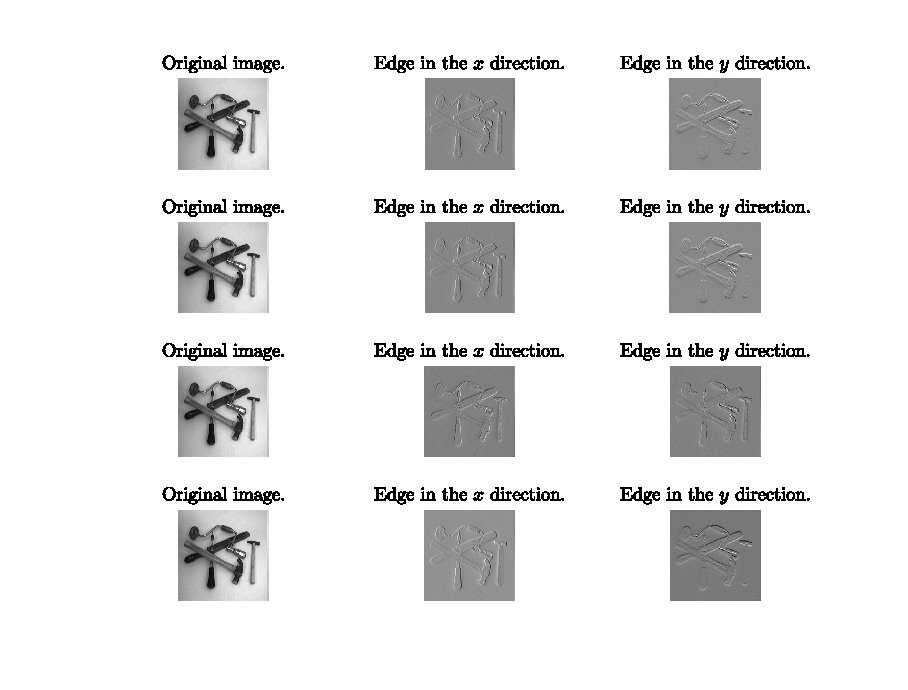
\includegraphics[width=\columnwidth]{Question_1.eps}
				%\scalebox{1}{% This file was created by matlab2tikz.
%
%The latest updates can be retrieved from
%  http://www.mathworks.com/matlabcentral/fileexchange/22022-matlab2tikz-matlab2tikz
%where you can also make suggestions and rate matlab2tikz.
%
\begin{tikzpicture}

\begin{axis}[%
width=0.609in,
height=0.609in,
at={(1.076in,3.357in)},
scale only axis,
axis on top,
xmin=0.5,
xmax=256.5,
y dir=reverse,
ymin=0.5,
ymax=256.5,
axis line style={draw=none},
ticks=none,
title style={font=\bfseries},
title={Original image.},
legend style={legend cell align=left, align=left, draw=white!15!black}
]
\addplot [forget plot] graphics [xmin=0.5, xmax=256.5, ymin=0.5, ymax=256.5] {Question_1-1.png};
\end{axis}

\begin{axis}[%
width=0.604in,
height=0.609in,
at={(2.717in,3.357in)},
scale only axis,
axis on top,
xmin=0.5,
xmax=254.5,
y dir=reverse,
ymin=0.5,
ymax=256.5,
axis line style={draw=none},
ticks=none,
title style={font=\bfseries},
title={Edge in the $x$ direction.},
legend style={legend cell align=left, align=left, draw=white!15!black}
]
\addplot [forget plot] graphics [xmin=0.5, xmax=254.5, ymin=0.5, ymax=256.5] {Question_1-2.png};
\end{axis}

\begin{axis}[%
width=0.614in,
height=0.609in,
at={(4.35in,3.357in)},
scale only axis,
axis on top,
xmin=0.5,
xmax=256.5,
y dir=reverse,
ymin=0.5,
ymax=254.5,
axis line style={draw=none},
ticks=none,
title style={font=\bfseries},
title={Edge in the $y$ direction.},
legend style={legend cell align=left, align=left, draw=white!15!black}
]
\addplot [forget plot] graphics [xmin=0.5, xmax=256.5, ymin=0.5, ymax=254.5] {Question_1-3.png};
\end{axis}

\begin{axis}[%
width=0.609in,
height=0.609in,
at={(1.076in,2.398in)},
scale only axis,
axis on top,
xmin=0.5,
xmax=256.5,
y dir=reverse,
ymin=0.5,
ymax=256.5,
axis line style={draw=none},
ticks=none,
title style={font=\bfseries},
title={Original image.},
legend style={legend cell align=left, align=left, draw=white!15!black}
]
\addplot [forget plot] graphics [xmin=0.5, xmax=256.5, ymin=0.5, ymax=256.5] {Question_1-4.png};
\end{axis}

\begin{axis}[%
width=0.604in,
height=0.609in,
at={(2.717in,2.398in)},
scale only axis,
axis on top,
xmin=0.5,
xmax=254.5,
y dir=reverse,
ymin=0.5,
ymax=256.5,
axis line style={draw=none},
ticks=none,
title style={font=\bfseries},
title={Edge in the $x$ direction.},
legend style={legend cell align=left, align=left, draw=white!15!black}
]
\addplot [forget plot] graphics [xmin=0.5, xmax=254.5, ymin=0.5, ymax=256.5] {Question_1-5.png};
\end{axis}

\begin{axis}[%
width=0.614in,
height=0.609in,
at={(4.35in,2.398in)},
scale only axis,
axis on top,
xmin=0.5,
xmax=256.5,
y dir=reverse,
ymin=0.5,
ymax=254.5,
axis line style={draw=none},
ticks=none,
title style={font=\bfseries},
title={Edge in the $y$ direction.},
legend style={legend cell align=left, align=left, draw=white!15!black}
]
\addplot [forget plot] graphics [xmin=0.5, xmax=256.5, ymin=0.5, ymax=254.5] {Question_1-6.png};
\end{axis}

\begin{axis}[%
width=0.609in,
height=0.609in,
at={(1.076in,1.44in)},
scale only axis,
axis on top,
xmin=0.5,
xmax=256.5,
y dir=reverse,
ymin=0.5,
ymax=256.5,
axis line style={draw=none},
ticks=none,
title style={font=\bfseries},
title={Original image.},
legend style={legend cell align=left, align=left, draw=white!15!black}
]
\addplot [forget plot] graphics [xmin=0.5, xmax=256.5, ymin=0.5, ymax=256.5] {Question_1-7.png};
\end{axis}

\begin{axis}[%
width=0.609in,
height=0.609in,
at={(2.714in,1.44in)},
scale only axis,
axis on top,
xmin=0.5,
xmax=255.5,
y dir=reverse,
ymin=0.5,
ymax=255.5,
axis line style={draw=none},
ticks=none,
title style={font=\bfseries},
title={Edge in the $x$ direction.},
legend style={legend cell align=left, align=left, draw=white!15!black}
]
\addplot [forget plot] graphics [xmin=0.5, xmax=255.5, ymin=0.5, ymax=255.5] {Question_1-8.png};
\end{axis}

\begin{axis}[%
width=0.609in,
height=0.609in,
at={(4.352in,1.44in)},
scale only axis,
axis on top,
xmin=0.5,
xmax=255.5,
y dir=reverse,
ymin=0.5,
ymax=255.5,
axis line style={draw=none},
ticks=none,
title style={font=\bfseries},
title={Edge in the $y$ direction.},
legend style={legend cell align=left, align=left, draw=white!15!black}
]
\addplot [forget plot] graphics [xmin=0.5, xmax=255.5, ymin=0.5, ymax=255.5] {Question_1-9.png};
\end{axis}

\begin{axis}[%
width=0.609in,
height=0.609in,
at={(1.076in,0.481in)},
scale only axis,
axis on top,
xmin=0.5,
xmax=256.5,
y dir=reverse,
ymin=0.5,
ymax=256.5,
axis line style={draw=none},
ticks=none,
title style={font=\bfseries},
title={Original image.},
legend style={legend cell align=left, align=left, draw=white!15!black}
]
\addplot [forget plot] graphics [xmin=0.5, xmax=256.5, ymin=0.5, ymax=256.5] {Question_1-10.png};
\end{axis}

\begin{axis}[%
width=0.609in,
height=0.609in,
at={(2.714in,0.481in)},
scale only axis,
axis on top,
xmin=0.5,
xmax=254.5,
y dir=reverse,
ymin=0.5,
ymax=254.5,
axis line style={draw=none},
ticks=none,
title style={font=\bfseries},
title={Edge in the $x$ direction.},
legend style={legend cell align=left, align=left, draw=white!15!black}
]
\addplot [forget plot] graphics [xmin=0.5, xmax=254.5, ymin=0.5, ymax=254.5] {Question_1-11.png};
\end{axis}

\begin{axis}[%
width=0.609in,
height=0.609in,
at={(4.352in,0.481in)},
scale only axis,
axis on top,
xmin=0.5,
xmax=254.5,
y dir=reverse,
ymin=0.5,
ymax=254.5,
axis line style={draw=none},
ticks=none,
title style={font=\bfseries},
title={Edge in the $y$ direction.},
legend style={legend cell align=left, align=left, draw=white!15!black}
]
\addplot [forget plot] graphics [xmin=0.5, xmax=254.5, ymin=0.5, ymax=254.5] {Question_1-12.png};
\end{axis}
\end{tikzpicture}%}
				\caption{The first row of images is applied by simple difference operator. The second row is applied by central differences. The third row is applied by Robert's diagonal operator. The last row is applied by the Sobel operator.}
				\label{fig:Question_1}
			\end{figure}
			\par The sizes of the derivative images are different from each other or from the original image because of the difference of the kernel sizes in each method. The image size is shown in Table \ref{tab:Image_Size}. 
			\begin{table}[!ht]
				\centering
				\caption{Image size.}
				\label{tab:Image_Size}
				\begin{tabular}{ccc}
					\hline
					Image & $x$ direction ($y \times x$) & $y$ direction ($y \times x$) \\
					\hline
					Original & $256 \times 256$ & $256 \times 256$ \\
					Simple difference operator & $256 \times 254$ & $254 \times 256$ \\
					Central difference operator & $256 \times 254$ & $254 \times 256$ \\
					Roberts cross edge operator & $255 \times 255$ & $255 \times 255$ \\
					Sobel operator & $254 \times 254$ & $254 \times 254$ \\
					\hline
				\end{tabular}
			\end{table}
			\par The reason why these sizes are different is because of the difference between the kernel size of each difference operators. If the image is of size $N \times M$ and in the case of the simple difference operator, the kernel when considering the $x$-direction has size of $1 \times 3$. Since all the elements in the kernel should be multiplied by a element in the image, the kernel will fit the image $N$ times in the $y$ direction, but $M-2$ times in the $x$ direction.
	\end{itemize}
\section*{2\hspace{0.5cm}Point-wise thresholding of gradient magnitudes}
	\begin{figure}[!ht]
		\centering
		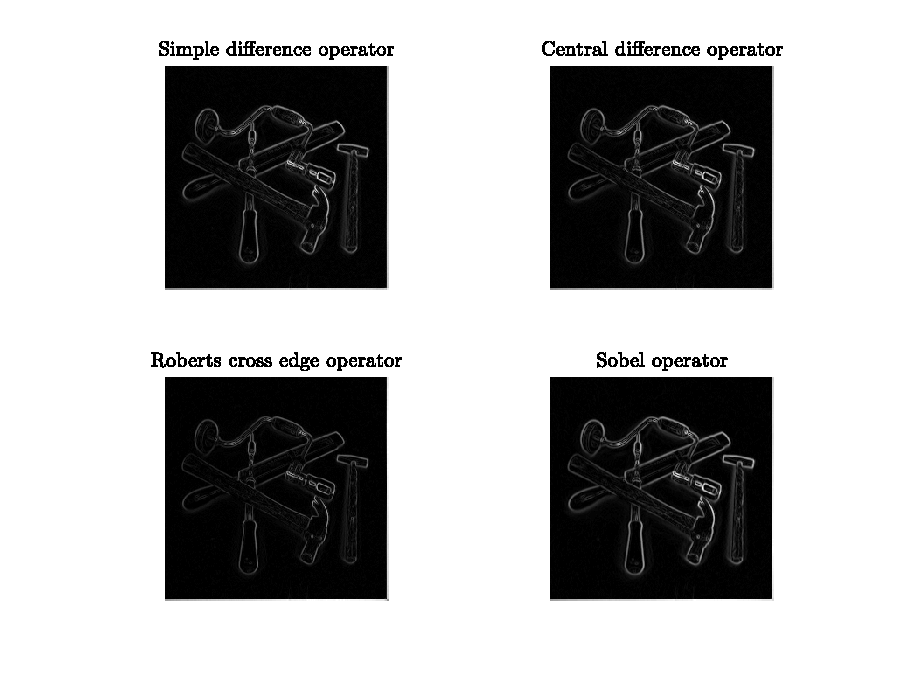
\includegraphics[width=0.9\columnwidth]{Question_2_Tools_Gradient_Magnitude.eps}
		\caption{Gradient magnitude of the derivative images for \texttt{few256}.}
		\label{fig:Question_2_Tools_Gradient_Magnitude}
	\end{figure}
	\begin{figure}[!ht]
		\centering
		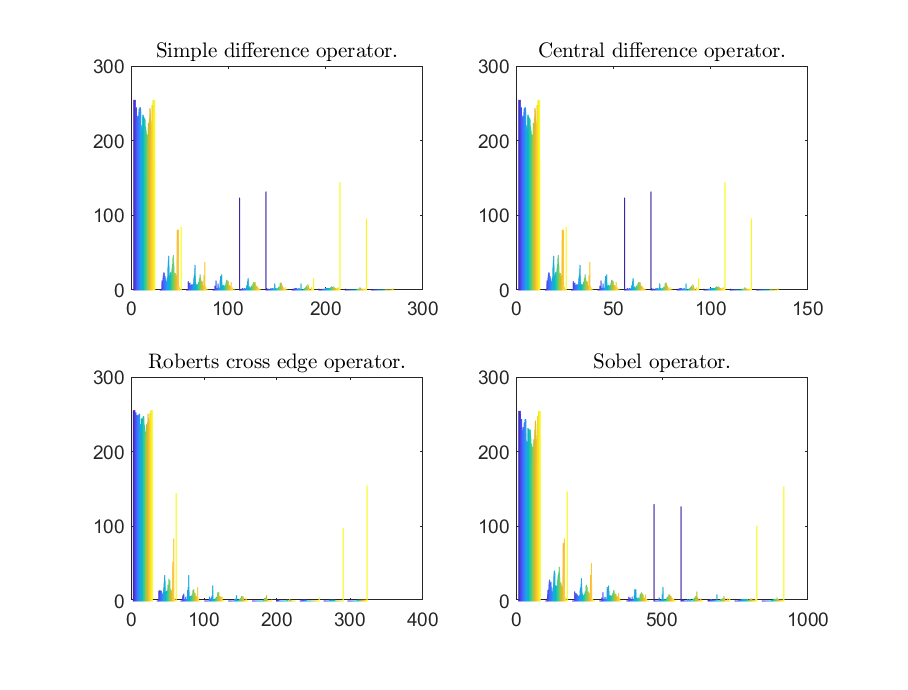
\includegraphics[width=0.9\columnwidth]{Question_2_Tools_Hist.eps}
		\caption{Histogram of gradient magnitude of the derivative images for \texttt{few256}.}
		\label{fig:Question_2_Tools_Hist}
	\end{figure}
		\begin{figure}[!ht]
		\centering
		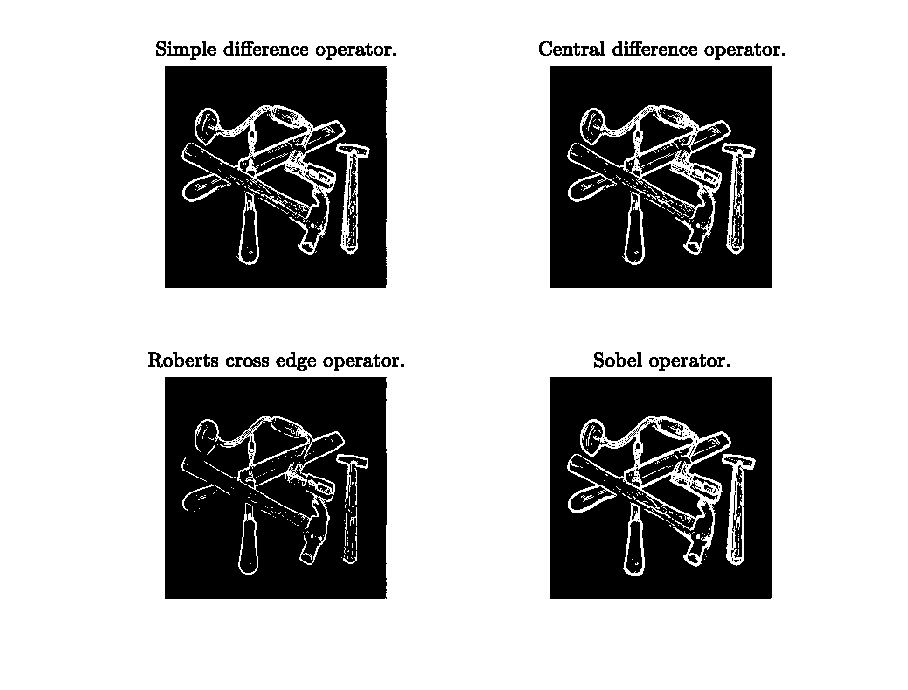
\includegraphics[width=0.85\columnwidth]{Question_2_Tools_Threshold.eps}
		\caption{Gradient magnitude of the derivative images with different threshold for \texttt{few256}. The threshold in the case of simple difference operator is 27.2. 13.6 for central difference operator. 32.7 for Roberts cross edge operator. 92.7 for Sobel operator.}
		\label{fig:Question_2_Tools_Threshold}
	\end{figure}
	\begin{figure}[!ht]
		\centering
		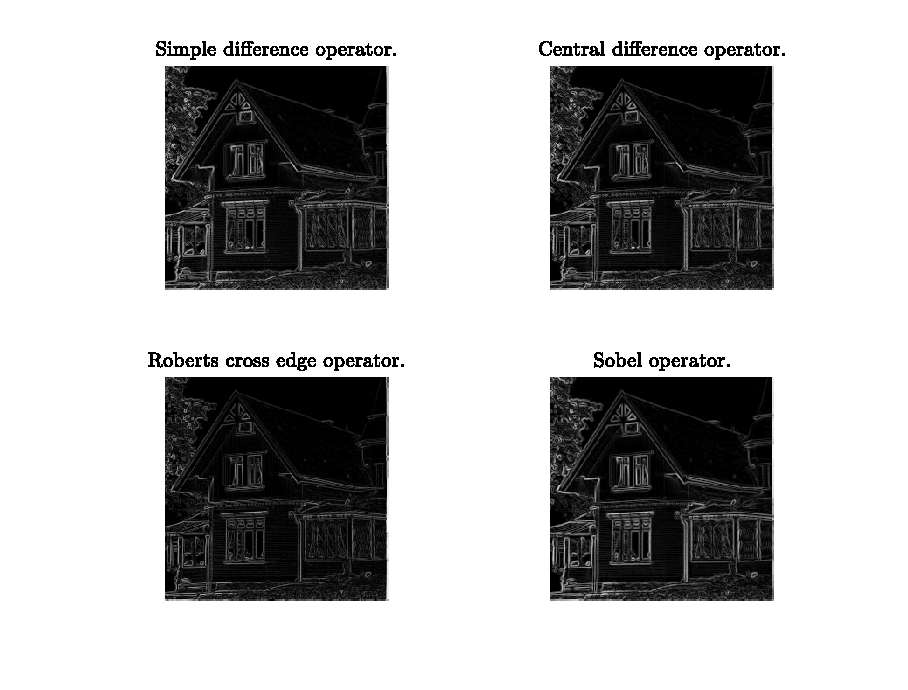
\includegraphics[width=0.9\columnwidth]{Question_2_Godthem_Gradient_Magnitude.eps}
		\caption{Gradient magnitude of the derivative images for \texttt{godthem256}.}
		\label{fig:Question_2_Godthem_Gradient_Magnitude}
	\end{figure}
	\begin{figure}[!ht]
		\centering
		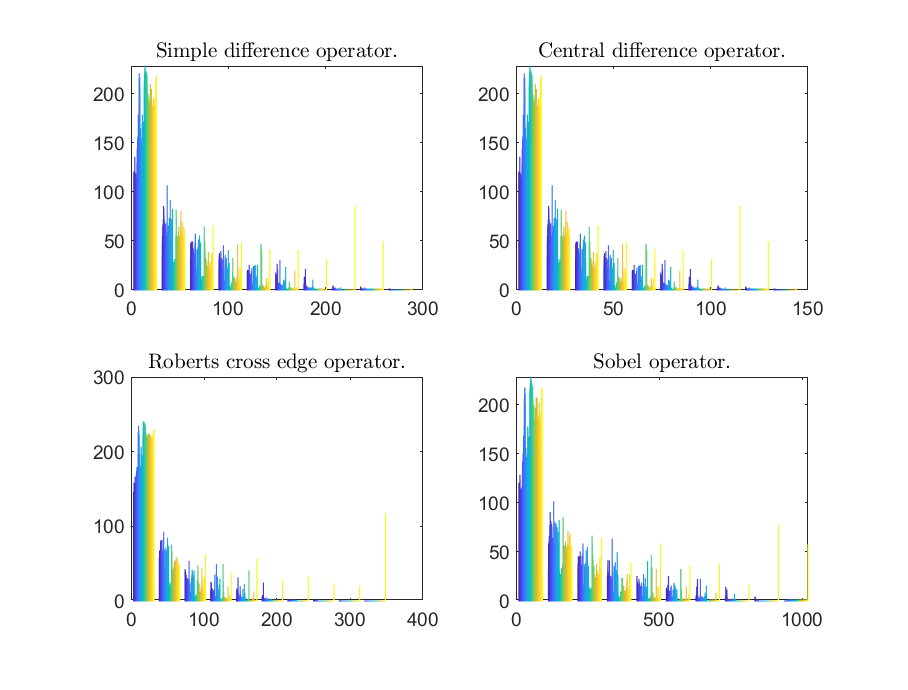
\includegraphics[width=0.9\columnwidth]{Question_2_Godthem_Hist.eps}
		\caption{Histogram of gradient magnitude of the derivative images for \texttt{godthem256}.}
		\label{fig:Question_2_Godthem_Hist}
	\end{figure}
	\begin{figure}[!ht]
		\centering
		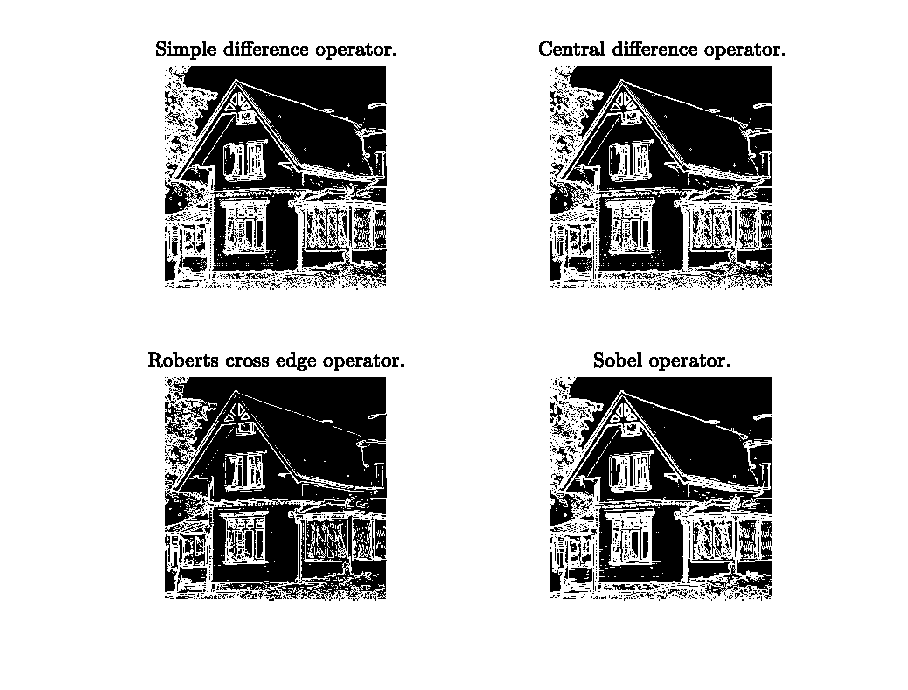
\includegraphics[width=0.85\columnwidth]{Question_2_Godthem_Threshold.eps}
		\caption{Gradient magnitude of the derivative images with different threshold for \texttt{godthem256}. The threshold in the case of simple difference operator is 29.1. 14.6 for central difference operator. 35.2 for Roberts cross edge operator. 103 for Sobel operator.}
		\label{fig:Question_2_Godthem_Threshold}
	\end{figure}
	\begin{itemize}
		\item\addtocounter{Counter}{1}\textbf{Question \arabic{Counter}:} Is it easy to find a threshold that results in thin edges? Explain why or why not!
			\par It is not easy to find a threshold that results in thin edges at the most time.
			\begin{itemize}
				\item Applying a threshold to the whole image where the brightness for all edges are different would obtain thin edges for some objects while other edges could disappear or be too thick.
				\item Different operator would give different result as illustrated in Figure \ref{fig:Question_2_Tools_Gradient_Magnitude}. So the threshold for each operator should be different.
				\item Noise with big magnitude could also make it hard to find a threshold that results in thin edges.
			\end{itemize}
			\par However, in the case of \texttt{few256}, the histogram, Figure \ref{fig:Question_2_Tools_Hist}, accumulated to the left border of the histogram pretty well, so we can set the threshold based on the bin edges of the first cluster of the histogram. The threshold in the case of simple difference operator is 27.2. 13.6 for central difference operator. 32.7 for Roberts cross edge operator. 92.7 for Sobel operator.
		\begin{figure}[!ht]
			\centering
			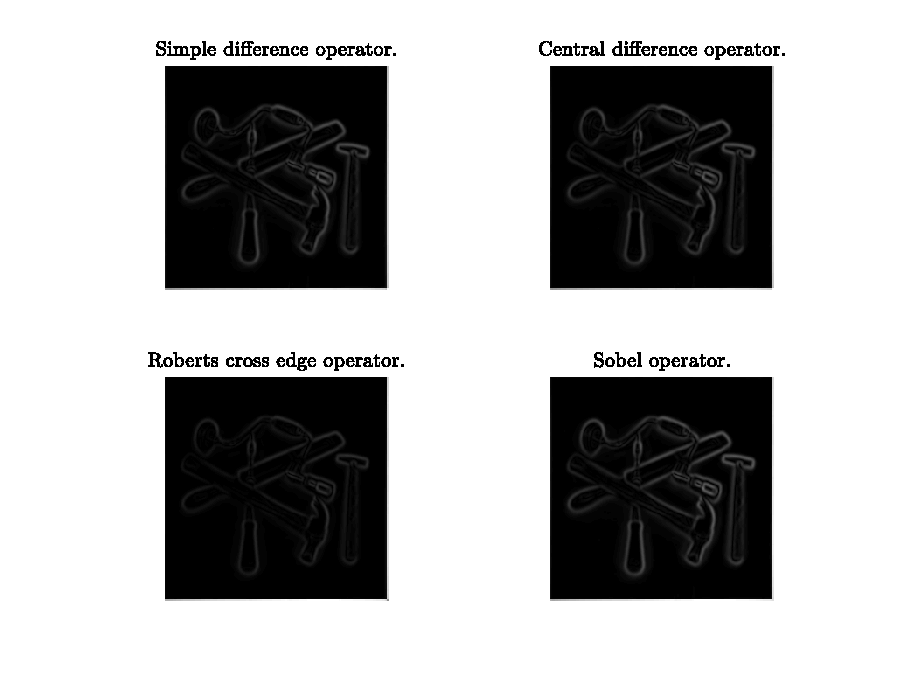
\includegraphics[width=0.9\columnwidth]{Question_2_Tools_Gaussian_2-25.eps}
			\caption{Smoothed gradient magnitude using Gaussian filter with $\sigma^{2}=2.25$ for \texttt{few256}.}
			\label{fig:Question_2_Tools_Gaussian_2-25}
		\end{figure}
		\begin{figure}[!ht]
			\centering
			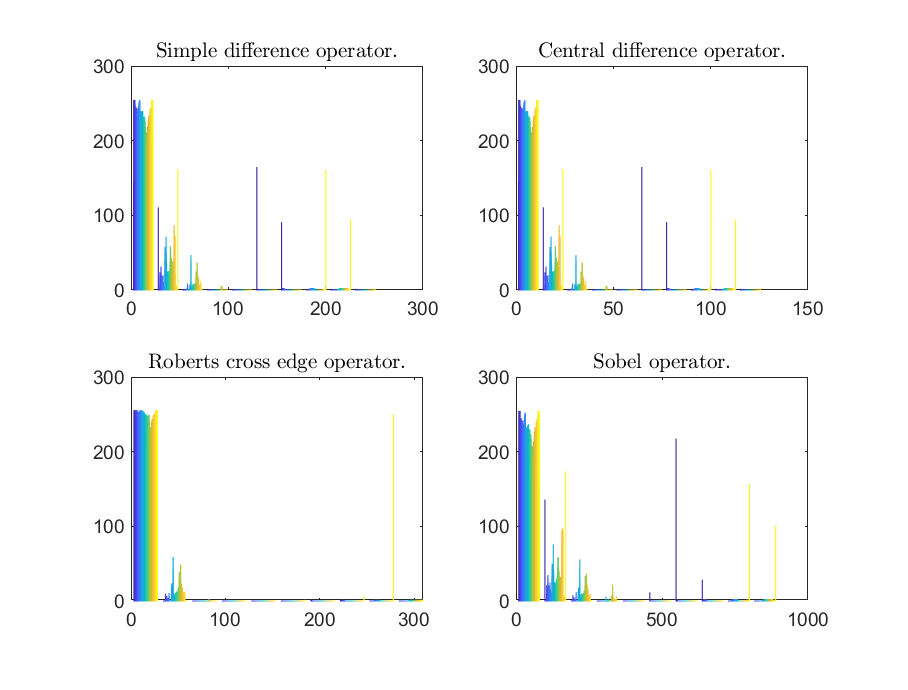
\includegraphics[width=0.9\columnwidth]{Question_2_Tools_Gaussian_2-25_Hist.eps}
			\caption{Histogram for smoothed gradient magnitude using Gaussian filter with $\sigma^{2}=2.25$ for \texttt{few256}.}
			\label{fig:Question_2_Tools_Gaussian_2-25_Hist}
		\end{figure}
		\begin{figure}[!ht]
			\centering
			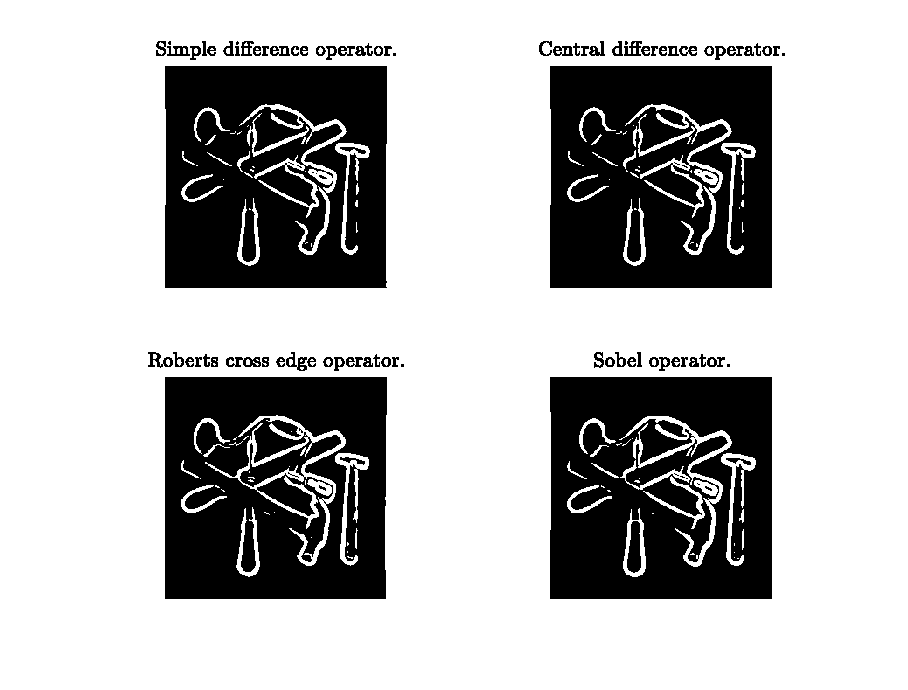
\includegraphics[width=0.85\columnwidth]{Question_2_Tools_Gaussian_2-25_Threshold.eps}
			\caption{Smoothed gradient magnitude using Gaussian filter with $\sigma^{2}=2.25$ and different threshold for \texttt{few256}. The threshold in the case of simple difference operator is 25.4. 12.7 for central difference operator. 16 for Roberts cross edge operator. 89.9 for Sobel operator.}
			\label{fig:Question_2_Tools_Gaussian_2-25_Threshold}
		\end{figure}
		\begin{figure}[!ht]
			\centering
			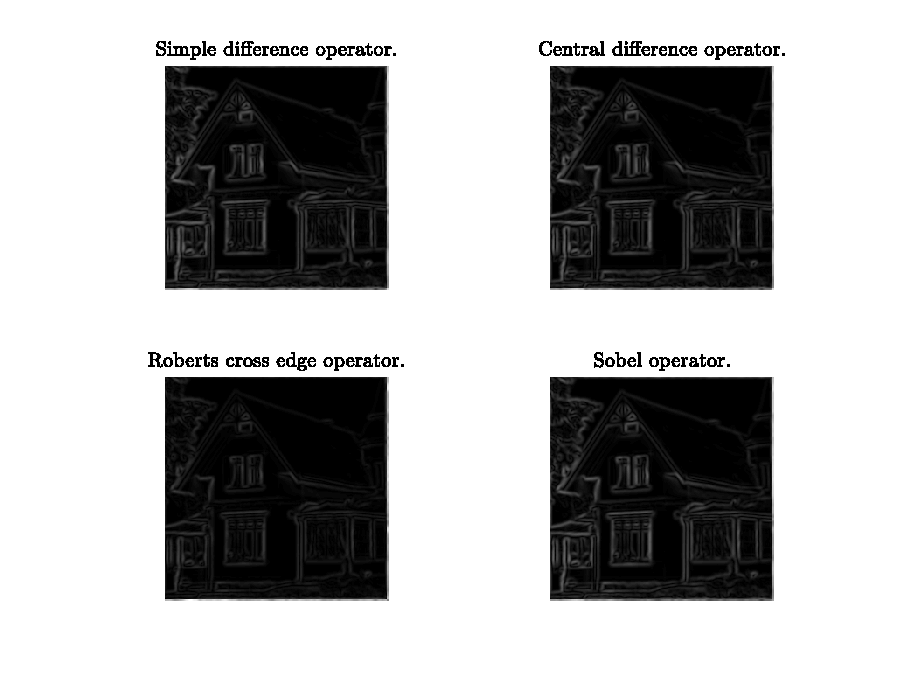
\includegraphics[width=0.9\columnwidth]{Question_2_House_Gaussian_2-25.eps}
			\caption{Smoothed gradient magnitude using Gaussian filter with $\sigma^{2}=2.25$ for \texttt{godthem256}.}
			\label{fig:Question_2_House_Gaussian_2-25}
		\end{figure}
		\begin{figure}[!ht]
			\centering
			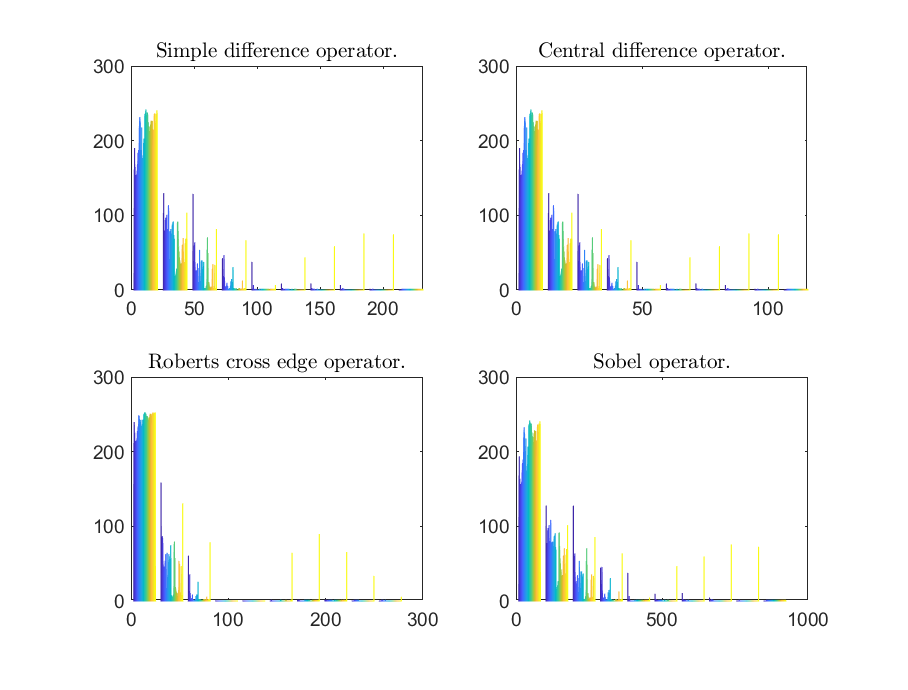
\includegraphics[width=0.9\columnwidth]{Question_2_House_Gaussian_2-25_Hist.eps}
			\caption{Histogram for smoothed gradient magnitude using Gaussian filter with $\sigma^{2}=2.25$ for \texttt{godthem256}.}
			\label{fig:Question_2_House_Gaussian_2-25_Hist}
		\end{figure}
		\begin{figure}[!ht]
			\centering
			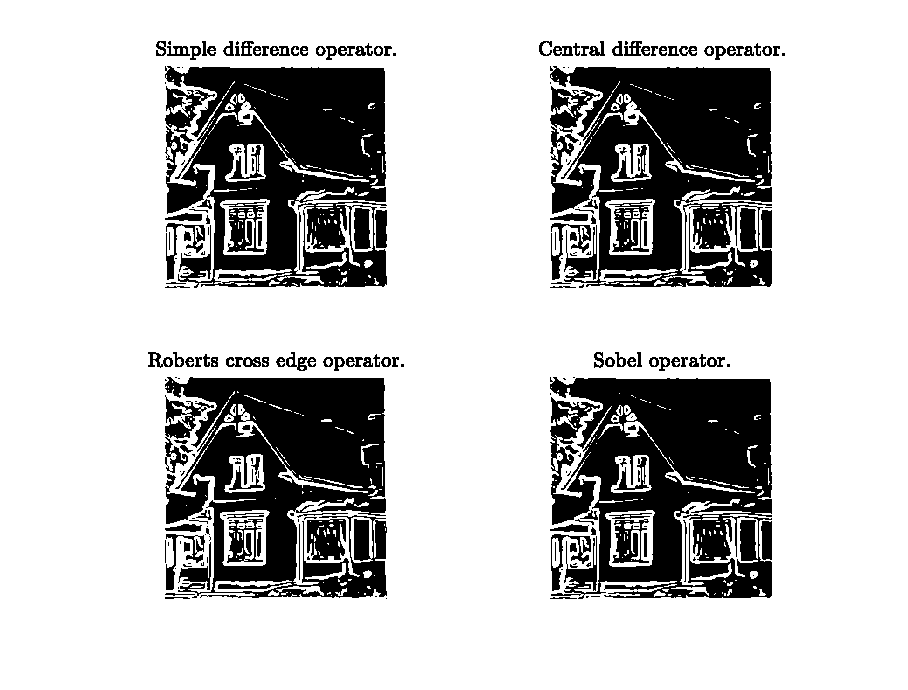
\includegraphics[width=0.85\columnwidth]{Question_2_House_Gaussian_2-25_Threshold.eps}
			\caption{Smoothed gradient magnitude using Gaussian filter with $\sigma^{2}=2.25$ and different threshold for \texttt{godthem256}. The threshold in the case of simple difference operator is 23.4. 11.7 for central difference operator. 16 for Roberts cross edge operator. 93.4 for Sobel operator.}
			\label{fig:Question_2_House_Gaussian_2-25_Threshold}
		\end{figure}
		\item\addtocounter{Counter}{1}\textbf{Question \arabic{Counter}:} Does smoothing the image help to find edges?
			\par Yes, smoothing the image helps to find edges. Smoothing would remove noise from the image, thus making the detected ``edges'' are more likely to be real edges.
			\par However, smoothing the image with Gaussian filter could blur the edges, thus making it difficult to detect the edges with difference operators and find a threshold. This can also be seen from the histograms of the images after smoothing which are more shewed when compared to the gradient magnitude with no Gaussian smoothing.
	\end{itemize}

\section*{4\hspace{0.5cm}Computing differential geometry descriptors}
	\par The images after applying Gaussian filter to \texttt{godthem256} with different value of $\sigma^{2}$ is illustrated in Figure \ref{fig:Question_4_House_Gaussian}. The second order derivative of \texttt{godthem256} after Gaussian smoothing is shown in Figure \ref{fig:Question_4_House_Second_Order} and the third order derivative is shown in Figure \ref{fig:Question_4_House_Third_Order}. Also, the third order derivative of \texttt{few256} after Gaussian smoothing is shown in Figure \ref{fig:Question_4_Tools_Third_Order}.
	\begin{figure}[!ht]
		\centering
		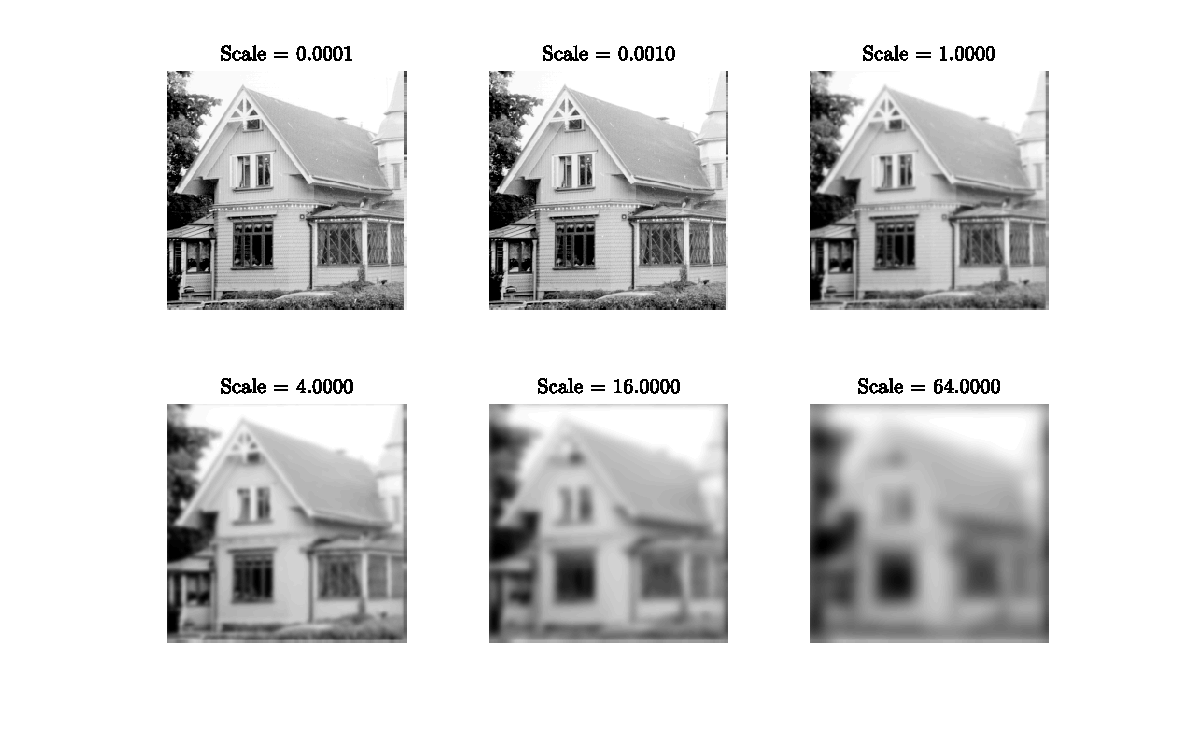
\includegraphics[width=0.9\columnwidth]{Question_4_House_Gaussian.eps}
		%\scalebox{0.9}{% This file was created by matlab2tikz.
%
%The latest updates can be retrieved from
%  http://www.mathworks.com/matlabcentral/fileexchange/22022-matlab2tikz-matlab2tikz
%where you can also make suggestions and rate matlab2tikz.
%
\begin{tikzpicture}

\begin{axis}[%
width=1.203in,
height=1.203in,
at={(0.745in,2.463in)},
scale only axis,
axis on top,
xmin=0.5,
xmax=256.5,
y dir=reverse,
ymin=0.5,
ymax=256.5,
axis line style={draw=none},
ticks=none,
title style={font=\bfseries},
title={Scale = 0.0001},
legend style={legend cell align=left, align=left, draw=white!15!black}
]
\addplot [forget plot] graphics [xmin=0.5, xmax=256.5, ymin=0.5, ymax=256.5] {Question_4_House_Gaussian-1.png};
\end{axis}

\begin{axis}[%
width=1.203in,
height=1.203in,
at={(2.354in,2.463in)},
scale only axis,
axis on top,
xmin=0.5,
xmax=256.5,
y dir=reverse,
ymin=0.5,
ymax=256.5,
axis line style={draw=none},
ticks=none,
title style={font=\bfseries},
title={Scale = 0.0010},
legend style={legend cell align=left, align=left, draw=white!15!black}
]
\addplot [forget plot] graphics [xmin=0.5, xmax=256.5, ymin=0.5, ymax=256.5] {Question_4_House_Gaussian-2.png};
\end{axis}

\begin{axis}[%
width=1.203in,
height=1.203in,
at={(3.962in,2.463in)},
scale only axis,
axis on top,
xmin=0.5,
xmax=256.5,
y dir=reverse,
ymin=0.5,
ymax=256.5,
axis line style={draw=none},
ticks=none,
title style={font=\bfseries},
title={Scale = 1.0000},
legend style={legend cell align=left, align=left, draw=white!15!black}
]
\addplot [forget plot] graphics [xmin=0.5, xmax=256.5, ymin=0.5, ymax=256.5] {Question_4_House_Gaussian-3.png};
\end{axis}

\begin{axis}[%
width=1.203in,
height=1.203in,
at={(0.745in,0.538in)},
scale only axis,
axis on top,
xmin=0.5,
xmax=256.5,
y dir=reverse,
ymin=0.5,
ymax=256.5,
axis line style={draw=none},
ticks=none,
title style={font=\bfseries},
title={Scale = 4.0000},
legend style={legend cell align=left, align=left, draw=white!15!black}
]
\addplot [forget plot] graphics [xmin=0.5, xmax=256.5, ymin=0.5, ymax=256.5] {Question_4_House_Gaussian-4.png};
\end{axis}

\begin{axis}[%
width=1.203in,
height=1.203in,
at={(2.354in,0.538in)},
scale only axis,
axis on top,
xmin=0.5,
xmax=256.5,
y dir=reverse,
ymin=0.5,
ymax=256.5,
axis line style={draw=none},
ticks=none,
title style={font=\bfseries},
title={Scale = 16.0000},
legend style={legend cell align=left, align=left, draw=white!15!black}
]
\addplot [forget plot] graphics [xmin=0.5, xmax=256.5, ymin=0.5, ymax=256.5] {Question_4_House_Gaussian-5.png};
\end{axis}

\begin{axis}[%
width=1.203in,
height=1.203in,
at={(3.962in,0.538in)},
scale only axis,
axis on top,
xmin=0.5,
xmax=256.5,
y dir=reverse,
ymin=0.5,
ymax=256.5,
axis line style={draw=none},
ticks=none,
title style={font=\bfseries},
title={Scale = 64.0000},
legend style={legend cell align=left, align=left, draw=white!15!black}
]
\addplot [forget plot] graphics [xmin=0.5, xmax=256.5, ymin=0.5, ymax=256.5] {Question_4_House_Gaussian-6.png};
\end{axis}
\end{tikzpicture}%}
		\caption{Gaussian smoothing for \texttt{godthem256} with different scale.}
		\label{fig:Question_4_House_Gaussian}
	\end{figure}
	\begin{figure}[!ht]
		\centering
		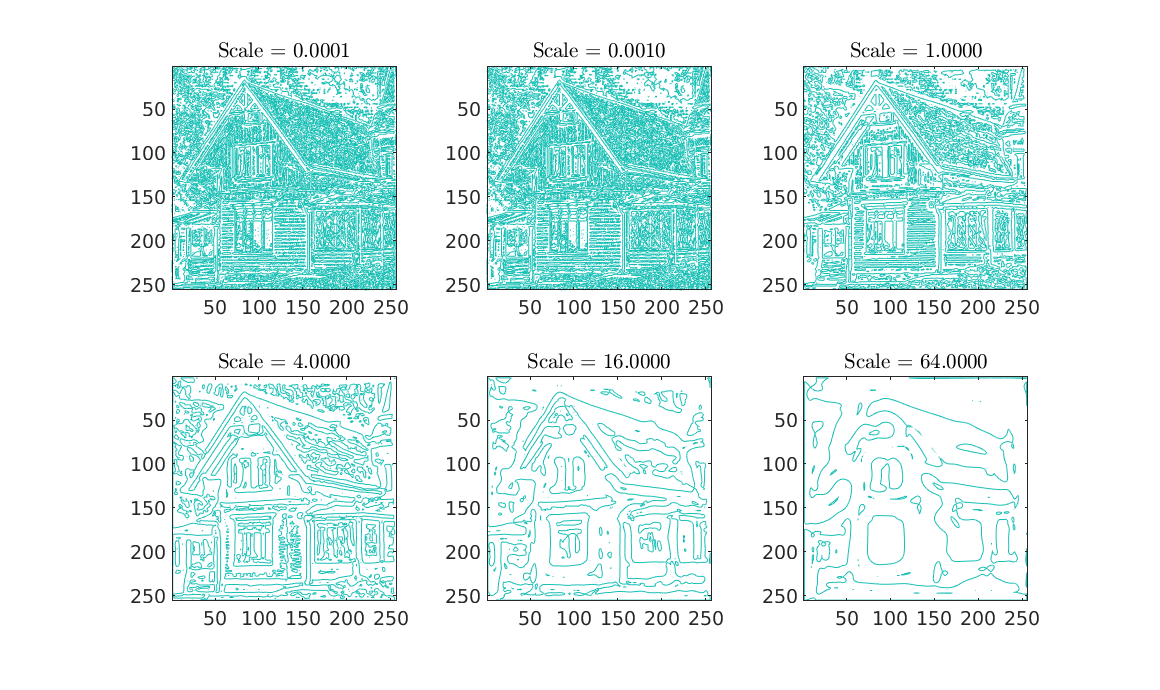
\includegraphics[width=0.9\columnwidth]{Question_4_House_Second_Order.eps}
		%\scalebox{0.9}{% This file was created by matlab2tikz.
%
%The latest updates can be retrieved from
%  http://www.mathworks.com/matlabcentral/fileexchange/22022-matlab2tikz-matlab2tikz
%where you can also make suggestions and rate matlab2tikz.
%
\begin{tikzpicture}

\begin{axis}[%
width=1.249in,
height=1.249in,
at={(0.772in,2.912in)},
scale only axis,
colormap={mymap}{[1pt] rgb(0pt)=(0.2422,0.1504,0.6603); rgb(1pt)=(0.25039,0.164995,0.707614); rgb(2pt)=(0.257771,0.181781,0.751138); rgb(3pt)=(0.264729,0.197757,0.795214); rgb(4pt)=(0.270648,0.214676,0.836371); rgb(5pt)=(0.275114,0.234238,0.870986); rgb(6pt)=(0.2783,0.255871,0.899071); rgb(7pt)=(0.280333,0.278233,0.9221); rgb(8pt)=(0.281338,0.300595,0.941376); rgb(9pt)=(0.281014,0.322757,0.957886); rgb(10pt)=(0.279467,0.344671,0.971676); rgb(11pt)=(0.275971,0.366681,0.982905); rgb(12pt)=(0.269914,0.3892,0.9906); rgb(13pt)=(0.260243,0.412329,0.995157); rgb(14pt)=(0.244033,0.435833,0.998833); rgb(15pt)=(0.220643,0.460257,0.997286); rgb(16pt)=(0.196333,0.484719,0.989152); rgb(17pt)=(0.183405,0.507371,0.979795); rgb(18pt)=(0.178643,0.528857,0.968157); rgb(19pt)=(0.176438,0.549905,0.952019); rgb(20pt)=(0.168743,0.570262,0.935871); rgb(21pt)=(0.154,0.5902,0.9218); rgb(22pt)=(0.146029,0.609119,0.907857); rgb(23pt)=(0.138024,0.627629,0.89729); rgb(24pt)=(0.124814,0.645929,0.888343); rgb(25pt)=(0.111252,0.6635,0.876314); rgb(26pt)=(0.0952095,0.679829,0.859781); rgb(27pt)=(0.0688714,0.694771,0.839357); rgb(28pt)=(0.0296667,0.708167,0.816333); rgb(29pt)=(0.00357143,0.720267,0.7917); rgb(30pt)=(0.00665714,0.731214,0.766014); rgb(31pt)=(0.0433286,0.741095,0.73941); rgb(32pt)=(0.0963952,0.75,0.712038); rgb(33pt)=(0.140771,0.7584,0.684157); rgb(34pt)=(0.1717,0.766962,0.655443); rgb(35pt)=(0.193767,0.775767,0.6251); rgb(36pt)=(0.216086,0.7843,0.5923); rgb(37pt)=(0.246957,0.791795,0.556743); rgb(38pt)=(0.290614,0.79729,0.518829); rgb(39pt)=(0.340643,0.8008,0.478857); rgb(40pt)=(0.3909,0.802871,0.435448); rgb(41pt)=(0.445629,0.802419,0.390919); rgb(42pt)=(0.5044,0.7993,0.348); rgb(43pt)=(0.561562,0.794233,0.304481); rgb(44pt)=(0.617395,0.787619,0.261238); rgb(45pt)=(0.671986,0.779271,0.2227); rgb(46pt)=(0.7242,0.769843,0.191029); rgb(47pt)=(0.773833,0.759805,0.16461); rgb(48pt)=(0.820314,0.749814,0.153529); rgb(49pt)=(0.863433,0.7406,0.159633); rgb(50pt)=(0.903543,0.733029,0.177414); rgb(51pt)=(0.939257,0.728786,0.209957); rgb(52pt)=(0.972757,0.729771,0.239443); rgb(53pt)=(0.995648,0.743371,0.237148); rgb(54pt)=(0.996986,0.765857,0.219943); rgb(55pt)=(0.995205,0.789252,0.202762); rgb(56pt)=(0.9892,0.813567,0.188533); rgb(57pt)=(0.978629,0.838629,0.176557); rgb(58pt)=(0.967648,0.8639,0.16429); rgb(59pt)=(0.96101,0.889019,0.153676); rgb(60pt)=(0.959671,0.913457,0.142257); rgb(61pt)=(0.962795,0.937338,0.12651); rgb(62pt)=(0.969114,0.960629,0.106362); rgb(63pt)=(0.9769,0.9839,0.0805)},
xmin=1,
xmax=256,
y dir=reverse,
ymin=1,
ymax=256,
axis background/.style={fill=white},
title style={font=\bfseries},
title={Scale = 0.0001},
legend style={legend cell align=left, align=left, draw=white!15!black}
]
\addplot[contour prepared, contour prepared format=matlab, contour/labels=false] table[row sep=crcr] {%
%
0	3\\
11.6514606964108	1\\
12	1.04624071673832\\
12.9977720827679	1\\
0	80\\
13.0005922483747	1\\
13	1.00663116868251\\
12.9840416705581	2\\
13	2.00803165299946\\
13.8778028061184	2\\
14	1.98779291989164\\
14.6852317384551	2\\
15	2.16964796455706\\
15.0975554509003	2\\
16	1.62941123226248\\
16.294663296791	2\\
17	2.17763751602011\\
18	2.41397585633378\\
18.6158576319483	3\\
19	3.91101749181789\\
20	3.9472719537229\\
20.2995724693389	3\\
21	2.51205491649611\\
22	2.745885525309\\
22.9160022163903	2\\
23	1.99817465015008\\
24	1.94166375531522\\
24.7588653578438	2\\
25	2.40060407437731\\
26	2.05796887752788\\
26.9183057649322	2\\
27	1.9997361104448\\
28	1.99515699885003\\
29	1.99550041034659\\
29.5384760709732	2\\
29.3809342909554	3\\
29	3.5576212305346\\
28.6464079718018	3\\
28	2.26754649930235\\
27	2.00663205547315\\
26.5494608788106	3\\
26.398194650754	4\\
27	4.81912053682945\\
28	4.5652593548554\\
28.299822198691	5\\
28	5.30376537152727\\
27	5.75747273812496\\
26	5.20802718349387\\
25.494802082406	6\\
26	6.59785267630786\\
26.462430772134	7\\
26.4712260047855	8\\
26	8.51311381178116\\
25	8.48545784552562\\
24	8.40990489080955\\
23.0559343047383	8\\
23.3614112198626	7\\
23	6.40222279446773\\
22.4761720175754	7\\
22.7810901567663	8\\
22	8.28844489694812\\
21	8.36041054580372\\
20	8.87652838872739\\
19	8.79950684293986\\
18.5271859572319	8\\
18	7.35818735811331\\
17.7071866304579	7\\
18	6.62857710932184\\
18.7451587545617	6\\
18	5.6038944410234\\
17	5.56635099262884\\
16	5.54143517952484\\
15.3621891965127	5\\
15	4.35046750687548\\
14.3876859092599	5\\
14	5.51444899643568\\
13.5982804778284	5\\
13	4.25659196369047\\
12.9299529264156	4\\
12	3.58880475367407\\
11.5476287166312	3\\
11	2.36681644520692\\
10.1853019733777	2\\
10	1.44291271686148\\
9.63806832238763	1\\
0	3\\
17.0521987418855	1\\
17	1.5178730575087\\
16.3977921969278	1\\
0	114\\
1	6.89504648459703\\
1.48442953996142	6\\
2	5.42382489487749\\
2.37503957160873	6\\
3	6.99397430566395\\
3.76203201634085	6\\
3.20874401401598	5\\
4	4.47539436054118\\
4.94649811585185	4\\
5	3.90233054898079\\
6	3.49763621108633\\
7	3.20161455499545\\
7.84146600062228	3\\
7.715113236704	2\\
8	1.79381199261092\\
8.60240969336485	2\\
9	2.99901553376441\\
9.00085447136182	3\\
9.54398795271902	4\\
10	4.28688782631133\\
10.4261608614201	5\\
10	5.97688533275365\\
9.62524424127051	6\\
10	6.34952995742527\\
10.0610100750295	6\\
11	5.78712273474509\\
12	5.56259796703922\\
13	5.83021270853156\\
13.2439732994764	6\\
13	6.93431934659008\\
12	6.61108464123551\\
11.7289452612407	7\\
11	7.36790076030886\\
10.4286837188708	8\\
10.8907013326032	9\\
10	9.85447594685316\\
9	9.94145061666767\\
8.72275452847653	10\\
9	10.0565255136383\\
10	10.5844106902889\\
10.2568038618608	11\\
11	11.5908618552919\\
11.3934431765145	12\\
11.1383426757149	13\\
12	13.6129589806393\\
13	13.481367106157\\
13.9861104297639	13\\
14	12.2512695438151\\
14.601241567507	13\\
14	13.1361511885596\\
13.9234070011488	14\\
14	14.1212653793444\\
14.5925161691266	14\\
15	13.1319420225404\\
15.1466887987243	14\\
16	14.3625867146861\\
16.6530313651912	15\\
16.9540564888958	16\\
16	16.7594926630771\\
15.643378090974	16\\
15	15.2563966741519\\
14	15.3147039319078\\
13.4243429968497	16\\
13	16.9668574756792\\
12.0174278561399	17\\
12.3716844744024	18\\
12	18.6630038039933\\
11.6379113851848	18\\
11.9969282395792	17\\
12	16.9973516206297\\
12.1863077510117	16\\
12	15.6898819188676\\
11.7175324468711	15\\
11	14.2619576214136\\
10.1193037068396	14\\
10.5171376198607	13\\
10	12.042564726463\\
9.97368408595728	12\\
9	11.3202802974516\\
8	11.3329240893447\\
7.44600318590584	11\\
7	10.5212173780171\\
6.42296844413291	10\\
6.70871790040652	9\\
7	8.30926320282436\\
7.34037528626099	8\\
7	7.56290540825367\\
6.58434776443884	7\\
7	6.3683553352481\\
7.34962552001326	6\\
8	5.02930377579035\\
9	5.0417642866448\\
9.00171763766515	5\\
9	4.99642762795165\\
8	4.99888000182047\\
7	4.99865116682781\\
6	4.29902425403178\\
5.56195999015262	5\\
5	5.87785582895523\\
4.65952048642617	6\\
4.48295177046741	7\\
4.55342555910134	8\\
5	8.76618778913179\\
5.32002225409476	9\\
5.94417655070633	10\\
5	10.7962139126159\\
4.69220975383699	10\\
4	9.56169686069589\\
3.44260306272243	9\\
3	8.42610126077898\\
2.69773124967952	8\\
2	7.14764954072734\\
1.69123085678125	8\\
1	8.39214491247041\\
0	9\\
256	8.98598713392085\\
255.455265458721	8\\
255.461539178484	7\\
255.472019189775	6\\
255.466796397937	5\\
255.487741020595	4\\
255.468227313511	3\\
255.463775519444	2\\
255.705933254619	1\\
0	6\\
256	13.3555301827562\\
255.801439109926	13\\
255.634528434584	12\\
255.783047059192	11\\
255.643194598132	10\\
256	9.07199337016283\\
0	5159\\
1	16.9064049904696\\
1.62931850293919	17\\
2	17.4158436013585\\
3	17.6349367692169\\
4	17.1271174941645\\
4.59048615589173	18\\
4.54211601955413	19\\
4.47464826815924	20\\
4	20.1294998566203\\
3.4732744332447	21\\
3.6456513307784	22\\
4	22.3266952492551\\
4.56875530536476	22\\
5	21.0344458582184\\
5.02232888855764	21\\
5.16027826406213	20\\
6	19.3728497769498\\
6.56120997524024	19\\
7	18.1392605086153\\
7.76627746875638	18\\
7	17.812723636766\\
6.48370662974604	18\\
6	18.1059574051318\\
5.84203073021046	18\\
6	17.735201540936\\
6.37476542084395	17\\
6.59949402885022	16\\
6	15.9002858796244\\
5.99566751946371	16\\
5	16.6265648861312\\
4.493546507798	16\\
4	15.1647705003248\\
3	15.6063814123131\\
2.13390373315463	15\\
3	14.3389647828421\\
3.99129873959144	14\\
3	13.3990406387863\\
2.16005730171065	13\\
2.52618601976199	12\\
2	11.0741649576298\\
1.9978858802888	11\\
2	10.8429576199327\\
3	10.5426841237086\\
3.93811956811325	11\\
3.38217219108509	12\\
4	12.844582412221\\
4.60807308652913	12\\
5	11.1717525427292\\
6	11.0467253832839\\
6.70229327675174	12\\
6.58206135792942	13\\
6	13.2014186845473\\
5.25418013388315	14\\
6	14.9566761587211\\
7	14.5352332628208\\
7.78870261022843	14\\
8	13.2771763345946\\
9	13.3822221329945\\
9.92965693959477	14\\
9.37402164062719	15\\
10	15.3595212842779\\
10.7600375181483	16\\
10.4489324072945	17\\
10.6258283275987	18\\
10	18.2894828082246\\
9	18.372470385654\\
8.57503535459377	19\\
8	19.2401245037648\\
7.07726689425056	20\\
8	20.2899354500499\\
8.49893729128987	21\\
9	21.5253065067545\\
10	21.4807399823866\\
11	21.1999568376247\\
12	21.8488997923134\\
12.0621575081586	22\\
12	22.0095592321612\\
11.5423643927306	23\\
11.1695444797409	24\\
11	24.0790139744795\\
10	24.3694478007197\\
9.53064048665826	25\\
10	25.6515605446158\\
11	25.2059348201455\\
12	25.5744746951582\\
13	25.4968314074169\\
13.4639565988051	26\\
14	26.5454102455368\\
15	26.7134879242294\\
15.5625489033473	27\\
15.5292640978897	28\\
15.552629232299	29\\
16	29.7771006580631\\
16.9051563111219	30\\
16.5044028313177	31\\
16	31.1395466091471\\
15	31.1172114410314\\
14.9897055415113	31\\
14.774620238912	30\\
14	29.2001064001257\\
13	29.0343738966489\\
12	29.9412486770124\\
11.9342715996877	30\\
11	30.5831953067067\\
10.2844046977149	30\\
10	29.6683620783776\\
9.75539890054925	29\\
9	28.0338328439852\\
8.39681411252802	28\\
8.21578485146083	27\\
8.00400147958183	26\\
8	25.9856407764842\\
7	25.1548155394137\\
6	25.0886987832173\\
5.97236891575767	25\\
5.12848394809903	24\\
5	23.9826637582696\\
4	23.7037191600521\\
3.38903984909879	24\\
4	24.4637388278343\\
4.35827177116833	25\\
5	25.5114807412179\\
5.76588786204529	26\\
5.51044230611038	27\\
6	27.3911197096499\\
6.51223799783535	28\\
7	28.6911987248378\\
7.16944625131614	29\\
8	29.7307073171097\\
9	29.8839521292086\\
9.44967185972082	30\\
9	30.0797205381629\\
8.41817650986686	31\\
8	31.3147021200811\\
7.49224865104586	32\\
8	32.6520917036294\\
9	32.2610709225358\\
10	32.1429758985521\\
10.3216988087835	33\\
11	33.5670233862065\\
12	33.4620717140194\\
12.835622676156	33\\
13	32.1733732817751\\
14	32.3355718507147\\
15	32.0866746862615\\
15.3670393736354	33\\
16	33.4092045301477\\
16.7212753858509	34\\
17	34.6535259461982\\
17.1529478282623	35\\
17	35.4756444873156\\
16.0250629640322	35\\
16	34.9947609003034\\
15	34.4418554002729\\
14	34.1530978242939\\
13.3249598347633	35\\
13	35.3464521255302\\
12.5150171000662	36\\
13	36.4700996385343\\
14	36.4797631542761\\
15	36.4774500066681\\
15.7409315384605	37\\
16	37.8995057394794\\
17	37.6725917779115\\
18	37.0039629269037\\
19	37.9432654942892\\
19.130034848972	37\\
19	36.9256157128551\\
18	36.9587525512055\\
17.6837383145904	36\\
18	35.9156895429644\\
19	35.1195347201482\\
19.580286995828	36\\
20	36.5736141103416\\
21	36.4302964114821\\
21.7156355656851	36\\
21.9209060788801	35\\
22	34.768484674296\\
22.6755584851544	34\\
22	33.8191385888664\\
21.6055948141518	33\\
21	32.493167842041\\
20.3792955700254	32\\
20	31.0250936538259\\
19	31.9925020564412\\
18.1086950597208	31\\
18.9919402617562	30\\
18.2606925388305	29\\
19	28.32412119037\\
19.6561148049672	28\\
20	27.5464912968761\\
20.1249231004787	27\\
20	26.0559740062753\\
19.583693346704	26\\
20	25.7937284349986\\
20.1523091190948	25\\
20.3669257821098	24\\
20	23.1703895199496\\
19	23.9999150616786\\
18	23.7621101316946\\
17.5956343784905	24\\
17	24.0362510682497\\
16.3430177663337	24\\
17	23.6739667023484\\
17.4873041024084	23\\
17	22.4993778293853\\
16.4604488701407	22\\
16	21.2771711313941\\
15.7001005146661	21\\
15.2892963063916	20\\
15	19.9923028465737\\
14.9959129196402	20\\
14	20.7868843069325\\
13.4491544950367	20\\
13.3797194748665	19\\
14	18.5337378286668\\
15	18.4308851729434\\
16	18.1906468804335\\
17	18.2989863630718\\
17.3399065909348	19\\
18	19.3352478473817\\
18.7931799525703	19\\
19	18.7565378451341\\
19.0733461882409	19\\
19.1369476745314	20\\
20	20.4954250412728\\
20.5778445019103	21\\
21	21.5031077669034\\
21.2678217984328	22\\
22	22.7115034398916\\
22.6260592954721	23\\
22	23.8675453054542\\
21.5232106288796	24\\
21.4456314037796	25\\
21.466298524853	26\\
21.2881526218414	27\\
22	27.3819209497685\\
22.3083618834965	28\\
23	28.5769687228801\\
24	28.4788449098814\\
24.6933075550234	28\\
24	27.3325224205055\\
23.2262891740965	27\\
24	26.36830893601\\
25	26.4407238955882\\
26	26.5464801446852\\
26.2549322010548	27\\
27	27.517337838721\\
28	27.5413234515812\\
28.8524029329122	27\\
29	26.6712421606542\\
30	26.4947787439079\\
31	26.4771918657693\\
32	26.496467995305\\
33	26.3791159573286\\
33.3021890527243	27\\
34	27.521625613614\\
35	27.6295091269749\\
36	27.5070869034686\\
37	27.5634653810687\\
38	27.4962658312498\\
39	27.4988763671788\\
40	27.5380571548093\\
41	27.5954967160606\\
42	27.5133488355732\\
43	27.4048052192339\\
43.2163015982306	28\\
43	28.5764395063567\\
42	28.6136795621267\\
41	28.7810974494636\\
40.7389003740938	29\\
41	29.3208067986054\\
42	29.5039428773246\\
43	29.5186706169749\\
43.1799331810501	29\\
44	28.5196709244365\\
45	28.6763893723608\\
45.3616034472559	29\\
46	29.5778316157655\\
46.1716237180102	30\\
47	30.5649183853496\\
48	30.8532733187114\\
48.5230069754716	31\\
48	31.7612296857873\\
47.5390976474808	32\\
48	32.3115464169675\\
48.5853927350302	32\\
49	31.8041271026925\\
49.0519447590734	31\\
50	30.4762019194066\\
51	30.5276903290992\\
52	30.6268295865117\\
52.7286615841266	31\\
52.5580929310129	32\\
52.2181249317793	33\\
53	33.3913630777039\\
53.3847879711256	33\\
54	32.4849084823117\\
55	32.5088324340213\\
56	32.5087898388575\\
57	32.5764808187458\\
58	32.503049190848\\
59	32.6413676900855\\
60	32.722351499134\\
61	32.4575220521924\\
61.5773357762721	33\\
61.5268535856351	34\\
61	34.9043633706957\\
60.3278390450412	34\\
60	33.486655435684\\
59.3621107797396	34\\
59.517867157138	35\\
59.4777374223466	36\\
59	36.9034913153644\\
58.7996364281178	37\\
58.5347575765529	38\\
59	38.4148049610688\\
59.3834713587227	38\\
60	37.2145965154538\\
60.530317369467	38\\
60.2622999308294	39\\
60	39.2799525264345\\
59	39.4273446609723\\
58	39.473711273206\\
57.60373418045	39\\
57	38.5934228186421\\
56	38.278061423801\\
55.6773863106235	38\\
55	37.3226297865581\\
54.7885581190257	38\\
54	38.8500409917154\\
53.7710521244538	39\\
53	39.753773395977\\
52	39.5253134710526\\
51	39.4186415617055\\
50	39.4097607318833\\
49.4768964288378	40\\
49	40.7174250808775\\
48.186484851029	41\\
48	41.6863409355396\\
47.5120401927554	41\\
47.4316861627126	40\\
47	39.9004789723593\\
46.1516983377002	40\\
46.698551507877	41\\
46	41.3268933203636\\
45.0340837803671	41\\
45.2200191200553	40\\
45.4474808908267	39\\
45.0617095791742	38\\
45	37.9377093964017\\
44.14698594728	38\\
44	38.1637912385748\\
43.5020436098299	39\\
43.6308966334804	40\\
43	40.7614296050367\\
42.3220249730654	40\\
42.1163341077774	39\\
42.9424967565004	38\\
43	37.396252723368\\
43.3462750419447	37\\
43	36.307816704062\\
42.8711490906746	37\\
42	37.2130500594466\\
41.5066489475301	38\\
41	38.8703842703451\\
40	38.9056663230138\\
39.9719994687355	39\\
40	39.0207706373324\\
40.5070808038197	40\\
40.4400636271162	41\\
40	41.7477527026279\\
39.1955558869574	42\\
40	42.210759489489\\
40.9055744908564	42\\
41	41.9730990553728\\
42	41.2236201413981\\
42.5377426777148	42\\
43	42.661330085641\\
44	42.0789904849201\\
44.4521156123744	43\\
45	43.4300155721946\\
45.5851437937455	44\\
46	44.7285101026659\\
47	44.1760958113648\\
47.1493696005504	44\\
47.1013942131983	43\\
47	42.2135571898299\\
46.9762948827914	42\\
47	41.8961717538673\\
47.2101276634738	42\\
48	42.1032811321411\\
48.4738284592253	43\\
48.5158752508334	44\\
48	44.4140745623757\\
47.3673332355206	45\\
47.5133313381172	46\\
47.634250098932	47\\
48	47.1890150710956\\
48.4198122661575	48\\
49	48.4643151485095\\
49.6305577278441	49\\
49.4013116881165	50\\
50	50.7738671407554\\
50.4604509232433	51\\
50	51.4110657139438\\
49	51.5691628278086\\
48.4985318479867	51\\
48	50.6189223265639\\
47.4813636060431	50\\
47	49.4750831443168\\
46.4185813797132	49\\
46	48.4570243452194\\
45	48.4358270138372\\
44.3206730933465	49\\
44	49.6196112627786\\
43	49.5592126745627\\
42.6351901850958	49\\
42	48.4482585478407\\
41	48.476303269838\\
40	48.3807727495543\\
39.6163679733587	49\\
39	49.5281851957011\\
38.3527736120826	50\\
38	50.5029435207014\\
37.4086961812848	51\\
37	51.9929785947222\\
36	51.3342719410749\\
35.4943812675901	52\\
35.7864486648287	53\\
35.6828052259791	54\\
35.4588012902611	55\\
36	55.55774545527\\
36.9488603409732	56\\
36.4633619816679	57\\
37	57.9359762641661\\
38	57.6834866954216\\
38.9295197112576	58\\
39	58.0040543955943\\
39.0049200537514	58\\
39	57.1561825659177\\
38.993542838736	57\\
38.2306736112561	56\\
38	55.7849558430137\\
37	55.6965489556955\\
36.9106665341583	55\\
36.0306437940506	54\\
36.8790635918496	53\\
37	52.2537252593732\\
37.0300995739764	52\\
38	51.8639416327286\\
38.4858284803721	52\\
38.258504035362	53\\
39	53.4734252701029\\
39.7199436340345	54\\
40	54.9942275696241\\
41	54.5712931726852\\
41.5104980490608	55\\
42	55.7856959155245\\
42.3865609170971	56\\
42	56.4908514301518\\
41.2863740586102	56\\
41	55.905014982323\\
40.8345312489668	56\\
40.5076614716789	57\\
40.514985966785	58\\
40.6200248026221	59\\
40	59.5121261175843\\
39	59.5282915987293\\
38.578775478071	60\\
38	60.4866718565187\\
37	60.392660611982\\
36.8163536045923	61\\
36	61.4863313361431\\
35.3773651542489	62\\
35.1324843266803	63\\
35	63.1165212144069\\
34.4550252694626	64\\
34.4428760238856	65\\
34.4140973558705	66\\
34.4045132877816	67\\
35	67.3680458407733\\
35.5245092496508	68\\
36	68.5354860572846\\
36.5357963378045	69\\
36.5249780905991	70\\
36.5015295060995	71\\
37	71.5742783852313\\
37.9287367296474	72\\
37.4917474942545	73\\
37.629142188449	74\\
37	74.4879471926696\\
36.3240333577787	75\\
36	75.7729196899636\\
35	75.8939277548457\\
34.5236964411618	75\\
34	74.375146100345\\
33.6656863513723	75\\
33.4826767890117	76\\
34	76.9981750467715\\
35	76.3127269807367\\
36	76.8859993846903\\
36.222906280978	77\\
36.4588148701001	78\\
36	78.499190448067\\
35	78.6815863604067\\
34.5154711895071	78\\
34	77.010133042537\\
33	77.2936067854214\\
32.7319494138818	77\\
32	76.6037629743887\\
31.5666687878908	76\\
31	75.6672365846184\\
30.3801042087999	75\\
30	74.3429125602675\\
29.5778654063303	74\\
29	73.57397512888\\
28.1161240879281	74\\
28.690547144021	75\\
29	75.6919823005484\\
30	75.9822748056814\\
30.0217048196848	76\\
30	76.0817739064378\\
29.2268045797686	77\\
29.6327916039042	78\\
29.0447570131412	79\\
30	79.3738715402991\\
30.4747747505579	80\\
31	80.6848539689678\\
31.7491747379896	81\\
31.344644178826	82\\
32	82.291756798335\\
33	82.5036037407079\\
33.72102172478	83\\
34	83.7617782831596\\
35	83.5143102414886\\
35.5620701088213	83\\
36	82.6001672853714\\
36.3409638075391	83\\
36	83.7959157156212\\
35.8253857192562	84\\
36	84.0322391871636\\
36.5035424212762	85\\
36	85.5733606995767\\
35.4983437535745	86\\
36	86.4024155226414\\
36.7165742723858	87\\
37	87.9516049858876\\
37.319186420694	87\\
38	86.5482671448973\\
38.4916972525219	86\\
39	85.4114745413307\\
39.5241361905589	85\\
39.5928543365457	84\\
40	83.7946519504921\\
40.4646904464903	83\\
41	82.3761420746097\\
41.5558150366358	82\\
41.49631274532	81\\
42	80.6435031596204\\
42.4730709966144	80\\
43	79.3849178137739\\
43.5642167642026	79\\
43.452145874684	78\\
44	77.5572250523619\\
44.4998437865857	77\\
45	76.2879676975421\\
45.5276256155856	76\\
45.4182967332564	75\\
46	74.5435708955786\\
46.5094002542197	74\\
47	73.2850618312225\\
47.5202727347687	73\\
47.4476764975952	72\\
48	71.5031810555075\\
48.519676054729	71\\
49	70.0203631019835\\
49.0768776804548	70\\
49.4747766478803	69\\
50	68.381979990907\\
50.5386445325599	68\\
50.5518626310873	67\\
51	66.737367249912\\
51.4756853321827	66\\
52	65.3825495034873\\
52.494037966248	65\\
52.5508190727851	64\\
53	63.7053642924337\\
53.4930124254564	63\\
54	62.299594635444\\
54.4710214012188	62\\
54.4744994113742	61\\
55	60.5928338963291\\
55.5099991168273	60\\
56	59.0847424244206\\
56.2759658363483	59\\
56.4637596291878	58\\
57	57.468761027724\\
57.5294516259842	57\\
57.611051452832	56\\
58	55.7966194363713\\
58.4710421359402	55\\
59	54.4020012882307\\
59.5439891427848	54\\
59.4919410808348	53\\
60	52.6493402398911\\
60.4883512155194	52\\
61	51.3303071267159\\
61.5512319209461	51\\
61.4568588446168	50\\
62	49.5174894425369\\
62.5260141882656	49\\
62.7461731869205	48\\
63	47.8952060340543\\
63.4791829731448	47\\
64	46.3794429269457\\
64.5384732934844	46\\
64.5568059871524	45\\
65	44.7548530882746\\
65.4768621434696	44\\
66	43.3705383828363\\
66.5110883166041	43\\
66.5101268357284	42\\
67	41.6508023717176\\
67.5222589470882	41\\
68	40.2737039355472\\
68.4641184861769	40\\
68.4816450334886	39\\
69	38.5597505524529\\
69.5260265064526	38\\
69.9465287307921	37\\
70	36.9797642700405\\
70.4702700547391	36\\
71	35.4798497878944\\
71.5194940503009	35\\
71.6123716910004	34\\
72	33.7887398479664\\
72.4852636171877	33\\
73	32.4361560067573\\
73.5105685816027	32\\
73.5758167064461	31\\
74	30.7176610159338\\
74.5006756017577	30\\
75	29.3283194333739\\
75.5095535333335	29\\
75.4523742957135	28\\
76	27.6105667248105\\
76.5118102590291	27\\
77	26.205645443657\\
77.4055387124558	26\\
77.4877161539923	25\\
78	24.5911253101588\\
78.5280179510477	24\\
79	23.1221650028687\\
79.3046687303168	23\\
79.471931918715	22\\
80	21.5240425649053\\
80.5408363982689	21\\
80.8129793453371	20\\
81	19.9392571313032\\
81.4520067985969	19\\
82	18.5051052618004\\
82.6526098063484	18\\
83	17.0532639233004\\
84	17.2166739018538\\
84.4084240712801	18\\
85	18.5529449343593\\
85.519652702026	19\\
86	19.751561195767\\
86.4303523029955	20\\
87	20.6846299636936\\
88	20.5365131798738\\
89	20.4307183319258\\
89.3855949481176	21\\
90	21.4951631798639\\
91	21.5717713187912\\
91.4381510531766	22\\
92	22.4781378327325\\
93	22.4862453269017\\
94	22.4984611548022\\
94.269388290036	23\\
95	23.5890410493648\\
96	23.4779784548576\\
96.8356273693996	24\\
97	24.3853252200991\\
98	24.5086576102595\\
99	24.5184987537655\\
99.3786733665905	25\\
100	25.6106318062776\\
101	25.5019159041524\\
102	25.5081282641816\\
102.48085001062	26\\
103	26.5745584152214\\
104	26.4455358701484\\
104.720602045383	27\\
105	27.4682857830937\\
106	27.5198676172441\\
107	27.4776991993385\\
107.642534301189	28\\
108	28.4041690722384\\
109	28.4970092027757\\
109.992672780635	29\\
110	29.0266174505966\\
111	29.5399991951442\\
112	29.4970636059568\\
113	29.8055133430511\\
113.070283008474	30\\
114	30.4964163346453\\
115	30.4786881292985\\
115.455569530195	31\\
116	31.5229913946773\\
117	31.5050700983269\\
118	31.8270397095347\\
118.105066616899	32\\
119	32.6251740335622\\
120	32.4581925274061\\
120.988652826537	33\\
121	33.0399631296959\\
122	33.504152410967\\
123	33.5073612437074\\
123.834975619217	34\\
124	34.2964102667057\\
125	34.5312745614262\\
126	34.4811090113694\\
126.622529086128	35\\
127	35.4587756084176\\
128	35.5392069905911\\
129	35.4602935587465\\
129.906079526143	36\\
130	36.2367750253173\\
131	36.5116698115674\\
132	36.4633928672085\\
132.78733702655	37\\
133	37.4889932898614\\
134	37.5102948229059\\
135	37.4761033976843\\
135.9630159989	38\\
136	38.1140166562211\\
137	38.5099836266549\\
138	38.4927290517958\\
138.740412641228	39\\
139	39.3969576951754\\
140	39.50565726257\\
141	39.4802069230472\\
142	39.8061098324708\\
142.104546113007	40\\
143	40.5148867533407\\
144	40.5077065284863\\
145	40.4853740871942\\
146	40.5580377298397\\
146.293628754589	41\\
147	41.51312150652\\
148	41.4915866412343\\
149	41.5008890929966\\
149.474686597255	42\\
150	42.4554383494786\\
151	42.5048113706945\\
152	42.5154558083248\\
152.894405297644	43\\
153	43.1492764673052\\
154	43.5323103686235\\
155	43.4763688903074\\
156	43.8806101102474\\
156.03524956	44\\
157	44.5150826189766\\
158	44.4823221877372\\
158.815725165976	45\\
159	45.338860840948\\
160	45.5120937307453\\
161	45.4698323118742\\
161.511977295978	46\\
162	46.5226127395683\\
163	46.5170310292042\\
164	46.5082041881873\\
164.373958571033	47\\
165	47.5031371892953\\
166	47.5071726014124\\
167	47.8747665201423\\
167.041536579136	48\\
168	48.5082441276885\\
169	48.5637244181856\\
169.291558070449	49\\
170	49.5288449448185\\
171	49.4797503966501\\
172	49.843126337851\\
172.068561479683	50\\
173	50.5159392353692\\
174	50.5127672132865\\
174.752832500466	51\\
175	51.3671972841393\\
176	51.522503532208\\
177	51.4688852603124\\
177.554465523967	52\\
178	52.5000992976525\\
179	52.4995141795591\\
180	52.4892651428288\\
181	52.5823196502899\\
182	52.6886261961144\\
183	52.8065101038041\\
184	52.7263479356219\\
185	52.6237055552519\\
186	52.4898474617509\\
187	52.0003798001539\\
187.000361120948	52\\
188	51.5877737445935\\
189	51.5726565642104\\
190	51.4748847797893\\
191	51.4764959147585\\
191.559686025813	52\\
192	52.8978704026999\\
193	52.819824370441\\
194	52.7890141579569\\
194.644009751133	53\\
194	53.3890679472219\\
193	53.6370095878031\\
192.131273080237	54\\
192	54.1472069776026\\
191	54.6116912790312\\
190	54.5403803470776\\
189	54.4885339818386\\
188	54.4205641200224\\
187	54.4016900209169\\
186	54.503899268123\\
185.022381093478	54\\
185	53.9768913999341\\
184	53.8133490272595\\
183	53.5033140626033\\
182	53.92346087849\\
181	53.9993253897708\\
180.927765930447	54\\
180	54.9794747367331\\
179	54.9999829473347\\
178.030553560083	54\\
178	53.9991661151036\\
177	53.9475422282101\\
176	53.9935611544282\\
175	53.0400649480248\\
174.971007234331	53\\
174	52.9587154875174\\
173.555569550526	53\\
174	53.8267431269779\\
174.226567595695	54\\
175	54.3567193652983\\
176	54.9927882398734\\
177	54.4668900068316\\
177.33819892673	55\\
178	55.513480140064\\
178.704272903948	56\\
178.791228404378	57\\
178.964557918836	58\\
178	58.9642753822069\\
177	58.9285961730481\\
176.500100000003	59\\
177	59.3332138898141\\
178	59.2500437580853\\
179	59.9142337796704\\
179.185960472264	59\\
179.009184963825	58\\
179.202118289585	57\\
179.782674572377	56\\
180	55.1490374685391\\
180.449278542035	56\\
180.373136464605	57\\
180.270892567076	58\\
181	58.540322165534\\
182	58.5559801785211\\
183	58.4960927046744\\
184	58.3943562145049\\
184.459186719058	58\\
184.319439027911	57\\
184	56.5308835444133\\
183	56.7321609167029\\
182.405835904419	56\\
182	55.5836072974526\\
181.088900470258	55\\
182	54.9576288168298\\
182.873586319316	55\\
183	55.1216759370115\\
184	55.9686775631395\\
185	55.9988847048773\\
185.079734080202	56\\
185.536478555539	57\\
186	57.7611089691227\\
186.470816123871	57\\
187	56.9675071830204\\
188	56.460919336365\\
189	56.1106124603695\\
190	56.0316052991636\\
191	56.3012457453647\\
191.236352784157	57\\
192	57.5167032012072\\
192.528400886212	58\\
193	58.6214116276015\\
194	58.3837558705415\\
195	58.3687555656623\\
195.69693965921	59\\
196	59.460140571602\\
197	59.5209767334476\\
198	59.4982295362871\\
199	59.4895851215368\\
199.605869201665	60\\
200	60.4465777102155\\
201	60.4990219852242\\
202	60.4930172065887\\
202.376095266752	61\\
203	61.5378544823498\\
204	61.4894230655906\\
205	61.4936433139173\\
205.300836289427	62\\
206	62.5293254074877\\
207	62.4890031894607\\
208	62.5409820400365\\
208.956311513584	63\\
209	63.2285315577148\\
209.246686812915	63\\
209.996733397489	62\\
209.808840422964	61\\
209.662415828705	60\\
209.706010744453	59\\
210	58.1553581552465\\
210.401116366518	59\\
211	59.2419667166094\\
211.512501414431	60\\
211.50622840202	61\\
211	61.6801149857255\\
210.000895788965	62\\
210.380614698576	63\\
211	63.2880636659301\\
211.318531324251	64\\
212	64.4988844850815\\
213	64.4691331443124\\
213.97089375226	65\\
214	65.096323385341\\
215	65.538770312825\\
216	65.4704344173566\\
216.866461348978	66\\
217	66.2884009027531\\
218	66.6660305499746\\
219	66.7353175536383\\
220	66.3562592562364\\
220.48622094209	67\\
221	67.9532486948566\\
222	67.4235170925496\\
222.622821777606	68\\
223	68.7461240795003\\
224	68.4634643807587\\
225	68.5568272962207\\
225.255968471538	69\\
226	69.6585070300137\\
227	69.7721699119158\\
227.968924419058	70\\
227	70.7453683772251\\
226.406230905612	71\\
226	71.5276040730625\\
225.770965659073	72\\
225	72.6596182708076\\
224.845437899206	72\\
224	71.6149842327553\\
223.503637854126	71\\
223	70.29213270019\\
222.524878472676	70\\
222	69.4143755933515\\
221.470646541434	69\\
221	68.069349186744\\
220	68.613762168319\\
219.397467579146	68\\
219	67.8003370705788\\
218.440209269142	68\\
218.496694168957	69\\
219	69.3339123863934\\
219.510200827898	70\\
220	70.3589343609865\\
220.489201552876	71\\
221	71.5926768149905\\
221.429006032666	72\\
222	72.6550019434735\\
222.374011743047	73\\
222.602416887599	74\\
223	74.7866265984177\\
223.51676311616	75\\
223	75.1251844901875\\
222	75.4532870174758\\
221.315560458774	75\\
221.001275920138	74\\
221	73.9965913774534\\
220.008656472601	73\\
220	72.9797907985299\\
219.216758172689	72\\
219	71.444588872559\\
218.78925239856	71\\
218	70.1913568602319\\
217.877895625151	70\\
217.115488732886	69\\
217	68.845806225773\\
216.127931903185	69\\
216.352350023691	70\\
216.228421631389	71\\
217	71.1376469556757\\
217.40864841423	72\\
218	72.4699846207541\\
218.545915937999	73\\
219	73.9395051456828\\
219.129363798504	74\\
219.595600752082	75\\
220	75.5527248884742\\
221	75.532518449361\\
221.251259513894	76\\
221	76.0434868969788\\
220.118119302774	77\\
221	77.2629016397136\\
222	77.8609378510598\\
222.573080834509	77\\
223	76.1926921421101\\
224	76.7153451123132\\
225	76.969203006706\\
225.397423420293	76\\
226	75.4167438228013\\
227	75.6007349960685\\
228	75.8672647349399\\
228.310506441986	75\\
229	74.4401577200324\\
230	74.5192101265008\\
231	74.5587575289144\\
231.61411666659	75\\
231.381741863742	76\\
232	76.4344748778744\\
233	76.2410755678264\\
234	76.215518146019\\
235	76.2892232964104\\
236	76.3339447020744\\
237	76.3491268366559\\
238	76.3956181591148\\
239	76.5162223604639\\
240	76.4924418672913\\
241	76.5552150069464\\
242	76.6668414373801\\
243	76.676075442563\\
244	76.6221770412673\\
245	76.6750409502934\\
245.499035227993	76\\
246	75.1080277047962\\
247	75.2451338184941\\
248	75.1931426562153\\
249	75.2510969284773\\
250	75.3382850646907\\
251	75.3809307526157\\
252	75.3952182764527\\
253	75.5001573253758\\
254	75.6550433409799\\
254.088020416942	76\\
254.064198368467	77\\
254	77.5038274571771\\
253	77.5120229427613\\
252	77.4812057256071\\
251	77.486205507245\\
250	77.3584365166449\\
249	77.2761851262759\\
248	77.1897167880764\\
247	77.2062327197844\\
246	77.0090906921725\\
245.785693018029	78\\
245	78.5071984774188\\
244	78.5175688893024\\
243	78.5434917900202\\
242	78.5608446481322\\
241	78.8828010066257\\
240	78.5680249024418\\
239	78.5091320606169\\
238	78.4957045081829\\
237	78.3986159257836\\
236.719696207937	79\\
236	79.9554625617313\\
235.916265491772	80\\
235	80.58079566945\\
234.257162218253	81\\
234	81.3508163134997\\
233.119598736925	81\\
233	80.9396311830389\\
232.901651877489	81\\
232	81.2535536551892\\
231	81.4803165747659\\
230	81.4659835999683\\
229	81.4050532615485\\
228.540637843914	82\\
228	82.5903023285741\\
227.318918837485	82\\
227	81.4524355120466\\
226	81.39862158347\\
225	81.0537525271988\\
224	81.3820525191205\\
223	81.723049388315\\
222.149661039117	81\\
223	80.798278895157\\
224	80.859040837259\\
224.336017948111	80\\
225	79.4020388381762\\
226	79.5018303988199\\
227	79.348317936375\\
227.430526346893	79\\
228	78.2387975410602\\
229	78.5483275325784\\
229.664222004932	78\\
230	77.1815686072315\\
231	77.2961240151017\\
231.273553015922	77\\
231	76.5574679273997\\
230	76.8871708161029\\
229	76.3324357504599\\
228	76.3405235299388\\
227.714490208594	77\\
227	77.9696492102048\\
226	77.4598021314937\\
225	77.0188039070945\\
224.239281632841	78\\
224	78.9837683590374\\
223	78.4687501626892\\
222	78.6891676789535\\
221.74236987865	79\\
221	79.9616736363439\\
220	79.4902399195873\\
219.430016266837	79\\
220	78.8166106368323\\
220.344558490719	78\\
220	77.0833056448043\\
219	77.9689538826404\\
218.169373659241	78\\
218	78.0285093375243\\
217.903056708903	78\\
217	77.3198985964393\\
216	77.8546115499874\\
215.510142887082	77\\
215.103358439107	76\\
215	75.7274194182566\\
214	75.9999908347345\\
213.000846606836	76\\
213	76.000000508769\\
212	76.4459771981336\\
211.260176985725	76\\
211	75.7409051123208\\
210.405847069144	75\\
210	74.413095454326\\
209.284522751008	74\\
209.995226820217	73\\
209.000000002647	72\\
209.004027180973	71\\
209	70.9525982785228\\
208.979697244099	71\\
208.999999993076	72\\
208	72.9455558995717\\
207.235249042116	72\\
207.076807982583	71\\
207.272749189677	70\\
207	69.7998733344288\\
206	69.219478170968\\
205.156280911877	69\\
205	68.1665848063756\\
204.888945916545	68\\
204	67.8333023499179\\
203.933610217886	68\\
204	68.4707135734165\\
204.642738880339	69\\
204	69.0856715168339\\
203	69.9999001773307\\
202.982442140416	69\\
202	68.5484176671348\\
201.484839287832	68\\
201	67.7955729992825\\
200.304370896929	68\\
200.617956919208	69\\
200.053289865677	70\\
200	70.1637464168749\\
199.96397025481	70\\
199.017845519639	69\\
199	68.9474195157831\\
198.923121604737	69\\
198.104064427032	70\\
198	70.0630430226743\\
197	70.0000000228492\\
196	70.7187232255928\\
195.341519824405	71\\
195	71.5283892862366\\
194	71.51727342458\\
193.855753262246	72\\
194	72.5646125226741\\
195	72.4385182690137\\
195.581542355227	72\\
196	71.7501319651941\\
196.249853629212	72\\
197	72.457640220185\\
197.49238003391	73\\
197	73.5000125051954\\
196.085698602886	73\\
196	72.7499010102882\\
195.842157627071	73\\
195	73.8420667572547\\
194.666593530623	74\\
195	74.9998999221467\\
195.000017675133	75\\
195.347823446106	76\\
195	76.4937646664964\\
194.487235045008	76\\
194	75.2829967486105\\
193.727281975732	75\\
193	74.444460689948\\
192.189847908278	74\\
192.806893622792	73\\
192	72.1067614230576\\
191.124661445338	72\\
191.128749272725	71\\
191	70.6043003856435\\
190.050876418932	71\\
190.957614033842	72\\
190	72.333266054211\\
189.47667966333	73\\
190	73.6337669326699\\
191	73.1000805020469\\
191.545515443116	74\\
191	74.5999013767762\\
190	74.2780988767627\\
189.071524922321	74\\
189	73.9534055912412\\
188	73.5073392517315\\
187	73.3776637306255\\
186.473321100719	74\\
186.500009377674	75\\
186.509185972151	76\\
186	76.137949966624\\
185.923675136988	76\\
185.840047025791	75\\
185.183660957894	74\\
185.235333727262	73\\
186	72.0370154635313\\
186.249678344176	72\\
186	71.9824689433024\\
185	71.9995669935201\\
184.997410048381	72\\
184.940729307219	73\\
184	73.5521822517351\\
183.188972114454	74\\
183	74.4705114247886\\
182	74.0126716644825\\
181.655290743309	75\\
181	75.9719171827758\\
180	75.7992565502486\\
179.252659482236	75\\
180	74.4409905641336\\
181	74.3206995201104\\
181.985901013286	74\\
182	73.9012977387106\\
182.304732721731	73\\
182.972976806708	72\\
183	71.6667333225687\\
183.533363553124	71\\
183	70.2725916993004\\
182.249940593092	70\\
183	69.8421928172997\\
183.333340280023	69\\
183	68.4285214240819\\
182.076838127284	68\\
182	67.9910847360515\\
181.502251912624	67\\
181.380950711051	66\\
182	65.4838428652167\\
182.626972990264	65\\
183	64.3894891608112\\
183.704973296488	64\\
184	63.0312638063676\\
184.161337678806	64\\
185	64.2885608760963\\
185.638969059249	64\\
185	63.1435419542249\\
184.035720313027	63\\
184	62.9642896697632\\
183.923090090324	63\\
183	63.139489895224\\
182.057193664533	64\\
182	64.0225077558569\\
181.940519490901	64\\
181.00000001551	63\\
181.10029405849	62\\
181.228889448346	61\\
182	60.272500199722\\
182.374856646538	60\\
182	59.9787169278457\\
181	59.9800073078269\\
180.736888917017	60\\
180.42411339108	61\\
180.999999999291	62\\
180.999999929058	63\\
180.252656395659	64\\
180	64.4897875897895\\
179	64.0394243826251\\
178.227789494171	65\\
178	65.4284787467658\\
177.1722804578	66\\
177	66.0226066279915\\
176.958021097514	66\\
176	65.0420819520857\\
175.567309861356	66\\
176	66.4750740480847\\
176.368383728184	67\\
176	67.8457010312043\\
175.370004407945	67\\
175	66.6689179480187\\
174.628204957673	67\\
174.251239557724	68\\
175	68.5468116006902\\
175.522497398207	69\\
175	69.5968891473789\\
174.20707978378	70\\
175	70.5324119125822\\
176	70.9999999915383\\
177	70.3550421172763\\
177.380912008914	71\\
178	71.8188584616246\\
179	71.4000874182011\\
180	71.8989729875375\\
181	71.1666882641075\\
181.464696594702	72\\
181	72.5435238031317\\
180.009410475801	73\\
180	73.0029592483032\\
179.991173858852	73\\
179	72.2866140426224\\
178.8444349502	73\\
179	73.9033384084068\\
179.034437477711	74\\
179	74.0768291620842\\
178.896243039077	75\\
178.585264535316	76\\
179	76.3796773816812\\
180	76.4650834954263\\
181	76.0919721154585\\
182	76.761742167935\\
182.453125876859	77\\
182	77.9209186622859\\
181	77.430896418139\\
180	77.4589598802124\\
179	77.3250031120102\\
178.553360126367	78\\
178	78.3955871125461\\
177	78.5272886413295\\
176.461055562631	79\\
176	79.5853483501145\\
175.048150069709	79\\
175.762165739523	78\\
175	77.3761294383761\\
174	77.6477137663546\\
173.224931099347	78\\
173	78.1232497305517\\
172.764824807764	79\\
173	79.8458334981724\\
173.964913442266	79\\
174	78.9301742150562\\
174.60798997846	79\\
174.07163063621	80\\
175	80.5070358308329\\
176	80.9394592514966\\
177	80.4999865037101\\
177.690857495867	81\\
177.210592004899	82\\
178	82.4790343818003\\
178.95608235907	83\\
179	83.5712835127141\\
179.045407344809	83\\
179.215910394343	82\\
180	81.7481901477168\\
180.630140777618	82\\
181	82.3417242131842\\
181.382101377627	82\\
182	81.5139805228197\\
182.891064180962	82\\
182.500192701369	83\\
183	83.1963468374477\\
184	83.4960684496996\\
184.655881867622	84\\
184.213359708564	85\\
184.352540563801	86\\
185	86.8085549215068\\
185.760619754124	87\\
185	87.3197955956226\\
184.128924541457	88\\
184.733578425891	89\\
184	89.6564138561112\\
183	89.0508825145981\\
182	89.9224432150504\\
181.978039319172	90\\
182	90.019610468401\\
182.656027562284	91\\
183	91.736782768717\\
183.292675574279	92\\
184	92.8430323443889\\
184.727744877195	93\\
185	93.2416656065992\\
185.199097662668	94\\
186	94.3889827917055\\
186.196309491611	94\\
186	93.3151510375503\\
185.146869675133	93\\
185	92.5387665049374\\
184.924756341239	92\\
185	91.4777855840894\\
185.181295279848	92\\
186	92.4759205351879\\
186.187880945239	93\\
187	93.3269902068186\\
188	93.4046925646478\\
189	93.4663160662172\\
190	93.375439880571\\
190.684407209827	93\\
191	92.0021793067502\\
191.666649951526	92\\
192	91.8571112277702\\
192.01562645192	92\\
192.332967602571	93\\
192	93.0140333026122\\
191.336949275621	94\\
192	94.5097130325372\\
192.650038450664	95\\
193	95.5923707184133\\
194	95.5101765631587\\
195	95.2427703845181\\
195.519848216784	96\\
195	96.98910021825\\
194.45848143244	97\\
194.409094290159	98\\
194.43771069969	99\\
195	99.8755805788836\\
196	99.4689466460425\\
196.702320009243	99\\
197	98.5644249922487\\
197.84683465625	98\\
197	97.9525579789202\\
196.06716909398	97\\
197	96.5915924616902\\
197.956944112846	97\\
198	97.8331869119809\\
198.535851107047	98\\
198.838708105362	99\\
198	99.6192877864532\\
197.058844567917	100\\
198	100.181681515548\\
198.86746990468	101\\
198	101.351253303393\\
197.249932557515	101\\
197	100.039993115455\\
196.730417682141	101\\
196	101.474440331481\\
195	101.326314856485\\
194.617151879893	101\\
194	100.647990072716\\
193.682731422445	100\\
193	99.108143098443\\
192	99.4057613907531\\
191.568391389636	100\\
192	100.976246110889\\
192.499049568191	101\\
192	101.02557374091\\
191	101.736199401013\\
190.941714296001	102\\
191	102.500185422397\\
191.705840466264	103\\
191	103.111055974859\\
190.384654440282	103\\
190	102.962778090491\\
189.573596598978	102\\
189.696848247575	101\\
189.120321176207	100\\
190	99.5806929746808\\
190.885280235286	99\\
190	98.7659032756255\\
189.334196509979	98\\
189.883641808809	97\\
189	96.1592692806543\\
188.7923667424	97\\
188	97.8661586479897\\
187	97.2490303902184\\
186.990909387126	98\\
186.997690185953	99\\
186.532235261781	100\\
187	100.162868280588\\
187.272806407075	101\\
187	101.036734865109\\
186	101.002449851798\\
185.040165473529	102\\
186	102.336349450566\\
186.491751663924	103\\
187	103.838028283979\\
188	103.643851438381\\
188.77277291077	104\\
189	104.769202505954\\
189.033707592841	105\\
190	105.919790639488\\
190.500054188846	106\\
191	106.55543743739\\
192	106.999086902002\\
192.25564708198	106\\
192	105.450535067628\\
191	105.91806219439\\
190.505854223512	105\\
191	104.363677819447\\
192	104.930690461792\\
193	104.324718445069\\
193.957473998433	104\\
194	103.090949390504\\
194.032666421446	104\\
194	104.149220336444\\
193.891448689784	105\\
193.400062244833	106\\
193.565867004701	107\\
193	107.714877435714\\
192.742915526531	108\\
193	108.935119514185\\
193.051492709484	109\\
193	109.156158565468\\
192.936769846777	109\\
192	108.737622668738\\
191.350939736575	108\\
191	107.096414919628\\
190.399711879696	107\\
190	106.652386896219\\
189	106.438429604926\\
188	106.697654514876\\
187.499940000371	106\\
188	105.323263471137\\
188.781813961726	105\\
188	104.759799426173\\
187	104.416186930164\\
186.322844256039	105\\
186	105.426339717393\\
185	105.466816662157\\
184	105.520338691398\\
183.429035715691	105\\
183	104.442147829791\\
182.777319193588	105\\
182.811039138067	106\\
182	106.720266074009\\
181.285983320553	106\\
181	105.670621566196\\
180.306635333755	106\\
180.42441175067	107\\
180.848497319367	108\\
181	108.214969224697\\
182	108.112182851101\\
182.045610443228	109\\
182	109.639666926111\\
181	109.368822373201\\
180	109.999999999218\\
179.363579792269	109\\
179	108.000049335537\\
178.006012510997	109\\
178	109.15700934103\\
177.143773882799	109\\
177.310258355407	108\\
177	107.043755423843\\
176	107.499476076732\\
175	107.093438733705\\
174.613286499941	108\\
174.221449840353	109\\
174	109.566061831775\\
173.163966960342	109\\
173	108.421111174167\\
172.874365826271	109\\
172	109.450070434568\\
171.822484735883	109\\
172	108.451573686605\\
172.887356990965	108\\
173	107.952946672739\\
173.749816109643	107\\
173	106.810579623191\\
172	106.195088528343\\
171	106.183344710267\\
170.551490097323	107\\
170	107.757915707065\\
169	107.992040574738\\
168.528522564275	107\\
169	106.205198327386\\
170	106.232472643381\\
170.623901304879	106\\
171	105.622266115135\\
171.66837558144	105\\
171.806329253368	104\\
171	103.218777101022\\
170.122646745222	104\\
170	104.023223044731\\
169.93813966974	104\\
169	103.617324008415\\
168.145089340371	104\\
169	104.263000024204\\
169.502585034768	105\\
169	105.82265936015\\
168.532677067898	106\\
168	106.207932177516\\
167.931975730421	106\\
168	105.151162664062\\
168.041923301515	105\\
168	104.580543529107\\
167.880671519484	105\\
167	105.087531996321\\
166.709183041229	105\\
166.023735224394	104\\
166	103.930381503406\\
165.7230555733	104\\
165	104.556290540922\\
164.25544827062	104\\
164	103.818792974826\\
163.299046684583	104\\
163	104.239595206291\\
162.718523058855	104\\
162.788292037667	103\\
162	102.351791766229\\
161.112180272101	102\\
161	101.777814324985\\
160.893099566076	101\\
161	100.836575483235\\
161.47992016411	100\\
161	99.299597445797\\
160.898020597805	99\\
160	98.2659508552458\\
159.216215340567	98\\
159	97.3362844386602\\
158	97.6371387405614\\
157.760528009223	97\\
158	96.4768958403304\\
159	96.8997254699199\\
159.645657888305	96\\
160	95.136750458348\\
161	95.5328381193653\\
161.494964999496	95\\
161	94.1478062131489\\
160.218936141013	94\\
161	93.7858317965329\\
162	93.3572168099322\\
162.58789385419	94\\
163	94.093230314885\\
163.969455140208	94\\
164	93.518584979194\\
165	93.2728485286253\\
166	93.0000000018955\\
166.492049759305	94\\
166	94.9394881282888\\
165.923179308628	95\\
165	95.5272966472954\\
164.995711853087	96\\
164.877437502787	97\\
165	97.8545430743384\\
165.313680083492	98\\
165	98.3721118015728\\
164.905351534691	98\\
164	97.8147111869653\\
163.947813665444	98\\
164	98.614421861615\\
164.78057973293	99\\
164	99.4423915483858\\
163.545107031027	100\\
164	100.834542396198\\
165	100.999999988338\\
166	100.826541017083\\
166.944417892622	101\\
167	101.000913815934\\
167.98960950383	101\\
168	100.999730870941\\
168.01037919658	101\\
169	101.07695621008\\
169.353063693528	102\\
170	102.579019660951\\
171	102.879314645392\\
171.79698766119	102\\
172	101.807510633678\\
172.484469813517	101\\
172	100.672654716643\\
171.03533765774	101\\
171	101.037670265733\\
170	101.043501279737\\
169.500112401942	101\\
169	100.965478353475\\
168.582123056622	100\\
168.714235207831	99\\
168.000177742683	98\\
169	97.8758475297451\\
170	97.6477270230262\\
170.596543679656	98\\
170	98.8221582001728\\
169.500028109201	99\\
169.99984201321	100\\
170	100.004401693961\\
171	100.948810177328\\
171.248360117266	100\\
171.888960204307	99\\
172	98.742914167573\\
172.066637583222	99\\
172.953215554206	100\\
173	100.086573086014\\
173.108850982381	100\\
174	99.536083393705\\
174.764773271542	99\\
174.036746293824	98\\
174	97.7999257900621\\
173.900833828701	97\\
173.963467408279	96\\
173	95.0705249701986\\
172	95.2425746484427\\
171.609744618908	95\\
172	94.5674740060421\\
173	94.3334537740333\\
174	94.310259393627\\
174.086921619126	94\\
174.336835395397	93\\
174	92.4073954698738\\
173.043436924813	92\\
173.119967837648	91\\
174	90.3889282599875\\
175	90.5137095865642\\
175.539387279476	91\\
175	91.6223584324424\\
174.44893352395	92\\
175	92.3000224133693\\
175.192652114794	93\\
175.551061931413	94\\
176	94.5310099558804\\
176.601791561631	95\\
177	95.3179819539327\\
178	95.9999387722504\\
178.264508391638	95\\
179	94.3821231510432\\
179.284654284157	94\\
179	93.5733693936802\\
178	93.0205633444001\\
177	93.8004994169375\\
176.314279746319	93\\
176	92.0203923375169\\
175.830887914823	92\\
176	91.8736504007509\\
176.090806349796	92\\
177	92.0871969898898\\
178	92.9727008002542\\
178.949815689869	92\\
178.682470835225	91\\
179	90.8830913325622\\
180	90.8393203373544\\
180.437440728482	90\\
180.057912955127	89\\
181	88.4098320538509\\
182	88.073807516281\\
183	88.9267539398546\\
183.846482783123	88\\
183.531333057063	87\\
183.222966194215	86\\
183.238086615704	85\\
183	84.8039492895929\\
182	84.8649273990726\\
181	84.2631245027388\\
180.939140151252	85\\
180.000077258788	86\\
181	86.9148689510518\\
182	86.0010117687987\\
182.087443352474	87\\
182	87.4198838719224\\
181	87.1291325745004\\
180	87.8690601653049\\
179.036287810484	87\\
179	86.5766927764573\\
178	86.5076990259114\\
177	86.3066753870597\\
176.99999995701	87\\
176.016166886778	88\\
176	88.0798284455079\\
175	88.4666525660784\\
174.761273217573	89\\
174	89.5482988137958\\
173.07268586467	89\\
173	88.9802147359031\\
172	88.6093421032281\\
171.865160518038	88\\
171	87.3751873773104\\
170	87.7021501190704\\
169	87.2531861976452\\
168.28581120526	87\\
168	86.4998593902114\\
167.910122070798	86\\
168	85.8872962683351\\
169	85.5481708799978\\
169.37882675338	86\\
170	86.6024080117989\\
170.438641923588	86\\
170	85.2753392894973\\
169.660708116376	85\\
170	84.5581959588051\\
170.275896809599	84\\
170	83.823447727754\\
169.042737972979	83\\
169	82.8304990409289\\
168	82.0000000100045\\
167.999999903294	82\\
167	81.2514138216438\\
166	81.0499761909579\\
165	81.2519029428067\\
164.499970796678	82\\
164	82.2727619230825\\
163.903191877146	82\\
163.655859671685	81\\
164	80.109672312317\\
164.190946040595	80\\
164	79.746391774401\\
163.881117616168	80\\
163	80.3238940143375\\
162.42199015668	81\\
162.416689357785	82\\
162.393838735331	83\\
162.731177433767	84\\
162	84.1084052424679\\
161.026595395858	85\\
161	85.042517389147\\
160.943836940309	85\\
160.011118676449	84\\
160	83.9271948468355\\
159.425794195228	83\\
160	82.017090457994\\
160.191948437828	83\\
161	83.3760913291498\\
161.903026218949	83\\
161	82.0251462208662\\
160.138022075881	82\\
161	81.545729436226\\
161.238095539638	81\\
161	80.5238650513034\\
160.076947338111	81\\
160	81.3847775193448\\
159.97381485448	81\\
159.981612515204	80\\
160	79.9971674535934\\
160.415279048806	79\\
160	78.0115130402679\\
159.333459785045	78\\
159	77.9819108358189\\
158.33835677956	77\\
158	76.8683638899541\\
157.12599653119	77\\
157	77.126964426618\\
156.873067409732	77\\
156.62101631521	76\\
156	75.6644661830799\\
155.553580603668	76\\
155.685678548377	77\\
156	77.9821663516754\\
156.017838680331	78\\
156	78.015609801837\\
155.978286597588	78\\
155	77.7272656205694\\
154	77.9643164157975\\
153.49998126196	78\\
153	78.0363296993341\\
152.941231813808	78\\
153	77.9500357430012\\
153.41299158207	77\\
154	76.8571202141935\\
154.566392347633	76\\
155	75.3369564537044\\
155.241403593592	75\\
156	74.7821608059677\\
157	74.8206469217733\\
157.997794671042	75\\
158	75.0000785516119\\
158.000456275247	75\\
158.769965176538	74\\
158	73.6772815064375\\
157.383245607921	73\\
157.519225229383	72\\
157.338016970589	71\\
157.477723177917	70\\
158	69.4306939812809\\
159	69.6676144591429\\
159.824857699469	70\\
160	70.7499765586116\\
161	70.750440581124\\
161.051317779798	70\\
161	69.8635653947871\\
160	69.3043072134194\\
159.955803121452	69\\
159.947741884088	68\\
160	67.299628202713\\
160.106882518695	68\\
161	68.7547975127337\\
162	68.053280281788\\
162.999999999751	69\\
162.418866307131	70\\
163	70.5422963180635\\
163.231228688861	70\\
163.000000000139	69\\
164	68.4078401982648\\
165	68.4038105345487\\
166	68.4286407636325\\
167	68.4595799210954\\
167.976541230111	68\\
168	67.7998713724128\\
168.999999938357	67\\
168.234046522865	66\\
169	65.4360563278028\\
170	65.6849950604775\\
170.430837281229	66\\
170	66.5117683892099\\
169.000000007117	67\\
170	67.8666193299607\\
170.650008372449	67\\
171	66.7200267191818\\
172	66.2637786998062\\
172.458985853677	67\\
173	67.8926392872836\\
173.387172815206	67\\
174	66.3654402310951\\
174.325063037663	66\\
174.187683626002	65\\
175	64.753575218825\\
176	64.7056544264931\\
177	64.5246220730091\\
177.953324299463	64\\
177.080608479751	63\\
178	62.5289059796647\\
179	62.6756719849248\\
179.496043298347	62\\
179	61.094109208521\\
178.536012514696	61\\
178	60.1666814779565\\
177	60.6670806962651\\
176	60.9994003022799\\
175.500215573291	60\\
175.928565819381	59\\
176	58.800087955458\\
176.235397896352	58\\
177	57.3157917080083\\
177.076902450703	57\\
177	56.8001156092243\\
176	56.9999999802593\\
175.99999991217	57\\
175	57.4734690896751\\
174.500098665651	58\\
174.000000018459	59\\
174	59.0000000799688\\
173.916626728813	60\\
173	60.1745863566964\\
172	60.0544281511165\\
171.501624432367	61\\
172	61.7774895752665\\
173	61.5148238028\\
173.787874391248	61\\
174	60.0666902964023\\
174.459017399566	61\\
174	61.6220389365801\\
173.852086322367	62\\
173	62.8546318828131\\
172.624073362251	63\\
172	63.3388252035251\\
171.278415715649	63\\
171	62.0001124466071\\
170.999945409245	62\\
170	61.1082121490666\\
169	61.0178744201041\\
168	61.240181360985\\
167.658779859992	61\\
168	60.0000000146517\\
169	60.0025238678675\\
170	60.8839866384151\\
171	60.0347057111133\\
171.386008277206	60\\
171	59.7104441455951\\
170.372137639754	59\\
170	58.3333423562534\\
169	58.2222576700656\\
168.511048098913	59\\
168	59.9999999909346\\
167.00000000518	59\\
167.499750337634	58\\
167.000000004999	57\\
167	56.9999999202717\\
166.99999999111	57\\
166	57.1065089221092\\
165.000000001249	57\\
165	56.9999999995313\\
164.90126002418	56\\
164	55.3917809982781\\
163.294850820118	55\\
164	54.8358222840865\\
165	54.0000702382216\\
165.250271318034	55\\
166	55.6088729710727\\
167	55.977204346514\\
167.111454313813	56\\
168	56.3332930251345\\
169	56.5727540416798\\
169.474489671018	56\\
170	55.0754932560492\\
170.799189356876	55\\
170	54.7837935417908\\
169.236849248059	54\\
169.058846018296	53\\
169.340202814818	52\\
169	51.5481997025831\\
168	51.0776352723273\\
167.649440869153	52\\
168	52.7540198598044\\
168.968727631152	53\\
168	53.9999999999998\\
167.755973390174	53\\
167	52.647032696021\\
166.150529901901	53\\
166	53.1838482829079\\
165	53.9999249469728\\
164.58715701585	53\\
165	52.708723086283\\
165.784955250024	52\\
166	51.7059245566566\\
166.99991664972	51\\
167	50.9999285650552\\
167.083198467343	50\\
167	49.9924135808883\\
166.011759642277	50\\
166	50.0136944479818\\
165.01370189051	51\\
165	51.0090532824648\\
164.009037586324	52\\
164	52.0153628804112\\
163.933436469307	52\\
163	51.3170675115243\\
162.434981395901	51\\
162	50.8275098858425\\
161	50.0833254474333\\
160.916664834415	50\\
161	49.0005163288198\\
162	49.2939847539066\\
162.657693029838	50\\
163	50.6577976962035\\
164	50.4848587466254\\
164.955226144347	50\\
164.176293527574	49\\
164	48.9953098235455\\
163	48.9909025951116\\
162	48.7440598222719\\
161.000122198273	48\\
161	47.9999990970158\\
160	47.9267093409582\\
159.36433349155	48\\
159.497455546499	49\\
159.057106449424	50\\
160	50.4925466923967\\
160.507421508731	51\\
161	51.7856413915116\\
162	51.4174568004994\\
162.332785286641	52\\
162.426668635291	53\\
162.384945989105	54\\
162	54.9911597207385\\
161.50020001609	55\\
162	55.4997874168943\\
162.062505093131	56\\
162.166895054784	57\\
162.925635471033	58\\
162	58.3110308638312\\
161.325375721241	58\\
161.8887618177	57\\
161.499974946887	56\\
161	55.5000124860961\\
160.894732690833	56\\
160	56.1188627844946\\
159.790172222968	56\\
159.615347769053	55\\
159	54.2727568274039\\
158.250096907307	54\\
159	53.2500500027353\\
160	53.1112284211074\\
160.076934898539	53\\
160	52.9795814272809\\
159	52.0000001250261\\
158	52.2498984185307\\
157	52.1500339980085\\
156	52.1388908914997\\
155.615324395266	52\\
155	51.7420020064898\\
154.041632223433	51\\
154	50.7503498116577\\
153.94121831807	51\\
153	51.0824845397582\\
152.916220788305	51\\
153	50.4999453337973\\
153.841928463577	50\\
153.384600587951	49\\
154	48.1111456726828\\
154.727122343082	48\\
154	47.9120620032623\\
153.000019269894	47\\
153	46.9999877447168\\
152.998401962316	47\\
152	47.0249871353005\\
151.220081476732	48\\
152	48.5415529396508\\
152.452141030942	49\\
152.457688142563	50\\
152	50.0716281428472\\
151.069035596892	50\\
151.131460640266	49\\
151	48.6877260621114\\
150.583478321902	49\\
150	49.5831477750287\\
149.642736893233	50\\
149.240000286414	51\\
149	51.155872786667\\
148.133398481324	52\\
148	52.0952960939056\\
147	52.6559554214888\\
146	52.1837190865809\\
145.310391791443	53\\
145	53.8571314654948\\
144.848666692995	54\\
144	54.3839611135864\\
143.610595024542	55\\
144	55.6303560486358\\
145	55.6222237839098\\
145.154815878839	55\\
145.225065013136	54\\
146	53.7947118330244\\
146.508203089383	54\\
146.430970414547	55\\
147	55.4469052630564\\
147.537240653766	55\\
147.260865989559	54\\
148	53.6908543240363\\
148.612796806051	53\\
149	52.5199153139127\\
149.208369250864	53\\
149.471882584653	54\\
150	54.9473180536704\\
150.290424310623	54\\
151	53.2666871155465\\
152	53.7566304921311\\
153	53.4672760459328\\
153.655233010158	54\\
154	54.5556349932398\\
155	54.1176837327173\\
156	54.9995335551872\\
156.250009382434	54\\
157	53.3863952501466\\
157.964277674792	54\\
157	54.7105007655509\\
156.000381640733	55\\
157	55.1746013062369\\
157.732377585692	56\\
158	56.5428452322089\\
159	56.5471287322309\\
159.296013112981	57\\
160	57.4285600644305\\
160.756733156553	58\\
161	58.4356486138992\\
161.220004772222	59\\
161	59.0795085236202\\
160.702257309592	59\\
160	58.5044849837715\\
159.16240519124	59\\
159	59.1818401374872\\
158.95279977467	59\\
159	58.157745113586\\
159.034440230139	58\\
159	57.8983841461652\\
158.700237807558	58\\
158	58.021213459053\\
157.954840531411	58\\
157.058865742963	57\\
157	56.9811154846489\\
156	56.0000000704291\\
155	56.6861547190944\\
154.333177087279	57\\
154	57.6150905365827\\
153.979008472244	57\\
154	56.3847047581767\\
154.125025237686	56\\
154	55.7057961732408\\
153.799856102522	56\\
153	56.050851667383\\
152.772820798051	56\\
152.666670376346	55\\
152	54.4999291799816\\
151	54.9565028303101\\
150.333566443336	55\\
150	55.0051887343701\\
149.193247941859	56\\
149	56.1608049653631\\
148	56.1315268080852\\
147	56.7962164750439\\
146.296745067315	57\\
146	57.0422531345893\\
145.84303724189	57\\
146	56.7215969231873\\
146.218699337252	56\\
146	55.6861511626686\\
145.195583577511	56\\
145	56.1050120525947\\
144.343908189661	57\\
145	57.201134388145\\
145.484833916888	58\\
146	58.7846409683547\\
146.724232615726	59\\
147	59.0972061424455\\
147.067334644485	59\\
147.362834992971	58\\
148	57.3143133084242\\
149	57.5381050401254\\
149.452860892787	57\\
150	56.3983543676871\\
150.768047206274	56\\
151	55.0333542290843\\
151.298974984038	56\\
151	56.2842889896756\\
150.665156431374	57\\
150.783303977661	58\\
150	58.4947727365001\\
149.414697477794	59\\
150	59.307665521546\\
151	59.444016755093\\
152	59.9153636893465\\
152.044917636994	60\\
153	60.7711788278072\\
153.822442079606	60\\
154	59.6976235061301\\
154.920925238567	60\\
154.20481606856	61\\
155	61.1591151189309\\
155.761035066404	61\\
156	60.421331627071\\
156.195131299808	60\\
156	59.0002999275347\\
155	59.9320798773235\\
154.661929722801	59\\
155	58.2499435881191\\
155.67363844962	58\\
156	57.1507367235361\\
156.173188052324	58\\
157	58.5059706507568\\
157.309124162418	59\\
158	59.897188439181\\
158.339551883848	60\\
158.060629343233	61\\
158.748680819311	62\\
158	62.8993497215714\\
157	62.6800661808408\\
156.828473010718	63\\
156.66662238228	64\\
156.239551979913	65\\
157	65.8403446153279\\
158	65.4674013490925\\
159	65.4074238671523\\
160	65.428588266321\\
161	65.9096815994661\\
161.804739637043	65\\
162	64.2978901593781\\
162.388218012044	65\\
162.635582252703	66\\
162	66.987436121213\\
161	66.1444355422146\\
160	66.9553034228299\\
159.962072388354	67\\
159	67.3743627166088\\
158.666680264922	67\\
158	66.0000000065805\\
157	66.8258981936443\\
156	66.2702851173978\\
155.156228623019	67\\
156	67.3749759096115\\
156.529474051004	68\\
156	68.8490197530948\\
155.224215198911	68\\
155	67.2776355197696\\
154.235605329659	68\\
154.098194245877	69\\
154	69.1883569547951\\
153.751005065895	70\\
154	70.2330818599858\\
155	70.2458143586902\\
155.146692022074	71\\
155.561292942379	72\\
155	72.1757595710997\\
154.630537014421	73\\
155	73.2426871379553\\
155.396968467458	74\\
155	74.8813409463171\\
154.018847519848	74\\
154	73.9660676328641\\
153	73.8596326965859\\
152.627963015984	74\\
152.551724878282	75\\
152	75.7742527915555\\
151.422031022927	76\\
151.999999980008	77\\
151.448209297426	78\\
151	78.6045692734064\\
150.85229192793	78\\
150.714228540214	77\\
150.061237168547	76\\
150	75.5705093855706\\
149.981879727494	75\\
149.800094588157	74\\
149.500099988123	73\\
149	72.5002311941424\\
148	72.9374575180959\\
147.426730384856	72\\
148	71.675099800569\\
148.912240661726	71\\
149	70.9511176037913\\
149.060370785464	71\\
150	71.8383243498939\\
150.529539602953	72\\
151	72.4322209569737\\
151.037409111906	72\\
152	71.5411908444625\\
152.491266036885	72\\
153	72.8670191183026\\
154	72.2828846933595\\
154.759450509173	72\\
154	71.6920623022182\\
153.519120384136	71\\
153	70.45920852522\\
152.114839395437	70\\
152	69.5345705973899\\
151.456087393066	69\\
151	68.5872571661112\\
150.719759784631	68\\
151	67.2043412521758\\
152	67.5434963893994\\
152.925928329697	67\\
152.333359031704	66\\
152.727198862906	65\\
152	64.487955434515\\
151.181222111138	64\\
151	63.9609433102549\\
150.542317234163	64\\
151	64.8183600262381\\
151.044721317228	65\\
151.849034388282	66\\
151	66.8257163466573\\
150.837641516094	67\\
150	67.3403205897019\\
149.665179793909	67\\
150	66.4922150412336\\
150.51351520021	66\\
150	65.316565088237\\
149.153811286274	65\\
149.157462333457	64\\
149	63.7009465330995\\
148.88318492092	63\\
148	62.9633244306722\\
147.231930133843	63\\
148	63.9814884262877\\
148.250504692173	64\\
148.973683070197	65\\
148	65.1947103198697\\
147.019865490239	65\\
147	64.9768408746006\\
146.972229905235	65\\
147	65.0389619255725\\
147.107842989194	66\\
147	66.5522933438824\\
146.117736677404	67\\
146	67.3636964989052\\
145.111111722295	67\\
145	66.9932409009966\\
144.993586759017	67\\
144	67.6594651324351\\
143.827797746019	67\\
144	66.6025545036403\\
144.615145458012	66\\
145	65.3608937849883\\
145.441513160713	65\\
146	64.4776168458988\\
146.431460510242	64\\
146	63.4576512764608\\
145	63.1297964040679\\
144.595757132005	64\\
144	64.4552701434659\\
143.525977533813	65\\
143.424046069378	66\\
143	66.1884421769785\\
142.757022760311	66\\
142	65.0443399951427\\
141.025307166012	66\\
141	66.0169861264628\\
140	66.0599850404387\\
139.94304175792	66\\
139.160978378312	65\\
139	64.934463431618\\
138.45368380201	64\\
138	63.4808712709996\\
137	63.9068236320756\\
136.911229967228	64\\
137	64.1813028408309\\
137.426995113921	65\\
138	65.5837896924862\\
138.693860044859	66\\
138.302969439597	67\\
138.423028062697	68\\
138	68.511660736192\\
137.086918055259	69\\
137.99938805792	70\\
137.001391400528	71\\
137	71.0020455079517\\
136	71.3682330829496\\
135.743862697492	71\\
136	70.7042314903947\\
136.757496781944	70\\
136.625026183475	69\\
136	68.8684265472813\\
135.702835370278	68\\
135.138274316571	67\\
135.00031093061	66\\
135.185870061652	65\\
135	64.5956670464845\\
134.726502185536	65\\
134	65.6488305871803\\
133	65.0002063774917\\
132.580867077642	66\\
132	66.1797718763702\\
131.662035400867	67\\
131.280320334181	68\\
131.372560589	69\\
131	69.0088315178483\\
130.968311866301	69\\
130.630136099314	68\\
130	67.5738579647391\\
129.387921671469	67\\
129	66.6799856036394\\
128.62327474416	66\\
128	65.3918842363348\\
127.198906917181	65\\
127.118151649543	64\\
127	63.7975332212054\\
126.686667300792	64\\
126	64.8466216694812\\
125.405251880546	64\\
126	63.438978834697\\
126.30329191013	63\\
127	62.666631940488\\
127.379199273561	63\\
128	63.4635261092579\\
128.551634795935	63\\
129	62.4811022309462\\
129.873001121372	63\\
130	63.3158967005293\\
130.358294761447	63\\
131	62.5865342519266\\
131.201871115112	63\\
131	63.7289559818621\\
130.764813413062	64\\
130	64.275042718122\\
129.614882173201	64\\
129	63.6653401092566\\
128.738969021069	64\\
129	64.432279600754\\
129.44306093168	65\\
130	65.5880105338922\\
131	65.5555063830877\\
131.925920840659	65\\
131.141483928454	64\\
132	63.6366731300773\\
132.858361877059	64\\
133	64.9996003063329\\
133.181917215084	64\\
134	63.7559561210818\\
134.0138081706	63\\
134	62.9817546397844\\
133	62.9331551269727\\
132	62.0058522040744\\
131.983858417157	62\\
132	61.9614742207734\\
132.004291910568	61\\
132	60.9918767270634\\
131.193709452708	61\\
131	61.0895592898753\\
130.294033364846	61\\
130	60.9758588712719\\
129	60.8001438447026\\
128	60.9999849600304\\
127	60.9999999707428\\
126.999999980103	61\\
126	61.9258619623624\\
125.31036142883	61\\
126	60.4083260902976\\
126.50366849452	60\\
126.372189028729	59\\
126	58.7681420793992\\
125.819329715868	59\\
125	59.5629649982348\\
124.427765480068	60\\
124.347902814524	61\\
124.786612531711	62\\
124.694857096777	63\\
124.823610359849	64\\
124.766215142006	65\\
125	65.7941824927959\\
126	65.0640987113592\\
126.510500845634	66\\
127	66.857869686829\\
128	66.9955767767169\\
128.015378654727	67\\
128	67.0206176720245\\
127.466264016568	68\\
127	68.6336646253129\\
126	68.2535240555285\\
125.984362988242	69\\
126	69.0505534755131\\
127	69.1269516198958\\
127.222596888189	70\\
128	70.6674773698335\\
128.235613749269	71\\
129	71.9687904383588\\
129.144243002198	72\\
129	72.5262394138677\\
128.996452943987	73\\
129	73.0164323992974\\
129.369910914822	73\\
130	72.794610229025\\
131	72.7500186740036\\
132	72.2248591016941\\
132.27027094225	73\\
133	73.5152624666192\\
134	73.9204187336545\\
134.111984864433	74\\
134	74.2591752659843\\
133.000139966537	75\\
133.402486037055	76\\
134	76.6834884841784\\
134.814801783401	77\\
134.147165608129	78\\
134.999999997767	79\\
135	79.0000000920343\\
135.008600607359	80\\
135	80.0148313646764\\
134.970056139389	80\\
134	79.559921168811\\
133.991783273122	80\\
134	80.3411705549307\\
134.48501527674	81\\
135	81.2977455454562\\
135.976532318888	81\\
136	80.9863409480572\\
136.419203156736	80\\
136	79.1325527015212\\
135.000000005225	79\\
136	78.4941886600897\\
136.287631922617	79\\
137	79.2145512309337\\
137.352754913855	79\\
137	78.0090764510292\\
136.977308114907	78\\
136.870986956911	77\\
137	76.8940460462906\\
138	76.492590846995\\
138.414903936681	76\\
138	75.6168655182289\\
137.543880392262	75\\
138	74.6740906462094\\
139	74.3917841493712\\
139.881520534274	74\\
140	73.2886589296484\\
140.500054157835	73\\
141	72.1665291348693\\
141.625007432818	73\\
141	73.9992553247815\\
140.999697745918	74\\
140	74.9489365527198\\
139.995362817913	75\\
139.959185396745	76\\
139	76.6811271812627\\
138.609417998333	77\\
138	77.7304689037474\\
137.025597136778	78\\
138	78.1596866639167\\
138.555523113855	79\\
139	79.2471353134127\\
139.444527012377	79\\
139.463785047085	78\\
140	77.5646527562007\\
141	77.6165524186766\\
141.506938083072	77\\
142	76.7784492520952\\
143	76.6631673886299\\
143.138604951333	76\\
144	75.3524096004426\\
145	75.1371657327609\\
145.462050516831	76\\
146	76.6638597847175\\
147	76.3349862928717\\
147.447797387785	77\\
148	77.4307604926984\\
148.55697193727	78\\
148.227602162409	79\\
149	79.6028074025977\\
149.592384962824	80\\
149	80.8586423897643\\
148.800110112948	81\\
148.91012928618	82\\
149	82.2423625518232\\
150	82.9130538833679\\
150.777764881126	82\\
150.200046965403	81\\
151	80.5070370193498\\
151.521756385259	80\\
152	79.3299323285663\\
152.47826596938	80\\
153	80.7783936018698\\
153.672143950856	81\\
154	81.3845459795609\\
154.074607475112	81\\
155	80.4038471325829\\
155.545069402583	81\\
155.835072521792	82\\
155	82.4857039562138\\
154	82.7804076804717\\
153.53621185985	82\\
153	81.5256024703132\\
152	81.2150746603325\\
151.206116278298	82\\
152	82.8851513851083\\
152.729655860861	83\\
152	83.199957396512\\
151.771228116717	84\\
151	84.3218382706102\\
150.161254268056	84\\
150	83.2045549705502\\
149	83.1706571564881\\
148.590150700945	83\\
148	82.6922918655325\\
147.754233176683	83\\
148	83.2647252919918\\
148.451444233758	84\\
148.321060815735	85\\
149	85.539507529634\\
149.455754624378	86\\
149.255775114714	87\\
149	87.2501422446903\\
148.679256685854	87\\
148.169202524644	86\\
148	85.7312058011647\\
147.236799881356	85\\
147	84.4807004336677\\
146.792571395778	84\\
146	83.3696419765279\\
145.728338468084	84\\
146	84.8127273716469\\
146.449034738282	85\\
146	85.1457012155112\\
145.550486728491	86\\
146	86.796382969909\\
147	86.3469609990326\\
147.816305416215	87\\
147.064304930238	88\\
148	88.7407202541881\\
148.389793666519	89\\
148	89.656230428818\\
147	89.6463483093964\\
146	89.8677471635703\\
145.705915230999	90\\
145	90.4363247837452\\
144.268398927997	90\\
145	89.6273800215677\\
145.381174892642	89\\
145	88.7693907920492\\
144	88.4716296860125\\
143.300245050129	88\\
143	87.6579699376525\\
142.03183027998	88\\
142.031574722152	89\\
142	89.0036346719663\\
141	89.3071412445737\\
140.99075684406	90\\
140	90.3368503260942\\
139.146779246682	90\\
139	89.4622943921861\\
138.933359683904	89\\
138.72310305842	88\\
138	87.4403580497364\\
137.630208795905	87\\
137	86.5010308566896\\
136.114548082564	86\\
136.602603787923	85\\
136	84.8892219099058\\
135.558912134249	84\\
135	83.4899811426558\\
134.219320383877	83\\
134	82.8200703458203\\
133.61435193788	83\\
133.320595181136	84\\
134	84.456907477986\\
134.64532378052	85\\
135	85.6569751586179\\
135.869683639464	86\\
135.34555598532	87\\
136	87.5276970135733\\
136.362984955652	88\\
137	88.3765849733273\\
137.709744661636	89\\
138	89.7475755839059\\
138.802603755068	90\\
138.342471242196	91\\
139	91.4633910813536\\
139.639577481087	92\\
140	92.3985795544818\\
140.983273547569	92\\
140.723477338121	91\\
141	90.0122467619402\\
141.91042969006	91\\
142	91.3738161856927\\
142.800926042166	92\\
143	92.3961913881812\\
143.517242763033	92\\
144	91.2919467254536\\
144.778650289301	92\\
144	92.4061907372831\\
143.527627576287	93\\
144	93.9630648794148\\
144.068516333829	94\\
144.990488925794	95\\
145	95.4622990512833\\
145.334609667598	96\\
146	96.9722519026233\\
146.022927789418	97\\
146.996249463705	98\\
147	98.0143357568449\\
148	98.1077503944108\\
148.892245181015	99\\
148.506040005322	100\\
149	100.197905613198\\
149.267808243952	100\\
149.247505467393	99\\
149.000000010679	98\\
150	97.3333545078985\\
150.43640624351	97\\
151	96.8315391074987\\
151.68611567913	96\\
151.135130676781	95\\
152	94.0856794260157\\
152.600037990264	94\\
152	93.8421955566312\\
151.500271686097	93\\
152	92.6097459809447\\
153	92.9999999160866\\
153.068535666823	92\\
154	91.370299523098\\
154.485741129809	92\\
154.112681832657	93\\
154	93.2703102168287\\
153.018172447386	94\\
153	94.1816901039778\\
152.780443599054	95\\
153	95.7500786237943\\
153.123301627976	95\\
154	94.6278586085325\\
154.278286854681	94\\
155	93.5293688674077\\
155.362491662607	94\\
156	94.5033015560866\\
156.744816318207	95\\
157	95.9025913064358\\
157.199681989304	96\\
157	96.0668358136025\\
156.63996831117	96\\
156	95.9383287096493\\
155.058845717147	96\\
155	96.014322720588\\
154.733561033037	96\\
154	95.920877397075\\
153.352919042499	96\\
154	96.0718974688805\\
154.340556530876	97\\
154	97.9726629471398\\
153.984532487001	98\\
154	98.0712447342963\\
154.117167322679	99\\
154	99.1320408517798\\
153.553606189107	100\\
153.886208953704	101\\
153	101.529386935116\\
152.479617694784	102\\
152	102.842848880513\\
151.036733365701	102\\
152	101.264773029973\\
152.2278371973	101\\
152	100.772186529346\\
151	100.405310898238\\
150	100.874498294869\\
149.911734205258	101\\
149.981238788692	102\\
150	102.236651713188\\
150.713092118747	103\\
150.998326877746	104\\
151	104.002890105301\\
151.081575821679	104\\
152	103.108893714002\\
152.411272592739	103\\
153	102.802571932604\\
153.583245065275	103\\
154	103.374990631696\\
155	103.020313419749\\
155.032021246989	103\\
155	102.640138205303\\
154.741947760489	102\\
155	101.964271474144\\
155.195125994931	102\\
156	102.195319885823\\
156.133098463881	102\\
156	101.492267269228\\
155.870942348732	101\\
156	100.894540949208\\
156.516079308996	101\\
157	101.122484618126\\
157.029418666859	101\\
157	100.491395842122\\
156.903501246478	100\\
156.85674247899	99\\
156.917093188255	98\\
157	97.8807150869571\\
157.430288063588	98\\
157.123745065308	99\\
158	99.5118846553321\\
158.070597400495	99\\
159	98.1612763936064\\
159.34200717671	99\\
159	99.9439864396277\\
158.549690860095	100\\
159	100.189316992431\\
159.233607152935	101\\
159	101.184796811609\\
158	101.765096763311\\
157.414273121641	102\\
157.037027844067	103\\
157.503712800743	104\\
158	104.410446984342\\
159	104.74119396333\\
159.7273371865	105\\
160	105.21906257211\\
160.645988845342	106\\
161	106.999999999187\\
161.000000005889	107\\
162	107.065825021766\\
163	107.361040690332\\
163.975005771084	107\\
164	106.727213194155\\
164.036131526347	107\\
164	107.107127072143\\
163.892277623242	108\\
164	108.909244377928\\
164.006121184184	109\\
164	109.037526418986\\
163.923255902766	109\\
163	108.873385886221\\
162	108.941386699848\\
161.680764949251	109\\
161	109.174899130849\\
160.864415489857	109\\
161	108.60003451606\\
161.166104080605	108\\
161	107.000000002083\\
160.99999998574	107\\
160	106.969705038613\\
159.247757948448	106\\
159	105.694368470106\\
158	105.431080426885\\
157.035371069214	105\\
157	104.950667574544\\
156.971294640241	105\\
156	105.904504577628\\
155	105.125454669135\\
154.88213698609	105\\
154	104.909085673039\\
153	104.499937643618\\
152	104.51070823927\\
151.969683603225	105\\
152	105.178640873989\\
152.865546047328	106\\
153	106.605686888138\\
153.981681411455	107\\
154	107.201296534241\\
154.010945946914	107\\
154	106.800365311261\\
153.953557700461	106\\
154	105.384671873306\\
154.632005391753	106\\
155	106.025184235806\\
156	106.694696991683\\
157	106.633322508453\\
158	106.449984831281\\
158.551983367777	107\\
159	107.999979987262\\
160	107.219234259907\\
160.342218512308	108\\
160	108.10907030806\\
159.514332827873	109\\
160	109.677803729844\\
160.391137168855	110\\
160	110.195929203219\\
159	110.873931727128\\
158.596252532614	110\\
158	109.23529107935\\
157.254649536419	109\\
158	108.491666027406\\
158.999913760216	108\\
158	107.841511335419\\
157.183119482464	108\\
157	108.388237547017\\
156.789781648992	109\\
156.997977446077	110\\
157	110.003750084642\\
157.999972778084	111\\
157.026019383092	112\\
157.91190244157	113\\
158	113.033359125851\\
159	113.162224980958\\
159.70851363915	113\\
160	112.072274489128\\
160.636655478427	112\\
160.805718269909	111\\
161	110.611358350209\\
161.168088945969	111\\
161.809102043546	112\\
162	112.014504445259\\
162.219333650593	112\\
163	111.372950102095\\
163.620611493988	111\\
164	110.592481924563\\
164.266546710226	110\\
165	109.697027721679\\
166	109.079617258464\\
166.24061583223	109\\
166	108.185082926031\\
165.001019084381	108\\
166	107.838699643559\\
167	107.001496817922\\
168	107.926717318652\\
168.917002309023	108\\
169	108.004606142513\\
170	108.320802439713\\
170.314980169503	109\\
170	109.855786140899\\
169	109.8883616489\\
168.944387716579	110\\
169	110.012263094423\\
170	110.222499465508\\
170.385503614136	111\\
171	111.968380867225\\
171.009319382	112\\
171	112.094265399638\\
170	112.212600637517\\
169.808765865656	112\\
169	111.968002215899\\
168.971663975745	112\\
169	112.499658264645\\
169.533464345211	113\\
170	113.066126521137\\
171	113.037245241696\\
171.666593975788	113\\
172	112.956747474032\\
172.029912778663	113\\
173	113.843857637754\\
173.27277203341	114\\
174	114.110053650314\\
174.412443913382	114\\
174	113.119341898597\\
173.937338017546	113\\
173	112.372144166097\\
172.535045660834	112\\
173	111.510928421177\\
174	111.412224283607\\
174.653864968415	112\\
175	112.791085603794\\
175.860935890148	113\\
176	113.66671347176\\
177	113.598134493157\\
177.261649064161	113\\
178	112.432424199169\\
178.490930527275	113\\
178.156219691502	114\\
179	114.310160941229\\
179.771395494594	114\\
179.922364004244	113\\
179.864814973309	112\\
179	111.935398632658\\
178	111.371296398853\\
177	111.916486502651\\
176.783816396095	112\\
176	112.527243394136\\
175.954587199784	112\\
176	111.563930202948\\
176.29935647178	111\\
177	110.595591299287\\
178	110.27354035115\\
179	110.407255972032\\
180	110.000000002109\\
180.369274886316	111\\
181	111.547049411869\\
181.717143041131	112\\
182	112.804896927889\\
182.414132947649	112\\
183	111.42224477916\\
183.683289953011	112\\
183.677680448355	113\\
184	113.631769934545\\
185	113.596536207007\\
186	113.565655391638\\
186.731711341721	114\\
187	114.999993726715\\
188	114.865325745007\\
189	114.714262439853\\
190	114.313498086829\\
190.315541806837	115\\
190.147020701105	116\\
191	116.973019556439\\
191.912964169843	116\\
192	115.318803447434\\
192.805600495251	115\\
192	114.756334052298\\
191.151071640863	114\\
191	113.199912076\\
190	113.157657847873\\
189	113.372533052084\\
188	113.239681712064\\
187	113.605111419001\\
186.698604296976	113\\
187	112.098262334322\\
187.932199210067	112\\
187	111.828548670397\\
186.02021871538	112\\
186	112.000969205711\\
185.94500715925	112\\
186	111.993923245461\\
186.411224028573	111\\
187	110.131140056328\\
187.991450988684	111\\
188	111.36424071906\\
188.022746281434	112\\
189	112.612214180859\\
189.510200749463	112\\
189	111.378865482022\\
188.021394741005	111\\
188.108473282314	110\\
189	109.179912588731\\
189.518223434616	109\\
189	108.690091969634\\
188	108.245590128426\\
187.382668409548	109\\
187	109.871780603243\\
186	109.181897573001\\
185.682165046987	109\\
186	108.823455639301\\
186.919714578381	108\\
187	107.241400509968\\
188	107.134943316372\\
189	107.100996813376\\
190	107.228287853687\\
190.193664784748	108\\
190.79322867979	109\\
190.163986511308	110\\
191	110.816001883203\\
191.560785218365	111\\
192	111.169884210004\\
193	111.325589267522\\
193.788567594347	112\\
194	112.999999973631\\
195	112.596717052867\\
195.82091817274	112\\
195	111.530618067344\\
194.592328306912	111\\
195	110.144425591987\\
195.456447271885	110\\
195	109.824568268876\\
194.383342599832	109\\
194	108.010739046972\\
193.986316006547	108\\
194	107.992839106296\\
194.110965468703	108\\
195	108.051293312978\\
195.125020983879	108\\
195	107.866652238042\\
194.726977137835	107\\
194.275866556342	106\\
194.156146645101	105\\
195	104.490072151358\\
195.6952960998	105\\
196	105.688734576981\\
196.455257610121	105\\
196.50126984756	104\\
196.40002221125	103\\
196.935037149306	102\\
197	101.827455486973\\
197.036256489844	102\\
198	102.992523903194\\
198.99999997044	102\\
199	101.999999642644\\
199.091691737067	101\\
200	100.438194149589\\
200.639099278722	100\\
201	99.0943427555915\\
201.588195132335	99\\
201	98.8000599938973\\
200	98.6691208633907\\
199.226034253726	98\\
199	97.5094487825143\\
198.847384823936	97\\
198	96.6561619997643\\
197.944041583877	96\\
197	95.0032981790261\\
196.000926094954	95\\
196	94.997541847991\\
195.749918796463	94\\
195	93.4705674941946\\
194.249984393183	94\\
194	94.0384571017408\\
193.83326479875	94\\
193.300032882044	93\\
193.538461538021	92\\
193	91.3699593259874\\
192.139536157188	91\\
193	90.9392382159272\\
193.335600220696	90\\
194	89.5486036283521\\
194.613641103562	90\\
195	90.6681688177177\\
195.664167087811	91\\
196	91.5646864326572\\
196.157436353819	91\\
196	90.2382635845065\\
195.927173279191	90\\
195.862115706704	89\\
196	88.7875650308757\\
196.36922171874	89\\
196.088582196652	90\\
197	90.3755263625452\\
198	90.52239980436\\
199	90.6191053997143\\
200	90.4008858268065\\
200.51820556284	91\\
201	91.9999375069483\\
202	91.6887916997151\\
202.459393882399	92\\
202.552255490296	93\\
203	93.4132555937751\\
203.294927049841	93\\
204	92.2821321056707\\
205	92.0003470711436\\
205.66366011989	93\\
206	93.5362303656344\\
207	93.6914032111302\\
208	93.425945719431\\
208.458985724428	94\\
208.230806717189	95\\
209	95.5297976184186\\
210	95.3572262597221\\
211	95.6363179754226\\
212	95.3332385398365\\
212.341490998907	96\\
212	96.304566758296\\
211	96.8206880908062\\
210	96.9999870459063\\
209.999883366938	97\\
209	97.8567326016243\\
208.72724174225	97\\
208	96.7500449139221\\
207.157871842866	96\\
207	95.6402205966606\\
206.742888105278	96\\
206	96.5415313577103\\
205.000361131896	97\\
206	97.4074351921549\\
207	97.4438545457498\\
207.543946043498	98\\
208	98.6249800328893\\
209	98.143427114621\\
210	98.6430468062462\\
211	98.3921893316751\\
211.248830110624	99\\
212	99.4224726613394\\
212.964813568398	99\\
213	98.9583715826347\\
213.056347648087	99\\
214	99.7091397486764\\
215	99.1001676105227\\
215.112201485704	99\\
216	98.9178634485182\\
216.455663135019	98\\
217	97.3684279250289\\
218	97.9816787649682\\
218.013149868882	98\\
218	98.4726322338545\\
217	98.9020396776817\\
216.408206636899	99\\
216.449685376032	100\\
216	100.943810092762\\
215	100.163711461594\\
214.29103526924	101\\
215	101.761865545034\\
216	101.280833284786\\
217	101.444341389653\\
217.787148905524	101\\
218	100.768619767737\\
218.436843793884	100\\
219	99.4836070391994\\
219.531119716905	99\\
219.595372884774	98\\
219	97.455513152307\\
218.460461762454	97\\
218	96.4640402535723\\
217.694331469375	96\\
217	95.0532432341187\\
216.594972401712	95\\
217	94.9085063629463\\
218	94.169670511903\\
218.709274833829	95\\
218.536888598611	96\\
219	96.3892669538271\\
219.171876912003	96\\
220	95.4748696943371\\
220.728767096651	96\\
221	96.5952787001926\\
222	96.4416066342555\\
223	96.4774455126525\\
224	96.4486877465065\\
225	96.9392311244758\\
225.008148199241	97\\
226	97.5310656892093\\
227	97.1986000777341\\
227.013878028736	97\\
227	96.8566068349775\\
226	96.007150313464\\
225.946324566185	96\\
226	95.1430426651386\\
226.000884528614	95\\
226.004548694054	94\\
226.00674852565	93\\
226	92.4485734628088\\
225.896195593586	93\\
225.718816418079	94\\
225	94.3898572407335\\
224.181725999098	95\\
224	95.0063840323454\\
223.925267091274	95\\
223	94.0294160958357\\
222.0435556435	95\\
222	95.0036949564768\\
221	95.0040974926656\\
220.9983095092	95\\
221	94.9905914226227\\
221.905033135124	94\\
222	93.5920774503669\\
223	93.9807718353041\\
224	93.5787337563023\\
224.49634853934	93\\
224.558931765535	92\\
225	91.7505122115042\\
225.600797561312	91\\
225	90.6274978332869\\
224.457124531373	91\\
224	91.6665437349706\\
223.787304563334	92\\
223	92.6076655522551\\
222.641500961623	92\\
223	91.3730598655286\\
223.524242902625	91\\
224	90.5962499536489\\
224.424688056052	90\\
224	89.2287091375786\\
223	89.7580563954237\\
222.501990401432	89\\
222.398025372978	88\\
222.573221187529	87\\
222	86.5543169183838\\
221.430855033076	86\\
221.807195852448	85\\
221	84.2374510610055\\
220.470362786015	84\\
220	83.0437294759255\\
219.098399552831	83\\
220	82.9741341512101\\
221	82.4141064252614\\
222	82.4258617847799\\
222.307712092071	83\\
223	83.3667606523948\\
223.391520199408	84\\
224	84.8590302740049\\
225	84.2225761649507\\
225.767064198466	85\\
226	85.5076751741511\\
226.150230031275	85\\
226.006334589729	84\\
226	83.974601870412\\
225.213639448974	83\\
226	82.9218634991356\\
226.441835693794	83\\
227	83.2360774140642\\
227.530997417316	84\\
227.652186158266	85\\
228	85.2070237746706\\
228.429199125252	86\\
228.515893650663	87\\
228.532764045534	88\\
228.523759398748	89\\
228.533380055704	90\\
228.52212555878	91\\
228.528496117867	92\\
228.529981786158	93\\
228.521471024319	94\\
228.534460144143	95\\
228.563446405548	96\\
228.502727325339	97\\
229	97.9724826866978\\
229.032059798134	98\\
229.49181993001	99\\
229.503456110003	100\\
229.53560478187	101\\
229.481958209003	102\\
230	102.511536877085\\
230.348681775981	103\\
231	103.710298538808\\
232	103.763821417289\\
232.133468152457	103\\
233	102.480489794742\\
234	102.523650499532\\
234.694386275801	103\\
234.865951021694	104\\
234	104.697207702083\\
233.14980337715	105\\
233	105.142940007275\\
232.838372705193	105\\
232	104.649190256897\\
231	104.840417444351\\
230	104.176477005854\\
229.326570683423	105\\
229.295441487664	106\\
230	106.314281561151\\
230.535106849498	107\\
230.495787792321	108\\
231	108.955599920858\\
231.123197992573	109\\
232	109.453810210416\\
232.59311281055	110\\
233	110.459172244836\\
233.509834879949	111\\
233.434018603743	112\\
234	112.390020859039\\
234.503089456941	113\\
235	113.619902327443\\
235.605892696287	114\\
235.502885997719	115\\
235.490296776029	116\\
235.321706067019	117\\
236	117.864024333415\\
236.302246920521	118\\
236.46149057834	119\\
237	119.70556544157\\
238	119.201541002726\\
238.453833639024	120\\
238	120.688503112631\\
237.593104615308	121\\
238	121.663492094919\\
238.163273239288	122\\
238.451972419772	123\\
238.392936593473	124\\
238.343052403017	125\\
238	125.825872588744\\
237.024607654327	125\\
237.021178303427	124\\
237	123.823644163299\\
236.542864745659	123\\
236.32641805565	122\\
236	121.26922025368\\
235.591383277309	121\\
236	120.824598441402\\
236.128520965185	120\\
236	119.932999161636\\
235	119.68704280322\\
234.20552272072	119\\
234.55058200967	118\\
234.012711362441	117\\
234	116.361036899656\\
233.64906140256	116\\
233.994046080433	115\\
233	114.095783989003\\
232.33995714196	114\\
232	113.919135883897\\
231	113.323192842671\\
230.685513430291	114\\
230.376098993708	115\\
231	115.550829791839\\
231.547800709486	116\\
231.875730803096	117\\
232	117.088576953499\\
232.561849017816	118\\
232.404690978471	119\\
232	119.410694990452\\
231.349417864618	120\\
232	120.977226342403\\
232.726686619195	120\\
233	119.731596969465\\
233.14093762487	120\\
233.761426977238	121\\
234	121.300760474794\\
234.393489215835	122\\
235	122.755881931487\\
235.363546606675	123\\
235.560123398637	124\\
235.585272359613	125\\
235.949135161139	126\\
235	126.631564831732\\
234	126.763580633728\\
233	126.995467469675\\
232	126.447159616561\\
231.955899306152	126\\
231	125.654929498973\\
230.593654609911	126\\
230	126.76831547133\\
229.725575780112	126\\
229	125.463716811724\\
228	125.503967333217\\
227	125.51917499816\\
226	125.515764198084\\
225	125.218362437982\\
224.342875545367	125\\
224	124.682851922422\\
223	124.689721226181\\
222	124.815756257817\\
221	124.478211967539\\
220	124.504179543742\\
219	124.546529082497\\
218.428183088122	124\\
218	123.43207635887\\
217	123.762181633023\\
216.654178432126	124\\
216	124.345596719652\\
215.675043925504	124\\
215	123.505165995657\\
214	123.50255741842\\
213.008746408368	123\\
213	122.968770076491\\
212	122.699585328902\\
211.793429409413	123\\
211	123.508505799112\\
210.609087859486	123\\
210	122.479355973201\\
209	122.494809602813\\
208	122.519395508949\\
207.412096696126	122\\
207	121.590737620385\\
206	121.482382900027\\
205	121.481055108127\\
204	121.479889951503\\
203	121.333133546318\\
202	121.513984294076\\
201.446662237159	121\\
201	120.538200629933\\
200.024402091616	121\\
200	121.175018818583\\
199.99002117198	121\\
199	120.426250481805\\
198	120.615493400568\\
197	120.527491371011\\
196.145642918157	120\\
196	119.878739843048\\
195	119.329790193188\\
194	119.452450870163\\
193	119.496781091231\\
192	119.529033287039\\
191	119.237753171732\\
190.894979956077	119\\
190	118.498197697148\\
189	118.485891663283\\
188	118.506303862135\\
187	118.414176005486\\
186	118.511895282804\\
185.624368335817	118\\
185	117.503384406471\\
184	117.497610797762\\
183	117.504603872521\\
182	117.529086889363\\
181	117.137340900009\\
180	117.815461596071\\
179.72345294277	117\\
179	116.493868532268\\
178	116.50341979736\\
177	116.47905842368\\
176	116.499332578241\\
175	116.466464900009\\
174	116.925377328252\\
173	116.507352385909\\
172.884584806396	116\\
172	115.473069948808\\
171	115.461184081922\\
170	115.543790599342\\
169	115.691186122559\\
168.414333640563	115\\
168	114.470102390216\\
167	114.504642031851\\
166	114.509640042975\\
165	114.486272788474\\
164	114.543518883379\\
163	114.962543404309\\
162	114.516051020537\\
161.448851572443	114\\
161	113.489577757723\\
160	113.116724267248\\
159.623896140433	114\\
159	114.548385110342\\
158	114.82010259689\\
157.904209914767	115\\
158	115.037914782595\\
159	115.228189048293\\
160	115.376403519208\\
161	115.503511327495\\
161.353019190547	116\\
162	116.708417212094\\
163	116.528047248035\\
164	116.468485059011\\
165	116.426651449453\\
165.92876177494	117\\
166	117.487869662024\\
167	117.643567357087\\
168	117.552024723723\\
169	117.493538917536\\
170	117.45899361483\\
171	117.517330911483\\
171.673264301547	118\\
172	118.664970871452\\
173	118.624218889105\\
174	118.532406786633\\
175	118.467822690974\\
176	118.542384802889\\
177	118.666288823127\\
177.191940058753	119\\
178	119.746742557157\\
179	119.701349697614\\
180	119.525781396338\\
181	119.468475485004\\
182	119.442864437802\\
182.513944209372	120\\
183	120.929874747319\\
184	120.692133806987\\
185	120.521299411744\\
186	120.445975625328\\
187	120.585311098444\\
187.23503131202	121\\
188	121.753192837732\\
189	121.579914500349\\
190	121.455504973239\\
191	121.543414734685\\
191.421772561252	122\\
192	122.78915935208\\
193	122.598246348323\\
194	122.490515976942\\
195	122.468772093371\\
195.978116696743	123\\
196	123.990506759781\\
197	123.81571379319\\
198	123.619150296025\\
199	123.516884727496\\
200	123.467785428358\\
201	123.641494566274\\
201.306239982561	124\\
202	124.69372796227\\
203	124.614262345228\\
204	124.481364225847\\
205	124.477623888396\\
205.808857372229	125\\
206	125.585639011929\\
206.701992926602	126\\
206	126.294046273869\\
205	126.245135113656\\
204	126.56649434297\\
203	126.784171465141\\
202	126.9519598395\\
201.619121747927	126\\
201	125.015895298241\\
200	125.352384425324\\
199	125.596796494362\\
198	125.740075332847\\
197	125.859050514415\\
196.83783122429	125\\
196	124.000471259276\\
195	124.226032790764\\
194	124.45693438909\\
193	124.612165943559\\
192	124.718510465329\\
191.770655247659	124\\
191	123.103078937176\\
190	123.397602925433\\
189	123.523777963001\\
188	123.542469027964\\
187.405445424458	123\\
187	122.049921605088\\
186	122.339481638023\\
185	122.486476109435\\
184	122.55700631579\\
183	122.205834397827\\
182.916897413527	122\\
182	121.24077924439\\
181	121.384295530396\\
180	121.483928044244\\
179	121.491105160985\\
178	121.476073146224\\
177.181344019393	121\\
177	120.007987237259\\
176	120.161387394668\\
175	120.395872979174\\
174	120.473062685579\\
173	120.511128602415\\
172	120.511641232958\\
171.473527918241	120\\
171	119.136826716954\\
170	119.326172162387\\
169	119.414113353669\\
168	119.480395709376\\
167	119.51078063035\\
166	119.439411414693\\
165	119.20232551777\\
164.862092047418	119\\
164	118.388123236628\\
163	118.477028552283\\
162	118.530562498323\\
161.385077262124	118\\
161	117.09679381203\\
160	117.386776631758\\
159	117.515290578365\\
158.006503320426	117\\
158	116.98263336263\\
157.432685323501	116\\
157	115.327843202319\\
156.431202124995	115\\
157	114.190415502703\\
157.327513447647	114\\
157	113.423125850085\\
156	113.439966811792\\
155	113.055488060438\\
154.588506326472	114\\
154	114.678358961756\\
153	114.81583203878\\
152.65869581021	114\\
152	113.499267884883\\
151.521427797077	113\\
151	112.004433993111\\
150.989833734986	112\\
150.456257015922	111\\
150	110.636146457322\\
149.458807486092	110\\
149.018970934058	109\\
149	108.986620330337\\
148.34052694746	108\\
148	107.7037884934\\
147.497582101558	107\\
147	106.316691769567\\
146.63408855421	106\\
146.180410264555	105\\
146	104.821704056345\\
145.34940196968	104\\
145	103.691547595436\\
144.516330369909	103\\
144	102.410742120726\\
143.559700170489	102\\
143.259237122756	101\\
143	100.785752593264\\
142.416676774413	100\\
142	99.5863489197371\\
141.523422619255	99\\
141.40463646136	98\\
141	97.6688065951533\\
140.464447657613	97\\
140	96.5369108280361\\
139.436201243884	96\\
139	95.3405498766762\\
138.578078445024	95\\
138.294583158256	94\\
138	93.8120827809971\\
137.480872420288	93\\
137	92.5155428379896\\
136.446546081892	92\\
136.214613385829	91\\
136	90.8299303131093\\
135.359977604586	90\\
135	89.6902289417192\\
134.463725740702	89\\
134	88.5101173536066\\
133.419587867149	88\\
133.060494018728	87\\
133	86.95886719957\\
132.449183357824	86\\
132	85.6350107252848\\
131.470761452623	85\\
131	84.25254878753\\
130.669647779304	84\\
130.170862330612	83\\
130	82.8917018907952\\
129.462091926763	82\\
129	81.4113156668551\\
128.528542669189	81\\
128.108912266212	80\\
128	79.7547872879441\\
127.591851670747	79\\
127	78.3755992649665\\
126.598530010198	78\\
126	77.3455134019767\\
125.666768000669	77\\
125.175825024545	76\\
125	75.9166883569259\\
124.485860935726	75\\
124	74.4597850494875\\
123.433305520645	74\\
123	73.0762246388837\\
122.914388526558	73\\
122.413347310485	72\\
122	71.6491944593091\\
121.448947566897	71\\
121	70.4328004025792\\
120.560081690657	70\\
120	69.1658427112564\\
119.807381610046	69\\
119.420759634177	68\\
119	67.6219753182579\\
118.361587161896	67\\
118	66.5304645145046\\
117.473482005082	66\\
117.063727006698	65\\
117	64.957117307086\\
116.391142623585	64\\
116	63.7088612538099\\
115.49815423209	63\\
115	62.4210061046663\\
114.50020403791	62\\
114	61.0941570625812\\
113.865994478046	61\\
113.414999437153	60\\
113	59.621705192235\\
112.449624526486	59\\
112	58.5263598830045\\
111.513479644379	58\\
111	57.0980226216555\\
110.827775855949	57\\
110.403731583406	56\\
110	55.6739719084417\\
109.469592196422	55\\
109	54.3974976179988\\
108.501793729076	54\\
108.153166020826	53\\
108	52.9049636797134\\
107.32588857398	52\\
107	51.6454713567808\\
106.421218330506	51\\
106	50.4714019787979\\
105.512497972961	50\\
105	49.0566072435732\\
104.927190498394	49\\
104.365479942638	48\\
104	47.7406451578621\\
103.459655166168	47\\
103	46.4624884353289\\
102.425692028031	46\\
102	45.4005516255177\\
101.524008535608	45\\
101.36422921576	44\\
101	43.6356725032519\\
100.374882945392	43\\
100	42.512104168674\\
99.552781027066	42\\
99	41.2062613944875\\
98.7047349146581	41\\
98.3318726239208	40\\
98	39.7518530337221\\
97.3529437715927	39\\
97	38.3140421424715\\
96.6255922463296	38\\
96.0603327360541	37\\
96	36.9622915633958\\
95.3309337023506	36\\
95	35.6124720712903\\
94.4169729943174	35\\
94	34.6522385296686\\
93.4774925242137	34\\
93	33.0614625176767\\
92.8888057163101	33\\
92.3516624402056	32\\
92	31.6996962362888\\
91.4067054416497	31\\
91	30.5597284082067\\
90.4685076765357	30\\
90	29.2211956395758\\
89.714395317208	29\\
89	28.1262158526709\\
88.8157556426955	28\\
88.3257594455432	27\\
88	26.8278231831523\\
87.5058270363362	26\\
87	25.4274117749436\\
86.528429553141	25\\
86	24.3798119485072\\
85.4090462709696	24\\
85.0730350253869	23\\
85	22.3597109001361\\
84.9779619583503	22\\
85	21.5292976879163\\
85.0293655915609	21\\
85	20.9770921155029\\
84.4608516958306	21\\
84	21.0212007525218\\
83.9822807884544	21\\
83.10900002269	20\\
83	19.9628696128071\\
82.9966951920353	20\\
82.0295632252527	21\\
82	21.0379816979142\\
81.2705960719437	22\\
81	22.7751799254264\\
80.9393405585058	23\\
81	23.8655474893493\\
81.4032033721528	23\\
82	22.8626243177951\\
82.8923421716984	22\\
83	21.9148369117498\\
83.1005399173411	22\\
83.3527548532653	23\\
83	23.2690350288011\\
82.4413646922485	24\\
82	24.6380948956306\\
81.5543846083586	25\\
81.2491300075567	26\\
81	26.169934062304\\
80.5010902761345	27\\
80	27.6100783091383\\
79.5059388537555	28\\
79.3583876618709	29\\
79	29.2540207815082\\
78.4864073913004	30\\
78	30.617604054274\\
77.5405091752755	31\\
77	31.8866090715244\\
76.8010829721377	32\\
76.344150764072	33\\
76	33.7765047056803\\
75	33.6884004655186\\
74.8015584642469	34\\
74.2442886077441	35\\
74.4541520241408	36\\
74	36.4510008343168\\
73.611529121759	37\\
73.3482966646979	38\\
73	38.2851053162938\\
72.5221392941364	39\\
72	39.5251236441182\\
71.5748598419017	40\\
71.3103076224984	41\\
71	41.2140162688962\\
70.527251442813	42\\
70	42.565970930263\\
69.5996348059882	43\\
69	43.8415897534178\\
68.6646660049422	44\\
68.3227423132163	45\\
68	45.5011176612658\\
67.4645778232625	46\\
67.2980314837168	47\\
67	47.2908085325911\\
66.5197013063536	48\\
66	48.9451862029251\\
65.9239026644158	49\\
65.2833638115095	50\\
65	50.461130172556\\
64.5496629013394	51\\
64	51.5139182367068\\
63.7180007227944	52\\
63	52.5575123353516\\
62.6742479572341	53\\
62	53.9169599247422\\
61.8628662588106	54\\
61.8428073014005	55\\
61	55.6366258543005\\
60.7185362231103	56\\
60.3949890527846	57\\
60	57.424195848433\\
59.6970831648326	58\\
59	58.8473701299429\\
58.8349843762769	59\\
58.5319773572602	60\\
58	60.8148875338177\\
57.8012313741219	61\\
57	61.6249402918194\\
56.7581365356905	62\\
56.4374203669631	63\\
56	63.4303727886558\\
55.6973634196477	64\\
55	64.7233692419268\\
54.6989674883103	65\\
54.5540937036557	66\\
54.3344226439618	67\\
54	67.2838202865685\\
53.4685592963369	68\\
53	68.597388397868\\
52.5931566143511	69\\
52.4514098891543	70\\
52	70.4409612213915\\
51.477909150598	71\\
51	71.4828565266246\\
50.5750140529397	72\\
50.1122364549275	73\\
50	73.0850698692399\\
49.4815254559969	74\\
49	74.8472795068473\\
48.7927657667006	75\\
48.417300895525	76\\
48	76.4593765261649\\
47.52059577533	77\\
47	77.7093521820229\\
46.7087624212381	78\\
46.3405728735466	79\\
46	79.4682063051204\\
45.2702499621889	80\\
45	80.261936324764\\
44.5941123498154	81\\
44.331153502351	82\\
44	82.3536016866447\\
43.4186072386265	83\\
43	83.5267619583113\\
42.7804217677516	84\\
42.2523781526418	85\\
42	85.3505506752185\\
41.3931517579669	86\\
41	86.8305020512381\\
40.8796880321861	87\\
40	87.6864166784916\\
39.7914216026249	88\\
39	88.7864914983892\\
38.73032143915	89\\
38.7574011609089	90\\
38	90.9439493760408\\
37.9395681388737	91\\
37.4426464355204	92\\
37	92.6076332342507\\
36.6733187220505	93\\
36.4800900817855	94\\
36	94.4421658586222\\
35.4583777109299	95\\
35	95.4968665647854\\
34.6218213477427	96\\
34.4453395074943	97\\
34	97.3687885954734\\
33.5675079408961	98\\
33.0366928647801	99\\
33	99.0279043213565\\
32.44404526011	100\\
32	100.849331678263\\
31.8174728699514	101\\
31.3549104405914	102\\
31	102.391773576665\\
30.5314318286245	103\\
30	103.816858913191\\
29.8718804551404	104\\
29.1061944330606	105\\
29	105.152174019624\\
28.4422284874206	106\\
28	106.520427305644\\
27.6648475670182	107\\
27.1527563976178	108\\
27	108.12493921845\\
26.5232197744902	109\\
26	109.653989630873\\
25.7122093288823	110\\
25.2894110599995	111\\
25	111.329862544755\\
24.5528639482807	112\\
24.2587800718278	113\\
24	113.220027260157\\
23.4924721815841	114\\
23	114.664419950543\\
22.6120987261675	115\\
22.4005492931853	116\\
22	116.502445728712\\
21.5792501509267	117\\
21	117.96511086242\\
20.9596607782696	118\\
20.3736555289066	119\\
20	119.513575445896\\
19.4477782900711	120\\
19	120.913493210793\\
18.9388034753452	121\\
18	121.57080956136\\
17.6413391808349	122\\
17.565789844553	123\\
17	123.604229702321\\
16.4833312151615	124\\
16.4603657938629	125\\
16	125.498992972914\\
15.4476324356068	126\\
15.2652422379516	127\\
15	127.296084528413\\
14.2467325483702	128\\
14	128.606475938721\\
13.0009989286455	129\\
13.66284020518	130\\
13	130.1982496718\\
12	130.020361173819\\
11.9971925021209	130\\
12	129.830786634559\\
12.9977496593412	129\\
12.9981964475247	128\\
13	127.964646353148\\
13.7288167684827	127\\
13.9498998950803	126\\
14	125.786989250486\\
15	125.000667391487\\
15.0005430970494	125\\
15.0186427344436	124\\
15.8380828587694	123\\
16	122.471252322035\\
16.1844577157865	122\\
16.980569021457	121\\
17	120.956912540453\\
17.8529351256257	120\\
18	119.357380001394\\
18.2672185991162	119\\
19	118.015673079518\\
19.0079525885802	118\\
19.9341502263192	117\\
20	116.121901762823\\
20.0326447621072	116\\
20	115.973358226487\\
19	115.449540951035\\
18.4637091993554	116\\
18.1385017507223	117\\
18	117.055643583504\\
17.5027531986555	118\\
17	118.428035835571\\
16.4600731509355	119\\
16.5336909138337	120\\
16	120.334964417129\\
15.4910180584829	121\\
15	121.524493993383\\
14.4352590513739	122\\
14.5825697308209	123\\
14	123.352939121517\\
13.5060203017964	124\\
13.7856490167841	125\\
13	125.416643834323\\
12.3128296661574	126\\
12	126.315540140725\\
11.2611060480511	127\\
11.2691032138317	128\\
11	128.074909442641\\
10.4990860969811	129\\
10	129.807868441663\\
9.63468496996787	130\\
9.33543452636517	131\\
9	131.834884175597\\
8.53668851233751	132\\
9	132.377131729294\\
10	132.462642286804\\
11	132.505532530496\\
12	132.488821915518\\
13	132.494458245573\\
13.8927486828864	133\\
14	133.194124572312\\
15	133.514150484173\\
16	133.49455629726\\
17	133.494609222404\\
18	133.476916661152\\
19	133.628814946441\\
20	133.67328279361\\
21	133.528405118888\\
21.6661422822383	134\\
22	134.298638214373\\
23	134.521721079312\\
23.8814854612283	134\\
24	133.652357970128\\
24.4398699798223	134\\
25	134.400090224457\\
26	134.555510616336\\
27	134.568894665102\\
28	134.529616638512\\
29	134.596027678577\\
30	134.4720481689\\
31	134.429887453192\\
31.1525574173334	135\\
32	135.417392286786\\
32.6145738181372	136\\
33	136.757394093594\\
34	136.483967088984\\
34.6743827208958	136\\
34.5052334660501	135\\
35	134.154424572343\\
36	134.354123127018\\
36.5578497148064	135\\
36	135.346999845815\\
35.8100334112053	136\\
36	136.376952381086\\
37	136.421023457744\\
37.5176013888199	136\\
37.2793925859234	135\\
38	134.507198034561\\
39	134.305177358149\\
39.9327435415372	134\\
39.481475802058	133\\
39.5789997535089	132\\
39.5303619036118	131\\
39.6083209455112	130\\
39.1177370730276	129\\
40	128.676774738149\\
40.5110338405802	128\\
41	127.386090747762\\
41.5132473712738	127\\
41.7562332170641	126\\
41.5636065327951	125\\
41.4112456994282	124\\
41	123.254648421349\\
40.5411385828826	124\\
40	124.513002013517\\
39.215961429508	125\\
39.9485468488159	126\\
39	126.923745168623\\
38.7211356352989	127\\
39	127.223669669434\\
39.1292314162941	128\\
39	128.699570538018\\
38	128.919037942549\\
37.5308228624208	128\\
37.5018182206076	127\\
37	126.832029640551\\
36.7636456194604	127\\
36.2849155471283	128\\
36	128.676273536121\\
35.4948683468035	128\\
35.5006546032277	127\\
36	126.598151262363\\
36.4926152703839	126\\
36.5039066632668	125\\
37	124.689269420809\\
37.955688361053	124\\
38	123.967659397457\\
38.4546010974233	123\\
38	122.628381489768\\
37.3086783659367	122\\
37	121.346958033081\\
36	121.030443260221\\
35.9603707136897	121\\
36	120.990726385983\\
36.48671411401	120\\
36.0769999184783	119\\
36	118.944648787447\\
35.5819106781924	119\\
35.010180848668	120\\
35	120.04337618715\\
34.9545446234055	120\\
34	119.517295138877\\
33	119.115355852429\\
32	119.740686078021\\
31	119.831313991051\\
30	119.722009130538\\
29.412255965126	119\\
30	118.486490321224\\
31	118.721422737903\\
32	118.790281137681\\
32.8197210006168	118\\
33	117.641552941611\\
33.3656989849688	118\\
34	118.768030150383\\
34.3470102794811	118\\
35	117.139161098343\\
36	117.733423570316\\
37	117.920260619507\\
37.5905643949031	117\\
37	116.378044911436\\
36	116.327974612026\\
35.5443943210522	116\\
36	115.938939708346\\
37	115.804782770259\\
37.5998532239166	115\\
38	114.688373915539\\
38.5035283805861	115\\
39	115.230574772033\\
40	115.338523557509\\
40.490077529666	116\\
40.5108054158653	117\\
40.4257742228299	118\\
41	118.507496889807\\
42	118.541435055829\\
43	118.559169857698\\
44	118.50399220928\\
45	118.466123382487\\
46	118.366020008434\\
46.3890764985192	118\\
47	117.538814556167\\
48	117.498872583197\\
49	117.606913403222\\
50	117.463849065899\\
51	117.467572168351\\
52	117.479720444946\\
53	117.504512293639\\
54	117.505251189715\\
55	117.532963356657\\
56	117.54290099435\\
57	117.414504325889\\
57.4735613136298	118\\
57.5049689680087	119\\
57	119.991149669724\\
56.9775600627728	120\\
56.5573624239615	121\\
56.5108857503521	122\\
56	122.725159205392\\
55.6596743779723	123\\
55.4668548200944	124\\
55.4155638614202	125\\
55	125.950064885633\\
54.9094364689972	126\\
55	126.151562136015\\
55.2795357071429	127\\
55	127.752101315318\\
54.7860494421942	128\\
54	128.498157554658\\
53.2632852175323	129\\
53	129.25692188265\\
52.6077887893776	130\\
52.5501624527822	131\\
52.9495591082929	132\\
52.5366766534834	133\\
52.4671494490659	134\\
52.4576888785014	135\\
52.4745441394567	136\\
52.4878782257395	137\\
52.5078548058399	138\\
52.444239176036	139\\
52.4196714668817	140\\
52.3492249425491	141\\
52.3102421969015	142\\
52.2510792447126	143\\
52.5652095522387	144\\
52	144.59609261219\\
51.0722670148366	144\\
51.1961476237675	143\\
51.0032691723834	142\\
51.1360051421212	141\\
51	140.878995404448\\
50.5237787341833	140\\
50	139.411260320963\\
49	139.849678370214\\
48.2985979074074	139\\
48	138.265574692586\\
47.1955354348786	138\\
47	137.506416507061\\
46.5748742848793	138\\
46.0582605890118	139\\
47	139.248231451642\\
47.468756209055	140\\
48	140.862924227401\\
49	140.649694563934\\
50	140.863438228754\\
50.558232687341	141\\
50.9930647362166	142\\
50	142.593488197939\\
49.5246871731149	142\\
49	141.14522653609\\
48	141.913940103181\\
47.6131660825129	142\\
48	142.126895976459\\
48.5881655379816	143\\
48.394189192176	144\\
49	144.409466227111\\
49.5362320179738	145\\
49	145.939724511156\\
48	145.200737874506\\
47.4566901130594	146\\
47	146.926712635873\\
46	146.854696371339\\
45	146.542612149808\\
44	146.29321895803\\
43	146.694504181915\\
42.0590277009198	147\\
43	147.220959600456\\
44	147.971586415679\\
45	147.538933339778\\
46	147.65332952339\\
47	147.100612336496\\
47.7764527340042	147\\
48	146.98122071444\\
49	146.22143311194\\
50	146.57657743241\\
51	146.241809735205\\
51.9159656721622	146\\
52	145.998617067613\\
53	145.623748413951\\
54	145.333814746946\\
55	145.589110375307\\
56	145.63320062744\\
57	145.745100218849\\
58	145.906427181895\\
59	145.947861610846\\
60	145.978488746499\\
61	145.965113438277\\
62	145.982536624871\\
63	145.976018234229\\
64	145.9322619733\\
65	145.93091973959\\
66	145.964884910266\\
67	145.995381536206\\
67.6121910134091	145\\
68	144.372818906472\\
69	144.275400246451\\
70	144.254878533402\\
71	144.351671385085\\
72	144.440531139682\\
73	144.501310951294\\
74	144.576639447956\\
75	144.600148361008\\
76	144.625893708125\\
77	144.672190028165\\
78	144.76402912018\\
79	144.745732223732\\
80	144.82496911303\\
81	144.890354240725\\
82	144.932752247957\\
83	144.970337590773\\
84	144.998534798774\\
85	144.307114067756\\
85.029471843352	144\\
86	143.159946386751\\
87	143.317796485729\\
88	143.522905819944\\
89	143.581579253546\\
90	143.629823739053\\
91	143.645869558226\\
92	143.760705889134\\
93	143.787589416131\\
94	143.805677252441\\
95	143.885839843343\\
96	143.954830078904\\
97	143.996461216921\\
98	143.897423367944\\
98.8510982858993	143\\
99	142.692349031443\\
100	142.394640867947\\
101	142.363593382852\\
102	142.37599051134\\
103	142.344228498922\\
104	142.407004838004\\
105	142.510494809137\\
106	142.606468053077\\
107	142.650697592851\\
108	142.710797120907\\
109	142.738670741702\\
110	142.808789635798\\
111	142.838396445983\\
112	142.882174147994\\
113	142.914855565562\\
114	142.966544459906\\
115	142.999409024261\\
116	142.940815743133\\
117	142.923594927544\\
118	142.708460648968\\
119	142.226828828103\\
120	142.033835460781\\
120.023253660758	142\\
121	141.334867636023\\
122	141.369923258144\\
123	141.397367215536\\
124	141.516436246833\\
125	141.501041104981\\
126	141.665612601905\\
127	141.767518257825\\
128	141.872009248422\\
129	141.956734096263\\
130	141.924558389646\\
130.745073122622	141\\
131	140.569831590013\\
131.781732406316	141\\
132	141.134342094035\\
133	141.550605936543\\
134	141.915099574409\\
135	141.977516092623\\
136	141.991703299819\\
137	141.943303097381\\
138	141.90752363\\
139	141.863900712206\\
140	141.809953455101\\
141	141.748064630931\\
142	141.71828042159\\
143	141.806982565473\\
144	141.763437092985\\
145	141.594897190626\\
146	141.270165209518\\
147	141.082282993873\\
148	141.116784571773\\
149	141.481161252811\\
149.17970265609	142\\
150	142.038340525077\\
151	142.062001906605\\
152	142.034775271671\\
153	142.052901649085\\
154	142.047690913936\\
155	142.017014266279\\
155.823363027728	142\\
156	141.145110909488\\
157	141.701157319286\\
157.585245000849	141\\
158	140.634889703498\\
158.48501593332	141\\
158.186987175472	142\\
159	142.007092930493\\
160	142.003625626401\\
161	142.040133467361\\
162	142.033584239466\\
163	142.010068510482\\
164	142.044833618665\\
165	142.024949842426\\
166	142.042046348057\\
167	142.179532377566\\
167.919296753528	142\\
168	141.827473145025\\
169	141.439111558231\\
170	141.510764953615\\
171	141.187714878448\\
172	141.706922107048\\
173	141.132803708159\\
174	141.266314608771\\
174.660728099328	142\\
174	142.377445327141\\
173	142.186616277332\\
172	142.518315912822\\
171	142.023205260874\\
170	142.367193400246\\
169.028470086492	143\\
170	143.022799407755\\
171	143.266017524165\\
172	143.159020102942\\
173	143.403108611873\\
174	143.204873403679\\
174.97609935497	143\\
175	142.927082416234\\
176	142.059385506988\\
176.412534745868	143\\
176.922132542213	144\\
177	144.00343632855\\
178	144.340904986137\\
179	144.402722083939\\
179.869189981961	145\\
179	145.690665035493\\
178.360464176994	146\\
178	146.189307572267\\
177.820893716705	146\\
177	145.178606849945\\
176	145.905274248365\\
175	145.074115803198\\
174.411500076669	145\\
174	144.337896404909\\
173	144.192008817944\\
172	144.307876994499\\
171	144.638307979917\\
170	144.90618404309\\
169	144.540918931093\\
168	144.037924632243\\
167.871670680316	144\\
167	143.268069074838\\
166	143.35616747095\\
165	143.474501801191\\
164	143.66567153695\\
163	143.831341281237\\
162	143.691701374199\\
161	143.999443294799\\
160	143.985645768404\\
159	143.848785059094\\
158	143.71749833613\\
157	143.95373389677\\
156	143.998931271767\\
155	143.997995547243\\
154	143.648367298595\\
153	143.699346040179\\
152	143.988440666136\\
151	143.941820934662\\
150	143.976308599399\\
149	143.512970476848\\
148	143.996573567379\\
147	143.624550953689\\
146	143.44693148113\\
145	143.680213136099\\
144.378677250311	143\\
144	142.655634864206\\
143	142.54492361259\\
142	142.528287367614\\
141	142.440241189377\\
140	142.312700538449\\
139	142.249520201968\\
138	142.163154561708\\
137	142.098832806299\\
136	142.00736662262\\
135	142.02492477856\\
134	142.084464899106\\
133	142.37025877986\\
132	142.662821791464\\
131	142.587060038878\\
130	142.074405592021\\
129	142.083230927863\\
128	142.27764280697\\
127	142.521376417878\\
126	142.738801630957\\
125.173141891225	143\\
125	143.585709695904\\
124	143.748281839988\\
123.000891550019	144\\
124	144.197678413289\\
125	144.22019728459\\
126	144.914441989339\\
127	144.018851038123\\
128	144.818308504114\\
129	144.57611592719\\
129.856964979482	144\\
130	143.963305031131\\
131	143.654444903475\\
132	143.5528306753\\
133	143.871345838238\\
133.182965769648	144\\
134	144.789697996696\\
135	144.274007492084\\
136	144.001982691184\\
137	144.206134250518\\
138	144.679814647002\\
139	144.436864545897\\
140	144.005907979947\\
141	144.4744820136\\
142	144.520020770376\\
143	144.454905451325\\
144	144.377850136352\\
145	144.258808611676\\
146	144.287931459547\\
147	144.16797002029\\
148	144.006019158098\\
149	144.689685636863\\
150	144.019662670176\\
151	144.024570305595\\
152	144.011123212001\\
152.960449005689	145\\
152.842253289315	146\\
152.405301205607	147\\
152.480537208823	148\\
153	148.515937587379\\
153.695170770006	148\\
154	147.929277087115\\
154.529009984466	148\\
154	148.696167168502\\
153.830580366642	149\\
154	149.56586074124\\
155	149.4226145493\\
156	149.786847799249\\
156.473449419947	150\\
156	150.182942489588\\
155.465621461863	151\\
155	151.330475347638\\
154.409463256139	152\\
154	152.013754136709\\
153.962760145972	152\\
153.35077378053	151\\
153.325455520668	150\\
153	149.929794731533\\
152.014005723606	150\\
152	150.002583594043\\
151.22681399551	151\\
151	151.565931692673\\
150.684058312094	151\\
150	150.179992550243\\
149.093762488852	151\\
149	151.69659105416\\
148	151.199307946426\\
147.724708322237	151\\
147	150.919165640913\\
146.562334643567	151\\
146	151.796356140333\\
145.832458141321	151\\
145	150.705042411677\\
144.001110280499	151\\
144	151.012623267591\\
143.99705510329	151\\
143	150.677460518055\\
142	150.617309084395\\
141.278656846855	151\\
141.008004761281	152\\
142	152.74675842652\\
143	152.178273919359\\
143.862255335296	153\\
143	153.309846244867\\
142	153.184677613933\\
141	153.151991097199\\
140	153.471713167154\\
139.437713422309	154\\
139.322120565103	155\\
139.235634741674	156\\
139.995336373041	157\\
139	157.370470285926\\
138	157.438030959508\\
137	157.353869339888\\
136	157.015772917073\\
135	157.099352791513\\
134	157.000000000134\\
133	157.013302796907\\
132	157.433001685764\\
131	157.538942348296\\
130	157.081350861659\\
129	157.66864807839\\
128	157.067028439497\\
127.261189109926	158\\
127	158.934803636699\\
126.726427469256	158\\
126	157.175419383664\\
125.285452440879	157\\
126	156.883084452762\\
127	156.619389247897\\
128	156.807286789446\\
129	156.838242768257\\
130	156.832988854577\\
131	156.941403318062\\
131.620688091107	156\\
132	155.123221987216\\
132.225303040356	156\\
133	156.996745988397\\
134	156.999999999864\\
135	156.734509012546\\
136	156.980355215004\\
136.942955804141	156\\
137	155.355563765498\\
137.037493913451	156\\
138	156.83931098355\\
138.868370547083	156\\
138.552365311587	155\\
138.890807398428	154\\
139	153.00000000369\\
139.000000003217	153\\
140	152.604943164255\\
140.997735986243	152\\
140.876254724381	151\\
140	150.11613239979\\
139.086045663313	151\\
139	151.703104324393\\
138.230711169836	151\\
138	150.949890558371\\
137.816404580396	151\\
137	151.860199056439\\
136	151.999999994303\\
135.558595915902	151\\
135	150.806994549657\\
134	150.303473503636\\
133.099324482104	151\\
133	151.103284177384\\
132.951451735581	151\\
132	150.31583280919\\
131	150.136297963568\\
130	150.343940105086\\
129	150.262085610921\\
128	150.655761373282\\
127.721220513204	151\\
127.872411167251	152\\
127.757984808063	153\\
128	153.095089267959\\
128.799926050701	153\\
129	152.217735446151\\
130	152.654011023254\\
131	152.466770690238\\
132	152.57526895561\\
133	152.888085256621\\
134	152.762899929827\\
135	152.533279425484\\
136	152.000000008411\\
137	152.541801782065\\
138	152.011667556721\\
138.999999998624	153\\
138	153.247353094947\\
137.115732537856	154\\
137	154.884460627778\\
136.204179909601	155\\
136	155.008490875898\\
135.72767791666	155\\
136	154.958021814629\\
136.433393784583	154\\
136	153.343001803024\\
135	153.086512606075\\
134	153.097238087894\\
133	153.052681930418\\
132.429546906641	154\\
132	154.877421807463\\
131.652978235188	154\\
131	153.082979263546\\
130.136314355672	154\\
130	154.620561699349\\
129.813993927885	154\\
129	153.046470577464\\
128.649650094524	154\\
128	154.650627481152\\
127	154.552535850128\\
126	154.454723483534\\
125	154.596662549182\\
124	154.41022957211\\
123	154.567732388249\\
122	154.365141936989\\
121.011072492852	155\\
121	155.00095545502\\
120.994624738716	155\\
120	154.093728347818\\
119	154.089172544663\\
118.388903608731	154\\
119	153.719128352018\\
119.766619214198	153\\
119.743349884412	152\\
119	151.353908580706\\
118	151.397620320578\\
117	151.37636848709\\
116	151.444361960974\\
115	151.223546854557\\
114	151.267777257047\\
113	151.349049271278\\
112	151.170505604769\\
111	151.983819314546\\
110	151.354621116256\\
109	151.016469607384\\
108	151.067948256474\\
107	151.866419708189\\
106	151.277844043432\\
105	151.01889729922\\
104.765175514527	152\\
104	152.556602832841\\
103	152.555960769442\\
102	152.44960499747\\
101	152.665731438965\\
100	152.484171628547\\
99	152.393669696166\\
98	152.379227370368\\
97	152.598236152878\\
96	152.529870101114\\
95	152.238338688951\\
94.2213096668757	152\\
95	151.347939979123\\
95.5205636152298	151\\
95	150.67503030621\\
94	150.923992100399\\
93	150.97728391403\\
92	150.040587499404\\
91.9062314896954	150\\
91	149.991652939148\\
90.9842154889986	150\\
90	150.926035199697\\
89	150.972682007494\\
88.008502072626	150\\
88	149.995648869365\\
87	149.975188126045\\
86.6039421586325	149\\
86	148.294188733699\\
85.1971566262208	148\\
85	147.087001339761\\
84.8052558267764	148\\
84.5391215439433	149\\
85	149.714313284289\\
86	149.809380083435\\
86.9338406195272	150\\
86	150.950664065687\\
85	150.986963309758\\
84.256546570338	151\\
84.5928840637208	152\\
85	152.149883289128\\
86	152.024239552002\\
86.3368856554222	152\\
87	151.837595144325\\
88	151.295180826878\\
88.7711243257225	152\\
88	152.213170278886\\
87.4302488294985	153\\
87	153.464225308287\\
86	153.448231659541\\
85	153.50530170936\\
84	153.176140822084\\
83	153.532870998971\\
82	153.488793789154\\
81	153.542522419946\\
80	153.529807985322\\
79	153.540392760437\\
78	153.500830577144\\
77	153.523944336468\\
76	153.539409681975\\
75	153.474088011657\\
74	153.405072128044\\
73	153.362114523553\\
72	153.363454659816\\
71	153.355826082221\\
70	153.273791469616\\
69.0000123058604	153\\
70	152.180084711345\\
71	152.034471341781\\
72	152.126613214875\\
73	152.012403751676\\
74	152.066413411846\\
74.5531932760401	152\\
74	151.920678935278\\
73	151.998788546157\\
72	151.500188906501\\
71.9326424916509	151\\
71	150.556299214063\\
70	150.510158138066\\
69.4129099533385	151\\
69	151.60508119421\\
68.074413274461	152\\
68.999995937723	153\\
68	153.281550776142\\
67	153.228236644517\\
66	153.273761213518\\
65	153.244735871219\\
64	153.259442956861\\
63.0968864498782	153\\
64	152.106332781016\\
65	152.332088357307\\
66	152.248346692051\\
67	152.00216887442\\
67.0198525867518	152\\
67	151.987459116805\\
66	151.989163315214\\
65	151.946727239581\\
64.0293038084729	151\\
65	150.804893883536\\
66	150.562917533727\\
66.3368653985722	150\\
66.5818194010739	149\\
66	148.144588359877\\
65.3754359857718	149\\
65	149.442735661748\\
64.2934310469199	150\\
64	150.982684478242\\
63.6372384098528	151\\
63	151.609423146861\\
62	151.987832805884\\
61.1363935897806	152\\
62	152.380817439424\\
62.6844030503058	153\\
62	153.292493185025\\
61	153.410200934339\\
60	153.133799354662\\
59.3967696413755	153\\
60	152.016745632586\\
60.0754061098436	152\\
60	151.99317438767\\
59	151.999259700991\\
58	151.335872808441\\
57.958840633359	151\\
58	150.913531728921\\
58.4048687178576	150\\
58	149.625375084338\\
57	149.370921971871\\
56.1091249731071	150\\
56.0166516864541	151\\
57	151.75206083058\\
57.7952551496004	152\\
57	152.896877311433\\
56.7807516051475	153\\
56.4748745497411	154\\
56.4528221391031	155\\
56.5025362220291	156\\
56.5565444029969	157\\
56.4257996691879	158\\
56.4698798244677	159\\
56.4793526038218	160\\
56.5446382683901	161\\
56	161.85234879813\\
55	161.23867734987\\
54	161.138933210276\\
53.8348290866942	162\\
54	162.913104030992\\
54.0883077165682	163\\
55	163.457106220131\\
55.3540141419686	163\\
56	162.650204443506\\
56.2806163775965	163\\
56.6559528034116	164\\
56.410226323072	165\\
56.6366656220192	166\\
56.3607449780799	167\\
56.8164166191697	168\\
56	168.73662772794\\
55	168.165280740759\\
54	168.006510909841\\
53.9993912747869	168\\
54	167.994116026094\\
55	167.633217721972\\
55.3577794179998	167\\
55.1991127041572	166\\
55	165.716189176394\\
54	165.538158979257\\
53	165.04974635563\\
52.9641756015031	165\\
52.5797294537541	164\\
52	163.248043820781\\
51.5549802885119	163\\
52	162.854094306488\\
52.601646628644	162\\
52.9239915110595	161\\
53	160.850620550187\\
54	160.840319359627\\
54.624285170024	160\\
55	159.884299797757\\
55.2303696795765	159\\
55	158.746365014505\\
54	158.405493991998\\
53.0202413179539	158\\
54	157.001015820613\\
54.0020352607965	157\\
55	156.068841451851\\
55.0095472700713	156\\
55	155.961053812837\\
54	155.65086431942\\
53.7862101577287	155\\
54	154.528722839628\\
55	154.252318529784\\
55.1337340138389	154\\
55	153.278078810384\\
54.7503043225898	153\\
54	152.993804675194\\
53	152.978395043205\\
52.9199109024194	153\\
52	153.961445149691\\
51	153.876413258665\\
50.2711183516844	154\\
50	154.64016430625\\
49.9083841192099	155\\
49	155.570175372967\\
48	155.360674233285\\
47	155.421729287538\\
46	155.473888805948\\
45	155.406267164036\\
44.2441985252924	155\\
44.5509537786027	154\\
44.4875354717275	153\\
45	152.302300823826\\
45.2231029750515	152\\
45.012902688588	151\\
46	150.701146516376\\
46.9923138683351	150\\
47	149.98042929794\\
48	149.069214604331\\
49	149.022036639038\\
49.5578498563942	149\\
49.7303924328618	148\\
49	147.482733130597\\
48.3898165186106	148\\
48	148.726085806737\\
47	148.660736123214\\
46	148.830692675559\\
45	148.890791065894\\
44.3982298865483	149\\
45	149.178260774234\\
45.1797256725583	150\\
45	150.975202182748\\
44.170896890964	150\\
44	149.410539024076\\
43.6133033470348	149\\
43	148.84795235146\\
42	148.971534884736\\
41.86118238635	149\\
42	149.14808558035\\
43	149.508013466923\\
43.5168498630565	150\\
43.5112634727668	151\\
44	151.809866202137\\
44.0749876368271	152\\
44	152.035606170264\\
43.352321009426	152\\
43	151.891199755426\\
42	151.231287185829\\
41.0934502081706	152\\
42	152.915993327947\\
42.1654920666984	153\\
42.9114258785456	154\\
42	154.638867882404\\
41.9618688688636	155\\
41.9967566040546	156\\
42	156.000204185331\\
42.6072528236578	157\\
42.9928294237549	158\\
42	158.476493314594\\
41	158.428508970298\\
40.5620227967617	159\\
40	159.528955027562\\
39	159.452237344166\\
38.2754614676737	160\\
38	160.435843085882\\
37	160.483327238675\\
36.1812756531176	161\\
36	161.367051151663\\
35	161.47347231777\\
34.4498838414197	162\\
34	162.613931944239\\
33	162.423371470851\\
32.3906852184076	163\\
32	163.673946490091\\
31	163.418577867565\\
30	163.747480154504\\
29.8591269343974	164\\
29	164.991692213566\\
28	164.844170577381\\
27	164.979298131746\\
26	164.611719968865\\
25	164.647853201342\\
24.3018933223073	165\\
25	165.850735630773\\
26	165.279413496819\\
27	165.044012629131\\
28	165.311433857756\\
29	165.01871499231\\
30	165.27258869989\\
31	165.468751391938\\
32	165.524001610177\\
33	165.5392801035\\
34	165.544230177459\\
35	165.544576210592\\
36	165.528456743471\\
37	165.53671992171\\
38	165.519013666724\\
39	165.511369646934\\
40	165.487616464544\\
41	165.499952982408\\
42	165.473167389691\\
43	165.454804397954\\
44	165.467088324622\\
45	165.478214646221\\
46	165.483843375874\\
47	165.484280303754\\
48	165.484960220289\\
49	165.476799555349\\
50	165.46218070169\\
51	165.625091545874\\
52	165.63706037878\\
52.4452762337991	166\\
52.5239999828554	167\\
52.5632013757996	168\\
52	168.622730743582\\
51	168.767645040725\\
50	168.487455804088\\
49	168.609222396359\\
48.387546558766	168\\
48	167.40176369656\\
47.8945178572191	168\\
47	168.490444272073\\
46	168.4692707125\\
45.4412823388821	169\\
45	169.595273794427\\
44	169.372521404289\\
43.3890704345155	170\\
43	170.632427631442\\
42	170.414661369556\\
41	170.307643174291\\
40.4597204488099	171\\
40	171.675742680725\\
39	171.269801923602\\
38	171.035188349971\\
37.6257059911551	172\\
37	172.601152144847\\
36	172.156160254661\\
35	172.19283662933\\
34.4316440596553	173\\
34	173.647583499346\\
33	173.168316130012\\
32	173.202526277409\\
31.4450636689697	174\\
31	174.610876011593\\
30	174.185091951598\\
29	174.052154434068\\
28.3447516379113	175\\
28	175.583787619845\\
27	175.199250558602\\
26	175.072257055179\\
25.3162520339737	176\\
25	176.656813303181\\
24	176.285361897734\\
23	176.039208661149\\
22.2920123962959	177\\
22	177.631116893977\\
21	177.282511530382\\
20	177.115261295252\\
19.541864520272	177\\
20	176.887662328826\\
21	176.299906910082\\
21.7448585076765	176\\
22	175.476350753331\\
23	175.941295477881\\
24	175.289694936724\\
24.5096449263765	175\\
25	174.449293461142\\
26	174.924998204264\\
27	174.5836601119\\
27.7141866802221	174\\
28	173.297915483147\\
29	173.939590532772\\
30	173.567172803325\\
30.951851062892	173\\
31	172.762855317998\\
32	172.834608017124\\
33	172.658228076589\\
33.576426981912	172\\
34	171.479797430711\\
35	171.859207320692\\
36	171.628342264003\\
36.6508930812713	171\\
37	170.072297263897\\
38	170.877130074713\\
39	170.173734057211\\
40	170.036562379859\\
40.0677488269936	170\\
41	169.054605271798\\
42	169.050779192283\\
43	169.00811958262\\
43.0087048668921	169\\
44	168.223967002136\\
45	168.194533604087\\
45.1774524400292	168\\
45	167.066304771825\\
44	167.275391572043\\
43	167.357475928168\\
42	167.346173658507\\
41	167.474986023905\\
40	167.358841684627\\
39	167.441522377817\\
38	167.451171873761\\
37	167.49399503026\\
36	167.474502274892\\
35	167.495704635135\\
34	167.494763558308\\
33	167.479412248557\\
32	167.437540268443\\
31	167.448158731097\\
30	167.491798447831\\
29	167.488053866794\\
28	167.486603624543\\
27	167.51958292193\\
26	167.49769611057\\
25	167.488873065755\\
24	167.460592047842\\
23	167.473380388848\\
22	167.781674035417\\
21.9435016565915	168\\
21	168.617178988437\\
20	168.44556439985\\
19.1102482379907	169\\
19	169.544967298535\\
18	169.5923918258\\
17	169.446863238388\\
16.2017872623599	170\\
16	170.582870249648\\
15	170.523212874136\\
14	170.464770032261\\
13	170.545500076997\\
12.4951061583423	171\\
12	171.434869686166\\
11	171.502195740642\\
10	171.494542276092\\
9	171.466425982369\\
8.47105856073629	172\\
8	172.495759278254\\
7	172.492396953699\\
6	172.578235132204\\
5	172.70028985609\\
4.04615565761795	173\\
4	173.034502011148\\
3	173.57003573016\\
2	173.627034829725\\
1	173.415085653401\\
0	17\\
1	27.4670967520752\\
1.5678664191923	28\\
1.84204411694235	29\\
2	29.0880978545678\\
3	29.4248711610743\\
3.71248774456744	30\\
4	30.5314165014608\\
4.59425728966925	30\\
5	29.7328775232969\\
5.78064653563639	29\\
5	28.4903182195457\\
4.42047536384139	28\\
4	27.5033025152828\\
3	27.5994103498926\\
2.44910598888593	27\\
2	26.3775219814194\\
1	26.3236541752564\\
0	3\\
1	34.1970249275247\\
1.31971197389004	34\\
1	33.6265937121304\\
0	11\\
1	41.1333337008257\\
2	41.4838666341554\\
3	41.5752813016926\\
3.52330874764983	41\\
3.60180986383897	40\\
3	39.6721778022219\\
2.44875295470944	39\\
2	38.4087763792357\\
1.08619056594058	39\\
1.78979486462224	40\\
1	40.7723143543902\\
0	3\\
256	48.2972545506983\\
255.656253812919	48\\
256	47.68063932395\\
0	3\\
1	49.2524887090821\\
1.06986407767702	49\\
1	48.8092183842393\\
0	6\\
256	53.1279420140797\\
255.931002912408	53\\
255.57681213656	52\\
255.777758200151	51\\
255.538851278157	50\\
256	49.5077368773489\\
0	111\\
1	63.824042830015\\
1.10976418015213	63\\
1.97280727231509	62\\
1.12717240402497	61\\
2	60.4939535825348\\
2.48883250540256	60\\
3	59.4774165138734\\
4	59.7553747348537\\
4.97810959896841	59\\
5	58.1670017464809\\
5.09839101100588	59\\
5.58323655438038	60\\
5.56551127748963	61\\
5	61.0777897545344\\
4.99127115308129	62\\
5	62.0274062737428\\
6	62.2731798287163\\
7	62.1242726006229\\
7.01258906627879	62\\
7	61.996457994483\\
6.00150636062756	61\\
7	60.4619096402399\\
8	60.1739586229609\\
8.47886395339762	61\\
8.67276685370919	62\\
8	62.8243916082612\\
7.29665219803953	63\\
7	63.4055500250014\\
6	63.8460611889184\\
5.98650680978442	64\\
6	64.9320670358132\\
7	64.6451748674753\\
7.42249758813519	64\\
8	63.5419933162192\\
9	63.7164217160529\\
9.48870434088414	63\\
10	62.1072664883617\\
10.5372051177126	62\\
10.6175776400661	61\\
10	60.0562594966074\\
9	60.0033664429775\\
8.98284403424255	60\\
8.95450361556245	59\\
8	58.7128147058881\\
7.02453515951311	59\\
7	59.0000584279172\\
6.99914849411005	59\\
6.73216647358974	58\\
7	57.0776579115847\\
7.16881289763601	57\\
7	56.6234792116079\\
6.98904875322983	56\\
7	55.9922241787148\\
7.97388331955269	55\\
7.96739810743698	54\\
8	53.7247622872277\\
8.1117993149466	54\\
9	54.8739287810026\\
9.49088045134877	55\\
10	55.4642322287998\\
10.2628441488612	56\\
10	56.2881898033069\\
9.4529122680239	57\\
9.48371045560125	58\\
10	58.7340748434694\\
10.132533086145	58\\
10.9866641008644	57\\
11	56.9882364491516\\
11.2491681917819	56\\
11.4417115300894	55\\
12	54.8178591749071\\
12.1048904891351	55\\
13	55.8322786827998\\
13.9248260728539	55\\
13	54.4931871863233\\
12.350949936528	54\\
12	53.2577480212799\\
11	53.9575083215899\\
10	53.4514831307374\\
9.20941218189124	53\\
9.48974942471466	52\\
9.54706334684774	51\\
9.24860400638054	50\\
9	49.8228144374699\\
8.42133036963352	49\\
8	48.5499301021248\\
7	48.8756759625033\\
6.59112304895415	49\\
6.44033690471377	50\\
7	50.479946243302\\
7.72584468730473	51\\
7.65554412336683	52\\
7	52.5195851865404\\
6	52.0957190791966\\
5.46991754720788	53\\
6	53.6185550878733\\
6.70942905238006	54\\
6.46035795763103	55\\
6	55.5465493070706\\
5	55.5204704115639\\
4.52889781696167	56\\
4	56.4786105604602\\
3.49779043359434	57\\
3	57.5887652276392\\
2	57.6414896434877\\
1.35810562462664	57\\
2	56.7304789870794\\
2.87307534174002	56\\
2	55.6518450568973\\
1.32020595253476	55\\
1	54.4512514868156\\
0	3\\
256	65.8689782998492\\
255.835838381717	65\\
256	64.2511508593844\\
0	18\\
1	69.5352912364049\\
1.69417350257065	69\\
2	68.3280121044267\\
2.94636531631344	68\\
3	67.9406454923792\\
3.15016318990651	68\\
3.29164529194511	69\\
4	69.3780814374044\\
5	69.4780201745545\\
5.49183660808617	70\\
5.49503912197276	71\\
5	71.5016287864412\\
4.46486789867292	72\\
4.7467864471283	73\\
4	73.3977374299612\\
3	73.4755519239199\\
2	73.4680510188158\\
1	73.4059601801593\\
0	3\\
256	71.076880290779\\
255.965638211103	71\\
256	70.8558368697246\\
0	4\\
256	75.4801249756661\\
255.60526206839	75\\
255.755470954988	74\\
256	73.6872275723199\\
0	17\\
1	77.6486012651197\\
1.47384687193336	78\\
2	78.5197913258132\\
2.75440395275336	79\\
2.41975467479462	80\\
3	80.6722903954077\\
3.66286120131931	81\\
3.47582072188262	82\\
3.99561871371625	83\\
3	83.5780188025364\\
2	83.3233201758186\\
1.92482253045232	83\\
1.36692412231558	82\\
2	81.7943882999042\\
2.04655223299831	81\\
2	80.9681482109353\\
1	80.4542768308759\\
0	101\\
1	89.634213595247\\
2	89.6136028215289\\
3	89.3748116593932\\
3.6687307751673	90\\
4	90.5018090715626\\
4.82953782395529	90\\
4.40680265833201	89\\
5	88.5874352118248\\
5.61512679109043	88\\
6	87.09943120254\\
7	87.9806751650693\\
7.43863101828662	87\\
8	86.7372554009242\\
8.66817592602767	86\\
8.34330817016437	85\\
8	84.2668513389385\\
7.7892926473757	84\\
7	83.1116664568426\\
6	83.0147909738036\\
5	83.5636194057234\\
4.35413635943693	83\\
4.99670676857392	82\\
4.93269265684062	81\\
5	80.9490634413465\\
5.41534201487801	81\\
6	81.5007771721453\\
7	81.4545282357488\\
7.23745440728	82\\
8	82.2113931831602\\
8.65941033807417	83\\
8.27171248242844	84\\
9	84.3377601728865\\
9.54188972166337	85\\
10	85.4848375647633\\
10.3302026345616	85\\
10.210216323741	84\\
10.4402175124498	83\\
10.6276529377403	82\\
10	81.5123565636839\\
9.29397398235012	81\\
9.57665651880549	80\\
10	79.2503080934816\\
11	79.7041134881836\\
12	79.458588825594\\
12.6285308473506	80\\
13	80.3191262851433\\
13.6449084740236	80\\
13.8938823726363	79\\
14	78.8641508047141\\
14.1654933480134	78\\
14	77.6887453164286\\
13.1318935371777	78\\
13	78.1029245813571\\
12.0001742377422	78\\
12	77.9999722140018\\
11	77.8161522097044\\
10.852379780375	77\\
11	76.924128057495\\
11.8805736642746	76\\
11	75.1007920896723\\
10.509260928597	76\\
10	76.6864258526108\\
9.39978664770781	77\\
9.67357756719214	78\\
9	78.728274643084\\
8	78.2400099613025\\
7.08999621853787	78\\
7.63381965111796	77\\
7	76.4703197869421\\
6	76.7223112602569\\
5.32955484957699	76\\
5.21818432943733	75\\
5.50209622420696	74\\
6	73.2256172285333\\
6.37566377804459	73\\
6	72.3487426051414\\
5.69669302507565	72\\
6	71.7022340152285\\
7	71.7703060748732\\
7.45417414723107	71\\
7.46495948028415	70\\
7.48773142359136	69\\
7.45204333463749	68\\
7	67.260394389803\\
6	67.4341770010793\\
5	67.6182929126679\\
4	67.759593511937\\
3.46985269071318	67\\
3	66.4988124647393\\
2.1730749969717	66\\
2.01292421103146	65\\
3	64.513287636039\\
3.34794428022457	64\\
4	63.2097965488728\\
4.2648592922776	63\\
4	62.8988056180567\\
3	62.4867678436259\\
2.50959895375153	63\\
2	63.6894840329232\\
1.05523049068433	64\\
1	64.0651997046666\\
0	15\\
256	91.6326913747302\\
255.451395007134	91\\
255.458212677578	90\\
255.467536680247	89\\
255.477032935149	88\\
255.478309900178	87\\
255.494533798914	86\\
255.499668873562	85\\
255.51517362186	84\\
255.550059721345	83\\
255.541363767173	82\\
255.639310254461	81\\
255.792920050533	80\\
255.72084405291	79\\
256	78.4605148330073\\
0	5\\
256	97.1879241869034\\
255.566877997908	97\\
255.520699953996	96\\
255.686844206442	95\\
256	94.8978653927002\\
0	55\\
1	101.874170933701\\
1.91135110991402	101\\
1.94773019206289	100\\
1.75276704340055	99\\
2	98.6703060988318\\
2.69039307594167	99\\
3	99.3291078909319\\
3.54787286029754	99\\
3.01462124949468	98\\
3	97.7779605823072\\
2	97.0341609337591\\
1.9962544106902	97\\
1.983073971092	96\\
1.71833970354788	95\\
2	94.6363465818564\\
2.49528856522357	95\\
3	95.5516757322832\\
3.26806971496909	96\\
4	96.8013001997045\\
5	96.1191015072168\\
5.36107910469033	97\\
5	97.489007972505\\
4.50746593866634	98\\
5	98.3829284237299\\
6	98.7106999309623\\
6.52590445599382	98\\
6.32255645535563	97\\
6.54788445699551	96\\
6	95.2956543635133\\
5.1899754287533	95\\
5	94.3864056652953\\
4	94.3968513973628\\
3.85576359602418	94\\
4	93.84778389187\\
5	93.862413923142\\
6	93.2201393872015\\
6.62248986829559	93\\
7	92.5021973377847\\
7.52650514588802	92\\
7.23899879080078	91\\
7.51668986726942	90\\
7	89.6597050967404\\
6.70905850751688	90\\
6	90.9978880322744\\
5	90.5269042296103\\
4.84328021731633	91\\
5	91.0147341745681\\
5.93125978489297	92\\
5	92.7909682918527\\
4	92.3340738617343\\
3.35008303498609	93\\
3	93.3358395438878\\
2.71792411258778	93\\
2	92.3852545725304\\
1	92.209587835339\\
0	23\\
1	105.973664934383\\
1.4126767968183	105\\
1.0400456690375	104\\
2	103.048352038665\\
2.32581405828739	103\\
3	102.853662645865\\
3.03656617370474	103\\
4	103.509505377482\\
4.59656217047822	104\\
5	104.544560696633\\
5.85617768941303	105\\
5.61088452250871	106\\
5.64742815298685	107\\
5.99942035983831	108\\
5.80510247543857	109\\
5	109.380585408081\\
4.66226131532533	109\\
4	108.575718841069\\
3	108.431678348437\\
2.18973240289967	108\\
2	107.432988759174\\
1.87026998676897	107\\
1	106.027852991106\\
0	3\\
1	109.378639045246\\
1.46929080384822	110\\
1	110.201869838404\\
0	166\\
1	114.033472252873\\
1.05404653677948	114\\
2	113.184469512366\\
2.20200336146324	113\\
2	112.745971612105\\
1.80377476758871	112\\
2	111.666004816902\\
3	111.535626276716\\
3.55305994814938	111\\
4	110.411197324545\\
5	110.401266480373\\
6	110.025161839186\\
6.11827630399601	110\\
6.50045098415898	109\\
7	108.294302655873\\
7.08111439113422	109\\
7.11560484602932	110\\
7.91561584106475	111\\
7.37309494736314	112\\
8	112.633410274619\\
9	112.062770724628\\
9.3441750800213	113\\
10	113.681683061887\\
11	113.379155907935\\
11.3847001668065	113\\
11	112.407765836478\\
10.3734986772772	112\\
10	111.544611770347\\
9	111.976546896157\\
8.05364545652873	111\\
9	110.224675013719\\
10	110.796386176849\\
10.8202119659319	111\\
11	111.135158537304\\
11.7264347321803	112\\
12	112.139498336701\\
13	112.478759393889\\
13.0335369731043	112\\
13	111.708941217343\\
12.2792211100784	111\\
12	110.48750859189\\
11	110.907114577943\\
10.6462832026954	110\\
10	109.654226619748\\
9	109.297313016927\\
8.79057839370989	109\\
8	108.452590896682\\
7.04262838777816	108\\
7	107.986087389917\\
6.17871672378022	107\\
7	106.296893241566\\
7.51263552493083	106\\
7	105.337656466496\\
6.41947679284795	105\\
7	104.65808030732\\
7.80333889834173	105\\
8	105.116037913204\\
8.83548861385476	105\\
8	104.776572725913\\
7.69343792475064	104\\
8	103.708707302096\\
8.86307119253054	104\\
9	104.736878132338\\
10	104.540692821519\\
10.752939686757	104\\
11	103.445006027093\\
11.4531662684639	104\\
12	104.657958710002\\
13	104.300849808332\\
14	104.542842044883\\
14.9211100638846	105\\
14.8906163931345	106\\
14	106.453916928877\\
13.533938004126	107\\
13	107.635365787611\\
12.0665737309097	107\\
12	106.731611777035\\
11.6055346006894	107\\
11.621006054736	108\\
11	108.350271656501\\
10.9660168376812	109\\
11	109.108427534197\\
11.7253472965021	109\\
12	108.464927004666\\
12.1543775993385	109\\
13	109.422802566962\\
13.4486379898076	109\\
14	108.156512870632\\
14.6328691687871	108\\
14.9435384587715	107\\
15	106.630454644331\\
15.0028379037695	106\\
15.0052573669232	105\\
15	104.089565687546\\
14.9929542832273	104\\
15	103.975035580155\\
16	103.731627311453\\
16.5068093025794	103\\
17	102.885070753229\\
18	102.87890492477\\
18.1375529196202	103\\
19	103.550566143293\\
19.2992193130256	103\\
19.5334592329748	102\\
20	101.115110222613\\
20.9827966722778	102\\
21	102.106777720847\\
21.7783110538784	102\\
21.0720170789778	101\\
22	100.304586135728\\
22.9198933043769	101\\
23	101.006133220092\\
23.2931517648862	101\\
23.7587239108273	100\\
23	99.6204218569375\\
22.0646930379713	99\\
23	98.051548726227\\
23.0046109347043	98\\
23	97.9972137003843\\
22	97.8705553866345\\
21.8483059383728	98\\
21.9379407233645	99\\
21	99.7315160726876\\
20	99.5385406551768\\
19	99.6212556210463\\
18	99.5298426885175\\
17	99.652295938904\\
16	99.7196303510895\\
15.7307911523032	100\\
16	100.39563794703\\
17	100.18275212407\\
18	100.115488236731\\
19	100.0362343248\\
19.6480796744095	101\\
19	101.173216391424\\
18	101.667354952825\\
17	101.406850592621\\
16.3995437603309	102\\
16	102.832959055975\\
15	102.847743130693\\
14	102.410988073429\\
13.5207980631244	103\\
13	103.8955725344\\
12	103.004032920501\\
11.9939430183296	103\\
12	102.996602338394\\
12.5462511058248	102\\
12	101.463508821404\\
11	101.286501947978\\
10.3746774689126	102\\
10.7590266590516	103\\
10	103.453169792707\\
9.68201494221871	103\\
9	102.230750001709\\
8	102.54410976776\\
7	102.554147246846\\
6.40827265360002	102\\
6	101.304325568795\\
5	101.456453045696\\
4	101.464387544324\\
3.30304230179855	101\\
3	100.52197364749\\
2.67087263224512	101\\
2.38918624124092	102\\
2	102.884940038354\\
1	102.13352458625\\
0	13\\
1	120.686975021379\\
2	120.563564480007\\
3	120.856171227073\\
3.44943484832573	120\\
3.51143133839549	119\\
3.57197762273768	118\\
3	117.541488097485\\
2.57940316620062	118\\
2	118.502922485328\\
1.40368028042475	118\\
1.05946075824841	117\\
1.07839688641346	116\\
1	115.625698417296\\
0	3\\
1	129.70826807395\\
1.09188445892017	129\\
1	128.427826809318\\
0	3\\
1	133.00000018516\\
1.00000018241969	133\\
1	132.999999997256\\
0	3\\
1	135.242569804957\\
1.00000212489429	135\\
1	135\\
0	3\\
1	138.008205274263\\
1.00001489179095	138\\
1	137.499902645034\\
0	19\\
1	142.513858678912\\
1.56481264136878	143\\
1.87518006765962	144\\
2	144.044899063046\\
2.51860601533699	145\\
3	145.663218718859\\
3.35332519140095	146\\
4	146.516867861006\\
4.50641359201681	146\\
4.3284123878123	145\\
5	144.16116465023\\
5.29403966000137	144\\
5	143.342604035331\\
4.84905278977351	143\\
4	142.503776837107\\
3.82333825667066	142\\
3	141.50683874192\\
2	141.483711055668\\
1	141.409276318995\\
0	7\\
1	147.999996536525\\
2	147.034465178214\\
3	147.636870268697\\
3.09099736644896	147\\
3	146.85377982171\\
2	146.9882193323\\
1	146.300232598751\\
0	4\\
1	152.504023683869\\
1.30406667401827	152\\
1.0214553500911	151\\
1	150.712904733639\\
0	4\\
1	156.539566684419\\
1.49806855647617	156\\
1.58125460809444	155\\
1	154.936154860788\\
0	6\\
1	161.499620478241\\
1.00001579825803	161\\
1.00000000124519	160\\
1.00001708670719	159\\
1.00000008006282	158\\
1	158\\
0	8\\
1	168.018832473107\\
1.00000000125004	168\\
1.00000000125004	167\\
1.00000006725924	166\\
1.00000000121657	165\\
1.00000061483871	164\\
1.00001785531711	163\\
1	162.438566185748\\
0	3\\
1	170.000248606784\\
1.00000006686598	170\\
1	169.490381204425\\
0	656\\
1	180.354615257325\\
2	180.435956243311\\
3	180.226228927983\\
3.36068132333174	180\\
4	179.654194698164\\
5	179.349293172347\\
6	179.369003038383\\
7	179.368635648165\\
8	179.393948586443\\
9	179.479543839763\\
10	179.490488989958\\
11	179.491190246655\\
12	179.483063587202\\
13	179.511185883583\\
14	179.317834391967\\
14.5539979906004	180\\
14.4291432824574	181\\
15	181.664322180793\\
16	181.704626095837\\
17	181.999999979097\\
18	181.748279781954\\
19	181.560423024591\\
20	181.541140075567\\
21	181.530494878518\\
21.7084951485887	181\\
21	180.515930504891\\
20	180.373423286652\\
19	180.26480820899\\
18	180.189993233579\\
17	180.198660649761\\
16	180.315012001101\\
15.2989379825161	180\\
16	179.345492200136\\
17	179.358644085354\\
18	179.315068439171\\
19	179.260217017216\\
20	179.353189146801\\
21	179.455841428161\\
22	179.506057184299\\
23	179.467158712696\\
24	179.516284728373\\
24.7142242805036	180\\
24	180.835507461032\\
23.3302779861735	181\\
24	181.483186770762\\
25	181.142884914315\\
25.2570205091207	181\\
26	180.745340649369\\
26.8883466977653	181\\
27	181.036630299509\\
28	181.101160339871\\
29	181.232651087608\\
30	181.196252745076\\
31	181.335385327087\\
32	181.413353073631\\
33	181.417779809765\\
33.6050506823673	181\\
34	180.703568359025\\
35	180.859157279488\\
36	180.911350328935\\
36.6633234573988	181\\
37	181.044157327336\\
38	181.08474234444\\
39	181.263149523276\\
40	181.222974559668\\
41	181.161441882734\\
42	181.248537377377\\
43	181.369760693949\\
44	181.227175298853\\
44.0697757655588	181\\
45	180.483619685864\\
45.9888874403384	181\\
46	181.092529351837\\
47	181.502258049696\\
48	181.475047013219\\
48.9703305424401	181\\
49	180.907737580626\\
50	180.63679546968\\
51	180.55886856494\\
51.1833592772456	181\\
52	181.906760553788\\
53	181.704684490851\\
54	181.149095034515\\
54.2008906209233	181\\
54	180.301721207492\\
53.6195294943042	180\\
53	179.103433540896\\
52.6531300997565	179\\
52	178.399459672914\\
51.1930972957196	178\\
51.3120158419722	177\\
51.9823076095142	176\\
51.5300043571139	175\\
52	174.845567436803\\
52.6372734958372	175\\
53	175.946783942449\\
53.9427685871889	175\\
53.2084206712928	174\\
54	173.547808293548\\
54.2863923969205	174\\
55	174.597283489975\\
56	174.155999177613\\
56.5167655614966	175\\
56	175.243354390192\\
55.5736822289943	176\\
55	176.70245836744\\
54.4939118196641	177\\
54.3661131991633	178\\
55	178.413152058385\\
55.909548885303	178\\
55.989047929066	177\\
56	176.993727921078\\
56.0315346290795	177\\
56.2889439778014	178\\
56	178.533236015356\\
55.9422544810945	179\\
55.3633631370051	180\\
55.4375105821216	181\\
55	181.661400407373\\
54.7370167804162	182\\
55	182.164964525896\\
55.5644082394114	183\\
55.5459716484721	184\\
55.4974691407018	185\\
55.5510653204079	186\\
55.5758554260835	187\\
55.4676895840736	188\\
55.4635040917088	189\\
55.9089418389607	190\\
55.3365203458024	191\\
55.3796178892423	192\\
56	192.513487106236\\
56.4078991444086	193\\
56.110363892941	194\\
56	194.15700367375\\
55.3224942718518	195\\
55.4872795119861	196\\
56	196.70889603664\\
56.2832361561938	197\\
56	197.390675247852\\
55.2911008197789	198\\
55.3847656785213	199\\
56	199.45489598145\\
56.6017621894223	200\\
56.3336961862336	201\\
56	201.377171425645\\
55.3059817037656	202\\
55.1847982275218	203\\
55.6873103796773	204\\
55	204.953255585223\\
54	204.307791156375\\
53.8639390180638	205\\
53.9916608703839	206\\
54	206.100495219966\\
54.0226574920838	206\\
55	205.051170795987\\
55.3586037953938	206\\
56	206.411785191143\\
56.6757257446345	207\\
56.5028576163167	208\\
56	208.56412010855\\
55.344669793933	209\\
55.0591435323676	210\\
55.4695350528011	211\\
56	211.698950948543\\
56.346843365624	212\\
56	212.809036012486\\
55.7887383815148	213\\
56	213.221130663513\\
56.4163353667211	214\\
56.4295600164134	215\\
56	215.391387353742\\
55.3219231279001	216\\
55.2342796729361	217\\
55.4992805101146	218\\
56	218.602446413951\\
56.5481901292994	219\\
56	219.913686597398\\
55	219.813486079361\\
54.6440220882794	220\\
54	220.195592412249\\
53.8997230809995	221\\
54	221.482805411612\\
55	221.603237392291\\
56	221.294006700516\\
56.4858281325264	222\\
56	222.799280570537\\
55	222.525259736607\\
54.1253030526055	223\\
54.4886215566273	224\\
55	224.630831288957\\
55.1087513729279	225\\
56	225.304596710207\\
56.5575569417242	226\\
56.3928050999033	227\\
56.3565908810709	228\\
56.6263372583453	229\\
56	229.639753966573\\
55.2175927753799	230\\
55.4584206881341	231\\
55.5455654398155	232\\
56	232.991387966902\\
56.0198653523543	233\\
56	233.010778958702\\
55	233.530791284919\\
54	233.938019589105\\
53.8637585967659	234\\
53.0852114824932	235\\
54	235.743055205938\\
54.1645839846898	236\\
54	236.421090826006\\
53	236.126348341461\\
52.9502325555715	236\\
52.9408619705524	235\\
52.7019245708618	234\\
52.5019672273769	233\\
52.5035023228989	232\\
52.5146332369322	231\\
52.5632420083855	230\\
52.5136822398327	229\\
52.5494684130203	228\\
52.5226304342388	227\\
52.5120824255588	226\\
52.5167407942518	225\\
52.5209533587416	224\\
52.5173606558528	223\\
52.5086272055717	222\\
52.5427287194375	221\\
52.5118386979329	220\\
52.5078815332759	219\\
52.4943232618657	218\\
52.5415220732823	217\\
52.5492316681091	216\\
52.4989982778349	215\\
52.5549424595918	214\\
52.5361909067526	213\\
52.5726378440144	212\\
52.4953066556693	211\\
52.5476773396622	210\\
52.5590452813765	209\\
52.5326232887326	208\\
52.5068827250724	207\\
52.5193918966124	206\\
52.5709683961111	205\\
52.5010116255593	204\\
52.5350839605634	203\\
52.5282534825888	202\\
52.5365731184159	201\\
52.5058984339038	200\\
52.5548273964748	199\\
52.560281856749	198\\
52.4914065657186	197\\
52.5023495770512	196\\
52.5164255781623	195\\
52.5021215132384	194\\
52.4861819503848	193\\
52.489263281329	192\\
52.4996232046891	191\\
52.4796737157665	190\\
52.4813545409909	189\\
52.4836187567551	188\\
52.7761629155266	187\\
53	186.861289519285\\
53.5800850902695	186\\
53.6553614834536	185\\
53.7112949444766	184\\
53	183.549314754018\\
52	183.538663317023\\
51	183.53372713397\\
50	183.568314335654\\
49	183.505286704501\\
48.5520210708706	184\\
48.6296003851972	185\\
49	185.212103118179\\
49.5218715770033	186\\
49.4909265012297	187\\
49.5147626739938	188\\
49.508807827188	189\\
49.511208449643	190\\
49.5207358669934	191\\
49.4979216536076	192\\
49.4935725127987	193\\
49.4168001357771	194\\
49	194.70683758304\\
48.7100016905552	195\\
48.5044655175124	196\\
48.4316742599192	197\\
48.4194581952095	198\\
48.4739411589767	199\\
48.4012972997513	200\\
48.4107283441903	201\\
48.3789198563833	202\\
48.460706494691	203\\
48.471643360736	204\\
48.4662776661985	205\\
48.4592938618168	206\\
48.4802016437073	207\\
48.4900900691517	208\\
48.4774354393372	209\\
48.4870336597139	210\\
48.4772607920195	211\\
48.4715574535857	212\\
48.4711047883766	213\\
48.4683379326385	214\\
48.4866530781484	215\\
48.4669104273568	216\\
48.5082821667787	217\\
48.5285308600788	218\\
48.9697768119493	219\\
49	219.654136025596\\
49.2107295283038	219\\
49.8322585457147	218\\
49.9215051027161	217\\
50	216.444026734315\\
50.6596667062854	217\\
50.4894302567525	218\\
50.5438305927925	219\\
50.6623664934674	220\\
50.7661606662315	221\\
50.7126276490588	222\\
50.667860413023	223\\
50.7331618295072	224\\
50.7367647545869	225\\
50.7579761264653	226\\
50.7563791114001	227\\
50.7592813743323	228\\
50.7998971859104	229\\
50.7704435576927	230\\
50.8128950902625	231\\
50.9147334953611	232\\
50.9486934760452	233\\
50.893354190503	234\\
50	234.632027509208\\
49.6112006605448	235\\
49.9935660202588	236\\
49	236.066450418444\\
48	236.076427515612\\
47.2106973979011	236\\
47.174889918968	235\\
48	234.103453230803\\
48.1540616232412	234\\
48	233.628603945569\\
47.8154974565446	233\\
47	232.609171567856\\
46.4600387366537	233\\
46.1893346078785	234\\
46.6579965872034	235\\
46.7793649468915	236\\
46	236.099869719587\\
45	236.051157026333\\
44	236.109687277172\\
43	236.057148193057\\
42	236.052932369695\\
41	236.181241500189\\
40	236.043633497781\\
39	236.998453267894\\
38.0335719857187	236\\
39	235.568916351383\\
40	235.885273756099\\
41	235.828599580062\\
41.8298827744803	235\\
42	234.769860506074\\
42.1142527906687	235\\
43	235.668615050677\\
43.7013705894697	235\\
44	234.110262304536\\
44.4646664841403	235\\
45	235.399577388806\\
45.6230034803223	235\\
45.8810453397452	234\\
45.4431390485879	233\\
45	232.728542410237\\
44.464383961905	233\\
44	233.875000157755\\
43.4151322671364	233\\
44	232.672843764154\\
44.3991829966992	232\\
45	231.503112150515\\
46	231.450058604832\\
47	231.735232590325\\
47.9693981849617	232\\
48	232.178631064177\\
48.0338821052645	232\\
48.9070854439467	231\\
48.8947729474619	230\\
48.3832952657732	229\\
48	228.67984361205\\
47.1087193643526	229\\
47	229.363465839184\\
46.8057896591169	229\\
46	228.508292300363\\
45.6862073371413	229\\
45	229.616116984652\\
44.5290517868548	229\\
44	228.749860974567\\
43.0815140343971	229\\
43	229.074896403807\\
42	229.458745526455\\
41	229.099025328159\\
40	229.185817642009\\
39	229.231693615717\\
38	229.267797990502\\
37	229.238942083855\\
36	229.471838023882\\
35	229.235344078334\\
34	229.848627567013\\
33	229.675009732646\\
32	229.097745036197\\
31.3806714102745	230\\
31.8336785683007	231\\
31.9418296252516	232\\
31	232.00360705361\\
30	232.005191357268\\
29.9717442013082	232\\
30	231.192404977058\\
30.2289092515754	231\\
30.5897105547018	230\\
30	229.190498773992\\
29.4306229663436	230\\
29	230.565684847051\\
28.8412273770734	230\\
28	229.111438646116\\
27.365382920623	230\\
27	230.620811987727\\
26	230.584744869533\\
25.9772723335704	231\\
25	231.003001837146\\
24.6435770003305	231\\
24	230.603962992037\\
23.0709235488534	231\\
23	231.012488791306\\
22.0590488704402	232\\
22	232.002587695194\\
21.7157687997224	232\\
21.3146118825567	231\\
21.399712221702	230\\
21.8571403519026	229\\
21.6801353625708	228\\
21.2653656030052	227\\
22	226.734247731831\\
22.538985159845	226\\
22	225.351370274764\\
21.5594014536784	225\\
21.5933515524586	224\\
22	223.59236110483\\
22.439789324913	223\\
22.372602780519	222\\
23	221.830992636299\\
24	221.711809609974\\
25	221.647372469789\\
26	221.62552987617\\
27	221.595348284898\\
28	221.535010197212\\
29	221.22721050678\\
30	221.128513820627\\
31	221.273394163995\\
32	221.450630806162\\
33	221.281478942189\\
34	221.150793116996\\
35	221.407860208044\\
36	221.122084841551\\
37	221.439104781997\\
38	221.330531635434\\
39	221.579824748089\\
40	221.800690502359\\
40.6436307311443	221\\
41	220.999559413334\\
41.1699788677101	221\\
42	221.857844876893\\
43	221.252260360244\\
43.0471838533286	221\\
44	220.99092181602\\
45	220.96051881844\\
46	220.881087517855\\
47	220.906401379202\\
48	220.896662854444\\
48.9706984738003	220\\
48	219.64687934205\\
47	219.676509742516\\
46	219.670391239282\\
45	219.637151435544\\
44	219.597665124782\\
43	219.536126636451\\
42	219.537072969409\\
41	219.538413357779\\
40	219.512357537569\\
39	219.509175392722\\
38	219.501545244785\\
37	219.490710068453\\
36	219.499768456981\\
35	219.456927203304\\
34	219.50631186501\\
33	219.503081503097\\
32	219.531169632195\\
31	219.538236686924\\
30	219.530601345695\\
29	219.554417060827\\
28.0062718024943	220\\
28	220.044705320137\\
27.984213834671	220\\
27	219.754495317281\\
26	219.798317249343\\
25	219.705278448947\\
24.3334031301515	220\\
24	220.416220267499\\
23.4590028507398	220\\
23	219.946233282157\\
22.5250110998674	219\\
22.5452120808841	218\\
22.7379791043921	217\\
22.7280064674819	216\\
22.4955582197562	215\\
22.4889794540944	214\\
22.4944561576197	213\\
22.4967824220985	212\\
22.4973518806784	211\\
22.507842556694	210\\
22.5220441926544	209\\
22.4838385666099	208\\
22.4899019201338	207\\
22.4963329216569	206\\
22.490236852435	205\\
22.4810371971243	204\\
22.5117298978567	203\\
22.5142649400745	202\\
22.5019099721936	201\\
22.4858698617522	200\\
22.4919347548866	199\\
22.51701859664	198\\
22.4824503477775	197\\
22.4741805766628	196\\
22.4150106383536	195\\
22.406790069656	194\\
22.4478741746578	193\\
22.4282636151411	192\\
22.4462914972258	191\\
22.4697589678591	190\\
22.4834047218777	189\\
22.5344363691682	188\\
22.438066095695	187\\
22.2108688779479	186\\
22	185.703016991261\\
21	185.500536775894\\
20	185.421100114326\\
19	185.505746319306\\
18	185.496058656768\\
17.5324525052147	186\\
17.4947969821998	187\\
17.5082322551956	188\\
17.5125600378072	189\\
17.511796922106	190\\
17.4753234795183	191\\
17.5153547086296	192\\
17.533251345173	193\\
17.5098936420651	194\\
17.4008898227056	195\\
17.5062816230772	196\\
17.4907610946178	197\\
17.4833278236779	198\\
17.3915985539995	199\\
17.4845150911829	200\\
17.4245961675315	201\\
17.5099508639986	202\\
17.5085637081846	203\\
17.4943513382493	204\\
17.5090469513497	205\\
17.5134285869029	206\\
17.5074355223233	207\\
17.5123977395623	208\\
17.4979980811852	209\\
17.5016119905013	210\\
17.5039489886943	211\\
17.5116122571979	212\\
17.5146895437443	213\\
17.5319375366755	214\\
17.5515921625907	215\\
17.621234791614	216\\
17.3801886627393	217\\
18	217.371323151335\\
18.5820259616779	218\\
18.5073159589205	219\\
18.579876308404	220\\
18	220.387141337059\\
17.2497658359577	221\\
17	221.980619829697\\
16.2772955514804	221\\
16	220.62551198827\\
15	220.693743422168\\
14	220.514810329988\\
13.2654665601576	221\\
13	221.683960714654\\
12.4662889644991	222\\
12	222.961724489876\\
11.8483356735877	223\\
12	223.596853828431\\
13	223.380226980435\\
14	223.462424194594\\
14.2823300847683	223\\
15	222.497328877499\\
16	222.2242872969\\
16.2808363559912	223\\
17	223.456450359881\\
17.7265373716092	224\\
17	224.238681950063\\
16.4356068891657	225\\
16.5608975503912	226\\
16.5337049225028	227\\
16.71119508153	228\\
16.3958405284714	229\\
16.0236260992592	230\\
16.4339939922021	231\\
16.5270582859416	232\\
16	232.48163613346\\
15.4529893951372	232\\
15.6493916680532	231\\
15	230.567503673329\\
14.3315311498476	231\\
14	231.47976959129\\
13.5549126883704	232\\
13.3806701362645	233\\
14	233.405956685573\\
15	233.463009416599\\
15.9931855414565	234\\
15.4943204106338	235\\
15.4852708113972	236\\
15	236.746137819798\\
14.0792223924088	237\\
14.1138965354713	238\\
14.5801845971302	239\\
15	239.450838839215\\
15.4649846809284	240\\
15.4998638062442	241\\
15.5386301230503	242\\
15.5200526309931	243\\
15.5014216206038	244\\
15.5334865367013	245\\
15	245.506559622333\\
14.4754037071836	246\\
14.4968591225949	247\\
14	247.571262203672\\
13	247.490017341043\\
12	247.491229110126\\
11	247.486601346914\\
10	247.833544311875\\
9.34220384139151	248\\
9	248.213525122052\\
8.49031332851881	248\\
8	247.902547492515\\
7.89213603007356	248\\
7	248.445084413174\\
6	248.504659022692\\
5	248.503427760312\\
4	248.49799182887\\
3	248.490087166553\\
2	248.482875890358\\
1	248.84652274105\\
0	6\\
1	184.385403881505\\
1.37844965174937	184\\
2	183.888221857761\\
2.43711721830605	183\\
2	182.570579226768\\
1	182.482391107444\\
0	3\\
1	187.272733475895\\
1.27188562784264	187\\
1	186.000349759255\\
0	3\\
1	191.000000025811\\
1.0000000246319	191\\
1	190.999999974955\\
0	21\\
1	195.261991291233\\
2	195.562042540796\\
2.73564898824645	196\\
2	196.166716973238\\
1.67009923733211	197\\
2	197.758759027937\\
3	197.164713734322\\
3.11486482236359	197\\
3.06066540756014	196\\
4	195.253902931369\\
4.02623344214101	195\\
4	194.984953660873\\
3	194.965266775937\\
2.13041850358169	194\\
3	193.418345541021\\
3.05295180134131	193\\
3	192.510159293575\\
2	192.354680462834\\
1.37534968586868	193\\
1.94777831859898	194\\
1	194.964202797355\\
0	11\\
1	198.06614361611\\
1.24496610460967	199\\
1.59033221980736	200\\
2	200.567277424587\\
2.46617671905638	200\\
3	199.643416921343\\
3.82419258741651	199\\
3	198.376974907869\\
2	198.175575239947\\
1.09739423463561	198\\
1	197.983390650831\\
0	3\\
1	203.00000013949\\
1.00000000517825	203\\
1	202.999999917319\\
0	3\\
1	206.000000013427\\
1.00000000582594	206\\
1	205.99999999323\\
0	4\\
1	216.526437042482\\
1.76759393430417	216\\
1.31990262589041	215\\
1	214.55839355133\\
0	3\\
1	219.50099913631\\
1.00000069928005	219\\
1	218.88869018766\\
0	6\\
1	222.999864536953\\
1.000000000014	222\\
2	221.000000047383\\
2.00000004722251	221\\
2	220.325859846978\\
1	220.498423977899\\
0	19\\
1	236.014445295023\\
1.0000000012501	236\\
1.00000280687175	235\\
1.0000000012494	234\\
1.00000280984984	233\\
1.0000000877817	232\\
1.00000000125003	231\\
1.00000008801306	230\\
1.00000000125003	229\\
1.0000000012502	228\\
1.00000000125003	227\\
1.00000008787184	226\\
1.00000000125003	225\\
1.00000008785735	224\\
2	223.656953695588\\
2.00000000031312	223\\
2	222.999999956716\\
1.0000000438108	223\\
1	223.488480521458\\
0	3\\
1	238.014245778437\\
1.00000000125003	238\\
1	237.985743529841\\
0	4\\
1	242.500938184333\\
1.00000065880497	242\\
1.00000526045434	241\\
1	240.539484282572\\
0	3\\
1	244.728521767677\\
1.00000067633962	244\\
1	243.499046020402\\
0	7\\
1	246.000000014699\\
1.00018668196098	247\\
2	247.000000000514\\
2.00000017893454	247\\
2	246.004700940976\\
1.00000000058107	246\\
1	245.997729867278\\
0	80\\
1	250.656124178943\\
2	250.473654659092\\
3	250.571021582014\\
4	250.857821066732\\
5	250.95265599507\\
6	250.951238644905\\
7	250.845205733964\\
8	250.882677494964\\
9	250.981231214573\\
10	250.98026636342\\
11	250.980754398574\\
12	250.4033399817\\
12.1913982185306	250\\
13	249.253097430152\\
14	249.24866353781\\
15	249.33819012761\\
16	249.388262600767\\
17	249.402535301963\\
18	249.457759781691\\
19	249.54592900777\\
20	249.551163248423\\
21	249.535577280427\\
22	249.533506647012\\
23	249.464527913584\\
24	249.54127273766\\
25	249.494394297261\\
26	249.503033875712\\
27	249.490439547857\\
28	249.521706556307\\
29	249.466217450504\\
30	249.485856246154\\
31	249.48294427842\\
32	249.476593514157\\
33	249.432710676532\\
34	249.433958243429\\
35	249.439569387685\\
36	249.447156247533\\
37	249.424680729619\\
38	249.430623288119\\
38.6577625810911	250\\
38.5496806478168	251\\
38	251.590130987951\\
37	251.435240863164\\
36	251.482273198017\\
35	251.509378086956\\
34	251.500256526249\\
33	251.505103773153\\
32	251.518512925994\\
31	251.541580741225\\
30	251.544152797852\\
29	251.525233803645\\
28	251.54497993685\\
27	251.536749324171\\
26	251.520786946044\\
25	251.504571984931\\
24	251.494788664853\\
23	251.499248360613\\
22	251.488233203664\\
21	251.499294869555\\
20	251.372018684269\\
19	251.291868770103\\
18	251.436227260621\\
17	251.378646713108\\
16	251.315577122605\\
15	251.263411767067\\
14	251.310388573744\\
13	251.14666210598\\
12	251.093733483674\\
11	251.013802735005\\
10	251.013923222173\\
9	251.02839973284\\
8	251.520125533538\\
7	251.702980345677\\
6	251.091736671609\\
5	251.024341078863\\
4	251.307212680618\\
3.44850094456693	252\\
3	252.518873360007\\
2	252.533957564438\\
1	252.314667041011\\
0	170\\
40.7291996607123	256\\
40	255.143548160715\\
39.426206661136	255\\
40	254.79873182549\\
41	254.576093530065\\
41.7446893871058	254\\
41.5336307779838	253\\
42	252.591033694399\\
42.4199688300216	252\\
42.3769519078224	251\\
43	250.332019435435\\
44	250.476344327905\\
45	250.525825548708\\
46	250.540976651908\\
47	250.590737617314\\
48	250.770310559123\\
49	250.630093411652\\
50	250.608213641763\\
51	250.44688650404\\
51.7254508209964	250\\
52	249.754762767937\\
53	249.220906457823\\
54	249.213874724241\\
55	249.373038721203\\
56	249.306218931747\\
56.9982452946802	249\\
56	248.009162317831\\
55	248.005699308872\\
54.9916077698512	248\\
55	247.984238023501\\
56	247.744981243173\\
56.4088858563851	247\\
56.0267440710917	246\\
57	245.537937215604\\
58	245.51563638578\\
58.6757873136426	246\\
58.0241355762698	247\\
58.8123242356483	248\\
58	248.728549927358\\
57.0394549578441	249\\
58	249.119350756604\\
58.517707909417	250\\
59	250.50809149332\\
60	250.569375872512\\
60.4246044003159	250\\
61	249.432975863893\\
62	249.447235792482\\
63	249.478005108258\\
64	249.504060078836\\
65	249.534149901108\\
66	249.525164869816\\
67	249.537879408884\\
67.7854615647917	250\\
68	250.631152152897\\
68.5187304414288	250\\
69	249.49020754736\\
70	249.578136544594\\
71	249.503767995372\\
72	249.501436954724\\
73	249.49813558607\\
74	249.497965354116\\
74.9799817883502	250\\
74.8195275667486	251\\
74.6500339375907	252\\
74	252.718317915488\\
73	252.479791693878\\
72.783059514284	253\\
73	253.783486547842\\
73.3021715764175	254\\
73.9813925725691	255\\
73	255.029524242667\\
72	255.026530752425\\
71.4309547158778	255\\
71.4428152067795	254\\
71.3842208801902	253\\
71	252.63033849134\\
70.2983550414867	253\\
70	253.923013178814\\
69.6749423370756	254\\
69.6302847789106	255\\
69	255.005849400713\\
68	255.011185788196\\
67.9412368068659	255\\
68	254.064018618233\\
68.1010465715629	254\\
69	253.126209721411\\
69.0244045121664	253\\
70	252.488550905678\\
70.1923803324134	252\\
70.2341975388549	251\\
70	250.97319973648\\
69	250.946377136813\\
68.9174701291617	251\\
68.6903165638693	252\\
68	252.383070094491\\
67.3474806454583	253\\
67	253.249227269356\\
66.6952290887973	254\\
66.0749021128134	255\\
66	255.018932673962\\
65	255.022091891927\\
64	255.01216488875\\
63.7316797032511	255\\
64	254.824537164561\\
64.7244011995016	254\\
64	253.033231401209\\
63	253.62475694999\\
62	253.835300802448\\
61.9329977315734	253\\
61	252.547432516683\\
60	252.422823977368\\
59	252.490504331564\\
58.3644569324064	252\\
58.0865556920744	251\\
58	250.921265325956\\
57	250.881581645654\\
56.3880297405904	251\\
57	251.415144205237\\
57.2989818941783	252\\
57.5561184890022	253\\
57.8355172362127	254\\
57.5555202168616	255\\
57	255.019105127595\\
56.3684786766796	255\\
56.8215334972486	254\\
56.7227862651701	253\\
56.1003497066059	252\\
56	251.801389886761\\
55.4287947190705	252\\
55.0051958372417	253\\
55.2912483936852	254\\
55	254.28625341762\\
54	254.590583154217\\
53.404371334028	254\\
54	253.537228057958\\
54.9819786654907	253\\
54	252.564545777088\\
53.9302172614786	252\\
53	251.366018341368\\
52.5911138122313	252\\
52	252.650298259236\\
51.1801087943459	253\\
52	253.43469419515\\
52.9676131760706	254\\
52	254.787644795461\\
51.6759806509586	255\\
51	255.075522201737\\
50	255.138398599625\\
49	255.012564619945\\
48.6168190135253	255\\
48	254.798824499573\\
47.0944310625907	254\\
47.8942119833125	253\\
47	252.589073329976\\
46	252.602896061094\\
45	252.769425270513\\
44	252.566401851902\\
43.1247285303457	253\\
44	253.901377673149\\
45	253.661292011558\\
45.8279750363784	254\\
46	254.626364616353\\
46.8064809465894	255\\
46	255.046520180676\\
45	255.003634400638\\
44.7777836748972	255\\
44	254.936190925324\\
43	254.005774890877\\
42.3133196679694	255\\
42.0373815224323	256\\
0	4\\
78.5917981330282	256\\
79	255.494939096831\\
80	255.325932493553\\
80.3306094169968	256\\
0	15\\
87.9718446721281	256\\
87	255.000144990355\\
86	255.897541626085\\
85	255.8343686133\\
84.5115529146483	255\\
85	254.009866237314\\
85.0165237842141	254\\
85.9829752859101	253\\
86	252.97206454238\\
86.055091072607	253\\
87	253.624824994263\\
87.2510023256667	254\\
88	254.397158230216\\
88.8343256097623	255\\
88.0494870031389	256\\
0	114\\
90.1375306064349	256\\
90	255.223223635742\\
89.8808329287581	255\\
89.9619844377435	254\\
89	253.690233516855\\
88	253.068576515719\\
87.8834556528671	253\\
87.6324763194705	252\\
87	251.158958182251\\
86.5538417798555	251\\
86	250.42584656707\\
85.0217445377476	250\\
86	249.746711378313\\
87	249.614359121431\\
87.5508403564892	249\\
88	248.174395059763\\
89	248.133271993937\\
89.2299048821327	249\\
89	249.390466475696\\
88	249.889263606347\\
87.8607621680175	250\\
88	250.393501126017\\
89	250.777378487869\\
89.3134746340984	250\\
90	249.494893129024\\
91	249.147605465803\\
92	249.438473380087\\
93	249.505951176669\\
93.113629499385	249\\
94	248.326817511001\\
94.8609527533445	248\\
95	247.815829111162\\
96	247.340799203066\\
97	247.976434351516\\
98	247.496469027605\\
98.3922956343485	248\\
98	248.880501300099\\
97	248.090072528577\\
96.4456128637827	249\\
96.0168603522203	250\\
96	250.019414776177\\
95.6232411338542	250\\
95	249.874833932427\\
94.541582904315	250\\
94	250.541916292618\\
93	250.692356267354\\
92.0878772309714	251\\
92	251.032967786203\\
91.6684023258557	251\\
91	250.871467120083\\
90	250.95434237378\\
89.7321332420296	251\\
89	251.956599389342\\
88.9890686898034	252\\
89	252.032871187978\\
90	252.466446482159\\
91	252.540805813288\\
92	252.508935773558\\
92.6114655787677	253\\
92.9134340543958	254\\
93	254.019622638702\\
93.1254945615132	254\\
93.2888174902456	253\\
94	252.500091485079\\
94.4848449167374	252\\
95	251.480099978739\\
96	251.602574710443\\
96.4118338416225	251\\
97	250.447020045168\\
98	250.551973941458\\
99	250.005475421272\\
99.4514685663494	251\\
99	251.617293364355\\
98.5573835319617	252\\
99	252.779609388906\\
100	252.564822226502\\
100.454698841557	252\\
101	251.363446766724\\
102	251.574643147307\\
103	251.551900794132\\
104	251.707595265978\\
104.194243428507	252\\
104.425820855296	253\\
104	253.751133092415\\
103.627360065473	254\\
104	254.393730765858\\
105	254.38414045253\\
106	254.50946889919\\
107	254.56343886172\\
107.816032639395	255\\
107	255.447744206966\\
106	255.273685727929\\
105	255.505056820987\\
104	255.177465606945\\
103	255.005342270216\\
102	255.098522085443\\
101	255.512298670263\\
100	255.044076592501\\
99	255.515719730815\\
98	255.000615290515\\
97.4061946471128	255\\
98	254.934544281678\\
99	254.483481715852\\
99.1949283419086	254\\
99	253.180941529353\\
98.3853522878117	253\\
98	252.876623052066\\
97	252.184098277255\\
96	252.839194900326\\
95.497487975186	253\\
95.0256053388998	254\\
96	254.399999821943\\
96.9996653617444	255\\
96.000772599904	256\\
0	12\\
95.9992935387209	256\\
95.0178351437219	255\\
95	254.491027690212\\
94.4528693897347	255\\
94	255.05676596166\\
93	255.211089130052\\
92.4699649680671	255\\
92	254.192373019758\\
91	254.342082685964\\
90.0960798302016	255\\
91	255.301246343715\\
91.1977851623208	256\\
0	243\\
111.734652050446	256\\
111.015600183079	255\\
111.544102128786	254\\
111	253.133720125042\\
110.463273950981	253\\
111	252.505099601151\\
111.141844925678	252\\
112	251.523375814647\\
112.790610547054	251\\
113	250.165787599474\\
114	250.919892055072\\
114.423865340469	250\\
114	249.014508500842\\
113	249.78720817884\\
112	249.045429549744\\
111.201446682383	250\\
111	250.242519905817\\
110.742826137074	250\\
110	249.515365103131\\
109.708906501311	250\\
110	250.414378988941\\
110.566525234072	251\\
110	251.645122862344\\
109.859823909471	252\\
109	252.483822097925\\
108.172816987658	252\\
108.437299982899	251\\
108.276036491168	250\\
109	249.432879200253\\
109.636102095282	249\\
110	248.707645203529\\
111	248.223354240716\\
112	248.968466342389\\
112.919818467041	248\\
113	247.992270006336\\
113.068551054754	248\\
114	248.966898320272\\
115	248.167251715695\\
115.51379379983	249\\
116	249.810342443422\\
117	249.425836783724\\
117.355994011695	249\\
118	248.550027434897\\
118.685241470893	248\\
119	247.056149797312\\
119.005013520559	247\\
120	246.394584049186\\
121	246.187144774062\\
122	246.565331978817\\
123	246.511063535292\\
123.590354644064	246\\
124	245.062328683675\\
125	245.568065667188\\
126	245.440014786354\\
127	245.742704735102\\
127.279181410043	245\\
128	244.597493685134\\
128.727697597217	245\\
129	245.608850133128\\
130	245.512495923365\\
131	245.460916002018\\
132	245.851891469071\\
133	245.642657412782\\
134	245.413091690685\\
135	245.503023211256\\
135.807184956558	245\\
136	244.295610073043\\
136.860022814289	245\\
136	245.560671240488\\
135.840722694376	246\\
135.283450872071	247\\
135.718490606004	248\\
135.461974143836	249\\
135.22484547836	250\\
136	250.154371256761\\
137	250.489197377181\\
138	250.47933395365\\
139	250.450975844288\\
140	250.766114720296\\
140.249885322191	250\\
140.74354134513	249\\
140	248.071998143803\\
139	248.607086174374\\
138.093137901327	249\\
138	249.010099744705\\
137.898754479114	249\\
137	248.296754745704\\
136.652357662794	248\\
137	247.859996450249\\
137.803694398569	247\\
138	246.466488005087\\
138.815873835046	246\\
138	245.376325795845\\
137.429456871594	245\\
137.231799314716	244\\
138	243.152948405782\\
138.410601886294	243\\
139	242.724154655769\\
139.431981813434	243\\
140	243.657565804623\\
140.921434304903	243\\
141	242.708935607673\\
142	242.402723271212\\
142.649881190745	242\\
143	241.637318910773\\
144	241.703323896491\\
144.27234057899	242\\
144	242.097276336229\\
143.152634088684	243\\
143	243.346598904613\\
142	243.755438443859\\
141.752935061028	244\\
142	244.718431206192\\
143	244.614015457499\\
143.232856075138	244\\
144	243.471982454932\\
145	243.500000928757\\
145.943835526136	243\\
145.512974324182	242\\
146	241.614393070388\\
147	241.795243194344\\
147.660856735187	242\\
147	242.103379917907\\
146.038831495146	243\\
147	243.58613619272\\
148	243.470714072908\\
148.926334439942	244\\
148.328846460351	245\\
148	245.788611231688\\
147.051585834247	245\\
147	244.949328736798\\
146	244.735365406781\\
145	244.992391355689\\
144.985401253283	245\\
144	245.675319532774\\
143.670860357289	246\\
143	246.385391014453\\
142.017365992862	247\\
142	247.046579214171\\
141.869887621293	248\\
141.766717602711	249\\
142	249.763774414465\\
143	249.75105398241\\
144	249.70485931586\\
145	249.448553354347\\
146	249.493223888946\\
146.93211775274	249\\
146.261114484603	248\\
147	247.313868322854\\
148	247.989419985146\\
148.18572235072	247\\
149	246.298594281412\\
149.228962558759	247\\
149	247.64243691297\\
148.004362908778	248\\
148	248.014256458873\\
147.423374027015	249\\
147.393844114382	250\\
148	250.380235911471\\
148.370987776808	251\\
149	251.439535073567\\
149.95251601817	251\\
150	250.219825078027\\
150.574964686928	251\\
150	251.899845277907\\
149.995667507083	252\\
149.214991267885	253\\
150	253.739573075552\\
150.203132424267	254\\
151	254.419446320065\\
151.742977987033	254\\
151	253.546770695841\\
150.375026879548	253\\
151	252.353568591396\\
151.8059703854	252\\
151.712182049827	251\\
151.008729019874	250\\
151	249.985425264395\\
150.84673186411	249\\
151	248.590677410661\\
151.854951129165	248\\
151.092206261116	247\\
152	246.68407754149\\
152.747698847967	246\\
153	245.53782221138\\
153.427371453215	245\\
154	244.768987237123\\
154.765876275148	244\\
155	243.620496969521\\
155.32109716741	244\\
155.725400537133	245\\
155	245.232162139508\\
154.147014380538	246\\
154	246.406589792483\\
153.523155957058	247\\
153.888650903455	248\\
153	248.378479424108\\
152.564327785192	249\\
152.493719762238	250\\
152.574706106075	251\\
152.040010766875	252\\
152.413358440403	253\\
153	253.408069983308\\
154	253.985865624861\\
154.013119995156	254\\
154.489705718527	255\\
154	255.569361453779\\
153	255.143256468778\\
152.226514029633	255\\
152	254.455461097583\\
151.769931120402	255\\
151	255.031978904917\\
150	255.220463523678\\
149	255.148054287881\\
148	255.286142313359\\
147.15127358423	255\\
147	254.59591738107\\
146.074068044637	254\\
146	253.96487683542\\
145.599707847713	253\\
145	252.094375666234\\
144.65550803375	252\\
144	251.475666373254\\
143	251.306740642279\\
142.500876812484	251\\
142	250.466017022078\\
141.879290613718	251\\
142	251.502468126129\\
142.305388717031	252\\
142.321288150459	253\\
143	253.453167244089\\
143.547927520687	254\\
144	254.670030604115\\
144.735715297781	255\\
144	255.34710548402\\
143	255.048333858213\\
142.856053684542	255\\
142.05258346053	254\\
142	253.876055675966\\
141.588007670036	254\\
141.573345949733	255\\
141	255.721189492272\\
140.546307547178	256\\
0	43\\
119.645714733608	256\\
120	255.544356880929\\
121	255.834069553219\\
121.965321602325	255\\
121.482065173551	254\\
121	253.531745278822\\
120.491714106982	253\\
121	252.24233401785\\
122	252.770038592474\\
123	252.025755687056\\
123.113845458222	252\\
123	251.876901001391\\
122	251.631461999303\\
121	251.497547793074\\
120.099313376734	252\\
120	252.035173473114\\
119	252.001802969572\\
118.987100086742	252\\
119	251.905729824893\\
119.030076864674	251\\
119	250.982202652074\\
118	250.671982590673\\
117	250.547501260928\\
116	250.474838950648\\
115.346544884581	251\\
116	251.998992795895\\
117	251.95846012965\\
117.052667881678	252\\
117	252.010660792581\\
116	252.000709849817\\
115.185498410794	253\\
115	253.124924768882\\
114.054335483945	253\\
114.874302820512	252\\
114	251.10921901168\\
113.345950347702	252\\
113.988928963555	253\\
114	253.376335453488\\
114.013411019447	254\\
114	254.003740343389\\
113	254.802203653127\\
112.824926443564	255\\
112.092719391556	256\\
0	96\\
139.538411807108	256\\
139.586909319201	255\\
139.817375121699	254\\
140	253.786858938306\\
140.413200118482	253\\
141	252.23851084601\\
141.806312393305	252\\
141	251.638619521831\\
140	251.154124571922\\
139.60018669979	252\\
139	252.700983305815\\
138.114188318851	252\\
138	251.975368993458\\
137	251.835583450819\\
136.833803470457	252\\
136.572592788024	253\\
137	253.772341586795\\
138	253.936876035363\\
138.028185969851	254\\
138.051602682137	255\\
138	255.013330539711\\
137.763136059639	255\\
137	254.333311050616\\
136.680766777755	254\\
136	253.680641262618\\
135.277565871027	254\\
135	254.616071634458\\
134.183152570112	255\\
134	255.00505437628\\
133	255.026412687612\\
132.239404866723	255\\
133	254.542962276836\\
133.165742520378	254\\
134	253.600712632373\\
134.221281049842	253\\
135	252.440194504424\\
135.840800165073	252\\
135.005919252903	251\\
135	250.898916136501\\
134.248720024104	251\\
134	251.02403625281\\
133.240835056491	252\\
133.052142958723	253\\
133	253.29407531134\\
132	253.442810898871\\
131.2699725953	254\\
131	254.867935261245\\
130	254.288451130438\\
129.791448777374	254\\
130	253.577661542798\\
131	253.27300432821\\
131.148750783392	253\\
131	252.100455987762\\
130.900668714907	252\\
130	251.97672422507\\
129.806663588041	252\\
129.383620735023	253\\
129	253.18321621754\\
128.613077522688	253\\
128.032186019211	252\\
129	251.788988224324\\
129.271015037184	251\\
129	250.225664322463\\
128.42308836602	250\\
128	249.897213500359\\
127.871850459976	250\\
128	250.473018861379\\
128.192315318446	251\\
128	251.963990885573\\
127.790741927211	252\\
127.018318237724	253\\
127	253.004189989631\\
126.993661566873	253\\
126.853701065004	252\\
127	251.662429766723\\
127.216909944534	251\\
127	250.95660955227\\
126.766111456	251\\
126	251.524154897014\\
125.103948060544	252\\
125.019619289548	253\\
125	253.012344626439\\
124.53359412474	253\\
124	252.956284779122\\
123.990680809222	253\\
123.689097291289	254\\
123.006444069566	255\\
124	255.499134902735\\
124.541792556249	255\\
125	254.180451134433\\
125.715141876338	254\\
126	253.610592745774\\
126.296108636364	254\\
127	254.382103516872\\
127.540885681981	255\\
127.431479041688	256\\
0	3\\
141.786322918565	256\\
142	255.876289830052\\
142.040896884701	256\\
0	1246\\
173.962478279612	256\\
173.747223186835	255\\
173	254.111172580558\\
172.778040999336	255\\
172	255.570683393789\\
171.575535597522	255\\
171	254.175499393503\\
170	254.505437564487\\
169.222508246068	254\\
169.749080278398	253\\
169	252.375436257879\\
168.46863442285	253\\
168	253.676040609265\\
167.017270751616	253\\
167.581646534645	252\\
167.95799572235	251\\
167	250.277356566616\\
166.729744253028	251\\
166	251.769582295541\\
165.755465499402	252\\
166	252.352293381107\\
166.964458151956	253\\
166.412517999486	254\\
167	254.288926748846\\
167.724769135715	255\\
167	255.22736153569\\
166	255.300773419459\\
165.695331574698	255\\
165	254.365367906485\\
164	254.794305516199\\
163	254.624825810928\\
162.160420892472	255\\
162	255.013734865552\\
161.907553962487	255\\
161.569130614622	254\\
162	253.701790473789\\
162.951406209645	253\\
162.25968874176	252\\
162	251.094211724987\\
161.719470830319	252\\
161	252.560901946152\\
160.876500189205	252\\
160.578012976941	251\\
161	250.691602626028\\
162	250.433304158345\\
162.819864332308	250\\
162	249.962863892679\\
161.422489827919	249\\
161.008335181911	248\\
161	247.977233263596\\
160.450900430961	247\\
160	246.129820787401\\
159	246.121426281715\\
158.168942746588	247\\
158	247.38138436547\\
157.443647764318	247\\
157.634622469242	246\\
158	245.520064625985\\
159	245.659786570906\\
159.382376407359	245\\
160	244.408609230128\\
161	244.53104322811\\
162	244.731924929892\\
162.498964984105	245\\
162.635607672556	246\\
162	246.411826215024\\
161.30262358288	247\\
162	247.453970843195\\
162.462442472843	248\\
163	248.695623235294\\
164	248.384801544515\\
164.997527235708	249\\
164.320936135167	250\\
164	250.226344375394\\
163.515856208329	251\\
163.41848934283	252\\
163.232063413402	253\\
164	253.868758952582\\
164.360131429638	253\\
164.333713377057	252\\
165	251.55693194792\\
165.537614615027	251\\
165.565033268861	250\\
165.103816198561	249\\
165.428893400715	248\\
166	247.316516809395\\
167	247.557224638633\\
167.643589261547	247\\
168	246.473848927996\\
168.315257804429	246\\
169	245.542350567494\\
169.791327734007	245\\
169	244.180456935875\\
168.170270079932	245\\
168	245.345641432823\\
167	245.960539770392\\
166.981161765116	246\\
166	246.071012914948\\
165	246.656656285374\\
164.895804676855	247\\
164	247.366616679765\\
163.041407915486	247\\
164	246.299814291151\\
164.65810124005	246\\
164.104997357352	245\\
165	244.541813798217\\
165.798948157843	244\\
165.140830719299	243\\
166	242.514331426044\\
166.847160757254	243\\
167	243.263339321781\\
168	243.508199284219\\
168.863960061787	243\\
169	242.61313742068\\
169.515817201823	243\\
170	243.430886670147\\
170.141792135198	243\\
171	242.475702013281\\
172	242.54985290606\\
172.574238778578	242\\
173	241.447203134343\\
174	241.862280331983\\
175	241.428138207203\\
175.333677566238	242\\
176	242.383380661742\\
177	242.493130468497\\
178	242.547604713688\\
178.263404554331	242\\
179	241.568009584047\\
179.52810611456	241\\
179	240.130881980226\\
178	240.781180392967\\
177	240.946756378458\\
176.369130669194	240\\
176	239.278833540125\\
175	239.35209287956\\
174	239.50803947802\\
173	239.600913591125\\
172	239.608276142808\\
171	239.614451411688\\
170	239.546977486402\\
169	239.489422744566\\
168	239.49363105051\\
167	239.452794171332\\
166	239.273297673334\\
165	239.081135032558\\
164.857718881188	239\\
165	238.990706269927\\
166	238.963411437913\\
167	238.878338096151\\
168	238.731511442885\\
169	238.907344953311\\
170	238.721951041592\\
171	238.663132068391\\
172	238.647714728191\\
173	238.836946862598\\
174	238.928229900913\\
175	238.992116991466\\
176	238.901203242459\\
177	238.956925918957\\
177.173416445019	239\\
178	239.195290657127\\
178.218327223947	239\\
179	238.404678687234\\
180	238.53616398876\\
181	238.310436892907\\
182	238.859928794005\\
182.858836101759	239\\
182	239.719847016002\\
181	239.697152305527\\
180	239.997206481816\\
179.996337095789	240\\
180	240.000619196101\\
181	240.466239763209\\
182	240.773235899244\\
183	240.208762220881\\
183.603969179227	241\\
184	241.996717238782\\
185	241.616334506524\\
185.81634274336	241\\
185	240.398331933158\\
184.116936417648	240\\
185	239.84388235913\\
185.592928843222	239\\
185	238.395950116371\\
184.829754323338	238\\
184	237.338279933882\\
183	237.514890230726\\
182	237.652425581534\\
181	237.906977259822\\
180	237.872407919402\\
179	237.858213391057\\
178	237.6726595979\\
177	237.549656618857\\
176	237.492735411514\\
175	237.44725654609\\
174	237.494815582293\\
173	237.459765853571\\
172	237.509281600177\\
171	237.480143858945\\
170	237.369033862147\\
169	237.336235964157\\
168	237.470383695821\\
167	237.429450469752\\
166	237.384242457417\\
165	237.382747427813\\
164	237.333491348221\\
163	237.341221929428\\
162	237.355170753834\\
161	237.263554540501\\
160.014994788313	238\\
160	238.02129572378\\
159	238.429527496581\\
158	238.466697088562\\
157	238.449503158297\\
156	238.517374309686\\
155	238.420322013664\\
154	238.085406977045\\
153	238.50967559244\\
152	238.505540212006\\
151	238.431169580358\\
150	238.335278906093\\
149	238.122755794989\\
148	238.030184596297\\
147	238.056808945169\\
146	238.336227387195\\
145	238.524781619221\\
144	238.450366694107\\
143.84402890812	239\\
143	239.50501493779\\
142	239.512936756325\\
141	239.496385855843\\
140	239.442388219668\\
139	239.434615340833\\
138.292147758126	240\\
138	240.485136670075\\
137	240.550955415206\\
136	240.510689038689\\
135	240.418904135672\\
134	240.397234117875\\
133.5262494497	241\\
133	241.58008035107\\
132	241.576721126467\\
131	241.442879201112\\
130	241.324777671827\\
129.281984920657	242\\
129	242.435758341407\\
128	242.56537105124\\
127	242.447308846124\\
126	242.439843399093\\
125.68465590504	243\\
125	243.543057637961\\
124	243.384689950969\\
123.338431259301	244\\
123	244.62778230815\\
122	244.516037168715\\
121	244.457977281761\\
120.387673431123	245\\
120	245.82450293727\\
119	245.596082371318\\
118	245.33060182917\\
117.583658345677	246\\
117	246.544532006222\\
116.007805692115	247\\
116.114922380505	248\\
116	248.089474811087\\
115.683525687813	248\\
115	247.379809528951\\
114.88215702983	247\\
114	246.513791922938\\
113	246.561707927514\\
112.023092304814	246\\
112	245.920420520735\\
111.991547275409	246\\
111	246.593885318655\\
110	246.471887850451\\
109	246.319495352929\\
108	246.491571464001\\
107	246.497359587409\\
106	246.294342360141\\
105	246.365788176087\\
104	246.430646410311\\
103	246.453688688949\\
102	246.380610962027\\
101	246.390640433035\\
100	246.544821093317\\
99.6818842921103	246\\
100	245.665652208334\\
101	245.11577562641\\
101.599773227254	245\\
101.55283249298	244\\
101.843178693013	243\\
101.789705964826	242\\
101.388325323693	241\\
101	240.016343526104\\
100	240.04759429426\\
99.9235458839156	240\\
100	239.763344642332\\
101	239.665598137623\\
101.054111097927	240\\
102	240.155681681736\\
103	240.891928785321\\
103.788966554631	240\\
103	239.252427438185\\
102	239.224988939924\\
101.28172580174	239\\
101	238.940180489898\\
100	238.963793486381\\
99	238.98242140463\\
98	238.953553282314\\
97.7517035000308	239\\
97.8474141632118	240\\
97	240.987685575333\\
96.5908908224433	240\\
96	239.474834543391\\
95.8647415655307	239\\
95	238.6763019476\\
94	238.706646356365\\
93	238.958848343563\\
92	238.691466177115\\
91	238.632701637624\\
90	238.799558072843\\
89	238.547837869005\\
88	238.999104420693\\
87.9929606038903	239\\
87.3371158884815	240\\
88	240.377065224498\\
88.3665233424432	241\\
89	241.683579619975\\
90	241.674380760975\\
90.8479561874914	241\\
90	240.358876332731\\
89	240.214981123049\\
88.5611850621631	240\\
89	239.576424936103\\
90	239.483225064337\\
91	239.376634583785\\
91.69048846652	240\\
92	240.23683468197\\
93	240.721476781771\\
93.152596813846	241\\
94	241.359089446933\\
95	241.053822417341\\
95.1919657003298	242\\
95	242.223067548908\\
94	242.748216297535\\
93.3131232974529	242\\
93	241.181214908312\\
92	241.737703296008\\
91.4316793462483	242\\
91	242.44698943076\\
90	242.876227042627\\
89.5148192189779	243\\
90	243.202158728161\\
90.6930663482364	244\\
91	244.686760165676\\
92	244.277406204201\\
92.1505389678397	244\\
92	243.041788476703\\
91.9652902650992	243\\
92	242.967313776073\\
92.0116537743985	243\\
93	243.395936599431\\
93.4631283144084	244\\
94	244.99162049553\\
94.9152335293738	244\\
95	243.778626237908\\
95.4101838401609	243\\
96	242.456659930195\\
97	242.943913334647\\
98	242.942586757827\\
99	242.10485910642\\
99.5732686870029	243\\
99	243.929695482879\\
98	243.476367806914\\
97	243.145365599481\\
96	243.88638095414\\
95.6066880333346	244\\
96	244.467357732576\\
96.2011195661878	245\\
97	245.415929519106\\
97.9602087877501	245\\
98	244.92927874651\\
99	244.07478831541\\
99.5761802062042	245\\
99	245.558050267303\\
98.479019593338	246\\
98	246.763564635259\\
97	246.549203968474\\
96	246.817831637161\\
95	246.544821885181\\
94	246.361546210857\\
93.2930492150687	246\\
93	245.616390006993\\
92.6361995661191	246\\
92	246.319251331958\\
91	246.516544442162\\
90	246.495685401251\\
89	246.442761320169\\
88	246.493491079826\\
87	246.616410318061\\
86.360249887765	246\\
86	245.413990648659\\
85.8308493124901	246\\
85	246.479263978829\\
84	246.481870882364\\
83	246.523749134188\\
82	246.490899471151\\
81	246.51262021882\\
80	246.496242176738\\
79	246.515971621159\\
78	246.494587479373\\
77	246.381094703017\\
76	246.33391405472\\
75	246.375863428664\\
74	246.388532013387\\
73	246.456849023536\\
72	246.476143086462\\
71	246.475694166578\\
70	246.399613367494\\
69	246.442410912957\\
68	246.390342435901\\
67	246.401554231018\\
66	246.749190753863\\
65	246.540515029823\\
64	246.597106475201\\
63.6334597601943	247\\
63	247.494971657782\\
62	247.520457055242\\
61	247.518705365555\\
60	247.413413623833\\
59.0914379608488	247\\
59.5409529590089	246\\
59.5930399543057	245\\
59.5304567483591	244\\
60	243.761229970164\\
61	243.302586163512\\
61.3634523607123	243\\
61.5344456286394	242\\
61.5678564080627	241\\
61.5098613337953	240\\
61.4703707574203	239\\
61.0692407133968	238\\
62	237.547439135001\\
63	237.46888080817\\
64	237.473677335302\\
65	237.463809964752\\
66	237.491945403557\\
67	237.548748699007\\
68	237.547747935534\\
69	237.548354897996\\
70	237.570551679097\\
71	237.565155590039\\
72	237.601029432041\\
73	237.627071179664\\
74	237.528230985481\\
75	237.560935238409\\
76	237.593003157048\\
77	237.569975672271\\
78	237.521781020086\\
78.9513359528887	238\\
79	238.786337714914\\
79.2174974761088	238\\
80	237.490956012141\\
81	237.525344072685\\
82	237.497098876011\\
83	237.104073974886\\
84	237.510309320109\\
85	237.599943151186\\
86	237.436092419791\\
87	237.519843263018\\
88	237.58449443019\\
89	237.714419638678\\
90	237.599299421093\\
91	237.719064779974\\
92	237.708382969377\\
93	237.506772311888\\
94	237.532130878115\\
95	237.504117163024\\
96	237.502902169662\\
97	237.536057336745\\
98	237.50187910894\\
99	237.565534431982\\
100	237.156401978677\\
100.666336876011	237\\
101	236.826153903447\\
102	236.853758144692\\
103	236.221020168038\\
103.261056993964	237\\
104	237.526675637211\\
105	237.5000354453\\
106	237.53772030243\\
107	237.521980488993\\
108	237.529105332963\\
109	237.523381571577\\
110	237.646989287837\\
111	237.600423653507\\
112	237.540307884879\\
113	237.488507673622\\
113.86953545921	237\\
114	236.704366154048\\
115	236.504295500043\\
115.988149957885	236\\
116	235.943726036397\\
116.026098442257	236\\
117	236.461100588295\\
118	236.453181399951\\
119	236.510189459091\\
119.777616130221	236\\
120	235.633608432156\\
120.629768472216	236\\
121	236.409398513675\\
121.732383635476	237\\
122	237.421042577785\\
123	237.089134893778\\
123.037938462105	237\\
124	236.481083094215\\
124.285530075129	237\\
125	237.538151161707\\
126	237.510910015364\\
127	237.508339231055\\
128	237.642207585544\\
129	237.526419385497\\
130	237.681895864971\\
131	237.655585703164\\
132	237.463310466297\\
132.570664883463	238\\
133	238.467202863425\\
133.540975352189	238\\
134	237.551933728813\\
135	237.53777052236\\
136	237.524830627412\\
137	237.515620539343\\
138	237.548984750834\\
138.408323983733	237\\
139	236.474263285188\\
140	236.60232466372\\
141	236.489482299393\\
142	236.569542570948\\
143	236.557320490375\\
144	236.511490924727\\
145	236.504125335316\\
146	236.514313428167\\
146.926563903773	237\\
147	237.734506175452\\
148	237.957659173805\\
149	237.680784041814\\
149.399198140719	237\\
150	236.463188740573\\
151	236.491819235232\\
151.476873763032	236\\
151.49071240777	235\\
151.435055750761	234\\
152	233.560584508725\\
152.883467825647	233\\
153	232.744545531767\\
154	232.202707736338\\
154.180945410989	233\\
154	233.64006706614\\
153.792488870748	234\\
153.033532449779	235\\
153	235.57247426255\\
152.984538756753	236\\
153	236.195944928024\\
154	236.782350090167\\
155	236.645923079808\\
156	236.88098916294\\
156.596004998178	237\\
157	237.120515359623\\
157.409521796229	237\\
158	236.683729344714\\
159	236.810213354579\\
159.870903542584	236\\
160	235.699692887437\\
161	235.748810125737\\
161.566407681214	235\\
162	234.552482227874\\
163	234.223295484344\\
164	234.906747271105\\
164.04064217813	235\\
164	235.048571456804\\
163	235.661007039308\\
162.590611721648	236\\
163	236.121425583086\\
164	236.191740897218\\
164.478055177355	236\\
165	235.524653360513\\
165.737759980623	235\\
165.940074597589	234\\
165	233.862690989627\\
164	233.945292852046\\
163	233.921011391336\\
162	233.658336205144\\
161	233.222247792128\\
160	233.461853518839\\
159.373028215016	233\\
160	232.540545312175\\
161	232.915586434016\\
162	232.853584701556\\
163	232.80620260578\\
164	232.658050851991\\
165	232.700036782336\\
166	232.653786104652\\
167	232.822544491692\\
168	232.854321779909\\
169	232.557620804267\\
170	232.551455832675\\
171	232.602194687224\\
172	232.553011129451\\
173	232.251510546228\\
174	232.595391866313\\
175	232.619870914171\\
175.542805483686	232\\
176	231.406786720149\\
176.158399743804	232\\
177	232.641019267591\\
178	232.735641788075\\
179	232.782582152706\\
180	232.654831525\\
181	232.495471852152\\
182	232.57026495684\\
183	232.645893747753\\
184	232.587230508178\\
185	232.616001729156\\
185.880655448723	233\\
186	233.937957181456\\
186.427614936773	234\\
186	234.326771140554\\
185	234.118486985142\\
184.905068545609	234\\
184	233.966948067968\\
183	233.963521662714\\
182	233.995598434146\\
181.733143990599	234\\
182	234.279842862007\\
183	234.839253525616\\
184	234.721669246395\\
184.330762631127	235\\
184	235.734772831298\\
183.385185948154	236\\
184	236.023944679742\\
185	236.17687707357\\
185.941572972163	237\\
186	237.514766048716\\
186.182532969985	238\\
187	238.137399452023\\
188	238.87791128386\\
189	238.654904082922\\
190	238.445236723467\\
191	238.699150944395\\
192	238.629481759972\\
193	238.510216085361\\
194	238.498392754113\\
194.524610416289	239\\
195	239.77959492699\\
196	239.655318034228\\
197	239.057580611947\\
197.487792997374	239\\
197.930666181839	238\\
198	237.07017478874\\
198.038966204145	238\\
199	238.452945730359\\
199.932940617328	239\\
199.80128381321	240\\
199	240.583429800183\\
198	240.281157529223\\
197.15407674271	241\\
197.80332353386	242\\
197	242.562856897165\\
196.000998671584	243\\
196	243.000927313224\\
195.102681928689	244\\
196	244.721638601023\\
197	244.620179602341\\
197.90614383935	244\\
198	243.586427935978\\
199	243.696325075764\\
199.688911151318	243\\
199.365170141802	242\\
200	241.250168925434\\
200.349393182942	241\\
201	240.476683472336\\
201.790901904113	240\\
201.831496761619	239\\
202	238.007368394267\\
202.522238086747	239\\
203	239.546541667103\\
204	239.880153737385\\
204.121884146231	240\\
204.657690371426	241\\
204	241.250504914433\\
203	241.038401297061\\
202.478574385806	242\\
202.229466273016	243\\
203	243.407714879068\\
203.506899381675	244\\
204	244.695174104016\\
205	244.813612821663\\
206	244.551017429866\\
207	244.684904668609\\
207.668846746363	245\\
207	245.070059494927\\
206	245.279203191697\\
205.165366219425	246\\
205	246.011131658905\\
204	246.546959608326\\
203.406323415018	247\\
203.329192230164	248\\
203	248.431025408723\\
202.439879866478	249\\
202.430110339792	250\\
203	250.535578048393\\
203.676918554139	250\\
204	249.800701098704\\
204.488238681289	249\\
204.199453626946	248\\
205	247.342757608233\\
205.655207366711	247\\
206	246.097446111297\\
207	246.529974691694\\
207.79695489604	247\\
207	247.972928256798\\
206.530105426542	248\\
207	248.149825340041\\
208	248.754098473189\\
208.65844460104	249\\
209	249.802507460238\\
210	249.690048565207\\
210.015894157371	249\\
210	248.973503851575\\
209	248.803955122088\\
208.590434642759	248\\
209	247.39765334958\\
210	247.141130601359\\
210.306519174259	248\\
211	248.573113059203\\
211.653749928239	248\\
212	247.462675921909\\
212.858378805422	247\\
213	246.136341574259\\
214	246.370934494467\\
214.139251093725	247\\
214.195070657925	248\\
215	248.289408509065\\
215.87851836283	249\\
216	249.472396833756\\
216.376443989132	249\\
217	248.240817388329\\
217.897467881046	249\\
217.031455349208	250\\
217	250.097203381423\\
216	250.93974483401\\
215.752488071188	250\\
215	249.680489506854\\
214.41544993943	250\\
214.609964250364	251\\
214	251.068274917983\\
213.137517240782	251\\
213	250.629807378396\\
212.890519006248	250\\
213	249.591785013612\\
213.711807051017	249\\
213.043802527987	248\\
213	247.971572777488\\
212.995860504031	248\\
212	248.936188831319\\
211.953774196886	249\\
211.89816854958	250\\
212	250.806557589042\\
212.768462263517	251\\
213	251.023591952603\\
213.325944292779	252\\
214	252.609288154931\\
215	252.900302227338\\
215.941540356156	253\\
215.730985864771	254\\
216	254.674220666786\\
217	254.495025323739\\
217.881467478298	254\\
217.187923583107	253\\
218	252.422710216685\\
218.856349239744	252\\
218.475097176739	251\\
218.461623102792	250\\
219	249.411376300883\\
219.45631225483	249\\
219	248.635024130514\\
218.665447965127	248\\
218	247.394192280824\\
217	247.357846965024\\
216	247.434327611065\\
215.280193465689	247\\
216	246.441315058881\\
216.331198139413	246\\
216	245.350532702934\\
215.239212348544	245\\
215	244.414378871534\\
214.629060024656	244\\
215	243.905882497645\\
215.720222611957	243\\
215.157556333954	242\\
215	241.986619550592\\
214.823900062188	242\\
214.04515246812	243\\
214	243.211596713197\\
213.818068434193	243\\
213	242.160332541184\\
212	242.996770384682\\
211.996354588082	243\\
211	243.136914526227\\
210.862153425488	243\\
210.335143935876	242\\
210.150407473944	241\\
211	240.098366847015\\
212	240.045818212826\\
212.393913091892	241\\
213	241.943734106266\\
214	241.896748506402\\
214.355285811218	241\\
215	240.42775454612\\
215.833718509266	240\\
215.960116052246	239\\
216	238.633892521884\\
217	238.622078013922\\
218	238.560785374158\\
218.730619997159	238\\
219	237.438180686235\\
220	237.698982294217\\
220.248147382204	238\\
220	238.377257931664\\
219	238.983753901485\\
218.992285761578	239\\
218	239.090638156712\\
217.330892134186	240\\
217	240.719942477914\\
216.099907600821	241\\
216.079942758599	242\\
217	242.708436928905\\
218	242.907829684469\\
219	242.405236178773\\
220	242.19509644427\\
220.873417049279	243\\
221	243.392384469164\\
221.159126299876	243\\
222	242.352094660793\\
223	242.367616954241\\
223.876417814944	243\\
223.717100922777	244\\
223	244.971671149376\\
222	244.454609098602\\
221.618234443239	245\\
222	245.581779422683\\
223	245.219090891408\\
224	245.978686840385\\
225	245.432951523551\\
225.767305019189	246\\
226	246.894099160486\\
226.015692497948	246\\
227	245.4598856113\\
228	245.42227239594\\
228.590193382934	245\\
229	244.160662451912\\
230	244.146883589806\\
230.039652556634	244\\
230	243.869220100354\\
229	243.803095310901\\
228.570063441609	243\\
228.939748853101	242\\
228	241.168704909724\\
227.144342560007	241\\
228	240.591721761647\\
229	240.712683884151\\
230	240.744465516663\\
231	240.577532922207\\
232	240.436792127384\\
233	240.430041207215\\
234	240.218021253761\\
234.613393010376	241\\
235	241.340433883552\\
235.476873347763	241\\
235.937141421648	240\\
235	239.037798702767\\
234	239.293680178082\\
233	239.006550110646\\
232.934718047895	239\\
233	238.838321230262\\
233.930877536577	238\\
233.797463943011	237\\
233	236.557183404823\\
232.620600252944	236\\
232.632917313673	235\\
233	234.635378840661\\
234	234.371412598753\\
234.393210136374	235\\
235	235.670838524856\\
236	235.820291459721\\
236.833598932518	235\\
237	234.982291812104\\
237.92260764449	235\\
238	235.02367411956\\
238.010759995464	235\\
239	234.495860898136\\
239.43130633274	235\\
240	235.735746083791\\
240.559887855145	236\\
240	236.438367016208\\
239.675964354562	237\\
240	237.717459916575\\
240.985708268304	237\\
241	236.976914180353\\
241.996296353652	237\\
242	237.000164946021\\
243	237.066247476951\\
243.030462427032	237\\
244	236.065056894024\\
244.057170824387	236\\
245	235.379728614624\\
245.588018111862	235\\
246	234.775828452488\\
246.598253100466	235\\
247	235.343038592357\\
247.575232339149	236\\
247	236.476736487751\\
246.121013268834	236\\
246	235.849575932936\\
245.929416301698	236\\
245	236.415118399098\\
244.382142666077	237\\
244	237.446517170343\\
243.263226813639	238\\
243	238.84279873693\\
242	238.288442279668\\
241.078115625929	239\\
241.133264199567	240\\
242	240.46884257799\\
243	240.992129005907\\
243.473144644809	240\\
244	239.421254414522\\
245	239.679666596727\\
246	239.407580913931\\
247	239.315180982549\\
247.310734537537	240\\
248	240.653045234502\\
249	240.875068659248\\
250	240.537979219858\\
251	240.200719775451\\
252	240.13952430758\\
253	240.58195349218\\
253.423114531211	241\\
253.429367832879	242\\
253	242.542867056913\\
252.547380671401	243\\
252	243.885404444264\\
251.436430242125	244\\
252	244.33382290456\\
253	244.564933621961\\
253.57516992716	244\\
253.65049389079	243\\
254	242.74602663656\\
254.048530567067	242\\
254.044636431777	241\\
254	240.365555443565\\
253.639254270792	240\\
253	239.038169345086\\
252	239.446413367448\\
251	239.728141556666\\
250.386678524879	239\\
250.485673009648	238\\
250	237.287565635825\\
249	237.391472282442\\
248	237.520317051754\\
247.643771268051	237\\
248	236.548699492543\\
248.161537586645	236\\
248	235.003393231195\\
247.995208091194	235\\
247.681309062735	234\\
247.631504131175	233\\
248	232.259351753738\\
248.86318804778	232\\
249	231.891637038779\\
249.302495663968	232\\
249	232.120792932109\\
248.712267656386	233\\
248.889419291934	234\\
248.00149645237	235\\
249	235.304439614397\\
250	235.256983611882\\
250.687719711765	235\\
250	234.173569857085\\
249.218834247116	234\\
250	233.858212323091\\
250.956021311097	233\\
251	232.878927106343\\
252	232.915780254388\\
252.875903875527	232\\
252	231.23977056063\\
251	231.913587227025\\
250.544145755167	231\\
250.000020542606	230\\
250	229.999980361147\\
249.999841129573	230\\
249	230.771495348822\\
248.042596998489	230\\
248	229.938216098793\\
247	229.99934197202\\
246.999771331457	230\\
247	230.000463696501\\
247.323532900215	231\\
247.694438008861	232\\
247	232.31711428069\\
246.876123164696	233\\
246	233.585301172212\\
245.445317929281	233\\
245	232.217325020747\\
244.220782637747	232\\
244	231.832033594117\\
243.905774323205	232\\
243	232.389066443189\\
242	232.331018797073\\
241	232.196557258688\\
240.345803945895	233\\
240	233.834519311264\\
239.056816068555	233\\
239	232.585004179225\\
238.862030168822	232\\
238	231.429818293245\\
237.715372365145	231\\
238	230.36124433859\\
239	230.758219956316\\
239.310422610431	230\\
240	229.570655859621\\
241	229.574042554123\\
242	229.426066969994\\
243	229.56749608539\\
244	229.553159953423\\
244.824835432658	230\\
244.501407520148	231\\
245	231.582578483876\\
246	231.570278576849\\
246.285506037807	231\\
246	230.835415237581\\
245.457609655857	230\\
245.681598344662	229\\
245	228.659303785108\\
244	228.213695008594\\
243	228.059376019328\\
242	228.382047135495\\
241.86405264776	228\\
241.767877361035	227\\
242	226.241583769633\\
242.293845964184	227\\
243	227.446481532451\\
244	227.485828958209\\
245	227.661161046334\\
246	227.552040886141\\
247	227.508796643181\\
247.827922292427	227\\
248	226.369671553947\\
249	226.478427986786\\
250	226.42423317212\\
250.511754676481	227\\
250	227.026967119427\\
249	227.343466993163\\
248.017403422155	228\\
249	228.251176524682\\
250	228.497407943671\\
250.557340320623	229\\
251	229.453786595964\\
251.596913678317	229\\
252	228.45469290869\\
253	228.456037490126\\
254	228.630744745621\\
254.557448029844	228\\
254	227.015046773021\\
253	227.019872514254\\
252	227.344421560982\\
251.100216597215	227\\
252	226.411176326574\\
253	226.739367244699\\
254	226.676207332788\\
254.017320857811	226\\
254	225.005271707901\\
253.966190195361	225\\
253	224.610682143423\\
252	224.178190130406\\
251.030493255961	224\\
251	223.987661517797\\
250.788138668759	223\\
251	222.082013108078\\
251.521048351753	223\\
252	223.698273935994\\
252.577477268481	223\\
253	222.055778601458\\
254	222.50861461266\\
254.004585824273	222\\
254.019573643178	221\\
254	220.143831795306\\
253.10346728877	221\\
253	221.907435340367\\
252.137351672003	221\\
252	220.784632075934\\
251.936575213618	221\\
251	221.911112276623\\
250	221.363349549638\\
249	221.276516148917\\
248	221.045861933538\\
247	221.170750050177\\
246	221.220600984968\\
245	221.274876082635\\
244	221.154459603142\\
243	221.5433154677\\
242.177711303951	222\\
242.107801000795	223\\
242	223.356211484313\\
241.78669583078	223\\
241.918842932396	222\\
241.527599850334	221\\
242	220.119217565012\\
243	220.784230154572\\
244	220.926268213403\\
245	220.905876715096\\
245.755239225679	220\\
246	219.026625983839\\
246.914242135194	220\\
247	220.24730876215\\
248	220.924634004644\\
248.314442314564	220\\
248	219.007940283427\\
247.89298393255	219\\
247	218.916582555636\\
246	218.895439789482\\
245	218.597506357295\\
244	218.492806459424\\
243.186098313282	218\\
243.732093934143	217\\
244	216.299045151284\\
245	216.469008894478\\
246	216.788969078019\\
247	216.809071747759\\
248	216.770322940217\\
248.278041815531	217\\
248.116894258924	218\\
248.010432240309	219\\
249	219.258285442005\\
250	219.008931334062\\
251	219.371374074749\\
252	219.500009460151\\
253	219.874347971781\\
254	219.691325343229\\
254.00476738506	219\\
254.030569751766	218\\
254	217.629845689105\\
253	217.493060528533\\
252	217.131502523139\\
251	217.062767681683\\
250	217.249015712059\\
249.403498885245	217\\
250	216.83923764901\\
251	216.872505336111\\
252	216.698097316131\\
253	216.483364688171\\
253.53108244346	216\\
253	215.267849602864\\
252.641523512681	215\\
253	214.498359115302\\
253.396931189484	214\\
253	213.182859182004\\
252	213.585716881536\\
251	213.675350641127\\
250.768553494764	214\\
250	214.596270256327\\
249	214.546541445336\\
248	214.5339940417\\
247	214.575637920904\\
246	214.622890812802\\
245	214.510351653608\\
244	214.502939162548\\
243	214.533346896214\\
242	214.888450057007\\
241.495458101547	214\\
241.473456619736	213\\
242	212.889342800773\\
242.817857689977	213\\
243	213.212401518305\\
244	213.079137285122\\
245	213.051629564111\\
246	213.038942199153\\
246.133864775778	213\\
247	212.957623337016\\
247.375523958315	213\\
248	213.361513210123\\
248.84404521444	213\\
249	212.98776462669\\
249.185302160648	213\\
250	213.333292974112\\
250.443824736253	213\\
251	212.758221099256\\
252	212.617417228309\\
253	212.900359340461\\
254	212.967186577746\\
255	212.035861619825\\
255.000895740523	213\\
255.017611676992	214\\
255.010983336009	215\\
255.015687008102	216\\
255.013199696785	217\\
255.008285022586	218\\
255.011804504032	219\\
255.014140859591	220\\
255.00739183442	221\\
255.0050721244	222\\
255.009147376782	223\\
255.012321689971	224\\
255.007191551916	225\\
255.009472124189	226\\
255.012904289066	227\\
255.004338083756	228\\
255.096126277003	229\\
255.027748132319	230\\
255.044581331764	231\\
255.057743761359	232\\
255.016530623135	233\\
255.017412608376	234\\
255.112449360096	235\\
255.096724689646	236\\
255.053156528331	237\\
255.056053024585	238\\
255.064697884369	239\\
255.09671669319	240\\
255.077699205557	241\\
255.161268268164	242\\
255.199952876726	243\\
255.252134516686	244\\
255.29990155499	245\\
255.351189625362	246\\
255.472582867417	247\\
255.291238127718	248\\
255.532431793257	249\\
255.470183457976	250\\
255.353832533037	251\\
255.540559596822	252\\
255.333367273371	253\\
255.324494115115	254\\
255.480628686386	255\\
255.254491158517	256\\
0	35\\
181.697004152543	256\\
181	255.31831338798\\
180.298808867327	255\\
180.485742078475	254\\
180	253.357471503946\\
179.520500745793	254\\
179	254.535198571137\\
178	254.69437906393\\
177.634808415969	254\\
177	253.510926738584\\
176.238964409986	253\\
176.450647262636	252\\
176	251.440941753701\\
175.092796128596	251\\
175.570978022881	250\\
176	249.913833144625\\
176.963520061919	250\\
176.886759187811	251\\
177	251.076318387961\\
178	251.845900269682\\
178.158685096573	252\\
178	252.128498005252\\
177.938205096195	253\\
178	253.106830527053\\
179	253.117953862039\\
179.206927472918	253\\
179.096838059203	252\\
180	251.570355042672\\
181	251.227080035205\\
181.425035775511	252\\
182	252.627546226664\\
182.725142810889	253\\
182.491288496106	254\\
182.271829636822	255\\
182.86728734085	256\\
0	123\\
185.976739505495	256\\
185.339471380683	255\\
185	254.787722071514\\
184	254.972278046009\\
183.214386100377	254\\
183.846735846348	253\\
183	252.168009576823\\
182.956545806519	252\\
183	251.532652922468\\
183.532350078606	251\\
183	250.862916122864\\
182.110419125992	250\\
183	249.646238214424\\
184	249.205043128159\\
184.668022384461	249\\
185	248.039922031398\\
185.062325628629	248\\
185	247.966652419604\\
184.933849256964	248\\
184	248.225838320345\\
183	248.025844255923\\
182.923321875069	248\\
183	247.894393737217\\
183.581174590601	247\\
183.544718192013	246\\
184	245.140452145981\\
184.270628383956	246\\
185	246.630962709775\\
186	246.335897066339\\
186.779810570006	246\\
186	245.394091262189\\
185.271749564601	245\\
185	244.443590880789\\
184	244.682549917052\\
183	244.138983946065\\
182.512996033644	244\\
183	243.806621871923\\
183.213295141451	243\\
183	242.04566660377\\
182.722882220694	242\\
182	241.789975894796\\
181	241.834062798274\\
180	241.944231388016\\
179.935109855304	242\\
179	242.977154543592\\
178.92666454574	243\\
178	243.89975520658\\
177	243.981758364852\\
176	243.906976589559\\
175.454135106622	244\\
176	244.625192796486\\
176.697283815075	245\\
176	245.309375222963\\
175	245.486140181556\\
174	245.891319733769\\
173.290977355098	245\\
174	244.052961120569\\
174.195432553321	244\\
175	243.813332960944\\
175.271025049026	243\\
175	242.455767459609\\
174	242.12476134988\\
173	242.942532197379\\
172.94766994813	243\\
172	243.489969251734\\
171.148408459099	244\\
172	244.539128241057\\
172.627219545168	245\\
172.024308570885	246\\
172	246.027595999242\\
171.903539594497	246\\
171	245.042392033019\\
170.481319126779	246\\
170	246.834466559643\\
169	246.999388152709\\
168.998803866243	247\\
168.13759188551	248\\
169	248.410572305051\\
170	248.959650879928\\
170.293766041312	248\\
171	247.512474391727\\
172	247.556826389051\\
172.523634682084	247\\
173	246.555970951821\\
174	246.047518091576\\
174.72286528405	247\\
174.021063298366	248\\
174	248.258661273847\\
173.87751556865	248\\
173	247.900592708071\\
172.887967383594	248\\
173	248.462272385824\\
173.744096507439	249\\
173.660052472657	250\\
173	250.145734735334\\
172.754473693802	250\\
172	249.435309085939\\
171	249.494647256308\\
170	249.015561936038\\
169	249.883712046745\\
168.809932155027	250\\
169	250.107398820515\\
170	250.377227239586\\
170.665480395039	251\\
170.24833032003	252\\
170.481214045461	253\\
171	253.353644332779\\
171.26102182383	253\\
172	252.547649254425\\
172.62709858443	253\\
173	253.881660867118\\
173.820369924566	253\\
173.905337559479	252\\
173.773078385869	251\\
174	250.230373056106\\
174.962327275937	251\\
175	251.515664965083\\
175.070437809329	252\\
175	252.054431911499\\
174.308579706702	253\\
174.345493431883	254\\
174.260681046489	255\\
174.006993525705	256\\
0	6\\
189.342041346194	256\\
190	255.378890405521\\
190.766745805302	255\\
191	254.214646118154\\
191.846279467601	255\\
191.791764353805	256\\
0	13\\
194.110388669855	256\\
194	255.785121628266\\
193	255.097961458382\\
192.819956291168	255\\
192.009803464689	254\\
192	253.992588919201\\
191	253.040464299484\\
190.281745578948	254\\
190	254.031584656757\\
189	254.363785061169\\
188	254.189740543256\\
187.459881944988	255\\
187.291503120176	256\\
0	13\\
200.51924376155	256\\
200	255.499673585274\\
199.064537025786	255\\
199	254.647241925743\\
198.621966859694	255\\
198	255.238259020362\\
197.415181188614	255\\
197	254.789814427281\\
196	254.891366055351\\
195	254.369518028359\\
194.727876635874	255\\
195	255.144935667445\\
195.220298127488	256\\
0	65\\
208.719982151264	256\\
209	255.509896374879\\
209.630220679288	255\\
210	254.368354535582\\
210.159583571665	254\\
210	253.001535663471\\
209.998785512313	253\\
209	252.216264178726\\
208.619017560864	252\\
208.974007093056	251\\
208	250.67655156168\\
207	250.043968102633\\
206.924325526613	250\\
206	249.126405253723\\
205	249.997224899021\\
204.98841685185	250\\
205	250.134330825627\\
205.562601013988	251\\
205.164260371072	252\\
205	252.34020085264\\
204.830339935699	253\\
204	253.691223530584\\
203.488811877082	253\\
203	252.14167430773\\
202.798794982033	252\\
202	251.543525894572\\
201.302307113123	251\\
201.036465016935	250\\
201	249.484852203867\\
200	249.479065689661\\
199.897617781059	249\\
199	248.056355842609\\
198.970110110827	248\\
199	247.895019733943\\
199.556131199932	247\\
199	246.297774948721\\
198	246.252469678933\\
197.28083570511	246\\
197	245.976182509758\\
196	245.692634811498\\
195.458304163783	246\\
196	246.254617121929\\
197	246.244726851711\\
197.28928339412	247\\
197	247.052688284225\\
196.188865418259	248\\
197	248.464216128463\\
198	248.461345683414\\
198.693546550348	249\\
199	249.76303221203\\
199.714607708017	250\\
200	250.510515741806\\
200.415314501996	251\\
200.703521850214	252\\
200.516248065886	253\\
200.136377608321	254\\
201	254.720657263192\\
202	254.302395716576\\
202.901306276025	254\\
203	253.863688075489\\
203.252526968766	254\\
203	254.553482163896\\
202.963119320504	255\\
203	255.07488963182\\
203.330894808644	256\\
0	3\\
210.34654178849	256\\
210	255.765472944649\\
209.842439971559	256\\
0	23\\
216.822836912907	256\\
216	255.046680196735\\
215	255.60980166667\\
214.448900194646	255\\
214	254.481214302679\\
213.196291169867	255\\
213	255.03450994097\\
212.894243314338	255\\
212.466501222224	254\\
212.752055665984	253\\
212	252.129579580976\\
211.046396783256	252\\
211.970428182975	251\\
211	250.528448884662\\
210	250.144481529446\\
209.16095210881	251\\
210	251.26936333079\\
210.984833572912	252\\
210.000401352498	253\\
211	253.421086047055\\
211.90991664837	254\\
211.296844392658	255\\
211.112857722983	256\\
0	3\\
218.100879601758	256\\
218	255.72253131698\\
217.700398309152	256\\
0	6\\
223.110818360179	256\\
223	255.964834012489\\
222	255.979554584498\\
221	255.887174819135\\
220	255.834920772394\\
219.776431326085	256\\
0	56\\
226.655646471245	256\\
227	255.004276274195\\
228	255.095095445374\\
228.381022689399	255\\
228.43391618234	254\\
228.4208419473	253\\
228	252.543621368582\\
227.21501472547	253\\
227	253.572878861725\\
226.784646726263	253\\
226.730889154016	252\\
226	251.444527392897\\
225.195279591024	252\\
225	252.284802011665\\
224.894007427074	252\\
224	251.651277043311\\
223	251.405426325896\\
222.343194561821	252\\
222	252.637951163376\\
221.309176452108	252\\
221	251.214894084413\\
220.75219648294	251\\
221	250.822704265109\\
221.509675563402	250\\
222	249.353666137549\\
222.983390359173	249\\
222	248.725062270714\\
221	248.699065060664\\
220.866027813814	249\\
220.169026855328	250\\
220	250.237194313616\\
219.354316065022	251\\
219.669732804479	252\\
220	252.422816847747\\
220.538978097817	253\\
220	253.029690437869\\
219	253.050488431669\\
218.121479857295	254\\
218.241215317864	255\\
219	255.478910411703\\
219.38690749918	255\\
220	254.46755481245\\
221	254.661490789708\\
221.634773479933	254\\
222	253.316931278458\\
222.426790559701	254\\
223	254.728373684118\\
224	254.518149553919\\
224.551725964618	254\\
225	253.509362086486\\
226	253.909749365719\\
226.326508778506	254\\
226	254.051612623415\\
225.867645183005	255\\
225	255.677849961912\\
224.132155966962	256\\
0	3\\
229.779461922011	256\\
229	255.14518402661\\
228.498713648723	256\\
0	159\\
240.854074908342	256\\
240	255.263841538375\\
239.022594360275	255\\
239.657030810994	254\\
240	253.157849773873\\
240.351358067064	254\\
241	254.930790656687\\
241.314972911453	254\\
241	253.025997000557\\
240.791838556286	253\\
240	252.539767086858\\
239	252.394171033125\\
238.051740711172	252\\
239	251.963749842347\\
239.706653197912	251\\
240	250.221809510633\\
240.495007418475	250\\
241	249.040286169985\\
242	249.880895027268\\
242.116310830191	250\\
242	250.125245003098\\
241	250.709372411265\\
240.893549283011	251\\
241	251.889221311803\\
242	251.671359477713\\
243	251.552854108951\\
244	251.17579543947\\
245	251.432182806745\\
245.580658739545	251\\
245.360898578286	250\\
246	249.292939100963\\
246.958390938646	250\\
247	250.553443405975\\
248	250.598330279764\\
249	250.736694045432\\
249.451801453583	250\\
249	249.721186651908\\
248	249.331898091814\\
247.081951142737	249\\
247	248.924393311902\\
246	248.050152253349\\
245.064546339607	248\\
246	247.53112143791\\
247	247.668603781063\\
247.566410760441	248\\
248	248.455181524858\\
249	248.347224941594\\
250	248.107287038572\\
250.478663006237	249\\
251	249.432330854545\\
251.659299074432	250\\
251.333240162297	251\\
252	251.941888412572\\
252.611495157126	251\\
253	250.179693054162\\
253.837335492082	250\\
253	249.30382736562\\
252	249.110220154924\\
251.922464923466	249\\
251.995885643494	248\\
252	247.740730427479\\
252.042665826197	247\\
252	246.970261881913\\
251.821610223772	246\\
251	245.109644304024\\
250.383662122937	245\\
250.290643046364	244\\
250.67427225854	243\\
251	242.257119070025\\
251.365693253171	242\\
251	241.821067463056\\
250.537964957407	242\\
250	242.162953342369\\
249.073559890601	242\\
249	241.625090067653\\
248	241.813275711725\\
247	241.32856325679\\
246.214713301675	241\\
246	240.791747261834\\
245.773812696073	241\\
246	241.334486265264\\
246.210241192584	242\\
246	242.485738349643\\
245.604197379557	242\\
245	241.529719346393\\
244	241.613655717064\\
243	241.007063053601\\
242.000217182434	242\\
242.987693217926	243\\
242	243.647614172927\\
241	243.003162969206\\
240	243.845332498022\\
239.136276971056	243\\
239	242.829986155709\\
238.456326289811	243\\
238	243.241413658177\\
237.85722405731	243\\
237	242.631990926151\\
236	242.638408338504\\
235	242.478454979454\\
234.38043024531	243\\
235	243.413494302643\\
236	243.124617065037\\
236.436449399338	244\\
237	244.963578511291\\
238	244.761353190033\\
239	244.591330999639\\
240	244.176521244475\\
241	244.547131271765\\
242	244.27069477985\\
243	244.630855967771\\
243.049069979011	245\\
243	245.152974473463\\
242	245.366633200732\\
241	245.99933664647\\
240.970483927616	246\\
240.03948291167	247\\
240	247.026840199063\\
239.896947532031	247\\
239.709466464123	246\\
239	245.747826207684\\
238	245.062048104381\\
237.383082027393	246\\
237	246.44915352347\\
236	246.078303235255\\
235.59437242238	247\\
236	247.447888911484\\
236.926002076449	248\\
236	248.458484826095\\
235.015157326246	249\\
236	249.152450804752\\
236.457474396309	250\\
236.212996665999	251\\
236.619581821702	252\\
236.421760728214	253\\
236.501819577354	254\\
236	254.940259074849\\
235.874354004361	255\\
235	255.049579532425\\
234.38742525863	255\\
234.610109095229	254\\
235	253.344467018252\\
235.292899125851	253\\
235	252.828201253879\\
234	252.073801352253\\
233.202849178614	253\\
233.560359886401	254\\
233	254.432040106947\\
232.389149328597	254\\
232	253.554033164769\\
231.252615211425	253\\
231	252.499109099769\\
230	252.302480709101\\
229.474335100275	253\\
230	253.189964737568\\
230.963051401448	254\\
230.004438855436	255\\
231	255.343225574795\\
231.194025036141	256\\
0	5\\
242.57082900333	256\\
242.627619469035	255\\
242	254.893531019204\\
241.222952472396	255\\
241.51243847272	256\\
0	16\\
254.072005432219	256\\
254	255.045117199928\\
253	255.023834621756\\
252.640148868207	255\\
252	254.814157910355\\
251.882561759918	255\\
251	255.839731674503\\
250	255.008410268055\\
249.520586971739	255\\
249	254.944178489399\\
248	254.287414272368\\
247	254.580280209029\\
246	254.204672981379\\
245.532366462026	255\\
245	255.936817026946\\
244.809159041551	256\\
0	11\\
1.91632920557719	2\\
2	1.94782193992593\\
3	1.41271134836723\\
3.50487765574372	2\\
3.68139972119196	3\\
3.0150518253529	4\\
3	4.04987474646916\\
2.94129878345063	4\\
2	3.43773892887283\\
1.5301345714335	3\\
1.91632920557719	2\\
0	5\\
4.9852901847564	2\\
5	1.99831334226354\\
5.01293417656763	2\\
5	2.02798861228661\\
4.9852901847564	2\\
0	41\\
36.000000168299	2\\
37	1.99999993406158\\
38	1.99999990158876\\
38.5997213788659	2\\
38	2.99999999665369\\
37	2.50156037025617\\
36.4999999981252	3\\
37	3.50002500593861\\
38	3.00000000502529\\
38.5000249967189	4\\
38	4.28572448998201\\
37.4444537058796	5\\
37	5.66663055935177\\
36	5.50000000072921\\
35.0000000333347	6\\
35	6.00000005000618\\
34.9999999499988	6\\
34	5.59999198173746\\
33.5000874832757	6\\
33.2857795889051	7\\
34	7.71429694126839\\
34.9999999949996	8\\
34	8.49996249718764\\
33	8.49998749921882\\
32	8.49999998749911\\
31.9000090087638	8\\
32	7.88889877398208\\
32.8889037096744	7\\
32.9643054125648	6\\
33	5.49996250328366\\
33.4000560066403	5\\
33	4.50001874319962\\
32.9474089159041	4\\
33	3.71439489888786\\
33.5000312422616	4\\
34	4.40004400704083\\
34.5000374987491	4\\
34.9998744041123	3\\
35	2.99999927242975\\
36	2.00000016935273\\
36.000000168299	2\\
0	111\\
45.0000004237968	2\\
46	1.9999999354904\\
46.5009045575776	2\\
47	2.49819339406609\\
47.4982062681368	2\\
48	1.99999993526099\\
49	1.99999993722674\\
50	1.99999993495561\\
50.9999994786857	2\\
50.5000249965611	3\\
50.999999980001	4\\
50.000000019999	5\\
50.4999687533594	6\\
50.4000280000101	7\\
51	7.99999999749994\\
52	7.99999999999987\\
53	7.50000624976559\\
53.5	8\\
53	8.4999937500782\\
52	8.00000000000012\\
51	8.00000000374966\\
50	8.49998125195302\\
49	8.49999999843786\\
48	8.49996875226577\\
47	8.00000000374934\\
46	8.00000000187478\\
45.5555518522531	9\\
45	9.71430305996748\\
44.0000000050005	10\\
45	10.4999562492969\\
46	10.3333222214126\\
46.4444641967573	11\\
47	11.714269391312\\
47.5000249925001	12\\
47	12.285730608739\\
46.4444549384035	13\\
46	13.6666472236572\\
45	13.6000139999599\\
44.4999687397644	14\\
44.4999937510156	15\\
44.9999999849998	16\\
45	16.9473980635123\\
45.0000000012494	17\\
45	17.0000000012494\\
44.9524057855091	17\\
44	16.9999999833339\\
43	16.3333472201622\\
42.3333416654166	17\\
42.999999955003	18\\
42.0000000031249	19\\
42	19.8334041777264\\
41.9999999987507	20\\
42	20.0000000012491\\
42.4000119990602	21\\
42.0000000031253	22\\
43	22.444424692992\\
43.5555506162725	23\\
44	23.6666666648607\\
45	23.9999999824983\\
46	23.9999999949946\\
47	23.5000062496093\\
47.5000000003126	24\\
47	24.5000875703348\\
46	24.0022113822921\\
45	24.0000000175043\\
44.4999999734074	25\\
44	25.1109113065981\\
43.0000000000094	25\\
43	24.9962622098623\\
42	24\\
42	23.9999999999983\\
41	23.9999999999998\\
40	23.5000124953124\\
39.5000000025002	23\\
39	22.4999875009373\\
38.0000000000002	22\\
38.0000000000002	21\\
38	20.7499770155275\\
37.9999999924996	20\\
37	19.0000000000003\\
37	19\\
36.0000000018754	18\\
36.0000166646659	17\\
37	16\\
36.9999999999996	15\\
37	14.9999999999991\\
37.0000000000001	14\\
37.9999999999992	13\\
38	12.9999999999993\\
38.5000812530464	12\\
38	11.4999625004689\\
37.5000437497653	11\\
37.0000499781354	10\\
37.9999000024978	9\\
38	8.49992812873866\\
38.0000999587647	8\\
38.0000000000002	7\\
38.0000000050024	6\\
39	5.00000000000113\\
39.0000000000011	5\\
40	4.49998125054679\\
40.5000000001563	5\\
41	5.5000187489843\\
42	5.00000000000025\\
42.0000000000002	5\\
43	4\\
43	3.00546505375986\\
44	3.9999862820269\\
45	3.00000014587608\\
45.0000000000146	3\\
45.0000004237968	2\\
0	5\\
51.0047764862598	2\\
52	1.99999999999299\\
52.9975384404235	2\\
52	2.99994312069127\\
51.0047764862598	2\\
0	15\\
53.0000002766305	2\\
54	1.9999999374788\\
54.4941535648138	2\\
55	2.33255371488681\\
55.6666388339314	3\\
55.9999999850013	4\\
55	4.5999660013104\\
54	4.49998750078226\\
53	4.00000000250041\\
52	4.49996249812505\\
51.0000000200035	4\\
52	3.00000000620828\\
53	3.99999999874966\\
53.6666638665733	3\\
53.0000002766305	2\\
0	13\\
59.0000001431879	2\\
60	1.99999993604066\\
60.9998807454786	2\\
61	2.00011925260775\\
61.5000124060762	3\\
61	3.50000610396491\\
60.000025003753	4\\
60	4.99955020370695\\
59	4.00036649911321\\
58.0000000010227	4\\
59	3.99999997249859\\
59.9999999999998	3\\
59.0000001431879	2\\
0	239\\
63.0000005790603	2\\
64	1.99999993580773\\
64.2470510717074	2\\
65	2.60471261984203\\
65.9999999899546	3\\
66	3.47163182834997\\
66.8006594773054	3\\
66.8397280421867	2\\
67	1.99999993802178\\
68	1.99999983935955\\
68.7138656908618	2\\
68	2.71521985320953\\
67.0000000050006	3\\
68	3.49998750782273\\
68.999999980002	4\\
68	4.33334166048605\\
67	4.38464482274915\\
66	4.00000001499977\\
65	4.33334999708458\\
64.3333055556482	5\\
64	5.50003125242163\\
63.5000187460152	6\\
64	6.40000600103992\\
65	6.33334444189869\\
65.666694445324	7\\
66	8\\
66.4999937507031	7\\
66.9999999962507	6\\
67	5.00026658641794\\
67.0000000018748	6\\
68	6.49999062388671\\
68.6666499999999	7\\
68.6666250028475	8\\
68	8.66669722087942\\
67.5000249921873	9\\
67	9.33337222175893\\
66.5000000012497	9\\
66	8\\
65.7142877579449	9\\
65	9.49999250199988\\
64.2857265303205	10\\
64	10.5000124984374\\
63	10.0000000000001\\
62.0000000037498	11\\
62.6666333331946	12\\
62.0000000000002	13\\
63	13.9999999962498\\
64	13.5000062489842\\
64.5000000006252	14\\
64.0000000000003	15\\
65	15.3333583316667\\
65.9999999887511	16\\
65.5000062508592	17\\
65	17.5000062508592\\
64.7142765273325	17\\
64	16.2856979600401\\
63.0000000074997	16\\
63.9999999999999	15\\
63	14.0000000018754\\
62	15\\
61.3333416668751	14\\
61.9999999999999	13\\
61	12.333319441898\\
60.4999749962498	12\\
61	11.7143285694898\\
61.9999999984998	11\\
61.000000005	10\\
62	9.000000020002\\
63	9.99999999999994\\
63.6666638935178	9\\
63	8.00000001124795\\
62	8.999999980002\\
61	8.00000001124958\\
60.0000000124987	9\\
60.9999999975003	10\\
60	10.6666583388879\\
59	10.4999062389845\\
58.6666472203239	11\\
59	11.5000187522663\\
59.5000562555466	12\\
60	12.9999999724935\\
60.000000013751	13\\
60	13.0000000137507\\
59.6207063320656	13\\
59	12.9999999549963\\
58.9999999549974	13\\
59	13.000000044997\\
59.3333749975687	14\\
59	14.5000249974998\\
58	15\\
57	14.7143050988122\\
56.2857000033672	14\\
56	13.6666611075462\\
55.5999759952597	14\\
55.3333805534953	15\\
56	15.9999999968755\\
57	15.4999687514844\\
58	15\\
58	15.0000000225119\\
57.9999999987508	16\\
58	16.0000000012493\\
58.4999812521096	17\\
59	17.4999812563274\\
59.5000374903129	18\\
59	18.5000562432036\\
58	19\\
57	18.6666944406714\\
56.0000000018749	18\\
56.4999687488281	17\\
56	16.0000000062498\\
55.5000437521092	17\\
55.9999999962506	18\\
55.0000000100009	19\\
56	19.9999999974999\\
57	19.4999687508594\\
58	19\\
58	19.0000000225125\\
57.9999999987508	20\\
58	20.000000001249\\
58.4000199996501	21\\
58.666633333889	22\\
58	22.6667000008334\\
57	22.9999999992305\\
56.711113791618	22\\
56.4999999996875	21\\
56	20.0000000050001\\
55	20.4999999926563\\
54.500018743047	21\\
55	21.99999999625\\
55.9997334288568	22\\
55	22.4285571436949\\
54	22.9999999999999\\
53	22.5000187480471\\
52.5000000003125	23\\
53	23.5000124993749\\
54	23.0000000000001\\
55	23.0000000049996\\
56	23.9999999937493\\
56.8334326407842	24\\
57	24.0000000012493\\
57.0000000012491	24\\
58	23.4999812478905\\
59	23.9999999800028\\
60	23.5000041671182\\
60.6000680054895	24\\
60.5000000046867	25\\
60	25.500018756953\\
59.4999624953133	25\\
59	24.0000000200028\\
58.5000375029682	25\\
58.2857408141473	26\\
59	26.5555419794924\\
59.4444506122155	27\\
60	27.5000050026124\\
60.7143020443221	28\\
60.5217575505121	29\\
60.4999999743497	30\\
60	30.0153489762346\\
59.0000000405752	30\\
59.9988011860462	29\\
59.2856877496312	28\\
59	27.6667055589361\\
58.0000000112502	28\\
58	28.0000000112513\\
57.0000000012507	29\\
57	29.0000000012464\\
56.6667361657618	29\\
56	28.333186114868\\
55.9999999987499	28\\
55.0000000025007	27\\
55	26.33334166207\\
54.0000999862545	26\\
54	25.4999968723812\\
53.9999499987484	26\\
53	26.0000000024998\\
52	26.4998874978123\\
51.0000000000015	26\\
51	25.9999999999985\\
50.0000000000001	25\\
50	24.0000000000001\\
50	24\\
49.0001341917442	23\\
49.0000999575192	22\\
49.4999937522657	21\\
50	20.4999999996875\\
50.5000062467966	20\\
50.9999000524763	19\\
50.9999750076388	18\\
51	17.0000000134515\\
52	17.0000000023306\\
52	17\\
52.7739801233563	16\\
52.9999750014449	15\\
52.9999999999999	14\\
53	13.9999999999999\\
53.0000000049981	13\\
53.9999999887491	12\\
54	11.9999999887491\\
55	11.0000000049983\\
56	11.0000000001562\\
56.0000000000001	11\\
56	10.9999999987505\\
55.000000000625	10\\
55.3999442606086	9\\
56	8.00001665826689\\
56.0000049965898	8\\
56	7.50000308753509\\
55.8853059886474	7\\
56	6.98461487201542\\
57	6.49999999908672\\
57.0000999575173	6\\
58	5.00079908602367\\
59	5.00007500687388\\
60	5.00000001125306\\
60.0000000112525	5\\
61	4.50001250187502\\
61.9999749962495	5\\
61.9999999950024	6\\
61	6.99999999499925\\
60	6.99999999999963\\
59	6.99999998999944\\
58.9999999899997	7\\
59	7.99999999718776\\
60	7.99999998311962\\
61	7.1818200415681\\
62	7.00000000000037\\
63	7.18179689993883\\
63.0000000033334	7\\
63	6.99999999500044\\
62.0000000049974	6\\
63	5.00000009000843\\
63.0000000900039	5\\
63	4.99820373860229\\
62	4.00044975391409\\
61.9999999887497	4\\
62	3.9999999887494\\
62.9999999999956	3\\
63	2.99999236292678\\
63.0000005790603	2\\
0	213\\
91.0000011000787	2\\
92	1.99999990718291\\
92.5908949194883	2\\
92.5000187747721	3\\
93	3.50001870022863\\
93.4999937291355	3\\
93.5048805169774	2\\
94	1.99999993647774\\
94.9999993297112	2\\
95	2.00000067365184\\
95.0000003348246	2\\
96	1.99999987283109\\
96.6658088286921	2\\
96	2.66798415156629\\
95.4999937119601	3\\
96	3.50001254124633\\
97	4\\
97.7142766433936	3\\
98	2.66552650777538\\
98.5000435757113	3\\
99	3.99999999624991\\
100	4\\
101	4\\
102	3.99999999999988\\
103	3.50000618773414\\
103.5	4\\
103	4.49999375007823\\
102	4.00000000000013\\
101	4\\
100	4\\
99	4.49990005841748\\
98	4.99999998000087\\
97	4\\
96.0000000112501	5\\
96.999999996875	6\\
96.0000000000001	7\\
97	7.99999999999987\\
98	7\\
99	7.99999999999963\\
100	7.50001875335927\\
101	7.50003749843702\\
102	7.50000000265598\\
102.500006247422	8\\
102	8.28573163281352\\
101.285736733091	9\\
101	9.50003124445348\\
100.714255103353	9\\
100	8.2857091819789\\
99	8.23077736710007\\
98	8.49995625007872\\
97	8.00000000000012\\
96	8.00000000374916\\
95.5999759983603	9\\
95	9.60006600630986\\
94	9.4286102048936\\
93.3999800043006	9\\
93	8.00000000499887\\
92.0002000075003	8\\
93	7.99999999666769\\
93.9999999958334	7\\
93.666666667083	6\\
93	5.55552716315508\\
92.2857428516327	5\\
92	4.49995625851616\\
91.7142551072814	5\\
92	5.99999999875141\\
92.0000000006243	6\\
92	6.00000000062435\\
91.9999999987514	6\\
91	5.71425510728139\\
90.4999562586715	6\\
91	6.28573672972314\\
91.5555500008025	7\\
91.2889276426158	8\\
91.0000000112491	9\\
91.9999999550049	10\\
91.0000000099993	11\\
92	11.9999999981245\\
93	11.7999799985015\\
93.999800071228	12\\
93	12.0000000049994\\
92	12.0000000037501\\
91	12.4999875003126\\
90	12.0000000112489\\
89.5555716028466	13\\
89	13.5555592570682\\
88.3333555548149	14\\
88.3333666650693	15\\
89	15.4444481507869\\
89.71428265183	16\\
90	16.5000062505462\\
90.5000187517957	16\\
90.4999749945321	15\\
91	14.499987496407\\
91.5000125064057	15\\
91.9999999999996	16\\
91.5000312502343	17\\
91.3333611094674	18\\
92	18.6666388846995\\
93	18.4999499965626\\
94	18.2558178164478\\
95	18.4999937499219\\
95.5000062574221	18\\
96	17.0000000049987\\
96.2857081582433	18\\
97	18.499987500875\\
97.5555629641975	19\\
98	20\\
99	19.5000187477343\\
100	19.500018747422\\
101	20\\
101.666641667361	19\\
102	18.4999750040624\\
102.333355554815	19\\
103	19.999999998125\\
104	20\\
105	20\\
105.00002000065	20\\
105	20\\
104	20\\
103	20.0000000037492\\
102	20.4999625009379\\
101	20\\
100.40002000085	21\\
100.499968759765	22\\
100	22.9999999579363\\
99	22.0854626066192\\
98.4004901506203	22\\
98.6666361126153	21\\
98	20\\
97	20.4999749882788\\
96.4999999870204	21\\
96	21.0356260329856\\
95.0000000979103	21\\
95	20.0000012768996\\
94.8890369367364	20\\
94	19.4995782126831\\
93	19.9999999999693\\
92	19.9999998938158\\
91	19.0000000004672\\
90.7880788734855	19\\
90	18.0000179262538\\
89.3338917144089	18\\
89	17.9999499037025\\
88	17.0000000002731\\
87.9999999826445	17\\
87	16\\
87	15.9999999999835\\
86.0000002451239	15\\
86	14.0000000636085\\
85.9999998934332	14\\
85.0000000000035	13\\
85	12.9999999822845\\
84.9999999999991	13\\
84	13.0000000000116\\
83	13.0079327061379\\
82	13.0066198231398\\
81	13.0059968244484\\
80.0000346031621	13\\
80	12.9984489909718\\
79	12.2849582665568\\
78.9898126966822	13\\
79	13.0901398504927\\
80	13.8767919754647\\
80.0000000293364	14\\
80	14.0000000403215\\
79	14.1251297353306\\
78.2914359981402	15\\
78.0000001260994	16\\
78	16.0000010342868\\
78	16\\
77.9989937171044	15\\
77	14.0004469388351\\
76	14\\
76	14\\
76	13\\
76	12.9999999993187\\
77	12\\
76.5057640559492	11\\
77	10.9999264633631\\
77.7324433413816	11\\
77.0126285022909	12\\
78	12.2588356463594\\
78.9883915153135	12\\
79	11.9603896847528\\
79.0000000000001	11\\
79	10.0797640466901\\
78	10.3441961661531\\
77.9999859005106	10\\
78	9.99999446758482\\
78.8777455331316	9\\
78.0000249913754	8\\
78	7.50008182723635\\
77.9062096110289	7\\
78	6.99206168549807\\
79	6.50003750105365\\
79.0000500000016	6\\
80	5.99999999750006\\
81	5.00000000250066\\
82	5.00000000000019\\
83	5.00000000000001\\
83.9998844528538	5\\
84	4.99999877435193\\
85	4.99797969670166\\
86	4.00000000000137\\
86.0000000546938	4\\
87	3.99999986682244\\
88	3.999999929154\\
89	3.99999988353241\\
90	3.96768741088643\\
90.0000001690963	3\\
91	2.9999999234166\\
91.0000011000787	2\\
0	5\\
98.9998779517131	2\\
99	1.99999999998477\\
99.0001197051891	2\\
99	2.00024286143794\\
98.9998779517131	2\\
0	369\\
112.008284658703	2\\
113	1.99999999999287\\
113.991567062776	2\\
114	2.99999999999793\\
114.000000970013	2\\
115	1.99999993697243\\
116	1.99999993779691\\
116.498952402744	2\\
117	2.5000259945873\\
118	2.49905772821942\\
118.287617718106	2\\
119	1.99999984709549\\
120	1.99999993688924\\
120.999998670501	2\\
120	2.99999999505284\\
119.999999995	3\\
120	3.00000000499977\\
121	3.00001202958202\\
122	3.00000000000019\\
122.000038448949	3\\
122	2.99999999999981\\
121.000001327285	2\\
122	1.99999993678313\\
123	1.99999994028763\\
124	1.99999984266981\\
124.715809132409	2\\
124	2.71584511364843\\
123.000000005	3\\
124	3.49998128788792\\
125	3.9999999800015\\
126	3.6000119727411\\
126.6000000118	3\\
126.510704257393	2\\
127	1.99999990906055\\
127.999999077208	2\\
128	2.00000135427905\\
128.000001342045	2\\
129	1.99999993697536\\
130	1.99999993829676\\
130.999999234025	2\\
130	2.99999998501235\\
129	2.50225617872927\\
128.499987499999	3\\
129	3.50001250063224\\
130	3.00000001492353\\
131	3.99999995500712\\
132	3.00000004485561\\
133	3.9999999975004\\
133.714240907038	3\\
134	2.49815558959339\\
134.333369337928	3\\
135	3.99999999687505\\
136	3.5000124465632\\
137	3.99999999687507\\
137.666630645543	3\\
138	2.49849345985836\\
138.285748907158	3\\
139	3.71430712326754\\
139.500006252736	4\\
139	4.50001874992178\\
138.500049996875	5\\
138	6\\
137.499981254609	5\\
137	4.00000000625025\\
136	5\\
135	4.00000000625028\\
134.50005624461	5\\
134	5.50003749000072\\
133.499962501562	5\\
133	4.00000000624856\\
132.49999375586	5\\
132	5.40003000080013\\
131.399939995401	6\\
131.399996000041	7\\
131	7.99999999750275\\
130.999999997502	8\\
131	8.00000000249744\\
131.285733670958	9\\
131	9.33338055418888\\
130.499931263363	9\\
130	8.50004999093518\\
129	8.00000000900005\\
128.052595630325	8\\
128	7.99999999916727\\
127.999999998751	8\\
128	8.00000000124897\\
128.285736728651	9\\
128	9.99999998000012\\
127.500025006563	9\\
127	8.49997500406226\\
126.499974995625	9\\
126	9.99999999500088\\
125.499975004219	9\\
125	8.00000000624931\\
124.500037503125	9\\
124.500006250703	10\\
125	10.9999999999998\\
126	10.0000000033327\\
127	10.4999749996881\\
128	10.0000000199959\\
129	10.5713979587576\\
129.5999999976	11\\
130	11.9999999824996\\
131	11.9999999999999\\
132	11.5000125040625\\
132.999999993749	12\\
132	12.499974998125\\
131	12.0000000000001\\
130	12.0000000174961\\
129	12.4000039986402\\
128.000000004166	13\\
128.333324997223	14\\
129	14.4444697496741\\
129.714257147857	15\\
130	15.5000562430464\\
130.499999998437	15\\
131	14.4999625078126\\
131.50001874461	15\\
132	15.5000062488279\\
133	15.7907098955\\
134	15.9999999937493\\
135	15.4999937492976\\
136	15.0000000449951\\
137	15.5000000009373\\
138	15.9999999825011\\
139	15.9999999962496\\
140	15.5000000015625\\
141	15.0000000449962\\
142	15.999999980003\\
143	15.5000374984368\\
144	15.9999999887504\\
144.66663333875	15\\
145	14.4999750078121\\
145.333361106135	15\\
145.000000007362	16\\
145.333347220301	17\\
145	17.3333722219671\\
144.000000005	17\\
144	16.8181725237634\\
143.999999995	17\\
144	17.0000000050021\\
144.333272217524	18\\
144.000003124862	19\\
144.571443879555	20\\
145	20.6000419999897\\
146	20.4999562433593\\
146.40000400499	21\\
146	21.4999875064065\\
145	21.4999437494538\\
144.500062502968	21\\
144	20.6666638887964\\
143.666677778727	21\\
143	21.6666555610872\\
142	21.9999999887512\\
141.500006246719	21\\
141	20\\
140	20.4999687530468\\
139	20.40000599924\\
138.40001799816	21\\
138.333330556065	22\\
139	22.4444524679611\\
139.555544445818	23\\
140	23.6666722276144\\
141	23.5999880041405\\
141.500056251328	24\\
141	24.2499828089941\\
140.250039062275	25\\
140	25.5000312478907\\
139.499981253203	25\\
139	24.4999749981249\\
138.000000001249	24\\
138	23.9999999987507\\
137.500043746954	23\\
137	22.7142591861078\\
136.285740816188	22\\
136	21.4999875031248\\
135.714259183812	22\\
135	22.7142591853424\\
134.499968754765	23\\
134.711064936686	24\\
134.500043752421	25\\
134.50002499625	26\\
134.499987503125	27\\
135	27.5000062475782\\
135.333349999167	27\\
136	26.000000003125\\
137	26.6666250014584\\
138	26.4444240751087\\
139	26.5555234577745\\
139.666666665416	27\\
139.500037505625	28\\
140	28.9999999950004\\
140.285694895576	28\\
141	27.2857408161372\\
142	27.9999999975004\\
142.499993750391	27\\
143	26.4999687391392\\
143.333300002639	27\\
144	27.9999999981255\\
145	27.9999999950011\\
146	28\\
147	28\\
148	27.9999999950009\\
149	28\\
150	28\\
150.000014288119	28\\
150	28\\
149	28\\
148	28.200004001145\\
147	28\\
146	28\\
145	28.2000200030228\\
144	28.0000000037487\\
143	28.9999999550071\\
142	28.0000000009997\\
141.500004998538	29\\
141	29.9999999979997\\
140	29.4999281192725\\
139	29.5000249968748\\
138.000000005	30\\
138	30.0000000049993\\
137.499993751058	30\\
137	29.9999999950004\\
136.999999995	30\\
137	30.0000000049996\\
137.499975000937	31\\
137	31.4999999965622\\
136.0000000025	32\\
136.499993751948	33\\
137	33.9999500074979\\
137.333372220686	34\\
137	34.0000000000001\\
136.000000004997	35\\
136	35.0000000049764\\
135.999995243156	35\\
135.000000005002	34\\
135	33.9999999949976\\
134.999999994998	34\\
134	34.4995000442307\\
133.000000007508	34\\
133.499993748158	33\\
133.9999999975	32\\
133.0000000025	31\\
133	30\\
133	29.2500694964553\\
132	29.5000406255338\\
131	29.9999999990625\\
130	29.9999999999999\\
129.000029491359	30\\
129	30.0260359265346\\
128.999442728475	30\\
128	30\\
127	29.9999999990623\\
126	29.0000000009377\\
125.399977807084	29\\
125.000099966262	28\\
125	27.5000000007683\\
124.999900033738	27\\
124.998428069138	26\\
124	25.6666441950057\\
123.000012495945	25\\
123	24.9999750116838\\
122	24.9999999999965\\
121	24.9999750053927\\
120.999983337135	25\\
120	25.0000000009375\\
119	25.4999250026122\\
118	25.0000000009375\\
117.000016662017	25\\
117	24.9999833375551\\
116.999999999062	24\\
116.000000000938	23\\
116.250039378247	22\\
117	21.9999999999998\\
118	21.9999999974996\\
119	21.0000000025002\\
120	21.0000749843578\\
121	21.9999999962484\\
122	21.0000000050004\\
122.000000005	21\\
123	20\\
122.000000005	19\\
122	18.9999999974996\\
121.999999994998	19\\
121.000000024998	20\\
121	20.0009995501689\\
120.999999974996	20\\
120	19.0000000050011\\
119.200017997495	19\\
119	18.0000999675114\\
118.499984372894	18\\
119	17\\
119	16.9999999981255\\
120	16\\
120	16\\
120	16\\
119	16\\
118	15\\
118	15\\
117	14.0000000000001\\
116.500006247109	15\\
116	15.4999999990626\\
115.499981251016	16\\
116	17\\
116	17.0000000000002\\
117	17.9999999999999\\
117.333375003962	18\\
117	18.000049995002\\
116.000199935086	19\\
116	19.0000000000002\\
115.000000005001	20\\
115	20.0000000050004\\
114.999999994999	20\\
114.428530098156	19\\
115	18.6667180608698\\
115.000000010001	18\\
115	17.9999999899987\\
114.000000000312	18\\
114	18.0000000008331\\
113.999999996251	19\\
113	19.5000187489842\\
112.499999999063	19\\
112	18.4999937522657\\
111	18.1111111118003\\
110.00000000625	18\\
111	17.9999000374844\\
111.500006249308	17\\
112	16.0000999650133\\
112.500015624423	16\\
112.000000000938	15\\
112	14.0000166693247\\
111	14.0000999775095\\
110	14.5000437508593\\
109.500037500469	15\\
109	15.5000562489843\\
108	15.0000000000003\\
108	15\\
107	14.0000000000001\\
106.500015623024	14\\
107	13.9999999999999\\
107.999999999375	13\\
107	12.4999875006251\\
106.500012499687	12\\
107	11.5000187489842\\
108	11.4999749970313\\
109	12\\
108.000000000625	13\\
108.500012498437	14\\
109	14.4999812528906\\
109.4999750025	14\\
109.500025003125	13\\
109.695883620934	12\\
110	11\\
110	10\\
109	9\\
108.999999999969	9\\
109	8.00178685364469\\
110	8.99912746767789\\
110	8\\
110	7.99999974622428\\
109.00000000283	7\\
110	7\\
111	6.00000000374782\\
111.000000000139	6\\
111.000000002501	5\\
111.999999999999	4\\
111.500043716011	3\\
112	2.00000096159203\\
112.008284658703	2\\
0	5\\
131.004363241622	2\\
132	1.99999999998922\\
132.000068749008	2\\
132	2.99974233839974\\
131.004363241622	2\\
0	5\\
141.999772244734	2\\
142	1.99999999998589\\
142.000227754217	2\\
142	2.99980319657295\\
141.999772244734	2\\
0	9\\
149.999890860542	2\\
150	1.99999999999324\\
150.995093840771	2\\
151	2.99767432243183\\
151.000000001255	3\\
151	3.0000000012545\\
150.000054575556	3\\
150	2.99999999937272\\
149.999890860542	2\\
0	5\\
151.003288344179	2\\
152	1.99999999998989\\
152.000163091505	2\\
152	2.00016309109656\\
151.003288344179	2\\
0	5\\
160.999818450198	2\\
161	1.99999999998875\\
161.000181550021	2\\
161	2.00018155067889\\
160.999818450198	2\\
0	667\\
166.000000779181	2\\
167	1.9999999382899\\
167.999880939258	2\\
168	2.00011906013485\\
168.000119059906	2\\
169	1.99999993828845\\
169.999999619159	2\\
169.999999999986	3\\
170	3.00000013750074\\
171	3.99997616670323\\
172	3.00000008423662\\
172.809476475896	3\\
173	3\\
174	2.99999970902881\\
175	2.00000043418042\\
175.003341424928	2\\
176	1.99999999999207\\
177	1.99999987609581\\
177.999941563814	2\\
178	2.00005866641791\\
178.000117323608	2\\
179	1.99999993828954\\
179.999999294697	2\\
179.999999999987	3\\
179.999999999999	4\\
180	4.00000000000234\\
181	5\\
181	5.00000000232767\\
181.999378867796	5\\
182	4.99996972661162\\
183	4.9999999991708\\
183	5\\
183	5.99975040446082\\
182.266424273508	6\\
183	6.95161584024934\\
184	6.9998388529854\\
184.000959997733	7\\
185	7.99735816117611\\
186	7.9999999999999\\
187	7.80073202222416\\
188	7.99999999999994\\
189	7.9982302610927\\
189.996256878355	7\\
190	6.99513336840561\\
190.998808198722	6\\
191	5\\
190.999999998752	4\\
190	3.0000000176723\\
189.999999999999	3\\
189	2.99999999743202\\
188.00000069792	2\\
189	1.99999994052801\\
189.999998285778	2\\
190	3\\
190.000001665074	2\\
191	1.99999993828725\\
191.999742875768	2\\
192	2.00025712307901\\
192.000130722696	2\\
193	1.99999987955268\\
193.999999173453	2\\
193.999999999988	3\\
194	4\\
194	4.0000000000005\\
194.000000000001	4\\
194.000000000023	3\\
194.000001634213	2\\
195	1.99999993859872\\
195.399591242926	2\\
196	2.59911060210075\\
197	2.39972396114352\\
197.497348062355	2\\
198	1.9999999376988\\
198.285055452279	2\\
198	2.50237678612523\\
197.600011918435	3\\
198	3.999999993749\\
199	3.71426324170209\\
199.499997536674	3\\
200	2.28494889798507\\
200.499068443602	2\\
201	1.99999993828013\\
201.999997999197	2\\
201.999999999988	3\\
201.999999999998	4\\
202	4.00000000001781\\
202.000000254868	4\\
202.000000248559	3\\
202.000002072027	2\\
203	1.99999994086879\\
203.99999891194	2\\
203.999999897851	3\\
203.000000001754	4\\
204	4\\
205	5\\
205.999999988748	4\\
206	3.99999998874821\\
206.999999999994	3\\
207	2.99999521702854\\
207.000001334761	2\\
208	1.99999994034813\\
208.999998630339	2\\
208.999999800853	3\\
209	3.98125448845148\\
210	3.99999999999993\\
211	4\\
211.000000218057	3\\
211.000001513503	2\\
212	1.9999999403031\\
212.999999235342	2\\
212.999999932277	3\\
213	3.00000006687328\\
213.000000067012	3\\
214	2.99999982594129\\
214.000000712736	2\\
215	1.99999993794516\\
215.331350650932	2\\
215.50001252859	3\\
216	3.50001243875252\\
216.285731664735	3\\
217	2.28459187335816\\
218	2.99999935758065\\
219	2.00014732657351\\
219.000294562079	2\\
220	1.99999993876862\\
220.999998692678	2\\
221	2.99619024485332\\
221.000001299244	2\\
222	1.99999993838748\\
222.493244720079	2\\
222	2.50157412495324\\
221.000000005	3\\
222	3.4999437908436\\
223	3.66661941802391\\
223.999999988758	3\\
223.508300622758	2\\
224	1.99999993828402\\
225	1.99999987622714\\
225.666020908982	2\\
226	2.40141127263469\\
227	2.66507516188368\\
228	2.00000133811926\\
228.500018798987	3\\
229	3.99999999374994\\
229.333311149416	3\\
230	2.33098343864839\\
231	2.00017312348134\\
231.999999997496	3\\
231.499999997812	4\\
232	4.50000000062404\\
232.499993749453	4\\
232.000000003756	3\\
232.667798991841	2\\
233	1.99999993779261\\
234	1.99999994027453\\
235	1.99999990940693\\
235.597713115549	2\\
235.400035991337	3\\
236	3.99999998500158\\
237	3.59999798658986\\
237.999999996667	3\\
237.505557698975	2\\
238	1.99999994033764\\
238.324758115862	2\\
238.000000005	3\\
239	3.99999999375037\\
239.49993136118	3\\
240	2.49786138341378\\
240.500074897648	3\\
241	3.99999999499912\\
241.499943722264	3\\
241.716234668298	2\\
242	1.99999993793355\\
243	1.99999993903547\\
243.947908281097	2\\
244	2.02124910568921\\
244.053674387938	2\\
245	1.9999999420839\\
246	1.99999993877216\\
247	1.99999993777782\\
248	1.99999999998948\\
248.000000473115	2\\
248	2.00017138761648\\
247	2.5020748847967\\
246	3\\
245	2.48902151607143\\
244.714306092831	3\\
245	3.99999998000049\\
246	3\\
246.999999999997	4\\
246	4.99999999750078\\
245	4.0000000199965\\
244	4.3999720017612\\
243.39999600369	5\\
243.714264285867	6\\
243	6.23809433270843\\
242.285700001174	6\\
242	5.49996249749998\\
241.499987490937	6\\
242	6.22220617486294\\
242.304351607758	7\\
242.714210207801	8\\
242	8.12192944944868\\
241	8.23065344548052\\
240.40007799661	8\\
241	7.45451941637203\\
241.416648955187	7\\
241	6.28569999744835\\
240.285740813534	7\\
240	7.33326666694462\\
239.499975012501	7\\
239.00000000375	6\\
239.99999998875	5\\
239	4.0000000031245\\
238	4.50002499640698\\
237.000000005	5\\
238	5.28569898120258\\
238.9999999985	6\\
238.000000007499	7\\
239	7.49998750203455\\
239.33325556634	8\\
239	8.33316392939338\\
238.000000045058	8\\
238	7.14267976774115\\
237.727351241524	7\\
237	6.9999999799895\\
236	6.99999999999963\\
235	6.99999999499925\\
234.999999995	7\\
235	7.00000000500038\\
235.99999997999	8\\
235.000000000625	9\\
235.003890602039	10\\
235	10.9999999112341\\
234.999999911213	11\\
235	11.0000001775673\\
235.083277623567	12\\
235.085649000365	13\\
235	13.5997999697092\\
234	13.500037499062\\
233	13.999999996875\\
232.166553456663	14\\
232	14.0000000006245\\
231.999999998751	14\\
232	13.9999999987512\\
232.333366661181	13\\
232	12.4999500081249\\
231.499962510311	13\\
231	13.5000000065618\\
230.499987487657	13\\
230.333375004097	12\\
230	11.6666416637501\\
229.71429183543	12\\
229	12.7142918369609\\
228	12.4815411777343\\
227	12.0000000050006\\
226.199967988209	12\\
226	11.9999999987502\\
225.750040621642	11\\
226	10.5000812469545\\
227	11\\
228	10.0000000012494\\
228.000000001249	10\\
228	9.80008400561514\\
227.500037501043	9\\
227	8.49994999968479\\
226.999999994999	9\\
226	9.49990625835885\\
225.500106242265	9\\
225.000046880752	8\\
225	8\\
224	7.99999999999887\\
223	7.99999998749903\\
222.999999981247	8\\
222.999999988746	9\\
222	9.9999999799945\\
221.999999979992	10\\
222	10.000000020006\\
222.666761124079	11\\
222	11.4999687432022\\
221.666677779769	12\\
222	12.4999812475776\\
222.500031249766	13\\
223	13.5000000037499\\
223.499962504376	13\\
224	12.5999519951395\\
224.500024990312	13\\
224.500037498437	14\\
225	14.999999995\\
226	14.9999999968748\\
227	14.9999999949996\\
227.49997500625	14\\
228	13.0000000000004\\
229	13.3333138868981\\
229.666630556852	14\\
229.40002599984	15\\
230	15.9999999975003\\
231	15.9999999962507\\
232	15.6666555568516\\
232.666694443657	15\\
233	14.0000000062504\\
233.499962502187	15\\
234	15.5000312463286\\
234.285720410286	15\\
235	14.2857816438352\\
235.08472964767	15\\
235.000000000185	16\\
235.111062355398	17\\
235	17.9999999949971\\
234.999999994997	18\\
235	18.0000000050031\\
235.499750022516	19\\
235.142824494427	20\\
235	20.999999999999\\
234	20.9999999950009\\
233	20.3333388896064\\
232.333355553357	21\\
232.59996799574	22\\
233	22.3333416697225\\
233.333316669306	22\\
234	21.0000000025001\\
235	21.000000000001\\
236	21.9412570995512\\
236.052580858898	22\\
236	22.3329443317342\\
235	23\\
235	23.9987262533636\\
234.000008823855	24\\
235	24\\
235.499806260087	25\\
235	25.9999999949979\\
234.999999994998	26\\
235	26.0000000050021\\
235.499806258055	27\\
235	28\\
235.99999999248	29\\
235.199800209011	30\\
235	30.9999000124935\\
234.499899996672	31\\
234.999899994998	32\\
235	32.4001080071979\\
235.000037433536	33\\
235.999999999982	34\\
235	34.9999999949986\\
234.999999994999	35\\
235	35.0000000050014\\
235.999999999982	36\\
235.035701086809	37\\
235	37.9999999962482\\
234	38\\
234	38\\
233	39\\
233	39.0000000008505\\
232.000000000001	40\\
232	40.0000000000007\\
231.244269342232	40\\
231.038438036022	39\\
231	38.9999886399602\\
230	38.9999999999757\\
230	39\\
229	39.9999750111897\\
228	39.9999000424805\\
227	39.5000062477343\\
226.5	39\\
226	38.4999937522658\\
225	38.0000999575193\\
224	38.0000749707417\\
223	39\\
223	39.0000000006062\\
222	40\\
222	40.7633243237755\\
221.885187946064	41\\
222	41.1055538232609\\
222.935555302519	42\\
222.959276458331	43\\
223	43.0603684445665\\
224	43.3833742165977\\
224.868760642194	44\\
224	44.0000000000001\\
223	44.1144489034715\\
222.037799995377	44\\
222	43.9746985123714\\
221	43.0000000012974\\
221	43\\
220	42\\
220	42\\
219.999796250668	41\\
219.313075067913	40\\
219	39.1184539433458\\
218.955953415437	39\\
219	38.7163103324995\\
219.230800963272	38\\
219	37.9996638720699\\
218	37.5999072325983\\
217.871993146937	38\\
217.031921674316	39\\
217	39.5836319595364\\
216.876793331894	40\\
216	40.0000000000002\\
216	40\\
215	39.0000000000169\\
215	39\\
215	38.0010866552959\\
215.101543752069	38\\
215	37.9378415594936\\
214	37.0000049288482\\
213.999987113879	37\\
213	36.0000029669684\\
212	36.0000000031145\\
211	37\\
211	37\\
210	37.9999999961122\\
209.999975009684	37\\
209.500018749403	36\\
209	35.999900029989\\
208.500031248589	35\\
208	34.0000999500216\\
207.500043749769	34\\
207.000205771418	33\\
207.999999999062	32\\
207.000000000938	31\\
207	30\\
207	29.0000013872835\\
206.999995280397	29\\
206	28.0813243257789\\
205	28\\
204.852512151188	28\\
204	27.8674130430004\\
203.769315736176	28\\
203	28.9907405952415\\
202	28.6776204900505\\
201	28.0000681236402\\
200	28.0000000000005\\
199.01343642554	28\\
199	27.8097335470411\\
198.986288769306	28\\
198	28.0000000000005\\
197.999999999999	28\\
198	27.2525155612031\\
198.850968008982	27\\
198	26.5973491529342\\
197.999862443945	27\\
197	27.0000000012973\\
197	27\\
196.999563309003	26\\
196.999880138775	25\\
197	24.9991833320228\\
197.998374150191	24\\
197.999999999812	23\\
197	22.0000000002425\\
197	22\\
196	21.0000249897487\\
195	21.0000999575194\\
194	21.4999937522658\\
193.500000001094	22\\
193	22.5000312513283\\
192	22.0000000025003\\
191	22.4444200734842\\
190.999875043894	23\\
190.000049983188	24\\
190.999999988749	25\\
191	25.0000000112509\\
192	25.9999000355805\\
192.999999999375	26\\
192	26.9999999999999\\
192	27\\
191	28\\
190	28\\
189.000509725107	28\\
189.864948178071	29\\
190	29.4498852884873\\
190.000117746239	29\\
191	28.9999352524289\\
191	29\\
191.000061852236	30\\
191	30.6768356645848\\
190.953460442597	31\\
190.773684603188	32\\
190	32.0000000000003\\
189	32.9395924910385\\
189	32\\
189	31.9999999980849\\
190	31\\
189	30.0000000011944\\
189	30\\
188.999801417504	29\\
189	28\\
188.346151327423	27\\
188	26\\
188	25.9999999989016\\
187.000000001685	25\\
187.000024988173	24\\
187	23.9999750122149\\
186.000085859844	23\\
186	22.9999999999999\\
185.999999998185	23\\
185	23\\
184.999974252246	23\\
184.000000005	22\\
184	21.9999999949996\\
183.999999995	22\\
183	23\\
182	23\\
181.000000000742	23\\
181	23.6241907076543\\
181	23\\
180.000000000866	22\\
180	21.000041420818\\
179	21\\
178.999999999925	21\\
178	20.0000000000002\\
177	20.0005408275563\\
176	20.8520566725904\\
175	20.8818340964117\\
174.894937687706	21\\
174	21.0000000000002\\
173.330766079894	21\\
173	20.0789092297624\\
172.684906955845	21\\
172	21.0000305077228\\
171.999655731287	21\\
171	20.000057336123\\
171	20\\
171	20\\
172	19.9458834808489\\
173	20\\
174	19.9999999999996\\
174.999999999071	19\\
175	19\\
176	18.967669437133\\
177	19\\
177.000000000132	19\\
178	19.9999999999998\\
179	19.8411794434752\\
180	19.9999999999999\\
180.999999999952	19\\
181	19\\
182	18.9999865907388\\
182.999999694727	18\\
183	17.9999990529103\\
183.999365489237	17\\
184	16.0029364144846\\
184.013774251065	16\\
185	15.3448659778383\\
185.216519691747	15\\
185	14.3145864177942\\
184	14.6171492427405\\
183	14.0003182728809\\
182.999986810674	14\\
183	13.8320737330399\\
183.860875818725	13\\
183	12.0750343563422\\
182.186221070206	13\\
182	13.0000149550336\\
181	13\\
180.999999998864	13\\
180.034260282616	12\\
180	11.5854860940669\\
179.95509269055	12\\
179	12.1662397007983\\
178.068338849294	12\\
178	11.8906157031704\\
177.956272223348	12\\
177	12.0002377227525\\
176.696519669896	12\\
177	11.0373895676628\\
177.094469523911	11\\
177	10.9382422716411\\
176.906217307249	11\\
176	11.1405490157954\\
175	11.994155238247\\
174	11.8772976578515\\
173.423463879567	12\\
173	12.0000000000001\\
172	12.0807242987071\\
171.046479220288	12\\
171	11.9999969951014\\
170.99998886576	12\\
170	12.6984591369138\\
169.889895923044	13\\
169	13.5345133811225\\
168.000070532266	14\\
168	14.0001870068403\\
167.000316966787	15\\
167.000000000001	16\\
167	16.0000000000013\\
166.01425056542	16\\
166	15.2574948135748\\
165	15.000000000416\\
165	15\\
164	14\\
164	14\\
164	14\\
165	13.9996167074276\\
165.999958197341	13\\
165.999999997785	12\\
165	11.9999750115744\\
164	11.9999000424807\\
163	11.5000062477343\\
162.5	11\\
162	10.4999937522658\\
161	10.00009995752\\
160	10.0000249904641\\
159	10.0000371216076\\
158.53652285032	10\\
159	9.42441896017448\\
159.000024794868	9\\
159.090612973182	8\\
159	7.63418914589972\\
158.769282118392	8\\
158	8.49725561760513\\
157.698326262913	9\\
157.589413290274	10\\
158	10.1485897590282\\
158.000246176084	11\\
158	12\\
158	12.0000000000001\\
157.703762072117	12\\
157	11.0595724453077\\
156.999961172243	11\\
156	10.0000158887075\\
155	10\\
155	10\\
155	9.6584266458881\\
156	9.89821623266212\\
156.202755888369	9\\
156	8.46886369495371\\
156	8\\
155.979760090617	7\\
156	6.99999736865557\\
156.104889026252	7\\
157	7.52637885573729\\
157.23961652742	7\\
157	6.0172512164159\\
156.999999605813	6\\
157	5.999990629958\\
157.99944843419	5\\
158	4.99999532034517\\
159	4.99999969938734\\
159.000026027689	5\\
159	5.97611903076796\\
158.7925780349	6\\
159	6.02394582686692\\
159.023268855366	6\\
160	5.99997327089096\\
160.00000738643	6\\
161	6.99999880178788\\
162	6.99999999956085\\
162	7\\
163	7.00000000062486\\
163	7\\
163	6\\
164	5.00000000000025\\
164.249987500156	6\\
165	6.75000781182622\\
165.500043754297	7\\
165.500040628528	8\\
166	8.9999999987495\\
166.499974999609	8\\
166.499956245703	7\\
167	6.75000781221681\\
167.750021875742	6\\
167	5.2499921877832\\
166.499956245703	5\\
166.499974965835	4\\
166.000000000021	3\\
166.000000779181	2\\
0	5\\
186.000002090268	2\\
187	1.99999994082403\\
187.999999298579	2\\
187	2.99999999999883\\
186.000002090268	2\\
0	253\\
249.770631937477	2\\
250	1.99999291178739\\
251	1.99999166164041\\
252	1.9999978199327\\
252.496208846773	2\\
252	2.65076133535304\\
251.809094396439	3\\
251	3.2518560509483\\
250.820501962124	4\\
251	4.44211168018728\\
251.612298483883	5\\
251.189272322529	6\\
251.479153912828	7\\
251.773170209048	8\\
251	8.32898978398011\\
250.000000065609	9\\
250	9.0000002049426\\
249.960806682905	10\\
250	10.9245229547279\\
250.199921000972	11\\
251	11.6037957893005\\
251.363709096267	11\\
252	10.1111351088493\\
252.333263862458	11\\
252	11.9031669992774\\
251.777699796507	12\\
251	12.4773021856245\\
250.410318023128	13\\
251	13.65710003191\\
251.33332268359	14\\
251	14.8571158311914\\
250.000149923776	14\\
250	13.9998875602143\\
249.52929483289	13\\
249.719910463493	12\\
249	11.9543705252334\\
248.998806242975	12\\
248.998294280418	13\\
248.994653952351	14\\
249	14.0999686128693\\
249.615328463823	15\\
249	15.9863099650476\\
248	15.9267272676735\\
247.994811704537	16\\
247.99044523349	17\\
247.996134029127	18\\
247.62711490239	19\\
248	19.3076581870146\\
248.903207953452	19\\
248.666729136033	18\\
249	17\\
250	17.9155017748709\\
251	17.6665833332673\\
251.50010314128	17\\
251.000000001563	16\\
252	15.6190537383796\\
252.565212695103	15\\
252.666865376246	14\\
253	13.4547183580842\\
253.073798291817	14\\
254	14.6529059148646\\
254.000106887431	15\\
254	15.9637670905214\\
253.570785061746	16\\
253	16.2499710903621\\
252.249919540475	17\\
253	17.42856936593\\
253.887799235589	18\\
253	18.9999999989033\\
252.000007135309	19\\
252.999999991231	20\\
252	20.6666638908794\\
251	20\\
252	19\\
251	18.3334472245356\\
250	18.8571316302156\\
249.750040623399	19\\
249.846115384726	20\\
249	20.2820442489696\\
248.263245308858	21\\
248.272737828063	22\\
248.804906278058	23\\
248.750063669103	24\\
248	24.9412521212996\\
247.000200321968	25\\
248	25.2305999415465\\
248.526198890116	26\\
248	26.6251844406128\\
247.962536879604	27\\
247.557438631981	28\\
247.000000060002	29\\
247.310330557232	30\\
247.999999984449	31\\
247	31.4286275373695\\
246.272902781854	32\\
246.999999999688	33\\
246.374945319665	34\\
246.639981440434	35\\
247	35.5902105080967\\
247.641023700565	36\\
248	36.5833032960616\\
248.874964053739	36\\
248.526323198302	35\\
249	34.0999885017037\\
250	34.4999937535151\\
251	34.4999250137501\\
251.499912520313	34\\
251.50019381666	33\\
252	32.7501031563759\\
253	32.500212594059\\
253.058610464651	33\\
253	33.1249214812393\\
252.125033591488	34\\
252	34.5001374890598\\
251.500124995623	35\\
251	35.500118747733\\
250	35.5000375037504\\
249.500031266484	36\\
250	36.9999999475006\\
251	36.1817855325356\\
251.692495621239	37\\
252	37.1816725092464\\
252.285407692754	37\\
253	36.3747582491574\\
253.751662453211	36\\
253	35.5385793035227\\
252.222169135646	35\\
253	34.6666523775077\\
254	34.6472361585456\\
254.000033538683	35\\
254.000009168044	36\\
254.00001155201	37\\
254	37.0867108577749\\
253.045620565079	38\\
253	38.0358382120868\\
252	38.7499452957389\\
251.769067236933	39\\
252	39.7501374618687\\
252.076910515005	40\\
253	40.5106407207323\\
253.920272639758	41\\
253.142409489042	42\\
253	42.0002036754244\\
252.888827321242	42\\
252	41.0000000000011\\
251.157837142304	42\\
251	42.0019532025908\\
250	42.1162126387914\\
249.035760221826	42\\
249	41.9410947734534\\
248.058831835454	41\\
248.999999954946	40\\
249	39.9999999549875\\
250	39.0652616693207\\
250.230940134757	39\\
250	38.7930226603216\\
249	38.0005994405077\\
248	38.6666888671191\\
247	38.7110816749422\\
246.739818539962	38\\
247	37.1109962877938\\
247.285470347273	37\\
247	36.862195384292\\
246	36.0000388978245\\
245.793154892715	37\\
245.513397885642	38\\
245	38.6114839266594\\
244.888499194188	39\\
244.674789913282	40\\
244	40.9655356372429\\
243.80330923964	40\\
243.132203695005	39\\
244	38.3056529213111\\
244.690279446543	38\\
244.73391804435	37\\
244.586868012466	36\\
244	35.0234375510991\\
243.959985086504	35\\
243	34.934875535982\\
242.979222637692	35\\
243	35.7271682535628\\
243.177652116808	36\\
243	36.9642221896242\\
242.999380395793	37\\
242.916577021214	38\\
242.512773509184	39\\
242	39.237695135825\\
241.410918960917	40\\
241	40.9356024244937\\
240.997946907777	41\\
241	41.8592011660547\\
241.001190476679	42\\
241	42.0004454841828\\
240	42.9643905476185\\
239.989262480853	43\\
239.001153505406	44\\
239	44.0000977010819\\
238	44.4536444599643\\
237.569683618949	44\\
237.959902413456	43\\
238	42.9587363225862\\
238.509346798625	42\\
239	41.7916751170762\\
239.499229873031	41\\
239.302777493294	40\\
240	39.8181436843924\\
240.516608546055	39\\
240.492314679878	38\\
241	37.3632070071054\\
241.497471547463	37\\
241.53666381114	36\\
241.487535972674	35\\
241.611578182028	34\\
242	33.9041069248182\\
242.631422267227	33\\
242.452806586137	32\\
242.584041827305	31\\
243	30.8096231618973\\
243.589824185123	30\\
243.516475187097	29\\
243.458650130187	28\\
244	27.0631274173341\\
244.152845322439	27\\
244.599293427747	26\\
244.547678903129	25\\
244.50448960562	24\\
244.486127585069	23\\
245	22.6441226975687\\
245.585482504056	22\\
245.549349837008	21\\
245.518476641796	20\\
245.461567327465	19\\
246	18.2961365426142\\
246.484189917455	18\\
246.559844373762	17\\
246.500543625165	16\\
246.487704383911	15\\
246.983276956095	14\\
247	13.9961989606739\\
247.542111480939	13\\
247.505969089902	12\\
247.455538360592	11\\
247.666829168957	10\\
248	9.86689062264767\\
248.50078197652	9\\
248.552206348309	8\\
248.58952610005	7\\
249	6.60921643237123\\
249.459947545938	6\\
249.572209183117	5\\
249.56534809752	4\\
249.517307340325	3\\
249.770631937477	2\\
0	5\\
253.425746937099	2\\
254	1.99999686171745\\
254.000006528298	2\\
254	2.37761529976359\\
253.425746937099	2\\
0	15\\
24.0307735682021	3\\
24	2.98512903911533\\
23.9356807230372	3\\
23	3.63945962686243\\
22	3.18429935298423\\
21.8499980723029	4\\
21	4.98961900109544\\
20.9764451459805	5\\
21	5.16239848680795\\
22	5.12202468637127\\
22.3518921991003	5\\
23	4.26444514206884\\
24	4.24501980953091\\
24.1425494317331	4\\
24.0307735682021	3\\
0	5\\
41.9999999999941	3\\
42	2.99999999999429\\
42.9999999985317	3\\
42	3.00000000000588\\
41.9999999999941	3\\
0	5\\
48.9729713583276	3\\
48	2.9999999999955\\
47.9999999999955	3\\
48	3.0000000000045\\
48.9729713583276	3\\
0	21\\
69.4999625726611	3\\
70	2.49868364662872\\
70.3333443699436	3\\
71	4\\
72	3.50003746296378\\
73	4\\
74	3.50004371366543\\
75	3.50004369928998\\
75.9999999950004	4\\
75	4.49994375164096\\
74	4.49994375070341\\
73	4\\
72	4.49995000187514\\
71	4\\
70.0000000016665	5\\
70.4999875009374	6\\
70	6.50000000093744\\
69.4999749965624	6\\
69.9999999975003	5\\
69.000000019996	4\\
69.4999625726611	3\\
0	5\\
77.9999999900437	3\\
78	2.99999997990695\\
78.0000000132748	3\\
78	3.00000001991457\\
77.9999999900437	3\\
0	5\\
81.9999999999962	3\\
82	2.99999999999999\\
82.3117799451136	3\\
82	3.00000003794665\\
81.9999999999962	3\\
0	5\\
105.476327171602	3\\
106	3\\
106.000000000001	3\\
106	3.00000000715033\\
105.476327171602	3\\
0	7\\
109.500000185331	3\\
110	2.49747507052635\\
110.499968595531	3\\
110.499981251329	4\\
110	4.49998750187598\\
109.000000006249	4\\
109.500000185331	3\\
0	5\\
113.999999999595	3\\
113	2.99995656252303\\
112.999999995	3\\
113	3.99999999937284\\
113.999999999595	3\\
0	5\\
115.000000005	3\\
115	2.99999999504615\\
114.000000000405	3\\
115	3.00000000499998\\
115.000000005	3\\
0	13\\
148.999999998756	3\\
149	2.999999998756\\
149.999944964004	3\\
150	3.00001369319787\\
150.000000005	4\\
150	4.50002500080418\\
149.199935991871	5\\
149	5.00000000124919\\
148.999999998751	5\\
149	4.00000000250136\\
149.000000000625	4\\
149	3.99999999748777\\
148.999999998756	3\\
0	5\\
155.999999999996	3\\
156	2.99999999999999\\
156.34973560567	3\\
156	3.00000003986164\\
155.999999999996	3\\
0	5\\
164.999999999996	3\\
165	2.99999999999999\\
165.148871458891	3\\
165	3.00000007313277\\
164.999999999996	3\\
0	7\\
177.333333378397	3\\
177	2.66753991070242\\
176	2.00012949428041\\
175.500012497505	3\\
176	3.50000000311982\\
177	3.49996247702024\\
177.333333378397	3\\
0	5\\
220.497218589791	3\\
220	2.99999999505569\\
219.999999997527	3\\
220	3.49725602323812\\
220.497218589791	3\\
0	5\\
225.000000003306	3\\
225	2.99999999752768\\
224.819325076496	3\\
225	3.00000000495933\\
225.000000003306	3\\
0	5\\
252.51518808099	3\\
253	2.66781593134548\\
253.182838898438	3\\
253	3.76180823297171\\
252.51518808099	3\\
0	5\\
10.9897132502092	4\\
11	3.99969964126821\\
11.0005205458693	4\\
11	4.00309570752652\\
10.9897132502092	4\\
0	5\\
18.2092391583428	4\\
18	3.98413492020613\\
17.524838544253	4\\
18	4.00306321143309\\
18.2092391583428	4\\
0	5\\
36.0000000000001	4\\
36	3.99999999999994\\
35.9999999999999	4\\
36	4.00000000000004\\
36.0000000000001	4\\
0	3\\
41	4\\
41	4\\
41	4\\
0	5\\
56.9999999986104	4\\
57	4\\
57.5264601611412	4\\
57	4\\
56.9999999986104	4\\
0	5\\
76.36361072793	4\\
77	3.99999999562462\\
77.0000000087516	4\\
77	4.00000000874988\\
76.36361072793	4\\
0	7\\
78.4999937419536	4\\
79	3.60002198054272\\
80	3.50002493000034\\
80.499987501875	4\\
80	4.49998125210948\\
79	4.49991250047069\\
78.4999937419536	4\\
0	3\\
94	4\\
94	4\\
94	4\\
0	5\\
107.999999994999	4\\
108	3.99999999499937\\
108.444480244999	4\\
108	4.00000000500062\\
107.999999994999	4\\
0	11\\
140.500012491872	4\\
141	3.50004993186356\\
142	3.00000004483552\\
143	3.49998119272417\\
143.500018746954	4\\
143	4.28573775504055\\
142.28574285449	5\\
142	5.50005000000014\\
141.49991250125	5\\
141	4.50001250656377\\
140.500012491872	4\\
0	5\\
145.999999995	4\\
146	3.99999999500012\\
146.999999999375	4\\
146	4.00000000499988\\
145.999999995	4\\
0	5\\
147.999995673487	4\\
148	4\\
148.000004326574	4\\
148	4\\
147.999995673487	4\\
0	3\\
154	4\\
154	4\\
154	4\\
0	3\\
163	4\\
163	4\\
163	4\\
0	3\\
169	4\\
169	4\\
169	4\\
0	9\\
185.999999995	4\\
186	3.99999999499987\\
187	3.99999999972479\\
188	3.99999999499987\\
188.000000005	4\\
188	4.00000000500012\\
187	4.00000000031017\\
186	4.00000000500012\\
185.999999995	4\\
0	5\\
214	4\\
214	3.99999999937186\\
213.999999999373	4\\
214	4.00000000000006\\
214	4\\
0	5\\
221.000000001249	4\\
221	3.80007200459425\\
220.800048051851	4\\
221	4.00000000124916\\
221.000000001249	4\\
0	5\\
19.5723541319266	5\\
19	4.14674345975015\\
18.9367506021843	5\\
19	5.23135848644194\\
19.5723541319266	5\\
0	5\\
35.0000000300032	5\\
35	4.99999995499588\\
34.9999999699963	5\\
35	5.47370114172504\\
35.0000000300032	5\\
0	3\\
41	4\\
41	4\\
41	4\\
0	17\\
49.999999979996	5\\
49	4.5000437528914\\
48	4.28574795810179\\
47.4444604906721	5\\
47	5.66668333027779\\
46	5.50001249937491\\
45	5.40003399893988\\
44.000000014999	6\\
44.3999880027599	7\\
45	7.60002399945991\\
46	7.99999999625091\\
47	7.99999999812505\\
47.4444345686453	7\\
48	6.54544256370669\\
48.5454623990523	6\\
49	5.28568673449335\\
49.999999979996	5\\
0	3\\
94	4\\
94	4\\
94	4\\
0	5\\
95.3076982241868	5\\
95	4.999999989998\\
94.9999999899975	5\\
95	5.61539999934284\\
95.3076982241868	5\\
0	5\\
113.000000005834	5\\
113	4.00000000035836\\
112.999999991249	5\\
113	5.00000000874997\\
113.000000005834	5\\
0	21\\
125.499987499375	5\\
125	4.000000020003\\
124.500043752734	5\\
125	6\\
124	6.66669166381931\\
123	7\\
122	6.50006249765602\\
121	6.59998199453935\\
120.6666666625	7\\
121	7.49995000265669\\
122	7.49994375070335\\
123	7\\
124	7.49996875117213\\
125	7.99999999687585\\
125.714418926543	8\\
126	8.00000000249784\\
126.000000002498	8\\
126	7.99999999750253\\
125.666647222894	7\\
125.000031251943	6\\
125.499987499375	5\\
0	9\\
128.500018753358	5\\
128	4.49998749828272\\
127.714270405073	5\\
127	5.71430101935878\\
126.000000005001	6\\
127	6.49996249937488\\
128	6.49999583194436\\
128.600068003089	6\\
128.500018753358	5\\
0	5\\
131.000000009999	5\\
131	4.81819358797584\\
130.999999994999	5\\
131	5.00000001000263\\
131.000000009999	5\\
0	33\\
139.500012498437	5\\
140	4.50002499562298\\
140.500000002813	5\\
140.0000000015	6\\
141	6.45455950214504\\
141.74999687707	7\\
142	7.999999979999\\
142.499987492187	7\\
143	6.49998124476563\\
143.5000000025	7\\
143.99999998875	8\\
144	8.94739584850529\\
144.000000001249	9\\
144	9.00000000124941\\
143.947395225378	9\\
143	8.99999998875\\
142	8.0000000199975\\
141	8.71423979734008\\
140.285719381851	8\\
140	7.66662778088055\\
139.499962501251	8\\
139	8.28570101676425\\
138.285726524708	9\\
138	9.99999999375081\\
137.666666672916	9\\
137.64286473183	8\\
137.714281636676	7\\
138	6\\
138.500062500313	7\\
139	7.49996874913992\\
139.333311107592	7\\
139.99999999625	6\\
139.500012498437	5\\
0	5\\
151.999999999922	5\\
152	4.99999999937537\\
152	5\\
152	5.00000000024981\\
151.999999999922	5\\
0	3\\
154	4\\
154	4\\
154	4\\
0	3\\
163	4\\
163	4\\
163	4\\
0	5\\
164	5\\
165	4.00000000000006\\
165.500043754609	5\\
165	5.24999218840818\\
164	5\\
0	3\\
169	4\\
169	4\\
169	4\\
0	7\\
175.499999999844	5\\
175	4.50000000000088\\
174	4.50001874992284\\
173.499993750547	5\\
174	5.49998750015635\\
175	5.49998749937496\\
175.499999999844	5\\
0	5\\
193	5\\
193	4.99999999999991\\
192.999999994585	5\\
193	5.00000000000014\\
193	5\\
0	5\\
198.000000005001	5\\
198	4.55556416142967\\
197.999999994999	5\\
198	5.00000000500062\\
198.000000005001	5\\
0	9\\
207.285757148775	5\\
207	4.0001749437683\\
206.33335554565	5\\
206.333347222662	6\\
207	6.66663611212966\\
208	6.49998750078133\\
208.499993750547	6\\
208	5.71427856821423\\
207.285757148775	5\\
0	3\\
217	5\\
217	5\\
217	5\\
0	7\\
220.499937502813	5\\
220	4.00000000499938\\
219.500043748516	5\\
219.500049996562	6\\
220	6.33333333743085\\
220.400018005461	6\\
220.499937502813	5\\
0	5\\
226.00000001	5\\
226	4.9999999799975\\
225.999999986665	5\\
226	5.000000020005\\
226.00000001	5\\
0	29\\
230.5999999987	5\\
230	4.39998799956105\\
229	4.00000000416591\\
228.39999599954	5\\
228.000000017498	6\\
228	6.99994286798323\\
227.999999982498	6\\
227	5.6666611084492\\
226.499943740234	6\\
226.50003749375	7\\
227	7.99999999499988\\
228	7.99999999617138\\
228.000000008751	8\\
228.000000005	9\\
229	9.49995625273472\\
230	9.00000000000012\\
231	9.20001200108516\\
232	9.00000000000012\\
233	9.40003400594042\\
233.333344447454	9\\
233	8.50003749828097\\
232	8.99999999999988\\
231	8.99999999500088\\
230	8.99999999999988\\
229	8\\
229.285697958739	7\\
230	6.44446172990048\\
230.666638890324	6\\
230.5999999987	5\\
0	5\\
236.666659723425	5\\
236	4.69231847502712\\
235.99999999	5\\
236	5.00000001000144\\
236.666659723425	5\\
0	5\\
241.000000010002	5\\
241	4.33331940843107\\
240.692280473922	5\\
241	5.00000001000137\\
241.000000010002	5\\
0	5\\
253.427609151736	5\\
254	4.83604729231227\\
254.000002940511	5\\
254	5.15573600827994\\
253.427609151736	5\\
0	5\\
29.2686410744455	6\\
30	5.52633588018514\\
30.5031116268959	6\\
30	6.50310037225117\\
29.2686410744455	6\\
0	3\\
40	6\\
40	6\\
40	6\\
0	5\\
43.1818192159014	6\\
43	5.99999999499938\\
42.9999999949991	6\\
43	6.00000000500062\\
43.1818192159014	6\\
0	9\\
73.3846292527095	6\\
74	6\\
75	6\\
76	5.99999999992192\\
76.0000000006247	6\\
76	6.00000000000006\\
75	6\\
74	6\\
73.3846292527095	6\\
0	7\\
97.000000006251	6\\
98	5.00000002000313\\
99	5.00000000375084\\
99.4999875028125	6\\
99	6.50000625476542\\
98	7\\
97.000000006251	6\\
0	11\\
115.499993751953	6\\
115	5.50000624757835\\
114	5.42857142959186\\
113.333361106481	6\\
113	6.50000623992166\\
112.500012496406	7\\
113	7.49998125382805\\
114	7.71424591981436\\
114.499995002887	7\\
115	6.28570918779497\\
115.499993751953	6\\
0	5\\
120.000000005834	6\\
120	5.99999999124906\\
119.999999991249	6\\
120	6.00000000437536\\
120.000000005834	6\\
0	3\\
130	6\\
130	6\\
130	6\\
0	25\\
135.500024999688	6\\
136	5\\
136.499981253515	6\\
136	7\\
136.999999999999	8\\
136	8.39997600009012\\
135.500031245546	8\\
135	7.00000000249803\\
134.714309189705	8\\
135	8.49999373945283\\
135.40001200576	9\\
135	9.49998751062414\\
134	9.66671111553245\\
133.000000025007	10\\
133	10.000000012501\\
132.999999974997	10\\
133	9.99999997500013\\
133.333350002847	9\\
133	8.00000002000263\\
132.000049995781	8\\
133	7.99999998000338\\
134	7.28575203991217\\
134.999999997503	7\\
135	6.99999999750228\\
135.500024999688	6\\
0	7\\
149.500056248672	6\\
150	5.00000000499988\\
150.499943751328	6\\
150.50000000125	7\\
150	7.49998750093756\\
149.500018748984	7\\
149.500056248672	6\\
0	3\\
166	6\\
166	6\\
166	6\\
0	9\\
170.999999999688	6\\
170	5.99999999\\
169.99999999	6\\
170	6.99999999968759\\
170.000000002501	7\\
171	7.00000000124937\\
171.000000001249	7\\
171	6.00000000250006\\
170.999999999688	6\\
0	5\\
172.000000005	6\\
172	5.99999999500038\\
171.000000000625	6\\
172	6.00000000499962\\
172.000000005	6\\
0	7\\
178.499987500937	6\\
178	5.50001874742185\\
177	5.49999999906242\\
176.499993749297	6\\
177	6.49998124976569\\
178	6.49998125164066\\
178.499987500937	6\\
0	3\\
204	6\\
204	6\\
204	6\\
0	3\\
205	5\\
205	5\\
205	5\\
0	3\\
213	6\\
213	6\\
213	6\\
0	3\\
217	5\\
217	5\\
217	5\\
0	7\\
225.500018755704	6\\
225	5.60001800113985\\
224	5.50002499531272\\
223.500012497188	6\\
224	6.4999812519531\\
225	6.49991874789159\\
225.500018755704	6\\
0	67\\
245.40001800131	6\\
246	5.00000000166615\\
247	5.50013755253649\\
247.00183056901	6\\
247	6.49943764447915\\
246.49948767837	7\\
246.000000000468	8\\
246	8.29877717328053\\
245.000014201708	9\\
245.499506338959	10\\
246	10.5002627378493\\
246.000240251399	11\\
246	11.1110055151398\\
245	11\\
245	11\\
245.110914394174	12\\
245	12.9999999999876\\
244.999999999988	13\\
244.141042962203	14\\
244	14.9999999149952\\
244	15\\
243.832818389431	16\\
244	16.0000000000003\\
244.007931935576	17\\
244	17.399909942806\\
243	17.59998800254\\
242.59998800184	18\\
243	18.2857163292496\\
243.35672744889	19\\
243.090750157747	20\\
243	20.9999999549602\\
242.999999954964	21\\
243	21.0000000450364\\
243.001947764896	22\\
243	22.9999999646092\\
242	22.9999999999974\\
241	22.9999999996873\\
240	22.9999999974973\\
239.978276461241	22\\
240	21\\
239.94507817439	20\\
240	19.5000374982487\\
240.714228570816	19\\
240.000000002502	18\\
241	17.0000000016668\\
242	17.4000120031105\\
242.40001200241	17\\
242.199995925004	16\\
242.499949999219	15\\
242.000000001875	14\\
243	13.3333388900928\\
243.499993747265	13\\
243	12.5000249817152\\
242.900070465393	12\\
243	11.923102661425\\
244	12\\
244	12\\
243.923109756743	11\\
244	10.5000562617996\\
244.5000875025	10\\
244	9.49988749203268\\
243.750106244175	9\\
243.500024997344	8\\
244	7.49998749953169\\
245	7.59999400026016\\
245.599975999511	7\\
245.40001800131	6\\
0	5\\
252.944818398829	6\\
253	5.52936194270685\\
253.109145579	6\\
253	6.12699156699723\\
252.944818398829	6\\
0	5\\
8.65546718812129	7\\
8	6.45202578807681\\
7.43195094827904	7\\
8	7.46635975847865\\
8.65546718812129	7\\
0	5\\
14.333666330017	7\\
15	6.88865634190454\\
15.3868074076969	7\\
15	7.39376929976746\\
14.333666330017	7\\
0	3\\
40	6\\
40	6\\
40	6\\
0	3\\
81	7\\
81	7\\
81	7\\
0	9\\
89.5000312464845	7\\
89	6.49999375601535\\
88	6.50002499781243\\
87	6.50000000328107\\
86.4999937528905	7\\
87	7.33334722203722\\
88	8\\
89	7.28574183416178\\
89.5000312464845	7\\
0	5\\
95.9999999999999	7\\
95	6.00000000625038\\
94.0000000062503	7\\
95	7.4999875018751\\
95.9999999999999	7\\
0	11\\
105.999656954556	7\\
106	6.99975733195655\\
107	6.99999999999999\\
107.000000000354	7\\
108	7.99999999999954\\
108.892535708943	8\\
108	8.00000000000046\\
107	8.00000000000005\\
106.503340016567	8\\
106	7.93016249241378\\
105.999656954556	7\\
0	5\\
118	7\\
118	6.99999999875032\\
117.99999999875	7\\
118	7.00000000000013\\
118	7\\
0	5\\
129.0000000025	7\\
129	6.99999999499862\\
128.999999996667	7\\
129	7.18181508099805\\
129.0000000025	7\\
0	3\\
130	6\\
130	6\\
130	6\\
0	3\\
166	6\\
166	6\\
166	6\\
0	3\\
195	7\\
195	7\\
195	7\\
0	3\\
204	6\\
204	6\\
204	6\\
0	3\\
213	6\\
213	6\\
213	6\\
0	5\\
221.000000008751	7\\
221	6.9999999941656\\
220.999999995625	7\\
221	7.00000000875072\\
221.000000008751	7\\
0	5\\
5.86633406792606	8\\
6	7.5833559509217\\
6.5639095113482	8\\
6	8.19221405782159\\
5.86633406792606	8\\
0	71\\
12.6424249915316	8\\
13	7.44160627484834\\
14	7.94393928352225\\
14.0189509017421	8\\
14.4293036427138	9\\
15	9.44741636791021\\
16	9.44094659521244\\
17	9.33021693322937\\
18	9.98919796798855\\
18.0275455276815	10\\
18	10.8326967921287\\
17.8594499652205	11\\
18	11.0575863939201\\
19	11.4524586918727\\
20	11.5817752458986\\
21	11.48200260936\\
22	11.6182169441946\\
23	11.4012996900641\\
23.4697369344461	12\\
24	12.9006846692791\\
24.6966963298351	13\\
24	13.2403167645365\\
23.2525966764788	14\\
23	14.2786561339264\\
22	14.6403005888891\\
21.893167781536	15\\
22	15.0433039164334\\
22.631110784327	16\\
22.4743041466825	17\\
22.5079733826304	18\\
22.473357592707	19\\
22	19.6000479784805\\
21	19.792273273353\\
20.3199483189665	19\\
20	18.3351337276666\\
19.3279344427188	18\\
20	17.4793814871486\\
21	17.0120025789756\\
21.0025326931448	17\\
21.0600401018118	16\\
21	15.8555852929862\\
20	15.0847803832472\\
19.8870991584271	15\\
20	14.6122503684279\\
20.2560190203215	14\\
21	13.1946641007154\\
22	13.3335559665194\\
22.2865124909586	13\\
22	12.9611098622081\\
21	12.9166210600131\\
20	12.8978743012032\\
19	12.9945680732714\\
18	12.9246936285752\\
17.8922572709792	13\\
17	13.3661906477395\\
16.6579449375531	13\\
17	12.328182754206\\
17.2478139983927	12\\
17	11.5314275925371\\
16.5427639519271	12\\
16	12.231637051403\\
15.0559525849022	12\\
15	11.734405363504\\
14	11.4275511118936\\
13.6072326478842	11\\
13	10.7592362929094\\
12	10.9938116526647\\
11.0972918922149	10\\
12	9.43058950519267\\
12.3216400189862	9\\
12.6424249915316	8\\
0	5\\
35.4999968753793	8\\
36	7.99999999499875\\
36.0000000050006	8\\
36	8.00000000500063\\
35.4999968753793	8\\
0	5\\
71.9999999949996	8\\
72	7.99999999499962\\
72.5000124994308	8\\
72	8.00000000500038\\
71.9999999949996	8\\
0	7\\
73.0000000050004	8\\
74	7.50005624867157\\
75	7.50001874773429\\
75.4999875012501	8\\
75	8.49998125195322\\
74	8.49994375101592\\
73.0000000050004	8\\
0	3\\
81	7\\
81	7\\
81	7\\
0	5\\
84	8\\
84	7.99736753578087\\
83.9999999999967	8\\
84	8\\
84	8\\
0	5\\
144.818166942411	8\\
145	7.99999999499912\\
145.000000005001	8\\
145	8.00000000500087\\
144.818166942411	8\\
0	3\\
152	8\\
152	8\\
152	8\\
0	5\\
170.000000005	8\\
170	7.00000000062481\\
169.999999995	8\\
170	8.00000000500012\\
170.000000005	8\\
0	9\\
192	8\\
192	7.99999999971179\\
191.000001902422	8\\
191	8.07099990533982\\
190.948360650754	9\\
191	9.00802746905601\\
191.028689074149	9\\
192	8.9991579427226\\
192	8\\
0	3\\
195	7\\
195	7\\
195	7\\
0	3\\
203	8\\
203	8\\
203	8\\
0	9\\
252.386050408095	8\\
253	7.61120193829573\\
253.378393830397	8\\
253.156948016125	9\\
253	9.42838080206243\\
252	9.69567917080859\\
251.95029954125	9\\
252	8.73335390575117\\
252.386050408095	8\\
0	5\\
1.99262305576662	9\\
2	8.9748593332614\\
2.04232765941008	9\\
2	9.15170054377581\\
1.99262305576662	9\\
0	5\\
8.08769273523119	9\\
8	8.68628420662774\\
7.71600860743885	9\\
8	9.37220876173162\\
8.08769273523119	9\\
0	5\\
26.9954414424734	9\\
27	8.99614249851884\\
27.2176932986821	9\\
27	9.29843283399854\\
26.9954414424734	9\\
0	11\\
40.2857112280173	9\\
40	8.49999374945335\\
39.5000187483595	9\\
39.4285714302041	10\\
40	10.6666500018058\\
40.499993744297	11\\
41	11.5000187550778\\
41.5000000024996	11\\
41.9999999910001	10\\
41	9.50001999687503\\
40.2857112280173	9\\
0	5\\
59.16668854377	9\\
59	8.00000000562381\\
58.9999999974994	9\\
59	9.00000000500238\\
59.16668854377	9\\
0	5\\
69.9999999999653	9\\
70	8.99999999906353\\
70.0000000000001	9\\
70	9.00000000037459\\
69.9999999999653	9\\
0	3\\
82	9\\
82	9\\
82	9\\
0	5\\
88	8\\
87.5000687458581	9\\
88	9.500037508751\\
88.5000562596099	9\\
88	8\\
0	5\\
90.4999930553501	9\\
90	8.99999997749869\\
89.9999999774936	9\\
90	9.00000002250469\\
90.4999930553501	9\\
0	5\\
105.963483033094	9\\
106	8.00036285964075\\
106.000000000127	9\\
106	9\\
105.963483033094	9\\
0	5\\
111	9\\
111	8.99999999999993\\
110.000020301858	9\\
111	9.99998032172401\\
111	9\\
0	3\\
117	9\\
117	9\\
117	9\\
0	3\\
152	8\\
152	8\\
152	8\\
0	9\\
176.000000000256	9\\
176	8.99999999999999\\
175	8.99999999999998\\
174.758507789657	9\\
175	9.47321548775989\\
175.279063167278	10\\
176	10.3468658831268\\
176.252497827611	10\\
176.000000000256	9\\
0	7\\
180.214099374593	9\\
180	8.99985710484727\\
179.999422204436	9\\
179.986617182211	10\\
180	10.3557511833203\\
180.006128999904	10\\
180.214099374593	9\\
0	5\\
183.008743032506	9\\
183	8.71152443621354\\
182.987781719894	9\\
183	9.0137292081671\\
183.008743032506	9\\
0	5\\
186.426573569977	9\\
186	8.75440368503883\\
185.16382450628	9\\
186	9.85146567910742\\
186.426573569977	9\\
0	5\\
188.136745916695	9\\
188	8.83719724171893\\
187.793436169145	9\\
188	9.54078716777793\\
188.136745916695	9\\
0	7\\
197.999986728942	9\\
197	8.99999999999998\\
197	9\\
196.998452065316	10\\
197	10.0000754579189\\
197.282395088143	10\\
197.999986728942	9\\
0	3\\
203	8\\
203	8\\
203	8\\
0	5\\
206.000000001421	9\\
206	8.99999999999996\\
205.001378207521	9\\
206	9.99953410488874\\
206.000000001421	9\\
0	57\\
217.500018749219	9\\
217	8.33334722384222\\
216	8.50003124710921\\
215	8.50000000281252\\
214.499993752109	9\\
215	9.28571734671632\\
215.499992499063	10\\
216	10.5000099996126\\
216.714295920656	11\\
217	12\\
217.500000004063	11\\
218	10.0000000074991\\
218.25002187164	11\\
219	11.7499781290628\\
219.9999999925	12\\
219	12.3333277705093\\
218.0000000025	13\\
218.499968750859	14\\
218	14.9999999937493\\
217.500012496563	14\\
217.999999995	13\\
217	12\\
216.714306120507	13\\
216	13.555549379575\\
215.333366664444	14\\
215.333369443912	15\\
216	15.6666861135882\\
216.99999999375	16\\
216	16.9999999949992\\
215	16.5000249950003\\
214.000000005	17\\
215	17.4999500026562\\
216	17.0000000025002\\
216.666647223657	18\\
217	18.5000249960938\\
217.999999995003	18\\
217.999999980003	17\\
217.000000003125	16\\
218	15.0000000031251\\
219	15.999999980003\\
220	15.6000300000494\\
220.60000599621	15\\
220.333355554467	14\\
221	13.333344440301\\
221.500018746797	13\\
221	12.6666444468518\\
220.000000001249	13\\
220	13.0000000012488\\
219.999999999375	13\\
220	12.8572290992097\\
220.00000000375	12\\
220.71425918422	11\\
220	10.50000499785\\
219.49999750315	10\\
219	9.28574897773314\\
218	9.99999999625077\\
217.500018749219	9\\
0	7\\
27.9953905848164	10\\
28	9.99697984425139\\
29	9.56587722758435\\
29.5460308973224	10\\
29	10.5816940301553\\
28	10.1563943534954\\
27.9953905848164	10\\
0	5\\
31.9999999998439	10\\
32	9.99999999875087\\
32.0000000012496	10\\
32	10.0000000006248\\
31.9999999998439	10\\
0	5\\
43.0000000049996	10\\
43	10\\
42.9999999988889	10\\
43	10\\
43.0000000049996	10\\
0	5\\
58.000000020008	10\\
58	9.99999998999825\\
57.9999999799985	10\\
58	10.0000000100011\\
58.000000020008	10\\
0	5\\
67.9999999956248	10\\
68	9.99999999125019\\
68.0000000087498	10\\
68	10.3043432903894\\
67.9999999956248	10\\
0	3\\
82	9\\
82	9\\
82	9\\
0	3\\
89	10\\
89	10\\
89	10\\
0	5\\
92.9000059997027	10\\
93	9.99999999500013\\
93.0000000025001	10\\
93	10.1999960011026\\
92.9000059997027	10\\
0	5\\
95.999999979992	10\\
96	9.9999999799995\\
96.0000000200015	10\\
96	10.0000000200035\\
95.999999979992	10\\
0	9\\
112.000000000344	10\\
112	9.99999999999999\\
111.000150291421	10\\
111	10.0000826516985\\
110.999996468869	11\\
111	11\\
111.999728320942	11\\
112	10.9995060631949\\
112.000000000344	10\\
0	3\\
117	9\\
117	9\\
117	9\\
0	3\\
130	10\\
130	10\\
130	10\\
0	3\\
143	10\\
143	9.99999999972223\\
143	10\\
0	5\\
150.999999999375	10\\
151	9.99999999999994\\
151.099933841485	10\\
151	10.0000000000781\\
150.999999999375	10\\
0	3\\
163	10\\
163	10\\
163	10\\
0	3\\
168	10\\
168	10\\
168	10\\
0	7\\
173.43013978469	10\\
173	9.99994505198319\\
172.999984736891	10\\
172.966328946185	11\\
173	11.0900725792926\\
173.010066708884	11\\
173.43013978469	10\\
0	5\\
184.000477510137	10\\
184	9.99973103546426\\
183.999575574998	10\\
184	10.0001695804848\\
184.000477510137	10\\
0	5\\
192.303370173925	10\\
192	9.62846763782725\\
191.860607449182	10\\
192	10.4579412634523\\
192.303370173925	10\\
0	3\\
202	10\\
202	10\\
202	10\\
0	9\\
223.6000049979	10\\
224	9.57142703954177\\
225	9.99985002499892\\
225.000149982499	10\\
225	10.0000500045821\\
224.000000014997	11\\
224	11.0000000300024\\
223.999999909952	11\\
223.6000049979	10\\
0	3\\
234	10\\
234	10\\
234	10\\
0	17\\
236.600245144686	10\\
237	9.42881645361244\\
238	9.71491989151789\\
239	9.66661397040069\\
240	9.65662841505742\\
240.548157322106	10\\
241	10.2794728079269\\
241.512140784533	11\\
241	11.2824249046471\\
240.227024976144	11\\
240	10.6157001129248\\
239	10.2859408069835\\
238	10.3918263050767\\
237.071564990169	11\\
237	11.2626609341027\\
236.947279622858	11\\
236.600245144686	10\\
0	5\\
241.673264265075	10\\
242	9.52940295014635\\
242.639980634173	10\\
242	10.164999249843\\
241.673264265075	10\\
0	5\\
16.2965673518638	11\\
16	10.9672385885619\\
15.2891973228367	11\\
16	11.2871438759931\\
16.2965673518638	11\\
0	5\\
29.94118002056	11\\
30	10.9487163494341\\
30.3636266324186	11\\
30	11.5714290560482\\
29.94118002056	11\\
0	89\\
32.6666277822683	11\\
33	10.4999625081246\\
33.3333638835649	11\\
33.0000000016411	12\\
33.33336943669	13\\
33	13.5000624946876\\
32.4999250100001	13\\
32	12.0000000062507\\
31.5000562494526	13\\
31.4285683669862	14\\
32	14.6666527798379\\
32.4999999990625	15\\
33	15.3333416650695\\
33.5714418370808	16\\
33.0000000174984	17\\
33.4999312477353	18\\
33	18.4999937489845\\
32.6666777767819	18\\
32.999999982499	17\\
32	16.4999624964065\\
31.7142795921902	17\\
31	17.4999974981249\\
30.2857438763556	18\\
30.5000187455467	19\\
31	19.49998750375\\
31.5000000125003	19\\
32	18.6666277809494\\
32.5000499931243	19\\
33	19.9999999950006\\
34	19.9999999999999\\
35	19.5000062507029\\
35.4999999996877	20\\
35	20.5000125006252\\
34	20.0000000000001\\
33	20.0000000033319\\
32.3332416262262	20\\
32	19.9999999975018\\
31.999999997502	20\\
32	20.0000000024976\\
32.4000299977	21\\
32.3999900016498	22\\
33	22.9996668990288\\
34	22.4000220046604\\
34.5999959962096	23\\
35	23.5000124970308\\
35.9999999987503	24\\
36	24.0000000012497\\
36.4999999846411	25\\
36	25.0079159285455\\
35.0000000201028	25\\
35	24.9999999798972\\
34.4999562600882	24\\
34	23.6000499826401\\
33.0000012851173	24\\
33	24.0000000004094\\
32.004231208227	24\\
32	23.4071808952752\\
31.9999999962501	23\\
31.0000000000001	22\\
31	21.7499624946278\\
30.0000000000001	21\\
30	21\\
29.0000999550179	20\\
29	19.1999535290275\\
28	19.5000062444532\\
27.5000000009376	20\\
27	20.4999937528907\\
26	20.0000000024993\\
25	20.4999437147526\\
24.9231767165617	20\\
24.965730713187	19\\
25	18.9686254697843\\
25.7777178609278	19\\
26	19.9999999987504\\
27	19.4999999981244\\
27.4999937546088	19\\
28	18.4999625050004\\
28.4999750045316	18\\
28.8181995889556	17\\
28.9999999999999	16\\
28.0000003501582	15\\
29	14.0000000075074\\
29.7500718721156	14\\
30	13.6666472350163\\
30.0000000050014	13\\
30.7499984441314	12\\
31	11.875003908345\\
32	11.999999996875\\
32.6666277822683	11\\
0	5\\
39.0000000225012	11\\
39	10.9999999849981\\
38.9999999774977	11\\
39	11.0000000225063\\
39.0000000225012	11\\
0	3\\
83	11\\
83	11\\
83	11\\
0	7\\
88.5000125104705	11\\
88	10.4999749906236\\
87	10.4999999943753\\
86.5000124975002	11\\
87	11.4999812528905\\
88	11.4999187558614\\
88.5000125104705	11\\
0	3\\
89	10\\
89	10\\
89	10\\
0	5\\
90.3043122851138	11\\
90	10.9999999912493\\
89.9999999912497	11\\
90	11.2799507587722\\
90.3043122851138	11\\
0	17\\
94.7142949030724	11\\
95	10.499924998438\\
95.5000187410147	11\\
96	11.9999999950001\\
97	12\\
98	11.9999999950011\\
99	11.5999659928594\\
99.3333444490511	12\\
99	12.4999812524219\\
98	12.2000060000545\\
97	12\\
96	12.0000000024994\\
95.3333611038427	13\\
95	13.5000562427348\\
94.6666333400694	13\\
94.9999999955854	12\\
94.7142949030724	11\\
0	5\\
99.9999999941661	11\\
100	10.9999999912491\\
100.00000000875	11\\
100	11.000000004375\\
99.9999999941661	11\\
0	5\\
103.999999999869	11\\
104	10.9938850776023\\
104	11\\
104	11.000000000131\\
103.999999999869	11\\
0	5\\
113.509544611229	11\\
113	10.9999999999999\\
112.559959698988	11\\
113	11.236428359901\\
113.509544611229	11\\
0	9\\
120.500012498438	11\\
120	10.5000062511717\\
119	11\\
118	10.4999875009374\\
117.500000000625	11\\
118	11.4999937496095\\
119	11\\
120	11.4999937496095\\
120.500012498438	11\\
0	5\\
123.200007999639	11\\
123	10.9999999949991\\
122.999999994999	11\\
123	11.0000000050009\\
123.200007999639	11\\
0	3\\
130	10\\
130	10\\
130	10\\
0	13\\
133.666691669653	11\\
134	10.4999812457026\\
134.49993750125	11\\
135	11.9999999800005\\
135.499981244453	11\\
136	10.4999749989063\\
136.999999995001	11\\
136.999999998125	12\\
136	12.9999999900001\\
135	12.0000000199965\\
134	12.9999999975002\\
133.000000003125	12\\
133.666691669653	11\\
0	23\\
137.000000003333	11\\
138	10.0000000041661\\
139	10.3333277764123\\
139.499993752266	11\\
140	11.6666833339577\\
141	11.9999999825041\\
142	12\\
143	11.799983998776\\
144	11.4999874993751\\
144.500000000625	12\\
144	12.4999937511718\\
143	12.0000000049993\\
142	12\\
141	12.0000000175029\\
140.500037498281	13\\
140	13.3333583356249\\
139.500049992656	13\\
139	12.4999500071873\\
138.499975007968	13\\
138	13.5000125010931\\
137.499981247735	13\\
137.00000000375	12\\
137.000000003333	11\\
0	3\\
143	10\\
143	10.0000000003125\\
143	10\\
0	3\\
163	10\\
163	10\\
163	10\\
0	3\\
168	10\\
168	10\\
168	10\\
0	7\\
183.00523716871	11\\
183	10.9869915294744\\
182	10.8768361773413\\
181.488509165221	11\\
182	11.7270402486217\\
183	11.2643405344674\\
183.00523716871	11\\
0	9\\
185.146046906609	11\\
185	10.6296764625243\\
184.827269058888	11\\
184.385486124101	12\\
184.626070319156	13\\
185	13.2761185749838\\
185.170373113723	13\\
185.340607326014	12\\
185.146046906609	11\\
0	3\\
202	10\\
202	10\\
202	10\\
0	15\\
205.999089707583	11\\
205	10.999999999925\\
205	11\\
204	12\\
204	12\\
204	13\\
204	13.0000000010982\\
204.999966423948	13\\
205	12.1192831421983\\
206	12.4430991675688\\
207	12.0001536432874\\
207.285115686708	12\\
207	11.6977215440814\\
206	11.2058910066047\\
205.999089707583	11\\
0	5\\
211.999999999375	11\\
211	10.9999999949999\\
210.999999995	11\\
211	11.0000000050001\\
211.999999999375	11\\
0	9\\
213.00000001	11\\
213	10.9999999899998\\
212.000000000312	11\\
212	11.0000000025005\\
211.999999998751	12\\
212	12.0000000012493\\
212.9999999975	12\\
213	11.9999999996876\\
213.00000001	11\\
0	5\\
231.000000005	11\\
231	10.800004999449\\
230.9999999975	11\\
231	11.0000000025004\\
231.000000005	11\\
0	3\\
234	10\\
234	10\\
234	10\\
0	3\\
245	11\\
245	11\\
245	11\\
0	13\\
253.274426254544	11\\
254	10.0982075902704\\
254.000087121423	11\\
254.000002206455	12\\
254	12.0773903060073\\
253	12.8571183475138\\
252.285629001647	13\\
252	13.1427818654788\\
251.851899411181	13\\
252	12.6002270434254\\
252.090969300759	12\\
253	11.651246458429\\
253.274426254544	11\\
0	5\\
12.9740368210576	12\\
13	11.4911363754766\\
13.5447060745983	12\\
13	12.005623398582\\
12.9740368210576	12\\
0	5\\
26.9576881636397	12\\
27	11.264835543231\\
27.3686749440845	12\\
27	12.012348313389\\
26.9576881636397	12\\
0	5\\
28.9941858302037	12\\
29	11.9846124729844\\
29.2500484338672	12\\
29	12.5000749865479\\
28.9941858302037	12\\
0	7\\
35.000000000001	12\\
36	11.9999999999999\\
37	11.5000124987496\\
37.4999937514846	12\\
37	12.4999937514846\\
36	12.0000000000001\\
35.000000000001	12\\
0	5\\
57.000000000238	12\\
57	11.9999999999996\\
56.9999999990628	12\\
57	12.0000000000004\\
57.000000000238	12\\
0	11\\
66.4999999996875	12\\
67	11.4999749975002\\
68	11.7999759973648\\
69	11.9999999999999\\
70	11.5000062505468\\
70.50001249875	12\\
70	12.4999937494532\\
69	12.0000000000001\\
68	12.0000000049993\\
67	12.4999937507031\\
66.4999999996875	12\\
0	3\\
73	12\\
73	12\\
73	12\\
0	3\\
83	11\\
83	11\\
83	11\\
0	5\\
89.0525978563841	12\\
89	11.9999999987505\\
88.999999998751	12\\
89	12.0000000004996\\
89.0525978563841	12\\
0	21\\
125.499962501563	12\\
125	11.0000000000002\\
124.500056251327	12\\
125	12.4999375057826\\
125.333363884606	13\\
125	13.2857255043689\\
124.285756121636	14\\
124.500018746016	15\\
125	15.5000000032811\\
125.49999375836	15\\
126	14.7142500023986\\
126.999999977503	15\\
127	15.8181933879659\\
127.000000022503	15\\
127	14.9999999775016\\
126.714260204967	14\\
127	13.49996875461\\
127.99999999375	13\\
127	12.5000499954681\\
126	12.3333416654859\\
125.499962501563	12\\
0	27\\
147.999999995	12\\
148	11.9999999949996\\
149	11.0000000000001\\
150	11.9999999724973\\
150.846150296687	12\\
151	12.4000460027846\\
151.000000007498	13\\
152	13.9999999999999\\
152.499999998909	14\\
152	14.0000000000001\\
151.000000003749	15\\
151	15.9999999991668\\
150.999999999688	16\\
150	16.0000000100002\\
149.999999989999	16\\
150	15.0000391658728\\
150.000104462492	15\\
150.00000000875	14\\
150	13.9999999912461\\
149.999999995624	14\\
149.792954188385	15\\
149	15.0000000000015\\
148.998801845169	15\\
148	14.0008988924084\\
147.10002764501	14\\
147.0000000025	13\\
147.999999995	12\\
0	7\\
151.000000005001	12\\
152	11.5000562486715\\
153	11.5000187480468\\
153.49998750125	12\\
153	12.4999812519532\\
152	12.4999437508598\\
151.000000005001	12\\
0	3\\
162	12\\
162	12\\
162	12\\
0	43\\
190.716082063973	12\\
190	11.8487397776723\\
189	11.1951205706882\\
188.314052334194	12\\
188	12.2550738641627\\
187.123114417482	13\\
187.000007157105	14\\
187	14.0000493920134\\
186.000253983237	15\\
186	16\\
186	16.0802048125196\\
185.649204764444	17\\
186	17.1043107595305\\
186.00051744198	17\\
187	16.9999999998275\\
187	17\\
187.000034253124	18\\
187	18.0002405841526\\
186.000300531129	19\\
187	19\\
188	19\\
189	19.0000000006249\\
190	19.9999999887482\\
190.000000011252	20\\
190.999999997501	21\\
191	21.9999000149983\\
191.00000000125	21\\
191.9999999975	20\\
192	19\\
191.999999999529	18\\
192	17.9999999999999\\
193	17.0000000020394\\
193.999934603192	17\\
193.999999990578	16\\
193	15.0000000000026\\
193	15\\
192.000000003511	14\\
193	13.0000000000486\\
193	13\\
193	12.0014876474062\\
192	12.4114137435172\\
191	12.0000146731453\\
190.716082063973	12\\
0	5\\
222.999999991249	12\\
223	11.9999999824883\\
223.000000005835	12\\
223	12.0000000087515\\
222.999999991249	12\\
0	5\\
224.59995199844	12\\
225	11.75001718753\\
225.99999999875	12\\
225	12.5000249868739\\
224.59995199844	12\\
0	3\\
227	11\\
227	11.0000000081258\\
227	11\\
0	5\\
25.5317064933308	13\\
26	12.4008159796807\\
26.2972789877004	13\\
26	13.4738278507699\\
25.5317064933308	13\\
0	21\\
40.2857591768512	13\\
40	12.4999375068745\\
39.7142469466253	13\\
39	13.7142469427986\\
38.4999750093742	14\\
39	14.2857469349565\\
39.7142836778934	15\\
40	16\\
40.2857183629666	15\\
41	14.2857183622013\\
42	14.2258121150756\\
43	14.5000062499221\\
43.5000687602351	14\\
44	13.5000375131269\\
44.3999920027607	13\\
44	12.5000437471084\\
43	12.3333500004165\\
42.3333333322221	13\\
42	13.9999999999996\\
41	13.7142714337245\\
40.2857591768512	13\\
0	5\\
55.0000000200021	13\\
55	12.9984030243033\\
54.9984030641479	13\\
55	13.0000000266715\\
55.0000000200021	13\\
0	3\\
73	12\\
73	12\\
73	12\\
0	5\\
102.999999999895	13\\
103	12.6331308314109\\
103.990956260391	13\\
103	13\\
102.999999999895	13\\
0	5\\
113	13\\
113	12.0007681989298\\
112.999999999439	13\\
113	13\\
113	13\\
0	5\\
149.000000046272	13\\
149	12.9999999537559\\
148.999075798998	13\\
149	13.0000000231287\\
149.000000046272	13\\
0	3\\
162	12\\
162	12\\
162	12\\
0	5\\
213.000000005	13\\
213	12.0000000006248\\
212.999999995	13\\
213	13.000000005\\
213.000000005	13\\
0	57\\
236.410299798178	13\\
237	12.4944961613201\\
238	12.0000499943795\\
238.444470355194	13\\
238.605242347816	14\\
239	14.9890450302133\\
239.978277488674	14\\
240	13.0000000100081\\
240.000000009998	13\\
241	12.9953904818524\\
241.333338877793	13\\
241.99999999625	14\\
241.500037500156	15\\
242	16\\
241	16.9999999975\\
240	16.5000249965611\\
239.833373599333	16\\
239	15.0906124015767\\
238.964381052384	15\\
238	14.8364016764489\\
237.270409999463	15\\
238	15.5743401291058\\
238.666600016677	16\\
238.49998889012	17\\
238.217461602046	18\\
238.261382753565	19\\
238.508541376983	20\\
238.272733882915	21\\
238.357125103313	22\\
238.161301014007	23\\
238.156251318918	24\\
238.156251318665	25\\
238.156251318269	26\\
238.129036862018	27\\
238.117232999888	28\\
238.015384781299	29\\
238	29.9996502111404\\
237.985293576724	29\\
237.773340148807	28\\
237.692273519179	27\\
237.642816576308	26\\
237.642820403642	25\\
237.642820403202	24\\
237.64279285343	23\\
237.264669025099	22\\
237	21.4706853055001\\
236.500012497676	21\\
236.40002399619	20\\
237	19.5608638764303\\
237.333241060707	19\\
237	18.0000782934037\\
236.5384328949	18\\
236.500020310991	17\\
236.600012998898	16\\
236.843717409045	15\\
236.515643869861	14\\
236.410299798178	13\\
0	3\\
244	12\\
244	12\\
244	12\\
0	7\\
17.7296983705186	14\\
18	13.1584895730468\\
19	13.0084611012993\\
19.733109562678	14\\
19	14.3556698216894\\
18	14.2323078699221\\
17.7296983705186	14\\
0	5\\
35	14\\
35	14\\
35.1999573735196	14\\
35	14\\
35	14\\
0	3\\
50	14\\
50	14\\
50	14\\
0	5\\
58.0000000012491	14\\
58	13.9999999987508\\
57.9999999995003	14\\
58	14.9999999774853\\
58.0000000012491	14\\
0	3\\
98	14\\
98	14\\
98	14\\
0	3\\
119	14\\
119	14\\
119	14\\
0	3\\
122	14\\
122	14\\
122	14\\
0	7\\
132.333336111412	14\\
133	13.3333305534261\\
134	13.0000000050001\\
134.999999994999	14\\
134	14.4999875021875\\
133	14.9999999999995\\
132.333336111412	14\\
0	5\\
135.500024997841	14\\
136	13.8000049992197\\
136.000000005	14\\
136	14.0999895006908\\
135.500024997841	14\\
0	5\\
140.999999995625	14\\
141	13.9999999912495\\
141.00000000875	14\\
141	14.1627728507567\\
140.999999995625	14\\
0	5\\
160	14\\
160	13.9999999999999\\
160.000000000471	14\\
160	14.0000000004705\\
160	14\\
0	3\\
196	14\\
196	14\\
196	14\\
0	3\\
201	14\\
201	14\\
201	14\\
0	5\\
31.0000000224995	15\\
31	14.9999999849992\\
30.9999999774977	15\\
31	15.000000022504\\
31.0000000224995	15\\
0	5\\
33.9999999775001	15\\
34	14.9999999774956\\
34.0000000225016	15\\
34	15.0000000150013\\
33.9999999775001	15\\
0	3\\
49	15\\
49	15\\
49	15\\
0	3\\
50	14\\
50	14\\
50	14\\
0	11\\
92.3333249953472	15\\
93	14.3333638862035\\
94	14.3333333331947\\
94.5000093738475	15\\
94.5789512476205	16\\
94.3333416642365	17\\
94	17.9999999999997\\
93	17.7142969371609\\
92.2857030625838	17\\
92.2727142507872	16\\
92.3333249953472	15\\
0	3\\
98	14\\
98	14\\
98	14\\
0	3\\
115	15\\
115	15\\
115	15\\
0	3\\
119	14\\
119	14\\
119	14\\
0	3\\
122	14\\
122	14\\
122	14\\
0	3\\
196	14\\
196	14\\
196	14\\
0	3\\
201	14\\
201	14\\
201	14\\
0	5\\
204.999994577916	15\\
204	14.9999999995243\\
204	15\\
204	15.9999531462342\\
204.999994577916	15\\
0	3\\
209	15\\
209	15\\
209	15\\
0	3\\
212	15\\
212	15\\
212	15\\
0	5\\
223.000000005001	15\\
223	14.9999999949994\\
222.999999994999	15\\
223	15.5000218752244\\
223.000000005001	15\\
0	9\\
17.7157901079595	16\\
18	15.6489204481706\\
19	15.6711443536291\\
19.2628867170068	16\\
19	16.1891798389802\\
18.4821387507748	17\\
18	17.5101726756383\\
17.0448553898828	17\\
17.7157901079595	16\\
0	17\\
25.500780910147	16\\
26	15.9970551934565\\
27	15.9635177707045\\
27.7142122510843	16\\
27.4706254288777	17\\
27	17.8889475265663\\
26.000000019879	18\\
26	18.0000000049674\\
25.999999999954	18\\
26	17.999999990066\\
26.1999930053227	17\\
26	16.5000312119406\\
25.8570472611679	17\\
25	17.0270041012305\\
24.9987573309418	17\\
25	16.1433511968203\\
25.500780910147	16\\
0	5\\
45.9999999981944	16\\
46	16\\
46.9285637106346	16\\
46	16\\
45.9999999981944	16\\
0	5\\
47.0000000006251	16\\
48	15.9999999949999\\
48.0000000050001	16\\
48	16.0000000050001\\
47.0000000006251	16\\
0	3\\
49	15\\
49	15\\
49	15\\
0	9\\
59.9999874994452	16\\
60	16\\
61	15.9999999966667\\
62	15\\
62.9999999962506	16\\
62	16.9999999887503\\
61	16.0000000049994\\
60	16\\
59.9999874994452	16\\
0	5\\
66.8181690085978	16\\
67	15.9999999949994\\
67.0000000050009	16\\
67	16.0000000050006\\
66.8181690085978	16\\
0	3\\
70	16\\
70	16\\
70	16\\
0	3\\
74	16\\
74	16\\
74	16\\
0	17\\
95.0001999500098	16\\
96	15.9999999950006\\
97	16\\
98	15.7999919997927\\
99	16\\
100	16\\
101	15.9999999999999\\
102	15.5000062508593\\
102.500012499063	16\\
102	16.5000062491408\\
101	16.0000000000001\\
100	16\\
99	16\\
98	16.0000000049991\\
97	16\\
96	16.5000843830383\\
95.0001999500098	16\\
0	9\\
104.499987500938	16\\
105	15.5000062508593\\
106	15.9999999950009\\
107	15.5000062508592\\
107.500012498438	16\\
107	16.5000124996877\\
106	16.2000160015721\\
105	16.5000124996875\\
104.499987500938	16\\
0	3\\
110	16\\
110	16\\
110	16\\
0	3\\
115	15\\
115	15\\
115	15\\
0	3\\
117	16\\
117	16\\
117	16\\
0	5\\
126.333163830447	16\\
126	15.9999999975024\\
125.999999997502	16\\
126	16.0000000024977\\
126.333163830447	16\\
0	23\\
128.000000001249	16\\
128	15.9999999987507\\
127.800092018135	16\\
127	16.0000000049996\\
126.500024997812	17\\
126.9999999925	18\\
126	18.9997334005386\\
125.99999999625	18\\
125	17.4999999993747\\
124.50001874789	18\\
124.500006248672	19\\
125	19.5000000009375\\
126	19.4999960934211\\
127	19.4999999996875\\
128	19.5000015618949\\
129	19.5000124965628\\
129.285736734825	19\\
130	18.2857367338048\\
130.500024995625	18\\
130	17.7142571437754\\
129.285742854822	17\\
129	16.4999562535153\\
128.000000001249	16\\
0	5\\
146.000000000001	16\\
147	15.5000124990626\\
147.5000125	16\\
147	16.4999875023435\\
146.000000000001	16\\
0	5\\
151.000000000625	16\\
152	15.9999999950001\\
152.000000005	16\\
152	16.0000000050002\\
151.000000000625	16\\
0	9\\
155.999999995	16\\
156	15.9999999949999\\
157	16\\
158	15.9999999949999\\
158.000000005	16\\
158	16.0000000050001\\
157	16\\
156	16.0000000050001\\
155.999999995	16\\
0	3\\
162	16\\
162	16\\
162	16\\
0	5\\
170.999999995	16\\
171	15.9999999949996\\
171.500012499661	16\\
171	16.0000000050004\\
170.999999995	16\\
0	7\\
172.000000005	16\\
173	15.5000562489841\\
174	15.5000187480469\\
174.499987501562	16\\
174	16.4999812519532\\
173	16.4999437510159\\
172.000000005	16\\
0	9\\
177.999999995	16\\
178	15.9999999949999\\
179	16\\
180	15.9999999949999\\
180.000000005	16\\
180	16.0000000050001\\
179	16\\
178	16.0000000050001\\
177.999999995	16\\
0	3\\
190	16\\
190	16\\
190	16\\
0	5\\
198.294706923719	16\\
198	16\\
198	16\\
198	16.9993074581608\\
198.294706923719	16\\
0	5\\
203.99994807578	16\\
203	16\\
203	16\\
203	16.9993609807068\\
203.99994807578	16\\
0	9\\
206	16\\
206	15.9999999999338\\
205.010858050827	16\\
205	16.9899740220955\\
204.759651473991	17\\
205	17.0182881500767\\
205.116284301029	17\\
206	16.9991558474973\\
206	16\\
0	3\\
209	15\\
209	15\\
209	15\\
0	3\\
211	16\\
211	16\\
211	16\\
0	3\\
212	15\\
212	15\\
212	15\\
0	9\\
227.00000001	16\\
227	15.3333500016717\\
226	15.0000000083345\\
225	15.333337502617\\
224.99999999	16\\
225	16.0000000099998\\
226	16.0000000000004\\
227	16.00000001\\
227.00000001	16\\
0	7\\
9.33876471504841	17\\
9	16.4676936468216\\
8	16.0158894619022\\
7.89747810767598	17\\
8	17.6190936564028\\
9	17.3898706713815\\
9.33876471504841	17\\
0	7\\
13.6069694644741	17\\
14	16.9839014259016\\
15	16.9643866600049\\
15.1738166748314	17\\
15	17.532198059807\\
14	17.0746655212096\\
13.6069694644741	17\\
0	13\\
40.4999687491406	17\\
40	16\\
39.7142969381051	17\\
39	17.7142612237682\\
38.4999875034374	18\\
39	18.285722449264\\
39.4999974990374	19\\
40	19.7142642868877\\
41	19.4999624982814\\
41.9999999937495	19\\
41	18.6667055545599\\
40.3333388843294	18\\
40.4999687491406	17\\
0	3\\
70	16\\
70	16\\
70	16\\
0	3\\
74	16\\
74	16\\
74	16\\
0	3\\
110	16\\
110	16\\
110	16\\
0	3\\
117	16\\
117	16\\
117	16\\
0	5\\
134.000000005	17\\
134	16.5556243843015\\
133.9999999975	17\\
134	17.0000000025\\
134.000000005	17\\
0	9\\
139.555550616828	17\\
139	16.0000000015005\\
138	16.0000000175007\\
137.499987501406	17\\
138	17.2857204087792\\
138.499984998813	18\\
139	18.7142612265489\\
140	18\\
139.555550616828	17\\
0	13\\
142.500006243827	17\\
142	16.0000000199995\\
141.666675006598	17\\
141	17.6666527823377\\
140	18\\
140.50000625	19\\
141	20\\
142	19.5000312458598\\
143	19.60000399846\\
144	19\\
143.60006400546	18\\
143	17.4000260008402\\
142.500006243827	17\\
0	3\\
162	16\\
162	16\\
162	16\\
0	3\\
190	16\\
190	16\\
190	16\\
0	7\\
200.000000001123	17\\
200	17\\
199	16.9999949102415\\
198.982727121265	17\\
199	17.0959549407813\\
200	17.9998972575185\\
200.000000001123	17\\
0	3\\
210	17\\
210	17\\
210	17\\
0	3\\
211	16\\
211	16\\
211	16\\
0	5\\
213.500009374648	17\\
213	16.9999999949996\\
212.9999999975	17\\
213	17.0000000033338\\
213.500009374648	17\\
0	9\\
219.500018752891	17\\
219	16.0000000200025\\
218.000000020002	17\\
218.000000002499	18\\
219	18.6666222242826\\
220	18.4999687528912\\
220.400004006841	18\\
220	17.4999749895304\\
219.500018752891	17\\
0	9\\
223.500018749609	17\\
223	16.0000000049997\\
222	17\\
221	16.5000562511714\\
220.500006246328	17\\
221	17.3999740005903\\
222	17\\
223	17.4999937491409\\
223.500018749609	17\\
0	13\\
231.999999984999	17\\
231	16.0000000024999\\
230	16.0000000037493\\
229	16.39999600074\\
228.39999600314	17\\
228.4999875025	18\\
228.40002599904	19\\
229	19.9999999850015\\
230	19.6666583356243\\
230.666669444144	19\\
231	18.5999799997503\\
231.42859387876	18\\
231.999999984999	17\\
0	5\\
233.000000005001	17\\
233	16.9999999949986\\
232.818183884077	17\\
233	17.000000005001\\
233.000000005001	17\\
0	3\\
249	17\\
249	17\\
249	17\\
0	5\\
23.9993413613761	18\\
24	17.9755882219178\\
24.3582159912176	18\\
24	18.3794532402095\\
23.9993413613761	18\\
0	5\\
43.8999804995182	18\\
44	17.8333017354988\\
44.0000000050016	18\\
44	18.20004900313\\
43.8999804995182	18\\
0	5\\
58.0000000012488	18\\
58	17.999999998751\\
57.9999999993755	18\\
58	18.9999999774836\\
58.0000000012488	18\\
0	3\\
62	18\\
62	17.9999999993056\\
62	18\\
0	3\\
69	18\\
69	18\\
69	18\\
0	3\\
106	18\\
106	18\\
106	18\\
0	5\\
113.999999999375	18\\
113	17.9999999949996\\
112.999999995	18\\
113	18.0000000050002\\
113.999999999375	18\\
0	5\\
121.0000000025	18\\
121	17.9999999949999\\
120.999999995	18\\
121	18.0000000050024\\
121.0000000025	18\\
0	5\\
127.000000005625	18\\
128	17.0001999606339\\
128.000000005	18\\
128	18.9998000237455\\
127.000000005625	18\\
0	11\\
133.333355560649	18\\
133	17.6666666620137\\
132.500037496875	18\\
132.500056247578	19\\
133	20\\
133.000000002501	20\\
134	20.0000000012493\\
134.000000001249	20\\
134	19.8571750123855\\
133.999999992501	19\\
133.333355560649	18\\
0	5\\
136.000000008751	18\\
136	17.9999999912501\\
135.9999999965	18\\
136	18.0000000043752\\
136.000000008751	18\\
0	3\\
153	18\\
153	18\\
153	18\\
0	3\\
159	18\\
159	18\\
159	18\\
0	5\\
185.011758214088	18\\
185	17.9476831546697\\
184.971406958652	18\\
185	18.0000074069336\\
185.011758214088	18\\
0	5\\
201.033423461245	18\\
201	18\\
200.935665489087	18\\
201	18\\
201.033423461245	18\\
0	9\\
204.055854863073	18\\
204	17.4988121184868\\
203.454956013821	18\\
203	18.3837677914999\\
202.999704410709	19\\
203	19.000008764216\\
203.666324868927	19\\
204	18.5983726493232\\
204.055854863073	18\\
0	7\\
207	18\\
207	17.9999999989528\\
206.000037197017	18\\
206.000249116786	19\\
207	19\\
207	19\\
207	18\\
0	3\\
210	17\\
210	17\\
210	17\\
0	7\\
212.40002200316	18\\
212	17.6666555547685\\
211.500031250391	18\\
211.500012499062	19\\
212	19.5000062500782\\
212.49997500125	19\\
212.40002200316	18\\
0	7\\
226.499999999688	18\\
226	17.4999875003126\\
225.500012500781	18\\
225.500018748516	19\\
226	19.4999875009375\\
226.499993752266	19\\
226.499999999688	18\\
0	17\\
52.0000357016071	19\\
52	18\\
51.4444363452904	19\\
51.4999937552347	20\\
52	20.4999999989062\\
52.4999937486717	21\\
53	21.499956250703\\
53.4999687519529	21\\
54	20.3333611159249\\
54.3333777838418	20\\
54.5789405134668	19\\
54	18.9999999724966\\
53.1372699598357	19\\
53.0000000224933	20\\
53	20.0000000112495\\
52.9999999887502	20\\
52.0000357016071	19\\
0	3\\
62	18\\
62	18.0000000007812\\
62	18\\
0	3\\
69	18\\
69	18\\
69	18\\
0	13\\
71.9874016970912	19\\
72	18.9941860882458\\
72.0000308380075	19\\
73	19.9992724109256\\
74	20\\
75	19.9997770234678\\
75.0000000000003	20\\
75	20.0000000000003\\
74	20.0000060103713\\
73	20.3354439585597\\
72	20.0001295596394\\
71.9999999999997	20\\
71.9874016970912	19\\
0	3\\
106	18\\
106	18\\
106	18\\
0	5\\
135.000000002501	19\\
135	18.9999999979993\\
134.599914493402	19\\
135	19.000000005001\\
135.000000002501	19\\
0	5\\
145.50000312476	19\\
146	18.9999999799968\\
146.000000013335	19\\
146	19.0000000200037\\
145.50000312476	19\\
0	3\\
153	18\\
153	18\\
153	18\\
0	3\\
159	18\\
159	18\\
159	18\\
0	5\\
170	19\\
170	19\\
170.000000000028	19\\
170	19.0000000000281\\
170	19\\
0	9\\
197.334095642137	19\\
197	18.5904414141844\\
196.716618310627	19\\
196	19.0013575331674\\
196	20\\
196	20.0000000001971\\
196.999330252592	20\\
197	19.4450883000862\\
197.334095642137	19\\
0	5\\
199.000032152391	19\\
199	18.9231090953861\\
198.966739771513	19\\
199	19.0000044983198\\
199.000032152391	19\\
0	5\\
205.179483465137	19\\
205	18.8986354571997\\
204.260367710454	19\\
205	19.00006978493\\
205.179483465137	19\\
0	5\\
232.000000022501	19\\
232	18.9999999887492\\
231.999999977502	19\\
232	19.0000000225028\\
232.000000022501	19\\
0	7\\
9.03102413886339	20\\
10	19.8118333792799\\
11	19.1638058709709\\
11.4648788981485	20\\
11	20.701425140451\\
10	20.135519189235\\
9.03102413886339	20\\
0	7\\
43.000199960008	20\\
44	19.7999789987244\\
45	19.499987499375\\
45.500000000625	20\\
45	20.4999937505469\\
44	20.0000000049993\\
43.000199960008	20\\
0	3\\
49	20\\
49	20\\
49	20\\
0	17\\
58.1999439894777	20\\
59	19.9999999950009\\
60	20\\
61	20\\
62	19.7999919997261\\
63	20\\
64	19.9999999999999\\
65	19.4999937508593\\
65.5000124987501	20\\
65	20.4999937494532\\
64	20.0000000000001\\
63	20\\
62	20.0000000049991\\
61	20\\
60	20\\
59	20.0000000033321\\
58.1999439894777	20\\
0	3\\
68	20\\
68	20\\
68	20\\
0	13\\
106	20\\
107	19.5000125012498\\
108	19.5000312474219\\
109	19.9999999975004\\
110	19.5000437489843\\
110.999999995	20\\
110	20.499950001719\\
109	20.00000000125\\
108.500003127441	21\\
108	21.6666500013195\\
107	21.6666500014584\\
106.499993747812	21\\
106	20\\
0	5\\
111.500000000138	20\\
112	19.9999999949998\\
112.000000005001	20\\
112	20.0000000050004\\
111.500000000138	20\\
0	3\\
118	20\\
118	20\\
118	20\\
0	5\\
131.000000000234	20\\
131	19.9999999999998\\
131	20\\
131	20.0000000018742\\
131.000000000234	20\\
0	5\\
137	20\\
137	19.9999999999999\\
137	20\\
137	20.0000000001785\\
137	20\\
0	13\\
146.499993750391	20\\
147	19.60001200174\\
148	19.9999999999999\\
149	19.9999999950009\\
150	19.9999999999999\\
151	19.5000062505468\\
151.500012499063	20\\
151	20.4999937494532\\
150	20.0000000000001\\
149	20.2000080013359\\
148	20.0000000000001\\
147	20.3999679986601\\
146.499993750391	20\\
0	3\\
154	20\\
154	20\\
154	20\\
0	7\\
159.500012499062	20\\
160	19.5000187483593\\
161	19.5000187483592\\
161.499987500938	20\\
161	20.4999812516408\\
160	20.4999812519532\\
159.500012499062	20\\
0	3\\
167	20\\
167	20\\
167	20\\
0	7\\
247.254497493774	20\\
247	19.6864418241741\\
246.996963511622	20\\
246.997592390073	21\\
247	21.9411407271084\\
247.761983054705	21\\
247.254497493774	20\\
0	5\\
12.7981286399267	21\\
13	20.9131928681442\\
13.2225098279767	21\\
13	21.086073260322\\
12.7981286399267	21\\
0	5\\
19.0059279308364	21\\
19	20.9631359493587\\
18.7445191955706	21\\
19	21.0657495162635\\
19.0059279308364	21\\
0	5\\
23.969275535114	21\\
24	20.9231306082193\\
24.5001062031496	21\\
24	21.0012310244569\\
23.969275535114	21\\
0	3\\
49	20\\
49	20\\
49	20\\
0	3\\
51	21\\
51	21\\
51	21\\
0	3\\
68	20\\
68	20\\
68	20\\
0	3\\
118	20\\
118	20\\
118	20\\
0	7\\
133.499943751485	21\\
133	20\\
132.500056249922	21\\
132.500018748984	22\\
133	22.4999875009376\\
133.50001250375	22\\
133.499943751485	21\\
0	3\\
154	20\\
154	20\\
154	20\\
0	3\\
167	20\\
167	20\\
167	20\\
0	7\\
189.666638897406	21\\
189	20.0001499537634\\
188.499974998594	21\\
188.500018748984	22\\
189	22.4999875003126\\
189.499987500313	22\\
189.666638897406	21\\
0	3\\
193	21\\
193	21\\
193	21\\
0	5\\
198	21\\
198	20.0001245373219\\
197.000140303969	21\\
198	21.00000000154\\
198	21\\
0	9\\
210	21\\
209	20.9999999949999\\
208.999999995	21\\
209	21.0000000050001\\
210	21\\
211	21.0000000049999\\
211.000000005	21\\
211	20.9999999949998\\
210	21\\
0	5\\
215.000000022499	21\\
215	20.9999999774984\\
214.999999977498	21\\
215	21.0000000150013\\
215.000000022499	21\\
0	57\\
217.500006249609	21\\
217	20.4999875000005\\
216.499993745078	21\\
216	21.4000259945895\\
215.499991665104	22\\
215.333380552245	23\\
216	23.6666750077088\\
216.999999995	24\\
216	24.2857081570695\\
215.285754081206	25\\
215.999999980003	26\\
215.333355555579	27\\
216	27.6666722240046\\
217	28\\
216.666680553796	29\\
216	29.9999999981248\\
215	29.5000124979687\\
214.499999999688	30\\
215	30.4999937502344\\
216	30.0000000037495\\
217	30.4999874981252\\
217.599982002389	31\\
218	31.3333388848848\\
218.99999999625	32\\
218.28574285523	33\\
219	33.4999950028499\\
219.555553701096	34\\
220	34.6666472221993\\
221	34.4999750015626\\
222	34.0000000024994\\
223	34.4000340075906\\
223.333344449398	34\\
223	33.500043747109\\
222	33.9999999987502\\
221.500018751172	33\\
221	32.3333305564121\\
220	32.4999875017181\\
219.000000007501	32\\
220	31.5000624970322\\
220.500024992188	31\\
220	30.6666416711108\\
219.0000000025	30\\
219.500000001874	29\\
219	28.4999999981253\\
218.000000001249	28\\
218	27.9999999987506\\
217.499993748985	27\\
217	26.499968747265\\
216.000000020004	26\\
217	25.5000187496102\\
218	25.5000187491402\\
218.500006248515	25\\
218	24.7142602037939\\
217.000000002	24\\
217.999999955002	23\\
217.499981251641	22\\
217.500006249609	21\\
0	3\\
220	21\\
220	21\\
220	21\\
0	5\\
229.000000002501	21\\
229	20.8181779949554\\
228.999999995	21\\
229	21.0000000025005\\
229.000000002501	21\\
0	5\\
253.499073968564	21\\
254	20.0151685009192\\
254.000002688106	21\\
254	21.0910596511457\\
253.499073968564	21\\
0	15\\
14.6925879550207	22\\
15	21.3752241005002\\
15.5984735073925	22\\
15	22.2538704544159\\
14.7663670569463	23\\
15	23.6274834509282\\
15.897594642891	24\\
15.0157999209461	25\\
15	25.0043175356365\\
14.9594707602226	25\\
14	24.9650370380793\\
13.4983612199098	24\\
13.2503783442507	23\\
14	22.1894268165207\\
14.6925879550207	22\\
0	7\\
35.4999874965628	22\\
36	21.4999812489846\\
36.4999875006248	22\\
36.0000000033325	23\\
36	23.8000060177877\\
35.9999999950014	23\\
35.4999874965628	22\\
0	7\\
41.9999999937482	22\\
41	21.50003750125\\
40	21.5000062464842\\
39.5000124987498	22\\
40	22.4999750046877\\
41	22.4999437477345\\
41.9999999937482	22\\
0	3\\
51	21\\
51	21\\
51	21\\
0	5\\
66.9999999993755	22\\
67	21.9999999999999\\
67.035686769165	22\\
67	22.0000000000781\\
66.9999999993755	22\\
0	15\\
88.79942794794	22\\
88	21.6845309389904\\
87.5589036303109	22\\
88	22.675281771658\\
88.7030722112363	23\\
88.336554195651	24\\
89	24.4391516922489\\
89.6388247257094	25\\
90	25.4559389159943\\
90.9266762748944	25\\
90.4321567612363	24\\
90	23.7483554387385\\
89.5994501343731	23\\
89	22.5526589970219\\
88.79942794794	22\\
0	5\\
112.000000004559	22\\
113	21.9999999999999\\
113.000000000625	22\\
113	22.0000000000781\\
112.000000004559	22\\
0	7\\
125.499981250703	22\\
125	21.5\\
124.500018748828	22\\
124.500018748359	23\\
125	23.49998750125\\
125.499981251953	23\\
125.499981250703	22\\
0	3\\
149	22\\
149	21.9999999984374\\
149	22\\
0	5\\
163.999988410471	22\\
164	21.4245597416245\\
164.057693996546	22\\
164	22.0000662387728\\
163.999988410471	22\\
0	5\\
172.89198077268	22\\
173	21.0001158869078\\
173.000000000743	22\\
173	22\\
172.89198077268	22\\
0	5\\
174.999999999297	22\\
175	21.0000290856121\\
175.248314201558	22\\
175	22\\
174.999999999297	22\\
0	3\\
193	21\\
193	21\\
193	21\\
0	3\\
201	22\\
201	22\\
201	22\\
0	3\\
220	21\\
220	21\\
220	21\\
0	5\\
230.000000008751	22\\
230	21.9999999956247\\
229.999999995625	22\\
230	22.0000000087494\\
230.000000008751	22\\
0	11\\
7.69029078218519	23\\
7	22.1769190771257\\
6	22.8858360296293\\
5.90485660853135	23\\
6	23.4677065520235\\
7	23.3299074313059\\
7.46867526019836	24\\
8	24.0791099733931\\
8.01998578406789	24\\
8	23.1630720141453\\
7.69029078218519	23\\
0	5\\
10.0973798573769	23\\
10	22.8514248456844\\
9.50785971458684	23\\
10	23.0440304471615\\
10.0973798573769	23\\
0	11\\
28.6666277812967	23\\
29	22.4999750065625\\
29.3333444378698	23\\
30	23.6665999905694\\
31	23.5000874403906\\
31.9999999945386	24\\
31	24.0039259450563\\
30	24.0084915117656\\
29.000000006248	24\\
29	23.9999999937504\\
28.6666277812967	23\\
0	5\\
60.999999986666	23\\
61	22.999999979998\\
61.0000000100015	23\\
61	23.000000020007\\
60.999999986666	23\\
0	21\\
69.6666611083794	23\\
70	22.5000062497656\\
70.4999875004689	23\\
70.6666444457408	24\\
70	24.666644445463\\
69	24.0000000037495\\
68	24.4999562496096\\
67	24\\
66	24.2857030609259\\
65.2857387757727	25\\
65	25.5000124971877\\
64.7142632649708	25\\
64	24.2857010211006\\
63.0000000049997	24\\
64	23.5000375024996\\
65	23.5000374987495\\
66	23.5000375039057\\
67	24\\
68	23.5000499993747\\
69	23.9999999981249\\
69.6666611083794	23\\
0	5\\
87.0205787411178	23\\
87	22.9920892399476\\
86.9922546058906	23\\
87	23.0094579696853\\
87.0205787411178	23\\
0	3\\
119	23\\
119	23\\
119	23\\
0	5\\
131	23\\
131	22.9999999987503\\
130.99999999875	23\\
131	23.0000000000001\\
131	23\\
0	29\\
141.999999993332	23\\
142	22.6923002975906\\
142.00000001	23\\
143	23.333358333611\\
143.499968753203	23\\
144	22.4999499993753\\
144.333363886828	23\\
145	23.9999999981247\\
146	23.9999999981248\\
146.666636113449	23\\
147	22.4999625029689\\
147.285726527362	23\\
148	23.7142734762091\\
149	23.0000000074988\\
149.500043746172	24\\
149	24.285742855153\\
148.285742856684	25\\
148	25.500024996875\\
147.666661112477	25\\
147	24.3333333292367\\
146	24.0000000037496\\
145	24.0000000037496\\
144	24.3333361087736\\
143.333269449051	25\\
143	25.5000125100014\\
142.666669441921	25\\
142.333269441899	24\\
142	23.0000000100038\\
141.999999993332	23\\
0	3\\
149	22\\
149	22.0000000041669\\
149	22\\
0	13\\
153.666647223171	23\\
154	22.4999750049998\\
154.285736734009	23\\
155	23.7142683670336\\
155.500006248047	24\\
155	24.4999999979688\\
154	24.4999625009382\\
153	24.0000000024992\\
152	24.5000750156253\\
151.666647215046	24\\
152	23.5000374935934\\
153	23.9999999987503\\
153.666647223171	23\\
0	5\\
163	23\\
163	22.9500958088184\\
163.230899473668	23\\
163	23.0000000001683\\
163	23\\
0	3\\
194	23\\
194	23\\
194	23\\
0	3\\
201	22\\
201	22\\
201	22\\
0	3\\
206	23\\
206	23\\
206	23\\
0	5\\
219.000000005001	23\\
219	22.9999999949984\\
218.899987375083	23\\
219	23.0000000050019\\
219.000000005001	23\\
0	5\\
224.251129164109	23\\
224	22.4917363779768\\
223.328669051177	23\\
224	23.2154640902672\\
224.251129164109	23\\
0	5\\
226.000000000108	23\\
226	22.9999999998916\\
225.002140050736	23\\
226	23\\
226.000000000108	23\\
0	5\\
232.000000004375	23\\
232	22.9999999941655\\
231.999999991249	23\\
232	23.0000000087506\\
232.000000004375	23\\
0	7\\
247.775510619512	23\\
247	22.0058213734736\\
246.516552947814	23\\
246.500906769199	24\\
247	24.999924952146\\
247.142823928499	24\\
247.775510619512	23\\
0	9\\
249.479985152003	23\\
250	22.4348074176499\\
251	22.0003398574459\\
251.072483938095	23\\
251	23.4546446398253\\
250.571420917605	24\\
250	24.3332618134088\\
249.666705548658	24\\
249.479985152003	23\\
0	7\\
252.727229749313	23\\
253	22.4545667472939\\
254	22.6259431153346\\
254.000023791231	23\\
254	23.3516614496031\\
253	23.8000960057192\\
252.727229749313	23\\
0	9\\
23.1512084829665	24\\
24	23.4235458370896\\
24.513665458132	24\\
24.2315403008179	25\\
24	25.0426116666746\\
23	25.1074324885626\\
22.9093539156023	25\\
23	24.5426144766209\\
23.1512084829665	24\\
0	7\\
26.8892608895452	24\\
27	23.6666722324857\\
28	23.9999999887432\\
28.7826932493572	24\\
28	24.0115765929545\\
27	24.3321994561545\\
26.8892608895452	24\\
0	9\\
36.1999199692826	24\\
37	23.9999999966659\\
38	23.9999999949937\\
39	23.5000124959359\\
39.5000000018767	24\\
39	24.9999973527533\\
38	24.0017340571378\\
37	24.0000000050011\\
36.1999199692826	24\\
0	7\\
61.9999999949981	24\\
62	23.9999999974995\\
62.5000265612713	24\\
62.4799762711186	25\\
62	26\\
61.9999999999996	25\\
61.9999999949981	24\\
0	5\\
74.9999999949949	24\\
75	23.9999999949949\\
75.0033221983995	24\\
75	24.0000000050063\\
74.9999999949949	24\\
0	39\\
92.7215245387927	24\\
92	23.9566988880374\\
91.2693799779489	24\\
92	24.6354284579298\\
92.6734768140543	25\\
93	25.8444544344993\\
94	25.0712723830925\\
94.6016156457818	26\\
95	26.6348363803791\\
95.8723104013047	27\\
95.3464752002021	28\\
96	28.5421128002252\\
96.1779145734144	29\\
97	29.7503112873571\\
97.9607992476725	30\\
97.2737598200837	31\\
98	31.0452842140484\\
98.31651138939	32\\
99	32.541548779284\\
99.7924145616973	33\\
100	33.5546398743355\\
100.499799236426	33\\
100	32.2831528882691\\
99.9194573294748	32\\
99.9239737112422	31\\
99	30.6542182162581\\
98.0178952245716	30\\
98.0480236402545	29\\
98	28.8115197920417\\
97	28.0134089000976\\
96.9496286007908	28\\
96.2973854543847	27\\
96.0177774193293	26\\
96	25.9983283843208\\
95.0026179178048	25\\
95	24.999829362252\\
94	24.9876123027811\\
93	24.5811492281112\\
92.7215245387927	24\\
0	29\\
102.008731775329	24\\
103	23.499818990719\\
104	23.499950007825\\
105	23.5000187382038\\
106	23.9999999549974\\
107	23.5000062464844\\
108	23.5000187488278\\
109	23.9999999974997\\
110	23.5000437489838\\
110.999999995	24\\
110	25\\
111	25.5000187399198\\
111.33332778183	26\\
111	26.5000623369005\\
110	26.1108128165364\\
109.666711151171	26\\
110	25\\
109	24.0000000010003\\
108.500004993825	25\\
108	25.7139010298422\\
107	25.0229419572444\\
106.000000605473	25\\
106	24.0692050945307\\
105.999999393023	25\\
105	25.0000837578857\\
104.984688188714	25\\
104	24.0153594637801\\
103	24.0003399900613\\
102.008731775329	24\\
0	5\\
111.999999991875	24\\
112	24\\
112.928565431368	24\\
112	24\\
111.999999991875	24\\
0	5\\
113.000000000625	24\\
114	23.9999999949999\\
114.000000005	24\\
114	24.0000000050001\\
113.000000000625	24\\
0	3\\
119	23\\
119	23\\
119	23\\
0	7\\
135	24\\
136	23.4999999996874\\
137	24\\
136.500018745547	25\\
136	25.9999999937497\\
135.499987504219	25\\
135	24\\
0	3\\
160	24\\
160	24\\
160	24\\
0	3\\
167	24\\
167	24\\
167	24\\
0	3\\
170	24\\
170	24\\
170	24\\
0	3\\
178	24\\
178	24\\
178	24\\
0	5\\
183.999999995	24\\
184	23.0000287195016\\
184.000000005	24\\
184	24.0000000050004\\
183.999999995	24\\
0	5\\
191.142868113604	24\\
192	23.9999999887483\\
192.000000011252	24\\
192	24.8999840452952\\
191.142868113604	24\\
0	3\\
194	23\\
194	23\\
194	23\\
0	3\\
203	24\\
203	24\\
203	24\\
0	3\\
206	23\\
206	23\\
206	23\\
0	5\\
210.000000002483	24\\
210	23.9999999999612\\
209.999999999645	24\\
210	24.0000000024824\\
210.000000002483	24\\
0	33\\
223.178974887375	24\\
223	23.3814965881161\\
222	23.9999999998207\\
222	24\\
222	24.1502035893215\\
222.000000001015	25\\
222	25.00000000044\\
222	26\\
222	26.0000000003868\\
222	27\\
223	27.9999999949996\\
223.000000005	28\\
223	28.0000000050004\\
222	29\\
222	29.9999885261311\\
221.999999999816	30\\
222	30.0000000015613\\
223	30.9999999999999\\
224	30.9999999999999\\
224.999981116847	31\\
225	31.000012380176\\
226	31.001054553077\\
226	31\\
226	30.9152978221341\\
225.999557007579	30\\
226	29\\
225.99999999875	28\\
225	27\\
225	27\\
224.00000000125	26\\
224	25\\
224	24.0000688907642\\
223.178974887375	24\\
0	13\\
251.15787645569	24\\
252	23.6666583313018\\
252.842161230652	24\\
253	24.9997998574701\\
254	24.5512516761973\\
254.000023200475	25\\
254	25.6193753146887\\
253	25.000599343245\\
252	25.5294000924612\\
251	25.6665814861037\\
250.571446674717	25\\
251	24.3332851835754\\
251.15787645569	24\\
0	13\\
17.8746178286332	25\\
18	24.1511963024922\\
19	24.0058917354608\\
19.0204833649087	25\\
19	25.054276856511\\
18.9459937612702	26\\
18.157333052403	27\\
18	27.37831294691\\
17	27.1424674120608\\
16.9681748136256	27\\
16.0562504921862	26\\
17	25.3892420001201\\
17.8746178286332	25\\
0	5\\
39.9931449394123	25\\
40	24.9999999817277\\
40.0000000182395	25\\
40	25.0000000000067\\
39.9931449394123	25\\
0	5\\
47.9999999999995	25\\
48	24.9999999999995\\
48.7894216440568	25\\
48	25.0000000000005\\
47.9999999999995	25\\
0	3\\
52	25\\
52	25\\
52	25\\
0	5\\
56.0000000050004	25\\
56	24.5555777761286\\
55.9999999949999	25\\
56	25.0000000050005\\
56.0000000050004	25\\
0	5\\
72.9999999987501	25\\
73	24.99999999875\\
73.0000000000001	25\\
73	25.0000000000001\\
72.9999999987501	25\\
0	5\\
127.000000005	25\\
127	24.9999999949999\\
126.999999995	25\\
127	26\\
127.000000005	25\\
0	5\\
130.000000004375	25\\
130	24.9999999912495\\
129.999999991249	25\\
130	25.0000000058343\\
130.000000004375	25\\
0	5\\
150.999999979998	25\\
151	24.9999999899996\\
151.000000020005	25\\
151	25.0000000133347\\
150.999999979998	25\\
0	3\\
160	24\\
160	24\\
160	24\\
0	5\\
162.999999999597	25\\
163	24.9999999969318\\
163.000000003068	25\\
163	25.0000000000479\\
162.999999999597	25\\
0	3\\
167	24\\
167	24\\
167	24\\
0	3\\
170	24\\
170	24\\
170	24\\
0	3\\
174	25\\
174	25\\
174	25\\
0	3\\
178	24\\
178	24\\
178	24\\
0	5\\
203	24\\
202.999963451412	25\\
203	25.9976678726417\\
203	25\\
203	24\\
0	3\\
207	25\\
207	25\\
207	25\\
0	5\\
212	25\\
212	24.9999978799615\\
211.845115608015	25\\
212	25.6933022733675\\
212	25\\
0	5\\
233	25\\
233	24.9999999999999\\
232.99999999875	25\\
233	25.0000000012496\\
233	25\\
0	3\\
52	25\\
52	25\\
52	25\\
0	5\\
79.0017949852194	26\\
79	25.9980015718995\\
78.9996187999339	26\\
79	26.0068452699511\\
79.0017949852194	26\\
0	23\\
82.9992375611309	26\\
83	25.9983972124123\\
84	25.9335338024373\\
84.0443250130128	26\\
84	26.4002625676477\\
83.5718894398275	27\\
84	27.0166265433402\\
84.686085667868	28\\
84	28.5190800196584\\
83.1632973103397	29\\
83.4124452298477	30\\
83	30.0284509811771\\
82.0535382904047	30\\
82.0000015659488	29\\
82	28.9998992267179\\
81.9998841133575	28\\
82	27.9988748704105\\
82.3323884293752	28\\
83	28.0302636086776\\
83.0056113781928	28\\
83	27.800098067884\\
82.9910261099699	27\\
82.9992375611309	26\\
0	5\\
91.0616280023866	26\\
91	25.6107639314983\\
90.9594547781096	26\\
91	26.4581607788662\\
91.0616280023866	26\\
0	75\\
99.0148125625757	26\\
99	25.9845129385758\\
98	25.9988210437457\\
97.8392096316277	26\\
98	26.0091997250063\\
98.7306122627198	27\\
99	27.2780829060896\\
99.9687898034842	28\\
99.3481637736111	29\\
100	29.4769103979929\\
100.620842958941	30\\
101	30.7248100852253\\
101.994625872949	31\\
101.745587717229	32\\
101.066787519157	33\\
101	33.570651764861\\
100.516062463975	34\\
101	34.1296947652282\\
101.068247969153	34\\
102	33.5763258282832\\
102.541689400103	34\\
103	34.5043002315212\\
103.681149274478	35\\
104	35.7999395992436\\
104.750064699966	36\\
105	36.658483716046\\
105.096546062117	37\\
105	37.0891764411261\\
104	37.044441959421\\
103.81834530459	37\\
103.433473516886	36\\
103	35.9177882495044\\
102.903592039685	36\\
102	36.8494360952159\\
101.989242765781	37\\
102	37.045484732871\\
102.916129571408	38\\
102.999865329025	39\\
103	39.0000836709493\\
103.050655878055	39\\
104	38.5512480242898\\
105	38.8881875848236\\
105.415691653709	38\\
106	37.394601035403\\
106.803662208699	37\\
106	36.5056428343296\\
105.167669785773	36\\
105	35.1144559597431\\
104.989343656032	35\\
104	34.1266536826552\\
103.937446383061	34\\
103	33.3998130066483\\
102.707049793222	33\\
103	32.0167499773983\\
104	32.2778059557866\\
104.0830004912	32\\
104	31.9078229773744\\
103	31.95965285583\\
102.040404315463	31\\
102.430788803784	30\\
103	29.5151067568988\\
103.761045814251	29\\
103.047453054339	28\\
103	27.9974698548148\\
102.909203896616	28\\
102.222701814264	29\\
102	29.2868133900107\\
101.826878788347	29\\
101	28.7086736977888\\
100.065355981088	28\\
101	27.0114096986649\\
101.00566637692	27\\
101	26.9996420266355\\
100	26.9725097199168\\
99.0148125625757	26\\
0	9\\
131.285700002704	26\\
131	25.666658330347\\
130.59997199564	26\\
130.33336388669	27\\
131	27.6666416675002\\
132	27.4999874998439\\
132.500006249922	27\\
132	26.7142744877477\\
131.285700002704	26\\
0	5\\
141.999999975	26\\
142	25.9999999874992\\
142.000000025003	26\\
142	26.0000000250007\\
141.999999975	26\\
0	5\\
151.60000599931	26\\
152	25.4999687417959\\
152.499925000313	26\\
152	27\\
151.60000599931	26\\
0	5\\
156.999999994999	26\\
157	25.9999999949986\\
157.000000005001	26\\
157	26.1000149994978\\
156.999999994999	26\\
0	3\\
161	26\\
161	26\\
161	26\\
0	5\\
168.999999999376	26\\
169	25.9999999999999\\
169.999999993244	26\\
169	26.0000000000781\\
168.999999999376	26\\
0	3\\
174	25\\
174	25\\
174	25\\
0	5\\
180.999910438036	26\\
181	25.4006987526965\\
181.005035200681	26\\
181	26.6157498831014\\
180.999910438036	26\\
0	3\\
207	25\\
207	25\\
207	25\\
0	5\\
220.000000000625	26\\
220	25.999999999375\\
220	26\\
220	26.0000000000001\\
220.000000000625	26\\
0	3\\
227	26\\
227	26\\
227	26\\
0	3\\
230	26\\
230	26\\
230	26\\
0	23\\
246.499882454728	26\\
246	25.1562199962851\\
245.991215090127	26\\
245.9187939388	27\\
245.509566905875	28\\
245	28.5179253371466\\
244.956525327432	29\\
244.992248761043	30\\
244.763526906925	31\\
244.314373784697	32\\
244	32.1112051733857\\
243.976726962214	33\\
244	33.4999822002808\\
245	33.1774274298932\\
245.529553096447	33\\
245.842046343086	32\\
245.439508244476	31\\
245.298302972221	30\\
245.578976264492	29\\
246	28.5871102632621\\
246.842585821694	28\\
246.554956000763	27\\
246.499882454728	26\\
0	5\\
249.81824710445	26\\
250	25.8889077203679\\
250.249906252578	26\\
250	26.5000374737444\\
249.81824710445	26\\
0	11\\
13.2152071012569	27\\
13	26.791094890526\\
12	26.9593379771511\\
11.1870726932847	27\\
11	27.0365042478146\\
10.4997786817592	28\\
11	28.8880497739698\\
12	28.7758406857383\\
12.8195980273313	28\\
13	27.8479438809949\\
13.2152071012569	27\\
0	5\\
45.290426436455	27\\
46	26.5881454409794\\
46.52136490275	27\\
46	27.5048197615384\\
45.290426436455	27\\
0	17\\
48.9970488126021	27\\
49	26.5001876973353\\
50	26.3333638877324\\
50.4999874916384	27\\
51	27.6663920606365\\
52	27.4999063243306\\
53	27.9999998874743\\
54	27.5000062494531\\
54.5000000009376	28\\
54	28.9999997447248\\
53	28.0000000018419\\
52	28.0009085471926\\
51	28.0000822425119\\
50.0000000003238	28\\
50	27.9999999998379\\
49	27.0124876769223\\
48.9970488126021	27\\
0	7\\
58.2000360022787	27\\
58	26.6666333333353\\
57	26.9999999887483\\
56.9999999887488	27\\
57	27.8180962645993\\
58	27.9999999775086\\
58.2000360022787	27\\
0	3\\
62	26\\
62	26.0000000006944\\
62	26\\
0	15\\
71.4999937483596	27\\
72	26.500006248672\\
72.3333611221074	27\\
72.999999991225	28\\
72	28.9999999975035\\
71.2001481193365	29\\
72	29.0000000049916\\
72.0010880201087	30\\
72	30.0167677438292\\
71.499937690768	30\\
71	29.0000000012494\\
70.9999999987504	29\\
71	28.9473896167682\\
71.0000000112496	28\\
71.4999937483596	27\\
0	15\\
92.1892444831959	27\\
92	26.8717937664879\\
91.345615495749	27\\
91.2664777326461	28\\
92	28.4817658768121\\
92.4842030416872	29\\
93	29.4657934808039\\
93.7600120497115	30\\
94	30.4225748138952\\
94.8067845057946	30\\
94.6600296415078	29\\
94	28.4677755101155\\
93.4152190144726	28\\
93	27.5712210119777\\
92.1892444831959	27\\
0	5\\
94.0038731262054	27\\
94	26.9985211874594\\
93.999694545107	27\\
94	27.0002889408395\\
94.0038731262054	27\\
0	5\\
111.499856436171	27\\
112	26.6666000131443\\
112.333358297063	27\\
112	27.0153562009328\\
111.499856436171	27\\
0	5\\
127.000000005	27\\
127	26\\
126.999999995	27\\
127	27.0000000050001\\
127.000000005	27\\
0	3\\
161	26\\
161	26\\
161	26\\
0	11\\
179.999788240726	27\\
180	26.9999083126687\\
180.621284249751	27\\
181	27.645377934775\\
181	28\\
181	28.0000271448446\\
180	28.4087181783301\\
179	28.7617725074464\\
179	28\\
179	27.9998163487017\\
179.999788240726	27\\
0	5\\
200.625096659278	27\\
200	26.7688258129329\\
199.318823885322	27\\
200	27.110190506593\\
200.625096659278	27\\
0	5\\
203.01292476452	27\\
203	26.0181394888967\\
202.799367760932	27\\
203	27.0250435616694\\
203.01292476452	27\\
0	7\\
209.999933563539	27\\
209	26.9999999999999\\
209	27\\
208.291900035577	28\\
209	28\\
209.000000000392	28\\
209.999933563539	27\\
0	3\\
227	26\\
227	26\\
227	26\\
0	3\\
230	26\\
230	26\\
230	26\\
0	43\\
250.500075027348	27\\
251	26.7501780926505\\
251.249921866642	27\\
252	27.4615195297605\\
253	27.0002998284872\\
253.000914550087	27\\
254	26.918288353049\\
254.000002475231	27\\
254	27.9999086848588\\
253.999970079577	28\\
253.964185369109	29\\
254	29.0588738779761\\
254.000103659712	30\\
254.000017867938	31\\
254	31.2933996599423\\
253	31.7498733773937\\
252	31.4999770878563\\
251.000000005835	31\\
251.666796269974	30\\
252	29.6667110999535\\
252.099996498808	29\\
252	28.5385053262623\\
251.249987500937	29\\
251	29.249915638632\\
250.499937504531	30\\
250.588250609707	31\\
250.099999748138	32\\
250.000249867557	33\\
250	33.0002498300929\\
249	33.4999562542968\\
248	33.4999562357011\\
247.000000005	33\\
248	32.0006496039901\\
249	32.8888919730933\\
249.888887038426	32\\
249	31.5555391955881\\
248.000000014001	31\\
248.952353742569	30\\
248.820531158688	29\\
249	28.7586221157977\\
249.785737245321	28\\
250	27.249981259219\\
250.500075027348	27\\
0	5\\
21.0137350901812	28\\
21	27.9472597857059\\
20.6802841179504	28\\
21	28.5967931754305\\
21.0137350901812	28\\
0	5\\
33.0131871124216	28\\
33	27.9724790629743\\
32.3581179283558	28\\
33	28.2240138091056\\
33.0131871124216	28\\
0	5\\
46.9365296764916	28\\
47	27.9324770325862\\
47.694594177635	28\\
47	28.0076283121447\\
46.9365296764916	28\\
0	13\\
61.2857285663262	28\\
62	27.0000000090006\\
63	27.9999999800015\\
64	27.3333694419675\\
64.9999999968753	28\\
64.0000000199981	29\\
64	29.9999875035131\\
63.9999999799979	29\\
63	28.000000020003\\
62.7142918383127	29\\
62	29.9999999929972\\
61.0000000000005	29\\
61.2857285663262	28\\
0	7\\
65.0000000062508	28\\
66	27.5000562497652\\
67	27.5000187486718\\
67.5000000003125	28\\
67	28.5000125034375\\
66	28.9999999950005\\
65.0000000062508	28\\
0	5\\
69.9999999949991	28\\
70	27.9999999949994\\
70.1818256191289	28\\
70	28.0000000050006\\
69.9999999949991	28\\
0	21\\
112.984627213514	28\\
113	27.6663980232557\\
114	27.4998564049449\\
115	27.9999998812071\\
116	27.9999999949931\\
117	27.9999999949989\\
118	28\\
119	27.9999999950001\\
120	27.9999999950003\\
121	27.5000437496092\\
121.999999995	28\\
121	28.4999875037504\\
120	28.5715928930852\\
119	28.9999248610144\\
118	28\\
117	28.0366738867558\\
116	28.0016704795424\\
115	28.0000000018104\\
114	28.0004261925635\\
113	28.0000532788863\\
112.984627213514	28\\
0	5\\
122.500000000297	28\\
123	27.9999999949996\\
123.000000005	28\\
123	28.0000000050004\\
122.500000000297	28\\
0	17\\
151	28\\
152	27\\
153	27.6666833337498\\
154	28\\
155	27.500043749453\\
156	27.9999999975002\\
157	27.0000000449959\\
158	27.4999812519534\\
158.500006248984	28\\
158	28.3333444449536\\
157	29\\
156	28.0000000016666\\
155	28.4999500015627\\
154	28\\
153	28.4999624964065\\
152	28.4999937485161\\
151	28\\
0	7\\
161.500018746797	28\\
162	27.500012498125\\
162.999999993751	28\\
162.500000000312	29\\
162	29.500000000625\\
161.49999999875	29\\
161.500018746797	28\\
0	5\\
163.555532098289	28\\
164	27.9999999949996\\
164.000000005001	28\\
164	28.0000000050004\\
163.555532098289	28\\
0	9\\
166.333349999722	28\\
167	27.3333611100925\\
168	27.5000500007805\\
168.999999995	28\\
168	28.2499906261721\\
167.250018751758	29\\
167	29.4999937502346\\
166.500012499219	29\\
166.333349999722	28\\
0	5\\
169.499984374755	28\\
170	27.9999999949994\\
170.000000005001	28\\
170	28.000000005001\\
169.499984374755	28\\
0	7\\
173.50001249875	28\\
174	27.5000062486718\\
175	27.5000187475781\\
175.499987500938	28\\
175	28.4999812519532\\
174	28.4999812519532\\
173.50001249875	28\\
0	3\\
185	28\\
185	28\\
185	28\\
0	3\\
194	28\\
194	28\\
194	28\\
0	7\\
212.000086396366	28\\
212	27.1888597375695\\
211	27.0003188486459\\
210.999999998526	28\\
211	28\\
212	29\\
212.000086396366	28\\
0	5\\
221.999909938652	28\\
221	27.9999999949991\\
220.999999994999	28\\
221	28.0000000050009\\
221.999909938652	28\\
0	5\\
228	28\\
228	27.9999999999999\\
227.999999999375	28\\
228	28.0000000006249\\
228	28\\
0	5\\
241	28\\
242	27.0000000001705\\
242.000404821734	28\\
242	28.0586512722145\\
241	28\\
0	5\\
251.222193209018	28\\
251	27.4999187342958\\
250.750014062218	28\\
251	28.5000187469509\\
251.222193209018	28\\
0	5\\
16.9656617687928	29\\
17	28.6284980598829\\
17.089492085438	29\\
17	29.5419443907513\\
16.9656617687928	29\\
0	7\\
20.4098058283489	29\\
20	28.8193525182141\\
19.9474938981103	29\\
19.0065391496253	30\\
20	30.9414248636154\\
20.3871314866748	30\\
20.4098058283489	29\\
0	7\\
26.7072677819826	29\\
26	28.8275088395865\\
25	28.7685229639412\\
24.8909312596981	29\\
25	29.759734218231\\
26	29.8135937174941\\
26.7072677819826	29\\
0	5\\
32.4239535096961	29\\
32	28.1795491946757\\
31.2716965776375	29\\
32	29.5195308520134\\
32.4239535096961	29\\
0	5\\
135	29\\
135	29\\
134.419643020839	29\\
135	29\\
135	29\\
0	3\\
185	28\\
185	28\\
185	28\\
0	3\\
194	28\\
194	28\\
194	28\\
0	5\\
230.000000011251	29\\
230	28.9999999774995\\
229.999999977501	29\\
230	29.0000000225039\\
230.000000011251	29\\
0	3\\
234	29\\
234	29\\
234	29\\
0	5\\
240.000000000009	29\\
241	28.0000000000003\\
241.058723269518	29\\
241	29.999999989978\\
240.000000000009	29\\
0	7\\
24.4030520234199	30\\
24	29.9745255859272\\
23.8115142208188	30\\
23.489789978815	31\\
24	31.1200092529645\\
24.055897492011	31\\
24.4030520234199	30\\
0	9\\
34.2006111348494	30\\
34	29.939904925847\\
33.3349872447153	30\\
33	30.0531225444167\\
32.1455001154962	31\\
33	31.9224138531517\\
33.502035751061	31\\
34	30.1009501671665\\
34.2006111348494	30\\
0	7\\
37.2622595015473	30\\
37	29.9715516835729\\
36	29.9921881671584\\
35.8738034939458	30\\
36	30.0120452037682\\
37	30.0056926391886\\
37.2622595015473	30\\
0	5\\
54.9873660198512	30\\
55	29.4000165134804\\
55.4283004385653	30\\
55	30.0001082516859\\
54.9873660198512	30\\
0	5\\
65.7999920000318	30\\
66	29.4999406207013\\
66.0000000025004	30\\
66	30.0000000050012\\
65.7999920000318	30\\
0	5\\
80.9948275583932	30\\
81	29.2526439309819\\
81.4999707400506	30\\
81	30.0651953725072\\
80.9948275583932	30\\
0	5\\
106.149065047358	30\\
106	29.5970706930111\\
105.256137034102	30\\
106	30.2536251133848\\
106.149065047358	30\\
0	7\\
118.72766045429	30\\
119	29.0000000000001\\
120	29.0000000037484\\
120.333300004172	30\\
120	30.0102899587311\\
119	30.0014943085777\\
118.72766045429	30\\
0	5\\
142.999999975002	30\\
143	29.4737049184127\\
143.00000005	30\\
143	30.0000000166604\\
142.999999975002	30\\
0	125\\
144.999999974998	30\\
145	29.4444395055561\\
145.000000016667	30\\
146	30.49999583375\\
147	30.5999539989107\\
147.400042000509	31\\
147.333355553843	32\\
148	32.500000000078\\
148.666655555533	33\\
148.666658334306	34\\
148	34.6666638881715\\
147.499987498281	35\\
148	35.5000062510155\\
149	35.9999999974999\\
149.499985000975	35\\
150	34.4999775023126\\
150.714322450634	34\\
151	33.49999999875\\
151.333319443981	34\\
151.499981243985	35\\
152	35.5000125009373\\
152.333338889745	35\\
153	34.3333555553007\\
154	34.3333416670139\\
154.499996875918	35\\
155	35.6666611090047\\
156	35.5000000009373\\
157	35.500018748047\\
158	36\\
158.666641668472	35\\
159	34.4999562524219\\
159.333347219051	35\\
160	35.6666527858092\\
161	35.5999559960599\\
161.33335278037	36\\
161	36.2857061234985\\
160.285736734417	37\\
160	37.5000249975\\
159.66665833493	37\\
159	36.3333361053711\\
158	36\\
157.40003799881	37\\
157.666625001389	38\\
157	38.6666916684724\\
156	38.9999999999996\\
155.666672222894	38\\
155	37.3333499997915\\
154	37.5999759961596\\
153.666655552337	38\\
154	38.285702042821\\
154.714267344865	39\\
155	39.4999999985937\\
156	39.2889024087558\\
157	39.499981246484\\
158	39.9999999550041\\
159	39.5000312438285\\
160	39.5000062500781\\
161	40\\
161.666644444144	39\\
162	38.4999875018751\\
162.285730612106	39\\
163	39.4999975000624\\
163.999999997	40\\
163	41\\
162	40.3999959959904\\
161	40\\
160.40000399984	41\\
160.000000014999	42\\
160	42.6410792721668\\
159.47075103828	42\\
159	41.9999999899909\\
158.999999989991	42\\
158	42.068807432808\\
157.000000000089	42\\
157	41.9999999998216\\
156	41\\
156	40.8885681155863\\
155	40.9999999999989\\
154	40.305648526614\\
153.999999994998	40\\
153	39.0000000000028\\
152.999999999997	39\\
152	38.0000000050016\\
151	38.1110913543661\\
150	38.4999999840607\\
149.500012502813	38\\
149.499943748516	37\\
149	36.0000000062512\\
148.500050001875	37\\
148.499981247265	38\\
148	38.9999999999876\\
147	38.0000032908944\\
146.999950064341	38\\
146.000000002501	37\\
146	36.9999999974991\\
145	36.499943731848\\
144	36.0000000009369\\
143.000016672888	36\\
143	35.9030162624237\\
142	35\\
142.00000000094	34\\
143	34\\
143.999999999998	33\\
143	32.7500343780077\\
142.249974998711	32\\
142	31.6666861156021\\
141	31.9999999999999\\
140.000825342535	32\\
140	32.9999999998847\\
140	32\\
139	31.5000499987498\\
138.499974997188	31\\
139	30.4999500028129\\
140	30.0000000049997\\
141	30.0000000049998\\
142	30.499996872598\\
142.39992901104	31\\
143	31.5000624932286\\
143.750025001173	32\\
144	32.9999999999985\\
144.500012502499	32\\
144	31.5000187439843\\
143.750057809483	31\\
144	30.4999812585174\\
144.999999974998	30\\
0	5\\
147.999999996666	30\\
148	29.7999799995453\\
148.000000005001	30\\
148	30.0000000033341\\
147.999999996666	30\\
0	3\\
151	30\\
151	29.9999999998438\\
151	30\\
0	5\\
156.500043750859	30\\
157	29\\
157.499968748984	30\\
157	30.9999999949994\\
156.500043750859	30\\
0	11\\
159.499999999219	30\\
160	29.4999999990626\\
160.500012500625	30\\
160.0000000025	31\\
160.999999980001	32\\
160.500018746328	33\\
160	33.50003749875\\
159.666644446088	33\\
159	32\\
159.999999998333	31\\
159.499999999219	30\\
0	5\\
168.999999995001	30\\
169	29.9999999950006\\
169.000000004999	30\\
169	31\\
168.999999995001	30\\
0	7\\
173.499991689141	30\\
174	30\\
175	30\\
175.500012062909	30\\
175	30\\
174	30\\
173.499991689141	30\\
0	9\\
177.698387609597	30\\
178	29.9993566220098\\
179	29.4201427765518\\
179.000011933121	30\\
179	30.0000403540145\\
178.201696665896	31\\
178	31.0000000002892\\
178	31\\
177.698387609597	30\\
0	3\\
196	30\\
196	30\\
196	30\\
0	5\\
202.787146911373	30\\
203	29.0000038344719\\
203	30\\
203	30\\
202.787146911373	30\\
0	3\\
212	29\\
212	29\\
212	29\\
0	5\\
217.60003599936	30\\
218	29.0000000000011\\
218.999999994999	30\\
218	30.4999312508593\\
217.60003599936	30\\
0	5\\
231.000000025	30\\
231	29.999999987499\\
230.999999974995	30\\
231	30.0000000250049\\
231.000000025	30\\
0	3\\
234	29\\
234	29\\
234	29\\
0	5\\
253.384159576748	30\\
253	29.7297150324909\\
252.130399242865	30\\
253	30.7692893659314\\
253.384159576748	30\\
0	5\\
2.0000027155829	31\\
2	30.9999989872556\\
1.84046367369065	31\\
2	31.1596941983598\\
2.0000027155829	31\\
0	5\\
35.0412803156324	31\\
35	30.6622322565414\\
34.8141931838825	31\\
35	31.0399787883473\\
35.0412803156324	31\\
0	21\\
45.0199194978701	31\\
45	30.9939208461079\\
44.3481652381104	31\\
44	31.2356401979252\\
43.9833189858869	32\\
44	32.019151842351\\
45	32.7258093511517\\
45.2761981186737	33\\
45.935817803898	34\\
45	34.3785091690972\\
44.7797814510805	35\\
45	35.3262148590977\\
45.768347983052	35\\
46	34.121685017593\\
47	34.0081813717859\\
47.5533559810263	34\\
47	33.0568215371291\\
46.9411558833348	33\\
46	32.2546410256081\\
45.7472644722297	32\\
45.0199194978701	31\\
0	19\\
62.9999643264506	31\\
63	30.9999999812497\\
64	30.0000000000002\\
64.3333499996531	31\\
65	32\\
66	31.999999982496\\
66.49994375086	31\\
67	30.6666361092127\\
67.2857173482984	31\\
68	31.7143183680027\\
68.4999875025004	32\\
68	32.5000062500785\\
67	32.4999749990633\\
66	32.0000000174974\\
65	32.0000000033202\\
64	32.4998905968539\\
63.6002590221647	32\\
63	31.0000000124892\\
62.9999643264506	31\\
0	5\\
81.7545499416198	31\\
82	30.1765637617786\\
82.0076662004002	31\\
82	31.0061519603302\\
81.7545499416198	31\\
0	7\\
83.9934184036601	31\\
84	30.8629524420155\\
85	30.7999112511144\\
85.0016733321168	31\\
85	31.0036763960495\\
84	31.0028460499221\\
83.9934184036601	31\\
0	99\\
95.0661896693429	31\\
95	30.7572842414983\\
94.9468141526794	31\\
94.2893453342193	32\\
95	32.4638502408937\\
95.5206528845392	33\\
96	33.4761737323842\\
96.7703543578012	34\\
97	34.652083926609\\
97.9924415584066	35\\
97.2899180703946	36\\
98	36.4910284954528\\
98.3742648006482	37\\
99	37.5102390827604\\
99.6379365120539	38\\
100	38.4164993639526\\
100.980542020958	39\\
100.599336695963	40\\
101	40.0413571931042\\
101.358565315383	41\\
102	41.5057997598581\\
102.54400635445	42\\
103	42.5013116892914\\
103.776033838511	43\\
103.48959005633	44\\
104	44.1975092061741\\
104.382591709133	45\\
105	45.4417924124392\\
105.625679112559	46\\
106	46.5198090305194\\
106.881293933014	47\\
106.305449643545	48\\
107	48.4721877773172\\
107.44811521117	49\\
108	49.4987164039428\\
108.614028932053	50\\
109	50.4623971164846\\
109.854423142116	51\\
109.392722113765	52\\
110	52.2597165955496\\
110.381810162013	53\\
111	53.4772130025381\\
111.642970857405	54\\
112	54.4826248219011\\
112.896362386919	55\\
112.329380620401	56\\
113	56.3703685919414\\
113.381861705633	57\\
114	57.4386273348392\\
114.717414459296	58\\
115	58.4712796420119\\
115.742975798175	58\\
115.63093597734	57\\
115	56.4369926607878\\
114.174476670668	56\\
114	55.7748170552549\\
113.311649430308	55\\
113.724757079123	54\\
113	53.4189215325461\\
112.630997988517	53\\
112	52.4732497378735\\
111.165107257568	52\\
111	51.7261998487334\\
110.517961711136	51\\
110.756184841569	50\\
110	49.5392259153477\\
109.737767802167	49\\
109	48.4203270153635\\
108.317964623067	48\\
108	47.362190552835\\
107.455250057794	47\\
107.752162370094	46\\
107	45.5164572451408\\
106.629478866098	45\\
106	44.3651196729963\\
105.153967665717	44\\
105.619832377178	43\\
105	42.8152144946229\\
104.700578692381	42\\
104	41.5442285254144\\
103.609672839872	41\\
103	40.5038562374679\\
102.259817574915	40\\
102	39.6389761659008\\
101.026528619004	39\\
101.750198815539	38\\
101	37.5933572095914\\
100.632529098312	37\\
100	36.493273157419\\
99.3114915886049	36\\
99	35.5879666564846\\
98.0032028083339	35\\
98.6364501887879	34\\
98	33.8411486952172\\
97.6925875158711	33\\
97	32.3923073110968\\
96.5050037199357	32\\
96	31.4838842438527\\
95.0661896693429	31\\
0	5\\
105.18353705455	31\\
105	30.3423250587112\\
104.478158646751	31\\
105	31.493125220558\\
105.18353705455	31\\
0	5\\
107.086693853429	31\\
107	30.8978628630205\\
106.81922695243	31\\
107	31.097560963067\\
107.086693853429	31\\
0	5\\
111.042051166529	31\\
111	30.9959147568978\\
110.421257719368	31\\
111	31.4239586856602\\
111.042051166529	31\\
0	3\\
135	31\\
135	31\\
135	31\\
0	5\\
145.000000033333	31\\
145	30.333329721443\\
144.999999949999	31\\
145	31.0000000500068\\
145.000000033333	31\\
0	3\\
151	30\\
151	30.0000000001562\\
151	30\\
0	3\\
186	31\\
186	31\\
186	31\\
0	9\\
191.034786977847	31\\
192	30.999181208762\\
193	31\\
193.000000000098	31\\
193.746756534105	32\\
193	32.0000000000001\\
192	32.0007022906425\\
191.229815501412	32\\
191.034786977847	31\\
0	5\\
194.999999998751	31\\
195	31\\
195	31\\
195	31.0000000012496\\
194.999999998751	31\\
0	3\\
196	30\\
196	30\\
196	30\\
0	3\\
210	31\\
210	31\\
210	31\\
0	5\\
230.000000025005	31\\
230	30.9999999749954\\
229.999999975	31\\
230	31.0000000125012\\
230.000000025005	31\\
0	9\\
236.50020629336	31\\
237	30.9615613528234\\
238	30.0001166147396\\
238.272692566566	31\\
238.194016986778	32\\
238	32.8666757789942\\
237.500011536324	32\\
237	31.1332639973206\\
236.50020629336	31\\
0	5\\
239.999999999844	31\\
240	30.0026941027076\\
240.000000001249	31\\
240	31.0000000012496\\
239.999999999844	31\\
0	9\\
3.00023230597185	32\\
3	31.9999505592531\\
2.2242080660034	32\\
2.99655587081773	33\\
3	33.0311905127536\\
4	33.3086102298908\\
4.00007657781057	33\\
4	32.999969419268\\
3.00023230597185	32\\
0	5\\
5.49036663273841	32\\
5	31.8474838674501\\
4.77880741324154	32\\
5	32.4156280775421\\
5.49036663273841	32\\
0	7\\
10.7028657740357	32\\
11	31.6414337690337\\
12	31.8419782284233\\
12.1656350638201	32\\
12	32.0081237796188\\
11	32.0323659312075\\
10.7028657740357	32\\
0	5\\
16.6912721557872	32\\
17	31.2629679745779\\
17.55523042062	32\\
17	32.3607032943234\\
16.6912721557872	32\\
0	9\\
23.107052415503	32\\
23	31.5219910526704\\
22	31.7219976395509\\
21.9828770446874	32\\
22	32.0253682326556\\
22.9425300369071	33\\
23	33.3650878394279\\
23.9128379347907	33\\
23.107052415503	32\\
0	17\\
30.6859785582901	32\\
30	31.4611139281296\\
29	31.522644348076\\
28	31.9998423744212\\
27	31.1582920922687\\
26	31.6083058965951\\
25.510147727312	32\\
26	32.3069639066686\\
27	32.2032766512217\\
28	32.0003511009931\\
28.1599616723093	33\\
29	33.8705012837891\\
30	33.5522631914793\\
31	33.7060717564038\\
31.5180427263181	33\\
31	32.4234297858095\\
30.6859785582901	32\\
0	33\\
40.41193093032	32\\
40	31.4579722081582\\
39	31.4941992538153\\
38	31.4353888644537\\
37	31.4240615210941\\
36.4500301626286	32\\
36	32.4594955023959\\
35.4088328368417	33\\
35	33.9675720519174\\
34.9388426066522	34\\
35	34.1020077122064\\
36	34.4776484693952\\
37	34.4423804273248\\
37.4289895894984	34\\
38	33.2625077633943\\
39	33.3863657190105\\
40	33.1142192351995\\
40.8490391385411	34\\
40	34.6182616239332\\
39.3945668047042	35\\
40	35.5125700735975\\
41	35.5453181211064\\
41.2579026279568	35\\
42	34.4855894474141\\
43	34.4998998506106\\
44	34.2897659450747\\
44.7034441736288	34\\
44	33.6735260685685\\
43.5635874181533	33\\
43	32.4712590325721\\
42	32.6475426299926\\
41	32.7618057969235\\
40.41193093032	32\\
0	11\\
69.4999999862541	32\\
70	31.5000562471147\\
70.1994538422959	32\\
70	32.9999992591884\\
69.9999992590772	33\\
69.0906774054758	34\\
69	34.7132937610964\\
68.2856857103592	34\\
68.5000187494527	33\\
69	32.5000374970308\\
69.4999999862541	32\\
0	11\\
80.6948834717397	32\\
81	31.4675670090993\\
81.0212094428003	32\\
81.0000710394389	33\\
81	33.0001025881222\\
80.000198092927	34\\
80	34.001252104349\\
79.6584043413037	34\\
79.1340388990483	33\\
80	32.8955575318609\\
80.6948834717397	32\\
0	5\\
106.007092587682	32\\
106	31.9856292059091\\
105.940644370231	32\\
106	32.0585926164115\\
106.007092587682	32\\
0	245\\
108.323682728317	32\\
108	31.9475915663903\\
107.940743307262	32\\
107.417541677173	33\\
108	33.6357057882952\\
108.770499803687	34\\
108.739990049847	35\\
108	35.4286725196278\\
107.309547853047	36\\
107.113879261341	37\\
107.620226604696	38\\
108	38.34506309877\\
108.436994805374	39\\
109	39.6186293976353\\
109.411315141455	39\\
109.02641464076	38\\
110	37.6229363831602\\
111	37.4982019488038\\
111.723434200091	37\\
112	36.7402964228802\\
112.435647312493	37\\
112	37.5786902293372\\
111.783495167931	38\\
111.428475277479	39\\
111.900145148802	40\\
111	40.0774182155848\\
110.84206691527	40\\
110	39.7000688017017\\
109.501339854711	40\\
109	40.2086273821813\\
108.025236626836	40\\
108	39.9798513894369\\
107.00005502469	40\\
107.503916160795	41\\
107.518642815027	42\\
107	42.8233370776113\\
106.993603483465	43\\
106.980547626568	44\\
107	44.0190142043799\\
107.853949619334	44\\
108	43.2500117902903\\
108.280545871163	44\\
109	44.5714153091116\\
109.500026332416	45\\
110	45.3570827053571\\
110.510228138978	45\\
110.111138522511	44\\
110.899651079373	43\\
111	42.9425048201792\\
111.433342059703	43\\
111.888923140524	44\\
112	44.2854502421061\\
112.199824150152	44\\
112.346850578336	43\\
113	42.8171254234769\\
113.666721872772	43\\
113.250127264431	44\\
113.239433825906	45\\
113	45.4357523743759\\
112.83566802341	46\\
113	46.8453351719096\\
114	46.6154555037893\\
114.581379293449	47\\
114	47.4806564093824\\
113.721542610665	48\\
114	48.749928275069\\
115	48.0918099472961\\
115.207062501496	48\\
116	47.1187134261348\\
117	47.0873622725506\\
117.484534768755	48\\
117	48.382904511969\\
116.200456792695	49\\
117	49.7445117860715\\
117.611715890858	50\\
117.67372597546	51\\
117	51.5039893437984\\
116	51.9646685988403\\
115.000266365237	52\\
115	52.0001142503934\\
114.810703746444	53\\
114.965045255113	54\\
115	54.136126614672\\
115.506329929319	54\\
116	53.2350197414046\\
116.122088307097	54\\
116.889696347639	55\\
116.795250721981	56\\
116.990315361484	57\\
117	57.0411195885562\\
117.778848034327	57\\
118	56.0800427193222\\
119	56.5714595211926\\
119.063868842548	56\\
119	55.88452504172\\
118	55.9921504081569\\
117.148206783204	55\\
118	54.0343933893317\\
119	54.747320661833\\
119.413359506793	54\\
120	53.3672168316291\\
120.949126788241	53\\
120	52.3373093302141\\
119	52.5422620153785\\
118	52.0110321482329\\
117.926494426456	52\\
118	51.8611552788586\\
118.79480361629	51\\
118.95648622665	50\\
118	49.0435591922566\\
117.99017723386	49\\
118	48.9851942573683\\
119	48.3571335326517\\
119.141322866572	48\\
119	47.4838788760839\\
118	47.0950421050578\\
117.461429846489	47\\
117.99920089901	46\\
118	45.9999924857496\\
118.000159946416	46\\
119	46.117680108963\\
119.609750501991	47\\
120	47.0898787474621\\
120.116481933288	47\\
120.932096518838	46\\
120	45.2320609852174\\
119	45.7499884447676\\
118.87649391881	45\\
118	44.9106497113991\\
117.116212011953	45\\
117	45.9333096631172\\
116.981814413132	46\\
116	46.6206743814755\\
115.399988330351	46\\
115	45.3332753066492\\
114.600080340629	45\\
115	44.0526712727752\\
116	44.7403546471152\\
116.733186532436	44\\
116.082873073143	43\\
116.073535826633	42\\
116.206075980906	41\\
117	40.675000119815\\
117.675357261514	41\\
117.926526131713	42\\
117.09747705736	43\\
118	43.5861752410692\\
118.632313440791	44\\
119	44.9767761746517\\
120	44.7478355481914\\
120.026834674581	44\\
120.045313299097	43\\
120.130686065989	42\\
120	41.7118539091601\\
119.488438344045	42\\
119	42.5728509054958\\
118.073476382593	42\\
119	41.4567129784438\\
119.245225174637	41\\
120	40.7606017544092\\
120.252355744835	41\\
121	41.5238783900971\\
122	41.5106620138881\\
123	41.153893991056\\
123.448972481673	42\\
124	42.4075756267062\\
125	42.4937059996469\\
125.509143510028	43\\
126	43.674543470877\\
127	43.7998803950624\\
127.061372967065	43\\
128	42.5853612881088\\
128.482166379455	42\\
129	41.3324289019758\\
130	41.2461141423302\\
130.970594797724	41\\
130.029536691661	40\\
130	39.6956700541108\\
129.636394174804	40\\
129	40.17498877108\\
128.019979017302	40\\
128	39.9944194656141\\
127.98914259503	40\\
127.000947081606	41\\
127.00114406282	42\\
127	42.0241328061548\\
126.95690266715	42\\
126	41.3892562115378\\
125.300347610441	41\\
125	40.9974766361349\\
124.571022113455	41\\
124	41.0357185164469\\
123.800034533625	41\\
123	40.8805942772611\\
122.168815750596	40\\
122	39.9054402523416\\
121.314496570194	40\\
121	40.0222694238296\\
120.979202658971	40\\
121	39.9225147972065\\
121.363234387945	39\\
121	38.7963786224857\\
120	38.5836695104159\\
119.657930435128	38\\
119	37.9573447319071\\
118.500136485967	38\\
118	38.8437496355617\\
117	38.999999999987\\
116.999999999922	39\\
116.039994291907	40\\
116	40.250007627073\\
115.91670738138	40\\
115.95453915972	39\\
115.29405796806	38\\
116	37.6495467492908\\
117	37.9655188397805\\
117.720935681642	37\\
117.013763388012	36\\
117	35.9827216168033\\
116	35.2471254775414\\
115	35.7501095743345\\
114.736969402894	35\\
115	34.3043577894377\\
115.185787177669	34\\
115	33.0007327844706\\
114.637968920907	34\\
114	34.215793910807\\
113.477413644138	35\\
113	35.681875968061\\
112	35.0000506596613\\
111.064807998312	36\\
111	36.0702161450162\\
110	36.4560838938612\\
109	36.8695465920974\\
108.882285203915	36\\
109	35.6639762439548\\
110	35.3985920039506\\
110.229933064005	35\\
111	34.0597939443947\\
111.058801776106	34\\
111	33.8719369632739\\
110	33.9068404616309\\
109.538122747875	33\\
109	32.2471116294305\\
108.323682728317	32\\
0	5\\
110.091226248067	32\\
110	31.8421878473711\\
109.91460744578	32\\
110	32.0344720794351\\
110.091226248067	32\\
0	5\\
125.000000005341	32\\
126	31.4999624987607\\
126.500024995457	32\\
126	32.0356283322676\\
125.000000005341	32\\
0	3\\
132	32\\
132	32\\
132	32\\
0	3\\
135	31\\
135	31\\
135	31\\
0	3\\
138	32\\
138	32\\
138	32\\
0	11\\
149.499968747734	32\\
150	31.4999875015627\\
151	31.8420986126438\\
152	31.3333555552314\\
152.999999996875	32\\
152.499975001875	33\\
152	33.3333416705559\\
151.499974993749	33\\
151	32.0000000037509\\
150	32.5000250024995\\
149.499968747734	32\\
0	13\\
153.00000000625	32\\
154	31.5000437527341\\
155	31.9999999999999\\
156	32\\
157	31.4999874986197\\
158	32\\
158.000100011019	32\\
158	32\\
157	32.0000000049994\\
156	32\\
155	32.0000000000001\\
154	32.4999749985939\\
153.00000000625	32\\
0	13\\
161.000000020004	32\\
162	31.5000375025002\\
163	31.500056248984\\
164	32\\
165	31.5000562499215\\
166	31.5000187485156\\
166.5	32\\
166	32.4999812513282\\
165	32.4999437500784\\
164	32\\
163	32.4999437510159\\
162	32.4999624965623\\
161.000000020004	32\\
0	5\\
168.999999995	32\\
169	31\\
169.000000005	32\\
169	32.0000000050001\\
168.999999995	32\\
0	7\\
173.500012499062	32\\
174	31.5000187480468\\
175	31.5000187480468\\
175.499987500938	32\\
175	32.4999812516407\\
174	32.4999812516407\\
173.500012499062	32\\
0	3\\
182	32\\
182	32\\
182	32\\
0	3\\
186	31\\
186	31\\
186	31\\
0	9\\
197.999999995	32\\
198	31.9999999949999\\
199	32\\
200	31.9999999949999\\
200.000000005	32\\
200	32.0000000050001\\
199	32\\
198	32.0000000050001\\
197.999999995	32\\
0	3\\
205	32\\
205	32\\
205	32\\
0	3\\
210	31\\
210	31\\
210	31\\
0	5\\
213	32\\
213	31.9999999999999\\
213	32\\
213	32.928208383736\\
213	32\\
0	5\\
231.0000000225	32\\
231	31.9999999774972\\
230.99999998875	32\\
231	32.0000000224994\\
231.0000000225	32\\
0	11\\
17.7049061191968	33\\
18	32.5191484501958\\
19	32.0224744034363\\
20	32.7213356054252\\
20.1867958456692	33\\
20	33.2607526570009\\
19.711182896529	34\\
19	34.7295749549361\\
18.5846047028552	34\\
18	33.2400392238257\\
17.7049061191968	33\\
0	5\\
50.1023416977283	33\\
50	32.9550940337717\\
49.953652132202	33\\
50	33.9569655461638\\
50.1023416977283	33\\
0	41\\
82.7950386247852	33\\
83	32.5338223025332\\
83.3121913719528	33\\
83.2964259378523	34\\
83.528046516557	35\\
83.5251421143699	36\\
83.4944044773539	37\\
83.5045294454088	38\\
83.5238817383641	39\\
83.5075028435182	40\\
83.485533937009	41\\
83.4741288622466	42\\
83.5206401519195	43\\
83.5040096549996	44\\
83.4263282015373	45\\
83.2957729067785	46\\
83	46.5819271642137\\
82.5625562644905	46\\
82	45.6780578897455\\
81.5885302910252	45\\
81	44.4919863807088\\
80.3566230606748	44\\
80	43.5080254046001\\
79.4865957969385	43\\
79	42.4834403987677\\
78.032441702985	42\\
78	41.9669202239314\\
77.4884366229577	41\\
78	40.3748313719417\\
78.4795396999645	40\\
78.4252387836141	39\\
79	38.496335729436\\
79.5406915587417	38\\
80	37.2098294662249\\
80.3623666412802	37\\
80.4648504688907	36\\
81	35.4764715942249\\
81.5722496932135	35\\
81.5511299433883	34\\
82	33.6393987910447\\
82.7950386247852	33\\
0	45\\
86.8487515841124	33\\
87	32.3131508534345\\
87.0526494355275	33\\
88	33.4379632094366\\
88.3829049007776	34\\
89	34.5237241747276\\
89.5427301594599	35\\
89.5926097794925	36\\
90	36.2252456471674\\
90.4427332717589	37\\
91	37.4456675535651\\
91.5461944934185	38\\
92	38.6666263080538\\
92.5070598444978	39\\
92.5002305834137	40\\
92.4772882238858	41\\
92	41.2905488706941\\
91.4599098641156	42\\
91	42.5453618164108\\
90.4191767074346	43\\
90	43.5061370851885\\
89.443648034774	44\\
89	44.6497982681985\\
88.2662427187118	45\\
88.3103606820518	46\\
88	46.4479090614813\\
87.2523696652044	46\\
87	45.5038042863208\\
86.7488400478539	45\\
86.8284242660825	44\\
87	43.8167594588828\\
87.4009914199668	43\\
87.5258120268923	42\\
87.3335859867802	41\\
87.3977054891617	40\\
87.4647390556906	39\\
87.3939095317801	38\\
87	37.1312553596422\\
86.8907564591106	37\\
87	36.8711538325548\\
87.4213422547842	36\\
87.7071327936553	35\\
87	34.0992492347148\\
86.7418597497818	34\\
86.8487515841124	33\\
0	7\\
113.022787100299	33\\
113	32.9463781727273\\
112.945673926344	33\\
112.894381433477	34\\
113	34.1558188634446\\
113.379956746193	34\\
113.022787100299	33\\
0	3\\
132	32\\
132	32\\
132	32\\
0	3\\
138	32\\
138	32\\
138	32\\
0	9\\
146.500018751797	33\\
146	32.4999812497656\\
145.714268367595	33\\
145	33.7142683649159\\
144.500006249922	34\\
145	34.499987500469\\
146	34.6666416666667\\
146.666663890324	34\\
146.500018751797	33\\
0	5\\
178.996582043948	33\\
179	32.9999999999988\\
179	33\\
179	33\\
178.996582043948	33\\
0	3\\
182	32\\
182	32\\
182	32\\
0	5\\
188	33\\
188	33\\
188.67253331826	33\\
188	33.9869614756732\\
188	33\\
0	5\\
190.999999999954	33\\
191	32.0016743291129\\
191.111140208346	33\\
191	33\\
190.999999999954	33\\
0	3\\
205	32\\
205	32\\
205	32\\
0	3\\
233	33\\
233	33\\
233	33\\
0	9\\
8.50944637559102	34\\
8	33.1459137886161\\
7	33.4596790721527\\
6.48960159308276	34\\
6.60856310755215	35\\
7	35.6955101847968\\
8	35.6152137323136\\
8.60359801457816	35\\
8.50944637559102	34\\
0	5\\
25.6527860893887	34\\
25	33.9906332291431\\
24.5597438413697	34\\
25	34.0819436770008\\
25.6527860893887	34\\
0	7\\
33.0798282794723	34\\
33	33.2101182297683\\
32.8480606077932	34\\
32.9980081349102	35\\
33	35.0013456773161\\
33.0065506810225	35\\
33.0798282794723	34\\
0	5\\
49.9917702103029	34\\
49	33.7915277566989\\
48.1825119071233	34\\
49	34.0343719812653\\
49.9917702103029	34\\
0	25\\
55.7735830516418	34\\
55	33.9725740015731\\
54	33.8586600691854\\
53.8552662459258	34\\
53.3781768575583	35\\
53.463390405344	36\\
53	36.9809522670306\\
52.0452901192096	37\\
53	37.0151121274322\\
54	37.0071244272096\\
54.0531960652409	37\\
55	36.0306372699093\\
55.9127456589855	36\\
56	35.7495567516261\\
56.1242109081412	36\\
57	36.2477593306962\\
58	36.0425915902063\\
58.0186116019723	36\\
58.2047044231547	35\\
58	34.2462771486731\\
57.7464176673403	34\\
57	33.8881979744341\\
56.0427165852747	34\\
56	34.6003372831703\\
55.7735830516418	34\\
0	5\\
64.9999999964989	34\\
65	33.6956336440109\\
65.0000000087518	34\\
65	34.0000000087524\\
64.9999999964989	34\\
0	7\\
106.018846001461	34\\
106	33.9955585715255\\
105.970165447313	34\\
105.046832038958	35\\
106	35.3463728531311\\
106.775948557049	35\\
106.018846001461	34\\
0	21\\
119.521926926562	34\\
119	33.897170711122\\
118	33.1587205821258\\
117.620289642367	34\\
118	34.2509716753327\\
118.378447711085	35\\
119	35.514553046457\\
119.509757269593	36\\
120	36.6577258598217\\
120.966288860995	37\\
121	37.2728315107803\\
122	37.4581466698214\\
123	37.1416836381411\\
123.125006083824	37\\
123	36.741625369286\\
122	36.0000021555469\\
121.999999088571	36\\
121	35.8548077622476\\
120.495070042588	35\\
120	34.2239498330476\\
119.521926926562	34\\
0	7\\
140.998150726876	34\\
141	33.9999999999971\\
141.000000000001	34\\
141.787862095477	35\\
141	35\\
140.999801161858	35\\
140.998150726876	34\\
0	5\\
163.999999996251	34\\
164	33.9999999997657\\
164.000000001874	34\\
164	34.0000000018742\\
163.999999996251	34\\
0	3\\
204	34\\
204	34\\
204	34\\
0	3\\
210	34\\
210	34\\
210	34\\
0	5\\
214.120021856025	34\\
214	33.9998096017082\\
214	34\\
214	34.1724959943137\\
214.120021856025	34\\
0	7\\
230.499987500156	34\\
230	33.4999812497656\\
229.500018750391	34\\
229.500006248672	35\\
230	35.4999875009376\\
230.499981251485	35\\
230.499987500156	34\\
0	3\\
233	33\\
233	33\\
233	33\\
0	3\\
234	34\\
234	34\\
234	34\\
0	9\\
237.985294993264	34\\
238	33.4999874942179\\
238.015383266612	34\\
238.098579152082	35\\
238.021738882652	36\\
238	36.5000249959381\\
237.98529466372	36\\
237.82053911675	35\\
237.985294993264	34\\
0	5\\
4.00000000000507	35\\
4	34.9999999828793\\
3.99999998288618	35\\
4	35.0494597604236\\
4.00000000000507	35\\
0	87\\
27.4679591649919	35\\
27	34.4248035914514\\
26	34.0599252707697\\
25.5731400116607	35\\
25	35.5082157117209\\
24.4791151434172	36\\
24	36.4614697308266\\
23	36.0052626030815\\
22.1342160384456	37\\
23	37.4888209075066\\
23.7148015692123	38\\
24	38.0823758592422\\
24.3440403527537	38\\
25	37.0947943608358\\
26	37.1996132808339\\
27	37.1756173608681\\
27.6168578295225	38\\
27.9384742025145	39\\
27.8969800941508	40\\
28	40.1930569886611\\
29	40.4313161617357\\
30	40.5543456326095\\
31	40.4707267762997\\
31.8957911479876	41\\
31.5668307944564	42\\
32	42.7290596486709\\
32.9180255648055	42\\
33	41.5491245683996\\
33.2062706293463	42\\
34	42.276168372803\\
34.3411576237907	43\\
35	43.5516826508167\\
35.7133136271472	44\\
36	44.4296301094571\\
36.8381827661695	45\\
36.3818101195627	46\\
37	46.554545173286\\
37.8960780736674	46\\
37.3603696525624	45\\
37.0381700386632	44\\
37.5417363812365	43\\
37.6167185733389	42\\
37	41.4748954213651\\
36	41.5672747588632\\
35	41.7067251243626\\
34	41.1997154217327\\
33.5591355880936	41\\
34	40.6022738369296\\
34.5034126001396	40\\
35	39.3223305250169\\
36	39.5231011813135\\
36.8322353589927	39\\
36.6677356835359	38\\
36	37.1148442638825\\
35	37.8119876714945\\
34.8080238277086	37\\
34	36.0710281803887\\
33.8804422923867	37\\
33.0561180795149	38\\
33	38.017763654049\\
32.3334843523785	39\\
32	39.9800489370022\\
31	39.3270415378321\\
30.0024795219475	39\\
31	38.6123744473305\\
31.1956142035377	38\\
32	37.2555244435962\\
32.4875465856889	37\\
32.263475570665	36\\
32	35.6536586718411\\
31.5489370894576	35\\
31	34.6823332040557\\
30	34.2603430555558\\
29.6364079770293	35\\
30	35.8211375745678\\
30.9663604886434	36\\
30.4670692841438	37\\
30	37.9882293016202\\
29	37.8939018421566\\
28.5991555353361	37\\
28	36.227035105613\\
27	36.1660420899571\\
26	36.3549026272251\\
25.8277215176887	36\\
26	35.7871374696406\\
27	35.7100583502044\\
27.4679591649919	35\\
0	23\\
52.2228769149214	35\\
52	34.7350200196293\\
51	34.0629456054324\\
50.9888181474453	35\\
50	35.4988413824299\\
49	35.6816723170357\\
48	35.4043742546557\\
47	35.4201161075639\\
46.538838960587	36\\
46	36.634031687952\\
45.5305050830503	37\\
46	37.4670072814961\\
46.3672666047743	38\\
47	38.6824974350423\\
47.773239558038	38\\
48	37.3840377491173\\
49	37.5680331356197\\
50	37.7998453692287\\
50.5392269457296	37\\
51	36.0224878269944\\
51.2756529389049	36\\
52	35.1523784110543\\
52.2228769149214	35\\
0	5\\
56.9275885463058	35\\
57	34.9976863363272\\
57.0022254302469	35\\
57	35.0320737367555\\
56.9275885463058	35\\
0	55\\
63.7148150332345	35\\
64	34.7142336657706\\
64.5000562282011	35\\
65	35.4999500118784\\
66	35.9999999975\\
66.714334174495	36\\
67	36.0000000024987\\
67.0399002002309	37\\
67	37.994870141923\\
66.4999312435305	37\\
66	36.00000000625\\
65.6666777815743	37\\
65	38\\
64	37.5000437435148\\
63.6666638849041	38\\
64	38.4000380097616\\
65	38\\
65.666535912774	39\\
65	39.9999999987474\\
64.499559378038	40\\
64	40.9999999999856\\
63.0000000000293	41\\
63.999999984945	42\\
63	42.9999999462029\\
62.0000000009299	43\\
62	43.0000000200087\\
61.9999999949977	43\\
61	42.9999999899996\\
60.9999999899998	43\\
60	43.5000125032818\\
59.7500109395607	44\\
59	44.4999999995835\\
58.2499703132128	44\\
58	43\\
57.0000000024981	43\\
58	43\\
58	43\\
59	43.2499656237108\\
59.4999562458586	43\\
59.5008388668853	42\\
60	41.9999999998152\\
61	41.0000000563332\\
62	41.000000010947\\
62.9999999999038	41\\
62.0000000000194	40\\
63	39.0000000225167\\
63.0000000150131	39\\
63	38.9999999887418\\
62.8004714033789	38\\
63	37.0000000000004\\
63.0000000000009	37\\
63	36.9999999999982\\
62.9933898267997	36\\
63	35.8336900597129\\
63.7148150332345	35\\
0	5\\
66.7142408203942	35\\
67	34.4999625074999\\
67.2857591869534	35\\
67	35.9999999975012\\
66.7142408203942	35\\
0	13\\
78.4239828517572	35\\
79	34.6637117831393\\
79.0012228289715	35\\
79.0004819221921	36\\
79	36.0019930809359\\
78	36.3557133890521\\
77.0113732933597	37\\
77	37.0476141728712\\
76.9795931391968	37\\
76.9979460570847	36\\
77	35.9447584956901\\
78	35.4285694866134\\
78.4239828517572	35\\
0	5\\
102.445310766581	35\\
102	34.5996441529741\\
101.424023949177	35\\
102	35.4888127747266\\
102.445310766581	35\\
0	5\\
161.999999994165	35\\
162	34.9999999912488\\
162.000000008751	35\\
162	35.0000000043755\\
161.999999994165	35\\
0	3\\
204	34\\
204	34\\
204	34\\
0	3\\
210	34\\
210	34\\
210	34\\
0	7\\
215.110019976497	35\\
215	34.9355738888892\\
214.904776211655	35\\
214.973665677032	36\\
215	36.0144156386943\\
215.032369876625	36\\
215.110019976497	35\\
0	5\\
224.000000008751	35\\
224	34.9999999956246\\
223.999999994166	35\\
224	35.0000000087505\\
224.000000008751	35\\
0	3\\
227	35\\
227	35\\
227	35\\
0	3\\
234	34\\
234	34\\
234	34\\
0	11\\
38.5106893746071	36\\
38	35.910759911549\\
37.6736930318941	36\\
37.2766511628299	37\\
38	37.4938721097001\\
38.314147943369	38\\
39	38.4422383867936\\
39.7413920776302	38\\
39.7786794469608	37\\
39	36.5291542321038\\
38.5106893746071	36\\
0	5\\
42.0722578228225	36\\
42	35.9998042126271\\
41.9993246580459	36\\
42	36.0050968802826\\
42.0722578228225	36\\
0	5\\
44.0152870798296	36\\
44	35.9910257426527\\
43.5111336655841	36\\
44	36.1838704506969\\
44.0152870798296	36\\
0	5\\
67.0000000024998	36\\
68	35.714322596411\\
68.0014943506506	36\\
68	36.039882935682\\
67.0000000024998	36\\
0	5\\
101.074764270964	36\\
101	35.8970322445112\\
100.997050182267	36\\
101	36.0049328926235\\
101.074764270964	36\\
0	5\\
113.542491901826	36\\
114	35.7355938871546\\
114.751435092565	36\\
114	36.9205632219245\\
113.542491901826	36\\
0	5\\
124.399104932093	36\\
124	35.9977503475239\\
123.851742184193	36\\
124	36.0666234547279\\
124.399104932093	36\\
0	5\\
136.50092446032	36\\
137	35.499887601137\\
137.500087381828	36\\
137	36.0012202881966\\
136.50092446032	36\\
0	3\\
166	36\\
166	36\\
166	36\\
0	3\\
171	36\\
171	36\\
171	36\\
0	3\\
176	36\\
176	36\\
176	36\\
0	3\\
180	36\\
180	36\\
180	36\\
0	9\\
183.999999995	36\\
184	35.9999999949999\\
185	36\\
186	35.9999999949999\\
186.000000005	36\\
186	36.0000000050001\\
185	36\\
184	36.0000000050001\\
183.999999995	36\\
0	3\\
190	36\\
190	36\\
190	36\\
0	7\\
192.500000000312	36\\
193	35.5000187492968\\
194	35.5000187492968\\
194.5	36\\
194	36.4999812517968\\
193	36.4999937503907\\
192.500000000312	36\\
0	3\\
197	36\\
197	36\\
197	36\\
0	3\\
203	36\\
203	36\\
203	36\\
0	7\\
205.500000000312	36\\
206	35.5000187492968\\
207	35.5000187483593\\
207.499987500938	36\\
207	36.4999812516407\\
206	36.4999812507032\\
205.500000000312	36\\
0	3\\
227	35\\
227	35\\
227	35\\
0	5\\
5.000971898292	37\\
5	36.9985554967633\\
4.52019070421347	37\\
5	37.1785383910905\\
5.000971898292	37\\
0	5\\
84.9999981131352	37\\
85	36.9926380868793\\
85.0000052379598	37\\
85	37.0034717371124\\
84.9999981131352	37\\
0	11\\
128.040572046197	37\\
128	36.997910651098\\
127.526542813742	37\\
127.004153980862	38\\
127	38.0084837425003\\
126.713930220122	39\\
127	39.5624884732048\\
127.396608685504	39\\
128	38.5741555103479\\
128.687643003418	38\\
128.040572046197	37\\
0	5\\
153.000000005834	37\\
153	36.9999999912491\\
152.99999999125	37\\
153	37.0000000043751\\
153.000000005834	37\\
0	3\\
166	36\\
166	36\\
166	36\\
0	5\\
167.999999996668	37\\
168	36.9999999975017\\
168.000000002498	37\\
168	37.0000000000925\\
167.999999996668	37\\
0	3\\
171	36\\
171	36\\
171	36\\
0	3\\
176	36\\
176	36\\
176	36\\
0	3\\
180	36\\
180	36\\
180	36\\
0	3\\
190	36\\
190	36\\
190	36\\
0	3\\
197	36\\
197	36\\
197	36\\
0	3\\
203	36\\
203	36\\
203	36\\
0	5\\
217.255144096122	37\\
217	36.9041576809971\\
216.969977633874	37\\
217	37.0701112633561\\
217.255144096122	37\\
0	5\\
225	37\\
225	36.9999999999999\\
224.999999999375	37\\
225	37.000000000625\\
225	37\\
0	5\\
229.000000000625	37\\
229	36.9999999999999\\
229	37\\
229	37.000000000625\\
229.000000000625	37\\
0	25\\
11.3865106783906	38\\
11	37.5535059746955\\
10	37.696054514372\\
9	37.913019173062\\
8	37.9447898752734\\
7	37.9188140114785\\
6.67233016586436	38\\
7	38.3092355889659\\
7.41744468639467	39\\
7.79987224886667	40\\
7	40.1636138539979\\
6.65687291910984	41\\
7	41.5128320204455\\
7.85686944900713	42\\
8	42.4024167921639\\
8.40240076113665	42\\
8.52496350406391	41\\
8.23992572422589	40\\
8.58010929722651	39\\
9	38.1091891468911\\
9.31169748661787	39\\
10	39.5831118896165\\
11	39.61636846765\\
11.470316906116	39\\
11.3865106783906	38\\
0	5\\
13.0000524267528	38\\
13	37.9999999129924\\
12.9999963802187	38\\
13	38.001496082559\\
13.0000524267528	38\\
0	5\\
20.3240473056433	38\\
20	37.9845624643816\\
19.3644224267121	38\\
20	38.3884243660392\\
20.3240473056433	38\\
0	9\\
75.6319409651118	38\\
76	37.4948025670905\\
76.7101714496285	38\\
77	38.3069186833989\\
77.0001412780387	39\\
77	39.0011068157141\\
76	39.3827028901254\\
75.311069256063	39\\
75.6319409651118	38\\
0	13\\
89.0483087343713	38\\
89	37.836218310535\\
88.996975242317	38\\
88.9983388453012	39\\
88.9994490645385	40\\
89	40.0366238132796\\
90	40.4310924896968\\
91	40.0024621515287\\
91.0011530099227	40\\
91	39.9964394559281\\
90	39.6507487439105\\
89.1698330161769	39\\
89.0483087343713	38\\
0	7\\
112.921951559493	38\\
113	37.9545838783071\\
114	37.0658634639102\\
114.946655707649	38\\
114	38.9568494065245\\
113	38.0713492316501\\
112.921951559493	38\\
0	17\\
125.717765671023	38\\
125	37.3597347167536\\
124	37.4283866724664\\
123.393430476347	38\\
123	38.7605405320305\\
122.54620923266	39\\
123	39.6176959043213\\
123.391315060915	39\\
124	38.7589208974383\\
124.168121342752	39\\
125	39.5526874476535\\
125.985106705212	40\\
126	40.7195345216232\\
126.16484116555	40\\
126	39.9420488436174\\
125.834092976033	39\\
125.717765671023	38\\
0	3\\
161	38\\
161	38\\
161	38\\
0	5\\
178	38\\
178	37.9999999999192\\
178.000000000022	38\\
178	38.0000000006465\\
178	38\\
0	5\\
190.999999999375	38\\
191	37.9999999999999\\
191	38\\
191	38.000000000625\\
190.999999999375	38\\
0	3\\
194	38\\
194	38\\
194	38\\
0	3\\
196	38\\
196	38\\
196	38\\
0	3\\
205	38\\
205	38\\
205	38\\
0	3\\
227	38\\
227	38\\
227	38\\
0	5\\
251.526244933414	38\\
251	37.3103848597231\\
250.534914864253	38\\
251	38.5000862648481\\
251.526244933414	38\\
0	33\\
16.4432743977986	39\\
16	38.4606030069748\\
15.7758200555111	39\\
15.3613540432022	40\\
15	40.9715719987882\\
14.9739028927795	41\\
15	41.0365251100536\\
16	41.5017689577598\\
17	41.5231596570203\\
18	41.971750606935\\
19	41.4060900909307\\
19.9646629153727	42\\
20	42.1660554545785\\
21	42.0571259325456\\
21.5509374606038	43\\
22	43.9000503954567\\
22.9575027592975	44\\
23	44.0201344834699\\
23.0284081817779	44\\
23	43.8127132139582\\
22.9790601054602	43\\
22.0080361888093	42\\
22	41.9126845183144\\
21	41.5730416469392\\
20.5494199393422	41\\
20	40.8056072883514\\
19.4977127539457	40\\
19.2875037590286	39\\
19	38.4743670153439\\
18.8617861788758	39\\
18	39.543392896588\\
17	39.8640428435629\\
16.4432743977986	39\\
0	5\\
21.1706453291407	39\\
21	38.9160678738841\\
20.8917544532152	39\\
21	39.2117406220138\\
21.1706453291407	39\\
0	11\\
38.0654992921021	39\\
38	38.8382266918957\\
37.7011065876447	39\\
37.6623054329525	40\\
38	40.4018392059241\\
38.3427792305688	41\\
39	41.6829614717665\\
39.150133737782	41\\
39	40.1049017873973\\
38.7493536250227	40\\
38.0654992921021	39\\
0	11\\
106.209189354037	39\\
106	38.9571656933669\\
105.666809888679	39\\
105	39.6668259995899\\
104.653274461108	40\\
104.999929416341	41\\
105	41.0001971775951\\
106	41.2338416543695\\
106.462713338116	41\\
106.999957730146	40\\
106.209189354037	39\\
0	5\\
129.264403729522	39\\
129	38.8257606619426\\
128.885560261309	39\\
129	39.3194742592835\\
129.264403729522	39\\
0	11\\
131.194725323272	39\\
131	38.8644723714185\\
130.556504874218	39\\
131	39.0525322112747\\
131.436610786608	40\\
132	40.4231703885397\\
133	40.4330688852219\\
133.837586075291	40\\
133	39.1112329167277\\
132	39.1508818186123\\
131.194725323272	39\\
0	3\\
161	38\\
161	38\\
161	38\\
0	81\\
164.4999874925	39\\
165	38.5000124965627\\
166	38.2727694211457\\
167	38.5000062485158\\
167.500037507344	39\\
168	39.5000312422639\\
168.500012512815	40\\
168	40.4999187521114\\
167	40.6666222237965\\
166.000000001249	41\\
166	41.0000000012494\\
165.500006247734	42\\
165	42.5000062482032\\
164.499999999531	43\\
165	43.4999937446093\\
166	43.4999750032809\\
167	43.5000187450785\\
168	43.9999999550056\\
169	43.5000249965622\\
170	43.9999999899996\\
170.444456788661	43\\
170.500018747945	42\\
170.555556788253	41\\
170	40.2856673488848\\
169.499974992811	40\\
170	39.5999960008601\\
171	39.5000374956251\\
172	39.5000312472656\\
173	39.9999999975\\
174	39.5000374979683\\
174.333344448982	40\\
174	40.4000420067604\\
173	40.0000000012502\\
172.499993752187	41\\
172	41.9999999975008\\
171.000200016247	42\\
172	42.0000000049997\\
172.499975007033	43\\
173	43.5000375057813\\
173.499925003906	43\\
174	42.4999437585158\\
174.333374994583	43\\
174.56757176993	44\\
174.000000014998	45\\
174.333327776204	46\\
175	46.4999906328315\\
175.444467275379	47\\
175	47.6667305506717\\
174.000000045042	48\\
174	48.0000000028071\\
173.999999954944	48\\
174	47.9999999549591\\
174.333275009722	47\\
174	46.5000499979682\\
173.000000000001	47\\
173	47.0000000000011\\
172	47.4989693592785\\
171.000000000018	47\\
171	46.9999999999819\\
170	46.4994500926981\\
169	46\\
168	46.001682188858\\
167.500893285226	46\\
167	45.4990005296471\\
166.000000000007	45\\
166	44.9999999999929\\
165	44.9999999808381\\
164	44.000000002487\\
163.778811792716	44\\
163	43.000014197182\\
162	43.499381452644\\
161	43.1108362481494\\
160.000000012593	43\\
161	42.5999419972956\\
162	42.5999779967406\\
162.60000800164	42\\
163	41.0000000000001\\
164	41.6666527788655\\
165	41\\
164.000000007502	40\\
164.4999874925	39\\
0	5\\
168.999999974999	39\\
169	38.9999999749991\\
169.000000016669	39\\
169	39.0000000250059\\
168.999999974999	39\\
0	3\\
181	39\\
181	39\\
181	39\\
0	3\\
193	39\\
193	39\\
193	39\\
0	3\\
194	38\\
194	38\\
194	38\\
0	3\\
196	38\\
196	38\\
196	38\\
0	3\\
198	39\\
198	39\\
198	39\\
0	3\\
202	39\\
202	39\\
202	39\\
0	3\\
205	38\\
205	38\\
205	38\\
0	9\\
207.999999999718	39\\
208	39\\
208.436447945434	39\\
208	40\\
208.000039139328	41\\
208	41.9678677522319\\
207.999955091674	41\\
208	40\\
207.999999999718	39\\
0	5\\
220.173449611558	39\\
220	38.9061182502191\\
219.534223199165	39\\
220	39.050688293052\\
220.173449611558	39\\
0	3\\
227	38\\
227	38\\
227	38\\
0	9\\
237.984618786029	39\\
238	38.5000186450204\\
238.498457018832	39\\
238.017549318017	40\\
238.005476490754	41\\
238	41.0197599861654\\
237.627819285848	41\\
237.833243970537	40\\
237.984618786029	39\\
0	7\\
253.947197410119	39\\
254	38.9331057547083\\
254.000014488883	39\\
254.000006010909	40\\
254	40.5015766130272\\
253.922893054073	40\\
253.947197410119	39\\
0	5\\
22.1291553055177	40\\
22	39.4429058946078\\
21.3784876603475	40\\
22	40.2550595101377\\
22.1291553055177	40\\
0	11\\
26.6412017570519	40\\
26	39.4674020211257\\
25	39.0276191582298\\
24.504729117741	40\\
24.5516829551183	41\\
24.0806964666771	42\\
25	42.5609355035194\\
25.3926443652552	42\\
26	41.5164755885278\\
26.7241369274641	41\\
26.6412017570519	40\\
0	13\\
81.9596105013668	40\\
81	39.4416725075611\\
80.0097677924477	40\\
80	40.0322278866458\\
79.8980295880861	41\\
80	41.0422606387889\\
80.9559782204978	42\\
81	42.067880882294\\
82	42.1633928633039\\
82.0006280083518	42\\
82	41.7156636868685\\
81.6854314843578	41\\
81.9596105013668	40\\
0	21\\
112.099842865916	40\\
113	39.6435721426244\\
114	39.023066651308\\
114.773925890638	40\\
114.289245665725	41\\
115	41.556667704296\\
115.903813316514	42\\
115.375028903127	43\\
115	43.8999580001616\\
114.639910234349	43\\
114	42.0588405620027\\
113.993054342801	42\\
113.599832518982	41\\
113	40.5000604110119\\
112.608762909648	41\\
112.023903523982	42\\
112	42.1708476586462\\
111.983829167229	42\\
111.88451993055	41\\
112	40.0665555060724\\
112.099842865916	40\\
0	7\\
117.87099454729	40\\
118	39.1351508369228\\
119	39.1772671787094\\
119.27806064113	40\\
119	40.7901984624396\\
118	40.3902226364979\\
117.87099454729	40\\
0	5\\
135.062509190754	40\\
135	39.99210830438\\
134.793276278573	40\\
135	40.4809260326138\\
135.062509190754	40\\
0	7\\
148.907116989337	40\\
149	39.0000624629563\\
150	39.5001560716028\\
150.999999994979	40\\
150	40.0002516284645\\
149	40.0002388284996\\
148.907116989337	40\\
0	5\\
151.167059704927	40\\
152	39.999999974977\\
152.000000025023	40\\
152	40.0000000083034\\
151.167059704927	40\\
0	5\\
166.000000002499	40\\
166	39.0002000075016\\
165.999999995001	40\\
166	40.8000160108259\\
166.000000002499	40\\
0	3\\
181	39\\
181	39\\
181	39\\
0	9\\
182.999999995	40\\
183	39.9999999950004\\
184	40\\
185	39.9999999949999\\
185.000000005	40\\
185	40.0000000050001\\
184	40\\
183	40.0000000049996\\
182.999999995	40\\
0	3\\
193	39\\
193	39\\
193	39\\
0	3\\
198	39\\
198	39\\
198	39\\
0	3\\
200	40\\
200	40\\
200	40\\
0	3\\
202	39\\
202	39\\
202	39\\
0	3\\
204	40\\
204	40\\
204	40\\
0	3\\
212	40\\
212	40\\
212	40\\
0	5\\
217.054253187946	40\\
218	39.7091822229752\\
218.544604286398	40\\
218	40.0000000000004\\
217.054253187946	40\\
0	3\\
226	40\\
226	40\\
226	40\\
0	5\\
235.999999919989	40\\
236	39.999999919989\\
236.000000001777	40\\
236	40.000000080011\\
235.999999919989	40\\
0	5\\
246.500063624271	40\\
247	39.5417758734433\\
247.846162427732	40\\
247	40.8461461541572\\
246.500063624271	40\\
0	5\\
251.833370121075	40\\
251	39.6665660736763\\
250.89581315743	40\\
251	40.2273704348063\\
251.833370121075	40\\
0	5\\
13.0415206909179	41\\
13	40.9857907917877\\
12.9864745123959	41\\
13	41.0167497370109\\
13.0415206909179	41\\
0	7\\
74.0000000000053	41\\
75	40.2514882925708\\
75.0831337783465	41\\
75.3298875217084	42\\
75	42.2170249626331\\
74.2722734838937	42\\
74.0000000000053	41\\
0	7\\
109.827125181265	41\\
110	40.5564606044675\\
110.262875624598	41\\
110.477897821184	42\\
110	42.625982510341\\
109.343475781865	42\\
109.827125181265	41\\
0	9\\
139.146906953801	41\\
139	40.9842058764373\\
138	40.999414847923\\
137	40.8162151849519\\
136.668374586258	41\\
137	41.3342857527914\\
138	41.3002828393799\\
139	41.6421959969343\\
139.146906953801	41\\
0	5\\
158.000000002501	41\\
158	40.8999984945202\\
157.999999994999	41\\
158	41.0000000025007\\
158.000000002501	41\\
0	5\\
174.999999994165	41\\
175	40.9999999956246\\
175.000000008751	41\\
175	41.0000000087517\\
174.999999994165	41\\
0	5\\
187	41\\
187	40.999999999375\\
187.000000000625	41\\
187	41.0000000000001\\
187	41\\
0	5\\
190.999999992097	41\\
191	40.9999999999998\\
191	41\\
191	41.0000000000633\\
190.999999992097	41\\
0	3\\
200	40\\
200	40\\
200	40\\
0	3\\
204	40\\
204	40\\
204	40\\
0	3\\
212	40\\
212	40\\
212	40\\
0	5\\
215	41\\
215	40.9999999985138\\
215.000000001486	41\\
215	41\\
215	41\\
0	3\\
226	40\\
226	40\\
226	40\\
0	5\\
229	41\\
229	40.9999999999489\\
229.000000000051	41\\
229	41\\
229	41\\
0	5\\
232.999999992982	41\\
233	40.9999999929812\\
233.000000001285	41\\
233	41.0000000001097\\
232.999999992982	41\\
0	17\\
242.323966627068	41\\
243	40.7181974940278\\
243.978211126631	41\\
244	41.1176117744265\\
245	41.4004176385394\\
245.999983282907	42\\
245.999793325195	43\\
245	43.0010680944169\\
244.135140925665	43\\
244	42.9231028772075\\
243	42.9584530062429\\
242.989911331968	43\\
242	43.3579080773137\\
241.642960284786	43\\
242	42.4024043314004\\
242.741206763024	42\\
242.323966627068	41\\
0	5\\
250.227376585463	41\\
250	40.8958098896828\\
249.76186393886	41\\
250	41.156260989145\\
250.227376585463	41\\
0	5\\
28.5659930237367	42\\
28	41.8416892214784\\
27.9511683980053	42\\
28	42.5233712322179\\
28.5659930237367	42\\
0	5\\
53.8893842564145	42\\
54	41.9992880664063\\
54.4996243717556	42\\
54	42.4996556383838\\
53.8893842564145	42\\
0	191\\
134.666816627414	42\\
134	41.5001436631542\\
133	41.9999932100158\\
132	41.9981457406632\\
131	41.0171115159186\\
130.637710091842	42\\
130	42.4308860040693\\
129.567193655139	43\\
130	43.9739285432867\\
130.221404476995	44\\
131	44.3361100832301\\
131.308519373837	45\\
132	45.4611620163296\\
132.485134368503	46\\
133	46.8704743848896\\
133.547783243425	47\\
134	47.2805689753925\\
134.474972285461	47\\
134.317587601202	46\\
135	45.553854222051\\
136	45.5601867769545\\
137	45.500002334983\\
137.561575435154	46\\
138	46.6943258574279\\
138.103321399146	47\\
138	47.2076444072584\\
137.449886632274	47\\
137	46.7805901588449\\
136	46.1747207773075\\
135.643849687186	47\\
135	47.2945682208439\\
134.492037428926	48\\
135	48.3120927483335\\
136	48.8544739332875\\
136.890987966466	48\\
137	47.2811463443415\\
137.353993840156	48\\
137.510199497571	49\\
137	49.9920445272455\\
136	49.230344407796\\
135.077544755324	50\\
136	50.5602241774361\\
136.92310515855	51\\
136.112977295538	52\\
136	52.6136539118196\\
135.15003601776	53\\
135	53.1304920872836\\
134.789475628805	54\\
135	54.408153710991\\
135.588213739301	54\\
136	53.5484202054814\\
136.110382470938	53\\
137	52.6074345025821\\
138	52.1675691910007\\
139	52.3033299450455\\
139.524594825116	53\\
139	53.6847715192818\\
138.504566751512	54\\
138.543570819882	55\\
138.789388392008	56\\
138.802377281893	57\\
138.402015442283	58\\
139	58.7777090970268\\
139.925811283547	59\\
139	59.9689907126933\\
138	59.7271966938965\\
137.875048819901	59\\
137	58.6042351305298\\
136.397898225337	58\\
136	57.6798722322214\\
135.420562795194	58\\
135	58.4025928416609\\
134.998232883511	59\\
135	59.0024581064962\\
135.99818318298	60\\
136	60.0126630072468\\
136.988718440675	61\\
137	61.0447333454055\\
137.833273198665	61\\
138	60.272681798587\\
139	60.3529090697503\\
140	60.1663637426424\\
140.029138050083	60\\
141	59.1890685707055\\
141.421874977347	59\\
141	58.8986718130605\\
140.578855099655	58\\
140	57.285430999631\\
139.274177567339	57\\
140	56.4587673397864\\
140.778344309701	57\\
141	57.135211147183\\
141.302784085764	57\\
142	56.4260966052156\\
142.25580809771	57\\
142	57.3898012151388\\
141.639553033902	58\\
142	58.784831471106\\
142.981026679406	58\\
143	57.989700319918\\
143.883424634496	57\\
143	56.1000017869439\\
142.696680106675	56\\
142.158867175626	55\\
142	54.6250245973326\\
141.840091511333	55\\
141	55.9473305183118\\
140.759015562447	55\\
141	54.5244096370793\\
141.776553716646	54\\
141.529457909504	53\\
141.571485711323	52\\
141	51.0000000177094\\
140	51.3571467243004\\
139.615251423173	51\\
140	50.8648637576785\\
140.673804824731	50\\
141	49.9236606048769\\
141.525566898111	50\\
142	50.0666046679375\\
142.430744280328	51\\
143	51.3865959410436\\
143.677099866326	52\\
144	52.6829675235846\\
144.610643696685	52\\
144.257978261948	51\\
144	50.9642879003054\\
143	50.0299996809794\\
142.635813765489	50\\
143	49.9698839050567\\
144	49.3333948489789\\
145	49.1649681763479\\
145.491883801862	50\\
146	50.7040112133227\\
146.093502207115	51\\
147	51.8398901774186\\
147.955231269621	51\\
147.153768067294	50\\
147.158013296499	49\\
148	48.3962469262936\\
148.567626965598	48\\
148	47.1251273688523\\
147	47.1529996322634\\
146.040000890948	48\\
146.599804052569	49\\
146	49.1028373813815\\
145.625252551537	49\\
145.918916741447	48\\
145	47.2092161031386\\
144.305991938777	48\\
144	48.1218408256826\\
143.855906917406	48\\
143.615342228899	47\\
144	46.4642879363886\\
144.342031506341	46\\
145	45.000790943651\\
145.717360283644	45\\
145.028499385647	44\\
145	43.877908952688\\
144.359824540115	44\\
144	44.2306467493147\\
143.722167259354	45\\
143	45.7058677411837\\
142.029883967058	46\\
142.489396506504	47\\
142	47.0740858587789\\
141.148072473292	47\\
141	46.6800077353801\\
140.484638837344	46\\
140	45.8948164364727\\
139.38497305772	46\\
139	46.0497791482277\\
138.833226235791	46\\
138.010588354453	45\\
138	44.9802363792844\\
137	44.2560256861709\\
136	44.8408065289774\\
135.447603218987	44\\
136	43.78227788861\\
137	43.7554099097205\\
138	43.0252643015834\\
138.06493698249	43\\
138	42.206026695819\\
137	42.7840293447125\\
136.035185623858	42\\
136	41.965218756639\\
135.399824049635	42\\
135.025658882813	43\\
135	43.1045630365336\\
134.851009919347	43\\
134.666816627414	42\\
0	9\\
142.280007585927	42\\
142	41.9963620232981\\
141	41.7026739687874\\
140.524349680869	42\\
140.784663479826	43\\
141	43.2617285400399\\
142	43.4893174211854\\
142.848136308117	43\\
142.280007585927	42\\
0	5\\
172.800088024401	42\\
173	41.9999999993756\\
173.000000001249	42\\
173	42.0000000012491\\
172.800088024401	42\\
0	3\\
199	42\\
199	42\\
199	42\\
0	5\\
202.999999999376	42\\
203	41.9999999999999\\
203.999999997499	42\\
203	42.0000000000781\\
202.999999999376	42\\
0	5\\
206.262403028482	42\\
207	41.9997968921026\\
207.99271414307	42\\
207	42.0011470597196\\
206.262403028482	42\\
0	11\\
208.024615173124	42\\
209	41.9999485119807\\
210	42\\
210	42\\
210	42\\
209	43\\
209	43.0000000004997\\
208	43.9102818721832\\
207.994452036375	43\\
208	42.0015084660137\\
208.024615173124	42\\
0	5\\
246.000050156294	42\\
247	41.4999812625798\\
247.499837446102	42\\
247	42.4989544054386\\
246.000050156294	42\\
0	9\\
12.0078631050618	43\\
12	42.9920904907652\\
11	43\\
10	42.499649334639\\
9.98854939502637	43\\
10	43.0058076755366\\
11	43\\
12	43.0216796536411\\
12.0078631050618	43\\
0	5\\
14.0000000498066	43\\
14	42.9999999977769\\
13.9999999968234	43\\
14	43.0000000000079\\
14.0000000498066	43\\
0	9\\
18.2238328894854	43\\
18	42.0712613729453\\
17.6885454909339	43\\
17	43.2822894702784\\
16.6206153500199	44\\
17	44.3862440027317\\
17.793991089563	44\\
18	43.4067762000207\\
18.2238328894854	43\\
0	5\\
30.6990226938191	43\\
30	42.7949578210121\\
29.5023564960832	43\\
30	43.3422091577173\\
30.6990226938191	43\\
0	5\\
39.0358390906553	43\\
39	42.6358878327165\\
38.8715711197153	43\\
39	43.027848085694\\
39.0358390906553	43\\
0	13\\
41.2413166130072	43\\
41	42.1052388855363\\
40.8085766254934	43\\
40	43.4217658555254\\
39.4862535414822	44\\
39.4183920633159	45\\
40	45.7385312730972\\
41	45.4629393898659\\
41.9384367296997	45\\
42	44.7616350083349\\
42.5595369644125	44\\
42	43.5291371390566\\
41.2413166130072	43\\
0	17\\
51.4998439839544	43\\
52	42.3367112514934\\
53	42.8892585188103\\
53.4999749999979	43\\
54	43.9999999850008\\
55	43.4999874953121\\
55.5000000012498	44\\
55	44.4999937511717\\
54	44.0000000149977\\
53	44.3333472222457\\
52.3333472205812	45\\
52	45.5000374993781\\
51.7145897852003	45\\
52	44.000000002497\\
52.000000002497	44\\
52	43.9999999975027\\
51.4998439839544	43\\
0	5\\
73.2261488766728	43\\
74	42.2132662351925\\
74.2767064129288	43\\
74	43.415024800791\\
73.2261488766728	43\\
0	5\\
75.9856520431358	43\\
76	42.9747978604277\\
76.003455673314	43\\
76	43.0004822265863\\
75.9856520431358	43\\
0	5\\
89.0000718228866	43\\
89	42.9877008946399\\
88.9995336674047	43\\
89	43.0000923053276\\
89.0000718228866	43\\
0	5\\
102.004897081075	43\\
102	42.9959133539472\\
101.996289751663	43\\
102	43.0037086799029\\
102.004897081075	43\\
0	9\\
123.424872633579	43\\
123	42.431430337013\\
122	42.1938007365702\\
121.38412347523	43\\
121.776879199578	44\\
122	44.2565396595607\\
122.224931471445	44\\
123	43.0698837408433\\
123.424872633579	43\\
0	15\\
130.986761548928	43\\
131	42.9697524790114\\
132	42.4290338004608\\
133	42.0003664132983\\
133.375062295222	43\\
134	43.4255615322837\\
134.473775530069	44\\
134.006874479654	45\\
134	45.0181297511485\\
133.909234508778	45\\
133	44.5835532003904\\
132	44.2355789005859\\
131.422954824439	44\\
131	43.124738137436\\
130.986761548928	43\\
0	5\\
144.169543377519	43\\
144	42.964292864014\\
143.635745665759	43\\
144	43.7231287558383\\
144.169543377519	43\\
0	13\\
147.063722264106	43\\
147	42.9987197561746\\
146.946555553709	43\\
146.398492872787	44\\
147	44.7078007702105\\
147.766565637626	45\\
148	45.4050768470211\\
148.276374128035	45\\
149	44.1115000123216\\
149.066519264695	44\\
149	43.9916491606872\\
148	43.785004256699\\
147.063722264106	43\\
0	11\\
176.666641666319	43\\
177	42.499987503125\\
177.285738776232	43\\
178	43.7142969404011\\
178.999999992501	44\\
178	44.5000062524214\\
177	44.9999999550056\\
176	44.0000000037492\\
175.000266580862	44\\
176	43.9999999981251\\
176.666641666319	43\\
0	17\\
187.499981251016	43\\
188	42.4999937516408\\
188.333350000278	43\\
189	43.9999999968744\\
190	43.2857591815194\\
190.714312244603	44\\
191	44.4999812508592\\
191.333363891412	45\\
191	45.2857193889942\\
190.285714282525	46\\
190	46.9999999799985\\
189	46\\
188	46.4999499942184\\
187.60004000295	46\\
187.666666665234	45\\
187.000000017499	44\\
187.499981251016	43\\
0	3\\
199	42\\
199	42\\
199	42\\
0	5\\
226.99999999947	43\\
227	43\\
227	43\\
227	43.00000000053\\
226.99999999947	43\\
0	5\\
28.0135831154674	44\\
28	43.999790637859\\
27.9891955967542	44\\
28	44.0000074662233\\
28.0135831154674	44\\
0	19\\
32.8770133865611	44\\
32	43.8909705166863\\
31.9266414411322	44\\
31	44.4418829024325\\
30	44.7839126178313\\
29.9970127389469	45\\
30	45.0067921466801\\
30.9415558081207	46\\
31	46.361600681691\\
32	46.7358326362476\\
33	46.9932633181106\\
33.0028001993453	47\\
34	47.030960120717\\
34.5001516266568	47\\
34.7524637255214	46\\
34	45.4193311004203\\
33	45.3415235066773\\
32.4283242939197	45\\
32.8770133865611	44\\
0	5\\
44.002679774223	44\\
44	43.995702544147\\
43.9445981193625	44\\
44	44.386666479223\\
44.002679774223	44\\
0	9\\
71.9874785469852	44\\
72	43.6755679358596\\
73	43.8960674237959\\
73.0234835727397	44\\
73.0000118313193	45\\
73	45.000061078852\\
72.9844070494372	45\\
72	44.1677024369674\\
71.9874785469852	44\\
0	33\\
94.293618801164	44\\
95	43.4917324948854\\
95.3826335744075	44\\
96	44.3245103013279\\
96.4765298738924	45\\
97	45.5724123127717\\
97.4817927246877	46\\
98	46.928473287534\\
98.1309582388568	47\\
98.5692551204541	48\\
99	48.672956978599\\
99.4472461721683	49\\
99	49.395736021042\\
98	49.4896464472095\\
97	49.5074273315037\\
96	49.4307690100659\\
95	49.4514523475452\\
94	49.4982612919289\\
93	49.6222346870917\\
92.4323730806985	50\\
92	50.3991731214236\\
91	50.4899252326139\\
90.1788034984709	50\\
90.4575761298143	49\\
91	48.5405933126385\\
91.4165026296504	48\\
91.71532547535	47\\
92	46.8031889737802\\
92.6037152098784	46\\
93	45.5082463891175\\
93.4469759782051	45\\
94	44.1973939963934\\
94.293618801164	44\\
0	5\\
97.9999312057094	44\\
98	43.9906151153825\\
98.0110332341492	44\\
98	44.0004905150157\\
97.9999312057094	44\\
0	5\\
125.029048259196	44\\
125	43.9862748282912\\
124.920410533344	44\\
125	44.0769408160991\\
125.029048259196	44\\
0	5\\
129.486543879772	44\\
129	43.9810113894682\\
128.61817913994	44\\
129	44.5858140701154\\
129.486543879772	44\\
0	5\\
139.409655994921	44\\
139	43.4429124215249\\
138.680533999828	44\\
139	44.1994665437463\\
139.409655994921	44\\
0	5\\
143.714407492145	44\\
143	43.6456776833482\\
142.913953218447	44\\
143	44.2239119849938\\
143.714407492145	44\\
0	5\\
172.000000020002	44\\
172	43.999999979999\\
171.99999998	44\\
172	44.000000020003\\
172.000000020002	44\\
0	91\\
179.000000003749	44\\
180	43.3333722212034\\
181	43.9999999800029\\
182	43.9999999950001\\
183	43.9999999999999\\
184	43.5000437505462\\
185	43.7111014827243\\
186	43.5000124993749\\
186.9999999825	44\\
186.999999994999	45\\
186	45.999999993748\\
185.500031248047	45\\
185	44.0000000000004\\
184	45\\
183	44.0000000000001\\
182	44.6667000038048\\
181	44.0000000200056\\
180.49994999375	45\\
181	45.5000562560157\\
182	45.0000000025004\\
183	45.9999999999999\\
184	45\\
184.499975005312	46\\
184.000000004998	47\\
185	47.5000124976559\\
185.333358333542	47\\
186	46.0000000031256\\
187	46.4999958319792\\
187.59999599936	47\\
188	47.4999812478903\\
189	47.9999999550011\\
190	47.000000019998\\
191	47.4999687527343\\
192	47.4999999996874\\
193	47.6666694403935\\
193.444479626636	47\\
194	46.0000000025001\\
195	46.5000249900002\\
195.285722456764	47\\
195	47.9999999725018\\
194.999999989	48\\
195	48.3793090989395\\
195.00000004501	49\\
195	49.000000045003\\
194.999999955003	49\\
194	48.7142734643735\\
193.500037492344	49\\
193.285665148886	50\\
193	50.0003395895057\\
192.501423734392	50\\
192.000000000001	49\\
192	48.9999999999995\\
191	48.999999999992\\
190.999999999992	49\\
190	49.0079192091796\\
189.000000125109	49\\
189	48.2645701532191\\
188	48.4998562111802\\
187	48.9999999549452\\
186.999999954951	49\\
186	49.1107968019272\\
185	49.0000000000002\\
184.334244252952	49\\
184	48.8886609778771\\
183.499587535785	49\\
183	49.0000039360764\\
182	49.0000098895402\\
181.99999998734	50\\
181	50.0022574559723\\
180	50.0161003826019\\
179.000000177622	50\\
179	49.9999999111779\\
178.999999881543	50\\
178	50.0004247702495\\
177.401513575736	50\\
177	49.498507948602\\
176.000000020081	49\\
176	48.9999999799263\\
175.499906247266	48\\
176	47.7142489814508\\
177	47.4999750075003\\
177.333327785579	47\\
178	46.3333444464123\\
178.499987505782	46\\
179	45.6666333365976\\
179.999999995	46\\
180	46.0000000025006\\
180.000000005003	46\\
180	45.9999999949974\\
179.666733338541	45\\
179.000000003749	44\\
0	5\\
191.999999991249	44\\
192	43.9999999912495\\
192.583386983991	44\\
192	44.0000000043755\\
191.999999991249	44\\
0	7\\
193.000000006248	44\\
194	43.5000124978125\\
194.499993753516	44\\
194.499962499687	45\\
194	45.9999999937491\\
193.500024999375	45\\
193.000000006248	44\\
0	11\\
196.333344443912	44\\
197	43.3333555546064\\
198	43.5000125004686\\
198.500006249297	44\\
198	44.3333388909262\\
197.000000001875	45\\
197.499993746328	46\\
197	46.5000375015623\\
196.4999750025	46\\
196.999999996251	45\\
196.333344443912	44\\
0	7\\
200.499999999687	44\\
201	43.5000187489843\\
202	43.5000562489839\\
202.999999995	44\\
202	44.4999437513285\\
201	44.4999812513282\\
200.499999999687	44\\
0	5\\
203.49998749864	44\\
204	43.9999999949996\\
204.000000005	44\\
204	44.0000000050004\\
203.49998749864	44\\
0	9\\
211.333361109954	44\\
212	43.3333611096758\\
213	43.500012500156\\
213.500006249297	44\\
213	44.2857234718004\\
212.2857234718	45\\
212	45.5000062505469\\
211.5000125	45\\
211.333361109954	44\\
0	9\\
215.999999995	44\\
216	43.9999999950001\\
217	44\\
218	43.9999999949999\\
218.000000005	44\\
218	44.0000000050001\\
217	44\\
216	44.0000000049999\\
215.999999995	44\\
0	7\\
225.088078153591	44\\
226	43.9999999999998\\
226	44\\
226.319686509229	45\\
226	45.7318590321336\\
225.999715850767	45\\
225.088078153591	44\\
0	9\\
229.500000000312	44\\
230	43.5000062502342\\
231	44\\
232	43.5000437530466\\
232.999999993749	44\\
232	44.4999624984378\\
231	44\\
230	44.499993750547\\
229.500000000312	44\\
0	9\\
233.000000004167	44\\
234	43.4000500046509\\
235	43.4999812824383\\
235.076783172724	44\\
235	44.0415954399286\\
234.115162619431	45\\
234	45.013140141008\\
233.250021873559	45\\
233.000000004167	44\\
0	5\\
240.864219772098	44\\
241	43.6697854790682\\
241.331051233227	44\\
241	44.013507610727\\
240.864219772098	44\\
0	55\\
254.614424008751	44\\
255	43.77815412907\\
255.009519585894	44\\
255.000649834035	45\\
255.008987145845	46\\
255	46.0689251054284\\
254	46.4215751650294\\
253	46.5039116876111\\
252	46.5235853281073\\
251	46.4820681215078\\
250	46.422967868952\\
249	46.3994250637189\\
248	46.2677565865042\\
247	46.1228052470671\\
246	46.0107924278437\\
245.10005286119	47\\
245	47.1598887674497\\
244	47.4774843030976\\
243	47.4934713520159\\
242	47.5010848035212\\
241.761243098967	48\\
241	48.5170781831639\\
240	48.5166997308487\\
239.319928480939	49\\
239	49.4356748535026\\
238	49.5139578138363\\
237	49.5015132402354\\
236	49.4985320163587\\
235.100197627882	49\\
235	48.6768920716775\\
234.287132979402	48\\
235	47.7186191167499\\
236	47.6353262497758\\
236.48042038556	47\\
237	46.4964872542463\\
238	46.5317456973968\\
238.735155780355	46\\
239	45.561019763442\\
240	45.4782116086042\\
241	45.4996352667006\\
242	45.5098498398932\\
243	45.6201029071456\\
244	45.683791444337\\
245	45.6374413809505\\
246	45.8416787198219\\
246.020367448069	45\\
247	44.4937962462814\\
248	44.4752080028914\\
249	44.4816404918169\\
250	44.502706518266\\
251	44.546523183042\\
252	44.6084710565112\\
253	44.6686828074039\\
254	44.7323687339623\\
254.614424008751	44\\
0	5\\
3.82424305546213	45\\
3	44.4864346527948\\
2.65489342724117	45\\
3	45.0063227311194\\
3.82424305546213	45\\
0	7\\
8.0954550293379	45\\
8	44.545591893985\\
7	44.4453717524518\\
6.44537817431865	45\\
7	45.7301314165986\\
8	45.164851738585\\
8.0954550293379	45\\
0	5\\
21.5892413909571	45\\
21	44.104217769186\\
20.4769155090725	45\\
21	45.5255988663931\\
21.5892413909571	45\\
0	7\\
25.1371848008377	45\\
25	44.1544807657764\\
24	44.884483958743\\
23.9159321272624	45\\
24	45.0074487891391\\
25	45.0654676479215\\
25.1371848008377	45\\
0	15\\
45.0131955727796	45\\
45	44.9964793848095\\
44.5467628596919	45\\
44.1585545651815	46\\
44	46.031106797198\\
43	46.3839115281306\\
42.4728988904747	47\\
42.9991962002521	48\\
43	48.0011366673716\\
43.0215295642814	48\\
44	47.1680318886514\\
44.7158568930601	47\\
45	46.3003349446075\\
45.0250831756225	46\\
45.0131955727796	45\\
0	7\\
48.9709262769342	45\\
49	44.956799712201\\
49.7981100237411	45\\
49.1785752142765	46\\
49	46.3411663652193\\
48.8974612584211	46\\
48.9709262769342	45\\
0	21\\
56.9999000599718	45\\
57	44.0000000103132\\
58	44.499999998906\\
58.2499703137209	45\\
59	45.7500343742577\\
59.9999999987502	45\\
60	44.9999999962505\\
60.2726669275859	45\\
61	45.0000000100009\\
61.0000000099996	45\\
62	44.0000000024997\\
62.016904586593	45\\
62	45.4984208899598\\
61.4983896477249	46\\
61	46.499687327905\\
60	46.0000000000011\\
59	46.999999997499\\
58	46.9999999999998\\
57	46.4999320490337\\
56.0001999661746	46\\
56.9999000599718	45\\
0	145\\
124.288116554508	45\\
124	44.7042940267844\\
123.190208396121	45\\
123	45.2282876818446\\
122.59080658248	46\\
122	46.2202058126828\\
121.568797394355	47\\
121.507487062563	48\\
122	48.7697786440861\\
122.992248192302	49\\
122	49.8178902039713\\
121.583924747679	50\\
121.000000167324	51\\
121.026087690217	52\\
121.025326536615	53\\
122	53.4675426224511\\
122.560077497832	54\\
122	54.8680184270794\\
121	54.0876725938511\\
120	54.6542648326828\\
119.310747184812	55\\
120	55.5368584280345\\
120.727242689689	56\\
120.904748950265	57\\
120	57.4633391694321\\
119	57.8179049623103\\
118.894434681114	58\\
119	58.2498452327908\\
120	58.2715956125496\\
120.392083317439	59\\
120	59.7867547683881\\
119.619763891786	60\\
120	60.5291951425551\\
120.098635735254	61\\
121	61.2216958042717\\
121.82803474357	61\\
121	60.0579262753982\\
120.666711772795	60\\
121	59.9196342105039\\
122	59.4541827944616\\
123	59.9999999946537\\
123.964848141253	59\\
123	58.247308454129\\
122	58.0000057594485\\
121	58.0000000015021\\
120.999999993754	58\\
121	57.9999999312806\\
121.016556931958	57\\
121.077096280626	56\\
122	55.0919611463949\\
122.491870621345	56\\
123	56.7793485928952\\
123.263054599678	56\\
123.104717782939	55\\
124	54.6996089672443\\
124.535069640393	54\\
125	53.3685939050373\\
125.91538698874	54\\
126	54.7383385448124\\
126.614449481598	55\\
127	55.7274113690269\\
127.444324236903	56\\
128	56.135147706654\\
128.384724690005	56\\
128.260850656647	55\\
128	54.7473695641714\\
127.23650844418	54\\
128	53.0405566723526\\
129	53.245566594821\\
129.714431062909	53\\
130	52.5511853360191\\
130.25007499615	52\\
131	51.5680376095352\\
131.771641150669	52\\
131.402436719931	53\\
132	53.6814235317473\\
132.444431251285	54\\
133	54.6200698986251\\
133.941465154024	55\\
134	55.6000634782033\\
134.292689145198	55\\
134	54.8620620820094\\
133.807700372228	54\\
133.878007065537	53\\
133	52.2105179443512\\
132.33304687191	52\\
133	51.9230825050067\\
133.974648532096	51\\
134	50.8335083786921\\
134.8929162283	50\\
134.031261887068	49\\
134	48.931590907865\\
133	48.0049642819588\\
132.579829917676	49\\
132.499975007531	50\\
132.029497914767	51\\
132	51.4221210790141\\
131.858819868996	51\\
131	50.3716446912856\\
130.000000001313	51\\
130	51.0000000051783\\
129.999999999563	51\\
129.181983259446	50\\
129.60978159138	49\\
129	48.4332023417139\\
128.131307105159	49\\
128	49.5768585390093\\
127.854642023808	49\\
127	48.1266158599116\\
126.033314169473	48\\
126	47.8462295761462\\
125.499918683329	48\\
126	48.0156142726491\\
126.239526714548	49\\
127	49.5730601703044\\
127.856562278937	50\\
128	50.06206625952\\
128.540855383737	51\\
129	51.8625627268851\\
129.653799129031	52\\
129	52.4810688148376\\
128	52.0000002799438\\
127.99999998988	52\\
127	51.4731041207058\\
126.306966907673	51\\
126	50.2749488217523\\
125.074024791792	50\\
125	49.0013968033069\\
124	49.7501859963387\\
123.250006296123	49\\
123	48.9917352038171\\
122.781026415513	48\\
122.862523780426	47\\
123	46.5509831024168\\
123.407445815823	47\\
124	47.2990060321736\\
124.51612737666	47\\
125	46.0908389927945\\
125.249745360286	46\\
125	45.9655528716481\\
124.000000060083	46\\
124	46.0000000056281\\
123.99999999333	46\\
124	45.9999999947037\\
124.288116554508	45\\
0	7\\
127.227191060157	45\\
127	44.500271136685\\
126	44.9212678844973\\
125.807685135307	45\\
126	45.6896034494732\\
127	45.3570478213847\\
127.227191060157	45\\
0	5\\
141.695806795854	45\\
141	44.6701951826076\\
140.679868933988	45\\
141	45.7902243083479\\
141.695806795854	45\\
0	11\\
151.038327879385	45\\
151	44.9995789942815\\
150	44.9979055496427\\
149.996317406687	45\\
149.477698551522	46\\
149.315772334903	47\\
150	47.6393510446506\\
150.893190394851	47\\
151	46.6317149837665\\
151.400006662082	46\\
151.038327879385	45\\
0	9\\
170.000000010002	45\\
170	44.6667041604436\\
169	44.9999999999996\\
168	44.8181436860659\\
167.999999989996	45\\
168	45.0000000100001\\
169	46\\
170	45.0000000099997\\
170.000000010002	45\\
0	5\\
173.307673519408	45\\
173	44.9999999899988\\
172.999999989998	45\\
173	45.0000000050003\\
173.307673519408	45\\
0	5\\
189.49999375664	45\\
189	44.0000000062518\\
188.000000002501	45\\
189	46\\
189.49999375664	45\\
0	5\\
236.63703616707	45\\
237	44.6006134891618\\
237.422280737921	45\\
237	45.0250121523567\\
236.63703616707	45\\
0	7\\
10.597441611916	46\\
10	45.4442225731766\\
9	45.5507377756637\\
8.39590385430352	46\\
9	46.8593161951198\\
10	46.5263530074124\\
10.597441611916	46\\
0	365\\
15.580259201351	46\\
15	45.5014087231584\\
14	45.4416033040874\\
13.110298791852	46\\
14	46.254015654132\\
14.8133945885034	47\\
15	47.727974852928\\
15.5104676110433	48\\
15.6436954959698	49\\
15	49.0371481834809\\
14.5469065345406	50\\
14.4853389711918	51\\
15	51.9940669225487\\
15.0402703957005	52\\
16	52.8016822334897\\
16.2745923554075	53\\
16	53.3735289689822\\
15	53.3958274680866\\
14.1029272035773	54\\
15	54.9670864048241\\
16	54.7728904341298\\
16.3445094378768	54\\
17	53.4529091607994\\
17.9724505877741	54\\
18	54.0374186940725\\
18.4976156969493	55\\
18.0457051972238	56\\
19	56.5612605477224\\
20	56.4209091829518\\
20.0243244001957	56\\
21	55.4117845286555\\
21.9724260614279	56\\
22	56.3182885020893\\
23	56.2881118776535\\
24	56.7118364620593\\
24.5367444607321	57\\
24	57.5929032508818\\
23	57.4238343366749\\
22	57.1516950951005\\
21.5187960502364	58\\
21	58.3642290489041\\
20.2509471918332	58\\
20	57.2185129009474\\
19.3674321739405	58\\
20	58.3396811955656\\
20.2717212485475	59\\
20.9127032483533	60\\
20	60.4724938191918\\
19.4403520451667	61\\
19	61.9974823175645\\
18	61.9734924553258\\
17.5361580453722	61\\
17	60.0501932918241\\
16	60.5488130521359\\
15.2719336869518	61\\
15	61.557415594535\\
14.2443637435295	61\\
15	60.0313367061036\\
15.0098358493898	60\\
15	59.912822323005\\
14	59.0918589145671\\
13.8329758872693	59\\
14	58.5512090394427\\
15	58.8376444709166\\
16	58.859624418494\\
16.5663276102243	58\\
16.4044505924843	57\\
17	56.8119593854525\\
17.9825740682966	56\\
17	55.6267158453794\\
16	55.1074654380599\\
15	55.8226704488808\\
14.9906453145814	56\\
14	56.6877455218018\\
13	56.9248195004238\\
12	56.9915444389377\\
11.3165807304293	57\\
12	57.0950968067729\\
12.531616682916	58\\
12	58.1594053255412\\
11	58.9964147634837\\
10.9389573935241	59\\
11	59.0369398644611\\
11.3313347839239	60\\
11.6523017528798	61\\
12	61.6163909652933\\
12.1278826792428	62\\
13	62.7028393405036\\
14	62.4409118737787\\
14.5802275081712	63\\
14.6151145212096	64\\
15	64.3740794823106\\
15.2092626440031	64\\
16	63.5040043987058\\
17	63.6626981317709\\
17.5508163150093	63\\
18	62.2118911572938\\
19	62.0748494844246\\
20	62.329260269899\\
20.6327914012391	63\\
21	63.3457067273373\\
21.7851695187858	64\\
22	64.5145333820604\\
22.702065600111	64\\
23	63.5344854345864\\
23.8479682720754	64\\
23	64.7082054753733\\
22.8436562492153	65\\
22	65.8893338653874\\
21	65.6444488763341\\
20.105036455391	65\\
20	64.3481602295919\\
19.4768005821989	65\\
19	65.7782317371636\\
18	65.4593483155229\\
17.9852224378139	66\\
18	66.511535144821\\
19	66.0715744036731\\
19.5106368372782	67\\
19.4606443729735	68\\
19.037779445053	69\\
19.5722398688124	70\\
20	70.2406114924732\\
20.1026003529457	71\\
21	71.951716810839\\
22	71.7384024988623\\
23	71.2910401442048\\
24	71.0152838722742\\
24.5020820035569	72\\
24	72.3954685417209\\
23.732745924207	73\\
23	73.4915575567394\\
22	73.4887875753577\\
21.4679048421933	73\\
21	72.1215290812415\\
20	72.201627053813\\
19	72.3391604576669\\
18	72.0496332940152\\
17	72.2038608388611\\
16.4723721306391	72\\
16.9742997699635	71\\
17	70.5735619791443\\
17.1374211159849	71\\
18	71.8989389056048\\
18.9439016041244	71\\
18	70.3048017456777\\
17.3282871906508	70\\
17.3600699291586	69\\
17.8293797223107	68\\
17	67.4970190191498\\
16.3697373306392	67\\
16.3547584544993	66\\
16	65.3871565004368\\
15	65.2575189314393\\
14	65.2407298288259\\
13.8146849881529	66\\
13	66.5502595586281\\
12.6318212425715	67\\
12	67.1966441187883\\
11.0015475995882	67\\
11	66.985518884294\\
10	66.0030725694841\\
9.33791142954014	66\\
9	65.8494167194022\\
8.0003430059509	66\\
8	66.00000846427\\
7.75165199642925	67\\
8	67.0875614170592\\
9	67.5591703841702\\
10	67.2779738283185\\
10.4661980070191	68\\
11	68.9321588721818\\
12	68.5511781303953\\
13	68.3899627338487\\
13.7660661866194	69\\
14	69.4951843234827\\
14.4994817710862	70\\
15	70.177270060391\\
15.9280417546009	70\\
16	69.2667734691805\\
16.4572895819886	70\\
16	70.0290268050312\\
15.6414964811123	71\\
15.1245335892029	72\\
15.8104918077973	73\\
15.0973123268878	74\\
16	74.86450949394\\
16.9306472512805	75\\
16.3503707520762	76\\
16	76.4334899084681\\
15	76.6717268044071\\
14.6896585126807	77\\
15	77.1649054116315\\
16	77.2379413504869\\
17	77.2058409567979\\
17.8955769963098	78\\
17	78.5466423880294\\
16.5429073041164	79\\
16	79.1192545464335\\
15.4307461987239	79\\
15	78.7794128032833\\
14.0992251484679	79\\
15	79.3199742720631\\
15.1788107378739	80\\
16	80.3971581297635\\
17	80.7748729895348\\
18	80.7127224606116\\
18.4902997720196	80\\
19	79.1344172268636\\
19.6968229594475	79\\
19	78.6846116894996\\
18.1038176625708	78\\
19	77.4562905816603\\
19.8253381565535	78\\
20	78.5135767191602\\
21	78.0635989892637\\
21.4192689265896	79\\
21.717973567663	80\\
22	80.183286856624\\
22.0633756448208	80\\
23	79.5381708478721\\
24	79.0468660702661\\
24.186999869063	79\\
24.5007361366294	78\\
24.6307258465453	77\\
25	76.4132981805304\\
26	76.4990745702017\\
27	76.1285677522756\\
27.5825062383007	77\\
28	77.446307189098\\
28.4106182439356	77\\
28.403752520702	76\\
28	75.8810001240631\\
27.0288101831156	75\\
27.4089476478131	74\\
28	73.590770806395\\
28.1234028947493	73\\
28	72.7600405047366\\
27.4913734393817	72\\
27	71.6605016717796\\
26	71.5552184144593\\
25.0397005028973	71\\
25	70.5847804755123\\
24.5404792041921	70\\
24.5361532089516	69\\
24	68.5009025785943\\
23.4062456080476	69\\
23.0177225347467	70\\
23	70.0556068697548\\
22	70.0742880413277\\
21.3643009595321	70\\
22	69.4643756906028\\
22.3570735314361	69\\
22	68.3747499143684\\
21.2095440933603	69\\
21	69.2862494536813\\
20.6317202747533	69\\
20.9699227205668	68\\
20.6933103502836	67\\
21	66.7669997993478\\
21.8739118871585	67\\
22	67.0659129080286\\
22.0452844404276	67\\
23	66.1411162333509\\
23.1615914207059	67\\
24	67.6365796717193\\
25	67.6871630675425\\
25.5934828584975	67\\
26	66.1421143639583\\
26.5953772335269	66\\
27	65.4125716760586\\
27.8373959644509	65\\
27.8729044083675	64\\
27.370745498864	63\\
28	62.6480506124457\\
28.5638074355558	63\\
28.5442935875838	64\\
28.5522920580598	65\\
29	65.0917414961427\\
29.5024506610779	66\\
30	66.1905933769279\\
30.9630697339236	66\\
30	65.0363851487537\\
29.7298337935603	65\\
30	64.7197859737523\\
31	64.4907615210067\\
31.9537541343173	65\\
32	65.1143994500535\\
32.9230626059359	65\\
32.5948193999554	64\\
32	63.758181168432\\
31.0470677613322	63\\
31	62.9592012618205\\
30	62.0866732351739\\
29.9066918532107	62\\
30	61.995542935907\\
31	61.708537228128\\
32	61.9959782774285\\
32.0064629861231	62\\
32.9258298270789	63\\
33	63.269399798795\\
33.4357008900665	63\\
33.8612216243953	62\\
33	61.7181835028562\\
32.3873099997464	61\\
32.3802121262467	60\\
33	59.0739875868162\\
34	59.4146788794045\\
35	59.6165338373638\\
35.806022407686	59\\
35.7549126876999	58\\
35	57.6487181660049\\
34.3908263531752	57\\
34	56.5691023675169\\
33.3365780505594	56\\
33	55.4860011300596\\
32.8814165283279	56\\
32.9903390609465	57\\
33	57.2778247222397\\
33.2461878040631	58\\
33	58.196604341557\\
32.6694355339718	58\\
32	57.9511559695168\\
31.2140449845616	57\\
31.468989405325	56\\
31	55.5607931313106\\
30	55.3551371396535\\
29.4292360009179	56\\
29.3023061671688	57\\
30	57.5202325445479\\
30.9563148256249	58\\
31	58.1921950952131\\
31.7451849084199	59\\
31	59.265985834076\\
30.4631848702772	60\\
30	60.6776183314581\\
29	60.5183643101139\\
28.5360273150968	60\\
28	59.5730785115767\\
27.3381022790829	59\\
27.3945033669548	58\\
27	57.1418679141217\\
26	57.5820144262024\\
25.232056049823	57\\
25	56.6926881245689\\
24.5594293883978	56\\
24.4818525040271	55\\
24.6047146285014	54\\
24	53.4659846441796\\
23	53.541351765798\\
22	53.8609133960796\\
21.5222051602782	53\\
21.5549279067872	52\\
21.4305444250462	51\\
21	50.6543313832892\\
20.1514552361814	50\\
20	49.80255916005\\
19.199286315666	49\\
19	48.5138041382608\\
18	48.4866811918203\\
17	48.4948720760221\\
16.11286816404	48\\
16.6672427174866	47\\
16	46.7337899828376\\
15.580259201351	46\\
0	7\\
20.0372738219368	46\\
20	45.9630862616937\\
19.2066640309275	46\\
19.6385588654214	47\\
20	47.088448270606\\
20.0636456163996	47\\
20.0372738219368	46\\
0	17\\
23.0869681633372	46\\
23	45.4619038024279\\
22.8812225024839	46\\
22.2699654235768	47\\
23	47.1908676090974\\
23.954321433042	48\\
23.5216205672151	49\\
23.3553309494032	50\\
24	50.4745746594884\\
25	50.5322794028354\\
25.8111904127676	50\\
25.7205196025979	49\\
25	48.2495775801\\
24.0670009757852	48\\
24.7257469144909	47\\
24	46.4557755463001\\
23.0869681633372	46\\
0	19\\
29.7024528324853	46\\
29	45.4915578527491\\
28	45.597389610629\\
27	45.4735737412974\\
26.8454679676785	46\\
27	46.2254513960484\\
28	46.3965979042895\\
28.692030780262	47\\
28	47.8719242129912\\
27.3831953576184	48\\
27.5097254895452	49\\
28	49.6811335013022\\
28.0034211625396	49\\
29	48.5607289700156\\
29.384782750382	48\\
30	47.0945267199456\\
30.6053066535538	47\\
30	46.856117639814\\
29.7024528324853	46\\
0	5\\
54.9999333446535	46\\
55	46\\
55.5000239818535	46\\
55	46\\
54.9999333446535	46\\
0	9\\
71.7822521923781	46\\
72	45.6683276119837\\
72.0019100880398	46\\
72.0000948621717	47\\
72	47.0003315981836\\
71	47.0625656164374\\
70.2853360041524	47\\
71	46.9583759529317\\
71.7822521923781	46\\
0	37\\
74.6663400280124	46\\
75	45.061376234943\\
76	45.4643725365114\\
76.8573678659054	46\\
77	46.1983027349639\\
77.7212543386771	47\\
78	47.2384551692255\\
78.9087918155629	48\\
79	48.1019274815269\\
79.6641370404566	49\\
80	49.3559577172137\\
80.5354821646536	50\\
81	50.8789508071305\\
81.3721261661046	51\\
81	51.558374260463\\
80	51.4628291123101\\
79	51.4957297585175\\
78	51.4829906899768\\
77	51.4911285316686\\
76	51.4584375126622\\
75	51.511965376235\\
74	51.6579564846285\\
73.1283080799049	52\\
73	52.1562960568996\\
72	52.601796635591\\
71	52.5114820694239\\
70.4210146555859	52\\
70.3829194470886	51\\
71	50.6777742343776\\
71.4377353581836	50\\
72	49.5182151180521\\
72.5288683956238	49\\
73	48.1786434317542\\
73.3811472680163	48\\
73.4653167532863	47\\
74	46.4249683217563\\
74.6663400280124	46\\
0	11\\
95.0010310296573	46\\
95	45.9950306743782\\
94.9989596759203	46\\
94.1951603340095	47\\
95	47.4050419599269\\
95.6150751509864	48\\
96	48.0078901186931\\
96.2826356380008	48\\
96.0019846929161	47\\
96	46.9927291932304\\
95.0010310296573	46\\
0	5\\
109.399904266619	46\\
109	45.4546055123349\\
108.975803521217	46\\
109	46.1332198268158\\
109.399904266619	46\\
0	5\\
111.582177838644	46\\
111	45.4799473909319\\
110.633837050371	46\\
111	46.2557415115737\\
111.582177838644	46\\
0	13\\
131.242689706247	46\\
131	45.5437065073702\\
130	45.9999999979502\\
129	45.0663528268613\\
128.521230290521	46\\
128	46.8177253749589\\
127.788600039684	47\\
128	47.1890005767428\\
129	47.1066021146428\\
129.695046563619	47\\
130	46.0000000430477\\
131	46.9999846815286\\
131.242689706247	46\\
0	11\\
154.866132561652	46\\
154	45.9017264507884\\
153.514773016957	46\\
154	46.59712125846\\
154.72807053189	47\\
155	47.9116775452751\\
156	47.4969394741099\\
156.89018342764	47\\
156	46.1002582460461\\
155	46.380164953054\\
154.866132561652	46\\
0	5\\
172.000000011252	46\\
172	45.9999999774936\\
171.999999977498	46\\
172	46.0000000224996\\
172.000000011252	46\\
0	5\\
176.999999977498	46\\
177	45.6666768518235\\
177.000000022498	46\\
177	46.0000000224995\\
176.999999977498	46\\
0	5\\
228.999999999375	46\\
229	45.9999999999999\\
229.00000000125	46\\
229	46.0000000006248\\
228.999999999375	46\\
0	11\\
4.60583755308017	47\\
4	46.47471429921\\
3	46.8632746038941\\
2	46.4056193022429\\
1.46233394773763	47\\
1.35984566190506	48\\
2	48.3617433205041\\
2.17637515382806	48\\
3	47.249993792915\\
4	47.9021023284054\\
4.60583755308017	47\\
0	5\\
26.3401461161447	47\\
26	46.7554615269437\\
25.2924628864778	47\\
26	47.264417739883\\
26.3401461161447	47\\
0	5\\
39.893347173748	47\\
39	46.1256233633379\\
38.4838457396824	47\\
39	47.1873856236463\\
39.893347173748	47\\
0	5\\
46.2036033221569	47\\
46	46.6965869895395\\
45.1209617848167	47\\
46	47.1184986536366\\
46.2036033221569	47\\
0	5\\
86.6219744867633	47\\
87	46.9567446281674\\
87.0122300795182	47\\
87	47.2066896678435\\
86.6219744867633	47\\
0	5\\
88.9976146464127	47\\
89	46.9986754152171\\
89.0036175614638	47\\
89	47.0164069890669\\
88.9976146464127	47\\
0	7\\
110.042190937441	47\\
110	46.9310502495279\\
109.983206975317	47\\
109.998351098425	48\\
110	48.0033580605093\\
110.161352340385	48\\
110.042190937441	47\\
0	27\\
158.124317902996	47\\
158	46.9675011432958\\
157.11757616468	47\\
157	47.6664243681001\\
156.942508909345	48\\
156.345427706628	49\\
157	49.818156097408\\
157.111104316769	50\\
157	50.166682461915\\
156	50.085758006113\\
155.918873185615	50\\
155.627609714094	49\\
155	48.1579830737665\\
154.799928994016	49\\
154.150133607289	50\\
155	50.4249892713611\\
155.589740688615	51\\
156	51.7619238150843\\
157	51.8695029207877\\
157.399944998775	51\\
158	50.516117379139\\
158.941204157665	50\\
158.019996128812	49\\
158	48.9855063481243\\
157.06851916744	48\\
158	47.5244756946709\\
158.124317902996	47\\
0	9\\
183.999999997501	47\\
183	46.0000000000001\\
182	46.9999999824947\\
181	46.4998999857818\\
180.666647215463	47\\
181	47.499968755391\\
182	47.0000000174992\\
183	47.6666361121297\\
183.999999997501	47\\
0	5\\
216.999999999997	47\\
217	47\\
217	47\\
217	47\\
216.999999999997	47\\
0	5\\
230.999999991247	47\\
231	46.9999999912468\\
231.00000001753	47\\
231	47.0000000043759\\
230.999999991247	47\\
0	5\\
9.20652826062754	48\\
9	47.986318362803\\
8.99956160135146	48\\
9	48.0003900406009\\
9.20652826062754	48\\
0	5\\
32.2668660356381	48\\
32	47.0904266223781\\
31.7382323636049	48\\
32	48.160216193414\\
32.2668660356381	48\\
0	5\\
47.0009586462682	48\\
47	47.9976314362985\\
46.9987531674571	48\\
47	48.0007559124408\\
47.0009586462682	48\\
0	11\\
51.9961329786604	48\\
52	47.5001377007897\\
53	47.9999999962502\\
54	47.9999999999999\\
55	47.5000062496093\\
55.5000000000001	48\\
55	48.499993749922\\
54	48.0000000000001\\
53	48.0000000025\\
52	48.0302225215304\\
51.9961329786604	48\\
0	5\\
59.4999750070514	48\\
60	47.4999812611932\\
60.036926174572	48\\
60	48.4989194085052\\
59.4999750070514	48\\
0	11\\
76.2746992454842	48\\
76	47.7320611192999\\
75.5556743627887	48\\
75.8018234418472	49\\
75	49.5205697604074\\
74.3246565457454	50\\
75	50.0046828814717\\
76	50.0006136236304\\
76.1026913210534	50\\
76.1228603773488	49\\
76.2746992454842	48\\
0	5\\
85.2109487439153	48\\
86	47.9397695688537\\
86.0267393517031	48\\
86	48.8047612612326\\
85.2109487439153	48\\
0	5\\
94.0015792589458	48\\
94	47.9905092089888\\
93.9949669601647	48\\
94	48.0000313964764\\
94.0015792589458	48\\
0	5\\
112.2552174921	48\\
112	47.5638439924271\\
111.812540395972	48\\
112	48.2447977039927\\
112.2552174921	48\\
0	9\\
132.979634547572	48\\
132	47.7192761825542\\
131	47.0000213409141\\
130.539878066815	48\\
130.842144275746	49\\
131	49.2999815778627\\
131.089077805517	49\\
132	48.148142380122\\
132.979634547572	48\\
0	5\\
138.432800285467	48\\
139	47.6344219947841\\
139.191029089115	48\\
139	48.7144663100806\\
138.432800285467	48\\
0	5\\
195.709675181231	48\\
196	47.9999999955001\\
196.000000011251	48\\
196	48.0000000112525\\
195.709675181231	48\\
0	201\\
197.499999995311	48\\
198	47.5000499953113\\
199	47.9999999974995\\
200	47.5000374996869\\
201	47.9999999962508\\
202	48\\
203	47.9999999950009\\
204	48\\
205	47.9999999999999\\
206	47.5000062508594\\
206.500012499688	48\\
206	48.5000062497657\\
205	48.0000000000001\\
204	48\\
203	48.2000160025812\\
202	48\\
201	48.000000001875\\
200.333349998819	49\\
200	49.5000249971877\\
199.714257142398	49\\
199	48.0000000010005\\
198	48.5000000025007\\
197.499999995312	49\\
198	49.3332833373615\\
198.66663888838	50\\
198.4000000001	51\\
199	51.5999939986102\\
200	51.5000062485158\\
201	51.9999999887491\\
201.666661114283	51\\
202	50.66663055588\\
202.500056246483	51\\
203	51.9999999937481\\
204	51.5000062507026\\
205	51.9999999887508\\
205.499984375996	51\\
206	50.333338891134\\
207	50.5000124962504\\
208	50.3333361141202\\
208.50002187209	51\\
209	51.9999999968754\\
210	51.5000374981246\\
211	51.9999999800035\\
212	51.5000374981242\\
213	51.999999988751\\
213.500003124668	51\\
214	50.0000000112496\\
215	50.3333444443288\\
215.500003127207	51\\
216	52\\
215	52.3333388851622\\
214.000000011248	53\\
214.999999982502	54\\
214.000000004999	55\\
215	55.5000250015621\\
215.50001250125	55\\
215.0000000175	54\\
216	53.000000005\\
216.49995624914	54\\
217	54.5000124965627\\
217.500049996406	54\\
218	53\\
217	52.0000000000001\\
216.428588390931	52\\
217	51.9999999999999\\
218	51.000000005\\
218.50001874836	52\\
218.538484753456	53\\
218.499950000469	54\\
218.40000399984	55\\
218.500000002477	56\\
218.333338888287	57\\
218.000000006249	58\\
219	58.4999999995313\\
219.333350001875	58\\
220	57.0000000000001\\
221	57.3999759950398\\
221.499999990311	57\\
221	56.0000000200054\\
220	56.9999500100897\\
219.000199930021	56\\
220	55.9999999949999\\
221	55.9999999800026\\
222	55.4999958348959\\
222.60006200494	56\\
222.499937504377	57\\
222	57.4999312557052\\
221.59995800064	58\\
222	58.2857050997595\\
222.55554197582	59\\
223	59.666655554213\\
224	59.500018747422\\
225	59.9999999825023\\
226	59.8000150003995\\
227	59.9999999979997\\
227.714265303236	59\\
228	58.4999874975\\
228.999998818086	59\\
228.110938413242	60\\
228	60.6666250104902\\
227	60.0000000049996\\
226	60.0000000049991\\
225	60.0000000174985\\
224.499981253047	61\\
225	61.5000249957812\\
225.333347223981	62\\
226	62.6666416675002\\
226.499968749451	63\\
227	63.5000249968791\\
227.110899010663	64\\
227	64.9999999999776\\
226.999999999978	65\\
226.023175504261	66\\
226	66.0000000024957\\
225	66.4985016397458\\
224	66.0046032814214\\
223.00000006439	66\\
223	65.999999935589\\
222.000000000002	65\\
222	64\\
222	64\\
221	63.9999999968582\\
220	63.9998997736169\\
219	63.9999999874758\\
218.000000000002	63\\
218	62.9999999999981\\
217	62\\
217	61.9999999999999\\
217	62\\
216	62.4997749737686\\
215	62.0000000024949\\
214.000400464928	62\\
214	61.1109753936523\\
213.999874924702	61\\
214	60.777803899789\\
214.000350026526	60\\
214	59.9999999999998\\
213.285743128511	59\\
214	58.5000025038997\\
214.714279591654	58\\
214.999999995001	57\\
214	56.4999624934367\\
213	56.1331570027492\\
212.950064460994	56\\
213	55.0000000200083\\
213.80002600051	55\\
213	54.9999999799957\\
212.999999979987	55\\
212	55.0499248596631\\
211	55.001712382613\\
210.833570467883	55\\
211	54.3335252428021\\
212	54.5001000684807\\
212.499993749922	54\\
212	53.5000125017191\\
211.500031246797	53\\
211	52.0000000200015\\
210.500037499063	53\\
210	53.5000500050022\\
209.499956253047	53\\
209	52.0000000062501\\
208	52.3043741952372\\
207	52.4999874996874\\
206.000000006249	53\\
206.999999995	54\\
206.000000006249	55\\
207	55.5000124975004\\
207.999999849912	56\\
207.015378747201	57\\
207	57.4999937300733\\
206	57.5000187471096\\
205.5000125	58\\
206	58.4999625003138\\
206.999999804949	59\\
207	59.0000001950114\\
207.001864905889	60\\
207	60.0034564042672\\
206.500131594442	60\\
206	59.4998183208854\\
205.000000000007	59\\
205	58.9999999999935\\
204	58\\
204	57.0000000000009\\
203.033376781688	57\\
203	56.9999874861447\\
202	56\\
202	55.9999999998974\\
201	55.9999999981245\\
200	55\\
200	55\\
199.00010002125	54\\
199	53.4996905304251\\
199	53\\
198.000000000001	52\\
198	51.9999999999987\\
197	51.4996875344132\\
196.599984011774	51\\
196.50001875164	50\\
196.499956245703	49\\
197	48.5000000025\\
197.499999995311	48\\
0	15\\
208.333344443773	48\\
209	47.3333555550231\\
210	47.9999999950008\\
211	48\\
212	47.9999999999999\\
213	47.5000374974997\\
213.333344448218	48\\
213	48.4000380076608\\
212	48.0000000000001\\
211	48\\
210	48.0000000025001\\
209.333341667292	49\\
209	49.5000250015627\\
208.500006250391	49\\
208.333344443773	48\\
0	13\\
219.5	48\\
220	47.5000062502343\\
221	48\\
222	47.5000437492964\\
222.999999994999	48\\
223	48.800136004405\\
223.000000001249	49\\
223	49.0000000012492\\
222.833437508128	49\\
222	48.9999999937498\\
221	48\\
220	48.5000062500783\\
219.5	48\\
0	5\\
223.500024996287	48\\
224	47.9999999949999\\
224.000000005	48\\
224	48.0000000050008\\
223.500024996287	48\\
0	5\\
227.999999995	48\\
228	47.9999999949999\\
228.000000005	48\\
228	48.999999999375\\
227.999999995	48\\
0	23\\
251.949784456515	48\\
252	47.9987081956329\\
253	47.9987555949647\\
253.126825860982	48\\
253	48.367632963351\\
252.847761786064	49\\
252	49.4890101079128\\
251	49.4256385050509\\
250.600360194142	50\\
250	50.578267195496\\
249	50.5236009315149\\
248	50.3256488690695\\
247	50.0403539579442\\
246	50.4666117036623\\
245.372779496881	50\\
246	49.8989631989424\\
247	49.9528570393258\\
248	49.7717728448876\\
249	49.6255718848653\\
250	49.1218757649417\\
250.219573907418	49\\
251	48.818248903443\\
251.949784456515	48\\
0	9\\
5.19118086063751	49\\
5	48.6540814607788\\
4	48.4808718381704\\
3	48.9100479731933\\
2.79264194774154	49\\
3	49.4929754233466\\
4	49.6138041559324\\
5	49.2106212976998\\
5.19118086063751	49\\
0	5\\
11.1086504197587	49\\
11	48.9953346666837\\
10.9928681020809	49\\
11	49.0046651968114\\
11.1086504197587	49\\
0	5\\
13.0041239649527	49\\
13	48.7271616886824\\
12.1827720249603	49\\
13	49.1317244882757\\
13.0041239649527	49\\
0	5\\
22.0003659734868	49\\
22	48.9410107610068\\
21.8511735256333	49\\
22	49.0136032356417\\
22.0003659734868	49\\
0	7\\
31.0457899856036	49\\
31	48.9181144418371\\
30.84671508097	49\\
30.339098660061	50\\
31	50.3949336001626\\
31.023527781831	50\\
31.0457899856036	49\\
0	9\\
34.3975526753489	49\\
34	48.4272600190112\\
33.2824422533479	49\\
33	49.6767466626099\\
32.6971919974908	50\\
33	50.5305678372441\\
34	50.5927944576057\\
34.3896601093273	50\\
34.3975526753489	49\\
0	5\\
83.0158592197079	49\\
84	48.9851006872045\\
84.9999999549947	49\\
84	49.1110839427761\\
83.0158592197079	49\\
0	5\\
86.8910679790024	49\\
87	48.9991858364906\\
87.0038407082685	49\\
87	49.0623371733549\\
86.8910679790024	49\\
0	5\\
111.373061376865	49\\
111	48.7024839667949\\
110.992637618508	49\\
111	49.0262144581368\\
111.373061376865	49\\
0	5\\
113.356126766103	49\\
113	48.9335516472918\\
112.936917310312	49\\
113	49.0183170476863\\
113.356126766103	49\\
0	7\\
121.199951253939	49\\
121	48.932365788731\\
120	48.9878085612706\\
119.960007008172	49\\
120	49.74988415393\\
121	49.444384406518\\
121.199951253939	49\\
0	5\\
139.517500255811	49\\
140	48.9191268817049\\
140.09857664509	49\\
140	49.3904479499416\\
139.517500255811	49\\
0	5\\
141.751308738937	49\\
142	48.8224903090492\\
142.193883887449	49\\
142	49.8160644596753\\
141.751308738937	49\\
0	5\\
149.533432213664	49\\
149	48.6665611024069\\
148.799948999402	49\\
149	49.470627503056\\
149.533432213664	49\\
0	5\\
178.000000004373	49\\
178	48.9999999912533\\
177.999999991254	49\\
178	49.0000000058324\\
178.000000004373	49\\
0	5\\
213.999999996666	49\\
214	48.9999999974997\\
214.000000005	49\\
214	49.181814463164\\
213.999999996666	49\\
0	3\\
219	49\\
219	49\\
219	49\\
0	5\\
15.9783968196307	50\\
16	49.4916632907676\\
16.7982699363176	50\\
16	50.5395904965145\\
15.9783968196307	50\\
0	27\\
29.7827161515018	50\\
29	49.9623825400082\\
28.0394910239241	50\\
28.8154784666559	51\\
29	51.3576229419583\\
29.0453818789104	52\\
29.563298320724	53\\
29.4482833274693	54\\
30	54.1177445854694\\
30.9732564197083	54\\
31	53.8783620148431\\
31.173940107991	54\\
32	54.2648781721108\\
32.8487185079952	54\\
32	53.4787195786073\\
31.6234520402966	53\\
32	52.0748727575541\\
33	52.5548534257885\\
33.2481929913459	52\\
33	51.9442447390256\\
32.1827475320598	51\\
32	50.920870114813\\
31.3005005474368	51\\
31	51.8425931214234\\
30	51.4550101802489\\
29.030725723054	51\\
29.7827161515018	50\\
0	3\\
56	50\\
56	50\\
56	50\\
0	7\\
68.6521012055986	50\\
69	49.0000002337693\\
69.0018142370474	50\\
69.0007267648867	51\\
69	51.0440299889495\\
68.3005354441695	51\\
68.6521012055986	50\\
0	5\\
78.343316965316	50\\
78	49.7321843813879\\
77.6396217045131	50\\
78	50.0028716867482\\
78.343316965316	50\\
0	5\\
101.976394727866	50\\
102	49.9262485142841\\
102.059126044709	50\\
102	50.0630488028721\\
101.976394727866	50\\
0	5\\
112.152259927845	50\\
112	49.6067562229302\\
111.971514795695	50\\
112	50.0656558963985\\
112.152259927845	50\\
0	7\\
115.076240580412	50\\
115	49.8647456156007\\
114	49.0535896330097\\
113.626656692498	50\\
114	50.3698574319982\\
115	50.083334529076\\
115.076240580412	50\\
0	5\\
202.999999995625	50\\
203	49.6956604913028\\
203.00000000875	50\\
203	50.0000000087508\\
202.999999995625	50\\
0	5\\
217.999999994999	50\\
218	49.9999999949991\\
218.000000005001	50\\
218	50.5000078125718\\
217.999999994999	50\\
0	3\\
219	49\\
219	49\\
219	49\\
0	3\\
222	50\\
222	49.9999999995\\
222	50\\
0	5\\
224.999999995624	50\\
225	49.9999999912488\\
225.000000008751	50\\
225	50.0000000058344\\
224.999999995624	50\\
0	3\\
228	50\\
228	49.1000084701621\\
228	50\\
0	5\\
6.02560160017199	51\\
6	50.9650786920342\\
5.24344703585908	51\\
6	51.1789757541915\\
6.02560160017199	51\\
0	5\\
11.0008312013335	51\\
11	50.9991820656759\\
10.9999909710166	51\\
11	51.0009004074783\\
11.0008312013335	51\\
0	5\\
41.9018195129707	51\\
42	50.9999892529092\\
42.0005369164508	51\\
42	51.495302226465\\
41.9018195129707	51\\
0	3\\
56	50\\
56	50\\
56	50\\
0	13\\
82.9999830245734	51\\
83	50.6728767094988\\
84	50.5517607776453\\
85	50.9000037501776\\
86	50.9996997535329\\
86.0000230780768	51\\
86	51.0000044580357\\
85.0000098946514	52\\
85	52.0000444169936\\
84.9999090233034	52\\
84	51.3715739248221\\
83	51.0004390970182\\
82.9999830245734	51\\
0	15\\
87.2307192157076	51\\
88	50.9958472776226\\
88.0051423518321	51\\
88.7782490729692	52\\
89	52.3384972074051\\
90	52.9118926519745\\
90.7957708395298	53\\
90	53.00007794696\\
89	53.0003517938705\\
88	53.0068330662766\\
87	53.0593054997139\\
86.5663849611156	53\\
87	52.7345472907446\\
87.9048292574578	52\\
87.2307192157076	51\\
0	11\\
100.326421991442	51\\
101	50.7066271406156\\
101.536091108856	51\\
101	51.6271549108958\\
100.190288927089	52\\
100	52.0000634260297\\
99	52.0010224668914\\
98.003030899209	52\\
99	51.4322391018135\\
100	51.7762163652904\\
100.326421991442	51\\
0	5\\
108.001499026004	51\\
108	50.9989040346341\\
107.999033142509	51\\
108	51.0008510907705\\
108.001499026004	51\\
0	5\\
120.999999996194	51\\
120	50.0222287099449\\
119.153870263293	51\\
120	51.4356251497542\\
120.999999996194	51\\
0	9\\
122.999999980018	51\\
123	50.9999999800008\\
124	50.3321060291659\\
124.18234852912	51\\
124.970395767079	52\\
124	52.4604012939675\\
123.117618578367	52\\
123	51.0000000004167\\
122.999999980018	51\\
0	5\\
137.174985350701	51\\
138	50.5976181866284\\
138.804881931112	51\\
138	51.2198254807085\\
137.174985350701	51\\
0	3\\
220	51\\
220	51\\
220	51\\
0	3\\
222	50\\
222	50.0000000006249\\
222	50\\
0	17\\
223.500018746016	51\\
224	50.6666444420603\\
224.40003400499	51\\
224.000000017497	52\\
224.666652777338	53\\
224	53.6666805586566\\
223	53.2000180007771\\
222	53.4999937471103\\
221	53.5000124979691\\
220.499993751484	53\\
221	52.7499734377246\\
221.749996875508	52\\
222	51.0000000050009\\
222.500006251485	52\\
223	52.9999999949993\\
223.999999982498	52\\
223.500018746016	51\\
0	3\\
228	50\\
228	50.00000000125\\
228	50\\
0	5\\
232.999999949983	51\\
233	50.9999999501977\\
233.049973584722	51\\
233	51.0000000250105\\
232.999999949983	51\\
0	111\\
237.698295417792	51\\
238	50.9955203652066\\
238.483309323437	51\\
239	51.3986971082386\\
239.510137550169	51\\
240	50.9707299236185\\
241	50.7711870999966\\
241.457507539391	51\\
241	51.3162161116506\\
240.26439679205	52\\
240	52.9321542642045\\
239	52.6991537052646\\
238	52.4223124028987\\
237.406281641885	53\\
237	53.7460817072731\\
236.812452921781	54\\
236	54.99577743634\\
235.933340155984	55\\
235	55.1531669412016\\
234.153192635109	56\\
234	56.2950709068555\\
233.836274363814	57\\
234	57.555923439207\\
234.291259171692	57\\
235	56.487407439459\\
235.910655495472	57\\
236	57.3719769049419\\
236.200009377559	58\\
236	58.6278284992557\\
235	58.9999999557888\\
234.999999856312	59\\
234	59.137934637476\\
233	59.8999966441893\\
232.918421328675	60\\
232	60.6620121426937\\
231.996264474705	61\\
232	61.4180534197976\\
233	61.3075843665342\\
233.347644000703	61\\
234	60.4545473581132\\
235	60.5999865008098\\
235.827624375503	61\\
236	61.3921411076036\\
236.377268273552	61\\
237	60.3395848673101\\
237.653467576857	60\\
238	59.2500635443175\\
238.333333948663	60\\
238.001230979674	61\\
238.512812224713	62\\
238.793030353037	63\\
238	63.0000319511572\\
237.357237766253	64\\
237	64.5798508296038\\
236.846716823071	64\\
236.53702484651	63\\
236	62.2626691661539\\
235	62.386797480229\\
234.187485625791	63\\
234	63.0833436094133\\
233.445379568081	64\\
233	64.9851139920502\\
232	64.5911617380628\\
231.269024147983	65\\
231.16663815453	66\\
232	66.4238024674245\\
232.675706532595	66\\
233	65.1430004880394\\
233.521902406509	66\\
234	66.0379072987895\\
234.962084158084	67\\
234	67.4485572032763\\
233.236075380304	68\\
233	68.5208140465051\\
232	68.5441989359311\\
231	68.3545657671291\\
230.500115277713	69\\
230	69.3916443071559\\
229.049856602542	70\\
229	70.068057962582\\
228.967330540016	70\\
228	69.9801119427847\\
227.681965974985	69\\
228	68.4457279337564\\
228.576113741016	68\\
228.463035753723	67\\
229	66.1377811075274\\
229.325978819542	66\\
229.537469589065	65\\
229.476378771245	64\\
229.507957190945	63\\
230	62.3599999510003\\
230.436292934131	62\\
230.563287669137	61\\
230.500242645116	60\\
230.739042637614	59\\
231	58.8999163201809\\
231.54710548095	58\\
231.592920218557	57\\
232	56.6679268625523\\
232.505357496236	56\\
233	55.4734520324566\\
233.522457123144	55\\
234	54.4448985523676\\
234.448271530316	54\\
235	53.5166884848378\\
235.603947635852	53\\
236	52.882054194797\\
236.474745785276	52\\
237	51.0595786145922\\
237.698295417792	51\\
0	5\\
243.897794115106	51\\
244	50.7991651865772\\
244.272459666874	51\\
244	51.7575438470127\\
243.897794115106	51\\
0	7\\
252.093928980925	51\\
253	50.4501377594731\\
254	50.1778026285828\\
254.000074201767	51\\
254	51.5658568189487\\
253	51.4704292885988\\
252.093928980925	51\\
0	7\\
13.0313694889587	52\\
13	51.8595118288299\\
12.5315003531462	52\\
12.8818904698471	53\\
13	53.024529868267\\
13.0733345131802	53\\
13.0313694889587	52\\
0	7\\
16.9809192143367	52\\
17	51.7367719607567\\
18	51.4764487459541\\
18.9309406654742	52\\
18	52.1851605273978\\
17	52.0289049164015\\
16.9809192143367	52\\
0	7\\
27.6896153972405	52\\
27	51.2811095148517\\
26	51.2220265131556\\
25.499811003761	52\\
26	52.4744595097396\\
27	52.3807742122837\\
27.6896153972405	52\\
0	5\\
40.9993322580346	52\\
41	51.9001028052162\\
41.5001119718623	52\\
41	52.0003517662598\\
40.9993322580346	52\\
0	5\\
42.5000065082101	52\\
43	51.9994529184152\\
43.0068935492345	52\\
43	52.4999309467845\\
42.5000065082101	52\\
0	7\\
44.9931088436284	52\\
45	51.9972483224942\\
46	51.96923153001\\
46.0516751360455	52\\
46	52.7778191270191\\
45	52.4999123424025\\
44.9931088436284	52\\
0	9\\
52.8463605081425	52\\
53	51.600158042073\\
54	51.500006252734\\
54.500018748047	52\\
54	52.2857377561881\\
53.2857122416471	53\\
53	53.9999999799987\\
52.6666416697259	53\\
52.8463605081425	52\\
0	7\\
56.4999874970343	52\\
57	51.5000124975034\\
58	51.6670979479504\\
58.0003470688004	52\\
58	52.007012799629\\
57	52.4997749120539\\
56.4999874970343	52\\
0	5\\
67.000000002601	52\\
68	51.7112093735717\\
68.0079715730881	52\\
68	52.9286778584426\\
67.000000002601	52\\
0	15\\
90.7034832579319	52\\
91	51.9995241946413\\
92	51.998460477132\\
93	51.9999440377206\\
94	51.9978730952505\\
95	51.9911270143479\\
96	51.969175158464\\
96.3353159512073	52\\
96	52.0028873567785\\
95	52.0026967159889\\
94	52.0192553616888\\
93	52.4486392199478\\
92	52.8514688165132\\
91	52.9444382085661\\
90.7034832579319	52\\
0	5\\
125.916786025578	52\\
126	51.9706894784924\\
126.011866654389	52\\
126	52.0383210498586\\
125.916786025578	52\\
0	5\\
135.249954692692	52\\
135	51.4548105921417\\
134.709827421087	52\\
135	52.7499155964929\\
135.249954692692	52\\
0	5\\
149.984862953983	52\\
150	51.9743885920738\\
150.166689168393	52\\
150	52.0043620686418\\
149.984862953983	52\\
0	5\\
151.078028440079	52\\
152	51.5972373324256\\
152.398683586465	52\\
152	52.8083278864682\\
151.078028440079	52\\
0	13\\
172.019974916578	52\\
172	51.9988649926521\\
171	51.9971673260624\\
170.842093867707	52\\
170.087437216743	53\\
171	53.5547993740974\\
171.501861953875	54\\
172	54.6600660161213\\
172.747106174861	54\\
172	53.0037362084405\\
171.997021849299	53\\
172	52.9630335369836\\
172.019974916578	52\\
0	3\\
220	51\\
220	51\\
220	51\\
0	9\\
227.333372220926	52\\
228	51.0000000112488\\
229	51.4999937485158\\
229.499993751172	52\\
229	52.3333416705557\\
228.0000000025	53\\
228	54\\
227.999999995001	53\\
227.333372220926	52\\
0	5\\
233.666636128195	52\\
234	51.0000009507975\\
234.055441963947	52\\
234	52.0067055450944\\
233.666636128195	52\\
0	131\\
244.272536159977	52\\
245	51.7576147105265\\
246	51.974345292188\\
247	51.8990463936588\\
248	51.665202749149\\
249	51.694637726123\\
249.569821147999	52\\
249	52.5795456942947\\
248	52.4391585874869\\
247.480729266048	53\\
247	53.389747160744\\
246.566450819083	54\\
246	54.6473789366767\\
245.405503761997	55\\
245.483931314048	56\\
245.166639932657	57\\
246	57.4098430170083\\
247	57.6383539278021\\
247.177670693848	58\\
248	58.5198157244904\\
249	58.506455991099\\
250	58.8256114274839\\
251	58.5604556808717\\
252	58.7378353657046\\
253	58.5524321052056\\
254	58.4555349355334\\
254.000096032027	59\\
254.000010537465	60\\
254	60.9327418310436\\
253.831820993642	61\\
254	61.5020581625015\\
254.000000713611	62\\
254	63\\
254	63.00000003113\\
253.999999966115	63\\
253.332723068757	62\\
253	61.909101699714\\
252.800076042922	62\\
252.214302559995	63\\
252.181899994119	64\\
253	64.1708454409201\\
254	64.1427385487517\\
254.000044538309	65\\
254	65.3588606694599\\
253	65.2712423755209\\
252.132374170268	65\\
252	64.2309336506774\\
251.961522188835	64\\
251.500027089887	63\\
251.799902997407	62\\
251	61.1112031383631\\
250.789458935409	62\\
250.499943747159	63\\
250	63.024099230934\\
249.250096880977	63\\
249.032247762975	62\\
249	61.8889283949035\\
248.555545052097	61\\
248	60.6297475685631\\
247	60.0000001562488\\
246	60.499989837391\\
245.111116047396	61\\
245.899999989263	62\\
245	62.6665913547415\\
244	62.5555907466054\\
243.459460044268	62\\
244	61.2856852009924\\
244.888843203728	61\\
244.500012482187	60\\
244	59.8947141331963\\
243.749971892385	60\\
243	60.7501031264404\\
242.500162504057	61\\
242	61.999100972682\\
241.99910112987	62\\
241	62.4999812631995\\
240	62.9999999599727\\
239.950035051374	62\\
240	61.5001437670993\\
241	61.4999312555469\\
241.499975009375	61\\
241.999999999977	60\\
241	59.9850987899248\\
240.857397961751	60\\
240	60.7500906000795\\
239.857101016278	60\\
240	59.7499062386482\\
240.214275636424	59\\
240	58.4705923851485\\
239.884067800646	58\\
239.884905648622	57\\
240	56.853241249973\\
241	56.6250892695255\\
241.545426437697	57\\
241	57.5451946038006\\
240.615262720728	58\\
241	58.1316328644287\\
242	58.1004062460002\\
242.529455890569	59\\
243	59.727273961564\\
243.484872815888	59\\
243.015369469082	58\\
243	57.8335027532839\\
242.666468860695	57\\
242	56.5002325097413\\
241.666519427091	56\\
241	55.7960016446857\\
240.390555659638	55\\
240.941909718973	54\\
241	53.9412525885977\\
241.999679600484	54\\
241.600148086362	55\\
242	55.8386059207181\\
242.833633315784	56\\
243	56.2852815465745\\
243.081989544334	57\\
244	57.4666475553846\\
244.583337761098	57\\
244.06252099277	56\\
244	55.2498703834986\\
243	55.9001642613328\\
242.742774645577	55\\
242.000533113407	54\\
243	53.7692224871274\\
243.526351937546	53\\
244	52.5712223841151\\
244.214310584542	53\\
245	53.9999999920438\\
245.868313316029	53\\
245	52.4923750677367\\
244.272536159977	52\\
0	7\\
250.506572609871	52\\
251	51.364500916691\\
252	51.5833252156273\\
252.061720103569	52\\
252	52.2040240196824\\
251	52.6097729688424\\
250.506572609871	52\\
0	5\\
25.0020090808916	53\\
25	52.9977734209902\\
24.9844459491658	53\\
25	53.0206559194997\\
25.0020090808916	53\\
0	5\\
65.9994115337997	53\\
66	52.995386599254\\
66.0143200483717	53\\
66	53.0270953479047\\
65.9994115337997	53\\
0	41\\
80.3619457849893	53\\
81	52.9207782252041\\
82	52.7803277426145\\
83	52.4593842864846\\
83.6325412637206	53\\
83.3242142839746	54\\
83	54.00230772677\\
82.9464156752281	54\\
82	53.2619043412936\\
81	53.9576061148245\\
80.917663474969	54\\
80	54.0047363194654\\
79	54.0003569954402\\
78	54.0066107386769\\
77	54.083303633031\\
76	54.0075545078721\\
75	54.0200726272149\\
74	54.0601733689794\\
73	54.0619252654137\\
72	54.1232285323098\\
71	54.8379701446866\\
70	54.3398534527909\\
69.3680092751795	55\\
69	55.0017030948479\\
68	55.0031159352182\\
67.0236175640011	55\\
68	54.8179009710851\\
68.3303619406312	54\\
69	53.5123638675224\\
70	53.5555458999441\\
71	53.9990514338393\\
72	53.9987211358213\\
73	53.9988356407015\\
74	53.9996172924303\\
75	53.9841750917877\\
76	53.944002051848\\
77	53.1535358454561\\
78	53.1934521913923\\
79	53.963022849586\\
80	53.534815483207\\
80.3619457849893	53\\
0	5\\
116.084002432913	53\\
117	52.1384294860743\\
117.466697970331	53\\
117	53.3178187867794\\
116.084002432913	53\\
0	5\\
143.00544949033	53\\
143	52.9987885045863\\
142.941375924311	53\\
143	53.9724929911252\\
143.00544949033	53\\
0	7\\
153.892848542695	53\\
154	52.2502622971356\\
155	52.3075968149898\\
155.367395894852	53\\
155	53.8999832547702\\
154	53.1667087816225\\
153.892848542695	53\\
0	5\\
201.999999999688	53\\
201	52.692328844881\\
200.999999989999	53\\
201	53.0000000100008\\
201.999999999688	53\\
0	13\\
205.0000000025	53\\
205	52.9999999993056\\
204	52.9999999999996\\
203	52.5555753102807\\
202.000000000623	53\\
203	53.0000000050006\\
203.999999998751	54\\
204	54.0000000012494\\
204.999999989999	55\\
205	55.0000000100009\\
205.615397339209	55\\
205	54\\
205.0000000025	53\\
0	5\\
213.27999307883	53\\
213	52.7200265210716\\
212.99999999125	53\\
213	53.0000000087503\\
213.27999307883	53\\
0	5\\
231	53\\
231	52.9999999975\\
231.000000002492	53\\
231	53.0000000000001\\
231	53\\
0	7\\
249.986717720787	53\\
250	52.9872291943649\\
250.020330550542	53\\
250.110980852985	54\\
250	54.1816323931857\\
249.428966572978	54\\
249.986717720787	53\\
0	5\\
26.4567031461557	54\\
26	53.9880959396909\\
25.8879245562838	54\\
26	54.6796472862817\\
26.4567031461557	54\\
0	5\\
28.0300868862662	54\\
28	53.7724960817748\\
27.8096132001124	54\\
28	54.2319119922637\\
28.0300868862662	54\\
0	5\\
46.8752573735989	54\\
47	53.9999999999914\\
47.0000000018648	54\\
47	54.0000000000002\\
46.8752573735989	54\\
0	37\\
48.0000200826833	54\\
49	53.9999999999027\\
50	53.9924630623052\\
51	53.8573503668977\\
51.3333361043269	54\\
51	54.4999999862474\\
50	54.5000624912376\\
49.500012498125	55\\
50	55.4999812525783\\
51	55.4999562557037\\
51.3999800065004	55\\
52	54.5714051023541\\
53	54.0000000199973\\
54	54.4999687532031\\
55	54.3333527770366\\
55.6663688853266	55\\
55	55.9999999887273\\
54	55.9999999999999\\
53.9999999999999	56\\
54	56.0000000000001\\
54.4981655121355	57\\
54	57.99999982433\\
53.9999999121496	58\\
53	58.6665832542639\\
52.4999436767626	59\\
52	59.4999687105393\\
51	59.9999000349774\\
50	59.9999750121263\\
49	59.0000000000014\\
49	59\\
48.0000000027934	58\\
48.4999637065161	57\\
48.0000999537692	56\\
48	55.5000218772563\\
47.9999000249903	55\\
48	54.500793386056\\
48.0000200826833	54\\
0	5\\
66.5295140347898	54\\
67	53.6832916962854\\
67.0241322623784	54\\
67	54.8211674069497\\
66.5295140347898	54\\
0	5\\
85.5999206071207	54\\
86	53.9897400726582\\
86.0008529160713	54\\
86	54.0004390015182\\
85.5999206071207	54\\
0	53\\
97.696660079762	54\\
98	53.5455446543384\\
99	53.4567691483422\\
100	53.4533432435386\\
100.825407579909	54\\
100.875384290077	55\\
101	55.2818069567706\\
101.186932641984	56\\
101.133464984541	57\\
101.369754625262	58\\
101.222365726478	59\\
101.061190379043	60\\
101.000737199735	61\\
101.367216101023	62\\
101.383709801572	63\\
101	63.3683308124304\\
100.519746854731	64\\
100	64.7685355771868\\
99	64.5861998171476\\
98	64.3802741582091\\
97	64.4495687495528\\
96	64.4762389897358\\
95	64.4103036320859\\
94	64.4689915269942\\
93	64.5492980347305\\
92	64.4256284522511\\
91	64.4754967555212\\
90	64.488725814917\\
89	64.4533614507388\\
88	64.6393852468193\\
87.5342234935268	64\\
87.5140205400872	63\\
87.5014357914054	62\\
87.5418356646147	61\\
87.50239838957	60\\
87.6682834129228	59\\
88	58.4530917376727\\
88.3095184077379	58\\
88	57.0974625800822\\
87.9402946846376	57\\
87.5823817725274	56\\
88	55.4756531722874\\
88.9429421517882	55\\
89	54.9671701418993\\
90	54.4758727577172\\
91	54.4694599999541\\
92	54.5323109380944\\
93	54.4969176647097\\
94	54.5548625463554\\
95	54.3950648542423\\
96	54.510949372958\\
97	54.5064511593323\\
97.696660079762	54\\
0	567\\
102.721883478263	54\\
103	53.3970848802784\\
103.148390267015	54\\
104	54.3568462863949\\
104.382564015521	55\\
105	55.755834990741\\
105.455010486216	56\\
105.465852680209	57\\
106	57.4818648690166\\
106.49037972654	58\\
107	58.3866276462748\\
107.480375957717	59\\
108	59.6514996069381\\
108.488368044698	60\\
109	60.8463903870378\\
109.332252128792	61\\
109.441635911649	62\\
110	62.4215979717222\\
110.546651113605	63\\
111	63.7821490254952\\
111.465772499047	64\\
111.678747855198	65\\
112	65.2134713277847\\
112.406649364866	66\\
113	66.4579230017653\\
113.556970518371	67\\
114	67.7343236340553\\
114.489780729354	68\\
114.437594926186	69\\
115	69.3826921042582\\
115.472517677424	70\\
116	70.5095975664749\\
116.558839628219	71\\
116.715536248352	72\\
117	72.1774890402642\\
117.400396142067	73\\
118	73.4003182409598\\
118.498316466778	74\\
119	74.6015868981006\\
119.586954822491	75\\
119.724080133228	76\\
120	76.1474113483643\\
120.381239374067	77\\
121	77.424928816652\\
121.539727739121	78\\
122	78.7501459473204\\
122.487546433585	79\\
122.461845178825	80\\
123	80.3746112749467\\
123.453174333588	81\\
124	81.4529711448026\\
124.581033795157	82\\
124.544659572721	83\\
125	83.2415979673966\\
125.466785507972	84\\
126	84.4852686628668\\
126.501664828652	85\\
127	85.5781474223156\\
127.520111431666	86\\
127.454318284455	87\\
128	87.5093849392744\\
128.434603911867	88\\
129	88.4554457326475\\
129.589673238147	89\\
129.363681537097	90\\
130	90.408085406009\\
130.498005529406	91\\
131	91.5238391641805\\
131.480986748168	92\\
132	92.5128850834501\\
132.582251791502	93\\
132.377039867042	94\\
133	94.5984833891882\\
133.502743010154	95\\
134	95.4621666672101\\
134.552542596227	96\\
135	96.9777710787369\\
135.070896555145	97\\
135.443205833415	98\\
136	98.5436211313303\\
136.530723563831	99\\
137	99.492836581787\\
137.568872973112	100\\
137.397183557044	101\\
138	101.320434533609\\
138.458915687036	102\\
139	102.553430519104\\
139.578164549306	103\\
140	103.729757022893\\
140.409803020842	104\\
140.459000623976	105\\
141	105.433473634191\\
141.546998004008	106\\
142	106.425665342659\\
142.528969190882	107\\
143	107.928981879318\\
143.151215824263	108\\
143.458882273651	109\\
144	109.506948595129\\
144.512526624047	110\\
145	110.469977732271\\
145.48334107562	111\\
145	111.367672718024\\
144	111.035192135277\\
143	111.007965687624\\
142.578371095543	111\\
142.901804114852	110\\
142	109.459573136842\\
141.187159244596	109\\
141	108.330391456785\\
140	108.627458392795\\
139.191914126131	108\\
139.331424693243	107\\
139.172323720683	106\\
139.00676471198	105\\
139	104.957861639553\\
138	104.970027348633\\
137	104.754619495071\\
136.346966142159	104\\
136.234386201634	103\\
136.946674619189	102\\
136.001899682219	101\\
136	100.980896822468\\
135.813243279112	101\\
135.879436358156	102\\
135.604823630631	103\\
135.088345680618	104\\
135.342512661183	105\\
135.696101847969	106\\
136	106.753847204886\\
136.048564508632	107\\
137	107.355212902686\\
137.69014297737	107\\
137.513102876931	106\\
138	105.017962926902\\
138.85211208274	106\\
138.362093687697	107\\
138	107.814480238192\\
137.946666358748	108\\
138	108.555558617383\\
138.165487471141	109\\
138	109.888510337342\\
137.994060398861	110\\
138	110.066110655158\\
138.509267904777	111\\
138	111.000339136477\\
137.745949255047	111\\
137	110.801389967881\\
136.505751230924	110\\
136.39756666462	109\\
136.315894507065	108\\
136	107.057401070387\\
135.378933806556	108\\
135	108.538305215522\\
134.396783550544	108\\
134.691940510611	107\\
134.280785423517	106\\
134.761369388136	105\\
134	104.612931764781\\
133.35486878063	104\\
134	103.652081334052\\
134.709200277375	103\\
134.828433067701	102\\
134.745453580284	101\\
134.611639382004	100\\
134.403906335687	99\\
134	98.1058117539974\\
133.542786291433	98\\
133.037143228907	97\\
133	96.7527994183558\\
132.509908509906	97\\
132.868772295765	98\\
132.938790537778	99\\
133	99.4773230687387\\
133.083785316964	100\\
133	100.401218938078\\
132.785827477438	101\\
132.933047397297	102\\
133	102.168294133932\\
133.133199048602	103\\
133	103.343652694809\\
132.634482145317	104\\
133	104.979256307156\\
133.018117306554	105\\
133.163108908744	106\\
133	106.115246406682\\
132.415877174284	107\\
132.982102904446	108\\
132.951564491314	109\\
133	109.407415193479\\
134	109.969649623252\\
134.321341154114	110\\
134	110.009346703442\\
133	110.009585884226\\
132	110.087808641341\\
131.427026096479	110\\
131.588766053073	109\\
131.681302030282	108\\
131.661473456176	107\\
131.622372481543	106\\
131.611899443108	105\\
131.742273713026	104\\
131.560181234146	103\\
131.667405798831	102\\
131.678738376677	101\\
131.680199152731	100\\
131.702580125324	99\\
131.745801196377	98\\
131.786282841149	97\\
131.895404419815	96\\
131.997598572165	95\\
131.007087021601	94\\
131	93.8923525001655\\
130.010879107027	93\\
130	92.9526346749017\\
129.792046993631	93\\
129.930188381638	94\\
129.983855766097	95\\
130	95.1965080903524\\
130.066196456671	96\\
130	96.508624199112\\
129.708091167608	97\\
129.895616099647	98\\
129.803999539807	99\\
129.916879275881	100\\
130	100.729912631905\\
130.02307688626	101\\
130	101.551017720396\\
129.949942875502	102\\
130	102.337406679765\\
130.061990595341	103\\
130	103.427393716357\\
129.703699633368	103\\
129	102.802720749071\\
128.598190132079	102\\
128.572619020572	101\\
128.464582230939	100\\
128.75489069337	99\\
128.62713095206	98\\
128.292812350597	97\\
128.663869790235	96\\
128.54411168228	95\\
128.640924105048	94\\
128.741744892785	93\\
128.672115748327	92\\
128.872036585826	91\\
128.010963385115	90\\
128	89.6902981215483\\
127	89.6451317192535\\
126.958957530873	90\\
127	90.191516369161\\
127.165825362166	91\\
127	91.6262512975542\\
126.843738238217	92\\
126.596183847882	93\\
127	93.7761084008899\\
127.021858781418	94\\
127	94.869483204329\\
126.982612418466	95\\
127	95.6426849538122\\
127.010320700085	96\\
127.612245177449	97\\
127	97.5785923935618\\
126.424763349111	98\\
126.997076615911	99\\
127	99.0364866775552\\
127.028424656128	100\\
127.044570409029	101\\
127	101.888861899879\\
126.975891883946	102\\
127	102.08697488963\\
127.411615642746	103\\
127	103.477426089255\\
126.911897745223	104\\
127	104.718633664783\\
128	104.995502067291\\
128.727232094007	104\\
129	103.62140197016\\
129.519236015617	104\\
129.474184384679	105\\
129.931647279294	106\\
129.905699078844	107\\
129.922747945195	108\\
130	108.349953470916\\
130.020567817758	109\\
130.269402146349	110\\
130	110.043142234607\\
129.371325828684	110\\
129	109.859574437447\\
128.239579941442	109\\
128.72115616316	108\\
128.407435055613	107\\
128.540144965519	106\\
128	105.002703559151\\
127.076875252909	106\\
127.244184205967	107\\
127.231305444297	108\\
127.069018948513	109\\
127.124902349411	110\\
127	110.031529296059\\
126.000266867862	110\\
126.872634165205	109\\
126.624289407509	108\\
126	107.604333561728\\
125.088384070542	107\\
125.040161900277	106\\
125.012938041245	105\\
125.032528565259	104\\
125.000005565482	103\\
125	102.999910950117\\
124.060017118795	103\\
124.728662754784	104\\
124.777204401245	105\\
124.782087548472	106\\
124.457801005299	107\\
124.205643213428	108\\
124	108.695220395987\\
123.870339329062	108\\
123.963152553851	107\\
123.783394283808	106\\
123	105.043333785833\\
122.743730353182	105\\
123	104.937960011083\\
123.875415128138	104\\
123.99999965655	103\\
123.999999959822	102\\
123.735244551111	101\\
123.73869989069	100\\
123.946511644529	99\\
123.663187859903	98\\
123.67765689381	97\\
123.697938170792	96\\
123.958097217095	95\\
124	94.9496691563424\\
124.515674926594	95\\
124.290704517118	96\\
124.532372311937	97\\
124.897730601796	98\\
124.550705200661	99\\
124.517855375478	100\\
124.2000569947	101\\
125	101.888915856806\\
125.352966480317	101\\
125.27093855995	100\\
125.043397713598	99\\
125.16166516002	98\\
126	97.4946818725289\\
126.344902945057	97\\
126	96.7804138444777\\
125.343183298724	96\\
125.028687125811	95\\
125.399956065736	94\\
125	93.1863181939321\\
124	93.857805511537\\
123.615531883372	93\\
123	92.0565503386193\\
122.560559697695	92\\
123	91.8316141711598\\
124	91.0002998373311\\
124.178462479121	92\\
125	92.511207273348\\
125.227203641498	92\\
125.237808865189	91\\
125.166069765597	90\\
126	89.1600443761927\\
126.710051392837	89\\
126	88.851306303048\\
125.263280157722	88\\
125.371515315965	87\\
125.024941281263	86\\
125	85.5317357932207\\
124.000041958738	86\\
124.192169247444	87\\
124.320250093309	88\\
124.643223673551	89\\
124.670198035983	90\\
124	90.9999724419519\\
123.69836561582	90\\
123.272327582315	89\\
123.568254919258	88\\
123.65605818879	87\\
123	86.2105225662059\\
122.692375167736	86\\
122.209674366123	85\\
122.039986754275	84\\
122.326920358175	83\\
122	82.2108034837956\\
121	82.9553916515436\\
120.892644869426	82\\
120.863957843396	81\\
121	80.0181059574416\\
121.000091215687	80\\
121	79.99925927426\\
120.296593341983	79\\
120.001343373066	78\\
120	77.9970540221152\\
119.001371736087	77\\
119	76.9969817245116\\
118.91274265994	77\\
118.554304106369	78\\
118.592259394677	79\\
119	79.90801071356\\
119.03261946272	80\\
119	80.2422139181459\\
118.868112820536	81\\
118.855657424435	82\\
118.928313577086	83\\
118	83.9184394931993\\
117.625991027737	83\\
117.770154139504	82\\
117.594587818511	81\\
117.571904922158	80\\
117.767235952004	79\\
117.422651259679	78\\
117.356016921922	77\\
117.514344667611	76\\
117.295794614658	75\\
117	74.1774178848375\\
116.11020719635	74\\
116.001638138577	73\\
116	72.9969861804873\\
115.714166801528	73\\
115.973326378134	74\\
116	74.5315515503743\\
116.02300115615	75\\
116.140936131603	76\\
116.052637051326	77\\
116.605799929472	78\\
116	78.5525260724162\\
115.808303984727	79\\
115.999999031569	80\\
115.996175311176	81\\
116	81.0195061026291\\
116.157138659731	82\\
116	82.9245596663371\\
115.844889875042	83\\
116	83.2939779621033\\
116.243718196332	84\\
116	84.8637645410266\\
115.808689452169	85\\
115	85.021945693449\\
114.602228672027	85\\
114.055052592265	84\\
114.055929162675	83\\
115	82.610516205618\\
115.410615383101	82\\
115	81.8814819335958\\
114.142383236483	81\\
114.075067998922	80\\
114.390380709987	79\\
114.373903257769	78\\
114.139361290069	77\\
114.236083682778	76\\
114.380603246819	75\\
114.204212251047	74\\
114.128310705069	73\\
114.122495767635	72\\
114.006137598744	71\\
114.006865988703	70\\
114	69.9858699358157\\
113.017047278086	70\\
113.974338119328	71\\
113	71.9751867192724\\
112.767721717605	71\\
112.971736492674	70\\
112.97702010843	69\\
112.06031833407	68\\
112	67.5083421969686\\
111.080004960351	67\\
111.006853885404	66\\
111	65.988108384763\\
110.327818502292	66\\
110.952720571192	67\\
110.661517698792	68\\
110.891355541581	69\\
111	69.5848297980828\\
111.143359124737	70\\
111	70.4601722306537\\
110.902244972279	71\\
110.971806102745	72\\
110	72.859970677435\\
109.550486464215	72\\
109.761290510022	71\\
109.619099097933	70\\
109.784293836622	69\\
109.811698008642	68\\
109.721636849097	67\\
109.761082245131	66\\
109.75668116916	65\\
109.017347219595	64\\
109.004299196968	63\\
109	62.9925663446345\\
108.590208174457	63\\
108	63.459540699662\\
107.391230916834	63\\
107	62.8463866446724\\
106.126269681318	62\\
106	61.4178476832206\\
105.700613295098	62\\
105.773314977746	63\\
105	63.2873189639207\\
104.861967752637	64\\
105	64.3120862493324\\
105.266874270468	65\\
105.559496228055	66\\
105	66.6023781257723\\
104	66.2448044651665\\
103	66.0800844897586\\
102.225250933876	67\\
102	67.6490182595051\\
101	67.3630831704588\\
100	67.5360509876858\\
99	67.4225979412671\\
98	67.4209564225282\\
97	67.2416916352297\\
96	67.2347600147282\\
95	67.233468882942\\
94	67.1171356865437\\
93	67.0902209628174\\
92	67.0918394951263\\
91.5360223782889	68\\
91	68.210845611667\\
90	68.389974856003\\
89	68.5146110649687\\
88	68.5110137815675\\
87	68.4387470264605\\
86	68.301345484268\\
85	68.3667024857997\\
84	68.3808197138678\\
83.3207015880038	68\\
83	67.1088202977529\\
82.3872663123595	67\\
83	66.4678487909845\\
84	66.1590646757262\\
85	66.4659058737029\\
86	66.4739499077755\\
87	66.4911823319896\\
88	66.489870942545\\
89	66.3661690460371\\
90	66.7143995733165\\
91	66.6927771333966\\
92	66.967733359481\\
93	66.5774018442808\\
94	66.7147606758054\\
95	66.2911713960253\\
96	66.2786976308417\\
97	66.3455938439211\\
97.7785036660631	66\\
98	65.9794549517639\\
99	65.9459370478967\\
100	65.8646719025551\\
101	65.664574963181\\
102	65.7220129734685\\
103	65.6839106549039\\
103.975691201675	65\\
103.675114208509	64\\
103.52289289304	63\\
103.514846993108	62\\
103.536292554408	61\\
103.53430801696	60\\
103.548103157954	59\\
103.611527146342	58\\
103.590273953253	57\\
103.96151885709	56\\
103.131768290745	55\\
103	54.3891354809214\\
102.721883478263	54\\
0	7\\
130.991711190442	54\\
130	53.1548605185113\\
129.584779473089	54\\
129.715798399998	55\\
130	55.5566795523637\\
130.150001563166	55\\
130.991711190442	54\\
0	9\\
137.166605870876	54\\
137	53.7528242404873\\
136.23732565556	54\\
136	54.6365277130167\\
135.783895556003	55\\
136	55.761804016562\\
137	55.5999144309953\\
137.041899824704	55\\
137.166605870876	54\\
0	5\\
161.04676252731	54\\
161	53.5221024566701\\
160.421158762818	54\\
161	54.8460532175219\\
161.04676252731	54\\
0	7\\
207.499975003645	54\\
208	53.0001999094114\\
208.000000005	54\\
208.000000004997	55\\
208	55.0322296403722\\
207.999999995002	55\\
207.499975003645	54\\
0	15\\
238.76313293106	54\\
239	53.5612064779551\\
239.684850947516	54\\
239.691433230484	55\\
239.630921013409	56\\
239	56.5638232986414\\
238.206562665822	57\\
238.1159430989	58\\
238	58.7271979470779\\
237.931036736151	58\\
237.866602095771	57\\
237.250976537941	56\\
237.600073964012	55\\
238	54.7241503754818\\
238.76313293106	54\\
0	9\\
251.71117165745	54\\
252	53.7500699500231\\
252.99993841843	54\\
253	54.0004003093164\\
253.666388977109	55\\
253	55.4443554971407\\
252.833412490107	55\\
252	54.5651784376913\\
251.71117165745	54\\
0	5\\
22.2299449598938	55\\
23	54.9830416216939\\
23.2408410160887	55\\
23	55.5002222811023\\
22.2299449598938	55\\
0	13\\
27.2538520981789	55\\
27	54.7905302327026\\
26.5992523528774	55\\
26	55.4105776774905\\
25.8128895707933	56\\
26	56.135530729026\\
27	56.1648611309138\\
27.603092525855	57\\
28	57.0661957634117\\
28.0265159853391	57\\
28.0029042860939	56\\
28	55.7369063333638\\
27.2538520981789	55\\
0	5\\
65.4325123869819	55\\
66	54.7742709118726\\
66.6010600950101	55\\
66	55.2778141460575\\
65.4325123869819	55\\
0	15\\
125.675026018678	55\\
125	54.9362911909755\\
124.87896618655	55\\
124.985341052898	56\\
124.840963261615	57\\
124.120425675975	58\\
125	58.0751949485536\\
125.100152074963	58\\
126	57.0150137487838\\
127	57.9999999232852\\
127.085674108193	57\\
127	56.5714612644932\\
126	56.3749508325852\\
125.850093696763	56\\
125.675026018678	55\\
0	5\\
167.524511861498	55\\
168	54.0000000000001\\
168.448222256117	55\\
168	55.8297742953513\\
167.524511861498	55\\
0	5\\
222.999999993333	55\\
223	54.6666875008089\\
223.00000001	55\\
223	55.0000000100023\\
222.999999993333	55\\
0	9\\
224.499931250079	55\\
225	54.4999687517969\\
225.333358333056	55\\
226	56\\
225	56.4999812477353\\
224	56.4999374975011\\
223.499956242733	56\\
224	55.5000062491401\\
224.499931250079	55\\
0	3\\
228	54\\
228	54.0000250048321\\
228	54\\
0	9\\
248.076922342165	55\\
249	54.2000943582208\\
249.399945827711	55\\
249	55.5106224219648\\
248.465160702307	56\\
248	56.2126984855991\\
247.729759914614	56\\
248	55.0908882301526\\
248.076922342165	55\\
0	5\\
45.9767568358592	56\\
46	55.9999999949979\\
46.0000000050021	56\\
46	56.0000000050021\\
45.9767568358592	56\\
0	5\\
63.9964208039792	56\\
64	55.9686352087302\\
64.1490410832407	56\\
64	56.1795220551642\\
63.9964208039792	56\\
0	763\\
77.7493234446193	56\\
78	55.6517752266565\\
79	55.3835251765446\\
80	55.4096990826427\\
81	55.4365739877554\\
82	55.4784311735695\\
83	55.517960447453\\
83.3449061060953	56\\
83.5081428481163	57\\
83.5079226558274	58\\
83.5030036255308	59\\
83.5914043223018	60\\
83.4929403167802	61\\
83.9605408203305	62\\
83.4145832691294	63\\
84	63.2955885661489\\
84.9589793625846	63\\
85	62.9203989058656\\
86	62.9390934164933\\
86.0073526592666	63\\
86	63.1544897733518\\
85	63.0357994246236\\
84.6741072418378	64\\
84.4792062737173	65\\
84	65.9665910929232\\
83	65.2420417977799\\
82.4475614098024	65\\
82.0431277907572	64\\
82.0147537692152	63\\
82.0013566161654	62\\
82.1871447867083	61\\
82.0454895314902	60\\
82	59.4273316774205\\
81.8284149629204	60\\
81.4072401892339	61\\
81	61.927564721906\\
80.9577089056222	62\\
81	62.2006358086475\\
81.5994944315171	63\\
81.3220403601619	64\\
81.2692440684785	65\\
81.1824613746889	66\\
81.0706897825379	67\\
81	67.7490535496464\\
80.7031683636967	68\\
80	68.3827070282082\\
79	68.330425148386\\
78	68.4826506108719\\
77.2096046420725	68\\
77	67.8437189419126\\
76.9384070364684	68\\
76	68.5372932933146\\
75.7620965278747	69\\
76	69.6668474325885\\
76.8583504680251	70\\
76.3992035454579	71\\
76.498705374218	72\\
76.2638210335454	73\\
76.131794873845	74\\
76.3541192202374	75\\
76	75.9276555346961\\
75.801007100228	75\\
75.9049349383942	74\\
75.1220669883258	73\\
75.1989364603179	72\\
75.7333761334598	71\\
75	70.0000366099414\\
74.0696220526536	71\\
74.7452132504536	72\\
74.926175488349	73\\
74.5773017358809	74\\
74.6591393216017	75\\
74.5853850824403	76\\
74.76902294766	77\\
74.7898426710838	78\\
74.6360864189084	79\\
74.951459417621	80\\
75	80.2230514374863\\
75.0276178013214	80\\
75.5405035966468	79\\
75.7301036172356	78\\
75.8648402604124	77\\
76	76.5346911051401\\
76.0458156116621	77\\
76.0945264651151	78\\
76.2531437629051	79\\
76.4061343061468	80\\
76	80.8688437265358\\
75.3959084132378	81\\
75	81.1271716835379\\
74.6870127270445	82\\
74.9920060036751	83\\
74	83.5807960928317\\
73.1004251503277	84\\
73.2021952949415	85\\
73	85.6346956776039\\
72.2151520855837	85\\
72.6553140449513	84\\
72.2376351565244	83\\
73	82.1166080642044\\
73.042374085831	82\\
74	81.0650840007803\\
74.5119010579044	81\\
74	80.8429061029334\\
73	80.6817633376254\\
72.5570644243669	80\\
72.9308340583435	79\\
72.5447690605404	78\\
73	77.7289793264215\\
73.1743803251233	77\\
73	76.811147944613\\
72.7853904785929	76\\
73	75.0439360909644\\
73.0076841723329	75\\
73	74.9048439822993\\
72.3728495516301	74\\
72	73.9963763137983\\
71.3230612239554	73\\
72	72.6245888430495\\
72.5789914606966	72\\
72.3147790368223	71\\
73	70.7278848567776\\
73.4073986763208	70\\
74	69.4508095769042\\
74.6848396581451	69\\
74.6315419675716	68\\
75	67.9787602240054\\
75.3522793030818	67\\
76	66.4565011703153\\
76.7116255314225	66\\
76.1814400751615	65\\
77	64.7496807776833\\
77.3841037046147	64\\
78	63.4705100900215\\
78.6208738675392	63\\
79	62.418882739528\\
79.8146714861731	62\\
79.2988503656556	61\\
80	60.5485528162609\\
80.7129598315174	60\\
81	59.010151341103\\
81.0622243231135	59\\
81.8825845813905	58\\
81	57.0729379199575\\
80.0942427936504	58\\
80	58.1832374433738\\
79.0893895986655	59\\
79	59.9471760930772\\
78.6539551260319	60\\
78.0163421630809	61\\
78	61.2440006861133\\
77.1382190606445	61\\
77.6539463557547	60\\
77.9999237923913	59\\
77.421255297802	58\\
77	57.9990797011865\\
76.6668831855325	58\\
76	58.4848983036589\\
75	58.2252655335495\\
74.6241493888108	59\\
74.485451676334	60\\
74.6180456946217	61\\
74	61.3261059601008\\
73.6167742815501	61\\
73.3551586597225	60\\
73.2997128270088	59\\
74	58.0270405198256\\
74.1369841916011	58\\
74	57.9999056845414\\
73	57.9991472178616\\
72.9733520360948	58\\
72	58.9869093351129\\
71.880472463792	59\\
71.4922352056916	60\\
72	60.7114554250881\\
72.4849756081546	61\\
73	61.4261152264301\\
73.5119345519197	62\\
74	62.5004272972323\\
74.5656906274554	63\\
74.8887587881005	64\\
75	64.017357450302\\
75.1655058314309	65\\
75	65.3981531880306\\
74.2222913527557	65\\
74	64.3305417990123\\
73.2857713192089	64\\
73.4111436396405	63\\
73	62.6007751888578\\
72.1610392834566	62\\
72	61.7846006385907\\
71.5523641876493	62\\
71.6937259035739	63\\
71	63.5536509991122\\
70.3791703111264	64\\
70	64.9131859991324\\
69.7828582991112	65\\
69.6077116224103	66\\
69	66.4359974917297\\
68.678160632824	66\\
68	65.5297620567929\\
67.4625908316414	66\\
67	66.4649985815014\\
66	66.7497716170511\\
65.3417584842769	67\\
66	67.1339620365401\\
67	67.9999859994641\\
68	67.2246527178219\\
68.8516570759734	68\\
69	68.3648403547618\\
69.1044523165231	68\\
70	67.1093135022582\\
70.1424857019743	67\\
70.9999596782269	66\\
71	65.9999763342157\\
71.7836189245499	65\\
72	64.402116105483\\
73	64.2922973979292\\
73.3235522246076	65\\
74	65.45184172962\\
74.1865937219383	66\\
74.0380725798715	67\\
74	67.5155272052496\\
73.7779247795475	68\\
73	68.5310838281987\\
72.0044317046087	68\\
72.7703664024456	67\\
72	66.7620373686323\\
71.7832361896084	67\\
71.9018050963188	68\\
71	68.3011292337086\\
70.1874147703487	69\\
70	69.1248016977122\\
69.3308568886898	70\\
69	70.5097553973168\\
68.3772287393159	70\\
68.7073636250919	69\\
68	68.5770382347969\\
67	68.0002335458614\\
66	68.4459976627405\\
65.3078584026539	69\\
65	69.5115690811161\\
64.2449150805305	70\\
64	70.1496002843802\\
63.8986413345719	70\\
63.0000000097479	69\\
64	68.6346525477309\\
64.531441372316	68\\
64.9045054328923	67\\
65	66.7971165770341\\
65.4050437397787	66\\
66	65.910181578265\\
66.469992851839	65\\
67	64.3818507531698\\
67.6294887863777	64\\
67.5290412262365	63\\
68	62.0640146989189\\
68.0351710389916	62\\
68	61.9219588008152\\
67.3943369587007	61\\
67.3796873553027	60\\
67	59.9928953447845\\
66.9985720664481	60\\
66	60.984445592122\\
65.9888841024284	61\\
66	61.938395643837\\
66.3117284109558	62\\
66	62.1981834931603\\
65	62.5813104090593\\
64.9953563520289	63\\
65	63.8697297259949\\
65.2846619522975	64\\
65.0506362274653	65\\
65	65.4425602236393\\
64.746169262298	66\\
64	66.5494219100737\\
63.6561307977819	67\\
63	67.4715521081836\\
62.1997748372495	68\\
62.99999999282	69\\
62	69.3651412911477\\
61.1430421674051	69\\
61	68.996375999855\\
60.9992699454835	69\\
61	69.2089181071761\\
61.2666065807711	70\\
61	70.3210367946056\\
60.1633313897408	71\\
60.7856614130665	72\\
60	72.5984276199501\\
59.3229153817305	73\\
59	73.5246837660304\\
58.4474132367076	74\\
58.833612634135	75\\
58	75.406884964343\\
57.5252052408747	76\\
57	76.2891971946296\\
56.4319382090416	77\\
56.7283512009037	78\\
56	78.4481977085794\\
55.5310067347707	79\\
55	79.6514303589109\\
54.4808661119932	80\\
54	80.9177534954649\\
53.8392062296233	81\\
53.5196888303086	82\\
53	82.6485904461847\\
52.520077449999	83\\
52	83.9062248814027\\
51.7447191584189	84\\
51.5596721458773	85\\
51	85.3043026507864\\
50.3693894277453	86\\
50.76831453081	87\\
50	87.5302881088039\\
49.4249356656831	88\\
49.6725659467575	89\\
49	89.297275156717\\
48.5138042811081	90\\
48	90.6928060399499\\
47.3233389163594	91\\
47.9301702722039	92\\
47	92.5261038161589\\
46.3423754946778	93\\
46	93.5421774295165\\
45.5777479263625	94\\
45.9790652388204	95\\
45	95.2360602463755\\
44.5564198192558	96\\
44	96.324262830226\\
43.619804668379	97\\
43	97.4546597379684\\
42.3799250296703	98\\
42.7809831207868	99\\
42	99.5432980384278\\
41.5019383996866	100\\
41.8691224121577	101\\
41	101.479890256313\\
40.5723743764042	102\\
40	102.52460237601\\
39.6014992063268	103\\
39	103.733073784622\\
38.4011502714636	104\\
38.5233255961472	105\\
38	105.854144950552\\
37.4940929636755	106\\
37.6529156598708	107\\
37	107.461812457991\\
36.555873493313	108\\
36.6665184216114	109\\
36	109.061051805191\\
35.6717678251932	109\\
35	108.965484586435\\
34.9952307140306	109\\
35	109.133935821728\\
35.4625085793599	110\\
36	110.99392429974\\
37	110.412648106961\\
37.2794180595701	110\\
37.7851097849128	109\\
37.9941967891019	108\\
38	107.987365329151\\
39	107.04225477496\\
39.0421191609336	107\\
39.4674200502123	106\\
40	105.092555749892\\
40.0471532942887	105\\
40	104.66665432396\\
39.9848021131403	104\\
40	103.991589620071\\
41	103.713629309015\\
41.5240901843637	103\\
41.858739009852	102\\
42	101.457887988434\\
42.3611859904845	101\\
43	100.495811058956\\
43.9553363525043	100\\
43.5075696428207	99\\
44	98.3181123373596\\
44.49709695156	98\\
45	97.5834084889519\\
45.8856774986043	97\\
46	96.3249343680392\\
46.2303371671963	96\\
46.9995029954389	95\\
47	94.9999882904592\\
47.3440396759867	94\\
48	93.6907456189919\\
48.880412478746	93\\
48.1504972464399	92\\
49	91.4134214870487\\
49.5320217584613	91\\
50	90.0454605234159\\
50.0321449293561	90\\
50.883416610443	89\\
51	88.4354540262237\\
51.8181930264291	88\\
51.5799678961912	87\\
52	86.2754169314259\\
52.2313863192005	86\\
53	85.4187612052522\\
53.7851479743884	85\\
53.281330652049	84\\
54	83.8058812955522\\
54.2920476570125	83\\
55	82.6711753070621\\
55.8807415471477	82\\
56	81.6981594361955\\
56.82211378302	81\\
56.2493877194825	80\\
57	79.6327523899873\\
57.6771397415442	79\\
58	78.4785108011598\\
58.9073850668474	78\\
58.4907258460963	77\\
59	76.5019735739231\\
59.9223838343909	76\\
60	75.762030455557\\
60.0585652757167	76\\
61	76.5010333134993\\
61.4249198857176	77\\
61.7929298589941	78\\
61	78.0513346856615\\
60.5744712051468	79\\
60	79.5289719665421\\
59.3324966100143	80\\
59	80.5123899466644\\
58.5287217267655	81\\
58	81.5964585024045\\
57.6026752013089	82\\
57	82.4344909769269\\
56.6287356030647	83\\
56	83.5752528339095\\
55.3943396430103	84\\
55.386101152341	85\\
55	85.3776761101986\\
54.6795698155615	86\\
54	86.5806237649305\\
53.3571721599353	87\\
54	87.8291488805012\\
54.5009224256514	88\\
54	88.3545631719982\\
53.5130297039282	89\\
53	89.329902455354\\
52.5089870014981	90\\
52.1763050041461	91\\
52.6549476002113	92\\
53	92.8037782461743\\
53.3501698894666	93\\
53.8946748278702	94\\
53	94.5270732115938\\
52.4280442588776	95\\
52	95.9927339766967\\
51.5388749938607	95\\
52	94.1543775274694\\
52.109203216204	94\\
52.7923576680167	93\\
52	92.6707857641461\\
51.3684599997596	92\\
51.7593736383453	91\\
51	90.4368100684099\\
50.3510193798127	91\\
50.624728471732	92\\
50	92.7144301706064\\
49.1639775008481	93\\
49.6054428828438	94\\
50	94.6313190581241\\
50.5891663294275	95\\
50.3833819296155	96\\
50.8568266099122	97\\
50.6808378543668	98\\
51	98.7112662893457\\
51.896787523421	98\\
51.6961775179857	97\\
52	96.1252501122486\\
52.0853970454019	97\\
53	97.9037113062325\\
53.0035677437291	98\\
53	98.0714367012995\\
52.3023325205253	99\\
52	99.6604886572123\\
51.1922193161922	100\\
51.0522285075235	101\\
51	101.755568184896\\
50	101.314381192089\\
49.2543087217754	101\\
50	100.55094653305\\
50.8306796593791	100\\
50.2386966872123	99\\
50	98.9436942278099\\
49.3637661468668	99\\
49	99.9985965193895\\
48.9770917545964	99\\
49	98.8490496972028\\
49.1609882851201	98\\
49.7582071665665	97\\
49.5833616551691	96\\
49.4030542933875	95\\
49	94.7955696330284\\
48.6192623940161	95\\
48.4854532346329	96\\
48.6686589812772	97\\
48	97.3665023580096\\
47.2473267049744	98\\
47.4100500200507	99\\
47.682502569348	100\\
47	100.409668325587\\
46.6682911298804	100\\
46	99.1550709454572\\
45.6373653229538	100\\
45	100.556076705361\\
44.4561965902833	101\\
44	101.824114136908\\
43.7030338661215	102\\
43	102.419664623985\\
42.2378441829094	103\\
42.501931653778	104\\
42.4315608791977	105\\
42.0000109039113	106\\
42.4727959787886	107\\
42	107.660165799869\\
41.3767368796608	107\\
41	106.343188489301\\
40.6643765612935	107\\
40	107.567340997386\\
39.566516985293	108\\
39.5624895231106	109\\
39	109.38362808065\\
38.2619824267758	110\\
38.5850700557396	111\\
38.8639357903849	112\\
38	112.228225380778\\
37.5432802559822	113\\
37	113.058294372256\\
36	113.081862558086\\
35.1247662666118	114\\
35	114.011438274612\\
34.4367617339864	114\\
34.4816381451906	113\\
34	112.562188461817\\
33.654599786498	113\\
33	113.413013502118\\
32.3719540708955	114\\
32	114.879602545191\\
31.8029068141095	115\\
31.7554047919723	116\\
31	116.5507199635\\
30.5195711294283	117\\
30	117.155336771961\\
29.0003702749145	118\\
29	118.000500051526\\
28.3656641076757	119\\
29	119.992009168821\\
29.0144623991603	120\\
29.238460558576	121\\
29	121.421107985942\\
28.9895403892127	122\\
29	122.011093945692\\
30	122.706966384859\\
30.2116842351834	123\\
30	123.069499394956\\
29	123.993164668546\\
28.9951086965772	124\\
28	124.999635130551\\
27.9332378286836	125\\
27	125.291671900425\\
26.8571624280947	125\\
27	124.702091253007\\
27.0118816605072	124\\
27	123.982316957907\\
26	123.184762015562\\
25.6870905138556	124\\
25	124.351492898411\\
24.9737805605499	125\\
25	125.999999988891\\
26	125.606509366839\\
26.6158519425569	126\\
27	126.809479650314\\
27.971438671215	126\\
28	125.500480790117\\
29	125.9650169717\\
29.0332690376671	126\\
29.0319043808955	127\\
29.3927633773029	128\\
29	128.940879344827\\
28.7557629345605	129\\
29	129.031372490042\\
30	129.217754433708\\
30.2523394876527	129\\
30.9418345404059	128\\
30.4435764938061	127\\
30.7221739163953	126\\
30	125.604454918291\\
29.3831799169164	125\\
30	124.46015525069\\
30.6006020577262	124\\
31	123.294915797596\\
31.3920285640437	124\\
31.0857637098146	125\\
31.90886904211	126\\
31.4279850583155	127\\
31.1125126342617	128\\
31.410853303734	129\\
31.2107143657122	130\\
31	130.138489763705\\
30.4436459351671	131\\
30.0970189516138	132\\
30	132.19653008147\\
29.1162452275808	132\\
29.5485034570697	131\\
29	130.409388360718\\
28	130.298135470403\\
27	130.118057200011\\
26	130.407204508981\\
25	130.416065257084\\
24	130.194742385966\\
23	130.04380202492\\
22	130.594040988607\\
21.046449560318	130\\
21	129.998716005426\\
20.9997268688796	130\\
20.2619962649314	131\\
20.9599211376736	132\\
20	132.001845183529\\
19	132.087226625712\\
18	132.121414537115\\
17.4930117830449	132\\
18	131.748880459227\\
18.4621438743657	131\\
19	130.41014807823\\
19.5795095437794	130\\
19.5310954133678	129\\
20	128.696094566671\\
20.5190864033418	128\\
20.4709962591989	127\\
21	126.736651143326\\
21.5002090507462	126\\
22	125.53083607789\\
22.5351836732041	125\\
23	124.435766750272\\
23.5122885845602	124\\
23.4218204855665	123\\
24	122.618959969601\\
24.5077611163828	122\\
25	121.38161706691\\
25.5795830054539	121\\
25.3757483047653	120\\
26	119.520908309447\\
26.5274080427447	119\\
27	118.507305995992\\
27.5750424892846	118\\
27.5452703924006	117\\
28	116.807558641479\\
28.4593776387962	116\\
29	115.457123360326\\
29.6065385296228	115\\
29.4532398695941	114\\
30	113.640892531933\\
30.5235413719614	113\\
31	112.154384422312\\
31.3832847215205	112\\
31.4652462667734	111\\
32	110.556940529143\\
32.5442610629351	110\\
32.7986524138571	109\\
33	108.939696628023\\
33.455053392164	108\\
34	107.531485910044\\
34.5727830461535	107\\
34.666138319019	106\\
35	105.920866577395\\
35.4122938231398	105\\
36	104.501586433696\\
36.5777697700181	104\\
37	103.222841823281\\
37.4879909014402	103\\
37.4360652737012	102\\
38	101.482765434535\\
38.5680191772558	101\\
38.8027643567164	100\\
39	99.934505327278\\
39.4591040696161	99\\
40	98.4032144075884\\
40.499789021105	98\\
41	97.0895178514635\\
41.228111406982	97\\
41.449765723769	96\\
42	95.427784794536\\
42.5917409109271	95\\
42.4166673257319	94\\
43	93.6439050790703\\
43.496443668874	93\\
44	92.4203502702748\\
44.6017336413555	92\\
44.3807382515488	91\\
45	90.5748293334456\\
45.5140224509833	90\\
46	89.4596268829988\\
46.5566992999791	89\\
46.4192613581647	88\\
47	87.5811724298652\\
47.4964390883893	87\\
48	86.3325739337449\\
48.5674134032497	86\\
48.4338459717141	85\\
49	84.5203466862702\\
49.5910575763854	84\\
49.3900117899717	83\\
50	82.5881981901706\\
50.4931932607116	82\\
51	81.5770957129716\\
51.5615655098328	81\\
51.5080945026902	80\\
52	79.7791346630542\\
52.4539231558569	79\\
53	78.5022088890872\\
53.5643052273833	78\\
54	77.0354508656283\\
54.1243750444907	77\\
54.4178145394066	76\\
55	75.517068939607\\
55.5862356793735	75\\
55.8317243328554	74\\
56	73.955328290509\\
56.4860277399206	73\\
57	72.2248250578803\\
57.4064837476669	72\\
57.4919764451072	71\\
58	70.6216812181453\\
58.5290626101453	70\\
59	69.2664209178227\\
59.4711861649439	69\\
59.416804643242	68\\
60	67.5914627592099\\
60.5225676106344	67\\
61	66.3853220943674\\
61.575909835259	66\\
61.4100350735639	65\\
62	64.5057028375246\\
62.5298038097817	64\\
63	63.2418798334655\\
63.4642850481439	63\\
63.4226062775677	62\\
64	61.5047255712229\\
64.4819033724988	61\\
65	60.327069713653\\
65.405885219192	60\\
65.4629415713746	59\\
66	58.5272334569343\\
66.5515421141289	58\\
67	57.1228677357849\\
67.6814404429602	57\\
68	56.8120138548814\\
69	56.4982894281644\\
70	56.4572985308996\\
71	56.4757375094638\\
72	56.4824660279401\\
73	56.4964609995907\\
74	56.5231870170852\\
75	56.445834822524\\
76	56.3940420692495\\
77	56.4895227048402\\
77.7493234446193	56\\
0	11\\
92.3447341416888	56\\
92	55.9686749134787\\
91	55.859976741925\\
90.7549747849058	56\\
91	56.4614386663552\\
91.5170935641462	57\\
92	57.5856578500085\\
93	57.6787968384076\\
93.2359684491138	57\\
93	56.8864927406926\\
92.3447341416888	56\\
0	23\\
95.7166456549903	56\\
95	55.9498306663398\\
94	55.9987189462973\\
93.9698201816075	56\\
94	56.0698210092075\\
95	56.6359949547595\\
95.9617646499289	57\\
96	57.4557772454835\\
96.5298401699553	58\\
96	58.7287532499218\\
95	58.4516524751706\\
94.508662631537	59\\
95	59.263348792274\\
95.7849996298448	60\\
96	60.4131452773819\\
96.7048525236689	60\\
97	59.7051920153247\\
97.7647931021185	59\\
97.2363578247613	58\\
97	57.2301102639574\\
96.7594811341917	57\\
96	56.9455842264041\\
95.7166456549903	56\\
0	5\\
97.5141621690964	56\\
97	55.9984744120144\\
96.8756129685927	56\\
97	56.8862967253947\\
97.5141621690964	56\\
0	33\\
99.1606504096618	56\\
99	55.2661682144029\\
98.074844075	56\\
98.9579313125295	57\\
98.1493363601858	58\\
98.0397386730926	59\\
98.4208595798763	60\\
98.281875528238	61\\
98	61.3594083878951\\
97.3914344289347	62\\
97	62.9822450158633\\
96	62.4970154416892\\
95	62.7375149659836\\
94.1376136972738	62\\
94	61.4737728531188\\
93	61.3447142684591\\
92.6573339698677	62\\
93	62.8408470032349\\
93.3014770791311	63\\
94	63.0215292270791\\
95	63.1044426435343\\
96	63.1659934399134\\
97	63.0016004120705\\
98	63.1251124767754\\
99	63.2579071979056\\
99.5059287743903	63\\
99.5547153921993	62\\
99.2542714755557	61\\
99.1140408424983	60\\
99.1912010196136	59\\
99.110739458632	58\\
99.0095589680517	57\\
99.1606504096618	56\\
0	5\\
133.771448118466	56\\
133	55.8772926656739\\
132.976011042937	56\\
133	56.0136342702068\\
133.771448118466	56\\
0	11\\
191.224631056962	56\\
192	55.8542470723091\\
193	55.9269255541438\\
193.310142708369	56\\
194	56.4604599667137\\
194.565208249423	57\\
194	57.3132353865698\\
193.091101177958	57\\
193	56.792871167331\\
192	56.3153394530899\\
191.224631056962	56\\
0	5\\
197.999999995623	56\\
198	55.9999999912466\\
198.000000008753	56\\
198	56.000000005838\\
197.999999995623	56\\
0	9\\
226.000041651149	56\\
227	55.9999999974998\\
228	55.0000000000001\\
229	55.6666805605335\\
229.999999909934	56\\
229	56.4999937532045\\
228	56.4999875006252\\
227	56.0000000037498\\
226.000041651149	56\\
0	3\\
252	56\\
252	56\\
252	56\\
0	5\\
253.713758519484	56\\
254	55.4995768182008\\
254.000000615265	56\\
254	56.0526704686317\\
253.713758519484	56\\
0	5\\
5.72814987269171	57\\
6	56.9031972664257\\
6.94127482956753	57\\
6	57.3305102197182\\
5.72814987269171	57\\
0	15\\
42.82533784974	57\\
43	56.8784819353573\\
43.601894023725	57\\
43.2400829719137	58\\
43.2366412434656	59\\
44	59.5894946126892\\
44.4376331341998	60\\
44	60.4535019645572\\
43	60.6123417348061\\
42.3668939968041	60\\
42	59.0548684950093\\
41.9826835794125	59\\
42	58.7906944985966\\
42.6960233551814	58\\
42.82533784974	57\\
0	5\\
53.0000000087495	57\\
53	56.9999999912497\\
52.9999999956247	57\\
53	57.0000000043755\\
53.0000000087495	57\\
0	13\\
129.300160620008	57\\
129	56.8888781811661\\
128.969704192186	57\\
128.735458970381	58\\
128	58.470915272594\\
127.769599562808	59\\
128	59.2808761743301\\
129	59.5997972282475\\
130	59.4480873163467\\
130.59770271438	59\\
130.000000313172	58\\
130	57.9991714485786\\
129.300160620008	57\\
0	7\\
135.272733768975	57\\
135	56.3284102522398\\
134	56.3478669011335\\
133.992381424773	57\\
134	57.0075131093997\\
135	57.5231962589819\\
135.272733768975	57\\
0	5\\
137.012790126609	57\\
137	56.769342572761\\
136.97560866252	57\\
137	57.0338991255108\\
137.012790126609	57\\
0	5\\
151.57473098842	57\\
152	56.55726725616\\
152.126482659365	57\\
152	57.3777041074843\\
151.57473098842	57\\
0	9\\
173.670286665634	57\\
173	56.2297967005578\\
172	56.6249398287055\\
171	56.0555301045101\\
170.000470141191	57\\
171	57.2538057049028\\
172	57.3068246997588\\
173	57.4959610228459\\
173.670286665634	57\\
0	5\\
196.998613808951	57\\
197	56.666594743037\\
197.400151709672	57\\
197	57.0002321570555\\
196.998613808951	57\\
0	5\\
198.999999994999	57\\
199	56.9999999925019\\
199.000000007497	57\\
199	57.0000000004273\\
198.999999994999	57\\
0	9\\
209.626140498249	57\\
210	56.7665966836078\\
211	56.5702429892028\\
211.508989371809	57\\
211.0849865207	58\\
211	58.0009147394188\\
210.992622831512	58\\
210	57.7034787327137\\
209.626140498249	57\\
0	5\\
216.0000000025	57\\
216	56.9999999949997\\
215.499985935285	57\\
216	57.0000000025003\\
216.0000000025	57\\
0	3\\
252	56\\
252	56\\
252	56\\
0	5\\
18.7793927572215	58\\
18	57.0442722635197\\
17.3268916012192	58\\
18	58.4641091748139\\
18.7793927572215	58\\
0	5\\
52.0000000043757	58\\
52	57.9999999956245\\
51.9999999912497	58\\
52	58.0000000087501\\
52.0000000043757	58\\
0	7\\
63.196343347504	58\\
64	57.2623580675187\\
64.0069126750809	58\\
64.0008007807393	59\\
64	59.0035677315694\\
63.0197507242231	59\\
63.196343347504	58\\
0	5\\
132.343044676488	58\\
132	57.4428336895774\\
131.740142782931	58\\
132	58.1360324604741\\
132.343044676488	58\\
0	5\\
152.908174741306	58\\
153	57.9764470069279\\
153.642565156028	58\\
153	58.2193551863084\\
152.908174741306	58\\
0	11\\
163.103424126978	58\\
164	57.0000499766082\\
165	57.0000000002498\\
165.373430319365	58\\
166	58.9042046857838\\
166.999999954996	59\\
166	59.4999593957636\\
165	59.9056948159174\\
164.609778144408	59\\
164	58.3420869652649\\
163.103424126978	58\\
0	157\\
187.300985305204	58\\
187	57.7350076951215\\
186.436480757879	58\\
186	58.9411199580326\\
185	58.8978950004062\\
184.919788118559	59\\
185	59.7126793931765\\
185.692395488928	60\\
185	60.1725544610153\\
184.212760864587	61\\
185	61.6943910640103\\
185.606335090184	62\\
186	62.5362393351098\\
186.902459001929	62\\
187	61.6923259013034\\
187.571352522332	62\\
188	62.2500166734893\\
188.529443601462	63\\
188.571488004302	64\\
188.428530610962	65\\
188	65.3997939912727\\
187.72732996305	65\\
187.11103489279	64\\
187	63.0010999469362\\
186.989135142647	64\\
186	64.7397484334917\\
185.925389784144	65\\
185.225273838197	66\\
186	66.6044172062453\\
186.906602769319	67\\
186.571505876927	68\\
186	68.2222661300012\\
185.135042757445	68\\
185	67.3754317515614\\
184.166670151395	68\\
185	68.1063214829735\\
185.272749176108	69\\
185.418201351137	70\\
186	70.3636720054589\\
186.65118123139	71\\
187	71.9090037349693\\
188	71.2000744277252\\
188.749992482007	72\\
189	72.2807062731989\\
189.415600566742	72\\
189.884577327337	71\\
189.288731723131	70\\
189	69.9695720247165\\
188.89260595237	70\\
188	70.8999940639124\\
187.42246885994	70\\
187.566509493193	69\\
187.111594342852	68\\
188	67.0001236563845\\
188.181057831191	68\\
189	68.6760325079948\\
190	68.0240761472421\\
190.113566114743	68\\
190	67.9825284786698\\
189.058603028935	67\\
189.045000352243	66\\
190	65.1111654362619\\
190.592555147249	66\\
190.996456466919	67\\
191	67.0249809026565\\
192	67.0638162903445\\
192.642805831801	67\\
193	66.8630229978079\\
193.156232931441	67\\
194	67.8437044371495\\
194.17244566148	68\\
194	68.1351690350482\\
193.800003998352	69\\
194	69.8647164227957\\
194.294365710781	70\\
195	70.4614634545657\\
195.148158430923	70\\
195	69.7499882912461\\
194.470585114371	69\\
195	68.4000130009972\\
196	68.3333897866825\\
196.875074958476	69\\
197	69.9999999771321\\
197.538300653355	69\\
197.416756253322	68\\
197.437389559579	67\\
197	66.0000321815249\\
196	66.1999489802063\\
195	66.8667586703114\\
194.551650884576	66\\
194.044325598043	65\\
194	64.9376726143203\\
193.928706217899	65\\
193	65.2921218334557\\
192.212526170483	66\\
192	66.485828823648\\
191.721313758014	66\\
191.503925624952	65\\
191	64.1351797064378\\
190	64.9023996850347\\
189.139519242027	64\\
190	63.3509467829238\\
191	63.8437170303713\\
192	63.444454934834\\
193	63.5052671684746\\
193.786899392429	63\\
193.208173363836	62\\
194	61.1555792480101\\
194.358479890609	62\\
194.299972294785	63\\
195	63.6499741359146\\
196	63.5377458722636\\
196.492791483458	63\\
197	62.4682608026195\\
197.939434149781	62\\
197.047441312664	61\\
197	60.999413885781\\
196	60.9992149572481\\
195.461490066784	61\\
195	61.1499384509828\\
194.368564574672	61\\
194	60.5005858326906\\
193.83292593878	60\\
193	59.9944506698622\\
192	59.5004869064158\\
191.883100561452	59\\
191	58.8907070500274\\
190	58.5665383599475\\
189.473053904929	58\\
189	57.9293340168638\\
188.620648351692	58\\
189	58.6175745265605\\
189.420818718124	59\\
190	59.6637462889143\\
190.542801544166	60\\
190	60.3192836152191\\
189.480745888724	61\\
190	61.47646892332\\
191	61.6225942356394\\
191.446957967289	61\\
192	60.3396357483174\\
192.878155309886	61\\
192	61.914175279834\\
191.839184346433	62\\
191	62.6896687282602\\
190	62.8164915680809\\
189.011105708566	62\\
189	61.9868471895095\\
188	61.5713112068174\\
187.692361834094	61\\
187	60.4002859430366\\
186.666366676208	60\\
187	59.7691928802194\\
188	59.2117013767112\\
188.515607135245	59\\
188	58.7128196819411\\
187.300985305204	58\\
0	5\\
199.946033315811	58\\
200	57.4997942169081\\
200.500161984412	58\\
200	58.0001528516547\\
199.946033315811	58\\
0	5\\
217.444466976818	58\\
217	57.9999999974995\\
216.999999997499	58\\
217	58.0000000050004\\
217.444466976818	58\\
0	3\\
226	58\\
226	57.9999999992189\\
226	58\\
0	5\\
1.99622780493538	59\\
2	58.8998496053663\\
2.06849871738758	59\\
2	59.0656385250276\\
1.99622780493538	59\\
0	39\\
22.4478021312729	59\\
23	58.1590520502123\\
24	58.7807961558442\\
25	58.2245263218722\\
26	58.1887086908973\\
26.4338386270923	59\\
26	59.8579576819219\\
25	59.2335302811028\\
24	59.0431605372235\\
23.2515129101622	60\\
24	60.4694182048193\\
25	60.3367251512089\\
26	60.3724522919515\\
27	60.9305464089157\\
27.964733190772	61\\
27.1844700769362	62\\
27	62.4141466212259\\
26	62.9347894515363\\
25.9468984721095	63\\
25.8050349067724	64\\
26	64.3788167557067\\
26.1923101084343	65\\
26	65.1020498372375\\
25.4709474124966	66\\
25	66.0917408225851\\
24	66.0153659932093\\
23.6698770395054	66\\
24	65.9756935713544\\
24.3044820438404	65\\
24.1360795728532	64\\
24.7902805184263	63\\
24	62.2418943521822\\
23	62.7561561824083\\
22	62.2116853643341\\
21.9485347780556	62\\
21.5384079395663	61\\
21.3881485048066	60\\
22	59.5363593110577\\
22.4478021312729	59\\
0	13\\
61.9933993633802	59\\
62	58.9622756174774\\
62.7620974279904	59\\
62.2606343905989	60\\
62.0031687031115	61\\
62.0012704190499	62\\
62	62.0059974547323\\
61.0146017159176	62\\
61	61.7855848739054\\
60.9885955121845	61\\
61	60.45132517816\\
61.4875937644202	60\\
61.9933993633802	59\\
0	7\\
70.5724854207084	59\\
70	58.9545982972086\\
69	58.9778239215066\\
68.6857904915676	59\\
69	59.7830679968927\\
70	59.4525846235228\\
70.5724854207084	59\\
0	5\\
92.0412633985704	59\\
92	58.983452317686\\
91.119206473833	59\\
92	59.4760868048404\\
92.0412633985704	59\\
0	15\\
116.32720679535	59\\
116	58.8379509781673\\
115.94372380687	59\\
115.469751526471	60\\
116	60.1966553568549\\
116.419848747152	61\\
117	61.4970467135686\\
117.737863284479	62\\
118	62.4376828919355\\
118.948720060655	62\\
118.658492654864	61\\
118	60.5127137863963\\
117.170703754607	60\\
117	59.5234668952113\\
116.32720679535	59\\
0	5\\
133.00607161954	59\\
133	58.9834109312229\\
132.994939262334	59\\
133	59.0313412545018\\
133.00607161954	59\\
0	5\\
144.12965139789	59\\
144	58.222767665199\\
143.740735744697	59\\
144	59.7369902127274\\
144.12965139789	59\\
0	7\\
173.999999989087	59\\
173	58.741283350187\\
172	58.8840741598772\\
171.771410879491	59\\
172	59.3137004797956\\
173	59.3999454480736\\
173.999999989087	59\\
0	3\\
226	58\\
226	58.0000000007812\\
226	58\\
0	5\\
52.5000451047753	60\\
53	59.5000701385518\\
53.0000729301231	60\\
53	60.0021247173394\\
52.5000451047753	60\\
0	7\\
90.653139624284	60\\
90	59.9286093065263\\
89.9946319911599	60\\
89.9767311237077	61\\
90	61.6163728464706\\
90.7852299162488	61\\
90.653139624284	60\\
0	5\\
93.1780776784618	60\\
93	59.9939085382469\\
92.8854254355461	60\\
93	60.0504508186746\\
93.1780776784618	60\\
0	5\\
106.000000000406	60\\
106	59.9999999965986\\
105.999999833892	60\\
106	60.0000000307791\\
106.000000000406	60\\
0	5\\
131.000325937745	60\\
131	59.9823072652011\\
130.990253511982	60\\
131	60.1421522838694\\
131.000325937745	60\\
0	15\\
134.337351073041	60\\
134	59.7322083504095\\
133.340468571654	60\\
133.378093216691	61\\
134	61.4426708231546\\
134.457391361759	62\\
135	62.4719517594096\\
135.900227526927	63\\
136	63.4230059348207\\
136.436063581702	63\\
136.711107279663	62\\
136	61.6250879549156\\
135.76219580492	61\\
135	60.6873519590153\\
134.337351073041	60\\
0	5\\
142.023764072381	60\\
142	59.9770459738528\\
141.992549775211	60\\
142	60.4993808943743\\
142.023764072381	60\\
0	33\\
146.094502962294	60\\
146	59.7304186022877\\
145.354229391163	60\\
145.185911241128	61\\
145	61.7437804242937\\
144	61.5613275896244\\
143	61.5291563063768\\
142	61.9999999999082\\
141	61.562554159935\\
140	61.1063799423661\\
139.27276481427	62\\
140	62.5753250835583\\
140.849352593218	63\\
141	63.2682710526081\\
141.407483805516	63\\
142	62.0000000000029\\
143	62.6250179131708\\
144	62.4902267983843\\
145	62.5402652039696\\
145.240773924015	62\\
146	61.8012411898436\\
146.481087352106	62\\
147	62.8094787142076\\
147.046570536359	62\\
148	61.5920397832344\\
148.964171754095	61\\
148.369623188939	60\\
148	59.4257499831875\\
147.332050871157	60\\
147.05434980738	61\\
147	61.630664804635\\
146.686393775365	61\\
146.094502962294	60\\
0	41\\
161.594741805321	60\\
162	59.3100678837469\\
162.669804421676	60\\
162.498103241234	61\\
163	61.8774963489654\\
164	61.4704691260932\\
165	61.5502667690511\\
165.821266950758	62\\
165.618931035224	63\\
165.392654222491	64\\
165.657388887774	65\\
166	65.9367773611001\\
167	65.4717440954692\\
167.174995991753	66\\
167.000058317187	67\\
167	67.0000055994459\\
166	67.1999080690327\\
165	67.0375830447449\\
164	67.0000000003032\\
163.999999997777	67\\
163.775982251237	66\\
164	65.7111349138268\\
164.183903224366	65\\
164.237965571204	64\\
164	63.8091102808901\\
163.024345613777	64\\
163	64.0188254481813\\
162.933476892427	64\\
163	63.9894965621624\\
163.35674903795	63\\
163	62.4629986542278\\
162.046998739504	62\\
162	61.9931104788575\\
161	61.4974757799486\\
160.086963895938	62\\
160	62.5000083346354\\
159.842094735171	62\\
159.301293053863	61\\
160	60.1300592132098\\
161	60.8123953652403\\
161.594741805321	60\\
0	5\\
189.049927788423	60\\
189	59.9646538854719\\
188.990840209984	60\\
189	60.025932800892\\
189.049927788423	60\\
0	5\\
219	60\\
219	60\\
218.565916609335	60\\
219	60\\
219	60\\
0	5\\
3.21994928854722	61\\
3	60.9751283429565\\
2.97462651618217	61\\
3	61.002514752245\\
3.21994928854722	61\\
0	5\\
12.9211413299022	61\\
13	60.6368228202325\\
13.3319186234711	61\\
13	61.0197721755633\\
12.9211413299022	61\\
0	5\\
48.9999999999923	61\\
49	60.9999999917847\\
49.000000008216	61\\
49	61.0000000001285\\
48.9999999999923	61\\
0	5\\
69.5011013442316	61\\
69	60.6687319807936\\
68.8366760180611	61\\
69	61.0775460664858\\
69.5011013442316	61\\
0	5\\
71.355670298862	61\\
71	60.8123888889474\\
70.2456691939771	61\\
71	61.619693398371\\
71.355670298862	61\\
0	5\\
97.1233833791653	61\\
97	60.3655679629748\\
96.661550960954	61\\
97	61.1093478836123\\
97.1233833791653	61\\
0	15\\
123.864329089163	61\\
123	60.0000000047881\\
122.260911669246	61\\
122	61.0844494661876\\
121.609259748082	62\\
122	62.8616775855754\\
122.538740292791	63\\
122.99988242869	64\\
123	64.000045901191\\
123.000078890689	64\\
123.909565168216	63\\
123	62.1742818995883\\
122.971808700907	62\\
123	61.9000705644245\\
123.864329089163	61\\
0	9\\
151.050078519655	61\\
151	60.3281685818067\\
150.752901268017	61\\
150	61.3213041554254\\
149.59263093252	62\\
150	62.9426303630948\\
151	62.721665014298\\
151.626848579391	62\\
151.050078519655	61\\
0	5\\
157.000000065599	61\\
157	60.9999999840983\\
156.999999952243	61\\
157	61.000000003659\\
157.000000065599	61\\
0	7\\
183.507037721506	61\\
183	60.357040186044\\
182.470609715265	61\\
182.000000031052	62\\
183	62.6842895067613\\
183.490675037899	62\\
183.507037721506	61\\
0	3\\
216	61\\
216	61\\
216	61\\
0	3\\
221	61\\
221	61\\
221	61\\
0	5\\
250.947327606436	61\\
250	60.7391930777742\\
249.307664211872	61\\
250	61.3750473249298\\
250.947327606436	61\\
0	5\\
15.9395328212321	62\\
16	61.981271372765\\
16.0254507273689	62\\
16	62.0334778356527\\
15.9395328212321	62\\
0	13\\
59.9927835015406	62\\
60	61.9611650746462\\
60.9277055250318	62\\
60.2249704546208	63\\
60.0002349365052	64\\
60.0007760982878	65\\
60	65.0124630107191\\
59.147381286764	65\\
59	64.0000001272655\\
58.9999999967732	64\\
59	63.999999942011\\
59.9092919972179	63\\
59.9927835015406	62\\
0	11\\
76.0597900421869	62\\
77	61.5001280348624\\
77.049193790692	62\\
77.0011315551232	63\\
77	63.0016115260451\\
76.0025261418302	64\\
76	64.0330859430495\\
75.0928736467948	64\\
75.9760047506307	63\\
76	62.2000510655766\\
76.0597900421869	62\\
0	5\\
108.001870405199	62\\
108	61.9968646745741\\
107.953232680458	62\\
108	62.1480121487717\\
108.001870405199	62\\
0	5\\
127.911769077205	62\\
128	61.0000802187127\\
128.13558181753	62\\
128	62.1057047052831\\
127.911769077205	62\\
0	5\\
129.950352039099	62\\
130	61.2381716725055\\
130.115866117646	62\\
130	62.2497879239938\\
129.950352039099	62\\
0	5\\
138.059675454565	62\\
138	61.6667556181941\\
137.995338862882	62\\
138	62.0149742519715\\
138.059675454565	62\\
0	5\\
156.471549924873	62\\
156	61.0790732946753\\
155.591020138693	62\\
156	62.281973976278\\
156.471549924873	62\\
0	21\\
166.584211433207	62\\
167	61.5123469013708\\
167.36743849225	62\\
168	62.5550801579554\\
169	62.4353970376833\\
169.710938302709	63\\
170	63.5800110811828\\
171	63.3334749382882\\
171.283258023624	64\\
172	64.4009449887648\\
172.531891878384	65\\
172	65.8344532610375\\
171	65.0335972309025\\
170.979316618826	65\\
170	64.2100275012481\\
169	64.087464308697\\
168	64.9988978927634\\
167	64.038450212072\\
166.997481855127	64\\
166.999999190957	63\\
166.584211433207	62\\
0	5\\
176.869508613963	62\\
177	61.2495797233123\\
177.044800088174	62\\
177	62.3752288436791\\
176.869508613963	62\\
0	5\\
195.957720152126	62\\
196	61.8233929870279\\
196.018999646568	62\\
196	62.0172516701495\\
195.957720152126	62\\
0	7\\
200.018948915323	62\\
200	61.9992379816366\\
199	61.9942698539385\\
198.285608186681	62\\
199	62.5679903580048\\
200	62.4206657952165\\
200.018948915323	62\\
0	3\\
216	61\\
216	61\\
216	61\\
0	3\\
219	62\\
219	62\\
219	62\\
0	3\\
221	61\\
221	61\\
221	61\\
0	3\\
223	62\\
223	62\\
223	62\\
0	5\\
237.310063643737	62\\
237	61.7859678728514\\
236.775207248619	62\\
237	62.1070034222025\\
237.310063643737	62\\
0	5\\
246.999999954997	62\\
247	61.9999999850037\\
247.000000005001	62\\
247	62.116883337802\\
246.999999954997	62\\
0	57\\
40.7696127333631	63\\
41	62.9931158963521\\
42	62.500874547384\\
42.4999999696489	63\\
42	63.9999999987506\\
41.9999999987506	64\\
42	64.1665999882419\\
42.0000000031252	65\\
42.9999999825006	66\\
42.5000437522649	67\\
43	67.9999999924999\\
43.9999999824971	67\\
43.0000000175033	66\\
44	65.0000000050004\\
44.4999624976566	66\\
44.0000000174994	67\\
44.60007000965	68\\
44	68.5000083322915\\
43	68.0000000049991\\
42.4000579950594	69\\
42.5000249968731	70\\
42.4000260044888	71\\
43	71.5999860006601\\
44	71.5000124959376\\
45	71.5000877442915\\
45.0010080596959	72\\
45	72.1103158659716\\
44.1103061356066	73\\
44	73.999993511507\\
43.9999967552154	74\\
43	74.9999997721211\\
42.9999995443392	75\\
42	75.9999999987447\\
41.0000000000001	76\\
41	76.000000000622\\
40.9999999993762	76\\
40.9999983374945	75\\
41	74.99999895971\\
41.9795982520949	74\\
42	73.0031892244369\\
42.0063589616254	73\\
42	72.9978709145418\\
41.9999999995322	72\\
41.5006310143941	71\\
41.8889783409207	70\\
41.8888944510178	69\\
41.9999999999989	68\\
41.0000000050012	67\\
41	66.9999999949987\\
40	66.4999249989054\\
39	66.0000000049983\\
38.999999995004	66\\
38.5011989876924	65\\
39	64.0000000000203\\
39.0000000000203	64\\
40	63.0000000000006\\
40.7696127333631	63\\
0	7\\
70.337098992535	63\\
70	62.42153250608\\
69	62.4680060621926\\
68.3192128337654	63\\
69	63.9547860034796\\
70	63.5080632122944\\
70.337098992535	63\\
0	79\\
119.005009491994	63\\
119	62.8866788527808\\
118.994651852197	63\\
118.241648309852	64\\
119	64.3229682595979\\
119.416375131121	65\\
120	65.4632620159017\\
120.549368706455	66\\
121	66.3927055863825\\
121.990381653439	67\\
121.241443663408	68\\
122	68.3677409929581\\
122.383655596645	69\\
123	69.5681047474457\\
123.626921109552	70\\
124	70.5292784049523\\
124.992621454022	71\\
124.264217545158	72\\
125	72.5448175508473\\
125.421868821638	73\\
126	73.4916759333643\\
126.835805730322	74\\
127	74.2133970294017\\
127.51712394035	75\\
127.04510163843	76\\
128	76.5399138262004\\
128.300815118936	77\\
129	77.3657431037474\\
129.53441572056	78\\
130	78.3568630158587\\
130.975859923193	79\\
130.214559560034	80\\
131	80.4884537075419\\
131.543438019544	81\\
132	81.4208559035144\\
132.911652043799	81\\
132.50906415026	80\\
132	79.4725994012756\\
131.035396460167	79\\
131.618242166034	78\\
131	77.3730180640916\\
130.854059177189	77\\
131	76.3426676282864\\
131.935461971715	76\\
132	75.0796502655705\\
132.999688932259	75\\
132.102472080383	74\\
132	73.7751937932008\\
131	73.597591665837\\
130	73.3725660679014\\
129.954266347466	74\\
129.944549203622	75\\
130	75.077375778256\\
130.880682960218	76\\
130	76.3966807858924\\
129.663432551937	76\\
129	75.4201968992363\\
128.202894610403	75\\
128.028760513605	74\\
128	73.9937302058156\\
127.677623173986	73\\
127	72.5299979509116\\
126.428948231067	72\\
126	71.4985019418213\\
125.005519754877	71\\
125.720540912124	70\\
125	69.5652164081377\\
124.647208471521	69\\
124	68.5676134287692\\
123.365431073551	68\\
123	67.5749463207612\\
122.020149165655	67\\
122.779123143895	66\\
122	65.7286189935532\\
121.574481354208	65\\
121	64.4362525503945\\
120.292294679258	64\\
120	63.6159536603756\\
119.005009491994	63\\
0	15\\
154.625047263206	63\\
154	62.096348163312\\
153	62.2175565217731\\
152.506558025079	63\\
153	63.7192555137275\\
153.986476267608	64\\
153.60012499053	65\\
153.372057569608	66\\
154	66.8999290466133\\
154.360035681928	66\\
154.432363177831	65\\
155	64.2999384004021\\
155.111053162879	64\\
155	63.8333404409447\\
154.625047263206	63\\
0	9\\
160.999961133359	63\\
161	62.9999962980646\\
162	62.1999180225341\\
162.14542235062	63\\
162	63.5332413289095\\
161.000000009996	64\\
161	64.0000000010291\\
160.999650351718	64\\
160.999961133359	63\\
0	7\\
174.449587221016	63\\
175	62.587279129247\\
176	62.5405865309118\\
176.772778574008	63\\
176	63.5860287840542\\
175	63.2465200417682\\
174.449587221016	63\\
0	17\\
202.674990790522	63\\
202	62.9978630837191\\
201.000324246821	63\\
201	63.0005062198364\\
200.466715087374	64\\
200.884361465421	65\\
200	65.4258801652961\\
199	65.7740435745154\\
198.912997055611	66\\
199	66.0886459061406\\
200	66.3263472478533\\
201	66.3664375514529\\
201.369315725684	66\\
201.997347594128	65\\
201.40019701558	64\\
202	63.5102495107378\\
202.674990790522	63\\
0	3\\
219	62\\
219	62\\
219	62\\
0	3\\
223	62\\
223	62\\
223	62\\
0	5\\
225.000000022497	63\\
225	62.9999999775019\\
224.999999977499	63\\
225	63.7826399820079\\
225.000000022497	63\\
0	5\\
227.500137962398	63\\
228	62.5002192715733\\
228.000192013732	63\\
228	63.1108544647041\\
227.500137962398	63\\
0	5\\
247.000000170077	63\\
248	62.8182254376653\\
248.666413808161	63\\
248	63.2351385893259\\
247.000000170077	63\\
0	13\\
11.6199577947798	64\\
11	63.1910575056497\\
10.4014142386476	64\\
10.4260465270678	65\\
11	65.6444517338239\\
12	65.4309035459063\\
12.6374500743083	65\\
13	64.1903326809404\\
13.4277503958541	64\\
13	63.8800537554455\\
12.5669106254474	64\\
12	64.1489441728637\\
11.6199577947798	64\\
0	7\\
35.98975213581	64\\
36	63.9881529726412\\
36.3841135457495	64\\
36.2106431486813	65\\
36	65.2213305222428\\
35.8898468427257	65\\
35.98975213581	64\\
0	11\\
42.1998999751276	64\\
43	63.9999999949992\\
44	63.9999999992565\\
45	63.9999999999999\\
46	63.5000437430455\\
46.9999999949999	64\\
46	64.4999562507035\\
45	64.0000000000001\\
44	64.0000002756762\\
43	64.0000000025005\\
42.1998999751276	64\\
0	5\\
47.9999999993752	64\\
48	64\\
48.0199762595585	64\\
48	64\\
47.9999999993752	64\\
0	5\\
49.0000000011556	64\\
50	63.9999998673691\\
50.0000000008316	64\\
50	64.0000001311579\\
49.0000000011556	64\\
0	13\\
80.9878729004218	64\\
80	63.0227055105043\\
79.62618993737	64\\
79	64.879560824069\\
78.5758785569984	65\\
78	65.4789461452734\\
77.9164562663387	66\\
78	66.9386919615375\\
79	66.2630712951723\\
79.7273508583548	66\\
80	65.7689207471093\\
80.7657404573322	65\\
80.9878729004218	64\\
0	5\\
142.17959825713	64\\
142	63.8203789435604\\
141.895477267379	64\\
142	64.2187638795606\\
142.17959825713	64\\
0	5\\
157.878153684375	64\\
158	63.7620088410691\\
158.312417853032	64\\
158	64.9999998244006\\
157.878153684375	64\\
0	7\\
172.69219083984	64\\
173	63.4097434363185\\
174	63.5213655134815\\
174.19700618617	64\\
174	64.7645506288376\\
173	64.25271769772\\
172.69219083984	64\\
0	5\\
197.991326140882	64\\
197	63.7553364433303\\
196.720546065773	64\\
197	64.4419202362511\\
197.991326140882	64\\
0	5\\
199.533148042326	64\\
199	63.7038678511589\\
198.05870652485	64\\
199	64.2500425912721\\
199.533148042326	64\\
0	31\\
205.366097379875	64\\
205	63.9826336259153\\
204	63.9569812379026\\
203	63.5459075392455\\
202.705575364341	64\\
203	64.2633439066979\\
203.341490191216	65\\
203.592557263973	66\\
203	66.2621766336771\\
202	66.7320666116911\\
201.734487311776	67\\
202	67.5697129581736\\
203	67.4445159006382\\
203.69241773522	67\\
204	66.3548503246621\\
204.879139768587	67\\
205	67.8461768477073\\
205.785640281072	67\\
205.499779962968	66\\
206	65.9590095433521\\
206.042562989528	66\\
206.99999999999	67\\
206.214228447986	68\\
207	68.785698589292\\
207.579007681855	68\\
207.000000000002	67\\
207.762748130258	66\\
207	65.5901549661657\\
206.419379984426	65\\
206	64.6526943648334\\
205.366097379875	64\\
0	5\\
210.078141240044	64\\
210	63.7457603791817\\
209.764297572135	64\\
210	64.2838514050881\\
210.078141240044	64\\
0	5\\
216.984711850334	64\\
217	63.6674971977437\\
217.16603086363	64\\
217	64.0000336758457\\
216.984711850334	64\\
0	5\\
226.000000002498	64\\
226	63.9999999975019\\
225.714378607374	64\\
226	64.000000002498\\
226.000000002498	64\\
0	5\\
240.50001251188	64\\
241	63.5001249953197\\
241.249903133082	64\\
241	64.0344783873569\\
240.50001251188	64\\
0	13\\
242.999866724979	64\\
243	63.7499789105863\\
243.000099944398	64\\
243.000000006573	65\\
243	65.000000012781\\
242.000022224198	66\\
242	66.2856801036093\\
241	66.0999900871991\\
240.249480743838	66\\
241	65.9032445584993\\
241.82351578443	65\\
242	64.3333981413836\\
242.999866724979	64\\
0	9\\
244.222298615385	64\\
245	63.2432914934337\\
246	63.4737220251481\\
246.500001864449	64\\
246	64.2381773342077\\
245.200042014897	65\\
245	65.2500015722745\\
244.813912698991	65\\
244.222298615385	64\\
0	13\\
4.90961194959399	65\\
4	64.8281461695055\\
3.70915727100487	65\\
4	65.9540865376211\\
4.31162432960382	66\\
5	66.0340832495587\\
6	66.0133648081928\\
7	66.0245935989454\\
7.99988909467804	66\\
7	65.9107428733603\\
6	65.1459950959199\\
5	65.4831448060437\\
4.90961194959399	65\\
0	5\\
17.7957168169279	65\\
17	64.6830567470496\\
16.8749572741142	65\\
17	65.0472910788406\\
17.7957168169279	65\\
0	7\\
41.9999999937487	65\\
41	64.5000562514843\\
40	64.5000187483589\\
39.5000250071846	65\\
40	65.4999687536728\\
41	65.4999499985939\\
41.9999999937487	65\\
0	5\\
48.9999999974996	65\\
49	64.0000000612967\\
49.0000000024726	65\\
49	65.0000000024929\\
48.9999999974996	65\\
0	13\\
57.9997947055549	65\\
58	64.9984253303167\\
58.0585601518713	65\\
59	65.0274394233657\\
59.0717717511282	66\\
59	66.7406242362131\\
58	66.5709734097626\\
57.5365020705977	67\\
57	67.5380401605938\\
56.9944731021884	67\\
56.9999525608704	66\\
57	65.9997962933327\\
57.9997947055549	65\\
0	5\\
180.396814476903	65\\
181	64.6513283700019\\
181.163115156762	65\\
181	65.2289294148726\\
180.396814476903	65\\
0	5\\
198.272845886688	65\\
198	64.0525077531643\\
197.888869412324	65\\
198	65.1091224813539\\
198.272845886688	65\\
0	5\\
204.627754642376	65\\
205	64.8880584049286\\
205.120346558423	65\\
205	65.762111256954\\
204.627754642376	65\\
0	7\\
225.499987500625	65\\
225	64.0000000062482\\
224	64.4999999978121\\
223.500012499375	65\\
224	65.499906272129\\
225	65.4999687402365\\
225.499987500625	65\\
0	49\\
234.353586371801	65\\
235	64.4935090744702\\
236	64.9020145798396\\
236.452996288155	65\\
236.500181214754	66\\
237	66.1111086531428\\
237.16666876706	66\\
237.828514378735	65\\
238	64.9230600568876\\
238.413782697213	65\\
239	65.4146430337257\\
239.923294275603	66\\
240	66.1108270235261\\
240.228571106982	67\\
240	67.8888814809561\\
239.000299981232	68\\
240	69\\
240	69\\
240.333338878908	70\\
240	70.3330723143018\\
239	70.7271255919123\\
238.666652778415	70\\
238.888854329431	69\\
238	68.2728396606016\\
237.399638941084	68\\
237	67.8001100690013\\
236.87512091121	68\\
236	68.8753054869702\\
235.990547124713	69\\
235.578039860761	70\\
235.999488528919	71\\
235	71.9943466171248\\
234.999561850157	72\\
234	72.0023919454419\\
233	72.0044289978389\\
232	72.3396253630012\\
231.499382783453	72\\
232	71.4399824570431\\
232.466989586521	71\\
233	70.4616358676338\\
233.53791796608	70\\
234	69.3330044327849\\
234.773049411502	69\\
235	68.2561822213822\\
235.837170660555	68\\
235.293258260767	67\\
235.000000064986	66\\
235	65.9999999988887\\
234.353586371801	65\\
0	61\\
246.799908980186	65\\
247	64.5555250038919\\
248	64.4193390821027\\
249	64.537018907431\\
250	64.9310227872357\\
251	64.7500146807183\\
251.714368927018	65\\
252	65.1753771765588\\
252.210740229857	66\\
252	66.7704412288956\\
251.502643837911	66\\
251	65.3448252811352\\
250	65.2729056219927\\
249.489560574299	66\\
250	66.1577911945426\\
250.444448001303	67\\
250.666574138751	68\\
251	68.3334184548156\\
251.081162864175	68\\
252	67.2154379264816\\
252.737186961478	67\\
253	66.972419336673\\
254	66.9418645265164\\
254.00000590965	67\\
254	67.417943028725\\
253	67.1426390641987\\
252.629555395554	68\\
252.556493705765	69\\
253	69.4047672880055\\
254	69.4183978262024\\
254.000055339589	70\\
254	70.4996714973995\\
253	70.5066057856994\\
252.141050692387	71\\
252	71.0010773672533\\
251.862193417313	71\\
251	70.0259598418898\\
250	70.0447435708785\\
249.727136762494	70\\
249	69.5556466129622\\
248.692233560518	70\\
248	70.2997749403472\\
247.552994332946	71\\
247	71.0028109062758\\
246	71.0033332740869\\
245.075295603179	71\\
246	70.1494680266659\\
247	70.0000000116371\\
247.000000033627	70\\
247.5001270769	69\\
247.200016991917	68\\
248	67.8000619893417\\
248.210500077672	68\\
249	68.7499346761775\\
249.624828515675	68\\
249.065699092319	67\\
249	66.7187347721508\\
248	66.4999828150631\\
247.272531371647	66\\
247	65.5717240452371\\
246.799908980186	65\\
0	5\\
33.0605814095029	66\\
33	65.0712076582679\\
32.8768561697105	66\\
33	66.1968882320006\\
33.0605814095029	66\\
0	13\\
106.996110034568	66\\
107	65.2725499710476\\
108	65.6148095006524\\
108.099187973148	66\\
108	66.5148009022955\\
107.763571397488	67\\
108	67.6425811568668\\
108.01718952068	68\\
108	68.649441899303\\
107	68.8733551696416\\
106.239251822293	68\\
106.866486150725	67\\
106.996110034568	66\\
0	5\\
146.139576260943	66\\
146	65.8974325494349\\
145.92452517139	66\\
146	66.5999285023241\\
146.139576260943	66\\
0	5\\
165.886476076312	66\\
165	65.7845231147707\\
164.24996418668	66\\
165	66.8863431236253\\
165.886476076312	66\\
0	5\\
172.72741186728	66\\
173	65.9221061321226\\
173.111079637393	66\\
173	66.1022585995449\\
172.72741186728	66\\
0	21\\
178.269680260359	66\\
179	65.4841376554777\\
180	65.5952443586381\\
180.117242030239	66\\
180.216710349308	67\\
180	67.5252730746261\\
179.205227902795	67\\
179	66.890381834862\\
178.618795841748	67\\
178.699992254383	68\\
178.015382244753	69\\
178.133392758923	70\\
178	70.0045890160523\\
177.986571579148	70\\
177.958307202169	69\\
177	68.6351117399051\\
176.364904103942	68\\
177	67.8437355465374\\
177.943270406194	67\\
178	66.6488439609381\\
178.269680260359	66\\
0	5\\
184.133900020885	66\\
184	65.5429803549942\\
183.63628056607	66\\
184	66.3334083399763\\
184.133900020885	66\\
0	65\\
209.195285358261	66\\
209	65.9832594036047\\
208.78699072868	66\\
208.10187527927	67\\
208.727255591841	68\\
208.465665342715	69\\
209	69.9350918816582\\
209.070508865679	70\\
210	70.5171882748532\\
211	70.5507850515868\\
212	70.6458744900145\\
213	70.4456208507192\\
213.354242790801	71\\
213	71.6371414543809\\
212	71.8741973893684\\
211.052649023251	72\\
211	72.3329893133679\\
210.00476938892	73\\
210.83021299545	74\\
211	74.0895223214051\\
211.124966518007	74\\
212	73.7162308892322\\
212.691277341446	73\\
213	72.3879115877155\\
213.588257851603	72\\
214	71.8205661276308\\
214.176406575276	72\\
214	72.7240260656175\\
213.855374078881	73\\
214	73.7059711624324\\
214.833113841656	74\\
215	74.0588944834601\\
216	74.9259794389373\\
216.018465008521	75\\
216.981097722544	76\\
217	76.0104377979384\\
218	76.4762470420725\\
219	76.0181679204214\\
219.015515282031	76\\
219	75.9914152607463\\
218	75.8799016255319\\
217.306901988708	75\\
217	74.0004579315346\\
216.998057047679	74\\
216.701375183914	73\\
216	72.2731139281668\\
215.689800283422	72\\
215	71.6161402560283\\
214.378976387521	71\\
215	70.5951416071147\\
215.132356114187	70\\
215.24853252948	69\\
215	68.7866936742308\\
214.262219996821	69\\
214	69.1757949827223\\
213.500002347967	69\\
213.000183285351	68\\
213.000177027181	67\\
213	66.9999987872551\\
212	66.2075049537672\\
211.147470889006	67\\
211	67.2335931055884\\
210.572210022463	67\\
210	66.2331113993869\\
209.195285358261	66\\
0	5\\
243.599856829078	66\\
244	65.744580129462\\
244.333393054152	66\\
244	66.2069457909927\\
243.599856829078	66\\
0	5\\
245.631545420957	66\\
246	65.6955678459535\\
246.700217538713	66\\
246	66.1573246776097\\
245.631545420957	66\\
0	11\\
29.3617714168275	67\\
29	66.2955305985826\\
28	66.4882241333156\\
27	66.6027065912541\\
26.9309152434423	67\\
27	67.1499028567778\\
27.5540831259938	68\\
28	68.6842246180494\\
28.5153195685726	68\\
29	67.4797209911942\\
29.3617714168275	67\\
0	43\\
32.4250240382775	67\\
32	66.7025174731184\\
31	66.1073175743281\\
30.9301382598531	67\\
30.8785910429188	68\\
30	68.3444335332662\\
29	68.9606339267729\\
28.9229223251809	69\\
28.4515749637215	70\\
28	70.5441073604764\\
27.983643258785	71\\
28	71.0303069592285\\
29	71.5149165389995\\
29.5861733265159	71\\
29.9943033700039	70\\
30	69.9984897945329\\
30.006920219665	70\\
31	70.4678190249084\\
31.4471096765159	71\\
32	71.0246291768109\\
33	71.2024437140971\\
33.3819341299747	72\\
33.9743632538332	73\\
34	73.0631955619073\\
34.3762345881089	73\\
35	72.0322535276778\\
35.5656978106302	73\\
36	73.1632542641586\\
36.0583062893081	73\\
36.0018902948275	72\\
36	71.9986065484442\\
35	71.7576499969619\\
34	71.2128386150589\\
33.3671324892171	71\\
33	70.5567748458579\\
32	70.1673862465363\\
31.7795434911515	70\\
32	69.3981197768947\\
32.2282699987315	69\\
33	68.332377747181\\
33.0836858242788	68\\
33	67.8352245784959\\
32.4250240382775	67\\
0	5\\
80.287841527463	67\\
80	66.809034087706\\
79.969380952126	67\\
80	67.3374338885665\\
80.287841527463	67\\
0	5\\
120.003906091642	67\\
120	66.9950503233747\\
119.996810988191	67\\
120	67.0038090279254\\
120.003906091642	67\\
0	7\\
125.931011260325	67\\
125	66.1147688142994\\
124.086002221088	67\\
124.993567898511	68\\
125	68.0153512303693\\
125.742913950623	68\\
125.931011260325	67\\
0	15\\
133.016286823557	67\\
134	66.4299254163086\\
134.87759856786	67\\
134.70727802509	68\\
134.304115433263	69\\
134.56750803333	70\\
134	70.3088271876318\\
133	70.736292194614\\
132.094472795064	70\\
133	69.61501787585\\
133.884341461366	69\\
133	68.1007985788671\\
132.904045621057	68\\
133	67.0776446506192\\
133.016286823557	67\\
0	13\\
141.539237377072	67\\
142	66.4378435229755\\
142.481553315919	67\\
142.440247148728	68\\
142	68.7962153057222\\
141	68.3142834236337\\
140.518372680757	69\\
140	69.2849213077891\\
139.268890707783	69\\
139.121962900255	68\\
140	67.5663155441951\\
141	67.9246425897381\\
141.539237377072	67\\
0	39\\
147.117232287115	67\\
148	66.5754205686898\\
148.822639825157	67\\
149	67.8225168286871\\
149.181102558836	68\\
149	68.6002983107012\\
148.904910916345	68\\
148	67.6931328437089\\
147.056589657006	68\\
147	68.3869611741692\\
146.804120929739	69\\
146	69.7799754432658\\
145	69.2438604347612\\
144.382450315464	70\\
145	70.6458523717366\\
145.965876381901	71\\
145.148148918844	72\\
145	72.3333925490542\\
144.219543180698	72\\
144	71.2500239686759\\
143.62484996059	71\\
143	70.9453794245015\\
142.583358689693	71\\
142	71.1489082013637\\
141.946776800079	71\\
141	70.5898586407119\\
140.684837130897	70\\
141	69.4458107012159\\
141.758579765927	70\\
142	70.8906152653279\\
142.397101258366	70\\
143	69.5890804224679\\
143.256732365567	69\\
144	68.1822889732945\\
145	68.5536362112014\\
146	68.1521982233639\\
146.538646018588	68\\
147	67.8333526594304\\
147.117232287115	67\\
0	5\\
215.029499067856	67\\
215	66.9975092444677\\
214.069644099888	67\\
215	67.4209626820275\\
215.029499067856	67\\
0	5\\
231.180735232539	67\\
231	66.4000031147543\\
230.950387003547	67\\
231	67.1086367011883\\
231.180735232539	67\\
0	5\\
238.230820858297	67\\
238	66.6249066385428\\
237.727201651245	67\\
238	67.4998854367418\\
238.230820858297	67\\
0	7\\
14.9965644001703	68\\
15	67.3072885341969\\
16	67.9847104235392\\
16.0089204873168	68\\
16	68.1666785058062\\
15	68.0065443195511\\
14.9965644001703	68\\
0	7\\
45.4999624907797	68\\
46	67.5000687508585\\
47	67.9999999875032\\
47.0000000024895	68\\
47	68.0000000124712\\
46	68.3333166636824\\
45.4999624907797	68\\
0	49\\
55.9887595074286	68\\
56	67.9366825601913\\
56.9340638515403	68\\
57	68.1177686857386\\
57.0034304275859	69\\
57.0028753429475	70\\
57	70.0048693353797\\
56.064558940159	70\\
56	69.5000104386546\\
55.5472800220198	70\\
56	70.1600760579411\\
56.0017687818379	71\\
56	71.0090055887211\\
55	71.9958765965266\\
54.9999872064904	72\\
55	72.0000287514178\\
55.0011872081574	73\\
55	73.0051165469572\\
54	73.2536947644317\\
53.1377697124253	74\\
53	74.734114447752\\
52.319637804117	75\\
53	75.1002074723189\\
53.001569133755	76\\
53	76.0059474421639\\
52.0069459213173	77\\
52	77.0713757841664\\
51.045527610175	78\\
51.0000399189779	79\\
51	79.0001363200343\\
50.8984786395605	79\\
50	78.0666660387738\\
49.9868640047845	78\\
50	77.2482692055129\\
50.110096949565	77\\
50.9881924231322	76\\
51	75.61236962321\\
51.8226931940704	75\\
52	74.8139273547416\\
52.4267063897928	74\\
52.6245294841862	73\\
53	72.202688646024\\
53.233825760569	72\\
54	71.0782074054335\\
54.9648605597127	71\\
54.9676780310334	70\\
55	69.48274665289\\
55.5301145705465	69\\
55.9887595074286	68\\
0	5\\
115.999874283593	68\\
116	67.9939192065233\\
116.006589430997	68\\
116	68.0006816196833\\
115.999874283593	68\\
0	5\\
128.904717860516	68\\
129	67.9275253911445\\
129.06251867638	68\\
129	68.0123487435489\\
128.904717860516	68\\
0	5\\
137.08333213448	68\\
137	67.7599989265246\\
136.916633012688	68\\
137	68.5001500713455\\
137.08333213448	68\\
0	5\\
157.330527080467	68\\
158	67.6523209364911\\
158.389457275761	68\\
158	68.5662717172399\\
157.330527080467	68\\
0	11\\
180.999179599493	68\\
181	67.9997947376971\\
181.022511203818	68\\
181.18184174871	69\\
181	69.131988174736\\
180.361163814651	70\\
180	70.5721277005454\\
179.098487867925	70\\
179.646234719676	69\\
180	68.4442545007568\\
180.999179599493	68\\
0	11\\
243.499956247426	68\\
244	67.9787210157346\\
245	67.9999999999996\\
245.000006938945	68\\
246	68.0000000600066\\
246.499897933672	69\\
246	69.3156703722564\\
245.000066681248	69\\
245	68.000000006244\\
244	68.5000375106215\\
243.499956247426	68\\
0	5\\
30.9746047374263	69\\
31	68.7358901824281\\
31.3909023008952	69\\
31	69.1071838956862\\
30.9746047374263	69\\
0	5\\
34.3859191817478	69\\
34	68.7509633389817\\
33.3561571592682	69\\
34	69.210738440944\\
34.3859191817478	69\\
0	5\\
44.9999999866658	69\\
45	68.9999999799935\\
45.000000010001	69\\
45	69.000000020002\\
44.9999999866658	69\\
0	77\\
99.6802772975452	69\\
100	68.9921843352973\\
100.551342275782	69\\
100.668186501535	70\\
101	70.9676709193511\\
102	70.3893629377653\\
102.174433233582	71\\
102	71.5370806760337\\
101	71.0500336290812\\
100.849721933428	72\\
100	72.8229633910687\\
99.1368189605896	73\\
100	73.6645851559624\\
100.889830899074	74\\
100.868172425526	75\\
100.236047691206	76\\
100.068159678686	77\\
100.804766789118	78\\
101	78.8889481365456\\
101.334054157274	79\\
101	79.0121977052428\\
100.283220506429	80\\
100.999986838213	81\\
100.616151331781	82\\
100.390732428198	83\\
100	83.8292912390042\\
99.6000515679605	84\\
100	84.179463447322\\
100.615241571426	85\\
100	85.7271472828602\\
99	85.8766566876186\\
98	85.0153779632565\\
97.0011989697338	85\\
97	84.9999903221172\\
96	84.0990297337218\\
95	84.203193642643\\
94.0377385297778	84\\
94	83.4999438075859\\
93.9411727459942	83\\
93.999999982188	82\\
93.0002000974487	81\\
94	80.5998999751687\\
94.0967847574558	81\\
94.0000000154887	82\\
94.0416590302222	83\\
95	83.4742368555259\\
96	83.8629839253251\\
96.8749532525485	83\\
96.864938926953	82\\
96.9056495534189	81\\
96.9099448320726	80\\
97	79.8256666846787\\
97.2836244328324	80\\
97.4839478756306	81\\
97.142783065188	82\\
97.1406629135703	83\\
97.7293684124487	84\\
98	84.9787338728125\\
98.6866241055779	84\\
98.8730343688494	83\\
98.9375917026405	82\\
98.57139999033	81\\
98.8889182122416	80\\
98.2308975693386	79\\
99	78.4445725502718\\
99.3266314230563	78\\
99.5201819801487	77\\
99	76.6486890393612\\
98.5714107055563	76\\
98.7843553077004	75\\
98.5931417429673	74\\
98.9034491779147	73\\
98.5892164674471	72\\
98.7487965208844	71\\
99	70.7447389447816\\
99.3672687238741	70\\
99.6802772975452	69\\
0	5\\
101.80380276823	69\\
102	68.9968629469139\\
102.083150103767	69\\
102	69.629821788737\\
101.80380276823	69\\
0	5\\
104.497183880873	69\\
105	68.5148525831157\\
105.354926791388	69\\
105	69.6805593090875\\
104.497183880873	69\\
0	5\\
127.49987654931	69\\
128	68.6643245550383\\
128.056592564871	69\\
128	69.0399910217738\\
127.49987654931	69\\
0	7\\
149.349894769888	69\\
150	68.7851781898434\\
150.499951672765	69\\
150.003874238655	70\\
150	70.0070755145496\\
149.994332112454	70\\
149.349894769888	69\\
0	5\\
153.737590836639	69\\
153	68.0000494617489\\
152.407933745015	69\\
153	69.1778156412284\\
153.737590836639	69\\
0	19\\
173.666713528565	69\\
173	68.0295454007827\\
172	68.8620441998706\\
171	68.7180160966848\\
170	68.0526400954829\\
169.500020181852	69\\
169	69.9896924415502\\
168	69.0331821593387\\
167.385815252211	70\\
168	70.8719890406318\\
169	70.1111518259847\\
170	70.7310701419184\\
170.127098602911	70\\
171	69.1036451913227\\
172	69.0453034364893\\
172.680041662779	70\\
173	70.3099256922635\\
173.730054814586	70\\
173.666713528565	69\\
0	5\\
192.272723978939	69\\
192	68.7332959836642\\
191.814289769085	69\\
192	69.2874491189175\\
192.272723978939	69\\
0	5\\
211.612635928757	69\\
212	68.0653070636728\\
212.728760494273	69\\
212	69.2738238753787\\
211.612635928757	69\\
0	23\\
11.0682724195982	70\\
11	69.1949839620756\\
10	69.5759420370616\\
9.11896355719419	70\\
9.40676277837549	71\\
10	71.8444395641623\\
10.2550896289369	72\\
11	72.1596270551866\\
11.5289455019122	73\\
11.6368764508895	74\\
12	74.9557514276531\\
12.2071471016437	75\\
13	75.2056062074952\\
14	75.6111188461881\\
14.2410236260886	75\\
14.9374491681706	74\\
14.760064557294	73\\
14	72.4225324349892\\
13	72.5055722818571\\
12.212984985446	72\\
12.6481619944279	71\\
12	70.4292828909101\\
11.0682724195982	70\\
0	5\\
27.0802672103829	70\\
27	69.7767134313561\\
26.9432871186123	70\\
27	70.0017290442924\\
27.0802672103829	70\\
0	5\\
35.3666673241535	70\\
35	69.3183142171025\\
34.5235953685956	70\\
35	70.9767627302494\\
35.3666673241535	70\\
0	5\\
38.917915271141	70\\
39	69.5652289445095\\
39.4242521553439	70\\
39	70.2167149065047\\
38.917915271141	70\\
0	23\\
66.0237523454679	70\\
67	69.07843298234\\
67.723211075768	70\\
68	70.8032886080625\\
68.1336253514291	71\\
68.5664711761632	72\\
68	72.5140721843167\\
67.1490425411245	72\\
67.8815827483835	71\\
67	70.5890205563334\\
66.3458775107459	71\\
66.3397990410706	72\\
66.557609837532	73\\
66.3554423929555	74\\
66	74.336366306293\\
65.4387323068312	74\\
65.080987125784	73\\
65	72.7117464143232\\
64.9169260451816	72\\
65	71.2753523399786\\
65.1237668106871	71\\
66	70.0618668612099\\
66.0237523454679	70\\
0	7\\
70.9030933376028	70\\
71	69.8521103727629\\
71.1979429631319	70\\
71.0190092799879	71\\
71	71.1977186488374\\
70.0000438497171	71\\
70.9030933376028	70\\
0	33\\
77.3270753672843	70\\
78	69.6449066256077\\
79	69.3871738577666\\
79.7141915713317	70\\
80	70.6398241833551\\
80.4971292720219	71\\
81	71.4652447064913\\
81.6431359287913	72\\
81	72.5214790366307\\
80.0024462907988	72\\
80	71.9971568750023\\
79.9983756988265	72\\
79.612951259572	73\\
79.7124778105409	74\\
79.8414126504945	75\\
79.8912277005212	76\\
79.5273447737565	77\\
79	77.3366753030084\\
78.609946699951	77\\
78	76.3590045909424\\
77.1064848750551	76\\
77.8893107661475	75\\
78	74.2795718485477\\
78.0397962839945	74\\
78.3042784741418	73\\
78	72.3000266597856\\
77.9514317633354	72\\
78	71.8328076719272\\
79	71.4933067366061\\
79.6304791738741	71\\
79	70.7223518311263\\
78	70.5694478379775\\
77.3270753672843	70\\
0	9\\
93.5104712749501	70\\
94	69.8577487788127\\
94.7860246132458	70\\
95	70.519640932745\\
95.8977814176921	71\\
95	71.4982651961669\\
94.2495519684514	71\\
94	70.9227801531287\\
93.5104712749501	70\\
0	9\\
95.865672633818	70\\
96	69.9865663808038\\
96.6977725138049	70\\
97	70.1129614537652\\
97.6064529168543	71\\
97	71.9754030484718\\
96.1662668978576	71\\
96	70.5958469890543\\
95.865672633818	70\\
0	25\\
105.99315229405	70\\
106	69.9982224957772\\
107	69.2600700658318\\
108	69.6061296732313\\
108.007315049579	70\\
108	70.1830689074453\\
107.786125839996	71\\
108	71.7759637870655\\
108.016480375683	72\\
108	72.512571475677\\
107.805578099767	73\\
107.973001211693	74\\
108	74.3901556301894\\
108.09096354984	75\\
108.028855521257	76\\
108	76.4482632715173\\
107.883928908387	76\\
107	75.2527585056077\\
106.76974541401	75\\
106.141383334283	74\\
106.26187433142	73\\
106.095059442488	72\\
106.022366818964	71\\
106	70.2106807292052\\
105.99315229405	70\\
0	9\\
128.436390425889	70\\
129	69.3496696807387\\
130	69.3731819665956\\
130.313812429001	70\\
130.549776091963	71\\
130	71.4898763083675\\
129.844924745302	71\\
129	70.4441694381689\\
128.436390425889	70\\
0	5\\
147.422831224118	70\\
148	69.2456444255888\\
148.329457155984	70\\
148	70.4790806037279\\
147.422831224118	70\\
0	5\\
155.092150550944	70\\
156	69.1039031375123\\
156.479184213433	70\\
156	70.3556735316983\\
155.092150550944	70\\
0	9\\
166.082202630175	70\\
166	69.470755669238\\
165.883824187859	70\\
165	70.7173292846307\\
164.866365885699	71\\
165	71.0817939783377\\
166	71.3732877788739\\
166.643600205047	71\\
166.082202630175	70\\
0	9\\
204.989800627589	70\\
205	69.8348277098746\\
205.0102000454	70\\
205	70.6662965039035\\
204.996203259342	71\\
204	71.8280532117853\\
203.127493125918	71\\
204	70.4247878457915\\
204.989800627589	70\\
0	9\\
241.199952008271	70\\
242	69.4999750039067\\
242.888916034901	70\\
242	70.8887085661885\\
241.499137127924	71\\
241	71.00385195901\\
240.667227944381	71\\
241	70.6669615000796\\
241.199952008271	70\\
0	5\\
3.89139543596133	71\\
3	70.2831276717487\\
2.37897668142176	71\\
3	71.6034220933953\\
3.89139543596133	71\\
0	21\\
62.7169003060835	71\\
63	70.6733597962653\\
63.430713317049	71\\
63.4698967310154	72\\
63	72.8866046845391\\
62.8021990456578	73\\
62.5644510617825	74\\
62	74.7496112920158\\
61.6111900167461	75\\
62	75.3659218640516\\
62.7287198118588	76\\
62	76.3725489763002\\
61.5554760736785	76\\
61	75.4206131488642\\
60.215318027943	75\\
60.0946433212426	74\\
61	73.4169364020032\\
61.6584343837944	73\\
61.5540364952472	72\\
62	71.8049922164093\\
62.7169003060835	71\\
0	7\\
83.5283999881223	71\\
84	70.9572044930074\\
84.2789086059259	71\\
84.2756155248066	72\\
84	72.5366159809582\\
83.6061566184405	72\\
83.5283999881223	71\\
0	5\\
88.9394751491427	71\\
89	70.8437389298201\\
89.0475814752667	71\\
89	71.8845833754081\\
88.9394751491427	71\\
0	89\\
91.0000931729216	71\\
92	70.8218731109957\\
92.292957330129	71\\
92.0501707581459	72\\
92.523403892809	73\\
93	73.9237071423324\\
93.2957875903497	73\\
94	72.0602848025776\\
95	72.9999598600993\\
96	72.7691701411119\\
97	72.0163851645699\\
97.7088278563305	73\\
97.5896091529831	74\\
97.2395774365499	75\\
97.3333475831026	76\\
97.2792566638678	77\\
97.1703462033261	78\\
97	78.6538474990691\\
96.7343637791636	78\\
96	77.1868806184735\\
95.6300948639012	77\\
95	76.4889289957909\\
94.2103057602351	77\\
94	77.5267200197127\\
93.5051794709062	77\\
93.324006985246	76\\
94	75.4038709599495\\
94.5120061963271	75\\
95	74.7034221572751\\
95.3667540791512	75\\
95.9671072173691	76\\
96	76.0525144379286\\
96.1575429056208	76\\
96.6294124309468	75\\
96	74.3435084710444\\
95.7241573697078	74\\
95	73.000238900305\\
94.4119902669429	74\\
94	74.612983265588\\
93	74.2709043640808\\
92.8127976155407	75\\
92.8826385979572	76\\
92.8878582465395	77\\
92.6881643130266	78\\
92.8820573412691	79\\
92.7646852285665	80\\
92.9999454198159	81\\
92.7872192484922	82\\
92	82.8506009595202\\
91.0000000036539	83\\
92	83.4904603545931\\
93	83.6956848311495\\
93.874951178323	84\\
93	84.1227532192898\\
92.7190714793079	85\\
92.9836104208276	86\\
92.5896972881006	87\\
92.0048790377754	88\\
92	88.0001814963411\\
91	88.0000414240842\\
90	88.0011571099392\\
89	88.0015511186032\\
88	88.0000892834285\\
87.9014333219393	88\\
88	87.8863898694571\\
88.5302514587563	87\\
88.0577797017257	86\\
88.666579160223	85\\
88.9861047538649	84\\
88.6109960525771	83\\
88.065692230955	82\\
88.9736510777132	81\\
89	80.9824357460974\\
90	80.1380424217836\\
90.4000729960941	80\\
91	79.7631662116269\\
91.111147044909	79\\
91	78.6183418401901\\
90.0406134438205	78\\
90.4605976665208	77\\
90.6134316892789	76\\
90.9818748924246	75\\
91	74.942860821817\\
91.3413675117911	74\\
91	73.5351805535439\\
90.8333486361244	73\\
90.945271857789	72\\
91	71.000428243077\\
91.0000931729216	71\\
0	9\\
104.878012308269	71\\
105	70.8856485609726\\
105.833286336981	71\\
105.301086049479	72\\
105.111100410552	73\\
105	73.9468323686569\\
104.938761404381	73\\
104.945998104142	72\\
104.878012308269	71\\
0	7\\
138.968568546577	71\\
139	70.3946233791466\\
140	70.9207164937412\\
140.212043821777	71\\
140	71.9999104847401\\
139	71.031999508143\\
138.968568546577	71\\
0	5\\
146.073250587087	71\\
147	70.6237743463131\\
147.288950293053	71\\
147	71.5314729726831\\
146.073250587087	71\\
0	5\\
150.593096051054	71\\
151	70.7275621883945\\
151.116549216578	71\\
151	71.8001656316722\\
150.593096051054	71\\
0	7\\
159.529283026228	71\\
159	70.9262752632395\\
158.842254783893	71\\
158.833435527415	72\\
159	72.103722040596\\
159.105461256873	72\\
159.529283026228	71\\
0	5\\
193.382048032985	71\\
193	70.8147916931197\\
192.87327668549	71\\
193	71.1004531231639\\
193.382048032985	71\\
0	5\\
198.748183998279	71\\
199	70.6325073679992\\
199.752709216625	71\\
199	71.9999999986618\\
198.748183998279	71\\
0	5\\
200.425807065351	71\\
201	70.7206432870632\\
201.484482398468	71\\
201	71.5637327158674\\
200.425807065351	71\\
0	107\\
205.015244383351	71\\
206	70.7499621102778\\
206.889062342929	71\\
206.111191986676	72\\
206.243647628915	73\\
206.000364681238	74\\
207	74.7907748945072\\
207.230719243237	75\\
207.999972493588	76\\
207	76.687596884828\\
206.397731761502	77\\
207	77.6826514136295\\
208	77.3504853481681\\
208.939642285639	77\\
209	76.124377108672\\
209.140076876055	77\\
209	77.1667034585331\\
208.852323735046	78\\
208.121248150153	79\\
208.228577421137	80\\
209	80.0396919840021\\
209.658603235564	80\\
209.950810191519	79\\
209.346535560331	78\\
210	77.3944071600167\\
211	77.4668065328421\\
212	77.1996713847416\\
212.661284605827	78\\
213	78.5940985630297\\
214	78.1991983196711\\
214.584168726823	79\\
215	79.5599568346096\\
216	79.2748297618087\\
216.504763209273	80\\
216	80.8812694010538\\
215	80.9339610268542\\
214.740680789385	81\\
214.000001315325	82\\
214	82.0000000194052\\
213.999999979377	82\\
213.166652605803	81\\
213	80.5002468442379\\
212.000012597429	81\\
212.17954116718	82\\
213	82.4923786495425\\
213.492405573593	83\\
213	83.2558465837487\\
212.72659162965	84\\
212	84.1215429104389\\
211.012849372413	85\\
211	85.1110477296335\\
210.899650008745	85\\
210	84.565639650383\\
209	84.0997413109818\\
208.851307394535	84\\
208	83.341253559081\\
207.073934977582	84\\
207	84.0692684430974\\
206.94530137469	84\\
206	83.4093884459956\\
205	83.6686090461043\\
204.162480972129	83\\
204	82.2623384499384\\
203	82.4114941103867\\
202	82.8067284122627\\
201.436411997539	82\\
201.995736397538	81\\
201.694867272995	80\\
201.703050912229	79\\
201	78.0386122104325\\
200.787580658586	78\\
200	77.5229413620229\\
199.643954031262	78\\
199	78.4999071792017\\
198.257300304787	78\\
198	77.7615455378135\\
197.59926784872	77\\
197	76.609111919824\\
196.218634359578	76\\
196.515133859495	75\\
197	74.6666944342816\\
197.28319656867	75\\
198	75.835148440574\\
198.15829820904	76\\
199	76.5344769919192\\
199.206820336901	76\\
199	75.1904490270025\\
198.801979752834	75\\
199	74.6153483683274\\
199.09431328074	75\\
200	75.3706981321685\\
201	75.2505148429689\\
202	75.2975640780796\\
202.571449492475	76\\
203	76.6033208213843\\
204	76.2753493974348\\
205	76.411362448183\\
206	76.5304831128774\\
206.253175062491	76\\
206	75.3866822232994\\
205.176666740647	75\\
205	74.2142731282785\\
204.965231097806	74\\
205	73.9142490732476\\
205.768092373586	73\\
205.909080578435	72\\
205.015244383351	71\\
0	5\\
237.33330696875	71\\
238	70.6666250047948\\
238.727150388209	71\\
238	71.1902650986592\\
237.33330696875	71\\
0	19\\
69.3078639679441	72\\
70	71.0000167957079\\
70.39151644866	72\\
70.0074093635448	73\\
70	73.1202344375483\\
69.3097105433272	74\\
69	74.372865801505\\
68.3132672893844	75\\
68.0292641157115	76\\
68	76.2736460644528\\
67.012214931812	76\\
67	75.6772572193502\\
66.9643532958411	75\\
67	74.9613381340968\\
67.9388107504825	74\\
68	73.9174204527415\\
68.7104598760599	73\\
69	72.665177700349\\
69.3078639679441	72\\
0	115\\
85.4930396015201	72\\
86	71.8032060721196\\
86.7918603742887	72\\
87	72.3656493307834\\
87.249018178328	73\\
87	73.965735593736\\
86.9883717204045	74\\
87	74.6089412419377\\
87.0109598873846	75\\
87.1124218781425	76\\
87.8182140767734	77\\
87	77.9142809922631\\
86.8491476755518	78\\
86.9130669209544	79\\
86.8766957519996	80\\
87	80.4374218584597\\
87.4665599809359	80\\
88	79.6024346828554\\
88.2795014883588	79\\
88.8129649457583	78\\
89	77.9629932119943\\
89.8893178660373	78\\
89.4664351910064	79\\
89	79.6905965284325\\
88.363629339764	80\\
88	80.4637878554483\\
87.49314274999	81\\
87.7408582588378	82\\
87	82.5714709214165\\
86.8972706980635	83\\
87	83.5769250007565\\
87.1341300267192	84\\
87	84.3055397355617\\
86.6031672948852	85\\
86.7610384250933	86\\
86.1749552477238	87\\
86.8496809312574	88\\
86	88.0104575588337\\
85	88.0009366237438\\
84	88.0163191051142\\
83	88.003030554553\\
82	88.0053194173037\\
81	88.0219760393524\\
80.1075223994454	88\\
80.0000000003032	87\\
81	86.5571288440848\\
81.5499105543698	87\\
82	87.3463797411606\\
83	87.1334311672552\\
83.230817100063	87\\
83.8403160868405	86\\
83.9999999985114	85\\
83	84.1027528160341\\
82	84.0292050495715\\
81.1939700443517	85\\
81	85.4354055650827\\
80.7986989249043	85\\
80.5937712955013	84\\
80.5101969358459	83\\
80.6129818069639	82\\
80.0821004268974	81\\
80.1060538508173	80\\
80.1111274013522	79\\
81	78.0909254197664\\
81.2380951232856	79\\
81.8428400879752	80\\
81.9461599582859	81\\
81.3428715505169	82\\
81.1428522976959	83\\
82	83.9729671672892\\
83	83.5160570129943\\
83.1738754728643	83\\
83.5257131867995	82\\
83.2786022800671	81\\
83.0737005466721	80\\
83.9074088479706	79\\
83.8080348241163	78\\
84	77.0163910957015\\
84.338963638711	78\\
84.6819131437971	79\\
84.8979898272586	80\\
84.7683095562603	81\\
84.836398519615	82\\
84.9620126437868	83\\
84.6751297398598	84\\
84.0000000177274	85\\
84.9583159241756	86\\
84.4255495303812	87\\
85	87.4912061610474\\
85.7941180460368	87\\
85.0114973748057	86\\
85.2244999401039	85\\
85.6666732670808	84\\
85.0223971870563	83\\
85.1258613387419	82\\
85.2886047461669	81\\
85.070068126504	80\\
85.0999571378561	79\\
85.6061949548939	78\\
85.0035096548404	77\\
85	76.5000248150188\\
84	76.9600059233915\\
83.7420112011225	76\\
83.3181932192704	75\\
83	74.3568422124716\\
82.158342762466	74\\
83	73.771063902135\\
84	73.6302528441127\\
84.343136046326	74\\
84.8386909991554	75\\
85	75.9740187910025\\
85.1585671353819	75\\
85.2069475129994	74\\
85.4188760405029	73\\
85.4930396015201	72\\
0	5\\
133.853340951933	72\\
134	71.7230338123321\\
134.117277421507	72\\
134	72.470725461504\\
133.853340951933	72\\
0	5\\
137.597224873605	72\\
138	71.6856598271593\\
138.31834070146	72\\
138	72.9703320341184\\
137.597224873605	72\\
0	63\\
162.17683759417	72\\
162	71.8497803405508\\
161.250757271271	72\\
161	72.2516135012661\\
160	72.4895827054036\\
159.494224302178	73\\
159.661613080323	74\\
159.887319005649	75\\
159	75.1399730654336\\
158.486054738634	76\\
159	76.7810403638809\\
160	76.6460287468128\\
161	76.6584767993089\\
161.33638040259	77\\
161	77.5544178382397\\
160.042490365454	78\\
161	78.1571192101048\\
162	78.346749144392\\
163	78.5970203386131\\
163.613180061171	78\\
164	77.4420129534203\\
164.645130309676	77\\
164	76.871800598169\\
163.393859984044	77\\
163	77.2451199068247\\
162.894778825437	77\\
163	76.257288369631\\
163.032040183723	76\\
163.23560829926	75\\
164	74.3695464564832\\
165	74.368478420177\\
165.812538203561	74\\
166	73.551017064242\\
166.681882198159	74\\
166	74.2840427528219\\
165.746653316639	75\\
166	75.3962372065178\\
166.601949350094	75\\
167	74.2186865829534\\
167.100099484558	74\\
168	73.5019794341434\\
168.500836101239	73\\
168	72.2469792905435\\
167.073059530457	73\\
167	73.4166411328737\\
166.786472703697	73\\
166	72.3381226918209\\
165	72.846309284156\\
164.22515213027	73\\
164	73.1414562959957\\
163	73.7856736549691\\
162.920394405974	74\\
162.23867749433	75\\
162.795364243523	76\\
162	76.136690529074\\
161.860578248307	76\\
161.906442820537	75\\
161	74.4301497850012\\
160.277796605447	74\\
161	73.024936337078\\
162	73.0780715139453\\
162.210790648439	73\\
162.17683759417	72\\
0	5\\
164.443040719418	72\\
164	71.4206304263861\\
163.054865944333	72\\
164	72.9377895509755\\
164.443040719418	72\\
0	5\\
169.500028986402	72\\
169	71.4896560172615\\
168.806130808781	72\\
169	72.0733382578175\\
169.500028986402	72\\
0	5\\
171.714641423338	72\\
171	71.5831784362629\\
170.833308041934	72\\
171	72.356851484592\\
171.714641423338	72\\
0	5\\
174.36835874076	72\\
174	71.7878250463969\\
173.533182222785	72\\
174	72.9999999887542\\
174.36835874076	72\\
0	9\\
176.938436728612	72\\
176	71.0000000108223\\
175.282435061645	72\\
175.686292698723	73\\
176	73.3077233234872\\
177	73.0196988889823\\
177.006533200751	73\\
177	72.3335611367198\\
176.938436728612	72\\
0	5\\
201.960127869861	72\\
202	71.9706822024983\\
202.030198808217	72\\
202	72.0075512033316\\
201.960127869861	72\\
0	5\\
229.866646504226	72\\
230	71.6665631652679\\
230.002316589367	72\\
230	72.0004011383919\\
229.866646504226	72\\
0	5\\
236.428825644721	72\\
237	71.2502908157599\\
237.260284092184	72\\
237	72.0004336818199\\
236.428825644721	72\\
0	11\\
9.3849139548073	73\\
9	72.8427010631741\\
8	72.8836292003093\\
7.95073429180379	73\\
8	73.0903806109353\\
8.54970103794332	74\\
9	74.8756287936789\\
10	74.0282857988071\\
10.0035905039081	74\\
10	73.9484064432651\\
9.3849139548073	73\\
0	5\\
26.7534751113033	73\\
27	72.907724790957\\
27.2372576154807	73\\
27	73.3935763890102\\
26.7534751113033	73\\
0	7\\
32.7589180443921	73\\
32	72.4646267222528\\
31.3084022001505	73\\
31.3641785513507	74\\
32	74.6043874946073\\
32.9832796157922	74\\
32.7589180443921	73\\
0	5\\
63.5803203149302	73\\
64	72.9242235529472\\
64.690831650573	73\\
64	73.492972938367\\
63.5803203149302	73\\
0	11\\
88.9209855570795	73\\
89	72.1646505171673\\
89.1516933027776	73\\
89.1421425614313	74\\
89.2793793301129	75\\
89.6756902850596	76\\
89	76.6578796401422\\
88.428561570935	76\\
88.8653821449617	75\\
88.8663783555932	74\\
88.9209855570795	73\\
0	15\\
101.457347290363	73\\
102	72.8072432424481\\
102.080615145296	73\\
102.353509189733	74\\
103	74.8258219116991\\
103.020377784854	75\\
103	75.1560787891933\\
102.396735566014	76\\
102.339709701752	77\\
102	77.5186868117782\\
101.567426511208	77\\
101.66547581383	76\\
101.124130878617	75\\
101.270828313853	74\\
101.457347290363	73\\
0	5\\
112.834443295059	73\\
113	72.1184387159198\\
113.739697984069	73\\
113	73.8682749784566\\
112.834443295059	73\\
0	9\\
135.73421339424	73\\
136	72.3215292642796\\
136.46350870222	73\\
137	73.1588488966305\\
137.41168538805	74\\
137	74.5482911482964\\
136	74.9339254853061\\
135.359248462497	74\\
135.73421339424	73\\
0	11\\
142.750120363075	73\\
143	72.8696873269719\\
143.142807101203	73\\
144	73.3673907410548\\
145	73.5980679415972\\
145.248562659159	74\\
145	74.3627816762605\\
144	74.1269749360394\\
143.279408709972	74\\
143	73.199695481866\\
142.750120363075	73\\
0	5\\
145.853267042004	73\\
146	72.9435754117779\\
146.258970155453	73\\
146	73.0780364398505\\
145.853267042004	73\\
0	11\\
198.824943770628	73\\
199	72.000000013379\\
200	72.3846426192646\\
201	72.2285466965576\\
201.382123673373	73\\
201	73.7501355951391\\
200.06896415253	74\\
200	74.0203920072252\\
199.888923152145	74\\
199	73.3044490691815\\
198.824943770628	73\\
0	5\\
203.335041141278	73\\
204	72.1708969923531\\
204.731805725606	73\\
204	73.511701718834\\
203.335041141278	73\\
0	53\\
243.828766558152	73\\
244	72.6970243870563\\
245	72.4552920450943\\
246	72.6070014085881\\
247	72.7741190747188\\
248	72.8003177524903\\
249	72.8950117130834\\
250	72.9663017722493\\
251	72.9862433982969\\
252	72.9863532949853\\
253	72.9963127477387\\
254	72.9673809414849\\
254.000585905713	73\\
254	73.0295670911652\\
253	73.0030561471888\\
252	73.0191366801334\\
251	73.0196035787213\\
250	73.06201167264\\
249.239185129971	74\\
249	74.086973727724\\
248	74.4417344423428\\
247	74.2585013721964\\
246	74.8896581643223\\
245	74.9093814892508\\
244	74.7526633311399\\
243	74.5337145008316\\
242	74.1652089170545\\
241	74.0314817882785\\
240	74.0028595940241\\
239	74.0313129504052\\
238	74.1987494260603\\
237	74.6415328099218\\
236.315840630659	75\\
236	75.0322629198297\\
235	75.1487659487384\\
234	75.4140214946791\\
233	75.3678388590465\\
232.600878250628	75\\
232	74.092620409981\\
231.951792033156	74\\
232	73.6574117135105\\
233	73.4410812526926\\
234	73.4800834507461\\
235	73.598732102006\\
236	73.6657197276612\\
237	73.7980498230647\\
238	73.902573596847\\
239	73.9782164924283\\
240	73.9975512969077\\
241	73.9580474719346\\
242	73.7512334435393\\
243	73.3357699032519\\
243.828766558152	73\\
0	11\\
80.9656839651586	74\\
81	73.9760912303897\\
81.4863228621963	74\\
81.1898937591571	75\\
81.3539294512396	76\\
81.6841235219875	77\\
81	77.962954875379\\
80.2925009254553	77\\
80.6582292503835	76\\
80.8387980570972	75\\
80.9656839651586	74\\
0	35\\
109.58424394023	74\\
110	73.5063999360047\\
110.797712867114	74\\
110.839737067002	75\\
110.882506586907	76\\
111	76.7402090607892\\
111.021418839555	77\\
111	77.1330972086374\\
110.753948200941	78\\
110.858046616889	79\\
110.000493478377	80\\
111	80.9141223697995\\
111.003397940661	81\\
111	81.021797205538\\
110.430638983592	82\\
110.792077500336	83\\
110.936893134054	84\\
110.86827878177	85\\
111	85.2122755666784\\
111.137256880565	86\\
111	86.0005704518437\\
110	86.0050688849718\\
109.434950280795	86\\
109.205565803842	85\\
109.470235636751	84\\
109.760866907571	83\\
109.733709425797	82\\
109.550010382224	81\\
109.999938280693	80\\
109.715100015946	79\\
109.73194868605	78\\
109.68386675479	77\\
109.602199093725	76\\
109.419501729979	75\\
109.58424394023	74\\
0	9\\
146.860953232134	74\\
147	73.5999431213259\\
148	73.4995964685252\\
148.333623624511	74\\
148.225832230017	75\\
148	75.2359913930556\\
147.794130352175	75\\
147	74.0795174505214\\
146.860953232134	74\\
0	5\\
151.099994574929	74\\
151	73.9130166138902\\
150.333272242541	74\\
151	74.2142945235876\\
151.099994574929	74\\
0	29\\
170.338930291359	74\\
170	73.7036975206378\\
169.72288642655	74\\
169	74.9177201057722\\
168	74.9103298266844\\
167.801371103193	75\\
168	75.4493150216361\\
169	75.6033175731963\\
169.450357803742	76\\
169	76.0889348289062\\
168.474043907604	77\\
169	77.4947367247463\\
169.836749469932	78\\
169.220516691571	79\\
169	79.3748897110907\\
168	79.2671752627142\\
167.728326633232	80\\
168	80.3907757878764\\
169	80.4414083398876\\
170	80.6294231800976\\
170.606297489779	80\\
170.222912680532	79\\
170.175000421451	78\\
170	77.104944018812\\
169.97717131274	77\\
170	76.8360543375279\\
170.23282795463	76\\
170.268068996754	75\\
170.338930291359	74\\
0	7\\
174.999999737347	74\\
174	73.0000000157548\\
173	73.3999674910284\\
172.499920296488	74\\
173	74.5106026031635\\
174	74.2380507835613\\
174.999999737347	74\\
0	5\\
178.941251625751	74\\
178	73.7599741547996\\
177.508881991532	74\\
178	74.1337219399529\\
178.941251625751	74\\
0	5\\
207.70834366206	74\\
208	73.0966269792155\\
208.44446103809	74\\
208	74.3182111172898\\
207.70834366206	74\\
0	5\\
224.707415537429	74\\
225	73.9052523785843\\
225.419527591518	74\\
225	74.0351087271532\\
224.707415537429	74\\
0	9\\
8.70075400327482	75\\
8	74.7858759542947\\
7.4221403763758	75\\
8	75.4903779185708\\
8.21709193247486	76\\
9	76.6602523756763\\
9.37159100241534	76\\
9	75.1022860315773\\
8.70075400327482	75\\
0	25\\
17.1032513272076	75\\
18	74.22026165507\\
19	74.0647083388848\\
19.9762536972166	75\\
20	75.0309607600297\\
21	75.7091930908396\\
22	75.3813852516011\\
22.7433136383478	75\\
23	74.9958669781183\\
23.741455855663	75\\
24	75.10406273128\\
24.204373196694	76\\
24	76.0957935911894\\
23.0676929810996	76\\
23	75.8210316025927\\
22.9556503871599	76\\
22.3866641680642	77\\
22	77.0664210024795\\
21.9022662319491	77\\
21	76.0060478196221\\
20	76.8639099174308\\
19.3105385183839	76\\
19	75.7446566287839\\
18	75.7825939056721\\
17.1032513272076	75\\
0	5\\
24.1108630960831	75\\
25	74.598301214696\\
25.8791301832735	75\\
25	75.1930825016683\\
24.1108630960831	75\\
0	5\\
57.4382483993915	75\\
57	74.9912752828827\\
56.997981866698	75\\
57	75.3260647070242\\
57.4382483993915	75\\
0	9\\
64.0830388465697	75\\
65	74.3373983430305\\
65.4375950133169	75\\
65	75.3856879889668\\
64.5165075309677	76\\
64	76.5654311947182\\
63.348376241885	76\\
64	75.0505324837429\\
64.0830388465697	75\\
0	295\\
70.6980392784201	75\\
71	74.0802609630385\\
71.9582482036635	75\\
71.6625118805542	76\\
71.7824196659591	77\\
71	77.7295650191512\\
70.7175880871686	78\\
71	78.7248093875675\\
71.7916857198497	79\\
71.8550747757253	80\\
71.7344917911236	81\\
71.5686104463265	82\\
71.9577250272373	83\\
71.8100471103017	84\\
71.9588310547641	85\\
71.6262512920089	86\\
71.5017209201908	87\\
71.9999999656617	88\\
71.6803271830468	89\\
71	89.0181298293414\\
70	89.0788088693976\\
69.8069497698253	89\\
69.9887021459278	88\\
70	87.9183320875892\\
70.048312251112	87\\
70.1482764166106	86\\
70	85.2500327786788\\
69.9836131307137	85\\
69.9986903275969	84\\
70	83.993121077832\\
70.2779990351694	83\\
70	82.4705321737826\\
69.9162650279453	82\\
69.9874413861928	81\\
70	80.4777204599225\\
70.0454094601048	80\\
70.8062657550088	79\\
70	78.6165777750207\\
69.5981744124955	79\\
69	79.3795124769642\\
68.0490258220465	80\\
68.5441672298989	81\\
68.3961931934043	82\\
68	82.8768810534634\\
67	82.3023692733063\\
66.0314380011482	83\\
66.6617164615887	84\\
66	84.885099559813\\
65	84.9969288086792\\
64.9979139196509	85\\
64.4238312874776	86\\
64	86.0901517990451\\
63.5984285945969	87\\
63.3704934885417	88\\
63.429792993503	89\\
63.4408975591427	90\\
63.4705618141008	91\\
63.3509431947132	92\\
63.4401392312173	93\\
63.4188834394775	94\\
63	94.98931799383\\
62.6800007587315	94\\
62.8877846577019	93\\
62.8556344309494	92\\
62.6529053857779	91\\
62.7879023427499	90\\
62.0856706733586	89\\
62	88.9953290129266\\
61.9849135945395	89\\
61.8981539046928	90\\
61.4933321819146	91\\
61.6544971828512	92\\
61.4644859393251	93\\
61.6273173609412	94\\
61	94.7209001995431\\
60.5780118317871	95\\
60	95.4583645637482\\
59.8733792385117	95\\
60	94.1035754208754\\
60.0577347087266	94\\
60	93.9082264158076\\
59.9479016120712	94\\
59	94.233586249027\\
58.4849623552416	95\\
58.3500304164382	96\\
58.3185348160937	97\\
58.2993739607325	98\\
58.4365979065578	99\\
58.4536344550964	100\\
58.0089050243135	101\\
58.1442764234599	102\\
58.0837435323227	103\\
58.6648724535091	104\\
58.3228553060234	105\\
58.3845754546457	106\\
58.0566670288656	107\\
58.5245671629078	108\\
58	108.901432044888\\
57	108.243288168682\\
56.814163939403	109\\
56.7275528761135	110\\
56.8112173565865	111\\
56.9200992987547	112\\
57	112.110865697357\\
57.0062386446774	112\\
57.0700087696075	111\\
57.8431621268373	110\\
58	109.225768736142\\
58.1578871351528	110\\
58.3725712363255	111\\
58.4984376098511	112\\
58.5067538481986	113\\
59	113.75271665607\\
60	113.018893884283\\
60.0287518689187	113\\
60	112.809658096014\\
59.824809388905	112\\
60	111.190540006933\\
60.7266273900561	111\\
60	110.771399490282\\
59.8258094988985	110\\
59.8405100965004	109\\
59.7074603511952	108\\
59.9316406317643	107\\
59.9610075817358	106\\
60	105.711308988568\\
60.1259830346602	105\\
60	104.909058931771\\
59.7052052334179	104\\
59.9928331087126	103\\
59.988889629599	102\\
59.9911541809522	101\\
59.994257661216	100\\
59.9980958751816	99\\
59.9694125059645	98\\
60	97.2279991182069\\
60.0631113358137	97\\
60.9880824579606	96\\
61	95.9808517380996\\
61.3118084766071	96\\
61.7139695514689	97\\
61.8708967638441	98\\
61.8176952021413	99\\
61.951195065889	100\\
61.7061710283173	101\\
61.0000666979954	102\\
61.9090844755017	103\\
61.9846467787215	104\\
61.8951690017076	105\\
61.1229915385043	106\\
61	106.403468793404\\
60.2445782066631	107\\
61	107.094195597983\\
61.9533525524372	108\\
62	108.888909964546\\
62.2758950160176	108\\
62.8512159528157	107\\
62.6721190513374	106\\
62.1710244913419	105\\
62.4369574387792	104\\
63	103.926511824343\\
63.020983968643	104\\
63.926478243682	105\\
63.3846486732445	106\\
63.2686979763884	107\\
63.7499433024652	108\\
63.20001059619	109\\
63.3453522009243	110\\
63.2726551632403	111\\
63.30552418124	112\\
63.5880748790016	113\\
63.5283757118327	114\\
63	114.432292790907\\
62.8909683617879	114\\
62.4444827382913	113\\
62.3125188715636	112\\
62.8288743641594	111\\
62.6123242696819	110\\
62	109.016390297627\\
61.8841675340913	110\\
61.0113816409228	111\\
61.1347082775609	112\\
61.8940656178863	113\\
61	113.857234142135\\
60.9022491047013	114\\
60	114.233970437937\\
59	114.017530851684\\
58	114.733422674771\\
57	114.02469548091\\
56	114.093553916304\\
55	114.119158973138\\
54	114.011381093242\\
53	114.38360297516\\
52	114.023080304624\\
51.2822353518401	114\\
52	113.245139487962\\
52.2813486718877	113\\
52.9376525631615	112\\
52.5016759846215	111\\
52	110.453823859916\\
51.9357597853636	110\\
52	109.062349531135\\
52.0060323589314	109\\
52.4915351858817	108\\
52.5283032112544	107\\
52.5449110403011	106\\
52	105.574531383397\\
51.0457150603164	106\\
51	106.060714594714\\
50.9425697251746	107\\
50.2808057679044	108\\
50.3794583763151	109\\
50.3719164234086	110\\
50	110.762331202333\\
49.8859986145295	110\\
49	109.023301887375\\
48.4602441441724	110\\
48.3683065726627	111\\
48.4890605567785	112\\
48.1555306581562	113\\
48	113.673148413986\\
47.8859912861148	113\\
47	112.141374240926\\
46.8064084222485	113\\
46.7799880895815	114\\
46.3393230361741	115\\
46	115.103937358227\\
45	115.55131351959\\
44.4946199368642	115\\
44.3590823515324	114\\
45	113.528599922913\\
45.7995217389482	113\\
45.3570050417832	112\\
46	111.646297551522\\
46.4548422930937	111\\
47	110.541397472751\\
47.8729586097091	110\\
47.3907295131032	109\\
48	108.451821358694\\
48.5931761610769	108\\
49	107.539008898036\\
49.7099474115465	107\\
49.4054758411175	106\\
50	105.449958905023\\
50.5577385502179	105\\
51	104.508617422142\\
51.6124377392584	104\\
51.3007068209114	103\\
52	102.632734489431\\
52.5970801066476	102\\
53	101.273602187247\\
53.7778118042412	101\\
53.3752933304139	100\\
54	99.6082468207602\\
54.5168007829912	99\\
55	98.1994414056085\\
55.8121782178889	98\\
55.3601323742693	97\\
56	96.4663846023338\\
56.5439011964434	96\\
57	95.4240507590365\\
57.8317512129907	95\\
57.4046868508917	94\\
58	93.4154713738767\\
58.6455354713244	93\\
59	92.4938995666668\\
59.722363027763	92\\
59.334514597796	91\\
60	90.5621633201938\\
60.7362872263068	90\\
60.3668310776253	89\\
61	88.7251606239411\\
61.4470154967586	88\\
62	87.5534242804054\\
62.8326473421875	87\\
62.3037075578807	86\\
63	85.4226760161825\\
63.5937993126179	85\\
64	84.5137389631612\\
64.6089107743303	84\\
64.3360364361888	83\\
65	82.7272526401647\\
65.422770565755	82\\
66	81.4537628612778\\
66.6819848776074	81\\
66.2388233740203	80\\
67	79.6997391481022\\
67.4772266466319	79\\
68	78.3687217385518\\
68.6476522434809	78\\
69	77.4592184642201\\
69.665006347673	77\\
69.304654189841	76\\
70	75.5214192089219\\
70.6980392784201	75\\
0	5\\
104.742546021935	75\\
105	74.0022421101087\\
105.50120661971	75\\
105	75.3600301471947\\
104.742546021935	75\\
0	9\\
112.854864491221	75\\
113	74.2934463445295\\
113.219938798858	75\\
113.667540002985	76\\
113.784176551435	77\\
113	77.8721428081178\\
112.794045166139	77\\
112.81377564066	76\\
112.854864491221	75\\
0	5\\
120.999603624787	75\\
121	74.9533240352151\\
121.051075646527	75\\
121	75.0013288040171\\
120.999603624787	75\\
0	5\\
141.509367426324	75\\
142	74.8282841360214\\
142.343396480266	75\\
142	75.4489416756886\\
141.509367426324	75\\
0	5\\
145.986943778154	75\\
146	74.9923724365853\\
146.004094443097	75\\
146	75.0018030491074\\
145.986943778154	75\\
0	7\\
177.292393961954	75\\
177	74.279060573714\\
176	74.2727097692016\\
175.626461797327	75\\
176	75.7901101871799\\
177	75.7643039767419\\
177.292393961954	75\\
0	327\\
188.771065405613	75\\
189	74.1741310401023\\
189.123382545119	75\\
189.90324084461	76\\
189.449823639721	77\\
189.117457874938	78\\
190	78.327530662603\\
190.627873620919	79\\
190.426781636759	80\\
191	80.3153309654263\\
191.089819690695	80\\
192	79.4166279606606\\
192.430092092804	80\\
192	80.9394501267778\\
191.768756258429	81\\
192	81.2437397516499\\
192.664068687208	81\\
193	80.9759853064837\\
194	80.6870253402424\\
195	80.5714438960764\\
195.277424198435	81\\
195	81.2635976180497\\
194	81.115177219941\\
193.346396837437	82\\
194	82.4099565963666\\
194.336606412757	83\\
195	83.5154274608639\\
195.796797282007	83\\
196	82.4420928810264\\
196.334074737598	83\\
196	83.6401113104787\\
195.867670161495	84\\
196	84.9698169405205\\
196.280809319949	84\\
197	83.5805932825196\\
198	83.5936450809944\\
198.098840723665	84\\
199	84.5075690596803\\
199.893265125051	85\\
200	85.965495227869\\
200.62567457728	85\\
201	84.5434498648911\\
201.506144588031	85\\
202	85.437645670088\\
202.547605399596	85\\
203	84.5045544014585\\
204	84.1428680315687\\
204.260851097684	85\\
205	85.5469010780067\\
206	85.5100666719208\\
207	85.2993803481039\\
207.470509352975	86\\
208	86.364444753128\\
208.501101579981	87\\
209	87.591516695573\\
210	87.4015388491498\\
210.271215437733	88\\
210	88.2410018643241\\
209.00129914081	89\\
209	89.0229075566057\\
208.341303321352	90\\
209	90.9999999896411\\
209.119128750435	90\\
210	89.7090822826336\\
210.458464414947	89\\
211	88.4193953401156\\
212	88.4945185222655\\
212.611483991074	89\\
213	89.5643647860172\\
213.595945361007	89\\
214	88.4461796226859\\
214.189047757051	89\\
215	89.4408236178733\\
215.894552577462	89\\
215.651306027283	88\\
215.669057943705	87\\
215	86.3684163627591\\
214	86.7634674248613\\
213.613457876311	86\\
213	85.5286016351385\\
212.53527507235	85\\
213	84.0565743072946\\
213.671232002995	84\\
214	83.4198165089433\\
214.870363745442	84\\
214	84.5953696505444\\
213.9804288533	85\\
214	85.034305846465\\
215	85.0552102806657\\
216	85.4531276100659\\
216.605844224535	85\\
216	84.0460791875098\\
215.241552623715	84\\
215.999999794882	83\\
215.009553365151	82\\
216	81.3809325396831\\
217	81.3421113374777\\
217.612064470091	82\\
218	82.6141026529422\\
218.422288317209	82\\
219	81.488001443946\\
219.484099709798	82\\
219	82.996921219257\\
218.993321498609	83\\
218	83.5414735584398\\
217.462181588513	84\\
218	84.619314884027\\
218.97472754721	85\\
218	85.465124077812\\
217.488412576723	86\\
218	86.3808750370381\\
218.999968892213	87\\
219	87.0000617967451\\
220	87.9999916687927\\
220.00000293976	88\\
220.008962961544	89\\
220	89.0644184869666\\
219.932082105308	89\\
219	88.6792138108588\\
218.678584739153	88\\
218	87.4847916418915\\
217	87.4835641333237\\
216.467092870969	88\\
216.153292436908	89\\
217	89.5317487324327\\
218	89.6070150373079\\
218.457960348633	90\\
219	90.4705574987039\\
220	90.1551409874619\\
220.173099707466	91\\
221	91.3896561831034\\
221.959031430507	91\\
221	90.2270907302615\\
220.115695494171	90\\
221	89.499010953938\\
222	89.9956023172459\\
222.013758351649	90\\
222.220936274274	91\\
222	91.0861784317661\\
221.775679039648	92\\
221.678714326348	93\\
221	93.243421137797\\
220.709761611717	93\\
220.140653694501	92\\
220	91.4494970989601\\
219.172386910134	92\\
219.316815860025	93\\
219	93.8270507633399\\
218	93.1701023568366\\
217	93.0581366105495\\
216.681812166673	93\\
217	92.3000250723922\\
217.999657365444	92\\
217	91.7813039040888\\
216	91.4484373682563\\
215.219458649936	92\\
215	92.0399703361842\\
214.357417270021	92\\
214	91.9193439950773\\
213.749974380682	92\\
214	92.6269628016459\\
214.013591481955	93\\
215	93.4281529026804\\
216	93.3723513441653\\
216.182304797074	94\\
216	94.6011269603799\\
215.318988939147	95\\
215	95.4545606138572\\
214	95.6767780847384\\
213.2500130405	95\\
213.584790072625	94\\
213.72888398913	93\\
213	92.6521984793061\\
212.529334942101	93\\
212.362234970621	94\\
212	94.9320353460571\\
211.368415998926	94\\
211	93.588188880978\\
210.22216728077	94\\
210	94.5159040678121\\
209.87504198956	94\\
209	93.0743792636534\\
208.886798542596	93\\
209	92.6400355268575\\
209.470702427033	92\\
210	91.2172110938651\\
211	91.3793192680074\\
212	91.6093695074222\\
212.618983245319	91\\
212	90.0250907809295\\
211	90.5219053436021\\
210	90.984349120725\\
209.000000088111	91\\
209	91.0000000274929\\
208.272693371211	92\\
208	92.0784257790942\\
207.555502091572	92\\
207.998204618116	91\\
207.521671654668	90\\
207.928836743083	89\\
207	88.3811203973396\\
206.871271075177	89\\
206.111068309832	90\\
206.923023079579	91\\
206	91.999543957441\\
205.684214820133	91\\
205.842121754861	90\\
205	89.0587742421419\\
204.000000035033	89\\
204	88.9999999982513\\
203.9999999986	89\\
204	89.000000007777\\
204.219538542446	90\\
204	90.5294321891358\\
203.799944004071	91\\
203	91.48438617036\\
202.666893719925	91\\
203	90.1579994750784\\
203.40008534397	90\\
203	89.8928221300171\\
202.62482419366	90\\
202	90.1350201209245\\
201	90.0222249525902\\
200.969384143957	90\\
200	89.2829326799808\\
199.58099104026	89\\
199	88.6105187133131\\
198	88.5039045922913\\
197	88.499950332647\\
196.684591050687	88\\
197	87.7807429674817\\
198	87.0298880946284\\
198.100145726292	87\\
198.952605230399	86\\
198	85.110807664325\\
197.750865049095	85\\
197	84.704700129761\\
196.028181696299	85\\
196	85.4118534024242\\
195	85.9360373209348\\
194.923128547029	86\\
195	86.1051731557129\\
196	86.294142302014\\
196.141166286688	87\\
196	87.2123886159198\\
195	87.4822725095363\\
194.284127961591	87\\
194	86.7805181586421\\
193.555568195302	86\\
194	85.4839207868785\\
194.434857209738	85\\
194	84.0000024252218\\
193.307757986568	85\\
193	85.2500856222582\\
192.333308357666	85\\
192	84.091613023524\\
191	84.2034696715815\\
190.678215532964	85\\
191	85.4846132257956\\
191.75731067389	86\\
191	86.0648689746212\\
190.091015802732	86\\
190	85.951906106762\\
189.476216394371	85\\
189.169427507838	84\\
190	83.2010845956064\\
190.418109455946	83\\
190	82.6923870493281\\
189.00720803974	82\\
189.58784280888	81\\
189.052594312739	80\\
189	79.9408573329744\\
188.78485491979	79\\
188	78.2000154326611\\
187	78.0533071285262\\
186.20001446121	79\\
187	79.8473112454465\\
188	79.7816753816071\\
188.94189098294	80\\
188	80.8663644829774\\
187	80.2070198636031\\
186	80.9961171428558\\
185	80.2838941910073\\
184.12763652605	81\\
185	81.9939460652753\\
185.034450900259	82\\
186	82.2557078389218\\
187	82.7284153903342\\
187.786456664671	82\\
188	81.1655249407462\\
188.961818579211	82\\
188.539166866502	83\\
188	83.8431500754736\\
187	83.7621235954646\\
186	83.7725855311162\\
185.37060279124	83\\
185	82.0203936300145\\
184	82.0143095301272\\
183.744284584153	82\\
183.586264099602	81\\
183.74280328918	80\\
184	79.2539914075111\\
185	79.2612654655565\\
185.171601369531	79\\
185	78.8357929712917\\
184	78.3133674266319\\
183.779442556443	79\\
183	79.2940891676281\\
182	79.7521642843914\\
181.884534544792	80\\
181	80.8587984739452\\
180.115428793729	80\\
181	79.5420737269864\\
181.749246062872	79\\
182	78.1317814046535\\
183	78.2943197318012\\
183.763569200148	78\\
184	77.0714589225278\\
185	77.4506850376182\\
186	77.4522384776701\\
186.705684988081	77\\
187	76.2699942014776\\
187.237784185426	77\\
188	77.7634349733517\\
188.962954473721	77\\
188.000000009956	76\\
188.771065405613	75\\
0	5\\
208.909347858985	75\\
209	74.8540554661067\\
209.04564726819	75\\
209	75.7503402619235\\
208.909347858985	75\\
0	7\\
213.32474641396	75\\
213	74.0001142257746\\
212	74.8872947625328\\
211.919580908769	75\\
212	75.0808363754123\\
213	75.9999999838519\\
213.32474641396	75\\
0	5\\
1.99869966248083	76\\
2	75.6770413935841\\
2.08983759692614	76\\
2	76.0840069988304\\
1.99869966248083	76\\
0	15\\
65.9565708322878	76\\
66	75.946731868576\\
66.7615722707599	76\\
67	76.0139646156431\\
67.247527582812	77\\
67.0006743940749	78\\
67	78.000431604449\\
66.0082631262161	79\\
66	79.0582795260729\\
65.0176107257579	79\\
65.1135172023594	78\\
66	77.0672045205598\\
66.0248551390614	77\\
66	76.639610675465\\
65.9565708322878	76\\
0	5\\
135.719118937695	76\\
136	75.3591287914767\\
136.156267907934	76\\
136	76.1879747272715\\
135.719118937695	76\\
0	5\\
140.181835537177	76\\
141	75.8879592670682\\
141.09642993582	76\\
141	76.2672462952245\\
140.181835537177	76\\
0	5\\
148.912766980757	76\\
149	75.9172161536053\\
149.866603656303	76\\
149	76.2280422701728\\
148.912766980757	76\\
0	5\\
152.828936941089	76\\
153	75.9310513284726\\
153.074282471437	76\\
153	76.4062456582516\\
152.828936941089	76\\
0	5\\
165.079827249655	76\\
165	75.9570726554379\\
164.915872713419	76\\
165	76.5317395376963\\
165.079827249655	76\\
0	5\\
167.558365061642	76\\
167	75.7225042842001\\
166.857133157669	76\\
167	76.2857637440201\\
167.558365061642	76\\
0	11\\
173.478757042647	76\\
173	75.1564828135132\\
172.00787001847	76\\
172.560443103376	77\\
172	77.293595433272\\
171.843857633889	78\\
172	78.1247388961168\\
172.767281844277	78\\
173	77.5180122459423\\
173.145035365164	77\\
173.478757042647	76\\
0	5\\
175.238775141155	76\\
175	75.9526672730568\\
174.94406411919	76\\
175	76.085997159712\\
175.238775141155	76\\
0	7\\
182.86552617023	76\\
183	75.2727553692208\\
184	75.573456140213\\
184.574150439112	76\\
184	76.9934749980768\\
183	76.291571892536\\
182.86552617023	76\\
0	21\\
190.044115434558	76\\
191	75.0441484719866\\
192	75.7998800085057\\
193	75.8163542670854\\
193.191451065322	76\\
193	76.4614925950033\\
192.901390936161	77\\
193	77.3334296631133\\
193.56757221414	77\\
194	76.8260987010372\\
194.163250363235	77\\
195	77.5616630761346\\
195.615345110099	78\\
195	78.4776188152704\\
194	78.7407076922036\\
193	78.2498419865695\\
192	78.0034184245412\\
191.945954027743	78\\
191.59235393128	77\\
191	76.4823834317729\\
190.044115434558	76\\
0	7\\
39.9999800705223	77\\
40	76.5005124441231\\
40.4987953141137	77\\
40.4996872946255	78\\
40	78.1427826465651\\
39.000000000018	78\\
39.9999800705223	77\\
0	33\\
106.422754908173	77\\
107	76.7360601835881\\
107.689309413346	77\\
108	77.7274388446513\\
108.008080122271	78\\
108.014049541826	79\\
108.072446201228	80\\
108.875164279485	81\\
108	81.9060034354147\\
107.221865704752	82\\
108	82.2130424229424\\
108.396416545206	83\\
108.193844352271	84\\
108.89828869139	85\\
108.173605412274	86\\
108	86.0008782888319\\
107	86.0014744318992\\
106.454055493505	86\\
106	85.0356626580465\\
105.035714225319	86\\
105	86.0001715868198\\
104.98331902669	86\\
104.772722928603	85\\
105	84.6428815912946\\
106	84.0000000325169\\
106.000000000508	84\\
106.874968628271	83\\
106.953152740055	82\\
106.433878577105	81\\
106.313760109501	80\\
106.352356959367	79\\
106.209375046525	78\\
106.422754908173	77\\
0	5\\
132.452438150734	77\\
132	76.6459276539114\\
131.980666648372	77\\
132	77.0186405765468\\
132.452438150734	77\\
0	11\\
166.097724207966	77\\
166	76.9568268133185\\
165.628684441458	77\\
165.771459412872	78\\
166	78.1953753402572\\
166.130786519033	79\\
167	79.1313739952601\\
167.526546605653	79\\
167	78.3697327641878\\
166.058628753253	78\\
166.097724207966	77\\
0	5\\
171.669623878093	77\\
171	76.728343172418\\
170.137603695016	77\\
171	77.1348527166064\\
171.669623878093	77\\
0	7\\
178.379536741495	77\\
178	76.5854094824269\\
177	76.8955112480453\\
176.051292589853	77\\
177	77.1374646603182\\
178	77.1920654738296\\
178.379536741495	77\\
0	5\\
2.85757723473087	78\\
3	77.38546757141\\
3.60184958290044	78\\
3	78.3557485741569\\
2.85757723473087	78\\
0	9\\
4.52686952963049	78\\
5	77.432942480888\\
5.37111909059701	78\\
6	78.695274204308\\
6.56202354383582	79\\
6	79.267384013554\\
5	79.6265278077935\\
4.49326140898161	79\\
4.52686952963049	78\\
0	21\\
27.4399223331906	78\\
27	77.5887850246978\\
26.5633781237191	78\\
26	78.4532013207625\\
25.1874038717842	79\\
26	79.2264866832369\\
26.6708808973666	80\\
27	80.5012400083973\\
27.6170658252926	81\\
28	81.6094472949477\\
28.6841987572844	82\\
29	82.6391493573065\\
30	82.4182145336655\\
30.0078149144561	82\\
30	81.7943663618931\\
29.5722348158887	81\\
29.0277821519272	80\\
29	79.4947065021544\\
28	79.4897656339347\\
27.1425909701768	79\\
27.4399223331906	78\\
0	9\\
30.9824879966772	78\\
31	77.9911684824859\\
32	77.7890944665757\\
32.2327459124689	78\\
32	78.6662272300615\\
31.266232017444	79\\
31	79.0140980841587\\
30.9741910959548	79\\
30.9824879966772	78\\
0	5\\
60.094208048971	78\\
60	77.9802426003647\\
59.7721206114192	78\\
60	78.00415156052\\
60.094208048971	78\\
0	5\\
77.7343016205492	78\\
78	77.5597575755446\\
78.3843238103735	78\\
78	78.8806535435119\\
77.7343016205492	78\\
0	5\\
94.2269611824257	78\\
95	77.5509513044078\\
95.24189847125	78\\
95	78.2940732597966\\
94.2269611824257	78\\
0	5\\
104.810032616045	78\\
105	77.6511907354622\\
105.294108657996	78\\
105	78.7143364135205\\
104.810032616045	78\\
0	5\\
133.000000993632	78\\
133	77.9999999279236\\
132.999999998343	78\\
133	78.0000000134985\\
133.000000993632	78\\
0	73\\
144.400045003232	78\\
144	77.7550425218088\\
143	77.2480249573419\\
142.673379286301	78\\
142	78.2152772624737\\
141.306022292714	79\\
142	79.6597322742433\\
142.745993985118	80\\
142.050380815337	81\\
143	81.6068918047707\\
143.773663422766	82\\
143.321159179933	83\\
143	83.1288059897297\\
142.976639876962	83\\
142	82.1419225253797\\
141.900022936349	82\\
141.003159303661	81\\
141	80.9986124330793\\
140.999383573827	81\\
140.004607133949	82\\
140	82.0100855595061\\
139	82.3602348917483\\
138.201235126772	83\\
138	83.5314679379691\\
137.908371468841	84\\
137.9683798721	85\\
137.993755886332	86\\
138	86.0106381210182\\
138.532076118049	86\\
138.399988298361	85\\
139	84.5498772695737\\
139.234840403201	85\\
139.960066435347	86\\
140	86.272337308135\\
141	86.329855194046\\
141.254124195154	86\\
141	85.6593453732176\\
140.423069863972	85\\
140	84.5056004802896\\
139.268272225932	84\\
140	83.8910279693487\\
140.336800456495	83\\
141	82.5278293077567\\
141.57117187602	83\\
142	83.7457012199563\\
142.678244312568	84\\
143	84.448978492636\\
143.474696698171	85\\
144	85.4535290274079\\
144.837195344967	85\\
144.051801073947	84\\
145	83.4361273430468\\
145.779553763792	83\\
145.075112852835	82\\
146	81.6147569802808\\
146.642452643495	82\\
147	82.5055508863975\\
147.582408132332	82\\
147.85924476222	81\\
147	80.6348734369277\\
146.208908634002	80\\
147	79.0050125059244\\
147.073037911487	79\\
147	78.0000001252533\\
146.999583173428	78\\
146	77.9999967874074\\
145.999975002589	78\\
145.838067256731	79\\
145	79.8000737685216\\
144	79.7229370750455\\
143.342684957934	79\\
144	78.2034100590494\\
144.400045003232	78\\
0	5\\
168.014127078167	78\\
168	77.9840224233806\\
167.944881470242	78\\
168	78.0366624570893\\
168.014127078167	78\\
0	5\\
196.363831689611	78\\
197	77.8309982517235\\
197.492717611824	78\\
197	78.1340389577495\\
196.363831689611	78\\
0	5\\
203.583453131347	78\\
203	77.910286845971\\
202.794213252071	78\\
203	78.4997884856411\\
203.583453131347	78\\
0	5\\
205.175472266753	78\\
205	77.972410648258\\
204.302993550381	78\\
205	78.3650092992304\\
205.175472266753	78\\
0	11\\
37.9995992420207	79\\
38	78.9960152278016\\
38.9992021982055	79\\
39	79.9999499715524\\
40	79.6667705958685\\
40.0005881788437	80\\
40	80.0135299214505\\
39	80.0000000100009\\
38	80.0525415769052\\
37.8889944059089	80\\
37.9995992420207	79\\
0	9\\
48.9924212869839	79\\
49	78.9298275559518\\
49.2882425639693	79\\
50	79.2111727051192\\
50.0044870435471	80\\
50	80.1965063525523\\
49	80.1427875087716\\
48.8805325222825	80\\
48.9924212869839	79\\
0	19\\
78.4443280872037	79\\
79	78.9043269683528\\
79.6666050325043	79\\
79.8970757812493	80\\
79.9153634254159	81\\
79.050033927458	82\\
79.2647172556592	83\\
79.8100335955093	84\\
79	84.8181765817479\\
78	84.0003997234537\\
77.9999952377826	84\\
78	83.9997332223222\\
78.1428088368574	83\\
78.9499481913105	82\\
78	81.672407388247\\
77.2909853812774	81\\
77.9394488170947	80\\
78	79.4444911127856\\
78.4443280872037	79\\
0	5\\
93.6328945278452	79\\
94	78.5502488851235\\
94.0908823127428	79\\
94	79.6666503195774\\
93.6328945278452	79\\
0	17\\
112.776241325302	79\\
113	78.2897378622027\\
113.144833552184	79\\
113.079767691785	80\\
113.4266941038	81\\
113.999999862542	82\\
113.641639977801	83\\
113.710370102928	84\\
113.174344372821	85\\
113	85.3062867557886\\
112.888800320591	85\\
112.809824859534	84\\
112.734818840459	83\\
112.6765243963	82\\
112.555479794577	81\\
112.964633753033	80\\
112.776241325302	79\\
0	5\\
153.524823144015	79\\
154	78.0399765596426\\
154.489712323491	79\\
154	79.8889952811527\\
153.524823144015	79\\
0	13\\
156.557516470153	79\\
157	78.5238199303935\\
157.649458179885	79\\
158	79.1499139154182\\
158.746306627225	80\\
158.051066901674	81\\
158	81.1725522738064\\
157.950438633278	81\\
157	80.1428887758884\\
156	80.046069326187\\
155.943839962972	80\\
156	79.8630377082775\\
156.557516470153	79\\
0	5\\
165.548285800051	79\\
165	78.4030843090193\\
164.384776449475	79\\
165	79.5262030772537\\
165.548285800051	79\\
0	5\\
195.777794964235	79\\
196	78.6667319746689\\
196.042374001023	79\\
196	79.5263768308203\\
195.777794964235	79\\
0	17\\
197.943587183522	79\\
198	78.7271904679336\\
198.11498186342	79\\
199	79.7647873354644\\
200	79.9671375590193\\
200.011888051917	80\\
200	80.0637444577266\\
199.623372166017	81\\
200	81.1858699187372\\
200.362770653734	82\\
200	82.7696914706797\\
199	82.3810387900852\\
198	82.163475872303\\
197.500083880349	82\\
197.344973252937	81\\
197.347927185568	80\\
197.943587183522	79\\
0	21\\
207.937470681873	79\\
207	78.3878652638767\\
206	78.8710019414948\\
205.714268136856	79\\
205.046871298809	80\\
205	80.0857161812263\\
204.926831676643	80\\
204	79.4794925785092\\
203	79.9999998443896\\
202.999999969736	80\\
203	80.0000000346056\\
204	80.9870081208319\\
204.015391270626	81\\
204.640066253071	82\\
205	82.037349012654\\
205.199975096236	82\\
205.380923750602	81\\
206	80.5398194383687\\
206.81342312703	80\\
207	79.8955802595975\\
207.937470681873	79\\
0	7\\
212.073105726957	79\\
212	78.9731400525792\\
211	78.5001531027546\\
210.08573257295	79\\
211	79.7618947731371\\
212	79.5813390165421\\
212.073105726957	79\\
0	7\\
232.171691067794	79\\
232	78.935070441668\\
231	78.8193237675557\\
230.565311902791	79\\
231	79.5465050113785\\
232	79.0209805175749\\
232.171691067794	79\\
0	5\\
25.0097950855125	80\\
25	79.8722283083883\\
24.9696354482968	80\\
25	80.2514136276948\\
25.0097950855125	80\\
0	9\\
32.999387169177	80\\
33	79.9144993048329\\
34	79.9581916212483\\
34.624835831344	80\\
34.0926767615658	81\\
34	81.0022497413783\\
33.9980287482398	81\\
33	80.0011034483228\\
32.999387169177	80\\
0	5\\
35.6997497558371	80\\
36	79.9999084386555\\
36.5293091897146	80\\
36	80.0006538178296\\
35.6997497558371	80\\
0	5\\
61.2729811317391	80\\
62	79.333465105336\\
62.3129650220012	80\\
62	80.4571892220733\\
61.2729811317391	80\\
0	19\\
63.996450639831	80\\
64	79.9857059579236\\
65	79.0106292114821\\
65.093597992712	80\\
65	80.6586929595996\\
64.4911789743604	81\\
64	81.3210363675788\\
63.1777534692438	82\\
63.0221809038147	83\\
63	83.3205746575071\\
62.4404914267384	84\\
62	84.2719873157136\\
61.1550810409344	84\\
62	83.0466558416567\\
62.0754934994829	83\\
62.048760073801	82\\
62.9620177198984	81\\
63	80.9790930179357\\
63.996450639831	80\\
0	19\\
101.669352438113	80\\
102	79.0474678230937\\
102.465238974088	80\\
103	80.9387474938798\\
103.272647543168	81\\
103	81.300104002925\\
102.923114169189	82\\
102.538047826763	83\\
102.589342089875	84\\
102.718087994129	85\\
102.906224883287	86\\
102	86.2809788113806\\
101.615916851196	86\\
101.329289041424	85\\
101.741491509705	84\\
101.517099412331	83\\
101.311450846193	82\\
101.000019232551	81\\
101.669352438113	80\\
0	5\\
104.99999998203	80\\
105	79.999999808385\\
105.000000007186	80\\
105	80.0000000060541\\
104.99999998203	80\\
0	5\\
140.692581552664	80\\
140	79.8474495757356\\
139.931238824209	80\\
140	80.5000189326929\\
140.692581552664	80\\
0	5\\
162.241025701816	80\\
162	79.7102314861514\\
161.622640872965	80\\
162	80.1724461836768\\
162.241025701816	80\\
0	7\\
178.094421644822	80\\
179	79.4784004034402\\
179.63989544908	80\\
179.016759321209	81\\
179	81.1553480446994\\
178.962421009668	81\\
178.094421644822	80\\
0	5\\
228.613599459291	80\\
228	79.8843309469678\\
227.915354183203	80\\
228	80.464920504565\\
228.613599459291	80\\
0	5\\
12.029120807492	81\\
12	80.9635568658254\\
11.973524872523	81\\
12	81.0761850121763\\
12.029120807492	81\\
0	23\\
24.0670876928751	81\\
24	80.9933394329864\\
23	80.7839572813298\\
22.5224626653359	81\\
22	81.2028073567459\\
21	81.2263666216817\\
20.4868644478392	82\\
20	82.7885918773395\\
19	82.275188387955\\
18.8882556542164	82\\
18	81.3609011003021\\
17.574835943204	82\\
18	82.6610062560631\\
18.60749828565	83\\
19	83.8260986825695\\
20	83.2421098928504\\
21	83.572230395185\\
21.8204470811632	83\\
22	82.9102011366362\\
22.8822975831358	82\\
23	81.6354382221629\\
24	81.2131880664255\\
24.0670876928751	81\\
0	5\\
47.6768271130055	81\\
48	80.5128913598945\\
48.538319100391	81\\
48	81.6626939127427\\
47.6768271130055	81\\
0	5\\
91.1200426529564	81\\
91	80.7499577961779\\
90.925867099036	81\\
91	81.0203534384746\\
91.1200426529564	81\\
0	5\\
122.010612111403	81\\
122	80.9795615957694\\
121.191659867972	81\\
122	81.9577004921969\\
122.010612111403	81\\
0	5\\
137.250030513104	81\\
137	80.9410345753226\\
136.137570562258	81\\
137	81.0801338222126\\
137.250030513104	81\\
0	5\\
139.027012013806	81\\
139	80.9979544526525\\
138.986852396772	81\\
139	81.0256135702814\\
139.027012013806	81\\
0	5\\
144.081572309349	81\\
145	80.4691131917445\\
145.21740712167	81\\
145	81.845167617525\\
144.081572309349	81\\
0	7\\
171.421070848321	81\\
171	80.824144760428\\
170.809492692264	81\\
170.396739394472	82\\
171	82.4192168175124\\
171.849000837367	82\\
171.421070848321	81\\
0	5\\
173.356057334909	81\\
173	80.3397533670518\\
172.244421065895	81\\
173	81.9999029732228\\
173.356057334909	81\\
0	5\\
210.213832397405	81\\
210	80.5833629687151\\
209.984928669811	81\\
210	81.0113200812492\\
210.213832397405	81\\
0	5\\
220.851768499029	81\\
221	80.943539305347\\
221.01461485346	81\\
221	81.0806390129446\\
220.851768499029	81\\
0	101\\
26.7719479966399	82\\
26	81.3365157922578\\
25.2100832522005	82\\
25	82.191837198285\\
24.5772893469121	83\\
24	83.5892054107122\\
23.449278494903	84\\
24	84.5022281829117\\
24.9521768368245	85\\
25	85.0070174163558\\
26	85.3054254576768\\
26.363835081145	86\\
26.4769226836304	87\\
26.7849561846489	88\\
26	88.959115454439\\
25.4616941406988	88\\
25.9333691382037	87\\
25	86.5307948891982\\
24.1565419358303	86\\
24	85.431216127993\\
23	85.0195198200631\\
22.9862436267104	85\\
22	84.0119239622064\\
21.209816005452	85\\
22	85.6226448411534\\
22.4638132914921	86\\
22	86.7617387245461\\
21	86.6301047787997\\
20.7286011159527	86\\
20	85.0034601518714\\
19.9495263697303	85\\
19	84.359838890341\\
18.3544846406157	85\\
18.4910439858594	86\\
18.5243370293181	87\\
19	87.3412046434325\\
19.7430624174887	87\\
20	86.7224673777079\\
20.6372548978023	87\\
21	87.3477475556868\\
21.2783557612222	88\\
22	88.5401099024115\\
23	88.4033826388498\\
23.909212780333	89\\
24	89.3712986065402\\
25	89.4782120709713\\
25.9621039992715	90\\
26	90.6156468805648\\
27	90.527184419187\\
28	90.0828405760404\\
28.1637325598784	91\\
29	91.4400664157379\\
29.8768995514063	92\\
30	92.7571572605643\\
31	92.5698815984432\\
31.0406584845831	92\\
31	91.7733280705828\\
30.0318032986601	91\\
31	90.4343911087901\\
31.2472273119635	90\\
32	89.2846359840691\\
32.606560392015	90\\
32.3645553410168	91\\
32.8009382184974	92\\
33	92.3222050207806\\
34	92.6344248233804\\
34.4649558936356	92\\
34.5095656380243	91\\
35	90.644310727349\\
35.6883883644963	90\\
35	89.6392043701748\\
34	89.5228611754564\\
33.4166617832492	89\\
33	88.5129829966838\\
32	88.5575896509186\\
31	88.5455413293035\\
30	88.6990996016107\\
29.2853058891456	89\\
29.5193690033195	90\\
29	90.3493030992952\\
28.0318924616624	90\\
28.2612326959483	89\\
29	88.544084186764\\
29.1701575864674	88\\
29	87.489537778053\\
28.5466567381672	87\\
28	86.420136390979\\
27.2250248834212	86\\
27.2124804388673	85\\
28	84.4983338833215\\
28.4931358413293	84\\
28.2616661274892	83\\
28	82.9154549167865\\
27.6438591373959	83\\
27.0153463428721	84\\
27	84.0542672566973\\
26.8478872711024	84\\
26	83.0024362883938\\
25.9996980893608	83\\
26	82.9996617492455\\
26.7719479966399	82\\
0	21\\
46.9752328495735	82\\
47	81.6468926228418\\
47.6919267962336	82\\
48	82.2603503495664\\
48.0017229223284	83\\
48	83.3535324324648\\
47.6020771971335	84\\
47	84.2832316389927\\
46.0534320566614	85\\
46.0050673738285	86\\
46	86.0636886911153\\
45	86.3077327645564\\
44.8240959553712	86\\
45	85.2732042871542\\
45.1581809045279	85\\
45.5866696278514	84\\
46	83.0044125981212\\
47	83.0218328541807\\
47.0581626497915	83\\
47	82.9275455309163\\
46.9752328495735	82\\
0	5\\
48.9114248531518	82\\
49	81.9454685339944\\
49.000026426954	82\\
49	82.000059035342\\
48.9114248531518	82\\
0	33\\
59.7557520093522	82\\
60	81.5000948660211\\
60.441418724082	82\\
60.6935477414793	83\\
60	83.3259614594994\\
59.4633781305931	84\\
59	84.8926603207406\\
58.7965692124067	85\\
58	85.5684850954135\\
57.5630414159907	86\\
57.5289422894387	87\\
57	87.2825049421649\\
56.3390218351332	88\\
56	88.8786135712597\\
55.5792069957377	89\\
55	89.1964454470088\\
54.8114138854146	89\\
55	88.701927421778\\
55.3093084785563	88\\
55.6425157557395	87\\
56	86.5528854832477\\
56.4058331427903	86\\
57	85.3232264358511\\
57.3183983980767	85\\
57	84.4939432797735\\
56.9572789468821	84\\
57	83.9471461170809\\
57.4057203156476	84\\
58	84.4004275525882\\
58.2392303866688	84\\
58.846174848949	83\\
59	82.9406176028321\\
59.7557520093522	82\\
0	7\\
75.5999918366852	82\\
76	81.2500722757677\\
76.2566595428008	82\\
76.3557135219025	83\\
76	83.8222756482865\\
75.026303240455	83\\
75.5999918366852	82\\
0	15\\
90.2757329879843	82\\
90	81.4053207233028\\
89.6439933847511	82\\
89.1944289336998	83\\
89.0285834301821	84\\
89.3429233262477	85\\
89.6494273416013	86\\
89.4558930394938	87\\
90	87.536238935238\\
90.3303515615757	87\\
90.3792923316739	86\\
90.3650276536995	85\\
90.5573985352928	84\\
90.9999999967266	83\\
90.2757329879843	82\\
0	7\\
104.72125542088	82\\
105	81.4774402583485\\
105.242364273445	82\\
105.629423556584	83\\
105	83.9223945007299\\
104.796974182874	83\\
104.72125542088	82\\
0	5\\
125.999366331486	82\\
126	81.8392901916009\\
126.102277178047	82\\
126	82.0033812245359\\
125.999366331486	82\\
0	5\\
133.115651720746	82\\
133	81.5297478177857\\
132.941164255279	82\\
133	82.272279824865\\
133.115651720746	82\\
0	5\\
136.134234765532	82\\
136	81.0822529144938\\
135.897919360623	82\\
136	82.095307220312\\
136.134234765532	82\\
0	5\\
191.020015906246	82\\
191	81.981293971389\\
190.985677635742	82\\
191	82.0229606861103\\
191.020015906246	82\\
0	5\\
209.243987664295	82\\
209	81.6986594871877\\
208.777876581452	82\\
209	82.7267015734874\\
209.243987664295	82\\
0	7\\
211.815840956966	82\\
211	81.8257218116822\\
210.991193502927	82\\
210.96515030204	83\\
211	83.41915599471\\
211.288910942366	83\\
211.815840956966	82\\
0	5\\
251.500175008126	82\\
252	81.8262091374036\\
252.499900021311	82\\
252	82.9999999793634\\
251.500175008126	82\\
0	5\\
253.665886710307	82\\
254	81.8885566358154\\
254.00000032927	82\\
254	82.3980586863507\\
253.665886710307	82\\
0	17\\
15.6291807670317	83\\
15	82.2489521380163\\
14.7810334717493	83\\
14	83.5830843801362\\
13.5221714637095	84\\
14	84.6390334411106\\
15	84.2310650153832\\
15.3265035601449	85\\
16	85.4909191272942\\
17	85.541808626552\\
17.6878314540218	85\\
17.3660337851449	84\\
17.3455304990185	83\\
17	82.8331523358293\\
16.1518164019917	83\\
16	83.6547402806103\\
15.6291807670317	83\\
0	5\\
137.451426649678	83\\
137	82.9535064182995\\
136.96793184497	83\\
137	83.0860552597958\\
137.451426649678	83\\
0	9\\
156.533295115854	83\\
157	82.0000530426416\\
158	82.2025236439124\\
158.356585463746	83\\
158.077133250844	84\\
158	84.006072576542\\
157.578214363193	84\\
157	83.8166774680762\\
156.533295115854	83\\
0	5\\
164.999999952224	83\\
165	82.9999998726357\\
165.000332385676	83\\
165	83.0000000032961\\
164.999999952224	83\\
0	5\\
172.781068491206	83\\
172	82.3332675988086\\
171.795651131167	83\\
172	83.8049192526031\\
172.781068491206	83\\
0	17\\
175.242927554137	83\\
175	82.751517879833\\
174.694632541658	83\\
174.931711906696	84\\
174	84.3600232299715\\
173.16318895665	85\\
173.015398863183	86\\
173	86.0470977325572\\
172.778803908017	87\\
173	87.620691675744\\
173.232106477469	87\\
174	86.4885521478668\\
175	86.3175070283499\\
175.293852965632	86\\
175.341875047029	85\\
175.253726414947	84\\
175.242927554137	83\\
0	9\\
177.029740107338	83\\
177	82.8889238020172\\
176.979053951669	83\\
176.9238239447	84\\
176.811068317353	85\\
177	85.9999999520714\\
177.230736021889	85\\
177.060151177949	84\\
177.029740107338	83\\
0	5\\
217.057770744022	83\\
217	82.9761621787009\\
216.000000182061	83\\
217	83.0777063463933\\
217.057770744022	83\\
0	49\\
231.44019537831	83\\
232	82.9784889310186\\
232.526941039403	83\\
232	83.6624498811531\\
231.575092137913	84\\
232	84.9100324861689\\
232.212528570193	85\\
232	85.999483455949\\
231.999977823847	86\\
231.927855243317	87\\
231.955385891409	88\\
232	88.3845851934688\\
232.999999909968	88\\
232.549017604521	87\\
233	86.6350074038133\\
233.216967901663	87\\
233.000000010977	88\\
234	88.2826812403802\\
234.500051086168	89\\
234.443872420333	90\\
234.28427176561	91\\
234.522456641133	92\\
235	92.370784303405\\
235.050362966152	93\\
235	93.0059811370626\\
234	93.0038920195157\\
233.199749065602	93\\
233	92.6669125309859\\
232	92.9999999799931\\
231.999999993845	93\\
231	93.6659475762168\\
230.000001756592	93\\
230.089339115879	92\\
230.096406239059	91\\
230	90.4999995110885\\
229.999945133516	90\\
230	89.3837929214582\\
230.235337222048	90\\
231	90.2574249990762\\
231.4482389335	90\\
231	89.3335208418116\\
230.276959916153	89\\
230.661315737521	88\\
230.61822053363	87\\
230.474058443216	86\\
230.693781486837	85\\
230.612951517684	84\\
231	83.5327539826305\\
231.44019537831	83\\
0	5\\
241.714726626983	83\\
242	82.9002466007139\\
242.2495796558	83\\
242	83.4995933683183\\
241.714726626983	83\\
0	35\\
246.714308167013	83\\
247	82.888920676839\\
247.333324993678	83\\
247.666644442476	84\\
247	84.4444493806562\\
246.444443203954	85\\
246	85.4444481417591\\
245.444451229787	86\\
245	86.66666388456\\
244	86.5000374929687\\
243	86.5000124999999\\
242.500000002812	87\\
243	87.4999999962501\\
243.500012500625	88\\
243	88.5000000012502\\
242	88.3999840010401\\
241.49998749875	88\\
241.000449821936	87\\
241.750092184989	86\\
242	85.0000000000045\\
243	85.5000062539841\\
244	85.5000000003126\\
245	85.3333694447449\\
245.33337222412	85\\
245	84.5999840050605\\
244	84.499981257265\\
243	84.4999187619599\\
242.500093740696	84\\
243	83.7501858657006\\
244	83.0008991707841\\
245	83.0003166295796\\
245.599984004161	84\\
246	84.3333722249531\\
246.333366665624	84\\
246.714308167013	83\\
0	47\\
249.000000007501	83\\
250	82.8750015641993\\
251	82.9999250334261\\
251.999725010916	83\\
251.999725033747	84\\
251	84.1818169437896\\
250.47060328965	85\\
251	85.7499906231378\\
251.749987495548	86\\
252	86.4999750040641\\
252.285730641184	87\\
253	87.8333221751702\\
254	87.5010300961286\\
254.00000023958	88\\
254.000000213854	89\\
254	89.333432366829\\
253.501131367876	90\\
253	90.9999999649821\\
252	90.5000312319505\\
251.500024983748	91\\
251	91.0999690049841\\
250.000000012499	91\\
250	90.9999999937506\\
249.33334444419	90\\
249.999999992498	89\\
249.750009381914	88\\
249.999990606895	87\\
249.99999991999	86\\
249	85.4999999993742\\
248.500000003281	86\\
248.999942855842	87\\
248.500062492812	88\\
248.500081235702	89\\
248.000000024999	90\\
248.28579999584	91\\
248	91.0144978782196\\
247.499987522341	91\\
247.999999974992	90\\
247.499925004687	89\\
247.000000007498	88\\
247.000000002857	87\\
247.000000007503	86\\
248	85.0000000000015\\
248.000000000002	85\\
249	84\\
249	83.9999999983338\\
249.000000007501	83\\
0	7\\
31.6918579544435	84\\
31	83.0587399238256\\
30	83.0191994392161\\
29.2768120736856	84\\
30	84.7244301028979\\
31	84.7054805648976\\
31.6918579544435	84\\
0	197\\
67.7969536740976	84\\
68	83.1436558277233\\
68.5027607282946	84\\
68.0848180252198	85\\
68.1257700956548	86\\
68.1693190883272	87\\
68.4224743805186	88\\
68.3536297103699	89\\
69	89.8775758712436\\
69.0475161762242	90\\
69	90.131195430516\\
68.4411445890598	91\\
68.0357110787077	92\\
68.2157886882242	93\\
69	93.0199768052299\\
69.0079655559023	93\\
69.4667289088714	92\\
70	91.6837829712932\\
70.3089489032017	91\\
71	90.3320011344939\\
72	90.7844231347623\\
73	90.9625902606193\\
74	90.9976149792796\\
75	90.9280672130957\\
76	90.8127417422927\\
77	90.8175540748771\\
78	90.6543526994147\\
79	90.395137866674\\
80	90.1166823168362\\
80.5889631581171	90\\
81	89.3236696254764\\
82	89.4428805848309\\
83	89.4830289983046\\
84	89.7410907305779\\
85	89.8387283629136\\
86	89.9378200537981\\
86.9999761154505	90\\
86	90.1304225832999\\
85.2137915136276	91\\
85	91.575265426362\\
84	91.9862539756017\\
83	91.7617499165549\\
82	91.6250973198351\\
81	91.5216351912225\\
80	91.3307352541821\\
79	91.2205632012873\\
78	91.1370355974814\\
77	91.0819187265304\\
76	91.0765338115534\\
75	91.0355566217324\\
74	91.002820611275\\
73	91.0897573049834\\
72.692621128731	92\\
72	92.3626268661363\\
71	92.7513729475084\\
70.7894005134988	93\\
70	93.48566613343\\
69.2711140092227	94\\
69.6162438932431	95\\
69.5775142185975	96\\
69.5809302273028	97\\
69.5189239456332	98\\
69.5487087713426	99\\
69.5809573525438	100\\
69.5818627797575	101\\
69.575772567832	102\\
69.5727375970884	103\\
69.5636027343321	104\\
69.5820463218673	105\\
69.5818069920329	106\\
69.5384955352732	107\\
69.6003508194067	108\\
69.5654274346177	109\\
69.5234159474969	110\\
69.5150368809229	111\\
69.5821703503125	112\\
69.5648038436572	113\\
69.5870920470627	114\\
69.588917143539	115\\
69.5449154237682	116\\
69.5349823963084	117\\
69.5440302959677	118\\
69.0004077149465	119\\
69.5726042907769	120\\
69.5651337703102	121\\
69.5514351477634	122\\
69.4799443129098	123\\
69.5417984826504	124\\
69.5780731324899	125\\
69.295997029359	126\\
70	126.526752721706\\
71	126.489576040543\\
72	126.266263944905\\
73	126.266658925872\\
73.2001215155552	127\\
73	127.141943571103\\
72	127.29204401044\\
71	127.949248695304\\
70	127.984604513701\\
69.0776045536171	128\\
69.0068228233528	129\\
69	129.185248469419\\
68.6286175557137	130\\
68.897697404846	131\\
69	131.97343522584\\
69.0008400606688	132\\
69.5349698245306	133\\
69	133.45917510447\\
68	133.769991876084\\
67.3542441267809	133\\
67.4368120176003	132\\
67.4921537073492	131\\
67.4999704720279	130\\
67.5003797211243	129\\
67.2168196045933	128\\
67.2358485393319	127\\
67.7049995158106	126\\
67.4971379438382	125\\
67.4058956463777	124\\
67.0999053897756	123\\
67.0240993060234	122\\
67.2272685098368	121\\
67.0058101049353	120\\
67	119.691225671237\\
66.6403596381611	120\\
66	120.727251666035\\
65.8805837219916	120\\
65	119.46354111857\\
64.0000000262795	119\\
65	118.664494175607\\
65.3268558283937	118\\
65	117.437308636737\\
64.35917143317	117\\
64.000006140282	116\\
65	115.666635860151\\
65.5409647682988	115\\
65.3579573004087	114\\
65.0000818528163	113\\
65.8128503742339	112\\
65.7999592946311	111\\
65.7916258034065	110\\
65.6924020007875	109\\
66	108.05885012238\\
66.9999999995832	109\\
66.2703518929333	110\\
66.2983399123786	111\\
66.0293784202172	112\\
66.7856328758386	113\\
67	113.9000256514\\
67.0287311666235	113\\
67.0880758836635	112\\
67.0591752160839	111\\
67.1871736701131	110\\
67.0000000000425	109\\
67.2259487843426	108\\
67.0539709834135	107\\
67.0036361465579	106\\
67.0000000018877	105\\
67.0582801511063	104\\
67.0780163225855	103\\
67.3868399971593	102\\
67	101.034636069364\\
66.0219038012986	102\\
66.279945116856	103\\
66.5644640287261	104\\
66.9999999697738	105\\
66.8235593226364	106\\
66	106.933323341739\\
65.758667079021	106\\
65.03571199151	105\\
65	104.863617658931\\
64.956727692595	104\\
65	103.441312592222\\
65.5173874842115	103\\
65.8959664166559	102\\
65	101.203588728446\\
64.7028780066528	101\\
65	100.38903693774\\
66	100.304357163463\\
67	100.897412795078\\
67.0963205125128	100\\
67.0320790883625	99\\
67.0485207746988	98\\
67.0234379126666	97\\
67.1509979887448	96\\
67.0908966930743	95\\
67.4702322303222	94\\
67.1697706406805	93\\
67.2689857295205	92\\
67.085746085925	91\\
67.870946313085	90\\
67.649966984187	89\\
67.8077925196931	88\\
67.919530498838	87\\
67.869199643659	86\\
67.9131464520251	85\\
67.7969536740976	84\\
0	11\\
120.804223077161	84\\
121	83.0331859734452\\
121.969344141519	84\\
121.887961490858	85\\
121.778035548103	86\\
121.998172342507	87\\
121	87.5548854855293\\
120.47749703673	87\\
120.299552492819	86\\
120.664119099412	85\\
120.804223077161	84\\
0	5\\
141.081594473215	84\\
141	83.9777590182944\\
140.73193393216	84\\
141	84.2154742854436\\
141.081594473215	84\\
0	5\\
153.689724946624	84\\
154	83.5000610991849\\
154.719979044732	84\\
154	84.9997999914007\\
153.689724946624	84\\
0	19\\
163.333419156594	84\\
164	83.1818644646\\
164.236850928591	84\\
165	84.4312649306248\\
166	84.0887012123744\\
166.572730796234	85\\
166	85.4252547209369\\
165.413141848315	86\\
165	86.5847945408521\\
164	86.5159918281674\\
163.978193733541	86\\
164	85.2729036908579\\
164.019251971328	85\\
164	84.9230116359241\\
163.624177775724	85\\
163	85.0137058572476\\
162.987771081028	85\\
163	84.783114192846\\
163.333419156594	84\\
0	5\\
167.875009712508	84\\
168	83.7631658433194\\
168.063811953806	84\\
168	84.124991850402\\
167.875009712508	84\\
0	5\\
199.892196589451	84\\
200	83.0390910029706\\
200.594090814624	84\\
200	84.5103577233621\\
199.892196589451	84\\
0	5\\
234.606515549769	84\\
235	83.6187891023841\\
235.384634127445	84\\
235	84.4775597574919\\
234.606515549769	84\\
0	5\\
240.333400003126	84\\
241	83.5556938197124\\
241.666661102059	84\\
241	84.6666111098372\\
240.333400003126	84\\
0	7\\
1.99527995822154	85\\
2	84.8369452190658\\
2.01944151488993	85\\
2.2267400641688	86\\
2	86.4195681863536\\
1.91369517947921	86\\
1.99527995822154	85\\
0	15\\
3.3417116641292	85\\
4	84.0962492888242\\
5	84.1326220222176\\
6	84.2478621048076\\
6.60475416168945	85\\
6.78553082489858	86\\
6	86.543063682107\\
5	86.2641766475039\\
4.03215087676063	87\\
4.00862169624403	88\\
4	88.0177363644603\\
3.72111378810112	88\\
3.76293710423101	87\\
3.64679452281487	86\\
3.3417116641292	85\\
0	7\\
34.7835766284445	85\\
34	84.463146426252\\
33	84.5928642222521\\
32.0105242343954	85\\
33	85.4663167150037\\
34	85.4907430900807\\
34.7835766284445	85\\
0	5\\
60.7527007665834	85\\
61	84.7893784430796\\
61.0179678705645	85\\
61	85.2305766191638\\
60.7527007665834	85\\
0	5\\
75.9199795285408	85\\
76	84.2498832112296\\
76.0508536307805	85\\
76	85.3200597162094\\
75.9199795285408	85\\
0	9\\
93.8620161883234	85\\
94	84.111062035602\\
94.0741159427062	85\\
94.0113682965348	86\\
94.8238343219816	87\\
94	87.0176147679544\\
93.6957678615881	87\\
93.4998250033541	86\\
93.8620161883234	85\\
0	5\\
142.149580721299	85\\
142	84.9071067787334\\
141.759541921867	85\\
142	85.172712000595\\
142.149580721299	85\\
0	63\\
151.888738840866	85\\
152	84.5292983284337\\
152.203448133454	85\\
153	85.6361680040628\\
153.682495565469	86\\
153.136133266171	87\\
154	87.5069112753319\\
154.375241972519	87\\
155	86.372044962084\\
155.398402939571	87\\
156	87.6937104283542\\
156.600652420918	87\\
157	86.9423144650997\\
157.190066636097	87\\
157.736956783455	88\\
158	88.3136298061042\\
158.966832272524	89\\
158	89.813913815927\\
157	89.6693363555973\\
156	89.7219582285008\\
155.609026377553	90\\
156	90.3219538942331\\
156.964910914846	91\\
157	91.076589121124\\
157.04947218615	91\\
158	90.115630335397\\
158.679993180311	91\\
159	91.4323655490299\\
159.392172061375	92\\
160	92.8443484462102\\
160.044785522584	93\\
160	93.3803193232804\\
159.405440081226	94\\
159.640376842237	95\\
159	95.1340571388734\\
158	95.559516401577\\
157.645398114408	95\\
158	94.1642997897398\\
158.374779056555	94\\
158	93.8605677684697\\
157.656848165706	93\\
158	92.1047374138742\\
158.12080543489	92\\
158	91.9217495650707\\
157.880836089759	92\\
157	92.3111884747853\\
156.663103488314	92\\
156	91.5367762503401\\
155.203586619712	91\\
155	90.7431568147655\\
154.063618291853	90\\
154	89.4999630793804\\
153	89.0547054543137\\
152	89.1111542710529\\
151.984617999726	89\\
151	88.224359897911\\
150	88.6401483174445\\
149.614260287089	88\\
150	87.6071735600698\\
151	87.5194231920427\\
151.689288357776	87\\
151.271434156333	86\\
151.888738840866	85\\
0	5\\
158.9043186983	85\\
159	84.408596150169\\
159.428980825868	85\\
159	85.2836926373523\\
158.9043186983	85\\
0	5\\
179.260240197724	85\\
179	84.1058766674531\\
178.678000670207	85\\
179	85.7036199931868\\
179.260240197724	85\\
0	45\\
187.828882714488	85\\
188	84.5614964209926\\
188.356987089829	85\\
188	85.8333902968987\\
187.962449770735	86\\
188	86.1469491344476\\
189	86.7691642141413\\
190	86.0140139213038\\
190.328269845674	87\\
191	87.5381297489379\\
191.986370933817	87\\
192	86.6166892236927\\
192.058554185203	87\\
193	87.4544880099242\\
193.793416971581	88\\
193	88.9696284931505\\
192	88.5001163576221\\
191	88.9508016754995\\
190.838447874675	89\\
191	89.3719384072899\\
192	89.4923132067013\\
192.103488902958	90\\
192	90.9166906786891\\
191.499847938284	91\\
191	91.7498515995729\\
190.992903586675	92\\
190	92.123507850212\\
189	92.0878078069419\\
188	92.0625068385851\\
187	92.0208237898102\\
186.90807756373	92\\
186.285481648553	91\\
186	90.9091006438519\\
185.41177258083	90\\
185.951686708463	89\\
186	88.1333243871223\\
186.014706708631	88\\
187	87.0147132364338\\
187.033348500927	87\\
187	86.9922470210197\\
186	86.849171068339\\
185.704457126767	86\\
186	85.4572466855148\\
187	85.485947495906\\
187.828882714488	85\\
0	5\\
207.942310136161	85\\
208	84.9383719873712\\
208.039992852337	85\\
208	85.0227183270726\\
207.942310136161	85\\
0	7\\
233.295015017528	85\\
234	84.6971585015963\\
234.379673159914	85\\
234.604196478861	86\\
234	86.5464546575765\\
233.285769384517	86\\
233.295015017528	85\\
0	5\\
237.735727307424	85\\
238	84.0800875638691\\
238.718698274881	85\\
238	85.4693209964796\\
237.735727307424	85\\
0	27\\
239.99999998667	85\\
240	84.9999999400243\\
240.000000059979	85\\
240.499979170417	86\\
240.000044445201	87\\
240.500024996407	88\\
241	88.4999749978127\\
241.39999600184	89\\
241.500006247735	90\\
241.500037494061	91\\
241	91.4998937414889\\
240	91.4996750428459\\
239.000000045017	91\\
239	90.0525510267034\\
238.999999999002	90\\
238	89.7726173202327\\
237.784923601593	89\\
238	88.0000588630746\\
238.00050002492	88\\
238	87.9995001623774\\
237.985293503893	87\\
238	86.9285600897317\\
238.999999994998	87\\
239	87.0000000050043\\
239.200129505473	87\\
239.00000004584	86\\
239.99999998667	85\\
0	15\\
15.0883793519608	86\\
15	85.8282416251198\\
14.2713489901575	86\\
14	86.8536408850643\\
13.375466137727	87\\
13.4981064206705	88\\
13.4142635075	89\\
14	89.1648714746113\\
15	89.1222017200498\\
15.4422785418487	89\\
15.4982411829687	88\\
15	87.4535780332936\\
14.105545298784	87\\
15	86.6488897138013\\
15.0883793519608	86\\
0	11\\
32.0980704322388	86\\
32	85.0787406801416\\
31	85.7160290416678\\
30	85.4120660764067\\
29.6005629863466	86\\
30	86.6160863343194\\
31	86.8545362861991\\
31.7385759156966	87\\
32	87.0129740676564\\
32.359246965161	87\\
32.0980704322388	86\\
0	7\\
59.91970991173	86\\
60	85.7684655001868\\
60.2155726034052	86\\
60.232815818251	87\\
60	87.4999882328783\\
59.493791391305	87\\
59.91970991173	86\\
0	41\\
65.210566615703	86\\
66	85.2183394133306\\
66.7295699523802	86\\
66.65986209203	87\\
66.5122324581199	88\\
66.6051659503344	89\\
66.7403317405032	90\\
66.9574290640257	91\\
66	91.9747443444474\\
65.6317703504457	92\\
66	92.0578112865191\\
66.9268512477904	93\\
66.8387617982429	94\\
66.8380223433618	95\\
66.3571601213625	96\\
66.9238056101076	97\\
66.6866161095934	98\\
66.8532789673951	99\\
66	99.8772229452734\\
65	99.9013817846366\\
64.835527014739	99\\
65	98.2000139990553\\
65.1118577839813	98\\
65	97.6666354133798\\
64.8958157521932	97\\
65	96.522472246619\\
65.4998814292747	96\\
65.0000076682216	95\\
65.1611484051599	94\\
65	93.3725385182084\\
64.8723545778172	93\\
64.9685871798163	92\\
65	91.2383601643608\\
65.0137212011341	91\\
65.0051712812071	90\\
65.0553287585791	89\\
65.3184387129204	88\\
65	87.3759132272758\\
64.9715660308869	87\\
65	86.8215093196266\\
65.210566615703	86\\
0	15\\
77.8313890548384	86\\
78	85.0667068813631\\
79	85.6921894623936\\
80	85.9407433087174\\
80.1615908163383	86\\
80	86.9999999987495\\
79.9999999998412	87\\
79.000109934024	88\\
79	88.000012191378\\
78	88.4996669146237\\
77.880360965305	88\\
78	87.1193814235002\\
78.1126384473121	87\\
78	86.6364512430684\\
77.8313890548384	86\\
0	17\\
96.9355553459115	86\\
97	85.0006003171365\\
97.03026698449	86\\
98	86.6397814305201\\
99	86.449706667383\\
100	86.1218207271592\\
101	86.7604517913885\\
101.164858080477	87\\
101	87.0018268112835\\
100	87.0018995499423\\
99	87.0001452503495\\
98	87.000461733489\\
97	87.0010415443016\\
96	87.0005964091201\\
95.1424794089629	87\\
96	86.7630547206038\\
96.9355553459115	86\\
0	5\\
143.039994118715	86\\
143	85.9473740841332\\
142.938145455899	86\\
143	86.0641653298993\\
143.039994118715	86\\
0	5\\
155.986278648434	86\\
156	85.0000001872611\\
156.000502349516	86\\
156	86.0054289616867\\
155.986278648434	86\\
0	5\\
157.760371800719	86\\
158	85.676503979644\\
158.641571046329	86\\
158	86.5471188623408\\
157.760371800719	86\\
0	5\\
161.445919284605	86\\
162	85.5667233656427\\
162.461829704757	86\\
162	86.2266549166255\\
161.445919284605	86\\
0	5\\
172.948836392856	86\\
172	85.2843633315487\\
171.301157732124	86\\
172	86.2065596266775\\
172.948836392856	86\\
0	7\\
204.161952969923	86\\
204	85.6879120703233\\
203	85.5082367765047\\
202.61648913635	86\\
203	86.5664017720746\\
204	86.7839485032186\\
204.161952969923	86\\
0	5\\
209.919413623136	86\\
210	85.9772888847841\\
210.02536557651	86\\
210	86.0297356301065\\
209.919413623136	86\\
0	7\\
211.640072831043	86\\
212	85.9446493027953\\
212.07035441847	86\\
212.675423015708	87\\
212	87.0334856365752\\
211.910990923519	87\\
211.640072831043	86\\
0	5\\
224.507721748947	86\\
224	85.1284317559401\\
223.625782377243	86\\
224	86.3538092525411\\
224.507721748947	86\\
0	11\\
235.942485098905	86\\
236	85.8003422234811\\
236.190264165812	86\\
236.422364920287	87\\
236.398345423158	88\\
236	88.9245026916805\\
235	88.2353663559354\\
234.561501361825	88\\
234.721671047531	87\\
235	86.6717565196111\\
235.942485098905	86\\
0	7\\
252.499981241014	86\\
253	85.4999687589825\\
254	85.334175015101\\
254.000000534191	86\\
254	86.6631502439642\\
253	86.2857255496487\\
252.499981241014	86\\
0	9\\
43.8976958976207	87\\
44	86.5279894650568\\
44.6505671255933	87\\
45	87.5903295071828\\
45.0003803299085	88\\
45	88.0045958635292\\
44.4319445680354	88\\
44	87.7791607726709\\
43.8976958976207	87\\
0	5\\
49.030443084559	87\\
49	86.9993468578253\\
48.9997517769123	87\\
49	87.0457761432091\\
49.030443084559	87\\
0	15\\
72.9821292387855	87\\
73	86.7240345884521\\
74	86.2195003052147\\
75	86.9600007183137\\
76	86.5793872091439\\
76.2050359957513	87\\
76.2619264170618	88\\
76.1261819844777	89\\
76	89.0007695084491\\
75	89.0000519001196\\
74	89.0042890695661\\
73.1429612157894	89\\
73	88.843661129461\\
72.0000001098075	88\\
72.9821292387855	87\\
0	45\\
117.492647381154	87\\
118	86.6442605359522\\
118.382254621057	87\\
118.318009695314	88\\
118	88.6626239019242\\
117	88.3480141860732\\
116	88.4993004975012\\
115	88.3220332854863\\
114	88.2028019633821\\
113	88.1394849250938\\
112	88.0831093805388\\
111	88.0210943007887\\
110	88.0043154812206\\
109.326806560707	89\\
109	89.9610916466901\\
108	89.8638923966207\\
107	89.6861702348474\\
106	89.5719627933008\\
105	89.4382309542823\\
104	89.3434212815855\\
103	89.2668764010231\\
102	89.1688640531025\\
101	89.0777424867245\\
100	89.0233108006001\\
99.0027170816537	89\\
100	88.9601989062536\\
101	88.8254187986389\\
102	88.5368272706398\\
103	88.2424459610748\\
104	88.0564082525581\\
104.35294599908	88\\
105	87.4488902367412\\
106	87.5028210535712\\
107	87.7116670284576\\
108	87.8709180632916\\
109	87.9316950319012\\
110	87.9960713013457\\
111	87.9659309027883\\
112	87.8158020569975\\
113	87.6207131681512\\
114	87.4052578545396\\
115	87.0672169757948\\
116	87.0021345603571\\
117	87.6875094381673\\
117.492647381154	87\\
0	5\\
139.804796130516	87\\
139	86.6857759269669\\
138.9956858944	87\\
139	87.008824632638\\
139.804796130516	87\\
0	5\\
142.305551769803	87\\
142	86.7026903298193\\
141.620635414469	87\\
142	87.9626102347922\\
142.305551769803	87\\
0	7\\
145.492410009836	87\\
145	86.8315761314041\\
144	86.996545751944\\
143.994327626117	87\\
144	87.0046866961798\\
145	87.0867298604283\\
145.492410009836	87\\
0	5\\
158.997136901628	87\\
159	86.9957637458382\\
159.186683727601	87\\
159	87.032102315777\\
158.997136901628	87\\
0	11\\
160.075208509149	87\\
161	86.7560815611342\\
161.070713245003	87\\
161	87.8888389965228\\
160.000000023999	88\\
160.922258143368	89\\
160	89.9630902033743\\
159.022484398308	89\\
159.999999994667	88\\
160	87.9999999630937\\
160.075208509149	87\\
0	5\\
162.926813063935	87\\
163	86.8122073257885\\
163.91706205178	87\\
163	87.8299738105039\\
162.926813063935	87\\
0	27\\
165.757562532406	87\\
166	86.8620998843288\\
167	86.5159191936587\\
167.904725172439	87\\
167.315858534478	88\\
167.976936753704	89\\
168	89.8947234540478\\
168.079074540888	89\\
169	88.3734744433052\\
170	88.3589896458568\\
170.49023528824	89\\
170.9411172781	90\\
170	90.4025386289231\\
169.29641287413	91\\
169	91.3174394500147\\
168.860603040546	91\\
169	90.0000001101053\\
169.000000068848	90\\
169	89.9999999777503\\
168.999997797746	90\\
168	90.0080331805137\\
167.989899111464	90\\
167	89.786024429209\\
166.139788353025	89\\
166.893786108083	88\\
166	87.1652658834295\\
165.757562532406	87\\
0	5\\
200.299033888032	87\\
200	86.3335740102662\\
199.360020007166	87\\
200	87.4848331439019\\
200.299033888032	87\\
0	9\\
206.836237487277	87\\
206	86.9417903601306\\
205	86.9620332275553\\
204.574379651274	87\\
204.714619673451	88\\
205	88.8888943677434\\
205.168261341398	88\\
206	87.5242148412017\\
206.836237487277	87\\
0	9\\
225.289224560871	87\\
225	86.9985822205019\\
224.999246833533	87\\
224.837348817633	88\\
224.331509407014	89\\
225	89.3062296145433\\
225.733793901428	89\\
225.218619888473	88\\
225.289224560871	87\\
0	5\\
251.499881227892	87\\
251	86.7500578234287\\
250	87\\
251	88\\
251.499881227892	87\\
0	5\\
1.99887621138349	88\\
2	87.95943358982\\
2.10713578998886	88\\
2	88.0050045564512\\
1.99887621138349	88\\
0	9\\
42.9970246167743	88\\
43	87.9718914931272\\
43.4724011165123	88\\
44	88.5357282262592\\
44.0030332862268	89\\
44	89.2035945344585\\
43	89.0307614816175\\
42.9382877515203	89\\
42.9970246167743	88\\
0	5\\
58.7714797912055	88\\
59	87.8260977668603\\
59.1703565204972	88\\
59	88.216170328874\\
58.7714797912055	88\\
0	7\\
75.3473180606497	88\\
75	87.0120532859211\\
74	87.3077619863181\\
73.3454999458971	88\\
74	88.6303443576247\\
75	88.9879803275326\\
75.3473180606497	88\\
0	7\\
141.250366626577	88\\
141	87.9921328065204\\
140	87.5001407729032\\
139.997846386234	88\\
140	88.0086490366254\\
141	88.0416146316966\\
141.250366626577	88\\
0	5\\
146.297964706028	88\\
146	87.8249325220683\\
145.97964774394	88\\
146	88.0409460809586\\
146.297964706028	88\\
0	5\\
153.013870848105	88\\
153	87.9201113279542\\
152.961597679655	88\\
153	88.3333723636133\\
153.013870848105	88\\
0	5\\
155.099973506246	88\\
155	87.9310491836608\\
154.887502312189	88\\
155	88.899850911329\\
155.099973506246	88\\
0	7\\
161.769592970297	88\\
162	87.9971589465683\\
162.149750577126	88\\
162.289390940113	89\\
162	89.048022984836\\
161.500065911037	89\\
161.769592970297	88\\
0	9\\
164.731021737439	88\\
165	87.5318550761347\\
165.352563833513	88\\
165	88.723595649071\\
164.870323371499	89\\
164	89.235217855249\\
163.160725819131	89\\
164	88.514585755457\\
164.731021737439	88\\
0	5\\
174.758703514794	88\\
174	87.9605815419509\\
173.81822456274	88\\
174	88.4631479567237\\
174.758703514794	88\\
0	15\\
177.664364316977	88\\
178	87.1379451216879\\
178.245422259895	88\\
178.463297798896	89\\
178.437135193735	90\\
178	90.7318616754507\\
177.058391216711	91\\
177	91.3676565514888\\
176.542914702177	91\\
177	90.8042511941484\\
177.085377131395	90\\
177	89.5682959152013\\
176.302408240359	89\\
177	88.6959223026206\\
177.664364316977	88\\
0	9\\
189.767542336465	88\\
189	87.0346331814429\\
188	87.2900218465224\\
187.485524556566	88\\
188	88.5868519766183\\
188.163345159909	89\\
189	89.3203905973859\\
189.755156720171	89\\
189.767542336465	88\\
0	9\\
201.333399999652	88\\
201	87.9035791037022\\
200.809447492053	88\\
201	88.8889344859214\\
201.058795203625	89\\
202	89.7620249350588\\
202.390310170022	89\\
202	88.4999125048468\\
201.333399999652	88\\
0	5\\
212.880578726773	88\\
213	87.1093425750125\\
213.276562622958	88\\
213	88.1727453000017\\
212.880578726773	88\\
0	11\\
245.500006248204	88\\
246	87.4999812458595\\
246.999999977501	88\\
246.499962500937	89\\
246	89.333361113773\\
245.600064000035	90\\
245	90.9999999583293\\
244.499956249922	90\\
245	89.39995100104\\
245.666652777199	89\\
245.500006248204	88\\
0	9\\
11.1967182224275	89\\
11	88.5158291748302\\
10.6803123541018	89\\
10	89.4652095532154\\
9.95867145736652	90\\
10	90.0283030025789\\
11	90.0013873134792\\
11.0016923166638	90\\
11.1967182224275	89\\
0	5\\
17.0000000019407	89\\
17	88.9999999484432\\
16.9999999999477	89\\
17	89.0000000019397\\
17.0000000019407	89\\
0	7\\
37.1985146535664	89\\
37	88.4116549726701\\
36	88.9403989190423\\
35.9687639907999	89\\
36	89.1120528700316\\
37	89.8268365050312\\
37.1985146535664	89\\
0	37\\
57.7778865612197	89\\
58	88.6001686014189\\
58.3828173757899	89\\
58.9298389086987	90\\
58.0218635990609	91\\
58	91.489125485391\\
57.4289304137829	92\\
57.0010949171893	93\\
57	93.0011447780626\\
56.0020735190937	94\\
56	94.0527258483078\\
55.1189907784758	95\\
55	95.2954200630394\\
54.2792519728709	96\\
54.0039048511133	97\\
54	97.0395573440808\\
53.4493132558899	97\\
53	96.0445774459931\\
52.222721217852	96\\
53	95.9812422131529\\
53.9999999869979	95\\
54	94.9999999009013\\
54.8274157253799	94\\
55	93.7364195241402\\
55.2412988502608	93\\
56	92.4209126377684\\
56.1025493630295	92\\
56	91.0302859478378\\
55.9859377318345	91\\
56	90.9546200456457\\
56.0363574430979	91\\
57	91.0864154257875\\
57.0690791566468	91\\
57	90.1015789201231\\
56.8753074701346	90\\
57	89.9546699730971\\
57.7778865612197	89\\
0	27\\
94.1034332554524	89\\
95	88.513259604293\\
96	88.6549368076812\\
97	88.8216555855248\\
98	88.9873601301461\\
98.9898200505758	89\\
98	89.0158657151264\\
97.0376702816214	90\\
97	90.1950576418858\\
96	90.5549659338359\\
95	90.4638902928736\\
94	90.3814679926135\\
93	90.340665743327\\
92	90.2298791674496\\
91	90.146772900135\\
90	90.1305414536444\\
89	90.0241653094933\\
88	90.0042094328356\\
87.0001104928946	90\\
88	89.993779504523\\
89	89.9521431388857\\
90	89.6525157927592\\
91	89.5901910980708\\
92	89.3167629429211\\
93	89.0612267138416\\
94	89.0101633159395\\
94.1034332554524	89\\
0	5\\
130.999934944438	89\\
131	88.9858990919892\\
131.021515607962	89\\
131	89.0005111577775\\
130.999934944438	89\\
0	5\\
136.018154400176	89\\
136	88.9490211604248\\
135.991175320031	89\\
136	89.0110347413572\\
136.018154400176	89\\
0	5\\
187.090948939958	89\\
187	88.9305489010604\\
186.565225125921	89\\
187	89.0140080289495\\
187.090948939958	89\\
0	5\\
233.009513173779	89\\
233	88.0000004503916\\
232.888951869194	89\\
233	89.1109944771914\\
233.009513173779	89\\
0	7\\
240.000324848815	89\\
240	88.9996751511773\\
239	88.2499859257515\\
238.739081074312	89\\
239	89.999999999168\\
240	89.9999999982699\\
240.000324848815	89\\
0	5\\
243.500050004062	89\\
244	88.5000375046876\\
244.333341665972	89\\
244	89.2500015619626\\
243.500050004062	89\\
0	9\\
252.999999999999	89\\
252	88.5000250109347\\
251	88\\
250.000000005001	89\\
250.666638893033	90\\
251	90.5000249993756\\
251.500018751173	90\\
252	89.4999937499225\\
252.999999999999	89\\
0	3\\
18	90\\
18	90\\
18	90\\
0	37\\
22.6528772622605	90\\
22	89.8155662511289\\
21.4945353949347	90\\
21.7655624281251	91\\
21	91.5151959884888\\
20.441190912419	92\\
20.2549068108016	93\\
21	93.3723353471283\\
21.4350717791738	94\\
22	94.2978507014668\\
22.5396768479314	95\\
22	95.8824204244554\\
21.3255953175316	96\\
21	96.9716972855827\\
20.4837736380826	97\\
21	97.2045823826407\\
21.1761867692976	97\\
22	96.9383044393893\\
23	96.0915493349522\\
23.526180012032	97\\
24	97.5988634422548\\
25	97.2843573544608\\
26	97.2890255114592\\
26.974751014197	97\\
26	96.7055549725929\\
25.3283892383464	96\\
25	95.8975257461751\\
24.5459649751185	95\\
24	94.0008011410466\\
23	94.0496254114088\\
22.9049813602173	94\\
23	93.3650967358762\\
23.6787314978429	93\\
23.197221726167	92\\
23	91.8507006640838\\
22.7512711565053	91\\
22.6528772622605	90\\
0	5\\
41.994016395428	90\\
42	89.901120209305\\
42.0502872996922	90\\
42	90.1111877009937\\
41.994016395428	90\\
0	5\\
53.735511301804	90\\
54	89.5651304519634\\
54.4473342564193	90\\
54	90.999911348751\\
53.735511301804	90\\
0	99\\
116.60159235501	90\\
117	89.9173738450634\\
117.427990215336	90\\
117	90.4617678229034\\
116.77436617465	91\\
117	91.9946129506904\\
118	91.9571314248784\\
118.289316241126	92\\
118.958928271538	93\\
118.709587603729	94\\
119	94.8749599854788\\
119.006812846364	95\\
119	95.2273659348289\\
118.291803019582	96\\
118.747707462082	97\\
118	97.6250081588558\\
117.304491322001	97\\
117	96.0277228053601\\
116.996643684049	97\\
116.991047496839	98\\
116.998200371825	99\\
116.999999998844	100\\
117	100.000000999495\\
117.000000132305	100\\
117.211910966295	99\\
118	98.4799940338312\\
119	98.1112099113159\\
119.057105561586	99\\
119	99.4210991859402\\
118.8608389019	100\\
119	100.035295615825\\
119.87860931824	101\\
119	101.716325872762\\
118.329564987706	102\\
119	102.975427457188\\
119.024173093749	103\\
119.666423473269	104\\
119	104.499972918046\\
118	104.978267462505\\
117.307523485062	104\\
117	103.047657699349\\
116.996971196166	104\\
116.994049159526	105\\
116.994250284733	106\\
116.993181521775	107\\
116.994769568333	108\\
116.999031398435	109\\
116.999744236957	110\\
116.998470847919	111\\
116.998209192463	112\\
116.997600648111	113\\
116.997165331506	114\\
116.995921262438	115\\
116.999287751671	116\\
116.996111441123	117\\
116.995919384336	118\\
116.992428674556	119\\
116.991202809332	120\\
116.997546899778	121\\
116.99719299714	122\\
116.989048109725	123\\
116.969226660257	124\\
116	124.432038338172\\
115.643140713959	124\\
115.62909987841	123\\
115.609450440218	122\\
115.573969697153	121\\
115.586845757686	120\\
115.599366068613	119\\
115.596242750345	118\\
115.611618085398	117\\
115.57834398137	116\\
115.603433396734	115\\
115.584747039327	114\\
115.575084069102	113\\
115.57084154933	112\\
115.616402302278	111\\
115.57714297955	110\\
115.595629306662	109\\
115.561815456624	108\\
115.629910888617	107\\
115.583712312988	106\\
115.598862681382	105\\
115.616845624589	104\\
115.604075091055	103\\
115.640160822952	102\\
115.602801374216	101\\
115.614775544933	100\\
115.614637064232	99\\
115.617100430499	98\\
115.575302409466	97\\
115.591179461476	96\\
115.61179282398	95\\
115.604104912202	94\\
115.619204072984	93\\
115.72299809858	92\\
115.705227356144	91\\
116	90.2740332295715\\
116.60159235501	90\\
0	331\\
120.278416611555	90\\
121	89.1853770389907\\
121.732074485453	90\\
121.971817435936	91\\
121.465266937909	92\\
122	92.7689666767867\\
122.022456479291	93\\
122	93.1977067363451\\
121.3776840604	94\\
121.476847085186	95\\
121.384929488506	96\\
121.782649199316	97\\
121.414394142287	98\\
122	98.9534768435176\\
122.00590889452	99\\
122	99.0188784329938\\
121.570402144649	100\\
121.973907592796	101\\
121.991111491135	102\\
121.96427200682	103\\
122	103.750412794816\\
122.00656814168	104\\
122	104.033296011665\\
121.610829897881	105\\
121.341450564524	106\\
121.000000000173	107\\
121.102835092633	108\\
121.353826165462	109\\
122	109.142678953902\\
122.997526066603	110\\
123	110.001465509148\\
123.394830230778	110\\
124	109.841975576216\\
124.120144683414	110\\
125	110.999359232907\\
126	110.000061583748\\
126.123657630723	111\\
126.000417281918	112\\
126.776383845123	113\\
126.986582605144	114\\
126.975403911583	115\\
127	115.461732557466\\
127.333322225568	116\\
127.500042508245	117\\
127.0000000076	118\\
127	118.000000006788\\
126.877221195153	119\\
127	119.256857911765\\
127.723251370901	120\\
127.778712836554	121\\
127.780441979353	122\\
127.750118784649	123\\
127.022990164363	124\\
127.93747732256	125\\
127.170680082436	126\\
128	126.871736866857\\
128.871835782184	126\\
128.023260147372	125\\
128.602803098597	124\\
129	123.199657782097\\
129.225502436713	123\\
129	122.928705544776\\
128.089996775152	122\\
128.054236643656	121\\
128.326239961602	120\\
128.571245611023	119\\
128.255108980005	118\\
129	117.391624550488\\
129.979216178508	117\\
129.499987861547	116\\
130	115.778181473417\\
130.118115845913	116\\
130.001092038214	117\\
130.041773124746	118\\
130	118.868844639688\\
129.360207681861	119\\
130	119.200016626255\\
130.068325414647	120\\
130.043778092997	121\\
130	121.621261504096\\
129.784576676213	122\\
130	122.51013620022\\
130.068525802957	123\\
130	123.631612315438\\
129.666787494445	124\\
130	124.451549452553\\
130.047329062352	125\\
130	125.485627974085\\
129.217279891143	126\\
129.476190281308	127\\
129.283790738916	128\\
129	128.793033511045\\
128.800104513433	128\\
128	127.098081468254\\
127.637749207713	128\\
127	128.771435674568\\
126.000096899483	129\\
127	129.979526616412\\
127.091156067587	130\\
127.482854944374	131\\
127.142112455125	132\\
127.7207046493	133\\
127.74999355426	134\\
127.999993870037	135\\
127.167164963457	136\\
127.753350673836	137\\
127	137.059803648456\\
126	137.642399898069\\
125.205863475936	137\\
125	136.562479192854\\
124.500124095462	137\\
124.729152624354	138\\
124	138.015693656582\\
123	138.000881300166\\
122	138.013341494513\\
121.391506061407	138\\
121	137.787334731609\\
120.43178480921	137\\
120.704193049868	136\\
120.00000000125	135\\
120.86668495173	134\\
121	133.695646697426\\
121.218686291104	134\\
121.128989881589	135\\
121.130449018324	136\\
122	136.84334318388\\
122.138331731028	137\\
123	137.920296246639\\
123.920417903498	137\\
124	136.299983012666\\
124.250093768791	136\\
124	135.93330154666\\
123.584217663466	135\\
123.900360394283	134\\
123.918355143309	133\\
123	132.186698266058\\
122.892772910032	132\\
123	131.666716126624\\
123.469615999642	131\\
123.41813839672	130\\
123.624962125182	129\\
123.780411169815	128\\
124	127.639940161136\\
124.666946347805	128\\
124.500014566278	129\\
124.228546636216	130\\
124.500038213292	131\\
124.91426743019	132\\
124.240030160061	133\\
124.187075081573	134\\
124.51214768023	135\\
125	135.816353393834\\
125.380968297683	135\\
125.874965754147	134\\
125.208765271916	133\\
125.121641533079	132\\
126	131.057866746771\\
126.363254706085	131\\
126	130.757903614849\\
125.812013359501	130\\
125.999225674648	129\\
125.076838960927	128\\
126	127.691461262945\\
126.817578200709	127\\
126.805646443462	126\\
126.625035553024	125\\
126	124.242407705996\\
125.750065619689	124\\
126	123.771468248451\\
126.750054682529	123\\
126.135270282272	122\\
126	121.285551132336\\
125.976468504824	121\\
125.004113562261	120\\
125.233701441767	119\\
125.932200401842	118\\
125.903394948888	117\\
125.999989870787	116\\
125	115.980958805372\\
124.168371761871	116\\
124.159772243726	117\\
124.221713855168	118\\
124.527167904346	119\\
124.992190211277	120\\
124.493942688891	121\\
124.432410813804	122\\
124.128542306248	123\\
124.272790628551	124\\
124.401896622025	125\\
124	125.895833963921\\
123.748524299692	125\\
123.913429650836	124\\
123.875033023578	123\\
123.500042179566	122\\
123.242949944959	121\\
123	120.315615896413\\
122.666843553905	120\\
123	119.916144826911\\
123.658254723288	119\\
123.673584887811	118\\
123.757575068356	117\\
123.939418753703	116\\
123.106840602568	115\\
123	114.936048541868\\
122	114.84627760616\\
121.500007627541	115\\
121.547065395645	116\\
121.887314113504	117\\
121.72730908748	118\\
122	118.69274812666\\
122.029572469483	119\\
122	119.14261322504\\
121.272767493937	120\\
121.11114073636	121\\
121.666689580916	122\\
121.999913055606	123\\
121.007042479231	124\\
121.111083679187	125\\
122	125.999943757642\\
122.000809673257	126\\
122.790482259624	127\\
122.475526588706	128\\
122.843778017819	129\\
122.86710165047	130\\
122	130.585905103146\\
121.101700690554	131\\
121.037315265379	132\\
121	132.238129479375\\
120.941849531761	132\\
120	131.012199093589\\
119.181826514981	132\\
119.000029916154	133\\
119	133.000049863585\\
118	133.403005125482\\
117.400085002442	133\\
118	132.517854416703\\
118.617038060691	132\\
118	131.49991959899\\
117.580031500514	131\\
118	130.194496786823\\
118.097216139763	130\\
118.211001499773	129\\
118	128.588558699592\\
117.999458468926	128\\
118	127.896857112314\\
118.527650327667	128\\
119	128.255098331192\\
119.884805146297	129\\
119.631098971825	130\\
120	130.974352628626\\
120.217129683658	130\\
120.097466275616	129\\
120.408081123399	128\\
120.234905823263	127\\
120.663165841648	126\\
120.875024998516	125\\
120.970588581061	124\\
120.137530873075	123\\
120.584397221062	122\\
120	121.13462694944\\
119.76805805202	122\\
119.803538620599	123\\
119.32650458137	124\\
119.112663307346	125\\
119.131018610364	126\\
119.225006251448	127\\
119	127.264784375902\\
118.964248042196	127\\
118	126.028034874889\\
117.999857889372	126\\
117.997395009344	125\\
117.964566277487	124\\
117.739443476406	123\\
117.523510462385	122\\
117.727059112571	121\\
118	120.181817353556\\
118.037741795004	120\\
118	119.799970001102\\
117.896056966611	119\\
117.666449199843	118\\
117.348377451289	117\\
117.299552146922	116\\
117.566154266707	115\\
117.727077032279	114\\
118	113.250008855843\\
118.750298554285	113\\
119	112.889052485008\\
119.022693038534	113\\
119	113.199803881614\\
118.692375747807	114\\
119	114.137909628273\\
119.430987774589	115\\
119.333381938895	116\\
119.992538900511	117\\
119.631574788836	118\\
119.449988686813	119\\
119.607160904698	120\\
120	120.824977812812\\
120.785666495357	120\\
120.343761741868	119\\
120.225805203812	118\\
120.015621466321	117\\
120.499955471344	116\\
120.507714797993	115\\
120.88899168971	114\\
120.517602165924	113\\
120.012209933853	112\\
120.040280273604	111\\
121	110.025684979397\\
121.033043184689	110\\
121	109.727278873485\\
120.826506972941	109\\
120.947359215066	108\\
120.999999999799	107\\
120.584222563586	106\\
120.813144133951	105\\
120.152625238635	104\\
120.598977172938	103\\
120.5016401223	102\\
120.270390236435	101\\
120.72283592069	100\\
120.437840370768	99\\
120.818719237249	98\\
120.713374921939	97\\
120.951998163274	96\\
120.887919162273	95\\
120.881356772208	94\\
120.764687416159	93\\
120.649782079164	92\\
120.462940600708	91\\
120.278416611555	90\\
0	5\\
142.789601201323	90\\
143	89.2957211494821\\
143.832698361897	90\\
143	90.4319904035222\\
142.789601201323	90\\
0	15\\
149.000000003636	90\\
150	89.4500098493855\\
151	89.5981377768949\\
151.843214043537	90\\
152	90.0587949782353\\
152.350677813521	91\\
152	91.8366024226543\\
151	91.7625035935201\\
150.224101842309	92\\
150	92.2920901453402\\
149.633747067769	92\\
150	91.8365040252067\\
150.315197200417	91\\
150	90.1418739712812\\
149.000000003636	90\\
0	5\\
164.814388941229	90\\
165	89.1674072475417\\
165.284365158845	90\\
165	90.6764254417773\\
164.814388941229	90\\
0	5\\
171.160101615936	90\\
172	89.2998127973164\\
172.724089285753	90\\
172	90.5385180578137\\
171.160101615936	90\\
0	5\\
188.173469229392	90\\
188	89.3048545042764\\
187.755400888007	90\\
188	90.5429159975063\\
188.173469229392	90\\
0	5\\
190.00000012236	90\\
190	89.9999999601885\\
189.999999993915	90\\
190	90.0000000234329\\
190.00000012236	90\\
0	9\\
235.687634017157	90\\
236	89.0526505929363\\
236.494822568138	90\\
236.503258086404	91\\
236.519845408798	92\\
236	92.0782350037736\\
235.269117580443	92\\
235.306319662655	91\\
235.687634017157	90\\
0	21\\
12.9320477841998	91\\
12	90.4266562867442\\
11.475900712023	91\\
11	91.2876663002684\\
10.5436733250256	92\\
10	92.6359233514374\\
9.26681970483767	93\\
9	93.7406194440625\\
8.385474672421	94\\
9	94.5068780264943\\
10	94.649669507051\\
10.3268259281955	94\\
11	93.5658174017728\\
11.5856199776121	93\\
12	92.2914939048149\\
12.9860444263409	93\\
13	93.5862971918055\\
13.2531096896527	93\\
13.6037165022261	92\\
13	91.0980998707203\\
12.9320477841998	91\\
0	5\\
15.1213513653599	91\\
15	90.1348798882605\\
14.8891850404268	91\\
15	91.3873544641512\\
15.1213513653599	91\\
0	3\\
18	90\\
18	90\\
18	90\\
0	13\\
25.4650148854252	91\\
25	90.9790728422527\\
24	90.9426216334142\\
23.8662084394974	91\\
24	91.1777764606467\\
24.6623618120154	92\\
25	92.2067983996253\\
25.6596626103338	93\\
26	93.8065683441434\\
26.2064316441289	93\\
26.859913760455	92\\
26	91.0721256195997\\
25.4650148854252	91\\
0	9\\
40.9941073213792	91\\
41	90.9470067147748\\
41.5376593609954	91\\
42	91.1465252363212\\
42.1307278904495	92\\
42	92.719855797253\\
41.0642375232809	92\\
41	91.7441362617295\\
40.9941073213792	91\\
0	5\\
42.7482100921665	91\\
43	90.8753189470686\\
43.0002471857239	91\\
43	91.0086137429057\\
42.7482100921665	91\\
0	5\\
118.966063959192	91\\
119	90.983342375138\\
119.051469086788	91\\
119	91.2420160857207\\
118.966063959192	91\\
0	7\\
145.917174678996	91\\
146	90.7812294904464\\
147	90.9999788170606\\
147.627399914211	91\\
147	91.0000484924107\\
146	91.4377175386447\\
145.917174678996	91\\
0	5\\
148.000095072553	91\\
149	90.000000008002\\
149.06987526618	91\\
149	91.1817568467178\\
148.000095072553	91\\
0	5\\
159.452848934245	91\\
160	90.0543625734336\\
160.731104600735	91\\
160	91.3725644164956\\
159.452848934245	91\\
0	11\\
161.150918525945	91\\
162	90.5477222872851\\
162.986382912453	91\\
163	91.2163925066155\\
163.236827010066	92\\
163.138280073962	93\\
163	93.0054168310224\\
162.993177027167	93\\
162.279418825405	92\\
162	91.9809835464816\\
161.150918525945	91\\
0	11\\
165.609731517817	91\\
166	90.8915321159702\\
167	90.9245226682205\\
167.060849354105	91\\
167	91.2424315447611\\
166.568921432702	92\\
166	92.9999999982191\\
165	92.9757837976444\\
164.193343041893	92\\
165	91.2923519384641\\
165.609731517817	91\\
0	5\\
189.5876928669	91\\
189	90.7298448794258\\
188.323115975869	91\\
189	91.9617261866855\\
189.5876928669	91\\
0	5\\
194.043188835463	91\\
194	90.9860823500177\\
193.69836212033	91\\
194	91.2283324445285\\
194.043188835463	91\\
0	7\\
233.372014023187	91\\
233	90.499993752969\\
232	90.7804961545975\\
231.892847893065	91\\
232	91.5294192842608\\
233	91.5000484392926\\
233.372014023187	91\\
0	5\\
242.499887514381	91\\
243	90.0001998781873\\
243.666711117677	91\\
243	91.1428545859507\\
242.499887514381	91\\
0	15\\
16.3852400850781	92\\
16	91.5882615619786\\
15.2378568846654	92\\
15	92.5030521850775\\
14.7336171440813	93\\
14.2367489327107	94\\
15	94.4989986653397\\
15.4336138611415	94\\
16	93.0289802394273\\
17	93.2967777067219\\
18	93.6273138319242\\
18.7791332813764	93\\
18	92.4831145926085\\
17	92.974551987279\\
16.3852400850781	92\\
0	7\\
21.9912135106712	92\\
22	91.9734830425221\\
22.3191706917973	92\\
22.1651036923609	93\\
22	93.0117988361942\\
21.9745308092793	93\\
21.9912135106712	92\\
0	5\\
53.8244872415517	92\\
54	91.0001520747718\\
54.6300747890648	92\\
54	92.3196752863756\\
53.8244872415517	92\\
0	339\\
100.120180788482	92\\
101	91.5140429295647\\
102	91.4541878919392\\
103	91.4552524357902\\
104	91.4483496515966\\
105	91.4853935272496\\
106	91.4923830164003\\
107	91.5148130227497\\
108	91.5516762832081\\
109	91.5923967603277\\
110	91.5356854235441\\
111	91.4538747615911\\
112	91.0635787331818\\
112.482771305609	92\\
112.469877927706	93\\
112.44753225292	94\\
112.428370308392	95\\
112.464272929755	96\\
112.489962270221	97\\
112.468147686529	98\\
112.503876865104	99\\
112.446152154237	100\\
112.51054628308	101\\
112.361604444471	102\\
112.480539136633	103\\
112.3298277357	104\\
112.476620489624	105\\
112.563850881726	106\\
112.607060219858	107\\
112.364170969455	108\\
112	108.06781670424\\
111.985101853358	108\\
111.915536412372	107\\
111.817407653629	106\\
111.586878447609	105\\
111.449487294067	104\\
111	103.148053428475\\
110	103.669797070205\\
109.010948312862	104\\
110	104.120629383652\\
110.515883055413	105\\
110.500005086607	106\\
110.47757433914	107\\
110.479843588115	108\\
110.811379529784	109\\
111	109.105100604003\\
111.46895938375	110\\
111.481640757039	111\\
111.649357154462	112\\
112	112.149811477816\\
112.513158455122	113\\
112.499426620808	114\\
112.499995511517	115\\
112.488934572607	116\\
112.461787553152	117\\
112.484145968906	118\\
112.411032567848	119\\
112.412251474041	120\\
112.41921494646	121\\
112.398870816002	122\\
112.407235536396	123\\
112.37649238227	124\\
112.516045302312	125\\
112	125.981621087137\\
111	125.543386576531\\
110	125.482593750275\\
109	125.163875284834\\
108.542163332272	125\\
109	124.989077771276\\
110	124.968772415796\\
111	124.866049846424\\
111.327580068275	124\\
111.626308222527	123\\
111.421393526638	122\\
111	121.046498325799\\
110.919568663729	121\\
111	120.353253181213\\
111.010491859991	120\\
111.042302879264	119\\
111.266935252717	118\\
111.003247294897	117\\
111	116.978478842568\\
110.964613852343	117\\
110.365207231596	118\\
110	118.405488744499\\
109.578564550823	119\\
109.493131864809	120\\
109.198691602575	121\\
110	121.324930983347\\
110.536678524542	122\\
110.609866839394	123\\
110	123.619241097896\\
109	123.364797314005\\
108	123.814735035859\\
107.498576436353	123\\
107.527568739863	122\\
107.629177325921	121\\
107.615160158184	120\\
107.54292091777	119\\
107.509083398727	118\\
107.503261080204	117\\
107.517160910878	116\\
107.533681305102	115\\
107.528626821907	114\\
107.526218587529	113\\
107.513736807325	112\\
107.532529578706	111\\
107.553001222398	110\\
107.631015189987	109\\
107.566030481482	108\\
107.496672938969	107\\
107.5083239263	106\\
107.507653882585	105\\
108	104.204019443693\\
108.992078784106	104\\
108	103.733851856357\\
107.467669426156	103\\
107.301377149056	102\\
107	101.693173352872\\
106.030310826279	102\\
106	102.062549210547\\
105.933266878592	102\\
105.885335492104	101\\
106	100.073500695879\\
107	100.00164983497\\
107.005420032982	100\\
108	99.5763675164745\\
109	99.5425862941905\\
110	99.6838595550587\\
110.963785263331	99\\
110.023696946955	98\\
110	97.9998384444246\\
109.999776873803	98\\
109	98.7372699509742\\
108	98.7717973989683\\
107	98.3066680183425\\
106.074155280717	98\\
106.011703685592	97\\
106.001956099259	96\\
106.024966688162	95\\
107	94.2734249674814\\
107.537206866557	94\\
108	93.1006740202569\\
109	93.1207985686643\\
109.407422824621	94\\
110	94.6066304597387\\
110.520675248869	95\\
111	95.4534069130052\\
111.004831675986	95\\
111.00000000034	94\\
111.0049711118	93\\
111	92.9885761787086\\
110	92.9962719573268\\
109	92.9990957109092\\
108	92.9996183257666\\
107.36707013179	93\\
107	93.0529668634493\\
106	93.8035680545981\\
105	93.0006455672517\\
104.999612842086	93\\
104	92.795398987239\\
103	92.7753763898013\\
102.229925186129	93\\
103	93.4315042707875\\
104	93.7791409122765\\
104.321014875683	94\\
104.490676130471	95\\
104.260351289678	96\\
104	96.7455051924552\\
103.796444855099	97\\
104	97.2908588419529\\
104.318816568412	98\\
104	98.1735305194017\\
103.540138360777	99\\
104	99.2710190099677\\
104.500204632137	100\\
104.489591664151	101\\
104.470570025403	102\\
105	102.37818347707\\
105.605406677339	103\\
105.379645276523	104\\
105.715294537073	105\\
105.879450998539	106\\
105	106.553371887841\\
104.648768347287	107\\
104.533073918979	108\\
104.555944271664	109\\
104.836583436236	110\\
104.547139643081	111\\
104.536998444283	112\\
104.501698672512	113\\
104.540617469811	114\\
104.543969158901	115\\
104.558159887444	116\\
104.495702425093	117\\
104.441924322424	118\\
104.558421995738	119\\
104.55182842178	120\\
104.572498230487	121\\
104.590314451297	122\\
104.550772862946	123\\
104	123.762867672998\\
103.42404055267	124\\
103	124.345802518293\\
102	124.51876215344\\
101	124.513509520939\\
100	124.921732568279\\
99.8140361021287	125\\
100	125.443336472197\\
101	125.881200742988\\
102	125.815855435196\\
103	125.718582067115\\
104	125.405791485178\\
104.953398630908	125\\
104.73993700057	124\\
105	123.881875687458\\
105.269194529923	124\\
106	124.81137323535\\
106.963293183947	125\\
106.66916312902	126\\
106	126.093691086268\\
105	126.30557568511\\
104	126.29281655207\\
103	126.479529235698\\
102	126.813005429294\\
101	126.805174757126\\
100	126.86525296297\\
99	126.816878791785\\
98.7279522260695	127\\
98	127.019533824383\\
97	127.060384277957\\
96.8014242655898	127\\
97	126.811656379787\\
97.4536343309343	126\\
97.6328214779523	125\\
98	124.019469284209\\
99	124.718640871968\\
99.4870175359721	124\\
99.3237881747032	123\\
99.2522678331742	122\\
99.2810399585402	121\\
99.2606741311422	120\\
99.3269146730008	119\\
99.2737735695874	118\\
99.3095409648623	117\\
99.332748509003	116\\
99.3439121946719	115\\
99.3580059302818	114\\
99.3253816108231	113\\
99.3383645327042	112\\
99.3261788905528	111\\
99.3339410214005	110\\
99.3430699708182	109\\
99.3432233535921	108\\
99.3345456610215	107\\
99.3487980582578	106\\
99.3036865893182	105\\
99.4641171542392	104\\
99.7031799173669	103\\
99.4512522409548	102\\
99.361718762465	101\\
99.331775739062	100\\
99.3138959311871	99\\
99.3219843911343	98\\
99.3670763999865	97\\
99.3998984693046	96\\
99.4207358243673	95\\
99.4394627685408	94\\
99	93.5402362695575\\
98.2681345549816	94\\
98.0217916472607	95\\
98.0172972179059	96\\
98.0147729381769	97\\
98.0007839097738	98\\
98.0013837177017	99\\
98.0013907840421	100\\
98.0002518549745	101\\
98.0002498443125	102\\
98.0008209789224	103\\
98.0045164422969	104\\
98.0028217985209	105\\
98.0051927906517	106\\
98.0024895432401	107\\
98.0027105534282	108\\
98.0031278985595	109\\
98.0103090180308	110\\
98.0115501923292	111\\
98.0090238444086	112\\
98.0041805903298	113\\
98.0033058690342	114\\
98.0052713297754	115\\
98.0031384726984	116\\
98.0069733121943	117\\
98.0020164413125	118\\
98.0091786937692	119\\
98.0021227487087	120\\
98.0027253624169	121\\
98.0142824621433	122\\
98	122.855960646097\\
97.9762617264721	122\\
97.9947593470143	121\\
97.9964083240882	120\\
97.9768219089638	119\\
97.9950306518358	118\\
97.9720127575219	117\\
97.9757851522619	116\\
97.9707843534078	115\\
97.980152660248	114\\
97.9716906265948	113\\
97.9325324503863	112\\
97.9366579127169	111\\
97.9287460675476	110\\
97.9552535464045	109\\
97.9588479968787	108\\
97.9725350289073	107\\
97.9474484824091	106\\
97.9784561620202	105\\
97.8532015447506	104\\
97.9876500060518	103\\
97.9858294228534	102\\
97	101.31347886633\\
96.9006746447484	101\\
97	100.78374569514\\
97.9490108933433	100\\
97	99.6590403506744\\
96.664051897721	99\\
96.6398556227093	98\\
97	97.2237881803855\\
97.5806240979723	97\\
97.285872951106	96\\
97	95.6476102142002\\
96.845227026243	95\\
97	94.8747011564546\\
97.5347032573382	94\\
97.3827793570735	93\\
98	92.513661045385\\
99	92.6794063177817\\
100	92.1311631466417\\
100.120180788482	92\\
0	13\\
169.614379097872	92\\
170	91.6375235315522\\
170.269948223213	92\\
170.636468003334	93\\
170.780426634946	94\\
170	94.3198895956587\\
169	94.4210157924883\\
168.638351591313	94\\
168	93.0661175816146\\
167.56148847306	93\\
168	92.8366407869998\\
169	92.1604766833905\\
169.614379097872	92\\
0	5\\
171.752577611382	92\\
172	91.2726594918666\\
172.960043501713	92\\
172	92.2857289168854\\
171.752577611382	92\\
0	5\\
180.421627055441	92\\
180	91.7001048196397\\
179.703566045203	92\\
180	92.1752011981771\\
180.421627055441	92\\
0	33\\
199.814209460953	92\\
199	91.3181831312561\\
198	91.8679022766745\\
197.55169927	92\\
197	92.5998807336076\\
196.499975014454	93\\
197	93.727132649777\\
197.428644868865	94\\
198	94.4210116478291\\
198.314411748288	95\\
199	95.1846140830898\\
199.960045458396	95\\
200	94.9928649347459\\
200.007927172858	95\\
200.82338600992	96\\
200	96.7158795148214\\
199.350567205688	97\\
200	97.3597396058751\\
201	97.8373543001478\\
201.485787477225	97\\
201.105118648231	96\\
201.796135376466	95\\
201	94.1319503565389\\
200.879732168541	94\\
201	93.8256371340861\\
201.160679649508	93\\
201	92.0001833961247\\
200.318178669509	93\\
200	93.232003257229\\
199	93.5145470455676\\
198.416864754256	93\\
199	92.8949386387183\\
199.814209460953	92\\
0	5\\
237.985192599004	92\\
238	91.6669222828422\\
238.999924881769	92\\
238	92.0068441339058\\
237.985192599004	92\\
0	5\\
241.999999595245	92\\
242	91.9999995950117\\
242.000000067466	92\\
242	92.0000000021884\\
241.999999595245	92\\
0	11\\
28.6359058361948	93\\
28	92.1980767623263\\
27.6548398633293	93\\
28	93.2196273610018\\
28.527561001353	94\\
29	94.4777165181228\\
30	94.1488297396539\\
30.0758441219678	94\\
30	93.7717559501855\\
29	93.1525006316937\\
28.6359058361948	93\\
0	5\\
35.0209169096174	93\\
35	92.9964174937663\\
34.9928711447466	93\\
35	93.0279808327533\\
35.0209169096174	93\\
0	15\\
39.9803221962562	93\\
40	92.5952147004812\\
40.6725969814595	93\\
40.0931617778283	94\\
40.0166921499847	95\\
40	95.4076606497443\\
39.3604302053223	96\\
39	96.2618101962125\\
38	96.2060051471252\\
37.9985543762932	96\\
38	95.960492930548\\
38.9578684176956	95\\
38.9996803861896	94\\
39	93.9978669334137\\
39.9803221962562	93\\
0	195\\
88.1837204518109	93\\
89	92.5921883104676\\
90	92.5107017690497\\
90.6205999657533	93\\
90.430508463474	94\\
90.4861297150028	95\\
90.4946182697195	96\\
90.4915518926905	97\\
90.4502737640143	98\\
90.4809476606719	99\\
90.5123317375888	100\\
90.5204205058338	101\\
90.0510270560802	102\\
90.4552137763697	103\\
90.4965669452712	104\\
90.4945146578455	105\\
90.4965291766713	106\\
90.4955408293101	107\\
90.4778550979	108\\
90.4999831254618	109\\
90.4917872780869	110\\
90.4838434450679	111\\
90.5128086063916	112\\
90.5195237106773	113\\
90.5234242609089	114\\
90.6855439143207	115\\
90.5567189081482	116\\
90.6812412373875	117\\
90.5598654781198	118\\
90.8154240284275	119\\
91	119.782287055657\\
91.0660647548202	120\\
91	120.047741917496\\
90.5479822815225	121\\
90.5814986211396	122\\
90.5593625031026	123\\
90.6896078172998	124\\
90.7506260948782	125\\
91	125.399754020169\\
91.3004688341539	126\\
91.071971737029	127\\
91	127.006677049701\\
90	127.009666645708\\
89	127.074536171532\\
88	127.388114862448\\
87	127.716429896495\\
86	127.930789992521\\
85	127.998119443193\\
84	127.906908500719\\
83	127.89292268454\\
82	127.664950105198\\
81.9497939525335	127\\
82	126.981554835033\\
83	126.878564054557\\
83.7199695598585	126\\
83.5823862144632	125\\
83.7396492101828	124\\
83.0171644532659	123\\
83	122.924796126424\\
82.9806874190081	123\\
82	123.151543690171\\
81.1227906088505	124\\
81.096909392166	125\\
81.4221450304894	126\\
81	126.672662514191\\
80.0718189993868	126\\
80.5111813744192	125\\
80.9085804456887	124\\
80.3169051070498	123\\
80.4627172892369	122\\
80.5407969791873	121\\
81	120.487815177868\\
81.4213446086878	120\\
82	119.008409882876\\
82.052025034471	119\\
82.7142630245775	118\\
82.7801945201186	117\\
82.7252180039166	116\\
82.747841113182	115\\
82.7338912228278	114\\
82.7195241266029	113\\
82.7545403480042	112\\
82.7457273405635	111\\
82.7572220884764	110\\
82.7640436179802	109\\
82.7486824698597	108\\
82.7758358201822	107\\
82.7673978926516	106\\
82.8160334057471	105\\
82.8107101746194	104\\
82.8261955996438	103\\
82.82747721497	102\\
83	101.139716825541\\
83.3967914051077	102\\
83.442791726586	103\\
83.5122408846274	104\\
83.4932350987019	105\\
83.6668939494027	106\\
83.6438519353955	107\\
83.7661696841949	108\\
83.7147018315287	109\\
83.7653395951659	110\\
83.8540579422261	111\\
83.8405853924465	112\\
84	112.480821046016\\
84.3546512151104	113\\
84.3154973278296	114\\
84.3359100670952	115\\
84.6102155455905	116\\
84.3669334385056	117\\
84.7811746738624	118\\
84.6279981817601	119\\
84.3278761597835	120\\
84.3842275884944	121\\
84.4048188033217	122\\
84.2492550726862	123\\
84.0877606265666	124\\
84.3260697736874	125\\
85	125.465564480709\\
85.3618768151858	125\\
85.2292042654456	124\\
85.3155683751398	123\\
85.271280409795	122\\
85.2951416942134	121\\
85.3504207627633	120\\
85.1907619160385	119\\
85.1327206903096	118\\
85.2139553947833	117\\
85.1716755787848	116\\
85.2369541064744	115\\
85.1816014013579	114\\
85.2477186782125	113\\
85.3259013650172	112\\
85.2921569052765	111\\
85.3055753034076	110\\
85.3169002919886	109\\
85.3665468744699	108\\
85.3963467341743	107\\
85.3876426856857	106\\
85.4067161855976	105\\
85.3790106541067	104\\
85.3238222057176	103\\
86	102.434831088028\\
87	102.433195076428\\
88	102.429240483084\\
89	102.480722114869\\
89.957122634589	102\\
89	101.000318846258\\
88	101.005582350129\\
87	101.000281867756\\
86	101.022929884867\\
85.2528504657616	101\\
85.7244993251439	100\\
85.0383180937425	99\\
86	98.4639465830147\\
86.805106371094	98\\
86.0017731938644	97\\
86	96.9965193929394\\
85.676631310308	96\\
85	95.1254080317961\\
84.962062077493	95\\
84	94.6243521894239\\
83.5014020560871	95\\
83.4237477914812	96\\
83.2454433669429	97\\
83.2185414578771	98\\
83	98.9344176275011\\
82.4246803878498	98\\
82.2264926469414	97\\
82	96.5893374827264\\
81	96.8973272488332\\
80	96.7259422653816\\
79.9187388746129	97\\
79.8880226312543	98\\
79.1335147808652	99\\
79	99.2066983279172\\
78.9792217026698	99\\
78.7012878918607	98\\
78.6945798529612	97\\
78.4058768927422	96\\
78	95.721507028448\\
77.4790020942059	95\\
77.1425820090291	94\\
78	93.5173173060724\\
79	93.4656358565871\\
80	93.4600115506297\\
81	93.4728533327098\\
82	93.4827905639506\\
83	93.5021560329404\\
84	93.6342473905667\\
85	93.5835598437069\\
86	93.4708485126478\\
87	93.3289527657271\\
88	93.1143788661602\\
88.1837204518109	93\\
0	9\\
92.999999961562	93\\
93	92.9999906110457\\
94	92.9658421490116\\
94.3630544397034	93\\
94	93.5000335797844\\
93.1115333518123	94\\
93	94.9918839926236\\
92.999988216432	94\\
92.999999961562	93\\
0	9\\
117.259395691308	93\\
117	92.3330666754001\\
116.991250527427	93\\
116.998947466149	94\\
116.999999998534	95\\
117	95.0000133214764\\
117.000000166294	95\\
117.114207875666	94\\
117.259395691308	93\\
0	15\\
141.311185827115	93\\
141	92.1021487524287\\
140.909842123016	93\\
140.296021185327	94\\
141	94.393668924723\\
141.429591898367	95\\
142	95.4127338835691\\
142.782273024995	96\\
143	96.5058638601628\\
143.564739471859	96\\
143.831348343337	95\\
143	94.6388613050964\\
142.341978775446	94\\
142	93.6330078126468\\
141.311185827115	93\\
0	5\\
145.813510144301	93\\
146	92.2900606380328\\
146.031982323383	93\\
146	93.1497040454112\\
145.813510144301	93\\
0	17\\
147.774401170664	93\\
148	92.6980676783784\\
149	92.750018561057\\
149.192221456915	93\\
150	93.3182342165195\\
150.750010381822	94\\
150	94.9782822096755\\
149.926919951118	95\\
149	95.376271617944\\
148	95.0000000056813\\
147.999999993418	95\\
148	94.9999999987824\\
149	94.173756952146\\
149.055904307102	94\\
149	93.6522735133664\\
148	93.3865076871545\\
147.774401170664	93\\
0	5\\
155.99683787082	93\\
156	92.9947400931921\\
156.004679927088	93\\
156	93.0020247190094\\
155.99683787082	93\\
0	5\\
172.937474315226	93\\
173	92.1997601038922\\
173.111156174323	93\\
173	93.5715162953527\\
172.937474315226	93\\
0	5\\
181.623457777861	93\\
181	92.4111563721413\\
180.705560648128	93\\
181	93.8479245536686\\
181.623457777861	93\\
0	27\\
245.437614828119	93\\
246	92.500025016458\\
246.240068957976	93\\
247	93.4710141942406\\
247.262614280884	93\\
248	92.4594429938829\\
248.695698368559	93\\
249	93.514754332974\\
249.540787765696	94\\
249	94.0754735310063\\
248.29801601613	94\\
248	93.8510290062691\\
247.695581162308	94\\
247	94.0384557352893\\
246.219606981534	94\\
246	93.499895826024\\
245.749956245926	94\\
245	94.0729710632095\\
244	94.1178271358579\\
243	94.0244085227278\\
242	94.4020673922846\\
241.050789928066	94\\
242	93.4523340258495\\
243	93.5554958352423\\
244	93.499997086157\\
245	93.2059286642662\\
245.437614828119	93\\
0	15\\
249.686166569094	93\\
250	92.6665909784753\\
251	92.5999236979174\\
252	92.5333182214594\\
253	92.6529839295134\\
254	92.6572359159602\\
255	92.9998504002381\\
255.000008618286	93\\
255	93.0005465461658\\
254	93.0750128807144\\
253	93.1504602508081\\
252	93.5089837398696\\
251	93.0857382761362\\
250	93.3636147584062\\
249.686166569094	93\\
0	97\\
33.9902655064136	94\\
33	93.8904453857422\\
32	93.5562808493611\\
31.5086574253041	94\\
31.5295018834162	95\\
31.5135513518613	96\\
31	96.4408142302571\\
30.6736826096488	97\\
30.5656673348893	98\\
30	98.468394291564\\
29.467380232771	99\\
29	99.8650180360317\\
28.7732063109881	100\\
28.5346138810496	101\\
28	101.538275021233\\
27	101.396020833288\\
26.5832117478756	102\\
26.3420046363008	103\\
26.2188720911103	104\\
26	104.198215379508\\
25.5700246579362	105\\
25	105.251665353625\\
24.4251502736307	106\\
24	106.461248414638\\
23.4842301713895	107\\
23	107.844205432412\\
22	107.531516567773\\
21	107.448271028496\\
20.1888862555611	107\\
20.0899952633953	106\\
21	105.62964890175\\
21.4035280572277	105\\
21	104.596262551915\\
20.0302073000904	104\\
20	103.844661069572\\
19.6546063936564	104\\
19	104.215371281053\\
18.5025019092077	105\\
18.8812037255359	106\\
18	106.488220094535\\
17.8828809804045	106\\
17.4429264389142	105\\
17	104.088140885184\\
16.648646432544	105\\
16.5691163728683	106\\
16.4824944995222	107\\
16.4755182962474	108\\
16.5021788041082	109\\
16	109.842836040703\\
15.6125275980809	110\\
15.5844811181392	111\\
15	111.609766792611\\
14.2361109074868	112\\
14.6020811293405	113\\
15	113.365296874288\\
15.3186408618965	113\\
16	112.32341021687\\
16.5361448820079	113\\
16.4135640479183	114\\
17	114.567003478174\\
18	114.549575082543\\
19	114.831151315427\\
19.9381840422108	114\\
20	113.777634405252\\
21	113.462260210281\\
21.4857636035975	113\\
21.4638168196158	112\\
22	111.486372690546\\
22.5349916973354	111\\
22.5019708580979	110\\
22.4359763082966	109\\
23	108.098150593878\\
24	108.402496967368\\
24.4379498279906	108\\
25	107.002758116945\\
25.5595565753627	107\\
26	106.98582314423\\
26.398460528463	106\\
27	105.336996832313\\
27.1792269644824	105\\
27.9664795145568	104\\
28	103.910744214459\\
28.6270564915472	103\\
28.9998096961317	102\\
29	101.9998124769\\
29.9802250619078	101\\
30	100.969894333646\\
30.8780374762833	100\\
31	99.3450568089063\\
31.1633119814737	99\\
31.9778833640595	98\\
32	97.7628398633846\\
32.3926156832744	97\\
32.8669208238521	96\\
33	95.5975337623215\\
33.2478833913746	95\\
33.9902655064136	94\\
0	9\\
146.388151343486	94\\
147	93.7717207675897\\
147.390136743261	94\\
147	94.7757010114372\\
146.250191697502	95\\
146	95.3393637015993\\
145.457014210908	95\\
146	94.8679883077352\\
146.388151343486	94\\
0	77\\
184.129487564241	94\\
184	93.8513386005154\\
183	93.4887898077227\\
182.190528985103	94\\
182.982193327157	95\\
182	95.5000106835428\\
181.303294657743	95\\
181	94.0471761197598\\
180	94.9871660820215\\
179.980194715988	95\\
179	95.9936135949042\\
178.003414383496	96\\
179	96.0986017647824\\
180	96.0157171628213\\
180.333311310449	96\\
181	95.9897078532326\\
181.004506832497	96\\
181	96.2853833342719\\
180.925944587398	97\\
180	97.3369261663056\\
179	97.1778300452198\\
178	97.5775813452061\\
177.577583630289	98\\
177	98.7617525934084\\
176.36722699431	99\\
176.787871504155	100\\
177	100.374775336126\\
177.211666289576	100\\
178	99.0000517038145\\
179	99.6543268456522\\
179.995708700904	99\\
180	98.9919726388361\\
180.963416968206	99\\
180.702892632656	100\\
181	100.123980898657\\
181.216766498011	100\\
182	99.0802550801484\\
182.762951171723	100\\
182.880092604677	101\\
183	101.27274711759\\
183.142809773885	102\\
183	102.750221994805\\
182.332768204961	103\\
182	103.059473877751\\
181.954713996674	103\\
181	102.543677303961\\
180.602031074386	103\\
181	103.497065011654\\
181.574259568717	104\\
182	104.25408625165\\
182.600038423508	104\\
183	103.159817620987\\
183.140120192186	103\\
184	102.74604918625\\
184.894472700364	102\\
184	101.039978271333\\
183.60006699338	101\\
183.56667675391	100\\
183.00171639591	99\\
183.002225386817	98\\
183	97.5062420666968\\
182.562633567007	97\\
183	96.5798176960096\\
183.201723804775	97\\
184	97.0089681086906\\
184.877093237432	98\\
184.475181808216	99\\
185	99.5275505176591\\
185.526965963079	99\\
185.171636038267	98\\
185.12511835528	97\\
185	96.790974964972\\
184	96.4241597666286\\
183.321298663114	96\\
183.126960379978	95\\
184	94.1127981208145\\
184.129487564241	94\\
0	5\\
204.500165980015	94\\
204	93.9712134367177\\
203.952465011022	94\\
204	94.1542977258961\\
204.500165980015	94\\
0	7\\
238.791862001134	94\\
239	93.5119664150565\\
240	93.6473176766579\\
240.91619270802	94\\
240	94.2769441420605\\
239	94.3144094849301\\
238.791862001134	94\\
0	7\\
13.5089718871906	95\\
13	94.029729611622\\
12	94.4719332037237\\
11.4876337867865	95\\
12	95.7759750211451\\
13	95.747957563463\\
13.5089718871906	95\\
0	7\\
16.7641568769452	95\\
16	94.9954071905252\\
15.9940331040477	95\\
15.8504279379314	96\\
16	96.0112422393861\\
16.0107386593564	96\\
16.7641568769452	95\\
0	5\\
18.2227278339963	95\\
18	94.9892775543199\\
17.5652466730626	95\\
18	95.1096682369046\\
18.2227278339963	95\\
0	5\\
26.6788271673941	95\\
26	94.0541744818961\\
25.8739089977711	95\\
26	95.3819165190093\\
26.6788271673941	95\\
0	5\\
28.0332438350431	95\\
28	94.9674296336431\\
27.8909817903781	95\\
28	95.3797159450972\\
28.0332438350431	95\\
0	209\\
71.51821817844	95\\
72	94.2157047231972\\
73	94.6132341665981\\
74	94.7037237899028\\
75	94.5989586812532\\
75.2091380603694	95\\
75.0979093570403	96\\
75.861053849748	97\\
75.9981508143546	98\\
75.9988374587289	99\\
75.9912881309514	100\\
76	100.704436997449\\
76.0011746328062	101\\
76	101.174065969583\\
75.9895238997679	102\\
75.9858582425966	103\\
75.9867020119334	104\\
75.9877148197115	105\\
75.9878617369461	106\\
75.9911396631789	107\\
75.999999998506	108\\
75.9693521841572	109\\
75.9671249402208	110\\
75.968613439158	111\\
76	111.939378089888\\
76.0427590928273	111\\
76.0814924988537	110\\
76.0510569704362	109\\
76.0000000014561	108\\
76.7232154169291	107\\
77	106.989709161189\\
77.2307519015315	106\\
77	105.770010790535\\
76.0122880963276	105\\
77	104.440078380562\\
77.3758488435297	104\\
77.2612493767879	103\\
77.4770415515636	102\\
78	101.601056226898\\
78.8694625474653	102\\
78.9161772285571	103\\
78.9673970639037	104\\
78.997902898378	105\\
79	105.025970967051\\
79.0223379489565	105\\
80	104.239263750567\\
80.0285885372635	105\\
80	105.439728975162\\
79.4021109155793	106\\
79	106.806428404318\\
78.9816761594162	107\\
78.96178463508	108\\
78.9961045693216	109\\
78.9830352681337	110\\
78.9687778817907	111\\
78.9953980839851	112\\
79	112.07140562192\\
79.4995883335808	112\\
80	111.964299599358\\
80.0000458368947	112\\
80	112.071545327628\\
79.5001145977238	113\\
79	113.812585763318\\
78.9919691392408	114\\
79	114.500195944466\\
79.0145250911415	115\\
79	115.099820898578\\
78.9523066430863	116\\
78.9191954924951	117\\
79	117.499957253699\\
79.0199097279787	118\\
79	118.737953637804\\
78.9870199584558	119\\
79	119.580598943468\\
79.0001662551401	120\\
79.0001567344246	121\\
79	121.000769099165\\
78.7087429298597	121\\
78	120.904532079403\\
77.9686422037009	121\\
78	121.51627512812\\
78.0017517999023	122\\
78	122.195050815489\\
77.8285072753205	123\\
77.964778617015	124\\
77.4940318545028	125\\
77	125.002711349022\\
76.1486572660424	125\\
76.2664718767492	124\\
76.0689220502452	123\\
76.1833938159184	122\\
76.1872987200829	121\\
76.2151213048952	120\\
76.2559056473534	119\\
76.0110717253277	118\\
76.0119276107714	117\\
76.2253716298831	116\\
76.3765734491434	115\\
76.0004642268945	114\\
76.0086436062357	113\\
76	112.228447570596\\
75.9886064116648	113\\
75.9995103466708	114\\
75.8869013881844	115\\
75.8193685884891	116\\
75.9863173047779	117\\
75.9892130787188	118\\
75.893376257145	119\\
75.887792336082	120\\
75.887338740414	121\\
75.8869827681384	122\\
75.9470795716955	123\\
75.859912244668	124\\
75.9002761531868	125\\
75	125.108102383875\\
74.2422806050236	125\\
74.4384165622985	124\\
74.668439481585	123\\
74.3424402115728	122\\
74.5478775088355	121\\
74.4994563955615	120\\
74.3987169952328	119\\
74.558926171519	118\\
74.6158480530032	117\\
74.6442135765998	116\\
74.4997512867882	115\\
74.5643977797366	114\\
74.5517134697691	113\\
74.2062511765776	112\\
74.287670956266	111\\
74.4488311904827	110\\
74.2913205172346	109\\
74.3545478750649	108\\
74.5059667439754	107\\
74.5043674864896	106\\
74.2194180149514	105\\
74.4366535069849	104\\
74.3280337829538	103\\
74.2353784200426	102\\
74.4368057725832	101\\
74.3844240533411	100\\
74.1968340720381	99\\
74.2502836022337	98\\
74.0362955590212	97\\
74.339008063175	96\\
74	95.9044870387318\\
73.8259727847886	96\\
73.879229969819	97\\
73.60722923989	98\\
73.5767047028817	99\\
73.5288440170963	100\\
73.4864647469139	101\\
73.5159844178629	102\\
73.5413076401193	103\\
73.5004941593121	104\\
73.5713887270805	105\\
73.5224660229137	106\\
73.4833272981606	107\\
73.5542826090672	108\\
73.523570596619	109\\
73.1786428026296	110\\
73.39245804551	111\\
73.4806317627975	112\\
73.5092015446	113\\
73.5279743868358	114\\
73.6120058964386	115\\
73.7063156455711	116\\
73.575318574685	117\\
73.4825592787862	118\\
73.4979191352248	119\\
73.497605960863	120\\
73.5038761142873	121\\
73.5730860417593	122\\
73.5331341855142	123\\
73.5783755934147	124\\
73.5896160267801	125\\
73	125.185525285845\\
72	125.496511981662\\
71.5733841537431	125\\
71.5493499903465	124\\
71.5184396607022	123\\
71.5363313168395	122\\
71.4991246761789	121\\
71.5082621568442	120\\
71.5171084208173	119\\
71.4822297387354	118\\
71.5271858807222	117\\
71.5324638551021	116\\
71.5665824616291	115\\
71.5427312356419	114\\
71.5250706798035	113\\
71.5877412069935	112\\
71.4666962405488	111\\
71.4605893771579	110\\
71.5175494902924	109\\
71.5679522424163	108\\
71.5372085635649	107\\
71.551860909183	106\\
71.5810711542551	105\\
71.5330521703404	104\\
71.5533117075889	103\\
71.5506172572464	102\\
71.5398704439274	101\\
71.5511670520288	100\\
71.526423600747	99\\
71.552318249223	98\\
71.5245039850943	97\\
71.5210018172608	96\\
71.51821817844	95\\
0	5\\
94.8895139995475	95\\
95	94.9008877440973\\
95.0000163352997	95\\
95	95.994433109493\\
94.8895139995475	95\\
0	5\\
155.000000004258	95\\
155	94.9999999926096\\
154.999999967664	95\\
155	95.0000010361693\\
155.000000004258	95\\
0	5\\
164.684112316839	95\\
164	94.3334300209681\\
163.993565598262	95\\
164	95.0102967934408\\
164.684112316839	95\\
0	13\\
175.458189627097	95\\
175	94.6217057147109\\
174.258052846658	95\\
174.299788950362	96\\
174.172230187013	97\\
175	97.4229815667865\\
175.753971306947	98\\
176	98.726180804047\\
176.324950590301	98\\
176.523164862171	97\\
176	96.4190911076144\\
175.109386658238	96\\
175.458189627097	95\\
0	5\\
185.003333633355	95\\
185	94.9793023387907\\
184.982255840543	95\\
185	95.00042202104\\
185.003333633355	95\\
0	11\\
191.300554317799	95\\
191	94.55146646221\\
190	94.9999963219938\\
189	94.9896242749926\\
188	94.9910304438927\\
187.888915372044	95\\
188	95.1816586336339\\
189	95.0525007070365\\
190	95.9681137065485\\
191	95.4579135859707\\
191.300554317799	95\\
0	9\\
203.019848881549	95\\
203	94.9944910829444\\
202.914388934831	95\\
202.927383118493	96\\
203	96.4999937708624\\
204	96.8076400172913\\
204.076947943809	96\\
204	95.8756969722782\\
203.019848881549	95\\
0	5\\
205.646147873754	95\\
205	94.1900328384824\\
204.562705731582	95\\
205	95.3133703811847\\
205.646147873754	95\\
0	45\\
233.029835692717	95\\
234	94.4825925454107\\
235	94.5587112446099\\
236	94.4711298243171\\
237	94.5261618547066\\
237.358136260356	95\\
237.531289285602	96\\
237.449364608289	97\\
237.508693288911	98\\
237.490269563705	99\\
237.292038920198	100\\
237	100.927051116605\\
236.037329121089	100\\
236	99.961957885906\\
235	99.4502400707894\\
234.569268028159	100\\
234	100.978118730242\\
233	100.621960061966\\
232	100.354592022757\\
231.442807676894	100\\
232	99.0262904918982\\
233	99.001662776658\\
233.015290831749	99\\
234	98.4133492239944\\
235	98.2340123910512\\
235.894393512194	98\\
236	97.9706628956186\\
236.39153754911	97\\
236	96.1410692662446\\
235.403374713861	97\\
235	97.7253739187658\\
234	97.613575761125\\
233	97.3498173607631\\
232.168577129615	98\\
232	98.6428116030467\\
231.509995099047	98\\
231	97.6065214539009\\
230.952034490104	97\\
230	96.5901803526211\\
229.956574889016	96\\
230	95.4821129465393\\
231	95.491600723734\\
232	95.5095143553153\\
233	95.0655533261208\\
233.029835692717	95\\
0	5\\
252.48412524099	95\\
253	94.4267550834041\\
253.992011730446	95\\
253	95.3467179744387\\
252.48412524099	95\\
0	5\\
10.163604357809	96\\
10	95.9799394787476\\
9.45531852134265	96\\
10	96.7008422164291\\
10.163604357809	96\\
0	7\\
20.0102456488942	96\\
20	95.5096496301071\\
19	95.5786366153703\\
18.7616003415939	96\\
19	96.3089354405564\\
20	96.274962468381\\
20.0102456488942	96\\
0	5\\
30.6624760290359	96\\
30	95.1015376863682\\
29.462402179443	96\\
30	96.4283958737924\\
30.6624760290359	96\\
0	5\\
43.2855788867868	96\\
43	95.9975422357305\\
42.9987308072113	96\\
43	96.1052766126104\\
43.2855788867868	96\\
0	7\\
62.147745806061	96\\
63	95.0304164008936\\
63.439464388455	96\\
63.390263858262	97\\
63	97.9167115914111\\
62.4377146906386	97\\
62.147745806061	96\\
0	13\\
92.9999817848557	96\\
93	95.0081485407536\\
94	95.7272524917474\\
94.9981494043076	96\\
95	96.0055746852494\\
95.0000225065992	97\\
95	97.2475876491046\\
94.4988053450539	98\\
94	98.5455743355702\\
93.5376945360215	98\\
93.9996005848545	97\\
93	96.5000492123568\\
92.9999817848557	96\\
0	9\\
109.566135658416	96\\
109	95.4566077014548\\
108	95.3926726961833\\
107.363741812338	96\\
107.403557321735	97\\
108	97.5710056868612\\
109	97.6717767378885\\
109.597072548177	97\\
109.566135658416	96\\
0	5\\
135.999796496804	96\\
136	95.8907270769491\\
136.052971467802	96\\
136	96.0006827204044\\
135.999796496804	96\\
0	5\\
163.415440645281	96\\
163	95.69329882627\\
162.932752442459	96\\
163	96.0952418848945\\
163.415440645281	96\\
0	5\\
166.9538072166	96\\
167	95.9491355568256\\
167.03001132959	96\\
167	96.0113707344523\\
166.9538072166	96\\
0	5\\
168.323340576385	96\\
169	95.5753346787636\\
169.730202673518	96\\
169	96.7617131232406\\
168.323340576385	96\\
0	5\\
170.943371926899	96\\
171	95.8474328067336\\
171.082641749896	96\\
171	96.0128459540111\\
170.943371926899	96\\
0	5\\
187.47058270585	96\\
187	95.6664927506423\\
186.442363494974	96\\
187	96.171332129685\\
187.47058270585	96\\
0	9\\
215.589590378825	96\\
216	95.7187832223139\\
216.03130883093	96\\
216.000002427915	97\\
216	97.0000016919489\\
215	97.8305499678631\\
214.307814530515	97\\
215	96.7097386406937\\
215.589590378825	96\\
0	51\\
238.987854346484	96\\
239	95.5278525879911\\
240	95.3931389360884\\
241	95.4772123428172\\
242	95.4512414859428\\
243	95.4301299793026\\
244	95.4971161336757\\
245	95.4996610102182\\
246	95.4924571791924\\
247	95.4981320279316\\
248	95.5266183552717\\
249	95.5674226260612\\
249.906073159176	96\\
250	96.170811822073\\
250.134202846407	96\\
251	95.4926505039951\\
251.283798884865	96\\
252	96.8162597570775\\
253	96.604455398771\\
254	96.7322021300211\\
254.000038954345	97\\
254	97.8269397699281\\
253.666506524358	98\\
253	98.0360675774914\\
252.813398507733	98\\
252	97.4563631862905\\
251.654402095025	98\\
251	98.7215971921816\\
250	98.9262499204355\\
249	98.6860832698623\\
248.053584027127	99\\
248	99.0000454204956\\
247.942996026141	99\\
247	98.5885157616525\\
246	98.4982209959954\\
245	98.3479642154722\\
244	98.123304072443\\
243	98.1757917860808\\
242.111021731907	98\\
243	97.6097870781907\\
244	97.9434069300723\\
244.624938146455	97\\
244	96.791129963394\\
243	96.9713722190455\\
242.038563880575	97\\
242	97.3341781525041\\
241.992735132484	97\\
241	96.8888572144828\\
240	96.7333326716324\\
239	96.228001140961\\
238.987854346484	96\\
0	5\\
17.2175869263904	97\\
17	96.8863437595276\\
16.8815916190878	97\\
17	97.0901081051602\\
17.2175869263904	97\\
0	55\\
57.1378477671359	97\\
57	96.9870924567606\\
56.9905071170552	97\\
56.5599139240085	98\\
56.6464326704108	99\\
56.7695794975243	100\\
56.4490225079356	101\\
56	101.943074444327\\
55.9328074927782	102\\
55	102.79613086633\\
54	102.129829376443\\
53.3165002142893	103\\
53.5713146935276	104\\
53.2539970857951	105\\
53.487912226248	106\\
53.585830100025	107\\
53.5283039222481	108\\
53.4009970679723	109\\
53.4441091437514	110\\
53.2208975217503	111\\
53.1622956643856	112\\
53.7131431921981	113\\
54	113.296200331387\\
55	113.002810243784\\
56	113.008476674346\\
56.4998000995988	113\\
56	112.589661885866\\
55	112.799775987881\\
54.8857695601424	112\\
54.9694868444373	111\\
55	110.822223748058\\
55.1767301563937	110\\
55.0000763460443	109\\
55	108.999613173147\\
54.8746233705888	108\\
54.999999996329	107\\
55	106.999999988466\\
56	106.48990079577\\
56.799963515559	107\\
56	107.497226099855\\
55.3258868127012	108\\
56	108.289839515023\\
56.847595989675	108\\
57	107.579009123959\\
57.9071164775909	107\\
57.0292394943711	106\\
57.012823964557	105\\
57.1404578044997	104\\
57.4119531798087	103\\
57.6778108441167	102\\
57.9920566698166	101\\
57.2306217081557	100\\
57.6163861164956	99\\
57.6145767675363	98\\
57.1378477671359	97\\
0	5\\
88.1217298263479	97\\
88	96.3478653443972\\
87.9607628352413	97\\
88	97.1109121948405\\
88.1217298263479	97\\
0	5\\
102.007188275009	97\\
102	96.9722440833493\\
101.995779463634	97\\
102	97.0358711250495\\
102.007188275009	97\\
0	25\\
144.17371204526	97\\
144	96.8198500379772\\
143.852242040648	97\\
143.35618171235	98\\
144	98.5012517084538\\
144.586559892523	99\\
145	99.5172651984137\\
145.947609287307	100\\
145.334702360953	101\\
146	101.386101861005\\
146.522228397794	102\\
147	102.552297813924\\
147.840690984506	103\\
148	103.314784980327\\
148.380379715963	103\\
148.801450463248	102\\
148	101.479298611506\\
147.469441138616	101\\
147	100.488294629918\\
146.130520290085	100\\
146.765992914542	99\\
146	98.5413350577553\\
145.575786330334	98\\
145	97.5492214176892\\
144.17371204526	97\\
0	5\\
147.162438641746	97\\
148	96.2214389098593\\
148.389272673148	97\\
148	97.9027420602169\\
147.162438641746	97\\
0	5\\
153.149628665893	97\\
153	96.1936262760583\\
152.961504479679	97\\
153	97.0895495907368\\
153.149628665893	97\\
0	5\\
155.620759223272	97\\
156	96.2755743122351\\
156.250754255952	97\\
156	97.1825946911481\\
155.620759223272	97\\
0	5\\
162.13912146244	97\\
162	96.9003498047322\\
161.918007028248	97\\
162	97.0800612827438\\
162.13912146244	97\\
0	5\\
165.796621587157	97\\
166	96.7209603829451\\
166.084179502195	97\\
166	97.4067071430101\\
165.796621587157	97\\
0	5\\
171.969178696423	97\\
172	96.8195687919156\\
172.032551757027	97\\
172	97.2974021364785\\
171.969178696423	97\\
0	9\\
193.559926540735	97\\
193	96.8427636332506\\
192	96.7502826267837\\
191.428665321882	97\\
192	97.3333222036274\\
192.79998799813	98\\
193	98.1428000161956\\
193.042540292497	98\\
193.559926540735	97\\
0	5\\
247.227928993753	97\\
247	96.9841361158341\\
246.658208816	97\\
247	97.1203212835438\\
247.227928993753	97\\
0	5\\
8.37383553390301	98\\
8	97.8517745291787\\
7.99853554718142	98\\
8	98.9814464863435\\
8.37383553390301	98\\
0	7\\
12.5347665665137	98\\
12	97.9687200363426\\
11	97.1735210166052\\
10.7081651647282	98\\
11	98.3794697569286\\
12	98.6659619499912\\
12.5347665665137	98\\
0	5\\
19.9891472449046	98\\
19	97.4577263752212\\
18.8466975260424	98\\
19	98.2808442898219\\
19.9891472449046	98\\
0	5\\
28.9630542375193	98\\
28	97.2409743598579\\
27.5429360279177	98\\
28	98.6951253767989\\
28.9630542375193	98\\
0	19\\
36.9940278908013	98\\
37	97.936081886069\\
38	97.2572609407703\\
38.0090151133984	98\\
38	98.5347258328581\\
37.3529637805743	99\\
37	99.1522034452135\\
36.0884868082868	100\\
36.0250127957257	101\\
36.0006186813514	102\\
36	102.00346423213\\
35.0000000001357	102\\
35	101.99999999975\\
34.9833015851171	101\\
35	100.714783507131\\
35.8622288142605	100\\
35.9994287282815	99\\
36	98.9957373180005\\
36.9940278908013	98\\
0	5\\
103.064734860895	98\\
103	97.9586532100929\\
102.818577143007	98\\
103	98.0122217706381\\
103.064734860895	98\\
0	11\\
152.693238345324	98\\
152	97.5208647950606\\
151	97.3974386292696\\
150.505285494428	98\\
151	98.1637533987419\\
151.336595031334	99\\
152	99.6215299335024\\
153	99.1782838538294\\
153.638824846099	99\\
153	98.734082122169\\
152.693238345324	98\\
0	5\\
154.030470454848	98\\
155	97.6840736076069\\
155.144469854725	98\\
155	98.2446775369812\\
154.030470454848	98\\
0	5\\
166.972279402508	98\\
167	97.9961916425123\\
167.998398378342	98\\
167	98.0073368869654\\
166.972279402508	98\\
0	5\\
181.706231519764	98\\
182	97.7215650077063\\
182.337286264878	98\\
182	98.6404348026742\\
181.706231519764	98\\
0	95\\
202.714320072741	98\\
202	97.9356488869295\\
201.727375523895	98\\
202	98.6817511143579\\
202.538420725516	99\\
202.000187397592	100\\
202	100.000374589297\\
201.952338783387	101\\
202	101.004448675239\\
202.665612756039	102\\
202	102.624028479427\\
201.727294235017	103\\
201.854671920979	104\\
201.188615067324	105\\
202	105.701159819489\\
202.531754943735	106\\
203	106.538218040577\\
203.407911170841	106\\
204	105.099988985528\\
204.100395756083	105\\
204	104.916655451218\\
203	104.90732803536\\
202.060032502795	104\\
203	103.591553032571\\
203.523593393231	103\\
204	102.594079868962\\
204.594755947576	102\\
204	101.567809329845\\
203.149194030507	101\\
204	100.01193872748\\
205	100.418368128429\\
206	100.627357114143\\
206.703864294623	101\\
206.826897595721	102\\
206	102.573460904204\\
205.216718875972	103\\
205	103.418415206488\\
204.687427220994	104\\
205	104.358195418335\\
205.426662350353	104\\
206	103.659288753509\\
206.595742624735	104\\
207	104.520529389206\\
207.549733321159	105\\
208	105.337279700095\\
209	105.755361488837\\
209.292518109205	105\\
210	104.775941334583\\
210.810007350577	105\\
210.805022414762	106\\
210.59842237221	107\\
211	107.834264033096\\
211.202131567419	107\\
212	106.019737284388\\
212.310568472775	107\\
213	107.547826338741\\
214	107.379308180398\\
215	107.268302096355\\
216	107.260228373657\\
216.22934245192	108\\
217	108.410176907877\\
217.49726919602	108\\
217	107.239250735214\\
216.249736521759	107\\
216	106.965381712703\\
215.501445938521	106\\
215	105.462093345612\\
214.330179605479	105\\
214	104.176184581483\\
213.183866960084	104\\
213	103.000000013868\\
212.238220836552	104\\
212	104.999970026782\\
211	104.871983527306\\
210.684302448128	104\\
211	103.201093211835\\
211.878045011526	103\\
211	102.679979103149\\
210	102.009114024166\\
209.987888325405	102\\
209	101.662528451789\\
208	101.714288270629\\
207.390132084987	101\\
207	100.666716672405\\
206.666698611139	100\\
207	99.0302920152603\\
207.012187406616	99\\
207	98.9938312376418\\
206	98.7618527332088\\
205	98.7999609908028\\
204.80482809359	99\\
204	99.5791406303718\\
203.153927443025	99\\
203	98.4998395708381\\
202.714320072741	98\\
0	5\\
204.238174156696	98\\
204	97.5001337330097\\
203.374876572767	98\\
204	98.2326490410579\\
204.238174156696	98\\
0	5\\
211.261213528647	98\\
212	97.07472240511\\
212.418608652365	98\\
212	98.3767632536352\\
211.261213528647	98\\
0	65\\
221.518930116188	98\\
221	97.9605649064875\\
220.962213388164	98\\
220.468917583032	99\\
220	99.6975766942154\\
219.736143578389	100\\
219	100.864979871206\\
218.599352277687	101\\
218	101.554914111378\\
217.852196269034	102\\
217	102.915677142766\\
216.156794061902	103\\
217	103.200076187472\\
217.551227213779	104\\
217	104.477731216236\\
216.156892772521	104\\
216	103.199956751225\\
215.666718057096	103\\
215	102.877869161269\\
214	102.355816329944\\
213.058852603582	102\\
213.217541443098	101\\
213	100.849558678039\\
212.799049883085	101\\
212.000848144171	102\\
213	102.999999556999\\
213.000000015301	103\\
214	103.169562478638\\
215	103.542752717804\\
215.296375893613	104\\
216	104.865113328832\\
216.025854117014	105\\
216.9873376328	106\\
217	106.106380842635\\
217.512103568885	107\\
218	107.228616667449\\
218.927662854655	107\\
218.459991893064	106\\
219	105.390510587347\\
220	105.486745692752\\
221	105.028417759836\\
221.98559744806	106\\
222	106.042196722468\\
222.010017075422	106\\
222.756653719385	105\\
223	104.457212153229\\
223.050135480142	104\\
223.291576426494	103\\
223.768811581633	102\\
223	101.124286937675\\
222.405267346291	101\\
223	100.94148372171\\
223.599977288813	100\\
224	99.4424584479951\\
225	99.9895527030835\\
225.459184367594	99\\
225	98.1026738767822\\
224.171749907365	98\\
224	97.9912467139928\\
223.813876280633	98\\
223	98.8874252835077\\
222.968405402343	99\\
222	99.7391993519324\\
221.638261269975	99\\
221.518930116188	98\\
0	11\\
238.862680230755	98\\
239	97.7248211786614\\
240	97.9457994386418\\
241	97.7829190936098\\
241.950041200577	98\\
241	98.227533849823\\
240	98.1140460572627\\
239.075251987458	99\\
239	99.0460864312128\\
238.997058815214	99\\
238.862680230755	98\\
0	11\\
62.7178022983614	99\\
63	98.420944953547\\
63.0634034610549	99\\
63.1613240932529	100\\
63.6578664119778	101\\
63.100038799205	102\\
63	102.088403451726\\
62.6855259606559	102\\
62.3421781699853	101\\
62.3243742653726	100\\
62.7178022983614	99\\
0	5\\
80.981681024685	99\\
81	98.983186921541\\
81.0326717721047	99\\
81	99.0959247976349\\
80.981681024685	99\\
0	11\\
89.1868731253569	99\\
89	98.064430806728\\
88	98.5593266919496\\
87.3161476248778	99\\
87	99.4006320333995\\
86.4271329257921	100\\
87	100.977012586911\\
88	100.429877781247\\
89	100.945131577518\\
89.0356421401396	100\\
89.1868731253569	99\\
0	5\\
102.014355605917	99\\
102	98.7930900099054\\
101.986028828283	99\\
102	99.6436127877532\\
102.014355605917	99\\
0	5\\
162.999288850475	99\\
162	98.9998093242608\\
161.885081868948	99\\
162	99.0487515511524\\
162.999288850475	99\\
0	5\\
165.710626566197	99\\
166	98.7610112260939\\
166.075282487891	99\\
166	99.1194833131043\\
165.710626566197	99\\
0	7\\
187.237114820996	99\\
188	98.3522920950731\\
188.559796422195	99\\
188.555623427243	100\\
188	100.094415027929\\
187.411785495938	100\\
187.237114820996	99\\
0	7\\
227.035056284881	99\\
227	98.8819273079535\\
226.726560878952	99\\
226.83801553378	100\\
227	100.221325110893\\
227.396538276898	100\\
227.035056284881	99\\
0	5\\
241.984776105063	99\\
242	98.5004880528514\\
242.025896191637	99\\
242	99.000233851614\\
241.984776105063	99\\
0	7\\
5.45117170786876	100\\
5	99.5901291478337\\
4	99.3778250907786\\
3.60001140718315	100\\
4	100.240413525498\\
5	100.63023108948\\
5.45117170786876	100\\
0	7\\
9.51867488262153	100\\
9	99.6691975389498\\
8.47145552151695	100\\
8.18161273456622	101\\
9	101.332585861967\\
9.67435796155037	101\\
9.51867488262153	100\\
0	5\\
13.1108301373153	100\\
13	99.3510313750206\\
12.7716374610671	100\\
13	100.349077005524\\
13.1108301373153	100\\
0	5\\
26.0787348015691	100\\
26	99.349359362268\\
25.0362641997491	100\\
26	100.176453293597\\
26.0787348015691	100\\
0	7\\
82.8830647557048	100\\
83	99.1469115978963\\
84	99.6062460613524\\
84.321919647972	100\\
84	100.787953086376\\
83	100.385953690259\\
82.8830647557048	100\\
0	5\\
92.9999854608156	100\\
93	99.7502322382026\\
93.9999999201542	100\\
93	100.50051093507\\
92.9999854608156	100\\
0	5\\
154.753281720209	100\\
155	99.7777654329939\\
155.17100766488	100\\
155	100.205897977464\\
154.753281720209	100\\
0	5\\
166.936366014461	100\\
167	99.960825521157\\
167.12363224239	100\\
167	100.846207074861\\
166.936366014461	100\\
0	5\\
175.002837545377	100\\
175	99.8422276947427\\
174.937575657193	100\\
175	100.545163563846\\
175.002837545377	100\\
0	7\\
210.184555700354	100\\
210	99.5455350562901\\
209	99.0113902553426\\
208.402286134884	100\\
209	100.620481833117\\
210	100.724316015547\\
210.184555700354	100\\
0	11\\
220.488973428273	100\\
221	99.7142593416946\\
221.666739582884	100\\
221.769717593677	101\\
222	101.969767925925\\
222.003005911558	102\\
222	102.001050724656\\
221.986422588668	102\\
221	101.59608848293\\
220.374240704374	101\\
220.488973428273	100\\
0	5\\
253.951358065779	100\\
254	99.8210003306696\\
254.003014403658	100\\
254	100.015183551602\\
253.951358065779	100\\
0	5\\
7.00923613501616	101\\
7	100.884136829334\\
6.99982635846563	101\\
7	101.000052416416\\
7.00923613501616	101\\
0	23\\
45.7962819215367	101\\
46	100.735852807561\\
46.3341678793984	101\\
46.5518747185168	102\\
46	102.63895231977\\
45.5278834196893	103\\
46	103.33288679098\\
46.6075891533185	104\\
46	104.659318711509\\
45.5612050106771	105\\
45.5236408736881	106\\
45	106.789411594807\\
44	106.838926617805\\
43.7555768886851	106\\
43.9658959747718	105\\
44	104.138681915372\\
45	104.21662783536\\
45.1545132388508	104\\
45	103.75326922726\\
44.2199799901105	103\\
45	102.337933979554\\
45.2438502703348	102\\
45.7962819215367	101\\
0	7\\
80.2836319403062	101\\
81	100.381632662629\\
81.0419219511092	101\\
81.0001668620907	102\\
81	102.131762117835\\
80.6457238367086	102\\
80.2836319403062	101\\
0	5\\
94.3998646857332	101\\
95	100.857427462037\\
95.0000349891325	101\\
95	101.157626781151\\
94.3998646857332	101\\
0	7\\
163.172652151484	101\\
163	100.966626012623\\
162	100.806218335254\\
161.428565667123	101\\
162	101.370987786423\\
163	101.012578217071\\
163.172652151484	101\\
0	5\\
174.44411960963	101\\
174	100.957505197272\\
173.966709691133	101\\
174	101.666338676136\\
174.44411960963	101\\
0	33\\
176.080643169424	101\\
176	100.962093853249\\
175.056833140635	101\\
175	101.999999964002\\
174.99999991002	102\\
174.084736631373	103\\
174	103.058831802652\\
173.905227891058	104\\
174	104.289874589372\\
175	104.01788039448\\
175.021763233714	104\\
175.794155466502	103\\
176	102.901427512483\\
177	102.166952989268\\
178	102.623851294025\\
178.011744932405	103\\
179	103.731153336432\\
179.68402186324	104\\
179.613327893014	105\\
180	105.284327312139\\
180.079439180997	105\\
180.335858238667	104\\
180	103.747250484567\\
179.665699339099	103\\
179.004023645144	102\\
180	101.207149377386\\
180.073592224846	101\\
180	100.808241682241\\
179	100.262406462774\\
178.39505330709	101\\
178	101.978223739722\\
177	101.997887766595\\
176.080643169424	101\\
0	5\\
211.514559696004	101\\
211	100.567164250548\\
210.101427445187	101\\
211	101.698276948099\\
211.514559696004	101\\
0	9\\
225.263577333063	101\\
225	100.050897813157\\
224.809368337207	101\\
224.805646181338	102\\
224.988143516571	103\\
225	103.007580215314\\
225.039765227196	103\\
225.242459950984	102\\
225.263577333063	101\\
0	5\\
239.318056241217	101\\
240	100.869034664642\\
240.022022044448	101\\
240	101.033788298005\\
239.318056241217	101\\
0	139\\
244.918960260139	101\\
245	100.884427245526\\
246	100.588034502386\\
247	100.479986707271\\
248	100.463532881012\\
249	100.504766182736\\
250	100.546847503866\\
251	100.635538687664\\
252	100.784237503376\\
253	100.196378017919\\
253.552369591142	101\\
253	101.361837876419\\
252	101.845809324035\\
251.518067872551	102\\
251.459176737716	103\\
251.511834015807	104\\
251.382850351937	105\\
251.399940442114	106\\
251.384350187649	107\\
251.469201095441	108\\
251.482050577222	109\\
251.336318257946	110\\
251.313101171092	111\\
251.472511615388	112\\
251.312635823304	113\\
251.445046686148	114\\
251.490783001177	115\\
251.499548825438	116\\
251.095833840321	117\\
251.528509720074	118\\
251.515647122366	119\\
251.492083976252	120\\
251.480406101424	121\\
251.51673826363	122\\
251.523498565148	123\\
251.514887124319	124\\
251.501256311746	125\\
251.48230570999	126\\
251.462924354224	127\\
251	127.591888170437\\
250	127.003618644084\\
249	127.000154133008\\
248	127.001325610176\\
247.489827499166	127\\
248	126.959491657995\\
249	126.989540163786\\
250	126.97290894979\\
250.059689176045	126\\
250	125.521658295882\\
249	125.603494887102\\
248	125.593770603435\\
247	125.591482711373\\
246.736563118673	125\\
246.484298263985	124\\
246.447242886235	123\\
246.496505621654	122\\
246.468861141424	121\\
246.675850936578	120\\
246.464653757946	119\\
246.498721721803	118\\
246.442104033776	117\\
246.407140727241	116\\
246.310712432773	115\\
246.34134518922	114\\
246.360453020764	113\\
246.281753972048	112\\
246.51058447991	111\\
246.545993217837	110\\
246.490690447409	109\\
246.17049566459	108\\
246.505014296306	107\\
246.718487891419	106\\
246	105.20829228274\\
245.781471423787	106\\
245.777721212313	107\\
245.960477475208	108\\
245.812552942253	109\\
245.894188352622	110\\
245.991261991662	111\\
245.968560074928	112\\
245.735035960974	113\\
245.532057771452	114\\
245.637384581396	115\\
245.716356036063	116\\
245.464058944498	117\\
245.565341506796	118\\
245.70198511743	119\\
245.668619188529	120\\
245.234278237601	121\\
245.368333605798	122\\
245.809797867388	123\\
245.697267567422	124\\
245.509258785987	125\\
246	125.991138292474\\
246.034930651519	126\\
246.992390567784	127\\
246	127.288814884205\\
245	127.083865228236\\
244.884410436839	127\\
244.531474504774	126\\
244.390857551237	125\\
244.454362684186	124\\
244.480574468021	123\\
244.456479329293	122\\
244.411438796442	121\\
244.469689786544	120\\
244.525326090824	119\\
244.534531777895	118\\
244.535691357638	117\\
244.564283443341	116\\
244.657225953928	115\\
244.622016461725	114\\
244.63519588921	113\\
244.576886901811	112\\
244.499132995694	111\\
244.51924986447	110\\
244.519070289577	109\\
244.650947048994	108\\
244.593405124806	107\\
244.56150818557	106\\
244.518569022215	105\\
244.45475500877	104\\
245	103.167385295765\\
246	103.982767861088\\
246.678528082145	104\\
247	104.056536252044\\
247.304098454164	104\\
248	103.880478961564\\
249	103.397626701534\\
249.235880416282	103\\
249	102.19272393319\\
248	102.555481678768\\
247	102.452041815725\\
246	102.512003834036\\
245	102.536480310792\\
244	102.039217997802\\
243.149062545215	102\\
244	101.964448760642\\
244.918960260139	101\\
0	15\\
33.9969119209724	102\\
34	101.983946038039\\
34.99999999974	102\\
35	102.000000000236\\
35.0019962600899	103\\
35	103.02989049397\\
34.0146263127275	104\\
34.0003432718534	105\\
34	105.001998744625\\
33.6816978699464	105\\
33	104.008083085306\\
32.9997512345193	104\\
33	103.99224747405\\
33.9144934880385	103\\
33.9969119209724	102\\
0	23\\
48.05720924942	102\\
49	101.185306169271\\
49.4074117835737	102\\
49.2996492491839	103\\
49.4971214991166	104\\
49.0006116493216	105\\
49	105.000733553439\\
48	105.545114718098\\
47.8935042481063	106\\
47.0123355941127	107\\
47	107.456128063866\\
46.7899846156795	108\\
46	108.252466402007\\
45.8344109060413	108\\
45.7593403674035	107\\
46	106.914964367592\\
46.7124151072871	106\\
47	105.263331338018\\
47.7145058922036	105\\
48	104.56091910892\\
48.1591338997104	104\\
48.2501186982009	103\\
48.05720924942	102\\
0	5\\
93.9999999987547	102\\
94	101.999999997501\\
94.0000000003115	102\\
94	102.000000001249\\
93.9999999987547	102\\
0	15\\
102.286847526052	102\\
102	101.70729235318\\
101	101.859827815625\\
100.968129177179	102\\
100.41250027503	103\\
101	103.705161306527\\
101.557153275889	104\\
102	104.49899566062\\
103	104.459974487671\\
104	104.263413157587\\
104.634256677791	104\\
104	103.438852733401\\
103.861325187021	103\\
103	102.574632605554\\
102.286847526052	102\\
0	7\\
111.050468438125	102\\
111	101.604958686923\\
110	101.102630002571\\
109.176387983885	102\\
110	102.82130894567\\
111	102.55374351446\\
111.050468438125	102\\
0	5\\
117.048818781146	102\\
117	101.749908376444\\
116.999498076147	102\\
117	102.750146945725\\
117.048818781146	102\\
0	13\\
159.641246528926	102\\
160	101.570686371491\\
160.956525070058	102\\
160.244183178393	103\\
161	103.681825738118\\
161.362137187959	104\\
161	104.456551908569\\
160	104.795507342186\\
159.662597182115	104\\
159	103.426732426275\\
158.367447786366	103\\
159	102.568558914874\\
159.641246528926	102\\
0	9\\
164.9955271623	102\\
164	101.097510974919\\
163.638992236609	102\\
164	102.591224060967\\
164.596254663147	103\\
165	103.512133908851\\
165.170180291861	103\\
165	102.009505460381\\
164.9955271623	102\\
0	7\\
173.941156406199	102\\
173	101.783821544559\\
172.448191882626	102\\
172.46441703045	103\\
173	103.037771585461\\
173.857105708128	103\\
173.941156406199	102\\
0	5\\
187.878967788749	102\\
188	101.424706858577\\
188.332500821076	102\\
188	102.513909240931\\
187.878967788749	102\\
0	7\\
192.974345105143	102\\
193	101.500137534457\\
193.076942587789	102\\
193.969689348187	103\\
193	103.124465730273\\
192.135154935937	103\\
192.974345105143	102\\
0	5\\
201.034463819132	102\\
201	101.714407188987\\
200.993245952965	102\\
201	102.021731345848\\
201.034463819132	102\\
0	17\\
219.992289385058	102\\
220	101.876823725013\\
220.110311537744	102\\
221	102.22983873101\\
221.203862767291	103\\
222	103.865069871603\\
222.619257484068	104\\
222	104.305849962907\\
221	104.9850448484\\
220.036542444488	104\\
220	103.681416577962\\
219.962488158729	104\\
219	104.735205534467\\
218.266988334133	104\\
218.3803917068	103\\
219	102.426307430007\\
219.992289385058	102\\
0	5\\
227.022522044452	102\\
227	101.943243448451\\
226.419209115749	102\\
227	102.486877933418\\
227.022522044452	102\\
0	7\\
234.889695569823	102\\
235	101.238689947015\\
236	101.508102481082\\
236.53360144777	102\\
236	102.143058426573\\
235	102.236447411791\\
234.889695569823	102\\
0	5\\
241.491146099403	102\\
242	101.477038338747\\
242.984979352691	102\\
242	102.465763293636\\
241.491146099403	102\\
0	7\\
4.89255414307368	103\\
5	102.441472432772\\
6	102.8105408827\\
6.16697805734021	103\\
6	103.490421229535\\
5	103.156050503796\\
4.89255414307368	103\\
0	11\\
25.6162657999234	103\\
25	102.446094923675\\
24	102.658773401654\\
23	102.423946351681\\
22.3156213539839	103\\
22.0507057406388	104\\
23	104.54013679115\\
24	104.977146325941\\
25	104.209430471249\\
25.5868784228663	104\\
25.6162657999234	103\\
0	5\\
79.962809219755	103\\
80	102.957860479182\\
80.0120223995768	103\\
80	103.266416581663\\
79.962809219755	103\\
0	13\\
92.9999922862287	103\\
93	102.666848273803\\
93.3338829982515	103\\
94	103.666641682916\\
94.4986635679655	104\\
94.9999935073051	105\\
94.0000000024722	106\\
94	106.999999138208\\
93.9999999987588	106\\
93.5018230684544	105\\
93	104.496299380777\\
92.9999923655735	104\\
92.9999922862287	103\\
0	5\\
167.074091445341	103\\
167	102.922374708444\\
166.846339517018	103\\
167	103.055704180679\\
167.074091445341	103\\
0	9\\
188.627538972157	103\\
189	102.78146437522\\
189.906806016407	103\\
190	103.789710463546\\
190.020371838524	104\\
190	104.011476916942\\
189.909203188069	104\\
189	103.784904850267\\
188.627538972157	103\\
0	5\\
194.22237537116	103\\
195	102.901515317208\\
195.104377999451	103\\
195	103.011676680358\\
194.22237537116	103\\
0	5\\
200.166631286502	103\\
200	102.942323591347\\
199.912857029273	103\\
200	103.36537832128\\
200.166631286502	103\\
0	9\\
207.475387953509	103\\
208	102.024095200891\\
209	102.506270708356\\
209.422512090854	103\\
209	103.185884340483\\
208.005672298955	104\\
208	104.022435947347\\
207.982979275778	104\\
207.475387953509	103\\
0	5\\
229.166853042487	103\\
229	102.829495189119\\
228.538838011954	103\\
229	103.460772057787\\
229.166853042487	103\\
0	43\\
236.891118125584	103\\
237	102.544255913729\\
237.505416788865	103\\
237.583245940832	104\\
237.512351854705	105\\
237.434661471302	106\\
237.063968592863	107\\
237.544680027012	108\\
237.432260114409	109\\
237.369013645926	110\\
237.543283957137	111\\
237.515000871709	112\\
237.387386847808	113\\
237.481239423904	114\\
238	114.444087727919\\
238.523346444886	115\\
238.28471358893	116\\
238.501361826634	117\\
238.514967134087	118\\
238	118.716927072622\\
237.323043630801	118\\
237.322969406387	117\\
237	116.072234103868\\
236.985677668045	116\\
236.890572787743	115\\
236.657155698927	114\\
236.695262017721	113\\
236	112.298836295744\\
235.736578302792	112\\
235	111.197911394174\\
234.947673290693	111\\
234.426017529352	110\\
234.18145500972	109\\
234.053732366404	108\\
234.350713329332	107\\
235	106.588866217247\\
235.442565994337	107\\
236	107.84085071119\\
236.950088124391	107\\
236.891121958762	106\\
236.910003823728	105\\
236.97017807114	104\\
236.891118125584	103\\
0	5\\
253.783710717986	103\\
254	102.814221681322\\
254.000482818574	103\\
254	103.187256384727\\
253.783710717986	103\\
0	9\\
55.015393566641	104\\
56	103.410247476539\\
56.6736407991845	104\\
56	104.757478183605\\
55.6773317528589	105\\
55	105.409630867101\\
54.867799827965	105\\
55	104.022733367302\\
55.015393566641	104\\
0	33\\
149.031060611561	104\\
149	103.929095361482\\
148.945975630284	104\\
148.336003841134	105\\
149	105.395666146064\\
149.638130671308	106\\
150	106.38548889091\\
150.994515153474	107\\
150.214227915884	108\\
151	108.348927590516\\
151.431770094349	109\\
152	109.491442531404\\
152.646462999105	110\\
153	110.488675616919\\
153.819468506027	111\\
153.394483837435	112\\
154	112.308979753047\\
155	112.18267049979\\
155.278637289527	112\\
155	111.699296288846\\
154.620893894764	111\\
154.795368930345	110\\
154	109.727509819805\\
153.620617918824	109\\
153	108.549388884484\\
152.355714308731	108\\
152	107.689678971612\\
151.006950174058	107\\
151.112609090216	106\\
151	105.982085383969\\
150.546300724065	105\\
150	104.589545350356\\
149.031060611561	104\\
0	5\\
156.148256414212	104\\
156	103.852691982681\\
155.902297144775	104\\
156	104.090190973816\\
156.148256414212	104\\
0	7\\
177.295053962409	104\\
177	103.084681874532\\
176.454583448115	104\\
176.894414079254	105\\
177	105.203778862404\\
177.088117564005	105\\
177.295053962409	104\\
0	5\\
184.470643364495	104\\
184	103.67130361673\\
183.636309229427	104\\
184	104.253957263735\\
184.470643364495	104\\
0	5\\
186.101089754737	104\\
186	103.978028833992\\
185.600017603445	104\\
186	104.143946709171\\
186.101089754737	104\\
0	11\\
238.80864897088	104\\
239	103.295272342738\\
240	103.121369093162\\
241	103.975395428011\\
242	103.977870544219\\
242.272162656029	104\\
242	104.438026540914\\
241	104.148022062438\\
240	104.470510351535\\
239	104.874384155146\\
238.80864897088	104\\
0	5\\
252.996049454234	104\\
253	103.740722302084\\
253.226139438903	104\\
253	104.8874481607\\
252.996049454234	104\\
0	5\\
4.01626784342093	105\\
4	104.990733513622\\
3.03473040865554	105\\
4	105.118014446972\\
4.01626784342093	105\\
0	5\\
31.9999207296229	105\\
32	104.999514739969\\
32.0156508591817	105\\
32	105.030579698971\\
31.9999207296229	105\\
0	9\\
89.00330623798	105\\
89	104.803914867106\\
88	104.309409531716\\
87	104.942716327162\\
86.9992373666704	105\\
87	105.220627695935\\
88	105.999563453369\\
89	105.490461682631\\
89.00330623798	105\\
0	5\\
101.411853651617	105\\
101	104.641506098604\\
100.910667097084	105\\
101	105.552671412271\\
101.411853651617	105\\
0	5\\
173.686001594892	105\\
173	104.640889361471\\
172.143883758617	105\\
173	105.235953077347\\
173.686001594892	105\\
0	59\\
199.493734018493	105\\
199	104.77151848367\\
198	104.007946022165\\
197.563715802606	105\\
198	105.569462254799\\
198.245787547466	106\\
198	106.867040697221\\
197.000005163597	107\\
198	107.1173344763\\
198.408313702575	107\\
199	106.932472740406\\
199.954333826311	107\\
200	107.1115699519\\
200.123098329077	108\\
201	108.982754470348\\
201.030756093336	109\\
201.901916136992	110\\
201.496867890659	111\\
202	111.93100630436\\
203	111.993810760223\\
203.018805363671	112\\
203	112.110763961271\\
202.499980456767	113\\
202.774137146327	114\\
203	114.700004718797\\
203.304338597307	114\\
203.19998601438	113\\
204	112.618995234977\\
204.962979111227	112\\
205	111.777756761887\\
205.21871814074	111\\
206	110.856389627216\\
206.993335424657	110\\
206	109.290448158573\\
205.579285352846	109\\
205.824535797158	108\\
205.392318205441	107\\
205.249801574469	106\\
205	105.991161523134\\
204.991200962095	106\\
204.883682970026	107\\
204	107.463420122883\\
203.038284531352	108\\
204	108.647049354015\\
204.533362294949	109\\
204	109.603743321404\\
203.202332474209	110\\
203	110.090806499206\\
202.238363545084	110\\
202.265799418567	109\\
202.854081989905	108\\
202.101226151553	107\\
202	106.921581850798\\
201.681261979807	107\\
201	107.359661345447\\
200.030431252686	107\\
200.708168079055	106\\
200	105.231657097378\\
199.493734018493	105\\
0	5\\
206.192297507955	105\\
206	104.870464368567\\
205.899600554097	105\\
206	105.806479958024\\
206.192297507955	105\\
0	25\\
227.675439865381	105\\
227	104.615191204092\\
226	104.50536331943\\
225	104.554837406849\\
224.001354578022	105\\
224.365783611805	106\\
225	106.542881611551\\
225.649228569131	107\\
225.417573599312	108\\
226	108.613235228231\\
226.531421819473	109\\
227	109.610786681794\\
227.456506336621	110\\
228	110.554424071804\\
228.660127668631	111\\
229	111.557885532691\\
229.467182230621	111\\
229.604397870855	110\\
229	109.207534309693\\
228.74472553681	109\\
228.338471295918	108\\
228	107.541276081414\\
227.508452496609	107\\
227.378597663748	106\\
227.675439865381	105\\
0	5\\
11.034225190563	106\\
11	105.804540434369\\
10.8840435387113	106\\
11	106.059204204905\\
11.034225190563	106\\
0	21\\
32.2953729906009	106\\
33	105.454045868934\\
33.005130987365	106\\
33	106.85509399069\\
32.8042473704346	107\\
32	107.374759364047\\
31.0704128399241	108\\
31.0011144513041	109\\
31.0025909241401	110\\
31	110.003739143867\\
30	110.538672474541\\
29	110.170986336282\\
28.9994576581136	110\\
29	109.996288772823\\
30	109.246974419597\\
30.3090562048709	109\\
30.5523648645873	108\\
30.985181486695	107\\
31	106.849275729369\\
32	106.375812906796\\
32.2953729906009	106\\
0	7\\
103.873180439009	106\\
103	105.625089393684\\
102	105.676951388449\\
101.542898944764	106\\
102	106.416297078911\\
103	106.513823340333\\
103.873180439009	106\\
0	5\\
109.003449477348	106\\
109	105.547296741722\\
108.994790691255	106\\
109	106.068282139508\\
109.003449477348	106\\
0	7\\
117.350333138213	106\\
118	105.013979383607\\
118.89811487632	106\\
118.90000784489	107\\
118	107.999999997083\\
117.644590073816	107\\
117.350333138213	106\\
0	5\\
161.58862959953	106\\
162	105.289295244084\\
162.544189007211	106\\
162	106.835052270074\\
161.58862959953	106\\
0	7\\
164.163125731128	106\\
165	105.658220474052\\
166	105.289913628792\\
166.364259147775	106\\
166	106.846360982261\\
165	106.338920766948\\
164.163125731128	106\\
0	7\\
175.46158074827	106\\
175	105.670690080957\\
174	105.308138186301\\
173.759081488457	106\\
174	106.802780215919\\
175	106.293484631181\\
175.46158074827	106\\
0	5\\
179.13095682133	106\\
179	105.807018293526\\
178.083641770957	106\\
179	106.067439454877\\
179.13095682133	106\\
0	9\\
197.059534777314	106\\
197	105.964281961782\\
196.910688314888	106\\
196	106.499949595663\\
195.460175672027	107\\
196	107.521385561234\\
196.999998773532	107\\
197	106.999987491639\\
197.059534777314	106\\
0	7\\
212.032523693427	106\\
213	105.013837471683\\
214	105.855114028352\\
214.0669458745	106\\
214	106.23807931633\\
213	106.212478133158\\
212.032523693427	106\\
0	5\\
230.949191869113	106\\
231	105.969676576956\\
231.035323999129	106\\
231	106.027462864814\\
230.949191869113	106\\
0	7\\
239.385092312592	106\\
240	105.947389299311\\
241	105.986933035381\\
241.249889061673	106\\
241	106.421045977328\\
240	106.199941998595\\
239.385092312592	106\\
0	11\\
248.722476407603	106\\
248	105.343794418014\\
247.683303653663	106\\
247.892487387765	107\\
248	107.444217861178\\
248.410313176277	108\\
249	108.414957914952\\
249.219127647509	108\\
249.040012090749	107\\
249	106.667464705512\\
248.722476407603	106\\
0	9\\
253.010946487322	106\\
254	105.072153701348\\
254.000530958264	106\\
254.000824325732	107\\
254	107.461148353485\\
253	107.19781840059\\
252.997084013737	107\\
253	106.026219775032\\
253.010946487322	106\\
0	5\\
3.69160540517076	107\\
3	106.579682142501\\
2.41752738195361	107\\
3	107.199649696393\\
3.69160540517076	107\\
0	7\\
9.27956065323724	107\\
9	106.834735612625\\
8.69288527713628	107\\
8.98362234509058	108\\
9	108.049401237497\\
9.14859129105812	108\\
9.27956065323724	107\\
0	5\\
36.184796499504	107\\
36	106.995354821701\\
35.9992058591516	107\\
36	107.134509442057\\
36.184796499504	107\\
0	5\\
79.9729534684778	107\\
80	106.995532382833\\
80.00016386944	107\\
80	107.500337517485\\
79.9729534684778	107\\
0	9\\
88.6244716134955	107\\
88	106.005638702405\\
87	106.580021665885\\
86.9976064356342	107\\
86.9993688138623	108\\
87	108.590131669569\\
87.7770803398688	108\\
88	107.8972735191\\
88.6244716134955	107\\
0	23\\
92.9999923777841	107\\
93	106.503837958482\\
94	107\\
94	107.000000431252\\
94.0000000024868	108\\
94.9999999528443	109\\
94.0080802141757	110\\
94.0000000003116	111\\
94.4987944529339	112\\
94.0000000024876	113\\
94	113.666638828036\\
93	113.497746689619\\
92.9999946043921	113\\
93	112.751248172409\\
93.7512481599654	112\\
93	111.140308400902\\
92.9999969307098	111\\
92.9999924681982	110\\
93	109.751125461091\\
93.7511254132892	109\\
93	108.249304454779\\
92.9999903598573	108\\
92.9999923777841	107\\
0	5\\
144.000007545505	107\\
145	106.980748125875\\
145.008764078564	107\\
145	107.111424413304\\
144.000007545505	107\\
0	13\\
183.669771718669	107\\
184	106.78313661297\\
185	106.740902723649\\
185.666650794465	107\\
185	107.102190863312\\
184.568477784292	108\\
184.554040037487	109\\
184	109.47289122645\\
183.537683058123	109\\
183	108.243811991314\\
182.018384743798	108\\
183	107.403288112945\\
183.669771718669	107\\
0	7\\
207.851261344345	107\\
207	106.62610918183\\
206.157309233906	107\\
206.109900596937	108\\
207	108.242539657324\\
207.941850237778	108\\
207.851261344345	107\\
0	5\\
209.415570998109	107\\
209	106.06969455989\\
208.153455894898	107\\
209	107.3649118674\\
209.415570998109	107\\
0	11\\
221.543691726442	107\\
221	106.716736142507\\
220	106.285388729945\\
219.021757468116	107\\
219	107.925924447723\\
218.998154534337	108\\
219	108.199881012892\\
220	108.080136753915\\
220.042957857531	108\\
221	107.016560099419\\
221.543691726442	107\\
0	5\\
231.905106040523	107\\
232	106.880318341077\\
232.519414093187	107\\
232	107.465138470758\\
231.905106040523	107\\
0	7\\
42.9059018516078	108\\
43	107.954241945162\\
44	107.047097089224\\
44.3686354434191	108\\
44	108.512729632237\\
43	108.782933763329\\
42.9059018516078	108\\
0	7\\
156.796992550044	108\\
156	107.177162409324\\
155	107.583586585858\\
154.057973093942	108\\
155	108.444659684361\\
156	108.398736188891\\
156.796992550044	108\\
0	17\\
223.251605158387	108\\
223	107.740699607301\\
222.562961048043	108\\
223	108.954626834144\\
223.01536079696	109\\
224	109.999887470414\\
224.000045006998	110\\
224.999303065446	111\\
225	111.000112425311\\
226	111.658868466736\\
226.103035417307	111\\
226.016775728284	110\\
226	109.990504321964\\
225	109.384559831939\\
224.39025811746	109\\
224	108.494003449678\\
223.251605158387	108\\
0	5\\
232.98969431584	108\\
233	107.987224047825\\
233.71627106173	108\\
233	108.009055324503\\
232.98969431584	108\\
0	9\\
239.848920968173	108\\
240	107.484818186518\\
241	107.098196183597\\
242	107.181927317662\\
242.11527105808	108\\
242	108.999999890018\\
241	108.58384348091\\
240	108.338321120036\\
239.848920968173	108\\
0	5\\
1.68902343750171	109\\
2	108.503145007692\\
2.14939718239806	109\\
2	109.195623094433\\
1.68902343750171	109\\
0	11\\
44.7499189535133	109\\
45	108.843853583308\\
45.2394915032066	109\\
45.1681064003247	110\\
45	110.475197592731\\
44.4522004612632	111\\
44	111.325062269642\\
43.2147122280292	111\\
43.9359829242795	110\\
44	109.972957871144\\
44.7499189535133	109\\
0	7\\
79.2727413761979	109\\
80	108.11102828705\\
80.0011480132623	109\\
80.000303535745	110\\
80	110.128572165556\\
79.8402719778456	110\\
79.2727413761979	109\\
0	11\\
117.466358746784	109\\
118	108.000000009845\\
118.195118232892	109\\
119	109.942894461814\\
119.110981509363	110\\
119	110.058782340994\\
118.507640853079	111\\
118	111.879998131779\\
117.249744396516	111\\
117.665645094984	110\\
117.466358746784	109\\
0	5\\
168.156916823615	109\\
168	108.215497439168\\
167.776427779686	109\\
168	109.080219520122\\
168.156916823615	109\\
0	19\\
199.558202278025	109\\
199	108.054177656889\\
198	108.889867570814\\
197	108.021000214875\\
196.156611838763	109\\
196.163410796622	110\\
196.424930857223	111\\
196.742258082537	112\\
197	112.999999903185\\
198	112.725817225813\\
198.816315281502	112\\
198	111.692288656679\\
197.200408352199	111\\
197.31321453831	110\\
198	109.03105524947\\
198.483327224204	110\\
199	110.492907304609\\
199.656975010307	110\\
199.558202278025	109\\
0	37\\
208.121700351813	109\\
208	108.192407051149\\
207.923380195167	109\\
207.01234360726	110\\
208	110.516168584672\\
208.595254486409	111\\
209	111.404716105117\\
210	111.334901872218\\
210.809414786574	111\\
211	110.87687208473\\
211.441832483212	110\\
212	109.127228280953\\
213	109.205154176982\\
213.484378643027	110\\
213.818360437279	111\\
214	111.018326791907\\
214.066564665698	111\\
215	110.311444881549\\
216	110.533561650082\\
217	110.665803747421\\
217.443506858326	110\\
217	109.994836228356\\
216.002591316205	109\\
216	108.987601854956\\
215.979636614662	109\\
215	109.716378755258\\
214.418145271034	109\\
214	108.895197831215\\
213	108.992725211204\\
212	108.681779930824\\
211	108.600037416998\\
210.130535209567	109\\
210.427174589519	110\\
210	110.555652722455\\
209	110.120481364964\\
208.919702153503	110\\
208.121700351813	109\\
0	5\\
218.897498380233	109\\
218	108.939140979729\\
217.956424897918	109\\
218	109.874928102526\\
218.897498380233	109\\
0	5\\
221.216226322786	109\\
221	108.779764179064\\
220.645920557695	109\\
221	109.399911430516\\
221.216226322786	109\\
0	5\\
18.9987159144751	110\\
19	109.901730351011\\
19.1027389647365	110\\
19	110.007426694781\\
18.9987159144751	110\\
0	27\\
40.9885419630438	110\\
41	109.966403235114\\
42	109.339623639778\\
42.5447458417517	110\\
42.6215694715138	111\\
42	111.320206636125\\
41.2902616213796	112\\
42	112.609706543245\\
42.609746825392	112\\
43	111.309429158373\\
43.2271339410088	112\\
44	112.931852818018\\
44.0007786900324	113\\
44	113.001557297876\\
43.0192843203243	114\\
43	114.487689164254\\
42.4519023932876	114\\
42	113.278852912494\\
41	113.677586933687\\
40	113.000584891034\\
39.4773093536085	113\\
40	112.68803606013\\
40.6051166174809	112\\
40	111.312160173626\\
39.9676499580489	111\\
40	110.771517835384\\
40.9885419630438	110\\
0	9\\
89.0002302198294	110\\
89	109.94071531437\\
88	109.50016118364\\
87.9232200109568	110\\
88	110.398410167369\\
88.69800710671	111\\
89	111.331098907228\\
89.0003917890286	111\\
89.0002302198294	110\\
0	5\\
109.071991858344	110\\
109	109.971481144238\\
108.993929619448	110\\
109	110.092474336044\\
109.071991858344	110\\
0	5\\
112.988321865396	110\\
113	109.384416099313\\
113.187293597929	110\\
113	110.086810920449\\
112.988321865396	110\\
0	9\\
139.076636769314	110\\
140	109.143940557566\\
140.988045596878	110\\
141	110.008675402282\\
141.377565938623	111\\
141	111.004704539547\\
140.51963698346	111\\
140	110.400709552574\\
139.076636769314	110\\
0	7\\
161.648056001795	110\\
162	109.154716115089\\
163	109.517347386456\\
163.304396462868	110\\
163	110.280020828457\\
162	110.147202651819\\
161.648056001795	110\\
0	9\\
167.374862245122	110\\
167	109.335595274187\\
166.649141321842	110\\
167	110.190845540067\\
167.337183550728	111\\
168	111.481754329441\\
168.513070341058	111\\
168	110.166729906506\\
167.374862245122	110\\
0	5\\
170.45421046135	110\\
171	109.914822169724\\
171.260937554055	110\\
171	110.177447235456\\
170.45421046135	110\\
0	9\\
174.796006342753	110\\
175	109.947077724385\\
176	109.400007370766\\
176.248575127358	110\\
176	110.532769644502\\
175.006618273354	111\\
175	111.000409715678\\
174.999690712928	111\\
174.796006342753	110\\
0	5\\
182.2200087132	110\\
183	109.912873674581\\
183.090564534039	110\\
183	110.041519540327\\
182.2200087132	110\\
0	5\\
191.614389671552	110\\
192	109.698093265273\\
192.542479621728	110\\
192	110.780406794881\\
191.614389671552	110\\
0	5\\
220.029967499719	110\\
220	109.97521784847\\
219.533291577067	110\\
220	110.82901505597\\
220.029967499719	110\\
0	9\\
222.765415128392	110\\
222	109.990163852758\\
221.976565804921	110\\
222	110.644428772129\\
222.771462245847	111\\
223	111.055151807618\\
223.639144283235	111\\
223	110.652177423078\\
222.765415128392	110\\
0	5\\
236.58246560177	110\\
236	109.179765932618\\
235.489963265049	110\\
236	110.993613855332\\
236.58246560177	110\\
0	13\\
242.504431343672	110\\
243	109.651615774534\\
243.008563489814	110\\
243.006139555571	111\\
243	111.271866126823\\
242	111.072657656806\\
241	111.245283677245\\
240	111.094659646927\\
239.801375762042	111\\
240	110.806697627587\\
241	110.546521708534\\
242	110.937832042537\\
242.504431343672	110\\
0	7\\
252.998105201045	110\\
253	109.90928114397\\
254	109.96223155973\\
254.000018786049	110\\
254	110.018374877647\\
253	110.634252752396\\
252.998105201045	110\\
0	5\\
14.0001005720187	111\\
14	110.57698124873\\
13.9940199937843	111\\
14	111.000508222488\\
14.0001005720187	111\\
0	9\\
17.4120117865791	111\\
18	110.668582609274\\
18.7425801147939	111\\
18.5618650528399	112\\
18.1176219187878	113\\
18	113.007532285443\\
17.9691287135399	113\\
17.4470544168605	112\\
17.4120117865791	111\\
0	5\\
34.7797764361557	111\\
34	110.346476817351\\
33.9124699956049	111\\
34	111.352843251589\\
34.7797764361557	111\\
0	13\\
50.796304569558	111\\
51	110.954905967003\\
51.3636941857096	111\\
51.6734729963692	112\\
51	112.925533894882\\
50.7444923279545	113\\
50.9451184013769	114\\
50	114.862299898426\\
49.3726082289845	114\\
49.9365402979091	113\\
50	112.486226952886\\
50.1815794958874	112\\
50.796304569558	111\\
0	37\\
87.8729241364558	111\\
87	110.536874256111\\
86.9915179714908	111\\
86.9956934714898	112\\
86.9959557276448	113\\
86.9985111349326	114\\
86.9878318950429	115\\
86.9992859145408	116\\
86.9979640404958	117\\
86.9893601654844	118\\
86.9964462148738	119\\
86.9428510865289	120\\
86.9865356659674	121\\
86.9944460437383	122\\
86.9898597657539	123\\
87	123.51272998971\\
88	123.359070652625\\
89	123.000001494287\\
89.0000000099899	123\\
89.000430230034	122\\
89	121.873438837218\\
88.3156301385613	121\\
88.9037896292799	120\\
88.7765583894165	119\\
89	118.329413291051\\
89.0004343401491	118\\
89.0012798653953	117\\
89	116.610758687052\\
88.5864008918767	116\\
88	115.165106412296\\
87.9797542581487	115\\
87.9972350131146	114\\
87.740510549544	113\\
88	112.445358998335\\
88.522588848114	112\\
88	111.511045651931\\
87.8729241364558	111\\
0	9\\
102.032838868886	111\\
102	110.826643545296\\
101.997678917551	111\\
101.999903882968	112\\
101.994930917042	113\\
102	113.399096714278\\
102.356955719301	113\\
102.00089509284	112\\
102.032838868886	111\\
0	11\\
122.28953613341	111\\
122	110.592188742841\\
121.653058551281	111\\
121.567745583369	112\\
122	112.419070722522\\
122.842888009354	113\\
123	113.228399451905\\
123.915630336221	113\\
123.637808640004	112\\
123	111.632142582294\\
122.28953613341	111\\
0	5\\
135.999983311358	111\\
136	110.999998243959\\
136.000007250471	111\\
136	111.000000009624\\
135.999983311358	111\\
0	5\\
156.510578117892	111\\
156	110.640337922866\\
155.865658318612	111\\
156	111.122347438484\\
156.510578117892	111\\
0	5\\
165.318065895846	111\\
165	110.792894750832\\
164.48900524412	111\\
165	111.70749575652\\
165.318065895846	111\\
0	5\\
200.506255718604	111\\
200	110.851414464344\\
199.918635743724	111\\
200	111.828152486244\\
200.506255718604	111\\
0	5\\
203.820466222509	111\\
204	110.642782579142\\
204.8334814143	111\\
204	111.402417185569\\
203.820466222509	111\\
0	5\\
212.518040799803	111\\
212	110.832298887307\\
211.355521130122	111\\
212	111.039137763177\\
212.518040799803	111\\
0	67\\
219.036192062657	111\\
219	110.993267668342\\
218.000000942645	111\\
219	111.021712774956\\
219.102024773917	112\\
219	112.687413515968\\
218.900995310584	113\\
218.000000008181	114\\
219	114.977791166542\\
219.249887434312	115\\
219	115.013689450981\\
218.474445665918	116\\
219	116.867511384332\\
219.407364999384	117\\
219.000000032665	118\\
219	118.000000083228\\
218.973991464416	119\\
219	119.016222946562\\
219.234849946555	119\\
220	118.438849763362\\
220.759470967186	119\\
221	119.141537854901\\
221.329851391389	119\\
222	118.449096374142\\
222.802377904575	119\\
222	119.98487914261\\
221.994883535316	120\\
222	120.005250398812\\
223	120.999999988429\\
223.000000004789	121\\
223.99999999682	122\\
224	122.000000000193\\
224.999960241232	123\\
225	123.000002711956\\
225.000184484899	123\\
225.844718824691	122\\
226	121.724798427529\\
226.40202841457	122\\
227	122.575461308694\\
227.984313540992	122\\
227.668202417849	121\\
227	120.343574804404\\
226.38920635361	120\\
226	119.027266152977\\
225	119.468564814165\\
224	119.964302393658\\
223.089926257246	119\\
224	118.312121237717\\
224.647645406086	118\\
224	117.790302079505\\
223.041538415961	117\\
223.177721173676	116\\
223	115.038830530869\\
222.499996512481	115\\
222	114.967864711197\\
221.608796923056	115\\
221	115.166669041976\\
220.096764829346	115\\
221	114.879286426194\\
221.273449807455	114\\
221	113.093201172322\\
220	113.578759421189\\
219.47637420476	113\\
220	112.94626245528\\
220.344662126458	112\\
220	111.0629275153\\
219.036192062657	111\\
0	25\\
249.165069232056	111\\
249	110.019941422713\\
248	110.738005672024\\
247.790098142765	111\\
247.72588527657	112\\
247.917056325264	113\\
247.987734664396	114\\
247.996176224356	115\\
248	115.451259212241\\
248.477055146109	116\\
248.31463976486	117\\
248	117.272790664673\\
247.985184594201	118\\
248	118.580722965687\\
248.528548300817	118\\
249	117.478095048307\\
249.009115275686	117\\
249.015195913826	116\\
249.02314492816	115\\
249	114.67757599256\\
248.443851736827	114\\
248.536408360397	113\\
248.330925739769	112\\
249	111.503499137109\\
249.165069232056	111\\
0	5\\
6.00000000015277	112\\
6	111.999999999903\\
5.99999999947579	112\\
6	112.00000000228\\
6.00000000015277	112\\
0	13\\
27.9842407062582	112\\
28	111.003109128904\\
29	111.193320361734\\
29.0013692463456	112\\
29	112.141001518951\\
28.0690785448492	113\\
28.0047689045875	114\\
28	114.033415472049\\
27	114.798219273097\\
26.9388338653705	114\\
26.9942779276004	113\\
27	112.951245515223\\
27.9842407062582	112\\
0	5\\
35.9358624125129	112\\
35	111.223888842746\\
34.6519865010434	112\\
35	112.389072056815\\
35.9358624125129	112\\
0	17\\
127.028577376941	112\\
128	111.632442924207\\
129	111.448327437364\\
130	111.437391679787\\
131	111.68207248059\\
132	111.393734497081\\
132.250662894684	112\\
132	112.437960587942\\
131	112.484995842838\\
130.137504470109	113\\
130.02890364099	114\\
130	114.383416645302\\
129	114.517610654059\\
128.59798874346	114\\
128	113.326126637056\\
127.433616025032	113\\
127.028577376941	112\\
0	5\\
167.09529879193	112\\
167	111.817828161679\\
166.040605049595	112\\
167	112.207320453997\\
167.09529879193	112\\
0	13\\
191.443021381684	112\\
191	111.247276678367\\
190.804493433471	112\\
191	112.945911884205\\
191.11116357929	113\\
192	113.262279519131\\
192.796510519897	114\\
193	114.766693041524\\
193.291147952871	114\\
193.999999897471	113\\
193	112.935491456697\\
192	112.733320118083\\
191.443021381684	112\\
0	99\\
208.387724914495	112\\
208	111.612246107461\\
207	111.686179738237\\
206	111.781077931063\\
205.222037095659	112\\
205.384588551965	113\\
205.00003168696	114\\
205	114.000024593394\\
204.168248049566	115\\
204	115.172170849634\\
203	115.250181358739\\
202.973155356317	116\\
202	116.930085741845\\
201	116.618911759408\\
200.555253798688	116\\
201	115.177684122827\\
201.732137576546	115\\
201	114.037650125219\\
200.199049406639	115\\
200	115.041237912075\\
199	115.901320697858\\
198	115.444161643587\\
197.072478268411	115\\
198	114.796268824574\\
198.573398190014	114\\
198	113.352319170684\\
197	113.000000403338\\
196.39951956997	114\\
196.915274912851	115\\
196.995219944861	116\\
197	116.001638282218\\
198	116.197039018457\\
199	116.499975887062\\
199.651630642433	117\\
199	117.094063176532\\
198	117.459184132395\\
197	117.51737578597\\
196.287681861451	117\\
196	116.45827568477\\
195	116.425630387614\\
194.081858030758	116\\
194	115.04004002897\\
193.849126135596	116\\
193	116.483816009523\\
192.50934148573	117\\
192.928697155567	118\\
193	118.004303813332\\
193.236349571819	118\\
193.986304530217	117\\
194	116.923039368871\\
194.005478418838	117\\
194.466602222056	118\\
195	118.060758244492\\
195.934430586277	118\\
196	117.943750352099\\
196.025155530605	118\\
196.94672927588	119\\
197	119.064993449452\\
197.315472189901	119\\
198	118.439361393244\\
198.684249014029	119\\
199	119.020178011936\\
200	119.113234447086\\
200.491601829762	119\\
200	118.853998440501\\
199.598208706002	118\\
200	117.076335513321\\
200.717240003006	118\\
201	118.690381655822\\
201.527538439229	118\\
202	117.160621960878\\
202.992221700217	118\\
203	118.002041127019\\
203.016722692779	118\\
203.491147929087	117\\
204	116.609403182083\\
204.543060409399	117\\
205	117.857010152744\\
206	117.794111995436\\
206.133631662289	117\\
207	116.561440665893\\
208	116.953971331643\\
208.785766996912	117\\
209	117.09677058693\\
209.999991354771	117\\
209	116.961548182883\\
208.752469481017	116\\
209	115.364313987544\\
209.023929218783	115\\
209.202588248536	114\\
210	113.536231446195\\
210.917539669734	113\\
211	112.411111612174\\
211.019264673078	112\\
211	111.533556738785\\
210.906084586426	112\\
210	112.377067894082\\
209	112.551304083026\\
208.387724914495	112\\
0	7\\
216.999999943814	112\\
216	111.291714334092\\
215	111.426447894814\\
214.739589881183	112\\
215	112.376730842679\\
216	112.092356716885\\
216.999999943814	112\\
0	5\\
218.241397402184	112\\
218	111.000000065747\\
217.000000136499	112\\
218	112.071404555778\\
218.241397402184	112\\
0	7\\
230.399915638366	112\\
230	111.903520877752\\
229.866796653958	112\\
229.530401960116	113\\
230	113.349595163831\\
230.710444684282	113\\
230.399915638366	112\\
0	9\\
125.28350877752	113\\
125	112.195016384711\\
124.097217912194	113\\
124	113.059516935424\\
123.698811135736	114\\
124	114.430079447618\\
125	114.504509050982\\
125.278355148737	114\\
125.28350877752	113\\
0	283\\
133.300920719617	113\\
134	112.606578330473\\
135	112.605905773964\\
136	112.573705623676\\
137	112.486218071354\\
138	112.469723635196\\
139	112.524786341221\\
140	112.480557877676\\
141	112.429890435807\\
142	112.492599873677\\
143	112.495420476291\\
144	112.503906716345\\
145	112.427453789018\\
146	112.376545759056\\
146.476326355093	113\\
147	113.504724358134\\
147.529555995629	114\\
148	114.680717823053\\
148.4165475752	115\\
148.473782714643	116\\
149	116.418982840985\\
149.527228394611	117\\
150	117.48754136197\\
150.557988448594	118\\
150.942263257176	119\\
151	119.022689954022\\
151.536287018551	120\\
152	120.429317138835\\
152.546313537974	121\\
153	121.667663446355\\
153.549260559859	122\\
153.691684939772	123\\
154	123.363035291626\\
155	123.572492562899\\
155.475743829956	123\\
156	122.409967833161\\
157	122.611331633597\\
157.436767969734	122\\
158	121.423852415605\\
159	121.509477982298\\
160	121.500191071731\\
161	121.463831703479\\
162	121.524962046496\\
162.949315519798	122\\
163	122.089964067445\\
164	122.448312873132\\
165	122.561138554291\\
166	122.540542514425\\
167	122.506486476806\\
168	122.472980012516\\
169	122.465675528727\\
170	122.469972826577\\
171	122.541504243041\\
171.541080770731	123\\
172	123.418284431703\\
173	123.502096615644\\
174	123.528964099127\\
175	123.493583680416\\
176	123.479470293337\\
177	123.456190342292\\
178	123.410871518014\\
179	123.632651117046\\
179.159268147508	124\\
180	124.537053785632\\
181	124.545818863365\\
182	124.528061618834\\
183	124.547786401962\\
184	124.500682837952\\
185	124.380338385938\\
186	124.2600593978\\
186.297164816836	125\\
187	125.53654948868\\
188	125.507260485023\\
189	125.459121405019\\
190	125.315752916426\\
191	125.10557422408\\
192	125.901797799204\\
192.07708305142	126\\
193	126.597937575654\\
194	126.432302327366\\
195	126.248333176772\\
196	126.065823341664\\
197	126.089017730421\\
198	126.921179172968\\
198.186471943292	127\\
199	127.531025731599\\
200	127.52904495266\\
201	127.194998651931\\
202	127.059551171796\\
203	127.67703480163\\
203.67293560173	128\\
204	128.470043129715\\
205	128.508686485414\\
206	128.293574779163\\
207	128.376691959427\\
208	128.280841509504\\
209	128.919334627744\\
209.238449718628	129\\
210	129.548064690201\\
211	129.386900279741\\
212	129.029468447496\\
213	129.497033564658\\
214	129.852082967391\\
214.874034787283	130\\
214	130.495111473427\\
213	130.317097368738\\
212	130.207685824693\\
211	130.098023045473\\
210	130.16306908775\\
209.068356779603	130\\
209	129.838060261322\\
208	129.814106130552\\
207	129.620781244879\\
206	129.451268867503\\
205	129.254171554899\\
204	129.0875091617\\
203.046356565937	129\\
203	128.974053974485\\
202	128.872151982117\\
201	128.774903263953\\
200	128.517926190507\\
199	128.232609048254\\
198	128.057370398675\\
197	128.009046431509\\
196.804440389779	128\\
196	127.938811803156\\
195	127.927415187944\\
194	127.585945169189\\
193	127.138134748763\\
192	127.090611372938\\
191.034759255571	127\\
191	126.996434070994\\
190	126.997318348262\\
189	126.931434009433\\
188	126.785442270954\\
187	126.471939569305\\
186	126.13883561007\\
185	126.008410946586\\
184.580830492519	126\\
184	125.993309895523\\
183	125.864355359697\\
182	125.867525116554\\
181	125.816133057781\\
180	125.678799333091\\
179	125.439195631119\\
178.005631168203	126\\
178	126.002292298365\\
177	126.046351979736\\
176.786341586041	126\\
176.107303833556	125\\
176	124.991270702934\\
175	124.928775415102\\
174	124.924313203368\\
173	124.697731881076\\
172	124.501986594342\\
171	124.436130501912\\
170	124.12213877803\\
169	124.181487686237\\
168.047270628142	124\\
168	123.998198195831\\
167	123.944637511684\\
166	123.833590120046\\
165	123.862167227455\\
164	123.426437427847\\
163	123.491497258943\\
162	123.375548175634\\
161	123.210284006044\\
160.085994676155	123\\
160	122.997541268184\\
159.292570238273	123\\
159	123.123274839485\\
158	123.872413274568\\
157	123.997510142908\\
156.901913425719	124\\
156.748589662196	125\\
156	125.432971481846\\
155	125.458252214504\\
154.515805145474	126\\
155	126.625965451167\\
155.420658394247	127\\
155	127.228142018665\\
154.395886474563	127\\
154	126.73122042001\\
153.334962419964	127\\
154	127.246523669759\\
154.371864281708	128\\
154	128.93357504609\\
153	128.946428750796\\
152.999505719939	129\\
153	129.000634854637\\
154	129.497275372863\\
154.092940105043	129\\
155	128.708667790204\\
155.512811474483	129\\
155	129.892826065882\\
154.463212622549	130\\
155	130.065467491286\\
155.772414626743	130\\
156	129.964107611134\\
157	129.999916549642\\
157.031230636385	129\\
157	128.901348418263\\
156.241055290547	128\\
157	127.163403833441\\
157.255391200894	128\\
158	128.462006650142\\
158.033437898497	129\\
158.03932118433	130\\
158	130.310007036545\\
157.216021630197	131\\
158	131.856532495145\\
158.023202841173	132\\
158.075034517217	133\\
158	133.476756904797\\
157	133.41885164608\\
156	133.414283202416\\
155.274132681185	133\\
155.210526950403	132\\
155	131.981331033729\\
154.289852910853	132\\
154	132.013452853084\\
153.894963055336	132\\
153.33096258901	131\\
153	130.634198817584\\
152.454650463251	131\\
152.965216798402	132\\
152	132.466759450067\\
151	132.490517263434\\
150	132.103238017379\\
149.62967619695	132\\
149	131.778386113086\\
148.683089109532	132\\
148	132.357272557377\\
147.600351182036	132\\
148	131.557833718353\\
148.436370252057	131\\
148.631793619287	130\\
148.388453693602	129\\
148.89956024918	128\\
148.392535064533	127\\
148	126.643995357217\\
147.447205060474	126\\
147.561737968366	125\\
147.804275714017	124\\
147.360114411571	123\\
148	122.10492380787\\
149	122.610658235645\\
149.613555765668	123\\
150	123.648913251134\\
150.131330344682	123\\
150	122.576662547951\\
149.64640541507	122\\
149	121.556732061453\\
148	121.957859885062\\
147.387335487449	121\\
147	120.592756333202\\
146.185998670167	121\\
146	121.203052253238\\
145.767785045282	121\\
145.686436370626	120\\
145	119.468968671047\\
144.110868095847	119\\
144	118.803997339638\\
143.633405303729	119\\
143	119.366564241614\\
142.720578705496	119\\
142.174179826164	118\\
142	117.802478555926\\
141	117.542816268215\\
140	117.659331831431\\
139.171839526661	117\\
139	116.713561052131\\
138	116.071930892395\\
137.944146810409	116\\
138	115.981577379622\\
138.916680125102	115\\
138	114.004952012611\\
137	114.013056615669\\
136	114.166365592618\\
135	114.127929253505\\
134	114.37098370713\\
133.087864872476	114\\
133.300920719617	113\\
0	5\\
168.903045556383	113\\
168	112.786167583865\\
167.596894755824	113\\
168	113.038871405398\\
168.903045556383	113\\
0	7\\
201.896778101421	113\\
201	112.479454931905\\
200	112.114189715716\\
199.057071141395	113\\
200	113.904149726139\\
201	113.958710343985\\
201.896778101421	113\\
0	11\\
206.599968007279	113\\
207	112.500125744342\\
207.400048993862	113\\
208	113.923075747557\\
208.039211157604	114\\
208	114.007693009059\\
207.647083703804	115\\
207	115.678627347458\\
206.000009300453	115\\
206.845211356953	114\\
206.599968007279	113\\
0	7\\
214.461155839727	113\\
214	112.667318295415\\
213.760263687741	113\\
213.935276217336	114\\
214	114.226149718235\\
214.885612853775	114\\
214.461155839727	113\\
0	5\\
222.000000030785	113\\
222	112.999999996868\\
221.999999906028	113\\
222	113.000000003635\\
222.000000030785	113\\
0	5\\
224.551675845644	113\\
224	112.318168058496\\
223.168856046298	113\\
224	113.871397889828\\
224.551675845644	113\\
0	9\\
252.99264767409	113\\
253	112.482008605912\\
254	112.448754322625\\
254.003205003593	113\\
254.000306162863	114\\
254	114.609571510308\\
253.824275112463	114\\
253	113.476218304824\\
252.99264767409	113\\
0	5\\
89.001819139083	114\\
89	113.627355415515\\
88.0025558478408	114\\
89	114.391237307272\\
89.001819139083	114\\
0	11\\
109.577981391272	114\\
109	113.352788647136\\
108.999543764949	114\\
108.996855290037	115\\
109	115.377128977405\\
109.520101206895	116\\
110	116.076389917747\\
110.047245741548	116\\
110.010121208036	115\\
110	114.388097458963\\
109.577981391272	114\\
0	39\\
143.253338524766	114\\
143	113.999441668926\\
142	113.999866098026\\
141	113.998593742097\\
140.973726822625	114\\
141	114.671079829585\\
142	114.042431321973\\
142.96907972642	115\\
143	115.006598049972\\
144	115.790471494103\\
144.552772337686	116\\
145	116.07104563302\\
145.195438154718	117\\
145	117.344675639105\\
144.585501577227	118\\
145	118.26583921069\\
146	118.826210363032\\
146.454278571461	119\\
147	119.229921931356\\
148	119.825720213269\\
148.566012094735	120\\
149	120.178959339359\\
149.418672492822	120\\
149.001007381311	119\\
149	118.926663741375\\
148.066733423813	118\\
148.000791962307	117\\
148	116.998780737069\\
147.807045568556	117\\
147	117.347060572505\\
146.475989984303	117\\
147	116.739939846829\\
147.014319546311	116\\
147	115.921139436928\\
146	115.003992373415\\
145	115.791315731325\\
144.551510014289	115\\
144	114.453247714647\\
143.253338524766	114\\
0	15\\
182.520186407599	114\\
182	113.178224508235\\
181	113.251347177338\\
180.108882719228	114\\
180.892585179617	115\\
181	115.006723357836\\
182	115.062975739247\\
183	115.83639647192\\
183.081216577267	116\\
184	116.033579417839\\
184.259637319355	116\\
184	115.503299096651\\
183.308429700423	115\\
183	114.773164653601\\
182.520186407599	114\\
0	7\\
195.950096359747	114\\
195	113.745828140764\\
194.42417050495	114\\
194.111221038206	115\\
195	115.028859035144\\
195.228478138638	115\\
195.950096359747	114\\
0	7\\
217.999999988749	114\\
217	113.346922452014\\
216.333413955164	114\\
216.432756792277	115\\
217	115.86917392487\\
217.831922118961	115\\
217.999999988749	114\\
0	35\\
228.284855645222	114\\
228	113.172420426316\\
227	113.258762630183\\
226.141738963273	114\\
226.563057866835	115\\
226.965570394868	116\\
226.503848386405	117\\
227	117.657084622319\\
227.947402771026	118\\
227	118.529465831772\\
226.333439558383	119\\
227	119.034474763331\\
228	119.443428352689\\
228.978340040889	119\\
229	118.986345779875\\
229.045335131346	119\\
229.82132182432	120\\
229.864985810305	121\\
230	121.088888351779\\
230.274462029571	121\\
230.012606279003	120\\
231	119.138399330997\\
231.110155409002	119\\
231	118.656146125662\\
230	118.656137238408\\
229.642573830938	118\\
229	117.217374737783\\
228.77276063362	117\\
228	116.671578933997\\
227.304981770252	116\\
228	115.525564264785\\
229	115.000000015546\\
229.000000000418	115\\
229	114.999999992192\\
228.284855645222	114\\
0	11\\
239.844135811709	114\\
240	113.978766745696\\
241	113.929971146265\\
242	113.994915351268\\
243	113.99245794606\\
243.000131509524	114\\
243	114.012090044211\\
242	114.005263395268\\
241	114.157270362463\\
240	114.032091841247\\
239.844135811709	114\\
0	7\\
6.54136309654576	115\\
6	114.286200645624\\
5	114.700368267772\\
4.48227739541582	115\\
5	115.219843076054\\
6	115.513166344185\\
6.54136309654576	115\\
0	5\\
9.00002394626508	115\\
9	115\\
8.9999999999989	115\\
9	115.999999999787\\
9.00002394626508	115\\
0	5\\
14.0015456123051	115\\
14	114.999314713517\\
13.8437309184539	115\\
14	115.333364290623\\
14.0015456123051	115\\
0	5\\
47.1784168290708	115\\
48	114.166820692229\\
48.5078917077361	115\\
48	115.893303175688\\
47.1784168290708	115\\
0	15\\
61.6604827012159	115\\
62	114.496085725548\\
62.8634005198174	115\\
62.7076728890874	116\\
62	116.236046776727\\
61.4172318517862	117\\
61	117.670282887594\\
60.0127182884704	117\\
60	116.965094736293\\
59	116.965149946163\\
58.5285046198349	116\\
59	115.323044873241\\
60	115.372182351459\\
61	115.416453171779\\
61.6604827012159	115\\
0	5\\
63.962348438142	115\\
64	114.945570106614\\
64.0831587388563	115\\
64	115.999966147344\\
63.962348438142	115\\
0	7\\
94.3998803369592	115\\
95	114.571845460567\\
95.0000854510216	115\\
95.0000976627531	116\\
95	116.153290741301\\
94.0000000012509	116\\
94.3998803369592	115\\
0	9\\
102.012590859647	115\\
102	114.788775992628\\
101.999131537692	115\\
101.99215284078	116\\
101.981053479758	117\\
102	117.515398014925\\
102.088689837083	117\\
102.139952444665	116\\
102.012590859647	115\\
0	5\\
149.999989051758	115\\
150	114.969517710557\\
150.007427532867	115\\
150	115.000024404049\\
149.999989051758	115\\
0	5\\
177.130242620522	115\\
177	114.264813496531\\
176.100737817076	115\\
177	115.007289099317\\
177.130242620522	115\\
0	5\\
212.083888636483	115\\
212	114.796816620642\\
211.919531117715	115\\
212	115.589958404746\\
212.083888636483	115\\
0	11\\
215.09959313166	115\\
215	114.883373775131\\
214.995041329446	115\\
214.987131321914	116\\
214.976416601211	117\\
214.642591808013	118\\
215	118.812732498804\\
215.255646737935	118\\
215.289764002686	117\\
215.998684007291	116\\
215.09959313166	115\\
0	9\\
225.598559463754	115\\
225	114.448951924917\\
224	114.544218744598\\
223.316095866306	115\\
224	115.018541370669\\
224.646916480382	116\\
225	116.524099475368\\
225.396654375575	116\\
225.598559463754	115\\
0	5\\
13.0000000150021	116\\
13	115.999999994444\\
12.2003867119085	116\\
13	116.000000000112\\
13.0000000150021	116\\
0	5\\
33.5929969725693	116\\
34	115.602968417387\\
34.3179155934403	116\\
34	116.790547402894\\
33.5929969725693	116\\
0	5\\
43.8880549598372	116\\
44	115.996138010998\\
44.0046406688984	116\\
44	116.000213026437\\
43.8880549598372	116\\
0	5\\
48.7633595121691	116\\
49	115.963192519891\\
49.141181778844	116\\
49	116.000053315393\\
48.7633595121691	116\\
0	13\\
50.1641672663986	116\\
51	115.274615869142\\
52	115.369271538189\\
53	115.298778214304\\
54	115.515698090529\\
55	115.527930291691\\
55.7135826370289	116\\
55	116.003083155998\\
54	116.003305855615\\
53	116.000830895199\\
52	116.003981401322\\
51	116.000627490666\\
50.1641672663986	116\\
0	11\\
67.6145345437459	116\\
67	115.064294571976\\
66.5814973519166	116\\
66.4019080762381	117\\
66.7646522872314	118\\
67	118.864175750063\\
68	118.005423562327\\
68.0009636221243	118\\
68	117.937404414065\\
67.5508071190278	117\\
67.6145345437459	116\\
0	7\\
92.9999864853258	116\\
93	115.445110151815\\
93.9999999990035	116\\
93.3329481015839	117\\
93	117.999984246053\\
92.9999950574621	117\\
92.9999864853258	116\\
0	5\\
142.194482211433	116\\
142	115.462997319876\\
141.802707503944	116\\
142	116.208716180696\\
142.194482211433	116\\
0	5\\
153.992848391924	116\\
154	115.99905620735\\
154.09260059161	116\\
154	116.926357162971\\
153.992848391924	116\\
0	7\\
187.610884407116	116\\
187	115.000034737677\\
186	115.405252796457\\
185.904433698362	116\\
186	116.033195322761\\
187	116.033116008558\\
187.610884407116	116\\
0	5\\
189.690491573871	116\\
189	115.338772941696\\
188.209257097693	116\\
189	116.142406654396\\
189.690491573871	116\\
0	5\\
204.649537978259	116\\
205	115.655834166789\\
205.098367482655	116\\
205	116.500116156176\\
204.649537978259	116\\
0	11\\
221.613979401958	116\\
222	115.169720685301\\
222.165018805193	116\\
222.939206454559	117\\
222	117.777819116954\\
221.086258242557	118\\
221	118.135208841522\\
220.940454202932	118\\
221	117.958662974532\\
221.384752689669	117\\
221.613979401958	116\\
0	5\\
6.99999381325791	117\\
6	116.999999999996\\
5.99999997967288	117\\
6	117.000000020325\\
6.99999381325791	117\\
0	5\\
8.99611203670997	117\\
8	117\\
7.99999999944059	117\\
8	117.00000000001\\
8.99611203670997	117\\
0	7\\
15.2191833336319	117\\
15	116.748001996179\\
14.7327642657763	117\\
14.4521308240099	118\\
15	118.063663870667\\
15.0111853721054	118\\
15.2191833336319	117\\
0	9\\
23.9999156143448	117\\
24	116.99950962451\\
25	116.554915296863\\
26	116.284427369683\\
26.0005684745438	117\\
26	117.012478783621\\
25	117.99993238635\\
24	117.384568760917\\
23.9999156143448	117\\
0	13\\
62.9910630478907	117\\
63	116.934010893866\\
63.6481568455937	117\\
64	117.862733595398\\
64.0648132253785	118\\
64	118.999999808547\\
63.9999999702256	119\\
63.8335012983438	120\\
63	120.238140156416\\
62.7221457335657	120\\
62.5359658646887	119\\
62.8993555859884	118\\
62.9910630478907	117\\
0	71\\
131.413101024539	117\\
132	116.036528744161\\
133	116.68782272108\\
133.309430937686	117\\
134	117.898991760106\\
134.189570556032	118\\
134.999933067138	119\\
134.139408017531	120\\
134	120.546800521606\\
133.82843538549	121\\
133.936502303147	122\\
134	122.800007239842\\
134.054417387384	123\\
134	123.499923449416\\
133.980190666922	124\\
133.703323037895	125\\
133.663988789292	126\\
134	126.999996714854\\
134.33519385959	126\\
135	125.543417992384\\
135.770629789188	126\\
135.250017480799	127\\
135.168799778879	128\\
135	128.33329571669\\
134.27782234763	128\\
134	127.000020040353\\
133.762050963734	128\\
134	128.909130219873\\
134.018860097796	129\\
134.00000077717	130\\
134.827523901799	131\\
135	131.624739402304\\
135.107279127347	132\\
135	132.27299520771\\
134	132.399977511566\\
133.727322467579	133\\
134	133.749953715697\\
135	133.799996989401\\
135.043485046355	134\\
135	134.400024020624\\
134	134.888444893784\\
133.001367902369	135\\
133.81700021428	136\\
134	136.87510859725\\
134.033034460534	137\\
134	137.000884787876\\
133	137.051335527006\\
132	137.023275801446\\
131.375014824126	137\\
132	136.585491555098\\
132.628950867055	136\\
132	135.852631617469\\
131.455116435713	135\\
131.415122181102	134\\
131.593428329146	133\\
131.321591828149	132\\
131.437488102095	131\\
131.298848048918	130\\
131.543523979843	129\\
131.429436728059	128\\
131.522626524812	127\\
131.441985758023	126\\
131.37793651676	125\\
131.659771553609	124\\
131.325752553642	123\\
131.531618973832	122\\
131.364592632591	121\\
131.364595504359	120\\
131.490259560561	119\\
131.394902346181	118\\
131.413101024539	117\\
0	5\\
143.539151023735	117\\
143	116.578524294625\\
142.556817327807	117\\
143	117.405479228391\\
143.539151023735	117\\
0	15\\
154.01836851916	117\\
155	116.697567778061\\
155.230989689099	117\\
156	117.818859953941\\
156.108507997783	118\\
157	118.664376264785\\
157.404816290785	119\\
157.680980215359	120\\
157	120.007223380904\\
156.754345171701	120\\
156	119.445232284631\\
155.435060167024	119\\
155	118.430361163401\\
154.409148702348	118\\
154.01836851916	117\\
0	7\\
213.509703126059	117\\
213	116.937710064247\\
212	116.325149212919\\
211.599572676988	117\\
212	117.715040777196\\
213	117.486769397816\\
213.509703126059	117\\
0	9\\
217.459917556369	117\\
217	116.165550079413\\
216.404635881726	117\\
216.882150424429	118\\
217	118.560790561614\\
218	118.077128803335\\
218.999999973408	118\\
218	117.690076945103\\
217.459917556369	117\\
0	13\\
240.096134320258	117\\
241	116.60981020104\\
242	116.584264863559\\
243	116.943685389735\\
243.001894084046	117\\
243	117.047335330861\\
242.545747574669	118\\
242	118.823386049607\\
241	118.638519072495\\
240	118.222484688002\\
239.998991968881	118\\
240	117.844519895713\\
240.096134320258	117\\
0	5\\
12.0839713481082	118\\
12	117.944810330327\\
11.9448102850008	118\\
12	118.055190467721\\
12.0839713481082	118\\
0	13\\
93.000015723903	118\\
94	117.666627797548\\
94.5003929565118	118\\
95	118.499613294972\\
95.0000722779059	119\\
95.000040811172	120\\
95	120.111008699232\\
94	120.499999960779\\
93.5021844620933	120\\
93	119.497433901395\\
92.9999936639701	119\\
93	118.000015746744\\
93.000015723903	118\\
0	5\\
152.997610859676	118\\
153	117.990612046668\\
153.02963942081	118\\
153	118.08425458453\\
152.997610859676	118\\
0	5\\
208.200017003959	118\\
208	117.611150458124\\
207.562413073262	118\\
208	118.17076163217\\
208.200017003959	118\\
0	5\\
226.217088526481	118\\
226	117.875276151723\\
225.889031189551	118\\
226	118.384132300688\\
226.217088526481	118\\
0	5\\
14.0010119140402	119\\
14	118.982267716091\\
13.9942487489345	119\\
14	119.001342481504\\
14.0010119140402	119\\
0	9\\
38.3917359279863	119\\
38	118.478532185506\\
37.649285399231	119\\
37.9715998137022	120\\
37.4643617676877	121\\
38	121.214847781991\\
38.5330409260569	121\\
38.4919364338375	120\\
38.3917359279863	119\\
0	7\\
40.0068227793637	119\\
40	118.991089006077\\
39.4209624992411	119\\
39.1088389759169	120\\
40	120.70316299442\\
40.6719979594645	120\\
40.0068227793637	119\\
0	5\\
55.0009338655357	119\\
55	118.999909781173\\
54.8591027261327	119\\
55	119.306557704826\\
55.0009338655357	119\\
0	63\\
59.219030619591	119\\
60	118.620414310687\\
60.8409016693054	119\\
61	119.806549234142\\
61.6750192583696	120\\
62	120.722272155765\\
62.2380258479829	121\\
63	121.113478627236\\
63.8992782820884	122\\
63.131649232186	123\\
63.7761166647532	124\\
63	124.896525371956\\
62.1789321792653	124\\
62.9302003644196	123\\
62.3351100050238	122\\
62	121.073504583904\\
61.6037415122942	122\\
61.2727357329969	123\\
61.451669072515	124\\
61.6783152394158	125\\
62	125.965106931642\\
63	125.418717818841\\
63.781210205642	126\\
63.0638341224954	127\\
63.6779672207856	128\\
63	128.597089928148\\
62.6039631341923	128\\
62.9127800310882	127\\
62	126.018757215833\\
61.0187392765028	127\\
61.1158739791471	128\\
61	128.242318638047\\
60.9421401957429	129\\
60.9095261835339	130\\
60.9901077956871	131\\
60.983603963403	132\\
61	132.854982130211\\
61.091739052981	133\\
61.8749697234567	134\\
61	134.619447951475\\
60.2389100137458	135\\
60	135.627921208205\\
59.0000017705554	135\\
59	134.999992044161\\
58.9999138486299	134\\
58.9172051955823	133\\
59	132.667002943801\\
59.3592802717089	132\\
59.0557406554512	131\\
59.0084710621723	130\\
59.0308127989199	129\\
59	128.757984275375\\
58.9983489020045	128\\
59	127.63363797616\\
59.9525144417048	127\\
59.9574844756242	126\\
59.9975351162216	125\\
59.9155685062137	124\\
59.6887217195243	123\\
59.4760377297175	122\\
59.7339710022951	121\\
59.453746134573	120\\
59.219030619591	119\\
0	5\\
133.584635781571	119\\
133	118.303918757211\\
132.628025455701	119\\
133	119.914395661671\\
133.584635781571	119\\
0	19\\
135.000227113554	119\\
136	118.628627240643\\
136.540206247712	119\\
137	119.111124699172\\
138	119.414224376357\\
138.171884266237	120\\
138.626368874662	121\\
138.112697714351	122\\
138	122.562352251588\\
137.036954248678	123\\
137	123.051879669188\\
136.956517512319	123\\
136.448445858478	122\\
137	121.411490882565\\
137.559263799914	121\\
137	120.529583528932\\
136.41341004026	120\\
136	119.172466741781\\
135.000227113554	119\\
0	7\\
206.812706497103	119\\
206	118.060600600805\\
205	118.262396879178\\
204.902846766373	119\\
205	119.026011712443\\
206	119.206266107548\\
206.812706497103	119\\
0	9\\
209.146454871985	119\\
209	118.375776486902\\
208.422269675721	119\\
208.696188831405	120\\
209	120.090813183277\\
210	120.908355956178\\
210.87162118217	120\\
210	119.677480304987\\
209.146454871985	119\\
0	9\\
212.775005297232	119\\
212	118.891656079007\\
211.366488085485	119\\
212	119.658390291355\\
212.512774444325	120\\
213	120.639209966173\\
213.285418988782	120\\
213	119.370620663288\\
212.775005297232	119\\
0	5\\
214.323761573659	119\\
214	118.942189362227\\
213.669706595472	119\\
214	119.103943912637\\
214.323761573659	119\\
0	37\\
216.794720923075	119\\
216	118.71171009693\\
215.163436343375	119\\
215	119.366132013061\\
214.70448895741	120\\
214	120.950985412745\\
213.813923092963	121\\
213.997592317143	122\\
214	122.000660167522\\
215	122.013905810563\\
215.299467818195	122\\
216	121.061034381598\\
216.650024374177	122\\
217	122.021748412741\\
217.405188937306	122\\
217.181919969095	121\\
218	120.879485871575\\
218.044723064949	121\\
218.494115130218	122\\
219	122.785076665976\\
220	122.794682805498\\
221	122.345357806687\\
221.486546244258	122\\
221.249880007039	121\\
221	120.754957041753\\
220.9671693918	121\\
220	121.855237973905\\
219.554071178841	121\\
219	120.449209399865\\
218.295238516959	120\\
218	119.595820658952\\
217.181786375439	120\\
217	120.879390669037\\
216	120.956893076385\\
215.579546462151	120\\
216	119.802967277473\\
216.794720923075	119\\
0	15\\
249.0674914937	119\\
249	118.777244802822\\
248.738513661789	119\\
248.656629059623	120\\
248.268147921565	121\\
248.806282147358	122\\
248.587705857192	123\\
248.754045064894	124\\
249	124.044135255969\\
249.039161020266	124\\
249.133833203081	123\\
249.039012534924	122\\
249.233276046354	121\\
249.058371850378	120\\
249.0674914937	119\\
0	35\\
5.22655526067183	120\\
5	119.896821538416\\
4.96993931039601	120\\
4	120.884073543367\\
3.51119387592832	121\\
3.06235281928775	122\\
3	122.208650820617\\
2.91810111702638	123\\
3	123.898199762948\\
3.23889854344961	123\\
4	122.554472927302\\
5	122.308786053386\\
6	122.435721453484\\
6.80786061940418	123\\
6	123.576040776951\\
5	123.999569162397\\
4.99290942756523	124\\
5	124.024405189792\\
6	124.256354961194\\
7	124.48044802779\\
8	124.523259318977\\
9	124.502157429522\\
10	124.393780412967\\
10.7079801739522	124\\
10.5435969458695	123\\
10.4981040266404	122\\
10	121.762178863609\\
9.54619394271702	121\\
9	120.545741446767\\
8	120.655147229938\\
7.15950645951639	121\\
7	121.997246738455\\
6.32402457247593	121\\
6	120.541739373758\\
5.22655526067183	120\\
0	5\\
11.2229120434061	120\\
11	119.776998280694\\
10.943957487821	120\\
11	120.057419615999\\
11.2229120434061	120\\
0	5\\
13.0000000000294	120\\
13	119.999999999874\\
12.9999999999625	120\\
13	120.000000001749\\
13.0000000000294	120\\
0	11\\
21.9998286803112	120\\
22	119.99898449281\\
23	119.093037815009\\
24	119.510175544383\\
24.0022978783536	120\\
24	120.027065732966\\
23.001563065029	121\\
23	121.097911003121\\
22	121.741839841889\\
21.9889612725908	121\\
21.9998286803112	120\\
0	101\\
43.6026174527416	120\\
43	119.998021137829\\
42	119.999901600116\\
41.9571327501836	120\\
41.6943492639234	121\\
41.6091419422191	122\\
41.4063255021647	123\\
42	123.258531783287\\
42.8418531955779	124\\
42.9987712395331	125\\
43	125.023452465534\\
43.0237147100861	125\\
44	124.62472139811\\
45	124.958606830124\\
45.0643624874733	125\\
45.1480565541162	126\\
45.0203828018474	127\\
45	127.045906344762\\
44.2304092950366	127\\
44.747423655356	126\\
44	125.36555992296\\
43.3682052284113	126\\
43.9545881514778	127\\
43	127.237354974807\\
42.4202463505552	128\\
42	128.635630374028\\
41.4431025836598	129\\
41	129.418744121175\\
40.6018848511681	130\\
40.3278093846284	131\\
40.6403554025978	132\\
41	132.69842451414\\
41.149389018773	133\\
42	133.696402127402\\
42.5526799541126	133\\
42.5471909731487	132\\
43	131.555194205816\\
43.6635280320325	131\\
44	130.678477068183\\
44.4740493549133	131\\
44.0382408422854	132\\
44	132.14325062913\\
43.7471075069192	133\\
44	133.075489851888\\
44.302650291012	133\\
45	132.646022557982\\
45.5761073835345	132\\
46	131.132285495296\\
47	131.461941042544\\
48	131.006035469484\\
48.2720889109574	132\\
49	132.499335466853\\
49.8580155672756	133\\
50	133.538548003655\\
51	133.525501202799\\
51.0070073495109	133\\
51	132.262153882974\\
50.6820328659419	132\\
50	131.466929659016\\
49.6950555732985	131\\
50	130.032876024782\\
50.2585371225787	130\\
51	129.099761990834\\
51.0002184956181	129\\
51	128.935092746355\\
50	128.949043316319\\
49.5296069628547	128\\
49.7531201869229	127\\
49	126.4168234576\\
48.5203149851371	127\\
48	127.629649734919\\
47.0393734628213	128\\
48	128.872737315192\\
48.8891362754566	129\\
49	129.053218498647\\
49.9590406818245	130\\
49	130.258823750211\\
48	130.976720088838\\
47.6868023260227	130\\
47	129.621611419201\\
46.0320996163389	129\\
46	128.93885362565\\
45.4094798477846	128\\
46	127.615903343417\\
46.5511676570718	127\\
46.353660390954	126\\
46.885370202526	125\\
46	124.536396769607\\
45.5792810948407	124\\
45	123.341144143952\\
44	123.632871726289\\
43.3020177102427	123\\
43.6090497868208	122\\
43	121.780925521858\\
42.0803247780487	121\\
43	120.747035230985\\
43.8929205484629	121\\
44	121.399742369325\\
44.3269567869888	121\\
44	120.941991431886\\
43.6026174527416	120\\
0	9\\
47.1486766923068	120\\
47	119.996388255081\\
46	119.999929838036\\
45	119.997650287889\\
44.489332440046	120\\
45	120.891688028955\\
46	120.335808567205\\
47	120.87414317997\\
47.1486766923068	120\\
0	7\\
51.9013838059438	120\\
51	119.565988165891\\
50	119.543003419668\\
49.3412353252044	120\\
50	120.55542609567\\
51	120.441775064877\\
51.9013838059438	120\\
0	9\\
54.5424229605903	120\\
54	119.694553511629\\
53.1837707890658	120\\
53	120.004003123368\\
52.0387285660279	121\\
53	121.426783174777\\
54	121.418944955454\\
54.3165082962949	121\\
54.5424229605903	120\\
0	11\\
102.318432636391	120\\
102	119.373192802627\\
101.989160521939	120\\
101.999942757663	121\\
101.998383746574	122\\
102	122.033908437067\\
103	122.031709629904\\
103.005461566644	122\\
103	121.952046170809\\
102.000917061745	121\\
102.318432636391	120\\
0	5\\
140.63588603853	120\\
141	119.87526175301\\
141.266465215684	120\\
141	120.592272075147\\
140.63588603853	120\\
0	7\\
154.991273731603	120\\
155	119.997018682946\\
155.001844699284	120\\
155.00716186112	121\\
155	121.000371667235\\
154.999803190245	121\\
154.991273731603	120\\
0	5\\
160.565660140146	120\\
161	119.9819750042\\
161.527591160786	120\\
161	120.006820802797\\
160.565660140146	120\\
0	5\\
202.512240510324	120\\
202	119.50823418692\\
201.755266484233	120\\
202	120.233622956654\\
202.512240510324	120\\
0	5\\
207.508604395175	120\\
207	119.46745433697\\
206.936130160479	120\\
207	120.00258303455\\
207.508604395175	120\\
0	5\\
220.554016343303	120\\
220	119.295315488576\\
219.886365422181	120\\
220	120.114977846978\\
220.554016343303	120\\
0	9\\
252.99918510899	120\\
253	119.700908209381\\
254	119.446414689102\\
254.121139770179	120\\
254.439744890429	121\\
254	121.933982489836\\
253.619579284622	121\\
253	120.206159209581\\
252.99918510899	120\\
0	5\\
28.000000000623	121\\
28	120.999999999988\\
27.999999999482	121\\
28	121.000000000005\\
28.000000000623	121\\
0	17\\
32.6398336528628	121\\
33	120.919304029514\\
33.6040276793115	121\\
34	121.58420078159\\
34.6313176313326	122\\
34.0045298611239	123\\
34.2003920785489	124\\
34.500014618696	125\\
34	125.914119189965\\
33.5001099492424	125\\
33	124.108106059175\\
32.6409753314261	124\\
33	123.701060989405\\
33.9479224835379	123\\
33	122.541122093648\\
32.6060490799516	122\\
32.6398336528628	121\\
0	5\\
48.1664779822772	121\\
48	120.953611586646\\
47.3407597359992	121\\
48	121.438101226504\\
48.1664779822772	121\\
0	5\\
83.0058377340211	121\\
83	120.66392506819\\
82.931412529507	121\\
83	121.038509795404\\
83.0058377340211	121\\
0	5\\
134.164839803766	121\\
135	120.595155032103\\
135.491451213513	121\\
135	121.352421181852\\
134.164839803766	121\\
0	11\\
139.432946788224	121\\
140	120.851832723608\\
140.306160792452	121\\
140.716840397265	122\\
141	122.732295665009\\
141.096600414358	123\\
141	123.246257332568\\
140.58145104331	123\\
140	122.832912476822\\
139.423617721076	122\\
139.432946788224	121\\
0	7\\
142.409407185229	121\\
143	120.512777529219\\
144	120.915813760518\\
144.147826466671	121\\
144	121.418491836286\\
143	121.875306912436\\
142.409407185229	121\\
0	9\\
151.000228355354	121\\
151	120.999737538894\\
150	120.653409238381\\
149.86167207069	121\\
150	121.269322612989\\
150.652281814909	122\\
151	122.098923461262\\
151.006522609765	122\\
151.000228355354	121\\
0	5\\
165.972387512292	121\\
166	120.999353140797\\
166.044921903492	121\\
166	121.00041959073\\
165.972387512292	121\\
0	5\\
212.020960965122	121\\
212	120.988648122517\\
211.91441583701	121\\
212	121.000735730678\\
212.020960965122	121\\
0	5\\
224.475378871748	121\\
225	120.209995784262\\
225.228661213156	121\\
225	121.12550919612\\
224.475378871748	121\\
0	7\\
241.44259256309	121\\
242	120.971343835487\\
243	120.881187069553\\
243.011226018755	121\\
243	121.112775381358\\
242	121.026305235214\\
241.44259256309	121\\
0	5\\
2.97542684101878	122\\
2	121.764130785851\\
1.28242480679177	122\\
2	122.482837010461\\
2.97542684101878	122\\
0	7\\
7.00649522708386	122\\
8	121.925803538384\\
9	121.786668323891\\
9.51125010000939	122\\
9	122.966886095314\\
8	122.957389440219\\
7.00649522708386	122\\
0	5\\
20.9969913758637	122\\
21	121.978606314121\\
21.8491263182059	122\\
21	122.229646827459\\
20.9969913758637	122\\
0	5\\
30.9062139935811	122\\
31	121.979286008578\\
31.0075312205989	122\\
31	122.062833826574\\
30.9062139935811	122\\
0	5\\
40.8109042338368	122\\
40	121.694428295826\\
39.3527762812806	122\\
40	122.627185583091\\
40.8109042338368	122\\
0	5\\
45.9528719513737	122\\
45	121.51477343349\\
44.4362656210939	122\\
45	122.0642947361\\
45.9528719513737	122\\
0	7\\
52.0185251376677	122\\
52	121.613787371037\\
51	121.965159621119\\
50.5598673969023	122\\
51	122.159111372651\\
52	122.354572312229\\
52.0185251376677	122\\
0	9\\
65.2124766883536	122\\
66	121.037995501235\\
66.8686307308181	122\\
66.7714379907676	123\\
66	123.915234569407\\
65	123.972952573757\\
64.7333334692396	123\\
65	122.362913636624\\
65.2124766883536	122\\
0	15\\
93.4996434217169	122\\
94	121.499975047033\\
94.9971509067338	122\\
95	122.001140757768\\
95.0001422541845	123\\
95.0000507322911	124\\
95	124.499898912306\\
94.5000864415428	125\\
94	125.000454552332\\
93	125.000318089302\\
92.9999915273787	125\\
92.9999999999997	124\\
92.999984910854	123\\
93	122.332756417036\\
93.4996434217169	122\\
0	29\\
229.59621964871	122\\
229	121.297404282906\\
228.005113982768	122\\
229	122.759036226234\\
229.800181077792	123\\
229	123.188230496955\\
228.760685918372	124\\
229	124.029697628436\\
229.756999237823	124\\
230	123.15281669041\\
230.221509253243	124\\
231	124.057284843226\\
231.983173736742	124\\
232	123.37489299592\\
232.384441333106	124\\
233	124.014505252608\\
233.333034773452	124\\
233.035875940693	123\\
233	122.630564586137\\
232.878590436175	122\\
232	121.0262944245\\
231	121.314379846605\\
230.640022557159	122\\
231	122.959999931421\\
231.500283387988	123\\
231	123.010170981152\\
230.833192298618	123\\
230	122.895209184692\\
229.59621964871	122\\
0	5\\
28.0135932401763	123\\
28	122.987182148282\\
27.9854799646104	123\\
28	123.009746064754\\
28.0135932401763	123\\
0	7\\
35.4668573253381	123\\
36	122.500447467799\\
36.6678779299593	123\\
36.3217103132238	124\\
36	124.508788107937\\
35.5218572933201	124\\
35.4668573253381	123\\
0	5\\
47.1352083264168	123\\
47	122.781911816684\\
46.9142617035026	123\\
47	123.42757607613\\
47.1352083264168	123\\
0	7\\
49.8292031171052	123\\
49	122.068061888259\\
48.9189627522887	123\\
48.4655427594204	124\\
49	124.14820998875\\
49.1669226971279	124\\
49.8292031171052	123\\
0	5\\
94.2855655190961	123\\
94	122.500000002656\\
93.666926826053	123\\
94	123.500056236484\\
94.2855655190961	123\\
0	21\\
142.540810565599	123\\
143	122.170316539398\\
143.788793541632	123\\
143.992039444827	124\\
144	124.553760273768\\
144.004445862373	125\\
144	125.032600385377\\
143.792438438085	126\\
143.985860436324	127\\
144	127.150925925991\\
144.049097872087	128\\
144.153998477327	129\\
144	129.541125977147\\
143.685127555792	129\\
143	128.564650661063\\
142.399797339892	128\\
142.52128818386	127\\
142.55754779002	126\\
142.642310082299	125\\
142.110808194496	124\\
142.540810565599	123\\
0	5\\
145.399096238046	123\\
146	122.61465144474\\
146.627279753187	123\\
146	123.706114216626\\
145.399096238046	123\\
0	15\\
152.036114745081	123\\
152	122.877275325417\\
151.299471559416	123\\
151	123.558829902244\\
150.093884785682	124\\
150.857025414252	125\\
151	125.051901322671\\
151.979500077026	126\\
152	126.052614200299\\
152.721434668588	126\\
153	125.516450551907\\
153.170776320922	125\\
153.003533253567	124\\
153	123.997234572571\\
152.036114745081	123\\
0	5\\
203.98839969052	123\\
204	122.987601498936\\
204.083674014858	123\\
204	123.000106172984\\
203.98839969052	123\\
0	5\\
222.167216781519	123\\
222	122.493675911355\\
221.636540945388	123\\
222	123.048088684543\\
222.167216781519	123\\
0	7\\
2.03305858429842	124\\
2	123.999654460808\\
1.98392840881907	124\\
1.37500956137631	125\\
2	125.002090942758\\
2.00458607546075	125\\
2.03305858429842	124\\
0	5\\
12.0002999341653	124\\
12	123.925518238206\\
11.9708347751217	124\\
12	124.000138109954\\
12.0002999341653	124\\
0	9\\
20.6783131473942	124\\
21	123.943732529303\\
21.0005009453361	124\\
21.0008549491962	125\\
21	125.000966416908\\
20	125.124303701182\\
19.900274146719	125\\
20	124.703761315259\\
20.6783131473942	124\\
0	5\\
51.2099440950199	124\\
51	123.678509467973\\
50.810242462678	124\\
51	124.219164166859\\
51.2099440950199	124\\
0	5\\
135.770044080975	124\\
136	123.980957084809\\
136.022833078204	124\\
136	124.024120411019\\
135.770044080975	124\\
0	9\\
137.503890958896	124\\
138	123.591562877937\\
138.174985824403	124\\
138.253921411105	125\\
138	125.338261072761\\
137	125.583156267551\\
136.368839141056	125\\
137	124.382008054935\\
137.503890958896	124\\
0	17\\
139.618685168211	124\\
140	123.579184136569\\
140.247989078001	124\\
141	124.932047867965\\
141.068586902987	125\\
141.050063419151	126\\
141	126.327430077404\\
140.812927138723	126\\
140	125.641429466576\\
139.406098948986	126\\
139.677217182996	127\\
139	127.183368927385\\
138.484287584455	127\\
138.572103276524	126\\
139	125.667564616498\\
139.434258069074	125\\
139.618685168211	124\\
0	5\\
208.999375868869	124\\
209	123.999552681327\\
209.003161441675	124\\
209	124.000011055284\\
208.999375868869	124\\
0	11\\
240.955323005971	124\\
241	123.859054665648\\
242	123.20036148024\\
242.455909725161	124\\
243	124.254447087025\\
243.064516919683	125\\
243	125.259313399026\\
242	125.722661276428\\
241.651664629699	125\\
241	124.211217978499\\
240.955323005971	124\\
0	9\\
252.998702757751	124\\
253	123.335210747079\\
254	123.625854334901\\
255	123.646190137473\\
255.000029127734	124\\
255	124.622533723063\\
254	124.176478797375\\
253	124.100348843664\\
252.998702757751	124\\
0	5\\
48.3462074008549	125\\
48	124.222526122876\\
47.0913102512045	125\\
48	125.449600210498\\
48.3462074008549	125\\
0	11\\
53.2185361034645	125\\
53	124.199807402482\\
52.5520436662172	125\\
52.4215385124789	126\\
52.4787122865504	127\\
52.6104322674936	128\\
53	128.46212305592\\
53.2362424698275	128\\
53.2682717436751	127\\
53.2000821874795	126\\
53.2185361034645	125\\
0	5\\
56.9829957465055	125\\
57	124.855505247087\\
57.1559311872195	125\\
57	125.549093478047\\
56.9829957465055	125\\
0	63\\
65.4310059719877	125\\
66	124.377461605634\\
66.0798773397135	125\\
66.1995679584695	126\\
66.1224880319604	127\\
66.0399591786623	128\\
66.0000001542657	129\\
66.2019239843666	130\\
66.2084997641205	131\\
66.0335322960326	132\\
66	132.357096415552\\
65.7523065091649	133\\
66	133.264640781646\\
66.4031865940339	134\\
66.5031551694164	135\\
66.8930077505194	136\\
66.0451301809933	137\\
66.4072954874745	138\\
66.0000081911594	139\\
66.9765463991954	140\\
67	140.999998750253\\
67.089616954591	140\\
67.9170742305432	139\\
68	138.499946877169\\
68.0714487022116	139\\
69	139.99047728121\\
70	139.277844586662\\
71	139.190144689538\\
71.8984445989957	140\\
71	140.954524405583\\
70	140.138183284562\\
69	140.044969699151\\
68.1409775505549	141\\
68	141.000311229565\\
67	141.000000000065\\
66.9999997129059	141\\
66	140.905347863061\\
65.9123216407573	141\\
65	141.120501203278\\
64.000000002541	141\\
64.8648166450683	140\\
64.9972752217609	139\\
64.9952784094111	138\\
64.9571625338706	137\\
64.8444919242232	136\\
65	135.432390104744\\
65.1648978070621	135\\
65.2717863170859	134\\
65	133.745460173128\\
64.6598349564079	133\\
65	132.046514315115\\
65.2105815460758	132\\
65	131.993790262175\\
64.1741744107193	131\\
64.5582105350943	130\\
64.8205436858455	129\\
64.5277470699999	128\\
65	127.613595268372\\
65.5510647287459	127\\
65	126.596998145035\\
64.1489634666828	126\\
65	125.384539040936\\
65.4310059719877	125\\
0	9\\
89.0147573479526	125\\
89	124.464498154966\\
88	124.5824599606\\
87	124.437472606619\\
86.9625654979748	125\\
87	125.986658548267\\
88	125.609159909657\\
89	125.362867518018\\
89.0147573479526	125\\
0	5\\
145.538451705983	125\\
146	124.435161213186\\
146.351187330768	125\\
146	125.899996923948\\
145.538451705983	125\\
0	25\\
149.729341992722	125\\
149	124.794015461029\\
148.725987048945	125\\
149	125.760495787359\\
149.245607507364	126\\
149.950673638817	127\\
150	127.171193793891\\
150.400979286141	128\\
150	128.759766735797\\
149.769767734891	129\\
149.707650106175	130\\
150	130.29970888221\\
150.414665225645	131\\
151	131.546173467689\\
151.477210551032	131\\
152	130.20327789661\\
152.109281384297	130\\
152	129.912817864955\\
151.480246393191	129\\
151.472658179367	128\\
151	127.273294310716\\
150.268822632423	127\\
150.461017154144	126\\
150	125.2772657533\\
149.729341992722	125\\
0	7\\
157.440254882344	125\\
158	124.722567078777\\
158.02032931297	125\\
158.007137421101	126\\
158	126.133845508206\\
157.768773188437	126\\
157.440254882344	125\\
0	2745\\
159.471858337216	125\\
160	124.484206337309\\
161	124.475191957769\\
162	124.477603919142\\
163	124.508319293021\\
164	124.445019597712\\
165	124.577387494933\\
166	124.495269810073\\
166.971171115023	125\\
167	125.068626872908\\
168	125.521570576527\\
169	125.524919382241\\
170	125.50449773392\\
171	125.512001602277\\
172	125.45160715623\\
173	125.479689441395\\
173.84689480854	126\\
174	126.326284365075\\
174.8488932437	126\\
175	125.918971203528\\
175.018974718359	126\\
176	126.151619527737\\
176.500234255982	127\\
177	127.520737628433\\
178	127.696296125758\\
178.601318970083	127\\
179	126.379622635573\\
180	126.398238690596\\
181	126.457788393784\\
182	126.95908026109\\
183	126.601516069134\\
183.138229680672	127\\
184	127.55795804101\\
185	127.535381835148\\
186	127.46848758401\\
187	127.458597944252\\
188	127.991405156515\\
188.005897315592	128\\
189	128.541497005183\\
190	128.533491394427\\
191	128.507511545964\\
192	128.477560029857\\
193	128.485206565403\\
194	128.928356795461\\
194.041753023795	129\\
195	129.596996974075\\
196	129.590441874808\\
197	129.510755227273\\
198	129.487331790394\\
199	129.47936641268\\
200	129.453288608882\\
200.641835383541	130\\
201	130.453037516411\\
202	130.500199551519\\
203	130.537766413781\\
204	130.531737156856\\
205	130.492227497194\\
206	130.519076524166\\
207	130.502378309442\\
207.339818592712	131\\
208	131.502339296235\\
209	131.503468942661\\
210	131.488381315607\\
211	131.490990133004\\
212	131.463523142372\\
212.846903858885	132\\
213	132.296776171609\\
214	132.48380163964\\
215	132.463019214275\\
216	132.541909478778\\
217	132.529471722734\\
218	132.555759074713\\
219	132.496317701384\\
220	132.512192830278\\
221	132.495019520209\\
222	132.479808585673\\
223	132.468839676457\\
224	132.493258759899\\
225	132.501503685344\\
226	132.506797980848\\
227	132.790958118917\\
227.413022598152	133\\
228	133.244385059412\\
229	133.588598215965\\
230	133.536414600538\\
231	133.458804056941\\
232	133.545892996288\\
233	133.494263563496\\
234	133.458125395806\\
235	133.478665098929\\
236	133.468742892468\\
237	133.530805970367\\
237.737502112695	134\\
238	134.819527074244\\
238.994701511961	134\\
239	133.98905142559\\
240	133.646476293939\\
241	133.977431876072\\
241.221386692421	133\\
242	132.308716639977\\
243	132.831695060467\\
244	132.01971816405\\
244.7025865253	133\\
244	133.360121639781\\
243	133.905138935235\\
242.982970016113	134\\
242	134.60187440448\\
241.172582176854	135\\
241	135.494774677045\\
240.311937375394	136\\
240	136.445029920188\\
239.437929658093	136\\
239	135.63827954186\\
238.258214379464	136\\
238.295872518571	137\\
238	137.614551514342\\
237.560578511155	137\\
237	136.305497230693\\
236.34936077892	137\\
236	137.580203002516\\
235	137.764303007737\\
234	137.216289037238\\
233.40067054518	138\\
233.453247349226	139\\
233.923255455842	140\\
233	140.035237559772\\
232.558780415937	140\\
232.660786913404	139\\
232	138.39630072312\\
231	138.523991872463\\
230.617732925036	139\\
231	139.256101611873\\
231.707157642659	140\\
231	140.781647150734\\
230	140.706278264964\\
229	140.142295596609\\
228.399528179122	141\\
228	141.304748876586\\
227.631538840027	141\\
227.855943580362	140\\
227	139.364542855358\\
226.303169336743	139\\
226	138.59282883423\\
225	138.669869491987\\
224.309280824728	138\\
224	137.496576613143\\
223	137.489211451545\\
222.727450723363	138\\
223	138.37234385272\\
223.835378946894	139\\
224	139.400576814252\\
225	139.708543324284\\
225.393829302393	140\\
225	140.409848324047\\
224.733500131959	141\\
224.876775018942	142\\
224.802555152779	143\\
224	143.031770625193\\
223.584054445874	143\\
223	142.415330792982\\
222	142.471060209155\\
221.150689188891	143\\
221	143.697138185991\\
220.572816402252	144\\
220	144.795653963928\\
219.973866772472	145\\
219.877181038287	146\\
219.953291328874	147\\
219.816389278883	148\\
220	148.670599801529\\
220.172528959832	149\\
220	149.496002844027\\
219.663861055909	150\\
219.788362235058	151\\
219	151.970133483441\\
218	151.997531837978\\
217.156044521988	152\\
218	152.040838296992\\
219	152.030119832866\\
220	152.399453319617\\
221	152.028361402151\\
221.530587030985	153\\
222	153.039707900159\\
223	153.130452913864\\
224	153.176681349392\\
225	153.747605467333\\
225.754378113139	154\\
226	154.090101467288\\
226.681747458426	154\\
227	153.342476883749\\
228	153.948349162055\\
228.497676294156	153\\
228	152.98142216882\\
227	152.986415241006\\
226	152.948119309088\\
225	152.142709857606\\
224	152.299691001554\\
223	152.064314456245\\
222.620892368699	152\\
223	151.994030774173\\
224	151.979311928447\\
225	151.953051897052\\
226	151.693670902965\\
227	151.032909580545\\
228	151.022956181905\\
229	151.264276736789\\
230	151.489432560496\\
231	151.502747870598\\
231.889236072256	152\\
232	152.362352215434\\
232.108212805646	152\\
233	151.467436426957\\
234	151.428249530612\\
235	151.203296724648\\
235.713309306563	152\\
236	152.947759407166\\
237	152.818001714778\\
237.749646642455	153\\
237	153.291506306046\\
236	153.091952784415\\
235	153.626647189768\\
234.430110603758	154\\
235	154.904031630194\\
236	154.806710509218\\
237	154.940750175469\\
237.271894505994	155\\
238	155.013571426298\\
238.752354425762	155\\
239	154.893915979053\\
239.022035778755	155\\
240	155.374065986032\\
241	155.569934551428\\
242	155.816841301264\\
242.422283550677	155\\
242.677813560136	154\\
243	153.127663710359\\
243.176618647378	154\\
244	154.294602091378\\
244.352630012589	155\\
245	155.975213714801\\
246	155.000437396901\\
246.000022298676	155\\
247	154.454987179269\\
247.586666887626	155\\
247.151200742208	156\\
248	156.419408295252\\
248.847578927725	156\\
249	155.503612806542\\
250	155.004693553074\\
250.410516348633	156\\
251	156.657593656653\\
252	156.765573006592\\
253	156.515511024215\\
254	156.073573361568\\
254.003341943485	156\\
254.025736102531	155\\
254	154.234056574554\\
253	154.075386530195\\
252	154.37603962155\\
251	154.626869868787\\
250.859619970036	154\\
251	153.601755395804\\
251.733413758933	153\\
251.71434905702	152\\
252	151.166710496384\\
252.428489040682	152\\
252.242405097791	153\\
253	153.854868421987\\
254	153.705868046865\\
254.024474158101	153\\
254	152.000683426716\\
253.991674429254	152\\
254	151.996986182558\\
254.005432644888	151\\
254	150.255620008029\\
253	150.539373044403\\
252	150.928092187245\\
251	150.282569710805\\
250.712869198106	150\\
251	149.98565491387\\
252	149.524278889843\\
253	149.128404206274\\
254	149.280426470216\\
254.000361921591	149\\
254	148.848960477616\\
253	148.499866718672\\
252	148.191306664609\\
251	148.466321121309\\
250.273465752416	148\\
250	147.414255136834\\
249.52706846919	148\\
249	148.603749732489\\
248	148.597891849192\\
247	148.314688385421\\
246	148.614960364606\\
245.615525137609	149\\
245	149.573326834636\\
244	149.928363166607\\
243.571090329441	149\\
243	148.512356837351\\
242.302986335468	149\\
242	149.996811351985\\
241	149.682463946637\\
240	149.483636902524\\
239	149.86061998149\\
238.221672982946	150\\
239	150.308186863733\\
240	150.490024662764\\
241	150.813540758056\\
242	150.05263394381\\
243	150.412634036402\\
244	150.705929933542\\
244.203534075345	151\\
245	151.927091249276\\
246	151.757022248964\\
247	151.335953304516\\
247.720995420425	152\\
248	152.978263498438\\
249	152.692646261406\\
250	152.740839226349\\
250.501173525072	153\\
250	153.198665111231\\
249	153.141690701071\\
248	153.007649992986\\
247	153.844695474081\\
246	153.469911471579\\
245.823777756121	153\\
245	152.036984555092\\
244	152.598626936169\\
243.736690650181	152\\
243	151.18042298971\\
242	151.263822092108\\
241	151.026126427917\\
240	151.278495770131\\
239	151.474488610382\\
238.009018639111	152\\
238	152.054644994717\\
237.995723346619	152\\
237.388699043491	151\\
237	150.574141982101\\
236	150.770301511345\\
235	150.900569982311\\
234.460668564216	150\\
234	149.347576098907\\
233	149.541182749941\\
232	149.622356018724\\
231	149.52149606182\\
230.91323613738	149\\
231	148.774670518177\\
232	148.307455301363\\
233	148.397148390556\\
233.834972760931	148\\
234	147.92337160246\\
234.267633771696	148\\
234.709646551132	149\\
235	149.15695907626\\
235.376098161827	149\\
236	148.00347201963\\
236.51202396337	148\\
237	147.998188877538\\
237.285575026555	148\\
237.017550499705	149\\
238	149.93999320898\\
238.419463174635	149\\
239	148.204514353164\\
240	148.588608673046\\
240.31270398405	148\\
241	147.349990630198\\
241.894695809057	147\\
241	146.869971098521\\
240.195583347976	146\\
240	145.220282851123\\
239.677496520523	146\\
239	146.544111033337\\
238	146.286922358361\\
237	146.284123956336\\
236	146.407058535731\\
235	146.399493530755\\
234	146.413147337962\\
233	146.873542825642\\
232	146.35948219621\\
231	146.777513479276\\
230.764770394098	147\\
230.43878517835	148\\
230	148.203424986697\\
229.414440657872	149\\
229	149.437901405256\\
228	149.704926221041\\
227	149.535769046833\\
226.454475647936	150\\
226	150.773027381022\\
225	150.679432292374\\
224	150.605370243231\\
223.437591695188	150\\
223	149.562142664173\\
222	149.587767888344\\
221.320043730105	149\\
221.564416241772	148\\
221.560007014267	147\\
221.261311876861	146\\
222	145.559671762227\\
222.770718813055	145\\
223	144.418629787409\\
224	144.40723621612\\
225	144.53310054739\\
225.211596532853	144\\
226	143.388533811955\\
227	143.636576012117\\
227.529698387787	143\\
228	142.181014024848\\
229	142.35465528409\\
229.554678948766	143\\
230	143.521463719338\\
230.782432177264	143\\
231	142.604189176871\\
231.283225191908	142\\
232	141.231291127862\\
233	141.379896909573\\
234	141.730521205541\\
235	141.594586044618\\
236	141.588363290377\\
236.771182131197	141\\
237	140.407984281964\\
238	140.694408002404\\
239	140.655708744132\\
239.384904996025	141\\
240	141.858185335883\\
240.293619435024	141\\
241	140.49354694273\\
242	140.497729086301\\
243	140.500992925811\\
244	140.494458918461\\
245	140.4974114209\\
246	140.538390816026\\
247	140.515830931896\\
248	140.585932411752\\
249	140.526006629994\\
250	140.507780871533\\
251	140.530131653384\\
252	140.461574154852\\
253	140.508543066569\\
254	140.514012158552\\
255	140.216783357773\\
255.026915841141	141\\
255.027771772024	142\\
255.012730023477	143\\
255.013945492342	144\\
255.028032935439	145\\
255.046641309094	146\\
255.062556590526	147\\
255.057414749847	148\\
255.042522914088	149\\
255.029114997007	150\\
255.019818834028	151\\
255.023723412089	152\\
255.018945528167	153\\
255.024154546525	154\\
255.025247053462	155\\
255.014325260922	156\\
255.008426040138	157\\
255.04843479152	158\\
255	158.489536458231\\
254	158.000905401065\\
253.532431372404	158\\
253	157.935259016959\\
252	157.916360137674\\
251.8286975536	158\\
251	158.000772044606\\
250.992279966918	158\\
250	157.006558404806\\
249	157.017885423182\\
248	157.041194108996\\
247	157.082013964577\\
246	157.038042232716\\
245	157.009254752915\\
244.180958520226	157\\
244	156.150093049705\\
243	156.531416965603\\
242	156.994951098064\\
241	156.190920840407\\
240	156.30565355987\\
239	156.15349818847\\
238	156.225858447944\\
237	156.200726760635\\
236	156.116916227538\\
235.01519821461	156\\
235	155.189924713693\\
234	155.477001164407\\
233	155.580970983728\\
232	155.805938410542\\
231	155.96247838182\\
230	155.898078170276\\
229	155.257882057729\\
228	155.137523169211\\
227	155.112199492098\\
226	155.033259803906\\
225	155.019850494648\\
224.827522826309	155\\
224	154.151086418516\\
223	154.619125717267\\
222	154.860530392907\\
221	154.874043261281\\
220	154.504943403811\\
219	154.102208135718\\
218	154.028738549931\\
217	154.065122054789\\
216	154.095191795005\\
215	154.066421062393\\
214.167463818999	154\\
215	153.506474355884\\
216	153.168925634449\\
216.785415065446	153\\
216	152.627492117231\\
215	152.532036429594\\
214	152.501977854325\\
213	152.791229691686\\
212	152.663797803022\\
211	152.430401326967\\
210.267370734712	152\\
210.5398842739	151\\
210.091850896028	150\\
211	149.980696731064\\
211.067868771783	150\\
212	150.66741908049\\
213	150.657115589571\\
214	150.514724499955\\
215	150.433111917962\\
216	150.388214192563\\
217	150.391471986731\\
218	150.419828401501\\
218.647541023737	150\\
218.594384929455	149\\
218.468858654177	148\\
218.298596841261	147\\
218.322079111194	146\\
218.569937844737	145\\
218	144.421802833721\\
217.333782235752	145\\
217	145.445996460364\\
216	145.449011494005\\
215.188330450082	145\\
215.949139794191	144\\
216	143.921848796667\\
217	143.512573418261\\
218	143.229798680853\\
218.968495911106	143\\
219	142.94482724191\\
219.241568806544	143\\
220	143.219935976609\\
220.141074368155	143\\
220.398643057099	142\\
220.772998200702	141\\
220	140.111767736298\\
219.435647325501	140\\
219.987928981471	139\\
220	138.916087055635\\
220.041211542002	138\\
220	137.787561239563\\
219.755320385216	138\\
219	138.29167155528\\
218.501083466074	139\\
218	139.594486422277\\
217.648957092196	140\\
217.468245759807	141\\
217.239939462904	142\\
217	142.301354658672\\
216	142.175925943864\\
215.636735702585	143\\
215	143.525598716284\\
214.891019354818	144\\
214	144.989380957347\\
213.664940655276	144\\
213	143.590423998321\\
212.494711202981	143\\
212	142.37431331129\\
211	142.427110211828\\
210.658981989212	143\\
210	143.384868177669\\
209.482850035262	144\\
209.229139523986	145\\
209	145.162058174433\\
208.445923270798	146\\
208.466054059407	147\\
208	147.881923866095\\
207.29645846226	148\\
207	148.570331131213\\
206	148.724460268253\\
205.731007282006	148\\
205	147.547954942271\\
204	147.643538305196\\
203	147.82691877394\\
202	147.528737196855\\
201	147.680087701825\\
200	147.536296154137\\
199	147.517178098355\\
198	147.481751890005\\
197	147.486921526304\\
196	147.57422338883\\
195	147.541662937881\\
194	147.258605707025\\
193	147.573521346453\\
192	147.617362253878\\
191.654873337236	147\\
191	146.333578468652\\
190	146.445268411391\\
189	146.425062287739\\
188	146.406163644377\\
187	146.389883044215\\
186.441841748818	147\\
186	147.563017402911\\
185.204346850506	148\\
185	148.28580350407\\
184	148.297589684779\\
183	148.516539549609\\
182	148.51050790093\\
181.49888864968	149\\
181	149.459781360699\\
180	149.560937926527\\
179.30918115866	150\\
179	150.249317172777\\
178.656007944713	150\\
178.776157464615	149\\
178	148.541854347411\\
177.4976687591	149\\
177.924097936229	150\\
177	150.512290349381\\
176.024925520428	151\\
176	151.053732101471\\
175.892864158883	151\\
175	150.703233434171\\
174.353371370164	151\\
174	151.238990840938\\
173	151.483315885138\\
172	151.477148948554\\
171.165658171917	152\\
171	152.312074090045\\
170	152.547699445818\\
169	152.495843496484\\
168	152.499898838882\\
167.637098398854	153\\
167	153.536762445347\\
166	153.510128485359\\
165	153.724387833969\\
164.308045242016	154\\
164	154.113279276442\\
163	154.809150484513\\
162.950581887429	155\\
162	155.469142634031\\
161	155.494085030971\\
160.007024246149	156\\
160	156.055220619289\\
159	156.941791650493\\
158.21679924937	157\\
159	157.085965676333\\
160	157.108366233371\\
161	157.299666295093\\
162	157.425429148703\\
163	157.413740234644\\
164	157.440220341536\\
165	157.399017254721\\
166	157.378535641906\\
167	157.463201640721\\
168	157.483642323948\\
169	157.512885191062\\
170	157.468539600039\\
171	157.478024761247\\
172	157.488153703586\\
173	157.492299767492\\
174	157.500240528094\\
175	157.507923504257\\
176	157.511617748706\\
177	157.492399697812\\
178	157.461689047536\\
179	157.580527479919\\
180	157.531933165534\\
180.357555923884	158\\
181	158.500620095746\\
182	158.51508060967\\
182.384339755301	158\\
183	157.305525848335\\
184	157.314877053933\\
184.46287710232	157\\
185	156.661149909224\\
186	156.529399141983\\
187	156.471812399852\\
188	156.473614181755\\
189	156.675911915628\\
190	156.947806940063\\
191	156.459791163118\\
192	156.379770423459\\
193	156.440222869516\\
194	156.480167941877\\
195	156.51431527828\\
196	156.514445892346\\
197	156.537452811762\\
198	156.563055399486\\
199	156.518343615636\\
200	156.569848893699\\
201	156.709452495617\\
201.386582043589	157\\
202	157.396148328342\\
202.69508788281	157\\
203	156.690333389308\\
204	156.570872550886\\
205	156.752307400472\\
205.99282467745	157\\
206	157.003500045297\\
206.004537812006	157\\
207	156.72979232652\\
208	156.580190120241\\
209	156.558033155214\\
210	156.629026337609\\
211	156.554494164588\\
211.953563470122	156\\
212	155.95145227192\\
213	155.53031321579\\
214	155.604821492457\\
215	155.41244276282\\
216	155.470913391993\\
216.477173681019	156\\
217	156.366754152106\\
217.659686247329	156\\
218	155.626763580027\\
219	155.375021753975\\
220	155.183743462489\\
220.826839191828	156\\
221	156.315883043081\\
222	156.347836125965\\
223	156.510539116272\\
224	156.502457177715\\
225	156.368189195974\\
226	156.373409322736\\
227	156.324325767302\\
228	156.341632022205\\
229	156.340620972517\\
229.412827631517	157\\
230	157.690489179429\\
231	157.580808200972\\
232	157.543490560006\\
233	157.514521193845\\
234	157.484858957074\\
235	157.399864903972\\
236	157.327089813072\\
237	157.292380393178\\
238	157.344929787191\\
239	157.488881791048\\
239.228051633909	158\\
240	158.62587917747\\
241	158.698670025573\\
242	158.587915873917\\
243	158.468773818687\\
244	158.445739443148\\
245	158.398248853815\\
246	158.342434558356\\
247	158.301300026916\\
248	158.401383365089\\
248.992621807139	159\\
249	159.024330265663\\
250	159.501894153449\\
251	159.556319070947\\
252	159.540345851021\\
253	159.526250923051\\
254	159.432709231257\\
255	159.141765595543\\
255.44640972363	160\\
255.557032612935	161\\
255.299228134982	162\\
255	162.772144178513\\
254	162.500951277576\\
253	162.491409384616\\
252	162.502993828008\\
251	162.521820510846\\
250	162.644147955377\\
249	162.700131395182\\
248	162.705187247089\\
247	162.784944316204\\
246	162.823418139004\\
245.2680226038	162\\
245	161.592826052875\\
244.524773928842	162\\
244	162.541880227782\\
243.004952780237	163\\
244	163.289829410885\\
245	163.0620514348\\
245.894865432975	164\\
246	164.543877139651\\
246.335528152858	165\\
247	165.247797208388\\
247.414314485624	165\\
248	164.679363226769\\
248.441781962295	165\\
249	165.351181510473\\
250	165.385184308675\\
250.474526944351	165\\
251	164.724360624492\\
252	164.667568676448\\
252.664270979833	165\\
253	165.141579901442\\
253.165084938176	165\\
254	164.353054795196\\
255	164.522849803957\\
255.012270839	165\\
255.524769540295	166\\
255.703706735628	167\\
255.502869645288	168\\
255.409219746457	169\\
255.369819739081	170\\
255.243048979134	171\\
255.209335287633	172\\
255.158054803497	173\\
255.138494808865	174\\
255.053967002296	175\\
255.167560908479	176\\
255.203151607135	177\\
255.250066049957	178\\
255.178629618179	179\\
255.035538173386	180\\
255.005664687822	181\\
255.055472006308	182\\
255.066705320954	183\\
255.020522441501	184\\
255.045952122201	185\\
255.065323727179	186\\
255.063181012386	187\\
255.071896542416	188\\
255.070351890478	189\\
255.113608060395	190\\
255.140907137418	191\\
255.141335439393	192\\
255.119029280378	193\\
255.057904646566	194\\
255.073433321308	195\\
255.060914329264	196\\
255.043098095582	197\\
255.056624583716	198\\
255.133617095332	199\\
255.148848631369	200\\
255.130478691132	201\\
255.142250302135	202\\
255.1396783451	203\\
255.173141976607	204\\
255.177631020273	205\\
255.17293825772	206\\
255.34732200268	207\\
255.130241034022	208\\
255.297920431245	209\\
255.074197115692	210\\
255	210.828147968471\\
254	210.476535527339\\
253	210.512516357483\\
252	210.453743331803\\
251	210.39612531428\\
250	210.271534318877\\
249	210.036329193721\\
248	210.12894986783\\
247	210.098584520772\\
246.009937037825	210\\
247	209.220136141699\\
248	209.094206881541\\
249	209.699592773014\\
249.831394927841	209\\
249	208.67914041114\\
248	208.873077683284\\
247	208.638769703846\\
246	208.985436798068\\
245	208.691135617779\\
244	208.753718203602\\
243	208.757922079081\\
242.593122759191	209\\
243	209.599216427409\\
244	209.960701464452\\
245	209.938398079582\\
245.75810231971	210\\
245	210.020885667404\\
244	210.010223228167\\
243	210.457772842606\\
242	210.951744701013\\
241.008827910896	210\\
241.064919958938	209\\
241.465576805004	208\\
241.532520454571	207\\
241.452184937117	206\\
241.475243039282	205\\
241.505628382988	204\\
241.563881491549	203\\
241.615230658657	202\\
241.502870637013	201\\
241.499326680146	200\\
241.569146700871	199\\
241.688651007513	198\\
241.67006755555	197\\
241.516349366076	196\\
241.515279951538	195\\
241.496175007886	194\\
241.745701108458	193\\
241.508930664534	192\\
241.501068092093	191\\
241.505430478508	190\\
241.496198386952	189\\
241.509303496029	188\\
241.491368374014	187\\
241.56164775832	186\\
241.622574487301	185\\
241.641702841474	184\\
241	183.196834046979\\
240.626778633795	183\\
240.602587228699	182\\
240.668462626552	181\\
241	180.66102049384\\
241.618070405514	180\\
241.886006402844	179\\
241.525465891944	178\\
241.355795909289	177\\
241.42910820281	176\\
241.502673145197	175\\
241.546811355297	174\\
241.15686332529	173\\
241	172.286241412796\\
240.928432215302	172\\
240.422972332715	171\\
240.441570651217	170\\
240.410532690542	169\\
241	168.718767156186\\
241.54014778483	168\\
241.599330327525	167\\
241.290961150811	166\\
241.395649998479	165\\
241	164.945770157054\\
240.011380367009	164\\
240	163.989333578875\\
239.355763118176	164\\
239	164.065695495924\\
238	164.898333699808\\
237.927879197847	165\\
237.240266345205	166\\
238	166.32272916378\\
238.486938652653	167\\
238	167.383561558053\\
237.620238709833	168\\
237.707486127697	169\\
238	169.361652710908\\
238.461823567347	170\\
238.509442254061	171\\
238.504698653966	172\\
238.501800774891	173\\
238.272099266051	174\\
238	174.999674446188\\
237.999441031423	175\\
237.498073101828	176\\
237.552147771046	177\\
237.607035913652	178\\
237.724430851121	179\\
237.756146320548	180\\
238	180.577646069201\\
238.23095609697	181\\
238.358668771739	182\\
238.480341060418	183\\
238.520724649148	184\\
238.515706891593	185\\
238.477047714423	186\\
238.458082328221	187\\
238.2720684289	188\\
238.248541917806	189\\
238.170320999101	190\\
238	190.276016896408\\
237.680666116806	191\\
238	191.316065883773\\
238.38277813469	192\\
238.465425670673	193\\
238	193.966464908848\\
237.93469934191	194\\
238	194.189918933072\\
238.213608678943	195\\
238.512457988919	196\\
238.496656061671	197\\
238.500164435101	198\\
238.493262456069	199\\
238.479944327711	200\\
239	200.861722371915\\
239.422664762971	201\\
239.52938638678	202\\
239	202.333544862821\\
238.187762056747	202\\
238	201.762365587042\\
237.768250577849	202\\
238	202.888519712948\\
238.014308039216	203\\
238.259574445938	204\\
238.507135877177	205\\
238.503475288511	206\\
238.502330150156	207\\
238.539351755147	208\\
238	208.987452562786\\
237	208.684486304395\\
236	208.500075780243\\
235	208.651374562127\\
234	208.93594589412\\
233.830601080708	208\\
234	207.731162060016\\
235	207.433898353589\\
235.340252394782	207\\
235.113411660524	206\\
236	205.663372649901\\
236.949955489375	205\\
236.087235298216	204\\
236.458296937055	203\\
236.288481239921	202\\
236.680326555462	201\\
237	200.842507869179\\
237.346842833397	200\\
237.581142587625	199\\
237.576807488811	198\\
237.279185908527	197\\
237	196.163704027872\\
236.491329659099	197\\
236.466335847947	198\\
236.403797686308	199\\
236.467618218353	200\\
236	200.688266167018\\
235.08258718334	201\\
235.43332358851	202\\
235.14951302075	203\\
235	203.579227337191\\
234.91761628245	203\\
234.801793501428	202\\
234.884291069049	201\\
234.320599024422	200\\
234	199.691562991931\\
233.418491898325	200\\
233	200.72130464706\\
232.784787504601	200\\
233	199.55413947912\\
233.285162973631	199\\
233.01428929977	198\\
233.071532660338	197\\
233.093340430356	196\\
233.407902755922	195\\
234	194.637373380095\\
234.366731071602	194\\
234	193.375977450173\\
233.872075054937	193\\
233	192.173963848884\\
232	192.349249031232\\
231.021474932581	192\\
232	191.585978841526\\
233	191.462060627648\\
233.538148602716	191\\
233.495311305366	190\\
233.159481914317	189\\
233.207887101322	188\\
233.343375703742	187\\
233.431968137726	186\\
233.464953376696	185\\
233.329623966893	184\\
233.365730823027	183\\
233.365871504664	182\\
234	181.0643720839\\
234.118789907992	181\\
234.327727760401	180\\
234.389725750379	179\\
235	178.285557348775\\
235.657986794593	178\\
235.770845218966	177\\
235.531295908894	176\\
235	175.873707737344\\
234.002777299893	176\\
234.009858630809	177\\
234	177.999850149467\\
233.999992580198	178\\
233.545592677265	179\\
233	179.575769968609\\
232.297785906134	179\\
232.632192016395	178\\
232.920474011071	177\\
232	176.522359757063\\
231.071173379432	177\\
231	177.510836936482\\
230.454738212879	177\\
230	176.760502468958\\
229.789746047104	176\\
229.511140996862	175\\
230	174.035566616584\\
230.974770908453	175\\
230.600908218669	176\\
231	176.63752577399\\
231.10971450463	176\\
231.031645037208	175\\
231.976936864151	174\\
231	173.492735210678\\
230.035858297958	173\\
230	172.522687414196\\
229.2642073373	172\\
229.574230915204	171\\
229	170.153743018138\\
228.85871284097	170\\
229	169.794278424005\\
230	169.458303930652\\
231	169.571399830345\\
231.818957135686	170\\
232	170.199980175515\\
232.240820914191	171\\
232.98709282212	172\\
233	172.431501372943\\
233.25920303073	173\\
234	173.005969027881\\
234.002339949873	173\\
234.889988373643	172\\
235	171.943442999052\\
235.337850559196	171\\
235.104861624832	170\\
235	169.525756759772\\
234.904141726385	170\\
234.534348359957	171\\
234	171.702926926197\\
233.267919617634	171\\
233.397669438502	170\\
233.286539518011	169\\
233	168.558116028696\\
232	168.700575767563\\
231	168.308490891318\\
230	168.68880375043\\
229	168.56679649811\\
228	168.437432709792\\
227	168.112245103147\\
226	168.439276427565\\
225.207424114565	168\\
225.900848609388	167\\
225	166.597659442065\\
224.87585815682	166\\
224.119355170953	165\\
224	164.989658904093\\
223.946088273121	165\\
223	165.134643036035\\
222	165.315788715477\\
221.099906389708	165\\
221	164.998609600657\\
220.57345678794	165\\
221	165.188903943783\\
221.180300828265	166\\
222	166.896143674814\\
222.236995761684	167\\
223	167.222600059579\\
223.231213193112	167\\
224	166.65529440464\\
224.846460757261	167\\
224	167.997727173393\\
223.997835848349	168\\
224	168.00357466204\\
225	168.823304264203\\
225.042147499718	169\\
225.935990921853	170\\
225	170.58738967308\\
224.460430488883	170\\
224	169.339909141222\\
223	169.574378674049\\
222	169.652843918234\\
221	169.550743009854\\
220	169.551456168079\\
219	169.760698464094\\
218.984692708222	170\\
219	170.146584423494\\
219.874857384148	171\\
219	171.354461108218\\
218.687185918626	171\\
218	170.834154136034\\
217.975486468763	171\\
217.949182245531	172\\
218	172.626453717131\\
219	172.410835330925\\
220	172.579115784263\\
220.703908482451	173\\
220.876688367036	174\\
220	174.453057366712\\
219.954312612427	175\\
219	175.145012050592\\
218	175.010547101632\\
217.524054382785	176\\
218	176.279611930279\\
219	176.357283235618\\
219.969409380916	176\\
220	175.204655715773\\
220.988155972416	176\\
220	176.173231759828\\
219.922747391468	177\\
220	177.272678755874\\
220.525331853609	178\\
220.631268280333	179\\
220	179.236318980021\\
219.452390065233	180\\
219.550623899392	181\\
219.600817160747	182\\
219.70187110344	183\\
219	183.416933502752\\
218.024674054747	184\\
218.096540395221	185\\
218.24691078241	186\\
218	186.513199844069\\
217.99514441521	187\\
218	187.491204995442\\
218.200502777553	188\\
218	188.043839390161\\
217.872027757501	189\\
217.659309521753	190\\
218	190.641126571823\\
218.842328229614	190\\
218.777820615695	189\\
219	188.390258114461\\
219.335806026411	189\\
219.523439216085	190\\
219.328226401212	191\\
220	191.207896524672\\
220.526133760473	192\\
220.502109795709	193\\
220.533246938243	194\\
220	194.740424741447\\
219.66174172109	195\\
219.411661909508	196\\
219.537317929664	197\\
219	197.933350325339\\
218.901681558135	198\\
218.469946025964	199\\
218.60276381573	200\\
218.972549733057	201\\
218.458819427951	202\\
218.402579481412	203\\
218.224409088989	204\\
218	204.110054216953\\
217.789002498955	205\\
217.740862088719	206\\
218	206.230436229605\\
218.587760670987	206\\
218.520376862731	205\\
219	204.31680794633\\
219.975693752768	204\\
219.952928363273	203\\
219.609804154207	202\\
219.37642366272	201\\
220	200.118374133915\\
220.123061539854	201\\
220.583984005255	202\\
220.095762276922	203\\
220.22471971395	204\\
220.109067539457	205\\
220.437920058757	206\\
220.532584572583	207\\
220	207.670065823462\\
219	207.571783804796\\
218.869361038232	208\\
219	208.395826270033\\
220	208.41509111992\\
221	208.337235826901\\
222	208.066860890709\\
223	208.21717833098\\
224	208.267877268873\\
225	208.149377451198\\
226	208.002990541125\\
227	208.185095521098\\
228	208.197754848532\\
229	208.292289168238\\
230	208.036660533986\\
231	208.001489757397\\
232	208.502398102586\\
233	208.694655502157\\
233.96922360568	209\\
233	209.547331564468\\
232	209.579067859672\\
231	209.949634944858\\
230	209.759869258373\\
229	209.823653726508\\
228	209.939994452115\\
227	209.700814046097\\
226	209.915228606747\\
225	209.954606439957\\
224	209.954934182424\\
223	209.803566069184\\
222	209.793256551979\\
221	209.546146656888\\
220	209.717243994783\\
219	209.823853042172\\
218	209.95520608256\\
217.28182893879	210\\
218	210.147851762986\\
219	210.452939364165\\
220	210.746475238566\\
221	210.811673337729\\
222	210.604715340347\\
223	210.18438382086\\
224	210.080684237853\\
225	210.081401281407\\
226	210.132201514871\\
227	210.319666837945\\
228	210.098246611205\\
229	210.282758829555\\
230	210.396265677726\\
231	210.287168816917\\
232	210.874202898528\\
233	210.981962476791\\
234	210.641318676304\\
235	210.013132469042\\
236	210.051611261354\\
236.46363647836	210\\
237	209.822539988297\\
238	209.472747838641\\
239	209.37971933476\\
240	209.571769137844\\
240.989053833187	210\\
240	210.391144737013\\
239.318374541966	211\\
239	211.607553848246\\
238	211.516536827081\\
237	211.493222686334\\
236	211.353437202012\\
235	211.243294392433\\
234	211.081153817787\\
233	211.003291110829\\
232	211.058278067428\\
231	211.211041960071\\
230	211.552519303258\\
229.48709902329	212\\
229	212.255804829564\\
228	212.412542234606\\
227	212.373822740347\\
226	212.308628829143\\
225	212.211400818462\\
224	212.474342305262\\
223	212.498061070994\\
222	212.461644240964\\
221	212.501370475543\\
220	212.501341728589\\
219	212.471504069702\\
218	212.477577117782\\
217	212.385854074505\\
216.758528185933	212\\
217	211.432565138691\\
217.223290832445	211\\
217	210.191488530125\\
216.579704459378	210\\
217	209.969638424145\\
217.370163172723	209\\
217	208.006950668797\\
216.995446456774	208\\
217	207.994579387737\\
217.34975715003	207\\
217	206.614131228114\\
216.473982104042	206\\
216.472015782112	205\\
216.476018315932	204\\
216.47746540394	203\\
216.486355371591	202\\
216.651911275943	201\\
216.570553707679	200\\
216.545478128109	199\\
216.556907848393	198\\
216.604163674725	197\\
216.601845228656	196\\
216.548592342338	195\\
216.639714486923	194\\
216.664467442535	193\\
217	192.277781018185\\
217.213329843117	192\\
217	191.416886191976\\
216.799019927161	191\\
216.46733390383	190\\
216.506799775545	189\\
216.508875883449	188\\
216.495602623209	187\\
216.481456722916	186\\
216.48146021468	185\\
216.481675310934	184\\
216.485477377308	183\\
216.486208429872	182\\
216.487071961331	181\\
216.518985372657	180\\
216.512703079889	179\\
216.638892981153	178\\
217	177.027796107648\\
217.026573825293	177\\
217	176.939958501265\\
216.485888172569	176\\
216.527192716728	175\\
216.516412115164	174\\
216.511080880671	173\\
216.555470618515	172\\
216.497700925718	171\\
216.539461053674	170\\
216.501635022675	169\\
216.52063725586	168\\
216.560647534908	167\\
216.471435875629	166\\
217	165.419440177579\\
217.478622145046	165\\
217	164.544596054971\\
216.532449185255	164\\
217	163.205118588542\\
218	163.426549271256\\
219	163.502913665451\\
220	163.466515974691\\
221	163.550963086531\\
222	163.493535163163\\
223	163.534306916668\\
224	163.522798781612\\
224.569976460845	163\\
224	162.872897007386\\
223	162.734182757984\\
222	162.731379969259\\
221	162.725330055815\\
220	162.913801489392\\
219	162.757982226776\\
218	162.880217652398\\
217.029068681602	162\\
217	161.910868556594\\
216.688346614117	162\\
216	162.5428705633\\
215	162.119779328081\\
214	162.23026534675\\
213	162.944632389509\\
212.57913813763	162\\
212	161.847332290121\\
211.628294348111	162\\
211	162.431493363734\\
210	162.232158147011\\
209	162.436043650807\\
208	162.664486660303\\
207.053613916629	162\\
207	161.921270560966\\
206	161.995249176967\\
205.994238964924	162\\
205	162.444862042892\\
204	162.802782565128\\
203	162.18035044046\\
202.007998488813	162\\
202.001730248469	161\\
202.87657986027	160\\
202	159.42419414817\\
201	159.488917224379\\
200	159.462911925385\\
199.131339336515	160\\
199.116783245094	161\\
200	161.048602016797\\
200.116473604224	161\\
201	160.74646545069\\
201.996727034358	161\\
201.994714229945	162\\
201	162.200829790151\\
200	162.758799937451\\
199	162.438394060301\\
198.060086972278	162\\
198	161.95495015439\\
197.279043986376	161\\
198	160.414608614756\\
198.271476615917	160\\
198	159.468847611571\\
197	159.293069327711\\
196	159.145256434834\\
195	159.208536660565\\
194.120441980138	160\\
194	160.082949030162\\
193.443566818952	161\\
194	161.99445327763\\
194.01868947523	162\\
194	162.003517176721\\
193	162.115173078996\\
192	162.461935944561\\
191.317023534523	162\\
192	161.822618102806\\
192.882263178948	161\\
192	160.635641398813\\
191	160.605464035525\\
190.016906709914	161\\
190.609041134356	162\\
190	162.268763403921\\
189	162.008699421611\\
188	162.240581651758\\
187.435704674198	162\\
188	161.824905525194\\
189	161.990119637908\\
189.92504204049	161\\
189	160.319071523553\\
188	160.718726999206\\
187	160.550895059334\\
186	160.590254575373\\
185	160.598455543933\\
184	160.571616015356\\
183	160.503384428957\\
182	160.43995448206\\
181	160.546424402492\\
180	160.558360738437\\
179	160.551657249269\\
178	160.490004933781\\
177.053788220358	161\\
177.3664383865	162\\
178	162.430033402868\\
179	162.990512857222\\
179.009584142054	163\\
179	163.014378763242\\
178.376407912193	164\\
179	164.37689882605\\
179.702382019996	164\\
180	163.780599258969\\
181	163.780212873277\\
181.529091834345	163\\
182	162.72930180901\\
182.240657650641	163\\
183	163.337110478532\\
184	163.454752763813\\
185	163.539722161664\\
186	163.37344399304\\
187	163.450641877453\\
188	163.473870528241\\
189	163.484020638236\\
190	163.510883757375\\
191	163.295014700755\\
192	163.605752271337\\
193	163.44580082941\\
194	163.457715163349\\
195	163.483897167944\\
196	163.411531930195\\
197	163.464814380759\\
198	163.475529074817\\
199	163.574907455852\\
200	163.546717636354\\
201	163.53038398282\\
202	163.481592188202\\
203	163.489153448965\\
204	163.485263936598\\
205	163.521689475745\\
206	163.56904629544\\
207	163.475250099884\\
208	163.501501432041\\
209	163.439216282688\\
210	163.420914888784\\
210.559874779315	164\\
210.498411794324	165\\
210.489470192473	166\\
210.490479923252	167\\
210.515329619619	168\\
210.476776687477	169\\
210.60821811911	170\\
210.532405247763	171\\
210.496151160985	172\\
210.403363871356	173\\
210.412225920792	174\\
210.446498999375	175\\
210.403061162598	176\\
210.436167535157	177\\
210.498852294583	178\\
210.460277159523	179\\
210.50273119405	180\\
210.500655796156	181\\
210.50224453343	182\\
210.585603853877	183\\
210.591934047566	184\\
210.59712525805	185\\
210.497490608832	186\\
210.538102562704	187\\
210.627071946287	188\\
211	188.724699784469\\
211.131349140856	189\\
211.22333546942	190\\
211.067841145466	191\\
211	191.480448935579\\
210.915664254915	192\\
210.984438534177	193\\
210.518295503151	194\\
210.544055671733	195\\
211	195.893394947494\\
211.157739933537	196\\
211.235823211186	197\\
211.505365037998	198\\
211.240076139769	199\\
211.308857654403	200\\
211.516352205132	201\\
211.58521665216	202\\
211.52250208179	203\\
211.466944345403	204\\
211.602089094109	205\\
211.641846735647	206\\
211.574543662038	207\\
211.709021535949	208\\
211.427630119681	209\\
212	209.55732161959\\
213	209.59575445096\\
213.130379650965	209\\
213	208.327131188542\\
212.959699169305	208\\
213	207.313339625889\\
213.084301103633	208\\
214	208.441888145613\\
214.508348761265	209\\
215	209.934972886561\\
215.551517579154	210\\
215	210.17583088975\\
214.473769588904	210\\
214	209.942898562882\\
213.626847749989	210\\
213.502215673548	211\\
213.527487799528	212\\
213.510323482182	213\\
214	213.341598274455\\
214.505359061387	214\\
214.458061718015	215\\
214.474313687865	216\\
214.509051146896	217\\
214	217.993086642911\\
213.98117403636	218\\
213	218.314727195512\\
212.287602653124	219\\
212	219.739551619999\\
211.07741461225	220\\
211.509725965635	221\\
211	221.365438184849\\
210	221.313447613204\\
209.731415511061	221\\
209.444930464535	220\\
209.571064900988	219\\
209	218.230393048094\\
208.105459769504	218\\
208.279991924279	217\\
208.189832336628	216\\
208	215.783468998643\\
207.80722835529	216\\
207.960440619428	217\\
207.990680408401	218\\
207.975915636339	219\\
208	219.092961098021\\
208.215556542184	220\\
208.269667517662	221\\
209	221.697404597151\\
209.3504178005	222\\
209.213550034758	223\\
210	223.568737111124\\
210.27624140014	223\\
211	222.062918277262\\
212	222.930638528551\\
212.579414229008	222\\
212.075933262191	221\\
212.826378446599	220\\
213	219.970995483627\\
213.960418908715	219\\
214	218.176156809992\\
214.306780759431	219\\
214.434166859496	220\\
214.415105708734	221\\
214.349757493509	222\\
214.452665950492	223\\
214.315393111275	224\\
214.448747987893	225\\
214.573851707599	226\\
215	226.768765574495\\
215.197720654106	227\\
216	227.455758245007\\
217	227.48085698802\\
218	227.220473287423\\
218.307802226296	227\\
219	226.66348882153\\
219.7344394088	227\\
219	227.400392372457\\
218.512164015457	228\\
219	228.290294652011\\
220	228.498847203766\\
221	228.827180641627\\
221.141438284854	229\\
222	229.527063925784\\
223	229.523797957726\\
224	229.857993709832\\
225	229.758439635236\\
226	229.938106646072\\
226.603624201647	229\\
226.50641659409	228\\
227	227.727098736111\\
227.641548555602	227\\
228	226.547008208607\\
228.480894893484	227\\
228.8799544562	228\\
229	228.400595931794\\
229.326813479263	228\\
229.636337127372	227\\
230	226.547786617362\\
230.177276095538	227\\
230.023864748	228\\
230.096781995932	229\\
230.288512387493	230\\
230	230.581866421373\\
229.626139568504	230\\
229	229.246441249408\\
228.678408121019	229\\
228	228.699002109795\\
227.864009341125	229\\
227.421014224256	230\\
227	230.663958361368\\
226	230.705906078822\\
225	230.113313183136\\
224.488740968397	231\\
224	231.552205499545\\
223.022224203175	231\\
223	230.987209063078\\
222.825584275761	231\\
222	231.170028457876\\
221	231.526757768388\\
220.462767850852	231\\
220	230.001955680579\\
219	230.31560173285\\
218.052625631782	230\\
218	229.795799712592\\
217	229.910042742846\\
216.081981610955	230\\
216	230.001980636129\\
215.965189568766	230\\
215.118834357845	229\\
215	228.895794312218\\
214.902573320522	229\\
214	229.457659587002\\
213	229.990815183755\\
212.434726866117	229\\
212	228.485121652393\\
211.344691277031	228\\
211	227.461975029829\\
210.051601220936	227\\
211	226.721217880661\\
211.724812167727	227\\
212	227.146376261178\\
212.713142228382	227\\
213	226.853234872977\\
213.209496480539	226\\
213	225.647584857211\\
212.477080803318	226\\
212	226.680868488507\\
211.761551328308	226\\
211	225.413458789836\\
210.143644975842	225\\
210	224.894347471777\\
209	224.800586911629\\
208.985441689917	225\\
209	225.363174452258\\
209.614994646981	226\\
209	226.254908372176\\
208.406045723821	227\\
209	227.489604490268\\
209.467794632275	228\\
210	228.753613710099\\
210.650574993513	229\\
210	229.957105392158\\
209.04380990852	229\\
209	228.983243589378\\
208	228.307822915204\\
207	228.052765687511\\
206.043146918209	229\\
206.199975621488	230\\
206	230.139601244309\\
205	230.148570139305\\
204.797774960043	230\\
204.038750468507	229\\
204	228.991813628538\\
203	228.919949049323\\
202	228.929890609935\\
201.017374493699	229\\
201	229.353768460833\\
200	229.999701363104\\
199	229.976920952008\\
198.960779638537	230\\
198	230.989310260571\\
197	230.790289897365\\
196.722271917573	231\\
196	231.336718608712\\
195	231.883457408744\\
194	231.665913505048\\
193.017268896858	232\\
193.744029044469	233\\
193	233.495586745027\\
192.480266435881	233\\
192	232.589552114188\\
191.027571919906	232\\
191.471482626452	231\\
191	230.693595274902\\
190	230.879326827551\\
189.870011049032	231\\
190	231.554302267348\\
190.907602715698	232\\
190.596376911678	233\\
190.518714928029	234\\
190	234.320635165369\\
189	234.507721226943\\
188	234.238129262264\\
187.178733119533	234\\
187.193888375714	233\\
188	232.405544837196\\
189	232.46087808682\\
189.83965954876	232\\
189	231.613827190066\\
188	231.849934222541\\
187	231.99293570315\\
186	231.911137844676\\
185	231.032540065844\\
184	231.007515631107\\
183	231.008282433278\\
182	231.007345112889\\
181	231.008467926405\\
180	231.008949228744\\
179	231.016812744348\\
178	231.014314097556\\
177	231.006214267042\\
176.953789042687	231\\
177	230.677001140029\\
178	230.546156733785\\
179	230.536503923661\\
180	230.479660036075\\
181	230.587388734438\\
182	230.504762302929\\
183	230.500660263741\\
184	230.656875328163\\
185	230.742902156669\\
186	230.581994904226\\
187	230.520469529982\\
188	230.516940013541\\
189	230.151534631857\\
189.140924874918	230\\
190	229.25107867121\\
190.393944384858	229\\
191	228.470002041663\\
191.19594401615	229\\
192	229.504603276366\\
193	229.495486417507\\
193.940988563163	230\\
194	230.178532076631\\
195	230.686932354872\\
195.450798814489	230\\
196	229.125933958486\\
197	229.400520398511\\
198	229.492151935475\\
198.3593177931	229\\
199	228.576160221437\\
200	228.627225584276\\
200.48119884118	228\\
201	227.383086510163\\
201.728733790723	227\\
202	226.63569577373\\
202.484391229197	227\\
203	227.54171388429\\
204	227.466201577337\\
205	227.635536723283\\
205.459800120632	227\\
206	226.793642700897\\
206.62783993291	226\\
207	225.580067448727\\
207.562416523689	225\\
207.569145979205	224\\
207.636849122445	223\\
207.647309887314	222\\
207	221.155560784965\\
206.747100233068	221\\
206	220.612528801944\\
205.478218016312	220\\
205.588321652749	219\\
206	218.816096832624\\
206.505598001953	218\\
206.606703947992	217\\
206.40214884373	216\\
206	215.304632557792\\
205.643741353167	215\\
206	214.263366231711\\
206.54514571091	215\\
207	215.197351637361\\
207.221520576033	215\\
208	214.709989353083\\
208.650680156417	215\\
209	215.312784716801\\
210	215.920371350659\\
210.718313467597	215\\
211	214.383385724022\\
211.296537903905	215\\
212	215.370187258825\\
212.543786919761	216\\
213	216.851030294457\\
213.435441082181	216\\
213	215.065712501706\\
212.908767571354	215\\
212	214.059730856283\\
211.804911085742	214\\
211	213.539425104265\\
210	213.495700484866\\
209.70399275548	214\\
209	214.729310473215\\
208.628604690121	214\\
208.552213612098	213\\
208	212.394499344384\\
207	212.426734782598\\
206	212.447162642262\\
205	212.42587768578\\
204	212.392021409778\\
203	212.350224117775\\
202	212.374709614165\\
201	212.474453237723\\
200	212.356620026709\\
199	212.543861775387\\
198	212.471848450889\\
197.244688734362	213\\
197	213.238443671589\\
196.548378261915	213\\
196	212.509416634351\\
195	212.339969487616\\
194	212.255817960393\\
193	212.28480653504\\
192	212.33268511627\\
191	212.197948164366\\
190.264507429413	213\\
190	213.202471744359\\
189.850151388254	213\\
189	212.292388655555\\
188	212.306955619232\\
187	212.40857656042\\
186	212.587007939624\\
185	212.592417633558\\
184.477583568048	213\\
184	213.270533537649\\
183	213.412593071958\\
182	213.078832498361\\
181.924219018973	213\\
181	212.255199316267\\
180	212.251181698206\\
179	212.243278291803\\
178	212.85095432394\\
177	212.256467565443\\
176.510074295405	213\\
176	213.181643732143\\
175.870912742609	213\\
175	212.374464818521\\
174.135036432219	213\\
174	213.190167238109\\
173	213.473529811374\\
172.187728972177	213\\
172	212.578331889449\\
171	212.285420235826\\
170	212.164913724201\\
169.00045445303	213\\
169	213.000530935803\\
168.999314964353	213\\
168	212.21882546823\\
167.283713203192	213\\
167	213.224825586337\\
166.504050803266	213\\
166	212.434252588234\\
165	212.144062579553\\
164	212.101127117111\\
163	212.5344918783\\
162.540664928748	212\\
162	211.017436249376\\
161.850543480223	211\\
162	210.987895186662\\
162.410105051304	210\\
163	209.089022681651\\
163.218699473966	209\\
163.309573670796	208\\
163.439272148369	207\\
163.301755059827	206\\
163.250511393158	205\\
163.042890021835	204\\
163	203.987839195373\\
162.470410897341	203\\
162.485334435921	202\\
162.466835456346	201\\
162.708330951479	200\\
163	199.706994188748\\
163.41149929635	199\\
163.504673301228	198\\
163.146681662677	197\\
163.297454420841	196\\
163.335164960815	195\\
163.388326952968	194\\
163	193.330543901281\\
162.723099337378	193\\
162.591098401229	192\\
162.778319338788	191\\
162.852087008525	190\\
162.678958117704	189\\
163	188.008723714348\\
163.004014561582	188\\
163	187.967044228479\\
162.894117365265	187\\
162.811754318379	186\\
162.710905606289	185\\
163	184.116338876499\\
163.044730918954	184\\
163.157422931418	183\\
163.327993013378	182\\
163	181.237339722928\\
162.859176095911	181\\
162.616305366072	180\\
162.651047893279	179\\
162.636354847894	178\\
162.612001104571	177\\
162.598112618351	176\\
162.52633930358	175\\
162.557951534802	174\\
162.483344249964	173\\
162.478997413589	172\\
162.500155080194	171\\
162.721836516907	170\\
162.596607254998	169\\
162.524907608448	168\\
162.528978744172	167\\
162.572705963036	166\\
162.508054865236	165\\
163	164.123253820029\\
164	164.559472954661\\
165	164.45723862136\\
165.263018270605	164\\
165	163.740392890697\\
164	163.028103779761\\
163	163.875301657855\\
162.438075968915	164\\
162	164.095940384707\\
161.190176306454	164\\
162	163.876218764764\\
162.44015196719	163\\
162.664133377938	162\\
162	161.590590976771\\
161	161.420995534355\\
160.419111741369	162\\
160.517268428153	163\\
160.884718936746	164\\
160	164.708687996721\\
159	164.378790042795\\
158	164.649076818203\\
157	164.028687416386\\
156	164.484669988231\\
155	164.194200247742\\
154.481668244406	165\\
154.402886190114	166\\
155	166.188132070576\\
155.533754661911	167\\
156	167.45210362681\\
156.848027324911	168\\
157	168.132413584688\\
157.51797948714	169\\
157.484193581231	170\\
157.569900939913	171\\
157.505729291237	172\\
157.500685066929	173\\
157.489369901925	174\\
157.491356870419	175\\
157.502920479893	176\\
157.467612982447	177\\
157.487709060224	178\\
157.465054753737	179\\
157.490078839502	180\\
157.483361685502	181\\
157.486319296037	182\\
157.466246175702	183\\
157.475823600134	184\\
157.473535737307	185\\
157.503724220393	186\\
157.473650572924	187\\
157.49137054399	188\\
157.480807878327	189\\
157.508386737835	190\\
157.465345139002	191\\
157.467481619832	192\\
157.484316372021	193\\
157.475710922326	194\\
157.503632570316	195\\
157.491777093382	196\\
157.487125969534	197\\
157.504162230587	198\\
157.487843178244	199\\
157.491480529195	200\\
157.503309758116	201\\
157.496198285811	202\\
157.503082054146	203\\
157.495105518844	204\\
157.507656372536	205\\
157.462532725472	206\\
157.490432981649	207\\
157.502076655462	208\\
157.486943122177	209\\
157.476978486485	210\\
157.481153685123	211\\
157.498437356159	212\\
157.496393004495	213\\
157.483010054534	214\\
157.468042493369	215\\
157.465551962255	216\\
157.490681917396	217\\
157.465848835107	218\\
157.475398725557	219\\
157.485509092839	220\\
157.481566073588	221\\
157.494403842528	222\\
157.467171274269	223\\
157.488447691743	224\\
157.499728064493	225\\
157.492496226958	226\\
157.486751061106	227\\
157.492804629852	228\\
157.484717051982	229\\
157.488295304746	230\\
157.465037965669	231\\
157.437477716361	232\\
157.409685146888	233\\
157.496674178843	234\\
157.457976473487	235\\
157	235.833324301647\\
156	235.499582791536\\
155.265944607692	235\\
155.578842361842	234\\
155.670361080755	233\\
155.389513808782	232\\
155	231.3657023753\\
154.895290760437	231\\
155	230.191781381915\\
155.033137282968	230\\
155.568204249595	229\\
155.509110231224	228\\
155.553596888438	227\\
155.579537459107	226\\
155.52802451225	225\\
155.577503022102	224\\
155.540176513787	223\\
155.593194160015	222\\
155.56945028107	221\\
155.546569847459	220\\
155.554890270789	219\\
155.489916143183	218\\
155.586340998759	217\\
155.548096107769	216\\
155.548820701259	215\\
155.571119040433	214\\
155.584856205751	213\\
155.603751606552	212\\
155.552496753462	211\\
155.510552362478	210\\
155.575285935081	209\\
155.618875799595	208\\
155.55701812686	207\\
155.505178537035	206\\
155.530641204227	205\\
155.574610631211	204\\
155.57906854769	203\\
155.319924360604	202\\
155.594711264677	201\\
155.580360694047	200\\
155.505280277256	199\\
155.621301841991	198\\
155.553689807022	197\\
155.570542790149	196\\
155.586131087816	195\\
155.390337540849	194\\
155.568813710897	193\\
155.548663112586	192\\
155.522177798249	191\\
155.622489399835	190\\
155.559631880335	189\\
155.583994902877	188\\
155.445267350303	187\\
155.549745913801	186\\
155.553673441562	185\\
155.53688345952	184\\
155.541253486879	183\\
155.553616660962	182\\
155.574429962356	181\\
155.577594179967	180\\
155.507898806867	179\\
155.508914100877	178\\
155.552898380946	177\\
155.543378595865	176\\
155.519670015277	175\\
155.447829381375	174\\
155.551837873959	173\\
155.445236438734	172\\
155.466206218939	171\\
155.253208806838	170\\
155	169.886644908539\\
154.312444955793	169\\
154	168.610766462854\\
153.277203955833	168\\
153.423622910875	167\\
153	166.775697085752\\
152.472912332446	166\\
152.468868886835	165\\
152.390095900279	164\\
152	163.183582607025\\
151.89277459269	163\\
151.519404968144	162\\
151	161.609316741033\\
150.471290983462	161\\
150.317933552713	160\\
151	159.349878234161\\
152	159.203210173604\\
153	159.447914381989\\
154	159.478038114878\\
155	159.499072963105\\
156	159.512206030412\\
157	159.48361589786\\
158	159.549838742365\\
159	159.611683030403\\
160	159.558667421183\\
161	159.913676057086\\
162	159.95506404052\\
162.85220753957	160\\
163	160.01657489844\\
163.126536349247	160\\
164	159.880489710229\\
165	159.290009505243\\
166	159.04808716449\\
166.187420156402	159\\
166	158.97586442654\\
165	158.959898003833\\
164	158.503150089223\\
163	158.87714153644\\
162	158.503514637454\\
161	158.598862493057\\
160	158.613414986451\\
159	158.647216271755\\
158	158.081668308846\\
157.189992530385	158\\
157.892835637799	157\\
157	156.520267196974\\
156.266386790549	157\\
156.525678541924	158\\
156	158.023742494562\\
155	158.146260288648\\
154	158.319271295414\\
153	158.361873228937\\
152	158.241125682388\\
151	158.327462023853\\
150.042219588762	158\\
150.196545193796	157\\
150.116599776315	156\\
151	155.38494904269\\
151.605666582772	155\\
151.428893979156	154\\
151.085455026316	153\\
152	152.682899510737\\
153	152.382676906815\\
153.367736455972	153\\
154	153.495424210756\\
154.691834536287	154\\
154.813838451921	155\\
154	155.462141541326\\
153.350987330287	155\\
153.240841704272	154\\
153	153.642866398615\\
152.042765954221	154\\
152.371849401396	155\\
152.265880530579	156\\
152	156.353222899034\\
151.344009818823	157\\
152	157.432840175119\\
153	157.477267627831\\
154	157.534998728122\\
155	157.334124490795\\
155.309902159117	157\\
155.969800109126	156\\
156	155.976980687757\\
156.847046779513	155\\
156	154.648223052294\\
155.29093136831	154\\
155.595413623212	153\\
156	152.698945964913\\
157	152.742136178197\\
157.849698547718	153\\
158	153.131659610643\\
158.107101625405	153\\
158.704256694739	152\\
158.385830289459	151\\
158.495688511458	150\\
159	149.372111422136\\
159.224744000066	149\\
160	148.301038897522\\
161	148.147301862101\\
162	148.52090177378\\
162.669065628459	148\\
163	147.340870706535\\
163.551943726762	147\\
163	146.145243383171\\
162	146.048138949764\\
161.899819208059	147\\
161	147.824678400167\\
160	147.42506192702\\
159.572960081936	147\\
159	146.383549117347\\
158	146.56298130896\\
157	146.932751143142\\
156.364623614474	147\\
157	147.369753850993\\
157.106320372698	148\\
157	148.858079391223\\
156.245746647594	148\\
156	147.508199849289\\
155	147.885146649158\\
154.656945228362	147\\
154	146.121231186592\\
153.565407587449	146\\
154	145.192179177303\\
154.047410860496	145\\
155	144.001619772347\\
156	144.00103189942\\
157	144.080923763204\\
157.977820682479	145\\
158	145.043051701243\\
158.415927939145	145\\
159	144.913177031087\\
160	144.029340076144\\
161	144.001163872536\\
161.912675153248	145\\
162	145.592641754574\\
163	145.152168427193\\
164	145.657166252189\\
165	145.483460880567\\
166	145.443122498783\\
167	145.443370559943\\
168	145.432487958214\\
168.998078803943	146\\
169	146.001846643772\\
170	146.341994133363\\
171	146.508434458496\\
172	146.496938158022\\
173	146.428879884579\\
174	146.403268471171\\
175	146.334277094336\\
175.510865112686	147\\
176	147.53350824538\\
177	147.493251373072\\
178	147.617917008095\\
179	147.845862355443\\
179.29502537227	147\\
180	146.608635861897\\
180.679813163552	146\\
180.061976150299	145\\
181	144.380013985237\\
182	144.493010338566\\
183	144.586141828998\\
184	144.544957489786\\
184.611985139008	144\\
184.758843209881	143\\
185	142.534277863311\\
185.16001762033	142\\
186	141.436090205689\\
186.454480959518	142\\
187	142.62404653291\\
188	142.670657448924\\
189	142.647208317145\\
190	142.496071273455\\
191	142.526092854742\\
192	142.503527918654\\
193	142.425752452395\\
193.959214980226	143\\
194	143.17121953691\\
194.4033806352	143\\
195	142.746135635919\\
196	142.649987666357\\
196.328291094941	143\\
197	143.565774872277\\
198	143.606438753954\\
199	143.457063903666\\
200	143.496900319327\\
201	143.43181888043\\
202	143.444901182285\\
203	143.463750950126\\
204	143.501798183173\\
205	143.49915889539\\
206	143.506675144651\\
207	143.516392157379\\
207.636770820135	143\\
207.585890514653	142\\
207.478606671141	141\\
207	140.372734719477\\
206	140.460718724499\\
205	140.450605004884\\
204	140.542036684776\\
203.425922536521	141\\
203	141.373127596905\\
202.637289005094	141\\
202	140.397653718388\\
201	140.413862392429\\
200	140.422510774421\\
199	140.358837481955\\
198	140.503958825107\\
197	140.556251064115\\
196.362508894861	140\\
196	139.442198295948\\
195	139.415804168714\\
194	139.509635075651\\
193	139.471916194129\\
192	139.493208178602\\
191	139.393232622776\\
190.014277462977	140\\
190.692001234838	141\\
190	141.000926631329\\
189	141.025419813254\\
188.669098221951	141\\
189	140.827800389032\\
189.989524801346	140\\
189	139.756805346829\\
188	139.071775379731\\
187.682362101146	139\\
187	138.924371227892\\
186	138.423569599965\\
185	138.452643738067\\
184	138.420480047344\\
183.731442039322	139\\
183	139.416997977672\\
182	139.427726445373\\
181	139.520289596953\\
180.294454573415	139\\
180	138.473750477767\\
179.635027572607	138\\
180	137.097721046523\\
180.076975956768	137\\
180	136.469900759603\\
179.864224970051	137\\
179	137.283773597104\\
178.778653534513	137\\
178	136.656508003092\\
177	136.386813983679\\
176	136.472159816766\\
175	136.592784950224\\
174	136.471155957552\\
173.148580419194	137\\
173.869593297736	138\\
174	138.800888958876\\
174.035441102713	139\\
174	139.199784352994\\
173.904802960428	139\\
173	138.738359396769\\
172	138.110408636153\\
171.368843111167	138\\
172	137.783375510957\\
172.86919827729	137\\
172.907212089569	136\\
172	135.432768166689\\
171.143283458861	135\\
172	134.013971600115\\
173	134.785613731389\\
173.731895572115	135\\
174	135.091369601064\\
174.139654301435	135\\
175	134.325028558248\\
175.617076694691	135\\
176	135.053045724641\\
177	135.2855303828\\
177.616625017664	135\\
177	134.624730004584\\
176.466018034389	134\\
177	133.203798460357\\
177.939909366383	133\\
178	132.972187106687\\
178.020719156072	133\\
178.894486383338	134\\
178.21438818564	135\\
178.97832307197	136\\
179	136.129658294464\\
179.516841898831	136\\
180	135.933304672892\\
180.492355081667	136\\
181	136.070822514726\\
182	136.201272478574\\
182.865678083215	136\\
182.981143526906	135\\
183	134.956149230733\\
184	134.683436263793\\
184.459615859777	135\\
184	135.531258204731\\
183.026116326633	136\\
183	136.143973321496\\
182.811373643553	137\\
182	137.357914830377\\
181.444586961447	138\\
182	138.606503639864\\
182.89751021608	138\\
183	137.531576648691\\
184	137.068854167753\\
185	137.067348734994\\
186	137.663132115816\\
187	137.060433905457\\
188	137.022681878923\\
189	137.654749830351\\
189.693094756066	138\\
190	138.15139287477\\
191	138.11355588056\\
191.97151440198	138\\
192	137.996089425822\\
192.025262401185	138\\
193	138.132363744573\\
194	138.094882307556\\
195	138.016209059265\\
196	138.067143472456\\
197	138.89822460652\\
198	138.783271092859\\
198.353932833453	139\\
199	139.07136884043\\
200	139.025491084998\\
200.878393237901	139\\
200	138.857619840448\\
199.776350025721	138\\
200	137.674203109855\\
200.819917916526	138\\
201	138.905267263546\\
201.187212635466	139\\
202	139.031754356183\\
203	139.315081097045\\
203.871093912465	139\\
204	138.891203285542\\
204.163704040382	139\\
205	139.063555117274\\
206	139.31344584584\\
207	139.500659300061\\
207.993695164722	140\\
208	140.003448911196\\
208.864819910358	141\\
209	141.3017329848\\
209.960352293847	141\\
210	140.990122501314\\
210.001279496134	141\\
211	141.118293959369\\
211.50717445868	141\\
211	140.215685158395\\
210.318331871373	140\\
210.848959553323	139\\
211	138.806802536256\\
211.088314950656	139\\
212	139.818682535162\\
212.531968310775	139\\
213	138.515840795685\\
213.053356768646	138\\
213	137.9300653347\\
212.017760618951	137\\
212.159347199145	136\\
212	135.362787875533\\
211	135.485520768373\\
210	135.431246610182\\
209.039956163361	136\\
210	136.350418385199\\
211	136.124495128322\\
211.69300853015	137\\
211	137.557104694745\\
210.407265429087	138\\
210	138.337964282496\\
209.520530063442	138\\
209	137.714221969296\\
208	137.55954406593\\
207.501529839897	138\\
207	138.5129492138\\
206	138.500231201259\\
205.434689996165	138\\
205	137.514193008743\\
204.426102870552	137\\
204.454549538597	136\\
204.279739226055	135\\
204	134.622493078787\\
203.636622671601	135\\
203.163805682828	136\\
203	136.524559347096\\
202.718293032432	136\\
202	135.513138039646\\
201.425459373773	136\\
201	136.512831286684\\
200	136.458105096338\\
199.678356799666	137\\
199	137.556992861996\\
198	137.704173931369\\
197	137.574328551957\\
196.661790845442	137\\
196	136.500334576282\\
195	136.743290362981\\
194.703267990702	137\\
194	137.654492642573\\
193.770334399107	137\\
193	136.48346106332\\
192	136.375264219753\\
191	136.47818142585\\
190.476077580576	136\\
190	135.64842330865\\
189.593101625596	136\\
189	136.665771775826\\
188.605937678566	136\\
188	135.511335319813\\
187.092012946356	136\\
187	136.673330945866\\
186	136.441918089389\\
185	136.529622883399\\
184.836764218829	136\\
185	135.872298030953\\
185.555419161258	135\\
185	134.51542423806\\
184.633207775106	134\\
184	133.41324042683\\
183	133.479342621014\\
182.767403933978	134\\
182	134.580291274517\\
181	134.464057457126\\
180	134.545904807031\\
179.073038055146	134\\
179.693687604758	133\\
179	132.461885725145\\
178.462829262107	132\\
179	131.008506495239\\
179.969637667861	132\\
180	132.057375161149\\
180.368841501649	132\\
180.472614271552	131\\
180	130.996397759359\\
179	130.991382489951\\
178	130.540027330255\\
177.475518563863	131\\
177	131.203566716361\\
176.599038610741	132\\
176	132.532172829749\\
175.064962291639	133\\
175	133.315361013155\\
174.879917286187	133\\
174	132.594443760212\\
173.515190948666	133\\
173	133.515424037183\\
172.730149562745	133\\
172	132.533488508456\\
171.40622159739	132\\
171	131.399869112113\\
170.518084932569	132\\
171	132.555181006632\\
171.385307778113	133\\
171	133.729766089147\\
170	133.453669792772\\
169.738554788026	133\\
169	132.512592677783\\
168.511041670525	132\\
168	131.440881856948\\
167	131.343156293256\\
166	131.408028896688\\
165.368080196353	131\\
166	130.086382724897\\
166.045352443797	130\\
166	129.79822443443\\
165	129.778604246873\\
164.414430457071	129\\
164	128.40072423838\\
163	128.806238300781\\
162	128.431172618889\\
161	128.622015759123\\
160.97544161262	129\\
161	129.463089300497\\
161.738497138914	130\\
161	130.820445817392\\
160.991766571224	131\\
161	131.73025790473\\
161.314858730179	132\\
162	132.401293447371\\
163	132.106657996709\\
163.797124084152	132\\
163	131.497589919633\\
162.071071889631	131\\
163	130.675114700119\\
164	130.84106073459\\
164.201981018112	131\\
164.167815732384	132\\
164	132.062167030339\\
163.685682445986	133\\
164	133.39769672583\\
165	133.232780589387\\
165.421972404225	133\\
166	132.939260138144\\
167	132.926888054558\\
167.478072769144	133\\
167	133.538741113622\\
166	133.334301030557\\
165.547159182829	134\\
166	134.578426022614\\
167	134.798498657308\\
168	134.644784091859\\
169	134.922629957269\\
170	134.932110498163\\
170.222831270313	135\\
170	135.261367906351\\
169.097609158655	136\\
170	136.947365175466\\
171	136.744325841684\\
171.191172046469	137\\
171	137.593925540518\\
170	137.155978273534\\
169.537836406781	138\\
170	138.333483258652\\
171	138.984421479281\\
171.001146472863	139\\
171.771026086666	140\\
171	140.913367345601\\
170.611642431078	140\\
170	139.323455016625\\
169.369671779302	139\\
169	138.498197022451\\
168	138.456948294038\\
167.05407201016	138\\
168	137.13060138247\\
168.919919728968	137\\
168	136.478644814793\\
167	136.781617631695\\
166	136.49926452413\\
165.263522068074	136\\
165	135.473190759637\\
164.567599416865	135\\
164	134.528630827716\\
163.63149883453	135\\
163	135.49083681725\\
162.587179608576	135\\
162	134.488199199452\\
161	134.346112597832\\
160.829682689096	135\\
160.980798094189	136\\
161	136.615871008555\\
161.263535242813	136\\
162	135.799454018226\\
162.255931331027	136\\
162	136.594523290258\\
161.246561312795	137\\
162	137.492320727645\\
162.506187201261	137\\
163	136.813766268754\\
163.96601691828	137\\
163.599421625812	138\\
163	138.028733260429\\
162	138.422671617327\\
161	138.507464353485\\
160.78050381994	139\\
160.877069967649	140\\
161	140.025952418274\\
162	140.974381996332\\
162.622942008429	141\\
162	141.038591842102\\
161	141.717479996161\\
160.512012093165	141\\
160	140.153386738189\\
159.619657680628	140\\
159.558261725494	139\\
159.715500361466	138\\
159.523275426257	137\\
159.550132204221	136\\
159.556487185066	135\\
159.521466109419	134\\
159.437036892574	133\\
159.440339677656	132\\
159.476239845443	131\\
159.446283876717	130\\
159.393229937823	129\\
159.501574466522	128\\
159.512189020202	127\\
159.486094291657	126\\
159.471858337216	125\\
0	47\\
3.61143787832863	126\\
3	125.438882689226\\
2.63232759000974	126\\
2.76623303920998	127\\
2.48046441902921	128\\
2.42191183435221	129\\
3	129.231814760113\\
3.99603794180002	130\\
3.97494570731854	131\\
3.6966973316921	132\\
3.58151906970038	133\\
3.57692324777654	134\\
4	134.586176876473\\
5	134.679252227863\\
5.04560218572783	135\\
6	135.500583341586\\
7	135.581769994462\\
7.54182334186647	135\\
8	134.452839212908\\
9	134.782123077023\\
10	134.25788782316\\
10.1366283684068	134\\
10	133.994589516899\\
9	133.814667693777\\
8	133.010928876399\\
7	133.178214347476\\
6	133.724527764756\\
5	133.442165271511\\
4.97196189018008	133\\
4.90870212323259	132\\
4.02848058051042	131\\
4.00461613107894	130\\
5	129.024232186338\\
6	129.537963794795\\
6.46636353033519	129\\
6.58756699569039	128\\
6	127.805176990773\\
5.46309200678196	128\\
5	128.579382712452\\
4.82011611481339	128\\
5	127.769227412956\\
5.41025345440451	127\\
5	126.146729015964\\
4.4831959207497	127\\
4	127.406025091587\\
3.75659572931701	127\\
3.61143787832863	126\\
0	5\\
32.0825222437548	126\\
33	125.935378965187\\
33.4238541515536	126\\
33	126.297892434514\\
32.0825222437548	126\\
0	5\\
38.5127482671648	126\\
38	125.302034559645\\
37.5030238592457	126\\
38	126.831354562282\\
38.5127482671648	126\\
0	7\\
51.0049867173754	126\\
51	125.98605349706\\
50.5670316470085	126\\
50.991526285656	127\\
51	127.064914422362\\
51.000377667484	127\\
51.0049867173754	126\\
0	15\\
161.633370956778	126\\
161	125.992867551444\\
160.993147780906	126\\
161	126.731255824114\\
161.433863707815	127\\
162	127.136467813607\\
163	127.733249606976\\
163.421284067135	127\\
164	126.385514691209\\
164.075110165375	126\\
164	125.992545099318\\
163	125.999802742849\\
162.925217917574	126\\
162	126.546909964285\\
161.633370956778	126\\
0	43\\
207.479455116405	126\\
208	125.86485049852\\
209	125.469083382275\\
210	125.50511167584\\
210.610202221173	126\\
211	126.926869988138\\
212	126.697241080446\\
213	126.541298088949\\
214	126.458346066765\\
215	126.591626294456\\
215.388945710225	127\\
216	127.843926294292\\
217	127.634208709191\\
218	127.506326654837\\
218.669740130235	128\\
218.366216359943	129\\
219	129.413744983131\\
219.644830497568	130\\
220	130.457638956059\\
221	130.919729655913\\
222	130.999480953849\\
222.25421713992	131\\
222	131.000392141522\\
221	131.07107955445\\
220	131.116374992815\\
219	131.074032910208\\
218.090161953865	131\\
218	130.68084598316\\
217.885597970221	130\\
217	129.175617073574\\
216.97781547085	129\\
216	128.280508873741\\
215	128.055907245522\\
214	128.609434083404\\
213	128.839738486825\\
212.007441714361	128\\
212	127.995985071989\\
211	127.065586490483\\
210	127.170896687747\\
209	127.749726732156\\
208.364042790563	127\\
208	126.1379663493\\
207.479455116405	126\\
0	5\\
218.964257841036	126\\
219	125.986936438856\\
219.384894007262	126\\
219	126.005947436902\\
218.964257841036	126\\
0	7\\
238.430988870621	126\\
239	125.873089565173\\
239.495574876459	126\\
239.500518404528	127\\
239	127.06934203629\\
238.000504924874	127\\
238.430988870621	126\\
0	5\\
9.00028342194462	127\\
9	126.562515154926\\
8.57824348165187	127\\
9	127.212497589564\\
9.00028342194462	127\\
0	13\\
17.9998778577919	127\\
18	126.99935599789\\
19	126.373793086549\\
19.0011811014166	127\\
19.0025879266962	128\\
19	128.005219708279\\
18.0012059717827	129\\
18	129.004671610105\\
17.6495500297928	129\\
17	128.494674511275\\
16.9645368671405	128\\
17	127.961194838554\\
17.9998778577919	127\\
0	23\\
24.2758526352877	127\\
24	126.140713128966\\
23.186996294518	127\\
23.7453974748407	128\\
23	128.249094309796\\
22.6208170042107	129\\
23	129.979217889568\\
24	129.719379716373\\
24.4781211812878	129\\
25	128.000000013432\\
26	128.999951270628\\
26.0000311492445	129\\
27	129.818789091521\\
27.8253037039998	129\\
28	128.56100647829\\
28.1990251515	128\\
28	127.795011296059\\
27.3263289085573	128\\
27	128.115854060931\\
26.8298805977113	128\\
26	127.722144048736\\
25	127.999999982374\\
24.2758526352877	127\\
0	41\\
33.5203727162815	127\\
34	126.384889244543\\
34.1244592850924	127\\
34.7753061963478	128\\
35	128.708508432457\\
35.4571107850784	129\\
35.0153736361685	130\\
35.6322349557561	131\\
36	131.76558415282\\
36.1439301453863	132\\
37	132.566830836932\\
37.5761306510812	132\\
37	131.424993645451\\
36.4262483339892	131\\
36.5976159601291	130\\
37	129.378687058047\\
38	129.15893793827\\
38.4676544828958	130\\
38.0332363965329	131\\
38.299858742337	132\\
38	132.933065354277\\
37.9353985082402	133\\
37	133.301193968959\\
36	133.252669649218\\
35.5370505851354	133\\
35	132.214348236093\\
34.6214085906566	133\\
34.2241931731119	134\\
34	134.049142417855\\
33	134.54799348454\\
32.6854445900257	134\\
33	133.083314799896\\
33.1627352139243	133\\
34	132.150737590635\\
34.5163979299507	132\\
34.5033557982737	131\\
34	130.110063410517\\
33.3836125621654	130\\
33.0720497850456	129\\
33.5151273152287	128\\
33.5203727162815	127\\
0	59\\
56.9330585533713	127\\
57	126.268577803358\\
57.3596674932877	127\\
57.3811523686609	128\\
57.4825170446608	129\\
57.4805201075356	130\\
57.5025707096738	131\\
57.5027561049406	132\\
57.5250623491933	133\\
57.4992722037382	134\\
57.4968723933088	135\\
57.5077810500831	136\\
57.5050438730751	137\\
57.4772960535502	138\\
57.138295222986	139\\
57.3733276664753	140\\
57.4209252083648	141\\
57	141.913387878699\\
56.9317725469294	142\\
57	142.040482552931\\
57.3907268660732	143\\
58	143.87999199436\\
59	143.492102075532\\
60	143.622135710112\\
61	143.49417153747\\
61.265516983849	144\\
61	144.005826675513\\
60	144.003755581854\\
59	144.012319405964\\
58	144.004841121055\\
57	144.012347183176\\
56	144.114592417229\\
55	144.120000771927\\
54	144.111721851709\\
53.9906930397053	144\\
54	143.839934431897\\
54.9943703500267	143\\
54.9999102210008	142\\
55	141.990249182233\\
55.1950724484877	141\\
55.0675918378991	140\\
55.4204494928322	139\\
55.48475236367	138\\
56	137.362288764204\\
56.0859303961401	137\\
56.0123059660569	136\\
56	135.83674598142\\
55.9164440516576	135\\
56	134.815255339314\\
56.1908738102878	134\\
56	133.12393001824\\
55.9227522815829	133\\
56	132.614271698128\\
56.0298524869959	132\\
56.1507039871756	131\\
56.3242396581088	130\\
56.5991307562928	129\\
56.8257035318215	128\\
56.9330585533713	127\\
0	19\\
75.275297117168	127\\
76	126.456742105001\\
77	126.497788814829\\
78	126.549513914122\\
79	126.675871896197\\
79.9164295199409	127\\
80	127.977864470046\\
80.0415289297741	128\\
80	128.000185804991\\
79.9658342161897	128\\
79	127.944862760954\\
78	127.921249242368\\
77	127.999051877246\\
76.9877237207864	128\\
76	128.62871571266\\
75	128.305596526138\\
74.3270031825608	128\\
75	127.842529735898\\
75.275297117168	127\\
0	97\\
113.273235171476	127\\
114	126.500016892058\\
115	126.439265905353\\
116	126.034568571047\\
116.493372741684	127\\
116	127.594110789121\\
115.513439735888	128\\
115	128.693158739802\\
114	128.291462460593\\
113	128.071136960306\\
112	128.033618531428\\
111	128.010988246146\\
110	128.103859175686\\
109	128.42720538238\\
108	128.229187089591\\
107.435676106389	129\\
107	129.635386743059\\
106	129.591039692563\\
105	129.618066801168\\
104	129.558211406054\\
103	129.484002418429\\
102	129.42937140782\\
101	129.237887658649\\
100	129.204304782632\\
99	129.063426698813\\
98	129.000272257397\\
97	129.154082864245\\
96	129.701811591789\\
95	129.928143299285\\
94.8210098819001	130\\
94	130.428664826014\\
93	130.567519680501\\
92	130.665159340631\\
91	130.631694144036\\
90	130.590506794676\\
89	130.548546053087\\
88	130.431945020196\\
87	130.363232758072\\
86	130.31229059519\\
85	130.184642665763\\
84	130.092363058334\\
83	130.018402373535\\
82	130.000302359029\\
81	130.047374003283\\
80	130.577210324987\\
79.7750797492029	131\\
79	131.568878795438\\
78	131.568665843634\\
77	131.569032465892\\
76	131.539277548758\\
75	131.690274003412\\
74.7035249064929	131\\
74	130.142845044344\\
73.099117692778	130\\
74	129.745662810408\\
75	129.678606557937\\
76	129.162198585597\\
77	129.425465056409\\
78	129.658924328578\\
79	129.740409509584\\
80	129.886354309235\\
81	129.975045364676\\
82	129.999712188368\\
83	129.975505316402\\
84	129.695616742955\\
84.5897425107624	129\\
85	128.001686306648\\
86	128.036240366105\\
87	128.111485322969\\
88	128.20884114121\\
89	128.340415643094\\
90	128.443243855481\\
91	128.595172181127\\
92	128.643277629796\\
93	128.688915792364\\
94	128.754188658092\\
95	128.753357830263\\
96	128.801533783635\\
97	128.922956669109\\
98	128.999723366558\\
99	128.837526396835\\
99.7411862681557	128\\
100	127.134462015246\\
101	127.120485455095\\
102	127.081950834069\\
103	127.188624972251\\
104	127.305513553207\\
105	127.326254274605\\
106	127.466167511405\\
107	127.57807541026\\
108	127.877176263496\\
109	127.862650239522\\
110	127.94961582352\\
111	127.986972530993\\
112	127.942516155321\\
113	127.818341075244\\
113.273235171476	127\\
0	7\\
136.267916149464	127\\
137	126.78300396947\\
137.142869744016	127\\
137.808302733519	128\\
137	128.643270916564\\
136.377600061495	128\\
136.267916149464	127\\
0	55\\
145.515592153134	127\\
146	126.106212655937\\
146.48731720338	127\\
146.975711041553	128\\
146.898968516176	129\\
146.854701883943	130\\
147	130.177148998897\\
147.367216121361	131\\
147	131.327672254902\\
146.254704226231	132\\
147	132.888265597941\\
147.095053205117	133\\
147	133.387177329836\\
146.003849208123	134\\
147	134.679739849785\\
147.30866711005	135\\
147	135.450481543825\\
146.253705210224	136\\
147	136.645210549208\\
147.837565050645	137\\
148	137.018982561631\\
148.181785343759	137\\
149	136.67115371073\\
150	136.983583745692\\
150.025805902689	137\\
150.768822075178	138\\
150	138.907602644699\\
149	138.885784914261\\
148	138.627188690638\\
147.438976099661	138\\
147	137.113093001522\\
146	137.580836588583\\
145	137.3706020266\\
144	137.762888471813\\
143.513165041781	137\\
143	136.164717791496\\
142.233862575659	136\\
143	135.778324788396\\
143.8977886134	135\\
144	134.897785070818\\
144.071878971788	135\\
144.092641822714	136\\
145	136.718490002817\\
145.827706622891	136\\
145.867220371442	135\\
145	134.339269931085\\
144.569846255784	134\\
145	133.679804768688\\
145.682231174431	133\\
145.652167236968	132\\
145.574635794631	131\\
145.507306582305	130\\
145.546077946939	129\\
145.506311377716	128\\
145.515592153134	127\\
0	13\\
168.146124682585	127\\
168	126.987137103279\\
167	126.948847253247\\
166.351647611224	127\\
166	127.1873580244\\
165	127.509030816194\\
164.965024623334	128\\
165	128.016862820242\\
166	128.688001786233\\
166.996938140645	128\\
167	127.992826782166\\
168	127.840539681838\\
168.146124682585	127\\
0	5\\
236.939574557185	127\\
237	126.947774998212\\
237.951192479357	127\\
237	127.000261430771\\
236.939574557185	127\\
0	7\\
253.963502979305	127\\
254	126.724102145733\\
255	126.900048860808\\
255.000010607114	127\\
255	127.453504604054\\
254	127.044028401124\\
253.963502979305	127\\
0	7\\
43.6546571967958	128\\
44	127.027300540735\\
44.3391708423669	128\\
44.9983522736808	129\\
44	129.845625585244\\
43.5649923694741	129\\
43.6546571967958	128\\
0	7\\
139.62736623072	128\\
140	127.152675983807\\
141	127.753457152148\\
141.061642477591	128\\
141	128.588132372283\\
140	128.592392590099\\
139.62736623072	128\\
0	5\\
173.082524864338	128\\
173	127.954196987684\\
172.312116334855	128\\
173	128.058088389388\\
173.082524864338	128\\
0	9\\
179.176479441607	128\\
179	127.967340879615\\
178.951184897924	128\\
178.312706282267	129\\
179	129.828088603189\\
180	129.418010062969\\
180.33227507989	129\\
180	128.833949019382\\
179.176479441607	128\\
0	71\\
221.31089431184	128\\
222	127.902763110811\\
222.096680671559	128\\
223	128.93969341243\\
224	128.806885958709\\
225	128.830219351482\\
226	128.921047621057\\
227	128.880123402684\\
228	128.901918867493\\
229	128.783229122343\\
230	128.757154556351\\
231	128.786767673502\\
232	128.790280580754\\
233	128.75450942368\\
234	128.697607664463\\
235	128.608464688129\\
236	128.525717482629\\
237	128.503334445865\\
238	128.485539871514\\
239	128.500214280251\\
240	128.458473585073\\
241	128.518102291487\\
242	128.5624069583\\
243	128.496668816284\\
244	128.998061433863\\
245	128.971525506573\\
246	128.677970271445\\
247	128.846201069549\\
248	128.677679151357\\
249	128.672339777279\\
250	128.275442234488\\
251	128.216644455425\\
252	128.004582617676\\
252.542251980613	129\\
252	129.519765899246\\
251	129.256415440608\\
250	129.244630591339\\
249	129.115519288032\\
248	129.120206335994\\
247	129.074419091744\\
246	129.111224843826\\
245	129.015223035033\\
244	129.00096430244\\
243.569215333243	130\\
243	130.761542280434\\
242	130.1389762968\\
241	130.088187971813\\
240	130.239409009213\\
239	130.278918647301\\
238	130.38974757206\\
237	130.57398446637\\
236	130.624042098333\\
235	130.694072407773\\
234	130.390002994534\\
233	130.274401693898\\
232.97897820373	130\\
232	129.667480474604\\
231	129.645988105662\\
230	129.705119757295\\
229	129.644693866117\\
228	129.195126563693\\
227	129.302375784451\\
226	129.179525788091\\
225	129.474933895126\\
224	129.544121790692\\
223	129.083160305644\\
222	129.032837782203\\
221	129.727753925544\\
220.411329768823	129\\
221	128.02321695466\\
221.31089431184	128\\
0	5\\
8.09107850897287	129\\
8	128.752624612049\\
7.86880358671067	129\\
8	129.020502629878\\
8.09107850897287	129\\
0	5\\
54.8772189319801	129\\
55	128.658745605613\\
55.2145216498399	129\\
55	129.245854905703\\
54.8772189319801	129\\
0	7\\
71.5624548417579	129\\
72	128.589304840129\\
73	128.78025239203\\
73.1137270141901	129\\
73	129.773723209371\\
72	129.505172572196\\
71.5624548417579	129\\
0	17\\
135.626526876734	129\\
136	128.80505397567\\
136.20943333008	129\\
136.189168486026	130\\
137	130.819706561985\\
137.097038318874	131\\
137.150920296545	132\\
137.314600919698	133\\
137.862044541278	134\\
137	134.471597358026\\
136.637729896515	134\\
136.243403774331	133\\
136.555558154094	132\\
136	131.137740543673\\
135.556028322433	131\\
135.027791746262	130\\
135.626526876734	129\\
0	35\\
138.687241770032	129\\
139	128.958136228511\\
139.096584031226	129\\
140	129.950176767812\\
141	129.173663664581\\
141.753755630499	130\\
142	130.104247353642\\
142.42787017277	130\\
143	129.923691744812\\
143.174900973228	130\\
143.927830517381	131\\
143.993142104241	132\\
144	132.003168028864\\
144.357498534893	133\\
144	133.471384554401\\
143.517164573637	134\\
143	134.517154933837\\
142.002812789036	135\\
142	135.031425568314\\
141.992080256579	135\\
141.515168953911	134\\
142	133.841355696365\\
142.797305105503	133\\
142	132.623309821175\\
141.30632313427	132\\
141.448956274033	131\\
141	130.304223604439\\
140.104419427116	131\\
140.144843665025	132\\
140	132.72423471613\\
139.58811993963	132\\
139	131.74520204342\\
138.500008894478	131\\
138.000309899968	130\\
138.687241770032	129\\
0	5\\
168.000000056821	129\\
168	128.999999733571\\
167.999999905313	129\\
168	129.000000027318\\
168.000000056821	129\\
0	5\\
171.493140943559	129\\
171	128.369408932496\\
170.706404074331	129\\
171	129.803771442326\\
171.493140943559	129\\
0	15\\
175.725592075944	129\\
175	128.113785537768\\
174	128.394573915524\\
173.487326163694	129\\
173	129.638259673587\\
172	129.962220725544\\
171.85815020129	130\\
172	130.205421626033\\
172.990142371606	131\\
173	131.004016105133\\
173.01202581309	131\\
174	130.620210021504\\
174.860868152783	130\\
175	129.91292528771\\
175.725592075944	129\\
0	7\\
177.084416395404	129\\
177	128.998913803755\\
176.362770994671	129\\
176.810781330858	130\\
177	130.112492570962\\
177.089155797129	130\\
177.084416395404	129\\
0	23\\
183.789361616075	129\\
183	128.984458214749\\
182	128.960501294669\\
181.913334650275	129\\
182	129.400620571737\\
182.505057774426	130\\
182	130.282434759198\\
181.637856633815	130\\
181	129.799968063949\\
180.734802965099	130\\
181	130.988945575231\\
181.007689720254	131\\
181.664503015226	132\\
182	132.087244782025\\
182.428033228809	132\\
183	131.599920087031\\
183.465660551132	132\\
184	132.019514751877\\
184.3162096885	132\\
184.492275376624	131\\
184	130.111092469886\\
183.989027778613	130\\
183.789361616075	129\\
0	9\\
185.149843000857	129\\
185	128.99990993018\\
184.877955354746	129\\
185	129.484262071808\\
185.144700237985	130\\
186	130.144161059837\\
186.459907858305	130\\
186	129.474041537758\\
185.149843000857	129\\
0	7\\
2.00481472768792	130\\
2	129.978505453612\\
1.654843889866	130\\
1.50061496189109	131\\
2	131.358458599847\\
2.09544045693522	131\\
2.00481472768792	130\\
0	5\\
15.4941871441918	130\\
16	129.074422824185\\
16.3358919747535	130\\
16	130.373027689624\\
15.4941871441918	130\\
0	7\\
41.8179252400056	130\\
42	129.802659873198\\
42.1487893132437	130\\
42.4098348492434	131\\
42	131.417682235087\\
41.5650706524598	131\\
41.8179252400056	130\\
0	15\\
62.9183657074113	130\\
63	129.457575953374\\
63.2214829812938	130\\
63.4767690415918	131\\
63.4181206036241	132\\
63.2869515490454	133\\
63.4525777371467	134\\
63.1694681538669	135\\
63	135.733886255789\\
62.5604857221898	135\\
62.2942367046536	134\\
62.7460414860952	133\\
62.5294237327791	132\\
62.0611098940221	131\\
62.9183657074113	130\\
0	87\\
113.066266031398	130\\
114	129.873211675877\\
114.3688959603	130\\
114	130.450319142331\\
113.423681813696	131\\
113	131.674077537066\\
112	131.396309554741\\
111	131.24919567375\\
110	131.261439923673\\
109	131.360792804006\\
108	131.137690580122\\
107	131.242686715349\\
106	131.298555115688\\
105	131.292635706959\\
104	131.458903856037\\
103.088227331225	132\\
103	132.13216288712\\
102	132.502889775672\\
101	132.498037758504\\
100	132.467303631403\\
99	132.453700851418\\
98	132.439612176816\\
97	132.336872839926\\
96	132.385266115975\\
95	132.252500111498\\
94	132.232503651661\\
93	132.333267324162\\
92	132.186905785721\\
91	132.252029094446\\
90	132.309525868237\\
89	132.389076990716\\
88	132.519106843809\\
87.1375794806582	133\\
87	133.251628039995\\
86	133.483658176976\\
85	133.231503127959\\
84	133.433868530066\\
83	133.450984627977\\
82	133.331102837169\\
81	133.217790395863\\
80	133.349913787987\\
79	133.221052778736\\
78	133.247601826613\\
77	133.397401188981\\
76	133.598813482047\\
75.6539062735028	133\\
76	132.949784586841\\
77	132.92835911068\\
78	132.919601787296\\
79	132.919380172473\\
80	132.877392461999\\
81	132.549563376591\\
82	132.585429520015\\
83	132.600863652041\\
84	132.245800781406\\
85	132.838626823969\\
85.8847878374326	132\\
86	131.995832263958\\
87	131.989191902991\\
88	131.962596054067\\
89	131.992240879507\\
90	131.927418806313\\
91	131.922601666734\\
92	131.931144471444\\
93	131.860289301014\\
94	131.871249910456\\
95	131.715632915895\\
96	131.709505815191\\
97	131.464236263285\\
98	131.603470188862\\
99	131.324104249913\\
100	131.048003234413\\
100.919807399812	131\\
101	130.99969728254\\
102	130.998706422314\\
103	130.980187500757\\
104	130.945871034667\\
105	130.974455093682\\
106	130.94603812238\\
107	130.914211441721\\
108	130.650390905929\\
109	130.734088960493\\
110	130.705374773175\\
111	130.255728617034\\
112	130.572813546846\\
113	130.07328987934\\
113.066266031398	130\\
0	7\\
128.158729480107	130\\
129	129.101670702426\\
130	129.266005583793\\
130.1201466221	130\\
130	130.901935437632\\
129	130.546471539419\\
128.158729480107	130\\
0	7\\
133.999999977773	130\\
133	129.868001563534\\
132.97132613212	130\\
132.883195164464	131\\
133	131.590423590459\\
133.757556153335	131\\
133.999999977773	130\\
0	5\\
169.297405855198	130\\
169	129.439897847438\\
168.620289950311	130\\
169	130.213296115877\\
169.297405855198	130\\
0	11\\
189.877372579486	130\\
189	129.983341077876\\
188.528944063441	130\\
188.95085527233	131\\
188.813087559905	132\\
188.01166074655	133\\
189	133.076767997206\\
189.644159594529	133\\
189.072563560158	132\\
189.298507261787	131\\
189.877372579486	130\\
0	15\\
253.969159206438	130\\
254	129.973897185799\\
255	129.316134944022\\
255.000007691628	130\\
255.000058479029	131\\
255	131.803467401347\\
254	131.246581811164\\
253	131.343061342378\\
252	131.463665290949\\
251	131.264029036049\\
250.685442604471	131\\
251	130.997211542167\\
252	130.995053004443\\
253	130.905289133739\\
253.969159206438	130\\
0	11\\
8.05055832312048	131\\
8	130.590958357132\\
7	130.291033141534\\
6.46649576908234	131\\
6	131.905408777814\\
5.72900202264593	132\\
6	132.851596997647\\
7	132.89177971481\\
7.01992789921002	132\\
8	131.188602109195\\
8.05055832312048	131\\
0	5\\
14.7880187848572	131\\
15	130.397822109665\\
15.4680550122897	131\\
15	131.001624035769\\
14.7880187848572	131\\
0	11\\
31.4232948126274	131\\
32	130.306501155278\\
32.907356758362	131\\
32.7845751587034	132\\
32.9027850116394	133\\
32	133.279189442913\\
31	133.001334101565\\
30.5357853169903	133\\
31	132.724332960326\\
31.5018746091128	132\\
31.4232948126274	131\\
0	5\\
51.0001544888846	131\\
51	130.797458257828\\
50.9758371813721	131\\
51	131.044454097577\\
51.0001544888846	131\\
0	9\\
72.7303936683418	131\\
73	130.158452825557\\
73.088738198589	131\\
74	131.988137014379\\
74.0597005250825	132\\
74	132.359777667925\\
73	132.402500057895\\
72.8040026219834	132\\
72.7303936683418	131\\
0	5\\
170.385889690468	131\\
170	130.42037456056\\
169.531023307387	131\\
170	131.280293782313\\
170.385889690468	131\\
0	5\\
176.00654127134	131\\
176	130.988021917185\\
175.995228852046	131\\
176	131.001125196833\\
176.00654127134	131\\
0	9\\
193.046814085881	131\\
193	130.988484319708\\
192	130.33575018955\\
191	130.768632302537\\
190.351051847116	131\\
191	131.681749780845\\
192	131.957414638031\\
193	131.109514595894\\
193.046814085881	131\\
0	29\\
196.444580779968	131\\
196	130.97222380852\\
195	130.963118389024\\
194.383109224372	131\\
194.000143879472	132\\
194	132.000458496134\\
193	132.770612873164\\
192.771355306187	133\\
193	133.188245594348\\
194	133.069828319248\\
194.816258346767	133\\
195	132.934041235196\\
195.122274006589	133\\
195	133.027036065731\\
194.621837415073	134\\
194	134.456324247949\\
193	134.123819124235\\
192.432172794259	135\\
193	135.492008998474\\
194	135.915375709156\\
194.983824738672	135\\
195	134.968794583908\\
196	134.161454059029\\
197	134.557462067886\\
197.422781304056	134\\
197	133.039705533752\\
196.89547630861	133\\
196.848477920034	132\\
196.444580779968	131\\
0	5\\
223.086512933368	131\\
224	130.98844104746\\
224.699934386206	131\\
224	131.012419506056\\
223.086512933368	131\\
0	17\\
21.1079869381996	132\\
22	131.706436863555\\
23	131.115703144225\\
24	131.741229206454\\
25	131.775707715959\\
26	131.600383777646\\
27	131.227874222838\\
28	131.607130273661\\
28.9680442624598	132\\
28	132.026071412438\\
27	132.287134879303\\
26	132.028617395116\\
25	132.006218816275\\
24	132.001283342054\\
23	132.008936231507\\
22	132.000829682575\\
21.1079869381996	132\\
0	37\\
114.987922394652	132\\
115	131.99544517796\\
116	131.912111357157\\
116.346928216054	132\\
116.4706205416	133\\
116.260866648601	134\\
116.142852315941	135\\
116.363565987015	136\\
116.028579838956	137\\
117	137.819642287433\\
118	137.150633128433\\
118.999885724575	137\\
118	136.96840591018\\
117.207046700134	136\\
117.128914917639	135\\
118	134.152084111631\\
119	134.05661227995\\
119.9999999999	135\\
119.596843012841	136\\
119.000005261377	137\\
119.797028297419	138\\
119	138.020793943523\\
118	138.002735524174\\
117	138.000325181426\\
116	138.006500932874\\
115	138.0015339355\\
114.071625070773	138\\
115	137.679775907362\\
115.964905383648	137\\
115.372568330028	136\\
115.68571890947	135\\
115	134.272832895693\\
114.95236086333	134\\
115	133.861457099158\\
115.636224319107	133\\
115	132.416671306966\\
114.987922394652	132\\
0	5\\
128.602569551936	132\\
129	131.169846311771\\
129.686891169552	132\\
129	132.6456682773\\
128.602569551936	132\\
0	5\\
175.129677316134	132\\
175	131.611953037353\\
174.814901523094	132\\
175	132.709268581937\\
175.129677316134	132\\
0	7\\
187.400805889024	132\\
187	131.802707968725\\
186	131.877853186295\\
185.810967202276	132\\
186	132.083824610142\\
187	132.220700379691\\
187.400805889024	132\\
0	23\\
199.737070613973	132\\
199	131.937493565848\\
198	131.973750182925\\
197.757891974822	132\\
198	132.05493500492\\
198.289736197267	133\\
198.99812398358	134\\
199	134.101518284417\\
199.158512431824	134\\
200	133.960727716003\\
200.975963571613	133\\
201	132.815418538606\\
201.037864097478	133\\
201.971024855905	134\\
202	134.005508534068\\
202.014400737163	134\\
202.35516842828	133\\
202	132.220108986185\\
201.381187640933	132\\
201	131.998701781731\\
200.67841457766	132\\
200	132.18667696064\\
199.737070613973	132\\
0	5\\
203.189916479308	132\\
203	131.999003072465\\
202.434840907503	132\\
203	132.168079281739\\
203.189916479308	132\\
0	17\\
231.472930157561	132\\
232	131.003067380886\\
233	131.139059594793\\
234	131.495341206065\\
235	131.929281095205\\
236	131.967052276375\\
237	131.996435865646\\
238	131.991964007406\\
238.793805402567	132\\
238	132.058875103182\\
237	132.005554283682\\
236	132.054443242971\\
235	132.074839355957\\
234	132.065629969978\\
233	132.094397960041\\
232	132.076621109801\\
231.472930157561	132\\
0	9\\
48.0623121302837	133\\
48	132.848714345019\\
47	132.944001707985\\
46	132.80776267392\\
45.757817366744	133\\
46	133.753001973244\\
47	133.091069581327\\
48	133.897170900442\\
48.0623121302837	133\\
0	7\\
112.563341965729	133\\
113	132.998826065142\\
113.074932901947	133\\
113.366083713633	134\\
113	134.787761040067\\
112.675126646266	134\\
112.563341965729	133\\
0	5\\
191.204974832966	133\\
191	132.342636631932\\
190.550428201238	133\\
191	133.065264474655\\
191.204974832966	133\\
0	5\\
204.110671765412	133\\
204	132.746867577464\\
203.773945185086	133\\
204	133.021202712391\\
204.110671765412	133\\
0	5\\
54.9515721263411	134\\
55	133.82136586852\\
55.2687420257479	134\\
55	134.128815541329\\
54.9515721263411	134\\
0	9\\
70.0899752460893	134\\
71	133.238568565155\\
71.1568864078792	134\\
71	134.506705039382\\
70.220630574262	135\\
70	135.437770518228\\
69.1066495868704	135\\
70	134.264031291872\\
70.0899752460893	134\\
0	125\\
93.8866548233378	134\\
94	133.999065429802\\
94.0831566201391	134\\
94.15261841555	135\\
94.2949967287399	136\\
94.2499718660534	137\\
94.8954261102893	138\\
95	138.02778276133\\
96	138.001916427102\\
96.0297998699653	138\\
96.5554856799081	137\\
96.7201389977394	136\\
97	135.284295891055\\
97.1883592821081	136\\
97.2339476390407	137\\
97.2025487333456	138\\
98	138.1532936844\\
99	138.093475252398\\
99.9999999999933	138\\
99	137.285722953682\\
98.9160725432774	137\\
98.9482416020772	136\\
99	135.680207320824\\
100	135.923535657572\\
100.410275525743	136\\
100.805833313101	137\\
100.00000000004	138\\
101	138.012473632909\\
101.500149963275	138\\
101.526363408046	137\\
101.3309517487	136\\
101.523768588635	135\\
102	134.775433462446\\
102.172453650182	135\\
103	135.888868209753\\
103.99949832393	136\\
103.094868127037	137\\
103	137.320475445228\\
102.217340832005	138\\
103	138.147618334186\\
103.793794336181	139\\
103	139.005437878948\\
102	139.162002116138\\
101	139.049251237078\\
100	139.365861633301\\
99	139.17278004869\\
98	139.078768765539\\
97	139.09757784382\\
96	139.040179049787\\
95	139.258875149994\\
94	139.410166216793\\
93	139.246106360897\\
92	139.850078255771\\
91.3771384769377	139\\
91	138.54069950311\\
90.3742164685196	139\\
90	139.207113277647\\
89	139.741741394461\\
88	139.212937112778\\
87	139.482805468217\\
86	139.236631571559\\
85	139.52924922636\\
84	139.723410387609\\
83.1736227456899	139\\
83.999999972386	138\\
83	137.123307489632\\
82.9025244397211	137\\
82	136.548763771893\\
81.0601607268154	137\\
81.3845518713144	138\\
81.6692071083852	139\\
81	139.579590947398\\
80.2976076305593	139\\
80	138.217825598694\\
79.4923277262093	139\\
79	139.716123630139\\
78.2340913741077	140\\
78	140.002860285014\\
77.4462936401918	140\\
77.0624509647113	139\\
78	138.418693901996\\
78.3762578334311	138\\
78	137.703288813685\\
77.0376266890703	137\\
78	136.140868367453\\
78.0954050708608	136\\
79	135.79045702258\\
79.7031656413043	136\\
79.5520753820446	137\\
80	137.081167576918\\
80.4480258008527	137\\
80.4019633399365	136\\
81	135.701252581243\\
82	135.155908831667\\
82.9296535002334	136\\
83	136.460058349649\\
84	136.835655781013\\
84.676028980464	137\\
84.0000000779719	138\\
85	138.105552951273\\
85.2207143411754	138\\
85.2211668251314	137\\
85.0283005177472	136\\
85.8701019484709	135\\
86	134.993046079988\\
87	134.996636775439\\
87.6745699401405	135\\
87.9999943371359	136\\
87	136.845741990448\\
86.582695357268	137\\
87	137.297467930177\\
88	137.999967130854\\
89	137.00020001035\\
90	137.428400863279\\
90.7742225239097	137\\
91	136.815768644702\\
91.1462027133929	136\\
91.1443592065303	135\\
92	134.953584448941\\
92.8016285038622	135\\
92.9329887701444	136\\
93	136.448259170513\\
93.2653745427245	136\\
93.3701720081308	135\\
93.8866548233378	134\\
0	7\\
95.921075800634	134\\
96	133.999102995376\\
97	133.999341267316\\
97.1091768037599	134\\
97	134.608178175947\\
96	134.217650068795\\
95.921075800634	134\\
0	5\\
99.4962738291095	134\\
100	133.989977083271\\
100.611356175187	134\\
100	134.50729942088\\
99.4962738291095	134\\
0	21\\
107.181826566175	134\\
108	133.955562143381\\
109	133.999995120264\\
110	133.879208153167\\
111	133.694965315065\\
111.502246871784	134\\
111	134.567668257075\\
110	134.803613891337\\
109	134.000064173318\\
108.895471349452	135\\
108.678906986189	136\\
108.698397405242	137\\
109	137.760044691376\\
109.358109351589	138\\
109	138.01724658744\\
108	138.196616482556\\
107.85124128073	138\\
107.000169838071	137\\
107.359600830363	136\\
107.062557166874	135\\
107.181826566175	134\\
0	15\\
128.542413129093	134\\
129	133.686022924719\\
130	133.666867746859\\
130.005754850296	134\\
130	134.238004993095\\
129.466712445344	135\\
129.078979257474	136\\
130	136.843453764811\\
130.126104858762	137\\
130	137.032706996244\\
129	137.045387247062\\
128.142927579892	137\\
128.624885178619	136\\
128.000021457476	135\\
128.542413129093	134\\
0	7\\
138.078425029604	134\\
139	133.298692088935\\
139.85452919466	134\\
139.925867620105	135\\
139	135.187950770687\\
138.742312151557	135\\
138.078425029604	134\\
0	11\\
147.804554754619	134\\
148	133.961181089384\\
148.165788140943	134\\
149	134.371385810316\\
150	134.865604773735\\
150.098046929168	135\\
150	135.368436506555\\
149	135.78608110681\\
148.337766671007	135\\
148	134.187126549109\\
147.804554754619	134\\
0	11\\
150.869726741325	134\\
151	133.875225012023\\
152	133.888571122875\\
153	133.99044509109\\
153.037332044431	134\\
153	134.999689334915\\
152.999968952862	135\\
152	135.666703201733\\
151.847365359446	135\\
151	134.094917536557\\
150.869726741325	134\\
0	5\\
163.505076556645	134\\
163	133.585315376544\\
162.670136555024	134\\
163	134.400424524178\\
163.505076556645	134\\
0	9\\
188.26509051235	134\\
188	133.00271237524\\
187	133.362837752991\\
186	133.31296277482\\
185.77359715672	134\\
186	134.280006844498\\
187	134.769079367517\\
188	134.165508929681\\
188.26509051235	134\\
0	5\\
205.507078107504	134\\
205	133.881436387783\\
204.977121223208	134\\
205	134.014773843781\\
205.507078107504	134\\
0	11\\
213.001039196662	134\\
213	133.99994773487\\
212	133.967670021234\\
211	133.931607522481\\
210	133.673959526015\\
209.23764499928	134\\
210	134.105076150622\\
211	134.157315852897\\
212	134.041203640222\\
213	134.002117254091\\
213.001039196662	134\\
0	15\\
219.055397025973	134\\
219	133.999536988543\\
218	133.998673116665\\
217.771280447686	134\\
217	134.90575504867\\
216	134.400532611076\\
215.601801341759	135\\
216	135.131590419539\\
217	135.035129101584\\
217.732970857263	136\\
218	136.17909095465\\
218.530964184309	136\\
219	135.563568588551\\
219.517442761927	135\\
219.055397025973	134\\
0	7\\
221.030540106489	134\\
221	133.999799924483\\
220.961109797748	134\\
220.959780907135	135\\
221	135.188873437819\\
221.033577951238	135\\
221.030540106489	134\\
0	27\\
245.977128206602	134\\
246	133.987681338717\\
247	133.625097888573\\
248	133.888391468367\\
249	133.605094985209\\
250	133.954419144392\\
251	133.672141515147\\
252	133.911920518668\\
253	133.919528079758\\
254	133.955807897549\\
255	133.50892735763\\
255.000030797697	134\\
255	134.773155044234\\
254	134.10190345637\\
253	134.188722322095\\
252	134.149384392403\\
251.007513349722	135\\
251	135.003309137714\\
250.988856429174	135\\
250	134.029413120193\\
249	134.894403407131\\
248	134.093390886932\\
247.402799570657	135\\
247	135.787945926268\\
246.741654243981	135\\
246	134.281024642377\\
245.977128206602	134\\
0	43\\
17.0259171417848	135\\
17	134.99888271332\\
16.9253235097833	135\\
16	135.993537487103\\
15.9933180840461	136\\
16	136.012674234161\\
16.7102518373479	137\\
16	137.32890235621\\
15.5948516554351	137\\
15	136.565166821038\\
14.2569552512856	136\\
14	135.562249227024\\
13.0892229286494	136\\
13.0270242114108	137\\
13	137.008957038189\\
12.9941679699208	137\\
12	136.478546093323\\
11	136.804536309448\\
10	136.076763810802\\
9.96989884753281	136\\
9	135.651695719032\\
8	135.947221054282\\
7.93848937918732	136\\
7.4410458976874	137\\
8	137.595435113458\\
9	137.397988412771\\
10	137.25484321282\\
11	137.326085121515\\
11.4763579134548	138\\
11	138.216136768657\\
10.7064955980729	139\\
11	139.802418323374\\
12	139.674512289153\\
12.5278427817777	139\\
13	138.387934931723\\
14	138.339277538652\\
15	138.525962079511\\
16	138.683162791336\\
16.6298108089521	138\\
17	137.253817268324\\
17.4519332217573	137\\
17.2580560714318	136\\
17.0259171417848	135\\
0	5\\
42.7771759405473	135\\
42	134.454748724655\\
41.9146348333387	135\\
42	135.026311640231\\
42.7771759405473	135\\
0	5\\
44.8343186310474	135\\
44	134.423823338517\\
43.0318108583506	135\\
44	135.971175805016\\
44.8343186310474	135\\
0	9\\
48.1982401407769	135\\
48	134.056972124185\\
47	134.238934157858\\
46	134.280691851908\\
45.8423091797443	135\\
46	135.24605866626\\
47	135.236003469419\\
48	135.096467350022\\
48.1982401407769	135\\
0	9\\
67.8163792670792	135\\
68	134.827090483587\\
68.529477690958	135\\
68.0242307822358	136\\
68.2672122839995	137\\
68	137.794838754564\\
67.8160379348923	137\\
67.6215576088703	136\\
67.8163792670792	135\\
0	5\\
83.527562499968	135\\
84	134.996277939807\\
84.2779592032607	135\\
84	135.57459081012\\
83.527562499968	135\\
0	7\\
88.1549553088373	135\\
89	134.992163718737\\
89.2498897403851	135\\
89.3767449202075	136\\
89	136.999970370473\\
88.0000222312158	136\\
88.1549553088373	135\\
0	9\\
135.996737139737	135\\
136	134.999776839733\\
136.000350567934	135\\
136.481598635095	136\\
136	136.236370220166\\
135	136.290905155643\\
134.368486283464	136\\
135	135.111154324242\\
135.996737139737	135\\
0	11\\
155.371379592375	135\\
156	134.907592988358\\
157	134.987764106197\\
158	134.769839113334\\
158.038673719714	135\\
158	135.489687967505\\
157.498020717835	136\\
157	136.516041711202\\
156.357565707886	136\\
156	135.34589318402\\
155.371379592375	135\\
0	5\\
189.417454615275	135\\
189	134.493853795089\\
188.63957841416	135\\
189	135.475540115879\\
189.417454615275	135\\
0	5\\
191.452658007656	135\\
191	134.393418913129\\
190.633206124437	135\\
191	135.492589821681\\
191.452658007656	135\\
0	9\\
198.940986111431	135\\
198	134.790361182618\\
197.686728639572	135\\
197	135.438869099137\\
196.758164311274	136\\
197	136.38461192528\\
197.82148787345	136\\
198	135.621480790099\\
198.940986111431	135\\
0	5\\
201.097498469912	135\\
201	134.632118133787\\
200.615159041856	135\\
201	135.133267951711\\
201.097498469912	135\\
0	7\\
208.377504785221	135\\
208	134.538395673787\\
207.45448430134	135\\
207.968903133841	136\\
208	136.002185481055\\
208.190374013439	136\\
208.377504785221	135\\
0	25\\
227.503875798158	135\\
227	134.963199448102\\
226	134.923914656568\\
225	134.997886942201\\
224	134.939636321016\\
223	134.551077080258\\
222.611723338813	135\\
222	135.58061500643\\
221.171208643264	136\\
222	136.15316885556\\
223	136.046819940675\\
223.243149574766	136\\
224	135.474005431199\\
225	135.047134806503\\
225.93888558602	136\\
226	136.438374026402\\
226.209292507868	137\\
227	137.139022944959\\
228	137.872811845722\\
228.605211810918	137\\
228	136.364927960849\\
227	136.279744481756\\
226.347231811297	136\\
227	135.959927604164\\
227.503875798158	135\\
0	7\\
230.724863956928	135\\
230	134.998591998171\\
229	134.96801561402\\
228.329655681304	135\\
229	135.899854991166\\
230	135.665198032924\\
230.724863956928	135\\
0	5\\
235.229212353598	135\\
235	134.985509425346\\
234.8416473151	135\\
235	135.924619560444\\
235.229212353598	135\\
0	5\\
244.98654305636	135\\
245	134.980045966042\\
245.253725707452	135\\
245	135.772659857904\\
244.98654305636	135\\
0	5\\
20.0000000030316	136\\
20	135.999999999996\\
19.9999999984465	136\\
20	136.999958807073\\
20.0000000030316	136\\
0	29\\
26.6445675987249	136\\
26	135.778529335138\\
25	135.805189802277\\
24	135.506118658738\\
23	135.988392227683\\
22.7127696441191	136\\
23	136.300543198781\\
24	136.447409721369\\
25	136.288930668561\\
25.7934008073804	137\\
26	137.34312023551\\
27	137.514308621478\\
28	137.390170948618\\
28.374727145019	137\\
29	136.405108586354\\
29.5221862569786	137\\
29	137.505162350989\\
28.4888153322476	138\\
29	138.735142141228\\
30	138.543128928836\\
30.5606416797712	138\\
30.4900730312971	137\\
30.0547966648054	136\\
30	135.974408118254\\
29	135.961087415923\\
28.0020927921965	136\\
28	136.002377335214\\
27	136.398574409478\\
26.6445675987249	136\\
0	13\\
41.5411619609021	136\\
41	135.197100719923\\
40	135.175150915693\\
39.7021182579018	136\\
39	136.460984529775\\
38.3061032091875	137\\
39	137.449613023112\\
39.9422887645238	138\\
40	138.07271291804\\
40.3018014018934	138\\
40.2971291199328	137\\
41	136.387057255764\\
41.5411619609021	136\\
0	9\\
70.9052924780182	136\\
71	135.963358525493\\
71.169683609898	136\\
71.8571725593092	137\\
71.480554661491	138\\
71	138.578092847323\\
70.8186313644126	138\\
70.2636893794974	137\\
70.9052924780182	136\\
0	9\\
72.6033580364523	136\\
73	135.75910146765\\
74	135.963384513262\\
74.5439943577554	136\\
74	136.208239441477\\
73.1496772969004	137\\
73	137.597773303916\\
72.2014061881661	137\\
72.6033580364523	136\\
0	5\\
75.9309830723253	136\\
76	135.998698826827\\
76.0238857436508	136\\
76	136.236808596023\\
75.9309830723253	136\\
0	7\\
104.000859815394	136\\
105	135.562594323944\\
106	135.823571265582\\
106.191462488648	136\\
106	136.141339149581\\
105	136.874874199197\\
104.000859815394	136\\
0	7\\
109.600085754084	136\\
110	135.401971580716\\
110.5423134066	136\\
110.471996993614	137\\
110	137.578358163212\\
109.562990511032	137\\
109.600085754084	136\\
0	9\\
112.794102846858	136\\
113	135.666719437685\\
113.081873632275	136\\
113.250040620898	137\\
113.968243033452	138\\
113	138.01416366324\\
112.140948676647	138\\
112.689578835088	137\\
112.794102846858	136\\
0	45\\
139.939044901317	136\\
140	135.222088993348\\
140.359377899489	136\\
141	136.108234624226\\
142	136.772312947809\\
142.017436802275	137\\
143	137.926873762504\\
143.211088516494	138\\
143	138.930103588785\\
142	138.043924124434\\
141.714921689536	139\\
142	139.499444898924\\
142.670090195372	140\\
142	140.01971737522\\
141	140.017030520785\\
140	140.002915338618\\
139	140.00284658802\\
138	140.000548624732\\
137	140.000104667188\\
136	140.000416776418\\
135.620400766464	140\\
135	139.927963298844\\
134.737784835406	140\\
134	140.002571620741\\
133.977934095474	140\\
133	139.340119952207\\
132.757035811367	140\\
132	140.63406377178\\
131.732484428559	140\\
132	139.344273214128\\
132.7604134497	139\\
133	138.345171401742\\
134	138.485375678388\\
135	138.523775778116\\
136	138.433533605917\\
137	138.397118699016\\
138	138.122298829599\\
139	138.451089412421\\
140	138.272065966289\\
141	138.23419462749\\
141.943481414168	138\\
141	137.116203553896\\
140	137.63307324054\\
139.144124621844	137\\
139.939044901317	136\\
0	5\\
150.779408809106	136\\
151	135.949903568433\\
151.369348158118	136\\
151	136.309961134164\\
150.779408809106	136\\
0	27\\
153.505617808866	136\\
154	135.421840007143\\
155	135.510568228306\\
155.230458735159	136\\
155	136.565646708012\\
154.512913755607	137\\
155	137.328656801099\\
156	137.163108800998\\
157	137.671245166849\\
157.999996180746	137\\
158	136.999996446442\\
158.000000134272	137\\
158.077455176466	138\\
158	138.831417392448\\
157	138.994822012481\\
156	138.985916635002\\
155	138.194242992486\\
154.443351600411	138\\
154	137.39292603397\\
153	137.495123756321\\
152.885323126958	138\\
152	138.124798986896\\
151.53245346343	138\\
152	137.000113988592\\
152.000896640715	137\\
153	136.829296357228\\
153.505617808866	136\\
0	5\\
163.770613489693	136\\
164	135.653954946679\\
164.384203094899	136\\
164	136.973666082995\\
163.770613489693	136\\
0	5\\
220.311902833294	136\\
220	135.924579129755\\
219.910552212395	136\\
220	136.00384811741\\
220.311902833294	136\\
0	5\\
245.773970895306	136\\
246	135.971615075224\\
246.237591617798	136\\
246	136.025425412927\\
245.773970895306	136\\
0	5\\
4.0010091460462	137\\
4	136.992471914257\\
3.998995955291	137\\
4	137.003893791526\\
4.0010091460462	137\\
0	5\\
46.2824535162928	137\\
46	136.312567666201\\
45.4237194836121	137\\
46	137.229980244839\\
46.2824535162928	137\\
0	7\\
49.417209650527	137\\
49	136.308418482014\\
48	136.4845509378\\
47.5601830759325	137\\
48	137.163738193351\\
49	137.84273976717\\
49.417209650527	137\\
0	15\\
59.083252411355	137\\
60	136.421108614303\\
60.1157676716146	137\\
61	137.999989878089\\
61.0000022913725	138\\
61.0077444837118	139\\
61	139.064429887781\\
60.3696366019483	140\\
60.8584753813373	141\\
60	141.544661352892\\
59.6633788367383	141\\
59.0000025395259	140\\
59.3516452832975	139\\
59.998636467174	138\\
59.083252411355	137\\
0	23\\
62.7202199095368	137\\
63	136.085558493805\\
63.2044707449048	137\\
63.2176895081711	138\\
63.2936426286282	139\\
63.6159529994911	140\\
63	140.73927009324\\
62.7458965867487	141\\
63	141.99637894514\\
63.0099861317412	142\\
64	142.462523389501\\
64.2419156879707	143\\
64	143.007248929827\\
63	143.006859417465\\
62.561947115311	143\\
62.9935729142319	142\\
62	141.839352963615\\
61.0194266018628	141\\
61.0983423055972	140\\
62	139.490411357613\\
62.3594838973213	139\\
62.5586924197332	138\\
62.7202199095368	137\\
0	5\\
137.613613074218	137\\
138	136.19514610051\\
138.72327828564	137\\
138	137.442799481985\\
137.613613074218	137\\
0	5\\
164.082754623129	137\\
165	136.842435399784\\
165.06255303014	137\\
165	137.459573364716\\
164.082754623129	137\\
0	9\\
201.757296409158	137\\
202	136.816025972478\\
202.38809547577	137\\
203	137.354014120689\\
203.628165453239	138\\
203	138.671897638272\\
202	138.46806335008\\
201.714403279666	138\\
201.757296409158	137\\
0	5\\
206.8618573666	137\\
206	136.492524285587\\
205.595193171897	137\\
206	137.356306842878\\
206.8618573666	137\\
0	17\\
215.542330254528	137\\
215	136.777252757415\\
214	136.599754331707\\
213.636686977456	137\\
214	137.299592012961\\
215	137.932283588063\\
215.669515906646	138\\
215.401068623125	139\\
216	139.664417459368\\
217	139.373902981928\\
217.429572791352	139\\
217.429334057368	138\\
217.31437788571	137\\
217	136.566346567643\\
216.942668945126	137\\
216	137.959245374818\\
215.542330254528	137\\
0	7\\
232.315555025073	137\\
232	136.567227920544\\
231	136.438880623805\\
230.81146114353	137\\
231	137.198913322262\\
232	137.324892362363\\
232.315555025073	137\\
0	7\\
241.823326577255	137\\
242	136.687976822213\\
242.244556420945	137\\
242.546469569036	138\\
242	138.90818999794\\
241.629412150551	138\\
241.823326577255	137\\
0	15\\
248.66217653557	137\\
249	136.360022348225\\
249.165515616891	137\\
250	137.515147861689\\
250.668087616393	138\\
250	138.200027839107\\
249.01296581217	138\\
249	137.941323642329\\
248.959231505896	138\\
248	138.051613707061\\
247	138.05867617009\\
246.630733495671	138\\
247	137.174136225709\\
248	137.572004944144\\
248.66217653557	137\\
0	19\\
250.666710779223	137\\
251	136.470545650757\\
252	136.449684946308\\
253	136.748575657795\\
254	136.77513943479\\
255	136.390356393276\\
255.000051926258	137\\
255.000032188159	138\\
255.00056433832	139\\
255	139.091916916401\\
254	139.002557195423\\
253.733049229797	139\\
254	138.441434554407\\
254.234470096849	138\\
254	137.66466673625\\
253	137.753333868363\\
252	137.486447149721\\
251	137.516696939012\\
250.666710779223	137\\
0	5\\
7.00782803157944	138\\
7	137.993252060253\\
6.91626393461275	138\\
7	138.170741560718\\
7.00782803157944	138\\
0	5\\
22.8171515355146	138\\
22	137.469435617348\\
21.976383004606	138\\
22	138.076279934357\\
22.8171515355146	138\\
0	5\\
35.472742568694	138\\
35	137.715145139747\\
34.6583491830921	138\\
35	138.285939822811\\
35.472742568694	138\\
0	5\\
44.5728701789323	138\\
44	137.621432616007\\
43.9473297517919	138\\
44	138.067998584328\\
44.5728701789323	138\\
0	5\\
50.4076646405985	138\\
50	137.930472600707\\
49.6412921404773	138\\
50	138.004459475921\\
50.4076646405985	138\\
0	15\\
73.5539173367852	138\\
74	137.912921607049\\
74.1414610350115	138\\
74.9442508949081	139\\
75	139.809368512744\\
76	139.186648843458\\
76.847997603816	140\\
76	140.268916965566\\
75	140.001897441424\\
74	140.427089688064\\
73	140.902967392836\\
72.1566313235518	140\\
72.0587224810269	139\\
73	138.599979342089\\
73.5539173367852	138\\
0	5\\
75.7363194416319	138\\
76	137.202607306973\\
76.1448706994249	138\\
76	138.66317611094\\
75.7363194416319	138\\
0	5\\
93.1279715583763	138\\
93	137.372094743108\\
92.8928455767757	138\\
93	138.074376869985\\
93.1279715583763	138\\
0	5\\
104.087263904656	138\\
105	137.006336639566\\
105.628000268373	138\\
105	138.521607342556\\
104.087263904656	138\\
0	7\\
174.222136057707	138\\
175	137.698470761133\\
176	137.836334891961\\
176.599784417256	138\\
176	138.546789585951\\
175	138.341036766616\\
174.222136057707	138\\
0	5\\
230.344443962375	138\\
230	137.67039779393\\
229.278962102123	138\\
230	138.263579196598\\
230.344443962375	138\\
0	5\\
239.626224486436	138\\
240	137.794223010974\\
240.540139287239	138\\
240	138.532856228522\\
239.626224486436	138\\
0	9\\
243.378639924206	138\\
244	137.420042946027\\
245	137.464169183568\\
245.900525218856	138\\
245.255588269681	139\\
245	139.025282847286\\
244.117103053045	139\\
244	138.87299828262\\
243.378639924206	138\\
0	7\\
6.45085618956689	139\\
6	138.732915601061\\
5	138.138809168456\\
4.5951776417593	139\\
5	139.884041465146\\
6	139.230469100293\\
6.45085618956689	139\\
0	5\\
21.5231399956125	139\\
21	138.75680886599\\
20.7197383520957	139\\
21	139.02428737214\\
21.5231399956125	139\\
0	93\\
25.9752108601263	139\\
25	138.912663411088\\
24	138.377720762876\\
23.5205705570717	139\\
23	139.438138372466\\
22.3876667043134	140\\
22.9805687517848	141\\
23	141.010124409935\\
23.5333290446007	141\\
24	140.788737329053\\
24.9390177159487	140\\
25	139.875726508694\\
25.1153941765248	140\\
25.3217058844929	141\\
26	141.998649080555\\
27	141.269325886947\\
27.7665470692139	142\\
27	142.13277940932\\
26.2062064091628	143\\
26	143.580825610952\\
25.5035089486585	144\\
25.6819093144274	145\\
25	145.151610567215\\
24.468707605381	146\\
25	146.527080973042\\
26	146.546328883389\\
26.8937312850666	146\\
26.2159738853644	145\\
27	144.296801718017\\
27.465696815381	145\\
27.3969563567517	146\\
27.8232658844268	147\\
27	147.645214317134\\
26.5314028835367	148\\
26.9465580829305	149\\
27	149.015878244782\\
27.5918196626909	150\\
28	150.354337809017\\
28.7713771451238	151\\
29	151.819532630272\\
29.3280890621729	151\\
30	150.702993545085\\
30.5923263113522	150\\
30.6852084672363	149\\
30	148.655444292656\\
29.5249427039902	148\\
29	147.195519171455\\
28.3793497174536	147\\
29	146.66056455527\\
29.5631610368759	146\\
29.4463445937566	145\\
29	144.617141466986\\
28	144.013567054982\\
27.9639609493253	144\\
28	143.985590003125\\
29	143.006779902757\\
30	143.393768467535\\
30.1922629557206	144\\
31	144.5831138766\\
31.7366638060597	144\\
32	143.730130897222\\
33	143.969543235347\\
33.0593879366884	144\\
33	144.052936944214\\
32.363667816915	145\\
32.2700831283663	146\\
33	146.952078321812\\
34	146.870588775423\\
34.3701759958727	146\\
35	145.275294759721\\
35.5859586500817	145\\
35.9963904602106	144\\
35	143.677699999034\\
34	143.460780761426\\
33.7016729719959	143\\
33	142.406799632722\\
32	142.796207401671\\
31.0066749634705	143\\
31	143.006457032152\\
30.9596600207555	143\\
31	142.99756114552\\
31.4129784497742	142\\
31	141.734314658639\\
30.4137068904633	141\\
30	140.458203199649\\
29.0063856294918	140\\
29	139.937125953491\\
28	139.284662201113\\
27.4419820489321	140\\
27	140.851683077333\\
26.0204024735678	140\\
26	139.022832632124\\
25.9752108601263	139\\
0	7\\
38.9463543355978	139\\
38	138.409636133744\\
37	138.102586074996\\
36.5185167278406	139\\
37	139.661294770757\\
38	139.976004380486\\
38.9463543355978	139\\
0	7\\
43.5233501140857	139\\
43	138.544452472949\\
42	138.445979535585\\
41.4916613705139	139\\
42	139.601777977012\\
43	139.596145043028\\
43.5233501140857	139\\
0	5\\
105.973020380983	139\\
106	138.958836122754\\
106.532954354608	139\\
106	139.001745371355\\
105.973020380983	139\\
0	15\\
126.921442834388	139\\
127	138.413925590307\\
128	138.458876734387\\
129	138.496048891422\\
130	138.543798533519\\
131	138.931627838015\\
131.012992169679	139\\
131	139.002517661159\\
130	139.011295310707\\
129	139.795268468341\\
128.490840122307	140\\
128	140.000731981682\\
127.40256930635	140\\
127	139.760364147819\\
126.921442834388	139\\
0	9\\
164.130921115459	139\\
165	138.102232127986\\
166	138.428769882024\\
167	138.317773765659\\
167.093598972479	139\\
167	139.969330390469\\
166	139.258995104853\\
165	139.724800308069\\
164.130921115459	139\\
0	9\\
176.646411545381	139\\
177	138.595426206895\\
178	138.625581223734\\
179	138.486485503013\\
179.623122530087	139\\
179	139.448989092931\\
178	139.475256735987\\
177	139.681774913907\\
176.646411545381	139\\
0	5\\
221.885575992592	139\\
221	138.768815403759\\
220.012924149995	139\\
221	139.739412984495\\
221.885575992592	139\\
0	5\\
236.950984067367	139\\
237	138.949824769257\\
237.126329238675	139\\
237	139.007476949024\\
236.950984067367	139\\
0	5\\
238.813345621878	139\\
239	138.918671703829\\
239.144702837582	139\\
239	139.008478583618\\
238.813345621878	139\\
0	11\\
17.1474984302718	140\\
17	139.869839384225\\
16	139.73287180813\\
15.5955307900322	140\\
15.0620552253678	141\\
15.8874507302692	142\\
16	142.253221709163\\
16.3621108247364	142\\
16.0222288524734	141\\
17	140.07655502749\\
17.1474984302718	140\\
0	5\\
35.0006768443326	140\\
35	139.999380102519\\
34.9844417713249	140\\
35	140.018524308641\\
35.0006768443326	140\\
0	7\\
41.163721095057	140\\
41	139.881876266711\\
40	139.275876316353\\
39.5528582574023	140\\
40	140.861567218313\\
41	140.40568915064\\
41.163721095057	140\\
0	5\\
44.3660931351426	140\\
44	139.720533489643\\
43.6572694919473	140\\
44	140.94806417062\\
44.3660931351426	140\\
0	83\\
108.370520065593	140\\
109	139.265517404423\\
110	139.479449395343\\
111	139.654405073404\\
112	139.684603681952\\
112.565580877888	140\\
112	140.912519855269\\
111	140.859065757021\\
110.115483754636	141\\
110	141.00010992425\\
109	141.000175846018\\
108	141.000404249731\\
107	141.000964134803\\
106	141.004507151164\\
105	141.005356475488\\
104	141.010833639344\\
103	141.039639615057\\
102	141.040241341078\\
101	141.030321994751\\
100	141.016535466272\\
99	141.011396937917\\
98	141.110236951099\\
97	141.599722196134\\
96.0833341449632	142\\
96	142.000608478494\\
95.5012362182281	142\\
95	141.965043224555\\
94.1029647071637	142\\
94	142.000060592558\\
93	142.001678967817\\
92.4023704683181	142\\
92	141.69832904928\\
91	141.97705729694\\
90.7546892767212	142\\
90	142.000714830975\\
89	142.000676465975\\
88.7947079671947	142\\
88	141.785882721613\\
87.8212090510298	142\\
87	142.030442685109\\
86	142.105203830332\\
85	142.052869417325\\
84	142.673463651082\\
83	142.966183803343\\
82	142.987044033931\\
81	142.343420341275\\
80	142.046022186028\\
79	142.10037770804\\
78	142.24492814893\\
77.2297739063303	142\\
78	141.866893691883\\
79	141.95862333223\\
80	141.979536935114\\
81	141.936620575676\\
82	141.87733123411\\
83	141.941453226456\\
84	141.943334392971\\
85	141.979669014646\\
86	141.860976810204\\
87	141.349531457806\\
87.4020759873306	141\\
88	140.296148927783\\
89	140.107569360862\\
90	140.255462090586\\
91	140.345201119951\\
92	140.093969916629\\
93	140.333258685033\\
94	140.211782736691\\
95	140.244569495293\\
96	140.426930580694\\
97	140.598206622721\\
98	140.626702174614\\
99	140.694061248784\\
100	140.503911200503\\
101	140.71969504673\\
102	140.623875102088\\
103	140.839746331664\\
104	140.886551354391\\
105	140.826386386421\\
106	140.624999708675\\
107	140.816026677807\\
108	140.831659063009\\
108.370520065593	140\\
0	25\\
113.235944098437	140\\
114	139.858157676726\\
115	139.798509950052\\
116	139.74333797223\\
117	139.848369358261\\
118	139.93940610522\\
119	139.95999216366\\
120	139.878385161008\\
121	139.763076412222\\
122	139.833204334773\\
123	139.952822719339\\
123.942535732511	140\\
123	140.003665434691\\
122	140.015848216812\\
121	140.051916446968\\
120	140.079736265532\\
119	140.023906105507\\
118	140.362129042657\\
117.082561184814	141\\
117	141.001408246779\\
116	141.000024233841\\
115.99255165258	141\\
115	140.819754175595\\
114	140.543692713994\\
113.235944098437	140\\
0	7\\
124.033430573486	140\\
125	139.951021233066\\
126	139.905632178382\\
126.795004220189	140\\
126	140.003498557539\\
125	140.00625189855\\
124.033430573486	140\\
0	5\\
143.875033088298	140\\
144	139.37420245345\\
144.153255395392	140\\
144	140.001922773553\\
143.875033088298	140\\
0	17\\
145.37671637631	140\\
146	139.732355571976\\
147	139.998693788521\\
148	139.814350574164\\
149	139.259906830516\\
150	139.214082635041\\
150.67978927994	140\\
151	140.854627749766\\
151.03760688458	141\\
151	141.011326379732\\
150	141.000012024903\\
149.999940813906	141\\
149	140.514626692027\\
148	140.14942499671\\
147	140.00568104885\\
146	140.126932785268\\
145.37671637631	140\\
0	17\\
151.178577241639	140\\
152	139.695738506943\\
153	139.643649347494\\
154	139.41359754025\\
155	139.32036854735\\
156	139.015655911646\\
157	139.005731694948\\
157.443671869566	140\\
157	140.495659156627\\
156	140.887267759171\\
155	140.998964635114\\
154.250173984286	141\\
154	141.000268213665\\
153	141.011464726734\\
152.939653411358	141\\
152	140.513783780448\\
151.178577241639	140\\
0	5\\
168.463667503499	140\\
169	139.545826017766\\
169.189174352237	140\\
169	140.39963747421\\
168.463667503499	140\\
0	17\\
174.941315084206	140\\
175	139.99090821953\\
176	139.975786007936\\
176.088582290465	140\\
176.960878463126	141\\
177	141.094259172147\\
177.069984346219	141\\
178	140.86865018569\\
178.999835081893	141\\
178	141.462589947026\\
177.383635613404	142\\
177	142.244884554215\\
176.120267856582	142\\
176	141.949230979331\\
175.605946691699	141\\
175	140.02990280222\\
174.941315084206	140\\
0	5\\
183.680041963479	140\\
184	139.358220550156\\
184.815922268275	140\\
184	140.749109305732\\
183.680041963479	140\\
0	5\\
214.222116964808	140\\
214	139.784219126208\\
213.520004968728	140\\
214	140.944226976624\\
214.222116964808	140\\
0	5\\
235.604121659203	140\\
236	139.888834497735\\
236.017951545214	140\\
236	140.003723846993\\
235.604121659203	140\\
0	7\\
9.0833360660261	141\\
9	140.928297868424\\
8	140.753883979508\\
7.61438749035206	141\\
8	141.253970396421\\
9	141.785539647442\\
9.0833360660261	141\\
0	5\\
13.3764415803193	141\\
13	140.503449380933\\
12.3747334200984	141\\
13	141.60587915677\\
13.3764415803193	141\\
0	5\\
18.003385716386	141\\
18	140.991303841008\\
17.9958142863014	141\\
18	141.006827253984\\
18.003385716386	141\\
0	21\\
21.5621237855501	141\\
21	140.287221633537\\
20	140.627969671356\\
19.6189458074843	141\\
20	141.403174907622\\
20.7536319540789	142\\
21	142.394855034558\\
21.4097932208495	143\\
22	143.515678926285\\
23	143.111074531554\\
23.9971176518231	144\\
23.0703910279851	145\\
24	145.025790721009\\
24.1155850055455	145\\
24.0047221546182	144\\
24.9316227516113	143\\
24	142.647899165157\\
23	142.91232680796\\
22.4457678755026	142\\
22	141.390884820747\\
21.5621237855501	141\\
0	9\\
28.6435031587613	141\\
29	140.091325100149\\
29.0513041962409	141\\
30	141.981000649788\\
30.0363965619821	142\\
30	142.3937308235\\
29	142.836647463151\\
28.5685632701922	142\\
28.6435031587613	141\\
0	5\\
33.9215738503485	141\\
33	140.438970106709\\
32.3577378062347	141\\
33	141.238563037889\\
33.9215738503485	141\\
0	5\\
39.3538065161225	141\\
39	140.933574700557\\
38.4249824192827	141\\
39	141.188697706567\\
39.3538065161225	141\\
0	5\\
43.9059330308212	141\\
43	140.784249495859\\
42.0600139070406	141\\
43	141.468879261671\\
43.9059330308212	141\\
0	23\\
45.9545119148208	141\\
45	140.800350621427\\
44.112551422673	141\\
44	141.924114660899\\
43.9925289093472	142\\
43.8633940830013	143\\
44	143.606248643687\\
44.377345665725	143\\
44.0194312893733	142\\
45	141.655500160298\\
45.910082610068	142\\
45.9893318916362	143\\
45.8713955243037	144\\
46	144.695542002104\\
46.1696931402212	145\\
47	145.086199798382\\
47.2399543350714	145\\
47.0103407369074	144\\
47.0154942836408	143\\
47	142.936053264038\\
46.0457871674363	142\\
46	141.478562959779\\
45.9545119148208	141\\
0	5\\
47.0379521866903	141\\
47	140.992948173768\\
46.1428242978529	141\\
47	141.209050891239\\
47.0379521866903	141\\
0	9\\
164.010027587209	141\\
165	140.117993483845\\
166	140.424237629829\\
167	140.01613949977\\
167.278569208936	141\\
167	141.139845191973\\
166	141.229632863393\\
165	141.674236723088\\
164.010027587209	141\\
0	9\\
181.720745556098	141\\
182	140.889350916251\\
182.891727770774	141\\
183	141.115487968861\\
183.053174752062	142\\
183	142.31294189049\\
182.047440949105	142\\
182	141.95573594771\\
181.720745556098	141\\
0	5\\
223.399203767091	141\\
223	140.278045711951\\
222.120989353148	141\\
223	141.382012989393\\
223.399203767091	141\\
0	7\\
225.947461502525	141\\
226	140.950682058357\\
226.010561979456	141\\
226.029414247973	142\\
226	142.003115859563\\
225.79837642653	142\\
225.947461502525	141\\
0	5\\
11.3942025861527	142\\
11	141.683031764394\\
10.5371481204447	142\\
11	142.254470037499\\
11.3942025861527	142\\
0	5\\
35.093562699713	142\\
35	141.996477068908\\
34.9998185923848	142\\
35	142.000030442955\\
35.093562699713	142\\
0	7\\
41.776068686228	142\\
41	141.875170642302\\
40	141.554514487918\\
39.7455606267323	142\\
40	142.581717054393\\
41	142.323214222913\\
41.776068686228	142\\
0	13\\
75.2476165704288	142\\
76	141.252788795143\\
76.693520297102	142\\
76	142.276376564969\\
75.5979001698589	143\\
75	143.009921138287\\
74	143.001386934833\\
73	143.007869528135\\
72.0440488144062	143\\
73	142.664710979255\\
74	142.942722123595\\
75	142.077945471995\\
75.2476165704288	142\\
0	7\\
199.955129455743	142\\
200	141.995906911003\\
201	141.992544060957\\
201.065766374765	142\\
201	142.001700003587\\
200	142.000899826958\\
199.955129455743	142\\
0	5\\
229.986984742209	142\\
230	141.896344647765\\
230.020823475862	142\\
230	142.008945875372\\
229.986984742209	142\\
0	39\\
247.456091425855	142\\
247	141.967166802819\\
246.520033513523	142\\
247	142.501195303469\\
247.391599638134	143\\
247.532034807492	144\\
247.577918789004	145\\
247	145.932452811187\\
246.341475707171	146\\
246.279348005346	147\\
247	147.268230628105\\
247.135540208687	147\\
248	146.383561780355\\
249	146.185306996739\\
250	146.544343028971\\
250.54547545256	147\\
251	147.181544628263\\
251.590344967702	147\\
252	146.230942167078\\
252.713857998129	147\\
253	147.521430250929\\
254	147.337544449042\\
254.000791100476	147\\
254	146.250756832013\\
253.551967526086	146\\
253.357861811957	145\\
253.326530188131	144\\
254	143.201216961441\\
254.004646820915	143\\
254	142.481635633845\\
253	142.35086397467\\
252.322767363118	142\\
252	141.966669834056\\
251.572676908353	142\\
251	142.145697618933\\
250	142.320697579158\\
249	142.550443181894\\
248	142.435431541616\\
247.456091425855	142\\
0	5\\
6.48871292888401	143\\
6	142.598774206368\\
5.47180175934337	143\\
6	143.195502799197\\
6.48871292888401	143\\
0	5\\
10.2246590788656	143\\
10	142.577537662058\\
9.92567648205294	143\\
10	143.185328086125\\
10.2246590788656	143\\
0	41\\
15.5241325635372	143\\
15	142.708240459031\\
14	142.563391456863\\
13	142.243927855128\\
12.313125787899	143\\
13	143.256100184301\\
13.5990828009731	144\\
14	144.664715434066\\
15	144.426986357048\\
16	144.068363011744\\
17	144.115974019045\\
18	144.526260917824\\
18.0664560842997	145\\
18	145.055578068733\\
17.4347435245297	146\\
17	146.63579380581\\
16.327898246928	147\\
16.5030203049819	148\\
17	148.475307686785\\
17.393800502169	149\\
18	149.506466158182\\
18.5482530757063	150\\
19	150.557051751106\\
20	150.585467842342\\
20.4784459898788	150\\
21	149.18051614023\\
21.6636265426572	149\\
21.3057703869903	148\\
21	147.901638901696\\
20.571100315196	147\\
20	146.552729333424\\
19.4227622872831	146\\
19.312816544266	145\\
19.549589453808	144\\
19.4897960155154	143\\
19	142.506299109227\\
18	142.680429410476\\
17.8490349034567	143\\
17	143.817700955332\\
16	143.86042142061\\
15.5241325635372	143\\
0	9\\
38.5379886334935	143\\
38	142.202705105624\\
37.5859604305595	143\\
37	143.905048646954\\
36.0508530576786	144\\
37	144.903283928438\\
38	144.28689838375\\
38.2911246885773	144\\
38.5379886334935	143\\
0	7\\
65.299690867788	143\\
66	142.943952793335\\
67	142.902236581588\\
67.946558807651	143\\
67	143.666523104884\\
66	143.092306422444\\
65.299690867788	143\\
0	7\\
69.0088369056806	143\\
70	142.958141002317\\
71	142.954977725408\\
71.8234873527536	143\\
71	143.004764909668\\
70	143.0087640496\\
69.0088369056806	143\\
0	9\\
178.598024431875	143\\
179	142.2904596242\\
180	142.680333669958\\
181	142.208393700972\\
181.512299643197	143\\
181	143.004808635518\\
180	143.625681380639\\
179	143.077642673554\\
178.598024431875	143\\
0	5\\
232.010611834656	143\\
232	142.902958480647\\
231.706628899216	143\\
232	143.612797591325\\
232.010611834656	143\\
0	5\\
234.188086923823	143\\
234	142.558955057463\\
233.881215184613	143\\
234	143.126305299157\\
234.188086923823	143\\
0	17\\
243.566430339087	143\\
243	142.426573268428\\
242	142.965395862013\\
241	142.653419076897\\
240	142.663980076153\\
239	142.226277216159\\
238	142.453733265697\\
237.287091036698	143\\
237.505516616273	144\\
238	144.62839479844\\
238.96346081931	144\\
239	143.996067900847\\
240	143.77667085953\\
241	143.435255743257\\
242	143.247031063318\\
243	143.659770399955\\
243.566430339087	143\\
0	5\\
246.43020345032	143\\
246	142.590487086632\\
245.536026858591	143\\
246	143.397802379857\\
246.43020345032	143\\
0	5\\
9.63299208453726	144\\
9	143.621604734977\\
8.61191523317618	144\\
9	144.951719483169\\
9.63299208453726	144\\
0	5\\
11.0397881215096	144\\
11	143.926687105251\\
10.9415204231152	144\\
11	144.468265367076\\
11.0397881215096	144\\
0	5\\
21.091852398813	144\\
21	143.879652125253\\
20.965832021492	144\\
21	144.675380135561\\
21.091852398813	144\\
0	7\\
42.0279956100214	144\\
42	143.476257228974\\
41	143.744019226774\\
40.7300372901708	144\\
41	144.608592283152\\
42	144.043698886075\\
42.0279956100214	144\\
0	157\\
121.999991083581	144\\
121	143.967719665649\\
120	143.693004232412\\
119	143.73777252066\\
118	143.46356052714\\
117	143.17015587728\\
116	143.103194863004\\
115	143.00118169272\\
114	143.106296210962\\
113	143.203690742674\\
112	143.281960460499\\
111	143.408300801623\\
110	143.473373069189\\
109	143.6311890286\\
108	143.793379942117\\
107	143.884970635821\\
106.376826991635	144\\
106	144.77000575901\\
105	144.832402737753\\
104	144.942227825009\\
103	144.713248416312\\
102	144.8513635811\\
101	144.956142908722\\
100	144.623156946012\\
99	144.508592425832\\
98	144.173602171404\\
97	144.010796780199\\
96	144.133549629791\\
95	144.326329928059\\
94	144.506389789909\\
93	144.509239638424\\
92	144.643169018514\\
91	144.886265856815\\
90	144.880085679039\\
89	144.98585115833\\
88.8917851628967	145\\
88	145.54139062661\\
87	145.817386381318\\
86	145.723139682582\\
85	145.420573095519\\
84	145.52969355742\\
83	145.349555397418\\
82	145.770878181472\\
81	145.599019286772\\
80	145.583944164142\\
79	145.773325829272\\
78	145.812453361773\\
77	145.91129067685\\
76	145.92348547502\\
75	145.896206936298\\
74	145.885392051759\\
73	145.950104245091\\
72.1621669208673	146\\
72	146.166119969116\\
71	146.257885763578\\
70	146.642319612544\\
69	146.978352496043\\
68	146.34916550173\\
67	146.317132386117\\
66	146.536402242475\\
65	146.666429416268\\
64	146.639289168709\\
63	146.157682598439\\
62	146.094461403604\\
61	146.216767009534\\
60	146.063111150857\\
59	146.179373460798\\
58	146.255751062129\\
57	146.494346831839\\
56	146.614066026321\\
55	146.702684708987\\
54	146.853773284961\\
53	146.774369563189\\
52	146.18649420311\\
51.8868120923091	147\\
51	147.479705390577\\
50.2238346767867	148\\
51	148.374037706698\\
52	148.200435094754\\
53	148.483666453454\\
53.9870728140761	148\\
54	147.971573538488\\
54.1050412037737	148\\
55	148.043924091232\\
56	148.205436552855\\
57	148.002969186437\\
57.0761513608993	148\\
58	147.959412579784\\
59	147.897217881448\\
60	147.90039554619\\
61	147.856253626307\\
62	147.906375385969\\
63	147.559029942286\\
64	147.199921023489\\
65	147.846585779328\\
66	147.050982658771\\
67	147.011558583256\\
68	147.06982595041\\
69	147.016985433005\\
70	147.07860688531\\
71	147.284231308329\\
72	147.602247575857\\
73	147.000568637022\\
74	147.00778698968\\
75	147.64131674271\\
76	147.151159925048\\
77	147.000948327771\\
77.3779568227645	147\\
78	146.99210150396\\
79	146.997022445271\\
80	146.983325524669\\
81	146.947716337246\\
82	146.812560768116\\
83	146.193528349196\\
84	146.001977179281\\
85	146.760713541856\\
86	146.282711020443\\
87	146.091988726419\\
88	146.273983159413\\
89	146.204910217624\\
90	146.002219986894\\
90.9996327827256	147\\
91	147.00041271117\\
91.0086327407017	147\\
92	146.538583346625\\
93	146.039765843057\\
93.5838480951208	146\\
94	145.985202697134\\
95	145.969586425699\\
96	145.92967646829\\
97	145.845115467711\\
98	145.997243936773\\
99	145.419591582401\\
100	145.587600694827\\
101	145.051707764715\\
102	145.673231598267\\
103	145.248327971142\\
104	145.040795736821\\
105	145.137205232533\\
106	145.07849563244\\
107	145.030098599182\\
108	145.003797998562\\
109	145.399182579918\\
110	145.031995231196\\
111	145.016272544925\\
112	145.981916770077\\
113	145.179862278406\\
113.276217754324	145\\
114	144.940383117427\\
115	144.904255374083\\
116	144.743796680537\\
117	144.518144804503\\
118	144.531313986746\\
119	144.929306779773\\
120	144.204448014724\\
121	144.023936791218\\
121.999991083581	144\\
0	5\\
175.369943616095	144\\
175	143.09004686372\\
174.940065946125	144\\
175	144.0222447047\\
175.369943616095	144\\
0	13\\
188.175577580602	144\\
188	143.947073214071\\
187	143.979717561321\\
186	143.819636354098\\
185.871205150624	144\\
186	144.998133334895\\
187	144.504395935207\\
187.201875363337	145\\
188	145.011778441651\\
189	145.142663427523\\
189.582500945386	145\\
189	144.198798502621\\
188.175577580602	144\\
0	25\\
192.087644768364	144\\
192	143.999645487722\\
191	143.976217209655\\
190.134556845066	144\\
190.536435478696	145\\
191	145.060999641468\\
192	145.317550971955\\
192.460935341354	146\\
193	146.336924198466\\
194	146.010414553983\\
195	146.010414930328\\
196	146.00201375594\\
196.038820296932	146\\
197	145.12444261653\\
198	145.234387301539\\
198.351393974584	145\\
198	144.954460016852\\
197	144.951578677313\\
196	144.912046952931\\
195	144.995611466345\\
194.995126815864	145\\
194	145.967842345267\\
193	145.021372476623\\
192.947965932012	145\\
192.087644768364	144\\
0	5\\
208.002722260625	144\\
208	143.86138246467\\
207.910731847067	144\\
208	144.012213575696\\
208.002722260625	144\\
0	7\\
228.906010619387	144\\
228	143.956245702578\\
227.933567379708	144\\
227.833556540671	145\\
228	145.21465188154\\
228.57449570892	145\\
228.906010619387	144\\
0	5\\
236.120460986971	144\\
236	143.64851126212\\
235.973917445114	144\\
236	144.311285872828\\
236.120460986971	144\\
0	5\\
245.06597590801	144\\
245	143.915284772411\\
244.111910574147	144\\
245	144.065253426532\\
245.06597590801	144\\
0	17\\
249.312952882183	144\\
250	143.692791689044\\
250.72565977589	144\\
251	144.536982099968\\
251.602442274223	144\\
252	143.872443273358\\
252.284703908304	144\\
252.614660191065	145\\
252	145.800009799427\\
251	145.94931884854\\
250.32219130539	145\\
250	144.865835803984\\
249.813736087	145\\
249	145.472610703745\\
248.851544371831	145\\
249	144.402227865433\\
249.312952882183	144\\
0	25\\
8.49468682499263	145\\
8	144.969464849075\\
7.62057880731406	145\\
8	145.20201018177\\
8.19605237174127	146\\
9	146.51798723744\\
9.90160039526877	147\\
10	147.037216789321\\
10.5363658526341	148\\
10.5689632315614	149\\
10.9486485221155	150\\
10.4610742461913	151\\
11	151.995149328109\\
11.520685087108	151\\
11.0619691069676	150\\
11.5955339510234	149\\
12	148.873143475327\\
12.4980368143059	148\\
12	147.23973026709\\
11.1959149348551	147\\
11	146.7830350657\\
10.591998823338	146\\
10	145.746504094983\\
9	145.059318881847\\
8.49468682499263	145\\
0	5\\
39.8994467707335	145\\
39	144.605189334011\\
38.6100929362383	145\\
39	145.689284611552\\
39.8994467707335	145\\
0	7\\
44.4970284462845	145\\
44	144.058615951807\\
43	144.686868308814\\
42.5802881435563	145\\
43	145.842078027136\\
44	145.892991928227\\
44.4970284462845	145\\
0	5\\
206.010613454006	145\\
206	144.999395984258\\
205.679777088041	145\\
206	145.083061894413\\
206.010613454006	145\\
0	25\\
212.576713524036	145\\
213	144.868865870068\\
213.965405471134	145\\
214	145.422871357578\\
214.589192270816	146\\
214	146.725445253335\\
213.924854883116	147\\
214	147.541719997506\\
215	147.409066393586\\
216	147.89780970489\\
216.098020037659	148\\
216	148.286696487528\\
215	148.396922513676\\
214	148.128143891099\\
213.665000709531	148\\
213	147.879936070844\\
212.988292305057	148\\
212	148.508922764384\\
211	148.445659489868\\
210.178066570182	148\\
210.597648588501	147\\
211	146.63032594316\\
212	146.502974509542\\
212.492289796426	146\\
212.576713524036	145\\
0	5\\
241.26559900911	145\\
241	144.447915524885\\
240.484553885119	145\\
241	145.068093836154\\
241.26559900911	145\\
0	5\\
7.08340717683914	146\\
7	145.819824207126\\
6.95486169668185	146\\
7	146.018521019279\\
7.08340717683914	146\\
0	5\\
13.0000000001403	146\\
13	145.999999999906\\
12.9999999998889	146\\
13	146.000000000175\\
13.0000000001403	146\\
0	5\\
16.008053441844	146\\
16	145.988405669406\\
15.9691678384426	146\\
16	146.028230679665\\
16.008053441844	146\\
0	7\\
31.2757547026972	146\\
31	145.489420208939\\
30.619309643647	146\\
30.6461084227913	147\\
31	147.331869744719\\
31.7475428851898	147\\
31.2757547026972	146\\
0	5\\
37.1519656168622	146\\
37	145.206783102772\\
36.7911810951794	146\\
37	146.246290784793\\
37.1519656168622	146\\
0	5\\
42.1471397672299	146\\
42	145.977133285271\\
41.9839439088749	146\\
42	146.862113518676\\
42.1471397672299	146\\
0	9\\
119.128230331733	146\\
119	145.070289266128\\
118.880163356209	146\\
118	146.453568089987\\
117.4449180926	147\\
118	147.753201064615\\
119	147.589250276613\\
119.389829563249	147\\
119.128230331733	146\\
0	9\\
123.566795789282	146\\
123	145.095084574054\\
122.457624931247	146\\
122	146.326305561403\\
121.382716739505	147\\
122	147.87742804305\\
123	147.581872313208\\
123.356911583029	147\\
123.566795789282	146\\
0	9\\
127.509573635251	146\\
127	145.317170043061\\
126.301219186732	146\\
126	146.727787833702\\
125.283640879888	147\\
126	147.616706820112\\
127	147.589639271793\\
127.449207593777	147\\
127.509573635251	146\\
0	27\\
131.580471536947	146\\
131	145.288860916073\\
130	145.26106146128\\
129.36464073345	146\\
129.353349541667	147\\
129	147.945399427422\\
128	147.986361119193\\
127.976217856215	148\\
127	148.980210841507\\
126.512533601596	149\\
126.99740199333	150\\
126	150.426694070561\\
125.422703859338	151\\
125.442301145184	152\\
126	152.482199636198\\
126.710536492022	152\\
126.907008991991	151\\
127	150.01855818077\\
127.025036871391	150\\
128	149.321350973662\\
128.829704643394	149\\
129	148.949363018366\\
129.082470674407	148\\
130	147.740134838774\\
131	147.824693473882\\
131.824974693891	147\\
131.580471536947	146\\
0	71\\
136.263832987623	146\\
136	145.47809481363\\
135.459218076023	146\\
135	146.331564259626\\
134.237104998069	147\\
134	147.839082941772\\
133.279759067719	147\\
133	146.409340026721\\
132.715269989796	147\\
132.128214097379	148\\
132	148.672003002571\\
131	148.913322112836\\
130.339883309537	149\\
131	149.899788596405\\
132	149.390269957257\\
133	149.514932430098\\
134	149.788381780143\\
135	149.690269787123\\
136	149.483429728395\\
137	149.485315049324\\
138	149.308731227503\\
139	149.148321611885\\
140	149.930742108199\\
141	149.480805981862\\
142	149.715494511074\\
143	149.454200046981\\
144	149.735906946362\\
144.610899753653	149\\
144	148.73358229133\\
143.43849476828	148\\
144	147.839988670932\\
145	147.087055164164\\
146	147.846358694674\\
146.736043224352	148\\
146	148.616538836261\\
145.411344909792	149\\
146	149.615477571863\\
147	149.467514112184\\
148	149.66006307039\\
148.556869456964	149\\
148	148.722453766323\\
147.153148465251	148\\
148	147.900350920968\\
149	147.4706080863\\
150	147.858842218604\\
151	147.842536642623\\
151.037230705291	147\\
151	146.871254245369\\
150	146.84438348356\\
149.123565572482	146\\
149	145.346426548863\\
148.874726182579	146\\
148	146.668144274994\\
147	146.559346865278\\
146	146.841561624492\\
145.116182013394	146\\
145	145.372531593994\\
144.904612946996	146\\
144	146.787155608373\\
143.214836241416	147\\
143	147.647804095331\\
142.13275869939	147\\
142	146.933990881242\\
141	146.579352755645\\
140.909846096695	146\\
140	145.168744057488\\
139.686759901078	146\\
139	146.988481169771\\
138	146.895989918554\\
137	146.914528633956\\
136.263832987623	146\\
0	5\\
207.001900410241	146\\
207	145.833768985627\\
206.372634598822	146\\
207	146.016914742419\\
207.001900410241	146\\
0	5\\
225.410706028434	146\\
225	145.789984579005\\
224.372562735845	146\\
225	146.381402250335\\
225.410706028434	146\\
0	5\\
227.197882827	146\\
227	145.847291765808\\
226.920116956023	146\\
227	146.006040673334\\
227.197882827	146\\
0	5\\
230.080610444056	146\\
230	145.636342079056\\
229.644062301753	146\\
230	146.086127618053\\
230.080610444056	146\\
0	13\\
245.811063019605	146\\
245	145.710649784975\\
244	145.47744574201\\
243	145.999087513409\\
242	145.202309896038\\
241.556596015599	146\\
242	146.97839471882\\
242.903696959618	147\\
243	147.000947752661\\
244	147.979453332904\\
244.532679036944	147\\
245	146.674500083924\\
245.811063019605	146\\
0	9\\
17.8630716802196	147\\
18	146.934668499952\\
18.6532550275529	147\\
19	147.465200264255\\
19.452673506039	148\\
19	148.930161409082\\
18	148.000100870689\\
17.9998286028779	148\\
17.8630716802196	147\\
0	7\\
24.005059539821	147\\
24	146.99485465371\\
23	146.999999998825\\
22.3694228131344	147\\
23	147.000000337354\\
24	147.97238321537\\
24.005059539821	147\\
0	5\\
35.2505853953335	147\\
35	146.965910033607\\
34.7122693041675	147\\
35	147.103017185215\\
35.2505853953335	147\\
0	25\\
41.9969258236393	147\\
41	146.541602955233\\
40	146.342140373229\\
39.575723121665	147\\
39	147.750362588422\\
38	147.781082087378\\
37	147.718381358436\\
36	147.379619744554\\
35.640488671056	148\\
35	148.286069550245\\
34.4103095754586	149\\
35	149.667147618459\\
36	149.519011972874\\
37	149.417473886099\\
37.5262920847422	150\\
38	150.120636793001\\
39	150.873736662998\\
40	150.965144764423\\
40.6273701391074	150\\
40	149.088375161714\\
39.8107776101606	149\\
39.9464491853947	148\\
40	147.97509321236\\
41	147.940454708075\\
41.9969258236393	147\\
0	7\\
102.651837838533	147\\
102	146.020881966315\\
101.400943398851	147\\
101.49264758273	148\\
102	148.217229965832\\
102.171459282255	148\\
102.651837838533	147\\
0	9\\
107.640388275596	147\\
107	146.2290522262\\
106	146.148328838544\\
105.450911195441	147\\
105.574636512239	148\\
106	148.608916044193\\
107	148.707394159691\\
107.65194915604	148\\
107.640388275596	147\\
0	9\\
111.799066394194	147\\
111	146.410603024688\\
110	146.321722042963\\
109.336162599979	147\\
109.549855634306	148\\
110	148.554098884679\\
111	148.737701978443\\
111.697417943673	148\\
111.799066394194	147\\
0	7\\
114.78545682045	147\\
114	146.532428990702\\
113.279047500193	147\\
113.346019113221	148\\
114	148.510163772378\\
114.592100038519	148\\
114.78545682045	147\\
0	5\\
181.047613973923	147\\
181	146.999223609001\\
180.999431197991	147\\
181	147.00517396175\\
181.047613973923	147\\
0	5\\
216.516764350621	147\\
217	146.681325138884\\
217.302686494376	147\\
217	147.471684950238\\
216.516764350621	147\\
0	5\\
224.179442574811	147\\
224	146.626045701641\\
223.575098851698	147\\
224	147.815927641468\\
224.179442574811	147\\
0	5\\
229.067492541362	147\\
229	146.702041645707\\
228.934483514856	147\\
229	147.048247878099\\
229.067492541362	147\\
0	9\\
7.56233796455626	148\\
7	147.397050694978\\
6	147.47630154156\\
5.46381916341087	148\\
6	148.464331047737\\
6.62600342545122	149\\
7	149.662547937211\\
7.50626689064776	149\\
7.56233796455626	148\\
0	5\\
33.3244604324025	148\\
33	147.797633170018\\
32.1047201657792	148\\
33	148.455589950121\\
33.3244604324025	148\\
0	9\\
90.6407942671994	148\\
90	147.386517797371\\
89	147.230158695987\\
88.6331328714254	148\\
88.4836504013311	149\\
89	149.676880771353\\
90	149.681295090356\\
90.5287387705477	149\\
90.6407942671994	148\\
0	9\\
94.5971480996899	148\\
94	147.457448184622\\
93	147.495515070421\\
92.5267324932714	148\\
92.4308921122472	149\\
93	149.629252019582\\
94	149.655613371619\\
94.485982905782	149\\
94.5971480996899	148\\
0	9\\
99.8346545965147	148\\
99	147.732167371143\\
98	147.424613195555\\
97.5516999849454	148\\
97.2980812546354	149\\
98	149.478859126265\\
98.6579713591241	149\\
99	148.575986200167\\
99.8346545965147	148\\
0	11\\
125.004732333363	148\\
125	147.992591669111\\
124.989944499762	148\\
124	148.897789774397\\
123	148.764444568113\\
122.614346196136	149\\
123	149.72267580298\\
124	149.264907448583\\
125	149.378051447674\\
125.023407290566	149\\
125.004732333363	148\\
0	9\\
134.247805015661	148\\
135	147.846795353036\\
136	147.357755187537\\
137	147.827627730864\\
137.305325580329	148\\
137	148.633916792417\\
136	148.961850944573\\
135	148.859596177886\\
134.247805015661	148\\
0	7\\
139.012103687818	148\\
140	147.483501404504\\
141	147.991350328438\\
141.004802215928	148\\
141	148.029935847444\\
140	148.869497287154\\
139.012103687818	148\\
0	29\\
166.21863971287	148\\
166	147.840514847596\\
165.638343485985	148\\
165.927718499217	149\\
165	149.496224029869\\
164.362985384025	150\\
164	150.807446193626\\
163.515690629489	150\\
163	149.997498587495\\
162.936905106678	150\\
162.045537400278	151\\
162.000000326113	152\\
163	152.001279138269\\
163.005023982033	152\\
164	151.026629297359\\
165	151.085185969133\\
165.250725540998	151\\
165.945638018559	150\\
166	149.571734288468\\
166.038057556699	150\\
166.80621837346	151\\
167	151.018315348912\\
168	151.0060609852\\
168.145813284314	151\\
168	150.800079290155\\
167.303597460418	150\\
167.809314810284	149\\
167	148.43444960768\\
166.21863971287	148\\
0	11\\
228.470002347871	148\\
228	147.449145036122\\
227	147.367613346797\\
226	147.70874746961\\
225	147.946579823648\\
224.466435900648	148\\
225	148.033725818204\\
226	148.876843641731\\
227	148.670246531703\\
228	148.517596662011\\
228.470002347871	148\\
0	19\\
25.0045843858012	149\\
25	148.925521821545\\
24.1590658164307	149\\
24	149.842060025843\\
23	149.591720817636\\
22	149.987611011634\\
21.998601328689	150\\
22	150.499575233529\\
22.8573041037787	151\\
23	151.000948501105\\
23.1407756530907	151\\
24	150.044764196881\\
25	150.513683885274\\
25.9666719459272	151\\
26	151.000170081381\\
26.0001664979783	151\\
26	150.063865811875\\
25.9977781339415	150\\
25.0045843858012	149\\
0	5\\
37.9482527432553	149\\
38	148.989339638176\\
38.0604508958889	149\\
38	149.041641037829\\
37.9482527432553	149\\
0	9\\
62.0673524396537	149\\
62	148.374822186491\\
61.8971664928147	149\\
61	149.627715614224\\
60.1956061457802	150\\
61	150.558292302196\\
62	150.442956985656\\
62.2831067941073	150\\
62.0673524396537	149\\
0	7\\
70.1856556505417	149\\
70	148.949832102252\\
69	148.978994726318\\
68.5969202075739	149\\
69	149.144727900104\\
70	149.049039756208\\
70.1856556505417	149\\
0	9\\
74.6230422275456	149\\
74	148.438861010327\\
73	148.310243296352\\
72.5247919214882	149\\
72.5268330292079	150\\
73	150.573249677597\\
74	150.766154262202\\
74.5215839696982	150\\
74.6230422275456	149\\
0	9\\
78.5957914879042	149\\
78	148.488213201656\\
77	148.352365870379\\
76.4852870885328	149\\
76.494236894739	150\\
77	150.597749475174\\
78	150.681142433236\\
78.4513874225798	150\\
78.5957914879042	149\\
0	9\\
82.4916252501273	149\\
82	148.284999858032\\
81	148.314186485682\\
80.4206656635757	149\\
80.6600777268543	150\\
81	150.537642710207\\
81.5377212546199	150\\
82	149.967852548572\\
82.4916252501273	149\\
0	13\\
103.159684479256	149\\
103	148.997468159053\\
102.996607655152	149\\
102	149.894381885034\\
101	149.844188035349\\
100	149.967692491036\\
99.8443706456465	150\\
100	150.094516805652\\
101	150.576087656164\\
102	150.777780209534\\
103	150.121403925571\\
103.390637454089	150\\
103.159684479256	149\\
0	41\\
117.819349411084	149\\
117	148.563193431479\\
116	148.988059134999\\
115	148.996619788402\\
114.997572405765	149\\
114	149.985079900211\\
113	149.945980776834\\
112	149.193934495312\\
111	149.883489956898\\
110	149.85987995339\\
109	149.138615093085\\
108	149.017253650616\\
107	149.821259613864\\
106	149.93612927392\\
105	149.927224354047\\
104.586257954403	150\\
105	150.950858095909\\
106	150.941462935386\\
107	150.737529179062\\
108	150.930224020125\\
109	150.975815308196\\
110	150.848766211389\\
111	150.858811244394\\
112	150.557595212071\\
113	150.037351528515\\
114	150.157971857961\\
115	150.389340729635\\
115.543853033031	150\\
116	149.091639886398\\
116.763399814969	150\\
117	150.044943722778\\
118	150.019627955588\\
119	150.004156327742\\
120	150.643000805071\\
120.384439023972	150\\
120.869201252992	149\\
120	148.811202144532\\
119.338077033699	149\\
119	149.974311504857\\
118	149.725836244772\\
117.819349411084	149\\
0	9\\
152.240950232991	149\\
152	148.75645814123\\
151	148.164404358437\\
150	148.851735272491\\
149.758312221866	149\\
150	149.457923521265\\
151	149.29427118247\\
152	149.996632622695\\
152.240950232991	149\\
0	5\\
164.325535564395	149\\
164	148.998705695893\\
163.998038925336	149\\
164	149.454843038433\\
164.325535564395	149\\
0	5\\
171.191479050131	149\\
171	148.986600831007\\
170.939663246647	149\\
171	149.30309982182\\
171.191479050131	149\\
0	7\\
193.725487290243	149\\
194	148.800059160866\\
195	148.828532566536\\
195.972219067757	149\\
195	149.413591442634\\
194	149.630417352344\\
193.725487290243	149\\
0	35\\
208.88625957808	149\\
209	148.894881803493\\
209.099901826508	149\\
209.969684790259	150\\
209	150.117302386748\\
208.536766155519	151\\
208.447723284206	152\\
209	152.709907985968\\
209.22917087731	153\\
209	153.266807643058\\
208	153.358129505057\\
207.556306428192	153\\
207	152.513184137304\\
206	152.8943696765\\
205.437167766462	152\\
205	151.547494206547\\
204	151.4510849726\\
203.297495832211	151\\
203	150.04848225101\\
202	150.069002309178\\
201	150.031986719932\\
200	150.11801083419\\
199	150.67749193717\\
198.032339559497	150\\
199	149.662136235344\\
200	149.716476796392\\
201	149.957804903671\\
202	149.685304613434\\
203	149.948593250002\\
204	149.592794080318\\
205	149.210953621884\\
206	149.679524779232\\
207	149.835117924404\\
208	149.489786296811\\
208.88625957808	149\\
0	5\\
216.694080077732	149\\
217	148.893519039924\\
217.039779690913	149\\
217	149.023709095393\\
216.694080077732	149\\
0	5\\
224.318469328501	149\\
224	148.061293590816\\
223.906105223538	149\\
224	149.093802990933\\
224.318469328501	149\\
0	11\\
249.608142956281	149\\
250	148.679668071194\\
250.134205444857	149\\
250	149.810960432746\\
249.931515565849	150\\
249	150.635652158827\\
248	150.658946924677\\
247.218012879023	150\\
248	149.236522837051\\
249	149.328620578012\\
249.608142956281	149\\
0	5\\
15.0000000000924	150\\
15	149.999999997499\\
14.9999999975041	150\\
15	150.998649381299\\
15.0000000000924	150\\
0	5\\
32.3323251117419	150\\
32	149.286845874517\\
31.9670893617117	150\\
32	150.264085150498\\
32.3323251117419	150\\
0	5\\
34.0211917058954	150\\
34	149.984713075035\\
33.8774314758983	150\\
34	150.051242698906\\
34.0211917058954	150\\
0	23\\
55.6969862680386	150\\
55	149.535150680294\\
54	149.400784500309\\
53	149.202221433917\\
52	149.189400259115\\
51.0750174541785	150\\
51	150.471975686645\\
50	150.538147790455\\
49	150.416441939487\\
48.4533376458676	151\\
48	151.365699939174\\
47.5056520313687	152\\
48	152.775529233464\\
49	152.247779496094\\
50	152.558428390937\\
51	152.744952889942\\
51.6267048160077	152\\
52	151.458053538586\\
53	151.299246015541\\
54	151.424341117783\\
55	151.483433101871\\
55.9928729118701	151\\
55.6969862680386	150\\
0	5\\
96.008153467879	150\\
96	149.985269926725\\
95.9578312339025	150\\
96	150.090325646638\\
96.008153467879	150\\
0	5\\
122.015544274921	150\\
122	149.996210741824\\
121.784466350631	150\\
122	150.032274799475\\
122.015544274921	150\\
0	5\\
170.863249190185	150\\
170	149.517606995249\\
169.244868557478	150\\
170	150.134292975983\\
170.863249190185	150\\
0	19\\
190.670156216958	150\\
191	149.36456397954\\
192	149.793544792917\\
193	149.946360243916\\
193.203513291213	150\\
193	150.540990611198\\
192	150.678241221085\\
191.813249772912	151\\
191	151.432581722477\\
190	151.116395710188\\
189.447578316224	152\\
189	152.633440338274\\
188	152.226870489846\\
187.090569003964	152\\
188	151.487726202756\\
188.502540795902	151\\
189	150.580652860143\\
190	150.642292810224\\
190.670156216958	150\\
0	5\\
196.690666920493	150\\
197	149.538308973245\\
197.937933254329	150\\
197	150.822391125693\\
196.690666920493	150\\
0	5\\
245.672006943082	150\\
246	149.632304632672\\
246.69762783063	150\\
246	150.758745578918\\
245.672006943082	150\\
0	5\\
7.04841581746731	151\\
7	150.996067639862\\
6.95158194625227	151\\
7	151.085668300798\\
7.04841581746731	151\\
0	5\\
13.9984799623699	151\\
13	150.999999997198\\
12.9999999999574	151\\
13	151.000000000182\\
13.9984799623699	151\\
0	9\\
21.7484053735186	151\\
21	150.995843878681\\
20.9936155056445	151\\
21	151.999606203722\\
21.0001786125606	152\\
22	152.058795445409\\
22.0360669070755	152\\
22	151.132279153066\\
21.7484053735186	151\\
0	13\\
33.2674337308832	151\\
33	150.514353739342\\
32.5949786994786	151\\
32.8620751115637	152\\
33	152.174896550161\\
34	152.203248523364\\
35	152.778681164837\\
36	152.13781188073\\
36.5407708912632	152\\
36	151.757011610283\\
35	151.402272531078\\
34	151.773332009237\\
33.2674337308832	151\\
0	5\\
37.4325424531404	151\\
37	150.166635434251\\
36.6200489664255	151\\
37	151.692121293496\\
37.4325424531404	151\\
0	5\\
75.3451947334163	151\\
75	150.955083532386\\
74.8761712504554	151\\
75	151.670075592131\\
75.3451947334163	151\\
0	7\\
80.1468108652344	151\\
80	150.92919131707\\
79	150.999795783767\\
78.999469962958	151\\
79	151.007453539742\\
80	151.654515559087\\
80.1468108652344	151\\
0	11\\
83.8153738342355	151\\
83	150.95756919429\\
82	150.684624938707\\
81.6846931574514	151\\
81	151.901281193066\\
80.4533257729879	152\\
81	152.056924093257\\
82	152.004267390767\\
82.0118290461574	152\\
83	151.159767998831\\
83.8153738342355	151\\
0	5\\
160.353507679002	151\\
160	150.859340704464\\
159.961683985864	151\\
160	151.095336365954\\
160.353507679002	151\\
0	5\\
184.988578487622	151\\
185	150.994950421426\\
185.018481131463	151\\
185	151.001809810211\\
184.988578487622	151\\
0	13\\
194.155164195778	151\\
195	150.957766703229\\
195.36886090144	151\\
195.151886596053	152\\
195	152.391968518776\\
194	152.033443361637\\
193	152.850980094221\\
192	152.599434991728\\
191.953172211506	152\\
192	151.780867185843\\
193	151.951379466732\\
194	151.745120205426\\
194.155164195778	151\\
0	5\\
207.0066356748	151\\
207	150.87100547585\\
206.841247938374	151\\
207	151.03906427398\\
207.0066356748	151\\
0	5\\
220.239861698089	151\\
221	150.988836453134\\
221.039899486244	151\\
221	151.888999365083\\
220.239861698089	151\\
0	5\\
4.16318524691973	152\\
4	151.895257989041\\
3.00157836330419	152\\
4	152.104742362802\\
4.16318524691973	152\\
0	5\\
18.0000000033197	152\\
18	151.999999999966\\
17.0142808106755	152\\
18	152.000000000006\\
18.0000000033197	152\\
0	9\\
40.2190253933149	152\\
40	151.255344600605\\
39	151.086809510357\\
38	151.882654239992\\
37.7183451896292	152\\
38	152.142266950234\\
39	152.991592049846\\
40	152.042619760572\\
40.2190253933149	152\\
0	5\\
77.1534953549237	152\\
77	151.995340926786\\
76.4354408984604	152\\
77	152.023736474352\\
77.1534953549237	152\\
0	15\\
89.8645306147856	152\\
90	151.960039590999\\
91	151.712163141197\\
92	151.372174228232\\
93	151.393173725712\\
93.8672787020747	152\\
93	152.198721441207\\
92	152.214931829152\\
91	152.099032300429\\
90.219137761354	153\\
90	153.422329723605\\
89	153.366539282774\\
88.7540926169526	153\\
89	152.197811188197\\
89.8645306147856	152\\
0	15\\
124.347225715896	152\\
124	151.530582745549\\
123	151.570759617141\\
122	151.566023833749\\
121	151.050449150558\\
120.545764554377	152\\
120.744912961121	153\\
121	153.770778701909\\
122	153.124390504521\\
122.898014568282	153\\
123	152.980752148116\\
123.232638497025	153\\
124	153.123072045426\\
124.919448414761	153\\
124.347225715896	152\\
0	5\\
178.628066839669	152\\
179	151.955674463828\\
179.882934628244	152\\
179	152.365808868263\\
178.628066839669	152\\
0	7\\
180.094769407055	152\\
181	151.579385513508\\
182	151.901384904954\\
182.872240214581	152\\
182	152.068830137747\\
181	152.671304119438\\
180.094769407055	152\\
0	17\\
185.62815990331	152\\
186	151.13990971372\\
186.844163166652	152\\
186.730016931071	153\\
186	153.519084067173\\
185	153.044067681615\\
184.559817414575	154\\
184	154.6448790485\\
183	154.143959127752\\
182	154.699498032043\\
181.427497233272	154\\
182	153.310960185529\\
183	153.507031465904\\
183.472917100912	153\\
184	152.244287366849\\
185	152.954244838412\\
185.62815990331	152\\
0	21\\
197.999903980811	152\\
198	151.999904452078\\
199	151.364829853416\\
200	151.410386247924\\
200.950914188746	152\\
200	152.468571828617\\
199	152.147987290964\\
198.366081051899	153\\
198	153.647484389414\\
197	153.246455975461\\
196.233656195926	154\\
196	154.777452614662\\
195	154.512801110547\\
194	154.097627257612\\
193.146854681241	154\\
194	153.679668167256\\
195	153.339148126003\\
195.262483934665	153\\
196	152.561619438518\\
197	152.065035624255\\
197.999903980811	152\\
0	5\\
6.00203508125436	153\\
6	152.598351661566\\
5.50642624521996	153\\
6	153.392810781297\\
6.00203508125436	153\\
0	7\\
9.5455311615735	153\\
9	152.972618828726\\
8	152.774944171732\\
7.65012505231104	153\\
8	153.229945197973\\
9	153.032602229219\\
9.5455311615735	153\\
0	7\\
11.9989257784447	153\\
11	152.005393533947\\
10.0883926153757	153\\
10.4553249913748	154\\
11	154.946053693725\\
11.8710811311187	154\\
11.9989257784447	153\\
0	35\\
14.5913743986123	153\\
14	152.414397048662\\
13	152.576954609134\\
12.0060774397727	153\\
12.4500376651117	154\\
13	154.442172225001\\
14	154.460900882151\\
14.7524433270238	155\\
14.3607281370187	156\\
15	156.211607002278\\
15.5078157031312	157\\
16	157.254804750936\\
16.4016851487359	158\\
17	158.195943112315\\
17.48525878914	159\\
17.3828816494221	160\\
18	160.464490254155\\
19	160.555807464904\\
19.5761170306647	160\\
19.5647064244181	159\\
19	158.430532604617\\
18	158.044288341795\\
17.832145139526	158\\
17.4385581164779	157\\
17	156.43944614385\\
16.0038479428342	156\\
16.1805952686644	155\\
17	154.208420306848\\
18	154.068890196576\\
18.4499845046877	154\\
18	153.939457349437\\
17	153.846657088631\\
16	153.757049065679\\
15	153.770414151787\\
14.5913743986123	153\\
0	5\\
21.0188890254685	153\\
21	152.000579303509\\
20.9373651614753	153\\
21	153.230916038933\\
21.0188890254685	153\\
0	35\\
23.9583335809805	153\\
23	152.439008851492\\
22.3191380955404	153\\
22	153.821111762068\\
21.2273983026582	154\\
22	154.157850236575\\
23	154.386497374819\\
24	154.324000813356\\
25	154.359272977149\\
26	154.110557573536\\
27	154.361502646757\\
27.5211878012114	155\\
27.6073052792553	156\\
28	156.538065351267\\
28.8207999677565	157\\
29	157.504654601087\\
29.9844552910963	157\\
29	156.612393102273\\
28.7715264710265	156\\
29	155.199696893449\\
29.2347420682528	155\\
29	154.892457858371\\
28.1764228849964	154\\
29	153.058825939247\\
29.0312537436623	153\\
29	152.784526920654\\
28	152.378415547639\\
27	152.258356140351\\
26.3098112135398	153\\
26	153.932767041609\\
25.2717279245409	153\\
25	152.475158135823\\
24.0630335772096	153\\
24	153.174613821498\\
23.9583335809805	153\\
0	5\\
108.648035317951	153\\
109	152.909309280926\\
109.359254126491	153\\
109	153.414553189867\\
108.648035317951	153\\
0	5\\
110.573536207889	153\\
111	152.005424944894\\
111.365069031529	153\\
111	153.471485424008\\
110.573536207889	153\\
0	5\\
116.74799836103	153\\
117	152.990647043089\\
117.085005890749	153\\
117	153.299919239787\\
116.74799836103	153\\
0	15\\
144.081044007988	153\\
145	152.086597591105\\
146	152.357221656\\
147	152.841784325633\\
148	152.79319552749\\
149	152.390088450371\\
149.028488963178	153\\
149	153.964262903918\\
148	153.124041983251\\
147	153.198863270179\\
146.208803448681	154\\
146	154.000255351272\\
145.921005542997	154\\
145	153.402461938708\\
144.081044007988	153\\
0	5\\
172.931827755376	153\\
173	152.994877181428\\
173.552474283925	153\\
173	153.609446438162\\
172.931827755376	153\\
0	9\\
189.988534332181	153\\
190	152.994591341664\\
191	152.941378325607\\
191.65479632937	153\\
191	153.078601677905\\
190.015194253095	154\\
190	154.010610577683\\
189.684359743831	154\\
189.988534332181	153\\
0	13\\
230.045031829431	153\\
230	152.999436643357\\
229.965202073259	153\\
229	153.991976361455\\
228.869641879123	154\\
229	154.000120449816\\
230	154.002930750687\\
231	154.016162340536\\
232	154.000000906944\\
232.000042087925	154\\
232	153.999998546397\\
231	153.581084168063\\
230.045031829431	153\\
0	5\\
238.875819306022	153\\
239	152.978164087542\\
239.017185446422	153\\
239	153.039982155482\\
238.875819306022	153\\
0	5\\
3.9757066807079	154\\
3	153.99999999996\\
2.99999999468467	154\\
3	154.000000005018\\
3.9757066807079	154\\
0	5\\
20.4750686693578	154\\
20	153.832355420288\\
19.7393701124219	154\\
20	154.148728277507\\
20.4750686693578	154\\
0	41\\
36.6296003430572	154\\
36	153.625410412902\\
35	153.727841195548\\
34	153.385569217322\\
33	153.292049245102\\
32	153.560339659907\\
31	153.769359485368\\
30	153.725273537337\\
29.5767521297335	154\\
30	154.651335855793\\
30.092767889396	155\\
31	155.481147204338\\
31.9308081564445	156\\
32	156.553722095428\\
32.2256804341597	156\\
32.0065275621378	155\\
33	154.898285147711\\
34	154.513152758728\\
34.3667618941882	155\\
34.4333548771979	156\\
34.6361410641331	157\\
34.1534297182953	158\\
35	158.911362573095\\
35.3280255895445	158\\
36	157.533254891522\\
37	157.458614136557\\
37.9912247740674	157\\
38	156.983227826896\\
38.0059355266662	157\\
39	157.85383722043\\
40	157.069577190366\\
41	157.004877387051\\
41.0392138240126	157\\
41	156.605952456921\\
40.5745285914868	156\\
40	155.941859833953\\
39	155.265105355019\\
38	155.329682210704\\
37	155.756909673131\\
36.4774983442674	155\\
36.6296003430572	154\\
0	11\\
41.7704340594542	154\\
41	153.422613730094\\
40	153.500170544775\\
39	153.000436036347\\
38	153.296557683604\\
37.3164546097356	154\\
38	154.859860247955\\
39	154.875321128998\\
40	154.164440241152\\
41	154.19052082746\\
41.7704340594542	154\\
0	5\\
46.0220048662705	154\\
46	153.870116331737\\
45.9900129281707	154\\
46	154.002278477242\\
46.0220048662705	154\\
0	5\\
49.0596775740799	154\\
49	153.99823667792\\
48.9876453178718	154\\
49	154.011259141848\\
49.0596775740799	154\\
0	5\\
99.9007094732581	154\\
100	153.991965397964\\
100.034162328796	154\\
100	154.513768898107\\
99.9007094732581	154\\
0	17\\
101.826767062975	154\\
102	153.938867260838\\
102.99120277216	154\\
103	154.03101219311\\
103.005615870687	154\\
104	153.744590342388\\
105	153.616612774891\\
106	153.859936635846\\
106.779671573684	154\\
106	154.192308885215\\
105	154.855149289152\\
104	154.654560007349\\
103.250581934059	155\\
103	155.000121811702\\
102.250465314997	155\\
102	154.91519192571\\
101.826767062975	154\\
0	5\\
107.208007169279	154\\
108	153.708802560089\\
108.348796128268	154\\
108	154.037070798474\\
107.208007169279	154\\
0	5\\
109.803272811091	154\\
110	153.837576478681\\
110.188743715851	154\\
110	154.003682952249\\
109.803272811091	154\\
0	5\\
111.96696586709	154\\
112	153.978455810226\\
112.189036373895	154\\
112	154.000189166532\\
111.96696586709	154\\
0	5\\
113.652446274673	154\\
114	153.871793088598\\
114.242238370372	154\\
114	154.000247260229\\
113.652446274673	154\\
0	5\\
115.994163922659	154\\
116	153.995470352498\\
116.005752861138	154\\
116	154.000001799435\\
115.994163922659	154\\
0	9\\
169.657831617687	154\\
170	153.993519946283\\
171	153.986112687517\\
172	153.942058742223\\
172.56745092641	154\\
172	154.519411317004\\
171	154.368130200457\\
170	154.535601241457\\
169.657831617687	154\\
0	5\\
200.488551663064	154\\
201	153.976695135812\\
201.999998983251	154\\
201	154.001459319016\\
200.488551663064	154\\
0	15\\
204.695669030404	154\\
205	153.014863144899\\
206	153.35038507375\\
207	153.399527320638\\
207.512529426569	154\\
207	154.931982601503\\
206	154.365794118892\\
205	154.65922212145\\
204.792721314568	155\\
204	155.092671595858\\
203	155.094878743593\\
202.802692299343	155\\
203	154.300737547099\\
204	154.536231461578\\
204.695669030404	154\\
0	5\\
237.976601373266	154\\
238	153.851522577087\\
238.048721352118	154\\
238	154.124387905241\\
237.976601373266	154\\
0	5\\
239.31538800718	154\\
240	153.523180954073\\
240.817722788395	154\\
240	154.291858115919\\
239.31538800718	154\\
0	5\\
244.262329367263	154\\
245	153.876217450696\\
245.369250673031	154\\
245	154.390136505474\\
244.262329367263	154\\
0	11\\
51.7291422977485	155\\
52	154.065119101387\\
52.776769955659	155\\
52.0703887676123	156\\
52.066701558341	157\\
52	157.026890504124\\
51.8101071550333	157\\
51	156.924059288508\\
50.585758081845	156\\
51	155.727032569512\\
51.7291422977485	155\\
0	31\\
59.0723871598999	155\\
60	154.99393830738\\
60.5378378065836	155\\
61	155.263194087772\\
61.2941832197174	155\\
62	154.984588249588\\
63	154.999653244363\\
63.1074424882987	155\\
63	155.099969846945\\
62.6370651155467	156\\
63	156.021784239135\\
63.4549147272727	156\\
64	155.435054814798\\
64.5890547165354	155\\
65	154.999142518777\\
66	154.657934700551\\
66.8283480011342	155\\
66	155.43859285874\\
65.5254655972112	156\\
65.0538111135136	157\\
65	157.042530934761\\
64	157.862810696333\\
63	157.484170999621\\
62	157.592422877024\\
61	157.529884046723\\
60	157.458443345365\\
59	157.579515648437\\
58.7441479753343	157\\
58.7455621514046	156\\
59	155.02751002547\\
59.0723871598999	155\\
0	9\\
67.4487835943561	155\\
68	154.959229671533\\
69	154.9857632263\\
70	154.845447883448\\
70.8891439179656	155\\
70	155.483515664644\\
69	155.578674157256\\
68	155.562564928418\\
67.4487835943561	155\\
0	37\\
71.9698913971451	155\\
72	154.999423208043\\
73	154.985503609982\\
74	154.952963814713\\
75	154.991740176378\\
76	154.981316394496\\
77	154.990421148475\\
78	154.991095592628\\
79	154.991199703977\\
80	154.994809653598\\
81	154.986364047102\\
82	154.991764898233\\
83	154.999411533083\\
84	154.991802783485\\
85	154.975033599485\\
86	154.998018056759\\
87	154.99575887878\\
88	154.962371898749\\
88.899873888801	155\\
88	155.014292257828\\
87	155.00862571225\\
86	155.036685650051\\
85	155.676687083814\\
84	155.921546581612\\
83	155.674983843921\\
82	155.843338954878\\
81	155.543169795669\\
80	155.603882644749\\
79	155.453979860801\\
78	155.564749384666\\
77	155.391642704353\\
76	155.530643666102\\
75	155.46720585599\\
74	155.435697724856\\
73	155.489996379153\\
72	155.060341892934\\
71.9698913971451	155\\
0	5\\
89.5872700144822	155\\
90	154.996753122165\\
90.4240332902868	155\\
90	155.000320563514\\
89.5872700144822	155\\
0	7\\
91.6485938662822	155\\
92	154.996685911168\\
93	154.98102565312\\
93.541512257507	155\\
93	155.000456732761\\
92	155.000149311372\\
91.6485938662822	155\\
0	5\\
98.9928109629559	155\\
99	154.999395555799\\
99.0057638192779	155\\
99	155.000000587136\\
98.9928109629559	155\\
0	5\\
100.560682930833	155\\
101	154.974441534098\\
101.574621689034	155\\
101	155.000049702283\\
100.560682930833	155\\
0	5\\
159.00779667882	155\\
159	154.871480018517\\
158.8045122481	155\\
159	155.00246719771\\
159.00779667882	155\\
0	15\\
166.804950384215	155\\
167	154.995919464346\\
168	154.893819441652\\
169	154.637041555441\\
169.558171842028	155\\
169	155.575511998968\\
168	155.422562084524\\
167	155.30343242182\\
166.714212785648	156\\
166	156.024997661747\\
165	156.022442646593\\
164.533538882497	156\\
165	155.909830468354\\
166	155.418383547383\\
166.804950384215	155\\
0	5\\
173.986124235634	155\\
174	154.994665156697\\
174.201933841534	155\\
174	155.002620210841\\
173.986124235634	155\\
0	15\\
178.567034258381	155\\
179	154.438438845878\\
180	154.947742553124\\
181	154.907036182923\\
181.151211173649	155\\
181	155.267224047488\\
180	155.071578974335\\
179	155.607295687271\\
178.644428569041	156\\
178	156.01986932535\\
177	156.061131269591\\
176.614832364601	156\\
177	155.367924436629\\
178	155.527742016852\\
178.567034258381	155\\
0	7\\
185.937421994797	155\\
186	154.992644309729\\
187	154.64278100886\\
187.124595108006	155\\
187	155.000183180611\\
186	155.000264690676\\
185.937421994797	155\\
0	9\\
190.470903904074	155\\
191	154.382198879771\\
192	154.437767448006\\
193	154.103588146109\\
193.138789538449	155\\
193	155.004347630454\\
192	155.009691071443\\
191	155.025449335402\\
190.470903904074	155\\
0	5\\
11.0473206197967	156\\
11	155.676779359713\\
10.967948889118	156\\
11	156.021597268474\\
11.0473206197967	156\\
0	5\\
18.4999449939043	156\\
18	155.997763353192\\
17.9975825403685	156\\
18	156.001481757225\\
18.4999449939043	156\\
0	5\\
60.2903722520769	156\\
60	155.503946212026\\
59.7370145502816	156\\
60	156.009718696232\\
60.2903722520769	156\\
0	5\\
70.9322769906523	156\\
71	155.616381240053\\
71.5628328935402	156\\
71	156.000741497703\\
70.9322769906523	156\\
0	149\\
113.543501880294	156\\
114	155.483093350427\\
115	155.512493548165\\
116	155.478438278178\\
117	155.472337453119\\
118	155.488042610429\\
119	155.611377272319\\
119.578186488321	156\\
119.400763956842	157\\
119	157.376932492178\\
118	157.390716964917\\
117	157.009462061491\\
116	157.148767422244\\
115.175678350093	157\\
115	156.97462626583\\
114	156.881349394134\\
113.907703739673	157\\
113.192707560837	158\\
114	158.576555243223\\
115	158.043619846301\\
116	158.962435369161\\
116.242349220646	159\\
116	159.682691657786\\
115	159.438178598729\\
114	159.240812740824\\
113	159.598398788536\\
112.29632754973	159\\
112	158.721351575364\\
111	158.756739692675\\
110	158.629821617302\\
109.347135679582	159\\
109	159.317385463199\\
108.278459484571	159\\
108	158.806329200198\\
107	158.731701094869\\
106	158.672548058608\\
105	158.474549488898\\
104.203749310784	159\\
104	159.404002043503\\
103.730593528228	160\\
103	160.53161591543\\
102	160.457722873871\\
101	160.139205621842\\
100.881412096805	160\\
100	159.513883640886\\
99	159.573145365299\\
98	159.312912983913\\
97	159.271135544404\\
96	159.482310126832\\
95.1789823279003	160\\
95	160.152889866911\\
94	160.692897810108\\
93	160.498246224421\\
92	160.176933855119\\
91	160.536544517494\\
90	160.031132889589\\
89	160.35202921735\\
88.341736692447	160\\
88	159.820618590691\\
87.7490582513478	160\\
87	160.366468001883\\
86	160.437873529471\\
85	160.440882631421\\
84	160.372783648775\\
83.583015827988	160\\
83	159.697446431939\\
82.3803711639048	159\\
82	158.943818334662\\
81	158.825525053715\\
80.495772014931	159\\
80.8555569748121	160\\
81	160.072785970549\\
81.9277842229647	160\\
82	159.992565359091\\
82.0104883300674	160\\
82.5564083376718	161\\
82	161.554261342797\\
81	161.530126683225\\
80	161.381400268329\\
79.6785280833839	161\\
79	160.488114665048\\
78.0064469832511	161\\
78	161.011431928543\\
77.8729203205319	161\\
77	160.860488750447\\
76	160.732077060443\\
75	160.614601565515\\
74	160.81974807833\\
73	160.821980831346\\
72.8138553510946	161\\
72	161.530972702451\\
71	161.471890040827\\
70	161.11780793844\\
69	161.608072896298\\
68.1615773181707	161\\
68	160.674840613838\\
67	160.429883670695\\
66.5669385593394	160\\
67	159.344433576418\\
67.0395859765455	159\\
68	158.574331210293\\
69	158.579193030849\\
70	158.703856289677\\
71	158.770420769943\\
72	158.571476851539\\
73	158.457169974887\\
74	158.442495464695\\
74.8168399260597	158\\
75	157.838960095115\\
76	157.612749407567\\
77	157.541100949405\\
78	157.514062684687\\
79	157.475415182493\\
80	157.460922941805\\
81	157.511577176525\\
82	157.55865046746\\
83	157.499359075327\\
84	157.489840775788\\
85	157.498821806706\\
86	157.497311892667\\
87	157.541560077008\\
88	157.545644764095\\
89	157.592388288936\\
90	157.571774527849\\
91	157.588557185648\\
92	157.754941888574\\
93	157.746072097669\\
94	157.649544510125\\
95	157.494465102908\\
96	157.077011984722\\
96.0331436468472	157\\
97	156.534223676753\\
98	156.498337410475\\
99	156.5104434434\\
100	156.46342535298\\
101	156.462878467467\\
102	156.484919803333\\
103	156.606178313241\\
104	156.55183227196\\
105	156.502266021046\\
106	156.52547918459\\
107	156.533123223551\\
108	156.517016222843\\
109	156.559206410857\\
110	156.597515872266\\
111	156.578484671132\\
112	156.592296857436\\
113	156.473476223778\\
113.543501880294	156\\
0	25\\
144.667252130578	156\\
145	155.704174108783\\
146	155.442833618122\\
147	155.496514803234\\
148	155.531313130932\\
148.560966923641	156\\
148.366078205635	157\\
149	157.332734848009\\
149.952797083488	158\\
149.620006535778	159\\
149	159.672798772979\\
148.432957873763	160\\
148	160.470928028989\\
147	160.769216811875\\
146	160.434513184581\\
145	160.801975175399\\
144.035377125733	161\\
144	161.199604449409\\
143.682379349021	161\\
144	160.984069250042\\
144.358722778578	160\\
144.987851713323	159\\
144.920930028374	158\\
144.484592994703	157\\
144.667252130578	156\\
0	3\\
7	157\\
7	157\\
7	157\\
0	5\\
21.0200125798864	157\\
21	156.999999999954\\
20.9999999999999	157\\
21	157.000000001234\\
21.0200125798864	157\\
0	5\\
31.1775380832888	157\\
31	156.987232570806\\
30.0826387187491	157\\
31	157.027124268431\\
31.1775380832888	157\\
0	29\\
43.3808302840355	157\\
44	156.035904742878\\
45	156.79011788154\\
45.1970512057791	157\\
45	157.157107513422\\
44.1603546225126	158\\
45	158.420073601978\\
46	158.887090954287\\
46.5390126672149	158\\
47	157.092987215323\\
48	157.889981757758\\
48.4802182234107	157\\
49	156.184431876062\\
50	156.93750552309\\
50.5342302651049	157\\
50	157.078489732436\\
49	157.923210841585\\
48.5786102597249	158\\
48	158.154786786175\\
47.4045780026363	159\\
47	159.638379921877\\
46	159.239903856022\\
45.3964116616066	160\\
45	160.627875140011\\
44	160.50918861296\\
43.4974843119863	160\\
43.6004305436042	159\\
43.0782650961803	158\\
43.3808302840355	157\\
0	37\\
122.733141941874	157\\
123	156.528068706875\\
124	156.63202331118\\
124.643103104501	157\\
125	157.404619456802\\
125.111153176923	158\\
125.000036261373	159\\
125.178867730448	160\\
126	160.848576811812\\
126.722731664881	160\\
127	159.106140815556\\
127.182851134112	160\\
128	160.783439285613\\
128.446387557239	161\\
128	161.138935060817\\
127	161.453827825701\\
126	161.080446912221\\
125	161.472492476941\\
124	161.120935219705\\
123	161.332742509471\\
122	161.166060220064\\
121	161.157033039321\\
120.327780220648	161\\
121	160.347190511814\\
122	160.646139555236\\
122.59311961239	160\\
123	159.035858315398\\
123.265313254528	160\\
124	160.867433180454\\
124.828424165076	160\\
124.999997624765	159\\
124.248629846655	158\\
124	157.787268332473\\
123.848607320182	158\\
123	158.966077807641\\
122.524473175054	158\\
122.733141941874	157\\
0	7\\
140.225249069256	157\\
141	156.982589049852\\
142	156.990646703545\\
142.000153814316	157\\
142	157.001645067233\\
141	157.020149856686\\
140.225249069256	157\\
0	5\\
181.900421158351	157\\
182	156.691982342473\\
182.037680636666	157\\
182	157.026853139475\\
181.900421158351	157\\
0	5\\
213.26492423524	157\\
213	156.732421429254\\
212.635209261293	157\\
213	157.958826985485\\
213.26492423524	157\\
0	5\\
4.00000000000017	158\\
4	157.999999993092\\
3.99999999999993	158\\
4	158.937734238523\\
4.00000000000017	158\\
0	3\\
7	157\\
7	157\\
7	157\\
0	5\\
13.0000000415437	158\\
13	157.999999979997\\
12.9999999907692	158\\
13	158.000000025718\\
13.0000000415437	158\\
0	7\\
27.0101403992165	158\\
27	157.98547288759\\
26	157.627928353899\\
25.6279128041394	158\\
26	158.372122920433\\
27	158.003104428553\\
27.0101403992165	158\\
0	25\\
33.8737313441715	158\\
33	157.248744840934\\
32	157.211874711342\\
31.6754738922109	158\\
31	158.395680839567\\
30	158.368732723216\\
29.2918767077687	159\\
29	159.270492397357\\
28.5855262426518	160\\
29	160.598638225547\\
29.6841514192161	161\\
30	161.643023994894\\
31	161.495900680489\\
31.7599108817522	161\\
32	160.15000842286\\
32.4371991208814	161\\
33	161.005162327052\\
33.1631860039638	161\\
34	160.769871238399\\
35	160.022031674738\\
35.0815030381056	160\\
35	159.113946868397\\
34	159.664857684135\\
33.135784036909	159\\
33.8737313441715	158\\
0	5\\
50.8249846720061	158\\
51	157.259284552128\\
51.2519335634204	158\\
51	158.02903071487\\
50.8249846720061	158\\
0	9\\
103.92630070362	158\\
103	157.979003885429\\
102.882539926852	158\\
102	158.965905244843\\
101.849367623717	159\\
102	159.119650639079\\
103	159.022872610374\\
103.085628120516	159\\
103.92630070362	158\\
0	9\\
147.650145545696	158\\
147	157.469827492945\\
146	157.375017206364\\
145.032801696653	158\\
145.008024633183	159\\
146	159.849275166601\\
147	159.766107989425\\
147.599135892487	159\\
147.650145545696	158\\
0	7\\
188.384344763789	158\\
188	157.890006772154\\
187	157.902350153602\\
186.720663406286	158\\
187	158.343748916708\\
188	158.856465983025\\
188.384344763789	158\\
0	5\\
209.002051339043	158\\
209	157.999578705764\\
208.998268582955	158\\
209	158.000071037794\\
209.002051339043	158\\
0	5\\
12.0000000260782	159\\
12	158.99999999064\\
11.9999999797216	159\\
12	159.000000015645\\
12.0000000260782	159\\
0	5\\
15.2663627282617	159\\
15	158.062003691691\\
14.6881857474674	159\\
15	159.376585402428\\
15.2663627282617	159\\
0	5\\
24	159\\
24	158.999999999583\\
23.9726514456363	159\\
24	159.00000000009\\
24	159\\
0	5\\
31.8762245036761	159\\
32	158.690104922453\\
32.4067086828231	159\\
32	159.963946779885\\
31.8762245036761	159\\
0	7\\
51.9017111472198	159\\
52	158.448871721664\\
52.2320764516715	159\\
52.5895151719719	160\\
52	160.402172792005\\
51.6642140425027	160\\
51.9017111472198	159\\
0	11\\
95.0033055968014	159\\
95	158.999575626289\\
94	158.89382518096\\
93	158.724215342829\\
92	158.465923739332\\
91.4056125066156	159\\
92	159.805717579217\\
93	159.330928115969\\
94	159.450714425007\\
95	159.013975730858\\
95.0033055968014	159\\
0	5\\
168.140492837677	159\\
168	158.946045221765\\
167.748092130345	159\\
168	159.153997540732\\
168.140492837677	159\\
0	7\\
226.622982620446	159\\
226	158.059642322576\\
225	158.080081954943\\
224.98521067843	159\\
225	159.006758475425\\
226	159.061723190411\\
226.622982620446	159\\
0	7\\
230.650224307049	159\\
230	158.814238596875\\
229	158.809358867616\\
228.797185208713	159\\
229	159.149632726569\\
230	159.084067563872\\
230.650224307049	159\\
0	11\\
237.033046698306	159\\
237	158.999338752025\\
236.946038308358	159\\
236	159.149908796101\\
235.774526859464	160\\
236	160.028151415413\\
237	160.093956698359\\
238	160.058987771359\\
238.620142965995	160\\
238	159.097607808834\\
237.033046698306	159\\
0	5\\
13.0000000064283	160\\
13	159.999999997857\\
12.9999999987145	160\\
13	160.000000000351\\
13.0000000064283	160\\
0	5\\
48.4769868698541	160\\
49	159.828900707414\\
49.6724552045098	160\\
49	160.621755096201\\
48.4769868698541	160\\
0	5\\
57.997865064469	160\\
58	159.961687783796\\
58.6055097788266	160\\
58	160.008081612336\\
57.997865064469	160\\
0	9\\
60.2923510764418	160\\
61	159.724355542447\\
62	159.983831642952\\
63	159.861385178793\\
63.2505815917615	160\\
63	160.358283895287\\
62	160.006944375071\\
61	160.451340583714\\
60.2923510764418	160\\
0	5\\
64.3221180382094	160\\
65	159.724027014072\\
65.0391208153293	160\\
65	160.268438424026\\
64.3221180382094	160\\
0	7\\
71.6430269450224	160\\
71	159.470780882064\\
70	159.561386065463\\
69.366647439545	160\\
70	160.893409633375\\
71	160.647386175962\\
71.6430269450224	160\\
0	37\\
128.929746053139	160\\
129	159.760140962437\\
129.443702860332	160\\
130	160.103180525643\\
130.275389159054	160\\
131	159.509694197812\\
132	159.285693380613\\
133	159.508798487768\\
134	159.727496659647\\
135	159.400514154462\\
136	159.890685860634\\
137	159.653704691759\\
138	159.756098814169\\
139	159.331549150519\\
140	159.708251616788\\
140.960713854179	160\\
140	160.785348134958\\
139.575134253339	161\\
139	161.576171808148\\
138.93263287347	161\\
138	160.118641779891\\
137.288889132409	161\\
137	161.731183295142\\
136.621993036332	161\\
136	160.075275894126\\
135.108392046639	161\\
135	161.696145837252\\
134.713286599171	161\\
134	160.524060758886\\
133.620262794731	161\\
133	161.540306067773\\
132	161.406657199804\\
131	161.128617535519\\
130	161.432862792777\\
129.293950863822	161\\
129	160.180605624415\\
128.929746053139	160\\
0	7\\
141.026162961406	160\\
142	159.611550598746\\
142.037083870646	160\\
142.110837813721	161\\
142	161.609582316753\\
141.427778088561	161\\
141.026162961406	160\\
0	31\\
214.930039474958	160\\
214	159.583415398827\\
213	159.537461226491\\
212	159.70764033394\\
211	159.579439718362\\
210	159.598027721617\\
209	159.487173464947\\
208	159.922471729507\\
207	159.608201737506\\
206	159.668036314404\\
205	159.517090222988\\
204	159.473929705133\\
203.054605601345	160\\
203.639956792094	161\\
204	161.257458465561\\
205	161.59377309287\\
205.546309526384	161\\
206	160.378866678475\\
207	160.501747502153\\
207.62624743593	161\\
208	161.283481561676\\
209	161.422712942355\\
210	161.024292421477\\
210.034516514503	161\\
211	160.846265567331\\
212	160.677587151472\\
212.738645395826	161\\
213	161.729902060519\\
213.491231512107	161\\
214	160.937148707909\\
214.930039474958	160\\
0	61\\
224.117029102097	160\\
224	159.773756115718\\
223	159.710825733188\\
222	159.48872393164\\
221	159.494798578787\\
220	159.497713648714\\
219	159.52201854654\\
218	159.530252059765\\
217	159.857635460183\\
216	159.313615501734\\
215.546119423686	160\\
215.222669163344	161\\
216	161.309693463021\\
216.088391216983	161\\
217	160.280459733092\\
217.264591043424	161\\
218	161.459571801504\\
219	161.410103069493\\
220	161.385483482527\\
221	161.298438933762\\
222	161.218249984652\\
223	161.049927380587\\
224	161.052265185399\\
224.854449034919	162\\
225	162.607935972721\\
226	162.341453554404\\
227	162.508784484742\\
227.882715762182	162\\
228	161.951171842854\\
229	161.148835394001\\
229.316296364779	162\\
230	162.541496492538\\
231	162.266052642686\\
232	162.187018487803\\
233	162.217402377432\\
234	162.010881390565\\
235	162.052320752475\\
236	162.983739891153\\
236.271644177533	163\\
236.224349285287	164\\
237	164.136353104729\\
237.186911789735	164\\
237.312402931792	163\\
238	162.953083410656\\
238.868883466644	162\\
238	161.639583591793\\
237	161.717213682475\\
236	161.736611188464\\
235	161.954814434655\\
234	161.990538771024\\
233.539632676847	161\\
233	160.51907757987\\
232	160.531320009458\\
231	160.495302862209\\
230	160.676045158892\\
229	160.70269361069\\
228	160.594923614856\\
227	160.589728009503\\
226	160.725440632687\\
225	160.747773748825\\
224.117029102097	160\\
0	7\\
241.467382723473	160\\
241	159.89540833206\\
240	159.996009547564\\
239.981478942668	160\\
240	160.016460409644\\
241	160.0385378686\\
241.467382723473	160\\
0	35\\
5.95652173913043	161\\
5	160.005649717514\\
4.99999554775648	161\\
5	161.758620689655\\
5.31818181818182	162\\
5	162.112676056338\\
4.99999014324932	163\\
4.99999940658691	164\\
4.99999997771104	165\\
4.99999464713218	166\\
5	166.739970282318\\
6	166.514734774067\\
7	166.529411764706\\
8	166.487229862475\\
8.87878787878788	167\\
9	167\\
9.00044286434819	167\\
9.00001918961543	166\\
9.00000000000002	165\\
9	164.11214953271\\
8	164\\
7	164.127272727273\\
6	164.551724137931\\
5.52941176470588	164\\
6	163.5\\
7	163.65\\
8	164\\
8.00002841772387	163\\
8.00000000000002	162\\
8	161.028301886792\\
7.32679738562091	162\\
7	162.884955752212\\
6.70588235294118	162\\
6	161.0625\\
5.95652173913043	161\\
0	5\\
15.0000000002211	161\\
15	160.999999973984\\
14.9999999219227	161\\
15	161.000000000227\\
15.0000000002211	161\\
0	5\\
22.3760071794414	161\\
22	160.595995134815\\
21.8879880433555	161\\
22	161.166018800676\\
22.3760071794414	161\\
0	5\\
27.0636775923602	161\\
27	160.690538602054\\
26.6189727822559	161\\
27	161.190339448914\\
27.0636775923602	161\\
0	39\\
40.3042762792844	161\\
41	160.992034427323\\
41.9974722538167	161\\
42	161.007334932727\\
42.3949097581953	162\\
43	162.337827365996\\
43.9006864638487	163\\
44	163.637424420842\\
44.0290112694106	163\\
45	162.078826812492\\
45.0915991477295	162\\
46	161.963871115925\\
46.3152029555975	162\\
47	162.671239117181\\
47.4596168511765	163\\
47	163.867413122964\\
46.2692276129489	164\\
46	164.000059079883\\
45.2841531371271	164\\
45	163.980213977492\\
44.4570962325159	164\\
44	164.000016773093\\
43.9211084101677	164\\
43	163.577269652013\\
42.4190025058198	163\\
42	162.315864630419\\
41.4733762547967	163\\
41	163.176833629736\\
40	163.009186900652\\
39.9135504824002	163\\
39	162.745563833695\\
38.0688530778057	163\\
38	163.000748884527\\
37.7001462832925	163\\
37.9975746270342	162\\
38	161.999866394732\\
39	161.973774455825\\
40	161.631429913265\\
40.3042762792844	161\\
0	5\\
58.9900340092986	161\\
59	160.345254481423\\
59.7324492630308	161\\
59	161.119142455675\\
58.9900340092986	161\\
0	5\\
105.793324530397	161\\
106	160.96808391122\\
106.103259324888	161\\
106	161.017095428615\\
105.793324530397	161\\
0	5\\
107.766651321732	161\\
108	160.947721879038\\
108.254251507931	161\\
108	161.024057601606\\
107.766651321732	161\\
0	5\\
109.835080710268	161\\
110	160.95495594224\\
110.322665919725	161\\
110	161.007465360678\\
109.835080710268	161\\
0	775\\
114.792278891382	161\\
115	160.960968767225\\
116	160.321539211279\\
117	160.857430048445\\
118	160.628083406028\\
119	160.697412960506\\
119.907659852088	161\\
119	161.339387155423\\
118	161.364291891318\\
117	161.155667703331\\
116.622755924366	162\\
116	162.320825300285\\
115.791024759768	163\\
115.598081576654	164\\
115.509056252947	165\\
115.870730827275	166\\
115.606947241614	167\\
116	167.479486102769\\
116.234894797577	168\\
116	168.213046448331\\
115.406357911527	169\\
115.506725233583	170\\
115.411268209593	171\\
115.463258749914	172\\
115.351788411805	173\\
115.80617184204	174\\
115.795063203855	175\\
115.517612075948	176\\
115.588190596535	177\\
115.183555644371	178\\
115.37111202053	179\\
115.446152293689	180\\
115.405522844411	181\\
115.436594436322	182\\
115.223788148796	183\\
115.340587935314	184\\
115.284508074762	185\\
115.20028115462	186\\
115.34986440724	187\\
115.446685184568	188\\
115.449094875455	189\\
115	189.756193168981\\
114.565706065117	190\\
115	190.891203399317\\
115.062456327428	191\\
115.435319985378	192\\
115.421768468185	193\\
115.378010928632	194\\
115.390261753537	195\\
115.389722752988	196\\
115.359614022919	197\\
115.308437350412	198\\
115.389283031035	199\\
115.425953791045	200\\
115.367570336192	201\\
115.33276827566	202\\
115.5369231286	203\\
115.377774029542	204\\
115.178341606819	205\\
115.318975705717	206\\
115.397688860202	207\\
115.455797426428	208\\
115.238173401835	209\\
115.473495044469	210\\
115.518577557094	211\\
115	211.744175779003\\
114	211.746560697222\\
113	211.453756519677\\
112	211.648888377314\\
111	211.452888307674\\
110	211.280910595539\\
109	211.587132723456\\
108	211.62415744528\\
107.031191282932	211\\
108	210.722021412616\\
109	210.907164223764\\
110	210.971656178541\\
111	210.8866977518\\
112	210.070566543985\\
113	210.909700052227\\
114	210.787630372437\\
114.69228877938	210\\
114	209.576714380498\\
113	209.665020358002\\
112.232661946759	209\\
112	208.502281560116\\
111.687520548209	209\\
111	209.620204340568\\
110	209.617234905865\\
109	209.488190350651\\
108	209.483644570985\\
107	209.439388146103\\
106.349599527922	209\\
106.286431922754	208\\
106.357595134478	207\\
106.319489391483	206\\
106.409404206234	205\\
106.396166062183	204\\
106.403455201551	203\\
106.34717144152	202\\
106.319616114	201\\
106.415310681155	200\\
106.33309237696	199\\
106.379749021032	198\\
106.335089381733	197\\
106.393544685875	196\\
106.35442087713	195\\
106.390250786707	194\\
106.387584255905	193\\
106.300141940344	192\\
106.35409973463	191\\
106.371129696172	190\\
106.295021340231	189\\
106.375660123695	188\\
106.373611575511	187\\
106.359006106157	186\\
106.377480771991	185\\
106.425528200617	184\\
106.378534040614	183\\
106.381846363317	182\\
106.34028914499	181\\
106.343213496136	180\\
106.402045428619	179\\
106.513074447918	178\\
107	177.226844904143\\
108	177.487437940226\\
109	177.492187912408\\
110	177.48784509974\\
111	177.500434341499\\
112	177.509878648929\\
113	177.482954628303\\
114	177.120672480658\\
114.145135269658	177\\
114.479803820088	176\\
114.180975267058	175\\
114.373977127186	174\\
114	173.497050929776\\
113	173.566202918998\\
112	173.841772392371\\
111.691814775255	174\\
111	174.278381977116\\
110	174.417672436484\\
109	174.499345862992\\
108	174.485043117235\\
107.184661314402	174\\
107	173.800500938498\\
106.400774662203	173\\
106.414148629271	172\\
106.413395999381	171\\
107	170.28878859824\\
107.389261882517	170\\
107.436347269371	169\\
108	168.363176747562\\
109	168.839793857003\\
109.107045343451	169\\
109.622562607419	170\\
110	170.38256229678\\
111	170.482185009145\\
111.468626178274	170\\
112	169.468234373968\\
112.468849712897	169\\
113	168.389415575127\\
114	168.817382825837\\
114.718017613741	168\\
114.511238693725	167\\
114.395253085936	166\\
114	165.508739419879\\
113	165.340155273131\\
112	165.384014630669\\
111.401037778609	166\\
111	166.369281973268\\
110	166.085103864669\\
109	166.312555553216\\
108	166.716260810506\\
107.012484081574	166\\
107	165.909969177404\\
106.414495203203	165\\
107	164.508108433411\\
108	164.876677379202\\
108.978158910089	164\\
108	163.873082780201\\
107	163.8952130978\\
106.25533186856	164\\
106	164.333471618307\\
105.007370430935	165\\
105.272859828362	166\\
105.347195708849	167\\
105.456462492063	168\\
105.917641271579	169\\
105	169.650403917124\\
104.227790970455	169\\
104	168.86325147252\\
103.975313661596	169\\
103.371769629127	170\\
103.4269257151	171\\
103.479175522048	172\\
103.489381058448	173\\
103.689955299973	174\\
103	174.47264128344\\
102	174.498328792826\\
101	174.492883492011\\
100	174.476038389867\\
99	174.469403177992\\
98	174.472452204484\\
97	174.458075324911\\
96	174.514051413199\\
95.3459346222545	174\\
95.4007781505906	173\\
95.3772053067056	172\\
96	171.272821485635\\
96.2204044894533	171\\
97	170.390983128881\\
97.3018196887123	170\\
98	169.454771710524\\
99	169.78973576408\\
99.1322818825796	170\\
100	170.506109918711\\
101	170.463918199758\\
101.451786053954	170\\
102	169.3874063061\\
102.639607911176	169\\
102.975599627453	168\\
103	167.916317910198\\
103.445104868944	167\\
103	166.21138373538\\
102	166.521992903427\\
101	166.513342324165\\
100	166.484968733723\\
99	166.55375899379\\
98	166.516574934139\\
97	166.531119359371\\
96.1005009117707	167\\
96	167.880692084354\\
95.0322324943703	167\\
95.4525520319868	166\\
95.3551180716305	165\\
95	164.932624486926\\
94	164.963005477929\\
93.6307038470573	165\\
93.5345067468315	166\\
94	166.931545613366\\
94.6874325038461	167\\
94.3693579240319	168\\
95	168.521601081506\\
95.6800873740377	169\\
95.0018896560394	170\\
95	170.007000791923\\
94.9971694872436	170\\
94.3258001611699	169\\
94	168.569234398698\\
93.9641834596512	169\\
93.2297683796895	170\\
93.4168341768369	171\\
93.4971506544493	172\\
93.5044738565156	173\\
93.5340950264707	174\\
93	174.51457478788\\
92	174.475316527832\\
91	174.462075423679\\
90	174.472582952342\\
89	174.486512733611\\
88	174.516392264346\\
87	174.559648133326\\
86	174.70649245325\\
85.3870279978801	174\\
85.4019046021408	173\\
85.4059416400646	172\\
86	171.232342217176\\
86.1871978163923	171\\
87	170.560653128567\\
87.4922074663632	170\\
88	169.484582924551\\
88.4516456784692	170\\
89	170.455755092105\\
90	170.576307828158\\
91	170.542719702215\\
91.7414359919131	170\\
92	169.66160701571\\
92.6947446932911	169\\
92.5299616117693	168\\
92	167.46703007813\\
91.7918049637103	167\\
91	166.513304861332\\
90	166.683959205456\\
89	166.846726699235\\
88	166.405237653293\\
87.3208839469848	167\\
87	167.330801142732\\
86.3685421256118	167\\
86	166.647957217321\\
85.4707266964158	166\\
86	165.181511327588\\
87	165.071979833978\\
87.4307345152857	165\\
87	164.994095414208\\
86	164.94841214079\\
85	164.98666177091\\
84	164.999743929267\\
83	164.764218655919\\
82.7598337914683	165\\
82.4844901935707	166\\
82.9745462440169	167\\
83	167.039065402546\\
83.6895559909294	167\\
84	166.33691570096\\
84.1458026436516	167\\
84.3466450507425	168\\
84.4844089062626	169\\
84.4593006870147	170\\
84.4154810576789	171\\
84	171.947096280738\\
83.1380445286127	171\\
83	170.874475898443\\
82.9758602437427	171\\
82.4399017099361	172\\
82.5043616477531	173\\
82.5330567318709	174\\
82	174.609964215319\\
81.6703262804209	175\\
81	175.529466842964\\
80.4652192865946	175\\
80.4907576873647	174\\
80.3503730711193	173\\
80	172.860743705457\\
79.711671528973	173\\
79	173.312226704124\\
78.0672502063479	173\\
78	172.905817754939\\
77	172.431985934623\\
76.7787844511023	173\\
76	173.466856702215\\
75	173.781349568675\\
74.8223078764549	173\\
74.497622695136	172\\
74.9680964848565	171\\
74.7243275438006	170\\
74.7472262658557	169\\
75	168.264398800779\\
75.1248591930807	169\\
75.1552047427832	170\\
75.0125922217155	171\\
76	171.524094456483\\
76.3195810581826	171\\
77	170.643465643635\\
78	170.141892152286\\
79	170.347995820802\\
80	170.674912824552\\
80.3909479120933	171\\
81	171.454762455342\\
81.7977153291096	171\\
81.4076945671494	170\\
82	169.445753638917\\
82.5064276614145	169\\
82.5686542634294	168\\
82	167.541424044851\\
81	167.434179095764\\
80	167.454553429107\\
79	167.518268551026\\
78	167.559716511115\\
77	167.483750905873\\
76.1540126405551	168\\
76	168.314231616593\\
75.100650454372	168\\
75	167.924486013857\\
74.586399105975	167\\
74	166.106676117678\\
73.7476032907184	167\\
73.9642040542535	168\\
73.8870215897169	169\\
73.8608285552889	170\\
73.9112743806727	171\\
73.7957546533327	172\\
73.911675812196	173\\
73.9651102409458	174\\
73.9546469720822	175\\
74	175.953158111904\\
74.1107613990033	176\\
74	176.027925028661\\
73.9101404683418	177\\
74	177.607510661627\\
74.4781080709975	178\\
75	178.209153278294\\
76	178.42995797161\\
76.9085189870047	178\\
77	177.809703285322\\
77.1755414512426	178\\
78	178.901004283261\\
78.018155093497	179\\
79	179.920865478118\\
79.4189168379984	179\\
80	178.339715719748\\
81	178.466295082546\\
81.6218179775207	179\\
81.5996220508121	180\\
81.5678858927766	181\\
81.5673976837383	182\\
81.6229815377874	183\\
81.5886785033704	184\\
81.7040771480891	185\\
81.5789938349162	186\\
81.4872825276762	187\\
81.4867833683663	188\\
81	188.972798228694\\
80	188.764664301233\\
79	188.5457498494\\
78.9698363080133	189\\
79	189.643185585023\\
80	189.076380376154\\
81	189.149259929305\\
81.4037168275409	190\\
81.5601764596658	191\\
81.6722120309511	192\\
81	192.447025770341\\
80.2306390333165	193\\
81	193.103146111399\\
81.6267878848783	194\\
81	194.441427218957\\
80.240886938746	195\\
80	195.998679428447\\
79	195.961485056162\\
78	195.910653036173\\
77.8778111800931	196\\
78	196.26569291058\\
79	196.106395325302\\
80	196.002082702389\\
80.6827848462917	197\\
81	197.96113793378\\
81.0353024082075	198\\
81.5367432723178	199\\
81.5124166393651	200\\
81.6243441301487	201\\
81.572845160551	202\\
81.540528220853	203\\
81	203.713545053691\\
80.6835591345833	204\\
81	204.97232205366\\
81.9865446894182	205\\
81.4410358909423	206\\
81.6244642864167	207\\
82	207.121202454752\\
82.4749920404746	207\\
83	206.480752102479\\
83.0287962053907	206\\
83	205.198706881143\\
82.0046718970973	205\\
82.9916373854201	204\\
82.9610196487168	203\\
82.9970196987656	202\\
82.9680745574983	201\\
83	200.075726792831\\
83.2417544820787	201\\
83.3042738719975	202\\
84	202.089315018381\\
84.0119293783518	203\\
84.333137411943	204\\
84.8195422803785	205\\
84.6436469035632	206\\
84.7083364082355	207\\
84.7099513628614	208\\
84.6076138770797	209\\
84.5563587413484	210\\
84.0941550540523	211\\
84.6308411348455	212\\
84	212.413078115911\\
83.0142868956026	213\\
84	213.185882813252\\
85	213.045934127604\\
86	213.375041062634\\
87	213.717261271661\\
88	213.694814772949\\
89	213.812422951958\\
90	213.838538914778\\
90.5523284566233	214\\
91	214.010674349892\\
91.5181439772246	214\\
91	213.671591044595\\
90.7580631568679	213\\
90	212.331218992767\\
89	212.014550374242\\
88	212.043175720491\\
87	212.035119153618\\
86	212.722531532156\\
85.1998470346928	212\\
86	211.414108485778\\
87	211.989771193406\\
88	211.985244152142\\
89	211.995799873276\\
90	211.857228191169\\
91	211.500846776003\\
91.2201821953797	211\\
91	210.737460337921\\
90	210.125933396507\\
89.7773823665992	210\\
90	209.627266853947\\
90.7000436047315	209\\
90	208.9051784218\\
89.6030717415785	208\\
89	207.39531122744\\
88.3181855019121	207\\
88.8408621827647	206\\
89	205.849538932229\\
89.0770477909839	206\\
90	206.561098933669\\
90.8182869746723	207\\
90.961953555495	208\\
91	208.468412635965\\
91.3504654635344	208\\
91.4922608676851	207\\
91	206.001304916693\\
90.9997730872337	206\\
90.2067629278363	205\\
91	204.068656141165\\
91.088912112979	204\\
91.550840720196	203\\
91.7283244731354	202\\
92	201.191271660898\\
92.8279146843301	202\\
92.6551733761518	203\\
92.6516703597034	204\\
92.9851934369754	205\\
92.1885193521258	206\\
92.147480653054	207\\
92.1970192478193	208\\
92.8762308246378	209\\
92.3489248007555	210\\
92.1553448233009	211\\
93	211.551904710486\\
94	211.549543024969\\
95	211.074747981896\\
95.0300992709297	211\\
96	210.502523697969\\
97	210.223805231847\\
97.6176517268713	211\\
98	211.954430365052\\
99	211.854556760839\\
100	211.023057082523\\
100.04692057267	211\\
101	210.977711691401\\
102	210.221915748442\\
103	210.57570684564\\
103.492158032059	210\\
103.378993846316	209\\
103.961922051592	208\\
104	207.683028664284\\
104.876476570473	207\\
104.866648725746	206\\
105	205.144468190441\\
105.029553105662	206\\
105.012920491652	207\\
105.139365966692	208\\
105.011802695671	209\\
105.476571832214	210\\
106	210.701378336744\\
106.67512090308	211\\
106	211.145733904102\\
105	211.449427186179\\
104	211.17665210635\\
103.285866228947	212\\
103	212.255326506462\\
102	212.747842140512\\
101	212.978086626524\\
100	212.976919201703\\
99	212.224495689997\\
98	212.746684362105\\
97	212.021811993961\\
96	212.778662093833\\
95.0184410390131	213\\
96	213.742748682292\\
97	213.47738146958\\
98	213.072269857499\\
99	213.456254192646\\
100	213.015743050628\\
101	213.023042454788\\
102	213.247389335927\\
103	213.883859884013\\
104	213.77400803074\\
105	213.807571883063\\
106	213.89395399522\\
107	213.859361188534\\
108	213.853892254591\\
109	213.907240093492\\
110	213.969636462391\\
111	213.842955450691\\
112	213.988055248014\\
113	213.890838336026\\
114	213.942856600825\\
115	213.869795633011\\
116	213.683233787651\\
116.553291477389	214\\
116	214.550548027405\\
115.605027060541	215\\
115	215.440212115086\\
114	215.435791963863\\
113	215.480389281247\\
112	215.496443639627\\
111	215.512068462628\\
110	215.490038257015\\
109	215.524678747358\\
108	215.520111521784\\
107	215.508330693905\\
106	215.470386637045\\
105	215.515854564054\\
104	215.498212839119\\
103	215.313580122065\\
102	215.479149887897\\
101	215.501860826906\\
100	215.521585775165\\
99	215.496471569158\\
98	215.499579533154\\
97	215.507282304225\\
96	215.514741480482\\
95	215.497557631082\\
94	215.502051236556\\
93	215.504841309997\\
92	215.506105734523\\
91	215.455664179747\\
90	215.495370234282\\
89	215.489328680718\\
88	215.500101008278\\
87	215.498637319127\\
86	215.494601597386\\
85	215.443908323012\\
84	215.430477368342\\
83	215.449356801586\\
82	215.41147655068\\
81	215.394507028126\\
80	215.364186433711\\
79	215.342104690517\\
78	215.261253081703\\
77	215.389005989433\\
76	215.392877903727\\
75	215.321471127927\\
74	215.30176195094\\
73	215.348558156798\\
72	215.400935638467\\
71	215.394510343596\\
70.2022214591358	215\\
70	214.677673505438\\
69.5102883994023	214\\
70	213.688004929862\\
71	213.588137764198\\
72	213.396874730803\\
73	213.050143217818\\
74	213.051412253738\\
75	213.034753633125\\
76	213.118324752921\\
77	213.104636456868\\
77.7842054796227	214\\
78	214.224750905321\\
78.7381215629011	214\\
79	213.913659562447\\
80	213.90110657452\\
81	213.697621939626\\
82	213.721504560121\\
82.9950741171132	213\\
82	212.645723671488\\
81	212.366869637806\\
80	212.119177167774\\
79	212.295311659511\\
78	212.316666242008\\
77	212.764988056078\\
76	212.832488140198\\
75	212.869984440877\\
74	212.914776946885\\
73	212.956597087602\\
72.3929420354322	212\\
72.6341727120816	211\\
72.6012703916054	210\\
72.5606571992542	209\\
72.6932123949765	208\\
72.8581737777818	207\\
72.7578472646533	206\\
72.5788774149728	205\\
72.5352087064761	204\\
72.5619833931013	203\\
72.5579024047425	202\\
72.598870648097	201\\
72.640561340771	200\\
72.6017493656187	199\\
72.6369450436001	198\\
72.6129470263384	197\\
72.6640623734924	196\\
72.5964813638628	195\\
72.5649131655832	194\\
72.6268711369738	193\\
72.6366390939114	192\\
72.5736110896224	191\\
72.5634876429669	190\\
72.5977083720078	189\\
72.6425028374207	188\\
72.6739212679731	187\\
72.6189333421288	186\\
72.5698369882028	185\\
72.621566037685	184\\
72.5875860682191	183\\
72.5591628362417	182\\
72.535541070099	181\\
72.5399837373333	180\\
72.5010159391636	179\\
72.4835128279197	178\\
72.5065977850678	177\\
72.507806056843	176\\
72.542599656948	175\\
72.468209811521	174\\
72.491717420069	173\\
72.4964554182652	172\\
72.4958703276329	171\\
72.46642293052	170\\
72.4976601003244	169\\
72.5084234038654	168\\
72.4749227952104	167\\
72.4996753642859	166\\
72.492560346808	165\\
72	164.072988870275\\
71.6499357224705	164\\
71	163.40556671712\\
70	163.63110409754\\
69.1581336555326	163\\
70	162.771851026199\\
71	162.692229621534\\
72	162.860531894816\\
73	162.774266495247\\
73.4937583125481	163\\
73	163.291831979427\\
72.4919091485138	164\\
73	164.073165353265\\
74	164.564316874165\\
75	164.55541049179\\
76	164.142130745481\\
76.1435680535531	164\\
77	163.399714648869\\
78	163.470252204367\\
79	163.327341200931\\
80	163.45775020021\\
81	163.316104726424\\
82	163.473001428134\\
83	163.438942617885\\
84	163.419514495206\\
85	163.365742943729\\
86	163.451859392759\\
87	163.398656720427\\
88	163.422686660105\\
89	163.414893862203\\
90	163.467548777345\\
91	163.442839858709\\
92	163.477750527815\\
93	163.370204223988\\
94	163.47660517411\\
95	163.569446911096\\
96	163.519944456672\\
97	163.502900186768\\
98	163.497062200799\\
99	163.453107688371\\
100	163.474235823312\\
101	163.434943642467\\
102	163.3636327786\\
102.953643674411	163\\
103	162.907604724195\\
103.255245920389	163\\
104	163.363402840969\\
104.123152094123	163\\
105	162.462363432648\\
106	162.370929351731\\
107	162.425972852476\\
108	162.364682848809\\
109	162.436888094547\\
110	162.410907676126\\
111	162.474645520325\\
112	162.437457639123\\
113	162.498231649066\\
114	162.462705073771\\
115	162.385539709465\\
115.834103725667	162\\
115	161.032268631469\\
114.792278891382	161\\
0	11\\
159.098168199192	161\\
159	160.911115472232\\
158	160.998662711844\\
157	160.995104300218\\
156	160.987500606247\\
155.576326570278	161\\
156	161.090744494541\\
157	161.522159766415\\
158	161.009062869082\\
159	161.268305488792\\
159.098168199192	161\\
0	7\\
164.06143964944	161\\
164	160.412548219228\\
163.857877761108	161\\
163.935102239108	162\\
164	162.86970643906\\
164.087032965209	162\\
164.06143964944	161\\
0	35\\
176.620845930658	161\\
176	160.557440372849\\
175	160.398140471289\\
174	160.382278371058\\
173	160.389709292077\\
172	160.297186418051\\
171	160.604285657706\\
170	160.454894440007\\
169	160.587280712556\\
168	160.236102984106\\
167.348694721137	161\\
167	161.461373289316\\
166	161.548819914316\\
165.36052424014	162\\
165.424521899727	163\\
166	163.579789562547\\
166.559115226406	164\\
167	164.57036077681\\
168	164.526722102497\\
169	164.577946377102\\
170	164.413905236889\\
171	164.549944953509\\
172	164.572266585797\\
173	164.534191549837\\
174	164.591582764453\\
175	164.408868674936\\
176	164.464930928262\\
177	164.512693286991\\
177.704940275991	164\\
177	163.677371989665\\
176.064585838617	163\\
176	162.876919690549\\
175.115804924612	162\\
176	161.728446445041\\
176.620845930658	161\\
0	7\\
194.806231287133	161\\
195	160.733219731035\\
196	160.476316581562\\
196.481512188936	161\\
196	161.536295417019\\
195	161.450748256918\\
194.806231287133	161\\
0	5\\
246.029162362555	161\\
246	160.572443524008\\
245.981900658379	161\\
246	161.00973126601\\
246.029162362555	161\\
0	5\\
13.1562692635274	162\\
13	161.761905217577\\
12.6428204091335	162\\
13	162.156253146953\\
13.1562692635274	162\\
0	5\\
16.0115583315371	162\\
16	161.990529422497\\
15.9902845072992	162\\
16	162.009743179461\\
16.0115583315371	162\\
0	5\\
21.3743330372473	162\\
21	161.725102591563\\
20.7970063185559	162\\
21	162.203004014772\\
21.3743330372473	162\\
0	7\\
24.017894032147	162\\
24	161.281012724667\\
23	161.884743668767\\
22.9587396886149	162\\
23	162.31919664684\\
24	162.039529970527\\
24.017894032147	162\\
0	15\\
29.1782724490319	162\\
29	161.947326220213\\
28	161.898417361261\\
27.7189867250114	162\\
27	162.861927530339\\
26	162.515051730328\\
25	162.754166498835\\
24.5759306800347	163\\
25	163.066087176491\\
26	163.422034585424\\
27	163.006536396047\\
28	163.161705008075\\
28.8475536844789	163\\
29	162.528069317461\\
29.1782724490319	162\\
0	5\\
41.0889340314981	162\\
41	161.967606622601\\
40.884064808646	162\\
41	162.047744627431\\
41.0889340314981	162\\
0	13\\
47.9966978478527	162\\
48	161.984726197767\\
49	161.994673639908\\
49.8719845566299	162\\
50	162.074432455796\\
50.004050060113	163\\
50.0071895774827	164\\
50	164.00003174752\\
49.5979042936538	164\\
49.1840949924107	163\\
49	162.708260735705\\
48	162.005720491087\\
47.9966978478527	162\\
0	25\\
64.6061712441075	162\\
65	161.931174178933\\
65.205574889183	162\\
65	162.548050006814\\
64.6705350215162	163\\
64.6377413917567	164\\
64	164.669148423073\\
63.1348710041831	164\\
63	163.364345309551\\
62.8970677103283	164\\
62	164.587919769933\\
61	164.567474407777\\
60	164.315600629015\\
59	164.523243485292\\
58.6681574146845	164\\
58.7379643312175	163\\
59	162.357886363281\\
59.7404830189309	163\\
60	163.227332750341\\
60.1837000631153	163\\
61	162.360604891415\\
62	162.331932676316\\
63	162.771522872979\\
64	162.478372370509\\
64.6061712441075	162\\
0	5\\
84.4852996326863	162\\
85	161.938621763702\\
85.3750535662175	162\\
85	162.046571599771\\
84.4852996326863	162\\
0	7\\
92.5770189660815	162\\
93	161.896522308363\\
94	161.727448233896\\
94.4845095672499	162\\
94	162.185777875746\\
93	162.196501951846\\
92.5770189660815	162\\
0	13\\
144.321416755443	162\\
145	161.763078999728\\
146	161.855459961283\\
147	161.792491167088\\
148	161.760298323349\\
149	161.490483884197\\
149.083771063326	162\\
149	162.495108872101\\
148	162.495443214115\\
147	162.546437340963\\
146	162.584569308405\\
145	162.404756524873\\
144.321416755443	162\\
0	15\\
170.42256026089	162\\
171	161.169300766269\\
171.988157173491	162\\
171.608606527562	163\\
171	163.090164344861\\
170	163.849176317683\\
169	163.551913461773\\
168	163.000028999167\\
167	163.575869757958\\
166.563072391024	163\\
167	162.359147097719\\
168	162.999873291816\\
169	162.394302707512\\
170	162.488238919471\\
170.42256026089	162\\
0	7\\
179.487447263491	162\\
180	161.851733775568\\
181	161.769246965\\
181.488770694498	162\\
181	162.696282915663\\
180	162.51511834144\\
179.487447263491	162\\
0	7\\
183.521862133467	162\\
184	161.852524350446\\
185	161.974762591481\\
185.220823951591	162\\
185	162.104819385717\\
184	162.563696790715\\
183.521862133467	162\\
0	9\\
242.909901735506	162\\
242	161.477296399317\\
241	161.477130336006\\
240.129856645171	162\\
240.558635537347	163\\
241	163.457573441094\\
242	163.473637798855\\
242.996460084378	163\\
242.909901735506	162\\
0	5\\
20.0000000012497	163\\
20	162.99999999875\\
19.0000052760941	163\\
20	163.000000000156\\
20.0000000012497	163\\
0	5\\
22.1348578285453	163\\
22	162.985893673849\\
21.9939454766108	163\\
22	163.024345496161\\
22.1348578285453	163\\
0	11\\
65.4808386985481	163\\
66	162.812741116736\\
67	162.888726335388\\
68	162.990931717307\\
68.1236199556691	163\\
68	163.372393907242\\
67	163.381694631272\\
66.3364958686861	164\\
66	164.685168139554\\
65.3280198107461	164\\
65.4808386985481	163\\
0	25\\
119.753266390363	163\\
120	162.953669281501\\
120.616136005353	163\\
121	163.251638072121\\
122	163.162570642244\\
123	163.764780229681\\
124	163.571368933147\\
124.600304547883	164\\
125	164.528565695616\\
125.243750975838	165\\
125	165.191110110205\\
124	165.353663063646\\
123	165.395809667437\\
122	165.356026534109\\
121	165.349991299942\\
120	165.246523210765\\
119	165.198363173897\\
118	165.174212001368\\
117.98876052561	165\\
118	164.510118708782\\
119	164.468749162989\\
120	164.281868606616\\
120.539431266465	164\\
120	163.315448435618\\
119.753266390363	163\\
0	9\\
141.912114537262	163\\
142	162.752472398313\\
142.0413902594	163\\
142.99735085781	164\\
142	164.243450794604\\
141	164.069042104801\\
140.409239989023	164\\
141	163.950548512427\\
141.912114537262	163\\
0	5\\
154.856375980382	163\\
154	162.457780334241\\
153.469244595971	163\\
154	163.879181543868\\
154.856375980382	163\\
0	5\\
156.065647310879	163\\
156	162.767185050666\\
155.589209275635	163\\
156	163.13305342985\\
156.065647310879	163\\
0	5\\
159.161118804066	163\\
159	162.27121142647\\
158.4637267658	163\\
159	163.670238111843\\
159.161118804066	163\\
0	5\\
12	164\\
12	164\\
11.0000000000046	164\\
12	164\\
12	164\\
0	5\\
23.0818107286379	164\\
23	163.195103096456\\
22.6022629007068	164\\
23	164.049187171954\\
23.0818107286379	164\\
0	5\\
103.182851080643	164\\
103	163.466474782854\\
102.969209101718	164\\
103	164.085180276532\\
103.182851080643	164\\
0	13\\
114.070894081516	164\\
114	163.95994635455\\
113	163.946748044666\\
112	163.965229950946\\
111	163.983300758182\\
110	163.996180386024\\
109.351434102045	164\\
110	164.030122569544\\
111	164.215441061602\\
112	164.161902682957\\
113	164.45737868535\\
114	164.154869604256\\
114.070894081516	164\\
0	23\\
125.337335286531	164\\
126	163.682530458362\\
127	163.605164912075\\
128	163.799245776656\\
129	163.563198703239\\
130	163.999999990057\\
131	163.543638675243\\
132	163.740782924941\\
132.637035930299	164\\
132	164.37966503063\\
131.405257273007	165\\
131	165.892426454331\\
130.705865621568	165\\
130	164.000000009987\\
129.341830753572	165\\
129	165.615843703562\\
128.543686187454	165\\
128	164.433017682325\\
127.502039122297	165\\
127	165.437047842849\\
126.28345853289	165\\
126	164.415167249076\\
125.337335286531	164\\
0	23\\
133.536612904414	164\\
134	163.448504846524\\
135	163.66034514676\\
136	163.668096410703\\
137	163.801720860751\\
138	163.63231341887\\
139	163.959014106118\\
139.563831898129	164\\
139	164.038478298121\\
138.154701161435	165\\
138	165.854198592029\\
137.790395779842	165\\
137	164.142578556179\\
136.205769364344	165\\
136	165.649120418633\\
135.670006867663	165\\
135	164.128333116223\\
134.325688212961	165\\
134	165.931043362507\\
133	165.960581717901\\
132.880371124983	165\\
133	164.719595664011\\
133.536612904414	164\\
0	5\\
143.001239708987	164\\
144	163.762929786162\\
144.142645240731	164\\
144	164.284166972436\\
143.001239708987	164\\
0	7\\
147.933702573553	164\\
148	163.986335917592\\
149	163.63154202156\\
149.392341125776	164\\
149	164.448081638772\\
148	164.247175712631\\
147.933702573553	164\\
0	7\\
229.594874759046	164\\
229	163.043993335739\\
228	163.620781910491\\
227.525349106011	164\\
228	164.651082829089\\
229	164.620115337267\\
229.594874759046	164\\
0	13\\
235.862751974536	164\\
235	163.887709819912\\
234	163.855140462108\\
233	163.739622153909\\
232	163.661779393648\\
231	163.727239383699\\
230.19405587663	164\\
231	164.602384092742\\
232	164.568523041933\\
233	164.562028578431\\
234	164.416922579148\\
235	164.390864075986\\
235.862751974536	164\\
0	11\\
243.020952715854	164\\
243	163.086689579315\\
242.96741926247	164\\
242.368091971734	165\\
243	165.581744018374\\
244	165.516504523929\\
245	165.508327461517\\
245.777047440193	165\\
245	164.744378348709\\
244	164.846509407011\\
243.020952715854	164\\
0	5\\
246.741538146161	164\\
247	163.928915803739\\
247.065478754899	164\\
247	164.173459616569\\
246.741538146161	164\\
0	7\\
14.3720871831312	165\\
14	164.627915411361\\
13	164.470571101224\\
12.4705944637502	165\\
13	165.529391524394\\
14	165.372084587276\\
14.3720871831312	165\\
0	5\\
18.0000000003345	165\\
18	164.999998720392\\
17.9999987203918	165\\
18	165.000001279608\\
18.0000000003345	165\\
0	7\\
21.5517271115359	165\\
21	164.478109405047\\
20	164.526809955487\\
19.5097170767076	165\\
20	165.473190046033\\
21	165.521893001233\\
21.5517271115359	165\\
0	5\\
92.082137887632	165\\
92	164.99833827176\\
91.9580797645572	165\\
92	165.005117162984\\
92.082137887632	165\\
0	5\\
104.992739787615	165\\
104	164.417227419445\\
103.632426853416	165\\
104	165.936345608071\\
104.992739787615	165\\
0	5\\
149.754008383324	165\\
150	164.79399280727\\
150.013704056072	165\\
150	165.545706658525\\
149.754008383324	165\\
0	1021\\
199.073033418467	165\\
199	164.98023761254\\
198.86288925313	165\\
198	165.377749286578\\
197.124159262116	166\\
197.734449488832	167\\
197	167.500519329398\\
196.443382627009	168\\
196	168.410841190944\\
195.478515456212	169\\
195	169.634038049135\\
194.887613257167	170\\
194.023227440726	171\\
194	171.149037335475\\
193	171.709261712003\\
192.205236832455	172\\
192	172.454804812786\\
191.731462775362	173\\
192	173.422567322667\\
193	173.261723878502\\
193.533430406852	174\\
194	174.495684803839\\
194.992330673452	175\\
194.320362540531	176\\
195	176.435161820979\\
195.324048140117	177\\
196	177.382791842473\\
196.534328100747	178\\
197	178.854138154997\\
197.345168017562	179\\
197	179.236602925952\\
196.504158628018	180\\
197	180.472852580215\\
197.61432600187	181\\
197.279134398617	182\\
197.3942277443	183\\
197.409740571322	184\\
197.494613934517	185\\
197.459606655857	186\\
197.505436149268	187\\
197.432288326334	188\\
197.869681247204	189\\
197.103567258835	190\\
197.624084594895	191\\
197	191.614560263526\\
196.406212938079	191\\
196.828529670964	190\\
196	189.680611612055\\
195.558674378211	189\\
195	188.482602880356\\
194.116157984632	188\\
194	187.553246482789\\
193.81388755156	188\\
193.366024301058	189\\
194	189.755771098013\\
194.700158953061	190\\
195	190.354926007859\\
195.394747693162	191\\
195	191.99882092468\\
194.302919471647	191\\
194	190.747256459829\\
193.402758304134	191\\
193.541743808852	192\\
193.508331404204	193\\
193.468528459577	194\\
193.482245047384	195\\
193.543429083721	196\\
193.245187572177	197\\
194	197.436745245239\\
194.361359404223	198\\
195	198.530397403218\\
195.26152730492	198\\
196	197.076015317195\\
196.264008740698	197\\
196.777100159772	196\\
196	195.147663108675\\
195.341547785066	195\\
195.658328991185	194\\
195.163094668453	193\\
196	192.312089720941\\
196.202681737268	193\\
197	193.45513932898\\
197.602374582968	194\\
198	194.596988087514\\
198.761001092136	195\\
198	195.996325463609\\
197.96140582419	196\\
198	196.009089400809\\
198.687553838501	197\\
198	197.255829248188\\
197.632798342281	198\\
198	198.640469099352\\
198.569493852439	199\\
198.672754420905	200\\
198.306910082392	201\\
198	201.678208005825\\
197.907779463743	202\\
198	202.116881589917\\
198.415259661089	203\\
198.505116108578	204\\
198.090588808506	205\\
198.541759159842	206\\
198	206.624708706667\\
197	206.531652031129\\
196.239493169956	206\\
196.910265524376	205\\
197	204.065905405\\
197.018580230781	204\\
197	203.907942865214\\
196.99050846297	204\\
196	204.420573220611\\
195.195664436781	204\\
195.705079656038	203\\
195	202.733045700231\\
194.384304904592	202\\
194	201.406105395655\\
193.037732850118	201\\
193.618526982423	200\\
193	199.369418413918\\
192.588191326097	199\\
192	198.485498495959\\
191.367129676174	198\\
191	197.326760997973\\
190.033161485956	197\\
190.613668177499	196\\
190	195.515737387956\\
189.599619229668	195\\
189	194.472769211581\\
188.402393371027	194\\
188.48529643053	193\\
189	192.45823959994\\
189.595305654136	192\\
190	191.222310766939\\
190.775990579962	191\\
191	190.514682428521\\
192	190.000743385628\\
192.000003219775	190\\
192	189.999994710356\\
191.620616098848	189\\
191.863590244739	188\\
191	187.668418688207\\
190.127810148059	188\\
190.825910346349	189\\
190	189.807286519521\\
189.833869509281	190\\
189.572062139142	191\\
189	191.20620997568\\
188.024647708379	192\\
188	192.022167411755\\
187.614541447435	192\\
187.670726133019	191\\
188	190.948880906865\\
188.672737622298	190\\
188.523051541323	189\\
188.5050768024	188\\
188.524338161786	187\\
188.491520298863	186\\
188.502125743925	185\\
188.513374340007	184\\
188.760242541803	183\\
189	182.440076638334\\
189.223373323074	183\\
190	183.421929150071\\
190.938001948085	184\\
190.218686902768	185\\
191	185.261796342529\\
191.432859495707	186\\
192	186.750140884923\\
192.501520120338	187\\
193	187.349136382886\\
193.654490531684	187\\
193.572752039109	186\\
193	185.529760026444\\
192.301173513032	185\\
192	184.608332161552\\
191.147185396799	184\\
191.647356682806	183\\
191	182.428466959625\\
190.535139263853	182\\
190	181.614148822565\\
189.404252186053	181\\
189	180.076087254295\\
188.799284383068	180\\
188.490137667775	179\\
188.8535770562	178\\
189	177.676489848921\\
189.519386500902	177\\
189	176.827918485103\\
188.687805772186	176\\
188.572799137738	175\\
188.439963978378	174\\
189	173.060092622445\\
189.135899668462	173\\
189.524360584479	172\\
190	171.422645467569\\
190.801373984	171\\
190.017957326377	170\\
190	169.682512602551\\
189.882943355427	169\\
190	168.814366802055\\
190.852612618239	169\\
191	169.006749364767\\
191.384213007218	170\\
192	170.683268939371\\
193	170.590151914101\\
193.572935480616	170\\
194	169.305405469508\\
194.667149913432	169\\
194.202547929109	168\\
195	167.671360853996\\
195.61237750474	167\\
195	166.53366582913\\
194	166.221281045598\\
193	166.42293603722\\
192	166.485320649137\\
191	166.306763492576\\
190	166.449282955323\\
189.410244963491	166\\
189	165.596069868754\\
188	165.787015402496\\
187.269601211875	166\\
188	166.77491463723\\
189	166.506792315624\\
189.355788185679	167\\
189.608175949364	168\\
189	168.474443905038\\
188.234536470328	169\\
188.620926751216	170\\
188.156966427277	171\\
188.004497389306	172\\
188	172.009281959188\\
187.885514373332	172\\
187.531850569142	171\\
187	170.160765205074\\
186	170.548838404241\\
185.964079385584	171\\
185.651004273257	172\\
185.505457394431	173\\
185.504358417921	174\\
185.457231585602	175\\
185.183655037879	176\\
185.164277696349	177\\
185	177.066899734622\\
184.963056528842	177\\
184.897480701213	176\\
184	175.571933553786\\
183.492633617986	175\\
183	174.257621951885\\
182	174.019011141537\\
181.29585565581	175\\
182	175.510438452164\\
182.379892751356	176\\
183	176.394467814442\\
183.667888109171	177\\
184	177.492777991941\\
184.657977802081	178\\
184.552846147801	179\\
184.817406511201	180\\
185	180.76986613264\\
186	180.81044334266\\
186.820752038302	181\\
186	181.016287317653\\
185.375506901777	182\\
185.471338567865	183\\
185.650268491952	184\\
185.484832025062	185\\
185.59304466446	186\\
185.768062757354	187\\
185.498669394341	188\\
185.520025161044	189\\
185.115734355589	190\\
186	190.633218104583\\
186.832840177974	191\\
186.771021209294	192\\
186	192.522106844787\\
185.876401739144	192\\
185	191.56726710661\\
184.215027278735	191\\
184.789664096385	190\\
184	189.663741069586\\
183.64984622359	189\\
183	188.602236199861\\
182.39845288397	188\\
182	187.449262065649\\
181.02170543076	187\\
181.758483388263	186\\
181	185.432006319655\\
180.529322904687	185\\
180	184.496568034975\\
179.222279836522	184\\
179.365639107386	183\\
179	182.751581549375\\
178.535014639517	182\\
178	181.436966483527\\
177.576334818211	181\\
177	180.571738780067\\
176.425432171752	180\\
176.472948639831	179\\
176.247896144514	178\\
177	177.753886971224\\
177.468039866584	177\\
177	176.539269791065\\
176.173820762052	176\\
176.466869249059	175\\
176.407079873775	174\\
177	173.013797196102\\
177.120193249559	173\\
178	172.324898669848\\
179	172.461807140966\\
179.746538029717	172\\
179.948744126921	171\\
180	170.956403420344\\
181	170.521170411726\\
181.808044075673	170\\
182	169.849232462075\\
182.978469776243	169\\
183	168.99271112417\\
183.010213483499	169\\
183.889941173833	170\\
183	170.507852719772\\
182.29419574066	171\\
182.262817912993	172\\
182	172.241969605703\\
181.24478918481	172\\
181	171.860084903187\\
180.668666398122	172\\
180.101733065914	173\\
180	173.253687372423\\
179	173.29855625441\\
178.404443893811	174\\
178.12407574395	175\\
179	175.598820210081\\
179.218880781777	175\\
180	174.418201155226\\
180.218964811372	174\\
181	173.456947830715\\
182	173.915967809177\\
183	173.485567277295\\
183.201032717154	173\\
184	172.387241908359\\
184.776395149728	172\\
184.574364064103	171\\
185	170.105581341616\\
185.722559149256	170\\
185.507781780709	169\\
186	168.060181583452\\
187	168.994350808846\\
187.624866020999	168\\
187	167.260001798413\\
186	167.641249047388\\
185	167.626558266727\\
184.5050598285	168\\
184	168.491423729776\\
183.592574451165	168\\
184	167.495989686504\\
184.374424609949	167\\
184.94000803866	166\\
184	165.387322923279\\
183.842112471138	166\\
183	166.563016185664\\
182	166.41781474717\\
181	166.497182009122\\
180	166.517092131617\\
179	166.552220950181\\
178.028482211793	167\\
179	167.935280961345\\
179.122786187842	168\\
179	168.154488595621\\
178.429040375405	169\\
178	169.540869619758\\
177.314636339006	169\\
177	168.56353371489\\
176	168.472843481959\\
175.403360860938	169\\
176	169.806973121343\\
177	169.772786296143\\
177.137193321637	170\\
177.003195354485	171\\
177	171.000808145062\\
176.996677302998	171\\
176	170.186288434271\\
175.663174297173	171\\
175.969372654417	172\\
175	172.882708651577\\
174	172.033454178797\\
173	172.53229797232\\
172.498725731394	173\\
173	173.327396712382\\
173.320584675583	174\\
173.281804294701	175\\
173.050467904322	176\\
173.524755469216	177\\
173	177.780698181155\\
172.605100748078	177\\
172.904965430335	176\\
172	175.712884636111\\
171.438008314388	175\\
171.200355660257	174\\
171	173.705910929937\\
170.491892664053	173\\
170	172.424850759801\\
169.69928035144	172\\
169.419299428958	171\\
170	170.451611532652\\
170.821716716246	171\\
171	171.208228250114\\
171.809144599641	172\\
172	172.208586357456\\
172.187256421363	172\\
173	171.339152783455\\
173.736857088357	171\\
173.54965421029	170\\
173.553200010387	169\\
173	168.275282494948\\
172.359627124488	169\\
172	169.52648731023\\
171.118738266631	170\\
171	170.130080309585\\
170.962097884368	170\\
170.411404056066	169\\
171	168.747336376139\\
171.559072401903	168\\
172	167.407240824936\\
172.418969485684	167\\
172	166.534601321769\\
171	166.515438999813\\
170	166.519704610549\\
169	166.638761006341\\
168	166.514065662887\\
167	166.593820506678\\
166	166.562389866088\\
165.417790851031	167\\
165.360863493762	168\\
165.619139751834	169\\
166	169.541943577386\\
166.11473854797	170\\
166	170.147859796575\\
165	170.897009102952\\
164.997838697201	171\\
164.987657473488	172\\
165	172.36916482483\\
165.158307037	172\\
166	171.55729476579\\
166.524966562874	172\\
167	172.788673015642\\
168	172.450922384179\\
169	172.989340272866\\
169.018171114862	173\\
169.370267809157	174\\
169.081575904939	175\\
170	175.649745537374\\
170.210825194337	176\\
171	176.90146953976\\
171.016224841957	177\\
171	177.080938351593\\
170	177.275704845288\\
169.790727467274	178\\
169.993374029149	179\\
170	179.032419836859\\
170.017353829601	180\\
170	180.628859924624\\
169.622036544339	181\\
169.363043833981	182\\
169	182.164898515393\\
168.684043006192	182\\
168.358766553178	181\\
169	180.516499643015\\
169.509222676789	180\\
169	179.828805854534\\
168.407919193899	179\\
168.449124700345	178\\
168.287498345346	177\\
168.187822454961	176\\
168.957183275529	175\\
168	174.455551390827\\
167.078617635735	174\\
167	173.50034458059\\
166.968082527206	174\\
167	174.349838705587\\
167.11714010544	175\\
167.897005268193	176\\
167	176.450691636078\\
166.3521372958	177\\
166.456656006853	178\\
166	178.279483043461\\
165.56135024459	179\\
165	179.544725934284\\
164.803810484553	180\\
164.853182094088	181\\
165	181.442798588618\\
165.53643160397	182\\
165.254393294573	183\\
166	183.570327064499\\
166.590439487878	184\\
166.517495498934	185\\
167	185.935792034724\\
167.539155868084	186\\
167	186.777485032546\\
166	186.276514572059\\
165.159165595404	187\\
166	187.799359856291\\
166.928297380477	188\\
166	188.635703672511\\
165.552672275712	189\\
166	189.980000697553\\
167	189.801569872832\\
167.388091138058	189\\
167.011754405446	188\\
168	187.514674941629\\
169	187.341070692459\\
169.029666231224	188\\
169.755639114299	189\\
169.843678382801	190\\
169	190.837184233418\\
168	190.359823973055\\
167.340115143872	191\\
168	191.632881096633\\
169	191.900147521371\\
169.000827518109	192\\
169	192.007645022305\\
168.352778295529	193\\
168.623085474189	194\\
168.046315989825	195\\
168.000212111947	196\\
168	196.031666658344\\
167	196.910872507805\\
166.134581971288	196\\
166	195.977077028073\\
165.43964640728	195\\
165	194.59964114305\\
164.939443981414	195\\
164.878743346178	196\\
165	196.311817553785\\
165.530250760771	197\\
166	197.709520044263\\
166.67189664542	198\\
166.5117226848	199\\
167	199.966723766503\\
167.010073905697	200\\
167.195290381909	201\\
167	201.051127110843\\
166.833867226347	201\\
166	200.466831588092\\
165.363009613081	200\\
165	199.555702475787\\
164.972980065308	200\\
165	200.753395359312\\
165.140396852766	201\\
165.162454697075	202\\
165.504148944337	203\\
166	203.850558824073\\
166.216450532906	204\\
166.016887201154	205\\
166	205.482094288722\\
165	205.651735698435\\
164.99608791541	206\\
165	206.12913449503\\
166	206.04730759852\\
166.502246358471	207\\
166	207.988306709101\\
165.86189959089	208\\
166	208.569110320324\\
167	208.478266698426\\
168	208.999326373934\\
168.00365192652	209\\
169	209.595954592431\\
170	209.770021626716\\
170.517922016806	209\\
171	208.922133120307\\
172	208.812530286371\\
172.947322336949	209\\
173	209.082768611561\\
173.750117704395	209\\
173	208.972378684862\\
172.688866673409	208\\
172	207.521818544582\\
171	207.417764210267\\
170.416847431762	208\\
170	208.887378756806\\
169	208.591408063367\\
168.789768477844	208\\
168	207.39474648512\\
167.193508361006	207\\
167.415443273598	206\\
167.47990009192	205\\
167.357556724889	204\\
167.507913724606	203\\
168	202.04300720838\\
169	202.292662409025\\
169.841382033718	203\\
169.004148977527	204\\
170	204.201669115416\\
170.452057901976	205\\
171	205.762742537964\\
171.824850728387	206\\
172	206.079319230548\\
172.286295491954	206\\
172.494515028707	205\\
172	204.625746843059\\
171.336126910709	204\\
171	203.521681580602\\
170.18429878069	203\\
170.663692484066	202\\
170	201.547459547903\\
169.544868102769	201\\
169	200.481778229301\\
168.365333525548	200\\
168.446184600906	199\\
168.88433661132	198\\
169	197.970273702612\\
169.635392476374	197\\
169.478229866478	196\\
169.452379015144	195\\
169.447396503817	194\\
170	193.46718505032\\
170.748762713334	193\\
170.825533079516	192\\
170.731553538885	191\\
171	190.920241009363\\
171.081630487246	191\\
171.13498805646	192\\
172	192.471581042143\\
172.573922186847	193\\
172.799701641456	194\\
172.540401597469	195\\
172	195.592684401043\\
171.346553289782	196\\
171	196.732396131216\\
170.930708162481	197\\
170.690059308132	198\\
171	198.677124813763\\
171.122029233769	198\\
172	197.464467807926\\
172.912214078897	197\\
172.653537855875	196\\
173	195.70009308139\\
173.541754508168	196\\
173.094785509612	197\\
173.495331770051	198\\
173.513449976969	199\\
173.494887653702	200\\
173.50548021961	201\\
173.496455543306	202\\
173.450624970525	203\\
173.595730169592	204\\
173.365734769546	205\\
173.9787447564	206\\
173	206.415427108376\\
172.767921865887	207\\
173	207.422026958525\\
173.978754113114	207\\
174	206.415536360877\\
174.418349248101	206\\
174.882291762787	205\\
174.222029885883	204\\
174.319478292448	203\\
174.890639487479	202\\
174.94135282246	201\\
174.879290066348	200\\
174.90875927397	199\\
175	198.232453595793\\
175.073237451162	199\\
175.055076795838	200\\
175.268509440974	201\\
175.893624007054	202\\
175.559442764543	203\\
175.523215343548	204\\
175.572897628929	205\\
176	205.979283168617\\
177	205.533445481246\\
178	205.723888659878\\
178.190797680451	206\\
179	206.224187846991\\
179.455400827824	206\\
180	205.149125865069\\
180.26791242835	205\\
180	204.83329074821\\
179	204.795817994567\\
178.528120586105	204\\
179	203.730645269425\\
179.440979647108	203\\
179	202.188733297204\\
178.855805648334	202\\
178	201.513534329747\\
177	201.67372881998\\
176.277016674047	201\\
176.444227552763	200\\
176.399976077921	199\\
176.653487535364	198\\
176.324369415837	197\\
177	196.466307334811\\
177.288209012679	196\\
177.709145624454	195\\
177	194.434512077634\\
176.443408978601	194\\
176.376330961274	193\\
176.357828166865	192\\
176.21244519942	191\\
176.264051992976	190\\
176.113429783467	189\\
176.225899283705	188\\
176.282936965529	187\\
176.372074802849	186\\
176.355667071804	185\\
176.533507451888	184\\
176.825429160539	183\\
176.496643702089	182\\
177	181.95600757708\\
177.04633186489	182\\
177.440263283988	183\\
178	183.973509103394\\
178.019130010631	184\\
178.275554271229	185\\
179	185.421551974022\\
179.590022570136	186\\
180	186.57987382654\\
180.984626442866	187\\
181	187.168700975939\\
181.081882564389	188\\
181.201584375722	189\\
182	189.45149860763\\
182.858048781945	190\\
183	190.388675249011\\
183.369779472351	191\\
183.283522082213	192\\
184	192.317849688389\\
184.512331323789	193\\
185	193.857374840125\\
185.443997707598	194\\
185	194.685574112426\\
184.633727939302	195\\
185	195.408974111966\\
185.415436767575	196\\
185.939234947365	197\\
186	197.032456573138\\
186.515011392271	198\\
186.472125654041	199\\
186	199.275610678141\\
185.644953318153	200\\
185.492822264159	201\\
185.510398103701	202\\
185.618940667149	203\\
185.406350491964	204\\
186	204.537974884847\\
186.514423720845	205\\
186.536189781199	206\\
186	206.486701741446\\
185	206.499840442738\\
184.196408984946	207\\
184.427648694163	208\\
184	208.650904769129\\
183	208.913944221186\\
182.517339601539	208\\
182	207.516618167934\\
181	207.593668570004\\
180	207.505855036403\\
179.459486353259	208\\
179	208.64802114857\\
178.537619681146	208\\
178.324026377255	207\\
178	206.124451729968\\
177.008835555692	207\\
177.179102104108	208\\
177	208.98645344965\\
176.179503820861	208\\
176.05161405243	207\\
176	206.889654004869\\
175.980225849718	207\\
175.490159359314	208\\
175	208.684053639681\\
174.250064701245	209\\
175	209.04946061408\\
176	209.452098282421\\
177	209.040556587564\\
177.169656147646	209\\
178	208.985547938786\\
178.030435277946	209\\
179	209.840399068483\\
180	209.258678952617\\
180.186341370162	209\\
181	208.976848712183\\
182	208.909802021911\\
182.530198223553	209\\
183	209.567329434436\\
183.967491683307	210\\
184	210.778312157491\\
184.406090683993	210\\
185	209.522119526858\\
185.81849944785	209\\
186	208.764805496101\\
186.499104197172	208\\
187	207.269391128944\\
187.100760746543	208\\
187.191975390854	209\\
188	209.104463643135\\
189	209.84393038305\\
190	209.948663835332\\
191	209.779058983514\\
192	209.851691081874\\
193	209.902648615604\\
194	209.908431904596\\
194.280853672776	210\\
194	210.849428248851\\
193	210.966523361301\\
192	210.985219408945\\
191	210.935500393107\\
190	210.955674083718\\
189	210.947729496039\\
188	210.953869844428\\
187	210.979889332591\\
186	210.756459025024\\
185	210.860286513733\\
184.545291546337	211\\
185	211.011045791637\\
186	211.012745595504\\
187	211.013089016652\\
188	211.0105183008\\
189	211.022816534826\\
190	211.031009440648\\
191	211.172285449897\\
192	211.009471940733\\
193	211.021937194478\\
194	211.037196768097\\
195	211.158037011932\\
196	211.003225211043\\
197	211.017762111768\\
198	211.034597653417\\
199	211.144158518013\\
199.964443500566	211\\
199	210.572034823251\\
198	210.823302825481\\
197	210.975181541913\\
196	210.955924009421\\
195.94749733957	210\\
196	209.651083885493\\
196.707753746066	209\\
197	208.706544407624\\
197.310988070343	208\\
198	207.701972568226\\
198.997271304765	208\\
199	208.005976243884\\
199.458639891908	209\\
200	209.343347418216\\
201	209.330292757497\\
201.906921256621	209\\
202	208.967315848109\\
203	208.668359005038\\
204	208.96244169848\\
205	208.999145089101\\
205.000679136264	209\\
205	209.430222382217\\
204.83465409738	210\\
204	210.499710761996\\
203	210.932818667192\\
202	210.827830622335\\
201	210.732895498642\\
200.066012584673	211\\
201	211.125298817143\\
202	211.022963879767\\
203	211.01136437026\\
204	211.006531986242\\
205	211.00356498886\\
205.31308029389	211\\
206	210.569753720533\\
206.623222035811	211\\
207	211.016965110729\\
208	211.10156380682\\
209	211.527550907109\\
209.059024883271	211\\
210	210.574692578946\\
210.579082802287	210\\
210	209.218036160512\\
209	209.901148575325\\
208.839527908878	209\\
209	208.756725827242\\
209.6651903046	208\\
210	207.647485111808\\
210.057610359042	207\\
210	206.148810282826\\
209.927514208607	206\\
210	205.823481344618\\
210.044893413199	205\\
210	204.817156347087\\
209.769872438945	205\\
209	205.5494844412\\
208.368857459843	205\\
208.877648671613	204\\
208	203.626969592211\\
207.59013520893	203\\
207	202.465668783817\\
206.161118949401	202\\
206	201.526077813564\\
205.696703432536	201\\
206	200.064409596368\\
206.165570965442	200\\
207	199.487433401454\\
207.474869339824	199\\
207	198.277187912802\\
206.93220863118	198\\
207	197.936047033965\\
208	197.21834500132\\
208.478666579194	198\\
208.224176355409	199\\
208.486241204791	200\\
208.543321855304	201\\
208.489025426533	202\\
209	202.159375249313\\
209.546035215356	202\\
210	201.642097622894\\
210.064190454494	201\\
210	200.865133836826\\
209.433005397531	200\\
209.234033493518	199\\
209.285015295187	198\\
209	197.058167194011\\
208.805930888344	197\\
208.997977945708	196\\
208.342890598967	195\\
209	194.354324997256\\
209.040376588046	194\\
209.001840541076	193\\
209	192.785422404049\\
208	192.130259050497\\
207.999024152629	192\\
207.881199979364	191\\
208	190.54166558973\\
208.545793728813	191\\
209	191.718575320334\\
209.024917403836	191\\
209.070030275954	190\\
209.013502435313	189\\
209.08950984111	188\\
209.011562063951	187\\
209.044403843065	186\\
209.037909417602	185\\
209.048138283204	184\\
209.002534396705	183\\
209	182.187435209649\\
208.975440628796	183\\
208.785094924763	184\\
208.027793626691	185\\
208	185.201687190764\\
207	185.697963500925\\
206.666151194125	186\\
206	186.425675235206\\
205.929139028344	186\\
205.956954507603	185\\
205.492419955744	184\\
206	183.237828259579\\
206.629712367479	184\\
207	184.518352059527\\
207.530316230873	184\\
207.628078600888	183\\
207.572775833703	182\\
208	181.202678005902\\
208.789083365808	181\\
208.433677657985	180\\
209	179.613163835201\\
209.051673997112	179\\
209.001627250179	178\\
209.02140222906	177\\
209.024034660876	176\\
209.023033774588	175\\
209.016614802724	174\\
209.066805076287	173\\
209	172.390753805454\\
208	172.562557200172\\
207.301051686493	172\\
207	171.511712472474\\
206.454467982539	172\\
206	172.191523916642\\
205.552437504449	173\\
205	173.542925840652\\
204.189539161393	174\\
204	174.061921655776\\
203.933171827327	174\\
204	173.367043335995\\
204.102471838441	173\\
205	172.179547794902\\
205.5327650581	172\\
205	171.745572480193\\
204.374470057261	171\\
205	170.764273966934\\
205.427009517488	170\\
206	169.171120355406\\
207	169.488682446299\\
207.164438578631	170\\
208	170.676546615545\\
209	170.621448953387\\
209.042843256719	170\\
209.012915920955	169\\
209.037676128736	168\\
209	167.029962718728\\
208.589343391651	168\\
208	168.49798277488\\
207	168.961174282804\\
206.414809319814	168\\
207	167.344121896051\\
207.669014494677	167\\
208	166.692206477735\\
208.784432393794	166\\
208	165.59343110298\\
207	165.517850529752\\
206	165.479023654886\\
205	165.437339089082\\
204	165.368696386592\\
203	165.688986083964\\
202	165.742068927597\\
201.661772922941	166\\
201.410518086047	167\\
202	167.295222689271\\
202.613262724486	168\\
202.293040632105	169\\
202	169.410019905625\\
201.166636128057	169\\
201	168.439015794144\\
200.558473396623	168\\
200	167.559695649486\\
199.172971003655	167\\
199.566551475122	166\\
199.073033418467	165\\
0	11\\
212.815182693707	165\\
213	164.305301734976\\
213.674820728088	165\\
213.448014675028	166\\
213.701639925195	167\\
213	167.496455389828\\
212.864031692777	167\\
212	166.233976410481\\
211.951302032815	166\\
212	165.584224544935\\
212.815182693707	165\\
0	5\\
214.897116959647	165\\
215	164.850458893876\\
215.003631027943	165\\
215	165.341937469484\\
214.897116959647	165\\
0	35\\
65.7121505450973	166\\
66	165.738467519676\\
66.1599721207694	166\\
67	166.754225325452\\
67.9276672694923	166\\
68	165.829665719638\\
69	165.958212013273\\
70	165.925788664615\\
70.6898836182902	166\\
71	166.171242266437\\
71.0025707278266	167\\
71	167.296356325603\\
70	167.490535261414\\
69	167.355812480127\\
68	167.445316674183\\
67	167.10943711048\\
66	167.277657633266\\
65	167.000003479631\\
64	167.135665262928\\
63	167.006885129703\\
62	167.054069940259\\
61	167.162384443411\\
60	167.02971706647\\
59	167.396831566794\\
58	167.002702845625\\
57.9980785841632	167\\
58	166.992347939589\\
59	166.877277249167\\
60	166.969282782982\\
61	166.937004894773\\
62	166.874047775479\\
63	166.994115913602\\
64	166.596517308204\\
65	166.999997335847\\
65.7121505450973	166\\
0	5\\
79.0029020355261	166\\
79	165.995735386395\\
78.9201830667152	166\\
79	166.000132769172\\
79.0029020355261	166\\
0	83\\
138.971808185237	166\\
139	165.999094610892\\
139.025640690106	166\\
139	166.003907395426\\
138.695987048885	167\\
139	167.917165999765\\
139.528807641057	167\\
140	166.143316717386\\
141	166.204073077482\\
141.34981431178	167\\
142	167.923962352339\\
142.857926025264	167\\
143	166.495895261599\\
143.087350004287	167\\
144	167.819856705182\\
145	167.382417038679\\
145.974484059554	168\\
145	168.20603884836\\
144	168.172571246097\\
143	168.516666541407\\
142	168.114862419687\\
141	168.47846109623\\
140	168.379159065421\\
139	168.059997559861\\
138	168.464414296026\\
137	168.086413070821\\
136	168.474070384534\\
135	168.131677619747\\
134	168.180514920017\\
133	168.019163981183\\
132	168.007834467189\\
131	168.37719047237\\
130	168.553071556882\\
129	168.054604629346\\
128.07602167341	169\\
128	169.170675262162\\
127.810246631817	169\\
127	168.00000000664\\
126.102146480319	169\\
126	169.390161206423\\
125.946736478698	169\\
125	168.047754723436\\
124.391426675086	169\\
124	169.835532812096\\
123.118830377657	169\\
123	168.787270696174\\
122.855288938106	169\\
122	169.819956071457\\
121.051822342835	169\\
121	168.844870385473\\
120.909200973898	169\\
120	169.547652664366\\
119	169.4613620296\\
118	169.524433288994\\
117.969104965345	169\\
117.985578660901	168\\
118	167.372797998747\\
119	167.603361573706\\
120	167.555099190581\\
121	167.847382523963\\
122	167.562055555665\\
123	167.750573229518\\
124	167.498315218115\\
125	167.956494911212\\
126	167.56367210264\\
127	167.999999993511\\
128	167.680714377169\\
129	167.933622726672\\
130	167.851847116278\\
130.777094133057	167\\
131	166.1952320159\\
131.128191751032	167\\
132	167.993228930892\\
133	167.95937924732\\
134	167.154528823584\\
135	167.940032026603\\
135.649129731981	167\\
136	166.145710748751\\
136.408126352072	167\\
137	167.955768913007\\
137.60842519187	167\\
138	166.055771605986\\
138.971808185237	166\\
0	5\\
144.598047024015	166\\
145	165.976445880573\\
145.200947098056	166\\
145	166.067935378032\\
144.598047024015	166\\
0	5\\
160.650173812648	166\\
161	165.809858964102\\
161.062482441837	166\\
161	166.560320094906\\
160.650173812648	166\\
0	5\\
174.629778437054	166\\
174	165.976286803081\\
173.213464687489	166\\
174	166.253589291166\\
174.629778437054	166\\
0	5\\
186.455984722523	166\\
186	165.98678781256\\
185.795563504676	166\\
186	166.120592135903\\
186.455984722523	166\\
0	5\\
196.842060967578	166\\
196	165.213891055394\\
195.743889909092	166\\
196	166.383645988474\\
196.842060967578	166\\
0	11\\
219.717096389872	166\\
219	165.506507493284\\
218	165.784111355325\\
217.82190338362	166\\
217.993639757668	167\\
217.990629426404	168\\
218	168.139535787401\\
219	168.863109462597\\
219.515411578739	168\\
219.689190026107	167\\
219.717096389872	166\\
0	17\\
232.316150749513	166\\
232	165.997213178621\\
231	165.996452259642\\
230	165.986104894322\\
229	165.985984157411\\
228	165.891047844955\\
227	165.260464631469\\
226.743094345952	166\\
227	166.130209606651\\
228	166.680630715111\\
229	166.587874638294\\
230	166.440219965962\\
230.336882049799	167\\
231	167.457026376724\\
231.949889615534	167\\
232	166.777360002649\\
232.316150749513	166\\
0	11\\
236.333337948058	166\\
236	165.866973696626\\
235	165.962793095377\\
234.53927334298	166\\
234.652259694434	167\\
234.872217189264	168\\
235	168.180471985501\\
235.081505740596	168\\
236	167.64960757467\\
236.197986777839	167\\
236.333337948058	166\\
0	7\\
238.877077849728	166\\
239	165.829968258617\\
240	165.4470579673\\
240.118656386601	166\\
240	166.240911579948\\
239	166.059605053524\\
238.877077849728	166\\
0	5\\
11.0000000000003	167\\
11	167\\
10.0005779345153	167\\
11	167.000000000002\\
11.0000000000003	167\\
0	5\\
15.6110146812435	167\\
15	167\\
14.9999999986475	167\\
15	167.000000000005\\
15.6110146812435	167\\
0	5\\
149.718531212821	167\\
150	166.551647552101\\
150.034936033784	167\\
150	167.472458858359\\
149.718531212821	167\\
0	5\\
157.999968599383	167\\
158	166.999651189713\\
158.022272522634	167\\
158	167.000065470686\\
157.999968599383	167\\
0	65\\
159.397357971224	167\\
160	166.953483015589\\
160.103582343069	167\\
160.638796418651	168\\
160.746009589994	169\\
160.562802480593	170\\
160.481712072885	171\\
160.456201600281	172\\
160.670451450804	173\\
160.593908180578	174\\
160.488407948169	175\\
160.531831921172	176\\
160.591488413647	177\\
160.504709424437	178\\
160.552720421047	179\\
160.28695792845	180\\
160.608496453019	181\\
160.553718770295	182\\
160.539407095793	183\\
160.568297817353	184\\
160.457663042387	185\\
160.517773609936	186\\
160.534804857472	187\\
160.429662741562	188\\
160.503277415502	189\\
160.40662725218	190\\
160.53460093854	191\\
160.524134916568	192\\
160.233051974557	193\\
160.546171384863	194\\
160.456875161916	195\\
160	195.9767862805\\
159.144892142967	195\\
159.445432000955	194\\
159.953568352649	193\\
159.769303382156	192\\
159.734476440034	191\\
159	190.165805504297\\
158.9892823093	190\\
159	189.773462894163\\
159.805867238585	189\\
159.773647973975	188\\
159.171170601832	187\\
159.529742900497	186\\
159.760073948567	185\\
159.711203508993	184\\
159.757082505769	183\\
159.260041716038	182\\
159.707222854307	181\\
159.840537489424	180\\
159.260397128896	179\\
159.741884270325	178\\
159.696041426488	177\\
159.826303042298	176\\
159.49695424629	175\\
159.798005729966	174\\
159.806322484484	173\\
159.849269520093	172\\
159.591028579715	171\\
159.685798847837	170\\
159.636115398266	169\\
159	168.45826352258\\
158.969239780491	168\\
159	167.083045012817\\
159.397357971224	167\\
0	9\\
177.800833915448	167\\
177	166.608479340198\\
176	166.379868354584\\
175	166.214442713631\\
174.577489430249	167\\
175	167.558141457152\\
176	167.187869055738\\
177	167.411368338528\\
177.800833915448	167\\
0	5\\
245.061297695331	167\\
245	166.999778588574\\
244.979600458373	167\\
245	167.074223603349\\
245.061297695331	167\\
0	99\\
248.915521871489	167\\
248	166.998796657228\\
247.68324264904	167\\
248	167.086962381996\\
248.308423888962	168\\
249	168.579930603994\\
249.228150947058	169\\
249	169.710086850846\\
248.170062247611	170\\
248.581057568374	171\\
248	171.845170960034\\
247.754620532344	171\\
247	170.215435360232\\
246.841564472345	170\\
247	169.926935202094\\
247.683811047714	169\\
247	168.467128822695\\
246	168.497469542699\\
245.093044243291	169\\
245.791254337624	170\\
245	170.55938315354\\
244.211419552213	170\\
244	169.770470102093\\
243.362677928444	169\\
243	168.431102772867\\
242.495970194257	169\\
242.451108776782	170\\
242.984337346939	171\\
242.979567744263	172\\
242.993394272715	173\\
242.978089097215	174\\
242.998708665505	175\\
243	175.373986440245\\
243.902789327527	176\\
244	176.022077677341\\
244.554900367148	177\\
245	177.443643668955\\
245.080645001358	178\\
245	178.05734919312\\
244.458923060906	179\\
244	179.782371777933\\
243.682531958508	180\\
244	180.602244383684\\
245	180.072729414005\\
245.881899343203	181\\
245.595821418199	182\\
245.235766723998	183\\
246	183.803679569967\\
246.825195049997	184\\
246.926022626861	185\\
246.890449322505	186\\
246	186.682159950264\\
245.014363587304	187\\
246	187.99430729266\\
247	187.286332877166\\
247.566166364969	187\\
247.216130660979	186\\
247.051150762839	185\\
247.140406217344	184\\
247.52308976181	183\\
247.484014665118	182\\
247	181.34052884955\\
246.564562767825	181\\
246.34355568809	180\\
246.300953121794	179\\
246.284619174071	178\\
246.463334216587	177\\
246	176.353531867795\\
245.008339833195	176\\
245	175.669348614656\\
244.755388863855	175\\
245	174.977489478189\\
246	174.092445137673\\
246.640534743106	175\\
247	175.778931573095\\
247.17988122048	175\\
247.316913981884	174\\
247.618313874526	173\\
248	172.288321927708\\
249	172.071987860498\\
250	172.415775412764\\
250.466027612345	172\\
251	171.772535744897\\
252	171.46744545781\\
253	171.031419270759\\
254	171.759496395186\\
254.001490002862	171\\
254.000650261754	170\\
254	169.075180742394\\
253.778279773951	170\\
253	170.710547815548\\
252	170.730091821799\\
251.609879690731	170\\
251.478767007947	169\\
251	168.289690718458\\
250	168.496002754175\\
249.29311484888	168\\
249	167.003904158752\\
248.915521871489	167\\
0	5\\
252.025463361962	167\\
252	166.99949646008\\
251.71929011604	167\\
252	167.831798550489\\
252.025463361962	167\\
0	7\\
85.1231440215521	168\\
86	167.52950751845\\
86.2040441317912	168\\
86.2512674950106	169\\
86	169.242950020219\\
85.2990847365536	169\\
85.1231440215521	168\\
0	5\\
106.635704799324	168\\
107	167.721817395771\\
107.057078254584	168\\
107	168.042689995179\\
106.635704799324	168\\
0	5\\
146.008783544213	168\\
147	167.136704805896\\
147.911991823318	168\\
147	168.309512395614\\
146.008783544213	168\\
0	5\\
148.297938106385	168\\
149	167.932827679227\\
149.141359040544	168\\
149	168.058171443657\\
148.297938106385	168\\
0	5\\
150.513276549353	168\\
151	167.963084800897\\
151.016151301915	168\\
151	168.138380341341\\
150.513276549353	168\\
0	5\\
190.725692073427	168\\
191	167.854128776665\\
191.755806775556	168\\
191	168.905595556128\\
190.725692073427	168\\
0	17\\
197.988494881465	168\\
198	167.968875855059\\
198.083284073873	168\\
199	168.952850002162\\
200	168.612924873311\\
200.384660688272	169\\
200.015286537656	170\\
200	170.018288846458\\
199.872309834023	170\\
199	169.03571208909\\
198.55782535875	170\\
198	170.384874079209\\
197	170.736079776228\\
196.713200837912	170\\
197	169.4337633039\\
197.601384209977	169\\
197.988494881465	168\\
0	7\\
203.971270701104	168\\
204	167.900201086993\\
205	167.908405953184\\
205.056267251955	168\\
205	168.160231360674\\
204	168.921217146841\\
203.971270701104	168\\
0	5\\
221.724154114187	168\\
221	167.494771417016\\
220.878834500248	168\\
221	168.455039844308\\
221.724154114187	168\\
0	7\\
253.142706007762	168\\
253	167.934453166895\\
252.070047965015	168\\
252.89418703903	169\\
253	169.125774526016\\
253.861347286927	169\\
253.142706007762	168\\
0	5\\
4.00000037080766	169\\
4	168.006821448153\\
3.99999999999933	169\\
4	169.000000000001\\
4.00000037080766	169\\
0	69\\
31.0683756416373	169\\
32	168.951404747498\\
32.4223444635578	169\\
32	169.32487166163\\
31.7410165397661	170\\
31	170.443334377466\\
30	170.264766675086\\
29.4704995092365	171\\
29	171.600652601767\\
28	171.040985120584\\
27	171.397787458473\\
26.4592906029833	172\\
26	172.60904878464\\
25	172.09473074801\\
24	172.054230738547\\
23.5391451698262	173\\
23	173.657430134511\\
22	173.164226371546\\
21	173.04922592628\\
20.4088981946261	174\\
20	174.724560079811\\
19	174.116092511829\\
18.4091454139828	175\\
18	175.949312379722\\
17	175.505447761077\\
16	175.340773283995\\
15	175.27174918999\\
14.1497488531765	176\\
14	176.782466739189\\
13	176.647863419384\\
12	176.395810222752\\
11	176.119086563311\\
10.059257469756	176\\
10	175.84470344233\\
9.87488984213094	175\\
9	174.864242001179\\
8.67473504658425	174\\
9	173.578130640706\\
10	173.564120688484\\
10.4538480894416	174\\
10.3702793114032	175\\
11	175.368162029536\\
11.0894056717655	175\\
12	174.019921767841\\
13	174.005015321847\\
14	174.548219622459\\
15	174.127028225575\\
16	174.197356583959\\
16.0914929845327	174\\
17	173.18254455308\\
18	173.519091463135\\
19	173.402437583339\\
19.500274835323	173\\
20	172.837381214464\\
21	172.669989023064\\
22	172.397139296885\\
22.6454837327614	172\\
23	171.950231290668\\
24	171.254501407495\\
25	171.819377679638\\
25.6838035629882	171\\
26	170.2549158985\\
27	170.785064278004\\
28	170.934695568352\\
28.9330558701305	170\\
29	169.804858962471\\
30	169.161508261935\\
31	169.0121927705\\
31.0683756416373	169\\
0	5\\
59.9528487009583	169\\
60	168.999292097728\\
60.0313274047396	169\\
60	169.001010392544\\
59.9528487009583	169\\
0	5\\
167.866883638964	169\\
168	168.84645890128\\
168.468270744533	169\\
168	169.358660852644\\
167.866883638964	169\\
0	61\\
213.93356304289	169\\
214	168.988439617739\\
214.009538094353	169\\
214.031672524945	170\\
214.129184664598	171\\
214.137154757834	172\\
214.005078042434	173\\
214.069832107257	174\\
214	174.999892650885\\
213.996033096535	175\\
213.614713463731	176\\
214	176.089122792613\\
214.021873474984	177\\
214.0870442994	178\\
214.027926551463	179\\
214.047871101938	180\\
214	180.615212809163\\
213.360238065714	181\\
213.330108065993	182\\
213.464674633886	183\\
213.259625553712	184\\
214	184.650563934035\\
214.039794553971	185\\
214.111148980649	186\\
214	186.499881018446\\
213.304624666127	187\\
213.257676398457	188\\
214	188.647275066457\\
214.125663461518	189\\
214	189.979197669299\\
213.816314522228	190\\
213.180597241792	191\\
213.137871196203	192\\
213	192.268484527524\\
212.99952613057	192\\
212.999355729194	191\\
212.999944202908	190\\
212.999860794716	189\\
212.999490458666	188\\
212.999365394397	187\\
212.999999999572	186\\
212.999704581789	185\\
212.999717974497	184\\
212.999606805662	183\\
212.999223416316	182\\
212.99937735017	181\\
212.999919017478	180\\
212.999999999543	179\\
212.999999999665	178\\
212.999842531533	177\\
212.99988268534	176\\
212.999911102571	175\\
212.999874723208	174\\
212.999541124947	173\\
213	172.032905601644\\
213.001928629109	172\\
213.028438243252	171\\
213	170.727828153759\\
212.999814590147	170\\
213	169.976902539182\\
213.93356304289	169\\
0	35\\
20.4100135888073	170\\
21	169.99034389897\\
22	169.703729073135\\
23	169.766689231346\\
24	169.492231201481\\
24.4454042826733	170\\
24	170.873799005374\\
23	170.071692316017\\
22.3904859851039	171\\
22	171.870434201306\\
21	171.952134966228\\
20	171.436066022511\\
19	171.022281194353\\
18.3683488866048	172\\
18	172.738376106524\\
17	172.408749932786\\
16	172.898549070115\\
15	172.453425676078\\
14.5555640933326	173\\
14	173.712404080695\\
13	173.994069635156\\
12	173.985718812015\\
11.4166246712405	173\\
12	172.961061865271\\
13	172.866589011527\\
14	172.382408123812\\
14.4826763473495	172\\
15	171.987615918659\\
16	171.95133566392\\
16.9995337089997	171\\
17	170.999915608772\\
18	170.99643395971\\
19	170.996526419099\\
20	170.157055969261\\
20.4100135888073	170\\
0	5\\
35.9977599497135	170\\
36	169.999798945216\\
36.0028099051867	170\\
36	170.00011776721\\
35.9977599497135	170\\
0	39\\
58.7586022439774	170\\
59	169.038420393865\\
59.3384247554638	170\\
60	170.869059657476\\
60.8077047379591	170\\
61	169.116108676636\\
61.2606477585667	170\\
62	170.903519999491\\
62.6933673234082	170\\
63	169.409711869757\\
64	169.738542248734\\
65	169.315373099744\\
66	169.425007137686\\
67	169.837996530993\\
68	169.498902677023\\
69	169.818869985477\\
70	169.566965372356\\
71	169.982209896205\\
71.0000735968021	170\\
71	170.019792460778\\
70.2270633334129	171\\
70	171.624194236642\\
69.4937651012561	171\\
69	170.377633756474\\
68.5983230282134	171\\
68	171.62187983124\\
67.5639535320098	171\\
67	170.152145068411\\
66.7554110617719	171\\
66	171.516153421985\\
65	171.56218084103\\
64	171.301075386642\\
63	171.505024210519\\
62	171.059561199357\\
61	171.31986390923\\
60	171.081487789389\\
59	171.38930399049\\
58.6762376781217	171\\
58.7586022439774	170\\
0	5\\
124.989713191447	170\\
125	169.998685824255\\
125.014743551878	170\\
125	170.000750959669\\
124.989713191447	170\\
0	15\\
150.582658199244	170\\
151	169.996082063925\\
151.008709660428	170\\
151.164307011985	171\\
152	171.417524990004\\
152.541093933239	171\\
153	170.980832745916\\
153.006169463827	171\\
153	171.531706609903\\
152.651283574067	172\\
152	172.350625473923\\
151.20280047131	172\\
151	171.356500848764\\
150.691469381868	171\\
150.582658199244	170\\
0	55\\
202.889621715316	170\\
203	169.931096871789\\
203.056258540646	170\\
203	170.236829425782\\
202.788072810769	171\\
203	171.409844579679\\
203.388424124741	172\\
203	172.224421038348\\
202.430801593271	173\\
202.538076676451	174\\
203	174.415032413658\\
203.565054371719	175\\
203.436544258164	176\\
203.520684000486	177\\
203.514004019961	178\\
203.373396056476	179\\
203.176167651174	180\\
203.345402206199	181\\
203.86329877636	182\\
204	182.017898987648\\
204.509337909694	183\\
204.716414431597	184\\
204	184.184821976056\\
203.782915135383	184\\
203.043810221053	183\\
203	182.715266672115\\
202.664982101061	182\\
202	181.604835834318\\
201.495980801216	181\\
202	180.521075866803\\
202.535785582517	180\\
202.02075913289	179\\
202	178.771784030814\\
201.929295031839	179\\
201	179.527162141363\\
200.371821919788	179\\
200.498687991268	178\\
201	177.563472116282\\
201.774610253617	177\\
202	176.551949624717\\
202.140503996201	176\\
202.413139994448	175\\
202	174.540014777221\\
201.153274306997	175\\
201	175.540662304609\\
200.565933994359	175\\
200	174.015994024201\\
199.874229502256	174\\
199.725728063428	173\\
200	172.932585321458\\
200.45319698356	172\\
201	171.288129128606\\
201.383797250788	171\\
202	170.402128008058\\
202.889621715316	170\\
0	137\\
226.117254626285	170\\
227	169.273227984164\\
227.343267226689	170\\
227.123452637332	171\\
228	171.589964977761\\
228.816191583946	172\\
228.912959489032	173\\
228.065884081778	174\\
228.277650995325	175\\
228.16393225352	176\\
229	176.827486558386\\
229.71318713392	177\\
229.381541278932	178\\
230	178.452513478103\\
230.46774764489	179\\
231	179.598530888541\\
231.608436408965	180\\
231.345885708552	181\\
231.463391778294	182\\
231.964069479435	183\\
231	183.253967287436\\
230.200979321932	184\\
230.256732893978	185\\
230.065638315507	186\\
230.204124482525	187\\
230.255431540348	188\\
231	188.984125580928\\
231.567151519997	188\\
232	187.035090888944\\
232.42946735836	188\\
232.568208144629	189\\
232.306747491869	190\\
232	190.080004571456\\
231.558403039539	190\\
231	189.082317039769\\
230.856864646691	190\\
230.438182134095	191\\
230	191.514167740454\\
229.554082390035	191\\
229.603497498952	190\\
229.978854169889	189\\
229.504643787083	188\\
229.816196539151	187\\
229.749872098416	186\\
229.418388671648	185\\
229.455537472284	184\\
229.673339538721	183\\
229.35533132414	182\\
229.217742244633	181\\
229.246646560007	180\\
229	179.456417054531\\
228.842041511988	180\\
228.851244150812	181\\
228	181.527998100399\\
227.391043213326	182\\
227.432171583116	183\\
227.532267803496	184\\
227.482766603568	185\\
228	185.902304927296\\
228.344491373507	186\\
228	186.257396243372\\
227	186.169165219806\\
226.046707036272	187\\
226.239768605902	188\\
226.233834412964	189\\
226	189.906696378542\\
225.668329240846	189\\
225.165972498821	188\\
225.675134603539	187\\
225.548598310976	186\\
225.483339072822	185\\
225.483293040448	184\\
225.50197984488	183\\
225.471919424863	182\\
225.265519298767	181\\
226	180.049963514446\\
226.49691787002	180\\
226.499091444252	179\\
226	178.186518012352\\
225.709442559523	178\\
226	177.810182057018\\
226.143132526501	177\\
227	176.113363564674\\
227.630328190203	176\\
227.741697670461	175\\
227.35031550174	174\\
227	173.742739779778\\
226.85006993681	174\\
226	174.827857163588\\
225.37058208713	174\\
225	173.091006754639\\
224.652425952285	174\\
224.470410357545	175\\
224.491909287484	176\\
224.523212653324	177\\
224.711683860148	178\\
224.169936162882	179\\
224.683081554338	180\\
224	180.898832884975\\
223.818428829216	181\\
223.355569237219	182\\
223.608127576169	183\\
223.653679684245	184\\
223.543102625861	185\\
223	185.702755502951\\
222.005536017485	186\\
222.38422130588	187\\
222.841559282446	188\\
222	188.90914793553\\
221.071962895989	188\\
221.071014911691	187\\
221.861160330929	186\\
221.556350804436	185\\
221.644422783389	184\\
221.517278814875	183\\
221.855140284222	182\\
221.54696809949	181\\
221.040866762123	180\\
221.97341276742	179\\
222	178.954414276062\\
222.439776205633	179\\
223	179.809937671752\\
223.508963142003	179\\
223	178.901077520376\\
222.643406006159	178\\
222.422866650403	177\\
222.43848614312	176\\
222.645879899728	175\\
223	174.035243300266\\
223.116317144578	174\\
223.60093881719	173\\
224	172.505770610507\\
225	172.933448689746\\
225.445697859142	172\\
226	171.380817562067\\
226.773877424294	171\\
226.117254626285	170\\
0	9\\
237.125279651219	170\\
237	169.905369527033\\
236.57897997844	170\\
236.423128470868	171\\
236.485590029264	172\\
237	172.651749089154\\
237.161029017368	172\\
237.179987995833	171\\
237.125279651219	170\\
0	51\\
49.3168360775585	171\\
50	170.378313665913\\
51	170.396107579833\\
52	170.265325729783\\
52.5189808251678	171\\
52.5174280688515	172\\
52.3515422528621	173\\
52	173.304279113654\\
51.237649280746	174\\
51	174.602161100455\\
50.4990605988682	174\\
50	173.514081404697\\
49	173.447592345839\\
48.5333002547854	174\\
48	174.576506622016\\
47.8678706777923	175\\
47.9976317132741	176\\
48	176.005240329409\\
49	176.132119075041\\
49.2950374877504	176\\
50	175.814681757657\\
50.2959960575143	176\\
50	176.467936916155\\
49.7074187035944	177\\
50	177.541732074457\\
50.7655230075747	178\\
50.3887338121417	179\\
50	179.382400476626\\
49	179.50933857916\\
48.5224566111233	179\\
48	178.631995524019\\
47.4160664353531	179\\
48	179.996813563031\\
48.0036172593014	180\\
48	180.001090949821\\
47	180.044636618052\\
46.732148034255	180\\
46.5333955103329	179\\
46.894010289476	178\\
47	177.160170327705\\
47.0157595319098	177\\
47	176.992836202227\\
46.4532894446039	176\\
46.5491890740819	175\\
46.5433626442619	174\\
46.3582140548077	173\\
47	172.706564966917\\
47.1804991542493	172\\
48	171.453546468505\\
49	171.520487667451\\
49.3168360775585	171\\
0	11\\
54.1576027761997	171\\
55	170.450500981899\\
56	170.217094995986\\
56.6257897047307	171\\
56.457034859419	172\\
56.4472892412487	173\\
56	173.648632743583\\
55.4107750625705	173\\
55	172.571816997008\\
54.6583053093296	172\\
54.1576027761997	171\\
0	95\\
123.989830605513	171\\
124	170.932645083453\\
124.005194724886	171\\
125	171.988829603136\\
125.850348682695	171\\
126	170.222013187451\\
126.201220327414	171\\
127	171.958613112017\\
127.487508186877	171\\
128	170.304399371721\\
128.845698150688	171\\
129	171.979801449018\\
129.247098774012	171\\
130	170.364077212587\\
130.836294817887	171\\
131	171.354074669211\\
131.136343466822	171\\
132	170.445517484367\\
133	170.372086591148\\
134	170.450150997618\\
135	170.346447089462\\
135.359016162152	171\\
136	171.989635046336\\
136.892203892314	171\\
137	170.677915419436\\
137.123491741079	171\\
138	171.989747175635\\
138.512994607279	171\\
139	170.52588843963\\
139.965698044873	171\\
140	171.176278349638\\
140.038212755251	171\\
141	170.442152285395\\
142	170.596290109136\\
142.653479831473	171\\
143	171.516747187735\\
143.254715503379	171\\
144	170.722429403492\\
144.868664180601	171\\
145	171.61531420469\\
145.216695356012	171\\
146	170.674516367238\\
147	170.510792692426\\
148	170.379919476421\\
149	170.849851506277\\
149.112627277554	171\\
150	171.591812396477\\
150.461315191394	172\\
150	172.614895749821\\
149	172.099252976841\\
148	172.770224101554\\
147	172.623032571646\\
146.269456247778	172\\
146	171.792541524855\\
145.397852363589	172\\
145	172.276072866995\\
144.834645128332	172\\
144	171.676994210663\\
143.401158555124	172\\
143	172.295619421832\\
142	172.408916302619\\
141	172.456835281443\\
140	172.354005897612\\
139	172.564671481577\\
138	172.02111443119\\
137	172.250494009684\\
136	172.009871190851\\
135	172.5376265783\\
134	172.627257784894\\
133	172.365056677315\\
132	172.475327623393\\
131	172.158975525973\\
130	172.540663141194\\
129	172.012820117914\\
128	172.470948294739\\
127	172.029938532764\\
126	172.32658067103\\
125	172.011833200039\\
124	172.246161495472\\
123	172.135056202018\\
122	172.18935385734\\
121	172.190471985731\\
120	172.197754658782\\
119	172.250373470892\\
118.048100404256	173\\
118	173.790501006182\\
117.99792407002	173\\
117.98641534781	172\\
118	171.77803170332\\
119	171.876833903512\\
120	171.913831765342\\
121	171.919622749101\\
122	171.384255830459\\
123	171.73413741413\\
123.989830605513	171\\
0	25\\
195.720720379175	171\\
196	170.658711264542\\
196.782299272249	171\\
197	171.146481071268\\
197.433980729801	172\\
197.495952512818	173\\
197.462343088627	174\\
197.40602351218	175\\
197.252673524188	176\\
198	176.697961672768\\
198.805447484935	177\\
198.760330444798	178\\
198	178.300777203837\\
197.877684700979	178\\
197	177.05897927789\\
196.919056243829	177\\
196.652114176326	176\\
196	175.699589101478\\
195.01332359326	175\\
195.718053335494	174\\
195	173.613125561791\\
194.31673451874	173\\
195	172.602573820704\\
195.555541733504	172\\
195.720720379175	171\\
0	7\\
222.312520592093	171\\
223	170.460597671347\\
223.553739848035	171\\
223.049651411467	172\\
223	172.034287114753\\
222.950950263525	172\\
222.312520592093	171\\
0	5\\
231.344487465031	171\\
231	170.682706834308\\
230.775940454824	171\\
231	171.611469212776\\
231.344487465031	171\\
0	9\\
104.967360675994	172\\
105	171.483789806605\\
105.083746949882	172\\
105.08848914691	173\\
105.313816246364	174\\
105	174.886694804478\\
104.951756974587	174\\
104.959345571173	173\\
104.967360675994	172\\
0	5\\
114.251700417309	172\\
114	171.736853771585\\
113.562829963386	172\\
114	172.52370988913\\
114.251700417309	172\\
0	15\\
243.920205420229	172\\
244	171.893578095415\\
244.311137379796	172\\
245	172.159113710382\\
245.999999953244	172\\
246	171.999999837269\\
247	171.954676653412\\
247.443511226974	172\\
247	172.166190603721\\
246	172.000002143722\\
245.99588993805	173\\
245	173.486339481006\\
244.304642764325	173\\
244	172.163234130668\\
243.920205420229	172\\
0	5\\
38.9951563956772	173\\
39	172.999836648341\\
39.0032730317284	173\\
39	173.00013597437\\
38.9951563956772	173\\
0	57\\
43.3691749450523	173\\
44	172.388983764913\\
45	172.872784107366\\
45.3856200280071	173\\
45	173.223736328191\\
44.3648723686218	174\\
44	174.798250508028\\
43	174.136563868528\\
42	174.197326853348\\
41.1311133672985	175\\
41	175.957508971147\\
40	175.202839331121\\
39	175.162744492592\\
38.3707608661343	176\\
38	176.673258018435\\
37	176.234876059984\\
36	176.085894014885\\
35.2426146923266	177\\
35	177.668401381327\\
34	177.356297556305\\
33	177.006814524925\\
32.1675675666353	178\\
32	178.999172391362\\
31	178.655403704625\\
30	178.014551436225\\
29	178.773275870141\\
28.1966820750288	179\\
28	179.033752784205\\
27	179.298536043983\\
26	179.543779909202\\
25	179.443177787794\\
24.7701974893349	179\\
25	178.302986324309\\
26	178.550246173941\\
27	178.746518846819\\
27.6258394005554	178\\
28	177.329592494358\\
29	177.722202012372\\
30	177.992024955463\\
30.9498029920537	177\\
31	176.577376320161\\
32	176.593302571219\\
33	176.994058781942\\
33.9206241340098	176\\
34	175.463382391941\\
35	175.562288216189\\
36	175.945779627875\\
37	175.346763576249\\
37.2104128455998	175\\
38	174.464584058494\\
39	174.906645704835\\
40	174.486106721087\\
40.2072655405036	174\\
41	173.499680344153\\
42	173.899199476419\\
43	173.810798295237\\
43.3691749450523	173\\
0	37\\
83.9936828096256	173\\
84	172.458713231578\\
84.0034693541414	173\\
84.018446996758	174\\
84.9058439394194	175\\
84.4834289104097	176\\
84.016671660323	177\\
84.1795999899738	178\\
84.0014836121218	179\\
84.0697103764331	180\\
84.8771521999273	181\\
84.0229160540553	182\\
84	182.710691987661\\
83.1865240561345	183\\
84	183.410658737977\\
84.0268033247899	184\\
84	184.23946574876\\
83.114736038733	184\\
83	183.552123119689\\
82.9881818173753	183\\
82.9972474964093	182\\
83	181.837004178096\\
83.0155033425901	181\\
83	180.122638889243\\
82.9973507757368	180\\
83	179.750747478221\\
83.7514581999434	179\\
83	178.948052641171\\
82	178.202565533406\\
81.8497425865449	178\\
82	177.377674737507\\
83	177.56164402509\\
83.9057679354761	177\\
83.3335850943112	176\\
83.1598350050181	175\\
83.9563521439096	174\\
83.9936828096256	173\\
0	5\\
166.102254117666	173\\
166	172.973125117273\\
165.920871184145	173\\
166	173.003746381573\\
166.102254117666	173\\
0	7\\
221.877049560884	173\\
222	172.896736840846\\
222.073443966366	173\\
222.526356730027	174\\
222	174.021773380506\\
221.25075892395	174\\
221.877049560884	173\\
0	7\\
253.93764444368	173\\
253	172.451429358557\\
252.431773597897	173\\
252.855940000005	174\\
253	174.971164734132\\
253.334177260396	174\\
253.93764444368	173\\
0	71\\
57.9346175203697	174\\
58	173.611187153719\\
59	173.516904056162\\
60	173.735303196866\\
61	173.626037942405\\
62	173.891487388811\\
63	173.531177743874\\
64	173.944099257061\\
65	173.685458300082\\
66	173.993387973941\\
67	173.839614499208\\
68	173.931331091942\\
69	173.914772582132\\
70	173.990781261435\\
71	173.977159102008\\
71.0002711165653	174\\
71	174.024870537221\\
70	174.00745728305\\
69	174.157065497092\\
68	174.040395592485\\
67	174.375620496718\\
66	174.007729521943\\
65.1864927742224	175\\
65.57438689942	176\\
65.1155939794406	177\\
66	177.821452866172\\
66.6964123858489	177\\
67	176.143529579378\\
67.6934896114485	177\\
68	177.291542066521\\
68.3000589216975	177\\
69	176.36336068584\\
69.5213207945548	177\\
70	177.598522413787\\
70.850820470247	177\\
71	176.869198794033\\
71.0006999836896	177\\
71.0003318366625	178\\
71	178.053357222669\\
70	178.180392173619\\
69	178.45947044897\\
68	178.225426648083\\
67	178.392008337122\\
66	178.091533050819\\
65	178.219192533218\\
64	178.00323839217\\
63	178.131793180481\\
62	178.055316675748\\
61	178.083313675139\\
60	178.220471668683\\
59.0399753969221	178\\
60	177.909428298319\\
61	177.835804637076\\
62	177.965643371574\\
63	177.707106223792\\
64	177.997297912417\\
64.8712338162476	177\\
64.5782113992408	176\\
64.7881634338182	175\\
64	174.078319502271\\
63.2454098291928	175\\
63	175.846214244576\\
62.6246100238398	175\\
62	174.154610120446\\
61.2249091385698	175\\
61	175.838769644194\\
60	175.366933667343\\
59	175.444542935695\\
58.4649197072593	175\\
58	174.384814618211\\
57.9346175203697	174\\
0	5\\
76.8390988235436	174\\
77	173.564678940796\\
77.5867063125237	174\\
77	174.436851374688\\
76.8390988235436	174\\
0	13\\
174.990717693672	174\\
175	173.383434750754\\
175.007595261761	174\\
175.006077251195	175\\
175.020945239859	176\\
175.524656363476	177\\
175.12169511186	178\\
175	178.966788611324\\
174.301611557881	178\\
174.295178854189	177\\
174.982452290917	176\\
174.98369184076	175\\
174.990717693672	174\\
0	7\\
191.497513126543	174\\
191	173.668134843076\\
190.616309990798	174\\
190.466054683781	175\\
191	175.312975375195\\
191.569698799694	175\\
191.497513126543	174\\
0	7\\
233.097073906632	174\\
233	173.019168523432\\
232.105195052627	174\\
232.44479480167	175\\
233	175.705153895602\\
233.750051907834	175\\
233.097073906632	174\\
0	7\\
236.302261361216	174\\
236	173.220328420505\\
235	173.728991689844\\
234.512351000099	174\\
235	174.469604951698\\
236	174.097496049596\\
236.302261361216	174\\
0	59\\
249.174412277578	174\\
249	173.470615539139\\
248.217453416945	174\\
248.374560768464	175\\
248.383081210134	176\\
248.420570963857	177\\
248.510727299489	178\\
248.521759131537	179\\
248.275757118267	180\\
249	180.819912957087\\
249.906193051459	181\\
249.586953714485	182\\
249.475724273885	183\\
250	183.976389675386\\
250.079473390455	184\\
250	184.993535128888\\
249	184.712949485531\\
248.950251956562	185\\
248.991900346755	186\\
249	186.766205068218\\
249.047128386001	186\\
250	185.007207736224\\
250.320573845739	186\\
250	186.879347330289\\
249.099092742462	187\\
249	187.34609633369\\
248.180732500588	188\\
248	188.023466621713\\
247.814686486207	189\\
247.827657344477	190\\
248	190.310437404749\\
248.27323675124	190\\
249	189.030807074307\\
249.959985824379	189\\
250	188.985101545218\\
250.476634854705	188\\
251	187.575074763386\\
251.437526557059	187\\
251.410428281276	186\\
251	185.024166570119\\
250.121512901162	185\\
251	184.995955035009\\
251.375647874766	184\\
251.599269094489	183\\
251.731089468108	182\\
251.947032859742	181\\
251	180.076729230405\\
250.775451564938	180\\
250.392367989911	179\\
251	178.428472687307\\
251.764652596666	178\\
251	177.231059211494\\
250	177.101088575442\\
249.98356257868	177\\
250	176.978936089086\\
250.347594047164	176\\
250.893036098281	175\\
250	174.554352662623\\
249.174412277578	174\\
0	9\\
1.97537698508039	175\\
2	174.970669691655\\
2.75693157394978	175\\
3	175.56727078364\\
3.96124008990454	176\\
3	176.589826170285\\
2	176.799454007464\\
1.99164365821999	176\\
1.97537698508039	175\\
0	11\\
4.17643816064761	175\\
5	174.686862936667\\
6	174.185711462322\\
7	174.576503738841\\
7.73415466839252	175\\
7	175.328244036371\\
6	175.526931418345\\
5.00192838356489	176\\
5	176.009958446246\\
4.72132149338075	176\\
4.17643816064761	175\\
0	5\\
20.9995106375799	175\\
21	174.999871266176\\
21.0005396216343	175\\
21	175.000168207128\\
20.9995106375799	175\\
0	9\\
74.556772908056	175\\
75	174.152630844873\\
75.9010272008651	175\\
76	175.987075550666\\
76.0422098160002	176\\
76	176.00182572155\\
75.9971064564801	176\\
75	175.668617865387\\
74.556772908056	175\\
0	7\\
77.9428225365406	175\\
78	174.900105897837\\
78.0834650605782	175\\
78.2255365169766	176\\
78	176.581206814216\\
77.6536601744715	176\\
77.9428225365406	175\\
0	7\\
93.9903324083423	175\\
94	174.989553481194\\
94.6095779447116	175\\
94.2945448298811	176\\
94	176.015539557786\\
93.7006875989115	176\\
93.9903324083423	175\\
0	5\\
103.985439413187	175\\
104	174.96461068651\\
104.8499437045	175\\
104	175.446465641374\\
103.985439413187	175\\
0	137\\
117.990710423845	175\\
118	174.066290580975\\
118.715944170408	175\\
119	175.300784724216\\
119.572279376181	175\\
120	174.15559938478\\
121	174.05734309204\\
121.319831425638	175\\
122	175.316499275618\\
122.127316619337	175\\
123	174.789695973808\\
124	174.493829636385\\
125	174.860620863573\\
126	174.721276881342\\
127	174.796592759477\\
128	174.472090744461\\
129	174.958552629474\\
130	174.584180842213\\
131	174.869606972077\\
132	174.811633018997\\
133	174.952153505412\\
133.582232561001	175\\
133	175.04182949684\\
132	175.453278719966\\
131	175.202010793403\\
130.133310040458	176\\
130.064211326051	177\\
130.000914526884	178\\
131	178.968802405203\\
131.809287475095	178\\
132	177.268697960399\\
132.310252763533	178\\
133	178.882364560651\\
134	178.650107519033\\
134.629230093864	178\\
135	177.169968468393\\
135.159046405982	178\\
136	178.803395046691\\
136.880264471546	178\\
137	177.34225830285\\
137.133541117741	178\\
138	178.864996176351\\
138.803951373317	178\\
139	177.006648880284\\
139.371181338573	178\\
140	178.940515242748\\
141	178.967425839444\\
141.609265349978	178\\
142	177.166300770239\\
142.384496788266	178\\
143	178.719582457666\\
143.948650191685	178\\
144	177.065946541516\\
144.030925951798	178\\
145	178.842124447398\\
145.588491204176	178\\
146	177.453360993989\\
146.697030540446	178\\
146.801073220192	179\\
146	179.527894034427\\
145	179.345949129768\\
144	179.410455563731\\
143	179.202213939402\\
142	179.458873266103\\
141	179.029704635358\\
140	179.047958941967\\
139	179.286121897905\\
138	179.332784460816\\
137	179.504945809959\\
136	179.536003371583\\
135	179.399221065028\\
134	179.186167607822\\
133	179.068332247428\\
132	179.327489837993\\
131	179.051066537851\\
130	179.259642474308\\
129	179.261782291269\\
128	179.153751473417\\
127	179.144004837068\\
126	179.206697091877\\
125.111070166373	180\\
125	180.713579481814\\
124	180.972188299951\\
123	180.810533136536\\
122.786395893136	180\\
122	179.671741713976\\
121	179.732300606291\\
120.059781140138	180\\
120	180.153356221178\\
119.990945734891	180\\
119	179.209968729118\\
118.043126473697	180\\
118	180.934618306438\\
117.998214327812	180\\
117.971680698611	179\\
118	178.632357959882\\
119	178.899145728712\\
120	178.793831530261\\
121	178.784367046306\\
122	178.557231689482\\
123	178.002158957771\\
123.010092801178	178\\
124	177.204580550243\\
124.463091150725	178\\
125	178.106351885693\\
125.995640628637	178\\
126	177.913552502376\\
126.00786289047	178\\
127	178.949458538733\\
128	178.000438188728\\
129	178.887322793728\\
129.999392406783	178\\
129.879344440725	177\\
129.926234593635	176\\
129	175.044025582399\\
128.193793341265	176\\
128.019226763237	177\\
128	177.684038777779\\
127.997886122104	177\\
127.69405809348	176\\
127	175.467048292797\\
126.228465061521	176\\
126	176.733424549586\\
125.668238907652	176\\
125	175.229892425715\\
124.460161203277	176\\
124	176.496290482613\\
123.547765844458	176\\
123	175.542142160655\\
122.271699020829	176\\
122	176.622680812836\\
121	176.537054214209\\
120	176.388294821743\\
119	176.268405989891\\
118	176.301846088112\\
117.977050284946	176\\
117.990710423845	175\\
0	35\\
134.148019194368	175\\
135	174.664101422209\\
136	174.984645474077\\
137	174.474744606327\\
138	174.995153081233\\
139	174.615870369551\\
140	174.858982552956\\
141	174.975292776558\\
142	174.627252034287\\
143	174.951685925478\\
144	174.542824815186\\
145	174.513827433851\\
145.968621804047	175\\
145	175.186375123079\\
144.06807194889	176\\
144	176.978283280982\\
143.887089179978	176\\
143	175.040491128517\\
142.085009389737	176\\
142	176.502105797778\\
141.796693240571	176\\
141	175.033274818159\\
140	175.268018102685\\
139.480624770287	176\\
139	176.993648113217\\
138.719096102403	176\\
138	175.004663998423\\
137.06263731168	176\\
137	176.352594192961\\
136.906703888749	176\\
136	175.016108455477\\
135.037460526655	176\\
135	176.273507777917\\
134.860336345676	176\\
134.148019194368	175\\
0	19\\
146.470708982173	175\\
147	174.988926384552\\
148	174.281388193147\\
149	174.840722339322\\
150	174.874569559586\\
151	174.616213231857\\
152	174.922226091988\\
152.033308249542	175\\
152	175.126542321859\\
151.243792211219	176\\
151	176.678180097282\\
150.82140687765	176\\
150	175.068217165688\\
149.137659014434	176\\
149	176.936943831381\\
148.685967730996	176\\
148	175.028135177966\\
147	175.013911506668\\
146.470708982173	175\\
0	5\\
166.871300478364	175\\
166	174.706803357472\\
165.388717804743	175\\
166	175.559256639673\\
166.871300478364	175\\
0	25\\
206.535202767166	175\\
207	174.05468811324\\
207.920977723553	175\\
208	175.059548677275\\
208.116165405652	176\\
208.020500970206	177\\
208.863782954094	178\\
208	178.669209860082\\
207.453786707597	179\\
207.008073083177	180\\
207.215262053971	181\\
207	181.049438690946\\
206.065122920502	181\\
206.755610123273	180\\
206.024155429337	179\\
206.451356794124	178\\
206	177.291391364481\\
205.671755551926	178\\
205	178.571828396363\\
204.991657852055	178\\
205	177.263308189711\\
205.640129802118	177\\
206	176.017815154725\\
206.025839423938	176\\
206.535202767166	175\\
0	23\\
7.95850146218378	176\\
8	175.803413986528\\
9	175.667139612159\\
9.94994474031697	176\\
10	176.01030766954\\
10.4498243357064	177\\
10	177.843064152415\\
9	177.437586777109\\
8.43421595494431	178\\
8	178.03287636071\\
7	178.027902201087\\
6	178.036165536859\\
5	178.006021930203\\
4	178.038438156885\\
3	178.130938957108\\
2.23822012794926	178\\
3	177.277357920342\\
4	177.143676313439\\
5	177.920379097473\\
5.53871349395485	177\\
6	176.858754260425\\
7	176.48694240353\\
7.95850146218378	176\\
0	7\\
42.4046918153365	176\\
43	175.997023526382\\
44	175.961825817773\\
44.1645513399758	176\\
44	176.315491643297\\
43	176.324263135026\\
42.4046918153365	176\\
0	5\\
100.968355691934	176\\
101	175.999947670608\\
101.018347777847	176\\
101	176.000049311082\\
100.968355691934	176\\
0	5\\
102.957718863197	176\\
103	175.999885433315\\
103.006215766875	176\\
103	176.001163520372\\
102.957718863197	176\\
0	7\\
165.03049159863	176\\
165	175.962485034987\\
164.997874091533	176\\
164.981095743908	177\\
165	177.400568113372\\
165.156317397969	177\\
165.03049159863	176\\
0	5\\
190.030167414166	176\\
190	175.927447452614\\
189.988588056391	176\\
190	176.056621120367\\
190.030167414166	176\\
0	7\\
193.001179459186	176\\
193	175.988960286194\\
192	175.968223086118\\
191.988833309251	176\\
192	176.376336636048\\
193	176.057090456061\\
193.001179459186	176\\
0	5\\
199.240121545407	176\\
200	175.764644277992\\
200.320816379426	176\\
200	176.981100149159\\
199.240121545407	176\\
0	5\\
204.999113218392	176\\
205	175.548327892066\\
205.975901856815	176\\
205	176.292260538721\\
204.999113218392	176\\
0	27\\
253.914199872637	176\\
253	175.18514669731\\
252.512086368378	176\\
252.381353364269	177\\
252.238960276255	178\\
252.541759324108	179\\
252.274797692265	180\\
252.087672344412	181\\
253	181.830879058493\\
253.646688612395	182\\
253.657721122768	183\\
253.469235002582	184\\
253.541888831104	185\\
254	185.039446579689\\
254.002612145963	185\\
254.168184615695	184\\
254.035178464264	183\\
254.008036960357	182\\
254	181.362859843823\\
253.940439699239	181\\
254	180.48523140444\\
254.00808274303	180\\
254.011211009984	179\\
254.000483379138	178\\
254	177.578804009062\\
253.696200764123	177\\
253.914199872637	176\\
0	9\\
40.4232629486149	177\\
41	176.291893417561\\
42	176.338800101313\\
42.3889909086496	177\\
42.043820185138	178\\
42	178.013254243513\\
41.9745082348628	178\\
41	177.586187187829\\
40.4232629486149	177\\
0	109\\
88.9718822371065	177\\
89	176.050809627522\\
89.0692672397949	177\\
89.1045494903886	178\\
90	178.425779758724\\
90.5629036362876	179\\
90.4563141218909	180\\
90	180.828038253272\\
89	180.636288041657\\
88	180.711435289129\\
87	180.996652546806\\
86.9971321649192	181\\
87	181.003114540234\\
88	181.130451933658\\
89	181.156046630174\\
90	181.065402646482\\
90.5132486546574	182\\
90.4768098282998	183\\
90.4139752594592	184\\
90.5771325947552	185\\
90.0228651127222	186\\
90.4740136905705	187\\
90	187.87704227672\\
89.7009895060165	188\\
89	188.816312899893\\
88.0031893828015	189\\
89	189.101823718118\\
90	189.154827420032\\
90.5286421751995	190\\
90.5553723249627	191\\
90	191.836184825655\\
89	191.469098756738\\
88	191.46241940435\\
87.3922822725986	192\\
87	192.278197628603\\
86.6165130113708	193\\
87	193.899920656175\\
88	193.666481697035\\
89	193.991111439647\\
90	193.189704414515\\
90.5840332171367	194\\
90	194.943669922663\\
89	194.006658052627\\
88	194.642790384253\\
87	194.103688656998\\
86.1914639489596	195\\
87	195.87941665716\\
88	195.33187149132\\
88.8317812348264	196\\
89	196.483702087468\\
89.5138642427026	196\\
90	195.504735671427\\
90.199893170163	196\\
90.5215480425729	197\\
90	197.434493239631\\
89	197.153959636494\\
88.4697010435158	197\\
88	196.83948940591\\
87.4729565709912	197\\
87	197.078643695516\\
86.633026399635	198\\
87	198.471210120343\\
88	198.793784401416\\
89	198.689116630482\\
90	198.134365873872\\
90.5213559106906	199\\
90.5386871170018	200\\
90.5039823339288	201\\
90.4954661448782	202\\
90.6960302596251	203\\
90	203.435226072416\\
89.4613559395202	204\\
89	204.811069329329\\
88.6128108206264	205\\
88	205.628427133978\\
87.7113267171453	205\\
87	204.506705384894\\
86	204.542701600892\\
85.157998820608	204\\
85.3961159024807	203\\
85.4712077922176	202\\
85.5898202246432	201\\
85.9976013406061	200\\
85.4761344858726	199\\
85.4979640780187	198\\
85.1040878148717	197\\
85.2561688928815	196\\
85.7184166092729	195\\
85.4244063861277	194\\
85.2603097286828	193\\
85.4342058798459	192\\
85.4081443334345	191\\
85.3244129654262	190\\
85.0963354761575	189\\
85.3074084590146	188\\
85.3303640736588	187\\
85.3386255504346	186\\
85.3957109853824	185\\
85.3887985028597	184\\
85.4465476077647	183\\
85.4124355864902	182\\
85.0824868263934	181\\
85.3596892228986	180\\
85.4510725133264	179\\
85.0629208421224	178\\
86	177.507872750697\\
87	177.890909987245\\
88	177.479242533403\\
88.9718822371065	177\\
0	7\\
90.9753436850275	177\\
91	176.921365396727\\
92	176.299489909445\\
92.5906460434577	177\\
92	177.832928879228\\
91	177.067673516752\\
90.9753436850275	177\\
0	9\\
103.609742700423	177\\
104	176.225398446812\\
105	176.563572818724\\
106	176.794879790414\\
106.123935174601	177\\
106	177.037898650612\\
105	177.819297718823\\
104	177.589394562029\\
103.609742700423	177\\
0	5\\
149.673442915058	177\\
150	176.994817475324\\
150.048065217775	177\\
150	177.007385967386\\
149.673442915058	177\\
0	11\\
191.265984348465	177\\
191	176.993264176951\\
190.987083912841	177\\
190.895012083212	178\\
191	178.58458449245\\
192	178.65770436908\\
193	178.548222547675\\
193.68532592918	178\\
193	177.075268972655\\
192	177.653412866928\\
191.265984348465	177\\
0	9\\
14.9801895628292	178\\
15	177.658639724962\\
16	177.644981919979\\
17	177.192888618252\\
17.5371144863493	178\\
17	178.072422207825\\
16	178.195263222794\\
15	178.025607569027\\
14.9801895628292	178\\
0	5\\
18.0581275606409	178\\
19	177.163413137771\\
19.4409787408343	178\\
19	178.454582317467\\
18.0581275606409	178\\
0	9\\
36.9990589592559	178\\
37	177.999991027338\\
38	177.999475686135\\
39	177.999376286728\\
39.0024450021573	178\\
39	178.000176941517\\
38	178.001928253805\\
37	178.000124543866\\
36.9990589592559	178\\
0	117\\
93.3678265498376	178\\
94	177.489004696348\\
95	177.492928386169\\
96	177.500593346737\\
97	177.501712408581\\
98	177.502623512719\\
99	177.50249249994\\
100	177.502004554603\\
101	177.503583388312\\
102	177.504470021395\\
102.687151278008	178\\
102.872923186599	179\\
103	179.100030724461\\
103.58815466603	180\\
103.377598418097	181\\
103	181.596951772756\\
102.77908228686	182\\
102.537728291204	183\\
103	183.841282454955\\
103.137915428374	184\\
103	184.345437361512\\
102.752297579504	185\\
102.777234903382	186\\
102.559600335789	187\\
103	187.981584936131\\
103.025275658014	188\\
103.502700570076	189\\
103	189.737196350809\\
102.783826923296	190\\
102.778988656288	191\\
102.542421845322	192\\
102.482928297917	193\\
102.732221191201	194\\
103	194.221107158017\\
103.521967903099	195\\
103.498245407892	196\\
103.231523486552	197\\
103	197.256767874795\\
102.676809064838	198\\
102.580488942175	199\\
102.510624778027	200\\
102.539961047001	201\\
102.501679069872	202\\
103	202.604738772428\\
103.44794749804	203\\
103.34883391622	204\\
103.501592136719	205\\
103.637951639694	206\\
103.65427117114	207\\
103	207.138989843016\\
102.890129362783	208\\
102	208.352436987122\\
101.533503647442	209\\
101	209.703038987616\\
100.138332662614	210\\
100	210.993057914088\\
99	210.856261711557\\
98.8206937396543	210\\
98	209.601763034804\\
97	209.778730533052\\
96.8601037172248	209\\
96	208.501399152452\\
95.1411606690092	209\\
95	209.489520066472\\
94.4301604579472	210\\
94	210.430229145345\\
93.2485325453117	210\\
93.0118047384355	209\\
93.3560739638885	208\\
93.2924173731554	207\\
93.3104493131583	206\\
94	205.113456901598\\
95	205.423649493135\\
96	205.584286573294\\
96.8940262069654	206\\
96.3172543206231	207\\
97	207.008653274331\\
98	207.439080285266\\
99	207.257502085493\\
100	207.421882660794\\
100.649420500827	207\\
100.601501343643	206\\
100	205.755676426658\\
99	205.997360748346\\
98.6091399481664	205\\
98.5499808557455	204\\
98	203.4122074574\\
97	203.880479643202\\
96.480449881097	203\\
96	202.165421614866\\
95	202.682995671491\\
94	202.903679007502\\
93.0949641425939	202\\
93.2932844646073	201\\
93.3465305713031	200\\
93.3612738801665	199\\
93.2252821823696	198\\
93.2888450657063	197\\
93.4056192816375	196\\
93.3430819960688	195\\
93.2108115258438	194\\
93.3760512988447	193\\
93.3189032051702	192\\
93.3020471934204	191\\
93.2873881871044	190\\
93.2727878378396	189\\
93.3096655737495	188\\
93.294939033003	187\\
93.3127226678549	186\\
93.3220799165726	185\\
93.2674023433902	184\\
93.3238623927022	183\\
93.2077233699944	182\\
93.2897870568437	181\\
93.2502312260265	180\\
93.4159685671058	179\\
93.3678265498376	178\\
0	17\\
148.854689298906	178\\
149	177.072297012445\\
149.164511965554	178\\
150	178.902597330258\\
150.57757504659	178\\
151	177.167702874907\\
151.304393519065	178\\
152	178.967458319874\\
152.076364350032	179\\
152	179.053909418296\\
151	179.484479403386\\
150	179.081270796246\\
149	179.38028431067\\
148	179.046868202052\\
147.489944298578	179\\
148	178.942139205075\\
148.854689298906	178\\
0	5\\
152.588289661944	178\\
153	177.376538147858\\
153.024922428286	178\\
153	178.63238204729\\
152.588289661944	178\\
0	5\\
180.021642596105	178\\
180	177.996418033189\\
179.995829178447	178\\
180	178.005015889567\\
180.021642596105	178\\
0	49\\
74.4925063506993	179\\
74	178.199777799358\\
73.8687348734579	179\\
73.6913866087206	180\\
73.7246925399216	181\\
73.6461230567675	182\\
73.8539767882126	183\\
73.950883748362	184\\
73.9090886079441	185\\
73.938592052478	186\\
73.9989935366098	187\\
73.9928485387735	188\\
73.9882953315306	189\\
73.9488738888846	190\\
73.9014647916612	191\\
73.9762444560675	192\\
73.9433340942975	193\\
73.910398286557	194\\
73.9638939179715	195\\
73.9233863699132	196\\
74	196.897724962191\\
75	196.39721788821\\
76	196.350864222997\\
76.5252741577612	196\\
76	195.482173119289\\
75	195.957873435453\\
74.1217992740236	195\\
74.5386984233568	194\\
74.4064403886864	193\\
75	192.675748249223\\
76	192.873985975647\\
77	192.623674829798\\
77.665192416445	192\\
77	191.126542867778\\
76	191.771222832008\\
75	191.709036130419\\
74.3313846608203	191\\
74.3978228501357	190\\
74.5159803455912	189\\
74.3477847047214	188\\
74.0246539119544	187\\
74.2835217687907	186\\
74.3758244604829	185\\
74.2277207303771	184\\
74.4033048182666	183\\
74.4312674380239	182\\
74.4707184647152	181\\
74.5148456865162	180\\
74.4925063506993	179\\
0	37\\
104.990166430128	179\\
105	178.418775708162\\
105.002185512818	179\\
105.029245164663	180\\
105.014051212334	181\\
105.015218056207	182\\
105.022751465461	183\\
105.001560958628	184\\
105.01621385393	185\\
105.033059003678	186\\
105.016073653427	187\\
105.018814207657	188\\
105.077597536384	189\\
105.008286119856	190\\
105.019716262151	191\\
105.049020593619	192\\
105.020857586726	193\\
105.019604673898	194\\
105.015861734901	195\\
105	195.996343847901\\
104.920699315568	195\\
104.85197878924	194\\
104.694935253935	193\\
104.571470223799	192\\
104.881306258439	191\\
104.946246100916	190\\
104.716162128295	189\\
104.873998121669	188\\
104.829474268708	187\\
104.799811506615	186\\
104.905656642549	185\\
104.994103066943	184\\
104.807691165745	183\\
104.916897939266	182\\
104.924228899234	181\\
104.891096962407	180\\
104.990166430128	179\\
0	5\\
124.073826052924	179\\
124	178.562886992197\\
123.858521836642	179\\
124	179.255069830545\\
124.073826052924	179\\
0	35\\
171.740335128141	179\\
172	178.28636573263\\
172.450613511865	179\\
173	179.89531124006\\
173.244904007066	180\\
173.30782433678	181\\
173.265581940096	182\\
173.480729547465	183\\
173.499684395777	184\\
173.499457234895	185\\
173.470229517411	186\\
173.519679072522	187\\
173.481338812427	188\\
173.533989448399	189\\
173.458553600861	190\\
173.541771968873	191\\
173	191.497068522527\\
172.66935420071	191\\
172	190.597327916259\\
171.408754987561	190\\
171.500791277477	189\\
171	188.855276693042\\
170.329254729381	188\\
170.703513028995	187\\
171	186.767540803374\\
171.71817323535	186\\
171.602134490613	185\\
171.604221788162	184\\
171.515278352512	183\\
172	182.071237869201\\
172.352158257837	182\\
172	181.750702672371\\
171.601891893375	181\\
171.737018984813	180\\
171.740335128141	179\\
0	15\\
183.03036524283	179\\
183	178.688222129071\\
182	178.570870160114\\
181	178.184657485277\\
180.498449689504	179\\
181	179.561659413237\\
181.276335716308	180\\
181.739834160729	181\\
181.449145408864	182\\
182	182.227661912477\\
182.241975939382	182\\
182.119357443171	181\\
182.734136909319	180\\
183	179.53848910915\\
183.03036524283	179\\
0	7\\
195.070498316826	179\\
195	178.659588210017\\
194.433376842756	179\\
194.344870732542	180\\
195	180.094334050658\\
195.027422987838	180\\
195.070498316826	179\\
0	29\\
91.6594983638896	180\\
92	179.247206512199\\
92.2258878621772	180\\
92.1235531745346	181\\
92.3627229503588	182\\
92.0818045938687	183\\
92.1491124641128	184\\
92.0511429444872	185\\
92.1045065406412	186\\
92.1579170064668	187\\
92.1119906138139	188\\
92.1801946290186	189\\
92.1345015380039	190\\
92.0888341753063	191\\
92.0574806906427	192\\
92	192.695865897385\\
91.6966428295775	192\\
91.9266112109416	191\\
91.881769856651	190\\
91.068628986016	189\\
91.7154895631067	188\\
91.909973357289	187\\
91.6475012213021	186\\
91.8286916754134	185\\
91.76222371253	184\\
91.9359395066805	183\\
91.7741386464573	182\\
91.4959641736283	181\\
91.6594983638896	180\\
0	5\\
174.998374288634	180\\
175	179.909463174233\\
175.000223452278	180\\
175	180.017903145681\\
174.998374288634	180\\
0	5\\
179.352488621482	180\\
179	179.662811022434\\
178.983471849931	180\\
179	180.037274047246\\
179.352488621482	180\\
0	9\\
192.69963707622	180\\
192	179.135121969905\\
191	179.907396677508\\
190.997978183408	180\\
191	180.018145740941\\
191.997292692972	181\\
192	181.027071046915\\
192.012529718093	181\\
192.69963707622	180\\
0	5\\
198.962644083821	180\\
199	179.903067141787\\
199.462080610929	180\\
199	180.042071151979\\
198.962644083821	180\\
0	15\\
12.2339642825919	181\\
12	180.987038690451\\
11	180.987003852707\\
10	180.961783359143\\
9	180.887846055147\\
8	180.82684444244\\
7	180.961793792538\\
6.76955655151818	181\\
7	181.326819562496\\
8	181.942296763155\\
9	181.045059685743\\
10	181.031686218173\\
11	181.5090519013\\
12	181.0937079147\\
12.2339642825919	181\\
0	37\\
59.6844215250019	181\\
60	180.121596549436\\
60.6223263101437	181\\
61	181.916412818048\\
61.7019163479569	181\\
62	180.373537010169\\
62.2809035524939	181\\
63	181.925018704862\\
63.5293520056034	181\\
64	180.287068039768\\
65	180.431110576163\\
66	180.446766258397\\
67	180.533906091687\\
68	180.41833729141\\
69	180.456197184029\\
70	180.535698650535\\
71	180.833783439034\\
71.0027137527481	181\\
71.0055012431236	182\\
71	182.229274982039\\
70	182.60534272751\\
69	182.546994499021\\
68	182.170306776922\\
67	182.386872406073\\
66	182.474954121587\\
65	182.271494922254\\
64	182.388459165599\\
63	182.058843020824\\
62	182.516016678464\\
61	182.056264472315\\
60	182.275785106452\\
59	182.029098526107\\
58	182.096914744553\\
57.9952178173013	182\\
58	181.474175168836\\
59	181.970015106914\\
59.6844215250019	181\\
0	5\\
78.1374200514944	181\\
78	180.838894809557\\
77.4850256663485	181\\
78	181.400705172792\\
78.1374200514944	181\\
0	5\\
125.990220183075	181\\
126	180.999504919752\\
126.007339756232	181\\
126	181.000369551128\\
125.990220183075	181\\
0	5\\
165.979960658726	181\\
166	180.848688497736\\
166.718122242595	181\\
166	181.018457733144\\
165.979960658726	181\\
0	7\\
184.82846761311	181\\
184	180.75613848732\\
183.512441434744	181\\
183.770045441207	182\\
184	182.17048243807\\
184.020377927347	182\\
184.82846761311	181\\
0	7\\
187.158501324773	181\\
188	180.924674848599\\
188.026019698428	181\\
188.418126462954	182\\
188	182.151185908224\\
187.496662966034	182\\
187.158501324773	181\\
0	7\\
196.311491387532	181\\
196	180.668430383385\\
195.353053304846	181\\
195.950076630752	182\\
196	182.062599497826\\
196.053762221448	182\\
196.311491387532	181\\
0	5\\
227.058616274008	181\\
227	180.525929815951\\
226.954204452165	181\\
227	181.097854020882\\
227.058616274008	181\\
0	85\\
124.705506262194	182\\
125	181.047736075112\\
125.42749216694	182\\
126	182.982159460162\\
126.759692494521	182\\
127	181.136487580859\\
127.268849561922	182\\
128	182.98451317435\\
128.640572469268	182\\
129	181.436110240605\\
129.199700296173	182\\
130	182.976101331389\\
131	182.086167143079\\
132	182.782560098615\\
132.811311798955	182\\
133	181.430831539194\\
134	181.584830737412\\
134.614858670757	182\\
135	182.427424408971\\
135.300749656741	182\\
136	181.502670623768\\
136.325657515321	182\\
137	182.928929629131\\
137.619358266656	182\\
138	181.250524086142\\
138.865991849744	182\\
139	182.384427677908\\
139.70529242492	182\\
140	181.669350347961\\
141	181.596048600032\\
141.170433818795	182\\
142	182.990807675561\\
142.466955831036	182\\
143	181.580007873452\\
143.569116145824	182\\
144	182.924402881007\\
144.644757408679	182\\
145	181.421286791888\\
145.733186272658	182\\
146	182.480060095166\\
146.145026778697	182\\
147	181.299955013762\\
148	181.464653659305\\
148.514806536411	182\\
149	182.976131542861\\
149.457564618867	182\\
150	181.497604807599\\
150.609749851806	182\\
151	182.822080721475\\
151.514424610778	182\\
152	181.430406216558\\
152.241254308133	182\\
152.127424310416	183\\
152	183.52462214798\\
151	183.122270944453\\
150	183.604439637405\\
149	183.019656683531\\
148	183.510846954051\\
147	183.382267792244\\
146	183.185515822694\\
145	183.528911957122\\
144	183.065876493528\\
143	183.501455594246\\
142	183.013264578608\\
141	183.551739526938\\
140	183.380128609905\\
139	183.24710945414\\
138	183.535621735654\\
137	183.268022461364\\
136	183.535622958493\\
135	183.222152562153\\
134	183.507310902702\\
133	183.392782571311\\
132	183.104830348558\\
131	183.259803054371\\
130	183.041029415479\\
129	183.51325333675\\
128	183.014217411154\\
127	183.325328164231\\
126	183.01571207522\\
125	183.249830059776\\
124	183.067422006238\\
123.256053263998	183\\
124	182.88833239445\\
124.705506262194	182\\
0	5\\
166.991477402967	182\\
167	181.461990243232\\
167.301542276204	182\\
167	182.202660051185\\
166.991477402967	182\\
0	5\\
193.069142260712	182\\
193	181.565067831489\\
192.372047929743	182\\
193	182.158418808592\\
193.069142260712	182\\
0	5\\
200.190856117781	182\\
201	181.746265006993\\
201.3386733672	182\\
201	182.894359585901\\
200.190856117781	182\\
0	7\\
6.53736297144275	183\\
6	182.531292275457\\
5	182.29864460554\\
4.40455745888655	183\\
5	183.762443350035\\
6	183.602523389891\\
6.53736297144275	183\\
0	105\\
10.6405242635926	183\\
10	182.648317064979\\
9	182.46770310455\\
8.4103845946981	183\\
8	183.956727472868\\
7.48030879537627	184\\
7	184.709062052491\\
6.36604821700393	185\\
6	185.261403197837\\
5.54503628954178	186\\
5	186.220483107616\\
4.53724415334284	187\\
4.49943352329062	188\\
4.49270775170485	189\\
4.48037312525908	190\\
4.52224660423717	191\\
4.50988550054309	192\\
4.35612318160651	193\\
4.44698984528141	194\\
5	194.685715411564\\
5.78690618898601	195\\
5.54018501262426	196\\
5.3816712745187	197\\
5.28289871031001	198\\
5.32270369867478	199\\
5	199.50668649885\\
4.60659380756818	200\\
4.54619091316322	201\\
4.55846091941432	202\\
4.52818565491212	203\\
4.56884309294294	204\\
4.52537384036744	205\\
4.48504772790765	206\\
4.52347197071821	207\\
4.5377090751984	208\\
4.47359941182092	209\\
4.48158155528933	210\\
4.47049256516524	211\\
4.59522784785059	212\\
5	212.498593319576\\
5.43996283069723	213\\
5	213.482067654003\\
4.55433938318824	214\\
4.4931484906238	215\\
5	215.976408000811\\
6	215.510203703423\\
7	215.42795259974\\
7.57139213423715	216\\
7	216.906048611419\\
6	216.230293484734\\
5.46542950810378	217\\
5	217.603120262922\\
4.30529516900669	218\\
4.66176031839205	219\\
5	219.353459705617\\
5.88788846695377	219\\
5.64586253184029	218\\
6	217.760948701909\\
6.42777026260149	218\\
7	218.566013187242\\
7.24080588515429	219\\
8	219.985553974739\\
8.58944971990407	219\\
8.3321851943535	218\\
8.49264329271362	217\\
8.17401189554113	216\\
8.35304661096915	215\\
8.43298611626818	214\\
8.43397509717551	213\\
8.48183624469889	212\\
8.46087413830301	211\\
8.48801063438131	210\\
8.48927048124403	209\\
8.49008573863889	208\\
8.49423419007457	207\\
8.50093832625867	206\\
8.50887557724812	205\\
8.51580236829835	204\\
8.62029113136236	203\\
8.58016521419536	202\\
8.69638239729888	201\\
8.67901124374368	200\\
8.73002890295052	199\\
8.73400440198518	198\\
9	197.392552493008\\
9.31558512004845	197\\
9.5219407153061	196\\
9.82599270464342	195\\
9.54944886854686	194\\
9.17387933162303	193\\
9.38847514582169	192\\
9.35170329132248	191\\
9.38558373783932	190\\
9	189.156048063006\\
8.85501066717377	189\\
8.48648114787522	188\\
8.45638542544137	187\\
8.37819328863996	186\\
8	185.259318944358\\
7.63346180693732	185\\
8	184.820057277747\\
9	184.411388051899\\
9.02929410386614	184\\
10	183.237581659499\\
10.6405242635926	183\\
0	5\\
13.093559771501	183\\
13	182.98538088566\\
12.9526971702565	183\\
13	183.013307179197\\
13.093559771501	183\\
0	5\\
17.3393613657199	183\\
17	182.000000830024\\
16.9132128892886	183\\
17	183.030020469527\\
17.3393613657199	183\\
0	5\\
54.0522730279688	183\\
54	182.909402619223\\
53.965486329392	183\\
54	183.096940376527\\
54.0522730279688	183\\
0	31\\
78.4170554403052	183\\
78	182.226986689327\\
77	182.68295204817\\
76	182.487645257225\\
75.9820662302271	183\\
76	183.5996688049\\
77	183.164911352406\\
77.1641001802341	184\\
77	184.729284194568\\
76	184.889766941342\\
75.9974909956518	185\\
76	185.010685901352\\
77	185.291699301074\\
77.0723669242391	186\\
77	186.311997937172\\
76	186.463831775802\\
75.3938807736787	187\\
75.6737810027361	188\\
76	188.223323073284\\
76.105772275442	189\\
76.0185315641228	190\\
77	190.820405260618\\
77.4479397955093	190\\
77.3249351675729	189\\
78	188.030700450852\\
78.4587637053023	188\\
78.2930411431186	187\\
78.5520829891028	186\\
78.4491692591577	185\\
78.2986972106193	184\\
78.4170554403052	183\\
0	13\\
117.986956381211	183\\
118	182.62786819876\\
119	182.808111650888\\
120	182.981768349583\\
121	182.973009157349\\
122	182.970929387882\\
122.392476655637	183\\
122	183.039663813422\\
121	183.03655341262\\
120	183.023194945681\\
119	183.847950622431\\
118	183.139663580955\\
117.986956381211	183\\
0	11\\
183.251635539034	183\\
183	182.671783828914\\
182.689107058674	183\\
182	183.365059622029\\
181.091503107839	184\\
181.993640602311	185\\
182	185.015057169565\\
182.12287858554	185\\
183	184.586583619799\\
183.629724703703	184\\
183.251635539034	183\\
0	17\\
195.362706473884	183\\
195	182.690687741103\\
194.591773775382	183\\
194	183.367104478371\\
193.356233374066	184\\
193.990891230691	185\\
194	185.013692798229\\
194.998390798008	186\\
195	186.005911960652\\
196	186.9169749607\\
196.00258711541	186\\
196	185.871633810299\\
195.464226914498	185\\
195	184.729655581337\\
194.917157523768	184\\
195	183.815834470934\\
195.362706473884	183\\
0	9\\
237.482636124798	183\\
237	182.111026769849\\
236.533316544068	183\\
236.503175813642	184\\
236.51035324565	185\\
237	185.785666148288\\
237.366808053796	185\\
237.469585030095	184\\
237.482636124798	183\\
0	19\\
244.316624522473	183\\
244	182.194616725149\\
243	182.091286551604\\
242.91110261189	183\\
242.966756193761	184\\
242.972424624115	185\\
243	185.715556425352\\
243.577990576779	186\\
243	186.886619591621\\
242.998625245994	187\\
243	187.173885193501\\
243.214269172663	188\\
244	188.884086705791\\
244.634851013483	188\\
244.36863312464	187\\
244.436201862762	186\\
244.497429334765	185\\
244.778974960212	184\\
244.316624522473	183\\
0	5\\
20.262164875761	184\\
20	183.623051806475\\
19.74970155222	184\\
20	184.108196954959\\
20.262164875761	184\\
0	5\\
24.9798681841071	184\\
24	183.999999999991\\
23.9999999876771	184\\
24	184.00000001233\\
24.9798681841071	184\\
0	5\\
36.0000000001611	184\\
36	183.999999999888\\
35.0008525894137	184\\
36	184.000000000161\\
36.0000000001611	184\\
0	5\\
41.9989007855632	184\\
41	183.999999999953\\
40.9999999961014	184\\
41	184.000000002266\\
41.9989007855632	184\\
0	5\\
168.466273301044	184\\
169	183.194701316025\\
169.178293266441	184\\
169	184.605248296778\\
168.466273301044	184\\
0	5\\
196.047163722416	184\\
196	183.901059807184\\
195.539180288869	184\\
196	184.666521827794\\
196.047163722416	184\\
0	63\\
201.173421697087	184\\
202	183.466575976448\\
202.313743128969	184\\
203	184.3986510815\\
203.552261243465	185\\
204	185.573596129664\\
204.565023050919	186\\
204	186.933474797066\\
203.69404920896	187\\
204	187.310258420614\\
205	187.215072651422\\
205.45261810663	188\\
205.383641794727	189\\
205.510634058909	190\\
205.476359112748	191\\
206	191.613541334663\\
206.501106309308	192\\
206.51482086517	193\\
206.47205691336	194\\
206.574537476213	195\\
207	195.594816417279\\
207.494155067099	196\\
207	196.418960155338\\
206.545645064445	197\\
206	197.561065158457\\
205.275004607118	198\\
205.966517385712	199\\
205	199.457518633054\\
204.669662812709	199\\
204	198.700851942705\\
203.005376670325	198\\
203.664950999167	197\\
203	196.527479167441\\
202.580532393491	196\\
202	195.622466038719\\
201.405528216916	195\\
201	194.5012961421\\
200.322603006834	194\\
200.465904862341	193\\
201	192.402246748477\\
201.500096787506	192\\
202	191.493947768578\\
202.69993468503	191\\
203	190.073906167597\\
204	190.067708054268\\
204.000712392429	190\\
204	189.978907194655\\
203.601348395948	189\\
203.344094732838	188\\
203	187.660451413463\\
202.161373364122	188\\
202.666439864485	189\\
202	189.678559981553\\
201.816119895265	190\\
201	190.757080585006\\
200.669327723533	190\\
200.523836605735	189\\
200.568365910865	188\\
200.487929190122	187\\
200.591234029886	186\\
200.509789514037	185\\
201	184.081907769749\\
201.173421697087	184\\
0	5\\
219.996449926438	184\\
220	183.988406302568\\
220.013043015594	184\\
220	184.276930694343\\
219.996449926438	184\\
0	7\\
231.977935845577	184\\
232	183.359934024786\\
232.026992410755	184\\
232.061832292355	185\\
232	185.74394241189\\
231.934477321346	185\\
231.977935845577	184\\
0	5\\
35.0000000000072	185\\
35	184.018798548043\\
34.9999999733183	185\\
35	185.000000006112\\
35.0000000000072	185\\
0	7\\
44.0000000032511	185\\
44	184.999999999999\\
43	184.999999999992\\
42.9999999999995	185\\
43	185.000000025868\\
44	185\\
44.0000000032511	185\\
0	33\\
57.9612782577029	185\\
58	184.4884484597\\
59	184.551881148891\\
60	184.461942572449\\
61	184.674849913701\\
62	184.542279402858\\
63	184.753613847825\\
64	184.707438071151\\
65	184.558394488122\\
66	184.670140979093\\
67	184.885929866205\\
68	184.746654702793\\
69	184.962444124904\\
70	184.962895338301\\
70.4544495452952	185\\
70	185.047321064477\\
69	185.060849543945\\
68	185.703641132139\\
67	185.303213860118\\
66.2545336855297	186\\
66	186.461220558645\\
65	186.624885155965\\
64	186.396717963159\\
63.2384582807262	186\\
63	185.898272422491\\
62.8836751172505	186\\
62	186.580516829303\\
61	186.563426739583\\
60	186.586862992713\\
59	186.607461027234\\
58	186.495184351571\\
57.9759318507984	186\\
57.9612782577029	185\\
0	45\\
82.862570584068	185\\
83	184.14402223014\\
83.1951973964962	185\\
84	185.336620201002\\
84.1354336783271	186\\
84.1133237653861	187\\
84.1248657934036	188\\
84.9444995795646	189\\
84.0878430092596	190\\
84.0310306333208	191\\
84.0120577952074	192\\
84.8277079263383	193\\
84	193.990690506143\\
83.441615431897	194\\
84	194.082005111614\\
84.3298815772075	195\\
84.2897842676963	196\\
84.7912007251355	197\\
84.2127434150692	198\\
84	198.8554932988\\
83.4622495358097	199\\
84	199.788001822067\\
84.0179584330158	200\\
84	200.18393047671\\
83.1038631911362	200\\
83	199.964995657744\\
82.9279394105327	199\\
82.9442518414574	198\\
82.2136511061546	197\\
82	196.43423862074\\
81.7148339892719	196\\
81.997009255959	195\\
82	194.993665594972\\
82.9778474967307	194\\
82.9883382293561	193\\
82.4782956718222	192\\
82.9712535278404	191\\
82.8962744693532	190\\
83	189.594076125981\\
83.0145492885635	189\\
83.0003994258335	188\\
83.0258037360894	187\\
83	186.571267125377\\
82.9849415636619	186\\
82.862570584068	185\\
0	5\\
87.0023680107086	185\\
87	184.98274507292\\
86.9999808507185	185\\
87	185.013297748547\\
87.0023680107086	185\\
0	5\\
89.1604694571808	185\\
89	184.04536871051\\
88.2636322954354	185\\
89	185.22455398288\\
89.1604694571808	185\\
0	17\\
174.96312413184	185\\
175	184.032611718321\\
175.042059834887	185\\
175.066203000019	186\\
175.19513588096	187\\
175.424108520098	188\\
175.773179405513	189\\
175.307309237187	190\\
175.337011749283	191\\
175	191.813155974329\\
174.839837117747	191\\
174.91565360261	190\\
174.624346975502	189\\
174.419663403056	188\\
174.74631706743	187\\
174.858405672422	186\\
174.96312413184	185\\
0	5\\
184.021909175899	185\\
184	184.880293504906\\
183.898109063171	185\\
184	185.771479963397\\
184.021909175899	185\\
0	15\\
16.0212844440559	186\\
16	185.714458767057\\
15	185.660593589218\\
14	185.672854292109\\
13	185.566648838618\\
12	185.315431937829\\
11.425033307375	186\\
12	186.975312913028\\
13	186.654312067047\\
13.4695827795837	187\\
14	187.433092908915\\
15	187.491128091784\\
15.6493930079815	187\\
16	186.731530654418\\
16.0212844440559	186\\
0	123\\
38.9632815025667	186\\
38	185.509614722514\\
37	185.399541337015\\
36.4895665967952	186\\
36.8588994112461	187\\
37	187.077117463758\\
37.6309064526133	188\\
37.5197069708616	189\\
37.567551008547	190\\
37.5287112817494	191\\
37.5156011943081	192\\
37.6049216096512	193\\
37.6368729417087	194\\
37.6242271923896	195\\
37.5843931063705	196\\
37.6091672884485	197\\
37.7532672593674	198\\
37.7455292372763	199\\
37.3502895860463	200\\
37.4702749535757	201\\
37.4311435226529	202\\
38	202.954729048769\\
39	202.464170225403\\
40	202.401628312936\\
40.039656367675	203\\
40	203.284952685632\\
39.0857102625443	204\\
39.2927897185652	205\\
39	205.018109363649\\
38.3375101177013	205\\
38.3050519273675	204\\
38	203.363770965976\\
37.8848648447758	204\\
37.5138242769361	205\\
37.1413675934419	206\\
38	206.47653656623\\
39	206.394975912662\\
39.9461722038069	206\\
40	205.439167148691\\
40.9131238311277	205\\
40.115798096329	204\\
41	203.558278109795\\
42	203.768827155551\\
42.7173782614718	203\\
43	202.279409872121\\
44	202.492349281715\\
45	202.418663554537\\
46	202.836730452629\\
46.5106198834887	202\\
46.5005213631695	201\\
46.4838141859566	200\\
46.4754292737856	199\\
46.4769174248261	198\\
46.0252246247511	197\\
46.4920187436989	196\\
46.5151199133983	195\\
46.3687440593009	194\\
46.4727814691844	193\\
46.4798642353748	192\\
46.5771898806928	191\\
46	190.250317105329\\
45.2597560321986	190\\
46	189.63618898152\\
46.5480828342791	189\\
46.5879308148167	188\\
46	187.560380316612\\
45	187.582331705393\\
44.6255319845261	188\\
44.3249676070351	189\\
44	189.695333463641\\
43.5378659596139	190\\
44	190.847875760787\\
44.410469881755	191\\
44.6847097795974	192\\
45	192.88325466346\\
45.0012386571311	193\\
45.3732911038545	194\\
45	194.518093984482\\
44.4622622862319	195\\
44	195.548251356325\\
43	195.537855765157\\
42.6265392536178	195\\
42	194.363922255163\\
41.3201176438777	194\\
42	193.060601197372\\
42.2763231139902	193\\
42.541975906712	192\\
42.998175325195	191\\
42	190.520041508099\\
41.2972760895952	191\\
41	191.988779378966\\
40.7053819799496	192\\
40.7420178409897	193\\
40.1214886059202	194\\
40	194.58417126439\\
39.8038662972667	195\\
40	195.279084522469\\
41	195.980666175736\\
41.001817220697	196\\
41.0363330064751	197\\
41	197.077481177024\\
40.8592508189264	197\\
40	196.779844903178\\
39.3618528347399	196\\
39	195.736714314714\\
38.9577738972719	195\\
38.9686233552198	194\\
39	193.632177852768\\
39.5715405087321	193\\
39.9686742447534	192\\
39.4542818716294	191\\
39.4429698613112	190\\
40	189.048559271548\\
40.0852745559347	189\\
41	188.268553660454\\
41.2820167643589	188\\
41	187.726125356132\\
40.6278513863512	187\\
40	186.462104724324\\
39.5505012993782	187\\
39	187.900214044558\\
38.451183178493	187\\
38.9632815025667	186\\
0	5\\
47.0000000001099	186\\
47	185.774234284768\\
46.9999999862601	186\\
47	186.000000001321\\
47.0000000001099	186\\
0	5\\
99.0000000000002	186\\
99	185.037868960599\\
98.9999999999997	186\\
99	186.0000000104\\
99.0000000000002	186\\
0	55\\
118.814839358242	186\\
119	185.25256535584\\
119.344371360369	186\\
120	186.988570321322\\
121	186.65205431275\\
121.610418212823	186\\
122	185.365304705273\\
123	185.713159942962\\
124	185.44157220647\\
124.46347181401	186\\
125	186.583206567017\\
125.367119431806	186\\
126	185.623737470008\\
126.50078683619	186\\
127	186.999999984811\\
127.628547815521	186\\
128	185.468250840049\\
128.710084737195	186\\
129	186.914365878531\\
129.255464697343	186\\
130	185.513231157498\\
131	185.503351763614\\
132	185.681293049312\\
132.849128740465	186\\
133	186.329019640401\\
133.279044516773	186\\
134	185.403157081067\\
135	185.513247727369\\
135.244697335205	186\\
136	186.760265345655\\
136.287146720877	187\\
136	187.156389802239\\
135	187.474817714796\\
134	187.39973147723\\
133	187.501356781102\\
132.249174381624	187\\
132	186.892657848788\\
131.63443322233	187\\
131	187.209023169554\\
130	187.502623952155\\
129	187.052771010835\\
128	187.508795341736\\
127	187.000000019743\\
126	187.244257139816\\
125	187.198100994052\\
124	187.430132412912\\
123	187.186986338991\\
122	187.204857885638\\
121	187.114626085453\\
120	187.00840978896\\
119	187.221531430393\\
118	187.054435578709\\
117.997239291879	187\\
118	186.97315484415\\
118.814839358242	186\\
0	5\\
136.999999984461	186\\
137	185.999999983699\\
137.000000057656	186\\
137	186.00000001985\\
136.999999984461	186\\
0	19\\
138.215850026151	186\\
139	185.567517210012\\
140	185.647583351718\\
141	185.636630267607\\
142	185.89153748371\\
142.906634610228	186\\
143	186.030363109301\\
143.30825604121	187\\
143	187.230397280977\\
142.406076028072	187\\
142	186.307834329205\\
141.587183277705	187\\
141	187.444181699876\\
140	187.315781347901\\
139	187.585531036644\\
138	187.284142683549\\
137.675098301788	187\\
138	186.417041157805\\
138.215850026151	186\\
0	31\\
143.229413471643	186\\
144	185.967174999487\\
145	185.609305840185\\
146	185.531118921035\\
147	185.701590258519\\
148	185.388494558005\\
149	185.901727431419\\
150	185.588350509526\\
151	185.960353305679\\
152	185.913936422431\\
153	185.591113855816\\
153.016393732977	186\\
153	186.372017324899\\
152.334412547841	187\\
152	187.544870711749\\
151.693880175695	187\\
151	186.028305424493\\
150.086892905252	187\\
150	187.394158844516\\
149.774047850313	187\\
149	186.161988775328\\
148.114834628932	187\\
148	187.568134565387\\
147.216675101568	187\\
147	186.883365994699\\
146.960670515686	187\\
146	187.564002610545\\
145	187.303543745039\\
144.816016700852	187\\
144	186.044772628152\\
143.229413471643	186\\
0	5\\
178.005326576316	186\\
178	185.981047367517\\
177.996349469951	186\\
178	186.466798552119\\
178.005326576316	186\\
0	5\\
183.608075540877	186\\
183	185.950444914647\\
182.99434264837	186\\
183	186.061764914342\\
183.608075540877	186\\
0	7\\
198.994100312674	186\\
199	185.291759181166\\
199.001938907111	186\\
199.000008972573	187\\
199	187.001384726266\\
198.999983620133	187\\
198.994100312674	186\\
0	5\\
219.941598506385	186\\
220	185.414312801978\\
220.783435739058	186\\
220	186.922444647083\\
219.941598506385	186\\
0	7\\
223.890522888671	186\\
224	185.941789049819\\
224.077523901031	186\\
224.685135392116	187\\
224	187.954742102431\\
223.747843480477	187\\
223.890522888671	186\\
0	29\\
253.012010666081	186\\
253	185.799835018094\\
252.93658615186	186\\
252.153009034143	187\\
252.57238906156	188\\
252.309475696948	189\\
252.224999029321	190\\
252.219326796391	191\\
252.349428331633	192\\
252.263997661666	193\\
253	193.511951595047\\
253.535225466079	194\\
253.601507866706	195\\
253.22780890033	196\\
253.197866714179	197\\
254	197.449033539567\\
254.109058712643	197\\
254.080409437375	196\\
254.033669377924	195\\
254.013654934036	194\\
254.006068948697	193\\
254.009585232437	192\\
254.009018674047	191\\
254	190.071157785865\\
253.972770671364	190\\
253.745135013046	189\\
253.498384340149	188\\
253.634503615339	187\\
253.012010666081	186\\
0	7\\
5.99450860304432	187\\
6	186.977147521926\\
7	186.083461565419\\
7.13879082655693	187\\
7	187.444114369086\\
6	187.058551156589\\
5.99450860304432	187\\
0	5\\
20.7786996711126	187\\
21	186.968674892843\\
21.014482003949	187\\
21	187.912867318094\\
20.7786996711126	187\\
0	13\\
34.5970741860148	187\\
34	186.380958052467\\
33	186.600537242764\\
32	186.645904527276\\
31	186.494717333267\\
30.0873894410062	187\\
31	187.529445076434\\
32	187.573056958028\\
33	187.997837838968\\
33.0225843429229	188\\
34	188.107403815032\\
34.9194093680784	188\\
34.5970741860148	187\\
0	5\\
68.9887512612751	187\\
69	186.999755447785\\
69.0244086509728	187\\
69	187.000162878041\\
68.9887512612751	187\\
0	7\\
96.0004028804246	187\\
96	186.999597079357\\
95.9999999787128	187\\
95.9997618355295	188\\
96	188.272725974275\\
96.2727247382241	188\\
96.0004028804246	187\\
0	5\\
207.051558788419	187\\
208	186.331487882853\\
208.35919982927	187\\
208	187.83177195328\\
207.051558788419	187\\
0	7\\
236.442856151366	187\\
236	186.429906074701\\
235.250525569871	187\\
235.060645491928	188\\
236	188.442689311741\\
236.023683855061	188\\
236.442856151366	187\\
0	5\\
11.0000000018923	188\\
11	187.999999998226\\
10.9999999999247	188\\
11	188.000000081105\\
11.0000000018923	188\\
0	105\\
25.2253373769298	188\\
25	187.789724234924\\
24.8186227666347	188\\
24	188.945922331454\\
23.9964743281922	189\\
24	189.204165623132\\
24.1794298787131	190\\
24.0552671858218	191\\
24	191.669748149857\\
23.9984840080189	192\\
24	192.049748131793\\
24.2163351135551	193\\
24.1185231342631	194\\
24.3518383263865	195\\
24.2840597705455	196\\
24.2851185889185	197\\
24.4705224523867	198\\
24.40887795619	199\\
24.3934459871086	200\\
24.4071406590239	201\\
24.5119175140947	202\\
24.0262616922472	203\\
24	203.197880053132\\
23.9497150921057	204\\
24	204.835949506672\\
24.0927905636642	204\\
25	203.483357598706\\
26	203.831934079298\\
27	203.879134002754\\
27.3323597954142	203\\
28	202.457365940952\\
28.9013636505984	203\\
29	203.524796479027\\
30	203.586962448844\\
31	203.515994617932\\
32	203.217622630884\\
32.4218998930008	203\\
32.4924218654157	202\\
32.4777961129915	201\\
33	200.014528905252\\
34	200.990650611104\\
34.2076162330075	200\\
34	199.689097054705\\
33.3486870077217	199\\
33	198.799450311914\\
32.478839331209	199\\
32	199.323679102452\\
31.7534944217587	200\\
31	200.472590897442\\
30.2883543039385	200\\
30	199.260632232721\\
29.118449901413	200\\
29.6597547472506	201\\
29	201.001881159918\\
28.873197621791	201\\
28	200.548448552602\\
27.5430357581412	200\\
27	199.099154423432\\
26.1295301357944	199\\
27	198.922021481083\\
28	198.577331070165\\
28.4335999241241	198\\
29	197.264547671811\\
29.9601698823779	198\\
30	198.107079006803\\
30.5262431953213	199\\
31	199.11393677012\\
31.4509352512716	199\\
32	198.684969837852\\
32.3338441932206	198\\
33	197.427654943542\\
33.2767013318483	197\\
33	196.481391948375\\
32.7213704483493	196\\
32.513527457088	195\\
32.4188577013313	194\\
32	193.363927069049\\
31.6054153543934	193\\
32	192.804571591298\\
32.5267226463798	192\\
33	191.176328658792\\
34	191.229340745708\\
34.3384392551827	191\\
34.4894220545121	190\\
34	189.710843415206\\
33.2909293984079	190\\
33	190.112667045587\\
32.9249046768193	190\\
32	189.450111760392\\
31	189.431559861196\\
30.1170421416524	190\\
30	190.246789633658\\
29	190.509626691758\\
28.5969822362235	190\\
28	189.338099285383\\
27	189.092427872831\\
26.9711648920836	189\\
27	188.890695398077\\
28	188.430239636187\\
28.4049732749942	188\\
28	187.52725847529\\
27	187.704987320883\\
26.8026106560698	188\\
26	188.495913340034\\
25.2253373769298	188\\
0	5\\
36.0101389371973	188\\
36	187.980260332582\\
35.0289072878309	188\\
36	188.709854224464\\
36.0101389371973	188\\
0	11\\
67.87775902442	188\\
68	187.050835142127\\
68.2109573216831	188\\
69	188.863397708472\\
69.8979671947684	189\\
69	189.083653436167\\
68	189.239387454157\\
67	189.023047783905\\
66.3693337169556	189\\
67	188.978756063188\\
67.87775902442	188\\
0	5\\
111.000000000046	188\\
111	187.001560414366\\
110.99999999875	188\\
111	188\\
111.000000000046	188\\
0	27\\
180.513442897808	188\\
180	187.924907081089\\
179.466725165709	188\\
179	188.474859788414\\
178	188.592243156927\\
177.956095283138	189\\
177.99786036215	190\\
177.98962650026	191\\
177.86698960454	192\\
178	192.471728785605\\
179	192.785955487605\\
180	192.476254986534\\
180.766167560864	193\\
181	193.472213998735\\
181.427043972595	194\\
182	194.993680700017\\
182.889533125549	194\\
182.946153635642	193\\
182	192.607374382611\\
181	192.091080332741\\
180.967461743875	192\\
180.479634005206	191\\
180	190.346526109438\\
179.370969936232	190\\
180	189.404443021782\\
180.089985187192	189\\
180.513442897808	188\\
0	5\\
219.938190266478	188\\
220	187.058044320148\\
220.623762757605	188\\
220	188.020873920926\\
219.938190266478	188\\
0	137\\
227.185961635921	188\\
228	187.402390633862\\
228.743305994688	188\\
228.248082405174	189\\
228.269837102377	190\\
228.207099618795	191\\
229	191.525718483009\\
229.542621444314	192\\
230	192.925376564778\\
231	192.505785498589\\
231.011377836629	193\\
231	193.189722016664\\
230.868135917821	194\\
231	194.530304606597\\
232	194.116042910533\\
232.929596287471	195\\
232.978723115111	196\\
232.973583005024	197\\
232.982448515659	198\\
232.604020729353	199\\
232	199.342059413293\\
231.296293183617	200\\
231.566689973573	201\\
231.56334703045	202\\
231	202.159731033361\\
230.039367261322	203\\
230.948486878163	204\\
230.550674148935	205\\
230	205.499471818944\\
229.46651756262	206\\
229.6991613141	207\\
229	207.507097128496\\
228	207.406013276842\\
227.02973732568	207\\
227.506251659933	206\\
227.57629665947	205\\
227.690938550052	204\\
228	203.04741709097\\
228.630345138287	204\\
229	204.876071269177\\
229.414070839011	204\\
229.792091041014	203\\
229.443921024408	202\\
229.466399676702	201\\
229.242115176882	200\\
229.409782046426	199\\
229.387716903855	198\\
229.230184330599	197\\
229.043242249413	196\\
229.222785608201	195\\
229.6837030789	194\\
229	193.126865800575\\
228.546245893882	194\\
228.892481128761	195\\
228.941720702442	196\\
228	196.557627149437\\
227.378068146959	197\\
227.314850625752	198\\
227.364811462641	199\\
227.306736466657	200\\
227	200.60029248286\\
226.671192128854	201\\
226.869487937889	202\\
226.181193950517	203\\
226.008374203962	204\\
226	204.081583957074\\
225.995713709225	204\\
225.922921674909	203\\
225.089173535944	202\\
225.344755435919	201\\
225.341752274707	200\\
225.493976968672	199\\
225.496881458323	198\\
225.351675134832	197\\
225.117916808558	196\\
225.08718275175	195\\
225.683730923302	194\\
225	193.442629359237\\
224.459593936911	194\\
224.94505375635	195\\
224.785323051945	196\\
224	196.260970781608\\
223.446223710666	197\\
223.495283466485	198\\
223.525630566255	199\\
223.705382766167	200\\
224	200.731694340393\\
224.087356970948	201\\
224.935912925842	202\\
224	202.920356430677\\
223.048026172792	202\\
223.77710281307	201\\
223	200.651908207647\\
222	200.982097239659\\
221.010588846045	200\\
221.554706985614	199\\
221	198.525063136292\\
220.858511444291	198\\
221	197.788024354167\\
221.480025676958	197\\
221.431714092329	196\\
221.064048750357	195\\
221.783087578173	194\\
221.991770020522	193\\
222	192.968405236172\\
222.052033213651	193\\
222.99907590518	194\\
222.997681293602	195\\
223	195.112338976993\\
223.001648946301	195\\
223.000310146329	194\\
223.938908370817	193\\
224	192.9163268337\\
224.346184582008	192\\
224.021916166305	191\\
224	190.92915304964\\
223.992232743267	191\\
223.696198102339	192\\
223	192.620193626168\\
222.507462408395	192\\
222.347560518339	191\\
222.117392749816	190\\
223	189.747930924844\\
223.911459415223	189\\
224	188.0814896934\\
224.097489832857	189\\
224.200600110789	190\\
225	190.539400291405\\
225.822299346728	191\\
225.630772023721	192\\
226	192.740530351894\\
226.131053021138	192\\
227	191.570651636393\\
227.887707342491	191\\
227.893149742065	190\\
227.723599934551	189\\
227.185961635921	188\\
0	3\\
1.00000000125005	189\\
1	189\\
1.00000000125005	189\\
0	19\\
20.6507087705454	189\\
21	188.091988421222\\
21.0121291260065	189\\
21.0108318354586	190\\
21.0205885334636	191\\
21.0113659471252	192\\
21.0055547614995	193\\
21.0005850294307	194\\
21.0090921011474	195\\
21	195.694257330905\\
20	195.181666679593\\
19.9847920795561	195\\
19.7527374698449	194\\
20	193.844860317812\\
20.6429814684625	193\\
20.6474770099228	192\\
20.5850079390957	191\\
20.5662694450199	190\\
20.6507087705454	189\\
0	5\\
29.346309557006	189\\
29	188.783963561565\\
28.7658462928507	189\\
29	189.187875678796\\
29.346309557006	189\\
0	17\\
58.0203998084701	189\\
59	188.776881690993\\
60	188.803486406438\\
61	188.867028103097\\
62	188.815830740922\\
63	188.868326982635\\
64	188.880743096578\\
65	188.979954867531\\
65.4545927881949	189\\
65	189.017467311523\\
64	189.355832661311\\
63	189.295356303368\\
62	189.55919006533\\
61	189.303546775481\\
60	189.744602564151\\
59	189.733447683342\\
58.0203998084701	189\\
0	5\\
87.99719669096	189\\
87	188.920125322535\\
86.8472613927846	189\\
87	189.054591094197\\
87.99719669096	189\\
0	5\\
99.0000000000007	189\\
99	188.999999996464\\
98.9999999999999	189\\
99	189.98966646016\\
99.0000000000007	189\\
0	5\\
109.000000009923	189\\
109	188.003450903623\\
108.999999999986	189\\
109	189.000000009927\\
109.000000009923	189\\
0	13\\
25.9213428345078	190\\
26	189.89897885975\\
26.2782072781084	190\\
27	190.44467404113\\
27.8592886292641	191\\
27	191.482489295457\\
26.5974024888157	192\\
26	192.672136883078\\
25.4848896735722	192\\
26	191.042144280608\\
26.0654442308199	191\\
26	190.815068648855\\
25.9213428345078	190\\
0	5\\
41.2464802086292	190\\
41	189.693346205835\\
40.8050646238875	190\\
41	190.455874642066\\
41.2464802086292	190\\
0	3\\
110	190\\
110	190\\
110	190\\
0	57\\
119.935740870503	190\\
120	189.881518058949\\
121	189.379805384262\\
121.788797047145	190\\
122	190.550312921762\\
122.202371547822	190\\
123	189.406254898732\\
123.371287197526	190\\
124	190.865839066795\\
124.447479606588	190\\
125	189.537890499522\\
125.745616283487	190\\
126	190.504828808474\\
126.206784115278	190\\
127	189.571354859238\\
127.906498262768	190\\
128	190.240495706936\\
128.247730702312	190\\
129	189.728209245243\\
130	189.581923490101\\
131	189.689653143739\\
132	189.436811560283\\
133	189.614333456624\\
134	189.476100434148\\
135	189.383943182528\\
136	189.571439646086\\
136.425602606589	190\\
137	190.966275329739\\
137.054316548991	191\\
137	191.077950666936\\
136	191.569634731548\\
135	191.181748654655\\
134	191.5627179142\\
133	191.225703762019\\
132	191.524122103332\\
131.229077810723	191\\
131	190.668148071241\\
130.726004077936	191\\
130	191.25758246997\\
129.576370568395	191\\
129	190.560665767431\\
128.570300213942	191\\
128	191.239189648019\\
127	191.448093665876\\
126	191.160191450843\\
125	191.553207595458\\
124	191.092157391262\\
123	191.451063683449\\
122	191.156365613631\\
121	191.341852418818\\
120	191.171236248311\\
119	191.073048699349\\
118	191.234615016071\\
117.940061112173	191\\
118	190.034133860621\\
119	190.850750121315\\
119.935740870503	190\\
0	19\\
137.654031338513	190\\
138	189.822216875135\\
139	189.85111074817\\
140	189.793567206324\\
141	189.628020876267\\
142	189.597935899913\\
143	189.857269539247\\
143.915191127731	190\\
143	190.304781932346\\
142.133397634972	191\\
142	191.283237696146\\
141	191.578432016452\\
140.578601218129	191\\
140	190.427047777536\\
139.414273454988	191\\
139	191.25056551264\\
138.67577323193	191\\
138	190.465388735791\\
137.654031338513	190\\
0	25\\
144.032142592395	190\\
145	189.521925775279\\
146	189.43130261418\\
147	189.529378209631\\
148	189.607989583496\\
149	189.494115081409\\
150	189.859459975325\\
151	189.514008856104\\
152	189.843690444882\\
152.129143728214	190\\
152	190.296494377707\\
151.28554080137	191\\
151	191.360572879019\\
150.663733388198	191\\
150	190.280165058561\\
149.114707557927	191\\
149	191.269680064347\\
148	191.461214697191\\
147	191.540315197078\\
146	191.355796414606\\
145	191.481904042452\\
144	191.365026791741\\
143.828404976796	191\\
144	190.163967832081\\
144.032142592395	190\\
0	5\\
165.921144744103	190\\
165	189.838258396283\\
164.998727199487	190\\
165	190.454333949396\\
165.921144744103	190\\
0	5\\
181.002945047949	190\\
181	189.985986783022\\
180.911073418954	190\\
181	190.045535166766\\
181.002945047949	190\\
0	5\\
198.996471084826	190\\
199	189.526076706372\\
199.003165196704	190\\
199	190.546524107921\\
198.996471084826	190\\
0	5\\
206.991464819693	190\\
207	189.589685335139\\
207.429487299157	190\\
207	190.107097617798\\
206.991464819693	190\\
0	11\\
236.085217380461	190\\
236	189.154059590624\\
235	189.504784521257\\
234.590247386508	190\\
234.1898584445	191\\
234.025750313924	192\\
235	192.593703244195\\
235.615519298767	192\\
235.23094507929	191\\
236	190.191392890059\\
236.085217380461	190\\
0	7\\
244.012054652215	190\\
244	189.873734076068\\
243.970583608481	190\\
243.940382915633	191\\
244	191.438778098258\\
244.033978116438	191\\
244.012054652215	190\\
0	49\\
246.054950457389	190\\
246	189.243208530671\\
245.901757097791	190\\
245.440387356168	191\\
245.332731362284	192\\
245.936021958841	193\\
245.495440283131	194\\
245.15450571643	195\\
245	195.960046543952\\
244.793601813214	195\\
244.654573324766	194\\
244	193.625781597376\\
243.048872287347	194\\
243.020031012781	195\\
243	195.626214170906\\
242.995267476463	196\\
242.926276151175	197\\
242.888409964863	198\\
243	198.708344527592\\
243.568782901104	199\\
244	199.990583172517\\
244.296957676264	199\\
244.48654547124	198\\
244.709537202796	197\\
245	196.010244957988\\
246	196.861121357426\\
246.894911538014	197\\
246.573417516258	198\\
246.383727690942	199\\
247	199.61349054815\\
247.550772284945	200\\
247.717600951099	201\\
248	201.534932474201\\
248.90273166103	201\\
248.474876987856	200\\
248.786985456386	199\\
248.862424065045	198\\
248.971118217264	197\\
248	196.584291919142\\
247.292887248113	196\\
247.573929580628	195\\
248	194.118063792431\\
248.058616371137	194\\
248	193.758183539576\\
247.865640293233	193\\
247	192.730221805298\\
246.200783176387	192\\
246.225950572269	191\\
246.054950457389	190\\
0	9\\
14.9991611172117	191\\
14	190.962388285102\\
13	190.983478166224\\
12	190.84157643555\\
11.3984115228301	191\\
12	191.121132702764\\
13	191.012602498867\\
14	191.028462397101\\
14.9991611172117	191\\
0	7\\
30.9172865549187	191\\
31	190.964803333243\\
32	190.594509816473\\
32.5161215401223	191\\
32	191.170243012184\\
31	191.396710813991\\
30.9172865549187	191\\
0	5\\
109.000000009923	191\\
109	190.999999990073\\
108.999999999986	191\\
109	191.992318254094\\
109.000000009923	191\\
0	3\\
110	190\\
110	190\\
110	190\\
0	5\\
152.678267331582	191\\
153	190.856966983696\\
153.018164617343	191\\
153	191.254517386736\\
152.678267331582	191\\
0	5\\
178.915118946316	191\\
179	190.904702948904\\
179.031891327823	191\\
179	191.006547303473\\
178.915118946316	191\\
0	55\\
250.166314725701	191\\
250	190.000022649044\\
249	190.598716903047\\
248.554763124772	191\\
248.16735253603	192\\
248.271116643564	193\\
249	193.344201652339\\
249.981966595081	194\\
249.526737471625	195\\
249.358642346861	196\\
250	196.976289819727\\
250.28830975345	197\\
250.838956387411	198\\
251	198.686792250861\\
251.080264327001	199\\
251	199.590447946678\\
250.637291720274	199\\
250	198.866691836897\\
249.420266953479	199\\
249.965435404546	200\\
249.034559319039	201\\
249.594682628691	202\\
249.47233609155	203\\
249.981667429725	204\\
249.956533556328	205\\
249.530722771034	206\\
250	206.476246224182\\
250.726924546101	206\\
250.023643194846	205\\
250.024329563849	204\\
250.973987846924	203\\
250.899382446153	202\\
250.773867307629	201\\
251	200.274643591867\\
251.189168366598	201\\
251.240853492915	202\\
251.026076058285	203\\
251.577792578027	204\\
252	204.335180110497\\
252.360574343303	204\\
252.619584280917	203\\
252.295541740975	202\\
252.931865576074	201\\
252.914033591418	200\\
252.634521141066	199\\
252	198.490647100202\\
251.165732377554	198\\
251.1652873445	197\\
251.356561030301	196\\
251.604386094065	195\\
251	194.170793976845\\
250.025893268178	194\\
250.236615023846	193\\
250.201879349415	192\\
250.166314725701	191\\
0	7\\
5.99856176404189	192\\
6	191.131391235183\\
7	191.489958460891\\
7.02423244494912	192\\
7	192.489080308584\\
6	192.091515812622\\
5.99856176404189	192\\
0	35\\
57.999200049716	192\\
58	191.91807610016\\
58.0091971016569	192\\
59	192.977056085361\\
59.5669001365981	192\\
60	191.265256708986\\
60.4194064351872	192\\
61	192.97539448507\\
61.3497568464154	192\\
62	191.328078016132\\
63	191.521299021909\\
64	191.1990534448\\
65	191.231476743475\\
66	191.45778408021\\
67	191.539913443083\\
68	191.469570840919\\
69	191.490182155556\\
70	191.537598098035\\
70.5440386572724	192\\
70.3731243363718	193\\
70	193.541681204318\\
69	193.423431457821\\
68	193.548038232058\\
67	193.267456312731\\
66	193.575946605686\\
65	193.319356868825\\
64	193.534077238852\\
63	193.326264220136\\
62	193.466554121894\\
61	193.020254902403\\
60	193.343948470057\\
59	193.035575639944\\
58	193.210074727425\\
57.9803238138468	193\\
57.999200049716	192\\
0	5\\
79.7756428208872	192\\
79	191.756312581166\\
78.7655901962155	192\\
79	192.572377156739\\
79.7756428208872	192\\
0	7\\
111.000000000036	192\\
111	192\\
110.999999998438	192\\
110.999999996254	193\\
111	193\\
111.000000000011	193\\
111.000000000036	192\\
0	5\\
165.939223474913	192\\
165	191.032407166792\\
164.936713692963	192\\
165	192.781465399118\\
165.939223474913	192\\
0	9\\
173.934790754483	192\\
174	191.922978203076\\
174.655690576138	192\\
175	192.139868721745\\
175.086545310917	193\\
175	193.983749528907\\
174.004833160941	193\\
174	192.984559147464\\
173.934790754483	192\\
0	5\\
191.47963547501	192\\
191	191.933291697169\\
190.994136287628	192\\
191	192.078032831457\\
191.47963547501	192\\
0	7\\
197.818111064002	192\\
198	191.812021952177\\
198.85095113562	192\\
198.541711394524	193\\
198	193.116904092994\\
197.905297437411	193\\
197.818111064002	192\\
0	9\\
204.100147448471	192\\
204	191.351195141204\\
203.746538460498	192\\
203	192.594869700972\\
202.006308046131	193\\
203	193.987812907647\\
203.979617245156	193\\
204	192.959935342488\\
204.100147448471	192\\
0	31\\
27.4137719475401	193\\
28	192.992536308705\\
29	192.469260445457\\
29.598941044555	193\\
29.3190569640201	194\\
29.5088102743362	195\\
30	195.10842175253\\
30.2444572778618	195\\
31	194.883536774694\\
31.0170590529554	195\\
31.0010451601201	196\\
31	196.04646415013\\
30	196.842001813397\\
29.4575141484893	196\\
29	195.129954001851\\
28	195.430561051356\\
27	195.372400138873\\
26.3895424782221	196\\
26.5062658502176	197\\
26	197.854729556655\\
25.814597743792	197\\
25.9295742594717	196\\
25.9872922105502	195\\
25.9454707209187	194\\
26	193.71379091344\\
26.7889315406749	194\\
27	194.124567084467\\
28	194.016343171993\\
28.0210566618658	194\\
28	193.279146173632\\
27.4137719475401	193\\
0	11\\
34.1807049872769	193\\
34	192.994614149713\\
33.9937689451475	193\\
34	193.737825773142\\
34.0754287368253	194\\
34.9349859430548	195\\
35	195.130545234394\\
35.0823269020415	195\\
35.5517000593058	194\\
35	193.510032422265\\
34.1807049872769	193\\
0	5\\
227.363000984963	193\\
227	192.914461790198\\
226.360998152581	193\\
227	193.988099666726\\
227.363000984963	193\\
0	7\\
6.97947871111738	194\\
7	193.767288950513\\
7.00479941706886	194\\
7.05505421354579	195\\
7	195.226555338425\\
6.94806591968088	195\\
6.97947871111738	194\\
0	5\\
76.2788702995707	194\\
76	193.102212518561\\
75.5085266751195	194\\
76	194.402982301875\\
76.2788702995707	194\\
0	17\\
91.659236034934	194\\
92	193.093521371381\\
92.3241071294948	194\\
92.0174750283692	195\\
92.0038066892351	196\\
92.1462525042801	197\\
92.3434462966873	198\\
92.0069759284463	199\\
92.0738861255675	200\\
92	200.425630338105\\
91.8442729992783	200\\
91.9741168798465	199\\
91.1119392873888	198\\
91.2075198223361	197\\
91.971814372818	196\\
91.8604758447373	195\\
91.659236034934	194\\
0	5\\
99.0000000000084	194\\
99	193.001144251356\\
98.9999999999999	194\\
99	194\\
99.0000000000084	194\\
0	5\\
109.000000014751	194\\
109	193.01115978258\\
108.999999999993	194\\
109	194.000000014756\\
109.000000014751	194\\
0	27\\
118.63243977053	194\\
119	193.366182160694\\
120	193.348277855668\\
121	193.64044585245\\
122	193.467782366213\\
122.643348664616	194\\
123	194.497671157262\\
123.375824772467	194\\
124	193.588779951384\\
125	193.526765591105\\
126	193.700294502717\\
126.469694292869	194\\
127	194.747834500384\\
127.126563877591	195\\
127	195.146747060797\\
126	195.091350347311\\
125	195.288054558438\\
124	195.491665274027\\
123	195.173811083931\\
122	195.394392099938\\
121	195.229087753342\\
120	195.298285745854\\
119	195.360497154268\\
118	195.024074617823\\
117.993397394514	195\\
118	194.973467798245\\
118.63243977053	194\\
0	19\\
127.395273940563	194\\
128	193.82617410892\\
128.959823689322	194\\
129	194.049688152674\\
129.046342004041	194\\
130	193.792419229474\\
131	193.510570080754\\
132	193.846493950945\\
132.23762560374	194\\
132	194.188479887786\\
131.147171993161	195\\
131	195.406398617243\\
130.596460851929	195\\
130	194.576071219838\\
129.558094721853	195\\
129	195.23144353239\\
128.655170106128	195\\
128	194.39666146826\\
127.395273940563	194\\
0	55\\
133.804210026238	194\\
134	193.670811771296\\
135	193.635844195852\\
136	193.928404371773\\
137	193.965970525334\\
138	193.635084959939\\
139	193.914507400509\\
140	193.681105376356\\
141	193.870897477553\\
142	193.946681643318\\
143	193.5778403933\\
144	193.770576691915\\
145	193.435719666663\\
146	193.920582373363\\
147	193.684326961748\\
148	193.642078605107\\
149	193.782078248474\\
150	193.505179362709\\
151	193.866914245227\\
151.41573598345	194\\
151	194.23730913793\\
150.258522071473	195\\
150	195.622031759742\\
149.773213722611	195\\
149	194.302561357823\\
148.000039560108	195\\
148	195.00026129821\\
147	195.615937165123\\
146.945216300144	195\\
146	194.067385334965\\
145.15360991252	195\\
145	195.601849757963\\
144.872440253089	195\\
144	194.18697607116\\
143.163712875194	195\\
143	195.596860858849\\
142.580416208271	195\\
142	194.082269020351\\
141	194.251804713253\\
140.340967588656	195\\
140	195.604572761066\\
139.811850465419	195\\
139	194.132940057532\\
138.20755650032	195\\
138	195.299252419626\\
137.881489835311	195\\
137	194.022273442013\\
136.101559250432	195\\
136	195.535929773427\\
135	195.556282457861\\
134	195.18762566474\\
133	195.32080229987\\
132.897931144026	195\\
133	194.86764205642\\
133.804210026238	194\\
0	5\\
152.162616584425	194\\
153	193.617681612113\\
153.012722135913	194\\
153	194.259456150509\\
152.162616584425	194\\
0	5\\
167.08634896647	194\\
167	193.81365336205\\
166.914285090807	194\\
167	194.525832210918\\
167.08634896647	194\\
0	27\\
179.764822198677	194\\
179	193.650145369966\\
178	193.911301169644\\
177.990234129421	194\\
178	194.018140972139\\
178.963957954234	195\\
179	195.407044333673\\
179.625595938427	196\\
180	196.577606296014\\
180.281504016408	197\\
181	197.283467288619\\
182	197.076354516023\\
182.881401127601	198\\
183	198.278349010014\\
183.262850709454	198\\
184	197.149732535924\\
184.204499080886	197\\
184.410499941121	196\\
184	195.632262299278\\
183.588289507568	196\\
183	196.489583704037\\
182.52665303364	196\\
182	195.005065583228\\
181	195.578294231111\\
180	195.308454160985\\
179.720013337834	195\\
179.764822198677	194\\
0	9\\
186.992439175268	194\\
187	193.949893284574\\
187.002720821959	194\\
187.357689033042	195\\
187	195.252965963817\\
186	195.302842133898\\
185.530974714004	195\\
186	194.755565472555\\
186.992439175268	194\\
0	13\\
192.044510811472	194\\
192	193.424741770972\\
191	193.758398823797\\
190	193.573601717749\\
189.921963235235	194\\
190	194.102065944717\\
191	194.40124698844\\
191.985003983908	195\\
191.995032486755	196\\
192	196.030186241331\\
192.089556230541	196\\
192.003767375861	195\\
192.044510811472	194\\
0	9\\
205.005413089154	194\\
205	193.514073034148\\
204.264879957897	194\\
204.545053624531	195\\
204.001165867528	196\\
205	196.632417478036\\
205.157040166623	196\\
205.018606089243	195\\
205.005413089154	194\\
0	17\\
212.987643291599	194\\
213	193.107365346783\\
213.28131291069	194\\
213.382195929255	195\\
213.696546311115	196\\
213.493007874789	197\\
213.716804702056	198\\
213.032556039309	199\\
213.646958150777	200\\
213	200.306966923914\\
212.989634865663	200\\
212.998571705507	199\\
212.99203334963	198\\
212.982440306454	197\\
212.998144178554	196\\
212.993572737379	195\\
212.987643291599	194\\
0	5\\
246.574659913174	194\\
247	193.884968205904\\
247.724192123708	194\\
247	194.206944181424\\
246.574659913174	194\\
0	19\\
16.0325279378108	195\\
16	194.900428257751\\
15	194.937724657813\\
14	194.979947699179\\
13	194.996791670043\\
12	194.986093421757\\
11	194.144986565281\\
10.1785935117695	195\\
10.9945706912304	196\\
10.9946013060756	197\\
11	197.106224814234\\
11.1139093641416	197\\
11.0053306387155	196\\
12	195.01943357178\\
13	195.0036290973\\
14	195.025172063563\\
15	195.092450414457\\
16	195.187684615934\\
16.0325279378108	195\\
0	5\\
96.0000000028111	195\\
96	194.002839694807\\
95.9999999999182	195\\
96	195.000000002812\\
96.0000000028111	195\\
0	5\\
151.652491833794	195\\
152	194.450865063144\\
152.076526296319	195\\
152	195.664385581993\\
151.652491833794	195\\
0	9\\
174.116562398409	195\\
175	194.028767303568\\
175.822181960229	195\\
176	195.413004210197\\
176.1498671692	196\\
176	196.24289824779\\
175.528766930489	196\\
175	195.743539294211\\
174.116562398409	195\\
0	7\\
199.717463995274	195\\
200	194.983307244203\\
200.008061214069	195\\
200.010144629375	196\\
200	196.009883037678\\
199.890741906253	196\\
199.717463995274	195\\
0	5\\
236.001394721599	195\\
236	194.924963589339\\
235.981111985309	195\\
236	195.02240457734\\
236.001394721599	195\\
0	5\\
34.0601735375352	196\\
34	195.97120243334\\
33.9667738211293	196\\
34	196.012057035534\\
34.0601735375352	196\\
0	5\\
54.0253691984345	196\\
54	195.831618625014\\
53.9944100199683	196\\
54	196.240349165443\\
54.0253691984345	196\\
0	41\\
57.9201246138112	196\\
58	195.444501819546\\
59	195.758836205057\\
60	195.412610327257\\
61	195.858159068991\\
62	195.487203341803\\
63	195.872274906135\\
64	195.700777698821\\
65	195.996272601746\\
66	195.836409777379\\
67	195.908894993895\\
68	195.645653039385\\
69	195.969062577724\\
70	195.905672883711\\
70.218583308009	196\\
70.0334856324124	197\\
70	197.786879651349\\
69.9395683399704	197\\
69	196.029244967738\\
68.0654019105616	197\\
68	197.832018918597\\
67.8921719584475	197\\
67	196.117507113922\\
66	196.569581215612\\
65	196.004029907713\\
64.1676280163271	197\\
64	197.892764585848\\
63.6521307922799	197\\
63	196.268965306604\\
62.2775275604713	197\\
62	197.873181972116\\
61.7126803628793	197\\
61	196.276005761302\\
60.3096797400769	197\\
60	197.962753740457\\
59.489443092401	197\\
59	196.494303840638\\
58.3587344501596	197\\
58	197.985707835382\\
57.9870617471854	197\\
57.9201246138112	196\\
0	3\\
97	196\\
97	196\\
97	196\\
0	5\\
110.156250952812	196\\
110	195.642820403833\\
109.843727062126	196\\
110	196.156251318665\\
110.156250952812	196\\
0	63\\
187.675804136945	196\\
188	195.559000893194\\
188.076513977724	196\\
189	196.351442751954\\
189.983493592765	197\\
189.303739463652	198\\
190	198.496705496609\\
190.310339714279	199\\
191	199.433964270525\\
191.482483537414	200\\
192	200.609848465948\\
192.954000471391	201\\
192	201.871984870619\\
191.602526901888	202\\
191	202.360390501098\\
190.068729564622	202\\
190	201.098490108934\\
189.986492862356	202\\
190	202.873572270832\\
190.005982240228	203\\
190.283274156702	204\\
190	204.450230978648\\
189.975142252886	205\\
189.594003945341	206\\
190	206.48676552792\\
190.596306679445	206\\
190.331906962528	205\\
191	204.507241489547\\
191.228799386925	204\\
192	203.378939192521\\
192.104878778894	203\\
193	202.284801667544\\
193.524933018136	203\\
194	203.995098664688\\
194.021375181205	204\\
194	204.022955228294\\
193.673864140921	205\\
194	205.208621232497\\
195	205.457543653617\\
195.917712412813	206\\
195.5007016667	207\\
195.57803204269	208\\
195	208.591229850307\\
194	208.497426879461\\
193	208.510732112465\\
192	208.498751993053\\
191	208.455821492215\\
190	208.471274911938\\
189	208.43173687547\\
188.284346550075	208\\
188.489972757624	207\\
188.520679049281	206\\
188.419086077173	205\\
188.41316837109	204\\
188.414744618118	203\\
188.469112442558	202\\
188.484599545377	201\\
188.537716024439	200\\
188.561792694099	199\\
188.802609883748	198\\
188.27886294875	197\\
188	196.104025405465\\
187.675804136945	196\\
0	5\\
227.059688560689	196\\
227	195.203736886406\\
226.920608801984	196\\
227	196.116317201478\\
227.059688560689	196\\
0	11\\
20.7171599561658	197\\
21	196.842036183489\\
21.0006230627806	197\\
21.0001295843958	198\\
21.000416993004	199\\
21.0004914462936	200\\
21	200.541674606622\\
20.4386888066901	200\\
20.3881794576717	199\\
20.4306592745914	198\\
20.7171599561658	197\\
0	5\\
27.9390920694129	197\\
28	196.911846282905\\
28.1001612790741	197\\
28	197.049702506453\\
27.9390920694129	197\\
0	33\\
43.6767974581705	197\\
44	196.547829438796\\
44.3189252775236	197\\
44	197.91450292601\\
43.95077476919	198\\
44	198.069822365729\\
44.5240675673634	199\\
44.7544490134917	200\\
44	200.817391582109\\
43.9089453899214	201\\
43	201.121532184945\\
42.4810494928655	201\\
43	200.420352864402\\
43.6179193777667	200\\
43	199.451610312381\\
42	199.356146250751\\
41.4455548950894	200\\
41	200.413068253832\\
40.2629087489306	200\\
40	199.487612912622\\
39.7884190122133	200\\
39	200.656999997034\\
38.5227331489053	200\\
38.953443759953	199\\
38.6335883371899	198\\
39	197.228309207714\\
40	197.28785201302\\
40.5591832306215	198\\
41	198.444460447362\\
41.6604838346555	198\\
42	197.812509211182\\
43	197.536962568409\\
43.6767974581705	197\\
0	3\\
97	196\\
97	196\\
97	196\\
0	19\\
104.832658007957	197\\
105	196.002103706316\\
105.027029532885	197\\
105.003544600356	198\\
105.082988905571	199\\
105.004409116238	200\\
105.052512918957	201\\
105.025721364198	202\\
105.011161994788	203\\
105.008255306744	204\\
105	204.675492277871\\
104.954565065743	204\\
104.940488441373	203\\
104.632729622657	202\\
104.539490634592	201\\
104.947664866435	200\\
104.457841548694	199\\
104.962317086063	198\\
104.832658007957	197\\
0	5\\
109.000000004575	197\\
109	196.999999995424\\
108.999999999955	197\\
109	197.999481530866\\
109.000000004575	197\\
0	15\\
178.121944687935	197\\
178	196.751362890518\\
177.583405984962	197\\
177.333922710149	198\\
178	198.274871883155\\
178.538100169961	199\\
179	199.464211408081\\
179.918900511419	200\\
180	200.162694828498\\
180.200437799492	200\\
180.617116478162	199\\
180	198.531307148828\\
179.524571590808	198\\
179	197.66970537461\\
178.121944687935	197\\
0	55\\
200.479380267857	197\\
201	196.472798262106\\
201.220674416436	197\\
202	197.468960439879\\
202.994266285772	198\\
202.227305534576	199\\
203	199.352557911492\\
203.32400122899	200\\
204	200.579235565407\\
204.716094571626	201\\
205	201.535626183138\\
205.688541200501	202\\
205.162849877775	203\\
206	203.492357772668\\
206.527793538	204\\
207	204.633318170449\\
207.761356947481	205\\
207.538860268731	206\\
208	206.594004748354\\
208.528636585697	207\\
208	207.517250697298\\
207.389760609699	208\\
207	208.295091173098\\
206.162405411092	208\\
206	207.909062726659\\
205	207.694583491844\\
204	207.681957347651\\
203.516402156062	207\\
203	206.308569907291\\
202.092408094798	206\\
202	205.623364650263\\
201.401229894975	206\\
202	206.12073060497\\
202.248642731217	207\\
202	207.896539835165\\
201.028855454475	207\\
201	206.755894895496\\
200.331205273382	206\\
200.468477882185	205\\
201	204.440401086093\\
202	204.476453335269\\
203	204.891790619944\\
203.552377443319	204\\
203.586283891053	203\\
203	202.361464287055\\
202.507694466917	202\\
202.130423120574	201\\
202	200.664484118802\\
201.622365231204	201\\
201	201.394903086929\\
200.563792025954	201\\
200.582942638873	200\\
200.564583762783	199\\
200.73316387891	198\\
200.479380267857	197\\
0	73\\
76.6528139715408	198\\
76	197.960714959126\\
75	197.109403139066\\
74	197.209780447665\\
73.9721542432212	198\\
73.9866412206535	199\\
73.9728201794305	200\\
73.7046093338024	201\\
73.732335034689	202\\
73.8143560696874	203\\
73.8205093927044	204\\
73.9992719791155	205\\
73.7634792322253	206\\
73.4088871397065	207\\
73.9969543210932	208\\
73.9574521949514	209\\
73.9934772243524	210\\
73.8423923488855	211\\
74	211.227860815907\\
75	211.464504815583\\
76	211.044541704251\\
77	211.009601099395\\
78	211.236782783834\\
79	211.21108416602\\
80	211.611208783531\\
81	211.416577346727\\
81.8255369396997	211\\
81.2379889308844	210\\
81	209.956596542204\\
80.9829323519975	210\\
80	210.57539728228\\
79	210.527005966623\\
78	210.842907006313\\
77.0890537771036	210\\
77	209.672071631883\\
76.9278464693159	210\\
76	210.974548726089\\
75.271706826284	210\\
75	209.329095828104\\
74.2122034671779	209\\
74.0063900034515	208\\
75	207.431229356327\\
76	207.498933217503\\
77	207.93307462178\\
78	207.265156987755\\
78.266220309637	207\\
79	206.317089318441\\
79.8366498736241	206\\
79.5005542842299	205\\
79.4201309766632	204\\
79	203.909859650889\\
78.7913475943915	204\\
78	204.635112098899\\
77.5461522848137	204\\
78	203.360089233701\\
78.1745335313891	203\\
78	202.754855755233\\
77	202.504141066513\\
76.4352824520779	203\\
76	203.482683413244\\
75.4063733757053	204\\
75.4303954491323	205\\
75	205.707879944039\\
74.0005375927212	205\\
74.3258273479974	204\\
74.9008340356293	203\\
74.4458635105775	202\\
74.37146827779	201\\
75	200.0128348501\\
75.0859716622455	200\\
75.2390141874773	199\\
76	198.033039988906\\
76.6528139715408	198\\
0	9\\
80.9617860345111	198\\
80	197.678984279832\\
79	197.657843386853\\
78	197.822673197553\\
77.3493272911241	198\\
78	198.32552094498\\
79	198.378463066074\\
80	198.510722850918\\
80.9617860345111	198\\
0	5\\
111.000000000059	198\\
111	198\\
110.999999999861	198\\
111	198.000000000469\\
111.000000000059	198\\
0	25\\
117.901158114897	198\\
118	197.630685954111\\
119	197.638306425476\\
120	197.467552383487\\
121	197.330064894681\\
122	197.445209765732\\
123	197.580359821955\\
124	197.47158311964\\
125	197.684456958462\\
126	197.53284824584\\
127	197.921746396475\\
127.747593825686	198\\
127	198.142165265835\\
126.46174475049	199\\
126	199.266699838423\\
125	199.43970548788\\
124	199.434319516564\\
123	199.578823256073\\
122	199.516041708568\\
121	199.355976880818\\
120	199.490173776577\\
119	199.304386366812\\
118	199.431206803126\\
117.95141454488	199\\
117.901158114897	198\\
0	15\\
128.033606345807	198\\
129	197.750335518513\\
130	197.512418223683\\
131	197.889772390989\\
131.684372935248	198\\
131	198.224961483423\\
130.076976607053	199\\
130	199.329513738227\\
129.690870106234	199\\
129	198.73163956767\\
128.364562535846	199\\
128	199.202473772228\\
127.747053295864	199\\
128	198.141816528394\\
128.033606345807	198\\
0	37\\
132.359319425818	198\\
133	197.832798052576\\
134	197.549676877076\\
135	197.573620112146\\
136	197.945241328365\\
137	197.383590723425\\
138	197.932800940894\\
139	197.527621916272\\
140	197.857544707261\\
141	197.819467113736\\
142	197.72722610917\\
143	197.901631439799\\
144	197.686667982058\\
145	197.810832745028\\
145.680328613015	198\\
145	198.09072850254\\
144.153969726009	199\\
144	199.974685610744\\
143.830764594788	199\\
143	198.162617729286\\
142	198.829760952857\\
141	198.999959864399\\
140	198.276893213988\\
139.165137112102	199\\
139	199.778848340402\\
138.820407961029	199\\
138	198.116140130911\\
137.162911863013	199\\
137	199.57933474685\\
136.841190655762	199\\
136	198.077421107561\\
135.300024688909	199\\
135	199.748261351019\\
134	199.6625528839\\
133.626209795586	199\\
133	198.274763371735\\
132.359319425818	198\\
0	17\\
146.17517588633	198\\
147	197.910482170179\\
148	197.760489159536\\
149	197.99234285414\\
150	197.98539026013\\
151	197.99731416552\\
152	197.789684602172\\
152.190824350528	198\\
152	198.094977961389\\
151	198.002596835298\\
150	198.011228511405\\
149	198.009007985024\\
148.047852136845	199\\
148	199.377990043842\\
147.963131222897	199\\
147	198.126535751359\\
146.17517588633	198\\
0	29\\
158.998644089185	198\\
159	197.664174981726\\
160	197.290448109552\\
160.478106029846	198\\
160.538396911911	199\\
160.561797333272	200\\
160.196421382836	201\\
160.619037417657	202\\
160.584753584784	203\\
160.586638371928	204\\
160.335506019445	205\\
160.598278313	206\\
160.491121603728	207\\
160.538236244161	208\\
160	208.621103007479\\
159.70127567847	208\\
159.783954520383	207\\
159.646767006124	206\\
159	205.156341461583\\
158.996055205841	205\\
159	204.601874836496\\
159.570389307887	204\\
159.348261376582	203\\
159.070631220403	202\\
159.976855653995	201\\
159.791464759266	200\\
159.53028699495	199\\
159	198.06632839814\\
158.998644089185	198\\
0	5\\
222.004016976176	198\\
222	197.974352410753\\
221.904159985509	198\\
222	198.127384839203\\
222.004016976176	198\\
0	5\\
253.009638204913	198\\
253	197.953826596987\\
252.938927670578	198\\
253	198.098107337652\\
253.009638204913	198\\
0	49\\
16.0198007425996	199\\
16	198.886104555508\\
15	198.948766394099\\
14	198.967418525607\\
13	198.965406974853\\
12	198.999957227477\\
11	198.058742533291\\
10.0735798729779	199\\
10.7479651044132	200\\
10.1975985871415	201\\
10.9778759902505	202\\
10.4580293736366	203\\
10.5376995032818	204\\
10.8440773525457	205\\
10.5076174842293	206\\
10.3636608008348	207\\
10.8809301021073	208\\
10.3289670286297	209\\
10.1090727495756	210\\
10.4718876864583	211\\
11	211.749793269545\\
11.0092208281276	211\\
11.0209367444485	210\\
11.0247183952823	209\\
11.0005643282884	208\\
11.0273097291912	207\\
11.0353865876919	206\\
11.0251690559463	205\\
11.0400890921869	204\\
11.2105464822988	203\\
11.0217676973095	202\\
12	201.126732085158\\
13	201.191842969867\\
14	201.03278890927\\
15	201.107509275757\\
16	201.046761233587\\
16.0038147627603	201\\
16	200.632641610627\\
15	200.342592459909\\
14	200.894067284899\\
13	200.554810416831\\
12	200.715447943932\\
11.5107894349621	200\\
12	199.00011304912\\
13	199.199352107122\\
14	199.252795912129\\
15	199.572890443425\\
16	199.707831377711\\
16.0198007425996	199\\
0	5\\
54.1618142020487	199\\
54	198.436749956276\\
53.9672148621851	199\\
54	199.31542387986\\
54.1618142020487	199\\
0	7\\
65.6795558072661	199\\
66	198.204333750153\\
66.4723699404002	199\\
66.9839030201167	200\\
66	200.314065149496\\
65.0012661846012	200\\
65.6795558072661	199\\
0	13\\
67.5820779594261	199\\
68	198.082855401153\\
68.9943142679872	199\\
69	199.159531879474\\
69.0070664334856	199\\
70	198.121752364598\\
70.0605933896585	199\\
70.2530941740265	200\\
70	200.308251585966\\
69	200.047253675819\\
68	200.254131684068\\
67.0809476527599	200\\
67.5820779594261	199\\
0	5\\
110.000000000933	199\\
110	198.999999999723\\
109.999999999997	199\\
110	199\\
110.000000000933	199\\
0	5\\
131.670075103119	199\\
132	198.213761307153\\
132.438683541353	199\\
132	199.599644117172\\
131.670075103119	199\\
0	7\\
170.098213388611	199\\
170	198.97720648141\\
169.996710835784	199\\
169.919666397256	200\\
170	200.088605179591\\
170.627036076626	200\\
170.098213388611	199\\
0	7\\
182.578968684792	199\\
182	198.675804872618\\
181.670461664111	199\\
181.760068490717	200\\
182	200.071613919883\\
182.866455452305	200\\
182.578968684792	199\\
0	5\\
184.769094775639	199\\
184	198.770161843033\\
183.755965649669	199\\
184	199.202246232219\\
184.769094775639	199\\
0	5\\
197.461849558436	199\\
197	198.781518984447\\
196.339219341685	199\\
197	199.850904127877\\
197.461849558436	199\\
0	5\\
214.999815672434	199\\
215	198.980646171962\\
215.000001259636	199\\
215	199.052260355265\\
214.999815672434	199\\
0	5\\
25.9740698980124	200\\
26	199.030052840896\\
26.3458140214438	200\\
26	200.341876464828\\
25.9740698980124	200\\
0	17\\
57.9907425914768	200\\
58	199.931259121264\\
59	199.901665988067\\
60	199.553225327745\\
61	199.90774970618\\
62	199.819146727401\\
63	199.979404433706\\
64	199.753308025832\\
64.9828522127352	200\\
64	200.083197720297\\
63	200.989834808612\\
62	200.086881683011\\
61	200.405039686252\\
60	200.12265225003\\
59	200.226450197119\\
58	200.038356333185\\
57.9907425914768	200\\
0	5\\
87.2906490048977	200\\
87	199.651528297858\\
86.004581863096	200\\
87	200.202769472935\\
87.2906490048977	200\\
0	5\\
89.0472548311413	200\\
89	199.896962332397\\
88.979549554273	200\\
89	200.883320054365\\
89.0472548311413	200\\
0	9\\
96.5333517445868	200\\
96	199.519218196052\\
95	199.634716358822\\
94.8713164548086	200\\
95	200.469654695586\\
95.7723275644153	201\\
96	201.077097248863\\
96.4467480951505	201\\
96.5333517445868	200\\
0	5\\
112.000000000156	200\\
112	199.000100242718\\
111.999999998749	200\\
112	200.000000001251\\
112.000000000156	200\\
0	5\\
178.076607469934	200\\
178	199.924047611197\\
177.950946042367	200\\
178	200.038475964451\\
178.076607469934	200\\
0	7\\
19.9924337279784	201\\
20	200.770957448942\\
20.2153244284167	201\\
20.1341322309757	202\\
20	202.175315660102\\
19.9805075034457	202\\
19.9924337279784	201\\
0	3\\
111	201\\
111	201\\
111	201\\
0	99\\
148.923489017983	201\\
149	200.611037498356\\
149.065325449305	201\\
150	201.911658558052\\
150.746961293155	201\\
151	200.408858700298\\
151.200914068206	201\\
152	201.879583410811\\
152.666952811044	201\\
153	200.336605520902\\
153.016968215434	201\\
153.004809389537	202\\
153	202.144918179968\\
152	202.24989974201\\
151	202.383799346032\\
150	202.186171484076\\
149	202.239570085133\\
148	202.00028355526\\
147	202.000000534299\\
146	202.018556968045\\
145	202.83338548046\\
144	202.159561853129\\
143.014984600835	203\\
143.282059195965	204\\
143	204.976971045981\\
142.05988788884	204\\
142.968609529986	203\\
142	202.133141530336\\
141	202.353089824647\\
140	202.661271610195\\
139	202.114617667256\\
138.015860279783	203\\
138	203.699937498265\\
137.997229511306	203\\
137	202.13748040754\\
136.048680596775	203\\
136	203.840162884375\\
135.565516245784	203\\
135	202.245476711986\\
134.579368735071	203\\
134	203.533114403229\\
133	203.485732750781\\
132.656832953029	203\\
132	202.183545728775\\
131.442663167903	203\\
131	203.796363880055\\
130.649800734958	203\\
130	202.295581902046\\
129.337570317554	203\\
129	203.596097440719\\
128.841670960385	203\\
128	202.10889130956\\
127.171443171155	203\\
127	203.549081703824\\
126.413118222772	203\\
126	202.499419738662\\
125.662437881333	203\\
125	203.627121606985\\
124	203.38631251745\\
123	203.426249077201\\
122	203.439681371475\\
121	203.461707638595\\
120	203.486015123394\\
119	203.540206014497\\
118	203.227035931367\\
117.966690310074	203\\
118	202.496190599754\\
118.278236426121	202\\
119	201.520087127029\\
120	201.47324026522\\
121	201.617129888519\\
122	201.497410691592\\
123	201.487274884687\\
124	201.672453642826\\
125	201.581419417444\\
126	201.771070300344\\
127	201.597904284372\\
128	201.809627629526\\
129	201.557926273384\\
130	201.857835189044\\
131	201.630568574607\\
132	201.85204171821\\
133	201.558107598246\\
134	201.661412342475\\
135	201.903415102206\\
136	201.628700828532\\
137	201.797337666836\\
138	201.719976457721\\
139	201.9017862009\\
140	201.827574469181\\
141	201.860215935797\\
142	201.703076912285\\
143	201.729699307144\\
144	201.592947506228\\
145	201.773607461503\\
146	201.97957907077\\
147	201.999999482372\\
148	201.999742189953\\
148.923489017983	201\\
0	5\\
171.890357813803	201\\
171	200.731853637763\\
170.979252339097	201\\
171	201.048147013651\\
171.890357813803	201\\
0	23\\
181.25613268379	201\\
181	200.415096441052\\
180.477968256682	201\\
180	201.956966872715\\
179.941864316098	202\\
180	202.011200527327\\
181	202.306579886477\\
181.687221033075	203\\
182	203.445339255698\\
182.737353670019	204\\
182.401795379524	205\\
183	205.634923778605\\
183.895654432245	206\\
184	206.363627800943\\
184.122613994818	206\\
184.878655875784	205\\
184	204.676533533534\\
183.143146590778	204\\
183.217743819587	203\\
183	202.887904354171\\
182.698074978863	202\\
182	201.63794774799\\
181.25613268379	201\\
0	11\\
244.7124677165	201\\
244	200.010854889988\\
243.629890557724	201\\
243.998789921578	202\\
243.923683611396	203\\
243.998997126188	204\\
244	204.011266599005\\
244.038485649636	204\\
244.891043718488	203\\
244.201397275076	202\\
244.7124677165	201\\
0	9\\
246.542006883622	201\\
246	200.189545738427\\
245.367522543032	201\\
245.160516262428	202\\
245.085413958931	203\\
246	203.946268941205\\
246.988303215471	203\\
246.624603960953	202\\
246.542006883622	201\\
0	15\\
254.015512693564	201\\
254	200.139054567082\\
253.026362121711	201\\
253.403211088327	202\\
253.221996290786	203\\
253.916840083361	204\\
253.434617982103	205\\
253.167102179313	206\\
254	206.855920051071\\
254.052578753069	206\\
254.001842975461	205\\
254.000244819564	204\\
254.002345976338	203\\
254.002187766896	202\\
254.015512693564	201\\
0	5\\
100.000000000001	202\\
100	201.008474244925\\
99.999999999171	202\\
100	202.000000000001\\
100.000000000001	202\\
0	3\\
111	201\\
111	201\\
111	201\\
0	5\\
112.000000000005	202\\
112	201.999999983458\\
111.999999983459	202\\
112	202.013121196918\\
112.000000000005	202\\
0	17\\
212.948064991835	202\\
213	201.293275322619\\
213.305851062006	202\\
213.352873636148	203\\
213.271690531044	204\\
213.30251141369	205\\
214	205.828764197006\\
214.686828720681	206\\
214.665163553791	207\\
214	207.189191058158\\
213.152571939815	207\\
213	206.156421440644\\
212.987294611544	206\\
212.946879684192	205\\
212.982459323376	204\\
212.986793392487	203\\
212.948064991835	202\\
0	5\\
221.699054928879	202\\
222	201.03742866118\\
222.755161944592	202\\
222	202.718261920519\\
221.699054928879	202\\
0	5\\
227.393994914348	202\\
228	201.494189048492\\
228.396147754901	202\\
228	202.749726994131\\
227.393994914348	202\\
0	5\\
232.90511927845	202\\
233	201.808474595441\\
233.007042118857	202\\
233	202.104057549336\\
232.90511927845	202\\
0	7\\
3.00010766233545	203\\
3	202.826062748408\\
2.745523788881	203\\
2.71154446213732	204\\
3	204.388894255162\\
3.00067399346586	204\\
3.00010766233545	203\\
0	75\\
35.4940578185061	203\\
35	202.979980225201\\
34.991507120989	203\\
34.8175337416701	204\\
34	204.478308598638\\
33	204.884200194616\\
32	204.513368864857\\
31	204.993273315192\\
30	204.989959068468\\
29	204.523907044117\\
28.1442745795218	205\\
28.0186440510611	206\\
29	206.451640150922\\
29.4266211326667	206\\
30	205.119567685664\\
31	205.266709302768\\
32	205.360772633106\\
32.460212652136	206\\
33	206.547617962558\\
33.6434692222047	207\\
34	207.99166790296\\
34.1339042866487	208\\
34.5763762416253	209\\
34	209.804865324652\\
33.7521122696828	210\\
33.983757435714	211\\
34	211.041291079117\\
35	211.813101588998\\
35.4723569018668	212\\
35.9542241063349	213\\
35.9967387326019	214\\
35.968617818583	215\\
35.9557759213453	216\\
36	216.607825874181\\
36.100909823188	217\\
37	217.421954990481\\
38	217.748478619546\\
39	217.42535975183\\
40	217.539979305782\\
41	217.522397732641\\
41.8486993490121	217\\
41	216.708831064171\\
40	216.697290737421\\
39	216.618060577357\\
38	216.509164354556\\
37	216.405596471756\\
36.2031415758451	216\\
36.5118183454389	215\\
37	214.628106575316\\
37.9876422819441	215\\
38	215.000382151327\\
39	215.517878708996\\
39.533376297069	215\\
39	214.466977608082\\
38.0258347129986	214\\
38	213.938529530687\\
37.5013380115405	213\\
37.5256612769348	212\\
37.3650334085109	211\\
37	210.894720689379\\
36.4761958672385	210\\
36.5339090629076	209\\
36.4366038668154	208\\
37	207.374655372585\\
37.0978060973614	207\\
37	206.580284761252\\
36	206.307436557006\\
35.1550900919936	207\\
35	207.036297031671\\
34.9979573246162	207\\
34.3660446470029	206\\
35	205.425894589042\\
35.0891065493155	205\\
35.0141639691497	204\\
35.4940578185061	203\\
0	35\\
58.0917759862435	203\\
59	202.331267782285\\
60	202.61621537403\\
61	202.231688740973\\
61.6984704931979	203\\
62	203.998559910021\\
62.2616665384047	203\\
63	202.243467709898\\
64	202.369138788268\\
65	202.562006076098\\
65.9888071003819	203\\
66	203.018712743707\\
66.00700270362	203\\
67	202.665776613738\\
68	202.468067373091\\
69	202.621368923407\\
70	202.501693039467\\
70.1124872342414	203\\
70.0634614341548	204\\
70	204.568608379323\\
69	204.567945670659\\
68	204.386903646762\\
67	204.499581052802\\
66	204.37470847756\\
65	204.563965025123\\
64	204.400588614901\\
63	204.47189826217\\
62	204.001611734801\\
61	204.503964257546\\
60	204.250756789223\\
59	204.504160268065\\
58	204.21729568321\\
57.9837416175938	204\\
58	203.439720731873\\
58.0917759862435	203\\
0	5\\
110.000000002193	203\\
110	203\\
109.999999999976	203\\
110	203.997883277167\\
110.000000002193	203\\
0	13\\
114.547356103921	203\\
114	202.469117808732\\
113.518249289366	203\\
113.595025792275	204\\
113	204.827493408155\\
112.485935014276	205\\
112.494728214011	206\\
113	206.42507393962\\
114	206.576562647992\\
114.926067646053	206\\
114.288237858663	205\\
114.856320962857	204\\
114.547356103921	203\\
0	5\\
200.203967630208	203\\
201	202.94589878753\\
201.252486407893	203\\
201	203.061823298539\\
200.203967630208	203\\
0	7\\
248.772209642259	203\\
248	202.287671085432\\
247.011995248216	203\\
247.246110607554	204\\
248	204.501714690099\\
248.37217477824	204\\
248.772209642259	203\\
0	7\\
15.0102647996373	204\\
15	203.632170335618\\
14	203.13908389056\\
13.9071755107981	204\\
14	204.493831998708\\
15	204.152324980129\\
15.0102647996373	204\\
0	5\\
19.9139845604914	204\\
20	203.397162649163\\
20.7500109633098	204\\
20	204.891146084388\\
19.9139845604914	204\\
0	5\\
95.2816885670284	204\\
96	203.978987953328\\
96.1275626004015	204\\
96	204.108527112784\\
95.2816885670284	204\\
0	5\\
139.820549957483	204\\
140	203.817656552209\\
140.615337381756	204\\
140	204.021543464287\\
139.820549957483	204\\
0	5\\
150.929673355516	204\\
151	203.992476946595\\
151.027842455534	204\\
151	204.016590677417\\
150.929673355516	204\\
0	5\\
181.004493954729	204\\
181	203.997447578344\\
180.992818161885	204\\
181	204.013059411084\\
181.004493954729	204\\
0	13\\
223.68613789168	204\\
224	203.094604672153\\
224.1484852184	204\\
224.025066404072	205\\
224.118281137709	206\\
225	206.922105872245\\
225.608016033863	207\\
225	207.16630739681\\
224	207.790174176278\\
223.403701715655	207\\
223.561053002865	206\\
223.976349486151	205\\
223.68613789168	204\\
0	17\\
231.066285665727	204\\
232	203.553690128704\\
232.225646135764	204\\
233	204.591570312975\\
233.539897526149	205\\
233.582532754168	206\\
233.650422942244	207\\
233	207.507882339819\\
232.241729501316	207\\
232	206.886883910564\\
231.13266989964	207\\
231	207.956003958202\\
230.867287635268	207\\
231	206.970771926383\\
231.393197070317	206\\
231.337648462968	205\\
231.066285665727	204\\
0	9\\
27.8886396174557	205\\
27	204.360997436279\\
26	204.22760600451\\
25.3925043811824	205\\
25.3605117298807	206\\
26	206.469148938758\\
26.8188021584578	206\\
27	205.498994841259\\
27.8886396174557	205\\
0	5\\
42.2793081272775	205\\
42	204.876697525688\\
41.0626354673467	205\\
42	205.300623591893\\
42.2793081272775	205\\
0	5\\
47.0030403138042	205\\
47	204.111764029082\\
46.4708614992931	205\\
47	205.842629205986\\
47.0030403138042	205\\
0	89\\
144.961567761393	205\\
145	204.054312799804\\
145.05203370706	205\\
146	205.825787833366\\
146.802409234703	205\\
147	204.437583209313\\
147.391489603257	205\\
147.989239719351	206\\
147	206.156785484292\\
146	206.475380791702\\
145	206.363589173686\\
144	206.311092724764\\
143	206.197298483987\\
142	206.438575364152\\
141	206.025669991115\\
140	206.138269354148\\
139.174609443509	207\\
139	207.872161630782\\
138.758850839841	207\\
138	206.334280584659\\
137.0866178284	207\\
137	207.959112381194\\
136.822494778455	207\\
136	206.064142457567\\
135.446983037391	207\\
135	207.952841795301\\
134.376551077162	207\\
134	206.752670952714\\
133	206.497154936665\\
132.457867870934	207\\
132	207.913145172389\\
131.75627791916	207\\
131	206.090346559168\\
130.2822711843	207\\
130.026340053089	208\\
130	208.00282685685\\
129.942629629863	208\\
129.690263646132	207\\
129	206.011519463731\\
128.332996423085	207\\
128	207.650863148793\\
127.743335751752	207\\
127	206.090795818854\\
126.35056941071	207\\
126	207.817873927165\\
125.59589972405	207\\
125	206.227530580005\\
124.319065793963	207\\
124	207.703428221057\\
123.524801525005	207\\
123	206.17602331803\\
122.685767350603	207\\
122	207.632336350527\\
121	207.638568858295\\
120.237362312698	207\\
120	206.870122449372\\
119.394725602273	207\\
119	207.675320438566\\
118	207.556909585905\\
117.951370960633	207\\
117.949585575858	206\\
118	205.606346259942\\
119	205.552431170813\\
120	205.750059015395\\
121	205.653534901922\\
122	205.480059140839\\
123	205.88697885564\\
124	205.633947420967\\
125	205.893021022747\\
126	205.542021683663\\
127	205.943485109061\\
128	205.497702936338\\
129	205.986238721179\\
130	205.751045306219\\
131	205.924190251383\\
132	205.641788752636\\
133	205.778864126562\\
134	205.699234539839\\
135	205.683216050486\\
136	205.879544022031\\
137	205.704697813071\\
138	205.100039293056\\
139	205.696252892536\\
140	205.746435576482\\
141	205.956060528739\\
142	205.82356401971\\
143	205.001642899896\\
144	205.873217186894\\
144.961567761393	205\\
0	13\\
149.334455075376	205\\
150	204.186251969283\\
150.493512464103	205\\
151	205.934202775956\\
151.402888849134	205\\
152	204.284413927425\\
152.191919022367	205\\
152.194374641806	206\\
152	206.272940495474\\
151	206.058931098521\\
150	206.455156241773\\
149.027978808429	206\\
149.334455075376	205\\
0	19\\
246.05208662754	205\\
246	204.259077725573\\
245.908557395608	205\\
245.499065487764	206\\
245	206.49379016721\\
244	206.312653427221\\
243.693133644321	206\\
243	205.550220134022\\
242.917754878269	206\\
242.74917339158	207\\
243	207.549778854329\\
244	207.194407241917\\
245	207.498834141805\\
245.805387954682	207\\
246	206.80205904875\\
247	206.718662612078\\
247.605285517682	206\\
247	205.530768606528\\
246.05208662754	205\\
0	5\\
14.0000001865172	206\\
14	205.999999997236\\
13.9999999980625	206\\
14	206.959723909005\\
14.0000001865172	206\\
0	15\\
85.9026589991246	206\\
86	205.953258354485\\
86.2510715717367	206\\
86.1190758331108	207\\
87	207.461352637633\\
87.6945457271857	208\\
88	208.7605906121\\
88.0410176944201	209\\
88	209.065745127887\\
87	209.408338937322\\
86	209.225311685356\\
85.9253167278053	209\\
85.8569724220422	208\\
85.9681393138412	207\\
85.9026589991246	206\\
0	5\\
97.4758974339615	206\\
98	205.916389684394\\
98.9817297283518	206\\
98	206.241691625585\\
97.4758974339615	206\\
0	5\\
109	206\\
109	205.68360721616\\
109	206\\
109	206\\
109	206\\
0	5\\
111.00000000007	206\\
111	205.999969508833\\
110.999999969538	206\\
111	206.000000028744\\
111.00000000007	206\\
0	5\\
182.043579231822	206\\
182	205.962457855773\\
181.313914861291	206\\
182	206.003640096994\\
182.043579231822	206\\
0	5\\
192.572525484889	206\\
192	205.319775057102\\
191.809279532337	206\\
192	206.525269414801\\
192.572525484889	206\\
0	5\\
205.787712978664	206\\
205	205.597204665516\\
204.954294360446	206\\
205	206.008110424277\\
205.787712978664	206\\
0	7\\
6.99794927600763	207\\
7	206.852822304071\\
7.00061118611216	207\\
7.00062186053651	208\\
7	208.165008615946\\
6.9979110324388	208\\
6.99794927600763	207\\
0	15\\
19.474030811499	207\\
20	206.383717491168\\
21	206.991678966077\\
21.0000387126695	207\\
21	207.03001785194\\
20.3436915590642	208\\
20.0821920788019	209\\
20.1009417057758	210\\
20.033836904214	211\\
20	211.131895885444\\
19.9543937678107	211\\
19.6092160223665	210\\
19.7827073432428	209\\
19.9509669137609	208\\
19.474030811499	207\\
0	5\\
28.0261146122657	207\\
28	206.368500401941\\
27.9738237111489	207\\
28	207.270250567224\\
28.0261146122657	207\\
0	5\\
55.0011452147359	207\\
55	206.9970792728\\
54.986079649084	207\\
55	207.00589570374\\
55.0011452147359	207\\
0	39\\
57.9719766463924	207\\
58	206.821527994019\\
59	206.511617979622\\
60	206.618757123465\\
61	206.528662410445\\
62	206.759371523297\\
63	206.516518394288\\
64	206.783227403778\\
65	206.655349077854\\
66	206.949140944581\\
67	206.629195340111\\
68	206.923965405416\\
69	206.797009194418\\
70	206.986366014594\\
70.0127555574231	207\\
70	207.015739006916\\
69	207.645704638656\\
68	207.128684395344\\
67.2097953789071	208\\
67	208.923493752077\\
66.8508215428809	208\\
66	207.08218134764\\
65.0860299096794	208\\
66	208.999088039166\\
66.0591253365521	209\\
66	209.004221545891\\
65	209.000434577028\\
64.9979268199375	209\\
64.7686806065097	208\\
64	207.541278200488\\
63.4374066204426	208\\
63	208.754530546112\\
62	208.325776179897\\
61	208.702671788881\\
60	208.274654902747\\
59	208.795911601213\\
58.3754032445399	208\\
58	207.474659933886\\
57.9719766463924	207\\
0	5\\
110.000000012138	207\\
110	206.999999987136\\
109.999999987123	207\\
110	207.000000009713\\
110.000000012138	207\\
0	5\\
148.961298442412	207\\
149	206.561743781664\\
149.018414500862	207\\
149	207.034658564036\\
148.961298442412	207\\
0	7\\
2.52302639521076	208\\
2	207.431942030026\\
1.27175526320811	208\\
1.34892873843664	209\\
2	209.996182777848\\
2.23449916635848	209\\
2.52302639521076	208\\
0	5\\
14.6677808594695	208\\
14	207.00000001041\\
13.9976379988276	208\\
14	208.001092846539\\
14.6677808594695	208\\
0	5\\
137.211699364612	208\\
138	207.98516934627\\
138.244249748562	208\\
138	208.010237766336\\
137.211699364612	208\\
0	5\\
174.014627569073	208\\
174	207.945587012467\\
173.999088746904	208\\
174	208.087913576265\\
174.014627569073	208\\
0	13\\
254.000045668942	208\\
254	207.996051090601\\
253	207.597579848587\\
252	207.188123093437\\
251.507509485591	208\\
251	208.800922453355\\
250.548557281698	209\\
251	209.023384558613\\
252	209.011838033503\\
253	209.002558576656\\
253.128526360576	209\\
254	208.022028015758\\
254.000045668942	208\\
0	5\\
32.0917428455327	209\\
32	208.314132229687\\
31.3547036812584	209\\
32	209.691467053428\\
32.0917428455327	209\\
0	7\\
54.0031479737084	209\\
54	208.993726283757\\
53.9994565426593	209\\
53.8069058289177	210\\
54	210.959916328045\\
54.9172813147034	210\\
54.0031479737084	209\\
0	5\\
80.0895563589632	209\\
80	208.728377183501\\
79.7792367249916	209\\
80	209.036278509053\\
80.0895563589632	209\\
0	5\\
82.3234574445075	209\\
82	208.725779497417\\
81.7607627180799	209\\
82	209.684005262642\\
82.3234574445075	209\\
0	59\\
134.638661486172	209\\
135	208.048068135308\\
135.269778911054	209\\
136	209.889203100934\\
136.889913616151	209\\
137	208.033521446755\\
137.074150151006	209\\
138	209.913208005095\\
139	209.573528210905\\
140	209.082919385486\\
141	209.953679831834\\
141.59734962573	209\\
142	208.299997210611\\
142.382421055564	209\\
143	209.914351466158\\
143.510512850386	209\\
144	208.333603705818\\
144.484347762064	209\\
145	209.99031639243\\
145.910736065037	209\\
146	208.047643685383\\
147	208.486584446785\\
147.549891501916	209\\
148	209.842554296384\\
148.508523486462	209\\
149	208.591877967704\\
150	208.580519039168\\
151	208.728651003005\\
151.930693850423	209\\
152	209.149042406462\\
152.721488349534	210\\
152	210.516258439769\\
151.322318735546	210\\
151	209.831794849593\\
150.400408747236	210\\
150	210.130255865554\\
149	210.377643867218\\
148	210.137101507235\\
147	210.53653071013\\
146	210.397050494555\\
145	210.021027319769\\
144	210.499968946906\\
143	210.165536066957\\
142	210.501964634632\\
141	210.043275625298\\
140	210.159559827321\\
139	210.154810586373\\
138	210.132548256646\\
137	210.377298372469\\
136	210.2179090699\\
135	210.311763948351\\
134	210.046660012221\\
133	210.263531920494\\
132	210.122409370924\\
131.019663849258	210\\
132	209.674763923104\\
133	209.881410990502\\
134	209.92921230925\\
134.638661486172	209\\
0	5\\
165.880537569085	209\\
165	208.527933211258\\
164.976975514049	209\\
165	209.090878107577\\
165.880537569085	209\\
0	7\\
14.3538048109299	210\\
14	209.681245778287\\
13.1616194416599	210\\
13.896541508443	211\\
14	211.34710250208\\
14.347138199431	211\\
14.3538048109299	210\\
0	5\\
45.0000000002701	210\\
45	209.999999998282\\
44.0000000000003	210\\
45	210.000000000508\\
45.0000000002701	210\\
0	13\\
117.9749739543	210\\
118	209.764080873874\\
119	209.975420313663\\
120	209.915468363633\\
121	209.870195006897\\
121.993983642762	210\\
121	210.315204060896\\
120	210.232005163223\\
119	210.021704613433\\
118.043022270937	211\\
118	211.055464655205\\
117.993279477376	211\\
117.9749739543	210\\
0	17\\
122.005835566253	210\\
123	209.863381133591\\
124	209.999999997395\\
125	209.820400113021\\
126	209.951153438095\\
127	209.726900730757\\
128	209.52879900733\\
128.875990265666	210\\
128	210.23949288474\\
127.003864116226	211\\
127	211.194012177095\\
126.996514936997	211\\
126	210.032281184053\\
125	210.501386742991\\
124	210.00000000266\\
123	210.364379930177\\
122.005835566253	210\\
0	5\\
129.095826385302	210\\
130	209.402111618947\\
130.994736763465	210\\
130	210.266164980882\\
129.095826385302	210\\
0	7\\
159.597580442009	210\\
160	209.413743113984\\
161	209.515282437586\\
161.033738905035	210\\
161	210.333659665743\\
160	210.90184613719\\
159.597580442009	210\\
0	7\\
2.07975263573317	211\\
2	210.02304966234\\
1.89991477919624	211\\
1.5563606757314	212\\
2	212.403764427068\\
2.44948021963553	212\\
2.07975263573317	211\\
0	5\\
6.97851621705996	211\\
7	210.536559969414\\
7.00311461888911	211\\
7	211.132582899343\\
6.97851621705996	211\\
0	5\\
27.0000000088924	211\\
27	210.999999991108\\
26.9999999911075	211\\
27	211.000000034227\\
27.0000000088924	211\\
0	5\\
40.0000000021192	211\\
40	210.001117899529\\
39.9999999999999	211\\
40	211.000000000001\\
40.0000000021192	211\\
0	7\\
47.0006296065852	211\\
47	210.850712233363\\
46.7629839192847	211\\
46.9958815489716	212\\
47	212.005367986201\\
47.0016101642765	212\\
47.0006296065852	211\\
0	21\\
58.4826605891507	211\\
59	210.94896802211\\
60	210.995215164082\\
61	210.994049857424\\
62	210.990683559078\\
63	210.944852811214\\
64	210.81891081238\\
65	210.569710556684\\
66	210.99999272148\\
67	210.966300978108\\
67.1440851796446	211\\
67	211.019947217772\\
66	211.000005785653\\
65	211.138335657776\\
64	211.760956338522\\
63	211.041395582101\\
62	211.014527043338\\
61	211.005963188804\\
60	211.006116124297\\
59	211.032125427947\\
58.4826605891507	211\\
0	5\\
68.2659429330009	211\\
69	210.799429269079\\
69.7224858279408	211\\
69	211.09180034527\\
68.2659429330009	211\\
0	43\\
183.962161088466	211\\
183	210.804274011997\\
182	210.957226410928\\
181	210.974823110815\\
180	210.73459143666\\
179	210.815126282496\\
178	210.617980345847\\
177	210.426182381648\\
176	210.432124905369\\
175	210.570298641414\\
174	210.674384327684\\
173	210.797652397492\\
172	210.818410090589\\
171	210.987289039342\\
170	210.997859586564\\
169	210.800907318268\\
168	210.927195672282\\
167	210.96442647137\\
166	210.924276834598\\
165	210.996908020972\\
164	210.964158260496\\
163.106789626103	211\\
164	211.121604701323\\
165	211.006321439179\\
166	211.164830082235\\
167	211.280877842066\\
168	211.17069313003\\
169	211.305818846737\\
170	211.004988116756\\
171	211.005785238148\\
172	211.202665463219\\
173	211.746655161104\\
174	211.585810419763\\
175	211.356123494927\\
176	211.397423320975\\
177	211.677062138531\\
178	211.169960002505\\
179	211.083929364581\\
180	211.095047203939\\
181	211.017947456695\\
182	211.092194606733\\
183	211.714169447087\\
183.962161088466	211\\
0	5\\
13.0981170405381	212\\
13	211.976930357486\\
12.9988221058327	212\\
13	212.037232501362\\
13.0981170405381	212\\
0	31\\
33.7224800785919	212\\
33	211.500501494516\\
32	211.77193121889\\
31.9474557159319	212\\
31	212.523258548887\\
30	212.492440833654\\
29	212.471353701583\\
28.0180840928243	213\\
28	213.067419954289\\
27	213.502136429458\\
26.6698117973244	214\\
26	214.964691092486\\
25.9872257001407	215\\
25	215.534525045349\\
24.2330813415171	216\\
24.1676580031527	217\\
25	217.478372969415\\
26	217.544941728386\\
27	217.558552717612\\
28	217.605980241963\\
29	217.649488513822\\
30	217.636910792955\\
31	217.622474371042\\
32	217.612520122704\\
33	217.530570558242\\
33.3893785051423	217\\
33.5017303797951	216\\
33.4907767987981	215\\
33.5512384616755	214\\
33.4133851185765	213\\
33.7224800785919	212\\
0	5\\
54.6203069770184	212\\
54	211.041574667625\\
53.8413262446649	212\\
54	212.940239426427\\
54.6203069770184	212\\
0	5\\
69.9967826226696	212\\
70	211.92324614031\\
70.0007541876148	212\\
70	212.000197578587\\
69.9967826226696	212\\
0	7\\
212.048145141802	212\\
212	211.027779945431\\
211	211.733133413807\\
210.52465083389	212\\
211	212.045956380836\\
212	212.704065571529\\
212.048145141802	212\\
0	5\\
6.97629921710584	213\\
7	212.639029676446\\
7.01849360284816	213\\
7	213.469063657979\\
6.97629921710584	213\\
0	13\\
11.0011184267777	213\\
11	212.801090488915\\
10.9236326809017	213\\
10.6957184620666	214\\
10.2467598033339	215\\
10.5597013728044	216\\
10.1971980554859	217\\
11	217.504263092014\\
11.6134229546442	217\\
11.1355063896133	216\\
11.0790497474451	215\\
11.0696709819138	214\\
11.0011184267777	213\\
0	5\\
15.000000000001	213\\
15	212.999999970996\\
14.9999999996183	213\\
15	213.860614578678\\
15.000000000001	213\\
0	9\\
19.351942192711	213\\
20	212.179655938647\\
20.777847079374	213\\
20.2021303213752	214\\
20	214.008739777658\\
19	214.027281184339\\
18.998710028905	214\\
19	213.808866793264\\
19.351942192711	213\\
0	5\\
26.0099957467338	213\\
26	212.866266802501\\
25.8937851159406	213\\
26	213.004994863754\\
26.0099957467338	213\\
0	3\\
41	213\\
41	213\\
41	213\\
0	17\\
46.5579984022866	213\\
46	212.50829638561\\
45	212.373256942585\\
44.7121280893712	213\\
44	213.483556490725\\
43.4396007715181	214\\
43.4589029624384	215\\
43	215.377070316764\\
42.4609146218237	216\\
43	216.660900478083\\
44	216.465850757881\\
45	216.428779415674\\
45.9158239081946	216\\
45.4799219883358	215\\
46	214.349207241388\\
46.6101025438172	214\\
46.5579984022866	213\\
0	9\\
94.9606191012117	213\\
94	212.983408444758\\
93	212.958578723343\\
92	212.332901979342\\
91.795152600527	213\\
92	213.36163587745\\
93	213.295988753854\\
94	213.549323438122\\
94.9606191012117	213\\
0	11\\
119.564243139899	213\\
120	212.433252231085\\
120.840048850309	213\\
120.623591071613	214\\
120	214.170524981954\\
119	214.056554504028\\
118	214.001096243107\\
117.999742132221	214\\
118	213.998406745754\\
119	213.89076335201\\
119.564243139899	213\\
0	29\\
122.834873682332	213\\
123	212.365444739084\\
123.169823951674	213\\
124	213.957616385482\\
125	213.85959219037\\
126	213.876433954936\\
127	213.926291681477\\
128	213.656359410831\\
128.888231633461	213\\
129	212.54828053349\\
129.496486749547	213\\
130	213.910415913229\\
131	213.18560784851\\
131.862749945752	214\\
131	214.22718020748\\
130	214.054250263139\\
129	214.185492470345\\
128.207539332129	215\\
128	215.956741857807\\
127.822139404484	215\\
127	214.03905931939\\
126	214.344247825384\\
125	214.072709799535\\
124	214.077352413924\\
123	214.215821145685\\
122	214.27914999588\\
121.701904849777	214\\
122	213.88546097073\\
122.834873682332	213\\
0	29\\
133.318401216738	213\\
134	212.363091192017\\
134.342570898114	213\\
135	213.966288825657\\
135.497228899338	213\\
136	212.465600775517\\
136.217849109973	213\\
137	213.862039090106\\
137.716854984026	213\\
138	212.320756126039\\
139	212.67224024506\\
140	212.526958454812\\
141	212.519299932223\\
141.424923197067	213\\
142	213.921004791697\\
142.280187961014	214\\
142	214.060382123766\\
141	214.50057091119\\
140	214.218834327759\\
139	214.158523099755\\
138	214.457852763824\\
137	214.324092670464\\
136	214.538694820027\\
135	214.049533288979\\
134	214.359402516787\\
133	214.158022687452\\
132.518467502509	214\\
133	213.474114939387\\
133.318401216738	213\\
0	5\\
142.671864611711	213\\
143	212.786321978656\\
143.378562012563	213\\
143	213.689100632135\\
142.671864611711	213\\
0	29\\
144.333471060721	213\\
145	212.490928023543\\
146	212.621960384044\\
146.693421901628	213\\
147	213.047096499014\\
147.573458763735	213\\
148	212.953674843958\\
149	212.795402872688\\
150	212.750498081076\\
151	212.658252049492\\
152	212.320891253919\\
152.318073953514	213\\
152.259761190036	214\\
152	214.72116999653\\
151	214.462568152322\\
150.019580248174	214\\
150	213.948180931883\\
149.913996682728	214\\
149	214.326589577681\\
148.807354713676	214\\
148	213.037299623587\\
147.513130221504	214\\
147	214.479727792631\\
146	214.46069930232\\
145	214.542381743815\\
144	214.543382171662\\
143.50477151096	214\\
144	213.787623724856\\
144.333471060721	213\\
0	221\\
159.271759151321	213\\
160	212.547289896494\\
160.86688511019	213\\
161	213.589383999319\\
161.519755222278	214\\
162	214.947082408598\\
163	214.998536929214\\
164	214.952976475199\\
164.590777866256	215\\
165	215.837958347658\\
166	215.220831560574\\
166.079568953814	215\\
167	214.986089774488\\
168	214.997277317251\\
168.943293493593	215\\
169	215.000823338423\\
169.598921837312	215\\
170	214.999874497015\\
170.500860961382	215\\
171	215.005520574752\\
172	215.409730223777\\
172.727716424443	215\\
173	214.992967471352\\
173.194601940517	215\\
174	215.502617877541\\
174.692009506578	215\\
175	214.975324196917\\
175.20148894195	215\\
176	215.752800800184\\
176.58707858273	216\\
176	216.168897872821\\
175	216.584637795848\\
174	216.357909604038\\
173	216.485815269803\\
172	216.462219465484\\
171	216.463730936442\\
170	216.556611819549\\
169	216.594247170724\\
168	216.703250976184\\
167	216.325883857195\\
166	216.232507270245\\
165	216.056267096234\\
164	216.453681523448\\
163.141279067119	217\\
163	217.858309288932\\
162.205898804856	217\\
162	216.250002335075\\
161.518033900277	217\\
161	217.751936278053\\
160.958557191501	218\\
161	218.252563565444\\
161.474441272742	219\\
161	219.61923264615\\
160.878101181187	220\\
161	220.094604112365\\
161.617700701206	221\\
162	221.983560093247\\
162.412348130228	221\\
162.169271735312	220\\
162.165792919424	219\\
163	218.098168231655\\
163.848872778469	219\\
164	219.118210525779\\
164.318161456852	220\\
164	220.384196073243\\
163.304344286314	221\\
163.191361555741	222\\
164	222.757588188386\\
165	222.744940422044\\
166	222.711692654243\\
167	222.556672568843\\
168	222.836920987788\\
169	222.677417199358\\
170	222.79434400386\\
171	222.50445844204\\
172	222.452064188971\\
173	222.527207782134\\
173.689925482435	223\\
174	223.407304770314\\
174.20352519591	223\\
175	222.692947039042\\
176	222.740011743425\\
177	222.806604455472\\
178	222.449578752342\\
179	222.84649103213\\
180	222.560140667297\\
181	222.927960862515\\
182	222.503977470602\\
183	222.829206161924\\
184	222.675980491355\\
185	222.630597959594\\
186	222.765787407776\\
187	222.599615571445\\
188	222.865929924326\\
189	222.573029709591\\
190	222.825016370583\\
191	222.460998071665\\
192	222.797496060822\\
193	222.701183487556\\
194	222.654286105973\\
195	222.759661948433\\
196	222.552430159169\\
197	222.650948538041\\
198	222.442970506891\\
199	222.749869601053\\
200	222.406346680291\\
201	222.813755881202\\
202	222.610311985931\\
203	222.978049086066\\
204	222.929403697539\\
205	222.491721935834\\
205.291601255244	223\\
205.086936652268	224\\
205	224.422979641186\\
204.637719408752	224\\
204	223.129939337268\\
203	223.116149389627\\
202	223.979278164978\\
201	223.362189532985\\
200.18905888615	224\\
200	224.416633862629\\
199.769858847539	224\\
199	223.476210323862\\
198.254991599501	224\\
198.600027480478	225\\
198	225.140314446113\\
197.598168512124	225\\
197.603476637685	224\\
197	223.687788894311\\
196.157562823083	224\\
196	224.296690729384\\
195.79465485954	224\\
195	223.71459380227\\
194	223.935385781943\\
193.532084895419	224\\
193	224.49718481181\\
192.776896196026	224\\
192	223.464320645365\\
191.502476653292	224\\
191	224.427183581811\\
190.671168524861	224\\
190	223.429984909645\\
189.212944063224	224\\
189	224.852993531826\\
188.784665454316	224\\
188	223.271497169995\\
187.029713155483	224\\
188	224.957648818213\\
188.483220098712	225\\
188	225.025054343961\\
187	225.021202064066\\
186.811568559833	225\\
186.75565085979	224\\
186	223.79525404944\\
185.262513549656	224\\
185	224.622775034455\\
184	224.000238858368\\
183.999926395273	224\\
183	223.418167387972\\
182.464438416916	224\\
182	224.507319255517\\
181.636696326289	224\\
181	223.144846303228\\
180.376110845499	224\\
180	224.69194934181\\
179.669795849439	224\\
179	223.324701483093\\
178.096187760181	224\\
178	224.561774455934\\
177.805603147721	224\\
177	223.5058716597\\
176.454229324791	224\\
176	224.520162969683\\
175	224.423916458707\\
174	224.279594961011\\
173	224.607190148541\\
172	224.643625063802\\
171	224.475666989886\\
170.326485894652	224\\
170	223.587903876406\\
169.509426669164	224\\
169	224.653528296074\\
168.688227900364	224\\
168	223.4135960607\\
167.238069747031	224\\
167	224.51350832034\\
166.412506413159	224\\
166	223.747055024312\\
165.772542332682	224\\
165	224.376169806811\\
164.580898848195	224\\
164	223.555445106771\\
163.247292142171	224\\
163.000426988678	225\\
163	225.000245556411\\
162	225.243698632532\\
161.910373714816	225\\
162	224.756296604425\\
162.17393279097	224\\
162.551617665063	223\\
162	222.040033793708\\
161.83910174234	222\\
161	221.94881209543\\
160.955051302804	222\\
161	222.182120055345\\
161.494109033283	223\\
161	223.941929292644\\
160.48664347335	223\\
160	222.833082452611\\
159.971675548195	222\\
159.999829413635	221\\
159.976905890103	220\\
160	219.223347012584\\
160.560209177052	219\\
160	218.859858778346\\
159.84377819173	218\\
159.972076356263	217\\
159.994853357891	216\\
159.814648742306	215\\
159.962651613229	214\\
159.271759151321	213\\
0	5\\
25.0365705028757	214\\
25	213.526704738541\\
24.3838380935976	214\\
25	214.0132417806\\
25.0365705028757	214\\
0	5\\
31.8758316828904	214\\
32	213.997123442975\\
32.0039224456573	214\\
32	214.346437552336\\
31.8758316828904	214\\
0	3\\
41	213\\
41	213\\
41	213\\
0	7\\
55.6293661762821	214\\
55	213.38432024318\\
54	213.128638743159\\
53.923943983737	214\\
54	214.899241815341\\
55	214.567936788939\\
55.6293661762821	214\\
0	29\\
57.9226839050256	214\\
58	213.499344863452\\
58.9129979243915	214\\
59	214.140313108345\\
59.111797233079	214\\
60	213.27038765087\\
61	213.241568537826\\
62	213.147513695961\\
63	213.410412346519\\
64	213.33510636506\\
65	213.346591727995\\
66	213.45710711594\\
67	213.497251201696\\
68	213.367651810593\\
68.0793163972112	214\\
68.086060810133	215\\
68	215.398187421118\\
67	215.054637233188\\
66	215.580070875819\\
65	215.300723509766\\
64	215.46437723931\\
63	215.204858065331\\
62	215.305857500954\\
61	215.48974504202\\
60	215.479592215826\\
59	215.361172647936\\
58	215.486644674743\\
57.9846517283947	215\\
57.9226839050256	214\\
0	47\\
216.365940707669	214\\
217	213.899189763365\\
217.260704019079	214\\
218	214.93278347118\\
219	214.674160259649\\
220	214.75396482977\\
221	214.719970112026\\
222	214.494709788869\\
223	214.231659272813\\
224	214.508256436333\\
225	214.121710405533\\
226	214.491826792243\\
227	214.024012163621\\
228	214.056277484841\\
228.203101873948	214\\
229	213.984626095336\\
230	213.961815598828\\
231	213.960629203185\\
232	213.990533248339\\
233	213.917055729449\\
234	213.989749226788\\
234.590365735879	214\\
234	214.252398912215\\
233	214.953579714894\\
232.755514481801	215\\
232	215.233308521675\\
231	215.337906675364\\
230.438495278408	215\\
230	214.670834821009\\
229.534015722918	215\\
229	215.322548203572\\
228	215.519969724777\\
227	215.464233590371\\
226	215.454180652108\\
225	215.45878452809\\
224	215.442204165633\\
223	215.507678202176\\
222	215.477093169211\\
221	215.557913182031\\
220	215.591703580125\\
219.435405325391	216\\
219	216.427284534251\\
218	216.268852745489\\
217	216.856459114621\\
216.605260966941	216\\
216.259169503765	215\\
216.365940707669	214\\
0	13\\
235.122502590018	214\\
236	213.864855351849\\
237	213.744291182601\\
238	213.7183003101\\
239	213.348573280422\\
239.589043112039	214\\
239	214.582077495766\\
238	214.487819821337\\
237.184892006036	215\\
237	215.501624375898\\
236	215.33471322677\\
235.623532991784	215\\
235.122502590018	214\\
0	43\\
176.953989702625	215\\
177	214.997831620201\\
177.302371529776	215\\
178	215.216489978485\\
178.824929070231	215\\
179	214.997630738425\\
179.141296340061	215\\
180	215.216511636306\\
180.990916927277	215\\
181	214.999895085866\\
181.417704082657	215\\
182	215.005724323623\\
182.225839769979	215\\
183	214.999464256321\\
183.727208890075	215\\
184	215.008192072175\\
184.819293983385	215\\
185	214.999961749359\\
186	214.999736670657\\
186.085084954299	215\\
187	215.081967897289\\
187.313749208872	215\\
188	214.992190790392\\
188.294903510937	215\\
189	215.369791738269\\
189.223727139358	216\\
189	216.414739147414\\
188.100579652264	216\\
188	215.686972609824\\
187.918284176077	216\\
187	216.551827375519\\
186	216.518257642603\\
185	216.50747770193\\
184	216.519064310363\\
183	216.521738898669\\
182	216.383093018467\\
181	216.514063614361\\
180	216.303432441894\\
179	216.00120824407\\
178	216.265234910538\\
177.364475877373	216\\
177	215.172747338712\\
176.953989702625	215\\
0	5\\
189.290200418842	215\\
190	214.956002015501\\
190.634022177806	215\\
190	215.292602771916\\
189.290200418842	215\\
0	37\\
191.778012113145	215\\
192	214.989579286964\\
192.7768082467	215\\
193	215.085252802645\\
193.771330245002	215\\
194	214.999116481956\\
195	214.999404195279\\
195.324825079361	215\\
196	215.016421837738\\
196.090210490663	215\\
197	214.99005066952\\
197.954691391292	215\\
198	215.01707438227\\
198.067767335905	215\\
199	214.987938565805\\
199.472970310956	215\\
200	215.082805555027\\
200.463030141774	216\\
200	216.487272064818\\
199.034527262505	216\\
199	215.693773396241\\
198.904587732163	216\\
198	216.371531831235\\
197.248540023247	216\\
197	215.525316063739\\
196.867940257844	216\\
196	216.624525654284\\
195	216.503162944848\\
194	216.515858711085\\
193	216.392524979483\\
192.39557796386	216\\
192	215.331382310925\\
191.698769889137	216\\
191	216.494430100181\\
190.758233708795	216\\
191	215.428183215877\\
191.778012113145	215\\
0	5\\
200.660976995575	215\\
201	214.989411008645\\
201.344068235754	215\\
201	215.038396893824\\
200.660976995575	215\\
0	5\\
202.312735042117	215\\
203	214.933479825468\\
203.856670984965	215\\
203	215.183880364127\\
202.312735042117	215\\
0	5\\
15.0000000000861	216\\
15	215.005300637696\\
14.9999999829044	216\\
15	216.000000001625\\
15.0000000000861	216\\
0	11\\
18.9611708625244	216\\
19	215.844437628279\\
20	215.918375652816\\
21	215.700355453825\\
21.0131506620603	216\\
21	216.092463761254\\
20.7856604884922	217\\
20	217.399816955397\\
19.0935022092675	217\\
19	216.372288479745\\
18.9611708625244	216\\
0	7\\
54.3408563067299	216\\
54	215.063078539079\\
53.8478270386607	216\\
53.931065923383	217\\
54	217.480148155735\\
54.3720923300365	217\\
54.3408563067299	216\\
0	7\\
120.994622726401	216\\
121	215.999447282867\\
122	215.998315662079\\
122.079666142733	216\\
122	216.00559531671\\
121	216.00031850077\\
120.994622726401	216\\
0	5\\
201.786291894345	216\\
202	215.218796866523\\
202.267969754326	216\\
202	216.298048195014\\
201.786291894345	216\\
0	5\\
203.69697001139	216\\
204	215.079784683521\\
204.119155114188	216\\
204	216.525678046746\\
203.69697001139	216\\
0	5\\
239.730958658471	216\\
240	215.449084932052\\
240.830684019922	216\\
240	216.736256242796\\
239.730958658471	216\\
0	9\\
241.239195200739	216\\
242	215.766182395586\\
242.145722531341	216\\
242.139822557469	217\\
242.825424489431	218\\
242	218.689505758417\\
241.687653503764	218\\
241.768611429268	217\\
241.239195200739	216\\
0	99\\
104.074473501824	217\\
105	216.996718741196\\
105.728930172572	217\\
106	217.480501918081\\
106.850512714511	217\\
107	216.999760343986\\
107.147588314347	217\\
108	217.895538082476\\
108.649350575884	217\\
109	216.999274889166\\
109.444885605402	217\\
110	217.446360963903\\
110.698999404201	217\\
111	216.999519749902\\
111.295238680726	217\\
112	217.361418531152\\
113	217.000090821383\\
114	217.52746812651\\
115	217.004331588333\\
116	217.4736079871\\
117	217.023242945542\\
117.233906888757	217\\
118	216.568586078168\\
118.295898151166	217\\
119	217.962156270982\\
119.41852679028	218\\
119.180911405723	219\\
119.254235159528	220\\
119	220.229814902704\\
118.982362955414	220\\
118.973230729069	219\\
118	218.45533456141\\
117	218.4464960385\\
116	218.192681846496\\
115	218.462505903416\\
114	218.057141842273\\
113	218.459886839965\\
112	218.119450088942\\
111	218.485124590372\\
110	218.079583795044\\
109	218.484138888631\\
108	218.226934593064\\
107	218.512383287325\\
106	218.150507922115\\
105	218.404128697636\\
104	218.379705923056\\
103	218.482339796605\\
102	218.395842933575\\
101	218.341495899871\\
100	218.499686977954\\
99	218.363506236945\\
98	218.535020892728\\
97	218.048269019681\\
96	218.371055297233\\
95	218.463892225961\\
94	218.520640423123\\
93	218.400400977982\\
92	218.458823447105\\
91	218.146125220355\\
90	218.468000132838\\
89	218.204500498776\\
88	218.457670917582\\
87	218.245345055323\\
86	218.469996576513\\
85	218.151748139364\\
84	218.258299564849\\
83	218.159808431221\\
82	218.459068328796\\
81	218.380336472368\\
80	218.403632547253\\
79	218.559495323552\\
78.6473965823328	218\\
79	217.911017078822\\
80	217.797310153888\\
81	217.924917551065\\
82	217.824675529084\\
83	217.939295970602\\
84	217.911142056994\\
85	217.917077780969\\
86	217.380206562786\\
87	217.937348843977\\
88	217.335382090911\\
89	217.842292182527\\
90	217.152433162616\\
91	217.885606201288\\
92	217.135172333215\\
93	217.665029390381\\
94	217.507465367983\\
95	217.724252937019\\
96	217.27744244111\\
97	217.829240899304\\
98	217.031841664413\\
99	217.622388926884\\
100	217.154277151838\\
101	217.19800822389\\
102	217.005265271499\\
103	217.000640172797\\
104	217.025944651276\\
104.074473501824	217\\
0	47\\
123.65786633725	217\\
124	216.275545305528\\
124.137310172656	217\\
125	217.996316198806\\
125.782471687835	217\\
126	216.413527211861\\
126.441027673814	217\\
127	217.999448016823\\
127.474064366053	217\\
128	216.029841781133\\
128.74030225436	217\\
129	217.816052243358\\
129.277030511195	217\\
130	216.45513468897\\
130.501112743688	217\\
131	217.912517200636\\
131.612435064214	217\\
132	216.286903378524\\
132.522605981121	217\\
133	217.866446016529\\
133.617720310178	217\\
134	216.312556233946\\
135	216.400645945039\\
135.296211329958	217\\
136	217.990131310437\\
136.014976923564	218\\
136	218.016565202208\\
135	218.528505815462\\
134	218.47617468401\\
133	218.096530518382\\
132	218.423256633109\\
131	218.068124252337\\
130	218.48259145362\\
129	218.078234911802\\
128	218.471209096518\\
127	218.000564027006\\
126	218.459969756298\\
125	218.004629095315\\
124	218.2895319808\\
123	218.046183711629\\
122	218.062555035189\\
121	218.017712898125\\
120.433660075691	218\\
121	217.97734942084\\
122	217.829862094623\\
123	217.93437140648\\
123.65786633725	217\\
0	5\\
136.771279620002	217\\
137	216.79575951281\\
137.803881032494	217\\
137	217.311474527064\\
136.771279620002	217\\
0	15\\
138.386771484937	217\\
139	216.637912466075\\
140	216.604764474916\\
141	216.398570768389\\
142	216.715631864001\\
142.454472085238	217\\
142	217.649590746819\\
141.367114670197	218\\
141	218.324018066921\\
140	218.61907030517\\
139	218.609614007035\\
138	218.237014066458\\
137.889340564967	218\\
138	217.470050477368\\
138.386771484937	217\\
0	31\\
143.920048845715	217\\
144	216.662481113504\\
145	216.773967259179\\
146	216.629391846335\\
147	216.774274177418\\
148	216.508257743944\\
149	216.997462361807\\
150	216.511603374679\\
151	216.837777736501\\
152	216.626297470682\\
153	216.995615735743\\
153.000270540089	217\\
153.001309724734	218\\
153	218.185359397684\\
152	218.693076801307\\
151.726173700166	218\\
151	217.340399705427\\
150.312711252138	218\\
150	218.469460358733\\
149.860899400367	218\\
149	217.002402753302\\
148.106308797762	218\\
148	218.674098474507\\
147.375057686196	218\\
147	217.705730251134\\
146.634002929523	218\\
146	218.568709575915\\
145	218.613605342424\\
144.40584778522	218\\
144	217.23748885255\\
143.920048845715	217\\
0	5\\
212.019315809933	217\\
212	216.997115827215\\
211.996317437689	217\\
212	217.006358881279\\
212.019315809933	217\\
0	5\\
14.5445470651593	218\\
14	217.6563924763\\
13.73438332578	218\\
14	218.453692706034\\
14.5445470651593	218\\
0	5\\
17.0030592669842	218\\
17	217.991601130256\\
16.4129301473362	218\\
17	218.029189504065\\
17.0030592669842	218\\
0	5\\
44.0014896987141	218\\
44	217.999981153012\\
43.9979002483321	218\\
44	218.000027065217\\
44.0014896987141	218\\
0	39\\
57.2618660922668	218\\
58	217.541361368374\\
59	217.883518160082\\
60	217.573380584059\\
61	217.943652402486\\
62	217.664118809544\\
63	217.964694513601\\
64	217.501460983723\\
65	217.888991186246\\
66	217.807417318915\\
67	217.961486391445\\
68	217.447410195474\\
69	217.803762902724\\
69.9880604366468	218\\
69	218.226961975137\\
68.1491406576264	219\\
68	219.963592372098\\
67.8865352406721	219\\
67	218.048365499375\\
66.1342935999446	219\\
66	219.952449365107\\
65.9050801514078	219\\
65	218.206719459402\\
64.0608994322281	219\\
64	219.987539990177\\
63.9452997065439	219\\
63	218.046941582434\\
62.0403371645311	219\\
62	219.937126280653\\
61.9304476737014	219\\
61	218.081991957542\\
60.1928158239992	219\\
60	219.940247639362\\
59.7421478891989	219\\
59	218.272067096524\\
58.4266132941146	219\\
58	219.914619952969\\
57.9491025396478	219\\
57.2618660922668	218\\
0	5\\
70.3744522997457	218\\
71	217.991964325388\\
71.6042402799008	218\\
71	218.004856204142\\
70.3744522997457	218\\
0	15\\
72.0433373250536	218\\
73	217.985024603731\\
74	217.996291637087\\
75	217.9621976325\\
75.7855180398279	218\\
75	218.309161089507\\
74.2984906586336	219\\
74	219.601843403945\\
73.7256588288072	219\\
73	218.159291864514\\
72.535086626932	219\\
72	219.681752241161\\
71.6999950489487	219\\
72	218.007402403899\\
72.0433373250536	218\\
0	5\\
76.0506085340697	218\\
77	217.780567077275\\
77.5952754909864	218\\
77	218.62460657244\\
76.0506085340697	218\\
0	5\\
142.777222800759	218\\
143	217.885888307404\\
143.31585239143	218\\
143	218.140647211476\\
142.777222800759	218\\
0	35\\
167.690573971404	218\\
168	217.792890377754\\
168.252594051496	218\\
169	218.791400519068\\
170	218.676899926101\\
171	218.728451743122\\
172	218.614071741494\\
173	218.450488950743\\
174	218.666749578054\\
174.615318366659	219\\
175	219.56699552722\\
175.200507981608	220\\
175	220.629240309087\\
174	220.509281419527\\
173	220.600999760647\\
172	220.50972926351\\
171.505694454058	220\\
171	219.514275678314\\
170.643111993768	220\\
170	220.568328499266\\
169.432461549825	220\\
169	219.587560125801\\
168.700875763807	220\\
168	220.367495646636\\
167.343301927193	220\\
167	219.389894224151\\
166.412531265539	220\\
166	220.508559489332\\
165.692162473906	220\\
165	219.343046365562\\
164.106979504312	219\\
165	218.819524213145\\
166	218.517961519441\\
167	218.838911964466\\
167.690573971404	218\\
0	5\\
211.003849438911	218\\
211	217.997773075775\\
210.996665906571	218\\
211	218.002344275662\\
211.003849438911	218\\
0	21\\
216.988468207392	218\\
217	217.562637419152\\
217.03615418751	218\\
218	218.482764915836\\
219	218.91996098637\\
220	218.589548579485\\
221	218.729824327567\\
221.990904005115	219\\
221	219.648248796709\\
220.156437498089	220\\
220	220.213861917159\\
219.927466882262	220\\
219	219.116401794363\\
218.474747141459	220\\
218	220.747239651247\\
217	220.792567608418\\
216.986451016872	220\\
217	219.477722372739\\
217.08673351253	219\\
217	218.269350798461\\
216.988468207392	218\\
0	37\\
225.620971201621	218\\
226	217.238074184035\\
227	217.496756227429\\
228	217.229747807764\\
229	217.277857548004\\
230	217.454667468453\\
231	217.618515283714\\
232	217.63368023179\\
233	217.480415813342\\
234	217.647981891683\\
235	217.925416129256\\
236	217.969304456958\\
237	217.94856859587\\
238	217.947515271746\\
239	217.946431364029\\
239.270344691868	218\\
239	218.093579985385\\
238	218.094399547536\\
237	218.026449190362\\
236	218.044906284622\\
235	218.344213762398\\
234.705151304934	219\\
234	219.736534185573\\
233	219.646387635965\\
232	219.530652686804\\
231	219.569010506216\\
230	219.596725316279\\
229	219.483309895656\\
228	219.282487088483\\
227	219.261279089587\\
226	219.310871351318\\
225	219.098938035372\\
224	219.030886144495\\
223.010099040914	219\\
224	218.956287139734\\
225	218.632226501425\\
225.620971201621	218\\
0	65\\
175.449004846735	219\\
176	218.868068412555\\
177	218.980764162242\\
178	218.787602707636\\
178.990222590986	219\\
179	219.01648379372\\
179.008068004317	219\\
180	218.740992810318\\
181	218.461675608731\\
182	218.740696573536\\
183	218.51039490308\\
184	218.355141955554\\
185	218.621626653791\\
186	218.598962729305\\
187	218.705762052996\\
188	218.575510253341\\
189	218.754816031232\\
190	218.480611347202\\
191	218.925172422399\\
192	218.665036018656\\
193	218.774251386032\\
194	218.42829477333\\
195	218.659706712883\\
196	218.552223795708\\
197	218.48872386137\\
198	218.789047690046\\
198.615056096149	219\\
198	219.408361170352\\
197.365017567131	220\\
197	220.517387926492\\
196	220.538213345226\\
195	220.494859071477\\
194	220.540409720519\\
193.408217858827	220\\
193	219.451901525367\\
192.539658133055	220\\
192	220.525908164679\\
191.818983422581	220\\
191	219.115351528257\\
190.323677036342	220\\
190	220.532060513996\\
189.427431259527	220\\
189	219.540241700549\\
188.353263695645	220\\
188	220.394894296988\\
187	220.458498695141\\
186	220.601161195809\\
185	220.534329406548\\
184	220.498803279538\\
183	220.432967045723\\
182.454886579813	220\\
182	219.64135911908\\
181.721171843079	220\\
181	220.561569618756\\
180.133165344938	220\\
180	219.841935216262\\
179.721056072074	220\\
179	220.262318993052\\
178.653665828459	220\\
178	219.473501522038\\
177.417199056398	220\\
177	220.408254076394\\
176.636627592444	220\\
176	219.287239968939\\
175.449004846735	219\\
0	13\\
199.273658718861	219\\
200	218.809521654097\\
200.786542971989	219\\
201	219.46825392768\\
201.208021034938	220\\
201	220.175366563033\\
200.716862034532	220\\
200	219.561710605157\\
199.373825654488	220\\
199	220.251295534077\\
198.651847194566	220\\
199	219.447150267511\\
199.273658718861	219\\
0	11\\
201.261241568702	219\\
202	218.79493225955\\
203	218.598365102056\\
204	218.531358139997\\
204.026672747441	219\\
204.002535601819	220\\
204	220.973280630565\\
203	220.520131345536\\
202.728873363856	220\\
202	219.395434342945\\
201.261241568702	219\\
0	5\\
239.902210053576	219\\
240	218.719950037574\\
240.36831148713	219\\
240	219.823497340353\\
239.902210053576	219\\
0	5\\
10.2028889178534	220\\
10	219.505138731571\\
9.93940337998991	220\\
10	220.269064162059\\
10.2028889178534	220\\
0	189\\
76.9887662160113	220\\
77	219.99840645108\\
77.999249645799	220\\
77.0040947823532	221\\
78	221.702254590489\\
78.9526681124608	221\\
79	220.106362303883\\
79.1327899354532	221\\
80	221.479328709389\\
80.5001574873261	221\\
81	220.220163916672\\
82	220.221811972391\\
82.9999586475581	220\\
83	219.99999921889\\
83.0000481708371	220\\
83.5592008239332	221\\
84	221.193947742973\\
85	221.505353851463\\
86	221.737797544171\\
86.55277517087	221\\
87	220.556323301321\\
87.7159924614833	221\\
88	221.920356128184\\
88.2824249861731	221\\
89	220.40812327904\\
89.9273264999682	221\\
90	221.195087144449\\
90.0804203812202	221\\
91	220.408751266952\\
91.3799125219875	221\\
92	221.759949623485\\
92.7079871677159	221\\
93	220.436081281976\\
93.8499659607192	221\\
94	221.213447819436\\
94.1017249551974	221\\
95	220.617046921763\\
95.8889502266778	221\\
96	221.127081285029\\
96.2048761948788	221\\
97	220.610188218831\\
97.4298187843513	221\\
98	221.772376507181\\
98.2472678849375	221\\
98	220.005967215729\\
97.9949384225119	220\\
98	219.99781181743\\
98.0043621144723	220\\
99	220.31038925306\\
99.9812449616794	221\\
100	221.052825175573\\
100.040185509686	221\\
101	220.291040170998\\
102	220.567252798296\\
103	220.488608250909\\
104	220.356648299295\\
105	220.217918092366\\
106	220.347170993698\\
107	220.392483322588\\
108	220.724122812463\\
109	220.338769395634\\
110	220.488277835211\\
110.982166086361	221\\
111	221.029398585202\\
111.036701027768	221\\
112	220.792714702625\\
113	220.994893848899\\
114	220.786638023539\\
114.71990234053	221\\
115	221.307745252574\\
115.150439706707	221\\
116	220.52087458188\\
117	220.317171121405\\
118	220.52041301031\\
118.93871088302	221\\
119	221.579117939336\\
119.429350016947	221\\
120	220.39706496343\\
121	220.332445835285\\
121.657634576628	221\\
122	221.490784155255\\
122.221516639397	221\\
123	220.499211854665\\
123.349348428923	221\\
124	221.974124790534\\
124.673478009621	221\\
125	220.472460992465\\
125.607818034374	221\\
126	221.970149387043\\
126.467734378855	221\\
127	220.604955107767\\
127.377069028302	221\\
128	221.925529977354\\
128.427196269969	221\\
129	220.474950182243\\
129.764626916051	221\\
130	221.781059265471\\
130.265400527645	221\\
131	220.505836320549\\
131.69872556311	221\\
132	221.936870625769\\
132.634498819355	221\\
133	220.408294241281\\
134	220.482293956099\\
134.861802889213	221\\
135	221.592364868179\\
135.064029422204	222\\
135	222.372551066345\\
134	222.390908976405\\
133	222.4539295587\\
132	222.104930330284\\
131	222.545000696504\\
130	222.110000528074\\
129	222.526007384829\\
128	222.110040088722\\
127	222.307867813778\\
126	222.090970781402\\
125	222.526118229554\\
124	222.037914715684\\
123	222.563133606626\\
122	222.143554702043\\
121	222.392325184689\\
120	222.41280222802\\
119	222.256871580196\\
118	222.622674604534\\
117	222.266694233668\\
116	222.512861182355\\
115	222.225894911982\\
114	222.341355313579\\
113	222.306080508851\\
112.547408129823	222\\
112	221.500327680206\\
111.557425734609	222\\
111	222.265203579972\\
110	222.508777327173\\
109	222.379108734161\\
108	222.526077140078\\
107	222.371262985838\\
106	222.35324235968\\
105	222.260373941251\\
104	222.413288427281\\
103	222.354028694998\\
102	222.327415494443\\
101	222.466651946922\\
100	222.276288166952\\
99	222.545957698609\\
98	222.129932829243\\
97	222.335717001163\\
96	222.305381561035\\
95	222.50197199305\\
94	222.232594387227\\
93	222.515939006177\\
92	222.144994120961\\
91	222.531233471025\\
90	222.207956572522\\
89	222.504004171563\\
88	222.058174448078\\
87	222.373252919242\\
86	222.134050548371\\
85	222.117081380908\\
84	222.280106260621\\
83	222.365434741639\\
82	222.282829472644\\
81	222.499599989077\\
80	222.220501641719\\
79	222.514646771535\\
78	222.173756358831\\
77	222.28217221723\\
76	222.101867936076\\
75	222.132902912352\\
74	222.014530774691\\
73	222.059985579351\\
72	222.084493916889\\
71	222.012723104963\\
70	222.044332549846\\
69	222.424110044709\\
68	222.172512358303\\
67.0863248754402	222\\
68	221.474805383111\\
69	221.837930698736\\
70	221.925019134092\\
71	221.983919654607\\
72	221.84782297463\\
73	221.876777000916\\
74	221.980220302221\\
75	221.545088434927\\
76	221.795040442003\\
76.9938044492484	221\\
76.9887662160113	220\\
0	5\\
95.9951768079535	220\\
96	219.993314092042\\
96.0101851760855	220\\
96	220.058834580857\\
95.9951768079535	220\\
0	5\\
207.234774440421	220\\
207	219.931205392435\\
206.981989364536	220\\
207	220.078894906817\\
207.234774440421	220\\
0	5\\
235.459775348973	220\\
236	219.92798538247\\
236.438761497077	220\\
236	220.404761192998\\
235.459775348973	220\\
0	15\\
9.61849579598627	221\\
9	220.778761153345\\
8	220.011330608851\\
7.43034755550498	221\\
7	221.55824498395\\
6.69387927737612	222\\
6	222.856193301827\\
5.32844788342704	223\\
6	223.193419554544\\
7	223.710311303086\\
7.39000268377516	223\\
8	222.227259031599\\
8.58424305336846	222\\
9	221.253738158381\\
9.61849579598627	221\\
0	5\\
11.0611228902073	221\\
11	220.969777155638\\
10.9568724718795	221\\
11	221.031232379926\\
11.0611228902073	221\\
0	13\\
19.9959027288282	221\\
20	220.95485410116\\
21	220.926715776505\\
21.0589101903437	221\\
21.0005621222748	222\\
21	222.113587920946\\
20.8889860921978	223\\
20	223.908535786388\\
19.9958142517963	223\\
19	222.00055044316\\
18.9996834794681	222\\
19	221.999069226304\\
19.9959027288282	221\\
0	49\\
135.423438368756	221\\
136	220.879127341537\\
137	220.57524488837\\
138	220.988946119592\\
139	220.597168104729\\
140	220.694500929982\\
141	220.953068117939\\
142	220.491084497741\\
143	220.991148188131\\
144	220.637545799491\\
145	220.978316275188\\
146	220.938601277993\\
147	220.762562760224\\
148	220.962192635219\\
149	220.642861939285\\
150	220.941079214752\\
151	220.686293390354\\
152	220.900290382978\\
152.069746799269	221\\
152	221.095378171582\\
151.010392680604	222\\
151	222.075771883212\\
150.994984975373	222\\
150	221.041766214015\\
149.021505506135	222\\
149	222.064278231496\\
148.956762022268	222\\
148	221.031101077944\\
147	221.873265207298\\
146	221.141371668948\\
145	221.023366215187\\
144.335463795981	222\\
144	222.887864061221\\
143.721920556809	222\\
143	221.007498265751\\
142.086285824201	222\\
142	222.935581633212\\
141.882803523855	222\\
141	221.068027797834\\
140.204148494806	222\\
140	222.75398587913\\
139	222.609762615795\\
138.734593704782	222\\
138	221.008315492473\\
137.264969263627	222\\
137	222.445899001254\\
136.782043890972	222\\
136	221.119222159158\\
135.423438368756	221\\
0	5\\
221.98649109957	221\\
222	220.999416331827\\
222.006668643507	221\\
222	221.000171725436\\
221.98649109957	221\\
0	7\\
228.965047837536	221\\
229	220.985106792113\\
230	220.972255648605\\
230.999436718884	221\\
230	221.149693285083\\
229	221.004416059703\\
228.965047837536	221\\
0	23\\
236.50978127357	221\\
237	220.47493468547\\
238	220.473933636831\\
239	220.368841363439\\
239.803243236993	221\\
239.93727825165	222\\
239	222.468851760044\\
238	222.562850804754\\
237.172554366864	222\\
237	221.631178996108\\
236.85705421863	222\\
236	222.279249376706\\
235	222.039225746378\\
234	222.024196443521\\
233	222.045896370159\\
232	222.696626175593\\
231.505367000421	222\\
232	221.490692623615\\
233	221.914592024989\\
234	221.981640434595\\
235	221.975303434615\\
236	221.228883268125\\
236.50978127357	221\\
0	5\\
4.0700626492598	222\\
4	221.61408717224\\
3.47953213979705	222\\
4	222.145114124473\\
4.0700626492598	222\\
0	115\\
44.5416806801498	222\\
44	221.56867133177\\
43.1621462527921	222\\
43	222.111152953829\\
42	222.316986807695\\
41	222.09189421075\\
40	222.05260128482\\
39	222.605447008597\\
38	222.781427135246\\
37	222.524088267634\\
36	222.899000885123\\
35	222.960281906842\\
34	222.991831504933\\
33	222.993992963969\\
32	222.959786330752\\
31	222.960003299897\\
30	222.909347056095\\
29	222.989193722556\\
28	222.939785368117\\
27	222.962858638193\\
26	222.933887990428\\
25	222.976848811335\\
24	222.966081211926\\
23.7631053645904	223\\
23	223.586315084342\\
22.4336439608843	224\\
23	224.223167620498\\
24	224.691629277284\\
25	224.887929409384\\
26	224.598665736809\\
27	224.949277052417\\
28	224.513297328498\\
29	224.558955674566\\
30	224.771571790813\\
31	224.947537634069\\
31.9934432694774	225\\
31	225.040786727136\\
30	225.856841906367\\
29	225.181443957458\\
28.1867801567153	226\\
28	226.721127346909\\
27.7634957465796	226\\
27	225.034948022951\\
26.2759848664937	226\\
26	226.787402454153\\
25.3882813921874	226\\
25	225.226632119752\\
24.0581901568185	226\\
24	226.162206541365\\
23	226.809093432518\\
22.6420116817542	227\\
22.1065831113368	228\\
23	228.57319072408\\
24	228.486077663341\\
25	228.647562513095\\
26	228.660100712101\\
27	228.536648205384\\
28	228.942988710047\\
29	228.547014607701\\
30	228.92360706319\\
31	228.633909022559\\
32	228.951777294827\\
33	228.783385280864\\
34	228.745624632772\\
34.8312051381289	228\\
35	227.433897234825\\
35.1427143191239	228\\
36	228.818481831456\\
36.9415861738562	228\\
37	227.293981191837\\
37.1557867475297	228\\
38	228.891314087809\\
38.7938222486529	228\\
39	227.567058339035\\
40	227.666649762069\\
41	227.729254732963\\
42	227.495529534809\\
42.4981267994408	228\\
43	228.95220833972\\
43.3710092225646	228\\
44	227.51522313112\\
44.9076413997664	228\\
45	228.255220296461\\
45.4202648451472	228\\
46	227.810599660069\\
47	227.527044518102\\
48	227.681565427546\\
48.9945708291769	227\\
48.9950498192933	226\\
48.7785429223249	225\\
48	224.079109144621\\
47	224.493058792443\\
46.2303029536525	225\\
46	225.621450746376\\
45.4558750916423	225\\
45	224.917915287931\\
44.8611917230298	225\\
44	225.615593361736\\
43.38559196374	225\\
44	224.600296885551\\
44.4545191731003	224\\
45	223.298419346171\\
45.9986808477694	224\\
46	224.012224025138\\
46.0037926615361	224\\
47	223.745149115651\\
48	223.882264912239\\
48.8505717955751	223\\
48.9876782421814	222\\
48	221.886423438929\\
47.0289963379813	222\\
47	222.005047819977\\
46	222.263179508747\\
45	222.195846523592\\
44.5416806801498	222\\
0	21\\
57.9857162637491	222\\
58	221.396264152711\\
59	221.939222325921\\
60	221.434630674954\\
61	221.942428265074\\
62	221.830640406621\\
63	221.979313263163\\
64	221.596646420542\\
65	221.987933161215\\
66	221.471091354024\\
66.9575181927946	222\\
66	222.184859131011\\
65	222.018546510327\\
64	222.118104399351\\
63	222.033631006323\\
62	222.08333308207\\
61	222.116261219198\\
60	222.192603700532\\
59	222.134169963505\\
58	222.130561566984\\
57.9857162637491	222\\
0	17\\
216.974758297238	222\\
217	221.12290612732\\
217.069359141998	222\\
218	222.866580274499\\
219	222.711816740813\\
220	222.860439448728\\
220.29228597166	223\\
220	223.312629557007\\
219.493882611715	224\\
219	224.701470964394\\
218.727840022478	224\\
218	223.294492856557\\
217.036767567953	224\\
217	224.594174423962\\
216.99066556984	224\\
216.977811571212	223\\
216.974758297238	222\\
0	23\\
222.997104166542	222\\
223	221.898054114836\\
224	221.410868613658\\
225	221.424321190294\\
226	221.43630669549\\
226.383660554129	222\\
227	222.38396050478\\
227.347882088271	223\\
228	223.447083927724\\
228.465642936984	224\\
228.636448725624	225\\
228	225.141683814374\\
227.157330137298	226\\
227	226.111874959054\\
226.589598821648	226\\
226.602888865309	225\\
226.86503073751	224\\
226	223.067725843501\\
225	223.483812470205\\
224	223.285900773366\\
223.37199032914	223\\
223	222.061999476604\\
222.997104166542	222\\
0	5\\
17.8657927989101	223\\
18	222.590691396389\\
18.5465511208506	223\\
18	223.256970039661\\
17.8657927989101	223\\
0	5\\
221.333332854155	223\\
222	222.799805691303\\
222.850671484874	223\\
222	223.631467927769\\
221.333332854155	223\\
0	11\\
228.94871776241	223\\
229	222.871941410238\\
230	222.170705867208\\
231	222.733272023719\\
231.460448941119	223\\
231.069830057867	224\\
231	224.001887950425\\
230.98881850028	224\\
230	223.105879909334\\
229	223.036689967496\\
228.94871776241	223\\
0	5\\
10.0050064116249	224\\
10	223.926542712201\\
9.99354880661598	224\\
10	224.001206995854\\
10.0050064116249	224\\
0	25\\
35.5183035621992	224\\
36	223.08806805519\\
36.2366645181176	224\\
37	224.660788497735\\
37.6390307775997	224\\
38	223.051208046688\\
39	223.430688401507\\
40	223.375428715821\\
41	223.403989510709\\
41.3045933099006	224\\
41	224.9812572371\\
40.9841774681152	225\\
40	225.428685945565\\
39	225.202493758732\\
38	225.343459197445\\
37	225.89556610397\\
36	225.370644075505\\
35	225.373360488073\\
34	225.174528416754\\
33	225.145269295831\\
32.0079544730777	225\\
33	224.930458317722\\
34	224.355364695479\\
35	224.873235980514\\
35.5183035621992	224\\
0	5\\
42.6115673526101	224\\
43	223.554206754299\\
43.1546264566069	224\\
43	224.304452437779\\
42.6115673526101	224\\
0	5\\
63.9971536752749	224\\
64	223.997735359345\\
64.0054505176867	224\\
64	224.00250138632\\
63.9971536752749	224\\
0	207\\
96.9999999999901	224\\
97	223.999999999939\\
97.000000000011	224\\
98	224.743473881292\\
98.8773477965356	225\\
99	225.151117309425\\
99.0727121221703	225\\
100	224.688967103081\\
101	224.446401326605\\
102	224.572299562838\\
103	224.456738541065\\
104	224.501584637128\\
105	224.418615040425\\
106	224.442758069317\\
107	224.71113766275\\
108	224.504078920937\\
109	224.610374289512\\
110	224.428586065634\\
111	224.657944902675\\
112	224.559463195188\\
113	224.927312592127\\
114	224.490341447164\\
115	224.780574284276\\
116	224.490251637038\\
117	224.77509053462\\
118	224.178816531887\\
119	224.66900553301\\
120	224.447998613566\\
121	224.697701868074\\
122	224.668854188997\\
123	224.565175992458\\
124	224.744179931216\\
125	224.521176606027\\
126	224.867427650725\\
127	224.46419977695\\
128	224.999999982243\\
129	224.543224419962\\
130	224.94774841907\\
131	224.831349358324\\
132	224.733966280922\\
132.984646879901	225\\
132	225.496524366484\\
131.455740220599	226\\
131	226.847766045791\\
130.823631308923	226\\
130	225.082600049232\\
129.325078765178	226\\
129	226.715372974807\\
128.614702307884	226\\
128	225.000000014804\\
127.23574015069	226\\
127	226.507904546925\\
126.658879932916	226\\
126	225.100745220308\\
125.285326305364	226\\
125	226.95447742423\\
124.502348532302	226\\
124	225.622031711386\\
123.492679414854	226\\
123	226.585833197332\\
122	226.635103968892\\
121.498707039656	226\\
121	225.806017182365\\
120.616748309821	226\\
120	226.710789183953\\
119.517579083113	226\\
119	225.757295401545\\
118.350960296466	226\\
118.239774923831	227\\
118	227.025003593895\\
117.706533311799	227\\
117.630832547877	226\\
117	225.605019847407\\
116.220707300061	226\\
116	226.891555471361\\
115.874260158373	226\\
115	225.513657642135\\
114.524712156397	226\\
114	226.714966350856\\
113.602762220333	226\\
113	225.132770554912\\
112.57360278398	226\\
113	226.977157539724\\
113.081704451354	227\\
113	227.036808447142\\
112.747464878213	227\\
112	226.951082034866\\
111	226.69163638228\\
110	226.611769602881\\
109	226.505724752653\\
108	226.735263157081\\
107.013531936481	226\\
107	225.989896692882\\
106.988561639693	226\\
106	226.850691643882\\
105	226.72465820257\\
104	226.668219253411\\
103	226.719875852938\\
102	226.63247333646\\
101	226.513526999255\\
100.382140722785	226\\
100	225.814698983631\\
99.6594727978987	226\\
99	226.431701252596\\
98.1785021932504	226\\
98	225.854235492147\\
97	225.081675984998\\
96	225.246166480874\\
95.1762508183997	226\\
95	226.554377924749\\
94.7154082819014	226\\
94	225.031004846618\\
93.3135765186188	226\\
93	226.566023912208\\
92.5581199881834	226\\
92	225.391526168187\\
91.541553309434	226\\
91	226.632903636527\\
90.346600740908	226\\
90	225.302089550895\\
89.551221869011	226\\
89	226.580586777705\\
88.5552208908162	226\\
88	225.071124265529\\
87.548575848676	226\\
87	226.529726498581\\
86.1078381936174	226\\
86	225.822641528151\\
85.8170514305763	226\\
85	226.433748830865\\
84	226.47805123002\\
83	226.585264122561\\
82	226.723976621732\\
81	226.58009285433\\
80	226.455682478346\\
79	226.532798844943\\
78	226.255948079359\\
77	226.537423250966\\
76	226.487191077542\\
75	226.590644895968\\
74	226.294492617144\\
73	226.542572754838\\
72	226.347390504699\\
71	226.507377737134\\
70	226.233258046841\\
69	226.505513442383\\
68	226.01830703644\\
67	226.446537833869\\
66	226.167160700343\\
65	226.464166359639\\
64	226.01634379794\\
63	226.528910333898\\
62	226.173851875052\\
61	226.514474567539\\
60	226.248153341926\\
59	226.433057823988\\
58	226.049887689195\\
57.9979640002829	226\\
58	225.927977204169\\
58.239346971721	225\\
59	224.252214522545\\
60	224.554310814836\\
61	224.339885924551\\
62	224.721367088155\\
63	224.404478812184\\
63.5639744888239	225\\
64	225.979808025752\\
64.6276077960881	225\\
65	224.435398477659\\
65.6592115570661	225\\
66	225.616135983412\\
66.4258467126833	225\\
67	224.404069117015\\
67.2739897104881	225\\
68	225.979869762272\\
68.4875015567254	225\\
69	224.40809970122\\
69.7398009713582	225\\
70	225.452341784117\\
70.3971546529854	225\\
71	224.427872157129\\
72	224.428353440691\\
73	224.351184225208\\
74	224.438472766117\\
75	224.413488896604\\
76	224.481008988255\\
77	224.409919808387\\
78	224.572328411939\\
79	224.472872114718\\
80	224.742048384694\\
81	224.567911370524\\
82	224.651654172135\\
83	224.443054911365\\
84	224.64560096083\\
85	224.336711782405\\
86	224.671964053621\\
87	224.456667981336\\
88	224.947123372383\\
89	224.413281623727\\
90	224.850575933767\\
91	224.537521007171\\
92	224.853930431985\\
93	224.44903173511\\
94	224.97563283338\\
95	224.536716664741\\
96	224.688185840184\\
96.9999999999901	224\\
0	15\\
141.777832846519	224\\
142	223.16994075322\\
142.123451663297	224\\
143	224.754119545497\\
143.670473068536	224\\
144	223.305051555874\\
144.294285489828	224\\
144.911411074483	225\\
144	225.168718500442\\
143.068814138035	226\\
143	226.069750539171\\
142.980640049021	226\\
142	225.443075777332\\
141.053530262791	225\\
141.777832846519	224\\
0	21\\
146.83425809185	224\\
147	223.127037055673\\
147.069738507611	224\\
148	224.948295788039\\
148.857795397261	224\\
149	223.530722818834\\
149.393178601435	224\\
150	224.871230453382\\
150.8457872463	224\\
151	223.435747661316\\
151.57311780019	224\\
151.424951443006	225\\
151	225.482951091711\\
150	225.086996443095\\
149	225.473052482303\\
148	225.103421804049\\
147	225.120848630145\\
146	225.018551143862\\
145.282680850269	225\\
146	224.986405933221\\
146.83425809185	224\\
0	7\\
212.08427910239	224\\
212	223.335618508629\\
211	223.98761168415\\
210.958459266455	224\\
211	224.057973132858\\
212	224.388938765374\\
212.08427910239	224\\
0	5\\
239.833496838171	224\\
240	223.01004027528\\
240.280622653164	224\\
240	224.468591763937\\
239.833496838171	224\\
0	25\\
243.277072887707	224\\
244	223.293190698127\\
245	223.320578648577\\
246	223.394293219259\\
247	223.619370829082\\
248	223.64969585139\\
249	223.58537596884\\
250	223.797340618071\\
250.986959946595	224\\
250	224.598122314072\\
249.312727890759	225\\
249	225.11598780112\\
248	225.099432280418\\
247	225.97644294136\\
246.135924728281	226\\
246	226.000035660561\\
245.998422296702	226\\
245	225.509116828123\\
244	225.60625315322\\
243	225.156839480873\\
242	225.958536749867\\
241.569104940675	225\\
242	224.066065747123\\
243	224.746908551142\\
243.277072887707	224\\
0	5\\
3.00000000705779	225\\
3	224.999999999999\\
2.99999999999511	225\\
3	225.996817327765\\
3.00000000705779	225\\
0	5\\
8.0599914841627	225\\
8	224.995744845197\\
7.99516581651927	225\\
8	225.070266286274\\
8.0599914841627	225\\
0	9\\
11.577582698938	225\\
11	224.272973807423\\
10.6098803995266	225\\
10.3746807961366	226\\
11	226.629588290309\\
12	226.241798965032\\
12.524802805867	226\\
12	225.316317353399\\
11.577582698938	225\\
0	31\\
18.9992747481713	225\\
19	224.998778875216\\
20	224.175725154674\\
20.0250916022672	225\\
20.2640610451848	226\\
20.306608445499	227\\
20.2197029824903	228\\
20.0314424434751	229\\
20.0263533275343	230\\
20.0091114796443	231\\
20.0257174364418	232\\
20.0018682765518	233\\
20	233.002552458102\\
19.0047983438501	234\\
19	234.008211358743\\
18.7989181578526	234\\
18	233.837808612849\\
17	233.048229902246\\
16.9084503145215	233\\
17	232.892163272165\\
18	232.708896572518\\
19	232.617819198134\\
19.9908582261893	232\\
19.9652680285269	231\\
19.8027866315491	230\\
19.7934270851188	229\\
19.3612902662086	228\\
19.0243259993588	227\\
19.080892765977	226\\
19	225.79290598747\\
18.9992747481713	225\\
0	5\\
41.0643854546146	225\\
42	224.89160395894\\
42.0773071691384	225\\
42	225.102788536895\\
41.0643854546146	225\\
0	23\\
133.026081174265	225\\
134	224.700906122222\\
135	224.768238792706\\
136	224.494581307794\\
137	224.792864655708\\
138	224.551255176872\\
138.937527771991	225\\
139	225.40063214987\\
139.035213250188	226\\
139.003429124442	227\\
139	227.000144307965\\
138.995960301785	227\\
138	226.8480184867\\
137.697524251904	226\\
137	225.133083900015\\
136.187873300214	226\\
136	226.969623824682\\
135.840501270766	226\\
135	225.219415839107\\
134.279208075566	226\\
134	226.779694682892\\
133.105555844359	226\\
133.026081174265	225\\
0	5\\
139.123609687633	225\\
140	224.909010113129\\
140.741412935517	225\\
140	225.147463685028\\
139.123609687633	225\\
0	5\\
152.512563835598	225\\
153	224.830852013362\\
153.009521433917	225\\
153	225.235505094413\\
152.512563835598	225\\
0	5\\
159.886634012114	225\\
160	224.738382880842\\
160.460901098544	225\\
160	225.734384729771\\
159.886634012114	225\\
0	5\\
203.934481641821	225\\
204	224.495384176392\\
204.567924876545	225\\
204	225.177961458448\\
203.934481641821	225\\
0	5\\
9.00000000024293	226\\
9	225.999999998756\\
8.99999999852673	226\\
9	227\\
9.00000000024293	226\\
0	5\\
42.9960399842681	226\\
43	225.997100841397\\
43.00291366617	226\\
43	226.004645456645\\
42.9960399842681	226\\
0	13\\
55.1132184656217	226\\
55	225.295091387832\\
54.6158798225959	226\\
54	226.728506683397\\
53.9292245242334	227\\
54	227.332677481234\\
54.2581560004398	228\\
54.7330703099741	229\\
55	229.138693915802\\
55.0245969823618	229\\
55.6566812117924	228\\
55.1537830657047	227\\
55.1132184656217	226\\
0	5\\
151.973843427977	226\\
152	225.979192353276\\
152.006836465734	226\\
152	226.008848598922\\
151.973843427977	226\\
0	5\\
160.418795455271	226\\
161	225.699723086984\\
161.584122359348	226\\
161	226.749188344635\\
160.418795455271	226\\
0	5\\
196.906161161084	226\\
197	225.49279706184\\
197.200042732731	226\\
197	226.416347950105\\
196.906161161084	226\\
0	5\\
202.71705289017	226\\
203	225.508072590475\\
203.749349912146	226\\
203	226.392786514543\\
202.71705289017	226\\
0	15\\
221.604106560915	226\\
222	225.071719599752\\
223	225.410116371686\\
224	225.491401309072\\
225	225.878590824514\\
225.017666098559	226\\
225.013389728017	227\\
225	227.16186522667\\
224	227.861921927464\\
223	227.096003187316\\
222	227.039226582806\\
221	227.016940288245\\
220.7232462333	227\\
221	226.586715597444\\
221.604106560915	226\\
0	5\\
230.914589401856	226\\
231	225.833351839519\\
231.012706483282	226\\
231	226.023795266726\\
230.914589401856	226\\
0	23\\
233.230248256757	226\\
234	225.476330988895\\
235	225.502154982792\\
236	225.500694227816\\
237	225.552670379643\\
237.634945485	226\\
237.503519706566	227\\
237.504247163683	228\\
237	228.64672112541\\
236	228.312101805844\\
235.627509248423	229\\
235	229.543032720175\\
234.556148945614	230\\
234	230.664332287718\\
233	230.886015508618\\
232.539374401449	230\\
232	229.116764892109\\
231.275409304939	229\\
231.404311232384	228\\
231.54429710001	227\\
232	226.693455374428\\
233	226.278505928035\\
233.230248256757	226\\
0	5\\
32.7187048144042	227\\
33	226.969036606901\\
33.2882777894797	227\\
33	227.006915369815\\
32.7187048144042	227\\
0	5\\
37.8876452262743	227\\
38	226.980025688088\\
38.0277954981252	227\\
38	227.009632304295\\
37.8876452262743	227\\
0	5\\
114.92302842356	227\\
115	226.964597306823\\
115.677207718858	227\\
115	227.028683399493\\
114.92302842356	227\\
0	5\\
125.459553466946	227\\
126	226.978097483688\\
126.042734256212	227\\
126	227.015647103819\\
125.459553466946	227\\
0	5\\
141.917347528355	227\\
142	226.986637984225\\
142.048919814039	227\\
142	227.010672173893\\
141.917347528355	227\\
0	5\\
162.529640485257	227\\
163	226.376664713719\\
163.967163323292	227\\
163	227.618681469666\\
162.529640485257	227\\
0	19\\
164.257312789204	227\\
165	226.96680135025\\
166	226.957563349751\\
167	226.983665530292\\
168	226.788285180286\\
169	226.922163268852\\
170	226.916079313664\\
171	226.992496144144\\
172	226.955234995022\\
172.214738614995	227\\
172	227.046862183213\\
171	227.009869420556\\
170	227.173407785109\\
169	227.148059476869\\
168	227.618562672822\\
167	227.016847556546\\
166	227.0655069992\\
165	227.05017870525\\
164.257312789204	227\\
0	41\\
173.35204599086	227\\
174	226.909562316769\\
175	226.796979168184\\
176	226.864266761991\\
177	226.541141642969\\
178	226.989417543606\\
179	226.643859703209\\
180	226.937733475822\\
181	226.639165874934\\
182	226.741546894575\\
183	226.649439323459\\
184	226.74805857765\\
185	226.983944387285\\
186	226.749796063582\\
187	226.916879227915\\
187.168976540371	227\\
187	227.054260744683\\
186.095949555391	228\\
186	228.686636371129\\
185.73263746456	228\\
185	227.016131788787\\
184	227.840351793381\\
183.630140204521	228\\
183	228.52550705518\\
182.613618531464	228\\
182	227.726910799721\\
181.209726864654	228\\
181	228.991724653404\\
180.91396263853	228\\
180	227.11258620249\\
179.091274390833	228\\
179	228.593047765357\\
178.950654432705	228\\
178	227.010582100856\\
177.10346968807	228\\
177	228.977614227509\\
176.848014545425	228\\
176	227.13926826017\\
175	227.527727827445\\
174	227.127799566661\\
173.35204599086	227\\
0	13\\
188.224212977891	227\\
189	226.824180823083\\
190	226.497954774247\\
191	226.590254873481\\
191.931675813702	227\\
191	227.264580425055\\
190	227.989258306026\\
189	227.590114288403\\
188.04440400928	228\\
188	228.237484846028\\
187.969451931066	228\\
188	227.899543415731\\
188.224212977891	227\\
0	9\\
192.215420965405	227\\
193	226.676732223564\\
194	226.539894594138\\
194.773136620595	227\\
194.001197089946	228\\
194	228.000639433554\\
193.917302731083	228\\
193	227.773126897732\\
192.215420965405	227\\
0	13\\
195.086846433034	227\\
196	226.573926510119\\
196.836438667595	227\\
197	227.205476495961\\
197.564399465373	227\\
198	226.787057693471\\
198.897446272425	227\\
198	227.19311307183\\
197.545260741333	228\\
197	228.800162141764\\
196	228.846497753975\\
195.546605271627	228\\
195.086846433034	227\\
0	5\\
214.673686395261	227\\
214	226.684392420044\\
213.0899592463	227\\
214	227.247839584966\\
214.673686395261	227\\
0	51\\
140.862162636243	228\\
141	227.466186943455\\
141.120565561504	228\\
142	228.997607332208\\
142.764898789195	228\\
143	227.405586103779\\
143.227283265524	228\\
144	228.99656609139\\
144.609930963618	228\\
145	227.340411693157\\
146	227.706551177599\\
147	227.511242863502\\
148	227.46847381826\\
148.485657777694	228\\
149	228.951535802217\\
149.377475373685	228\\
150	227.60030706746\\
151	227.658346931418\\
152	227.693454403262\\
152.210942303015	228\\
152	228.491111186203\\
151.6141483045	229\\
151	229.275747018844\\
150	229.299572311639\\
149	229.034956670495\\
148	229.59739574491\\
147	229.36032222042\\
146	229.267468730218\\
145	229.381232997217\\
144	229.003644860259\\
143	229.387212509257\\
142	229.002480637438\\
141	229.330242306965\\
140	229.081808856837\\
139	229.005530336759\\
138	229.057028294673\\
137	229.179294714375\\
136	229.193643751211\\
135	229.303169440036\\
134	229.122760911555\\
133	229.070683874595\\
132.860105550532	229\\
133	228.941765223911\\
134	228.939943736961\\
135	228.894782053017\\
136	228.154583648709\\
137	228.911727342531\\
138	228.913045303111\\
139	228.995697800369\\
140	228.846700181109\\
140.862162636243	228\\
0	7\\
159.812352100973	228\\
160	227.234392321308\\
160.71172538482	228\\
160.646535336011	229\\
160	229.632022849544\\
159.954506270762	229\\
159.812352100973	228\\
0	5\\
213.059922167427	228\\
213	227.338186922273\\
212.881071890877	228\\
213	228.089094455723\\
213.059922167427	228\\
0	7\\
235.028388519983	228\\
235	227.717689795438\\
234	227.471556849956\\
233.387256859107	228\\
234	228.60783102745\\
235	228.007807527405\\
235.028388519983	228\\
0	9\\
6.00234699404225	229\\
6	228.999999991038\\
5	228.974431818182\\
4.99999974492405	229\\
4.9999997641847	230\\
5	230.53125\\
5.06827309236948	230\\
6	229.100775193798\\
6.00234699404225	229\\
0	7\\
9.00000009186641	229\\
9	228.999999984095\\
8.9137403646152	229\\
8.04716981132075	230\\
9	230.053213909378\\
9.00000112899935	230\\
9.00000009186641	229\\
0	29\\
57.9746937947801	229\\
58	228.916121534735\\
59	228.757856037256\\
60	228.856989407798\\
61	228.879140414028\\
62	228.825429015131\\
63	228.632934019471\\
64	228.865946238304\\
65	228.961960611833\\
66	228.986438427457\\
66.069877651923	229\\
66	229.011570420095\\
65.1187936852676	230\\
65	230.671535695385\\
64.8679641204935	230\\
64	229.248665831029\\
63.1532735860248	230\\
63	230.558864723417\\
62.8244554040069	230\\
62	229.402489534195\\
61.0552601795618	230\\
61	230.497975862104\\
60.9126902903959	230\\
60	229.31438590497\\
59.2103196267773	230\\
59	230.619976315991\\
58.8630742302745	230\\
58	229.145086089616\\
57.9746937947801	229\\
0	91\\
67.2599988819713	229\\
68	228.815040659972\\
69	228.717006266247\\
70	228.564570838124\\
71	228.647173636725\\
72	228.820018224993\\
73	228.987435080808\\
74	228.707908424914\\
75	228.919670864182\\
76	228.905340275614\\
77	228.696414120484\\
78	228.763265913935\\
79	228.666995174611\\
80	228.779602408437\\
81	228.647630077611\\
82	228.841090606403\\
83	228.904297872368\\
84	228.720656392573\\
85	228.792611364564\\
86	228.780732155348\\
87	228.970405210736\\
88	228.772648328599\\
89	228.960321581491\\
90	228.646126732411\\
91	228.934693995354\\
92	228.6339950182\\
93	228.985929631356\\
94	228.75775946125\\
95	228.991797574469\\
96	228.770599598379\\
97	228.887295359799\\
98	228.751957739873\\
99	228.951559987333\\
100	228.848080136144\\
101	228.984035306397\\
101.78754799062	229\\
101	229.019038291339\\
100	229.384335211089\\
99	229.059053743574\\
98.0954391470929	230\\
98	230.633815565211\\
97.9325437450381	230\\
97	229.098636577102\\
96	229.73369335483\\
95	229.007108170354\\
94.0663216972209	230\\
94	230.558880964271\\
93.8421032655641	230\\
93	229.016065216594\\
92.0253900636195	230\\
92	230.340772626123\\
91.9756931226265	230\\
91	229.106600313737\\
90.2550365370437	230\\
90	230.637322321919\\
89.6636290257514	230\\
89	229.055979524919\\
88	229.796490247809\\
87	229.046380158855\\
86.039873426111	230\\
86	230.185060477733\\
85.8983533842685	230\\
85	229.542571597859\\
84.0438070446214	230\\
84	230.065717594067\\
83.9733455123556	230\\
83	229.243054331827\\
82	229.334254557806\\
81.182781020327	230\\
81	230.55015200559\\
80.7215417965213	230\\
80	229.648906910558\\
79.1684450608881	230\\
79	230.451847219665\\
78.8776447847667	230\\
78	229.53773145996\\
77.2143572499258	230\\
77	230.414069744677\\
76.8179713376374	230\\
76	229.212057699627\\
75	229.188450264692\\
74	229.85659376629\\
73	229.032196634816\\
72	229.592675509729\\
71.4522559918045	230\\
71	230.796439125741\\
70	230.533741734384\\
69	230.567137493478\\
68.6678357788381	230\\
68	229.439814667115\\
67.2599988819713	229\\
0	5\\
102.765231464121	229\\
103	228.998339745856\\
103.155604587595	229\\
103	229.001608187587\\
102.765231464121	229\\
0	5\\
104.233914836585	229\\
105	228.953560509069\\
105.681103660099	229\\
105	229.057980525063\\
104.233914836585	229\\
0	5\\
106.429859241181	229\\
107	228.988638957114\\
107.633517511979	229\\
107	229.01349073535\\
106.429859241181	229\\
0	17\\
108.056676099692	229\\
109	228.845034224958\\
110	228.926703897188\\
111	228.914084618049\\
112	228.577068869784\\
113	228.65176188026\\
114	228.977738185023\\
114.425639799899	229\\
114	229.019435496112\\
113.08375348498	230\\
113	230.494048824691\\
112.857119580005	230\\
112	229.02307113322\\
111	229.318678223794\\
110	229.12952405282\\
109	229.397692928246\\
108.056676099692	229\\
0	13\\
115.108440811957	229\\
116	228.841254545898\\
117	228.670089215405\\
118	228.95308574839\\
119	228.993754645149\\
120	228.945372492017\\
120.935006654773	229\\
120	229.081325269669\\
119	229.009780564284\\
118	229.033580365261\\
117	229.986806590969\\
116	229.091295590319\\
115.108440811957	229\\
0	25\\
121.047349697429	229\\
122	228.915392318546\\
123	228.799598258283\\
124	228.867128907925\\
125	228.898833422733\\
126	228.954170354413\\
127	228.961978685447\\
128	228.705251317191\\
129	228.981475217707\\
130	228.683577476022\\
131	228.911904784002\\
131.406279047865	229\\
131	229.100706693193\\
130.131338441313	230\\
130	230.576405413378\\
129.817650846238	230\\
129	229.015841082776\\
128	229.862738458977\\
127	229.021617984104\\
126	229.083189736286\\
125	229.041949612972\\
124	229.37104917233\\
123	229.700909639744\\
122	229.150715235087\\
121.047349697429	229\\
0	5\\
152.33253015394	229\\
153	228.642660922927\\
153.078129756343	229\\
153	229.278880573399\\
152.33253015394	229\\
0	5\\
162.803944474732	229\\
163	228.851837532227\\
163.301500444738	229\\
163	229.633085325789\\
162.803944474732	229\\
0	5\\
173.886653578994	229\\
174	228.994805900226\\
174.120476861929	229\\
174	229.001688047254\\
173.886653578994	229\\
0	5\\
183.977084384531	229\\
184	228.965177657231\\
184.054324063319	229\\
184	229.001203527056\\
183.977084384531	229\\
0	7\\
237.969384267802	229\\
238	228.982754624451\\
239	228.468029639309\\
239.181297277254	229\\
239	229.395342166606\\
238	229.626507145639\\
237.969384267802	229\\
0	5\\
23.2785642174497	230\\
23	229.57680530473\\
22.8641853101495	230\\
23	230.885238294926\\
23.2785642174497	230\\
0	5\\
25.7596370756515	230\\
25	229.933577472347\\
24.9637760256876	230\\
25	230.093790321787\\
25.7596370756515	230\\
0	5\\
54.1343289652556	230\\
54	229.740253984832\\
53.9779635894567	230\\
54	230.163987371501\\
54.1343289652556	230\\
0	5\\
120.961451095869	230\\
121	229.133053257538\\
121.054348261079	230\\
121	230.532694770909\\
120.961451095869	230\\
0	5\\
131.770063132921	230\\
132	229.354032596044\\
132.460406933931	230\\
132	230.527914344729\\
131.770063132921	230\\
0	93\\
202.969184811378	230\\
203	229.959092069257\\
203.014662332262	230\\
204	230.473321284389\\
204.43374241323	231\\
204	231.74449908039\\
203.541367732026	232\\
203	232.100958319322\\
202	232.645937872783\\
201.808128683575	233\\
202	233.521087977464\\
203	233.779571067249\\
204	233.014357082214\\
204.279158738777	233\\
204.801857228668	232\\
205	231.939004866396\\
205.11465324327	232\\
206	232.442235817324\\
206.51201615336	232\\
207	231.673257564433\\
207.424379006671	232\\
207.382441061633	233\\
208	233.519936509457\\
209	233.042278842868\\
209.225668172503	233\\
209	232.55424847687\\
208.693820974432	232\\
208.192184637509	231\\
208	230.632608748977\\
207.697143971172	230\\
208	229.83419699116\\
208.973416491159	230\\
209	230.011063560858\\
210	230.017355024178\\
210.524281524226	231\\
211	231.800232712202\\
212	231.610941072458\\
213	231.554494153696\\
214	231.864100035774\\
215	231.877762983257\\
215.551849941499	232\\
215	232.100866082502\\
214	232.26528676458\\
213.50900222412	233\\
213.559504045609	234\\
213	234.458558339065\\
212.772152883863	234\\
212	233.364867661397\\
211	233.39003079381\\
210	233.147318296387\\
209.532838718579	234\\
209.458682379458	235\\
209.380487621032	236\\
209	236.615786932929\\
208.563866216334	236\\
208	235.130686111757\\
207	235.441106281083\\
206.374917306736	236\\
206.882620578385	237\\
206.309819147736	238\\
207	238.331899582618\\
207.413385443389	239\\
207.640824853824	240\\
207	240.424073148442\\
206.787726530869	240\\
206	239.604848754739\\
205.345391778183	239\\
205	238.378878967655\\
204	238.192253874038\\
203.369227974517	238\\
203.583640008845	237\\
203	236.34695985342\\
202.423733391774	236\\
203	235.053529776212\\
204	235.995420918237\\
204.227131768397	235\\
204	234.96982505336\\
203	234.886096266197\\
202	234.346449985549\\
201	234.582970923409\\
200.292890542955	234\\
200.56480162244	233\\
201	232.028421022252\\
201.063261453886	232\\
201	231.852191888504\\
200	231.189826637612\\
199.036203646937	231\\
200	230.00187600449\\
201	230.005263265515\\
201.291609418662	231\\
202	231.486090873229\\
202.831848836406	231\\
202.969184811378	230\\
0	5\\
253.947251476876	230\\
253	229.662786697952\\
252.222032471861	230\\
253	230.570719542766\\
253.947251476876	230\\
0	37\\
6	231\\
6	231\\
6	231\\
5.76190476190476	232\\
5	232.156862745098\\
4.99999754787741	233\\
5	233.68253968254\\
5.49079754601227	234\\
5	234.454545454545\\
4.99999868428944	235\\
4.99999930219535	236\\
4.99999922070372	237\\
4.99999992694749	238\\
4.99999931883695	239\\
5	239.181303116147\\
6	239.867298578199\\
7	239.160887656033\\
8	239.628546861565\\
9	239.08010862186\\
9.00000035958936	239\\
9	238.830945558739\\
8	238.484848484848\\
7.04972375690608	238\\
8	237.833976833977\\
8.27	237\\
8.0009250693802	236\\
9	235.050271141727\\
9.00000058392661	235\\
9	234.223981900452\\
8.3265306122449	234\\
8.00003822191645	233\\
8.01486486486487	232\\
8.00498338870432	231\\
8	230.357142857143\\
7.35714285714286	231\\
7	231.263157894737\\
6	231\\
0	5\\
27.6998417647124	231\\
28	230.868939731394\\
28.5100084266932	231\\
28	231.003269730273\\
27.6998417647124	231\\
0	47\\
65.993773699867	231\\
66	230.999587049491\\
66.2463886577907	231\\
67	231.199728678534\\
67.383774710441	232\\
68	232.120798617644\\
69	232.040874802061\\
70	232.689462980057\\
70.2336954908704	232\\
71	231.442000998371\\
71.5183878752598	232\\
71.5990417102463	233\\
71	233.867460798787\\
70.0544206837971	234\\
70	234.032243270442\\
69.9922914265711	234\\
69	233.318698679895\\
68	233.600902145224\\
67	233.548421265538\\
66	233.817348437872\\
65	233.627932898166\\
64	233.628417689726\\
63	233.304614555038\\
62	233.495731745422\\
61	233.461049878053\\
60	233.117109327076\\
59	233.265640855519\\
58	233.357546460023\\
57.9726613956941	233\\
57.9977271337674	232\\
58	231.670378645327\\
59	231.774661124691\\
59.7139816764871	232\\
60	232.913769465627\\
60.5769444735328	232\\
61	231.873633390566\\
61.9999795597658	232\\
62	232.000003197645\\
63	232.151841661744\\
63.7960538362293	232\\
64	231.933652091998\\
64.9534464062452	232\\
65	232.002736006611\\
66	232.004480509889\\
66.0458490695276	232\\
66	231.629368680871\\
65.993773699867	231\\
0	41\\
96.3613468936697	231\\
97	230.994305323098\\
97.1205263888084	231\\
98	231.851260159888\\
98.621974665154	232\\
99	232.17963362991\\
99.2783097082327	232\\
99	231.66998980869\\
98.8226372447374	231\\
99	230.987027931249\\
99.4685550547995	231\\
100	231.470340718274\\
101	231.840318645665\\
101.44589868585	232\\
102	232.246947751517\\
103	232.160715844058\\
103.853307773324	232\\
104	231.956036935308\\
104.314308833365	232\\
104	232.127927834851\\
103.816721186425	233\\
103	233.436137997094\\
102	233.565659601905\\
101	233.664480630492\\
100.431118099683	234\\
100	234.786197174408\\
99.8765714590899	235\\
99	235.043589084535\\
98.3602053869247	235\\
98	234.632996234689\\
97.408298935558	234\\
98	233.404966375651\\
98.2523402285102	233\\
98	232.516313265703\\
97	232.310751901606\\
96.4313066050358	233\\
96	233.406845428933\\
95.0230211280703	233\\
95.5006842929211	232\\
96	231.921251898353\\
96.3613468936697	231\\
0	25\\
111.930848471099	231\\
112	230.997637743838\\
112.01368049153	231\\
112.486047879265	232\\
112	232.511092148926\\
111.548896710689	233\\
111	233.541446727037\\
110	233.659975054754\\
109	233.733501425359\\
108	233.843905998541\\
107	233.727261987207\\
106	233.001226061459\\
105	233.478797853744\\
104.624799955076	233\\
105	232.347650592057\\
105.774183371364	232\\
106	231.975805567657\\
106.241316829929	232\\
107	232.255779936846\\
108	232.05196257303\\
108.307684483888	232\\
109	231.983081048759\\
110	231.999987713299\\
111	231.82550269684\\
111.930848471099	231\\
0	81\\
118.8237387531	231\\
119	230.951017472842\\
119.157706871394	231\\
120	231.996257959552\\
121	231.865966867471\\
121.999999978395	232\\
122	232.000000066803\\
122.000000029699	232\\
123	231.914649949678\\
124	231.990100717097\\
125	231.939918992563\\
126	231.996544477362\\
127	231.886510232171\\
127.11371019986	232\\
128	232.098932553947\\
128.382239460343	232\\
129	231.618495578438\\
130	231.996076608524\\
131	231.986841324911\\
132	231.881004463954\\
132.546222632584	232\\
133	232.349484119679\\
133.993771987431	232\\
134	231.994428307923\\
135	231.866977332632\\
135.963857874692	232\\
136	232.157789919898\\
137	232.360014398719\\
137.428566981542	232\\
138	231.420963147425\\
139	231.200226814972\\
139.881409671537	232\\
140	232.518374359383\\
140.067367013412	233\\
140	233.010096944921\\
139.580451336279	233\\
139	232.852551127904\\
138.888290789047	233\\
138	233.554276920545\\
137	233.715382802628\\
136	233.390244845181\\
135	233.511356271873\\
134.873488916618	234\\
134	234.775328979328\\
133.828130568451	234\\
134	233.0776388393\\
134.357062557316	233\\
134	232.107153541619\\
133.972711077653	233\\
133	233.383741217725\\
132.487517178658	234\\
132.879689695368	235\\
132.153611903548	236\\
132	236.001177095423\\
131.744902720645	236\\
131.425864830806	235\\
131.174685322491	234\\
131	233.543580240812\\
130	233.617472325158\\
129.101647111841	233\\
129	232.663404741326\\
128.917404418372	233\\
128	233.532238592315\\
127	233.567150489264\\
126	233.468118157097\\
125	233.495694405029\\
124	233.463929392734\\
123	233.28707818138\\
122	233.004871445367\\
121	233.067039756326\\
120	233.739755907423\\
119	233.494716756683\\
118	233.450750299056\\
117	233.693272304331\\
116.332599828891	233\\
116.913115831873	232\\
117	231.415817140074\\
117.041160539589	232\\
118	232.461101149599\\
118.973070261646	232\\
118.8237387531	231\\
0	15\\
147.231087398754	231\\
148	230.992813200612\\
148.333152223787	231\\
148.000071870586	232\\
149	232.799991524429\\
149.470540232047	232\\
150	231.66347768127\\
150.399608114634	232\\
150.013864135965	233\\
150	233.029226545757\\
149	233.307719979823\\
148	233.384497578676\\
147.827653629399	233\\
147.999885047576	232\\
147.231087398754	231\\
0	5\\
150.835619444598	231\\
151	230.999276359775\\
151.09298817665	231\\
151	231.205175342872\\
150.835619444598	231\\
0	21\\
163.580858256263	231\\
164	230.322230906333\\
165	230.558812307173\\
166	230.759316321125\\
167	230.588874201618\\
168	230.599035771097\\
169	230.81969865347\\
170	230.543910615475\\
171	230.553388801585\\
172	230.685456203196\\
172.054746088706	231\\
172	231.045271064561\\
171	231.01397516585\\
170	231.017620462938\\
169	231.003790937338\\
168	231.003935707999\\
167	231.012444369788\\
166	231.00671046347\\
165	231.014311589781\\
164	231.004123704978\\
163.580858256263	231\\
0	5\\
193.294870890406	231\\
193	230.892325523241\\
192.301775026362	231\\
193	231.979353463991\\
193.294870890406	231\\
0	9\\
216.835989463635	231\\
217	230.101748426835\\
218	230.162296106948\\
218.116777393603	231\\
218.875478241131	232\\
218	232.59482293777\\
217	232.366423380819\\
216.473644580812	232\\
216.835989463635	231\\
0	7\\
242.271124224564	231\\
242	230.234484674045\\
241	230.995756003998\\
240.898323472806	231\\
241	231.016888013892\\
242	231.953323885102\\
242.271124224564	231\\
0	69\\
37.7345952093895	232\\
38	231.272581750533\\
38.3570392265938	232\\
39	232.906106143294\\
39.5703050281546	232\\
40	231.298299639923\\
41	231.564833936403\\
42	231.595543829095\\
43	231.516695205641\\
43.4120364161299	232\\
43	232.670027750339\\
42.237511583941	233\\
42	233.15913863532\\
41.6656472417281	233\\
41	232.410161231351\\
40.1423434109624	233\\
40	233.113882795198\\
39	233.310406206237\\
38	233.218584116446\\
37	233.076135097646\\
36	233.056820009656\\
35.1402740369581	234\\
35	234.258687277844\\
34.8764933698523	234\\
34	233.077370051706\\
33.2958996048433	234\\
33	234.053619023309\\
32.1875713558357	235\\
32.7558331737333	236\\
32	236.988973369844\\
31.8281243614402	236\\
31.7105581439441	235\\
31	234.250148504328\\
30	234.037237224171\\
29	234.972596107536\\
28	234.967200554158\\
27	234.961611381869\\
26	234.957311962013\\
25	234.877833552162\\
24	234.77022818435\\
23	234.303274967059\\
22	234.467790224784\\
21.3949174631395	235\\
21	235.258559879884\\
20	235.909265579708\\
19.4702613370325	235\\
20	234.603863116291\\
20.3768725374848	234\\
21	233.452613176092\\
22	233.822040470215\\
23	233.714770902286\\
23.4274934428261	233\\
24	232.421414194326\\
25	232.668092201434\\
26	232.705341108552\\
27	232.583611018535\\
28	232.614909254707\\
29	232.773919588505\\
29.049815094779	233\\
30	233.975821996775\\
31	233.673045584827\\
32	233.578924953054\\
32.6476021716069	233\\
33	232.355920271758\\
34	232.849017901255\\
35	232.683848113035\\
36	232.737053940686\\
37	232.957944698705\\
37.7345952093895	232\\
0	83\\
72.9264988245297	232\\
73	231.835194101973\\
73.8162721959049	232\\
74	232.29054266576\\
74.6319071554702	232\\
75	231.980285608291\\
76	231.95315612936\\
76.9796111166843	232\\
77	232.001995103582\\
78	232.856724065031\\
79	232.018456189102\\
79.0234792897512	232\\
80	231.849117162664\\
80.9042956719657	232\\
81	232.044206066827\\
81.7859510934739	232\\
82	231.991924932877\\
82.0908756768426	232\\
83	232.037583060276\\
83.2542426360925	232\\
84	231.920115785221\\
85	231.743877378849\\
85.4948789185536	232\\
86	232.232200318834\\
87	232.131488053178\\
87.2939968446181	232\\
88	231.991019081496\\
88.7502440872321	232\\
89	232.021656415602\\
89.081639149005	232\\
90	231.9691245204\\
91	231.628315452717\\
92	231.738635334387\\
92.9250989120043	232\\
93	232.04808405109\\
94	232.000029315528\\
94.9207145204832	233\\
95	233.768967344747\\
95.0048324200765	234\\
96	234.236319484098\\
96.6915131805826	235\\
96	235.699998040719\\
95.2865089306648	235\\
95	234.003728074223\\
94.8570410098406	234\\
94	233.865722573112\\
93	233.949688523685\\
92.1595064350703	234\\
92	234.009571695914\\
91.9567425762611	234\\
92	233.98173453993\\
92.3508063288979	233\\
92	232.535864012358\\
91	232.371980472104\\
90.8383266061663	233\\
90	233.579601469785\\
89	233.462240095338\\
88	233.595426297029\\
87	233.73305240368\\
86	233.520948168216\\
85	233.860047390806\\
84	233.71511926453\\
83	233.820499545395\\
82	233.528849951207\\
81	233.767724173598\\
80.172391470621	234\\
81	234.567089959906\\
81.1650277362156	235\\
81	235.008779258838\\
80	235.217695186449\\
79.4021826348074	235\\
79	234.082891385904\\
78.8630890087881	234\\
78	233.03541165517\\
77	233.408429408358\\
76.0601981033493	233\\
76	232.599920027944\\
75.4996394381207	233\\
75	233.003918155339\\
74	233.00149047496\\
73	233.001563333988\\
72.9710731222991	233\\
72.9264988245297	232\\
0	25\\
140.098554421517	232\\
141	231.157776711219\\
142	231.137744530378\\
143	231.252802072407\\
143.67260469425	232\\
144	232.779593731019\\
144.718742607101	232\\
145	231.694868989574\\
146	231.294509490266\\
146.374970712413	232\\
146.864401404979	233\\
147	233.480062420468\\
147.764656353348	234\\
147	234.052675185907\\
146.559289446994	234\\
146	233.822629739457\\
145	233.982139788342\\
144.499927326344	234\\
144	234.000110245393\\
143	234.000040584954\\
142.990794802277	234\\
142	233.743907881745\\
141.223846689314	233\\
141	232.415582385153\\
140.098554421517	232\\
0	5\\
158.998101725959	232\\
159	231.831046071502\\
159.029096262366	232\\
159	232.055944122348\\
158.998101725959	232\\
0	25\\
197.498989452873	232\\
198	231.009060696132\\
198.219614691518	232\\
198	232.969133265158\\
197.969610498802	233\\
198	233.023580534445\\
198.130634244638	233\\
199	232.943708496172\\
199.044925341179	233\\
199.049027103269	234\\
199	234.444556167787\\
198	234.526779338954\\
197	234.286126429819\\
196	234.070726109326\\
195	234.678761360285\\
194	234.519207696155\\
193.940129777942	234\\
194	233.841465009953\\
194.763536057992	233\\
195	232.61111967264\\
195.271146410002	233\\
196	233.789387846219\\
196.140369014814	233\\
197	232.494971075959\\
197.498989452873	232\\
0	5\\
210.4838062797	232\\
210	231.824877556085\\
209.431934557089	232\\
210	232.322759087734\\
210.4838062797	232\\
0	5\\
219.400280476612	232\\
220	231.836490986864\\
220.157835902018	232\\
220	232.813660446559\\
219.400280476612	232\\
0	5\\
228.44465383206	232\\
229	231.156679526444\\
229.416530405622	232\\
229	232.713100161034\\
228.44465383206	232\\
0	11\\
230.165388334908	232\\
231	231.370238488806\\
232	231.893100444019\\
232.416536974986	232\\
232.220600519753	233\\
232	233.840506060143\\
231.759323787567	234\\
231	234.387814396194\\
230.715733338134	234\\
230.414595689683	233\\
230.165388334908	232\\
0	13\\
233.508463796937	232\\
234	231.91389161356\\
235	231.927205296601\\
236	231.880228743734\\
236.483938227277	232\\
236	232.087479325171\\
235.082837594155	233\\
235.009437809753	234\\
235	234.026942306292\\
234.932563178099	234\\
234.889885035256	233\\
234	232.525299270157\\
233.508463796937	232\\
0	7\\
5.67716535433071	233\\
6	232.108695652174\\
7	232.823529411765\\
7.5	233\\
7	233.75\\
6	233.49696969697\\
5.67716535433071	233\\
0	5\\
80.402717036259	233\\
80	232.393259702295\\
79.4531922199347	233\\
80	233.914520281771\\
80.402717036259	233\\
0	5\\
100.340503326923	233\\
100	232.614115032649\\
99.7370347324678	233\\
100	233.574336125037\\
100.340503326923	233\\
0	9\\
112.492478168064	233\\
113	232.517520137533\\
114	232.000004862675\\
115	232.532071092242\\
115.117682517252	233\\
115	233.700424524783\\
114	233.729143833753\\
113	233.543624839354\\
112.492478168064	233\\
0	37\\
222.835089439732	233\\
223	232.953049477613\\
223.125965870817	233\\
224	233.416158450624\\
225	233.527361133954\\
226	233.40994211564\\
226.554008665975	234\\
226.518158650035	235\\
227	235.90983176018\\
227.628350306446	235\\
228	234.456366311839\\
228.654374279106	234\\
229	233.367300965033\\
229.542715804609	234\\
229	234.928766693083\\
228.967111792547	235\\
228.838985531548	236\\
228	236.999107730424\\
227	236.778944726401\\
226	236.762251617891\\
225.779854941045	237\\
225	237.864291012151\\
224.722432739473	237\\
225	236.004575837464\\
225.0050534302	236\\
225.018459106003	235\\
225	234.981023826006\\
224.333904832553	235\\
224.994249380071	236\\
224	236.233928526618\\
223	236.470052128015\\
222.633275058082	236\\
223	235.186062048759\\
223.961635221898	235\\
223	234.165685169134\\
222.430633601472	234\\
222.835089439732	233\\
0	5\\
227.911783633924	233\\
228	232.967024157402\\
228.063550836873	233\\
228	233.020384379722\\
227.911783633924	233\\
0	5\\
236.608577621738	233\\
237	232.137145719447\\
237.493914890575	233\\
237	233.276635096532\\
236.608577621738	233\\
0	5\\
243.826443813736	233\\
244	232.239813002499\\
244.199610605525	233\\
244	233.592225392759\\
243.826443813736	233\\
0	5\\
99.3556189138336	234\\
99	233.872651456731\\
98.7726354413009	234\\
99	234.22224467619\\
99.3556189138336	234\\
0	11\\
169.392215840564	234\\
169	233.916985019303\\
168	233.504932817626\\
167	233.859615101164\\
166.165306513553	234\\
167	234.207874456449\\
167.738221219696	235\\
168	235.478646033727\\
169	235.965992415783\\
169.474415141243	235\\
169.392215840564	234\\
0	41\\
171.457589114335	234\\
171	233.95011070079\\
170.6069495933	234\\
171	234.889475883724\\
171.045031340072	235\\
171	235.885728692267\\
170	235.999850733313\\
169.995324000668	236\\
170	236.000028263809\\
171	236.001725040348\\
172	236.004619704697\\
172.164499072209	236\\
173	235.735665198072\\
174	235.097180279152\\
174.631478830392	236\\
175	236.010502960608\\
176	236.016842098314\\
176.745358570887	236\\
177	235.85610818803\\
178	235.82052203685\\
178.041061651846	236\\
179	236.04000181539\\
179.390925383986	236\\
179.053719838587	235\\
180	234.42809901444\\
180.546049685899	234\\
180	233.983502642029\\
179	233.663065933539\\
178	233.809478625357\\
177	233.956236632338\\
176.468815871662	234\\
176.547521105968	235\\
176	235.710946610339\\
175.056402367369	235\\
175.665527108639	234\\
175	233.75274989427\\
174	233.994708958857\\
173.976095952273	234\\
173	234.729764608132\\
172	234.310267497475\\
171.457589114335	234\\
0	5\\
205.344939807689	234\\
205	233.25258899565\\
204.899850161636	234\\
205	234.512488562306\\
205.344939807689	234\\
0	5\\
207.036945299274	234\\
207	233.945897825394\\
206.987825153713	234\\
207	234.10471016887\\
207.036945299274	234\\
0	27\\
216.973100163687	234\\
217	233.997738490933\\
218	233.955395321726\\
219	233.977655435444\\
220	233.675863350008\\
221	233.000000086117\\
221.913260427147	234\\
221.986337701015	235\\
221	235.558839955628\\
220.25363691663	236\\
220	236.371161432526\\
219.045363680257	236\\
219.818681598166	235\\
219	234.027207440058\\
218.938244861671	235\\
218	235.54380897091\\
217	235.585136890339\\
216.285973106042	236\\
216	236.132676173076\\
215	236.016044840101\\
214	236.030097036676\\
213.99838332689	236\\
214	235.989558313182\\
215	235.888177558964\\
215.546854275783	235\\
216	234.169037222819\\
216.973100163687	234\\
0	11\\
241.422543835151	234\\
242	233.199849407569\\
242.665995199826	234\\
243	234.307024107712\\
243.751426117754	235\\
243	235.97893158587\\
242.502894000288	236\\
242	236.993949414474\\
241.98577428133	236\\
241.650307428115	235\\
241.422543835151	234\\
0	5\\
244.819943164368	234\\
245	233.963661595454\\
245.040977253907	234\\
245	234.093879845571\\
244.819943164368	234\\
0	11\\
253.94388217993	234\\
253	233.581140696234\\
252	233.03691228109\\
251.386941486786	234\\
252	234.583155051753\\
252.787245796295	235\\
253	235.98855529973\\
254	235.224588229472\\
254.00097129159	235\\
254	234.735617920487\\
253.94388217993	234\\
0	15\\
5.57831325301205	235\\
6	234.542483660131\\
7	234.010204081633\\
7.54494382022472	235\\
7.6	236\\
7.09433962264151	237\\
7	237.909090909091\\
6.96296296296296	238\\
6	238.422192151556\\
5.02194357366771	238\\
6	237.503184713376\\
6.72477064220184	237\\
6.85714285714286	236\\
6	235.393258426966\\
5.57831325301205	235\\
0	5\\
58.5538498763507	235\\
59	234.605508306429\\
59.7722100838921	235\\
59	235.244919068399\\
58.5538498763507	235\\
0	5\\
65.8510289844626	235\\
66	234.586580059499\\
66.5220685186281	235\\
66	235.826477048717\\
65.8510289844626	235\\
0	5\\
68.1087337203481	235\\
69	234.831635145905\\
69.4647465588933	235\\
69	235.102784830716\\
68.1087337203481	235\\
0	5\\
71.4101382945731	235\\
72	234.65191273353\\
72.6727091374919	235\\
72	235.788866465056\\
71.4101382945731	235\\
0	15\\
73.0194380210436	235\\
74	234.558114165121\\
75	234.818204233974\\
76	234.737857331619\\
77	234.837012649288\\
78	234.999961037418\\
78.0000222004054	235\\
78	235.000030552166\\
77	235.373572807921\\
76	235.650868719007\\
75	235.434748385898\\
74.1552864283904	236\\
74	236.000619718215\\
73.9422561155437	236\\
73.0194380210436	235\\
0	5\\
82.4429607831653	235\\
83	234.324499796125\\
83.2280871525875	235\\
83	235.009393317407\\
82.4429607831653	235\\
0	5\\
88.8752610618846	235\\
89	234.963369864699\\
89.1597546510587	235\\
89	235.012871363602\\
88.8752610618846	235\\
0	5\\
90.5252391369764	235\\
91	234.536932278439\\
91.1556496003124	235\\
91	235.044374185851\\
90.5252391369764	235\\
0	5\\
92.595296447738	235\\
93	234.069686347594\\
93.9459440716697	235\\
93	235.020405457564\\
92.595296447738	235\\
0	5\\
100.695457670098	235\\
101	234.917223293659\\
101.002389562835	235\\
101	235.000474721898\\
100.695457670098	235\\
0	5\\
106.760987740019	235\\
107	234.889356462614\\
107.110550204232	235\\
107	235.001520051799\\
106.760987740019	235\\
0	5\\
109.205568557937	235\\
110	234.944756465785\\
110.030820401658	235\\
110	235.000733218524\\
109.205568557937	235\\
0	5\\
111.762569744983	235\\
112	234.510061076471\\
112.020512269813	235\\
112	235.008643205224\\
111.762569744983	235\\
0	7\\
120.70481352259	235\\
121	234.34506441011\\
122	234.448762470604\\
122.37233266314	235\\
122	235.484655551931\\
121	235.551968203747\\
120.70481352259	235\\
0	7\\
136.250101432394	235\\
137	234.192352406678\\
138	234.545228373801\\
138.016537539114	235\\
138	235.001031814028\\
137	235.010079577817\\
136.250101432394	235\\
0	5\\
147.945412228106	235\\
148	234.228629478639\\
148.116253825196	235\\
148	235.00302291965\\
147.945412228106	235\\
0	5\\
181.379991983274	235\\
181	234.635288814986\\
180.736781625752	235\\
181	235.5514376507\\
181.379991983274	235\\
0	9\\
210.982753948643	235\\
211	234.908618000799\\
211.075589927153	235\\
212	235.276007904416\\
212.502734069664	236\\
212	236.733085351836\\
211	236.250181523669\\
210.967738328073	236\\
210.982753948643	235\\
0	5\\
17.998215419866	236\\
18	235.988786993728\\
18.0015941389848	236\\
18	236.623504438784\\
17.998215419866	236\\
0	19\\
22.6995127078002	236\\
23	235.762622768493\\
24	235.605267559492\\
25	235.304198586867\\
26	235.060238544877\\
27	235.059627261255\\
28	235.021489754468\\
29	235.012989666885\\
30	235.143698132987\\
30.8048027593319	236\\
30	236.806096016029\\
29	236.428366656873\\
28	236.623370500913\\
27	236.590554040486\\
26	236.673374868742\\
25	236.624282763143\\
24	236.512706404927\\
23	236.508788847497\\
22.6995127078002	236\\
0	5\\
34.7920188947079	236\\
35	235.936429847508\\
35.7570567095778	236\\
35	236.025489117865\\
34.7920188947079	236\\
0	5\\
36.0209724811754	236\\
37	235.797808266407\\
37.8824861929832	236\\
37	236.391736635347\\
36.0209724811754	236\\
0	5\\
56.9062546850772	236\\
57	235.644298616619\\
57.2007919283044	236\\
57	236.001970888872\\
56.9062546850772	236\\
0	7\\
63.1330427745637	236\\
64	235.49210968362\\
65	235.762180787055\\
65.8946254218356	236\\
65	236.000139045114\\
64	236.003150325838\\
63.1330427745637	236\\
0	5\\
133.804285587826	236\\
134	235.340119236187\\
134.022964283707	236\\
134	236.001731642326\\
133.804285587826	236\\
0	5\\
166.094322718476	236\\
166	235.906361862695\\
165.961046934061	236\\
166	236.004039430035\\
166.094322718476	236\\
0	5\\
182.561385236828	236\\
182	235.669276762515\\
181.502213096543	236\\
182	236.004348173428\\
182.561385236828	236\\
0	9\\
186.120082360968	236\\
187	235.872386948823\\
187.496802774806	236\\
188	236.628038630276\\
188.92993006931	237\\
188	237.055901199189\\
187	237.164926668505\\
186.545330243872	237\\
186.120082360968	236\\
0	5\\
188.889913491128	236\\
189	235.998755191978\\
189.251005099844	236\\
189	236.734888745223\\
188.889913491128	236\\
0	13\\
190.344152932364	236\\
191	235.161323152727\\
191.883346156191	236\\
192	236.163713259016\\
192.256721854667	236\\
193	235.184303093075\\
193.651625010794	236\\
193	236.493751049982\\
192.632459079082	237\\
192	237.066413094982\\
191.690508392609	237\\
191	236.399188855208\\
190.344152932364	236\\
0	25\\
194.322692684218	236\\
195	235.943097234811\\
195.616782488414	236\\
196	236.2986903076\\
196.337773858986	236\\
197	235.965963444567\\
198	235.992607490467\\
199	235.719289760758\\
200	235.998479302114\\
200.002531229767	236\\
201	236.919299759678\\
201.256446715201	237\\
201.9950754777	238\\
201	238.233108572507\\
200.371650995349	238\\
200	237.367814587459\\
199.479170979612	237\\
199	236.220639409979\\
198	236.973532653704\\
197	236.761621975584\\
196.792802945049	237\\
196	237.712358498614\\
195.537270603164	237\\
195	236.371219646554\\
194.322692684218	236\\
0	7\\
205.40016988485	236\\
205	235.903621101573\\
204.012516369406	236\\
204.917564375478	237\\
205	237.022276275468\\
205.437688021361	237\\
205.40016988485	236\\
0	5\\
234.108338322962	236\\
234	235.915751129445\\
233.95887899261	236\\
234	236.175232437844\\
234.108338322962	236\\
0	5\\
251.304083108458	236\\
251	235.590343055977\\
250.901727641396	236\\
251	236.44491129367\\
251.304083108458	236\\
0	105\\
20.4402840100669	237\\
21	236.279511996086\\
22	236.587925521184\\
22.6282557800642	237\\
22	237.99996456245\\
21.9999839626844	238\\
22	238.000179155563\\
23	238.899171610924\\
23.3752651860379	238\\
24	237.468085378796\\
25	237.500009898963\\
26	237.500529511446\\
27	237.520943349211\\
28	237.578379636539\\
29	237.693112427354\\
30	237.159874480129\\
31	237.612479381973\\
31.3937737448879	238\\
32	238.698374029768\\
33	238.681146684448\\
34	238.688860209629\\
35	238.794085245936\\
36	238.79725162044\\
37	238.842347072433\\
38	238.928020205056\\
39	238.984590027193\\
40	238.985375580785\\
41	238.987915490675\\
41.3663142890832	238\\
42	237.370724086527\\
43	237.290543050982\\
44	237.307194964319\\
45	237.292190152129\\
46	237.316988396021\\
47	237.422202454744\\
48	237.330140101561\\
49	237.386276993446\\
49.6366542346772	238\\
49.5597929589248	239\\
49	239.918072254866\\
48	239.397790395272\\
47	239.353137877385\\
46	239.257203875707\\
45	239.26860700248\\
44	239.261602288791\\
43	239.19297186681\\
42	239.087141262452\\
41	239.005455696358\\
40	239.019021596391\\
39	239.02067277399\\
38	239.158204920149\\
37	239.495056587377\\
36	239.594222170104\\
35	239.642052715219\\
34	239.919201747063\\
33	239.874469858609\\
32.4075233560219	240\\
32	240.339593154332\\
31	240.388223260455\\
30.3211826217361	240\\
30	239.366692238244\\
29	239.550725103064\\
28	239.514466659704\\
27	239.483136123021\\
26	239.437990882888\\
25	239.366638709822\\
24	239.433008655648\\
23.4257017962561	240\\
23	240.462271263432\\
22	240.483131794012\\
21	240.448118049366\\
20	240.118122331759\\
19.1537845179361	241\\
19.3207503964596	242\\
19	242.321468889344\\
18.9320234691434	243\\
19	243.368171811706\\
19.5664498426348	243\\
20	242.567259078144\\
21	242.268322742535\\
22	242.212266380958\\
23	242.217016448134\\
24	242.462998535295\\
24.5397322542596	243\\
25	243.947706068559\\
25.0626975645979	244\\
25	244.155131100958\\
24	244.433146411863\\
23	244.100671077168\\
22	244.221841638558\\
21	244.196272910156\\
20	244.115369468353\\
19	244.19778968453\\
18	244.739347171751\\
17.3699244744839	244\\
17.5103103760199	243\\
17.5296698796717	242\\
17.4945994212898	241\\
17.4362153820273	240\\
18	239.389329171938\\
19	239.637645267758\\
20	239.915532335714\\
20.2572644274139	239\\
20.4892225533355	238\\
20.4402840100669	237\\
0	5\\
152.157431755439	237\\
152	236.988102583888\\
151.987378107668	237\\
152	237.00458099333\\
152.157431755439	237\\
0	5\\
207.434262135439	237\\
208	236.993985608688\\
208.012382688892	237\\
208	237.033647680178\\
207.434262135439	237\\
0	5\\
221.401102158156	237\\
222	236.89228610058\\
222.156045563702	237\\
222	237.617363998125\\
221.401102158156	237\\
0	23\\
229.323810573722	237\\
230	236.667138792193\\
230.551085520966	237\\
231	237.99211547596\\
232	237.764775416165\\
232.517065305591	238\\
232	238.279397598897\\
231.460091722252	239\\
231	239.137089768553\\
230	239.049176505804\\
229	239.623207315134\\
228.548624912445	239\\
228	238.246198988188\\
227	238.642648232026\\
226.400664621318	238\\
227	237.05970286659\\
228	237.000832677688\\
228.79006657114	238\\
229	238.095418602492\\
230	238.318181141561\\
230.916316817625	238\\
230	237.933805519742\\
229.323810573722	237\\
0	29\\
238.646274738961	237\\
238	236.162462384922\\
237	236.521036968289\\
236	236.184710032552\\
235.551066141421	237\\
235	237.762580628167\\
234.027478063718	238\\
235	238.788985043139\\
235.751672145415	238\\
236	237.887898356132\\
237	237.479723291655\\
238	237.996533372655\\
238.010628774322	238\\
238	238.053835810477\\
237.495049086568	239\\
237	239.167414316658\\
236.137206651572	240\\
236.214019179986	241\\
237	241.80412115202\\
238	241.455476906276\\
238.716484073485	241\\
238.147228195424	240\\
239	239.289362469387\\
240	239.83967306997\\
240.951171387285	239\\
240	238.22840711584\\
239.758100193807	238\\
239	237.628290855899\\
238.646274738961	237\\
0	9\\
254.00835382194	237\\
254	236.423999764695\\
253	236.004725553407\\
252.512857245704	237\\
252.598630881777	238\\
253	238.803208131042\\
253.658607848224	238\\
254	237.57562133747\\
254.00835382194	237\\
0	5\\
16.9999855113359	238\\
17	237.991236632384\\
17.0001750861284	238\\
17	238.000087406422\\
16.9999855113359	238\\
0	29\\
52.6115124658246	238\\
53	237.083453303328\\
54	237.171482963468\\
54.8204326014246	238\\
54.4143620646974	239\\
54.4845137836851	240\\
54.3070442403495	241\\
54.2965803188638	242\\
54.3825400642329	243\\
54.4207739062424	244\\
54	244.542008598732\\
53.1872228433654	245\\
53.4131811214137	246\\
54	246.279032105754\\
54.4747594355028	247\\
54	247.323266120956\\
53	247.56687263763\\
52.2230435799792	247\\
52.6345239199034	246\\
52.914428145645	245\\
52	244.117709705749\\
51.3229644012514	244\\
52	243.769151201787\\
52.7265107265723	243\\
52.7898917132506	242\\
52.7672883732673	241\\
52.6476981063455	240\\
52.7350988884311	239\\
52.6115124658246	238\\
0	13\\
55.4820274060582	238\\
56	237.876262679065\\
57	237.763009656818\\
58	237.87445310182\\
59	237.920586566145\\
60	237.850060971051\\
60.2130669778265	238\\
60	238.390462674308\\
59	238.159517596762\\
58	238.298426665369\\
57	238.633724057234\\
56	238.320139397737\\
55.4820274060582	238\\
0	37\\
121.596139231031	238\\
121	237.574161598792\\
120	237.333304071535\\
119	237.72119161197\\
118	237.841499960767\\
117	237.969560699337\\
116	237.646494581118\\
115	237.788357925519\\
114.626119912345	238\\
115	238.987225454804\\
115.048867106906	239\\
116	239.323093742907\\
117	239.353411401234\\
117.140518028765	240\\
118	240.497293243623\\
118.888488283359	241\\
118.27845440035	242\\
119	242.885460344228\\
120	242.572827865\\
121	242.56500945589\\
122	242.508107224524\\
122.918683695386	242\\
122.684733760075	241\\
122.227469403004	240\\
122	239.551672554346\\
121.130584947157	240\\
121	240.820167518982\\
120.437418645526	240\\
120	239.980217644064\\
119	239.718132763928\\
118	239.08238560197\\
117.498823778967	239\\
118	238.463865890901\\
119	238.653845553375\\
120	238.550501757767\\
121	238.502506544978\\
121.596139231031	238\\
0	5\\
209.603722191412	238\\
210	237.031942928347\\
210.715608449947	238\\
210	238.344948807557\\
209.603722191412	238\\
0	13\\
212.677019069988	238\\
213	237.950873303651\\
213.003496386404	238\\
214	238.824063489089\\
214.109268490807	239\\
214	239.827795887569\\
213	239.740280458159\\
212	239.966784687943\\
211	239.898927897876\\
210.900372774422	239\\
211	238.654137178186\\
212	238.010609854564\\
212.677019069988	238\\
0	5\\
214.948375494367	238\\
215	237.967001520322\\
215.303066684762	238\\
215	238.030328642828\\
214.948375494367	238\\
0	7\\
245.987062036829	238\\
246	237.988686586639\\
247	237.825365558858\\
247.293167817762	238\\
247	238.059604964318\\
246	238.000937362752\\
245.987062036829	238\\
0	5\\
31.0132838093414	239\\
31	238.991127853655\\
30.8193324944185	239\\
31	239.056968163267\\
31.0132838093414	239\\
0	79\\
78.1545426597991	239\\
78	238.997465759911\\
77	238.997607320343\\
76	238.990379760255\\
75	238.981518258252\\
74	238.996316440228\\
73	238.929975863162\\
72	238.963578720664\\
71.5597637958489	239\\
71	239.588188905829\\
70	239.694172287325\\
69	239.715045636228\\
68	239.900519878217\\
67	239.611859111606\\
66	239.591511822917\\
65	239.061460209917\\
64.793963260741	240\\
64	240.518232947375\\
63	240.57789237172\\
62.8292735623744	241\\
62.9761053610684	242\\
62.9866654100425	243\\
62	243.910454995006\\
61.9304618136121	244\\
62	244.373765109609\\
63	244.703816792892\\
63.4448225306876	244\\
64	243.392213987594\\
64.753223666484	243\\
64.2379554203504	242\\
65	241.075358050635\\
66	241.262905111736\\
66.1691342055163	242\\
66	242.625979701795\\
65.8191015472852	243\\
65.7271495391767	244\\
66	244.943581493577\\
66.02240476541	245\\
67	245.057113082243\\
68	245.009443078478\\
68.2728716374679	245\\
68.7711575903002	244\\
68	243.598685424098\\
67	243.312334780084\\
66.3358447171286	243\\
67	242.806108021593\\
67.4893409327571	242\\
68	241.219692951171\\
69	241.616373477149\\
70	241.50492146953\\
71	241.562414118116\\
72	241.704264996435\\
73	241.289669319251\\
73.4128511996833	242\\
73	242.667179833045\\
72	242.428784458376\\
71.1129193609276	243\\
71	243.110597202194\\
70	243.304530079568\\
69.4803080479043	244\\
69.8137532463901	245\\
70	245.012644588445\\
70.0908924063103	245\\
71	244.133297040115\\
71.3860305611427	244\\
72	243.38050104325\\
73	243.444172492247\\
73.4721789385706	243\\
74	242.718341362046\\
75	242.049658099796\\
76	242.814485455931\\
77	242.264763028484\\
77.7886785760098	242\\
78	241.854701059644\\
78.5091802642567	241\\
79	240.654902257179\\
79.9583499691269	240\\
79	239.314499790034\\
78.1545426597991	239\\
0	5\\
83.8870562458396	239\\
83	238.787520329698\\
82.5570423882121	239\\
83	239.487353361048\\
83.8870562458396	239\\
0	51\\
86.0689661970121	239\\
86	238.990519037902\\
85	238.972703634607\\
84.4048000520521	239\\
84	239.643898573593\\
83.9372588178126	240\\
84	240.83088733579\\
85	240.659657961332\\
85.2962129396312	241\\
85	241.216174554483\\
84	241.061379342806\\
83.7925631918269	242\\
83	242.576634763148\\
82.5647603665277	242\\
83	241.190001282006\\
83.9319972494359	241\\
83	240.842651287264\\
82.6727619197514	241\\
82	241.270950977099\\
81.4805980626552	241\\
81	240.430729478946\\
80.08545504353	241\\
80	241.017676302387\\
79.0451017110788	242\\
80	242.408234949549\\
81	242.603394263518\\
82	242.557472723418\\
82.5838424129147	243\\
83	243.201546055291\\
83.6562062383437	244\\
84	244.927322577938\\
85	244.363135506622\\
85.8004947427044	244\\
86	243.851248756918\\
86.1083558813022	244\\
87	244.939552391999\\
87.0704751957898	245\\
88	245.039899331624\\
88.2638879988513	245\\
88	244.669374825754\\
87.3679212775303	244\\
88	243.136724884042\\
88.6586060404789	243\\
88.0453272942603	242\\
88	241.96340526357\\
87	241.385752532031\\
86.8458440178533	241\\
86	240.077059979464\\
85.9071525897324	240\\
86	239.610671946573\\
86.0689661970121	239\\
0	5\\
105.050510075953	239\\
105	238.994724047778\\
104.404953277734	239\\
105	239.296005793612\\
105.050510075953	239\\
0	71\\
110.969108235018	239\\
110	238.968687513096\\
109.134323381577	239\\
109	239.36415525556\\
108	239.204287256085\\
107.469067474663	240\\
107.19446200989	241\\
107	241.137848330026\\
106.40141593686	241\\
106	240.573645191072\\
105	240.176591023933\\
104.245627100302	241\\
104	241.355717998562\\
103	241.274504341338\\
102.316422963542	242\\
102.192042516921	243\\
102.988317572268	244\\
102.911871406753	245\\
103	245.003045943628\\
103.151858472594	245\\
103.045293581962	244\\
104	243.356127705227\\
104.170562109643	244\\
104.166570494626	245\\
105	245.159335080697\\
106	245.309151836051\\
107	245.174640325965\\
108	245.068644471861\\
109	245.456824567578\\
109.463131523962	245\\
110	244.149187540221\\
110.952356062835	244\\
110.271469337983	243\\
111	242.758073346333\\
111.339261095067	243\\
112	243.875261092031\\
112.315273180661	244\\
113	244.66454567712\\
113.926390024863	244\\
113	243.081766064303\\
112.97317706813	243\\
113	242.089130149526\\
113.008838099478	242\\
113	241.964360299218\\
112	241.942115049797\\
111	241.092797155328\\
110	241.843758821728\\
109.941000195529	242\\
109.315467524731	243\\
109	243.237714992611\\
108	243.940159847839\\
107.985652224774	244\\
107	244.495672868315\\
106	244.738925058428\\
105.269383256353	244\\
105.532081919523	243\\
105	242.0957398167\\
104.447318767893	242\\
105	241.578486669007\\
106	241.488013766192\\
106.101115429906	242\\
107	242.688682537739\\
108	242.241153725309\\
108.119353132477	242\\
108.898112916428	241\\
109	240.524800434442\\
110	240.217120141848\\
111	240.525943361788\\
111.975594542484	240\\
111	239.099216402816\\
110.969108235018	239\\
0	5\\
113.539124428425	239\\
113	238.930662730109\\
112.735499048549	239\\
113	239.447816565089\\
113.539124428425	239\\
0	5\\
123.398433528244	239\\
123	238.700973003061\\
122.388665813521	239\\
123	239.363015173476\\
123.398433528244	239\\
0	23\\
125.231756934808	239\\
125	238.969907322794\\
124.795730239284	239\\
124	239.549993788469\\
123.586848039148	240\\
123.618291979185	241\\
123.299476451814	242\\
124	242.007797635817\\
124.376230439945	242\\
124.671247423583	241\\
125	240.723093118778\\
126	240.530087921343\\
126.607605747333	240\\
127	239.814232231872\\
127.137187026672	240\\
128	240.86642286566\\
128.859573540463	240\\
128.671240625711	239\\
128	238.943875791072\\
127	238.796007880466\\
126.401839897731	239\\
126	239.655360028635\\
125.231756934808	239\\
0	11\\
132.51974856554	239\\
132	238.518529462699\\
131	238.961192285895\\
130	238.942970164379\\
129.169264257402	239\\
129.666432984722	240\\
130	240.038734834306\\
130.114710589364	240\\
131	239.132726252622\\
132	239.912586136052\\
132.51974856554	239\\
0	5\\
161.647526601971	239\\
162	238.972459882809\\
162.504297187901	239\\
162	239.169983848692\\
161.647526601971	239\\
0	21\\
220.389910117512	239\\
221	238.539821511973\\
222	238.541636844153\\
222.81052223484	239\\
222.399557574639	240\\
223	240.768742700448\\
224	240.165599034712\\
224.430748011741	241\\
224	241.992848214291\\
223	241.022289916396\\
222	241.07483584055\\
221.823066955785	241\\
221	240.41425176059\\
220.466994603324	241\\
220	241.361465263332\\
219	241.802920928719\\
218.313902954497	241\\
219	240.326385802331\\
219.892161389955	240\\
220	239.517611593043\\
220.389910117512	239\\
0	9\\
224.113762763908	239\\
225	238.195017300521\\
226	238.849399705254\\
226.175705241532	239\\
226.328523461795	240\\
226	240.220858686432\\
225.395647296535	240\\
225	239.175093767587\\
224.113762763908	239\\
0	7\\
247.929461160732	239\\
248	238.668171907994\\
249	238.932962021453\\
249.068089629939	239\\
249	239.116361135658\\
248	239.015502399569\\
247.929461160732	239\\
0	9\\
73.8456338811158	240\\
74	239.793057766277\\
75	239.677529569374\\
75.4370117860385	240\\
75.1613204529585	241\\
75	241.148030369892\\
74.8000177788518	241\\
74	240.223272709337\\
73.8456338811158	240\\
0	5\\
77.9851510752174	240\\
78	239.94819885244\\
78.0045606235212	240\\
78	240.008311312077\\
77.9851510752174	240\\
0	7\\
93.2912102460605	240\\
94	239.503635365498\\
95	239.64666550123\\
95.7595259850784	240\\
95	240.981618050662\\
94	240.531691173577\\
93.2912102460605	240\\
0	31\\
114.180788769202	240\\
114	239.84805424513\\
113.88950903621	240\\
113.199086556595	241\\
114	241.492553534428\\
115	241.932429292714\\
116	241.896938000909\\
116.174733090899	242\\
116.002461377504	243\\
116	243.145087793697\\
115.995240004754	243\\
115	242.185197370193\\
114.461273136954	243\\
114.555252540922	244\\
114.535320726333	245\\
115	245.658411594064\\
116	245.115771222761\\
116.516586114506	245\\
117	244.401978114936\\
118	244.000171551303\\
119	244.004038624924\\
119.037598653944	244\\
119	243.680224347739\\
118	243.996406850616\\
117.582012770569	243\\
117.157844123915	242\\
117.127929520541	241\\
117	240.524373060808\\
116	240.601486579097\\
115	240.199266207263\\
114.180788769202	240\\
0	5\\
152.957313901214	240\\
153	239.999714549352\\
153.466456394818	240\\
153	240.007622663175\\
152.957313901214	240\\
0	125\\
188.738960590116	240\\
188	239.102591053641\\
187	239.309836423531\\
186.003046656098	240\\
186.369284729754	241\\
187	241.454400552437\\
187.376203343379	241\\
188	240.690991576245\\
188.462234181613	241\\
188.678864823447	242\\
189	242.476191528497\\
189.700345046571	243\\
189	243.314484455576\\
188	243.074751798752\\
187.727990964728	243\\
187	242.851986066778\\
186	242.18920946093\\
185	242.35689782248\\
184.646160123942	243\\
185	243.891572191127\\
186	243.312782413548\\
186.594427309166	244\\
187	244.761227870246\\
188	244.161020211705\\
188.47925810384	245\\
188	245.631119395669\\
187.14990413826	246\\
187.551374765233	247\\
187	247.149766427001\\
186.339874285107	248\\
186.567438193316	249\\
187	249.448484904638\\
187.949350518383	249\\
188	248.824319452332\\
188.128123494587	249\\
188.045999255051	250\\
188	250.048273382118\\
187	250.511655752382\\
186.050891924741	251\\
187	251.618974910051\\
188	251.519771610975\\
188.864830897506	251\\
189	250.870642226235\\
189.197462920795	250\\
190	249.504638352788\\
191	249.488788913473\\
192	249.575118646031\\
192.492875521393	250\\
192.567428010776	251\\
192.633058707756	252\\
192.424544565632	253\\
193	253.642519772129\\
194	253.754378078252\\
195	253.632191430801\\
196	253.3878604489\\
197	253.690631959538\\
197.943877011448	254\\
198	254.136905861345\\
198.124524690156	254\\
198	253.923618810286\\
197.756385259733	253\\
197.524145335229	252\\
197	251.235632061957\\
196	251.096644485126\\
195	251.462062697365\\
194	251.147673857345\\
193.878973655267	251\\
194	250.758008184208\\
195	250.05459254732\\
196	250.641449183623\\
197	250.664417589211\\
197.605676152143	250\\
197	249.475517335343\\
196	249.488119658073\\
195.471473921311	249\\
195	248.071163552154\\
194.314838606353	248\\
194	247.935726237836\\
193.975757792511	248\\
193.311727204225	249\\
193	249.05059046197\\
192.961072306959	249\\
192.14063834952	248\\
192	247.64064322979\\
191	247.527080969069\\
190.115175046674	247\\
190	246.960536065195\\
189.631638482644	246\\
189.692368005998	245\\
190	244.720798607662\\
190.256571170186	245\\
191	245.516563714315\\
191.755417250521	246\\
192	246.591466355947\\
192.445554617932	247\\
193	247.266355508998\\
193.500938763588	247\\
193.680281969425	246\\
193	245.996907449491\\
192.36272649513	245\\
193	244.457040452958\\
194	244.584120708134\\
194.867335118955	244\\
194	243.056438462973\\
193.375304887149	243\\
194	242.892524782441\\
195	242.190138052736\\
195.912901636534	242\\
196	241.952794326122\\
196.796642746163	241\\
196	240.134426195582\\
195	240.116837664711\\
194.522106265607	240\\
194	239.781314972529\\
193.342720670693	240\\
194	240.162538893146\\
194.426833245118	241\\
194	241.787845718271\\
193	241.085958117132\\
192	241.182205376735\\
191	241.573423862373\\
190.653077206027	241\\
190	240.525713474209\\
189	240.404399801356\\
188.738960590116	240\\
0	7\\
192.819345592015	240\\
192	239.304466338261\\
191	239.917936718157\\
190.980305150964	240\\
191	240.040234314147\\
192	240.950858185183\\
192.819345592015	240\\
0	5\\
208.810162413086	240\\
209	239.277499425045\\
209.401300287897	240\\
209	240.848901922354\\
208.810162413086	240\\
0	5\\
6.52854122621565	241\\
6	240.163879598662\\
5.39320388349515	241\\
6	241.806451612903\\
6.52854122621565	241\\
0	7\\
9.00218199450461	241\\
9	240.862507956715\\
8	240.548919949174\\
7.71531676022454	241\\
8	241.246015246015\\
9	241.110204081633\\
9.00218199450461	241\\
0	5\\
56.9990777664999	241\\
57	240.989109171998\\
57.1546055596093	241\\
57	241.4611543531\\
56.9990777664999	241\\
0	5\\
58.4695887470062	241\\
59	240.809226759815\\
59.0048134408542	241\\
59	241.239152461495\\
58.4695887470062	241\\
0	5\\
66.3482833452446	241\\
67	240.917628798754\\
67.3161997246559	241\\
67	241.119612405698\\
66.3482833452446	241\\
0	5\\
98.386349519099	241\\
99	240.543509702174\\
99.3364334885499	241\\
99	241.191344334039\\
98.386349519099	241\\
0	9\\
241.147340004561	241\\
241	240.439898507842\\
240.599751177854	241\\
240	241.199745350294\\
239.491985951668	242\\
240	242.443005126591\\
241	242.948309399042\\
241.999720505111	242\\
241.147340004561	241\\
0	13\\
10.0000000521294	242\\
10	241.990295155598\\
9.64306784660767	242\\
9	242.5\\
8	242.478873239437\\
7.11904761904762	243\\
8	243.000001718861\\
9	243\\
9.99999999850089	244\\
10	244\\
10.0000000001872	244\\
10.0000002366189	243\\
10.0000000521294	242\\
0	139\\
42.3837451320084	242\\
43	241.500370181184\\
44	241.37930380981\\
45	241.32589077373\\
46	241.375103662776\\
47	241.36320318998\\
48	241.451009909973\\
49	241.154788771378\\
49.4763108110271	242\\
49.4374316997552	243\\
49.2262075823741	244\\
49.0049404292497	245\\
49.2818560093487	246\\
49.4563099944494	247\\
50	247.404303091032\\
51	247.271296313781\\
51.9567584005634	248\\
51	248.531319676726\\
50	248.779352205216\\
49	248.86898212371\\
48	248.81813682693\\
47	248.62920976354\\
46	248.525770724316\\
45	248.222907042389\\
44	248.417617647897\\
43	248.770123347744\\
42.9612543161005	249\\
42	249.883531417011\\
41.7041419305727	249\\
41	248.40373074037\\
40	248.483414930425\\
39.2531787720969	249\\
39	249.085478742369\\
38.9395828917358	249\\
38	248.083993867972\\
37	248.006143336651\\
36	248.006704535064\\
35	248.015669027161\\
34	248.013096475197\\
33	248.005701520678\\
32	248.000576576429\\
31	248.000897827012\\
30	248.001900235404\\
29	248.000765428308\\
28	248.001833052728\\
27	248.000600840166\\
26	248.000177986052\\
25	248.00241042969\\
24	248.005577056712\\
23	248.004405837326\\
22.4565600418446	248\\
23	247.396406023792\\
24	247.285099888123\\
25	247.521700501188\\
26	247.655543510248\\
27	247.841295244038\\
27.9075235796591	247\\
27.48400830882	246\\
28	245.476510147566\\
28.406688322245	246\\
28.0154283053111	247\\
29	247.969189250572\\
30	247.650518382734\\
31	247.261800968656\\
32	247.705247354564\\
33	247.018409504974\\
34	247.007209533224\\
35	247.057262697101\\
36	247.413453890202\\
36.675479305978	247\\
37	246.857659845806\\
37.6321882106013	247\\
38	247.073414028604\\
39	247.120547744985\\
39.2976630478996	247\\
40	246.5983407991\\
41	246.98531507627\\
41.0682469455149	247\\
42	247.195406357572\\
42.8214001854211	247\\
43	246.930676791612\\
44	246.981409744\\
44.0064988869961	247\\
45	247.745345849115\\
45.6187186833087	247\\
45.465894305337	246\\
46	245.518667559318\\
47	245.957636913617\\
47.2043820184165	246\\
47	246.291420353623\\
46.9013959460766	247\\
47	247.020919308387\\
48	247.034702352128\\
48.1487493053874	247\\
48.1431366794051	246\\
48.9825670838594	245\\
48.4736263957717	244\\
48	243.470381202206\\
47	243.326361601719\\
46.5972092456452	244\\
46	244.594955897072\\
45	244.508703111246\\
44	244.500456213503\\
43.0070917684599	244\\
43	243.947316059071\\
42	243.17871095059\\
41	243.59137562653\\
40	243.394807676985\\
39	243.549610040717\\
38	243.502425891029\\
37	243.466482156808\\
36	243.746117346556\\
35	243.748170978409\\
34	243.90006851192\\
33.5122076972295	244\\
33	244.565657919545\\
32	244.506534936227\\
31	244.505713735551\\
30	244.370132407943\\
29	244.403007801848\\
28	244.910484579051\\
27.5436261136243	244\\
28	243.739764528485\\
28.2081736208142	243\\
29	242.476205234471\\
30	242.570476718687\\
31	242.507138738818\\
32	242.553834245916\\
33	242.576914170723\\
34	242.671802657023\\
35	242.745011341705\\
36	242.746556903703\\
37	242.829220688317\\
38	242.824651824378\\
39	242.811191524804\\
40	242.850567307071\\
41	242.805946566953\\
42	242.742248596966\\
42.3837451320084	242\\
0	5\\
57.4520361595189	242\\
58	241.794257567011\\
58.0672381062004	242\\
58	242.085241241377\\
57.4520361595189	242\\
0	5\\
85.7344579595245	242\\
86	241.644432892269\\
86.6553209631661	242\\
86	242.364620621949\\
85.7344579595245	242\\
0	9\\
148.405168721085	242\\
149	241.768514288519\\
150	241.624259857779\\
150.301564390746	242\\
150.083793542382	243\\
150	243.323561542251\\
149.797444156292	243\\
149	242.133675765288\\
148.405168721085	242\\
0	13\\
151.914869865129	242\\
152	241.839575257372\\
152.992234360104	242\\
153	242.002116883933\\
154	242.228279676636\\
154.205400054186	243\\
154	243.114417457866\\
153.053041674388	244\\
153	244.199888391318\\
152.601884423638	244\\
152.524873938698	243\\
152	242.197020962911\\
151.914869865129	242\\
0	29\\
155.784397060334	242\\
156	241.792780182395\\
156.166568001185	242\\
157	242.736975971117\\
158	242.971703302771\\
159	242.344362187015\\
160	242.39966420018\\
161	242.294467817014\\
162	242.410486487247\\
163	242.611393668885\\
164	242.628929848285\\
164.098902681131	243\\
164.139449638772	244\\
164	244.620264163712\\
163	244.582727960885\\
162.660671651663	244\\
162	243.187183051762\\
161	243.039678728542\\
160	243.386715371347\\
159	243.953359665289\\
158.935216511283	244\\
158	244.249239268182\\
157.138529995644	245\\
157	245.09117673607\\
156.822331417076	245\\
156.716711063695	244\\
156	243.138193011616\\
155.82825409477	243\\
155.784397060334	242\\
0	5\\
164.897363816173	242\\
165	241.786440453414\\
165.003282480726	242\\
165	242.020833913532\\
164.897363816173	242\\
0	7\\
204.708395785505	242\\
205	241.297060646623\\
206	241.50206862342\\
206.705991847888	242\\
206	242.943846732611\\
205	242.639971919445\\
204.708395785505	242\\
0	7\\
207.912003715069	242\\
208	241.989142020154\\
209	241.321765190373\\
209.111676399503	242\\
209	242.137652807381\\
208	242.021524985233\\
207.912003715069	242\\
0	69\\
232.603536486999	242\\
232	241.145857234749\\
231	241.907235195627\\
230	241.592521219825\\
229.432947160684	242\\
230	242.507892788705\\
230.318606599178	243\\
231	243.369846267239\\
231.958445295811	244\\
231.130490984205	245\\
231.368080004064	246\\
231	246.010412747062\\
230	246.197532446748\\
229.003986526419	246\\
229	245.999427148011\\
228.999709183416	246\\
228.466031512515	247\\
228	247.585008169253\\
227	247.435744911599\\
226	247.009420636005\\
225	247.709817481616\\
224.69778055762	247\\
224	246.023256434934\\
223	246.652044013659\\
222	246.584312462071\\
221	246.684614644442\\
220.3682847287	246\\
220	245.352588137806\\
219.802772570586	246\\
219	246.424331728236\\
218.817661561443	247\\
219	247.223976823021\\
220	247.586612599972\\
221	247.143714010651\\
222	247.382032615084\\
223	247.068269491892\\
223.277957383115	248\\
224	248.531191698184\\
225	248.293064331139\\
226	248.431282701754\\
227	248.061608732589\\
227.38514965533	249\\
228	249.453281969291\\
229	249.328345582224\\
229.997329414633	250\\
229.40986870765	251\\
230	251.926052979345\\
230.372835514908	251\\
230.01853971393	250\\
230.780540675162	249\\
230	248.222790343807\\
229.250704060589	248\\
230	247.083072245771\\
231	247.595766710802\\
232	247.896222196571\\
233	247.23401910053\\
233.918427635056	247\\
234	246.90389263964\\
234.987058084705	246\\
234	245.632389980463\\
233.349897660488	246\\
233	246.310150248364\\
232.22060752751	246\\
232.317963247939	245\\
233	244.081403159765\\
233.429184147978	244\\
233	243.899235618918\\
232.490004098185	243\\
232.603536486999	242\\
0	7\\
6.96282527881041	243\\
6	242.054744525547\\
5	242.969230769231\\
4.99999983896809	243\\
5	243.00009994836\\
6	243.002781805488\\
6.96282527881041	243\\
0	5\\
56.9990461017465	243\\
57	242.47498321271\\
57.0783144950334	243\\
57	243.038187713109\\
56.9990461017465	243\\
0	15\\
78.2360342391616	243\\
78	242.910657614848\\
77.9906225637072	243\\
77.8194984855705	244\\
78	244.161502401705\\
79	244.991683072421\\
80	244.023838297842\\
81	244.959864309696\\
82	244.731154367172\\
82.3162823092229	244\\
82	243.433598949896\\
81	243.185432805457\\
80	243.986419365834\\
79	243.112461534147\\
78.2360342391616	243\\
0	21\\
132.91283672	243\\
133	242.99238637895\\
134	242.936003998871\\
135	242.119550916238\\
136	242.42723427778\\
136.405815253435	243\\
136	243.468927910476\\
135.063686056593	244\\
135	244.006772446357\\
134	244.050491557497\\
133	244.047813728452\\
132	244.093428636854\\
131	244.481136615314\\
130	244.036439740499\\
129	244.154205401963\\
128.956060030194	244\\
129	243.907866849058\\
130	243.308715903221\\
131	243.452471280353\\
132	243.530102068258\\
132.91283672	243\\
0	7\\
180.461130332025	243\\
181	242.293700407237\\
182	242.349121323961\\
182.1887828495	243\\
182	243.479579690438\\
181	243.301933306772\\
180.461130332025	243\\
0	9\\
191.684211169181	243\\
192	242.765165085043\\
192.626490468548	243\\
192.034053659406	244\\
192	244.049553269943\\
191	244.000539269954\\
190.999394780726	244\\
191	243.991081516892\\
191.684211169181	243\\
0	17\\
201.172253874289	243\\
201	242.409611815761\\
200.712792597878	243\\
200.02956094499	244\\
200	244.010904453015\\
199.812492450104	245\\
200	245.150424951525\\
200.197968985427	246\\
201	246.427983004474\\
201.636920015943	247\\
202	247.522598330306\\
202.176767399676	247\\
202.540150923545	246\\
202.602570307393	245\\
202	244.313271271332\\
201.091454460274	244\\
201.172253874289	243\\
0	9\\
224.646345192991	243\\
225	242.766980236999\\
226	242.585767208775\\
226.397713341476	243\\
226	243.816014620153\\
225.198551495734	244\\
225	244.484314278303\\
224.911631670491	244\\
224.646345192991	243\\
0	7\\
243.779695783946	243\\
244	242.982291585113\\
245	242.935592777222\\
245.090295570784	243\\
245	243.049354594733\\
244	243.158095520364\\
243.779695783946	243\\
0	11\\
246.228563544127	243\\
247	242.512489917282\\
248	242.918679563858\\
248.074101985176	243\\
248	243.097175994247\\
247.166030201494	244\\
247	244.0227842522\\
246	244.120409507841\\
245.424458580077	244\\
246	243.278367123646\\
246.228563544127	243\\
0	11\\
76.0424090892598	244\\
76	243.217601739987\\
75	243.397280532916\\
74.6112500937141	244\\
74.4112942335862	245\\
75	245.767522085027\\
76	245.356890441501\\
77	245.021005018534\\
77.1064018729152	245\\
77	244.880154563771\\
76.0424090892598	244\\
0	5\\
89.4957062650414	244\\
89	243.214773724715\\
88.7691404720325	244\\
89	244.178878708508\\
89.4957062650414	244\\
0	11\\
150.245635832103	244\\
151	243.630044680224\\
151.82129260974	244\\
152	244.966288592111\\
152.013005460183	245\\
152	245.005147446937\\
151.316063283236	246\\
151	246.907848261064\\
150.628564439384	246\\
150.418334701715	245\\
150.245635832103	244\\
0	19\\
207.69811934296	244\\
208	243.360750359526\\
209	243.318070232596\\
209.245754754055	244\\
210	244.54836376999\\
211	244.421182366294\\
212	244.75856821494\\
213	244.398012059615\\
213.819864283217	245\\
213	245.904724536216\\
212	245.112748211353\\
211.50994705253	246\\
211	246.901688446349\\
210	246.502748287484\\
209.059920742736	246\\
209.144178066742	245\\
209	244.701340961159\\
208	244.654983953349\\
207.69811934296	244\\
0	9\\
218.825600538772	244\\
218	243.231969739599\\
217.338441665405	244\\
217	244.254481212057\\
216.298984932079	245\\
217	245.385247606521\\
218	245.503409266258\\
218.770072724261	245\\
218.825600538772	244\\
0	7\\
226.871727913144	244\\
227	243.978561633902\\
228	243.861935274856\\
228.464163059937	244\\
228	244.103246081251\\
227	244.025622436587\\
226.871727913144	244\\
0	5\\
248.519408645608	244\\
249	243.592423101381\\
249.810072397881	244\\
249	244.094770826073\\
248.519408645608	244\\
0	5\\
65.9611200921989	245\\
65	244.643243991226\\
64.4062513376058	245\\
65	245.078321009331\\
65.9611200921989	245\\
0	13\\
140.961605290904	245\\
140	244.597186765943\\
139.569728700751	245\\
139.072684614314	246\\
139	246.386229063482\\
138.761277582035	247\\
139	247.104864087721\\
140	247.595955047969\\
141	247.366395288511\\
141.987521054478	247\\
141.20512640014	246\\
141	245.297844195346\\
140.961605290904	245\\
0	5\\
166.662885695729	245\\
166	244.779012528397\\
165.922156004181	245\\
166	245.478895999476\\
166.662885695729	245\\
0	7\\
179.578474463104	245\\
180	244.394666698847\\
181	244.880874347551\\
181.541308266497	245\\
181	245.204273639427\\
180	245.867680806757\\
179.578474463104	245\\
0	7\\
254.000090163169	245\\
254	244.993305273803\\
253.993577372239	245\\
253.162058500252	246\\
254	246.906008755419\\
254.002146421546	246\\
254.000090163169	245\\
0	5\\
18.7767874660557	246\\
19	245.978327992674\\
19.5526389202878	246\\
19	246.428230683077\\
18.7767874660557	246\\
0	5\\
20.4689543522594	246\\
21	245.979235719718\\
21.5181813325928	246\\
21	246.437424922922\\
20.4689543522594	246\\
0	5\\
128.2918598814	246\\
128	245.90985140048\\
127.575229950048	246\\
128	246.545045269654\\
128.2918598814	246\\
0	5\\
161.079902471773	246\\
161	245.980631753449\\
160.466470599053	246\\
161	246.122899104238\\
161.079902471773	246\\
0	9\\
176.6642520262	246\\
177	245.277852740968\\
178	245.469647120294\\
179	245.854161843749\\
179.605753698167	246\\
179	246.542591662964\\
178	246.198429105126\\
177	246.02417357777\\
176.6642520262	246\\
0	5\\
207.879423599402	246\\
208	245.213867888659\\
208.947540828316	246\\
208	246.377641619134\\
207.879423599402	246\\
0	15\\
243.4441322533	246\\
244	245.736591086457\\
245	245.911106234744\\
246	245.909031585536\\
247	245.962789633069\\
248	245.878994977718\\
249	245.454187179687\\
249.649635232114	246\\
249	246.903235763449\\
248	246.045852896102\\
247	246.131324977018\\
246	246.803082415008\\
245	246.019661923624\\
244	246.37703860714\\
243.4441322533	246\\
0	5\\
17.8010322178669	247\\
18	246.52143217754\\
18.7052006747226	247\\
18	247.914147980231\\
17.8010322178669	247\\
0	5\\
85.9952771403161	247\\
86	246.975300354244\\
86.0224031255899	247\\
86	247.220573581672\\
85.9952771403161	247\\
0	5\\
92.5796098229612	247\\
93	246.269935575573\\
93.3883316548142	247\\
93	247.735772793558\\
92.5796098229612	247\\
0	21\\
127.082358418313	247\\
127	246.947579795341\\
126	246.996057137559\\
125	246.860151587519\\
124	246.91925223699\\
123.94010511459	247\\
124	247.511920539623\\
124.616465972643	248\\
125	248.097536816767\\
125.081258792168	249\\
126	249.499405209101\\
127	249.622218008307\\
127.562115818655	249\\
128	248.237654788031\\
128.707871477957	248\\
129	247.093713166286\\
129.092820677306	247\\
129	246.92638579289\\
128.812359281556	247\\
128	247.1559373748\\
127.082358418313	247\\
0	27\\
134.844588987845	247\\
134	246.485961062371\\
133	246.994443737229\\
132	246.84701118406\\
131	246.690894528498\\
130.687460325295	247\\
131	247.210453034555\\
132	247.511567721064\\
132.077057478283	248\\
132.353697767139	249\\
132	249.631878487308\\
131.555364004913	249\\
131	248.430354683991\\
130.462698243939	248\\
130	247.405056629865\\
129.402515942814	248\\
129.217650646796	249\\
129.832055014993	250\\
130	250.021400717847\\
131	250.514132184452\\
132	250.171802780433\\
133	250.346275425617\\
133.627642723307	250\\
133.627212948503	249\\
133.345130611734	248\\
134	247.544415884108\\
134.844588987845	247\\
0	11\\
143.818813468823	247\\
144	246.581643193413\\
145	246.305617334112\\
145.534999120025	247\\
145.539729815738	248\\
145	248.650387073816\\
144	248.40650745576\\
143	248.02219143047\\
142.900800154109	248\\
143	247.961689509637\\
143.818813468823	247\\
0	5\\
155.91533777367	247\\
156	246.313757578233\\
156.494868162282	247\\
156	247.159908741311\\
155.91533777367	247\\
0	5\\
179.980229758963	247\\
180	246.974540870847\\
180.158735875091	247\\
180	247.064304105111\\
179.980229758963	247\\
0	5\\
188.638029210062	247\\
189	246.966789853583\\
189.589096346049	247\\
189	247.062801529098\\
188.638029210062	247\\
0	5\\
195.026448066392	247\\
195	246.914076700827\\
194.968805583819	247\\
195	247.177227187135\\
195.026448066392	247\\
0	17\\
241.650342274899	247\\
242	246.480328238678\\
243	246.968658475016\\
243.015405380413	247\\
243.350855272161	248\\
244	248.488095746499\\
244.835842345342	249\\
244.300981308828	250\\
244	250.200947865879\\
243.480958157471	250\\
243	249.420985284597\\
242.572442631062	249\\
242	248.024504205252\\
241	248.990007376964\\
240.490094809126	248\\
241	247.392057995806\\
241.650342274899	247\\
0	5\\
250.415193076082	247\\
251	246.709918857641\\
251.983974859147	247\\
251	247.420203024534\\
250.415193076082	247\\
0	7\\
15.2010704498938	248\\
16	247.798356237703\\
17	247.614531384367\\
17.9641438491673	248\\
17	248.110746708129\\
16	248.080728631909\\
15.2010704498938	248\\
0	7\\
90.2202666868036	248\\
91	247.927623395838\\
92	247.924618404097\\
92.2383886486037	248\\
92	248.127401262194\\
91	248.785942574666\\
90.2202666868036	248\\
0	35\\
99.9259095128461	248\\
100	247.9158902884\\
100.451323900394	248\\
100.227294975042	249\\
101	249.558104996409\\
102	249.455741496063\\
103	249.109020128507\\
103.13011334172	249\\
104	248.392023553723\\
104.930616212371	249\\
105	249.159377820108\\
105.389503447563	249\\
105.893388969056	248\\
106	247.955622257475\\
106.291678092082	248\\
106.127900120758	249\\
106	249.492748006181\\
105.765747835512	250\\
106	250.827261194804\\
106.188016982412	250\\
107	249.605323637758\\
107.590974638006	250\\
107	250.894994001593\\
106.29183523273	251\\
106	251.465542431211\\
105.825369010468	251\\
105	250.768104530697\\
104	250.805213707843\\
103	250.554456681178\\
102	250.43691440812\\
101	250.084830114288\\
100	250.019064518703\\
99.1890711851345	250\\
99.8374473892114	249\\
99.9259095128461	248\\
0	5\\
101.294830867146	248\\
102	247.902679998922\\
102.399927955755	248\\
102	248.401318895781\\
101.294830867146	248\\
0	5\\
149.791730441925	248\\
150	247.958334484321\\
150.254060116719	248\\
150	248.081697549447\\
149.791730441925	248\\
0	35\\
154.024475346604	248\\
155	247.533212766573\\
155.643059784847	248\\
156	248.58522342992\\
157	248.982872215122\\
157.022596770745	249\\
158	249.18083083698\\
158.230584090974	249\\
159	248.328106627293\\
160	248.516151077858\\
160.837456130835	249\\
160	249.868250160374\\
159.484066644781	250\\
159	250.173359530695\\
158.786927893175	251\\
159	251.33076475256\\
159.369678524771	252\\
159	252.951362467625\\
158	252.399311644429\\
157.326626266328	252\\
157.640487905392	251\\
157.112760991031	250\\
157	249.038605987361\\
156.755399452901	250\\
156	250.628042922567\\
155.181817358913	251\\
156	251.994877214276\\
156.002139418189	252\\
156	252.00357309804\\
155	252.682207588254\\
154.223834474066	252\\
154.585742950658	251\\
154.487201962672	250\\
154.597877744706	249\\
154.024475346604	248\\
0	21\\
175.322311850783	248\\
176	247.050104683694\\
177	247.92659667551\\
178	247.290703659121\\
178.567729619803	248\\
179	248.766771809389\\
179.63070470964	249\\
179.051170575667	250\\
179.084865590892	251\\
179	251.534485017357\\
178.47417244425	251\\
178.95777451639	250\\
178	249.47279382506\\
177.862920583424	249\\
177	248.134862737693\\
176	248.657207205591\\
175.028937072357	249\\
175	249.191894343132\\
174.653617037999	249\\
175	248.96835360992\\
175.322311850783	248\\
0	5\\
180.512542859916	248\\
181	247.276914020722\\
181.088093444263	248\\
181	248.063093738819\\
180.512542859916	248\\
0	5\\
189.992627630002	248\\
190	247.862885982426\\
190.022533157708	248\\
190	248.001022272074\\
189.992627630002	248\\
0	11\\
237.008007889001	248\\
238	247.04306079777\\
238.363921593319	248\\
239	248.808201743875\\
239.815233571077	249\\
239.433703807513	250\\
239	250.083089441774\\
238.567446437261	250\\
238	249.744296894926\\
237.099773081145	249\\
237.008007889001	248\\
0	7\\
254.007717545059	248\\
254	247.032057573296\\
253	247.529364069968\\
252.017243416073	248\\
253	248.734672502743\\
254	248.377846496687\\
254.007717545059	248\\
0	5\\
84.7332767794236	249\\
85	248.004470828133\\
85.3653508923482	249\\
85	249.987071947103\\
84.7332767794236	249\\
0	17\\
121.69629396226	249\\
121	248.531240226478\\
120	248.054699673039\\
119.134293019231	249\\
119.485696780972	250\\
120	250.644400682215\\
121	250.573693923932\\
122	250.552230395208\\
123	250.739034576859\\
123.966105987605	250\\
124	249.772265428493\\
124.29130522326	249\\
124	248.297074104158\\
123.041299857517	249\\
123	249.005098958607\\
122	249.020444477319\\
121.69629396226	249\\
0	7\\
148.64238038375	249\\
149	248.85566826641\\
149.053968087005	249\\
149.640556424302	250\\
149	250.024420218669\\
148.935299140057	250\\
148.64238038375	249\\
0	5\\
168.125234090134	249\\
168	248.437020022763\\
167.791359792434	249\\
168	249.203383631933\\
168.125234090134	249\\
0	9\\
181.598994094036	249\\
182	248.510111944014\\
182.23476918273	249\\
182	249.818681031012\\
181.909780535224	250\\
181	250.652580071525\\
180.171555945976	250\\
181	249.40077287941\\
181.598994094036	249\\
0	7\\
233.727388390715	249\\
233	248.886747084573\\
232	248.720461276418\\
231.955985566072	249\\
232	249.09421539283\\
233	249.945546805888\\
233.727388390715	249\\
0	37\\
76.2668201508767	250\\
77	249.603186256154\\
78	249.613250397527\\
79	249.50441695512\\
79.8648289001064	250\\
80	250.917756762046\\
81	250.30065026281\\
81.0255031540285	250\\
82	249.709478355326\\
83	249.700305307901\\
83.9665004120424	250\\
84	250.74698516534\\
84.093696863247	251\\
84.399083541447	252\\
84	252.853937933259\\
83.4577873796831	253\\
83.8317688841935	254\\
83	254.617768714413\\
82	254.437259545576\\
81.5836164036933	254\\
81.5153552102907	253\\
82	252.549566812005\\
82.30885337397	252\\
83	251.092669982689\\
83.8138078577978	251\\
83	250.951191023227\\
82	250.742198715983\\
81.1491240398669	251\\
81	251.578832802442\\
80.6480650791901	252\\
80	252.445090538722\\
79	252.547736223972\\
78.3333006644675	252\\
78.0851366226978	251\\
78	250.999407170185\\
77	250.943689305784\\
76.2668201508767	250\\
0	17\\
185.734956839534	250\\
185	249.435281413438\\
184.857415384888	250\\
184.702386138578	251\\
184.670388007755	252\\
184.109300075749	253\\
185	253.378400000225\\
185.758765377422	254\\
186	254.377464414969\\
187	254.084442099867\\
187.251131160388	254\\
187	253.46548816822\\
186.730918505954	253\\
186	252.11230706861\\
185.7598163649	252\\
185.652873703581	251\\
185.734956839534	250\\
0	9\\
227.201936468922	250\\
227	249.672402046805\\
226	249.607866245554\\
225	249.460386577747\\
224.604975247582	250\\
225	250.718470140871\\
226	250.182855257433\\
227	250.812497331792\\
227.201936468922	250\\
0	11\\
235.101501330065	250\\
235	249.023919488713\\
234.35732627265	250\\
234	250.085710426033\\
233	250.025390806395\\
232.060876969864	251\\
233	251.180507089767\\
234	251.851946591542\\
235	251.7018156657\\
235.94691064392	251\\
235.101501330065	250\\
0	7\\
73.1510221584258	251\\
73	250.971698077387\\
72	250.964330944392\\
71.6642653134806	251\\
72	251.998173283299\\
73	251.446459263426\\
73.1510221584258	251\\
0	5\\
125.060669841094	251\\
125	250.953813527407\\
124.867627170912	251\\
125	251.380148393243\\
125.060669841094	251\\
0	7\\
199.476180614933	251\\
199	250.741789031467\\
198.568558495811	251\\
198.886412163019	252\\
199	252.207371870026\\
199.241459577927	252\\
199.476180614933	251\\
0	5\\
204.861128807633	251\\
204	250.68106246248\\
203.795068443791	251\\
204	251.54107430793\\
204.861128807633	251\\
0	5\\
254.016486253696	251\\
254	250.050882794658\\
253.557483702059	251\\
254	251.594099308383\\
254.016486253696	251\\
0	43\\
39.1935938897203	252\\
40	251.399899509682\\
40.0582297853642	252\\
40	252.859500904545\\
39.8246072339206	253\\
39	253.368567088765\\
38	253.429716270182\\
37	253.873188359331\\
36	253.069539449822\\
35	253.055197057746\\
34	253.668228255851\\
33	253.502245029644\\
32	253.492897753254\\
31	253.497446082258\\
30.1009562618242	254\\
30	254.156929938101\\
29	254.999999996903\\
28	254.736285548392\\
27	254.696502399568\\
26	254.613356167677\\
25	254.487498079356\\
24	254.503105795512\\
23	254.335176740807\\
22.8300303540299	254\\
23	253.95073928853\\
24	253.638359289557\\
25	253.352083693926\\
26	253.001033372922\\
26.1768312142298	253\\
27	252.999894602318\\
28	252.998608451424\\
29	252.999062370988\\
30	252.995756059621\\
31	252.972887748922\\
32	252.910449080416\\
33	252.921362276687\\
34	252.962241931827\\
35	252.988157626323\\
36	252.990123308257\\
37	252.963952959415\\
38	252.96098254369\\
39	252.238022215153\\
39.1935938897203	252\\
0	15\\
51.073205069065	252\\
51	251.969236009897\\
50	251.510161300076\\
49	251.734792170638\\
48	251.576061959787\\
47.756755558537	252\\
48	252.795705747873\\
48.9684441923604	253\\
49	253.752959161964\\
49.0281245225559	254\\
50	254.59430047845\\
50.5988195870106	254\\
50.6582615013174	253\\
51	252.400710255191\\
51.073205069065	252\\
0	13\\
66.042071655005	252\\
66	251.843134781089\\
65	251.651688882068\\
64	251.480093443666\\
63	251.453709397065\\
62	251.138465420642\\
61.9015502951708	252\\
62	252.64780587923\\
63	252.985053234925\\
64	252.995450701572\\
65	252.855424265489\\
66	252.0678704419\\
66.042071655005	252\\
0	13\\
76.7870240102028	252\\
77	251.738648490077\\
77.4341338109526	252\\
78	252.722368006037\\
78.1887727690093	253\\
78.3653302214977	254\\
78	254.161343580757\\
77	254.546911281657\\
76.0288010514418	254\\
76	253.964480039772\\
75.9058893580222	253\\
76	252.92379830686\\
76.7870240102028	252\\
0	5\\
92.8096060918653	252\\
93	251.600748697166\\
93.1347346466324	252\\
93	252.277232938998\\
92.8096060918653	252\\
0	7\\
106.514245691222	252\\
107	251.691136200733\\
107.065950375536	252\\
107.014427513513	253\\
107	253.000527126067\\
106.841003014228	253\\
106.514245691222	252\\
0	9\\
148.002235200481	252\\
148	251.995180029898\\
147	251.772742720257\\
146.79881138666	252\\
146.861315917009	253\\
147	253.261354619493\\
147.935483269889	253\\
148	252.343665959769\\
148.002235200481	252\\
0	9\\
190.986895387555	252\\
190	251.453430266735\\
189	251.705534637511\\
188.934052530377	252\\
188.249208785253	253\\
189	253.766943037361\\
189.953296266229	253\\
190	252.90532592168\\
190.986895387555	252\\
0	19\\
206.125725504948	252\\
207	251.24138445372\\
207.902948836803	252\\
208	252.28175550572\\
208.533345283573	253\\
208.670763857064	254\\
208	254.579807498295\\
207.276979947129	254\\
207	253.661777720558\\
206.241880693429	254\\
206.065677624791	255\\
206	255.024811754445\\
205	255.035224564403\\
204.739681354109	255\\
205	254.687487735226\\
205.743755465015	254\\
205.482642705236	253\\
206	252.709922555354\\
206.125725504948	252\\
0	5\\
215.898913122318	252\\
216	251.188192496851\\
216.523429735214	252\\
216	252.942381237601\\
215.898913122318	252\\
0	5\\
232.136162809798	252\\
232	251.083060348049\\
231.364996897895	252\\
232	252.369459721118\\
232.136162809798	252\\
0	5\\
247.42316231153	252\\
247	251.173323287783\\
246.253585398262	252\\
247	252.477475194864\\
247.42316231153	252\\
0	7\\
249.971627215486	252\\
249	251.145766581048\\
248.689364660244	252\\
248.118333649471	253\\
249	253.618772718853\\
249.875565537253	253\\
249.971627215486	252\\
0	25\\
14.465999160093	253\\
15	252.972678890463\\
16	252.985972582621\\
17	252.998105399245\\
18	252.997987359218\\
19	252.990152050665\\
20	252.915265399581\\
21	252.928645432525\\
22	252.987362763471\\
22.0970234663878	253\\
22	253.298076752118\\
21	253.673190984305\\
20	253.44965705857\\
19	253.44527099867\\
18	253.396372818631\\
17	253.229421670352\\
16	253.268601956503\\
15	253.129036957994\\
14.6499055524785	254\\
14	254.431309846128\\
13	254.147960600517\\
12.1932880440249	254\\
13	253.521690210363\\
14	253.065110753754\\
14.465999160093	253\\
0	7\\
103.323692927574	253\\
103	252.5156578084\\
102	252.980165606094\\
101.993501903381	253\\
102	253.01036649743\\
103	253.4618007529\\
103.323692927574	253\\
0	21\\
117.77573195418	253\\
118	252.4013470601\\
118.170921668028	253\\
119	253.600308863008\\
120	253.706011433679\\
120.313870692555	254\\
120	254.252976348581\\
119.243261168436	255\\
119	255.174042649944\\
118	255.281453604882\\
117	255.152989908896\\
116	255.039700544724\\
115	255.476163307871\\
114.49972409416	255\\
115	254.216232649527\\
115.781918364535	254\\
116	253.692069608492\\
116.109227165103	254\\
117	254.807809413455\\
117.755535438474	254\\
117.77573195418	253\\
0	5\\
222.642833995963	253\\
223	252.858545162432\\
223.446943700201	253\\
223	253.161034072444\\
222.642833995963	253\\
0	5\\
242.484332771284	253\\
242	252.399521595524\\
241.102803638255	253\\
242	253.096742841608\\
242.484332771284	253\\
0	7\\
245.80156760543	253\\
245	252.887771712711\\
244.401746938417	253\\
244.459570432421	254\\
245	254.090622533141\\
245.305961034573	254\\
245.80156760543	253\\
0	13\\
254.006701987301	253\\
254	252.646616176896\\
253	252.010821943057\\
252	252.709638923923\\
251	252.186592200612\\
250.397170683574	253\\
250.269216582958	254\\
251	254.483920222721\\
251.61664165389	254\\
252	253.031805412483\\
253	253.423344518073\\
254	253.395160043863\\
254.006701987301	253\\
0	27\\
1.99869819475444	254\\
2	253.99552394793\\
3	253.999704685534\\
4	253.987593035467\\
5	253.269966676667\\
6	253.690463191726\\
7	253.997211294083\\
8	253.966695978664\\
9	253.907562534826\\
10	253.480955912789\\
11	253.401763466392\\
11.3895086277453	254\\
11	254.427965700867\\
10	254.574779056173\\
9	254.839904028264\\
8	254.269888943351\\
7.79954280869503	255\\
7	255.017424448046\\
6.08158812390619	255\\
6	254.84523853257\\
5	254.372484635855\\
4.02942237422766	255\\
4	255.000781916455\\
3	255.018642326815\\
2	255.016990109377\\
1.97013450432017	255\\
1.99869819475444	254\\
0	9\\
58.6542699247096	254\\
59	253.992120683473\\
59.5839550145265	254\\
60	254.062424101458\\
60.6875329622331	255\\
60	255.024374767302\\
59.3873132574893	255\\
59	254.128790463484\\
58.6542699247096	254\\
0	5\\
74.3220892310801	254\\
75	253.694773596541\\
75.9913662761768	254\\
75	254.968871324964\\
74.3220892310801	254\\
0	5\\
101.12795145368	254\\
101	253.916074283186\\
100.921597134504	254\\
101	254.099109040434\\
101.12795145368	254\\
0	5\\
148.530898997628	254\\
148	253.311451735811\\
147.948813548035	254\\
148	254.013982030323\\
148.530898997628	254\\
0	9\\
157.514100354596	254\\
158	253.65757788173\\
158.922686918929	254\\
158.997755802459	255\\
158	255.106986640468\\
157	255.129251517859\\
156.471547425111	255\\
157	254.643406254635\\
157.514100354596	254\\
0	5\\
175.509424217635	254\\
176	253.629751766681\\
176.161676909122	254\\
176	254.921656746212\\
175.509424217635	254\\
0	5\\
237.979089066849	254\\
238	253.963030394891\\
238.016361003291	254\\
238	254.100400701556\\
237.979089066849	254\\
0	5\\
15.9915841745337	255\\
16	254.996867872458\\
16.3126323892657	255\\
16	255.000039697831\\
15.9915841745337	255\\
0	5\\
18.6846005962509	255\\
19	254.944499004831\\
19.262523546307	255\\
19	255.000061330637\\
18.6846005962509	255\\
0	5\\
21.5974849198633	255\\
22	254.799018173134\\
22.3824434015454	255\\
22	255.000672708172\\
21.5974849198633	255\\
0	7\\
34.5372360574365	255\\
35	254.242568503362\\
36	254.322214511349\\
36.8849088886681	255\\
36	255.244342267351\\
35	255.493664741079\\
34.5372360574365	255\\
0	5\\
37.1967790300303	255\\
38	254.180992832744\\
38.5747443508982	255\\
38	255.071163234909\\
37.1967790300303	255\\
0	5\\
61.1668977153997	255\\
62	254.301964786125\\
62.6263842322803	255\\
62	255.094801459217\\
61.1668977153997	255\\
0	7\\
108.727556089614	255\\
109	254.136985228257\\
110	254.282610249987\\
110.935607569858	255\\
110	255.443508166348\\
109	255.692843692658\\
108.727556089614	255\\
0	5\\
135.304118483939	255\\
136	254.646048159474\\
136.36873143994	255\\
136	255.12501940091\\
135.304118483939	255\\
0	5\\
168.786335527072	255\\
169	254.867912311587\\
169.042615688154	255\\
169	255.039634312952\\
168.786335527072	255\\
0	5\\
231.764443555396	255\\
232	254.775258332066\\
232.12317876422	255\\
232	255.037319132276\\
231.764443555396	255\\
};
\addlegendentry{data1}

\end{axis}

\begin{axis}[%
width=1.249in,
height=1.249in,
at={(2.439in,2.912in)},
scale only axis,
colormap={mymap}{[1pt] rgb(0pt)=(0.2422,0.1504,0.6603); rgb(1pt)=(0.25039,0.164995,0.707614); rgb(2pt)=(0.257771,0.181781,0.751138); rgb(3pt)=(0.264729,0.197757,0.795214); rgb(4pt)=(0.270648,0.214676,0.836371); rgb(5pt)=(0.275114,0.234238,0.870986); rgb(6pt)=(0.2783,0.255871,0.899071); rgb(7pt)=(0.280333,0.278233,0.9221); rgb(8pt)=(0.281338,0.300595,0.941376); rgb(9pt)=(0.281014,0.322757,0.957886); rgb(10pt)=(0.279467,0.344671,0.971676); rgb(11pt)=(0.275971,0.366681,0.982905); rgb(12pt)=(0.269914,0.3892,0.9906); rgb(13pt)=(0.260243,0.412329,0.995157); rgb(14pt)=(0.244033,0.435833,0.998833); rgb(15pt)=(0.220643,0.460257,0.997286); rgb(16pt)=(0.196333,0.484719,0.989152); rgb(17pt)=(0.183405,0.507371,0.979795); rgb(18pt)=(0.178643,0.528857,0.968157); rgb(19pt)=(0.176438,0.549905,0.952019); rgb(20pt)=(0.168743,0.570262,0.935871); rgb(21pt)=(0.154,0.5902,0.9218); rgb(22pt)=(0.146029,0.609119,0.907857); rgb(23pt)=(0.138024,0.627629,0.89729); rgb(24pt)=(0.124814,0.645929,0.888343); rgb(25pt)=(0.111252,0.6635,0.876314); rgb(26pt)=(0.0952095,0.679829,0.859781); rgb(27pt)=(0.0688714,0.694771,0.839357); rgb(28pt)=(0.0296667,0.708167,0.816333); rgb(29pt)=(0.00357143,0.720267,0.7917); rgb(30pt)=(0.00665714,0.731214,0.766014); rgb(31pt)=(0.0433286,0.741095,0.73941); rgb(32pt)=(0.0963952,0.75,0.712038); rgb(33pt)=(0.140771,0.7584,0.684157); rgb(34pt)=(0.1717,0.766962,0.655443); rgb(35pt)=(0.193767,0.775767,0.6251); rgb(36pt)=(0.216086,0.7843,0.5923); rgb(37pt)=(0.246957,0.791795,0.556743); rgb(38pt)=(0.290614,0.79729,0.518829); rgb(39pt)=(0.340643,0.8008,0.478857); rgb(40pt)=(0.3909,0.802871,0.435448); rgb(41pt)=(0.445629,0.802419,0.390919); rgb(42pt)=(0.5044,0.7993,0.348); rgb(43pt)=(0.561562,0.794233,0.304481); rgb(44pt)=(0.617395,0.787619,0.261238); rgb(45pt)=(0.671986,0.779271,0.2227); rgb(46pt)=(0.7242,0.769843,0.191029); rgb(47pt)=(0.773833,0.759805,0.16461); rgb(48pt)=(0.820314,0.749814,0.153529); rgb(49pt)=(0.863433,0.7406,0.159633); rgb(50pt)=(0.903543,0.733029,0.177414); rgb(51pt)=(0.939257,0.728786,0.209957); rgb(52pt)=(0.972757,0.729771,0.239443); rgb(53pt)=(0.995648,0.743371,0.237148); rgb(54pt)=(0.996986,0.765857,0.219943); rgb(55pt)=(0.995205,0.789252,0.202762); rgb(56pt)=(0.9892,0.813567,0.188533); rgb(57pt)=(0.978629,0.838629,0.176557); rgb(58pt)=(0.967648,0.8639,0.16429); rgb(59pt)=(0.96101,0.889019,0.153676); rgb(60pt)=(0.959671,0.913457,0.142257); rgb(61pt)=(0.962795,0.937338,0.12651); rgb(62pt)=(0.969114,0.960629,0.106362); rgb(63pt)=(0.9769,0.9839,0.0805)},
xmin=1,
xmax=256,
y dir=reverse,
ymin=1,
ymax=256,
axis background/.style={fill=white},
title style={font=\bfseries},
title={Scale = 0.0010},
legend style={legend cell align=left, align=left, draw=white!15!black}
]
\addplot[contour prepared, contour prepared format=matlab, contour/labels=false] table[row sep=crcr] {%
%
0	80\\
11.6508024378216	1\\
12	1.04591412772882\\
12.9843098476663	2\\
13	2.00790246421478\\
13.8738523125126	2\\
14	1.98754947699111\\
14.7099076163209	2\\
15	2.15286927446372\\
15.0882566321214	2\\
16	1.62899308086771\\
16.2974994069923	2\\
17	2.1778010677849\\
18	2.41426865643541\\
18.6160368235021	3\\
19	3.9110342348124\\
20	3.94592965495594\\
20.2997102930367	3\\
21	2.51266870984467\\
22	2.74559279605929\\
22.914972336902	2\\
23	1.99816046411861\\
24	1.94177973650138\\
24.7592093756293	2\\
25	2.39965691914041\\
26	2.05801034962515\\
26.9212458657434	2\\
27	1.99974689101421\\
28	1.99517471440441\\
29	1.9955124150589\\
29.5380559957521	2\\
29.3811495497581	3\\
29	3.55804046327042\\
28.6460578075738	3\\
28	2.26773804785509\\
27	2.00637510611351\\
26.5492918778832	3\\
26.3983444628696	4\\
27	4.81918168896659\\
28	4.56628052603546\\
28.2991086553391	5\\
28	5.30294656894197\\
27	5.75783539969837\\
26	5.20749289270214\\
25.4945627250705	6\\
26	6.59781727271322\\
26.4621813079439	7\\
26.4709988481859	8\\
26	8.51283064153118\\
25	8.48549000622401\\
24	8.40952020272159\\
23.0559089969776	8\\
23.3615932826758	7\\
23	6.40216051451321\\
22.4751893465827	7\\
22.7802013878041	8\\
22	8.28672795846861\\
21	8.36027692882773\\
20	8.87577839314899\\
19	8.79886435936301\\
18.5270944933812	8\\
18	7.35782530958737\\
17.7076459658734	7\\
18	6.62861201801038\\
18.7450716650344	6\\
18	5.60416214910872\\
17	5.56649054653916\\
16	5.54125449085363\\
15.3622477468453	5\\
15	4.35055377692126\\
14.3863910475088	5\\
14	5.5134920729383\\
13.5996472419489	5\\
13	4.25567445081757\\
12.9302297949202	4\\
12	3.5885476609315\\
11.5478154906434	3\\
11	2.36667907768877\\
10.185075826618	2\\
10	1.44221796727945\\
9.6403500809664	1\\
0	3\\
17.0511050672215	1\\
17	1.51265195205308\\
16.4056559236528	1\\
0	114\\
1	6.89695835871851\\
1.48687987116332	6\\
2	5.42444971018039\\
2.37459189123984	6\\
3	6.99402641837322\\
3.76211987147883	6\\
3.20869875725163	5\\
4	4.4751664677677\\
4.94688163705565	4\\
5	3.90329862418666\\
6	3.4977912116499\\
7	3.20148833376827\\
7.841261342836	3\\
7.71527764185074	2\\
8	1.79517605599779\\
8.60260096778314	2\\
9	2.99853591011368\\
9.0012626320188	3\\
9.54370825880109	4\\
10	4.28709354835992\\
10.4263321481815	5\\
10	5.97688581637802\\
9.62494544372524	6\\
10	6.34907164523435\\
10.0610472811532	6\\
11	5.78711775916815\\
12	5.56221125803876\\
13	5.83079399125218\\
13.243554821733	6\\
13	6.93423836306319\\
12	6.61153602481461\\
11.7294151120732	7\\
11	7.36762730317272\\
10.4288376517785	8\\
10.8887430629733	9\\
10	9.85481720817118\\
9	9.9418629595459\\
8.72404349045365	10\\
9	10.0560112885407\\
10	10.5840587754071\\
10.2568720171866	11\\
11	11.5908774946516\\
11.3927602373625	12\\
11.1384290825346	13\\
12	13.6128651281828\\
13	13.4816305962022\\
13.9863473592682	13\\
14	12.2546679325945\\
14.5965395715805	13\\
14	13.1341237273179\\
13.9233392593595	14\\
14	14.1213868426285\\
14.5928972173619	14\\
15	13.1323784083236\\
15.1467261034408	14\\
16	14.3627550673697\\
16.6529336746601	15\\
16.9541886285945	16\\
16	16.7595546633874\\
15.6432622841177	16\\
15	15.2564193340433\\
14	15.3146749415669\\
13.4242130093914	16\\
13	16.9668611463388\\
12.0180732273434	17\\
12.3713948324084	18\\
12	18.6614166274106\\
11.6381554222878	18\\
11.9968229263173	17\\
12	16.9972563672944\\
12.1865312860031	16\\
12	15.6896061655651\\
11.7174197683383	15\\
11	14.2618194138488\\
10.1193435903637	14\\
10.5168276913948	13\\
10	12.0424057696282\\
9.97376560954965	12\\
9	11.320536287077\\
8	11.3332811086409\\
7.44387136407796	11\\
7	10.5220772960344\\
6.42245901310626	10\\
6.70947322531913	9\\
7	8.3102282366968\\
7.34190168415239	8\\
7	7.56255744909171\\
6.58514901323567	7\\
7	6.36912200812655\\
7.35103395981407	6\\
8	5.02963834572252\\
9	5.04130119795848\\
9.00169560957558	5\\
9	4.99647292922376\\
8	4.99887051121085\\
7	4.99864274810352\\
6	4.2991779376235\\
5.5623976275754	5\\
5	5.87881761106458\\
4.66051895164827	6\\
4.48295045379953	7\\
4.55399891911613	8\\
5	8.767001590642\\
5.31885881649495	9\\
5.94431342836777	10\\
5	10.7959732679852\\
4.69217173202741	10\\
4	9.56156792973266\\
3.44326857055384	9\\
3	8.42580202599849\\
2.6977097395655	8\\
2	7.14739036273821\\
1.69122061602521	8\\
1	8.3914016838321\\
0	9\\
256	8.98514048603968\\
255.455375174137	8\\
255.46163637633	7\\
255.472231867678	6\\
255.467051730741	5\\
255.488036930108	4\\
255.468395094551	3\\
255.463832870481	2\\
255.706436425638	1\\
0	6\\
256	13.3468231991121\\
255.805427251469	13\\
255.636728636921	12\\
255.787254832167	11\\
255.645057496657	10\\
256	9.07663269348944\\
0	5139\\
1	16.9068099088281\\
1.62808148198019	17\\
2	17.415834418383\\
3	17.6348495136025\\
4	17.1277663001875\\
4.58993245732686	18\\
4.54206229613717	19\\
4.47253500151391	20\\
4	20.1284619079262\\
3.47331332154021	21\\
3.64522036053047	22\\
4	22.3273466975581\\
4.57032247536977	22\\
5	21.0343106981867\\
5.02210633818058	21\\
5.16049118415066	20\\
6	19.3731828562404\\
6.56133140576732	19\\
7	18.1387858502036\\
7.76561212550623	18\\
7	17.8134428801064\\
6.48279091259428	18\\
6	18.1051901190352\\
5.84321411803984	18\\
6	17.7363966769696\\
6.37423797233734	17\\
6.59063203993983	16\\
6	15.9029794163177\\
5.99579035057687	16\\
5	16.626559448117\\
4.49351012236995	16\\
4	15.1648143929308\\
3	15.6065753097991\\
2.13373144294539	15\\
3	14.3393650969969\\
3.98823832376216	14\\
3	13.3983150863246\\
2.16010577162393	13\\
2.52586930147486	12\\
2	11.0734322726514\\
1.99791318393903	11\\
2	10.8444701122989\\
3	10.5425597579039\\
3.93773466710441	11\\
3.38267211069039	12\\
4	12.8440955037735\\
4.60823228810721	12\\
5	11.1719990619236\\
6	11.0465716048481\\
6.70205629715501	12\\
6.58147848784216	13\\
6	13.2012256020412\\
5.25426113877404	14\\
6	14.956603987821\\
7	14.5351327894248\\
7.78892892829904	14\\
8	13.2777373789775\\
9	13.3820684702483\\
9.9298271289161	14\\
9.3736275213077	15\\
10	15.3597801851867\\
10.7597933072466	16\\
10.4490431107532	17\\
10.626291664607	18\\
10	18.2897969620298\\
9	18.3731390462218\\
8.57446618519827	19\\
8	19.2396471980142\\
7.07685889044243	20\\
8	20.2898892313753\\
8.49880721445714	21\\
9	21.5251434519375\\
10	21.4815096246571\\
11	21.2008035019972\\
12	21.856905566263\\
12.0585818663703	22\\
12	22.0089506987261\\
11.5424031578063	23\\
11.1653828647242	24\\
11	24.0767918268401\\
10	24.3690953297197\\
9.53057732160459	25\\
10	25.6518189240486\\
11	25.206085563807\\
12	25.5743123190248\\
13	25.4964777555349\\
13.4645908118377	26\\
14	26.5454263905797\\
15	26.7130867264736\\
15.5634929960345	27\\
15.5291153262628	28\\
15.5527377965538	29\\
16	29.7770953110923\\
16.9055329928791	30\\
16.5049485959762	31\\
16	31.1395134645619\\
15	31.1366271243735\\
14.9878867729229	31\\
14.7742158477642	30\\
14	29.2002134689191\\
13	29.0345664233319\\
12	29.943458070604\\
11.9367866671517	30\\
11	30.5835935870416\\
10.2820191742494	30\\
10	29.6696037474787\\
9.75580166863084	29\\
9	28.0335630444747\\
8.39877202335902	28\\
8.21529118502963	27\\
8.00393255285751	26\\
8	25.9858873665764\\
7	25.1541182393298\\
6	25.0883720124575\\
5.97246873199534	25\\
5.1258775831066	24\\
5	23.9831283206297\\
4	23.7032766376516\\
3.38922862581212	24\\
4	24.4641230265597\\
4.358131202349	25\\
5	25.5115881954993\\
5.7657519654122	26\\
5.51070632176256	27\\
6	27.3906914236324\\
6.51232880907091	28\\
7	28.6912216515363\\
7.16965219205241	29\\
8	29.7307319365299\\
9	29.8848245592245\\
9.44948761254241	30\\
9	30.078963618701\\
8.41809877370117	31\\
8	31.3145093416836\\
7.49224723813181	32\\
8	32.652124165144\\
9	32.2609585178841\\
10	32.1431343010499\\
10.3214826599447	33\\
11	33.5670993737539\\
12	33.4621840292751\\
12.8359827817674	33\\
13	32.1743044783641\\
14	32.3353285189961\\
15	32.086031463063\\
15.3679466142711	33\\
16	33.408705581015\\
16.7209832599442	34\\
17	34.6548722811224\\
17.1522141184622	35\\
17	35.476235318211\\
16.0248505205773	35\\
16	34.9948293966971\\
15	34.4460910178321\\
14	34.1529169208763\\
13.3249306587332	35\\
13	35.3465560841109\\
12.515339257801	36\\
13	36.4697331079781\\
14	36.479704629231\\
15	36.4775597167965\\
15.7410895933656	37\\
16	37.8995127409732\\
17	37.672443980351\\
18	37.0038333769316\\
19	37.9435239249826\\
19.1303923882825	37\\
19	36.925296600995\\
18	36.9601025311372\\
17.6817674522817	36\\
18	35.9156080003923\\
19	35.1196651796085\\
19.5801909037019	36\\
20	36.5733513369964\\
21	36.4302488456694\\
21.7158152822443	36\\
21.9209424204667	35\\
22	34.7676675520725\\
22.6748151652554	34\\
22	33.8195120116716\\
21.6056091093593	33\\
21	32.4932903625054\\
20.3792980104518	32\\
20	31.0251372394417\\
19	31.9924288910026\\
18.1086139326167	31\\
18.9922390515723	30\\
18.2602945536768	29\\
19	28.3239825494669\\
19.6558485004751	28\\
20	27.5465676747525\\
20.1249894719088	27\\
20	26.0560001631061\\
19.5833464484315	26\\
20	25.7932845891573\\
20.1519534340312	25\\
20.3656454771509	24\\
20	23.1718990462399\\
19	23.9999186382811\\
18	23.7628994365344\\
17.5954235655791	24\\
17	24.0360580703021\\
16.3455577203324	24\\
17	23.6752387703476\\
17.4874442959353	23\\
17	22.4993343183302\\
16.4606415731515	22\\
16	21.2781740138911\\
15.6987321040034	21\\
15.2867961072317	20\\
15	19.9923397418192\\
14.9959239845823	20\\
14	20.7869393403839\\
13.4491586822281	20\\
13.3794612367421	19\\
14	18.5336190421418\\
15	18.4310370912734\\
16	18.1907004742011\\
17	18.2995211417313\\
17.3391580087482	19\\
18	19.3348243904398\\
18.7941465535801	19\\
19	18.7581884262224\\
19.0729936888678	19\\
19.136549633205	20\\
20	20.4955851486017\\
20.577407879633	21\\
21	21.5033972524986\\
21.2676590759935	22\\
22	22.7117810936286\\
22.6257071336327	23\\
22	23.8674014623473\\
21.5239652231276	24\\
21.4456613160688	25\\
21.4662647214106	26\\
21.2882440254677	27\\
22	27.382152818684\\
22.3081326268097	28\\
23	28.5769086854973\\
24	28.4788517377857\\
24.6934743517193	28\\
24	27.332034234275\\
23.2267597363327	27\\
24	26.3687364861735\\
25	26.4408004557376\\
26	26.5469228591897\\
26.2547626825249	27\\
27	27.517287927011\\
28	27.5413426260341\\
28.8531104713509	27\\
29	26.672597071049\\
30	26.4950054708354\\
31	26.4773071000745\\
32	26.4964730875569\\
33	26.3794389936924\\
33.3021107480116	27\\
34	27.5215407853649\\
35	27.6293593690244\\
36	27.5073050975683\\
37	27.5635135614967\\
38	27.4962902788782\\
39	27.4989124596048\\
40	27.5381635640369\\
41	27.5956910582758\\
42	27.5134832930867\\
43	27.4053601900236\\
43.2160676560058	28\\
43	28.57633244065\\
42	28.6136643883376\\
41	28.7820518663286\\
40.7401590395117	29\\
41	29.3195503211163\\
42	29.5037951573137\\
43	29.5181899705853\\
43.1798363677394	29\\
44	28.5197422797369\\
45	28.6766235983978\\
45.3613457486952	29\\
46	29.5779701876517\\
46.1717929986725	30\\
47	30.5647256283837\\
48	30.8521810259836\\
48.5276135734142	31\\
49	31.8021653640589\\
49.0515516465865	31\\
50	30.4762846841233\\
51	30.5276052461537\\
52	30.6268757949246\\
52.7281471984045	31\\
52.557935761251	32\\
52.2185855741594	33\\
53	33.3910670708015\\
53.3844860935779	33\\
54	32.4849261099014\\
55	32.5087318049253\\
56	32.5087762322773\\
57	32.5762945286836\\
58	32.5030211567195\\
59	32.6412938051389\\
60	32.722794622795\\
61	32.4577586523618\\
61.5771192435364	33\\
61.5268368912324	34\\
61	34.9041211515558\\
60.3283561352847	34\\
60	33.485834285758\\
59.3629176777209	34\\
59.5180973662943	35\\
59.4778266834775	36\\
59	36.9040782236656\\
58.8007528358273	37\\
58.5351176812785	38\\
59	38.4147622794977\\
59.3835333008041	38\\
60	37.2150436730592\\
60.5301071555779	38\\
60.2614552046363	39\\
60	39.2790461403822\\
59	39.4271305880243\\
58	39.4734108239701\\
57.6037742583987	39\\
57	38.5935914989265\\
56	38.2782802223157\\
55.6765486216404	38\\
55	37.3230408158413\\
54.7888485508521	38\\
54	38.8499595282918\\
53.7711719034033	39\\
53	39.7531806307436\\
52	39.5253157261888\\
51	39.4184986405743\\
50	39.4098571748067\\
49.4768560334238	40\\
49	40.7173853503299\\
48.1865059753253	41\\
48	41.6903113971653\\
47.5106332409099	41\\
47.4291808942889	40\\
47	39.9009884942159\\
46.1520165815614	40\\
46.6995132170488	41\\
46	41.3272148140188\\
45.0337655562324	41\\
45.2197321091791	40\\
45.4464797220873	39\\
45.0617689851698	38\\
45	37.9377003333278\\
44.146665064568	38\\
44	38.1633355512632\\
43.5018658892237	39\\
43.6298764889469	40\\
43	40.7609082114782\\
42.3224393483466	40\\
42.1171195793312	39\\
42.9422618178702	38\\
43	37.3945459896271\\
43.3449028175916	37\\
43	36.3086049782041\\
42.8713903640614	37\\
42	37.2129391594857\\
41.5064858323903	38\\
41	38.8708959439329\\
40	38.906119738443\\
39.9721572452327	39\\
40	39.0206251664439\\
40.5070617764179	40\\
40.4399765719446	41\\
40	41.7477978574508\\
39.1948198049187	42\\
40	42.2108331209481\\
40.9064305963812	42\\
41	41.9733763254941\\
42	41.223466919671\\
42.5376876684634	42\\
43	42.6610155106091\\
44	42.0789048164799\\
44.4524013982633	43\\
45	43.4298172530796\\
45.5854138480472	44\\
46	44.7279979948311\\
47	44.1765004002344\\
47.1496370474741	44\\
47.1012265934737	43\\
47	42.2143946264921\\
46.9761462300714	42\\
47	41.8952831501278\\
47.2138681017843	42\\
48	42.1015116135064\\
48.4738204734087	43\\
48.5159880661595	44\\
48	44.4142814610503\\
47.3673727402098	45\\
47.5127320405619	46\\
47.6343015220618	47\\
48	47.1891000599255\\
48.4201721348635	48\\
49	48.4639747502364\\
49.6305454399469	49\\
49.4012768654082	50\\
50	50.7739524127854\\
50.4603861131149	51\\
50	51.4109214242544\\
49	51.568903309811\\
48.4984705626353	51\\
48	50.6191196029022\\
47.4811961412196	50\\
47	49.4752895431377\\
46.4185720514709	49\\
46	48.4572353262041\\
45	48.4358228968005\\
44.3205344896024	49\\
44	49.6191101688899\\
43	49.5589761991306\\
42.6352857374336	49\\
42	48.4484391295251\\
41	48.4763484261776\\
40	48.3810731510931\\
39.6163690713411	49\\
39	49.5281225901658\\
38.3525612595556	50\\
38	50.502692514333\\
37.4086453671276	51\\
37	51.9930949185043\\
36	51.3348689861769\\
35.4947599220554	52\\
35.7859214328985	53\\
35.6810346534677	54\\
35.4587719368465	55\\
36	55.5577333318128\\
36.9488703083575	56\\
36.4649299835537	57\\
37	57.9357000588736\\
38	57.6837173398313\\
38.9297871074144	58\\
39	58.0040244288597\\
39.004883981487	58\\
39	57.1568035588801\\
38.9935457297562	57\\
38.2285676484154	56\\
38	55.7868548594531\\
37	55.6963515479831\\
36.9107551740012	55\\
36.0305477933279	54\\
36.879741171768	53\\
37	52.2510599401648\\
37.0296192805687	52\\
38	51.8639948288131\\
38.485295191218	52\\
38.2587498021234	53\\
39	53.4731840883149\\
39.7201127949967	54\\
40	54.993932561414\\
41	54.5716455094541\\
41.5102876843803	55\\
42	55.7863583286574\\
42.3854879528639	56\\
42	56.4891624598743\\
41.2870225148119	56\\
41	55.9050086034736\\
40.8349159989852	56\\
40.5080676003636	57\\
40.5150623828188	58\\
40.6198905261665	59\\
40	59.5119862036607\\
39	59.5286211019615\\
38.5788279833289	60\\
38	60.4865104133\\
37	60.3933254754266\\
36.8164613978668	61\\
36	61.4864819725903\\
35.377491192725	62\\
35.1320765357017	63\\
35	63.1163114385318\\
34.4548843183112	64\\
34.4431967818296	65\\
34.4139636708385	66\\
34.4047219231552	67\\
35	67.3680565604553\\
35.5245236765686	68\\
36	68.5355419448651\\
36.5355507724821	69\\
36.5249714949955	70\\
36.5018009012478	71\\
37	71.5740705395035\\
37.9285023961123	72\\
37.4922714838592	73\\
37.6289560109365	74\\
37	74.4878964813951\\
36.3238025014399	75\\
36	75.7726662458039\\
35	75.8935592287571\\
34.5241280427451	75\\
34	74.3748810833578\\
33.6657255722428	75\\
33.4825723556741	76\\
34	76.99816074901\\
35	76.3136479259009\\
36	76.8846672924454\\
36.2249372686445	77\\
36.4588915033161	78\\
36	78.4992946143854\\
35	78.6813406748073\\
34.5152765509369	78\\
34	77.0102207547332\\
33	77.2932766466355\\
32.7322156943532	77\\
32	76.6036181694314\\
31.5660840859021	76\\
31	75.6675979585786\\
30.3801100700073	75\\
30	74.3431084552273\\
29.5778814482805	74\\
29	73.5738948990707\\
28.1162262663217	74\\
28.6891446472962	75\\
29	75.6942784333443\\
30	75.9827483353666\\
30.0211614711827	76\\
30	76.0797604453153\\
29.2267636823449	77\\
29.6323465362183	78\\
29.0452141595487	79\\
30	79.3736992372342\\
30.4748542187266	80\\
31	80.6846657908871\\
31.7488643218699	81\\
31.345182747102	82\\
32	82.2914884612298\\
33	82.5037719728881\\
33.7209887125308	83\\
34	83.7616927076539\\
35	83.5142355775824\\
35.5612539247767	83\\
36	82.5995765711972\\
36.3414733051405	83\\
36	83.7980503282153\\
35.8268475684302	84\\
36	84.0318824679777\\
36.5034523985175	85\\
36	85.5734408250795\\
35.4984244402733	86\\
36	86.4023893106052\\
36.7164127764314	87\\
37	87.9516532152362\\
37.3194068368608	87\\
38	86.5483427638587\\
38.4917148899127	86\\
39	85.4114191691855\\
39.5238748530123	85\\
39.5930824486862	84\\
40	83.7945580872045\\
40.4647390129672	83\\
41	82.3759738645363\\
41.5554631113979	82\\
41.4965988467934	81\\
42	80.6434589463151\\
42.4730845757881	80\\
43	79.3846919833851\\
43.5637926339826	79\\
43.4523774077211	78\\
44	77.5571701036911\\
44.4997866695438	77\\
45	76.2877698094722\\
45.5270895710423	76\\
45.4185148836477	75\\
46	74.5435147429276\\
46.5092739689684	74\\
47	73.2847145693289\\
47.5195804770701	73\\
47.4478626017576	72\\
48	71.50311050124\\
48.5195337882483	71\\
49	70.0200329970816\\
49.075597386953	70\\
49.4748955905344	69\\
50	68.3818914539758\\
50.5383535079106	68\\
50.5521726850162	67\\
51	66.7373670226625\\
51.4757458540431	66\\
52	65.382426037718\\
52.4937661619652	65\\
52.5510934685888	64\\
53	63.7053216923941\\
53.4930049784322	63\\
54	62.2993368754076\\
54.4705257822556	62\\
54.4746953885236	61\\
55	60.5927350764071\\
55.5098882834486	60\\
56	59.0844601975205\\
56.2749816715574	59\\
56.4639013947686	58\\
57	57.4687132426931\\
57.5292703347676	57\\
57.6113850965779	56\\
58	55.7966008595861\\
58.4711069889358	55\\
59	54.4018864580547\\
59.5437048055586	54\\
59.4922566408591	53\\
60	52.6493498321016\\
60.488362739634	52\\
61	51.3301809053469\\
61.5508526930762	51\\
61.4570821531765	50\\
62	49.5174046823767\\
62.5258243978216	49\\
62.7462287331928	48\\
63	47.895062904576\\
63.4792606542949	47\\
64	46.3793659840424\\
64.5381928263813	46\\
64.5572733178646	45\\
65	44.7549537906949\\
65.4769034695849	44\\
66	43.3704285265463\\
66.510710441973	43\\
66.5104904736926	42\\
67	41.6508629951223\\
67.5222174797188	41\\
68	40.2735617609167\\
68.4636335104132	40\\
68.4819100055283	39\\
69	38.5597873492918\\
69.5258994422679	38\\
69.9463648467991	37\\
70	36.9796681136591\\
70.4704120616956	36\\
71	35.4798087725786\\
71.5193078617676	35\\
71.6127970327615	34\\
72	33.788806642166\\
72.4853440263722	33\\
73	32.4360467011228\\
73.5102736612826	32\\
73.5761425080156	31\\
74	30.7176752024621\\
74.5007124616075	30\\
75	29.3282225298168\\
75.5091594551966	29\\
75.4527178106542	28\\
76	27.6106375156988\\
76.5117526005137	27\\
77	26.2055182667611\\
77.4050066097042	26\\
77.4880350397435	25\\
78	24.5911862779549\\
78.5279042232097	24\\
79	23.122022911527\\
79.3039987178495	23\\
79.4721852395238	22\\
80	21.5241368148798\\
80.5407550217796	21\\
80.8137841653752	20\\
81	19.9394559185876\\
81.4521890095315	19\\
82	18.5050601074702\\
82.6524904089246	18\\
83	17.0534329182497\\
84	17.2167336689592\\
84.4083658816453	18\\
85	18.5530507177935\\
85.5194275874629	19\\
86	19.7514295826924\\
86.4303592000947	20\\
87	20.6842557602758\\
88	20.5365667839813\\
89	20.4310724318157\\
89.3854514817259	21\\
90	21.4950765405847\\
91	21.5719137130904\\
91.4380907237932	22\\
92	22.4779148636431\\
93	22.486260113325\\
94	22.4988759874516\\
94.2693948133878	23\\
95	23.5888334869022\\
96	23.4781173176539\\
96.8354891026618	24\\
97	24.385159992952\\
98	24.5085699170624\\
99	24.5186169168248\\
99.379027512403	25\\
100	25.6101796786116\\
101	25.5019091655569\\
102	25.5083906352175\\
102.480871742193	26\\
103	26.5742719490764\\
104	26.4456640974316\\
104.720694030687	27\\
105	27.4678201603995\\
106	27.5198131744672\\
107	27.4778516234267\\
107.642663997823	28\\
108	28.4038515749441\\
109	28.4970532420938\\
109.992853228432	29\\
110	29.0259381134758\\
111	29.5398356350646\\
112	29.4972016845319\\
113	29.8060439046241\\
113.070152818046	30\\
114	30.4963301383965\\
115	30.4789027867962\\
115.455619358049	31\\
116	31.5227527406992\\
117	31.5051809020332\\
118	31.8267787287525\\
118.105421172341	32\\
119	32.6249055579829\\
120	32.4582395262854\\
120.989179183509	33\\
121	33.038119836231\\
122	33.5040924597129\\
123	33.5075117823676\\
123.834956848105	34\\
124	34.2961761217158\\
125	34.5311489841058\\
126	34.4813165860386\\
126.622721812367	35\\
127	35.4583444552133\\
128	35.5390667553031\\
129	35.4604107996141\\
129.90621388019	36\\
130	36.2362342896055\\
131	36.5116181979216\\
132	36.4634947019939\\
132.787488865383	37\\
133	37.4883803252297\\
134	37.5102778173911\\
135	37.4762334692535\\
135.962836722153	38\\
136	38.1143318928824\\
137	38.5099419236298\\
138	38.4929113039562\\
138.740469402904	39\\
139	39.3965416018812\\
140	39.5056536410158\\
141	39.4803433642557\\
142	39.8061813511823\\
142.104634512061	40\\
143	40.5147588872174\\
144	40.50768819118\\
145	40.4854750570502\\
146	40.5584548948656\\
146.293533971467	41\\
147	41.5129369174171\\
148	41.4916406560631\\
149	41.5011569894829\\
149.474619250307	42\\
150	42.4553077915829\\
151	42.504874484212\\
152	42.5156744222497\\
152.893968146026	43\\
153	43.1496784563456\\
154	43.5322952345163\\
155	43.4765348259998\\
156	43.8813080704235\\
156.035074143224	44\\
157	44.5150422481331\\
158	44.4824617297861\\
158.815623212676	45\\
159	45.338688143772\\
160	45.5121201064717\\
161	45.4700854471031\\
161.51196923056	46\\
162	46.5223677472862\\
163	46.517083702176\\
164	46.5085724426128\\
164.373823525011	47\\
165	47.5029984919375\\
166	47.5073201920068\\
167	47.8755841405431\\
167.041292507543	48\\
168	48.5082363198579\\
169	48.5641328517564\\
169.291442095725	49\\
170	49.5286913937504\\
171	49.4798896970879\\
172	49.8435148802375\\
172.068448093705	50\\
173	50.515907364401\\
174	50.5129411907738\\
174.752719665822	51\\
175	51.3670447844264\\
176	51.5224800091892\\
177	51.4691453969946\\
177.554445741045	52\\
178	52.4998106365951\\
179	52.4995590340508\\
180	52.4893335758488\\
181	52.5822550126193\\
182	52.6884999725457\\
183	52.8061832343549\\
184	52.7260843201751\\
185	52.6234630289805\\
186	52.4896585048361\\
187	52.0008606465705\\
187.000819916881	52\\
188	51.5881116338707\\
189	51.5727073867544\\
190	51.4749827302876\\
191	51.4767306537453\\
191.559912032836	52\\
192	52.8976765141311\\
193	52.8198008346189\\
194	52.7890881667724\\
194.643894425648	53\\
194	53.3891711149682\\
193	53.6375729931966\\
192.134234016923	54\\
192	54.1497303856582\\
191	54.6115589324453\\
190	54.5403948228853\\
189	54.4884918268\\
188	54.4206141324582\\
187	54.4016811206033\\
186	54.5037957279872\\
185.021936683629	54\\
185	53.9773916251222\\
184	53.8139220780889\\
183	53.504244031896\\
182	53.9235985638551\\
181	53.9993212805007\\
180.92766216721	54\\
180	54.9794979941485\\
179	54.999829780193\\
178.030336192931	54\\
178	53.9991693148486\\
177	53.9477251044084\\
176	53.9929432087388\\
175	53.0382571596659\\
174.972196935457	53\\
174	52.9589774402002\\
173.55569393826	53\\
174	53.829424572822\\
174.222430416487	54\\
175	54.3577166471731\\
176	54.9383138431753\\
177	54.4671699742218\\
177.338113828286	55\\
178	55.5135247078554\\
178.703920215967	56\\
178.791405375545	57\\
178.967020245991	58\\
178	58.9641823536419\\
177	58.9288188359711\\
176.501000003304	59\\
177	59.332138980707\\
178	59.2504383080165\\
179	59.9137649018621\\
179.185186761731	59\\
179.008515672298	58\\
179.202033519695	57\\
179.783267258181	56\\
180	55.1499519285384\\
180.447844218051	56\\
180.373154981381	57\\
180.270951205417	58\\
181	58.5401820290481\\
182	58.555772678621\\
183	58.4960870976797\\
184	58.3946662586563\\
184.459635884048	58\\
184.3213018901	57\\
184	56.5291903479634\\
183	56.7318649710833\\
182.406337271343	56\\
182	55.5834017804752\\
181.08900554668	55\\
182	54.9576837527007\\
182.870837580689	55\\
183	55.1244706442301\\
184	55.9686817097417\\
185	55.9989055309736\\
185.077381732035	56\\
185.537511690063	57\\
186	57.7603426709153\\
186.471238231062	57\\
187	56.9676987984346\\
188	56.4652902063743\\
189	56.1099707749022\\
190	56.0306038642325\\
191	56.3015715473353\\
191.236498829491	57\\
192	57.5168553438392\\
192.528560657545	58\\
193	58.6209831999499\\
194	58.3837861726119\\
195	58.3688626181329\\
195.697208349864	59\\
196	59.4595833939774\\
197	59.5207515790991\\
198	59.4982171712949\\
199	59.4897788039453\\
199.605787414898	60\\
200	60.4463753739014\\
201	60.4990509510339\\
202	60.4933433542204\\
202.376066225745	61\\
203	61.5376703814094\\
204	61.4894149086725\\
205	61.4939649634759\\
205.300858567562	62\\
206	62.5291438263469\\
207	62.4890518588027\\
208	62.5411256014984\\
208.956183476539	63\\
209	63.2288498242919\\
209.247524465374	63\\
209.996745197537	62\\
209.808803511982	61\\
209.662380340326	60\\
209.706665276562	59\\
210	58.1563389854251\\
210.400712905277	59\\
211	59.2417288703316\\
211.512383924454	60\\
211.506146407455	61\\
211	61.6812194909802\\
210.000886305087	62\\
210.380427637708	63\\
211	63.2881303082887\\
211.318386195945	64\\
212	64.4986981966694\\
213	64.4692185471743\\
213.97110723022	65\\
214	65.0955143952164\\
215	65.5386623929103\\
216	65.470602516593\\
216.866317731517	66\\
217	66.2883828462874\\
218	66.6659106858619\\
219	66.7350787368108\\
220	66.3565975822873\\
220.48644555029	67\\
221	67.9530997778485\\
222	67.4236591631659\\
222.623207645382	68\\
223	68.7458193399671\\
224	68.4635181128687\\
225	68.5571774488037\\
225.256037960805	69\\
226	69.6583370077934\\
227	69.7723381340581\\
227.968490198568	70\\
227	70.7450554020055\\
226.407735063727	71\\
226	71.5289134580586\\
225.770537740171	72\\
225	72.6589913709208\\
224.845561765225	72\\
224	71.6149295231773\\
223.503748800527	71\\
223	70.2919885132694\\
222.525024415184	70\\
222	69.4139925576177\\
221.470511378659	69\\
221	68.0696093563674\\
220	68.6126499966989\\
219.399074375386	68\\
219	67.800244584554\\
218.439530695555	68\\
218.496668215615	69\\
219	69.3340456615392\\
219.510177829093	70\\
220	70.3590610263215\\
220.48917496021	71\\
221	71.5928511101758\\
221.428735502577	72\\
222	72.6552739620043\\
222.37370931461	73\\
222.602743297153	74\\
223	74.7872276789264\\
223.516475787436	75\\
223	75.1245987312688\\
222	75.4540935579289\\
221.315749898992	75\\
221.001238614249	74\\
221	73.9966959150454\\
220.008736653781	73\\
220	72.9796358829974\\
219.217064859604	72\\
219	71.444871184647\\
218.788555214642	71\\
218	70.1918034942831\\
217.877254050277	70\\
217.115240654894	69\\
217	68.8460147788784\\
216.128944104719	69\\
216.35244386003	70\\
216.229823144081	71\\
217	71.1368917144712\\
217.408947126825	72\\
218	72.4697330593321\\
218.545808682807	73\\
219	73.9390060897635\\
219.130210121848	74\\
219.595913308725	75\\
220	75.5520429300236\\
221	75.5368798388855\\
221.248747185604	76\\
221	76.0428427549609\\
220.118020627395	77\\
221	77.263146590211\\
222	77.8609055741215\\
222.572966063624	77\\
223	76.1930505619084\\
224	76.7153617944965\\
225	76.9691975646762\\
225.396954021625	76\\
226	75.4169163440817\\
227	75.6007464732838\\
228	75.8669113837776\\
228.310190920702	75\\
229	74.4403092241279\\
230	74.5190969880495\\
231	74.5585399922787\\
231.614126065329	75\\
231.383103878087	76\\
232	76.4345430675097\\
233	76.2414175710605\\
234	76.2159257715673\\
235	76.2894008429926\\
236	76.3340911310667\\
237	76.3492607858174\\
238	76.3957228668688\\
239	76.5161509692705\\
240	76.4924808417487\\
241	76.5552015337175\\
242	76.666728852998\\
243	76.676046897235\\
244	76.6222126750581\\
245	76.6749831323078\\
245.499101883096	76\\
246	75.1083609094481\\
247	75.245262109161\\
248	75.193384609489\\
249	75.2512711524286\\
250	75.3383756749414\\
251	75.3809902602868\\
252	75.3953319909087\\
253	75.5002012399689\\
254	75.6549680429289\\
254.087899662535	76\\
254.064196983132	77\\
254	77.5037684332713\\
253	77.512057422507\\
252	77.4812736339357\\
251	77.4862833740652\\
250	77.3586056504479\\
249	77.2765199935765\\
248	77.1901225698876\\
247	77.2062671957554\\
246	77.0090892824667\\
245.788034980578	78\\
245	78.5073772071863\\
244	78.5176483203044\\
243	78.5436278867539\\
242	78.5612067483175\\
241	78.882441278169\\
240	78.5682687757635\\
239	78.5092573778089\\
238	78.4959389954669\\
237	78.3991601295902\\
236.720439917931	79\\
236	79.9556074782937\\
235.916581317121	80\\
235	80.5808824786803\\
234.256858996148	81\\
234	81.3503018083206\\
233.118653265877	81\\
233	80.9402715160746\\
232.902887549927	81\\
232	81.2539658977841\\
231	81.4802921680482\\
230	81.4660406936611\\
229	81.4053978022251\\
228.54055233124	82\\
228	82.5901050378157\\
227.319011939393	82\\
227	81.452684958046\\
226	81.3984806671995\\
225	81.053576447221\\
224	81.3825028184899\\
223	81.7231262385924\\
222.149593481159	81\\
223	80.7983286260343\\
224	80.8588772969317\\
224.335985922151	80\\
225	79.4021993868366\\
226	79.5018066588169\\
227	79.3487832087327\\
227.431545076986	79\\
228	78.2388238094449\\
229	78.5481937955234\\
229.66496237797	78\\
230	77.1819492922209\\
231	77.2962552350542\\
231.273907001477	77\\
231	76.5585195577393\\
230	76.8870669223778\\
229	76.3320439606492\\
228	76.3413347996757\\
227.714757628895	77\\
227	77.9696815527141\\
226	77.4598928248276\\
225	77.0187925308391\\
224.239422454165	78\\
224	78.983675376952\\
223	78.4686362085573\\
222	78.6907610606628\\
221.743882304103	79\\
221	79.9616989144817\\
220	79.490450242084\\
219.430119469777	79\\
220	78.8165504167277\\
220.344444024908	78\\
220	77.0833685096868\\
219	77.9692691258879\\
218.152281226053	78\\
218	78.0248984183346\\
217.9146360111	78\\
217	77.3201978234115\\
216	77.8545633092125\\
215.510212905886	77\\
215.102552292412	76\\
215	75.7287393397628\\
214	75.9999079004536\\
213.008349840577	76\\
213	76.0000508937935\\
212	76.4450657272957\\
211.260306544014	76\\
211	75.741034925413\\
210.405873684854	75\\
210	74.4126434271665\\
209.284251900314	74\\
209.954554347887	73\\
209.000000264811	72\\
209.003834170401	71\\
209	70.9545728977136\\
208.98064902916	71\\
208.999999306467	72\\
208	72.9464694623635\\
207.234842793806	72\\
207.075771631299	71\\
207.272947882718	70\\
207	69.7987334487768\\
206	69.2191722425815\\
205.156559450187	69\\
205	68.1658556463406\\
204.889452765436	68\\
204	67.8330240556769\\
203.93361304071	68\\
204	68.4718409031062\\
204.641672470303	69\\
204	69.0852871934207\\
203	69.9990175794154\\
202.982315146793	69\\
202	68.5486942652844\\
201.484755226237	68\\
201	67.7959855534568\\
200.304579298148	68\\
200.617770950909	69\\
200.053608883538	70\\
200	70.164737219929\\
199.963702009102	70\\
199.017740899581	69\\
199	68.9478781707692\\
198.923524374749	69\\
198.103841488561	70\\
198	70.0628628955491\\
197	70.0000022777981\\
196	70.7184822274053\\
195.342027500213	71\\
195	71.5291744373432\\
194	71.515754585983\\
193.855534195435	72\\
194	72.5644925839423\\
195	72.4378158212395\\
195.582871015043	72\\
196	71.7513215222503\\
196.248534795602	72\\
197	72.4577583012585\\
197.493032031297	73\\
197	73.5001255196774\\
196.085556615082	73\\
196	72.7490072606593\\
195.842629742085	73\\
195	73.8417200474499\\
194.665936396607	74\\
195	74.9989922722491\\
195.000179284745	75\\
195.347800187564	76\\
195	76.4932019035822\\
194.487735270035	76\\
194	75.2827982144085\\
193.727364515571	75\\
193	74.4446071891283\\
192.189617539162	74\\
192.806866272997	73\\
192	72.1057844400761\\
191.121553820749	72\\
191.128871814405	71\\
191	70.6048417454116\\
190.051137440355	71\\
190.95912727037	72\\
190	72.3326609781575\\
189.476099142852	73\\
190	73.6334441099468\\
191	73.1008051996317\\
191.546064971887	74\\
191	74.5990176652496\\
190	74.2783147689332\\
189.072390830656	74\\
189	73.9526587732086\\
188	73.5072162901075\\
187	73.3780355887112\\
186.472855686611	74\\
186.500094016271	75\\
186.510037547418	76\\
186	76.1381196455686\\
185.923399889177	76\\
185.840468982893	75\\
185.183547790097	74\\
185.235689333293	73\\
186	72.0368210449133\\
186.246803025174	72\\
186	71.9825840810202\\
185	71.9956991464428\\
184.974970949186	72\\
184.940626524728	73\\
184	73.5522574137484\\
183.188933933126	74\\
183	74.4698206798001\\
182	74.01279250349\\
181.655180241036	75\\
181	75.9719807996574\\
180	75.7993201054528\\
179.25290988488	75\\
180	74.441401381641\\
181	74.3208694641112\\
181.985770839174	74\\
182	73.9003013489876\\
182.304470131975	73\\
182.973011204103	72\\
183	71.6673322562394\\
183.533635312373	71\\
183	70.2713682712063\\
182.249403064622	70\\
183	69.8429825621358\\
183.3334030021	69\\
183	68.4280709798089\\
182.076070112245	68\\
182	67.9912045325855\\
181.502340048171	67\\
181.380935900419	66\\
182	65.4835895112418\\
182.626642496135	65\\
183	64.389628338868\\
183.706879040314	64\\
184	63.031389191646\\
184.160250361937	64\\
185	64.2888348493946\\
185.63969064603	64\\
185	63.142867001609\\
184.0357746064	63\\
184	62.9643253947542\\
183.923208736532	63\\
183	63.1390851826313\\
182.056009923698	64\\
182	64.0220682211568\\
181.941624735315	64\\
181.00000155295	63\\
181.100433687232	62\\
181.228652992932	61\\
182	60.2704512659975\\
182.373558147514	60\\
182	59.9789978560653\\
181	59.9800730625693\\
180.73730998689	60\\
180.422950675799	61\\
180.999999928984	62\\
180.99999286146	63\\
180.252879703433	64\\
180	64.4897118126464\\
179	64.0399134915408\\
178.227262508637	65\\
178	65.4276450863081\\
177.171082042902	66\\
177	66.022446678224\\
176.958361360469	66\\
176	65.0426696747595\\
175.566836684212	66\\
176	66.4757405894751\\
176.36804802586	67\\
176	67.8462742650382\\
175.370043894506	67\\
175	66.6690454663198\\
174.628783310177	67\\
174.251201707565	68\\
175	68.5471349807244\\
175.522356146863	69\\
175	69.5968823229607\\
174.207268498315	70\\
175	70.5326495359655\\
176	70.9999991536417\\
177	70.3547692259549\\
177.381160085613	71\\
178	71.8187732538827\\
179	71.4008758204691\\
180	71.8988207923834\\
181	71.1668814125299\\
181.464809924092	72\\
181	72.5439339994735\\
180.009198745449	73\\
180	73.0028863074768\\
179.991384631989	73\\
179	72.2865216287847\\
178.844349464007	73\\
179	73.9043504646244\\
179.034031063596	74\\
179	74.0759857328346\\
178.896148207329	75\\
178.582918606025	76\\
179	76.3811017605955\\
180	76.4638786189662\\
181	76.0915014312131\\
182	76.7620397297296\\
182.453133584133	77\\
182	77.9234899206802\\
181	77.4312350706549\\
180	77.4590019577616\\
179	77.325741187338\\
178.554476894489	78\\
178	78.396168845604\\
177	78.5274312007726\\
176.460296686486	79\\
176	79.5837472725504\\
175.048345842519	79\\
175.762198028109	78\\
175	77.3763384017576\\
174	77.6475922863858\\
173.224311497128	78\\
173	78.1229085028264\\
172.764598130428	79\\
173	79.8460004019105\\
173.965716943231	79\\
174	78.9317421534395\\
174.601552478749	79\\
174.07160694149	80\\
175	80.5069778464293\\
176	80.9320123381385\\
177	80.4998653709613\\
177.69095794138	81\\
177.211183912362	82\\
178	82.4789661656814\\
178.956429242352	83\\
179	83.5699633952561\\
179.044981898381	83\\
179.215921616931	82\\
180	81.7483247657861\\
180.630175388164	82\\
181	82.3412926133155\\
181.382334864346	82\\
182	81.5145738970936\\
182.890232027086	82\\
182.501889818245	83\\
183	83.1987427162187\\
184	83.4960249908226\\
184.655922416811	84\\
184.213596457674	85\\
184.352643279109	86\\
185	86.8085810843536\\
185.760637464229	87\\
185	87.3197091638594\\
184.129162229374	88\\
184.733287080261	89\\
184	89.656317276846\\
183	89.0511983129409\\
182	89.9223907095522\\
181.978080739434	90\\
182	90.0196343472169\\
182.655578942335	91\\
183	91.7376516747654\\
183.291885148679	92\\
184	92.8420873839063\\
184.731994300559	93\\
185	93.2392218081091\\
185.198605068124	94\\
186	94.3898275236421\\
186.196739513176	94\\
186	93.3145556080823\\
185.145159748638	93\\
185	92.5415377669678\\
184.924983760358	92\\
185	91.4793541399942\\
185.180825856139	92\\
186	92.4760726340514\\
186.187665142785	93\\
187	93.3272935570302\\
188	93.4048392907281\\
189	93.4665290347673\\
190	93.3755707206947\\
190.684871337515	93\\
191	92.0021851816242\\
191.666495151161	92\\
192	91.8568268624473\\
192.01563945419	92\\
192.329676985002	93\\
192	93.0138698843894\\
191.336422373335	94\\
192	94.5099635836874\\
192.649661572961	95\\
193	95.5921855584874\\
194	95.5099308794051\\
195	95.2427329621019\\
195.51991044456	96\\
195	96.989156225622\\
194.459811188675	97\\
194.409124986661	98\\
194.437809769469	99\\
195	99.8752092580064\\
196	99.4689696080494\\
196.702269718342	99\\
197	98.562610405329\\
197.8458920552	98\\
197	97.9529248374908\\
196.066649207653	97\\
197	96.5914214974679\\
197.957371878866	97\\
198	97.8318577655372\\
198.537084559989	98\\
198.83869295178	99\\
198	99.6214546800442\\
197.059035525918	100\\
198	100.180449848174\\
198.867469783122	101\\
198	101.351557585095\\
197.249326064127	101\\
197	100.039930745021\\
196.731142660882	101\\
196	101.474330713016\\
195	101.326307253634\\
194.615960276398	101\\
194	100.648915822518\\
193.682486453867	100\\
193	99.1084581276467\\
192	99.4054396416413\\
191.568124087594	100\\
192	100.976745011259\\
192.490457448458	101\\
192	101.024971724324\\
191	101.735620818304\\
190.941414093776	102\\
191	102.501854732378\\
191.705461848607	103\\
191	103.110560448876\\
190.385006157745	103\\
190	102.962768608241\\
189.5733281719	102\\
189.695762695218	101\\
189.120505433211	100\\
190	99.581123690174\\
190.885589773924	99\\
190	98.7659689430106\\
189.334426712352	98\\
189.882928960632	97\\
189	96.1590640970222\\
188.79251998035	97\\
188	97.8658871524224\\
187	97.2499606865299\\
186.990907763267	98\\
186.997687114597	99\\
186.522183717485	100\\
187	100.163569005107\\
187.273518804841	101\\
187	101.03673618569\\
186	101.002385767987\\
185.039951506161	102\\
186	102.336154659268\\
186.492101650839	103\\
187	103.837772722213\\
188	103.642700269113\\
188.773185059346	104\\
189	104.768947339068\\
189.033705060926	105\\
190	105.919830942172\\
190.500543886988	106\\
191	106.554373368826\\
192	106.990917161212\\
192.254147897169	106\\
192	105.455345360719\\
191	105.918326668035\\
190.505600309597	105\\
191	104.36405053971\\
192	104.929980638925\\
193	104.325106439508\\
193.957718201015	104\\
194	103.091313020448\\
194.032546604104	104\\
194	104.148919084871\\
193.89162953371	105\\
193.400621983811	106\\
193.566193681872	107\\
193	107.715111853161\\
192.743441529736	108\\
193	108.935613767243\\
193.051007688033	109\\
193	109.155326469428\\
192.937321446986	109\\
192	108.73792848529\\
191.350270761084	108\\
191	107.096679945083\\
190.397107923592	107\\
190	106.654315381842\\
189	106.436928646985\\
188	106.697475284268\\
187.49940003751	106\\
188	105.322860992115\\
188.781777000427	105\\
188	104.760005333614\\
187	104.416745673665\\
186.323464996297	105\\
186	105.426743123945\\
185	105.468150369133\\
184	105.520729638886\\
183.428009097389	105\\
183	104.442530818635\\
182.777393261507	105\\
182.811178825954	106\\
182	106.720143136008\\
181.286176185036	106\\
181	105.670287549312\\
180.305848969914	106\\
180.423370591524	107\\
180.848609520076	108\\
181	108.214212509115\\
182	108.121622519909\\
182.045848472261	109\\
182	109.636701886923\\
181	109.370038638843\\
180	109.999999921722\\
179.363674287974	109\\
179	108.000492884447\\
178.005689482019	109\\
178	109.14900891452\\
177.152449996191	109\\
177.310030920326	108\\
177	107.044110512685\\
176	107.499502494214\\
175	107.093265786356\\
174.613085943244	108\\
174.222403017768	109\\
174	109.569709296447\\
173.162067372915	109\\
173	108.421640272096\\
172.875086035821	109\\
172	109.450704413278\\
171.822295080501	109\\
172	108.451221939084\\
172.887654709304	108\\
173	107.952996114544\\
173.748157844107	107\\
173	106.811059382359\\
172	106.194787695735\\
171	106.183447276682\\
170.551514243201	107\\
170	107.758403075888\\
169	107.992406210278\\
168.528571453348	107\\
169	106.205829039138\\
170	106.232369788684\\
170.623628186663	106\\
171	105.62180265742\\
171.669935152082	105\\
171.805231520325	104\\
171	103.219021137425\\
170.12120500229	104\\
170	104.022928595125\\
169.938917710701	104\\
169	103.617283454614\\
168.144449401046	104\\
169	104.262754989429\\
169.503007277076	105\\
169	105.822161727436\\
168.531151143268	106\\
168	106.2075269781\\
167.932059240306	106\\
168	105.151161688863\\
168.041813825039	105\\
168	104.579641241874\\
167.880106820493	105\\
167	105.086999282889\\
166.710013711417	105\\
166.023333993393	104\\
166	103.931343145844\\
165.72692611833	104\\
165	104.557288349875\\
164.253729605502	104\\
164	103.819930761884\\
163.299750541863	104\\
163	104.238927364542\\
162.719211013066	104\\
162.788325845025	103\\
162	102.351250696766\\
161.1124560193	102\\
161	101.778145463284\\
160.89282730254	101\\
161	100.836572079353\\
161.480004705196	100\\
161	99.2989059756998\\
160.898166338842	99\\
160	98.2657611182837\\
159.215557924668	98\\
159	97.3382607757364\\
158	97.6375181903825\\
157.759823065144	97\\
158	96.4775654295342\\
159	96.8994540513517\\
159.646054178744	96\\
160	95.1367371600243\\
161	95.5301590452458\\
161.492749614823	95\\
161	94.1475538875062\\
160.219212285636	94\\
161	93.7860121585984\\
162	93.3575311850752\\
162.587729494877	94\\
163	94.0932253140296\\
163.969521726139	94\\
164	93.519181558638\\
165	93.2739375734654\\
166	93.000000189855\\
166.49192604372	94\\
166	94.9403355581256\\
165.924102467293	95\\
165	95.5257152224689\\
164.995691231146	96\\
164.878806242011	97\\
165	97.8545201521365\\
165.313271325972	98\\
165	98.3722818362681\\
164.905585350452	98\\
164	97.8161969827535\\
163.948260834593	98\\
164	98.6140955730235\\
164.781406961383	99\\
164	99.4423487052521\\
163.545055383677	100\\
164	100.835078620141\\
165	100.999998838456\\
166	100.826634923918\\
166.944178149977	101\\
167	101.000915230272\\
167.905011042495	101\\
168	100.997317831751\\
168.094051753509	101\\
169	101.077254143767\\
169.354160899777	102\\
170	102.579669695828\\
171	102.879353139198\\
171.798001286279	102\\
172	101.808439416711\\
172.484697973857	101\\
172	100.672493496953\\
171.034793927395	101\\
171	101.037081663294\\
170	101.043708784199\\
169.501115254051	101\\
169	100.965127858656\\
168.58242461991	100\\
168.713780987223	99\\
168.001774273295	98\\
169	97.8757167318875\\
170	97.6486990360037\\
170.594466835418	98\\
170	98.8215800132344\\
169.500279671836	99\\
169.998424522296	100\\
170	100.042023805039\\
171	100.949637556713\\
171.248701695256	100\\
171.889600678083	99\\
172	98.7434277768821\\
172.066376100223	99\\
172.953431780739	100\\
173	100.086203883324\\
173.108312873757	100\\
174	99.5360919209634\\
174.765379921421	99\\
174.036850336028	98\\
174	97.7992590056617\\
173.900900389493	97\\
173.963940415271	96\\
173	95.0699569484269\\
172	95.2439317939381\\
171.609641546433	95\\
172	94.5666328905488\\
173	94.334544093661\\
174	94.3094904973465\\
174.086608038349	94\\
174.336775439885	93\\
174	92.4072877282861\\
173.043066301783	92\\
173.119678164809	91\\
174	90.3892820173092\\
175	90.5141451654452\\
175.539326790699	91\\
175	91.6221863169981\\
174.448519512704	92\\
175	92.3002238370153\\
175.192576011167	93\\
175.551436075557	94\\
176	94.5307890957054\\
176.601986416178	95\\
177	95.3176288484748\\
178	95.9993874299292\\
178.264517424599	95\\
179	94.3824566711039\\
179.284887873714	94\\
179	93.5729336352956\\
178	93.0206274765952\\
177	93.7999908225098\\
176.314226162213	93\\
176	92.0202499952317\\
175.83195586045	92\\
176	91.8744354344846\\
176.089885159114	92\\
177	92.0875007545652\\
178	92.9725936864031\\
178.949566996444	92\\
178.681850718686	91\\
179	90.8830322426207\\
180	90.8396331586193\\
180.436907996128	90\\
180.061126118715	89\\
181	88.409130605643\\
182	88.0741405681125\\
183	88.9260739377573\\
183.846015138631	88\\
183.532080606754	87\\
183.222800663151	86\\
183.238008511285	85\\
183	84.8041988543344\\
182	84.8654908165047\\
181	84.2628228478664\\
180.939227771544	85\\
180.000774152846	86\\
181	86.9152507751399\\
182	86.009803682478\\
182.089191431963	87\\
182	87.424580599607\\
181	87.1286464989028\\
180	87.8688745038369\\
179.036237198303	87\\
179	86.5777378354209\\
178	86.5077591580115\\
177	86.3067538228163\\
176.999995687557	87\\
176.016327142457	88\\
176	88.0804912472958\\
175	88.4665266173221\\
174.761986380277	89\\
174	89.5475052094167\\
173.072311423518	89\\
173	88.9803653648339\\
172	88.615138282185\\
171.863135035019	88\\
171	87.3768744438266\\
170	87.7023527850533\\
169	87.2533818220719\\
168.286681748233	87\\
168	86.4985952680768\\
167.910209731608	86\\
168	85.8870469890439\\
169	85.5483759016942\\
169.378329556171	86\\
170	86.6023932834917\\
170.439051085064	86\\
170	85.2751321632193\\
169.66065267725	85\\
170	84.5587026962991\\
170.276209496631	84\\
170	83.8227114642544\\
169.042764589715	83\\
169	82.8304131396884\\
168	82.000001004511\\
167.999990294007	82\\
167	81.2639780322547\\
166	81.0497622194281\\
165	81.2684691709756\\
164.499704693728	82\\
164	82.2730683668366\\
163.902888281597	82\\
163.655853696143	81\\
164	80.1096261742106\\
164.190359709188	80\\
164	79.7474973374107\\
163.881106377211	80\\
163	80.3237728358416\\
162.422099449888	81\\
162.416892812356	82\\
162.392931382956	83\\
162.729680795161	84\\
162	84.1083891979134\\
161.026825086073	85\\
161	85.042937579765\\
160.943469215406	85\\
160.011433203349	84\\
160	83.9251747340353\\
159.426481053271	83\\
160	82.0170584558591\\
160.191604889765	83\\
161	83.376297848378\\
161.903396267522	83\\
161	82.0248766933933\\
160.138848551899	82\\
161	81.5482122426896\\
161.238098181845	81\\
161	80.5243656711044\\
160.077165763397	81\\
160	81.3862371315442\\
159.973750654683	81\\
159.985944656827	80\\
160	79.9978376219328\\
160.415502194502	79\\
160	78.0113845577592\\
159.334603524141	78\\
159	77.98200406888\\
158.337835480002	77\\
158	76.8686922204428\\
157.126107331865	77\\
157	77.1267873326386\\
156.873530091131	77\\
156.620101580957	76\\
156	75.6647959811121\\
155.553663843684	76\\
155.685357041737	77\\
156	77.982377196987\\
156.017672561077	78\\
156	78.0154729813399\\
155.978517746281	78\\
155	77.7272017266242\\
154	77.9645921535108\\
153.499813702621	78\\
153	78.0360254672571\\
152.941728097061	78\\
153	77.9503568000514\\
153.412523991531	77\\
154	76.8569159766827\\
154.566020681682	76\\
155	75.3374781498734\\
155.241621844101	75\\
156	74.7820043053832\\
157	74.8202641607312\\
157.978490252582	75\\
158	75.0007854879235\\
158.00455609015	75\\
158.770240099291	74\\
158	73.6774728195381\\
157.383354259114	73\\
157.519176043013	72\\
157.338781923807	71\\
157.477868219849	70\\
158	69.431937408969\\
159	69.6673213553834\\
159.825219145467	70\\
160	70.7497652346286\\
161	70.754401819591\\
161.05163991195	70\\
161	69.8629268792449\\
160	69.3039387293866\\
159.955926500221	69\\
159.947567947637	68\\
160	67.2962777814747\\
160.106992881417	68\\
161	68.754426154765\\
162	68.0535123353459\\
162.999999975509	69\\
162.418851581895	70\\
163	70.5426818579675\\
163.231206033544	70\\
163.000000013612	69\\
164	68.4079593187532\\
165	68.4040359496767\\
166	68.4292600750037\\
167	68.4597696559505\\
167.976349879113	68\\
168	67.7987172333767\\
168.999993856639	67\\
168.23408200565	66\\
169	65.4362810598646\\
170	65.6852098435136\\
170.43090349072	66\\
170	66.5120513804572\\
169.000000712861	67\\
170	67.8661929962337\\
170.650083494698	67\\
171	66.7202671178064\\
172	66.2641596803855\\
172.459722954173	67\\
173	67.8924935066659\\
173.386433228229	67\\
174	66.3650629135106\\
174.32512308545	66\\
174.189341336707	65\\
175	64.7537613478857\\
176	64.7036121796007\\
177	64.5245932305879\\
177.953476668961	64\\
177.080280595063	63\\
178	62.5287295149711\\
179	62.6756389235371\\
179.496147294967	62\\
179	61.0932650149813\\
178.538709435065	61\\
178	60.1668144622714\\
177	60.6708196610392\\
176	60.9940300306711\\
175.50215110577	60\\
175.928515611879	59\\
176	58.8008755709807\\
176.236329433146	58\\
177	57.3158134590375\\
177.076717701135	57\\
177	56.8011509399841\\
176	56.9999980342422\\
175.999991169472	57\\
175	57.4715308618389\\
174.500979107987	58\\
174.000001843292	59\\
174	59.0000079688887\\
173.916266629484	60\\
173	60.1744342327918\\
172	60.0543903214478\\
171.501490172969	61\\
172	61.7774535368167\\
173	61.5145752130144\\
173.787835131016	61\\
174	60.0669029736484\\
174.459025900217	61\\
174	61.6203899578546\\
173.851297189357	62\\
173	62.8544587317307\\
172.624193311365	63\\
172	63.3392728062945\\
171.27980552707	63\\
171	62.0011197005039\\
170.999450004836	62\\
170	61.109152273684\\
169	61.0180300994107\\
168	61.2398024004793\\
167.659227779575	61\\
168	60.0000014656126\\
169	60.0244167746636\\
170	60.8833434280543\\
171	60.0347542307444\\
171.386398358423	60\\
171	59.709704380961\\
170.372538988763	59\\
170	58.3334231251446\\
169	58.222576947507\\
168.511216100747	59\\
168	59.9999990928523\\
167.000000517938	59\\
167.497533464934	58\\
167.000000499435	57\\
167	56.9999922642897\\
166.999999110181	57\\
166	57.1065094160499\\
165.000000124124	57\\
165	56.9999999532054\\
164.901489386652	56\\
164	55.392810660269\\
163.293508888556	55\\
164	54.8355219991184\\
165	54.0006958135943\\
165.252698299289	55\\
166	55.6088140942083\\
167	55.9765896108709\\
167.114542495383	56\\
168	56.3329275121481\\
169	56.5722002850261\\
169.474119546554	56\\
170	55.0756874773306\\
170.792013822864	55\\
170	54.7838786630523\\
169.23691441326	54\\
169.059048195882	53\\
169.340171373876	52\\
169	51.5504895521253\\
168	51.0773223593605\\
167.649390083678	52\\
168	52.754484562835\\
168.968525809594	53\\
168	53.9999999998114\\
167.756584351027	53\\
167	52.6467972836776\\
166.151316135156	53\\
166	53.1844267606809\\
165	53.9992446978022\\
164.587165771637	53\\
165	52.7085894271421\\
165.785035580349	52\\
166	51.706303415127\\
166.999164969453	51\\
167	50.9992850653494\\
167.082728575945	50\\
167	49.9924378010488\\
166.01171302279	50\\
166	50.0136553495987\\
165.013730803423	51\\
165	51.00908461865\\
164.008927444598	52\\
164	52.0151666199524\\
163.934366922743	52\\
163	51.3170212224711\\
162.436763378589	51\\
162	50.8268218306655\\
161	50.0832530820316\\
160.916650103426	50\\
161	49.0051331917563\\
162	49.2927907011206\\
162.659120489883	50\\
163	50.6569164317948\\
164	50.4849511086447\\
164.955247762433	50\\
164.174709123664	49\\
164	48.9953296405575\\
163	48.9909014381007\\
162	48.7482516385751\\
161.001202839431	48\\
161	47.9999909787433\\
160	47.9273219947855\\
159.36452423346	48\\
159.497397998055	49\\
159.056778820525	50\\
160	50.4926311464044\\
160.507051961784	51\\
161	51.7849873578315\\
162	51.4246495307195\\
162.327814126117	52\\
162.427094519864	53\\
162.385542076459	54\\
162	54.9912428672298\\
161.502001606123	55\\
162	55.4978667070265\\
162.062552280299	56\\
162.168943016157	57\\
162.925775775825	58\\
162	58.3103091628194\\
161.326046937145	58\\
161.887626175621	57\\
161.499744699192	56\\
161	55.5001236117255\\
160.894695675535	56\\
160	56.1186981270466\\
159.790610500039	56\\
159.615015068971	55\\
159	54.2730236513222\\
158.250971982931	54\\
159	53.2505002743239\\
160	53.1122865488089\\
160.077040152266	53\\
160	52.979488001498\\
159	52.0000125259619\\
158	52.2489824828565\\
157	52.1503398005915\\
156	52.1389085943085\\
155.614781238853	52\\
155	51.7426010147766\\
154.041323902221	51\\
154	50.7534811122435\\
153.941593054926	51\\
153	51.0825772083878\\
152.916134777943	51\\
153	50.4994552577177\\
153.84033115144	50\\
153.384467078976	49\\
154	48.1114561566011\\
154.725771489928	48\\
154	47.911829357037\\
153.000192048574	47\\
153	46.9998779205222\\
152.984193848884	47\\
152	47.0248708724511\\
151.220816271955	48\\
152	48.5405283441543\\
152.452918065479	49\\
152.458237979238	50\\
152	50.0717196097201\\
151.069664921349	50\\
151.130398346361	49\\
151	48.689759509725\\
150.584785313485	49\\
150	49.5814806239901\\
149.64165742794	50\\
149.240002540338	51\\
149	51.1561306860425\\
148.133986132838	52\\
148	52.0958195961515\\
147	52.6563288288026\\
146	52.1841306483752\\
145.310814103939	53\\
145	53.857029203029\\
144.848010446375	54\\
144	54.3833361562396\\
143.610756985497	55\\
144	55.6304103093261\\
145	55.6222295792172\\
145.155892104497	55\\
145.225649907421	54\\
146	53.7948004690658\\
146.508260294812	54\\
146.430830543713	55\\
147	55.4469288968985\\
147.537300451888	55\\
147.260833549677	54\\
148	53.6903608335373\\
148.611838384603	53\\
149	52.5191529513419\\
149.208692501533	53\\
149.483188804842	54\\
150	54.9468690756657\\
150.29134572173	54\\
151	53.2668715558061\\
152	53.755490403134\\
153	53.46715259061\\
153.655777829833	54\\
154	54.5563511781631\\
155	54.1180134080948\\
156	54.9953554375348\\
156.250094493066	54\\
157	53.3866799734799\\
157.96420497904	54\\
157	54.710271153176\\
156.003800519373	55\\
157	55.174584138733\\
157.73222672991	56\\
158	56.5427387304364\\
159	56.5482131333828\\
159.29532484141	57\\
160	57.4284583382771\\
160.756520184895	58\\
161	58.4371376855507\\
161.218913943962	59\\
161	59.079175410605\\
160.703427297765	59\\
160	58.5043089450515\\
159.162122670666	59\\
159	59.1820380273013\\
158.952776589953	59\\
159	58.1563950004526\\
159.034057496233	58\\
159	57.8990986320317\\
158.702383312726	58\\
158	58.0212250987047\\
157.954857834921	58\\
157.05924558004	57\\
157	56.9809660504995\\
156	56.0000070199834\\
155	56.6850757171444\\
154.331771228312	57\\
154	57.6124441993213\\
153.979061187058	57\\
154	56.3855113300187\\
154.125252676166	56\\
154	55.7050187018082\\
153.79855219122	56\\
153	56.0505010862592\\
152.773666727464	56\\
152.666704300112	55\\
152	54.4992929972304\\
151	54.9563321793194\\
150.335644459547	55\\
150	55.005255138089\\
149.192984285527	56\\
149	56.160497807883\\
148	56.1310582321078\\
147	56.7965592658111\\
146.297124288962	57\\
146	57.0422502762993\\
145.84316103324	57\\
146	56.721119565552\\
146.218243050593	56\\
146	55.6866242213011\\
145.197220998103	56\\
145	56.1056778161045\\
144.34405925624	57\\
145	57.201357727596\\
145.484702983681	58\\
146	58.784871214303\\
146.725085292753	59\\
147	59.0966822876949\\
147.067030919858	59\\
147.362861975894	58\\
148	57.3145618624249\\
149	57.5380013276261\\
149.4531374805	57\\
150	56.3984814821171\\
150.76847205105	56\\
151	55.0335429098805\\
151.299028429167	56\\
151	56.2840663551861\\
150.665326008167	57\\
150.783039328371	58\\
150	58.4950962551751\\
149.415268008274	59\\
150	59.3074234556109\\
151	59.4402301544097\\
152	59.9152568950374\\
152.045002457889	60\\
153	60.7710319115608\\
153.822459882822	60\\
154	59.6979419023856\\
154.921117006136	60\\
154.207242738332	61\\
155	61.1593330191866\\
155.762523530685	61\\
156	60.4238469116679\\
156.195216237184	60\\
156	59.0029927846287\\
155	59.9324485688369\\
154.661550885685	59\\
155	58.2494366925001\\
155.673227428908	58\\
156	57.1512045366261\\
156.173220770119	58\\
157	58.505860354918\\
157.309423884483	59\\
158	59.8968838829034\\
158.3404745374	60\\
158.060839282666	61\\
158.748588222048	62\\
158	62.8991576327643\\
157	62.6798081450204\\
156.828567322228	63\\
156.666224338296	64\\
156.239626456404	65\\
157	65.8404207695525\\
158	65.4676217323341\\
159	65.4075719002821\\
160	65.4287398969246\\
161	65.9095246962294\\
161.804793052397	65\\
162	64.2980510226861\\
162.388061999826	65\\
162.635175277513	66\\
162	66.98756922383\\
161	66.1448914076721\\
160	66.9560166020181\\
159.962496406733	67\\
159	67.3741689040377\\
158.666802808132	67\\
158	66.0000006594071\\
157	66.8242068604708\\
156	66.2704187888469\\
155.156037107372	67\\
156	67.3747589295678\\
156.530034857376	68\\
156	68.848687661967\\
155.224912054276	68\\
155	67.2763575419455\\
154.238387741939	68\\
154.098507361948	69\\
154	69.1894565675342\\
153.751928856662	70\\
154	70.232844280952\\
155	70.2476214670514\\
155.146101006242	71\\
155.560297006889	72\\
155	72.1751782193453\\
154.630492919335	73\\
155	73.2424056492161\\
155.397165477095	74\\
155	74.8812063096339\\
154.018663963319	74\\
154	73.9663371154633\\
153	73.859484685746\\
152.628466958016	74\\
152.551731585605	75\\
152	75.7747859191287\\
151.422145724388	76\\
151.999998008363	77\\
151.447612262564	78\\
151	78.6038364768703\\
150.852464035564	78\\
150.713711195612	77\\
150.061352840357	76\\
150	75.5620680810542\\
149.982434403699	75\\
149.800938874046	74\\
149.500998810134	73\\
149	72.5023069158438\\
148	72.9370750531438\\
147.426539541418	72\\
148	71.6751855531872\\
148.912650753873	71\\
149	70.9513933467356\\
149.060083523361	71\\
150	71.838332816462\\
150.530693872527	72\\
151	72.4303148353747\\
151.037118450333	72\\
152	71.5405332464781\\
152.491481475408	72\\
153	72.8669352052608\\
154	72.2826285056593\\
154.759918914657	72\\
154	71.6919635813471\\
153.51959527374	71\\
153	70.4596342858945\\
152.114351910629	70\\
152	69.5353622093159\\
151.455611190084	69\\
151	68.586856633129\\
150.72032531168	68\\
151	67.2047027394547\\
152	67.5436589065333\\
152.925950254267	67\\
152.333590671405	66\\
152.726534018662	65\\
152	64.4875541399088\\
151.181348787814	64\\
151	63.9610970041145\\
150.541816206224	64\\
151	64.8199612788312\\
151.044229964752	65\\
151.848834342006	66\\
151	66.8259712959722\\
150.837953714296	67\\
150	67.3407054549412\\
149.662008094671	67\\
150	66.4920990112801\\
150.513530320889	66\\
150	65.3167289485148\\
149.153501406408	65\\
149.153533578875	64\\
149	63.7095134057332\\
148.881842076379	63\\
148	62.9635759709426\\
147.232347038386	63\\
148	63.9815509628249\\
148.255192265613	64\\
148.973672236439	65\\
148	65.1944716598092\\
147.019846927403	65\\
147	64.9769028997087\\
146.972298972806	65\\
147	65.038970007358\\
147.107584218082	66\\
147	66.5527851050945\\
146.118547079792	67\\
146	67.3642387322482\\
145.111116639668	67\\
145	66.9932198043819\\
144.993559872215	67\\
144	67.6584820327415\\
143.827977143575	67\\
144	66.6024678195211\\
144.614805668238	66\\
145	65.3611118921309\\
145.441727739245	65\\
146	64.4776614219637\\
146.431459189744	64\\
146	63.4578676649725\\
145	63.1300250578611\\
144.595868870442	64\\
144	64.4551399164763\\
143.526284256147	65\\
143.424284664232	66\\
143	66.188343690286\\
142.757025028797	66\\
142	65.044463708755\\
141.025223169466	66\\
141	66.0169483439716\\
140	66.0598510423878\\
139.943075427824	66\\
139.160120581195	65\\
139	64.9347976424158\\
138.453771478149	64\\
138	63.4814723730446\\
137	63.9065668813844\\
136.910973914193	64\\
137	64.1814100870761\\
137.426805775399	65\\
138	65.5835833171832\\
138.694079764541	66\\
138.304587919095	67\\
138.422588813639	68\\
138	68.5119562581463\\
137.086572067941	69\\
137.993930330511	70\\
137.001238503825	71\\
137	71.0018221593635\\
136	71.3665478881213\\
135.743503387386	71\\
136	70.7042857184727\\
136.756785633244	70\\
136.625262880231	69\\
136	68.8684750148012\\
135.704029722066	68\\
135.138839156209	67\\
135.003093143787	66\\
135.184288996502	65\\
135	64.6021468471913\\
134.726561754083	65\\
134	65.6486111184448\\
133	65.0020571269519\\
132.578932247516	66\\
132	66.1784714302557\\
131.661733333251	67\\
131.280910044971	68\\
131.376717211849	69\\
131	69.0090197552122\\
130.967705954264	69\\
130.629091467013	68\\
130	67.5738074015966\\
129.388307312177	67\\
129	66.6798563638717\\
128.623328940763	66\\
128	65.3918153883975\\
127.199013823624	65\\
127.11772642705	64\\
127	63.7984830900317\\
126.687568796796	64\\
126	64.8465845773578\\
125.405968449212	64\\
126	63.4385686249249\\
126.302581257959	63\\
127	62.6663190494529\\
127.379149748062	63\\
128	63.4640273847613\\
128.551673966629	63\\
129	62.4808344333711\\
129.872867994473	63\\
130	63.3168639641858\\
130.359066697005	63\\
131	62.5864954806519\\
131.201810480462	63\\
131	63.7302396648741\\
130.765781617349	64\\
130	64.2742370405426\\
129.615488926665	64\\
129	63.6654979482043\\
128.738747449727	64\\
129	64.4321702789873\\
129.442805355068	65\\
130	65.5882591403508\\
131	65.5550642344738\\
131.925875218651	65\\
131.14050428926	64\\
132	63.6363942475971\\
132.857955111497	64\\
133	64.9960304281308\\
133.182809834861	64\\
134	63.7561713288481\\
134.013793861508	63\\
134	62.981785335337\\
133	62.9316305014108\\
132	62.00589061447\\
131.983745004224	62\\
132	61.960885652654\\
132.004235827509	61\\
132	60.9920093810539\\
131.195188424696	61\\
131	61.0896232980867\\
130.293272469872	61\\
130	60.9759798596482\\
129	60.801424654452\\
128	60.9998495188422\\
127	60.9999970810138\\
126.999998013127	61\\
126	61.9252857447424\\
125.310512085827	61\\
126	60.4087037949673\\
126.503837147617	60\\
126.372266439221	59\\
126	58.7680718206552\\
125.819209355692	59\\
125	59.5625650609693\\
124.42790100929	60\\
124.348591472143	61\\
124.787473787219	62\\
124.687802983958	63\\
124.823345187623	64\\
124.766048686079	65\\
125	65.7947631314137\\
126	65.0640640354236\\
126.510602828405	66\\
127	66.8581089298232\\
128	66.9955906841048\\
128.015325352687	67\\
128	67.0206099585002\\
127.466009533072	68\\
127	68.6343553082783\\
126	68.2535515647649\\
125.984379302415	69\\
126	69.0503826466307\\
127	69.1266601016676\\
127.221919489886	70\\
128	70.6678212500936\\
128.235448287004	71\\
129	71.9688613100689\\
129.144355181383	72\\
129	72.5255654112136\\
128.996461248488	73\\
129	73.0163334671517\\
129.370331247994	73\\
130	72.7943148698277\\
131	72.7501856418954\\
132	72.2253363462407\\
132.270276986122	73\\
133	73.5152203266312\\
134	73.9200949507763\\
134.111849259362	74\\
134	74.2584216568456\\
133.001396664303	75\\
133.402219226884	76\\
134	76.6838052524142\\
134.814684513079	77\\
134.148126119157	78\\
134.999999776835	79\\
135	79.0000092344184\\
135.008553384447	80\\
135	80.0147823736731\\
134.970022705517	80\\
134	79.5611701744984\\
133.991853892666	80\\
134	80.3357941490084\\
134.489887873462	81\\
135	81.2952391489038\\
135.977088569432	81\\
136	80.986696723576\\
136.419105961726	80\\
136	79.1327555813216\\
135.00000052044	79\\
136	78.4936121441013\\
136.288083264672	79\\
137	79.2144101072503\\
137.352792167714	79\\
137	78.0089471267327\\
136.977624766433	78\\
136.871160180802	77\\
137	76.8941030501216\\
138	76.492410526144\\
138.414599139704	76\\
138	75.6169313982715\\
137.543619352082	75\\
138	74.6741046994052\\
139	74.3922001614172\\
139.882512239367	74\\
140	73.2904453534218\\
140.500540785228	73\\
141	72.165288483891\\
141.625075309922	73\\
141	73.9925824014929\\
140.996956927557	74\\
140	74.9509307188469\\
139.995586745211	75\\
139.959201065449	76\\
139	76.6808372190003\\
138.608973041749	77\\
138	77.7302208410368\\
137.025204797321	78\\
138	78.1598921527026\\
138.555230830187	79\\
139	79.2474152309451\\
139.445270681689	79\\
139.463933838067	78\\
140	77.5641747914337\\
141	77.6155284143374\\
141.50773690472	77\\
142	76.7783385489509\\
143	76.6632531562146\\
143.138524836079	76\\
144	75.3528802326096\\
145	75.1373249707563\\
145.461944825219	76\\
146	76.6638079356525\\
147	76.3350849159619\\
147.448122605475	77\\
148	77.4305030127421\\
148.557060935784	78\\
148.228117294725	79\\
149	79.6028407431375\\
149.592838905158	80\\
149	80.8591505926317\\
148.801098443772	81\\
148.910281351382	82\\
149	82.241808899257\\
150	82.9131482614571\\
150.777648606324	82\\
150.200469112121	81\\
151	80.5069901710358\\
151.521912155021	80\\
152	79.3297806356264\\
152.47831149365	80\\
153	80.7785304132617\\
153.672261388618	81\\
154	81.383918960815\\
154.074432574857	81\\
155	80.4038559289506\\
155.54519963757	81\\
155.834935835794	82\\
155	82.4856109859081\\
154	82.7796871443653\\
153.53603097573	82\\
153	81.525255908053\\
152	81.2148965505206\\
151.20620122325	82\\
152	82.8855564729932\\
152.728989295615	83\\
152	83.1995729837835\\
151.771602778391	84\\
151	84.3218308111296\\
150.160929927183	84\\
150	83.2046393564126\\
149	83.170734813215\\
148.590032402443	83\\
148	82.6921495707435\\
147.753936214307	83\\
148	83.2648994952113\\
148.451237392284	84\\
148.321310574518	85\\
149	85.5387698115825\\
149.455949724589	86\\
149.257004902049	87\\
149	87.2514276042517\\
148.679357088526	87\\
148.168217193831	86\\
148	85.7322270291733\\
147.23641853815	85\\
147	84.4800803454848\\
146.792935020557	84\\
146	83.369686133685\\
145.728619292716	84\\
146	84.8123798540487\\
146.449532242763	85\\
146	85.1457538369992\\
145.550163467763	86\\
146	86.7971616991675\\
147	86.3471609611757\\
147.816115549199	87\\
147.06410213425	88\\
148	88.7405357065767\\
148.389816008933	89\\
148	89.6560539907207\\
147	89.6461527627238\\
146	89.8679479650168\\
145.70621168278	90\\
145	90.4359748371659\\
144.269355023592	90\\
145	89.6278386603698\\
145.381561801132	89\\
145	88.7692497215408\\
144	88.4715807715321\\
143.299479378103	88\\
143	87.658647901855\\
142.031065213638	88\\
142.031535868168	89\\
142	89.0036193684417\\
141	89.3114856239752\\
140.990917224044	90\\
140	90.3367116457277\\
139.14678210213	90\\
139	89.4561907915942\\
138.935007446238	89\\
138.722696879892	88\\
138	87.440311119977\\
137.629852330981	87\\
137	86.5012237151497\\
136.114288337784	86\\
136.606467605673	85\\
136	84.8870594607002\\
135.558561666678	84\\
135	83.4896651343805\\
134.219188332548	83\\
134	82.8200118520483\\
133.613247656795	83\\
133.320800119512	84\\
134	84.4569090980159\\
134.645328228685	85\\
135	85.6573948283063\\
135.869842039941	86\\
135.345737207434	87\\
136	87.527761367867\\
136.363155256153	88\\
137	88.3766235407781\\
137.709556206715	89\\
138	89.7483823119862\\
138.802277703956	90\\
138.342579652034	91\\
139	91.463450722138\\
139.639485248322	92\\
140	92.3988707878419\\
140.984225006812	92\\
140.72278122198	91\\
141	90.0119862735222\\
141.911082948873	91\\
142	91.3703270737234\\
142.802972267558	92\\
143	92.3931307975091\\
143.516318568507	92\\
144	91.2911496397918\\
144.779202726825	92\\
144	92.4070867155787\\
143.530822478744	93\\
144	93.9639769121909\\
144.066851258081	94\\
144.990552413906	95\\
145	95.4493215759432\\
145.346006822813	96\\
146	96.9593556073393\\
146.033655781033	97\\
146.996251037164	98\\
147	98.0142901841825\\
148	98.1076764065889\\
148.892279183416	99\\
148.504137324688	100\\
149	100.197109506147\\
149.267912847986	100\\
149.247332103278	99\\
149.000001069716	98\\
150	97.3335445401509\\
150.436789310001	97\\
151	96.8316952859456\\
151.686268505231	96\\
151.135090322263	95\\
152	94.085365458657\\
152.600379025614	94\\
152	93.843007187769\\
151.502699984847	93\\
152	92.6096546090596\\
153	92.9999916862791\\
153.068919465242	92\\
154	91.3696621883722\\
154.485983386467	92\\
154.112734148165	93\\
154	93.2706705133911\\
153.018088209403	94\\
153	94.1805393251262\\
152.780045212054	95\\
153	95.750784256301\\
153.123427669102	95\\
154	94.6274235229573\\
154.277714655549	94\\
155	93.5289831816999\\
155.362780380612	94\\
156	94.5031232599672\\
156.744714436723	95\\
157	95.903965566707\\
157.196813911796	96\\
157	96.0661225087503\\
156.63968229469	96\\
156	95.9392729590888\\
155.059049294614	96\\
155	96.0141943601967\\
154.735623359886	96\\
154	95.9210036688091\\
153.352720855676	96\\
154	96.0719164395302\\
154.340817314206	97\\
154	97.9732081262596\\
153.984861197891	98\\
154	98.0695869464187\\
154.117620142161	99\\
154	99.1325923407112\\
153.554338544145	100\\
153.886705547785	101\\
153	101.529163721397\\
152.47910343114	102\\
152	102.842772832908\\
151.036721526846	102\\
152	101.264552275845\\
152.227433003145	101\\
152	100.772803496642\\
151	100.404461626443\\
150	100.874537305726\\
149.9122087927	101\\
149.981471600002	102\\
150	102.232740597311\\
150.716429322203	103\\
150.998335784421	104\\
151	104.002867854812\\
151.081051109262	104\\
152	103.10874034581\\
152.411794804562	103\\
153	102.803148513268\\
153.582449235627	103\\
154	103.374906918677\\
155	103.020290142859\\
155.031956565047	103\\
155	102.641378918525\\
154.742058057503	102\\
155	101.964143110776\\
155.195162246799	102\\
156	102.195802909553\\
156.133404392757	102\\
156	101.491903727943\\
155.870713540744	101\\
156	100.894338406057\\
156.515633292138	101\\
157	101.122805294066\\
157.029480699555	101\\
157	100.490231585364\\
156.903564660341	100\\
156.8531660562	99\\
156.917273049304	98\\
157	97.8808344841102\\
157.429464065202	98\\
157.127865832368	99\\
158	99.5108450532376\\
158.070213011729	99\\
159	98.1605730758124\\
159.342086607824	99\\
159	99.9443501161486\\
158.550974316	100\\
159	100.188618122942\\
159.233451904929	101\\
159	101.184755928402\\
158	101.765341149295\\
157.414406686916	102\\
157.036944901174	103\\
157.5035459815	104\\
158	104.41002527365\\
159	104.741677338891\\
159.727916994083	105\\
160	105.218452682045\\
160.645500042795	106\\
161	106.99999991876\\
161.000000594901	107\\
162	107.065227333174\\
163	107.360407769389\\
163.975057733243	107\\
164	106.726674776941\\
164.036014189647	107\\
164	107.10698495697\\
163.892603263965	108\\
164	108.910640356781\\
164.005996652209	109\\
164	109.036912829552\\
163.924870761584	109\\
163	108.873099598196\\
162	108.941210729757\\
161.679988810673	109\\
161	109.175220797676\\
160.864494403999	109\\
161	108.600346607253\\
161.16623102716	108\\
161	107.00000020821\\
160.999998596716	107\\
160	106.969185726324\\
159.24642325525	106\\
159	105.695752785604\\
158	105.43044373463\\
157.03553001437	105\\
157	104.950335475253\\
156.971142068068	105\\
156	105.903823456269\\
155	105.129616266522\\
154.880189981144	105\\
154	104.909038378889\\
153	104.499389244202\\
152	104.511337189955\\
151.969778818398	105\\
152	105.177191424189\\
152.867084572803	106\\
153	106.599315909466\\
153.98244353713	107\\
154	107.213964144205\\
154.010738006171	107\\
154	106.803681339945\\
153.953370605532	106\\
154	105.385178450152\\
154.635873866148	106\\
155	106.024814344468\\
156	106.696963062621\\
157	106.633224908035\\
158	106.449848196092\\
158.552092281791	107\\
159	107.999798729608\\
160	107.223626279718\\
160.33998404696	108\\
160	108.10816843507\\
159.514757430209	109\\
160	109.678369079736\\
160.391211216863	110\\
160	110.195655684659\\
159	110.871777467576\\
158.595552141253	110\\
158	109.235264337219\\
157.25457001505	109\\
158	108.492930587944\\
158.999134669439	108\\
158	107.841342995075\\
157.18330547097	108\\
157	108.389835114999\\
156.790122298092	109\\
156.998058253163	110\\
157	110.003601731975\\
157.999727715349	111\\
157.027077270898	112\\
157.912445314069	113\\
158	113.033211887111\\
159	113.16209408894\\
159.707674518869	113\\
160	112.072065372621\\
160.635154805774	112\\
160.806170595666	111\\
161	110.611558896889\\
161.167754452005	111\\
161.810116319302	112\\
162	112.014415379009\\
162.219143906853	112\\
163	111.371987593646\\
163.619908466702	111\\
164	110.591484118397\\
164.265467274383	110\\
165	109.696611033552\\
166	109.080078652121\\
166.242225114089	109\\
166	108.184166043614\\
165.010109223341	108\\
166	107.838610038497\\
167	107.014687673842\\
168	107.927173266235\\
168.92005943424	108\\
169	108.004394488593\\
170	108.320522797801\\
170.315019857665	109\\
170	109.857076053938\\
169	109.887749695952\\
168.943875824884	110\\
169	110.012351894344\\
170	110.220940579954\\
170.385156594198	111\\
171	111.968618688843\\
171.009238727802	112\\
171	112.093597634556\\
170	112.213509269611\\
169.806748633344	112\\
169	111.968214027779\\
168.971858029222	112\\
169	112.496576501152\\
169.534647856071	113\\
170	113.065678203179\\
171	113.037049114695\\
171.665939242038	113\\
172	112.956663926468\\
172.029968931016	113\\
173	113.843452766723\\
173.273177518597	114\\
174	114.109711009139\\
174.412300005568	114\\
174	113.120024852436\\
173.9368955514	113\\
173	112.371845307959\\
172.535343059721	112\\
173	111.511509569908\\
174	111.412441774298\\
174.653641486686	112\\
175	112.79145251719\\
175.860695846456	113\\
176	113.667135638033\\
177	113.597414435801\\
177.261021814589	113\\
178	112.432350157556\\
178.491123306051	113\\
178.155948148973	114\\
179	114.308506168264\\
179.771096400236	114\\
179.922463455591	113\\
179.864346044763	112\\
179	111.935803763339\\
178	111.372352294018\\
177	111.916821345021\\
176.784108014369	112\\
176	112.526981398493\\
175.954642184172	112\\
176	111.564112457049\\
176.298953965863	111\\
177	110.595313923959\\
178	110.273865487153\\
179	110.408022629308\\
180	110.000000211046\\
180.369032729263	111\\
181	111.547070539921\\
181.717389832831	112\\
182	112.804323241181\\
182.413950871258	112\\
183	111.422677028151\\
183.682695676217	112\\
183.678363793948	113\\
184	113.63120263192\\
185	113.596524945374\\
186	113.565694956904\\
186.731953007783	114\\
187	114.9999361492\\
188	114.865378704337\\
189	114.714053296476\\
190	114.311472836843\\
190.317567535267	115\\
190.147372360337	116\\
191	116.972707108531\\
191.913349317361	116\\
192	115.31990639787\\
192.806004384415	115\\
192	114.75661665566\\
191.152223896145	114\\
191	113.199127537817\\
190	113.155521635184\\
189	113.37238963736\\
188	113.240012180752\\
187	113.605372587454\\
186.698667319632	113\\
187	112.098284038011\\
187.933646997235	112\\
187	111.828343111081\\
186.018509385191	112\\
186	112.000885747704\\
185.950042365155	112\\
186	111.994447380441\\
186.411732728967	111\\
187	110.131625124585\\
187.991432858746	111\\
188	111.369775993374\\
188.022249920328	112\\
189	112.611937661141\\
189.510170739536	112\\
189	111.378716907465\\
188.021434294938	111\\
188.108415068276	110\\
189	109.180011509209\\
189.518266473481	109\\
189	108.690265873517\\
188	108.245685195915\\
187.382953486172	109\\
187	109.871652462226\\
186	109.182614052536\\
185.680466679553	109\\
186	108.822790139898\\
186.919773684885	108\\
187	107.241591722695\\
188	107.134900535632\\
189	107.101451434693\\
190	107.225737218949\\
190.194714686922	108\\
190.792285383724	109\\
190.164456695813	110\\
191	110.816019554269\\
191.559069146756	111\\
192	111.170541678283\\
193	111.325660392049\\
193.788999374046	112\\
194	112.999997352553\\
195	112.596465466994\\
195.821122575911	112\\
195	111.530931566288\\
194.592135705881	111\\
195	110.143796888821\\
195.455773964699	110\\
195	109.825071351139\\
194.383426076804	109\\
194	108.010616455643\\
193.986447718749	108\\
194	107.992907218996\\
194.109657968655	108\\
195	108.051394166824\\
195.125208738692	108\\
195	107.866523804102\\
194.726463613425	107\\
194.275906823021	106\\
194.155987197052	105\\
195	104.490125380804\\
195.695624925079	105\\
196	105.688365379794\\
196.454768022374	105\\
196.512251872469	104\\
196.400223122417	103\\
196.934786446615	102\\
197	101.826275219312\\
197.036478733447	102\\
198	102.992402486806\\
198.999997042282	102\\
199	101.999964292702\\
199.091917925733	101\\
200	100.438642319735\\
200.639112789447	100\\
201	99.0943709668784\\
201.587831576931	99\\
201	98.800599387307\\
200	98.6686530182578\\
199.225558603243	98\\
199	97.5095831337436\\
198.846722775622	97\\
198	96.6579578917432\\
197.94413418015	96\\
197	95.0032297740814\\
196.009360879278	95\\
196	94.9761593632606\\
195.749192127532	94\\
195	93.4703826298123\\
194.24984556171	94\\
194	94.0384172744387\\
193.832646539641	94\\
193.300329453065	93\\
193.538461494285	92\\
193	91.3695929000312\\
192.139547843237	91\\
193	90.9391801913338\\
193.334875874605	90\\
194	89.5482376778088\\
194.614459838398	90\\
195	90.667628979177\\
195.664186251604	91\\
196	91.5648439042882\\
196.157476252173	91\\
196	90.2379541013406\\
195.927129923537	90\\
195.862535594401	89\\
196	88.7871545875852\\
196.369141576018	89\\
196.088353097119	90\\
197	90.3758631190118\\
198	90.5225039453417\\
199	90.6184524737269\\
200	90.4012632607272\\
200.517822244264	91\\
201	91.9993756937182\\
202	91.6943979776849\\
202.451052259874	92\\
202.551931877288	93\\
203	93.4134671461787\\
203.295246047169	93\\
204	92.2823141835313\\
205	92.0034537766067\\
205.663873931101	93\\
206	93.5362161482752\\
207	93.6909847279894\\
208	93.4256206785841\\
208.459422683817	94\\
208.23114287581	95\\
209	95.5297638593363\\
210	95.3579754632308\\
211	95.6359070468222\\
212	95.3323896818559\\
212.341736277939	96\\
212	96.3065397242691\\
211	96.8222646979828\\
210	96.9998712550181\\
209.998836688386	97\\
209	97.8530357241566\\
208.72696348812	97\\
208	96.7504484185015\\
207.157666282255	96\\
207	95.6422020570814\\
206.743168896193	96\\
206	96.5403154727664\\
205.003590577957	97\\
206	97.4076858787063\\
207	97.4437271459385\\
207.544189956396	98\\
208	98.6248001640659\\
209	98.1486095797986\\
210	98.6429327813855\\
211	98.3924818560335\\
211.248622941529	99\\
212	99.4227264134757\\
212.966252201981	99\\
213	98.9600266502579\\
213.054039904871	99\\
214	99.7084208780997\\
215	99.1016747986681\\
215.115045637063	99\\
216	98.9184408596129\\
216.455731863889	98\\
217	97.3688436657095\\
218	97.981757731513\\
218.013077261483	98\\
218	98.4632961440302\\
217	98.9021856303618\\
216.406817431676	99\\
216.449744046198	100\\
216	100.943719187095\\
215	100.164388350653\\
214.291856537844	101\\
215	101.76151191142\\
216	101.280243508914\\
217	101.444009148957\\
217.787190399647	101\\
218	100.76867258591\\
218.436797967763	100\\
219	99.4838322868415\\
219.530869846386	99\\
219.595010729955	98\\
219	97.4556424202926\\
218.460031567781	97\\
218	96.4639750842618\\
217.694291562135	96\\
217	95.0530714989004\\
216.595294490541	95\\
217	94.9088621147184\\
218	94.1698805471512\\
218.708768204567	95\\
218.536982151807	96\\
219	96.3887036560696\\
219.1714912799	96\\
220	95.4749236606321\\
220.728690667947	96\\
221	96.5948537205528\\
222	96.4418701898056\\
223	96.4774627427069\\
224	96.4486450771155\\
225	96.9389812385915\\
225.008194597746	97\\
226	97.5312010787059\\
227	97.1974874727395\\
227.013791299981	97\\
227	96.8577091231248\\
226	96.007089514302\\
225.946828024931	96\\
226	95.1447258046574\\
226.000885366758	95\\
226.004495345964	94\\
226.006649331379	93\\
226	92.4512606951686\\
225.897021237668	93\\
225.719417452895	94\\
225	94.3900973146775\\
224.180897950062	95\\
224	95.0063325618154\\
223.925567346197	95\\
223	94.0294575562498\\
222.04425811387	95\\
222	95.0037395292139\\
221	95.0039374997498\\
220.998375394255	95\\
221	94.9909225125778\\
221.904699320179	94\\
222	93.5873863779373\\
223	93.9807936458685\\
224	93.578826666504\\
224.496332035733	93\\
224.558749825872	92\\
225	91.7495647948008\\
225.600860921164	91\\
225	90.6279208740354\\
224.456959667759	91\\
224	91.6654359940739\\
223.786666839187	92\\
223	92.6074254179173\\
222.641937905343	92\\
223	91.3734558462758\\
223.524958248765	91\\
224	90.5965700072019\\
224.424408331669	90\\
224	89.2299490912624\\
223	89.7579832271094\\
222.502023336983	89\\
222.398162835026	88\\
222.572805700408	87\\
222	86.554717767252\\
221.431079710719	86\\
221.807020268912	85\\
221	84.2371303660611\\
220.470849235553	84\\
220	83.0459839993785\\
219.084560641156	83\\
220	82.9727724130956\\
221	82.4141921147877\\
222	82.4263998742318\\
222.307145606193	83\\
223	83.3669232223329\\
223.391258305844	84\\
224	84.8581191060325\\
225	84.2229087287388\\
225.766822108808	85\\
226	85.5073885470991\\
226.149926485621	85\\
226.006488481652	84\\
226	83.9739597591898\\
225.215408848376	83\\
226	82.922066025083\\
226.441052500233	83\\
227	83.2363856058427\\
227.530661988978	84\\
227.651900924888	85\\
228	85.2075956625507\\
228.428869385793	86\\
228.515660300454	87\\
228.532591773891	88\\
228.52363903154	89\\
228.533284006326	90\\
228.52203826369	91\\
228.528423385088	92\\
228.529894770665	93\\
228.521429599878	94\\
228.534401399547	95\\
228.563353403546	96\\
228.502713038991	97\\
229	97.9724554956672\\
229.032084967378	98\\
229.491752733072	99\\
229.503420163302	100\\
229.535604938106	101\\
229.481886201643	102\\
230	102.511789878828\\
230.348497576317	103\\
231	103.710261335695\\
232	103.762905525475\\
232.133058091959	103\\
233	102.480506117164\\
234	102.523693928295\\
234.694438921617	103\\
234.865191651302	104\\
234	104.697684084643\\
233.149908641627	105\\
233	105.142868557181\\
232.837791648196	105\\
232	104.650292987142\\
231	104.840706701545\\
230	104.178302544266\\
229.326791387468	105\\
229.295682277391	106\\
230	106.314022975607\\
230.534947469302	107\\
230.495830544731	108\\
231	108.955219472652\\
231.124143155091	109\\
232	109.453799065558\\
232.593324961976	110\\
233	110.459029290689\\
233.509669964214	111\\
233.43447941951	112\\
234	112.389853695647\\
234.503144777237	113\\
235	113.619938579558\\
235.605543151731	114\\
235.50306804849	115\\
235.490288615554	116\\
235.321856443039	117\\
236	117.861420683227\\
236.306440276044	118\\
236.461968729959	119\\
237	119.704836143727\\
238	119.202127704931\\
238.453563894399	120\\
238	120.689016750969\\
237.594054166661	121\\
238	121.657827227019\\
238.165997394757	122\\
238.452119488448	123\\
238.393266985363	124\\
238.343370324629	125\\
238	125.826507686697\\
237.024350000117	125\\
237.020992065596	124\\
237	123.824310751803\\
236.543036244873	123\\
236.325076519987	122\\
236	121.269355816318\\
235.592333507493	121\\
236	120.824657841616\\
236.12802820693	120\\
236	119.933175387463\\
235	119.687142920284\\
234.205497542523	119\\
234.549637002199	118\\
234.012713257951	117\\
234	116.358265398989\\
233.649802200028	116\\
233.994139160325	115\\
233	114.095272648719\\
232.361351281223	114\\
232	113.912517589808\\
231	113.322499934473\\
230.685175943844	114\\
230.376253979633	115\\
231	115.551008087707\\
231.547607040243	116\\
231.873245116961	117\\
232	117.090678228718\\
232.561789020454	118\\
232.404649481127	119\\
232	119.411754898025\\
231.349795086274	120\\
232	120.977081904167\\
232.726298271913	120\\
233	119.732106313881\\
233.140826583412	120\\
233.760779310427	121\\
234	121.301416933434\\
234.393622947836	122\\
235	122.75698225118\\
235.362369630874	123\\
235.559997233403	124\\
235.584993064832	125\\
235.949244453001	126\\
235	126.632159410376\\
234	126.764404102328\\
233	126.995526066082\\
232	126.437079616092\\
231.956806898514	126\\
231	125.654859072682\\
230.592022951749	126\\
230	126.769137282889\\
229.726701523707	126\\
229	125.463834405902\\
228	125.503952741082\\
227	125.519156604556\\
226	125.515685376169\\
225	125.21843385159\\
224.343042495314	125\\
224	124.683143486064\\
223	124.689434892063\\
222	124.815208314272\\
221	124.47821180758\\
220	124.504185387535\\
219	124.546398520189\\
218.427819854019	124\\
218	123.432489381612\\
217	123.761994855533\\
216.652932579201	124\\
216	124.345183227267\\
215.675947895174	124\\
215	123.50525626715\\
214	123.502687682146\\
213.007873629959	123\\
213	122.971834128677\\
212	122.700339816836\\
211.793648645609	123\\
211	123.508358886426\\
210.609223068312	123\\
210	122.479608095492\\
209	122.49480350693\\
208	122.51927294093\\
207.412076961587	122\\
207	121.590952933571\\
206	121.482323888428\\
205	121.480963180798\\
204	121.479746380021\\
203	121.333070252732\\
202	121.513850620697\\
201.446380748488	121\\
201	120.538427765903\\
200.022993318332	121\\
200	121.16738066118\\
199.990610988432	121\\
199	120.426518990121\\
198	120.615327139796\\
197	120.527229649608\\
196.145360759228	120\\
196	119.878903540078\\
195	119.330394136548\\
194	119.452596475264\\
193	119.496803055973\\
192	119.529032459819\\
191	119.237286637686\\
190.895318340256	119\\
190	118.498289741022\\
189	118.485843973031\\
188	118.506237983735\\
187	118.414221221189\\
186	118.512055571828\\
185.624946732335	118\\
185	117.503390116305\\
184	117.497607803645\\
183	117.504657477682\\
182	117.529169259523\\
181	117.138730806609\\
180	117.816462390426\\
179.723857802547	117\\
179	116.493937194187\\
178	116.50333692381\\
177	116.479182672474\\
176	116.499522416525\\
175	116.466966785236\\
174	116.927012171359\\
173	116.502782394782\\
172.885353881526	116\\
172	115.473183998757\\
171	115.46140772413\\
170	115.544074211066\\
169	115.691720048968\\
168.414470991466	115\\
168	114.470351092293\\
167	114.504385474126\\
166	114.50948360725\\
165	114.486311519575\\
164	114.543955936387\\
163	114.962484368353\\
162	114.514105008239\\
161.449515287973	114\\
161	113.489624008344\\
160	113.116961479277\\
159.623708991918	114\\
159	114.547882647104\\
158	114.820735641606\\
157.90464199114	115\\
158	115.037688578657\\
159	115.228632010154\\
160	115.376466248247\\
161	115.503393063338\\
161.353545965575	116\\
162	116.708290847259\\
163	116.528059926258\\
164	116.468553915666\\
165	116.4267970831\\
165.929222662709	117\\
166	117.485934647284\\
167	117.643416105399\\
168	117.552029689648\\
169	117.493597034003\\
170	117.45907908559\\
171	117.517281457574\\
171.673682172808	118\\
172	118.664762365792\\
173	118.624173582739\\
174	118.532429992591\\
175	118.467905761537\\
176	118.54211766769\\
177	118.666153540561\\
177.192325226069	119\\
178	119.746634590428\\
179	119.701238804311\\
180	119.525859215431\\
181	119.468548732102\\
182	119.442998314781\\
182.514414394082	120\\
183	120.92982548048\\
184	120.692090754307\\
185	120.521348593598\\
186	120.446059605125\\
187	120.5851935083\\
187.2354890978	121\\
188	121.753056438016\\
189	121.579904109328\\
190	121.455611408347\\
191	121.543287190343\\
191.422381358601	122\\
192	122.788913583388\\
193	122.598234420585\\
194	122.490582281007\\
195	122.468834152882\\
195.978961716432	123\\
196	123.990336077245\\
197	123.815521363799\\
198	123.619135396193\\
199	123.516941537143\\
200	123.467857892312\\
201	123.641018651223\\
201.307113359161	124\\
202	124.693462669583\\
203	124.614198258845\\
204	124.481454347704\\
205	124.477706046799\\
205.809752218956	125\\
206	125.584796408246\\
206.702009877401	126\\
206	126.293982441021\\
205	126.244968425166\\
204	126.566342933515\\
203	126.783971058902\\
202	126.951803257903\\
201.618877721814	126\\
201	125.015828829948\\
200	125.352218406506\\
199	125.596657806955\\
198	125.7399544584\\
197	125.858876646915\\
196.837241407761	125\\
196	124.000461826499\\
195	124.225990166983\\
194	124.456849389405\\
193	124.612045964028\\
192	124.718689919915\\
191.770052071712	124\\
191	123.103051204043\\
190	123.397564538789\\
189	123.523753957153\\
188	123.542549946262\\
187.404923226739	123\\
187	122.049900492177\\
186	122.339460568712\\
185	122.486440077125\\
184	122.557042403896\\
183	122.207404647588\\
182.916071966059	122\\
182	121.24078631198\\
181	121.384311799061\\
180	121.48389620129\\
179	121.491219610847\\
178	121.476126310493\\
177.180447843648	121\\
177	120.007964465803\\
176	120.16150962992\\
175	120.395818277748\\
174	120.47302736101\\
173	120.511107295764\\
172	120.511596405476\\
171.472910921786	120\\
171	119.136925506616\\
170	119.326158144093\\
169	119.414079118581\\
168	119.480367650411\\
167	119.510773775221\\
166	119.43963332604\\
165	119.202805359473\\
164.861486527613	119\\
164	118.38830934366\\
163	118.477072813107\\
162	118.530502812785\\
161.384376326933	118\\
161	117.096918762623\\
160	117.38684341124\\
159	117.515300502689\\
158.006441075011	117\\
158	116.982804890389\\
157.432514790207	116\\
157	115.327727364459\\
156.431452528121	115\\
157	114.18905265133\\
157.325718074339	114\\
157	113.425657514615\\
156	113.439811830879\\
155	113.055628986903\\
154.588384128191	114\\
154	114.678231613027\\
153	114.815270735243\\
152.658599102478	114\\
152	113.499355667115\\
151.521534690917	113\\
151	112.004749878188\\
150.989125662027	112\\
150.455929051766	111\\
150	110.636353186459\\
149.458798672993	110\\
149.018031185884	109\\
149	108.987289515727\\
148.340279268969	108\\
148	107.703944839282\\
147.497487189867	107\\
147	106.316829862844\\
146.634074550313	106\\
146.179874227599	105\\
146	104.822246512328\\
145.349052864532	104\\
145	103.691818635614\\
144.516242563274	103\\
144	102.41088373442\\
143.559748324288	102\\
143.258589570844	101\\
143	100.786310141224\\
142.416417940016	100\\
142	99.58660632196\\
141.523420535224	99\\
141.404138499431	98\\
141	97.669223067138\\
140.464219041784	97\\
140	96.5371059162122\\
139.436172818565	96\\
139	95.340703014158\\
138.578152594488	95\\
138.294038819307	94\\
138	93.8123913337077\\
137.480650349771	93\\
137	92.5156816047748\\
136.446597400921	92\\
136.213984873207	91\\
136	90.8303742127314\\
135.359435362645	90\\
135	89.6906585337114\\
134.463477030799	89\\
134	88.5103561293669\\
133.419618369238	88\\
133.05961302963	87\\
133	86.9594673802562\\
132.448841769364	86\\
132	85.6352620729404\\
131.470675836584	85\\
131	84.2528503879031\\
130.669466189462	84\\
130.170164888116	83\\
130	82.8921004273266\\
129.461894391884	82\\
129	81.4114643480683\\
128.528601852256	81\\
128.108801004612	80\\
128	79.7552392935114\\
127.591436167226	79\\
127	78.3758480732856\\
126.598257777731	78\\
126	77.3458045597211\\
125.666555268031	77\\
125.174980825355	76\\
125	75.9170655312739\\
124.485671405669	75\\
124	74.4600005024641\\
123.43330650319	74\\
123	73.0774553662663\\
122.913108275042	73\\
122.412959013317	72\\
122	71.6495879350857\\
121.448828885732	71\\
121	70.4330780982106\\
120.55998158561	70\\
120	69.1665909498911\\
119.806655047509	69\\
119.420323366078	68\\
119	67.6223858067655\\
118.361402984841	67\\
118	66.5308134774336\\
117.473414209969	66\\
117.062654675569	65\\
117	64.9578635815692\\
116.390755086003	64\\
116	63.709102016541\\
115.498045438004	63\\
115	62.4212326281351\\
114.500147365591	62\\
114	61.0950475408983\\
113.864888241655	61\\
113.414653062102	60\\
113	59.6220316139629\\
112.449426511711	59\\
112	58.5265233193844\\
111.513487531046	58\\
111	57.0984294506625\\
110.827270057589	57\\
110.40333787575	56\\
110	55.6742460978935\\
109.46947117861	55\\
109	54.397691553743\\
108.501833069446	54\\
108.152098585312	53\\
108	52.9056510714652\\
107.325451719937	52\\
107	51.6459488514566\\
106.421028325557	51\\
106	50.4717175762029\\
105.512434340238	50\\
105	49.0576604598247\\
104.925919124751	49\\
104.364971835369	48\\
104	47.7409891025968\\
103.459501000165	47\\
103	46.4626842906935\\
102.425650587878	46\\
102	45.4007647835652\\
101.524012122419	45\\
101.363702816077	44\\
101	43.6362153926373\\
100.374671372333	43\\
100	42.5125506955711\\
99.5525756861655	42\\
99	41.2067263935183\\
98.7042843686794	41\\
98.3313285688657	40\\
98	39.7522474687305\\
97.3527724076074	39\\
97	38.3148222433756\\
96.625058958367	38\\
96.0592508206535	37\\
96	36.9629913098346\\
95.3306909563049	36\\
95	35.6128613043188\\
94.4166817404775	35\\
94	34.6524272157592\\
93.4774193121925	34\\
93	33.0622915621566\\
92.8874988009019	33\\
92.3512233822225	32\\
92	31.7001045514437\\
91.4064754150387	31\\
91	30.5599760747456\\
90.4684545860496	30\\
90	29.2214383201948\\
89.7142339178758	29\\
89	28.1262559558711\\
88.8157672004638	28\\
88.3252280284496	27\\
88	26.8279922265855\\
87.5056790906035	26\\
87	25.4274983634015\\
86.5284047513816	25\\
86	24.3797820664885\\
85.4090779969799	24\\
85.0722581374985	23\\
85	22.3628798693824\\
84.9778138399477	22\\
85	21.5264287885141\\
85.0290882740079	21\\
85	20.9773168083814\\
84.4624470903594	21\\
84	21.021237263723\\
83.9822575161308	21\\
83.1081705647323	20\\
83	19.9636162628142\\
82.9967463368333	20\\
82.0299112105107	21\\
82	21.0384821599515\\
81.2725527248738	22\\
81	22.7767668692015\\
80.9396812921219	23\\
81	23.8635791346594\\
81.4008491583227	23\\
82	22.8613687132558\\
82.8911797875515	22\\
83	21.9140158543894\\
83.1015312436651	22\\
83.3541294452225	23\\
83	23.2701852274246\\
82.4413581327294	24\\
82	24.6382896312161\\
81.5546752158283	25\\
81.2489577759912	26\\
81	26.169948389201\\
80.501037042779	27\\
80	27.6100921566198\\
79.5061808069644	28\\
79.3578902518981	29\\
79	29.2537819481494\\
78.4863532910986	30\\
78	30.6176159414564\\
77.5407081550198	31\\
77	31.8867244213298\\
76.8014460748232	32\\
76.3441085170393	33\\
76	33.7751613869127\\
75	33.6897144676624\\
74.8022334576394	34\\
74.2456502258057	35\\
74.4538689590413	36\\
74	36.4509519931779\\
73.6117216060115	37\\
73.3481439484796	38\\
73	38.2850956621188\\
72.5220982515717	39\\
72	39.5252790654011\\
71.5751270057493	40\\
71.310274238567	41\\
71	41.2141332177213\\
70.5272324155353	42\\
70	42.5662452125214\\
69.5999378135255	43\\
69	43.8421006692105\\
68.6657347161683	44\\
68.3231669568202	45\\
68	45.5012207383243\\
67.4656905583194	46\\
67.2975825233224	47\\
67	47.2903992186457\\
66.5197629680464	48\\
66	48.9447452189771\\
65.9234184146245	49\\
65.2831962180167	50\\
65	50.4605794747067\\
64.5495918764202	51\\
64	51.5140499670756\\
63.7181316349257	52\\
63	52.558212946275\\
62.674579984385	53\\
62	53.9181817188959\\
61.8645806837431	54\\
61.8424322149118	55\\
61	55.6374146841303\\
60.7188875185119	56\\
60.3956818867061	57\\
60	57.4251288095856\\
59.69719932887	58\\
59	58.8481947163899\\
58.8356995993793	59\\
58.5321536607272	60\\
58	60.8149342312661\\
57.801448479944	61\\
57	61.6261533032838\\
56.7585365133162	62\\
56.4379497777772	63\\
56	63.4313946705986\\
55.6975443798682	64\\
55	64.7244073311667\\
54.6997164179252	65\\
54.5546647767851	66\\
54.3340538915281	67\\
54	67.2835619390761\\
53.4686126903083	68\\
53	68.5973912079815\\
52.5934224062432	69\\
52.4512123247603	70\\
52	70.4408153871593\\
51.4780301583799	71\\
51	71.4830020464346\\
50.5752274057096	72\\
50.1122839034041	73\\
50	73.0851576557348\\
49.4816171546805	74\\
49	74.8471375581475\\
48.7927261761139	75\\
48.4171771551015	76\\
48	76.4593109455174\\
47.5207680150955	77\\
47	77.7094895602209\\
46.7089642062765	78\\
46.3405490651974	79\\
46	79.4680758645765\\
45.2713865765732	80\\
45	80.26313102857\\
44.5943358958714	81\\
44.3312028851127	82\\
44	82.3536033881109\\
43.4193506069145	83\\
43	83.5277378764922\\
42.7804921580023	84\\
42.2528347335056	85\\
42	85.3510149337079\\
41.3939862563149	86\\
41	86.8304674823039\\
40.8794701452467	87\\
40	87.6871811541638\\
39.7916907263474	88\\
39	88.7871638349608\\
38.7311148683067	89\\
38.7571715650245	90\\
38	90.9445767422694\\
37.940231732429	91\\
37.4429286656611	92\\
37	92.6081511282496\\
36.6736468048433	93\\
36.4799862670263	94\\
36	94.442207058846\\
35.4585305819516	95\\
35	95.4971387924225\\
34.6219865258544	96\\
34.445163870043	97\\
34	97.3688784681366\\
33.5675775018593	98\\
33.0368792086649	99\\
33	99.0280665454245\\
32.4439790054883	100\\
32	100.849034478931\\
31.8172190329535	101\\
31.3546738290151	102\\
31	102.391514776796\\
30.5314610228954	103\\
30	103.816933320744\\
29.8719064995239	104\\
29.106643552044	105\\
29	105.152739015395\\
28.4421612161901	106\\
28	106.520582544461\\
27.6648980656935	107\\
27.1536499626492	108\\
27	108.125759456586\\
26.5233912787077	109\\
26	109.654477578134\\
25.7124722392675	110\\
25.2897799326848	111\\
25	111.330329548801\\
24.5531496832754	112\\
24.2589534331666	113\\
24	113.22026483619\\
23.4926621044437	114\\
23	114.664586301638\\
22.6123462526877	115\\
22.4003877788059	116\\
22	116.502313452299\\
21.579259168579	117\\
21	117.964996986511\\
20.9595397803444	118\\
20.3736025102619	119\\
20	119.513399100107\\
19.4478704405442	120\\
19	120.913047366131\\
18.9384218224835	121\\
18	121.571246460075\\
17.6418118427998	122\\
17.5656789347063	123\\
17	123.604245759383\\
16.4834496173422	124\\
16.4601164545506	125\\
16	125.499262747194\\
15.4480804112187	126\\
15.2648299977772	127\\
15	127.295923547437\\
14.246522293689	128\\
14	128.606673875228\\
13.0009540485811	129\\
13.6623711404109	130\\
13	130.197549435998\\
12	130.019963989692\\
11.9972467948737	130\\
12	129.835413021627\\
12.9978898350192	129\\
12.9982600780165	128\\
13	127.965754564534\\
13.7295260746519	127\\
13.9499801762034	126\\
14	125.787384695451\\
15	125.000572126\\
15.0004659064566	125\\
15.0190944927707	124\\
15.8379365634031	123\\
16	122.472103501046\\
16.1851573180123	122\\
16.9805152906521	121\\
17	120.956859310753\\
17.8528038218101	120\\
18	119.358360234247\\
18.2682057591555	119\\
19	118.016013297288\\
19.0081300212703	118\\
19.9339490326948	117\\
20	116.12236616192\\
20.0328305167597	116\\
20	115.973186494091\\
19	115.449478510002\\
18.4636866944436	116\\
18.1372700051473	117\\
18	117.055158689761\\
17.5025639299837	118\\
17	118.428000831835\\
16.4602503202538	119\\
16.5330575582227	120\\
16	120.334737499844\\
15.4908693682015	121\\
15	121.52453440403\\
14.4355879373056	122\\
14.5823058349015	123\\
14	123.353090300396\\
13.5064184402815	124\\
13.7854044030248	125\\
13	125.416454360573\\
12.3124934823979	126\\
12	126.315063993344\\
11.2612220271825	127\\
11.2676202330207	128\\
11	128.074476409869\\
10.4991281586835	129\\
10	129.807833053224\\
9.63485678166147	130\\
9.33515118958562	131\\
9	131.835351148168\\
8.53781566122979	132\\
9	132.376019864854\\
10	132.46260951176\\
11	132.505558008375\\
12	132.488759461061\\
13	132.494462769816\\
13.8929963533604	133\\
14	133.193580930213\\
15	133.514045830436\\
16	133.49460900185\\
17	133.494600069401\\
18	133.476998264176\\
19	133.629162980892\\
20	133.673539092177\\
21	133.5288947684\\
21.6658663524249	134\\
22	134.298452956314\\
23	134.521439697807\\
23.8819517895402	134\\
24	133.653674906212\\
24.4384397476764	134\\
25	134.400050795734\\
26	134.55490981745\\
27	134.568683216016\\
28	134.529530032953\\
29	134.595733755588\\
30	134.471976061711\\
31	134.430957038291\\
31.1522286966274	135\\
32	135.417574655783\\
32.6144150246333	136\\
33	136.757316822691\\
34	136.484023599606\\
34.6744248769733	136\\
34.5053733175318	135\\
35	134.154295893661\\
36	134.353157756022\\
36.5582412187872	135\\
36	135.347030173259\\
35.8096784971076	136\\
36	136.3774634276\\
37	136.421295868564\\
37.5181082236318	136\\
37.2793793880743	135\\
38	134.506854251517\\
39	134.305074135756\\
39.9342376687118	134\\
39.4813889465095	133\\
39.5793097408573	132\\
39.5305405364375	131\\
39.6081631749313	130\\
39.1176748954763	129\\
40	128.677235401443\\
40.5114087481416	128\\
41	127.386003600991\\
41.5127013607116	127\\
41.7540706459954	126\\
41.5632769056293	125\\
41.4112411353406	124\\
41	123.254545851286\\
40.5411926446492	124\\
40	124.513038151884\\
39.2167116509625	125\\
39.9483724263228	126\\
39	126.924325320637\\
38.7229886373359	127\\
39	127.221538331368\\
39.129642749742	128\\
39	128.700904637999\\
38	128.9193241408\\
37.5313663664223	128\\
37.5023594392693	127\\
37	126.831643397286\\
36.7629941858351	127\\
36.2849782289251	128\\
36	128.67632494561\\
35.4943590126591	128\\
35.5009784890613	127\\
36	126.598314291453\\
36.4925736928046	126\\
36.5043231643296	125\\
37	124.689581139431\\
37.9564770719224	124\\
38	123.968182177834\\
38.4542481579395	123\\
38	122.628718604465\\
37.3086275738752	122\\
37	121.348033851442\\
36	121.028318784317\\
35.9631114906316	121\\
36	120.991376182594\\
36.4866418764655	120\\
36.0770378368682	119\\
36	118.944450711418\\
35.5830524242579	119\\
35.0100490445473	120\\
35	120.042783351816\\
34.9550321370554	120\\
34	119.518071781738\\
33	119.115967668652\\
32	119.741077251272\\
31	119.831626403306\\
30	119.722153381525\\
29.4121922837871	119\\
30	118.486717528352\\
31	118.721329565046\\
32	118.79012434295\\
32.8196448064931	118\\
33	117.641690122198\\
33.3662735531411	118\\
34	118.767512693018\\
34.3468133551736	118\\
35	117.139645910909\\
36	117.733431832544\\
37	117.920361919121\\
37.5899423680095	117\\
37	116.378901799647\\
36	116.328394907655\\
35.5441808902592	116\\
36	115.938860455424\\
37	115.804340456988\\
37.5999113231517	115\\
38	114.688733516603\\
38.5032074672276	115\\
39	115.230457092722\\
40	115.338628685046\\
40.4899416092306	116\\
40.5107936041558	117\\
40.4260371593805	118\\
41	118.507183886645\\
42	118.541343745049\\
43	118.559005752587\\
44	118.503804553857\\
45	118.465739900134\\
46	118.365516771365\\
46.3888413115646	118\\
47	117.539100489946\\
48	117.499094810136\\
49	117.606850885013\\
50	117.463937073919\\
51	117.467673465195\\
52	117.479776222516\\
53	117.504501735036\\
54	117.505266286455\\
55	117.532893726878\\
56	117.542894463516\\
57	117.414693125545\\
57.4733971265832	118\\
57.5048536958636	119\\
57	119.991299629091\\
56.9779612607469	120\\
56.5574991026486	121\\
56.5108389263535	122\\
56	122.725481507969\\
55.6601344785707	123\\
55.4669190889097	124\\
55.4155225265438	125\\
55	125.950825086121\\
54.9108192464402	126\\
55	126.149647714915\\
55.2792682180833	127\\
55	127.752172235707\\
54.7862842229983	128\\
54	128.498331983041\\
53.2634504547354	129\\
53	129.257336364909\\
52.6084049676641	130\\
52.5505464640887	131\\
52.9488661120697	132\\
52.5369339575867	133\\
52.4672970089496	134\\
52.4578070842684	135\\
52.4746999955003	136\\
52.4880833873161	137\\
52.508025509851	138\\
52.4443801319798	139\\
52.4197177226673	140\\
52.3494533929764	141\\
52.3105755104107	142\\
52.2513246817428	143\\
52.5651857259081	144\\
52	144.59620951682\\
51.071984214295	144\\
51.1954298920178	143\\
51.0032749196104	142\\
51.1354302083534	141\\
51	140.8792357124\\
50.5238121735008	140\\
50	139.411374896631\\
49	139.849522022445\\
48.2985848534466	139\\
48	138.265745413152\\
47.1956549577368	138\\
47	137.505985917541\\
46.574547741076	138\\
46.0582117475552	139\\
47	139.248128507887\\
47.468848094958	140\\
48	140.862751963803\\
49	140.649477634079\\
50	140.863269223035\\
50.5591764689869	141\\
50.993031572303	142\\
50	142.593834054414\\
49.5241805560522	142\\
49	141.145740712619\\
48	141.914003129234\\
47.6131664764583	142\\
48	142.126866530048\\
48.5879797642756	143\\
48.3945136557121	144\\
49	144.409248392174\\
49.5364424796481	145\\
49	145.939706432679\\
48	145.201132465389\\
47.4567020872707	146\\
47	146.926736268424\\
46	146.854129366458\\
45	146.542236235847\\
44	146.293286657366\\
43	146.693666247678\\
42.0537177524614	147\\
43	147.220212800086\\
44	147.971723798755\\
45	147.539553316493\\
46	147.654280893081\\
47	147.100479939014\\
47.7774680782665	147\\
48	146.981333866231\\
49	146.222001571584\\
50	146.575779959868\\
51	146.242198239852\\
51.9155038975702	146\\
52	145.998608416003\\
53	145.624732387064\\
54	145.333902183624\\
55	145.589039051199\\
56	145.633202563203\\
57	145.74509829461\\
58	145.906269044174\\
59	145.947714467873\\
60	145.978369989656\\
61	145.964963643346\\
62	145.982399213306\\
63	145.975840274296\\
64	145.931972578965\\
65	145.93063081756\\
66	145.964485405094\\
67	145.995209253335\\
67.6113736836917	145\\
68	144.373228631255\\
69	144.275734225122\\
70	144.255254584348\\
71	144.351897035228\\
72	144.440650090193\\
73	144.501374910293\\
74	144.57662072764\\
75	144.600111315567\\
76	144.62581032619\\
77	144.672048555554\\
78	144.763750324518\\
79	144.745583948424\\
80	144.824746215008\\
81	144.890072882594\\
82	144.932464227468\\
83	144.970132882008\\
84	144.998322887308\\
85	144.306349319308\\
85.0290586902053	144\\
86	143.160490601806\\
87	143.318078401087\\
88	143.522929464866\\
89	143.581594185143\\
90	143.62978065458\\
91	143.645843806619\\
92	143.760558967318\\
93	143.787496447375\\
94	143.805580470825\\
95	143.885686731376\\
96	143.954695061723\\
97	143.996410043008\\
98	143.897794159335\\
98.850170867327	143\\
99	142.691607926633\\
100	142.39487633779\\
101	142.363906445361\\
102	142.37623856058\\
103	142.344594582174\\
104	142.407275299868\\
105	142.510639418946\\
106	142.606496865996\\
107	142.650720661592\\
108	142.71076168269\\
109	142.738639269507\\
110	142.808659890344\\
111	142.838275237428\\
112	142.882047491744\\
113	142.914732936986\\
114	142.966419366108\\
115	142.9994306669\\
116	142.941034778759\\
117	142.923805513319\\
118	142.70883074415\\
119	142.226303114035\\
120	142.031529466942\\
120.021599271331	142\\
121	141.335196097361\\
122	141.370188777357\\
123	141.39765688874\\
124	141.516536820908\\
125	141.501334045864\\
126	141.665697671404\\
127	141.767501770633\\
128	141.871934254817\\
129	141.956676477044\\
130	141.924689482717\\
130.744970407788	141\\
131	140.569801139739\\
131.781677267921	141\\
132	141.134377448721\\
133	141.550446536195\\
134	141.915055193029\\
135	141.977534411676\\
136	141.991720505797\\
137	141.943296499221\\
138	141.90747879505\\
139	141.863853929311\\
140	141.809990739495\\
141	141.748178708325\\
142	141.718492985751\\
143	141.806949201364\\
144	141.763509904939\\
145	141.595211230028\\
146	141.270606864491\\
147	141.082698826257\\
148	141.117214142962\\
149	141.476534441247\\
149.18397351623	142\\
150	142.03819391723\\
151	142.061849841486\\
152	142.034666573479\\
153	142.052729477193\\
154	142.047518919365\\
155	142.016933514061\\
155.82252429553	142\\
156	141.145971387732\\
157	141.69729653044\\
157.585855284741	141\\
158	140.635167476949\\
158.484054290021	141\\
158.188810803037	142\\
159	142.007035244421\\
160	142.003583864285\\
161	142.04020853273\\
162	142.033606385693\\
163	142.010088054737\\
164	142.044820686303\\
165	142.024799818876\\
166	142.04177835105\\
167	142.17891626836\\
167.918490686995	142\\
168	141.826456763414\\
169	141.439338240066\\
170	141.510304098259\\
171	141.187522263955\\
172	141.70624319155\\
173	141.132972827728\\
174	141.266084391877\\
174.66085145791	142\\
174	142.377777771246\\
173	142.18733526829\\
172	142.518668343069\\
171	142.023535711322\\
170	142.368754784909\\
169.02764192804	143\\
170	143.022710219638\\
171	143.265603078168\\
172	143.158928303646\\
173	143.402296897448\\
174	143.204493074004\\
174.975998262161	143\\
175	142.926848159836\\
176	142.059864299529\\
176.411811231214	143\\
176.9190161766	144\\
177	144.003600873582\\
178	144.340909962702\\
179	144.403130076963\\
179.868383567574	145\\
179	145.691325369616\\
178.362375999114	146\\
178	146.189336228931\\
177.820412215541	146\\
177	145.178549557008\\
176	145.90484010901\\
175	145.073804401464\\
174.412650723575	145\\
174	144.337638386543\\
173	144.192244205022\\
172	144.308495315229\\
171	144.639348488132\\
170	144.905393073638\\
169	144.539733056245\\
168	144.037515458503\\
167.872750220384	144\\
167	143.2683027397\\
166	143.356387336661\\
165	143.474812621788\\
164	143.665884355713\\
163	143.83137885599\\
162	143.691731391334\\
161	143.999452440223\\
160	143.985739554175\\
159	143.848825719311\\
158	143.717373385041\\
157	143.953657351221\\
156	143.998929997615\\
155	143.997985125127\\
154	143.648368990383\\
153	143.699176779921\\
152	143.988440749107\\
151	143.941701054667\\
150	143.976450817946\\
149	143.513051339884\\
148	143.99662845091\\
147	143.624207746905\\
146	143.447199701104\\
145	143.680387542799\\
144.378064311998	143\\
144	142.65592976136\\
143	142.545048966082\\
142	142.528314358333\\
141	142.440394478823\\
140	142.312855649369\\
139	142.249826048022\\
138	142.163404627943\\
137	142.098901628116\\
136	142.007352683011\\
135	142.024908233666\\
134	142.084543504467\\
133	142.370375289187\\
132	142.662891695597\\
131	142.586609796786\\
130	142.074248727464\\
129	142.083392615903\\
128	142.278018899154\\
127	142.521748648156\\
126	142.739170764076\\
125.17356447042	143\\
125	143.586191492037\\
124	143.74882214867\\
123.000910207216	144\\
124	144.19764063631\\
125	144.220126806254\\
126	144.914932796365\\
127	144.018781736667\\
128	144.818149336484\\
129	144.576083788599\\
129.857454169106	144\\
130	143.963430878157\\
131	143.655087792501\\
132	143.553070949708\\
133	143.872072344329\\
133.18183445392	144\\
134	144.789634620086\\
135	144.27416236545\\
136	144.001986675564\\
137	144.206125667677\\
138	144.67984202179\\
139	144.436771044596\\
140	144.006017791288\\
141	144.475102440487\\
142	144.520018311449\\
143	144.454904832176\\
144	144.377967082455\\
145	144.25891968859\\
146	144.287855417154\\
147	144.168112013855\\
148	144.005933309185\\
149	144.689726237939\\
150	144.019570889069\\
151	144.024622642577\\
152	144.011132900452\\
152.96036370883	145\\
152.84276063056	146\\
152.405143471666	147\\
152.480503442674	148\\
153	148.516054422566\\
153.696107054474	148\\
154	147.929555382839\\
154.528400756116	148\\
154	148.695461034506\\
153.830667329286	149\\
154	149.564895311181\\
155	149.422571286519\\
156	149.785983492608\\
156.471683613532	150\\
156	150.184631611037\\
155.466104085326	151\\
155	151.327294253499\\
154.404640642621	152\\
154	152.013640757846\\
153.963111827388	152\\
153.350692828034	151\\
153.323937094439	150\\
153	149.930030287592\\
152.014010737847	150\\
152	150.002583248357\\
151.227159972704	151\\
151	151.563913468845\\
150.684195054499	151\\
150	150.180094136575\\
149.093791484165	151\\
149	151.695580106418\\
148	151.199976171097\\
147.723271378533	151\\
147	150.919518984907\\
146.562644017218	151\\
146	151.796139944235\\
145.832434723772	151\\
145	150.706235118753\\
144.000823555092	151\\
144	151.009358058706\\
143.997820364808	151\\
143	150.677546336314\\
142	150.618325520299\\
141.278828668041	151\\
141.008047584828	152\\
142	152.744690101526\\
143	152.177888476227\\
143.862074945899	153\\
143	153.309867032335\\
142	153.185237472532\\
141	153.152454446528\\
140	153.471431930798\\
139.438163219644	154\\
139.321624530002	155\\
139.235164241207	156\\
139.995289339618	157\\
139	157.370342170859\\
138	157.436489860052\\
137	157.353693482662\\
136	157.015890689244\\
135	157.099280505058\\
134	157.000000013451\\
133	157.012224856301\\
132	157.432837907334\\
131	157.535491672076\\
130	157.08119759243\\
129	157.667962939902\\
128	157.066786193132\\
127.26145489072	158\\
127	158.934813089078\\
126.725854026321	158\\
126	157.175969560088\\
125.283092309856	157\\
126	156.882887651421\\
127	156.61926803369\\
128	156.808310386977\\
129	156.838375789514\\
130	156.833519182957\\
131	156.941720383239\\
131.620840406067	156\\
132	155.123625980975\\
132.225124312061	156\\
133	156.997004363506\\
134	156.999999986395\\
135	156.734840942243\\
136	156.980187261884\\
136.94326611263	156\\
137	155.357675958746\\
137.03727294239	156\\
138	156.839786507891\\
138.868673246819	156\\
138.55272296992	155\\
138.890675089462	154\\
139	153.000000364366\\
139.0000003186	153\\
140	152.604986367281\\
140.9977218492	152\\
140.876204397474	151\\
140	150.116943037933\\
139.086078182909	151\\
139	151.702918385334\\
138.230187247761	151\\
138	150.950158707633\\
137.817107248326	151\\
137	151.860054967577\\
136	151.999999429662\\
135.558025330107	151\\
135	150.8073977838\\
134	150.303750682204\\
133.098834247069	151\\
133	151.102808606798\\
132.951764280331	151\\
132	150.315532553329\\
131	150.136121561129\\
130	150.344088893048\\
129	150.262399442103\\
128	150.65583013847\\
127.720775449202	151\\
127.872205369313	152\\
127.758730577271	153\\
128	153.094769643955\\
128.79925706794	153\\
129	152.220840329983\\
130	152.656333112031\\
131	152.465057029065\\
132	152.566489342097\\
133	152.888315217856\\
134	152.761852404345\\
135	152.531332102472\\
136	152.00000084111\\
137	152.543025867864\\
138	152.010949274386\\
138.99999986403	153\\
138	153.247511563864\\
137.115874687952	154\\
137	154.884209993994\\
136.200883259081	155\\
136	155.008349034166\\
135.731345447774	155\\
136	154.958723748674\\
136.433303920952	154\\
136	153.343480758633\\
135	153.086846874665\\
134	153.097565272772\\
133	153.05265981432\\
132.430556265196	154\\
132	154.877336224502\\
131.65209574025	154\\
131	153.083135841424\\
130.136796555267	154\\
130	154.620322386727\\
129.813434591924	154\\
129	153.046642423691\\
128.650427361501	154\\
128	154.650759898386\\
127	154.552754638988\\
126	154.454970912707\\
125	154.596520834698\\
124	154.410792957929\\
123	154.567646494025\\
122	154.365031556257\\
121.011580465308	155\\
121	155.000998517754\\
120.994396252205	155\\
120	154.093255608498\\
119	154.089079046693\\
118.389250907809	154\\
119	153.718884642978\\
119.76649345172	153\\
119.743093012491	152\\
119	151.354046662359\\
118	151.397870263079\\
117	151.376538963965\\
116	151.444370307621\\
115	151.223891914181\\
114	151.268026904048\\
113	151.349141390489\\
112	151.170657510928\\
111	151.984695929354\\
110	151.354380316456\\
109	151.016509986076\\
108	151.067824961704\\
107	151.867554346671\\
106	151.279950529624\\
105	151.018783985486\\
104.766301851368	152\\
104	152.556241227984\\
103	152.555822799447\\
102	152.449473662501\\
101	152.665149723321\\
100	152.484122352452\\
99	152.39386952259\\
98	152.379419066844\\
97	152.59830996664\\
96	152.530088272862\\
95	152.238862785833\\
94.220538329638	152\\
95	151.346221590213\\
95.5195520250012	151\\
95	150.677534214605\\
94	150.924092240806\\
93	150.977377204085\\
92	150.042797098308\\
91.9007980088814	150\\
91	149.991710179193\\
90.984331459952	150\\
90	150.925976028314\\
89	150.972633112923\\
88.0084325796479	150\\
88	149.995685625641\\
87	149.975205181477\\
86.6040447006431	149\\
86	148.294210001176\\
85.1965407335632	148\\
85	147.086754008769\\
84.8059919629755	148\\
84.5390816130714	149\\
85	149.714528639683\\
86	149.809479359181\\
86.9338709012314	150\\
86	150.950544080757\\
85	150.986925254761\\
84.2553748455739	151\\
84.5937637559357	152\\
85	152.149507324547\\
86	152.023917894973\\
86.3326940749787	152\\
87	151.836117695367\\
88	151.294158624981\\
88.7715199835465	152\\
88	152.213745909051\\
87.430780155639	153\\
87	153.463884215875\\
86	153.448188918217\\
85	153.504961455664\\
84	153.177611488381\\
83	153.532741235291\\
82	153.488793365754\\
81	153.542363401227\\
80	153.529691796723\\
79	153.540269859373\\
78	153.500784320584\\
77	153.523832701043\\
76	153.539275176232\\
75	153.474113748396\\
74	153.405122251642\\
73	153.362289239376\\
72	153.363750621147\\
71	153.356064107491\\
70	153.274145799122\\
69	153.001399488966\\
68	153.281807003492\\
67	153.228671652967\\
66	153.273650078001\\
65	153.244793909284\\
64	153.259646744304\\
63.0963558516544	153\\
64	152.105938870487\\
65	152.331325616731\\
66	152.247511346385\\
67	152.002142518045\\
67.0197184001525	152\\
67	151.987792092704\\
66	151.989186391873\\
65	151.946827114554\\
64.0290686606388	151\\
65	150.804907653304\\
66	150.563033784757\\
66.33677958295	150\\
66.5814674889822	149\\
66	148.144870371091\\
65.3754876370619	149\\
65	149.442586862477\\
64.2934105259044	150\\
64	150.982824937755\\
63.6410347048952	151\\
63	151.611121525498\\
62	151.987871247993\\
61.1383207788081	152\\
62	152.379598713927\\
62.6855337551658	153\\
62	153.292407303452\\
61	153.410080261218\\
60	153.13422870452\\
59.3958432430292	153\\
60	152.014549149738\\
60.0655526512279	152\\
60	151.994031563381\\
59	151.999260165335\\
58	151.333674513867\\
57.95918612266	151\\
58	150.914215400535\\
58.4049620861236	150\\
58	149.625334065363\\
57	149.371012745936\\
56.1092353994154	150\\
56.0162975432299	151\\
57	151.752133592429\\
57.7950154087898	152\\
57	152.896299866892\\
56.780255231377	153\\
56.4749775174161	154\\
56.4527761227149	155\\
56.5024423860224	156\\
56.5564138925297	157\\
56.4257137457392	158\\
56.4696762864316	159\\
56.4793175447037	160\\
56.5446401078066	161\\
56	161.852982738128\\
55	161.239141744998\\
54	161.139518068209\\
53.8354417192119	162\\
54	162.912886765039\\
54.088541211731	163\\
55	163.456519421434\\
55.352111172861	163\\
56	162.648163236128\\
56.2815084071185	163\\
56.6559816715233	164\\
56.4104408377992	165\\
56.636394882648	166\\
56.3609304461419	167\\
56.8159061103787	168\\
56	168.737190000189\\
55	168.16545309523\\
54	168.006498683236\\
53.999393684428	168\\
54	167.994122127173\\
55	167.632733258504\\
55.3571056965146	167\\
55.1987107579989	166\\
55	165.716476922599\\
54	165.538356974823\\
53	165.049650774013\\
52.9642138617017	165\\
52.5793121340694	164\\
52	163.247424170256\\
51.5559933007197	163\\
52	162.854437020853\\
52.6014200344875	162\\
52.9238493242324	161\\
53	160.850418567165\\
54	160.838928635886\\
54.6197844578269	160\\
55	159.883198017945\\
55.230163154228	159\\
55	158.746735439306\\
54	158.405573223947\\
53.0204524885165	158\\
54	157.000996463149\\
54.0019921725683	157\\
55	156.066350340477\\
55.0092036500967	156\\
55	155.962456990992\\
54	155.650771140591\\
53.7860714643688	155\\
54	154.529061386671\\
55	154.251613956662\\
55.1333305857607	154\\
55	153.277555552829\\
54.7506226971062	153\\
54	152.993824494878\\
53	152.978410133982\\
52.9201324648919	153\\
52	153.961504999269\\
51	153.876672281455\\
50.2707567881986	154\\
50	154.638841984971\\
49.9075669992835	155\\
49	155.56956138796\\
48	155.360690137088\\
47	155.421761733101\\
46	155.474332670914\\
45	155.406647689812\\
44.2440871509537	155\\
44.5510054201783	154\\
44.4868685021202	153\\
45	152.3013076891\\
45.2215352213898	152\\
45.012854125304	151\\
46	150.700873232843\\
46.992644346378	150\\
47	149.981278741773\\
48	149.069339338805\\
49	149.021978620032\\
49.55755431463	149\\
49.7295423211348	148\\
49	147.482056105337\\
48.3901665600298	148\\
48	148.724990174758\\
47	148.660669789033\\
46	148.830047325726\\
45	148.891022846066\\
44.3999068634472	149\\
45	149.177551524673\\
45.1799926449094	150\\
45	150.975306585682\\
44.1700169046638	150\\
44	149.412565269618\\
43.6131167839312	149\\
43	148.847546422392\\
42	148.971675814589\\
41.8615312689604	149\\
42	149.147110949133\\
43	149.508564105216\\
43.5181924800477	150\\
43.5117499840088	151\\
44	151.80760071319\\
44.0761900558343	152\\
44	152.036130593921\\
43.345976343392	152\\
43	151.892666922502\\
42	151.231180429823\\
41.0930152832207	152\\
42	152.915774936516\\
42.1657269712034	153\\
42.9113540070265	154\\
42	154.637648114896\\
41.9617961037294	155\\
42	155.990302829937\\
42.0048458870259	156\\
42.6082785538657	157\\
42.9924784521766	158\\
42	158.47633347245\\
41	158.428689734462\\
40.5619598747238	159\\
40	159.528733244512\\
39	159.452320591244\\
38.2752651751486	160\\
38	160.435340063483\\
37	160.483334466672\\
36.1813672986671	161\\
36	161.36690848807\\
35	161.473697099965\\
34.4499017060043	162\\
34	162.613697027172\\
33	162.423708472739\\
32.3904411382627	163\\
32	163.673764203281\\
31	163.418553757599\\
30	163.74742509922\\
29.8587705762529	164\\
29	164.991779900742\\
28	164.844564092626\\
27	164.979270601681\\
26	164.612175089163\\
25	164.647808635313\\
24.3019652579649	165\\
25	165.849567205159\\
26	165.279783306996\\
27	165.044177474841\\
28	165.311496619568\\
29	165.018538830594\\
30	165.272506496745\\
31	165.468723841534\\
32	165.524002862827\\
33	165.539271398259\\
34	165.544206993921\\
35	165.544551521973\\
36	165.528491879221\\
37	165.536723391912\\
38	165.519018666343\\
39	165.511401510009\\
40	165.487693697279\\
41	165.499978194156\\
42	165.473253610588\\
43	165.454919392567\\
44	165.467182522103\\
45	165.478273220694\\
46	165.483915191138\\
47	165.484337466625\\
48	165.485011790561\\
49	165.476904395064\\
50	165.462343510409\\
51	165.624858683304\\
52	165.63770345443\\
52.4443630135248	166\\
52.5239208646911	167\\
52.5626491808643	168\\
52	168.622727151771\\
51	168.767337913475\\
50	168.487556453841\\
49	168.608641941829\\
48.3847872591496	168\\
48	167.40321594136\\
47.8954066887821	168\\
47	168.49041040857\\
46	168.46939142896\\
45.4413735450857	169\\
45	169.595069042256\\
44	169.372961862092\\
43.3892310836496	170\\
43	170.632177816674\\
42	170.41487736608\\
41	170.307998812573\\
40.4598262462449	171\\
40	171.675555335286\\
39	171.270073918979\\
38	171.035249257889\\
37.6261254515728	172\\
37	172.60100934666\\
36	172.156297365964\\
35	172.192853552852\\
34.4321404752709	173\\
34	173.647407613661\\
33	173.168401855512\\
32	173.202433723721\\
31.4455629854167	174\\
31	174.610742333923\\
30	174.185210973108\\
29	174.052085864649\\
28.3453651428312	175\\
28	175.58371357988\\
27	175.199325563421\\
26	175.072187222655\\
25.3167108561848	176\\
25	176.656637927123\\
24	176.285444791081\\
23	176.039196547099\\
22.2924910777437	177\\
22	177.631096369132\\
21	177.282680652592\\
20	177.114994284235\\
19.5415725597244	177\\
20	176.887943250751\\
21	176.299292064559\\
21.7442771981815	176\\
22	175.47648991993\\
23	175.941284680075\\
24	175.289060918621\\
24.5089723694953	175\\
25	174.44930780776\\
26	174.92507423036\\
27	174.583177563811\\
27.7138503189502	174\\
28	173.297987870151\\
29	173.939669316154\\
30	173.566618737597\\
30.9509230574169	173\\
31	172.759847000048\\
32	172.834780091278\\
33	172.657683152962\\
33.5757419395846	172\\
34	171.479943484292\\
35	171.859271087187\\
36	171.627646990248\\
36.6505962096594	171\\
37	170.072238954761\\
38	170.876762856222\\
39	170.172973089111\\
40	170.036750810217\\
40.0680077843603	170\\
41	169.055038813055\\
42	169.050745011474\\
43	169.008054714048\\
43.0086250273492	169\\
44	168.224069425049\\
45	168.194305841613\\
45.1772235397357	168\\
45	167.0661240128\\
44	167.274452427204\\
43	167.357081115192\\
42	167.346106948689\\
41	167.4747462129\\
40	167.358916713508\\
39	167.44155307285\\
38	167.451290008504\\
37	167.494040658291\\
36	167.47460567362\\
35	167.495806972659\\
34	167.494880784727\\
33	167.479480135532\\
32	167.437462371721\\
31	167.448191318662\\
30	167.491810419413\\
29	167.488102231468\\
28	167.486703664258\\
27	167.519642941809\\
26	167.497731800814\\
25	167.488863655012\\
24	167.460601713998\\
23	167.473401568077\\
22	167.78154043538\\
21.943336468865	168\\
21	168.617010018812\\
20	168.445676793438\\
19.1099666542805	169\\
19	169.543602737455\\
18	169.592198550307\\
17	169.446973278507\\
16.2016050953441	170\\
16	170.582131384309\\
15	170.523177399365\\
14	170.464865242504\\
13	170.545715111502\\
12.495092711307	171\\
12	171.434678430534\\
11	171.502147460304\\
10	171.494582915725\\
9	171.466678731269\\
8.47107921277627	172\\
8	172.495551812867\\
7	172.492399162383\\
6	172.578094132203\\
5	172.700134103867\\
4.04673466102783	173\\
4	173.03495792913\\
3	173.569833700858\\
2	173.626890981965\\
1	173.414641758668\\
0	17\\
1	27.4688140598439\\
1.56813260567221	28\\
1.84500483071401	29\\
2	29.0861314705819\\
3	29.4251935598322\\
3.71223373055915	30\\
4	30.5313017364454\\
4.59489239209903	30\\
5	29.7327025207763\\
5.78052156319753	29\\
5	28.4908069894284\\
4.42054600426792	28\\
4	27.5037931128648\\
3	27.5992050510823\\
2.44936422000848	27\\
2	26.37745528643\\
1	26.3226691153111\\
0	3\\
1	34.1976141596263\\
1.31666093860628	34\\
1	33.6255986295811\\
0	11\\
1	41.1420440876463\\
2	41.4837436588163\\
3	41.5752088710401\\
3.52324269706648	41\\
3.60150565524373	40\\
3	39.6720904799853\\
2.4489280628356	39\\
2	38.4087219561763\\
1.08427969364606	39\\
1.78698189575504	40\\
1	40.7537116695995\\
0	3\\
256	48.29594043596\\
255.657556281688	48\\
256	47.6822860135208\\
0	3\\
1	49.2541198769176\\
1.07060908285533	49\\
1	48.8051648324456\\
0	6\\
256	53.124859264279\\
255.9325126376	53\\
255.577441410189	52\\
255.778516013785	51\\
255.539494097271	50\\
256	49.5085107885455\\
0	109\\
1	63.8374037859798\\
1.11037475028843	63\\
1.97322779915475	62\\
1.13108130140205	61\\
2	60.4941213352054\\
2.48876997633644	60\\
3	59.4772936981632\\
4	59.7549331497847\\
4.97881818550262	59\\
5	58.1697325211764\\
5.09534664837674	59\\
5.58184584442539	60\\
5.5898224629807	61\\
5	61.076714977222\\
4.99132097756142	62\\
5	62.0272811394754\\
6	62.2728514585672\\
7	62.1198069156034\\
7.01206635330527	62\\
7	61.9966079461012\\
6.00133442751561	61\\
7	60.4620503027458\\
8	60.1748392070279\\
8.47893867245876	61\\
8.67271661957414	62\\
8	62.8246170645347\\
7.29671555778058	63\\
7	63.4050235518102\\
6	63.8472842166832\\
5.98664243947681	64\\
6	64.9316415149893\\
7	64.6450537817797\\
7.42304476125966	64\\
8	63.541932315981\\
9	63.7162386482763\\
9.48856504736411	63\\
10	62.1079724671797\\
10.5386721181157	62\\
10.6175825951794	61\\
10	60.0557214827081\\
9	60.0033357556648\\
8.98310516235196	60\\
8.95528848035135	59\\
8	58.7116893021732\\
7	58.9912111261645\\
6.73159806627409	58\\
7	57.0771788436999\\
7.16778385263801	57\\
7	56.6234014917295\\
6.98912367898018	56\\
7	55.9922712311278\\
7.97408602483859	55\\
7.96763061395378	54\\
8	53.7260706650823\\
8.11087096798778	54\\
9	54.8748554403528\\
9.48720577486646	55\\
10	55.4656406178071\\
10.2634509114012	56\\
10	56.2882667847933\\
9.45263454752983	57\\
9.48248806544339	58\\
10	58.7350612816351\\
10.1325666136368	58\\
10.986583861359	57\\
11	56.9881333069837\\
11.2494347102403	56\\
11.4444609126443	55\\
12	54.818094171843\\
12.1049269944119	55\\
13	55.8320663671797\\
13.9249208796201	55\\
13	54.4931066318924\\
12.3514715920216	54\\
12	53.257698592899\\
11	53.9557083357093\\
10	53.4515389585775\\
9.20960565595999	53\\
9.48981894699648	52\\
9.54693986635285	51\\
9.2490620499151	50\\
9	49.8222904489345\\
8.42123751961717	49\\
8	48.5500375357573\\
7	48.874569156616\\
6.58903245374053	49\\
6.44049071297038	50\\
7	50.4798916210252\\
7.72608021519687	51\\
7.65562638453228	52\\
7	52.519997889019\\
6	52.0953778641876\\
5.46991000627252	53\\
6	53.6187341618546\\
6.70903464835951	54\\
6.45981381794966	55\\
6	55.5458020805538\\
5	55.5206622176907\\
4.52887673104835	56\\
4	56.4786643530718\\
3.49763058797445	57\\
3	57.588661726335\\
2	57.6410558800309\\
1.36275502100972	57\\
2	56.7302430119875\\
2.87295408769514	56\\
2	55.6518349503069\\
1.32038828042251	55\\
1	54.4507877891124\\
0	3\\
256	65.8497426883377\\
255.838540264072	65\\
256	64.2647156195878\\
0	18\\
1	69.5354275650553\\
1.69439906672627	69\\
2	68.3281968715911\\
2.94679762336227	68\\
3	67.9411419127636\\
3.14910471876805	68\\
3.2905099564013	69\\
4	69.3790035875064\\
5	69.4779993594079\\
5.49180952317302	70\\
5.49484419993387	71\\
5	71.5015748974118\\
4.46491547158323	72\\
4.74660931092889	73\\
4	73.3969871998592\\
3	73.4755288825039\\
2	73.468185334524\\
1	73.4057635933778\\
0	3\\
256	71.0722803954497\\
255.967679829646	71\\
256	70.8646318299797\\
0	4\\
256	75.4769071050881\\
255.60703306948	75\\
255.758233412482	74\\
256	73.6909665544409\\
0	17\\
1	77.6497030845682\\
1.47329007965699	78\\
2	78.5199015698633\\
2.75408753998716	79\\
2.41983547378236	80\\
3	80.6721214096518\\
3.66266070150732	81\\
3.47599456235788	82\\
3.9955282812809	83\\
3	83.5780136321948\\
2	83.3255238712603\\
1.92415954191307	83\\
1.37597972916588	82\\
2	81.7925278443304\\
2.04637847812031	81\\
2	80.9682555495312\\
1	80.4528994437892\\
0	101\\
1	89.6347671377897\\
2	89.6132314464264\\
3	89.3750463234674\\
3.66878703608207	90\\
4	90.5018034999022\\
4.8297309689941	90\\
4.40661591508812	89\\
5	88.5871321971805\\
5.61503487226038	88\\
6	87.0993390859475\\
7	87.9812643420815\\
7.43925723218897	87\\
8	86.7376473114956\\
8.66830265858195	86\\
8.34294059015219	85\\
8	84.2663530592593\\
7.78975453478234	84\\
7	83.1111995974663\\
6	83.0143634252547\\
5	83.5645185789453\\
4.3599940982615	83\\
4.99670965254815	82\\
4.93286039082501	81\\
5	80.9491026114041\\
5.41511011316449	81\\
6	81.5002242707185\\
7	81.4545010239883\\
7.23745323142257	82\\
8	82.2115195525936\\
8.6594092374992	83\\
8.27154207982587	84\\
9	84.337018411564\\
9.54126692882433	85\\
10	85.4851833864238\\
10.3304702468046	85\\
10.2104369362543	84\\
10.4401762728429	83\\
10.6274531783028	82\\
10	81.5121554737024\\
9.29419194362928	81\\
9.57631649844421	80\\
10	79.2497470950807\\
11	79.7028189143937\\
12	79.4584566080215\\
12.6296242950753	80\\
13	80.3183148377809\\
13.6434961346082	80\\
13.895772435779	79\\
14	78.8662074912053\\
14.1656957269998	78\\
14	77.6876482172255\\
13.1320237087835	78\\
13	78.102803238365\\
12.0017338705008	78\\
12	77.9997236332336\\
11	77.8151844543817\\
10.8527117458758	77\\
11	76.9245291504205\\
11.8802463169442	76\\
11	75.1008694038701\\
10.5093200639209	76\\
10	76.6871422445607\\
9.39980884737314	77\\
9.67372885972976	78\\
9	78.7283670269084\\
8	78.2394935392338\\
7.09062192626917	78\\
7.63374973119083	77\\
7	76.4703451973049\\
6	76.7220805041544\\
5.3297657865272	76\\
5.21893876280653	75\\
5.50213235826712	74\\
6	73.225626432865\\
6.37536113539567	73\\
6	72.3487674246519\\
5.69685698246056	72\\
6	71.7025141833408\\
7	71.7704405113837\\
7.45430434938736	71\\
7.46503272841421	70\\
7.48776505084788	69\\
7.45169850038239	68\\
7	67.2607024079065\\
6	67.4344158075145\\
5	67.6182270205836\\
4	67.7595037831662\\
3.47012651070907	67\\
3	66.4986805472251\\
2.17293717541431	66\\
2.01298875921582	65\\
3	64.5130288884507\\
3.3483916125471	64\\
4	63.2102378584868\\
4.26521560605816	63\\
4	62.8987365118888\\
3	62.4868362836861\\
2.50930095622292	63\\
2	63.689674058143\\
1.05081754190395	64\\
1	64.0596663859635\\
0	15\\
256	91.631859556766\\
255.451628586404	91\\
255.458348439183	90\\
255.467777769156	89\\
255.477344852154	88\\
255.478635671504	87\\
255.494913821448	86\\
255.500111937226	85\\
255.515704620218	84\\
255.55065265283	83\\
255.541895135084	82\\
255.640221221055	81\\
255.794023505464	80\\
255.721910373579	79\\
256	78.4635604564895\\
0	5\\
256	97.1865737809172\\
255.568502754765	97\\
255.52135447359	96\\
255.68890658681	95\\
256	94.8988578185221\\
0	55\\
1	101.875298398689\\
1.91149644445225	101\\
1.94794246122624	100\\
1.75419158655078	99\\
2	98.6698032493895\\
2.69069383973794	99\\
3	99.3284017373038\\
3.54654745570638	99\\
3.01461760897079	98\\
3	97.7782034094604\\
2	97.0343423071137\\
1.99625097819757	97\\
1.98317110949135	96\\
1.71998567549823	95\\
2	94.6355491253846\\
2.49514685145713	95\\
3	95.5518474014241\\
3.2682510896917	96\\
4	96.8002917948767\\
5	96.1197537678215\\
5.36007774687676	97\\
5	97.4888815190652\\
4.50768557166412	98\\
5	98.3827478507976\\
6	98.7109165180162\\
6.52583391528794	98\\
6.32289782679695	97\\
6.54768321437751	96\\
6	95.2954466749223\\
5.18975051351471	95\\
5	94.3859628753559\\
4	94.3973745919347\\
3.85542620865805	94\\
4	93.8478045036365\\
5	93.8628704229489\\
6	93.2201470162167\\
6.62287243370908	93\\
7	92.5035131165121\\
7.52649154386723	92\\
7.23947304830717	91\\
7.51697180991551	90\\
7	89.6597085793862\\
6.70907074524228	90\\
6	90.997826067815\\
5	90.5297640314828\\
4.84497292633362	91\\
5	91.0145486579928\\
5.93111562279652	92\\
5	92.7908967593599\\
4	92.3340161728534\\
3.3482833219406	93\\
3	93.3347187611076\\
2.71926298693576	93\\
2	92.3854262395857\\
1	92.2090498230005\\
0	23\\
1	105.974008151844\\
1.41240116981974	105\\
1.04055549227693	104\\
2	103.048372960088\\
2.32822907588256	103\\
3	102.85500553445\\
3.03623306815927	103\\
4	103.509524867752\\
4.59673088976096	104\\
5	104.544326054622\\
5.85592025719763	105\\
5.61106424927643	106\\
5.64810274551008	107\\
5.99837403176027	108\\
5.80462556907374	109\\
5	109.379973506698\\
4.66209600057832	109\\
4	108.575880170521\\
3	108.4320462813\\
2.18935622424068	108\\
2	107.43284847697\\
1.87064809787563	107\\
1	106.027433961972\\
0	3\\
1	109.381959075976\\
1.46820514763121	110\\
1	110.200506703116\\
0	166\\
1	114.034245980325\\
1.05500697268985	114\\
2	113.182929174258\\
2.2004858365057	113\\
2	112.746563761062\\
1.80513758356739	112\\
2	111.667113144607\\
3	111.535799338188\\
3.5533413217504	111\\
4	110.41205664751\\
5	110.401621580203\\
6	110.027831223059\\
6.129884565207	110\\
6.50177634012967	109\\
7	108.293565977125\\
7.08098148586392	109\\
7.11540628409128	110\\
7.91537468047512	111\\
7.37343037480796	112\\
8	112.633137272182\\
9	112.063318608634\\
9.34412229698669	113\\
10	113.681419287047\\
11	113.378912852083\\
11.3846844356034	113\\
11	112.40754926349\\
10.3732774068836	112\\
10	111.545501031463\\
9	111.97632452717\\
8.05382517021843	111\\
9	110.22425142153\\
10	110.796378765251\\
10.8214091819258	111\\
11	111.134516991859\\
11.726972019972	112\\
12	112.139058540147\\
13	112.476098252981\\
13.0333196927195	112\\
13	111.710032723463\\
12.2806714077505	111\\
12	110.487158176202\\
11	110.907753886566\\
10.6463936318726	110\\
10	109.654292830479\\
9	109.297452681805\\
8.79090913837269	109\\
8	108.452517955034\\
7.04242318603217	108\\
7	107.986153677865\\
6.17830761443818	107\\
7	106.297198628715\\
7.51281419326898	106\\
7	105.337269413137\\
6.42031212016285	105\\
7	104.657753425792\\
7.80233581672556	105\\
8	105.116584821168\\
8.83435843247411	105\\
8	104.775535197456\\
7.69305098655274	104\\
8	103.709195490727\\
8.86271754594307	104\\
9	104.734704579374\\
10	104.540203171284\\
10.752808481773	104\\
11	103.444694874373\\
11.4533492038256	104\\
12	104.65770786022\\
13	104.299814611936\\
14	104.542584792155\\
14.9212224982256	105\\
14.8908142835322	106\\
14	106.453915322685\\
13.5343337890597	107\\
13	107.63395246878\\
12.0657616822295	107\\
12	106.733818026742\\
11.608738097096	107\\
11.6211115795102	108\\
11	108.351173951296\\
10.9661180395889	109\\
11	109.108204291128\\
11.7255112425353	109\\
12	108.466006101846\\
12.1539518695668	109\\
13	109.42288331188\\
13.4488592261541	109\\
14	108.156310551806\\
14.6307620474906	108\\
14.9442265416497	107\\
15	106.633002403065\\
15.0028257651422	106\\
15.0052428541874	105\\
15	104.090676300458\\
14.9928625176175	104\\
15	103.974774590592\\
16	103.729526917948\\
16.5080407799792	103\\
17	102.885560091397\\
18	102.879502704854\\
18.136801903804	103\\
19	103.550992555215\\
19.299124246576	103\\
19.5332107110718	102\\
20	101.114937645464\\
20.9829530924608	102\\
21	102.105470392526\\
21.7739580622312	102\\
21.0726000683327	101\\
22	100.304208086514\\
22.9206925857898	101\\
23	101.006061081007\\
23.2905236977968	101\\
23.7582068645825	100\\
23	99.6204944324562\\
22.0643036432563	99\\
23	98.0516848312899\\
23.0046181639112	98\\
23	97.9972101381933\\
22	97.8710821344731\\
21.8479407048762	98\\
21.9383247432796	99\\
21	99.7315344273997\\
20	99.5385945003976\\
19	99.6218478992265\\
18	99.5297097531956\\
17	99.6496775520639\\
16	99.7194081357691\\
15.7305964653232	100\\
16	100.396267510578\\
17	100.184785319919\\
18	100.115617864157\\
19	100.036241065958\\
19.6487966622135	101\\
19	101.173567300679\\
18	101.667236421011\\
17	101.406693634568\\
16.399580221321	102\\
16	102.83296525161\\
15	102.847829508412\\
14	102.41105380093\\
13.5204132969687	103\\
13	103.89581923668\\
12	103.003708092362\\
11.9944270703015	103\\
12	102.996881547605\\
12.5464690220559	102\\
12	101.463474943521\\
11	101.28660712429\\
10.3745798811414	102\\
10.7593780058274	103\\
10	103.453508600216\\
9.68191977466316	103\\
9	102.231148674941\\
8	102.544054402881\\
7	102.554216729108\\
6.4082384983252	102\\
6	101.304442802478\\
5	101.455909268756\\
4	101.464529353919\\
3.30339215907456	101\\
3	100.522429875512\\
2.67078550180675	101\\
2.38964358117121	102\\
2	102.885117175357\\
1	102.132498495545\\
0	13\\
1	120.687771824777\\
2	120.562981122122\\
3	120.855920766342\\
3.44937660895022	120\\
3.51149530912656	119\\
3.57159156472462	118\\
3	117.541913499665\\
2.57895068268391	118\\
2	118.502253402039\\
1.40570634799076	118\\
1.05934416528815	117\\
1.07826527228065	116\\
1	115.625478996185\\
0	3\\
1	129.715065828521\\
1.0932853489315	129\\
1	128.406261920143\\
0	3\\
1	133.000018662851\\
1.00001613334403	133\\
1	132.999999727526\\
0	3\\
1	135.259895107679\\
1.00000227133956	135\\
1	134.999999999596\\
0	3\\
1	138.008238156716\\
1.00001501572212	138\\
1	137.494298378007\\
0	19\\
1	142.51601681681\\
1.56445470816424	143\\
1.87760134084705	144\\
2	144.043876842965\\
2.51858971516784	145\\
3	145.663401252855\\
3.35335298585608	146\\
4	146.516793624323\\
4.50622031600444	146\\
4.32854774849448	145\\
5	144.160697942581\\
5.29338645974893	144\\
5	143.344418552118\\
4.84863747507658	143\\
4	142.503309477461\\
3.8234520892571	142\\
3	141.506815605928\\
2	141.48346758496\\
1	141.407655080556\\
0	7\\
1	147.999966590433\\
2	147.035015524749\\
3	147.636293628526\\
3.0908698036693	147\\
3	146.853950457093\\
2	146.987935320735\\
1	146.298965733013\\
0	4\\
1	152.504059784718\\
1.30246643506698	152\\
1.02129692349207	151\\
1	150.713013316514\\
0	4\\
1	156.539551322867\\
1.4808914413735	156\\
1.56269831490317	155\\
1	154.936364679421\\
0	6\\
1	161.499850534401\\
1.00001579734363	161\\
1.00000012455353	160\\
1.00001729835986	159\\
1.00000020168666	158\\
1	157.999999999995\\
0	10\\
1	170.000702240671\\
1.00000019113433	170\\
1.00000005851583	169\\
1.00000012503887	168\\
1.00000012504071	167\\
1.00000018794166	166\\
1.00000012470988	165\\
1.00000075293107	164\\
1.0000180990424	163\\
1	162.434927140135\\
0	656\\
1	180.355402157665\\
2	180.435682778895\\
3	180.226404359897\\
3.36153884821636	180\\
4	179.654756031887\\
5	179.349790334112\\
6	179.369514420317\\
7	179.3689744452\\
8	179.394198626891\\
9	179.479546282193\\
10	179.490486304075\\
11	179.491195106471\\
12	179.483117790902\\
13	179.511205012915\\
14	179.319000897094\\
14.5542197251188	180\\
14.4299885737427	181\\
15	181.663768600919\\
16	181.704561966853\\
17	181.99999791041\\
18	181.748034180241\\
19	181.560344195056\\
20	181.541143404383\\
21	181.530478972829\\
21.7085642549566	181\\
21	180.516040185449\\
20	180.373373024001\\
19	180.264677422896\\
18	180.19016832324\\
17	180.198864810183\\
16	180.314864351754\\
15.2992133987795	180\\
16	179.345950525331\\
17	179.35881807761\\
18	179.315221113923\\
19	179.260531582993\\
20	179.35317192046\\
21	179.455716196889\\
22	179.506205657298\\
23	179.467354359532\\
24	179.516346410033\\
24.714103861114	180\\
24	180.83551790004\\
23.3314774073132	181\\
24	181.482832183826\\
25	181.143075607308\\
25.2588614487674	181\\
26	180.746908549517\\
26.8821830395169	181\\
27	181.038530660186\\
28	181.102189439394\\
29	181.232818381226\\
30	181.196396132299\\
31	181.335278515017\\
32	181.413189467572\\
33	181.417492216401\\
33.605193280005	181\\
34	180.703855421923\\
35	180.859077434919\\
36	180.911451338931\\
36.6637014011953	181\\
37	181.044039488108\\
38	181.084823224102\\
39	181.262988586886\\
40	181.222839226227\\
41	181.161396209708\\
42	181.248404462199\\
43	181.369472525378\\
44	181.225745212048\\
44.0693470167755	181\\
45	180.483651109033\\
45.9891049055286	181\\
46	181.090625024137\\
47	181.502076277029\\
48	181.474918826385\\
48.9699021494329	181\\
49	180.906391942279\\
50	180.636650235615\\
51	180.55893620727\\
51.183399553028	181\\
52	181.906981697779\\
53	181.704943870581\\
54	181.149276573678\\
54.2009886490767	181\\
54	180.301710858829\\
53.6186797365656	180\\
53	179.10342121088\\
52.6531333772117	179\\
52	178.39952386097\\
51.1924746204949	178\\
51.3484326525218	177\\
51.9823245374432	176\\
51.5303161137518	175\\
52	174.84561854046\\
52.6372082955668	175\\
53	175.946634758741\\
53.9404065458146	175\\
53.2095313870729	174\\
54	173.548524855646\\
54.2862977979026	174\\
55	174.59739543438\\
56	174.155772530305\\
56.5164596187603	175\\
56	175.243485439046\\
55.5738140700754	176\\
55	176.702754385523\\
54.4944595210351	177\\
54.3665823855573	178\\
55	178.412652876487\\
55.9096880783556	178\\
55.9897748154932	177\\
56	176.994151141078\\
56.0293946418239	177\\
56.2878124838207	178\\
56	178.531685928584\\
55.9421197046551	179\\
55.3645103687216	180\\
55.4374865600368	181\\
55	181.663294116595\\
54.7384964202176	182\\
55	182.163817372178\\
55.5645388356292	183\\
55.5460608422202	184\\
55.4975800761134	185\\
55.5511688154404	186\\
55.5759399722701	187\\
55.4679823086948	188\\
55.4637095708778	189\\
55.907902789931	190\\
55.3371954322193	191\\
55.3804533344033	192\\
56	192.514305111334\\
56.4071724013393	193\\
56.1096895222359	194\\
56	194.156054621254\\
55.3231364827032	195\\
55.4874645718594	196\\
56	196.710123578553\\
56.2820020288669	197\\
56	197.389162041974\\
55.2921260442649	198\\
55.3851804284396	199\\
56	199.455077062338\\
56.6012141845614	200\\
56.3333577365409	201\\
56	201.376810283588\\
55.3065131508871	202\\
55.1854256438605	203\\
55.6868632247249	204\\
55	204.95490239632\\
54	204.307792425765\\
53.8643138310428	205\\
53.9917786475789	206\\
54	206.099406006947\\
54.0223644809108	206\\
55	205.049457453931\\
55.3588076327472	206\\
56	206.411879594364\\
56.6754036366716	207\\
56.5025735969566	208\\
56	208.5640111407\\
55.3451019024261	209\\
55.060424353415	210\\
55.4696660649025	211\\
56	211.699673024376\\
56.3461736462869	212\\
56	212.808832604854\\
55.7892158745134	213\\
56	213.221090489184\\
56.4156749900338	214\\
56.429158567455	215\\
56	215.391220005598\\
55.3224685230487	216\\
55.2360144036104	217\\
55.4992365225839	218\\
56	218.602980056023\\
56.5476757997381	219\\
56	219.91373612559\\
55	219.820706650751\\
54.6513694448846	220\\
54	220.195465270849\\
53.8999709798247	221\\
54	221.482762690611\\
55	221.602055807386\\
56	221.293878801705\\
56.4855277884636	222\\
56	222.799413771278\\
55	222.527095740813\\
54.1255784098535	223\\
54.4898302802785	224\\
55	224.627895149596\\
55.1096290940631	225\\
56	225.304615735459\\
56.557315376513	226\\
56.3929243881641	227\\
56.3568860710128	228\\
56.6259115411361	229\\
56	229.639740494083\\
55.2182129187248	230\\
55.4586038497144	231\\
55.5455917327911	232\\
56	232.99291193637\\
56.0163782933951	233\\
56	233.008874723417\\
55	233.531262664153\\
54	233.939340736922\\
53.8665981591625	234\\
53.0856671677631	235\\
54	235.741230245668\\
54.1651349901165	236\\
54	236.425317395966\\
53	236.126313750742\\
52.9503434743221	236\\
52.940737065643	235\\
52.7017027809333	234\\
52.5020295548783	233\\
52.5034598345491	232\\
52.5146030514119	231\\
52.5631002491152	230\\
52.5136497106781	229\\
52.5493846223775	228\\
52.5225636997856	227\\
52.5120590359343	226\\
52.5167210458182	225\\
52.5209158995566	224\\
52.5173326175694	223\\
52.5086242925548	222\\
52.5426197954223	221\\
52.5118285240243	220\\
52.5078766098142	219\\
52.4943484621548	218\\
52.5414188563106	217\\
52.5491052332972	216\\
52.4990125343168	215\\
52.5548951738461	214\\
52.5361244049228	213\\
52.5725048951887	212\\
52.4953411172716	211\\
52.5476180880574	210\\
52.558930938224	209\\
52.5325770379998	208\\
52.5069024239157	207\\
52.5193623233891	206\\
52.570836022141	205\\
52.5010205221769	204\\
52.5350191286933	203\\
52.5282139687123	202\\
52.5365040798073	201\\
52.5059228930237	200\\
52.5547395195456	199\\
52.560180089853	198\\
52.4914485622241	197\\
52.5023448330997	196\\
52.5164167595467	195\\
52.50210292406	194\\
52.4862252374763	193\\
52.4892893532208	192\\
52.4996457526702	191\\
52.4796897072483	190\\
52.4813694113172	189\\
52.4836457458884	188\\
52.7757682292415	187\\
53	186.860816174679\\
53.5799872692378	186\\
53.6553330258857	185\\
53.7112977959495	184\\
53	183.549530721922\\
52	183.538593832642\\
51	183.533592103306\\
50	183.568286211402\\
49	183.50559212387\\
48.5522701472799	184\\
48.6300134832141	185\\
49	185.21193774682\\
49.5217789839691	186\\
49.490979560121	187\\
49.5148449089849	188\\
49.5089586281358	189\\
49.5113243096939	190\\
49.5207827308845	191\\
49.4979184506602	192\\
49.4935270697344	193\\
49.4167903933257	194\\
49	194.708301876261\\
48.7112550632804	195\\
48.5048368739163	196\\
48.431986105699	197\\
48.4197169940475	198\\
48.4740784735264	199\\
48.401540065417	200\\
48.4109315200936	201\\
48.3791707160989	202\\
48.4607767866834	203\\
48.471743147852	204\\
48.4664236925403	205\\
48.4594103866981	206\\
48.4802539123401	207\\
48.4901346931017	208\\
48.4775334473729	209\\
48.4870836368206	210\\
48.477345701458	211\\
48.4716404653525	212\\
48.4711194187443	213\\
48.4683536313029	214\\
48.4866354273401	215\\
48.4669258421654	216\\
48.5082855571349	217\\
48.5286223002682	218\\
48.9696343427086	219\\
49	219.658245505116\\
49.2114085354042	219\\
49.832689870517	218\\
49.9217064854853	217\\
50	216.444936484644\\
50.659451277351	217\\
50.4887728167819	218\\
50.5436942043004	219\\
50.66258094371	220\\
50.7661872356451	221\\
50.7127534778909	222\\
50.6680328085133	223\\
50.7331474957991	224\\
50.7369128373499	225\\
50.758083627409	226\\
50.7564336864805	227\\
50.759275904165	228\\
50.8000724224193	229\\
50.7705447868457	230\\
50.813057160242	231\\
50.9148167764638	232\\
50.9486793449554	233\\
50.893436173204	234\\
50	234.631679561412\\
49.611360645023	235\\
49.9916166217623	236\\
49	236.066597504397\\
48	236.076038780149\\
47.211411537931	236\\
47.1754298369332	235\\
48	234.103268458401\\
48.1529556876872	234\\
48	233.628215204985\\
47.8152547268164	233\\
47	232.610550785593\\
46.4612345557629	233\\
46.1904553009282	234\\
46.6566737583124	235\\
46.7786144995087	236\\
46	236.099355878112\\
45	236.050925211084\\
44	236.109258034866\\
43	236.056852812922\\
42	236.052613355542\\
41	236.179331522742\\
40	236.043212677563\\
39	236.998482335811\\
38.0337369810023	236\\
39	235.569285666476\\
40	235.885790781057\\
41	235.828786179573\\
41.8298168610877	235\\
42	234.769846711131\\
42.1142448205238	235\\
43	235.668903340942\\
43.7010391360491	235\\
44	234.109588044854\\
44.4655217340778	235\\
45	235.399293078343\\
45.6226524850381	235\\
45.8800501913349	234\\
45.4419987549776	233\\
45	232.729645573526\\
44.4657133390709	233\\
44	233.875801551443\\
43.4147847484065	233\\
44	232.671584989622\\
44.3977557808797	232\\
45	231.502631955705\\
46	231.450230717152\\
47	231.734893751442\\
47.9707390601814	232\\
48	232.172551155543\\
48.032304449379	232\\
48.903733085752	231\\
48.8941891819935	230\\
48.3812778074326	229\\
48	228.680452983981\\
47.1095501079944	229\\
47	229.364244416275\\
46.8038943625886	229\\
46	228.510906602085\\
45.6880525204548	229\\
45	229.616854584424\\
44.5277658646925	229\\
44	228.750880085088\\
43.0823439245611	229\\
43	229.075393205228\\
42	229.458467813369\\
41	229.099152879607\\
40	229.185738433562\\
39	229.231342819488\\
38	229.266879615893\\
37	229.238226433983\\
36	229.471540570616\\
35	229.234612831906\\
34	229.848740151365\\
33	229.675655644172\\
32	229.098609399572\\
31.3809804490598	230\\
31.8327949430346	231\\
31.9475898325662	232\\
31	232.003619944511\\
30	232.005201938584\\
29.9718034106601	232\\
30	231.192927242635\\
30.2300527222558	231\\
30.5885875029458	230\\
30	229.192018945837\\
29.4319314873818	230\\
29	230.566350773106\\
28.840844566216	230\\
28	229.112376588015\\
27.3657206374225	230\\
27	230.620216290545\\
26	230.588308499255\\
25.9774088630695	231\\
25	231.002994905178\\
24.6429986873434	231\\
24	230.604827283956\\
23.0704509045319	231\\
23	231.012262626209\\
22.0579050250319	232\\
22	232.002552443665\\
21.719262896254	232\\
21.3150093618636	231\\
21.3998125264727	230\\
21.8547822775465	229\\
21.6813511730259	228\\
21.2659012205141	227\\
22	226.733974181638\\
22.5387458607635	226\\
22	225.351350314858\\
21.5600786172911	225\\
21.594392306953	224\\
22	223.593514019585\\
22.4396654401934	223\\
22.3729752137893	222\\
23	221.83146861289\\
24	221.71296750736\\
25	221.648707843813\\
26	221.626942685028\\
27	221.596770597095\\
28	221.536410134334\\
29	221.228904799555\\
30	221.130176204937\\
31	221.275447254342\\
32	221.45263492681\\
33	221.283653273354\\
34	221.152895776549\\
35	221.410186486161\\
36	221.119883446172\\
37	221.444216172443\\
38	221.327867292228\\
39	221.577872504942\\
40	221.801193786169\\
40.6497347768799	221\\
41	220.99956799392\\
41.167536846627	221\\
42	221.858122532739\\
43	221.26795429185\\
43.0516575888403	221\\
44	220.991038651866\\
45	220.96072637679\\
46	220.881594068939\\
47	220.906786066685\\
48	220.897052144631\\
48.9711254562781	220\\
48	219.64647876657\\
47	219.67615401991\\
46	219.67002691912\\
45	219.636878265673\\
44	219.597427825597\\
43	219.535973969976\\
42	219.536937788468\\
41	219.538215904549\\
40	219.51219087546\\
39	219.509067418226\\
38	219.501461255549\\
37	219.490645217125\\
36	219.49971605019\\
35	219.456952744606\\
34	219.506312736064\\
33	219.503150728615\\
32	219.531173859199\\
31	219.538230769449\\
30	219.530624015955\\
29	219.554476400895\\
28.0044504044334	220\\
28	220.032021010716\\
27.9887792448265	220\\
27	219.754193085217\\
26	219.797743260885\\
25	219.705178849947\\
24.3320362364444	220\\
24	220.414307948936\\
23.4619303404958	220\\
23	219.945897216077\\
22.5249349842542	219\\
22.5451473747236	218\\
22.737810526754	217\\
22.7278314181791	216\\
22.4955604285754	215\\
22.4890284514782	214\\
22.4944978431805	213\\
22.4967639132654	212\\
22.4974103609806	211\\
22.5079436634709	210\\
22.522119547373	209\\
22.4839103178383	208\\
22.489923295459	207\\
22.4964004520448	206\\
22.4902851391762	205\\
22.4810997134956	204\\
22.51172410639	203\\
22.5142626082667	202\\
22.5019455439505	201\\
22.4859445589208	200\\
22.4919994577809	199\\
22.5170048582621	198\\
22.4825224108536	197\\
22.4742362561214	196\\
22.4151873099426	195\\
22.4070089606576	194\\
22.4479869492593	193\\
22.4284619826812	192\\
22.4465015966219	191\\
22.4699472460723	190\\
22.4835552219048	189\\
22.5344607294433	188\\
22.4381761527885	187\\
22.2106250284208	186\\
22	185.703340404769\\
21	185.500588524953\\
20	185.421565536001\\
19	185.505768937053\\
18	185.496518048672\\
17.5329403299558	186\\
17.4949458245808	187\\
17.5082531796983	188\\
17.5125348709597	189\\
17.511683621295	190\\
17.4753770461569	191\\
17.5152677618308	192\\
17.5331462420213	193\\
17.5098675256756	194\\
17.4013160898483	195\\
17.5063477641324	196\\
17.4908258766207	197\\
17.4833369739622	198\\
17.3918728628797	199\\
17.484514856943	200\\
17.4248135579539	201\\
17.5098924639509	202\\
17.5085210965976	203\\
17.4943880362748	204\\
17.5090238830752	205\\
17.5133642146859	206\\
17.5073708526165	207\\
17.5123671411106	208\\
17.4979164338679	209\\
17.5015097984639	210\\
17.503899582466	211\\
17.5115237727845	212\\
17.5146020647623	213\\
17.5317690565522	214\\
17.5515109369578	215\\
17.6212158173034	216\\
17.3806313412238	217\\
18	217.370868225439\\
18.5822151194567	218\\
18.5072564932778	219\\
18.5795707442728	220\\
18	220.387204561323\\
17.2497351359985	221\\
17	221.981967008762\\
16.2771909555815	221\\
16	220.625874754072\\
15	220.693560347698\\
14	220.514855228108\\
13.2652484467398	221\\
13	221.683744374638\\
12.4662356531702	222\\
12	222.962333811571\\
11.8506374852965	223\\
12	223.591151808526\\
13	223.379989207961\\
14	223.462080788613\\
14.2824183128449	223\\
15	222.497603568822\\
16	222.224901699556\\
16.2808955697225	223\\
17	223.456215089158\\
17.7265863357761	224\\
17	224.238783705921\\
16.4357812498006	225\\
16.5607960939	226\\
16.5337884902697	227\\
16.7106145886573	228\\
16.3956657329379	229\\
16.0240778523159	230\\
16.4337238908805	231\\
16.5270812413879	232\\
16	232.481499225933\\
15.4533056434663	232\\
15.6493866810849	231\\
15	230.567666401393\\
14.3316041998705	231\\
14	231.479862747942\\
13.5551701440777	232\\
13.3809068928333	233\\
14	233.405871512948\\
15	233.462747815481\\
15.9915459953523	234\\
15.4944692937848	235\\
15.4851927098757	236\\
15	236.746271915053\\
14.0800841419526	237\\
14.1154773738646	238\\
14.5803808010423	239\\
15	239.450888511854\\
15.4647610003474	240\\
15.4997798651709	241\\
15.5385334999773	242\\
15.5200170053482	243\\
15.5014337247573	244\\
15.5332842745775	245\\
15	245.506521668475\\
14.4755293184062	246\\
14.4964995321899	247\\
14	247.570826200224\\
13	247.490058296395\\
12	247.491323094449\\
11	247.486772255101\\
10	247.832594736497\\
9.33805226901764	248\\
9	248.211868495703\\
8.49253725262818	248\\
8	247.902740589244\\
7.89221793377756	248\\
7	248.444997671186\\
6	248.504651048927\\
5	248.503452985529\\
4	248.497980465242\\
3	248.490100719477\\
2	248.482944056972\\
1	248.84265705883\\
0	6\\
1	184.387585596639\\
1.38307410858655	184\\
2	183.889278860156\\
2.43762684599234	183\\
2	182.570118253006\\
1	182.478060673103\\
0	3\\
1	187.272789744977\\
1.26442968206393	187\\
1	186.003476004012\\
0	3\\
1	189.000000000024\\
1.00000012506664	189\\
1	189\\
0	3\\
1	191.000003607328\\
1.00000216648768	191\\
1	190.999997451804\\
0	21\\
1	195.271411330612\\
2	195.561159030015\\
2.73588344063656	196\\
2	196.167503507221\\
1.66948484501485	197\\
2	197.758425540427\\
3	197.164162217339\\
3.11393105061746	197\\
3.06045325156439	196\\
4	195.252335237455\\
4.02609836447809	195\\
4	194.985047325718\\
3	194.965091363564\\
2.12964190394462	194\\
3	193.417965434965\\
3.05258937946166	193\\
3	192.511145880906\\
2	192.355197749381\\
1.37539136896348	193\\
1.9481104956917	194\\
1	194.962542399008\\
0	11\\
1	198.068488896091\\
1.24245440129503	199\\
1.59065961820789	200\\
2	200.566392820206\\
2.46570971414196	200\\
3	199.643449682103\\
3.82215302632541	199\\
3	198.377126614469\\
2	198.17567335728\\
1.09943966927623	198\\
1	197.982932911914\\
0	3\\
1	203.000014624348\\
1.00000055451446	203\\
1	202.999991312234\\
0	3\\
1	206.000001364209\\
1.00000057885131	206\\
1	205.999999313064\\
0	4\\
1	216.527527681374\\
1.75284174723583	216\\
1.31359375888394	215\\
1	214.559392464003\\
0	3\\
1	219.596235059225\\
1.00000083996368	219\\
1	218.866539301492\\
0	21\\
1	239.005805812316\\
1.00000003767883	239\\
1.0000001250328	238\\
1.00000003833362	237\\
1.00000012504036	236\\
1.00000289751891	235\\
1.0000001249681	234\\
1.00000292714767	233\\
1.00000021067149	232\\
1.00000012503221	231\\
1.00000021298352	230\\
1.00000012503355	229\\
1.00000012504808	228\\
1.00000012502985	227\\
1.00000021156638	226\\
1.00000012502973	225\\
1.00000021145578	224\\
1.00000013674684	223\\
1.00000001470289	222\\
1.00000123234675	221\\
1	220.400694367823\\
0	4\\
1	242.593565293517\\
1.00000078294004	242\\
1.00000537613656	241\\
1	240.529103928095\\
0	3\\
1	244.85790511938\\
1.00000080118852	244\\
1	243.407206152666\\
0	7\\
1	246.000002987693\\
1.00194790500805	247\\
2	247.000000049116\\
2.00001694499923	247\\
2	246.047022376703\\
1.00000011817615	246\\
1	245.532246733108\\
0	80\\
1	250.656700611611\\
2	250.473629281621\\
3	250.571084343868\\
4	250.857919728517\\
5	250.952679872943\\
6	250.951356236962\\
7	250.845294034757\\
8	250.882728891996\\
9	250.981230594473\\
10	250.980292146232\\
11	250.980709431964\\
12	250.402883679499\\
12.1908435993883	250\\
13	249.252916913697\\
14	249.248771058391\\
15	249.338439330704\\
16	249.388525511677\\
17	249.402815989569\\
18	249.457903293619\\
19	249.545791957207\\
20	249.550963228759\\
21	249.535613249835\\
22	249.533559028651\\
23	249.464717257365\\
24	249.541296355132\\
25	249.494548558001\\
26	249.503184402403\\
27	249.490640708848\\
28	249.521845689646\\
29	249.466479561971\\
30	249.486051846734\\
31	249.483139619718\\
32	249.476757171086\\
33	249.43293383397\\
34	249.434142995327\\
35	249.439727115282\\
36	249.447282265168\\
37	249.424849891256\\
38	249.430892504172\\
38.6573399796983	250\\
38.5495552951596	251\\
38	251.589872395413\\
37	251.435163533193\\
36	251.482143559137\\
35	251.50921230295\\
34	251.500137619605\\
33	251.504980269183\\
32	251.518379721751\\
31	251.541410047754\\
30	251.543994762732\\
29	251.525134490203\\
28	251.544848236953\\
27	251.536618202296\\
26	251.520675327957\\
25	251.504502992868\\
24	251.494931421498\\
23	251.499264345877\\
22	251.488196419654\\
21	251.499094748424\\
20	251.371932733161\\
19	251.291991136763\\
18	251.436084121029\\
17	251.378596126359\\
16	251.315548643314\\
15	251.263395912533\\
14	251.310165560912\\
13	251.146654848591\\
12	251.093708590605\\
11	251.013827225387\\
10	251.01390937376\\
9	251.028419298528\\
8	251.520787468491\\
7	251.703756142974\\
6	251.091481282153\\
5	251.024324600438\\
4	251.307087693236\\
3.44910571808774	252\\
3	252.51887717543\\
2	252.533897854057\\
1	252.314015715229\\
0	170\\
40.7298115965035	256\\
40	255.142864596931\\
39.4271366611287	255\\
40	254.79936388274\\
41	254.576073382952\\
41.7446937342782	254\\
41.5335041754643	253\\
42	252.590223384916\\
42.4196800968894	252\\
42.3770625865948	251\\
43	250.332203602938\\
44	250.476389606224\\
45	250.525888329047\\
46	250.541053726863\\
47	250.590786350798\\
48	250.77004470627\\
49	250.630205500799\\
50	250.605543617024\\
51	250.447165996541\\
51.7256569286901	250\\
52	249.754849426229\\
53	249.221105382409\\
54	249.214035377237\\
55	249.373166275924\\
56	249.306362542674\\
56.9983738925356	249\\
56	248.009048664818\\
55	248.005206851983\\
54.9923388883575	248\\
55	247.985574996327\\
56	247.74682813308\\
56.4082759866825	247\\
56.0264570768201	246\\
57	245.537938136467\\
58	245.515620810515\\
58.6749968757354	246\\
58.0244451258413	247\\
58.8108837314897	248\\
58	248.728170880407\\
57.0365974578321	249\\
58	249.119562071392\\
58.5172917546692	250\\
59	250.508154984343\\
60	250.569278918196\\
60.4246609385515	250\\
61	249.433144999966\\
62	249.447238454792\\
63	249.478005207315\\
64	249.50404774505\\
65	249.534100762935\\
66	249.525091954227\\
67	249.53793431212\\
67.7858157796858	250\\
68	250.630967643946\\
68.5181064617055	250\\
69	249.490151714486\\
70	249.577884370858\\
71	249.50371985306\\
72	249.501361221348\\
73	249.498076654888\\
74	249.498030697545\\
74.9805005754956	250\\
74.8194038323629	251\\
74.6498881060249	252\\
74	252.718251620131\\
73	252.480302124822\\
72.7831720318846	253\\
73	253.782802166336\\
73.3034868951557	254\\
73.9836593463484	255\\
73	255.029514845115\\
72	255.026395923396\\
71.4311913925369	255\\
71.4434525824702	254\\
71.3839400624487	253\\
71	252.63040560834\\
70.2986131246548	253\\
70	253.924231012097\\
69.6784789971331	254\\
69.6292313335819	255\\
69	255.005856582633\\
68	255.011258874181\\
67.9402395497906	255\\
68	254.064124156945\\
68.102510833232	254\\
69	253.123660403449\\
69.023829874003	253\\
70	252.488416304413\\
70.1924433890443	252\\
70.2337600972682	251\\
70	250.973282175026\\
69	250.946494399816\\
68.9175160241362	251\\
68.690183607754	252\\
68	252.382783054242\\
67.3456949205654	253\\
67	253.247784946199\\
66.6950950452421	254\\
66.0762795673681	255\\
66	255.01907915869\\
65	255.021942368426\\
64	255.012047545004\\
63.7321897494203	255\\
64	254.825095940461\\
64.7249660690388	254\\
64	253.033216453989\\
63	253.62503828579\\
62	253.834777133814\\
61.933409126915	253\\
61	252.547342794819\\
60	252.422776999291\\
59	252.490135053675\\
58.3642760035638	252\\
58.0865097479693	251\\
58	250.921204999646\\
57	250.881916540636\\
56.3892974232309	251\\
57	251.414896814216\\
57.2988437425946	252\\
57.5540769318987	253\\
57.8355509591577	254\\
57.559122965303	255\\
57	255.019215971232\\
56.360604022442	255\\
56.8211165800547	254\\
56.7234651289765	253\\
56.0982058264273	252\\
56	251.805854600024\\
55.4353074843714	252\\
55.0063047690826	253\\
55.2911942750828	254\\
55	254.286266588971\\
54	254.595882033444\\
53.4035618452633	254\\
54	253.536753284839\\
54.9781429286634	253\\
54	252.564657363678\\
53.9300702546387	252\\
53	251.368340018382\\
52.5917291540309	252\\
52	252.650283086894\\
51.1804108493359	253\\
52	253.435192105353\\
52.9676204196515	254\\
52	254.786479304205\\
51.6747067875377	255\\
51	255.075110042713\\
50	255.137310092801\\
49	255.012520540007\\
48.6165681275903	255\\
48	254.79872541839\\
47.0961604307723	254\\
47.8943658002462	253\\
47	252.588967144672\\
46	252.602787832084\\
45	252.769073427789\\
44	252.56640687161\\
43.1244208327912	253\\
44	253.901503021791\\
45	253.662244228345\\
45.827506179871	254\\
46	254.626653939013\\
46.8077236263179	255\\
46	255.046302188626\\
45	255.003639665955\\
44.7738588371588	255\\
44	254.937043280934\\
43	254.00599393579\\
42.3131471068923	255\\
42.0371825499858	256\\
0	4\\
78.5952584036406	256\\
79	255.495722284185\\
80	255.32611793497\\
80.3273333269326	256\\
0	17\\
87.9725643418505	256\\
87.0001277554549	255\\
87	254.999422995657\\
86.9998022263153	255\\
86	255.896937795874\\
85	255.833338766384\\
84.511415508369	255\\
85	254.009775999468\\
85.0163207007753	254\\
85.9854730652912	253\\
86	252.976107280844\\
86.0473080360447	253\\
87	253.624550784914\\
87.2512337397904	254\\
88	254.397441225819\\
88.8345328663447	255\\
88.0478026291427	256\\
0	125\\
90.141504580363	256\\
90	255.221335075525\\
89.8795623063512	255\\
89.9608249907431	254\\
89	253.691133628714\\
88	253.068945245223\\
87.8828677473478	253\\
87.6320606001011	252\\
87	251.157824974742\\
86.5553804577867	251\\
86	250.426970394362\\
85.0208400500699	250\\
86	249.746556730115\\
87	249.614381092791\\
87.5510795633872	249\\
88	248.174179585072\\
89	248.133373034377\\
89.2295744323428	249\\
89	249.390278192496\\
88	249.88924515151\\
87.8608444537052	250\\
88	250.392968320014\\
89	250.776767708613\\
89.3132589397317	250\\
90	249.494911568233\\
91	249.150462257639\\
92	249.438727065895\\
93	249.505779743372\\
93.1138965799839	249\\
94	248.32671686353\\
94.8610967928172	248\\
95	247.816427430386\\
96	247.341693325614\\
97	247.976364411065\\
98	247.497120455195\\
98.392433045969	248\\
98	248.881326592218\\
97	248.09062991029\\
96.4452902321432	249\\
96.016821719533	250\\
96	250.019379660635\\
95.6237212825495	250\\
95	249.87510712584\\
94.5433845006224	250\\
94	250.540492411711\\
93	250.692777488884\\
92.0880991835357	251\\
92	251.033038229834\\
91.6681334020756	251\\
91	250.871765285851\\
90	250.954122223072\\
89.731639232014	251\\
89	251.954864733008\\
88.9886018221703	252\\
89	252.034222866524\\
90	252.466511228555\\
91	252.540937234906\\
92	252.508975910136\\
92.6120382528472	253\\
92.9135885685096	254\\
93	254.01952616447\\
93.12522208361	254\\
93.288460370916	253\\
94	252.500139917467\\
94.4849945110001	252\\
95	251.480338724009\\
96	251.602449664947\\
96.4118050553062	251\\
97	250.447111079653\\
98	250.551953752668\\
99	250.006802081182\\
99.4518299935384	251\\
99	251.617576226709\\
98.557700445056	252\\
99	252.779416716748\\
100	252.564810648939\\
100.454754373091	252\\
101	251.363678586913\\
102	251.574359913545\\
103	251.552109829221\\
104	251.70782092113\\
104.194399154144	252\\
104.425745144148	253\\
104	253.7520902488\\
103.628369241545	254\\
104	254.392192379845\\
105	254.38429017596\\
106	254.509332559854\\
107	254.564049625641\\
107.815864307961	255\\
107	255.445445513043\\
106	255.27265349068\\
105	255.502821086724\\
104	255.176436923015\\
103	255.005320951011\\
102	255.098123341585\\
101	255.507980684784\\
100	255.04373203812\\
99	255.511595987727\\
98	255.000578617612\\
97.4399644802007	255\\
98	254.938398676493\\
99	254.483763935516\\
99.1954174982156	254\\
99	253.180848812402\\
98.3859201777717	253\\
98	252.876381304846\\
97	252.182491656639\\
96	252.83833162532\\
95.496161273011	253\\
95.025835418082	254\\
96	254.400411522394\\
96.9996367279377	255\\
96	255.999910862136\\
95.0176453585039	255\\
95	254.49647379982\\
94.4627257795187	255\\
94	255.057712017169\\
93	255.210732385388\\
92.4695146286504	255\\
92	254.192176814149\\
91	254.342565171318\\
90.0972984539619	255\\
91	255.302980812885\\
91.1951963159697	256\\
0	243\\
111.740640371251	256\\
111.015919642506	255\\
111.543723038743	254\\
111	253.133723992614\\
110.470220585175	253\\
111	252.504905511153\\
111.14207352019	252\\
112	251.523629433715\\
112.790449205006	251\\
113	250.165517056717\\
114	250.920045642612\\
114.423985160256	250\\
114	249.014856953175\\
113	249.787502366748\\
112	249.045723919294\\
111.201439883504	250\\
111	250.242001043995\\
110.742320257823	250\\
110	249.516840383279\\
109.710429065068	250\\
110	250.412670987894\\
110.566910690853	251\\
110	251.646939331568\\
109.860195899453	252\\
109	252.482668966994\\
108.17310324403	252\\
108.437155584651	251\\
108.275588661581	250\\
109	249.432914023618\\
109.636477994625	249\\
110	248.707505467748\\
111	248.223617500183\\
112	248.96829014439\\
112.919386814177	248\\
113	247.992243400981\\
113.068831096296	248\\
114	248.966149450939\\
115	248.167846012805\\
115.513250648303	249\\
116	249.8100765632\\
117	249.425997135403\\
117.35566405094	249\\
118	248.5504797048\\
118.686400077506	248\\
119	247.061509928935\\
119.005545622271	247\\
120	246.39566982613\\
121	246.186565308185\\
122	246.565009156109\\
123	246.511155207255\\
123.59110729419	246\\
124	245.061577460728\\
125	245.567775841564\\
126	245.440476746364\\
127	245.741906310885\\
127.278476858059	245\\
128	244.597133272448\\
128.728628034997	245\\
129	245.607901683966\\
130	245.512412841718\\
131	245.460875885554\\
132	245.851552277116\\
133	245.642401783624\\
134	245.413339605935\\
135	245.503147170653\\
135.807268769294	245\\
136	244.295691793053\\
136.859904024747	245\\
136	245.560271605596\\
135.840511069635	246\\
135.283754983846	247\\
135.717798679894	248\\
135.462081364937	249\\
135.225237669212	250\\
136	250.154380999624\\
137	250.489144084249\\
138	250.4795332083\\
139	250.451031959376\\
140	250.76355836018\\
140.249281838348	250\\
140.743517835173	249\\
140	248.071823666333\\
139	248.606509717748\\
138.093727082686	249\\
138	249.010166445475\\
137.898030821956	249\\
137	248.295929858226\\
136.654188274416	248\\
137	247.860250430008\\
137.803528730752	247\\
138	246.465073115854\\
138.814622884351	246\\
138	245.37805448484\\
137.429406544984	245\\
137.231117260372	244\\
138	243.152247489086\\
138.40927424211	243\\
139	242.724399659326\\
139.432869951247	243\\
140	243.656256425283\\
140.920600179562	243\\
141	242.70878910686\\
142	242.402444453507\\
142.650709526237	242\\
143	241.637884494578\\
144	241.704439768996\\
144.271202641446	242\\
144	242.09695573856\\
143.152841464451	243\\
143	243.347206601104\\
142	243.755704875765\\
141.752926444465	244\\
142	244.718585979482\\
143	244.613669334936\\
143.232569905504	244\\
144	243.471852143352\\
145	243.49937244099\\
145.943443733508	243\\
145.513621505109	242\\
146	241.614884348094\\
147	241.796271712858\\
147.657610315511	242\\
147	242.103003765234\\
146.03908215589	243\\
147	243.585733764521\\
148	243.47056129741\\
148.926476783876	244\\
148.3288032776	245\\
148	245.788819099578\\
147.050833857646	245\\
147	244.950131124271\\
146	244.73630139051\\
145	244.992834378453\\
144.986154426658	245\\
144	245.673827629044\\
143.669493678488	246\\
143	246.383872596914\\
142.017252682952	247\\
142	247.046303496458\\
141.869675045064	248\\
141.766746916004	249\\
142	249.762624259771\\
143	249.750705360483\\
144	249.70514959476\\
145	249.448461715515\\
146	249.493015861332\\
146.932487292818	249\\
146.261251477304	248\\
147	247.314056224332\\
148	247.989259723444\\
148.186381506406	247\\
149	246.299358770057\\
149.228701363653	247\\
149	247.64277870369\\
148.004455249873	248\\
148	248.014514988314\\
147.422427788616	249\\
147.393605686756	250\\
148	250.380701156462\\
148.370432411277	251\\
149	251.43973896923\\
149.952996018418	251\\
150	250.222299102247\\
150.571834035588	251\\
150	251.902631517588\\
149.995841409206	252\\
149.216478594934	253\\
150	253.738886883462\\
150.203321855468	254\\
151	254.422160526879\\
151.745542574551	254\\
151	253.546769568953\\
150.374467987397	253\\
151	252.352655852335\\
151.806645854373	252\\
151.712440982519	251\\
151.008538480313	250\\
151	249.985644291917\\
150.846962188586	249\\
151	248.590617139687\\
151.853769384178	248\\
151.089605665007	247\\
152	246.683638424452\\
152.747996246786	246\\
153	245.539191696152\\
153.427286311822	245\\
154	244.768726798304\\
154.765534001226	244\\
155	243.619815028579\\
155.321789309952	244\\
155.725339642335	245\\
155	245.232026468515\\
154.146927151264	246\\
154	246.406165328311\\
153.523154331004	247\\
153.889041992186	248\\
153	248.37816134225\\
152.564183699116	249\\
152.493912528435	250\\
152.573975722059	251\\
152.039702328423	252\\
152.413586785154	253\\
153	253.407896542539\\
154	253.983966217836\\
154.014894116506	254\\
154.490230232527	255\\
154	255.56683568872\\
153	255.141764654809\\
152.225751060139	255\\
152	254.454071824778\\
151.769352226753	255\\
151	255.031569132943\\
150	255.22032292881\\
149	255.148699801457\\
148	255.28591840728\\
147.149742974317	255\\
147	254.598767433684\\
146.072677986773	254\\
146	253.965536300196\\
145.599314372848	253\\
145	252.094373563467\\
144.655806923302	252\\
144	251.475854587726\\
143	251.307549984455\\
142.500070750846	251\\
142	250.467684742251\\
141.879090653909	251\\
142	251.50357469387\\
142.304573170157	252\\
142.321190227419	253\\
143	253.45330500426\\
143.547804336201	254\\
144	254.670237711365\\
144.735984810216	255\\
144	255.345170160813\\
143	255.048363699359\\
142.855081083833	255\\
142.052376409642	254\\
142	253.876518649634\\
141.589710335692	254\\
141.573330796868	255\\
141	255.719335857418\\
140.544751956434	256\\
0	43\\
119.65270437323	256\\
120	255.547914361341\\
121	255.840658565303\\
121.964296642211	255\\
121.48209334117	254\\
121	253.531092505069\\
120.492140383588	253\\
121	252.242724321926\\
122	252.769418167355\\
123	252.026104509013\\
123.115366828239	252\\
123	251.875558555762\\
122	251.631211349892\\
121	251.498027710089\\
120.098382038477	252\\
120	252.03483445628\\
119	252.001786046377\\
118.987205228319	252\\
119	251.906718304243\\
119.030111853563	251\\
119	250.982189586687\\
118	250.673202282209\\
117	250.548744435085\\
116	250.475845246262\\
115.346368839653	251\\
116	251.999013760705\\
117	251.958868900998\\
117.052219179104	252\\
117	252.010556241644\\
116	252.000693973559\\
115.185636541991	253\\
115	253.124876176273\\
114.055351255074	253\\
114.874103067182	252\\
114	251.109233521638\\
113.346005652887	252\\
113.988711628408	253\\
114	253.38066006429\\
114.013421181857	254\\
114	254.003751836889\\
113	254.801453630495\\
112.824811276314	255\\
112.089948278134	256\\
0	96\\
139.554404560083	256\\
139.586665335931	255\\
139.815770657349	254\\
140	253.784805065622\\
140.414010696146	253\\
141	252.239318198333\\
141.807470562277	252\\
141	251.637490443992\\
140	251.155856830761\\
139.600357959546	252\\
139	252.701447598557\\
138.114032675462	252\\
138	251.975447346975\\
137	251.836835989061\\
136.83421500086	252\\
136.57238011447	253\\
137	253.772148435441\\
138	253.935836432471\\
138.028620489526	254\\
138.051774774907	255\\
138	255.013324581464\\
137.762504171827	255\\
137	254.333519481635\\
136.680457272089	254\\
136	253.680523146864\\
135.277411895606	254\\
135	254.615444187527\\
134.186427301539	255\\
134	255.005149389224\\
133	255.026030828917\\
132.237400600209	255\\
133	254.544271060387\\
133.165980930088	254\\
134	253.60136342742\\
134.221381827753	253\\
135	252.440424011789\\
135.840882744987	252\\
135.005949703561	251\\
135	250.898657937275\\
134.248238267028	251\\
134	251.024111428075\\
133.241122574462	252\\
133.051007631604	253\\
133	253.289483713669\\
132	253.443137219236\\
131.27055135374	254\\
131	254.866656858556\\
130	254.28803222701\\
129.791365563711	254\\
130	253.576850466908\\
131	253.27204477621\\
131.148342516865	253\\
131	252.099591773656\\
130.901042003182	252\\
130	251.97691531337\\
129.807898191872	252\\
129.384010672881	253\\
129	253.183041074536\\
128.613380097401	253\\
128.032034348537	252\\
129	251.788738180827\\
129.270619118187	251\\
129	250.226935967498\\
128.421005965991	250\\
128	249.897338775701\\
127.872264285068	250\\
128	250.472795707035\\
128.19225645734	251\\
128	251.964094875696\\
127.790307450805	252\\
127.017931828701	253\\
127	253.004086960194\\
126.993815952775	253\\
126.854104501052	252\\
127	251.662755860216\\
127.21620330546	251\\
127	250.95689830465\\
126.766461105481	251\\
126	251.524199063897\\
125.103694258014	252\\
125.019557219004	253\\
125	253.012314579773\\
124.535255152836	253\\
124	252.95600208068\\
123.990629345358	253\\
123.689112509817	254\\
123.006562403296	255\\
124	255.498967504067\\
124.541269254853	255\\
125	254.180645805038\\
125.715376948114	254\\
126	253.611048908481\\
126.29567004937	254\\
127	254.382032147905\\
127.541016015058	255\\
127.430518474416	256\\
0	3\\
141.813311745907	256\\
142	255.89258195411\\
142.034830791083	256\\
0	1244\\
173.970259190247	256\\
173.747663744223	255\\
173	254.111331646496\\
172.77847446147	255\\
172	255.568298320187\\
171.576060652897	255\\
171	254.17517505524\\
170	254.505257306028\\
169.222053753219	254\\
169.749142767472	253\\
169	252.375574331611\\
168.46873533069	253\\
168	253.675895151526\\
167.017214177485	253\\
167.581440355852	252\\
167.956450858624	251\\
167	250.276495841136\\
166.729041092632	251\\
166	251.769155847298\\
165.754483090053	252\\
166	252.35280558354\\
166.964564486772	253\\
166.412630920182	254\\
167	254.287899714489\\
167.72529013974	255\\
167	255.227056088944\\
166	255.299167250849\\
165.695681702533	255\\
165	254.364849585647\\
164	254.776573721307\\
163	254.624065200518\\
162.158995096148	255\\
162	255.013563253863\\
161.90753684857	255\\
161.569450195282	254\\
162	253.701684254549\\
162.951112133938	253\\
162.259073926823	252\\
162	251.09416003553\\
161.719916862099	252\\
161	252.560813232768\\
160.876507681873	252\\
160.57916135476	251\\
161	250.691459411853\\
162	250.426490837205\\
162.79829252987	250\\
162	249.964033640138\\
161.42153626201	249\\
161.008081736834	248\\
161	247.9779704064\\
160.449212961377	247\\
160	246.13065367024\\
159	246.121589790784\\
158.16884891333	247\\
158	247.381428651353\\
157.442578017675	247\\
157.634467509619	246\\
158	245.520165770621\\
159	245.659857228617\\
159.382704614105	245\\
160	244.409119717683\\
161	244.530913053728\\
162	244.731533261433\\
162.499599614599	245\\
162.635008292417	246\\
162	246.41237514624\\
161.303549984996	247\\
162	247.453511788182\\
162.461664685203	248\\
163	248.695083404753\\
164	248.385035193444\\
164.997569316699	249\\
164.320449977201	250\\
164	250.225573261039\\
163.515836334161	251\\
163.418265269575	252\\
163.23446207871	253\\
164	253.868935388112\\
164.357452129121	253\\
164.334647186439	252\\
165	251.557326554927\\
165.537289443126	251\\
165.564551998003	250\\
165.101934483346	249\\
165.428671913614	248\\
166	247.316808112766\\
167	247.557053373387\\
167.643805081799	247\\
168	246.473775152784\\
168.31508974801	246\\
169	245.5421632422\\
169.791262471159	245\\
169	244.181184381498\\
168.170546555224	245\\
168	245.346089307486\\
167	245.958867194578\\
166.980421078557	246\\
166	246.071192804228\\
165	246.655269102983\\
164.895017914779	247\\
164	247.365924656523\\
163.040951984879	247\\
164	246.300089313077\\
164.65788867364	246\\
164.104824404431	245\\
165	244.54184705209\\
165.798714651276	244\\
165.140560731733	243\\
166	242.514268250462\\
166.847722841035	243\\
167	243.262241370427\\
168	243.508082431412\\
168.864206363576	243\\
169	242.613867143479\\
169.516352013804	243\\
170	243.42962684248\\
170.141301180496	243\\
171	242.475690493361\\
172	242.549194130079\\
172.574142907401	242\\
173	241.447211743861\\
174	241.862496123656\\
175	241.428411245707\\
175.333466523779	242\\
176	242.383355595544\\
177	242.493058485943\\
178	242.547188659199\\
178.26353459525	242\\
179	241.568087007469\\
179.528274339108	241\\
179	240.130760466113\\
178	240.781700994286\\
177	240.947128846317\\
176.369297773346	240\\
176	239.27908625091\\
175	239.351333251112\\
174	239.508098313028\\
173	239.600843951143\\
172	239.608418043737\\
171	239.614281878884\\
170	239.546866130908\\
169	239.489026500861\\
168	239.493413498165\\
167	239.452286434567\\
166	239.272006852948\\
165	239.078725007406\\
164.862143747718	239\\
165	238.990985711206\\
166	238.963581580332\\
167	238.878449965799\\
168	238.731764608894\\
169	238.907312053733\\
170	238.72210844753\\
171	238.66325862447\\
172	238.647869332733\\
173	238.837043934446\\
174	238.928246311901\\
175	238.992119245771\\
176	238.901183154714\\
177	238.956718544764\\
177.174332398292	239\\
178	239.195411949421\\
178.218978530282	239\\
179	238.406036828845\\
180	238.536865947306\\
181	238.311415620587\\
182	238.860260951988\\
182.858435312319	239\\
182	239.719127371106\\
181	239.69694179964\\
180	239.997632095654\\
179.996893362901	240\\
180	240.000524711864\\
181	240.466169625365\\
182	240.77180250652\\
183	240.20878820493\\
183.604043078561	241\\
184	241.99647468945\\
185	241.616104132635\\
185.817404582868	241\\
185	240.397902329813\\
184.118472082673	240\\
185	239.844390985702\\
185.593395509076	239\\
185	238.395310308678\\
184.830074805547	238\\
184	237.338530640361\\
183	237.514841098588\\
182	237.652381005223\\
181	237.906666762459\\
180	237.872196232246\\
179	237.857931745996\\
178	237.672547227304\\
177	237.549531481867\\
176	237.492753506782\\
175	237.447345419113\\
174	237.494757684574\\
173	237.459800503265\\
172	237.509154909168\\
171	237.480210539592\\
170	237.36941027712\\
169	237.33645048346\\
168	237.470400459596\\
167	237.429528530713\\
166	237.384451230721\\
165	237.382924359312\\
164	237.333986776095\\
163	237.341661900767\\
162	237.355313336686\\
161	237.263800709737\\
160.015901952795	238\\
160	238.022531830016\\
159	238.430111708166\\
158	238.466751239004\\
157	238.449836762118\\
156	238.517311953965\\
155	238.420226613003\\
154	238.087619548372\\
153	238.509587722915\\
152	238.505553261353\\
151	238.431235146439\\
150	238.335301164058\\
149	238.122905838153\\
148	238.030354656562\\
147	238.05698346605\\
146	238.336319694116\\
145	238.524853568759\\
144	238.45124390064\\
143.844483337999	239\\
143	239.504916963735\\
142	239.512924663137\\
141	239.496369978147\\
140	239.442514425853\\
139	239.434847519506\\
138.292158248119	240\\
138	240.484826981954\\
137	240.55085391089\\
136	240.510691550708\\
135	240.419027548277\\
134	240.397476420325\\
133.52619623203	241\\
133	241.579828571073\\
132	241.576616128363\\
131	241.44294852814\\
130	241.325118134953\\
129.282250032868	242\\
129	242.435648722075\\
128	242.565293900582\\
127	242.447359000289\\
126	242.440135579083\\
125.684693272801	243\\
125	243.542908585745\\
124	243.384885329296\\
123.338437837051	244\\
123	244.627481179985\\
122	244.516064219663\\
121	244.458067878165\\
120.387283225336	245\\
120	245.824036381635\\
119	245.595975711037\\
118	245.331005267809\\
117.583586025843	246\\
117	246.544452517513\\
116.007322325227	247\\
116.115314145603	248\\
116	248.089827038755\\
115.683043301525	248\\
115	247.373983090221\\
114.884825660777	247\\
114	246.514017134881\\
113	246.561588345462\\
112.022082487931	246\\
112	245.92371888635\\
111.991918938268	246\\
111	246.593717803256\\
110	246.471929771209\\
109	246.319905522822\\
108	246.491645992198\\
107	246.49744673614\\
106	246.294867710858\\
105	246.366199414103\\
104	246.430899266075\\
103	246.453804033547\\
102	246.380659824576\\
101	246.390842091112\\
100	246.544854494474\\
99.6814912663254	246\\
100	245.665407209686\\
101	245.115769685843\\
101.599192447366	245\\
101.552386753522	244\\
101.842689874296	243\\
101.788811983409	242\\
101.388335647024	241\\
101	240.016372501754\\
100	240.047796884709\\
99.9232140088566	240\\
100	239.762687732994\\
101	239.665387515493\\
101.05417148948	240\\
102	240.155769108659\\
103	240.891645467292\\
103.788691766375	240\\
103	239.25281884702\\
102	239.224850131587\\
101.281934151767	239\\
101	238.940367410869\\
100	238.963831043043\\
99	238.982351339018\\
98	238.95355584808\\
97.7517989382079	239\\
97.8482266127176	240\\
97	240.987427227368\\
96.5895507514756	240\\
96	239.476529303084\\
95.8641048614097	239\\
95	238.676875324782\\
94	238.706581769737\\
93	238.957341332054\\
92	238.691354961386\\
91	238.632485905522\\
90	238.799170861461\\
89	238.548399248194\\
88	238.999026176285\\
87.9923600548756	239\\
87.3372006802499	240\\
88	240.377216452849\\
88.3667244882558	241\\
89	241.683188856399\\
90	241.673504410434\\
90.8442157727083	241\\
90	240.358699704193\\
89	240.214654741723\\
88.5620332406501	240\\
89	239.577473391555\\
90	239.48452606297\\
91	239.37825175193\\
91.6893509265086	240\\
92	240.236994204394\\
93	240.719344457835\\
93.1536009660617	241\\
94	241.359145267479\\
95	241.054625655722\\
95.1920865703805	242\\
95	242.223313320935\\
94	242.748223996953\\
93.3128228652479	242\\
93	241.182611482993\\
92	241.738089226155\\
91.431770304572	242\\
91	242.447791466016\\
90	242.876397068959\\
89.5146087746432	243\\
90	243.202533324667\\
90.6932314103442	244\\
91	244.681157858392\\
92	244.276235557817\\
92.1501718391476	244\\
92	243.041726976192\\
91.965374821946	243\\
92	242.967484081873\\
92.0115989731166	243\\
93	243.396022267567\\
93.4632695616746	244\\
94	244.991817531765\\
94.9153788716597	244\\
95	243.779201889271\\
95.4102699067279	243\\
96	242.456906636883\\
97	242.94377519469\\
98	242.942450516865\\
99	242.104788460872\\
99.5731945968807	243\\
99	243.929963397877\\
98	243.476487793923\\
97	243.145843533026\\
96	243.885938356241\\
95.6049269938222	244\\
96	244.466699982033\\
96.2025375081869	245\\
97	245.414603036685\\
97.9597105761793	245\\
98	244.928700723194\\
99	244.074512077626\\
99.5761199057527	245\\
99	245.558164629934\\
98.4791294138286	246\\
98	246.763017947986\\
97	246.549165214945\\
96	246.817359124166\\
95	246.544735112314\\
94	246.361869785568\\
93.2916813614625	246\\
93	245.617417365932\\
92.6375905105338	246\\
92	246.319454919811\\
91	246.516464216763\\
90	246.495672666051\\
89	246.442887263497\\
88	246.493538152771\\
87	246.616195073771\\
86.358775147501	246\\
86	245.415040192728\\
85.8316313627699	246\\
85	246.479375511911\\
84	246.482043105129\\
83	246.523732448278\\
82	246.490958532515\\
81	246.512529999386\\
80	246.496261082952\\
79	246.516022771203\\
78	246.494673215728\\
77	246.38136671972\\
76	246.334767242219\\
75	246.376377950606\\
74	246.388701244255\\
73	246.456990100804\\
72	246.476224284356\\
71	246.475764702271\\
70	246.400048647557\\
69	246.442614788152\\
68	246.390590853954\\
67	246.401923184291\\
66	246.748933814982\\
65	246.541321942489\\
64	246.59773305336\\
63.6338275342597	247\\
63	247.494824710667\\
62	247.520443726292\\
61	247.518685411274\\
60	247.413598050346\\
59.0911560567062	247\\
59.5403976244296	246\\
59.5932963849212	245\\
59.5313479772663	244\\
60	243.761763055005\\
61	243.301971172701\\
61.3627655354249	243\\
61.534257950505	242\\
61.5677542442328	241\\
61.5099316791919	240\\
61.4704133701471	239\\
61.0691892370664	238\\
62	237.547485227633\\
63	237.468973492197\\
64	237.473771482531\\
65	237.463913698281\\
66	237.491987371409\\
67	237.548713053988\\
68	237.547749040729\\
69	237.548357733265\\
70	237.570507113184\\
71	237.565145063277\\
72	237.600960456909\\
73	237.626925698038\\
74	237.528246781574\\
75	237.560893717117\\
76	237.592923862638\\
77	237.569920381593\\
78	237.521815216287\\
78.9517306602697	238\\
79	238.784783208795\\
79.2159689847275	238\\
80	237.490994487617\\
81	237.525356527523\\
82	237.497050964328\\
83	237.106004652379\\
84	237.510190257789\\
85	237.599354516079\\
86	237.436019770131\\
87	237.519921447545\\
88	237.584492735813\\
89	237.713963545134\\
90	237.599128910562\\
91	237.71857435289\\
92	237.707938206912\\
93	237.506819069391\\
94	237.53199717407\\
95	237.504192387032\\
96	237.502994400912\\
97	237.536138842637\\
98	237.50180377513\\
99	237.565346254775\\
100	237.157190358224\\
100.668433084452	237\\
101	236.82673365245\\
102	236.853232417761\\
103	236.221745090745\\
103.260848359283	237\\
104	237.526614394968\\
105	237.499976402538\\
106	237.537790643221\\
107	237.52198047414\\
108	237.529090974295\\
109	237.523415236418\\
110	237.64668563045\\
111	237.599559428037\\
112	237.540350953761\\
113	237.48842799213\\
113.869536761655	237\\
114	236.704635952794\\
115	236.504064581899\\
115.988678047834	236\\
116	235.946198844056\\
116.024947013143	236\\
117	236.460808204063\\
118	236.453103733779\\
119	236.509755222217\\
119.777639659466	236\\
120	235.633946362961\\
120.629584041259	236\\
121	236.409234346404\\
121.732646268933	237\\
122	237.420655810061\\
123	237.088315335646\\
123.037665998663	237\\
124	236.481607611833\\
124.285212199234	237\\
125	237.538035893284\\
126	237.51094684247\\
127	237.508288804787\\
128	237.64171439135\\
129	237.526466431389\\
130	237.681630120313\\
131	237.655279909613\\
132	237.463244541004\\
132.571113876677	238\\
133	238.466835870276\\
133.540890066095	238\\
134	237.552404257364\\
135	237.53777005973\\
136	237.524870992741\\
137	237.515606476488\\
138	237.5486834634\\
138.40841376941	237\\
139	236.474425932746\\
140	236.602064686855\\
141	236.489550426025\\
142	236.569350408267\\
143	236.557086031952\\
144	236.511468414911\\
145	236.504120886578\\
146	236.514404028836\\
146.926945979065	237\\
147	237.732764367159\\
148	237.957359318982\\
149	237.679928199563\\
149.398358556587	237\\
150	236.463268064831\\
151	236.491684214932\\
151.476531966349	236\\
151.490703871295	235\\
151.435313869768	234\\
152	233.560704933756\\
152.883567376573	233\\
153	232.744887108217\\
154	232.205817029601\\
154.180919485753	233\\
154	233.639264082478\\
153.792094007304	234\\
153.033159589418	235\\
153	235.568999079698\\
152.984495740497	236\\
153	236.195737485729\\
154	236.7806948021\\
155	236.645297280612\\
156	236.880970018968\\
156.595499855822	237\\
157	237.12064706965\\
157.41063317412	237\\
158	236.684445081424\\
159	236.810264159449\\
159.870079545906	236\\
160	235.698542851095\\
161	235.74805641509\\
161.567076956277	235\\
162	234.552219067604\\
163	234.222180234104\\
164	234.907478104119\\
164.040141973801	235\\
164	235.048127739402\\
163	235.66140253484\\
162.591784262887	236\\
163	236.120952281795\\
164	236.190936434458\\
164.477080479897	236\\
165	235.524492472548\\
165.738462555894	235\\
165.939328363575	234\\
165	233.863331361321\\
164	233.945527678561\\
163	233.921709508029\\
162	233.659320056251\\
161	233.222728574209\\
160	233.461842358339\\
159.372403415494	233\\
160	232.540730927028\\
161	232.915479754387\\
162	232.853367434692\\
163	232.805866924267\\
164	232.657988888102\\
165	232.699861651363\\
166	232.653736382166\\
167	232.82222490786\\
168	232.854014886236\\
169	232.557841799616\\
170	232.55152022075\\
171	232.60202590825\\
172	232.552818222405\\
173	232.251381792399\\
174	232.594681855053\\
175	232.619477690121\\
175.543465005024	232\\
176	231.407722327292\\
176.157987900377	232\\
177	232.640982372613\\
178	232.735441149671\\
179	232.782350357907\\
180	232.654668322351\\
181	232.495607952292\\
182	232.570178902689\\
183	232.645685166754\\
184	232.587254897776\\
185	232.615834482246\\
185.881534144996	233\\
186	233.937399439482\\
186.427412625582	234\\
186	234.326626583722\\
185	234.122894919888\\
184.901171592766	234\\
184	233.967038814894\\
183	233.963727322812\\
182	233.995635710431\\
181.734198966471	234\\
182	234.278846369825\\
183	234.839212036556\\
184	234.72156263385\\
184.330215052584	235\\
184	235.734614504669\\
183.386152077556	236\\
184	236.023885670615\\
185	236.176008252207\\
185.942010292895	237\\
186	237.506543290208\\
186.187037829235	238\\
187	238.13695760189\\
188	238.878190203659\\
189	238.655486716476\\
190	238.445713340649\\
191	238.698826870802\\
192	238.629441181212\\
193	238.510082971152\\
194	238.498123551025\\
194.525766084849	239\\
195	239.778792845798\\
196	239.655038154508\\
197	239.057066066027\\
197.485919125119	239\\
197.931111438757	238\\
198	237.070750248971\\
198.038795179554	238\\
199	238.452747447783\\
199.933732884295	239\\
199.801517855538	240\\
199	240.583546720368\\
198	240.281403183684\\
197.154139501582	241\\
197.802668427194	242\\
197	242.562876799744\\
196	242.994664502881\\
195.99988218224	243\\
195.102979099959	244\\
196	244.720430177873\\
197	244.620105103197\\
197.906519280149	244\\
198	243.587856927375\\
199	243.69616422558\\
199.688861056751	243\\
199.365306977834	242\\
200	241.24995656989\\
200.349393932617	241\\
201	240.477098589013\\
201.791302376513	240\\
201.831182552413	239\\
202	238.005714106747\\
202.524045762949	239\\
203	239.544749155209\\
204	239.881415956602\\
204.120510429713	240\\
204.658421519006	241\\
204	241.250602301735\\
203	241.038552878547\\
202.478505455612	242\\
202.229589561823	243\\
203	243.407773086834\\
203.506794349406	244\\
204	244.695407148176\\
205	244.812987550076\\
206	244.55088827818\\
207	244.68493001321\\
207.667638547222	245\\
207	245.069992162678\\
206	245.279536716159\\
205.165404092646	246\\
205	246.011152407948\\
204	246.547027504692\\
203.406498884716	247\\
203.328309150448	248\\
203	248.430115555998\\
202.440151825198	249\\
202.430283996582	250\\
203	250.535653980528\\
203.677133885194	250\\
204	249.801051179398\\
204.488029428838	249\\
204.199598575798	248\\
205	247.342732977687\\
205.655036059429	247\\
206	246.097520950063\\
207	246.529828316232\\
207.796822021501	247\\
207	247.972880635813\\
206.534948888539	248\\
207	248.150006064091\\
208	248.754151550331\\
208.658788738612	249\\
209	249.802175242869\\
210	249.685192831628\\
210.015754586678	249\\
210	248.973748690087\\
209	248.804381879909\\
208.5902186652	248\\
209	247.397877471967\\
210	247.141426368032\\
210.306654355764	248\\
211	248.573097702522\\
211.653646989511	248\\
212	247.462588008186\\
212.858408738135	247\\
213	246.136430704592\\
214	246.374507523953\\
214.138998302722	247\\
214.195383607131	248\\
215	248.289640991696\\
215.878263069661	249\\
216	249.473448728448\\
216.377328904063	249\\
217	248.242260713717\\
217.897097679345	249\\
217.031037062635	250\\
217	250.096039334096\\
216	250.939864546352\\
215.753055500954	250\\
215	249.680224425313\\
214.415691432728	250\\
214.607852973189	251\\
214	251.067940842118\\
213.137853514037	251\\
213	250.630210254481\\
212.89042321331	250\\
213	249.59166276312\\
213.709909959049	249\\
213.043682253126	248\\
213	247.971575507001\\
212.995863383377	248\\
212	248.936262227999\\
211.95381109948	249\\
211.898323909857	250\\
212	250.805911604522\\
212.769329641456	251\\
213	251.023557957013\\
213.325734627407	252\\
214	252.609047870228\\
215	252.900250658542\\
215.94230037219	253\\
215.730866198999	254\\
216	254.675300647941\\
217	254.494644609042\\
217.883021649604	254\\
217.187853974248	253\\
218	252.422832539648\\
218.856371741148	252\\
218.474918456112	251\\
218.462635626496	250\\
219	249.412608804129\\
219.456330358194	249\\
219	248.634789995982\\
218.665113927671	248\\
218	247.39417107255\\
217	247.356218668284\\
216	247.434404764716\\
215.279747780877	247\\
216	246.441366805163\\
216.331234106116	246\\
216	245.349962035852\\
215.239624757	245\\
215	244.414788889603\\
214.629212596434	244\\
215	243.905760618895\\
215.720002207008	243\\
215.155055086342	242\\
215	241.986826160707\\
214.826397615549	242\\
214.045016176717	243\\
214	243.210722491144\\
213.818353967065	243\\
213	242.161010063241\\
212	242.996399040451\\
211.995935129677	243\\
211	243.136633558981\\
210.86275904996	243\\
210.335312718899	242\\
210.15068066532	241\\
211	240.098228031674\\
212	240.045792321977\\
212.393896708434	241\\
213	241.943542793614\\
214	241.896420862248\\
214.35482924829	241\\
215	240.427193215574\\
215.833441628422	240\\
215.960104708047	239\\
216	238.629607343885\\
217	238.622195929554\\
218	238.560640704555\\
218.730019997135	238\\
219	237.438012540752\\
220	237.698457579132\\
220.24910001022	238\\
220	238.378376228334\\
219	238.978769238962\\
218.989867330228	239\\
218	239.090671348219\\
217.331137730266	240\\
217	240.719463980213\\
216.102207048145	241\\
216.080118376267	242\\
217	242.708613982973\\
218	242.907538086953\\
219	242.406079311132\\
220	242.195245826273\\
220.874338145811	243\\
221	243.390545105533\\
221.157890249694	243\\
222	242.352256723926\\
223	242.36781455672\\
223.87647808278	243\\
223.716967680616	244\\
223	244.97161185488\\
222	244.453941230666\\
221.618016269295	245\\
222	245.582008972624\\
223	245.21923825319\\
224	245.978888626705\\
225	245.433313053234\\
225.773225370879	246\\
226	246.890232876157\\
226.015219837981	246\\
227	245.460002119284\\
228	245.422516885667\\
228.590871008057	245\\
229	244.161570817615\\
230	244.147877296085\\
230.040071909297	244\\
230	243.86765208942\\
229	243.802106591694\\
228.569889945408	243\\
228.939588197089	242\\
228	241.16915438326\\
227.144395039396	241\\
228	240.590949679813\\
229	240.711727349736\\
230	240.743990343082\\
231	240.577463155904\\
232	240.436511544416\\
233	240.430354218217\\
234	240.219353535247\\
234.612065471895	241\\
235	241.341022754711\\
235.478547104667	241\\
235.937797891485	240\\
235	239.037723317388\\
234	239.29216145246\\
233	239.006566936068\\
232.934372723154	239\\
233	238.837327098647\\
233.93192863253	238\\
233.797323074609	237\\
233	236.557521080309\\
232.620523965964	236\\
232.632955916806	235\\
233	234.635403619369\\
234	234.370917781144\\
234.3932549574	235\\
235	235.671121435644\\
236	235.82035549835\\
236.834500165232	235\\
237	234.982415516503\\
237.933587724301	235\\
238	235.020017113664\\
238.009062135156	235\\
239	234.495244279715\\
239.431764722789	235\\
240	235.735444630278\\
240.56031129603	236\\
240	236.438790293741\\
239.676468914236	237\\
240	237.716998653657\\
240.985775646775	237\\
241	236.977022062415\\
241.995927106044	237\\
242	237.000180101313\\
243	237.065774701351\\
243.030211218816	237\\
244	236.062918067699\\
244.055364847833	236\\
245	235.379860070498\\
245.588247362429	235\\
246	234.776436966827\\
246.598063693244	235\\
247	235.342854788703\\
247.574923512702	236\\
247	236.47659810072\\
246.12078874542	236\\
246	235.849640943686\\
245.929475131745	236\\
245	236.414982730028\\
244.382412472879	237\\
244	237.446794767008\\
243.263275631429	238\\
243	238.842769431739\\
242	238.288774379328\\
241.078289109012	239\\
241.132941259079	240\\
242	240.468864216544\\
243	240.992168422183\\
243.473037125007	240\\
244	239.421202458531\\
245	239.679341230568\\
246	239.407712095469\\
247	239.315600839271\\
247.310645071278	240\\
248	240.653064424392\\
249	240.873269493592\\
250	240.538041053766\\
251	240.201023626424\\
252	240.140025323304\\
253	240.582580895141\\
253.422007603509	241\\
253.429770119349	242\\
253	242.543979711938\\
252.548173894834	243\\
252	243.885367699134\\
251.436750687581	244\\
252	244.333684559192\\
253	244.564618608042\\
253.57594991978	244\\
253.648925371118	243\\
254	242.745258659393\\
254.048549722181	242\\
254.044865538884	241\\
254	240.363949492345\\
253.640400483676	240\\
253	239.037437243829\\
252	239.44495724366\\
251	239.727537336087\\
250.386943767868	239\\
250.485408141546	238\\
250	237.288368756217\\
249	237.391318891405\\
248	237.519993111824\\
247.64358120451	237\\
248	236.54866986731\\
248.161581456664	236\\
248	235.003337798313\\
247.995276499205	235\\
247.681488455852	234\\
247.631597145674	233\\
248	232.260727452777\\
248.86430965034	232\\
249	231.892119774758\\
249.299864638812	232\\
249	232.120487493507\\
248.712165540002	233\\
248.889195775615	234\\
248.001470765966	235\\
249	235.304680358114\\
250	235.257000037767\\
250.688669092653	235\\
250	234.17349052604\\
249.219244610382	234\\
250	233.858174392378\\
250.956064528707	233\\
251	232.879427513089\\
252	232.915314346634\\
252.876008652052	232\\
252	231.239432225366\\
251	231.91337211633\\
250.544103800195	231\\
250	230.000072257376\\
249	230.770873357081\\
248.042296692397	230\\
248	229.939101120608\\
247	229.998655411333\\
246.99953152171	230\\
247	230.000949813689\\
247.32361669443	231\\
247.693743667946	232\\
247	232.317868289552\\
246.876368236051	233\\
246	233.585122086529\\
245.444886545702	233\\
245	232.21755701337\\
244.217496509211	232\\
244	231.835008810224\\
243.907489758973	232\\
243	232.389196069334\\
242	232.331661529396\\
241	232.196695971444\\
240.345980806073	233\\
240	233.834757648974\\
239.05738634634	233\\
239	232.583683160918\\
238.861739217196	232\\
238	231.429359680791\\
237.716037261989	231\\
238	230.361480554691\\
239	230.758222165864\\
239.310552555198	230\\
240	229.5706653944\\
241	229.573634213442\\
242	229.425105078331\\
243	229.567606991419\\
244	229.553278564421\\
244.824864813191	230\\
244.503212782721	231\\
245	231.581365958943\\
246	231.571205974635\\
246.285889313117	231\\
246	230.835165919953\\
245.457752434083	230\\
245.68260050541	229\\
245	228.659169998937\\
244	228.213767366587\\
243	228.059331112419\\
242	228.379976577674\\
241.864493937754	228\\
241.767619581247	227\\
242	226.240644368384\\
242.293760873195	227\\
243	227.446959824747\\
244	227.485781958422\\
245	227.660759011031\\
246	227.551891490562\\
247	227.508805435626\\
247.828555791228	227\\
248	226.370664494723\\
249	226.479513182338\\
250	226.423148556874\\
250.514266706547	227\\
250	227.027058238868\\
249	227.340932496231\\
248.020800963941	228\\
249	228.252283664745\\
250	228.497794508747\\
250.557391046652	229\\
251	229.453541986662\\
251.596555003709	229\\
252	228.455190863623\\
253	228.455993155115\\
254	228.630654043763\\
254.560170223987	228\\
254	227.015122272404\\
253	227.020010732325\\
252	227.343727208417\\
251.099743445786	227\\
252	226.411088036018\\
253	226.738127940671\\
254	226.674683646441\\
254.017394843908	226\\
254	225.004524471855\\
253.970924129857	225\\
253	224.610282140851\\
252	224.178338443606\\
251.032198348758	224\\
251	223.986908294317\\
250.788327044372	223\\
251	222.08209033623\\
251.5214083869	223\\
252	223.697157887466\\
252.576797750691	223\\
253	222.056043961306\\
254	222.507753934359\\
254.004619790402	222\\
254.019664855469	221\\
254	220.143699443034\\
253.103229087844	221\\
253	221.906721167816\\
252.137251713036	221\\
252	220.78597401766\\
251.936818479951	221\\
251	221.911122724354\\
250	221.3636260475\\
249	221.276465903321\\
248	221.045940708123\\
247	221.170658455594\\
246	221.220425494317\\
245	221.274326926304\\
244	221.154816167819\\
243	221.544030438209\\
242.178260404031	222\\
242.107644159433	223\\
242	223.355864749685\\
241.787108206798	223\\
241.918795687838	222\\
241.527637834733	221\\
242	220.11932792932\\
243	220.784147258786\\
244	220.926143697075\\
245	220.906068947672\\
245.755550798063	220\\
246	219.026488255737\\
246.914539785605	220\\
247	220.246282713447\\
248	220.924396672775\\
248.314123261019	220\\
248	219.007847668105\\
247.894131158822	219\\
247	218.916659810876\\
246	218.896449872309\\
245	218.597410926127\\
244	218.492730842608\\
243.185784996225	218\\
243.731653315548	217\\
244	216.298862495166\\
245	216.468963198447\\
246	216.788773045576\\
247	216.809178260243\\
248	216.770514929108\\
248.277609596341	217\\
248.116994348244	218\\
248.010299958347	219\\
249	219.258206617224\\
250	219.00895611771\\
251	219.371134542533\\
252	219.500093000231\\
253	219.874308561886\\
254	219.690432261877\\
254.004761288457	219\\
254.030690661717	218\\
254	217.630023052529\\
253	217.493070593694\\
252	217.131558517944\\
251	217.062823339848\\
250	217.249004093101\\
249.403904507886	217\\
250	216.839076709941\\
251	216.872361888119\\
252	216.697545240316\\
253	216.482861386949\\
253.531912140878	216\\
253	215.267923338362\\
252.641651029011	215\\
253	214.498442900059\\
253.39769748768	214\\
253	213.184474057577\\
252	213.585985743438\\
251	213.675785391896\\
250.768850048835	214\\
250	214.596518112025\\
249	214.546571370736\\
248	214.534114617659\\
247	214.575501052643\\
246	214.622733184066\\
245	214.510404912708\\
244	214.502920932402\\
243	214.53346862104\\
242	214.888228721344\\
241.495591941518	214\\
241.473420362717	213\\
242	212.889465432523\\
242.817098227458	213\\
243	213.213246676499\\
244	213.079639107925\\
245	213.052002440644\\
246	213.039241605461\\
246.134902763592	213\\
247	212.957817520967\\
247.374750807837	213\\
248	213.361916448606\\
248.844849540661	213\\
249	212.987837759147\\
249.184611125824	213\\
250	213.33346431498\\
250.443937133595	213\\
251	212.758910438942\\
252	212.61832244822\\
253	212.900276927508\\
254	212.96725150177\\
255	212.036116072003\\
255.000886114561	213\\
255.017473309018	214\\
255.010902041515	215\\
255.015569779587	216\\
255.013096237347	217\\
255.008216116145	218\\
255.011708814118	219\\
255.014029425114	220\\
255.007326459092	221\\
255.00502498783	222\\
255.009069031208	223\\
255.012221093028	224\\
255.007129993271	225\\
255.009392572189	226\\
255.012803520533	227\\
255.004281317119	228\\
255.095547838308	229\\
255.027599467147	230\\
255.044323310394	231\\
255.057409438359	232\\
255.01641114647	233\\
255.017302770524	234\\
255.111828290108	235\\
255.096239200992	236\\
255.052871628709	237\\
255.055751438998	238\\
255.064366863571	239\\
255.096212143275	240\\
255.077347128141	241\\
255.160579823841	242\\
255.199198058538	243\\
255.251233942192	244\\
255.29890154966	245\\
255.350105991593	246\\
255.471228166833	247\\
255.290398021501	248\\
255.531233610544	249\\
255.46918174222	250\\
255.352915076612	251\\
255.539302189432	252\\
255.332642924059	253\\
255.323815861135	254\\
255.479794886144	255\\
255.253687085086	256\\
0	35\\
181.698603128055	256\\
181	255.318107786156\\
180.298766014407	255\\
180.485509352537	254\\
180	253.357517623149\\
179.520619626211	254\\
179	254.534884307791\\
178	254.693380272731\\
177.635007738258	254\\
177	253.510806467898\\
176.239127846349	253\\
176.450671758111	252\\
176	251.440492706558\\
175.091867688327	251\\
175.570663165555	250\\
176	249.914019290322\\
176.963053705298	250\\
176.886114149804	251\\
177	251.076649295478\\
178	251.846566572352\\
178.157534765072	252\\
178	252.128507155343\\
177.938539437678	253\\
178	253.106316087318\\
179	253.118077590388\\
179.207167868595	253\\
179.097061466991	252\\
180	251.570544953454\\
181	251.227616583115\\
181.424886304655	252\\
182	252.627615398519\\
182.724911637497	253\\
182.49126910091	254\\
182.296781648878	255\\
182.864335332602	256\\
0	123\\
185.977167283502	256\\
185.339572412384	255\\
185	254.78815296425\\
184	254.972237180593\\
183.214025647079	254\\
183.846900837256	253\\
183	252.16734707478\\
182.956706937689	252\\
183	251.532839185312\\
183.530071276103	251\\
183	250.863490344506\\
182.110032892308	250\\
183	249.64577373763\\
184	249.205122523671\\
184.668927399007	249\\
185	248.039815597347\\
185.061817545644	248\\
185	247.966946529553\\
184.934107290488	248\\
184	248.225370180072\\
183	248.025945938063\\
182.922915915834	248\\
183	247.893987192896\\
183.580992793122	247\\
183.545455652258	246\\
184	245.140651026976\\
184.270088925199	246\\
185	246.630661340807\\
186	246.335887454035\\
186.781074993741	246\\
186	245.393088924212\\
185.271940259153	245\\
185	244.445034486941\\
184	244.682249478276\\
183	244.138765839661\\
182.512996684855	244\\
183	243.806892260674\\
183.212802352664	243\\
183	242.046833107541\\
182.717456214796	242\\
182	241.79197440997\\
181	241.834740407862\\
180	241.94414986567\\
179.935037757372	242\\
179	242.977121993387\\
178.926725163736	243\\
178	243.899649408929\\
177	243.98174274095\\
176	243.906877895676\\
175.454178150603	244\\
176	244.625750249636\\
176.696292460432	245\\
176	245.308990312006\\
175	245.485290560922\\
174	245.889937920863\\
173.289753810811	245\\
174	244.050355517399\\
174.186518986302	244\\
175	243.81293696405\\
175.270775528882	243\\
175	242.455819033842\\
174	242.124510705241\\
173	242.94246438829\\
172.947720404137	243\\
172	243.490479607126\\
171.148013067416	244\\
172	244.539516617269\\
172.628911146706	245\\
172.02421990931	246\\
172	246.02750811923\\
171.903938216436	246\\
171	245.042736316608\\
170.480855687796	246\\
170	246.83375186646\\
169	246.999386518168\\
168.998800094296	247\\
168.136958676048	248\\
169	248.410658124569\\
170	248.961238465693\\
170.293501085731	248\\
171	247.51248057212\\
172	247.556785335635\\
172.523291952198	247\\
173	246.555746527142\\
174	246.048118157306\\
174.722458419064	247\\
174.021112653967	248\\
174	248.258740229263\\
173.877356855902	248\\
173	247.900680984328\\
172.887945381583	248\\
173	248.462707412156\\
173.743560293475	249\\
173.660517466515	250\\
173	250.145717116342\\
172.754862925322	250\\
172	249.43534662499\\
171	249.494679872672\\
170	249.014940090505\\
169	249.880501246844\\
168.804722262071	250\\
169	250.110101959749\\
170	250.377266493363\\
170.665366513665	251\\
170.248970435657	252\\
170.481336549677	253\\
171	253.353617864582\\
171.261212629519	253\\
172	252.548227644064\\
172.627776396554	253\\
173	253.881327127588\\
173.82046119565	253\\
173.905243776486	252\\
173.77283635597	251\\
174	250.229736511006\\
174.962769799964	251\\
175	251.512798539153\\
175.070344549441	252\\
175	252.054393960007\\
174.30740772632	253\\
174.346533210966	254\\
174.258984239861	255\\
174.005510862656	256\\
0	6\\
189.344347633783	256\\
190	255.378697855743\\
190.766178688665	255\\
191	254.21443912036\\
191.847878744057	255\\
191.778131978242	256\\
0	13\\
194.112047494149	256\\
194	255.783038990977\\
193	255.099665232981\\
192.813136161448	255\\
192.009909416302	254\\
192	253.992509676793\\
191	253.040384379006\\
190.28039243769	254\\
190	254.031439492562\\
189	254.36273677289\\
188	254.189646316872\\
187.460040729656	255\\
187.290582365907	256\\
0	13\\
200.520156646863	256\\
200	255.499500891913\\
199.063636597089	255\\
199	254.650160889853\\
198.624606387815	255\\
198	255.23606068965\\
197.4156265098	255\\
197	254.789664094047\\
196	254.891124565525\\
195	254.371803511779\\
194.729608799878	255\\
195	255.14440574089\\
195.21900958863	256\\
0	65\\
208.723877517825	256\\
209	255.512558625156\\
209.629457707566	255\\
210	254.368043940193\\
210.159485497365	254\\
210	253.001432027124\\
209.998869354879	253\\
209	252.216238225009\\
208.618405042667	252\\
208.974588772546	251\\
208	250.676886578205\\
207	250.042395875813\\
206.927212006157	250\\
206	249.126815360546\\
205	249.997431751132\\
204.989240951027	250\\
205	250.125918820774\\
205.559599184972	251\\
205.165703900863	252\\
205	252.340475901018\\
204.829740359494	253\\
204	253.691853348319\\
203.488649252274	253\\
203	252.140205482427\\
202.800955964865	252\\
202	251.543040493263\\
201.303395944746	251\\
201.03648170779	250\\
201	249.484536291878\\
200	249.478667724829\\
199.897589874205	249\\
199	248.055659242608\\
198.970532146741	248\\
199	247.896229152292\\
199.556331362062	247\\
199	246.297547611815\\
198	246.253798058573\\
197.278580561426	246\\
197	245.976296113881\\
196	245.694311547843\\
195.458354122079	246\\
196	246.254264210465\\
197	246.244851616804\\
197.288288913751	247\\
197	247.052382914856\\
196.188793607642	248\\
197	248.464233489908\\
198	248.461536708811\\
198.693697622014	249\\
199	249.762653800025\\
199.714647136138	250\\
200	250.510460660281\\
200.415229126518	251\\
200.701835482981	252\\
200.516403724711	253\\
200.136463425584	254\\
201	254.721191975211\\
202	254.302781305285\\
202.903593412785	254\\
203	253.866163487293\\
203.248978586459	254\\
203	254.55400352307\\
202.964040961152	255\\
203	255.073172480558\\
203.329482060437	256\\
0	3\\
210.352137677631	256\\
210	255.761723637177\\
209.837779528929	256\\
0	23\\
216.824968567442	256\\
216	255.046243970381\\
215	255.606483629477\\
214.449581846647	255\\
214	254.47991085888\\
213.195627238018	255\\
213	255.034260475715\\
212.894495519859	255\\
212.466532940067	254\\
212.751898975158	253\\
212	252.129619885692\\
211.046012394157	252\\
211.970368244296	251\\
211	250.528361990625\\
210	250.146554103234\\
209.158244538803	251\\
210	251.268876346105\\
210.9849405893	252\\
210.000373833759	253\\
211	253.421171290119\\
211.909979324201	254\\
211.296817648922	255\\
211.111972690171	256\\
0	3\\
218.102566577934	256\\
218	255.719814991574\\
217.695679806391	256\\
0	6\\
223.135292481443	256\\
223	255.957328064015\\
222	255.979100907017\\
221	255.886445350402\\
220	255.834087174169\\
219.774699552198	256\\
0	56\\
226.656565280119	256\\
227	255.003881300395\\
228	255.093932291619\\
228.37652825248	255\\
228.434388078177	254\\
228.4216512985	253\\
228	252.543943934588\\
227.213432761952	253\\
227	253.569560605138\\
226.78577421575	253\\
226.730538653772	252\\
226	251.444318409758\\
225.194507375772	252\\
225	252.283641235703\\
224.894356793504	252\\
224	251.6512687638\\
223	251.405765471764\\
222.343007324196	252\\
222	252.637483757153\\
221.30894081099	252\\
221	251.215111989427\\
220.752029975596	251\\
221	250.822517246016\\
221.509439072884	250\\
222	249.354204273453\\
222.981467382785	249\\
222	248.724921908549\\
221	248.701790299014\\
220.867307116061	249\\
220.169640088044	250\\
220	250.237913576858\\
219.355159728808	251\\
219.668768214794	252\\
220	252.424535693567\\
220.537603162872	253\\
220	253.029583029622\\
219	253.049774286483\\
218.119894941906	254\\
218.242788897052	255\\
219	255.478005962034\\
219.385120999048	255\\
220	254.468090352584\\
221	254.661795521077\\
221.635262582392	254\\
222	253.317589701561\\
222.426117836511	254\\
223	254.728002293956\\
224	254.518024014566\\
224.550702449412	254\\
225	253.509584349961\\
226	253.910228426972\\
226.323719705546	254\\
226	254.05155611775\\
225.868633906516	255\\
225	255.674156718732\\
224.127514638905	256\\
0	3\\
229.781937465719	256\\
229	255.144936311051\\
228.496837018251	256\\
0	159\\
240.855809007521	256\\
240	255.263719905775\\
239.024115001578	255\\
239.656720833108	254\\
240	253.156037037071\\
240.351729311805	254\\
241	254.932356564031\\
241.315354152685	254\\
241	253.025847329416\\
240.790823940824	253\\
240	252.544563339767\\
239	252.389405449543\\
238.055802161373	252\\
239	251.964188193145\\
239.706746206295	251\\
240	250.221616361068\\
240.494482882737	250\\
241	249.040740684168\\
242	249.881586876613\\
242.116000885216	250\\
242	250.124119020662\\
241	250.709126384431\\
240.893342498971	251\\
241	251.888522729521\\
242	251.67130081202\\
243	251.552683915661\\
244	251.17625743952\\
245	251.432313279105\\
245.581237324771	251\\
245.361127879161	250\\
246	249.293571597621\\
246.95853908327	250\\
247	250.551156015693\\
248	250.597845293501\\
249	250.736257158135\\
249.448411565272	250\\
249	249.722334138729\\
248	249.331830780198\\
247.088110236407	249\\
247	248.918601831466\\
246	248.050280660618\\
245.073262352076	248\\
246	247.530072265476\\
247	247.668584342866\\
247.565526939315	248\\
248	248.455851673258\\
249	248.347998860211\\
250	248.107837719862\\
250.478389322964	249\\
251	249.432175583455\\
251.659402328094	250\\
251.333445666361	251\\
252	251.941833268943\\
252.611703496989	251\\
253	250.179891864585\\
253.83869882161	250\\
253	249.303911293729\\
252	249.110208600631\\
251.922460977271	249\\
251.995777294345	248\\
252	247.728462807883\\
252.041177282688	247\\
252	246.971383748098\\
251.821555727376	246\\
251	245.109556431021\\
250.383725830098	245\\
250.288703506395	244\\
250.674189321094	243\\
251	242.257071579502\\
251.364935646144	242\\
251	241.821093194546\\
250.536982907356	242\\
250	242.162432771278\\
249.07369506996	242\\
249	241.630089709081\\
248	241.813402712448\\
247	241.328114399757\\
246.213722835583	241\\
246	240.793450820127\\
245.775481004826	241\\
246	241.334468551234\\
246.208942416547	242\\
246	242.483388576865\\
245.606533063057	242\\
245	241.529644675339\\
244	241.613269653518\\
243	241.007032957394\\
242.000288355703	242\\
242.987683151795	243\\
242	243.645735604021\\
241	243.003136319641\\
240	243.842949458638\\
239.137398379048	243\\
239	242.828738032993\\
238.454571441359	243\\
238	243.240492036708\\
237.857952090196	243\\
237	242.630319775959\\
236	242.63821604532\\
235	242.47917492634\\
234.380677902242	243\\
235	243.412939891454\\
236	243.124878667632\\
236.436268517678	244\\
237	244.963628145742\\
238	244.76091195872\\
239	244.591099182591\\
240	244.178042525317\\
241	244.546884184513\\
242	244.271497944872\\
243	244.634060311072\\
243.048994711286	245\\
243	245.153120914204\\
242	245.366645513006\\
241	245.999756540738\\
240.988940939323	246\\
240.039223362417	247\\
240	247.026675045086\\
239.897838532176	247\\
239.708885509671	246\\
239	245.748836921128\\
238	245.062387659803\\
237.383172082524	246\\
237	246.449171833949\\
236	246.076897340094\\
235.593604959123	247\\
236	247.44795071333\\
236.926975897183	248\\
236	248.45835789429\\
235.015297200237	249\\
236	249.152428413274\\
236.457572475837	250\\
236.213787109639	251\\
236.619233139324	252\\
236.42167723795	253\\
236.50154105161	254\\
236	254.940407961248\\
235.874753148411	255\\
235	255.049376428301\\
234.386379866952	255\\
234.61039814082	254\\
235	253.34462123383\\
235.292748617955	253\\
235	252.827899443576\\
234	252.073865524834\\
233.203190288207	253\\
233.559749355612	254\\
233	254.43183473951\\
232.389374106247	254\\
232	253.553708504354\\
231.253319221769	253\\
231	252.498899759709\\
230	252.302998616836\\
229.473349123627	253\\
230	253.19019437774\\
230.962897199159	254\\
230.004648100455	255\\
231	255.344128974988\\
231.191219997708	256\\
0	5\\
242.57139766314	256\\
242.626199206416	255\\
242	254.893577960195\\
241.21911186548	255\\
241.509511013827	256\\
0	16\\
254.072497896211	256\\
254	255.045071806592\\
253	255.024018784192\\
252.633551905301	255\\
252	254.81637478022\\
251.884115332012	255\\
251	255.833437393077\\
250	255.008611787264\\
249.515836966493	255\\
249	254.943548659497\\
248	254.286683710968\\
247	254.579626010603\\
246	254.204583014847\\
245.532354213776	255\\
245	255.937181377056\\
244.810048175382	256\\
0	11\\
1.91610254483654	2\\
2	1.9477388648883\\
3	1.41445465877625\\
3.50487641276666	2\\
3.68134258382875	3\\
3.01502156373215	4\\
3	4.04974775876116\\
2.94149159388235	4\\
2	3.4375355142814\\
1.53158562919643	3\\
1.91610254483654	2\\
0	5\\
4.9853588446297	2\\
5	1.9983231682786\\
5.01288888815238	2\\
5	2.02785362225285\\
4.9853588446297	2\\
0	41\\
36.0003104135828	2\\
37	1.99999993092532\\
38	1.99999990118089\\
38.5967595147161	2\\
38	2.99999965287118\\
37	2.51429741341324\\
36.4999998125104	3\\
37	3.50025059497373\\
38	3.00000052561792\\
38.5002496719485	4\\
38	4.28581634532799\\
37.4445372545816	5\\
37	5.66630593509447\\
36	5.50000007293573\\
35.0000033346616	6\\
35	6.00000500616397\\
34.9999949988697	6\\
34	5.59991817146351\\
33.5008733226174	6\\
33.2863670523097	7\\
34	7.71439820864114\\
34.9999994995622	8\\
34	8.49962471885434\\
33	8.49987492195766\\
32	8.49999874914007\\
31.9000908753122	8\\
32	7.88898850833235\\
32.8890376327803	7\\
32.9644819484008	6\\
33	5.49962533058875\\
33.4005606643021	5\\
33	4.50018681671788\\
32.947771790574	4\\
33	3.71537764332269\\
33.5003117224575	4\\
34	4.40044070485687\\
34.5003748740628	4\\
34.9986896115155	3\\
35	2.99999925979699\\
36	2.00032868283872\\
36.0003104135828	2\\
0	113\\
45.0004392605992	2\\
46	1.99999993790042\\
46.5105205757969	2\\
47	2.48018845978681\\
47.4804415294638	2\\
48	1.99999993561192\\
49	1.99999994956693\\
50	1.99999993257295\\
50.9995369953619	2\\
50.5002496548468	3\\
50.9999980010048	4\\
50.0000019989951	5\\
50.4996878359584	6\\
50.4002800010383	7\\
51	7.99999974993762\\
52	7.99999999987514\\
53	7.50006247646587\\
53.5000000000156	8\\
53	8.49993750791562\\
52	8.00000000012486\\
51	8.00000037465615\\
50	8.49981269524576\\
49	8.49999984412712\\
48	8.49968772673818\\
47	8.00000037434465\\
46	8.00000018728099\\
45.5555185586957	9\\
45	9.71445905815749\\
44.0000005004998	10\\
45	10.4995624297441\\
46	10.3332221418364\\
46.4446418977112	11\\
47	11.7141228047511\\
47.5002492500628	12\\
47	12.2858772003857\\
46.4445493957503	13\\
46	13.666472365492\\
45	13.6001399958837\\
44.4996864753321	14\\
44.4999376015107	15\\
44.9999984998371	16\\
45	16.947665079983\\
45.0000001244361	17\\
45	17.000000124436\\
44.9526295746599	17\\
44	16.9999983339355\\
43	16.33347201634\\
42.3334165416269	17\\
42.9999955030185	18\\
42.0000003124138	19\\
42	19.8340427771865\\
41.9999998757188	20\\
42	20.000000124126\\
42.4001199061628	21\\
42.0000003127968	22\\
43	22.4442470768681\\
43.5555060718477	23\\
44	23.6666664857328\\
45	23.9999982483124\\
46	23.9999994946145\\
47	23.5000624608996\\
47.5000000312395	24\\
47	24.5008820535396\\
46	24.0022243151944\\
45	24.000001754298\\
44.4999973134689	25\\
44	25.1091305431041\\
43.0000000094829	25\\
43	24.9636865397857\\
42.0000000000104	24\\
42	23.9999999982556\\
41	23.9999999997487\\
40	23.5001245311592\\
39.5000002501933	23\\
39	22.4998750935541\\
38.0000000002507	22\\
38.0000000002502	21\\
38	20.7498648776613\\
37.9999992494962	20\\
37	19.0000000003121\\
36.9999999999997	19\\
36.0000001878853	18\\
36.0001666446909	17\\
37	16.0000000000721\\
37.0000000020129	16\\
37	15.9999999851821\\
36.9999999995414	15\\
37	14.9999999990853\\
37.0000000000626	14\\
37.9999999992499	13\\
38	12.9999999992499\\
38.500812804267	12\\
38	11.4996250469827\\
37.5004374762131	11\\
37.0004978228822	10\\
37.9990002478428	9\\
38	8.49928166732805\\
38.0009958895534	8\\
38.0000000001569	7\\
38.0000005024405	6\\
39	5.00000000112735\\
39.0000000011271	5\\
40	4.49981255460766\\
40.5000000156833	5\\
41	5.50018739837077\\
42	5.00000000024991\\
42.0000000002498	5\\
43	4\\
43	3.34460828669056\\
44	3.99998622500555\\
45	3.0000615661808\\
45.000000063819	3\\
45.0004392605992	2\\
0	5\\
51.0438807468502	2\\
52	1.99999999932497\\
52.9600559881564	2\\
52	2.9999447796219\\
51.0438807468502	2\\
0	15\\
53.0005813629142	2\\
54	1.99999995171264\\
54.4367853834756	2\\
55	2.32748038649163\\
55.6663833896889	3\\
55.9999985013348	4\\
55	4.59966013138972\\
54	4.49987507914552\\
53	4.0000002504105\\
52	4.49962481254293\\
51.0000020035006	4\\
52	3.00000058385514\\
53	3.99999987465243\\
53.6666366566098	3\\
53.0005813629142	2\\
0	13\\
59.0001437458368	2\\
60	1.99999993637779\\
60.9877856642727	2\\
61	2.01221826977246\\
61.5001155918779	3\\
61	3.50004787885455\\
60.0002503781879	4\\
60	4.99552033497388\\
59	4.00364998608131\\
58.0000001022496	4\\
59	3.99999724855855\\
59.999999999769	3\\
59.0001437458368	2\\
0	229\\
63.0004025336623	2\\
64	1.99999993408755\\
64.2225148105834	2\\
65	2.64478152680086\\
65.9999989540172	3\\
66	3.48094543460293\\
66.806460142927	3\\
66.8881786203314	2\\
67	1.99999995056489\\
68	1.99999983405831\\
68.7095025670443	2\\
68	2.72284535520491\\
67.0000005005857	3\\
68	3.49987579177321\\
68.9999980020003	4\\
68	4.33341604849521\\
67	4.38490976579918\\
66	4.00000149977847\\
65	4.33349970957796\\
64.3330555648101	5\\
64	5.50031274190285\\
63.5001871010965	6\\
64	6.40006010398912\\
65	6.33344419037065\\
65.6669445322974	7\\
66	7.99999999999972\\
66.4999375702733	7\\
66.9999996256562	6\\
67	5.00265866832836\\
67.0000001873357	6\\
68	6.49990613871933\\
68.6664999999168	7\\
68.6662502850103	8\\
68	8.66697208770193\\
67.5002492184959	9\\
67	9.33372217561596\\
66.5000001247421	9\\
66	8.00000000000028\\
65.7143064069918	9\\
65	9.49992519989133\\
64.2858367053809	10\\
64	10.5001248437188\\
63	10.0000000001249\\
62.0000003748438	11\\
62.666333319573	12\\
62.0000000001872	13\\
63	13.9999996247502\\
64	13.5000623982614\\
64.50000006269	14\\
64.0000000002497	15\\
65	15.3335831666776\\
65.9999988761098	16\\
65.5000625857304	17\\
65	17.5000625857693\\
64.7141935497024	17\\
64	16.2855511060022\\
63.0000007496556	16\\
63.9999999998749	15\\
63	14.0000001878595\\
62.0000000000001	15\\
62.9999996255939	16\\
62	16.9999988753299\\
61	16.0000004994377\\
60	16.0000000000001\\
59.9998749560929	16\\
60	15.9999999999999\\
61	15.9999996667358\\
61.9999999999999	15\\
61.3334166876333	14\\
61.9999999999061	13\\
61	12.3331941896218\\
60.4997496248464	12\\
61	11.7147140918607\\
61.9999998498149	11\\
61.0000005000008	10\\
62	9.00000200200041\\
63	9.9999999999375\\
63.6666393511706	9\\
63	8.00000112295359\\
62	8.99999800200183\\
61	8.00000112457628\\
60.0000012486544	9\\
60.9999997503432	10\\
60	10.6665838878449\\
59	10.499061398525\\
58.666472032229	11\\
59	11.5001877272014\\
59.5005630544217	12\\
60	12.9999972434636\\
60.0000013760285	13\\
60	13.0000013756835\\
59.6208564267246	13\\
59	12.9999954962702\\
58.9999954974052	13\\
59	13.0000044969812\\
59.3337497561299	14\\
59	14.5002497497947\\
58.0000000000003	15\\
58	15.0000022621886\\
57.9999998757497	16\\
58	16.0000001242502\\
58.4998127111441	17\\
59	17.4998131321054\\
59.5003740316514	18\\
59	18.5005618206865\\
58.0000000000003	19\\
58	19.0000022624356\\
57.9999998757494	20\\
58	20.0000001240023\\
58.4001999650608	21\\
58.6663333889978	22\\
58	22.6670000833475\\
57	22.9999999229927\\
56.7111360722683	22\\
56.499999968854	21\\
56	20.0000005000621\\
55	20.499999265651\\
54.5001868047661	21\\
55	21.9999996250321\\
55.9973428559616	22\\
55	22.4284286698532\\
54	22.999999999875\\
53	22.5001873048179\\
52.5000000311875	23\\
53	23.5001249374689\\
54	23.0000000001249\\
55	23.0000004996247\\
56	23.9999993742815\\
56.8343265533382	24\\
57	24.0000001243122\\
57.0000001241257	24\\
58	23.4998122888886\\
59	23.9999980027516\\
60	23.5000417119759\\
60.6006805485101	24\\
60.5000004679483	25\\
60	25.5001881952045\\
59.4996245320144	25\\
59	24.0000020027475\\
58.5003752963375	25\\
58.2859793739167	26\\
59	26.5554201714336\\
59.4445056660461	27\\
60	27.5000502611838\\
60.7144493301494	28\\
60.5219301471772	29\\
60.4999974121073	30\\
60	30.0150329481244\\
59.0000045777016	30\\
59.9881173115352	29\\
59.285448431858	28\\
59	27.6670558943835\\
58.0000011251918	28\\
58	28.000001126319\\
57.0000001257502	29\\
57	29.0000001214409\\
56.6673665776992	29\\
56	28.3318615149698\\
55.9999998749376	28\\
55.0000002507197	27\\
55	26.3334162549048\\
54.0009986289378	26\\
54	25.4999686190803\\
53.9994998735683	26\\
53	26.00000024978\\
52	26.4988747809865\\
51.0000000015036	26\\
51	25.9999999984956\\
50.0000000000629	25\\
50	24.0000000000312\\
49.9999999999843	24\\
49.0014125128606	23\\
49.0009957690398	22\\
49.4999377267047	21\\
50	20.4999999688593\\
50.5000621795347	20\\
50.9990052253865	19\\
50.9997512243081	18\\
51	17.0000005586998\\
51.9994536047865	17\\
52	16.9990890676648\\
52.630311060568	16\\
52.9997498537296	15\\
52.9999999998514	14\\
53	13.9999999998513\\
53.0000004980887	13\\
53.9999988741249	12\\
54	11.9999988741249\\
55	11.0000004982961\\
56	11.000000015564\\
56.000000000062	11\\
56	10.9999998754583\\
55.0000000624999	10\\
55.3995026104252	9\\
56	8.00016604451658\\
56.0000496997306	8\\
56	7.49977227446449\\
55.8571576890026	7\\
56	6.98461708209087\\
57	6.49999992455136\\
57.0009957670796	6\\
58	5.0079095143964\\
59	5.00075068669302\\
60	5.00000112806797\\
60.0000011275028	5\\
61	4.50012518755969\\
61.9997496243062	5\\
61.9999995024401	6\\
61	6.99999949924979\\
60	6.99999999962534\\
59	6.99999899943785\\
58.9999989996885	7\\
59	7.99999971899862\\
60	7.99999830752344\\
61	7.18183680099463\\
62	7.00000000037456\\
63	7.18160530375498\\
63.0000003333746	7\\
63	6.99999950043744\\
62.0000004974365	6\\
63	5.0000090083706\\
63.0000090038445	5\\
63	4.98236711785968\\
62	4.00447553600998\\
61.9999988746799	4\\
62	3.99999887437507\\
62.9999999955511	3\\
63	2.99998934416239\\
63.0004025336623	2\\
0	175\\
91.0008824115542	2\\
92	1.99999991764589\\
92.5101117576347	2\\
92.5001899830665	3\\
93	3.50018251757307\\
93.4999354088622	3\\
93.5472327944107	2\\
94	1.9999999340343\\
94.9991461606955	2\\
95	2.00089528455275\\
95.0004255265861	2\\
96	1.99999986755809\\
96.6565878554299	2\\
96	2.67787408627703\\
95.4999337018768	3\\
96	3.5001291217895\\
97	4\\
96.0000011251076	5\\
96.9999996874843	6\\
96.0000000001245	7\\
97	7.99999999987509\\
98	7\\
99	7.99999999962487\\
100	7.50018783587389\\
101	7.50037484329038\\
102	7.5000002653475\\
102.500062242353	8\\
102	8.28588777127826\\
101.285938615411	9\\
101	9.50031194566389\\
100.713979722847	9\\
100	8.2856630958739\\
99	8.2308505976324\\
98	8.49956250837088\\
97	8.00000000012491\\
96	8.0000003741554\\
95.5997598363217	9\\
95	9.60066063083247\\
94	9.42895926419892\\
93.3998004306071	9\\
93	8.00000049887304\\
92.0020007510833	8\\
93	7.99999966769431\\
93.9999995834517	7\\
93.6666667080052	6\\
93	5.55527187111108\\
92.2859994490331	5\\
92	4.49956335207575\\
91.7139801158842	5\\
92	5.99999987640391\\
92.0000000618134	6\\
92	6.000000061852\\
91.9999998764039	6\\
91	5.71398011589295\\
90.4995633667533	6\\
91	6.28593827854441\\
91.5555000802964	7\\
91.2892753835407	8\\
91.0000011241394	9\\
91.999995504888	10\\
91.0000009992496	11\\
92	11.9999998120152\\
93	11.7997997898509\\
93.998007103707	12\\
93	12.0000004993756\\
92	12.0000003751248\\
91	12.4998750314137\\
90	12.0000011238899\\
89.555715840415	13\\
89	13.5555923737832\\
88.3335554815248	14\\
88.333666506833	15\\
89	15.4444817452332\\
89.7142549793603	16\\
90	16.50006255403\\
90.5001876786126	16\\
90.4997494540349	15\\
91	14.4998746413883\\
91.5001256400829	15\\
91.9999999996257	16\\
91.5003125233629	17\\
91.3336109465161	18\\
92	18.6663884703386\\
93	18.4994996562562\\
94	18.2558463240601\\
95	18.4999374921943\\
95.5000632424308	18\\
96	17.0000004986885\\
96.2856525589112	18\\
97	18.4998750875742\\
97.5556297530504	19\\
98	19.9999999999993\\
99	19.5001872734521\\
100	19.5001872423556\\
101	19.9999999999999\\
101.666416735981	19\\
102	18.4997504061222\\
102.333555481697	19\\
103	19.9999998125\\
104	20\\
105	20\\
105.000200072985	20\\
105	20\\
104	20\\
103	20.0000003742508\\
102	20.4996250941683\\
101	20.0000000000001\\
100.400200084979	21\\
100.499688476058	22\\
100	22.9999939335097\\
99	22.0832333074868\\
98.4049149443137	22\\
98.6663612611996	21\\
98	20.0000000000007\\
97	20.4997488256749\\
96.4999986921682	21\\
96	21.0348442049262\\
95.0000101623184	21\\
95	20.0000123213765\\
94.8903604598201	20\\
94	19.4957900825319\\
93	19.9999999690515\\
92	19.9999883137491\\
91	19.000000045309\\
90.8073204706603	19\\
90	18.0001590365309\\
89.338921250074	18\\
89	17.9994903275224\\
88	17.0000000270312\\
87.9999983855159	17\\
87.0000000000083	16\\
87	15.9999999834079\\
86.0000246245647	15\\
86	14.0000006208248\\
85.999998958983	14\\
85.0000000031313	13\\
85	12.9999984272784\\
84.9999999992024	13\\
84	13.0000000011363\\
83	13.0078985870436\\
82	13.0065957402974\\
81	13.0039845875615\\
80	13.0288032010686\\
79.0000884753988	14\\
79	14.0001290348204\\
78.8711817224381	14\\
78	13.4287483658733\\
77.9518523660724	13\\
77.9999999867135	12\\
77.9906271947549	11\\
78	10.998622829531\\
78.6801900246534	10\\
78.1431317937921	9\\
78.0002495428616	8\\
78	7.49993825492254\\
77.8964998970238	7\\
78	6.992059795768\\
79	6.50037507808576\\
79.0005000013896	6\\
80	5.99999975006313\\
81	5.00000025065673\\
82	5.00000000018713\\
83	5.0000000000001\\
83.9999999944307	5\\
84	4.99999999999993\\
85	4.99048311915645\\
86	4.00000000558609\\
86.0000217085066	4\\
87	3.99999986329233\\
88	3.99999992667536\\
89	3.99999988003919\\
90	3.99663800935716\\
90.0001732791907	3\\
91	2.99999989533045\\
91.0008824115542	2\\
0	5\\
98.9879394666961	2\\
99	1.99999999855915\\
99.0098848834346	2\\
99	2.02260726371906\\
98.9879394666961	2\\
0	403\\
112.079682422993	2\\
113	1.99999999931355\\
113.934916884795	2\\
113	2.99995503384872\\
112.999999499151	3\\
113	3.99999993528263\\
114	3.00198802663505\\
115	3.00000050096727\\
115.000000501088	3\\
115	2.99999953806994\\
114.000715134912	2\\
115	1.99999993268747\\
116	1.99999994040166\\
116.485551782045	2\\
117	2.50384739107112\\
118	2.49314086437573\\
118.306769145705	2\\
119	1.99999986434382\\
120	1.99999993204661\\
120.998768780717	2\\
120	2.99999954229761\\
119.999999498702	3\\
120	3.0000005010523\\
121	3.00150528307148\\
122	3.00000000192733\\
122.003837213217	3\\
122	2.99999999825867\\
121.001217161674	2\\
122	1.99999993125154\\
123	1.99999995836262\\
124	1.99999983372135\\
124.727236912089	2\\
124	2.72798675282953\\
123.000000500213	3\\
124	3.49981628679673\\
125	3.99999800146208\\
126	3.60011727496851\\
126.60000118	3\\
126.604608037171	2\\
127	1.99999992485356\\
127.999241149478	2\\
128	2.00092427380071\\
128.000853583389	2\\
129	1.99999993268795\\
130	1.99999994014633\\
130.999217128766	2\\
130	2.99999853137921\\
129	2.51977364545831\\
128.499874998176	3\\
129	3.50012507002166\\
130	3.00000142435005\\
131	3.99999550706038\\
132	3.00000435659573\\
133	3.99999975040025\\
133.713845816194	3\\
134	2.47978207464409\\
134.333683781721	3\\
135	3.9999996875557\\
136	3.50011965681013\\
137	3.99999968757126\\
137.666314564191	3\\
138	2.48376846522051\\
138.286053968823	3\\
139	3.71449804304182\\
139.500062775018	4\\
139	4.50018749199697\\
138.500499687549	5\\
138	5.99999999999997\\
137.499812960458	5\\
137	4.00000062524471\\
136.000000000001	5\\
136.499812851115	6\\
136.000000000325	7\\
136.999999998874	8\\
136	8.39976000902648\\
135.500312054178	8\\
135	7.0000002480303\\
134.714521011374	8\\
135	8.49993644505001\\
135.400120575863	9\\
135	9.49987606163263\\
134	9.66711155327659\\
133.000002506759	10\\
133	10.0000012510289\\
132.999997497004	10\\
133	9.999997500135\\
133.333500284518	9\\
133	8.00000200261992\\
132.000499578405	8\\
133	7.99999800337444\\
134	7.28609174601028\\
134.999999752713	7\\
135	6.99999975228\\
135.500249969164	6\\
135.999999999999	5\\
135	4.00000062527366\\
134.500561961849	5\\
134	5.50037400071141\\
133.499625155404	5\\
133	4.00000062355622\\
132.499938086395	5\\
132	5.40030008010849\\
131.39939954071	6\\
131.399960004688	7\\
131	7.9999997527461\\
130.999999752375	8\\
131	8.00000024743959\\
131.285907911673	9\\
131	9.33380541803962\\
130.499313839235	9\\
130	8.50049909136305\\
129	8.00000090005155\\
128.052271481969	8\\
128	7.99999991727175\\
127.999999876032	8\\
128	8.00000012396876\\
128.285938170512	9\\
128	9.99999800012369\\
127.500250656716	9\\
127	8.49975040601794\\
126.49974956219	9\\
126	9.99999950087387\\
125.499750422081	9\\
125	8.0000006243121\\
124.500375312315	9\\
124.500062569928	10\\
125	10.9999999998135\\
126	10.0000003326949\\
127	10.4997499692981\\
128	10.0000019958766\\
129	10.5711224066942\\
129.599999760158	11\\
130	11.999998249569\\
131	11.9999999998748\\
132	11.5001254062422\\
132.999999374499	12\\
132	12.4997498125339\\
131	12.000000000125\\
130	12.0000017460648\\
129	12.4000398642039\\
128.000000416007	13\\
128.333249723104	14\\
129	14.4446971895198\\
129.714000500353	15\\
130	15.500561804282\\
130.499999843714	15\\
131	14.4996257813328\\
131.500186961161	15\\
132	15.5000623825987\\
133	15.7908090670677\\
134	15.9999993743119\\
135	15.4999374303659\\
136	15.000004495102\\
137	15.50000009356\\
138	15.9999982510661\\
139	15.9999996245627\\
140	15.5000001562443\\
141	15.0000044962289\\
142	15.9999980030032\\
143	15.5003748430643\\
144	15.9999988754236\\
144.666333874943	15\\
145	14.4997507808463\\
145.333610613718	15\\
145.000000737135	16\\
145.333472029887	17\\
145	17.3337221962696\\
144.000000499874	17\\
144	16.8180891434997\\
143.999999499751	17\\
144	17.0000005021298\\
144.332721752762	18\\
144.000031228212	19\\
144.571581832898	20\\
145	20.6004199986661\\
146	20.4995618359278\\
146.400040499114	21\\
146	21.4998756408014\\
145	21.4994374459806\\
144.500625296086	21\\
144	20.666638879689\\
143.666777872597	21\\
143	21.6665561080098\\
142	21.999998876236\\
141.500062171929	21\\
141	20\\
140	20.4996878045913\\
139	20.4000599239613\\
138.400179816116	21\\
138.33330560675	22\\
139	22.4445245738071\\
139.555444582033	23\\
140	23.6667227602232\\
141	23.5998804145397\\
141.500562632493	24\\
141	24.2498277743049\\
140.250390602358	25\\
140	25.500312289148\\
139.499812820144	25\\
139	24.499749812409\\
138.00000012425	24\\
138	23.9999998757502\\
137.500437195741	23\\
137	22.7140206515033\\
136.285979578163	22\\
136	21.4998753122812\\
135.714020421872	22\\
135	22.7140205749139\\
134.49968797622	23\\
134.710649349368	24\\
134.50043774139	25\\
134.50024962518	26\\
134.499875312367	27\\
135	27.5000622578617\\
135.3334999168	27\\
136	26.0000003125002\\
137	26.6662501459282\\
138	26.4442408331007\\
139	26.5552346664616\\
139.666666541367	27\\
139.500375562539	28\\
140	28.9999995003756\\
140.285520169809	28\\
141	27.2859795730377\\
142	27.9999997504382\\
142.499937539126	27\\
143	26.4996864126363\\
143.333000264115	27\\
144	27.9999998129999\\
145	27.9999995011232\\
146	27.9999999999997\\
147	27.9999999999997\\
148	27.9999995008743\\
149	27.9999999999999\\
150	28\\
150.000143098776	28\\
150	28\\
149	28.0000000000001\\
148	28.2000400938034\\
147	28.0000000000003\\
146	28.0000000000003\\
145	28.2002002719321\\
144	28.0000003737204\\
143	28.9999955070719\\
142	28.0000000996553\\
141.500049853844	29\\
141	29.9999997996796\\
140	29.4992806607512\\
139	29.5002496872657\\
138.000000499749	30\\
138	30.0000004992509\\
137.49993753134	30\\
137	29.9999995003753\\
136.9999995	30\\
137	30.0000004996253\\
137.499750093276	31\\
137	31.4999996558541\\
136.000000250125	32\\
136.499937668542	33\\
137	33.9995007478935\\
137.333722114956	34\\
137	34.0000000000625\\
136.000000497033	35\\
136	35.0000004769492\\
135.999952887813	35\\
135.000000502131	34\\
135	33.9999994976173\\
134.999999497869	34\\
134	34.4950045740202\\
133.00000075783	34\\
133.4999372937	33\\
133.999999749844	32\\
133.000000250375	31\\
133.000000000187	30\\
133	29.2505389694172\\
132	29.5004062140605\\
131	29.9999999062412\\
130	29.9999999998755\\
129	30\\
129	30.0000000001922\\
129	30\\
128	29.9999999998753\\
127	29.9999999059868\\
126	29.0000000939528\\
125.399780351697	29\\
125.00099663736	28\\
125	27.5000000572727\\
124.99900336237	27\\
124.984553703928	26\\
124	25.6665006615608\\
123.000124589916	25\\
123	24.9997511410476\\
122	24.9999999988629\\
121	24.9997503736055\\
120.999833499307	25\\
120	25.0000000937029\\
119	25.4992502818459\\
118	25.0000000937028\\
117.000166556423	25\\
117	24.999833415958\\
116.999999906031	24\\
116.000000093888	23\\
116.250343669527	22\\
117	21.9999999998128\\
118	21.9999997496252\\
119	21.0000002502185\\
120	21.0007485040725\\
121	21.9999996234823\\
122	21.0000005003751\\
122.000000500375	21\\
122.999999999875	20\\
122.000000500437	19\\
122	18.9999997496243\\
121.999999497551	19\\
121.000002498122	20\\
121	20.0099551668807\\
120.999997495624	20\\
120	19.0000005010638\\
119.200179752207	19\\
119	18.0009967612965\\
118.499843643653	18\\
119	17\\
119	16.9999998133629\\
120	16\\
120.000000000016	16\\
120	16\\
119	16\\
118	15.0000000000001\\
118	15\\
117	14.0000000000626\\
116.500062210811	15\\
116	15.4999999062239\\
115.499812601604	16\\
115.99999999975	17\\
116	17.0000000002498\\
117	17.9999999999374\\
117.333750259355	18\\
117	18.0004995018295\\
116.001992944236	19\\
116	19.0000000002503\\
115.000000500626	20\\
115	20.0000005003753\\
114.999999499374	20\\
114.427754077746	19\\
115	18.666814820729\\
115.000001000749	18\\
115	17.9999989987501\\
114.000000031052	18\\
114	18.0000000831376\\
113.999999626312	19\\
113	19.5001873983233\\
112.499999906266	19\\
112	18.4999377266787\\
111	18.1111111810221\\
110.00000062551	18\\
111	17.9990037348496\\
111.50006241917	17\\
112	16.0009965133454\\
112.500156243899	16\\
112.000000093958	15\\
112	14.0001663807534\\
111	14.0009977599386\\
110	14.5004375858289\\
109.500375047116	15\\
109	15.5005623982828\\
108	15.0000000002496\\
107.999999999751	15\\
107	14.0000000001251\\
106.500156064626	14\\
107	13.9999999998749\\
107.999999937323	13\\
107	12.4998750625027\\
106.50012496876	12\\
107	11.5001873983623\\
108	11.4997497032097\\
108.999999999989	12\\
108.000000062599	13\\
108.50012484369	14\\
109	14.4998127890879\\
109.499750250346	14\\
109.500250312398	13\\
109.078110216192	12\\
110	11\\
111	11\\
112	11.0000000016666\\
112.000009944406	11\\
112	10.9999999988952\\
111.000000000734	10\\
111	9.99999999987744\\
110	9.00000049814773\\
109.99999999971	9\\
109	8.00000000002248\\
108.983799631461	8\\
109	7.99999999936885\\
110	7.99999983916218\\
110	7\\
111	6.00000037283329\\
111.000000013813	6\\
111.000000250656	5\\
111.999999998878	4\\
111.500434096937	3\\
112	2.00096340304541\\
112.079682422993	2\\
0	5\\
131.043580951294	2\\
132	1.99999999897081\\
132.005847129599	2\\
132	2.99973888156611\\
131.043580951294	2\\
0	5\\
141.978773343614	2\\
142	1.9999999986616\\
142.021224755104	2\\
142	2.999800086559\\
141.978773343614	2\\
0	9\\
149.989544442809	2\\
150	1.99999999934842\\
150.951403431357	2\\
151	2.99976042081604\\
151.000000129466	3\\
151	3.00000012947454\\
150.005273242455	3\\
150	2.99999993511147\\
149.989544442809	2\\
0	5\\
151.033297457196	2\\
152	1.99999999903362\\
152.01543171773	2\\
152	2.0154427583109\\
151.033297457196	2\\
0	5\\
160.982901233741	2\\
161	1.99999999892698\\
161.017100085799	2\\
161	2.01711695590463\\
160.982901233741	2\\
0	655\\
166.000781920965	2\\
167	1.99999993870126\\
167.987785783046	2\\
168	2.01220408149076\\
168.012210330285	2\\
169	1.99999993867135\\
169.999617539035	2\\
169.99999994133	3\\
170	3.00005610299824\\
171	3.99997612572409\\
172	3.00008441462126\\
173	3.00000008371192\\
173.000032651213	3\\
174	2.99999970229835\\
175	2.00043530335503\\
175.033675396622	2\\
176	1.9999999992381\\
177	1.99999987290092\\
177.994161150425	2\\
178	2.00604773921237\\
178.012030935804	2\\
179	1.99999993870209\\
179.999292037814	2\\
179.999999946387	3\\
179.999999994014	4\\
180	4.00000001172495\\
181	4.99780693097342\\
181.99999999815	5\\
182	5.00001702044102\\
183	5.99999999834117\\
183.000000000285	6\\
183.014044204973	7\\
183	7.78198946859082\\
182.457406690014	8\\
183	8.1655125501638\\
184	8.91892186956595\\
184.103274836893	8\\
185	7.99999999993754\\
185.000000557014	8\\
186	8.99999993090292\\
186.999999979425	8\\
187	7.99999999990356\\
187.000000020822	8\\
188	8.99999996415494\\
188.999998956934	8\\
189	7.99999999988434\\
190	7.99804737308536\\
190.00000127168	7\\
191	6.00000920856712\\
191.000000342222	6\\
191	5.99999999980545\\
190.999999999945	5\\
190.999999877428	4\\
190.000000191945	3\\
190.001671905371	2\\
191	1.99999993876194\\
191.973561261017	2\\
192	2.0263813779034\\
192.015661529	2\\
193	1.99999989630943\\
193.999188837112	2\\
193.999999913398	3\\
193.99999999236	4\\
194	4.00000001134404\\
194.000000023458	4\\
194.000000177907	3\\
194.001458331607	2\\
195	1.99999994190757\\
195.395672759429	2\\
196	2.59029292706955\\
197	2.39623779289951\\
197.475612787056	2\\
198	1.99999993336359\\
198.276350039214	2\\
198	2.520586239417\\
197.600111838431	3\\
198	3.99999937400885\\
199	3.71405886093408\\
199.49997866667	3\\
200	2.28048393944666\\
200.494534869201	2\\
201	1.99999993877711\\
201.99799100351	2\\
201.999999871236	3\\
201.99999999687	4\\
202	4.00000002783537\\
202.000034918749	4\\
202.000292865126	3\\
202.002895157206	2\\
203	1.99999995788457\\
203.998781476044	2\\
203.999879553483	3\\
203.000000207215	4\\
204	4.00000000000003\\
205	5\\
205	5.00000000000023\\
205	5\\
205.999998873208	4\\
206	3.99999887317992\\
206.99999999377	3\\
207	2.99999420850076\\
207.001409821138	2\\
208	1.99999995361155\\
208.998548512494	2\\
208.999840515141	3\\
209	3.99728375463998\\
209.999999999945	4\\
210	4.00000000022382\\
211	4.00000000808657\\
211.000000015729	4\\
211.000177602446	3\\
211.001611990509	2\\
212	1.99999995322931\\
212.999265923317	2\\
212.999923667374	3\\
213	3.00006710130582\\
213.000068515858	3\\
214	2.99999982975411\\
214.000681545095	2\\
215	1.99999993526212\\
215.312747238626	2\\
215.500127855691	3\\
216	3.5001188772951\\
216.285890970825	3\\
217	2.2797766032914\\
218	2.99999941057325\\
219	2.01534268342984\\
219.029564747229	2\\
220	1.99999993778576\\
220.998716863002	2\\
221	2.99961934591519\\
221.001205774178	2\\
222	1.99999993378402\\
222.441814759941	2\\
222	2.5210450393096\\
221.000000500111	3\\
222	3.49944157048951\\
223	3.66619179467422\\
223.999998882866	3\\
223.578513440967	2\\
224	1.99999993857682\\
225	1.99999987431921\\
225.658302599349	2\\
226	2.4151173908609\\
227	2.64928609039817\\
228	2.0016080020741\\
228.500192400909	3\\
229	3.99999937491973\\
229.333114957304	3\\
230	2.30689202618401\\
231	2.01790282217281\\
231.999999745629	3\\
231.499999781012	4\\
232	4.50000006154998\\
232.499937444778	4\\
232.000000380776	3\\
232.679107390678	2\\
233	1.99999993369731\\
234	1.99999995298335\\
235	1.99999992001119\\
235.577976974026	2\\
235.400359131216	3\\
236	3.99999850158466\\
237	3.59997865882677\\
237.999999667153	3\\
237.557973660143	2\\
238	1.99999995351854\\
238.250722377102	2\\
238.000000500486	3\\
239	3.99999937535477\\
239.499323625782	3\\
240	2.47622170923576\\
240.500739757458	3\\
241	3.99999949912076\\
241.499434724431	3\\
241.734407851489	2\\
242	1.999999935245\\
243	1.99999994616195\\
243.641880703229	2\\
244	2.16343238910828\\
244.449370687059	2\\
245	1.99999996391745\\
246	1.99999994346307\\
247	1.99999993395633\\
248	1.99999999899446\\
248.000045426061	2\\
248	2.01592422824377\\
247	2.51850985920046\\
246	2.99999999999438\\
245	2.37462687694982\\
244.714486814112	3\\
245	3.99999800043059\\
246	3.00000000000517\\
246.99999999749	4\\
246	4.99999975078128\\
245	4.00000199651603\\
244	4.39972017720115\\
243.399960368767	5\\
243.714071443754	6\\
243	6.2380863318279\\
242.285571546317	6\\
242	5.49962474990409\\
241.499874092818	6\\
242	6.22206193084987\\
242.304385728463	7\\
242.71353098624	8\\
242	8.12173376145813\\
241	8.22961524714234\\
240.400779660619	8\\
241	7.45428461321366\\
241.416489268911	7\\
241	6.28557117286494\\
240.285979311827	7\\
240	7.33266669455766\\
239.499751251505	7\\
239.000000374875	6\\
239.999998875173	5\\
239	4.00000031200406\\
238	4.50024964137111\\
237.0000005005	5\\
238	5.28556138555898\\
238.999999849787	6\\
238.000000749088	7\\
239	7.49987520642886\\
239.332556631919	8\\
239	8.33164293498685\\
238.000004557567	8\\
238	7.14109906867868\\
237.728058009696	7\\
237	6.99999798947443\\
236	6.99999999962356\\
235	6.99999949924982\\
234.999999499626	7\\
235	7.00000050037455\\
235.999997989847	8\\
235.000000062175	9\\
235.003886529673	10\\
235	10.9999911090263\\
234.999991087966	11\\
235	11.00001781719\\
235.082777977676	12\\
235.085063299605	13\\
235	13.5979969792966\\
234	13.5003749057904\\
233	13.9999996874536\\
232.165533215113	14\\
232	14.0000000619534\\
231.999999876	14\\
232	13.9999998761858\\
232.333666118195	13\\
232	12.4995008124058\\
231.499626030074	13\\
231	13.500000655525\\
230.499873766724	13\\
230.333750409715	12\\
230	11.6664163751049\\
229.714346808536	12\\
229	12.7143469616154\\
228	12.4820593046331\\
227	12.0000005006251\\
226.199678885288	12\\
226	11.9999998752505\\
225.750405915072	11\\
226	10.5008121966406\\
227	11\\
227	11.0000008132386\\
227	11\\
228	10.0000001243752\\
228.000000124158	10\\
228	9.80084052492179\\
227.500375093509	9\\
227	8.4995000053997\\
226.999999499249	9\\
226	9.49906333535576\\
225.501061725942	9\\
225.000469339581	8\\
225	7.99999999999953\\
224	7.99999999887519\\
223	7.99999874904966\\
222.999998122377	8\\
222.999998870839	9\\
222	9.99999799449471\\
221.999997991982	10\\
222	10.0000020060108\\
222.66761241207	11\\
222	11.4996868193914\\
221.666777976964	12\\
222	12.4998122573054\\
222.5003124766	13\\
223	13.5000003750001\\
223.499625438135	13\\
224	12.599519513487\\
224.50024903034	13\\
224.500374843677	14\\
225	14.9999995\\
226	14.9999996872916\\
227	14.9999994996256\\
227.499750625297	14\\
228	13.000000000437\\
229	13.3331386898089\\
229.66630568522	14\\
229.400259984017	15\\
230	15.9999997502709\\
231	15.9999996256559\\
232	15.6665556850051\\
232.666944365826	15\\
233	14.0000006254055\\
233.499625218067	15\\
234	15.5003121332603\\
234.285775723749	15\\
235	14.2863888745282\\
235.084584703462	15\\
235.000000018364	16\\
235.110624427255	17\\
235	17.9999994971177\\
234.99999949674	18\\
235	18.0000005031335\\
235.497502266308	19\\
235.142531074837	20\\
235	20.9999999989985\\
234	20.9999995009055\\
233	20.3333889605364\\
232.333555335757	21\\
232.599679573724	22\\
233	22.3334169724637\\
233.333166930795	22\\
234	21.0000002501093\\
235	21.000000001001\\
236	21.9419833115745\\
236.0521218921	22\\
236	22.3294331507837\\
235.000000000062	23\\
235	23.987373724428\\
234.000088269195	24\\
235	24.0000000000008\\
235.498063516245	25\\
235	25.9999994978709\\
234.999999497871	26\\
235	26.0000005021293\\
235.498063313249	27\\
235.000000000061	28\\
235.999999230012	29\\
235.198020690398	30\\
235	30.9990012431669\\
234.498999611106	31\\
234.998999498071	32\\
235	32.4010807127557\\
235.000368440565	33\\
235.999999982327	34\\
235	34.9999994986223\\
234.999999498622	35\\
235	35.0000005013776\\
235.999999981578	36\\
235.035582549644	37\\
235	37.9999996232262\\
234	37.9999999996877\\
233	37.9999999998345\\
232	37.9999999996146\\
231.999999998844	38\\
232	38.988812094475\\
232.000000000026	39\\
232	39.0000001568707\\
231	39.0000000577888\\
230	39.999833910466\\
229	39.9997509960515\\
228	39.9990042308143\\
227	39.5000622733526\\
226.499999999984	39\\
226	38.4999377266866\\
225	38.0009957691441\\
224	38.0007469081652\\
223	38.7274593698606\\
222.000000000143	39\\
222	39.0000012903078\\
221.000000039648	40\\
222	40.9999998384984\\
222.000000000018	41\\
222.041113041301	42\\
222.980207656296	43\\
222	43.0000004382119\\
221.999999999878	43\\
221	42.0000000009135\\
220.999999999847	42\\
220	41.0000000000855\\
219.999999999489	41\\
219	40.0000000000179\\
218.999999838903	40\\
218.728679606351	39\\
218	38.6185225545598\\
217.029520515422	39\\
217	39.1412151840711\\
216.997237522766	39\\
216	38.1320769177722\\
215.936556995921	38\\
215	37.0217341573125\\
214.992252784656	37\\
215	36.1876132275295\\
215.179518083275	36\\
216	35.9688136594998\\
216.000000000008	35\\
216	34.9999999999293\\
215	34.9999998535459\\
214	34.9999999200014\\
213.999999999991	35\\
214	35.9648254245248\\
214.196467040899	36\\
214	36.0004406750847\\
213.999660141186	36\\
213	35.9999999990371\\
212.99999999988	36\\
212	36.0000003335081\\
211	37\\
210.999999999972	37\\
210	37.9999996659204\\
209.999750893584	37\\
209.500187450535	36\\
209	35.9990029889553\\
208.50031234146	35\\
208	34.000995021555\\
207.500437387826	34\\
207.001660973652	33\\
207.999999906125	32\\
207.000000093953	31\\
207.000000000125	30\\
207	29.0000092253221\\
206.999889877475	29\\
206	28.4998060543391\\
205.00011083174	28\\
205	27.9999814365387\\
204	27.7411302411407\\
203.003143373989	27\\
203	26.9939258447203\\
202.011401442465	26\\
202	25.9999999999895\\
201.999999904651	26\\
201	26.9999999747563\\
200.240513380383	27\\
200	27.0000000079327\\
199	27.7689384247839\\
198.981307043729	27\\
198	26.0108607661251\\
197	26.000000001644\\
196.999999999727	26\\
196.999999999985	25\\
197	24.9999999999082\\
197.999999999692	24\\
197.99999994428	23\\
197.000000055534	22\\
197	21.0000840076415\\
196	21.0002490040826\\
195	21.0009957691853\\
194	21.4999377266241\\
193.500000109259	22\\
193	22.5003126328634\\
192	22.0000002503433\\
191	22.4442142793322\\
190.998754441027	23\\
190.000498253694	24\\
190.999998874125	25\\
191	25.0000011258747\\
192	25.9990021183119\\
192.999999937466	26\\
192	26.9999999998594\\
191.999999999859	27\\
191	28\\
191	28.9999995845638\\
190.000000010272	29\\
190	29.0227257762948\\
189	29.0000000000463\\
188.999999999989	29\\
189	28.9999995838816\\
189.031381468706	28\\
189	27.9999814353746\\
188.143081066303	27\\
188	26.5007190188703\\
187.856770906002	26\\
187.000000055559	25\\
187.000249086054	24\\
187	23.9997509760318\\
186.000995877389	23\\
186	22.9999999999374\\
185	23\\
184.000000500375	22\\
184	21.9999994996249\\
183.999999499625	22\\
183.000192550456	23\\
183	23\\
182	23.0000000000001\\
181	23.9999990329107\\
180.999999999969	23\\
180.000000333762	22\\
180.000000000871	21\\
181	20.0000000000094\\
181.000000000002	20\\
182	19.0000000000001\\
182.000000000001	19\\
183	18.0000000000924\\
183.000000836896	18\\
183.999999999952	17\\
184	16.9999995632775\\
184.999999996919	16\\
185	15.8207749962861\\
185.000000003067	16\\
185.047592613182	17\\
186	17.9958634850457\\
186.002007763761	18\\
187	18.0000001866479\\
187.000000000219	19\\
188	19.0000000000062\\
189	19.0000000624306\\
190	19.9999988732179\\
190.000001126782	20\\
190.999999750685	21\\
191	21.9990014980752\\
191.000000125156	21\\
191.999999749625	20\\
191.999999999813	19\\
191.999999963689	18\\
192	17.9999999999276\\
193	17.000000083516\\
194	17.0000000038439\\
194.000000003856	17\\
194	16.9999999995176\\
193.999999666144	16\\
193	15.0000000000008\\
193	15\\
192.000000333534	14\\
192.000000000215	13\\
192.00430844972	12\\
193	11.0223339657133\\
194	11.0000000000519\\
194.000000000466	11\\
194	10.9999999996901\\
193.00000000002	10\\
193	9.9999999999967\\
192.418134705003	10\\
192	10.8612383749234\\
191.935345405977	11\\
191	11.2705999180369\\
190	11.00000000486\\
189	11.0675603865939\\
188.005491493733	11\\
188	10.8946442270079\\
187.570076700557	10\\
187	9.85403082566428\\
186.866292830853	10\\
187	10.7787327847818\\
187.761868406552	11\\
188	11.0200224709425\\
188.019205684318	12\\
188.000000000062	13\\
188	13.0000000000103\\
187.000000000162	14\\
187	14.0000000009685\\
186	14.0000922087278\\
185.818285714594	14\\
185	13.9285565685501\\
184.147920333493	14\\
184.989068398341	15\\
184	15.0000012767203\\
183.999999999861	15\\
183	14.0000000003903\\
182.999999999935	14\\
182	13.0000000000075\\
181.999999999955	13\\
181	12.0000000006336\\
180.999994326686	12\\
180.015892829304	11\\
180.130214765922	10\\
180.982233099957	9\\
180	8.99999999998916\\
179.999999999935	9\\
179.987711527414	10\\
179.696013121008	11\\
179.000000026494	12\\
179	12.0000000001235\\
178.999999973449	12\\
178.522327210806	11\\
178	10.9999999977498\\
177	10.9999999454427\\
176	10.9826392064099\\
175.887089131104	11\\
176	11.092672431902\\
177	11.0064636751989\\
177.000008348639	12\\
177	12.0000000009293\\
176	12.6694166486048\\
175	12.0000000000381\\
174.999999659354	12\\
174	11.0000000517132\\
173	11.0000000081962\\
172	11.8993923299035\\
171	11.9999894304385\\
170.999985918851	12\\
170	12.8889141818524\\
169.500965604096	13\\
169	13.1434312275842\\
168.000018328964	14\\
168	14.0001088401414\\
167.000003497436	14\\
167	13.9999999996166\\
166	13.9906770979728\\
165.999999999808	13\\
165.999999665871	12\\
165	11.9997509136531\\
164	11.999004230814\\
163	11.5000622733369\\
162.5	11\\
162	10.4999377266631\\
161	10.0009957691858\\
160	10.0002490039864\\
159	10.0001102009743\\
158	10.0138640788411\\
157.036121672445	10\\
157	9.83731082314563\\
156.997440089898	10\\
156	10.0000000000902\\
155.999999999985	10\\
155.999999999912	9\\
156	8.99999920136923\\
156.999999808428	8\\
156.998166151527	7\\
156.999999999972	6\\
157	5.99999999983618\\
158	5.99449817689182\\
158.143704331778	5\\
159	4.99999999999568\\
159.000000000413	5\\
159	5.99998782489109\\
158.987055920966	6\\
159	6.02212578413006\\
160	6.99552114604244\\
160.004614016701	7\\
161	7.00000000009008\\
161.000000000108	7\\
162	6.99999997588291\\
162.000000000052	7\\
163	7.00000006236992\\
163.000000000062	7\\
163	6\\
164	5.00000000025084\\
164.249875015622	6\\
165	6.7500780576416\\
165.500437929702	7\\
165.500406576241	8\\
166	8.99999987455112\\
166.499749880182	8\\
166.499562070293	7\\
167	6.7500780967311\\
167.750218824223	6\\
167	5.24992190327287\\
166.499562070282	5\\
166.499746403556	4\\
166.000000110692	3\\
166.000781920965	2\\
0	5\\
186.002513629997	2\\
187	1.99999995752675\\
187.999024784545	2\\
187	2.99999999836025\\
186.002513629997	2\\
0	5\\
188.000922752872	2\\
189	1.99999995511541\\
189.997738658967	2\\
189	2.99999966853557\\
188.000922752872	2\\
0	255\\
249.769869622269	2\\
250	1.99999291146305\\
251	1.99999190047808\\
252	1.99999802176564\\
252.462340907597	2\\
252	2.62931424620621\\
251.810040712673	3\\
251	3.25282530180812\\
250.820791538825	4\\
251	4.44177697995226\\
251.612781228509	5\\
251.188581384404	6\\
251.479038743576	7\\
251.772939174893	8\\
251	8.32937205327771\\
250.000006580003	9\\
250	9.00002062647271\\
249.961147806567	10\\
250	10.9244749874037\\
250.199210095505	11\\
251	11.6039947361289\\
251.364364173192	11\\
252	10.1113521572145\\
252.332636245451	11\\
252	11.9026364504129\\
251.776998171862	12\\
251	12.4775687707866\\
250.410873320312	13\\
251	13.6567138023019\\
251.333226691712	14\\
251	14.8568739318983\\
250.001492400751	14\\
250	13.9988810033512\\
249.528228874785	13\\
249.719081336586	12\\
249	11.9548740134442\\
248.998813791161	12\\
248.998304139987	13\\
248.99469992829	14\\
249	14.0996850316188\\
249.614822713045	15\\
249	15.9863873846239\\
248	15.9270019220386\\
247.994820958238	16\\
247.990439652028	17\\
247.996122959012	18\\
247.631120018227	19\\
248	19.3073499757604\\
248.903046643809	19\\
248.667288603137	18\\
248.999999999999	17\\
249	16.9999999999753\\
249	17\\
250	17.9155810774866\\
251	17.6658333298479\\
251.50103288701	17\\
251.000000156618	16\\
252	15.6191085319563\\
252.565168848085	15\\
252.668662647243	14\\
253	13.4562904337633\\
253.07135576151	14\\
254	14.6594296061729\\
254.000106611207	15\\
254	15.9630257545197\\
253.565383645593	16\\
253	16.2497105971646\\
252.249196229745	17\\
253	17.428548837744\\
253.877703797705	18\\
253	18.9999998876127\\
252.00007067812	19\\
252.999999105473	20\\
252	20.6666390876735\\
251.000000000031	20\\
251.999999999968	19\\
251	18.3344724522666\\
250	18.8570303689602\\
249.750406090676	19\\
249.845769241453	20\\
249	20.2819811098054\\
248.264033657133	21\\
248.272834459966	22\\
248.805160524385	23\\
248.750636440959	24\\
248	24.9419318528331\\
247.002032470149	25\\
248	25.2290710582405\\
248.525146628949	26\\
248	26.6268503355143\\
247.962868506972	27\\
247.557993471779	28\\
247.00000600173	29\\
247.310201978254	30\\
247.99999844852	31\\
247	31.4291312907999\\
246.274484788636	32\\
246.999999968887	33\\
246.374453838671	34\\
246.639814443268	35\\
247	35.5906296862258\\
247.641006151246	36\\
248	36.5830327311997\\
248.874639747918	36\\
248.526389775421	35\\
249	34.0998851703188\\
250	34.4999378510971\\
251	34.4992513751617\\
251.499127032055	34\\
251.501944183627	33\\
252	32.751034395518\\
253	32.5021344026056\\
253.05673101553	33\\
253	33.1242145370758\\
252.12533570998	34\\
252	34.5013739035558\\
251.501249560977	35\\
251	35.5011872720665\\
250	35.5003753753986\\
249.500314147875	36\\
250	36.9999947506095\\
251	36.1814912708855\\
251.69419231225	37\\
252	37.1803604267507\\
252.282651943337	37\\
253	36.3725866462155\\
253.766760008968	36\\
253	35.5396404086014\\
252.221691343796	35\\
253	34.6665234668228\\
254	34.6488171442222\\
254.000032832636	35\\
254.000008353684	36\\
254.000011176522	37\\
254	37.0846222778732\\
253.047115536596	38\\
253	38.0369487732562\\
252	38.749451454716\\
251.767589066359	39\\
252	39.7513711812771\\
252.076798541018	40\\
253	40.5106626128305\\
253.922637684076	41\\
253.138580902063	42\\
253	42.0002052278341\\
252.888287716911	42\\
252	41.000000001114\\
251.157320841457	42\\
251	42.0019425295965\\
250	42.1147250115119\\
249.036175247334	42\\
249	41.9403562314971\\
248.058906728381	41\\
248.999995445736	40\\
249	39.9999954876554\\
250	39.0656609065194\\
250.232482419156	39\\
250	38.7922963556707\\
249	38.005944503548\\
248	38.6668867180204\\
247	38.7108163836687\\
246.739648165985	38\\
247	37.1099621132305\\
247.283269408647	37\\
247	36.8633351045724\\
246	36.0003897828264\\
245.793617689801	37\\
245.513658935602	38\\
245	38.6116545832003\\
244.888647976663	39\\
244.675609486686	40\\
244	40.9657007652266\\
243.803066021456	40\\
243.132752424299	39\\
244	38.3051002263781\\
244.689889937973	38\\
244.733781875222	37\\
244.586989701184	36\\
244	35.0234391768738\\
243.959847836846	35\\
243	34.9351812166948\\
242.979293660421	35\\
243	35.7262220200165\\
243.177837474067	36\\
243	36.9636501036485\\
242.999369800069	37\\
242.915777594788	38\\
242.509308483981	39\\
242	39.236706199541\\
241.415771971249	40\\
241	40.9366560424676\\
240.997949689424	41\\
241	41.8782601211054\\
241.001007883793	42\\
241	42.0003766378096\\
240	42.9653242304138\\
239.989526755739	43\\
239.001141565258	44\\
239	44.0000967721568\\
238	44.4514591099802\\
237.56962935619	44\\
237.958189728436	43\\
238	42.9569378590962\\
238.509760184451	42\\
239	41.7917511378954\\
239.499253886023	41\\
239.303450716855	40\\
240	39.8181850348707\\
240.516530510925	39\\
240.492377670945	38\\
241	37.3630577754893\\
241.497103649414	37\\
241.536592039989	36\\
241.487536939535	35\\
241.612596714725	34\\
242	33.9042768089532\\
242.631100029329	33\\
242.452909209329	32\\
242.584417937158	31\\
243	30.8095758618676\\
243.589580111462	30\\
243.516400338982	29\\
243.458813954208	28\\
244	27.0630667450159\\
244.152478700675	27\\
244.598975074459	26\\
244.547590643799	25\\
244.504470811297	24\\
244.486342388249	23\\
245	22.6438521358955\\
245.585119992688	22\\
245.549276566235	21\\
245.518418098187	20\\
245.461665106315	19\\
246	18.2959226581321\\
246.483720103735	18\\
246.559666596174	17\\
246.500515099626	16\\
246.487829311164	15\\
246.984666791876	14\\
247	13.9965134895452\\
247.542021155498	13\\
247.505922607192	12\\
247.455700854212	11\\
247.667215429685	10\\
248	9.86692885852231\\
248.500742468774	9\\
248.552294850296	8\\
248.589855474566	7\\
249	6.60931693693572\\
249.459825130123	6\\
249.572183228267	5\\
249.565480919881	4\\
249.517482836676	3\\
249.769869622269	2\\
0	5\\
253.470692632216	2\\
254	1.99999728093773\\
254.000005667925	2\\
254	2.33159268451507\\
253.470692632216	2\\
0	15\\
24.0300465831066	3\\
24	2.98545640361257\\
23.9370153406652	3\\
23	3.63953945277931\\
22	3.18562028146222\\
21.8509975292475	4\\
21	4.9909802513509\\
20.9795174140727	5\\
21	5.14172716298745\\
22	5.12225059729356\\
22.3521262690349	5\\
23	4.26439541308421\\
24	4.24492598225408\\
24.1423609986906	4\\
24.0300465831066	3\\
0	5\\
41.9999999941123	3\\
42	2.99999999552967\\
42.99999852857	3\\
42	3.00000000588758\\
41.9999999941123	3\\
0	5\\
48.9728842445271	3\\
48	2.99999999549238\\
47.9999999954969	3\\
48	3.00000000449494\\
48.9728842445271	3\\
0	15\\
69.4996322705249	3\\
70	2.48591685962863\\
70.3334369852588	3\\
71	3.99999999999978\\
72	3.50037129190676\\
73	4\\
72	4.49950018759841\\
71	4.00000000000029\\
70.0000001665	5\\
70.4998750936483	6\\
70	6.50000009365884\\
69.4997496561458	6\\
69.9999997503125	5\\
69.0000019960005	4\\
69.4996322705249	3\\
0	5\\
77.9999990433474	3\\
78	2.99999788222274\\
78.0000012753208	3\\
78	3.00000191520393\\
77.9999990433474	3\\
0	17\\
97.7142051694745	3\\
98	2.65416218969621\\
98.5004200780913	3\\
99	3.99999962489858\\
100	3.99999999999987\\
101	4\\
102	3.99999999987522\\
103	3.50005627293026\\
103.500000000005	4\\
103	4.49993750791008\\
102	4.00000000012478\\
101	4\\
100	4.00000000000013\\
99	4.49900598580952\\
98	4.99999800087507\\
97	4\\
97.7142051694745	3\\
0	7\\
109.500018549602	3\\
110	2.47131143632889\\
110.499672038714	3\\
110.499812633547	4\\
110	4.49987518850096\\
109.00000062425	4\\
109.500018549602	3\\
0	13\\
148.999999880982	3\\
149	2.99999988111476\\
149.994266042425	3\\
150	3.00137051718961\\
150.000000500124	4\\
150	4.50025009337808\\
149.19935918409	5\\
149	5.00000012418892\\
148.999999875594	5\\
149	4.00000025127624\\
149.000000062505	4\\
149	3.99999973734404\\
148.999999880982	3\\
0	7\\
177.333337834923	3\\
177	2.67447334159629\\
176	2.01234843445757\\
175.500124754832	3\\
176	3.50000030753245\\
177	3.49962269231773\\
177.333337834923	3\\
0	5\\
220.471468628774	3\\
220	2.9999995635763\\
219.999999776788	3\\
220	3.47183523108293\\
220.471468628774	3\\
0	5\\
225.000000306705	3\\
225	2.99999977569729\\
224.82959883439	3\\
225	3.00000046000872\\
225.000000306705	3\\
0	5\\
252.515527175628	3\\
253	2.67750447917711\\
253.173548906698	3\\
253	3.76092526167324\\
252.515527175628	3\\
0	5\\
10.9893208182974	4\\
11	3.99968787333123\\
11.0005407695975	4\\
11	4.00322016798445\\
10.9893208182974	4\\
0	5\\
18.2088745578815	4\\
18	3.98418432398197\\
17.5296018848176	4\\
18	4.00305204416113\\
18.2088745578815	4\\
0	5\\
36.0000000000624	4\\
36	3.99999999993764\\
35.9999999999375	4\\
36	4.00000000004164\\
36.0000000000624	4\\
0	5\\
40.9999999999999	4\\
41	3.99999999999987\\
41.0000000000001	4\\
41	4.00000000000013\\
40.9999999999999	4\\
0	5\\
56.9999998603736	4\\
57	3.99999999999969\\
57.5278001370002	4\\
57	4.00000000000031\\
56.9999998603736	4\\
0	7\\
73	4\\
74	3.50043386071632\\
75	3.50043242270567\\
75.9999995003754	4\\
75	4.49943766430824\\
74	4.49943757055081\\
73	4\\
0	5\\
76.3633785948283	4\\
77	3.9999995621178\\
77.000000876634	4\\
77	4.00000087487874\\
76.3633785948283	4\\
0	7\\
78.4999366958942	4\\
79	3.60021805662421\\
80	3.50024300011824\\
80.4998751874736	4\\
80	4.49981271101083\\
79	4.49912504878871\\
78.4999366958942	4\\
0	3\\
94	4\\
94	4\\
94	4\\
0	5\\
107.999999499375	4\\
108	3.99999949936569\\
108.44480221822	4\\
108	4.00000050062485\\
107.999999499375	4\\
0	11\\
140.500124184706	4\\
141	3.50049317585999\\
142	3.00000433681248\\
143	3.49980676302061\\
143.500187195777	4\\
143	4.28594897382586\\
142.285999734745	5\\
142	5.50050000013297\\
141.499125125354	5\\
141	4.50012565747742\\
140.500124184706	4\\
0	5\\
145.999999499875	4\\
146	3.99999950011529\\
146.999999937505	4\\
146	4.00000049987458\\
145.999999499875	4\\
0	5\\
147.99954964363	4\\
148	4\\
148.000450056672	4\\
148	4\\
147.99954964363	4\\
0	3\\
154	4\\
154	4\\
154	4\\
0	3\\
163	4\\
163	4\\
163	4\\
0	5\\
169.000000000001	4\\
169	4\\
168.999999999999	4\\
169	4\\
169.000000000001	4\\
0	9\\
185.999999499875	4\\
186	3.99999949986045\\
187	3.99999997468463\\
188	3.99999949986447\\
188.000000500125	4\\
188	4.00000050012465\\
187	4.00000002895402\\
186	4.0000005001246\\
185.999999499875	4\\
0	5\\
214.000000000064	4\\
214	3.99999993428951\\
213.999999935646	4\\
214	4.00000000006421\\
214.000000000064	4\\
0	5\\
221.000000124188	4\\
221	3.80072003795741\\
220.800485188317	4\\
221	4.00000012415703\\
221.000000124188	4\\
0	5\\
19.571755563352	5\\
19	4.1467419546193\\
18.9368362490204	5\\
19	5.23121878724798\\
19.571755563352	5\\
0	5\\
35.0000030032337	5\\
35	4.99999549590353\\
34.9999969962541	5\\
35	5.47385346268321\\
35.0000030032337	5\\
0	17\\
49.9999979959976	5\\
49	4.50043778985175\\
48	4.28605091266241\\
47.4446046227098	5\\
47	5.66683302777892\\
46	5.5001249374038\\
45	5.40033989384984\\
44.0000014990177	6\\
44.3998802758659	7\\
45	7.60023994597026\\
46	7.99999962590565\\
47	7.99999981254682\\
47.4443457533853	7\\
48	6.54533488297916\\
48.5455332935449	6\\
49	5.28543875539335\\
49.9999979959976	5\\
0	3\\
94	4\\
94	4\\
94	4\\
0	5\\
95.3077514270626	5\\
95	4.9999989979993\\
94.9999989974969	5\\
95	5.61553836869737\\
95.3077514270626	5\\
0	5\\
113.000000584041	5\\
113	4.00000003701777\\
112.99999912394	5\\
113	5.00000087496878\\
113.000000584041	5\\
0	15\\
125.499874937188	5\\
125	4.00000200297859\\
124.500437773433	5\\
124.999999999922	6\\
124	6.66691638175878\\
123	7\\
124	7.4996876174847\\
125	7.99999968835054\\
125.715622236476	8\\
126	8.000000247845\\
126.000000247844	8\\
126	7.99999975252668\\
125.66647228937	7\\
125.000312688697	6\\
125.499874937188	5\\
0	9\\
128.500187835098	5\\
128	4.49987482958808\\
127.71413234428	5\\
127	5.71443867070055\\
126.0000005005	6\\
127	6.49962493743506\\
128	6.49995819441296\\
128.600680308467	6\\
128.500187835098	5\\
0	5\\
131.000000998873	5\\
131	4.8182988490781\\
130.999999499375	5\\
131	5.0000010026289\\
131.000000998873	5\\
0	33\\
139.500124843508	5\\
140	4.50024956047817\\
140.50000028169	5\\
140.000000149977	6\\
141	6.4546857517483\\
141.749968957184	7\\
142	7.99999799900131\\
142.499874218552	7\\
143	6.49981197658992\\
143.500000249909	7\\
143.999998874861	8\\
144	8.9476430276539\\
144.000000124405	9\\
144	9.00000012440499\\
143.947636812375	9\\
143	8.99999887500186\\
142	8.00000199749707\\
141	8.71382667318939\\
140.285764715071	8\\
140	7.66627808889187\\
139.499625126055	8\\
139	8.28558126860676\\
138.285836144201	9\\
138	9.99999937581079\\
137.666667291438	9\\
137.642933067752	8\\
137.714245300302	7\\
138	6.00000000000003\\
138.500625031298	7\\
139	7.49968741335077\\
139.333110758992	7\\
139.999999625469	6\\
139.500124843508	5\\
0	5\\
151.999999992238	5\\
152	4.99999993784543\\
152.000000000062	5\\
152	5.00000002481892\\
151.999999992238	5\\
0	3\\
154	4\\
154	4\\
154	4\\
0	3\\
163	4\\
163	4\\
163	4\\
0	5\\
164.000000000251	5\\
165	4.00000000006272\\
165.500437960957	5\\
165	5.24992196579112\\
164.000000000251	5\\
0	7\\
175.499999984341	5\\
175	4.50000000080323\\
174	4.50018749314323\\
173.499937554585	5\\
174	5.49987501574993\\
175	5.49987493750522\\
175.499999984341	5\\
0	5\\
193.00000000002	5\\
193	4.99999999998636\\
192.999999918789	5\\
193	5.00000000002025\\
193.00000000002	5\\
0	5\\
198.000000500625	5\\
198	4.55563842094673\\
197.999999499375	5\\
198	5.0000005006251\\
198.000000500625	5\\
0	9\\
207.286143448609	5\\
207	4.00174439325376\\
206.333554566458	5\\
206.333472266145	6\\
207	6.6663612130285\\
208	6.49987507828247\\
208.499937554749	6\\
208	5.71421396417815\\
207.286143448609	5\\
0	5\\
217	5\\
217	4.99999999999972\\
217	5\\
217	5.00000000000028\\
217	5\\
0	7\\
220.499375281539	5\\
220	4.00000049938392\\
219.500437351524	5\\
219.500499655857	6\\
220	6.3333337433699\\
220.400180546598	6\\
220.499375281539	5\\
0	5\\
226.000001000499	5\\
226	4.99999799750287\\
225.999998665335	5\\
226	5.00000200500703\\
226.000001000499	5\\
0	29\\
230.599999870012	5\\
230	4.39987995703742\\
229	4.00000041591425\\
228.399959954228	5\\
228.000001748218	6\\
228	6.99942965414835\\
227.999998248286	6\\
227	5.66661084502816\\
226.499436522916	6\\
226.500374375026	7\\
227	7.99999949987546\\
228	7.99999961667333\\
228.000000875926	8\\
228.000000500125	9\\
229	9.49956277377289\\
230	9.00000000012478\\
231	9.2001200886894\\
232	9.00000000012497\\
233	9.4003405944923\\
233.333444745449	9\\
233	8.50037482780097\\
232	8.99999999987509\\
231	8.99999950087413\\
230	8.99999999987522\\
229.000000000437	8\\
229.285550975918	7\\
230	6.44461743446033\\
230.66638903253	6\\
230.599999870012	5\\
0	5\\
236.666597279391	5\\
236	4.69241409699318\\
235.999998999564	5\\
236	5.00000100143857\\
236.666597279391	5\\
0	5\\
241.000001002376	5\\
241	4.33319077000148\\
240.692035556693	5\\
241	5.00000100137666\\
241.000001002376	5\\
0	5\\
253.419399913696	5\\
254	4.83998253974036\\
254.000003037743	5\\
254	5.15455070608706\\
253.419399913696	5\\
0	5\\
29.2725152859314	6\\
30	5.5265199817805\\
30.5031656245732	6\\
30	6.50305306035339\\
29.2725152859314	6\\
0	5\\
40.0000000000003	6\\
40	5.99999999999972\\
39.9999999999997	6\\
40	6.00000000000028\\
40.0000000000003	6\\
0	5\\
43.1818285444592	6\\
43	5.99999949937499\\
42.9999994991245	6\\
43	6.0000005006252\\
43.1818285444592	6\\
0	9\\
73.3849667131226	6\\
74	6\\
75	6\\
76	5.99999999222805\\
76.0000000621717	6\\
76	6.00000000006194\\
75	6\\
74	6\\
73.3849667131226	6\\
0	7\\
97.0000006259702	6\\
98	5.00000200312493\\
99	5.00000037584352\\
99.4998752811953	6\\
99	6.50006297630838\\
98	7\\
97.0000006259702	6\\
0	11\\
115.499937695084	6\\
115	5.50006225802313\\
114	5.42857153063433\\
113.333610647546	6\\
113	6.50006149190387\\
112.500124640745	7\\
113	7.49981288280765\\
114	7.71388790002021\\
114.499950288781	7\\
115	6.28566367727589\\
115.499937695084	6\\
0	5\\
120.000000584251	6\\
120	5.99999912406341\\
119.999999124501	6\\
120	6.00000043785957\\
120.000000584251	6\\
0	3\\
130	6\\
130	6\\
130	6\\
0	7\\
149.50056236691	6\\
150	5.00000049987461\\
150.49943763309	6\\
150.500000124995	7\\
150	7.49987509382556\\
149.500187398383	7\\
149.50056236691	6\\
0	3\\
166	6\\
166	6\\
166	6\\
0	9\\
170.999999968888	6\\
170	5.99999900000148\\
169.999998999501	6\\
170	6.99999996885682\\
170.000000250397	7\\
171	7.000000124375\\
171.000000124375	7\\
171	6.00000025014606\\
170.999999968888	6\\
0	5\\
172.0000005	6\\
172	5.99999950037518\\
171.000000062271	6\\
172	6.00000049962469\\
172.0000005	6\\
0	7\\
178.499875093768	6\\
178	5.50018724215922\\
177	5.49999990621097\\
176.499937429624	6\\
177	6.49981247657782\\
178	6.49981266414285\\
178.499875093768	6\\
0	5\\
204	6\\
204	5.99999999999997\\
204	6\\
204	6.00000000000003\\
204	6\\
0	3\\
213	6\\
213	6\\
213	6\\
0	7\\
225.500188071435	6\\
225	5.60018011381676\\
224	5.50024953146113\\
223.500124718906	6\\
224	6.49981269531473\\
225	6.49918729008463\\
225.500188071435	6\\
0	71\\
245.400180131346	6\\
246	5.00000016614572\\
247	5.50138028663007\\
247.001822176717	6\\
247	6.49438954036948\\
246.494892915288	7\\
246.000000046075	8\\
246	8.28815564103473\\
245.000134847524	9\\
245.495071513196	10\\
246	10.5026488188103\\
246.000241104365	11\\
246	11.1100515423887\\
245.00000000001	11\\
245	10.9999999999898\\
244.99999999999	11\\
245	11.0000000000102\\
245.109161514309	12\\
245	12.999999987514\\
244.999999987533	13\\
244.126610887487	14\\
244	14.9999914945237\\
243.999999999998	15\\
243.828182765191	16\\
244	16.0000000002583\\
244.007890977255	17\\
244	17.3990942860965\\
243	17.5998802539149\\
242.599880183771	18\\
243	18.2857349660538\\
243.353002605496	19\\
243.089333854193	20\\
243	20.9999954601075\\
242.999995463504	21\\
243	21.0000045365285\\
243.001933836846	22\\
243	22.999996107527\\
242	22.9999999973173\\
241	22.9999999686155\\
240	22.9999997473259\\
239.978416445734	22\\
239.999999999953	21\\
239.94528682707	20\\
240	19.5003748237237\\
240.713714224216	19\\
240.000000251817	18\\
241	17.0000001668475\\
242	17.4001203115264\\
242.400120241383	17\\
242.199950621702	16\\
242.499499921966	15\\
242.000000187563	14\\
243	13.3333890094799\\
243.499937226436	13\\
243	12.5002481683284\\
242.900701557425	12\\
243	11.9233341905922\\
244	12\\
244	12.0000000000001\\
244	12\\
244	11.9999999999999\\
243.923404670029	11\\
244	10.5005636824546\\
244.500875249715	10\\
244	9.49887420449168\\
243.751061913505	9\\
243.500249734674	8\\
244	7.49987495356707\\
245	7.5999400261681\\
245.599759952134	7\\
245.400180131346	6\\
0	5\\
252.944735864493	6\\
253	5.52891398454631\\
253.105234699259	6\\
253	6.12705692503037\\
252.944735864493	6\\
0	5\\
8.65540915008948	7\\
8	6.45206854034499\\
7.4327036947412	7\\
8	7.46693465986625\\
8.65540915008948	7\\
0	5\\
14.3326252707438	7\\
15	6.88883388203059\\
15.3858111438787	7\\
15	7.39556786643926\\
14.3326252707438	7\\
0	3\\
81	7\\
81	7\\
81	7\\
0	13\\
89.5003121486272	7\\
89	6.49993810124133\\
88	6.50024978117213\\
87	6.50000032788661\\
86.4999377889235	7\\
87	7.33347220392635\\
87.9999999999996	8\\
87.5006870846795	9\\
88	9.50037587610182\\
88.5005634615909	9\\
88.0000000000003	8\\
89	7.28598953863933\\
89.5003121486272	7\\
0	5\\
95.9999999998753	7\\
95	6.00000062537434\\
94.0000006253433	7\\
95	7.49987518755443\\
95.9999999998753	7\\
0	5\\
118.000000000062	7\\
118	6.99999987525006\\
117.999999875203	7\\
118	7.00000000012438\\
118.000000000062	7\\
0	7\\
123	7\\
122	6.50062476538575\\
121	6.59981945336417\\
120.666666249694	7\\
121	7.49950026608421\\
122	7.49943757055352\\
123	7\\
0	5\\
129.000000250375	7\\
129	6.99999949862286\\
128.999999666751	7\\
129	7.18178700532767\\
129.000000250375	7\\
0	3\\
130	6\\
130	6\\
130	6\\
0	3\\
166	6\\
166	6\\
166	6\\
0	3\\
195	7\\
195	7\\
195	7\\
0	3\\
213	6\\
213	6\\
213	6\\
0	5\\
221.000000875717	7\\
221	6.99999941560322\\
220.999999562031	7\\
221	7.00000087571744\\
221.000000875717	7\\
0	5\\
5.86702178342726	8\\
6	7.58566138204899\\
6.5620378750971	8\\
6	8.19116736703773\\
5.86702178342726	8\\
0	71\\
12.6424500822458	8\\
13	7.44069389269712\\
14	7.9438515474748\\
14.0190347280111	8\\
14.4290902514029	9\\
15	9.44739633488087\\
16	9.44089240731759\\
17	9.3303663835801\\
18	9.9893355008065\\
18.0272331340977	10\\
18	10.8340563844863\\
17.8623512916201	11\\
18	11.0563555220048\\
19	11.4524528678195\\
20	11.5812736982415\\
21	11.4819499611815\\
22	11.6178533806854\\
23	11.4016413203785\\
23.4697392937597	12\\
24	12.901045668439\\
24.6954830680911	13\\
24	13.2396038595048\\
23.2525467966918	14\\
23	14.2780814706278\\
22	14.6416478652277\\
21.8933709356025	15\\
22	15.0432501770193\\
22.6308431046734	16\\
22.4744710688526	17\\
22.5078930481695	18\\
22.4732257135359	19\\
22	19.6000088139569\\
21	19.7923540050818\\
20.3200737971326	19\\
20	18.3354286425955\\
19.3284770454726	18\\
20	17.4796256016183\\
21	17.0112330275667\\
21.0023652527212	17\\
21.0599735748384	16\\
21	15.8558337608318\\
20	15.0850821725554\\
19.8867667283424	15\\
20	14.6122684157468\\
20.2558016245908	14\\
21	13.1941406250241\\
22	13.3307851732472\\
22.2845749112388	13\\
22	12.9614110323132\\
21	12.9168529435512\\
20	12.8977210913097\\
19	12.9944911604544\\
18	12.9254350160387\\
17.8929102716629	13\\
17	13.3663847635942\\
16.6575155329271	13\\
17	12.3282189520921\\
17.2471211888159	12\\
17	11.5326818449185\\
16.5419240218639	12\\
16	12.2314035546428\\
15.0539197963196	12\\
15	11.7441240302007\\
14	11.426675328684\\
13.6075319737101	11\\
13	10.7600998765776\\
12	10.9935659929165\\
11.0979180616088	10\\
12	9.43079976616437\\
12.3218544191348	9\\
12.6424500822458	8\\
0	5\\
35.4999687610727	8\\
36	7.99999949874774\\
36.0000005006252	8\\
36	8.00000050062526\\
35.4999687610727	8\\
0	5\\
71.9999994996253	8\\
72	7.99999949962533\\
72.5001249167085	8\\
72	8.00000050037454\\
71.9999994996253	8\\
0	7\\
73.0000005003748	8\\
74	7.50056236687877\\
75	7.50018727341448\\
75.4998751249922	8\\
75	8.49981269535122\\
74	8.49943760189731\\
73.0000005003748	8\\
0	3\\
81	7\\
81	7\\
81	7\\
0	5\\
144.818033080648	8\\
145	7.99999949912474\\
145.000000500875	8\\
145	8.00000050087526\\
144.818033080648	8\\
0	5\\
152	8\\
152	7.99999999999984\\
152	8\\
152	8.00000000000016\\
152	8\\
0	9\\
159.009644314629	8\\
159	7.73130272883679\\
158	7.94495877227763\\
157.958575685793	8\\
158	8.04277115575964\\
158.152383674833	9\\
159	9.00000103045263\\
159.000000000114	9\\
159.009644314629	8\\
0	5\\
170.000000500125	8\\
170	7.00000006227079\\
169.999999499875	8\\
170	8.00000050012471\\
170.000000500125	8\\
0	5\\
191.000000000214	8\\
191	7.99999806382734\\
190.001283346292	8\\
191	8.98097336394006\\
191.000000000214	8\\
0	3\\
195	7\\
195	7\\
195	7\\
0	9\\
252.386821983516	8\\
253	7.61202300240812\\
253.36057249496	8\\
253.148750345576	9\\
253	9.42668209050806\\
252	9.69591897365875\\
251.950200585626	9\\
252	8.73354057283136\\
252.386821983516	8\\
0	5\\
1.9930605073348	9\\
2	8.97625395644096\\
2.03996786254346	9\\
2	9.14415842265593\\
1.9930605073348	9\\
0	5\\
8.08784087497549	9\\
8	8.68520490485239\\
7.71545297961455	9\\
8	9.37288990487532\\
8.08784087497549	9\\
0	5\\
26.9954938428951	9\\
27	8.99618602867832\\
27.2160832736685	9\\
27	9.29647063117053\\
26.9954938428951	9\\
0	11\\
40.2856840260676	9\\
40	8.49993744551991\\
39.5001873360213	9\\
39.4285715918343	10\\
40	10.6665001808402\\
40.4999369298252	11\\
41	11.5001880075258\\
41.5000002496663	11\\
41.9999991000537	10\\
41	9.50019968750895\\
40.2856840260676	9\\
0	5\\
59.166885578411	9\\
59	8.00000056133574\\
58.9999997493741	9\\
59	9.00000050238236\\
59.166885578411	9\\
0	5\\
69.9999999965663	9\\
70	8.99999990732698\\
70.0000000000925	9\\
70	9.00000003707201\\
69.9999999965663	9\\
0	5\\
90.4999305419536	9\\
90	8.99999774869366\\
89.999997743618	9\\
90	9.00000225468977\\
90.4999305419536	9\\
0	5\\
117	9\\
117	8.99999999999984\\
117	9\\
117	9.00000000000016\\
117	9\\
0	5\\
182.33044586859	9\\
182	8.25305424601102\\
181.351027413922	9\\
182	9.3417892713835\\
182.33044586859	9\\
0	57\\
217.500187422194	9\\
217	8.33347238388942\\
216	8.50031221080363\\
215	8.50000028119783\\
214.499937710985	9\\
215	9.28574487564445\\
215.499924906261	10\\
216	10.5000999613398\\
216.714387983934	11\\
217	11.9999999999999\\
217.500000406446	11\\
218	10.0000007491277\\
218.250218413704	11\\
219	11.7497816565222\\
219.999999250154	12\\
219	12.3332770509776\\
218.000000249595	13\\
218.499687585733	14\\
218	14.9999993743125\\
217.500124656521	14\\
217.999999500436	13\\
217	12.0000000000001\\
216.71448960206	13\\
216	13.5554935132362\\
215.333666444404	14\\
215.333694390908	15\\
216	15.6668613590239\\
216.999999375407	16\\
216	16.999999499249\\
215	16.50024950024\\
214.000000499874	17\\
215	17.4995002656479\\
216	17.0000002502189\\
216.666472365587	18\\
217	18.500249609448\\
217.999999502623	18\\
217.999998002812	17\\
217.000000312179	16\\
218	15.00000031257\\
219	15.9999980030018\\
220	15.6003000043875\\
220.60005962113	15\\
220.333555446677	14\\
221	13.3334440302465\\
221.500187179564	13\\
221	12.6664446850815\\
220.000000123907	13\\
220	13.0000001238452\\
219.999999937969	13\\
220	12.8580068769863\\
220.000000374735	12\\
220.714020462652	11\\
220	10.5000497849625\\
219.499975314993	10\\
219	9.28606103849819\\
218	9.99999962576459\\
217.500187422194	9\\
0	7\\
27.9953804889476	10\\
28	9.99697348890487\\
29	9.56608932767043\\
29.5461985804276	10\\
29	10.5816463830677\\
28	10.156671486747\\
27.9953804889476	10\\
0	5\\
31.9999999845202	10\\
32	9.99999987587523\\
32.0000001245598	10\\
32	10.0000000622955\\
31.9999999845202	10\\
0	5\\
43.0000004994269	10\\
43	9.99999999999975\\
42.9999998889375	10\\
43	10.0000000000003\\
43.0000004994269	10\\
0	5\\
58.0000020080194	10\\
58	9.99999899824912\\
57.9999979985059	10\\
58	10.0000010011246\\
58.0000020080194	10\\
0	5\\
67.9999995622657	10\\
68	9.99999912519021\\
68.0000008748111	10\\
68	10.3043025551013\\
67.9999995622657	10\\
0	5\\
89.0000000000003	10\\
89	9.99999999999975\\
88.9999999999997	10\\
89	10.0000000000003\\
89.0000000000003	10\\
0	5\\
92.9000600096454	10\\
93	9.99999950012681\\
93.0000002501247	10\\
93	10.1999600229759\\
92.9000600096454	10\\
0	5\\
95.9999979919834	10\\
96	9.99999799950726\\
96.0000020014932	10\\
96	10.0000020034952\\
95.9999979919834	10\\
0	5\\
130	10\\
130	9.99999999999964\\
130	10\\
130	10.0000000000004\\
130	10\\
0	5\\
143	10\\
143	9.99999997223092\\
143	10\\
143	10.0000000312441\\
143	10\\
0	5\\
150.999999937901	10\\
151	9.99999999993806\\
151.0993497019	10\\
151	10.0000000077609\\
150.999999937901	10\\
0	5\\
163	10\\
163	9.99999999999984\\
163	10\\
163	10.0000000000002\\
163	10\\
0	3\\
168	10\\
168	10\\
168	10\\
0	5\\
174.01626532707	10\\
174	9.99999999908891\\
173.999145025097	10\\
174	10.0173368255031\\
174.01626532707	10\\
0	11\\
185.549200113622	10\\
185	9.49838233176058\\
184.541773218885	10\\
184	10.5657040986158\\
183.728612188145	11\\
184	11.9480709621095\\
184.64985540782	12\\
185	12.0714686968805\\
185.029576639858	12\\
185.062500513444	11\\
185.549200113622	10\\
0	5\\
190.512769246056	10\\
190	9.21480873074098\\
189.125963593384	10\\
190	10.8341021209334\\
190.512769246056	10\\
0	5\\
197.0000029878	10\\
197	9.99999999994424\\
196.999999999499	10\\
197	10.0000000003344\\
197.0000029878	10\\
0	3\\
202	10\\
202	10\\
202	10\\
0	9\\
223.600049790141	10\\
224	9.57141313792784\\
225	9.99850249950129\\
225.001498248684	10\\
225	10.0005004568585\\
224.000001496658	11\\
224	11.0000030020557\\
223.999990953184	11\\
223.600049790141	10\\
0	5\\
234.000000000002	10\\
234	9.9999999999985\\
233.999999999998	10\\
234	10.0000000000015\\
234.000000000002	10\\
0	17\\
236.600341034849	10\\
237	9.42886785564487\\
238	9.71515572530305\\
239	9.66614698441732\\
240	9.65641327874244\\
240.550070934165	10\\
241	10.2777781366308\\
241.512973974827	11\\
241	11.2827205946792\\
240.224793069435	11\\
240	10.6185497901178\\
239	10.2879786845875\\
238	10.3919481439958\\
237.072793021559	11\\
237	11.2659376179786\\
236.946482019408	11\\
236.600341034849	10\\
0	5\\
241.671410651208	10\\
242	9.5293244257882\\
242.639805817622	10\\
242	10.1654568156233\\
241.671410651208	10\\
0	5\\
16.2919497970358	11\\
16	10.9679105671197\\
15.2943801021596	11\\
16	11.2843246635361\\
16.2919497970358	11\\
0	5\\
29.9412122637981	11\\
30	10.9487022515085\\
30.3635372077746	11\\
30	11.5714311137865\\
29.9412122637981	11\\
0	89\\
32.6662782266413	11\\
33	10.4996258121116\\
33.3336383566253	11\\
33.0000001645154	12\\
33.3336936691875	13\\
33	13.5006244689065\\
32.4992510000818	13\\
32	12.0000006257507\\
31.5005624447233	13\\
31.4285407802372	14\\
32	14.6665279837448\\
32.4999999062995	15\\
33	15.3334165069979\\
33.5715612588987	16\\
33.000001748373	17\\
33.4993122742719	18\\
33	18.4999373984841\\
32.6667776777227	18\\
32.9999982490021	17\\
32	16.4996246408955\\
31.714224525135	17\\
31	17.4999748124707\\
30.2860100844524	18\\
30.5001870546416	19\\
31	19.4998753749838\\
31.5000012502318	19\\
32	18.6662780952439\\
32.5004993117603	19\\
33	19.9999995006273\\
34	19.9999999998749\\
35	19.5000625701351\\
35.4999999688906	20\\
35	20.5001250626406\\
34	20.000000000125\\
33	20.0000003319177\\
32.3324125754662	20\\
32	19.9999997518429\\
31.9999997519678	20\\
32	20.0000002475988\\
32.4002997699529	21\\
32.3999001647708	22\\
33	22.9966897796384\\
34	22.4002204663844\\
34.5999596205172	23\\
35	23.5001247027003\\
35.999999875345	24\\
36	24.0000001246553\\
36.4999984219968	25\\
36	25.0077336882865\\
35.0000021039074	25\\
35	24.9999978960976\\
34.4995635177944	24\\
34	23.6004982551735\\
33.0001286000663	24\\
33	24.0000000405811\\
32.0074374474737	24\\
32	23.2804956846725\\
31.9999996251309	23\\
31.0000000000625	22\\
31	21.7496244353168\\
30.0000000000887	21\\
30	20.9999999999999\\
29.0009955182149	20\\
29	19.1995726044797\\
28	19.5000619453586\\
27.5000000937864	20\\
27	20.4999377891371\\
26	20.0000002493123\\
25	20.4994339634438\\
24.9240696030436	20\\
24.9661291135976	19\\
25	18.9687662476986\\
25.7771749546366	19\\
26	19.9999998753754\\
27	19.4999998118646\\
27.4999379602925	19\\
28	18.4996255003885\\
28.4997504535329	18\\
28.8183597219791	17\\
28.9999999998759	16\\
28.0000351575329	15\\
29	14.0000007574086\\
29.750718444632	14\\
30	13.666473508999\\
30.0000005014375	13\\
30.749985038655	12\\
31	11.8750392722659\\
32	11.9999996875153\\
32.6662782266413	11\\
0	5\\
39.0000022511826	11\\
39	10.9999984980869\\
38.9999977476935	11\\
39	11.0000022562546\\
39.0000022511826	11\\
0	3\\
83	11\\
83	11\\
83	11\\
0	7\\
88.5001260486756	11\\
88	10.4997490609341\\
87	10.4999994377496\\
86.5001247501329	11\\
87	11.4998127890074\\
88	11.499188087918\\
88.5001260486756	11\\
0	5\\
90.3039922364701	11\\
90	10.9999991242817\\
89.9999991247191	11\\
90	11.279507507528\\
90.3039922364701	11\\
0	11\\
94.7143780625889	11\\
95	10.4992498442658\\
95.5001866005905	11\\
96	11.9999995001259\\
96.9999999999995	12\\
96	12.0000002493756\\
95.3336103844237	13\\
95	13.5005617738646\\
94.6663340069	13\\
94.9999995580878	12\\
94.7143780625889	11\\
0	5\\
99.9999994161314	11\\
100	10.9999991241244\\
100.00000087478	11\\
100	11.0000004375\\
99.9999994161314	11\\
0	9\\
120.500124843815	11\\
120	10.5000626169959\\
119	11\\
118	10.4998750936745\\
117.500000062354	11\\
118	11.4999374610577\\
119	11\\
120	11.4999374610653\\
120.500124843815	11\\
0	5\\
123.200079944451	11\\
123	10.9999994991247\\
122.999999498874	11\\
123	11.0000005008752\\
123.200079944451	11\\
0	13\\
133.666916965321	11\\
134	10.4998120697476\\
134.499375125341	11\\
135	11.9999980005014\\
135.499811945416	11\\
136	10.4997498907098\\
136.999999501	11\\
136.999999812242	12\\
136	12.9999990000632\\
135	12.0000019965001\\
134	12.9999997501874\\
133.000000312555	12\\
133.666916965321	11\\
0	23\\
137.000000332694	11\\
138	10.0000004160557\\
139	10.3332776415049\\
139.499937726575	11\\
140	11.6668333951705\\
141	11.999998254092\\
142	12\\
143	11.799839918648\\
144	11.4998749375858\\
144.500000062365	12\\
144	12.4999376170837\\
143	12.0000004992507\\
142	12\\
141	12.0000017529034\\
140.500374827537	13\\
140	13.3335835624026\\
139.500499265766	13\\
139	12.4995007184996\\
138.499750795964	13\\
138	13.5001251086929\\
137.499812274243	13\\
137.000000374906	12\\
137.000000332694	11\\
0	5\\
156.999999999848	11\\
157	10.001524209874\\
157.256581793508	11\\
157	11.0000013724557\\
156.999999999848	11\\
0	3\\
168	10\\
168	10\\
168	10\\
0	3\\
202	10\\
202	10\\
202	10\\
0	5\\
211.99999993775	11\\
211	10.9999994998752\\
210.999999499875	11\\
211	11.0000005001248\\
211.99999993775	11\\
0	9\\
213.000001000249	11\\
213	10.9999989997518\\
212.000000031125	11\\
212	11.0000002503763\\
211.999999875656	12\\
212	12.0000001243439\\
212.999999749875	12\\
213	11.9999999689062\\
213.000001000249	11\\
0	5\\
231.000000500093	11\\
231	10.8000499331341\\
230.999999749797	11\\
231	11.000000250391\\
231.000000500093	11\\
0	13\\
253.27371679482	11\\
254	10.1041416511486\\
254.000087367614	11\\
254.000001635456	12\\
254	12.0568325967951\\
253	12.8568959692591\\
252.284854229674	13\\
252	13.1421023613704\\
251.852330015817	13\\
252	12.6022743519306\\
252.091512724311	12\\
253	11.6520019843267\\
253.27371679482	11\\
0	5\\
12.9743314014463	12\\
13	11.493393837065\\
13.541888366711	12\\
13	12.0055632286986\\
12.9743314014463	12\\
0	5\\
26.9580772121403	12\\
27	11.2660158140465\\
27.36570416879	12\\
27	12.0122207367518\\
26.9580772121403	12\\
0	5\\
28.9941838859494	12\\
29	11.984586233975\\
29.2504840029943	12\\
29	12.5007486416949\\
28.9941838859494	12\\
0	7\\
35.0000000011086	12\\
36	11.9999999998752\\
37	11.5001248745967\\
37.4999376486382	12\\
37	12.4999376485941\\
36	12.0000000001248\\
35.0000000011086	12\\
0	5\\
57.0000000237502	12\\
57	11.9999999996278\\
56.999999906499	12\\
57	12.0000000003715\\
57.0000000237502	12\\
0	11\\
66.4999999688046	12\\
67	11.4997497501846\\
68	11.7997597752604\\
69	11.999999999875\\
70	11.5000625545739\\
70.5001248750131	12\\
70	12.4999374453897\\
69	12.0000000001249\\
68	12.0000004992509\\
67	12.4999375702517\\
66.4999999688046	12\\
0	5\\
73	12\\
73	12\\
73	12\\
73	12\\
73	12\\
0	5\\
79.000000000103	12\\
79	11.9999990706887\\
78.0139762134561	12\\
79	12.9989484786148\\
79.000000000103	12\\
0	3\\
83	11\\
83	11\\
83	11\\
0	5\\
89.0522946449805	12\\
89	11.9999998755005\\
88.9999998759667	12\\
89	12.0000000495811\\
89.0522946449805	12\\
0	7\\
97.0000000000005	12\\
98	11.9999995010612\\
99	11.5996592854953\\
99.3334449052793	12\\
99	12.4998127422313\\
98	12.2000599880544\\
97.0000000000005	12\\
0	21\\
125.499625157019	12\\
125	11.0000000001874\\
124.500562632107	12\\
125	12.4993755794911\\
125.333638459881	13\\
125	13.2858259465085\\
124.286132571527	14\\
124.500187101725	15\\
125	15.5000003279319\\
125.499938336037	15\\
126	14.7139288118428\\
126.999997752752	15\\
127	15.8182974475689\\
127.000002252871	15\\
127	14.9999977516306\\
126.714030701078	14\\
127	13.4996879615609\\
127.999999374533	13\\
127	12.5004995461597\\
126	12.3334165483929\\
125.499625157019	12\\
0	21\\
147.999999499625	12\\
148	11.9999994996248\\
149	11.0000000001247\\
150	11.9999972473179\\
150.846118405637	12\\
151	12.4004603157242\\
151.000000748188	13\\
152	13.999999999875\\
152.499999854199	14\\
152	14.0000000001252\\
151.000000374125	15\\
151	15.9999999167716\\
150.99999996887	16\\
150	16.0000010002495\\
149.99999899925	16\\
149	15.0000000015016\\
148.988182716194	15\\
148	14.0088901217976\\
147.100279795747	14\\
147.000000249937	13\\
147.999999499625	12\\
0	7\\
151.000000500875	12\\
152	11.5005623668215\\
153	11.500187304628\\
153.499875124992	12\\
153	12.4998126953695\\
152	12.499437586344\\
151.000000500875	12\\
0	5\\
162	12\\
162	11.9999999999998\\
162	12\\
162	12.0000000000002\\
162	12\\
0	5\\
222.999999123969	12\\
223	11.9999982382568\\
223.000000584606	12\\
223	12.0000008764679\\
222.999999123969	12\\
0	5\\
224.59951984373	12\\
225	11.7501718786156\\
225.999999875406	12\\
225	12.5002486864742\\
224.59951984373	12\\
0	5\\
25.5320336361442	13\\
26	12.4001815162409\\
26.2976492099203	13\\
26	13.4742570206181\\
25.5320336361442	13\\
0	21\\
40.2861625829575	13\\
40	12.499375687008\\
39.7138987441039	13\\
39	13.7138983613138\\
38.4997509366668	14\\
39	14.2860404346697\\
39.7142657484217	15\\
40	15.9999999999999\\
40.2857546641089	15\\
41	14.2857545876101\\
42	14.2258618905179\\
43	14.5000624924644\\
43.5006885242138	14\\
44	13.5003763143894\\
44.3999202767561	13\\
44	12.5004372099391\\
43	12.3335000414968\\
42.3333332221065	13\\
42	13.999999999563\\
41	13.7141433724555\\
40.2861625829575	13\\
0	5\\
55.0000020021235	13\\
55	12.984297379432\\
54.9843012318962	13\\
55	13.0000026714998\\
55.0000020021235	13\\
0	5\\
149.000004646961	13\\
149	12.9999953808925\\
148.990829288763	13\\
149	13.0000023162121\\
149.000004646961	13\\
0	5\\
158.999999889287	13\\
159	12.9999998892865\\
159.000000000028	13\\
159	13.0000000000276\\
158.999999889287	13\\
0	5\\
184.004146018133	13\\
184	12.9716814623871\\
183.989828367934	13\\
184	13.2376293527292\\
184.004146018133	13\\
0	5\\
205.34528710185	13\\
205	12.9259130705773\\
204.999999999793	13\\
205	13.0000018585143\\
205.34528710185	13\\
0	5\\
213.000000499625	13\\
213	12.0000000622497\\
212.999999500375	13\\
213	13.0000004999999\\
213.000000499625	13\\
0	57\\
236.410689877036	13\\
237	12.4944117486744\\
238	12.0004994420083\\
238.444702193739	13\\
238.605055072567	14\\
239	14.9893518930883\\
239.978426679631	14\\
240	13.0000010081756\\
240.000000998388	13\\
241	12.9953794729802\\
241.333387771715	13\\
241.999999625437	14\\
241.500375015685	15\\
241.999999999688	16\\
241	16.9999997499998\\
240	16.5002496548499\\
239.83373493728	16\\
239	15.0879426276519\\
238.965244296928	15\\
238	14.836744670195\\
237.27167014749	15\\
238	15.5731862901509\\
238.66600166481	16\\
238.499889011959	17\\
238.218092160252	18\\
238.261554734084	19\\
238.508271118707	20\\
238.272793250451	21\\
238.3569654333	22\\
238.161397186361	23\\
238.156263239405	24\\
238.156263214149	25\\
238.156263174643	26\\
238.129078241453	27\\
238.117157681936	28\\
238.015386295591	29\\
238	29.9965210156533\\
237.985288684533	29\\
237.773401280741	28\\
237.691965822753	27\\
237.642450997551	26\\
237.642489343296	25\\
237.642489299345	24\\
237.642213913936	23\\
237.264336765486	22\\
237	21.4715599622717\\
236.50012476759	21\\
236.400239619501	20\\
237	19.5598570060788\\
237.332410418704	19\\
237	18.0007858673283\\
236.538175593527	18\\
236.500202974096	17\\
236.600129889813	16\\
236.84342425405	15\\
236.515813499938	14\\
236.410689877036	13\\
0	7\\
17.729531107994	14\\
18	13.1575817902916\\
19	13.0085932959316\\
19.732850947604	14\\
19	14.3561442499555\\
18	14.2317167051793\\
17.729531107994	14\\
0	5\\
34.9999999999687	14\\
35	13.9999999999689\\
35.1994849896918	14\\
35	14.0000000000312\\
34.9999999999687	14\\
0	3\\
50	14\\
50	14\\
50	14\\
0	9\\
56.2855717652551	14\\
56	13.6666107544903\\
55.5997595256391	14\\
55.3338053494292	15\\
56	15.9999996880076\\
57	15.4996876485391\\
57.9999999999997	15\\
57	14.7144792691554\\
56.2855717652551	14\\
0	5\\
58.0000001240629	14\\
58	13.9999998757822\\
57.9999999503475	14\\
58	14.9999977349587\\
58.0000001240629	14\\
0	5\\
76.999999999976	14\\
77	13.552720353686\\
77.9231197644967	14\\
77	14.0000000001433\\
76.999999999976	14\\
0	3\\
98	14\\
98	14\\
98	14\\
0	5\\
119	14\\
119	13.9999999999999\\
119	14\\
119	14.0000000000001\\
119	14\\
0	3\\
122	14\\
122	14\\
122	14\\
0	7\\
132.333361141265	14\\
133	13.3333053427659\\
134	13.0000005000621\\
134.99999949925	14\\
134	14.499875218656\\
133	14.9999999994696\\
132.333361141265	14\\
0	5\\
135.500249822902	14\\
136	13.800049927466\\
136.000000500375	14\\
136	14.0998950749092\\
135.500249822902	14\\
0	5\\
140.999999562399	14\\
141	13.9999991244708\\
141.000000874655	14\\
141	14.1626122637769\\
140.999999562399	14\\
0	5\\
150.000000875374	14\\
150	13.9999991211065\\
149.999999561929	14\\
150	14.999904901794\\
150.000000875374	14\\
0	5\\
159.999999999938	14\\
160	13.9999999999378\\
160.000000031214	14\\
160	14.0000000312143\\
159.999999999938	14\\
0	3\\
196	14\\
196	14\\
196	14\\
0	3\\
201	14\\
201	14\\
201	14\\
0	5\\
31.0000022494628	15\\
31	14.9999984992331\\
30.9999977477253	15\\
31	15.000002253969\\
31.0000022494628	15\\
0	5\\
33.9999977500694	15\\
34	14.9999977455616\\
34.0000022516176	15\\
34	15.0000015013295\\
33.9999977500694	15\\
0	3\\
50	14\\
50	14\\
50	14\\
0	11\\
92.3332495347	15\\
93	14.3336386202208\\
94	14.333333319707\\
94.5000936346248	15\\
94.5789862564495	16\\
94.3334164239261	17\\
94	17.9999999996564\\
93	17.7143977976019\\
92.2856021767026	17\\
92.2725965600606	16\\
92.3332495347	15\\
0	3\\
98	14\\
98	14\\
98	14\\
0	5\\
115	15\\
115	14.9999999999999\\
115	15\\
115	15.0000000000001\\
115	15\\
0	3\\
122	14\\
122	14\\
122	14\\
0	5\\
165.999999999648	15\\
166	14.0050836572803\\
166.312576856727	15\\
166	15.0000031972494\\
165.999999999648	15\\
0	3\\
196	14\\
196	14\\
196	14\\
0	3\\
201	14\\
201	14\\
201	14\\
0	5\\
209	15\\
209	14.9999999999997\\
209	15\\
209	15.0000000000003\\
209	15\\
0	5\\
212	15\\
212	14.9999999999999\\
212	15\\
212	15.0000000000001\\
212	15\\
0	5\\
223.000000501377	15\\
223	14.9999994993748\\
222.999999498874	15\\
223	15.5002187337275\\
223.000000501377	15\\
0	9\\
17.7147567787673	16\\
18	15.6487722356792\\
19	15.6705495012078\\
19.263519337115	16\\
19	16.1900168965964\\
18.4833621905453	17\\
18	17.510427971444\\
17.0445542448027	17\\
17.7147567787673	16\\
0	17\\
25.5077781609621	16\\
26	15.9970615263177\\
27	15.9636445649194\\
27.7135516407493	16\\
27.4709598427723	17\\
27	17.8894748794947\\
26.0000018784276	18\\
26	18.0000004673772\\
25.9999999956797	18\\
26	17.9999990659486\\
26.1999305347154	17\\
26	16.5003086827508\\
25.8561697629923	17\\
25	17.0267954341293\\
24.9987720276361	17\\
25	16.14785998164\\
25.5077781609621	16\\
0	5\\
45.999999819489	16\\
46	15.9999999999996\\
46.9285403033049	16\\
46	16.0000000000004\\
45.999999819489	16\\
0	5\\
47.0000000625886	16\\
48	15.9999994998754\\
48.0000005001246	16\\
48	16.0000005001246\\
47.0000000625886	16\\
0	5\\
66.8180537143758	16\\
67	15.9999994993752\\
67.0000005008752	16\\
67	16.0000005006248\\
66.8180537143758	16\\
0	5\\
70	16\\
70	16\\
70	16\\
70	16\\
70	16\\
0	3\\
74	16\\
74	16\\
74	16\\
0	17\\
95.0019950105613	16\\
96	15.9999995006242\\
97	16\\
98	15.799919987194\\
99	15.9999999999999\\
100	16\\
101	15.9999999998752\\
102	15.5000625858551\\
102.500124906247	16\\
102	16.5000624141495\\
101	16.0000000001248\\
100	16\\
99	16.0000000000001\\
98	16.0000004991258\\
97	16\\
96	16.500844423702\\
95.0019950105613	16\\
0	9\\
104.499875093779	16\\
105	15.500062585876\\
106	15.9999995008739\\
107	15.500062585816\\
107.500124843748	16\\
107	16.5001249688465\\
106	16.200160135568\\
105	16.5001249687788\\
104.499875093779	16\\
0	5\\
110	16\\
110	15.9999999999999\\
110	16\\
110	16.0000000000001\\
110	16\\
0	5\\
117	16\\
117	15.9999999999998\\
117	16\\
117	16.0000000000002\\
117	16\\
0	5\\
126.331632981199	16\\
126	15.9999997524036\\
125.999999752342	16\\
126	16.000000247658\\
126.331632981199	16\\
0	23\\
128.000000124156	16\\
128	15.9999998756572\\
127.800921846643	16\\
127	16.0000004996241\\
126.500249781136	17\\
126.999999249938	18\\
126	18.9973400387249\\
125.999999625032	18\\
125	17.4999999372291\\
124.500187288887	18\\
124.500062367152	19\\
125	19.5000000937421\\
126	19.4999609247242\\
127	19.4999999688073\\
128	19.5000155474279\\
129	19.5001246565209\\
129.285938788792	19\\
130	18.2859386867052\\
130.500249562753	18\\
130	17.7140000917133\\
129.28599976792	17\\
129	16.4995628512665\\
128.000000124156	16\\
0	5\\
146.000000001123	16\\
147	15.5001249063829\\
147.500124999773	16\\
147	16.4998752341354\\
146.000000001123	16\\
0	5\\
151.000000062291	16\\
152	15.9999995001254\\
152.000000499875	16\\
152	16.0000005002499\\
151.000000062291	16\\
0	9\\
155.999999499875	16\\
156	15.9999994998754\\
157	16\\
158	15.9999994998754\\
158.000000500125	16\\
158	16.0000005001246\\
157	16\\
156	16.0000005001246\\
155.999999499875	16\\
0	3\\
162	16\\
162	16\\
162	16\\
0	5\\
170.999999499625	16\\
171	15.9999994996253\\
171.500124999886	16\\
171	16.0000005003747\\
170.999999499625	16\\
0	7\\
172.000000500375	16\\
173	15.5005623981131\\
174	15.5001873046645\\
174.49987515619	16\\
174	16.4998126953356\\
173	16.4994376018869\\
172.000000500375	16\\
0	9\\
177.999999499875	16\\
178	15.9999994998754\\
179	16\\
180	15.9999994998754\\
180.000000500125	16\\
180	16.0000005001246\\
179	16\\
178	16.0000005001246\\
177.999999499875	16\\
0	3\\
190	16\\
190	16\\
190	16\\
0	9\\
205.000000000196	16\\
205	15.9999982363947\\
204	15.999999999834\\
203.999999999972	16\\
203.999424890286	17\\
204	17.6435546496733\\
204.357617583012	17\\
205	16.9969073295289\\
205.000000000196	16\\
0	5\\
211	16\\
211	16\\
211	16\\
211	16\\
211	16\\
0	9\\
227.000001000249	16\\
227	15.333500190962\\
226	15.0000008346541\\
225	15.3333752344591\\
224.999998999688	16\\
225	16.0000009998115\\
226	16.0000000003743\\
227	16.0000009999988\\
227.000001000249	16\\
0	7\\
9.33836983229588	17\\
9	16.4685617733764\\
8	16.0158350957785\\
7.89774728472869	17\\
8	17.6186436868985\\
9	17.3896442077582\\
9.33836983229588	17\\
0	7\\
13.6093322977774	17\\
14	16.9840678689856\\
15	16.964502626977\\
15.1733078882406	17\\
15	17.5301595590882\\
14	17.0739739590538\\
13.6093322977774	17\\
0	13\\
40.4996874141122	17\\
40	16.0000000000001\\
39.7143978923088	17\\
39	17.7140407441032\\
38.4998753435936	18\\
39	18.2857959469561\\
39.4999749036691	19\\
40	19.7140715459303\\
41	19.4996248282645\\
41.9999993744687	19\\
41	18.6670554557661\\
40.3333884335857	18\\
40.4996874141122	17\\
0	11\\
56.4996873828521	17\\
56	16.0000006248433\\
55.5004377107801	17\\
55.9999996256243	18\\
55.0000010009052	19\\
56	19.9999997498751\\
57	19.4996875859818\\
57.9999999999997	19\\
57	18.6669440672192\\
56.0000001874221	18\\
56.4996873828521	17\\
0	3\\
74	16\\
74	16\\
74	16\\
0	5\\
134.000000499656	17\\
134	16.5562439479534\\
133.999999750297	17\\
134	17.0000002499532\\
134.000000499656	17\\
0	9\\
139.555506127184	17\\
139	16.0000001505058\\
138	16.0000017506845\\
137.499875140588	17\\
138	17.2857755718761\\
138.499849881229	18\\
139	18.7140410222776\\
139.999999999975	18\\
139.555506127184	17\\
0	13\\
142.500061882124	17\\
142	16.0000019994999\\
141.666750659962	17\\
141	17.6665282335728\\
140.000000000062	18\\
140.500062500065	19\\
141	20\\
142	19.500312086399\\
143	19.6000398460412\\
143.999999999958	19\\
143.600640545727	18\\
143	17.4002600841373\\
142.500061882124	17\\
0	3\\
162	16\\
162	16\\
162	16\\
0	5\\
167.999999889311	17\\
168	16.9999998893109\\
168.000000000028	17\\
168	17.0000000000276\\
167.999999889311	17\\
0	3\\
190	16\\
190	16\\
190	16\\
0	5\\
210	17\\
210	16.9999999999998\\
210	17\\
210	17.0000000000002\\
210	17\\
0	5\\
213.500093698473	17\\
213	16.9999994995627\\
212.999999749781	17\\
213	17.0000003337645\\
213.500093698473	17\\
0	9\\
219.500187789165	17\\
219	16.0000020024988\\
218.000002001685	17\\
218.000000248875	18\\
219	18.6662224284291\\
220	18.4996877896796\\
220.400040684737	18\\
220	17.4997489522894\\
219.500187789165	17\\
0	9\\
223.500187461028	17\\
223	16.0000004996869\\
222	17\\
221	16.5005626166297\\
220.500062132351	17\\
221	17.3997400593504\\
222	17\\
223	17.4999374142568\\
223.500187461028	17\\
0	13\\
231.999998499419	17\\
231	16.0000002499373\\
230	16.0000003742818\\
229	16.3999600739631\\
228.399960313838	17\\
228.499875249732	18\\
228.400259903972	19\\
229	19.9999985014813\\
230	19.6665835618724\\
230.666694414385	19\\
231	18.5997999753642\\
231.428796038867	18\\
231.999998499419	17\\
0	5\\
233.000000500876	17\\
233	16.9999994986215\\
232.818202417553	17\\
233	17.0000005010013\\
233.000000500876	17\\
0	5\\
23.9993634774446	18\\
24	17.9764635516478\\
24.350557904584	18\\
24	18.3698628135148\\
23.9993634774446	18\\
0	5\\
43.8998049720426	18\\
44	17.8330173398267\\
44.0000005016261	18\\
44	18.2004902845641\\
43.8998049720426	18\\
0	5\\
58.0000001238458	18\\
58	17.9999998759687\\
57.9999999379842	18\\
58	18.9999977335679\\
58.0000001238458	18\\
0	5\\
61.9999999999998	18\\
62	17.9999999306099\\
62.0000000000002	18\\
62	18.0000000780704\\
61.9999999999998	18\\
0	5\\
69	18\\
69	18\\
69	18\\
69	18\\
69	18\\
0	3\\
106	18\\
106	18\\
106	18\\
0	5\\
113.999999937896	18\\
113	17.9999994996252\\
112.999999499625	18\\
113	18.0000005002499\\
113.999999937896	18\\
0	5\\
121.000000250344	18\\
121	17.9999994998754\\
120.999999499875	18\\
121	18.0000005023862\\
121.000000250344	18\\
0	5\\
127.000000562641	18\\
128	17.0019960713451\\
128.000000499626	18\\
128	18.9980023710721\\
127.000000562641	18\\
0	11\\
133.333556065225	18\\
133	17.6666662011591\\
132.500374687164	18\\
132.500562257385	19\\
133	20\\
133.000000250503	20\\
134	20.0000001242505\\
134.000000124468	20\\
134	19.8574655482398\\
133.999999250846	19\\
133.333556065225	18\\
0	5\\
136.000000875563	18\\
136	17.9999991250946\\
135.999999649652	18\\
136	18.0000004376719\\
136.000000875563	18\\
0	3\\
153	18\\
153	18\\
153	18\\
0	3\\
169	18\\
169	18\\
169	18\\
0	5\\
195.000010945047	18\\
195	17.9999999987843\\
194.999999998788	18\\
195	18.0000000002027\\
195.000010945047	18\\
0	11\\
199.46144714779	18\\
199	17.9951043342989\\
198.961007510696	18\\
198	18.9260997781029\\
197.732630557986	19\\
197.072270397741	20\\
198	20.0000000013065\\
198.000000000218	20\\
199	19.000000000094\\
199.000000000563	19\\
199.46144714779	18\\
0	5\\
206.000000000006	18\\
206	17.9999999447293\\
205.164757467317	18\\
206	18.0000000549469\\
206.000000000006	18\\
0	7\\
212.400220316404	18\\
212	17.6665554767978\\
211.50031253901	18\\
211.500124906154	19\\
212	19.5000625078708\\
212.499750125086	19\\
212.400220316404	18\\
0	7\\
226.499999968844	18\\
226	17.4998750313722\\
225.500125078122	18\\
225.500187351434	19\\
226	19.4998750937838\\
226.499937726744	19\\
226.499999968844	18\\
0	17\\
52.0003558142536	19\\
52	18.0000000000063\\
51.4443951501209	19\\
51.4999380236907	20\\
52	20.4999998906523\\
52.4999373670068	21\\
53	21.499562570204\\
53.4996876950993	21\\
54	20.3336115917101\\
54.3337783834852	20\\
54.5788788933613	19\\
54	18.9999972465667\\
53.1374113863497	19\\
53.0000022433168	20\\
53	20.0000011244685\\
52.9999988752492	20\\
52.0003558142536	19\\
0	3\\
106	18\\
106	18\\
106	18\\
0	5\\
135.000000250735	19\\
135	18.9999997992912\\
134.599144409474	19\\
135	19.0000005009688\\
135.000000250735	19\\
0	5\\
145.500031223318	19\\
146	18.999997996749\\
146.000001334833	19\\
146	19.0000020037509\\
145.500031223318	19\\
0	3\\
153	18\\
153	18\\
153	18\\
0	3\\
169	18\\
169	18\\
169	18\\
0	5\\
169.999999999972	19\\
170	18.9999999999723\\
170.000000111163	19\\
170	19.0000001111628\\
169.999999999972	19\\
0	5\\
196.991387289583	19\\
196	18.9999964642479\\
195.999999999935	19\\
196	19.0000000003937\\
196.991387289583	19\\
0	9\\
205.000000642	19\\
205	18.01660236213\\
204	18.0820682581858\\
203	18.0003200651084\\
202.999999999693	19\\
203	19.0000000000514\\
204	19.7750317277753\\
205	19.0000000000715\\
205.000000642	19\\
0	5\\
232.000002251118	19\\
232	18.9999988741593\\
231.999997752259	19\\
232	19.0000022528088\\
232.000002251118	19\\
0	7\\
9.0318388794741	20\\
10	19.8123027715831\\
11	19.1646379806247\\
11.465084846583	20\\
11	20.7002315434052\\
10	20.1348773125614\\
9.0318388794741	20\\
0	7\\
43.0019960075685	20\\
44	19.7997898193641\\
45	19.4998749375155\\
45.5000000624011	20\\
45	20.4999375547191\\
44	20.0000004992511\\
43.0019960075685	20\\
0	5\\
48.9999999999998	20\\
49	19.9999999999998\\
49.0000000000002	20\\
49	20.0000000000002\\
48.9999999999998	20\\
0	17\\
58.1994389545237	20\\
59	19.9999995008763\\
60	19.9999999999999\\
61	20\\
62	19.7999199538358\\
63	19.9999999999999\\
64	19.9999999998752\\
65	19.4999375858401\\
65.5001248749975	20\\
65	20.4999374454105\\
64	20.0000000001248\\
63	20.0000000000001\\
62	20.0000004991258\\
61	20\\
60	20.0000000000001\\
59	20.0000003321121\\
58.1994389545237	20\\
0	5\\
68	20\\
68	20\\
68	20\\
68	20\\
68	20\\
0	13\\
106.000000000156	20\\
107	19.5001251248125\\
108	19.5003122422536\\
109	19.9999997503747\\
110	19.5004373983013\\
110.999999499625	20\\
110	20.4995001721194\\
109	20.0000001249532\\
108.500031494149	21\\
108	21.6665001320005\\
107	21.6665001458835\\
106.499937281249	21\\
106.000000000156	20\\
0	5\\
111.500000026064	20\\
112	19.9999994997498\\
112.000000500625	20\\
112	20.000000500375\\
111.500000026064	20\\
0	3\\
118	20\\
118	20\\
118	20\\
0	5\\
131.000000023363	20\\
131	19.999999999814\\
130.999999999907	20\\
131	20.0000001866493\\
131.000000023363	20\\
0	5\\
137.000000000124	20\\
137	19.999999999938\\
136.999999999876	20\\
137	20.0000000177734\\
137.000000000124	20\\
0	13\\
146.499937539068	20\\
147	19.6001201740046\\
148	19.9999999998755\\
149	19.9999995008742\\
150	19.9999999998751\\
151	19.5000625545844\\
151.500124906268	20\\
151	20.4999374454001\\
150	20.000000000125\\
149	20.2000801195635\\
148	20.0000000001246\\
147	20.3996798660643\\
146.499937539068	20\\
0	5\\
154	20\\
154	19.9999999999998\\
154	20\\
154	20.0000000000002\\
154	20\\
0	7\\
159.500124906253	20\\
160	19.500187335878\\
161	19.5001873358675\\
161.499875093747	20\\
161	20.4998126641429\\
160	20.4998126953356\\
159.500124906253	20\\
0	3\\
167	20\\
167	20\\
167	20\\
0	7\\
171.999999947538	20\\
172	19.9999999996379\\
172.000000077476	20\\
172.910923654608	21\\
172	21.0000000001242\\
171.999999999257	21\\
171.999999947538	20\\
0	5\\
176.192432025779	20\\
177	19.9999999999997\\
177.000097926171	20\\
177	20.0000000000003\\
176.192432025779	20\\
0	7\\
247.255029274982	20\\
247	19.6892153434611\\
246.996959909288	20\\
246.997581309142	21\\
247	21.9408561338406\\
247.762683035732	21\\
247.255029274982	20\\
0	5\\
12.7989884367476	21\\
13	20.9138099314581\\
13.2212212036837	21\\
13	21.0857143107077\\
12.7989884367476	21\\
0	5\\
19.0056767579715	21\\
19	20.9645580522866\\
18.7560649158758	21\\
19	21.0628769615599\\
19.0056767579715	21\\
0	5\\
23.9696759998546	21\\
24	20.9236126089367\\
24.5010577667283	21\\
24	21.0012265059006\\
23.9696759998546	21\\
0	5\\
51.0000000000001	21\\
51	20.9999999999999\\
50.9999999999999	21\\
51	21.0000000000001\\
51.0000000000001	21\\
0	3\\
118	20\\
118	20\\
118	20\\
0	7\\
133.499437648628	21\\
133	20\\
132.500562491926	21\\
132.500187398396	22\\
133	22.4998750938464\\
133.500125375034	22\\
133.499437648628	21\\
0	3\\
167	20\\
167	20\\
167	20\\
0	7\\
189.666389739381	21\\
189	20.0014953880161\\
188.499749859467	21\\
188.500187398342	22\\
189	22.4998750312656\\
189.499875031258	22\\
189.666389739381	21\\
0	5\\
193	21\\
193	20.9999999999998\\
193	21\\
193	21.0000000000002\\
193	21\\
0	5\\
210	21\\
209	20.9999994998754\\
208.999999499875	21\\
209	21.0000005001246\\
210	21\\
0	5\\
211.000000499875	21\\
211	20.9999994997497\\
210	21\\
211	21.0000004998747\\
211.000000499875	21\\
0	5\\
215.000002248777	21\\
215	20.9999977484138\\
214.999997748414	21\\
215	21.0000015013085\\
215.000002248777	21\\
0	57\\
217.500062460557	21\\
217	20.4998750004686\\
216.499937008024	21\\
216	21.4002594584226\\
215.499916510413	22\\
215.333805224208	23\\
216	23.6667507712448\\
216.999999500155	24\\
216	24.2856524412483\\
215.286112201886	25\\
215.999998002503	26\\
215.333555557782	27\\
216	27.6667224004079\\
216.999999999626	28\\
216.666805379606	29\\
216	29.9999998123202\\
215	29.5001247968283\\
214.499999968794	30\\
215	30.4999375234664\\
216	30.0000003744694\\
217	30.4998748127858\\
217.599820238369	31\\
218	31.3333884889458\\
218.999999625	32\\
218.285999808639	33\\
219	33.4999502849222\\
219.555536776261	34\\
220	34.6664722201235\\
221	34.4997501563929\\
222	34.0000002493759\\
223	34.4003407595903\\
223.333444940075	34\\
223	33.5004372106181\\
222	33.9999998751718\\
221.500187617284	33\\
221	32.3333056413004\\
220	32.499875171205\\
219.000000750752	32\\
220	31.5006247040558\\
220.500249219349	31\\
220	30.6664171107212\\
219.000000249751	30\\
219.500000187005	29\\
219	28.4999998127788\\
218.000000124375	28\\
218	27.9999998756251\\
217.499937398728	27\\
217	26.4996872259299\\
216.000002003499	26\\
217	25.5001874617248\\
218	25.5001874136604\\
218.500062351494	25\\
218	24.7140305836083\\
217.000000200037	24\\
217.999995501834	23\\
217.499812664107	22\\
217.500062460557	21\\
0	5\\
220	21\\
220	20.9999999999998\\
220	21\\
220	21.0000000000002\\
220	21\\
0	5\\
229.000000250579	21\\
229	20.8181435154836\\
228.999999499531	21\\
229	21.0000002504852\\
229.000000250579	21\\
0	5\\
253.49120717322	21\\
254	20.1337866418459\\
254.000002764735	21\\
254	21.0922406437611\\
253.49120717322	21\\
0	15\\
14.6920557414833	22\\
15	21.3750333050421\\
15.598306504309	22\\
15	22.2542052653836\\
14.7665942279397	23\\
15	23.6269407942078\\
15.8971345650638	24\\
15.0156819866038	25\\
15	25.0042683634377\\
14.9595281910193	25\\
14	24.9652532432549\\
13.4985729979645	24\\
13.2502393732477	23\\
14	22.189119777665\\
14.6920557414833	22\\
0	7\\
35.4998746565028	22\\
36	21.4998123986013\\
36.4998750623463	22\\
36.0000003325421	23\\
36	23.8000617755403\\
35.9999995014365	23\\
35.4998746565028	22\\
0	7\\
41.999999373153	22\\
41	21.5003751250704\\
40	21.5000621482353\\
39.5001248747864	22\\
40	22.4997504689766\\
41	22.4994372735342\\
41.999999373153	22\\
0	5\\
66.9999999379792	22\\
67	21.999999999938\\
67.0354540031027	22\\
67	22.0000000077584\\
66.9999999379792	22\\
0	15\\
88.7983483575648	22\\
88	21.6848366230036\\
87.559097120272	22\\
88	22.6754742902374\\
88.7019733696812	23\\
88.3367824968794	24\\
89	24.4391538313285\\
89.6387327859203	25\\
90	25.4563080388035\\
90.9274548775964	25\\
90.4299988647974	24\\
90	23.7493431194174\\
89.6012575579776	23\\
89	22.5532373346992\\
88.7983483575648	22\\
0	5\\
112.000000503398	22\\
113	21.9999999999381\\
113.000000062075	22\\
113	22.0000000077585\\
112.000000503398	22\\
0	7\\
125.499812570362	22\\
125	21.4999999999948\\
124.500187382825	22\\
124.500187335896	23\\
125	23.4998751249557\\
125.49981269533	23\\
125.499812570362	22\\
0	5\\
149	22\\
149	21.9999998436705\\
149	22\\
149	22.000000417\\
149	22\\
0	3\\
201	22\\
201	22\\
201	22\\
0	5\\
230.0000008755	22\\
230	21.9999995621949\\
229.999999562359	22\\
230	22.0000008744054\\
230.0000008755	22\\
0	11\\
7.69195330103198	23\\
7	22.1793900167193\\
6	22.8863918761736\\
5.90533364110062	23\\
6	23.4673584433719\\
7	23.3309905272455\\
7.46740204429156	24\\
8	24.0790241108735\\
8.0199493566825	24\\
8	23.1619822418702\\
7.69195330103198	23\\
0	5\\
10.0974854732426	23\\
10	22.8510422129607\\
9.50812775703282	23\\
10	23.044188528529\\
10.0974854732426	23\\
0	11\\
28.6662781300287	23\\
29	22.4997506562095\\
29.3334437865407	23\\
30	23.6659990694938\\
31	23.5008689686799\\
31.9999990350692	24\\
31	24.0038281966062\\
30	24.0083220064625\\
29.0000006230481	24\\
29	23.9999993753887\\
28.6662781300287	23\\
0	5\\
60.9999986660034	23\\
61	22.9999979980052\\
61.0000010015001	23\\
61	23.0000020070122\\
60.9999986660034	23\\
0	11\\
69.6666108376998	23\\
70	22.5000624764723\\
70.4998750470403	23\\
70.6664445741107	24\\
70	24.6664445463491\\
69	24.0000003745315\\
68	24.4995624610804\\
67.0000000000001	24\\
68	23.5004999373387\\
69	23.9999998123594\\
69.6666108376998	23\\
0	5\\
87.0204739692061	23\\
87	22.9921430081092\\
86.992313418195	23\\
87	23.0093763181438\\
87.0204739692061	23\\
0	3\\
119	23\\
119	23\\
119	23\\
0	5\\
131.000000000124	23\\
131	22.9999998753433\\
130.999999875141	23\\
131	23.0000000000621\\
131.000000000124	23\\
0	29\\
141.999999332	23\\
142	22.6922338656353\\
142.000000999748	23\\
143	23.333583360996\\
143.49968782041	23\\
144	22.4994999377677\\
144.33363868261	23\\
145	23.9999998122421\\
146	23.9999998122577\\
146.66636134502	23\\
147	22.499625297005\\
147.285836409685	23\\
148	23.7141639466964\\
149	23.0000007488445\\
149.500437117133	24\\
149	24.2859998009627\\
148.285999953984	25\\
148	25.5002496874898\\
147.666611247479	25\\
147	24.333332924218\\
146	24.0000003745939\\
145	24.0000003746252\\
144	24.3333608777511\\
143.332694905459	25\\
143	25.5001260014008\\
142.666694192102	25\\
142.332694190409	24\\
142	23.0000010037575\\
141.999999332	23\\
0	13\\
153.666472316789	23\\
154	22.4997504998122\\
154.285938707154	23\\
155	23.7141122135467\\
155.500062304707	24\\
155	24.4999997969623\\
154	24.499625094384\\
153	24.0000002491574\\
152	24.500751562809\\
151.666471504399	24\\
152	23.5003743590823\\
153	23.9999998753124\\
153.666472316789	23\\
0	5\\
194	23\\
194	22.9999999999997\\
194	23\\
194	23.0000000000003\\
194	23\\
0	3\\
201	22\\
201	22\\
201	22\\
0	5\\
206	23\\
206	22.9999999999998\\
206	23\\
206	23.0000000000002\\
206	23\\
0	5\\
219.000000501376	23\\
219	22.9999994983731\\
218.899873756886	23\\
219	23.0000005018783\\
219.000000501376	23\\
0	5\\
225.000000000062	23\\
225	22.9999999999585\\
224.122287569981	23\\
225	23.0000000000069\\
225.000000000062	23\\
0	5\\
232.000000437946	23\\
232	22.9999994155124\\
231.999999123781	23\\
232	23.0000008755616\\
232.000000437946	23\\
0	7\\
247.775514262269	23\\
247	22.0058844713296\\
246.519124171956	23\\
246.508975080181	24\\
247	24.9992451771129\\
247.142520404208	24\\
247.775514262269	23\\
0	9\\
249.479850800083	23\\
250	22.4350305173428\\
251	22.0033857858593\\
251.072666021343	23\\
251	23.4555383584444\\
250.571351964405	24\\
250	24.3326188410702\\
249.667054866155	24\\
249.479850800083	23\\
0	7\\
252.726842701095	23\\
253	22.4547594425415\\
254	22.6346560300579\\
254.000023230814	23\\
254	23.3400993135671\\
253	23.8009605711911\\
252.726842701095	23\\
0	9\\
23.1519028917574	24\\
24	23.4235281591788\\
24.5137689594542	24\\
24.2324413977368	25\\
24	25.042944051355\\
23	25.1068620730428\\
22.9099962081411	25\\
23	24.5455673834372\\
23.1519028917574	24\\
0	7\\
26.8925348022334	24\\
27	23.6667232565997\\
28	23.9999988681951\\
28.7834420955658	24\\
28	24.0115190581448\\
27	24.3221928468299\\
26.8925348022334	24\\
0	9\\
36.1991969127898	24\\
37	23.9999996659111\\
38	23.9999994937299\\
39	23.5001245921744\\
39.5000001891782	24\\
39	24.9997333109058\\
38	24.0017426329752\\
37	24.0000005011306\\
36.1991969127898	24\\
0	9\\
61.9999994980896	24\\
62	23.9999997495466\\
62.5002654279347	24\\
62.4797559381518	25\\
62.0000000000002	26\\
62	26.0000000694037\\
61.9999999999998	26\\
61.9999999996257	25\\
61.9999994980896	24\\
0	11\\
63.0000004997498	24\\
64	23.5003752496769\\
65	23.5003748745039\\
66	23.5003753902197\\
66.9999999999999	24\\
66	24.2856020110383\\
65.2859592100582	25\\
65	25.5001247189401\\
64.7140611908711	25\\
64	24.2855817018542\\
63.0000004997498	24\\
0	5\\
74.999999494851	24\\
75	23.999999494851\\
75.0033216495978	24\\
75	24.0000005063061\\
74.999999494851	24\\
0	39\\
92.7201038996493	24\\
92	23.9567899797925\\
91.2694024390273	24\\
92	24.6360501924523\\
92.6735459230603	25\\
93	25.8455995128475\\
94	25.0716536257237\\
94.6015718025007	26\\
95	26.6345903789325\\
95.8722049462712	27\\
95.3478803436249	28\\
96	28.5414099265516\\
96.1776096186291	29\\
97	29.7502470989407\\
97.9609329861494	30\\
97.2828637701167	31\\
98	31.046060038871\\
98.3167936824348	32\\
99	32.5416015545186\\
99.7933788888405	33\\
100	33.5532405691496\\
100.497986108733	33\\
100	32.2828593805342\\
99.9200133208877	32\\
99.9210026650193	31\\
99	30.6539551256699\\
98.0178786801314	30\\
98.0475987728552	29\\
98	28.8135059259911\\
97	28.0134857285873\\
96.9491138793828	28\\
96.2972069347354	27\\
96.018474910896	26\\
96	25.9982594305428\\
95.002494287174	25\\
95	24.9998369657531\\
94	24.9875967930224\\
93	24.5835955973384\\
92.7201038996493	24\\
0	29\\
102.081620433396	24\\
103	23.4982115865478\\
104	23.4995007937326\\
105	23.5001863209195\\
106	23.9999954973916\\
107	23.500062148406\\
108	23.500187382503\\
109	23.9999997496564\\
110	23.5004373979521\\
110.999999499938	24\\
110.000000000251	25\\
111	25.5001864900573\\
111.333278184337	26\\
111	26.5006084307085\\
110	26.1081700561739\\
109.667115129367	26\\
109.9999999999	25\\
109	24.000000100338\\
108.500049382775	25\\
108	25.7103481821724\\
107	25.0225280212054\\
106.000060971141	25\\
106	24.0689742828923\\
105.99993746419	25\\
105	25.000081335345\\
104.985334978479	25\\
104	24.0151359305598\\
103	24.0003407322661\\
102.081620433396	24\\
0	5\\
111.999999187013	24\\
112	23.9999999999996\\
112.928508948376	24\\
112	24.0000000000004\\
111.999999187013	24\\
0	5\\
113.000000062589	24\\
114	23.9999994998753\\
114.000000500125	24\\
114	24.0000005001247\\
113.000000062589	24\\
0	3\\
119	23\\
119	23\\
119	23\\
0	7\\
135.000000000406	24\\
136	23.4999999686877\\
136.999999999594	24\\
136.500187054561	25\\
136	25.9999993746864\\
135.499875422227	25\\
135.000000000406	24\\
0	3\\
160	24\\
160	24\\
160	24\\
0	5\\
167	24\\
167	24\\
167	24\\
167	24\\
167	24\\
0	5\\
170	24\\
170	24\\
170	24\\
170	24\\
170	24\\
0	3\\
178	24\\
178	24\\
178	24\\
0	5\\
183.999999499625	24\\
184	23.0000004459008\\
184.000000500375	24\\
184	24.0000005003751\\
183.999999499625	24\\
0	5\\
191.142982991719	24\\
192	23.9999988733438\\
192.000001127502	24\\
192	24.8999827301418\\
191.142982991719	24\\
0	5\\
210.000000207263	24\\
210	23.999999996761\\
209.999999971739	24\\
210	24.0000002072637\\
210.000000207263	24\\
0	31\\
223.999997481767	24\\
223	23.4994439384958\\
222.999889149976	24\\
222.000000000011	25\\
222	25.000000023357\\
222	26\\
222	26.0000000137359\\
222	27\\
223	27.9999994996249\\
223.000000500375	28\\
223	28.0000005003751\\
222	29\\
222	29.9995351764227\\
221.999999981756	30\\
222	30.0000001549502\\
223	30.9999999999373\\
224	30.9999999999513\\
224.999999999945	31\\
225	31.0000000000106\\
225.000002295584	31\\
226	30.0000212176504\\
226.000000061339	30\\
226	29.9999999996455\\
225.999999999931	29\\
225.999999874813	28\\
225	27\\
225	27\\
224.000000125187	26\\
224.000000000055	25\\
224	24.0000000000527\\
223.999997481767	24\\
0	13\\
251.157712051008	24\\
252	23.6665831299103\\
252.842666003032	24\\
253	24.9979857201562\\
254	24.562459224533\\
254.000022808276	25\\
254	25.6074037296537\\
253	25.0059349875616\\
252	25.5292955762781\\
251	25.6658152796178\\
250.571608797768	25\\
251	24.3328516911585\\
251.157712051008	24\\
0	13\\
17.8747923326668	25\\
18	24.1508026126204\\
19	24.0056379907827\\
19.020555962015	25\\
19	25.0543966167867\\
18.9460292042419	26\\
18.1569113862231	27\\
18	27.3767304283768\\
17	27.1438120046286\\
16.967762450878	27\\
16.0564624287652	26\\
17	25.389336102859\\
17.8747923326668	25\\
0	5\\
39.9947995946523	25\\
40	24.9999986054875\\
40.0000013696612	25\\
40	25.0000000005025\\
39.9947995946523	25\\
0	5\\
47.9999999995301	25\\
48	24.9999999995317\\
48.7889418263472	25\\
48	25.0000000004572\\
47.9999999995301	25\\
0	5\\
52.0000000000003	25\\
52	24.9999999999997\\
51.9999999999997	25\\
52	25.0000000000003\\
52.0000000000003	25\\
0	5\\
56.0000005003754	25\\
56	24.5557776872557\\
55.9999994998749	25\\
56	25.0000005005004\\
56.0000005003754	25\\
0	5\\
72.9999998750885	25\\
73	24.9999998750261\\
73.0000000001247	25\\
73	25.0000000000622\\
72.9999998750885	25\\
0	5\\
127.000000500375	25\\
127	24.9999994998754\\
126.999999499875	25\\
127	26\\
127.000000500375	25\\
0	5\\
130.000000437914	25\\
130	24.9999991245012\\
129.999999124063	25\\
130	25.0000005843484\\
130.000000437914	25\\
0	5\\
150.999997997502	25\\
151	24.9999989996265\\
151.000002005008	25\\
151	25.0000013346651\\
150.999997997502	25\\
0	3\\
160	24\\
160	24\\
160	24\\
0	5\\
162.999999971678	25\\
163	24.9999997923943\\
163.000000207658	25\\
163	25.0000000032426\\
162.999999971678	25\\
0	5\\
174	25\\
174	25\\
174	25\\
174	25\\
174	25\\
0	3\\
178	24\\
178	24\\
178	24\\
0	5\\
207	25\\
207	24.9999999999998\\
207	25\\
207	25.0000000000002\\
207	25\\
0	5\\
233.000000000124	25\\
233	24.999999999938\\
232.999999875271	25\\
233	25.0000001246978\\
233.000000000124	25\\
0	5\\
79.001771852217	26\\
79	25.9980314572447\\
78.9996234545124	26\\
79	26.0067429075517\\
79.001771852217	26\\
0	23\\
82.9992577285155	26\\
83	25.9984418601931\\
84	25.9353105620333\\
84.0432634197385	26\\
84	26.4026777156262\\
83.5760977300761	27\\
84	27.0162657927321\\
84.6864383733354	28\\
84	28.5192459181496\\
83.1635855218309	29\\
83.4123913846334	30\\
83	30.0283342206014\\
82.0532408708733	30\\
82.0000159712218	29\\
82	28.9989196241712\\
81.9998902006351	28\\
82	27.9989396009006\\
82.3238443322594	28\\
83	28.0299104523769\\
83.0055522159794	28\\
83	27.800986814315\\
82.9911584760728	27\\
82.9992577285155	26\\
0	5\\
91.0620435601357	26\\
91	25.6070462767524\\
90.9592369974886	26\\
91	26.4629886209874\\
91.0620435601357	26\\
0	75\\
99.0143876729767	26\\
99	25.9849510077152\\
98	25.9988489183345\\
97.8430005394842	26\\
98	26.0090099774479\\
98.730155166701	27\\
99	27.2789117326222\\
99.9686507758378	28\\
99.3486176571565	29\\
100	29.4770004188995\\
100.620834625958	30\\
101	30.7251500142328\\
101.994613255005	31\\
101.745683264718	32\\
101.066885482913	33\\
101	33.5727219566913\\
100.517776784914	34\\
101	34.1288602750712\\
101.067697801161	34\\
102	33.5758861566117\\
102.54189331875	34\\
103	34.5043203893278\\
103.681571490995	35\\
104	35.7993954805383\\
104.750647079668	36\\
105	36.6580066417988\\
105.096495343182	37\\
105	37.0892168130733\\
104	37.0444181709063\\
103.819803354715	37\\
103.432640663499	36\\
103	35.9179345425962\\
102.903726385832	36\\
102	36.8496233884468\\
101.989272499365	37\\
102	37.0452154537021\\
102.917017349813	38\\
102.999951147167	39\\
103	39.0000302976663\\
103.018875092495	39\\
104	38.5509422240831\\
105	38.88808698045\\
105.415637340498	38\\
106	37.3948052908077\\
106.803493329833	37\\
106	36.5054851592146\\
105.167380885866	36\\
105	35.1117538783105\\
104.98962099152	35\\
104	34.1263745986523\\
103.937712715622	34\\
103	33.3996645997437\\
102.706975119345	33\\
103	32.0165568958535\\
104	32.2780591199828\\
104.0831167197	32\\
104	31.907723160237\\
103	31.960162994198\\
102.040407211697	31\\
102.430689267599	30\\
103	29.5149354705407\\
103.760834185305	29\\
103.047173447415	28\\
103	27.9974726936277\\
102.909115339217	28\\
102.222751403129	29\\
102	29.2868147426285\\
101.826479693513	29\\
101	28.7089334695513\\
100.065579231482	28\\
101	27.0114229674358\\
101.005634567491	27\\
101	26.9996429112745\\
100	26.9726358359661\\
99.0143876729767	26\\
0	9\\
131.285571699099	26\\
131	25.6665830344494\\
130.599719563505	26\\
130.333638668962	27\\
131	27.6664167501422\\
132	27.4998749844752\\
132.500062492225	27\\
132	26.7141732644849\\
131.285571699099	26\\
0	5\\
141.999997499883	26\\
142	25.9999987491573\\
142.000002503253	26\\
142	26.0000025007402\\
141.999997499883	26\\
0	11\\
151.600059930861	26\\
152	25.4996866787664\\
152.499250032062	26\\
152	27\\
153	27.6668333748646\\
154	28\\
153	28.4996246409001\\
152	28.4999373519802\\
151.000000000218	28\\
152	27\\
151.600059930861	26\\
0	5\\
156.999999498624	26\\
157	25.9999994986243\\
157.000000501376	26\\
157	26.1001499717836\\
156.999999498624	26\\
0	5\\
168.99999993801	26\\
169	25.9999999999381\\
169.999999496104	26\\
169	26.0000000077541\\
168.99999993801	26\\
0	5\\
181	26\\
181	25.9999999997991\\
181	26\\
181	26.0002932569783\\
181	26\\
0	5\\
220.000000062531	26\\
220	25.9999999375781\\
219.999999999938	26\\
220	26.0000000000624\\
220.000000062531	26\\
0	5\\
227	26\\
227	26\\
227	26\\
227	26\\
227	26\\
0	5\\
230	26\\
230	25.9999999999999\\
230	26\\
230	26.0000000000001\\
230	26\\
0	23\\
246.498828823153	26\\
246	25.1559390605982\\
245.991265022184	26\\
245.918903749194	27\\
245.510762801376	28\\
245	28.5189794255168\\
244.956557704753	29\\
244.992176199072	30\\
244.764162749781	31\\
244.315194666359	32\\
244	32.1120653219836\\
243.976820556391	33\\
244	33.499824432517\\
245	33.1782113939742\\
245.530815754186	33\\
245.84151519712	32\\
245.439819131725	31\\
245.299795548166	30\\
245.579234827015	29\\
246	28.5872308205914\\
246.842524588009	28\\
246.555339893037	27\\
246.498828823153	26\\
0	5\\
249.818834413797	26\\
250	25.8890775932451\\
250.249062757499	26\\
250	26.5003723693354\\
249.818834413797	26\\
0	11\\
13.2156209275491	27\\
13	26.7911224003341\\
12	26.9592592718719\\
11.1879698116226	27\\
11	27.0368842568197\\
10.5000126802493	28\\
11	28.8879283417167\\
12	28.7756575671574\\
12.8203863817371	28\\
13	27.8489069456703\\
13.2156209275491	27\\
0	5\\
45.2893900132268	27\\
46	26.5877542588097\\
46.5219607972752	27\\
46	27.5026947636842\\
45.2893900132268	27\\
0	17\\
48.9970760594072	27\\
49	26.5018948673986\\
50	26.3336387741001\\
50.4998741618375	27\\
51	27.6639561991714\\
52	27.4990699634626\\
53	27.9999887244851\\
54	27.5000624454014\\
54.5000000937413	28\\
54	28.9999742242986\\
53	28.0000001821258\\
52	28.0009036631208\\
51	28.0000827675318\\
50.0000003220433	28\\
50	27.9999998369243\\
49	27.0123765193268\\
48.9970760594072	27\\
0	7\\
58.2003602267998	27\\
58	26.66633333522\\
57	26.9999988732799\\
56.9999988738438	27\\
57	27.8172627246061\\
58	27.9999977586068\\
58.2003602267998	27\\
0	15\\
71.4999373361489	27\\
72	26.5000623673305\\
72.3336122116437	27\\
72.9999990997561	28\\
72	28.9999997534614\\
71.2014920097453	29\\
72	29.0000004916967\\
72.0010763119417	30\\
72	30.0164214517904\\
71.4993942064776	30\\
71	29.0000001243737\\
70.9999998754388	29\\
71	28.9475807756623\\
71.000001124576	28\\
71.4999373361489	27\\
0	15\\
92.1888293212289	27\\
92	26.8720185366846\\
91.343299517164	27\\
91.2666180520764	28\\
92	28.4817064018538\\
92.4842618198718	29\\
93	29.4658784018572\\
93.759856314366	30\\
94	30.4230585852546\\
94.8084831950369	30\\
94.6597627616956	29\\
94	28.4675920721541\\
93.4148045138875	28\\
93	27.571166207502\\
92.1888293212289	27\\
0	5\\
94.0035040227701	27\\
94	26.9986607598982\\
93.9997226587802	27\\
94	27.0002618407072\\
94.0035040227701	27\\
0	5\\
111.498581398673	27\\
112	26.6660013318256\\
112.333579687747	27\\
112	27.0151036085053\\
111.498581398673	27\\
0	5\\
127.000000500125	27\\
127	26\\
126.999999499875	27\\
127	27.0000005001246\\
127.000000500125	27\\
0	9\\
179.999999999888	27\\
180	26.9999999999813\\
180.156053936608	27\\
180.000000003032	28\\
180.000000000301	29\\
180	29.0000000000502\\
179.411372295154	29\\
179.999999996951	28\\
179.999999999888	27\\
0	43\\
250.500752738438	27\\
251	26.7517780099376\\
251.24921791516	27\\
252	27.4613494252471\\
253	27.0029829861314\\
253.010778916946	27\\
254	26.9330172899948\\
254.000002061731	27\\
254	27.9889775228379\\
253.996949067068	28\\
253.963221278701	29\\
254	29.0594132621049\\
254.000104616014	30\\
254.000018003465	31\\
254	31.2870280504451\\
253	31.748728347769\\
252	31.4997712859763\\
251.000000584679	31\\
251.667960330439	30\\
252	29.6671099951722\\
252.099964880586	29\\
252	28.5388994899533\\
251.249875093701	29\\
251	29.2491576125151\\
250.499375452956	30\\
250.588388784325	31\\
250.0999973135	32\\
250.002486806564	33\\
250	33.0024830921208\\
249	33.4995629294865\\
248	33.4995610681948\\
247.000000499999	33\\
248	32.0064606132171\\
249	32.8889195315802\\
249.88887050964	32\\
249	31.5553917810129\\
248.00000140089	31\\
248.95210895046	30\\
248.820695750754	29\\
249	28.7586348851231\\
249.785943919946	28\\
250	27.2498134222069\\
250.500752738438	27\\
0	5\\
21.0136335452638	28\\
21	27.9477051911957\\
20.6822926194567	28\\
21	28.5926991313509\\
21.0136335452638	28\\
0	5\\
33.0128777224283	28\\
33	27.9730969693285\\
32.3652170329626	28\\
33	28.2199174814807\\
33.0128777224283	28\\
0	5\\
46.9376021085813	28\\
47	27.9329350231632\\
47.6922699535262	28\\
47	28.0075300417309\\
46.9376021085813	28\\
0	13\\
61.2858566323437	28\\
62	27.0000009006167\\
63	27.9999980015041\\
64	27.3336941966966\\
64.9999996877581	28\\
64.0000019981229	29\\
64	29.9998753514676\\
63.9999979978755	29\\
63	28.0000020030011\\
62.7143470966046	29\\
62	29.999999297239\\
61.0000000005503	29\\
61.2858566323437	28\\
0	7\\
65.0000006258125	28\\
66	27.5005624761974\\
67	27.5001873671176\\
67.5000000312266	28\\
67	28.5001253437348\\
66	28.9999995004695\\
65.0000006258125	28\\
0	5\\
69.9999994991246	28\\
70	27.999999499375\\
70.1818924901191	28\\
70	28.000000500625\\
69.9999994991246	28\\
0	21\\
112.984737424729	28\\
113	27.6640527177104\\
114	27.4985780153898\\
115	27.9999880823054\\
116	27.9999994930995\\
117	27.9999994988707\\
118	27.9999999999989\\
119	27.9999995001244\\
120	27.9999995003121\\
121	27.5004374607361\\
121.999999499625	28\\
121	28.4998753754176\\
120	28.5730749426211\\
119	28.9992360752211\\
118	28.0000000000011\\
117	28.0364647599451\\
116	28.0016797359603\\
115	28.0000001787526\\
114	28.0004264062521\\
113	28.000053666859\\
112.984737424729	28\\
0	5\\
122.500000083287	28\\
123	27.9999994996253\\
123.000000500375	28\\
123	28.0000005003748\\
122.500000083287	28\\
0	15\\
154	28\\
155	27.5004374452297\\
156	27.9999997502187\\
157	27.0000044958579\\
158	27.4998126956138\\
158.500062398197	28\\
158	28.3334444952602\\
157	29\\
157.499687398285	30\\
157	30.9999994993749\\
156.500437586048	30\\
157	29\\
156	28.0000001666459\\
155	28.499500156398\\
154	28\\
0	7\\
161.500187179638	28\\
162	27.5001248124975\\
162.999999375751	28\\
162.500000031182	29\\
162	29.5000000625313\\
161.499999875021	29\\
161.500187179638	28\\
0	5\\
163.555320926965	28\\
164	27.9999994996255\\
164.000000500625	28\\
164	28.0000005003746\\
163.555320926965	28\\
0	9\\
166.333499972126	28\\
167	27.3336110091756\\
168	27.5005000774698\\
168.999999499563	28\\
168	28.2499063674317\\
167.250187675979	29\\
167	29.4999375236187\\
166.500124921678	29\\
166.333499972126	28\\
0	5\\
169.499843659563	28\\
170	27.9999994993749\\
170.000000500625	28\\
170	28.000000501001\\
169.499843659563	28\\
0	7\\
173.50012487506	28\\
174	27.500062367178\\
175	27.5001872578063\\
175.499875093753	28\\
175	28.4998126953616\\
174	28.4998126953356\\
173.50012487506	28\\
0	3\\
185	28\\
185	28\\
185	28\\
0	3\\
194	28\\
194	28\\
194	28\\
0	9\\
200.999998579576	28\\
201	27.0173296420836\\
202	27.3803895179589\\
202.405405632123	28\\
202.182215006366	29\\
202	29.0000000000486\\
201.99999999971	29\\
201	28.0000000001575\\
200.999998579576	28\\
0	5\\
221.999498754099	28\\
221	27.9999994991242\\
220.999999498748	28\\
221	28.0000005008761\\
221.999498754099	28\\
0	5\\
228.000000000062	28\\
228	27.9999999999376\\
227.999999937516	28\\
228	28.0000000624843\\
228.000000000062	28\\
0	5\\
241.000000000318	28\\
242	27.0000001738262\\
242.000397059251	28\\
242	28.0571064300425\\
241.000000000318	28\\
0	5\\
251.221932011718	28\\
251	27.499185928551\\
250.750140597995	28\\
251	28.5001871930529\\
251.221932011718	28\\
0	5\\
16.9657949567352	29\\
17	28.6301125988497\\
17.0893351820521	29\\
17	29.5420289269572\\
16.9657949567352	29\\
0	7\\
20.4057791982376	29\\
20	28.820671621804\\
19.9479097498462	29\\
19.0063109365869	30\\
20	30.9411218229287\\
20.3864041926458	30\\
20.4057791982376	29\\
0	7\\
26.7051594743848	29\\
26	28.8282188187466\\
25	28.7682875974123\\
24.8908763065222	29\\
25	29.7602109499603\\
26	29.8118244706229\\
26.7051594743848	29\\
0	5\\
32.4237880762512	29\\
32	28.1806874817123\\
31.272411816912	29\\
32	29.5194732946917\\
32.4237880762512	29\\
0	5\\
135	29\\
135	29\\
134.428577154211	29\\
135	29\\
135	29\\
0	3\\
185	28\\
185	28\\
185	28\\
0	3\\
194	28\\
194	28\\
194	28\\
0	5\\
196.999999999972	29\\
197	28.9999998890046\\
197.000000110996	29\\
197	29.0000000000277\\
196.999999999972	29\\
0	5\\
230.000001125687	29\\
230	28.9999977494757\\
229.999997750601	29\\
230	29.0000022539108\\
230.000001125687	29\\
0	3\\
234	29\\
234	29\\
234	29\\
0	5\\
240.000000009432	29\\
241	28.0000000003139\\
241.057828636185	29\\
241	29.9999989778655\\
240.000000009432	29\\
0	7\\
24.403398606683	30\\
24	29.9745406698379\\
23.8120635332761	30\\
23.489824958781	31\\
24	31.119914008548\\
24.0558343432024	31\\
24.403398606683	30\\
0	9\\
34.2002249306642	30\\
34	29.9406037121888\\
33.3336256650977	30\\
33	30.0527670605738\\
32.144831344704	31\\
33	31.9213892837055\\
33.5009419060259	31\\
34	30.1004659275361\\
34.2002249306642	30\\
0	7\\
37.2596697408283	30\\
37	29.9718838184506\\
36	29.9921528789285\\
35.8726869298238	30\\
36	30.0120944691257\\
37	30.005631032112\\
37.2596697408283	30\\
0	5\\
54.9875837313601	30\\
55	29.4002118413092\\
55.4258088232791	30\\
55	30.0001078040399\\
54.9875837313601	30\\
0	5\\
65.7999199714282	30\\
66	29.4994057877378\\
66.0000002503908	30\\
66	30.0000005012195\\
65.7999199714282	30\\
0	5\\
80.9949071013562	30\\
81	29.2761697927969\\
81.4996989880954	30\\
81	30.0649954281852\\
80.9949071013562	30\\
0	5\\
106.149522582177	30\\
106	29.5952367215423\\
105.254735251748	30\\
106	30.254662031075\\
106.149522582177	30\\
0	7\\
118.731124070553	30\\
119	29.000000000127\\
120	29.0000003733675\\
120.333000422076	30\\
120	30.0101181825348\\
119	30.0014901690847\\
118.731124070553	30\\
0	5\\
142.999997501638	30\\
143	29.4738914315204\\
143.000005000462	30\\
143	30.0000016604532\\
142.999997501638	30\\
0	127\\
144.999997498261	30\\
145	29.4443950081828\\
145.000001666715	30\\
146	30.4999583750389\\
147	30.5995398916763\\
147.400420050316	31\\
147.333555384439	32\\
148	32.5000000077604\\
148.666555553334	33\\
148.666583430591	34\\
148	34.6666388172412\\
147.499874828124	35\\
148	35.5000626014632\\
149	35.9999997499249\\
149.499850097496	35\\
150	34.4997752313773\\
150.714653226716	34\\
151	33.4999998749349\\
151.333194398032	34\\
151.499811898793	35\\
152	35.5001250935623\\
152.333388974296	35\\
153	34.3335555299205\\
154	34.3334167013895\\
154.499968841742	35\\
155	35.6666109005649\\
156	35.5000000935574\\
157	35.5001873047646\\
158	35.9999999999998\\
158.666416847282	35\\
159	34.4995627422845\\
159.333471905199	35\\
160	35.6665285800236\\
161	35.5995596060001\\
161.333528037094	36\\
161	36.2856327579247\\
160.285938747593	37\\
160	37.5002497499613\\
159.666583492875	37\\
159	36.3333605377348\\
158	36.0000000000003\\
157.400379881113	37\\
157.666250139143	38\\
157	38.6669168473449\\
156	38.9999999995939\\
155.666722289573	38\\
155	37.3334999790534\\
154	37.5997596156239\\
153.666555233255	38\\
154	38.2855920374981\\
154.714101833115	39\\
155	39.4999998593336\\
156	39.289032434895\\
157	39.4998121481115\\
158	39.9999955041427\\
159	39.5003118831327\\
160	39.5000625078132\\
161	39.9999999999997\\
161.666444414436	39\\
162	38.4998751875753\\
162.285877537201	39\\
163	39.4999750061373\\
163.999999699865	40\\
163	40.99999999995\\
162	40.3999595993381\\
161	40.0000000000004\\
160.4000399844	41\\
160.0000014986	42\\
160	42.6254049269762\\
159.472216287966	42\\
159	41.9999989908968\\
158.999998991146	42\\
158	42.0674033176138\\
157.000000089903	42\\
157	41.9999998204427\\
156.000000000129	41\\
156	40.8856726896076\\
155	40.9999999988484\\
154	40.2883564445592\\
153.999999497623	40\\
153	39.0000000028141\\
152.999999997186	39\\
152	38.000000501562\\
151	38.1109132086142\\
150	38.4999984044771\\
149.500125281914	38\\
149.499437351645	37\\
149	36.0000006261893\\
148.50050018743	37\\
148.499812226337	38\\
148	38.9999999874667\\
147	38.0000295099132\\
146.999506403138	38\\
146.000000251045	37\\
146	36.9999997491434\\
145	36.4994358758739\\
144	36.0000000931632\\
143.00016768884	36\\
143	35.9082875459931\\
142	35.0000000000232\\
141.842022553358	35\\
142	34.9999999999964\\
142.000000075617	34\\
143	33.9999999999998\\
143.999999998495	33\\
143	32.7503440505973\\
142.249749870903	32\\
142	31.6668615603281\\
141	31.9999999999384\\
140.008284271986	32\\
140	32.9999999823489\\
139.999999999999	32\\
139	31.5004998748029\\
138.499749718914	31\\
139	30.4995002816451\\
140	30.0000004996877\\
141	30.0000004997502\\
142	30.4999685101161\\
142.399291104013	31\\
143	31.5006243223723\\
143.75025011796	32\\
144	32.9999999984957\\
144.500125249165	32\\
144	31.5001868983549\\
143.750577823712	31\\
144	30.4998133532693\\
144.999997498261	30\\
0	5\\
147.999999665861	30\\
148	29.7997999775002\\
148.000000501125	30\\
148	30.0000003340835\\
147.999999665861	30\\
0	5\\
151	30\\
151	29.9999999843971\\
151	30\\
151	30.0000000156068\\
151	30\\
0	11\\
159.499999921904	30\\
160	29.4999999063777\\
160.500125062341	30\\
160.00000024975	31\\
160.999998001003	32\\
160.500187132666	33\\
160	33.5003748750106\\
159.666444608989	33\\
159.000000000125	32\\
159.999999833375	31\\
159.499999921904	30\\
0	5\\
168.999999500625	30\\
169	29.9999995006249\\
169.000000498875	30\\
169	30.9999999999999\\
168.999999500625	30\\
0	7\\
173.50010385936	30\\
174	30\\
175	30\\
175.49987525414	30\\
175	30\\
174	30\\
173.50010385936	30\\
0	5\\
177.999999999992	30\\
178	29.9999999999998\\
178.000944348567	30\\
178	30.0000000000002\\
177.999999999992	30\\
0	5\\
190.722406771542	30\\
191	29.9999998302537\\
191.000000000023	30\\
191	30.9840096140067\\
190.722406771542	30\\
0	3\\
196	30\\
196	30\\
196	30\\
0	5\\
217.600359936047	30\\
218	29.0000000011271\\
218.999999499059	30\\
218	30.4993125858417\\
217.600359936047	30\\
0	5\\
231.000002499865	30\\
231	29.9999987489696\\
230.99999749512	30\\
231	30.0000025048803\\
231.000002499865	30\\
0	3\\
234	29\\
234	29\\
234	29\\
0	5\\
253.380100298132	30\\
253	29.7295814059669\\
252.130079295819	30\\
253	30.769818252539\\
253.380100298132	30\\
0	5\\
2.00002766863331	31\\
2	30.9999896587841\\
1.30030923307172	31\\
2	31.7025763220956\\
2.00002766863331	31\\
0	5\\
35.0407278192358	31\\
35	30.6640404616783\\
34.8158562552278	31\\
35	31.0393822349518\\
35.0407278192358	31\\
0	21\\
45.0199285505719	31\\
45	30.9939094050001\\
44.3472377506601	31\\
44	31.2358414140465\\
43.9833615915126	32\\
44	32.0191536261978\\
45	32.7277495929245\\
45.2740924429424	33\\
45.9358637435869	34\\
45	34.378001541488\\
44.7796265985697	35\\
45	35.3255666196118\\
45.7670315140977	35\\
46	34.1205878956241\\
47	34.0081626375285\\
47.5537954957787	34\\
47	33.0574616834464\\
46.9405615840056	33\\
46	32.2546553492938\\
45.7471015687418	32\\
45.0199285505719	31\\
0	19\\
62.9996469048495	31\\
63	30.9999981246773\\
64	30.0000000002491\\
64.3334999655844	31\\
65	31.9999999999997\\
66	31.9999982460313\\
66.499437586602	31\\
67	30.6663609210556\\
67.2857450342146	31\\
68	31.7146123102966\\
68.4998752503881	32\\
68	32.500062508197\\
67	32.499749907089\\
66	32.000001747405\\
65	32.0000003320305\\
64	32.4989034339946\\
63.6025921756409	32\\
63	31.00000123925\\
62.9996469048495	31\\
0	5\\
81.7560210872155	31\\
82	30.1774029210792\\
82.0075463447932	31\\
82	31.0060149680778\\
81.7560210872155	31\\
0	7\\
83.9934924615201	31\\
84	30.8638229361604\\
85	30.7991351295851\\
85.0016703210086	31\\
85	31.003675191881\\
84	31.002807260565\\
83.9934924615201	31\\
0	99\\
95.0660568535483	31\\
95	30.7560135107288\\
94.9469173051164	31\\
94.2894299973746	32\\
95	32.4638620803438\\
95.520740690584	33\\
96	33.4762171733137\\
96.7702215821122	34\\
97	34.6526906510598\\
97.9925964491029	35\\
97.2899703304339	36\\
98	36.4909872640899\\
98.3744167524779	37\\
99	37.5102162226118\\
99.6380187335333	38\\
100	38.4166935528994\\
100.980510230893	39\\
100.591373357181	40\\
101	40.042757502486\\
101.358746554888	41\\
102	41.5057715345844\\
102.544099221786	42\\
103	42.5013841238799\\
103.77581781276	43\\
103.488970265079	44\\
104	44.1980048661027\\
104.382743974055	45\\
105	45.4418680032025\\
105.625621528086	46\\
106	46.5201235007887\\
106.880978880433	47\\
106.30559771889	48\\
107	48.4721578703761\\
107.448239689983	49\\
108	49.4987165859951\\
108.613966747467	50\\
109	50.4626035382593\\
109.854087548442	51\\
109.392708322677	52\\
110	52.2599030380177\\
110.381956995393	53\\
111	53.4772123870256\\
111.64290944106	54\\
112	54.4828876209443\\
112.896044390038	55\\
112.329428079296	56\\
113	56.3704738414428\\
113.38203600049	57\\
114	57.4386796893248\\
114.717297536895	58\\
115	58.471792911038\\
115.744121827998	58\\
115.630573598997	57\\
115	56.4366752417658\\
114.174142845388	56\\
114	55.774717442539\\
113.31305388639	55\\
113.72455229134	54\\
113	53.4187555844767\\
112.630494064731	53\\
112	52.4731435890631\\
111.164549054127	52\\
111	51.7260906398503\\
110.519800039788	51\\
110.755987862605	50\\
110	49.5388427780744\\
109.737291283742	49\\
109	48.4205028190002\\
108.317484262484	48\\
108	47.3610896264956\\
107.457569578562	47\\
107.751794163973	46\\
107	45.5163512140907\\
106.629067318174	45\\
106	44.3652506343151\\
105.153583566232	44\\
105.622203443871	43\\
105	42.8131555404208\\
104.70033065384	42\\
104	41.5441721343244\\
103.609380284064	41\\
103	40.5038854667924\\
102.259682509002	40\\
102	39.6387306716314\\
101.026599773407	39\\
101.749906388248	38\\
101	37.5929078345226\\
100.632147854207	37\\
100	36.4932982097701\\
99.3111894356592	36\\
99	35.5879635218338\\
98.0031360729135	35\\
98.6384077003326	34\\
98	33.8395056822165\\
97.6922571192185	33\\
97	32.3924422503585\\
96.5045828769061	32\\
96	31.48388580149\\
95.0660568535483	31\\
0	5\\
105.184348939875	31\\
105	30.340681445564\\
104.478189526059	31\\
105	31.4931777361105\\
105.184348939875	31\\
0	5\\
107.08706217601	31\\
107	30.8973505523894\\
106.818122227968	31\\
107	31.0980691918147\\
107.08706217601	31\\
0	5\\
111.041654148276	31\\
111	30.9959464134425\\
110.423123706398	31\\
111	31.4227016352919\\
111.041654148276	31\\
0	5\\
135	31\\
135	30.9999999999999\\
135	31\\
135	31.0000000000001\\
135	31\\
0	5\\
145.000003333412	31\\
145	30.3332971655773\\
144.999994999454	31\\
145	31.0000050067931\\
145.000003333412	31\\
0	3\\
186	31\\
186	31\\
186	31\\
0	5\\
194.99999988912	31\\
195	30.9999999999724\\
195.000000000028	31\\
195	31.0000001108803\\
194.99999988912	31\\
0	3\\
196	30\\
196	30\\
196	30\\
0	5\\
210	31\\
210	31\\
210	31\\
210	31\\
210	31\\
0	5\\
230.00000250463	31\\
230	30.9999974953698\\
229.999997500385	31\\
230	31.0000012512181\\
230.00000250463	31\\
0	9\\
236.50206683693	31\\
237	30.9617673087419\\
238	30.0011614896676\\
238.272380623176	31\\
238.193901284143	32\\
238	32.8667578995092\\
237.500115170573	32\\
237	31.1326397326786\\
236.50206683693	31\\
0	5\\
239.999999984488	31\\
240	30.0264214645938\\
240.000000123568	31\\
240	31.0000001245617\\
239.999999984488	31\\
0	7\\
3.00016583388214	32\\
3	31.9999648008068\\
2.24967850150799	32\\
2.99669769169111	33\\
3	33.0306538325887\\
3.9631286815003	33\\
3.00016583388214	32\\
0	5\\
5.49144284025296	32\\
5	31.8478652460519\\
4.77874110384064	32\\
5	32.4161257622511\\
5.49144284025296	32\\
0	7\\
10.7038955762767	32\\
11	31.6422454056581\\
12	31.8439670946436\\
12.1634014354392	32\\
12	32.0080245447693\\
11	32.0322211008614\\
10.7038955762767	32\\
0	5\\
16.6910422445969	32\\
17	31.2622831413996\\
17.5560876039577	32\\
17	32.361221197905\\
16.6910422445969	32\\
0	9\\
23.1070055571883	32\\
23	31.5219232030892\\
22	31.7233526397057\\
21.9829433165581	32\\
22	32.02528442098\\
22.9424422129823	33\\
23	33.3652624981145\\
23.9110413761717	33\\
23.1070055571883	32\\
0	17\\
30.6861789065531	32\\
30	31.4610972067997\\
29	31.5227806467427\\
28	31.9998433026297\\
27	31.1582955465857\\
26	31.6079100828592\\
25.509916391813	32\\
26	32.3071416945287\\
27	32.2031927067391\\
28	32.0003508098275\\
28.1591275879736	33\\
29	33.8705373991731\\
30	33.5524007081408\\
31	33.7060143194198\\
31.5176503299746	33\\
31	32.4236654954434\\
30.6861789065531	32\\
0	33\\
40.4119195278712	32\\
40	31.4582585169739\\
39	31.4941856236588\\
38	31.4355295324434\\
37	31.4243125859009\\
36.4499379282748	32\\
36	32.45939535491\\
35.4088246654806	33\\
35	33.9677065055869\\
34.9391431608627	34\\
35	34.1014659121685\\
36	34.4777149134861\\
37	34.4424376230256\\
37.4294737627603	34\\
38	33.2626545004825\\
39	33.3862969518727\\
40	33.1142649349774\\
40.8481030451844	34\\
40	34.61811774417\\
39.395002948679	35\\
40	35.5123808999159\\
41	35.5446210726388\\
41.2574217945345	35\\
42	34.4855293582126\\
43	34.4997846705612\\
44	34.2898698167066\\
44.7038115322965	34\\
44	33.6732780164268\\
43.5640028117872	33\\
43	32.4715098629992\\
42	32.6475807969634\\
41	32.7618574588365\\
40.4119195278712	32\\
0	5\\
48.5839189138435	32\\
48	31.7634283394035\\
47.5407670173514	32\\
48	32.3110733974334\\
48.5839189138435	32\\
0	11\\
69.4999986291271	32\\
70	31.5005622162885\\
70.1946134045005	32\\
70	32.9999251896899\\
69.999925077077	33\\
69.088626058592	34\\
69	34.7043570280242\\
68.2854281806655	34\\
68.5001874449096	33\\
69	32.50037470266\\
69.4999986291271	32\\
0	11\\
80.6965023576197	32\\
81	31.4691575537818\\
81.0207761002909	32\\
81.0000564503394	33\\
81	33.0000813489407\\
80.0001996365204	34\\
80	34.0012577285293\\
79.6557561678603	34\\
79.1403207580748	33\\
80	32.8953368684548\\
80.6965023576197	32\\
0	5\\
106.006867735543	32\\
106	31.9860584459093\\
105.942620476282	32\\
106	32.0565127653096\\
106.006867735543	32\\
0	245\\
108.323669024805	32\\
108	31.9475818305216\\
107.940670111947	32\\
107.417645673839	33\\
108	33.6357866792281\\
108.770285601174	34\\
108.738723750312	35\\
108	35.4295825716015\\
107.309517805485	36\\
107.113881530079	37\\
107.620663529554	38\\
108	38.3455099077516\\
108.436494476151	39\\
109	39.6191014616516\\
109.411443514203	39\\
109.026050623433	38\\
110	37.6228067678898\\
111	37.4978828517904\\
111.722396630922	37\\
112	36.7395031902667\\
112.437117561603	37\\
112	37.5797558575845\\
111.783574685969	38\\
111.42761344695	39\\
111.90145363067	40\\
111	40.0774080726219\\
110.84172026131	40\\
110	39.700689156522\\
109.501711098057	40\\
109	40.2084354029534\\
108.025094444729	40\\
108	39.979964856883\\
107.000552460116	40\\
107.504278059117	41\\
107.519754790074	42\\
107	42.8216416183328\\
106.993523879743	43\\
106.980568898027	44\\
107	44.018971071362\\
107.854104080196	44\\
108	43.2501189334758\\
108.280278048689	44\\
109	44.5712962164838\\
109.50026324252	45\\
110	45.3565422182922\\
110.5104450934	45\\
110.111380051387	44\\
110.899985235339	43\\
111	42.9427468248754\\
111.433420970379	43\\
111.889230718938	44\\
112	44.2830954471987\\
112.198254901446	44\\
112.346056376791	43\\
113	42.816968355659\\
113.667218526749	43\\
113.251265544611	44\\
113.239408974026	45\\
113	45.4344504485116\\
112.834287292921	46\\
113	46.8380819815254\\
114	46.6160935765785\\
114.581233021835	47\\
114	47.4796420412185\\
113.720582408764	48\\
114	48.7492961673459\\
115	48.0917005253414\\
115.206547632436	48\\
116	47.1187887924613\\
117	47.0872151665522\\
117.484523081119	48\\
117	48.383017633347\\
116.199820632044	49\\
117	49.7448713731665\\
117.611276075938	50\\
117.674101146529	51\\
117	51.5044599541984\\
116	51.9643330687917\\
115.002636857911	52\\
115	52.0011393346633\\
114.809730547747	53\\
114.965137632725	54\\
115	54.1353896594096\\
115.506337104264	54\\
116	53.2325485404327\\
116.122291442397	54\\
116.889443544145	55\\
116.798644852616	56\\
116.990323321667	57\\
117	57.040957600633\\
117.778863824974	57\\
118	56.0804271301832\\
119	56.5717378304119\\
119.064221285472	56\\
119	55.8837090504944\\
118	55.9920921650539\\
117.14873611977	55\\
118	54.0347730874802\\
119	54.7479317627761\\
119.413230242979	54\\
120	53.3672502470357\\
120.948893702651	53\\
120	52.33759028117\\
119	52.5412655213255\\
118	52.0109838902891\\
117.926708540173	52\\
118	51.8615521897666\\
118.794190033313	51\\
118.956166143543	50\\
118	49.0442897211455\\
117.990006980727	49\\
118	48.9849467440186\\
119	48.3570498533026\\
119.141143928333	48\\
119	47.483950043461\\
118	47.0952173438979\\
117.460453586338	47\\
117.992089020364	46\\
118	45.9999246307713\\
118.001594655958	46\\
119	46.1179780247128\\
119.609700705447	47\\
120	47.0897985246882\\
120.116275581988	47\\
120.932615403081	46\\
120	45.2326103945548\\
119	45.7498850996264\\
118.876048943976	45\\
118	44.9109449555169\\
117.1164773018	45\\
117	45.9330963112341\\
116.981780486711	46\\
116	46.6205374337375\\
115.39988303515	46\\
115	45.3327528861885\\
114.600804063232	45\\
115	44.0530296344316\\
116	44.7400850424935\\
116.731871783063	44\\
116.082874650531	43\\
116.073594287795	42\\
116.205798151364	41\\
117	40.6750009072364\\
117.675650779561	41\\
117.92702228905	42\\
117.097495049865	43\\
118	43.5860088380885\\
118.632574778076	44\\
119	44.9767399780171\\
120	44.7479201889927\\
120.026924465812	44\\
120.045132790133	43\\
120.13062364564	42\\
120	41.7124238408542\\
119.489032079134	42\\
119	42.5739636482533\\
118.073002876259	42\\
119	41.4550610778938\\
119.243920148299	41\\
120	40.7602024550125\\
120.252659537093	41\\
121	41.5240333152774\\
122	41.5108756762635\\
123	41.1543262431996\\
123.448909557472	42\\
124	42.4078310788745\\
125	42.4936778182361\\
125.509451575804	43\\
126	43.6745025017073\\
127	43.7988035055592\\
127.061581878998	43\\
128	42.5853197686991\\
128.482377641476	42\\
129	41.3329219407892\\
130	41.2462716753078\\
130.969872857838	41\\
130.029543945545	40\\
130	39.6958324441086\\
129.636670727822	40\\
129	40.1748880003055\\
128.019788125604	40\\
128	39.9944745422581\\
127.989253095105	40\\
127.009214691884	41\\
127.00103566683	42\\
127	42.021812994171\\
126.960402024518	42\\
126	41.3925794832331\\
125.303463476805	41\\
125	40.9974362603348\\
124.56737970777	41\\
124	41.035756379886\\
123.800348344224	41\\
123	40.8805683562405\\
122.167036976028	40\\
122	39.9064692702751\\
121.316401516879	40\\
121	40.0222893936138\\
120.979172112257	40\\
121	39.9223307190336\\
121.361887373407	39\\
121	38.7973763871274\\
120	38.586677682565\\
119.652454352601	38\\
119	37.9579382748483\\
118.501377858645	38\\
118	38.8437465155752\\
117	38.9999999869877\\
116.999999922427	39\\
116.03994279057	40\\
116	40.2500752057643\\
115.917073208228	40\\
115.954483118948	39\\
115.29352171679	38\\
116	37.6487528232526\\
117	37.9655330558048\\
117.720082856778	37\\
117.013767443544	36\\
117	35.9826936004098\\
116	35.2490319721922\\
115	35.7510961061608\\
114.736816978856	35\\
115	34.30444813143\\
115.185306613381	34\\
115	33.0072787543737\\
114.638307891496	34\\
114	34.2162479130513\\
113.478152149619	35\\
113	35.6827733391279\\
112	35.0005075244519\\
111.065083837136	36\\
111	36.0705826441171\\
110	36.4552934906652\\
109	36.8693784918514\\
108.881675237849	36\\
109	35.6649630167322\\
110	35.3986565788763\\
110.229943306259	35\\
111	34.0597337927913\\
111.058606675113	34\\
111	33.8723930159073\\
110	33.9064620434492\\
109.537928542377	33\\
109	32.2470774242827\\
108.323669024805	32\\
0	5\\
110.090969254024	32\\
110	31.8429312008072\\
109.914757762167	32\\
110	32.0343759726046\\
110.090969254024	32\\
0	5\\
125.000000841697	32\\
126	31.4996248857188\\
126.500249534781	32\\
126	32.0348674796193\\
125.000000841697	32\\
0	5\\
132	32\\
132	32\\
132	32\\
132	32\\
132	32\\
0	5\\
137.999999999999	32\\
138	31.9999999999995\\
138.000000000001	32\\
138	32.0000000000005\\
137.999999999999	32\\
0	11\\
149.49968727337	32\\
150	31.499875156487\\
151	31.8420385853711\\
152	31.3335555230906\\
152.999999687891	32\\
152.499750187609	33\\
152	33.3334170558583\\
151.499749374521	33\\
151	32.0000003759394\\
150	32.5002502495315\\
149.49968727337	32\\
0	13\\
153.000000625156	32\\
154	31.5004377732203\\
155	31.9999999998753\\
156	31.9999999999999\\
157	31.4998747813655\\
158	31.9999999999999\\
158.001000999413	32\\
158	32.0000000000001\\
157	32.0000004993754\\
156	32.0000000000001\\
155	32.0000000001247\\
154	32.4997498594584\\
153.000000625156	32\\
0	13\\
161.000002004002	32\\
162	31.5003752501354\\
163	31.500562398108\\
164	32\\
165	31.5005624918605\\
166	31.500187351559\\
166.50000000001	32\\
166	32.4998126328148\\
165	32.4994375081265\\
164	32\\
163	32.4994376018556\\
162	32.4996246560757\\
161.000002004002	32\\
0	5\\
168.999999499625	32\\
169	31.0000000000001\\
169.000000500125	32\\
169	32.0000005001247\\
168.999999499625	32\\
0	7\\
173.500124906247	32\\
174	31.5001873046437\\
175	31.5001873046437\\
175.499875093747	32\\
175	32.4998126641323\\
174	32.499812664122\\
173.500124906247	32\\
0	3\\
182	32\\
182	32\\
182	32\\
0	3\\
186	31\\
186	31\\
186	31\\
0	9\\
197.999999499875	32\\
198	31.9999994998754\\
199	32\\
200	31.9999994998754\\
200.000000500125	32\\
200	32.0000005001246\\
199	32\\
198	32.0000005001246\\
197.999999499875	32\\
0	3\\
205	32\\
205	32\\
205	32\\
0	5\\
231.000002249962	32\\
231	31.9999977472167\\
230.999998874595	32\\
231	32.0000022494005\\
231.000002249962	32\\
0	11\\
17.7042441722837	33\\
18	32.5180483034413\\
19	32.0226715035946\\
20	32.7211106231502\\
20.1870419801359	33\\
20	33.2610705038529\\
19.7107785339068	34\\
19	34.7290455223311\\
18.5848217264706	34\\
18	33.2402593861797\\
17.7042441722837	33\\
0	5\\
50.1022888964195	33\\
50	32.9551618187631\\
49.953662026301	33\\
50	33.9508592641298\\
50.1022888964195	33\\
0	41\\
82.795194477793	33\\
83	32.5340246018637\\
83.3119564257032	33\\
83.2964238781138	34\\
83.5279149863465	35\\
83.5250584021862	36\\
83.4944423956365	37\\
83.5045256368292	38\\
83.5238052963614	39\\
83.5074993075578	40\\
83.4855600517027	41\\
83.4741911487729	42\\
83.5205715854594	43\\
83.5039986630236	44\\
83.4262362000952	45\\
83.2958053981446	46\\
83	46.581937731771\\
82.5621437450324	46\\
82	45.6784460965176\\
81.5884030886361	45\\
81	44.4922068754895\\
80.3563888155187	44\\
80	43.5083324686945\\
79.4864223123326	43\\
79	42.4836656548512\\
78.0321475055672	42\\
78	41.967203510094\\
77.4884185077491	41\\
78	40.3747965576274\\
78.4791252762212	40\\
78.425376756114	39\\
79	38.4962938310992\\
79.5404974840429	38\\
80	37.2098058901984\\
80.3619934007954	37\\
80.4650045941618	36\\
81	35.4763167994889\\
81.5720238344573	35\\
81.5514182989005	34\\
82	33.6391817014977\\
82.795194477793	33\\
0	45\\
86.8484639127119	33\\
87	32.3128387685334\\
87.0528051042227	33\\
88	33.437777401524\\
88.3829071025894	34\\
89	34.523551962703\\
89.5425033261281	35\\
89.5930131497566	36\\
90	36.2251186750783\\
90.4429477276119	37\\
91	37.4455567460451\\
91.5461982291084	38\\
92	38.6666836026254\\
92.5067786386356	39\\
92.5003508868757	40\\
92.4769176303336	41\\
92	41.2903618528148\\
91.4597360832163	42\\
91	42.5452606397915\\
90.4191031561028	43\\
90	43.5061641466532\\
89.4437456412594	44\\
89	44.6502150724411\\
88.2667929666147	45\\
88.3099294297055	46\\
88	46.4476075945971\\
87.2526507331187	46\\
87	45.504818744589\\
86.7482864332982	45\\
86.8282982063313	44\\
87	43.8164832273839\\
87.4009134974759	43\\
87.525663096034	42\\
87.3334841976442	41\\
87.3973323511348	40\\
87.464470871388	39\\
87.3935939864858	38\\
87	37.1307926765515\\
86.8912648611973	37\\
87	36.8716258431836\\
87.4212217805029	36\\
87.7071754970373	35\\
87	34.0999211474474\\
86.7409310228334	34\\
86.8484639127119	33\\
0	7\\
113.022777207533	33\\
113	32.9464309639408\\
112.945556684123	33\\
112.894123983507	34\\
113	34.1561278114107\\
113.380575580944	34\\
113.022777207533	33\\
0	9\\
146.500187679912	33\\
146	32.499812476484\\
145.714112269628	33\\
145	33.7141120014832\\
144.500062491976	34\\
145	34.4998750471418\\
146	34.6664166667256\\
146.666639032537	34\\
146.500187679912	33\\
0	3\\
182	32\\
182	32\\
182	32\\
0	5\\
194.99999988941	33\\
195	32.9999998892352\\
195.000000000028	33\\
195	33.0000000000276\\
194.99999988941	33\\
0	3\\
205	32\\
205	32\\
205	32\\
0	5\\
233	33\\
233	32.9999999999998\\
233	33\\
233	33.0000000000002\\
233	33\\
0	9\\
8.50930202758619	34\\
8	33.146009229147\\
7	33.4594113447997\\
6.48949887440154	34\\
6.60859685433473	35\\
7	35.6955148319867\\
8	35.6152072041137\\
8.60346919634482	35\\
8.50930202758619	34\\
0	5\\
25.6470117462663	34\\
25	33.9906458136615\\
24.558958372009	34\\
25	34.0822351006097\\
25.6470117462663	34\\
0	7\\
33.0792962682219	34\\
33	33.2130684784086\\
32.8493106764298	34\\
32.9979921626737	35\\
33	35.0013572111529\\
33.0065894511877	35\\
33.0792962682219	34\\
0	5\\
49.9904718296803	34\\
49	33.7929987070974\\
48.1831607959704	34\\
49	34.0340307201079\\
49.9904718296803	34\\
0	25\\
55.7728764393089	34\\
55	33.9725500058431\\
54	33.8587256907959\\
53.8553291506107	34\\
53.3784353368095	35\\
53.4640945596128	36\\
53	36.9836856681116\\
52.0498072930888	37\\
53	37.0129007648899\\
54	37.0070631207216\\
54.0527525070486	37\\
55	36.0307711536597\\
55.911497791586	36\\
56	35.7455949021817\\
56.1265431373577	36\\
57	36.248129365165\\
58	36.0420276300197\\
58.0183632798745	36\\
58.2039797176003	35\\
58	34.2458186320313\\
57.7469060977033	34\\
57	33.8886718138835\\
56.0431257650298	34\\
56	34.6021204075204\\
55.7728764393089	34\\
0	5\\
64.9999996489282	34\\
65	33.6954664237403\\
65.0000008767526	34\\
65	34.0000008774059\\
64.9999996489282	34\\
0	7\\
106.018646090205	34\\
106	33.9955865727592\\
105.970317058939	34\\
105.045499760295	35\\
106	35.3466554201392\\
106.775883508891	35\\
106.018646090205	34\\
0	21\\
119.522828204011	34\\
119	33.897537287238\\
118	33.1612079935064\\
117.619809057964	34\\
118	34.2517709326899\\
118.377892098355	35\\
119	35.5147364870279\\
119.509623155446	36\\
120	36.6576043289967\\
120.966046554203	37\\
121	37.2737652495572\\
122	37.4582200709636\\
123	37.1420497807182\\
123.125060647573	37\\
123	36.7418351377011\\
122	36.0000276986321\\
121.99998826702	36\\
121	35.8548763613226\\
120.494895168613	35\\
120	34.2231551235945\\
119.522828204011	34\\
0	5\\
163.999999626565	34\\
164	33.9999999766894\\
164.000000186345	34\\
164	34.0000001866475\\
163.999999626565	34\\
0	3\\
183	34\\
183	34\\
183	34\\
0	5\\
204	34\\
204	34\\
204	34\\
204	34\\
204	34\\
0	5\\
210	34\\
210	34\\
210	34\\
210	34\\
210	34\\
0	7\\
230.499875015648	34\\
230	33.4998124765477\\
229.500187539046	34\\
229.500062367142	35\\
230	35.499875093763\\
230.499812648556	35\\
230.499875015648	34\\
0	9\\
237.985302851524	34\\
238	33.4998744210543\\
238.01537115819	34\\
238.098467677781	35\\
238.021736682097	36\\
238	36.500249594374\\
237.985299579157	36\\
237.820775580667	35\\
237.985302851524	34\\
0	5\\
4.00000000040241	35\\
4	34.9999986302669\\
3.99999863580628	35\\
4	35.037255101066\\
4.00000000040241	35\\
0	87\\
27.4681771526234	35\\
27	34.429671731201\\
26	34.0615303529576\\
25.5728696048267	35\\
25	35.5074406009398\\
24.4793682547526	36\\
24	36.4610373274161\\
23	36.0051863759368\\
22.1336102355602	37\\
23	37.4890927534063\\
23.7147550018493	38\\
24	38.0822351924956\\
24.3438831535634	38\\
25	37.094645151541\\
26	37.1993360601011\\
27	37.1755507110626\\
27.6169870950538	38\\
27.9387362476843	39\\
27.8971515939153	40\\
28	40.1930206312688\\
29	40.4316276467737\\
30	40.5543127396883\\
31	40.4709406609361\\
31.895358683284	41\\
31.5664906726554	42\\
32	42.7296032442139\\
32.9184799805618	42\\
33	41.5499682464462\\
33.2053677421232	42\\
34	42.2762345678805\\
34.3412299065086	43\\
35	43.5514529048399\\
35.7133839015105	44\\
36	44.4296809805901\\
36.8379914821636	45\\
36.3820508980387	46\\
37	46.5544944521704\\
37.8960649061412	46\\
37.3609450958857	45\\
37.0383051780101	44\\
37.5413313317573	43\\
37.6170854652338	42\\
37	41.4746810083407\\
36	41.5676543287561\\
35	41.7072491569463\\
34	41.1998145615897\\
33.5584611272111	41\\
34	40.6020751916915\\
34.5029403884196	40\\
35	39.3226215352342\\
36	39.5230499314125\\
36.8321283972564	39\\
36.6678465924295	38\\
36	37.1148431099201\\
35	37.8116899722527\\
34.8077694977721	37\\
34	36.0710365328925\\
33.8804805524799	37\\
33.0571911958533	38\\
33	38.018107584513\\
32.3367334661336	39\\
32	39.9786110136341\\
31	39.3266833595912\\
30.002481812765	39\\
31	38.6123073610486\\
31.1956495656524	38\\
32	37.2557903503653\\
32.4876081140699	37\\
32.2643600268415	36\\
32	35.652750398275\\
31.5487105928874	35\\
31	34.682139481643\\
30	34.260660125529\\
29.6365291051522	35\\
30	35.8214344673045\\
30.9663432658008	36\\
30.4672160392658	37\\
30	37.9881324924901\\
29	37.8939510032704\\
28.5995540617186	37\\
28	36.2279127332631\\
27	36.1654129789482\\
26	36.3549769331868\\
25.827434995274	36\\
26	35.7864658220378\\
27	35.7098769342584\\
27.4681771526234	35\\
0	23\\
52.2221637385562	35\\
52	34.7362985944648\\
51	34.0646210744502\\
50.9889308223677	35\\
50	35.4989836446486\\
49	35.6806968013277\\
48	35.4045334095703\\
47	35.4203221342518\\
46.5388010974727	36\\
46	36.6340950371015\\
45.5307803457613	37\\
46	37.4669488299124\\
46.3674808355741	38\\
47	38.6821701616775\\
47.7733494470846	38\\
48	37.3843234041646\\
49	37.5655859086958\\
50	37.8000018660317\\
50.5391085858205	37\\
51	36.0221608237572\\
51.2726597841097	36\\
52	35.1519736151373\\
52.2221637385562	35\\
0	5\\
56.9280600451008	35\\
57	34.9976967403057\\
57.0022156663236	35\\
57	35.0318643138413\\
56.9280600451008	35\\
0	55\\
63.7195539600959	35\\
64	34.7137645311947\\
64.500560318238	35\\
65	35.4995011908762\\
66	35.9999997500123\\
66.7147694782303	36\\
67	36.000000248723\\
67.0390162360756	37\\
67	37.9504496427814\\
66.4993118664138	37\\
66	36.0000006250018\\
65.666778157628	37\\
65	37.9999999999997\\
64	37.5004368507024\\
63.6666384873308	38\\
64	38.4003809777656\\
65	38.0000000000003\\
65.6653412327987	39\\
65	39.9999998723323\\
64.4955941728595	40\\
64	40.9999999854563\\
63.0000000018828	41\\
63.9999984444574	42\\
63	42.9999945777834\\
62.0000000926596	43\\
62	43.0000020083788\\
61.9999994977977	43\\
61	42.9999989995642\\
60.999998999813	43\\
60	43.5001253285985\\
59.7501095812027	44\\
59	44.4999999584627\\
58.2497031962554	44\\
58	43.0000000000319\\
57.000000248199	43\\
58	42.9999999999683\\
58.0000000000319	43\\
59	43.2496561209374\\
59.4995620852669	43\\
59.5083709406858	42\\
60	41.9999999818742\\
61	41.0000057086144\\
62	41.0000011033796\\
62.999999993767	41\\
62.0000000196116	40\\
63	39.0000022667725\\
63.0000015132015	39\\
63	38.9999988667546\\
62.8046607412717	38\\
63	37.0000000004493\\
63.000000000897	37\\
63	36.9999999982041\\
62.9934999034305	36\\
63	35.8368807607784\\
63.7195539600959	35\\
0	5\\
66.7138371420043	35\\
67	34.4996257498622\\
67.2861635933356	35\\
67	35.9999997511518\\
66.7138371420043	35\\
0	13\\
78.4281007491467	35\\
79	34.6680560355547\\
79.0011905406491	35\\
79.0004807778704	36\\
79	36.0019844007216\\
78	36.357155363387\\
77.0114611904377	37\\
77	37.047570348006\\
76.9796058851812	37\\
76.9980166155941	36\\
77	35.9475175011764\\
78	35.4285609260637\\
78.4281007491467	35\\
0	5\\
102.445491813718	35\\
102	34.5996847536388\\
101.423754904376	35\\
102	35.489095188516\\
102.445491813718	35\\
0	5\\
161.999999415408	35\\
162	34.9999991238439\\
162.000000875718	35\\
162	35.0000004380238\\
161.999999415408	35\\
0	3\\
183	34\\
183	34\\
183	34\\
0	5\\
224.000000875937	35\\
224	34.9999995621405\\
223.999999415652	35\\
224	35.0000008754987\\
224.000000875937	35\\
0	5\\
227	35\\
227	35\\
227	35\\
227	35\\
227	35\\
0	11\\
38.5089977380061	36\\
38	35.9112438213763\\
37.6749376713898	36\\
37.2764457830659	37\\
38	37.4941521911569\\
38.3138560475301	38\\
39	38.4423688576961\\
39.7415882312405	38\\
39.777634867163	37\\
39	36.5313214898141\\
38.5089977380061	36\\
0	5\\
42.0814559985439	36\\
42	35.9997770389991\\
41.9992312057407	36\\
42	36.0058080558168\\
42.0814559985439	36\\
0	5\\
44.0152404335965	36\\
44	35.9910190796496\\
43.5114596883134	36\\
44	36.1833195715336\\
44.0152404335965	36\\
0	5\\
67.0000002498642	36\\
68	35.7146679306114\\
68.0014706025287	36\\
68	36.0388449692534\\
67.0000002498642	36\\
0	5\\
101.074069755311	36\\
101	35.8979624709954\\
100.997079087485	36\\
101	36.0048771723808\\
101.074069755311	36\\
0	5\\
113.541637812241	36\\
114	35.7351539758062\\
114.752692681242	36\\
114	36.9199176629523\\
113.541637812241	36\\
0	5\\
124.391136125875	36\\
124	35.9977727732636\\
123.852733967232	36\\
124	36.0662338701907\\
124.391136125875	36\\
0	5\\
136.509195628254	36\\
137	35.4988851527582\\
137.50086314006	36\\
137	36.0012138649808\\
136.509195628254	36\\
0	3\\
166	36\\
166	36\\
166	36\\
0	3\\
171	36\\
171	36\\
171	36\\
0	3\\
176	36\\
176	36\\
176	36\\
0	3\\
180	36\\
180	36\\
180	36\\
0	3\\
182	36\\
182	35.9999998522742\\
182	36\\
0	9\\
183.999999499875	36\\
184	35.9999994998754\\
185	36\\
186	35.9999994998754\\
186.000000500125	36\\
186	36.0000005001246\\
185	36\\
184	36.0000005001246\\
183.999999499875	36\\
0	5\\
190	36\\
190	36\\
190	36\\
190	36\\
190	36\\
0	7\\
192.50000003125	36\\
193	35.5001874296176\\
194	35.500187429654\\
194.50000000001	36\\
194	36.499812679639\\
193	36.4999375391084\\
192.50000003125	36\\
0	5\\
197	36\\
197	35.9999999999998\\
197	36\\
197	36.0000000000002\\
197	36\\
0	5\\
203	36\\
203	36\\
203	36\\
203	36\\
203	36\\
0	7\\
205.50000003125	36\\
206	35.5001874296071\\
207	35.500187335878\\
207.499875093737	36\\
207	36.4998126641272\\
206	36.4998125703824\\
205.50000003125	36\\
0	5\\
217.000000000006	36\\
217	35.9999999999936\\
216.038102042255	36\\
217	36.9927041734801\\
217.000000000006	36\\
0	5\\
5.00093688061695	37\\
5	36.9986078759463\\
4.52907036780747	37\\
5	37.1724284683071\\
5.00093688061695	37\\
0	5\\
84.9999980474502	37\\
85	36.9923345084167\\
85.0000054157503	37\\
85	37.0035643287039\\
84.9999980474502	37\\
0	11\\
128.040123756354	37\\
128	36.9979258143627\\
127.52860007522	37\\
127.004195041321	38\\
127	38.0085654650651\\
126.713873818121	39\\
127	39.5623844299977\\
127.396595439095	39\\
128	38.5740910859679\\
128.687318180612	38\\
128.040123756354	37\\
0	5\\
153.000000583771	37\\
153	36.9999991241244\\
152.99999912522	37\\
153	37.0000004376093\\
153.000000583771	37\\
0	3\\
166	36\\
166	36\\
166	36\\
0	5\\
167.999999668328	37\\
168	36.9999997517091\\
168.000000248353	37\\
168	37.000000009192\\
167.999999668328	37\\
0	3\\
171	36\\
171	36\\
171	36\\
0	3\\
176	36\\
176	36\\
176	36\\
0	3\\
180	36\\
180	36\\
180	36\\
0	3\\
182	36\\
182	36.0000000738812\\
182	36\\
0	5\\
225.000000000062	37\\
225	36.9999999999376\\
224.999999937503	37\\
225	37.0000000625286\\
225.000000000062	37\\
0	5\\
229.000000062466	37\\
229	36.9999999999377\\
228.999999999938	37\\
229	37.0000000625129\\
229.000000062466	37\\
0	25\\
11.3866743983676	38\\
11	37.5532832107221\\
10	37.6935808110877\\
9	37.9125164098548\\
8	37.945027579435\\
7	37.9189561909274\\
6.6723699891851	38\\
7	38.3090883218992\\
7.41895562795993	39\\
7.79851313527503	40\\
7	40.1630486834287\\
6.6568127405393	41\\
7	41.5132016040784\\
7.85678533358912	42\\
8	42.4020826901666\\
8.40192249618148	42\\
8.52495736739887	41\\
8.24028092264932	40\\
8.58006248965457	39\\
9	38.1099875782906\\
9.31145502341866	39\\
10	39.5826074181717\\
11	39.6163057189481\\
11.4702224811324	39\\
11.3866743983676	38\\
0	5\\
13.0005131945283	38\\
13	37.9999991324392\\
12.9999639100544	38\\
13	38.0144370691355\\
13.0005131945283	38\\
0	5\\
20.3220143057934	38\\
20	37.9846894946727\\
19.3659777995444	38\\
20	38.386073658306\\
20.3220143057934	38\\
0	9\\
75.6351837614241	38\\
76	37.494416031977\\
76.7104219326654	38\\
77	38.3002177882854\\
77.0001453796945	39\\
77	39.0011358224796\\
76	39.380250998186\\
75.3116461544392	39\\
75.6351837614241	38\\
0	13\\
89.0475893800832	38\\
89	37.8386406203511\\
88.996997798898	38\\
88.998338115855	39\\
88.9994457865992	40\\
89	40.036729864048\\
90	40.4289713851941\\
91	40.0023088476536\\
91.0010824707998	40\\
91	39.9966638821168\\
90	39.6506409275509\\
89.1700246383314	39\\
89.0475893800832	38\\
0	7\\
112.92263481869	38\\
113	37.9549263563241\\
114	37.0665308923107\\
114.946557165342	38\\
114	38.9566349879844\\
113	38.0706417870713\\
112.92263481869	38\\
0	17\\
125.717562764947	38\\
125	37.3600271652134\\
124	37.4282972209591\\
123.392744798152	38\\
123	38.762254443025\\
122.550102276058	39\\
123	39.6138225962935\\
123.390601156679	39\\
124	38.7606201586719\\
124.166762787956	39\\
125	39.5524771506\\
125.985395515863	40\\
126	40.7152759193097\\
126.162162387529	40\\
126	39.9430714036917\\
125.834111989979	39\\
125.717562764947	38\\
0	5\\
161	38\\
161	38\\
161	38\\
161	38\\
161	38\\
0	5\\
177.999999999948	38\\
178	37.999999974082\\
178.000000006909	38\\
178	38.0000002072062\\
177.999999999948	38\\
0	5\\
190.999999937516	38\\
191	37.9999999999376\\
191.000000000062	38\\
191	38.0000000624843\\
190.999999937516	38\\
0	5\\
194	38\\
194	38\\
194	38\\
194	38\\
194	38\\
0	5\\
196	38\\
196	37.9999999999998\\
196	38\\
196	38.0000000000002\\
196	38\\
0	5\\
205	38\\
205	38\\
205	38\\
205	38\\
205	38\\
0	5\\
227	38\\
227	37.9999999999997\\
227	38\\
227	38.0000000000003\\
227	38\\
0	5\\
251.525606221109	38\\
251	37.3107469729703\\
250.535196810453	38\\
251	38.500863991561\\
251.525606221109	38\\
0	33\\
16.4430810928309	39\\
16	38.4603303191086\\
15.7757828147046	39\\
15.3613812330273	40\\
15	40.9736363492396\\
14.9756523378203	41\\
15	41.0339207856713\\
16	41.5017444892511\\
17	41.524495747664\\
18	41.9713050426535\\
19	41.4061615510259\\
19.964784290994	42\\
20	42.1654598471068\\
21	42.0571444339437\\
21.5508271045235	43\\
22	43.9009085799904\\
22.957818792823	44\\
23	44.0198401439649\\
23.0279562051352	44\\
23	43.815699774821\\
22.9790114125671	43\\
22.0080266938537	42\\
22	41.9127734638768\\
21	41.5729063868643\\
20.5493133869063	41\\
20	40.8056389683954\\
19.4980495810346	40\\
19.2878898861306	39\\
19	38.4731001009594\\
18.8612232600816	39\\
18	39.5434219500265\\
17	39.8639007216646\\
16.4430810928309	39\\
0	5\\
21.1692670093405	39\\
21	38.9169905383472\\
20.892971462808	39\\
21	39.2096887201127\\
21.1692670093405	39\\
0	11\\
38.0655687801411	39\\
38	38.8379606156916\\
37.7009939772647	39\\
37.6626091500399	40\\
38	40.4005752619821\\
38.3443931241257	41\\
39	41.6830519609671\\
39.1495595522027	41\\
39	40.1049541685228\\
38.7496046521914	40\\
38.0655687801411	39\\
0	11\\
106.208172156758	39\\
106	38.957371173417\\
105.6680999795	39\\
105	39.6682666362251\\
104.648056573416	40\\
104.999933678586	41\\
105	41.0001850113918\\
106	41.2325692222205\\
106.461843716125	41\\
106.999580692096	40\\
106.208172156758	39\\
0	5\\
129.264727291965	39\\
129	38.8257883031412\\
128.885453175051	39\\
129	39.3197427683581\\
129.264727291965	39\\
0	11\\
131.195346006207	39\\
131	38.8654634667353\\
130.556352826181	39\\
131	39.0526137095785\\
131.436349687085	40\\
132	40.4231478440552\\
133	40.4330513345907\\
133.837790450962	40\\
133	39.1105327325638\\
132	39.1504494498164\\
131.195346006207	39\\
0	89\\
164.49987424995	39\\
165	38.500124656409\\
166	38.2731487031671\\
167	38.5000623517613\\
167.500375734772	39\\
168	39.5003117248227\\
168.500126283777	40\\
168	40.4991877128818\\
167	40.6662223798254\\
166.00000012422	41\\
166	41.0000001244373\\
165.500062273418	42\\
165	42.5000623203574\\
164.499999953226	43\\
165	43.4999369608428\\
166	43.4997503278232\\
167	43.500187008141\\
168	43.9999955056437\\
169	43.5002496559541\\
170	43.9999989996256\\
170.444567755015	43\\
170.500187297798	42\\
170.555567714194	41\\
170	40.2852450924909\\
169.499749280011	40\\
170	39.5999600861702\\
171	39.500374562633\\
172	39.5003122265571\\
173	39.9999997500314\\
174	39.5003747964729\\
174.333444898465	40\\
174	40.4004206763865\\
173	40.0000001251563\\
172.499937718707	41\\
172	41.9999997508429\\
171.002001622848	42\\
172	42.0000004997476\\
172.499750704578	43\\
173	43.5003755782214\\
173.499250390592	43\\
174	42.4994383516967\\
174.333749458013	43\\
174.567609790148	44\\
174.000001498353	45\\
174.333277620505	46\\
175	46.4999070326987\\
175.444671982492	47\\
175	47.667305067551\\
174.000004542107	48\\
174	48.0000002758876\\
173.99999544402	48\\
174	47.9999954590393\\
174.332750971814	47\\
174	46.5004997963429\\
173.000000001127	47\\
173	47.000000001131\\
172	47.489749237064\\
171.000000018291	47\\
171	46.9999999816864\\
170	46.4945094472605\\
169.000000000029	46\\
170	45.0000009996871\\
170.000001001692	45\\
170	44.6670411128856\\
169	44.9999999996249\\
168	44.8177994192293\\
167.999998995673	45\\
168	45.0000010000937\\
168.999999999971	46\\
168	46.0016704019473\\
167.508890602754	46\\
167	45.4900537566891\\
166.00000000722	45\\
166	44.9999999928121\\
165	44.9999977114224\\
164	44.0000002373853\\
163.787724705777	44\\
163	43.0001344506975\\
162	43.4938329619787\\
161	43.108402077892\\
160.000001343161	43\\
161	42.5994197346018\\
162	42.5997796746097\\
162.600080164086	42\\
163	41.0000000001249\\
164	41.6665278862898\\
164.999999999563	41\\
164.000000751689	40\\
164.49987424995	39\\
0	5\\
168.999997498502	39\\
169	38.9999974991354\\
169.000001669194	39\\
169	39.0000025058842\\
168.999997498502	39\\
0	5\\
181	39\\
181	38.9999999999998\\
181	39\\
181	39.0000000000002\\
181	39\\
0	5\\
193	39\\
193	39\\
193	39\\
193	39\\
193	39\\
0	3\\
198	39\\
198	39\\
198	39\\
0	5\\
202	39\\
202	38.9999999999999\\
202	39\\
202	39.0000000000001\\
202	39\\
0	9\\
237.984648778714	39\\
238	38.50017695025\\
238.484647411024	39\\
238.01759846809	40\\
238.005500333483	41\\
238	41.0198215788688\\
237.627037825033	41\\
237.832438724299	40\\
237.984648778714	39\\
0	7\\
253.945674861792	39\\
254	38.9310690673974\\
254.000014855508	39\\
254.000006108044	40\\
254	40.5153306143675\\
253.921293437994	40\\
253.945674861792	39\\
0	5\\
22.1287283581227	40\\
22	39.4426632950564\\
21.3788603166973	40\\
22	40.2549867442352\\
22.1287283581227	40\\
0	11\\
26.6407258828978	40\\
26	39.4677512833784\\
25	39.0276901764674\\
24.5047751611882	40\\
24.5517128179655	41\\
24.0810202351239	42\\
25	42.5606978854316\\
25.3926007355641	42\\
26	41.5166502656985\\
26.7243086996458	41\\
26.6407258828978	40\\
0	13\\
81.9560782726203	40\\
81	39.4416062280235\\
80.0100126031777	40\\
80	40.0331007538298\\
79.8996733472379	41\\
80	41.0417825351987\\
80.956250944937	42\\
81	42.0672080694127\\
82	42.161290902287\\
82.0006211548674	42\\
82	41.715834762341\\
81.6871011118681	41\\
81.9560782726203	40\\
0	21\\
112.09842784771	40\\
113	39.6436415750508\\
114	39.0231732822671\\
114.773505629185	40\\
114.290046249292	41\\
115	41.5572436855293\\
115.903516374599	42\\
115.375288750776	43\\
115	43.8995800175482\\
114.639101835502	43\\
114	42.0590008569301\\
113.993042568379	42\\
113.598326906041	41\\
113	40.5006035978663\\
112.60936681353	41\\
112.024018940796	42\\
112	42.1718973373601\\
111.983787817527	42\\
111.88437449219	41\\
112	40.0655556090237\\
112.09842784771	40\\
0	7\\
117.871235556382	40\\
118	39.1352918725387\\
119	39.1767943544559\\
119.278167785834	40\\
119	40.7910932090012\\
118	40.390031346876\\
117.871235556382	40\\
0	5\\
135.062591144118	40\\
135	39.9921058276801\\
134.792265659498	40\\
135	40.4823336503037\\
135.062591144118	40\\
0	7\\
148.908364295231	40\\
149	39.0006213543951\\
150	39.501544627744\\
150.999999478873	40\\
150	40.0002490297553\\
149	40.000240428681\\
148.908364295231	40\\
0	5\\
151.17059544253	40\\
152	39.9999974769334\\
152.000002523067	40\\
152	40.000000804092\\
151.17059544253	40\\
0	5\\
166.000000249188	40\\
166	39.0020007518625\\
165.999999500751	40\\
166	40.8001610685381\\
166.000000249188	40\\
0	5\\
182.9999995	40\\
183	39.9999995003752\\
184	40\\
183	40.0000004996247\\
182.9999995	40\\
0	5\\
184	40\\
185	39.9999994998754\\
185.000000500125	40\\
185	40.0000005001246\\
184	40\\
0	3\\
198	39\\
198	39\\
198	39\\
0	5\\
200	40\\
200	39.9999999999998\\
200	40\\
200	40.0000000000002\\
200	40\\
0	5\\
204	40\\
204	39.9999999999998\\
204	40\\
204	40.0000000000002\\
204	40\\
0	3\\
212	40\\
212	40\\
212	40\\
0	5\\
226	40\\
226	39.9999999999998\\
226	40\\
226	40.0000000000002\\
226	40\\
0	5\\
235.99999198908	40\\
236	39.9999919890727\\
236.000000177403	40\\
236	40.0000080109313\\
235.99999198908	40\\
0	5\\
246.500635155861	40\\
247	39.5427592161013\\
247.846239814992	40\\
247	40.8460769544923\\
246.500635155861	40\\
0	5\\
251.833699608728	40\\
251	39.6656573570658\\
250.895631172259	40\\
251	40.2282526825517\\
251.833699608728	40\\
0	5\\
13.041750478961	41\\
13	40.9857409825177\\
12.9864267368692	41\\
13	41.016811084356\\
13.041750478961	41\\
0	7\\
74.0000000052939	41\\
75	40.2517261506295\\
75.0823172493288	41\\
75.3278380719272	42\\
75	42.2172040303788\\
74.271671576973	42\\
74.0000000052939	41\\
0	7\\
109.827183705338	41\\
110	40.5559079647876\\
110.262777300695	41\\
110.47750782966	42\\
110	42.625796316698\\
109.343848312241	42\\
109.827183705338	41\\
0	9\\
139.146653694873	41\\
139	40.9842332226372\\
138	40.9994054769794\\
137	40.8179260534648\\
136.667702200139	41\\
137	41.3347719276483\\
138	41.3028139718198\\
139	41.6428158451936\\
139.146653694873	41\\
0	5\\
158.000000250722	41\\
158	40.8999844472298\\
157.999999499372	41\\
158	41.0000002506599\\
158.000000250722	41\\
0	5\\
174.999999415415	41\\
175	40.9999995621092\\
175.000000875561	41\\
175	41.0000008766581\\
174.999999415415	41\\
0	5\\
186.999999999938	41\\
187	40.9999999375\\
187.000000062453	41\\
187	41.0000000000623\\
186.999999999938	41\\
0	5\\
190.999999668845	41\\
191	40.9999999999171\\
191.000000000166	41\\
191	41.0000000026594\\
190.999999668845	41\\
0	11\\
208	41\\
208	40.9681977483631\\
208	41\\
209	41.9999999999938\\
209.000000000258	42\\
209	42.0000000000062\\
208.000000000003	43\\
208	43.0402131552304\\
207.999999999997	43\\
207.497380000249	42\\
208	41\\
0	3\\
212	40\\
212	40\\
212	40\\
0	5\\
214.999999999972	41\\
215	40.9999998889936\\
215.000000111006	41\\
215	41.0000000000277\\
214.999999999972	41\\
0	5\\
228.999999999972	41\\
229	40.999999888756\\
229.000000110957	41\\
229	41.0000000000277\\
228.999999999972	41\\
0	5\\
232.999999792438	41\\
233	40.9999997921086\\
233.000000038969	41\\
233	41.0000000032452\\
232.999999792438	41\\
0	17\\
242.324411916364	41\\
243	40.7180816817857\\
243.978296376041	41\\
244	41.1172950854641\\
245	41.4041441035276\\
245.999828282031	42\\
245.997894773425	43\\
245	43.001059957186\\
244.135214747483	43\\
244	42.9233237564289\\
243	42.9589017893974\\
242.990021295651	43\\
242	43.3563422027934\\
241.64295217405	43\\
242	42.4020921799017\\
242.740908122782	42\\
242.324411916364	41\\
0	5\\
250.228314545917	41\\
250	40.8955983429738\\
249.761495927458	41\\
250	41.1563601457751\\
250.228314545917	41\\
0	5\\
28.5642873110528	42\\
28	41.8423066603587\\
27.9514681600836	42\\
28	42.5222136229345\\
28.5642873110528	42\\
0	5\\
53.8937600720311	42\\
54	41.9993067942915\\
54.4961863534892	42\\
54	42.4965005044076\\
53.8937600720311	42\\
0	191\\
134.668162747804	42\\
134	41.5014288648361\\
133	41.9999321128001\\
132	41.9981137786501\\
131	41.0175344029744\\
130.637478020069	42\\
130	42.4304071988439\\
129.566894800049	43\\
130	43.9749218997961\\
130.214003064707	44\\
131	44.3371005457837\\
131.308242202529	45\\
132	45.4612069652237\\
132.48527224963	46\\
133	46.8707815220093\\
133.546980111746	47\\
134	47.2809377801289\\
134.475980814103	47\\
134.317051780739	46\\
135	45.5539265837372\\
136	45.5618585280145\\
137	45.500022562021\\
137.563125234623	46\\
138	46.6932541315175\\
138.103637735156	47\\
138	47.2085224319953\\
137.44886698608	47\\
137	46.7815090412464\\
136	46.1757829520969\\
135.643976883056	47\\
135	47.2936450105738\\
134.491480219601	48\\
135	48.3123285549659\\
136	48.8538301897771\\
136.890922531236	48\\
137	47.2802162227823\\
137.355324605527	48\\
137.510158003688	49\\
137	49.991874775072\\
136	49.2315021079826\\
135.077172546129	50\\
136	50.5603567530624\\
136.923359472592	51\\
136.113036393277	52\\
136	52.6138117655524\\
135.150361771057	53\\
135	53.1310102404451\\
134.789493629041	54\\
135	54.4080662247342\\
135.588018392022	54\\
136	53.5487174776774\\
136.110318048008	53\\
137	52.6072962039775\\
138	52.1681757884731\\
139	52.3032561823982\\
139.524636717368	53\\
139	53.6850899945965\\
138.505308404706	54\\
138.543473631685	55\\
138.788623128191	56\\
138.801935000155	57\\
138.402105136536	58\\
139	58.7776839647875\\
139.924782665107	59\\
139	59.9689770745248\\
138	59.7265123716666\\
137.87548745647	59\\
137	58.6041894008133\\
136.397996408515	58\\
136	57.6797418881036\\
135.421008744985	58\\
135	58.4083994485924\\
134.998269042952	59\\
135	59.0024041968366\\
135.998202020213	60\\
136	60.0125140697396\\
136.988764769786	61\\
137	61.04442359507\\
137.832726079792	61\\
138	60.2722707698221\\
139	60.3526189107216\\
140	60.1636241941212\\
140.028605154714	60\\
141	59.1894662032222\\
141.422831344069	59\\
141	58.8984827286777\\
140.578750328592	58\\
140	57.2853111197295\\
139.275432633248	57\\
140	56.458641946162\\
140.778288435424	57\\
141	57.1351300468614\\
141.302487873735	57\\
142	56.4261831304311\\
142.255755687595	57\\
142	57.3901385134695\\
141.639716248623	58\\
142	58.785023444602\\
142.981153320857	58\\
143	57.9897868014161\\
143.883325977395	57\\
143	56.1000183814274\\
142.696657734176	56\\
142.158210434082	55\\
142	54.6252448849521\\
141.84091193765	55\\
141	55.946988326364\\
140.758415838304	55\\
141	54.5233425707572\\
141.776710168268	54\\
141.529868833605	53\\
141.571999703598	52\\
141	51.0000017718729\\
140	51.3571851815144\\
139.6140476275	51\\
140	50.8648527585685\\
140.674889785882	50\\
141	49.9237981485102\\
141.526857275506	50\\
142	50.0660482263103\\
142.430520154652	51\\
143	51.3868547589965\\
143.677094379613	52\\
144	52.6833335812123\\
144.611110104217	52\\
144.257198224829	51\\
144	50.9643084432683\\
143	50.0303344007386\\
142.630858135174	50\\
143	49.969514835929\\
144	49.3339478609559\\
145	49.166161689902\\
145.49165287935	50\\
146	50.7037902164797\\
146.09366213642	51\\
147	51.839846528533\\
147.955298158131	51\\
147.153064867012	50\\
147.15908034052	49\\
148	48.396432038401\\
148.568162593944	48\\
148	47.1262759416871\\
147	47.1535268953179\\
146.040009895089	48\\
146.598045250448	49\\
146	49.1026596899786\\
145.627509176905	49\\
145.918895108146	48\\
145	47.2084413084135\\
144.304817163575	48\\
144	48.1208505602636\\
143.857141886093	48\\
143.61496253138	47\\
144	46.4643070309679\\
144.34136739414	46\\
145	45.0078155691461\\
145.717080471404	45\\
145.028538092838	44\\
145	43.8783245345088\\
144.358243623308	44\\
144	44.2295447548302\\
143.72167269527	45\\
143	45.7057363224997\\
142.030183518425	46\\
142.489709047262	47\\
142	47.0741918894742\\
141.147392393293	47\\
141	46.6800751233813\\
140.48273900263	46\\
140	45.895536492752\\
139.388230471073	46\\
139	46.0500344597671\\
138.832248538776	46\\
138.010621409517	45\\
138	44.9801624875814\\
137	44.2579261206161\\
136	44.8398853389438\\
135.446182453392	44\\
136	43.7816017346535\\
137	43.7541053839356\\
138	43.0253279701784\\
138.065236351769	43\\
138	42.207324637176\\
137	42.7831505735248\\
136.035450530409	42\\
136	41.9649280934481\\
135.39824495852	42\\
135.025819810611	43\\
135	43.1053332772994\\
134.850525209497	43\\
134.668162747804	42\\
0	9\\
142.280069242514	42\\
142	41.9963390713273\\
141	41.7048981165845\\
140.524410360355	42\\
140.781241393066	43\\
141	43.2649725977754\\
142	43.4893280201874\\
142.848029638875	43\\
142.280069242514	42\\
0	5\\
172.800882408973	42\\
173	41.9999999380693\\
173.000000124032	42\\
173	42.0000001241248\\
172.800882408973	42\\
0	5\\
202.999999938002	42\\
203	41.9999999999381\\
203.999999496818	42\\
203	42.0000000077609\\
202.999999938002	42\\
0	5\\
246.000515668609	42\\
247	41.4998137594953\\
247.498369617947	42\\
247	42.489385304056\\
246.000515668609	42\\
0	9\\
12.007765721364	43\\
12	42.9923272915897\\
11	42.9999999999989\\
10	42.4964344175703\\
9.98834817874035	43\\
10	43.005751396338\\
11	43.0000000000011\\
12	43.0211536677902\\
12.007765721364	43\\
0	5\\
14.0000042802841	43\\
14	42.9999998016844\\
13.9999997159472	43\\
14	43.0000000007104\\
14.0000042802841	43\\
0	9\\
18.2240573858969	43\\
18	42.0723774136927\\
17.6871220051511	43\\
17	43.2808777316139\\
16.6203179901949	44\\
17	44.38659068508\\
17.7955544105576	44\\
18	43.4090067063214\\
18.2240573858969	43\\
0	5\\
30.6974575703037	43\\
30	42.7953247924808\\
29.5024982026204	43\\
30	43.3413708240888\\
30.6974575703037	43\\
0	5\\
39.0355572005139	43\\
39	42.6368009091692\\
38.8727490104148	43\\
39	43.0276096057169\\
39.0355572005139	43\\
0	13\\
41.2410500503305	43\\
41	42.1046469117024\\
40.8090880906813	43\\
40	43.4215394777106\\
39.4861857430954	44\\
39.4184439701182	45\\
40	45.7384881413427\\
41	45.4629457877229\\
41.9385618770558	45\\
42	44.7616581294204\\
42.5591200982338	44\\
42	43.529179598019\\
41.2410500503305	43\\
0	17\\
51.4984612923184	43\\
52	42.366150801784\\
53	42.8925195217848\\
53.4997499978202	43\\
54	43.9999985008163\\
55	43.4998745309416\\
55.5000001247656	44\\
55	44.4999376170367\\
54	44.0000014976879\\
53	44.3334722248009\\
52.3334720603909	45\\
52	45.5003749405847\\
51.7173252792404	45\\
52	44.0000002469721\\
52.000000246972	44\\
52	43.9999997526547\\
51.4984612923184	43\\
0	5\\
73.2254240165841	43\\
74	42.2126635182296\\
74.2770286621356	43\\
74	43.4173966572337\\
73.2254240165841	43\\
0	5\\
75.9859152880184	43\\
76	42.9755035362153\\
76.00336125187	43\\
76	43.0004702481209\\
75.9859152880184	43\\
0	5\\
102.004901327735	43\\
102	42.9959125115537\\
101.996298259322	43\\
102	43.0037004375157\\
102.004901327735	43\\
0	9\\
123.424550762694	43\\
123	42.4319506551193\\
122	42.1936255290867\\
121.384153470707	43\\
121.77675989469	44\\
122	44.2567797017226\\
122.225218762664	44\\
123	43.0699218592271\\
123.424550762694	43\\
0	15\\
130.986995525345	43\\
131	42.9702506548452\\
132	42.4331608944982\\
133	42.0036414848784\\
133.375622103308	43\\
134	43.425827063309\\
134.474597326499	44\\
134.006676407197	45\\
134	45.017661064229\\
133.9105461475	45\\
133	44.5855387846382\\
132	44.2352413849634\\
131.424178334205	44\\
131	43.1223918772413\\
130.986995525345	43\\
0	5\\
144.168360846622	43\\
144	42.9646004671102\\
143.636528725279	43\\
144	43.7235951071748\\
144.168360846622	43\\
0	13\\
147.064316188732	43\\
147	42.9986985692579\\
146.94576854066	43\\
146.398734099166	44\\
147	44.7080039606085\\
147.765993856573	45\\
148	45.4049758448691\\
148.276424818351	45\\
149	44.1117170293713\\
149.066364265307	44\\
149	43.9916577707222\\
148	43.7863521903452\\
147.064316188732	43\\
0	11\\
176.666416631758	43\\
177	42.4998753124164\\
177.285959255857	43\\
178	43.7143981219713\\
178.999999251063	44\\
178	44.5000627416814\\
177	44.9999955056365\\
176	44.0000003741882\\
175.002658112107	44\\
176	43.9999998126017\\
176.666416631758	43\\
0	21\\
187.499812601705	43\\
188	42.4999376641916\\
188.333500027723	43\\
189	43.9999996869217\\
190	43.2861630496016\\
190.714550990949	44\\
191	44.499812585791\\
191.333639141165	45\\
191	45.2857654299988\\
190.285713966708	46\\
190	46.9999979984998\\
189.000000000001	46\\
189.499938163487	45\\
189	44.0000006267833\\
188.000000250563	45\\
188.999999999999	46\\
188	46.4994994214741\\
187.600400295167	46\\
187.666666611244	45\\
187.00000174853	44\\
187.499812601705	43\\
0	5\\
226.999999889225	43\\
227	42.9999999999724\\
227.000000000028	43\\
227	43.0000001107202\\
226.999999889225	43\\
0	5\\
28.0086371763336	44\\
28	43.9998666909804\\
27.9931162833142	44\\
28	44.0000047546455\\
28.0086371763336	44\\
0	19\\
32.8718456911391	44\\
32	43.891086457382\\
31.9269359781616	44\\
31	44.4417990557266\\
30	44.8035621577247\\
29.9973417913873	45\\
30	45.006062933341\\
30.9414015391884	46\\
31	46.3619487513977\\
32	46.7362581728731\\
33	46.9934883339391\\
33.0027117884161	47\\
34	47.0310132648258\\
34.4999299632977	47\\
34.7525479658499	46\\
34	45.4194659201995\\
33	45.3409847525797\\
32.4295577397736	45\\
32.8718456911391	44\\
0	5\\
44.0026525928578	44\\
44	43.995747522864\\
43.9450785719587	44\\
44	44.3844951610629\\
44.0026525928578	44\\
0	9\\
71.9876101276048	44\\
72	43.6806371968962\\
73	43.895741540348\\
73.0236933775756	44\\
73.0000140321248	45\\
73	45.0000720593839\\
72.9814834628796	45\\
72	44.1673463777472\\
71.9876101276048	44\\
0	33\\
94.2934876891125	44\\
95	43.4918224315546\\
95.3828497364958	44\\
96	44.3244132887569\\
96.476497021837	45\\
97	45.5724782048445\\
97.4815449940198	46\\
98	46.9281055879248\\
98.1315065379073	47\\
98.5696168968613	48\\
99	48.6730064750382\\
99.4469679183329	49\\
99	49.3954206173892\\
98	49.4895137083972\\
97	49.5073673652001\\
96	49.4309303157046\\
95	49.4515606281498\\
94	49.4984434039301\\
93	49.6224964420018\\
92.4325267976994	50\\
92	50.3989525366704\\
91	50.4897009608598\\
90.1789827492765	50\\
90.4577528780895	49\\
91	48.5405639242345\\
91.4161756155781	48\\
91.7151633932563	47\\
92	46.8029533869144\\
92.6036777429017	46\\
93	45.5081141856751\\
93.4469513099649	45\\
94	44.1972286773798\\
94.2934876891125	44\\
0	5\\
97.9999286390076	44\\
98	43.9902691489305\\
98.0114237617336	44\\
98	44.0005059255135\\
97.9999286390076	44\\
0	5\\
125.029072024393	44\\
125	43.9862775869113\\
124.920012327486	44\\
125	44.0771012646387\\
125.029072024393	44\\
0	5\\
129.494202947663	44\\
129	43.9811598422884\\
128.620008133603	44\\
129	44.5822579772755\\
129.494202947663	44\\
0	5\\
139.410631135356	44\\
139	43.4416524387021\\
138.679931374808	44\\
139	44.1998042693019\\
139.410631135356	44\\
0	5\\
143.715504316569	44\\
143	43.6457535162133\\
142.913910831437	44\\
143	44.2241944896613\\
143.715504316569	44\\
0	5\\
172.000002002003	44\\
172	43.9999979990082\\
171.999998000003	44\\
172	44.0000020030013\\
172.000002002003	44\\
0	91\\
179.000000374	44\\
180	43.3337221201139\\
181	43.9999980029388\\
182	43.9999995001253\\
183	43.9999999998749\\
184	43.5004375541186\\
185	43.7110109462452\\
186	43.5001249373958\\
186.999998249724	44\\
186.999999498623	45\\
186	45.9999993730285\\
185.500312304794	45\\
185	44.0000000004066\\
184	45\\
183	44.0000000001252\\
182	44.6670004211111\\
181	44.000002005567\\
180.499499374855	45\\
181	45.5005631016762\\
182	45.0000002504371\\
183	45.9999999998753\\
184	45\\
184.499750530833	46\\
184.000000497813	47\\
185	47.5001247652712\\
185.333583354048	47\\
186	46.0000003130547\\
187	46.4999581979871\\
187.599959935754	47\\
188	47.4998122888748\\
189	47.9999955011366\\
190	47.0000019979948\\
191	47.4996877733778\\
192	47.4999999686329\\
193	47.6666940393833\\
193.444795996825	47\\
194	46.000000250075\\
195	46.5002490001983\\
195.285796696727	47\\
195	47.999997251771\\
194.999998900042	48\\
195	48.3792981292693\\
195.000004509743	49\\
195	49.0000045029967\\
194.999995502665	49\\
194	48.7141627641926\\
193.500374234276	49\\
193.285208655053	50\\
193	50.0003367507844\\
192.514122106084	50\\
192.00000000051	49\\
192	48.9999999994913\\
191	48.9999999919174\\
190.999999991881	49\\
190	49.0077655673996\\
189.000012609351	49\\
189	48.2633512555235\\
188	48.4985586254565\\
187	48.9999954449646\\
186.999995450668	49\\
186	49.1080130145202\\
185	49.0000000002335\\
184.342551528677	49\\
184	48.8865977808778\\
183.495878629723	49\\
183	49.0000263025605\\
182	49.0000899211211\\
181.999998587367	50\\
181	50.0022129827901\\
180	50.015845337617\\
179.000017871971	50\\
179	49.9999910526991\\
178.99998804118	50\\
178	50.0004206124039\\
177.415095132512	50\\
177	49.4852333549594\\
176.000002081221	49\\
176	48.9999979260511\\
175.499062227393	48\\
176	47.7139185535669\\
177	47.4997507503516\\
177.333278558314	47\\
178	46.3334446414871\\
178.499875578571	46\\
179	45.6663336601404\\
179.999999499687	46\\
180	46.0000002505629\\
180.000000502696	46\\
180	45.99999949743\\
179.667333853487	45\\
179.000000374	44\\
0	5\\
191.99999912447	44\\
192	43.9999991244706\\
192.583870210571	44\\
192	44.0000004380392\\
191.99999912447	44\\
0	7\\
193.000000623375	44\\
194	43.5001247813178\\
194.499937851598	44\\
194.499624968729	45\\
194	45.9999993740613\\
193.50024993769	45\\
193.000000623375	44\\
0	11\\
196.333444391122	44\\
197	43.3335554606087\\
198	43.5001250467123\\
198.500062429733	44\\
198	44.3333890928257\\
197.000000187516	45\\
197.499937132887	46\\
197	46.5003751560683\\
196.499750249906	46\\
196.999999625531	45\\
196.333444391122	44\\
0	7\\
200.499999968745	44\\
201	43.5001873983936\\
202	43.5005623981028\\
202.999999499625	44\\
202	44.4994376331368\\
201	44.4998126328434\\
200.499999968745	44\\
0	5\\
203.499874999974	44\\
204	43.9999994996252\\
204.000000500375	44\\
204	44.0000005003748\\
203.499874999974	44\\
0	9\\
211.33361099528	44\\
212	43.3336109675344\\
213	43.5001250154519\\
213.500062429707	44\\
213	44.2858063638201\\
212.285806363746	45\\
212	45.5000625546885\\
211.500124999919	45\\
211.33361099528	44\\
0	9\\
215.999999499875	44\\
216	43.9999995001255\\
217	44\\
218	43.9999994998754\\
218.000000500125	44\\
218	44.0000005001246\\
217	44\\
216	44.0000004998745\\
215.999999499875	44\\
0	5\\
222.999999995573	44\\
223	43.6665200465467\\
223.00000001104	44\\
223	44.0000000000516\\
222.999999995573	44\\
0	9\\
229.500000031193	44\\
230	43.5000625232874\\
231	44\\
232	43.5004378044938\\
232.999999374217	44\\
232	44.4996248440053\\
231	44\\
230	44.4999375547843\\
229.500000031193	44\\
0	9\\
233.000000416703	44\\
234	43.4005004659129\\
235	43.4998157586029\\
235.075540441673	44\\
235	44.040961879575\\
234.113188491113	45\\
234	45.0129817159103\\
233.250218610173	45\\
233.000000416703	44\\
0	5\\
240.865949138657	44\\
241	43.6723816531101\\
241.326941309665	44\\
241	44.0133184611765\\
240.865949138657	44\\
0	55\\
254.614588892207	44\\
255	43.7790292922203\\
255.009488374324	44\\
255.000650982049	45\\
255.008958526947	46\\
255	46.0686775758896\\
254	46.4218363120147\\
253	46.5038993645551\\
252	46.5234660603683\\
251	46.4820112855908\\
250	46.4229242660953\\
249	46.3993054105454\\
248	46.2677020796241\\
247	46.1227042020287\\
246	46.0108663176351\\
245.101325930401	47\\
245	47.1613364604485\\
244	47.4775901588094\\
243	47.4934762207749\\
242	47.5014056664952\\
241.76151157211	48\\
241	48.5170418366843\\
240	48.5169987924169\\
239.320312108578	49\\
239	49.4356228799381\\
238	49.5139839120262\\
237	49.5017106967604\\
236	49.49843299942\\
235.100000907435	49\\
235	48.6774151846892\\
234.287524750528	48\\
235	47.7185428026947\\
236	47.6352186142827\\
236.480254813621	47\\
237	46.4967555401916\\
238	46.5316607886472\\
238.735332176009	46\\
239	45.5615041884998\\
240	45.478143688306\\
241	45.4996370370627\\
242	45.5098431481355\\
243	45.6199740455899\\
244	45.6836020731176\\
245	45.636654319776\\
246	45.8335290719829\\
246.019292501681	45\\
247	44.493897761111\\
248	44.4752826569184\\
249	44.4817176261114\\
250	44.5027677733189\\
251	44.5465404817529\\
252	44.6084411102509\\
253	44.6685912624399\\
254	44.7321644477821\\
254.614588892207	44\\
0	5\\
3.82221048178472	45\\
3	44.4873858117047\\
2.6558243424187	45\\
3	45.00630118702\\
3.82221048178472	45\\
0	7\\
8.09546078205972	45\\
8	44.5454941696034\\
7	44.4454535329508\\
6.44551822613835	45\\
7	45.729742261427\\
8	45.1648948898475\\
8.09546078205972	45\\
0	5\\
21.5886818800494	45\\
21	44.104705775366\\
20.4767208182251	45\\
21	45.5253823879418\\
21.5886818800494	45\\
0	7\\
25.1369201853494	45\\
25	44.1543277403526\\
24	44.8836333198144\\
23.9151763652912	45\\
24	45.0075106321152\\
25	45.0654277268606\\
25.1369201853494	45\\
0	15\\
45.0131725910133	45\\
45	44.9964804066303\\
44.5465731152436	45\\
44.1605837635282	46\\
44	46.0317275038471\\
43	46.3837920875831\\
42.4728337334168	47\\
42.9993006494745	48\\
43	48.0009901361632\\
43.0186757153378	48\\
44	47.1659246612162\\
44.7119176731325	47\\
45	46.2973972971002\\
45.0249465107942	46\\
45.0131725910133	45\\
0	7\\
48.9708531976116	45\\
49	44.956709319335\\
49.797795344993	45\\
49.1797359753094	46\\
49	46.3417712874281\\
48.8971699177201	46\\
48.9708531976116	45\\
0	21\\
56.9990059717153	45\\
57	44.0000010319136\\
58	44.4999998904908\\
58.249703247194	45\\
59	45.7503436756501\\
59.9999998752499	45\\
60	44.9999996255309\\
60.272122541041	45\\
61	45.0000010008818\\
61.0000009996346	45\\
62	44.0000002497258\\
62.0165102699832	45\\
62	45.4844016077464\\
61.4840901849674	46\\
61	46.4968578747493\\
60	46.0000000011213\\
59	46.9999997489977\\
58	46.9999999998128\\
57	46.4996668257458\\
56.0019944787958	46\\
56.9990059717153	45\\
0	145\\
124.287945561534	45\\
124	44.7038079865332\\
123.187788564767	45\\
123	45.225719949525\\
122.589876696128	46\\
122	46.2190040598882\\
121.569222785218	47\\
121.507551743508	48\\
122	48.7697290378646\\
122.992249192747	49\\
122	49.8178791178169\\
121.583772733021	50\\
121.000016574599	51\\
121.027104853102	52\\
121.025417842648	53\\
122	53.4669247944895\\
122.559246314614	54\\
122	54.8683023697086\\
121	54.0884046046363\\
120	54.6545130847095\\
119.310174700609	55\\
120	55.5370049634817\\
120.726973706564	56\\
120.904634835073	57\\
120	57.4626603297772\\
119	57.8154504874544\\
118.891707603368	58\\
119	58.2484453326712\\
120	58.2715120431199\\
120.392594238087	59\\
120	59.7875472413495\\
119.626144765318	60\\
120	60.5316186622951\\
120.097285503215	61\\
121	61.2220732718146\\
121.828117114184	61\\
121	60.0575256940358\\
120.667114754948	60\\
121	59.9199588745089\\
122	59.4544915697375\\
123	59.9999994657841\\
123.965382016123	59\\
123	58.2478102491062\\
122	58.0000567178132\\
121	58.00000014966\\
120.999999378739	58\\
121	57.9999931555072\\
121.016500687564	57\\
121.077037176412	56\\
122	55.0920254603538\\
122.491557806622	56\\
123	56.779159647847\\
123.263041260063	56\\
123.104769549793	55\\
124	54.6997791301804\\
124.534930553339	54\\
125	53.3684209928924\\
125.915774403846	54\\
126	54.7372284372315\\
126.614374056587	55\\
127	55.7286596280831\\
127.443238499382	56\\
128	56.1352615352115\\
128.385711608807	56\\
128.260680031328	55\\
128	54.7473800184172\\
127.236051492113	54\\
128	53.0407016587681\\
129	53.2458443164617\\
129.715738013597	53\\
130	52.5526693763402\\
130.25074961321	52\\
131	51.5683758015368\\
131.773560594209	52\\
131.402416105187	53\\
132	53.6814921942935\\
132.44431207763	54\\
133	54.6199905754175\\
133.941480964782	55\\
134	55.6006328171027\\
134.292743935861	55\\
134	54.8620004128724\\
133.807773169853	54\\
133.877631747018	53\\
133	52.210443327272\\
132.330457989606	52\\
133	51.9231325273175\\
133.974912139731	51\\
134	50.8350878795828\\
134.893446807497	50\\
134.031368638138	49\\
134	48.9312939434006\\
133	48.0048672687049\\
132.579811475305	49\\
132.499750751417	50\\
132.029604513385	51\\
132	51.4260531963977\\
131.858358988632	51\\
131	50.3713141437312\\
130.000000130032	51\\
130	51.0000005116428\\
129.999999956846	51\\
129.183468504088	50\\
129.610010714693	49\\
129	48.4327794414757\\
128.131603764384	49\\
128	49.5821817953004\\
127.854112309248	49\\
127	48.1264207960315\\
126.033141947072	48\\
126	47.8469102786945\\
125.49918080511	48\\
126	48.0155179627372\\
126.239373503479	49\\
127	49.5730085822067\\
127.858735285618	50\\
128	50.0609598512379\\
128.540548379585	51\\
129	51.8628234406561\\
129.653377401052	52\\
129	52.4805004988813\\
128	52.0000279435192\\
127.9999989881	52\\
127	51.4738958894479\\
126.306879942714	51\\
126	50.2769412593971\\
125.073590146691	50\\
125	49.0136865452173\\
124	49.7518652771613\\
123.250067103592	49\\
123	48.9917320137605\\
122.781067339984	48\\
122.862737906159	47\\
123	46.5506465592456\\
123.407791455578	47\\
124	47.2984720287742\\
124.516113319257	47\\
125	46.0902092029966\\
125.247457941489	46\\
125	45.9658724786529\\
124.000006083891	46\\
124	46.000000565577\\
123.99999932974	46\\
124	45.9999994684164\\
124.287945561534	45\\
0	7\\
127.226464949279	45\\
127	44.5027011749673\\
126	44.9213400345065\\
125.807619948216	45\\
126	45.6891380502485\\
127	45.3562030049455\\
127.226464949279	45\\
0	5\\
141.697197533792	45\\
141	44.6710208724136\\
140.67868699994	45\\
141	45.7911331660155\\
141.697197533792	45\\
0	11\\
151.037144247282	45\\
151	44.9995889076885\\
150	44.9978839704542\\
149.996262110038	45\\
149.478478006957	46\\
149.315618531958	47\\
150	47.6394117750076\\
150.89373583205	47\\
151	46.6329415944108\\
151.400066206902	46\\
151.037144247282	45\\
0	5\\
173.30750431552	45\\
173	44.9999989988099\\
172.999998998311	45\\
173	45.0000005002812\\
173.30750431552	45\\
0	5\\
236.638187988694	45\\
237	44.6014231404858\\
237.419254054078	45\\
237	45.0248832336625\\
236.638187988694	45\\
0	7\\
10.5974450260128	46\\
10	45.4443909075934\\
9	45.5509684250106\\
8.39606780594679	46\\
9	46.8590133447722\\
10	46.5264032531383\\
10.5974450260128	46\\
0	365\\
15.5803337743914	46\\
15	45.5014108134534\\
14	45.4417424582635\\
13.110346327033	46\\
14	46.2542372402425\\
14.8132970348721	47\\
15	47.7290060162014\\
15.5096180646816	48\\
15.6419362325291	49\\
15	49.0369244611731\\
14.5468472685675	50\\
14.4853365311096	51\\
15	51.9945515415984\\
15.0370646778601	52\\
16	52.8028627162342\\
16.2733615425917	53\\
16	53.3727467614768\\
15	53.3953772840603\\
14.1009628311154	54\\
15	54.9675537378643\\
16	54.77216648677\\
16.344165246265	54\\
17	53.4532360168924\\
17.9727548214024	54\\
18	54.0370062387708\\
18.4975823595279	55\\
18.0451177887965	56\\
19	56.5612355106358\\
20	56.4169360998528\\
20.0241746944983	56\\
21	55.4116896990206\\
21.972358494706	56\\
22	56.3182397936605\\
23	56.2884354521944\\
24	56.7123169543079\\
24.5367909151641	57\\
24	57.592523766957\\
23	57.4240838582302\\
22	57.152084345373\\
21.5188338312711	58\\
21	58.3641444453762\\
20.2510354130858	58\\
20	57.2201659973518\\
19.3661066466282	58\\
20	58.3389848449494\\
20.2723569431976	59\\
20.9128028729611	60\\
20	60.4723874864575\\
19.4403636756788	61\\
19	61.9977508139378\\
18	61.9736491827338\\
17.5362765544967	61\\
17	60.0501089987625\\
16	60.5488873047506\\
15.2716948733031	61\\
15	61.5563953715665\\
14.2454517527399	61\\
15	60.031613496728\\
15.0099098817679	60\\
15	59.9123942594318\\
14	59.089875238171\\
13.836025991058	59\\
14	58.5572829567894\\
15	58.8372707687853\\
16	58.858917056548\\
16.5655339868646	58\\
16.4064093333955	57\\
17	56.8131984123993\\
17.9827854744817	56\\
17	55.6263285997895\\
16	55.107643205905\\
15	55.8207707061952\\
14.9906562442584	56\\
14	56.687737270035\\
13	56.9243305046018\\
12	56.9914739522066\\
11.3169888171896	57\\
12	57.095857417752\\
12.5318475120295	58\\
12	58.1594993456738\\
11	58.9963562881932\\
10.9377423167289	59\\
11	59.0375046788003\\
11.3308812030448	60\\
11.6520424155642	61\\
12	61.6167867321502\\
12.1276877269224	62\\
13	62.7025109049656\\
14	62.4406610760708\\
14.5803719941006	63\\
14.6172285628836	64\\
15	64.3728754969408\\
15.2086099874232	64\\
16	63.5042618259632\\
17	63.662589961368\\
17.5507205601904	63\\
18	62.2106700212155\\
19	62.06722820695\\
20	62.3293795003392\\
20.6324226245672	63\\
21	63.3460205234057\\
21.7849869123732	64\\
22	64.5146622380835\\
22.7019209166516	64\\
23	63.5353478566718\\
23.847731427064	64\\
23	64.7083895860757\\
22.8436145142719	65\\
22	65.8892680248453\\
21	65.6438093539053\\
20.1049846154418	65\\
20	64.3529148279895\\
19.4773908798354	65\\
19	65.7789763953467\\
18	65.4592541649454\\
17.9851970176453	66\\
18	66.5099755386725\\
19	66.0710361288582\\
19.5108127932221	67\\
19.4610311389117	68\\
19.0388322850814	69\\
19.5723480808406	70\\
20	70.2403311491926\\
20.1027442999765	71\\
21	71.9517549209921\\
22	71.7386937764314\\
23	71.2904915051201\\
24	71.0154509863954\\
24.5018604048126	72\\
24	72.3958564602446\\
23.732733135215	73\\
23	73.4914206218684\\
22	73.488719494311\\
21.4668868303153	73\\
21	72.1216380959704\\
20	72.2018421566365\\
19	72.3391331067642\\
18	72.0498018684869\\
17	72.2037064670121\\
16.4741278442274	72\\
16.9745795046807	71\\
17	70.5767713571333\\
17.136126524519	71\\
18	71.8984614648676\\
18.9442589183231	71\\
18	70.3047615333748\\
17.3288076387357	70\\
17.3603048923693	69\\
17.8291115606092	68\\
17	67.497468221456\\
16.3699552396647	67\\
16.3547551254091	66\\
16	65.3866727993091\\
15	65.2565693898149\\
14	65.241597235517\\
13.8149684732963	66\\
13	66.5502929666888\\
12.6314142067123	67\\
12	67.1961133379827\\
11.0014716028168	67\\
11	66.986287787162\\
10	66.0030163706174\\
9.33833442585038	66\\
9	65.8519263124742\\
8.00348351041943	66\\
8	66.00008454409\\
7.75148819179077	67\\
8	67.0876480464212\\
9	67.5591744214407\\
10	67.2781930656603\\
10.4663158186889	68\\
11	68.9316906724217\\
12	68.5516993504078\\
13	68.3902846384911\\
13.7665069784176	69\\
14	69.4947878383683\\
14.5000227089949	70\\
15	70.1771778911644\\
15.929272743812	70\\
16	69.272170807151\\
16.4519205434207	70\\
16	70.028475265985\\
15.6413724972202	71\\
15.1235337021992	72\\
15.810637916141	73\\
15.0982315721324	74\\
16	74.8646988949771\\
16.9301028528646	75\\
16.350440253791	76\\
16	76.4327414751822\\
15	76.671213025645\\
14.689014686708	77\\
15	77.1648170679468\\
16	77.2383779712165\\
17	77.2061505819843\\
17.8961103190261	78\\
17	78.5470319292016\\
16.5427508921458	79\\
16	79.1189177668939\\
15.4315990511053	79\\
15	78.7790325042009\\
14.0975945563483	79\\
15	79.3210990230748\\
15.1780927529972	80\\
16	80.3973601163935\\
17	80.7740638211465\\
18	80.7127683818402\\
18.4905171051652	80\\
19	79.1345129685763\\
19.6967781206998	79\\
19	78.6845825738528\\
18.1032396327017	78\\
19	77.4565464702402\\
19.8253889355704	78\\
20	78.513402003914\\
21	78.0648136999431\\
21.4189810406347	79\\
21.729540112811	80\\
22	80.1754881855141\\
22.0600560975196	80\\
23	79.5378244885208\\
24	79.0460557140482\\
24.1853094448206	79\\
24.5007849067058	78\\
24.6309193852756	77\\
25	76.4138536266493\\
26	76.4990982963204\\
27	76.1284120757937\\
27.5828136233562	77\\
28	77.4457016760707\\
28.4108715256286	77\\
28.405666551044	76\\
28	75.8806111978616\\
27.0287801832639	75\\
27.4081009018746	74\\
28	73.5904769237845\\
28.1234145524827	73\\
28	72.7596619305715\\
27.4919243794705	72\\
27	71.6603006999046\\
26	71.55513473556\\
25.0395237129843	71\\
25	70.5856444818166\\
24.5407741650826	70\\
24.5365470585566	69\\
24	68.5004443780337\\
23.4054540874378	69\\
23.0178644544049	70\\
23	70.0561155598136\\
22	70.074019735165\\
21.366748250287	70\\
22	69.4650968624255\\
22.3570956171953	69\\
22	68.3741959951995\\
21.2075482451419	69\\
21	69.2822323197996\\
20.6349419300643	69\\
20.9694781641932	68\\
20.6943736695874	67\\
21	66.7675134606614\\
21.8741178933354	67\\
22	67.065706238085\\
22.0450595257116	67\\
23	66.1412167331535\\
23.1613708920304	67\\
24	67.6365249481939\\
25	67.6873488980748\\
25.5935990055559	67\\
26	66.1420568690616\\
26.5949560606243	66\\
27	65.4124444220514\\
27.8373192352412	65\\
27.8727695747321	64\\
27.3704454256993	63\\
28	62.6478931010364\\
28.564215577861	63\\
28.5458697533473	64\\
28.5534170425736	65\\
29	65.0919432954546\\
29.5013453923626	66\\
30	66.1907740226705\\
30.9636824602046	66\\
30	65.0370957488927\\
29.7254578935401	65\\
30	64.7162017650064\\
31	64.4907936258863\\
31.9537592417208	65\\
32	65.114070991572\\
32.906426006953	65\\
32.5933663026414	64\\
32	63.7580413633015\\
31.0470964482697	63\\
31	62.9591161110478\\
30	62.0870853548228\\
29.9062469984055	62\\
30	61.9955161954627\\
31	61.7100855917641\\
32	61.9959869193843\\
32.0064523459434	62\\
32.9271139552209	63\\
33	63.2643833515143\\
33.412090248162	63\\
33.8614324976557	62\\
33	61.7181864716728\\
32.3874255119096	61\\
32.379851339453	60\\
33	59.074142225046\\
34	59.4148136384519\\
35	59.6168715941404\\
35.8063594724347	59\\
35.7546991735452	58\\
35	57.6485904069038\\
34.3907123618492	57\\
34	56.5690934212053\\
33.3367282191978	56\\
33	55.4862013162558\\
32.8815719741842	56\\
32.9907781375453	57\\
33	57.2683599070629\\
33.2465341503284	58\\
33	58.1962677327139\\
32.6620368846445	58\\
32	57.9526449769509\\
31.2137225417215	57\\
31.4687073361654	56\\
31	55.5608085565463\\
30	55.3550897921654\\
29.4293905806483	56\\
29.3023534638867	57\\
30	57.5202008382531\\
30.9562843097778	58\\
31	58.1925913255246\\
31.7446282568106	59\\
31	59.2656305703246\\
30.4631275801772	60\\
30	60.6774885046251\\
29	60.5182315034681\\
28.5360621995771	60\\
28	59.5729524229182\\
27.3387861595428	59\\
27.3943393306424	58\\
27	57.1420226364841\\
26	57.5813914065479\\
25.231627555745	57\\
25	56.6931262009852\\
24.5595456360864	56\\
24.4812866328396	55\\
24.6046385689067	54\\
24	53.466019781882\\
23	53.5412505592139\\
22	53.8605380964761\\
21.5222600745749	53\\
21.5548774063893	52\\
21.4301674604263	51\\
21	50.6546732234459\\
20.1512027026443	50\\
20	49.8029251135432\\
19.1988804126795	49\\
19	48.5146257359422\\
18	48.4866880838388\\
17	48.4946594203326\\
16.1125240875802	48\\
16.6668833845872	47\\
16	46.7335495096169\\
15.5803337743914	46\\
0	7\\
20.0371942408294	46\\
20	45.9631065691656\\
19.2071606147386	46\\
19.6413546140452	47\\
20	47.0874404135145\\
20.0631567981383	47\\
20.0371942408294	46\\
0	17\\
23.0874892134169	46\\
23	45.459918763914\\
22.8805291094715	46\\
22.2703315223956	47\\
23	47.1908858482139\\
23.953515577761	48\\
23.5217081297452	49\\
23.3555403894303	50\\
24	50.4747941024817\\
25	50.5323177055608\\
25.8113319592773	50\\
25.7202930971019	49\\
25	48.2496661327134\\
24.0682588490766	48\\
24.7270182433595	47\\
24	46.4557189627646\\
23.0874892134169	46\\
0	19\\
29.7028675982576	46\\
29	45.4917433083614\\
28	45.5973398783437\\
27	45.4736397324013\\
26.8447673676606	46\\
27	46.2266947811853\\
28	46.3972086146326\\
28.6920990564614	47\\
28	47.8720370402764\\
27.3837652065426	48\\
27.5149277024194	49\\
28	49.6624311925171\\
28.0032945683001	49\\
29	48.5605284734069\\
29.3848337313011	48\\
30	47.0945613630497\\
30.6052967138434	47\\
30	46.8559634872768\\
29.7028675982576	46\\
0	5\\
54.9993350106502	46\\
55	46\\
55.4999930781859	46\\
55	46\\
54.9993350106502	46\\
0	9\\
71.7817000972107	46\\
72	45.6677261153958\\
72.0018972220709	46\\
72.0000775534721	47\\
72	47.0002705186898\\
71	47.0631733645608\\
70.2818645213775	47\\
71	46.9587601296668\\
71.7817000972107	46\\
0	37\\
74.6662278294741	46\\
75	45.0621818514539\\
76	45.4641806096722\\
76.8575289468325	46\\
77	46.1980044769295\\
77.7214794218831	47\\
78	47.2382635643463\\
78.9089211666794	48\\
79	48.1018003684987\\
79.6644296086511	49\\
80	49.355887092472\\
80.5355649714506	50\\
81	50.8793296358431\\
81.3712862903056	51\\
81	51.557293805957\\
80	51.4625856783346\\
79	51.4956365334966\\
78	51.4830037995599\\
77	51.4911307472605\\
76	51.458577296253\\
75	51.5121053005132\\
74	51.6579972651993\\
73.1279393039288	52\\
73	52.1556986017339\\
72	52.6013715951961\\
71	52.5112943721292\\
70.4212652162306	52\\
70.3833605055275	51\\
71	50.677969317225\\
71.4377458931638	50\\
72	49.5181455864028\\
72.5286545659297	49\\
73	48.1784825984461\\
73.380532562614	48\\
73.4654530422363	47\\
74	46.4249835077168\\
74.6662278294741	46\\
0	11\\
95.0010235994062	46\\
95	45.995081632636\\
94.998965860516	46\\
94.1941512392262	47\\
95	47.4052212217382\\
95.6155362079536	48\\
96	48.0078493596609\\
96.2816732714292	48\\
96.0019384275488	47\\
96	46.9929160426512\\
95.0010235994062	46\\
0	5\\
109.399044666342	46\\
109	45.4551450297391\\
108.975952178611	46\\
109	46.1322028957766\\
109.399044666342	46\\
0	5\\
111.582974780244	46\\
111	45.4794730928649\\
110.634144038245	46\\
111	46.255776123927\\
111.582974780244	46\\
0	13\\
131.242227754032	46\\
131	45.5440529236503\\
130	45.9999997954124\\
129	45.0668447970659\\
128.521084682295	46\\
128	46.8172532295188\\
127.788061759384	47\\
128	47.1895456224787\\
129	47.1075779771144\\
129.69621523562	47\\
130	46.0000042976781\\
131	46.9998461418421\\
131.242227754032	46\\
0	11\\
154.865548389902	46\\
154	45.9021555618433\\
153.514595349454	46\\
154	46.5974251664354\\
154.728073618836	47\\
155	47.9108925081847\\
156	47.4970022300264\\
156.890842695749	47\\
156	46.1025945786667\\
155	46.3816524974999\\
154.865548389902	46\\
0	5\\
172.000001126924	46\\
172	45.9999977436141\\
171.999997747563	46\\
172	46.000002249614\\
172.000001126924	46\\
0	5\\
176.999997747659	46\\
177	45.6667685218061\\
177.000002247835	46\\
177	46.0000022495152\\
176.999997747659	46\\
0	5\\
228.999999937781	46\\
229	45.999999999938\\
229.00000012452	46\\
229	46.000000062294\\
228.999999937781	46\\
0	11\\
4.60579217880534	47\\
4	46.4747747910652\\
3	46.8631007462715\\
2	46.4067530159443\\
1.46280656319677	47\\
1.3570043592805	48\\
2	48.3612166136017\\
2.17613863198784	48\\
3	47.2506679488802\\
4	47.9022167975453\\
4.60579217880534	47\\
0	5\\
26.3404705670494	47\\
26	46.7555185826115\\
25.291498755629	47\\
26	47.2644897627234\\
26.3404705670494	47\\
0	5\\
39.892112292526	47\\
39	46.1253783279497\\
38.483895361739	47\\
39	47.1860700076351\\
39.892112292526	47\\
0	5\\
46.203241547539	47\\
46	46.697260600043\\
45.1222011655486	47\\
46	47.1182679726225\\
46.203241547539	47\\
0	5\\
86.6303421444423	47\\
87	46.9581340938112\\
87.0118280572546	47\\
87	47.2012355205401\\
86.6303421444423	47\\
0	5\\
88.9976262592266	47\\
89	46.9986829186421\\
89.0035854262801	47\\
89	47.0162539110406\\
88.9976262592266	47\\
0	7\\
110.04216168386	47\\
110	46.9311932005198\\
109.98333004886	47\\
109.998347702434	48\\
110	48.0033591340302\\
110.161916787346	48\\
110.04216168386	47\\
0	27\\
158.123775524964	47\\
158	46.9677254263622\\
157.116941734926	47\\
157	47.6642368664486\\
156.94232910462	48\\
156.345189512266	49\\
157	49.817924824009\\
157.111042788155	50\\
157	50.1668243162179\\
156	50.086148372718\\
155.918464283599	50\\
155.629033684826	49\\
155	48.158775524362\\
154.799289403823	49\\
154.151340079809	50\\
155	50.4248932291961\\
155.589713832777	51\\
156	51.76209579352\\
157	51.8689414168477\\
157.399449877321	51\\
158	50.5160126274731\\
158.941453828321	50\\
158.019962078947	49\\
158	48.9854977616934\\
157.068754892201	48\\
158	47.5244738271759\\
158.123775524964	47\\
0	9\\
183.999999751062	47\\
183	46.0000000000624\\
182	46.9999982447153\\
181	46.4989985786884\\
180.666471545859	47\\
181	47.4996880394274\\
182	47.0000017491526\\
183	47.6663612130389\\
183.999999751062	47\\
0	5\\
216.999999778441	47\\
217	46.9999999965451\\
217.000000000055	47\\
217	47.0000000000276\\
216.999999778441	47\\
0	5\\
230.999999122213	47\\
231	46.9999991217732\\
231.000001780413	47\\
231	47.000000438398\\
230.999999122213	47\\
0	5\\
9.20734689119209	48\\
9	47.9861790546153\\
8.99955719716719	48\\
9	48.0003939801323\\
9.20734689119209	48\\
0	5\\
32.2662907371402	48\\
32	47.0905502194487\\
31.7387487645627	48\\
32	48.1597963128798\\
32.2662907371402	48\\
0	5\\
47.0009744900491	48\\
47	47.9975942097992\\
46.9987335204531	48\\
47	48.0007684528347\\
47.0009744900491	48\\
0	11\\
51.9962126270403	48\\
52	47.5013952285076\\
53	47.9999996251578\\
54	47.9999999998751\\
55	47.5000624608604\\
55.5000000000208	48\\
55	48.4999374923024\\
54	48.0000000001249\\
53	48.0000002499756\\
52	48.0295082069131\\
51.9962126270403	48\\
0	5\\
59.4997507233603	48\\
60	47.4998136385145\\
60.0359474017732	48\\
60	48.489254302591\\
59.4997507233603	48\\
0	11\\
76.2715379517555	48\\
76	47.7351427557015\\
75.5555947332445	48\\
75.8016444434353	49\\
75	49.5205852736286\\
74.3256013885314	50\\
75	50.0046749694307\\
76	50.0006071199226\\
76.101332172505	50\\
76.1228889366995	49\\
76.2715379517555	48\\
0	5\\
85.2110500518947	48\\
86	47.9400579110419\\
86.0266626287988	48\\
86	48.8045840338046\\
85.2110500518947	48\\
0	5\\
94.0016070137638	48\\
94	47.9902891608858\\
93.9949409055718	48\\
94	48.0000318236038\\
94.0016070137638	48\\
0	5\\
112.254300137123	48\\
112	47.5657149462887\\
111.812906423164	48\\
112	48.2438930557675\\
112.254300137123	48\\
0	9\\
132.980017021417	48\\
132	47.7190771671051\\
131	47.000214091718\\
130.53988490233	48\\
130.842495441797	49\\
131	49.2998152851847\\
131.088798025396	49\\
132	48.1480908923862\\
132.980017021417	48\\
0	5\\
138.431095512495	48\\
139	47.6332547535769\\
139.191541561122	48\\
139	48.7160901834439\\
138.431095512495	48\\
0	5\\
195.709654985578	48\\
196	47.9999995500582\\
196.000001125529	48\\
196	48.0000011275038\\
195.709654985578	48\\
0	201\\
197.499999530125	48\\
198	47.5004995300575\\
199	47.9999997494696\\
200	47.5003749681651\\
201	47.9999996257488\\
202	47.9999999999995\\
203	47.999999500874\\
204	47.9999999999999\\
205	47.9999999998752\\
206	47.5000625859176\\
206.500124968747	48\\
206	48.5000624766625\\
205	48.0000000001248\\
204	48.0000000000001\\
203	48.2001601806947\\
202	48.0000000000005\\
201	48.0000001874534\\
200.333499881955	49\\
200	49.500249718917\\
199.713999953987	49\\
199	48.000000100453\\
198	48.5000002505914\\
197.499999530706	49\\
198	49.3328337365551\\
198.666388838008	50\\
198.400000009781	51\\
199	51.5999398612701\\
200	51.5000623517327\\
201	51.9999988740954\\
201.66661142842	51\\
202	50.6663055883838\\
202.500562146974	51\\
203	51.9999993730912\\
204	51.5000625698261\\
205	51.999998875751\\
205.499843849599	51\\
206	50.333389113229\\
207	50.5001246254451\\
208	50.3333614118544\\
208.500218459161	51\\
209	51.9999996878595\\
210	51.5003748120922\\
211	51.999998003501\\
212	51.5003748117051\\
213	51.999998876032\\
213.500031216816	51\\
214	50.0000011245767\\
215	50.3334444329623\\
215.500031470587	51\\
215.999999999906	52\\
215	52.3333885163546\\
214.000001122735	53\\
214.999998252342	54\\
214.000000499001	55\\
215	55.5002501558232\\
215.500125124529	55\\
215.000001749841	54\\
216	53.0000004999997\\
216.499562413513	54\\
217	54.5001246564714\\
217.50049964056	54\\
217.999999999562	53\\
217	52.000000000125\\
216.428713341841	52\\
217	51.9999999998751\\
218	51.0000004999684\\
218.500187336012	52\\
218.538694994254	53\\
218.499500047239	54\\
218.400039984425	55\\
218.500000172282	56\\
218.333388828998	57\\
218.000000624	58\\
219	58.4999999531095\\
219.333500187693	58\\
220	57.0000000001251\\
221	57.399759503835\\
221.499999029342	57\\
221	56.0000020054451\\
220	56.9995010076991\\
219.001993021947	56\\
220	55.9999994998752\\
221	55.9999980025641\\
222	55.4999584896708\\
222.600620494408	56\\
222.499375439071	57\\
222	57.4993130723205\\
221.59958006411	58\\
222	58.2856222208361\\
222.555419804369	59\\
223	59.6665554213025\\
224	59.5001872423453\\
225	59.9999982523461\\
226	59.8001500524957\\
227	59.9999997996626\\
227.714081343821	59\\
228	58.4998747499629\\
228.999881222904	59\\
228.109396808319	60\\
228	60.6662510526358\\
227	60.0000004995933\\
226	60.0000004991257\\
225	60.0000017485288\\
224.499812805016	61\\
225	61.5002495780463\\
225.333472397915	62\\
226	62.6664167501906\\
226.499687443451	63\\
227	63.5002496916331\\
227.109011985645	64\\
227	64.9999999774655\\
226.999999977465	65\\
226.022478855855	66\\
226	66.0000002457348\\
225	66.4851654915187\\
224	66.0045584801713\\
223.000007015776	66\\
223	65.9999929614472\\
222.0000000019	65\\
222.000000000144	64\\
222	63.9999999999999\\
221	63.999999670385\\
220	63.9989772419452\\
219	63.9999987256717\\
218.000000001887	63\\
218	62.9999999981127\\
217.000000000064	62\\
217	61.9999999999364\\
216.999999999936	62\\
216	62.4977473937125\\
215	62.0000002449045\\
214.004046427011	62\\
214	61.10976149202\\
213.999874813315	61\\
214	60.778034655798\\
214.003502455779	60\\
214	59.9999999998241\\
213.286027219603	59\\
214	58.5000253897734\\
214.7142244711	58\\
214.999999501343	57\\
214	56.499624342987\\
213	56.1315802190934\\
212.950641116514	56\\
213	55.0000020082982\\
213.800260097792	55\\
213	54.9999979957442\\
212.999997987152	55\\
212	55.0492528201731\\
211	55.0016995669084\\
210.835703036162	55\\
211	54.3352744917446\\
212	54.5010068871673\\
212.499937491921	54\\
212	53.5001251722643\\
211.500312179334	53\\
211	52.0000020014997\\
210.500374906278	53\\
210	53.500500502224\\
209.499562804707	53\\
209	52.0000006250622\\
208	52.3046118090853\\
207	52.4998749686691\\
206.00000062375	53\\
206.999999500125	54\\
206.000000624312	55\\
207	55.5001247504018\\
207.999984912194	56\\
207.015326080494	57\\
207	57.4999355029249\\
206	57.5001872110811\\
205.500125000117	58\\
206	58.4996250325623\\
206.999980448929	59\\
207	59.000019511349\\
207.001858092755	60\\
207	60.0034225384055\\
206.501346930885	60\\
206	59.4981446159092\\
205.000000006556	59\\
205	58.9999999934378\\
204.000000000064	58\\
204	57.0000000008895\\
203.033776683518	57\\
203	56.9998736240812\\
202.000000000146	56\\
202	55.9999999825679\\
201	55.9999998119836\\
200.000000000047	55\\
200	55\\
199.001002124762	54\\
199	53.4968965819891\\
198.999999999877	53\\
198.000000001254	52\\
198	51.9999999987456\\
197	51.496878475581\\
196.599841189719	51\\
196.500187663711	50\\
196.499562069801	49\\
197	48.5000002500103\\
197.499999530125	48\\
0	15\\
208.333444377287	48\\
209	47.3335555022371\\
210	47.9999995008431\\
211	48\\
212	47.9999999998753\\
213	47.5003747496748\\
213.333444822068	48\\
213	48.4003807667566\\
212	48.0000000001246\\
211	48\\
210	48.0000002501095\\
209.333416729223	49\\
209	49.5002501564533\\
208.500062539114	49\\
208.333444377287	48\\
0	13\\
219.499999999984	48\\
220	47.5000625233291\\
221	47.9999999999999\\
222	47.5004374292023\\
222.999999499376	48\\
223	48.8013604542857\\
223.000000124249	49\\
223	49.0000001242493\\
222.834375771445	49\\
222	48.9999993748451\\
221	48.0000000000001\\
220	48.5000625079464\\
219.499999999984	48\\
0	5\\
223.50024967435	48\\
224	47.999999499875\\
224.000000500125	48\\
224	48.0000005007513\\
223.50024967435	48\\
0	5\\
227.999999499875	48\\
228	47.9999994998754\\
228.000000500125	48\\
228	48.9999999374115\\
227.999999499875	48\\
0	23\\
251.950443394484	48\\
252	47.9987210656098\\
253	47.9987933650861\\
253.122798889859	48\\
253	48.3604283470519\\
252.847596107799	49\\
252	49.4888813536497\\
251	49.425960292013\\
250.600478428998	50\\
250	50.5782150078121\\
249	50.5234835721533\\
248	50.3252956102015\\
247	50.0399009972226\\
246	50.4661151011931\\
245.374023852913	50\\
246	49.8992069020404\\
247	49.953762051836\\
248	49.7723906701177\\
249	49.6257635507102\\
250	49.1223115566579\\
250.220130035974	49\\
251	48.8188516062535\\
251.950443394484	48\\
0	9\\
5.1905220140323	49\\
5	48.6534610313693\\
4	48.4797664597639\\
3	48.9101050387501\\
2.79286378497255	49\\
3	49.491821112232\\
4	49.6139483199479\\
5	49.2105469496624\\
5.1905220140323	49\\
0	5\\
11.1101003911445	49\\
11	48.99528309957\\
10.9929063329248	49\\
11	49.0047155267756\\
11.1101003911445	49\\
0	5\\
13.0040898377988	49\\
13	48.7280265381899\\
12.1826591852605	49\\
13	49.1302622407655\\
13.0040898377988	49\\
0	5\\
22.0003615175833	49\\
22	48.9419481467297\\
21.8544409893767	49\\
22	49.0134669176411\\
22.0003615175833	49\\
0	7\\
31.0456798046079	49\\
31	48.9182702705614\\
30.8474716190249	49\\
30.3396712793051	50\\
31	50.3938986727153\\
31.02340625927	50\\
31.0456798046079	49\\
0	9\\
34.3975603092335	49\\
34	48.4271341814447\\
33.2818877027826	49\\
33	49.6754175521982\\
32.6967407528442	50\\
33	50.5310597659182\\
34	50.5927893389195\\
34.3895796425672	50\\
34.3975603092335	49\\
0	5\\
83.1397743669819	49\\
84	48.9853329404632\\
84.999995494716	49\\
84	49.1108387174548\\
83.1397743669819	49\\
0	5\\
86.8924960686881	49\\
87	48.9991992474417\\
87.0037482925346	49\\
87	49.060886204656\\
86.8924960686881	49\\
0	5\\
111.374675806091	49\\
111	48.7005174651975\\
110.992596972138	49\\
111	49.0262895242175\\
111.374675806091	49\\
0	5\\
113.346933650353	49\\
113	48.935520733697\\
112.938797088677	49\\
113	49.0177297322885\\
113.346933650353	49\\
0	7\\
121.199512893893	49\\
121	48.932537197774\\
120	48.9878419239983\\
119.96007081755	49\\
120	49.7488216294011\\
121	49.4438434296702\\
121.199512893893	49\\
0	5\\
139.516177138265	49\\
140	48.9190794734453\\
140.098747554872	49\\
140	49.3901941772572\\
139.516177138265	49\\
0	5\\
141.749557832324	49\\
142	48.8214691471489\\
142.195089813632	49\\
142	49.8185248438241\\
141.749557832324	49\\
0	5\\
149.5343213662	49\\
149	48.66561024025\\
148.79948994053	49\\
149	49.4709804094658\\
149.5343213662	49\\
0	5\\
178.000000435753	49\\
178	48.9999991282775\\
177.999999129367	49\\
178	49.0000005824221\\
178.000000435753	49\\
0	5\\
213.999999665929	49\\
214	48.9999997497184\\
214.000000500437	49\\
214	49.1817810363902\\
213.999999665929	49\\
0	5\\
219	49\\
219	49\\
219	49\\
219	49\\
219	49\\
0	5\\
15.9784672180978	50\\
16	49.4928443075925\\
16.7965166196899	50\\
16	50.5391187773908\\
15.9784672180978	50\\
0	27\\
29.7822216950078	50\\
29	49.9625596387234\\
28.0415077733988	50\\
28.8172029559452	51\\
29	51.3552515503028\\
29.0454300079656	52\\
29.5631515879933	53\\
29.4484398489732	54\\
30	54.1179152703335\\
30.9730489868186	54\\
31	53.8772545434471\\
31.1763375892947	54\\
32	54.2628031902938\\
32.8473957426209	54\\
32	53.4804534094686\\
31.6232932776774	53\\
32	52.0738113773499\\
33	52.5523412544076\\
33.2474153185569	52\\
33	51.9443207497784\\
32.1822033350272	51\\
32	50.921123808987\\
31.3010298197833	51\\
31	51.8415148579613\\
30	51.4552965256684\\
29.0304180277387	51\\
29.7822216950078	50\\
0	7\\
68.6514874837364	50\\
69	49.0000233987893\\
69.0017861169565	50\\
69.000721418039	51\\
69	51.0436768155804\\
68.3011122894883	51\\
68.6514874837364	50\\
0	5\\
78.3360889912698	50\\
78	49.7377773490074\\
77.6446052228395	50\\
78	50.0028230538871\\
78.3360889912698	50\\
0	5\\
101.976420291911	50\\
102	49.9266907499133\\
102.058717288621	50\\
102	50.0629627657599\\
101.976420291911	50\\
0	5\\
112.151167058204	50\\
112	49.6085587360236\\
111.97183188953	50\\
112	50.0647816198\\
112.151167058204	50\\
0	7\\
115.076229430673	50\\
115	49.8646692260353\\
114	49.0537503096299\\
113.625725254389	50\\
114	50.3706640577007\\
115	50.0833452686893\\
115.076229430673	50\\
0	5\\
202.999999562399	50\\
203	49.6957352895038\\
203.000000874874	50\\
203	50.0000008757485\\
202.999999562399	50\\
0	5\\
217.999999499124	50\\
218	49.9999994991248\\
218.000000501251	50\\
218	50.5000780838846\\
217.999999499124	50\\
0	5\\
222	50\\
222	49.9999999499626\\
222	50\\
222	50.0000000624218\\
222	50\\
0	5\\
224.99999956189	50\\
225	49.9999991237813\\
225.000000875999	50\\
225	50.0000005843902\\
224.99999956189	50\\
0	5\\
228	50\\
228	49.1001400309129\\
228	50\\
228	50.0000001249652\\
228	50\\
0	5\\
6.02571135949724	51\\
6	50.9649441263509\\
5.24365914997558	51\\
6	51.1802171152435\\
6.02571135949724	51\\
0	5\\
11.0008672415215	51\\
11	50.9991425909864\\
10.9999905667578	51\\
11	51.000940775034\\
11.0008672415215	51\\
0	5\\
41.9186113816796	51\\
42	50.9999911652748\\
42.0004392780699	51\\
42	51.4475479659636\\
41.9186113816796	51\\
0	13\\
82.9999872205923	51\\
83	50.7341412258603\\
84	50.5520920334527\\
85	50.9000375172864\\
86	50.9969755335505\\
86.0002308757094	51\\
86	51.0000448116885\\
85.0000983781905	52\\
85	52.0004417102266\\
84.9990841184186	52\\
84	51.3728863757718\\
83	51.0003306288266\\
82.9999872205923	51\\
0	15\\
87.2302819005861	51\\
88	50.9957981935423\\
88.0052002453264	51\\
88.7779670803118	52\\
89	52.3436371887923\\
90	52.9097431897744\\
90.7786939074848	53\\
90	53.000079656776\\
89	53.0003434713978\\
88	53.0067503902882\\
87	53.0590999373881\\
86.5662696714543	53\\
87	52.734423113677\\
87.9047240842117	52\\
87.2302819005861	51\\
0	11\\
100.327006684443	51\\
101	50.7061680248437\\
101.536555160817	51\\
101	51.6294358501149\\
100.190875084544	52\\
100	52.0000629900287\\
99	52.0010291296524\\
98.0021053294459	52\\
99	51.4280143532813\\
100	51.7777110063252\\
100.327006684443	51\\
0	5\\
108.001496773461	51\\
108	50.9989063028681\\
107.999037595842	51\\
108	51.0008472531653\\
108.001496773461	51\\
0	5\\
120.999999620474	51\\
120	50.0222887710675\\
119.154086980183	51\\
120	51.4354598824405\\
120.999999620474	51\\
0	9\\
122.99999801773	51\\
123	50.9999980008139\\
124	50.3213453460575\\
124.187046213057	51\\
124.970803951511	52\\
124	52.460790446845\\
123.117362377832	52\\
123	51.0000000417284\\
122.99999801773	51\\
0	5\\
137.174852722634	51\\
138	50.5981335765405\\
138.804918284825	51\\
138	51.2182602653384\\
137.174852722634	51\\
0	5\\
220	51\\
220	50.9999999999999\\
220	51\\
220	51.0000000000001\\
220	51\\
0	17\\
223.500187102226	51\\
224	50.6664442061787\\
224.400340499108	51\\
224.000001746908	52\\
224.666527733835	53\\
224	53.6668058649468\\
223	53.2001800626913\\
222	53.499937211876\\
221	53.5001247971394\\
220.499937648365	53\\
221	52.7497343975048\\
221.749968800634	52\\
222	51.000000500875\\
222.500062649125	52\\
223	52.999999499312\\
223.999998248282	52\\
223.500187102226	51\\
0	5\\
232.999994983319	51\\
233	50.9999951926369\\
233.04973643631	51\\
233	51.000002510549\\
232.999994983319	51\\
0	111\\
237.7038931923	51\\
238	50.9956015473177\\
238.477125402391	51\\
239	51.4004265438914\\
239.511971717352	51\\
240	50.970818188068\\
241	50.7726155608375\\
241.456538778211	51\\
241	51.3155857034237\\
240.264159887307	52\\
240	52.9317117541472\\
239	52.6987565582381\\
238	52.423123929516\\
237.407989548064	53\\
237	53.7475225195294\\
236.812995920641	54\\
236	54.9957493219887\\
235.933405560446	55\\
235	55.1546228947375\\
234.154880400753	56\\
234	56.2980802903155\\
233.837069872373	57\\
234	57.555082720724\\
234.290851235346	57\\
235	56.487281591849\\
235.911024454694	57\\
236	57.3709292686838\\
236.200094422083	58\\
236	58.6271231811074\\
235	58.9999955965061\\
234.99998568714	59\\
234	59.137967610579\\
233	59.8999681675542\\
232.918905674207	60\\
232	60.6642361172893\\
231.996270545811	61\\
232	61.4168932069861\\
233	61.3066104653252\\
233.34600545025	61\\
234	60.4545647348415\\
235	60.5998650808076\\
235.827967871648	61\\
236	61.3919991678763\\
236.376456493293	61\\
237	60.3358330689866\\
237.650024316084	60\\
238	59.2506356807924\\
238.333339311403	60\\
238.012101850668	61\\
238.512737264953	62\\
238.792372701196	63\\
238	63.0003201172186\\
237.358092951803	64\\
237	64.5811169830629\\
236.846478449544	64\\
236.53691546319	63\\
236	62.2622850079462\\
235	62.3868424299446\\
234.187356329037	63\\
234	63.0834359413163\\
233.445392215085	64\\
233	64.984969014672\\
232	64.5911754621455\\
231.268016992255	65\\
231.166377955641	66\\
232	66.4244657173662\\
232.675983792598	66\\
233	65.1442886016224\\
233.523375821547	66\\
234	66.037693734454\\
234.962220778742	67\\
234	67.4485944845278\\
233.236032108151	68\\
233	68.520180259632\\
232	68.5441353462737\\
231	68.3554562052165\\
230.501151655176	69\\
230	69.391966831029\\
229.055887975589	70\\
229	70.0759945502806\\
228.963696796031	70\\
228	69.9798352637212\\
227.68212432027	69\\
228	68.4457585384933\\
228.57577092833	68\\
228.463142314982	67\\
229	66.137731257373\\
229.325605699478	66\\
229.537395394256	65\\
229.476407004067	64\\
229.508178103931	63\\
230	62.3599994886209\\
230.436034478484	62\\
230.563167237123	61\\
230.500256816197	60\\
230.73949535441	59\\
231	58.8999465049263\\
231.546984852189	58\\
231.593324110937	57\\
232	56.6679832066065\\
232.505434828959	56\\
233	55.4733420440711\\
233.522242652275	55\\
234	54.4446973973814\\
234.448148948156	54\\
235	53.5167783876917\\
235.6043871155	53\\
236	52.882220937873\\
236.47483129139	52\\
237	51.0601160212596\\
237.7038931923	51\\
0	5\\
243.898814411137	51\\
244	50.8013028421998\\
244.27004800353	51\\
244	51.7572496441512\\
243.898814411137	51\\
0	7\\
252.093653260191	51\\
253	50.4504608324472\\
254	50.1792237069632\\
254.000073926178	51\\
254	51.5681129859119\\
253	51.470842286595\\
252.093653260191	51\\
0	7\\
13.0312460639572	52\\
13	51.8600956011012\\
12.5328073673556	52\\
12.8827182321868	53\\
13	53.0243881282673\\
13.0726992732174	53\\
13.0312460639572	52\\
0	7\\
16.9811177608783	52\\
17	51.7395050706984\\
18	51.4793641027741\\
18.9306312116256	52\\
18	52.1845131689652\\
17	52.028641993321\\
16.9811177608783	52\\
0	7\\
27.6897633449532	52\\
27	51.2807723119032\\
26	51.2215923252152\\
25.4997845497314	52\\
26	52.4744404599615\\
27	52.3807451352317\\
27.6897633449532	52\\
0	5\\
40.9993367056665	52\\
41	51.9010331643453\\
41.5010718891837	52\\
41	52.0003497129121\\
40.9993367056665	52\\
0	5\\
42.5000884694612	52\\
43	51.999458003861\\
43.0068659801057	52\\
43	52.4992820251658\\
42.5000884694612	52\\
0	7\\
44.9931575616194	52\\
45	51.9972765671272\\
46	51.9698386253938\\
46.0501277703139	52\\
46	52.7781904743434\\
45	52.4991091518106\\
44.9931575616194	52\\
0	9\\
52.8482076693471	52\\
53	51.6015841919149\\
54	51.5000627731078\\
54.5001873047502	52\\
54	52.2859490882141\\
53.2856935522972	53\\
53	53.9999979987503\\
52.6664169758815	53\\
52.8482076693471	52\\
0	7\\
56.4998747062123	52\\
57	51.5001247534162\\
58	51.6710456700934\\
58.0003380948501	52\\
58	52.006751631938\\
57	52.4977412259748\\
56.4998747062123	52\\
0	5\\
67.0000002644782	52\\
68	51.7120973577117\\
68.0078928205438	52\\
68	52.9296635466293\\
67.0000002644782	52\\
0	15\\
90.7056325740087	52\\
91	51.9995309005994\\
92	51.998483645461\\
93	51.9999474733222\\
94	51.9978984628448\\
95	51.9911572360524\\
96	51.9694315652302\\
96.3364119673069	52\\
96	52.0028849759696\\
95	52.0026971397797\\
94	52.0189306469938\\
93	52.4511699542264\\
92	52.8527909181299\\
91	52.9366899724219\\
90.7056325740087	52\\
0	5\\
125.917884219563	52\\
126	51.9715996700095\\
126.01152321818	52\\
126	52.0370605942486\\
125.917884219563	52\\
0	5\\
135.2495473942	52\\
135	51.4571832562991\\
134.711170604316	52\\
135	52.7491534069833\\
135.2495473942	52\\
0	5\\
149.984994264812	52\\
150	51.9746565459281\\
150.166885505005	52\\
150	52.0043191042507\\
149.984994264812	52\\
0	5\\
151.077159194195	52\\
152	51.5969467046042\\
152.398998141534	52\\
152	52.8093055327098\\
151.077159194195	52\\
0	13\\
172.019748994937	52\\
172	51.9988745671123\\
171	51.9971809160581\\
170.841987894568	52\\
170.087487060271	53\\
171	53.5546379535022\\
171.501765896647	54\\
172	54.6602130188741\\
172.746341356141	54\\
172	53.0036536657226\\
171.997084678496	53\\
172	52.963674781645\\
172.019748994937	52\\
0	11\\
227.333722092454	52\\
228	51.0000011237491\\
229	51.4999373516525\\
229.499937617114	52\\
229	52.3334170556321\\
228.000000250094	53\\
228	54\\
228	54.0002504700384\\
228	54\\
227.999999500874	53\\
227.333722092454	52\\
0	5\\
233.666362841396	52\\
234	51.0000957930408\\
234.054432371322	52\\
234	52.0066529946433\\
233.666362841396	52\\
0	129\\
244.270816416735	52\\
245	51.7579648556299\\
246	51.9742226352725\\
247	51.8989815127781\\
248	51.6656019611389\\
249	51.6948801151412\\
249.569719727059	52\\
249	52.579547492567\\
248	52.4390635181598\\
247.480369810626	53\\
247	53.3896766647819\\
246.566407141513	54\\
246	54.6473883163385\\
245.405647861804	55\\
245.484473757092	56\\
245.166399515988	57\\
246	57.4099053693591\\
247	57.6388584882319\\
247.177403891819	58\\
248	58.5197431344517\\
249	58.506495401468\\
250	58.8238671782888\\
251	58.5606006918902\\
252	58.7375777599043\\
253	58.5522944819708\\
254	58.4553343319436\\
254.000095923657	59\\
254.000010661077	60\\
254	60.9270027235923\\
253.817366247019	61\\
254	61.521261759203\\
254.000000729995	62\\
254	62.9998983585441\\
253.327340203415	62\\
253	61.9092030313256\\
252.800764293578	62\\
252.214454977449	63\\
252.182635769435	64\\
253	64.1704809413829\\
254	64.1415945309352\\
254.000044014416	65\\
254	65.356751954209\\
253	65.2714298661532\\
252.13168795768	65\\
252	64.2324198323464\\
251.961375688515	64\\
251.500271488752	63\\
251.799029742156	62\\
251	61.1120360498492\\
250.789326367075	62\\
250.499437213774	63\\
250	63.0241248640177\\
249.250969347726	63\\
249.032155069608	62\\
249	61.8892839343258\\
248.555449653646	61\\
248	60.6308093195463\\
247	60.0000156236548\\
246	60.4998978013054\\
245.111160295259	61\\
245.899998926836	62\\
245	62.6659132518218\\
244	62.5559079943148\\
243.459465347174	62\\
244	61.2854231602122\\
244.888431483531	61\\
244.500123218593	60\\
244	59.8945102746214\\
243.749720490129	60\\
243	60.7510313896616\\
242.501625400763	61\\
242	61.9910963169347\\
241.991111759879	62\\
241	62.4998138166258\\
240	62.99999597286\\
239.950349513122	62\\
240	61.5014392008633\\
241	61.4993130546459\\
241.499750937234	61\\
241.999999976354	60\\
241	59.9853166184737\\
240.859694128889	60\\
240	60.7509037591464\\
239.856724077763	60\\
240	59.7490613669249\\
240.214184815833	59\\
240	58.4706295177015\\
239.884156246393	58\\
239.885026950541	57\\
240	56.8535125917762\\
241	56.6258937517602\\
241.545172691719	57\\
241	57.5428529553067\\
240.614165564868	58\\
241	58.1321185060843\\
242	58.1040397255887\\
242.529853761404	59\\
243	59.7272845855931\\
243.485091503764	59\\
243.015233299305	58\\
243	57.8350253255051\\
242.66468607344	57\\
242	56.50232596064\\
241.665192711758	56\\
241	55.7967501621094\\
240.389930649293	55\\
240.942354609373	54\\
241	53.9419370599182\\
241.996759761731	54\\
241.601481712894	55\\
242	55.8376688055733\\
242.836331564926	56\\
243	56.2813791344893\\
243.082190391511	57\\
244	57.4664755384542\\
244.583377671593	57\\
244.062709627864	56\\
244	55.248710200786\\
243	55.9016436339878\\
242.74202965196	55\\
242.005311406973	54\\
243	53.769148122085\\
243.526677134536	53\\
244	52.5693608468761\\
244.214534219171	53\\
245	53.9999992029164\\
245.867342341557	53\\
245	52.4929806191961\\
244.270816416735	52\\
0	7\\
250.506515878647	52\\
251	51.3653474333101\\
252	51.583255945463\\
252.061644787717	52\\
252	52.2035044265618\\
251	52.6099240406021\\
250.506515878647	52\\
0	5\\
25.0019935963438	53\\
25	52.9977901764094\\
24.9845703803308	53\\
25	53.0204879713782\\
25.0019935963438	53\\
0	5\\
65.9994032149586	53\\
66	52.9953406918433\\
66.0146315734123	53\\
66	53.0277155839985\\
65.9994032149586	53\\
0	41\\
80.3629769686091	53\\
81	52.9211961262015\\
82	52.7794422760187\\
83	52.4595143317023\\
83.6324706271214	53\\
83.3266295813835	54\\
83	54.0023357041061\\
82.9455504562115	54\\
82	53.2629390307265\\
81	53.9560291236672\\
80.9145782889267	54\\
80	54.0046962262991\\
79	54.0003626468592\\
78	54.006543543935\\
77	54.0826684480349\\
76	54.0074864324327\\
75	54.0199368875465\\
74	54.0569268396586\\
73	54.0632053105175\\
72	54.122701772277\\
71	54.8417184192479\\
70	54.340385592096\\
69.3627208354057	55\\
69	55.0016575006728\\
68	55.0030928363459\\
67.0226245745122	55\\
68	54.8184817214792\\
68.3304459199627	54\\
69	53.5122894605476\\
70	53.5584354320405\\
71	53.9990704191423\\
72	53.9987415544584\\
73	53.998825507415\\
74	53.9996316587418\\
75	53.984299953303\\
76	53.9449092346505\\
77	53.1582811012276\\
78	53.1981512989243\\
79	53.9622149674652\\
80	53.5364183077389\\
80.3629769686091	53\\
0	5\\
116.083015707055	53\\
117	52.1381416246215\\
117.466979532963	53\\
117	53.318033617171\\
116.083015707055	53\\
0	5\\
143.005315332202	53\\
143	52.998820418255\\
142.943153044393	53\\
143	53.7747853849379\\
143.005315332202	53\\
0	7\\
153.892771997891	53\\
154	52.2526048764521\\
155	52.3067369720572\\
155.367836256972	53\\
155	53.8998329778038\\
154	53.1670864962946\\
153.892771997891	53\\
0	5\\
201.999999969567	53\\
201	52.6925190758109\\
200.999998999188	53\\
201	53.0000010008121\\
201.999999969567	53\\
0	13\\
205.000000250384	53\\
205	52.9999999305677\\
204	52.9999999996258\\
203	52.5557531696538\\
202.000000060839	53\\
203	53.0000005006251\\
203.999999875563	54\\
204	54.0000001244372\\
204.999998999063	55\\
205	55.0000010009367\\
205.615511972608	55\\
205.000000000375	54\\
205.000000250384	53\\
0	5\\
213.279930741877	53\\
213	52.7202653000053\\
212.999999124876	53\\
213	53.0000008753431\\
213.279930741877	53\\
0	5\\
230.999999999876	53\\
231	52.9999997499915\\
231.000000241824	53\\
231	53.000000000123\\
230.999999999876	53\\
0	7\\
249.987178879924	53\\
250	52.9876779432327\\
250.019629291513	53\\
250.109807518959	54\\
250	54.179956250687\\
249.432545168689	54\\
249.987178879924	53\\
0	5\\
26.4565336802505	54\\
26	53.9881035924369\\
25.8880472618039	54\\
26	54.6788052971359\\
26.4565336802505	54\\
0	5\\
28.0299467526602	54\\
28	53.7743825978827\\
27.8099531476831	54\\
28	54.2312687568638\\
28.0299467526602	54\\
0	5\\
46.8776849762052	54\\
47	53.9999999991661\\
47.000000177393	54\\
47	54.0000000001828\\
46.8776849762052	54\\
0	37\\
48.000208436394	54\\
49	53.9999999905517\\
50	53.9925543254692\\
51	53.8592051022516\\
51.3333604310113	54\\
51	54.4999986223648\\
50	54.5006241126304\\
49.5001248124504	55\\
50	55.4998127579791\\
51	55.4995630709288\\
51.3998006504047	55\\
52	54.5711939088622\\
53	54.0000019972472\\
54	54.4996878203188\\
55	54.3335277032903\\
55.6636386650022	55\\
55	55.9999988521685\\
54	55.9999999999058\\
53.9999999999053	56\\
54	56.0000000000946\\
54.4819257878754	57\\
54	57.9999818253667\\
53.9999908965955	58\\
53	58.6658253887292\\
52.4994301453477	59\\
52	59.4996835470762\\
51	59.9990034775833\\
50	59.9997509118731\\
49.0000000000003	59\\
49	58.9999999987722\\
48.0000009173334	58\\
48.4995426889818	57\\
48.0009953948225	56\\
48	55.5002188045859\\
47.9990024903867	55\\
48	54.5079005621542\\
48.000208436394	54\\
0	5\\
66.5304363455729	54\\
67	53.6844020466361\\
67.0239646732613	54\\
67	54.8270712067719\\
66.5304363455729	54\\
0	5\\
85.5992609380625	54\\
86	53.9897106540771\\
86.0008518369047	54\\
86	54.0004390826066\\
85.5992609380625	54\\
0	53\\
97.6965913792758	54\\
98	53.545949012114\\
99	53.4568655235239\\
100	53.4534738667379\\
100.825456303728	54\\
100.875427632505	55\\
101	55.2816146324551\\
101.187246574655	56\\
101.134111153796	57\\
101.369615228242	58\\
101.222637428869	59\\
101.061904013611	60\\
101.002022909057	61\\
101.367232159852	62\\
101.383554627338	63\\
101	63.3684004606102\\
100.519597123035	64\\
100	64.7683173405047\\
99	64.5862499676043\\
98	64.3805234224724\\
97	64.4497147160402\\
96	64.4763805088176\\
95	64.4106139421059\\
94	64.4691335449939\\
93	64.5492377287157\\
92	64.4256129686889\\
91	64.4753462262432\\
90	64.488673576279\\
89	64.4532893791306\\
88	64.6394422410116\\
87.534347024421	64\\
87.5142236935887	63\\
87.5014816053446	62\\
87.5418487011466	61\\
87.5024538354302	60\\
87.668381104344	59\\
88	58.4525967666566\\
88.3091180574986	58\\
88	57.0984216919921\\
87.9398233305354	57\\
87.5825948167104	56\\
88	55.4759916822409\\
88.9423913579627	55\\
89	54.9668714626711\\
90	54.4761570901929\\
91	54.4696138354504\\
92	54.5321478398003\\
93	54.4969918817036\\
94	54.5546931449146\\
95	54.3953892073514\\
96	54.5108742094283\\
97	54.5061179012039\\
97.6965913792758	54\\
0	567\\
102.722148262491	54\\
103	53.3971481110492\\
103.148704164474	54\\
104	54.3566866705575\\
104.382585388612	55\\
105	55.7557392969186\\
105.454607927789	56\\
105.466087387412	57\\
106	57.4817271148362\\
106.490571583778	58\\
107	58.3865491901653\\
107.480354099121	59\\
108	59.6516727934892\\
108.487997737208	60\\
109	60.8466798389266\\
109.331512768451	61\\
109.441880705508	62\\
110	62.4215690035987\\
110.546559312937	63\\
111	63.7822746074716\\
111.465310742636	64\\
111.679071294888	65\\
112	65.2134203583116\\
112.406788415917	66\\
113	66.4579194864184\\
113.55688152635	67\\
114	67.7344009723515\\
114.489349611348	68\\
114.437884488628	69\\
115	69.3826317183168\\
115.472577279829	70\\
116	70.5095817189467\\
116.558654535198	71\\
116.71606005029	72\\
117	72.1773292661004\\
117.400615564655	73\\
118	73.4002818129809\\
118.498303797086	74\\
119	74.6016424873348\\
119.586683900052	75\\
119.724467868646	76\\
120	76.1473552466054\\
120.381544035687	77\\
121	77.4247430580249\\
121.539777818583	78\\
122	78.7501259874705\\
122.487136978122	79\\
122.462169464439	80\\
123	80.3745098213127\\
123.453324411638	81\\
124	81.4529240621081\\
124.580883707475	82\\
124.54518546967	83\\
125	83.2415537155508\\
125.466925678318	84\\
126	84.4852345788982\\
126.501601089575	85\\
127	85.5782231093485\\
127.519736530567	86\\
127.45460886144	87\\
128	87.5093119178561\\
128.434710798953	88\\
129	88.4553915450547\\
129.589526601652	89\\
129.364198814328	90\\
130	90.4079514460694\\
130.498086529812	91\\
131	91.5238313581615\\
131.480908579919	92\\
132	92.5129103053\\
132.581941980746	93\\
132.377383257824	94\\
133	94.5983558416197\\
133.502802545141	95\\
134	95.4621233432853\\
134.552446098837	96\\
135	96.9776870524087\\
135.07099996642	97\\
135.443407635026	98\\
136	98.5435472097913\\
136.530722037941	99\\
137	99.4928676454004\\
137.568615789996	100\\
137.397692306739	101\\
138	101.320329182668\\
138.459010106635	102\\
139	102.553413273665\\
139.578063206566	103\\
140	103.729708278475\\
140.409497340749	104\\
140.459601270154	105\\
141	105.433069843585\\
141.54721690275	106\\
142	106.425583696501\\
142.528827121675	107\\
143	107.928653313909\\
143.151648893923	108\\
143.459207255088	109\\
144	109.506723435531\\
144.5125563475	110\\
145	110.470106750409\\
145.482824527091	111\\
145	111.367213546481\\
144	111.035349254966\\
143	111.007946794747\\
142.579154389278	111\\
142.903581604209	110\\
142	109.459609833073\\
141.187250044737	109\\
141	108.3309200605\\
140	108.627321129368\\
139.192004719117	108\\
139.331389524869	107\\
139.174874925864	106\\
139.006692412864	105\\
139	104.958435262067\\
138	104.972040763381\\
137	104.754768539876\\
136.347166333685	104\\
136.234487358421	103\\
136.976471628985	102\\
136.001907518915	101\\
136	100.980912253398\\
135.812736587952	101\\
135.879574146956	102\\
135.604937709019	103\\
135.088560554776	104\\
135.342004435233	105\\
135.695825223018	106\\
136	106.757659518592\\
136.047805530374	107\\
137	107.355357982211\\
137.689664934639	107\\
137.512232858135	106\\
138	105.016690113155\\
138.851992279409	106\\
138.362458918983	107\\
138	107.81490624984\\
137.946664035274	108\\
138	108.555583956716\\
138.165219458289	109\\
138	109.885120062999\\
137.993858641584	110\\
138	110.0699500745\\
138.502983548363	111\\
138	111.000329337413\\
137.749765027823	111\\
137	110.802458750058\\
136.506024893501	110\\
136.398021841275	109\\
136.316332620238	108\\
136	107.056437958164\\
135.378812308473	108\\
135	108.538554579204\\
134.396789738575	108\\
134.691597536635	107\\
134.280457450332	106\\
134.761062207458	105\\
134	104.612151976636\\
133.355822431037	104\\
134	103.652931622886\\
134.708743056422	103\\
134.8278324406	102\\
134.745052264472	101\\
134.611807442798	100\\
134.400088106389	99\\
134	98.1045586851678\\
133.547011270874	98\\
133.037049987515	97\\
133	96.7546369388664\\
132.510210509505	97\\
132.869057493962	98\\
132.93921344611	99\\
133	99.4752709066252\\
133.083926217182	100\\
133	100.400902312886\\
132.785404662921	101\\
132.932480530736	102\\
133	102.170342519515\\
133.132797998442	103\\
133	103.342775584482\\
132.634955065334	104\\
133	104.97909467052\\
133.018274594879	105\\
133.161697195427	106\\
133	106.114001985219\\
132.415914254193	107\\
132.981742853955	108\\
132.951767689292	109\\
133	109.407488497799\\
134	109.969683510077\\
134.32055609122	110\\
134	110.009267969171\\
133	110.009515162619\\
132	110.087511196331\\
131.427755732099	110\\
131.588755187223	109\\
131.680923139409	108\\
131.66124646502	107\\
131.622326241923	106\\
131.611741072686	105\\
131.741669235016	104\\
131.560145281903	103\\
131.666906861723	102\\
131.678767472952	101\\
131.679949816428	100\\
131.702364435776	99\\
131.745470394197	98\\
131.785970248942	97\\
131.895477607055	96\\
131.997003442716	95\\
131.006958418901	94\\
131	93.894660783301\\
130.010679958992	93\\
130	92.9538641803443\\
129.794666740876	93\\
129.930823957757	94\\
129.98388381798	95\\
130	95.1961119927757\\
130.066225953543	96\\
130	96.5076412117545\\
129.707371913815	97\\
129.895438361676	98\\
129.803261562847	99\\
129.916484653562	100\\
130	100.731554550225\\
130.022985356782	101\\
130	101.549541780452\\
129.949822888808	102\\
130	102.33857134129\\
130.061766247905	103\\
130	103.426604021146\\
129.703665283524	103\\
129	102.803171596129\\
128.597943115884	102\\
128.57260061488	101\\
128.464610965595	100\\
128.754133806786	99\\
128.626759986187	98\\
128.293407606707	97\\
128.66359599909	96\\
128.544162115752	95\\
128.64056115	94\\
128.741130984961	93\\
128.672225521907	92\\
128.874195908961	91\\
128.010853231355	90\\
128	89.6948609107854\\
127	89.6434380682416\\
126.958806972448	90\\
127	90.1917547446873\\
127.166434251417	91\\
127	91.6270867262946\\
126.843754275133	92\\
126.596789614698	93\\
127	93.7760096148384\\
127.021866442322	94\\
127	94.868741980321\\
126.982494277237	95\\
127	95.6411131449554\\
127.010425086557	96\\
127.611303913545	97\\
127	97.5784685209226\\
126.424624146773	98\\
126.997004793647	99\\
127	99.0376059948332\\
127.028208519712	100\\
127.044589961609	101\\
127	101.888620541432\\
126.975786486048	102\\
127	102.087138776158\\
127.410280514545	103\\
127	103.47880791593\\
126.912081036233	104\\
127	104.717584247098\\
128	104.996496658781\\
128.726866426452	104\\
129	103.620561022643\\
129.5192811124	104\\
129.478689071224	105\\
129.931974536781	106\\
129.906046722891	107\\
129.923608843596	108\\
130	108.349532079978\\
130.020405429365	109\\
130.268697819458	110\\
130	110.042967298183\\
129.372347714121	110\\
129	109.859355470167\\
128.239905838705	109\\
128.720743826852	108\\
128.40768388731	107\\
128.540234363202	106\\
128	105.002104451692\\
127.076445410298	106\\
127.243370659873	107\\
127.231204122279	108\\
127.069499825676	109\\
127.124024005347	110\\
127	110.031086113532\\
126.0026868619	110\\
126.871796193192	109\\
126.624396746905	108\\
126	107.603774902355\\
125.08826034758	107\\
125.039917217499	106\\
125.013251347168	105\\
125.032603254481	104\\
125.000056548424	103\\
125	102.999095005347\\
124.070441260865	103\\
124.727299024898	104\\
124.772051229924	105\\
124.782414611017	106\\
124.459367260305	107\\
124.205728460651	108\\
124	108.695061639773\\
123.870355846534	108\\
123.963039713314	107\\
123.784209250496	106\\
123	105.042881945334\\
122.74500579368	105\\
123	104.938606833878\\
123.875890280187	104\\
123.99999585581	103\\
123.999995980713	102\\
123.734798537006	101\\
123.738350220938	100\\
123.946127940214	99\\
123.662966666399	98\\
123.677395544394	97\\
123.697439332019	96\\
123.957932997638	95\\
124	94.9495186983617\\
124.511625788271	95\\
124.291190596123	96\\
124.531914777511	97\\
124.897195422857	98\\
124.550533273278	99\\
124.517839683619	100\\
124.200569469775	101\\
125	101.889159753903\\
125.353194311834	101\\
125.271258356423	100\\
125.043768266752	99\\
125.162503397269	98\\
126	97.4941873918476\\
126.344442190794	97\\
126	96.7807737802006\\
125.343337560216	96\\
125.029240592809	95\\
125.400159347965	94\\
125	93.1861436407936\\
124	93.8577165933049\\
123.615542334393	93\\
123	92.0561243628263\\
122.562889872108	92\\
123	91.8327531736033\\
124	91.0029131728338\\
124.179772210971	92\\
125	92.5122508527425\\
125.227872851262	92\\
125.23832889044	91\\
125.166643705672	90\\
126	89.158825863122\\
126.708913416235	89\\
126	88.8524244768507\\
125.26361982858	88\\
125.372459016385	87\\
125.024678001664	86\\
125	85.5448717426053\\
124.000426955723	86\\
124.192568957769	87\\
124.320635603713	88\\
124.642764270071	89\\
124.669501680926	90\\
124	90.9997287658646\\
123.6980051748	90\\
123.272337633885	89\\
123.566626463959	88\\
123.655356812669	87\\
123	86.2104898281062\\
122.692980899682	86\\
122.210124913977	85\\
122.040522696383	84\\
122.324218161377	83\\
122	82.2120591357101\\
121	82.9569025693138\\
120.892283704391	82\\
120.86378136086	81\\
121	80.0185076782876\\
121.000093315436	80\\
121	79.9992456735901\\
120.294785188648	79\\
120.001355033494	78\\
120	77.9970300655808\\
119.001335915469	77\\
119	76.9970647940945\\
118.914748394578	77\\
118.555089650362	78\\
118.593646130322	79\\
119	79.9070025861184\\
119.032854660044	80\\
119	80.2431848841679\\
118.867940957149	81\\
118.857249919164	82\\
118.928810846648	83\\
118	83.9190173647699\\
117.626057497155	83\\
117.769806004143	82\\
117.59463074558	81\\
117.571845438957	80\\
117.766858650604	79\\
117.423164103154	78\\
117.356429491858	77\\
117.515183048007	76\\
117.292979372134	75\\
117	74.1809946131099\\
116.107994173949	74\\
116.001583434049	73\\
116	72.9970909868864\\
115.7215207526	73\\
115.973392105991	74\\
116	74.5282848783512\\
116.023332951656	75\\
116.141504782341	76\\
116.05313194157	77\\
116.605318006188	78\\
116	78.552842112682\\
115.808269180308	79\\
115.999990724435	80\\
115.996284791277	81\\
116	81.018901924889\\
116.157357537926	82\\
116	82.9251271441122\\
115.845453816991	83\\
116	83.292714883402\\
116.24305244038	84\\
116	84.8616385448303\\
115.805989432113	85\\
115	85.0218958685865\\
114.602400581969	85\\
114.055527308858	84\\
114.056403374696	83\\
115	82.6107281542095\\
115.409898453944	82\\
115	81.8814856636782\\
114.142751715083	81\\
114.075679527491	80\\
114.390728564121	79\\
114.374252770615	78\\
114.14045030189	77\\
114.237037514975	76\\
114.380746322311	75\\
114.204426342634	74\\
114.127803295146	73\\
114.122449195875	72\\
114.006087801346	71\\
114.006791982328	70\\
114	69.9860338244415\\
113.01741687055	70\\
113.974334023357	71\\
113	71.9757844504187\\
112.767439485201	71\\
112.971458462287	70\\
112.976301636003	69\\
112.059562821594	68\\
112	67.5144104837729\\
111.079158344184	67\\
111.00677746418	66\\
111	65.9882540187515\\
110.330512235787	66\\
110.952611341937	67\\
110.662419919002	68\\
110.892128337852	69\\
111	69.5831695071539\\
111.143395874518	70\\
111	70.4611397878457\\
110.902655643848	71\\
110.972317813028	72\\
110	72.8603234444362\\
109.550514262182	72\\
109.76094569719	71\\
109.619122110008	70\\
109.783966197412	69\\
109.811414035239	68\\
109.721331014226	67\\
109.761111295325	66\\
109.757491846515	65\\
109.016700540288	64\\
109.004268252436	63\\
109	62.9926260819121\\
108.592134425732	63\\
108	63.4594085835373\\
107.391395552921	63\\
107	62.8462396974478\\
106.126149217716	62\\
106	61.419063945004\\
105.700326254903	62\\
105.772489670867	63\\
105	63.287046001772\\
104.862034092599	64\\
105	64.3114489057431\\
105.267251952503	65\\
105.559391402359	66\\
105	66.6022030107182\\
104	66.2449523171676\\
103	66.0800184469783\\
102.225193772403	67\\
102	67.6485612659503\\
101	67.3638092122793\\
100	67.5359231835761\\
99	67.422698837646\\
98	67.4209922686294\\
97	67.2420393416644\\
96	67.2350148514017\\
95	67.2337587806466\\
94	67.1176188912341\\
93	67.0904992443724\\
92	67.0913867312096\\
91.5391464239757	68\\
91	68.2119336379657\\
90	68.3903841668073\\
89	68.5145671568605\\
88	68.5109726960246\\
87	68.4387110835088\\
86	68.3014403161304\\
85	68.3666173267565\\
84	68.3809210236444\\
83.3200641785326	68\\
83	67.1085681916373\\
82.3881454892966	67\\
83	66.468621836761\\
84	66.1597793779083\\
85	66.4658360933111\\
86	66.4738669751133\\
87	66.4911396200995\\
88	66.4897951989641\\
89	66.3661738010501\\
90	66.7141654912991\\
91	66.6930300903079\\
92	66.9679768360481\\
93	66.5761158632607\\
94	66.7131743483947\\
95	66.2903388924263\\
96	66.2779306002063\\
97	66.3445149875468\\
97.7789007765224	66\\
98	65.9795568548813\\
99	65.9461256851632\\
100	65.8651814658833\\
101	65.6640717079685\\
102	65.7222704187137\\
103	65.6835300506315\\
103.972303444328	65\\
103.675368396736	64\\
103.52271476058	63\\
103.514745460019	62\\
103.536153012533	61\\
103.534189847679	60\\
103.547991296815	59\\
103.611335353926	58\\
103.590488873672	57\\
103.961635131302	56\\
103.131613146363	55\\
103	54.3898828618409\\
102.722148262491	54\\
0	7\\
130.991493537647	54\\
130	53.1542394136208\\
129.584819029443	54\\
129.715878836582	55\\
130	55.5564858454684\\
130.150015691525	55\\
130.991493537647	54\\
0	9\\
137.166059309863	54\\
137	53.7535169030363\\
136.237664163703	54\\
136	54.6380068393863\\
135.784902567038	55\\
136	55.7608914248846\\
137	55.5991470911755\\
137.041903245708	55\\
137.166059309863	54\\
0	5\\
161.046350175346	54\\
161	53.5253722727218\\
160.422117286466	54\\
161	54.845144225738\\
161.046350175346	54\\
0	7\\
207.499750336011	54\\
208	53.0019909736165\\
208.000000500249	54\\
208.000000497364	55\\
208	55.0319746926908\\
207.999999501878	55\\
207.499750336011	54\\
0	15\\
238.763226836032	54\\
239	53.5621882704521\\
239.685085940997	54\\
239.692110427725	55\\
239.630638330564	56\\
239	56.5637650725275\\
238.207564374393	57\\
238.115953557224	58\\
238	58.7265261157175\\
237.931056492911	58\\
237.86601957734	57\\
237.250941614076	56\\
237.60073889966	55\\
238	54.7242619822477\\
238.763226836032	54\\
0	9\\
251.711716856886	54\\
252	53.7506993298799\\
252.999380295922	54\\
253	54.004030877694\\
253.663858081565	55\\
253	55.4435497100926\\
252.834124013005	55\\
252	54.564826753534\\
251.711716856886	54\\
0	5\\
22.228902306677	55\\
23	54.9831644348856\\
23.238969863916	55\\
23	55.4983022743639\\
22.228902306677	55\\
0	13\\
27.2524551410549	55\\
27	54.7915189344104\\
26.6014507252213	55\\
26	55.4111606650507\\
25.8129293058495	56\\
26	56.1354594464231\\
27	56.1650459054416\\
27.6038195999517	57\\
28	57.0660441834123\\
28.0264686842384	57\\
28.0029080750731	56\\
28	55.7366990734133\\
27.2524551410549	55\\
0	5\\
65.4332357854786	55\\
66	54.774971522504\\
66.6107123789378	55\\
66	55.2592571519902\\
65.4332357854786	55\\
0	15\\
125.673824446334	55\\
125	54.9365737255078\\
124.879325034645	55\\
124.985307096111	56\\
124.841450386184	57\\
124.11992047989	58\\
125	58.0753274642486\\
125.100286040776	58\\
126	57.0150023031221\\
127	57.9999922849669\\
127.085311224671	57\\
127	56.5717591253082\\
126	56.3745129568122\\
125.850932184834	56\\
125.673824446334	55\\
0	5\\
167.525607178111	55\\
168	54.0000000001494\\
168.447738095774	55\\
168	55.8296585995906\\
167.525607178111	55\\
0	5\\
222.999999333404	55\\
223	54.6668751333163\\
223.000001000311	55\\
223	55.0000010023158\\
222.999999333404	55\\
0	9\\
224.499312508365	55\\
225	54.4996876797134\\
225.333583305636	55\\
225.999999999844	56\\
225	56.4998122743091\\
224	56.4993747510923\\
223.499561771949	56\\
224	55.5000624135431\\
224.499312508365	55\\
0	9\\
248.076916170947	55\\
249	54.2009458237855\\
249.399457770678	55\\
249	55.5104787277894\\
248.465559954223	56\\
248	56.2120924463229\\
247.730031454515	56\\
248	55.0907011153455\\
248.076916170947	55\\
0	5\\
45.9768701787537	56\\
46	55.9999994978679\\
46.0000005021321	56\\
46	56.0000005021333\\
45.9768701787537	56\\
0	5\\
63.9964330020162	56\\
64	55.9688614072012\\
64.1499904969994	56\\
64	56.1798386195783\\
63.9964330020162	56\\
0	763\\
77.7489765496741	56\\
78	55.6518804772335\\
79	55.383721719374\\
80	55.4098639453713\\
81	55.4366633933984\\
82	55.4785283188029\\
83	55.5184516032122\\
83.3445172585247	56\\
83.5080957189529	57\\
83.5077704590629	58\\
83.5029769178217	59\\
83.5914274811323	60\\
83.4932274138617	61\\
83.9576040107651	62\\
83.4145215972356	63\\
84	63.2958314899125\\
84.9591007746246	63\\
85	62.9205824365014\\
86	62.9394822360689\\
86.0073042613661	63\\
86	63.1536426361879\\
85	63.0356999422472\\
84.6738959626988	64\\
84.4792978476897	65\\
84	65.9663203675995\\
83	65.2429726109227\\
82.4468273128661	65\\
82.0433457539423	64\\
82.014650117825	63\\
82.0013990465047	62\\
82.1865956925378	61\\
82.0452182043951	60\\
82	59.429676737706\\
81.8290419088709	60\\
81.4067596727542	61\\
81	61.9286006755933\\
80.9584934330639	62\\
81	62.1974482954888\\
81.6016286334087	63\\
81.322101231754	64\\
81.2693634394929	65\\
81.182721645345	66\\
81.0711129812002	67\\
81	67.7521971667406\\
80.7055116696442	68\\
80	68.3816991795989\\
79	68.330283053907\\
78	68.4822928402745\\
77.2027831539196	68\\
77	67.8489919677832\\
76.9406275961602	68\\
76	68.53734120786\\
75.7623812221373	69\\
76	69.666118419293\\
76.8584848702558	70\\
76.3989927762878	71\\
76.4989059772885	72\\
76.2642814309521	73\\
76.1321043136564	74\\
76.3539170726462	75\\
76	75.9274991799918\\
75.8015678881077	75\\
75.9048094232736	74\\
75.1242121142829	73\\
75.1995187674888	72\\
75.7326541710546	71\\
75	70.0003631836641\\
74.069148989067	71\\
74.744815364025	72\\
74.9248465245746	73\\
74.5768576237889	74\\
74.6585769220763	75\\
74.5852521376321	76\\
74.7677760540385	77\\
74.7888371988196	78\\
74.6353739602883	79\\
74.9500775065831	80\\
75	80.2305510474769\\
75.028474026246	80\\
75.5409580244895	79\\
75.7296133818436	78\\
75.8646199017099	77\\
76	76.5329601612004\\
76.0462580957096	77\\
76.0952640134741	78\\
76.2533626211567	79\\
76.4061707716908	80\\
76	80.8687652901877\\
75.39303134519	81\\
75	81.1262565936736\\
74.6875183366951	82\\
74.9920593594403	83\\
74	83.5807942869455\\
73.0997275913174	84\\
73.2020087877001	85\\
73	85.6339142273202\\
72.2160379000808	85\\
72.6565980470198	84\\
72.239669588564	83\\
73	82.1160776510898\\
73.0419232101491	82\\
74	81.0650418896235\\
74.5143817706776	81\\
74	80.8433445294503\\
73	80.6812707485704\\
72.5579848956204	80\\
72.9326164693792	79\\
72.5497008191782	78\\
73	77.7310753572215\\
73.1755529580058	77\\
73	76.8095935037457\\
72.7856844850406	76\\
73	75.0499595359938\\
73.0087605235858	75\\
73	74.8931736327802\\
72.3616415908424	74\\
72	73.9965286580631\\
71.3234829893103	73\\
72	72.6248306631352\\
72.5788694383746	72\\
72.3153979635437	71\\
73	70.7279348346711\\
73.4075857364495	70\\
74	69.4507450748873\\
74.6846023011449	69\\
74.6349287005891	68\\
75	67.9790021185279\\
75.3524538867775	67\\
76	66.4564896170335\\
76.7113694315916	66\\
76.1820114050615	65\\
77	64.7499418435394\\
77.3842845388553	64\\
78	63.4704631099537\\
78.6206931692074	63\\
79	62.4185908045327\\
79.8142333145325	62\\
79.2992695611478	61\\
80	60.5485078675937\\
80.7127676793655	60\\
81	59.01053406881\\
81.0641321642375	59\\
81.8820723310044	58\\
81	57.0739939135625\\
80.0934883647815	58\\
80	58.1815621639617\\
79.0885759728053	59\\
79	59.9507225035183\\
78.6704787005414	60\\
78.0161884731962	61\\
78	61.2404056825882\\
77.1387715088022	61\\
77.6548477042113	60\\
77.9992476155165	59\\
77.4187120452317	58\\
77	57.9990921824511\\
76.6688294493526	58\\
76	58.4843830809286\\
75	58.2243370461569\\
74.6239112606476	59\\
74.4854259398304	60\\
74.6180504432715	61\\
74	61.3265098158029\\
73.6166941525887	61\\
73.3559336714211	60\\
73.3004576707217	59\\
74	58.0237941899716\\
74.1226597653181	58\\
74	57.9999174618653\\
73	57.9991764423914\\
72.9743238409902	58\\
72	58.9869118893319\\
71.8802660965093	59\\
71.4922697848766	60\\
72	60.7115900798046\\
72.4846328654206	61\\
73	61.426370015295\\
73.51204856104	62\\
74	62.5002966417762\\
74.5655118815483	63\\
74.8875899183962	64\\
75	64.017595876653\\
75.1646971349114	65\\
75	65.3979654357931\\
74.2229147708481	65\\
74	64.3302130938426\\
73.2862862548223	64\\
73.4114367240915	63\\
73	62.6004689251126\\
72.1612400194911	62\\
72	61.7842936669563\\
71.5524394257662	62\\
71.6936978459976	63\\
71	63.5539362166789\\
70.3796457591971	64\\
70	64.9132968811101\\
69.7836370739532	65\\
69.6073485690486	66\\
69	66.4356142626272\\
68.6781578126133	66\\
68	65.5299011889338\\
67.4626039441874	66\\
67	66.4648978325959\\
66	66.7477041412559\\
65.3386355005894	67\\
66	67.1342633401063\\
67	67.9998597263516\\
68	67.225474439669\\
68.8518316076392	68\\
69	68.3640430722263\\
69.1042243619426	68\\
70	67.109328999719\\
70.1425345672118	67\\
70.9995962816628	66\\
71	65.9997633518176\\
71.7834631365529	65\\
72	64.4030683245241\\
73	64.2928386820191\\
73.3232066104277	65\\
74	65.4514731908281\\
74.1872483057762	66\\
74.0378961183334	67\\
74	67.5136012635628\\
73.7774618390586	68\\
73	68.5313628659211\\
72.0041592468539	68\\
72.7608713291217	67\\
72	66.763232708326\\
71.7841715269173	67\\
71.9077172476918	68\\
71	68.3016135396443\\
70.1866481286695	69\\
70	69.1243547921893\\
69.3303870177135	70\\
69	70.5093181546719\\
68.3770775240072	70\\
68.7068244975349	69\\
68	68.5771707748659\\
67	68.0023240412161\\
66	68.4461836344718\\
65.3077628193624	69\\
65	69.512640537626\\
64.2456144189644	70\\
64	70.1500590826659\\
63.8985008705266	70\\
63.0000009713359	69\\
64	68.6340921133647\\
64.5313335629911	68\\
64.9053485444228	67\\
65	66.7992880027154\\
65.4075904247726	66\\
66	65.9108451304062\\
66.4700955786359	65\\
67	64.3817894910076\\
67.6292789845763	64\\
67.5288541511504	63\\
68	62.0614037364568\\
68.0337553483513	62\\
68	61.9251895743346\\
67.3944715820828	61\\
67.3742502608748	60\\
67	59.9931031121156\\
66.9986099327999	60\\
66	60.9844929155205\\
65.9889068578444	61\\
66	61.9389681646841\\
66.3087621785778	62\\
66	62.1960350595511\\
65	62.6020432857555\\
64.9953403354533	63\\
65	63.8699343134414\\
65.284340593115	64\\
65.0506427400736	65\\
65	65.4419983062923\\
64.7452738584624	66\\
64	66.5491641995626\\
63.6563682179322	67\\
63	67.4717164510186\\
62.1995720716263	68\\
62.9999992821028	69\\
62	69.3654262563452\\
61.1418365371072	69\\
61	68.9964383441193\\
60.9992801214801	69\\
61	69.2068391083599\\
61.2673864213727	70\\
61	70.3217730114117\\
60.1627249003774	71\\
60.7856922067621	72\\
60	72.5983221635952\\
59.3232832407806	73\\
59	73.5247990813525\\
58.4473613417383	74\\
58.8337710303343	75\\
58	75.4067804305403\\
57.5256721635212	76\\
57	76.2892697895141\\
56.4316919378147	77\\
56.7282658147499	78\\
56	78.4482387908356\\
55.5310277854737	79\\
55	79.6514465410564\\
54.4810001561883	80\\
54	80.9176381738329\\
53.8384895037526	81\\
53.5198693737359	82\\
53	82.6486953905438\\
52.5201374776114	83\\
52	83.9062156537124\\
51.7442565284442	84\\
51.5602960329448	85\\
51	85.3049523152317\\
50.3684427699942	86\\
50.7682190705772	87\\
50	87.5304039303588\\
49.4252228393417	88\\
49.6719231907109	89\\
49	89.2970766663956\\
48.5139398455296	90\\
48	90.6927069501632\\
47.3242926353557	91\\
47.9300391887683	92\\
47	92.5258465248962\\
46.3431530820006	93\\
46	93.5426256470726\\
45.5781045107162	94\\
45.9781469173482	95\\
45	95.2349758108629\\
44.5564176291427	96\\
44	96.3242627922234\\
43.62005479224	97\\
43	97.4551130191694\\
42.3787693343776	98\\
42.7809056039944	99\\
42	99.543488620339\\
41.5021407570235	100\\
41.8685487473116	101\\
41	101.479480900752\\
40.5724018998392	102\\
40	102.5246533813\\
39.6016054285747	103\\
39	103.733209108675\\
38.3990230264116	104\\
38.5234887940852	105\\
38	105.853951064999\\
37.4974865064751	106\\
37.6526270009849	107\\
37	107.461555500285\\
36.5561370110012	108\\
36.6651840565376	109\\
36	109.060935926071\\
35.6671952302733	109\\
35	108.966457969232\\
34.9953505631046	109\\
35	109.131305690178\\
35.4625525144239	110\\
36	110.993939405786\\
37	110.412439746835\\
37.2779419255031	110\\
37.7839875265411	109\\
37.9942928922496	108\\
38	107.987576089965\\
39	107.042098081089\\
39.0419941259877	107\\
39.4676769624777	106\\
40	105.092227756747\\
40.0470065544491	105\\
40	104.66653237865\\
39.9847993547738	104\\
40	103.991590155708\\
41	103.713474436066\\
41.5227416848207	103\\
41.8594739866201	102\\
42	101.460238581854\\
42.3632010929622	101\\
43	100.49608523574\\
43.955802594036	100\\
43.5086748941986	99\\
44	98.3180892912651\\
44.4968614695889	98\\
45	97.583369927191\\
45.885718264563	97\\
46	96.3262635650587\\
46.2306405327627	96\\
46.9952870453302	95\\
47	94.9998837357939\\
47.3436218637387	94\\
48	93.6907264022363\\
48.8800526509739	93\\
48.1509915029259	92\\
49	91.4132369634115\\
49.5312253906988	91\\
50	90.0455136319114\\
50.0322239462577	90\\
50.8841641701684	89\\
51	88.4351860626626\\
51.8182985350729	88\\
51.5810479502676	87\\
52	86.2754804466095\\
52.231218150308	86\\
53	85.418861921769\\
53.7850727358492	85\\
53.2820587360475	84\\
54	83.8056486227074\\
54.2920360488169	83\\
55	82.6712703361055\\
55.8810411444022	82\\
56	81.6985764979251\\
56.8211349661611	81\\
56.2490732057628	80\\
57	79.6326087199886\\
57.6770807518539	79\\
58	78.4784677503198\\
58.9071826088121	78\\
58.490591875563	77\\
59	76.5016272908044\\
59.9225441312231	76\\
60	75.7619467004241\\
60.0584565470117	76\\
61	76.5003092403539\\
61.4249815591326	77\\
61.7896194436802	78\\
61	78.0509731921142\\
60.5743124880535	79\\
60	79.5288108278419\\
59.3325901059575	80\\
59	80.5122812514443\\
58.5288576758036	81\\
58	81.5966137174659\\
57.602785657521	82\\
57	82.4348314147128\\
56.6285934640094	83\\
56	83.5753443246981\\
55.3944028568573	84\\
55.3869669549147	85\\
55	85.379407724702\\
54.6797900110784	86\\
54	86.5809960188\\
53.3574371367311	87\\
54	87.8289160209093\\
54.5007816172043	88\\
54	88.3543971359392\\
53.5130632869601	89\\
53	89.3299531591015\\
52.5091340505939	90\\
52.177046242397	91\\
52.6545975188062	92\\
53	92.8038737740685\\
53.3504375010936	93\\
53.8941157512091	94\\
53	94.5265459653196\\
52.427316760312	95\\
52	95.9925552740339\\
51.5402652757694	95\\
52	94.1548879549745\\
52.1095000326347	94\\
52.7923478968945	93\\
52	92.6705906213233\\
51.3688095337477	92\\
51.7582937363027	91\\
51	90.4363604508405\\
50.3509022309802	91\\
50.624519298591	92\\
50	92.7152452855306\\
49.1646952186263	93\\
49.6056338200583	94\\
50	94.6312625492547\\
50.58871088199	95\\
50.3833394925704	96\\
50.8539874977585	97\\
50.6807183142289	98\\
51	98.7118017984964\\
51.8972231721424	98\\
51.7008231451622	97\\
52	96.1275110868173\\
52.0856792213505	97\\
53	97.9045837660519\\
53.0035062792019	98\\
53	98.0715111791369\\
52.305226793203	99\\
52	99.6492882078658\\
51.1857076903363	100\\
51.0515087119563	101\\
51	101.759263560487\\
50	101.315237572994\\
49.2549506079271	101\\
50	100.550284495844\\
50.8298769450267	100\\
50.2392410062743	99\\
50	98.9436445748473\\
49.3649308000082	99\\
49	99.9862095565126\\
48.9770246821141	99\\
49	98.8489891200884\\
49.1617312410936	98\\
49.7583948349319	97\\
49.5836164721804	96\\
49.402452875126	95\\
49	94.7960663440442\\
48.6201433787696	95\\
48.4854669309327	96\\
48.6684277417722	97\\
48	97.3663808577767\\
47.2474607678431	98\\
47.4092560459329	99\\
47.6824294285436	100\\
47	100.409777365281\\
46.6686923180383	100\\
46	99.1552048527194\\
45.6369134611883	100\\
45	100.556000409595\\
44.4561608690882	101\\
44	101.824449483432\\
43.7034671374055	102\\
43	102.419911268632\\
42.2384014811913	103\\
42.5019337836537	104\\
42.431626423793	105\\
42.0001100969445	106\\
42.4729045794926	107\\
42	107.660289013214\\
41.376799769647	107\\
41	106.343413815522\\
40.6643142357058	107\\
40	107.568148041461\\
39.5675146849903	108\\
39.5623953556785	109\\
39	109.384008800754\\
38.262591026675	110\\
38.5849301495133	111\\
38.8627196778879	112\\
38	112.227923894364\\
37.5430899933401	113\\
37	113.058070456897\\
36	113.081269869474\\
35.1238092781412	114\\
35	114.011408557182\\
34.4373465100592	114\\
34.4819594297243	113\\
34	112.561721800326\\
33.6546796325349	113\\
33	113.413090517629\\
32.3722917963743	114\\
32	114.877830059317\\
31.7996879283938	115\\
31.7555649004263	116\\
31	116.551078867271\\
30.51962951283	117\\
30	117.15505660318\\
29.0004163205183	118\\
29	118.000562885564\\
28.3677012033122	119\\
29	119.991992526882\\
29.014498836045	120\\
29.2353688079463	121\\
29	121.421601876961\\
28.9895997056341	122\\
29	122.011040523681\\
30	122.703808190188\\
30.2137579713671	123\\
30	123.070266305683\\
29	123.993212241417\\
28.99514843857	124\\
28	124.999630015644\\
27.9323829077059	125\\
27	125.291719339645\\
26.8573386558759	125\\
27	124.701764728695\\
27.0118666997156	124\\
27	123.982333510583\\
26	123.18456417454\\
25.683362516639	124\\
25	124.348594129424\\
24.974113656629	125\\
25	125.999998882541\\
26	125.606609866163\\
26.6161472872666	126\\
27	126.809077268095\\
27.971529366952	126\\
28	125.504766687268\\
29	125.96498490311\\
29.0332770760447	126\\
29.0320871998862	127\\
29.3923941562718	128\\
29	128.940077573021\\
28.7527472153936	129\\
29	129.031771116161\\
30	129.217866612652\\
30.252366792375	129\\
30.9412782587709	128\\
30.4437329188655	127\\
30.721739775682	126\\
30	125.604196467862\\
29.383270032621	125\\
30	124.460329938774\\
30.6009809010873	124\\
31	123.295122883263\\
31.3911974733665	124\\
31.0862117945626	125\\
31.9068781976487	126\\
31.4279606578368	127\\
31.1132932497563	128\\
31.409906357272	129\\
31.210788000215	130\\
31	130.138640044954\\
30.4432252859274	131\\
30.0958726480579	132\\
30	132.194071127665\\
29.1182742092423	132\\
29.5489803027523	131\\
29	130.40903156771\\
28	130.298045630066\\
27	130.117891550835\\
26	130.407020974957\\
25	130.415848613212\\
24	130.195261243347\\
23	130.046702561071\\
22	130.593616993188\\
21.045220504463	130\\
21	129.998757165739\\
20.9997351034496	130\\
20.2556913684042	131\\
20.953666399377	132\\
20	132.001833836744\\
19	132.087300698789\\
18	132.121078094823\\
17.4940210411485	132\\
18	131.749061484832\\
18.4621636354047	131\\
19	130.409915159078\\
19.5790032549529	130\\
19.5315129134642	129\\
20	128.696189688968\\
20.5191124540463	128\\
20.4717198499545	127\\
21	126.736964284725\\
21.5005656406879	126\\
22	125.531136944104\\
22.535306664967	125\\
23	124.435831566656\\
23.5119941177462	124\\
23.4222584653079	123\\
24	122.619103129709\\
24.5077764268561	122\\
25	121.381562552319\\
25.57915605479	121\\
25.3761076066943	120\\
26	119.521053267508\\
26.5275145701462	119\\
27	118.507361078703\\
27.5748621174975	118\\
27.5458693391631	117\\
28	116.807608932631\\
28.4594354558877	116\\
29	115.457017520863\\
29.6062585146603	115\\
29.453663008936	114\\
30	113.640876229849\\
30.5234010872	113\\
31	112.154181538225\\
31.3825216917208	112\\
31.4656107059105	111\\
32	110.557071518622\\
32.5441739467029	110\\
32.7991738043978	109\\
33	108.939760256503\\
33.4553565138649	108\\
34	107.531592477516\\
34.5726691037232	107\\
34.6670989716352	106\\
35	105.920969981434\\
35.4124747046966	105\\
36	104.501569653708\\
36.577585512516	104\\
37	103.222596527599\\
37.4872269138622	103\\
37.4362351875926	102\\
38	101.482681772262\\
38.5677421899473	101\\
38.8031797239332	100\\
39	99.9345483087003\\
39.4592570123344	99\\
40	98.4031982812404\\
40.4995607849136	98\\
41	97.0895871061689\\
41.2280154053193	97\\
41.4499250839353	96\\
42	95.4276887684498\\
42.5913537397306	95\\
42.417132960286	94\\
43	93.6440243034794\\
43.4965363018179	93\\
44	92.4203637945492\\
44.6014570639952	92\\
44.3812430693433	91\\
45	90.5750270758004\\
45.5140977693676	90\\
46	89.4596428295692\\
46.5564159723063	89\\
46.4196554412336	88\\
47	87.5811975324399\\
47.496296366608	87\\
48	86.3323922243609\\
48.5669205570417	86\\
48.4341285151805	85\\
49	84.5203837691652\\
49.5908152417708	84\\
49.3904885876041	83\\
50	82.5883813350355\\
50.493389416423	82\\
51	81.5771346016854\\
51.5613691965187	81\\
51.5086563888024	80\\
52	79.7791780213141\\
52.4540539281916	79\\
53	78.5022061868132\\
53.5641348779413	78\\
54	77.0355856161476\\
54.1245966250274	77\\
54.4179561502613	76\\
55	75.5170024343204\\
55.585981997757	75\\
55.8322049583312	74\\
56	73.9553756697247\\
56.486065591842	73\\
57	72.2247442700907\\
57.406002204186	72\\
57.4924925428306	71\\
58	70.6219189700111\\
58.5290473999529	70\\
59	69.2662969861138\\
59.4705705508532	69\\
59.4171278905239	68\\
60	67.5915442569224\\
60.5225302840513	67\\
61	66.3852809562337\\
61.5755100068467	66\\
61.4102216174058	65\\
62	64.5056299475228\\
62.5295782722078	64\\
63	63.2417653768581\\
63.4637051817195	63\\
63.4227790417582	62\\
64	61.5046476189023\\
64.4816542427776	61\\
65	60.3269070838911\\
65.4054604120105	60\\
65.4632243574488	59\\
66	58.5273249152753\\
66.5514259089004	58\\
67	57.1231782646309\\
67.6816637754072	57\\
68	56.8119579291708\\
69	56.4986262781048\\
70	56.4574841700104\\
71	56.4758230472934\\
72	56.482520347006\\
73	56.4964478458439\\
74	56.5231133288793\\
75	56.445832533885\\
76	56.3941045173457\\
77	56.4892092036146\\
77.7489765496741	56\\
0	11\\
92.3445327828725	56\\
92	55.9688366214124\\
91	55.860511355114\\
90.7559084399536	56\\
91	56.4605711297386\\
91.5171135926145	57\\
92	57.5855769520248\\
93	57.6793978265262\\
93.2349205967756	57\\
93	56.8872027729039\\
92.3445327828725	56\\
0	23\\
95.7156612615308	56\\
95	55.9500441720796\\
94	55.9987464459203\\
93.9703298880487	56\\
94	56.0687695226019\\
95	56.635560993648\\
95.9619656015139	57\\
96	57.4543731328774\\
96.5308328435798	58\\
96	58.7299090366605\\
95	58.4512496282392\\
94.5084052160723	59\\
95	59.2637483847693\\
95.7847291618511	60\\
96	60.4134391368475\\
96.7062762323726	60\\
97	59.705949809568\\
97.7646127619478	59\\
97.2358613777447	58\\
97	57.2303039588962\\
96.7589748103831	57\\
96	56.9460172316013\\
95.7156612615308	56\\
0	5\\
97.5133010016049	56\\
97	55.9984943294123\\
96.8772348824799	56\\
97	56.8853563062511\\
97.5133010016049	56\\
0	33\\
99.159617883104	56\\
99	55.2757983439052\\
98.0745440044391	56\\
98.9581601818979	57\\
98.1496705109473	58\\
98.0397648510824	59\\
98.4208781860363	60\\
98.2820059434295	61\\
98	61.3593504328065\\
97.3913827288687	62\\
97	62.9809894923038\\
96	62.4968685337991\\
95	62.7367962329103\\
94.1374249221782	62\\
94	61.4744554791281\\
93	61.3452247610771\\
92.6577431617266	62\\
93	62.8398782885303\\
93.3017514460479	63\\
94	63.0216211612616\\
95	63.1046162854648\\
96	63.1659314954333\\
97	63.0017118667894\\
98	63.1244645143074\\
99	63.257303752909\\
99.5043696555226	63\\
99.5534174491823	62\\
99.2532896851534	61\\
99.1134044289934	60\\
99.1902133731076	59\\
99.1100353755247	58\\
99.0094568387929	57\\
99.159617883104	56\\
0	5\\
133.771619995166	56\\
133	55.8774739188478\\
132.976110598307	56\\
133	56.0135535113272\\
133.771619995166	56\\
0	11\\
191.225551125085	56\\
192	55.8549307638635\\
193	55.9273655616297\\
193.309279581328	56\\
194	56.4601077994765\\
194.565359605565	57\\
194	57.3132351966161\\
193.091568234151	57\\
193	56.791045208107\\
192	56.314709670396\\
191.225551125085	56\\
0	5\\
197.999999560353	56\\
198	55.9999991215821\\
198.000000877757	56\\
198	56.0000005880133\\
197.999999560353	56\\
0	9\\
226.000415127741	56\\
227	55.9999997498331\\
228	55.0000000001243\\
229	55.6668060542778\\
229.999990934331	56\\
229	56.4999378217961\\
228	56.4998750627234\\
227	56.0000003747813\\
226.000415127741	56\\
0	5\\
251.999999999999	56\\
252	55.9999999999999\\
252	56\\
252	56.0000000000001\\
251.999999999999	56\\
0	5\\
253.707817272791	56\\
254	55.4943761572811\\
254.000000631486	56\\
254	56.0532894758471\\
253.707817272791	56\\
0	5\\
5.72849520402071	57\\
6	56.9031868842297\\
6.94164566637877	57\\
6	57.3311562152782\\
5.72849520402071	57\\
0	15\\
42.8260699802535	57\\
43	56.8787864546693\\
43.60069298387	57\\
43.2406104029864	58\\
43.237052602336	59\\
44	59.5890197121056\\
44.4376803269515	60\\
44	60.4535327802349\\
43	60.6122136454967\\
42.366758905485	60\\
42	59.0550848071993\\
41.9826532922485	59\\
42	58.79096560465\\
42.6961363229339	58\\
42.8260699802535	57\\
0	5\\
53.0000008744645	57\\
53	56.9999991246558\\
52.9999995621631	57\\
53	57.0000004380025\\
53.0000008744645	57\\
0	13\\
129.30161706614	57\\
129	56.8887810748152\\
128.969769080184	57\\
128.734754903784	58\\
128	58.4710581242045\\
127.769728371987	59\\
128	59.2806715928791\\
129	59.5979926087569\\
130	59.4480863111527\\
130.59021816923	59\\
130.000003122151	58\\
130	57.9917165669663\\
129.30161706614	57\\
0	7\\
135.272793013703	57\\
135	56.3288770849641\\
134	56.3482326490445\\
133.992446243108	57\\
134	57.0074286984936\\
135	57.5226649104402\\
135.272793013703	57\\
0	5\\
137.012762607505	57\\
137	56.7703460478927\\
136.975599000901	57\\
137	57.0339062303967\\
137.012762607505	57\\
0	5\\
151.574081048057	57\\
152	56.5562781557225\\
152.126653488816	57\\
152	57.3784400895034\\
151.574081048057	57\\
0	9\\
173.670434701239	57\\
173	56.2296434167117\\
172	56.6243969325617\\
171	56.0553021124816\\
170.004661561448	57\\
171	57.2544736447174\\
172	57.3068842318283\\
173	57.4956105566629\\
173.670434701239	57\\
0	5\\
196.998620902069	57\\
197	56.6659746226861\\
197.401490615467	57\\
197	57.0002309533725\\
196.998620902069	57\\
0	5\\
198.999999498869	57\\
199	56.9999992519374\\
199.000000746935	57\\
199	57.0000000416187\\
198.999999498869	57\\
0	9\\
209.625774628279	57\\
210	56.7663719757794\\
211	56.5702710540932\\
211.509024247081	57\\
211.078391456932	58\\
211	58.0008442541807\\
210.993226848837	58\\
210	57.7024431701124\\
209.625774628279	57\\
0	5\\
216.000000250313	57\\
216	56.9999994996875\\
215.499859130093	57\\
216	57.0000002503129\\
216.000000250313	57\\
0	5\\
18.7803960794001	58\\
18	57.044691407938\\
17.3269788657137	58\\
18	58.4648129753433\\
18.7803960794001	58\\
0	5\\
52.0000004381896	58\\
52	57.9999995619761\\
51.9999991247204	58\\
52	58.0000008750617\\
52.0000004381896	58\\
0	7\\
63.1955763543445	58\\
64	57.2629266349108\\
64.0068387203695	58\\
64.0008005109825	59\\
64	59.0035599799453\\
63.0196438845708	59\\
63.1955763543445	58\\
0	5\\
132.344193974627	58\\
132	57.4424788642546\\
131.740117847111	58\\
132	58.136219650783\\
132.344193974627	58\\
0	5\\
152.908279109945	58\\
153	57.9765121633094\\
153.639935247705	58\\
153	58.2179457396576\\
152.908279109945	58\\
0	11\\
163.103207584971	58\\
164	57.0004976658478\\
165	57.0000000248395\\
165.373307620489	58\\
166	58.9043219257811\\
166.999995495743	59\\
166	59.499595828078\\
165	59.9060051762405\\
164.609976695442	59\\
164	58.3419224613366\\
163.103207584971	58\\
0	157\\
187.301115424711	58\\
187	57.7346919329486\\
186.437534626283	58\\
186	58.9406117247074\\
185	58.8981575138374\\
184.920036933994	59\\
185	59.7118964181653\\
185.69318794218	60\\
185	60.1728305555329\\
184.2127153146	61\\
185	61.6945805868462\\
185.605904418098	62\\
186	62.5363059120688\\
186.902639188164	62\\
187	61.6924910218001\\
187.570665494829	62\\
188	62.2501673486454\\
188.529730387896	63\\
188.572022368913	64\\
188.428163136899	65\\
188	65.3979391416679\\
187.727845478251	65\\
187.110350389202	64\\
187	63.0109941886858\\
186.989177485497	64\\
186	64.7389456689782\\
185.925225956743	65\\
185.225534746416	66\\
186	66.6044436724724\\
186.906494770107	67\\
186.572202489367	68\\
186	68.2226616105202\\
185.134213656194	68\\
185	67.3793273458229\\
184.166702642786	68\\
185	68.1057692808789\\
185.272946536061	69\\
185.418376767352	70\\
186	70.3639929012438\\
186.65134704386	71\\
187	71.9082206021508\\
188	71.2007452726272\\
188.749924958432	72\\
189	72.2807464324025\\
189.415745321692	72\\
189.884234583763	71\\
189.287318985423	70\\
189	69.9697245831264\\
188.893001355669	70\\
188	70.8999407662386\\
187.422548953483	70\\
187.566572738819	69\\
187.111292456283	68\\
188	67.001233448994\\
188.181194341739	68\\
189	68.6758181472035\\
190	68.0238962038227\\
190.11294195473	68\\
190	67.9826260548255\\
189.058391995041	67\\
189.047014064154	66\\
190	65.1116547356821\\
190.59221842999	66\\
190.996479619814	67\\
191	67.0248087026435\\
192	67.063694220733\\
192.642340819444	67\\
193	66.8631067802436\\
193.156079032891	67\\
194	67.843293813928\\
194.172732614759	68\\
194	68.1354747243053\\
193.800039835567	69\\
194	69.8633793229006\\
194.29659529384	70\\
195	70.4607877661633\\
195.148250498616	70\\
195	69.7498838137436\\
194.470556418891	69\\
195	68.4001300994551\\
196	68.3338970361925\\
196.875750870564	69\\
197	69.9999977034362\\
197.536844889165	69\\
197.417562831292	68\\
197.436396388906	67\\
197	66.0003253016487\\
196	66.1994880218041\\
195	66.8675870234688\\
194.55099095514	66\\
194.043257578948	65\\
194	64.9392223817356\\
193.929927951614	65\\
193	65.2920053398648\\
192.212762283134	66\\
192	66.4868640093462\\
191.721334146013	66\\
191.503823205865	65\\
191	64.1355820372164\\
190	64.9020453924782\\
189.139378637485	64\\
190	63.3515730286038\\
191	63.8434193484248\\
192	63.4445490401466\\
193	63.5053032186135\\
193.787027659738	63\\
193.206730913758	62\\
194	61.1557936876609\\
194.358384219137	62\\
194.299721786317	63\\
195	63.6497423401298\\
196	63.53783638074\\
196.492756730423	63\\
197	62.4681070047668\\
197.939796794321	62\\
197.04711822689	61\\
197	60.9994136420648\\
196	60.999219111146\\
195.461065944449	61\\
195	61.1493857299356\\
194.369859107549	61\\
194	60.5058681227244\\
193.829219066779	60\\
193	59.9944866312635\\
192	59.5048425322023\\
191.880998105349	59\\
191	58.891250652986\\
190	58.5671216137225\\
189.472471135945	58\\
189	57.9294846478074\\
188.62027742643	58\\
189	58.6178497748071\\
189.420543776596	59\\
190	59.6640107729461\\
190.542300539337	60\\
190	60.3188862557868\\
189.480536080333	61\\
190	61.4764538112263\\
191	61.6221690253826\\
191.447006686509	61\\
192	60.339754483335\\
192.878326572553	61\\
192	61.9141406696859\\
191.839395474927	62\\
191	62.6897907805564\\
190	62.8162919819791\\
189.011057244991	62\\
189	61.9868928173629\\
188	61.5702533371364\\
187.692849089985	61\\
187	60.4028543006354\\
186.663667634975	60\\
187	59.7688501699406\\
188	59.211904227676\\
188.516071213429	59\\
188	58.712355239739\\
187.301115424711	58\\
0	5\\
199.946816998975	58\\
200	57.4979842929924\\
200.501573331653	58\\
200	58.000153187173\\
199.946816998975	58\\
0	5\\
217.444669888291	58\\
217	57.9999997494523\\
216.999999749452	58\\
217	58.0000005004058\\
217.444669888291	58\\
0	5\\
226	58\\
226	57.9999999219609\\
226	58\\
226	58.000000078083\\
226	58\\
0	5\\
1.99626231853736	59\\
2	58.900707683616\\
2.06801492003697	59\\
2	59.0651587710417\\
1.99626231853736	59\\
0	39\\
22.4480229149289	59\\
23	58.1591496616576\\
24	58.7819624828752\\
25	58.227042808592\\
26	58.18935032181\\
26.432832484772	59\\
26	59.8583266996543\\
25	59.2337202960685\\
24	59.0428670065106\\
23.2513288145921	60\\
24	60.4693169496276\\
25	60.3369422639891\\
26	60.3720645936695\\
27	60.9304298015245\\
27.9647012889236	61\\
27.1847821356513	62\\
27	62.4147943169813\\
26	62.9355242245707\\
25.947275372083	63\\
25.8054844560895	64\\
26	64.3794031501678\\
26.1915557111251	65\\
26	65.1017166574089\\
25.4704522134462	66\\
25	66.09149608215\\
24	66.0151374380414\\
23.6730576598718	66\\
24	65.9759928867213\\
24.3041915359878	65\\
24.136255980278	64\\
24.7901457752738	63\\
24	62.2419179086699\\
23	62.7555365126426\\
22	62.2141917091613\\
21.9476684349155	62\\
21.5385735072279	61\\
21.3883272176835	60\\
22	59.5370865339303\\
22.4480229149289	59\\
0	13\\
61.9933997056221	59\\
62	58.9623791203874\\
62.7638244486087	59\\
62.2639254149584	60\\
62.0031269055102	61\\
62.0012648205684	62\\
62	62.0059559902393\\
61.0146312960507	62\\
61	61.7844133867084\\
60.9887576709018	61\\
61	60.4631276183826\\
61.4974111567247	60\\
61.9933997056221	59\\
0	7\\
70.5715599778067	59\\
70	58.9548392993546\\
69	58.9778602440392\\
68.6853904905945	59\\
69	59.7829021799719\\
70	59.4524299723601\\
70.5715599778067	59\\
0	5\\
92.0412697281482	59\\
92	58.9834478155832\\
91.118675318848	59\\
92	59.4768486705468\\
92.0412697281482	59\\
0	15\\
116.329796139822	59\\
116	58.8369931732528\\
115.943559659757	59\\
115.469210932446	60\\
116	60.1971513130242\\
116.419974937874	61\\
117	61.4971361984346\\
117.737812823911	62\\
118	62.4381165457345\\
118.951013311892	62\\
118.658127928711	61\\
118	60.5126525739967\\
117.170452346399	60\\
117	59.5214934794936\\
116.329796139822	59\\
0	5\\
133.00607772451	59\\
133	58.9833390940423\\
132.994934777804	59\\
133	59.0316202953779\\
133.00607772451	59\\
0	5\\
144.129847350801	59\\
144	58.227628118541\\
143.740691754331	59\\
144	59.7383273895273\\
144.129847350801	59\\
0	7\\
173.999998905144	59\\
173	58.7422453299225\\
172	58.884219862898\\
171.771251826929	59\\
172	59.3134753163367\\
173	59.3994538954649\\
173.999998905144	59\\
0	5\\
52.5005747148749	60\\
53	59.5008281163038\\
53.0000721691588	60\\
53	60.0020775839139\\
52.5005747148749	60\\
0	7\\
90.6538369603322	60\\
90	59.9286146421814\\
89.9946307605976	60\\
89.9768066865842	61\\
90	61.6158936774415\\
90.785630694682	61\\
90.6538369603322	60\\
0	5\\
93.1768180646932	60\\
93	59.9939457713871\\
92.8857571875362	60\\
93	60.0501243270215\\
93.1768180646932	60\\
0	5\\
106.000000040139	60\\
106	59.999999665246\\
105.999983486439	60\\
106	60.0000030433275\\
106.000000040139	60\\
0	5\\
131.000306600547	60\\
131	59.9837500825742\\
130.990774880547	60\\
131	60.1356908935353\\
131.000306600547	60\\
0	15\\
134.337286279391	60\\
134	59.7319673492799\\
133.338367777327	60\\
133.378503493015	61\\
134	61.4428753658514\\
134.45759833089	62\\
135	62.4719093513328\\
135.900240083088	63\\
136	63.4234464371754\\
136.436476299424	63\\
136.711003854216	62\\
136	61.6244767205125\\
135.761878192996	61\\
135	60.6873972125533\\
134.337286279391	60\\
0	5\\
142.023354941811	60\\
142	59.977357793344\\
141.992662250786	60\\
142	60.4937765828741\\
142.023354941811	60\\
0	33\\
146.094421346686	60\\
146	59.7302696793564\\
145.354790676052	60\\
145.18603577169	61\\
145	61.7455002741146\\
144	61.5606481414205\\
143	61.529231288022\\
142	61.9999999088272\\
141	61.5630416828256\\
140	61.1063523170426\\
139.273102442142	62\\
140	62.5751689861188\\
140.849689375023	63\\
141	63.2680771531879\\
141.408173765472	63\\
142	62.0000000028835\\
143	62.6251791521659\\
144	62.4905033681471\\
145	62.5377765602631\\
145.23906176303	62\\
146	61.8010552755594\\
146.482635827316	62\\
147	62.8090678191219\\
147.046240132724	62\\
148	61.5916590621886\\
148.964067440375	61\\
148.369600414267	60\\
148	59.4256881518309\\
147.332247052369	60\\
147.054504737908	61\\
147	61.6327356174197\\
146.685561048558	61\\
146.094421346686	60\\
0	41\\
161.594994598165	60\\
162	59.3106793420864\\
162.668917715019	60\\
162.49854274893	61\\
163	61.877003492378\\
164	61.4705220961901\\
165	61.5502867879238\\
165.821365155481	62\\
165.61875531038	63\\
165.392799850969	64\\
165.657222207504	65\\
166	65.9373929341483\\
167	65.4721567886738\\
167.174960581255	66\\
167.000581718244	67\\
167	67.000055944249\\
166	67.1990868551376\\
165	67.0374849808816\\
164	67.0000000304641\\
163.999999776965	67\\
163.777061037066	66\\
164	65.7113491603786\\
164.183859891762	65\\
164.236799468988	64\\
164	63.8094809358591\\
163.023942691007	64\\
163	64.0184434472738\\
162.934769242679	64\\
163	63.9897024494177\\
163.356864131892	63\\
163	62.4642719909425\\
162.046461620177	62\\
162	61.9931734036834\\
161	61.4986940086275\\
160.087030425686	62\\
160	62.5000834635111\\
159.841999832972	62\\
159.300901095323	61\\
160	60.1296375333409\\
161	60.8120174200064\\
161.594994598165	60\\
0	5\\
189.04927571189	60\\
189	59.9651244330017\\
188.990971170898	60\\
189	60.0255610389587\\
189.04927571189	60\\
0	5\\
219	60\\
219	60\\
218.514492200462	60\\
219	60\\
219	60\\
0	5\\
3.21471422502953	61\\
3	60.9752759452633\\
2.97475435668417	61\\
3	61.0025024687412\\
3.21471422502953	61\\
0	5\\
12.9212169448571	61\\
13	60.6375441036064\\
13.330634524786	61\\
13	61.0197505487791\\
12.9212169448571	61\\
0	5\\
48.9999999992892	61\\
49	60.9999992481752\\
49.0000007534963	61\\
49	61.0000000118575\\
48.9999999992892	61\\
0	5\\
69.5009912126224	61\\
69	60.6696444536468\\
68.8373459305556	61\\
69	61.0774257537494\\
69.5009912126224	61\\
0	5\\
71.3550462529524	61\\
71	60.8129245701046\\
70.2461687161767	61\\
71	61.6185511630327\\
71.3550462529524	61\\
0	5\\
97.1232775843643	61\\
97	60.3645736719726\\
96.66185356305	61\\
97	61.1092492473908\\
97.1232775843643	61\\
0	15\\
123.863628824632	61\\
123	60.0000004792766\\
122.261291685898	61\\
122	61.0845264262538\\
121.609113865834	62\\
122	62.8618096105506\\
122.539266028846	63\\
122.99884960449	64\\
123	64.0004542049905\\
123.000785433171	64\\
123.909207413033	63\\
123	62.1735847273335\\
122.972029119815	62\\
123	61.9007074794786\\
123.863628824632	61\\
0	9\\
151.050236297156	61\\
151	60.3308205552964\\
150.751902922784	61\\
150	61.3210107678579\\
149.592973917629	62\\
150	62.9405981094524\\
151	62.7212604351056\\
151.626694841295	62\\
151.050236297156	61\\
0	5\\
157.000006536993	61\\
157	60.9999984164874\\
156.999995197642	61\\
157	61.0000003663268\\
157.000006536993	61\\
0	7\\
183.50699611363	61\\
183	60.3561139473742\\
182.470803490389	61\\
182.000003099622	62\\
183	62.6850001906631\\
183.491656244448	62\\
183.50699611363	61\\
0	5\\
216	61\\
216	61\\
216	61\\
216	61\\
216	61\\
0	5\\
221	61\\
221	60.9999999999999\\
221	61\\
221	61.0000000000001\\
221	61\\
0	5\\
250.946958015454	61\\
250	60.7397562659187\\
249.307412311368	61\\
250	61.375472726567\\
250.946958015454	61\\
0	5\\
15.9398433662123	62\\
16	61.9813182076889\\
16.0253045204689	62\\
16	62.0333351835664\\
15.9398433662123	62\\
0	13\\
59.9928259235575	62\\
60	61.9614723977876\\
60.9276571586971	62\\
60.2178046755044	63\\
60.0002262750762	64\\
60.000774456565	65\\
60	65.0123657202925\\
59.146626101511	65\\
59	64.0000127967712\\
58.9999996803049	64\\
59	63.9999943369012\\
59.911072678493	63\\
59.9928259235575	62\\
0	11\\
76.0605930236083	62\\
77	61.501285629536\\
77.0482856613131	62\\
77.0011038468438	63\\
77	63.0015705882637\\
76.0024771919828	64\\
76	64.0323872173233\\
75.0954395458705	64\\
75.9759404911982	63\\
76	62.2005165548219\\
76.0605930236083	62\\
0	5\\
108.001800772601	62\\
108	61.9969857137342\\
107.954872506577	62\\
108	62.1433023558628\\
108.001800772601	62\\
0	5\\
127.91180770027	62\\
128	61.0008031121075\\
128.135480228198	62\\
128	62.1055065239791\\
127.91180770027	62\\
0	5\\
129.950724510396	62\\
130	61.2388611318683\\
130.115183600934	62\\
130	62.2478822576858\\
129.950724510396	62\\
0	5\\
138.059440418602	62\\
138	61.6675618399421\\
137.995371089939	62\\
138	62.0149109302592\\
138.059440418602	62\\
0	5\\
156.472405813354	62\\
156	61.0785037856689\\
155.59071263121	62\\
156	62.2822949574363\\
156.472405813354	62\\
0	21\\
166.584219380632	62\\
167	61.5123581755853\\
167.367408381059	62\\
168	62.5548830344503\\
169	62.4357644871567\\
169.710711820411	63\\
170	63.5801112179481\\
171	63.3347438506117\\
171.283908400785	64\\
172	64.4005386027535\\
172.532105519538	65\\
172	65.8341882676056\\
171	65.0339593858385\\
170.979116547819	65\\
170	64.2102749748711\\
169	64.087757932233\\
168	64.9890143127468\\
167	64.0383473903146\\
166.997488636221	64\\
166.999991288878	63\\
166.584219380632	62\\
0	5\\
176.869000341268	62\\
177	61.2458004752556\\
177.045015721984	62\\
177	62.3772827636848\\
176.869000341268	62\\
0	5\\
195.95748297737	62\\
196	61.8221567529098\\
196.019110486417	62\\
196	62.0173443332738\\
195.95748297737	62\\
0	7\\
200.017804201417	62\\
200	61.9992814844698\\
199	61.99430999385\\
198.284655412759	62\\
199	62.5662594035559\\
200	62.4062456241491\\
200.017804201417	62\\
0	5\\
219	62\\
219	61.9999999999998\\
219	62\\
219	62.0000000000002\\
219	62\\
0	5\\
223	62\\
223	61.9999999999996\\
223	62\\
223	62.0000000000004\\
223	62\\
0	5\\
237.30752486919	62\\
237	61.7882515675393\\
236.777078006405	62\\
237	62.1057494260355\\
237.30752486919	62\\
0	5\\
246.999995497068	62\\
247	61.9999985037382\\
247.000000500805	62\\
247	62.1168852701805\\
246.999995497068	62\\
0	57\\
40.7730249048013	63\\
41	62.9932267464599\\
42	62.5087043597446\\
42.4999969299662	63\\
42	63.9999998755941\\
41.9999998756253	64\\
42	64.1659988573025\\
42.0000003126719	65\\
42.9999982505962	66\\
42.5004377258248	67\\
43	67.9999992499393\\
43.9999982470629	67\\
43.0000017533447	66\\
44	65.0000005004383\\
44.4996247659539	66\\
44.0000017494353	67\\
44.6007009650736	68\\
44	68.5000832289811\\
43	68.0000004991242\\
42.4005795053698	69\\
42.5002496856491	70\\
42.4002604477709	71\\
43	71.5998600660256\\
44	71.5001245937886\\
45	71.5008996373003\\
45.0009898385232	72\\
45	72.103513700768\\
44.1034289455393	73\\
44	73.9993438495996\\
43.9996712796505	74\\
43	74.9999768686143\\
42.9999538371645	75\\
42	75.999999869663\\
41.0000000000598	76\\
41	76.0000000596568\\
40.9999999387007	76\\
40.9999837445187	75\\
41	74.9999897207263\\
41.9796561155137	74\\
42	73.0309545914332\\
42.0601214991172	73\\
42	72.9790832194134\\
41.9999999541081	72\\
41.5062887484992	71\\
41.8897785625817	70\\
41.8889451011487	69\\
41.99999999888	68\\
41.0000005011887	67\\
41	66.9999994986854\\
40	66.4992498898176\\
39	66.0000004982494\\
38.9999995039953	66\\
38.5118978530863	65\\
39	64.0000000203211\\
39.0000000203263	64\\
40	63.0000000006374\\
40.7730249048013	63\\
0	7\\
70.3372817714871	63\\
70	62.4219359465323\\
69	62.4680983535293\\
68.3197015658513	63\\
69	63.9546397367091\\
70	63.5080514171725\\
70.3372817714871	63\\
0	79\\
119.004982182768	63\\
119	62.8825708944557\\
118.994684472321	63\\
118.241385107218	64\\
119	64.3233686129314\\
119.416550752656	65\\
120	65.4633959054673\\
120.549445082025	66\\
121	66.3927949192352\\
121.990352830175	67\\
121.24129228266	68\\
122	68.3681775860951\\
122.383822192497	69\\
123	69.5680409087513\\
123.627041908925	70\\
124	70.5294704507098\\
124.992610484265	71\\
124.264099988841	72\\
125	72.54508137331\\
125.422164206563	73\\
126	73.4916828414704\\
126.836269608455	74\\
127	74.2130986792749\\
127.516029328449	75\\
127.044897256093	76\\
128	76.5401113545699\\
128.300963104501	77\\
129	77.3654947245884\\
129.53432455617	78\\
130	78.3568619543829\\
130.975788784162	79\\
130.214733127763	80\\
131	80.4884501775118\\
131.543668145323	81\\
132	81.4209529258866\\
132.912664198714	81\\
132.508659161755	80\\
132	79.472205782438\\
131.035541737	79\\
131.617973116708	78\\
131	77.3728907517801\\
130.853754323672	77\\
131	76.3414308259293\\
131.93526397647	76\\
132	75.0796880807342\\
132.996893231567	75\\
132.102459370874	74\\
132	73.7751938149564\\
131	73.5978680247051\\
130	73.3734378547166\\
129.954772957059	74\\
129.944734171585	75\\
130	75.0770300452715\\
130.881158071632	76\\
130	76.397034390003\\
129.663093293292	76\\
129	75.420246401535\\
128.203219160524	75\\
128.038195057743	74\\
128	73.991578173478\\
127.677273587601	73\\
127	72.529997748018\\
126.428868294476	72\\
126	71.4982203122175\\
125.005529091169	71\\
125.720152407795	70\\
125	69.5650748982552\\
124.646876155509	69\\
124	68.5676993744781\\
123.365193425818	68\\
123	67.5748587131947\\
122.020228577513	67\\
122.778976269878	66\\
122	65.7281232862546\\
121.574255238628	65\\
121	64.4361988275803\\
120.292181009543	64\\
120	63.6156222374628\\
119.004982182768	63\\
0	15\\
154.625472413925	63\\
154	62.0960117151023\\
153	62.2174055617911\\
152.506213358711	63\\
153	63.7194783177931\\
153.986384567093	64\\
153.601249051692	65\\
153.371738302022	66\\
154	66.8992946484502\\
154.360356992693	66\\
154.431739259462	65\\
155	64.2993825409983\\
155.110532337259	64\\
155	63.8334052066394\\
154.625472413925	63\\
0	9\\
160.999613331196	63\\
161	62.9999631395273\\
162	62.1991822661618\\
162.145132913125	63\\
162	63.5324128915097\\
161.000000996465	64\\
161	64.0000001026262\\
160.996534892308	64\\
160.999613331196	63\\
0	7\\
174.448253721419	63\\
175	62.5870778896655\\
176	62.5410011553478\\
176.773236526492	63\\
176	63.5844265698892\\
175	63.2471907958115\\
174.448253721419	63\\
0	17\\
202.668758175028	63\\
202	62.9978797406908\\
201.003264838494	63\\
201	63.0050594413489\\
200.467148749395	64\\
200.882096100564	65\\
200	65.4254686893276\\
199	65.7726867957481\\
198.912576746033	66\\
199	66.0889928717478\\
200	66.326629498122\\
201	66.3666655236116\\
201.370080852349	66\\
201.974691876883	65\\
201.401971553291	64\\
202	63.5106461109071\\
202.668758175028	63\\
0	5\\
225.000002246933	63\\
225	62.9999977519459\\
224.999997749133	63\\
225	63.7829216741533\\
225.000002246933	63\\
0	5\\
227.501421716932	63\\
228	62.5022401645052\\
228.000190506803	63\\
228	63.1085574704825\\
227.501421716932	63\\
0	5\\
247.000017077048	63\\
248	62.8186202183592\\
248.664130806788	63\\
248	63.2337395555672\\
247.000017077048	63\\
0	13\\
11.6212194220823	64\\
11	63.1899853659735\\
10.4006426888875	64\\
10.4259991429004	65\\
11	65.6442645872766\\
12	65.4313901111579\\
12.6377449811462	65\\
13	64.1898776871598\\
13.4251243276928	64\\
13	63.880736016735\\
12.5664393619517	64\\
12	64.1481662013571\\
11.6212194220823	64\\
0	7\\
35.9898567863494	64\\
36	63.9882912854037\\
36.3811826183394	64\\
36.2078385246965	65\\
36	65.2181011103567\\
35.8918269019527	65\\
35.9898567863494	64\\
0	11\\
42.1989975205103	64\\
43	63.9999994992493\\
44	63.9999999260031\\
45	63.9999999998726\\
46	63.5004368033684\\
46.9999994998753	64\\
46	64.4995625706362\\
45	64.0000000001268\\
44	64.0000276127407\\
43	64.0000002505033\\
42.1989975205103	64\\
0	5\\
47.9999999377244	64\\
48	64\\
48.0197602425918	64\\
48	64\\
47.9999999377244	64\\
0	5\\
49.0000001154657	64\\
50	63.9999866193705\\
50.0000000815855	64\\
50	64.0000119993604\\
49.0000001154657	64\\
0	13\\
80.9877324885707	64\\
80	63.0241159708397\\
79.6256396124608	64\\
79	64.8807041927406\\
78.5799171855272	65\\
78	65.4803591570672\\
77.916680395185	66\\
78	66.9378532024181\\
79	66.2635174566159\\
79.7273792553505	66\\
80	65.769040735169\\
80.7661899730027	65\\
80.9877324885707	64\\
0	5\\
142.180600862425	64\\
142	63.8191694961571\\
141.895070243785	64\\
142	64.2188899070354\\
142.180600862425	64\\
0	5\\
157.879094795135	64\\
158	63.7629453299509\\
158.311676904998	64\\
158	64.999982350524\\
157.879094795135	64\\
0	7\\
172.691140192744	64\\
173	63.408911613215\\
174	63.5204003097594\\
174.197336247378	64\\
174	64.7631528810285\\
173	64.2534913260777\\
172.691140192744	64\\
0	5\\
197.991522029187	64\\
197	63.7550814569169\\
196.720166861119	64\\
197	64.4424573724016\\
197.991522029187	64\\
0	5\\
199.531484227998	64\\
199	63.7053406804438\\
198.057649007395	64\\
199	64.2504270977838\\
199.531484227998	64\\
0	31\\
205.367028331493	64\\
205	63.9827185091114\\
204	63.956916498155\\
203	63.5500108523048\\
202.702806358838	64\\
203	64.2650180802003\\
203.341731793169	65\\
203.592238742995	66\\
203	66.2611131104158\\
202	66.7313802380705\\
201.734254240892	67\\
202	67.5705454555913\\
203	67.4451579654372\\
203.693406659358	67\\
204	66.3549559847959\\
204.879310032222	67\\
205	67.8463770519942\\
205.784971976083	67\\
205.497796330283	66\\
206	65.9589472495617\\
206.042651734456	66\\
206.999999989682	67\\
206.213713421308	68\\
207	68.7855566338379\\
207.579550040997	68\\
207.000000001938	67\\
207.763074558395	66\\
207	65.5900748203099\\
206.419604843726	65\\
206	64.651570489618\\
205.367028331493	64\\
0	5\\
210.077908776913	64\\
210	63.746283865624\\
209.765279927648	64\\
210	64.2828278415876\\
210.077908776913	64\\
0	5\\
216.985571013357	64\\
217	63.6752262394958\\
217.160210074669	64\\
217	64.0000324277386\\
216.985571013357	64\\
0	5\\
226.000000248001	64\\
226	63.9999997519362\\
225.715217914492	64\\
226	64.0000002480018\\
226.000000248001	64\\
0	5\\
240.500126192952	64\\
241	63.5012495385863\\
241.249032054752	64\\
241	64.0344389135442\\
240.500126192952	64\\
0	13\\
242.998672479201	64\\
243	63.7497895005316\\
243.000994460542	64\\
243.000000658371	65\\
243	65.0000012810224\\
242.000222420377	66\\
242	66.285372593668\\
241	66.0999012202532\\
240.244761467338	66\\
241	65.9034129258155\\
241.82339288906	65\\
242	64.3339808049649\\
242.998672479201	64\\
0	9\\
244.222986538027	64\\
245	63.2437260423125\\
246	63.4740626259053\\
246.50001769574	64\\
246	64.2389170957054\\
245.200421491711	65\\
245	65.2500166016641\\
244.813544641755	65\\
244.222986538027	64\\
0	13\\
4.90871961852339	65\\
4	64.82853194867\\
3.71033559653073	65\\
4	65.9538925553077\\
4.3126677576791	66\\
5	66.0338439723963\\
6	66.0133775735347\\
7	66.0245100056802\\
7.99888841871541	66\\
7	65.9108923935047\\
6	65.1453868053711\\
5	65.4859535125674\\
4.90871961852339	65\\
0	5\\
17.7957171500454	65\\
17	64.6831652991567\\
16.8745825011534	65\\
17	65.0473527267713\\
17.7957171500454	65\\
0	7\\
41.9999993737168	65\\
41	64.5005626483892\\
40	64.5001873353956\\
39.5002507158036	65\\
40	65.499687868127\\
41	65.4994998594741\\
41.9999993737168	65\\
0	5\\
48.9999997496582	65\\
49	64.0000061716381\\
49.0000002244982	65\\
49	65.0000002429524\\
48.9999997496582	65\\
0	13\\
57.9998056081961	65\\
58	64.9985145940761\\
58.056200518977	65\\
59	65.0273960327996\\
59.0709545903142	66\\
59	66.7356125680377\\
58	66.5670469759088\\
57.5191821887289	67\\
57	67.5342275502052\\
56.9946107066741	67\\
56.9999585425051	66\\
57	65.9998222204082\\
57.9998056081961	65\\
0	5\\
180.396718096045	65\\
181	64.6508994329329\\
181.163340276939	65\\
181	65.229052389056\\
180.396718096045	65\\
0	5\\
198.273915115158	65\\
198	64.0513930378608\\
197.888694319294	65\\
198	65.1094068128564\\
198.273915115158	65\\
0	5\\
204.626385278257	65\\
205	64.887577155659\\
205.120758674858	65\\
205	65.7639624424185\\
204.626385278257	65\\
0	7\\
225.499875062321	65\\
225	64.0000006231568\\
224	64.4999997808504\\
223.500124937333	65\\
224	65.4990647306591\\
225	65.4996865255729\\
225.499875062321	65\\
0	49\\
234.353543349092	65\\
235	64.4935323418051\\
236	64.9017783089859\\
236.454491929215	65\\
236.501808964574	66\\
237	66.111087537908\\
237.16668920862	66\\
237.828000116945	65\\
238	64.9229080548657\\
238.413688866321	65\\
239	65.4147224687339\\
239.92525448975	66\\
240	66.1082578561343\\
240.228568657643	67\\
240	67.8888147616705\\
239.00299810732	68\\
240	69\\
240	69.0000000000001\\
240.333387886911	70\\
240	70.3307314060348\\
239	70.7257988676736\\
238.666527842048	70\\
238.888544054134	69\\
238	68.2738503548064\\
237.396384103136	68\\
237	67.8011069238286\\
236.876210261013	68\\
236	68.8780564939619\\
235.990778777348	69\\
235.577272391568	70\\
235.99497597513	71\\
235	71.9473510057692\\
234.995646443346	72\\
234	72.0023765227674\\
233	72.0044933255003\\
232	72.3386621149571\\
231.50008975929	72\\
232	71.4402918297044\\
232.467252732948	71\\
233	70.4617424049382\\
233.537961267288	70\\
234	69.3328506702686\\
234.772839366574	69\\
235	68.2557725142869\\
235.836822342437	68\\
235.29258207674	67\\
235.000006485866	66\\
235	65.9999998887141\\
234.353543349092	65\\
0	61\\
246.799088015642	65\\
247	64.5552503884597\\
248	64.4191980097525\\
249	64.5368567887098\\
250	64.9309172493888\\
251	64.7501461967573\\
251.715122304316	65\\
252	65.174822220633\\
252.210541113826	66\\
252	66.7699851564089\\
251.502628688555	66\\
251	65.3448057602829\\
250	65.274520933451\\
249.491358958593	66\\
250	66.1568575923568\\
250.444479817959	67\\
250.665747176577	68\\
251	68.3341788479022\\
251.081899638632	68\\
252	67.2159185669988\\
252.74030143823	67\\
253	66.9728123947438\\
254	66.9460204032519\\
254.000005453047	67\\
254	67.3899059502774\\
253	67.140674777026\\
252.628888319764	68\\
252.556241804164	69\\
253	69.4048155360443\\
254	69.4165741982028\\
254.000055463581	70\\
254	70.4967730350824\\
253	70.5052480966945\\
252.139914054677	71\\
252	71.0010748795213\\
251.863317648812	71\\
251	70.0258326020537\\
250	70.0444524213001\\
249.725911788153	70\\
249	69.5564668519136\\
248.691564627423	70\\
248	70.2977441093354\\
247.551206950756	71\\
247	71.0028008108055\\
246	71.0033299663996\\
245.077963938671	71\\
246	70.1498561893002\\
247	70.0000011659263\\
247.000003377466	70\\
247.501270189585	69\\
247.200169189395	68\\
248	67.8006189334217\\
248.210264694	68\\
249	68.7493457411405\\
249.623285163047	68\\
249.065749992853	67\\
249	66.7185983098254\\
248	66.4998283810185\\
247.270765261099	66\\
247	65.5743892226789\\
246.799088015642	65\\
0	5\\
33.0601360374033	66\\
33	65.0872691128927\\
32.877946722226	66\\
33	66.1954067185196\\
33.0601360374033	66\\
0	13\\
106.996137487226	66\\
107	65.2749368441725\\
108	65.6157644320786\\
108.099063568932	66\\
108	66.5148721415937\\
107.763740927828	67\\
108	67.6421155641006\\
108.017213900134	68\\
108	68.6482620442987\\
107	68.8729302715808\\
106.240346040827	68\\
106.867159456521	67\\
106.996137487226	66\\
0	5\\
146.139950192592	66\\
146	65.8974018863003\\
145.924496668975	66\\
146	66.5992852338788\\
146.139950192592	66\\
0	5\\
165.887487276773	66\\
165	65.7844578403506\\
164.249642225397	66\\
165	66.8861579203623\\
165.887487276773	66\\
0	5\\
172.728666072641	66\\
173	65.9223614003808\\
173.110793983397	66\\
173	66.1021296416978\\
172.728666072641	66\\
0	21\\
178.269836224029	66\\
179	65.4842338017343\\
180	65.5953006584277\\
180.117248255792	66\\
180.216054247323	67\\
180	67.523916481384\\
179.206127562615	67\\
179	66.8901196849509\\
178.616522938143	67\\
178.699922938536	68\\
178.015360569883	69\\
178.13392588473	70\\
178	70.0046056833636\\
177.986521379183	70\\
177.958071780928	69\\
177	68.6368338470784\\
176.363321953649	68\\
177	67.8436048856559\\
177.943620957652	67\\
178	66.6506039102237\\
178.269836224029	66\\
0	5\\
184.133979747317	66\\
184	65.5440844956183\\
183.635531820744	66\\
184	66.3340839919075\\
184.133979747317	66\\
0	65\\
209.189970430775	66\\
209	65.9837843644437\\
208.791280305178	66\\
208.101555555723	67\\
208.727102574502	68\\
208.46555906476	69\\
209	69.9353346496062\\
209.070168082803	70\\
210	70.5173192576244\\
211	70.5506900924283\\
212	70.6457132529296\\
213	70.4456819145021\\
213.354087360962	71\\
213	71.6375434444139\\
212	71.8748406494076\\
211.052805371738	72\\
211	72.329930792057\\
210.045106997479	73\\
210.830433584834	74\\
211	74.0892520763317\\
211.12466351615	74\\
212	73.716362937009\\
212.691034262952	73\\
213	72.3877368964676\\
213.588463365885	72\\
214	71.8210466881474\\
214.175830536238	72\\
214	72.7230161880959\\
213.85494501399	73\\
214	73.7067676291812\\
214.831134197819	74\\
215	74.0595348492878\\
216	74.926457790822\\
216.018369040243	75\\
216.9807822521	76\\
217	76.0106318356014\\
218	76.4751985371969\\
219	76.0179936935136\\
219.015292139991	76\\
219	75.9915273248969\\
218	75.8796761049743\\
217.307287377242	75\\
217	74.0045521574696\\
216.980970493432	74\\
216.702996949341	73\\
216	72.2765729084225\\
215.686765819202	72\\
215	71.6157115845468\\
214.379237532985	71\\
215	70.5946403212485\\
215.132031468583	70\\
215.247761682537	69\\
215	68.7863690741012\\
214.261545633844	69\\
214	69.1755322654663\\
213.500023860899	69\\
213.001828538137	68\\
213.001705618695	67\\
213	66.9999879814036\\
212	66.2107678963832\\
211.147519808167	67\\
211	67.2337411092732\\
210.570647067814	67\\
210	66.2356077598025\\
209.189970430775	66\\
0	5\\
243.598567910554	66\\
244	65.7436728612797\\
244.333930415291	66\\
244	66.2073887001982\\
243.598567910554	66\\
0	5\\
245.631242927408	66\\
246	65.6948072781027\\
246.702178872086	66\\
246	66.1575166811547\\
245.631242927408	66\\
0	11\\
29.361903994281	67\\
29	66.2947349439369\\
28	66.4879365585551\\
27	66.6034638972341\\
26.9310365242391	67\\
27	67.1496198752297\\
27.5539573359951	68\\
28	68.6844949318957\\
28.5159628572072	68\\
29	67.4796962048388\\
29.361903994281	67\\
0	43\\
32.4248060949898	67\\
32	66.7028588610777\\
31	66.1063796121744\\
30.9305508902605	67\\
30.8805892928363	68\\
30	68.3438754222264\\
29	68.960329315016\\
28.9224442852989	69\\
28.4508268235796	70\\
28	70.5405800557373\\
27.9833929111646	71\\
28	71.0308031771187\\
29	71.5155574562954\\
29.5863880289554	71\\
29.9944950852161	70\\
30	69.9985319674933\\
30.006728365682	70\\
31	70.4672580258938\\
31.4481017437728	71\\
32	71.0245502330297\\
33	71.2034777851211\\
33.3812964728866	72\\
33.9743811003085	73\\
34	73.0630522513204\\
34.3758604297848	73\\
35	72.0326298940908\\
35.5649660677006	73\\
36	73.1626043294943\\
36.0582331821134	73\\
36.0019801818996	72\\
36	71.998540595881\\
35	71.7583097115844\\
34	71.2127725998403\\
33.3680819746975	71\\
33	70.556252569003\\
32	70.1683172051525\\
31.7786991712808	70\\
32	69.3947292609653\\
32.2255816556892	69\\
33	68.3308105703261\\
33.0831760310441	68\\
33	67.8360355371506\\
32.4248060949898	67\\
0	5\\
80.2848174537454	67\\
80	66.8109290644709\\
79.9696809430307	67\\
80	67.3353672982135\\
80.2848174537454	67\\
0	5\\
120.003886200355	67\\
120	66.9950788488439\\
119.996837301117	67\\
120	67.0037774527481\\
120.003886200355	67\\
0	7\\
125.93080305156	67\\
125	66.1149014534679\\
124.097298221608	67\\
124.99354975185	68\\
125	68.0153774119467\\
125.743418937275	68\\
125.93080305156	67\\
0	15\\
133.017706353106	67\\
134	66.4300954130637\\
134.876704309384	67\\
134.706926519777	68\\
134.302034789646	69\\
134.566972069429	70\\
134	70.3088599285137\\
133	70.7365479228213\\
132.093377038617	70\\
133	69.6156965489313\\
133.88473530374	69\\
133	68.10042324165\\
132.904455801251	68\\
133	67.0841101366851\\
133.017706353106	67\\
0	13\\
141.538844931747	67\\
142	66.4377367365506\\
142.481503902029	67\\
142.442448120486	68\\
142	68.7976594815886\\
141	68.314263587405\\
140.518175503985	69\\
140	69.2848748858434\\
139.269095698039	69\\
139.122067985062	68\\
140	67.5667694363105\\
141	67.924507794851\\
141.538844931747	67\\
0	39\\
147.116605178233	67\\
148	66.5750803620748\\
148.824761507717	67\\
149	67.8200767240252\\
149.181716123386	68\\
149	68.6029853373349\\
148.904310688585	68\\
148	67.6941827197361\\
147.056462496464	68\\
147	68.3857396876547\\
146.804095684162	69\\
146	69.7797547262667\\
145	69.2434824410922\\
144.382272256902	70\\
145	70.6460235017538\\
145.96558143604	71\\
145.148156159205	72\\
145	72.333926781779\\
144.219822680018	72\\
144	71.2502406172897\\
143.623496062314	71\\
143	70.9455971127765\\
142.583587719015	71\\
142	71.1486571670831\\
141.946855172836	71\\
141	70.5905139837114\\
140.684639107957	70\\
141	69.4457228930709\\
141.759526380026	70\\
142	70.8905265903266\\
142.396098270481	70\\
143	69.5891409884545\\
143.2567643143	69\\
144	68.1827984749171\\
145	68.5542194937469\\
146	68.1524171500379\\
146.540307475668	68\\
147	67.833526357565\\
147.116605178233	67\\
0	5\\
215.028732260665	67\\
215	66.9975670460538\\
214.073436313556	67\\
215	67.4151260559346\\
215.028732260665	67\\
0	5\\
231.180847176181	67\\
231	66.4000234723407\\
230.950886294073	67\\
231	67.1081079688357\\
231.180847176181	67\\
0	5\\
238.231285532989	67\\
238	66.6240661993738\\
237.726561820045	67\\
238	67.4988561713884\\
238.231285532989	67\\
0	7\\
14.9966320045648	68\\
15	67.313187367366\\
16	67.9846645961686\\
16.0089716549253	68\\
16	68.1662073853893\\
15	68.0064083368419\\
14.9966320045648	68\\
0	7\\
45.4996240765489	68\\
46	67.500687585039\\
47	67.9999987532108\\
47.0000002397681	68\\
47	68.0000012214605\\
46	68.3331663699235\\
45.4996240765489	68\\
0	49\\
55.9888387065456	68\\
56	67.9372913094726\\
56.9340459729204	68\\
57	68.1188712162436\\
57.0033721600159	69\\
57.0028492611086	70\\
57	70.0048201957396\\
56.0649515469238	70\\
56	69.5001063694088\\
55.548273737562	70\\
56	70.1607640513118\\
56.0017532810197	71\\
56	71.008905633091\\
55	71.9610251262079\\
54.9998734279126	72\\
55	72.0002814652424\\
55.0011952476487	73\\
55	73.0051391457011\\
54	73.2526916906357\\
53.1372335110477	74\\
53	74.7317815952067\\
52.3164105531842	75\\
53	75.102093714167\\
53.0015527945344	76\\
53	76.0058715494717\\
52.006811852125	77\\
52	77.0696339038744\\
51.0446799331255	78\\
51.0000203903616	79\\
51	79.0000694958397\\
50.9452694386437	79\\
50	78.0666638810793\\
49.9870584001415	78\\
50	77.2324516951532\\
50.1010301288876	77\\
50.9883381740146	76\\
51	75.6195152709303\\
51.8268752682373	75\\
52	74.8136862238485\\
52.4255929695846	74\\
52.6278930080264	73\\
53	72.2010677591072\\
53.2318759315531	72\\
54	71.0779460453913\\
54.9643911138495	71\\
54.9679109906755	70\\
55	69.4881577753024\\
55.5364092070387	69\\
55.9888387065456	68\\
0	5\\
115.99987497113	68\\
116	67.9939613201648\\
116.006534695695	68\\
116	68.0006757246837\\
115.99987497113	68\\
0	5\\
128.904320746893	68\\
129	67.9274275843884\\
129.062687168689	68\\
129	68.0123763436745\\
128.904320746893	68\\
0	5\\
137.083322821928	68\\
137	67.7599862546786\\
136.916327300359	68\\
137	68.5015071266642\\
137.083322821928	68\\
0	5\\
157.330064102074	68\\
158	67.6519645992493\\
158.389765176456	68\\
158	68.5648171474208\\
157.330064102074	68\\
0	11\\
180.991887400811	68\\
181	67.997955877731\\
181.188973193785	68\\
181.18205503634	69\\
181	69.1322541078264\\
180.361258968518	70\\
180	70.5722385155203\\
179.09851509797	70\\
179.644177133311	69\\
180	68.4425610486275\\
180.991887400811	68\\
0	11\\
243.499562245906	68\\
244	67.9786994686441\\
245	67.9999999995913\\
245.000068894188	68\\
246	68.0000060065839\\
246.498980867017	69\\
246	69.3145995542155\\
245.000668122654	69\\
245	68.0000006190075\\
244	68.5003760590053\\
243.499562245906	68\\
0	5\\
30.9743266143145	69\\
31	68.7295218517904\\
31.3957936098094	69\\
31	69.1082637032625\\
30.9743266143145	69\\
0	5\\
34.3843282914349	69\\
34	68.7519110926267\\
33.3574144090573	69\\
34	69.2103548728861\\
34.3843282914349	69\\
0	5\\
44.9999986657826	69\\
45	68.9999979934879\\
45.0000010009972	69\\
45	69.0000020019954\\
44.9999986657826	69\\
0	77\\
99.6841233543304	69\\
100	68.9922582274484\\
100.547483999877	69\\
100.667092950908	70\\
101	70.9675556177177\\
102	70.3926324760558\\
102.174506053147	71\\
102	71.5366101139398\\
101	71.0503329132798\\
100.849591657453	72\\
100	72.8228251258939\\
99.1358226778883	73\\
100	73.6650215726489\\
100.889834178793	74\\
100.867770405095	75\\
100.236476193296	76\\
100.067960152646	77\\
100.803763982669	78\\
101	78.8894803233518\\
101.340668175429	79\\
101	79.0122208882285\\
100.283532826391	80\\
100.999868032387	81\\
100.616058338799	82\\
100.390083188388	83\\
100	83.8294976360212\\
99.6005153670902	84\\
100	84.1792500577564\\
100.613954481974	85\\
100	85.7260154769995\\
99	85.8761540291121\\
98	85.0153179828861\\
97.0118978497935	85\\
97	84.9999031794313\\
96	84.0992083491553\\
95	84.2032511391285\\
94.0377620191596	84\\
94	83.4994432656295\\
93.9411387852499	83\\
93.999998219243	82\\
93.0020096986164	81\\
94	80.5989975112082\\
94.0968800119758	81\\
94.0000015484425	82\\
94.0415905223458	83\\
95	83.4743270663177\\
96	83.8627157639013\\
96.874532286583	83\\
96.8656048945782	82\\
96.9055519955969	81\\
96.9098745957928	80\\
97	79.8254740404673\\
97.284006102798	80\\
97.4846408405454	81\\
97.14211672279	82\\
97.1410040030712	83\\
97.7289783036924	84\\
98	84.9788280913846\\
98.6871362764103	84\\
98.8732010567878	83\\
98.9384173345983	82\\
98.5711418886719	81\\
98.8891823349815	80\\
98.2320535296139	79\\
99	78.4457272438205\\
99.3275404708469	78\\
99.5218216136334	77\\
99	76.6490522209254\\
98.5712491283914	76\\
98.7847307710059	75\\
98.5940265659735	74\\
98.9041852687443	73\\
98.5896814069027	72\\
98.7484293568793	71\\
99	70.7452609341091\\
99.3684943406539	70\\
99.6841233543304	69\\
0	5\\
101.807666138586	69\\
102	68.9969204649627\\
102.081862184368	69\\
102	69.6227785310033\\
101.807666138586	69\\
0	5\\
104.497429382702	69\\
105	68.5179277357662\\
105.354886464198	69\\
105	69.6802487327\\
104.497429382702	69\\
0	5\\
127.498764313331	69\\
128	68.6642242484741\\
128.05649185701	69\\
128	69.0399103767343\\
127.498764313331	69\\
0	7\\
149.348943846831	69\\
150	68.7856663653372\\
150.49951583205	69\\
150.003791336414	70\\
150	70.0069260588086\\
149.994456807078	70\\
149.348943846831	69\\
0	5\\
153.736562367725	69\\
153	68.0004961775192\\
152.408284994239	69\\
153	69.1773662906258\\
153.736562367725	69\\
0	19\\
173.667134908463	69\\
173	68.0295133683301\\
172	68.8618218898059\\
171	68.7180196410618\\
170	68.052716611902\\
169.50020177883	69\\
169	69.9897082317884\\
168	69.0327280693361\\
167.385983442394	70\\
168	70.8724794250899\\
169	70.1115159198342\\
170	70.730057892596\\
170.127060769874	70\\
171	69.1036305000255\\
172	69.045487358318\\
172.679448047623	70\\
173	70.3101945313345\\
173.729996231614	70\\
173.667134908463	69\\
0	5\\
192.272695414691	69\\
192	68.7329583644261\\
191.814076390449	69\\
192	69.2876663846096\\
192.272695414691	69\\
0	5\\
211.612845980198	69\\
212	68.0661160978933\\
212.728282405598	69\\
212	69.2732709809735\\
211.612845980198	69\\
0	23\\
11.068203247427	70\\
11	69.1959743731368\\
10	69.5758085879522\\
9.11872841181097	70\\
9.40682332636587	71\\
10	71.8443912080682\\
10.254710505246	72\\
11	72.1599614678818\\
11.5290722475509	73\\
11.6361759630673	74\\
12	74.9559722718923\\
12.2063547413429	75\\
13	75.2062383235658\\
14	75.6089663354611\\
14.2398746962057	75\\
14.9369756185174	74\\
14.7600160272969	73\\
14	72.4228566156317\\
13	72.5054986459808\\
12.2129891631349	72\\
12.648110658875	71\\
12	70.4292582815131\\
11.068203247427	70\\
0	5\\
27.0786733174243	70\\
27	69.7820441533445\\
26.944666551563	70\\
27	70.0016939248451\\
27.0786733174243	70\\
0	5\\
35.3659929956855	70\\
35	69.3193589624077\\
34.5236951332874	70\\
35	70.9764540121797\\
35.3659929956855	70\\
0	5\\
38.9181397624743	70\\
39	69.5650243824916\\
39.4244435296265	70\\
39	70.2161996060373\\
38.9181397624743	70\\
0	23\\
66.023964403418	70\\
67	69.078729759616\\
67.723636607144	70\\
68	70.8033789485369\\
68.1332824507002	71\\
68.5655616490463	72\\
68	72.5134720409805\\
67.1500008298669	72\\
67.881617810742	71\\
67	70.5895923864959\\
66.3464893638778	71\\
66.3413741320929	72\\
66.5576647618096	73\\
66.3544234930479	74\\
66	74.3356248198302\\
65.4399558312641	74\\
65.0807577369446	73\\
65	72.7120585259024\\
64.9168944901693	72\\
65	71.2764561631901\\
65.1242643403513	71\\
66	70.0623775311307\\
66.023964403418	70\\
0	7\\
70.9033274750074	70\\
71	69.8525662830182\\
71.1974774632786	70\\
71.0186899214866	71\\
71	71.1960680841098\\
70.0004476166351	71\\
70.9033274750074	70\\
0	33\\
77.3268297557783	70\\
78	69.6451203401002\\
79	69.3883918777565\\
79.7133438463771	70\\
80	70.6401267912173\\
80.4973036264715	71\\
81	71.4652814928182\\
81.6435768138585	72\\
81	72.5211787746356\\
80.0020225189352	72\\
80	71.9976512102028\\
79.9986556548558	72\\
79.6124294612846	73\\
79.7122780249725	74\\
79.8409559330844	75\\
79.8910903893411	76\\
79.526189214097	77\\
79	77.3351695156459\\
78.611665846152	77\\
78	76.3592781281963\\
77.1074004784813	76\\
77.8898013295794	75\\
78	74.279591997796\\
78.0396175129907	74\\
78.3045304617681	73\\
78	72.2987210750235\\
77.9516960954971	72\\
78	71.8338121664831\\
79	71.4935719137132\\
79.6302491329582	71\\
79	70.7219809030838\\
78	70.5694165788253\\
77.3268297557783	70\\
0	9\\
93.5102992236456	70\\
94	69.8581154101761\\
94.7860356822207	70\\
95	70.5197942592676\\
95.898268071202	71\\
95	71.49813302652\\
94.2494076894468	71\\
94	70.9228834574232\\
93.5102992236456	70\\
0	9\\
95.8666767395972	70\\
96	69.9867360552843\\
96.6906355416256	70\\
97	70.115298623722\\
97.6073154244007	71\\
97	71.9752691451442\\
96.1651926088733	71\\
96	70.5951884504016\\
95.8666767395972	70\\
0	25\\
105.993061463008	70\\
106	69.9981965435697\\
107	69.2607011825718\\
108	69.6080810188234\\
108.007301215439	70\\
108	70.1830985022244\\
107.786362633005	71\\
108	71.7748549052026\\
108.016554980125	72\\
108	72.5137722027743\\
107.805780463478	73\\
107.972844924068	74\\
108	74.3893646077572\\
108.091453329407	75\\
108.028843992328	76\\
108	76.4481511688282\\
107.883931237783	76\\
107	75.2521131734779\\
106.769619093456	75\\
106.141512528115	74\\
106.262379100956	73\\
106.095557900724	72\\
106.022476266301	71\\
106	70.2120563892654\\
105.993061463008	70\\
0	9\\
128.436631555456	70\\
129	69.3498437901949\\
130	69.3731005200652\\
130.314256597896	70\\
130.549208751275	71\\
130	71.4890195481199\\
129.845798464614	71\\
129	70.4440831492467\\
128.436631555456	70\\
0	5\\
147.422943140634	70\\
148	69.2459176282983\\
148.329054547018	70\\
148	70.4788286631559\\
147.422943140634	70\\
0	5\\
155.092557862267	70\\
156	69.1039664751519\\
156.479342567418	70\\
156	70.3557044826851\\
155.092557862267	70\\
0	9\\
166.08230026614	70\\
166	69.472258973305\\
165.883402657785	70\\
165	70.7177956675121\\
164.866629098669	71\\
165	71.0815762432646\\
166	71.3728762899297\\
166.642896843126	71\\
166.08230026614	70\\
0	9\\
204.990790785829	70\\
205	69.8485254548072\\
205.009215293989	70\\
205	70.6626144704472\\
204.996515986692	71\\
204	71.8283027903481\\
203.127280306961	71\\
204	70.4248696288383\\
204.990790785829	70\\
0	9\\
241.199520828349	70\\
242	69.4997503910668\\
242.889159043211	70\\
242	70.8870788490467\\
241.49133789363	71\\
241	71.0037708389494\\
240.672294526923	71\\
241	70.6696503540037\\
241.199520828349	70\\
0	5\\
3.89003204004424	71\\
3	70.2840520731956\\
2.37902554887798	71\\
3	71.6034199770712\\
3.89003204004424	71\\
0	21\\
62.7169810296055	71\\
63	70.6732137557035\\
63.4313814941381	71\\
63.469788586029	72\\
63	72.8878391690042\\
62.8039987616848	73\\
62.5646565721484	74\\
62	74.7515403880931\\
61.6131596440131	75\\
62	75.3634344322536\\
62.7284932252206	76\\
62	76.3726090804226\\
61.5547596287596	76\\
61	75.4207254883096\\
60.2148290458961	75\\
60.0946742509911	74\\
61	73.4169367455022\\
61.6584495518666	73\\
61.5546213511691	72\\
62	71.805042337597\\
62.7169810296055	71\\
0	7\\
83.528829160292	71\\
84	70.9574645946881\\
84.2779017313755	71\\
84.2733919504234	72\\
84	72.5339303451751\\
83.6083753773805	72\\
83.528829160292	71\\
0	5\\
88.9395634458825	71\\
89	70.8459030705259\\
89.0475076571521	71\\
89	71.8803305968648\\
88.9395634458825	71\\
0	89\\
91.0009356201754	71\\
92	70.8228107266985\\
92.2919904938253	71\\
92.0496515338536	72\\
92.5229952305324	73\\
93	73.9232885235151\\
93.2959039467771	73\\
94	72.0614965340692\\
95	72.999598867656\\
96	72.7686272699441\\
97	72.0165042598257\\
97.7088540981763	73\\
97.5892321599476	74\\
97.2398801891486	75\\
97.3334770578655	76\\
97.2790542607895	77\\
97.1703956021794	78\\
97	78.6538588560911\\
96.7342631099075	78\\
96	77.1871458886527\\
95.629714576097	77\\
95	76.4892906903354\\
94.2103542669069	77\\
94	77.5252688737288\\
93.5063382738391	77\\
93.3245771193187	76\\
94	75.4051690593497\\
94.5137636730008	75\\
95	74.704079326602\\
95.3657638449754	75\\
95.9677772859968	76\\
96	76.0514569505364\\
96.1543674177258	76\\
96.629419763958	75\\
96	74.3430587880701\\
95.7243332441638	74\\
95	73.0023849337564\\
94.4119023576953	74\\
94	74.6119756348897\\
93	74.2715409079883\\
92.8124679224355	75\\
92.8825084090428	76\\
92.8875511971464	77\\
92.6880945701999	78\\
92.8814089245965	79\\
92.7644992834241	80\\
92.9994510741478	81\\
92.787085894877	82\\
92	82.8508373313737\\
91.0000003654786	83\\
92	83.489508760094\\
93	83.6959788652195\\
93.8745123669951	84\\
93	84.1222692971627\\
92.71880453996	85\\
92.9836446082399	86\\
92.5892791057576	87\\
92.0045624485268	88\\
92	88.0001704053817\\
91	88.000042264476\\
90	88.0011555265887\\
89	88.0015301447894\\
88	88.0000865663798\\
87.9044098931261	88\\
88	87.8891987656369\\
88.5297874045869	87\\
88.0575659327308	86\\
88.6657910224856	85\\
88.9860474348903	84\\
88.6099594235046	83\\
88.0653734635599	82\\
88.973350158448	81\\
89	80.9822505142432\\
90	80.1390477699249\\
90.4007296101622	80\\
91	79.7632416600374\\
91.11147077444	79\\
91	78.6176292243797\\
90.0387838801331	78\\
90.4599105740843	77\\
90.6135500890132	76\\
90.9818909913565	75\\
91	74.9428944266319\\
91.3412617973824	74\\
91	73.534903598859\\
90.8334864194294	73\\
90.945513811287	72\\
91	71.0042979550759\\
91.0009356201754	71\\
0	9\\
104.877683534229	71\\
105	70.8854488181059\\
105.832862868714	71\\
105.300022914473	72\\
105.111004018313	73\\
105	73.9420781523645\\
104.938634711168	73\\
104.945941613624	72\\
104.877683534229	71\\
0	7\\
138.968472284813	71\\
139	70.3936028104528\\
140	70.9207745116352\\
140.212210474726	71\\
140	71.9991081651544\\
139	71.0320952681949\\
138.968472284813	71\\
0	5\\
146.073971262456	71\\
147	70.6238821368031\\
147.288742760609	71\\
147	71.5315130238414\\
146.073971262456	71\\
0	5\\
150.59197755768	71\\
151	70.7266854774522\\
151.116948804487	71\\
151	71.8016531704878\\
150.59197755768	71\\
0	7\\
159.528122688779	71\\
159	70.9266862617317\\
158.843594749477	71\\
158.83435274496	72\\
159	72.103610431881\\
159.105245500166	72\\
159.528122688779	71\\
0	5\\
193.382983865333	71\\
193	70.8145828905617\\
192.873319585642	71\\
193	71.100421830719\\
193.382983865333	71\\
0	5\\
198.748026943423	71\\
199	70.6321601366627\\
199.752898250032	71\\
199	71.9999998671866\\
198.748026943423	71\\
0	5\\
200.424738942096	71\\
201	70.7199466768755\\
201.485447976015	71\\
201	71.5645988605978\\
200.424738942096	71\\
0	107\\
205.013980579557	71\\
206	70.7496211841\\
206.890623180926	71\\
206.111920890191	72\\
206.243198807339	73\\
206.003644579529	74\\
207	74.7914688897062\\
207.230270487885	75\\
207.999724358583	76\\
207	76.6868571520961\\
206.397208595991	77\\
207	77.6824638141928\\
208	77.3505128408846\\
208.939522766484	77\\
209	76.1187502974851\\
209.140778322439	77\\
209	77.1670422712009\\
208.852350271836	78\\
208.121573277703	79\\
208.228630685557	80\\
209	80.0396984679723\\
209.65920450418	80\\
209.950724808457	79\\
209.346544831914	78\\
210	77.3936113192129\\
211	77.4680533813773\\
212	77.1998943068418\\
212.661021100335	78\\
213	78.5939944465548\\
214	78.2001267619647\\
214.584260928774	79\\
215	79.5595690607115\\
216	79.2750151357534\\
216.504592753423	80\\
216	80.8813401659098\\
215	80.933949674338\\
214.740140671553	81\\
214.000127454791	82\\
214	82.0000019346446\\
213.999997939438	82\\
213.166526205157	81\\
213	80.5024656558569\\
212.000134749377	81\\
212.180027959928	82\\
213	82.4930192763579\\
213.491218308671	83\\
213	83.2561402572728\\
212.727455315479	84\\
212	84.1215303413942\\
211.012799965192	85\\
211	85.1104766649363\\
210.900265387486	85\\
210	84.5654879023342\\
209	84.0974073423875\\
208.854698865462	84\\
208	83.3404205789351\\
207.070417437982	84\\
207	84.0660835486756\\
206.948017661597	84\\
206	83.4095091483858\\
205	83.6687991199585\\
204.162716222686	83\\
204	82.2627280901125\\
203	82.4114014255447\\
202	82.8067802136833\\
201.436526817085	82\\
201.960382044201	81\\
201.694434858169	80\\
201.702639985469	79\\
201	78.0386753379795\\
200.786761330942	78\\
200	77.5240226072551\\
199.643875784171	78\\
199	78.4990688783696\\
198.258720429204	78\\
198	77.7611515633094\\
197.598949451625	77\\
197	76.6093015638754\\
196.218413008241	76\\
196.514972721127	75\\
197	74.6669434274609\\
197.283294428665	75\\
198	75.8360202711867\\
198.157240668796	76\\
199	76.5334480414705\\
199.206888983516	76\\
199	75.1902047396264\\
198.80197538187	75\\
199	74.6150217446285\\
199.094076382435	75\\
200	75.3710737226424\\
201	75.2550790180229\\
202	75.2975923880272\\
202.571638023151	76\\
203	76.6030402311235\\
204	76.2752340064451\\
205	76.4115883950915\\
206	76.5309182046242\\
206.253743456159	76\\
206	75.3844063183866\\
205.178442594049	75\\
205	74.2141597627883\\
204.965051985448	74\\
205	73.9139191636665\\
205.768923085186	73\\
205.908987596613	72\\
205.013980579557	71\\
0	5\\
237.333071877276	71\\
238	70.6662504823278\\
238.726047088651	71\\
238	71.1883771622131\\
237.333071877276	71\\
0	19\\
69.3080170140759	72\\
70	71.0001686714982\\
70.3929832319373	72\\
70.0070417414338	73\\
70	73.1144372519267\\
69.3069786126441	74\\
69	74.3724592997799\\
68.3144945574413	75\\
68.0289703211411	76\\
68	76.2703041471186\\
67.0123951272134	76\\
67	75.6757875154932\\
66.9644165113624	75\\
67	74.9614482656052\\
67.9384676448632	74\\
68	73.9169233647293\\
68.709864386691	73\\
69	72.6648228585903\\
69.3080170140759	72\\
0	115\\
85.4937771534728	72\\
86	71.8037625647337\\
86.7911963130151	72\\
87	72.3666389037594\\
87.2487155632386	73\\
87	73.966179290873\\
86.9885421173162	74\\
87	74.6112065391791\\
87.0106977106213	75\\
87.1123844197058	76\\
87.8185033631703	77\\
87	77.9142384098796\\
86.8490185770695	78\\
86.9132781068101	79\\
86.8770897746011	80\\
87	80.4367170928975\\
87.4655980908879	80\\
88	79.601985934495\\
88.2791642997708	79\\
88.8138599170549	78\\
89	77.9632648721071\\
89.8932316726273	78\\
89.4665910404299	79\\
89	79.6904958579912\\
88.3635662079908	80\\
88	80.4639651284525\\
87.4930707384754	81\\
87.7419153844051	82\\
87	82.5718523453419\\
86.8973645145016	83\\
87	83.5769423835608\\
87.1339831894331	84\\
87	84.3053971671867\\
86.6031013704864	85\\
86.760826552585	86\\
86.1745522736577	87\\
86.8484568790536	88\\
86	88.0103817261231\\
85	88.0009237945447\\
84	88.0162191799668\\
83	88.0030042606027\\
82	88.0052620138349\\
81	88.0218276811594\\
80.107481877768	88\\
80.000000030466	87\\
81	86.557866300784\\
81.5491048121567	87\\
82	87.3484234992467\\
83	87.1343167469956\\
83.2312492075108	87\\
83.8406606589153	86\\
83.999999851098	85\\
83	84.1028709497852\\
82	84.029276654925\\
81.1942461705551	85\\
81	85.435688327906\\
80.7983094536092	85\\
80.5939657362325	84\\
80.5101323597544	83\\
80.6136859133648	82\\
80.0821983759259	81\\
80.105992520319	80\\
80.111273467468	79\\
81	78.0910729691839\\
81.2380939612925	79\\
81.8426871643548	80\\
81.946214940962	81\\
81.3430011746089	82\\
81.1428088512783	83\\
82	83.9729150489769\\
83	83.515407855572\\
83.17353736259	83\\
83.5251731013397	82\\
83.2783893609637	81\\
83.0738475757602	80\\
83.9074218340396	79\\
83.8083481076261	78\\
84	77.016369782534\\
84.3387889645478	78\\
84.6827699639121	79\\
84.8982653166319	80\\
84.7684610542445	81\\
84.8367123749611	82\\
84.9618983715885	83\\
84.6751552068773	84\\
84.0000017728157	85\\
84.9581588230702	86\\
84.4257075642541	87\\
85	87.4938928413138\\
85.7941225104614	87\\
85.0115255305669	86\\
85.2245914699792	85\\
85.6667329580758	84\\
85.022479537886	83\\
85.1257461045158	82\\
85.2885796387871	81\\
85.0698404800348	80\\
85.0995709277826	79\\
85.6059908179847	78\\
85.0035177279026	77\\
85	76.5002315187767\\
84	76.9600595388123\\
83.7426924344829	76\\
83.3182963392596	75\\
83	74.3564072088348\\
82.1584278096497	74\\
83	73.7718632090384\\
84	73.6312956675565\\
84.3423771896726	74\\
84.8385216621438	75\\
85	75.9739550852267\\
85.1586111427296	75\\
85.2069919776042	74\\
85.4187845404184	73\\
85.4937771534728	72\\
0	5\\
133.853164590501	72\\
134	71.7226451678692\\
134.117399980331	72\\
134	72.4719631066644\\
133.853164590501	72\\
0	5\\
137.596783735982	72\\
138	71.6854180858538\\
138.31856882995	72\\
138	72.9719770759285\\
137.596783735982	72\\
0	63\\
162.180145192299	72\\
162	71.8478115243347\\
161.257388624751	72\\
161	72.2662258486891\\
160	72.4893606751232\\
159.493730253781	73\\
159.661243980704	74\\
159.887274697179	75\\
159	75.139730843145\\
158.486045735171	76\\
159	76.781139874414\\
160	76.6449119470776\\
161	76.6579383724624\\
161.336777657325	77\\
161	77.5540806312094\\
160.041928173227	78\\
161	78.1575796677688\\
162	78.3474832967476\\
163	78.5970690570773\\
163.614558369241	78\\
164	77.4422302672516\\
164.644851727526	77\\
164	76.8718519769944\\
163.393140953245	77\\
163	77.2436524839168\\
162.895157689136	77\\
163	76.2586037201975\\
163.032145776791	76\\
163.235989474011	75\\
164	74.3697500401428\\
165	74.3684577911183\\
165.812882074473	74\\
166	73.5520865011261\\
166.682460005913	74\\
166	74.2836092829456\\
165.746694042557	75\\
166	75.3963343932573\\
166.602295931446	75\\
167	74.2181145926295\\
167.099707127184	74\\
168	73.5019793879567\\
168.501252045887	73\\
168	72.2465149749511\\
167.072700505694	73\\
167	73.4164101542451\\
166.787802913534	73\\
166	72.3380620496038\\
165	72.8457742625179\\
164.223357446839	73\\
164	73.1402312089885\\
163	73.7853074602723\\
162.920361960623	74\\
162.237524652192	75\\
162.794550387269	76\\
162	76.1364368333345\\
161.860762593717	76\\
161.906533515654	75\\
161	74.4301745562938\\
160.277965328345	74\\
161	73.0243618306674\\
162	73.0780574476943\\
162.211046143746	73\\
162.180145192299	72\\
0	5\\
164.443274625323	72\\
164	71.4202466078441\\
163.054542599548	72\\
164	72.938205774785\\
164.443274625323	72\\
0	5\\
169.500288640992	72\\
169	71.4883968133639\\
168.805493126229	72\\
169	72.0735588080923\\
169.500288640992	72\\
0	5\\
171.717851493038	72\\
171	71.581781140636\\
170.83307919553	72\\
171	72.354247847918\\
171.717851493038	72\\
0	5\\
174.367799276638	72\\
174	71.7873414177302\\
173.531822281175	72\\
174	72.9999988791676\\
174.367799276638	72\\
0	9\\
176.938217232021	72\\
176	71.0000010845504\\
175.283173156299	72\\
175.686454994083	73\\
176	73.3080046883232\\
177	73.0196477099276\\
177.006508079215	73\\
177	72.3356138242468\\
176.938217232021	72\\
0	5\\
201.961281391341	72\\
202	71.9715299411654\\
202.029260984813	72\\
202	72.0073297854015\\
201.961281391341	72\\
0	5\\
229.866458582845	72\\
230	71.6656168261593\\
230.002313388537	72\\
230	72.0003999976535\\
229.866458582845	72\\
0	5\\
236.431157181628	72\\
237	71.2529614172539\\
237.255016519779	72\\
237	72.0004269956467\\
236.431157181628	72\\
0	11\\
9.38448317286277	73\\
9	72.8427064089908\\
8	72.8839501395916\\
7.95085364274881	73\\
8	73.0903253216951\\
8.54941160504935	74\\
9	74.8758132287614\\
10	74.0277431586545\\
10.0035231391852	74\\
10	73.9494204065583\\
9.38448317286277	73\\
0	5\\
26.7534698067912	73\\
27	72.9079679678031\\
27.2367554484504	73\\
27	73.3934598919639\\
26.7534698067912	73\\
0	7\\
32.7592115316812	73\\
32	72.464723886978\\
31.3087689400638	73\\
31.3641356968361	74\\
32	74.6044741516429\\
32.9833755179924	74\\
32.7592115316812	73\\
0	5\\
63.5773704817016	73\\
64	72.9242705711971\\
64.6909247731095	73\\
64	73.4917984763825\\
63.5773704817016	73\\
0	11\\
88.9214838210065	73\\
89	72.171088093611\\
89.1508602099395	73\\
89.1420132792415	74\\
89.2793820453793	75\\
89.6758217857729	76\\
89	76.657743597862\\
88.4284728078244	76\\
88.8653594662524	75\\
88.8665490807782	74\\
88.9214838210065	73\\
0	15\\
101.454821522626	73\\
102	72.8073721477753\\
102.080710552491	73\\
102.353273426717	74\\
103	74.8259589137897\\
103.020381900665	75\\
103	75.1561656653076\\
102.397107861978	76\\
102.340032065974	77\\
102	77.5188182707018\\
101.566998290835	77\\
101.665211219457	76\\
101.124520756466	75\\
101.270783535305	74\\
101.454821522626	73\\
0	5\\
112.833640672202	73\\
113	72.1154226951867\\
113.741019626123	73\\
113	73.8714299664498\\
112.833640672202	73\\
0	9\\
135.733742768667	73\\
136	72.3224332927977\\
136.464354829656	73\\
137	73.1588857434132\\
137.411907221472	74\\
137	74.5487943647781\\
136	74.93359469978\\
135.359474677849	74\\
135.733742768667	73\\
0	11\\
142.751208205283	73\\
143	72.8707856307418\\
143.142352962333	73\\
144	73.3677856844177\\
145	73.5975007714489\\
145.248632976189	74\\
145	74.3619948172929\\
144	74.1263079356082\\
143.282466672241	74\\
143	73.1969681651874\\
142.751208205283	73\\
0	5\\
145.852668998829	73\\
146	72.9434462666281\\
146.260294450773	73\\
146	73.0782371270284\\
145.852668998829	73\\
0	11\\
198.824436747817	73\\
199	72.0000013254524\\
200	72.3848891410519\\
201	72.2283243486937\\
201.382557190011	73\\
201	73.7513563890481\\
200.068952116166	74\\
200	74.0202469530619\\
199.889231881145	74\\
199	73.3053615509599\\
198.824436747817	73\\
0	5\\
203.335182990562	73\\
204	72.1709951211721\\
204.731464878499	73\\
204	73.5115485696148\\
203.335182990562	73\\
0	53\\
243.827166814875	73\\
244	72.6956030996942\\
245	72.4553685599686\\
246	72.6071480157152\\
247	72.7742286326288\\
248	72.800448568\\
249	72.8951169820932\\
250	72.966332105453\\
251	72.9862604271264\\
252	72.9864323078451\\
253	72.996306839801\\
254	72.967459638475\\
254.000582314188	73\\
254	73.0295143928413\\
253	73.0030619370202\\
252	73.0190007293043\\
251	73.0195754325948\\
250	73.061941575866\\
249.238185307742	74\\
249	74.0864388850387\\
248	74.440820081092\\
247	74.2581583289211\\
246	74.8892018242139\\
245	74.9097445828853\\
244	74.7530727919085\\
243	74.5339133142708\\
242	74.1653033600014\\
241	74.0315086129516\\
240	74.0028631589742\\
239	74.031399479482\\
238	74.1988488227989\\
237	74.6414787816731\\
236.315055922416	75\\
236	75.0321248618338\\
235	75.1483567098803\\
234	75.4129275303719\\
233	75.366944973024\\
232.601565342436	75\\
232	74.0926732404008\\
231.951724489124	74\\
232	73.6577763374969\\
233	73.4412822616136\\
234	73.4802601724213\\
235	73.598788805506\\
236	73.6657415738509\\
237	73.7980308667488\\
238	73.9025508774587\\
239	73.9781742558586\\
240	73.9975493707549\\
241	73.9580282718836\\
242	73.7511534113789\\
243	73.3354598192799\\
243.827166814875	73\\
0	11\\
80.9659993729994	74\\
81	73.9763371130506\\
81.4848435273543	74\\
81.1900775665829	75\\
81.353453542796	76\\
81.6833414633297	77\\
81	77.9628818275842\\
80.2923556648089	77\\
80.6592156341458	76\\
80.8395903180929	75\\
80.9659993729994	74\\
0	35\\
109.58422375496	74\\
110	73.5054844397468\\
110.796948545216	74\\
110.839118032074	75\\
110.883079675444	76\\
111	76.7386282701884\\
111.021484048957	77\\
111	77.1339292150071\\
110.754865923649	78\\
110.858776920483	79\\
110.004910424109	80\\
111	80.9126598314913\\
111.003470951497	81\\
111	81.0223214523126\\
110.432972050358	82\\
110.792774959531	83\\
110.937352075276	84\\
110.86883328773	85\\
111	85.210276983992\\
111.137265944347	86\\
111	86.0005750817571\\
110	86.0050687202584\\
109.435802308385	86\\
109.204595778953	85\\
109.470213813196	84\\
109.760842577139	83\\
109.733955660144	82\\
109.550102866391	81\\
109.999382758652	80\\
109.715053744278	79\\
109.73171963352	78\\
109.68365237547	77\\
109.602169665056	76\\
109.419849012592	75\\
109.58422375496	74\\
0	9\\
146.861188033477	74\\
147	73.599429267755\\
148	73.496020991543\\
148.336196354512	74\\
148.226064833795	75\\
148	75.2363192714448\\
147.794244343799	75\\
147	74.0792655517733\\
146.861188033477	74\\
0	5\\
151.099944994733	74\\
151	73.9127757571381\\
150.332724249236	74\\
151	74.2143745461307\\
151.099944994733	74\\
0	29\\
170.339250535042	74\\
170	73.7033380971942\\
169.722470337894	74\\
169	74.9174605687246\\
168	74.9108243908131\\
167.802175509838	75\\
168	75.4496703855943\\
169	75.6046036918133\\
169.449523250434	76\\
169	76.0886368014042\\
168.473875685169	77\\
169	77.4951934663119\\
169.83629412118	78\\
169.221486165308	79\\
169	79.3739084484471\\
168	79.2660543287911\\
167.727933884619	80\\
168	80.3911154386\\
169	80.4434713349035\\
170	80.629380798122\\
170.60628131031	80\\
170.223291240993	79\\
170.175390333476	78\\
170	77.1020705204684\\
169.977819462323	77\\
170	76.8400113611678\\
170.23285946001	76\\
170.269199637031	75\\
170.339250535042	74\\
0	7\\
174.999973597423	74\\
174	73.000001579834\\
173	73.3996741030714\\
172.499201522528	74\\
173	74.5102813665689\\
174	74.2376497824797\\
174.999973597423	74\\
0	5\\
178.941926416684	74\\
178	73.7597415299865\\
177.508257401854	74\\
178	74.133876863612\\
178.941926416684	74\\
0	5\\
207.708436517549	74\\
208	73.0952951896796\\
208.444611749658	74\\
208	74.3184758848965\\
207.708436517549	74\\
0	5\\
224.710095236535	74\\
225	73.9059932119757\\
225.418805123961	74\\
225	74.0347291495449\\
224.710095236535	74\\
0	9\\
8.70100352233504	75\\
8	74.7857640723764\\
7.42201875735857	75\\
8	75.491438741984\\
8.21674194110882	76\\
9	76.6603437296268\\
9.37093028146335	76\\
9	75.1023773489998\\
8.70100352233504	75\\
0	25\\
17.1037184905017	75\\
18	74.2207716412086\\
19	74.0657500263457\\
19.9760830614912	75\\
20	75.0312049009161\\
21	75.7179633750827\\
22	75.3834732707932\\
22.7463648721237	75\\
23	74.9959128431755\\
23.7401834573524	75\\
24	75.1040737440703\\
24.2034929099786	76\\
24	76.0954508605126\\
23.0678148746292	76\\
23	75.819788287435\\
22.9555984490993	76\\
22.3867672139136	77\\
22	77.0663661055549\\
21.9022989312017	77\\
21	76.0060533105888\\
20	76.8627651626199\\
19.310432024038	76\\
19	75.7448978631272\\
18	75.7824538834767\\
17.1037184905017	75\\
0	5\\
24.1108945585472	75\\
25	74.6000393591417\\
25.8785474558308	75\\
25	75.1922078822661\\
24.1108945585472	75\\
0	5\\
57.4396247531548	75\\
57	74.9912710537258\\
56.9979769308535	75\\
57	75.3267865600283\\
57.4396247531548	75\\
0	9\\
64.0835012707647	75\\
65	74.3380015095336\\
65.4373358464669	75\\
65	75.3856752974151\\
64.5167234049139	76\\
64	76.565589706771\\
63.3485808377858	76\\
64	75.0507796531678\\
64.0835012707647	75\\
0	295\\
70.6977859181331	75\\
71	74.0801327932243\\
71.9585389413744	75\\
71.6619347943142	76\\
71.7822675499962	77\\
71	77.7298784369358\\
70.7175771390004	78\\
71	78.7247126617571\\
71.7913708580207	79\\
71.8548090973035	80\\
71.7341394193249	81\\
71.5684572622952	82\\
71.9575314514903	83\\
71.8104693304536	84\\
71.9586806935764	85\\
71.6261494943933	86\\
71.5019201301453	87\\
71.9999965690997	88\\
71.6791335288922	89\\
71	89.0180432223875\\
70	89.078231735012\\
69.807429133976	89\\
69.9887161728854	88\\
70	87.9180125823171\\
70.0481067092545	87\\
70.1475996694637	86\\
70	85.2503247285681\\
69.9836725846641	85\\
69.9987222675794	84\\
70	83.9932810795213\\
70.2780603241204	83\\
70	82.4700270649885\\
69.9165763273047	82\\
69.9874196794094	81\\
70	80.4804214322008\\
70.0460083760402	80\\
70.8062474213057	79\\
70	78.6164781143453\\
69.5979297062174	79\\
69	79.379592298326\\
68.0485414268789	80\\
68.5439979236509	81\\
68.3964801991492	82\\
68	82.8771631261846\\
67	82.3023602789582\\
66.0310300747989	83\\
66.6615492637281	84\\
66	84.8851764320478\\
65	84.9969223026462\\
64.9979073577322	85\\
64.421632197858	86\\
64	86.0896356266968\\
63.5997159373071	87\\
63.3701583051359	88\\
63.4299257046134	89\\
63.4411373329767	90\\
63.4703239576221	91\\
63.3515365753947	92\\
63.4402269202545	93\\
63.419253915872	94\\
63	94.9896947895471\\
62.6803197057056	94\\
62.8877477685635	93\\
62.8555143415096	92\\
62.6531404637493	91\\
62.7860303023689	90\\
62.0835419963229	89\\
62	88.9954455319481\\
61.9853042427766	89\\
61.8988660083244	90\\
61.4927926406578	91\\
61.6542536879607	92\\
61.4643685666064	93\\
61.6267857787546	94\\
61	94.7207435630027\\
60.5778050182417	95\\
60	95.4579081810557\\
59.8730321018024	95\\
60	94.1023282299331\\
60.0570006675733	94\\
60	93.9097313223833\\
59.9484349079183	94\\
59	94.2336725616482\\
58.4864241116126	95\\
58.3497877092032	96\\
58.3187621597797	97\\
58.299861400614	98\\
58.4367752705395	99\\
58.4536641749433	100\\
58.009483130406	101\\
58.1446874872923	102\\
58.0841319217609	103\\
58.6644936564593	104\\
58.3233041743852	105\\
58.3842170607166	106\\
58.0572368803829	107\\
58.5243601702645	108\\
58	108.901645524113\\
57	108.242764941537\\
56.8139079268127	109\\
56.7274819851953	110\\
56.8102916831008	111\\
56.9209874320737	112\\
57	112.10868078841\\
57.0061374256198	112\\
57.0707158796543	111\\
57.8433845411507	110\\
58	109.225425117857\\
58.1578201639419	110\\
58.3727711856626	111\\
58.4984826957215	112\\
58.5067278399516	113\\
59	113.753973961682\\
60	113.018725985524\\
60.0285254591773	113\\
60	112.810870849154\\
59.8254129042529	112\\
60	111.191115490509\\
60.720884969522	111\\
60	110.771137803778\\
59.8258369659627	110\\
59.8398867711089	109\\
59.7087498673879	108\\
59.9313142434462	107\\
59.9614246837859	106\\
60	105.713085500108\\
60.125971889012	105\\
60	104.908770759686\\
59.7064286767977	104\\
59.9927702145317	103\\
59.9888963550498	102\\
59.9911096695952	101\\
59.9942895493299	100\\
59.9980608396872	99\\
59.9694192430302	98\\
60	97.2304871236856\\
60.063993013517	97\\
60.9883517038437	96\\
61	95.9812630445321\\
61.3055609666993	96\\
61.7138079388276	97\\
61.870257696232	98\\
61.8186455494531	99\\
61.9509746879788	100\\
61.7057777812005	101\\
61.0006698077877	102\\
61.9090260630776	103\\
61.9849288860073	104\\
61.8952382303421	105\\
61.1229630244141	106\\
61	106.403107872453\\
60.2457784564589	107\\
61	107.094310602076\\
61.9533504761181	108\\
62	108.889107572172\\
62.2761924470227	108\\
62.8510022894859	107\\
62.6720099442527	106\\
62.170772192198	105\\
62.432040576344	104\\
63	103.926342066725\\
63.0210286803015	104\\
63.9265471193656	105\\
63.3849486852988	106\\
63.2690696366237	107\\
63.7494329245963	108\\
63.2001056186985	109\\
63.3444313324607	110\\
63.2720059936573	111\\
63.3052421980124	112\\
63.5866280339482	113\\
63.5286552447786	114\\
63	114.432390031952\\
62.8909657222615	114\\
62.4448293912541	113\\
62.3126879376126	112\\
62.8291560043913	111\\
62.6130394210433	110\\
62	109.016360721326\\
61.8841462550526	110\\
61.0117369426336	111\\
61.1355420768665	112\\
61.894298379245	113\\
61	113.858056048152\\
60.902925266679	114\\
60	114.233106577343\\
59	114.017413654498\\
58	114.731347435615\\
57	114.024602243083\\
56	114.093056030053\\
55	114.11855649551\\
54	114.011299969688\\
53	114.381942919951\\
52	114.02293771313\\
51.2883595229715	114\\
52	113.247323993637\\
52.2822363887154	113\\
52.937080076192	112\\
52.5011915101381	111\\
52	110.453487843726\\
51.9358442596552	110\\
52	109.06320878921\\
52.0061091121054	109\\
52.4919691094356	108\\
52.5287505948723	107\\
52.5441850324619	106\\
52	105.574340770771\\
51.0425776801976	106\\
51	106.057330009201\\
50.9434748329051	107\\
50.2805687407626	108\\
50.3797626918311	109\\
50.3723490655699	110\\
50	110.762709619719\\
49.8854260639414	110\\
49	109.023058813749\\
48.46161839593	110\\
48.3688477134109	111\\
48.4888679710465	112\\
48.1561798184955	113\\
48	113.674770767323\\
47.8848593993134	113\\
47	112.141583378383\\
46.8075612952498	113\\
46.7793819280344	114\\
46.36532245249	115\\
46	115.115909650771\\
45	115.551892082481\\
44.4947045073631	115\\
44.3593075869635	114\\
45	113.52842476504\\
45.7990975348579	113\\
45.3573680091023	112\\
46	111.646218486027\\
46.4549324951526	111\\
47	110.541149383812\\
47.8725441258943	110\\
47.3909364941977	109\\
48	108.45180657334\\
48.5931220836494	108\\
49	107.538887214673\\
49.7095458529694	107\\
49.4057139781042	106\\
50	105.449950118205\\
50.5577046795448	105\\
51	104.508573300068\\
51.6122176585094	104\\
51.3010766133815	103\\
52	102.632721880214\\
52.5969823222498	102\\
53	101.273222402918\\
53.7770824965314	101\\
53.3757663324385	100\\
54	99.6083646268838\\
54.5167939091486	99\\
55	98.1992171540212\\
55.8112035517933	98\\
55.3604332483129	97\\
56	96.4664977617226\\
56.5438928911839	96\\
57	95.4240182950566\\
57.8312785020924	95\\
57.404913498156	94\\
58	93.4153652790587\\
58.645273407207	93\\
59	92.4935308336253\\
59.721907274825	92\\
59.334833498914	91\\
60	90.5620106356582\\
60.7359555415396	90\\
60.3672327743655	89\\
61	88.7250262160594\\
61.4471585619823	88\\
62	87.5533073355256\\
62.8322699955919	87\\
62.3040429618007	86\\
63	85.4227926020242\\
63.5939432655855	85\\
64	84.513780022258\\
64.6087059182681	84\\
64.3365322550423	83\\
65	82.7272287642567\\
65.4228756170022	82\\
66	81.4537262818594\\
66.6817900474423	81\\
66.2394077358418	80\\
67	79.6999576964074\\
67.4773554537034	79\\
68	78.3685800413732\\
68.6473003671037	78\\
69	77.4589693681739\\
69.6645503816348	77\\
69.3050174152402	76\\
70	75.5213886074956\\
70.6977859181331	75\\
0	5\\
104.742393554467	75\\
105	74.0024644235944\\
105.502045149117	75\\
105	75.3603017595864\\
104.742393554467	75\\
0	9\\
112.854344716242	75\\
113	74.287380291469\\
113.22032934199	75\\
113.666859534587	76\\
113.782942569073	77\\
113	77.8740188569614\\
112.793732775186	77\\
112.813421260035	76\\
112.854344716242	75\\
0	5\\
120.999603341708	75\\
121	74.9534279018343\\
121.050889176468	75\\
121	75.0013272452163\\
120.999603341708	75\\
0	5\\
141.507959498625	75\\
142	74.8278410120548\\
142.343964963279	75\\
142	75.4502016017269\\
141.507959498625	75\\
0	5\\
145.987084466532	75\\
146	74.9924267041114\\
146.004059206817	75\\
146	75.0017850389134\\
145.987084466532	75\\
0	7\\
177.29254051122	75\\
177	74.2786843981936\\
176	74.2725512995539\\
175.626485475385	75\\
176	75.7899908260007\\
177	75.7642293920572\\
177.29254051122	75\\
0	327\\
188.770894749802	75\\
189	74.1760879501097\\
189.123435992481	75\\
189.903376343579	76\\
189.448243294801	77\\
189.117531264077	78\\
190	78.327610671184\\
190.627573301161	79\\
190.42896252769	80\\
191	80.3136713913656\\
191.089133738317	80\\
192	79.41628044064\\
192.430462132783	80\\
192	80.9397466033442\\
191.769555634069	81\\
192	81.2429509190013\\
192.665911559561	81\\
193	80.9762646533403\\
194	80.6876460672014\\
195	80.5715834880263\\
195.277131058623	81\\
195	81.26235278899\\
194	81.1149716205069\\
193.346946151119	82\\
194	82.4101658546039\\
194.336889061048	83\\
195	83.5153123156564\\
195.796312322534	83\\
196	82.4418509495143\\
196.334483061215	83\\
196	83.6411129717938\\
195.867878899116	84\\
196	84.9697205111608\\
196.280002818075	84\\
197	83.58023258577\\
198	83.5951270507712\\
198.098482287145	84\\
199	84.5077145051722\\
199.89333787165	85\\
200	85.9652963435877\\
200.625459957885	85\\
201	84.5435282868512\\
201.506205001498	85\\
202	85.4375443166545\\
202.547258635752	85\\
203	84.5042603214053\\
204	84.1429664227174\\
204.260684437399	85\\
205	85.5467588657553\\
206	85.5098528737011\\
207	85.2993036121951\\
207.469799444011	86\\
208	86.3647864662398\\
208.500993360808	87\\
209	87.5912235151358\\
210	87.4020881293584\\
210.271305438392	88\\
210	88.2414513572201\\
209.001249596395	89\\
209	89.0221717855883\\
208.343272668796	90\\
209	90.9999989586777\\
209.11835641922	90\\
210	89.7087010123459\\
210.457959272789	89\\
211	88.4193869850301\\
212	88.4945002267319\\
212.611940628795	89\\
213	89.5642244338307\\
213.596048601019	89\\
214	88.4478574601561\\
214.188931181238	89\\
215	89.4405568714238\\
215.895692498428	89\\
215.651658627414	88\\
215.669292131225	87\\
215	86.3683741881825\\
214	86.7633365355976\\
213.613082765899	86\\
213	85.5288311291574\\
212.535149536393	85\\
213	84.0563093952332\\
213.670359469586	84\\
214	83.4203868314445\\
214.870304329411	84\\
214	84.5992935546597\\
213.980758762273	85\\
214	85.0337145752451\\
215	85.0551699768139\\
216	85.4525908283577\\
216.605712532778	85\\
216	84.0456973984385\\
215.2431239304	84\\
215.999979522966	83\\
215.009818150506	82\\
216	81.3807539628524\\
217	81.3408985997364\\
217.613183474819	82\\
218	82.6134648978262\\
218.421438294284	82\\
219	81.488014910132\\
219.483961335129	82\\
219	82.9972507606812\\
218.994029319499	83\\
218	83.5418088226858\\
217.461989322259	84\\
218	84.6185208423909\\
218.976575422808	85\\
218	85.4658311971527\\
217.488778361403	86\\
218	86.3801790282322\\
218.999689919114	87\\
219	87.000617173307\\
220	87.9999168786678\\
220.000029270767	88\\
220.00825348363	89\\
220	89.0597219368482\\
219.937288875657	89\\
219	88.678927588028\\
218.678704662967	88\\
218	87.4852039711207\\
217	87.4836105641141\\
216.467335504579	88\\
216.15160507681	89\\
217	89.5318588937939\\
218	89.6073601245995\\
218.457651956114	90\\
219	90.4702812190949\\
220	90.1548579990442\\
220.172694179224	91\\
221	91.3902138267827\\
221.959166778802	91\\
221	90.2271414874609\\
220.115155823156	90\\
221	89.4983076503016\\
222	89.9954288212231\\
222.014292075092	90\\
222.220411656114	91\\
222	91.0859221821732\\
221.775304341189	92\\
221.681647838395	93\\
221	93.2430482505503\\
220.710519548092	93\\
220.140787911949	92\\
220	91.4491008140415\\
219.172146185529	92\\
219.317226775796	93\\
219	93.8272647197041\\
218	93.1691102862962\\
217	93.0582344391266\\
216.681758580074	93\\
217	92.3002508107346\\
217.996593567108	92\\
217	91.7817881158862\\
216	91.4498937773247\\
215.21897623774	92\\
215	92.0397040181219\\
214.359891526087	92\\
214	91.9192468019179\\
213.749744317347	92\\
214	92.6450885646132\\
214.012627835686	93\\
215	93.4282089355816\\
216	93.372449971855\\
216.182471248582	94\\
216	94.6021016700461\\
215.320326238669	95\\
215	95.4546971862924\\
214	95.6766745342132\\
213.250130372046	95\\
213.584924577035	94\\
213.743660137421	93\\
213	92.6524188214739\\
212.528643002569	93\\
212.361972618848	94\\
212	94.9320038298994\\
211.368370668368	94\\
211	93.5877708832522\\
210.221672521656	94\\
210	94.5138802544399\\
209.875419659351	94\\
209	93.0743711436857\\
208.886853547446	93\\
209	92.6403558840656\\
209.471730588925	92\\
210	91.2155881340344\\
211	91.3794000463714\\
212	91.6093201268109\\
212.6184061545	91\\
212	90.0259105886637\\
211	90.5233973254328\\
210	90.9845560655662\\
209.000008911751	91\\
209	91.0000027428865\\
208.272386708297	92\\
208	92.0783749102503\\
207.555023981658	92\\
207.98245138402	91\\
207.521065276615	90\\
207.931225320831	89\\
207	88.3826315699654\\
206.871126928423	89\\
206.110682834591	90\\
206.922538727573	91\\
206	91.9954581562821\\
205.684253481566	91\\
205.842271057038	90\\
205	89.0583325277107\\
204.000003533147	89\\
204	88.9999998263059\\
203.999999860128	89\\
204	89.0000007769934\\
204.21977512449	90\\
204	90.5296168372715\\
203.799440408473	91\\
203	91.4802532110769\\
202.668934476153	91\\
203	90.1589447401569\\
203.400854396149	90\\
203	89.8925070081921\\
202.623239680953	90\\
202	90.1339879874006\\
201	90.0222491485104\\
200.969352168126	90\\
200	89.2821577275497\\
199.580859901526	89\\
199	88.610805304154\\
198	88.504162311623\\
197	88.4995058236749\\
196.684371281498	88\\
197	87.780691140208\\
198	87.0302228648958\\
198.101455130495	87\\
198.952719168313	86\\
198	85.112231692199\\
197.748147833629	85\\
197	84.70571617875\\
196.028296392161	85\\
196	85.4126542554512\\
195	85.9363728606789\\
194.923592865354	86\\
195	86.1043654313684\\
196	86.2943642847595\\
196.141074585566	87\\
196	87.2123816400963\\
195	87.4822993922979\\
194.28338540953	87\\
194	86.7807926643038\\
193.555680640367	86\\
194	85.4843669285182\\
194.43552815718	85\\
194	84.0000425167296\\
193.3083489535	85\\
193	85.2508559747608\\
192.333085759521	85\\
192	84.0978754352773\\
191	84.2041980319527\\
190.679419201242	85\\
191	85.4853108085149\\
191.754910293402	86\\
191	86.0642749291325\\
190.091985298841	86\\
190	85.9517525497237\\
189.476448960727	85\\
189.169684840613	84\\
190	83.2013849448078\\
190.418799682044	83\\
190	82.6917090772029\\
189.007238988276	82\\
189.587957267093	81\\
189.05225814353	80\\
189	79.9411192465603\\
188.784948997548	79\\
188	78.2001541624964\\
187	78.0533280383021\\
186.200144770043	79\\
187	79.8471580363833\\
188	79.7817129105821\\
188.942166982724	80\\
188	80.8668533975481\\
187	80.2073271419903\\
186	80.9626488759215\\
185	80.2843567066691\\
184.12742826683	81\\
185	81.994005866819\\
185.034164936639	82\\
186	82.2557086431225\\
187	82.7284237128195\\
187.786600615303	82\\
188	81.165183079418\\
188.961696916595	82\\
188.539004377531	83\\
188	83.8432657654766\\
187	83.7622060792128\\
186	83.7732491422785\\
185.370120091774	83\\
185	82.020263043119\\
184	82.0143566101971\\
183.745168813054	82\\
183.586781098598	81\\
183.742582142692	80\\
184	79.2531391621296\\
185	79.2603832670055\\
185.171237782375	79\\
185	78.8364993647477\\
184	78.3143984915542\\
183.780231417308	79\\
183	79.294348542604\\
182	79.7510035765866\\
181.883807290434	80\\
181	80.8576931086994\\
180.115826857984	80\\
181	79.5424186059221\\
181.749340927422	79\\
182	78.1273145791837\\
183	78.2936647564263\\
183.762964146886	78\\
184	77.0717315376675\\
185	77.4505124899095\\
186	77.4526167711159\\
186.706043439649	77\\
187	76.2699439480731\\
187.237776198499	77\\
188	77.7632244459369\\
188.962878442526	77\\
188.000000996004	76\\
188.770894749802	75\\
0	5\\
208.911678587008	75\\
209	74.8576596147374\\
209.044255889947	75\\
209	75.7535149794188\\
208.911678587008	75\\
0	7\\
213.324784171195	75\\
213	74.0011368765781\\
212	74.8870329902913\\
211.919427788734	75\\
212	75.0810907076496\\
213	75.9999983876317\\
213.324784171195	75\\
0	5\\
1.99870785189654	76\\
2	75.6821920584577\\
2.08995856353256	76\\
2	76.0841071888904\\
1.99870785189654	76\\
0	15\\
65.9570134639054	76\\
66	75.9473191580508\\
66.7585482822092	76\\
67	76.0141245309665\\
67.2450031892192	77\\
67.0006334523656	78\\
67	78.0004049405782\\
66.0081813346056	79\\
66	79.057613462665\\
65.0177074509877	79\\
65.1138971297005	78\\
66	77.0675682037922\\
66.0251043302934	77\\
66	76.6360845779085\\
65.9570134639054	76\\
0	5\\
135.719278189896	76\\
136	75.3605152421538\\
136.156429759726	76\\
136	76.1880184628454\\
135.719278189896	76\\
0	5\\
140.181991734561	76\\
141	75.8878914885443\\
141.096442064148	76\\
141	76.2665226465709\\
140.181991734561	76\\
0	5\\
148.912904597683	76\\
149	75.9173843570794\\
149.86603228822	76\\
149	76.2277911914419\\
148.912904597683	76\\
0	5\\
152.828842653143	76\\
153	75.931202727331\\
153.074253397143	76\\
153	76.4062069399846\\
152.828842653143	76\\
0	5\\
165.079422492085	76\\
165	75.9573243969858\\
164.916303073394	76\\
165	76.5301567910121\\
165.079422492085	76\\
0	5\\
167.560399616496	76\\
167	75.7221518321459\\
166.857045358742	76\\
167	76.2862098614882\\
167.560399616496	76\\
0	11\\
173.478690489948	76\\
173	75.1566649415641\\
172.006697525383	76\\
172.558977180278	77\\
172	77.2930973232381\\
171.843839510661	78\\
172	78.1247540535922\\
172.767646006693	78\\
173	77.5194068309656\\
173.145353215754	77\\
173.478690489948	76\\
0	5\\
175.238497853983	76\\
175	75.9527081886111\\
174.944137577997	76\\
175	76.0857784059884\\
175.238497853983	76\\
0	7\\
182.86534550233	76\\
183	75.2730079964044\\
184	75.5731053871203\\
184.574419166565	76\\
184	76.9934456726699\\
183	76.2922380174078\\
182.86534550233	76\\
0	21\\
190.044095413384	76\\
191	75.044426080464\\
192	75.7988008557389\\
193	75.8166037190883\\
193.191106531577	76\\
193	76.4610790253661\\
192.90123287339	77\\
193	77.3342996516953\\
193.567614768997	77\\
194	76.8262044619764\\
194.163115768769	77\\
195	77.5618367936048\\
195.614988819677	78\\
195	78.4776799229867\\
194	78.7404111939811\\
193	78.2484218741302\\
192	78.0034324679088\\
191.946027678139	78\\
191.592329312278	77\\
191	76.4824614922424\\
190.044095413384	76\\
0	7\\
39.9998068960492	77\\
40	76.5051194183548\\
40.4880925508145	77\\
40.4968545484432	78\\
40	78.1421116017318\\
39.0000000182254	78\\
39.9998068960492	77\\
0	33\\
106.422671067752	77\\
107	76.7360663894009\\
107.689210351821	77\\
108	77.7289340466313\\
108.008025046548	78\\
108.013957809324	79\\
108.072288365538	80\\
108.874819360225	81\\
108	81.9056714098721\\
107.218653825053	82\\
108	82.2140766996343\\
108.395200673445	83\\
108.193545259965	84\\
108.898675675834	85\\
108.173347459847	86\\
108	86.0008796564886\\
107	86.0014738856735\\
106.456520970838	86\\
106	85.0352007414583\\
105.035708247411	86\\
105	86.0001728991474\\
104.983192691175	86\\
104.772683356743	85\\
105	84.64309791475\\
106	84.000003267021\\
106.000000050951	84\\
106.874687043764	83\\
106.953815385471	82\\
106.433827116218	81\\
106.314071503761	80\\
106.352585148301	79\\
106.210028854683	78\\
106.422671067752	77\\
0	5\\
132.452947710445	77\\
132	76.6456168772536\\
131.980682988443	77\\
132	77.0185940522766\\
132.452947710445	77\\
0	11\\
166.09754303384	77\\
166	76.9569721677009\\
165.629700877318	77\\
165.771735573528	78\\
166	78.1976855055372\\
166.129288372601	79\\
167	79.1313769409365\\
167.527487491118	79\\
167	78.3692690861175\\
166.058815430304	78\\
166.09754303384	77\\
0	5\\
171.669450921132	77\\
171	76.7290854371809\\
170.134637779263	77\\
171	77.134497617392\\
171.669450921132	77\\
0	7\\
178.379703372679	77\\
178	76.5843603523274\\
177	76.8957912088022\\
176.051389175076	77\\
177	77.1367292995345\\
178	77.1919957096377\\
178.379703372679	77\\
0	5\\
2.85762501138866	78\\
3	77.3852880777042\\
3.60173982675463	78\\
3	78.3553689916655\\
2.85762501138866	78\\
0	9\\
4.52664913754224	78\\
5	77.432292145404\\
5.37142143863279	78\\
6	78.6950826785981\\
6.56215987971478	79\\
6	79.2675956795323\\
5	79.6264465527724\\
4.49330722202169	79\\
4.52664913754224	78\\
0	21\\
27.4392519529323	78\\
27	77.5891565525835\\
26.5629115018554	78\\
26	78.4537143378665\\
25.1872255021813	79\\
26	79.2256992241151\\
26.6705565345907	80\\
27	80.5013803971166\\
27.6168070732763	81\\
28	81.6096534623078\\
28.6839098460672	82\\
29	82.6394262213672\\
30	82.4204049328934\\
30.00789314872	82\\
30	81.7919222167317\\
29.5733254403944	81\\
29.0276694308005	80\\
29	79.4982278677722\\
28	79.4891780473612\\
27.1440649973115	79\\
27.4392519529323	78\\
0	9\\
30.9827939407274	78\\
31	77.9913299035513\\
32	77.7896973711954\\
32.2320571124768	78\\
32	78.6655702034631\\
31.2653753280415	79\\
31	79.0140485758714\\
30.9742701941899	79\\
30.9827939407274	78\\
0	5\\
60.0819124266633	78\\
60	77.9831559558154\\
59.7991719184276	78\\
60	78.0035394176131\\
60.0819124266633	78\\
0	5\\
77.7349078102047	78\\
78	77.5602618307179\\
78.3839536206959	78\\
78	78.8811604289891\\
77.7349078102047	78\\
0	5\\
94.228376055182	78\\
95	77.5514297902801\\
95.2415647355471	78\\
95	78.2936728640987\\
94.228376055182	78\\
0	5\\
104.809186298528	78\\
105	77.6514407772483\\
105.294028425916	78\\
105	78.7147944072009\\
104.809186298528	78\\
0	5\\
133.000098132525	78\\
133	77.9999928150333\\
132.999999835588	78\\
133	78.0000013315553\\
133.000098132525	78\\
0	73\\
144.400450323764	78\\
144	77.7545057188185\\
143	77.2476917861324\\
142.673187072915	78\\
142	78.2152055025964\\
141.305820584353	79\\
142	79.6597658686927\\
142.745654180899	80\\
142.050571130765	81\\
143	81.606848634389\\
143.772835586886	82\\
143.322699536765	83\\
143	83.1296440611559\\
142.976452336706	83\\
142	82.1416230463625\\
141.900229134837	82\\
141.030541558962	81\\
141	80.9861181260451\\
140.99385731651	81\\
140.004596730533	82\\
140	82.0100688622263\\
139	82.3606423836909\\
138.201700397314	83\\
138	83.5334332125805\\
137.909398386924	84\\
137.968508474906	85\\
137.993846961635	86\\
138	86.0104757729663\\
138.528541339896	86\\
138.399879843663	85\\
139	84.548774459771\\
139.235360093243	85\\
139.960667536906	86\\
140	86.2688009392725\\
141	86.3304676699639\\
141.254357208204	86\\
141	85.6593870994647\\
140.423006736129	85\\
140	84.5054419193666\\
139.2680896364	84\\
140	83.8909096052511\\
140.336425945777	83\\
141	82.5275601820926\\
141.571395276584	83\\
142	83.7455659273076\\
142.678238408664	84\\
143	84.4489687703802\\
143.474439450603	85\\
144	85.4536963307774\\
144.837802688982	85\\
144.051343073671	84\\
145	83.4361632720193\\
145.779790198499	83\\
145.074592208965	82\\
146	81.6143629035638\\
146.642880780398	82\\
147	82.505172859515\\
147.581813178104	82\\
147.858779288711	81\\
147	80.6354399018257\\
146.20884689084	80\\
147	79.0049371726014\\
147.071849439378	79\\
147	78.0000127560359\\
146.995817387099	78\\
146	77.9999680264142\\
145.999750261044	78\\
145.838210797957	79\\
145	79.7996063738688\\
144	79.7216796065584\\
143.342931534548	79\\
144	78.2035918706007\\
144.400450323764	78\\
0	5\\
168.014031446846	78\\
168	77.9841483681379\\
167.945142255639	78\\
168	78.0365483990519\\
168.014031446846	78\\
0	5\\
196.365596672737	78\\
197	77.8317229392056\\
197.49055248731	78\\
197	78.133491558264\\
196.365596672737	78\\
0	5\\
203.584531882276	78\\
203	77.9105603370184\\
202.795071319578	78\\
203	78.4978931742112\\
203.584531882276	78\\
0	5\\
205.174571940943	78\\
205	77.9726048942316\\
204.302660818468	78\\
205	78.3643800429237\\
205.174571940943	78\\
0	11\\
37.9995968316602	79\\
38	78.9960097259412\\
38.9922138744508	79\\
39	79.999497146269\\
40	79.6677264836475\\
40.0005793949578	80\\
40	80.0131347220055\\
39	80.0000010009121\\
38	80.0517400235243\\
37.8899405964365	80\\
37.9995968316602	79\\
0	9\\
48.9924551564869	79\\
49	78.9304998946309\\
49.289212149336	79\\
50	79.2122316988785\\
50.0044358027411	80\\
50	80.1922217044023\\
49	80.1421615979592\\
48.8799468809433	80\\
48.9924551564869	79\\
0	19\\
78.4432809588578	79\\
79	78.9045131967438\\
79.6660532568484	79\\
79.8972286436315	80\\
79.9151723931568	81\\
79.0503383758707	82\\
79.2648194241198	83\\
79.8103355511969	84\\
79	84.8181292492148\\
78	84.0039726374773\\
77.999952349242	84\\
78	83.9973221976797\\
78.1423734819858	83\\
78.9494822571941	82\\
78	81.6723498531601\\
77.2916713506362	81\\
77.9399416262048	80\\
78	79.4449168648522\\
78.4432809588578	79\\
0	5\\
93.6350634560156	79\\
94	78.5524841361127\\
94.0906413989791	79\\
94	79.6665041864846\\
93.6350634560156	79\\
0	17\\
112.77603205959	79\\
113	78.2862539327096\\
113.14480905261	79\\
113.07988652042	80\\
113.425344795316	81\\
113.999986204602	82\\
113.638613710828	83\\
113.708965977491	84\\
113.175259337462	85\\
113	85.3029187372141\\
112.88800307448	85\\
112.809515387157	84\\
112.735944854569	83\\
112.677009947525	82\\
112.556058166441	81\\
112.964271364469	80\\
112.77603205959	79\\
0	5\\
153.525457330789	79\\
154	78.0397655649172\\
154.488961419069	79\\
154	79.8899540300708\\
153.525457330789	79\\
0	13\\
156.557465285792	79\\
157	78.5239134472632\\
157.650428975679	79\\
158	79.1491390419796\\
158.745993335089	80\\
158.051486968235	81\\
158	81.1738025754311\\
157.949928221051	81\\
157	80.1431735072598\\
156	80.0459468148869\\
155.944017428081	80\\
156	79.8632537522941\\
156.557465285792	79\\
0	5\\
165.551377182814	79\\
165	78.4039766795341\\
164.386226008714	79\\
165	79.5251882673767\\
165.551377182814	79\\
0	5\\
195.777951980523	79\\
196	78.6673224678511\\
196.042383529342	79\\
196	79.5269226895539\\
195.777951980523	79\\
0	17\\
197.943178088188	79\\
198	78.7264517482121\\
198.115776493572	79\\
199	79.7655211730478\\
200	79.9713386956389\\
200.010447301671	80\\
200	80.0567068270928\\
199.623331625875	81\\
200	81.1856222379813\\
200.36199223902	82\\
200	82.769638295989\\
199	82.3818177830332\\
198	82.1631376878855\\
197.500838447345	82\\
197.344838153715	81\\
197.348833881126	80\\
197.943178088188	79\\
0	21\\
207.937206004974	79\\
207	78.3888568991235\\
206	78.8713112077118\\
205.714112152912	79\\
205.04683886573	80\\
205	80.0857348599409\\
204.926851928144	80\\
204	79.4798577293451\\
203	79.9999845319118\\
202.999996986108	80\\
203	80.000003462681\\
204	80.9869658215913\\
204.0154494255	81\\
204.640663707859	82\\
205	82.0373902371517\\
205.199749623663	82\\
205.380665876195	81\\
206	80.5397873645077\\
206.81423190205	80\\
207	79.8961010594217\\
207.937206004974	79\\
0	7\\
212.073161491815	79\\
212	78.9730764467354\\
211	78.501529026069\\
210.085897296042	79\\
211	79.7618038460591\\
212	79.580829181362\\
212.073161491815	79\\
0	7\\
232.170270858314	79\\
232	78.9359638980241\\
231	78.8199972565504\\
230.567916018583	79\\
231	79.543964780144\\
232	79.0207079227962\\
232.170270858314	79\\
0	5\\
25.0096337095836	80\\
25	79.8734606148239\\
24.9701678264641	80\\
25	80.2476511332826\\
25.0096337095836	80\\
0	9\\
32.9994172588868	80\\
33	79.9193480980116\\
34	79.9591527512966\\
34.6233283208169	80\\
34.0924633997192	81\\
34	81.0022480865223\\
33.9980251112632	81\\
33	80.0010483590947\\
32.9994172588868	80\\
0	5\\
35.697520640792	80\\
36	79.9999079183157\\
36.5283568478867	80\\
36	80.0006553220429\\
35.697520640792	80\\
0	5\\
61.2752783625228	80\\
62	79.3346511576208\\
62.3130240047257	80\\
62	80.4576062884458\\
61.2752783625228	80\\
0	19\\
63.9964197999797	80\\
64	79.9856254029309\\
65	79.0106398955505\\
65.092951740544	80\\
65	80.660248526775\\
64.4937754071003	81\\
64	81.3213365335246\\
63.1784477721448	82\\
63.0219006747628	83\\
63	83.320247044852\\
62.4426573629785	84\\
62	84.2725943788483\\
61.1542597986566	84\\
62	83.0463250676014\\
62.0756910050106	83\\
62.0485781674173	82\\
62.9619484802264	81\\
63	80.9790830447503\\
63.9964197999797	80\\
0	19\\
101.668730663562	80\\
102	79.0461088436114\\
102.466343864939	80\\
103	80.9384947011911\\
103.271931998115	81\\
103	81.3010402857568\\
102.923448407009	82\\
102.538087953903	83\\
102.589849293789	84\\
102.718325310654	85\\
102.906752939341	86\\
102	86.2790141915031\\
101.615986759229	86\\
101.329926395924	85\\
101.741285972017	84\\
101.517335111983	83\\
101.311230043903	82\\
101.000192484974	81\\
101.668730663562	80\\
0	5\\
104.999998202131	80\\
105	79.9999808849474\\
105.000000717072	80\\
105	80.000000606694\\
104.999998202131	80\\
0	5\\
140.695063646879	80\\
140	79.8473764178169\\
139.931299092405	80\\
140	80.5001901455313\\
140.695063646879	80\\
0	5\\
162.24158146698	80\\
162	79.7110101450555\\
161.622637932744	80\\
162	80.1727366786509\\
162.24158146698	80\\
0	7\\
178.09516225523	80\\
179	79.4796553007157\\
179.638954108884	80\\
179.016513819529	81\\
179	81.1534733284854\\
178.962921142622	81\\
178.09516225523	80\\
0	5\\
228.611544880048	80\\
228	79.8849375104091\\
227.915975690122	80\\
228	80.4614052709175\\
228.611544880048	80\\
0	5\\
12.0292693041395	81\\
12	80.9634059132166\\
11.9734843633081	81\\
12	81.0763457154392\\
12.0292693041395	81\\
0	23\\
24.0662209065179	81\\
24	80.9934188716423\\
23	80.7850026602503\\
22.5229189505101	81\\
22	81.202704292362\\
21	81.2264575907805\\
20.4866978562472	82\\
20	82.7883067903621\\
19	82.275592046537\\
18.8880074700668	82\\
18	81.3611311841135\\
17.5752673792352	82\\
18	82.6607845878844\\
18.6076208273757	83\\
19	83.8261008061617\\
20	83.2422832757881\\
21	83.572236594067\\
21.821114631252	83\\
22	82.9103898354329\\
22.8822628090972	82\\
23	81.6347890342961\\
24	81.2108509518887\\
24.0662209065179	81\\
0	5\\
47.6815324669762	81\\
48	80.5115102176742\\
48.5370387558733	81\\
48	81.6624422207305\\
47.6815324669762	81\\
0	5\\
91.1204276959527	81\\
91	80.7495764952108\\
90.9253354123728	81\\
91	81.0204840381363\\
91.1204276959527	81\\
0	5\\
122.010555573019	81\\
122	80.9796867628439\\
121.192696532597	81\\
122	81.9572849671597\\
122.010555573019	81\\
0	5\\
137.250306309668	81\\
137	80.9410057119287\\
136.134320226092	81\\
137	81.0801849438701\\
137.250306309668	81\\
0	5\\
139.026878333991	81\\
139	80.9979681349652\\
138.986944145952	81\\
139	81.0253688522183\\
139.026878333991	81\\
0	5\\
144.081030472834	81\\
145	80.4698924175814\\
145.217549477968	81\\
145	81.8460412086157\\
144.081030472834	81\\
0	7\\
171.421231998951	81\\
171	80.8238666641135\\
170.809214377537	81\\
170.396662165947	82\\
171	82.4192869163947\\
171.849275913716	82\\
171.421231998951	81\\
0	5\\
173.356384582911	81\\
173	80.3392814218008\\
172.244211034127	81\\
173	81.9990326061336\\
173.356384582911	81\\
0	5\\
210.213193648976	81\\
210	80.5836249777306\\
209.984981768453	81\\
210	81.0112758494844\\
210.213193648976	81\\
0	5\\
220.852516209856	81\\
221	80.9437372768543\\
221.014557853935	81\\
221	81.0802288277845\\
220.852516209856	81\\
0	99\\
26.7712104732394	82\\
26	81.3371017692709\\
25.2103208905739	82\\
25	82.1923109857292\\
24.5774781343647	83\\
24	83.5895299806821\\
23.4499092514586	84\\
24	84.5027098211366\\
24.95227956793	85\\
25	85.006997296384\\
26	85.3054168038445\\
26.3638540339211	86\\
26.4780844576213	87\\
26.7853857231992	88\\
26	88.9584614277953\\
25.4612476012215	88\\
25.9331653835941	87\\
25	86.5303982622146\\
24.1565211526338	86\\
24	85.4310994393261\\
23	85.0196658526204\\
22.986132898803	85\\
22	84.0117428909705\\
21.2099537278205	85\\
22	85.62261284273\\
22.463716122339	86\\
22	86.7620782723571\\
21	86.631138492198\\
20.7292603971384	86\\
20	85.0034315706768\\
19.950217012886	85\\
19	84.3590625397593\\
18.3544863571734	85\\
18.4909437974724	86\\
18.52395248449	87\\
19	87.3414725758748\\
19.7445291825696	87\\
20	86.7233597035231\\
20.638021906692	87\\
21	87.3453905965667\\
21.2780745315268	88\\
22	88.5400569840327\\
23	88.4038361626813\\
23.9093532400963	89\\
24	89.3702292018081\\
25	89.4779855098791\\
25.9626814201419	90\\
26	90.6123379719715\\
27	90.5266750449533\\
28	90.0833959775742\\
28.1634385586268	91\\
29	91.4401628580402\\
29.8772981122537	92\\
30	92.7561639494841\\
31	92.5693922472886\\
31.0404693345738	92\\
31	91.7739659612345\\
30.032296884438	91\\
31	90.434225684307\\
31.2469684179047	90\\
32	89.2849315688746\\
32.6062944081304	90\\
32.3644072678173	91\\
32.8006512657537	92\\
33	92.3227296368825\\
34	92.63470460236\\
34.4651813404803	92\\
34.5094968387811	91\\
35	90.6444293633448\\
35.688723691553	90\\
35	89.6391406696541\\
34	89.5226773070149\\
33.4165518605199	89\\
33	88.5132062934841\\
32	88.5577234134162\\
31	88.54544774154\\
30	88.6992320374112\\
29.2857992757822	89\\
29.5191714110891	90\\
29	90.3491501107274\\
28.0320724064779	90\\
28.2612033312041	89\\
29	88.5428568261491\\
29.1697121189956	88\\
29	87.4897568631892\\
28.5466416870117	87\\
28	86.4200638884258\\
27.2255183202805	86\\
27.212368024816	85\\
28	84.4981991352583\\
28.4934700648411	84\\
28.2615880484776	83\\
28	82.9154756590104\\
27.6438773675429	83\\
27.0151595403177	84\\
27	84.0536392439337\\
26.8490692544491	84\\
26.0008356583804	83\\
26.7712104732394	82\\
0	21\\
46.9754103908718	82\\
47	81.6512176286398\\
47.6922425162756	82\\
48	82.2610345607517\\
48.0017079598305	83\\
48	83.3385179213682\\
47.5871148713097	84\\
47	84.2836478516351\\
46.0535195732997	85\\
46.0049890332471	86\\
46	86.062314501811\\
45	86.3080967240015\\
44.8233756106925	86\\
45	85.2774558639089\\
45.1607332584687	85\\
45.5908197466819	84\\
46	83.0026440267227\\
47	83.0218218286804\\
47.0583692438631	83\\
47	82.9276306006947\\
46.9754103908718	82\\
0	5\\
48.9770637737368	82\\
49	81.9863140365792\\
49.0000063584739	82\\
49	82.0000141868775\\
48.9770637737368	82\\
0	33\\
59.7559936447014	82\\
60	81.5009480309024\\
60.4417719979045	82\\
60.6929233639958	83\\
60	83.3256141895983\\
59.4633988221722	84\\
59	84.8928604077589\\
58.7970862711938	85\\
58	85.5686674934769\\
57.5631865814306	86\\
57.5284017109442	87\\
57	87.2822980817163\\
56.3388480404801	88\\
56	88.8778515182137\\
55.5766846534227	89\\
55	89.1957572434633\\
54.8119701028835	89\\
55	88.7026543145011\\
55.3093644446881	88\\
55.6425487415575	87\\
56	86.5530240005656\\
56.4064461422707	86\\
57	85.3231743469276\\
57.3183134088406	85\\
57	84.4927859882973\\
56.9574055373475	84\\
57	83.9473501480763\\
57.4046005448691	84\\
58	84.4003374326925\\
58.2393630037564	84\\
58.8463635967679	83\\
59	82.9406178569956\\
59.7559936447014	82\\
0	7\\
75.5999186699762	82\\
76	81.2507236709568\\
76.2564346195499	82\\
76.3552117501826	83\\
76	83.8227559399036\\
75.0261921260415	83\\
75.5999186699762	82\\
0	15\\
90.2761273927442	82\\
90	81.4045579398098\\
89.6438172195639	82\\
89.1942909318436	83\\
89.0286915899099	84\\
89.3435189509035	85\\
89.6496518280936	86\\
89.4559885292801	87\\
90	87.5363113269302\\
90.3303017855525	87\\
90.3791303135925	86\\
90.3645629880109	85\\
90.5575919059353	84\\
90.9999996749086	83\\
90.2761273927442	82\\
0	7\\
104.721937619716	82\\
105	81.4779207877921\\
105.241824674378	82\\
105.629530104626	83\\
105	83.9222217172423\\
104.797066059313	83\\
104.721937619716	82\\
0	5\\
125.99936768264	82\\
126	81.8400242191147\\
126.101756866459	82\\
126	82.0033658835975\\
125.99936768264	82\\
0	5\\
133.116038138348	82\\
133	81.5262039522026\\
132.941054193026	82\\
133	82.2738747715768\\
133.116038138348	82\\
0	5\\
136.134202179852	82\\
136	81.0802598803486\\
135.898821021207	82\\
136	82.0945547727356\\
136.134202179852	82\\
0	5\\
191.0201592632	82\\
191	81.9811638446724\\
190.985531113997	82\\
191	82.0231856889936\\
191.0201592632	82\\
0	5\\
209.243946994998	82\\
209	81.6986266462728\\
208.777977178753	82\\
209	82.7273651216208\\
209.243946994998	82\\
0	7\\
211.816300696568	82\\
211	81.8246336604854\\
210.99112878733	82\\
210.965175408597	83\\
211	83.4173767516399\\
211.289112010972	83\\
211.816300696568	82\\
0	5\\
251.501750813957	82\\
252	81.8273059946874\\
252.499002115649	82\\
252	82.9999979256602\\
251.501750813957	82\\
0	5\\
253.65899703286	82\\
254	81.8857034425161\\
254.000000339854	82\\
254	82.3799568417704\\
253.65899703286	82\\
0	17\\
15.6295320827576	83\\
15	82.2485009830571\\
14.7808898070147	83\\
14	83.5828644746992\\
13.5219813402932	84\\
14	84.6393118298555\\
15	84.2305816969642\\
15.3265674408821	85\\
16	85.49097558092\\
17	85.5418193642867\\
17.6874008841746	85\\
17.3643145812661	84\\
17.3450103096931	83\\
17	82.8335797068158\\
16.1518124567785	83\\
16	83.6547371244443\\
15.6295320827576	83\\
0	5\\
137.449744276959	83\\
137	82.9536698606236\\
136.968307462198	83\\
137	83.0851705042252\\
137.449744276959	83\\
0	9\\
156.532951584362	83\\
157	82.0005287585786\\
158	82.202451316113\\
158.356420776429	83\\
158.079015205835	84\\
158	84.006242034805\\
157.571711907609	84\\
157	83.8167755580935\\
156.532951584362	83\\
0	5\\
164.999995255612	83\\
165	82.9999873850383\\
165.003303888698	83\\
165	83.0000003283802\\
164.999995255612	83\\
0	5\\
172.781098727344	83\\
172	82.332676547081\\
171.795520741033	83\\
172	83.805289478056\\
172.781098727344	83\\
0	17\\
175.243040723878	83\\
175	82.7512033993587\\
174.694417093645	83\\
174.932025754885	84\\
174	84.3602321170521\\
173.16327015072	85\\
173.015527027225	86\\
173	86.0474475099914\\
172.778483071908	87\\
173	87.6207085987483\\
173.232239051805	87\\
174	86.4885749638625\\
175	86.3181598777413\\
175.294691900436	86\\
175.342073459278	85\\
175.25264869994	84\\
175.243040723878	83\\
0	9\\
177.029742965123	83\\
177	82.8892378403711\\
176.979021218981	83\\
176.923953653809	84\\
176.811470243888	85\\
177	85.9999951964347\\
177.230437247897	85\\
177.060158328383	84\\
177.029742965123	83\\
0	5\\
217.058478333752	83\\
217	82.9759072153401\\
216.000017938989	83\\
217	83.0787917584807\\
217.058478333752	83\\
0	49\\
231.442715963816	83\\
232	82.9786009873941\\
232.523717291034	83\\
232	83.6615760408036\\
231.575044753795	84\\
232	84.9103254165433\\
232.211898806425	85\\
232	85.9948455326344\\
231.99977840963	86\\
231.928036342262	87\\
231.955643531381	88\\
232	88.3843122467208\\
232.999990967663	88\\
232.549000939456	87\\
233	86.6357880015524\\
233.216848371664	87\\
233.000001098922	88\\
234	88.2819847274686\\
234.500511261335	89\\
234.443987698093	90\\
234.284822269108	91\\
234.521865353363	92\\
235	92.3721836605154\\
235.050101919499	93\\
235	93.0059549241608\\
234	93.0039007356367\\
233.197496585544	93\\
233	92.6691280873817\\
232	92.9999979930492\\
231.99999938314	93\\
231	93.6595264367307\\
230.000176373452	93\\
230.085718646945	92\\
230.096636213235	91\\
230	90.4998097621956\\
229.999945148784	90\\
230	89.3763929107549\\
230.235680300449	90\\
231	90.2574197719094\\
231.44790717665	90\\
231	89.3351995868036\\
230.269603311783	89\\
230.660621340892	88\\
230.618046127273	87\\
230.473861143828	86\\
230.693731975306	85\\
230.613537912607	84\\
231	83.5343744007672\\
231.442715963816	83\\
0	5\\
241.718703521288	83\\
242	82.9024526059144\\
242.245793712841	83\\
242	83.4958990105529\\
241.718703521288	83\\
0	35\\
246.714510580599	83\\
247	82.8892065735432\\
247.333249365701	83\\
247.666444247221	84\\
247	84.4444936207251\\
246.444431506308	85\\
246	85.4444808424075\\
245.444511867352	86\\
245	86.6666384557648\\
244	86.5003742968472\\
243	86.5001249999323\\
242.500000281146	87\\
243	87.4999996251569\\
243.500125062567	88\\
243	88.500000125163\\
242	88.3998401040513\\
241.499874874768	88\\
241.00448224823	87\\
241.75092162249	86\\
242	85.0000000045169\\
243	85.500062898139\\
244	85.5000000313827\\
245	85.3336944741338\\
245.333722411625	85\\
245	84.5998405064481\\
244	84.4998132259718\\
243	84.4991887020519\\
242.500936563389	84\\
243	83.7518522017037\\
244	83.0089177778655\\
245	83.00316295474\\
245.599840416681	84\\
246	84.3337224947803\\
246.333666562006	84\\
246.714510580599	83\\
0	47\\
249.000000750996	83\\
250	82.8750157949762\\
251	82.9992533324785\\
251.997250890191	83\\
251.997253371499	84\\
251	84.181805949342\\
250.47073899959	85\\
251	85.7499060635978\\
251.749874556061	86\\
252	86.4997504077803\\
252.285880441039	87\\
253	87.8332175242557\\
254	87.5104257536644\\
254.000000239321	88\\
254.000000205433	89\\
254	89.3350855613716\\
253.512413340811	90\\
253	90.9999964819182\\
252	90.5003106926944\\
251.500248372686	91\\
251	91.0996904975608\\
250.000001248537	91\\
250	90.9999993755764\\
249.333444419116	90\\
249.999999247939	89\\
249.750094441645	88\\
249.999904442273	87\\
249.999991989559	86\\
249	85.4999999366998\\
248.500000327468	86\\
248.999428441658	87\\
248.500624280971	88\\
248.500811069223	89\\
248.000002499118	90\\
248.286571011176	91\\
248	91.014543965399\\
247.499877231805	91\\
247.999997491484	90\\
247.499250468462	89\\
247.000000747868	88\\
247.000000285362	87\\
247.000000752593	86\\
248	85.0000000015011\\
248.000000001501	85\\
249	84\\
249	83.9999998338455\\
249.000000750996	83\\
0	7\\
31.6922391363807	84\\
31	83.0581819188077\\
30	83.0192632483395\\
29.276423810067	84\\
30	84.7246165872275\\
31	84.7055402609624\\
31.6922391363807	84\\
0	197\\
67.79710445482	84\\
68	83.1436855691664\\
68.5025989199748	84\\
68.0854691159245	85\\
68.126230460213	86\\
68.1701136543996	87\\
68.4227634118428	88\\
68.3539764089653	89\\
69	89.8782580349196\\
69.0470091036334	90\\
69	90.1296581166322\\
68.4390377281274	91\\
68.0357884099461	92\\
68.2167183695597	93\\
69	93.019846368162\\
69.0079127817464	93\\
69.4669768093718	92\\
70	91.6837203419229\\
70.3086842167153	91\\
71	90.3322566826483\\
72	90.7844995912348\\
73	90.962728027639\\
74	90.9976825840186\\
75	90.9276907968706\\
76	90.8123030243542\\
77	90.8171241828378\\
78	90.6538275352322\\
79	90.3945603244144\\
80	90.1161807282048\\
80.5876157358941	90\\
81	89.3240260817799\\
82	89.4430796099805\\
83	89.4833280679196\\
84	89.741307316008\\
85	89.838937320136\\
86	89.9380548676279\\
86.9997641328138	90\\
86	90.1297876411783\\
85.2136948611608	91\\
85	91.5723281194843\\
84	91.9866669738191\\
83	91.762684730862\\
82	91.6259120423226\\
81	91.5222348062918\\
80	91.3311347222893\\
79	91.2208888961478\\
78	91.1372447703459\\
77	91.082078799636\\
76	91.0766892430313\\
75	91.0357344835188\\
74	91.0027416221464\\
73	91.0897350929908\\
72.6938651681957	92\\
72	92.3628122967666\\
71	92.7512499214976\\
70.789221064889	93\\
70	93.4856561405757\\
69.2711028211226	94\\
69.6161834715373	95\\
69.5775413604642	96\\
69.5808928937328	97\\
69.5189689196553	98\\
69.548692208931	99\\
69.5809037524158	100\\
69.5818200398322	101\\
69.5757352626124	102\\
69.5727208927064	103\\
69.5635746384506	104\\
69.5819714178923	105\\
69.5817612624678	106\\
69.5384843807654	107\\
69.6002705437063	108\\
69.5653801528867	109\\
69.5233861321517	110\\
69.5150070805454	111\\
69.5820647279404	112\\
69.5648406933802	113\\
69.5870494679254	114\\
69.588875213412	115\\
69.5449159886427	116\\
69.5349893293363	117\\
69.5440290032075	118\\
69.00405166494	119\\
69.5725128536776	120\\
69.5651390631449	121\\
69.5514103720076	122\\
69.4800406900519	123\\
69.5417500866917	124\\
69.5780883211609	125\\
69.2959725776772	126\\
70	126.526766767941\\
71	126.489471244986\\
72	126.2665471003\\
73	126.267360968167\\
73.199325646237	127\\
73	127.141512313272\\
72	127.291959116644\\
71	127.948807240394\\
70	127.984539715305\\
69.0777688292402	128\\
69.0067900595965	129\\
69	129.184383278587\\
68.6280207772066	130\\
68.8968620762792	131\\
69	131.971229259946\\
69.0009189902926	132\\
69.5346383876601	133\\
69	133.45909778018\\
68	133.769438285438\\
67.3541007876724	133\\
67.436876336145	132\\
67.491849937085	131\\
67.4997050152212	130\\
67.5002843502556	129\\
67.2172281703618	128\\
67.2364801652741	127\\
67.7038382097022	126\\
67.4949425650817	125\\
67.4041360832221	124\\
67.0990576773352	123\\
67.0237862221227	122\\
67.2247975990751	121\\
67.0057083661659	120\\
67	119.704823969398\\
66.6436070247623	120\\
66	120.727063296112\\
65.8804636457045	120\\
65	119.462685100505\\
64.0000026324775	119\\
65	118.664678337963\\
65.3268110419228	118\\
65	117.437153436716\\
64.3590619099732	117\\
64.0000685794381	116\\
65	115.666358742664\\
65.5407952925661	115\\
65.3652216914102	114\\
65.0008216480262	113\\
65.8159847263351	112\\
65.7995929929161	111\\
65.7912580752516	110\\
65.6932511130001	109\\
66	108.059090093479\\
66.9999999581977	109\\
66.2710875780473	110\\
66.299189992749	111\\
66.0290786150828	112\\
66.7848972743673	113\\
67	113.900270130624\\
67.0285272419358	113\\
67.0873512298741	112\\
67.0588146071663	111\\
67.1857063937775	110\\
67.0000000042137	109\\
67.224317499282	108\\
67.0536347672633	107\\
67.0035947981057	106\\
67.0000001880738	105\\
67.0576063561163	104\\
67.0773463895957	103\\
67.3840323959574	102\\
67	101.034672461632\\
66.0216692563543	102\\
66.2794508815801	103\\
66.5654355221081	104\\
66.9999969681999	105\\
66.8238267053189	106\\
66	106.933234176073\\
65.7590846851663	106\\
65.0356914979386	105\\
65	104.863448743973\\
64.9567984933016	104\\
65	103.442538196932\\
65.5187050226984	103\\
65.8971651021332	102\\
65	101.202553400049\\
64.7044567977739	101\\
65	100.390374347439\\
66	100.304441109022\\
67	100.897204062171\\
67.0954403546433	100\\
67.0317708732112	99\\
67.0480240757033	98\\
67.0232374483282	97\\
67.1502707468941	96\\
67.0907855547138	95\\
67.4670443637379	94\\
67.1694054693677	93\\
67.2685383713843	92\\
67.0860329040986	91\\
67.8707540962636	90\\
67.6500799229221	89\\
67.80765510221	88\\
67.9192541834819	87\\
67.8689197510107	86\\
67.9127153264496	85\\
67.79710445482	84\\
0	11\\
120.803787559744	84\\
121	83.0320669665873\\
121.969014903574	84\\
121.887716390367	85\\
121.777615110928	86\\
121.99851041286	87\\
121	87.5548170261158\\
120.479363303461	87\\
120.298853608275	86\\
120.663972860005	85\\
120.803787559744	84\\
0	5\\
141.080797247689	84\\
141	83.9779945026398\\
140.733974715105	84\\
141	84.2135669596004\\
141.080797247689	84\\
0	5\\
153.690350792883	84\\
154	83.5006099210238\\
154.71979087231	84\\
154	84.9979991506508\\
153.690350792883	84\\
0	19\\
163.334193425018	84\\
164	83.1822811699411\\
164.236930548255	84\\
165	84.4316082831094\\
166	84.0889827001666\\
166.572509148854	85\\
166	85.4249607975087\\
165.413108655961	86\\
165	86.5854881260129\\
164	86.5147613712932\\
163.978122505755	86\\
164	85.2744889125834\\
164.019443248836	85\\
164	84.9224239522951\\
163.616674634234	85\\
163	85.0134307779263\\
162.988006382369	85\\
163	84.7876820426972\\
163.334193425018	84\\
0	5\\
167.875096248997	84\\
168	83.7632359901812\\
168.06365203532	84\\
168	84.1249194171666\\
167.875096248997	84\\
0	5\\
199.892411540259	84\\
200	83.0390589941753\\
200.593578517818	84\\
200	84.5101349045074\\
199.892411540259	84\\
0	5\\
234.607603147745	84\\
235	83.620580788238\\
235.38405547956	84\\
235	84.4772683625511\\
234.607603147745	84\\
0	5\\
240.334000313325	84\\
241	83.5569375257501\\
241.6666102052	84\\
241	84.6661109830819\\
240.334000313325	84\\
0	7\\
1.99527248647489	85\\
2	84.8369898973438\\
2.01955338712479	85\\
2.22684913676505	86\\
2	86.4198346544006\\
1.91405076594128	86\\
1.99527248647489	85\\
0	15\\
3.34181201318945	85\\
4	84.0962405197181\\
5	84.1311083023783\\
6	84.2477856720143\\
6.60486158361812	85\\
6.78565960080616	86\\
6	86.5430541551517\\
5	86.2646872546374\\
4.03113159896002	87\\
4.0088451073745	88\\
4	88.0181831229423\\
3.71708359763417	88\\
3.7687585741387	87\\
3.64675934522178	86\\
3.34181201318945	85\\
0	7\\
34.7829396507583	85\\
34	84.4633780865727\\
33	84.5938454136607\\
32.0105443905092	85\\
33	85.4659582306279\\
34	85.4903111003609\\
34.7829396507583	85\\
0	5\\
60.7538152604522	85\\
61	84.7885236914278\\
61.0180017089254	85\\
61	85.228862083308\\
60.7538152604522	85\\
0	5\\
75.9197948533186	85\\
76	84.2488328447844\\
76.0509093023329	85\\
76	85.3205980222467\\
75.9197948533186	85\\
0	9\\
93.8615413956511	85\\
94	84.1106202270645\\
94.0744931898583	85\\
94.0114106842656	86\\
94.8266159045595	87\\
94	87.0174583919651\\
93.6968088363608	87\\
93.4982504010051	86\\
93.8615413956511	85\\
0	5\\
142.1493504714	85\\
142	84.9072537023306\\
141.759975956231	85\\
142	85.1725744185422\\
142.1493504714	85\\
0	63\\
151.88854705735	85\\
152	84.5282774827461\\
152.20397357288	85\\
153	85.6357911811832\\
153.682098270941	86\\
153.136481899149	87\\
154	87.50661212406\\
154.374528124066	87\\
155	86.3716132986415\\
155.398782880711	87\\
156	87.6932482989737\\
156.600632151116	87\\
157	86.9422934748294\\
157.190386621273	87\\
157.737990155866	88\\
158	88.312766071102\\
158.966665487301	89\\
158	89.8135565521481\\
157	89.669741393575\\
156	89.7222560617483\\
155.609060474678	90\\
156	90.3217064114007\\
156.966292971382	91\\
157	91.0735762977194\\
157.047512845713	91\\
158	90.1158411763763\\
158.679931630783	91\\
159	91.4317638151041\\
159.392674655543	92\\
160	92.8440605017511\\
160.04487036957	93\\
160	93.3806586222401\\
159.405752733771	94\\
159.639719688363	95\\
159	95.1335127449257\\
158	95.558467906874\\
157.645841659286	95\\
158	94.163543805655\\
158.372786516155	94\\
158	93.8614918264314\\
157.656580585791	93\\
158	92.1038253173671\\
158.119682408445	92\\
158	91.9223161224322\\
157.881756777066	92\\
157	92.3112362786772\\
156.662613651596	92\\
156	91.5368800350031\\
155.203139061984	91\\
155	90.7434948761603\\
154.063929055217	90\\
154	89.4996318001636\\
153	89.0539049752465\\
152	89.1115382070494\\
151.98464257414	89\\
151	88.2254152493509\\
150	88.6414829393239\\
149.612478704102	88\\
150	87.6054735821376\\
151	87.5189103472883\\
151.68602501892	87\\
151.271484714204	86\\
151.88854705735	85\\
0	5\\
158.904460801524	85\\
159	84.4093672124735\\
159.428696999098	85\\
159	85.2838651790214\\
158.904460801524	85\\
0	5\\
179.259936454837	85\\
179	84.1058248403131\\
178.678311346822	85\\
179	85.7028666038072\\
179.259936454837	85\\
0	45\\
187.829922789788	85\\
188	84.5623360211786\\
188.355582700748	85\\
188	85.8339046996516\\
187.962842653949	86\\
188	86.1459599444047\\
189	86.7685663827165\\
190	86.014089257487\\
190.327474320157	87\\
191	87.5382478937004\\
191.986997116122	87\\
192	86.6286359022258\\
192.056117417483	87\\
193	87.4539704137458\\
193.793673115033	88\\
193	88.9690090999015\\
192	88.5011592161229\\
191	88.9510936566107\\
190.839026221312	89\\
191	89.3705427243088\\
192	89.4923628005144\\
192.103855192144	90\\
192	90.9169064113928\\
191.498481354369	91\\
191	91.748519378698\\
190.992865685063	92\\
190	92.1229873856581\\
189	92.0868778937021\\
188	92.0625686227068\\
187	92.0207383556719\\
186.908360414715	92\\
186.283389367869	91\\
186	90.909190416162\\
185.411843721654	90\\
185.951810716007	89\\
186	88.1332387090416\\
186.014713573903	88\\
187	87.0147795240173\\
187.03348508831	87\\
187	86.9922376626331\\
186	86.8493747228752\\
185.704181263405	86\\
186	85.4573808689344\\
187	85.4859809378985\\
187.829922789788	85\\
0	5\\
207.94233240325	85\\
208	84.9385141111432\\
208.039928433929	85\\
208	85.0226379755984\\
207.94233240325	85\\
0	7\\
233.29528317747	85\\
234	84.6978198623141\\
234.379733696699	85\\
234.603898668143	86\\
234	86.5465138629277\\
233.286264982629	86\\
233.29528317747	85\\
0	5\\
237.736583297934	85\\
238	84.0808795961246\\
238.718231293876	85\\
238	85.4687187633277\\
237.736583297934	85\\
0	27\\
239.999998670278	85\\
240	84.9999940242308\\
240.00000597876	85\\
240.499792041734	86\\
240.000444520303	87\\
240.500249641131	88\\
241	88.4997497814865\\
241.399960183621	89\\
241.500062273835	90\\
241.50037440485	91\\
241	91.4989366530019\\
240	91.4967543144517\\
239.000004517021	91\\
239	90.0518249501596\\
238.999999901953	90\\
238	89.7716245793031\\
237.785943400349	89\\
238	88.0005922008411\\
238.005002420044	88\\
238	87.9950161283262\\
237.985288213791	87\\
238	86.9284592301691\\
238.999999497618	87\\
239	87.0000005042611\\
239.201295563299	87\\
239.000004590448	86\\
239.999998670278	85\\
0	15\\
15.088325578139	86\\
15	85.828409990771\\
14.2704882370616	86\\
14	86.8523301163313\\
13.3754802007075	87\\
13.4978400145566	88\\
13.4176008030711	89\\
14	89.162802821903\\
15	89.1223252057959\\
15.4423062424707	89\\
15.498091572401	88\\
15	87.4526856799127\\
14.106302359084	87\\
15	86.6493222681513\\
15.088325578139	86\\
0	11\\
32.0975987712162	86\\
32	85.0791651440138\\
31	85.71616937679\\
30	85.4121262380786\\
29.6007361930906	86\\
30	86.615630343593\\
31	86.8543689304514\\
31.7401530436846	87\\
32	87.012818498935\\
32.3543612415615	87\\
32.0975987712162	86\\
0	7\\
59.9197279738901	86\\
60	85.768866920291\\
60.2145680596876	86\\
60.226489576212	87\\
60	87.4998905809982\\
59.496363590319	87\\
59.9197279738901	86\\
0	41\\
65.2103834422881	86\\
66	85.2182883077284\\
66.7293604343147	86\\
66.6594729358638	87\\
66.5121702576706	88\\
66.6048160405073	89\\
66.7398562422196	90\\
66.9572689530294	91\\
66	91.9748803317854\\
65.63349522142	92\\
66	92.057451837928\\
66.9270489315347	93\\
66.8384990005103	94\\
66.8373653075723	95\\
66.3573146150976	96\\
66.9237683535583	97\\
66.6877841642276	98\\
66.8536091220164	99\\
66	99.877492588553\\
65	99.901141367496\\
64.8359895831194	99\\
65	98.2001399057919\\
65.1115849415425	98\\
65	97.6663538368565\\
64.8962676297919	97\\
65	96.5232302311354\\
65.4988143575846	96\\
65.0000764812949	95\\
65.1606028902065	94\\
65	93.3724435144487\\
64.8731238350995	93\\
64.9685943746266	92\\
65	91.2407274325387\\
65.0139240171032	91\\
65.0052013739128	90\\
65.0554494316356	89\\
65.3182847773911	88\\
65	87.3761507058825\\
64.97142408012	87\\
65	86.8211536648784\\
65.2103834422881	86\\
0	15\\
77.831961517177	86\\
78	85.0670681373826\\
79	85.6911289232782\\
80	85.9407664274564\\
80.1613626254286	86\\
80	86.9999998745097\\
79.9999999840808	87\\
79.0010934014124	88\\
79	88.0001191745917\\
78	88.4966661231755\\
77.8806886517948	88\\
78	87.1191875717956\\
78.1123001965892	87\\
78	86.6372400087242\\
77.831961517177	86\\
0	17\\
96.936199783587	86\\
97	85.0060319505435\\
97.0299422513872	86\\
98	86.6378242601247\\
99	86.4470598336215\\
100	86.1217638135311\\
101	86.7630316384945\\
101.161625735095	87\\
101	87.0017987406834\\
100	87.0019077394419\\
99	87.0001473094337\\
98	87.0004656124936\\
97	87.001024855636\\
96	87.0005984706395\\
95.1390635691597	87\\
96	86.7621147700772\\
96.936199783587	86\\
0	5\\
143.039941071645	86\\
143	85.9474252069735\\
142.938155777131	86\\
143	86.0641129894057\\
143.039941071645	86\\
0	5\\
155.986074878251	86\\
156	85.0000185153499\\
156.000509930791	86\\
156	86.0055088312255\\
155.986074878251	86\\
0	5\\
157.760146717666	86\\
158	85.6761909278985\\
158.64247253623	86\\
158	86.5478437949332\\
157.760146717666	86\\
0	5\\
161.44480341512	86\\
162	85.5659670265646\\
162.462374921127	86\\
162	86.2268140094615\\
161.44480341512	86\\
0	5\\
172.948428171011	86\\
172	85.2845964545976\\
171.300988769627	86\\
172	86.2067646261947\\
172.948428171011	86\\
0	7\\
204.161678549357	86\\
204	85.6880376140906\\
203	85.5082498970966\\
202.616267972998	86\\
203	86.5664562736308\\
204	86.7834839523735\\
204.161678549357	86\\
0	5\\
209.919943084715	86\\
210	85.9774343458984\\
210.025229042632	86\\
210	86.0294994744071\\
209.919943084715	86\\
0	7\\
211.64073110757	86\\
212	85.9446996383482\\
212.07031866862	86\\
212.673159422725	87\\
212	87.0336508027668\\
211.910623151953	87\\
211.64073110757	86\\
0	5\\
224.508375651506	86\\
224	85.1294266797919\\
223.625242281252	86\\
224	86.3542913822612\\
224.508375651506	86\\
0	11\\
235.942837748253	86\\
236	85.8033975631695\\
236.188360430887	86\\
236.421925180952	87\\
236.398088270494	88\\
236	88.9242717486254\\
235	88.2360170818546\\
234.560218374752	88\\
234.721058325991	87\\
235	86.6714114876139\\
235.942837748253	86\\
0	7\\
252.499811599556	86\\
253	85.4996883965769\\
254	85.3407455312336\\
254.000000481719	86\\
254	86.6313085543228\\
253	86.2858304737559\\
252.499811599556	86\\
0	9\\
43.8989678402786	87\\
44	86.5263716811575\\
44.6513026321751	87\\
45	87.5917780531656\\
45.0003748340507	88\\
45	88.0045086135664\\
44.4330401275275	88\\
44	87.7799798194605\\
43.8989678402786	87\\
0	5\\
49.0284182687334	87\\
49	86.9993926450642\\
48.9997689101464	87\\
49	87.0427474307231\\
49.0284182687334	87\\
0	15\\
72.9820074531605	87\\
73	86.7231166189369\\
74	86.2193939953826\\
75	86.960007031982\\
76	86.5779635549342\\
76.2054841303016	87\\
76.2621213888118	88\\
76.1259073423271	89\\
76	89.0007683932368\\
75	89.000050532262\\
74	89.0042504492656\\
73.1504086044052	89\\
73	88.8366811672315\\
72.000010984995	88\\
72.9820074531605	87\\
0	45\\
117.492178004408	87\\
118	86.6441564779605\\
118.382439277578	87\\
118.318441189592	88\\
118	88.6622339720871\\
117	88.3479770427014\\
116	88.4992992634681\\
115	88.3221578090515\\
114	88.2030093059457\\
113	88.1396763720845\\
112	88.0832515970995\\
111	88.0212058424933\\
110	88.0043987775136\\
109.326528859051	89\\
109	89.9603514462239\\
108	89.8643735161324\\
107	89.6865191259492\\
106	89.5721254948253\\
105	89.4384566739375\\
104	89.3436362540317\\
103	89.267064766404\\
102	89.169040958528\\
101	89.0779033018488\\
100	89.0233980555274\\
99.0021595693091	89\\
100	88.9600389689405\\
101	88.8249943931655\\
102	88.5362275742535\\
103	88.2419143738962\\
104	88.0559999043669\\
104.350859346359	88\\
105	87.4488782504996\\
106	87.5030239481225\\
107	87.7118783132699\\
108	87.871112878983\\
109	87.9318815819963\\
110	87.995992985148\\
111	87.9657351904652\\
112	87.8154171666411\\
113	87.6200775070491\\
114	87.4045088904599\\
115	87.0669194405842\\
116	87.0019104801114\\
117	87.6869167140726\\
117.492178004408	87\\
0	5\\
139.804045119109	87\\
139	86.6863462564758\\
138.9957030397	87\\
139	87.0087704153827\\
139.804045119109	87\\
0	5\\
142.305518002097	87\\
142	86.7025785575526\\
141.620146636262	87\\
142	87.9636041465302\\
142.305518002097	87\\
0	7\\
145.493332809706	87\\
145	86.8315496504841\\
144	86.9965994401294\\
143.994412760851	87\\
144	87.0046133786915\\
145	87.0868115439168\\
145.493332809706	87\\
0	5\\
158.997255930096	87\\
159	86.9959355975334\\
159.179314225446	87\\
159	87.0307029778298\\
158.997255930096	87\\
0	11\\
160.075786535086	87\\
161	86.7559377924581\\
161.070527463602	87\\
161	87.8883885361975\\
160.000002399062	88\\
160.922228182611	89\\
160	89.9630052642341\\
159.022596628902	89\\
159.999999467139	88\\
160	87.9999963244108\\
160.075786535086	87\\
0	5\\
162.92686071917	87\\
163	86.8121183435717\\
163.916476265164	87\\
163	87.8297377009158\\
162.92686071917	87\\
0	27\\
165.757443321336	87\\
166	86.8623784440617\\
167	86.5158798513266\\
167.904394795778	87\\
167.316481567836	88\\
167.976966070426	89\\
168	89.8945947126024\\
168.079116920401	89\\
169	88.3739852190068\\
170	88.359127306234\\
170.490587648512	89\\
170.940582477706	90\\
170	90.4027457708827\\
169.297465194087	91\\
169	91.3172511283115\\
168.860385201502	91\\
169	90.0000109926458\\
169.000006902407	90\\
169	89.9999977730736\\
168.999780056901	90\\
168	90.0080432652339\\
167.989899439834	90\\
167	89.7860081276629\\
166.139819693785	89\\
166.893613392696	88\\
166	87.1650549101108\\
165.757443321336	87\\
0	5\\
200.298749969889	87\\
200	86.3357447617166\\
199.360200717683	87\\
200	87.4846945542521\\
200.298749969889	87\\
0	9\\
206.833543706119	87\\
206	86.9416495518321\\
205	86.9618884816643\\
204.57358779975	87\\
204.717628057165	88\\
205	88.8889366939108\\
205.166819006037	88\\
206	87.525277885874\\
206.833543706119	87\\
0	9\\
225.273878926249	87\\
225	86.9986617092014\\
224.999289447711	87\\
224.838603898317	88\\
224.332844206246	89\\
225	89.3061985478829\\
225.734046009788	89\\
225.217452464969	88\\
225.273878926249	87\\
0	5\\
251.498810290266	87\\
251	86.7505792187054\\
250.000000000192	87\\
251	87.9999999999986\\
251.498810290266	87\\
0	5\\
1.99898861439137	88\\
2	87.9632127873831\\
2.09734970936152	88\\
2	88.0045102085898\\
1.99898861439137	88\\
0	9\\
42.997043533528	88\\
43	87.972223444047\\
43.4740143967304	88\\
44	88.5404521597078\\
44.0029327783303	89\\
44	89.1916290033795\\
43	89.0306930173464\\
42.9395619549075	89\\
42.997043533528	88\\
0	5\\
58.771944006272	88\\
59	87.826198231463\\
59.1716607116356	88\\
59	88.2157625640211\\
58.771944006272	88\\
0	7\\
75.3460621372915	88\\
75	87.0120992775343\\
74	87.3083894601317\\
73.3459088876536	88\\
74	88.6316751812204\\
75	88.9882357174892\\
75.3460621372915	88\\
0	7\\
141.253758840111	88\\
141	87.9921942699518\\
140	87.5014211577726\\
139.997860449352	88\\
140	88.0085684009807\\
141	88.0411467726869\\
141.253758840111	88\\
0	5\\
146.298797447514	88\\
146	87.8243243989498\\
145.979616937848	88\\
146	88.0410399982586\\
146.298797447514	88\\
0	5\\
153.013708942817	88\\
153	87.9211103859075\\
152.962128176168	88\\
153	88.3337365322162\\
153.013708942817	88\\
0	5\\
155.099735620424	88\\
155	87.9311811513672\\
154.887523097676	88\\
155	88.8985011680054\\
155.099735620424	88\\
0	7\\
161.772845771501	88\\
162	87.9972059099677\\
162.147512751934	88\\
162.288645779006	89\\
162	89.0479154769027\\
161.500659286456	89\\
161.772845771501	88\\
0	9\\
164.730754765665	88\\
165	87.5313152161517\\
165.352561328188	88\\
165	88.7227965653879\\
164.86989888206	89\\
164	89.2354145836319\\
163.160830159535	89\\
164	88.5141878052152\\
164.730754765665	88\\
0	5\\
174.759446894072	88\\
174	87.9606543688291\\
173.818610481302	88\\
174	88.4630561096185\\
174.759446894072	88\\
0	15\\
177.663777402991	88\\
178	87.138071623282\\
178.245633449415	88\\
178.463220090148	89\\
178.43716998652	90\\
178	90.7323381267796\\
177.058364704924	91\\
177	91.3662235187882\\
176.543433481934	91\\
177	90.8039787663091\\
177.085015413687	90\\
177	89.5696596350269\\
176.302308451137	89\\
177	88.6956025334458\\
177.663777402991	88\\
0	9\\
189.7671661861	88\\
189	87.0347934402124\\
188	87.2902190531289\\
187.485680372763	88\\
188	88.5875293506122\\
188.162862974415	89\\
189	89.3203022383413\\
189.755106977059	89\\
189.7671661861	88\\
0	9\\
201.333999964007	88\\
201	87.9032602021459\\
200.808759409003	88\\
201	88.8893374893193\\
201.058544575713	89\\
202	89.7631057473621\\
202.390906351601	89\\
202	88.4991254873781\\
201.333999964007	88\\
0	5\\
212.88139880258	88\\
213	87.1116244559768\\
213.274102278563	88\\
213	88.1718934997767\\
212.88139880258	88\\
0	11\\
245.500062320674	88\\
246	87.4998120859835\\
246.999997750787	88\\
246.499625093409	89\\
246	89.3336113771042\\
245.600640003049	90\\
245	90.9999958292679\\
244.499562492334	90\\
245	89.3995101040585\\
245.666527720069	89\\
245.500062320674	88\\
0	9\\
11.1971434279092	89\\
11	88.5150107664717\\
10.6791121709639	89\\
10	89.4658924844977\\
9.95896138141245	90\\
10	90.0280384217239\\
11	90.00119190017\\
11.0014519983251	90\\
11.1971434279092	89\\
0	5\\
17.0000001907042	89\\
17	88.999995587211\\
16.9999999949087	89\\
17	89.0000001896484\\
17.0000001907042	89\\
0	7\\
37.1984495790971	89\\
37	88.4111851606949\\
36	88.9406606217623\\
35.9688879236319	89\\
36	89.1117729968179\\
37	89.8263612649969\\
37.1984495790971	89\\
0	37\\
57.7788598438702	89\\
58	88.601680142997\\
58.3813827999639	89\\
58.9262417270451	90\\
58.0217012699996	91\\
58	91.4838639121011\\
57.4242941234361	92\\
57.0011191732395	93\\
57	93.001168528446\\
56.001994152913	94\\
56	94.0504999897222\\
55.1176904771444	95\\
55	95.2956249438779\\
54.2805386871515	96\\
54.0038641162606	97\\
54	97.0389890193722\\
53.4512168182086	97\\
53	96.0445013644105\\
52.2272325398765	96\\
53	95.9813224669065\\
53.9999987028671	95\\
54	94.9999901511692\\
54.8258841107124	94\\
55	93.732609769011\\
55.240578244122	93\\
56	92.4196557398091\\
56.1024170713081	92\\
56	91.0301319752622\\
55.986136656601	91\\
56	90.9552871177642\\
56.0363021670541	91\\
57	91.0860124540556\\
57.0688860439492	91\\
57	90.1005250684793\\
56.8780672992835	90\\
57	89.9557845144819\\
57.7788598438702	89\\
0	27\\
94.1015345482765	89\\
95	88.513315945287\\
96	88.6552412830971\\
97	88.8218684335227\\
98	88.987407056167\\
98.9918362803316	89\\
98	89.015811394065\\
97.0384437130425	90\\
97	90.198082629535\\
96	90.5548745458339\\
95	90.4638988201099\\
94	90.3815879939895\\
93	90.340741902617\\
92	90.2300620116157\\
91	90.1469960856583\\
90	90.1306957416987\\
89	90.0242913635563\\
88	90.0042534998619\\
87.0010751376141	90\\
88	89.9937120491764\\
89	89.9518722108399\\
90	89.6521070543344\\
91	89.5894779435347\\
92	89.3161444104267\\
93	89.0609815120414\\
94	89.0099627005976\\
94.1015345482765	89\\
0	5\\
130.999939754344	89\\
131	88.9869655185108\\
131.019842886048	89\\
131	89.0004716255192\\
130.999939754344	89\\
0	5\\
136.018138490762	89\\
136	88.9491078666786\\
135.991203542493	89\\
136	89.0109957837975\\
136.018138490762	89\\
0	5\\
187.091312601552	89\\
187	88.9304860293921\\
186.56528482586	89\\
187	89.014030544714\\
187.091312601552	89\\
0	5\\
233.009417785668	89\\
233	88.0000453921986\\
232.889520249421	89\\
233	89.1099477192141\\
233.009417785668	89\\
0	7\\
240.003234939893	89\\
240	88.9967650526595\\
239	88.2498581998008\\
238.738634836863	89\\
239	89.9999999179911\\
240	89.9999998276315\\
240.003234939893	89\\
0	5\\
243.500500406175	89\\
244	88.5003754688643\\
244.333416597031	89\\
244	89.2500155710372\\
243.500500406175	89\\
0	9\\
252.999999999266	89\\
252	88.5002510909993\\
251	88.0000000000009\\
250.000000501293	89\\
250.66638930351	90\\
251	90.5002499380676\\
251.500187618052	90\\
252	89.4999374927342\\
252.999999999266	89\\
0	5\\
18.0000000000002	90\\
18	89.9999999999998\\
17.9999999999998	90\\
18	90.0000000000002\\
18.0000000000002	90\\
0	37\\
22.652675280816	90\\
22	89.8154398380683\\
21.4944688871196	90\\
21.7652472528771	91\\
21	91.514983450049\\
20.4411794216768	92\\
20.2551912608307	93\\
21	93.3722949193165\\
21.4352362278429	94\\
22	94.2977955253226\\
22.5397197537419	95\\
22	95.8826756418201\\
21.326123238725	96\\
21	96.9717896606546\\
20.4844037189778	97\\
21	97.2041284142148\\
21.1746953232317	97\\
22	96.9377610145856\\
23	96.0920366920135\\
23.5264901134048	97\\
24	97.5986349169255\\
25	97.2846595802178\\
26	97.2890697274333\\
26.9737838894552	97\\
26	96.7054982485041\\
25.3276462374976	96\\
25	95.8978540861836\\
24.5458032535681	95\\
24	94.0004037731925\\
23	94.0496164540159\\
22.9049898565558	94\\
23	93.3657895455426\\
23.6772327432185	93\\
23.1970836675201	92\\
23	91.8505121508459\\
22.7515403474676	91\\
22.652675280816	90\\
0	5\\
41.994055791608	90\\
42	89.9022815600389\\
42.0506139849159	90\\
42	90.1118812258235\\
41.994055791608	90\\
0	5\\
53.7355943368536	90\\
54	89.5652586864897\\
54.4470256640466	90\\
54	90.9991121456701\\
53.7355943368536	90\\
0	99\\
116.60020928174	90\\
117	89.9174269084158\\
117.428149170786	90\\
117	90.4631327760453\\
116.775627579539	91\\
117	91.9946125840797\\
118	91.9573421968406\\
118.28985607628	92\\
118.959145563893	93\\
118.709985023755	94\\
119	94.8745985478108\\
119.006820587621	95\\
119	95.2282071186754\\
118.293032428349	96\\
118.748103313849	97\\
118	97.6250819992619\\
117.305782665679	97\\
117	96.0272077277279\\
116.996632392191	97\\
116.991141963028	98\\
116.99822604579	99\\
116.999999884596	100\\
117	100.000099880175\\
117.000013236981	100\\
117.21002022193	99\\
118	98.479939782485\\
119	98.1121022479466\\
119.056770850902	99\\
119	99.4215197084634\\
118.861553023858	100\\
119	100.035139207507\\
119.878197915529	101\\
119	101.716297846646\\
118.329452498332	102\\
119	102.975586033884\\
119.023989233062	103\\
119.664236224912	104\\
119	104.499729304051\\
118	104.978326826952\\
117.306003558613	104\\
117	103.047983999415\\
116.99700518625	104\\
116.994108396209	105\\
116.994242628879	106\\
116.993261144138	107\\
116.994811800735	108\\
116.999046917524	109\\
116.999754140546	110\\
116.998498527338	111\\
116.998229143559	112\\
116.997627983095	113\\
116.997197177571	114\\
116.995970538901	115\\
116.999302935369	116\\
116.996162340462	117\\
116.995965869278	118\\
116.992490829451	119\\
116.991274223873	120\\
116.997575113711	121\\
116.997233315151	122\\
116.98913645077	123\\
116.969380681018	124\\
116	124.431761901102\\
115.642882103682	124\\
115.628830355914	123\\
115.609193385908	122\\
115.573744117948	121\\
115.586582296058	120\\
115.599087119634	119\\
115.595967829751	118\\
115.611326496065	117\\
115.578097816685	116\\
115.603141749232	115\\
115.584506813615	114\\
115.574847773227	113\\
115.570655271295	112\\
115.616077977021	111\\
115.576959683905	110\\
115.595375339384	109\\
115.56167831091	108\\
115.629604342732	107\\
115.58351286273	106\\
115.598654710693	105\\
115.616581527612	104\\
115.603867126405	103\\
115.639852733568	102\\
115.602593050092	101\\
115.614539435035	100\\
115.614412484354	99\\
115.616877346775	98\\
115.575138367127	97\\
115.590976020779	96\\
115.611552131971	95\\
115.603889801859	94\\
115.618952125466	93\\
115.722356830068	92\\
115.704779399003	91\\
116	90.2725416995695\\
116.60020928174	90\\
0	331\\
120.276698799403	90\\
121	89.1852347682178\\
121.72983648605	90\\
121.971484596536	91\\
121.46561799348	92\\
122	92.7689772445408\\
122.022487076196	93\\
122	93.198307430721\\
121.378672082098	94\\
121.478316920721	95\\
121.387754312176	96\\
121.783014826659	97\\
121.415370400997	98\\
122	98.9533722909986\\
122.005913251397	99\\
122	99.0189735966004\\
121.571790037629	100\\
121.973857956391	101\\
121.990937199844	102\\
121.964146158464	103\\
122	103.754154314609\\
122.00647048223	104\\
122	104.032956143724\\
121.611656154426	105\\
121.341334858033	106\\
121.00000001707	107\\
121.103117875911	108\\
121.353986977642	109\\
122	109.142470480355\\
122.997988777662	110\\
123	110.001191576265\\
123.344426865902	110\\
124	109.840804163149\\
124.121454357271	110\\
125	110.993605089266\\
126	110.000619931881\\
126.122300347704	111\\
126.00420635857	112\\
126.776537087162	113\\
126.986487018813	114\\
126.975350410157	115\\
127	115.463480588137\\
127.333222555961	116\\
127.500425825648	117\\
127.000000759799	118\\
127	118.000000680521\\
126.877474778544	119\\
127	119.2566528888\\
127.723585472591	120\\
127.778277819492	121\\
127.780027796053	122\\
127.751190965226	123\\
127.023004546622	124\\
127.93727131534	125\\
127.170215114813	126\\
128	126.871214793443\\
128.872203957299	126\\
128.023299756148	125\\
128.602498860535	124\\
129	123.196571061959\\
129.222751380534	123\\
129	122.929913077343\\
128.089968215021	122\\
128.054297105506	121\\
128.325557046503	120\\
128.569601919004	119\\
128.255171376217	118\\
129	117.391245361613\\
129.979658854463	117\\
129.499878547013	116\\
130	115.778598873011\\
130.117802833162	116\\
130.001063082338	117\\
130.04154879655	118\\
130	118.868774369854\\
129.362076983298	119\\
130	119.20016637545\\
130.067870892333	120\\
130.043550654715	121\\
130	121.621705676251\\
129.785421130024	122\\
130	122.509525897591\\
130.068116245288	123\\
130	123.631911597982\\
129.667874440343	124\\
130	124.450978293476\\
130.047107361811	125\\
130	125.484852510789\\
129.216279282073	126\\
129.476189128721	127\\
129.282353731387	128\\
129	128.792402230967\\
128.801044383107	128\\
128	127.098461703472\\
127.637334156867	128\\
127	128.771499701529\\
126.000971199047	129\\
127	129.978939858786\\
127.09336714019	130\\
127.483722738659	131\\
127.142176945931	132\\
127.721012884118	133\\
127.749935504114	134\\
127.999938024461	135\\
127.171621508061	136\\
127.752683824535	137\\
127	137.059409266896\\
126	137.638287105361\\
125.205693828543	137\\
125	136.562291357345\\
124.501239904014	137\\
124.726815526726	138\\
124	138.015670572544\\
123	138.000896501039\\
122	138.013281571528\\
121.393318336383	138\\
121	137.786736128286\\
120.431484601232	137\\
120.703901693245	136\\
120.000000125211	135\\
120.866849458879	134\\
121	133.69559790923\\
121.218113971319	134\\
121.128608606556	135\\
121.130577501192	136\\
122	136.843070964633\\
122.138635697628	137\\
123	137.918865586823\\
123.920087774264	137\\
124	136.29983126542\\
124.25093938039	136\\
124	135.933014664637\\
123.584750759737	135\\
123.90051094507	134\\
123.918245276298	133\\
123	132.186259996615\\
122.893126613178	132\\
123	131.667161048697\\
123.468887154173	131\\
123.41774611569	130\\
123.624622674152	129\\
123.779720192626	128\\
124	127.639401714396\\
124.669468115033	128\\
124.500144129193	129\\
124.228323826167	130\\
124.500382043789	131\\
124.914103019124	132\\
124.240301606054	133\\
124.186880165602	134\\
124.511720729809	135\\
125	135.816595110576\\
125.381111400974	135\\
125.874657445873	134\\
125.20853202176	133\\
125.121820491959	132\\
126	131.056928930784\\
126.359796891335	131\\
126	130.760865658609\\
125.811862746257	130\\
125.992316964257	129\\
125.076082484634	128\\
126	127.691755054126\\
126.817673727703	127\\
126.806463790098	126\\
126.625356083993	125\\
126	124.242258202493\\
125.750655719766	124\\
126	123.771825661345\\
126.750546378095	123\\
126.136487687036	122\\
126	121.284092755138\\
125.976449721382	121\\
125.004098605298	120\\
125.233566161014	119\\
125.932173909778	118\\
125.903581317162	117\\
125.999898469472	116\\
125	115.980954802412\\
124.167930155501	116\\
124.159776689288	117\\
124.221855546121	118\\
124.527492976569	119\\
124.99221459382	120\\
124.494304721787	121\\
124.432216515461	122\\
124.1282806754	123\\
124.273360376446	124\\
124.4021439911	125\\
124	125.89583975114\\
123.748400729462	125\\
123.913142691116	124\\
123.875329702093	123\\
123.500421082545	122\\
123.242583913856	121\\
123	120.314050854862\\
122.668438730395	120\\
123	119.916693092333\\
123.657924110402	119\\
123.673348807232	118\\
123.757568819055	117\\
123.939641380109	116\\
123.106605380335	115\\
123	114.936074016523\\
122	114.847386373924\\
121.500077208326	115\\
121.547577039936	116\\
121.88722602003	117\\
121.727636021343	118\\
122	118.696729898548\\
122.029058306705	119\\
122	119.140414335782\\
121.273129559082	120\\
121.111406971397	121\\
121.666895591594	122\\
121.999131645598	123\\
121.007044516057	124\\
121.110837054168	125\\
122	125.999438262752\\
122.008067419496	126\\
122.790536574871	127\\
122.476578246088	128\\
122.844029322179	129\\
122.867548286724	130\\
122	130.58561386063\\
121.101752121555	131\\
121.037331784103	132\\
121	132.238437733483\\
120.941750971988	132\\
120	131.012234909285\\
119.181901498029	132\\
119.000291641883	133\\
119	133.000486396953\\
118	133.403185749271\\
117.40085024418	133\\
118	132.517829903683\\
118.617189160934	132\\
118	131.499194812172\\
117.58291939989	131\\
118	130.194958163242\\
118.097155205132	130\\
118.212722508803	129\\
118	128.580170121836\\
117.999473480698	128\\
118	127.900172236858\\
118.521648001309	128\\
119	128.255067267983\\
119.884415125922	129\\
119.631378425054	130\\
120	130.974295406741\\
120.21701101047	130\\
120.097739513987	129\\
120.407914243709	128\\
120.235421427267	127\\
120.663237571731	126\\
120.875249851654	125\\
120.970591670152	124\\
120.137808557673	123\\
120.584232310391	122\\
120	121.134730909209\\
119.768209196893	122\\
119.803243755907	123\\
119.326270298721	124\\
119.112548697333	125\\
119.130875258631	126\\
119.225064044452	127\\
119	127.265489914673\\
118.964545705555	127\\
118	126.027843257307\\
117.99985740244	126\\
117.997418089995	125\\
117.964560354627	124\\
117.738617680355	123\\
117.520803826965	122\\
117.725126094314	121\\
118	120.181809734995\\
118.037795377801	120\\
118	119.799700111857\\
117.895632391932	119\\
117.664482453646	118\\
117.34615509926	117\\
117.295512262538	116\\
117.564189278293	115\\
117.725306499137	114\\
118	113.250088708736\\
118.752996087401	113\\
119	112.890526279906\\
119.022384817995	113\\
119	113.198028101413\\
118.692988982239	114\\
119	114.137716691212\\
119.430567366763	115\\
119.333818889728	116\\
119.992553172072	117\\
119.631537055528	118\\
119.449886806314	119\\
119.607323250364	120\\
120	120.824778156215\\
120.785236270577	120\\
120.343867302079	119\\
120.225794054398	118\\
120.015589686342	117\\
120.499554946822	116\\
120.507917136941	115\\
120.889918966816	114\\
120.51338832055	113\\
120.012154770912	112\\
120.040103928226	111\\
121	110.025641317173\\
121.033002038085	110\\
121	109.727335697609\\
120.826515402724	109\\
120.947276203185	108\\
120.999999980199	107\\
120.584800079901	106\\
120.813165826908	105\\
120.153369886248	104\\
120.598682487985	103\\
120.501351214068	102\\
120.270677411352	101\\
120.722335210646	100\\
120.438104946392	99\\
120.818442367676	98\\
120.713366828877	97\\
120.951636316146	96\\
120.887717571025	95\\
120.881144903034	94\\
120.764520904447	93\\
120.649445752999	92\\
120.462891319192	91\\
120.276698799403	90\\
0	5\\
142.789383783776	90\\
143	89.2948323062417\\
143.832688072451	90\\
143	90.4323310610573\\
142.789383783776	90\\
0	15\\
149.000000363324	90\\
150	89.4500990041091\\
151	89.5982002589939\\
151.843906083767	90\\
152	90.0585376161551\\
152.35061382342	91\\
152	91.8366128919575\\
151	91.7622391817405\\
150.223776643865	92\\
150	92.2916875865257\\
149.633247001489	92\\
150	91.8367388495635\\
150.315479233245	91\\
150	90.1413205836884\\
149.000000363324	90\\
0	5\\
164.814404538577	90\\
165	89.1680986647906\\
165.284467954316	90\\
165	90.6768760656186\\
164.814404538577	90\\
0	5\\
171.161017593411	90\\
172	89.2981247319435\\
172.723650334102	90\\
172	90.5390276781436\\
171.161017593411	90\\
0	5\\
188.173048823149	90\\
188	89.3046419231525\\
187.755725653432	90\\
188	90.5434479218036\\
188.173048823149	90\\
0	5\\
190.00001219344	90\\
190	89.9999960259127\\
189.999999392633	90\\
190	90.0000023371805\\
190.00001219344	90\\
0	9\\
235.687620065931	90\\
236	89.0528221057588\\
236.494616894813	90\\
236.503168982598	91\\
236.51975463196	92\\
236	92.0780029750767\\
235.269854565358	92\\
235.306439786051	91\\
235.687620065931	90\\
0	21\\
12.9322729268755	91\\
12	90.4268243550153\\
11.4757272861839	91\\
11	91.2876224999145\\
10.5436641443039	92\\
10	92.6360193216471\\
9.26678761229714	93\\
9	93.7405850968143\\
8.38550319235863	94\\
9	94.506496846384\\
10	94.649303140937\\
10.3268108793318	94\\
11	93.5656615779057\\
11.5854610564951	93\\
12	92.2912437942515\\
12.985893397862	93\\
13	93.5900696661285\\
13.2545723794076	93\\
13.6035567283516	92\\
13	91.0977584644461\\
12.9322729268755	91\\
0	5\\
15.1214872069934	91\\
15	90.1349210584361\\
14.8895226491432	91\\
15	91.3877473108131\\
15.1214872069934	91\\
0	13\\
25.4633756915426	91\\
25	90.979247989224\\
24	90.9426702424126\\
23.865906212094	91\\
24	91.1778129571009\\
24.6648089665731	92\\
25	92.2067005278339\\
25.6585272720327	93\\
26	93.8115039552744\\
26.2063801424264	93\\
26.8595868979602	92\\
26	91.0721899774039\\
25.4633756915426	91\\
0	9\\
40.994145090232	91\\
41	90.9475303230657\\
41.5384451620427	91\\
42	91.1465729044054\\
42.1285482703245	92\\
42	92.7263726078974\\
41.0640623849244	92\\
41	91.7453642742666\\
40.994145090232	91\\
0	5\\
42.7531201505825	91\\
43	90.8781731373232\\
43.0002391120475	91\\
43	91.0082364428529\\
42.7531201505825	91\\
0	5\\
118.966758293506	91\\
119	90.983650474588\\
119.05077139068	91\\
119	91.2395267809986\\
118.966758293506	91\\
0	7\\
145.91730909894	91\\
146	90.7810447464183\\
147	90.9997889891429\\
147.626939518291	91\\
147	91.0004856008136\\
146	91.4396895133752\\
145.91730909894	91\\
0	5\\
148.000957280293	91\\
149	90.0000008020184\\
149.069383212418	91\\
149	91.1812036807444\\
148.000957280293	91\\
0	5\\
159.453017846849	91\\
160	90.0544955287435\\
160.731214399384	91\\
160	91.3723246238254\\
159.453017846849	91\\
0	11\\
161.150694353074	91\\
162	90.5475744016813\\
162.987116801315	91\\
163	91.207280142854\\
163.236689749815	92\\
163.136637527167	93\\
163	93.0053434400386\\
162.993273955442	93\\
162.274161671591	92\\
162	91.9814957091747\\
161.150694353074	91\\
0	11\\
165.609509306211	91\\
166	90.8915921314505\\
167	90.9244719666058\\
167.060965119997	91\\
167	91.2424974504234\\
166.568524662231	92\\
166	92.9999998213524\\
165	92.9755794589095\\
164.193430589331	92\\
165	91.2919400761029\\
165.609509306211	91\\
0	5\\
189.58745514589	91\\
189	90.729899891447\\
188.322067130411	91\\
189	91.96175929022\\
189.58745514589	91\\
0	5\\
194.042700989128	91\\
194	90.9862581555973\\
193.700602187573	91\\
194	91.2261848847204\\
194.042700989128	91\\
0	7\\
233.37130442397	91\\
233	90.4999377971441\\
232	90.7805718843136\\
231.892764433575	91\\
232	91.529486384068\\
233	91.5004845547559\\
233.37130442397	91\\
0	5\\
242.498876443383	91\\
243	90.0019878747455\\
243.667111760433	91\\
243	91.142831043615\\
242.498876443383	91\\
0	15\\
16.3854898869734	92\\
16	91.588054143162\\
15.2376325317841	92\\
15	92.5029928648314\\
14.7343935847823	93\\
14.2379701497249	94\\
15	94.4991984347482\\
15.4338266571138	94\\
16	93.0296769361555\\
17	93.2960028395112\\
18	93.6272298124018\\
18.7794958182935	93\\
18	92.4834117110402\\
17	92.9745937994063\\
16.3854898869734	92\\
0	7\\
21.9911929137603	92\\
22	91.9734453836023\\
22.3194783563685	92\\
22.1636455696495	93\\
22	93.0117090820495\\
21.974734113685	93\\
21.9911929137603	92\\
0	5\\
53.8245829151658	92\\
54	91.0015216984154\\
54.6302263417763	92\\
54	92.3199189926012\\
53.8245829151658	92\\
0	339\\
100.122314803934	92\\
101	91.5146453708047\\
102	91.4544525160974\\
103	91.4554008021515\\
104	91.4483406021868\\
105	91.4853377785744\\
106	91.4923722486152\\
107	91.5147820734486\\
108	91.5515545364695\\
109	91.5921552804369\\
110	91.5354965932396\\
111	91.453560572109\\
112	91.0639615693953\\
112.482789909788	92\\
112.469974043282	93\\
112.447650847921	94\\
112.428540532725	95\\
112.464349591049	96\\
112.489970568712	97\\
112.468232275501	98\\
112.503877817934	99\\
112.446151510795	100\\
112.510537328912	101\\
112.361953563899	102\\
112.480570727017	103\\
112.330377854978	104\\
112.476887979372	105\\
112.563974154965	106\\
112.607048956123	107\\
112.36154781568	108\\
112	108.067152542986\\
111.985227047689	108\\
111.915499899197	107\\
111.817277761332	106\\
111.586838624399	105\\
111.448825276092	104\\
111	103.14795169921\\
110	103.669429311146\\
109.011066266964	104\\
110	104.119926125646\\
110.515626807622	105\\
110.499927300115	106\\
110.477503810759	107\\
110.479887934353	108\\
110.81177277174	109\\
111	109.104919075431\\
111.468927762956	110\\
111.481715500736	111\\
111.650168361786	112\\
112	112.149482634928\\
112.513125569264	113\\
112.499437579768	114\\
112.499996464226	115\\
112.488934988047	116\\
112.461825047749	117\\
112.484297607102	118\\
112.411442598633	119\\
112.412505499855	120\\
112.419439434221	121\\
112.399310036013	122\\
112.407654202591	123\\
112.377106928166	124\\
112.516172612923	125\\
112	125.981943528936\\
111	125.545450574522\\
110	125.482107570496\\
109	125.161688350632\\
108.546264558978	125\\
109	124.989240777042\\
110	124.968835286185\\
111	124.866267898306\\
111.327831846731	124\\
111.625998342972	123\\
111.421085190761	122\\
111	121.046478192844\\
110.919555413641	121\\
111	120.351098853107\\
111.010389221879	120\\
111.0425246568	119\\
111.266882082606	118\\
111.003084816736	117\\
111	116.979563617249\\
110.966348189245	117\\
110.364986226441	118\\
110	118.4052236725\\
109.578339704505	119\\
109.493020522903	120\\
109.199907539477	121\\
110	121.324981504062\\
110.536463771103	122\\
110.609657446053	123\\
110	123.619213053011\\
109	123.364983232139\\
108	123.814707321281\\
107.498587721792	123\\
107.527525913997	122\\
107.629010938865	121\\
107.615097831473	120\\
107.542905530044	119\\
107.509082334395	118\\
107.503255601946	117\\
107.517121373025	116\\
107.533601100834	115\\
107.528551131938	114\\
107.52614248404	113\\
107.513700887689	112\\
107.532479312076	111\\
107.552827215671	110\\
107.630626712097	109\\
107.565949345728	108\\
107.496657168257	107\\
107.50825283681	106\\
107.507671512788	105\\
108	104.201677689688\\
108.991939073769	104\\
108	103.736661639446\\
107.468637974239	103\\
107.301800666686	102\\
107	101.692413196224\\
106.02633752376	102\\
106	102.054631855262\\
105.941504284485	102\\
105.885193522175	101\\
106	100.072730893469\\
107	100.001981408361\\
107.006491921105	100\\
108	99.5766811666224\\
109	99.5429032177705\\
110	99.6839033723679\\
110.964364375499	99\\
110.047979725074	98\\
110	97.999666119898\\
109.999539164708	98\\
109	98.7369048732026\\
108	98.7715591002718\\
107	98.3047978267123\\
106.075370631592	98\\
106.011765345501	97\\
106.001985025841	96\\
106.024929010129	95\\
107	94.2746003697494\\
107.537412212046	94\\
108	93.1016914324064\\
109	93.1189523755674\\
109.407423877615	94\\
110	94.608400793761\\
110.518507136297	95\\
111	95.4534729662549\\
111.004817781672	95\\
111.000000033782	94\\
111.004934345933	93\\
111	92.9886645328875\\
110	92.9963156159257\\
109	92.9991151690388\\
108	92.9996156928688\\
107.361941842739	93\\
107	93.0523791665189\\
106	93.8049495890499\\
105	93.0006261783517\\
104.99962433158	93\\
104	92.79542206835\\
103	92.7755952556638\\
102.230808888121	93\\
103	93.4310516384874\\
104	93.7793512544521\\
104.320666436944	94\\
104.490590916995	95\\
104.260536736341	96\\
104	96.7471942090964\\
103.797615038068	97\\
104	97.2898663908643\\
104.318227684956	98\\
104	98.1736168680671\\
103.540624123197	99\\
104	99.2706445402928\\
104.500097630578	100\\
104.489530696064	101\\
104.471271241362	102\\
105	102.377650312604\\
105.605181338253	103\\
105.380554183711	104\\
105.715262814716	105\\
105.879145265636	106\\
105	106.551066457846\\
104.648104866849	107\\
104.533148529461	108\\
104.555999422617	109\\
104.83388471894	110\\
104.547165002529	111\\
104.53696255484	112\\
104.501736396521	113\\
104.540574059722	114\\
104.543976457748	115\\
104.558152341568	116\\
104.495725343228	117\\
104.442009398202	118\\
104.558296218954	119\\
104.551863736418	120\\
104.572471822402	121\\
104.590458626137	122\\
104.550932210127	123\\
104	123.762977519158\\
103.424310389668	124\\
103	124.345624772175\\
102	124.518622626586\\
101	124.513609684972\\
100	124.921428571843\\
99.8133776561925	125\\
100	125.444328704679\\
101	125.881365963427\\
102	125.816178829364\\
103	125.719190853923\\
104	125.406769281304\\
104.953620270922	125\\
104.740957820379	124\\
105	123.882424075067\\
105.268363161308	124\\
106	124.811634363657\\
106.963330268099	125\\
106.668130581378	126\\
106	126.093402334021\\
105	126.305027223148\\
104	126.292461978311\\
103	126.479037055056\\
102	126.812519893666\\
101	126.804577209625\\
100	126.864653767625\\
99	126.814654946468\\
98.7270802134675	127\\
98	127.019684426018\\
97	127.060359626027\\
96.8020506207595	127\\
97	126.811776260692\\
97.4534251323174	126\\
97.6324892294052	125\\
98	124.019779447654\\
99	124.71921775943\\
99.4876965129291	124\\
99.3246519386673	123\\
99.2530545979843	122\\
99.2817815863621	121\\
99.2613705782606	120\\
99.3275332866462	119\\
99.2743877049122	118\\
99.3100032283107	117\\
99.3331327710691	116\\
99.3443959959865	115\\
99.3585214378665	114\\
99.3258105523689	113\\
99.3387023441786	112\\
99.3265360127171	111\\
99.3342837320658	110\\
99.3433316776211	109\\
99.3435242856536	108\\
99.3348777594646	107\\
99.3491497839861	106\\
99.3040831469738	105\\
99.4642850974704	104\\
99.7030598679586	103\\
99.4514424914152	102\\
99.3619604919589	101\\
99.3320771784615	100\\
99.3142543578943	99\\
99.322331137932	98\\
99.3673792585442	97\\
99.400092984896	96\\
99.4209159829685	95\\
99.4396201913235	94\\
99	93.540499720959\\
98.2690149120502	94\\
98.0219273779122	95\\
98.0174169908796	96\\
98.0148978307416	97\\
98.0008281659524	98\\
98.0013233499292	99\\
98.0014291815035	100\\
98.0002713465239	101\\
98.0002334708121	102\\
98.0008649035047	103\\
98.0046105345638	104\\
98.0029164822562	105\\
98.0052859136674	106\\
98.0025514139063	107\\
98.0027686740356	108\\
98.0031947679798	109\\
98.0104197473942	110\\
98.0116662269148	111\\
98.0091244757331	112\\
98.0042629874334	113\\
98.0033829653507	114\\
98.0053566613068	115\\
98.0032061892862	116\\
98.007079761448	117\\
98.0020986286746	118\\
98.0093100575765	119\\
98.0021561551938	120\\
98.0026053366888	121\\
98.0139736616002	122\\
98	122.854103527029\\
97.9766650052767	122\\
97.9949687063946	121\\
97.9963369248449	120\\
97.9764235563775	119\\
97.9948097448149	118\\
97.9715140019925	117\\
97.9752205686006	116\\
97.9702356662743	115\\
97.9796331838773	114\\
97.9710658154414	113\\
97.9316872635942	112\\
97.9359065494849	111\\
97.9278597501369	110\\
97.9542342091372	109\\
97.9578924167992	108\\
97.9717892702685	107\\
97.9463953810743	106\\
97.9776435738527	105\\
97.8498544531293	104\\
97.9869456482984	103\\
97.9866210504654	102\\
97	101.317883296952\\
96.899819866746	101\\
97	100.780607966391\\
97.9472554945608	100\\
97	99.6611129099691\\
96.6638864652256	99\\
96.6398119857453	98\\
97	97.2220536392851\\
97.5761178219559	97\\
97.2822138491846	96\\
97	95.6499932946555\\
96.8454034489297	95\\
97	94.8747592507255\\
97.5337255515281	94\\
97.3826856430437	93\\
98	92.5136021556208\\
99	92.679085003002\\
100	92.133003958079\\
100.122314803934	92\\
0	13\\
169.615221003198	92\\
170	91.6369791610235\\
170.269482521573	92\\
170.637403656545	93\\
170.77987467538	94\\
170	94.3188955683234\\
169	94.420684512177\\
168.638488578745	94\\
168	93.0659375828366\\
167.562254512023	93\\
168	92.8369968094445\\
169	92.1607381502556\\
169.615221003198	92\\
0	5\\
171.75257971631	92\\
172	91.2720483598457\\
172.960433369987	92\\
172	92.2858610763489\\
171.75257971631	92\\
0	5\\
180.419387147084	92\\
180	91.7010545033063\\
179.705992514583	92\\
180	92.174086446554\\
180.419387147084	92\\
0	33\\
199.814224716277	92\\
199	91.3191306078988\\
198	91.8688504115568\\
197.551475750938	92\\
197	92.5988058590156\\
196.49975144603	93\\
197	93.725872418696\\
197.429303219382	94\\
198	94.4206440048131\\
198.315545437914	95\\
199	95.1846023916597\\
199.96045624124	95\\
200	94.9929353883187\\
200.00784285261	95\\
200.822092341498	96\\
200	96.7156128966358\\
199.349827333115	97\\
200	97.3599856370559\\
201	97.8369570833934\\
201.48523361619	97\\
201.10566159398	96\\
201.795749014334	95\\
201	94.132003318656\\
200.879600186157	94\\
201	93.8251768930738\\
201.160366654806	93\\
201	92.0018396287754\\
200.318152081128	93\\
200	93.2316347410551\\
199	93.5131177850995\\
198.418647295366	93\\
199	92.8953318123628\\
199.814224716277	92\\
0	5\\
237.9852599015	92\\
238	91.6692283005325\\
238.999238080527	92\\
238	92.0067973276567\\
237.9852599015	92\\
0	5\\
241.999959745644	92\\
242	91.999959513483\\
242.00000671629	92\\
242	92.0000002181368\\
241.999959745644	92\\
0	11\\
28.6366966863286	93\\
28	92.2005016227931\\
27.654450851743	93\\
28	93.219622939485\\
28.5270856371012	94\\
29	94.4782332129671\\
30	94.1502082049078\\
30.0764017288721	94\\
30	93.7705163788218\\
29	93.1518104210767\\
28.6366966863286	93\\
0	5\\
35.0210343170547	93\\
35	92.9963846574935\\
34.992803893212	93\\
35	93.0281440996483\\
35.0210343170547	93\\
0	15\\
39.9804298498612	93\\
40	92.5973146418464\\
40.6723933267215	93\\
40.0944221107511	94\\
40.0164389055292	95\\
40	95.4099821816055\\
39.3643535387508	96\\
39	96.2617438884379\\
38	96.2071199248022\\
37.9985521322241	96\\
38	95.960855408833\\
38.9589500218053	95\\
38.9996733981111	94\\
39	93.9978258166683\\
39.9804298498612	93\\
0	195\\
88.1851083022762	93\\
89	92.5926511809735\\
90	92.5110499432149\\
90.6200855689786	93\\
90.430549300571	94\\
90.4861948493243	95\\
90.4946671577552	96\\
90.491591671028	97\\
90.4503758754614	98\\
90.4810919230251	99\\
90.5129338615279	100\\
90.5205078970935	101\\
90.0514041122297	102\\
90.4552693861381	103\\
90.4966389520514	104\\
90.4945928694583	105\\
90.4966313842037	106\\
90.4956442567056	107\\
90.4779845391351	108\\
90.5000846046522	109\\
90.4919360408373	110\\
90.4840618463921	111\\
90.5129668740428	112\\
90.5197570842431	113\\
90.5238010389569	114\\
90.685522833756	115\\
90.557044976105	116\\
90.6813184058345	117\\
90.5602516054572	118\\
90.8153078314429	119\\
91	119.784692488231\\
91.0652650032198	120\\
91	120.04723837162\\
90.5483461210012	121\\
90.5817861777054	122\\
90.5596832735731	123\\
90.6897448747669	124\\
90.7509464701889	125\\
91	125.400023005454\\
91.300058769876	126\\
91.0738816057352	127\\
91	127.006884666806\\
90	127.009569557311\\
89	127.074193810287\\
88	127.387417757129\\
87	127.715669285176\\
86	127.930420144962\\
85	127.998052162999\\
84	127.907342489185\\
83	127.891626581396\\
82	127.662452629869\\
81.9499026568331	127\\
82	126.981603477792\\
83	126.878626510776\\
83.7199332062033	126\\
83.5830011612924	125\\
83.739627453893	124\\
83.0172644553847	123\\
83	122.924643114471\\
82.9805999447284	123\\
82	123.151667130783\\
81.1228131134351	124\\
81.0968244326057	125\\
81.4220349262095	126\\
81	126.672653015857\\
80.0710949504666	126\\
80.50946175756	125\\
80.9085817220892	124\\
80.3171269702915	123\\
80.4626171686978	122\\
80.5409506753922	121\\
81	120.487504635028\\
81.4209900169257	120\\
82	119.006896021041\\
82.0430039264073	119\\
82.7141161927714	118\\
82.7800026816946	117\\
82.7251517561778	116\\
82.7477280136629	115\\
82.7337881649827	114\\
82.7194508323848	113\\
82.7544173815374	112\\
82.7456359922628	111\\
82.7571185824612	110\\
82.7639406997013	109\\
82.7486046702343	108\\
82.7757097190335	107\\
82.7673204877844	106\\
82.8158925946629	105\\
82.8106066786848	104\\
82.82611173668	103\\
82.8275593706176	102\\
83	101.139556660843\\
83.3970319491021	102\\
83.443284758817	103\\
83.5127499205874	104\\
83.4938755305985	105\\
83.6672994993193	106\\
83.6444270983356	107\\
83.7665086710457	108\\
83.7151974524121	109\\
83.7657784802667	110\\
83.8543655220093	111\\
83.8410632347465	112\\
84	112.480517297618\\
84.3544288590777	113\\
84.3160432053951	114\\
84.3361749417049	115\\
84.6100306820925	116\\
84.3673128798999	117\\
84.781077566677	118\\
84.6277246638233	119\\
84.327633674538	120\\
84.38383256309	121\\
84.4043879283548	122\\
84.2488445237449	123\\
84.0875425612603	124\\
84.3253909811174	125\\
85	125.465616282421\\
85.361808596435	125\\
85.2294258912565	124\\
85.3156019555724	123\\
85.271310775865	122\\
85.2952020506107	121\\
85.3503172521392	120\\
85.1907784106856	119\\
85.1326777907642	118\\
85.2138128780395	117\\
85.1716534652573	116\\
85.2367705121247	115\\
85.1815472360883	114\\
85.247615389128	113\\
85.3257460259055	112\\
85.2920721143069	111\\
85.3055446276521	110\\
85.316894459816	109\\
85.3664489237715	108\\
85.3962888284671	107\\
85.3876442870255	106\\
85.4066685405637	105\\
85.3790704178744	104\\
85.3237155410867	103\\
86	102.434964695475\\
87	102.433328482313\\
88	102.429365783822\\
89	102.480777926837\\
89.9567960771278	102\\
89	101.00030340666\\
88	101.005544472425\\
87	101.000263858621\\
86	101.022901383846\\
85.2541560802364	101\\
85.7250695744633	100\\
85.0380452081952	99\\
86	98.4648165646541\\
86.8049191642539	98\\
86.0032689125939	97\\
86	96.9936026417002\\
85.6759144046334	96\\
85	95.1265338291336\\
84.961706110086	95\\
84	94.6246516651687\\
83.5014235139222	95\\
83.4239224464581	96\\
83.2457526679387	97\\
83.2185668041763	98\\
83	98.9342502627754\\
82.4242231994758	98\\
82.2257388758653	97\\
82	96.5900573401138\\
81	96.8976375399709\\
80	96.7264587200139\\
79.9189638415978	97\\
79.8881140476974	98\\
79.134426498141	99\\
79	99.2081452558317\\
78.9790410183189	99\\
78.7011829360825	98\\
78.6943183054348	97\\
78.4048966605127	96\\
78	95.7220863276205\\
77.479061391781	95\\
77.1428740729612	94\\
78	93.5175241918734\\
79	93.4657783115505\\
80	93.4601035411159\\
81	93.4728826051591\\
82	93.482805299848\\
83	93.5021949175884\\
84	93.6340593241219\\
85	93.5833945650565\\
86	93.4708424061102\\
87	93.3292571455352\\
88	93.1150722598302\\
88.1851083022762	93\\
0	9\\
92.9999996070377	93\\
93	92.9999048978016\\
94	92.9661124251372\\
94.3578540850192	93\\
94	93.500334536988\\
93.1152789369523	94\\
93	94.9256291319038\\
92.9999878231402	94\\
92.9999996070377	93\\
0	9\\
117.260624457461	93\\
117	92.3306624437389\\
116.991220109619	93\\
116.998928825937	94\\
116.999999853711	95\\
117	95.0013489915287\\
117.000016640623	95\\
117.116177197133	94\\
117.260624457461	93\\
0	15\\
141.312108985206	93\\
141	92.0967512642842\\
140.909681018938	93\\
140.296119078333	94\\
141	94.3938471356617\\
141.42972164303	95\\
142	95.4128390344205\\
142.782016059623	96\\
143	96.5068382725458\\
143.565882790856	96\\
143.831105120313	95\\
143	94.638416354079\\
142.341645110848	94\\
142	93.6326289466105\\
141.312108985206	93\\
0	5\\
145.813063983373	93\\
146	92.2876936376672\\
146.032033226465	93\\
146	93.1501047730418\\
145.813063983373	93\\
0	17\\
147.774242879237	93\\
148	92.6981852323812\\
149	92.7501873608698\\
149.191445985927	93\\
150	93.3187057425147\\
150.750103807046	94\\
150	94.9784738020531\\
149.927732768775	95\\
149	95.3765773411697\\
148	95.0000005676797\\
147.999999338758	95\\
148	94.9999998782109\\
149	94.1723547181483\\
149.055546792613	94\\
149	93.6531722289566\\
148	93.3869911853085\\
147.774242879237	93\\
0	5\\
155.996859679041	93\\
156	92.9947693260537\\
156.004644791044	93\\
156	93.0020101396949\\
155.996859679041	93\\
0	5\\
172.937243046992	93\\
173	92.1976104045248\\
173.111561875035	93\\
173	93.5723030055863\\
172.937243046992	93\\
0	5\\
181.622812387631	93\\
181	92.4115633262101\\
180.705606827225	93\\
181	93.8472443913081\\
181.622812387631	93\\
0	27\\
245.438646882598	93\\
246	92.5002516455208\\
246.240689395558	93\\
247	93.4704738626724\\
247.262088030386	93\\
248	92.4592953707052\\
248.69611360415	93\\
249	93.5151935267533\\
249.539020994173	94\\
249	94.0751016156572\\
248.299314391687	94\\
248	93.8507145703637\\
247.694939481306	94\\
247	94.0384033642868\\
246.220461988559	94\\
246	93.4989576021922\\
245.749562090374	94\\
245	94.0729538769827\\
244	94.1177842586108\\
243	94.0245731224519\\
242	94.4012855209474\\
241.050271246653	94\\
242	93.452435440351\\
243	93.5549585355631\\
244	93.499971116027\\
245	93.2063443735088\\
245.438646882598	93\\
0	15\\
249.685194975454	93\\
250	92.6659103496449\\
251	92.5992397815125\\
252	92.5331821465697\\
253	92.6522888299802\\
254	92.6581004608117\\
255	92.9998627702191\\
255.000007913529	93\\
255	93.000500526162\\
254	93.0751180847507\\
253	93.1506198014659\\
252	93.5080203503158\\
251	93.0859533296311\\
250	93.3634190267958\\
249.685194975454	93\\
0	97\\
33.9904283717266	94\\
33	93.8905702214469\\
32	93.5569221836315\\
31.5093497545111	94\\
31.5294985171403	95\\
31.5133110561505	96\\
31	96.4401733953052\\
30.6732211044865	97\\
30.5656066602263	98\\
30	98.4685258237728\\
29.4676468761899	99\\
29	99.8653748708793\\
28.7739900860067	100\\
28.5338984214562	101\\
28	101.537636091489\\
27	101.396556592102\\
26.5832512122421	102\\
26.3424533335894	103\\
26.2192431119954	104\\
26	104.198983600219\\
25.5706243970028	105\\
25	105.251764839351\\
24.4254182742004	106\\
24	106.461180287299\\
23.4834461767123	107\\
23	107.843526045824\\
22	107.531424599623\\
21	107.448123902106\\
20.1891034774758	107\\
20.0898377671706	106\\
21	105.630385619586\\
21.403940025516	105\\
21	104.595832520446\\
20.0297393300197	104\\
20	103.847151617613\\
19.658424199882	104\\
19	104.215121615617\\
18.5024950813029	105\\
18.8805504073307	106\\
18	106.487647161192\\
17.8831065048323	106\\
17.4429634102071	105\\
17	104.088105838916\\
16.6486465442116	105\\
16.5690606743198	106\\
16.4825590361963	107\\
16.4758073813286	108\\
16.5021598537218	109\\
16	109.843004274947\\
15.6132578215006	110\\
15.5844287689394	111\\
15	111.610167336552\\
14.2364731256145	112\\
14.6022745161787	113\\
15	113.365042821631\\
15.3189257964474	113\\
16	112.324069250754\\
16.5353776127343	113\\
16.4137675287656	114\\
17	114.566807382356\\
18	114.549466590753\\
19	114.831090833571\\
19.9381556818173	114\\
20	113.777752328963\\
21	113.461966299438\\
21.4854206738045	113\\
21.4639844134534	112\\
22	111.486238553892\\
22.5348064461949	111\\
22.5020458644506	110\\
22.4361702419146	109\\
23	108.098478102679\\
24	108.401938365224\\
24.437733573484	108\\
25	107.002767325679\\
25.5534662710638	107\\
26	106.985519124653\\
26.3992151434622	106\\
27	105.337389274285\\
27.1795654582492	105\\
27.9663329442745	104\\
28	103.910612158551\\
28.6269391889722	103\\
28.9999227744293	102\\
29	101.999923926184\\
29.9803110631787	101\\
30	100.970065565108\\
30.8780508525028	100\\
31	99.3464307089246\\
31.164228601586	99\\
31.9777950017932	98\\
32	97.7625526498728\\
32.392563981247	97\\
32.8665763673475	96\\
33	95.597163589987\\
33.2479237996831	95\\
33.9904283717266	94\\
0	9\\
146.387724396361	94\\
147	93.7716685440142\\
147.390476838148	94\\
147	94.7766970453582\\
146.251924716284	95\\
146	95.340065388265\\
145.455853316526	95\\
146	94.8673819876666\\
146.387724396361	94\\
0	77\\
184.12821401116	94\\
184	93.8537919529357\\
183	93.4894023892243\\
182.191003106536	94\\
182.982289595993	95\\
182	95.5001066197132\\
181.303088873288	95\\
181	94.0474442641169\\
180	94.9870453328452\\
179.980004502436	95\\
179	95.9935652897073\\
178.032918077725	96\\
179	96.0986918546471\\
180	96.015440009445\\
180.333131372816	96\\
181	95.9898629099235\\
181.004435936065	96\\
181	96.2823739627346\\
180.926113060455	97\\
180	97.3369169478899\\
179	97.1783000774758\\
178	97.5772576553201\\
177.577280309163	98\\
177	98.7603858646456\\
176.368461362734	99\\
176.78780580799	100\\
177	100.374984102223\\
177.211847964122	100\\
178	99.0005169726498\\
179	99.6537500326181\\
179.995879640577	99\\
180	98.9923055422292\\
180.716389733275	99\\
180.700790810215	100\\
181	100.124593708834\\
181.217094768774	100\\
182	99.0793353517337\\
182.762846060957	100\\
182.880922875645	101\\
183	101.27292663855\\
183.142383001114	102\\
183	102.752230801077\\
182.327567912227	103\\
182	103.057423078126\\
181.956234254621	103\\
181	102.545465771402\\
180.603247489514	103\\
181	103.497277407133\\
181.57367735718	104\\
182	104.254572481888\\
182.600383779708	104\\
183	103.158170879899\\
183.138046926837	103\\
184	102.745466050689\\
184.895040227199	102\\
184	101.039783133184\\
183.600669336105	101\\
183.569428535556	100\\
183.00169898399	99\\
183.002196684274	98\\
183	97.509489424546\\
182.561927978634	97\\
183	96.5799359462702\\
183.206107356311	97\\
184	97.0087311059845\\
184.877216632651	98\\
184.47540710045	99\\
185	99.5274834645638\\
185.526836848082	99\\
185.171482345072	98\\
185.125953756235	97\\
185	96.7896746752119\\
184	96.4308981095456\\
183.321289348996	96\\
183.1267454767	95\\
184	94.1118557415349\\
184.12821401116	94\\
0	5\\
204.501660498631	94\\
204	93.9711963664898\\
203.952467309458	94\\
204	94.1544051103262\\
204.501660498631	94\\
0	7\\
238.792339712523	94\\
239	93.5116655028466\\
240	93.6467975478375\\
240.917171774792	94\\
240	94.2768411316916\\
239	94.3141965709789\\
238.792339712523	94\\
0	7\\
13.5089205831224	95\\
13	94.0295780971915\\
12	94.471372992603\\
11.4875255200087	95\\
12	95.7761110794647\\
13	95.7480996812295\\
13.5089205831224	95\\
0	7\\
16.7634606231968	95\\
16	94.99541349664\\
15.994041684331	95\\
15.850677657591	96\\
16	96.0112777161927\\
16.0107737285601	96\\
16.7634606231968	95\\
0	5\\
18.2215200205023	95\\
18	94.9893466211606\\
17.5674012471892	95\\
18	95.1084390161034\\
18.2215200205023	95\\
0	5\\
26.678727265092	95\\
26	94.052401238863\\
25.8739965689245	95\\
26	95.3817770824654\\
26.678727265092	95\\
0	5\\
28.0328146844576	95\\
28	94.9678554710233\\
27.8924497495225	95\\
28	95.3768229310962\\
28.0328146844576	95\\
0	209\\
71.5181961472819	95\\
72	94.2157928716972\\
73	94.6130392681979\\
74	94.7033253307649\\
75	94.5989785431915\\
75.2082823538251	95\\
75.097113790793	96\\
75.8605296386119	97\\
75.9976035996621	98\\
75.998830878492	99\\
75.9910516944323	100\\
76	100.710972495537\\
76.0011656743637	101\\
76	101.175424623849\\
75.9896614537222	102\\
75.9857095822196	103\\
75.9865095052999	104\\
75.9875944830792	105\\
75.9877077503046	106\\
75.9912501213421	107\\
75.9999998505741	108\\
75.9694973234202	109\\
75.9673016855987	110\\
75.9687374316902	111\\
76	111.939236681313\\
76.0426306667741	111\\
76.0812295288709	110\\
76.0508821568639	109\\
76.0000001458158	108\\
76.7713824582553	107\\
77	106.992131842274\\
77.2309371713977	106\\
77	105.769045390167\\
76.0124350466384	105\\
77	104.441106923557\\
77.3757728503634	104\\
77.2619563189653	103\\
77.4773443351723	102\\
78	101.600134685005\\
78.8694071930086	102\\
78.9163285264829	103\\
78.967379614455	104\\
78.997916673022	105\\
79	105.02594326294\\
79.0222620932067	105\\
80	104.240465559922\\
80.0283237899994	105\\
80	105.440002792739\\
79.40180511876	106\\
79	106.806218420249\\
78.9817308814007	107\\
78.962107370123	108\\
78.9961106131824	109\\
78.9832028777544	110\\
78.9690277329752	111\\
78.9954550697942	112\\
79	112.071199946961\\
79.4959587737503	112\\
80	111.964434432096\\
80.0000458521398	112\\
80	112.072588616606\\
79.5011617539256	113\\
79	113.813359534533\\
78.9920768376987	114\\
79	114.501969513197\\
79.0141863128607	115\\
79	115.098214886039\\
78.9523943953476	116\\
78.9194643328218	117\\
79	117.499572150462\\
79.0197918728809	118\\
79	118.736669901833\\
78.986944168669	119\\
79	119.595929813141\\
79.0001568367423	120\\
79.0000940726926	121\\
79	121.000460859822\\
78.8002048779639	121\\
78	120.905713737162\\
77.9689337870085	121\\
78	121.515217688581\\
78.0017345522866	122\\
78	122.192234816153\\
77.8268375038248	123\\
77.9616285565013	124\\
77.4913369563144	125\\
77	125.002705171884\\
76.1501345443936	125\\
76.2664388231507	124\\
76.0690225421908	123\\
76.1834129667862	122\\
76.1873687986272	121\\
76.2152174064434	120\\
76.2559074538734	119\\
76.0110453938953	118\\
76.0118687517296	117\\
76.2249181774283	116\\
76.3766485451257	115\\
76.0004602509476	114\\
76.0086885847302	113\\
76	112.22733094045\\
75.9885524365132	113\\
75.9995150802219	114\\
75.8872881872282	115\\
75.820276473096	116\\
75.9864023499327	117\\
75.9892530448895	118\\
75.8935654998039	119\\
75.8879658279894	120\\
75.8874717403695	121\\
75.8870995872174	122\\
75.9470731161165	123\\
75.8601389919124	124\\
75.8993133560263	125\\
75	125.107015975118\\
74.2420528309066	125\\
74.4387777315011	124\\
74.6684239681851	123\\
74.3430456646497	122\\
74.5479792758447	121\\
74.4996600860238	120\\
74.3990968186172	119\\
74.5591422813369	118\\
74.6161354539982	117\\
74.644417733248	116\\
74.5002412948373	115\\
74.5647126072929	114\\
74.5519439481407	113\\
74.206870591125	112\\
74.2879208936724	111\\
74.4487870246664	110\\
74.2917485240853	109\\
74.3550156136927	108\\
74.5062029422077	107\\
74.5046502252195	106\\
74.220044311932	105\\
74.4368809107736	104\\
74.3284798664796	103\\
74.2357982407905	102\\
74.4370233493699	101\\
74.3847656562988	100\\
74.1972698732644	99\\
74.2505687124461	98\\
74.0365310467705	97\\
74.338277684791	96\\
74	95.9050450735495\\
73.8262055457792	96\\
73.8785059871829	97\\
73.6068206398371	98\\
73.5761312257317	99\\
73.5285238962504	100\\
73.4862692403495	101\\
73.5157023704178	102\\
73.5409896776677	103\\
73.5002591172792	104\\
73.5710304547111	105\\
73.522165304477	106\\
73.4831137716514	107\\
73.5539024290132	108\\
73.5229791329575	109\\
73.1783664517321	110\\
73.3918376447316	111\\
73.4806239729632	112\\
73.5089446168371	113\\
73.5276669604652	114\\
73.6115846842763	115\\
73.7057099219862	116\\
73.5749474161994	117\\
73.4822503296613	118\\
73.4975189393553	119\\
73.4972047481148	120\\
73.5035133335017	121\\
73.5726077585017	122\\
73.532858940183	123\\
73.5779366707896	124\\
73.5892759209791	125\\
73	125.184832307333\\
72	125.495774361832\\
71.5734469002617	125\\
71.5492932181378	124\\
71.5184311638982	123\\
71.5362486704375	122\\
71.4991203282822	121\\
71.5082370144555	120\\
71.5170682774648	119\\
71.4822423938014	118\\
71.5271332669389	117\\
71.5324364695982	116\\
71.5664823671494	115\\
71.5426768090506	114\\
71.5250510968923	113\\
71.5875429712424	112\\
71.4667132239371	111\\
71.4605519962076	110\\
71.5174955449206	109\\
71.5678466684106	108\\
71.5371780846037	107\\
71.5518030734028	106\\
71.5809328606836	105\\
71.5330083652008	104\\
71.5532165818104	103\\
71.5505303681978	102\\
71.5398087421833	101\\
71.551072180529	100\\
71.5263857656836	99\\
71.5522194632003	98\\
71.5244516178958	97\\
71.5209324079283	96\\
71.5181961472819	95\\
0	5\\
94.8953483281883	95\\
95	94.908854896415\\
95.0000153062074	95\\
95	95.9427583585788\\
94.8953483281883	95\\
0	5\\
155.000000424742	95\\
155	94.9999992632092\\
154.999996773003	95\\
155	95.0001046745997\\
155.000000424742	95\\
0	5\\
164.683221240447	95\\
164	94.334309849624\\
163.993605534486	95\\
164	95.0102394195845\\
164.683221240447	95\\
0	13\\
175.458390576014	95\\
175	94.6216624886834\\
174.257948349277	95\\
174.297885028528	96\\
174.172062427229	97\\
175	97.4229697284022\\
175.753770664904	98\\
176	98.7240832635764\\
176.325455440878	98\\
176.523039438474	97\\
176	96.4188521378537\\
175.109491629621	96\\
175.458390576014	95\\
0	5\\
185.003134560756	95\\
185	94.980526858221\\
184.983277477481	95\\
185	95.0003953584583\\
185.003134560756	95\\
0	11\\
191.300880247859	95\\
191	94.550747390036\\
190	94.9999631620932\\
189	94.9899905051679\\
188	94.9911425200646\\
187.88915761143	95\\
188	95.1802187166711\\
189	95.0513116297329\\
190	95.9679894091175\\
191	95.4580828619968\\
191.300880247859	95\\
0	9\\
203.019679476941	95\\
203	94.9945435240045\\
202.915321243985	95\\
202.927057020047	96\\
203	96.4999395733793\\
204	96.8071696276671\\
204.077171810677	96\\
204	95.8753126830925\\
203.019679476941	95\\
0	5\\
205.64687279574	95\\
205	94.1890611412699\\
204.562417814536	95\\
205	95.3135408058817\\
205.64687279574	95\\
0	45\\
233.029967281088	95\\
234	94.4828528499051\\
235	94.5587096957048\\
236	94.471133805629\\
237	94.5263539471541\\
237.35798498212	95\\
237.531370425088	96\\
237.449668343116	97\\
237.508712106582	98\\
237.490244293088	99\\
237.29232105392	100\\
237	100.926855799275\\
236.037191985181	100\\
236	99.9620732942492\\
235	99.4501179683303\\
234.568227451065	100\\
234	100.977870614255\\
233	100.623750759842\\
232	100.354874160881\\
231.444634843063	100\\
232	99.0262186359828\\
233	99.0016528385838\\
233.015154594605	99\\
234	98.413127047361\\
235	98.2339066993041\\
235.89443111375	98\\
236	97.9706071598058\\
236.390598325911	97\\
236	96.1406211535741\\
235.403325274616	97\\
235	97.7248638451756\\
234	97.6130308513308\\
233	97.3498216108288\\
232.168206779133	98\\
232	98.6424013773605\\
231.508104206707	98\\
231	97.6085339007362\\
230.952387455624	97\\
230	96.5892204703518\\
229.956584597436	96\\
230	95.4821462635424\\
231	95.4916374527664\\
232	95.5094206467682\\
233	95.0657270883965\\
233.029967281088	95\\
0	5\\
252.485253002907	95\\
253	94.4275520755299\\
253.989200033779	95\\
253	95.3462121469104\\
252.485253002907	95\\
0	5\\
10.1632928629957	96\\
10	95.9799414913606\\
9.45572000809736	96\\
10	96.7009247275018\\
10.1632928629957	96\\
0	7\\
20.0102507289953	96\\
20	95.5099577946542\\
19	95.5781613511647\\
18.7622737023375	96\\
19	96.3089329934312\\
20	96.2752301244401\\
20.0102507289953	96\\
0	5\\
30.6623538155087	96\\
30	95.1013339513264\\
29.4624625742269	96\\
30	96.4281392365419\\
30.6623538155087	96\\
0	5\\
43.2827147541858	96\\
43	95.9975789212295\\
42.9987482619622	96\\
43	96.1038587802991\\
43.2827147541858	96\\
0	7\\
62.1485992630127	96\\
63	95.0293540925042\\
63.4396270004483	96\\
63.3904434756638	97\\
63	97.9171161732629\\
62.437850082389	97\\
62.1485992630127	96\\
0	13\\
92.9999818547621	96\\
93	95.0770910931201\\
94	95.7270714918417\\
94.9814450396647	96\\
95	96.0580442470938\\
95.0000207987354	97\\
95	97.2258922319294\\
94.4881599874163	98\\
94	98.5466484272535\\
93.5307260205097	98\\
93.9960605960151	97\\
93	96.5004174775916\\
92.9999818547621	96\\
0	9\\
109.566063394076	96\\
109	95.4566591791154\\
108	95.3927995846581\\
107.363859206359	96\\
107.403697338023	97\\
108	97.5708175256011\\
109	97.6715287007991\\
109.596937683365	97\\
109.566063394076	96\\
0	5\\
135.999808805182	96\\
136	95.8970436145666\\
136.049687938265	96\\
136	96.0006399800902\\
135.999808805182	96\\
0	5\\
163.415992907851	96\\
163	95.6929472251995\\
162.932513007456	96\\
163	96.0956332589406\\
163.415992907851	96\\
0	5\\
166.953452828252	96\\
167	95.9489800600758\\
167.030115058945	96\\
167	96.0114354045579\\
166.953452828252	96\\
0	5\\
168.323405113235	96\\
169	95.5755222707829\\
169.730084778505	96\\
169	96.7615969091302\\
168.323405113235	96\\
0	5\\
170.94315299557	96\\
171	95.8472094289212\\
171.083301126153	96\\
171	96.0129104341863\\
170.94315299557	96\\
0	5\\
187.470533560288	96\\
187	95.6649208784974\\
186.446876216349	96\\
187	96.170466638223\\
187.470533560288	96\\
0	9\\
215.592339993819	96\\
216	95.7199494006798\\
216.031071566158	96\\
216.000024167294	97\\
216	97.0000168670873\\
215	97.8285768905705\\
214.308917549121	97\\
215	96.7102904481417\\
215.592339993819	96\\
0	51\\
238.987840416379	96\\
239	95.5285276450589\\
240	95.3934579612174\\
241	95.4772059259799\\
242	95.451438935338\\
243	95.4303319572812\\
244	95.4970580629932\\
245	95.49988725488\\
246	95.4925011908334\\
247	95.4981322761445\\
248	95.5266070630617\\
249	95.5674843766088\\
249.907792284507	96\\
250	96.1680022525785\\
250.1319384271	96\\
251	95.4930074888685\\
251.284270309368	96\\
252	96.8156580671732\\
253	96.6042546800759\\
254	96.7336347465476\\
254.000038780718	97\\
254	97.8260899019462\\
253.665027091212	98\\
253	98.0358037014594\\
252.813284935585	98\\
252	97.4583703257632\\
251.655544549315	98\\
251	98.724172802713\\
250	98.9291492318325\\
249	98.6882731211868\\
248.055852303723	99\\
248	99.0000468814169\\
247.940585869531	99\\
247	98.5910505933321\\
246	98.499725788031\\
245	98.3492164833798\\
244	98.1234551069246\\
243	98.1755019671659\\
242.110214842576	98\\
243	97.6100634034082\\
244	97.9435024591659\\
244.624379879169	97\\
244	96.7915224579331\\
243	96.9714544361318\\
242.039492746432	97\\
242	97.3418147928052\\
241.992567475081	97\\
241	96.8889779307691\\
240	96.7333271630541\\
239	96.2282861629834\\
238.987840416379	96\\
0	5\\
17.2179561620819	97\\
17	96.8861726197146\\
16.8814256990106	97\\
17	97.0902156062553\\
17.2179561620819	97\\
0	55\\
57.138059606017	97\\
57	96.9870370002909\\
56.9904615789617	97\\
56.5617710254131	98\\
56.6459483122718	99\\
56.7691508748572	100\\
56.4478899698278	101\\
56	101.941217814573\\
55.9309803279675	102\\
55	102.796529501515\\
54	102.130690166499\\
53.315708152497	103\\
53.571167369902	104\\
53.2557576288337	105\\
53.4876789031109	106\\
53.5855735686792	107\\
53.5283222374296	108\\
53.4012221074431	109\\
53.4441542146517	110\\
53.2212452581914	111\\
53.1634932216267	112\\
53.7128278720584	113\\
54	113.298010704349\\
55	113.002845321826\\
56	113.008495766207\\
56.4980099501936	113\\
56	112.588922326321\\
55	112.797758820697\\
54.8862654037808	112\\
54.9696772108494	111\\
55	110.822238140727\\
55.1759048057917	110\\
55.0007607589623	109\\
55	108.996165873449\\
54.8745136193086	108\\
54.9999996332693	107\\
55	106.999998844901\\
56	106.490312148245\\
56.7996345103059	107\\
56	107.497684999824\\
55.3270509732443	108\\
56	108.289275107108\\
56.84739039951	108\\
57	107.57956959701\\
57.9062162143682	107\\
57.030260463316	106\\
57.013183653058	105\\
57.1407049756243	104\\
57.4081913753085	103\\
57.677870009422	102\\
57.9915575540805	101\\
57.2316274010141	100\\
57.6162642022349	99\\
57.6131145234086	98\\
57.138059606017	97\\
0	5\\
88.1207436114017	97\\
88	96.3507304628016\\
87.961108709036	97\\
88	97.1100997940979\\
88.1207436114017	97\\
0	5\\
102.006907806198	97\\
102	96.9732459120577\\
101.995954432839	97\\
102	97.0346974692653\\
102.006907806198	97\\
0	25\\
144.17354576759	97\\
144	96.8197678926243\\
143.852267010332	97\\
143.356346749118	98\\
144	98.5012661303646\\
144.586566153476	99\\
145	99.5175562919018\\
145.947410023043	100\\
145.334875116937	101\\
146	101.386270872936\\
146.522382201976	102\\
147	102.552462948379\\
147.840568943266	103\\
148	103.315562729821\\
148.381588858635	103\\
148.801025362529	102\\
148	101.479349185184\\
147.469002205311	101\\
147	100.488189684554\\
146.131106117777	100\\
146.765859966651	99\\
146	98.5408216717145\\
145.575207725376	98\\
145	97.5491370525726\\
144.17354576759	97\\
0	5\\
147.162293073327	97\\
148	96.2211002557108\\
148.389370992374	97\\
148	97.9029070312083\\
147.162293073327	97\\
0	5\\
153.14898115169	97\\
153	96.1943320970677\\
152.96173182448	97\\
153	97.0890447492583\\
153.14898115169	97\\
0	5\\
155.620684142712	97\\
156	96.2729625720565\\
156.250826845361	97\\
156	97.182468670685\\
155.620684142712	97\\
0	5\\
162.139729200808	97\\
162	96.8999595189143\\
161.917781692836	97\\
162	97.0802744706733\\
162.139729200808	97\\
0	5\\
165.796722912159	97\\
166	96.7212316409566\\
166.083900358215	97\\
166	97.4060535707883\\
165.796722912159	97\\
0	5\\
171.96909771564	97\\
172	96.8186350919791\\
172.032618284125	97\\
172	97.2983473230133\\
171.96909771564	97\\
0	9\\
193.559263668333	97\\
193	96.8433665436682\\
192	96.7528096550751\\
191.429511788169	97\\
192	97.333220356576\\
192.799879813318	98\\
193	98.1422873308245\\
193.042424450862	98\\
193.559263668333	97\\
0	5\\
247.226656298938	97\\
247	96.9842185082453\\
246.66102965332	97\\
247	97.1198775778183\\
247.226656298938	97\\
0	5\\
8.36802980102847	98\\
8	97.8554274179906\\
7.99857317407429	98\\
8	98.9826153482702\\
8.36802980102847	98\\
0	7\\
12.5347649913607	98\\
12	97.9687438119894\\
11	97.1771311434174\\
10.708091759897	98\\
11	98.3797157525654\\
12	98.666265653561\\
12.5347649913607	98\\
0	5\\
19.9890859661247	98\\
19	97.4586201345071\\
18.8472240569845	98\\
19	98.2794052930896\\
19.9890859661247	98\\
0	5\\
28.9615928579287	98\\
28	97.240790206237\\
27.5428776156452	98\\
28	98.6952549015334\\
28.9615928579287	98\\
0	19\\
36.9939875063928	98\\
37	97.936160483973\\
38	97.2583312398481\\
38.0089111619661	98\\
38	98.5391003454683\\
37.3582871852158	99\\
37	99.1516710842232\\
36.0884109983997	100\\
36.024626416174	101\\
36.0006135789551	102\\
36	102.003424965887\\
35.0000000134682	102\\
35	101.999999975229\\
34.9835159415661	101\\
35	100.719230367889\\
35.863657656465	100\\
35.9994356299944	99\\
36	98.9958009232769\\
36.9939875063928	98\\
0	5\\
103.059256586151	98\\
103	97.9623199023936\\
102.831713241419	98\\
103	98.0111196831478\\
103.059256586151	98\\
0	11\\
152.693253562382	98\\
152	97.520834912033\\
151	97.3974631486664\\
150.505486644775	98\\
151	98.1636664746816\\
151.336497096072	99\\
152	99.6213443657599\\
153	99.1781886533314\\
153.638250237214	99\\
153	98.7338823529599\\
152.693253562382	98\\
0	5\\
154.029891045836	98\\
155	97.6840190905239\\
155.144357264678	98\\
155	98.2444630432285\\
154.029891045836	98\\
0	5\\
166.972794426081	98\\
167	97.9962675170499\\
167.983838039512	98\\
167	98.0071924521329\\
166.972794426081	98\\
0	5\\
181.704514658126	98\\
182	97.7199967320284\\
182.341303048079	98\\
182	98.6443554760732\\
181.704514658126	98\\
0	95\\
202.71462972176	98\\
202	97.9358873860882\\
201.728299493052	98\\
202	98.6811455299164\\
202.538054800905	99\\
202.001864841134	100\\
202	100.003709416021\\
201.951959982442	101\\
202	101.004486722917\\
202.665044048384	102\\
202	102.624685528801\\
201.727487964385	103\\
201.854858319906	104\\
201.188704791177	105\\
202	105.700901979648\\
202.532051268756	106\\
203	106.538429762703\\
203.408058496466	106\\
204	105.099890353384\\
204.100343645085	105\\
204	104.91655387032\\
203	104.907579232535\\
202.06010891968	104\\
203	103.591586468002\\
203.524022412839	103\\
204	102.59461434208\\
204.595058228798	102\\
204	101.567618280184\\
203.148886796534	101\\
204	100.011817725137\\
205	100.418976626724\\
206	100.626514179827\\
206.705306011979	101\\
206.827160044951	102\\
206	102.573192243938\\
205.215381354761	103\\
205	103.416706142914\\
204.686771709283	104\\
205	104.35845822167\\
205.427033181246	104\\
206	103.659824378018\\
206.59572376776	104\\
207	104.520362076713\\
207.549689761316	105\\
208	105.337502985421\\
209	105.75769688748\\
209.292769186715	105\\
210	104.77568373163\\
210.810479750278	105\\
210.806319253754	106\\
210.59858529257	107\\
211	107.83435266232\\
211.202038622919	107\\
212	106.019741531022\\
212.310478938359	107\\
213	107.547828419088\\
214	107.378962685489\\
215	107.26828328763\\
216	107.258083136923\\
216.228490343361	108\\
217	108.41052448544\\
217.497831371047	108\\
217	107.238662223536\\
216.247352451411	107\\
216	106.965891099659\\
215.501507860442	106\\
215	105.462099766347\\
214.330140066328	105\\
214	104.176238037319\\
213.183497435645	104\\
213	103.000001387368\\
212.239348963916	104\\
212	104.999702662394\\
211	104.872273713633\\
210.684084074335	104\\
211	103.200876183464\\
211.878010521542	103\\
211	102.679791114718\\
210	102.008570454654\\
209.988638683382	102\\
209	101.662784397964\\
208	101.714311757146\\
207.389127589774	101\\
207	100.667167241064\\
206.666986113275	100\\
207	99.0301932614587\\
207.01211826361	99\\
207	98.9938677632077\\
206	98.7613855648695\\
205	98.7996090816335\\
204.804377175493	99\\
204	99.580888564559\\
203.154661464695	99\\
203	98.4983945959218\\
202.71462972176	98\\
0	5\\
204.238885057123	98\\
204	97.5013358012879\\
203.373766654913	98\\
204	98.2334684662776\\
204.238885057123	98\\
0	5\\
211.261389589309	98\\
212	97.0743273745557\\
212.418644188882	98\\
212	98.3765768751325\\
211.261389589309	98\\
0	65\\
221.516259868329	98\\
221	97.9603938199642\\
220.961993998104	98\\
220.469503778222	99\\
220	99.6977186205443\\
219.7359041239	100\\
219	100.864798415856\\
218.598863250124	101\\
218	101.554632700093\\
217.852253456961	102\\
217	102.91559528014\\
216.156177810577	103\\
217	103.200762001134\\
217.550733766898	104\\
217	104.477311971386\\
216.157163498262	104\\
216	103.199567620188\\
215.667180710593	103\\
215	102.877928131933\\
214	102.358148614362\\
213.059115028318	102\\
213.216865724528	101\\
213	100.850422444114\\
212.799111670009	101\\
212.008318090939	102\\
213	102.999956367278\\
213.000001529751	103\\
214	103.169309882105\\
215	103.5461818349\\
215.293427959593	104\\
216	104.867329455505\\
216.025385823993	105\\
216.98737261652	106\\
217	106.106360344909\\
217.511279556117	107\\
218	107.229024377144\\
218.928803423628	107\\
218.459919206179	106\\
219	105.388885156703\\
220	105.486013638146\\
221	105.028252994675\\
221.985781949828	106\\
222	106.041685590706\\
222.009870213005	106\\
222.755725298405	105\\
223	104.456544561678\\
223.050115162531	104\\
223.291508091994	103\\
223.7682566878	102\\
223	101.123820420933\\
222.40710974066	101\\
223	100.941612694819\\
223.599772809672	100\\
224	99.4422834887333\\
225	99.9894399395491\\
225.45867073239	99\\
225	98.1040270344603\\
224.169748823709	98\\
224	97.9912610044781\\
223.814625315427	98\\
223	98.8892804553165\\
222.968862158338	99\\
222	99.7398198812362\\
221.637931433681	99\\
221.516259868329	98\\
0	11\\
238.86288829133	98\\
239	97.7248304154849\\
240	97.9456788247155\\
241	97.7834761851337\\
241.950413188721	98\\
241	98.2274344287744\\
240	98.1145551360433\\
239.071413965293	99\\
239	99.0436361280543\\
238.997226531682	99\\
238.86288829133	98\\
0	11\\
62.7164783399954	99\\
63	98.4199704109487\\
63.0634298659712	99\\
63.1616283683097	100\\
63.6576114200852	101\\
63.1003883296085	102\\
63	102.088854754212\\
62.6838274943109	102\\
62.3428344839456	101\\
62.3248233596822	100\\
62.7164783399954	99\\
0	5\\
80.9826909280546	99\\
81	98.9841165664832\\
81.0308526394225	99\\
81	99.0911069714801\\
80.9826909280546	99\\
0	11\\
89.187026301346	99\\
89	98.0664723067341\\
88	98.5594137813273\\
87.3155682834737	99\\
87	99.3998633988665\\
86.4265041367198	100\\
87	100.978450597117\\
88	100.432349844414\\
89	100.947465224932\\
89.0354397107066	100\\
89.187026301346	99\\
0	5\\
102.014334578179	99\\
102	98.7925892644312\\
101.986088459052	99\\
102	99.6440442216437\\
102.014334578179	99\\
0	5\\
162.992621704492	99\\
162	98.9998176614024\\
161.889344982267	99\\
162	99.0466813446555\\
162.992621704492	99\\
0	5\\
165.711531105246	99\\
166	98.7622874203353\\
166.074743056956	99\\
166	99.118746041146\\
165.711531105246	99\\
0	7\\
187.23781295451	99\\
188	98.3531108951603\\
188.559920930012	99\\
188.556231621428	100\\
188	100.095095713651\\
187.411975189082	100\\
187.23781295451	99\\
0	7\\
227.035123034689	99\\
227	98.8815734599885\\
226.725488676252	99\\
226.837608376751	100\\
227	100.221814267436\\
227.398800076312	100\\
227.035123034689	99\\
0	5\\
241.98516399389	99\\
242	98.5049308908877\\
242.025199782791	99\\
242	99.0002264097417\\
241.98516399389	99\\
0	7\\
5.4511729719708	100\\
5	99.5899310161107\\
4	99.3811529966983\\
3.60288390376893	100\\
4	100.238864926171\\
5	100.630158893562\\
5.4511729719708	100\\
0	7\\
9.51898522028014	100\\
9	99.6691165780886\\
8.47118645634514	100\\
8.18207557664655	101\\
9	101.332075428539\\
9.67388922994648	101\\
9.51898522028014	100\\
0	5\\
13.1083419081586	100\\
13	99.3481552206355\\
12.7735021807549	100\\
13	100.360691957824\\
13.1083419081586	100\\
0	5\\
26.0784817790696	100\\
26	99.3497645691262\\
25.0366651332419	100\\
26	100.175569974218\\
26.0784817790696	100\\
0	7\\
82.8832796717995	100\\
83	99.1477041977465\\
84	99.6053850723171\\
84.323051906589	100\\
84	100.788283432125\\
83	100.385760531199\\
82.8832796717995	100\\
0	5\\
92.9999852772669	100\\
93	99.7524106940301\\
93.9999921483787	100\\
93	100.504966292359\\
92.9999852772669	100\\
0	5\\
154.753081800317	100\\
155	99.7776544107678\\
155.171145314128	100\\
155	100.206038555222\\
154.753081800317	100\\
0	5\\
166.935913417377	100\\
167	99.9605678958025\\
167.123962214012	100\\
167	100.846683827448\\
166.935913417377	100\\
0	5\\
175.002807378961	100\\
175	99.8433290264593\\
174.938254196497	100\\
175	100.542538206042\\
175.002807378961	100\\
0	7\\
210.184748985581	100\\
210	99.5462588744303\\
209	99.0112413436716\\
208.402171455075	100\\
209	100.620093142466\\
210	100.725919737006\\
210.184748985581	100\\
0	11\\
220.489102279124	100\\
221	99.7140214707533\\
221.667396560086	100\\
221.769118046526	101\\
222	101.970404164662\\
222.002950739658	102\\
222	102.001033542683\\
221.986674526743	102\\
221	101.595982753993\\
220.373985257429	101\\
220.489102279124	100\\
0	5\\
253.951546888427	100\\
254	99.8213821160215\\
254.002989462047	100\\
254	100.015136481506\\
253.951546888427	100\\
0	5\\
7.01273215678454	101\\
7	100.848561238173\\
6.99975937230489	101\\
7	101.000072670589\\
7.01273215678454	101\\
0	23\\
45.7963202374121	101\\
46	100.736218384738\\
46.3342523352522	101\\
46.551695982606	102\\
46	102.639364357136\\
45.5282112169664	103\\
46	103.332385384014\\
46.6076578630187	104\\
46	104.659235197049\\
45.5613035060182	105\\
45.5234318543683	106\\
45	106.789397701763\\
44	106.84088029465\\
43.7563937881575	106\\
43.9659175001334	105\\
44	104.145385805242\\
45	104.216278300721\\
45.1543449004412	104\\
45	103.753333486684\\
44.2206841868768	103\\
45	102.338672089801\\
45.2443717402071	102\\
45.7963202374121	101\\
0	7\\
80.2841953224492	101\\
81	100.381780621225\\
81.041880631798	101\\
81.0001565875126	102\\
81	102.123000068711\\
80.6619081211658	102\\
80.2841953224492	101\\
0	5\\
94.3987093823815	101\\
95	100.859981328038\\
95.000035046992	101\\
95	101.15520703533\\
94.3987093823815	101\\
0	7\\
163.17480371179	101\\
163	100.966259264402\\
162	100.806128236066\\
161.428513504781	101\\
162	101.372130972425\\
163	101.012717182526\\
163.17480371179	101\\
0	5\\
174.441183117503	101\\
174	100.958029913026\\
173.967096613247	101\\
174	101.663367468023\\
174.441183117503	101\\
0	33\\
176.080484317109	101\\
176	100.962190099938\\
175.056967665791	101\\
175	101.999996402188\\
174.999991019823	102\\
174.084654806147	103\\
174	103.058906563312\\
173.90535953049	104\\
174	104.290050383626\\
175	104.018090150204\\
175.021980271004	104\\
175.79449539474	103\\
176	102.901598896902\\
177	102.169549055399\\
178	102.61341739623\\
178.011980560167	103\\
179	103.73060920341\\
179.685804100783	104\\
179.613278100327	105\\
180	105.284450505879\\
180.079323410171	105\\
180.335143966305	104\\
180	103.748971548898\\
179.66488854392	103\\
179.003650353942	102\\
180	101.207419029062\\
180.073855022392	101\\
180	100.806957906449\\
179	100.262774383158\\
178.394977975202	101\\
178	101.97874486554\\
177	101.997864956603\\
176.080484317109	101\\
0	5\\
211.514782920178	101\\
211	100.566507976548\\
210.100570772723	101\\
211	101.698745700963\\
211.514782920178	101\\
0	9\\
225.264008217547	101\\
225	100.051350695158\\
224.809428740388	101\\
224.805450807424	102\\
224.988154853393	103\\
225	103.007551256455\\
225.039561613594	103\\
225.242778855972	102\\
225.264008217547	101\\
0	5\\
239.31827105811	101\\
240	100.869190049718\\
240.021936211189	101\\
240	101.033690135647\\
239.31827105811	101\\
0	139\\
244.918334103189	101\\
245	100.883925904662\\
246	100.588043359478\\
247	100.480114661472\\
248	100.463640336893\\
249	100.504748564272\\
250	100.546817759619\\
251	100.635459430098\\
252	100.784236423893\\
253	100.196589465491\\
253.55226967457	101\\
253	101.361651965205\\
252	101.846523870219\\
251.520900684275	102\\
251.459152850356	103\\
251.511548065139	104\\
251.382618291011	105\\
251.399647956723	106\\
251.384120130271	107\\
251.469028026051	108\\
251.481838138056	109\\
251.336219539174	110\\
251.313241572623	111\\
251.472299500678	112\\
251.312721125671	113\\
251.444922460062	114\\
251.490656972101	115\\
251.499357452739	116\\
251.097575261719	117\\
251.528332987292	118\\
251.515614931594	119\\
251.491998388879	120\\
251.480354643489	121\\
251.516644784732	122\\
251.523425390933	123\\
251.514819913945	124\\
251.5012199285	125\\
251.48235590911	126\\
251.463074961926	127\\
251	127.592846094918\\
250	127.003658287525\\
249	127.000150571122\\
248	127.001330202232\\
247.490123887757	127\\
248	126.959387554788\\
249	126.989820851281\\
250	126.972641949663\\
250.059609824539	126\\
250	125.522156878249\\
249	125.603091473222\\
248	125.594084483813\\
247	125.59234444112\\
246.73627039742	125\\
246.484445803815	124\\
246.447361559615	123\\
246.496560726701	122\\
246.469036552661	121\\
246.675222269435	120\\
246.464892745509	119\\
246.498779326091	118\\
246.442329003556	117\\
246.407494989961	116\\
246.311203445061	115\\
246.341707017909	114\\
246.360786845854	113\\
246.28269364281	112\\
246.510099981229	111\\
246.546226443149	110\\
246.49079645231	109\\
246.171487287851	108\\
246.505215352294	107\\
246.71833338787	106\\
246	105.208346156682\\
245.781646824139	106\\
245.777849863384	107\\
245.960264131406	108\\
245.81263347519	109\\
245.894162149669	110\\
245.991235282981	111\\
245.968424736723	112\\
245.735032379586	113\\
245.532124131033	114\\
245.637272475281	115\\
245.716096333319	116\\
245.464202663363	117\\
245.565406864767	118\\
245.701778742665	119\\
245.668217400519	120\\
245.234390529113	121\\
245.368317180069	122\\
245.809493802417	123\\
245.697112050255	124\\
245.509271290588	125\\
246	125.989141748004\\
246.042632375132	126\\
246.992375327226	127\\
246	127.289206811955\\
245	127.084018051029\\
244.884458234256	127\\
244.53192817936	126\\
244.391122572153	125\\
244.454338494575	124\\
244.480580448924	123\\
244.456507450317	122\\
244.411438026425	121\\
244.469690042348	120\\
244.525190623411	119\\
244.534329562196	118\\
244.535524110494	117\\
244.564099381076	116\\
244.656817545927	115\\
244.621718710456	114\\
244.63487813111	113\\
244.576691642103	112\\
244.499145749106	111\\
244.519158390542	110\\
244.519004451601	109\\
244.650606477054	108\\
244.593183151942	107\\
244.561339276055	106\\
244.518558850255	105\\
244.45458785705	104\\
245	103.166650500393\\
246	103.982544351785\\
246.681820091815	104\\
247	104.056271523359\\
247.30186221586	104\\
248	103.879414170203\\
249	103.397818892494\\
249.235466531693	103\\
249	102.188899487983\\
248	102.556705055856\\
247	102.453772789686\\
246	102.513294950232\\
245	102.538411098611\\
244	102.039342643227\\
243.147972705483	102\\
244	101.964332852434\\
244.918334103189	101\\
0	15\\
33.99692377391	102\\
34	101.984038316715\\
34.9999999744044	102\\
35	102.000000023656\\
35.0019528189064	103\\
35	103.028971099604\\
34.0143324234671	104\\
34.0003383102697	105\\
34	105.00196420362\\
33.6840867246924	105\\
33	104.008251489613\\
32.9997483685415	104\\
33	103.992242273718\\
33.916339635735	103\\
33.99692377391	102\\
0	23\\
48.0578090220591	102\\
49	101.186394699978\\
49.4074499610478	102\\
49.2965802855952	103\\
49.4896999786135	104\\
49.0006472184805	105\\
49	105.000775412924\\
48	105.542121990252\\
47.8925099561316	106\\
47.0120678142404	107\\
47	107.462374831193\\
46.7963951950425	108\\
46	108.252605597674\\
45.8344645326173	108\\
45.7593789027953	107\\
46	106.915039438256\\
46.7131914384678	106\\
47	105.264896255529\\
47.7164820600821	105\\
48	104.560407766091\\
48.1588142704379	104\\
48.251182387904	103\\
48.0578090220591	102\\
0	5\\
93.9999998796314	102\\
94	101.999999751441\\
94.0000000302804	102\\
94	102.00000012442\\
93.9999998796314	102\\
0	15\\
102.287077107837	102\\
102	101.707280390194\\
101	101.858666427027\\
100.967809431635	102\\
100.413373618403	103\\
101	103.704818142241\\
101.556082943641	104\\
102	104.499525170685\\
103	104.459745420071\\
104	104.263383946969\\
104.633359478899	104\\
104	103.437819140361\\
103.86207221696	103\\
103	102.574567366269\\
102.287077107837	102\\
0	7\\
111.050078486191	102\\
111	101.605907992949\\
110	101.102912704406\\
109.175679845461	102\\
110	102.822095966803\\
111	102.552189782275\\
111.050078486191	102\\
0	5\\
117.049177960062	102\\
117	101.748994050502\\
116.999496420704	102\\
117	102.751615723879\\
117.049177960062	102\\
0	13\\
159.640725582113	102\\
160	101.570277695632\\
160.95655568339	102\\
160.248504121538	103\\
161	103.681891999005\\
161.362751865884	104\\
161	104.456825066982\\
160	104.795982021292\\
159.663161781394	104\\
159	103.427037765446\\
158.367058617838	103\\
159	102.567516554186\\
159.640725582113	102\\
0	9\\
164.995630646751	102\\
164	101.097061798827\\
163.638702875782	102\\
164	102.591334992156\\
164.597501773601	103\\
165	103.510496724069\\
165.169886581695	103\\
165	102.009338679315\\
164.995630646751	102\\
0	7\\
173.940976261059	102\\
173	101.784161030065\\
172.447433201332	102\\
172.465599086111	103\\
173	103.037665684033\\
173.856770812931	103\\
173.940976261059	102\\
0	5\\
187.879063151138	102\\
188	101.424058516924\\
188.332681715739	102\\
188	102.514588174086\\
187.879063151138	102\\
0	7\\
192.97422057389	102\\
193	101.501378379444\\
193.077116770023	102\\
193.969620769512	103\\
193	103.124035441097\\
192.13533362352	103\\
192.97422057389	102\\
0	5\\
201.034293030806	102\\
201	101.71550462003\\
200.993270458738	102\\
201	102.021660872081\\
201.034293030806	102\\
0	17\\
219.992362278128	102\\
220	101.87782977251\\
220.109248470039	102\\
221	102.230241583251\\
221.203896212329	103\\
222	103.864919122529\\
222.619353118731	104\\
222	104.306434324542\\
221	104.985112143722\\
220.036157047008	104\\
220	103.686478504302\\
219.962803836238	104\\
219	104.735422390786\\
218.267596231045	104\\
218.380120565979	103\\
219	102.426301943008\\
219.992362278128	102\\
0	5\\
227.022294933398	102\\
227	101.943351802359\\
226.421143612492	102\\
227	102.484704269669\\
227.022294933398	102\\
0	7\\
234.889855787716	102\\
235	101.238976225841\\
236	101.508177376291\\
236.534752233811	102\\
236	102.142771423661\\
235	102.236228769721\\
234.889855787716	102\\
0	5\\
241.491138640012	102\\
242	101.476962509828\\
242.985073598343	102\\
242	102.465735101454\\
241.491138640012	102\\
0	7\\
4.89263926592301	103\\
5	102.442493244828\\
6	102.810569996911\\
6.16697113734527	103\\
6	103.490665184633\\
5	103.156036167758\\
4.89263926592301	103\\
0	11\\
25.6156611544008	103\\
25	102.446069658063\\
24	102.658571149492\\
23	102.424120337856\\
22.315463362921	103\\
22.0499861881478	104\\
23	104.540142059706\\
24	104.976865702141\\
25	104.208787192092\\
25.5853576492318	104\\
25.6156611544008	103\\
0	5\\
79.9629797544921	103\\
80	102.958352913822\\
80.0117916998685	103\\
80	103.264150124978\\
79.9629797544921	103\\
0	13\\
92.9999921506049	103\\
93	102.668334559938\\
93.339043137673	103\\
94	103.666418291313\\
94.4867335660089	104\\
94.9993441627734	105\\
94.0000002244551	106\\
94	106.999914459646\\
93.9999998834699	106\\
93.5180525390889	105\\
93	104.462992275944\\
92.9999929189166	104\\
92.9999921506049	103\\
0	5\\
167.074247794987	103\\
167	102.922186465299\\
166.845697367586	103\\
167	103.055831183019\\
167.074247794987	103\\
0	9\\
188.627430725222	103\\
189	102.781710180559\\
189.906568963063	103\\
190	103.791860897468\\
190.020044326824	104\\
190	104.011320110837\\
189.910221746875	104\\
189	103.784532373394\\
188.627430725222	103\\
0	5\\
194.223759357262	103\\
195	102.902473799205\\
195.103483286968	103\\
195	103.01159165922\\
194.223759357262	103\\
0	5\\
200.16631267823	103\\
200	102.942466660519\\
199.913073885546	103\\
200	103.364443275913\\
200.16631267823	103\\
0	9\\
207.475382221396	103\\
208	102.02408432961\\
209	102.506457202524\\
209.422982271029	103\\
209	103.185902078831\\
208.004998363126	104\\
208	104.019806750223\\
207.984971104759	104\\
207.475382221396	103\\
0	5\\
229.166966252445	103\\
229	102.829482458224\\
228.538694077768	103\\
229	103.460934412067\\
229.166966252445	103\\
0	43\\
236.891333113971	103\\
237	102.543077438697\\
237.505075748557	103\\
237.58331392967	104\\
237.512062671613	105\\
237.434624620552	106\\
237.064771906605	107\\
237.544621475821	108\\
237.432343412199	109\\
237.369342266364	110\\
237.543388882991	111\\
237.51500871139	112\\
237.387700858035	113\\
237.481542348379	114\\
238	114.444167316252\\
238.523118437767	115\\
238.284687655893	116\\
238.501117457863	117\\
238.514448402331	118\\
238	118.716041553213\\
237.323871406007	118\\
237.32361687863	117\\
237	116.07154751919\\
236.985782902488	116\\
236.890513846767	115\\
236.657293287116	114\\
236.695064874703	113\\
236	112.298238782689\\
235.737403187071	112\\
235	111.197174911359\\
234.947737500305	111\\
234.427065620478	110\\
234.181851598693	109\\
234.052906738079	108\\
234.351517515106	107\\
235	106.590030984944\\
235.442406095735	107\\
236	107.841145430165\\
236.949454750147	107\\
236.89119730884	106\\
236.910165534956	105\\
236.970158432558	104\\
236.891333113971	103\\
0	5\\
253.786789290098	103\\
254	102.816605994575\\
254.00047877041	103\\
254	103.186946459733\\
253.786789290098	103\\
0	9\\
55.0154734714927	104\\
56	103.411229996734\\
56.6732497242211	104\\
56	104.758212849153\\
55.678826919111	105\\
55	105.410594055311\\
54.8678520640152	105\\
55	104.022787021725\\
55.0154734714927	104\\
0	33\\
149.030941295855	104\\
149	103.929118115597\\
148.946071074833	104\\
148.336139526923	105\\
149	105.395800080193\\
149.638134367728	106\\
150	106.385770274886\\
150.994506087488	107\\
150.214097067801	108\\
151	108.349245868663\\
151.431922815053	109\\
152	109.491492297784\\
152.64637431987	110\\
153	110.489092185965\\
153.818851693919	111\\
153.394671130204	112\\
154	112.308843418855\\
155	112.181545789504\\
155.27771918566	112\\
155	111.698795427869\\
154.62303149644	111\\
154.795404085147	110\\
154	109.726496452574\\
153.620333958934	109\\
153	108.549276113284\\
152.355556677603	108\\
152	107.689532551132\\
151.006967018268	107\\
151.134523650312	106\\
151	105.978002255562\\
150.545874740355	105\\
150	104.589379366992\\
149.030941295855	104\\
0	5\\
156.148179515771	104\\
156	103.852938148121\\
155.902389019902	104\\
156	104.090009819807\\
156.148179515771	104\\
0	7\\
177.294801978575	104\\
177	103.084105073489\\
176.454925389988	104\\
176.894635451423	105\\
177	105.203394376071\\
177.087787955612	105\\
177.294801978575	104\\
0	5\\
184.471139216751	104\\
184	103.671939829659\\
183.635819637555	104\\
184	104.253857893537\\
184.471139216751	104\\
0	5\\
186.100784019421	104\\
186	103.978090802142\\
185.600180359864	104\\
186	104.143465826768\\
186.100784019421	104\\
0	11\\
238.809130389498	104\\
239	103.295301097231\\
240	103.131157619958\\
241	103.975577118908\\
242	103.9779140199\\
242.270485405601	104\\
242	104.437117746624\\
241	104.147354824784\\
240	104.469806772557\\
239	104.873395057284\\
238.809130389498	104\\
0	5\\
252.996061772619	104\\
253	103.743585708662\\
253.226359172255	104\\
253	104.886973523191\\
252.996061772619	104\\
0	5\\
4.01624548230013	105\\
4	104.990744095309\\
3.03543299566093	105\\
4	105.117755666243\\
4.01624548230013	105\\
0	5\\
31.9999375186538	105\\
32	104.999618422568\\
32.0124611801687	105\\
32	105.024432128981\\
31.9999375186538	105\\
0	9\\
89.0032593814105	105\\
89	104.806738038529\\
88	104.307992193883\\
87	104.941318211159\\
86.9992137616703	105\\
87	105.225829814241\\
88	105.999483213888\\
89	105.484957278239\\
89.0032593814105	105\\
0	5\\
101.411871887043	105\\
101	104.640978321863\\
100.910589397543	105\\
101	105.552977092298\\
101.411871887043	105\\
0	5\\
173.68693870399	105\\
173	104.640437042458\\
172.142837822646	105\\
173	105.236046768542\\
173.68693870399	105\\
0	59\\
199.492894304998	105\\
199	104.772326407695\\
198	104.008031922228\\
197.563859529153	105\\
198	105.569338140159\\
198.24591181066	106\\
198	106.867654668902\\
197.000050838532	107\\
198	107.116665139614\\
198.407078446439	107\\
199	106.932444445784\\
199.952423974702	107\\
200	107.115689598936\\
200.123291309969	108\\
201	108.982717472387\\
201.030637736913	109\\
201.901512482471	110\\
201.496629891211	111\\
202	111.930752909119\\
203	111.994008712265\\
203.018239634493	112\\
203	112.107618248718\\
202.499803490178	113\\
202.773629305009	114\\
203	114.700044380879\\
203.304254343154	114\\
203.199861438107	113\\
204	112.618523497467\\
204.963124085562	112\\
205	111.777565067117\\
205.218431507868	111\\
206	110.857000029076\\
206.993354165802	110\\
206	109.290196061272\\
205.579060183046	109\\
205.82430547865	108\\
205.393771233696	107\\
205.248016845374	106\\
205	105.991260818521\\
204.991304296588	106\\
204.883341283752	107\\
204	107.463469605449\\
203.038583745662	108\\
204	108.646964380908\\
204.533622828456	109\\
204	109.60347062401\\
203.200533734311	110\\
203	110.089881195255\\
202.240803731116	110\\
202.265591576352	109\\
202.853320087122	108\\
202.100098734246	107\\
202	106.922623058811\\
201.684962768383	107\\
201	107.360658024702\\
200.031583942385	107\\
200.706686795639	106\\
200	105.231825797379\\
199.492894304998	105\\
0	5\\
206.192204564414	105\\
206	104.870447436675\\
205.899620660633	105\\
206	105.806734093021\\
206.192204564414	105\\
0	25\\
227.673328488701	105\\
227	104.615320357221\\
226	104.505151756019\\
225	104.554874699932\\
224.002129766425	105\\
224.365814149206	106\\
225	106.542918037242\\
225.649056652429	107\\
225.417684754795	108\\
226	108.613312309184\\
226.531467294128	109\\
227	109.610799717643\\
227.456522197752	110\\
228	110.555294561425\\
228.659220967426	111\\
229	111.559078446666\\
229.467725435925	111\\
229.604450578482	110\\
229	109.207520041425\\
228.744785866506	109\\
228.338829436922	108\\
228	107.541115826582\\
227.508515942641	107\\
227.378932322287	106\\
227.673328488701	105\\
0	5\\
11.0336494665862	106\\
11	105.806691035808\\
10.8883439083642	106\\
11	106.05811499349\\
11.0336494665862	106\\
0	21\\
32.2965901554968	106\\
33	105.455589443366\\
33.0050667619528	106\\
33	106.851145789263\\
32.7998303170604	107\\
32	107.3767059632\\
31.0717127219669	108\\
31.0010945977272	109\\
31.0025568087726	110\\
31	110.003686533772\\
30	110.546477480517\\
29	110.173279516881\\
28.9994539031346	110\\
29	109.996274290659\\
30	109.24621453722\\
30.3111494156551	109\\
30.5580732874682	108\\
30.9853171697652	107\\
31	106.851231083016\\
32	106.376317879962\\
32.2965901554968	106\\
0	7\\
103.873012366324	106\\
103	105.625268431396\\
102	105.677324685879\\
101.54303450131	106\\
102	106.415726995945\\
103	106.513856865347\\
103.873012366324	106\\
0	5\\
109.003416231181	106\\
109	105.549903409158\\
108.994843107113	106\\
109	106.067749347234\\
109.003416231181	106\\
0	7\\
117.351257828058	106\\
118	105.013919777909\\
118.898346165781	106\\
118.900079492093	107\\
118	107.999999707552\\
117.643262377234	107\\
117.351257828058	106\\
0	5\\
161.589644735002	106\\
162	105.289646462126\\
162.543155808796	106\\
162	106.835962429329\\
161.589644735002	106\\
0	7\\
164.161872572281	106\\
165	105.657203654951\\
166	105.28947010447\\
166.364142975913	106\\
166	106.8461800322\\
165	106.339620423536\\
164.161872572281	106\\
0	7\\
175.461962401069	106\\
175	105.670314161836\\
174	105.307796735764\\
173.75948948081	106\\
174	106.801522500948\\
175	106.293543223253\\
175.461962401069	106\\
0	5\\
179.130997184281	106\\
179	105.807024643418\\
178.086427062318	106\\
179	106.067033858795\\
179.130997184281	106\\
0	9\\
197.05803163373	106\\
197	105.965208649977\\
196.912859740028	106\\
196	106.499496451443\\
195.460164194605	107\\
196	107.52154790508\\
196.999988008234	107\\
197	106.999874138283\\
197.05803163373	106\\
0	7\\
212.032554449877	106\\
213	105.014066416189\\
214	105.855068747798\\
214.066959147894	106\\
214	106.237935034702\\
213	106.212281463022\\
212.032554449877	106\\
0	5\\
230.949387529032	106\\
231	105.969738732927\\
231.035100423796	106\\
231	106.02730558101\\
230.949387529032	106\\
0	7\\
239.389384988827	106\\
240	105.947577091741\\
241	105.986977365711\\
241.248890545285	106\\
241	106.420985538557\\
240	106.199419859221\\
239.389384988827	106\\
0	11\\
248.723035467506	106\\
248	105.343712473905\\
247.684152256052	106\\
247.892938130183	107\\
248	107.443977418491\\
248.409904897359	108\\
249	108.414416774154\\
249.218269035971	108\\
249.03959777547	107\\
249	106.667850264075\\
248.723035467506	106\\
0	9\\
253.010562296813	106\\
254	105.072054400749\\
254.000529540585	106\\
254.000818156798	107\\
254	107.459379350236\\
253	107.19743154452\\
252.99709164217	107\\
253	106.025349797721\\
253.010562296813	106\\
0	5\\
3.69217813399301	107\\
3	106.579060855725\\
2.4166353924198	107\\
3	107.199753362716\\
3.69217813399301	107\\
0	7\\
9.27895642706837	107\\
9	106.835225377978\\
8.69455895363045	107\\
8.98354483396008	108\\
9	108.049707604861\\
9.14909346370536	108\\
9.27895642706837	107\\
0	5\\
36.1854564020799	107\\
36	106.995354858803\\
35.9992034978406	107\\
36	107.134774284517\\
36.1854564020799	107\\
0	5\\
79.9727811397505	107\\
80	106.995502927558\\
80.0001632650884	107\\
80	107.503376734172\\
79.9727811397505	107\\
0	9\\
88.6197317065459	107\\
88	106.006663065697\\
87	106.579585343548\\
86.9976009176699	107\\
86.999381428287	108\\
87	108.584342188284\\
87.7748308237288	108\\
88	107.897966639114\\
88.6197317065459	107\\
0	23\\
92.9999929369294	107\\
93	106.538360571142\\
93.9999999999884	107\\
94	107.000043126973\\
94.0000002371671	108\\
94.9999910671291	109\\
94.0067192222664	110\\
94.0000000303734	111\\
94.4880092089913	112\\
94.0000002379244	113\\
94	113.66638287091\\
93	113.477733559085\\
92.9999946417071	113\\
93	112.762185934444\\
93.7621803629446	112\\
93	111.117482412451\\
92.9999973624461	111\\
92.9999925288003	110\\
93	109.761021352272\\
93.7610134931796	109\\
93	108.243160090086\\
92.9999902454992	108\\
92.9999929369294	107\\
0	5\\
144.000789676691	107\\
145	106.981672279588\\
145.00834660751	107\\
145	107.107971858456\\
144.000789676691	107\\
0	13\\
183.67019303808	107\\
184	106.783174034594\\
185	106.742355706607\\
185.666508017549	107\\
185	107.102200668829\\
184.568988900237	108\\
184.555789171294	109\\
184	109.472754739881\\
183.537343753673	109\\
183	108.243989530348\\
182.020199225644	108\\
183	107.403045142759\\
183.67019303808	107\\
0	7\\
207.851074493522	107\\
207	106.625956532052\\
206.156848762651	107\\
206.109994906232	108\\
207	108.242761671569\\
207.941760420594	108\\
207.851074493522	107\\
0	5\\
209.415450966786	107\\
209	106.069038196931\\
208.15360662205	107\\
209	107.36519710849\\
209.415450966786	107\\
0	11\\
221.544298967536	107\\
221	106.716312000899\\
220	106.285734273863\\
219.021410561224	107\\
219	107.925901425811\\
218.998181008089	108\\
219	108.198811277542\\
220	108.080299928584\\
220.042982404684	108\\
221	107.016628057327\\
221.544298967536	107\\
0	5\\
231.905539104482	107\\
232	106.880920545947\\
232.517690918157	107\\
232	107.463244409339\\
231.905539104482	107\\
0	7\\
42.9056204166211	108\\
43	107.954102736662\\
44	107.046443482607\\
44.3688364658176	108\\
44	108.513083118382\\
43	108.781149309327\\
42.9056204166211	108\\
0	7\\
156.798038235696	108\\
156	107.17487311184\\
155	107.583439201368\\
154.052896660846	108\\
155	108.444286990712\\
156	108.401410852847\\
156.798038235696	108\\
0	17\\
223.252578391103	108\\
223	107.740329043473\\
222.567076744324	108\\
223	108.955329087517\\
223.015156397074	109\\
224	109.998872045114\\
224.000450699437	110\\
224.993295070418	111\\
225	111.001117569996\\
226	111.658049999323\\
226.102687720143	111\\
226.016714755706	110\\
226	109.99054131433\\
225	109.384070053062\\
224.390376409076	109\\
224	108.493395615011\\
223.252578391103	108\\
0	5\\
232.989924265951	108\\
233	107.987499621602\\
233.714949440109	108\\
233	108.008860509697\\
232.989924265951	108\\
0	9\\
239.84920970563	108\\
240	107.484545925273\\
241	107.098033458793\\
242	107.182913553835\\
242.114253743848	108\\
242	108.99998901795\\
241	108.584099519242\\
240	108.338435015126\\
239.84920970563	108\\
0	5\\
1.6905581069304	109\\
2	108.502594592358\\
2.14955641823261	109\\
2	109.196025587481\\
1.6905581069304	109\\
0	11\\
44.7491902770568	109\\
45	108.843414252252\\
45.2403040366732	109\\
45.1664521299144	110\\
45	110.474914485802\\
44.4530438661617	111\\
44	111.325003727569\\
43.2153420211031	111\\
43.9358280476738	110\\
44	109.972821171992\\
44.7491902770568	109\\
0	7\\
79.2728731965527	109\\
80	108.110273200212\\
80.001138313535	109\\
80.0002933503434	110\\
80	110.124429107709\\
79.8427798805101	110\\
79.2728731965527	109\\
0	11\\
117.463574657235	109\\
118	108.000000985878\\
118.195084740239	109\\
119	109.943231489005\\
119.109817599485	110\\
119	110.058410569245\\
118.507177853442	111\\
118	111.879981177408\\
117.247438255111	111\\
117.656255813231	110\\
117.463574657235	109\\
0	5\\
168.157404157078	109\\
168	108.213799290765\\
167.775448987951	109\\
168	109.080754462446\\
168.157404157078	109\\
0	19\\
199.558098961153	109\\
199	108.055285976339\\
198	108.890511748802\\
197	108.02119093385\\
196.156479927421	109\\
196.16351974927	110\\
196.424945740792	111\\
196.74216460709	112\\
197	112.99999030514\\
198	112.725913691265\\
198.816213697237	112\\
198	111.692117739229\\
197.200529582517	111\\
197.313222162238	110\\
198	109.030920733644\\
198.483099948688	110\\
199	110.493147341598\\
199.657341144551	110\\
199.558098961153	109\\
0	37\\
208.121351476623	109\\
208	108.193296833764\\
207.923582952172	109\\
207.012325060823	110\\
208	110.516525481511\\
208.595401872282	111\\
209	111.404302685874\\
210	111.334239858013\\
210.808432742646	111\\
211	110.876413326549\\
211.441580392373	110\\
212	109.126828756254\\
213	109.205388110594\\
213.484411361018	110\\
213.819977662891	111\\
214	111.018129529295\\
214.06564656759	111\\
215	110.311170229287\\
216	110.535605076222\\
217	110.657871373458\\
217.434962311085	110\\
217	109.994994335409\\
216.002536079103	109\\
216	108.987822871256\\
215.98004382025	109\\
215	109.716027009928\\
214.417815697264	109\\
214	108.895745580645\\
213	108.992706684136\\
212	108.681433159281\\
211	108.600375700317\\
210.131443459881	109\\
210.427524777393	110\\
210	110.556527145793\\
209	110.118594961055\\
208.921164234938	110\\
208.121351476623	109\\
0	5\\
218.898058421669	109\\
218	108.939236408881\\
217.956528268773	109\\
218	109.874278994784\\
218.898058421669	109\\
0	5\\
221.216510921349	109\\
221	108.779493646285\\
220.64519081339	109\\
221	109.400703835322\\
221.216510921349	109\\
0	5\\
18.9988058072617	110\\
19	109.907847711059\\
19.0962887999516	110\\
19	110.006912232965\\
18.9988058072617	110\\
0	27\\
40.9883950888197	110\\
41	109.966048285338\\
42	109.339633557813\\
42.5447345141889	110\\
42.6203881680883	111\\
42	111.319891943953\\
41.2906290745265	112\\
42	112.609260957288\\
42.6096640986477	112\\
43	111.31011877875\\
43.2271759060978	112\\
44	112.934522973968\\
44.0007474300963	113\\
44	113.001492320427\\
43.0191977254837	114\\
43	114.486175348119\\
42.4529212252485	114\\
42	113.279333083148\\
41	113.674051083701\\
40	113.000578136259\\
39.4750900715349	113\\
40	112.690113735118\\
40.6048144872056	112\\
40	111.311844769648\\
39.9677028596696	111\\
40	110.772320175657\\
40.9883950888197	110\\
0	9\\
89.0002280447343	110\\
89	109.941602765481\\
88	109.501616848531\\
87.9234280755928	110\\
88	110.398676250099\\
88.6952881720359	111\\
89	111.332631234309\\
89.0003939742068	111\\
89.0002280447343	110\\
0	5\\
109.071871932375	110\\
109	109.971369988337\\
108.993914392711	110\\
109	110.092939345868\\
109.071871932375	110\\
0	5\\
112.988618086283	110\\
113	109.397157637395\\
113.183331662801	110\\
113	110.084369227336\\
112.988618086283	110\\
0	9\\
139.076746479538	110\\
140	109.144441846719\\
140.987876104099	110\\
141	110.008818102789\\
141.37629163806	111\\
141	111.004683168378\\
140.519849817033	111\\
140	110.401035248193\\
139.076746479538	110\\
0	7\\
161.647941089375	110\\
162	109.155409548131\\
163	109.51829899071\\
163.304836983598	110\\
163	110.280209046076\\
162	110.147071386595\\
161.647941089375	110\\
0	9\\
167.376688985195	110\\
167	109.334216622193\\
166.648302282842	110\\
167	110.192092518268\\
167.336285886408	111\\
168	111.482039213846\\
168.513408154871	111\\
168	110.166209304704\\
167.376688985195	110\\
0	5\\
170.451183577762	110\\
171	109.914673218552\\
171.261549872671	110\\
171	110.177698116361\\
170.451183577762	110\\
0	9\\
174.793386545924	110\\
175	109.946740220902\\
176	109.400073919214\\
176.248832398997	110\\
176	110.53330360604\\
175.006577894248	111\\
175	111.000406985582\\
174.999692746475	111\\
174.793386545924	110\\
0	5\\
182.224490638171	110\\
183	109.913478932297\\
183.089781334086	110\\
183	110.041169347477\\
182.224490638171	110\\
0	5\\
191.613776199823	110\\
192	109.697914013863\\
192.543440626177	110\\
192	110.779676224045\\
191.613776199823	110\\
0	5\\
220.030060235332	110\\
220	109.975143452808\\
219.532917706408	110\\
220	110.829622894474\\
220.030060235332	110\\
0	9\\
222.763502191176	110\\
222	109.990264308067\\
221.976765091487	110\\
222	110.641628422939\\
222.771765401231	111\\
223	111.054966801047\\
223.631539099416	111\\
223	110.652210172843\\
222.763502191176	110\\
0	5\\
236.582090864471	110\\
236	109.179433174815\\
235.489804992825	110\\
236	110.994319661383\\
236.582090864471	110\\
0	13\\
242.504494867374	110\\
243	109.653089996324\\
243.008535208594	110\\
243.006102142394	111\\
243	111.270010713278\\
242	111.072730506453\\
241	111.245289582786\\
240	111.094525071902\\
239.802573785427	111\\
240	110.807157526903\\
241	110.546612511215\\
242	110.937735330661\\
242.504494867374	110\\
0	7\\
252.998125801179	110\\
253	109.910069069261\\
254	109.963045506526\\
254.000018316558	110\\
254	110.017997887821\\
253	110.628196031072\\
252.998125801179	110\\
0	5\\
14.0001009127359	111\\
14	110.580873793995\\
13.9939932573957	111\\
14	111.000509778629\\
14.0001009127359	111\\
0	9\\
17.4132067818813	111\\
18	110.668898158377\\
18.7423765985707	111\\
18.5616396886374	112\\
18.1148407713094	113\\
18	113.007340292827\\
17.9699345771237	113\\
17.447777884935	112\\
17.4132067818813	111\\
0	5\\
34.7806687644761	111\\
34	110.345876421449\\
33.9137200444254	111\\
34	111.351472417522\\
34.7806687644761	111\\
0	13\\
50.7984335571967	111\\
51	110.95548010851\\
51.3606070288851	111\\
51.673283726344	112\\
51	112.925868501647\\
50.7460567387745	113\\
50.9439498496108	114\\
50	114.862953208986\\
49.3726988843484	114\\
49.9363473260258	113\\
50	112.485799957352\\
50.1818272630155	112\\
50.7984335571967	111\\
0	37\\
87.8734931469784	111\\
87	110.536603109961\\
86.9915250339101	111\\
86.9957403204666	112\\
86.995985925057	113\\
86.9985231143652	114\\
86.9879055304085	115\\
86.9993103785599	116\\
86.9980036386825	117\\
86.9894303545738	118\\
86.9964975502161	119\\
86.9430892774662	120\\
86.9866125476808	121\\
86.9945022027567	122\\
86.9899298132273	123\\
87	123.510420686593\\
88	123.360295138347\\
89	123.000017056735\\
89.0000001139194	123\\
89.000421335963	122\\
89	121.875353751918\\
88.3160854367524	121\\
88.9063009144396	120\\
88.7752290479949	119\\
89	118.323098621597\\
89.0004255911487	118\\
89.0012781798281	117\\
89	116.609526144522\\
88.5873341771634	116\\
88	115.165136352047\\
87.9796317811438	115\\
87.9977590834836	114\\
87.7395103380729	113\\
88	112.445754858174\\
88.5223137529817	112\\
88	111.509833047538\\
87.8734931469784	111\\
0	9\\
102.032762493427	111\\
102	110.8264351932\\
101.997677140961	111\\
101.99990790858	112\\
101.994925723537	113\\
102	113.399442372824\\
102.353862066009	113\\
102.000857954239	112\\
102.032762493427	111\\
0	11\\
122.289719890983	111\\
122	110.592052843428\\
121.653034739899	111\\
121.567746531698	112\\
122	112.419570972629\\
122.842550213879	113\\
123	113.228582430016\\
123.917094823588	113\\
123.639367832727	112\\
123	111.629823570492\\
122.289719890983	111\\
0	5\\
135.999881266371	111\\
136	110.999987311845\\
136.000052797431	111\\
136	111.000000069447\\
135.999881266371	111\\
0	5\\
156.510033192779	111\\
156	110.640918581248\\
155.865045681764	111\\
156	111.122165527249\\
156.510033192779	111\\
0	5\\
165.315615445109	111\\
165	110.79381145739\\
164.490053299809	111\\
165	111.705722991321\\
165.315615445109	111\\
0	5\\
200.507001214791	111\\
200	110.851100941631\\
199.91850025112	111\\
200	111.82697865975\\
200.507001214791	111\\
0	5\\
203.820046807497	111\\
204	110.642111412625\\
204.834811070246	111\\
204	111.403482527174\\
203.820046807497	111\\
0	5\\
212.519692224375	111\\
212	110.831659389084\\
211.355210789727	111\\
212	111.039150705666\\
212.519692224375	111\\
0	67\\
219.028501595887	111\\
219	110.994747047101\\
218.000121041191	111\\
219	111.017081451042\\
219.101454636067	112\\
219	112.686629898847\\
218.901041449907	113\\
218.000000817619	114\\
219	114.977912210354\\
219.248868409371	115\\
219	115.013606572839\\
218.474383683992	116\\
219	116.867885276366\\
219.406981415851	117\\
219.000003272333	118\\
219	118.000008325341\\
218.973975407844	119\\
219	119.016232397977\\
219.234860346452	119\\
220	118.438497655449\\
220.7601249305	119\\
221	119.14104134449\\
221.329439270182	119\\
222	118.448590301827\\
222.801555889567	119\\
222	119.985153415297\\
221.994988385785	120\\
222	120.005136553686\\
223	120.999998835713\\
223.000000483097	121\\
223.999999683591	122\\
224	122.00000001927\\
224.999604235963	123\\
225	123.000027035503\\
225.001833138379	123\\
225.84491620518	122\\
226	121.724494198533\\
226.402638606479	122\\
227	122.575368726119\\
227.988347632171	122\\
227.667972743734	121\\
227	120.343723345721\\
226.388996349609	120\\
226	119.027346123531\\
225	119.466908661629\\
224	119.964452694649\\
223.090274190974	119\\
224	118.312294407243\\
224.648260457902	118\\
224	117.790324788521\\
223.041681699049	117\\
223.177570898394	116\\
223	115.038790903844\\
222.499963742752	115\\
222	114.967932807048\\
221.60970790304	115\\
221	115.166689911496\\
220.096680645638	115\\
221	114.879071332508\\
221.273372343481	114\\
221	113.092009630285\\
220	113.577061921902\\
219.478032718306	113\\
220	112.946730483305\\
220.34510726044	112\\
220	111.062689595902\\
219.028501595887	111\\
0	25\\
249.164275426097	111\\
249	110.019758124704\\
248	110.737200625701\\
247.790294161703	111\\
247.725958304001	112\\
247.916975009525	113\\
247.987731618816	114\\
247.99617735429	115\\
248	115.449887973302\\
248.479001362831	116\\
248.317845496401	117\\
248	117.27336623135\\
247.985156940384	118\\
248	118.579507815086\\
248.528723924615	118\\
249	117.475295863502\\
249.009018563272	117\\
249.015099013638	116\\
249.022917129671	115\\
249	114.678986980162\\
248.443994749905	114\\
248.537176879237	113\\
248.331316253802	112\\
249	111.503076472456\\
249.164275426097	111\\
0	5\\
6.00000001480976	112\\
6	111.999999990621\\
5.99999994926544	112\\
6	112.000000220775\\
6.00000001480976	112\\
0	13\\
27.9843621948965	112\\
28	111.030484771892\\
29	111.194584121007\\
29.0013489862897	112\\
29	112.132480995097\\
28.0662312424936	113\\
28.004762020716	114\\
28	114.033213097485\\
27	114.782882572267\\
26.939354578053	114\\
26.9942924560468	113\\
27	112.951478801753\\
27.9843621948965	112\\
0	5\\
35.9364013128479	112\\
35	111.221482867548\\
34.6513765297627	112\\
35	112.389566166169\\
35.9364013128479	112\\
0	17\\
127.028306082047	112\\
128	111.632452197336\\
129	111.448455312506\\
130	111.437619931535\\
131	111.681924551654\\
132	111.394287655051\\
132.249971729268	112\\
132	112.436749929857\\
131	112.484916296135\\
130.137601428852	113\\
130.028880850312	114\\
130	114.383210885531\\
129	114.517163610239\\
128.598444094327	114\\
128	113.326252501859\\
127.433286938491	113\\
127.028306082047	112\\
0	5\\
167.094902273591	112\\
167	111.818085690165\\
166.040738474486	112\\
167	112.205690430624\\
167.094902273591	112\\
0	13\\
191.442871223569	112\\
191	111.246960239263\\
190.804711157228	112\\
191	112.94560496546\\
191.111635706385	113\\
192	113.26213922841\\
192.796963102732	114\\
193	114.766929150096\\
193.291227431544	114\\
193.999989721118	113\\
193	112.935559821952\\
192	112.733201808604\\
191.442871223569	112\\
0	99\\
208.38745171185	112\\
208	111.612257144965\\
207	111.685328493747\\
206	111.779522824299\\
205.220376235567	112\\
205.384346320993	113\\
205.00031658296	114\\
205	114.000246224966\\
204.168845154974	115\\
204	115.172873092549\\
203	115.251823411065\\
202.973344476804	116\\
202	116.929958369026\\
201	116.619187905831\\
200.5550500902	116\\
201	115.177538052559\\
201.732858463633	115\\
201	114.036878667168\\
200.1999214765	115\\
200	115.04144740717\\
199	115.900529817615\\
198	115.441622689252\\
197.072609453538	115\\
198	114.797082260755\\
198.573431123918	114\\
198	113.352207344194\\
197	113.000040336488\\
196.395156651826	114\\
196.915460257296	115\\
196.995678901812	116\\
197	116.001481669983\\
198	116.196989674979\\
199	116.499758353908\\
199.655824561547	117\\
199	117.094997149255\\
198	117.459445456044\\
197	117.517386948425\\
196.287922882942	117\\
196	116.458174490887\\
195	116.425608127305\\
194.081378819323	116\\
194	115.040402912997\\
193.84975346926	116\\
193	116.483322075954\\
192.50908787385	117\\
192.929010523964	118\\
193	118.004298597148\\
193.236910101347	118\\
193.986333675276	117\\
194	116.922703174729\\
194.005468832178	117\\
194.467569681951	118\\
195	118.060207022022\\
195.933465258636	118\\
196	117.943317764427\\
196.025385594743	118\\
196.947010465915	119\\
197	119.064610337236\\
197.313935764724	119\\
198	118.439379162066\\
198.683277404487	119\\
199	119.020302479636\\
200	119.112239056612\\
200.487461802325	119\\
200	118.85447436696\\
199.597045216429	118\\
200	117.075462029639\\
200.718394459417	118\\
201	118.686425225033\\
201.52630164657	118\\
202	117.160317498223\\
202.991985063643	118\\
203	118.002099724644\\
203.017225517454	118\\
203.491831953102	117\\
204	116.607727830632\\
204.544889911342	117\\
205	117.855811183934\\
206	117.794060485846\\
206.133346542753	117\\
207	116.561775334902\\
208	116.953938052723\\
208.786244325681	117\\
209	117.096738972092\\
209.999131443388	117\\
209	116.96163522766\\
208.752417958162	116\\
209	115.363478132251\\
209.023694511532	115\\
209.203573355446	114\\
210	113.537800776076\\
210.916130711335	113\\
211	112.405255201042\\
211.019093152718	112\\
211	111.535573923112\\
210.906486102566	112\\
210	112.376824334353\\
209	112.54980879224\\
208.38745171185	112\\
0	7\\
216.999994373126	112\\
216	111.292144353753\\
215	111.426915148119\\
214.739216323393	112\\
215	112.377309619514\\
216	112.092045315269\\
216.999994373126	112\\
0	5\\
218.241561868217	112\\
218	111.000006605138\\
217.000013713703	112\\
218	112.071188449481\\
218.241561868217	112\\
0	7\\
230.399155835454	112\\
230	111.903562530783\\
229.866544997779	112\\
229.530429439827	113\\
230	113.350052432747\\
230.711187763095	113\\
230.399155835454	112\\
0	9\\
125.28437773008	113\\
125	112.194272439284\\
124.09505155194	113\\
124	113.058369565461\\
123.6982604708	114\\
124	114.430219954716\\
125	114.50455020293\\
125.278446909424	114\\
125.28437773008	113\\
0	283\\
133.300714347778	113\\
134	112.606541274178\\
135	112.605826715132\\
136	112.573716376915\\
137	112.486356287755\\
138	112.469898006706\\
139	112.524877721156\\
140	112.480667819668\\
141	112.430023617823\\
142	112.492557331324\\
143	112.495433380192\\
144	112.503939197036\\
145	112.427328003948\\
146	112.376519448959\\
146.476490709106	113\\
147	113.504609911403\\
147.529492945335	114\\
148	114.680745547832\\
148.416176336082	115\\
148.474286202086	116\\
149	116.418677428563\\
149.52746535916	117\\
150	117.487408733032\\
150.557899794707	118\\
150.942722853116	119\\
151	119.022536516465\\
151.536741028082	120\\
152	120.428991996669\\
152.546439171821	121\\
153	121.667642867302\\
153.549001214285	122\\
153.692247514789	123\\
154	123.362489867474\\
155	123.572309590934\\
155.475687357402	123\\
156	122.410183427177\\
157	122.610978003811\\
157.436719735095	122\\
158	121.423964513738\\
159	121.509419639462\\
160	121.500157700337\\
161	121.463964842495\\
162	121.525141335909\\
162.94929807616	122\\
163	122.089855366291\\
164	122.447973594721\\
165	122.560916503178\\
166	122.540378701882\\
167	122.506432961738\\
168	122.473004169296\\
169	122.465756808821\\
170	122.470088898052\\
171	122.54178132053\\
171.540995074469	123\\
172	123.417825026782\\
173	123.502007918027\\
174	123.528837570899\\
175	123.493546467372\\
176	123.479448325087\\
177	123.456271791131\\
178	123.410921471362\\
179	123.633209555207\\
179.159005738274	124\\
180	124.536668963337\\
181	124.545622492713\\
182	124.527945297164\\
183	124.547587405936\\
184	124.500582076068\\
185	124.38032356205\\
186	124.260124294671\\
186.296805560885	125\\
187	125.536361566567\\
188	125.507191756294\\
189	125.458960882972\\
190	125.315637521314\\
191	125.105342408228\\
192	125.90338202364\\
192.075823555776	126\\
193	126.598007361192\\
194	126.431997986623\\
195	126.248062249033\\
196	126.065612552606\\
197	126.089526100445\\
198	126.9218551359\\
198.184855610971	127\\
199	127.530975659003\\
200	127.528691619075\\
201	127.194740543919\\
202	127.059808765184\\
203	127.677943341841\\
203.671414763178	128\\
204	128.47072164427\\
205	128.508451588429\\
206	128.293453335087\\
207	128.376566552528\\
208	128.28043126164\\
209	128.919881208559\\
209.236888999618	129\\
210	129.547901972235\\
211	129.386704994772\\
212	129.02925240728\\
213	129.49744639278\\
214	129.852524260686\\
214.873819439043	130\\
214	130.493312715003\\
213	130.31629572669\\
212	130.207429632853\\
211	130.097974854314\\
210	130.16305639469\\
209.068352204414	130\\
209	129.836807908137\\
208	129.813527643438\\
207	129.620472026938\\
206	129.450941057615\\
205	129.25408495126\\
204	129.0875712487\\
203.046783617539	129\\
203	128.973703015841\\
202	128.871637757605\\
201	128.774302513651\\
200	128.517678511726\\
199	128.232704931717\\
198	128.057468717423\\
197	128.009075152479\\
196.804256096847	128\\
196	127.938643851664\\
195	127.927079336471\\
194	127.585558783182\\
193	127.138207573715\\
192	127.090763491875\\
191.034718523205	127\\
191	126.996426341343\\
190	126.99728611484\\
189	126.931256074802\\
188	126.785209499617\\
187	126.471977764595\\
186	126.139160277741\\
185	126.008485230434\\
184.580814925731	126\\
184	125.993250387299\\
183	125.864267148584\\
182	125.867363398317\\
181	125.816010133261\\
180	125.678783290235\\
179	125.440048340007\\
178.005606571732	126\\
178	126.002282370085\\
177	126.046078095685\\
176.787445117845	126\\
176.10726919025	125\\
176	124.991261931728\\
175	124.928723487778\\
174	124.92411728448\\
173	124.697808789896\\
172	124.502282644665\\
171	124.436370942533\\
170	124.12257201664\\
169	124.181814560626\\
168.046755168124	124\\
168	123.998212700043\\
167	123.94454990218\\
166	123.833569692094\\
165	123.861866473639\\
164	123.426964083496\\
163	123.491758951357\\
162	123.376054678106\\
161	123.211004036178\\
160.084571837272	123\\
160	122.997572930884\\
159.301458279732	123\\
159	123.126333786046\\
158	123.873453887022\\
157	123.997537276263\\
156.904134198794	124\\
156.748381356312	125\\
156	125.432747331758\\
155	125.457741250359\\
154.515575983339	126\\
155	126.625340926203\\
155.421274370609	127\\
155	127.228966203287\\
154.394973546751	127\\
154	126.731266542283\\
153.334652585389	127\\
154	127.246457573093\\
154.372147326849	128\\
154	128.934030370567\\
153	128.950715478425\\
152.999537317241	129\\
153	129.000594608063\\
154	129.492073444321\\
154.092193840598	129\\
155	128.708103845406\\
155.513882046678	129\\
155	129.894323714249\\
154.470100371664	130\\
155	130.064370778012\\
155.769564559556	130\\
156	129.963945356317\\
157	129.999154533381\\
157.03031981868	129\\
157	128.903615070766\\
156.243896343146	128\\
157	127.164657559014\\
157.254843962234	128\\
158	128.461533928685\\
158.033351534902	129\\
158.039225765019	130\\
158	130.309853297329\\
157.216429802165	131\\
158	131.855787897041\\
158.023281154824	132\\
158.074989023087	133\\
158	133.476547664344\\
157	133.418565574563\\
156	133.413678750397\\
155.274736560539	133\\
155.202453855563	132\\
155	131.981960683934\\
154.302603060461	132\\
154	132.013776085842\\
153.89370690869	132\\
153.329995369374	131\\
153	130.634962319161\\
152.45609201204	131\\
152.964701549491	132\\
152	132.466335331887\\
151	132.490370326294\\
150	132.103498065101\\
149.628022253433	132\\
149	131.77893538141\\
148.683004027079	132\\
148	132.356597093055\\
147.601040138773	132\\
148	131.558580993675\\
148.436235031835	131\\
148.631647596254	130\\
148.388383339694	129\\
148.899218377994	128\\
148.392384590014	127\\
148	126.644185007197\\
147.44723128911	126\\
147.562639042277	125\\
147.804092313092	124\\
147.360177790266	123\\
148	122.103392176702\\
149	122.609973585329\\
149.61511144465	123\\
150	123.648257411539\\
150.130925320453	123\\
150	122.577314090626\\
149.646638027538	122\\
149	121.55683301476\\
148	121.958485125898\\
147.3867840423	121\\
147	120.593385738297\\
146.185262750691	121\\
146	121.201796372873\\
145.769286329473	121\\
145.686397817703	120\\
145	119.468867769687\\
144.1108034041	119\\
144	118.804276681529\\
143.633224650414	119\\
143	119.365859727846\\
142.721209894178	119\\
142.173587185554	118\\
142	117.80313267718\\
141	117.543002995934\\
140	117.659069761122\\
139.17268791161	117\\
139	116.712494701705\\
138	116.070555100714\\
137.945275377261	116\\
138	115.981887892227\\
138.915895294785	115\\
138	114.004825549795\\
137	114.013100871019\\
136	114.166531281349\\
135	114.127830265448\\
134	114.370997519062\\
133.087534497211	114\\
133.300714347778	113\\
0	5\\
168.902593075543	113\\
168	112.786151033272\\
167.598155285221	113\\
168	113.038728587559\\
168.902593075543	113\\
0	7\\
201.896813034253	113\\
201	112.479941872036\\
200	112.11505243978\\
199.056423730511	113\\
200	113.90451206783\\
201	113.959518013382\\
201.896813034253	113\\
0	11\\
206.599680729153	113\\
207	112.501254128446\\
207.400489383657	113\\
208	113.923065881013\\
208.039170258492	114\\
208	114.007699271157\\
207.647307533313	115\\
207	115.678669390912\\
206.00009283612	115\\
206.844971154463	114\\
206.599680729153	113\\
0	7\\
214.46170436412	113\\
214	112.666944837209\\
213.761553128803	113\\
213.935412044077	114\\
214	114.225299606455\\
214.885647721798	114\\
214.46170436412	113\\
0	5\\
222.000003082271	113\\
222	112.999999686545\\
221.999990454359	113\\
222	113.000000363918\\
222.000003082271	113\\
0	5\\
224.551784557643	113\\
224	112.318044412305\\
223.168771448212	113\\
224	113.871654997314\\
224.551784557643	113\\
0	9\\
252.992684094771	113\\
253	112.484325261371\\
254	112.449210083503\\
254.003198000348	113\\
254.000301367776	114\\
254	114.607918645453\\
253.827229633978	114\\
253	113.473592178364\\
252.992684094771	113\\
0	5\\
89.0018114788288	114\\
89	113.627690470603\\
88.0020597707701	114\\
89	114.389839916504\\
89.0018114788288	114\\
0	11\\
109.578158995954	114\\
109	113.354586272464\\
108.999544979109	114\\
108.996870508212	115\\
109	115.377356262096\\
109.519021756229	116\\
110	116.076204425951\\
110.047092489493	116\\
110.009981159736	115\\
110	114.389600820964\\
109.578158995954	114\\
0	39\\
143.255424429775	114\\
143	113.999439355679\\
142	113.999865913657\\
141	113.998644364116\\
140.974703372428	114\\
141	114.660309838068\\
142	114.04251718973\\
142.968807288971	115\\
143	115.006657639327\\
144	115.78863989837\\
144.556519743818	116\\
145	116.070538877629\\
145.19594286333	117\\
145	117.344936964588\\
144.585695716119	118\\
145	118.265901115302\\
146	118.825916878231\\
146.454344056148	119\\
147	119.230111951351\\
148	119.825094198209\\
148.56747201037	120\\
149	120.178796415749\\
149.4278038229	120\\
149.001027242403	119\\
149	118.928292162938\\
148.064453022186	118\\
148.000756715583	117\\
148	116.998835868364\\
147.814225579066	117\\
147	117.347854930861\\
146.475294934809	117\\
147	116.739177084632\\
147.014270114608	116\\
147	115.921578509759\\
146	115.003818019561\\
145	115.792282353593\\
144.551085546618	115\\
144	114.452226733428\\
143.255424429775	114\\
0	15\\
182.519986484292	114\\
182	113.178744346451\\
181	113.250614502028\\
180.109235688525	114\\
180.892795881374	115\\
181	115.006705809484\\
182	115.062919072873\\
183	115.829095763066\\
183.085256914316	116\\
184	116.033389951052\\
184.258327394218	116\\
184	115.504930625421\\
183.307152641833	115\\
183	114.773665315984\\
182.519986484292	114\\
0	7\\
195.950965037437	114\\
195	113.745906284723\\
194.42352156807	114\\
194.112214936988	115\\
195	115.028663265375\\
195.227639990691	115\\
195.950965037437	114\\
0	7\\
217.999998874188	114\\
217	113.346775814261\\
216.334145517659	114\\
216.432831705575	115\\
217	115.869158369939\\
217.832085840113	115\\
217.999998874188	114\\
0	35\\
228.281898826308	114\\
228	113.175839207317\\
227	113.261081503458\\
226.141793451293	114\\
226.563912524961	115\\
226.965523327614	116\\
226.506105904886	117\\
227	117.656560191214\\
227.947712002725	118\\
227	118.529952555183\\
226.334393339915	119\\
227	119.0344029084\\
228	119.444136149894\\
228.979051586199	119\\
229	118.986746503063\\
229.044251672905	119\\
229.820362284569	120\\
229.866072623784	121\\
230	121.0881730817\\
230.272098984372	121\\
230.012712792915	120\\
231	119.137837068135\\
231.109428057877	119\\
231	118.659805870728\\
230	118.659729725023\\
229.640022147414	118\\
229	117.217225431308\\
228.773061426073	117\\
228	116.672310643709\\
227.304817837522	116\\
228	115.525267632609\\
229	115.000001535299\\
229.000000041279	115\\
229	114.999999233539\\
228.281898826308	114\\
0	11\\
239.845022410211	114\\
240	113.978678539284\\
241	113.929908324294\\
242	113.994916179646\\
243	113.992551807934\\
243.000129547909	114\\
243	114.011947088134\\
242	114.005265579476\\
241	114.157470465826\\
240	114.032239489964\\
239.845022410211	114\\
0	7\\
6.5412778962779	115\\
6	114.286211540156\\
5	114.700239766504\\
4.48205249549413	115\\
5	115.219810807801\\
6	115.513006324545\\
6.5412778962779	115\\
0	5\\
9.00020486938522	115\\
9	114.999999999868\\
8.99999999893286	115\\
9	115.999999978395\\
9.00020486938522	115\\
0	5\\
14.0015307656972	115\\
14	114.999321629791\\
13.8435624156166	115\\
14	115.333628868985\\
14.0015307656972	115\\
0	5\\
47.1793203182243	115\\
48	114.166759819797\\
48.5074873934043	115\\
48	115.895819883455\\
47.1793203182243	115\\
0	15\\
61.6606557250794	115\\
62	114.496031990911\\
62.8634693822088	115\\
62.7074627985051	116\\
62	116.235935456024\\
61.41730931551	117\\
61	117.670325483793\\
60.0125597744823	117\\
60	116.965604528932\\
59	116.964040511416\\
58.5291458122214	116\\
59	115.323222757163\\
60	115.372412512061\\
61	115.416275728015\\
61.6606557250794	115\\
0	5\\
63.9631085022704	115\\
64	114.946613439365\\
64.0815821995847	115\\
64	115.999613568625\\
63.9631085022704	115\\
0	7\\
94.3988340206559	115\\
95	114.575647818686\\
95.0000853788189	115\\
95.0000948099769	116\\
95	116.148270879251\\
94.0000001260153	116\\
94.3988340206559	115\\
0	9\\
102.012424733716	115\\
102	114.791094458711\\
101.999142603432	115\\
101.99222816481	116\\
101.981133694257	117\\
102	117.512549251529\\
102.088384042426	117\\
102.138381679922	116\\
102.012424733716	115\\
0	5\\
149.999996701174	115\\
150	114.990649689918\\
150.002240628626	115\\
150	115.000007342836\\
149.999996701174	115\\
0	5\\
177.129326575621	115\\
177	114.265793167431\\
176.100938323441	115\\
177	115.007228197683\\
177.129326575621	115\\
0	5\\
212.084020057269	115\\
212	114.796453515271\\
211.919398112365	115\\
212	115.591155509131\\
212.084020057269	115\\
0	11\\
215.098129556004	115\\
215	114.885011897075\\
214.995144873184	115\\
214.986995772841	116\\
214.976371362024	117\\
214.642666469534	118\\
215	118.813077501983\\
215.255370815093	118\\
215.289685466733	117\\
215.987189614793	116\\
215.098129556004	115\\
0	9\\
225.598270425122	115\\
225	114.449000479074\\
224	114.547477634515\\
223.318886874767	115\\
224	115.018270886713\\
224.647130837706	116\\
225	116.524013622996\\
225.396374456502	116\\
225.598270425122	115\\
0	5\\
13.000001501915	116\\
13	115.999999443683\\
12.7145657286091	116\\
13	116.00000001107\\
13.000001501915	116\\
0	5\\
33.5932467180476	116\\
34	115.603327425354\\
34.317566577439	116\\
34	116.788735885387\\
33.5932467180476	116\\
0	5\\
43.8851536595707	116\\
44	115.995983795638\\
44.0048387033521	116\\
44	116.000220915573\\
43.8851536595707	116\\
0	5\\
48.7590456457603	116\\
49	115.963354141335\\
49.1374923098178	116\\
49	116.000052900455\\
48.7590456457603	116\\
0	13\\
50.1682997319131	116\\
51	115.275462734512\\
52	115.369350035915\\
53	115.302528830353\\
54	115.517913384196\\
55	115.532515775668\\
55.6985641441946	116\\
55	116.003032237182\\
54	116.003276945774\\
53	116.000820104468\\
52	116.003975682939\\
51	116.000624032194\\
50.1682997319131	116\\
0	11\\
67.6101373885013	116\\
67	115.064374224094\\
66.5817475971021	116\\
66.4022590400564	117\\
66.7641694671632	118\\
67	118.858045357496\\
68	118.00518679153\\
68.0009226298683	118\\
68	117.940352394317\\
67.5478997289951	117\\
67.6101373885013	116\\
0	7\\
92.9999863519588	116\\
93	115.451290759472\\
93.9999999034554	116\\
93.3298098816025	117\\
93	117.998380030098\\
92.9999951558783	117\\
92.9999863519588	116\\
0	5\\
142.193404164025	116\\
142	115.464711632943\\
141.804082915826	116\\
142	116.207366287636\\
142.193404164025	116\\
0	5\\
153.993190027472	116\\
154	115.99910115862\\
154.088503846585	116\\
154	116.930425155442\\
153.993190027472	116\\
0	7\\
187.602920972882	116\\
187	115.000358575703\\
186	115.407897578906\\
185.904895690052	116\\
186	116.0329913004\\
187	116.032501087855\\
187.602920972882	116\\
0	5\\
189.689444615383	116\\
189	115.340112261735\\
188.212827927776	116\\
189	116.141288440907\\
189.689444615383	116\\
0	5\\
204.648662597948	116\\
205	115.655114908434\\
205.09842884525	116\\
205	116.501162492843\\
204.648662597948	116\\
0	11\\
221.61347897722	116\\
222	115.168906725289\\
222.16565276797	116\\
222.938899829659	117\\
222	117.778191568721\\
221.086724456754	118\\
221	118.135879055937\\
220.940254157845	118\\
221	117.958529097416\\
221.384840537051	117\\
221.61347897722	116\\
0	5\\
6.99990727925735	117\\
6	116.999999999745\\
5.9999985696699	117\\
6	117.000001428408\\
6.99990727925735	117\\
0	5\\
8.96265617665931	117\\
8	116.999999999944\\
7.99999994668106	117\\
8	117.000000001031\\
8.96265617665931	117\\
0	7\\
15.2158701535449	117\\
15	116.747733679146\\
14.7326499134462	117\\
14.454425140035	118\\
15	118.063098581684\\
15.0111009465376	118\\
15.2158701535449	117\\
0	9\\
23.9999144042541	117\\
24	116.999503842379\\
25	116.554932169377\\
26	116.287473494803\\
26.0005561685935	117\\
26	117.012093461175\\
25	117.999316456358\\
24	117.383897981713\\
23.9999144042541	117\\
0	13\\
62.9910230971717	117\\
63	116.933757574397\\
63.6495629188938	117\\
64	117.862630303809\\
64.0647990026661	118\\
64	118.999980833439\\
63.9999970256215	119\\
63.8350047918135	120\\
63	120.238546251086\\
62.7214553046483	120\\
62.5349156212735	119\\
62.9000286084892	118\\
62.9910230971717	117\\
0	71\\
131.413619171877	117\\
132	116.037409072829\\
133	116.688798340454\\
133.30963333447	117\\
134	117.899008913605\\
134.18954379107	118\\
134.999330224833	119\\
134.139100113367	120\\
134	120.546128822052\\
133.828731437791	121\\
133.936451827807	122\\
134	122.800071486727\\
134.054378262589	123\\
134	123.499235572408\\
133.980124432174	124\\
133.703559797764	125\\
133.66468007174	126\\
134	126.999966567121\\
134.335455160794	126\\
135	125.543614033797\\
135.769992337294	126\\
135.250173087381	127\\
135.168517101655	128\\
135	128.332956283866\\
134.278224347086	128\\
134	127.000204037673\\
133.763361693482	128\\
134	128.909488916555\\
134.018788529512	129\\
134.000077410477	130\\
134.826963308572	131\\
135	131.622424308967\\
135.108498221379	132\\
135	132.275384563111\\
134	132.399776158783\\
133.72777000143	133\\
134	133.749537585116\\
135	133.799968947745\\
135.043546457683	134\\
135	134.40024204831\\
134	134.884489010054\\
133.013077228894	135\\
133.817061028048	136\\
134	136.876086295184\\
134.032823551751	137\\
134	137.000876236726\\
133	137.050994420166\\
132	137.023228483238\\
131.375146479919	137\\
132	136.584194462764\\
132.627785038532	136\\
132	135.853159050811\\
131.455164453159	135\\
131.415291016194	134\\
131.593163239221	133\\
131.321925488536	132\\
131.437381498264	131\\
131.299131400888	130\\
131.543349056466	129\\
131.429547764134	128\\
131.522664347923	127\\
131.442179043948	126\\
131.378260205076	125\\
131.65957261778	124\\
131.32645661635	123\\
131.531707726847	122\\
131.364867403779	121\\
131.365018630562	120\\
131.490356684286	119\\
131.395237523959	118\\
131.413619171877	117\\
0	5\\
143.53818157281	117\\
143	116.579155658856\\
142.557776300457	117\\
143	117.404544081819\\
143.53818157281	117\\
0	15\\
154.016504986944	117\\
155	116.698007977562\\
155.231972046586	117\\
156	117.818296970794\\
156.109003490168	118\\
157	118.662968526515\\
157.40530881954	119\\
157.654716710689	120\\
157	120.007160233217\\
156.754567008105	120\\
156	119.445452829115\\
155.435170046747	119\\
155	118.430324065348\\
154.409668432559	118\\
154.016504986944	117\\
0	7\\
213.509286436859	117\\
213	116.937860939963\\
212	116.324371988424\\
211.599890097615	117\\
212	117.714667525977\\
213	117.486402668588\\
213.509286436859	117\\
0	9\\
217.459174786121	117\\
217	116.165705615422\\
216.405582240265	117\\
216.882292637934	118\\
217	118.561550178401\\
218	118.077329066823\\
218.999997345733	118\\
218	117.689908514854\\
217.459174786121	117\\
0	13\\
240.094939613722	117\\
241	116.60955262272\\
242	116.583102322627\\
243	116.943557860775\\
243.001896108547	117\\
243	117.047677985891\\
242.546627821075	118\\
242	118.823811635023\\
241	118.639422224463\\
240	118.224851359558\\
239.998986162152	118\\
240	117.841719121404\\
240.094939613722	117\\
0	5\\
12.0840356150581	118\\
12	117.944793851147\\
11.9447933955572	118\\
12	118.055214134856\\
12.0840356150581	118\\
0	13\\
93.0015916917197	118\\
94	117.666279756668\\
94.5038557715633	118\\
95	118.496207300671\\
95.0000717864822	119\\
95.0000410861096	120\\
95	120.110091799533\\
94	120.499996075955\\
93.5215643534483	120\\
93	119.474586806733\\
92.9999937752359	119\\
93	118.001615190815\\
93.0015916917197	118\\
0	5\\
152.997731089218	118\\
153	117.990925470416\\
153.028735155073	118\\
153	118.076981873712\\
152.997731089218	118\\
0	5\\
208.200170396081	118\\
208	117.611511080142\\
207.561629591129	118\\
208	118.171031152351\\
208.200170396081	118\\
0	5\\
226.214351651561	118\\
226	117.877752688493\\
225.89031899294	118\\
226	118.37976245065\\
226.214351651561	118\\
0	5\\
14.0010124971921	119\\
14	118.982253060772\\
13.99427129187	119\\
14	119.001347392939\\
14.0010124971921	119\\
0	9\\
38.391155094189	119\\
38	118.480971553602\\
37.650328399683	119\\
37.9716160691656	120\\
37.4659930244257	121\\
38	121.214502140871\\
38.5321124590285	121\\
38.4905104066713	120\\
38.391155094189	119\\
0	7\\
40.0068114728914	119\\
40	118.991102181995\\
39.4214031310571	119\\
39.1093839736066	120\\
40	120.703016569243\\
40.6713347461019	120\\
40.0068114728914	119\\
0	5\\
55.0009342015546	119\\
55	118.999909542988\\
54.8606128217812	119\\
55	119.303430392629\\
55.0009342015546	119\\
0	63\\
59.2271445357129	119\\
60	118.62150139556\\
60.8401096136761	119\\
61	119.807426016603\\
61.6751919301363	120\\
62	120.722722522534\\
62.2374011243115	121\\
63	121.113509622567\\
63.8992580522432	122\\
63.1322828103199	123\\
63.7760926835931	124\\
63	124.896288236036\\
62.1787952810584	124\\
62.92991031989	123\\
62.3351428391187	122\\
62	121.07328105487\\
61.6034520478633	122\\
61.2728116467552	123\\
61.4521749417332	124\\
61.6785010238069	125\\
62	125.96502330951\\
63	125.419736183529\\
63.7808521070448	126\\
63.0638732047177	127\\
63.6779771777184	128\\
63	128.597764701842\\
62.6039880590627	128\\
62.9126838482492	127\\
62	126.018821983236\\
61.0186425128881	127\\
61.1152618096795	128\\
61	128.241367935708\\
60.9422352981635	129\\
60.9097640889746	130\\
60.9901461202695	131\\
60.9836884844116	132\\
61	132.855165531988\\
61.0913037443202	133\\
61.874696955907	134\\
61	134.61925822232\\
60.2386545935841	135\\
60	135.628045098352\\
59.0001778653573	135\\
59	134.999210705325\\
58.9999131170594	134\\
58.9175243198778	133\\
59	132.666575636566\\
59.3586757159075	132\\
59.0555920425363	131\\
59.0075063181147	130\\
59.0295612384308	129\\
59	128.766767930904\\
58.9983439246016	128\\
59	127.635031254304\\
59.9537037122993	127\\
59.9578217196666	126\\
59.9976006263316	125\\
59.9164456130416	124\\
59.6913615675455	123\\
59.4793821636026	122\\
59.7364403076515	121\\
59.4676644557512	120\\
59.2271445357129	119\\
0	5\\
133.584638711533	119\\
133	118.304304552538\\
132.628224583786	119\\
133	119.913813643598\\
133.584638711533	119\\
0	19\\
135.002269874048	119\\
136	118.63014388186\\
136.539990848276	119\\
137	119.11124769697\\
138	119.416652821664\\
138.171775294612	120\\
138.624533147278	121\\
138.112558365392	122\\
138	122.562373331196\\
137.037090498726	123\\
137	123.052132846863\\
136.956477609109	123\\
136.448502012195	122\\
137	121.411325541547\\
137.559189617248	121\\
137	120.529596245806\\
136.413660676208	120\\
136	119.172373135324\\
135.002269874048	119\\
0	7\\
206.812457245781	119\\
206	118.06055181631\\
205	118.263317601392\\
204.903199007482	119\\
205	119.025877629539\\
206	119.20443868089\\
206.812457245781	119\\
0	9\\
209.146438317455	119\\
209	118.375214273508\\
208.421454746276	119\\
208.696068356725	120\\
209	120.089958720288\\
210	120.907497188486\\
210.871618146892	120\\
210	119.677302866177\\
209.146438317455	119\\
0	9\\
212.774707608879	119\\
212	118.89178679176\\
211.366392648478	119\\
212	119.65851001988\\
212.512813608967	120\\
213	120.639522191982\\
213.285720387057	120\\
213	119.371179622524\\
212.774707608879	119\\
0	5\\
214.325261218575	119\\
214	118.941957553977\\
213.669542343493	119\\
214	119.104374566026\\
214.325261218575	119\\
0	37\\
216.795505894839	119\\
216	118.711635160234\\
215.162878709533	119\\
215	119.365695557191\\
214.704560762	120\\
214	120.950895805273\\
213.813650696787	121\\
213.997603820593	122\\
214	122.000657283367\\
215	122.013809565644\\
215.299485930244	122\\
216	121.061960072368\\
216.649125222368	122\\
217	122.021681151053\\
217.405338699236	122\\
217.182841971717	121\\
218	120.880284838954\\
218.044413143013	121\\
218.494850672721	122\\
219	122.784064040189\\
220	122.792397708425\\
221	122.345181907199\\
221.48671913012	122\\
221.248799808502	121\\
221	120.755797091725\\
220.967314298884	121\\
220	121.855284013502\\
219.553933150737	121\\
219	120.449082769929\\
218.295403603457	120\\
218	119.595619583977\\
217.181500118189	120\\
217	120.879332427977\\
216	120.956270950029\\
215.579668374621	120\\
216	119.803394626189\\
216.795505894839	119\\
0	15\\
249.066812039471	119\\
249	118.777400744017\\
248.739785111222	119\\
248.658256653225	120\\
248.269614371174	121\\
248.807007593012	122\\
248.589288471567	123\\
248.755292981255	124\\
249	124.044015524353\\
249.038889634109	124\\
249.13272960801	123\\
249.038783048723	122\\
249.231818740399	121\\
249.058018080659	120\\
249.066812039471	119\\
0	35\\
5.22542201646828	120\\
5	119.897440927446\\
4.97008625774028	120\\
4	120.884229925133\\
3.51202438643772	121\\
3.0612947892004	122\\
3	122.207229419203\\
2.91863696189402	123\\
3	123.898075840793\\
3.23713264041909	123\\
4	122.554441991706\\
5	122.308798362749\\
6	122.434972462322\\
6.80914499632622	123\\
6	123.575560944335\\
5	123.999621077059\\
4.99376082115381	124\\
5	124.021609261309\\
6	124.257036691078\\
7	124.480504351244\\
8	124.523172889309\\
9	124.502198424646\\
10	124.393440555203\\
10.7072853219309	124\\
10.5433191885513	123\\
10.4983557950127	122\\
10	121.761702323952\\
9.54649091866263	121\\
9	120.545680642454\\
8	120.655035597758\\
7.1586287843776	121\\
7	121.997241193044\\
6.32597145701274	121\\
6	120.54159300424\\
5.22542201646828	120\\
0	5\\
11.2237898241386	120\\
11	119.775308127019\\
10.9439999023967	120\\
11	120.057437505513\\
11.2237898241386	120\\
0	5\\
13.0000000029348	120\\
13	119.999999987467\\
12.9999999962299	120\\
13	120.000000174273\\
13.0000000029348	120\\
0	11\\
21.9998107332331	120\\
22	119.998881590441\\
23	119.091660692955\\
24	119.510366828118\\
24.0022924537134	120\\
24	120.026868850069\\
23.0015245262025	121\\
23	121.092380848593\\
22	121.74096852299\\
21.9891307021558	121\\
21.9998107332331	120\\
0	101\\
43.6018761086624	120\\
43	119.998024563821\\
42	119.99990116602\\
41.9570195530713	120\\
41.6934912186324	121\\
41.6084557151954	122\\
41.4062451899124	123\\
42	123.258488390059\\
42.8417558790345	124\\
42.9988188184161	125\\
43	125.022575533013\\
43.0228672120653	125\\
44	124.625380786862\\
45	124.958910372003\\
45.0640013515128	125\\
45.1479437653101	126\\
45.0205282756977	127\\
45	127.046218518631\\
44.2271808850452	127\\
44.746962634287	126\\
44	125.365476516698\\
43.3685281134073	126\\
43.9549742441702	127\\
43	127.236615865906\\
42.4202301431416	128\\
42	128.636515487444\\
41.4442709965589	129\\
41	129.419708979524\\
40.6025581344253	130\\
40.3281445479153	131\\
40.6399384305581	132\\
41	132.698904042328\\
41.1494024995477	133\\
42	133.697698768482\\
42.5521039912601	133\\
42.5468860629964	132\\
43	131.554429646634\\
43.6633939957874	131\\
44	130.677343695395\\
44.4738275569877	131\\
44.0384538769019	132\\
44	132.143967044983\\
43.7475849012971	133\\
44	133.075456184004\\
44.3027571673649	133\\
45	132.646149379705\\
45.5760617512053	132\\
46	131.132058896681\\
47	131.46188797786\\
48	131.006165853181\\
48.2720649016157	132\\
49	132.499242422609\\
49.8581822635277	133\\
50	133.537727294529\\
51	133.525368199732\\
51.0070015357454	133\\
51	132.263050612623\\
50.6802761381874	132\\
50	131.466693413662\\
49.6951321264368	131\\
50	130.032573821392\\
50.2559598165619	130\\
51	129.097635093213\\
51.0002129178198	129\\
51	128.936951812999\\
50	128.949152712048\\
49.5292639012914	128\\
49.7531641203217	127\\
49	126.416655603714\\
48.5200328020574	127\\
48	127.629656105658\\
47.0391152440628	128\\
48	128.872895128397\\
48.8913708712329	129\\
49	129.051964298585\\
49.9594663645365	130\\
49	130.259012293088\\
48	130.976225448691\\
47.6867468638621	130\\
47	129.621576700806\\
46.0318920588872	129\\
46	128.939301324636\\
45.4097589118165	128\\
46	127.616139450566\\
46.5510199990529	127\\
46.3543024565832	126\\
46.8856481217616	125\\
46	124.536426305136\\
45.5796576634701	124\\
45	123.341079159725\\
44	123.632940137448\\
43.3023028034985	123\\
43.6077418608241	122\\
43	121.780328829636\\
42.0806210476695	121\\
43	120.747461846654\\
43.8929867363512	121\\
44	121.397425167359\\
44.327254813885	121\\
44	120.942320926992\\
43.6018761086624	120\\
0	9\\
47.1480435749608	120\\
47	119.996406583051\\
46	119.999933771834\\
45	119.997678363693\\
44.4925274792038	120\\
45	120.891166905816\\
46	120.324206055578\\
47	120.874138192822\\
47.1480435749608	120\\
0	7\\
51.901767862603	120\\
51	119.567604497492\\
50	119.544533812347\\
49.3415322578535	120\\
50	120.555544760695\\
51	120.441960583546\\
51.901767862603	120\\
0	9\\
54.5372110914656	120\\
54	119.69851863058\\
53.1806037461151	120\\
53	120.003908301795\\
52.0383392096014	121\\
53	121.426998593163\\
54	121.418989123609\\
54.3156037880578	121\\
54.5372110914656	120\\
0	11\\
102.316823602392	120\\
102	119.373515137642\\
101.989194399297	120\\
101.999951476919	121\\
101.9984293511	122\\
102	122.032925901987\\
103	122.031440585223\\
103.005422270181	122\\
103	121.952349799547\\
102.000778283145	121\\
102.316823602392	120\\
0	5\\
140.636631637627	120\\
141	119.875729576525\\
141.265553615117	120\\
141	120.591183592418\\
140.636631637627	120\\
0	7\\
154.991902248495	120\\
155	119.997160576462\\
155.001759158274	120\\
155.007009303655	121\\
155	121.000365518127\\
154.999806184163	121\\
154.991902248495	120\\
0	5\\
160.564822050585	120\\
161	119.982036508866\\
161.525759836115	120\\
161	120.006807401409\\
160.564822050585	120\\
0	5\\
202.511747417321	120\\
202	119.508573108345\\
201.755428891931	120\\
202	120.233425366161\\
202.511747417321	120\\
0	5\\
207.505677285856	120\\
207	119.468947431589\\
206.93705413339	120\\
207	120.002555592297\\
207.505677285856	120\\
0	5\\
220.553954935079	120\\
220	119.295261270483\\
219.8862853534	120\\
220	120.114949791541\\
220.553954935079	120\\
0	9\\
252.999209668511	120\\
253	119.709128384752\\
254	119.446289821551\\
254.119437683113	120\\
254.428713047017	121\\
254	121.934164568431\\
253.622702333655	121\\
253	120.199524156858\\
252.999209668511	120\\
0	5\\
28.0000000605856	121\\
28	120.99999999884\\
27.9999999548318	121\\
28	121.000000000464\\
28.0000000605856	121\\
0	17\\
32.6403220133271	121\\
33	120.919231927931\\
33.603289530117	121\\
34	121.584807528872\\
34.6286073355063	122\\
34.0044338646158	123\\
34.2004775730091	124\\
34.4994123969378	125\\
34	125.914231073489\\
33.4999988944219	125\\
33	124.107379238285\\
32.6429792965977	124\\
33	123.703013653826\\
33.9490466958091	123\\
33	122.540464433997\\
32.6066773651988	122\\
32.6403220133271	121\\
0	5\\
48.1630304583019	121\\
48	120.954681472047\\
47.3451514064515	121\\
48	121.43178984441\\
48.1630304583019	121\\
0	5\\
83.0057697864019	121\\
83	120.666677823175\\
82.9326456176649	121\\
83	121.037963166468\\
83.0057697864019	121\\
0	5\\
134.165445564165	121\\
135	120.596179189849\\
135.489762687014	121\\
135	121.351549153439\\
134.165445564165	121\\
0	11\\
139.434810945213	121\\
140	120.851943519443\\
140.305701712801	121\\
140.716349065312	122\\
141	122.734028897067\\
141.095963477677	123\\
141	123.244648833927\\
140.582683585823	123\\
140	122.833103543458\\
139.423878144549	122\\
139.434810945213	121\\
0	7\\
142.409284857146	121\\
143	120.5131220775\\
144	120.915935173373\\
144.14767221429	121\\
144	121.418306886\\
143	121.875815373194\\
142.409284857146	121\\
0	9\\
151.000234714527	121\\
151	120.999730364636\\
150	120.646871284874\\
149.862832855323	121\\
150	121.267683341943\\
150.652356783338	122\\
151	122.09881512142\\
151.006482082334	122\\
151.000234714527	121\\
0	5\\
165.972385810098	121\\
166	120.999351325597\\
166.045017778662	121\\
166	121.000421153173\\
165.972385810098	121\\
0	5\\
212.02079901632	121\\
212	120.988753496894\\
211.915579633344	121\\
212	121.000726715469\\
212.02079901632	121\\
0	5\\
224.475099751623	121\\
225	120.211068132279\\
225.229471933721	121\\
225	121.125680581246\\
224.475099751623	121\\
0	7\\
241.442316093564	121\\
242	120.971448320839\\
243	120.882259884791\\
243.011067602678	121\\
243	121.111625157438\\
242	121.026210389815\\
241.442316093564	121\\
0	5\\
2.97578272332409	122\\
2	121.764913000186\\
1.27947315211399	122\\
2	122.482631078078\\
2.97578272332409	122\\
0	7\\
7.00650250479338	122\\
8	121.92619213656\\
9	121.786953472131\\
9.51046823227039	122\\
9	122.966830939551\\
8	122.957382961383\\
7.00650250479338	122\\
0	5\\
20.9969995458313	122\\
21	121.978736391067\\
21.8497482235718	122\\
21	122.230140021245\\
20.9969995458313	122\\
0	5\\
30.905888126375	122\\
31	121.979387943101\\
31.0075156988559	122\\
31	122.062893550718\\
30.905888126375	122\\
0	5\\
40.810533167031	122\\
40	121.694908353541\\
39.3549735155155	122\\
40	122.625927167456\\
40.810533167031	122\\
0	5\\
45.9510875433051	122\\
45	121.515388360746\\
44.4395842740382	122\\
45	122.063999386831\\
45.9510875433051	122\\
0	7\\
52.0182285144008	122\\
52	121.615401596155\\
51	121.965232555804\\
50.560397550521	122\\
51	122.159331027793\\
52	122.350349262668\\
52.0182285144008	122\\
0	9\\
65.2128496998247	122\\
66	121.038183195236\\
66.8691654242153	122\\
66.7715237718443	123\\
66	123.91505719896\\
65	123.972768879799\\
64.7333347015701	123\\
65	122.363649472224\\
65.2128496998247	122\\
0	17\\
93.4964093174765	122\\
94	121.499754704635\\
94.9716020845997	122\\
95	122.011474050408\\
95.0001425574924	123\\
95.0000501019828	124\\
95	124.498888948779\\
94.500767457845	125\\
94	125.000450903769\\
93	125.000306541781\\
92.9999918176028	125\\
93	124.000013646656\\
93.0000132052292	124\\
93	123.999993486435\\
92.9999848071274	123\\
93	122.327646289848\\
93.4964093174765	122\\
0	29\\
229.596265421499	122\\
229	121.297463544601\\
228.003766977255	122\\
229	122.759035600776\\
229.801811754988	123\\
229	123.189529830388\\
228.763197551227	124\\
229	124.029353196443\\
229.754173353572	124\\
230	123.150622246732\\
230.223103119732	124\\
231	124.056948141903\\
231.98325307393	124\\
232	123.373932410402\\
232.382867017141	124\\
233	124.014381550367\\
233.330352384355	124\\
233.035747868589	123\\
233	122.631734468561\\
232.877951305341	122\\
232	121.026469089689\\
231	121.315224255287\\
230.640225316116	122\\
231	122.960000349736\\
231.502838768747	123\\
231	123.010184214843\\
230.83191736064	123\\
230	122.896146979236\\
229.596265421499	122\\
0	5\\
28.0136375824493	123\\
28	122.987151291168\\
27.9854447596026	123\\
28	123.0097666977\\
28.0136375824493	123\\
0	7\\
35.4668300437758	123\\
36	122.500639848274\\
36.6671909721894	123\\
36.3217257140176	124\\
36	124.508753189899\\
35.5219677674499	124\\
35.4668300437758	123\\
0	5\\
47.135188866639	123\\
47	122.78182098896\\
46.9142562315564	123\\
47	123.427605932749\\
47.135188866639	123\\
0	7\\
49.8297513052372	123\\
49	122.070627178977\\
48.9188124756823	123\\
48.4653529499045	124\\
49	124.148139692312\\
49.1670676527335	124\\
49.8297513052372	123\\
0	5\\
94.2842458202243	123\\
94	122.500000265737\\
93.6691820674608	123\\
94	123.500561148213\\
94.2842458202243	123\\
0	21\\
142.540758704201	123\\
143	122.169677814351\\
143.788510712369	123\\
143.991771256456	124\\
144	124.588621803514\\
144.003998416603	125\\
144	125.02929829065\\
143.792308832234	126\\
143.98579008032	127\\
144	127.151200557997\\
144.049228516714	128\\
144.153760419084	129\\
144	129.540435368537\\
143.685401059357	129\\
143	128.564705911439\\
142.400074260975	128\\
142.521325571319	127\\
142.557045481522	126\\
142.64227048281	125\\
142.113238197271	124\\
142.540758704201	123\\
0	5\\
145.399173085337	123\\
146	122.61488787205\\
146.626928766215	123\\
146	123.706072378919\\
145.399173085337	123\\
0	15\\
152.036063718387	123\\
152	122.877817754986\\
151.299469518125	123\\
151	123.55894071694\\
150.093865394557	124\\
150.855965378081	125\\
151	125.052166371061\\
151.979530089174	126\\
152	126.052458117052\\
152.722544651121	126\\
153	125.535159983949\\
153.179258493717	125\\
153.003525505459	124\\
153	123.99724141168\\
152.036063718387	123\\
0	5\\
203.988490168176	123\\
204	122.9876160635\\
204.083951111293	123\\
204	123.000106122679\\
203.988490168176	123\\
0	5\\
222.166462877194	123\\
222	122.495037746755\\
221.638139997615	123\\
222	123.047804152008\\
222.166462877194	123\\
0	7\\
2.02153189629459	124\\
2	123.999778850014\\
1.98963429127963	124\\
1.38875123279105	125\\
2	125.00194120934\\
2.00425718100838	125\\
2.02153189629459	124\\
0	5\\
12.0002865111741	124\\
12	123.928365605316\\
11.9721328772779	124\\
12	124.000131812223\\
12.0002865111741	124\\
0	9\\
20.6759492895671	124\\
21	123.943568454011\\
21.0004989994545	124\\
21.0008519047021	125\\
21	125.000962765907\\
20	125.118229362752\\
19.9027127146159	125\\
20	124.704288978469\\
20.6759492895671	124\\
0	5\\
51.2102286613847	124\\
51	123.678355541616\\
50.8102159244276	124\\
51	124.219226532492\\
51.2102286613847	124\\
0	5\\
135.777363770311	124\\
136	123.981546130312\\
136.022219992983	124\\
136	124.023458447596\\
135.777363770311	124\\
0	9\\
137.503476942673	124\\
138	123.591480106404\\
138.174857909074	124\\
138.253499787231	125\\
138	125.337834164168\\
137	125.583675292536\\
136.368269900447	125\\
137	124.381274872652\\
137.503476942673	124\\
0	17\\
139.618102933698	124\\
140	123.578048854665\\
140.248182699305	124\\
141	124.932568404653\\
141.068073314645	125\\
141.049792502222	126\\
141	126.325642060555\\
140.813631838776	126\\
140	125.641651634857\\
139.405887008112	126\\
139.67915235807	127\\
139	127.183584256589\\
138.48460838763	127\\
138.572646435497	126\\
139	125.668127644816\\
139.434428384254	125\\
139.618102933698	124\\
0	5\\
208.999353607207	124\\
209	123.999535503069\\
209.003279117833	124\\
209	124.000011492782\\
208.999353607207	124\\
0	11\\
240.9554775495	124\\
241	123.858953317843\\
242	123.203568731658\\
242.45944770965	124\\
243	124.253286584078\\
243.064357087388	125\\
243	125.25980209613\\
242	125.72273211291\\
241.651340149944	125\\
241	124.211397751253\\
240.9554775495	124\\
0	9\\
252.998710344363	124\\
253	123.33958883964\\
254	123.625448916425\\
255	123.660760741575\\
255.000028346342	124\\
255	124.620939721256\\
254	124.17655322943\\
253	124.099504440585\\
252.998710344363	124\\
0	5\\
48.3467389393401	125\\
48	124.221892295361\\
47.0907682744124	125\\
48	125.450235130846\\
48.3467389393401	125\\
0	11\\
53.2181108537491	125\\
53	124.200026066963\\
52.5516510348957	125\\
52.4218155467356	126\\
52.4790455812497	127\\
52.6109767551247	128\\
53	128.461701536216\\
53.2359643701213	128\\
53.2677908117124	127\\
53.1998129424592	126\\
53.2181108537491	125\\
0	5\\
56.9832821424803	125\\
57	124.858282287826\\
57.1536003731106	125\\
57	125.542533595869\\
56.9832821424803	125\\
0	63\\
65.4307484289694	125\\
66	124.378391250452\\
66.0796454012871	125\\
66.1994216483055	126\\
66.1218174024202	127\\
66.0395939746824	128\\
66.0000013863379	129\\
66.2012855206554	130\\
66.2081130698573	131\\
66.0333099598331	132\\
66	132.356677266714\\
65.7524237287978	133\\
66	133.264054374219\\
66.4028331158748	134\\
66.5036011973459	135\\
66.8928683349482	136\\
66.0450517908485	137\\
66.4062894878993	138\\
66.0000818278381	139\\
66.9764012423499	140\\
67	140.999876757809\\
67.0902005808695	140\\
67.9168560862519	139\\
68	138.499468967572\\
68.0716300264397	139\\
69	139.990487407217\\
70	139.278444782742\\
71	139.190179490025\\
71.898508269214	140\\
71	140.956025948654\\
70	140.137156587558\\
69	140.045202453145\\
68.1370225615174	141\\
68	141.000298625406\\
67	141.000000006417\\
66.9999727880603	141\\
66	140.90132976801\\
65.9084688498587	141\\
65	141.119906909855\\
64.0000002579684	141\\
64.8652481991549	140\\
64.9972976446179	139\\
64.9953171168395	138\\
64.957339407479	137\\
64.844919088311	136\\
65	135.432009378313\\
65.1644421480057	135\\
65.2712615507242	134\\
65	133.745510784527\\
64.6605901156887	133\\
65	132.046538800729\\
65.2110819087679	132\\
65	131.993803193607\\
64.1740023871457	131\\
64.5572911198796	130\\
64.8208212478327	129\\
64.5274708885167	128\\
65	127.613226088739\\
65.5514660060621	127\\
65	126.596846581501\\
64.1492090493292	126\\
65	125.383850836791\\
65.4307484289694	125\\
0	9\\
89.0147288363476	125\\
89	124.464654355424\\
88	124.581012297557\\
87	124.438416062621\\
86.9625816713447	125\\
87	125.986816645702\\
88	125.609257496608\\
89	125.362009883092\\
89.0147288363476	125\\
0	5\\
145.537989972476	125\\
146	124.434946150982\\
146.350861999561	125\\
146	125.900917164396\\
145.537989972476	125\\
0	25\\
149.729669430903	125\\
149	124.794416229352\\
148.726115205984	125\\
149	125.759210415569\\
149.246676475757	126\\
149.950664653634	127\\
150	127.171204918405\\
150.400882198011	128\\
150	128.760004001502\\
149.770289790675	129\\
149.707561998428	130\\
150	130.299682853233\\
150.415366405845	131\\
151	131.545316991642\\
151.476331321272	131\\
152	130.201300135305\\
152.108337259944	130\\
152	129.913633659647\\
151.480087969069	129\\
151.472675058701	128\\
151	127.273483868072\\
150.268571102225	127\\
150.460940487274	126\\
150	125.276676488219\\
149.729669430903	125\\
0	7\\
157.440452959712	125\\
158	124.722782121637\\
158.020297046901	125\\
158.007119094474	126\\
158	126.133235380685\\
157.769338821347	126\\
157.440452959712	125\\
0	2745\\
159.471907342974	125\\
160	124.48429594632\\
161	124.475446811807\\
162	124.477754322437\\
163	124.508350425987\\
164	124.445204004691\\
165	124.577321656921\\
166	124.495715701425\\
166.971068762333	125\\
167	125.068709491663\\
168	125.521435293854\\
169	125.524806996145\\
170	125.504531330147\\
171	125.511994555124\\
172	125.45184671718\\
173	125.479845257129\\
173.847574879785	126\\
174	126.325081681892\\
174.850609977172	126\\
175	125.92040868869\\
175.018659155444	126\\
176	126.15175472966\\
176.50006339152	127\\
177	127.520757891128\\
178	127.695968067731\\
178.601221113826	127\\
179	126.379538690846\\
180	126.39870346146\\
181	126.458138425595\\
182	126.957838899517\\
183	126.602758412241\\
183.137832175076	127\\
184	127.557845535836\\
185	127.53529565909\\
186	127.468623055551\\
187	127.458806680943\\
188	127.990352769705\\
188.00663458551	128\\
189	128.54110535383\\
190	128.533434662658\\
191	128.507502555585\\
192	128.477646113209\\
193	128.485274403922\\
194	128.928311538557\\
194.04187961135	129\\
195	129.596650336079\\
196	129.590110206511\\
197	129.510759489969\\
198	129.487383947462\\
199	129.479548113848\\
200	129.453757284802\\
200.641979483678	130\\
201	130.452456868178\\
202	130.500105367893\\
203	130.537664133506\\
204	130.531692521144\\
205	130.492320932343\\
206	130.519235322045\\
207	130.502822374392\\
207.339888054327	131\\
208	131.502130590063\\
209	131.503334502199\\
210	131.488459678687\\
211	131.491036658911\\
212	131.463693832396\\
212.847382011352	132\\
213	132.295929843532\\
214	132.483470716821\\
215	132.462941855683\\
216	132.541832902924\\
217	132.529396772429\\
218	132.555621449542\\
219	132.496306652618\\
220	132.512142384265\\
221	132.495065398124\\
222	132.479862989526\\
223	132.468917837769\\
224	132.493279907182\\
225	132.501558116236\\
226	132.50691707639\\
227	132.790575548452\\
227.414376844227	133\\
228	133.243920334575\\
229	133.588032918184\\
230	133.53621649226\\
231	133.458732884911\\
232	133.545817015817\\
233	133.49434347392\\
234	133.458263119903\\
235	133.478865723107\\
236	133.468890252514\\
237	133.531034072058\\
237.738046133638	134\\
238	134.818976935106\\
238.990882445705	134\\
239	133.981353451793\\
240	133.646451423778\\
241	133.977261294089\\
241.220848135317	133\\
242	132.308948142464\\
243	132.83156589466\\
244	132.019545037932\\
244.702406567466	133\\
244	133.360153640959\\
243	133.91306547829\\
242.984510848544	134\\
242	134.601911206845\\
241.17301890975	135\\
241	135.49532302511\\
240.311693442871	136\\
240	136.444501222626\\
239.43671764112	136\\
239	135.639267231709\\
238.261635400457	136\\
238.295464988708	137\\
238	137.614014020612\\
237.561048023895	137\\
237	136.307022985049\\
236.349485105879	137\\
236	137.57962841959\\
235	137.764187980999\\
234	137.217273641271\\
233.400765091072	138\\
233.453274971483	139\\
233.918000526913	140\\
233	140.034934938067\\
232.561434107311	140\\
232.66073320023	139\\
232	138.396099752415\\
231	138.524717900763\\
230.618401541913	139\\
231	139.255711182422\\
231.706663165584	140\\
231	140.782190568476\\
230	140.70599549814\\
229	140.142537907218\\
228.399545500007	141\\
228	141.304422617712\\
227.631718247527	141\\
227.856290609715	140\\
227	139.364513710122\\
226.30361216952	139\\
226	138.59271269588\\
225	138.669355122032\\
224.309288420712	138\\
224	137.496928025439\\
223	137.489778221846\\
222.728609905365	138\\
223	138.372257877048\\
223.834838049818	139\\
224	139.40009619772\\
225	139.708526309684\\
225.394529553782	140\\
225	140.410911388678\\
224.733501955505	141\\
224.876690453332	142\\
224.801189326171	143\\
224	143.031731333299\\
223.584952867648	143\\
223	142.415818173496\\
222	142.471162484234\\
221.150574456836	143\\
221	143.696733349137\\
220.572534296721	144\\
220	144.796089939123\\
219.973900420092	145\\
219.876916198913	146\\
219.952999440921	147\\
219.816177345599	148\\
220	148.671085178919\\
220.172394344554	149\\
220	149.495696890754\\
219.663651992686	150\\
219.788801168998	151\\
219	151.969993323954\\
218	151.997548888473\\
217.166030128878	152\\
218	152.040534920425\\
219	152.030334802116\\
220	152.399828559847\\
221	152.028389792238\\
221.530808430171	153\\
222	153.039697429679\\
223	153.130064252029\\
224	153.176423574988\\
225	153.748434985004\\
225.754059807972	154\\
226	154.090044626561\\
226.681617111644	154\\
227	153.34399917235\\
228	153.949007346891\\
228.497123747646	153\\
228	152.981428820195\\
227	152.986367820111\\
226	152.948222359136\\
225	152.142597113645\\
224	152.299720177637\\
223	152.064703660583\\
222.620867173027	152\\
223	151.994027802155\\
224	151.979372898332\\
225	151.953235190526\\
226	151.694586486307\\
227	151.032477831154\\
228	151.022849626205\\
229	151.264157329227\\
230	151.489329528515\\
231	151.502814773192\\
231.889881455209	152\\
232	152.360902183502\\
232.107657884774	152\\
233	151.467420356223\\
234	151.42822094062\\
235	151.203648346136\\
235.713127163154	152\\
236	152.94719330031\\
237	152.818008566011\\
237.75056760795	153\\
237	153.291258829971\\
236	153.092963681092\\
235	153.628322435682\\
234.429915846113	154\\
235	154.902537764713\\
236	154.807455166587\\
237	154.940898317692\\
237.272342480971	155\\
238	155.013505554145\\
238.750970371975	155\\
239	154.893314998606\\
239.022064184565	155\\
240	155.374201292697\\
241	155.570549347983\\
242	155.815905607124\\
242.421750755385	155\\
242.677465267163	154\\
243	153.131193431188\\
243.177959503627	154\\
244	154.293385833858\\
244.352616207012	155\\
245	155.975130793054\\
246	155.004233470509\\
246.000224924863	155\\
247	154.45675698779\\
247.585619407582	155\\
247.151786333578	156\\
248	156.419542836131\\
248.847563163332	156\\
249	155.503624737533\\
250	155.004605306751\\
250.410169240493	156\\
251	156.657754383615\\
252	156.764917419231\\
253	156.515125470041\\
254	156.073741946317\\
254.003367445515	156\\
254.025816086117	155\\
254	154.235095149513\\
253	154.075540189304\\
252	154.376129809272\\
251	154.626907129533\\
250.859231144714	154\\
251	153.600719638141\\
251.732474286302	153\\
251.714918627995	152\\
252	151.167105194762\\
252.427746927016	152\\
252.243072765792	153\\
253	153.854516196854\\
254	153.704639389458\\
254.024541321158	153\\
254	152.000732341989\\
253.991113067724	152\\
254	151.996776439061\\
254.005451412743	151\\
254	150.257615606699\\
253	150.539273502439\\
252	150.928059253595\\
251	150.284518887049\\
250.710363383098	150\\
251	149.985529886119\\
252	149.524699054967\\
253	149.128986061183\\
254	149.276023663927\\
254.000359006124	149\\
254	148.850745667691\\
253	148.498672609769\\
252	148.19267752825\\
251	148.466314786229\\
250.273105648646	148\\
250	147.414397420852\\
249.527654605021	148\\
249	148.603366353197\\
248	148.597739226984\\
247	148.314929817297\\
246	148.615319806514\\
245.615694701901	149\\
245	149.57335674833\\
244	149.928092179331\\
243.57171237719	149\\
243	148.512190378941\\
242.302491663062	149\\
242	149.996782046643\\
241	149.683826721851\\
240	149.483348671183\\
239	149.86051783496\\
238.221167648223	150\\
239	150.307774617011\\
240	150.489120568408\\
241	150.811348247409\\
242	150.052647650479\\
243	150.419636919509\\
244	150.706217948711\\
244.204389363498	151\\
245	151.926359602182\\
246	151.757520224624\\
247	151.335798997232\\
247.721192552116	152\\
248	152.976911392071\\
249	152.692391180731\\
250	152.74078637042\\
250.501364685953	153\\
250	153.198611452518\\
249	153.141738523982\\
248	153.008112707787\\
247	153.844328587376\\
246	153.469824440829\\
245.823467691642	153\\
245	152.037233423274\\
244	152.599181888304\\
243.735505841777	152\\
243	151.180365248077\\
242	151.264591830322\\
241	151.026345961026\\
240	151.278984671541\\
239	151.474595314694\\
238.008415733142	152\\
238	152.051571606028\\
237.995995763414	152\\
237.388691968012	151\\
237	150.574349447225\\
236	150.770256729398\\
235	150.900399448253\\
234.461122482154	150\\
234	149.347740656789\\
233	149.541220171284\\
232	149.622227522984\\
231	149.520114979792\\
230.91363896287	149\\
231	148.7756599881\\
232	148.308091336468\\
233	148.397182359705\\
233.835030638177	148\\
234	147.923437793036\\
234.267503364281	148\\
234.710317514821	149\\
235	149.156865661249\\
235.375587422517	149\\
236	148.003691491982\\
236.527962019505	148\\
237	147.998196818721\\
237.284324019778	148\\
237.017412263534	149\\
238	149.940147068759\\
238.41962171103	149\\
239	148.205171984939\\
240	148.588140689854\\
240.312606266015	148\\
241	147.350767596832\\
241.893172597121	147\\
241	146.869787439997\\
240.19556127521	146\\
240	145.220637844304\\
239.677483876931	146\\
239	146.54333749527\\
238	146.28678219844\\
237	146.283873318274\\
236	146.406727648098\\
235	146.399497853092\\
234	146.413117654619\\
233	146.870645561714\\
232	146.359672460308\\
231	146.777830923496\\
230.765121593702	147\\
230.43865950038	148\\
230	148.203436715466\\
229.414187849208	149\\
229	149.437605747772\\
228	149.704047898483\\
227	149.536075932643\\
226.454216776084	150\\
226	150.772439509179\\
225	150.679038986522\\
224	150.605051503568\\
223.437184399454	150\\
223	149.562703491856\\
222	149.58770023676\\
221.320012767097	149\\
221.564099461565	148\\
221.559869007484	147\\
221.261368085491	146\\
222	145.559663569226\\
222.770803192072	145\\
223	144.419198567206\\
224	144.407208300549\\
225	144.532587229133\\
225.211722006211	144\\
226	143.388764113191\\
227	143.636107939222\\
227.529442426845	143\\
228	142.181007924738\\
229	142.354920196141\\
229.554422042237	143\\
230	143.521569412294\\
230.782792584874	143\\
231	142.604748688043\\
231.283128720085	142\\
232	141.231456660214\\
233	141.380183081804\\
234	141.731697477044\\
235	141.594693931849\\
236	141.588353392535\\
236.7715384128	141\\
237	140.408544977618\\
238	140.692945868265\\
239	140.655815342236\\
239.385629638433	141\\
240	141.857900910148\\
240.29302074826	141\\
241	140.493492570785\\
242	140.49773533348\\
243	140.501005004197\\
244	140.494558023731\\
245	140.497457241031\\
246	140.538259416395\\
247	140.515784674568\\
248	140.585725117656\\
249	140.526003420038\\
250	140.507741839307\\
251	140.530194850815\\
252	140.461727651054\\
253	140.508581432999\\
254	140.514096227821\\
255	140.217602949661\\
255.026729813024	141\\
255.027635504706	142\\
255.012647840649	143\\
255.013849847727	144\\
255.027854819678	145\\
255.046376632076	146\\
255.06223516385	147\\
255.057118131561	148\\
255.0422905283	149\\
255.028949876595	150\\
255.019707317333	151\\
255.023581741104	152\\
255.018822579982	153\\
255.023993885722	154\\
255.025075695319	155\\
255.014222464911	156\\
255.008359742954	157\\
255.048115176937	158\\
255	158.488235623228\\
254	158.000915834658\\
253.526437414964	158\\
253	157.93593844506\\
252	157.91358468525\\
251.814547912867	158\\
251	158.0007283482\\
250.992729220829	158\\
250	157.006510381066\\
249	157.017744255276\\
248	157.040949715821\\
247	157.081568183058\\
246	157.037832467065\\
245	157.009185009612\\
244.182221058888	157\\
244	156.150928795326\\
243	156.532479319815\\
242	156.987385978869\\
241	156.189530786712\\
240	156.304128201367\\
239	156.152909231316\\
238	156.224979277045\\
237	156.200018141476\\
236	156.116377368954\\
235.016029891973	156\\
235	155.184485059432\\
234	155.477361724034\\
233	155.581786136292\\
232	155.807303422752\\
231	155.962885176023\\
230	155.896845741995\\
229	155.257148468485\\
228	155.137031043214\\
227	155.111716952428\\
226	155.033098922605\\
225	155.019623616117\\
224.828808387261	155\\
224	154.151363575663\\
223	154.620238637226\\
222	154.859758379824\\
221	154.873062930494\\
220	154.503912408836\\
219	154.101836314213\\
218	154.028550677894\\
217	154.064731161339\\
216	154.094901116759\\
215	154.066099164402\\
214.169268839673	154\\
215	153.50754285004\\
216	153.168854579775\\
216.784249638974	153\\
216	152.627346380257\\
215	152.531809676287\\
214	152.502068273186\\
213	152.790861914366\\
212	152.663671631034\\
211	152.430428059546\\
210.267533349255	152\\
210.53976805555	151\\
210.094860649954	150\\
211	149.981302846447\\
211.065823096675	150\\
212	150.667396588087\\
213	150.656945307963\\
214	150.514756108762\\
215	150.433177523531\\
216	150.388321233606\\
217	150.391579396834\\
218	150.419607203165\\
218.64734518388	150\\
218.594348964789	149\\
218.468695233738	148\\
218.298773921384	147\\
218.32154678492	146\\
218.570491079755	145\\
218	144.421093383366\\
217.332000712745	145\\
217	145.443825560293\\
216	145.448659184689\\
215.187987699154	145\\
215.949063948147	144\\
216	143.921890252543\\
217	143.512725669662\\
218	143.231058620001\\
218.968997442243	143\\
219	142.945607573817\\
219.239510126582	143\\
220	143.219901015101\\
220.141142253383	143\\
220.3987689379	142\\
220.772963420158	141\\
220	140.111876256935\\
219.436864730138	140\\
219.988162459512	139\\
220	138.917353624489\\
220.041121188326	138\\
220	137.788349509192\\
219.755433640814	138\\
219	138.291142038989\\
218.500878158449	139\\
218	139.593790060407\\
217.648812609728	140\\
217.468221253794	141\\
217.239507868438	142\\
217	142.301015249723\\
216	142.176586447101\\
215.636557804031	143\\
215	143.525941952623\\
214.89121192726	144\\
214	144.989565677839\\
213.664666962089	144\\
213	143.590601496497\\
212.494753046655	143\\
212	142.374405771961\\
211	142.427400039683\\
210.658923779628	143\\
210	143.384862633098\\
209.482995540825	144\\
209.229549507309	145\\
209	145.162558769024\\
208.446088305194	146\\
208.466044935172	147\\
208	147.881825304736\\
207.295876290185	148\\
207	148.569233508473\\
206	148.723268518275\\
205.731654947806	148\\
205	147.54809869239\\
204	147.643357760844\\
203	147.825405612404\\
202	147.528784816281\\
201	147.679643647529\\
200	147.536393587186\\
199	147.517188500884\\
198	147.481746496193\\
197	147.486856774082\\
196	147.574077459789\\
195	147.541503250302\\
194	147.259175115183\\
193	147.57395125171\\
192	147.617202233451\\
191.654621756095	147\\
191	146.33392841958\\
190	146.445321740368\\
189	146.425126553643\\
188	146.406305984527\\
187	146.390147430954\\
186.441894382041	147\\
186	147.562913024565\\
185.203883809581	148\\
185	148.284983367703\\
184	148.297938876544\\
183	148.516540921055\\
182	148.510732039197\\
181.498801006217	149\\
181	149.459599858027\\
180	149.561018852245\\
179.308589200694	150\\
179	150.248709010865\\
178.655572415383	150\\
178.775281906241	149\\
178	148.542396181143\\
177.498128693467	149\\
177.924359764069	150\\
177	150.512395494972\\
176.024557449487	151\\
176	151.052897708879\\
175.894208044877	151\\
175	150.703725473715\\
174.354013648505	151\\
174	151.238919761957\\
173	151.483114015438\\
172	151.47724407434\\
171.165412067058	152\\
171	152.311448441655\\
170	152.547483574899\\
169	152.495846456654\\
168	152.500165744186\\
167.637009492517	153\\
167	153.536555967775\\
166	153.510156155174\\
165	153.723793172973\\
164.306966827042	154\\
164	154.11317971394\\
163	154.808983459063\\
162.950457929697	155\\
162	155.46908318923\\
161	155.494108905793\\
160.006719984014	156\\
160	156.053111059927\\
159	156.941827480708\\
158.215517322966	157\\
159	157.085894712444\\
160	157.108127124741\\
161	157.299415504643\\
162	157.425152609655\\
163	157.413740615244\\
164	157.440390853118\\
165	157.399388230812\\
166	157.378726118533\\
167	157.46344814235\\
168	157.483890155412\\
169	157.51307803708\\
170	157.468704034004\\
171	157.478134397578\\
172	157.488262894707\\
173	157.492380912986\\
174	157.500277053886\\
175	157.507860486225\\
176	157.511620449989\\
177	157.49256768203\\
178	157.461965725421\\
179	157.580515056872\\
180	157.532119253421\\
180.357632785491	158\\
181	158.500709063249\\
182	158.51522852138\\
182.384893873705	158\\
183	157.305895857831\\
184	157.315235543927\\
184.464295359613	157\\
185	156.6619055311\\
186	156.529795130846\\
187	156.472131555576\\
188	156.473857648936\\
189	156.676083469843\\
190	156.947433426817\\
191	156.460149782276\\
192	156.38018582683\\
193	156.440492502693\\
194	156.480376235102\\
195	156.51451432967\\
196	156.514638339198\\
197	156.537646078223\\
198	156.563181915208\\
199	156.518446143671\\
200	156.56993632375\\
201	156.709493518239\\
201.387299834559	157\\
202	157.395646808726\\
202.694620139144	157\\
203	156.690504482743\\
204	156.57131498175\\
205	156.752305917987\\
205.998521846549	157\\
206	157.000719304788\\
206.000931173095	157\\
207	156.729472232787\\
208	156.580160526302\\
209	156.557856849536\\
210	156.628563730713\\
211	156.554107093576\\
211.954737240131	156\\
212	155.95266662195\\
213	155.53091046966\\
214	155.605389050071\\
215	155.413112123735\\
216	155.471971896835\\
216.4766336211	156\\
217	156.366498455016\\
217.660083207713	156\\
218	155.627585748402\\
219	155.375458038252\\
220	155.184201262207\\
220.826581743076	156\\
221	156.315702029126\\
222	156.348227930186\\
223	156.510540108864\\
224	156.502468765548\\
225	156.368356844855\\
226	156.373604524028\\
227	156.324649855567\\
228	156.341996730985\\
229	156.341254328948\\
229.412605527942	157\\
230	157.690046870595\\
231	157.580715765106\\
232	157.54345695159\\
233	157.514518941509\\
234	157.484870555932\\
235	157.399996932719\\
236	157.327409490218\\
237	157.292759341162\\
238	157.345413551506\\
239	157.489908078398\\
239.227697730936	158\\
240	158.625604075157\\
241	158.698386323077\\
242	158.587787516837\\
243	158.468854361437\\
244	158.445839060442\\
245	158.398400425558\\
246	158.342671108895\\
247	158.301657856706\\
248	158.401820756737\\
248.992756279977	159\\
249	159.023844781058\\
250	159.501831135876\\
251	159.556283702935\\
252	159.54031810802\\
253	159.526185632005\\
254	159.432838982082\\
255	159.142134773366\\
255.444894203397	160\\
255.555655492796	161\\
255.298072484536	162\\
255	162.771487455802\\
254	162.500981153522\\
253	162.491464073542\\
252	162.503029513055\\
251	162.521832052148\\
250	162.6439060741\\
249	162.700038092087\\
248	162.705071938065\\
247	162.78460850391\\
246	162.823381008498\\
245.268357966828	162\\
245	161.592884028927\\
244.523357262292	162\\
244	162.541256924779\\
243.00458124106	163\\
244	163.289694053241\\
245	163.061799950938\\
245.893888321425	164\\
246	164.54526524302\\
246.33758826672	165\\
247	165.24656911176\\
247.41282212724	165\\
248	164.679788468042\\
248.442159935224	165\\
249	165.350701827126\\
250	165.384753735556\\
250.474999618749	165\\
251	164.724810914296\\
252	164.668256273609\\
252.663298227445	165\\
253	165.141620004495\\
253.165644013064	165\\
254	164.353615375896\\
255	164.528905474689\\
255.011950971083	165\\
255.523333335656	166\\
255.702468368446	167\\
255.501740877335	168\\
255.408112477231	169\\
255.368664480808	170\\
255.242202641577	171\\
255.208526796882	172\\
255.15741250707	173\\
255.13808413925	174\\
255.053831308551	175\\
255.167040013278	176\\
255.202585855907	177\\
255.24933727973	178\\
255.178003538781	179\\
255.035383119223	180\\
255.005631010861	181\\
255.055147150067	182\\
255.066383901346	183\\
255.020430498168	184\\
255.045692331559	185\\
255.064967113062	186\\
255.062860701347	187\\
255.071524962058	188\\
255.070012633272	189\\
255.11307243166	190\\
255.140247667517	191\\
255.140670105127	192\\
255.118439766816	193\\
255.05763373797	194\\
255.073084784437	195\\
255.060603348007	196\\
255.042874874373	197\\
255.056329339855	198\\
255.133044203929	199\\
255.14821644502	200\\
255.129923887104	201\\
255.141632493694	202\\
255.139089179539	203\\
255.172398954488	204\\
255.17687268746	205\\
255.172291985213	206\\
255.346040520396	207\\
255.129800450428	208\\
255.296745515819	209\\
255.073743450035	210\\
255	210.827676777769\\
254	210.476572950147\\
253	210.512456841034\\
252	210.453875933765\\
251	210.396353468167\\
250	210.271808815961\\
249	210.036740258216\\
248	210.12935775804\\
247	210.098938323663\\
246.00934035776	210\\
247	209.218747851273\\
248	209.093519915856\\
249	209.696251650738\\
249.830837457917	209\\
249	208.679684586978\\
248	208.873487194896\\
247	208.639381341162\\
246	208.985297870993\\
245	208.690828094095\\
244	208.753197786705\\
243	208.758505112126\\
242.594298337845	209\\
243	209.59839725306\\
244	209.959850021749\\
245	209.936990995738\\
245.773196982232	210\\
245	210.021440782803\\
244	210.010484079151\\
243	210.458946690023\\
242	210.951727150858\\
241.008941589782	210\\
241.065588999268	209\\
241.465662402446	208\\
241.532448771117	207\\
241.452287619314	206\\
241.475278963064	205\\
241.505727832842	204\\
241.563919218638	203\\
241.615070984756	202\\
241.502896554416	201\\
241.499315452979	200\\
241.569032885574	199\\
241.688313757128	198\\
241.669606301226	197\\
241.516194775133	196\\
241.515213458324	195\\
241.496235843539	194\\
241.74525841571	193\\
241.509009869213	192\\
241.501070253457	191\\
241.505364647216	190\\
241.496186191993	189\\
241.509267584988	188\\
241.491354347522	187\\
241.561469566997	186\\
241.622286538728	185\\
241.641160348495	184\\
241	183.196636865556\\
240.627315898723	183\\
240.602963568134	182\\
240.669171929421	181\\
241	180.662095411826\\
241.618034476861	180\\
241.884767436694	179\\
241.525313023052	178\\
241.355880959431	177\\
241.428985414056	176\\
241.502368638532	175\\
241.546310745531	174\\
241.156963629103	173\\
241	172.289005424353\\
240.927422124106	172\\
240.423104006554	171\\
240.44162668352	170\\
240.410817437696	169\\
241	168.718787939756\\
241.540012829003	168\\
241.599044179921	167\\
241.291162176926	166\\
241.396568828386	165\\
241	164.945369970967\\
240.011435016577	164\\
240	163.989283091445\\
239.353877008541	164\\
239	164.065377884227\\
238	164.897722671135\\
237.927475660952	165\\
237.241202887456	166\\
238	166.322076436193\\
238.486952864856	167\\
238	167.383792238461\\
237.620516096475	168\\
237.707453291661	169\\
238	169.361978634768\\
238.46162493539	170\\
238.509499864916	171\\
238.504793149781	172\\
238.501707331236	173\\
238.272483005072	174\\
238	174.996763876538\\
237.994493833828	175\\
237.498589208245	176\\
237.552239790947	177\\
237.607211134269	178\\
237.724464575588	179\\
237.756118862861	180\\
238	180.578865805586\\
238.230186511808	181\\
238.358183144488	182\\
238.480086797203	183\\
238.520606503716	184\\
238.515616959561	185\\
238.476846139074	186\\
238.457875960795	187\\
238.271992778887	188\\
238.248268105586	189\\
238.17009366829	190\\
238	190.27654879462\\
237.681488998282	191\\
238	191.315321402163\\
238.382630373773	192\\
238.465187903575	193\\
238	193.966771586537\\
237.935371170268	194\\
238	194.188041092516\\
238.213793856623	195\\
238.512310932334	196\\
238.496658291354	197\\
238.500232799045	198\\
238.493291332818	199\\
238.479928272208	200\\
239	200.862475488469\\
239.421294726497	201\\
239.528676700936	202\\
239	202.332519095665\\
238.186954294968	202\\
238	201.764356895535\\
237.770121273113	202\\
238	202.882453187662\\
238.015029367155	203\\
238.260014119645	204\\
238.507079486364	205\\
238.503474100131	206\\
238.502349329421	207\\
238.539450754094	208\\
238	208.98760018493\\
237	208.684247918289\\
236	208.499962275289\\
235	208.6500526452\\
234	208.934391697642\\
233.830450802733	208\\
234	207.730956939188\\
235	207.42997566037\\
235.338579813932	207\\
235.114010430815	206\\
236	205.66367512978\\
236.950495483731	205\\
236.086855636831	204\\
236.456887823191	203\\
236.288142132277	202\\
236.679016849114	201\\
237	200.842090190057\\
237.346506571549	200\\
237.580942094111	199\\
237.576638455244	198\\
237.279078147678	197\\
237	196.164589712286\\
236.49146701197	197\\
236.466287349524	198\\
236.403861104672	199\\
236.467916736528	200\\
236	200.689138790069\\
235.083073227345	201\\
235.43302160693	202\\
235.149726367116	203\\
235	203.580042895884\\
234.91751305213	203\\
234.801883290596	202\\
234.884054301889	201\\
234.320646194065	200\\
234	199.690294661987\\
233.416935590388	200\\
233	200.719835198338\\
232.785460424601	200\\
233	199.554303095547\\
233.285204375246	199\\
233.014285384882	198\\
233.071414349088	197\\
233.093588342671	196\\
233.409803345533	195\\
234	194.639898409466\\
234.366584813599	194\\
234	193.376418319849\\
233.871636170912	193\\
233	192.173939079204\\
232	192.349403213897\\
231.018997187301	192\\
232	191.586136194105\\
233	191.461383714106\\
233.538402332824	191\\
233.49538422199	190\\
233.159754681548	189\\
233.208141922145	188\\
233.343505472641	187\\
233.432102456004	186\\
233.465199340186	185\\
233.329979868197	184\\
233.365894838442	183\\
233.366040329342	182\\
234	181.064095899944\\
234.118252659427	181\\
234.327519570106	180\\
234.389929090795	179\\
235	178.285904201336\\
235.659006585716	178\\
235.771638521664	177\\
235.530262946944	176\\
235	175.873555065766\\
234.002820108294	176\\
234.009764445974	177\\
234	177.998449964565\\
233.999923998438	178\\
233.545553866948	179\\
233	179.57570988893\\
232.297587442764	179\\
232.631860496506	178\\
232.920532418864	177\\
232	176.522435146937\\
231.07124356394	177\\
231	177.509855793899\\
230.455032469001	177\\
230	176.760217599806\\
229.790008142481	176\\
229.511919537188	175\\
230	174.035288756354\\
230.974171834369	175\\
230.6011582877	176\\
231	176.637197668666\\
231.109650001552	176\\
231.032407901341	175\\
231.977067300223	174\\
231	173.492842824038\\
230.035831399778	173\\
230	172.523461695725\\
229.264408897423	172\\
229.574000890763	171\\
229	170.152814211619\\
228.859539063197	170\\
229	169.795724800641\\
230	169.458318823584\\
231	169.570949655262\\
231.81765777978	170\\
232	170.202356697896\\
232.240072118729	171\\
232.987361197873	172\\
233	172.424805150393\\
233.258011834182	173\\
234	173.006054053059\\
234.002372570008	173\\
234.889006110764	172\\
235	171.943078086682\\
235.336686380615	171\\
235.104544314772	170\\
235	169.526172082074\\
234.904160554668	170\\
234.535165056657	171\\
234	171.704273674483\\
233.267667996439	171\\
233.397649531955	170\\
233.287064684686	169\\
233	168.557621879101\\
232	168.700651575048\\
231	168.309117170112\\
230	168.688593568497\\
229	168.566746984984\\
228	168.437746897327\\
227	168.112609269981\\
226	168.439388812204\\
225.207368117547	168\\
225.899712293967	167\\
225	166.598045437957\\
224.876082323317	166\\
224.118720141828	165\\
224	164.98970480373\\
223.946129355687	165\\
223	165.134531945165\\
222	165.31528263375\\
221.099067801758	165\\
221	164.99862411697\\
220.58064688762	165\\
221	165.18771877974\\
221.179717803085	166\\
222	166.896394256459\\
222.237883049195	167\\
223	167.222024137072\\
223.230810169117	167\\
224	166.655950341559\\
224.846559966865	167\\
224	167.997679622387\\
223.997792906967	168\\
224	168.003635165185\\
225	168.82329594829\\
225.042154475139	169\\
225.935812468707	170\\
225	170.58760609426\\
224.460235734526	170\\
224	169.340345833696\\
223	169.574033633649\\
222	169.652833749314\\
221	169.55045060788\\
220	169.551366972425\\
219	169.760436526125\\
218.984743832893	170\\
219	170.146322813572\\
219.875389625144	171\\
219	171.354366244406\\
218.684915215137	171\\
218	170.83578660243\\
217.975736046896	171\\
217.949275273057	172\\
218	172.626011378582\\
219	172.410915071636\\
220	172.579314329637\\
220.704321217442	173\\
220.877517854428	174\\
220	174.454725689493\\
219.954310516129	175\\
219	175.144712224915\\
218	175.010632136756\\
217.524541004519	176\\
218	176.279505803187\\
219	176.357273317601\\
219.96980623963	176\\
220	175.206467608633\\
220.987172472613	176\\
220	176.171691562838\\
219.922940969762	177\\
220	177.271976593684\\
220.525256079485	178\\
220.630688083708	179\\
220	179.236017192215\\
219.452403428731	180\\
219.550420443272	181\\
219.600764073969	182\\
219.701590420108	183\\
219	183.41699498315\\
218.024281923904	184\\
218.095748178914	185\\
218.246569810024	186\\
218	186.513007253644\\
217.99515520863	187\\
218	187.489903492982\\
218.201289087929	188\\
218	188.044001356116\\
217.872150476832	189\\
217.659738492445	190\\
218	190.640225067209\\
218.842140270173	190\\
218.778002712439	189\\
219	188.390261238524\\
219.335866360588	189\\
219.523979762979	190\\
219.330762007094	191\\
220	191.206809827069\\
220.526005443111	192\\
220.50207377812	193\\
220.532842524053	194\\
220	194.738709059393\\
219.66039905286	195\\
219.411586200358	196\\
219.537164780687	197\\
219	197.933576899673\\
218.902313777904	198\\
218.471611561105	199\\
218.604432790823	200\\
218.972820686263	201\\
218.46146287048	202\\
218.404091278709	203\\
218.225441235975	204\\
218	204.110532564853\\
217.789232526388	205\\
217.741288744985	206\\
218	206.22992240352\\
218.586984883834	206\\
218.520221519838	205\\
219	204.316446985472\\
219.975677472237	204\\
219.952813107103	203\\
219.610117834433	202\\
219.375930887138	201\\
220	200.117537747639\\
220.122772687016	201\\
220.583565129064	202\\
220.096107740966	203\\
220.224526258616	204\\
220.109603309386	205\\
220.438081739489	206\\
220.532516236296	207\\
220	207.669919813345\\
219	207.572231680717\\
218.869629792089	208\\
219	208.395799404094\\
220	208.414953226043\\
221	208.335911613756\\
222	208.066788761857\\
223	208.216008608807\\
224	208.268198188842\\
225	208.149611854689\\
226	208.00305375941\\
227	208.185136332286\\
228	208.198144646727\\
229	208.292521656652\\
230	208.036798325088\\
231	208.001489686838\\
232	208.502873249385\\
233	208.695311285469\\
233.968322239259	209\\
233	209.54728729871\\
232	209.579518303265\\
231	209.949721731453\\
230	209.760130922872\\
229	209.823851639211\\
228	209.939996621\\
227	209.701111499596\\
226	209.915263768825\\
225	209.954765534048\\
224	209.954952133698\\
223	209.803637261197\\
222	209.793046027932\\
221	209.546319631348\\
220	209.717329569558\\
219	209.823507272471\\
218	209.955860555373\\
217.28233991037	210\\
218	210.145772820196\\
219	210.454078576993\\
220	210.747218415098\\
221	210.81290250979\\
222	210.605882282906\\
223	210.184758567796\\
224	210.080822134747\\
225	210.08126682304\\
226	210.132328322593\\
227	210.319720236332\\
228	210.098367643462\\
229	210.282901722371\\
230	210.396521606697\\
231	210.287524882064\\
232	210.87484807993\\
233	210.981465487792\\
234	210.63922893695\\
235	210.012862734824\\
236	210.051225107633\\
236.463560236781	210\\
237	209.823508965527\\
238	209.470480038605\\
239	209.378089478854\\
240	209.572162147458\\
240.988899448542	210\\
240	210.39081038818\\
239.318707508653	211\\
239	211.607361705914\\
238	211.516500555814\\
237	211.493187831191\\
236	211.353781486696\\
235	211.243855072961\\
234	211.081600203278\\
233	211.003377017177\\
232	211.057905610988\\
231	211.2106472739\\
230	211.55322852101\\
229.490204256175	212\\
229	212.256685251823\\
228	212.412746069671\\
227	212.374200779332\\
226	212.309363519938\\
225	212.213056540975\\
224	212.47440571466\\
223	212.498036846808\\
222	212.461783391474\\
221	212.501399419767\\
220	212.501386080745\\
219	212.471502938018\\
218	212.477880931323\\
217	212.385325733103\\
216.758848216191	212\\
217	211.433268939644\\
217.223177293562	211\\
217	210.189419506524\\
216.583898074589	210\\
217	209.969965024217\\
217.369760335498	209\\
217	208.005475449049\\
216.996422870588	208\\
217	207.995733947341\\
217.349505943529	207\\
217	206.614232771345\\
216.474252389753	206\\
216.472075239118	205\\
216.476078433483	204\\
216.477549123957	203\\
216.486494797209	202\\
216.651672200482	201\\
216.570619295043	200\\
216.545570587885	199\\
216.557034604511	198\\
216.604336994099	197\\
216.60202759038	196\\
216.548810989608	195\\
216.639877721232	194\\
216.664888460416	193\\
217	192.278080994463\\
217.213199030592	192\\
217	191.416697026875\\
216.799303891286	191\\
216.46746244415	190\\
216.506707178646	189\\
216.50884370955	188\\
216.495622558937	187\\
216.481521979716	186\\
216.48153372571	185\\
216.48173980735	184\\
216.485553400573	183\\
216.486286202554	182\\
216.487178779131	181\\
216.519079016732	180\\
216.512851564974	179\\
216.638998624367	178\\
217	177.027422143353\\
217.026233778784	177\\
217	176.94078011512\\
216.485948058323	176\\
216.527179812203	175\\
216.516363570427	174\\
216.511061926992	173\\
216.555363768559	172\\
216.497715097945	171\\
216.539489287907	170\\
216.501661348497	169\\
216.520550027292	168\\
216.560478142445	167\\
216.471453564966	166\\
217	165.418986421981\\
217.478309906139	165\\
217	164.544739120031\\
216.532705428287	164\\
217	163.205158146693\\
218	163.425946790379\\
219	163.502828733891\\
220	163.466218353298\\
221	163.550841153091\\
222	163.493580014198\\
223	163.534258283917\\
224	163.522911228677\\
224.570488162827	163\\
224	162.872587822809\\
223	162.73388690485\\
222	162.731193648294\\
221	162.725330083295\\
220	162.913739761771\\
219	162.758171024034\\
218	162.880121770077\\
217.029144095393	162\\
217	161.910598276851\\
216.688241241364	162\\
216	162.542496411755\\
215	162.119499052471\\
214	162.228738870147\\
213	162.944555075706\\
212.580086834022	162\\
212	161.847106360874\\
211.62812909768	162\\
211	162.430759972507\\
210	162.231927076269\\
209	162.435209851242\\
208	162.664476008208\\
207.053723260988	162\\
207	161.921106868073\\
206	161.9952006341\\
205.994182424568	162\\
205	162.444600692433\\
204	162.802382848295\\
203	162.180552956913\\
202.008087472544	162\\
202.00181718688	161\\
202.877343978943	160\\
202	159.42415926038\\
201	159.488958424221\\
200	159.462977081386\\
199.131059585524	160\\
199.105651939673	161\\
200	161.048333213193\\
200.115944367356	161\\
201	160.747132252672\\
201.996559399837	161\\
201.994646518605	162\\
201	162.200880506068\\
200	162.758277269914\\
199	162.438271662262\\
198.060070895549	162\\
198	161.954927954632\\
197.279293497312	161\\
198	160.414194092484\\
198.271584790378	160\\
198	159.469507676827\\
197	159.293260522857\\
196	159.145199946844\\
195	159.208792830224\\
194.121798433213	160\\
194	160.083672711477\\
193.442285835835	161\\
194	161.994527373877\\
194.018474816049	162\\
194	162.003469963481\\
193	162.115375978529\\
192	162.460871765564\\
191.318822342271	162\\
192	161.823121817547\\
192.882728502696	161\\
192	160.635430126781\\
191	160.605224036255\\
190.015703230742	161\\
190.607555896084	162\\
190	162.268403479062\\
189	162.008674780223\\
188	162.240408622561\\
187.436697311925	162\\
188	161.825204700984\\
189	161.990158816119\\
189.930237881803	161\\
189	160.319797724945\\
188	160.718402453092\\
187	160.55077727059\\
186	160.590130234738\\
185	160.598261768576\\
184	160.571536305312\\
183	160.503358064978\\
182	160.440124955736\\
181	160.546292960577\\
180	160.558250084441\\
179	160.551584821732\\
178	160.490036896631\\
177.05339858635	161\\
177.366507030786	162\\
178	162.430196947907\\
179	162.992683396849\\
179.007379662465	163\\
179	163.011154219704\\
178.379000166134	164\\
179	164.375628608607\\
179.701559750907	164\\
180	163.781022704777\\
181	163.779736187309\\
181.531296263331	163\\
182	162.730490223159\\
182.238998145028	163\\
183	163.337375881192\\
184	163.454753569076\\
185	163.539948282233\\
186	163.373708563047\\
187	163.450561169617\\
188	163.473968724163\\
189	163.484210129683\\
190	163.511032387772\\
191	163.295707741433\\
192	163.605339465402\\
193	163.445916822023\\
194	163.457852206754\\
195	163.483872772439\\
196	163.41165490886\\
197	163.464825497028\\
198	163.475626395262\\
199	163.574794918184\\
200	163.54662521597\\
201	163.530365318644\\
202	163.4816721784\\
203	163.489295514366\\
204	163.485116269045\\
205	163.521594902338\\
206	163.569025003557\\
207	163.475357360651\\
208	163.501056558706\\
209	163.439044056076\\
210	163.421075910465\\
210.559762118962	164\\
210.498469036369	165\\
210.489468291831	166\\
210.4906559118	167\\
210.515647552303	168\\
210.477315697615	169\\
210.60848529407	170\\
210.532671266444	171\\
210.496306253773	172\\
210.403647290577	173\\
210.412512206163	174\\
210.446797902493	175\\
210.403484824535	176\\
210.436603278314	177\\
210.499189013721	178\\
210.460712791193	179\\
210.503005185687	180\\
210.50088864465	181\\
210.502615169715	182\\
210.586076044262	183\\
210.592649252371	184\\
210.597613210375	185\\
210.498010141072	186\\
210.538505721994	187\\
210.627930279721	188\\
211	188.724208084769\\
211.131261100209	189\\
211.223244536752	190\\
211.068219093334	191\\
211	191.483004467324\\
210.915985955093	192\\
210.983689434631	193\\
210.518720985947	194\\
210.544346904627	195\\
211	195.894063317035\\
211.156554418477	196\\
211.236002770433	197\\
211.505134509609	198\\
211.240008555955	199\\
211.308886943614	200\\
211.516353165484	201\\
211.584762874279	202\\
211.522204358828	203\\
211.466705385604	204\\
211.601778713886	205\\
211.641411884778	206\\
211.574550298191	207\\
211.708642435282	208\\
211.427777111098	209\\
212	209.557232760678\\
213	209.595374137889\\
213.131208835408	209\\
213	208.325853606607\\
212.959747427598	208\\
213	207.313441524516\\
213.084438434077	208\\
214	208.44181561879\\
214.508103306147	209\\
215	209.93582876157\\
215.546638218256	210\\
215	210.173286553183\\
214.47680774086	210\\
214	209.94295236352\\
213.629154049197	210\\
213.502774168677	211\\
213.528066306276	212\\
213.510805162408	213\\
214	213.34142141938\\
214.505213482647	214\\
214.458103227205	215\\
214.474407081568	216\\
214.508979550862	217\\
214	217.993818657136\\
213.983141985775	218\\
213	218.315224000203\\
212.287842807798	219\\
212	219.740200723271\\
211.077534650704	220\\
211.511225763416	221\\
211	221.365919746879\\
210	221.313499655411\\
209.731510572937	221\\
209.44515403224	220\\
209.571448838394	219\\
209	218.230011669191\\
208.105750332916	218\\
208.280942270992	217\\
208.189896010204	216\\
208	215.783194806314\\
207.807445745856	216\\
207.960306964448	217\\
207.990681820035	218\\
207.976079072008	219\\
208	219.092398208519\\
208.215644833184	220\\
208.270916442923	221\\
209	221.69721821378\\
209.350784099112	222\\
209.215113763367	223\\
210	223.568708954497\\
210.276190747187	223\\
211	222.062925099826\\
212	222.930130247824\\
212.578086041059	222\\
212.075431532918	221\\
212.821950754329	220\\
213	219.970186196727\\
213.960188993142	219\\
214	218.159930005628\\
214.3064437688	219\\
214.434156749642	220\\
214.415215387689	221\\
214.350105808125	222\\
214.452600010724	223\\
214.315701272679	224\\
214.448547796364	225\\
214.573964168189	226\\
215	226.769235182443\\
215.197165217627	227\\
216	227.455613684625\\
217	227.480749699626\\
218	227.221035092041\\
218.309672756734	227\\
219	226.664225825798\\
219.733482056181	227\\
219	227.399018132466\\
218.512106878965	228\\
219	228.290439470145\\
220	228.498912023642\\
221	228.827501721223\\
221.141210657969	229\\
222	229.526920043769\\
223	229.523906789217\\
224	229.856987825109\\
225	229.758894590546\\
226	229.938069553242\\
226.603426707985	229\\
226.50667621969	228\\
227	227.726193241876\\
227.641123119742	227\\
228	226.546547725871\\
228.481566390987	227\\
228.880098664515	228\\
229	228.39952007031\\
229.32684159097	228\\
229.635382458985	227\\
230	226.547780035436\\
230.177063274171	227\\
230.023851906259	228\\
230.096710595967	229\\
230.28729173829	230\\
230	230.581829381624\\
229.626701916285	230\\
229	229.247255998269\\
228.676891636267	229\\
228	228.699806408667\\
227.864224292436	229\\
227.420584375534	230\\
227	230.663769645692\\
226	230.705270359952\\
225	230.113181830614\\
224.488875719867	231\\
224	231.552482062275\\
223.022394547127	231\\
223	230.987119550033\\
222.824573004575	231\\
222	231.170106673802\\
221	231.526743584252\\
220.462500638219	231\\
220	230.001952706402\\
219	230.315317421272\\
218.052532054297	230\\
218	229.797665936247\\
217	229.910427115621\\
216.082113239107	230\\
216	230.001972506435\\
215.965240540321	230\\
215.117709206343	229\\
215	228.898390391157\\
214.903118007729	229\\
214	229.457247179668\\
213	229.991153704944\\
212.434837650438	229\\
212	228.484983871735\\
211.344388929983	228\\
211	227.462447176206\\
210.051686791151	227\\
211	226.721313247277\\
211.724384911215	227\\
212	227.146714157367\\
212.712983560499	227\\
213	226.852764117334\\
213.208900541748	226\\
213	225.649252027492\\
212.47755740101	226\\
212	226.680636276178\\
211.761442684795	226\\
211	225.413524844738\\
210.143501027545	225\\
210	224.894356184669\\
209	224.800441465256\\
208.985447422357	225\\
209	225.363457718395\\
209.614595209686	226\\
209	226.254619832075\\
208.405253190867	227\\
209	227.490191069035\\
209.467628942093	228\\
210	228.753183176096\\
210.649608229926	229\\
210	229.959678966616\\
209.043580268898	229\\
209	228.983284938867\\
208	228.307956744482\\
207	228.052453424148\\
206.042723196458	229\\
206.199755781521	230\\
206	230.13899435332\\
205	230.148712170464\\
204.797709976167	230\\
204.038179818101	229\\
204	228.991933306403\\
203	228.92010597571\\
202	228.930448040455\\
201.016791068108	229\\
201	229.349174154782\\
200	229.999708522177\\
199	229.976918260461\\
198.960738677548	230\\
198	230.990847784424\\
197	230.791395828938\\
196.722373584544	231\\
196	231.336251311999\\
195	231.883746204795\\
194	231.66736457587\\
193.017558755999	232\\
193.743763368144	233\\
193	233.495516581367\\
192.479981883388	233\\
192	232.589468051819\\
191.027514675965	232\\
191.470759874333	231\\
191	230.694575243677\\
190	230.879968247248\\
189.870793101401	231\\
190	231.554123920565\\
190.907551431688	232\\
190.596402738765	233\\
190.519166387088	234\\
190	234.321059287651\\
189	234.507673670204\\
188	234.238617533867\\
187.178447238433	234\\
187.192774742045	233\\
188	232.405304829354\\
189	232.460614596391\\
189.840088113075	232\\
189	231.614543857065\\
188	231.850012484096\\
187	231.993004924825\\
186	231.910615178137\\
185	231.0323571305\\
184	231.007540785246\\
183	231.008293369807\\
182	231.007360798773\\
181	231.008499921775\\
180	231.008959821486\\
179	231.016856812293\\
178	231.014352775793\\
177	231.006255559636\\
176.95352913099	231\\
177	230.675963758803\\
178	230.545619340557\\
179	230.535835706671\\
180	230.479665501078\\
181	230.586292978992\\
182	230.504360166685\\
183	230.500506897149\\
184	230.656286203323\\
185	230.744311458635\\
186	230.582273922961\\
187	230.520671931156\\
188	230.516964389751\\
189	230.151906293947\\
189.141380943506	230\\
190	229.25115300302\\
190.39507954559	229\\
191	228.470876122135\\
191.195329732074	229\\
192	229.504505325252\\
193	229.495602689839\\
193.942314657915	230\\
194	230.174962321355\\
195	230.686162373543\\
195.450274340271	230\\
196	229.125878154542\\
197	229.400529485629\\
198	229.491882626882\\
198.358847242566	229\\
199	228.576115969995\\
200	228.626893965493\\
200.480877762164	228\\
201	227.383008893873\\
201.729011369538	227\\
202	226.635956242234\\
202.483853716147	227\\
203	227.54152323764\\
204	227.466236740087\\
205	227.635290632503\\
205.459871456472	227\\
206	226.793616822487\\
206.628015985009	226\\
207	225.580023002108\\
207.56229400051	225\\
207.568197238713	224\\
207.636501567559	223\\
207.646366088237	222\\
207	221.155346952352\\
206.746962484974	221\\
206	220.612739137863\\
205.478158700814	220\\
205.588550588877	219\\
206	218.816029086163\\
206.505505620992	218\\
206.606328049702	217\\
206.402130666826	216\\
206	215.303364973881\\
205.644845104836	215\\
206	214.263493155084\\
206.544599298225	215\\
207	215.196740414197\\
207.221374027508	215\\
208	214.710172575262\\
208.650282604944	215\\
209	215.312902311596\\
210	215.920078417225\\
210.719278038226	215\\
211	214.384274837387\\
211.29581973529	215\\
212	215.370076363973\\
212.543695096425	216\\
213	216.850693253931\\
213.434930217758	216\\
213	215.06655945543\\
212.907553280309	215\\
212	214.059862482065\\
211.80459259159	214\\
211	213.539367678427\\
210	213.496147101392\\
209.704210609135	214\\
209	214.729157999189\\
208.628584524844	214\\
208.552007141263	213\\
208	212.394682182562\\
207	212.426963521741\\
206	212.447292690869\\
205	212.426113618585\\
204	212.392456377896\\
203	212.350625511321\\
202	212.375075995906\\
201	212.474834480995\\
200	212.357384559684\\
199	212.544146873552\\
198	212.472753606273\\
197.244906375119	213\\
197	213.238092318106\\
196.547896756429	213\\
196	212.510698156571\\
195	212.340898485427\\
194	212.256396541686\\
193	212.285736288658\\
192	212.333430490783\\
191	212.199626126261\\
190.265013109034	213\\
190	213.202016004166\\
189.850088752625	213\\
189	212.293245655012\\
188	212.307664261044\\
187	212.409663595649\\
186	212.588252626934\\
185	212.593514622376\\
184.478661448454	213\\
184	213.270587159169\\
183	213.412311314157\\
182	213.0796236218\\
181.923227490942	213\\
181	212.256252259416\\
180	212.252117499341\\
179	212.244074373434\\
178	212.855197092384\\
177	212.260045930908\\
176.512818959402	213\\
176	213.181623888571\\
175.870630537371	213\\
175	212.375168974688\\
174.135507137273	213\\
174	213.190365640974\\
173	213.473168070987\\
172.186539521875	213\\
172	212.581284569652\\
171	212.286267383802\\
170	212.165931544914\\
169.000558704374	213\\
169	213.00065054094\\
168.999156791054	213\\
168	212.220228587659\\
167.284865190804	213\\
167	213.225025772729\\
166.502265332	213\\
166	212.436386944334\\
165	212.144832693435\\
164	212.10171481235\\
163	212.534773913953\\
162.540430537185	212\\
162	211.016844300654\\
161.855206452465	211\\
162	210.988314649392\\
162.410081349868	210\\
163	209.088293448679\\
163.216878033002	209\\
163.309517165256	208\\
163.439104741013	207\\
163.30159132474	206\\
163.250362772111	205\\
163.042045563582	204\\
163	203.988068226158\\
162.470524958431	203\\
162.48532089662	202\\
162.466948449874	201\\
162.708297953075	200\\
163	199.70684768484\\
163.411439481105	199\\
163.504651293297	198\\
163.147480358471	197\\
163.296571571932	196\\
163.334590593147	195\\
163.388037900784	194\\
163	193.330171518864\\
162.723727692106	193\\
162.591446354647	192\\
162.778455396423	191\\
162.852152761698	190\\
162.67949046937	189\\
163	188.009442581679\\
163.004335068918	188\\
163	187.964246174055\\
162.894775241921	187\\
162.812268358363	186\\
162.711435400404	185\\
163	184.117013831658\\
163.04489286227	184\\
163.157609923442	183\\
163.327477843059	182\\
163	181.238238854387\\
162.858898648685	181\\
162.616540011294	180\\
162.651358288164	179\\
162.636637731832	178\\
162.612197158115	177\\
162.598304161004	176\\
162.526575343097	175\\
162.558071849258	174\\
162.483445091292	173\\
162.47909871362	172\\
162.500341797909	171\\
162.721942441985	170\\
162.596829354947	169\\
162.525096873643	168\\
162.529104823572	167\\
162.57267709135	166\\
162.508211543771	165\\
163	164.123431056879\\
164	164.559346493514\\
165	164.456971547112\\
165.263262655816	164\\
165	163.740122391757\\
164	163.028084224891\\
163	163.87522111271\\
162.438138876852	164\\
162	164.096050403912\\
161.192051006007	164\\
162	163.876171639662\\
162.440289684782	163\\
162.664461185011	162\\
162	161.590492805404\\
161	161.42103811561\\
160.419135962175	162\\
160.517402989665	163\\
160.883498814185	164\\
160	164.708365857584\\
159	164.379487947631\\
158	164.648823328055\\
157	164.030319213561\\
156	164.484490576099\\
155	164.194155499414\\
154.481575051592	165\\
154.403512675205	166\\
155	166.187586936881\\
155.534097938173	167\\
156	167.451636478898\\
156.848301763557	168\\
157	168.132170435972\\
157.517941975252	169\\
157.484249667773	170\\
157.569801410057	171\\
157.505836911381	172\\
157.500753127044	173\\
157.489439191969	174\\
157.491415388468	175\\
157.502950554288	176\\
157.467630490998	177\\
157.487731909536	178\\
157.465072983971	179\\
157.490048923862	180\\
157.483357847475	181\\
157.486268798996	182\\
157.466295894776	183\\
157.475811748804	184\\
157.473546181247	185\\
157.503706143417	186\\
157.473645790625	187\\
157.491339827476	188\\
157.480811567435	189\\
157.508279649216	190\\
157.465388510123	191\\
157.467472794809	192\\
157.484293177955	193\\
157.475732470771	194\\
157.503557281547	195\\
157.491738407536	196\\
157.487092311646	197\\
157.504091675399	198\\
157.48783400951	199\\
157.49145543453	200\\
157.503293225805	201\\
157.496164154316	202\\
157.503018706179	203\\
157.495065394756	204\\
157.507558976198	205\\
157.462584645349	206\\
157.490401121082	207\\
157.502013752867	208\\
157.486936784641	209\\
157.476963190228	210\\
157.481137289884	211\\
157.498394844964	212\\
157.496355070085	213\\
157.483008553203	214\\
157.468041575651	215\\
157.465551846533	216\\
157.490628087435	217\\
157.465854701159	218\\
157.475377486658	219\\
157.485496649929	220\\
157.481584904682	221\\
157.494382586206	222\\
157.467171797536	223\\
157.488416633255	224\\
157.49966902009	225\\
157.492467434448	226\\
157.486728612651	227\\
157.492758249699	228\\
157.484732090333	229\\
157.488277883466	230\\
157.465054074275	231\\
157.437511435992	232\\
157.409807070312	233\\
157.496652952302	234\\
157.457966232528	235\\
157	235.833371011144\\
156	235.499599255681\\
155.266292075924	235\\
155.578854766242	234\\
155.669377839939	233\\
155.389039159013	232\\
155	231.366173671648\\
154.895225821675	231\\
155	230.192691555828\\
155.03335798596	230\\
155.568136154954	229\\
155.509052966582	228\\
155.553551775498	227\\
155.579462024162	226\\
155.52802703378	225\\
155.577461389554	224\\
155.540196399551	223\\
155.593119995633	222\\
155.569408065321	221\\
155.546505914604	220\\
155.554855004168	219\\
155.48997391705	218\\
155.586278173526	217\\
155.548109657026	216\\
155.548816445211	215\\
155.571115376892	214\\
155.584815444753	213\\
155.603686972704	212\\
155.552481544264	211\\
155.510562826047	210\\
155.575253305588	209\\
155.618785292252	208\\
155.556980658785	207\\
155.505162878577	206\\
155.530543174476	205\\
155.574553993893	204\\
155.578981864328	203\\
155.320269302244	202\\
155.59452388756	201\\
155.580284715663	200\\
155.505270530301	199\\
155.621188022448	198\\
155.553680771487	197\\
155.570477280467	196\\
155.585964618679	195\\
155.39050748591	194\\
155.56870973112	193\\
155.548641591535	192\\
155.522180174506	191\\
155.622385881985	190\\
155.559613369878	189\\
155.583886183221	188\\
155.445302151024	187\\
155.549581554269	186\\
155.553638545284	185\\
155.536827203818	184\\
155.541246580301	183\\
155.553555592619	182\\
155.574383143115	181\\
155.577530301123	180\\
155.507855130019	179\\
155.508871994252	178\\
155.552880513377	177\\
155.543362965594	176\\
155.519552734853	175\\
155.447767883857	174\\
155.551714051066	173\\
155.445114599621	172\\
155.465889845976	171\\
155.252138669045	170\\
155	169.887354300046\\
154.312238479812	169\\
154	168.611248100265\\
153.277197861277	168\\
153.423018841261	167\\
153	166.776146782321\\
152.472918281326	166\\
152.46872256972	165\\
152.389595537411	164\\
152	163.184541718881\\
151.892376830419	163\\
151.518905622812	162\\
151	161.609586472945\\
150.471324729657	161\\
150.318145132361	160\\
151	159.35038352966\\
152	159.204128923597\\
153	159.447907986432\\
154	159.477942035668\\
155	159.499050094511\\
156	159.512202271783\\
157	159.483664523869\\
158	159.54979794111\\
159	159.61183112076\\
160	159.559075175905\\
161	159.913989193936\\
162	159.955288085093\\
162.852480342892	160\\
163	160.01641336433\\
163.125939398268	160\\
164	159.880635854346\\
165	159.285154010419\\
166	159.047267013585\\
166.184015066408	159\\
166	158.976241975269\\
165	158.960694021993\\
164	158.503753261117\\
163	158.876972203573\\
162	158.503933999696\\
161	158.598899883479\\
160	158.613223502136\\
159	158.646810727358\\
158	158.081702331447\\
157.189783026733	158\\
157.893565986999	157\\
157	156.520864905368\\
156.267055814153	157\\
156.526586033302	158\\
156	158.023801908884\\
155	158.146177720476\\
154	158.318812850981\\
153	158.36161858694\\
152	158.239453137868\\
151	158.326624907068\\
150.042390453893	158\\
150.196516980414	157\\
150.116420718999	156\\
151	155.385166392126\\
151.6056249216	155\\
151.425738537679	154\\
151.084659881297	153\\
152	152.682635568179\\
153	152.382811481562\\
153.367943824431	153\\
154	153.495420463082\\
154.691746709697	154\\
154.814594938835	155\\
154	155.46215908703\\
153.350909685264	155\\
153.240826906553	154\\
153	153.643086251029\\
152.043919509808	154\\
152.372349123539	155\\
152.266187475038	156\\
152	156.351795489646\\
151.3443749502	157\\
152	157.433989479877\\
153	157.477625150736\\
154	157.535407993587\\
155	157.335160986933\\
155.310618537732	157\\
155.969030189811	156\\
156	155.976347190498\\
156.846336026428	155\\
156	154.648398997598\\
155.29105257224	154\\
155.595490898504	153\\
156	152.699087791936\\
157	152.740877827076\\
157.852252797688	153\\
158	153.130222966293\\
158.106020614569	153\\
158.703624598051	152\\
158.385901325665	151\\
158.49590297509	150\\
159	149.37153501749\\
159.224244673878	149\\
160	148.300923621402\\
161	148.148538440249\\
162	148.520919504357\\
162.669318594452	148\\
163	147.341398024854\\
163.552039083333	147\\
163	146.144174016064\\
162	146.049122854345\\
161.900274954241	147\\
161	147.822971463006\\
160	147.425048760183\\
159.572771041235	147\\
159	146.383178600573\\
158	146.56319284557\\
157	146.93213167092\\
156.36184124823	147\\
157	147.372290483119\\
157.106020205072	148\\
157	148.857404939068\\
156.246209470423	148\\
156	147.507286295272\\
155	147.885237492128\\
154.657148785919	147\\
154	146.121212914684\\
153.564477391753	146\\
154	145.192473426989\\
154.047572650456	145\\
155	144.001629964753\\
156	144.001033324293\\
157	144.081180104911\\
157.977833093358	145\\
158	145.042818954984\\
158.428431406251	145\\
159	144.917334641687\\
160	144.029170698911\\
161	144.00114679311\\
161.912686754356	145\\
162	145.588447187444\\
163	145.154028142522\\
164	145.65721387848\\
165	145.483511174887\\
166	145.443210494886\\
167	145.443586409532\\
168	145.433060038752\\
168.996621171145	146\\
169	146.003238658315\\
170	146.342307141129\\
171	146.508425047935\\
172	146.496950581808\\
173	146.42901877568\\
174	146.403362027939\\
175	146.33468668887\\
175.510602083369	147\\
176	147.533355885064\\
177	147.493219752468\\
178	147.618017328409\\
179	147.845655458852\\
179.294892318125	147\\
180	146.608554061509\\
180.679584539317	146\\
180.062260518529	145\\
181	144.380236345808\\
182	144.493035634495\\
183	144.586083049632\\
184	144.544897389064\\
184.611922920754	144\\
184.758668883327	143\\
185	142.534018434456\\
185.160413845213	142\\
186	141.436475149449\\
186.454384376377	142\\
187	142.623743656735\\
188	142.670403003211\\
189	142.647015541181\\
190	142.496122096962\\
191	142.526035822701\\
192	142.50348335563\\
193	142.425875109913\\
193.959755724337	143\\
194	143.169218003682\\
194.39978488111	143\\
195	142.746308703217\\
196	142.650189314368\\
196.328475037982	143\\
197	143.565243415639\\
198	143.605985478409\\
199	143.457141479775\\
200	143.496930822512\\
201	143.431982310789\\
202	143.444954666575\\
203	143.463786121907\\
204	143.501799008113\\
205	143.499190213743\\
206	143.506606478047\\
207	143.516345319522\\
207.636873285949	143\\
207.585469209256	142\\
207.478246556906	141\\
207	140.372994890795\\
206	140.460773448153\\
205	140.450997396416\\
204	140.542146075829\\
203.425385328395	141\\
203	141.372958532734\\
202.63754146381	141\\
202	140.398199544034\\
201	140.413948038638\\
200	140.422625576459\\
199	140.359160916104\\
198	140.504081630795\\
197	140.55621424351\\
196.362276031997	140\\
196	139.442801273035\\
195	139.415915119621\\
194	139.509806013812\\
193	139.472083896719\\
192	139.493170000692\\
191	139.393448003025\\
190.011858684878	140\\
190.689195251702	141\\
190	141.000907155279\\
189	141.0250037178\\
188.673465581949	141\\
189	140.830099437346\\
189.991297479421	140\\
189	139.756538044393\\
188	139.075145637274\\
187.671540110839	139\\
187	138.924132090252\\
186	138.423897531479\\
185	138.45272555107\\
184	138.420859824719\\
183.731195962111	139\\
183	139.417111681035\\
182	139.427905045806\\
181	139.520286164885\\
180.293469268468	139\\
180	138.474909521954\\
179.634483190283	138\\
180	137.097928395708\\
180.077453053713	137\\
180	136.461680601247\\
179.863395719578	137\\
179	137.283295920818\\
178.779263651178	137\\
178	136.656777310128\\
177	136.387046416619\\
176	136.472191276228\\
175	136.592255053674\\
174	136.471368639213\\
173.148423662898	137\\
173.870144514966	138\\
174	138.801892085739\\
174.03511970767	139\\
174	139.197840141698\\
173.905811173073	139\\
173	138.738245612454\\
172	138.110750391028\\
171.367578205145	138\\
172	137.782826718197\\
172.869381152178	137\\
172.907296606922	136\\
172	135.433073631798\\
171.142636979415	135\\
172	134.014198114507\\
173	134.785282604177\\
173.733590668068	135\\
174	135.090838694894\\
174.138735128348	135\\
175	134.325051940891\\
175.616269499024	135\\
176	135.053297283419\\
177	135.284202768214\\
177.61578271441	135\\
177	134.625550440337\\
176.465706662375	134\\
177	133.203070443046\\
177.939563175283	133\\
178	132.972098029385\\
178.020788845686	133\\
178.89472600571	134\\
178.214523159215	135\\
178.978512946566	136\\
179	136.129178994163\\
179.522266796165	136\\
180	135.935224066063\\
180.486500076343	136\\
181	136.070631296826\\
182	136.202046786734\\
182.869765783691	136\\
182.981485624003	135\\
183	134.956888820741\\
184	134.683676196015\\
184.459100660095	135\\
184	135.530893180676\\
183.025316156431	136\\
183	136.140242788107\\
182.811404965587	137\\
182	137.357954000115\\
181.44452156564	138\\
182	138.605488337489\\
182.896910071188	138\\
183	137.529947412915\\
184	137.06785699378\\
185	137.067494629379\\
186	137.662638364829\\
187	137.060919448067\\
188	137.022421556431\\
189	137.654946254721\\
189.693710039672	138\\
190	138.150681358623\\
191	138.113150254974\\
191.97130683652	138\\
192	137.996077488771\\
192.025354393322	138\\
193	138.132280073406\\
194	138.09499459508\\
195	138.016302347613\\
196	138.066471906091\\
197	138.896339782443\\
198	138.783582135075\\
198.355860979725	139\\
199	139.070891488297\\
200	139.025466981622\\
200.876895449879	139\\
200	138.856913199011\\
199.777439064271	138\\
200	137.675587271661\\
200.818630176946	138\\
201	138.904317465645\\
201.188502540965	139\\
202	139.031855147239\\
203	139.314079676361\\
203.871190472614	139\\
204	138.891623483917\\
204.162643127581	139\\
205	139.063863075061\\
206	139.313220686969\\
207	139.501114304765\\
207.993637683088	140\\
208	140.003479300186\\
208.865311024913	141\\
209	141.301393263677\\
209.959991932154	141\\
210	140.990079665198\\
210.001285600314	141\\
211	141.11821458592\\
211.506905754413	141\\
211	140.215262470042\\
210.318960485738	140\\
210.848697726949	139\\
211	138.806460384255\\
211.088421290352	139\\
212	139.818328716382\\
212.532735408221	139\\
213	138.516724302371\\
213.053542529698	138\\
213	137.929841991606\\
212.017839807282	137\\
212.158829335986	136\\
212	135.36351953641\\
211	135.485388668733\\
210	135.431425050934\\
209.039561655639	136\\
210	136.349546429928\\
211	136.124845085107\\
211.692475127305	137\\
211	137.557086130739\\
210.406415608587	138\\
210	138.337142580066\\
209.521446282639	138\\
209	137.714584831269\\
208	137.559934962897\\
207.50175079987	138\\
207	138.51276849339\\
206	138.500647779317\\
205.434429393933	138\\
205	137.514288932646\\
204.425828279458	137\\
204.454585588428	136\\
204.2798261803	135\\
204	134.622400941953\\
203.636122896996	135\\
203.163550693196	136\\
203	136.524218865201\\
202.718585346503	136\\
202	135.512997389187\\
201.425344093623	136\\
201	136.512667930677\\
200	136.458332565198\\
199.677896888165	137\\
199	137.55647915942\\
198	137.703276097708\\
197	137.57387790168\\
196.662182747527	137\\
196	136.500136729778\\
195	136.74231208988\\
194.701365694691	137\\
194	137.653325446662\\
193.7706917097	137\\
193	136.48368256202\\
192	136.375067677561\\
191	136.477874050114\\
190.475552578359	136\\
190	135.648859146073\\
189.592851056833	136\\
189	136.664844093312\\
188.606602929123	136\\
188	135.511258743302\\
187.091335410293	136\\
187	136.669242888065\\
186	136.441617111772\\
185	136.528338952661\\
184.837064378659	136\\
185	135.872610488017\\
185.55566834172	135\\
185	134.515067325371\\
184.633315464133	134\\
184	133.4134754022\\
183	133.479957965252\\
182.767412166752	134\\
182	134.580089574039\\
181	134.46391003257\\
180	134.545620619915\\
179.072783862837	134\\
179.692856353735	133\\
179	132.462355790489\\
178.462393884386	132\\
179	131.008570875561\\
179.969882882392	132\\
180	132.056816354978\\
180.366644378047	132\\
180.471582155766	131\\
180	130.996441438578\\
179	130.991327696236\\
178	130.539827686539\\
177.475525915949	131\\
177	131.203559863678\\
176.59887807757	132\\
176	132.532111779892\\
175.064321016359	133\\
175	133.312324267198\\
174.881094511787	133\\
174	132.594729279874\\
173.514844362558	133\\
173	133.514621332614\\
172.730445169241	133\\
172	132.533521907234\\
171.405868751516	132\\
171	131.400146728667\\
170.519183648809	132\\
171	132.554518712904\\
171.385628184762	133\\
171	133.729756949547\\
170	133.453283464239\\
169.738731686555	133\\
169	132.512466601819\\
168.511160187627	132\\
168	131.440973305158\\
167	131.342943417483\\
166	131.407642922488\\
165.3683023796	131\\
166	130.08544577601\\
166.044764808538	130\\
166	129.800649295761\\
165	129.778533964623\\
164.414265037531	129\\
164	128.400974508369\\
163	128.804649276611\\
162	128.431192316236\\
161	128.622215578406\\
160.975421017458	129\\
161	129.463578122057\\
161.738181345013	130\\
161	130.819973945325\\
160.991750430504	131\\
161	131.728837485519\\
161.317957034095	132\\
162	132.398764651529\\
163	132.10634885784\\
163.797058236753	132\\
163	131.499157271711\\
162.070188836932	131\\
163	130.675197556406\\
164	130.840872774917\\
164.202434459264	131\\
164.166711564606	132\\
164	132.061997363901\\
163.685666853004	133\\
164	133.397585141441\\
165	133.23297804633\\
165.422849983885	133\\
166	132.939399533881\\
167	132.926967287298\\
167.476286822665	133\\
167	133.53873840219\\
166	133.333972867331\\
165.547411079448	134\\
166	134.577455438114\\
167	134.798061753374\\
168	134.644999230326\\
169	134.922701872763\\
170	134.932533697134\\
170.222703153048	135\\
170	135.260038789436\\
169.097387441716	136\\
170	136.946880315937\\
171	136.744588812072\\
171.191445400333	137\\
171	137.594883452461\\
170	137.157348566492\\
169.538441508256	138\\
170	138.333985666835\\
171	138.988624963806\\
171.000832193189	139\\
171.770498636061	140\\
171	140.912289449769\\
170.612090303093	140\\
170	139.323328927136\\
169.370683772146	139\\
169	138.498285385109\\
168	138.457261378222\\
167.053669732597	138\\
168	137.130849145056\\
168.920096995383	137\\
168	136.477939376934\\
167	136.779515258416\\
166	136.499227015343\\
165.263514338668	136\\
165	135.473128488137\\
164.567884939719	135\\
164	134.528534703588\\
163.630777322935	135\\
163	135.490185572521\\
162.58792556115	135\\
162	134.488147398351\\
161	134.34615456144\\
160.829515626105	135\\
160.980771501343	136\\
161	136.615416478819\\
161.264386173922	136\\
162	135.799811300407\\
162.255596761067	136\\
162	136.594702208799\\
161.247872003195	137\\
162	137.491708748858\\
162.504979285584	137\\
163	136.813412540993\\
163.967586686451	137\\
163.594329444243	138\\
163	138.029094061631\\
162	138.422230788018\\
161	138.5073368993\\
160.78081170507	139\\
160.879323485305	140\\
161	140.025543375547\\
162	140.974417849789\\
162.62286545547	141\\
162	141.038428753396\\
161	141.716707092759\\
160.511895431904	141\\
160	140.154066894829\\
159.618659162842	140\\
159.557960954237	139\\
159.71531485858	138\\
159.523309468082	137\\
159.549983455639	136\\
159.556600895232	135\\
159.52146492225	134\\
159.437115419138	133\\
159.440353958215	132\\
159.476225880575	131\\
159.446353824543	130\\
159.393453093696	129\\
159.50165158119	128\\
159.512134164534	127\\
159.486046484333	126\\
159.471907342974	125\\
0	47\\
3.61158881697179	126\\
3	125.438740649378\\
2.63212514869817	126\\
2.76599184391525	127\\
2.4810366562782	128\\
2.42184839026395	129\\
3	129.232029445689\\
3.99602164777233	130\\
3.97481935044794	131\\
3.69654155301098	132\\
3.58147644693045	133\\
3.57695127808628	134\\
4	134.58634135133\\
5	134.68024909495\\
5.04552685252154	135\\
6	135.500586176181\\
7	135.581479665934\\
7.54142592711209	135\\
8	134.452758149733\\
9	134.782140960207\\
10	134.253570667853\\
10.1336974724254	134\\
10	133.994706267348\\
9	133.814566617115\\
8	133.011267339676\\
7	133.176823778259\\
6	133.723324473485\\
5	133.440414082995\\
4.97207388834282	133\\
4.90909316245667	132\\
4.0286795909932	131\\
4.00463513238567	130\\
5	129.023965598074\\
6	129.537517309783\\
6.46639599096775	129\\
6.58680792636398	128\\
6	127.805348674012\\
5.46310006232376	128\\
5	128.582363712951\\
4.82033854855048	128\\
5	127.769338424286\\
5.41014773916737	127\\
5	126.147556318585\\
4.48234690501735	127\\
4	127.404992552004\\
3.75731859447454	127\\
3.61158881697179	126\\
0	5\\
32.0849759200717	126\\
33	125.935763794216\\
33.4225353956273	126\\
33	126.295383070202\\
32.0849759200717	126\\
0	5\\
38.5126055790258	126\\
38	125.302492398875\\
37.5032596310318	126\\
38	126.831138626013\\
38.5126055790258	126\\
0	7\\
51.0050007129449	126\\
51	125.985939638656\\
50.565838163165	126\\
50.9916948966211	127\\
51	127.063119352392\\
51.0003688624379	127\\
51.0050007129449	126\\
0	15\\
161.633499283337	126\\
161	125.992914400257\\
160.993195208277	126\\
161	126.727512831261\\
161.439411976161	127\\
162	127.13516821706\\
163	127.732276462287\\
163.42107803846	127\\
164	126.385265403843\\
164.074927337202	126\\
164	125.992554375053\\
163	125.999808736181\\
162.926790218418	126\\
162	126.547663049968\\
161.633499283337	126\\
0	43\\
207.4783379694	126\\
208	125.864444826456\\
209	125.469206376277\\
210	125.505048827126\\
210.611017965732	126\\
211	126.92641473709\\
212	126.697102574284\\
213	126.541314424581\\
214	126.458439112652\\
215	126.591336175978\\
215.389810581378	127\\
216	127.843406136101\\
217	127.634134542402\\
218	127.506401624379\\
218.669896641157	128\\
218.367227246096	129\\
219	129.41464718955\\
219.644880540021	130\\
220	130.457736672508\\
221	130.919680507387\\
222	130.999498705211\\
222.245278004837	131\\
222	131.000377997742\\
221	131.070918959276\\
220	131.116078136265\\
219	131.074008517986\\
218.091372786603	131\\
218	130.678464009012\\
217.884889423063	130\\
217	129.176322800819\\
216.977709123525	129\\
216	128.28157538307\\
215	128.055722743784\\
214	128.608955996022\\
213	128.83957277452\\
212.006755388631	128\\
212	127.996361759081\\
211	127.065989080316\\
210	127.170729857977\\
209	127.749614899807\\
208.363890751681	127\\
208	126.138616294206\\
207.4783379694	126\\
0	5\\
218.964543008568	126\\
219	125.986968377504\\
219.384908522305	126\\
219	126.005909042258\\
218.964543008568	126\\
0	7\\
238.43021159658	126\\
239	125.873072073891\\
239.495057588256	126\\
239.500288208678	127\\
239	127.069354758631\\
238.000395423562	127\\
238.43021159658	126\\
0	5\\
9.0002832887817	127\\
9	126.561648883549\\
8.57577725751564	127\\
9	127.214101324388\\
9.0002832887817	127\\
0	13\\
17.9998903989578	127\\
18	126.999423160282\\
19	126.375876183697\\
19.0011699495296	127\\
19.0025597939275	128\\
19	128.005156816103\\
18.0012159660488	129\\
18	129.00469888266\\
17.6472737330573	129\\
17	128.494395448591\\
16.9647733444829	128\\
17	127.961431465141\\
17.9998903989578	127\\
0	23\\
24.2757667999434	127\\
24	126.138683942891\\
23.1842249185124	127\\
23.7439294342876	128\\
23	128.249836902413\\
22.6213389687065	129\\
23	129.977745648116\\
24	129.718283405431\\
24.4782533869049	129\\
25	128.000001345421\\
26	128.999511677491\\
26.0003116465003	129\\
27	129.818760847182\\
27.8257532630041	129\\
28	128.561906973415\\
28.1992978983611	128\\
28	127.794832780957\\
27.324510183169	128\\
27	128.115062676699\\
26.8307225172881	128\\
26	127.722627801662\\
25	127.999998237983\\
24.2757667999434	127\\
0	41\\
33.5207236755758	127\\
34	126.383654544302\\
34.1247652424085	127\\
34.7754154908335	128\\
35	128.708376492809\\
35.4568219490056	129\\
35.0157087616183	130\\
35.6323724780255	131\\
36	131.764543935944\\
36.144695792376	132\\
37	132.566660302282\\
37.5759661293984	132\\
37	131.425041538977\\
36.4263013927366	131\\
36.5974845108333	130\\
37	129.379159454668\\
38	129.15815973783\\
38.4676747626915	130\\
38.0336717689703	131\\
38.2996249148885	132\\
38	132.932345724381\\
37.9347034793388	133\\
37	133.300475787051\\
36	133.253173170124\\
35.5370659493923	133\\
35	132.214313180656\\
34.621304932674	133\\
34.22456817163	134\\
34	134.049170905187\\
33	134.549859728987\\
32.6854288746823	134\\
33	133.083350936014\\
33.1622347980395	133\\
34	132.15075856394\\
34.5163808018267	132\\
34.5034338426299	131\\
34	130.109839325902\\
33.3847855160748	130\\
33.0756893112401	129\\
33.5150037358799	128\\
33.5207236755758	127\\
0	59\\
56.9332944386739	127\\
57	126.271136119087\\
57.3587094556272	127\\
57.380569749032	128\\
57.4823239925739	129\\
57.4803831054239	130\\
57.5024513177353	131\\
57.5027602064762	132\\
57.5249664620579	133\\
57.4993154291057	134\\
57.4967975078984	135\\
57.5077531574983	136\\
57.5050368291163	137\\
57.4771173829874	138\\
57.1389382312239	139\\
57.3730732255537	140\\
57.4206774391817	141\\
57	141.913779797927\\
56.9321637479977	142\\
57	142.040282417534\\
57.3909436328385	143\\
58	143.878942012717\\
59	143.491510350256\\
60	143.62358399797\\
61	143.495180166864\\
61.2638047485162	144\\
61	144.005811732062\\
60	144.003742166182\\
59	144.012361518541\\
58	144.004894067408\\
57	144.012243152612\\
56	144.114282030338\\
55	144.119774707255\\
54	144.109725419444\\
53.9908781437637	144\\
54	143.843179558407\\
54.9944149976616	143\\
54.9998840339112	142\\
55	141.987462953555\\
55.1953303313783	141\\
55.0681107207147	140\\
55.420687095795	139\\
55.4855890610219	138\\
56	137.361589334547\\
56.0858307431097	137\\
56.0123030468082	136\\
56	135.836724059902\\
55.9165321778965	135\\
56	134.815276129252\\
56.1908305741411	134\\
56	133.123796223716\\
55.9230125641507	133\\
56	132.614615728539\\
56.0298572154184	132\\
56.1506331557107	131\\
56.3246503867548	130\\
56.5993952279754	129\\
56.8261402930986	128\\
56.9332944386739	127\\
0	19\\
75.2752380420229	127\\
76	126.456850596459\\
77	126.497830461922\\
78	126.549538968523\\
79	126.675787630074\\
79.9161257521388	127\\
80	127.979320389266\\
80.0388690992416	128\\
80	128.000174185747\\
79.9678616034487	128\\
79	127.94498213127\\
78	127.921276438836\\
77	127.999076044318\\
76.9879830911918	128\\
76	128.626709663223\\
75	128.306390791071\\
74.3266305316753	128\\
75	127.841936483801\\
75.2752380420229	127\\
0	97\\
113.272355476854	127\\
114	126.500028210673\\
115	126.439350621655\\
116	126.034951346328\\
116.493153729706	127\\
116	127.594032508827\\
115.513916711971	128\\
115	128.69300951984\\
114	128.291415042601\\
113	128.07110780966\\
112	128.033658934936\\
111	128.010984716901\\
110	128.103809728089\\
109	128.427360071473\\
108	128.229637733455\\
107.436382697541	129\\
107	129.635023956417\\
106	129.590843617778\\
105	129.617761614103\\
104	129.558013233704\\
103	129.483842750371\\
102	129.429178363237\\
101	129.237935150067\\
100	129.204254009733\\
99	129.063455689231\\
98	129.000272640522\\
97	129.154380504985\\
96	129.702869032258\\
95	129.92926417545\\
94.8239886988012	130\\
94	130.429153571054\\
93	130.567396340993\\
92	130.664774984687\\
91	130.631383385194\\
90	130.590244891384\\
89	130.548287831757\\
88	130.431845313872\\
87	130.363150616202\\
86	130.312216423859\\
85	130.184704546431\\
84	130.092399183665\\
83	130.018451298908\\
82	130.000307348993\\
81	130.047373176985\\
80	130.579000150343\\
79.776703117811	131\\
79	131.568569245608\\
78	131.568486162405\\
77	131.568826865692\\
76	131.539096079495\\
75	131.689659340535\\
74.7032150891563	131\\
74	130.14284529331\\
73.0963424745708	130\\
74	129.745535178353\\
75	129.678859674342\\
76	129.163109925389\\
77	129.425819437339\\
78	129.659079080259\\
79	129.740553725353\\
80	129.886405083015\\
81	129.975066647472\\
82	129.999707511488\\
83	129.975431839351\\
84	129.695337088754\\
84.5892756231421	129\\
85	128.001742673982\\
86	128.036410706432\\
87	128.111714964336\\
88	128.209061651698\\
89	128.340576062168\\
90	128.443405413783\\
91	128.595163150481\\
92	128.643171539058\\
93	128.68878385171\\
94	128.753978573917\\
95	128.75312689937\\
96	128.801323627451\\
97	128.922849215997\\
98	128.999722975539\\
99	128.837323112158\\
99.7407183367208	128\\
100	127.134771509171\\
101	127.120602072202\\
102	127.082146188006\\
103	127.188797991416\\
104	127.305601606579\\
105	127.326471664221\\
106	127.466296866391\\
107	127.578244273378\\
108	127.877114285264\\
109	127.862765179609\\
110	127.949674729789\\
111	127.986979162503\\
112	127.942429375492\\
113	127.817932899822\\
113.272355476854	127\\
0	7\\
136.268446343709	127\\
137	126.782420631022\\
137.142982739377	127\\
137.807164754601	128\\
137	128.643074694955\\
136.377770579306	128\\
136.268446343709	127\\
0	55\\
145.515339661382	127\\
146	126.105216148811\\
146.487148261657	127\\
146.975529140682	128\\
146.898923292969	129\\
146.854467605064	130\\
147	130.177800743201\\
147.366988774989	131\\
147	131.327491483997\\
146.254830179482	132\\
147	132.888754705985\\
147.094623302009	133\\
147	133.385853311356\\
146.004142886266	134\\
147	134.680211907415\\
147.308753187952	135\\
147	135.449869181343\\
146.253470286871	136\\
147	136.645655232455\\
147.837577701611	137\\
148	137.019007293672\\
148.181490986707	137\\
149	136.670439941304\\
150	136.983377904119\\
150.026100746495	137\\
150.768330491476	138\\
150	138.907548183196\\
149	138.885820879751\\
148	138.62683566364\\
147.439286648871	138\\
147	137.113108986049\\
146	137.581092742528\\
145	137.370113258291\\
144	137.76290519463\\
143.513229553684	137\\
143	136.164475396217\\
142.235179091815	136\\
143	135.778813796484\\
143.898603458452	135\\
144	134.898568272704\\
144.071306835249	135\\
144.093084277424	136\\
145	136.718625078387\\
145.827741644416	136\\
145.867161437317	135\\
145	134.338922280272\\
144.570215670886	134\\
145	133.680222554276\\
145.682226563436	133\\
145.65210784429	132\\
145.574799359662	131\\
145.507292393748	130\\
145.545885998728	129\\
145.506438454334	128\\
145.515339661382	127\\
0	13\\
168.145028735905	127\\
168	126.987246392787\\
167	126.949203486315\\
166.352415943852	127\\
166	127.187485377818\\
165	127.517010691918\\
164.9651695008	128\\
165	128.016797615111\\
166	128.686832422001\\
166.996960314723	128\\
167	127.992860591926\\
168	127.840011420329\\
168.145028735905	127\\
0	5\\
236.938600841825	127\\
237	126.94701510057\\
237.961873429481	127\\
237	127.000265348065\\
236.938600841825	127\\
0	7\\
253.963547025746	127\\
254	126.723781010627\\
255	126.900487277953\\
255.000010709578	127\\
255	127.453824566242\\
254	127.044044403105\\
253.963547025746	127\\
0	7\\
43.6533760399841	128\\
44	127.026808530212\\
44.340853784146	128\\
44.9983073135129	129\\
44	129.846203638603\\
43.5648127727355	129\\
43.6533760399841	128\\
0	7\\
139.626887896568	128\\
140	127.151454264384\\
141	127.753753706734\\
141.061629001829	128\\
141	128.587202631699\\
140	128.59315682025\\
139.626887896568	128\\
0	5\\
173.0822630984	128\\
173	127.954721256183\\
172.314711492788	128\\
173	128.057960758726\\
173.0822630984	128\\
0	9\\
179.175937701646	128\\
179	127.967573920272\\
178.951580121045	128\\
178.313320941307	129\\
179	129.827990438508\\
180	129.417976164944\\
180.332220245256	129\\
180	128.833768678607\\
179.175937701646	128\\
0	71\\
221.30428495108	128\\
222	127.901775749014\\
222.097812779221	128\\
223	128.939257715872\\
224	128.806770840944\\
225	128.830109205705\\
226	128.920810033736\\
227	128.879910387663\\
228	128.901617594667\\
229	128.783125280156\\
230	128.757040365728\\
231	128.786617391831\\
232	128.790121627718\\
233	128.754365892778\\
234	128.697517480338\\
235	128.60844910493\\
236	128.525788968044\\
237	128.503380847254\\
238	128.485570044795\\
239	128.50026834353\\
240	128.4584170363\\
241	128.518102859902\\
242	128.562173917672\\
243	128.496703578627\\
244	128.997877576714\\
245	128.971472186891\\
246	128.677524582326\\
247	128.845687650783\\
248	128.677134537862\\
249	128.671542515189\\
250	128.275031241208\\
251	128.216015981479\\
252	128.004095908041\\
252.542288834205	129\\
252	129.519715697408\\
251	129.256564692538\\
250	129.244738943797\\
249	129.115758126131\\
248	129.120378039049\\
247	129.074629490246\\
246	129.111393088913\\
245	129.015245446112\\
244	129.001057282498\\
243.569439801374	130\\
243	130.761787914425\\
242	130.138597484018\\
241	130.087891916452\\
240	130.239187014973\\
239	130.278743597813\\
238	130.389579503191\\
237	130.573712437277\\
236	130.623844539778\\
235	130.69383118664\\
234	130.395216859284\\
233	130.281611760799\\
232.978078336994	130\\
232	129.668219118148\\
231	129.646652351267\\
230	129.705633848376\\
229	129.645173240637\\
228	129.195897997431\\
227	129.302960607331\\
226	129.180155858883\\
225	129.475429624962\\
224	129.544596416141\\
223	129.083797544949\\
222	129.033154218464\\
221	129.727854939084\\
220.411344329746	129\\
221	128.022836248599\\
221.30428495108	128\\
0	5\\
8.08937204620822	129\\
8	128.753989569121\\
7.86946493045046	129\\
8	129.02033054471\\
8.08937204620822	129\\
0	5\\
54.8778529354836	129\\
55	128.659913748354\\
55.2133359368465	129\\
55	129.244569211145\\
54.8778529354836	129\\
0	7\\
71.5628991663421	129\\
72	128.589893575435\\
73	128.780729917518\\
73.1138265617806	129\\
73	129.77924019735\\
72	129.504236060813\\
71.5628991663421	129\\
0	17\\
135.626715908482	129\\
136	128.805257304418\\
136.209197392895	129\\
136.18898165601	130\\
137	130.820017056037\\
137.096853532883	131\\
137.150712814174	132\\
137.31454835083	133\\
137.861823029498	134\\
137	134.470691477016\\
136.638168763709	134\\
136.24483986566	133\\
136.555582076491	132\\
136	131.136023150158\\
135.560304563842	131\\
135.027919418517	130\\
135.626715908482	129\\
0	35\\
138.68836857557	129\\
139	128.958209700866\\
139.096521843789	129\\
140	129.94997420344\\
141	129.174654484642\\
141.753636645146	130\\
142	130.104175611301\\
142.427174082509	130\\
143	129.923580394701\\
143.174910481844	130\\
143.926308241359	131\\
143.993488903565	132\\
144	132.003017799353\\
144.357395663387	133\\
144	133.471375806326\\
143.5169004516	134\\
143	134.516804034272\\
142.002558827335	135\\
142	135.028537528819\\
141.992804058945	135\\
141.515326324731	134\\
142	133.841319017204\\
142.797211595178	133\\
142	132.623079316355\\
141.306703603201	132\\
141.44898752184	131\\
141	130.303898621561\\
140.104247714743	131\\
140.144988618224	132\\
140	132.725105378995\\
139.587080470798	132\\
139	131.745709838111\\
138.500088755839	131\\
138.003083110566	130\\
138.68836857557	129\\
0	5\\
168.000005676963	129\\
168	128.99997331051\\
167.999990553446	129\\
168	129.000002710065\\
168.000005676963	129\\
0	5\\
171.493647657493	129\\
171	128.369168632192\\
170.70625012223	129\\
171	129.804432052422\\
171.493647657493	129\\
0	15\\
175.725821417817	129\\
175	128.1133466396\\
174	128.394913691159\\
173.487399851233	129\\
173	129.638210460415\\
172	129.962029720066\\
171.857246021742	130\\
172	130.205098761934\\
172.99142403584	131\\
173	131.003487255796\\
173.01049609993	131\\
174	130.619819647714\\
174.86177261171	130\\
175	129.913455495796\\
175.725821417817	129\\
0	7\\
177.084633386798	129\\
177	128.998905933792\\
176.36060202778	129\\
176.810701470126	130\\
177	130.112619825682\\
177.089327061724	130\\
177.084633386798	129\\
0	23\\
183.788353668232	129\\
183	128.984628148947\\
182	128.960803450161\\
181.913611424427	129\\
182	129.399605614933\\
182.50579467515	130\\
182	130.282652850344\\
181.637702409936	130\\
181	129.79995857385\\
180.734770396736	130\\
181	130.989035612338\\
181.007629967692	131\\
181.664965971967	132\\
182	132.086796191863\\
182.428637554354	132\\
183	131.599200702328\\
183.466951788909	132\\
184	132.019344674231\\
184.315156498903	132\\
184.491984881652	131\\
184	130.110927549028\\
183.989009001911	130\\
183.788353668232	129\\
0	9\\
185.148409147571	129\\
185	128.999909480819\\
184.877122764712	129\\
185	129.487746715086\\
185.143839512303	130\\
186	130.144127212716\\
186.460392415979	130\\
186	129.478600730664\\
185.148409147571	129\\
0	7\\
2.00466913499333	130\\
2	129.979164147661\\
1.65830345717819	130\\
1.49811520629873	131\\
2	131.358370346517\\
2.09520126550424	131\\
2.00466913499333	130\\
0	5\\
15.4930711335522	130\\
16	129.077571720061\\
16.336247171882	130\\
16	130.372064538399\\
15.4930711335522	130\\
0	7\\
41.8172180349262	130\\
42	129.8017852568\\
42.1486927628589	130\\
42.4097936656415	131\\
42	131.417187314219\\
41.5652702717659	131\\
41.8172180349262	130\\
0	15\\
62.9183509890215	130\\
63	129.457115302581\\
63.2217505308639	130\\
63.4769922135992	131\\
63.4181399430323	132\\
63.286556360402	133\\
63.4503109031208	134\\
63.1692579679308	135\\
63	135.733358009279\\
62.5609008022763	135\\
62.2953106045696	134\\
62.7461287682116	133\\
62.5295310640241	132\\
62.0614805747751	131\\
62.9183509890215	130\\
0	87\\
113.067102074173	130\\
114	129.873421849295\\
114.368208238788	130\\
114	130.449890190242\\
113.423703280424	131\\
113	131.673893184151\\
112	131.39667395856\\
111	131.249643899342\\
110	131.262023096664\\
109	131.361076930855\\
108	131.138331680371\\
107	131.243423604323\\
106	131.299264373686\\
105	131.294238997347\\
104	131.459671540584\\
103.088697688663	132\\
103	132.132572263404\\
102	132.502777092588\\
101	132.497963530332\\
100	132.46744133082\\
99	132.453879378614\\
98	132.439842849695\\
97	132.337320173712\\
96	132.385565219287\\
95	132.25309358005\\
94	132.233187651371\\
93	132.333700866024\\
92	132.187762848977\\
91	132.252757857464\\
90	132.310203546548\\
89	132.391334657036\\
88	132.519448360309\\
87.1374332935791	133\\
87	133.251111369239\\
86	133.483508813409\\
85	133.232855654537\\
84	133.434129875568\\
83	133.451153169356\\
82	133.331521318928\\
81	133.218356133493\\
80	133.350367346913\\
79	133.221792340639\\
78	133.248412174488\\
77	133.3979150459\\
76	133.599049175271\\
75.6535448689119	133\\
76	132.949721298937\\
77	132.928293952358\\
78	132.919471657604\\
79	132.919253587679\\
80	132.87732743979\\
81	132.550547690502\\
82	132.586054307411\\
83	132.60133550603\\
84	132.247124914955\\
85	132.837847427647\\
85.8853937316728	132\\
86	131.995841585023\\
87	131.989147930501\\
88	131.962564957727\\
89	131.992156262737\\
90	131.927314583004\\
91	131.92244203163\\
92	131.930927383605\\
93	131.860251305274\\
94	131.871127090871\\
95	131.715857344136\\
96	131.709654490777\\
97	131.465204859619\\
98	131.603823935822\\
99	131.32498411191\\
100	131.048586538861\\
100.92701251595	131\\
101	130.999722870896\\
102	130.998678811234\\
103	130.980114912315\\
104	130.945791635542\\
105	130.974297516473\\
106	130.945931981232\\
107	130.914039393788\\
108	130.651481989169\\
109	130.73424818657\\
110	130.705553636117\\
111	130.257431617007\\
112	130.572964418332\\
113	130.074082489743\\
113.067102074173	130\\
0	7\\
128.15872352074	130\\
129	129.101453178074\\
130	129.266439717708\\
130.119585728993	130\\
130	130.901706391815\\
129	130.54718975931\\
128.15872352074	130\\
0	7\\
133.999997765292	130\\
133	129.868695905429\\
132.971458355701	130\\
132.883353681549	131\\
133	131.589275080654\\
133.75737841731	131\\
133.999997765292	130\\
0	5\\
169.297528130215	130\\
169	129.44003751398\\
168.622091952974	130\\
169	130.21229225506\\
169.297528130215	130\\
0	11\\
189.877907407365	130\\
189	129.983474992753\\
188.529998015315	130\\
188.950011090491	131\\
188.812401557884	132\\
188.016964337865	133\\
189	133.076563048837\\
189.643519850057	133\\
189.07270932912	132\\
189.302350130118	131\\
189.877907407365	130\\
0	15\\
253.969254364972	130\\
254	129.973911813595\\
255	129.315885734647\\
255.000007968002	130\\
255.000056491815	131\\
255	131.80001924134\\
254	131.246640479556\\
253	131.343350832719\\
252	131.463207269909\\
251	131.260037809326\\
250.691993644431	131\\
251	130.997266919531\\
252	130.995054946078\\
253	130.905757238828\\
253.969254364972	130\\
0	11\\
8.0505498493321	131\\
8	130.591646579503\\
7	130.291199204932\\
6.46645183676551	131\\
6	131.905392953822\\
5.72837233450093	132\\
6	132.85173352667\\
7	132.891168636622\\
7.01978387506279	132\\
8	131.188400346949\\
8.0505498493321	131\\
0	5\\
14.7919038307501	131\\
15	130.398386234776\\
15.4653323085423	131\\
15	131.001604256307\\
14.7919038307501	131\\
0	11\\
31.4230916170501	131\\
32	130.306497732409\\
32.9069004701507	131\\
32.7835529862965	132\\
32.9030478335712	133\\
32	133.279903244844\\
31	133.001205842271\\
30.5614431479341	133\\
31	132.744064030764\\
31.5020399050341	132\\
31.4230916170501	131\\
0	5\\
51.0001544395655	131\\
51	130.797373833793\\
50.9757316954396	131\\
51	131.044260222964\\
51.0001544395655	131\\
0	9\\
72.7300271024228	131\\
73	130.153834748667\\
73.0890279626516	131\\
74	131.98817245451\\
74.0592872391434	132\\
74	132.358005882582\\
73	132.401783925332\\
72.8044352061615	132\\
72.7300271024228	131\\
0	5\\
170.385332725892	131\\
170	130.420562467302\\
169.532853056377	131\\
170	131.279166465163\\
170.385332725892	131\\
0	5\\
176.003447099623	131\\
176	130.993676179879\\
175.997490808392	131\\
176	131.000591797849\\
176.003447099623	131\\
0	9\\
193.046211454484	131\\
193	130.988694376027\\
192	130.346274677472\\
191	130.770364965554\\
190.351863716823	131\\
191	131.681134076141\\
192	131.957125018973\\
193	131.108494255426\\
193.046211454484	131\\
0	29\\
196.444427877241	131\\
196	130.972399268266\\
195	130.963249657077\\
194.383843536777	131\\
194.001439041927	132\\
194	132.004593767431\\
193	132.770483865075\\
192.771117536433	133\\
193	133.18733755073\\
194	133.069356844826\\
194.8144752312	133\\
195	132.933593291217\\
195.123021885205	133\\
195	133.027231223786\\
194.622502694209	134\\
194	134.456314906913\\
193	134.124348747762\\
192.432393229138	135\\
193	135.491618197481\\
194	135.914944053173\\
194.983967340941	135\\
195	134.96897944347\\
196	134.161667425097\\
197	134.556921514833\\
197.42289953517	134\\
197	133.039407313674\\
196.896024692976	133\\
196.848415145262	132\\
196.444427877241	131\\
0	5\\
223.087722422565	131\\
224	130.988459653848\\
224.698719632319	131\\
224	131.012365726831\\
223.087722422565	131\\
0	17\\
21.12435852348	132\\
22	131.708997607986\\
23	131.116642049721\\
24	131.745453815144\\
25	131.776667548255\\
26	131.601444359475\\
27	131.228281918389\\
28	131.608009237031\\
28.9676754207995	132\\
28	132.025871391468\\
27	132.285061576922\\
26	132.028418990471\\
25	132.006169880049\\
24	132.00125288149\\
23	132.008843557396\\
22	132.000817787981\\
21.12435852348	132\\
0	37\\
114.988018450712	132\\
115	131.995482202009\\
116	131.912492319538\\
116.346832432114	132\\
116.470910993146	133\\
116.260840190625	134\\
116.14280858827	135\\
116.362932637779	136\\
116.028655732575	137\\
117	137.822919842171\\
118	137.151497048321\\
118.9988581564	137\\
118	136.968483695359\\
117.207250809597	136\\
117.128992881643	135\\
118	134.152019716083\\
119	134.056688657349\\
119.999999990015	135\\
119.597462184539	136\\
119.000052453878	137\\
119.797014757943	138\\
119	138.020778490046\\
118	138.002704663801\\
117	138.000317542318\\
116	138.006466723037\\
115	138.00148355283\\
114.073447514159	138\\
115	137.686709211521\\
115.96484307372	137\\
115.372742172405	136\\
115.685761560728	135\\
115	134.273781302814\\
114.952180438135	134\\
115	133.860724711282\\
115.634969621962	133\\
115	132.416697003183\\
114.988018450712	132\\
0	5\\
128.602405248411	132\\
129	131.169505508157\\
129.686803060174	132\\
129	132.645872044628\\
128.602405248411	132\\
0	5\\
175.129319041502	132\\
175	131.613137977454\\
174.815683173344	132\\
175	132.710747476161\\
175.129319041502	132\\
0	7\\
187.402428128591	132\\
187	131.802117555825\\
186	131.877121403277\\
185.809424652487	132\\
186	132.084218540415\\
187	132.220797039281\\
187.402428128591	132\\
0	23\\
199.736821176143	132\\
199	131.938130204995\\
198	131.974340154109\\
197.760751259796	132\\
198	132.054499081179\\
198.289352964899	133\\
198.998024273775	134\\
199	134.104975984521\\
199.163930188551	134\\
200	133.960216090548\\
200.976231843336	133\\
201	132.816607230195\\
201.037466410519	133\\
201.971964627994	134\\
202	134.005330323155\\
202.013886967428	134\\
202.354772758926	133\\
202	132.218037186537\\
201.383326052491	132\\
201	131.99871269246\\
200.6786108779	132\\
200	132.1862702092\\
199.736821176143	132\\
0	5\\
203.190303486781	132\\
203	131.999008459784\\
202.432086847886	132\\
203	132.167712775795\\
203.190303486781	132\\
0	17\\
231.474261221795	132\\
232	131.002993375084\\
233	131.139654134491\\
234	131.4966480029\\
235	131.929497881808\\
236	131.967189305164\\
237	131.996445337004\\
238	131.99201227278\\
238.790990845859	132\\
238	132.058378141511\\
237	132.005537480365\\
236	132.05418094071\\
235	132.074562215552\\
234	132.065516755399\\
233	132.094247807109\\
232	132.076472916147\\
231.474261221795	132\\
0	9\\
48.0622548736313	133\\
48	132.848776857289\\
47	132.943126437151\\
46	132.807739987495\\
45.7576544316559	133\\
46	133.752484147463\\
47	133.092508255359\\
48	133.896795587268\\
48.0622548736313	133\\
0	7\\
112.570902518595	133\\
113	132.998837127483\\
113.074322587013	133\\
113.365060258801	134\\
113	134.786696966056\\
112.676268378826	134\\
112.570902518595	133\\
0	5\\
191.203981504692	133\\
191	132.344857041201\\
190.552618041926	133\\
191	133.064632493429\\
191.203981504692	133\\
0	5\\
204.111255168725	133\\
204	132.744933631105\\
203.773057490494	133\\
204	133.021307633634\\
204.111255168725	133\\
0	5\\
54.9522563497964	134\\
55	133.823395645699\\
55.2664935996056	134\\
55	134.127420921696\\
54.9522563497964	134\\
0	9\\
70.090767384924	134\\
71	133.241489552749\\
71.1560754029429	134\\
71	134.50604869588\\
70.2194833601104	135\\
70	135.43652287042\\
69.1064970972911	135\\
70	134.266701002532\\
70.090767384924	134\\
0	125\\
93.8906157102921	134\\
94	133.999094451426\\
94.0803600522757	134\\
94.1521371947457	135\\
94.2942290408616	136\\
94.2497178542378	137\\
94.89586767713	138\\
95	138.02766590635\\
96	138.001619383367\\
96.0252430545055	138\\
96.554856878947	137\\
96.7199080042713	136\\
97	135.285064342266\\
97.1883022408435	136\\
97.2342129657473	137\\
97.2027031698355	138\\
98	138.153375419918\\
99	138.093630817109\\
99.9999999933269	138\\
99	137.285800473995\\
98.9159707916886	137\\
98.9484350689669	136\\
99	135.68206967501\\
100	135.923529194923\\
100.410446066903	136\\
100.805905893125	137\\
100.000000040017	138\\
101	138.012516833047\\
101.501496322314	138\\
101.526792675785	137\\
101.3311006248	136\\
101.523404786817	135\\
102	134.776801505432\\
102.172811805089	135\\
103	135.888682087517\\
103.995019630745	136\\
103.093931706164	137\\
103	137.317953185482\\
102.216886608327	138\\
103	138.148317436863\\
103.79290310935	139\\
103	139.005403114922\\
102	139.161477366549\\
101	139.049173554757\\
100	139.365220323677\\
99	139.172574434477\\
98	139.07860913931\\
97	139.097325496844\\
96	139.040066695865\\
95	139.258173441819\\
94	139.409244016528\\
93	139.245678989284\\
92	139.849315520515\\
91.3775907122932	139\\
91	138.540715809332\\
90.3738470011255	139\\
90	139.206682690625\\
89	139.740774555494\\
88	139.212565722161\\
87	139.481340459948\\
86	139.235785720397\\
85	139.527786827071\\
84	139.724284152314\\
83.1733008326826	139\\
83.9999972297827	138\\
83	137.123486062072\\
82.9025009920743	137\\
82	136.54901009165\\
81.0602537404665	137\\
81.3839888992222	138\\
81.6695143520112	139\\
81	139.580096102346\\
80.2973845525562	139\\
80	138.218256461734\\
79.4925073538423	139\\
79	139.716480774971\\
78.2352558484924	140\\
78	140.002871990792\\
77.4450787172923	140\\
77.0620121079341	139\\
78	138.419498769142\\
78.3758209697473	138\\
78	137.703216353163\\
77.0379215499524	137\\
78	136.140228220483\\
78.0949605563129	136\\
79	135.791814859005\\
79.7030335440503	136\\
79.555236203541	137\\
80	137.080426716191\\
80.4457697185897	137\\
80.4024098634007	136\\
81	135.703901353005\\
82	135.159099205597\\
82.9295621252946	136\\
83	136.460586171258\\
84	136.836010826558\\
84.6757808043873	137\\
84.0000078249134	138\\
85	138.105219125617\\
85.2201295334519	138\\
85.2212847242349	137\\
85.0282885372534	136\\
85.8717558230869	135\\
86	134.993147874039\\
87	134.996670838289\\
87.6706713512965	135\\
87.9999431471899	136\\
87	136.845717357627\\
86.5823476145374	137\\
87	137.29775668505\\
88	137.999670228448\\
89	137.00200097476\\
90	137.426868851699\\
90.7744828769236	137\\
91	136.815581053919\\
91.1459897003193	136\\
91.1463019726644	135\\
92	134.953936354216\\
92.8010905520296	135\\
92.9329800741707	136\\
93	136.448110273077\\
93.2659932205712	136\\
93.371017686253	135\\
93.8906157102921	134\\
0	7\\
95.9220537968742	134\\
96	133.999110394448\\
97	133.999352410992\\
97.1073795599366	134\\
97	134.603443989971\\
96	134.216474827726\\
95.9220537968742	134\\
0	5\\
99.4969213468446	134\\
100	133.989993108009\\
100.611252897148	134\\
100	134.50702480243\\
99.4969213468446	134\\
0	21\\
107.18190352706	134\\
108	133.955818288352\\
109	133.999952236271\\
110	133.879990544941\\
111	133.697540919042\\
111.501730328513	134\\
111	134.567307028481\\
110	134.803261717693\\
109	134.00063166428\\
108.895011754819	135\\
108.678701739817	136\\
108.698259799704	137\\
109	137.760447936679\\
109.357212506322	138\\
109	138.01718195505\\
108	138.198305950116\\
107.850254798378	138\\
107.001694040927	137\\
107.359415102344	136\\
107.063070693857	135\\
107.18190352706	134\\
0	15\\
128.542775419916	134\\
129	133.685810657424\\
130	133.668674677625\\
130.005705391128	134\\
130	134.2371931905\\
129.467124535036	135\\
129.079266121304	136\\
130	136.844177319428\\
130.12512834765	137\\
130	137.032361100227\\
129	137.045126203856\\
128.143564118641	137\\
128.623853799756	136\\
128.000217177764	135\\
128.542775419916	134\\
0	7\\
138.07836887757	134\\
139	133.300345987698\\
139.85438326653	134\\
139.925342256165	135\\
139	135.187778040765\\
138.74270946968	135\\
138.07836887757	134\\
0	11\\
147.80672481208	134\\
148	133.961673682735\\
148.163760663378	134\\
149	134.371599542365\\
150	134.865725487717\\
150.098116050086	135\\
150	135.368574311069\\
149	135.786575297458\\
148.337200858072	135\\
148	134.185415863673\\
147.80672481208	134\\
0	11\\
150.870877997667	134\\
151	133.876417226371\\
152	133.888335506373\\
153	133.990533164931\\
153.036978594743	134\\
153	134.996864206833\\
152.999688390385	135\\
152	135.667032240781\\
151.847337652109	135\\
151	134.094200071797\\
150.870877997667	134\\
0	5\\
163.504474220342	134\\
163	133.585769521562\\
162.670703741741	134\\
163	134.40049749236\\
163.504474220342	134\\
0	9\\
188.264656823198	134\\
188	133.003959710982\\
187	133.363530616031\\
186	133.313415875281\\
185.773564395911	134\\
186	134.279959921108\\
187	134.768052112026\\
188	134.16523462892\\
188.264656823198	134\\
0	5\\
205.505869028721	134\\
205	133.88182006695\\
204.977222649871	134\\
205	134.014708379152\\
205.505869028721	134\\
0	11\\
213.000944469233	134\\
213	133.999952559983\\
212	133.968047075196\\
211	133.932183716362\\
210	133.676719712783\\
209.236590802776	134\\
210	134.104763611951\\
211	134.156605836498\\
212	134.041007294147\\
213	134.0019147624\\
213.000944469233	134\\
0	15\\
219.051977161331	134\\
219	133.999565113604\\
218	133.998692467271\\
217.77288863727	134\\
217	134.904602644819\\
216	134.399645483486\\
215.60291720303	135\\
216	135.131366053754\\
217	135.03550302747\\
217.732851177711	136\\
218	136.178583877986\\
218.530652183657	136\\
219	135.563028706412\\
219.518000859405	135\\
219.051977161331	134\\
0	7\\
221.030214137644	134\\
221	133.999800951814\\
220.961498486844	134\\
220.959543492474	135\\
221	135.190630952757\\
221.033767611109	135\\
221.030214137644	134\\
0	27\\
245.9773916053	134\\
246	133.987803678443\\
247	133.625675521923\\
248	133.888098851048\\
249	133.605187036966\\
250	133.954447276287\\
251	133.672234590542\\
252	133.911802332895\\
253	133.919418558578\\
254	133.955669342546\\
255	133.519600066939\\
255.000029346347	134\\
255	134.751596461622\\
254	134.10236840653\\
253	134.189110674249\\
252	134.149688523528\\
251.006951449272	135\\
251	135.003058208844\\
250.989688366045	135\\
250	134.029425665524\\
249	134.894130449613\\
248	134.093769178351\\
247.403091371736	135\\
247	135.787728812465\\
246.741986947873	135\\
246	134.279052390969\\
245.9773916053	134\\
0	43\\
17.0253300292891	135\\
17	134.9989057635\\
16.9270183690372	135\\
16	135.992943362323\\
15.9926628119406	136\\
16	136.013924384951\\
16.708505023928	137\\
16	137.328591426764\\
15.5950256319425	137\\
15	136.56526628799\\
14.2563099168178	136\\
14	135.562228145068\\
13.0913426837726	136\\
13.0256589367227	137\\
13	137.008485337524\\
12.9944717765802	137\\
12	136.478709895005\\
11	136.805449677997\\
10	136.076437829899\\
9.96994573825791	136\\
9	135.652404161201\\
8	135.947292017622\\
7.93854781436499	136\\
7.44116596282306	137\\
8	137.595391452088\\
9	137.398081387978\\
10	137.25495644406\\
11	137.326710472692\\
11.4748892420428	138\\
11	138.214757936299\\
10.7064792608506	139\\
11	139.802321927759\\
12	139.674430305058\\
12.5277533028169	139\\
13	138.38805871391\\
14	138.340290247764\\
15	138.525878942944\\
16	138.682945997551\\
16.6298085290541	138\\
17	137.255155629432\\
17.4529283298668	137\\
17.2583219465479	136\\
17.0253300292891	135\\
0	5\\
42.7773313340251	135\\
42	134.452976937564\\
41.9145019885106	135\\
42	135.026353315725\\
42.7773313340251	135\\
0	5\\
44.8344486020068	135\\
44	134.423818675018\\
43.0318049299139	135\\
44	135.971125688362\\
44.8344486020068	135\\
0	9\\
48.1979261816799	135\\
48	134.057173388325\\
47	134.238661510023\\
46	134.280838661939\\
45.8419268858023	135\\
46	135.246330325274\\
47	135.235576221452\\
48	135.096314606679\\
48.1979261816799	135\\
0	9\\
67.8168546539762	135\\
68	134.8285910867\\
68.5300718579535	135\\
68.024314729954	136\\
68.2669503828281	137\\
68	137.794541136772\\
67.8161657804405	137\\
67.6209825788286	136\\
67.8168546539762	135\\
0	5\\
83.5306682439983	135\\
84	134.996320653259\\
84.2753617370845	135\\
84	135.571662201728\\
83.5306682439983	135\\
0	7\\
88.1567076012792	135\\
89	134.992206022481\\
89.2488930458447	135\\
89.3767507219327	136\\
89	136.999703713295\\
88.0002231232016	136\\
88.1567076012792	135\\
0	9\\
135.9684250498	135\\
136	134.997780506234\\
136.003476668799	135\\
136.482655690056	136\\
136	136.236430694843\\
135	136.290870605365\\
134.369072944628	136\\
135	135.111543535123\\
135.9684250498	135\\
0	11\\
155.371377521352	135\\
156	134.907635475877\\
157	134.987674154248\\
158	134.770321126457\\
158.038563230769	135\\
158	135.489531237328\\
157.498077796592	136\\
157	136.515972373061\\
156.357419573962	136\\
156	135.346466668527\\
155.371377521352	135\\
0	5\\
189.416865769944	135\\
189	134.494401648769\\
188.640028207885	135\\
189	135.475671968894\\
189.416865769944	135\\
0	5\\
191.452388532728	135\\
191	134.393910929437\\
190.633402068776	135\\
191	135.492330798864\\
191.452388532728	135\\
0	9\\
198.94004697169	135\\
198	134.790733785734\\
197.687787320008	135\\
197	135.439467385712\\
196.758249451383	136\\
197	136.384729242866\\
197.821208359682	136\\
198	135.620444846219\\
198.94004697169	135\\
0	5\\
201.097056723957	135\\
201	134.633489841235\\
200.616942224422	135\\
201	135.132677454101\\
201.097056723957	135\\
0	7\\
208.377930804897	135\\
208	134.537802956273\\
207.453934267757	135\\
207.969551614433	136\\
208	136.002146555319\\
208.189421294402	136\\
208.377930804897	135\\
0	25\\
227.504530681953	135\\
227	134.96335464901\\
226	134.924653158968\\
225	134.997896947466\\
224	134.94018370956\\
223	134.555008411288\\
222.611711879159	135\\
222	135.580343256326\\
221.170257415008	136\\
222	136.152380597256\\
223	136.0465995656\\
223.242307731498	136\\
224	135.472446515425\\
225	135.047029004727\\
225.938978708535	136\\
226	136.436372180955\\
226.210574891002	137\\
227	137.138506419763\\
228	137.872227243586\\
228.605326000999	137\\
228	136.365391623593\\
227	136.279590235108\\
226.347313939244	136\\
227	135.959889524372\\
227.504530681953	135\\
0	7\\
230.724806328823	135\\
230	134.998577520478\\
229	134.968211634698\\
228.329552436389	135\\
229	135.899986536774\\
230	135.66651614262\\
230.724806328823	135\\
0	5\\
235.226199197998	135\\
235	134.985713845875\\
234.843742289374	135\\
235	135.91940065862\\
235.226199197998	135\\
0	5\\
244.986719473254	135\\
245	134.980312342909\\
245.251527872768	135\\
245	135.771101906618\\
244.986719473254	135\\
0	5\\
20.0000001851766	136\\
20	135.999999999755\\
19.9999999043716	136\\
20	136.999331650151\\
20.0000001851766	136\\
0	29\\
26.6460177614635	136\\
26	135.778365963152\\
25	135.804958302481\\
24	135.508079716376\\
23	135.988491424454\\
22.7144328217153	136\\
23	136.298801597724\\
24	136.447008551183\\
25	136.289336116226\\
25.7933484612782	137\\
26	137.343194167578\\
27	137.514179879409\\
28	137.390322511214\\
28.3748337160024	137\\
29	136.406022085549\\
29.5215986870053	137\\
29	137.50496185552\\
28.4885694094007	138\\
29	138.735327028657\\
30	138.543483313591\\
30.5606161395855	138\\
30.4907198862776	137\\
30.054745759252	136\\
30	135.974384559059\\
29	135.961067010293\\
28.0019105133007	136\\
28	136.002177559904\\
27	136.397822868156\\
26.6460177614635	136\\
0	13\\
41.5412167013737	136\\
41	135.197054003477\\
40	135.175615882421\\
39.7024375828701	136\\
39	136.460809547318\\
38.3058890258414	137\\
39	137.449739873887\\
39.9421296593694	138\\
40	138.072895591\\
40.301234995421	138\\
40.2968208342131	137\\
41	136.386984404476\\
41.5412167013737	136\\
0	9\\
70.9055572489176	136\\
71	135.963524261142\\
71.1685361410593	136\\
71.8574396049486	137\\
71.4808711071895	138\\
71	138.577803531375\\
70.818666555844	138\\
70.2641666480639	137\\
70.9055572489176	136\\
0	9\\
72.6089615213728	136\\
73	135.76595392135\\
74	135.963666717299\\
74.5419717479225	136\\
74	136.207389442829\\
73.1499197349942	137\\
73	137.597843735349\\
72.2006303717235	137\\
72.6089615213728	136\\
0	5\\
75.9348577058351	136\\
76	135.998777749259\\
76.0225044799608	136\\
76	136.22506125407\\
75.9348577058351	136\\
0	7\\
104.0085180262	136\\
105	135.56344216068\\
106	135.82394662636\\
106.191222157707	136\\
106	136.141141090957\\
105	136.873740243465\\
104.0085180262	136\\
0	7\\
109.600857907697	136\\
110	135.402895166239\\
110.541777315471	136\\
110.471970657666	137\\
110	137.577699975514\\
109.563238262214	137\\
109.600857907697	136\\
0	9\\
112.793968941731	136\\
113	135.667193768208\\
113.081894467827	136\\
113.250405839477	137\\
113.968144604601	138\\
113	138.014022058683\\
112.141886138977	138\\
112.688891832739	137\\
112.793968941731	136\\
0	45\\
139.938273542255	136\\
140	135.220899265487\\
140.362993962581	136\\
141	136.108324887779\\
142	136.773755311653\\
142.017391455899	137\\
143	137.92687291004\\
143.211149015664	138\\
143	138.928939741233\\
142	138.043356744928\\
141.715441737642	139\\
142	139.499948279318\\
142.669488204565	140\\
142	140.019605298327\\
141	140.016924483289\\
140	140.002856892159\\
139	140.002813426201\\
138	140.000534771317\\
137	140.000109192501\\
136	140.000419340127\\
135.61902455607	140\\
135	139.928095078573\\
134.736774122169	140\\
134	140.002559744896\\
133.978012742413	140\\
133	139.340434830431\\
132.757283114612	140\\
132	140.634064952551\\
131.732395764234	140\\
132	139.343867499805\\
132.760075270905	139\\
133	138.345607562472\\
134	138.485426305564\\
135	138.52367408236\\
136	138.43360198604\\
137	138.39723218055\\
138	138.122916910512\\
139	138.450988123052\\
140	138.272331360015\\
141	138.234589801527\\
141.944451980214	138\\
141	137.115760919321\\
140	137.631962045873\\
139.144848078277	137\\
139.938273542255	136\\
0	5\\
150.781104867758	136\\
151	135.950363289323\\
151.367385330141	136\\
151	136.30763484271\\
150.781104867758	136\\
0	27\\
153.505991926562	136\\
154	135.422747265084\\
155	135.510834619418\\
155.230717553844	136\\
155	136.565803975195\\
154.513051726748	137\\
155	137.329560320239\\
156	137.163892047114\\
157	137.671356523885\\
157.99996246876	137\\
158	136.999965061962\\
158.000001318304	137\\
158.077282276421	138\\
158	138.830655338457\\
157	138.994852111534\\
156	138.985629787469\\
155	138.19361368288\\
154.445403192786	138\\
154	137.392052180714\\
153	137.491093682271\\
152.883349695538	138\\
152	138.124581843078\\
151.533443478337	138\\
152	137.001143763828\\
152.008905711617	137\\
153	136.829550357839\\
153.505991926562	136\\
0	5\\
163.770852431893	136\\
164	135.654372470196\\
164.38398263941	136\\
164	136.974801351432\\
163.770852431893	136\\
0	5\\
220.30079822009	136\\
220	135.928496101766\\
219.915474223412	136\\
220	136.003611410788\\
220.30079822009	136\\
0	5\\
245.775708136473	136\\
246	135.971964615846\\
246.235368571755	136\\
246	136.025087961862\\
245.775708136473	136\\
0	5\\
4.00102878260725	137\\
4	136.992279760649\\
3.99897662410284	137\\
4	137.00397281537\\
4.00102878260725	137\\
0	5\\
46.2820860560433	137\\
46	136.313278120435\\
45.4247637481506	137\\
46	137.229590809056\\
46.2820860560433	137\\
0	7\\
49.4174464013553	137\\
49	136.308240526108\\
48	136.484459113782\\
47.5596269186113	137\\
48	137.163915463889\\
49	137.842125935235\\
49.4174464013553	137\\
0	15\\
59.0827744613503	137\\
60	136.421614896559\\
60.1155708173183	137\\
61	137.999898523248\\
61.0000229376938	138\\
61.0076779531358	139\\
61	139.063660447017\\
60.3702748081619	140\\
60.8590911151805	141\\
60	141.542119112718\\
59.6650369858381	141\\
59.0002529461968	140\\
59.3542934545979	139\\
59.9873256828175	138\\
59.0827744613503	137\\
0	23\\
62.720249455174	137\\
63	136.085673368242\\
63.2043382047412	137\\
63.2177569037289	138\\
63.2937989791566	139\\
63.6158711874482	140\\
63	140.739785142942\\
62.7463966950241	141\\
63	141.996398176534\\
63.009861922822	142\\
64	142.461688311546\\
64.2448058744811	143\\
64	143.007263554814\\
63	143.00678997722\\
62.5692963393071	143\\
62.9936069905547	142\\
62	141.839707864978\\
61.019296450521	141\\
61.0986778559994	140\\
62	139.490320659151\\
62.3588840668576	139\\
62.5583095436613	138\\
62.720249455174	137\\
0	5\\
137.613403286713	137\\
138	136.194065117621\\
138.722144890601	137\\
138	137.441028695952\\
137.613403286713	137\\
0	5\\
164.079670250133	137\\
165	136.843074659075\\
165.06225966568	137\\
165	137.457798669619\\
164.079670250133	137\\
0	9\\
201.757124946448	137\\
202	136.81585853767\\
202.388379246961	137\\
203	137.354403561452\\
203.626862969576	138\\
203	138.671436406949\\
202	138.466129455822\\
201.715462659683	138\\
201.757124946448	137\\
0	5\\
206.861380220027	137\\
206	136.492316949641\\
205.59522375379	137\\
206	137.356122579817\\
206.861380220027	137\\
0	17\\
215.542666292843	137\\
215	136.777056560369\\
214	136.599852714149\\
213.636728920705	137\\
214	137.299604958407\\
215	137.932532153045\\
215.667454010636	138\\
215.400980829684	139\\
216	139.664552977881\\
217	139.373634850602\\
217.429844345757	139\\
217.422458835331	138\\
217.313803532146	137\\
217	136.566003112033\\
216.94267536087	137\\
216	137.958982089353\\
215.542666292843	137\\
0	7\\
232.314447801716	137\\
232	136.568110288659\\
231	136.440547311912\\
230.812160263569	137\\
231	137.198176671114\\
232	137.324167469714\\
232.314447801716	137\\
0	7\\
241.824226278937	137\\
242	136.69075883753\\
242.24365110273	137\\
242.5461257155	138\\
242	138.907486787337\\
241.629997663009	138\\
241.824226278937	137\\
0	15\\
248.662307016937	137\\
249	136.360224583148\\
249.16570601532	137\\
250	137.514697153756\\
250.668203460716	138\\
250	138.199425474913\\
249.012653004495	138\\
249	137.942652139404\\
248.960262735977	138\\
248	138.051501026879\\
247	138.058640781633\\
246.629482226101	138\\
247	137.176962117111\\
248	137.571564299668\\
248.662307016937	137\\
0	19\\
250.666116152095	137\\
251	136.470163012203\\
252	136.449593637656\\
253	136.748096354168\\
254	136.774650280438\\
255	136.398336550703\\
255.00005000395	137\\
255.000029315971	138\\
255.000552796336	139\\
255	139.090356634379\\
254	139.00249900423\\
253.740741961081	139\\
254	138.44834707981\\
254.252396047165	138\\
254	137.663859149936\\
253	137.752515330085\\
252	137.485765704641\\
251	137.517044750551\\
250.666116152095	137\\
0	5\\
7.00775250821009	138\\
7	137.993319262729\\
6.91689962300903	138\\
7	138.16962746431\\
7.00775250821009	138\\
0	5\\
22.8079788564455	138\\
22	137.458837480478\\
21.9764287864138	138\\
22	138.076358214929\\
22.8079788564455	138\\
0	5\\
35.4693013214894	138\\
35	137.718937018643\\
34.6645579822791	138\\
35	138.283365435713\\
35.4693013214894	138\\
0	5\\
44.5721058981737	138\\
44	137.622274247459\\
43.9473702117706	138\\
44	138.067984020379\\
44.5721058981737	138\\
0	5\\
50.4057492379197	138\\
50	137.930918930683\\
49.6441665462886	138\\
50	138.004427528045\\
50.4057492379197	138\\
0	15\\
73.5545590029083	138\\
74	137.91300000402\\
74.1414396101455	138\\
74.9441480986728	139\\
75	139.807983866551\\
76	139.187188897297\\
76.8477570971685	140\\
76	140.267763255608\\
75	140.001912663042\\
74	140.423579855886\\
73	140.90062901269\\
72.1566751790204	140\\
72.0578121159914	139\\
73	138.599794207304\\
73.5545590029083	138\\
0	5\\
75.7355787635663	138\\
76	137.203288300163\\
76.1452589553506	138\\
76	138.663340068533\\
75.7355787635663	138\\
0	5\\
93.1280561074682	138\\
93	137.372111684605\\
92.8927423101401	138\\
93	138.074347079095\\
93.1280561074682	138\\
0	5\\
104.087753519853	138\\
105	137.006404623391\\
105.628003005292	138\\
105	138.521721954989\\
104.087753519853	138\\
0	7\\
174.221143552286	138\\
175	137.69857404898\\
176	137.836361791279\\
176.599488048537	138\\
176	138.546879502561\\
175	138.341624162333\\
174.221143552286	138\\
0	5\\
230.34450026175	138\\
230	137.670330939469\\
229.279075095546	138\\
230	138.263642856386\\
230.34450026175	138\\
0	5\\
239.627124441705	138\\
240	137.794737541002\\
240.539400751205	138\\
240	138.532557059104\\
239.627124441705	138\\
0	9\\
243.378433590652	138\\
244	137.419760550504\\
245	137.464175879607\\
245.900693516483	138\\
245.254984899327	139\\
245	139.02520885301\\
244.119430029654	139\\
244	138.870728618219\\
243.378433590652	138\\
0	7\\
6.45085247840083	139\\
6	138.733001733544\\
5	138.138667735912\\
4.59564906587349	139\\
5	139.883583338995\\
6	139.230480667782\\
6.45085247840083	139\\
0	5\\
21.5246207804485	139\\
21	138.756285977624\\
20.7190709130371	139\\
21	139.024232142762\\
21.5246207804485	139\\
0	93\\
25.9755198705681	139\\
25	138.913344218758\\
24	138.377129589961\\
23.5203613919128	139\\
23	139.438095943486\\
22.3876809599565	140\\
22.9806483442728	141\\
23	141.010094541155\\
23.5332835482392	141\\
24	140.788948677761\\
24.9386112035839	140\\
25	139.875093866943\\
25.1154845463762	140\\
25.321947876662	141\\
26	141.998609963211\\
27	141.268318076286\\
27.7664875376958	142\\
27	142.133030575709\\
26.2063209332973	143\\
26	143.580677849028\\
25.5037566485096	144\\
25.6807256390244	145\\
25	145.151461684542\\
24.4685895891572	146\\
25	146.526947895539\\
26	146.546317698497\\
26.8934004638264	146\\
26.2162372822221	145\\
27	144.296068638371\\
27.4659743075547	145\\
27.3974894212954	146\\
27.8228544647597	147\\
27	147.645144630298\\
26.531866202808	148\\
26.9499225130422	149\\
27	149.014854572987\\
27.5922363120622	150\\
28	150.35440974368\\
28.7712684843893	151\\
29	151.82070359387\\
29.3285737104751	151\\
30	150.703385964935\\
30.5920906855551	150\\
30.6845019428014	149\\
30	148.654975533861\\
29.5250092988286	148\\
29	147.195002801269\\
28.380734137011	147\\
29	146.661411919525\\
29.5628926968387	146\\
29.4464268643324	145\\
29	144.616950581842\\
28	144.014272600924\\
27.9620440941715	144\\
28	143.98483390443\\
29	143.006818628557\\
30	143.394173752745\\
30.1918100571539	144\\
31	144.582876412194\\
31.7379924254126	144\\
32	143.731903189804\\
33	143.969883424634\\
33.0587155795903	144\\
33	144.052344473998\\
32.3638733193374	145\\
32.2704157150664	146\\
33	146.952081093548\\
34	146.870417186946\\
34.3701368186925	146\\
35	145.275118059942\\
35.5857529714341	145\\
35.9961126713897	144\\
35	143.677958832926\\
34	143.459922652276\\
33.7022873683855	143\\
33	142.406838571182\\
32	142.795991474566\\
31.0062270871166	143\\
31	143.006036596072\\
30.9621582946071	143\\
31	142.997722560563\\
31.4129936878862	142\\
31	141.734138941384\\
30.4140311998265	141\\
30	140.457837148882\\
29.0063066621007	140\\
29	139.937897618271\\
28	139.284321525279\\
27.442129715339	140\\
27	140.852022782975\\
26.0204890880912	140\\
26	139.022439367835\\
25.9755198705681	139\\
0	7\\
38.9464116128144	139\\
38	138.409616930328\\
37	138.102476469963\\
36.5185534735436	139\\
37	139.661548649835\\
38	139.9763550997\\
38.9464116128144	139\\
0	7\\
43.5235258143835	139\\
43	138.544421965971\\
42	138.44617447673\\
41.4916683867702	139\\
42	139.601969393549\\
43	139.595800514019\\
43.5235258143835	139\\
0	5\\
105.973446333896	139\\
106	138.959494089118\\
106.529515218159	139\\
106	139.001712709354\\
105.973446333896	139\\
0	15\\
126.92157962036	139\\
127	138.41511893049\\
128	138.459004661076\\
129	138.495890890446\\
130	138.5428068561\\
131	138.93224089067\\
131.01290072061	139\\
131	139.002496400992\\
130	139.011332908644\\
129	139.791190158986\\
128.485766084572	140\\
128	140.000735848135\\
127.399352821787	140\\
127	139.761433775354\\
126.92157962036	139\\
0	9\\
164.131232949923	139\\
165	138.10263173556\\
166	138.430557236984\\
167	138.317350565751\\
167.093202831683	139\\
167	139.969108835689\\
166	139.258520133901\\
165	139.724360161566\\
164.131232949923	139\\
0	9\\
176.646455886949	139\\
177	138.595857658851\\
178	138.62588990349\\
179	138.486036805459\\
179.624084067496	139\\
179	139.448817280656\\
178	139.475484688637\\
177	139.681463101052\\
176.646455886949	139\\
0	5\\
221.887042350611	139\\
221	138.768556606532\\
220.012667285654	139\\
221	139.740398067482\\
221.887042350611	139\\
0	5\\
236.951060463766	139\\
237	138.949984805692\\
237.126410357068	139\\
237	139.007475971779\\
236.951060463766	139\\
0	5\\
238.814546368422	139\\
239	138.91949021741\\
239.143671121488	139\\
239	139.008397411344\\
238.814546368422	139\\
0	11\\
17.1475989568785	140\\
17	139.869560230569\\
16	139.732722275619\\
15.5951901569789	140\\
15.0624205293887	141\\
15.8875581760577	142\\
16	142.253072192813\\
16.3621017685292	142\\
16.0223180649074	141\\
17	140.076604536131\\
17.1475989568785	140\\
0	5\\
35.0006681580592	140\\
35	139.999385809882\\
34.9845620553763	140\\
35	140.018385171365\\
35.0006681580592	140\\
0	7\\
41.1635117167696	140\\
41	139.882121568281\\
40	139.275906668061\\
39.5528667474048	140\\
40	140.861561330003\\
41	140.404817650961\\
41.1635117167696	140\\
0	5\\
44.3665793442056	140\\
44	139.719864698357\\
43.6570027991554	140\\
44	140.948769922739\\
44.3665793442056	140\\
0	83\\
108.370646960363	140\\
109	139.265778060275\\
110	139.479425296315\\
111	139.654234058224\\
112	139.684388350452\\
112.567745453875	140\\
112	140.914307573828\\
111	140.860368113811\\
110.1143846058	141\\
110	141.00010760451\\
109	141.000175793199\\
108	141.000408869069\\
107	141.000975844036\\
106	141.004531776258\\
105	141.005402805374\\
104	141.010919661621\\
103	141.039764705388\\
102	141.040338376018\\
101	141.030403674705\\
100	141.016579375673\\
99	141.011456428275\\
98	141.110060239663\\
97	141.597771961106\\
96.0815172462804	142\\
96	142.000600100916\\
95.5030587008805	142\\
95	141.965282353006\\
94.107981535793	142\\
94	142.000063460189\\
93	142.001681155588\\
92.4022883688044	142\\
92	141.69839751892\\
91	141.977083908497\\
90.7518898663068	142\\
90	142.000703081462\\
89	142.000660674356\\
88.7999753085429	142\\
88	141.784264939633\\
87.8188593835533	142\\
87	142.030218054305\\
86	142.103953578891\\
85	142.05166310426\\
84	142.669331782857\\
83	142.969017482766\\
82	142.988233213845\\
81	142.346574924206\\
80	142.046446306393\\
79	142.101028860876\\
78	142.245744935803\\
77.2288439201722	142\\
78	141.86681993214\\
79	141.958485470995\\
80	141.979424896882\\
81	141.936373849284\\
82	141.877060190662\\
83	141.94115081046\\
84	141.943080162739\\
85	141.980011127246\\
86	141.861773457622\\
87	141.350236456591\\
87.401298631997	141\\
88	140.296422722606\\
89	140.107897586199\\
90	140.25562139947\\
91	140.345154165858\\
92	140.094226000759\\
93	140.333558556983\\
94	140.212072827025\\
95	140.244785791846\\
96	140.426888033042\\
97	140.597724891987\\
98	140.626079099554\\
99	140.692420686939\\
100	140.502969077263\\
101	140.718612210946\\
102	140.623085778709\\
103	140.838973806864\\
104	140.885600517327\\
105	140.825019793082\\
106	140.623767875271\\
107	140.814074286388\\
108	140.830046540624\\
108.370646960363	140\\
0	25\\
113.234439865753	140\\
114	139.857897831383\\
115	139.798226725577\\
116	139.743106901924\\
117	139.848054114846\\
118	139.939034000845\\
119	139.959510086619\\
120	139.877791463116\\
121	139.76237049499\\
122	139.832244521378\\
123	139.952122077028\\
123.943400882947	140\\
123	140.003716330167\\
122	140.015936575651\\
121	140.052005202485\\
120	140.079817898969\\
119	140.024118377557\\
118	140.361037990386\\
117.081906387673	141\\
117	141.001412704974\\
116.00636569016	141\\
116	140.999835954054\\
115	140.817816644759\\
114	140.546704293638\\
113.234439865753	140\\
0	7\\
124.033013758344	140\\
125	139.950427675151\\
126	139.904753899961\\
126.797922904013	140\\
126	140.003531903106\\
125	140.006318321361\\
124.033013758344	140\\
0	5\\
143.875326397135	140\\
144	139.376797165137\\
144.152371093844	140\\
144	140.00191182714\\
143.875326397135	140\\
0	17\\
145.377772172316	140\\
146	139.732830773397\\
147	139.998686541583\\
148	139.813762034437\\
149	139.25954616378\\
150	139.213874224476\\
150.68024569184	140\\
151	140.854421526586\\
151.037721863495	141\\
151	141.011361296214\\
150	141.000119151824\\
149.999419712628	141\\
149	140.51342785958\\
148	140.149353810154\\
147	140.005677069915\\
146	140.126416944446\\
145.377772172316	140\\
0	17\\
151.178238897033	140\\
152	139.695458343271\\
153	139.643537498798\\
154	139.413554976433\\
155	139.320293299681\\
156	139.015933603952\\
157	139.005691903264\\
157.443543984513	140\\
157	140.49520059859\\
156	140.886764304346\\
155	140.99899511646\\
154.251645416744	141\\
154	141.00026328107\\
153	141.011719135335\\
152.938382262336	141\\
152	140.514738396264\\
151.178238897033	140\\
0	5\\
168.463492000843	140\\
169	139.546588710699\\
169.189279796648	140\\
169	140.398873155956\\
168.463492000843	140\\
0	17\\
174.942563566175	140\\
175	139.99108723068\\
176	139.975732723505\\
176.088663861618	140\\
176.96172835627	141\\
177	141.092073725921\\
177.068461762819	141\\
178	140.868877383267\\
178.998347694115	141\\
178	141.462826354505\\
177.38438957824	142\\
177	142.244848566107\\
176.12087731211	142\\
176	141.948806757811\\
175.606038107994	141\\
175	140.029362559826\\
174.942563566175	140\\
0	5\\
183.680339552416	140\\
184	139.358930802945\\
184.815758071343	140\\
184	140.749383885929\\
183.680339552416	140\\
0	5\\
214.220439869082	140\\
214	139.786511006399\\
213.522890321712	140\\
214	140.943814145095\\
214.220439869082	140\\
0	5\\
235.602903583563	140\\
236	139.888347551021\\
236.018065205069	140\\
236	140.003748891336\\
235.602903583563	140\\
0	7\\
9.08279282453692	141\\
9	140.928770461363\\
8	140.75422309909\\
7.61375142414966	141\\
8	141.253990321558\\
9	141.783974038574\\
9.08279282453692	141\\
0	5\\
13.3767332927256	141\\
13	140.502623901868\\
12.3741622314786	141\\
13	141.605729200709\\
13.3767332927256	141\\
0	5\\
18.0033627375314	141\\
18	140.991365620291\\
17.9958445670175	141\\
18	141.006749834928\\
18.0033627375314	141\\
0	21\\
21.5625847354918	141\\
21	140.287440020248\\
20	140.627950300279\\
19.6188023715201	141\\
20	141.403554175056\\
20.7535077436254	142\\
21	142.394537117705\\
21.4096486104355	143\\
22	143.515471338055\\
23	143.111098791124\\
23.9971326844896	144\\
23.0673573950034	145\\
24	145.025922154357\\
24.1161897251909	145\\
24.0046886411514	144\\
24.9328648389377	143\\
24	142.648069814275\\
23	142.912229078964\\
22.4458447325831	142\\
22	141.391096719703\\
21.5625847354918	141\\
0	9\\
28.6442618800931	141\\
29	140.09051619936\\
29.051099627189	141\\
30	141.981175258273\\
30.0360831239331	142\\
30	142.392092851451\\
29	142.836057143172\\
28.5689589512293	142\\
28.6442618800931	141\\
0	5\\
33.9214431910389	141\\
33	140.438877587153\\
32.3573858185266	141\\
33	141.238272155895\\
33.9214431910389	141\\
0	5\\
39.3544827522749	141\\
39	140.933390187873\\
38.4235589009898	141\\
39	141.189188498708\\
39.3544827522749	141\\
0	5\\
43.9072714191033	141\\
43	140.783815355834\\
42.0589571578369	141\\
43	141.469778247935\\
43.9072714191033	141\\
0	23\\
45.9535001676875	141\\
45	140.800440146755\\
44.1113810090776	141\\
44	141.923838063803\\
43.9925899058598	142\\
43.8634212134953	143\\
44	143.605521538772\\
44.3771986784787	143\\
44.0192585494835	142\\
45	141.655212863708\\
45.9099917986704	142\\
45.9893497144745	143\\
45.8719295986725	144\\
46	144.6964953401\\
46.1692560626814	145\\
47	145.085883439049\\
47.2387832004883	145\\
47.0102481203419	144\\
47.0154298492811	143\\
47	142.936290401834\\
46.0458779476631	142\\
46	141.483724960425\\
45.9535001676875	141\\
0	5\\
47.0377751653627	141\\
47	140.992974541114\\
46.1461384012261	141\\
47	141.208380483043\\
47.0377751653627	141\\
0	9\\
164.009990823044	141\\
165	140.118122988517\\
166	140.424493434167\\
167	140.016234271244\\
167.27763539056	141\\
167	141.139732326327\\
166	141.230694627275\\
165	141.675280455123\\
164.009990823044	141\\
0	9\\
181.721422182448	141\\
182	140.889635069184\\
182.893495225628	141\\
183	141.113682682085\\
183.053006109511	142\\
183	142.311241182083\\
182.044366938321	142\\
182	141.958638623778\\
181.721422182448	141\\
0	5\\
223.400020953401	141\\
223	140.276446136929\\
222.119754506863	141\\
223	141.381204282455\\
223.400020953401	141\\
0	7\\
225.947599364896	141\\
226	140.950880195215\\
226.010516140166	141\\
226.028782403639	142\\
226	142.003056953389\\
225.801531920165	142\\
225.947599364896	141\\
0	5\\
11.3930121733966	142\\
11	141.683584661735\\
10.5371372321687	142\\
11	142.253921493274\\
11.3930121733966	142\\
0	5\\
35.0919989072754	142\\
35	141.996530273362\\
34.9998221057403	142\\
35	142.000029939493\\
35.0919989072754	142\\
0	7\\
41.7763364751795	142\\
41	141.874734936863\\
40	141.55389913594\\
39.7450410985228	142\\
40	142.582183948326\\
41	142.323828963713\\
41.7763364751795	142\\
0	13\\
75.2465594765938	142\\
76	141.25312945597\\
76.6947962995654	142\\
76	142.27653025865\\
75.5967590701237	143\\
75	143.009866892175\\
74	143.001359209418\\
73	143.007782550511\\
72.0455859539306	143\\
73	142.666910245511\\
74	142.943712153115\\
75	142.077933277391\\
75.2465594765938	142\\
0	7\\
199.955716184406	142\\
200	141.995954372254\\
201	141.992704900164\\
201.064171624461	142\\
201	142.001661419114\\
200	142.000889003161\\
199.955716184406	142\\
0	5\\
229.987211170939	142\\
230	141.89811077965\\
230.020461927451	142\\
230	142.008790633544\\
229.987211170939	142\\
0	39\\
247.455838357073	142\\
247	141.967176178544\\
246.519240867032	142\\
247	142.502321102485\\
247.390943827202	143\\
247.531963622024	144\\
247.577721952198	145\\
247	145.932962904449\\
246.343547185007	146\\
246.278886839647	147\\
247	147.267775251984\\
247.135828870239	147\\
248	146.383990996609\\
249	146.185693635506\\
250	146.544695302308\\
250.545664057515	147\\
251	147.181249486281\\
251.589796997767	147\\
252	146.230900372541\\
252.714141204571	147\\
253	147.520943994655\\
254	147.333202954095\\
254.000780108807	147\\
254	146.257620453358\\
253.547675016888	146\\
253.355848900558	145\\
253.325475887137	144\\
254	143.19961169782\\
254.004640190805	143\\
254	142.484269780873\\
253	142.350530856158\\
252.323634826485	142\\
252	141.96670930551\\
251.572604812426	142\\
251	142.145978232905\\
250	142.319946220289\\
249	142.550030529413\\
248	142.436112613232\\
247.455838357073	142\\
0	5\\
6.48872263164788	143\\
6	142.598908599022\\
5.47325097768904	143\\
6	143.195358618433\\
6.48872263164788	143\\
0	5\\
10.2242698672627	143\\
10	142.577366508945\\
9.92560055684073	143\\
10	143.18556894573\\
10.2242698672627	143\\
0	41\\
15.5252089158976	143\\
15	142.707406900487\\
14	142.563470784917\\
13	142.244039576215\\
12.3130644438326	143\\
13	143.256222649455\\
13.5988726579011	144\\
14	144.664675473158\\
15	144.426924454887\\
16	144.068498369613\\
17	144.116024320262\\
18	144.528347895939\\
18.0655840733452	145\\
18	145.055002135319\\
17.4349766854969	146\\
17	146.635937229669\\
16.3278183169417	147\\
16.5030191976974	148\\
17	148.475836828921\\
17.3934146896475	149\\
18	149.506794901523\\
18.5477977825829	150\\
19	150.556965387708\\
20	150.585486843978\\
20.4784618796952	150\\
21	149.180177015004\\
21.6628336837427	149\\
21.3045704300578	148\\
21	147.902100790116\\
20.570916705206	147\\
20	146.552761750067\\
19.4227853935326	146\\
19.3130723886485	145\\
19.5494554318754	144\\
19.4897465580812	143\\
19	142.5064778843\\
18	142.680094700866\\
17.8484265375586	143\\
17	143.817551223369\\
16	143.860184313473\\
15.5252089158976	143\\
0	9\\
38.5369787143677	143\\
38	142.203670094238\\
37.5856537554337	143\\
37	143.904895357706\\
36.0545243203932	144\\
37	144.904177268446\\
38	144.287030419829\\
38.2913007737162	144\\
38.5369787143677	143\\
0	7\\
65.2939752293029	143\\
66	142.942987739049\\
67	142.901885477419\\
67.9480239704568	143\\
67	143.663805209685\\
66	143.093302905508\\
65.2939752293029	143\\
0	7\\
69.0086596750652	143\\
70	142.958777007451\\
71	142.955298474661\\
71.8185637067382	143\\
71	143.004719660492\\
70	143.008600925721\\
69.0086596750652	143\\
0	9\\
178.598416016498	143\\
179	142.290601988284\\
180	142.679664701767\\
181	142.208941292798\\
181.510030493132	143\\
181	143.004805449881\\
180	143.6275240124\\
179	143.077744568022\\
178.598416016498	143\\
0	5\\
232.010646975706	143\\
232	142.902983323183\\
231.706103745882	143\\
232	143.612419943128\\
232.010646975706	143\\
0	5\\
234.18777299125	143\\
234	142.55841284379\\
233.881466196623	143\\
234	143.126028188409\\
234.18777299125	143\\
0	17\\
243.566517234443	143\\
243	142.428462378314\\
242	142.96503208597\\
241	142.651166979686\\
240	142.66413397717\\
239	142.226880100576\\
238	142.455941343071\\
237.289121633529	143\\
237.505430722661	144\\
238	144.627800065163\\
238.963260743324	144\\
239	143.99603714987\\
240	143.776879458629\\
241	143.435403060722\\
242	143.244457981777\\
243	143.659831689923\\
243.566517234443	143\\
0	5\\
246.429874146206	143\\
246	142.591132880172\\
245.536833828662	143\\
246	143.396712122326\\
246.429874146206	143\\
0	5\\
9.63325636057113	144\\
9	143.62145270058\\
8.61177048655106	144\\
9	144.951940765271\\
9.63325636057113	144\\
0	5\\
11.0396962736794	144\\
11	143.926752782788\\
10.9413625775416	144\\
11	144.466747559699\\
11.0396962736794	144\\
0	5\\
21.0919768337455	144\\
21	143.879342665671\\
20.9658375165782	144\\
21	144.675992162586\\
21.0919768337455	144\\
0	7\\
42.0278824469696	144\\
42	143.477013112938\\
41	143.743827833491\\
40.7298468199567	144\\
41	144.606816625852\\
42	144.043509087439\\
42.0278824469696	144\\
0	157\\
121.999921274941	144\\
121	143.967736901055\\
120	143.693111098327\\
119	143.737031946199\\
118	143.462888385667\\
117	143.169800300741\\
116	143.102874927475\\
115	143.001139202671\\
114	143.106695396264\\
113	143.204101954314\\
112	143.282432249207\\
111	143.408802839191\\
110	143.473943484751\\
109	143.631633885891\\
108	143.793835975985\\
107	143.885384127324\\
106.377973665847	144\\
106	144.77165777179\\
105	144.83253815569\\
104	144.942049054843\\
103	144.713248657251\\
102	144.851735109465\\
101	144.956039538295\\
100	144.623000543591\\
99	144.507840192345\\
98	144.172895574518\\
97	144.010958139544\\
96	144.134038205076\\
95	144.326942246259\\
94	144.506870250711\\
93	144.509785766732\\
92	144.643795287667\\
91	144.886511204695\\
90	144.880453587218\\
89	144.986009052609\\
88.8928421442848	145\\
88	145.541728795867\\
87	145.816896740269\\
86	145.722403027665\\
85	145.418541602679\\
84	145.55630802779\\
83	145.352196108925\\
82	145.771803984274\\
81	145.600033473817\\
80	145.58478539142\\
79	145.773832128786\\
78	145.813012817538\\
77	145.911548502442\\
76	145.923744816286\\
75	145.896540232839\\
74	145.885740509134\\
73	145.950299587615\\
72.1624768971764	146\\
72	146.166050440573\\
71	146.257360446546\\
70	146.640118740462\\
69	146.978349078102\\
68	146.347383493371\\
67	146.327633198286\\
66	146.540975181696\\
65	146.668070792073\\
64	146.641059027086\\
63	146.158950821586\\
62	146.095182497967\\
61	146.217583912355\\
60	146.063522562583\\
59	146.179944565849\\
58	146.256249993337\\
57	146.494672692901\\
56	146.614438410164\\
55	146.703093776411\\
54	146.853918164206\\
53	146.774316125255\\
52	146.185620450638\\
51.8854121979251	147\\
51	147.479347288267\\
50.2246411853601	148\\
51	148.372541430399\\
52	148.199878269853\\
53	148.481756363746\\
53.9870863888299	148\\
54	147.971646324116\\
54.1051695488236	148\\
55	148.04368365624\\
56	148.204878536755\\
57	148.002965650053\\
57.0755593675307	148\\
58	147.959105844903\\
59	147.897654199881\\
60	147.900481798339\\
61	147.85716435405\\
62	147.905856413582\\
63	147.559245334721\\
64	147.1996574964\\
65	147.848262841464\\
66	147.050641519246\\
67	147.01144888679\\
68	147.069514969122\\
69	147.016899796325\\
70	147.078843871975\\
71	147.28435301855\\
72	147.602393135132\\
73	147.000562856416\\
74	147.007750180156\\
75	147.641714514551\\
76	147.150561417709\\
77	147.000912354013\\
77.3754472361601	147\\
78	146.99229988211\\
79	146.996977691102\\
80	146.983371001781\\
81	146.948071368136\\
82	146.814286233833\\
83	146.192989606251\\
84	146.002035370023\\
85	146.76189400365\\
86	146.2833093927\\
87	146.09215364135\\
88	146.274083748455\\
89	146.203753595525\\
90	146.002180347172\\
90.9996327948412	147\\
91	147.000412843567\\
91.0086506107224	147\\
92	146.538759129182\\
93	146.039547136009\\
93.5837339039146	146\\
94	145.985242221055\\
95	145.969685534605\\
96	145.929785179745\\
97	145.845407716003\\
98	145.997311409402\\
99	145.420453075907\\
100	145.58763542287\\
101	145.051867109516\\
102	145.672141808671\\
103	145.248379216044\\
104	145.040893602775\\
105	145.137285281561\\
106	145.077864527196\\
107	145.029536254379\\
108	145.00392205109\\
109	145.399447904813\\
110	145.031796233814\\
111	145.016174873983\\
112	145.981225410837\\
113	145.178916345112\\
113.276725588718	145\\
114	144.940683490582\\
115	144.904384640672\\
116	144.744003360087\\
117	144.518188640207\\
118	144.53215124175\\
119	144.929966851198\\
120	144.204301728552\\
121	144.023917254773\\
121.999921274941	144\\
0	5\\
175.367810970418	144\\
175	143.090809194879\\
174.940474826898	144\\
175	144.022164708937\\
175.367810970418	144\\
0	13\\
188.174848465904	144\\
188	143.94741840123\\
187	143.979779977565\\
186	143.820084464519\\
185.871562054684	144\\
186	144.998748054168\\
187	144.503418119146\\
187.203354711966	145\\
188	145.011678797508\\
189	145.142423849401\\
189.582196196236	145\\
189	144.198815126416\\
188.174848465904	144\\
0	25\\
192.084506684145	144\\
192	143.999654625452\\
191	143.976281242868\\
190.134777236366	144\\
190.53798951096	145\\
191	145.060656551171\\
192	145.317551032006\\
192.460928538211	146\\
193	146.335996633552\\
194	146.010503814503\\
195	146.010478195137\\
196	146.00198229658\\
196.038124402802	146\\
197	145.123614545022\\
198	145.233143551662\\
198.351281309949	145\\
198	144.95462034399\\
197	144.95185631286\\
196	144.912697433404\\
195	144.996117700144\\
194.995669233989	145\\
194	145.967401769494\\
193	145.021487718782\\
192.947692853098	145\\
192.084506684145	144\\
0	5\\
208.002769763096	144\\
208	143.859356683166\\
207.909403336958	144\\
208	144.012408237618\\
208.002769763096	144\\
0	7\\
228.902206320883	144\\
228	143.956098534406\\
227.933411135898	144\\
227.832749050964	145\\
228	145.215829039486\\
228.574065741026	145\\
228.902206320883	144\\
0	5\\
236.118790892743	144\\
236	143.653408098958\\
235.974336387911	144\\
236	144.305247234937\\
236.118790892743	144\\
0	5\\
245.065838157333	144\\
245	143.915356806053\\
244.112116391693	144\\
245	144.065175109782\\
245.065838157333	144\\
0	17\\
249.313226344302	144\\
250	143.693207465213\\
250.724888594067	144\\
251	144.53874871877\\
251.602832666891	144\\
252	143.872404073284\\
252.284954022959	144\\
252.614523998206	145\\
252	145.800097942864\\
251	145.948112243021\\
250.321125180653	145\\
250	144.866776602184\\
249.814694434909	145\\
249	145.471562046216\\
248.852076436586	145\\
249	144.402963617979\\
249.313226344302	144\\
0	25\\
8.49468943324256	145\\
8	144.969589123284\\
7.62165380043545	145\\
8	145.200914606981\\
8.19614308978983	146\\
9	146.517872493268\\
9.90001400867835	147\\
10	147.03789006787\\
10.5365256445728	148\\
10.5695025843417	149\\
10.9488683564685	150\\
10.4615961946915	151\\
11	151.995051839006\\
11.5201178156059	151\\
11.0617387612602	150\\
11.5964019767034	149\\
12	148.873350205631\\
12.4980152646464	148\\
12	147.238948764785\\
11.1967502702473	147\\
11	146.781204493404\\
10.5938809884489	146\\
10	145.746434561662\\
9	145.058971363451\\
8.49468943324256	145\\
0	5\\
39.9002837479479	145\\
39	144.604556388891\\
38.6095122396872	145\\
39	145.691463299471\\
39.9002837479479	145\\
0	7\\
44.4969845291648	145\\
44	144.058678055845\\
43	144.686581542765\\
42.5800571141817	145\\
43	145.843163238077\\
44	145.893129062467\\
44.4969845291648	145\\
0	5\\
206.009768959717	145\\
206	144.999443854395\\
205.715321303757	145\\
206	145.07666078929\\
206.009768959717	145\\
0	25\\
212.576872296151	145\\
213	144.868614765378\\
213.966024893006	145\\
214	145.418926283429\\
214.588397691785	146\\
214	146.727922028987\\
213.9257302136	147\\
214	147.539120357696\\
215	147.409812753512\\
216	147.898343442712\\
216.097721961667	148\\
216	148.284474548252\\
215	148.396379050728\\
214	148.127577146094\\
213.650361522364	148\\
213	147.886859066225\\
212.989050189951	148\\
212	148.508929978656\\
211	148.445419967985\\
210.178439161943	148\\
210.596838604871	147\\
211	146.63022921376\\
212	146.502574576652\\
212.491892109223	146\\
212.576872296151	145\\
0	5\\
241.26507290764	145\\
241	144.448309874504\\
240.485517009972	145\\
241	145.067971426051\\
241.26507290764	145\\
0	5\\
7.08305121953871	146\\
7	145.820181840232\\
6.95539319637061	146\\
7	146.018459509832\\
7.08305121953871	146\\
0	5\\
13.0000000139705	146\\
13	145.999999990624\\
12.9999999889119	146\\
13	146.000000017439\\
13.0000000139705	146\\
0	5\\
16.0082294599228	146\\
16	145.988172596234\\
15.9685110822301	146\\
16	146.028862393387\\
16.0082294599228	146\\
0	7\\
31.2749338673317	146\\
31	145.490160615574\\
30.6202850533138	146\\
30.6472316372167	147\\
31	147.331059281754\\
31.7446630701376	147\\
31.2749338673317	146\\
0	5\\
37.1513155502151	146\\
37	145.206329476884\\
36.7911781067677	146\\
37	146.243647770176\\
37.1513155502151	146\\
0	5\\
42.1461664447489	146\\
42	145.977466329149\\
41.9841882025152	146\\
42	146.872263589631\\
42.1461664447489	146\\
0	9\\
119.127165489892	146\\
119	145.07036297061\\
118.88109561651	146\\
118	146.453387258399\\
117.444918202574	147\\
118	147.753372775395\\
119	147.589546671278\\
119.38988357519	147\\
119.127165489892	146\\
0	9\\
123.566486275803	146\\
123	145.095349196411\\
122.457793554169	146\\
122	146.326187893746\\
121.382709726421	147\\
122	147.877579540711\\
123	147.582067928441\\
123.356808550358	147\\
123.566486275803	146\\
0	9\\
127.509593147007	146\\
127	145.317099665443\\
126.300872746668	146\\
126	146.727626338014\\
125.283538156805	147\\
126	147.61644936256\\
127	147.589487486566\\
127.448974881804	147\\
127.509593147007	146\\
0	27\\
131.580394260935	146\\
131	145.288799925625\\
130	145.260994478134\\
129.364622728009	146\\
129.353186968752	147\\
129	147.945432467293\\
128	147.986326403333\\
127.976150652736	148\\
127	148.98023353895\\
126.513246656448	149\\
126.997430640449	150\\
126	150.426568066599\\
125.422634395614	151\\
125.442390981834	152\\
126	152.482087188366\\
126.710570554911	152\\
126.907299220269	151\\
127	150.018409672575\\
127.024776936552	150\\
128	149.321239398814\\
128.829261416207	149\\
129	148.949201832097\\
129.082384233847	148\\
130	147.740175021498\\
131	147.824704990179\\
131.825344194127	147\\
131.580394260935	146\\
0	71\\
136.264102639729	146\\
136	145.478086667864\\
135.458287796981	146\\
135	146.330828395114\\
134.236580224471	147\\
134	147.838487971078\\
133.280503589323	147\\
133	146.41093973784\\
132.714218868674	147\\
132.12886116113	148\\
132	148.673924876541\\
131	148.913180769474\\
130.340010819801	149\\
131	149.899889323701\\
132	149.390583690578\\
133	149.515185849411\\
134	149.788340265492\\
135	149.690395894485\\
136	149.483151784481\\
137	149.485502729909\\
138	149.308258672559\\
139	149.148831310705\\
140	149.930421411911\\
141	149.481136340781\\
142	149.715015793298\\
143	149.45432258297\\
144	149.73596026826\\
144.611166257449	149\\
144	148.733413094214\\
143.438971517296	148\\
144	147.84007204349\\
145	147.086625188933\\
146	147.846556341972\\
146.736026106689	148\\
146	148.616112000507\\
145.410890769269	149\\
146	149.615730873222\\
147	149.467549088968\\
148	149.659861102596\\
148.556885630996	149\\
148	148.722214818496\\
147.153253888043	148\\
148	147.900425482548\\
149	147.471152532941\\
150	147.859010645422\\
151	147.845522127309\\
151.037610965964	147\\
151	146.87031670884\\
150	146.844248333994\\
149.123443225315	146\\
149	145.346759742641\\
148.874808463219	146\\
148	146.667988660219\\
147	146.5590645399\\
146	146.84133888615\\
145.116088768805	146\\
145	145.372830614041\\
144.904683865274	146\\
144	146.786981238957\\
143.214377842368	147\\
143	147.646882880356\\
142.134113090633	147\\
142	146.933566331783\\
141	146.573620130454\\
140.91078242636	146\\
140	145.168723087776\\
139.686655822199	146\\
139	146.988323988519\\
138	146.89395050603\\
137	146.914135319937\\
136.264102639729	146\\
0	5\\
207.001886148756	146\\
207	145.834871244897\\
206.375294338811	146\\
207	146.016771533456\\
207.001886148756	146\\
0	5\\
225.410164628733	146\\
225	145.7906098238\\
224.371399187039	146\\
225	146.380593379608\\
225.410164628733	146\\
0	5\\
227.195808838797	146\\
227	145.849130114217\\
226.921618181233	146\\
227	146.005919109107\\
227.195808838797	146\\
0	5\\
230.079809315586	146\\
230	145.638580380822\\
229.646362381156	146\\
230	146.085267600844\\
230.079809315586	146\\
0	13\\
245.81106974486	146\\
245	145.710326569077\\
244	145.477493543776\\
243	145.991033835627\\
242	145.202494155815\\
241.556688100502	146\\
242	146.978009621637\\
242.906659698487	147\\
243	147.000932051028\\
244	147.978412873526\\
244.532672307225	147\\
245	146.675328279917\\
245.81106974486	146\\
0	9\\
17.8630280300905	147\\
18	146.934625826926\\
18.6541608589905	147\\
19	147.464739645254\\
19.4501404741485	148\\
19	148.929831233191\\
18	148.000018607279\\
17.9999683970966	148\\
17.8630280300905	147\\
0	7\\
24.0050360412502	147\\
24	146.99487341124\\
23	146.999999882883\\
22.3847040174775	147\\
23	147.000033603922\\
24	147.972449059336\\
24.0050360412502	147\\
0	5\\
35.2499508353411	147\\
35	146.965897007806\\
34.7124657209449	147\\
35	147.103193442655\\
35.2499508353411	147\\
0	25\\
41.9972295458726	147\\
41	146.54145806906\\
40	146.342254192023\\
39.575422516921	147\\
39	147.749991774201\\
38	147.780614790954\\
37	147.71138883434\\
36	147.380109176209\\
35.6397491381948	148\\
35	148.285898142094\\
34.4102578899455	149\\
35	149.667065724792\\
36	149.518968742408\\
37	149.416512886545\\
37.526766638002	150\\
38	150.120407799101\\
39	150.873748822805\\
40	150.964926409144\\
40.6271058656219	150\\
40	149.088195108228\\
39.8121612386932	149\\
39.9467087755593	148\\
40	147.975199498809\\
41	147.94077304511\\
41.9972295458726	147\\
0	7\\
102.651489419578	147\\
102	146.020930921772\\
101.401159929377	147\\
101.493135000646	148\\
102	148.216857197819\\
102.171128186781	148\\
102.651489419578	147\\
0	9\\
107.640462375677	147\\
107	146.229320201615\\
106	146.148523026491\\
105.451106103151	147\\
105.574600992227	148\\
106	148.60915101477\\
107	148.707220016036\\
107.651916087927	148\\
107.640462375677	147\\
0	9\\
111.799248514253	147\\
111	146.410712624014\\
110	146.321898207195\\
109.336201693342	147\\
109.54989825807	148\\
110	148.554137322904\\
111	148.737578367826\\
111.697360397946	148\\
111.799248514253	147\\
0	7\\
114.785684568562	147\\
114	146.532394929918\\
113.278688450858	147\\
113.34612808086	148\\
114	148.510010266466\\
114.59228573752	148\\
114.785684568562	147\\
0	5\\
181.04658930015	147\\
181	146.999239071358\\
180.999442134471	147\\
181	147.005056698859\\
181.04658930015	147\\
0	5\\
216.517454721286	147\\
217	146.681854812171\\
217.30222060123	147\\
217	147.471607759681\\
216.517454721286	147\\
0	5\\
224.177983556048	147\\
224	146.626403848182\\
223.576758911214	147\\
224	147.816403610285\\
224.177983556048	147\\
0	5\\
229.065975201512	147\\
229	146.706920568625\\
228.935921873623	147\\
229	147.047113436982\\
229.065975201512	147\\
0	9\\
7.56214058702548	148\\
7	147.397268469126\\
6	147.476267490576\\
5.46379303937448	148\\
6	148.464532123936\\
6.62587238831143	149\\
7	149.662215800357\\
7.50597107806408	149\\
7.56214058702548	148\\
0	5\\
33.3258453434449	148\\
33	147.797254086258\\
32.1003923173162	148\\
33	148.455777469379\\
33.3258453434449	148\\
0	9\\
90.640805020398	148\\
90	147.386590635952\\
89	147.230176260636\\
88.6327879611217	148\\
88.483614107891	149\\
89	149.676965697543\\
90	149.681054452867\\
90.5286005270596	149\\
90.640805020398	148\\
0	9\\
94.5971785927913	148\\
94	147.457457709544\\
93	147.495205412114\\
92.5261744307061	148\\
92.4308387979025	149\\
93	149.629264462009\\
94	149.655463946099\\
94.4858361435681	149\\
94.5971785927913	148\\
0	9\\
99.8346460611554	148\\
99	147.732182938413\\
98	147.424883578417\\
97.5513794778756	148\\
97.2982353396211	149\\
98	149.478822705427\\
98.6583911556912	149\\
99	148.576589365054\\
99.8346460611554	148\\
0	11\\
125.004567602661	148\\
125	147.992837550127\\
124.990310947701	148\\
124	148.897795616458\\
123	148.764395574033\\
122.614863203139	149\\
123	149.722375148566\\
124	149.265363114292\\
125	149.363002151103\\
125.021993207639	149\\
125.004567602661	148\\
0	9\\
134.248229984044	148\\
135	147.846896783677\\
136	147.357536331996\\
137	147.828134099636\\
137.305582940538	148\\
137	148.633938000317\\
136	148.961779527685\\
135	148.859488797645\\
134.248229984044	148\\
0	7\\
139.012322297199	148\\
140	147.483302204692\\
141	147.991619812194\\
141.004702920362	148\\
141	148.029313645246\\
140	148.869294150802\\
139.012322297199	148\\
0	29\\
166.218033819215	148\\
166	147.842373977395\\
165.64088952635	148\\
165.928334539954	149\\
165	149.495993409508\\
164.362401771736	150\\
164	150.806102291562\\
163.515718220331	150\\
163	149.997514727122\\
162.937473824534	150\\
162.046293905704	151\\
162.000031917856	152\\
163	152.001304273296\\
163.005120865617	152\\
164	151.026685419106\\
165	151.08478799264\\
165.250245231067	151\\
165.945538317928	150\\
166	149.568773073488\\
166.038039396519	150\\
166.807458665611	151\\
167	151.0181063104\\
168	151.005940589668\\
168.142509571363	151\\
168	150.803127789175\\
167.303711709749	150\\
167.809079591859	149\\
167	148.4344588594\\
166.218033819215	148\\
0	11\\
228.469463439438	148\\
228	147.449371545609\\
227	147.367830549451\\
226	147.708108746798\\
225	147.942028384456\\
224.441726919637	148\\
225	148.036641445043\\
226	148.875891870569\\
227	148.669935859916\\
228	148.517038268302\\
228.469463439438	148\\
0	19\\
25.004583012992	149\\
25	148.925557279861\\
24.1578241466871	149\\
24	149.841651471889\\
23	149.590686226996\\
22	149.987832562525\\
21.9986248911399	150\\
22	150.495737707439\\
22.8587485382552	151\\
23	151.000935415077\\
23.139308582042	151\\
24	150.044656489497\\
25	150.515216516342\\
25.9888874084163	151\\
26	151.000055148329\\
26.0000539233805	151\\
26	150.680024628082\\
25.9780222430788	150\\
25.004583012992	149\\
0	5\\
37.9489135861312	149\\
38	148.989582336953\\
38.0590788336963	149\\
38	149.041022964533\\
37.9489135861312	149\\
0	9\\
62.0671569536997	149\\
62	148.376826661155\\
61.8973857980301	149\\
61	149.627580169494\\
60.1953553934802	150\\
61	150.558396732066\\
62	150.443325542808\\
62.2832089101043	150\\
62.0671569536997	149\\
0	7\\
70.1849063531076	149\\
70	148.949859136123\\
69	148.979146064448\\
68.5948820958588	149\\
69	149.142869407687\\
70	149.04895617058\\
70.1849063531076	149\\
0	9\\
74.6232670845099	149\\
74	148.438880825686\\
73	148.310260797899\\
72.5248504878425	149\\
72.5269260267093	150\\
73	150.573298812509\\
74	150.766218380436\\
74.5222226238431	150\\
74.6232670845099	149\\
0	9\\
78.5958662736059	149\\
78	148.488201577314\\
77	148.35240489163\\
76.4852801644347	149\\
76.4942716290823	150\\
77	150.597818058549\\
78	150.68118421863\\
78.4517055929382	150\\
78.5958662736059	149\\
0	9\\
82.4917777247027	149\\
82	148.285002317193\\
81	148.31434999814\\
80.4205803239728	149\\
80.6595539757219	150\\
81	150.538233738773\\
81.5425543625447	150\\
82	149.968379166353\\
82.4917777247027	149\\
0	13\\
103.16395974955	149\\
103	148.99737466074\\
102.996482004608	149\\
102	149.89412388433\\
101	149.844102822391\\
100	149.967899914366\\
99.8458114065146	150\\
100	150.094163990009\\
101	150.576143133044\\
102	150.778237845324\\
103	150.121300367748\\
103.390014864687	150\\
103.16395974955	149\\
0	41\\
117.818274134081	149\\
117	148.564315506662\\
116	148.988190190394\\
115	148.996604027247\\
114.997564438584	149\\
114	149.985113325244\\
113	149.946143880238\\
112	149.195646278186\\
111	149.88340190752\\
110	149.859777560359\\
109	149.139709194206\\
108	149.016953876177\\
107	149.821014607856\\
106	149.93611521134\\
105	149.927423525341\\
104.58613230791	150\\
105	150.951415533472\\
106	150.941375590366\\
107	150.738148218897\\
108	150.930391888381\\
109	150.975766551841\\
110	150.849083656306\\
111	150.859179630645\\
112	150.556719870105\\
113	150.037275011431\\
114	150.157295466281\\
115	150.387684633926\\
115.542957305326	150\\
116	149.090929672906\\
116.764127442598	150\\
117	150.044682076468\\
118	150.019533485756\\
119	150.004172897776\\
120	150.642220029483\\
120.382849137879	150\\
120.869402308567	149\\
120	148.811883613352\\
119.339688284473	149\\
119	149.974323500233\\
118	149.727571021197\\
117.818274134081	149\\
0	9\\
152.240788917367	149\\
152	148.756681868019\\
151	148.162572048273\\
150	148.851381596488\\
149.757978685286	149\\
150	149.458315817416\\
151	149.294038471182\\
152	149.996640563606\\
152.240788917367	149\\
0	5\\
164.318767551993	149\\
164	148.998750318101\\
163.998108121381	149\\
164	149.447565187982\\
164.318767551993	149\\
0	5\\
171.189721802903	149\\
171	148.986803663819\\
170.940298321911	149\\
171	149.300713765425\\
171.189721802903	149\\
0	7\\
193.726088150128	149\\
194	148.800387352914\\
195	148.828526716962\\
195.972675754826	149\\
195	149.41394524468\\
194	149.629805328896\\
193.726088150128	149\\
0	35\\
208.886471363911	149\\
209	148.895240272292\\
209.099911714646	149\\
209.969423164708	150\\
209	150.116731716878\\
208.536855624166	151\\
208.447695198078	152\\
209	152.710965897689\\
209.228660965043	153\\
209	153.266367636494\\
208	153.358176363136\\
207.556501455158	153\\
207	152.513049046893\\
206	152.893619649949\\
205.437721495447	152\\
205	151.547584449371\\
204	151.451107751056\\
203.296333435943	151\\
203	150.049234045299\\
202	150.068642450963\\
201	150.032358949081\\
200	150.118337229183\\
199	150.676749071976\\
198.031176159965	150\\
199	149.663490064561\\
200	149.717600591306\\
201	149.95747591146\\
202	149.693398435108\\
203	149.948225272629\\
204	149.596169714132\\
205	149.213351722627\\
206	149.680867100708\\
207	149.835845693654\\
208	149.490616747082\\
208.886471363911	149\\
0	5\\
216.697323617578	149\\
217	148.894259538582\\
217.039384178186	149\\
217	149.023494016901\\
216.697323617578	149\\
0	5\\
224.316449633715	149\\
224	148.061038720408\\
223.906724452281	149\\
224	149.093237021292\\
224.316449633715	149\\
0	11\\
249.609762382517	149\\
250	148.680287555198\\
250.133661954418	149\\
250	149.810764166686\\
249.931805959779	150\\
249	150.635873595404\\
248	150.659031208237\\
247.218464815794	150\\
248	149.237037061336\\
249	149.328832392045\\
249.609762382517	149\\
0	5\\
15.0000000090285	150\\
15	149.999999748626\\
14.9999997540701	150\\
15	150.98643816783\\
15.0000000090285	150\\
0	5\\
32.3316918577204	150\\
32	149.288256757386\\
31.9672430577764	150\\
32	150.263542013522\\
32.3316918577204	150\\
0	5\\
34.0209976539181	150\\
34	149.984845204029\\
33.8783344602017	150\\
34	150.050780438463\\
34.0209976539181	150\\
0	23\\
55.6964864422943	150\\
55	149.535747505562\\
54	149.40091237481\\
53	149.202458265813\\
52	149.189619755992\\
51.0746912888371	150\\
51	150.470688094821\\
50	150.538146784439\\
49	150.41669425866\\
48.4529550090402	151\\
48	151.365400866626\\
47.5055773030568	152\\
48	152.775767527963\\
49	152.247744592737\\
50	152.558374627434\\
51	152.744647577757\\
51.6269599355174	152\\
52	151.458130373722\\
53	151.299383591012\\
54	151.424354297854\\
55	151.483137700536\\
55.9930217663345	151\\
55.6964864422943	150\\
0	5\\
96.0081789319579	150\\
96	149.985187268673\\
95.9578953654199	150\\
96	150.090802979455\\
96.0081789319579	150\\
0	5\\
122.015414477939	150\\
122	149.996245313167\\
121.785842690237	150\\
122	150.031999192398\\
122.015414477939	150\\
0	5\\
170.863287063413	150\\
170	149.51751080588\\
169.245363509107	150\\
170	150.133733707734\\
170.863287063413	150\\
0	19\\
190.669621500129	150\\
191	149.365407563546\\
192	149.795167927493\\
193	149.946387203085\\
193.203490918956	150\\
193	150.54128396551\\
192	150.678729927764\\
191.814088786813	151\\
191	151.432419101319\\
190	151.11642139751\\
189.447811214329	152\\
189	152.633197263516\\
188	152.227182229489\\
187.09021813207	152\\
188	151.486347019237\\
188.501829705892	151\\
189	150.580935756638\\
190	150.642046863438\\
190.669621500129	150\\
0	5\\
196.690659297014	150\\
197	149.538287443505\\
197.940166257517	150\\
197	150.821945436151\\
196.690659297014	150\\
0	5\\
245.672668602237	150\\
246	149.632864575103\\
246.69660919941	150\\
246	150.758009260856\\
245.672668602237	150\\
0	5\\
7.04803658187279	151\\
7	150.996109230874\\
6.95194151706811	151\\
7	151.083290771836\\
7.04803658187279	151\\
0	5\\
13.9846004945801	151\\
13	150.999999729051\\
12.9999999958571	151\\
13	151.000000017651\\
13.9846004945801	151\\
0	9\\
21.7475158290013	151\\
21	150.995870207691\\
20.9936557693106	151\\
21	151.996044303041\\
21.0017984556646	152\\
22	152.058466559855\\
22.035817256118	152\\
22	151.132872170219\\
21.7475158290013	151\\
0	13\\
33.2673603952743	151\\
33	150.514165981941\\
32.5947833904404	151\\
32.8643624157062	152\\
33	152.171996476643\\
34	152.203468368757\\
35	152.778136643627\\
36	152.138226848896\\
36.5411134348713	152\\
36	151.756462512833\\
35	151.402349017303\\
34	151.77283354057\\
33.2673603952743	151\\
0	5\\
37.4328404711671	151\\
37	150.16643127484\\
36.6201631414569	151\\
37	151.691676168746\\
37.4328404711671	151\\
0	17\\
71.9337304586534	151\\
71	150.556329059885\\
70	150.510395402794\\
69.4125963368686	151\\
69	151.604459781134\\
68.0741107718649	152\\
69	152.998038216718\\
70	152.181092288892\\
71	152.034837608273\\
72	152.126394460199\\
73	152.01240634457\\
74	152.066192407868\\
74.5527339484139	152\\
74	151.920985187073\\
73	151.998785298691\\
72	151.49589941741\\
71.9337304586534	151\\
0	5\\
75.342783845693	151\\
75	150.955273718903\\
74.8768902866682	151\\
75	151.669124026954\\
75.342783845693	151\\
0	7\\
80.146845437458	151\\
80	150.929176079246\\
79	150.99983391643\\
78.9995693793375	151\\
79	151.006084223794\\
80	151.65518976269\\
80.146845437458	151\\
0	11\\
83.8157516350463	151\\
83	150.957737085863\\
82	150.68107920288\\
81.6848458650607	151\\
81	151.90145557296\\
80.4531410300098	152\\
81	152.056722227396\\
82	152.003917066852\\
82.0109061296239	152\\
83	151.159804468469\\
83.8157516350463	151\\
0	5\\
160.351475819446	151\\
160	150.860892816524\\
159.962013784702	151\\
160	151.094619043632\\
160.351475819446	151\\
0	5\\
184.988758695153	151\\
185	150.995049903688\\
185.018147389202	151\\
185	151.001787908175\\
184.988758695153	151\\
0	13\\
194.1559435283	151\\
195	150.957746043463\\
195.368461514587	151\\
195.151749472516	152\\
195	152.3920615275\\
194	152.033478147439\\
193	152.850225920068\\
192	152.598237405209\\
191.953478438636	152\\
192	151.780984477134\\
193	151.951396340581\\
194	151.746746537097\\
194.1559435283	151\\
0	5\\
207.006608046143	151\\
207	150.871243553166\\
206.842570527132	151\\
207	151.038885597265\\
207.006608046143	151\\
0	5\\
220.241323173203	151\\
221	150.988898479824\\
221.039631824623	151\\
221	151.888530803425\\
220.241323173203	151\\
0	5\\
4.16323360008151	152\\
4	151.895283332585\\
3.01553286398891	152\\
4	152.10472020327\\
4.16323360008151	152\\
0	5\\
18.0000003198221	152\\
18	151.9999999967\\
17.1295868308883	152\\
18	152.000000000632\\
18.0000003198221	152\\
0	9\\
40.2191893712298	152\\
40	151.256834069335\\
39	151.086728207441\\
38	151.882268918259\\
37.7182616698101	152\\
38	152.14270199756\\
39	152.992914325333\\
40	152.042467202848\\
40.2191893712298	152\\
0	5\\
77.152575878017	152\\
77	151.995361827158\\
76.4369669040851	152\\
77	152.023597562648\\
77.152575878017	152\\
0	15\\
89.8655822142238	152\\
90	151.960438073134\\
91	151.711284612162\\
92	151.371496108328\\
93	151.39167053802\\
93.8676554338035	152\\
93	152.199023516521\\
92	152.215352209574\\
91	152.09936422026\\
90.219452188498	153\\
90	153.422014881407\\
89	153.366325850205\\
88.7535889538774	153\\
89	152.197568701843\\
89.8655822142238	152\\
0	15\\
124.347556932696	152\\
124	151.530632135912\\
123	151.570517819146\\
122	151.565971596213\\
121	151.051470959496\\
120.546475040304	152\\
120.74539202108	153\\
121	153.769852731366\\
122	153.124734341583\\
122.898510665933	153\\
123	152.980820222406\\
123.233365666871	153\\
124	153.12205570136\\
124.918937558517	153\\
124.347556932696	152\\
0	5\\
178.632180165319	152\\
179	151.956030453488\\
179.881055189591	152\\
179	152.364062373111\\
178.632180165319	152\\
0	7\\
180.095874899	152\\
181	151.580841713308\\
182	151.901879230536\\
182.871894411074	152\\
182	152.068926614552\\
181	152.671432116236\\
180.095874899	152\\
0	17\\
185.627857995251	152\\
186	151.140521362589\\
186.844531301968	152\\
186.730352389438	153\\
186	153.518962361519\\
185	153.044215328674\\
184.560442666532	154\\
184	154.644807515022\\
183	154.144002417691\\
182	154.699871501127\\
181.427225017593	154\\
182	153.310825519666\\
183	153.506075177016\\
183.471986928247	153\\
184	152.244882356262\\
185	152.954089725626\\
185.627857995251	152\\
0	21\\
197.999045608737	152\\
198	151.99905890821\\
199	151.364878486434\\
200	151.410342943574\\
200.951369752955	152\\
200	152.468736371101\\
199	152.148548179397\\
198.366506951457	153\\
198	153.647338480373\\
197	153.246607862192\\
196.233842217636	154\\
196	154.77831619579\\
195	154.513893037935\\
194	154.097824832524\\
193.14448801809	154\\
194	153.679099923192\\
195	153.337954026902\\
195.262439383118	153\\
196	152.561921005452\\
197	152.064629766796\\
197.999045608737	152\\
0	5\\
6.00200944055697	153\\
6	152.601416189626\\
5.50942334614099	153\\
6	153.389241222864\\
6.00200944055697	153\\
0	7\\
9.54833712457569	153\\
9	152.97242618459\\
8	152.774956428027\\
7.65006664491124	153\\
8	153.229927120203\\
9	153.032838007274\\
9.54833712457569	153\\
0	7\\
11.9992377007938	153\\
11	152.005495384454\\
10.0882008973068	153\\
10.4553916104716	154\\
11	154.946353018034\\
11.8714090387601	154\\
11.9992377007938	153\\
0	35\\
14.5915293912563	153\\
14	152.414495005999\\
13	152.576891921302\\
12.0043038620533	153\\
12.4482652921074	154\\
13	154.442258551923\\
14	154.460771518757\\
14.7524737162741	155\\
14.3610673485805	156\\
15	156.211558424073\\
15.5078653047331	157\\
16	157.254835819165\\
16.4019145062936	158\\
17	158.195677749378\\
17.4853748396045	159\\
17.3830157491715	160\\
18	160.464576302736\\
19	160.555810878412\\
19.5760286193417	160\\
19.5646194255133	159\\
19	158.430593936724\\
18	158.044879207798\\
17.8300264942963	158\\
17.4383592138687	157\\
17	156.439431659445\\
16.0038732016357	156\\
16.1805611020166	155\\
17	154.208458820794\\
18	154.068812460503\\
18.4498454687604	154\\
18	153.939527486504\\
17	153.84685020841\\
16	153.754613066621\\
15	153.770397076273\\
14.5915293912563	153\\
0	5\\
21.0187005054556	153\\
21	152.005836591448\\
20.9379521283812	153\\
21	153.228465563531\\
21.0187005054556	153\\
0	35\\
23.9585914691464	153\\
23	152.43920479439\\
22.319040205983	153\\
22	153.820972864697\\
21.2278698182795	154\\
22	154.157709856793\\
23	154.386446357705\\
24	154.324160485417\\
25	154.359149616478\\
26	154.110784324753\\
27	154.361388965932\\
27.5214047871156	155\\
27.6070870556684	156\\
28	156.538629101536\\
28.8204301159159	157\\
29	157.503519824928\\
29.9835924663221	157\\
29	156.612671164584\\
28.7712768195562	156\\
29	155.197353699132\\
29.2334612543729	155\\
29	154.893734998633\\
28.1766340557414	154\\
29	153.058674642535\\
29.0311897915477	153\\
29	152.783500425932\\
28	152.378333621897\\
27	152.258524691076\\
26.3098567075828	153\\
26	153.932525187683\\
25.2716567721952	153\\
25	152.475337927106\\
24.062633412842	153\\
24	153.173123382014\\
23.9585914691464	153\\
0	5\\
108.649449788668	153\\
109	152.909520310851\\
109.358186731385	153\\
109	153.413490113323\\
108.649449788668	153\\
0	5\\
110.574450641385	153\\
111	152.005131953851\\
111.364027099529	153\\
111	153.470998361292\\
110.574450641385	153\\
0	5\\
116.754534204634	153\\
117	152.990923343067\\
117.082774450994	153\\
117	153.294463092723\\
116.754534204634	153\\
0	15\\
144.081245877178	153\\
145	152.086107570806\\
146	152.357932178554\\
147	152.841893546532\\
148	152.793434248267\\
149	152.392416343959\\
149.028281750387	153\\
149	153.964058269075\\
148	153.124383672939\\
147	153.200090456369\\
146.208933785632	154\\
146	154.00025249195\\
145.921278498196	154\\
145	153.40345461686\\
144.081245877178	153\\
0	5\\
172.932497172856	153\\
173	152.994912290744\\
173.548035131573	153\\
173	153.607528302057\\
172.932497172856	153\\
0	9\\
189.988576327382	153\\
190	152.994600603992\\
191	152.941602661683\\
191.654304423347	153\\
191	153.07835538881\\
190.01510536081	154\\
190	154.010529239704\\
189.68687782673	154\\
189.988576327382	153\\
0	13\\
230.044908133358	153\\
230	152.999433927232\\
229.965068633928	153\\
229	153.992151284387\\
228.87037580105	154\\
229	154.000118223106\\
230	154.002892218605\\
231	154.016147724629\\
232	154.000009051363\\
232.00041931818	154\\
232	153.999985496085\\
231	153.583437866283\\
230.044908133358	153\\
0	5\\
238.876029107264	153\\
239	152.978389286771\\
239.017092273376	153\\
239	153.039820775364\\
238.876029107264	153\\
0	5\\
3.80633722642962	154\\
3	153.999999995839\\
2.99999883873671	154\\
3	154.000000517512\\
3.80633722642962	154\\
0	5\\
20.4734589433635	154\\
20	153.832724541101\\
19.739933280346	154\\
20	154.148267142349\\
20.4734589433635	154\\
0	41\\
36.6298766387184	154\\
36	153.625259475384\\
35	153.727041948499\\
34	153.386071618221\\
33	153.292668392893\\
32	153.560614845243\\
31	153.767968198625\\
30	153.725132986847\\
29.5767317174113	154\\
30	154.652769039358\\
30.0923007539761	155\\
31	155.481046765638\\
31.9310877891114	156\\
32	156.553216367518\\
32.2249869175622	156\\
32.0096040366859	155\\
33	154.897988793548\\
34	154.513672879924\\
34.3658331325816	155\\
34.4335716043419	156\\
34.6364373236346	157\\
34.1534963102723	158\\
35	158.91168679908\\
35.3275793707788	158\\
36	157.533396068391\\
37	157.45814998471\\
37.9918062738559	157\\
38	156.984333270885\\
38.0055428632792	157\\
39	157.854688491334\\
40	157.068906982795\\
41	157.004796983731\\
41.038533284521	157\\
41	156.610319948299\\
40.5727281858232	156\\
40	155.942146239502\\
39	155.265712586357\\
38	155.330042628956\\
37	155.757205045345\\
36.4774957937912	155\\
36.6298766387184	154\\
0	11\\
41.7711390466935	154\\
41	153.42210631134\\
40	153.498722979621\\
39	153.00036727245\\
38	153.296237207787\\
37.3162300863782	154\\
38	154.859688875855\\
39	154.875133047295\\
40	154.165156251857\\
41	154.190627174032\\
41.7711390466935	154\\
0	5\\
46.0214414705886	154\\
46	153.876265156025\\
45.9902115062376	154\\
46	154.002230269248\\
46.0214414705886	154\\
0	5\\
49.0596204337084	154\\
49	153.998241659975\\
48.9876854711823	154\\
49	154.01129286573\\
49.0596204337084	154\\
0	5\\
99.9028607835619	154\\
100	153.992138339211\\
100.033445011098	154\\
100	154.514575045981\\
99.9028607835619	154\\
0	17\\
101.827120634795	154\\
102	153.939018907286\\
102.992382756961	154\\
103	154.026908816954\\
103.004848019306	154\\
104	153.744789666359\\
105	153.61778710584\\
106	153.86060715428\\
106.776529115743	154\\
106	154.189070805801\\
105	154.848406101985\\
104	154.658766513503\\
103.253790127519	155\\
103	155.000121611606\\
102.260820747634	155\\
102	154.910794748683\\
101.827120634795	154\\
0	5\\
107.211513605746	154\\
108	153.710793828292\\
108.347017089436	154\\
108	154.036559630647\\
107.211513605746	154\\
0	5\\
109.806663402738	154\\
110	153.840527854574\\
110.185689699083	154\\
110	154.00359044473\\
109.806663402738	154\\
0	5\\
111.967879385664	154\\
112	153.97911054747\\
112.184780456197	154\\
112	154.000183059795\\
111.967879385664	154\\
0	5\\
113.659189838534	154\\
114	153.875699766113\\
114.236424071531	154\\
114	154.000239242483\\
113.659189838534	154\\
0	9\\
169.658657856075	154\\
170	153.993504787391\\
171	153.986091681483\\
172	153.94224555235\\
172.567231710379	154\\
172	154.519322757116\\
171	154.368962186672\\
170	154.536391293316\\
169.658657856075	154\\
0	5\\
200.495264177426	154\\
201	153.977065713073\\
201.999896797214	154\\
201	154.001436355114\\
200.495264177426	154\\
0	15\\
204.69571988274	154\\
205	153.01514662774\\
206	153.352052169129\\
207	153.399838339281\\
207.512453910389	154\\
207	154.931096686553\\
206	154.366407163799\\
205	154.657863312211\\
204.792005707448	155\\
204	155.09249685059\\
203	155.09452064739\\
202.803245640156	155\\
203	154.301578631643\\
204	154.535870093888\\
204.69571988274	154\\
0	5\\
237.976951496419	154\\
238	153.85269746226\\
238.048186283616	154\\
238	154.123247460943\\
237.976951496419	154\\
0	5\\
239.314169204485	154\\
240	153.52210016856\\
240.81886366151	154\\
240	154.291991700273\\
239.314169204485	154\\
0	5\\
244.261252919997	154\\
245	153.876224665909\\
245.368656884526	154\\
245	154.39005319069\\
244.261252919997	154\\
0	11\\
51.7290079786837	155\\
52	154.065208995168\\
52.7769839212703	155\\
52.0702970781853	156\\
52.0655919449534	157\\
52	157.026570132775\\
51.8128611608299	157\\
51	156.924061785806\\
50.5858762200067	156\\
51	155.72686976535\\
51.7290079786837	155\\
0	31\\
59.0717008798513	155\\
60	154.993949224133\\
60.5380424319581	155\\
61	155.263518630471\\
61.2947735258953	155\\
62	154.984683535804\\
63	154.999655003298\\
63.1066967658261	155\\
63	155.099711698665\\
62.6367813166884	156\\
63	156.021716659441\\
63.4582579107711	156\\
64	155.439582979523\\
64.5925979406095	155\\
65	154.999152230074\\
66	154.658055026511\\
66.828378700985	155\\
66	155.438755543724\\
65.525626477345	156\\
65.0526477231372	157\\
65	157.041459311811\\
64	157.863077298402\\
63	157.484609542897\\
62	157.592404196608\\
61	157.529925011122\\
60	157.4586295594\\
59	157.579493079079\\
58.7441407165357	157\\
58.7478159796971	156\\
59	155.027168350795\\
59.0717008798513	155\\
0	9\\
67.4489781200537	155\\
68	154.959235385137\\
69	154.985864660918\\
70	154.845431831669\\
70.8891098501445	155\\
70	155.483946079502\\
69	155.577428370951\\
68	155.562765871003\\
67.4489781200537	155\\
0	37\\
71.9737529453427	155\\
72	154.999499091073\\
73	154.985491974223\\
74	154.952912644349\\
75	154.991712987582\\
76	154.981301539301\\
77	154.99038658609\\
78	154.991072622804\\
79	154.991184063405\\
80	154.994805018528\\
81	154.986360177388\\
82	154.991762355438\\
83	154.99940670654\\
84	154.991798434877\\
85	154.975075025778\\
86	154.998010383253\\
87	154.995767372328\\
88	154.962662406682\\
88.8987360384792	155\\
88	155.014115384048\\
87	155.008527964007\\
86	155.035772569639\\
85	155.664689099136\\
84	155.881692594641\\
83	155.648517694627\\
82	155.8498232874\\
81	155.547312620329\\
80	155.609134640391\\
79	155.455898558892\\
78	155.568308655982\\
77	155.394233214735\\
76	155.533100053192\\
75	155.469066832442\\
74	155.43689298424\\
73	155.489970290119\\
72	155.051211853586\\
71.9737529453427	155\\
0	5\\
89.5926860565923	155\\
90	154.996805316852\\
90.4184371796933	155\\
90	155.000314378968\\
89.5926860565923	155\\
0	7\\
91.6711017155172	155\\
92	154.99698388331\\
93	154.981554422079\\
93.5337187391087	155\\
93	155.000443690519\\
92	155.000135778632\\
91.6711017155172	155\\
0	5\\
98.9981725068315	155\\
99	154.999850230316\\
99.0014736735803	155\\
99	155.000000145576\\
98.9981725068315	155\\
0	5\\
100.554154671378	155\\
101	154.974409837932\\
101.561957469818	155\\
101	155.000049735326\\
100.554154671378	155\\
0	5\\
159.007649671178	155\\
159	154.873822424583\\
158.806894574879	155\\
159	155.002426689862\\
159.007649671178	155\\
0	15\\
166.806083727419	155\\
167	154.99592630029\\
168	154.894047202558\\
169	154.638668898452\\
169.558123655779	155\\
169	155.576016136561\\
168	155.423386639913\\
167	155.302572025119\\
166.712599609062	156\\
166	156.024861207112\\
165	156.022316613226\\
164.535956336504	156\\
165	155.910361611732\\
166	155.42107496049\\
166.806083727419	155\\
0	5\\
173.986288226646	155\\
174	154.994732551269\\
174.200183569582	155\\
174	155.002576972929\\
173.986288226646	155\\
0	15\\
178.566662275978	155\\
179	154.43835117464\\
180	154.947299253099\\
181	154.907515673884\\
181.150566129071	155\\
181	155.263416481317\\
180	155.071694568968\\
179	155.607091758776\\
178.644632064729	156\\
178	156.01987445146\\
177	156.061038274254\\
176.615254131799	156\\
177	155.36797621461\\
178	155.52692989696\\
178.566662275978	155\\
0	7\\
185.939561610782	155\\
186	154.992894525551\\
187	154.655416953397\\
187.120935908835	155\\
187	155.000175445768\\
186	155.000255080097\\
185.939561610782	155\\
0	9\\
190.47088094092	155\\
191	154.381747556983\\
192	154.439166376935\\
193	154.102447068307\\
193.138261156749	155\\
193	155.004308445549\\
192	155.009597510428\\
191	155.025437407373\\
190.47088094092	155\\
0	5\\
11.0471870652526	156\\
11	155.676325335659\\
10.968054738313	156\\
11	156.021517219406\\
11.0471870652526	156\\
0	5\\
18.4994368266704	156\\
18	155.997769521752\\
17.9975860578042	156\\
18	156.001478319386\\
18.4994368266704	156\\
0	5\\
60.2908214985947	156\\
60	155.504025438424\\
59.7375763517071	156\\
60	156.009687104018\\
60.2908214985947	156\\
0	5\\
70.9342466674845	156\\
71	155.624316791559\\
71.5464847900341	156\\
71	156.000715638606\\
70.9342466674845	156\\
0	149\\
113.54341571716	156\\
114	155.483412672966\\
115	155.512588209993\\
116	155.478590049563\\
117	155.472462569459\\
118	155.48815228447\\
119	155.611717474756\\
119.577855973824	156\\
119.400764090776	157\\
119	157.376968279956\\
118	157.391096425984\\
117	157.009574085431\\
116	157.148674691066\\
115.173556846657	157\\
115	156.975071561466\\
114	156.88184023584\\
113.908174171074	157\\
113.193549753407	158\\
114	158.575534493235\\
115	158.043697864994\\
116	158.962278986033\\
116.242302012067	159\\
116	159.681743599409\\
115	159.438165423448\\
114	159.241470508874\\
113	159.598169285314\\
112.295991589693	159\\
112	158.721820684973\\
111	158.756872163722\\
110	158.630235320079\\
109.347175436647	159\\
109	159.317080477788\\
108.276926503212	159\\
108	158.807440796016\\
107	158.732105760246\\
106	158.672558561489\\
105	158.474652920478\\
104.203875673862	159\\
104	159.404091459179\\
103.73066608381	160\\
103	160.531577973686\\
102	160.457473338785\\
101	160.138576892573\\
100.881933962215	160\\
100	159.514294125016\\
99	159.573399133294\\
98	159.315377731091\\
97	159.273196455233\\
96	159.482841351422\\
95.178096477335	160\\
95	160.152081493696\\
94	160.692340872333\\
93	160.498306023327\\
92	160.177680239794\\
91	160.536426358381\\
90	160.032678572414\\
89	160.351644010331\\
88.3405427878925	160\\
88	159.821428617043\\
87.750281940152	160\\
87	160.366377578598\\
86	160.437878818348\\
85	160.440811649605\\
84	160.372823249463\\
83.5817577449603	160\\
83	159.697405092492\\
82.3803253891226	159\\
82	158.944017429579\\
81	158.825839693752\\
80.4958994526892	159\\
80.8547231978368	160\\
81	160.07342695493\\
81.9256112040361	160\\
82	159.992223636845\\
82.0109646280624	160\\
82.5557783008965	161\\
82	161.554015812716\\
81	161.529848183893\\
80	161.380991127728\\
79.6788249516504	161\\
79	160.488312214787\\
78.0054632451529	161\\
78	161.009689274384\\
77.8909782439089	161\\
77	160.860330758831\\
76	160.73194387015\\
75	160.614833984695\\
74	160.819722853626\\
73	160.822247019054\\
72.8137646839295	161\\
72	161.530276336986\\
71	161.471999190968\\
70	161.118627454524\\
69	161.608009274669\\
68.1615802730085	161\\
68	160.675554043824\\
67	160.429489496781\\
66.5673912814559	160\\
67	159.342890259563\\
67.0392765039324	159\\
68	158.574251683072\\
69	158.579117265961\\
70	158.703144174862\\
71	158.769776037387\\
72	158.571205871637\\
73	158.456907424657\\
74	158.442097070462\\
74.8164986334276	158\\
75	157.838958936225\\
76	157.612899330515\\
77	157.54126580926\\
78	157.514205019915\\
79	157.475556039942\\
80	157.461041440544\\
81	157.511520134582\\
82	157.558501856554\\
83	157.49942446216\\
84	157.48988300063\\
85	157.498835947703\\
86	157.497355103698\\
87	157.541501832219\\
88	157.545616283882\\
89	157.592253820136\\
90	157.571693681301\\
91	157.588439526449\\
92	157.753905330525\\
93	157.74539465545\\
94	157.649218673987\\
95	157.493941858701\\
96	157.075436893725\\
96.0324622742754	157\\
97	156.534402250661\\
98	156.498494206412\\
99	156.510532701919\\
100	156.463544307941\\
101	156.462988024641\\
102	156.484972666753\\
103	156.605895830872\\
104	156.551796402643\\
105	156.502316300007\\
106	156.525460015214\\
107	156.533085486342\\
108	156.517020073011\\
109	156.559127253179\\
110	156.597375640153\\
111	156.578354898669\\
112	156.592062798585\\
113	156.473158830273\\
113.54341571716	156\\
0	25\\
144.667001419596	156\\
145	155.703927682358\\
146	155.442972393235\\
147	155.496528753584\\
148	155.531200276806\\
148.561235298208	156\\
148.367597338017	157\\
149	157.331459717316\\
149.952704976797	158\\
149.620239565753	159\\
149	159.672922897313\\
148.432922134608	160\\
148	160.470613133565\\
147	160.769268795436\\
146	160.434385882617\\
145	160.801868122304\\
144.034835552665	161\\
144	161.197505561971\\
143.686486774735	161\\
144	160.984316224678\\
144.358851866519	160\\
144.987987329622	159\\
144.921321852846	158\\
144.484565903769	157\\
144.667001419596	156\\
0	3\\
7	157\\
7	157\\
7	157\\
0	5\\
21.0201276786893	157\\
21	156.999999995327\\
20.9999999998777	157\\
21	157.00000011053\\
21.0201276786893	157\\
0	5\\
31.176835666901	157\\
31	156.987322023827\\
30.0874993021159	157\\
31	157.026934949819\\
31.176835666901	157\\
0	29\\
43.3800935702162	157\\
44	156.035652208567\\
45	156.791145352262\\
45.1958639029249	157\\
45	157.15639273367\\
44.1600142441253	158\\
45	158.420143967763\\
46	158.88711236447\\
46.5390380122527	158\\
47	157.092905003096\\
48	157.89008000932\\
48.4801274468805	157\\
49	156.184328556184\\
50	156.937717639639\\
50.5334578990409	157\\
50	157.078315417488\\
49	157.924095082159\\
48.5813317547827	158\\
48	158.154554928885\\
47.4051478773262	159\\
47	159.638110368171\\
46	159.239919168327\\
45.3969252332059	160\\
45	160.627585255567\\
44	160.509353909521\\
43.4974364535794	160\\
43.6000164015467	159\\
43.0821467591795	158\\
43.3800935702162	157\\
0	37\\
122.73374666781	157\\
123	156.528193135614\\
124	156.632232414353\\
124.645325673584	157\\
125	157.401819918064\\
125.111532436683	158\\
125.000353464299	159\\
125.179249202342	160\\
126	160.847769757145\\
126.722448338593	160\\
127	159.106251335811\\
127.18314347567	160\\
128	160.782653752715\\
128.449090415977	161\\
128	161.139186714819\\
127	161.453558482854\\
126	161.080720326429\\
125	161.472243846316\\
124	161.121010884595\\
123	161.332351680067\\
122	161.166137562299\\
121	161.157352772244\\
120.327243828817	161\\
121	160.345046788121\\
122	160.645595248532\\
122.593051415903	160\\
123	159.036108365685\\
123.265501063316	160\\
124	160.867188118979\\
124.828203259372	160\\
124.99997676125	159\\
124.246293812882	158\\
124	157.78903937854\\
123.850080909539	158\\
123	158.965862192499\\
122.526216565256	158\\
122.73374666781	157\\
0	7\\
140.227484270396	157\\
141	156.982632013305\\
142	156.993967871085\\
142.000098702452	157\\
142	157.001058277878\\
141	157.02009422732\\
140.227484270396	157\\
0	5\\
181.900060239191	157\\
182	156.690394323308\\
182.037928883137	157\\
182	157.027016335503\\
181.900060239191	157\\
0	5\\
213.262753597862	157\\
213	156.733968678446\\
212.638228391876	157\\
213	157.959012159861\\
213.262753597862	157\\
0	5\\
4.00000000004194	158\\
4	157.999999830382\\
3.99999999999834	158\\
4	158.263546989095\\
4.00000000004194	158\\
0	3\\
7	157\\
7	157\\
7	157\\
0	5\\
13.0000041590926	158\\
13	157.999997997053\\
12.9999990769394	158\\
13	158.000002575575\\
13.0000041590926	158\\
0	7\\
27.0098810868386	158\\
27	157.985998848322\\
26	157.628117160603\\
25.6279640259063	158\\
26	158.372395886145\\
27	158.003027043323\\
27.0098810868386	158\\
0	25\\
33.873749726233	158\\
33	157.248307918478\\
32	157.211538073246\\
31.6755535938421	158\\
31	158.395800256957\\
30	158.368739132435\\
29.2910393534653	159\\
29	159.269609821774\\
28.585279108768	160\\
29	160.599025156486\\
29.6843457909813	161\\
30	161.641932333035\\
31	161.491006533856\\
31.7614451243262	161\\
32	160.150468226728\\
32.4370755525382	161\\
33	161.005124738747\\
33.1606719950015	161\\
34	160.76788129777\\
35	160.022061064831\\
35.0814544660272	160\\
35	159.113110105678\\
34	159.66447343434\\
33.1358568918832	159\\
33.873749726233	158\\
0	5\\
50.8257809942577	158\\
51	157.260480234164\\
51.2518340504404	158\\
51	158.028886077565\\
50.8257809942577	158\\
0	9\\
103.926554697223	158\\
103	157.979121708936\\
102.882676925667	158\\
102	158.966089559151\\
101.851105506951	159\\
102	159.118567572516\\
103	159.023452738875\\
103.087656941862	159\\
103.926554697223	158\\
0	9\\
147.650169606124	158\\
147	157.469763934546\\
146	157.374984492492\\
145.03265540602	158\\
145.007941718892	159\\
146	159.849252131475\\
147	159.766052560236\\
147.599180307499	159\\
147.650169606124	158\\
0	7\\
188.382080508949	158\\
188	157.890608140816\\
187	157.903530040062\\
186.723997887925	158\\
187	158.34029797999\\
188	158.856723669999\\
188.382080508949	158\\
0	5\\
209.002061686058	158\\
209	157.999577999112\\
208.998262644396	158\\
209	158.000071290028\\
209.002061686058	158\\
0	5\\
12.0000026139574	159\\
12	158.999999063183\\
11.9999979716166	159\\
12	159.000001566635\\
12.0000026139574	159\\
0	5\\
15.2691668094003	159\\
15	158.038736379779\\
14.6883104407824	159\\
15	159.376242888702\\
15.2691668094003	159\\
0	5\\
24.0000000000417	159\\
24	158.999999958217\\
23.9727198822496	159\\
24	159.000000008985\\
24.0000000000417	159\\
0	5\\
31.8762747742977	159\\
32	158.690233088824\\
32.4063975007708	159\\
32	159.964010497954\\
31.8762747742977	159\\
0	7\\
51.9015961123934	159\\
52	158.447409424771\\
52.2325565895876	159\\
52.5899440047277	160\\
52	160.402703418317\\
51.663948876238	160\\
51.9015961123934	159\\
0	9\\
94.9980392812386	159\\
94	158.89424362035\\
93	158.725230044759\\
92	158.467984452844\\
91.4059525809942	159\\
92	159.804683705017\\
93	159.330580435577\\
94	159.449740854769\\
94.9980392812386	159\\
0	5\\
168.136819603833	159\\
168	158.947472141589\\
167.754492627084	159\\
168	159.150016524497\\
168.136819603833	159\\
0	7\\
226.620188838974	159\\
226	158.059728578568\\
225	158.08125085262\\
224.985741171862	159\\
225	159.006523598868\\
226	159.061381108589\\
226.620188838974	159\\
0	7\\
230.648314183788	159\\
230	158.815238530699\\
229	158.810587108051\\
228.798595741983	159\\
229	159.148598492827\\
230	159.083593613232\\
230.648314183788	159\\
0	11\\
237.032836811078	159\\
237	158.999338851294\\
236.946188529862	159\\
236	159.151644479673\\
235.777104608688	160\\
236	160.027866610192\\
237	160.093802507053\\
238	160.05873762364\\
238.618422137015	160\\
238	159.09861064533\\
237.032836811078	159\\
0	5\\
5.00000000078471	160\\
5	159.999999999869\\
4.9999999999245	160\\
5	160.973271034332\\
5.00000000078471	160\\
0	5\\
13.0000006425798	160\\
13	159.999999785755\\
12.9999998715959	160\\
13	160.000000035047\\
13.0000006425798	160\\
0	5\\
48.4790716370739	160\\
49	159.829404662181\\
49.6699472802998	160\\
49	160.62167900403\\
48.4790716370739	160\\
0	5\\
57.9978647219175	160\\
58	159.961512523458\\
58.6059484830163	160\\
58	160.008090736793\\
57.9978647219175	160\\
0	9\\
60.2923778147595	160\\
61	159.724442795539\\
62	159.984112599911\\
63	159.86161698562\\
63.2499452906921	160\\
63	160.357568597285\\
62	160.006826458734\\
61	160.450998969608\\
60.2923778147595	160\\
0	5\\
64.322336727057	160\\
65	159.724319856712\\
65.0390546141828	160\\
65	160.268307902242\\
64.322336727057	160\\
0	7\\
71.6427195818391	160\\
71	159.472073153704\\
70	159.563064833238\\
69.3669016094491	160\\
70	160.892461342552\\
71	160.646840844375\\
71.6427195818391	160\\
0	37\\
128.929807992792	160\\
129	159.760553868317\\
129.445828391551	160\\
130	160.101910890548\\
130.272648401915	160\\
131	159.509161845623\\
132	159.285506422763\\
133	159.508934548821\\
134	159.727445009197\\
135	159.400772643836\\
136	159.890796196065\\
137	159.654217115625\\
138	159.756315163155\\
139	159.331366971926\\
140	159.70845532732\\
140.961200320652	160\\
140	160.78605619535\\
139.57680896026	161\\
139	161.5765338817\\
138.932461671445	161\\
138	160.118569329631\\
137.289166659831	161\\
137	161.731052578954\\
136.621657890801	161\\
136	160.075270770279\\
135.108688815816	161\\
135	161.69626410796\\
134.712481934476	161\\
134	160.524762155008\\
133.621233231774	161\\
133	161.540249506129\\
132	161.407230419144\\
131	161.134824906717\\
130	161.433290027686\\
129.2917666355	161\\
129	160.181399941599\\
128.929807992792	160\\
0	7\\
141.025788731321	160\\
142	159.612302623166\\
142.036926089893	160\\
142.110425634929	161\\
142	161.609767244567\\
141.427142053448	161\\
141.025788731321	160\\
0	31\\
214.930583642973	160\\
214	159.583240483129\\
213	159.537396924931\\
212	159.70714624568\\
211	159.579189416949\\
210	159.597922173243\\
209	159.487184468081\\
208	159.921402794473\\
207	159.60816986765\\
206	159.667566281519\\
205	159.517110210047\\
204	159.473991504291\\
203.054247029138	160\\
203.640041488735	161\\
204	161.257403891571\\
205	161.593802182102\\
205.546436429102	161\\
206	160.380164923386\\
207	160.502333279037\\
207.62649646822	161\\
208	161.283244808293\\
209	161.422970535746\\
210	161.024019425043\\
210.034165841451	161\\
211	160.84676094886\\
212	160.678783177566\\
212.738851141463	161\\
213	161.730115318399\\
213.492001592994	161\\
214	160.937567343045\\
214.930583642973	160\\
0	61\\
224.117381193965	160\\
224	159.773415796723\\
223	159.709891060022\\
222	159.488809221978\\
221	159.494826678543\\
220	159.497766475501\\
219	159.52198375003\\
218	159.530217849863\\
217	159.856468621997\\
216	159.315055119972\\
215.543066175236	160\\
215.222936042244	161\\
216	161.309923775446\\
216.088706826258	161\\
217	160.282974076671\\
217.264531428568	161\\
218	161.459484995442\\
219	161.410011220958\\
220	161.385366719365\\
221	161.298323620889\\
222	161.217999665521\\
223	161.049859727908\\
224	161.051982118613\\
224.854215642715	162\\
225	162.608217082555\\
226	162.367296326132\\
227	162.508877552776\\
227.88389299657	162\\
228	161.951680976331\\
229	161.150922604815\\
229.3160847998	162\\
230	162.541514929765\\
231	162.265859966378\\
232	162.186868961714\\
233	162.217090808881\\
234	162.010858702185\\
235	162.052686303053\\
236	162.984623423983\\
236.254270817765	163\\
236.228807427913	164\\
237	164.135290552503\\
237.185639326985	164\\
237.321439040188	163\\
238	162.953476880361\\
238.869281275566	162\\
238	161.63946474079\\
237	161.71715666548\\
236	161.736525244904\\
235	161.954533720583\\
234	161.990544889519\\
233.540382295874	161\\
233	160.51909082576\\
232	160.531216882316\\
231	160.495334110721\\
230	160.675481469091\\
229	160.700473380762\\
228	160.594862216011\\
227	160.589739002559\\
226	160.725228060641\\
225	160.747811314731\\
224.117381193965	160\\
0	7\\
241.464259181176	160\\
241	159.896145024998\\
240	159.996265668118\\
239.982673332907	160\\
240	160.015368725623\\
241	160.038280470395\\
241.464259181176	160\\
0	5\\
8.00000000004513	161\\
8	160.999999999997\\
7.99999997387106	161\\
8	161.000000406955\\
8.00000000004513	161\\
0	5\\
15.0000000219521	161\\
15	160.999997421407\\
14.999992235391	161\\
15	161.000000022516\\
15.0000000219521	161\\
0	5\\
22.3765393661959	161\\
22	160.595574905459\\
21.8876244712699	161\\
22	161.166645206411\\
22.3765393661959	161\\
0	5\\
27.0631466677515	161\\
27	160.692583409127\\
26.6204189347937	161\\
27	161.189209638936\\
27.0631466677515	161\\
0	39\\
40.3008525218595	161\\
41	160.992133350408\\
41.9978596326832	161\\
42	161.006187413222\\
42.3971797100163	162\\
43	162.336014032055\\
43.8997602077962	163\\
44	163.635353594326\\
44.0292435650388	163\\
45	162.084683442622\\
45.0983787665465	162\\
46	161.964077441553\\
46.3152944806688	162\\
47	162.670899092085\\
47.4597735156326	163\\
47	163.862556749026\\
46.2598678940699	164\\
46	164.000058558081\\
45.2703164138607	164\\
45	163.981623151361\\
44.4801220406995	164\\
44	164.000017017912\\
43.920924148105	164\\
43	163.573182214093\\
42.4198441753081	163\\
42	162.315414635028\\
41.4723334720956	163\\
41	163.173970897418\\
40	163.008233964616\\
39.9214504419482	163\\
39	162.744491406052\\
38.0678469783808	163\\
38	163.00073786083\\
37.7014659386024	163\\
37.9976132566807	162\\
38	161.999867932207\\
39	161.973973606938\\
40	161.626567709236\\
40.3008525218595	161\\
0	5\\
58.9901790497963	161\\
59	160.348450487559\\
59.7273702860493	161\\
59	161.117962457989\\
58.9901790497963	161\\
0	5\\
105.798012067694	161\\
106	160.968990905632\\
106.100570519018	161\\
106	161.016618312194\\
105.798012067694	161\\
0	5\\
107.769639116509	161\\
108	160.948560982244\\
108.251073511968	161\\
108	161.023683577452\\
107.769639116509	161\\
0	5\\
109.837779921842	161\\
110	160.955832249032\\
110.318404252375	161\\
110	161.007327444553\\
109.837779921842	161\\
0	775\\
114.792905752856	161\\
115	160.961130339995\\
116	160.32318029357\\
117	160.856932402308\\
118	160.628937656767\\
119	160.69781415179\\
119.907803576237	161\\
119	161.339562202006\\
118	161.364106178361\\
117	161.156259761193\\
116.622763391336	162\\
116	162.321160788026\\
115.790963709164	163\\
115.598114579235	164\\
115.509264052501	165\\
115.87022293471	166\\
115.609243796863	167\\
116	167.47791006894\\
116.234557258379	168\\
116	168.212715772793\\
115.40656300829	169\\
115.506714888568	170\\
115.411410470561	171\\
115.463103773472	172\\
115.352066449429	173\\
115.805530796454	174\\
115.795124661714	175\\
115.517949840771	176\\
115.588052804562	177\\
115.184583935625	178\\
115.371042069659	179\\
115.446067334777	180\\
115.405490781524	181\\
115.436460077281	182\\
115.224187786154	183\\
115.340513461242	184\\
115.284611448479	185\\
115.200554868594	186\\
115.349774257319	187\\
115.446635022819	188\\
115.448964733181	189\\
115	189.756329051281\\
114.566362616664	190\\
115	190.890202555735\\
115.062918671008	191\\
115.435198451169	192\\
115.421698087016	193\\
115.377950895131	194\\
115.390165889883	195\\
115.389674708889	196\\
115.359600729739	197\\
115.308578821623	198\\
115.38919171539	199\\
115.425863235021	200\\
115.367574066706	201\\
115.33271281202	202\\
115.536787111116	203\\
115.378450996126	204\\
115.179190174337	205\\
115.319719082799	206\\
115.397646578645	207\\
115.455747673063	208\\
115.238817448907	209\\
115.4735434208	210\\
115.518667298014	211\\
115	211.744578307886\\
114	211.746844017493\\
113	211.455072017419\\
112	211.649127660853\\
111	211.453508713151\\
110	211.282435871924\\
109	211.587405568638\\
108	211.623813533279\\
107.03134374168	211\\
108	210.72278820162\\
109	210.907122723707\\
110	210.97151777229\\
111	210.886612547049\\
112	210.072409445297\\
113	210.909499313641\\
114	210.787571339574\\
114.692023419451	210\\
114	209.576523485727\\
113	209.664643390109\\
112.232642192238	209\\
112	208.502464967118\\
111.687616853944	209\\
111	209.619884380458\\
110	209.616917764836\\
109	209.488237937557\\
108	209.483752831042\\
107	209.439126822693\\
106.350102069171	209\\
106.286667170004	208\\
106.357736264207	207\\
106.319767566209	206\\
106.4095229046	205\\
106.396313908086	204\\
106.403541724852	203\\
106.347389635145	202\\
106.319905873232	201\\
106.415355346133	200\\
106.333309030966	199\\
106.379874419091	198\\
106.335342792675	197\\
106.3936713361	196\\
106.354647034391	195\\
106.390361762275	194\\
106.387677330981	193\\
106.300462810928	192\\
106.354283751716	191\\
106.3712783628	190\\
106.295330945478	189\\
106.375779012615	188\\
106.373769166756	187\\
106.359194143285	186\\
106.377680126187	185\\
106.425631815187	184\\
106.378723782713	183\\
106.381998874999	182\\
106.340532369282	181\\
106.343450620489	180\\
106.4022570933	179\\
106.513204362429	178\\
107	177.22697583206\\
108	177.487381114678\\
109	177.492070114932\\
110	177.487717434771\\
111	177.500327751425\\
112	177.50975174434\\
113	177.48285651804\\
114	177.120665498257\\
114.145113261468	177\\
114.479375464022	176\\
114.180816991551	175\\
114.373956306424	174\\
114	173.496923320854\\
113	173.566406513081\\
112	173.841806897102\\
111.691372167034	174\\
111	174.278026630462\\
110	174.417349079412\\
109	174.499177543636\\
108	174.484926534101\\
107.18508494829	174\\
107	173.799859650377\\
106.401275314282	173\\
106.41456378084	172\\
106.413773636013	171\\
107	170.288918876214\\
107.388866412821	170\\
107.436418626483	169\\
108	168.363022925421\\
109	168.839951256989\\
109.106865221012	169\\
109.623048023894	170\\
110	170.382043968222\\
111	170.48185115476\\
111.468460577296	170\\
112	169.468073711743\\
112.468703528541	169\\
113	168.389359029303\\
114	168.817738766032\\
114.71734703212	168\\
114.50997028254	167\\
114.394742005001	166\\
114	165.508974323343\\
113	165.340953485642\\
112	165.384702069433\\
111.401795396845	166\\
111	166.36918831076\\
110	166.086165790107\\
109	166.31311413209\\
108	166.716382871405\\
107.012101153871	166\\
107	165.912369498279\\
106.414547220874	165\\
107	164.507919153717\\
108	164.877028965165\\
108.977017002717	164\\
108	163.873257964986\\
107	163.895500876724\\
106.256524814872	164\\
106	164.334649092797\\
105.00734823573	165\\
105.272225294048	166\\
105.347103861352	167\\
105.456313229022	168\\
105.917998837687	169\\
105	169.649562180729\\
104.228551610791	169\\
104	168.86303132904\\
103.975261373391	169\\
103.372292864048	170\\
103.426858282502	171\\
103.479207562494	172\\
103.489317515356	173\\
103.689757004249	174\\
103	174.47251835531\\
102	174.498317624897\\
101	174.492910741038\\
100	174.476139575522\\
99	174.469505178043\\
98	174.472530275962\\
97	174.458163840491\\
96	174.513706104678\\
95.3460927212768	174\\
95.4008197814001	173\\
95.3773588783102	172\\
96	171.272934040681\\
96.2203143969163	171\\
97	170.39048051809\\
97.3013375342224	170\\
98	169.454697571564\\
99	169.789431769962\\
99.1326071421287	170\\
100	170.506018808442\\
101	170.463680814955\\
101.451633402587	170\\
102	169.387327097137\\
102.63947221501	169\\
102.975493810638	168\\
103	167.915851232701\\
103.444992286857	167\\
103	166.213494707713\\
102	166.522040370804\\
101	166.513324425736\\
100	166.48500173994\\
99	166.553688302145\\
98	166.51655124922\\
97	166.531251912584\\
96.1003780494417	167\\
96	167.879797948605\\
95.0322578766347	167\\
95.4523838839068	166\\
95.3550899466455	165\\
95	164.932660953878\\
94	164.963036881733\\
93.6309685614916	165\\
93.5347002616499	166\\
94	166.932021300437\\
94.6856561392203	167\\
94.3694676175931	168\\
95	168.520518382529\\
95.6794124089213	169\\
95.0019021466255	170\\
95	170.007047913777\\
94.9971453394925	170\\
94.3246708777199	169\\
94	168.569547794755\\
93.964383252458	169\\
93.2298850373754	170\\
93.4166515882616	171\\
93.4971504678106	172\\
93.5044705005668	173\\
93.5339371759754	174\\
93	174.514466337607\\
92	174.475361482332\\
91	174.462227244449\\
90	174.472723208064\\
89	174.48664232871\\
88	174.516521003683\\
87	174.559656439602\\
86	174.706359728516\\
85.3871511191347	174\\
85.4020232103288	173\\
85.4060504535298	172\\
86	171.232396817879\\
86.1872182658595	171\\
87	170.560436847618\\
87.4920224472746	170\\
88	169.484596378434\\
88.4519301533987	170\\
89	170.455325842508\\
90	170.576063707817\\
91	170.542439824493\\
91.7408060626619	170\\
92	169.660720677163\\
92.6947353132744	169\\
92.5298105752492	168\\
92	167.466679064257\\
91.7919294349721	167\\
91	166.513539649312\\
90	166.684244874102\\
89	166.846812352857\\
88	166.40562207449\\
87.3210411873791	167\\
87	167.330708441322\\
86.368327352694	167\\
86	166.648013866539\\
85.4706828111202	166\\
86	165.180980952862\\
87	165.069382828668\\
87.4153731626298	165\\
87	164.994311876646\\
86	164.948653646785\\
85	164.986623302103\\
84	164.999751096218\\
83	164.764813222686\\
82.7602503077999	165\\
82.4848642304688	166\\
82.9744698012313	167\\
83	167.039167225958\\
83.690514801972	167\\
84	166.337360590382\\
84.1452563001921	167\\
84.3469011727862	168\\
84.4843040416958	169\\
84.4596031173957	170\\
84.4143726048662	171\\
84	171.945997803594\\
83.1390494600671	171\\
83	170.874192220953\\
82.9757140511784	171\\
82.4397830729403	172\\
82.5043292076892	173\\
82.5327978417745	174\\
82	174.610199966055\\
81.6703950121313	175\\
81	175.529328269322\\
80.4654869997613	175\\
80.4902636679465	174\\
80.3485755561619	173\\
80	172.862232952391\\
79.7141567376254	173\\
79	173.312542789987\\
78.0667781284109	173\\
78	172.906428193329\\
77	172.434308222665\\
76.7797486640541	173\\
76	173.466867363338\\
75	173.781506431297\\
74.8214979387931	173\\
74.4977217649753	172\\
74.9680400824195	171\\
74.7242301901535	170\\
74.7469487231346	169\\
75	168.265339614916\\
75.1249814138994	169\\
75.1553151976775	170\\
75.0126367780097	171\\
76	171.523945263877\\
76.319225785691	171\\
77	170.6433848786\\
78	170.14294016723\\
79	170.348014325589\\
80	170.674786843485\\
80.3917331866942	171\\
81	171.454324242973\\
81.797430529518	171\\
81.4083360455572	170\\
82	169.445602735058\\
82.5062349571138	169\\
82.5683557508109	168\\
82	167.541634784036\\
81	167.434232247491\\
80	167.45460438324\\
79	167.51824267094\\
78	167.559569530555\\
77	167.483786122151\\
76.153830718159	168\\
76	168.314320617328\\
75.1011527604906	168\\
75	167.924108586903\\
74.58648360951	167\\
74	166.106799554246\\
73.7477967007657	167\\
73.9641420566541	168\\
73.8872356662664	169\\
73.861092199188	170\\
73.9113088574987	171\\
73.7958176583105	172\\
73.9116058306922	173\\
73.9650710255446	174\\
73.9546722321996	175\\
74	175.952876019422\\
74.1117106059881	176\\
74	176.028122263852\\
73.9102821318995	177\\
74	177.607018465166\\
74.478932857711	178\\
75	178.208897497262\\
76	178.429666566686\\
76.9093519317703	178\\
77	177.811366699144\\
77.1740108399354	178\\
78	178.900657170619\\
78.0182579823614	179\\
79	179.920660317136\\
79.418638361999	179\\
80	178.339660001721\\
81	178.46625968888\\
81.6217208026124	179\\
81.5993666692503	180\\
81.5677824498942	181\\
81.5672593228074	182\\
81.6227202122655	183\\
81.5885754736676	184\\
81.7035578419329	185\\
81.578869178968	186\\
81.4873418086061	187\\
81.4865862895415	188\\
81	188.973046094674\\
80	188.764900493936\\
79	188.549535809336\\
78.9698607798524	189\\
79	189.642640689969\\
80	189.076044932031\\
81	189.14808647291\\
81.4028686261995	190\\
81.5600130716002	191\\
81.6716068721678	192\\
81	192.449460879524\\
80.231714072283	193\\
81	193.102613004725\\
81.626685998878	194\\
81	194.441338307459\\
80.240469001675	195\\
80	195.998680181629\\
79	195.961315663895\\
78	195.910549257736\\
77.8777541496325	196\\
78	196.265967008633\\
79	196.10682907055\\
80	196.002076462132\\
80.6825652332868	197\\
81	197.960175256527\\
81.0361184914491	198\\
81.5366266882899	199\\
81.5123905505924	200\\
81.6240027080947	201\\
81.5727087562501	202\\
81.5402180601615	203\\
81	203.713361487202\\
80.6842642611152	204\\
81	204.972018424183\\
81.9868309624594	205\\
81.4390187057161	206\\
81.6235301083586	207\\
82	207.121747037399\\
82.4760649218756	207\\
83	206.480720351971\\
83.0287482708884	206\\
83	205.199555639298\\
82.004606936136	205\\
82.9901539383535	204\\
82.9608783025817	203\\
82.996980549839	202\\
82.9680230438696	201\\
83	200.075255205978\\
83.2425796148828	201\\
83.3046520423148	202\\
84	202.091059397692\\
84.0118278827128	203\\
84.3327582432619	204\\
84.8194375286939	205\\
84.6435837111702	206\\
84.7079845660232	207\\
84.7096603548581	208\\
84.6075018022006	209\\
84.5562888303865	210\\
84.0919423100834	211\\
84.6302358307083	212\\
84	212.413057526734\\
83.014314918972	213\\
84	213.185867817277\\
85	213.046130905774\\
86	213.374955002573\\
87	213.717903606818\\
88	213.695574993443\\
89	213.813147798732\\
90	213.838596278088\\
90.5517925679952	214\\
91	214.010662216924\\
91.5178779741348	214\\
91	213.670801879165\\
90.7583990975859	213\\
90	212.331415916674\\
89	212.014822943322\\
88	212.042645447066\\
87	212.034952821204\\
86	212.722805332871\\
85.2003336121749	212\\
86	211.414257169756\\
87	211.989819989245\\
88	211.98543591572\\
89	211.995721665101\\
90	211.857136491864\\
91	211.500800997531\\
91.2204895033468	211\\
91	210.737539284909\\
90	210.12613057659\\
89.7775486647846	210\\
90	209.625278019962\\
90.6981401167101	209\\
90	208.905832968477\\
89.6028874822852	208\\
89	207.395295883998\\
88.3184213492714	207\\
88.839938512526	206\\
89	205.849200015276\\
89.0776129210459	206\\
90	206.561120025242\\
90.8184027951878	207\\
90.9620805209598	208\\
91	208.467199289242\\
91.3500989660896	208\\
91.4918388475947	207\\
91	206.001319163409\\
90.9997708053989	206\\
90.2064961326005	205\\
91	204.068154279515\\
91.0879582610332	204\\
91.5508312425767	203\\
91.7287290155513	202\\
92	201.192434372023\\
92.8280570891891	202\\
92.6554828890435	203\\
92.6518880722729	204\\
92.9852725309922	205\\
92.1881529813086	206\\
92.1471640584225	207\\
92.1966095229799	208\\
92.8773832907965	209\\
92.3490257155678	210\\
92.1554015197681	211\\
93	211.551574886394\\
94	211.549449341057\\
95	211.077772016082\\
95.0314392715032	211\\
96	210.502299098155\\
97	210.224459515763\\
97.6176942597746	211\\
98	211.954752383277\\
99	211.854092664876\\
100	211.023017010341\\
100.046743271986	211\\
101	210.977655814827\\
102	210.221614570383\\
103	210.575911700958\\
103.492375376183	210\\
103.379701019813	209\\
103.961759858603	208\\
104	207.682877614417\\
104.87682029317	207\\
104.867424133916	206\\
105	205.144614676576\\
105.029402879889	206\\
105.012886575095	207\\
105.13878249349	208\\
105.011636389794	209\\
105.477044706214	210\\
106	210.699794522882\\
106.674452881997	211\\
106	211.145803914215\\
105	211.449567464858\\
104	211.176469514491\\
103.285335945985	212\\
103	212.254559764496\\
102	212.74742805115\\
101	212.978097032801\\
100	212.976847953652\\
99	212.225116711772\\
98	212.744822800569\\
97	212.020793813829\\
96	212.78027236546\\
95.0199139673688	213\\
96	213.744590104615\\
97	213.478315978929\\
98	213.07269237035\\
99	213.456767694854\\
100	213.015826864395\\
101	213.02304301034\\
102	213.247915549198\\
103	213.884316554664\\
104	213.774264603076\\
105	213.807818058208\\
106	213.894183463736\\
107	213.85962291483\\
108	213.854249455783\\
109	213.907531883755\\
110	213.969785570343\\
111	213.843234491255\\
112	213.988105075417\\
113	213.891038388327\\
114	213.942855603975\\
115	213.869857226141\\
116	213.683218106413\\
116.553207403185	214\\
116	214.550908951843\\
115.605755214754	215\\
115	215.440033001991\\
114	215.435868260949\\
113	215.480352389636\\
112	215.496392710292\\
111	215.511953752937\\
110	215.490017026602\\
109	215.524553959434\\
108	215.52004009719\\
107	215.508247144055\\
106	215.470423724543\\
105	215.515747356946\\
104	215.498145068655\\
103	215.314400048577\\
102	215.479123064264\\
101	215.501837888039\\
100	215.52149051879\\
99	215.496460950201\\
98	215.499535292039\\
97	215.507254958445\\
96	215.514679961135\\
95	215.497575668225\\
94	215.502042086118\\
93	215.504825111525\\
92	215.506077803752\\
91	215.455834939688\\
90	215.49533836202\\
89	215.489347739721\\
88	215.500061646237\\
87	215.498641638058\\
86	215.494552190307\\
85	215.443968631479\\
84	215.430521053811\\
83	215.449358829414\\
82	215.41156189043\\
81	215.394606717879\\
80	215.364320482033\\
79	215.342216212095\\
78	215.261514536325\\
77	215.389016976976\\
76	215.392920741403\\
75	215.321598937881\\
74	215.301907204463\\
73	215.348654825396\\
72	215.401053249582\\
71	215.394570128077\\
70.2021973189946	215\\
70	214.677251525004\\
69.5105985761204	214\\
70	213.688272423514\\
71	213.588020497039\\
72	213.396817513468\\
73	213.050341841395\\
74	213.051010667366\\
75	213.034532471985\\
76	213.118125485186\\
77	213.104733061291\\
77.7844770115382	214\\
78	214.223887481679\\
78.7379439794489	214\\
79	213.913812821566\\
80	213.901166453455\\
81	213.697927864166\\
82	213.721573969453\\
82.9950622651928	213\\
82	212.6458768312\\
81	212.367136011565\\
80	212.119536761984\\
79	212.295521984892\\
78	212.316928900565\\
77	212.764745887478\\
76	212.832773893233\\
75	212.870720424435\\
74	212.915363359011\\
73	212.956412967873\\
72.3930174041383	212\\
72.6338138106988	211\\
72.6009190948889	210\\
72.5603874451776	209\\
72.6928178371398	208\\
72.8578625043351	207\\
72.7574336562912	206\\
72.5786302991527	205\\
72.5350710215101	204\\
72.5617417291745	203\\
72.5576258632721	202\\
72.5985118767588	201\\
72.6402548271042	200\\
72.6015284151984	199\\
72.6366690175507	198\\
72.61274958963	197\\
72.6638558820765	196\\
72.5962442235171	195\\
72.5647410085762	194\\
72.6265862619395	193\\
72.636370944684	192\\
72.5734224319743	191\\
72.5633648785351	190\\
72.5975530146133	189\\
72.6422882974923	188\\
72.6735963447353	187\\
72.6186892414963	186\\
72.5697098718771	185\\
72.621279760352	184\\
72.5873562290651	183\\
72.5589616341234	182\\
72.5354107031094	181\\
72.5397897665801	180\\
72.5009871405966	179\\
72.483590848238	178\\
72.5065981473848	177\\
72.507796976471	176\\
72.5424301698784	175\\
72.4682971547153	174\\
72.4916997415146	173\\
72.4964240673869	172\\
72.4958387523939	171\\
72.4664867864311	170\\
72.4976196368919	169\\
72.5083545987213	168\\
72.4749708861471	167\\
72.4997008099543	166\\
72.4926156816918	165\\
72	164.07301411295\\
71.6497548747948	164\\
71	163.406119624622\\
70	163.630734123227\\
69.1585358108326	163\\
70	162.771577207335\\
71	162.691959159901\\
72	162.860444941466\\
73	162.77483366681\\
73.4934763343425	163\\
73	163.291748210597\\
72.4920987043882	164\\
73	164.07315423178\\
74	164.564327475056\\
75	164.555176279358\\
76	164.142288764611\\
76.1440404587807	164\\
77	163.400315100393\\
78	163.470457913216\\
79	163.327663108917\\
80	163.457803573047\\
81	163.316380778589\\
82	163.473157006884\\
83	163.439333884288\\
84	163.419488604503\\
85	163.365950313323\\
86	163.451874305394\\
87	163.39880529676\\
88	163.422776284989\\
89	163.415069670624\\
90	163.4675663485\\
91	163.442950171367\\
92	163.477699137872\\
93	163.370556057803\\
94	163.476685634217\\
95	163.569289827327\\
96	163.519919151784\\
97	163.502870794489\\
98	163.497035065098\\
99	163.453068605264\\
100	163.474154806121\\
101	163.434928418998\\
102	163.363878094255\\
102.954527841891	163\\
103	162.909147533879\\
103.252770336238	163\\
104	163.361832997705\\
104.122610300303	163\\
105	162.46249569211\\
106	162.371150536309\\
107	162.425978425784\\
108	162.364850208344\\
109	162.436920788711\\
110	162.411037952839\\
111	162.474593916031\\
112	162.437555618776\\
113	162.498122456767\\
114	162.462747625978\\
115	162.385717680916\\
115.833943518063	162\\
115	161.032132329645\\
114.792905752856	161\\
0	11\\
159.097089558151	161\\
159	160.911852435538\\
158	160.998700548861\\
157	160.995108496007\\
156	160.987518857756\\
155.577285263686	161\\
156	161.090614763283\\
157	161.520536075931\\
158	161.008797597213\\
159	161.266599679407\\
159.097089558151	161\\
0	7\\
164.060945943636	161\\
164	160.413704681456\\
163.859009770885	161\\
163.934793354476	162\\
164	162.870192640467\\
164.08747429047	162\\
164.060945943636	161\\
0	35\\
176.6225959124	161\\
176	160.557666656785\\
175	160.398390393572\\
174	160.38243670846\\
173	160.389727997812\\
172	160.297377653974\\
171	160.60452385488\\
170	160.455024909089\\
169	160.587031783932\\
168	160.236654336679\\
167.348283575842	161\\
167	161.460799065207\\
166	161.548581378603\\
165.360073204832	162\\
165.424166270653	163\\
166	163.580108544775\\
166.559144654984	164\\
167	164.569927523309\\
168	164.526729867814\\
169	164.577691407553\\
170	164.413302475563\\
171	164.549821856875\\
172	164.572104671667\\
173	164.534047160669\\
174	164.591122474903\\
175	164.408730117811\\
176	164.464731385312\\
177	164.512247519672\\
177.703338784471	164\\
177	163.677666326162\\
176.064694116193	163\\
176	162.876696637765\\
175.116123832864	162\\
176	161.728349529848\\
176.6225959124	161\\
0	7\\
194.807246148763	161\\
195	160.733853516057\\
196	160.476515683042\\
196.481163535215	161\\
196	161.536080987708\\
195	161.449570850946\\
194.807246148763	161\\
0	5\\
246.026909425015	161\\
246	160.590893860519\\
245.983293553617	161\\
246	161.00899383061\\
246.026909425015	161\\
0	5\\
13.1564427102335	162\\
13	161.761909512816\\
12.6424898928298	162\\
13	162.156281247985\\
13.1564427102335	162\\
0	5\\
16.0115594305419	162\\
16	161.990527406405\\
15.9902865418577	162\\
16	162.009737878804\\
16.0115594305419	162\\
0	5\\
21.3751929957303	162\\
21	161.724543561633\\
20.79668308561	162\\
21	162.203420409097\\
21.3751929957303	162\\
0	7\\
24.017821330418	162\\
24	161.282041833798\\
23	161.884302955733\\
22.9584792270664	162\\
23	162.319621680535\\
24	162.039392257996\\
24.017821330418	162\\
0	15\\
29.1757999919086	162\\
29	161.94797694507\\
28	161.899117622334\\
27.7202185342341	162\\
27	162.860653979087\\
26	162.514961264389\\
25	162.754500335634\\
24.5762455797969	163\\
25	163.065972077564\\
26	163.422207112867\\
27	163.006618710069\\
28	163.160948455187\\
28.8449729022705	163\\
29	162.520664814496\\
29.1757999919086	162\\
0	5\\
41.0879734763648	162\\
41	161.967836700109\\
40.8852867094182	162\\
41	162.047300452645\\
41.0879734763648	162\\
0	13\\
47.9966815602268	162\\
48	161.984783702314\\
49	161.994743594575\\
49.8736800477649	162\\
50	162.072700928502\\
50.0040348727553	163\\
50.0068202227279	164\\
50	164.000030246131\\
49.6208292499002	164\\
49.1830548465449	163\\
49	162.707600862598\\
48	162.005743441268\\
47.9966815602268	162\\
0	25\\
64.6063154063649	162\\
65	161.93130579153\\
65.2047538148656	162\\
65	162.547290268348\\
64.6697862156209	163\\
64.6380978349045	164\\
64	164.669062642277\\
63.1325412395268	164\\
63	163.369133330255\\
62.8989173029359	164\\
62	164.588036454737\\
61	164.567944769783\\
60	164.316159500802\\
59	164.523364577708\\
58.6690696351691	164\\
58.7381350282156	163\\
59	162.357355428834\\
59.7431038032625	163\\
60	163.224687782772\\
60.1817707097899	163\\
61	162.360359428356\\
62	162.331935252539\\
63	162.771066103123\\
64	162.478603105758\\
64.6063154063649	162\\
0	5\\
84.4877744188533	162\\
85	161.93927202848\\
85.3722291419819	162\\
85	162.046094782735\\
84.4877744188533	162\\
0	7\\
92.5773897905457	162\\
93	161.896808160091\\
94	161.728418685299\\
94.48441354659	162\\
94	162.18525829034\\
93	162.195694305466\\
92.5773897905457	162\\
0	13\\
144.320643424004	162\\
145	161.762943481164\\
146	161.855005349597\\
147	161.791856572446\\
148	161.760098464143\\
149	161.489937071903\\
149.083767155081	162\\
149	162.495283759915\\
148	162.495420174572\\
147	162.54674546284\\
146	162.584535648462\\
145	162.405277181934\\
144.320643424004	162\\
0	11\\
170.422596241206	162\\
171	161.16963058924\\
171.988097286774	162\\
171.608578496811	163\\
171	163.090363403411\\
170	163.848965005994\\
169	163.551545417681\\
168.00008376688	163\\
169	162.394364280114\\
170	162.488468585898\\
170.422596241206	162\\
0	7\\
179.48777086158	162\\
180	161.852007953199\\
181	161.769589993732\\
181.488770436589	162\\
181	162.695685598281\\
180	162.514388918072\\
179.48777086158	162\\
0	7\\
183.521954507731	162\\
184	161.852797391266\\
185	161.974867968449\\
185.220118690134	162\\
185	162.104400265208\\
184	162.562951692569\\
183.521954507731	162\\
0	9\\
242.910341169761	162\\
242	161.477333866523\\
241	161.477259641126\\
240.129544473716	162\\
240.558622137625	163\\
241	163.45760497587\\
242	163.473523005937\\
242.996730827513	163\\
242.910341169761	162\\
0	19\\
8.00000000000004	163\\
8	162.999999999681\\
7	162.389277389277\\
6	162.526315789474\\
5.99974734288939	163\\
5.99978975806409	164\\
6	165\\
6	165\\
6	165\\
5.99967069101616	166\\
6	166.755555555556\\
6.68	166\\
7	165.2\\
7.16	165\\
7	164\\
7	164\\
8	164.28813559322\\
8.00032080919401	164\\
8.00000000000004	163\\
0	5\\
20.0000001246591	163\\
20	162.99999987542\\
19.0000530009095	163\\
20	163.000000015558\\
20.0000001246591	163\\
0	5\\
22.1323533656202	163\\
22	162.986128526854\\
21.9940535828328	163\\
22	163.023940568418\\
22.1323533656202	163\\
0	11\\
65.4814897397687	163\\
66	162.813436568148\\
67	162.889193554905\\
68	162.991008875626\\
68.122415570486	163\\
68	163.368815435842\\
67	163.38133671139\\
66.3361061618843	164\\
66	164.68464908899\\
65.3279194476719	164\\
65.4814897397687	163\\
0	25\\
119.754420805873	163\\
120	162.953899393217\\
120.615665676543	163\\
121	163.250971744577\\
122	163.162291322486\\
123	163.75606446956\\
124	163.570832090937\\
124.603054815093	164\\
125	164.525311266465\\
125.245208274801	165\\
125	165.191548519165\\
124	165.355885672592\\
123	165.395955092215\\
122	165.356157501613\\
121	165.349995786628\\
120	165.24670647299\\
119	165.198507782694\\
118	165.174317469246\\
117.988789465357	165\\
118	164.509779571531\\
119	164.468175698924\\
120	164.28124144718\\
120.538675709823	164\\
120	163.314911244714\\
119.754420805873	163\\
0	9\\
141.912036471506	163\\
142	162.752365842724\\
142.041338943934	163\\
142.99729278848	164\\
142	164.243279652786\\
141	164.06886263322\\
140.409765333792	164\\
141	163.950672161031\\
141.912036471506	163\\
0	5\\
154.856360345929	163\\
154	162.457789783791\\
153.469878729542	163\\
154	163.878521406493\\
154.856360345929	163\\
0	5\\
156.064766342046	163\\
156	162.769797509075\\
155.592526531231	163\\
156	163.131403248859\\
156.064766342046	163\\
0	5\\
159.161212303064	163\\
159	162.270870829466\\
158.462987013065	163\\
159	163.670000037842\\
159.161212303064	163\\
0	5\\
166.563956576673	163\\
167	162.359920819259\\
167.999920206323	163\\
167	163.575340649272\\
166.563956576673	163\\
0	3\\
7	164\\
7	164\\
7	164\\
0	5\\
12.0000000000154	164\\
12	163.999999999985\\
11.0000000046795	164\\
12	164.000000000015\\
12.0000000000154	164\\
0	5\\
23.0817737673108	164\\
23	163.194936085937\\
22.6009415873539	164\\
23	164.049248620046\\
23.0817737673108	164\\
0	5\\
103.175960890347	164\\
103	163.473187677208\\
102.970554761956	164\\
103	164.081952917352\\
103.175960890347	164\\
0	13\\
114.07049684638	164\\
114	163.960143326266\\
113	163.946840604364\\
112	163.965386473366\\
111	163.983347651716\\
110	163.996270778441\\
109.368612945683	164\\
110	164.029389304399\\
111	164.214419949754\\
112	164.161208547254\\
113	164.456347704725\\
114	164.154190506298\\
114.07049684638	164\\
0	23\\
125.334660042748	164\\
126	163.682046484503\\
127	163.603292933057\\
128	163.798858640928\\
129	163.562908142378\\
130	163.999999006727\\
131	163.543961657074\\
132	163.740447142386\\
132.637904557384	164\\
132	164.380613113058\\
131.405904807	165\\
131	165.892391913486\\
130.705482848244	165\\
130	164.000000999254\\
129.342405027768	165\\
129	165.616156881717\\
128.542251025613	165\\
128	164.434695603622\\
127.503556702958	165\\
127	165.437376238326\\
126.282154595166	165\\
126	164.416825372557\\
125.334660042748	164\\
0	23\\
133.536175765	164\\
134	163.448836643885\\
135	163.661032686584\\
136	163.668668733984\\
137	163.80217635641\\
138	163.632624059774\\
139	163.959050369528\\
139.563852340947	164\\
139	164.038478554344\\
138.154619573611	165\\
138	165.854883829269\\
137.790502095555	165\\
137	164.142483862556\\
136.20576452325	165\\
136	165.649098476785\\
135.669968257994	165\\
135	164.128146537224\\
134.325886856583	165\\
134	165.931123574498\\
133	165.96065571928\\
132.880015964148	165\\
133	164.718969112648\\
133.536175765	164\\
0	5\\
143.00126944963	164\\
144	163.764970183605\\
144.141874375293	164\\
144	164.283356306735\\
143.00126944963	164\\
0	7\\
147.934347860859	164\\
148	163.986457099418\\
149	163.631972687043\\
149.39167476847	164\\
149	164.448004870573\\
148	164.245031016356\\
147.934347860859	164\\
0	7\\
229.593891959718	164\\
229	163.043893759802\\
228	163.622003548888\\
227.527127049167	164\\
228	164.650057850203\\
229	164.619477861187\\
229.593891959718	164\\
0	13\\
235.86041611051	164\\
235	163.887737188313\\
234	163.855021832106\\
233	163.739468826538\\
232	163.661719450731\\
231	163.727202371475\\
230.194516992436	164\\
231	164.602208643509\\
232	164.56848109832\\
233	164.562026345733\\
234	164.416465665057\\
235	164.389912951097\\
235.86041611051	164\\
0	11\\
243.021042301036	164\\
243	163.080312379031\\
242.967322358309	164\\
242.368751385682	165\\
243	165.581567242264\\
244	165.515956900067\\
245	165.508020772709\\
245.776329975005	165\\
245	164.744262260194\\
244	164.846381292957\\
243.021042301036	164\\
0	5\\
246.755655755452	164\\
247	163.933210365428\\
247.061420671247	164\\
247	164.16499671438\\
246.755655755452	164\\
0	7\\
14.3720347003712	165\\
14	164.627991109\\
13	164.470416351158\\
12.4706505271737	165\\
13	165.529209532881\\
14	165.372008754724\\
14.3720347003712	165\\
0	5\\
18.0000000333155	165\\
18	164.999872407519\\
17.9998724075567	165\\
18	165.000127592665\\
18.0000000333155	165\\
0	7\\
21.5517539598516	165\\
21	164.478249653446\\
20	164.526977576976\\
19.5098466143955	165\\
20	165.473022575116\\
21	165.521774684676\\
21.5517539598516	165\\
0	5\\
92.0780027069282	165\\
92	164.998427688876\\
91.9603632761678	165\\
92	165.004836337554\\
92.0780027069282	165\\
0	5\\
104.992759481915	165\\
104	164.418276494471\\
103.632346123114	165\\
104	165.935974197366\\
104.992759481915	165\\
0	5\\
149.754824581603	165\\
150	164.795117645201\\
150.013622778469	165\\
150	165.543976803199\\
149.754824581603	165\\
0	1021\\
199.072895061823	165\\
199	164.980329711042\\
198.86279850785	165\\
198	165.377025874908\\
197.1243838893	166\\
197.734157364067	167\\
197	167.500389629944\\
196.442679561569	168\\
196	168.41108421465\\
195.479676703117	169\\
195	169.635432213541\\
194.888128456831	170\\
194.023270306994	171\\
194	171.148996679712\\
193	171.709083022842\\
192.20492723225	172\\
192	172.456902970321\\
191.732868262607	173\\
192	173.420714510367\\
193	173.261853299347\\
193.533549192393	174\\
194	174.496086306035\\
194.992293333225	175\\
194.320397464093	176\\
195	176.43591601259\\
195.324073411045	177\\
196	177.382903663692\\
196.534170603527	178\\
197	178.854604133064\\
197.344143324539	179\\
197	179.236145909135\\
196.504553069012	180\\
197	180.47225667654\\
197.614267904496	181\\
197.27983729501	182\\
197.394277663989	183\\
197.410146556016	184\\
197.494653559026	185\\
197.459817079628	186\\
197.505452121595	187\\
197.432425432495	188\\
197.866029988341	189\\
197.103633812935	190\\
197.62350804622	191\\
197	191.614499777329\\
196.406774086066	191\\
196.82841132451	190\\
196	189.680686550715\\
195.558586518146	189\\
195	188.482235560171\\
194.116328606561	188\\
194	187.550815782357\\
193.81346561626	188\\
193.36622441769	189\\
194	189.756448520457\\
194.700432850395	190\\
195	190.354861191516\\
195.393837810681	191\\
195	191.998798246756\\
194.304436325069	191\\
194	190.746092908078\\
193.403002526208	191\\
193.541614569462	192\\
193.508342369026	193\\
193.468612861082	194\\
193.482238966095	195\\
193.543240731109	196\\
193.246098545941	197\\
194	197.43568875702\\
194.361851533824	198\\
195	198.530066636509\\
195.261203910364	198\\
196	197.075743940319\\
196.261761767479	197\\
196.775833177334	196\\
196	195.147920577121\\
195.341806621634	195\\
195.658884577019	194\\
195.162647120092	193\\
196	192.312782791695\\
196.202877648493	193\\
197	193.454736306967\\
197.602506167136	194\\
198	194.596931647226\\
198.760455705159	195\\
198	195.997272538226\\
197.971221677139	196\\
198	196.006766638357\\
198.687207743074	197\\
198	197.255680093259\\
197.632941070702	198\\
198	198.639856657905\\
198.570267728496	199\\
198.672467677231	200\\
198.305674061937	201\\
198	201.678442640555\\
197.908365326885	202\\
198	202.11615951473\\
198.415157888335	203\\
198.505060370027	204\\
198.098151909882	205\\
198.541780190489	206\\
198	206.624456614148\\
197	206.531551588751\\
196.239579017846	206\\
196.910092603975	205\\
197	204.066169625265\\
197.018669666411	204\\
197	203.907692771043\\
196.990444620893	204\\
196	204.420483295796\\
195.195822867966	204\\
195.704818903609	203\\
195	202.732760249178\\
194.384328262921	202\\
194	201.405476059364\\
193.037775767634	201\\
193.618241099238	200\\
193	199.369312500736\\
192.588039545328	199\\
192	198.485556994366\\
191.367076868713	198\\
191	197.325596214979\\
190.03294508727	197\\
190.613394968841	196\\
190	195.515648988157\\
189.599513301948	195\\
189	194.472754742659\\
188.402662575308	194\\
188.485386209545	193\\
189	192.457858257932\\
189.594953340921	192\\
190	191.22202540655\\
190.77533804933	191\\
191	190.515500308776\\
192	190.006575355871\\
192.000032291912	190\\
192	189.999946423336\\
191.621737093541	189\\
191.862682221484	188\\
191	187.66856928633\\
190.127683347781	188\\
190.825611425015	189\\
190	189.807491100735\\
189.834756562128	190\\
189.573106763813	191\\
189	191.206878511681\\
188.024122438231	192\\
188	192.021653629429\\
187.61938491617	192\\
187.674896426059	191\\
188	190.949798576987\\
188.672318345862	190\\
188.523093992455	189\\
188.505060342621	188\\
188.524208594761	187\\
188.491519327086	186\\
188.502094253049	185\\
188.513553066604	184\\
188.759940059498	183\\
189	182.439133228387\\
189.223984654478	183\\
190	183.421803488753\\
190.938063617867	184\\
190.218276841304	185\\
191	185.262733716032\\
191.433072300625	186\\
192	186.750774987639\\
192.501261297947	187\\
193	187.349312235364\\
193.656256734504	187\\
193.572522405085	186\\
193	185.529513007832\\
192.301366005693	185\\
192	184.60743444837\\
191.147372835228	184\\
191.647115147279	183\\
191	182.428319028682\\
190.535191830719	182\\
190	181.614026581273\\
189.404598234632	181\\
189	180.075140915461\\
188.801706727593	180\\
188.490192100556	179\\
188.852599370099	178\\
189	177.67210797208\\
189.518279945617	177\\
189	176.829406976759\\
188.687529238748	176\\
188.572726889107	175\\
188.439939437159	174\\
189	173.059673334446\\
189.135024982433	173\\
189.524629126822	172\\
190	171.422766636366\\
190.800954173876	171\\
190.018018129324	170\\
190	169.682376994716\\
189.882640398525	169\\
190	168.81396564621\\
190.862933890239	169\\
191	169.006222435522\\
191.384094196356	170\\
192	170.683303701207\\
193	170.589898990971\\
193.572845849158	170\\
194	169.304696305843\\
194.666220264524	169\\
194.203296474978	168\\
195	167.671097315943\\
195.612577676141	167\\
195	166.533701305691\\
194	166.222139373744\\
193	166.422983007096\\
192	166.485221509115\\
191	166.307962798172\\
190	166.449688249002\\
189.408824339455	166\\
189	165.597467314304\\
188	165.789839419394\\
187.269311846213	166\\
188	166.774145284043\\
189	166.50563997576\\
189.35587371698	167\\
189.608110419176	168\\
189	168.474444297277\\
188.234495832791	169\\
188.620035837659	170\\
188.156147578754	171\\
188.004409433847	172\\
188	172.00909035222\\
187.88792841595	172\\
187.532619737903	171\\
187	170.160706556651\\
186	170.549422586326\\
185.964060139876	171\\
185.651411175356	172\\
185.505186765043	173\\
185.504363396304	174\\
185.457198095655	175\\
185.184053080034	176\\
185.163941700535	177\\
185	177.06678638832\\
184.963116055335	177\\
184.89703115357	176\\
184	175.57190684253\\
183.492520749134	175\\
183	174.257243200337\\
182	174.019242057948\\
181.295972188843	175\\
182	175.510618857352\\
182.380060599885	176\\
183	176.394587196919\\
183.667563010146	177\\
184	177.493303534658\\
184.657472320732	178\\
184.553174785588	179\\
184.817557280601	180\\
185	180.759652096248\\
186	180.814594250155\\
186.816879384557	181\\
186	181.015897758167\\
185.375830217593	182\\
185.471324254815	183\\
185.649512408661	184\\
185.485070895102	185\\
185.592953473614	186\\
185.766903740475	187\\
185.498798494841	188\\
185.519842599851	189\\
185.115750639318	190\\
186	190.633465130031\\
186.832612783212	191\\
186.771229738087	192\\
186	192.522196289667\\
185.876377263132	192\\
185	191.567262021537\\
184.215109861999	191\\
184.789803026814	190\\
184	189.663670906982\\
183.649649864309	189\\
183	188.602150127815\\
182.398558987334	188\\
182	187.448704675055\\
181.021564047451	187\\
181.758152282667	186\\
181	185.43215593161\\
180.529028973233	185\\
180	184.4964368078\\
179.222405323928	184\\
179.367821242412	183\\
179	182.749515736959\\
178.535073358424	182\\
178	181.436683945222\\
177.576404661541	181\\
177	180.571725369045\\
176.425683203281	180\\
176.472678590973	179\\
176.24897535241	178\\
177	177.754548825763\\
177.468157300305	177\\
177	176.538912497315\\
176.174065307366	176\\
176.466749994551	175\\
176.407206891357	174\\
177	173.013725550056\\
177.119361606561	173\\
178	172.325462717759\\
179	172.460588297994\\
179.745868801421	172\\
179.946701372982	171\\
180	170.954131185725\\
181	170.521204240887\\
181.808655796303	170\\
182	169.849287491751\\
182.978374165691	169\\
183	168.992687742209\\
183.010252848364	169\\
183.889515236001	170\\
183	170.506955109926\\
182.293415897914	171\\
182.26216405322	172\\
182	172.242328132542\\
181.244452643117	172\\
181	171.859900166163\\
180.668570094288	172\\
180.101742788143	173\\
180	173.254187570452\\
179	173.299406419152\\
178.404538117367	174\\
178.124429761199	175\\
179	175.599783995494\\
179.218751202918	175\\
180	174.418043139609\\
180.218613258039	174\\
181	173.457066201384\\
182	173.915087366519\\
183	173.486119340925\\
183.200637036613	173\\
184	172.386886102089\\
184.776045915516	172\\
184.574515247567	171\\
185	170.105672057391\\
185.722167094871	170\\
185.507612973659	169\\
186	168.060462062437\\
187	168.993945242244\\
187.625418342207	168\\
187	167.260351519091\\
186	167.640753989137\\
185	167.62697974058\\
184.505750219273	168\\
184	168.492235129474\\
183.591949912471	168\\
184	167.495382325449\\
184.374080482688	167\\
184.939854639212	166\\
184	165.38985690956\\
183.842693566266	166\\
183	166.562879199143\\
182	166.417867524447\\
181	166.497202846086\\
180	166.517155278079\\
179	166.552278722316\\
178.028293643651	167\\
179	167.936203088997\\
179.121051786434	168\\
179	168.152672126029\\
178.429137723774	169\\
178	169.540974532822\\
177.314737987937	169\\
177	168.563602044494\\
176	168.472875177742\\
175.402974279416	169\\
176	169.807454722819\\
177	169.772875214965\\
177.137239178719	170\\
177.003401942637	171\\
177	171.000860365256\\
176.996459219436	171\\
176	170.18587282111\\
175.66296561638	171\\
175.969395044039	172\\
175	172.88192053513\\
174	172.033229148655\\
173	172.532759632275\\
172.499399202964	173\\
173	173.326833945669\\
173.320665453223	174\\
173.281590841147	175\\
173.050508262406	176\\
173.524237269715	177\\
173	177.781010989497\\
172.605451110722	177\\
172.904810404103	176\\
172	175.7131896226\\
171.438135551156	175\\
171.200717068724	174\\
171	173.704506897555\\
170.490911852054	173\\
170	172.425417947791\\
169.699281645586	172\\
169.419374777643	171\\
170	170.4516333498\\
170.821571060187	171\\
171	171.208150634203\\
171.809610958937	172\\
172	172.208199602741\\
172.187027472843	172\\
173	171.339399262769\\
173.73686271444	171\\
173.549629698132	170\\
173.553490789616	169\\
173	168.275489554203\\
172.359002032678	169\\
172	169.525977712888\\
171.118594228119	170\\
171	170.129890851852\\
170.96212593294	170\\
170.41167924648	169\\
171	168.747551096292\\
171.559115586313	168\\
172	167.407160991483\\
172.418638046144	167\\
172	166.535005605011\\
171	166.515468012239\\
170	166.519736279882\\
169	166.638822458793\\
168	166.514311449377\\
167	166.593981343912\\
166	166.562469269879\\
165.417768615612	167\\
165.360843040672	168\\
165.619056313281	169\\
166	169.53453060906\\
166.117158638354	170\\
166	170.151847701177\\
165	170.895075954067\\
164.997793446766	171\\
164.987721727187	172\\
165	172.367717206188\\
165.158168714412	172\\
166	171.556551949126\\
166.525381596247	172\\
167	172.788138700426\\
168	172.451090285692\\
169	172.989272049358\\
169.01832834389	173\\
169.369325372217	174\\
169.081597135675	175\\
170	175.650337005752\\
170.209330184158	176\\
171	176.902694728109\\
171.016093251664	177\\
171	177.080110950395\\
170	177.276314610886\\
169.79046769624	178\\
169.9931158014	179\\
170	179.03366538444\\
170.017333069867	180\\
170	180.627235873334\\
169.620511806013	181\\
169.357732558632	182\\
169	182.163715107571\\
168.686109759688	182\\
168.359058967382	181\\
169	180.516400503824\\
169.509241419906	180\\
169	179.828865575287\\
168.408005636	179\\
168.44895239156	178\\
168.287067233392	177\\
168.187866446328	176\\
168.957213187491	175\\
168	174.455672670537\\
167.077875152429	174\\
167	173.503461266209\\
166.968357480358	174\\
167	174.349694623277\\
167.116194865481	175\\
167.896931536644	176\\
167	176.450785743425\\
166.352611773086	177\\
166.456747996959	178\\
166	178.2802336457\\
165.561357433546	179\\
165	179.544879455014\\
164.804598288703	180\\
164.853885067175	181\\
165	181.442142856934\\
165.536069914373	182\\
165.254327084369	183\\
166	183.570242186956\\
166.590236403793	184\\
166.517513046814	185\\
167	185.936323114133\\
167.536775538399	186\\
167	186.774087777617\\
166	186.278409398849\\
165.16108017231	187\\
166	187.799229616571\\
166.927380354915	188\\
166	188.635511476913\\
165.555318626489	189\\
166	189.980073689206\\
167	189.801768483679\\
167.388182479952	189\\
167.01189238042	188\\
168	187.514563536723\\
169	187.344404427881\\
169.029330142319	188\\
169.754158536721	189\\
169.844277062067	190\\
169	190.837420272999\\
168	190.360611702355\\
167.339928068129	191\\
168	191.632235536075\\
169	191.904104009088\\
169.000789149714	192\\
169	192.007259502657\\
168.352487834544	193\\
168.622221997854	194\\
168.046363489192	195\\
168.000215041902	196\\
168	196.031593264329\\
167	196.910733549002\\
166.134720704169	196\\
166	195.977102978086\\
165.438998642309	195\\
165	194.599867876122\\
164.939702333985	195\\
164.879456562791	196\\
165	196.311392744022\\
165.529896479391	197\\
166	197.709635608277\\
166.671588092012	198\\
166.511869633093	199\\
167	199.967361984105\\
167.009868175636	200\\
167.194013248291	201\\
167	201.050939784125\\
166.834121773628	201\\
166	200.466852780543\\
165.363061287718	200\\
165	199.555915000698\\
164.973056062326	200\\
165	200.753228939419\\
165.140542238759	201\\
165.163151022806	202\\
165.504164985143	203\\
166	203.850245160805\\
166.215163080985	204\\
166.016870228602	205\\
166	205.483160020303\\
165	205.652810404025\\
164.996098112036	206\\
165	206.12874447136\\
166	206.047244977964\\
166.500886506779	207\\
166	207.988732817992\\
165.866337625596	208\\
166	208.560371185808\\
167	208.477718240431\\
168	208.999332901149\\
168.003611026032	209\\
169	209.596182680656\\
170	209.770048203826\\
170.518812936844	209\\
171	208.922361715502\\
172	208.812709308007\\
172.947417579499	209\\
173	209.082444304463\\
173.749942882331	209\\
173	208.972456305331\\
172.688907811616	208\\
172	207.522089012267\\
171	207.417616810051\\
170.416576172776	208\\
170	208.887229103715\\
169	208.590594891229\\
168.790067787137	208\\
168	207.394228437463\\
167.194231499327	207\\
167.415633021727	206\\
167.479997779945	205\\
167.358766684593	204\\
167.508110581905	203\\
168	202.043033926684\\
169	202.29256160889\\
169.841255900855	203\\
169.004543292338	204\\
170	204.202354088959\\
170.45225355378	205\\
171	205.763151886867\\
171.82447323588	206\\
172	206.079264509948\\
172.286503556992	206\\
172.494034961697	205\\
172	204.625793524605\\
171.336076424452	204\\
171	203.520822254892\\
170.184904248581	203\\
170.66333748494	202\\
170	201.547535741171\\
169.544699435503	201\\
169	200.48188275787\\
168.365522903421	200\\
168.446224572177	199\\
168.883882179974	198\\
169	197.970075307434\\
169.635210870308	197\\
169.478328762854	196\\
169.452539750228	195\\
169.447896778026	194\\
170	193.467139523625\\
170.748797674581	193\\
170.825482797936	192\\
170.730832727685	191\\
171	190.919860910744\\
171.082100695553	191\\
171.135191372051	192\\
172	192.471514603685\\
172.573566117905	193\\
172.798289719988	194\\
172.54025199277	195\\
172	195.592604460215\\
171.346218455943	196\\
171	196.732481633333\\
170.930960327704	197\\
170.690974194837	198\\
171	198.677608524059\\
171.122220299286	198\\
172	197.46436081618\\
172.911897149798	197\\
172.653171572773	196\\
173	195.699810381788\\
173.541745207257	196\\
173.094952031716	197\\
173.49523469818	198\\
173.513345158168	199\\
173.494904202052	200\\
173.505409244478	201\\
173.49644323068	202\\
173.45096038222	203\\
173.594805988698	204\\
173.36557143786	205\\
173.97752306191	206\\
173	206.41515904153\\
172.768040119756	207\\
173	207.422176306585\\
173.978772286477	207\\
174	206.429419763456\\
174.433124718858	206\\
174.881867019716	205\\
174.222861722812	204\\
174.319844522894	203\\
174.890592488465	202\\
174.941497074099	201\\
174.880058781109	200\\
174.909108483643	199\\
175	198.235632678887\\
175.073025636926	199\\
175.054831933143	200\\
175.268070830479	201\\
175.894776006827	202\\
175.559387370435	203\\
175.523224012384	204\\
175.574226112479	205\\
176	205.978899822705\\
177	205.533400612557\\
178	205.722979323563\\
178.191784659884	206\\
179	206.223739298424\\
179.454652438769	206\\
180	205.148009500367\\
180.26622308208	205\\
180	204.83499184143\\
179	204.79526006592\\
178.528821502905	204\\
179	203.730854529568\\
179.440870414719	203\\
179	202.18934418347\\
178.855348559242	202\\
178	201.51375265963\\
177	201.673174066013\\
176.277022763695	201\\
176.444073698039	200\\
176.400189968966	199\\
176.653781916926	198\\
176.325220184271	197\\
177	196.467485754493\\
177.288961156428	196\\
177.708608900986	195\\
177	194.435021283495\\
176.443355798191	194\\
176.376426878843	193\\
176.357980494494	192\\
176.212477773662	191\\
176.264012093653	190\\
176.113791943858	189\\
176.226061128325	188\\
176.283118503019	187\\
176.372104903327	186\\
176.355878366849	185\\
176.533646409944	184\\
176.825727025612	183\\
176.492638280967	182\\
177	181.955158357115\\
177.04718522469	182\\
177.440777411635	183\\
178	183.979083565033\\
178.015022021373	184\\
178.275813681058	185\\
179	185.421544388065\\
179.590188728404	186\\
180	186.580116951093\\
180.984725838761	187\\
181	187.168632070736\\
181.081250212769	188\\
181.201960490601	189\\
182	189.451456125771\\
182.858400427535	190\\
183	190.389297290715\\
183.368374034399	191\\
183.283830647347	192\\
184	192.317846238063\\
184.512299999894	193\\
185	193.857991662818\\
185.442584222706	194\\
185	194.685176659059\\
184.63451354183	195\\
185	195.407542933413\\
185.415918109935	196\\
185.939620975388	197\\
186	197.032305907213\\
186.514940037152	198\\
186.471974846909	199\\
186	199.275319160593\\
185.644708838222	200\\
185.492882072938	201\\
185.510297312498	202\\
185.618934593809	203\\
185.406579983708	204\\
186	204.537252751127\\
186.514214869807	205\\
186.536283166282	206\\
186	206.48646960605\\
185	206.499717125009\\
184.196804887669	207\\
184.427594322174	208\\
184	208.650901197354\\
183	208.913841321775\\
182.517602716843	208\\
182	207.51659159779\\
181	207.593552586493\\
180	207.506091297338\\
179.458835203307	208\\
179	208.64758332307\\
178.538239166406	208\\
178.324194404876	207\\
178	206.124782506829\\
177.008840440417	207\\
177.178638022113	208\\
177	208.986436794214\\
176.180185342596	208\\
176.049771309836	207\\
176	206.894933511598\\
175.980946982023	207\\
175.490193576465	208\\
175	208.687187034193\\
174.251900796242	209\\
175	209.04883871328\\
176	209.452663284833\\
177	209.040567972627\\
177.170947011099	209\\
178	208.985704481779\\
178.030127643345	209\\
179	209.840365194637\\
180	209.260309188936\\
180.188311540149	209\\
181	208.976957149513\\
182	208.910106127335\\
182.529210400287	209\\
183	209.567357828189\\
183.967341994003	210\\
184	210.777061109542\\
184.407169649816	210\\
185	209.522877956113\\
185.818444194449	209\\
186	208.763256423872\\
186.498935620739	208\\
187	207.269574361932\\
187.100209623304	208\\
187.193907527895	209\\
188	209.104138326038\\
189	209.844019016552\\
190	209.948759593935\\
191	209.779668183267\\
192	209.851958364317\\
193	209.902820912102\\
194	209.908880870834\\
194.279616382325	210\\
194	210.850094434524\\
193	210.966962226011\\
192	210.984900663338\\
191	210.93602955007\\
190	210.956333432921\\
189	210.948101399604\\
188	210.95502899975\\
187	210.979640219579\\
186	210.760239934167\\
185	210.861884352334\\
184.55149924419	211\\
185	211.010873271693\\
186	211.012491884686\\
187	211.013191886363\\
188	211.010215354084\\
189	211.022567446975\\
190	211.030345593433\\
191	211.169749924609\\
192	211.009644549703\\
193	211.021537784496\\
194	211.036778754134\\
195	211.156643376486\\
196	211.003249935567\\
197	211.017914250289\\
198	211.03475662328\\
199	211.143987565115\\
199.964325176909	211\\
199	210.571861251867\\
198	210.822347349684\\
197	210.974844622825\\
196	210.955096641524\\
195.948012905639	210\\
196	209.65395053649\\
196.710720172531	209\\
197	208.70945253518\\
197.312513010425	208\\
198	207.702774750239\\
198.997060641875	208\\
199	208.006425798714\\
199.458686824892	209\\
200	209.342839148532\\
201	209.330380524736\\
201.907762956869	209\\
202	208.967381338472\\
203	208.668369259733\\
204	208.96263864012\\
205	208.999666523172\\
205.000265695289	209\\
205	209.216228032031\\
204.831251223532	210\\
204	210.507888347683\\
203	210.932094187331\\
202	210.826961477871\\
201	210.73251541509\\
200.066147904965	211\\
201	211.125125060155\\
202	211.023076976571\\
203	211.011460809387\\
204	211.006594706198\\
205	211.003616443991\\
205.317393133084	211\\
206	210.573540020886\\
206.621225402706	211\\
207	211.017000528926\\
208	211.10140562643\\
209	211.524322463542\\
209.059067444075	211\\
210	210.574332052931\\
210.57811519637	210\\
210	209.217748304169\\
209	209.901164306294\\
208.839765972255	209\\
209	208.757138227844\\
209.665133353425	208\\
210	207.647021137259\\
210.057619094892	207\\
210	206.149248406595\\
209.92722655176	206\\
210	205.821742976484\\
210.044563436533	205\\
210	204.818728341735\\
209.771092855554	205\\
209	205.549300989104\\
208.369605189974	205\\
208.876947681131	204\\
208	203.626899185992\\
207.590069275489	203\\
207	202.465492585486\\
206.161248533464	202\\
206	201.523814109355\\
205.698436045206	201\\
206	200.065746143282\\
206.166843062126	200\\
207	199.487775440489\\
207.475503480869	199\\
207	198.27782641985\\
206.931822883841	198\\
207	197.935641195904\\
208	197.220260948606\\
208.478195402212	198\\
208.223700945167	199\\
208.486092882338	200\\
208.543479762725	201\\
208.490849137218	202\\
209	202.158038861821\\
209.542867916801	202\\
210	201.640941274211\\
210.064091004417	201\\
210	200.865429790804\\
209.432953028872	200\\
209.23418228198	199\\
209.284337633153	198\\
209	197.057993131112\\
208.807876050108	197\\
208.998037021278	196\\
208.3445917813	195\\
209	194.354030568316\\
209.040159630577	194\\
209.001829403702	193\\
209	192.785889393642\\
208	192.128681445633\\
207.999028510657	192\\
207.88211774491	191\\
208	190.542310258617\\
208.546083188475	191\\
209	191.717729857735\\
209.024725200384	191\\
209.069633099037	190\\
209.013405413552	189\\
209.088994679456	188\\
209.011483384677	187\\
209.044142116922	186\\
209.03770203384	185\\
209.047895519851	184\\
209.002473143238	183\\
209	182.195082069355\\
208.976012454861	183\\
208.78514712802	184\\
208.027612881308	185\\
208	185.199972049837\\
207	185.6976427464\\
206.666319720155	186\\
206	186.424862689428\\
205.929200086273	186\\
205.957323080551	185\\
205.494001447198	184\\
206	183.23795762149\\
206.629619679664	184\\
207	184.518597758898\\
207.530450926819	184\\
207.627769814797	183\\
207.572587825413	182\\
208	181.202093451118\\
208.788301775824	181\\
208.433604673897	180\\
209	179.612080614897\\
209.051401535645	179\\
209.00161292711	178\\
209.021248671782	177\\
209.023880697108	176\\
209.022903650125	175\\
209.016508759726	174\\
209.066570639894	173\\
209	172.391056507224\\
208	172.562407944709\\
207.299831610965	172\\
207	171.512824010898\\
206.455747142567	172\\
206	172.191900544296\\
205.552856369618	173\\
205	173.543070247292\\
204.187731338222	174\\
204	174.061145284639\\
203.933894305196	174\\
204	173.371761005487\\
204.103196878642	173\\
205	172.179416908917\\
205.532360526628	172\\
205	171.745845828586\\
204.375544328279	171\\
205	170.764181584772\\
205.427104129533	170\\
206	169.171068585288\\
207	169.488761652993\\
207.164678598079	170\\
208	170.677006513175\\
209	170.621271003525\\
209.042866037731	170\\
209.012762968094	169\\
209.037675446764	168\\
209	167.030674464801\\
208.588157795081	168\\
208	168.497855506839\\
207	168.96105556542\\
206.415131617576	168\\
207	167.343966835554\\
207.668835146097	167\\
208	166.692612745616\\
208.785023337477	166\\
208	165.593267974579\\
207	165.517903567325\\
206	165.479045179394\\
205	165.437327833654\\
204	165.36877153416\\
203	165.688651624128\\
202	165.744155508321\\
201.66438350076	166\\
201.410377330381	167\\
202	167.295808736839\\
202.612966258628	168\\
202.293087962774	169\\
202	169.410279919397\\
201.166086922736	169\\
201	168.439914850596\\
200.558714170243	168\\
200	167.559207584294\\
199.172566072242	167\\
199.566594182853	166\\
199.072895061823	165\\
0	11\\
212.815417055801	165\\
213	164.304917249728\\
213.674444091246	165\\
213.4478947959	166\\
213.701255906054	167\\
213	167.496225979998\\
212.864316552663	167\\
212	166.232938811655\\
211.951542788778	166\\
212	165.586011257594\\
212.815417055801	165\\
0	5\\
214.89774745307	165\\
215	164.851845582633\\
215.003602359465	165\\
215	165.339791316204\\
214.89774745307	165\\
0	5\\
8.83333333333336	166\\
8	165.807692307692\\
7.76190476190476	166\\
8	166.000275375888\\
8.83333333333336	166\\
0	35\\
65.7118486840352	166\\
66	165.738806066613\\
66.1604009913651	166\\
67	166.752866902637\\
67.92763911856	166\\
68	165.830606594805\\
69	165.957955374926\\
70	165.926403450863\\
70.6869776637116	166\\
71	166.172295863557\\
71.0025682942022	167\\
71	167.296057094943\\
70	167.490639378382\\
69	167.356201134011\\
68	167.445551408705\\
67	167.109878354891\\
66	167.278179124648\\
65	167.0000365393\\
64	167.135616226756\\
63	167.006837069207\\
62	167.054039135959\\
61	167.161916458912\\
60	167.029696931189\\
59	167.396108337596\\
58	167.002615619485\\
57.9981415066007	167\\
58	166.992589104103\\
59	166.877407249327\\
60	166.969317526647\\
61	166.937117521251\\
62	166.874217655259\\
63	166.994153279868\\
64	166.596795804334\\
65	166.999971930993\\
65.7118486840352	166\\
0	5\\
79.0031482188577	166\\
79	165.995425743264\\
78.9135319921562	166\\
79	166.000144239181\\
79.0031482188577	166\\
0	83\\
138.971601692313	166\\
139	165.999093367539\\
139.025637551399	166\\
139	166.003917704234\\
138.696357475692	167\\
139	167.916261295928\\
139.528310506703	167\\
140	166.143411988042\\
141	166.203995717007\\
141.35016169642	167\\
142	167.924210675825\\
142.857366273457	167\\
143	166.494386662205\\
143.087688570192	167\\
144	167.819889980765\\
145	167.382821235091\\
145.974903156424	168\\
145	168.205902286785\\
144	168.172288536924\\
143	168.517442048059\\
142	168.114329534423\\
141	168.478298262687\\
140	168.379021903295\\
139	168.060444957572\\
138	168.464226742164\\
137	168.085820520112\\
136	168.47361586575\\
135	168.131228194097\\
134	168.180067688023\\
133	168.019225836968\\
132	168.00774786397\\
131	168.376815582954\\
130	168.551211086646\\
129	168.054461090727\\
128.07589970387	169\\
128	169.170309085653\\
127.810425139336	169\\
127	168.000000664237\\
126.102071199391	169\\
126	169.389416301114\\
125.946765586294	169\\
125	168.048079473049\\
124.391795110282	169\\
124	169.835624994962\\
123.117841678437	169\\
123	168.789150646129\\
122.85652131431	169\\
122	169.81981395019\\
121.049926710055	169\\
121	168.850188913722\\
120.912529387636	169\\
120	169.547771333055\\
119	169.461702963366\\
118	169.524174858471\\
117.969208086549	169\\
117.985623470869	168\\
118	167.372989996274\\
119	167.603159942363\\
120	167.555202277084\\
121	167.847176234715\\
122	167.562208096119\\
123	167.750351503101\\
124	167.498552760453\\
125	167.956253297256\\
126	167.563993385733\\
127	167.999999352243\\
128	167.681092844003\\
129	167.93385776284\\
130	167.852169997597\\
130.777616742088	167\\
131	166.195694772223\\
131.127982657803	167\\
132	167.993299327854\\
133	167.959275098045\\
134	167.160629072046\\
135	167.940198181651\\
135.648955807928	167\\
136	166.145632281895\\
136.408433718861	167\\
137	167.956002739085\\
137.608178110893	167\\
138	166.055424195145\\
138.971601692313	166\\
0	5\\
144.597294857592	166\\
145	165.976513576579\\
145.201058591825	166\\
145	166.067979302597\\
144.597294857592	166\\
0	5\\
160.650012828473	166\\
161	165.809493737604\\
161.062462978338	166\\
161	166.560507300755\\
160.650012828473	166\\
0	5\\
174.627723810602	166\\
174	165.97645022031\\
173.213218215536	166\\
174	166.253066130155\\
174.627723810602	166\\
0	5\\
186.455973113355	166\\
186	165.986843015512\\
185.795415246632	166\\
186	166.120221293974\\
186.455973113355	166\\
0	5\\
196.841535072772	166\\
196	165.213618028899\\
195.744426024852	166\\
196	166.383213352967\\
196.841535072772	166\\
0	11\\
219.717049246087	166\\
219	165.506767829394\\
218	165.784018900378\\
217.821913091257	166\\
217.99366834419	167\\
217.990631289136	168\\
218	168.139258726219\\
219	168.863142586414\\
219.515167287746	168\\
219.688444329698	167\\
219.717049246087	166\\
0	17\\
232.315451891861	166\\
232	165.997223009619\\
231	165.996461897199\\
230	165.986220906563\\
229	165.986210075555\\
228	165.891503968997\\
227	165.255116812625\\
226.743079399666	166\\
227	166.130462442569\\
228	166.679343327472\\
229	166.584596758189\\
230	166.439715371398\\
230.337023479652	167\\
231	167.455569865182\\
231.950381825257	167\\
232	166.779469738837\\
232.315451891861	166\\
0	11\\
236.331856302448	166\\
236	165.867721236507\\
235	165.96280733285\\
234.539415786058	166\\
234.652442617977	167\\
234.8730322132	168\\
235	168.179425652426\\
235.081204396069	168\\
236	167.649324322996\\
236.196927980458	167\\
236.331856302448	166\\
0	7\\
238.877654295943	166\\
239	165.831071108924\\
240	165.445425280356\\
240.11893714969	166\\
240	166.241454004847\\
239	166.05914215341\\
238.877654295943	166\\
0	5\\
11.0000000002971	167\\
11	166.999999999703\\
10.0084986056559	167\\
11	167.000000000221\\
11.0000000002971	167\\
0	5\\
15.3825036599178	167\\
15	166.999999999867\\
14.9999998662748	167\\
15	167.000000000521\\
15.3825036599178	167\\
0	5\\
149.717995310953	167\\
150	166.552400619248\\
150.034867954174	167\\
150	167.471838659564\\
149.717995310953	167\\
0	5\\
157.999973165851	167\\
158	166.999702040543\\
158.019035694242	167\\
158	167.000055910755\\
157.999973165851	167\\
0	65\\
159.400062053151	167\\
160	166.953828961491\\
160.102862602798	167\\
160.639361167625	168\\
160.747543620285	169\\
160.563254266789	170\\
160.482323099494	171\\
160.457088110007	172\\
160.671054357577	173\\
160.594082814889	174\\
160.488357016241	175\\
160.532054335799	176\\
160.59175728596	177\\
160.505192615522	178\\
160.552797111631	179\\
160.28744658948	180\\
160.608778468379	181\\
160.553793352812	182\\
160.539548602974	183\\
160.568539182045	184\\
160.458219386665	185\\
160.518097236425	186\\
160.53493848529	187\\
160.429882119224	188\\
160.503452006107	189\\
160.406709022605	190\\
160.534752746244	191\\
160.524345563378	192\\
160.233914224538	193\\
160.546298890971	194\\
160.456954184783	195\\
160	195.976158761015\\
159.14868245637	195\\
159.446822735403	194\\
159.953512683972	193\\
159.770314200877	192\\
159.735013035177	191\\
159	190.164923803372\\
158.989333174272	190\\
159	189.774727714481\\
159.806336155248	189\\
159.774372059782	188\\
159.172734372085	187\\
159.530386023713	186\\
159.760625428486	185\\
159.712213135804	184\\
159.757561057375	183\\
159.262502377707	182\\
159.707938745234	181\\
159.840767423897	180\\
159.261651627723	179\\
159.742122423839	178\\
159.696860387426	177\\
159.826501688893	176\\
159.498710658968	175\\
159.798471875377	174\\
159.806741003239	173\\
159.849319549702	172\\
159.591576313845	171\\
159.686366345643	170\\
159.636421361573	169\\
159	168.457579505859\\
158.969277946715	168\\
159	167.083332436135\\
159.400062053151	167\\
0	9\\
177.801947256834	167\\
177	166.608225269336\\
176	166.38007861838\\
175	166.215145924721\\
174.577033849892	167\\
175	167.557337465262\\
176	167.188020018393\\
177	167.411458948254\\
177.801947256834	167\\
0	5\\
245.061253472233	167\\
245	166.999778568226\\
244.979677495492	167\\
245	167.074021406226\\
245.061253472233	167\\
0	99\\
248.914839568124	167\\
248	166.998805577302\\
247.684111683348	167\\
248	167.086291810855\\
248.309961293026	168\\
249	168.578927000815\\
249.228345297362	169\\
249	169.709909847552\\
248.170162621466	170\\
248.579043197755	171\\
248	171.844255290602\\
247.755638370587	171\\
247	170.215212197819\\
246.841520236977	170\\
247	169.927051314798\\
247.68418103326	169\\
247	168.467137856878\\
246	168.497587699677\\
245.092973468886	169\\
245.791430019016	170\\
245	170.559388327407\\
244.211411530546	170\\
244	169.770685901294\\
243.363184347258	169\\
243	168.430045814241\\
242.500347313469	169\\
242.452475855744	170\\
242.984331330131	171\\
242.979757470581	172\\
242.993463801261	173\\
242.978248419333	174\\
242.998725496563	175\\
243	175.374014429907\\
243.898842295288	176\\
244	176.022773275069\\
244.553551381711	177\\
245	177.44851470063\\
245.079643677022	178\\
245	178.056647944911\\
244.458885928922	179\\
244	179.782500759758\\
243.683743662695	180\\
244	180.60198930023\\
245	180.072704510412\\
245.881996803942	181\\
245.595844833483	182\\
245.235800188115	183\\
246	183.803868320114\\
246.824501285451	184\\
246.92600011717	185\\
246.890624767198	186\\
246	186.682217583695\\
245.01420741948	187\\
246	187.994706075392\\
247	187.28874662721\\
247.568444434342	187\\
247.215493424899	186\\
247.051146090329	185\\
247.140679216885	184\\
247.52300463393	183\\
247.484586911103	182\\
247	181.338975841995\\
246.564942064995	181\\
246.34334262947	180\\
246.300957235478	179\\
246.284724641256	178\\
246.463098598279	177\\
246	176.35256129913\\
245.008480596954	176\\
245	175.649674937361\\
244.768812332064	175\\
245	174.979049594194\\
246	174.0925182519\\
246.641465150071	175\\
247	175.776465783644\\
247.179443793385	175\\
247.317129334242	174\\
247.618252564	173\\
248	172.288912779812\\
249	172.072189936735\\
250	172.41527512914\\
250.466649741577	172\\
251	171.773534254729\\
252	171.466464894632\\
253	171.031387297196\\
254	171.762831786129\\
254.001498367433	171\\
254.000654206778	170\\
254	169.077149633917\\
253.777604584681	170\\
253	170.711089737591\\
252	170.729489241355\\
251.610061675815	170\\
251.478621778782	169\\
251	168.290896422633\\
250	168.496433311208\\
249.292134239119	168\\
249	167.003933483502\\
248.914839568124	167\\
0	5\\
252.023381744074	167\\
252	166.9995387847\\
251.738536156418	167\\
252	167.816865703091\\
252.023381744074	167\\
0	7\\
85.1230848229801	168\\
86	167.529515231068\\
86.2038212746957	168\\
86.2506947371684	169\\
86	169.242429304094\\
85.2993305220159	169\\
85.1230848229801	168\\
0	5\\
106.635971347698	168\\
107	167.722391097599\\
107.057143443426	168\\
107	168.042700430031\\
106.635971347698	168\\
0	5\\
146.008637583151	168\\
147	167.136514426024\\
147.91266453278	168\\
147	168.309456910867\\
146.008637583151	168\\
0	5\\
148.295173529824	168\\
149	167.932429728959\\
149.141504363407	168\\
149	168.058458817001\\
148.295173529824	168\\
0	5\\
150.518903404714	168\\
151	167.963861251967\\
151.015792508001	168\\
151	168.135894633691\\
150.518903404714	168\\
0	5\\
190.72537399969	168\\
191	167.854303391626\\
191.755366397638	168\\
191	168.912502796542\\
190.72537399969	168\\
0	17\\
197.988809921447	168\\
198	167.969740380117\\
198.080930922734	168\\
199	168.952528804863\\
200	168.613986875505\\
200.384695629771	169\\
200.015066081954	170\\
200	170.018004341169\\
199.873508106756	170\\
199	169.036123377504\\
198.557607010725	170\\
198	170.383345524812\\
197	170.735475579303\\
196.713708148193	170\\
197	169.433839692284\\
197.60136042763	169\\
197.988809921447	168\\
0	7\\
203.971468263474	168\\
204	167.901539798668\\
205	167.90864589825\\
205.056322369142	168\\
205	168.159638786396\\
204	168.921190466497\\
203.971468263474	168\\
0	5\\
221.724156655081	168\\
221	167.494702050323\\
220.879222380953	168\\
221	168.453568029495\\
221.724156655081	168\\
0	7\\
253.138909154755	168\\
253	167.935307651923\\
252.072013561505	168\\
252.894349649207	169\\
253	169.125530815729\\
253.857223191701	169\\
253.138909154755	168\\
0	5\\
4.00003307772262	169\\
4	168.070638462767\\
3.99999999993909	169\\
4	169.000000000365\\
4.00003307772262	169\\
0	69\\
31.070040247121	169\\
32	168.951475845759\\
32.4210718820227	169\\
32	169.325434828792\\
31.7416452829715	170\\
31	170.443495803088\\
30	170.264592502664\\
29.4708992695977	171\\
29	171.600589031273\\
28	171.041025321549\\
27	171.397971322057\\
26.4600329353108	172\\
26	172.609030799694\\
25	172.094930613027\\
24	172.054409569044\\
23.5393264421785	173\\
23	173.657399279346\\
22	173.1646133312\\
21	173.048897515732\\
20.4092280472389	174\\
20	174.724385212788\\
19	174.116058263894\\
18.4091534016053	175\\
18	175.949109503724\\
17	175.505362869949\\
16	175.340824082413\\
15	175.271673917672\\
14.1500653733358	176\\
14	176.782989689818\\
13	176.6478109473\\
12	176.395767098118\\
11	176.119308194233\\
10.0587046299013	176\\
10	175.846263757468\\
9.87389567737539	175\\
9	174.864507276968\\
8.67477175774331	174\\
9	173.580887684457\\
10	173.565436279845\\
10.4540333760989	174\\
10.3736804587206	175\\
11	175.365241443201\\
11.0885278011542	175\\
12	174.019900473975\\
13	174.005044306548\\
14	174.548644848445\\
15	174.128229088569\\
16	174.196874280815\\
16.0913621381601	174\\
17	173.182667095593\\
18	173.519153890164\\
19	173.401545641816\\
19.5002464859043	173\\
20	172.83790527096\\
21	172.673228504814\\
22	172.396260145597\\
22.6463248980918	172\\
23	171.950413193458\\
24	171.254582650279\\
25	171.818829544352\\
25.6835755192624	171\\
26	170.255356831046\\
27	170.785051583436\\
28	170.934582940334\\
28.9326476102254	170\\
29	169.80480072177\\
30	169.161152339142\\
31	169.012499172367\\
31.070040247121	169\\
0	5\\
59.9530155443522	169\\
60	168.999297611231\\
60.0311424603906	169\\
60	169.001003833129\\
59.9530155443522	169\\
0	5\\
167.867188373524	169\\
168	168.846926008824\\
168.467875347802	169\\
168	169.358137190046\\
167.867188373524	169\\
0	61\\
213.935629422426	169\\
214	168.988796492283\\
214.009193778283	169\\
214.031309190907	170\\
214.12792290249	171\\
214.135748874265	172\\
214.004989979284	173\\
214.068906865711	174\\
214	174.998920248285\\
213.963091002915	175\\
213.609041332042	176\\
214	176.094777539456\\
214.021544891839	177\\
214.085756544853	178\\
214.027436537984	179\\
214.047095483607	180\\
214	180.613659411169\\
213.362370719682	181\\
213.33248477473	182\\
213.466401120053	183\\
213.262913313501	184\\
214	184.651988893959\\
214.038957284582	185\\
214.109189907423	186\\
214	186.49880496376\\
213.307108355304	187\\
213.260301039379	188\\
214	188.649231648475\\
214.122808886281	189\\
214	189.975615930842\\
213.800829311898	190\\
213.183021370999	191\\
213.140386035847	192\\
213	192.273382114765\\
212.999516735099	192\\
212.999346798789	191\\
212.999941225613	190\\
212.999857215427	189\\
212.999484591977	188\\
212.99935949702	187\\
212.999999957412	186\\
212.999713658699	185\\
212.999713769539	184\\
212.999602793746	183\\
212.99921633093	182\\
212.999373007348	181\\
212.999916476226	180\\
212.999999954521	179\\
212.9999999667	178\\
212.999839935228	177\\
212.999878643265	176\\
212.999907614945	175\\
212.999873314863	174\\
212.999539745807	173\\
213	172.034015063509\\
213.0020150916	172\\
213.028210847354	171\\
213	170.732816692032\\
212.9998122928	170\\
213	169.976638259372\\
213.935629422426	169\\
0	35\\
20.4092101263524	170\\
21	169.990443197187\\
22	169.705654723558\\
23	169.76496774358\\
24	169.490662402768\\
24.4449890934418	170\\
24	170.873300901322\\
23	170.071851063546\\
22.3904260134947	171\\
22	171.870425545318\\
21	171.951815210414\\
20	171.436244291707\\
19	171.022876406186\\
18.3682363913334	172\\
18	172.738091385467\\
17	172.408517108\\
16	172.899116829535\\
15	172.453383061248\\
14.5550501327434	173\\
14	173.712149774672\\
13	173.994042266196\\
12	173.985697052327\\
11.4189792963555	173\\
12	172.961221466142\\
13	172.866918038126\\
14	172.385227403098\\
14.4851766162832	172\\
15	171.987646378091\\
16	171.951356939583\\
16.9996016431237	171\\
17	170.99992777019\\
18	170.996486602379\\
19	170.996443455851\\
20	170.155311901649\\
20.4092101263524	170\\
0	5\\
35.9980557286906	170\\
36	169.999825769395\\
36.00244905616	170\\
36	170.000102652724\\
35.9980557286906	170\\
0	39\\
58.7590590759997	170\\
59	169.038313587559\\
59.3384460317581	170\\
60	170.868639667794\\
60.8075901241005	170\\
61	169.115991174459\\
61.2609933051157	170\\
62	170.902903164489\\
62.6926873353985	170\\
63	169.409243938484\\
64	169.733556976029\\
65	169.315244526827\\
66	169.424916193163\\
67	169.83732000864\\
68	169.498965860205\\
69	169.818621314097\\
70	169.567351575255\\
71	169.981958453014\\
71.0000746550162	170\\
71	170.020056892017\\
70.2266087270784	171\\
70	171.624169482082\\
69.492334822248	171\\
69	170.379186333695\\
68.5997583878841	171\\
68	171.621882054707\\
67.5628472861365	171\\
67	170.153175188406\\
66.756142739015	171\\
66	171.516350600499\\
65	171.562278268248\\
64	171.301417607565\\
63	171.504987750851\\
62	171.059826288639\\
61	171.319599335653\\
60	171.081672361487\\
59	171.388849029639\\
58.6769709860427	171\\
58.7590590759997	170\\
0	5\\
124.989914957103	170\\
125	169.998710702831\\
125.014431748105	170\\
125	170.000735930409\\
124.989914957103	170\\
0	15\\
150.576723179535	170\\
151	169.995962215813\\
151.008939087201	170\\
151.164717833223	171\\
152	171.417011725282\\
152.54482763051	171\\
153	170.981195236396\\
153.006056864214	171\\
153	171.524748892194\\
152.648835070698	172\\
152	172.351231329785\\
151.20093873112	172\\
151	171.359358197449\\
150.690177069857	171\\
150.576723179535	170\\
0	55\\
202.892457796801	170\\
203	169.933000526434\\
203.054673648012	170\\
203	170.232684497146\\
202.789277819409	171\\
203	171.408218173805\\
203.3881894997	172\\
203	172.224515128532\\
202.43100851007	173\\
202.538132672391	174\\
203	174.414673152822\\
203.564975533406	175\\
203.436732162874	176\\
203.520614200458	177\\
203.513894752499	178\\
203.373565786899	179\\
203.176461483412	180\\
203.345410839893	181\\
203.869156276619	182\\
204	182.017011585765\\
204.509419609879	183\\
204.715466603332	184\\
204	184.184906460496\\
203.782734858681	184\\
203.043285755482	183\\
203	182.71758174418\\
202.664484012951	182\\
202	181.605152245771\\
201.496119906573	181\\
202	180.520590294115\\
202.53437627408	180\\
202.020618386688	179\\
202	178.773036685191\\
201.929595285749	179\\
201	179.526992631074\\
200.372214328498	179\\
200.498806287985	178\\
201	177.562959948446\\
201.774840917502	177\\
202	176.551784264082\\
202.139802660049	176\\
202.412441092016	175\\
202	174.540419307069\\
201.153656239651	175\\
201	175.54267100785\\
200.564800349048	175\\
200	174.013510365333\\
199.892500623434	174\\
199.72949715508	173\\
200	172.933813308529\\
200.453179337402	172\\
201	171.287866871933\\
201.383429320811	171\\
202	170.401865897018\\
202.892457796801	170\\
0	137\\
226.11761819181	170\\
227	169.273769731451\\
227.343132278364	170\\
227.123553693609	171\\
228	171.59009355045\\
228.815705400914	172\\
228.913753005756	173\\
228.066312989134	174\\
228.277025685246	175\\
228.164093614934	176\\
229	176.827528695741\\
229.713129972061	177\\
229.3816337352	178\\
230	178.452455938828\\
230.467792327048	179\\
231	179.598377681875\\
231.608635721989	180\\
231.346978635589	181\\
231.463440417569	182\\
231.96253895001	183\\
231	183.253820619493\\
230.200714229037	184\\
230.256641904431	185\\
230.065843646619	186\\
230.20315503724	187\\
230.255303309033	188\\
231	188.984162402328\\
231.567085578708	188\\
232	187.036458952256\\
232.428861753309	188\\
232.567413520093	189\\
232.304963540576	190\\
232	190.079582145107\\
231.559746698894	190\\
231	189.082176899034\\
230.856982340625	190\\
230.437692938165	191\\
230	191.514163502192\\
229.55384613986	191\\
229.603661291343	190\\
229.978705445091	189\\
229.504818372894	188\\
229.816921526315	187\\
229.748979868648	186\\
229.4180835944	185\\
229.45626570989	184\\
229.674796922054	183\\
229.355305946597	182\\
229.217865737253	181\\
229.24704790786	180\\
229	179.454823623706\\
228.841987547492	180\\
228.851205365475	181\\
228	181.527888909156\\
227.391148545987	182\\
227.432124519664	183\\
227.532204988537	184\\
227.482767050732	185\\
228	185.902657335696\\
228.344034265413	186\\
228	186.257075970376\\
227	186.16950679998\\
226.046664281415	187\\
226.239899067716	188\\
226.233569685702	189\\
226	189.905832473162\\
225.668830108754	189\\
225.166261537345	188\\
225.675912884013	187\\
225.548561984539	186\\
225.483354695435	185\\
225.483421997001	184\\
225.501971623405	183\\
225.471896649538	182\\
225.265436864791	181\\
226	180.050086918154\\
226.497040890016	180\\
226.499094852399	179\\
226	178.185970663812\\
225.711410842972	178\\
226	177.810390583661\\
226.142974538696	177\\
227	176.113270479609\\
227.62966824492	176\\
227.741961998011	175\\
227.348779420267	174\\
227	173.742470765925\\
226.849896383969	174\\
226	174.827239652969\\
225.371459592511	174\\
225	173.092762673606\\
224.651946030027	174\\
224.470207009248	175\\
224.491785527618	176\\
224.523030117869	177\\
224.710705681004	178\\
224.170580573146	179\\
224.682950255889	180\\
224	180.898057808215\\
223.817460444338	181\\
223.356822738584	182\\
223.6081257908	183\\
223.653537648722	184\\
223.543127317887	185\\
223	185.702809861129\\
222.00545447152	186\\
222.38417713231	187\\
222.841427964549	188\\
222	188.90920104809\\
221.07238183966	188\\
221.070615688606	187\\
221.86312663731	186\\
221.556911285896	185\\
221.644545612338	184\\
221.518611771555	183\\
221.854902255029	182\\
221.54720024949	181\\
221.040407521112	180\\
221.973760241567	179\\
222	178.954968368733\\
222.436407871571	179\\
223	179.809667452729\\
223.507488559904	179\\
223	178.901157558699\\
222.642999440107	178\\
222.4228800538	177\\
222.438662723673	176\\
222.645836079669	175\\
223	174.035491131002\\
223.117085622909	174\\
223.600245022004	173\\
224	172.50594261861\\
225	172.932039762125\\
225.445721855019	172\\
226	171.380387263669\\
226.773601531405	171\\
226.11761819181	170\\
0	9\\
237.124596037333	170\\
237	169.90601062898\\
236.581027801154	170\\
236.423467471536	171\\
236.485596339476	172\\
237	172.651253697679\\
237.160958831008	172\\
237.179901063063	171\\
237.124596037333	170\\
0	51\\
49.3169247686703	171\\
50	170.378267536556\\
51	170.396906714337\\
52	170.265302127588\\
52.5188237670692	171\\
52.5174524167725	172\\
52.3516789567106	173\\
52	173.304993253244\\
51.2375520079274	174\\
51	174.601826344236\\
50.4992267141555	174\\
50	173.514401405292\\
49	173.447737226021\\
48.5334140377729	174\\
48	174.576368374076\\
47.8680170977038	175\\
47.997707018029	176\\
48	176.005075691764\\
49	176.131884682918\\
49.2952441914806	176\\
50	175.815728245942\\
50.2950013120377	176\\
50	176.466796296319\\
49.7070993020086	177\\
50	177.542551214474\\
50.7659978017443	178\\
50.3882256126097	179\\
50	179.381020751347\\
49	179.509332991004\\
48.522210430893	179\\
48	178.632618961368\\
47.4166843765975	179\\
48	179.99745033509\\
48.0028917315384	180\\
48	180.000870658269\\
47	180.044601000866\\
46.7342654151877	180\\
46.533389766045	179\\
46.8938459427531	178\\
47	177.136850283705\\
47.0131751796505	177\\
47	176.99402132977\\
46.453425177584	176\\
46.549074515873	175\\
46.5433196444998	174\\
46.3584648915365	173\\
47	172.706061034711\\
47.1803951308223	172\\
48	171.453641448314\\
49	171.52011147645\\
49.3169247686703	171\\
0	11\\
54.1562978325714	171\\
55	170.450313696275\\
56	170.215964629463\\
56.62562740838	171\\
56.4571761085352	172\\
56.4475177262019	173\\
56	173.649540723111\\
55.4103554505395	173\\
55	172.571725919112\\
54.6591107904215	172\\
54.1562978325714	171\\
0	95\\
123.9907050422	171\\
124	170.938137381784\\
124.004744310857	171\\
125	171.988841780764\\
125.85041230568	171\\
126	170.222351971641\\
126.20135423589	171\\
127	171.958158489345\\
127.487029387527	171\\
128	170.304398078015\\
128.846401315371	171\\
129	171.979660459731\\
129.245986300692	171\\
130	170.363885399493\\
130.839048698568	171\\
131	171.34894513407\\
131.133880661496	171\\
132	170.445274316054\\
133	170.372029043698\\
134	170.450358550905\\
135	170.346584632358\\
135.359450609286	171\\
136	171.989416790661\\
136.891650959602	171\\
137	170.676987527454\\
137.124159584171	171\\
138	171.989923022266\\
138.512209562251	171\\
139	170.525566213767\\
139.966898313918	171\\
140	171.170775931917\\
140.036859079166	171\\
141	170.442294090242\\
142	170.596440720237\\
142.655407873296	171\\
143	171.513840825403\\
143.252818365682	171\\
144	170.722000711013\\
144.870854343535	171\\
145	171.609975114076\\
145.213509863889	171\\
146	170.674297289344\\
147	170.510630358994\\
148	170.380092502263\\
149	170.849506667052\\
149.113029490646	171\\
150	171.590680486697\\
150.464066364337	172\\
150	172.615678579817\\
149	172.105150107952\\
148	172.770126337187\\
147	172.623246121726\\
146.267172517388	172\\
146	171.794427126147\\
145.401484356978	172\\
145	172.277220753207\\
144.832715194203	172\\
144	171.679341567578\\
143.40413458241	172\\
143	172.296321120341\\
142	172.410321522178\\
141	172.456614002705\\
140	172.354460487589\\
139	172.566056523313\\
138	172.02071406848\\
137	172.254879861202\\
136	172.010059063965\\
135	172.537555854756\\
134	172.627063107121\\
133	172.365260364528\\
132	172.475324398139\\
131	172.159364901973\\
130	172.540737826812\\
129	172.012819475254\\
128	172.470755495174\\
127	172.030193226403\\
126	172.326377056627\\
125	172.011809578803\\
124	172.245949034726\\
123	172.135197132191\\
122	172.189136514371\\
121	172.190434167295\\
120	172.198275127854\\
119	172.250692667997\\
118.048332995722	173\\
118	173.792098994095\\
117.997923801525	173\\
117.986436175545	172\\
118	171.77746821846\\
119	171.876768167474\\
120	171.9136177959\\
121	171.919631764628\\
122	171.385734162413\\
123	171.733758558561\\
123.9907050422	171\\
0	25\\
195.721384567613	171\\
196	170.659105875396\\
196.781893300225	171\\
197	171.146475944122\\
197.433866016465	172\\
197.495967938123	173\\
197.46242024615	174\\
197.405977183912	175\\
197.253103202324	176\\
198	176.698107018705\\
198.805506898622	177\\
198.760644106234	178\\
198	178.300713390114\\
197.877632294671	178\\
197	177.059226285828\\
196.918713267664	177\\
196.650636777139	176\\
196	175.699643044513\\
195.013399537092	175\\
195.717876762308	174\\
195	173.613074854631\\
194.316240908161	173\\
195	172.602324448134\\
195.55507472768	172\\
195.721384567613	171\\
0	7\\
222.312706069357	171\\
223	170.461434978449\\
223.553855127702	171\\
223.049416327319	172\\
223	172.034240362261\\
222.951012191213	172\\
222.312706069357	171\\
0	5\\
231.344707770123	171\\
231	170.683804933948\\
230.77685437937	171\\
231	171.611715435893\\
231.344707770123	171\\
0	9\\
104.967563528992	172\\
105	171.48660974161\\
105.083154704906	172\\
105.088120712924	173\\
105.31258122184	174\\
105	174.88607650299\\
104.951921507214	174\\
104.959510706716	173\\
104.967563528992	172\\
0	5\\
114.250673478005	172\\
114	171.737953853212\\
113.564100474226	172\\
114	172.522300673727\\
114.250673478005	172\\
0	15\\
243.920304215884	172\\
244	171.894840917866\\
244.31061008457	172\\
245	172.158242310107\\
245.999995293553	172\\
246	171.999984032963\\
247	171.954278640001\\
247.445408570647	172\\
247	172.167695606681\\
246	172.000238324134\\
245.996302141515	173\\
245	173.486682470487\\
244.304316807252	173\\
244	172.162219158579\\
243.920304215884	172\\
0	5\\
38.9952461660642	173\\
39	172.999838887926\\
39.0032143396178	173\\
39	173.000134185156\\
38.9952461660642	173\\
0	57\\
43.3686715026295	173\\
44	172.389173657169\\
45	172.872694032242\\
45.3850315665918	173\\
45	173.22413531286\\
44.3651675798973	174\\
44	174.797838138687\\
43	174.136459081852\\
42	174.197618957193\\
41.1315089865804	175\\
41	175.95634833079\\
40	175.20266921771\\
39	175.162946529343\\
38.3713128064382	176\\
38	176.672946863338\\
37	176.234821632415\\
36	176.085927446257\\
35.2431121578764	177\\
35	177.668255348781\\
34	177.356269190163\\
33	177.006808218405\\
32.1678607625495	178\\
32	178.999179536587\\
31	178.655719541919\\
30	178.014505989441\\
29	178.774135698362\\
28.1961872752284	179\\
28	179.033415435698\\
27	179.298154642708\\
26	179.543318853433\\
25	179.4428727705\\
24.7703555424682	179\\
25	178.303320694923\\
26	178.549935771149\\
27	178.745995931108\\
27.6255162628068	178\\
28	177.329695433455\\
29	177.722091530461\\
30	177.992061899603\\
30.9491513728092	177\\
31	176.575115300164\\
32	176.593417191226\\
33	176.994065741906\\
33.9201222154667	176\\
34	175.462689715398\\
35	175.562369265811\\
36	175.945784379104\\
37	175.345787431949\\
37.2095741005264	175\\
38	174.464711695667\\
39	174.906602842747\\
40	174.485481591905\\
40.2064970667499	174\\
41	173.499734274863\\
42	173.89911702688\\
43	173.810657619844\\
43.3686715026295	173\\
0	37\\
83.9938641811409	173\\
84	172.470665821828\\
84.0033699167228	173\\
84.0183908246754	174\\
84.9049503064134	175\\
84.4840014059847	176\\
84.0162866147398	177\\
84.1806509077625	178\\
84.0014653745825	179\\
84.0695259520638	180\\
84.8762041920114	181\\
84.0228189896282	182\\
84	182.709663471756\\
83.1874863215599	183\\
84	183.412627453975\\
84.0265804344685	184\\
84	184.238287089993\\
83.1147235509346	184\\
83	183.555725940906\\
82.9881189546483	183\\
82.9971569568458	182\\
83	181.831984800532\\
83.0154905052145	181\\
83	180.125336772892\\
82.9972951598806	180\\
83	179.746664101425\\
83.7537683343856	179\\
83	178.948106787676\\
82	178.202528532517\\
81.8497009131002	178\\
82	177.377813565322\\
83	177.56144224118\\
83.9078532869286	177\\
83.3330036009999	176\\
83.1609060476181	175\\
83.9565102645388	174\\
83.9938641811409	173\\
0	5\\
166.102340486884	173\\
166	172.973060207215\\
165.921067968126	173\\
166	173.003763108488\\
166.102340486884	173\\
0	7\\
221.876426304727	173\\
222	172.896192736822\\
222.073838114169	173\\
222.538350572984	174\\
222	174.022990441857\\
221.239794580636	174\\
221.876426304727	173\\
0	7\\
253.937766696055	173\\
253	172.45139233874\\
252.431777560625	173\\
252.855622520893	174\\
253	174.971669683616\\
253.336614075716	174\\
253.937766696055	173\\
0	71\\
57.9348180290883	174\\
58	173.611417109181\\
59	173.516215651867\\
60	173.735090336677\\
61	173.626252558635\\
62	173.891221518832\\
63	173.531427378514\\
64	173.943892118142\\
65	173.685712422081\\
66	173.993348009\\
67	173.839859507186\\
68	173.931741512433\\
69	173.914870831989\\
70	173.990844973045\\
71	173.97719273381\\
71.0002702223393	174\\
71	174.024787661868\\
70	174.007408735678\\
69	174.156873362253\\
68	174.040190294697\\
67	174.375026617539\\
66	174.007785155303\\
65.186412904077	175\\
65.573655653698	176\\
65.1153835523828	177\\
66	177.820938445074\\
66.6959971216248	177\\
67	176.143508170849\\
67.6948634988641	177\\
68	177.289842675035\\
68.2986430592218	177\\
69	176.363237740739\\
69.5220890118563	177\\
70	177.597533801278\\
70.852745599223	177\\
71	176.872315444955\\
71.0006858053412	177\\
71.0003254753485	178\\
71	178.052068715244\\
70	178.180624070911\\
69	178.459314474467\\
68	178.225679577793\\
67	178.391807441367\\
66	178.091668220363\\
65	178.219041237069\\
64	178.003134523753\\
63	178.131597963627\\
62	178.055143368236\\
61	178.083103218484\\
60	178.220031161775\\
59.0397535210343	178\\
60	177.909572517384\\
61	177.836302540423\\
62	177.965734403808\\
63	177.707570959759\\
64	177.99738168765\\
64.87167113009	177\\
64.5789882512085	176\\
64.7881395648979	175\\
64	174.078713245453\\
63.2456479102846	175\\
63	175.846384129741\\
62.6241966294285	175\\
62	174.155206076272\\
61.2253289163146	175\\
61	175.838666336608\\
60	175.368752882353\\
59	175.445002469351\\
58.4657300852935	175\\
58	174.383471336286\\
57.9348180290883	174\\
0	5\\
76.8394646857743	174\\
77	173.56397813938\\
77.5851493832343	174\\
77	174.436073551988\\
76.8394646857743	174\\
0	13\\
174.990888174373	174\\
175	173.389691451882\\
175.007448008549	174\\
175.006020727238	175\\
175.020686710627	176\\
175.524937048367	177\\
175.12146036422	178\\
175	178.96662545888\\
174.30265876163	178\\
174.295103615122	177\\
174.982660446148	176\\
174.983852186307	175\\
174.990888174373	174\\
0	7\\
191.496917823885	174\\
191	173.668567221713\\
190.616525298743	174\\
190.465479896243	175\\
191	175.313078244218\\
191.569303337482	175\\
191.496917823885	174\\
0	7\\
233.097275820223	174\\
233	173.019276268268\\
232.104447755027	174\\
232.44432913336	175\\
233	175.705265368706\\
233.751281190824	175\\
233.097275820223	174\\
0	7\\
236.301006832814	174\\
236	173.21854092609\\
235	173.728997381898\\
234.512270130701	174\\
235	174.469608138424\\
236	174.097423139524\\
236.301006832814	174\\
0	59\\
249.174379172678	174\\
249	173.470678289702\\
248.217211104063	174\\
248.375111539075	175\\
248.383003549027	176\\
248.420457007045	177\\
248.510593182208	178\\
248.521577425761	179\\
248.275543917971	180\\
249	180.82026571106\\
249.906094851112	181\\
249.587049994354	182\\
249.475770195878	183\\
250	183.976763052507\\
250.078220017764	184\\
250	184.99579876699\\
249	184.713952679502\\
248.950382529099	185\\
248.991973037582	186\\
249	186.765943328985\\
249.046822783371	186\\
250	185.004620852552\\
250.319541758358	186\\
250	186.879048569503\\
249.098364997436	187\\
249	187.345576589517\\
248.180845241442	188\\
248	188.023402447599\\
247.815312100569	189\\
247.827732325738	190\\
248	190.309785708584\\
248.273379421906	190\\
249	189.0307638314\\
249.966837505126	189\\
250	188.987749658006\\
250.476556156454	188\\
251	187.574482475902\\
251.437764180645	187\\
251.4109617709	186\\
251	185.022577179701\\
250.086239255013	185\\
251	184.99622098159\\
251.375798048708	184\\
251.599212990496	183\\
251.731062706674	182\\
251.946959973656	181\\
251	180.076999852342\\
250.77501188925	180\\
250.39244398308	179\\
251	178.427187653599\\
251.763793414697	178\\
251	177.232449740389\\
250	177.090442476799\\
249.98534345396	177\\
250	176.981201875412\\
250.347811435119	176\\
250.892524068382	175\\
250	174.554333544033\\
249.174379172678	174\\
0	9\\
1.97560029481427	175\\
2	174.970826748931\\
2.75652979366568	175\\
3	175.567352350873\\
3.96102842974466	176\\
3	176.589978515321\\
2	176.800347016931\\
1.99167241007358	176\\
1.97560029481427	175\\
0	11\\
4.17645933080462	175\\
5	174.688145935264\\
6	174.183940341681\\
7	174.574833532917\\
7.73521360880491	175\\
7	175.328800838656\\
6	175.527317291649\\
5.00187190162671	176\\
5	176.009655279458\\
4.72857608209708	176\\
4.17645933080462	175\\
0	5\\
20.9995136303965	175\\
21	174.999871766803\\
21.0005363590279	175\\
21	175.000167795043\\
20.9995136303965	175\\
0	9\\
74.5572460236524	175\\
75	174.153618618331\\
75.9010716257447	175\\
76	175.987239994011\\
76.0418140648333	176\\
76	176.001793910752\\
75.9971411183779	176\\
75	175.668924394459\\
74.5572460236524	175\\
0	7\\
77.9436991601624	175\\
78	174.901857533245\\
78.0819913243692	175\\
78.226138587472	176\\
78	176.579216632542\\
77.6519839872678	176\\
77.9436991601624	175\\
0	7\\
93.9904770041188	175\\
94	174.989711644574\\
94.6088161982055	175\\
94.2934102880244	176\\
94	176.015428925402\\
93.702616651941	176\\
93.9904770041188	175\\
0	5\\
103.985616883729	175\\
104	174.965047647228\\
104.847965450408	175\\
104	175.443874822359\\
103.985616883729	175\\
0	137\\
117.990750103549	175\\
118	174.065967960421\\
118.716410751414	175\\
119	175.299924340114\\
119.571069008119	175\\
120	174.155215998911\\
121	174.057301919438\\
121.322263875965	175\\
122	175.314310697865\\
122.126148876968	175\\
123	174.789358706878\\
124	174.493626430486\\
125	174.860153159576\\
126	174.717166135858\\
127	174.796274614193\\
128	174.471982534956\\
129	174.958426304301\\
130	174.584241510467\\
131	174.869578868123\\
132	174.811705516006\\
133	174.952199060002\\
133.582722982353	175\\
133	175.041800996922\\
132	175.4531551494\\
131	175.202275371913\\
130.133516973514	176\\
130.064132099226	177\\
130.00036437	178\\
131	178.969007604665\\
131.809418157083	178\\
132	177.268797508527\\
132.310156238311	178\\
133	178.88203345324\\
134	178.64992558707\\
134.629164908521	178\\
135	177.170040652023\\
135.159079837526	178\\
136	178.803737549339\\
136.88001894368	178\\
137	177.341573706185\\
137.133819814277	178\\
138	178.865319004863\\
138.804074897453	178\\
139	177.006638415563\\
139.370713676494	178\\
140	178.940468403977\\
141	178.967338076383\\
141.608975052436	178\\
142	177.166290005469\\
142.384826997719	178\\
143	178.719221041673\\
143.948398925065	178\\
144	177.065128711182\\
144.031083066907	178\\
145	178.842296525916\\
145.587983304981	178\\
146	177.453005549837\\
146.697621702689	178\\
146.802197241438	179\\
146	179.527933939319\\
145	179.345342088109\\
144	179.411444519742\\
143	179.202230628548\\
142	179.458685579451\\
141	179.029719821599\\
140	179.047967075235\\
139	179.285726274178\\
138	179.331761471884\\
137	179.505016260145\\
136	179.535181090436\\
135	179.39894760922\\
134	179.186079236407\\
133	179.068415574197\\
132	179.32725560513\\
131	179.05067666752\\
130	179.259287832342\\
129	179.261015292617\\
128	179.153505648798\\
127	179.143012489582\\
126	179.206736702718\\
125.110262863183	180\\
125	180.710855408778\\
124	180.971953450937\\
123	180.812221585297\\
122.785229952888	180\\
122	179.672541039313\\
121	179.732871894052\\
120.059669677287	180\\
120	180.152616329399\\
119.990968524207	180\\
119	179.210494678679\\
118.043145761162	180\\
118	180.934418737725\\
117.998223949557	180\\
117.971824183883	179\\
118	178.632864891163\\
119	178.898993155849\\
120	178.793737342185\\
121	178.784358614539\\
122	178.556763819195\\
123	178.002085375727\\
123.009778127711	178\\
124	177.205113986536\\
124.462239845874	178\\
125	178.106358329534\\
125.995957336869	178\\
126	177.91943360351\\
126.007284367751	178\\
127	178.949769048975\\
128	178.004369195998\\
129	178.887615991411\\
129.999758097113	178\\
129.879649267504	177\\
129.926067694325	176\\
129	175.044220804637\\
128.194202499102	176\\
128.019187989508	177\\
128	177.178212191836\\
127.997889030157	177\\
127.692820304799	176\\
127	175.468661740234\\
126.229661159766	176\\
126	176.73367934197\\
125.667051312013	176\\
125	175.231180798573\\
124.461706751289	176\\
124	176.497153306812\\
123.54614937326	176\\
123	175.543560077839\\
122.272748653089	176\\
122	176.622684378455\\
121	176.537277614572\\
120	176.38842380401\\
119	176.268552713424\\
118	176.301377704733\\
117.977144397072	176\\
117.990750103549	175\\
0	35\\
134.147560508724	175\\
135	174.664257008065\\
136	174.984447418884\\
137	174.475087247655\\
138	174.995134998068\\
139	174.616294199654\\
140	174.859056101275\\
141	174.975238590833\\
142	174.627511042476\\
143	174.95197262301\\
144	174.543251747934\\
145	174.51425851682\\
145.968571270202	175\\
145	175.186173821079\\
144.06807755646	176\\
144	176.978484880559\\
143.887020950541	176\\
143	175.040306413641\\
142.084844327832	176\\
142	176.501406363152\\
141.797171055353	176\\
141	175.033391999863\\
140	175.268162063809\\
139.480854071923	176\\
139	176.993669362326\\
138.718800941015	176\\
138	175.00468895527\\
137.062720843475	176\\
137	176.352959471334\\
136.906620390665	176\\
136	175.016336158307\\
135.037261319499	176\\
135	176.272237469283\\
134.861343256629	176\\
134.147560508724	175\\
0	19\\
146.471794410204	175\\
147	174.988971442818\\
148	174.301551934455\\
149	174.840933542459\\
150	174.875086824083\\
151	174.616555697309\\
152	174.921923912407\\
152.033315459106	175\\
152	175.127144043724\\
151.243761493812	176\\
151	176.678247447218\\
150.821555318912	176\\
150	175.067977339172\\
149.137432216728	176\\
149	176.93677314226\\
148.686766310061	176\\
148	175.028175439718\\
147	175.013849351042\\
146.471794410204	175\\
0	5\\
166.872302981905	175\\
166	174.70666498352\\
165.387423073429	175\\
166	175.559982167896\\
166.872302981905	175\\
0	25\\
206.536929732114	175\\
207	174.056352776945\\
207.921585971667	175\\
208	175.059160188192\\
208.116071634742	176\\
208.020465248891	177\\
208.864405947877	178\\
208	178.669661531964\\
207.454685010095	179\\
207.00816776335	180\\
207.214828683431	181\\
207	181.049184588612\\
206.065719745635	181\\
206.754602198401	180\\
206.023586923131	179\\
206.451508778159	178\\
206	177.291239893146\\
205.670787497191	178\\
205	178.567339324963\\
204.991710667698	178\\
205	177.266168241155\\
205.642669060949	177\\
206	176.016954926386\\
206.024622725661	176\\
206.536929732114	175\\
0	23\\
7.95864723604114	176\\
8	175.803534386056\\
9	175.666196008345\\
9.95028305998575	176\\
10	176.010228113911\\
10.4498190564789	177\\
10	177.843909693635\\
9	177.437996584787\\
8.43386759755106	178\\
8	178.032707979809\\
7	178.027721177261\\
6	178.035868452808\\
5	178.005956718217\\
4	178.0384403856\\
3	178.130493873518\\
2.23934478224926	178\\
3	177.277031042505\\
4	177.144115042745\\
5	177.920909147725\\
5.53912701309757	177\\
6	176.858781631424\\
7	176.486781619638\\
7.95864723604114	176\\
0	7\\
42.4049022583892	176\\
43	175.996992839788\\
44	175.96176123759\\
44.1645336359047	176\\
44	176.316206260235\\
43	176.326625170502\\
42.4049022583892	176\\
0	5\\
100.967609171157	176\\
101	175.999946531911\\
101.018737579821	176\\
101	176.000050387464\\
100.967609171157	176\\
0	5\\
102.957830325498	176\\
103	175.999885615542\\
103.006218002888	176\\
103	176.001158647146\\
102.957830325498	176\\
0	7\\
165.030136587376	176\\
165	175.962829029233\\
164.997913667884	176\\
164.981216845006	177\\
165	177.400415127289\\
165.155781221954	177\\
165.030136587376	176\\
0	5\\
190.029992762998	176\\
190	175.927726519527\\
189.988698994191	176\\
190	176.056416904546\\
190.029992762998	176\\
0	7\\
193.001190724507	176\\
193	175.988939186505\\
192	175.968203903248\\
191.988803293866	176\\
192	176.376273104174\\
193	176.057604004733\\
193.001190724507	176\\
0	5\\
199.240823594882	176\\
200	175.764864013799\\
200.321308184485	176\\
200	176.976739696994\\
199.240823594882	176\\
0	5\\
204.999125716052	176\\
205	175.554336211357\\
205.976773438683	176\\
205	176.287387589972\\
204.999125716052	176\\
0	27\\
253.920754008533	176\\
253	175.182632230296\\
252.511105530971	176\\
252.380984814474	177\\
252.239292928452	178\\
252.541615500601	179\\
252.274526878207	180\\
252.087806435224	181\\
253	181.83062467816\\
253.645144399842	182\\
253.656927430792	183\\
253.468971320777	184\\
253.554705590204	185\\
254	185.0375413962\\
254.002500436112	185\\
254.168585448261	184\\
254.035381237065	183\\
254.008128287609	182\\
254	181.360852932622\\
253.940446980011	181\\
254	180.485317446481\\
254.008091380264	180\\
254.011135434441	179\\
254.000460678773	178\\
254	177.589772419818\\
253.696956672941	177\\
253.920754008533	176\\
0	9\\
40.4232608056649	177\\
41	176.297978440945\\
42	176.341348779686\\
42.3890566024067	177\\
42.0438059427906	178\\
42	178.013117956982\\
41.9745010333676	178\\
41	177.58694599629\\
40.4232608056649	177\\
0	109\\
88.9740021090098	177\\
89	176.056000143032\\
89.0641689545654	177\\
89.104855204708	178\\
90	178.425717235005\\
90.5629111067246	179\\
90.4562815525209	180\\
90	180.829003769229\\
89	180.635809669155\\
88	180.711500620328\\
87	180.996618962345\\
86.997112710214	181\\
87	181.003143076835\\
88	181.130403156619\\
89	181.156112134667\\
90	181.065095620861\\
90.5130887883613	182\\
90.4768483736268	183\\
90.413912244509	184\\
90.5769689192695	185\\
90.0261292177338	186\\
90.4740969136262	187\\
90	187.877554231342\\
89.7016256702484	188\\
89	188.816080013294\\
88.0026256335095	189\\
89	189.101876553216\\
90	189.154663565151\\
90.5284650406027	190\\
90.5552266879528	191\\
90	191.836458902448\\
89	191.469032207374\\
88	191.462326807564\\
87.390787485272	192\\
87	192.277526017669\\
86.6173137383819	193\\
87	193.899661190765\\
88	193.666554357714\\
89	193.991084089238\\
90	193.189169581749\\
90.5837853511052	194\\
90	194.944050643837\\
89	194.006682046724\\
88	194.642156403547\\
87	194.103888953831\\
86.1937034077798	195\\
87	195.8799279581\\
88	195.332787775844\\
88.8314575785251	196\\
89	196.484570368959\\
89.5131167012824	196\\
90	195.502154809013\\
90.2002868206104	196\\
90.5211689164451	197\\
90	197.435085702257\\
89	197.153376102033\\
88.4698368469923	197\\
88	196.839572939497\\
87.4721948213055	197\\
87	197.078359512637\\
86.6336669548367	198\\
87	198.471484111854\\
88	198.793870029623\\
89	198.688984357386\\
90	198.134189594417\\
90.5214558493486	199\\
90.5389485165691	200\\
90.5041319186894	201\\
90.4955212138471	202\\
90.6957815886189	203\\
90	203.435206172209\\
89.4614286766597	204\\
89	204.810511853014\\
88.6117242156352	205\\
88	205.628347813798\\
87.7116080300821	205\\
87	204.506986507842\\
86	204.542461061649\\
85.1581290272942	204\\
85.3961544222199	203\\
85.4712170038261	202\\
85.5897909592738	201\\
85.9972743729985	200\\
85.4761781833121	199\\
85.4978341456301	198\\
85.1043311730238	197\\
85.2561846830813	196\\
85.7160354356839	195\\
85.424336924548	194\\
85.2600115227828	193\\
85.4341940651	192\\
85.4081552001566	191\\
85.3244843566483	190\\
85.09529045931	189\\
85.3075159254175	188\\
85.3305024208262	187\\
85.3387422312739	186\\
85.3957098782296	185\\
85.3889206366206	184\\
85.4465140606435	183\\
85.4124848408342	182\\
85.0829059224114	181\\
85.3597619493099	180\\
85.4510544016733	179\\
85.0628684487484	178\\
86	177.507936003898\\
87	177.888245130055\\
88	177.479322904892\\
88.9740021090098	177\\
0	7\\
90.9756540171686	177\\
91	176.922427233019\\
92	176.3019413115\\
92.5910118936751	177\\
92	177.832515578823\\
91	177.06669095557\\
90.9756540171686	177\\
0	9\\
103.610546798293	177\\
104	176.225191881586\\
105	176.563562746656\\
106	176.79469626397\\
106.124027659852	177\\
106	177.037937972134\\
105	177.818784652654\\
104	177.588580646177\\
103.610546798293	177\\
0	5\\
149.673206123107	177\\
150	176.994806894735\\
150.048219691289	177\\
150	177.007408354827\\
149.673206123107	177\\
0	11\\
191.256869486414	177\\
191	176.993553701088\\
190.987609412039	177\\
190.89531813712	178\\
191	178.58421095117\\
192	178.657257552386\\
193	178.548412162096\\
193.685992398928	178\\
193	177.07550533706\\
192	177.652441206481\\
191.256869486414	177\\
0	9\\
14.9799465678456	178\\
15	177.655980805683\\
16	177.64422738503\\
17	177.192473408292\\
17.5365522412709	178\\
17	178.07224114003\\
16	178.195192564976\\
15	178.025868196274\\
14.9799465678456	178\\
0	5\\
18.0582860555861	178\\
19	177.162854666971\\
19.441051141292	178\\
19	178.453755649548\\
18.0582860555861	178\\
0	9\\
36.9992634839914	178\\
37	177.999992923715\\
38	177.999476057087\\
39	177.999376126549\\
39.0024632439536	178\\
39	178.000177820505\\
38	178.001922965309\\
37	178.000097820245\\
36.9992634839914	178\\
0	117\\
93.3681102170049	178\\
94	177.489414889102\\
95	177.492993312293\\
96	177.500608419076\\
97	177.501683247091\\
98	177.502627948896\\
99	177.502446297265\\
100	177.501962400505\\
101	177.503563391875\\
102	177.504482084655\\
102.687190712836	178\\
102.872930821351	179\\
103	179.100158391849\\
103.587788958097	180\\
103.376793426324	181\\
103	181.596638470334\\
102.779229658641	182\\
102.53809253402	183\\
103	183.841714452405\\
103.13736952784	184\\
103	184.344586660877\\
102.752517042102	185\\
102.777184411562	186\\
102.55990652463	187\\
103	187.981890610591\\
103.024806957542	188\\
103.501807449868	189\\
103	189.736956506227\\
102.784079203832	190\\
102.778834956692	191\\
102.542595081925	192\\
102.483160590546	193\\
102.732478627542	194\\
103	194.22141911178\\
103.52116553936	195\\
103.497396762775	196\\
103.230446691359	197\\
103	197.255953147298\\
102.676912904054	198\\
102.580761208622	199\\
102.51087035544	200\\
102.540087183286	201\\
102.501951769718	202\\
103	202.604888476773\\
103.447475712085	203\\
103.348502781182	204\\
103.501208821919	205\\
103.637199117157	206\\
103.652684843725	207\\
103	207.138597319268\\
102.890252382265	208\\
102	208.352537308298\\
101.53352163742	209\\
101	209.703130002807\\
100.138006101366	210\\
100	210.993048728864\\
99	210.856164273699\\
98.8210648888209	210\\
98	209.602040015778\\
97	209.777824970933\\
96.8604508640394	209\\
96	208.501335341967\\
95.1402801820794	209\\
95	209.487901345579\\
94.4300297767036	210\\
94	210.429984265172\\
93.2486896596277	210\\
93.0116652228321	209\\
93.3565094511095	208\\
93.2925602881927	207\\
93.3106136804766	206\\
94	205.11358770232\\
95	205.423495737007\\
96	205.584270281511\\
96.8938519363481	206\\
96.3228789850912	207\\
97	207.008447371482\\
98	207.440313580499\\
99	207.258545998455\\
100	207.421235560257\\
100.649381595006	207\\
100.60095027103	206\\
100	205.756271509217\\
99	205.997305500756\\
98.608955452092	205\\
98.5499162984512	204\\
98	203.412326471562\\
97	203.880167145094\\
96.4805903069626	203\\
96	202.165143023966\\
95	202.682519844953\\
94	202.903634615572\\
93.0949050625619	202\\
93.2934038299272	201\\
93.3465949380572	200\\
93.3613153538418	199\\
93.2255651121513	198\\
93.2890569759849	197\\
93.4056602891629	196\\
93.3431998377744	195\\
93.2112065975086	194\\
93.3761290281904	193\\
93.3191588823783	192\\
93.3022556614908	191\\
93.2875967656851	190\\
93.2730099585126	189\\
93.3098881495229	188\\
93.2952222140672	187\\
93.3128964148645	186\\
93.3222951620737	185\\
93.2677544578954	184\\
93.3239927249574	183\\
93.2080854222627	182\\
93.2899928570602	181\\
93.2506078129192	180\\
93.4161332587818	179\\
93.3681102170049	178\\
0	17\\
148.854664518289	178\\
149	177.072367840703\\
149.164638038739	178\\
150	178.902178748588\\
150.577307695711	178\\
151	177.167505100794\\
151.3045777341	178\\
152	178.967639450125\\
152.075283461071	179\\
152	179.053585090944\\
151	179.484230449348\\
150	179.081487802886\\
149	179.379892746837\\
148	179.046807218872\\
147.489440980334	179\\
148	178.942193599274\\
148.854664518289	178\\
0	5\\
152.588348515082	178\\
153	177.377977799716\\
153.024786417605	178\\
153	178.630077728666\\
152.588348515082	178\\
0	5\\
180.021248045519	178\\
180	177.996482975998\\
179.995930000834	178\\
180	178.004933240016\\
180.021248045519	178\\
0	49\\
74.4924823377188	179\\
74	178.200074399042\\
73.8688876734976	179\\
73.6914899891226	180\\
73.7245874212227	181\\
73.6461825579821	182\\
73.8538382914483	183\\
73.9506775200976	184\\
73.9090058535312	185\\
73.938445109226	186\\
73.9989687182214	187\\
73.9929412468141	188\\
73.988218700626	189\\
73.9487954528282	190\\
73.9015365392504	191\\
73.9763830771081	192\\
73.9432722810869	193\\
73.9104374787045	194\\
73.963845933308	195\\
73.9238212409579	196\\
74	196.897334380657\\
75	196.398685804384\\
76	196.351315402805\\
76.5253293809531	196\\
76	195.481412062557\\
75	195.957749572423\\
74.122253611966	195\\
74.538623892323	194\\
74.408003827978	193\\
75	192.676200304931\\
76	192.876024965446\\
77	192.624078257703\\
77.6649242301459	192\\
77	191.125862752367\\
76	191.771292958671\\
75	191.709111622967\\
74.33170543678	191\\
74.3981452658647	190\\
74.5192373629039	189\\
74.3449555634809	188\\
74.0253642065728	187\\
74.2843839275504	186\\
74.3762450296184	185\\
74.2287249070616	184\\
74.40377555985	183\\
74.431583290814	182\\
74.4709295008741	181\\
74.5150060932759	180\\
74.4924823377188	179\\
0	37\\
104.990293742557	179\\
105	178.423063069807\\
105.00215921799	179\\
105.029102068561	180\\
105.013993312134	181\\
105.015145903507	182\\
105.022630830392	183\\
105.001541972956	184\\
105.016138174835	185\\
105.032901113016	186\\
105.016002459064	187\\
105.018737096369	188\\
105.077269913573	189\\
105.008259107825	190\\
105.019627688334	191\\
105.048798931821	192\\
105.020767512018	193\\
105.019510129458	194\\
105.015781196859	195\\
105	195.996345246967\\
104.921160583405	195\\
104.852785749519	194\\
104.696530045143	193\\
104.57352621836	192\\
104.881924999081	191\\
104.946506583141	190\\
104.717286161096	189\\
104.874622870134	188\\
104.83050612537	187\\
104.80081592202	186\\
104.906211090909	185\\
104.994176477517	184\\
104.80895539835	183\\
104.91735233165	182\\
104.924651452567	181\\
104.891620741753	180\\
104.990293742557	179\\
0	5\\
124.073846269428	179\\
124	178.561988194154\\
123.858413205149	179\\
124	179.255245964522\\
124.073846269428	179\\
0	35\\
171.740229902705	179\\
172	178.285943644631\\
172.451195596185	179\\
173	179.894261907408\\
173.24618744306	180\\
173.310520969738	181\\
173.265729715836	182\\
173.480612843786	183\\
173.499628848986	184\\
173.499410350943	185\\
173.470377901083	186\\
173.51948050565	187\\
173.481323731205	188\\
173.533820558722	189\\
173.458389248394	190\\
173.541714036824	191\\
173	191.497260678436\\
172.669239117667	191\\
172	190.59739567754\\
171.408949957487	190\\
171.500707114991	189\\
171	188.854963273563\\
170.329595715012	188\\
170.703709191341	187\\
171	186.767207112728\\
171.717771914183	186\\
171.602163799141	185\\
171.604147550442	184\\
171.515390292541	183\\
172	182.070543271018\\
172.349512471281	182\\
172	181.752809178251\\
171.601871658408	181\\
171.737012401776	180\\
171.740229902705	179\\
0	15\\
183.030214230395	179\\
183	178.691742834565\\
182	178.570737539376\\
181	178.184910046642\\
180.498342885684	179\\
181	179.562727276451\\
181.275695877975	180\\
181.739235803144	181\\
181.449122397482	182\\
182	182.227838331478\\
182.242653978482	182\\
182.119660410994	181\\
182.735121612314	180\\
183	179.539221830351\\
183.030214230395	179\\
0	7\\
195.070167228692	179\\
195	178.661516063935\\
194.433565415484	179\\
194.345072636697	180\\
195	180.094461070995\\
195.027469826637	180\\
195.070167228692	179\\
0	29\\
91.6603263725147	180\\
92	179.247752377567\\
92.2251852190762	180\\
92.1232492145003	181\\
92.3617988755738	182\\
92.081601919474	183\\
92.1486184050579	184\\
92.0510200682833	185\\
92.104190139144	186\\
92.1573594732265	187\\
92.111667264935	188\\
92.1796660176023	189\\
92.1341964821848	190\\
92.088629203929	191\\
92.0572361239491	192\\
92	192.695341671253\\
91.697997514959	192\\
91.9267272127608	191\\
91.881925024327	190\\
91.0692894907754	189\\
91.7162622770156	188\\
91.9101358737528	187\\
91.6487430359867	186\\
91.8290586523424	185\\
91.7629538055838	184\\
91.9360711247906	183\\
91.7745315378273	182\\
91.4971628683652	181\\
91.6603263725147	180\\
0	5\\
174.998435576003	180\\
175	179.912795154574\\
175.000215209024	180\\
175	180.017237980578\\
174.998435576003	180\\
0	5\\
179.349467446779	180\\
179	179.665080193139\\
178.983678359751	180\\
179	180.036753796146\\
179.349467446779	180\\
0	9\\
192.699442493708	180\\
192	179.136031229005\\
191	179.907551823631\\
190.997985926538	180\\
191	180.017991039317\\
191.997226237914	181\\
192	181.027458367255\\
192.012954210131	181\\
192.699442493708	180\\
0	5\\
198.963292794256	180\\
199	179.904230662897\\
199.459583759218	180\\
199	180.041451773957\\
198.963292794256	180\\
0	15\\
12.2301612340902	181\\
12	180.987247366841\\
11	180.987121400366\\
10	180.962045807848\\
9	180.8884542638\\
8	180.827217201947\\
7	180.962230179358\\
6.77304290108404	181\\
7	181.324549693956\\
8	181.942808851203\\
9	181.044899283398\\
10	181.031536887458\\
11	181.506026190664\\
12	181.092284232664\\
12.2301612340902	181\\
0	37\\
59.6842916138425	181\\
60	180.1215048914\\
60.6228220323471	181\\
61	181.91601828373\\
61.7011230903262	181\\
62	180.372934238605\\
62.2814985844067	181\\
63	181.924658740549\\
63.5289020605497	181\\
64	180.287177755046\\
65	180.430695710009\\
66	180.446606147814\\
67	180.533375832694\\
68	180.418176596904\\
69	180.456210126728\\
70	180.53555810689\\
71	180.835753912844\\
71.0026864876766	181\\
71.0054760801114	182\\
71	182.227749201499\\
70	182.605485367148\\
69	182.547049216783\\
68	182.172841855482\\
67	182.386923507358\\
66	182.474832836131\\
65	182.271662471512\\
64	182.388325936454\\
63	182.059018992858\\
62	182.515837334041\\
61	182.056383041952\\
60	182.275635295064\\
59	182.029134416552\\
58	182.097297410417\\
57.9952021771684	182\\
58	181.473414225074\\
59	181.969949318208\\
59.6842916138425	181\\
0	5\\
78.1374762597603	181\\
78	180.839269465811\\
77.4845988163114	181\\
78	181.400419180097\\
78.1374762597603	181\\
0	5\\
125.990435703725	181\\
126	180.999513462041\\
126.007221240738	181\\
126	181.000363423178\\
125.990435703725	181\\
0	5\\
165.979971263767	181\\
166	180.849519534061\\
166.716779960298	181\\
166	181.018373628679\\
165.979971263767	181\\
0	7\\
184.820340928256	181\\
184	180.756207579619\\
183.512466621288	181\\
183.769562143985	182\\
184	182.170798312148\\
184.020340961491	182\\
184.820340928256	181\\
0	7\\
187.159272667915	181\\
188	180.925114641104\\
188.025900790282	181\\
188.418500213698	182\\
188	182.151104471339\\
187.496754268953	182\\
187.159272667915	181\\
0	7\\
196.311238957878	181\\
196	180.668511129683\\
195.353197948957	181\\
195.950231590623	182\\
196	182.062409749518\\
196.053182948885	182\\
196.311238957878	181\\
0	5\\
227.058445319065	181\\
227	180.527299366357\\
226.954352323903	181\\
227	181.097502987356\\
227.058445319065	181\\
0	85\\
124.705369076876	182\\
125	181.047980285715\\
125.427593682896	182\\
126	182.982016125117\\
126.759558419756	182\\
127	181.136362305414\\
127.269232655957	182\\
128	182.984355112418\\
128.63986656917	182\\
129	181.435529699933\\
129.200037075371	182\\
130	182.976299749343\\
131	182.086894061256\\
132	182.781921079494\\
132.81050701681	182\\
133	181.430503267621\\
134	181.584455373607\\
134.617342364831	182\\
135	182.424527422436\\
135.298799018201	182\\
136	181.50229426174\\
136.326194618098	182\\
137	182.929217714513\\
137.618984247599	182\\
138	181.250422935293\\
138.86674781223	182\\
139	182.382243933474\\
139.701356985203	182\\
140	181.667201643889\\
141	181.59582887229\\
141.171066907481	182\\
142	182.99073133942\\
142.465560125905	182\\
143	181.579606878039\\
143.570251825949	182\\
144	182.923659973717\\
144.643900930708	182\\
145	181.420930728835\\
145.733840487875	182\\
146	182.478465767709\\
146.144595855588	182\\
147	181.300209807258\\
148	181.464479359885\\
148.515839655405	182\\
149	182.975803322339\\
149.456455560538	182\\
150	181.49716376104\\
150.610981324095	182\\
151	182.820803003756\\
151.513117820567	182\\
152	181.429936043153\\
152.24033593348	182\\
152.127439011193	183\\
152	183.524808974578\\
151	183.122806728837\\
150	183.604480178757\\
149	183.019866054083\\
148	183.51087730264\\
147	183.382171971395\\
146	183.185905731597\\
145	183.529027878963\\
144	183.066345123543\\
143	183.501511102246\\
142	183.013320891996\\
141	183.551877191323\\
140	183.380233537822\\
139	183.247383960266\\
138	183.5353865193\\
137	183.266940353934\\
136	183.536579408135\\
135	183.22264692525\\
134	183.507475706813\\
133	183.392584955154\\
132	183.105042792522\\
131	183.259669906178\\
130	183.040649762046\\
129	183.513254145771\\
128	183.014328823408\\
127	183.324995287545\\
126	183.015820116292\\
125	183.249812219338\\
124	183.067489647028\\
123.25538640908	183\\
124	182.888105810165\\
124.705369076876	182\\
0	5\\
166.991545385007	182\\
167	181.464488179441\\
167.299847342811	182\\
167	182.199468033757\\
166.991545385007	182\\
0	5\\
193.068892542594	182\\
193	181.564964688184\\
192.376432653152	182\\
193	182.157727627671\\
193.068892542594	182\\
0	5\\
200.190988574013	182\\
201	181.746387386256\\
201.338949824095	182\\
201	182.893685758404\\
200.190988574013	182\\
0	7\\
6.53764379888336	183\\
6	182.531207075811\\
5	182.298605383408\\
4.40454394348485	183\\
5	183.762545045735\\
6	183.602753858886\\
6.53764379888336	183\\
0	105\\
10.640561158702	183\\
10	182.648471151124\\
9	182.467803301566\\
8.41034728156101	183\\
8	183.956735864563\\
7.48033822560565	184\\
7	184.709135431705\\
6.36715788076226	185\\
6	185.261684781324\\
5.54504321501088	186\\
5	186.220599439523\\
4.53753757795709	187\\
4.49960197334991	188\\
4.49283271891571	189\\
4.48046726213066	190\\
4.52216958275826	191\\
4.5098313641381	192\\
4.35641802421664	193\\
4.44697704174891	194\\
5	194.685950347975\\
5.78642313283333	195\\
5.54012412116102	196\\
5.38183797797418	197\\
5.28277377926104	198\\
5.32269307366459	199\\
5	199.50747946803\\
4.60732819589498	200\\
4.54654603776503	201\\
4.55868961368493	202\\
4.52853547376487	203\\
4.56917315777099	204\\
4.52560180271514	205\\
4.4852581544248	206\\
4.52367973537229	207\\
4.53787037355798	208\\
4.47377181451194	209\\
4.48174620181192	210\\
4.47064110215384	211\\
4.59551117621941	212\\
5	212.499148527315\\
5.43932180982672	213\\
5	213.481519788094\\
4.55456847446843	214\\
4.49327703547412	215\\
5	215.976164812028\\
6	215.510565131762\\
7	215.428151904895\\
7.57067302505813	216\\
7	216.906457962609\\
6	216.23043190628\\
5.46559906151217	217\\
5	217.603197996179\\
4.30555771103336	218\\
4.66151154763861	219\\
5	219.353722196436\\
5.88963494826191	219\\
5.64564236448037	218\\
6	217.760708657869\\
6.42774543825636	218\\
7	218.566768598534\\
7.24072874996606	219\\
8	219.985586015742\\
8.58914337250205	219\\
8.33234787556589	218\\
8.49268519661343	217\\
8.1742033736029	216\\
8.35309332482837	215\\
8.43304704351181	214\\
8.43411861105895	213\\
8.48189458649061	212\\
8.46102825853276	211\\
8.48808397740498	210\\
8.48934612216347	209\\
8.49016719071504	208\\
8.49433253698907	207\\
8.50101583392135	206\\
8.50897254148368	205\\
8.51593474312445	204\\
8.62012450391587	203\\
8.5802568783001	202\\
8.69605622063616	201\\
8.67891723232925	200\\
8.72963245943557	199\\
8.73391530174156	198\\
9	197.391232216878\\
9.31442181144767	197\\
9.52051329245496	196\\
9.82499160627792	195\\
9.54880774336754	194\\
9.17363990078374	193\\
9.38794333597717	192\\
9.35048956231497	191\\
9.38512020350703	190\\
9	189.156635994785\\
8.85476726083157	189\\
8.48656257109186	188\\
8.45654094600475	187\\
8.37825279354777	186\\
8	185.259458672269\\
7.63256382128485	185\\
8	184.819521343862\\
9	184.413413964959\\
9.02951867100395	184\\
10	183.237530667454\\
10.640561158702	183\\
0	5\\
13.0935267103853	183\\
13	182.985409947559\\
12.9527587306121	183\\
13	183.013277785813\\
13.0935267103853	183\\
0	5\\
17.3402669174049	183\\
17	182.000083222133\\
16.9132383125147	183\\
17	183.029989755042\\
17.3402669174049	183\\
0	5\\
54.0522012115083	183\\
54	182.909464175847\\
53.9655067739159	183\\
54	183.09696424074\\
54.0522012115083	183\\
0	31\\
78.4168587057628	183\\
78	182.226956734491\\
77	182.68194737518\\
76	182.488522401915\\
75.9820906948947	183\\
76	183.598785526178\\
77	183.166104668613\\
77.1635425609568	184\\
77	184.728592260001\\
76	184.889156544941\\
75.9974692413344	185\\
76	185.010772215505\\
77	185.290834521559\\
77.0726235392392	186\\
77	186.312484248997\\
76	186.464088563606\\
75.3931608019836	187\\
75.6741133573655	188\\
76	188.223270119914\\
76.1056483093013	189\\
76.0186231734057	190\\
77	190.821448890107\\
77.447905871814	190\\
77.3251431439049	189\\
78	188.030548090079\\
78.453906533695	188\\
78.2931586613387	187\\
78.5519882795946	186\\
78.4492360260884	185\\
78.2989408184465	184\\
78.4168587057628	183\\
0	13\\
117.98704020098	183\\
118	182.628569269777\\
119	182.808388927294\\
120	182.981753203343\\
121	182.973006528922\\
122	182.970978048211\\
122.392790247134	183\\
122	183.039600335373\\
121	183.036566755264\\
120	183.023228087911\\
119	183.845582722388\\
118	183.139462857555\\
117.98704020098	183\\
0	11\\
183.25214581956	183\\
183	182.671077157016\\
182.688997090376	183\\
182	183.364843046459\\
181.091992339776	184\\
181.993663472591	185\\
182	185.014985813275\\
182.122769751291	185\\
183	184.58630196061\\
183.629723872507	184\\
183.25214581956	183\\
0	17\\
195.363624324021	183\\
195	182.68984646372\\
194.590246957124	183\\
194	183.365789663269\\
193.356317029223	184\\
193.990781473202	185\\
194	185.013830671896\\
194.998440658137	186\\
195	186.005705589833\\
196	186.912360900727\\
196.002518600954	186\\
196	185.874273143677\\
195.464371823355	185\\
195	184.726766825597\\
194.918233689869	184\\
195	183.818062878348\\
195.363624324021	183\\
0	9\\
237.482557612691	183\\
237	182.112051306166\\
236.533618983624	183\\
236.503295682667	184\\
236.510521438363	185\\
237	185.785168623229\\
237.366743870514	185\\
237.469586269961	184\\
237.482557612691	183\\
0	19\\
244.316084128192	183\\
244	182.196110182668\\
243	182.090956110685\\
242.911103285785	183\\
242.967091799124	184\\
242.972593131026	185\\
243	185.714475825714\\
243.57765733725	186\\
243	186.892538153642\\
242.998707127627	187\\
243	187.16606304197\\
243.214133396666	188\\
244	188.884109157643\\
244.634804309045	188\\
244.375984116453	187\\
244.436031745366	186\\
244.497545497274	185\\
244.779128235053	184\\
244.316084128192	183\\
0	5\\
20.2626775830906	184\\
20	183.622027283116\\
19.7491900928042	184\\
20	184.108085685974\\
20.2626775830906	184\\
0	5\\
24.8144057441189	184\\
24	183.999999999164\\
23.9999989218939	184\\
24	184.000001083817\\
24.8144057441189	184\\
0	5\\
36.0000000159262	184\\
36	183.999999988931\\
35.0085388334352	184\\
36	184.000000015876\\
36.0000000159262	184\\
0	5\\
41.9889436481439	184\\
41	183.999999995417\\
40.9999996170241	184\\
41	184.000000221052\\
41.9889436481439	184\\
0	5\\
168.466012737569	184\\
169	183.194838948831\\
169.177833243658	184\\
169	184.604758909983\\
168.466012737569	184\\
0	5\\
196.046568852514	184\\
196	183.901624761939\\
195.538042193181	184\\
196	184.664421777353\\
196.046568852514	184\\
0	63\\
201.172958148036	184\\
202	183.466569326143\\
202.313827615388	184\\
203	184.398339204645\\
203.552459395077	185\\
204	185.573363910817\\
204.56488423621	186\\
204	186.934000345097\\
203.695899918433	187\\
204	187.307619480502\\
205	187.215492995467\\
205.452485259871	188\\
205.384156633931	189\\
205.510534800448	190\\
205.476501591902	191\\
206	191.613566677733\\
206.500840322893	192\\
206.514829648323	193\\
206.472187667961	194\\
206.574701181278	195\\
207	195.595481817454\\
207.493498196814	196\\
207	196.418709293262\\
206.545768327419	197\\
206	197.561022228997\\
205.275491385375	198\\
205.966371456834	199\\
205	199.456985292623\\
204.670088628817	199\\
204	198.700691777056\\
203.005368432488	198\\
203.664735377398	197\\
203	196.527224017336\\
202.580521141884	196\\
202	195.622273758573\\
201.405877005488	195\\
201	194.500868427781\\
200.323073069327	194\\
200.465983874951	193\\
201	192.40194396397\\
201.499921237094	192\\
202	191.493785759798\\
202.699759052556	191\\
203	190.074927326366\\
204	190.06840165518\\
204.000727248773	190\\
204	189.978464852027\\
203.600465836745	189\\
203.343846591854	188\\
203	187.659883675738\\
202.161616803846	188\\
202.66603056121	189\\
202	189.678894284045\\
201.817190295017	190\\
201	190.758548088599\\
200.669073397567	190\\
200.52416209433	189\\
200.56819121098	188\\
200.48795663939	187\\
200.590992818907	186\\
200.509782424755	185\\
201	184.081537819159\\
201.172958148036	184\\
0	5\\
219.996471275074	184\\
220	183.988493606112\\
220.01296335041	184\\
220	184.274682896222\\
219.996471275074	184\\
0	7\\
231.977849276929	184\\
232	183.3688564858\\
232.027007433534	184\\
232.061519824491	185\\
232	185.741421618412\\
231.934672408201	185\\
231.977849276929	184\\
0	5\\
35.000000000602	185\\
35	184.185097006599\\
34.9999977813	185\\
35	185.00000051821\\
35.000000000602	185\\
0	7\\
44.0000002982027	185\\
44	184.999999999878\\
43	184.999999999227\\
42.9999999995058	185\\
43	185.000002282838\\
44	185.000000000148\\
44.0000002982027	185\\
0	33\\
57.961426338822	185\\
58	184.488776798096\\
59	184.551705600059\\
60	184.462034699556\\
61	184.67461562169\\
62	184.542360865726\\
63	184.75343389979\\
64	184.707368434895\\
65	184.558460443626\\
66	184.670117878991\\
67	184.885652105704\\
68	184.746804983154\\
69	184.962355704108\\
70	184.96297006345\\
70.446609367325	185\\
70	185.047233680247\\
69	185.061037690663\\
68	185.703638615592\\
67	185.304247566222\\
66.2553104147051	186\\
66	186.461740793106\\
65	186.625111311408\\
64	186.398145490575\\
63.2336407637081	186\\
63	185.900231001313\\
62.8858345820789	186\\
62	186.580678534087\\
61	186.564089888026\\
60	186.586920677506\\
59	186.607639460141\\
58	186.494138871738\\
57.9760479000972	186\\
57.961426338822	185\\
0	45\\
82.8625979754509	185\\
83	184.142686436305\\
83.1958693516486	185\\
84	185.337008473803\\
84.1350056209688	186\\
84.113004506739	187\\
84.1247158916208	188\\
84.9449763329318	189\\
84.0877022618127	190\\
84.0308955229687	191\\
84.0120272444221	192\\
84.8274584214742	193\\
84	193.990695797777\\
83.4432598248798	194\\
84	194.081965224958\\
84.3291437899048	195\\
84.2894544726554	196\\
84.7905171070685	197\\
84.2122732770218	198\\
84	198.855207821818\\
83.4626014409361	199\\
84	199.789516878115\\
84.0177766395967	200\\
84	200.182664854483\\
83.1044410703258	200\\
83	199.965141127014\\
82.9279227343632	199\\
82.9438743399376	198\\
82.2185265104142	197\\
82	196.429360862959\\
81.7196724087693	196\\
81.997011846823	195\\
82	194.993671535214\\
82.97774111105	194\\
82.9880619837768	193\\
82.4788654472045	192\\
82.9710942655784	191\\
82.8969442799037	190\\
83	189.594320975983\\
83.0145273287712	189\\
83.0003846973251	188\\
83.0258721491562	187\\
83	186.569814613539\\
82.9850380293215	186\\
82.8625979754509	185\\
0	5\\
87.0022706293672	185\\
87	184.983413255521\\
86.9999816717715	185\\
87	185.012734004777\\
87.0022706293672	185\\
0	5\\
89.1602522182198	185\\
89	184.045098567328\\
88.2635855387578	185\\
89	185.22452252915\\
89.1602522182198	185\\
0	17\\
174.963363602148	185\\
175	184.036864485033\\
175.041764209792	185\\
175.065963573687	186\\
175.194760171607	187\\
175.423577409627	188\\
175.772411312205	189\\
175.306936330906	190\\
175.335562438091	191\\
175	191.811432604017\\
174.840496713543	191\\
174.91580775827	190\\
174.624991762265	189\\
174.420623297155	188\\
174.746824109803	187\\
174.859080636323	186\\
174.963363602148	185\\
0	5\\
184.021698894273	185\\
184	184.88069127245\\
183.898560041571	185\\
184	185.770714585469\\
184.021698894273	185\\
0	15\\
16.0212161373155	186\\
16	185.714641524394\\
15	185.660585546171\\
14	185.672583311276\\
13	185.565059146133\\
12	185.314975895703\\
11.4250205878752	186\\
12	186.975499582628\\
13	186.655122202581\\
13.467937217738	187\\
14	187.43328289075\\
15	187.491142358726\\
15.6520744340021	187\\
16	186.733237250577\\
16.0212161373155	186\\
0	123\\
38.9637585385169	186\\
38	185.509588722429\\
37	185.399683132449\\
36.4897411654127	186\\
36.8579617323016	187\\
37	187.077751806793\\
37.6309268828233	188\\
37.5197208991414	189\\
37.5674549436672	190\\
37.5287065249288	191\\
37.5156008656517	192\\
37.6047429128816	193\\
37.636702103346	194\\
37.6239738267242	195\\
37.5841651495812	196\\
37.6090044160176	197\\
37.752918605396	198\\
37.7435203736589	199\\
37.3499994566676	200\\
37.4698610152046	201\\
37.4311520065096	202\\
38	202.954869998668\\
39	202.463881025688\\
40	202.402511414461\\
40.0396196047103	203\\
40	203.284931457407\\
39.0854018661272	204\\
39.2890956005595	205\\
39	205.017801469961\\
38.3421863082108	205\\
38.3061851549211	204\\
38	203.363117226705\\
37.8847322622297	204\\
37.5137625302285	205\\
37.1411430906926	206\\
38	206.476658097655\\
39	206.395143300421\\
39.9466199728438	206\\
40	205.441452108199\\
40.9117335977524	205\\
40.115697921248	204\\
41	203.558249211226\\
42	203.768296444842\\
42.7172989142592	203\\
43	202.279767868733\\
44	202.492283924633\\
45	202.4188259336\\
46	202.835700804485\\
46.5104489853059	202\\
46.5004722370447	201\\
46.4836267875157	200\\
46.475543361122	199\\
46.4769666290165	198\\
46.0298160811765	197\\
46.491897631291	196\\
46.5141179384204	195\\
46.3688412842615	194\\
46.4728804842744	193\\
46.4799562823529	192\\
46.5770685793087	191\\
46	190.250037875543\\
45.2596685736544	190\\
46	189.636407036451\\
46.5479255633283	189\\
46.5877478353369	188\\
46	187.56032015539\\
45	187.582339441003\\
44.6255566248823	188\\
44.3249570123918	189\\
44	189.694871142289\\
43.5375311108292	190\\
44	190.847842570544\\
44.4128335909105	191\\
44.6863795235433	192\\
45	192.882547607135\\
45.0012442369124	193\\
45.373141041208	194\\
45	194.518529026528\\
44.4625109015316	195\\
44	195.547987910689\\
43	195.537609422015\\
42.6267039091038	195\\
42	194.363296635413\\
41.3209762760307	194\\
42	193.061203210823\\
42.2771208562357	193\\
42.5422180351223	192\\
42.9982614078299	191\\
42	190.51972707733\\
41.2967392152863	191\\
41	191.988849496894\\
40.7203557205159	192\\
40.7416001366692	193\\
40.1207163781258	194\\
40	194.583087573153\\
39.8035669979735	195\\
40	195.278973147601\\
41	195.980986369164\\
41.0018090004795	196\\
41.0360831995565	197\\
41	197.077112606132\\
40.8600377542688	197\\
40	196.779696607115\\
39.3627874668777	196\\
39	195.735452351749\\
38.9579718660116	195\\
38.9688309677271	194\\
39	193.633762111525\\
39.571294733126	193\\
39.9667121870161	192\\
39.4542649585456	191\\
39.4429653728765	190\\
40	189.048583280472\\
40.0853332636999	189\\
41	188.2676842846\\
41.2811333190855	188\\
41	187.727348401429\\
40.6275170110279	187\\
40	186.462630602005\\
39.5491151072075	187\\
39	187.899636440349\\
38.4525261228666	187\\
38.9637585385169	186\\
0	5\\
47.0000000108909	186\\
47	185.782601528408\\
46.9999986350618	186\\
47	186.000000131543\\
47.0000000108909	186\\
0	5\\
99.0000000000042	186\\
99	185.597946917251\\
98.9999999999383	186\\
99	186.000000249457\\
99.0000000000042	186\\
0	55\\
118.814955850034	186\\
119	185.252926711422\\
119.344237686276	186\\
120	186.988334362382\\
121	186.651540265071\\
121.609571663276	186\\
122	185.36534560398\\
123	185.710835167478\\
124	185.441464711438\\
124.46495134745	186\\
125	186.581541306096\\
125.365759048807	186\\
126	185.623321733988\\
126.501641096411	186\\
127	186.999998479464\\
127.627854285039	186\\
128	185.467968531196\\
128.711127337297	186\\
129	186.913345000266\\
129.254404961574	186\\
130	185.512941227223\\
131	185.502239185514\\
132	185.680939654147\\
132.850227489385	186\\
133	186.327017410085\\
133.277277777039	186\\
134	185.40327451073\\
135	185.513092691044\\
135.245767792929	186\\
136	186.758849473708\\
136.289303827824	187\\
136	187.156892859216\\
135	187.474739190725\\
134	187.399782367261\\
133	187.501425059262\\
132.245367378707	187\\
132	186.894556688321\\
131.639381047188	187\\
131	187.209372159917\\
130	187.502621077905\\
129	187.053150313032\\
128	187.508733519256\\
127	187.000001971941\\
126	187.249145310294\\
125	187.198415542282\\
124	187.429888924408\\
123	187.187110598754\\
122	187.204838473685\\
121	187.114640312098\\
120	187.008565229123\\
119	187.221283012584\\
118	187.05344410116\\
117.997305203513	187\\
118	186.973612336923\\
118.814955850034	186\\
0	5\\
136.999998441328	186\\
137	185.999998370515\\
137.000005808281	186\\
137	186.000001996606\\
136.999998441328	186\\
0	19\\
138.214295208806	186\\
139	185.567342281482\\
140	185.644335336924\\
141	185.636034217385\\
142	185.891238072005\\
142.931852370968	186\\
143	186.021777094127\\
143.309453132396	187\\
143	187.230915441879\\
142.402472294259	187\\
142	186.311266177793\\
141.59031438322	187\\
141	187.444123561175\\
140	187.316303107658\\
139	187.585395877832\\
138	187.284609150091\\
137.673051708614	187\\
138	186.414396490714\\
138.214295208806	186\\
0	31\\
143.173076620385	186\\
144	185.966737700179\\
145	185.607361515399\\
146	185.531130904399\\
147	185.701177359336\\
148	185.388543334908\\
149	185.90143524616\\
150	185.587294853226\\
151	185.960452793121\\
152	185.910836248927\\
153	185.5919977404\\
153.016302016526	186\\
153	186.370690060695\\
152.33372573052	187\\
152	187.545389678097\\
151.693211502437	187\\
151	186.028267243254\\
150.087239600068	187\\
150	187.394842446771\\
149.773029480277	187\\
149	186.162841918411\\
148.115389644514	187\\
148	187.568101880073\\
147.214362242679	187\\
147	186.884941899263\\
146.961172427888	187\\
146	187.563883956039\\
145	187.303539279147\\
144.815450927493	187\\
144	186.045495522637\\
143.173076620385	186\\
0	5\\
178.005287622352	186\\
178	185.981207481053\\
177.996383065318	186\\
178	186.46324303498\\
178.005287622352	186\\
0	5\\
183.607768785721	186\\
183	185.950533792831\\
182.994374629389	186\\
183	186.06103002539\\
183.607768785721	186\\
0	7\\
198.994101448134	186\\
199	185.290499235226\\
199.001939657348	186\\
199.000008922622	187\\
199	187.001380287887\\
198.999983710291	187\\
198.994101448134	186\\
0	5\\
219.941499662726	186\\
220	185.415044807339\\
220.783432125483	186\\
220	186.922205140825\\
219.941499662726	186\\
0	7\\
223.890405763056	186\\
224	185.941732003024\\
224.077632467221	186\\
224.684422856846	187\\
224	187.952492894611\\
223.748182890696	187\\
223.890405763056	186\\
0	29\\
253.01179907923	186\\
253	185.802741794712\\
252.937362140589	186\\
252.152919674476	187\\
252.571707410204	188\\
252.309630065979	189\\
252.224990296701	190\\
252.21929918931	191\\
252.349310249282	192\\
252.263797225673	193\\
253	193.511785235018\\
253.534793336369	194\\
253.600699294987	195\\
253.227803142749	196\\
253.198400932239	197\\
254	197.447651438335\\
254.109074651267	197\\
254.08068864849	196\\
254.033855931805	195\\
254.013728270052	194\\
254.006020329442	193\\
254.009533781294	192\\
254.008964055387	191\\
254	190.071173996459\\
253.972970437682	190\\
253.742575191339	189\\
253.496538750095	188\\
253.631140663798	187\\
253.01179907923	186\\
0	7\\
5.99469685596194	187\\
6	186.977931728656\\
7	186.083985787501\\
7.13860419597153	187\\
7	187.444023368074\\
6	187.056322625394\\
5.99469685596194	187\\
0	5\\
20.7803785260765	187\\
21	186.968903893648\\
21.0143813727225	187\\
21	187.91215417674\\
20.7803785260765	187\\
0	13\\
34.5973115928762	187\\
34	186.381217350678\\
33	186.600384492414\\
32	186.645451854516\\
31	186.494678967611\\
30.0870013912559	187\\
31	187.528666291584\\
32	187.572940114164\\
33	187.997931204287\\
33.0215800606889	188\\
34	188.107561387298\\
34.9182094895964	188\\
34.5973115928762	187\\
0	5\\
68.9886372419249	187\\
69	186.999753651149\\
69.0245712226182	187\\
69	187.000164276813\\
68.9886372419249	187\\
0	7\\
96.0042838676355	187\\
96	186.995711925504\\
95.9999997733725	187\\
95.9997633796258	188\\
96	188.272746187474\\
96.2727341644792	188\\
96.0042838676355	187\\
0	5\\
207.051075334865	187\\
208	186.332425695493\\
208.35953896513	187\\
208	187.831054021112\\
207.051075334865	187\\
0	7\\
236.441878225095	187\\
236	186.430351487365\\
235.250133853061	187\\
235.060806166625	188\\
236	188.441347645567\\
236.023599172202	188\\
236.441878225095	187\\
0	5\\
11.0000001876028	188\\
11	187.99999982407\\
10.9999999925564	188\\
11	188.000008015014\\
11.0000001876028	188\\
0	105\\
25.2234180837008	188\\
25	187.791752671183\\
24.8208685264644	188\\
24	188.946201394679\\
23.9964854157979	189\\
24	189.202752009848\\
24.1804618149552	190\\
24.0558930820567	191\\
24	191.671718241056\\
23.9984819242457	192\\
24	192.050017355118\\
24.2157864092793	193\\
24.1181189941893	194\\
24.3511890372253	195\\
24.2836568814835	196\\
24.2846537214116	197\\
24.4702141250401	198\\
24.4085810860597	199\\
24.393105843794	200\\
24.4069165064476	201\\
24.5118187550902	202\\
24.0259825442661	203\\
24	203.196631052199\\
23.9499185435825	204\\
24	204.831539115992\\
24.0925402111894	204\\
25	203.483384462371\\
26	203.831603258839\\
27	203.878797575169\\
27.3322321482766	203\\
28	202.457471793641\\
28.9015379102846	203\\
29	203.52314380428\\
30	203.586839138128\\
31	203.515979289921\\
32	203.217987846086\\
32.4223134207339	203\\
32.4930276412719	202\\
32.4779770564509	201\\
33	200.014648810691\\
34	200.983923296232\\
34.2059005274313	200\\
34	199.691412186473\\
33.3486553912227	199\\
33	198.799272244037\\
32.4779826233131	199\\
32	199.32343112057\\
31.7535829783615	200\\
31	200.472339500453\\
30.2882272077825	200\\
30	199.260889766775\\
29.1185457340789	200\\
29.6560492532094	201\\
29	201.001884121598\\
28.8722250298267	201\\
28	200.549287308516\\
27.5423639474909	200\\
27	199.099816577373\\
26.1323224115323	199\\
27	198.921620494757\\
28	198.577538263891\\
28.4337642025755	198\\
29	197.26448531992\\
29.9603674187321	198\\
30	198.106431598767\\
30.5263161301591	199\\
31	199.113979583633\\
31.4514388733053	199\\
32	198.685880386789\\
32.3342668759988	198\\
33	197.427465517042\\
33.276405366168	197\\
33	196.482018718416\\
32.7215936900024	196\\
32.5135737913302	195\\
32.4188092847241	194\\
32	193.362206181651\\
31.6068781943585	193\\
32	192.805481329414\\
32.5271546423173	192\\
33	191.176908247119\\
34	191.228216623447\\
34.3374142731216	191\\
34.4884167388981	190\\
34	189.711260910321\\
33.2874269686836	190\\
33	190.110642610396\\
32.9262550969915	190\\
32	189.450116791687\\
31	189.431603212296\\
30.1167104403013	190\\
30	190.246021141477\\
29	190.509176802797\\
28.5972161432348	190\\
28	189.337959114687\\
27	189.087641062133\\
26.9727562370409	189\\
27	188.896009586679\\
28	188.430004913272\\
28.4044920444632	188\\
28	187.527790752034\\
27	187.705678205619\\
26.8026812961936	188\\
26	188.49537038794\\
25.2234180837008	188\\
0	5\\
36.0100942552067	188\\
36	187.980368895611\\
35.0295536540877	188\\
36	188.707693238633\\
36.0100942552067	188\\
0	11\\
67.8778955269094	188\\
68	187.050812653168\\
68.2107606857147	188\\
69	188.863233015263\\
69.8983784450472	189\\
69	189.083694390067\\
68	189.239165538074\\
67	189.023059828512\\
66.3682124719868	189\\
67	188.978732141554\\
67.8778955269094	188\\
0	5\\
111.000000004579	188\\
111	187.015422854313\\
110.999999874726	188\\
111	188.000000000125\\
111.000000004579	188\\
0	27\\
180.515381035523	188\\
180	187.924791490036\\
179.466412333328	188\\
179	188.473995347134\\
178	188.591234048697\\
177.955947115354	189\\
177.997871748324	190\\
177.989605940634	191\\
177.867037198304	192\\
178	192.471128186482\\
179	192.785414378279\\
180	192.476278867047\\
180.766223491011	193\\
181	193.472494374863\\
181.427265436583	194\\
182	194.99368234142\\
182.889989890789	194\\
182.950020085256	193\\
182	192.607828719534\\
181	192.091438423643\\
180.967338434212	192\\
180.479667461302	191\\
180	190.346493346182\\
179.371733003981	190\\
180	189.402682797086\\
180.089298393058	189\\
180.515381035523	188\\
0	5\\
219.93854888243	188\\
220	187.058709105304\\
220.621057771713	188\\
220	188.020753322708\\
219.93854888243	188\\
0	137\\
227.185932230733	188\\
228	187.402269173079\\
228.74313459043	188\\
228.248002849996	189\\
228.269872129171	190\\
228.20785789065	191\\
229	191.525350829012\\
229.542745870027	192\\
230	192.925176782107\\
231	192.475539104247\\
231.011339866273	193\\
231	193.188844418222\\
230.867899275539	194\\
231	194.529703489146\\
232	194.115887802187\\
232.929652979511	195\\
232.978737649501	196\\
232.973649030972	197\\
232.9824585874	198\\
232.603916599802	199\\
232	199.341213296046\\
231.29649128887	200\\
231.566540723573	201\\
231.563113660398	202\\
231	202.160171390869\\
230.039007877379	203\\
230.948521634332	204\\
230.549779603495	205\\
230	205.498944899241\\
229.46650509306	206\\
229.699240407927	207\\
229	207.506869993853\\
228	207.405883568157\\
227.030305168793	207\\
227.506094564367	206\\
227.576240140385	205\\
227.690887458895	204\\
228	203.047588446995\\
228.630477517988	204\\
229	204.874913886765\\
229.414120103044	204\\
229.79388261849	203\\
229.444229739827	202\\
229.466401693796	201\\
229.242207265671	200\\
229.40972947049	199\\
229.38762260543	198\\
229.230062973455	197\\
229.043253344998	196\\
229.222420659267	195\\
229.684229180884	194\\
229	193.126672363516\\
228.546094757353	194\\
228.892668222931	195\\
228.941698859442	196\\
228	196.557488325752\\
227.378025043784	197\\
227.314905661909	198\\
227.364761654453	199\\
227.306810140319	200\\
227	200.600743944436\\
226.671595217586	201\\
226.869257180215	202\\
226.180826515446	203\\
226.008396138066	204\\
226	204.08157146236\\
225.99570216709	204\\
225.92316801101	203\\
225.088998756053	202\\
225.344680793871	201\\
225.341819110421	200\\
225.493909255207	199\\
225.496759576007	198\\
225.351679298271	197\\
225.117884164109	196\\
225.087103876208	195\\
225.683840337329	194\\
225	193.442533698811\\
224.459712998034	194\\
224.945122655016	195\\
224.785139796786	196\\
224	196.260758358103\\
223.446369518252	197\\
223.495341658768	198\\
223.525646347126	199\\
223.704101679571	200\\
224	200.731203834755\\
224.088180515042	201\\
224.936061044517	202\\
224	202.920088882682\\
223.047877846622	202\\
223.775687227829	201\\
223	200.65179479748\\
222	200.982435433104\\
221.010623949397	200\\
221.554712296132	199\\
221	198.523761324202\\
220.859544652042	198\\
221	197.789384160872\\
221.480607487415	197\\
221.431278370176	196\\
221.06371470242	195\\
221.783493531142	194\\
221.991823766337	193\\
222	192.968470327784\\
222.052020356282	193\\
222.999064858844	194\\
222.997714610693	195\\
223	195.109196545579\\
223.001623986966	195\\
223.000313497689	194\\
223.938036305655	193\\
224	192.915094057213\\
224.345566369931	192\\
224.02156255615	191\\
224	190.930240737036\\
223.992358017039	191\\
223.697118026698	192\\
223	192.621013981048\\
222.507058672753	192\\
222.347536398839	191\\
222.118317334013	190\\
223	189.747637124588\\
223.911459976792	189\\
224	188.085269643405\\
224.097430695198	189\\
224.200638379804	190\\
225	190.539344463749\\
225.822592104226	191\\
225.630932496801	192\\
226	192.741078111126\\
226.130990340665	192\\
227	191.570887380138\\
227.887471555734	191\\
227.893065207042	190\\
227.723851723769	189\\
227.185932230733	188\\
0	19\\
20.6507242237022	189\\
21	188.092132850985\\
21.0121238217427	189\\
21.0108598023653	190\\
21.0206155478567	191\\
21.0113996628476	192\\
21.0055750448328	193\\
21.0005889289595	194\\
21.0090423790863	195\\
21	195.694131774695\\
20	195.181484471523\\
19.9848587427807	195\\
19.7526882317017	194\\
20	193.843678187101\\
20.6420101831306	193\\
20.6464612540883	192\\
20.5842686034323	191\\
20.5654616014902	190\\
20.6507242237022	189\\
0	5\\
29.344841520187	189\\
29	188.784762916701\\
28.7665066806701	189\\
29	189.18736654475\\
29.344841520187	189\\
0	17\\
58.0210638019198	189\\
59	188.776836423228\\
60	188.803316917889\\
61	188.866915520779\\
62	188.815836976558\\
63	188.868283670819\\
64	188.880760529242\\
65	188.980010570354\\
65.4550205605181	189\\
65	189.017418507268\\
64	189.355780365534\\
63	189.29568263376\\
62	189.558935271515\\
61	189.304033074895\\
60	189.744622741989\\
59	189.733962368334\\
58.0210638019198	189\\
0	5\\
87.9976898364516	189\\
87	188.920154228908\\
86.8476285814307	189\\
87	189.054569412682\\
87.9976898364516	189\\
0	5\\
99.0000000000358	189\\
99	188.999999823089\\
98.9999999999561	189\\
99	189.815137633735\\
99.0000000000358	189\\
0	5\\
109.000000922356	189\\
109	188.036219652712\\
108.999999998748	189\\
109	189.000000926083\\
109.000000922356	189\\
0	13\\
25.9214784731351	190\\
26	189.899306609643\\
26.2774754752147	190\\
27	190.445000393868\\
27.8589571032405	191\\
27	191.482624415588\\
26.5971582510335	192\\
26	192.671342645752\\
25.485229693423	192\\
26	191.042199796424\\
26.0654330909656	191\\
26	190.814745322874\\
25.9214784731351	190\\
0	5\\
41.2467663464245	190\\
41	189.69356834681\\
40.8052650887	190\\
41	190.456582084399\\
41.2467663464245	190\\
0	5\\
110.000000000002	190\\
110	189.999999999998\\
109.999999999998	190\\
110	190.000000000002\\
110.000000000002	190\\
0	57\\
119.933173201679	190\\
120	189.877324630979\\
121	189.37965630673\\
121.789858335737	190\\
122	190.548068380028\\
122.201400138256	190\\
123	189.406136891261\\
123.372087330061	190\\
124	190.865142156599\\
124.446473397927	190\\
125	189.537508448581\\
125.748249235891	190\\
126	190.500855805953\\
126.204487292991	190\\
127	189.570952930458\\
127.908703960543	190\\
128	190.235602990178\\
128.242626965741	190\\
129	189.727564231805\\
130	189.578866826397\\
131	189.689136167929\\
132	189.436865775329\\
133	189.614177956775\\
134	189.476079991223\\
135	189.383955067572\\
136	189.571096679123\\
136.427027583235	190\\
137	190.966433406055\\
137.054278448264	191\\
137	191.077381459487\\
136	191.569933785713\\
135	191.181992519596\\
134	191.562582917243\\
133	191.227725357056\\
132	191.524382774952\\
131.227079474202	191\\
131	190.671106406839\\
130.728615405233	191\\
130	191.258149386639\\
129.573695403068	191\\
129	190.563461283569\\
128.57293350702	191\\
128	191.239654316889\\
127	191.44918004996\\
126	191.160633112644\\
125	191.553065137303\\
124	191.092411453725\\
123	191.45083176276\\
122	191.156718833666\\
121	191.341786194627\\
120	191.17131167866\\
119	191.073183452722\\
118	191.234424106616\\
117.940401978645	191\\
118	190.035751113521\\
119	190.850270579122\\
119.933173201679	190\\
0	19\\
137.652459595777	190\\
138	189.821741761831\\
139	189.842628234135\\
140	189.793766887172\\
141	189.628492901473\\
142	189.595295578554\\
143	189.856779047176\\
143.92021499738	190\\
143	190.306396356458\\
142.134317484176	191\\
142	191.283990214061\\
141	191.578505327865\\
140.576535302071	191\\
140	190.428233704304\\
139.416851673989	191\\
139	191.25143167248\\
138.672989864333	191\\
138	190.468141177238\\
137.652459595777	190\\
0	25\\
144.030206712222	190\\
145	189.521719355596\\
146	189.43115090899\\
147	189.529474659943\\
148	189.60810323096\\
149	189.493282540278\\
150	189.858997734095\\
151	189.513799381923\\
152	189.843154395632\\
152.129094426604	190\\
152	190.298011325417\\
151.286782539129	191\\
151	191.361145777095\\
150.662347981095	191\\
150	190.281653227395\\
149.115427395023	191\\
149	191.270241625473\\
148	191.461768867639\\
147	191.540421864561\\
146	191.356124390234\\
145	191.482168168807\\
144	191.365371136971\\
143.827595171595	191\\
144	190.15530113254\\
144.030206712222	190\\
0	5\\
165.919864545153	190\\
165	189.842541734515\\
164.99875875115	190\\
165	190.445287671181\\
165.919864545153	190\\
0	5\\
181.002929637408	190\\
181	189.986089011877\\
180.911584333297	190\\
181	190.045260706538\\
181.002929637408	190\\
0	5\\
198.996488267447	190\\
199	189.52639326786\\
199.003149906878	190\\
199	190.542631704663\\
198.996488267447	190\\
0	5\\
206.991532597711	190\\
207	189.592700665643\\
207.428049218457	190\\
207	190.105948781955\\
206.991532597711	190\\
0	11\\
236.084918742582	190\\
236	189.154759289457\\
235	189.504405096744\\
234.590776147004	190\\
234.188959013943	191\\
234.025723837034	192\\
235	192.593643817365\\
235.614978267387	192\\
235.231240332526	191\\
236	190.191335916784\\
236.084918742582	190\\
0	7\\
244.012015511402	190\\
244	189.8738606868\\
243.970960720874	190\\
243.940867627715	191\\
244	191.437843469076\\
244.033874564077	191\\
244.012015511402	190\\
0	49\\
246.055205002645	190\\
246	189.240110785306\\
245.90116984088	190\\
245.439964048297	191\\
245.332596295034	192\\
245.936243035195	193\\
245.495927805019	194\\
245.154468573508	195\\
245	195.960112794871\\
244.793629632876	195\\
244.653573759615	194\\
244	193.626149097875\\
243.052186377215	194\\
243.020217055556	195\\
243	195.624656581243\\
242.995207354783	196\\
242.926886093121	197\\
242.888941350917	198\\
243	198.707789759176\\
243.568196459942	199\\
244	199.990908771759\\
244.29715870276	199\\
244.486589728311	198\\
244.709423334795	197\\
245	196.010209355218\\
246	196.860277513887\\
246.895457084715	197\\
246.573353285952	198\\
246.383663673499	199\\
247	199.614108088473\\
247.550551649051	200\\
247.717791411919	201\\
248	201.534859314706\\
248.902906586101	201\\
248.475238332014	200\\
248.78679652454	199\\
248.86230505113	198\\
248.970932758177	197\\
248	196.584616070696\\
247.292865424553	196\\
247.573992860506	195\\
248	194.117473948576\\
248.058338910305	194\\
248	193.75837248809\\
247.865977296848	193\\
247	192.730403510792\\
246.200864008652	192\\
246.226040655553	191\\
246.055205002645	190\\
0	9\\
14.9986003062512	191\\
14	190.962386984232\\
13	190.98336023466\\
12	190.841493207542\\
11.3988951011399	191\\
12	191.121200451206\\
13	191.012688234182\\
14	191.028457011428\\
14.9986003062512	191\\
0	7\\
30.9171026985175	191\\
31	190.964689542674\\
32	190.595064556015\\
32.5153455967434	191\\
32	191.170122358236\\
31	191.397170601216\\
30.9171026985175	191\\
0	5\\
109.000000922882	191\\
109	190.99999907339\\
108.999999998747	191\\
109	191.922711190552\\
109.000000922882	191\\
0	5\\
152.67878082283	191\\
153	190.858194972929\\
153.017981209606	191\\
153	191.252818396588\\
152.67878082283	191\\
0	5\\
178.916387626008	191\\
179	190.906086388986\\
179.031491554975	191\\
179	191.006454589767\\
178.916387626008	191\\
0	55\\
250.16632520218	191\\
250	190.000224144155\\
249	190.597451951945\\
248.554393126539	191\\
248.16733205655	192\\
248.270388123592	193\\
249	193.344129682831\\
249.981988882984	194\\
249.526785133957	195\\
249.358656338824	196\\
250	196.976264473052\\
250.288336897526	197\\
250.839203721016	198\\
251	198.686414631595\\
251.080166275419	199\\
251	199.591226536696\\
250.637165759129	199\\
250	198.866763655551\\
249.420851111307	199\\
249.962784728741	200\\
249.034468019257	201\\
249.594169180201	202\\
249.472632018319	203\\
249.981785937047	204\\
249.956640038161	205\\
249.530380184559	206\\
250	206.476346141619\\
250.727202562958	206\\
250.023607092055	205\\
250.024191303791	204\\
250.973959228127	203\\
250.899951924186	202\\
250.774441016416	201\\
251	200.274707033076\\
251.188537444663	201\\
251.23973474753	202\\
251.026048357091	203\\
251.578047574114	204\\
252	204.334924309465\\
252.360334258641	204\\
252.619754298263	203\\
252.296606615235	202\\
252.931928654207	201\\
252.914221046987	200\\
252.634768425562	199\\
252	198.490298736366\\
251.165498854818	198\\
251.165281951293	197\\
251.356551974364	196\\
251.604298027628	195\\
251	194.170593448294\\
250.0259142667	194\\
250.236480934031	193\\
250.201802354168	192\\
250.16632520218	191\\
0	7\\
5.99857780786441	192\\
6	191.132390180801\\
7	191.492280455627\\
7.02407979186403	192\\
7	192.487713570673\\
6	192.090390680716\\
5.99857780786441	192\\
0	35\\
57.9992962942449	192\\
58	191.926959569948\\
58.0081355882813	192\\
59	192.977258875022\\
59.5668354985539	192\\
60	191.265227314791\\
60.4198717612915	192\\
61	192.975041536955\\
61.3492878040738	192\\
62	191.327975337574\\
63	191.510269149147\\
64	191.199023687107\\
65	191.231458545002\\
66	191.457614958098\\
67	191.534365880464\\
68	191.469436308324\\
69	191.489905527068\\
70	191.537508525379\\
70.541427393888	192\\
70.3712581583987	193\\
70	193.541686013477\\
69	193.423782104627\\
68	193.547928443635\\
67	193.26794249757\\
66	193.575845365149\\
65	193.319710933873\\
64	193.533998289814\\
63	193.326576147366\\
62	193.46639404854\\
61	193.020487897424\\
60	193.343740198193\\
59	193.03518814122\\
58	193.209715362853\\
57.9804038804676	193\\
57.9992962942449	192\\
0	5\\
79.7763992454349	192\\
79	191.756149062956\\
78.7657453725158	192\\
79	192.572993784846\\
79.7763992454349	192\\
0	7\\
111.000000003601	192\\
111	191.999999999844\\
110.999999843753	192\\
110.999999628861	193\\
111	193.00000000037\\
111.000000001072	193\\
111.000000003601	192\\
0	5\\
165.938706331326	192\\
165	191.032958286775\\
164.937124387796	192\\
165	192.781341397411\\
165.938706331326	192\\
0	9\\
173.934622947498	192\\
174	191.922853876553\\
174.654641508952	192\\
175	192.140864644139\\
175.08631068051	193\\
175	193.983830186526\\
174.00459272949	193\\
174	192.985371617924\\
173.934622947498	192\\
0	5\\
191.47341118973	192\\
191	191.934280237676\\
190.994216702094	192\\
191	192.076945239435\\
191.47341118973	192\\
0	7\\
197.817420110345	192\\
198	191.811649979856\\
198.850640748916	192\\
198.54171548418	193\\
198	193.116881084645\\
197.905224280689	193\\
197.817420110345	192\\
0	9\\
204.099799080127	192\\
204	191.353652769842\\
203.745774852404	192\\
203	192.594345923758\\
202.005741566314	193\\
203	193.987643009536\\
203.979717412315	193\\
204	192.960199388643\\
204.099799080127	192\\
0	31\\
27.4136093838973	193\\
28	192.992564452261\\
29	192.471486416063\\
29.5987318020941	193\\
29.3195465194031	194\\
29.50757838784	195\\
30	195.108218832896\\
30.2446768689239	195\\
31	194.884371511216\\
31.0169529525668	195\\
31.0010700714065	196\\
31	196.04792140252\\
30	196.842380391653\\
29.4576386700512	196\\
29	195.12910481956\\
28	195.430549470172\\
27	195.372697925728\\
26.3899406250996	196\\
26.50549605422	197\\
26	197.854302474021\\
25.8149643292231	197\\
25.9295009837165	196\\
25.9873743818629	195\\
25.9456486571015	194\\
26	193.714793128658\\
26.7888385324915	194\\
27	194.124219166639\\
28	194.015975416782\\
28.020595604857	194\\
28	193.283304409339\\
27.4136093838973	193\\
0	11\\
34.171316229801	193\\
34	192.994971349604\\
33.9941926860189	193\\
34	193.719107260372\\
34.0775366545046	194\\
34.9351761847318	195\\
35	195.130386780147\\
35.0818693186748	195\\
35.5465108363596	194\\
35	193.510015725418\\
34.171316229801	193\\
0	5\\
227.362364605383	193\\
227	192.914498445048\\
226.360321491583	193\\
227	193.98818065536\\
227.362364605383	193\\
0	7\\
6.97948872429609	194\\
7	193.767483962831\\
7.00479206328829	194\\
7.05469033524937	195\\
7	195.225796046782\\
6.94834758784584	195\\
6.97948872429609	194\\
0	5\\
76.2791060278674	194\\
76	193.100333380262\\
75.5084594640508	194\\
76	194.403952410649\\
76.2791060278674	194\\
0	17\\
91.6597840007168	194\\
92	193.093650216059\\
92.3230984393817	194\\
92.017328015372	195\\
92.0037981892598	196\\
92.1458457992607	197\\
92.3426148446847	198\\
92.0067202672758	199\\
92.0728957950503	200\\
92	200.420731272229\\
91.8462548208557	200\\
91.975045272983	199\\
91.1124121833208	198\\
91.2083427630214	197\\
91.9718436133838	196\\
91.8616532680454	195\\
91.6597840007168	194\\
0	5\\
99.0000000007111	194\\
99	193.012756723655\\
98.9999999998808	194\\
99	194.000000000119\\
99.0000000007111	194\\
0	5\\
109.000001250196	194\\
109	193.118079908314\\
108.999999999436	194\\
109	194.000001254338\\
109.000001250196	194\\
0	27\\
118.632018192099	194\\
119	193.366282408701\\
120	193.348278889088\\
121	193.639339181029\\
122	193.467753413117\\
122.645463514359	194\\
123	194.495188822052\\
123.373548625366	194\\
124	193.588390793296\\
125	193.52614828959\\
126	193.699689626253\\
126.472955856838	194\\
127	194.745243460257\\
127.127640366773	195\\
127	195.147274048907\\
126	195.100181763448\\
125	195.288433155491\\
124	195.491912629094\\
123	195.174129641289\\
122	195.394189187587\\
121	195.229203466857\\
120	195.298427739035\\
119	195.360297349899\\
118	195.023972728334\\
117.993479063387	195\\
118	194.973539838332\\
118.632018192099	194\\
0	19\\
127.392097502499	194\\
128	193.825616605825\\
128.9673555239	194\\
129	194.040456704042\\
129.037717689167	194\\
130	193.791948905676\\
131	193.510318418706\\
132	193.846224887981\\
132.238185496782	194\\
132	194.18914824481\\
131.14793075684	195\\
131	195.407186995181\\
130.593118763984	195\\
130	194.579352613094\\
129.561478038779	195\\
129	195.232082046706\\
128.653111364972	195\\
128	194.39889329615\\
127.392097502499	194\\
0	55\\
133.80419151236	194\\
134	193.67120211706\\
135	193.636045024017\\
136	193.924919123542\\
137	193.966302002745\\
138	193.633633234273\\
139	193.914244174992\\
140	193.680963066562\\
141	193.870824311765\\
142	193.946496635632\\
143	193.578075659297\\
144	193.770960551913\\
145	193.435770036865\\
146	193.920759027586\\
147	193.684539110572\\
148	193.642147533219\\
149	193.782261809306\\
150	193.505402302139\\
151	193.866474920911\\
151.416972579995	194\\
151	194.238336277122\\
150.259198801806	195\\
150	195.622599308867\\
149.772698281047	195\\
149	194.302819334179\\
148.000397169188	195\\
148	195.002609814053\\
147	195.615372835759\\
146.945225695648	195\\
146	194.067325171823\\
145.154130718369	195\\
145	195.602765526885\\
144.872021242559	195\\
144	194.186906708355\\
143.163945506908	195\\
143	195.596902805943\\
142.58024200893	195\\
142	194.08271151163\\
141	194.252195296418\\
140.341409566798	195\\
140	195.604787926608\\
139.811267736307	195\\
139	194.133644465599\\
138.208588205635	195\\
138	195.30004266979\\
137.880927981391	195\\
137	194.022085723708\\
136.101822601276	195\\
136	195.535889766151\\
135	195.556275352531\\
134	195.19135655483\\
133	195.321466958991\\
132.897350266999	195\\
133	194.867061452494\\
133.80419151236	194\\
0	5\\
152.162297450281	194\\
153	193.617727613193\\
153.012685567945	194\\
153	194.259028445952\\
152.162297450281	194\\
0	5\\
167.086413524382	194\\
167	193.813398318443\\
166.914186675819	194\\
167	194.526805037092\\
167.086413524382	194\\
0	27\\
179.765018405634	194\\
179	193.652113213\\
178	193.912767390208\\
177.990384321386	194\\
178	194.017855027378\\
178.964257662883	195\\
179	195.403138436745\\
179.627478452676	196\\
180	196.575520782609\\
180.283654560793	197\\
181	197.283279145807\\
182	197.076449295774\\
182.88138064577	198\\
183	198.278871691223\\
183.263055080176	198\\
184	197.149315286744\\
184.20300180519	197\\
184.409382986154	196\\
184	195.632745667373\\
183.588548000422	196\\
183	196.489795956888\\
182.526301486112	196\\
182	195.005064854789\\
181	195.577844397828\\
180	195.308854455075\\
179.717985230391	195\\
179.765018405634	194\\
0	9\\
186.992509925456	194\\
187	193.950404083767\\
187.002694775318	194\\
187.356626679335	195\\
187	195.250114763469\\
186	195.302487933368\\
185.530410791536	195\\
186	194.755864583124\\
186.992509925456	194\\
0	13\\
192.044376811841	194\\
192	193.425499310201\\
191	193.758445968327\\
190	193.5735710163\\
189.92192511108	194\\
190	194.102068741793\\
191	194.400002551888\\
191.98501279913	195\\
191.995063091947	196\\
192	196.02993554015\\
192.088938030978	196\\
192.003783142534	195\\
192.044376811841	194\\
0	9\\
205.00539245342	194\\
205	193.516928639902\\
204.265605076975	194\\
204.544820454139	195\\
204.000852270486	196\\
205	196.633038674922\\
205.156234948003	196\\
205.018616879755	195\\
205.00539245342	194\\
0	17\\
212.987621843662	194\\
213	193.106653476608\\
213.282376350207	194\\
213.383418413539	195\\
213.68931132652	196\\
213.49266111257	197\\
213.715898308698	198\\
213.033487466905	199\\
213.646700270524	200\\
213	200.308108633433\\
212.989629573429	200\\
212.998536163982	199\\
212.992024872523	198\\
212.982495867407	197\\
212.998201153284	196\\
212.993551864104	195\\
212.987621843662	194\\
0	5\\
246.576094106334	194\\
247	193.885419584786\\
247.724090220799	194\\
247	194.205888275502\\
246.576094106334	194\\
0	19\\
16.0320203112129	195\\
16	194.901546703741\\
15	194.937715905629\\
14	194.979933987015\\
13	194.99678187164\\
12	194.986050697857\\
11	194.145271958551\\
10.1797362725812	195\\
10.9948040385349	196\\
10.9946668023699	197\\
11	197.10503775058\\
11.1129469087352	197\\
11.0051292981411	196\\
12	195.019510816538\\
13	195.003641458171\\
14	195.025196622622\\
15	195.092494845661\\
16	195.186023938431\\
16.0320203112129	195\\
0	5\\
96.000000279815	195\\
96	194.027977260788\\
95.9999999919497	195\\
96	195.000000280272\\
96.000000279815	195\\
0	5\\
151.65167885117	195\\
152	194.450121003282\\
152.076415632296	195\\
152	195.664802310763\\
151.65167885117	195\\
0	9\\
174.117872214413	195\\
175	194.028637532278\\
175.820166472828	195\\
176	195.416834323211\\
176.149244605094	196\\
176	196.242156107586\\
175.530618240431	196\\
175	195.74251218402\\
174.117872214413	195\\
0	7\\
199.720280981501	195\\
200	194.983493236699\\
200.007974090161	195\\
200.009926351312	196\\
200	196.009676633099\\
199.893212824994	196\\
199.720280981501	195\\
0	5\\
236.001318838739	195\\
236	194.92889522849\\
235.982132467859	195\\
236	195.02115610905\\
236.001318838739	195\\
0	5\\
34.0533577293532	196\\
34	195.974603541785\\
33.9706810278029	196\\
34	196.010622704748\\
34.0533577293532	196\\
0	5\\
54.0251774995847	196\\
54	195.832125494505\\
53.994452047207	196\\
54	196.239243657532\\
54.0251774995847	196\\
0	41\\
57.9202522322893	196\\
58	195.443756680183\\
59	195.75848777564\\
60	195.412636888449\\
61	195.857859026937\\
62	195.48749383768\\
63	195.872138060511\\
64	195.700988679426\\
65	195.99623403665\\
66	195.83653174737\\
67	195.908942158498\\
68	195.645935221233\\
69	195.969017080623\\
70	195.900540237267\\
70.2082454942391	196\\
70.0333264280709	197\\
70	197.786633969462\\
69.9394381684498	197\\
69	196.029310974391\\
68.065448316652	197\\
68	197.831638886944\\
67.8921663428409	197\\
67	196.117542991158\\
66	196.568645952978\\
65	196.00407539929\\
64.1676415659505	197\\
64	197.892629354028\\
63.6517004781412	197\\
63	196.269737433989\\
62.2782642751425	197\\
62	197.87341200306\\
61.7116408494549	197\\
61	196.277186646242\\
60.3107326074513	197\\
60	197.962940633753\\
59.4876872973051	197\\
59	196.496173811389\\
58.3605037695388	197\\
58	197.985784232151\\
57.9870703467606	197\\
57.9202522322893	196\\
0	5\\
97.0000000000003	196\\
97	196\\
96.9999999999997	196\\
97	196\\
97.0000000000003	196\\
0	5\\
110.15625958795	196\\
110	195.642489362514\\
109.84351944026	196\\
110	196.156263214148\\
110.15625958795	196\\
0	63\\
187.677861989681	196\\
188	195.558727424949\\
188.076307243759	196\\
189	196.351459992239\\
189.983664261458	197\\
189.303870929376	198\\
190	198.4966307037\\
190.310393735555	199\\
191	199.434015383765\\
191.482453634919	200\\
192	200.61019348471\\
192.953997741337	201\\
192	201.872455203759\\
191.603925483512	202\\
191	202.360644043565\\
190.06837356013	202\\
190	201.09926097849\\
189.986594033448	202\\
190	202.875125694991\\
190.005872555749	203\\
190.282147313832	204\\
190	204.44935944967\\
189.975230561227	205\\
189.594598852427	206\\
190	206.4869671659\\
190.596326079129	206\\
190.332711561183	205\\
191	204.50865650371\\
191.229045107945	204\\
192	203.378892056933\\
192.104609715022	203\\
193	202.285417085163\\
193.525255685657	203\\
194	203.996923630661\\
194.013483149121	204\\
194	204.014459640318\\
193.673573340683	205\\
194	205.208713613678\\
195	205.45775708268\\
195.917631632296	206\\
195.500805833052	207\\
195.577712618853	208\\
195	208.591294100748\\
194	208.497453674305\\
193	208.510625121838\\
192	208.498659305495\\
191	208.45584084205\\
190	208.471259667693\\
189	208.431061956994\\
188.2851169917	208\\
188.490005623373	207\\
188.520292327862	206\\
188.419003084919	205\\
188.413207569648	204\\
188.414890793651	203\\
188.469069808652	202\\
188.484623351564	201\\
188.537673152298	200\\
188.561900317435	199\\
188.80254285283	198\\
188.279525368232	197\\
188	196.103454022947\\
187.677861989681	196\\
0	5\\
227.059605993174	196\\
227	195.204762057304\\
226.920813082125	196\\
227	196.116127025383\\
227.059605993174	196\\
0	11\\
20.7186381654781	197\\
21	196.842065306492\\
21.0006199234005	197\\
21.0001252767073	198\\
21.000415770652	199\\
21.0004934896095	200\\
21	200.537378062883\\
20.4382643917141	200\\
20.3904350526287	199\\
20.4457214708021	198\\
20.7186381654781	197\\
0	5\\
27.9398525276189	197\\
28	196.912940290219\\
28.099277565432	197\\
28	197.049193327519\\
27.9398525276189	197\\
0	33\\
43.6765871674936	197\\
44	196.548145584703\\
44.3183860350676	197\\
44	197.914319022065\\
43.9506495131784	198\\
44	198.070069080633\\
44.5244048002829	199\\
44.7537475147111	200\\
44	200.817866045252\\
43.9093289762492	201\\
43	201.121442985268\\
42.4809427602504	201\\
43	200.419661237614\\
43.6175940859017	200\\
43	199.451939075219\\
42	199.356510356238\\
41.4452118236009	200\\
41	200.412713122058\\
40.2625716928812	200\\
40	199.488455756992\\
39.7890156848506	200\\
39	200.657248075526\\
38.5232157355149	200\\
38.9542321683955	199\\
38.6344277353518	198\\
39	197.228666679287\\
40	197.287752062968\\
40.5596372482319	198\\
41	198.443137596531\\
41.6593849046484	198\\
42	197.812066111085\\
43	197.53680395243\\
43.6765871674936	197\\
0	19\\
104.83372570194	197\\
105	196.002104640282\\
105.026872216416	197\\
105.00353585169	198\\
105.082607134096	199\\
105.004391001701	200\\
105.05225570193	201\\
105.025614753922	202\\
105.011094130772	203\\
105.008210327827	204\\
105	204.675134238859\\
104.95487305197	204\\
104.940871596658	203\\
104.634882931757	202\\
104.541560355096	201\\
104.947953891388	200\\
104.459571719873	199\\
104.962483165603	198\\
104.83372570194	197\\
0	5\\
109.000000450243	197\\
109	196.999999549014\\
108.999999995619	197\\
109	197.994696352922\\
109.000000450243	197\\
0	15\\
178.122273999989	197\\
178	196.750539055087\\
177.582074510681	197\\
177.333422082237	198\\
178	198.275329255054\\
178.538318195401	199\\
179	199.464308699749\\
179.918985267609	200\\
180	200.162788083644\\
180.200859600568	200\\
180.616985980451	199\\
180	198.530656376648\\
179.524409444269	198\\
179	197.669555087824\\
178.122273999989	197\\
0	55\\
200.479884241725	197\\
201	196.473465545335\\
201.220595684743	197\\
202	197.469092545859\\
202.994277528969	198\\
202.227389314637	199\\
203	199.353249601893\\
203.324362425377	200\\
204	200.579255131371\\
204.716236907389	201\\
205	201.536200105202\\
205.687860496951	202\\
205.162935349961	203\\
206	203.492436491401\\
206.527719830366	204\\
207	204.633872313229\\
207.760363393983	205\\
207.538925560201	206\\
208	206.594126908345\\
208.528241331159	207\\
208	207.517269117053\\
207.389938431152	208\\
207	208.295019634227\\
206.16224601378	208\\
206	207.909219611362\\
205	207.694099199331\\
204	207.681430728758\\
203.516354194212	207\\
203	206.30855593445\\
202.091787391258	206\\
202	205.625709436738\\
201.403973810312	206\\
202	206.119894490855\\
202.248719561179	207\\
202	207.897050973592\\
201.027935039604	207\\
201	206.762634292123\\
200.331183781128	206\\
200.46806003904	205\\
201	204.440452328908\\
202	204.476726417389\\
203	204.887984252839\\
203.552486595056	204\\
203.586069670313	203\\
203	202.361601969543\\
202.507989529098	202\\
202.1299015926	201\\
202	200.665574987933\\
201.623357359304	201\\
201	201.394594001533\\
200.564093531854	201\\
200.582786825489	200\\
200.56456910638	199\\
200.733220167572	198\\
200.479884241725	197\\
0	73\\
76.6537876025906	198\\
76	197.960490188812\\
75	197.108799474874\\
74	197.21086231194\\
73.9723864190338	198\\
73.9865586663287	199\\
73.9725857957228	200\\
73.7047590031768	201\\
73.7323983694969	202\\
73.814475522692	203\\
73.8208787534983	204\\
73.9993422503935	205\\
73.7645259248316	206\\
73.4100109038936	207\\
73.9969657295784	208\\
73.9574290482447	209\\
73.9935040607814	210\\
73.8431634975439	211\\
74	211.227300651728\\
75	211.463827207857\\
76	211.044582825977\\
77	211.013118580943\\
78	211.236169330608\\
79	211.210439949906\\
80	211.609836875424\\
81	211.415840408924\\
81.8248080920616	211\\
81.2428431221366	210\\
81	209.955644969383\\
80.9825921331253	210\\
80	210.575664261993\\
79	210.527013150512\\
78	210.842952123476\\
77.0887770662281	210\\
77	209.672849961095\\
76.9281012436462	210\\
76	210.974480213458\\
75.2717960028107	210\\
75	209.329245334454\\
74.2128245690511	209\\
74.0063762735738	208\\
75	207.431114417282\\
76	207.498906811063\\
77	207.932582009877\\
78	207.264748038593\\
78.2657726845897	207\\
79	206.316936813209\\
79.8363522473831	206\\
79.5003735167048	205\\
79.4188406975103	204\\
79	203.910123731282\\
78.7912593128055	204\\
78	204.634178598663\\
77.547462271861	204\\
78	203.359876453813\\
78.1738599755003	203\\
78	202.75580880952\\
77	202.504472928451\\
76.4356520613533	203\\
76	203.483284643578\\
75.4071791484463	204\\
75.4303343222978	205\\
75	205.708038552556\\
74.0004864287573	205\\
74.3252102051152	204\\
74.9012041480787	203\\
74.4461653258314	202\\
74.3718040489101	201\\
75	200.012662985445\\
75.0847592416645	200\\
75.2393791192889	199\\
76	198.033153157077\\
76.6537876025906	198\\
0	9\\
80.9608821065906	198\\
80	197.67851189094\\
79	197.657395651205\\
78	197.822171133434\\
77.348717643922	198\\
78	198.326058895145\\
79	198.378874867239\\
80	198.510943060998\\
80.9608821065906	198\\
0	5\\
111.000000005817	198\\
111	197.999999999986\\
110.999999985977	198\\
111	198.00000004734\\
111.000000005817	198\\
0	25\\
117.901577172407	198\\
118	197.630378477907\\
119	197.63472021139\\
120	197.467496504247\\
121	197.329830206733\\
122	197.44529160165\\
123	197.580079595887\\
124	197.471542123741\\
125	197.684125186509\\
126	197.53159815773\\
127	197.921078625292\\
127.785241981412	198\\
127	198.144094171997\\
126.463857095272	199\\
126	199.267123613578\\
125	199.44100178017\\
124	199.434575435076\\
123	199.578760816097\\
122	199.515996703947\\
121	199.356378258125\\
120	199.490115840693\\
119	199.304733002352\\
118	199.432560942272\\
117.951325000854	199\\
117.901577172407	198\\
0	15\\
128.027575226665	198\\
129	197.749838119198\\
130	197.512159096993\\
131	197.889427441013\\
131.687734996271	198\\
131	198.22611487873\\
130.077527940221	199\\
130	199.330341666496\\
129.687147666918	199\\
129	198.734719077828\\
128.368195582963	199\\
128	199.203051176558\\
127.745349813362	199\\
128	198.118761559505\\
128.027575226665	198\\
0	37\\
132.355848562099	198\\
133	197.832438462825\\
134	197.549808459628\\
135	197.573672899457\\
136	197.945057277236\\
137	197.383949105314\\
138	197.932486883622\\
139	197.527948129255\\
140	197.857423753117\\
141	197.819462017064\\
142	197.727290528252\\
143	197.901560179925\\
144	197.686943834071\\
145	197.8115325301\\
145.680611006405	198\\
145	198.090456050243\\
144.153910477422	199\\
144	199.974704383032\\
143.83072273745	199\\
143	198.162987791694\\
142	198.830007462781\\
141	198.999601817089\\
140	198.277407365467\\
139.165435879292	199\\
139	199.778867478279\\
138.819769519272	199\\
138	198.116991202311\\
137.163720254743	199\\
137	199.580152133005\\
136.840476571628	199\\
136	198.077888145433\\
135.300743793064	199\\
135	199.748060202097\\
134	199.66252455328\\
133.625714384262	199\\
133	198.27571056424\\
132.355848562099	198\\
0	17\\
146.174313791987	198\\
147	197.91039571254\\
148	197.760664474549\\
149	197.99231210954\\
150	197.985414622853\\
151	197.997318885443\\
152	197.790644965135\\
152.188078168758	198\\
152	198.094551840907\\
151	198.002591797469\\
150	198.011210931182\\
149	198.009049186831\\
148.047648573436	199\\
148	199.377070490238\\
147.963267046454	199\\
147	198.126758247832\\
146.174313791987	198\\
0	29\\
158.998695112101	198\\
159	197.676650645267\\
160	197.290934876782\\
160.477828140442	198\\
160.538646769643	199\\
160.562291249661	200\\
160.197390797973	201\\
160.619364072669	202\\
160.585264405059	203\\
160.586856071245	204\\
160.33573480558	205\\
160.59841799901	206\\
160.491404565517	207\\
160.538549118313	208\\
160	208.622889077899\\
159.702950242248	208\\
159.784827069803	207\\
159.647713007749	206\\
159	205.155227158279\\
158.996076180289	205\\
159	204.604636944443\\
159.571913901171	204\\
159.34972408468	203\\
159.072820448774	202\\
159.976813721769	201\\
159.792277416454	200\\
159.531472156345	199\\
159	198.063759214124\\
158.998695112101	198\\
0	5\\
222.003987332796	198\\
222	197.974530766851\\
221.904275399615	198\\
222	198.126660654078\\
222.003987332796	198\\
0	5\\
253.009552976164	198\\
253	197.954122643675\\
252.939212987485	198\\
253	198.097638141601\\
253.009552976164	198\\
0	49\\
16.0196431599945	199\\
16	198.886596397679\\
15	198.948546405273\\
14	198.967245843352\\
13	198.965254976372\\
12	198.999955514986\\
11	198.058983905759\\
10.0743916086679	199\\
10.7487801077654	200\\
10.1991193086043	201\\
10.9782402376142	202\\
10.4620406620599	203\\
10.5453023244203	204\\
10.8441024771509	205\\
10.5104619688796	206\\
10.3679251695085	207\\
10.8934934703167	208\\
10.3344856287614	209\\
10.102575603922	210\\
10.4633708223922	211\\
11	211.745369661507\\
11.0091498057409	211\\
11.0206596788859	210\\
11.0248940614477	209\\
11.0005203595499	208\\
11.0275176132863	207\\
11.0356479707672	206\\
11.0254038418936	205\\
11.0397335787962	204\\
11.2098560227803	203\\
11.0215414796718	202\\
12	201.127340743255\\
13	201.192159354935\\
14	201.033256549176\\
15	201.107843667029\\
16	201.046340677253\\
16.0037723743763	201\\
16	200.634767973253\\
15	200.341969391798\\
14	200.892581145015\\
13	200.554184462631\\
12	200.714020773047\\
11.5115480239552	200\\
12	199.000117798561\\
13	199.200099885771\\
14	199.25392289478\\
15	199.573866575343\\
16	199.706647811219\\
16.0196431599945	199\\
0	5\\
54.1608828626842	199\\
54	198.439601089034\\
53.9674238400807	199\\
54	199.314514532501\\
54.1608828626842	199\\
0	7\\
65.679767238717	199\\
66	198.204437532297\\
66.47214480135	199\\
66.9838324473131	200\\
66	200.313829908609\\
65.0013549940278	200\\
65.679767238717	199\\
0	13\\
67.5821458823546	199\\
68	198.083025275188\\
68.9951852602989	199\\
69	199.137678214983\\
69.0059712464328	199\\
70	198.121769831328\\
70.060353391478	199\\
70.2511672941077	200\\
70	200.308175913163\\
69	200.0474156905\\
68	200.253881583369\\
67.0812593309195	200\\
67.5821458823546	199\\
0	5\\
110.000000089455	199\\
110	198.999999973502\\
109.999999999741	199\\
110	199.000000000089\\
110.000000089455	199\\
0	5\\
131.668991065973	199\\
132	198.211433484768\\
132.439556604916	199\\
132	199.600160341962\\
131.668991065973	199\\
0	7\\
170.091393945679	199\\
170	198.979045264656\\
169.996971126125	199\\
169.919795833176	200\\
170	200.088442617076\\
170.626386523607	200\\
170.091393945679	199\\
0	7\\
182.579535713192	199\\
182	198.675821981429\\
181.671481911636	199\\
181.759554388869	200\\
182	200.071497156598\\
182.865678679385	200\\
182.579535713192	199\\
0	5\\
184.767255378863	199\\
184	198.768965202186\\
183.754432315853	199\\
184	199.202986739001\\
184.767255378863	199\\
0	5\\
197.461257276156	199\\
197	198.781576831584\\
196.339207494492	199\\
197	199.850783255277\\
197.461257276156	199\\
0	5\\
214.999819324238	199\\
215	198.981632420377\\
215.000001230868	199\\
215	199.04801273064\\
214.999819324238	199\\
0	5\\
25.9742344571362	200\\
26	199.031064583954\\
26.3453113175517	200\\
26	200.339560183404\\
25.9742344571362	200\\
0	17\\
57.9907952899158	200\\
58	199.931517531622\\
59	199.901905377976\\
60	199.554438546883\\
61	199.908040306517\\
62	199.819384381587\\
63	199.979583367461\\
64	199.754245268107\\
64.9816451906774	200\\
64	200.08299773566\\
63	200.906218515373\\
62	200.086798849678\\
61	200.402393373979\\
60	200.122427249818\\
59	200.22574987998\\
58	200.038247690394\\
57.9907952899158	200\\
0	5\\
87.2905115389473	200\\
87	199.651592684425\\
86.0052276381802	200\\
87	200.202601494859\\
87.2905115389473	200\\
0	5\\
89.0469616400607	200\\
89	199.897446084231\\
88.9795664163107	200\\
89	200.884157611765\\
89.0469616400607	200\\
0	9\\
96.5331502267772	200\\
96	199.519468725035\\
95	199.634439943601\\
94.8712140905586	200\\
95	200.46985838471\\
95.7721056270029	201\\
96	201.077399587524\\
96.4464265915023	201\\
96.5331502267772	200\\
0	5\\
112.000000015293	200\\
112	199.001024469465\\
111.999999874131	200\\
112	200.000000125964\\
112.000000015293	200\\
0	5\\
178.076626912796	200\\
178	199.924117313985\\
177.951072926658	200\\
178	200.038344086487\\
178.076626912796	200\\
0	7\\
19.9925858875594	201\\
20	200.773847083594\\
20.2093943269324	201\\
20.1317908708662	202\\
20	202.174387289927\\
19.9808179991962	202\\
19.9925858875594	201\\
0	5\\
111	201\\
111	201\\
111	201\\
111	201\\
111	201\\
0	99\\
148.923895715576	201\\
149	200.612196560034\\
149.064983231999	201\\
150	201.912017086773\\
150.747074184618	201\\
151	200.408868795855\\
151.200767560012	201\\
152	201.880032181366\\
152.666940994698	201\\
153	200.337696804411\\
153.016898357094	201\\
153.004741177106	202\\
153	202.143131591575\\
152	202.24899810846\\
151	202.383200570033\\
150	202.185282487642\\
149	202.239407154447\\
148	202.000279575221\\
147	202.000005349165\\
146	202.018435477476\\
145	202.832213181209\\
144	202.15935646766\\
143.014754083361	203\\
143.282129361108	204\\
143	204.932771559224\\
142.060416437265	204\\
142.969114298018	203\\
142	202.132802747564\\
141	202.353127661764\\
140	202.66130012333\\
139	202.114897086305\\
138.015746583864	203\\
138	203.699382414291\\
137.997252011499	203\\
137	202.137253021937\\
136.048625051587	203\\
136	203.839671406626\\
135.56578517156	203\\
135	202.246967534676\\
134.580387468737	203\\
134	203.533222588786\\
133	203.485949559894\\
132.656047718236	203\\
132	202.184368864296\\
131.443409270126	203\\
131	203.796546520889\\
130.648846677416	203\\
130	202.296854749545\\
129.338548274116	203\\
129	203.596113777756\\
128.841360531598	203\\
128	202.108690213199\\
127.171801262499	203\\
127	203.549441047879\\
126.411903248998	203\\
126	202.500769846427\\
125.663514071708	203\\
125	203.627077265513\\
124	203.387599789828\\
123	203.426363335207\\
122	203.439720429297\\
121	203.462492258659\\
120	203.486098800495\\
119	203.540081644432\\
118	203.226882363044\\
117.966859818188	203\\
118	202.49444303015\\
118.276425879174	202\\
119	201.520079730184\\
120	201.473319680489\\
121	201.616953206086\\
122	201.497342965769\\
123	201.487230698709\\
124	201.672256832656\\
125	201.581504246479\\
126	201.770943665739\\
127	201.597771226048\\
128	201.81020658181\\
129	201.558142378468\\
130	201.857548775342\\
131	201.630527325161\\
132	201.851703585272\\
133	201.558201166129\\
134	201.661360235208\\
135	201.903061644558\\
136	201.628850775628\\
137	201.797925532734\\
138	201.718359441195\\
139	201.901859256578\\
140	201.82746883076\\
141	201.860212008985\\
142	201.703935820711\\
143	201.730086596567\\
144	201.593535629112\\
145	201.773860661921\\
146	201.979725617105\\
147	201.999994815708\\
148	201.99974557896\\
148.923895715576	201\\
0	5\\
171.88987258554	201\\
171	200.732779308249\\
170.979332648806	201\\
171	201.047907310207\\
171.88987258554	201\\
0	23\\
181.256332513432	201\\
181	200.41373185002\\
180.477050700899	201\\
180	201.956892679533\\
179.942229701597	202\\
180	202.011165683129\\
181	202.306687228147\\
181.687164159242	203\\
182	203.446000557857\\
182.736680566885	204\\
182.401970920852	205\\
183	205.635001992936\\
183.895531220722	206\\
184	206.363337419452\\
184.122801807081	206\\
184.878816518192	205\\
184	204.676362597445\\
183.143224806001	204\\
183.226699224296	203\\
183	202.882332297496\\
182.697882937378	202\\
182	201.637633083212\\
181.256332513432	201\\
0	11\\
244.712551844466	201\\
244	200.010501847721\\
243.631415357928	201\\
243.998760776898	202\\
243.924227332336	203\\
243.998786657098	204\\
244	204.013652263489\\
244.04634030265	204\\
244.891634193295	203\\
244.205945336259	202\\
244.712551844466	201\\
0	9\\
246.541801865722	201\\
246	200.189243833731\\
245.367766292448	201\\
245.160320118224	202\\
245.084867984523	203\\
246	203.946316971035\\
246.98826486264	203\\
246.626292181062	202\\
246.541801865722	201\\
0	15\\
254.015563820069	201\\
254	200.13929432953\\
253.026291035687	201\\
253.400825604927	202\\
253.220971749179	203\\
253.919503078185	204\\
253.437961942511	205\\
253.167083168481	206\\
254	206.855868441399\\
254.05257327922	206\\
254.0018167906	205\\
254.000236641354	204\\
254.002365893727	203\\
254.002205208605	202\\
254.015563820069	201\\
0	5\\
100.000000000101	202\\
100	201.086149831771\\
99.9999999268247	202\\
100	202.000000001102\\
100.000000000101	202\\
0	5\\
112.000000000439	202\\
112	201.999998648062\\
111.999998649088	202\\
112	202.010041360695\\
112.000000000439	202\\
0	17\\
212.947985814661	202\\
213	201.291876627275\\
213.306867022687	202\\
213.354223638343	203\\
213.272577792611	204\\
213.303264348932	205\\
214	205.828709953527\\
214.687037461213	206\\
214.665088820452	207\\
214	207.189267441123\\
213.152798781594	207\\
213	206.15835066706\\
212.987154090153	206\\
212.946782937426	205\\
212.982395361331	204\\
212.98671589711	203\\
212.947985814661	202\\
0	5\\
221.699622306427	202\\
222	201.036717782641\\
222.755589619131	202\\
222	202.718802293938\\
221.699622306427	202\\
0	5\\
227.394664613202	202\\
228	201.494880132156\\
228.395595851041	202\\
228	202.748571430688\\
227.394664613202	202\\
0	5\\
232.906215945603	202\\
233	201.810707811706\\
233.006975615325	202\\
233	202.102687237069\\
232.906215945603	202\\
0	7\\
3.00010761679064	203\\
3	202.826256709215\\
2.74002461723045	203\\
2.70950705998509	204\\
3	204.388967137515\\
3.00067099400964	204\\
3.00010761679064	203\\
0	75\\
35.4881239710934	203\\
35	202.980023286131\\
34.9915341522022	203\\
34.8174502870078	204\\
34	204.468477051101\\
33	204.882990794429\\
32	204.513908121162\\
31	204.993272203328\\
30	204.989931272084\\
29	204.525694880522\\
28.1448178702504	205\\
28.0187755466288	206\\
29	206.451685622612\\
29.4268280523604	206\\
30	205.120224425703\\
31	205.266359001858\\
32	205.360968095941\\
32.4602760018906	206\\
33	206.54759540593\\
33.6434128111091	207\\
34	207.992082437386\\
34.1277463663214	208\\
34.5761178167146	209\\
34	209.805869500807\\
33.7535705591142	210\\
33.9837721784207	211\\
34	211.0412487459\\
35	211.811356134673\\
35.4738255209905	212\\
35.9542648420675	213\\
35.9967126752452	214\\
35.9686527320622	215\\
35.9558892827035	216\\
36	216.608161092316\\
36.1007138864229	217\\
37	217.421148352147\\
38	217.74722161438\\
39	217.424616617883\\
40	217.539264301032\\
41	217.521434710273\\
41.8480626308473	217\\
41	216.708759369061\\
40	216.696758206679\\
39	216.617912090814\\
38	216.509038272014\\
37	216.405446739243\\
36.2031199014582	216\\
36.5116846449408	215\\
37	214.627646600237\\
37.9886717502174	215\\
38	215.000351266731\\
39	215.517325027348\\
39.5336115620089	215\\
39	214.466748139779\\
38.0258318041044	214\\
38	213.938664329157\\
37.5013371177814	213\\
37.5255287994516	212\\
37.3642734370389	211\\
37	210.894812166299\\
36.4763030165771	210\\
36.5338774093915	209\\
36.4368924941814	208\\
37	207.374749938038\\
37.0976601254151	207\\
37	206.580355824487\\
36	206.306058386201\\
35.1536982957695	207\\
35	207.036189911116\\
34.9979580443352	207\\
34.3759272996125	206\\
35	205.424436561514\\
35.0883645334398	205\\
35.0140500347723	204\\
35.4881239710934	203\\
0	35\\
58.0907670325562	203\\
59	202.33118000063\\
60	202.610649176211\\
61	202.231616108115\\
61.6991905485393	203\\
62	203.998558901246\\
62.2610099494457	203\\
63	202.243512006186\\
64	202.369040441449\\
65	202.561782912981\\
65.9917513442994	203\\
66	203.013797681815\\
66.0051551389202	203\\
67	202.665521021284\\
68	202.46691971992\\
69	202.62117963384\\
70	202.501093356301\\
70.1121534105334	203\\
70.0632161967283	204\\
70	204.56919386212\\
69	204.568125730233\\
68	204.387360660392\\
67	204.500030787895\\
66	204.37522133131\\
65	204.564191303554\\
64	204.400831338788\\
63	204.471738653111\\
62	204.001607046536\\
61	204.503767781431\\
60	204.25110605744\\
59	204.503999959348\\
58	204.217653088049\\
57.9837467176554	204\\
58	203.43616137279\\
58.0907670325562	203\\
0	5\\
110.000000224036	203\\
110	202.999999999783\\
109.999999997641	203\\
110	203.978930320673\\
110.000000224036	203\\
0	13\\
114.54727127513	203\\
114	202.469150421787\\
113.518337569802	203\\
113.59485641086	204\\
113	204.827658340781\\
112.486588718248	205\\
112.495131682366	206\\
113	206.424697286214\\
114	206.576697565801\\
114.925727052265	206\\
114.289585674419	205\\
114.855980092919	204\\
114.54727127513	203\\
0	5\\
200.204967020216	203\\
201	202.945962472655\\
201.251830589108	203\\
201	203.061767137093\\
200.204967020216	203\\
0	7\\
248.771768029321	203\\
248	202.28777625609\\
247.012038498011	203\\
247.246446761728	204\\
248	204.501467140339\\
248.371579298738	204\\
248.771768029321	203\\
0	7\\
15.010149422688	204\\
15	203.63346860419\\
14	203.138787301591\\
13.9078522764748	204\\
14	204.493250028045\\
15	204.152321146571\\
15.010149422688	204\\
0	5\\
19.9146694109897	204\\
20	203.39714117543\\
20.754783917502	204\\
20	204.889685351205\\
19.9146694109897	204\\
0	5\\
95.2846358678084	204\\
96	203.979080935572\\
96.1267929486407	204\\
96	204.108027428311\\
95.2846358678084	204\\
0	5\\
139.820884062237	204\\
140	203.818258061107\\
140.614912096997	204\\
140	204.021513847379\\
139.820884062237	204\\
0	5\\
150.930169031537	204\\
151	203.992566184292\\
151.027552477204	204\\
151	204.016425167312\\
150.930169031537	204\\
0	5\\
181.00451463702	204\\
181	203.997441970626\\
180.992844199417	204\\
181	204.013059500675\\
181.00451463702	204\\
0	13\\
223.686302876546	204\\
224	203.09490833062\\
224.148375878312	204\\
224.025301071336	205\\
224.118212809661	206\\
225	206.921883986499\\
225.607710345481	207\\
225	207.166209996311\\
224	207.789740754491\\
223.403782006459	207\\
223.562486929256	206\\
223.976098808867	205\\
223.686302876546	204\\
0	17\\
231.066495350943	204\\
232	203.554522926969\\
232.224741030741	204\\
233	204.591384599259\\
233.539979360802	205\\
233.582458297261	206\\
233.650534320498	207\\
233	207.508010877132\\
232.24118386597	207\\
232	206.887086077723\\
231.131472637557	207\\
231	207.955503412831\\
230.868671648714	207\\
231	206.971120719197\\
231.393173910314	206\\
231.338230207104	205\\
231.066495350943	204\\
0	9\\
27.8883735213615	205\\
27	204.361778446571\\
26	204.228434538455\\
25.3926697161487	205\\
25.3603453826912	206\\
26	206.469123135446\\
26.8192426530577	206\\
27	205.499724308377\\
27.8883735213615	205\\
0	5\\
42.279622058786	205\\
42	204.877052082972\\
41.0637516667393	205\\
42	205.300958956317\\
42.279622058786	205\\
0	5\\
47.0030386225699	205\\
47	204.111862229574\\
46.4704046439033	205\\
47	205.843348567769\\
47.0030386225699	205\\
0	89\\
144.961623670643	205\\
145	204.055446146008\\
145.051917411074	205\\
146	205.826236695667\\
146.80302946207	205\\
147	204.438516779292\\
147.390578052722	205\\
147.989552271191	206\\
147	206.156529535056\\
146	206.474169192358\\
145	206.363164785738\\
144	206.310348050852\\
143	206.196877124414\\
142	206.438020704224\\
141	206.025655148556\\
140	206.138135354882\\
139.174578038071	207\\
139	207.872457971036\\
138.758950954967	207\\
138	206.333891004504\\
137.086361990327	207\\
137	207.959247875217\\
136.822858924325	207\\
136	206.063884865281\\
135.447007771791	207\\
135	207.952819161391\\
134.376185631021	207\\
134	206.753185709417\\
133	206.498064475138\\
132.458443296174	207\\
132	207.913352273738\\
131.755726772368	207\\
131	206.090513143986\\
130.282664360759	207\\
130.026557598738	208\\
130	208.002860798621\\
129.942222213355	208\\
129.689886054662	207\\
129	206.011486505149\\
128.333610091459	207\\
128	207.651148782937\\
127.742777917016	207\\
127	206.091465279246\\
126.351055829341	207\\
126	207.817914401065\\
125.595325346949	207\\
125	206.22860251678\\
124.31966029576	207\\
124	207.70348376078\\
123.524097077594	207\\
123	206.177070449676\\
122.686394097015	207\\
122	207.632351421538\\
121	207.638789989764\\
120.234712798229	207\\
120	206.871614730473\\
119.398624638677	207\\
119	207.675617968179\\
118	207.556701734657\\
117.951571490798	207\\
117.949760721108	206\\
118	205.606273685808\\
119	205.552444560902\\
120	205.749891628316\\
121	205.653459393111\\
122	205.480254132082\\
123	205.886622518975\\
124	205.634130993303\\
125	205.892721846144\\
126	205.542320047739\\
127	205.943194836042\\
128	205.4980064402\\
129	205.986310294635\\
130	205.751023572005\\
131	205.924251710956\\
132	205.641813147076\\
133	205.778718248504\\
134	205.699229701859\\
135	205.683472005207\\
136	205.880259811295\\
137	205.70499740895\\
138	205.100393318111\\
139	205.696519791814\\
140	205.746715446256\\
141	205.956108526228\\
142	205.823813748099\\
143	205.005016374309\\
144	205.873431527879\\
144.961623670643	205\\
0	13\\
149.333735866966	205\\
150	204.185764279353\\
150.493670617737	205\\
151	205.933742650567\\
151.402860601081	205\\
152	204.284506728037\\
152.191230429703	205\\
152.193471253117	206\\
152	206.2723208597\\
151	206.059276116077\\
150	206.455021167061\\
149.028084836919	206\\
149.333735866966	205\\
0	19\\
246.052125514407	205\\
246	204.258791127211\\
245.908661785059	205\\
245.499042259921	206\\
245	206.493967247699\\
244	206.312548693543\\
243.6928298575	206\\
243	205.55173734687\\
242.918143202014	206\\
242.749896519302	207\\
243	207.548833235399\\
244	207.19447466623\\
245	207.498613389335\\
245.805189279002	207\\
246	206.801985098306\\
247	206.717877235072\\
247.605487147587	206\\
247	205.530379894177\\
246.052125514407	205\\
0	5\\
14.0000188975754	206\\
14	205.999999723829\\
13.9999998086061	206\\
14	206.959555224649\\
14.0000188975754	206\\
0	15\\
85.9029712686535	206\\
86	205.953443255372\\
86.2498100522066	206\\
86.1191801371408	207\\
87	207.461064219562\\
87.6956585889925	208\\
88	208.760111713065\\
88.0407183604129	209\\
88	209.065221630114\\
87	209.406611862257\\
86	209.224811587211\\
85.9254940099701	209\\
85.8576232507853	208\\
85.9682732743496	207\\
85.9029712686535	206\\
0	5\\
97.4767291503279	206\\
98	205.916544680537\\
98.9813020967709	206\\
98	206.241422086924\\
97.4767291503279	206\\
0	5\\
109.000000000338	206\\
109	205.684175566293\\
108.99999999975	206\\
109	206.000000000339\\
109.000000000338	206\\
0	5\\
111.000000006934	206\\
111	205.996995611186\\
110.999996987566	206\\
111	206.000002846988\\
111.000000006934	206\\
0	5\\
182.043366575665	206\\
182	205.962680582049\\
181.317005106087	206\\
182	206.003620310909\\
182.043366575665	206\\
0	5\\
192.573092992375	206\\
192	205.321482120584\\
191.809651976761	206\\
192	206.522713087116\\
192.573092992375	206\\
0	5\\
205.788487496011	206\\
205	205.599449467519\\
204.954705617597	206\\
205	206.008057188146\\
205.788487496011	206\\
0	7\\
6.99795377268188	207\\
7	206.852952144513\\
7.00061057976539	207\\
7.0006228867053	208\\
7	208.164526516905\\
6.99790970805109	208\\
6.99795377268188	207\\
0	15\\
19.4776837634834	207\\
20	206.383953545986\\
21	206.9915059489\\
21.0000397824271	207\\
21	207.030415423053\\
20.3406882740061	208\\
20.0815474419577	209\\
20.1001739599646	210\\
20.0335478425635	211\\
20	211.131661404394\\
19.9547943535	211\\
19.6142311566802	210\\
19.7852617195039	209\\
19.9511376324677	208\\
19.4776837634834	207\\
0	5\\
28.0262961667074	207\\
28	206.368554205292\\
27.9737473755167	207\\
28	207.271728808032\\
28.0262961667074	207\\
0	5\\
55.0006420341513	207\\
55	206.998363378185\\
54.9921523470226	207\\
55	207.003303138956\\
55.0006420341513	207\\
0	39\\
57.9719322146045	207\\
58	206.821069408678\\
59	206.511807378077\\
60	206.618604108317\\
61	206.528747569336\\
62	206.759137370354\\
63	206.516708863599\\
64	206.783003959824\\
65	206.655488038549\\
66	206.948945224951\\
67	206.629403369188\\
68	206.923778111463\\
69	206.797017918546\\
70	206.986383222427\\
70.0126164502619	207\\
70	207.015726972326\\
69	207.645483870021\\
68	207.129130095103\\
67.2098206561649	208\\
67	208.92366188633\\
66.8507450238624	208\\
66	207.082588465277\\
65.0860993825835	208\\
66	208.999084593402\\
66.0594350670511	209\\
66	209.004228381255\\
65	209.00044118487\\
64.9979019682502	209\\
64.7682052974377	208\\
64	207.54243426381\\
63.4384493118901	208\\
63	208.754627759351\\
62	208.330304734223\\
61	208.702920352295\\
60	208.27965262498\\
59	208.796087787703\\
58.3743411407616	208\\
58	207.476568014828\\
57.9719322146045	207\\
0	5\\
110.000001221353	207\\
110	206.999998707671\\
109.999998705738	207\\
110	207.000000957779\\
110.000001221353	207\\
0	5\\
148.961998835278	207\\
149	206.567110729999\\
149.018083358465	207\\
149	207.034119666921\\
148.961998835278	207\\
0	13\\
2.52523141637446	208\\
2	207.429728935881\\
1.26333005988249	208\\
1.32925910744302	209\\
1.99895235472703	210\\
1.89588307978111	211\\
1.55326992904434	212\\
2	212.404053721334\\
2.45046917205872	212\\
2.08228834477335	211\\
2.00064651310978	210\\
2.23846621014858	209\\
2.52523141637446	208\\
0	5\\
14.6778346524103	208\\
14	207.000001035077\\
13.9976315550337	208\\
14	208.001104944705\\
14.6778346524103	208\\
0	5\\
137.211887895672	208\\
138	207.985283285644\\
138.24339787893	208\\
138	208.010157604854\\
137.211887895672	208\\
0	5\\
174.01456139982	208\\
174	207.945665694254\\
173.99909037722	208\\
174	208.087927141041\\
174.01456139982	208\\
0	13\\
254.000042136586	208\\
254	207.996356241641\\
253	207.59671460728\\
252	207.188034079787\\
251.50740189162	208\\
251	208.800274230771\\
250.547877972538	209\\
251	209.023403054207\\
252	209.011762288688\\
253	209.002619384623\\
253.132761719334	209\\
254	208.020588845997\\
254.000042136586	208\\
0	5\\
32.0912217360563	209\\
32	208.314096673923\\
31.3549190269854	209\\
32	209.687556315172\\
32.0912217360563	209\\
0	7\\
54.0029081647472	209\\
54	208.994191984657\\
53.9994976789556	209\\
53.8074823884275	210\\
54	210.95983161931\\
54.9152470749927	210\\
54.0029081647472	209\\
0	5\\
80.0892068281769	209\\
80	208.730330406458\\
79.7817840327126	209\\
80	209.036038282659\\
80.0892068281769	209\\
0	5\\
82.3247684760975	209\\
82	208.724992628168\\
81.7595789118585	209\\
82	209.686247356125\\
82.3247684760975	209\\
0	59\\
134.63943857024	209\\
135	208.048187325156\\
135.269248711349	209\\
136	209.889660696815\\
136.890440496794	209\\
137	208.033480574461\\
137.07377002509	209\\
138	209.913592041175\\
139	209.574190221372\\
140	209.083789254642\\
141	209.953319765905\\
141.596904158657	209\\
142	208.299548349771\\
142.382625836364	209\\
143	209.914942354147\\
143.510360897809	209\\
144	208.333430692722\\
144.484606174542	209\\
145	209.99047141154\\
145.91033405791	209\\
146	208.047865136776\\
147	208.486198789313\\
147.551176579767	209\\
148	209.841479525759\\
148.506750303492	209\\
149	208.591031849352\\
150	208.577933708727\\
151	208.728203559426\\
151.933053151708	209\\
152	209.144546030836\\
152.716848333128	210\\
152	210.515935681085\\
151.31654693219	210\\
151	209.835650522476\\
150.40828311403	210\\
150	210.130960924711\\
149	210.379784117134\\
148	210.137541113277\\
147	210.536444408381\\
146	210.396878861107\\
145	210.020635338821\\
144	210.499689690537\\
143	210.164199701658\\
142	210.501824158342\\
141	210.043508265248\\
140	210.159632354499\\
139	210.154637192611\\
138	210.131900781723\\
137	210.376873257569\\
136	210.216896278198\\
135	210.311484067\\
134	210.046600134557\\
133	210.263006020724\\
132	210.122233507206\\
131.01975175083	210\\
132	209.675250395427\\
133	209.88161712515\\
134	209.92929124685\\
134.63943857024	209\\
0	5\\
165.881146781429	209\\
165	208.527046413468\\
164.976994202701	209\\
165	209.09095051858\\
165.881146781429	209\\
0	7\\
14.3538156022388	210\\
14	209.681448164887\\
13.1649311537682	210\\
13.8963110642494	211\\
14	211.348756496557\\
14.3491168899043	211\\
14.3538156022388	210\\
0	5\\
45.000000026832	210\\
45	209.999999828733\\
44.0000000003237	210\\
45	210.000000049509\\
45.000000026832	210\\
0	13\\
117.975017938881	210\\
118	209.763854200014\\
119	209.975514552745\\
120	209.915455925791\\
121	209.87017540109\\
121.994193912326	210\\
121	210.315378535799\\
120	210.231496478444\\
119	210.02164119435\\
118.042874213858	211\\
118	211.055008502445\\
117.993335410492	211\\
117.975017938881	210\\
0	17\\
122.005635563801	210\\
123	209.863483340478\\
124	209.999999739942\\
125	209.820690951209\\
126	209.951434986478\\
127	209.727321720832\\
128	209.529135185757\\
128.875991980975	210\\
128	210.239338759206\\
127.00353757081	211\\
127	211.179907981953\\
126.996809400044	211\\
126	210.032128888405\\
125	210.500541789229\\
124	210.000000265841\\
123	210.364045523979\\
122.005635563801	210\\
0	5\\
129.095792356174	210\\
130	209.402218990159\\
130.994716115439	210\\
130	210.266075825664\\
129.095792356174	210\\
0	7\\
159.600235863313	210\\
160	209.411703722891\\
161	209.515006255767\\
161.033783255116	210\\
161	210.333634607031\\
160	210.903123873403\\
159.600235863313	210\\
0	5\\
6.97855108342653	211\\
7	210.536394594955\\
7.00311728939289	211\\
7	211.132895483289\\
6.97855108342653	211\\
0	5\\
27.0000008924001	211\\
27	210.999999107765\\
26.9999991074793	211\\
27	211.000003370902\\
27.0000008924001	211\\
0	5\\
40.0000002025257	211\\
40	210.011635755787\\
39.9999999999508	211\\
40	211.000000000613\\
40.0000002025257	211\\
0	7\\
47.0006177581524	211\\
47	210.854064859985\\
46.767049220018	211\\
46.9958473573969	212\\
47	212.005417159937\\
47.0016208301612	212\\
47.0006177581524	211\\
0	21\\
58.4849279948652	211\\
59	210.949139342246\\
60	210.995265255044\\
61	210.994060318076\\
62	210.990683567811\\
63	210.945069739192\\
64	210.819310499096\\
65	210.570142775765\\
66	210.999927267117\\
67	210.966380431721\\
67.1439689265845	211\\
67	211.019905234126\\
66	211.000057764434\\
65	211.138215348795\\
64	211.757704849737\\
63	211.041256583948\\
62	211.014516337529\\
61	211.005953976504\\
60	211.00605005794\\
59	211.032029488734\\
58.4849279948652	211\\
0	5\\
68.2658126512059	211\\
69	210.799368853041\\
69.7227490806951	211\\
69	211.091828395369\\
68.2658126512059	211\\
0	43\\
183.961779332032	211\\
183	210.804029959193\\
182	210.956786822203\\
181	210.974576750308\\
180	210.735799647147\\
179	210.815913910236\\
178	210.618281258032\\
177	210.426703419983\\
176	210.431293654013\\
175	210.570103811309\\
174	210.673977599607\\
173	210.797096381314\\
172	210.817741370929\\
171	210.98697309303\\
170	210.997951398733\\
169	210.800744075364\\
168	210.926808275358\\
167	210.964133174679\\
166	210.923917115664\\
165	210.996906534309\\
164	210.963977151648\\
163.174362495325	211\\
164	211.121304976666\\
165	211.006292010784\\
166	211.164867615384\\
167	211.280020403862\\
168	211.170636279191\\
169	211.305227848537\\
170	211.004743929756\\
171	211.005902872162\\
172	211.202324328798\\
173	211.744495473763\\
174	211.585006108507\\
175	211.355866997165\\
176	211.39656286565\\
177	211.674033618255\\
178	211.168789415524\\
179	211.083225650244\\
180	211.094185367364\\
181	211.01801415465\\
182	211.09249290926\\
183	211.71275728693\\
183.961779332032	211\\
0	5\\
13.0921724553558	212\\
13	211.978537996947\\
12.9989013083196	212\\
13	212.034628401575\\
13.0921724553558	212\\
0	31\\
33.7223020618553	212\\
33	211.500686697733\\
32	211.772896394753\\
31.9476500253117	212\\
31	212.523216763402\\
30	212.492460566981\\
29	212.471501935263\\
28.0181292764456	213\\
28	213.067483785323\\
27	213.502782345207\\
26.6703544012831	214\\
26	214.965442538305\\
25.987488432917	215\\
25	215.53463695869\\
24.2330442102809	216\\
24.1681680130078	217\\
25	217.478300391972\\
26	217.544885125557\\
27	217.55853936662\\
28	217.60588432409\\
29	217.649340890353\\
30	217.636794290182\\
31	217.622338018657\\
32	217.612367022973\\
33	217.53003582096\\
33.3887146287229	217\\
33.501857532133	216\\
33.4909302937156	215\\
33.5513004349982	214\\
33.4134240636507	213\\
33.7223020618553	212\\
0	5\\
54.6186015075122	212\\
54	211.041690549413\\
53.8418808341665	212\\
54	212.939885579803\\
54.6186015075122	212\\
0	5\\
69.9968572591779	212\\
70	211.924830251886\\
70.000733665642	212\\
70	212.000192499016\\
69.9968572591779	212\\
0	7\\
212.047813444972	212\\
212	211.028789790936\\
211	211.733045236933\\
210.525699473676	212\\
211	212.045877488671\\
212	212.702534909867\\
212.047813444972	212\\
0	5\\
6.97638122835887	213\\
7	212.639480569108\\
7.01841950512152	213\\
7	213.467581012953\\
6.97638122835887	213\\
0	13\\
11.0010677756812	213\\
11	212.810732409042\\
10.9247379962696	213\\
10.6938539126912	214\\
10.2442421286536	215\\
10.5585078703586	216\\
10.1967635532131	217\\
11	217.504268178932\\
11.6133316614823	217\\
11.1356795206549	216\\
11.0793796112334	215\\
11.0698490489239	214\\
11.0010677756812	213\\
0	5\\
15.0000000000115	213\\
15	212.999999675376\\
14.9999999957184	213\\
15	213.064846181058\\
15.0000000000115	213\\
0	9\\
19.3510002168472	213\\
20	212.179775230543\\
20.7755203141421	213\\
20.1977168613112	214\\
20	214.008784670638\\
19	214.026528343192\\
18.998745303856	214\\
19	213.812159929884\\
19.3510002168472	213\\
0	5\\
26.009553325386	213\\
26	212.871305395532\\
25.8978201733678	213\\
26	213.00477333342\\
26.009553325386	213\\
0	5\\
41.0000000000122	213\\
41	212.999999999988\\
40.999999999988	213\\
41	213.000000000012\\
41.0000000000122	213\\
0	17\\
46.5580181771363	213\\
46	212.508492831629\\
45	212.373681811627\\
44.7123300359292	213\\
44	213.483663615011\\
43.4398477628135	214\\
43.4581041197856	215\\
43	215.376593994027\\
42.4607683929953	216\\
43	216.661073655418\\
44	216.465780322966\\
45	216.42889442677\\
45.9151461832442	216\\
45.4799397756041	215\\
46	214.349094457927\\
46.6098769953986	214\\
46.5580181771363	213\\
0	9\\
94.9574594384096	213\\
94	212.983492800484\\
93	212.958715939493\\
92	212.334249172166\\
91.7951153386364	213\\
92	213.36061784646\\
93	213.294285389131\\
94	213.546087747596\\
94.9574594384096	213\\
0	11\\
119.563642865306	213\\
120	212.433459675947\\
120.839932871628	213\\
120.623791720771	214\\
120	214.170850453609\\
119	214.056680504534\\
118	214.001014530314\\
117.999761176916	214\\
118	213.998524561547\\
119	213.8903287013\\
119.563642865306	213\\
0	29\\
122.83510046436	213\\
123	212.365951956456\\
123.169545365771	213\\
124	213.9577417625\\
125	213.860139188491\\
126	213.87658958831\\
127	213.92686384395\\
128	213.65667246366\\
128.88841684113	213\\
129	212.548795146858\\
129.496248996707	213\\
130	213.909959911837\\
131	213.185466319537\\
131.862466024873	214\\
131	214.227048051461\\
130	214.054449849766\\
129	214.185232991738\\
128.207253442677	215\\
128	215.956846825658\\
127.822337605426	215\\
127	214.038809553774\\
126	214.343748911682\\
125	214.072471557793\\
124	214.077065863871\\
123	214.215472994116\\
122	214.278501536048\\
121.703142787172	214\\
122	213.885695833289\\
122.83510046436	213\\
0	29\\
133.318138587841	213\\
134	212.363102782519\\
134.343279506731	213\\
135	213.96645028793\\
135.496493358128	213\\
136	212.465364708383\\
136.218114377814	213\\
137	213.862422001303\\
137.716757842767	213\\
138	212.320768709458\\
139	212.669328279781\\
140	212.52507449757\\
141	212.518974673652\\
141.426412972939	213\\
142	213.920236093229\\
142.286170719985	214\\
142	214.060718686171\\
141	214.500389686239\\
140	214.218889267702\\
139	214.158657083377\\
138	214.457836783114\\
137	214.323208871313\\
136	214.538481995012\\
135	214.049106388967\\
134	214.359144447594\\
133	214.157947018339\\
132.518884745348	214\\
133	213.47390806633\\
133.318138587841	213\\
0	5\\
142.670321753681	213\\
143	212.785764410243\\
143.379928387592	213\\
143	213.694631707006\\
142.670321753681	213\\
0	29\\
144.332799477023	213\\
145	212.490965602148\\
146	212.620856937079\\
146.703495013816	213\\
147	213.045394832627\\
147.564151815179	213\\
148	212.953654672002\\
149	212.791010522206\\
150	212.750017192068\\
151	212.657352405429\\
152	212.320518488985\\
152.317004748891	213\\
152.259210540858	214\\
152	214.720946319554\\
151	214.462867523785\\
150.017167522287	214\\
150	213.954459731175\\
149.924111122835	214\\
149	214.327546102061\\
148.806343542517	214\\
148	213.037411957431\\
147.514069730178	214\\
147	214.479817923303\\
146	214.460801472312\\
145	214.542460914818\\
144	214.541512205872\\
143.500388932322	214\\
144	213.788060021918\\
144.332799477023	213\\
0	221\\
159.276759300968	213\\
160	212.547302020248\\
160.867835860158	213\\
161	213.588157143481\\
161.516133355904	214\\
162	214.948192634568\\
163	214.998532411798\\
164	214.953138695934\\
164.590932641801	215\\
165	215.837515891035\\
166	215.224098337809\\
166.080298355434	215\\
167	214.986100393236\\
168	214.997280365112\\
168.94478441074	215\\
169	215.000801506142\\
169.589112666429	215\\
170	214.999873080744\\
170.508611384133	215\\
171	215.005413572352\\
172	215.409124298093\\
172.72701974532	215\\
173	214.9929666682\\
173.194949191095	215\\
174	215.502127255459\\
174.692648514501	215\\
175	214.975489171982\\
175.201900147466	215\\
176	215.752045464754\\
176.58882652508	216\\
176	216.168963681392\\
175	216.584562491624\\
174	216.358359681148\\
173	216.485886732734\\
172	216.462304903863\\
171	216.463817464074\\
170	216.556684176563\\
169	216.594405245313\\
168	216.703092090973\\
167	216.326308041456\\
166	216.231065953076\\
165	216.056421316819\\
164	216.453613010507\\
163.141102543649	217\\
163	217.860705155352\\
162.206433324353	217\\
162	216.250024065025\\
161.518795889481	217\\
161	217.752607770496\\
160.958396388429	218\\
161	218.252909802098\\
161.475182007602	219\\
161	219.619104830088\\
160.877393463519	220\\
161	220.094689647395\\
161.617432615055	221\\
162	221.983411746948\\
162.411928564132	221\\
162.167307372533	220\\
162.165512303098	219\\
163	218.096430717541\\
163.849838069784	219\\
164	219.117318331626\\
164.319227840083	220\\
164	220.384306722397\\
163.304932196361	221\\
163.191545676257	222\\
164	222.757309932711\\
165	222.741929881862\\
166	222.711366421328\\
167	222.556713799089\\
168	222.836707257744\\
169	222.677565985212\\
170	222.794075729561\\
171	222.504375842449\\
172	222.452188404094\\
173	222.527190276804\\
173.692995299445	223\\
174	223.403710064981\\
174.201196663142	223\\
175	222.692588213819\\
176	222.732870841001\\
177	222.806297794877\\
178	222.449915634455\\
179	222.846216219302\\
180	222.560385320521\\
181	222.927647886246\\
182	222.504341351672\\
183	222.829130691559\\
184	222.676059716671\\
185	222.630606404593\\
186	222.765580735951\\
187	222.599667194241\\
188	222.865733265696\\
189	222.573362252545\\
190	222.824688662038\\
191	222.460884507528\\
192	222.797114741944\\
193	222.70132156609\\
194	222.654387144363\\
195	222.759643978027\\
196	222.55246206605\\
197	222.650596567995\\
198	222.443127802458\\
199	222.749684365183\\
200	222.406476265816\\
201	222.813572885919\\
202	222.610336640078\\
203	222.978035097573\\
204	222.929037434101\\
205	222.49170245726\\
205.290350808532	223\\
205.086459331955	224\\
205	224.422532592377\\
204.637092173908	224\\
204	223.131162224304\\
203	223.116786893398\\
202	223.979310792954\\
201	223.363029224767\\
200.18993371669	224\\
200	224.417450434829\\
199.768631756464	224\\
199	223.477525975753\\
198.255993193298	224\\
198.59978270776	225\\
198	225.140488514854\\
197.597753704642	225\\
197.602583553801	224\\
197	223.688862414522\\
196.158245358155	224\\
196	224.295381768532\\
195.793474455715	224\\
195	223.715684809459\\
194	223.936069054306\\
193.535500662091	224\\
193	224.497503700639\\
192.775605270236	224\\
192	223.466167786027\\
191.504132922616	224\\
191	224.427941834876\\
190.669887089981	224\\
190	223.431472744629\\
189.213634148411	224\\
189	224.853195467695\\
188.784376961413	224\\
188	223.272206806486\\
187.029805276936	224\\
188	224.957595597813\\
188.483523802806	225\\
188	225.024985896771\\
187	225.02110546961\\
186.812405289015	225\\
186.754173550507	224\\
186	223.796673247787\\
185.264489541844	224\\
185	224.622960201342\\
184	224.002384256745\\
183.999261043425	224\\
183	223.419108433051\\
182.465561909165	224\\
182	224.507639313081\\
181.635673566694	224\\
181	223.145801294698\\
180.376979796438	224\\
180	224.692169758116\\
179.668931051138	224\\
179	223.325767543655\\
178.096699770033	224\\
178	224.562264958938\\
177.804226917595	224\\
177	223.507741706983\\
176.456174313359	224\\
176	224.520690552575\\
175	224.425592843159\\
174	224.280123649505\\
173	224.607192800928\\
172	224.643567680279\\
171	224.475864814342\\
170.324900301937	224\\
170	223.589903181842\\
169.511304521292	224\\
169	224.653592711672\\
168.687220202333	224\\
168	223.414808548356\\
167.239117662094	224\\
167	224.513773554629\\
166.409459107483	224\\
166	223.749417538729\\
165.774605248736	224\\
165	224.37671828524\\
164.579738656757	224\\
164	223.556468241307\\
163.24788722884	224\\
163.004235468567	225\\
163	225.002452920149\\
162	225.242766389715\\
161.91072980346	225\\
162	224.757185723114\\
162.173738586234	224\\
162.550670116438	223\\
162	222.040336179084\\
161.837449253474	222\\
161	221.948905279244\\
160.954909911974	222\\
161	222.181666095387\\
161.493784393121	223\\
161	223.941613928758\\
160.486872768657	223\\
160	222.832070855022\\
159.971977239107	222\\
159.999834130968	221\\
159.977179326239	220\\
160	219.224598004202\\
160.560491085788	219\\
160	218.859454442166\\
159.845504580595	218\\
159.972446190749	217\\
159.994904657488	216\\
159.816397893877	215\\
159.962923516393	214\\
159.276759300968	213\\
0	5\\
25.0363697848539	214\\
25	213.527541889611\\
24.3859501417266	214\\
25	214.013183508643\\
25.0363697848539	214\\
0	5\\
31.8784208128647	214\\
32	213.997170125835\\
32.0038601170478	214\\
32	214.342274454561\\
31.8784208128647	214\\
0	7\\
55.6291600941191	214\\
55	213.385153017727\\
54	213.129130253366\\
53.9240941363741	214\\
54	214.899373867832\\
55	214.566826386657\\
55.6291600941191	214\\
0	29\\
57.9228406017401	214\\
58	213.499030685478\\
58.9144954725649	214\\
59	214.137976258074\\
59.1099215922983	214\\
60	213.270371584686\\
61	213.24131585255\\
62	213.14752794758\\
63	213.409650770677\\
64	213.335106262078\\
65	213.346444342515\\
66	213.456986091755\\
67	213.495487168697\\
68	213.367821697245\\
68.0792084705409	214\\
68.0858162632853	215\\
68	215.39790357772\\
67	215.055265759855\\
66	215.579917038466\\
65	215.301066451146\\
64	215.464271093976\\
63	215.205033109333\\
62	215.30581372129\\
61	215.489792655186\\
60	215.479583479426\\
59	215.361475772142\\
58	215.486489452917\\
57.9846350346525	215\\
57.9228406017401	214\\
0	47\\
216.365840993766	214\\
217	213.899416191735\\
217.259954590335	214\\
218	214.932809109586\\
219	214.675003198642\\
220	214.754265430236\\
221	214.720278722578\\
222	214.495403963321\\
223	214.232647296722\\
224	214.509131431693\\
225	214.123479921441\\
226	214.492084144624\\
227	214.024366141135\\
228	214.05656670207\\
228.203730187028	214\\
229	213.984609940268\\
230	213.961885009916\\
231	213.960738138848\\
232	213.990561438392\\
233	213.917211185032\\
234	213.989825480596\\
234.58748889107	214\\
234	214.251102200804\\
233	214.953144968435\\
232.753418379955	215\\
232	215.232818172685\\
231	215.337271446832\\
230.439121434229	215\\
230	214.670807505002\\
229.534545034539	215\\
229	215.322686836899\\
228	215.519950780862\\
227	215.464387093506\\
226	215.454385241642\\
225	215.458631555685\\
224	215.44211855579\\
223	215.507725942086\\
222	215.477418036595\\
221	215.558122034381\\
220	215.592223958149\\
219.435034574835	216\\
219	216.426590743745\\
218	216.268876943144\\
217	216.854849403939\\
216.608526094316	216\\
216.258606154393	215\\
216.365840993766	214\\
0	13\\
235.12304102755	214\\
236	213.865102644144\\
237	213.745109398484\\
238	213.718567998427\\
239	213.349935743626\\
239.589170153919	214\\
239	214.582086207589\\
238	214.488307135441\\
237.184472423054	215\\
237	215.50060613319\\
236	215.333389741404\\
235.62554651032	215\\
235.12304102755	214\\
0	43\\
176.953740838739	215\\
177	214.997836664111\\
177.304512000793	215\\
178	215.214370658919\\
178.822084875934	215\\
179	214.997617250663\\
179.143385170847	215\\
180	215.214941981112\\
180.990538446199	215\\
181	214.999891811893\\
181.426859148197	215\\
182	215.005691360801\\
182.226198007734	215\\
183	214.999468729572\\
183.726690873109	215\\
184	215.008149376411\\
184.829262328642	215\\
185	214.999964503952\\
186	214.999736139039\\
186.085451943784	215\\
187	215.081898485281\\
187.312551263984	215\\
188	214.992173751115\\
188.296485455735	215\\
189	215.368817217006\\
189.224561926719	216\\
189	216.415290267985\\
188.097646243618	216\\
188	215.694718142685\\
187.920625739625	216\\
187	216.552070080609\\
186	216.518361475586\\
185	216.507543647407\\
184	216.519051382427\\
183	216.521736748301\\
182	216.383577835848\\
181	216.514129764274\\
180	216.304002589799\\
179	216.011888437876\\
178	216.266020415924\\
177.361879204916	216\\
177	215.174010752255\\
176.953740838739	215\\
0	5\\
189.289412327014	215\\
190	214.956049835398\\
190.634786925327	215\\
190	215.293523755259\\
189.289412327014	215\\
0	37\\
191.777081387663	215\\
192	214.989577088566\\
192.778713470894	215\\
193	215.084584842073\\
193.770437446023	215\\
194	214.999121574177\\
195	214.999394965368\\
195.329327368583	215\\
196	215.016386498479\\
196.089830791236	215\\
197	214.990051855345\\
197.955993599409	215\\
198	215.016572992017\\
198.065792509139	215\\
199	214.987942606139\\
199.475392663261	215\\
200	215.082290881767\\
200.464148276729	216\\
200	216.487689401353\\
199.03301003488	216\\
199	215.704172620335\\
198.908655160871	216\\
198	216.372182918094\\
197.246447341022	216\\
197	215.528169551077\\
196.868968626075	216\\
196	216.624480503977\\
195	216.503255973978\\
194	216.515849232283\\
193	216.392897871577\\
192.393893184032	216\\
192	215.333485757215\\
191.700167704175	216\\
191	216.494926727216\\
190.757554744189	216\\
191	215.427558462814\\
191.777081387663	215\\
0	5\\
200.658411088351	215\\
201	214.989406993249\\
201.34746008692	215\\
201	215.038735426756\\
200.658411088351	215\\
0	5\\
202.310438990671	215\\
203	214.933783245937\\
203.858010986048	215\\
203	215.184501690573\\
202.310438990671	215\\
0	5\\
15.0000000085089	216\\
15	215.051048523958\\
14.9999983105677	216\\
15	216.000000161256\\
15.0000000085089	216\\
0	11\\
18.9614872269851	216\\
19	215.845648671173\\
20	215.918285953512\\
21	215.701304292789\\
21.0131187929114	216\\
21	216.092672496409\\
20.7860699656311	217\\
20	217.399390146543\\
19.0942567655783	217\\
19	216.368917986518\\
18.9614872269851	216\\
0	7\\
54.3399193706829	216\\
54	215.063032696959\\
53.8482608277656	216\\
53.9311647462514	217\\
54	217.480199360098\\
54.3692994457173	217\\
54.3399193706829	216\\
0	7\\
120.99470064512	216\\
121	215.999453428161\\
122	215.998308151722\\
122.07984640173	216\\
122	216.005611274739\\
121	216.000316030953\\
120.99470064512	216\\
0	5\\
201.785159618508	216\\
202	215.216652641557\\
202.269152315765	216\\
202	216.298916906405\\
201.785159618508	216\\
0	5\\
203.696592229085	216\\
204	215.079154880177\\
204.118662561387	216\\
204	216.525013514799\\
203.696592229085	216\\
0	5\\
239.731513709841	216\\
240	215.450033501875\\
240.829916961776	216\\
240	216.735287470983\\
239.731513709841	216\\
0	9\\
241.239777165778	216\\
242	215.766501498694\\
242.145635879377	216\\
242.13948465793	217\\
242.825611609377	218\\
242	218.689405677183\\
241.687734163008	218\\
241.769446360739	217\\
241.239777165778	216\\
0	99\\
104.07651432985	217\\
105	216.996731075974\\
105.725226782479	217\\
106	217.482932680997\\
106.856429755018	217\\
107	216.999768087745\\
107.142064109163	217\\
108	217.894880517379\\
108.651395944133	217\\
109	216.999272741882\\
109.448842060149	217\\
110	217.441287494605\\
110.696302106792	217\\
111	216.999519881832\\
111.297128248981	217\\
112	217.358056065541\\
113	217.000912612992\\
114	217.525103550234\\
115	217.004514504828\\
116	217.471749414577\\
117	217.023201078638\\
117.234052727628	217\\
118	216.570230320556\\
118.296001822584	217\\
119	217.961664662728\\
119.422197257984	218\\
119.177876038599	219\\
119.253195150152	220\\
119	220.230022621206\\
118.98243950398	220\\
118.973732085668	219\\
118	218.455254461946\\
117	218.446471772962\\
116	218.193093372074\\
115	218.462460867866\\
114	218.057740233764\\
113	218.459858458198\\
112	218.120250635544\\
111	218.485131678413\\
110	218.080291573676\\
109	218.484064382903\\
108	218.229917306293\\
107	218.512299151649\\
106	218.1513247191\\
105	218.404287089507\\
104	218.380012301341\\
103	218.48236023306\\
102	218.396037923925\\
101	218.341934869083\\
100	218.499712447605\\
99	218.36412194522\\
98	218.534904199127\\
97	218.048913441753\\
96	218.371343410601\\
95	218.464222960692\\
94	218.5205273295\\
93	218.400940116114\\
92	218.458917566355\\
91	218.147228577115\\
90	218.468023821113\\
89	218.205527058063\\
88	218.45772518521\\
87	218.246470281705\\
86	218.470052711697\\
85	218.152679235398\\
84	218.258905829167\\
83	218.160855542489\\
82	218.459373158147\\
81	218.381017876783\\
80	218.404083388492\\
79	218.559258912952\\
78.6472931022953	218\\
79	217.911391831447\\
80	217.797903219485\\
81	217.924939056278\\
82	217.825129271008\\
83	217.93924564915\\
84	217.911327184013\\
85	217.917028088527\\
86	217.38269416375\\
87	217.937179526738\\
88	217.337786942412\\
89	217.842312459581\\
90	217.154143468\\
91	217.885349521622\\
92	217.136928060423\\
93	217.666053373164\\
94	217.509324192934\\
95	217.724870449652\\
96	217.282023838906\\
97	217.828842222918\\
98	217.033357731597\\
99	217.623071497859\\
100	217.156678322931\\
101	217.199569389079\\
102	217.005555364645\\
103	217.00059384435\\
104	217.0265967963\\
104.07651432985	217\\
0	47\\
123.657908305107	217\\
124	216.27572537533\\
124.13736243216	217\\
125	217.996391219591\\
125.78213423313	217\\
126	216.413050375207\\
126.441531884361	217\\
127	217.999457530562\\
127.473880170258	217\\
128	216.029739396988\\
128.741118729571	217\\
129	217.814287005688\\
129.275886224644	217\\
130	216.455010434587\\
130.501704363157	217\\
131	217.912015084834\\
131.611887697486	217\\
132	216.286763406532\\
132.523272081761	217\\
133	217.865771843498\\
133.617139699857	217\\
134	216.312864554267\\
135	216.400689842221\\
135.296869802126	217\\
136	217.989992819956\\
136.015216897622	218\\
136	218.016754617107\\
135	218.52871736252\\
134	218.476032857748\\
133	218.096805975501\\
132	218.423042663576\\
131	218.068402300813\\
130	218.482285475928\\
129	218.078645387195\\
128	218.471008692105\\
127	218.00055316595\\
126	218.459888722893\\
125	218.004528338747\\
124	218.289284186253\\
123	218.046258988289\\
122	218.062621086221\\
121	218.01773341388\\
120.432704694963	218\\
121	217.97731717616\\
122	217.82974157577\\
123	217.93418538837\\
123.657908305107	217\\
0	5\\
136.770400204798	217\\
137	216.795369832166\\
137.808000043231	217\\
137	217.312986814093\\
136.770400204798	217\\
0	15\\
138.380834106442	217\\
139	216.638210713202\\
140	216.60465350604\\
141	216.398421850318\\
142	216.715191596132\\
142.456002495508	217\\
142	217.652028266975\\
141.369720952682	218\\
141	218.324515898523\\
140	218.619273716682\\
139	218.609633444254\\
138	218.237311940144\\
137.888588493865	218\\
138	217.463351902068\\
138.380834106442	217\\
0	31\\
143.91985559	217\\
144	216.662904690666\\
145	216.77340162258\\
146	216.629484438352\\
147	216.774179212703\\
148	216.508440859552\\
149	216.997484720502\\
150	216.511281862317\\
151	216.837582710054\\
152	216.626321931071\\
153	216.997665484259\\
153.000143381451	217\\
153.001299360362	218\\
153	218.183653048442\\
152	218.692959073385\\
151.725542011187	218\\
151	217.341312138275\\
150.313738834306	218\\
150	218.47016043608\\
149.860415335736	218\\
149	217.002386008918\\
148.106573747892	218\\
148	218.674182943284\\
147.373461648163	218\\
147	217.707286729371\\
146.635980889935	218\\
146	218.568796335512\\
145	218.613744781269\\
144.403558860888	218\\
144	217.238738119546\\
143.91985559	217\\
0	5\\
212.017430446142	217\\
212	216.997393738435\\
211.996662017109	217\\
212	217.005773418393\\
212.017430446142	217\\
0	5\\
14.5447524284758	218\\
14	217.656560348071\\
13.7344932295314	218\\
14	218.456387437499\\
14.5447524284758	218\\
0	5\\
17.003032223737	218\\
17	217.991674393227\\
16.4146726738096	218\\
17	218.02887970061\\
17.003032223737	218\\
0	5\\
44.0015296955375	218\\
44	217.999980647298\\
43.997844279412	218\\
44	218.000027798\\
44.0015296955375	218\\
0	39\\
57.2650390932807	218\\
58	217.54165030119\\
59	217.883187312191\\
60	217.573570758846\\
61	217.943482980607\\
62	217.663983211011\\
63	217.964534821542\\
64	217.501861516428\\
65	217.888797129514\\
66	217.807053934989\\
67	217.961345481311\\
68	217.44774615747\\
69	217.803617522958\\
69.9876475522723	218\\
69	218.227151219134\\
68.1493977992976	219\\
68	219.963792099409\\
67.8862957983694	219\\
67	218.048606027354\\
66.1343086547731	219\\
66	219.952215976771\\
65.905048011927	219\\
65	218.207300255734\\
64.0610059647769	219\\
64	219.987479613538\\
63.9452153414102	219\\
63	218.047202342034\\
62.0404141428322	219\\
62	219.937422436189\\
61.9303118291921	219\\
61	218.082367969321\\
60.1931354787166	219\\
60	219.940361342816\\
59.7416461721067	219\\
59	218.273246122973\\
58.4270776820946	219\\
58	219.914644925941\\
57.9492020348927	219\\
57.2650390932807	218\\
0	5\\
70.3759934501622	218\\
71	217.991826662981\\
71.6019621699642	218\\
71	218.004994605225\\
70.3759934501622	218\\
0	15\\
72.0444516553497	218\\
73	217.984963671945\\
74	217.996252234704\\
75	217.962194676508\\
75.7880963393735	218\\
75	218.310943844273\\
74.2989600080432	219\\
74	219.601636588809\\
73.7250506772763	219\\
73	218.160979435247\\
72.5356768881679	219\\
72	219.681690784533\\
71.6997788738415	219\\
72	218.007677210092\\
72.0444516553497	218\\
0	5\\
76.0501664500286	218\\
77	217.781566216561\\
77.5952830557294	218\\
77	218.624773114549\\
76.0501664500286	218\\
0	5\\
142.774803290983	218\\
143	217.884938149382\\
143.318804432785	218\\
143	218.141412472369\\
142.774803290983	218\\
0	35\\
167.691876792808	218\\
168	217.794133213422\\
168.251336229455	218\\
169	218.791086008731\\
170	218.676904065845\\
171	218.728381689717\\
172	218.614064934627\\
173	218.450611517505\\
174	218.666714746655\\
174.61605327991	219\\
175	219.565809830688\\
175.201541402276	220\\
175	220.62916911274\\
174	220.509480292802\\
173	220.600929645376\\
172	220.50968245922\\
171.504182437865	220\\
171	219.515458922983\\
170.644239515285	220\\
170	220.568407937908\\
169.430378980634	220\\
169	219.589940114629\\
168.70277266125	220\\
168	220.367979163538\\
167.341605400457	220\\
167	219.391974783342\\
166.41441726956	220\\
166	220.508877102275\\
165.690852772763	220\\
165	219.344032358986\\
164.106213048997	219\\
165	218.819322164914\\
166	218.518139653222\\
167	218.83851802201\\
167.691876792808	218\\
0	5\\
211.003739011434	218\\
211	217.997840102409\\
210.99676285204	218\\
211	218.002270196585\\
211.003739011434	218\\
0	21\\
216.988490216359	218\\
217	217.563866953713\\
217.036240641068	218\\
218	218.482821488464\\
219	218.919707372921\\
220	218.589738341541\\
221	218.729807441244\\
221.990997967028	219\\
221	219.648906531368\\
220.158125436334	220\\
220	220.215537203048\\
219.926571088779	220\\
219	219.117095406381\\
218.475320449924	220\\
218	220.747304380442\\
217	220.794342088446\\
216.986580983577	220\\
217	219.478340208817\\
217.086513112808	219\\
217	218.270432662147\\
216.988490216359	218\\
0	37\\
225.620237405418	218\\
226	217.237884389714\\
227	217.495513178674\\
228	217.229156652792\\
229	217.277755707899\\
230	217.454671879657\\
231	217.618395455719\\
232	217.63359379863\\
233	217.480533216856\\
234	217.648023315618\\
235	217.925431931115\\
236	217.969292996968\\
237	217.948920318144\\
238	217.947503293733\\
239	217.946402805167\\
239.271015437025	218\\
239	218.093694445328\\
238	218.094447781021\\
237	218.02630682955\\
236	218.044928943857\\
235	218.344404991948\\
234.705653286433	219\\
234	219.736599345254\\
233	219.646421493593\\
232	219.531127013661\\
231	219.568893004978\\
230	219.596437489382\\
229	219.483142616063\\
228	219.282588207937\\
227	219.261510515911\\
226	219.310804215038\\
225	219.09894962952\\
224	219.030891057901\\
223.010081318245	219\\
224	218.956270152902\\
225	218.631708406381\\
225.620237405418	218\\
0	65\\
175.448252805123	219\\
176	218.867949013354\\
177	218.973309314838\\
178	218.787173491529\\
178.99401779192	219\\
179	219.010092830567\\
179.004937188531	219\\
180	218.740697487985\\
181	218.461632972861\\
182	218.740299329172\\
183	218.509686920546\\
184	218.35534087576\\
185	218.621444742368\\
186	218.598998117475\\
187	218.705667626125\\
188	218.574301814189\\
189	218.754522076882\\
190	218.480942619623\\
191	218.924901860294\\
192	218.66434365228\\
193	218.773862127258\\
194	218.428439652802\\
195	218.659517246236\\
196	218.552432971594\\
197	218.48852684793\\
198	218.788697608855\\
198.618672183156	219\\
198	219.409719227781\\
197.366113552526	220\\
197	220.51745647669\\
196	220.538217756714\\
195	220.496118944438\\
194	220.540669609213\\
193.407123078164	220\\
193	219.453380204875\\
192.540887884566	220\\
192	220.526169073904\\
191.818521502155	220\\
191	219.115918961696\\
190.324352419173	220\\
190	220.532345363021\\
189.425849510808	220\\
189	219.541919705261\\
188.355057614557	220\\
188	220.395514840833\\
187	220.459644833671\\
186	220.601207367379\\
185	220.534721198294\\
184	220.498863332066\\
183	220.433131288941\\
182.453125761109	220\\
182	219.643289162728\\
181.722707194253	220\\
181	220.561969339945\\
180.12973942912	220\\
180	219.845868566017\\
179.727571148729	220\\
179	220.263097491834\\
178.651689804019	220\\
178	219.475196446365\\
177.418957225605	220\\
177	220.408827877536\\
176.635046352672	220\\
176	219.288192207146\\
175.448252805123	219\\
0	13\\
199.270435670236	219\\
200	218.809024267431\\
200.78981019011	219\\
201	219.462811766588\\
201.209662049409	220\\
201	220.176165525639\\
200.714101843862	220\\
200	219.564479841717\\
199.37648225778	220\\
199	220.251993789335\\
198.650332009748	220\\
199	219.443111549886\\
199.270435670236	219\\
0	11\\
201.257776370121	219\\
202	218.794633447528\\
203	218.596293073938\\
204	218.531171082324\\
204.026623151264	219\\
204.002527159012	220\\
204	220.97280115255\\
203	220.520685560533\\
202.727650649504	220\\
202	219.396891618499\\
201.257776370121	219\\
0	5\\
239.902193672696	219\\
240	218.719499255857\\
240.367327723227	219\\
240	219.823208082251\\
239.902193672696	219\\
0	5\\
10.2026155357065	220\\
10	219.506319705156\\
9.93945161874923	220\\
10	220.268635170048\\
10.2026155357065	220\\
0	189\\
76.9887868546177	220\\
77	219.998405876707\\
77.9924647353933	220\\
77.0038450311216	221\\
78	221.701837840953\\
78.9525965819697	221\\
79	220.106176607062\\
79.133210137537	221\\
80	221.478067033285\\
80.4991126848812	221\\
81	220.219847020715\\
82	220.218192386798\\
82.9995920187429	220\\
83	219.99999229532\\
83.0004759100099	220\\
83.560270931844	221\\
84	221.193237770919\\
85	221.503408913833\\
86	221.736537400825\\
86.5515757400366	221\\
87	220.555832680959\\
87.7170659158747	221\\
88	221.919298244197\\
88.2814481523412	221\\
89	220.40776362006\\
89.929278188551	221\\
90	221.189989209285\\
90.0782572519414	221\\
91	220.40820756793\\
91.3808275985488	221\\
92	221.758677250349\\
92.7070812305184	221\\
93	220.435703008203\\
93.8544846966912	221\\
94	221.207207669189\\
94.09847317977	221\\
95	220.616453494343\\
95.8908058680486	221\\
96	221.12483165658\\
96.2018616472358	221\\
97	220.609547461428\\
97.4310178694151	221\\
98	221.771015074725\\
98.2465713166934	221\\
98	220.005287367705\\
97.995525358121	220\\
98	219.998073541746\\
98.003851965227	220\\
99	220.310281402659\\
99.9822413857825	221\\
100	221.04998915992\\
100.038071627735	221\\
101	220.29085551394\\
102	220.565879967915\\
103	220.488503617183\\
104	220.356490998216\\
105	220.21745497609\\
106	220.347166592119\\
107	220.392151410481\\
108	220.723688141337\\
109	220.338715126869\\
110	220.4879519795\\
110.984930776602	221\\
111	221.024822923987\\
111.031064779007	221\\
112	220.792229119263\\
113	220.951597832763\\
114	220.786180419469\\
114.723715626038	221\\
115	221.30326657651\\
115.147941493779	221\\
116	220.520218296982\\
117	220.317211797254\\
118	220.52024879976\\
118.939069975576	221\\
119	221.577240342036\\
119.427711310023	221\\
120	220.397058819571\\
121	220.332415906291\\
121.660456432875	221\\
122	221.487561589132\\
122.21944467134	221\\
123	220.498970023158\\
123.350050142549	221\\
124	221.974243730055\\
124.672833953964	221\\
125	220.471988735351\\
125.608727500968	221\\
126	221.970408969136\\
126.466535611214	221\\
127	220.604369294287\\
127.378281760743	221\\
128	221.925511738912\\
128.426142299234	221\\
129	220.47472352869\\
129.765872587282	221\\
130	221.779334961068\\
130.264047671699	221\\
131	220.505622101207\\
131.699405146673	221\\
132	221.936435544973\\
132.633522131981	221\\
133	220.408510311619\\
134	220.482235346137\\
134.863945990621	221\\
135	221.588124806132\\
135.064218654656	222\\
135	222.372789398596\\
134	222.391713633384\\
133	222.453777488212\\
132	222.105300030473\\
131	222.544889909267\\
130	222.110435003073\\
129	222.525826730916\\
128	222.109799800126\\
127	222.310732263586\\
126	222.090026189784\\
125	222.526173829205\\
124	222.037679533767\\
123	222.562984721594\\
122	222.143768925851\\
121	222.392343659786\\
120	222.412731920079\\
119	222.25712167955\\
118	222.622211137403\\
117	222.266773931164\\
116	222.513224510841\\
115	222.226562462604\\
114	222.344122238217\\
113	222.306911898391\\
112.543979676541	222\\
112	221.503288460999\\
111.560670191485	222\\
111	222.265760717616\\
110	222.508917392579\\
109	222.379442661498\\
108	222.526305718559\\
107	222.371388045931\\
106	222.353208741222\\
105	222.260577402392\\
104	222.413251066275\\
103	222.35410077419\\
102	222.327581556461\\
101	222.466519692075\\
100	222.276623377972\\
99	222.545664750519\\
98	222.130302250805\\
97	222.338716491538\\
96	222.305968366569\\
95	222.503047689481\\
94	222.233077267103\\
93	222.515837035656\\
92	222.145489862391\\
91	222.531430104403\\
90	222.208502197912\\
89	222.504012473138\\
88	222.058675282468\\
87	222.375167851866\\
86	222.134333075831\\
85	222.117746191585\\
84	222.280229250293\\
83	222.365367777328\\
82	222.283009302535\\
81	222.499466568982\\
80	222.220780083519\\
79	222.514279401398\\
78	222.173863788598\\
77	222.282079605211\\
76	222.102030422736\\
75	222.132900248561\\
74	222.014600752358\\
73	222.059989203381\\
72	222.084475677606\\
71	222.012783168475\\
70	222.044219097696\\
69	222.423240208462\\
68	222.172284077316\\
67.0865985528616	222\\
68	221.475679548497\\
69	221.838219907899\\
70	221.925273739269\\
71	221.983837467433\\
72	221.847794798316\\
73	221.876795980497\\
74	221.980112378182\\
75	221.54560565426\\
76	221.794550666882\\
76.9941845420849	221\\
76.9887868546177	220\\
0	5\\
95.9952466954918	220\\
96	219.993429953217\\
96.0100434618641	220\\
96	220.058932099091\\
95.9952466954918	220\\
0	5\\
207.232902382784	220\\
207	219.931889724482\\
206.982141949365	220\\
207	220.078278982094\\
207.232902382784	220\\
0	5\\
235.460091092164	220\\
236	219.928053187105\\
236.438248249781	220\\
236	220.405591914738\\
235.460091092164	220\\
0	15\\
9.61841197000545	221\\
9	220.778592360481\\
8	220.011298471095\\
7.43056440838735	221\\
7	221.558063102018\\
6.69364969375754	222\\
6	222.856122725784\\
5.32854332617298	223\\
6	223.193546067588\\
7	223.710159182354\\
7.39004452845416	223\\
8	222.227321051877\\
8.58490947727336	222\\
9	221.254421685789\\
9.61841197000545	221\\
0	5\\
11.0604581494205	221\\
11	220.969892545935\\
10.9570551394612	221\\
11	221.031061337982\\
11.0604581494205	221\\
0	13\\
19.9959735857005	221\\
20	220.955571063715\\
21	220.92747484383\\
21.0582371463594	221\\
21.0005337544977	222\\
21	222.107319868822\\
20.8880684317685	223\\
20	223.908035005408\\
19.9958064395638	223\\
19	222.000484530285\\
18.9997217356185	222\\
19	221.999185465476\\
19.9959735857005	221\\
0	49\\
135.418872474291	221\\
136	220.878944067783\\
137	220.573911266447\\
138	220.988859673772\\
139	220.597195656096\\
140	220.694500216323\\
141	220.952905536857\\
142	220.491386077773\\
143	220.991267134493\\
144	220.637802432586\\
145	220.978349567334\\
146	220.938504157509\\
147	220.762725910807\\
148	220.962422046435\\
149	220.643115878838\\
150	220.941366079894\\
151	220.686603327486\\
152	220.900466168621\\
152.06934554132	221\\
152	221.095225413427\\
151.010007554633	222\\
151	222.073201420224\\
150.995166117503	222\\
150	221.04158476669\\
149.021388204113	222\\
149	222.0639401352\\
148.957001028053	222\\
148	221.030951379\\
147	221.87242212814\\
146	221.141609769708\\
145	221.023355221431\\
144.335687832767	222\\
144	222.887864844081\\
143.721574978853	222\\
143	221.007410578519\\
142.086508900513	222\\
142	222.935741351104\\
141.882504152655	222\\
141	221.068385328202\\
140.204468363447	222\\
140	222.75381261404\\
139	222.609658243359\\
138.734147351931	222\\
138	221.008396200264\\
137.26576744971	222\\
137	222.446625285976\\
136.781165997739	222\\
136	221.119679828676\\
135.418872474291	221\\
0	5\\
221.986532801129	221\\
222	220.999414215654\\
222.006686150871	221\\
222	221.000172448914\\
221.986532801129	221\\
0	7\\
228.965651593467	221\\
229	220.985394742681\\
230	220.972241259296\\
230.994398975469	221\\
230	221.149994687575\\
229	221.004337879282\\
228.965651593467	221\\
0	23\\
236.507810918517	221\\
237	220.47434807535\\
238	220.473675964558\\
239	220.368825973221\\
239.803569545608	221\\
239.937140058976	222\\
239	222.46895505686\\
238	222.562934412583\\
237.171326583926	222\\
237	221.633679978797\\
236.857861747878	222\\
236	222.279079262105\\
235	222.039316420168\\
234	222.024232753521\\
233	222.045999443432\\
232	222.69611950291\\
231.505405076152	222\\
232	221.490728640699\\
233	221.914421122615\\
234	221.981620760793\\
235	221.975256527288\\
236	221.228225222069\\
236.507810918517	221\\
0	5\\
4.0698306896953	222\\
4	221.614373259217\\
3.48006081025733	222\\
4	222.144843085948\\
4.0698306896953	222\\
0	115\\
44.5418058096908	222\\
44	221.565484485556\\
43.1622473637773	222\\
43	222.111529335625\\
42	222.314531800907\\
41	222.091861418231\\
40	222.052822270887\\
39	222.604683616653\\
38	222.78109965084\\
37	222.524944838661\\
36	222.898820953041\\
35	222.960552821057\\
34	222.991983623104\\
33	222.99408019266\\
32	222.959986652013\\
31	222.960194449976\\
30	222.909579080545\\
29	222.989244995169\\
28	222.939916721989\\
27	222.962943089308\\
26	222.934021826772\\
25	222.976914529427\\
24	222.966172382562\\
23.7646216752823	223\\
23	223.587734456746\\
22.433785262258	224\\
23	224.222503044873\\
24	224.691631072107\\
25	224.887701378737\\
26	224.598961579186\\
27	224.949592273453\\
28	224.513768126447\\
29	224.559703839433\\
30	224.772032815426\\
31	224.947797254001\\
31.9949813667104	225\\
31	225.040605180018\\
30	225.854138959918\\
29	225.181114158754\\
28.1868139105751	226\\
28	226.721570886458\\
27.7633708883831	226\\
27	225.034766796492\\
26.2760329421472	226\\
26	226.787410473606\\
25.3880237578128	226\\
25	225.227513663532\\
24.0608283859701	226\\
24	226.168010757935\\
23	226.80945890798\\
22.6426564014541	227\\
22.1065553127626	228\\
23	228.572251196132\\
24	228.486289666025\\
25	228.647494351175\\
26	228.659933466556\\
27	228.53678716915\\
28	228.942583965119\\
29	228.547182699678\\
30	228.92327874577\\
31	228.634053879072\\
32	228.951443284623\\
33	228.783285396429\\
34	228.745560735902\\
34.8313423480337	228\\
35	227.4341838722\\
35.1426502950984	228\\
36	228.81864603451\\
36.9417748451808	228\\
37	227.294981958366\\
37.1552700622079	228\\
38	228.891592843806\\
38.7937029790466	228\\
39	227.567376481963\\
40	227.666115107473\\
41	227.727426074136\\
42	227.495298545738\\
42.499169143001	228\\
43	228.951760906141\\
43.3700306075	228\\
44	227.514670217589\\
44.9084037163659	228\\
45	228.253542207245\\
45.4176539198777	228\\
46	227.810024753569\\
47	227.526821510184\\
48	227.681569686974\\
48.994843584806	227\\
48.995238536553	226\\
48.7767877616867	225\\
48	224.080285379199\\
47	224.493799191607\\
46.2311167883597	225\\
46	225.622558350768\\
45.4534828381179	225\\
45	224.918578516008\\
44.8621116608763	225\\
44	225.615912525851\\
43.3854718092082	225\\
44	224.600107847034\\
44.4540467593817	224\\
45	223.297923376852\\
45.9992380937875	224\\
46	224.007087253068\\
46.0021946045623	224\\
47	223.745010040389\\
48	223.880962638095\\
48.8520814190168	223\\
48.9875518719231	222\\
48	221.886235606323\\
47.0288992076119	222\\
47	222.005031515168\\
46	222.262601679164\\
45	222.196410574235\\
44.5418058096908	222\\
0	21\\
57.9857810898729	222\\
58	221.399625817739\\
59	221.939559179393\\
60	221.435304667517\\
61	221.942682217866\\
62	221.830821719553\\
63	221.97943462266\\
64	221.59757789636\\
65	221.988010608777\\
66	221.471722733492\\
66.9573636027006	222\\
66	222.184604364672\\
65	222.01841223682\\
64	222.117923501204\\
63	222.033392084368\\
62	222.08325487918\\
61	222.115553174849\\
60	222.192374033322\\
59	222.133132259704\\
58	222.130204612865\\
57.9857810898729	222\\
0	17\\
216.974845514387	222\\
217	221.121016025293\\
217.069510772478	222\\
218	222.866357694868\\
219	222.711876123354\\
220	222.860305495716\\
220.29276271475	223\\
220	223.3132117589\\
219.493872320524	224\\
219	224.70200683541\\
218.727430678207	224\\
218	223.295276698486\\
217.036571288862	224\\
217	224.590372279957\\
216.99080276821	224\\
216.97799264664	223\\
216.974845514387	222\\
0	23\\
222.9972312605	222\\
223	221.902239712642\\
224	221.410573500381\\
225	221.42429302109\\
226	221.436334385923\\
226.383774930405	222\\
227	222.38416927095\\
227.347737190119	223\\
228	223.446947995248\\
228.465436177743	224\\
228.636411334539	225\\
228	225.142378972945\\
227.157968283565	226\\
227	226.112352452376\\
226.589515599186	226\\
226.60288590083	225\\
226.864966434644	224\\
226	223.067471840991\\
225	223.48372884531\\
224	223.285877269165\\
223.371066986708	223\\
223	222.059544283245\\
222.9972312605	222\\
0	5\\
17.8659560434314	223\\
18	222.591798029266\\
18.5457247101115	223\\
18	223.256567849261\\
17.8659560434314	223\\
0	5\\
221.333328282375	223\\
222	222.799786822906\\
222.850938860734	223\\
222	223.631699916201\\
221.333328282375	223\\
0	11\\
228.949593665364	223\\
229	222.87396402821\\
230	222.171224153847\\
231	222.733087307007\\
231.460126047696	223\\
231.069384271186	224\\
231	224.001881735609\\
230.988869910168	224\\
230	223.105276970225\\
229	223.036005868897\\
228.949593665364	223\\
0	5\\
10.0048012469701	224\\
10	223.93051740063\\
9.99386901437672	224\\
10	224.001153730111\\
10.0048012469701	224\\
0	25\\
35.5184828343513	224\\
36	223.088364357103\\
36.2364437647566	224\\
37	224.661017794877\\
37.6392279199624	224\\
38	223.05138615934\\
39	223.431254426451\\
40	223.375566915638\\
41	223.404153372296\\
41.305269055927	224\\
41	224.983130726457\\
40.9857586890155	225\\
40	225.428677609986\\
39	225.202686456867\\
38	225.342755432114\\
37	225.895534578644\\
36	225.369893666462\\
35	225.372766464477\\
34	225.174253235209\\
33	225.144939915475\\
32.0060690954167	225\\
33	224.93057289212\\
34	224.356774126137\\
35	224.873385210156\\
35.5184828343513	224\\
0	5\\
42.6105371070171	224\\
43	223.553687223439\\
43.1549744638773	224\\
43	224.304956506248\\
42.6105371070171	224\\
0	5\\
63.9971990438102	224\\
64	223.997773047888\\
64.0053625118762	224\\
64	224.002465159993\\
63.9971990438102	224\\
0	207\\
96.9999999993999	224\\
97	223.999999996336\\
97.0000000006657	224\\
98	224.743289093693\\
98.8794159827973	225\\
99	225.148247550784\\
99.0713414732119	225\\
100	224.688733404107\\
101	224.446474579284\\
102	224.572135011232\\
103	224.456629636554\\
104	224.501478556311\\
105	224.418605069011\\
106	224.442815379819\\
107	224.710835672389\\
108	224.50416573278\\
109	224.610242098455\\
110	224.428717850921\\
111	224.657795700256\\
112	224.559854450602\\
113	224.927033379835\\
114	224.490519313823\\
115	224.780177968312\\
116	224.490066973508\\
117	224.774660819928\\
118	224.179594973413\\
119	224.668619681797\\
120	224.448142141226\\
121	224.697446524786\\
122	224.668768128174\\
123	224.565213968926\\
124	224.743928089323\\
125	224.521127620997\\
126	224.867671253489\\
127	224.464317841487\\
128	224.999998226614\\
129	224.543376781375\\
130	224.947542240306\\
131	224.830753732142\\
132	224.733787658194\\
132.985042479432	225\\
132	225.497395593492\\
131.456407718338	226\\
131	226.847928283201\\
130.823208882876	226\\
130	225.083083181736\\
129.32567190197	226\\
129	226.715562015241\\
128.614184102018	226\\
128	225.000001481556\\
127.236154252045	226\\
127	226.508385715188\\
126.658398143736	226\\
126	225.100792909087\\
125.28561638435	226\\
125	226.954758602568\\
124.501256711574	226\\
124	225.623462951542\\
123.494140866775	226\\
123	226.58608201608\\
122	226.635547790182\\
121.496763108545	226\\
121	225.807217743459\\
120.618185936456	226\\
120	226.711223491594\\
119.515791237304	226\\
119	225.758837817888\\
118.352832715775	226\\
118.240529657702	227\\
118	227.025156746299\\
117.70571469723	227\\
117.628816336748	226\\
117	225.607138702369\\
116.222038905271	226\\
116	226.892297949441\\
115.873747626275	226\\
115	225.515073767916\\
114.525705905963	226\\
114	226.715260772325\\
113.602031703695	226\\
113	225.133532537065\\
112.574226160682	226\\
113	226.977644167488\\
113.079948473314	227\\
113	227.03584976254\\
112.751882414844	227\\
112	226.95113043281\\
111	226.69210115648\\
110	226.612233557984\\
109	226.506469621431\\
108	226.735334601194\\
107.010802288389	226\\
107	225.991947181226\\
106.99086810389	226\\
106	226.850702920883\\
105	226.724842807807\\
104	226.668271593672\\
103	226.720189972706\\
102	226.63272105009\\
101	226.513935641992\\
100.379356817118	226\\
100	225.816371337075\\
99.6624212539661	226\\
99	226.432549268771\\
98.1737080549121	226\\
98	225.857913954338\\
97	225.082063725654\\
96	225.246449698464\\
95.1767820991382	226\\
95	226.555179507343\\
94.7143984918224	226\\
94	225.031337814444\\
93.3145693845947	226\\
93	226.566507777184\\
92.5564883849614	226\\
92	225.393370978324\\
91.5430104884409	226\\
91	226.633033227557\\
90.3454849047059	226\\
90	225.303629273123\\
89.5525205443475	226\\
89	226.580920755955\\
88.553971176859	226\\
88	225.071844505573\\
87.5497554902285	226\\
87	226.530043690282\\
86.1063807306917	226\\
86	225.825100674427\\
85.8193734117589	226\\
85	226.434020097435\\
84	226.479221591813\\
83	226.585425503914\\
82	226.723993359816\\
81	226.580230572207\\
80	226.457022107804\\
79	226.532877014697\\
78	226.25690548264\\
77	226.537453833072\\
76	226.487431863402\\
75	226.590534115706\\
74	226.294873950709\\
73	226.542394542161\\
72	226.34770972738\\
71	226.507236177615\\
70	226.233604047433\\
69	226.505318998074\\
68	226.018479275668\\
67	226.446202110705\\
66	226.167525489878\\
65	226.463926920128\\
64	226.016569662326\\
63	226.528641027981\\
62	226.174232763313\\
61	226.514267076537\\
60	226.248455591823\\
59	226.432890390242\\
58	226.050237144037\\
57.9979531045196	226\\
58	225.927298381059\\
58.2388014457266	225\\
59	224.252238645538\\
60	224.552699138214\\
61	224.339843489728\\
62	224.716171439967\\
63	224.404338901977\\
63.5644833003639	225\\
64	225.979492045892\\
64.6271769034468	225\\
65	224.435373561382\\
65.659890961549	225\\
66	225.614746160959\\
66.4250215139244	225\\
67	224.40407689643\\
67.2745257529319	225\\
68	225.979639945803\\
68.4868384940981	225\\
69	224.407979471622\\
69.7408172476493	225\\
70	225.45064272242\\
70.3958117974159	225\\
71	224.427731247161\\
72	224.427966195681\\
73	224.351089161966\\
74	224.43359901526\\
75	224.413450148233\\
76	224.480749098932\\
77	224.409885004057\\
78	224.571968742802\\
79	224.473043065878\\
80	224.741897884856\\
81	224.568058578038\\
82	224.651539033303\\
83	224.443245821464\\
84	224.645256371497\\
85	224.336918277398\\
86	224.671428585567\\
87	224.456676363062\\
88	224.946774316231\\
89	224.413493398199\\
90	224.850189296433\\
91	224.537735344985\\
92	224.853605685855\\
93	224.449183685908\\
94	224.975440094447\\
95	224.536673743622\\
96	224.687960006638\\
96.9999999993999	224\\
0	15\\
141.778327959195	224\\
142	223.169996555631\\
142.123189894225	224\\
143	224.754494898977\\
143.671267234325	224\\
144	223.305711451809\\
144.293510627191	224\\
144.911579329381	225\\
144	225.168286930931\\
143.067858909141	226\\
143	226.06876278911\\
142.980915672972	226\\
142	225.442818751488\\
141.053447814182	225\\
141.778327959195	224\\
0	21\\
146.834567686406	224\\
147	223.127148927005\\
147.069677473053	224\\
148	224.948485688605\\
148.857449950522	224\\
149	223.530176540882\\
149.394146768138	224\\
150	224.870117857095\\
150.845335053969	224\\
151	223.435421620435\\
151.573281260121	224\\
151.425582424634	225\\
151	225.483195047263\\
150	225.087553730133\\
149	225.473685072237\\
148	225.102968585054\\
147	225.120750535597\\
146	225.018583579418\\
145.281354544231	225\\
146	224.986379361154\\
146.834567686406	224\\
0	7\\
212.083722098079	224\\
212	223.337925800601\\
211	223.987591962311\\
210.958389564229	224\\
211	224.058009775614\\
212	224.388082404867\\
212.083722098079	224\\
0	5\\
239.833704188071	224\\
240	223.010178388053\\
240.2795759272	224\\
240	224.468835145832\\
239.833704188071	224\\
0	25\\
243.276533621813	224\\
244	223.293210064067\\
245	223.32058796577\\
246	223.39422444228\\
247	223.619218448161\\
248	223.649545847932\\
249	223.585363394925\\
250	223.797342197165\\
250.986179750544	224\\
250	224.598177938052\\
249.312512958231	225\\
249	225.115555657052\\
248	225.099112257093\\
247	225.975228520413\\
246.157096387019	226\\
246	226.000044449383\\
245.99802856413	226\\
245	225.509720844988\\
244	225.606408543681\\
243	225.156927624459\\
242	225.958640007913\\
241.569119779078	225\\
242	224.066045353998\\
243	224.746636279346\\
243.276533621813	224\\
0	5\\
3.00000068477281	225\\
3	224.999999999427\\
2.99999999952316	225\\
3	225.968274211956\\
3.00000068477281	225\\
0	5\\
8.05601722322443	225\\
8	224.996054597826\\
7.9955121038948	225\\
8	225.065607158767\\
8.05601722322443	225\\
0	9\\
11.5791450811346	225\\
11	224.272157860685\\
10.6096477751107	225\\
10.3747522427331	226\\
11	226.629433889441\\
12	226.242027269252\\
12.5251992353715	226\\
12	225.314954792652\\
11.5791450811346	225\\
0	31\\
18.9992710589003	225\\
19	224.998771427765\\
20	224.176440927422\\
20.0251460423388	225\\
20.2632125802482	226\\
20.3060844863381	227\\
20.2193292564511	228\\
20.031539444144	229\\
20.0264598487981	230\\
20.009227995368	231\\
20.0256714131082	232\\
20.0018113377397	233\\
20	233.00247889439\\
19.0048311481593	234\\
19	234.008265663593\\
18.7974620019952	234\\
18	233.838196268314\\
17	233.048118844774\\
16.9086911655289	233\\
17	232.892380404893\\
18	232.708819824796\\
19	232.6176231583\\
19.9908512255642	232\\
19.9647160878639	231\\
19.8019525247429	230\\
19.7923688198604	229\\
19.3581812908139	228\\
19.0256284427394	227\\
19.0785931913329	226\\
19	225.799121122718\\
18.9992710589003	225\\
0	5\\
41.0579963836661	225\\
42	224.890898407514\\
42.0776877896967	225\\
42	225.103350208197\\
41.0579963836661	225\\
0	23\\
133.025450147697	225\\
134	224.701128011403\\
135	224.768594122639\\
136	224.494519110552\\
137	224.793613588339\\
138	224.551548768553\\
138.939599230796	225\\
139	225.391295305864\\
139.035362312978	226\\
139.003467471279	227\\
139	227.000146174867\\
138.995895217354	227\\
138	226.848185270606\\
137.697366576773	226\\
137	225.132803581633\\
136.188214571551	226\\
136	226.969324743952\\
135.840247970315	226\\
135	225.219345490208\\
134.279382436733	226\\
134	226.779800001193\\
133.105931220393	226\\
133.025450147697	225\\
0	5\\
139.119714710856	225\\
140	224.908934962616\\
140.742050998947	225\\
140	225.147689084746\\
139.119714710856	225\\
0	5\\
152.51277686092	225\\
153	224.831169841563\\
153.009484090142	225\\
153	225.235073894507\\
152.51277686092	225\\
0	5\\
159.888277341075	225\\
160	224.738453174838\\
160.461397246808	225\\
160	225.73265952352\\
159.888277341075	225\\
0	5\\
203.934537370309	225\\
204	224.494715944562\\
204.567465302059	225\\
204	225.177574364267\\
203.934537370309	225\\
0	5\\
9.00000002417761	226\\
9	225.999999876043\\
8.99999985333208	226\\
9	226.999999999729\\
9.00000002417761	226\\
0	5\\
42.9966477605317	226\\
43	225.997548039539\\
43.0024663057826	226\\
43	226.003910394378\\
42.9966477605317	226\\
0	13\\
55.1128941165347	226\\
55	225.29766645805\\
54.6163811695492	226\\
54	226.72865424357\\
53.9295093821031	227\\
54	227.332439192151\\
54.2581569796756	228\\
54.7354648759078	229\\
55	229.136785303121\\
55.0243018681913	229\\
55.6556961225671	228\\
55.1531422194789	227\\
55.1128941165347	226\\
0	5\\
151.974174295215	226\\
152	225.979424674468\\
152.006748701959	226\\
152	226.008753213261\\
151.974174295215	226\\
0	5\\
160.420979838081	226\\
161	225.699333195712\\
161.584404700591	226\\
161	226.748442839699\\
160.420979838081	226\\
0	5\\
196.90646522152	226\\
197	225.493467433154\\
197.199568652875	226\\
197	226.415612758964\\
196.90646522152	226\\
0	5\\
202.717366311692	226\\
203	225.508046950213\\
203.749042665654	226\\
203	226.392173091882\\
202.717366311692	226\\
0	15\\
221.603972421797	226\\
222	225.071722939669\\
223	225.409919745775\\
224	225.491477796034\\
225	225.879407693121\\
225.017544746162	226\\
225.01321655297	227\\
225	227.160314533364\\
224	227.863121789633\\
223	227.095831664144\\
222	227.038884715545\\
221	227.016956580162\\
220.72315077587	227\\
221	226.585868162301\\
221.603972421797	226\\
0	5\\
230.916179804905	226\\
231	225.836306379654\\
231.012437830579	226\\
231	226.02328908932\\
230.916179804905	226\\
0	23\\
233.230058403142	226\\
234	225.476426283791\\
235	225.50214397383\\
236	225.500713614466\\
237	225.552684890749\\
237.634824397395	226\\
237.503486518862	227\\
237.50415191482	228\\
237	228.646554852669\\
236	228.312291601158\\
235.62757644885	229\\
235	229.543179475462\\
234.556235612306	230\\
234	230.664275962163\\
233	230.88602626337\\
232.539408479671	230\\
232	229.116533011583\\
231.276359601099	229\\
231.404544030536	228\\
231.544711545173	227\\
232	226.693730098319\\
233	226.278186333736\\
233.230058403142	226\\
0	5\\
32.7188772257289	227\\
33	226.969010321935\\
33.2869917416044	227\\
33	227.006918644229\\
32.7188772257289	227\\
0	5\\
37.8902136296882	227\\
38	226.980512116441\\
38.0270709969802	227\\
38	227.009395492538\\
37.8902136296882	227\\
0	5\\
114.924046780468	227\\
115	226.965000814002\\
115.675273837501	227\\
115	227.028184064052\\
114.924046780468	227\\
0	5\\
125.459510275985	227\\
126	226.978202089641\\
126.042525620481	227\\
126	227.015531662234\\
125.459510275985	227\\
0	5\\
141.918305369473	227\\
142	226.986781728595\\
142.048379920335	227\\
142	227.010564521286\\
141.918305369473	227\\
0	5\\
162.529525277817	227\\
163	226.376683241546\\
163.967130280023	227\\
163	227.618858571731\\
162.529525277817	227\\
0	19\\
164.256952632487	227\\
165	226.9667810233\\
166	226.957562724622\\
167	226.983670170493\\
168	226.788358738427\\
169	226.922080570319\\
170	226.916023292742\\
171	226.992469115345\\
172	226.955334877721\\
172.21450020978	227\\
172	227.046747022849\\
171	227.009904968454\\
170	227.173559148885\\
169	227.148326653766\\
168	227.618312416927\\
167	227.01685113161\\
166	227.065512343726\\
165	227.050222145052\\
164.256952632487	227\\
0	41\\
173.35195457547	227\\
174	226.909566862682\\
175	226.797070477153\\
176	226.864623409843\\
177	226.541382779056\\
178	226.989331759448\\
179	226.644076361612\\
180	226.93755109009\\
181	226.639299974773\\
182	226.741398947534\\
183	226.649470598439\\
184	226.748057661102\\
185	226.984021705811\\
186	226.75011235075\\
187	226.917172764133\\
187.168693015085	227\\
187	227.054097339823\\
186.095883626826	228\\
186	228.687001517673\\
185.732683238892	228\\
185	227.016083763153\\
184	227.840928676213\\
183.631403703503	228\\
183	228.525691885986\\
182.612340956846	228\\
182	227.727871008541\\
181.210428899909	228\\
181	228.991935399458\\
180.913784673753	228\\
180	227.113107664045\\
179.091488102365	228\\
179	228.593268323606\\
178.950537266662	228\\
178	227.010684013366\\
177.1036624541	228\\
177	228.977865867646\\
176.847875383322	228\\
176	227.139146983382\\
175	227.527617050202\\
174	227.127847376096\\
173.35195457547	227\\
0	13\\
188.223528853804	227\\
189	226.823846078524\\
190	226.497928107328\\
191	226.589946064297\\
191.932224412155	227\\
191	227.264790748259\\
190	227.989027067186\\
189	227.592288120061\\
188.044439947142	228\\
188	228.233712160398\\
187.969610827697	228\\
188	227.899923270317\\
188.223528853804	227\\
0	9\\
192.213771021671	227\\
193	226.676326174495\\
194	226.539804811373\\
194.772862258381	227\\
194.001002229637	228\\
194	228.000534445723\\
193.930134777843	228\\
193	227.772692082423\\
192.213771021671	227\\
0	13\\
195.087016020811	227\\
196	226.573884572659\\
196.836538004015	227\\
197	227.205406421554\\
197.564792263954	227\\
198	226.787315145605\\
198.895882179488	227\\
198	227.192716592465\\
197.545131975852	228\\
197	228.79964554811\\
196	228.84657113177\\
195.546641907301	228\\
195.087016020811	227\\
0	5\\
214.673611568612	227\\
214	226.68513581953\\
213.090254063865	227\\
214	227.247364905063\\
214.673611568612	227\\
0	5\\
5.00000000037868	228\\
5	227.999999999991\\
4.99999999812271	228\\
5	228.999207172218\\
5.00000000037868	228\\
0	51\\
140.862162871846	228\\
141	227.466775514536\\
141.120574880002	228\\
142	228.997619825717\\
142.764751693881	228\\
143	227.405730788459\\
143.227469266103	228\\
144	228.996557115463\\
144.609639911659	228\\
145	227.34059895006\\
146	227.704413307861\\
147	227.510371973687\\
148	227.468249532622\\
148.486971930951	228\\
149	228.95101770872\\
149.376046526559	228\\
150	227.599899240918\\
151	227.655573992059\\
152	227.692998655341\\
152.210419529216	228\\
152	228.493023113956\\
151.615762558557	229\\
151	229.276063496347\\
150	229.304529402645\\
149	229.035185036185\\
148	229.597060917256\\
147	229.360291399734\\
146	229.26749759294\\
145	229.380958536133\\
144	229.003647468768\\
143	229.386922760192\\
142	229.002464224024\\
141	229.329996811675\\
140	229.0817832141\\
139	229.005497146034\\
138	229.056914099281\\
137	229.178652152563\\
136	229.193363964448\\
135	229.30263567399\\
134	229.122955883044\\
133	229.07103564273\\
132.858857183161	229\\
133	228.941624343989\\
134	228.939902662307\\
135	228.894957973425\\
136	228.15655431919\\
137	228.911992122802\\
138	228.913238724324\\
139	228.995720957888\\
140	228.846592858973\\
140.862162871846	228\\
0	7\\
159.814008758749	228\\
160	227.236491197343\\
160.711757775099	228\\
160.646366521874	229\\
160	229.631383868239\\
159.954782637629	229\\
159.814008758749	228\\
0	5\\
213.05956596852	228\\
213	227.339842634863\\
212.881481161703	228\\
213	228.088769352803\\
213.05956596852	228\\
0	7\\
235.028281721372	228\\
235	227.719413893412\\
234	227.474370567542\\
233.38982762676	228\\
234	228.607302312379\\
235	228.007782138993\\
235.028281721372	228\\
0	15\\
6.00000002994396	229\\
6	228.999999999998\\
5.12303946078124	229\\
5.99978371948417	230\\
6	230.113475177305\\
7	230.118181818182\\
7.43497757847534	231\\
7.875	232\\
8	232.024523160763\\
8.00000000000828	232\\
8.00000000011682	231\\
8.00219554030875	230\\
8	229.999999999988\\
7	229.999999999999\\
6.00000002994396	229\\
0	29\\
57.9747164011826	229\\
58	228.915999492794\\
59	228.758059635557\\
60	228.856922312151\\
61	228.878370921785\\
62	228.825288103241\\
63	228.633137391348\\
64	228.865804926302\\
65	228.960999172277\\
66	228.986475770221\\
66.0696532833429	229\\
66	229.011539085407\\
65.1187328931588	230\\
65	230.670970311641\\
64.8678833418664	230\\
64	229.249196507099\\
63.1537245089988	230\\
63	230.558785714546\\
62.8239042034754	230\\
62	229.403211787283\\
61.0554103186427	230\\
61	230.497096167736\\
60.9124923790015	230\\
60	229.314934422972\\
59.2105160957821	230\\
59	230.619054807274\\
58.8630156003262	230\\
58	229.145425892321\\
57.9747164011826	229\\
0	91\\
67.2600471611371	229\\
68	228.815015503974\\
69	228.716223120214\\
70	228.564562378131\\
71	228.647018160759\\
72	228.819996355849\\
73	228.986866933722\\
74	228.708018134327\\
75	228.919544568527\\
76	228.90524693241\\
77	228.696478610027\\
78	228.76316964511\\
79	228.66701544574\\
80	228.779374780012\\
81	228.647710659186\\
82	228.840914282939\\
83	228.904171016466\\
84	228.720700912308\\
85	228.792473245617\\
86	228.780828876869\\
87	228.970240145432\\
88	228.772741609506\\
89	228.960211797354\\
90	228.646445099857\\
91	228.934495103095\\
92	228.634260601761\\
93	228.985819987675\\
94	228.757997875631\\
95	228.991847718586\\
96	228.770833541871\\
97	228.887472178065\\
98	228.752086892507\\
99	228.951597071187\\
100	228.848302514609\\
101	228.984022316138\\
101.787661218167	229\\
101	229.019059999023\\
100	229.38369164529\\
99	229.059044013886\\
98.0954974529761	230\\
98	230.633415623851\\
97.9324973201276	230\\
97	229.098551048697\\
96	229.732974173448\\
95	229.007070125635\\
94.0663262265948	230\\
94	230.558258026931\\
93.8420852864302	230\\
93	229.01621306409\\
92.0253715670662	230\\
92	230.339739288342\\
91.9757042187418	230\\
91	229.10706940891\\
90.2552501756283	230\\
90	230.636908449506\\
89.6635512192746	230\\
89	229.056226740157\\
88	229.796677597971\\
87	229.046704265425\\
86.0399582318273	230\\
86	230.184992291092\\
85.8980811342207	230\\
85	229.543328808941\\
84.0453251731172	230\\
84	230.06768533709\\
83.9724216218597	230\\
83	229.243689384855\\
82	229.334917071511\\
81.1830892101061	230\\
81	230.549790523506\\
80.7207104790519	230\\
80	229.650003322253\\
79.1691355112533	230\\
79	230.45162790347\\
78.8772245081509	230\\
78	229.538485624669\\
77.2150029006478	230\\
77	230.413937589746\\
76.8175387832976	230\\
76	229.212534781152\\
75	229.188981939048\\
74	229.857051852942\\
73	229.033707946008\\
72	229.593891378448\\
71.4539881635277	230\\
71	230.795948040194\\
70	230.533690590168\\
69	230.567009656047\\
68.6667860449544	230\\
68	229.440442068237\\
67.2600471611371	229\\
0	5\\
102.764559835501	229\\
103	228.99833305796\\
103.157411239463	229\\
103	229.001614956537\\
102.764559835501	229\\
0	5\\
104.232403278968	229\\
105	228.953639226621\\
105.681144877293	229\\
105	229.057899739739\\
104.232403278968	229\\
0	5\\
106.429905571469	229\\
107	228.988659994282\\
107.634429541029	229\\
107	229.013466659552\\
106.429905571469	229\\
0	17\\
108.05634462516	229\\
109	228.845094088148\\
110	228.92667589135\\
111	228.914129787767\\
112	228.593001776933\\
113	228.652224229101\\
114	228.977782891692\\
114.423945667302	229\\
114	229.019417100742\\
113.083850236899	230\\
113	230.493847303739\\
112.856991636884	230\\
112	229.022939611511\\
111	229.318171601471\\
110	229.129694087785\\
109	229.397716797672\\
108.05634462516	229\\
0	13\\
115.109112523089	229\\
116	228.841460071612\\
117	228.67053728139\\
118	228.953163192222\\
119	228.993814975097\\
120	228.945372879614\\
120.935773644682	229\\
120	229.081371664287\\
119	229.009684035387\\
118	229.033548112475\\
117	229.985848056728\\
116	229.091214344796\\
115.109112523089	229\\
0	25\\
121.046739843477	229\\
122	228.915344444878\\
123	228.79974022869\\
124	228.867142737749\\
125	228.899299648794\\
126	228.954342669001\\
127	228.962235388846\\
128	228.705557662189\\
129	228.981674472544\\
130	228.683775412341\\
131	228.91180264375\\
131.408240466299	229\\
131	229.101014222456\\
130.131621154646	230\\
130	230.576083769674\\
129.817504800293	230\\
129	229.015697248608\\
128	229.862457077552\\
127	229.021503338376\\
126	229.082881899279\\
125	229.041838070702\\
124	229.371215283851\\
123	229.70082297961\\
122	229.150913997326\\
121.046739843477	229\\
0	5\\
152.332657308205	229\\
153	228.645266879392\\
153.077049149728	229\\
153	229.277021761369\\
152.332657308205	229\\
0	5\\
162.804307096925	229\\
163	228.851484631159\\
163.301497646929	229\\
163	229.631711800297\\
162.804307096925	229\\
0	5\\
173.886239661621	229\\
174	228.994764605965\\
174.120999217207	229\\
174	229.00169451045\\
173.886239661621	229\\
0	5\\
183.976950310613	229\\
184	228.964817772319\\
184.054553822354	229\\
184	229.001208752976\\
183.976950310613	229\\
0	7\\
237.969525605145	229\\
238	228.982829481463\\
239	228.468513735337\\
239.181448502792	229\\
239	229.395449850813\\
238	229.625406912584\\
237.969525605145	229\\
0	5\\
23.2781280016107	230\\
23	229.578178300999\\
22.8646248740034	230\\
23	230.886112940938\\
23.2781280016107	230\\
0	5\\
25.7559794207961	230\\
25	229.934403747944\\
24.9642096985568	230\\
25	230.092825905843\\
25.7559794207961	230\\
0	5\\
54.1330341736515	230\\
54	229.741670925426\\
53.9781841736627	230\\
54	230.162763502898\\
54.1330341736515	230\\
0	5\\
120.961543843608	230\\
121	229.131953795891\\
121.054220616435	230\\
121	230.530892103106\\
120.961543843608	230\\
0	5\\
131.769344196688	230\\
132	229.352024976762\\
132.461350206858	230\\
132	230.528326095474\\
131.769344196688	230\\
0	93\\
202.974502474461	230\\
203	229.966070804239\\
203.012106562145	230\\
204	230.473538192331\\
204.433705453743	231\\
204	231.744632698314\\
203.542442918985	232\\
203	232.101288409062\\
202	232.646542857324\\
201.808670447728	233\\
202	233.519705761543\\
203	233.779302216861\\
204	233.014387043403\\
204.279039898762	233\\
204.800714278303	232\\
205	231.938641590553\\
205.116449359823	232\\
206	232.439919464209\\
206.50816289854	232\\
207	231.672804593586\\
207.425198012162	232\\
207.382920106167	233\\
208	233.52008049359\\
209	233.042218657607\\
209.225849012754	233\\
209	232.55422952805\\
208.694515760838	232\\
208.192648836766	231\\
208	230.630766354836\\
207.697916202927	230\\
208	229.834776123887\\
208.971260990126	230\\
209	230.011917908626\\
210	230.016296123192\\
210.525256211971	231\\
211	231.799469797052\\
212	231.610769292058\\
213	231.554668837206\\
214	231.864178711243\\
215	231.877753446633\\
215.552134666151	232\\
215	232.100894925172\\
214	232.265580104469\\
213.510109227904	233\\
213.557769600337	234\\
213	234.457614960069\\
212.772655704957	234\\
212	233.365046847726\\
211	233.390240802272\\
210	233.14691141103\\
209.532659279855	234\\
209.458625723811	235\\
209.38076859918	236\\
209	236.616380539637\\
208.563078778059	236\\
208	235.130881183163\\
207	235.441480779806\\
206.375112736543	236\\
206.882218208851	237\\
206.310198526576	238\\
207	238.331200584655\\
207.41332701541	239\\
207.64065978528	240\\
207	240.423929434219\\
206.78768852609	240\\
206	239.604822191616\\
205.345297042517	239\\
205	238.379119270517\\
204	238.194704221211\\
203.365874251064	238\\
203.583377856609	237\\
203	236.347342480845\\
202.424967326921	236\\
203	235.051165243965\\
204	235.995653216343\\
204.227419019377	235\\
204	234.969851038695\\
203	234.890764529285\\
202	234.347650013248\\
201	234.582851070373\\
200.29300771639	234\\
200.564511272954	233\\
201	232.027864225168\\
201.062115282665	232\\
201	231.854166301357\\
200	231.188904428689\\
199.036694223244	231\\
200	230.001841866441\\
201	230.005176216953\\
201.290999290436	231\\
202	231.485893669705\\
202.832029119303	231\\
202.974502474461	230\\
0	5\\
253.94693433587	230\\
253	229.662971896181\\
252.222265518966	230\\
253	230.570977466039\\
253.94693433587	230\\
0	5\\
27.7021283657235	231\\
28	230.8697261606\\
28.5082401206594	231\\
28	231.003233670764\\
27.7021283657235	231\\
0	47\\
65.9938823828002	231\\
66	230.9995934949\\
66.2465268396333	231\\
67	231.197282109509\\
67.3838719956232	232\\
68	232.12043237256\\
69	232.040823523351\\
70	232.688377888\\
70.2331412616407	232\\
71	231.443157196999\\
71.5183269067238	232\\
71.5988417346967	233\\
71	233.867379956747\\
70.060282243885	234\\
70	234.035783395813\\
69.9914096076212	234\\
69	233.318648666644\\
68	233.601009444182\\
67	233.548462260596\\
66	233.817078122296\\
65	233.628165966175\\
64	233.628452725876\\
63	233.3050130199\\
62	233.495666241417\\
61	233.461085758902\\
60	233.11592599533\\
59	233.265320283027\\
58	233.357587848237\\
57.9726996836287	233\\
57.9977020550995	232\\
58	231.671857161112\\
59	231.775955029308\\
59.7132860957727	232\\
60	232.914343220712\\
60.5771367028036	232\\
61	231.874263453457\\
61.9997968879274	232\\
62	232.000031679567\\
63	232.15089756333\\
63.7963611268895	232\\
64	231.934569379766\\
64.9530640796242	232\\
65	232.002736401741\\
66	232.004446528429\\
66.0456475684471	232\\
66	231.627028868435\\
65.9938823828002	231\\
0	41\\
96.3660575099474	231\\
97	230.994337830344\\
97.1196579988685	231\\
98	231.851583730454\\
98.6213229871533	232\\
99	232.179872546211\\
99.278748969902	232\\
99	231.668964260295\\
98.8232814837434	231\\
99	230.987053817777\\
99.4667950565643	231\\
100	231.471492007411\\
101	231.84143873173\\
101.445471765036	232\\
102	232.246587141957\\
103	232.159923261321\\
103.853078137882	232\\
104	231.956368464494\\
104.314514750529	232\\
104	232.128115758174\\
103.817578497527	233\\
103	233.437099187751\\
102	233.566099417446\\
101	233.664543615549\\
100.430139247636	234\\
100	234.783986278293\\
99.8752904061605	235\\
99	235.043140642559\\
98.3620583574318	235\\
98	234.631270411856\\
97.4095201271902	234\\
98	233.405341561818\\
98.2523031078411	233\\
98	232.516075128851\\
97	232.310971762764\\
96.431072068032	233\\
96	233.406266446577\\
95.0228378169208	233\\
95.5068355754023	232\\
96	231.923025469059\\
96.3660575099474	231\\
0	25\\
111.931872553606	231\\
112	230.997662450837\\
112.013514319825	231\\
112.486177748108	232\\
112	232.51180450027\\
111.549943823607	233\\
111	233.541472604184\\
110	233.659750974891\\
109	233.733365939041\\
108	233.843685253944\\
107	233.727165662882\\
106	233.012077916587\\
105	233.479467244744\\
104.622995502059	233\\
105	232.346073390386\\
105.774088941949	232\\
106	231.976046923054\\
106.240757622434	232\\
107	232.255473941405\\
108	232.0520935739\\
108.30761554678	232\\
109	231.983066172561\\
110	231.999877342016\\
111	231.827000392194\\
111.931872553606	231\\
0	81\\
118.824209419383	231\\
119	230.951154837609\\
119.157147856491	231\\
120	231.996509105637\\
121	231.866982849919\\
121.999997826293	232\\
122	232.000006685907\\
122.000002980578	232\\
123	231.915180867421\\
124	231.990116276561\\
125	231.940848567085\\
126	231.996586740497\\
127	231.887809323728\\
127.114383915366	232\\
128	232.098463286212\\
128.381216793764	232\\
129	231.621304341729\\
130	231.996129297157\\
131	231.986989312742\\
132	231.880897741713\\
132.546152228529	232\\
133	232.350264315612\\
133.993794458027	232\\
134	231.994468630749\\
135	231.867774618504\\
135.963879934825	232\\
136	232.156849328427\\
137	232.36014387198\\
137.428527467766	232\\
138	231.420156857102\\
139	231.202272251731\\
139.881892460307	232\\
140	232.517077925684\\
140.067452232698	233\\
140	233.01006038881\\
139.578700728184	233\\
139	232.853381262403\\
138.889118520745	233\\
138	233.554398449486\\
137	233.714804356747\\
136	233.390255182637\\
135	233.511290507347\\
134.873123767319	234\\
134	234.774173467733\\
133.82862810983	234\\
134	233.077630249594\\
134.356338128793	233\\
134	232.107252762922\\
133.972744074	233\\
133	233.383179522185\\
132.48720827991	234\\
132.866455541278	235\\
132.1480563753	236\\
132	236.001131726215\\
131.754397894364	236\\
131.42639271761	235\\
131.174991692232	234\\
131	233.543567941999\\
130	233.617346463481\\
129.100731253736	233\\
129	232.665634262438\\
128.918229829997	233\\
128	233.532281196894\\
127	233.567027485836\\
126	233.468294341453\\
125	233.495762629297\\
124	233.464257361227\\
123	233.286352884266\\
122	233.004858792064\\
121	233.066757942752\\
120	233.73734297007\\
119	233.495120984629\\
118	233.451211577987\\
117	233.693383688824\\
116.332619280868	233\\
116.91300888194	232\\
117	231.417900630093\\
117.041236333917	232\\
118	232.460363428851\\
118.972929986051	232\\
118.824209419383	231\\
0	15\\
147.233935181998	231\\
148	230.992879808552\\
148.331522403957	231\\
148.000718308242	232\\
149	232.799917448274\\
149.470108846208	232\\
150	231.662813195034\\
150.396091514719	232\\
150.01376554901	233\\
150	233.029080102313\\
149	233.307969872203\\
148	233.383432424924\\
147.828260679799	233\\
147.998854736553	232\\
147.233935181998	231\\
0	5\\
150.83855723967	231\\
151	230.999293402826\\
151.089914723567	231\\
151	231.198857000855\\
150.83855723967	231\\
0	21\\
163.581108838184	231\\
164	230.321935212735\\
165	230.558126584643\\
166	230.757811483289\\
167	230.588099579563\\
168	230.597887866091\\
169	230.81802346422\\
170	230.543490446952\\
171	230.55406413857\\
172	230.687636190144\\
172.054225679315	231\\
172	231.044815892711\\
171	231.013962930891\\
170	231.017646107842\\
169	231.003831983694\\
168	231.003960866985\\
167	231.012484737286\\
166	231.006763489081\\
165	231.014348124878\\
164	231.004140707422\\
163.581108838184	231\\
0	5\\
193.293185137374	231\\
193	230.893065384968\\
192.303727919544	231\\
193	231.978975387474\\
193.293185137374	231\\
0	9\\
216.836408829992	231\\
217	230.101492153943\\
218	230.161774472359\\
218.116844105859	231\\
218.875515188288	232\\
218	232.594612831205\\
217	232.366316481485\\
216.472851623238	232\\
216.836408829992	231\\
0	7\\
242.271104529526	231\\
242	230.23654377742\\
241	230.995581204489\\
240.89482874659	231\\
241	231.017613536237\\
242	231.953205481728\\
242.271104529526	231\\
0	9\\
6.47058823529412	232\\
6	231.690607734807\\
5.99918916962282	232\\
5.99976517631904	233\\
5.99669382306339	234\\
6	234.679487179487\\
6.98513011152416	234\\
6.20710059171598	233\\
6.47058823529412	232\\
0	69\\
37.7349364431791	232\\
38	231.272987968011\\
38.3566029114063	232\\
39	232.906238596958\\
39.5704620464013	232\\
40	231.298648663998\\
41	231.565048282255\\
42	231.594522461324\\
43	231.516308499845\\
43.4136650023545	232\\
43	232.670566351606\\
42.2374530062119	233\\
42	233.159197460697\\
41.6654771949325	233\\
41	232.410839836742\\
40.1417864785625	233\\
40	233.113222454608\\
39	233.310215470314\\
38	233.218221507816\\
37	233.075972485611\\
36	233.056526874222\\
35.1395828279136	234\\
35	234.25803038769\\
34.8770616203271	234\\
34	233.07722420259\\
33.2953922393897	234\\
33	234.053491760195\\
32.1873494688135	235\\
32.7550517695923	236\\
32	236.987189855879\\
31.8286961527101	236\\
31.711408886085	235\\
31	234.250111716946\\
30	234.0371654265\\
29	234.972484439404\\
28	234.967229279151\\
27	234.961581369111\\
26	234.957146437908\\
25	234.877671439884\\
24	234.770080120336\\
23	234.303244694535\\
22	234.469035280069\\
21.3945242599811	235\\
21	235.257427448121\\
20	235.910201182489\\
19.4703064405485	235\\
20	234.60385860221\\
20.3767567824942	234\\
21	233.452909722416\\
22	233.821825038782\\
23	233.714635161549\\
23.4268912293884	233\\
24	232.421577348863\\
25	232.668080706209\\
26	232.705385036422\\
27	232.583763231133\\
28	232.615021428442\\
29	232.773039988229\\
29.0502535991993	233\\
30	233.975877264406\\
31	233.673145289798\\
32	233.578754227162\\
32.6477320733906	233\\
33	232.355996228538\\
34	232.849565859593\\
35	232.684079067132\\
36	232.73934174829\\
37	232.958031827253\\
37.7349364431791	232\\
0	83\\
72.9267528704198	232\\
73	231.836472758571\\
73.8157810163717	232\\
74	232.29253299124\\
74.6348650745637	232\\
75	231.980651564039\\
76	231.953230204302\\
76.9797777674714	232\\
77	232.001987590169\\
78	232.853007961133\\
79	232.018511068088\\
79.0235262755816	232\\
80	231.849660053848\\
80.903830099777	232\\
81	232.044468710186\\
81.7880661086673	232\\
82	231.992024917263\\
82.0905738817618	232\\
83	232.037485178306\\
83.2542921596714	232\\
84	231.920502795444\\
85	231.744820581018\\
85.495180886908	232\\
86	232.231956390551\\
87	232.130674588005\\
87.2929137019516	232\\
88	231.990998928529\\
88.7524360549964	232\\
89	232.021442999616\\
89.0816974896835	232\\
90	231.969403733028\\
91	231.629880877\\
92	231.738734657396\\
92.9251464711982	232\\
93	232.048148174777\\
94	232.000293622167\\
94.9214307899248	233\\
95	233.766586489404\\
95.0048457669468	234\\
96	234.236641839284\\
96.6913129466452	235\\
96	235.697613688169\\
95.2867720073301	235\\
95	234.003740240431\\
94.8561265157958	234\\
94	233.86618031774\\
93	233.950122024485\\
92.1549797788644	234\\
92	234.009177252466\\
91.9587254974018	234\\
92	233.982485434178\\
92.3506862362361	233\\
92	232.536514084841\\
91	232.373072302323\\
90.8386347406415	233\\
90	233.579556810436\\
89	233.462349838636\\
88	233.595261008453\\
87	233.730553403288\\
86	233.521379047216\\
85	233.860201357886\\
84	233.71543870293\\
83	233.820380574893\\
82	233.529005944867\\
81	233.767564534353\\
80.1721907585306	234\\
81	234.568542938997\\
81.1637909119572	235\\
81	235.00869408621\\
80	235.215662306774\\
79.4017146211336	235\\
79	234.083690097884\\
78.8624720428372	234\\
78	233.036459722124\\
77	233.407823333055\\
76.0606286042997	233\\
76	232.599202791504\\
75.4963930716998	233\\
75	233.003883218048\\
74	233.0014751627\\
73	233.001545104348\\
72.9714342173086	233\\
72.9267528704198	232\\
0	25\\
140.098220966682	232\\
141	231.156712678828\\
142	231.136068672949\\
143	231.251338991716\\
143.672665660977	232\\
144	232.778988875697\\
144.718676482858	232\\
145	231.694450087491\\
146	231.297987547318\\
146.374707957273	232\\
146.86435279326	233\\
147	233.480626052224\\
147.764206257051	234\\
147	234.052109959402\\
146.558995914495	234\\
146	233.823072017066\\
145	233.982097811566\\
144.498919063234	234\\
144	234.000109451801\\
143	234.000039619719\\
142.990906813186	234\\
142	233.745397728325\\
141.223542288553	233\\
141	232.415563527291\\
140.098220966682	232\\
0	5\\
158.99810570936	232\\
159	231.832213483221\\
159.029082731166	232\\
159	232.056099635748\\
158.99810570936	232\\
0	25\\
197.498032621481	232\\
198	231.007757355163\\
198.21997923443	232\\
198	232.969450645778\\
197.969856651347	233\\
198	233.023338759608\\
198.129634633953	233\\
199	232.943692908042\\
199.044860300786	233\\
199.049111214796	234\\
199	234.444545520912\\
198	234.526781010128\\
197	234.286741128542\\
196	234.071250103193\\
195	234.678327187669\\
194	234.517727176537\\
193.940320362546	234\\
194	233.842065049179\\
194.765703916755	233\\
195	232.613350552614\\
195.269022222874	233\\
196	233.788046863655\\
196.140625712359	233\\
197	232.494583331082\\
197.498032621481	232\\
0	5\\
210.482031878827	232\\
210	231.825778374878\\
209.432482269367	232\\
210	232.322480678922\\
210.482031878827	232\\
0	5\\
219.399993344384	232\\
220	231.83619933252\\
220.157968751972	232\\
220	232.813654452089\\
219.399993344384	232\\
0	5\\
228.444335547871	232\\
229	231.156205503178\\
229.416078917135	232\\
229	232.712662754369\\
228.444335547871	232\\
0	11\\
230.165672848825	232\\
231	231.370519130325\\
232	231.89329463352\\
232.416205445471	232\\
232.219680051335	233\\
232	233.840993901439\\
231.760662435503	234\\
231	234.388181738737\\
230.715237569026	234\\
230.414435940518	233\\
230.165672848825	232\\
0	13\\
233.508879695265	232\\
234	231.913973427582\\
235	231.92777287665\\
236	231.879590550123\\
236.495397368718	232\\
236	232.088243886413\\
235.0831958885	233\\
235.009018651187	234\\
235	234.025825378181\\
234.935130033854	234\\
234.889954919823	233\\
234	232.525112472562\\
233.508879695265	232\\
0	5\\
80.4023269443249	233\\
80	232.393845092868\\
79.4535577721276	233\\
80	233.914433503225\\
80.4023269443249	233\\
0	5\\
100.339743664261	233\\
100	232.614641857082\\
99.7375749564829	233\\
100	233.574553710467\\
100.339743664261	233\\
0	9\\
112.491348846664	233\\
113	232.516973926928\\
114	232.000048768204\\
115	232.532585672863\\
115.117691425271	233\\
115	233.701109585341\\
114	233.729413979337\\
113	233.544013407682\\
112.491348846664	233\\
0	37\\
222.835727786048	233\\
223	232.95320370606\\
223.12589217903	233\\
224	233.41575887509\\
225	233.527165230484\\
226	233.409888949484\\
226.553995153386	234\\
226.518291011233	235\\
227	235.909735955788\\
227.628622251294	235\\
228	234.456803722563\\
228.654914266996	234\\
229	233.368160431236\\
229.542662617399	234\\
229	234.928901336762\\
228.967196369773	235\\
228.838736555421	236\\
228	236.999254000741\\
227	236.779856407935\\
226	236.761829144414\\
225.779394473684	237\\
225	237.86371672912\\
224.72250929276	237\\
225	236.004192174805\\
225.004628295804	236\\
225.018358676428	235\\
225	234.981150007852\\
224.335343985196	235\\
224.994747923638	236\\
224	236.234439332946\\
223	236.470462574812\\
222.63302929569	236\\
223	235.185350659997\\
223.961423541053	235\\
223	234.165536367345\\
222.431232916247	234\\
222.835727786048	233\\
0	5\\
227.911616184827	233\\
228	232.966755120233\\
228.063847716479	233\\
228	233.020510280205\\
227.911616184827	233\\
0	5\\
236.607519733883	233\\
237	232.132393620601\\
237.494688319466	233\\
237	233.276932185299\\
236.607519733883	233\\
0	5\\
243.826752907023	233\\
244	232.236625741467\\
244.199566328072	233\\
244	233.591889430792\\
243.826752907023	233\\
0	31\\
8.00000649550231	234\\
8	233.942105263158\\
7.15384615384615	234\\
7.8936170212766	235\\
7	235.306569343066\\
6	235.992063492063\\
5.99998155560064	236\\
5.999930762307	237\\
5.99996875097653	238\\
5.9999023353345	239\\
6	239.614457831325\\
7	239.307692307692\\
7.57857142857143	240\\
7	240.978851963746\\
6	240.118081180812\\
5.99956605969493	241\\
6	241.18010550113\\
7	241.035175879397\\
8	241.001560062402\\
8.02857142857143	241\\
8.92549019607843	240\\
8.00033838518488	239\\
8	238.467741935484\\
7	238.729323308271\\
6.03960396039604	238\\
7	237.48128342246\\
8	237.848167539267\\
8.00000000001871	237\\
8.00000000000443	236\\
8.00346020761246	235\\
8.00000649550231	234\\
0	5\\
99.356190830939	234\\
99	233.872783018165\\
98.7725354412484	234\\
99	234.222448531302\\
99.356190830939	234\\
0	11\\
169.39293268893	234\\
169	233.916615916716\\
168	233.506332315168\\
167	233.860483015145\\
166.167180534638	234\\
167	234.207534349116\\
167.736719456557	235\\
168	235.479604242643\\
169	235.961730911181\\
169.474934058193	235\\
169.39293268893	234\\
0	41\\
171.456841816465	234\\
171	233.950386577957\\
170.608691774717	234\\
171	234.889509656003\\
171.044864489689	235\\
171	235.885088944336\\
170	235.99987178945\\
169.996450060331	236\\
170	236.000024146134\\
171	236.001724781587\\
172	236.004539147597\\
172.161420117091	236\\
173	235.735007565913\\
174	235.098591566833\\
174.631434863743	236\\
175	236.010427669594\\
176	236.016804685411\\
176.747119480437	236\\
177	235.857081283683\\
178	235.822639255292\\
178.04058217948	236\\
179	236.040036932869\\
179.390969120434	236\\
179.056633259054	235\\
180	234.423823448167\\
180.542430278356	234\\
180	233.983783519748\\
179	233.663940975096\\
178	233.810103701068\\
177	233.956377541685\\
176.469732850716	234\\
176.547667014867	235\\
176	235.710784576436\\
175.056735297569	235\\
175.665091802671	234\\
175	233.753255563305\\
174	233.995083607695\\
173.977734854767	234\\
173	234.72928499184\\
172	234.310153666564\\
171.456841816465	234\\
0	5\\
205.345639085956	234\\
205	233.252708107471\\
204.899663016961	234\\
205	234.51363748848\\
205.345639085956	234\\
0	5\\
207.036929997833	234\\
207	233.946052922696\\
206.987805414058	234\\
207	234.104434342093\\
207.036929997833	234\\
0	27\\
216.973340322037	234\\
217	233.997747206914\\
218	233.955645073846\\
219	233.977641440077\\
220	233.676719109927\\
221	233.000008630347\\
221.913310676267	234\\
221.98612672456	235\\
221	235.558473714415\\
220.253070194341	236\\
220	236.370409594963\\
219.046605817923	236\\
219.812571000115	235\\
219	234.027492812433\\
218.938455447501	235\\
218	235.543532529683\\
217	235.584744210091\\
216.285720501054	236\\
216	236.132797383604\\
215	236.01606882793\\
214	236.030073016399\\
213.998377950872	236\\
214	235.989563961978\\
215	235.888015545511\\
215.546750521209	235\\
216	234.170313962736\\
216.973340322037	234\\
0	11\\
241.422077909522	234\\
242	233.200208434188\\
242.666476941504	234\\
243	234.306107624613\\
243.750288631758	235\\
243	235.978863072938\\
242.501676552456	236\\
242	236.993384500702\\
241.98576329068	236\\
241.651361165937	235\\
241.422077909522	234\\
0	5\\
244.824693365158	234\\
245	233.964745247164\\
245.03966622972	234\\
245	234.091248641409\\
244.824693365158	234\\
0	11\\
253.944237819245	234\\
253	233.581290657399\\
252	233.037140049368\\
251.386971236558	234\\
252	234.583294702238\\
252.787037048462	235\\
253	235.988491179546\\
254	235.206205687792\\
254.000873819664	235\\
254	234.754680522703\\
253.944237819245	234\\
0	5\\
58.5538845030364	235\\
59	234.606103948763\\
59.7713647147577	235\\
59	235.242023932774\\
58.5538845030364	235\\
0	5\\
65.852430137033	235\\
66	234.589214691546\\
66.5191761349677	235\\
66	235.800566818916\\
65.852430137033	235\\
0	5\\
68.1143336121486	235\\
69	234.83165720836\\
69.464368840516	235\\
69	235.101187591806\\
68.1143336121486	235\\
0	5\\
71.4102932562383	235\\
72	234.652142671512\\
72.6740044184574	235\\
72	235.79324744455\\
71.4102932562383	235\\
0	15\\
73.0192972191567	235\\
74	234.558167259237\\
75	234.817665033316\\
76	234.737796254\\
77	234.837176646848\\
78	234.999615868147\\
78.000220058085	235\\
78	235.000286886739\\
77	235.378603455152\\
76	235.653271666849\\
75	235.436800968625\\
74.1548189377818	236\\
74	236.000614046845\\
73.9424125878949	236\\
73.0192972191567	235\\
0	5\\
82.44554624605	235\\
83	234.326091312949\\
83.226075560654	235\\
83	235.009312546922\\
82.44554624605	235\\
0	5\\
88.8776042530684	235\\
89	234.963973596202\\
89.1575402863777	235\\
89	235.012586321501\\
88.8776042530684	235\\
0	5\\
90.5274002156227	235\\
91	234.540059048328\\
91.1548537845502	235\\
91	235.043745529288\\
90.5274002156227	235\\
0	5\\
92.5945829330509	235\\
93	234.068958562175\\
93.9459179567481	235\\
93	235.020381134139\\
92.5945829330509	235\\
0	5\\
100.725004497849	235\\
101	234.926882275237\\
101.002081009304	235\\
101	235.000413537336\\
100.725004497849	235\\
0	5\\
106.769962709055	235\\
107	234.893600256283\\
107.10550193208	235\\
107	235.001446313747\\
106.769962709055	235\\
0	5\\
109.255206528078	235\\
110	234.947580708436\\
110.029131830748	235\\
110	235.000689114011\\
109.255206528078	235\\
0	5\\
111.765951371777	235\\
112	234.515733018532\\
112.020190740834	235\\
112	235.008467407666\\
111.765951371777	235\\
0	7\\
120.705426453002	235\\
121	234.3457016819\\
122	234.44952134385\\
122.371440263819	235\\
122	235.483477883565\\
121	235.551403599797\\
120.705426453002	235\\
0	7\\
136.251019852097	235\\
137	234.192756051776\\
138	234.547096695305\\
138.016307051	235\\
138	235.001018994092\\
137	235.010017812223\\
136.251019852097	235\\
0	5\\
147.946024857727	235\\
148	234.22916758309\\
148.11512218691	235\\
148	235.002993121075\\
147.946024857727	235\\
0	5\\
181.380248256296	235\\
181	234.635140864276\\
180.737218784526	235\\
181	235.552226605548\\
181.380248256296	235\\
0	9\\
210.982707984443	235\\
211	234.90844759897\\
211.076137532662	235\\
212	235.275260177944\\
212.502701196921	236\\
212	236.733311568771\\
211	236.249476345645\\
210.967877116484	236\\
210.982707984443	235\\
0	5\\
17.9982282700524	236\\
18	235.988822234316\\
18.0015873423807	236\\
18	236.623295502898\\
17.9982282700524	236\\
0	19\\
22.7002797289133	236\\
23	235.762831757272\\
24	235.605640131323\\
25	235.30482914633\\
26	235.060527866163\\
27	235.059662762059\\
28	235.02145195953\\
29	235.013018587512\\
30	235.143764091605\\
30.8046685199916	236\\
30	236.805268756981\\
29	236.428317196188\\
28	236.623033097423\\
27	236.590206797117\\
26	236.672912627503\\
25	236.623678410591\\
24	236.512359679034\\
23	236.508884676276\\
22.7002797289133	236\\
0	5\\
34.7914755914405	236\\
35	235.936375878411\\
35.7597652494919	236\\
35	236.02559224166\\
34.7914755914405	236\\
0	5\\
36.0207293192118	236\\
37	235.79818193918\\
37.881827940963	236\\
37	236.393384725915\\
36.0207293192118	236\\
0	5\\
56.9065807643573	236\\
57	235.644642871411\\
57.1998604669518	236\\
57	236.001973686859\\
56.9065807643573	236\\
0	7\\
63.1352345582916	236\\
64	235.492632540679\\
65	235.764559252824\\
65.8771582033377	236\\
65	236.000137306686\\
64	236.003139097408\\
63.1352345582916	236\\
0	5\\
133.805916997329	236\\
134	235.341931826176\\
134.022787335247	236\\
134	236.001719501184\\
133.805916997329	236\\
0	5\\
166.089310744172	236\\
166	235.910875867303\\
165.963184323476	236\\
166	236.003809104955\\
166.089310744172	236\\
0	5\\
182.558454937559	236\\
182	235.670716572044\\
181.503315441024	236\\
182	236.004309987551\\
182.558454937559	236\\
0	9\\
186.120139567869	236\\
187	235.872568077595\\
187.495769023538	236\\
188	236.629606748677\\
188.931147646551	237\\
188	237.055782939706\\
187	237.164138358495\\
186.546008073178	237\\
186.120139567869	236\\
0	5\\
188.889179785774	236\\
189	235.998742215087\\
189.252748671402	236\\
189	236.741272578346\\
188.889179785774	236\\
0	13\\
190.344708200076	236\\
191	235.164210053688\\
191.88627521554	236\\
192	236.159636484062\\
192.251011142723	236\\
193	235.185525894855\\
193.65173182344	236\\
193	236.494694426441\\
192.633319800991	237\\
192	237.066322803487\\
191.689457879227	237\\
191	236.400045581696\\
190.344708200076	236\\
0	25\\
194.323703906881	236\\
195	235.943474793747\\
195.615043091857	236\\
196	236.299886232963\\
196.340366203694	236\\
197	235.966320861817\\
198	235.992516004312\\
199	235.719835589688\\
200	235.998545729056\\
200.002420659932	236\\
201	236.919959777832\\
201.254250358312	237\\
201.996174853985	238\\
201	238.233117290205\\
200.371786015911	238\\
200	237.367492391443\\
199.479239723564	237\\
199	236.220948777954\\
198	236.973818375549\\
197	236.759535795\\
196.791882987385	237\\
196	237.707226060285\\
195.537789319482	237\\
195	236.370347852774\\
194.323703906881	236\\
0	7\\
205.399949121971	236\\
205	235.903229673756\\
204.011852783128	236\\
204.917755085673	237\\
205	237.022226954623\\
205.435434671289	237\\
205.399949121971	236\\
0	5\\
234.107617732578	236\\
234	235.916439118506\\
233.959182568562	236\\
234	236.17419001524\\
234.107617732578	236\\
0	5\\
251.303583592018	236\\
251	235.588958794188\\
250.901605046592	236\\
251	236.445357756053\\
251.303583592018	236\\
0	105\\
20.4405810455778	237\\
21	236.279732276977\\
22	236.587823455127\\
22.6292959950091	237\\
22	237.999855559832\\
21.9999346398413	238\\
22	238.000729556955\\
23	238.899590203302\\
23.3749214519342	238\\
24	237.468210877955\\
25	237.499935114381\\
26	237.500568303336\\
27	237.520991904312\\
28	237.578611988889\\
29	237.693083037497\\
30	237.160185937022\\
31	237.61303887399\\
31.3933972662318	238\\
32	238.698571056197\\
33	238.681098205393\\
34	238.688881334313\\
35	238.794003237428\\
36	238.797255943481\\
37	238.842283556022\\
38	238.927974193257\\
39	238.984539911613\\
40	238.985360462387\\
41	238.987941599943\\
41.3657639590829	238\\
42	237.371014614871\\
43	237.290923640328\\
44	237.307427028239\\
45	237.292515667216\\
46	237.317289277596\\
47	237.42227885588\\
48	237.330445234367\\
49	237.386241653827\\
49.6365809580323	238\\
49.5598618401057	239\\
49	239.918607810516\\
48	239.397677988303\\
47	239.35297433188\\
46	239.257043038764\\
45	239.268457672335\\
44	239.261479045047\\
43	239.19276651316\\
42	239.087026066027\\
41	239.005437285571\\
40	239.019032667366\\
39	239.020751051121\\
38	239.15840657432\\
37	239.495543656763\\
36	239.594759117215\\
35	239.642845566384\\
34	239.91974710799\\
33	239.875192499469\\
32.4102484905102	240\\
32	240.340275890463\\
31	240.388252375937\\
30.3215884729168	240\\
30	239.370664497724\\
29	239.551134454599\\
28	239.514558925514\\
27	239.483259628132\\
26	239.438175275498\\
25	239.366904386488\\
24	239.433278615939\\
23.4267204103986	240\\
23	240.46220034434\\
22	240.483089447417\\
21	240.447876078384\\
20	240.118942060387\\
19.1545947030656	241\\
19.3204426238702	242\\
19	242.322016480301\\
18.9322712031933	243\\
19	243.36683741813\\
19.564430189595	243\\
20	242.566203936041\\
21	242.268310019412\\
22	242.21228673017\\
23	242.2171400963\\
24	242.463029170343\\
24.5395811818023	243\\
25	243.948022655075\\
25.0623112332223	244\\
25	244.154074253758\\
24	244.433359571312\\
23	244.100739464283\\
22	244.221734291873\\
21	244.196172520892\\
20	244.115385023642\\
19	244.198246956577\\
18	244.739359237143\\
17.3699787113062	244\\
17.5101460185786	243\\
17.5294265651098	242\\
17.4944777831602	241\\
17.4362167921853	240\\
18	239.389515176479\\
19	239.637515431459\\
20	239.914900826306\\
20.2567393937123	239\\
20.4891895444118	238\\
20.4405810455778	237\\
0	5\\
152.155431341349	237\\
152	236.988231440436\\
151.987504474881	237\\
152	237.004531283245\\
152.155431341349	237\\
0	5\\
207.450759793094	237\\
208	236.994295307047\\
208.011740916726	237\\
208	237.031815034195\\
207.450759793094	237\\
0	5\\
221.401414686864	237\\
222	236.892149968373\\
222.156309813608	237\\
222	237.617173097266\\
221.401414686864	237\\
0	23\\
229.323011554138	237\\
230	236.666805931636\\
230.551689963783	237\\
231	237.992170934618\\
232	237.764659853266\\
232.5174447692	238\\
232	238.279367084099\\
231.460018710878	239\\
231	239.13668258565\\
230	239.049145125494\\
229	239.621636289313\\
228.548765105274	239\\
228	238.245897084132\\
227	238.642938909872\\
226.400704409901	238\\
227	237.05956017936\\
228	237.000700057423\\
228.790112168646	238\\
229	238.095303329116\\
230	238.317035963952\\
230.91647546759	238\\
230	237.934266838203\\
229.323011554138	237\\
0	29\\
238.646363495831	237\\
238	236.162113437374\\
237	236.522665210058\\
236	236.184549400339\\
235.551138086287	237\\
235	237.76244891054\\
234.026974996771	238\\
235	238.789224594478\\
235.752127456793	238\\
236	237.888039871005\\
237	237.480536279807\\
238	237.996467839019\\
238.010829492431	238\\
238	238.054821013488\\
237.494178505683	239\\
237	239.166871717013\\
236.135827842479	240\\
236.21355685676	241\\
237	241.804540040767\\
238	241.455739472579\\
238.716767220794	241\\
238.147389738484	240\\
239	239.289338414079\\
240	239.839663720322\\
240.951072887369	239\\
240	238.228567153333\\
239.758155324638	238\\
239	237.628227675762\\
238.646363495831	237\\
0	9\\
254.008329410145	237\\
254	236.42542586926\\
253	236.004751467814\\
252.512926139648	237\\
252.598803818007	238\\
253	238.80611921275\\
253.659737175984	238\\
254	237.5755503852\\
254.008329410145	237\\
0	5\\
16.9999865061455	238\\
17	237.992002325132\\
17.0001626273278	238\\
17	238.000081301729\\
16.9999865061455	238\\
0	29\\
52.6114427190168	238\\
53	237.083294752112\\
54	237.169524467305\\
54.8200297122792	238\\
54.4150570160625	239\\
54.4846857801135	240\\
54.3081163526197	241\\
54.2974477846999	242\\
54.3830909680744	243\\
54.4208969370105	244\\
54	244.543866177716\\
53.1882222185208	245\\
53.4153676413385	246\\
54	246.277230771968\\
54.4753116556975	247\\
54	247.323336797353\\
53	247.566786497192\\
52.2229587325369	247\\
52.6337910597964	246\\
52.9142217019735	245\\
52	244.11718960101\\
51.3242764753937	244\\
52	243.770310631091\\
52.7263163660135	243\\
52.7896786855871	242\\
52.7669996692557	241\\
52.6477161757328	240\\
52.7348829605345	239\\
52.6114427190168	238\\
0	13\\
55.4833013930715	238\\
56	237.876294165476\\
57	237.763009736707\\
58	237.874317360288\\
59	237.920459035655\\
60	237.849984547905\\
60.2133701941373	238\\
60	238.390843261533\\
59	238.159888119886\\
58	238.298899206022\\
57	238.634023658445\\
56	238.320236523268\\
55.4833013930715	238\\
0	37\\
121.596147759639	238\\
121	237.574092682217\\
120	237.334020279832\\
119	237.721317953246\\
118	237.841580518748\\
117	237.969350162941\\
116	237.646931427617\\
115	237.78831093266\\
114.626219191347	238\\
115	238.986967230822\\
115.049856410025	239\\
116	239.322625904587\\
117	239.353856689357\\
117.140343272037	240\\
118	240.497393890338\\
118.88837603335	241\\
118.278512361586	242\\
119	242.885539280699\\
120	242.571835242565\\
121	242.56539145654\\
122	242.508717337048\\
122.918608809917	242\\
122.684892883592	241\\
122.22749410477	240\\
122	239.552349066963\\
121.130519373975	240\\
121	240.819424366439\\
120.437123317933	240\\
120	239.980249744804\\
119	239.717757266836\\
118	239.082619618756\\
117.498175986688	239\\
118	238.463499286621\\
119	238.653567596656\\
120	238.550589529801\\
121	238.502375631895\\
121.596147759639	238\\
0	5\\
209.603264899824	238\\
210	237.031790934695\\
210.71639435689	238\\
210	238.345393511345\\
209.603264899824	238\\
0	13\\
212.68013983929	238\\
213	237.951399099065\\
213.003485058811	238\\
214	238.823966406482\\
214.10941205624	239\\
214	239.826847145983\\
213	239.740730406613\\
212	239.96683827699\\
211	239.899054541583\\
210.900415371811	239\\
211	238.653815282013\\
212	238.010705979551\\
212.68013983929	238\\
0	5\\
214.948304316915	238\\
215	237.966970117729\\
215.307388738516	238\\
215	238.030395106456\\
214.948304316915	238\\
0	7\\
245.989286634158	238\\
246	237.990666565306\\
247	237.826216081861\\
247.2915048084	238\\
247	238.059171193242\\
246	238.000769392509\\
245.989286634158	238\\
0	5\\
31.0133690515526	239\\
31	238.991064982959\\
30.8214811783586	239\\
31	239.057201981021\\
31.0133690515526	239\\
0	79\\
78.1493105513528	239\\
78	238.997564745845\\
77	238.997668589144\\
76	238.990524519843\\
75	238.981616217076\\
74	238.996330627683\\
73	238.930246989928\\
72	238.963748910024\\
71.5610029157025	239\\
71	239.588373663166\\
70	239.694327547412\\
69	239.715047116501\\
68	239.90045884613\\
67	239.611667801737\\
66	239.590730089744\\
65	239.061214962534\\
64.7942454461652	240\\
64	240.51826268429\\
63	240.577735100152\\
62.8291728911227	241\\
62.9761138989546	242\\
62.9867669958953	243\\
62	243.910470912023\\
61.9304709542538	244\\
62	244.373554274323\\
63	244.703849439075\\
63.44482105625	244\\
64	243.392377209239\\
64.7531173659103	243\\
64.2380473769228	242\\
65	241.074885710344\\
66	241.262535687842\\
66.1702259575469	242\\
66	242.627843456906\\
65.8196477089085	243\\
65.7269857407308	244\\
66	244.943709293131\\
66.0223977912578	245\\
67	245.056791531341\\
68	245.009378704992\\
68.2720833580439	245\\
68.7716812353167	244\\
68	243.598589325871\\
67	243.312215757528\\
66.335489203249	243\\
67	242.805893033559\\
67.4881657947755	242\\
68	241.220430803834\\
69	241.615906902499\\
70	241.505022917649\\
71	241.562416913182\\
72	241.703633877363\\
73	241.289761878623\\
73.4127886667836	242\\
73	242.66681057408\\
72	242.429770979345\\
71.1109141410782	243\\
71	243.108812769819\\
70	243.304391214541\\
69.4790984628503	244\\
69.8138852519902	245\\
70	245.012578626305\\
70.0909476729377	245\\
71	244.133429621164\\
71.3863378318492	244\\
72	243.38125594265\\
73	243.444490991325\\
73.4727833630442	243\\
74	242.718547797429\\
75	242.049699635334\\
76	242.814749158561\\
77	242.264671910569\\
77.7886109645383	242\\
78	241.854489278158\\
78.5084774579763	241\\
79	240.654411300934\\
79.9583649164643	240\\
79	239.3152144044\\
78.1493105513528	239\\
0	5\\
83.8865981686063	239\\
83	238.788375822084\\
82.5578167319521	239\\
83	239.487175892293\\
83.8865981686063	239\\
0	51\\
86.0689132213565	239\\
86	238.990525139347\\
85	238.973046606412\\
84.4080786853449	239\\
84	239.644103711149\\
83.9370845876121	240\\
84	240.83026938041\\
85	240.659407259405\\
85.2968135225566	241\\
85	241.21660858884\\
84	241.062287056806\\
83.7932991842059	242\\
83	242.575638235453\\
82.5650146844714	242\\
83	241.189731576979\\
83.9311738979659	241\\
83	240.843388173755\\
82.6726345784181	241\\
82	241.270286488393\\
81.4820475272412	241\\
81	240.429294164195\\
80.0820425127624	241\\
80	241.016915843355\\
79.045077887573	242\\
80	242.408081082481\\
81	242.603167698052\\
82	242.558508272423\\
82.5820811000261	243\\
83	243.201837313844\\
83.6560902334234	244\\
84	244.927853114226\\
85	244.363424883325\\
85.8016795296723	244\\
86	243.852134900295\\
86.1076813054082	244\\
87	244.940971933846\\
87.0688614036177	245\\
88	245.039768571647\\
88.2632993953524	245\\
88	244.669272678323\\
87.3681156243818	244\\
88	243.136995800624\\
88.6583370354493	243\\
88.0452206725642	242\\
88	241.963459058501\\
87	241.388078712176\\
86.8445792393397	241\\
86	240.076854774433\\
85.9075436320324	240\\
86	239.612382786601\\
86.0689132213565	239\\
0	5\\
105.04975440253	239\\
105	238.994801182879\\
104.42206883404	239\\
105	239.29253279849\\
105.04975440253	239\\
0	71\\
110.96909311831	239\\
110	238.968964502841\\
109.134413063034	239\\
109	239.362265658819\\
108	239.20372455215\\
107.468597864276	240\\
107.193792067914	241\\
107	241.137596580732\\
106.402615146486	241\\
106	240.573661959341\\
105	240.177636952904\\
104.245627047573	241\\
104	241.355568333671\\
103	241.275703568527\\
102.318208924001	242\\
102.192610986235	243\\
102.988402064699	244\\
102.913527634613	245\\
103	245.002988714793\\
103.149168861006	245\\
103.045122950223	244\\
104	243.356829515192\\
104.170076700853	244\\
104.167488363638	245\\
105	245.15856748667\\
106	245.30893127655\\
107	245.174746382561\\
108	245.068676757815\\
109	245.455729919991\\
109.463167478179	245\\
110	244.149088868911\\
110.950908804045	244\\
110.270627871953	243\\
111	242.75755551756\\
111.340224742463	243\\
112	243.875276703079\\
112.314890194337	244\\
113	244.664712525377\\
113.926114719728	244\\
113	243.081807696833\\
112.97311994508	243\\
113	242.089878269487\\
113.008903938189	242\\
113	241.964000355512\\
112	241.941296763403\\
111	241.092774728094\\
110	241.843711141874\\
109.940961787419	242\\
109.315125583225	243\\
109	243.237281612072\\
108	243.943573484126\\
107.986505081556	244\\
107	244.495560418762\\
106	244.738229085781\\
105.269815669121	244\\
105.531911213497	243\\
105	242.095601782596\\
104.446966619893	242\\
105	241.57798005168\\
106	241.488650784317\\
106.101144432282	242\\
107	242.688633798745\\
108	242.239297761413\\
108.118285866901	242\\
108.899232817723	241\\
109	240.527746965049\\
110	240.219455955155\\
111	240.527480211654\\
111.976306002126	240\\
111	239.098170852094\\
110.96909311831	239\\
0	5\\
113.537635431229	239\\
113	238.930970538761\\
112.736558947413	239\\
113	239.446954912065\\
113.537635431229	239\\
0	5\\
123.397659139675	239\\
123	238.701910432959\\
122.390170669345	239\\
123	239.362217146241\\
123.397659139675	239\\
0	23\\
125.231434202107	239\\
125	238.969907475773\\
124.795630105035	239\\
124	239.550409929808\\
123.58730920642	240\\
123.61824196649	241\\
123.301053978913	242\\
124	242.007736868141\\
124.37237120569	242\\
124.670636915012	241\\
125	240.722858782531\\
126	240.530807424764\\
126.609157477538	240\\
127	239.814899776045\\
127.136624279239	240\\
128	240.867109990099\\
128.859603175059	240\\
128.673422358894	239\\
128	238.943927700218\\
127	238.796245838292\\
126.402520833672	239\\
126	239.655526834848\\
125.231434202107	239\\
0	11\\
132.519617810002	239\\
132	238.518749721465\\
131	238.960932348479\\
130	238.943361303524\\
129.168985790503	239\\
129.668814606963	240\\
130	240.038245479511\\
130.113733570802	240\\
131	239.133862096628\\
132	239.912967500357\\
132.519617810002	239\\
0	5\\
161.653173543308	239\\
162	238.972878653396\\
162.494760314881	239\\
162	239.167585253158\\
161.653173543308	239\\
0	21\\
220.389532545195	239\\
221	238.539342109838\\
222	238.541686963852\\
222.809210106382	239\\
222.399574719224	240\\
223	240.769407593377\\
224	240.165243870004\\
224.430994211637	241\\
224	241.99330838317\\
223	241.022203537175\\
222	241.074188135315\\
221.823914657732	241\\
221	240.414047564102\\
220.466914981307	241\\
220	241.360724376261\\
219	241.801927118265\\
218.313614142658	241\\
219	240.326238158815\\
219.892280116087	240\\
220	239.517696493581\\
220.389532545195	239\\
0	9\\
224.113373883291	239\\
225	238.195935828845\\
226	238.849618121993\\
226.17566515326	239\\
226.328028222472	240\\
226	240.220708566425\\
225.395262137631	240\\
225	239.175365851989\\
224.113373883291	239\\
0	7\\
247.929812502115	239\\
248	238.66942225115\\
249	238.933158377713\\
249.067859441413	239\\
249	239.115687924645\\
248	239.015443834498\\
247.929812502115	239\\
0	9\\
73.8455850582144	240\\
74	239.79328893813\\
75	239.676696242039\\
75.4363682248339	240\\
75.1623987942866	241\\
75	241.14933629552\\
74.7974121212092	241\\
74	240.223796685485\\
73.8455850582144	240\\
0	5\\
77.9851741997513	240\\
78	239.946263441265\\
78.0045671015798	240\\
78	240.008328361501\\
77.9851741997513	240\\
0	7\\
93.2897865247386	240\\
94	239.503616714707\\
95	239.645958175081\\
95.7603390148199	240\\
95	240.981349279568\\
94	240.532703366381\\
93.2897865247386	240\\
0	31\\
114.179849002712	240\\
114	239.848860534729\\
113.889878505851	240\\
113.198804200553	241\\
114	241.492263054087\\
115	241.932265235098\\
116	241.896049481601\\
116.176547320816	242\\
116.002398682466	243\\
116	243.141787172075\\
115.995359019258	243\\
115	242.185634839727\\
114.460698173564	243\\
114.54957370939	244\\
114.535305030712	245\\
115	245.656450005559\\
116	245.11520553483\\
116.515231371192	245\\
117	244.400401261839\\
118	244.000178452861\\
119	244.004024513499\\
119.037353168578	244\\
119	243.68039592963\\
118	243.996246405777\\
117.582353166358	243\\
117.157825636143	242\\
117.127724142125	241\\
117	240.52457184052\\
116	240.601782006893\\
115	240.199856908541\\
114.179849002712	240\\
0	5\\
152.957061963052	240\\
153	239.999711685737\\
153.4687641409	240\\
153	240.007682560929\\
152.957061963052	240\\
0	125\\
188.738279319702	240\\
188	239.102373113606\\
187	239.310124128236\\
186.003045174497	240\\
186.368138874217	241\\
187	241.454061475233\\
187.376254419644	241\\
188	240.691392655151\\
188.460885034775	241\\
188.67883106557	242\\
189	242.476283332349\\
189.700480419501	243\\
189	243.314395906647\\
188	243.073746972779\\
187.732579309321	243\\
187	242.850580340085\\
186	242.189364112421\\
185	242.357278160756\\
184.64672601801	243\\
185	243.891189546404\\
186	243.312896890741\\
186.59453592222	244\\
187	244.760569333082\\
188	244.161114230508\\
188.478726267036	245\\
188	245.630970397777\\
187.148851527882	246\\
187.551199472193	247\\
187	247.149444661972\\
186.340217355572	248\\
186.567354325781	249\\
187	249.448452933447\\
187.95094778313	249\\
188	248.829203136699\\
188.12358336586	249\\
188.046276529769	250\\
188	250.048546490307\\
187	250.511483455192\\
186.050911739174	251\\
187	251.618952082419\\
188	251.519882070254\\
188.865379214429	251\\
189	250.871128746021\\
189.197302633462	250\\
190	249.50477789571\\
191	249.488825695583\\
192	249.575727665861\\
192.492371216278	250\\
192.567085992808	251\\
192.632591767062	252\\
192.424664286946	253\\
193	253.642439621351\\
194	253.754305430168\\
195	253.632543463993\\
196	253.387809760066\\
197	253.690987750004\\
197.945598321782	254\\
198	254.133163314445\\
198.120906449714	254\\
198	253.926055128233\\
197.756309207121	253\\
197.524062672846	252\\
197	251.235736415626\\
196	251.096838189666\\
195	251.46178297024\\
194	251.147912304354\\
193.879004712767	251\\
194	250.757031836419\\
195	250.054675264664\\
196	250.641429885045\\
197	250.663955535844\\
197.605337349719	250\\
197	249.475919917837\\
196	249.486696390679\\
195.471766183458	249\\
195	248.070941622305\\
194.314000265541	248\\
194	247.936119557811\\
193.975918709115	248\\
193.312123497661	249\\
193	249.050537123208\\
192.961131607112	249\\
192.141924570602	248\\
192	247.637891865031\\
191	247.525160216535\\
190.11251489815	247\\
190	246.96175220176\\
189.630562746738	246\\
189.693708688451	245\\
190	244.721756651815\\
190.255899978587	245\\
191	245.516580121775\\
191.755595885129	246\\
192	246.592004192151\\
192.444935986113	247\\
193	247.266585235352\\
193.50129918411	247\\
193.688212603846	246\\
193	245.996770445146\\
192.36251308329	245\\
193	244.457093519212\\
194	244.583983096016\\
194.867177150457	244\\
194	243.056343534591\\
193.376576072979	243\\
194	242.892728754952\\
195	242.189762553958\\
195.914250668307	242\\
196	241.953768078937\\
196.796496872841	241\\
196	240.134362171809\\
195	240.117063221338\\
194.519724574599	240\\
194	239.782936545914\\
193.345298946571	240\\
194	240.161565445064\\
194.426786598247	241\\
194	241.787553263425\\
193	241.088067881623\\
192	241.180727243511\\
191	241.573726632598\\
190.652642194447	241\\
190	240.525903425028\\
189	240.40439478779\\
188.738279319702	240\\
0	7\\
192.818356920509	240\\
192	239.305534218766\\
191	239.918458808484\\
190.980405776263	240\\
191	240.039988569866\\
192	240.950988243593\\
192.818356920509	240\\
0	5\\
208.81072363071	240\\
209	239.277690356859\\
209.400528415328	240\\
209	240.848334767186\\
208.81072363071	240\\
0	5\\
56.9990946212095	241\\
57	240.989317777013\\
57.1524968443172	241\\
57	241.457665968538\\
56.9990946212095	241\\
0	5\\
58.470086765145	241\\
59	240.810969828776\\
59.0047905365402	241\\
59	241.237925787217\\
58.470086765145	241\\
0	5\\
66.3534801326737	241\\
67	240.919184414435\\
67.3106100578338	241\\
67	241.11783635545\\
66.3534801326737	241\\
0	5\\
98.3876126858678	241\\
99	240.5444257524\\
99.3355581903439	241\\
99	241.190995735586\\
98.3876126858678	241\\
0	9\\
241.147223944357	241\\
241	240.43945807193\\
240.599202824365	241\\
240	241.199144948244\\
239.491571718549	242\\
240	242.443580720955\\
241	242.948672972166\\
241.999629045231	242\\
241.147223944357	241\\
0	139\\
42.3832950642156	242\\
43	241.500528453958\\
44	241.379389341312\\
45	241.326046003963\\
46	241.375130424762\\
47	241.363269853467\\
48	241.450941250274\\
49	241.154470591718\\
49.4763372364593	242\\
49.4376000808953	243\\
49.2264781705633	244\\
49.0055639787654	245\\
49.2820644132109	246\\
49.4565291604312	247\\
50	247.404525000417\\
51	247.271567278607\\
51.952151876886	248\\
51	248.530561784099\\
50	248.779670238434\\
49	248.869134001682\\
48	248.818505951505\\
47	248.629675374506\\
46	248.526019430628\\
45	248.22340182581\\
44	248.417281434381\\
43	248.765895541018\\
42.9602027911302	249\\
42	249.884047540659\\
41.7044109231896	249\\
41	248.403805457549\\
40	248.483635055288\\
39.2533181325327	249\\
39	249.08558258441\\
38.9394632030378	249\\
38	248.083682076467\\
37	248.006074411772\\
36	248.006656308123\\
35	248.015575703691\\
34	248.013026899242\\
33	248.00565162622\\
32	248.000563250078\\
31	248.000880286949\\
30	248.001867126373\\
29	248.000781020597\\
28	248.001806200642\\
27	248.000585013142\\
26	248.000171712576\\
25	248.002385309377\\
24	248.005533333342\\
23	248.004382972528\\
22.4572858433853	248\\
23	247.398706178663\\
24	247.287483857742\\
25	247.524629146748\\
26	247.662897903862\\
27	247.844427281071\\
27.9075498739517	247\\
27.4847845939506	246\\
28	245.479136623996\\
28.405602313678	246\\
28.0154183098044	247\\
29	247.968491990336\\
30	247.653900763937\\
31	247.263327037275\\
32	247.708333275185\\
33	247.017942060775\\
34	247.007416222359\\
35	247.057826432941\\
36	247.415459267434\\
36.6758650633435	247\\
37	246.858011781146\\
37.6311966376725	247\\
38	247.073926717294\\
39	247.120692986538\\
39.2979164716547	247\\
40	246.599002263964\\
41	246.984820229769\\
41.0709538059074	247\\
42	247.193190694952\\
42.8201559854606	247\\
43	246.930781807351\\
44	246.981797353634\\
44.0063927771611	247\\
45	247.744505176435\\
45.6184015686386	247\\
45.4661991845905	246\\
46	245.51907751263\\
47	245.957796375495\\
47.2045324387354	246\\
47	246.292401425918\\
46.901916192331	247\\
47	247.020787479134\\
48	247.03460656386\\
48.1482080841297	247\\
48.1426984259884	246\\
48.980382178578	245\\
48.4728807123661	244\\
48	243.47058197536\\
47	243.326630158985\\
46.5978267326755	244\\
46	244.594885425654\\
45	244.508748623884\\
44	244.500459182679\\
43.0059792375004	244\\
43	243.955277631737\\
42	243.179686004718\\
41	243.592192828815\\
40	243.395723930585\\
39	243.550261145108\\
38	243.503128533082\\
37	243.467234386069\\
36	243.746644165941\\
35	243.748870735216\\
34	243.900673695628\\
33.5144428496704	244\\
33	244.565855998555\\
32	244.506797782264\\
31	244.505746013972\\
30	244.370536542247\\
29	244.40287222302\\
28	244.90991177014\\
27.5438064638146	244\\
28	243.739638775405\\
28.2080522940414	243\\
29	242.476320951716\\
30	242.570447612881\\
31	242.507193499559\\
32	242.553817494609\\
33	242.576912832913\\
34	242.671728559976\\
35	242.744874701025\\
36	242.746460166969\\
37	242.829054470293\\
38	242.824490619342\\
39	242.811043394497\\
40	242.850344862017\\
41	242.805771860329\\
42	242.741382065842\\
42.3832950642156	242\\
0	5\\
57.4558774545699	242\\
58	241.797130855959\\
58.0658450033463	242\\
58	242.083572571215\\
57.4558774545699	242\\
0	5\\
85.7343375527378	242\\
86	241.644218200739\\
86.6555638998117	242\\
86	242.36455791032\\
85.7343375527378	242\\
0	9\\
148.408063595014	242\\
149	241.769354125581\\
150	241.624760686446\\
150.301088670972	242\\
150.084291513011	243\\
150	243.32443487955\\
149.796642977974	243\\
149	242.133540965905\\
148.408063595014	242\\
0	13\\
151.915623930473	242\\
152	241.840932154481\\
152.991896666374	242\\
153	242.002186202171\\
154	242.227371542133\\
154.206127847086	243\\
154	243.114769154402\\
153.052853986989	244\\
153	244.199112169272\\
152.600697557567	244\\
152.524076843457	243\\
152	242.195849594949\\
151.915623930473	242\\
0	29\\
155.785529885336	242\\
156	241.793762420567\\
156.165743255616	242\\
157	242.736815674175\\
158	242.968983856049\\
159	242.344409885162\\
160	242.399218716005\\
161	242.295326098606\\
162	242.411518627422\\
163	242.611428972306\\
164	242.628630801427\\
164.099528127286	243\\
164.139613846202	244\\
164	244.621051346147\\
163	244.582974410841\\
162.660566200231	244\\
162	243.187176707193\\
161	243.039810757953\\
160	243.386863993185\\
159	243.953913630706\\
158.935995473516	244\\
158	244.249477357586\\
157.138706628223	245\\
157	245.091388487096\\
156.821546214625	245\\
156.716396021703	244\\
156	243.138564357333\\
155.827850268335	243\\
155.785529885336	242\\
0	5\\
164.905381565485	242\\
165	241.800707795388\\
165.003011309503	242\\
165	242.019177846329\\
164.905381565485	242\\
0	7\\
204.708292710376	242\\
205	241.296386702941\\
206	241.503550334093\\
206.705432122809	242\\
206	242.943928398589\\
205	242.640420436011\\
204.708292710376	242\\
0	7\\
207.914145952457	242\\
208	241.989424835509\\
209	241.323076679692\\
209.111224971627	242\\
209	242.136984347851\\
208	242.021017821754\\
207.914145952457	242\\
0	69\\
232.603792146711	242\\
232	241.146096310674\\
231	241.906806265493\\
230	241.593700484833\\
229.433990267801	242\\
230	242.508018839385\\
230.317785747029	243\\
231	243.370083230486\\
231.957903075287	244\\
231.130240017708	245\\
231.367625496835	246\\
231	246.010383992679\\
230	246.197257269864\\
229.003925972619	246\\
229	245.999436330383\\
228.999714360819	246\\
228.46716574154	247\\
228	247.584495727695\\
227	247.435561595775\\
226	247.009479886088\\
225	247.707809182851\\
224.697399071814	247\\
224	246.023084847578\\
223	246.650757579608\\
222	246.583842216264\\
221	246.685271989732\\
220.367514850624	246\\
220	245.350318367021\\
219.801870337041	246\\
219	246.42381774125\\
218.817437428018	247\\
219	247.223961830399\\
220	247.586501155772\\
221	247.143825826482\\
222	247.38206430524\\
223	247.068680922832\\
223.277636438113	248\\
224	248.531231328307\\
225	248.294094312256\\
226	248.431340851351\\
227	248.061687552975\\
227.38470342685	249\\
228	249.4532816164\\
229	249.328419149909\\
229.997323324536	250\\
229.410003363239	251\\
230	251.925781548966\\
230.372686275822	251\\
230.018417807722	250\\
230.780173062708	249\\
230	248.222675342086\\
229.251049227826	248\\
230	247.083116164336\\
231	247.595933242647\\
232	247.895862214901\\
233	247.234488843183\\
233.921193547683	247\\
234	246.906798241882\\
234.987163389061	246\\
234	245.632431364585\\
233.348091992898	246\\
233	246.307686270016\\
232.222025222715	246\\
232.318086637433	245\\
233	244.080952409803\\
233.427584293328	244\\
233	243.899951267244\\
232.489983283179	243\\
232.603792146711	242\\
0	5\\
6.51517637407711	243\\
6	242.302222222222\\
5.99511846278217	243\\
6	243.000000000002\\
6.51517637407711	243\\
0	5\\
56.9990637788702	243\\
57	242.478654472645\\
57.076825338901	243\\
57	243.037438228469\\
56.9990637788702	243\\
0	15\\
78.2366006071858	243\\
78	242.909840104164\\
77.9905297338512	243\\
77.8196217297773	244\\
78	244.161288011736\\
79	244.991310385271\\
80	244.024059900812\\
81	244.96026123651\\
82	244.730015034425\\
82.3165643125572	244\\
82	243.431944524178\\
81	243.186358630806\\
80	243.986247290653\\
79	243.113133101778\\
78.2366006071858	243\\
0	21\\
132.91594497057	243\\
133	242.992684685171\\
134	242.936783422273\\
135	242.118728039208\\
136	242.427093805466\\
136.405218570258	243\\
136	243.468786258429\\
135.064005098835	244\\
135	244.006807458528\\
134	244.05062545247\\
133	244.04789422462\\
132	244.093538771655\\
131	244.480033459749\\
130	244.03590311915\\
129	244.152291976913\\
128.956807862384	244\\
129	243.909607268903\\
130	243.313438334833\\
131	243.452518569707\\
132	243.530123168834\\
132.91594497057	243\\
0	7\\
180.461185623556	243\\
181	242.292834778817\\
182	242.348982695154\\
182.188802913632	243\\
182	243.480044624995\\
181	243.302225477966\\
180.461185623556	243\\
0	9\\
191.68409147394	243\\
192	242.765872803508\\
192.625501067596	243\\
192.034095885695	244\\
192	244.04966737725\\
191	244.00020212692\\
190.999773426767	244\\
191	243.996640532683\\
191.68409147394	243\\
0	17\\
201.171989526775	243\\
201	242.40965147551\\
200.71336294744	243\\
200.028944216145	244\\
200	244.010669661351\\
199.812797161341	245\\
200	245.150248764697\\
200.197928725109	246\\
201	246.428031249734\\
201.636721690169	247\\
202	247.521930803312\\
202.176989702082	247\\
202.539607349687	246\\
202.602360988794	245\\
202	244.31272782552\\
201.091603883934	244\\
201.171989526775	243\\
0	9\\
224.643753591875	243\\
225	242.765414069499\\
226	242.585463519674\\
226.398215562025	243\\
226	243.816857846694\\
225.19939014079	244\\
225	244.483158707035\\
224.911639682188	244\\
224.643753591875	243\\
0	7\\
243.787442550905	243\\
244	242.983131530237\\
245	242.937627630695\\
245.087548782971	243\\
245	243.047762070335\\
244	243.148570755933\\
243.787442550905	243\\
0	11\\
246.228931395982	243\\
247	242.512619054832\\
248	242.918781489434\\
248.074086243908	243\\
248	243.096964084231\\
247.167093189423	244\\
247	244.022952285908\\
246	244.120283991694\\
245.425131181699	244\\
246	243.278806650784\\
246.228931395982	243\\
0	5\\
10.0000000344245	244\\
10	243.00000000011\\
9.99999972153553	244\\
10	244.000000000004\\
10.0000000344245	244\\
0	11\\
76.0425765145624	244\\
76	243.21663082911\\
75	243.39696435365\\
74.6114922985278	244\\
74.4113195640764	245\\
75	245.766949144099\\
76	245.355245754917\\
77	245.020899666484\\
77.1060677846832	245\\
77	244.880446232728\\
76.0425765145624	244\\
0	5\\
89.4947566399526	244\\
89	243.21566504791\\
88.769457743213	244\\
89	244.178104275417\\
89.4947566399526	244\\
0	11\\
150.245454341596	244\\
151	243.629237558214\\
151.822735273291	244\\
152	244.968197113606\\
152.012136120197	245\\
152	245.004819644951\\
151.317297927248	246\\
151	246.910746607162\\
150.628371240963	246\\
150.419325765549	245\\
150.245454341596	244\\
0	19\\
207.697945218441	244\\
208	243.36083406312\\
209	243.318506718774\\
209.245616535652	244\\
210	244.548235606579\\
211	244.421007513927\\
212	244.758908141956\\
213	244.398339793876\\
213.819725587223	245\\
213	245.904656727848\\
212	245.112856413214\\
211.510080558781	246\\
211	246.902438134296\\
210	246.501806843314\\
209.060123198624	246\\
209.143931922568	245\\
209	244.701494463642\\
208	244.653964905384\\
207.697945218441	244\\
0	9\\
218.825380866407	244\\
218	243.233033764321\\
217.337467602146	244\\
217	244.253372616304\\
216.298454379252	245\\
217	245.385291989305\\
218	245.503352637755\\
218.770109495041	245\\
218.825380866407	244\\
0	7\\
226.870748706542	244\\
227	243.978452304657\\
228	243.861658690673\\
228.463012629481	244\\
228	244.103180562166\\
227	244.025678368021\\
226.870748706542	244\\
0	5\\
248.51932054827	244\\
249	243.591809358877\\
249.811419030518	244\\
249	244.094800438951\\
248.51932054827	244\\
0	5\\
65.9613156735573	245\\
65	244.642401632202\\
64.4061307944436	245\\
65	245.078120474739\\
65.9613156735573	245\\
0	13\\
140.962203587826	245\\
140	244.597737329885\\
139.569379166936	245\\
139.072905448534	246\\
139	246.388231084098\\
138.762333307722	247\\
139	247.104379893388\\
140	247.59618392649\\
141	247.366728536111\\
141.98759213647	247\\
141.204627070656	246\\
141	245.295359307916\\
140.962203587826	245\\
0	5\\
166.660877356268	245\\
166	244.780784270681\\
165.922780693056	245\\
166	245.475675330037\\
166.660877356268	245\\
0	7\\
179.578010102605	245\\
180	244.394789880273\\
181	244.880243995517\\
181.543407935977	245\\
181	245.205600817476\\
180	245.867831548996\\
179.578010102605	245\\
0	7\\
254.000088145251	245\\
254	244.993428341069\\
253.99372343899	245\\
253.162733627693	246\\
254	246.905513721602\\
254.002143128724	246\\
254.000088145251	245\\
0	5\\
18.7781190271342	246\\
19	245.978428569795\\
19.5500346074718	246\\
19	246.426334254845\\
18.7781190271342	246\\
0	5\\
20.4710006924387	246\\
21	245.97929087682\\
21.5158446637923	246\\
21	246.436434851137\\
20.4710006924387	246\\
0	5\\
128.291286826173	246\\
128	245.910137578573\\
127.57624711417	246\\
128	246.546011341556\\
128.291286826173	246\\
0	5\\
161.078909790388	246\\
161	245.980904003471\\
160.47051314018	246\\
161	246.121216730649\\
161.078909790388	246\\
0	9\\
176.664183979812	246\\
177	245.278371731508\\
178	245.469404382278\\
179	245.853775764079\\
179.60635188052	246\\
179	246.54363291039\\
178	246.198606450196\\
177	246.024243020712\\
176.664183979812	246\\
0	5\\
207.879650770916	246\\
208	245.214972883994\\
208.94734904573	246\\
208	246.376807009408\\
207.879650770916	246\\
0	15\\
243.443148203684	246\\
244	245.736349860365\\
245	245.91357482894\\
246	245.908824052846\\
247	245.962633383679\\
248	245.879432255916\\
249	245.454337490345\\
249.64990248159	246\\
249	246.903513332789\\
248	246.046397391194\\
247	246.132073900777\\
246	246.803375636267\\
245	246.019261806968\\
244	246.377298389934\\
243.443148203684	246\\
0	5\\
17.8010207422224	247\\
18	246.522296963426\\
18.7044684926838	247\\
18	247.913908337259\\
17.8010207422224	247\\
0	5\\
85.9957705693585	247\\
86	246.977722992124\\
86.0200567987584	247\\
86	247.20187988236\\
85.9957705693585	247\\
0	5\\
92.5809370428256	247\\
93	246.270008754982\\
93.3870067396544	247\\
93	247.735527072998\\
92.5809370428256	247\\
0	21\\
127.082786285033	247\\
127	246.947699510265\\
126	246.996022165415\\
125	246.860025309218\\
124	246.919428103163\\
123.94039264147	247\\
124	247.510418749392\\
124.615336838851	248\\
125	248.098374073095\\
125.081080399945	249\\
126	249.499381746832\\
127	249.621975562644\\
127.562440346779	249\\
128	248.237853331501\\
128.708167106391	248\\
129	247.092366704796\\
129.091428219361	247\\
129	246.927589186994\\
128.814046874654	247\\
128	247.15511296496\\
127.082786285033	247\\
0	27\\
134.844321717485	247\\
134	246.486417117732\\
133	246.993656118214\\
132	246.848027788885\\
131	246.691647100186\\
130.68735848411	247\\
131	247.210562880274\\
132	247.512716102068\\
132.076325757207	248\\
132.353660247401	249\\
132	249.629089668693\\
131.555000394695	249\\
131	248.430575511249\\
130.462896265848	248\\
130	247.40490975771\\
129.402202903368	248\\
129.21698429729	249\\
129.824558930922	250\\
130	250.022649155952\\
131	250.514142648217\\
132	250.173115799176\\
133	250.345901917976\\
133.627556174255	250\\
133.627187974055	249\\
133.345225904415	248\\
134	247.544312893043\\
134.844321717485	247\\
0	11\\
143.821185544223	247\\
144	246.58549227797\\
145	246.306172710051\\
145.535000712224	247\\
145.539576000179	248\\
145	248.649458811933\\
144	248.406939994051\\
143	248.022549200712\\
142.899379945813	248\\
143	247.961119665793\\
143.821185544223	247\\
0	5\\
155.915694481092	247\\
156	246.315383818888\\
156.494605318128	247\\
156	247.159328442753\\
155.915694481092	247\\
0	5\\
179.981195803076	247\\
180	246.975817954219\\
180.152722587911	247\\
180	247.061776109147\\
179.981195803076	247\\
0	5\\
188.637951362286	247\\
189	246.966779454161\\
189.595921728838	247\\
189	247.062781697888\\
188.637951362286	247\\
0	5\\
195.026461823797	247\\
195	246.913904282069\\
194.968736419946	247\\
195	247.177950941487\\
195.026461823797	247\\
0	17\\
241.650030020355	247\\
242	246.480536371158\\
243	246.971279485003\\
243.014057686196	247\\
243.350800593719	248\\
244	248.488163527021\\
244.835658525781	249\\
244.300595655891	250\\
244	250.200042469727\\
243.480026471771	250\\
243	249.420962894575\\
242.573343952904	249\\
242	248.025364641263\\
241	248.989877877832\\
240.489815957859	248\\
241	247.39191685564\\
241.650030020355	247\\
0	5\\
250.41495273517	247\\
251	246.709725964726\\
251.984596189863	247\\
251	247.421018585631\\
250.41495273517	247\\
0	7\\
15.2016492655216	248\\
16	247.797951432753\\
17	247.614012855121\\
17.9641115733044	248\\
17	248.11070197996\\
16	248.080809002521\\
15.2016492655216	248\\
0	7\\
90.2205800821525	248\\
91	247.927842640667\\
92	247.925116153273\\
92.237848504469	248\\
92	248.126677819141\\
91	248.78113625753\\
90.2205800821525	248\\
0	35\\
99.9260998773046	248\\
100	247.916211058838\\
100.45023547138	248\\
100.227187967225	249\\
101	249.557461715925\\
102	249.455680036008\\
103	249.110777745646\\
103.133033849155	249\\
104	248.394298035517\\
104.93291069189	249\\
105	249.153508895687\\
105.378739361497	249\\
105.893222935885	248\\
106	247.955621011998\\
106.292040002695	248\\
106.128580151063	249\\
106	249.495581631695\\
105.767592163039	250\\
106	250.828269413733\\
106.187007738434	250\\
107	249.604995989643\\
107.590908302031	250\\
107	250.894654231444\\
106.288271484946	251\\
106	251.46222468941\\
105.826589032081	251\\
105	250.76968494269\\
104	250.804948991807\\
103	250.554616367101\\
102	250.436842335134\\
101	250.085061997495\\
100	250.019263864069\\
99.2232357715074	250\\
99.8375492685685	249\\
99.9260998773046	248\\
0	5\\
101.295217446975	248\\
102	247.902918881593\\
102.399677704859	248\\
102	248.400848757564\\
101.295217446975	248\\
0	5\\
149.790033406143	248\\
150	247.958042317397\\
150.255994119329	248\\
150	248.082311414391\\
149.790033406143	248\\
0	35\\
154.024388024538	248\\
155	247.533077697634\\
155.643249915547	248\\
156	248.585320300084\\
157	248.983121870582\\
157.022268731306	249\\
158	249.180996930611\\
158.230738027645	249\\
159	248.328314598868\\
160	248.515930257852\\
160.837872333718	249\\
160	249.868363029032\\
159.484714015038	250\\
159	250.174010285828\\
158.787463984581	251\\
159	251.330660066493\\
159.369498763192	252\\
159	252.950510061245\\
158	252.399569602734\\
157.326988450016	252\\
157.640302189503	251\\
157.113469435823	250\\
157	249.037837706317\\
156.753507547803	250\\
156	250.628096831155\\
155.181863955116	251\\
156	251.99431490886\\
156.00235944643	252\\
156	252.003944132878\\
155	252.68111336977\\
154.224425884252	252\\
154.586595742804	251\\
154.486602837895	250\\
154.597244748577	249\\
154.024388024538	248\\
0	21\\
175.322452820573	248\\
176	247.049932591439\\
177	247.926464295905\\
178	247.290868023587\\
178.567772392912	248\\
179	248.766776689539\\
179.630805884867	249\\
179.051854581953	250\\
179.084791632816	251\\
179	251.533805850528\\
178.473974993944	251\\
178.957311721537	250\\
178	249.472328450465\\
177.863013164812	249\\
177	248.135295433713\\
176	248.656895053395\\
175.028889686532	249\\
175	249.192199061013\\
174.654279392929	249\\
175	248.968382639746\\
175.322452820573	248\\
0	5\\
180.508409691864	248\\
181	247.274198368745\\
181.088762350462	248\\
181	248.063420674278\\
180.508409691864	248\\
0	5\\
189.99262436559	248\\
190	247.859412267319\\
190.022422839351	248\\
190	248.001019351835\\
189.99262436559	248\\
0	11\\
237.007895675246	248\\
238	247.042837393239\\
238.364088095899	248\\
239	248.808164748853\\
239.815386362682	249\\
239.433100100345	250\\
239	250.082783194541\\
238.56817317387	250\\
238	249.744226884363\\
237.099500029409	249\\
237.007895675246	248\\
0	7\\
254.007725123013	248\\
254	247.032151865078\\
253	247.529342089246\\
252.017685723399	248\\
253	248.734282265705\\
254	248.37803151007\\
254.007725123013	248\\
0	5\\
84.7340363504504	249\\
85	248.004733773821\\
85.3648418708601	249\\
85	249.987577431271\\
84.7340363504504	249\\
0	17\\
121.698597603114	249\\
121	248.531605534497\\
120	248.054363326351\\
119.133513805078	249\\
119.485809838356	250\\
120	250.644400444901\\
121	250.573856143653\\
122	250.55199494501\\
123	250.738766206961\\
123.966080266454	250\\
124	249.772789032567\\
124.292179502434	249\\
124	248.297172547934\\
123.040125247768	249\\
123	249.004967197596\\
122	249.020167722418\\
121.698597603114	249\\
0	7\\
148.641451764071	249\\
149	248.854821119644\\
149.054210412825	249\\
149.638126067578	250\\
149	250.024257883555\\
148.9356871193	250\\
148.641451764071	249\\
0	5\\
168.125848607955	249\\
168	248.434416348978\\
167.790285169245	249\\
168	249.204718077438\\
168.125848607955	249\\
0	9\\
181.599384998949	249\\
182	248.509823757675\\
182.234672930632	249\\
182	249.818884479577\\
181.909973600914	250\\
181	250.652058720807\\
180.171010639257	250\\
181	249.400927642753\\
181.599384998949	249\\
0	7\\
233.727710894329	249\\
233	248.886491833944\\
232	248.722299873082\\
231.956255101437	249\\
232	249.093940466197\\
233	249.947115928993\\
233.727710894329	249\\
0	37\\
76.2665036454524	250\\
77	249.603080373442\\
78	249.61314853794\\
79	249.504435971683\\
79.8652354740205	250\\
80	250.917575376882\\
81	250.286510183656\\
81.0237870878566	250\\
82	249.709309303916\\
83	249.699993246432\\
83.9675806020708	250\\
84	250.741435072513\\
84.0933564842829	251\\
84.3991424261665	252\\
84	252.854263188214\\
83.4580807121247	253\\
83.8309197478033	254\\
83	254.619324918892\\
82	254.437059106522\\
81.5834821455313	254\\
81.5151409630062	253\\
82	252.549137854531\\
82.3090683528357	252\\
83	251.092528628333\\
83.813685188644	251\\
83	250.951447867636\\
82	250.742982265786\\
81.1492346277884	251\\
81	251.578355298206\\
80.6484363058363	252\\
80	252.445107175684\\
79	252.547469149655\\
78.3338839594421	252\\
78.0678469315247	251\\
78	250.999535502307\\
77	250.94399399031\\
76.2665036454524	250\\
0	17\\
185.736873579671	250\\
185	249.433458480154\\
184.856947381559	250\\
184.700834036	251\\
184.67000924436	252\\
184.109187906096	253\\
185	253.378450626785\\
185.758981637152	254\\
186	254.377898640252\\
187	254.084104964745\\
187.250545531335	254\\
187	253.466779291032\\
186.731123379031	253\\
186	252.11122919098\\
185.761618543473	252\\
185.655615414663	251\\
185.736873579671	250\\
0	9\\
227.201666924516	250\\
227	249.672355172726\\
226	249.608804381303\\
225	249.46144866779\\
224.604969947203	250\\
225	250.716630586712\\
226	250.18262892804\\
227	250.812528716605\\
227.201666924516	250\\
0	11\\
235.101493638592	250\\
235	249.024136143823\\
234.356686935343	250\\
234	250.085488433285\\
233	250.024647389492\\
232.060305549364	251\\
233	251.180912536384\\
234	251.85219318399\\
235	251.701951342313\\
235.946533126664	251\\
235.101493638592	250\\
0	7\\
73.1508933172232	251\\
73	250.97174456778\\
72	250.964442795693\\
71.6648088833148	251\\
72	251.997307089786\\
73	251.445828353746\\
73.1508933172232	251\\
0	5\\
125.060435593026	251\\
125	250.954318163746\\
124.868755426365	251\\
125	251.379862620913\\
125.060435593026	251\\
0	7\\
199.475140306068	251\\
199	250.742581976189\\
198.569330055331	251\\
198.886579876562	252\\
199	252.20714008654\\
199.240867493339	252\\
199.475140306068	251\\
0	5\\
204.861362486872	251\\
204	250.680702529419\\
203.794909204541	251\\
204	251.541096076238\\
204.861362486872	251\\
0	5\\
254.016473034407	251\\
254	250.050391065811\\
253.557105319757	251\\
254	251.593776378307\\
254.016473034407	251\\
0	43\\
39.1906976381145	252\\
40	251.399592405978\\
40.0579809577326	252\\
40	252.859295694176\\
39.8244707973933	253\\
39	253.365952214684\\
38	253.429686579572\\
37	253.872215419201\\
36	253.069351945345\\
35	253.055139103257\\
34	253.6690290817\\
33	253.502368720592\\
32	253.493056996053\\
31	253.4977202833\\
30.100170000615	254\\
30	254.156500285067\\
29	254.999999689532\\
28	254.736079132776\\
27	254.696215307978\\
26	254.613419515325\\
25	254.487793907004\\
24	254.502867167312\\
23	254.333404090296\\
22.8316683955973	254\\
23	253.951291845867\\
24	253.63925654095\\
25	253.353306265818\\
26	253.001125627143\\
26.1871731794388	253\\
27	252.999892957944\\
28	252.998598903452\\
29	252.999058171511\\
30	252.995732736053\\
31	252.972834582697\\
32	252.910462121982\\
33	252.921373766743\\
34	252.962274721422\\
35	252.988187795165\\
36	252.990155245256\\
37	252.964016136242\\
38	252.96099407534\\
39	252.234519098451\\
39.1906976381145	252\\
0	15\\
51.0720459096196	252\\
51	251.969789472353\\
50	251.514614814457\\
49	251.735010541846\\
48	251.576999093586\\
47.7571455598474	252\\
48	252.795554295993\\
48.9682848666496	253\\
49	253.754992191173\\
49.027966586176	254\\
50	254.594207785198\\
50.5993283878677	254\\
50.6583018124189	253\\
51	252.39607928927\\
51.0720459096196	252\\
0	13\\
66.0437581016916	252\\
66	251.838232354817\\
65	251.651286555658\\
64	251.479911876305\\
63	251.453175081367\\
62	251.138238120554\\
61.9017011847174	252\\
62	252.648840194097\\
63	252.985104493531\\
64	252.995462466128\\
65	252.856155709204\\
66	252.070521952406\\
66.0437581016916	252\\
0	13\\
76.7863476767519	252\\
77	251.737032075924\\
77.4345398757372	252\\
78	252.722758041281\\
78.188711536045	253\\
78.3643491838658	254\\
78	254.163441866286\\
77	254.547225613906\\
76.0283975974482	254\\
76	253.965123814226\\
75.9055797774175	253\\
76	252.923572782121\\
76.7863476767519	252\\
0	5\\
92.8104765520645	252\\
93	251.601970911076\\
93.1341506873146	252\\
93	252.276615163427\\
92.8104765520645	252\\
0	7\\
106.514447822089	252\\
107	251.692154573383\\
107.065920704808	252\\
107.014203621835	253\\
107	253.000521364201\\
106.844070041352	253\\
106.514447822089	252\\
0	9\\
148.002018434619	252\\
148	251.995639631561\\
147	251.773157595714\\
146.799174881908	252\\
146.861916980101	253\\
147	253.260226994707\\
147.9356356729	253\\
148	252.322145617326\\
148.002018434619	252\\
0	9\\
190.987463656861	252\\
190	251.453366637082\\
189	251.704533866533\\
188.934018258135	252\\
188.249225512107	253\\
189	253.7668183062\\
189.953473892654	253\\
190	252.905765214805\\
190.987463656861	252\\
0	19\\
206.125033410512	252\\
207	251.241134941557\\
207.903125735446	252\\
208	252.281270242265\\
208.533258072791	253\\
208.670852078099	254\\
208	254.578932237554\\
207.277615908191	254\\
207	253.661446449746\\
206.240039319876	254\\
206.065851764624	255\\
206	255.024550977595\\
205	255.034794088154\\
204.741979682914	255\\
205	254.689042308459\\
205.745695932099	254\\
205.483581749946	253\\
206	252.708790101106\\
206.125033410512	252\\
0	5\\
215.898761178086	252\\
216	251.187266094004\\
216.523767912347	252\\
216	252.943189770648\\
215.898761178086	252\\
0	5\\
232.136308379122	252\\
232	251.082412422019\\
231.365202007616	252\\
232	252.369926508824\\
232.136308379122	252\\
0	5\\
247.423280385833	252\\
247	251.173921110998\\
246.25446656411	252\\
247	252.477599247734\\
247.423280385833	252\\
0	7\\
249.971564927756	252\\
249	251.145027257396\\
248.688859636076	252\\
248.119324720654	253\\
249	253.619000200503\\
249.876192949572	253\\
249.971564927756	252\\
0	25\\
14.4650336186317	253\\
15	252.972622376154\\
16	252.986008820746\\
17	252.998131915425\\
18	252.997977446134\\
19	252.990117275722\\
20	252.915196568961\\
21	252.928657204506\\
22	252.987487836717\\
22.0960538103661	253\\
22	253.295798770906\\
21	253.673181420292\\
20	253.450156164345\\
19	253.445855948997\\
18	253.397304256667\\
17	253.226745678499\\
16	253.267823456588\\
15	253.129339202134\\
14.6501854824484	254\\
14	254.431282216581\\
13	254.14832022307\\
12.1913252956348	254\\
13	253.520110816825\\
14	253.064963326122\\
14.4650336186317	253\\
0	7\\
103.323230742574	253\\
103	252.516347147594\\
102	252.980709281317\\
101.99363727484	253\\
102	253.010151677818\\
103	253.461476608071\\
103.323230742574	253\\
0	21\\
117.775996509503	253\\
118	252.401488752951\\
118.170674276341	253\\
119	253.600078192883\\
120	253.705712740646\\
120.313983281176	254\\
120	254.254365516966\\
119.24338014083	255\\
119	255.171798110747\\
118	255.280926765\\
117	255.151124781451\\
116	255.039667774716\\
115	255.474295198782\\
114.499466924476	255\\
115	254.216450202603\\
115.782824138004	254\\
116	253.692913132296\\
116.108849464505	254\\
117	254.808873213989\\
117.755477278097	254\\
117.775996509503	253\\
0	5\\
222.64348665997	253\\
223	252.858745603005\\
223.445552004548	253\\
223	253.160689257511\\
222.64348665997	253\\
0	5\\
242.484013146278	253\\
242	252.400288457255\\
241.102457680958	253\\
242	253.0967074777\\
242.484013146278	253\\
0	7\\
245.80156175934	253\\
245	252.887555229856\\
244.401765664424	253\\
244.46018783401	254\\
245	254.090505948447\\
245.305767420007	254\\
245.80156175934	253\\
0	13\\
254.006716377127	253\\
254	252.645939204514\\
253	252.010684737631\\
252	252.709405183366\\
251	252.187141867123\\
250.395902863716	253\\
250.269012325395	254\\
251	254.484081106886\\
251.616878108743	254\\
252	253.03184799308\\
253	253.422897001911\\
254	253.39469516572\\
254.006716377127	253\\
0	27\\
1.99869228924498	254\\
2	253.995492220577\\
3	253.999697380185\\
4	253.987654811632\\
5	253.269030196728\\
6	253.69153089493\\
7	253.997233564496\\
8	253.966583069295\\
9	253.907453379445\\
10	253.482078067277\\
11	253.403005519741\\
11.3921472637574	254\\
11	254.428231134373\\
10	254.575284796422\\
9	254.829600942077\\
8	254.270635150787\\
7.79878005051201	255\\
7	255.017344377549\\
6.081363635816	255\\
6	254.845709432873\\
5	254.373421295632\\
4.03008716969936	255\\
4	255.0007940815\\
3	255.018572362515\\
2	255.016922569484\\
1.97031332565109	255\\
1.99869228924498	254\\
0	9\\
58.6552881895819	254\\
59	253.992159747511\\
59.5837572677561	254\\
60	254.062012702638\\
60.6892186515778	255\\
60	255.024352334334\\
59.3857601478885	255\\
59	254.128642983168\\
58.6552881895819	254\\
0	5\\
74.3216204697816	254\\
75	253.694571192314\\
75.9915045626466	254\\
75	254.968855156961\\
74.3216204697816	254\\
0	5\\
101.128150674271	254\\
101	253.91593943027\\
100.921583784272	254\\
101	254.098846142981\\
101.128150674271	254\\
0	5\\
148.530793269028	254\\
148	253.310042845458\\
147.948900861595	254\\
148	254.013955565662\\
148.530793269028	254\\
0	9\\
157.514229823634	254\\
158	253.657468590114\\
158.922567667926	254\\
158.998145256368	255\\
158	255.106363635501\\
157	255.12833587076\\
156.470915487695	255\\
157	254.643757450041\\
157.514229823634	254\\
0	5\\
175.510439952685	254\\
176	253.630110886476\\
176.161524712685	254\\
176	254.920535367771\\
175.510439952685	254\\
0	5\\
237.97900667912	254\\
238	253.962866799307\\
238.016425052021	254\\
238	254.100746146811\\
237.97900667912	254\\
0	5\\
15.9914698841768	255\\
16	254.99682336302\\
16.3109857321929	255\\
16	255.000040230435\\
15.9914698841768	255\\
0	5\\
18.6865651778519	255\\
19	254.945553989026\\
19.2572798033694	255\\
19	255.000060099054\\
18.6865651778519	255\\
0	5\\
21.6009202719893	255\\
22	254.800652030808\\
22.3809057838658	255\\
22	255.00066552815\\
21.6009202719893	255\\
0	7\\
34.5371189939763	255\\
35	254.242717388262\\
36	254.322380447217\\
36.8859217575289	255\\
36	255.243351584532\\
35	255.491886288478\\
34.5371189939763	255\\
0	5\\
37.1953377837898	255\\
38	254.181165112942\\
38.5743133522558	255\\
38	255.070820853971\\
37.1953377837898	255\\
0	5\\
61.1670279208351	255\\
62	254.302320685162\\
62.6258814112668	255\\
62	255.093912036768\\
61.1670279208351	255\\
0	7\\
108.726308626605	255\\
109	254.131688804812\\
110	254.282345236967\\
110.934324156122	255\\
110	255.441657451272\\
109	255.685729590052\\
108.726308626605	255\\
0	5\\
135.304009726095	255\\
136	254.645499643046\\
136.369176583207	255\\
136	255.124302806842\\
135.304009726095	255\\
0	5\\
168.783556664058	255\\
169	254.865583884586\\
169.043306848821	255\\
169	255.039919119031\\
168.783556664058	255\\
0	5\\
231.761349467511	255\\
232	254.773908876959\\
232.124027729304	255\\
232	255.037429714151\\
231.761349467511	255\\
};
\addlegendentry{data1}

\end{axis}

\begin{axis}[%
width=1.249in,
height=1.249in,
at={(4.106in,2.912in)},
scale only axis,
colormap={mymap}{[1pt] rgb(0pt)=(0.2422,0.1504,0.6603); rgb(1pt)=(0.25039,0.164995,0.707614); rgb(2pt)=(0.257771,0.181781,0.751138); rgb(3pt)=(0.264729,0.197757,0.795214); rgb(4pt)=(0.270648,0.214676,0.836371); rgb(5pt)=(0.275114,0.234238,0.870986); rgb(6pt)=(0.2783,0.255871,0.899071); rgb(7pt)=(0.280333,0.278233,0.9221); rgb(8pt)=(0.281338,0.300595,0.941376); rgb(9pt)=(0.281014,0.322757,0.957886); rgb(10pt)=(0.279467,0.344671,0.971676); rgb(11pt)=(0.275971,0.366681,0.982905); rgb(12pt)=(0.269914,0.3892,0.9906); rgb(13pt)=(0.260243,0.412329,0.995157); rgb(14pt)=(0.244033,0.435833,0.998833); rgb(15pt)=(0.220643,0.460257,0.997286); rgb(16pt)=(0.196333,0.484719,0.989152); rgb(17pt)=(0.183405,0.507371,0.979795); rgb(18pt)=(0.178643,0.528857,0.968157); rgb(19pt)=(0.176438,0.549905,0.952019); rgb(20pt)=(0.168743,0.570262,0.935871); rgb(21pt)=(0.154,0.5902,0.9218); rgb(22pt)=(0.146029,0.609119,0.907857); rgb(23pt)=(0.138024,0.627629,0.89729); rgb(24pt)=(0.124814,0.645929,0.888343); rgb(25pt)=(0.111252,0.6635,0.876314); rgb(26pt)=(0.0952095,0.679829,0.859781); rgb(27pt)=(0.0688714,0.694771,0.839357); rgb(28pt)=(0.0296667,0.708167,0.816333); rgb(29pt)=(0.00357143,0.720267,0.7917); rgb(30pt)=(0.00665714,0.731214,0.766014); rgb(31pt)=(0.0433286,0.741095,0.73941); rgb(32pt)=(0.0963952,0.75,0.712038); rgb(33pt)=(0.140771,0.7584,0.684157); rgb(34pt)=(0.1717,0.766962,0.655443); rgb(35pt)=(0.193767,0.775767,0.6251); rgb(36pt)=(0.216086,0.7843,0.5923); rgb(37pt)=(0.246957,0.791795,0.556743); rgb(38pt)=(0.290614,0.79729,0.518829); rgb(39pt)=(0.340643,0.8008,0.478857); rgb(40pt)=(0.3909,0.802871,0.435448); rgb(41pt)=(0.445629,0.802419,0.390919); rgb(42pt)=(0.5044,0.7993,0.348); rgb(43pt)=(0.561562,0.794233,0.304481); rgb(44pt)=(0.617395,0.787619,0.261238); rgb(45pt)=(0.671986,0.779271,0.2227); rgb(46pt)=(0.7242,0.769843,0.191029); rgb(47pt)=(0.773833,0.759805,0.16461); rgb(48pt)=(0.820314,0.749814,0.153529); rgb(49pt)=(0.863433,0.7406,0.159633); rgb(50pt)=(0.903543,0.733029,0.177414); rgb(51pt)=(0.939257,0.728786,0.209957); rgb(52pt)=(0.972757,0.729771,0.239443); rgb(53pt)=(0.995648,0.743371,0.237148); rgb(54pt)=(0.996986,0.765857,0.219943); rgb(55pt)=(0.995205,0.789252,0.202762); rgb(56pt)=(0.9892,0.813567,0.188533); rgb(57pt)=(0.978629,0.838629,0.176557); rgb(58pt)=(0.967648,0.8639,0.16429); rgb(59pt)=(0.96101,0.889019,0.153676); rgb(60pt)=(0.959671,0.913457,0.142257); rgb(61pt)=(0.962795,0.937338,0.12651); rgb(62pt)=(0.969114,0.960629,0.106362); rgb(63pt)=(0.9769,0.9839,0.0805)},
xmin=1,
xmax=256,
y dir=reverse,
ymin=1,
ymax=256,
axis background/.style={fill=white},
title style={font=\bfseries},
title={Scale = 1.0000},
legend style={legend cell align=left, align=left, draw=white!15!black}
]
\addplot[contour prepared, contour prepared format=matlab, contour/labels=false] table[row sep=crcr] {%
%
0	27\\
1.94749087041978	2\\
2	1.96965576799877\\
3	1.97025080684497\\
3.40081736987453	2\\
3.72140541760878	3\\
4	3.38486640742642\\
4.84619015306385	4\\
5	4.10897708848129\\
5.97291519888091	5\\
5.5033725800149	6\\
5	6.62581110198226\\
4.75321549747897	7\\
4	7.91567610627608\\
3.89497833087702	8\\
3	8.28316285726057\\
2	8.3069856664321\\
1.97220412460844	8\\
1.98071801663804	7\\
1.99943055905924	6\\
2	5.78983968591007\\
3	5.84271135263111\\
3.10297232348524	5\\
3	4.73219432348505\\
2.38513836285189	4\\
2	3.56495483951733\\
1.98595183638485	3\\
1.94749087041978	2\\
0	5131\\
7.87802258469297	2\\
8	1.99878150318715\\
8.67991644500427	2\\
8.0812667773598	3\\
8.43626437490443	4\\
9	4.35051888477536\\
10	4.77513658533139\\
10.1785108721321	5\\
10.5047353833491	6\\
10.8708946049893	7\\
10.5711650331809	8\\
10.5490224109163	9\\
10.5307764402671	10\\
11	10.942447023215\\
11.1098271989562	11\\
11.0730652381348	12\\
11.3757846384449	13\\
12	13.3984705720629\\
13	13.6238358964101\\
13.8321634226513	14\\
14	14.3667206970798\\
14.8669840982803	14\\
15	13.6345931640469\\
15.4089562103229	14\\
16	14.6585792720247\\
16.8229653511752	15\\
17	15.0947596677519\\
18	15.7777532116528\\
18.4118242375229	15\\
18	14.1886859838748\\
17.4001673618241	14\\
17	13.5189187841883\\
16.81838426134	13\\
16	12.6558667571283\\
15	12.310932389473\\
14.5267521750921	12\\
14.067330244533	11\\
14	10.8559370760517\\
13	10.9642434768014\\
12.3980736555643	10\\
13	9.14533699347363\\
13.1798643621768	9\\
14	8.41163125243096\\
14.2814509276001	9\\
15	9.33832872780103\\
16	9.5929523417325\\
17	9.84580674331144\\
17.9799847517376	10\\
17.4904045423264	11\\
18	11.3949234513593\\
19	11.3377288730536\\
20	11.25726373467\\
21	11.3743378267903\\
22	11.4381077470754\\
23	11.7346315733239\\
23.321319887614	12\\
23.3873378808503	13\\
23	13.7315333049153\\
22.8351156738046	14\\
22.1842157555212	15\\
22.4650639139162	16\\
22.5411303481966	17\\
22.4964862011975	18\\
22.3423644722573	19\\
22	19.8064208316702\\
21.4406917957515	20\\
21	20.0435005427311\\
20.9292213602936	20\\
20.9247921099952	19\\
20	18.0933989462764\\
19.9175760134849	18\\
19	17.6260396901074\\
18	17.7975946490611\\
17.2366080545362	17\\
17	16.473976378985\\
16	16.8315235034243\\
15.437077103908	16\\
15	15.3810283381711\\
14	15.1791897348699\\
13.1134063182622	16\\
13	16.3877225484513\\
12.1460086686749	17\\
12	17.1363501674155\\
11.9271724605957	17\\
11.955711651629	16\\
11	15.0322627023889\\
10.9682351456327	15\\
10	14.5437121153934\\
9	14.948606289827\\
8.96769102164894	15\\
9	15.1073770791232\\
9.7974135555636	16\\
10	16.237256885537\\
10.4564083319046	17\\
10.8848266950567	18\\
10	18.6222199599665\\
9	18.8813279237445\\
8	18.3591881041806\\
7.978362447932	19\\
7.0863240740427	20\\
8	20.4066320908007\\
8.28603034929983	21\\
9	21.4833407919475\\
9.76475976273541	22\\
9.85714343854316	23\\
9.71041116722847	24\\
9.47914222661502	25\\
9.94633914436705	26\\
10	26.0324358158681\\
10.0839563350776	26\\
11	25.6770581615815\\
12	25.5557891722482\\
13	25.5047513619664\\
13.7529407335109	26\\
14	26.4362179879076\\
15	26.6735477496419\\
15.9203143356118	27\\
15.7504567457262	28\\
16	28.9673549988631\\
17	28.5685253245791\\
18	28.6532346348617\\
19	28.2241893177809\\
19.8025352076801	28\\
20	27.907983832122\\
20.4075832299064	27\\
20.0087254020209	26\\
20	25.9322179601946\\
19.2715188731033	25\\
19.001871833594	24\\
19	23.9980296339739\\
18.9871204069984	24\\
18	24.2238072159693\\
17.5906139493226	24\\
17.647914519566	23\\
17	22.3433943601342\\
16.2430124903744	23\\
16	23.8458771259003\\
15.9941112778186	24\\
15	24.3290601102264\\
14	24.2521231907097\\
13.7885126063048	24\\
14	23.0706727608149\\
14.1457580709741	23\\
14.4217340795638	22\\
14.2777777204037	21\\
14	20.8305730768928\\
13.4803694158298	20\\
13.1702364470221	19\\
14	18.6948486733865\\
15	18.539693224784\\
16	18.422567648668\\
16.4344256542188	19\\
17	19.264982302394\\
18	19.0650396767429\\
18.4278090550736	20\\
19	20.5867631304604\\
19.4064310047729	21\\
20	21.2633575676003\\
21	21.7541384802188\\
21.1566697584744	22\\
21.9562609628765	23\\
21.8514810171492	24\\
21.6026035637601	25\\
21.43091084923	26\\
21.1711741915169	27\\
22	27.9238092938505\\
22.0350889178363	28\\
23	28.5160170581201\\
24	28.4643427931243\\
24.6588329038803	28\\
24.5621588103108	27\\
25	26.7185629930056\\
25.8079983095601	27\\
26	27.0562980603593\\
27	27.4570177005304\\
28	27.4899359767406\\
29	27.3048836821604\\
29.6609337061314	27\\
30	26.8273580755762\\
31	26.6695675631941\\
32	26.6598664602982\\
33	26.9745331926539\\
33.0170839963636	27\\
34	27.4874845161174\\
35	27.6419788841682\\
36	27.6682558462224\\
37	27.6360176206964\\
38	27.577469138305\\
39	27.5733471995795\\
40	27.6472377619498\\
41	27.8394851983076\\
41.7975692876139	28\\
42	28.1458571590995\\
43	28.5527923261539\\
44	28.6293183175146\\
44.994569599152	29\\
45	29.0035996176924\\
46	29.6206409661702\\
46.3922294549443	30\\
47	30.4230055565688\\
48	30.6194608206592\\
49	30.6773231615891\\
50	30.5501522594923\\
51	30.5248042062495\\
52	30.7489759402804\\
52.3751220941796	31\\
52.430813895719	32\\
53	32.8617723179839\\
54	32.5995003071036\\
55	32.4824021436533\\
56	32.4603708488723\\
57	32.4490009274491\\
58	32.4454197680871\\
59	32.5986854224197\\
59.8988607881058	33\\
59.6407188312848	34\\
59.7177485693677	35\\
59.5434517511171	36\\
59.451931464668	37\\
59.3467747110736	38\\
59	38.8873576835717\\
58.9567359539879	39\\
58	39.1838541813728\\
57.7392814322255	39\\
57	38.7056336583563\\
56	38.4682518323747\\
55	38.1410671322941\\
54	38.734334360394\\
53.7725889532188	39\\
53	39.5074744334401\\
52	39.5110842273113\\
51	39.4153930537069\\
50	39.6714654135062\\
49.6862398309129	40\\
49	40.7069746809572\\
48.4862190447473	41\\
48.5176365326008	42\\
48.5347228152909	43\\
48.4486433996877	44\\
48	44.4352741838219\\
47.3708391555122	45\\
47.3263253268956	46\\
48	46.9154726666231\\
48.1724611095427	47\\
49	47.6861878790688\\
49.1865118171531	48\\
49.6951724120501	49\\
49.6911195429245	50\\
49.9422003219996	51\\
49	51.376016074004\\
48.3638029347603	51\\
48	50.8414534446629\\
47.153198902771	50\\
47	49.8466801326138\\
46.2354879301477	49\\
46	48.6937608859578\\
45	48.5501364420767\\
44.2431323387517	49\\
44	49.1915173358928\\
43	49.2442434879518\\
42.7259560265768	49\\
42	48.6644940012284\\
41	48.5828013486238\\
40	48.6960907867542\\
39.6876650391832	49\\
39	49.4687999975141\\
38.259837512472	50\\
38	50.4534135431291\\
37.489257703762	51\\
38	51.7997306063171\\
38.2998304064303	52\\
38.6752027325749	53\\
39	53.2059503249456\\
39.7747051571544	54\\
40	54.482950762475\\
40.6955804096664	55\\
41	55.862633141953\\
41.0787635884135	56\\
41	56.1375018266109\\
40.7789916617316	57\\
40.5668406399484	58\\
40.4634670658821	59\\
40	59.3644226199765\\
39	59.7492690088011\\
38.6667454307943	60\\
38	60.3907272495512\\
37	60.8511354355165\\
36.910886762643	61\\
36	61.688423419022\\
35.6098181401415	62\\
35.1479226455628	63\\
35	63.3775524540995\\
34.6016449412174	64\\
34.5061473542049	65\\
34.326845994984	66\\
34.518773726561	67\\
35	67.4912254129893\\
35.3659232331312	68\\
36	68.8826366600778\\
36.1056821436069	69\\
36.4601580303105	70\\
36.9104792594857	71\\
37	71.1295788526353\\
37.6787553435831	72\\
37.6794037973239	73\\
37.4529914279411	74\\
37	74.4419063627199\\
36.0897284330369	75\\
36	75.2445943408847\\
35	75.2541491759956\\
34.530306643147	75\\
34	74.5813658272653\\
33.8530489111076	75\\
33.3790482831796	76\\
33	76.9340074257091\\
32	76.6493465965439\\
31	76.255690063968\\
30.5609764371964	76\\
30.2150240891225	75\\
30	74.5542102770783\\
29.63763689692	74\\
29	73.6431502834164\\
28	73.4613066099537\\
27	73.2211018228714\\
26.6995100414263	73\\
27	72.9291049016328\\
27.6555417996856	72\\
27	71.5493310682038\\
26	71.4647048669433\\
25	71.4534754102988\\
24.6431348779982	72\\
24	72.6913435116704\\
23.7604629012881	73\\
23	73.4171300934409\\
22	73.486613270744\\
21	73.4382729555988\\
20	73.2173422823049\\
19.6798322308907	73\\
19	72.5943006410636\\
18	72.4575145093574\\
17	72.515708463054\\
16.2199278825623	72\\
17	71.1528924467835\\
18	71.0095114323575\\
18.1265607172873	71\\
18	70.9433925220871\\
17.4321765986444	70\\
17.4937039126895	69\\
17.5439119851804	68\\
17	67.7087242429161\\
16.4677733817276	67\\
16.492617099537	66\\
17	65.1800912906898\\
17.4615754100571	65\\
17	64.709616872289\\
16	64.9292931549529\\
15	64.4321066170756\\
14.6680195852561	65\\
14.1126124875702	66\\
14	66.1739020767688\\
13	66.4110383598002\\
12.0700234163098	66\\
12.9880598116959	65\\
12.0274333970057	64\\
12	63.9981675989274\\
11	63.8972662162483\\
10	63.8847039221647\\
9.73222980748214	64\\
10	64.5552827974664\\
10.1369543658876	65\\
10	65.5034523224641\\
9	65.643113699279\\
8.07905529439189	66\\
8	66.0509509625244\\
7.88870900867717	67\\
8	67.0466562214976\\
9	67.4437596202549\\
10	67.3896013851728\\
11	67.5826235361892\\
11.1941093757103	68\\
12	68.9873489188459\\
13	68.3701811190191\\
14	68.6155573042873\\
14.4675133439448	69\\
15	69.790367940199\\
15.372047008852	70\\
15.5515218952173	71\\
15.8932959198764	72\\
15.9472181456991	73\\
15.9118437426643	74\\
16	74.6131260832344\\
16.6964085590675	75\\
16.7428363762405	76\\
16	76.302703209524\\
15.0415759554945	76\\
15	75.9911360997858\\
14.9880937086112	76\\
14	76.4294916541165\\
13.2203794400285	77\\
13	77.6924877451133\\
12.6334311933992	78\\
12	78.3332790781687\\
11	78.4374011700798\\
10.1001700812092	78\\
10	77.9697879316533\\
9.9615568030021	78\\
10	78.3438809447887\\
10.1417287108963	79\\
10.9747241472012	80\\
11	80.022730748801\\
11.0810232277143	80\\
12	79.3702963716086\\
13	79.4695759877907\\
14	79.4035025473436\\
14.6271388414317	80\\
15	80.1529322104816\\
16	80.498666871435\\
17	80.8027698278924\\
18	80.8311396671009\\
18.729144215379	80\\
19	79.1972638266784\\
19.2933580031123	79\\
19	78.5537932120657\\
18	78.8722710673687\\
17	78.4962860718066\\
16	78.2738165858196\\
15.7323636627646	78\\
16	77.6965747135823\\
17	77.3488411697073\\
18	77.5663901925066\\
19	77.834592516112\\
19.3564529608787	78\\
20	78.4819256905301\\
21	78.6644299068808\\
21.423813178149	79\\
22	79.2589406474446\\
23	79.2692356936926\\
24	79.005753753104\\
25	79.4347819392233\\
25.5741106015935	79\\
25	78.5116818263016\\
24.6899138529351	78\\
24.7557589360278	77\\
25	76.6718531401421\\
26	76.5040932118227\\
26.8229384555522	76\\
26.0305843828427	75\\
27	74.7982632159583\\
27.21142137666	75\\
27.2131237665779	76\\
28	76.9886526987877\\
28.0046346733785	77\\
29	77.6052820712007\\
29.1894277096972	78\\
29.4156800756302	79\\
30	79.304954670778\\
30.5109662726613	80\\
31	80.5120647376425\\
31.4715969351039	81\\
32	81.8995823674072\\
32.0439533627468	82\\
33	82.6287818169102\\
33.6093199921723	83\\
34	83.7359303502065\\
34.7165462609229	84\\
35	84.1780732527966\\
36	84.2931321419711\\
36.188821437041	85\\
36	85.4133857752442\\
35.7312527912554	86\\
36	86.2875345622611\\
36.7172727292725	87\\
37	87.8080700194122\\
37.4824117183091	87\\
38	86.5168581339018\\
38.4085743003767	86\\
39	85.2480003463461\\
39.2229035634587	85\\
39.5743952060003	84\\
40	83.5766512969408\\
40.4009061515559	83\\
41	82.0323271550541\\
41.0460530215909	82\\
41.5420909584418	81\\
42	80.4377981732705\\
42.3651706612916	80\\
42.8964828776506	79\\
43	78.9139700154208\\
43.4955539292042	78\\
44	77.3714512153648\\
44.3403721409812	77\\
44.849287254277	76\\
45	75.8650209219884\\
45.4743083077286	75\\
46	74.3488590509603\\
46.3097522709455	74\\
46.7519804706052	73\\
47	72.770500746138\\
47.4617723960455	72\\
48	71.2727112817009\\
48.2737879190537	71\\
48.6593910413509	70\\
49	69.6467703604772\\
49.4481763608795	69\\
50	68.1454704868245\\
50.1780102351366	68\\
50.5900965565361	67\\
51	66.5629170137514\\
51.4123332676636	66\\
52	65.0775185376532\\
52.0934750836547	65\\
52.5609782832448	64\\
53	63.4797965190465\\
53.3821802070529	63\\
53.8338489327415	62\\
54	61.8614180584427\\
54.4883062370702	61\\
55	60.3442486970612\\
55.3080099370923	60\\
55.70364884529	59\\
56	58.6811745927476\\
56.4646003534518	58\\
57	57.2614925017972\\
57.2662431819002	57\\
57.62697047067	56\\
58	55.5919027517278\\
58.4216898478744	55\\
59	54.1207485687892\\
59.1491470475097	54\\
59.5629661013347	53\\
60	52.4893364858698\\
60.3928820594459	52\\
61	51.0059530952967\\
61.0089560621038	51\\
61.5127552445526	50\\
62	49.307735358404\\
62.2912381508804	49\\
62.6737513274979	48\\
63	47.6601167664504\\
63.4562318831509	47\\
64	46.1944474790343\\
64.220006069979	46\\
64.649780459296	45\\
65	44.6391218133661\\
65.4275409701161	44\\
66	43.1480337630914\\
66.1543821031617	43\\
66.6159532452384	42\\
67	41.5652247580705\\
67.4326982863629	41\\
68	40.0695611375097\\
68.0819123029983	40\\
68.5690849192153	39\\
69	38.468224822369\\
69.3747040125175	38\\
69.8052629922294	37\\
70	36.8076018030326\\
70.4978673572964	36\\
71	35.3183788592664\\
71.2933141418141	35\\
71.6699274507002	34\\
72	33.6538462095463\\
72.4496424550957	33\\
73	32.1982346604704\\
73.1981574309285	32\\
73.6342193887828	31\\
74	30.5855085399517\\
74.4461969414016	30\\
75	29.1399871562496\\
75.156391821013	29\\
75.5937012940676	28\\
76	27.5506794015164\\
76.4117089364249	27\\
77	26.0367237107041\\
77.0436068323643	26\\
77.6151216064022	25\\
78	24.5467582303203\\
78.4164988985032	24\\
79	23.0207931409173\\
79.0242724900342	23\\
79.6410904420857	22\\
80	21.6042066882663\\
80.4920538820853	21\\
81	20.1139524291342\\
81.1087161837013	20\\
81.5957535946266	19\\
82	18.4258407352004\\
82.544657369678	18\\
83	17.3313640234473\\
84	17.3879187156218\\
84.3766835417429	18\\
85	18.5623370815892\\
85.4044261057912	19\\
86	19.6533545272916\\
86.4907243027776	20\\
87	20.4689367736679\\
88	20.7146676899161\\
89	20.984794493805\\
89.014075895497	21\\
90	21.464840526026\\
91	21.6926726806602\\
91.4160052877963	22\\
92	22.3185002396944\\
93	22.5049960498742\\
94	22.7689234619222\\
94.2679036568645	23\\
95	23.4307130500086\\
96	23.5989845138881\\
96.7455478488616	24\\
97	24.2428669179874\\
98	24.4918907475381\\
99	24.645564218581\\
99.6607317334458	25\\
100	25.2077714197627\\
101	25.4566394524866\\
102	25.6660805278482\\
102.501293876119	26\\
103	26.3811590622867\\
104	26.5592004160268\\
104.82427683991	27\\
105	27.1458416182235\\
106	27.4458765240437\\
107	27.5732309308496\\
107.805931652686	28\\
108	28.1495572356584\\
109	28.4879693528199\\
110	28.8493786281577\\
110.190737760473	29\\
111	29.4307366105713\\
112	29.5936131795871\\
113	29.9766378879502\\
113.022323389378	30\\
114	30.4143924771583\\
115	30.6161779426903\\
115.551991661162	31\\
116	31.3158817998581\\
117	31.5511675270858\\
118	31.8261485970117\\
118.331432436438	32\\
119	32.3620834784656\\
120	32.4716409777514\\
121	32.7282995028593\\
121.253955486251	33\\
122	33.3944167542073\\
123	33.5736310020944\\
123.916394832384	34\\
124	34.0812776185057\\
125	34.4453751216976\\
126	34.6125422256087\\
126.785763961974	35\\
127	35.1597335584408\\
128	35.4432887223162\\
129	35.5673403175884\\
129.942543467983	36\\
130	36.0556473528818\\
131	36.4461939951554\\
132	36.5607810252081\\
132.912244872293	37\\
133	37.0934057334857\\
134	37.4586787523366\\
135	37.5955703995149\\
135.822240427737	38\\
136	38.1627616703762\\
137	38.4793313995858\\
138	38.6358474056357\\
138.718776122031	39\\
139	39.2062700183961\\
140	39.4809180364907\\
141	39.5876925261485\\
142	39.8810702172226\\
142.161360423085	40\\
143	40.3782421077548\\
144	40.4953097035042\\
145	40.602861922266\\
146	40.9390751858651\\
146.077623921938	41\\
147	41.4051626688329\\
148	41.5303028908139\\
149	41.7486941475499\\
149.34021392024	42\\
150	42.3716551269234\\
151	42.545587898313\\
152	42.7188563494463\\
152.561220319929	43\\
153	43.2611010956014\\
154	43.5198018963604\\
155	43.6434337015185\\
155.807792057417	44\\
156	44.1461017634754\\
157	44.4733009934727\\
158	44.6302573520629\\
158.67007291511	45\\
159	45.2571332891113\\
160	45.5189415979039\\
161	45.6914977080896\\
161.470692187205	46\\
162	46.3398425305258\\
163	46.5489665449759\\
164	46.7988294806504\\
164.246498065933	47\\
165	47.4034332442744\\
166	47.6047704572427\\
166.842210014456	48\\
167	48.1312797066299\\
168	48.501519656744\\
169	48.8172970999151\\
169.211447500683	49\\
170	49.4217614307552\\
171	49.5861853585735\\
171.948433102798	50\\
172	50.0483387523034\\
173	50.4728924379633\\
174	50.6448692307134\\
174.701344755286	51\\
175	51.2292137881547\\
176	51.5066180646025\\
177	51.6923764445444\\
177.496909519132	52\\
178	52.3158656958578\\
179	52.4752828833825\\
180	52.495098583683\\
181	52.5132250882873\\
182	52.5146940401451\\
183	52.4329400561966\\
184	52.3210369269222\\
185	52.2608615207942\\
186	52.1621526581274\\
186.642003600057	52\\
187	51.9187857387438\\
188	51.7216137401069\\
189	51.6176416424972\\
190	51.5660838925505\\
191	51.6121152839937\\
192	51.9594660388265\\
192.069146900533	52\\
193	52.712538956204\\
194	52.9041693777812\\
194.283679416374	53\\
194	53.2924782661002\\
193.394358133967	54\\
193	54.1920127619172\\
192	54.3708572009527\\
191	54.5198478063186\\
190	54.5536047452784\\
189	54.5135666033802\\
188	54.4911773075952\\
187	54.4397295968049\\
186	54.4301655610521\\
185	54.1962792150951\\
184	54.1896675942742\\
183.554937117158	54\\
183	53.9711714014309\\
182	53.9826619129745\\
181.679829218883	54\\
181	54.9980710322686\\
180.871253173212	55\\
180	55.2113931138013\\
179	55.3864486726905\\
178.641373068332	56\\
179	56.6721782195481\\
179.742609699547	57\\
180	57.0933678157313\\
180.54205878588	58\\
181	58.2683700849359\\
182	58.4244060964661\\
183	58.520853828556\\
184	58.6207105317105\\
184.815308585628	58\\
184.85219097953	57\\
185	56.9826533040059\\
185.2592760582	57\\
186	57.6792468224577\\
187	57.9866702286717\\
188	57.7432293626247\\
188.010846661998	57\\
189	56.9188701423136\\
189.958735833223	56\\
190	55.9957249855597\\
191	55.9781822563326\\
191.445196355334	56\\
191.575775000334	57\\
192	57.3009570491811\\
193	57.6729133548445\\
193.350573250059	58\\
194	58.1819094801715\\
195	58.4441262616058\\
196	58.9849180688934\\
196.017949352814	59\\
197	59.3620678277705\\
198	59.4923033004837\\
199	59.6680914527236\\
199.521320137044	60\\
200	60.315508700515\\
201	60.5250080508396\\
202	60.7482360224653\\
202.343418377729	61\\
203	61.3665077157111\\
204	61.5020299084156\\
205	61.7208203385719\\
205.32829765235	62\\
206	62.3656659397882\\
207	62.513303155968\\
208	62.6387471431614\\
208.803025174199	63\\
209	63.3076538545691\\
210	63.4207932454135\\
211	63.6115860249935\\
211.154321571406	64\\
212	64.3976513446791\\
213	64.5520790393125\\
214	64.9435723146396\\
214.059956956669	65\\
215	65.4533308214487\\
216	65.6267611524229\\
216.769720126085	66\\
217	66.2173144328124\\
218	66.5939731536725\\
219	66.7384065136094\\
220	66.6432232857181\\
220.874370204219	67\\
221	67.2048609379864\\
222	67.4217248725352\\
223	67.7310046178415\\
223.1263045857	68\\
224	68.4472519506879\\
225	68.6165332263008\\
225.602335147828	69\\
226	69.4128326147729\\
227	69.9212839111161\\
227.323410995324	70\\
227	70.2094095441579\\
226.668391755987	71\\
226	71.7479463455811\\
225	71.9817385587898\\
224	71.5471641105529\\
223.542090889599	71\\
223	70.0942031139905\\
222.764414338148	70\\
222.260337651802	69\\
222	68.9035881579971\\
221	68.9973203783275\\
220.070724912745	68\\
220	67.9592847682707\\
219	67.5076875427278\\
218.17001140833	68\\
218.39528140359	69\\
219	69.6663294683956\\
219.233991722381	70\\
220	70.7616499575635\\
220.18915871423	71\\
220.744576558849	72\\
221	72.2125577920663\\
221.645967248913	73\\
222	73.303409879124\\
222.606456626482	74\\
223	74.8374371073491\\
223.182498645563	75\\
223	75.0960177103297\\
222	75.7148870370406\\
221.327196011564	75\\
221	74.5959887262134\\
220.563997925151	74\\
220	73.1280055349173\\
219.817483942232	73\\
219.105993823652	72\\
219	71.8426830909551\\
218.756200680363	72\\
218.7919028044	73\\
219	73.3155227249534\\
219.587855770102	74\\
220	74.8893231704787\\
220.19190740757	75\\
220.804237641222	76\\
220.268804563243	77\\
221	77.3837377886919\\
222	77.633831462375\\
222.259041569646	77\\
223	76.4299338041652\\
224	76.5726371458962\\
224.635594274708	76\\
225	75.686771038995\\
226	75.512003269036\\
227	75.4941961192423\\
227.760727862324	75\\
228	74.7957273128037\\
229	74.484690528579\\
230	74.3403937531871\\
231	74.110357743127\\
231.552456124847	74\\
232	73.7829073169636\\
233	73.5378808907811\\
234	73.502505389908\\
235	73.5250649719177\\
236	73.545517281255\\
237	73.5745878863484\\
238	73.6071952708643\\
239	73.6333651914421\\
240	73.6720217607529\\
241	73.5432449652056\\
241.173102372562	73\\
242	72.6848738508853\\
243	72.5301833690054\\
244	72.4727346320015\\
245	72.4785961119831\\
246	72.5645770433782\\
247	72.6716407362152\\
248	72.7361649219631\\
249	72.7966633877224\\
250	72.8137401386545\\
251	72.831983557545\\
252	72.8705403943739\\
252.09566350488	73\\
252	73.21541233793\\
251	73.2640271600794\\
250	73.3211117323276\\
249	73.427962518131\\
248	73.7617114182837\\
247	73.9920094970175\\
246.984780257333	74\\
246	74.0677781704453\\
245	74.1844092845053\\
244	74.1855313899153\\
243	74.097829012343\\
242	74.8351855891041\\
241	74.7320226548488\\
240	74.8721846169814\\
239	74.9731859116435\\
238	74.9893833286945\\
237	74.9993059375853\\
236	74.9987005365618\\
235	74.9974864205444\\
234	74.9554977685548\\
233	74.6207535285693\\
232	74.3764806385813\\
231.857316511857	75\\
231.976587568949	76\\
232	76.5364518638863\\
233	76.7843586064906\\
234	76.7237872692028\\
235	76.5735683464909\\
236	76.5173681785574\\
237	76.4903529591723\\
238	76.4927613669396\\
239	76.517711436184\\
240	76.5321926842411\\
241	76.5607612747753\\
242	76.6078561519732\\
243	76.6356933845313\\
244	76.6247619955399\\
245	76.5870293616268\\
245.348109569398	76\\
246	75.4954253539143\\
247	75.4338855157138\\
248	75.4245227798595\\
249	75.4244396248153\\
250	75.4437597196574\\
251	75.4686248750995\\
252	75.5000342769846\\
253	75.5743592466257\\
253.376704785483	76\\
254	76.9224844316525\\
254.003886290265	77\\
254	77.0307462408623\\
253	77.6746662299031\\
252	77.828067888336\\
251.449362233053	78\\
251	78.1412392342815\\
250	78.3016085914205\\
249	78.4116794390691\\
248	78.4740202311871\\
247	78.5116250842881\\
246	78.5896319539732\\
245	78.6697340935058\\
244	78.7073165041438\\
243	78.7826648288179\\
242	78.94264438308\\
241.771472362996	79\\
241	79.1878795043552\\
240	79.2254651355981\\
239	79.2242947939572\\
238	79.3856052998189\\
237	79.4975795858136\\
236.203779701505	80\\
236	80.1739014474279\\
235	80.701359495548\\
234.200401836701	81\\
234	81.1560177200045\\
233	81.3068740956302\\
232	81.4230790965658\\
231	81.5127139255683\\
230	81.5797036787245\\
229	81.7594303179031\\
228.5117097758	82\\
228	82.318360550597\\
227	82.047588288035\\
226.850280436816	82\\
226	81.5591676113341\\
225	81.538176913458\\
224	81.6852062561039\\
223	81.4428517561851\\
222.394644158203	81\\
223	80.9510988742808\\
224	80.753186477266\\
224.354770521163	80\\
225	79.5828476363473\\
226	79.4936124485757\\
227	79.4340361784191\\
227.987713783365	79\\
228	78.9442623925182\\
229	78.489383374246\\
230	78.3313438933467\\
230.900066564211	78\\
231	77.8632714768278\\
231.964268402044	77\\
231	76.6414192947646\\
230	76.9119026947686\\
229	76.9132021850635\\
228.096659658295	77\\
228	77.0021949486714\\
227	77.1928817460301\\
226	77.8547210538787\\
225	77.2901178315833\\
224.102382260247	78\\
224	78.033585139745\\
223	78.1675681705897\\
222.226700574353	79\\
222	79.7115105420276\\
221.331962615177	80\\
221	80.9860384137705\\
220.37325117532	80\\
220	79.7510645709837\\
219.484505247419	79\\
220	78.6316376511239\\
220.135830865458	78\\
220	77.5928956260835\\
219.071799970589	77\\
219	76.8716131274653\\
218.366996001518	77\\
218	77.4601696235103\\
217	77.2744660569037\\
216.322463880835	77\\
216	76.786560078393\\
215.276502579909	76\\
215	75.0476398983352\\
214	75.2140158608783\\
213.692654702731	75\\
214	74.4805150354858\\
215	74.956835689196\\
215.702892483136	74\\
215.315255959954	73\\
215	72.2702074638367\\
214.806255898278	72\\
214.534064507619	71\\
215	70.2676503724207\\
215.014584187105	70\\
215.015288746425	69\\
215	68.9821635059524\\
214	68.8758600218712\\
213	68.4138156441986\\
212.022809586698	68\\
212	67.9992222188869\\
211.951037082048	68\\
211	68.8374008811605\\
210.613265693958	68\\
210	67.5273092560003\\
209.438162589187	67\\
209	66.8607830177513\\
208	66.6425620607254\\
207	66.949244963334\\
206.986866853947	67\\
206.186385980735	68\\
207	68.4180735649189\\
207.961375443586	68\\
208	67.7644948002964\\
209	67.9035610421282\\
209.084966001089	68\\
209	68.0407368373053\\
208.456047474721	69\\
208.137915459377	70\\
209	70.4678493812046\\
210	70.5767797958557\\
211	70.4817240085658\\
212	70.4452385803053\\
213	70.544201821694\\
213.340728938048	71\\
213	71.842921844698\\
212	71.9640750348463\\
211.666144032131	72\\
211.245060429868	73\\
212	73.7276269523178\\
212.36180711563	74\\
212.212283914027	75\\
212	75.8557663847083\\
211.372283048298	75\\
211	74.7536775106216\\
210.57200894297	74\\
210.373423140603	73\\
210	72.7661073859304\\
209.068238188509	72\\
209	71.9803611717933\\
208.824642772867	72\\
208.096490216155	73\\
209	73.7238901170406\\
209.085326629874	74\\
209	74.0686612961483\\
208	74.1328041293181\\
207.295160457966	74\\
207.365708175918	73\\
207	72.5719686265095\\
206.139884815979	73\\
206.81803687266	74\\
206	74.3333079097108\\
205.140746617607	74\\
205.988427398038	73\\
205.985347123015	72\\
205	71.9627638226845\\
204.781521022891	72\\
204.395964531148	73\\
204.677809832393	74\\
204	74.0124335270986\\
203.790952243498	74\\
203	73.0315846993753\\
202.99088388694	73\\
203	72.9070680718855\\
203.2529087139	72\\
203	71.8284270583874\\
202.199046328443	71\\
203	70.4394882974653\\
204	70.4926015486334\\
205	70.4643091060071\\
206	70.4763799464984\\
207	70.5171718772543\\
207.741732524241	70\\
207	69.2110242986643\\
206	69.0471399640761\\
205.842393633346	69\\
205	68.5670285959136\\
204	68.9323532439262\\
203.845620820851	69\\
203	69.5209746411554\\
202.072572833502	69\\
202	68.9885202194317\\
201	68.5715391887314\\
200	68.9364772831607\\
199.800737757606	69\\
200	69.1459031716717\\
200.293094356512	70\\
201	70.4289735981788\\
201.93770097411	71\\
201.368542924893	72\\
201.553911990726	73\\
201.133104582712	74\\
201	74.1251768969444\\
200.25695162569	74\\
200	73.5664130745707\\
199	73.7689602674862\\
198	73.8797121542751\\
197.854892154709	74\\
198	74.1967563428419\\
198.743149456408	75\\
198.826812642897	76\\
199	76.0404064876972\\
199.157798020455	76\\
200	75.5324040310041\\
201	75.3965595555888\\
202	75.3966324595097\\
203	75.9464611856721\\
203.072060067801	76\\
204	76.2758120752534\\
205	76.4735036622617\\
206	76.7424900638697\\
206.502608333388	77\\
207	77.3382414824549\\
208	77.3037172224494\\
208.586250813872	77\\
209	76.5852538476987\\
209.4745243628	77\\
210	77.3271869528736\\
211	77.6363530841047\\
212	77.9787315130631\\
212.011746866484	78\\
213	78.5546545472974\\
214	78.757811344809\\
214.258613052689	79\\
215	79.5365242571741\\
216	79.6388596224557\\
216.207053151079	80\\
217	80.9432189717447\\
217.039219977561	81\\
218	81.7918913660629\\
218.428892393924	82\\
219	82.5494521236004\\
220	82.6829257339965\\
221	82.7381342278655\\
221.203509716514	83\\
222	83.5309701354786\\
222.672324896669	84\\
223	84.1004939246991\\
224	84.6321633470184\\
225	84.6901572751301\\
225.379877158745	84\\
226	83.8586655817373\\
227	83.7371284203751\\
227.483080225625	84\\
227.527691766337	85\\
228	85.9616088303323\\
228.015667668183	86\\
228.272055944541	87\\
228.35871623826	88\\
228.400250091914	89\\
228.426124275499	90\\
228.433912731634	91\\
228.446587429762	92\\
228.454493578281	93\\
228.461883959783	94\\
228.476268502416	95\\
228.504390696836	96\\
228.525771655439	97\\
228.900012871063	98\\
229	98.0878988655548\\
229.408314989376	99\\
229.521666816445	100\\
229.559631651112	101\\
229.572718264339	102\\
230	102.687857327331\\
230.612309430388	103\\
231	103.210197534358\\
231.11402796387	103\\
232	102.643786268904\\
233	102.49461832095\\
234	102.535295650248\\
234.762543612833	103\\
234.882851235978	104\\
234.580598052266	105\\
234	105.443659684195\\
233	105.551018433006\\
232	105.650098871452\\
231.155019776261	106\\
231	106.123845372288\\
230.561851071864	107\\
230.600206652337	108\\
231	108.593113773394\\
231.546248058054	109\\
232	109.402101199079\\
232.735255665675	110\\
233	110.284569062876\\
233.535566001382	111\\
234	111.922678811\\
234.070998674124	112\\
234.654722236272	113\\
235	113.498044594552\\
235.470908753528	114\\
235.694660163437	115\\
235.682601250638	116\\
235.981174818484	117\\
236	117.008140061703\\
236.965695288159	118\\
237	118.040303152246\\
237.553245607735	119\\
238	119.747816850526\\
238.143660303807	120\\
238.351083076039	121\\
238.495064315057	122\\
238.60015654603	123\\
238.661920951913	124\\
238.670291750546	125\\
239	125.773880224924\\
239.19264503225	126\\
239	126.252779311706\\
238	126.528570993658\\
237.018199049339	126\\
237	125.279319189656\\
236.88583107721	125\\
236.77693204399	124\\
236.367418858394	123\\
236.024857990093	122\\
236	121.628216765728\\
235.593036312839	121\\
235	120.250754694724\\
234.825032519934	120\\
234.031429831139	119\\
234	118.979239259488\\
233.670470436564	118\\
233.798178276275	117\\
233.246454780413	116\\
233.10522326968	115\\
233	114.688362556032\\
232	114.003821434699\\
231.998524848401	114\\
231	113.144846543489\\
230.864619565771	113\\
230	112.00137448219\\
229.99900784953	112\\
229.862519357471	111\\
229.857590045932	110\\
229.143139785101	109\\
229	108.89122873383\\
228.573233889689	108\\
228	107.588200874559\\
227.551938244611	107\\
227.438587691613	106\\
227	105.017016946865\\
226.982053221225	105\\
226	104.418383039643\\
225	104.510634080983\\
224.2393734425	105\\
224.45288747677	106\\
224.843366325731	107\\
225	107.10847327806\\
225.439996654826	108\\
225.994721786409	109\\
226	109.010123306749\\
226.422927456414	110\\
227	110.337307115396\\
227.386502542391	111\\
228	111.532146801598\\
228.638425254765	112\\
229	112.642717527138\\
229.435157657106	113\\
229.873344940063	114\\
230	114.066128955822\\
230.39545604216	115\\
230.99371503292	116\\
231	116.008274017678\\
231.535841548206	117\\
232	117.84712402455\\
232.302207118104	118\\
232.359272070762	119\\
232.874324168128	120\\
233	120.053549723633\\
233.634495461996	121\\
234	121.420607969882\\
234.414955392468	122\\
234.833523254227	123\\
235	123.122435838336\\
235.538240906141	124\\
235.754657954507	125\\
235.673648885329	126\\
235	126.021690438852\\
234.663003166824	126\\
234	125.797947977662\\
233	125.658566157303\\
232	125.546018803678\\
231	125.503059918876\\
230	125.486954250128\\
229	125.435998222966\\
228	125.433700780525\\
227	125.406135433595\\
226	125.174809547858\\
225.763898254165	125\\
225	124.72056380927\\
224	124.548645916341\\
223	124.459592350167\\
222	124.479019259926\\
221	124.419123192764\\
220	124.410012955474\\
219	124.376011955241\\
218.229157807034	124\\
218	123.807348130816\\
217	123.622681191832\\
216	123.563797214501\\
215	123.482604783871\\
214	123.462539107722\\
213	123.234530871088\\
212.571358948239	123\\
212	122.752777552065\\
211	122.62142031798\\
210	122.499509133255\\
209	122.42176714389\\
208	122.268701066733\\
207.755980734933	122\\
207	121.597931288061\\
206	121.441461648555\\
205	121.354753783044\\
204	121.195003038141\\
203.516874834887	121\\
203	120.643522964911\\
202	120.396871801183\\
201	120.316706030905\\
200	120.287925495913\\
199	120.432922719625\\
198	120.679313172991\\
197.404627166321	120\\
197	119.723413474391\\
196	119.534247534613\\
195	119.502956261636\\
194	119.50313911754\\
193	119.521156380827\\
192	119.571350180908\\
191.752961348796	119\\
191	118.555334158135\\
190	118.448670025074\\
189	118.389654494049\\
188	118.121117207253\\
187.896705064144	118\\
187	117.579677025149\\
186	117.460391128661\\
185	117.38556449703\\
184	117.398686095006\\
183	117.530651808706\\
182.291795253475	117\\
182	116.844115889126\\
181	116.536774650143\\
180	116.471170906281\\
179	116.477379626896\\
178	116.516108024899\\
177	116.638891513486\\
176	116.866434002044\\
175.400129324756	116\\
175	115.618640500776\\
174	115.43635497112\\
173	115.461280746234\\
172	115.566555078249\\
171	115.813954382199\\
170.456890541098	115\\
170	114.752990282588\\
169	114.52079680663\\
168	114.443444893667\\
167	114.487739781927\\
166	114.695160786866\\
165.008357597815	115\\
165	115.00003911718\\
164.99759265101	115\\
164.486841198852	114\\
164	113.730888807807\\
163	113.483688197551\\
162	113.489362269917\\
161	113.625350678268\\
160	113.210999762419\\
159.501726250098	114\\
159	114.313215743996\\
158.770807729217	115\\
159	115.53660268458\\
160	115.418915374135\\
161	115.481607673841\\
161.941139494755	116\\
162	116.171497177638\\
163	116.490679175615\\
164	116.490716953535\\
165	116.503224403465\\
166	116.631370045194\\
166.597000544921	117\\
167	117.367086548508\\
168	117.498920537936\\
169	117.5078510635\\
170	117.501131086043\\
171	117.519831210934\\
172	117.743658451626\\
172.241238161325	118\\
173	118.496269814421\\
174	118.508387038171\\
175	118.504951278435\\
176	118.512156621596\\
177	118.568877249581\\
177.977680926084	119\\
178	119.064291372125\\
179	119.543078986492\\
180	119.526569605944\\
181	119.500272753349\\
182	119.50280465613\\
183	119.69047028773\\
183.37547367546	120\\
184	120.513660688044\\
185	120.502493775914\\
186	120.484898118055\\
187	120.53538890394\\
187.922709174042	121\\
188	121.16793495971\\
189	121.489334392219\\
190	121.484357924814\\
191	121.519075601522\\
192	121.885690991446\\
192.086563564302	122\\
193	122.479548026266\\
194	122.487846966089\\
195	122.498320691772\\
196	122.581031525929\\
196.971384065101	123\\
197	123.059152382675\\
198	123.464660890816\\
199	123.489109768656\\
200	123.494254919417\\
201	123.551801408728\\
202	123.937524642551\\
202.051220384434	124\\
203	124.457369418045\\
204	124.484183465566\\
205	124.515131319048\\
206	124.640704509584\\
206.997560257003	125\\
207	125.008671451704\\
208	125.42944791209\\
209	125.484894678129\\
210	125.520062267475\\
211	125.727459756932\\
211.328307559742	126\\
212	126.415122330273\\
213	126.475754511933\\
214	126.489400141627\\
215	126.548066331091\\
216	126.852007480651\\
216.160559957704	127\\
217	127.418873274881\\
218	127.541609973166\\
218.939848919833	128\\
218.776439064832	129\\
218.603272352278	130\\
218	130.285918302798\\
217	130.001565921182\\
216	130.00028709951\\
215.991609670435	130\\
215.688681208987	129\\
215	128.859219073699\\
214	128.091479637241\\
213	128.535021933823\\
212	128.909558499283\\
211.258935433078	128\\
211	127.974302027384\\
210	127.486135504276\\
209	127.767578098748\\
208.417733516589	127\\
208	126.91612226399\\
207	126.956072520059\\
206	126.717319306929\\
205	126.056866145036\\
204	126.344684770024\\
203	126.634997048007\\
202	126.882096615489\\
201.245457211435	126\\
201	125.658788313544\\
200	125.040616872098\\
199	125.419705995827\\
198	125.641197590559\\
197	125.781604052345\\
196.126288156335	125\\
196	124.706111571502\\
195	124.075983788537\\
194	124.344328422659\\
193	124.517566369447\\
192	124.712155771599\\
191.008728087781	125\\
191	125.008537814129\\
190.991897540773	125\\
191	124.988168645368\\
191.229131878685	124\\
191	123.015085703414\\
190	123.33657284234\\
189	123.493674755029\\
188	123.578492032427\\
187	123.385693921534\\
186.901087410733	123\\
186	122.292224610297\\
185	122.453292661059\\
184	122.573298669513\\
183	122.603242624432\\
182.291637582891	122\\
182	121.377332278526\\
181	121.417289554318\\
180	121.472496521125\\
179	121.502379496107\\
178	121.506401583235\\
177	121.44421592651\\
176.12091940118	121\\
176	120.60359134983\\
175	120.43323510952\\
174	120.47316918287\\
173	120.501991589975\\
172	120.503502426297\\
171	120.353401786267\\
170.51304818888	120\\
170	119.465185874078\\
169	119.460433511903\\
168	119.496708045994\\
167	119.517576655999\\
166	119.509089020596\\
165	119.43472893902\\
164	119.068610930126\\
163.929558797422	119\\
163	118.577857051987\\
162	118.534351157693\\
161	118.427250846407\\
160.236343354896	118\\
160	117.768438680819\\
159	117.558360980769\\
158	117.0910144566\\
157.889560161881	117\\
157.34507093372	116\\
157	115.16428844164\\
156.758813796167	115\\
156.407948722891	114\\
156	113.408015375623\\
155	113.424206271531\\
154.556506331885	114\\
154	114.462590683999\\
153	114.532982134346\\
152.541465137041	114\\
152	113.669275058648\\
151.522836920503	113\\
151	112.282972965195\\
150.70209226616	112\\
150.087608989052	111\\
150	110.922513292859\\
149.374881023	110\\
149	109.435957917799\\
148.591906894111	109\\
148	108.019184172546\\
147.978832213708	108\\
147.345290102086	107\\
147	106.563278152174\\
146.513696934473	106\\
146	105.315583744052\\
145.665163021013	105\\
145	104.070979991422\\
144.933994145027	104\\
144.34160947907	103\\
144	102.652340347529\\
143.485780712102	102\\
143	101.362321416277\\
142.679269517571	101\\
142.080714046312	100\\
142	99.9254487466272\\
141.415000113446	99\\
141	98.3646197430056\\
140.671114160239	98\\
140.086155702585	97\\
140	96.9157130806469\\
139.28827875436	96\\
139	95.6449899752803\\
138.486559401315	95\\
138	94.3133826841687\\
137.731397533584	94\\
137.172063431622	93\\
137	92.8142924593865\\
136.383464931765	92\\
136	91.3678771461034\\
135.616712314719	91\\
135	90.2204490682896\\
134.766937581552	90\\
134.135217454582	89\\
134	88.8565524577001\\
133.369206710244	88\\
133	87.4422416605463\\
132.608238992024	87\\
132	86.0107383919752\\
131.990788490903	86\\
131.315912332217	85\\
131	84.5810526537282\\
130.508404214969	84\\
130	83.2674983582374\\
129.746452118835	83\\
129.2128097588	82\\
129	81.7320140835555\\
128.44021264959	81\\
128	80.2513505884238\\
127.742131971969	80\\
127.271881030879	79\\
127	78.6590007874789\\
126.39823275523	78\\
126	77.5518602245329\\
125.541700679202	77\\
125	76.2877228677648\\
124.765629829498	76\\
124.200966975307	75\\
124	74.7934223892196\\
123.333566290824	74\\
123	73.6098761913854\\
122.538808072383	73\\
122	72.2570294074843\\
121.792900958437	72\\
121.220388092121	71\\
121	70.771138900889\\
120.404193414152	70\\
120	69.5443579137086\\
119.547677831977	69\\
119	68.241131063993\\
118.780404534528	68\\
118.075459411913	67\\
118	66.9212258576189\\
117.35679284089	66\\
117	65.5257098361535\\
116.566389536731	65\\
116	64.1818511034737\\
115.835822297751	64\\
115.253406217293	63\\
115	62.7471343369786\\
114.372132770918	62\\
114	61.5476855070878\\
113.53495279814	61\\
113	60.1627527338789\\
112.848996169783	60\\
112.206243352002	59\\
112	58.7889833218891\\
111.413929356516	58\\
111	57.4820671341237\\
110.55852333702	57\\
110	56.1560109784407\\
109.852665932881	56\\
109.262765690014	55\\
109	54.7101757692017\\
108.41627919313	54\\
108	53.4854498602864\\
107.593604988576	53\\
107	52.2299278924591\\
106.751926155716	52\\
106.118805332959	51\\
106	50.8756189580444\\
105.334683241892	50\\
105	49.6162794276316\\
104.473914597756	49\\
104	48.3805567728427\\
103.65469335776	48\\
103.111225086564	47\\
103	46.8795273646738\\
102.301299875847	46\\
102	45.629717733094\\
101.485335834385	45\\
101	44.2432727155904\\
100.742934948777	44\\
100.115928988752	43\\
100	42.8805592114675\\
99.3750960185678	42\\
99	41.5357557067795\\
98.4978033460563	41\\
98	40.2991068582897\\
97.7233487959066	40\\
97.0599891520207	39\\
97	38.9294180918624\\
96.3408984743283	38\\
96	37.6022199286038\\
95.5699559753902	37\\
95	36.1606047300005\\
94.8486735872589	36\\
94.1241023406415	35\\
94	34.8883204708854\\
93.3710663668062	34\\
93	33.5133031920735\\
92.5440931031079	33\\
92	32.2253357210458\\
91.7898118458032	32\\
91.1116294828237	31\\
91	30.8883182861183\\
90.3331619237296	30\\
90	29.5779791170003\\
89.480336556518	29\\
89	28.391936124478\\
88.5944160213992	28\\
88	27.2078577267519\\
87.8210913161847	27\\
87.2797712077265	26\\
87	25.670093525076\\
86.3914521611506	25\\
86	24.4534689050624\\
85.2742251364041	24\\
85	23.5184053944368\\
84.4660484388225	23\\
84	22.5252775688392\\
83.8582457806914	23\\
83	23.605946652853\\
82.5770880712714	24\\
82	24.8552076194524\\
81.8414030172824	25\\
81.2743664563184	26\\
81	26.3003175474583\\
80.5228147318578	27\\
80	27.6996665146175\\
79.7169275490705	28\\
79.1982558907077	29\\
79	29.2034620990836\\
78.4968422766289	30\\
78	30.6832077614875\\
77.7189887294658	31\\
77.0957263892963	32\\
77	32.0954152477024\\
76.4183610429128	33\\
76	33.5467721492647\\
75.6063606090997	34\\
75	34.6191670165302\\
74.6920968887183	35\\
74.4096636150933	36\\
74	36.5916370638508\\
73.7390997692769	37\\
73.3433409921924	38\\
73	38.3841596427162\\
72.5980016188284	39\\
72	39.8442061985808\\
71.8714170061107	40\\
71.3995135813115	41\\
71	41.433961928881\\
70.6234329125154	42\\
70	42.966869861754\\
69.9682310842845	43\\
69.3538396439744	44\\
69	44.4753477948811\\
68.5770010247282	45\\
68	45.8051005193023\\
67.8155681022274	46\\
67.35681088675	47\\
67	47.4363711891501\\
66.6574201855488	48\\
66.0215975636303	49\\
66	49.0203046089824\\
65.4017034196424	50\\
65	50.5148965180033\\
64.675629350039	51\\
64	51.9300818168294\\
63.9483003287332	52\\
63.3620773188687	53\\
63	53.4229934890779\\
62.6326724843095	54\\
62	54.9963242529869\\
61.9966922239337	55\\
61.4209830534883	56\\
61	56.5024212597312\\
60.6855454340354	57\\
60.0871435285612	58\\
60	58.081151729444\\
59.4943450885545	59\\
59	59.6213574014593\\
58.7325285209775	60\\
58.2270828827709	61\\
58	61.2408721249233\\
57.5063879899952	62\\
57	62.6441783030545\\
56.7197754428564	63\\
56.2301348788639	64\\
56	64.2333977866414\\
55.5611774871607	65\\
55	65.7645813374294\\
54.8095008919761	66\\
54.4060030454011	67\\
54	67.4769875128315\\
53.6226247381414	68\\
53	68.9247501205013\\
52.9246195134036	69\\
52.468186832295	70\\
52	70.5406030238504\\
51.6551929824447	71\\
51	71.8730574668288\\
50.8743020497262	72\\
50.4233753373955	73\\
50	73.5146858182329\\
49.6462327707454	74\\
49.1636339694843	75\\
49	75.1731906278933\\
48.5047251709077	76\\
48	76.6801906038597\\
47.7316247105056	77\\
47.2009395795162	78\\
47	78.1917287590206\\
46.5033304794532	79\\
46	79.6665087187005\\
45.6995247964448	80\\
45.0226847337196	81\\
45	81.0202257912966\\
44.5238110104588	82\\
44	82.6565949134759\\
43.7389212572282	83\\
43.2685173197647	84\\
43	84.249808517554\\
42.5438096747699	85\\
42	85.7475057187331\\
41.7554730414957	86\\
41.2375861430946	87\\
41	87.2344141079431\\
40.3696490325236	88\\
40	88.3246232098146\\
39.3948403047556	89\\
39	89.4993463550366\\
38.6598778218034	90\\
38.2159558749148	91\\
38	91.2980457673993\\
37.6070052945358	92\\
37.0519588802067	93\\
37	93.0536517979527\\
36.4455042930902	94\\
36	94.4824687487474\\
35.5031948383707	95\\
35	95.6039915036467\\
34.6914956724458	96\\
34.2303447734306	97\\
34	97.2635799242308\\
33.4659410764168	98\\
33	98.7150682576522\\
32.5946383684622	99\\
32.0928419380981	100\\
32	100.147044636508\\
31.5500639553803	100\\
31.656682790878	99\\
31.9333846797828	98\\
32	97.8017542090631\\
32.3015234220395	97\\
32.5683270531533	96\\
33	95.171822311632\\
33.108795497972	95\\
34	94.2106199831328\\
34.1980240920828	94\\
35	93.0805687475117\\
35.0549651501861	93\\
35	92.8243013294466\\
34.8171429296353	92\\
34.4034684630434	91\\
35	90.8942005062343\\
36	90.8673683810835\\
36.247819337342	90\\
36	89.5006910558089\\
35	89.6056336438215\\
34	89.3072603947018\\
33.4308386534215	89\\
33	88.7189135832548\\
32	88.6859885844676\\
31	88.584025944622\\
30	88.9719862203208\\
29.9306704731173	89\\
29	89.6509291094753\\
28.4709730145935	89\\
28.190774785304	88\\
28.2016359387655	87\\
28	86.9101027835913\\
27.2325954298717	86\\
27.0803703018772	85\\
27.2251566485132	84\\
27	83.9306117342776\\
26.0297620877104	84\\
26	84.0068639688138\\
25.9976763881244	84\\
26	83.9966489312041\\
26.4048465690938	83\\
26.1676384022801	82\\
26	81.8951676067262\\
25.6263833854375	82\\
25	82.577724913497\\
24.6853344770084	83\\
24	83.8794476855512\\
23.8816159708964	84\\
23	84.5068506029256\\
22.5504279587591	84\\
22.1047541050173	83\\
22.8517424899336	82\\
22	81.2757674811232\\
21.665391138067	81\\
21	80.9556802835832\\
20.5230987803593	81\\
20.4283852543873	82\\
20	82.286136537589\\
19.5695931860057	82\\
19	81.7844580748231\\
18	81.4808923370656\\
17.8621114686228	82\\
18	82.4569557023402\\
18.5932373746896	83\\
19	83.8349775242546\\
20	83.668099615295\\
20.5767084419438	84\\
21	84.1303509954564\\
21.5183125843229	85\\
22	85.3899018000136\\
22.3647635833641	86\\
22.0953900257255	87\\
22	87.0817689653531\\
21.4420365662025	88\\
22	88.4992241708481\\
23	88.6434261352507\\
24	88.7752969270083\\
24.8508239007161	89\\
25	89.0569192088035\\
26	89.4097456851711\\
26.7082737430459	90\\
27	90.1357652726067\\
28	90.3970439494669\\
28.4931098152653	91\\
29	91.3456891062607\\
30	91.5258130613237\\
31	91.1013312135981\\
31.1299649844929	91\\
31.1330230665751	90\\
32	89.4665664143746\\
32.3704520433159	90\\
32.133117879504	91\\
32.634321573853	92\\
33	92.6537798692299\\
33.7442607657733	93\\
33	93.8820150336072\\
32.587351259749	94\\
32	94.5124297803934\\
31.6249979486045	95\\
31.0653014999257	96\\
31	96.0534267193317\\
30.715281483039	97\\
30.6034252867589	98\\
30	98.7833254426209\\
29.8512411390798	99\\
29.3615797255223	100\\
29	100.40212625966\\
28.1531300076166	101\\
28	101.123365916092\\
27	101.856166817191\\
26.8313009572072	102\\
26.8543694956636	103\\
26.8227654283707	104\\
27	104.678025869151\\
27.4330821284618	104\\
28	103.742020390822\\
28.4476946096469	103\\
29	102.258060708797\\
29.3564093141896	102\\
30	101.520515150846\\
30.6991893254548	101\\
31	100.394203626224\\
31.2446475970778	101\\
31	101.634353736046\\
30.7878934542363	102\\
30.4173254662484	103\\
30	103.658356010822\\
29.7575733041819	104\\
29.0671419537276	105\\
29	105.079378668546\\
28.2271621902524	106\\
28	106.348603923661\\
27.5950461501274	107\\
27.3245940248732	108\\
27	108.423151216849\\
26.6528507190743	109\\
26.1460584733875	110\\
26	110.164016548104\\
25.5236524223605	111\\
25	111.79496264092\\
24.8298464883081	112\\
24.481155051458	113\\
24	113.598366765401\\
23.6949155742692	114\\
23.0012811985344	115\\
23	115.001287074489\\
22.3705323622171	116\\
22	116.468201721401\\
21.5187841135796	117\\
21	117.705155654693\\
20.665885277168	118\\
20.072595968824	119\\
20	119.089484813164\\
19.1987891200335	120\\
19	120.293577274384\\
18.3469001327747	121\\
18	121.407688889177\\
17.5840018425392	122\\
17.2568700431182	123\\
17	123.310575762352\\
16.2722342623463	124\\
16	124.855156756324\\
15.564508421837	124\\
15.7909616599763	123\\
16	122.816080013689\\
16.5630975894855	122\\
17	121.343726220843\\
17.5164986066935	121\\
17.9965169005261	120\\
18	119.995128197\\
18.7701229832605	119\\
19	118.593094534094\\
19.38762961251	118\\
19.8398153668217	117\\
20	116.547440565241\\
20.2606090948636	116\\
20	115.439865516766\\
19	115.129411572164\\
18.2922461390074	116\\
18	116.898745264245\\
17.9620904992777	117\\
17.5107538648368	118\\
17	118.632403352821\\
16.7269502704297	119\\
16.3977130507042	120\\
16	120.433767845088\\
15.5697402301432	121\\
15	121.934294717194\\
14.9467038638591	122\\
14.7105431623457	123\\
14	123.832747124062\\
13.9152797979759	124\\
13.644231774288	125\\
13	125.342081661546\\
12.1430515357888	126\\
12	126.098243662888\\
11.3036394278105	127\\
11	127.586850236847\\
10.7676732014346	128\\
10.4751470858259	129\\
10	129.718978112177\\
9.63397928830682	130\\
9.12259654852163	131\\
9.1889337265428	132\\
10	132.495003963693\\
11	132.526426698262\\
12	132.465912367918\\
13	132.550499179532\\
14	132.941279535288\\
14.071200921902	133\\
15	133.386854282385\\
16	133.47505045539\\
17	133.486585973914\\
18	133.519351583875\\
19	133.715719426178\\
20	133.866714225198\\
21	133.964790019534\\
21.1161014946469	134\\
22	134.213318484926\\
23	134.372047582904\\
24	134.449451733572\\
25	134.481261163377\\
26	134.438591030118\\
27	134.47726966269\\
28	134.464547554595\\
29	134.480154729007\\
30	134.531462262106\\
30.7506174885158	135\\
31	135.181711916442\\
32	135.640404907297\\
32.4117126941991	136\\
33	136.657830771584\\
34	136.658400894461\\
35	136.014807825204\\
36	136.318784821632\\
37	136.406003743901\\
37.9131531265396	136\\
37.0306044646107	135\\
38	134.130246082899\\
38.3515226754769	134\\
39	133.13208238414\\
39.3529864753488	133\\
39.8671399273467	132\\
39.7730099200145	131\\
39.4914022137118	130\\
39	129.259851326366\\
38.5799196860772	130\\
38.3195632869664	131\\
38.1106296728228	132\\
38	132.463537805875\\
37.3650600549114	133\\
37	133.030834317631\\
36.2232435467888	134\\
36.9736620873623	135\\
36	135.539640564284\\
35	135.964170263597\\
34.7193149234356	135\\
35	134.045217215627\\
35.3388032572513	134\\
35.0530087473832	133\\
35	132.793078407219\\
34.6594241559999	132\\
34.7352833784225	131\\
34.8874239097907	130\\
34	129.549023298767\\
33.7085977187845	129\\
33.6917930262459	128\\
34	127.148458661791\\
34.7945546869091	128\\
35	128.630860751706\\
35.1535402370521	129\\
35.0483946779578	130\\
36	130.913852441331\\
36.5856428439849	130\\
37	129.602613352221\\
37.7819235208862	129\\
37.7808655607778	128\\
37.6002044510133	127\\
37	126.372945393822\\
36.8180952797772	126\\
37	125.292858456542\\
37.0944712082142	125\\
37.8708012286559	124\\
37.8034160943265	123\\
37.2359651962508	122\\
37	121.668181044327\\
36.6314501803011	121\\
36.5807350556464	120\\
36.4176397333867	119\\
36.4837775251032	118\\
36.9957534096339	117\\
36	116.18009092947\\
35.6690827739939	116\\
36	115.930270745931\\
37	115.424239036646\\
37.6618747277687	115\\
38	114.894180554154\\
38.3524445500281	115\\
39	115.117175222045\\
40	115.485390638515\\
40.3613974870403	116\\
40.5470308155854	117\\
40.908280690711	118\\
41	118.065980507352\\
42	118.416997158768\\
43	118.409512177352\\
44	118.323073104208\\
45	118.214309819486\\
46	118.052851434708\\
46.1864679624236	118\\
47	117.800495938864\\
48	117.739787097791\\
49	117.700123313079\\
50	117.583950375554\\
51	117.540606028033\\
52	117.512767208414\\
53	117.4927900316\\
54	117.475854973684\\
55	117.459980262568\\
56	117.507161120406\\
57	117.723630540308\\
57.2023886886784	118\\
57.3699440167508	119\\
57.0861865279099	120\\
57	120.170659828108\\
56.6703490750667	121\\
56.4821064981847	122\\
56.0760470530053	123\\
56	123.123893170796\\
55.6094364517959	124\\
55.4604683484871	125\\
55.3194477279754	126\\
55.1549011284331	127\\
55	127.54654703745\\
54.753980027052	128\\
54	128.784129714165\\
53.7939835920808	129\\
53.4257197511643	130\\
53.169642060275	131\\
53.065858693278	132\\
53	132.152563499867\\
52.8249954974102	133\\
52.686778101519	134\\
52.6553197873042	135\\
52.6864406504393	136\\
52.7309643553333	137\\
52.7315552890309	138\\
52.6767533120753	139\\
52.6529231099792	140\\
52.6513675024015	141\\
52.6258633808511	142\\
52.5618384718354	143\\
52.5379678766775	144\\
52	144.719122262728\\
51	144.613475507229\\
50	144.377253851481\\
49.5536752383166	144\\
50	143.232535055984\\
50.1911945441338	143\\
50	142.527471262952\\
49.0490881257294	142\\
49	141.915400695369\\
48.766074374846	141\\
49	140.94003702683\\
49.4415559584164	141\\
50	141.413984253372\\
50.2519926862224	141\\
50.6830841472396	140\\
50	139.465398039209\\
49.3024045328912	139\\
49	138.479774848406\\
48	138.067833537355\\
47.8858253951259	138\\
48	137.624951051973\\
49	137.114047069094\\
49.2268654231465	137\\
49	136.65037486319\\
48	136.813680905745\\
47.4699695941262	137\\
47	137.159971445267\\
46	137.500139121115\\
45.5505035283843	138\\
46	138.68805225117\\
46.1279770874746	139\\
47	139.163777250183\\
47.4514694423506	140\\
47.7997863572839	141\\
47.6091391149453	142\\
48	142.358053139499\\
48.4617273629988	143\\
48.6844640833175	144\\
49	144.430616975345\\
49.4984112910145	145\\
49	145.845944328622\\
48	145.556730717916\\
47.4219101571757	146\\
48	146.888412904728\\
49	146.281895930843\\
50	146.062999558303\\
50.9867561365219	147\\
50.6062378280162	148\\
51	148.07234854336\\
52	148.199245180208\\
53	148.039006492809\\
53.9944562919062	148\\
53.942304681068	147\\
53.372760369093	146\\
54	145.531858309023\\
55	145.513719628088\\
56	145.592565875878\\
57	145.648977807418\\
58	145.65959163603\\
59	145.618803377936\\
60	145.562364790317\\
61	145.518102634542\\
62	145.459222047955\\
63	145.389703929209\\
64	145.366139845132\\
65	145.35189151399\\
66	145.224466207686\\
66.6642411436256	145\\
67	144.880862934942\\
68	144.63454532977\\
69	144.538603332982\\
70	144.509887438893\\
71	144.497723292863\\
72	144.500068598578\\
73	144.512097529011\\
74	144.524907261827\\
75	144.523987517763\\
76	144.519917478338\\
77	144.526172912947\\
78	144.53844283537\\
79	144.547526828919\\
80	144.559316117856\\
81	144.553257276577\\
82	144.523152312059\\
83	144.473832933682\\
84	144.332602100336\\
84.56142310139	144\\
85	143.721161007849\\
86	143.530217134735\\
87	143.495454756294\\
88	143.510828103478\\
89	143.528091956934\\
90	143.538314888877\\
91	143.538748682627\\
92	143.560209932519\\
93	143.590073125808\\
94	143.606488933964\\
95	143.612923973975\\
96	143.602502712521\\
97	143.483925894022\\
97.5151428751381	143\\
98	142.738528638105\\
99	142.56644077487\\
100	142.510136107932\\
101	142.49926117918\\
102	142.49351682709\\
103	142.499769140118\\
104	142.510047887791\\
105	142.523062320466\\
106	142.54051844244\\
107	142.563138490128\\
108	142.583319457762\\
109	142.599568431632\\
110	142.615623320199\\
111	142.631267419855\\
112	142.645571005908\\
113	142.653408609477\\
114	142.661356807113\\
115	142.651112811022\\
116	142.59090156768\\
117	142.293965139468\\
117.174789974922	142\\
118	141.720074875322\\
119	141.595191036642\\
120	141.538998896369\\
121	141.499509798807\\
122	141.497224901967\\
123	141.516441284653\\
124	141.544086623218\\
125	141.572187423564\\
126	141.615056352087\\
127	141.642928085533\\
128	141.654761901753\\
129	141.6440641948\\
129.74096199221	141\\
130	140.746104471883\\
131	140.419131958507\\
131.84084808292	140\\
132	139.529321772542\\
132.655887574632	140\\
133	140.521428115476\\
133.345944591779	141\\
133.979387463977	142\\
133	142.361505777225\\
132	142.568911749028\\
131	142.1001113053\\
130	142.241238218649\\
129	142.766127503311\\
128	142.90336823175\\
127	142.999009259992\\
126.980218563396	143\\
126	143.620880924844\\
125	143.952456014666\\
124	143.86339876372\\
123	143.541147441335\\
122	143.519332598605\\
121	143.713003354887\\
120	143.427826431819\\
119	143.223199242419\\
118	143.512326171249\\
117	143.795476841793\\
116	143.745922040436\\
115	143.749336359092\\
114	143.836714269755\\
113	143.896149559927\\
112	143.936670452239\\
111	143.977588911925\\
110.246200209091	144\\
110	144.181700930048\\
109	144.456954125549\\
108	144.563048822631\\
107	144.537804536823\\
106	144.633462025578\\
105.028394108214	145\\
106	145.107289859849\\
107	145.258386088293\\
108	145.68347323292\\
109	145.276733775013\\
110	145.044328214781\\
111	145.020591042485\\
112	145.06128382758\\
113	145.003207841485\\
113.019747184219	145\\
114	144.691482626009\\
115	144.980287063924\\
116	144.916766159845\\
117	144.732837626755\\
118	144.698766175886\\
119	144.510330808663\\
120	144.248114496865\\
121	144.03271695005\\
122	144.291381086904\\
123	144.206107756477\\
124	144.253890441876\\
125	144.480118528558\\
126	144.137007036528\\
127	144.065853229667\\
128	144.027873959467\\
129	144.495627725082\\
130	144.00366158058\\
131	144.006394422968\\
132	144.16262142458\\
133	144.765891396792\\
134	144.471296528545\\
135	144.219728049226\\
136	144.025909370791\\
136.556750648363	144\\
137	143.87259460412\\
137.103923901741	144\\
138	144.704315500276\\
139	144.134020249231\\
140	144.088451947688\\
141	144.163175458247\\
142	144.384373838977\\
143	144.457603299567\\
144	144.188983418422\\
145	144.258704580583\\
145.914596042683	144\\
145	143.57433651602\\
144	143.580029536738\\
143.343295593675	143\\
143	142.927421142682\\
142	142.895682253354\\
141	142.956173537463\\
140	142.817316342733\\
139	142.87315948729\\
138	142.837771323995\\
137	142.556612616447\\
136	142.029696989871\\
135	142.009385473624\\
134.275352673163	142\\
135	141.991684122949\\
136	141.974747953843\\
137	141.817574595737\\
138	141.72789253676\\
139	141.716067711349\\
140	141.755474416309\\
141	141.750759752401\\
142	141.71215702122\\
143	141.689520488715\\
144	141.739772377051\\
145	141.758460090172\\
146	141.609243409694\\
147	141.530850903268\\
148	141.52923167114\\
149	141.530239406607\\
150	141.51065362197\\
151	141.588149585147\\
151.648803086154	141\\
151.118861896338	140\\
152	139.183655095167\\
153	139.458032599367\\
154	139.374542162507\\
155	139.335865157973\\
156	139.434794995116\\
156.348694029337	140\\
157	140.483665156836\\
158	140.842101551754\\
158.146248670644	141\\
159	141.838920829508\\
160	141.44130530906\\
160.083837539885	141\\
160	140.947089218016\\
159.297575742926	140\\
159.522634398207	139\\
159.751293296562	138\\
159.597693141294	137\\
159.575161354225	136\\
159.691970656686	135\\
159.577671520724	134\\
159.437044656255	133\\
159.418998578381	132\\
159.499901052955	131\\
159.519765587198	130\\
159.559884292584	129\\
159.570940068116	128\\
159.490785892436	127\\
159.462704461408	126\\
159.541383786224	125\\
160	124.215231404487\\
161	124.366360150179\\
162	124.305508304722\\
163	124.279214817377\\
164	124.338087716445\\
165	124.342314428923\\
166	124.253898810608\\
166.590852884431	124\\
166	123.916983965481\\
165	123.835085623276\\
164	123.770334632858\\
163	123.822476760303\\
162	123.827851969694\\
161	123.831423645817\\
160	123.958204090445\\
159.412934109269	124\\
159	124.140464315019\\
158	124.796788711321\\
157	124.993344808182\\
156.882043963446	125\\
156.009714661319	126\\
156	126.031311255888\\
155.889319718509	126\\
155	125.987124457469\\
154.686638358591	126\\
155	126.402259863411\\
155.278463336	127\\
155.436218267734	128\\
156	128.716969468113\\
157	128.491048946585\\
157.202045090312	129\\
157.213759110156	130\\
158	130.601294633343\\
158.018239182972	131\\
158.107323309407	132\\
158.018758492133	133\\
158	133.064392062317\\
157	133.144724108112\\
156.583194698017	133\\
156	132.744084326179\\
155	132.428088497519\\
154	132.189168769827\\
153.432252192348	132\\
153	131.833821722197\\
152.573785951544	132\\
152	132.184199283789\\
151	132.272242983356\\
150	132.053463588773\\
149.080931549579	132\\
149	131.985449354773\\
148.355164384548	131\\
148.651117557043	130\\
148.543776298953	129\\
148.83815823093	128\\
148.360794250157	127\\
148	126.569993509237\\
147.640334934748	126\\
147.919851032461	125\\
147.749765884814	124\\
147.37634671223	123\\
147.381518011029	122\\
147	121.592813899549\\
146.540943716127	121\\
146	120.391753812406\\
145.788643405073	120\\
145	119.191325268239\\
144.477409823115	119\\
144	118.808053248724\\
143	118.744006803052\\
142	118.110150508923\\
141.867286341016	118\\
141	117.644055571462\\
140	117.36931059117\\
139.640873156494	117\\
139	116.540662760847\\
138.397390213742	116\\
138	115.79879036965\\
137	115.591224957435\\
136	115.38092543084\\
135.421118340743	115\\
135	114.121134368127\\
134	114.460755210535\\
133	114.127456962491\\
132.814785238101	114\\
133	113.677371018303\\
133.239976089452	113\\
134	112.650024492807\\
135	112.605086988852\\
136	112.57582540251\\
137	112.552368177829\\
138	112.556815218777\\
139	112.575540857798\\
140	112.55995797068\\
141	112.515313827595\\
142	112.488115653612\\
143	112.491960343019\\
144	112.429662024711\\
145	112.249123816478\\
146	112.432764293689\\
146.532566735417	113\\
147	113.457834051677\\
147.459466369097	114\\
148	114.707989424389\\
148.241627561151	115\\
148.800852113852	116\\
149	116.200074184756\\
149.655277794667	117\\
150	117.437347370728\\
150.481502763994	118\\
151	118.911231647831\\
151.110655208422	119\\
151.818646915662	120\\
152	120.209483417912\\
152.621472976381	121\\
153	121.657344002392\\
153.407557225969	122\\
154	122.807770245757\\
154.617940113826	123\\
155	123.161393134034\\
155.182753875837	123\\
156	122.585405674511\\
157	122.372570168626\\
157.474190522126	122\\
158	121.616434432763\\
159	121.542835409758\\
160	121.556946722669\\
161	121.62441304426\\
162	121.830806830687\\
162.354554130948	122\\
163	122.32485553517\\
164	122.466541959267\\
165	122.526976513292\\
166	122.559491967853\\
167	122.583157586572\\
168	122.613185489207\\
169	122.680811692666\\
170	122.826786119099\\
170.38880391243	123\\
171	123.315977355211\\
172	123.497237482641\\
173	123.573455584326\\
174	123.583790536929\\
175	123.604119125568\\
176	123.636214824462\\
177	123.694086230276\\
178	123.885422367343\\
178.100058220893	124\\
179	124.385076470869\\
180	124.504486806257\\
181	124.548399302147\\
182	124.568668239609\\
183	124.573828584353\\
184	124.588352593119\\
185	124.827022068534\\
185.139125975239	125\\
186	125.65154937048\\
187	125.705434792769\\
188	125.710721728051\\
189	125.635926259773\\
190	125.664246958654\\
190.347623532054	126\\
190	126.364174324527\\
189	126.566508271909\\
188	126.447099586145\\
187	126.374049822624\\
186	126.277676304821\\
185	126.131009373273\\
184.374961246848	126\\
184	125.926173677073\\
183	125.838497889126\\
182	125.846869348319\\
181	125.859406805388\\
180	125.860683274244\\
179	125.895131118863\\
178	125.959953936563\\
177	125.773182986757\\
176	125.510865691621\\
175.373792039812	126\\
176	126.345352238375\\
176.336059363974	127\\
177	127.555070975678\\
178	127.515650157264\\
178.611269225858	127\\
179	126.299090167816\\
180	126.299429668385\\
181	126.303309538724\\
182	126.395905627241\\
183	126.59812107605\\
183.288496657122	127\\
184	127.281638041814\\
185	127.379381452337\\
186	127.41101693782\\
187	127.42002684468\\
188	127.503273475754\\
188.982727683435	128\\
189	128.010555447825\\
190	128.332686609573\\
191	128.418286477292\\
192	128.444537101378\\
193	128.478375442364\\
194	128.65562812223\\
194.867840478777	129\\
195	129.074871488022\\
196	129.252833501214\\
197	129.395116563654\\
198	129.448452354876\\
199	129.502173534347\\
200	129.596249692974\\
201	129.891497493767\\
201.190812632462	130\\
202	130.251989999833\\
203	130.357499926452\\
204	130.393948582689\\
205	130.436062224318\\
206	130.502108926234\\
207	130.624685073262\\
207.780892858988	131\\
208	131.106084073189\\
209	131.294791944992\\
210	131.403993906158\\
211	131.462325902771\\
212	131.531605104615\\
213	131.775957955772\\
213.553087236065	132\\
214	132.228652236347\\
215	132.334764033365\\
216	132.40942523309\\
217	132.429036930623\\
218	132.430826809338\\
219	132.407537006294\\
220	132.431512719565\\
221	132.481018912547\\
222	132.515346539212\\
223	132.525141464382\\
224	132.540769148024\\
225	132.563465027321\\
226	132.601156083966\\
227	132.71250162466\\
228	132.850369152273\\
228.594348125627	133\\
229	133.103124475317\\
230	133.250853956967\\
231	133.321283546578\\
232	133.433976571874\\
233	133.495068654395\\
234	133.529166303284\\
235	133.584912507837\\
236	133.576809690337\\
237	133.613959573878\\
238	133.674265835023\\
239	133.562436443184\\
240	133.553484413646\\
240.39853997576	133\\
241	132.386701832049\\
242	132.435508817542\\
242.302723257541	132\\
242	131.283239202456\\
241.691577411769	131\\
241	130.641803592523\\
240	130.107630457676\\
239	130.005501989313\\
238	130.14119622359\\
237	130.330087729618\\
236	130.450357567564\\
235	130.527786856794\\
234	130.613947771226\\
233	130.780252472075\\
232	130.993487376624\\
231	130.593999348907\\
230	130.284832848856\\
229	130.143708564831\\
228.613309763116	130\\
228	129.985567459238\\
227	129.97407673533\\
226	129.959213257474\\
225.027331876234	130\\
225	130.038769314126\\
224	130.032632085293\\
223.971243492889	130\\
223	129.965795725051\\
222.26326303319	130\\
222	130.089082046551\\
221	130.107482615122\\
220.793067449314	130\\
220.156416710944	129\\
220	128.703757845374\\
219.334967245622	128\\
220	127.661146490261\\
221	127.760541352919\\
222	127.680026849751\\
223	127.891961328746\\
223.16813229054	128\\
224	128.421195188346\\
225	128.490967024307\\
226	128.47503854502\\
227	128.425762861742\\
228	128.456518193479\\
229	128.543120306363\\
230	128.56025176975\\
231	128.559171456329\\
232	128.560897290426\\
233	128.5670393265\\
234	128.568473590283\\
235	128.545471400054\\
236	128.513862823026\\
237	128.490490068252\\
238	128.471180637212\\
239	128.431947642049\\
240	128.391263720512\\
241	128.460705793365\\
242	128.469694559845\\
243	128.424760368837\\
244	128.307650289541\\
244.317476129155	128\\
245	127.10805523654\\
245.179829330294	127\\
245.118566674257	126\\
245	125.444157226751\\
244.919408917175	125\\
244.742963699896	124\\
244.749922462864	123\\
244.92220262052	122\\
244.949634468065	121\\
244.723936979829	120\\
244.623382422032	119\\
244.596025513756	118\\
244.574428764881	117\\
244.530158312241	116\\
244.512274880958	115\\
244.521855775706	114\\
244.514749118751	113\\
244.499658798368	112\\
244.510667094531	111\\
244.514455012441	110\\
244.504557373425	109\\
244.483639493496	108\\
244.487929297325	107\\
244.51802684037	106\\
244.505422375129	105\\
244.334480375875	104\\
244	103.524014096674\\
243.20857022193	103\\
243	102.450304629711\\
242	102.476601382353\\
241.575124839627	102\\
242	101.450861213598\\
242.549922372397	101\\
243	100.878392222671\\
244	100.744269333778\\
245	100.659482233674\\
246	100.607144041563\\
247	100.565389759988\\
248	100.534775208731\\
249	100.511336492199\\
250	100.523472741839\\
251	100.593913077723\\
252	100.811431851264\\
252.601067923326	101\\
252.121746956639	102\\
252	102.062074501573\\
251.412522530752	103\\
251.24707133455	104\\
251.144232735301	105\\
251.165907791092	106\\
251.192349208469	107\\
251.251782228268	108\\
251.250511017415	109\\
251.25649400481	110\\
251.301715302936	111\\
251.322600325598	112\\
251.308932420029	113\\
251.350459525518	114\\
251.382045050076	115\\
251.370417837687	116\\
251.353041040673	117\\
251.413762899979	118\\
251.447784639328	119\\
251.438825715814	120\\
251.442507132682	121\\
251.4534065539	122\\
251.463822743448	123\\
251.468268519449	124\\
251.479808264519	125\\
251.536787522165	126\\
251.677635015714	127\\
252	127.384890940088\\
252.436168501209	128\\
252.475554115938	129\\
252	129.459631296473\\
251	129.471622031582\\
250	129.504676461125\\
249	129.537699501249\\
248	129.617540556445\\
247	129.788875495464\\
246	129.995635130206\\
245.980686249471	130\\
245	130.089362732504\\
244.672202091902	130\\
244	129.773550299685\\
243.916124883791	130\\
243.660590953712	131\\
244	131.462440832488\\
244.328806635999	132\\
244.532768180313	133\\
244	133.500240531369\\
243.624023715812	134\\
243	134.675386721393\\
242.274402564567	135\\
242	135.325158620605\\
241	135.817996516243\\
240.496471529263	136\\
240	136.349844516905\\
239	136.532572630367\\
238	136.885291814554\\
237	136.882937802351\\
236.782534527956	137\\
236	137.395681352255\\
235	137.629734393452\\
234	137.823587406225\\
233.631589771784	138\\
233	138.629178366129\\
232	138.381535200431\\
231.232427080427	139\\
231	139.412130349226\\
230.160438786004	140\\
230	140.629237974442\\
229.759051280753	140\\
229	139.674340585953\\
228	139.736350968976\\
227	139.398412530726\\
226.345494654022	139\\
226	138.714347869819\\
225	138.445349225473\\
224	138.157344426258\\
223	138.511396147318\\
222	138.369376822851\\
221	138.224321978112\\
220.51150413566	138\\
220	137.737949963578\\
219	137.900674787728\\
218.811884170679	138\\
218.202046252614	139\\
218	139.134411378786\\
217.635468642428	140\\
217.482051626567	141\\
217.02350731072	142\\
217	142.042525300111\\
216	142.984472504263\\
215.978761406563	143\\
216	143.418771011566\\
216.07944628736	144\\
216	144.1127883996\\
215.832697919966	144\\
215	143.869639774142\\
214.978108873006	144\\
214.541632282503	145\\
214	145.460446591232\\
213.856713454173	146\\
214	146.39990169887\\
214.850869212257	147\\
214	147.903001648563\\
213.947442902806	148\\
213	148.586754167843\\
212	148.48485392151\\
211	148.254130961227\\
210.087984669731	148\\
210	147.92247582458\\
209.970557141478	147\\
210	146.937040609199\\
211	146.68660746346\\
211.974644158087	146\\
212	145.989034188373\\
212.753952334281	145\\
213	144.645541743527\\
213.378830956681	144\\
213	143.787507694976\\
212.504410340824	143\\
212	142.444964069187\\
211	142.604917792819\\
210.617390144064	143\\
210	143.388862984698\\
209.581908182567	144\\
209.219324547389	145\\
209	145.285803435642\\
208.553389028431	146\\
208.35574570877	147\\
208	147.71965654432\\
207	147.705816653934\\
206	147.669050822107\\
205	147.604051405412\\
204	147.579432888224\\
203	147.563202211371\\
202	147.553494484924\\
201	147.577951180752\\
200	147.563144694323\\
199	147.529826381823\\
198	147.482466436996\\
197	147.453571835202\\
196	147.506050498125\\
195	147.567579373503\\
194	147.669950367504\\
193	147.725250546501\\
192	147.53840480817\\
191.079590770669	147\\
191	146.936043225194\\
190	146.579457729757\\
189	146.51892925865\\
188	146.570694508303\\
187	146.759243115454\\
186.725601471238	147\\
186	147.500615554364\\
185	147.924684156904\\
184.902058623746	148\\
184	148.364229756036\\
183	148.539713641676\\
182	148.778908851967\\
181.682277492701	149\\
181	149.435695728294\\
180	149.70322689503\\
179.194194619768	150\\
179	150.079696653847\\
178	150.330148386614\\
177	150.673752678754\\
176	150.980423133579\\
175.865370798438	151\\
175	151.116278635002\\
174	151.247515564851\\
173	151.401188546454\\
172	151.555026401537\\
171	151.938753356123\\
170.892108186321	152\\
170	152.355991232034\\
169	152.476534545258\\
168	152.669264766425\\
167.494003874375	153\\
167	153.32702574828\\
166	153.491746115737\\
165	153.639778607625\\
164.160083623511	154\\
164	154.101787495145\\
163	154.584079952669\\
162.529770542253	155\\
162	155.303194881132\\
161	155.500453839862\\
160	155.704461062294\\
159.398240248939	156\\
159.397709447375	157\\
160	157.157396827555\\
161	157.324888862101\\
162	157.515371777182\\
163	157.652418206373\\
164	157.834432959747\\
165	157.789892209196\\
166	157.680652959312\\
167	157.721079442569\\
168	157.736177003273\\
169	157.676563773396\\
170	157.623574343629\\
171	157.605694874031\\
172	157.591774761206\\
173	157.56066503509\\
174	157.529488278717\\
175	157.496392900475\\
176	157.496572247205\\
177	157.518404792422\\
178	157.519150321104\\
179	157.530892869674\\
180	157.570337945479\\
180.996796040832	158\\
181	158.00713759244\\
181.647610615474	158\\
182	157.995164629327\\
183	157.505287614523\\
184	157.352947167045\\
185	157.200073764658\\
185.844794904723	157\\
186	156.955098246963\\
187	156.835350316287\\
188	156.808902479809\\
189	156.842902416843\\
190	156.852304938909\\
191	156.756487841577\\
192	156.732742314249\\
193	156.732462379309\\
194	156.72617136334\\
195	156.726835920356\\
196	156.713215953016\\
197	156.690630732707\\
198	156.644989548895\\
199	156.587502656433\\
200	156.575727714263\\
201	156.597675856236\\
202	156.627724844163\\
203	156.606768202337\\
204	156.600690875126\\
205	156.613354750734\\
206	156.61082632104\\
207	156.569342904327\\
208	156.507676702836\\
209	156.44565535424\\
210	156.419021059376\\
211	156.372077835043\\
212	156.290029042843\\
213	156.216977461589\\
214	156.178097876857\\
215	156.166528715545\\
216	156.198811563867\\
217	156.223658331764\\
218	156.110917124568\\
218.746229387928	156\\
219	155.95480478725\\
219.395550880496	156\\
220	156.073070002766\\
221	156.328363018704\\
222	156.425741994017\\
223	156.499117699696\\
224	156.530214780495\\
225	156.523037408468\\
226	156.535316095973\\
227	156.572312610213\\
228	156.63965307561\\
229	156.864582517425\\
229.205231470956	157\\
230	157.389393391135\\
231	157.476455267005\\
232	157.496695932194\\
233	157.501656230316\\
234	157.500406788809\\
235	157.50029287515\\
236	157.524586079058\\
237	157.555388344473\\
238	157.62575621297\\
239	157.869264910969\\
239.213881323817	158\\
240	158.346953936961\\
241	158.460678017296\\
242	158.482750720103\\
243	158.492869170261\\
244	158.504550067848\\
245	158.506341200205\\
246	158.512191064277\\
247	158.537071910383\\
248	158.603788000275\\
249	158.797909469391\\
249.37862270984	159\\
250	159.316820777829\\
251	159.459832136423\\
252	159.486909017529\\
253	159.490659885798\\
254	159.51297506018\\
255	159.664589882127\\
255.004004664118	160\\
255	160.974454481028\\
254.960521734275	161\\
255	161.011332575567\\
255.007916022218	162\\
255	162.403877073813\\
254	162.474710973092\\
253	162.4870568046\\
252	162.478711749755\\
251	162.464815122986\\
250	162.442501157001\\
249	162.43507542034\\
248	162.266227839321\\
247.506680038124	162\\
247	161.80827121299\\
246	161.664118833247\\
245	161.554300084753\\
244	161.540437312821\\
243	161.524880393537\\
242	161.463959599812\\
241	161.465632155332\\
240	161.461787853228\\
239	161.51793453411\\
238	161.370319463186\\
237	161.349297989173\\
236.011135908505	161\\
236	160.995417657321\\
235	160.632496445051\\
234	160.532004014632\\
233	160.484652619967\\
232	160.475401391095\\
231	160.466260950853\\
230	160.4726998478\\
229	160.400795913123\\
228	160.416279676135\\
227	160.383092208669\\
226	160.290232004828\\
225.253201651493	160\\
225	159.890263586249\\
224	159.584183938572\\
223	159.534699636906\\
222	159.511022338406\\
221	159.488517202441\\
220	159.475759428821\\
219	159.465482452177\\
218	159.464934212707\\
217	159.52132322312\\
216	159.504784627968\\
215	159.560996646872\\
214	159.498687704676\\
213	159.483203906912\\
212	159.525383333969\\
211	159.504625963774\\
210	159.516349525315\\
209	159.495288312856\\
208	159.60810048274\\
207	159.614550688997\\
206	159.534175205893\\
205	159.528388074516\\
204	159.517239887481\\
203	159.594245116802\\
202	159.499036794448\\
201	159.531175559113\\
200	159.528665306481\\
199	159.809652749536\\
198.59884947058	160\\
198	160.679384633467\\
197	160.390273666478\\
196	160.474720525143\\
195	160.484659164233\\
194	160.474627049734\\
193	160.609468991083\\
192	160.454222240826\\
191	160.391681513623\\
190	160.447445632506\\
189	160.431975648108\\
188	160.515604425442\\
187	160.459773980315\\
186	160.476494091197\\
185	160.495532859308\\
184	160.5079700688\\
183	160.491612710188\\
182	160.515298777294\\
181	160.519442265964\\
180	160.510561610343\\
179	160.512638504571\\
178	160.502233741864\\
177	160.660161876102\\
176	160.878328393024\\
175	160.637353992912\\
174	160.565858982779\\
173	160.538333357052\\
172	160.629429565675\\
171	160.801022248617\\
170	160.563937667561\\
169	160.574395694212\\
168	160.654366852953\\
167	160.89586594477\\
166.762472915884	161\\
166	161.244753525932\\
165	161.702576826192\\
164	161.454270980834\\
163	161.691764375772\\
162	161.468322290549\\
161	161.410349221939\\
160.350751680957	162\\
160.338928775915	163\\
160.086930216035	164\\
160	164.127060462081\\
159	164.481518109606\\
158	164.471651169646\\
157	164.248557508507\\
156.035333443988	164\\
156	163.977536762274\\
155.942450793405	164\\
155	164.872332744003\\
154.879782067731	165\\
155	165.026304078992\\
155.379568077628	166\\
156	166.799774892473\\
156.131073392873	167\\
157	167.892144188937\\
157.11917003311	168\\
157.526450518577	169\\
157.592444971915	170\\
157.683477640237	171\\
157.753462089412	172\\
157.758996508827	173\\
157.747050428379	174\\
157.759209491919	175\\
157.747796619602	176\\
157.676809385131	177\\
157.663079971511	178\\
157.629048174111	179\\
157.60668591206	180\\
157.597184705883	181\\
157.595461282866	182\\
157.615089813292	183\\
157.59605914378	184\\
157.595122846636	185\\
157.604313563826	186\\
157.578366776034	187\\
157.572952627789	188\\
157.571466626281	189\\
157.574130137136	190\\
157.587026231237	191\\
157.573729280905	192\\
157.57301904472	193\\
157.57186483369	194\\
157.557159813538	195\\
157.552282595767	196\\
157.551186143043	197\\
157.555845988696	198\\
157.558489160849	199\\
157.56067804727	200\\
157.569269934941	201\\
157.559135990513	202\\
157.544794694313	203\\
157.540294587218	204\\
157.546046705804	205\\
157.55852612637	206\\
157.551367579133	207\\
157.544713463428	208\\
157.548393556547	209\\
157.53040555468	210\\
157.52415711515	211\\
157.526151657277	212\\
157.532103392219	213\\
157.539897510574	214\\
157.532554647759	215\\
157.527622215673	216\\
157.525308393226	217\\
157.522199545432	218\\
157.527036427306	219\\
157.541552436373	220\\
157.553260431621	221\\
157.547035975336	222\\
157.533921121489	223\\
157.535579174651	224\\
157.52974197602	225\\
157.5277835127	226\\
157.527743841315	227\\
157.535152685886	228\\
157.550474791616	229\\
157.541802736825	230\\
157.526813506083	231\\
157.512542321528	232\\
157.500872396532	233\\
157.518679770706	234\\
157.443233226298	235\\
157	235.856026854319\\
156	235.593841023911\\
155.218684772838	235\\
155	234.47285889723\\
154.659793535274	234\\
154.294316191032	233\\
154.551267518728	232\\
154.651932506948	231\\
154.696263426929	230\\
154.844321444696	229\\
154.878657647144	228\\
155	227.200001409246\\
155.042733264327	227\\
155.123112555959	226\\
155.132009577648	225\\
155.292633190695	224\\
155.334948330344	223\\
155.320431413855	222\\
155.263817308277	221\\
155.235735358042	220\\
155.284417871645	219\\
155.286173988912	218\\
155.349056509733	217\\
155.379450083892	216\\
155.375664595661	215\\
155.367942691919	214\\
155.318915466882	213\\
155.308972020441	212\\
155.267337798645	211\\
155.198484100205	210\\
155.24520542183	209\\
155.219709194537	208\\
155.115360072944	207\\
155	206.370425386495\\
154.942404396687	206\\
154.872568555901	205\\
154.94840643348	204\\
154.91969717959	203\\
154.807582717206	202\\
154.89189067958	201\\
154.984251173158	200\\
154.953360096779	199\\
155	198.344456216484\\
155.045613504385	198\\
155.075578762828	197\\
155.014187033344	196\\
155	195.922743756379\\
154.903180099289	195\\
154.927442185484	194\\
155	193.723339265244\\
155.201108711531	193\\
155.2792421452	192\\
155.239677105254	191\\
155.201963805923	190\\
155.189583197637	189\\
155.152864250112	188\\
155	187.03936679195\\
154.993769776208	187\\
155	186.926321967735\\
155.09705449231	186\\
155.232442109344	185\\
155.239561897153	184\\
155.266681875971	183\\
155.250186463388	182\\
155.311296844741	181\\
155.305520179779	180\\
155.243263345638	179\\
155.288199484319	178\\
155.369058904219	177\\
155.34204798263	176\\
155.124016335707	175\\
155	174.099786822071\\
154.98844496091	174\\
155	173.82354767637\\
155.061078664342	173\\
155	172.736448464555\\
154.874513262159	172\\
154.726929566888	171\\
154.553409612369	170\\
154	169.166099161964\\
153.833525033658	169\\
153.123429821621	168\\
153	167.807981429817\\
152.544307543564	167\\
152.361062280251	166\\
152.178855620152	165\\
152	164.366669216261\\
151.806536543174	164\\
151.66551552318	163\\
151.067450295253	162\\
151	161.821902627259\\
150.655654647324	161\\
151	160.331756372271\\
151.242352630085	160\\
152	159.46283336535\\
153	159.381332808111\\
154	159.306458116403\\
155	159.373256337067\\
156	159.452127922388\\
157	159.469393537177\\
158	159.461785182191\\
159	159.46949149784\\
160	159.601725260485\\
160.641120889604	159\\
160	158.45313254947\\
159	158.14320701064\\
158.675662949257	158\\
158.346367285604	157\\
158	156.933739897813\\
157	156.958140020293\\
156.946528135833	157\\
156	157.725099742357\\
155.526001971847	157\\
155.929067820506	156\\
155.939248033388	155\\
155.195007848632	154\\
155.49220325481	153\\
156	152.764642972758\\
157	152.500692889925\\
158	152.296783175619\\
158.341289674283	152\\
158.489681340792	151\\
158.699897588677	150\\
159	149.359499388811\\
159.171727604307	149\\
160	148.313703961797\\
161	148.555554407543\\
162	148.541691554181\\
162.929373239719	148\\
163	147.910241069103\\
163.69235874524	147\\
164	146.084947027797\\
164.120488661253	146\\
165	145.698836613373\\
166	145.699851659901\\
167	145.857878324321\\
167.338829541976	146\\
168	146.21853265262\\
169	146.377690931522\\
170	146.457404425383\\
171	146.527836109443\\
172	146.564894351273\\
173	146.583133802326\\
174	146.618182986559\\
175	146.9985223012\\
175.001538173566	147\\
176	147.441398054572\\
177	147.467054871378\\
178	147.573935069086\\
178.962384322933	147\\
179	146.8885021008\\
180	146.543870229874\\
180.498299920159	146\\
180.440241823823	145\\
181	144.66335832402\\
182	144.524947376257\\
183	144.523733523003\\
184	144.373397484634\\
184.513882249367	144\\
184.799577086646	143\\
185	142.686206540188\\
186	142.086094042929\\
187	142.238099153096\\
188	142.381582887968\\
189	142.444281455752\\
190	142.480751775745\\
191	142.514772328902\\
192	142.524567395145\\
193	142.562077979972\\
194	142.699327437049\\
195	142.776193750644\\
196	142.823929103792\\
196.44438539037	143\\
197	143.193729045653\\
198	143.379844445944\\
199	143.468840128305\\
200	143.521462649334\\
201	143.539993664269\\
202	143.529496191864\\
203	143.520033482086\\
204	143.527829873702\\
205	143.536416988092\\
206	143.513791698697\\
207	143.487731452285\\
208	143.03115571762\\
208.009084320456	143\\
208	142.835080137501\\
207.442264049292	142\\
207.38066923156	141\\
208	140.003280101158\\
209	140.537398150408\\
210	140.877231774159\\
211	140.398674819812\\
211.354237955291	140\\
212	139.595786004549\\
213	139.514946831819\\
213.261750499744	139\\
214	138.599132506307\\
215	138.616683797143\\
215.493474683176	139\\
216	139.508883332876\\
217	139.136116120816\\
217.638838125557	139\\
217	138.086229141398\\
216.934817786531	138\\
217	137.756091723312\\
217.356692025541	137\\
217	136.459228674714\\
216.33360731951	137\\
216	137.097641521715\\
215.837428563542	137\\
215	136.573335373543\\
214.409210587187	136\\
214	135.770192835604\\
213.683867965049	136\\
213	136.83240030333\\
212	136.336235058562\\
211	136.704832924653\\
210.945323918794	137\\
210	137.703982076271\\
209	137.802633550455\\
208	137.942033992349\\
207.872905481219	138\\
207	138.400550336982\\
206	138.694687674148\\
205.41197675997	138\\
205	137.573344801051\\
204.13399052639	137\\
204.025174501667	136\\
204.410503414589	135\\
204	134.533007023789\\
203	134.764435838664\\
202.789940366975	135\\
203	135.346224238469\\
203.902246846406	136\\
203.149506254618	137\\
203	137.115864371615\\
202.839342138168	137\\
202.227734168373	136\\
202	135.871023421961\\
201.847467490473	136\\
201	136.407715735227\\
200	136.607024577099\\
199	136.829382198774\\
198	136.896420725379\\
197	136.514952938109\\
196	136.415488162337\\
195	136.490951303423\\
194	136.578456839706\\
193	136.421002205632\\
192	136.153488911391\\
191.438093288451	136\\
191	135.807640968908\\
190	135.64171099028\\
189	135.472113394497\\
188	135.383000020104\\
187	135.458744157482\\
186	135.785565177347\\
185.60314704732	135\\
185	134.53548991939\\
184	134.269175464778\\
183	134.309982326877\\
182	134.401971366929\\
181	134.298476688321\\
180	134.348757948296\\
179	134.785379720052\\
178.843549068666	135\\
179	135.225097616758\\
179.481939739111	136\\
180	136.855467753357\\
181	136.783982073165\\
182	136.803333002696\\
183	136.989764191684\\
183.041768735822	137\\
184	137.129032605245\\
185	137.207345891097\\
186	137.409584652213\\
187	137.248028306669\\
188	137.321937838907\\
189	137.580657846837\\
190	137.922779001485\\
190.842443626172	138\\
191	138.025000919545\\
192	138.004481628484\\
193	138.144306375792\\
194	138.093649196262\\
195	138.07527075782\\
196	138.097659957306\\
197	138.296635755371\\
198	138.634670796606\\
199	138.951967934164\\
199.831665851353	139\\
200	139.007146127328\\
200.839253680409	139\\
201	138.992960825121\\
201.026048829304	139\\
202	139.048118152311\\
203	139.073201106316\\
204	139.026851504117\\
205	139.146279654054\\
206	139.323269076061\\
206.831121699827	140\\
206	140.256083622274\\
205	140.464106234028\\
204	140.515511653519\\
203	140.587521378519\\
202	140.560841336105\\
201	140.504433172501\\
200	140.490524070945\\
199	140.502756896384\\
198	140.486739935866\\
197	140.324951179712\\
196.609775864378	140\\
196	139.692871430551\\
195	139.569684651062\\
194	139.542673796761\\
193	139.470738481615\\
192	139.450751517904\\
191	139.404008504777\\
190	139.421177988804\\
189	139.418640988555\\
188.001549194378	139\\
188	138.999202351802\\
187	138.686228113132\\
186	138.495552827497\\
185	138.537652088808\\
184	138.849119651093\\
183.778901076672	139\\
183	139.334505479737\\
182	139.429272507941\\
181	139.520434981057\\
180	139.370252636649\\
179	139.089927627515\\
178.289301057363	139\\
178.879034001185	138\\
178.648147592724	137\\
178	136.848780549508\\
177	136.54824923865\\
176	136.437370594932\\
175	136.380088495467\\
174	136.404028727604\\
173.025450079094	137\\
174	137.506457308224\\
175	137.808011711722\\
175.633081270432	138\\
175	138.404488749797\\
174	138.504993523531\\
173	138.608679766351\\
172	138.199476180862\\
171.142481730398	138\\
172	137.574014618509\\
172.959830421485	137\\
172.97276429906	136\\
172	135.64191636042\\
171	135.085473250516\\
170.879800219642	135\\
171	134.875194350766\\
172	134.316010669852\\
173	134.582900459926\\
174	134.694789231851\\
175	134.2854232912\\
175.523452970016	134\\
176	133.549087557698\\
177	133.015774251125\\
178	133.236109467729\\
178.557446315272	133\\
178.276079006373	132\\
178	131.566300348267\\
177	131.433299615529\\
176.124136692389	132\\
176	132.162090322813\\
175	132.587326141462\\
174	132.760374805089\\
173	132.820738477052\\
172	132.763398801644\\
171.498132406781	133\\
171	133.382563616238\\
170.122249923726	133\\
170	132.977530324155\\
169	132.367939468675\\
168.596340404264	132\\
168	131.556107579518\\
167	131.285095227744\\
166.061789588953	131\\
166	130.927305930643\\
165.223534172082	130\\
165	129.776672959186\\
164.14304035688	129\\
164	128.830587984309\\
163	128.596410719934\\
162	128.464788112427\\
161.499897601603	129\\
161.629583105595	130\\
161.975682115118	131\\
162	131.072482735886\\
162.148209785441	131\\
163	130.863974193981\\
163.724615639484	131\\
164	131.554487325991\\
164.04331179042	132\\
164.080417037299	133\\
165	133.480840647403\\
165.617228092085	134\\
166	134.233188746187\\
167	134.598088362669\\
168	134.913018968778\\
168.226720621875	135\\
168.670620148334	136\\
169	136.579784767652\\
169.619939628599	137\\
169.782898592163	138\\
169	138.252233520919\\
168	138.326592681138\\
167.191373032974	138\\
168	137.119044411798\\
168.457185110399	137\\
168	136.769335189263\\
167	136.664529264907\\
166	136.501226762851\\
165.021745677316	136\\
165	135.964118419861\\
164.273565809424	135\\
164	134.751030312783\\
163	134.550933627929\\
162	134.514558866756\\
161	134.630228150926\\
160.748066538233	135\\
160.964447960421	136\\
161	136.316693818216\\
161.939776233226	137\\
161	137.5779973591\\
160.789180066656	138\\
160.815587684666	139\\
161	139.804308537238\\
161.851833885225	140\\
162	140.037927664001\\
163	140.082707648366\\
163.388539850208	141\\
164	141.079020332965\\
164.452637694274	141\\
165	140.491556590238\\
165.532973865745	141\\
166	141.18815419306\\
167	141.466351896103\\
168	141.512114357007\\
169	141.468730280797\\
170	141.47628483795\\
171	141.447974107653\\
172	141.422825616588\\
173	141.499645365525\\
173.494944200984	142\\
174	142.386091335416\\
175	142.578962361027\\
176	142.517896092789\\
176.158557140589	143\\
176.177702562675	144\\
176	144.076185962284\\
175	144.615706576767\\
174	144.952687898829\\
173	144.370346849529\\
172	144.0686547365\\
171	144.02194459016\\
170	144.011769211417\\
169.436675724493	144\\
169	143.295872123611\\
168	143.456243707096\\
167	143.652678738363\\
166	143.791498926662\\
165.294180921623	144\\
165	144.004747715156\\
164.546025478969	144\\
164	143.868831296103\\
163	143.77783841824\\
162	143.650431130464\\
161.005836921124	144\\
161	144.01451216094\\
160.603633316342	144\\
160	143.988985529333\\
159	143.83542118041\\
158	143.590249951961\\
157	143.748178430607\\
156	143.918486426349\\
155	143.830294040858\\
154	143.563688935925\\
153	143.551856058438\\
152	143.853202066121\\
151.053236241627	144\\
152	144.351634546792\\
153	144.740820886714\\
154	144.823950517011\\
155	144.578292159896\\
156	144.189988837835\\
156.923794313611	145\\
157	145.019698970726\\
158	145.005577982368\\
158.274853005855	146\\
158	146.126856845746\\
157	146.38139095483\\
156	146.567736813186\\
155.334259578991	147\\
155.5219014882	148\\
155	148.380778814354\\
154.692218697351	148\\
154.916926814604	147\\
154	146.231813155316\\
153	146.231435976284\\
152.013649731999	147\\
152.426986125242	148\\
152	148.875039001693\\
151.130024279142	148\\
151.950142591004	147\\
151	146.659360639481\\
150	146.577334130062\\
149	146.334318386512\\
148	146.448266651247\\
147	146.516389312197\\
146	146.521325353879\\
145	146.327683174688\\
144	146.447191963786\\
143	146.748944415726\\
142	146.742981211632\\
141.261910396292	146\\
141	145.058807363429\\
140	145.355463399863\\
139.641999152515	146\\
139	146.607468732379\\
138	146.604044483718\\
137	146.383417773678\\
136.434960183435	146\\
136	145.609239819973\\
135	145.440489869679\\
134.776604199053	146\\
134	146.738238462117\\
133	146.635573850402\\
132	146.600740823253\\
131.457370048181	146\\
131	145.351264865295\\
130	145.431851024788\\
129.417868314014	146\\
129	146.844048612884\\
128.698374760422	147\\
128.878510122317	148\\
129	148.668369801179\\
129.096523979181	148\\
130	147.925562998485\\
130.494071830465	148\\
130.708669309815	149\\
131	149.55610609264\\
131.459432520768	150\\
131	150.431705730067\\
130	150.600075283852\\
129	150.719311227868\\
128	150.69560635514\\
127	150.376070733032\\
126	150.318817792528\\
125.339789355189	151\\
125	151.803529908508\\
124	151.57694217803\\
123	151.498026734778\\
122	151.557731290703\\
121.088459172485	152\\
121.715995104005	153\\
122	153.463259961656\\
123	153.036102819004\\
124	153.027101361906\\
124.780824867614	153\\
125	152.987840254339\\
126	152.718783881142\\
127	152.35332607195\\
128	152.764257626476\\
129	152.701975929259\\
130	152.771585215317\\
131	152.547328531\\
132	152.924693676366\\
133	152.35023940881\\
134	152.012512491187\\
135	152.052514031321\\
136	152.083212680997\\
137	152.211408902587\\
138	152.027996104971\\
139	152.139518953855\\
140	152.056030213998\\
141	152.036936115359\\
142	152.024483261268\\
143	152.072058862301\\
144	152.667710748671\\
145	152.770592718262\\
145.064846748641	153\\
145	153.000421282135\\
144	153.013012615343\\
143.035374361252	154\\
143	154.006328484102\\
142.690153549568	154\\
142	153.675810309414\\
141	153.679404505099\\
140	153.903730904495\\
139	153.750741067994\\
138	153.628231847967\\
137	153.919085880476\\
136	153.76080303371\\
135	153.565908707903\\
134	153.728305230946\\
133.719340841648	154\\
133	154.402144002088\\
132	154.709118846932\\
131	154.357924799361\\
130	154.342982172939\\
129	154.359777080378\\
128	154.558077439731\\
127	154.545739491229\\
126	154.532741205171\\
125	154.505440342758\\
124	154.525803604774\\
123	154.43828911791\\
122	154.093796416205\\
121	154.295361854799\\
120	154.013108588272\\
119.532257586412	154\\
119.530582438996	153\\
119.266075580415	152\\
119	151.801098300793\\
118	151.622776749673\\
117	151.581063174179\\
116	151.600222523165\\
115	151.628230560207\\
114	151.620620822108\\
113	151.649959141641\\
112.007427354412	152\\
112	152.005660754047\\
111	152.415344841332\\
110	152.393712308275\\
109	152.375600550399\\
108	152.423358295734\\
107	152.481742919399\\
106	152.477640193509\\
105	152.489806057702\\
104	152.500645919671\\
103	152.545377261412\\
102	152.503815605932\\
101	152.58269297603\\
100	152.575389669776\\
99	152.59461519098\\
98	152.662342504688\\
97	152.783501309392\\
96	152.864810272178\\
95.4496437098128	153\\
95	153.133189774663\\
94	153.237728413832\\
93	153.166503356689\\
92	153.113486160935\\
91	153.208290732898\\
90	153.36683023097\\
89	153.330374484336\\
88	153.281677481592\\
87	153.349585953141\\
86	153.389940450021\\
85	153.381655129474\\
84	153.407231494219\\
83	153.466807626318\\
82	153.489834313568\\
81	153.49815229175\\
80	153.492257445176\\
79	153.507214961611\\
78	153.505784724889\\
77	153.48491114875\\
76	153.499491947085\\
75	153.518264566421\\
74	153.517626814369\\
73	153.539042126641\\
72	153.573222767543\\
71	153.581697115982\\
70	153.585755678518\\
69	153.563666588968\\
68	153.630540077421\\
67	153.676884586664\\
66	153.57526130976\\
65	153.432875932286\\
64	153.469357270905\\
63	153.302732224187\\
62	153.255860263891\\
61	153.391070431197\\
60	153.430315912436\\
59	153.197935574406\\
58.9952398780009	153\\
58.9580280895202	152\\
58.7875804611782	151\\
58.8155339929742	150\\
58	149.457375547771\\
57	149.413647808721\\
56.2901438129194	150\\
56	150.216701517617\\
55	150.010961937409\\
54.9803538418408	150\\
54	149.534004260054\\
53	149.436360640071\\
52	149.336017348967\\
51	149.482325865477\\
50.5924835016924	150\\
50	150.420251833022\\
49	150.482426847104\\
48	150.90367905169\\
47.9058022258689	151\\
47.4402831497188	152\\
47.8844798379501	153\\
48	153.675748689102\\
48.2365810099923	153\\
49	152.433226812724\\
50	152.587638220087\\
51	152.600428613293\\
52	152.219252222133\\
52.353136949899	152\\
53	151.549450207779\\
54	151.511518418397\\
55	151.393930778716\\
56	151.451306143665\\
57	151.953967316673\\
57.1248347673433	152\\
57	152.119299794519\\
56.6401987688292	153\\
56.5166393441899	154\\
56.3945959988809	155\\
56.3878101374731	156\\
56.4386289612578	157\\
56.3006500543261	158\\
56.2396689590601	159\\
56.4149986899037	160\\
56.4917684012112	161\\
56.4049150675138	162\\
56.5696422329167	163\\
56.6451710620292	164\\
56.5553700886393	165\\
56.565463850254	166\\
56.5385175985863	167\\
56.6413129455923	168\\
56.4302158599858	169\\
56.5521058931673	170\\
56.5919751337565	171\\
56.5459533495421	172\\
56.4029244387166	173\\
56	173.795521818736\\
55.5948523064453	173\\
55	172.051838748686\\
54.9911177432061	172\\
54.9670940386403	171\\
54.8477913174767	170\\
55	169.034647613142\\
55.007671440678	169\\
55	168.983048728759\\
54.6987931591413	168\\
54.9436977409688	167\\
54.7836815175361	166\\
54	165.23360532092\\
53.592012956114	165\\
53	164.656134827924\\
52.3905410721618	164\\
52	163.006847545941\\
51.9956771967113	163\\
52	162.99693588387\\
52.526493361036	162\\
52.6778931054216	161\\
52	160.785056909625\\
51.4819042343725	160\\
51.385999972088	159\\
51.2293497370408	158\\
51	157.41554985545\\
50.7706710902936	157\\
50.664659635286	156\\
51	155.274808145719\\
51.2792314932396	155\\
51.4182446779753	154\\
51	153.967491686863\\
50	153.952254910794\\
49.6437326298584	154\\
49	154.534129159905\\
48	154.701842669166\\
47.952104191979	155\\
47	155.430753075457\\
46	155.647612776088\\
45.0609530933068	156\\
45	156.106031829413\\
44.1937563300537	157\\
44	157.281635044722\\
43	157.301658848713\\
42.7488358039171	158\\
42	158.349054490102\\
41	158.570462856087\\
40.5186141799733	159\\
40	159.350972550218\\
39	159.540102103783\\
38.2014029200313	160\\
38	160.176062157483\\
37	160.529194012086\\
36.1821827042093	161\\
36	161.209661134769\\
35	161.607692912032\\
34.3834268713545	162\\
34	162.400076346433\\
33	162.537006657903\\
32	162.718436837584\\
31.573386938114	163\\
31	163.317085733202\\
30	163.833559045529\\
29.6664936835283	164\\
30	164.685856912081\\
30.136294861658	165\\
31	165.405364206972\\
32	165.503068004314\\
33	165.511513856171\\
34	165.485068319334\\
35	165.462226208851\\
36	165.460496539639\\
37	165.460348045318\\
38	165.45413013309\\
39	165.461794973093\\
40	165.472194961086\\
41	165.479718405847\\
42	165.484790589435\\
43	165.493732023126\\
44	165.501184745963\\
45	165.502978128352\\
46	165.504206447929\\
47	165.497953831479\\
48	165.495311243948\\
49	165.511322024525\\
50	165.526152528692\\
51	165.573492764608\\
51.8689834725003	166\\
52	166.211335598694\\
52.4716594291469	167\\
52.3703101338227	168\\
52.3188810400096	169\\
52	169.244579837323\\
51.6304396809497	169\\
51	168.642134830269\\
50	168.644786931909\\
49	168.608992363111\\
48	168.557760656206\\
47	168.541459512537\\
46	168.631404250263\\
45.4123649206244	169\\
45	169.326559693351\\
44	169.534450978371\\
43.2686025354155	170\\
43	170.300820634246\\
42	170.467129327523\\
41	170.507653652322\\
40.3660795407558	171\\
40	171.46146038053\\
39	171.507085509883\\
38.0147551166733	172\\
38	172.048936273124\\
37	172.533506042676\\
36	172.39683019847\\
35.1106995012348	173\\
35	173.347268719083\\
34	173.540978599819\\
33	173.340198316709\\
32.0577512479064	174\\
32	174.268799334984\\
31	174.535836934301\\
30	174.381879636696\\
29	174.706258295531\\
28.9680065661783	175\\
28	175.516063041594\\
27	175.380545473801\\
26	175.448955124415\\
25.8836662553659	176\\
25	176.578433908854\\
24	176.427843610758\\
23	176.337417221968\\
22.5938703041853	177\\
22	177.910904198477\\
21	177.634876638161\\
20	177.672221057432\\
19.2848945414591	178\\
19	178.002628361215\\
18.9198587701365	178\\
19	177.318395051155\\
19.083194348999	177\\
20	176.351976897908\\
20.723228646036	176\\
21	175.542480087542\\
22	175.996909064732\\
23	175.222625451262\\
23.6368551799018	175\\
24	174.428878250529\\
25	174.668687151708\\
26	174.609987250989\\
26.9561906962235	174\\
27	173.881327317025\\
28	173.234914857237\\
29	173.512519691036\\
30	173.00654179724\\
30.2602432309743	173\\
31	172.227917179052\\
32	172.82337020725\\
32.649014643535	172\\
33	171.081969680879\\
34	171.613851918005\\
35	171.777052871958\\
35.5684915360507	171\\
36	170.7468757227\\
37	170.970906840263\\
38	170.426083333809\\
39	170.267628918511\\
40	170.123403161381\\
40.0730821828968	170\\
41	169.464434741924\\
42	169.167419991983\\
42.3313724087836	169\\
42.4017055083195	168\\
42	167.759815703702\\
41	167.928858217443\\
40	167.841504195151\\
39	167.90531683571\\
38	167.91752624408\\
37	167.884574162637\\
36	167.882118844066\\
35	167.910657704479\\
34	167.928542609581\\
33	167.859621872099\\
32	167.651452419305\\
31	167.585815904335\\
30	167.589879518515\\
29	167.591929655157\\
28	167.598911252393\\
27	167.594071807873\\
26	167.551718627834\\
25	167.489461468665\\
24	167.442711820863\\
23	167.506855522867\\
22	167.793176952584\\
21.7793962360865	168\\
21	168.428385107371\\
20	168.514441945225\\
19	168.841431453879\\
18.8443590325155	169\\
18	169.421435436778\\
17	169.533928871522\\
16.0805339286747	170\\
16	170.109382445323\\
15	170.481637910964\\
14	170.572866564139\\
13	170.782349727935\\
12.6279070148921	171\\
12	171.323517428646\\
11	171.47094714886\\
10	171.540147561082\\
9	171.663930231507\\
8.43589623957161	172\\
8	172.267339472319\\
7	172.448686666358\\
6	172.535639631901\\
5	172.648149809901\\
4	172.918541266857\\
3.85594282241073	173\\
3	173.323629467286\\
2	173.393359081812\\
1.62067514941068	173\\
1.24414947670949	172\\
1.21764447134703	171\\
1.16080947086708	170\\
1.15225026512563	169\\
1.15222473129386	168\\
1.15264486632699	167\\
1.15004875721402	166\\
1.14538042914028	165\\
1.14195231121461	164\\
1.14343071695011	163\\
1.14697698738813	162\\
1.15000584400161	161\\
1.14844084281979	160\\
1.14473153364192	159\\
1.14388556639661	158\\
1.1452798061832	157\\
1.15173595230184	156\\
1.15820819524167	155\\
1.16082642820385	154\\
1.18758541523197	153\\
1.24136355053507	152\\
1.24570043990146	151\\
1.22978373811786	150\\
1.23820442654648	149\\
1.3370666516202	148\\
1.62442662123694	147\\
1.89009933642968	146\\
1.96916567241594	145\\
2	144.432996996303\\
2.32601698992049	145\\
3	145.57984537151\\
3.47765107316792	146\\
4	146.350969657844\\
4.28669204850897	146\\
4.60183672867041	145\\
4.88317284352776	144\\
4.74656355449063	143\\
4	142.123385566378\\
3.93669960025969	142\\
3	141.463687606716\\
2	141.140203523696\\
1.96627986292091	141\\
1.31895099265791	140\\
1.19881695195968	139\\
1.16682461156311	138\\
1.17279120788538	137\\
1.17189295937587	136\\
1.19286376377011	135\\
1.25368953731387	134\\
1.34827059755508	133\\
1.50247343635104	132\\
1.77802488675056	131\\
1.89477955059638	130\\
1.97817458730289	129\\
1.99363256865761	128\\
2	127.396918493158\\
2.40176264222802	128\\
2.47965401444827	129\\
3	129.510435924601\\
3.97538250832535	130\\
3.66352231662793	131\\
3.4990760002544	132\\
3.47189383796522	133\\
3.58861672980721	134\\
4	134.527809991798\\
5	134.824393272303\\
5.13020002593473	135\\
6	135.438877337024\\
7	135.334813941904\\
7.28779932319028	135\\
8	134.47159241104\\
8.79227964737486	134\\
8	133.468894860634\\
7	133.061648332603\\
6	133.028768050662\\
5.86456826637295	133\\
6	132.457566804264\\
7	132.756485643425\\
7.0417770123691	132\\
7.01259609722656	131\\
7	130.934693827203\\
6.8620812878537	131\\
6	131.951758870426\\
5	131.808437100319\\
4.86504537726	131\\
4.02805799661758	130\\
5	129.03651876753\\
5.16758369834707	129\\
5.68329627983139	128\\
5.03974097242999	127\\
5	126.948595691606\\
4	126.36033758991\\
3.44438100976839	126\\
3	125.66888735224\\
2.58680839455128	126\\
2	126.831181340767\\
1.94618589313275	126\\
1.67300611993107	125\\
1.50823685296588	124\\
1.67757006595997	123\\
1.90402462026918	122\\
1.93732479769401	121\\
2	120.020977480932\\
3	120.585355782637\\
3.55143908047809	120\\
3.63626317838868	119\\
3	118.066340989298\\
2	118.651762082801\\
1.96453666051042	118\\
1.62007097157211	117\\
1.44483348059461	116\\
1.48090782998307	115\\
1.64728143512374	114\\
1.88592999211171	113\\
2	112.414325346682\\
2.42637241737611	112\\
3	111.630222497714\\
3.94158908909127	111\\
4	110.928419535667\\
5	110.489838044259\\
6	110.391741912692\\
7	110.476022511761\\
7.52706499151981	111\\
7.83682311328221	112\\
8	112.177340099806\\
9	112.567753151731\\
9.26181499691192	113\\
10	113.558691658767\\
11	113.499003322787\\
11.9712640295462	113\\
12	112.649697420772\\
12.3184001806486	113\\
13	113.31547454459\\
13.032740388064	113\\
13.0156787412167	112\\
13	111.443329155846\\
12	111.549520932704\\
11.5006845996934	112\\
11	112.052153522193\\
10	112.005958772919\\
9.98729593326289	112\\
9	111.37601490709\\
8.75187722972978	111\\
9	110.163897012584\\
10	110.895780919927\\
10.6820219360564	110\\
10	109.587578205265\\
9.33384309242941	109\\
9	108.193057795387\\
8	108.227746429293\\
7.110348253321	109\\
7	109.070647908522\\
6.79049895889638	109\\
6.37770764736916	108\\
6	107.608909133212\\
5.51009000462333	108\\
5.42044536768859	109\\
5	109.074167499793\\
4.72070815719636	109\\
4	108.473056917969\\
3	108.383987361463\\
2.36754527676302	108\\
2	107.603177258091\\
1.97134774652427	107\\
1.78788661284724	106\\
1.71843498317661	105\\
1.83660403111427	104\\
2	103.126043430827\\
3	103.220924837281\\
4	103.631933438944\\
4.50613718098292	104\\
5	104.862744924588\\
5.25632180380669	105\\
5.37430724068615	106\\
6	106.807058976248\\
7	106.750758702974\\
7.64016459225078	106\\
8	105.260299609012\\
8.40625415680644	105\\
8.52504408790085	104\\
8.86070675565326	103\\
8	102.684505139474\\
7	102.515367732997\\
6.38997084556689	102\\
6	101.476441036924\\
5.21371344744774	101\\
5.58731254596	100\\
6	99.414734438397\\
6.16930289047579	99\\
6.53949356919755	98\\
6.51266062442056	97\\
6.404526090046	96\\
6.0124303750844	95\\
6.39697019460584	94\\
7	93.3461232978599\\
7.82906703744831	93\\
7.51360719084924	92\\
7.4096227454821	91\\
8	90.3320288308624\\
8.29956539980548	90\\
8	89.4302380304628\\
7	89.5316339322293\\
6.52432834687192	90\\
6	90.4966286799028\\
5.47399977223968	91\\
5.66630431932294	92\\
5	92.4445789835211\\
4	92.4890982160165\\
3	92.6720706227528\\
2	92.6671952169828\\
1.71061027052325	92\\
1.90143861154683	91\\
1.91643945710329	90\\
2	89.6537870012378\\
3	89.6230486773946\\
4	89.8494141994025\\
4.18286637175748	89\\
4	88.4224421251348\\
3.65086764860074	88\\
3.0983645458848	87\\
3	86.6474186450145\\
2	86.691366317805\\
1.98981434318579	86\\
1.98731328331471	85\\
1.99206908504686	84\\
1.93228681753017	83\\
1.91101577646004	82\\
1.98511970050568	81\\
1.90512312851287	80\\
1.82043787773909	79\\
2	78.4504705398772\\
2.71343326498796	79\\
2.45844036046595	80\\
3	80.4334148822828\\
3.51827291206805	81\\
3.78345329725901	82\\
3.91311387317268	83\\
3	83.538512191161\\
2.54607118156748	84\\
2.86137896865089	85\\
3	85.7644869126072\\
3.45317810133575	85\\
4	84.0727313617045\\
5	84.3577531471637\\
6	84.3967025373283\\
6.96603138989897	85\\
6	85.9942203104892\\
5.98932865817436	86\\
5	86.714263111059\\
4.84531873193445	87\\
4.3715621709027	88\\
5	88.2168221699551\\
5.42359542942426	88\\
6	87.1239115035879\\
6.5505271898651	88\\
7	88.1482789945224\\
8	88.0936962604296\\
8.17114981893463	88\\
8.24003948585126	87\\
8.71444816557042	86\\
9	85.3509724729185\\
10	85.4053497672484\\
10.2721463558483	85\\
10.3435502494568	84\\
10.4898969889899	83\\
10.5603114710622	82\\
10	81.1622560393021\\
9.70684452616791	81\\
9.38159382153247	80\\
9	79.2099440624197\\
8.67584849761736	79\\
8	78.1424439441286\\
7.77424550937234	78\\
7.60599545230827	77\\
7	76.4871084226712\\
6	76.2016390009537\\
5.73432298325148	76\\
5.09394110936662	75\\
5.44967247292601	74\\
5	73.0077613158209\\
4.97872574363732	73\\
4	72.7025299519304\\
3.92164352168328	73\\
4	73.6034540845776\\
4.19124569922505	74\\
4	74.2310711894715\\
3.93159512820369	74\\
3	73.5679062371699\\
2	73.5710086156736\\
1.06131644593834	73\\
1.56048182764692	72\\
1.73791834325095	71\\
1.59482634248336	70\\
2	69.0926899148891\\
3	69.5263077888291\\
4	69.7483132322007\\
4.56110599357381	70\\
4.9801337118888	71\\
4.70859304858507	72\\
5	72.9781094728345\\
5.09490113412463	73\\
6	73.0574541459109\\
6.03732535729181	73\\
6	72.7714158092338\\
5.58128146101589	72\\
6	71.8649270585616\\
7	71.9436914134917\\
7.57579060149471	71\\
7.55651611841524	70\\
7.54425092225362	69\\
7.13671202924093	68\\
7	67.7116320733956\\
6	67.467433596019\\
5	67.4810083146733\\
4	67.1395454657907\\
3.96966672500478	67\\
3	66.5353348916038\\
2	66.7208695161472\\
1.990470885544	66\\
1.99959865015922	65\\
2	64.8508636597744\\
3	64.4592583046315\\
4	64.5713598491556\\
4.59469336310532	64\\
5	63.2045038788119\\
5.82317813960655	63\\
5	62.2115422814235\\
4	62.3748082801049\\
3	62.5399222675007\\
2.19505676818278	63\\
2	63.8073523882908\\
1.98578038553113	63\\
1.99401304559761	62\\
1.96564851734104	61\\
1.99941626068437	60\\
2	59.745669109789\\
3	59.4300451856294\\
4	59.5263636313356\\
5	59.3161118016962\\
5.58230739255522	60\\
6	60.491673313932\\
7	60.4941530598362\\
8	60.4628884602906\\
8.54688649487189	61\\
8.87158001405102	62\\
8	62.9174174771872\\
7	62.0792206415078\\
6.61067071861961	63\\
6.85328627765793	64\\
7	64.291523468771\\
8	64.0731877821998\\
8.12602067855277	64\\
9	63.6757299003188\\
9.42615218410586	63\\
10	62.3013489391527\\
10.5715924245362	62\\
11	61.605145373747\\
12	61.6168294536926\\
12.4526475963861	62\\
13	62.2333822331465\\
14	62.4670687708194\\
14.580471060786	63\\
15	63.8667280564263\\
16	63.5915406955174\\
17	63.7048162699622\\
17.5532513631412	63\\
17.6163606467512	62\\
17.6048258531394	61\\
17.0839524812814	60\\
17.1032255174633	59\\
17	58.8478240931784\\
16.429179022006	58\\
17	57.6517196382609\\
17.427037292682	58\\
18	58.4624948290933\\
18.8997045554601	58\\
18.486729828282	57\\
19	56.6035701388401\\
19.9475502557433	56\\
20	55.9683910470356\\
21	55.2993993409603\\
22	55.9561927425637\\
22.0452931860086	56\\
22.8179988785718	57\\
22	57.3617319568875\\
21.5447432246949	58\\
21	58.2283154137523\\
20.5186265899458	58\\
20	57.7520287965916\\
19.1168167235225	58\\
20	58.3501739305878\\
20.3716762891574	59\\
20.4035510671713	60\\
20	60.0500936934105\\
19.3551730052772	61\\
19.4682307735533	62\\
19.2895428590833	63\\
20	63.3704327744045\\
21	63.6745519679543\\
21.5064868350201	64\\
22	64.4980846739357\\
22.5452056362487	65\\
22.6174739523526	66\\
22.2587085235908	67\\
22	67.8270505035832\\
21.6592478112859	67\\
21.257274017278	66\\
21	65.5877102650914\\
20.3376361367313	65\\
20	64.9589016344278\\
19.2090198932595	65\\
19.1954055365087	66\\
19.5590788498418	67\\
19.5563576471469	68\\
19.4491265415592	69\\
20	69.6699416795169\\
20.0346966095921	70\\
20.9018098787337	71\\
21	71.4651103854737\\
22	71.6284434151286\\
22.9850782590843	71\\
22.7928963984479	70\\
23	69.6190551451756\\
23.1200384585085	70\\
24	70.9627154154611\\
24.8343442148559	70\\
24.5490205947908	69\\
24.4139041246914	68\\
25	67.8166120797047\\
25.7136933903951	67\\
25.7884980853864	66\\
26	65.661943757887\\
27	65.1313701422633\\
27.7427677457761	65\\
28	64.4557460042263\\
28.0298996445377	64\\
28	63.9721306596355\\
27.0056591984356	63\\
27	62.9935992058412\\
26	62.9924912397625\\
25.9052718175318	63\\
25.5569960274742	64\\
25.2140025562632	65\\
25	65.1251112721815\\
24.4905238713423	65\\
24.3869076007208	64\\
24.4675304261685	63\\
24.0290755489263	62\\
24	61.9854511124492\\
23.9415812986527	62\\
23	62.5176569030612\\
22	62.6007270958734\\
21.7048262373284	62\\
21.4042169816702	61\\
22	60.0894017613935\\
22.0898504266477	60\\
23	59.4133829884613\\
23.2890120071628	60\\
24	60.3812813556493\\
25	60.704416622201\\
25.4579789682397	61\\
26	61.4226133852343\\
26.9410170240223	61\\
27	60.9919185719796\\
27.1236388867339	61\\
27.4773268226192	62\\
28	62.4917180196125\\
28.802708065267	62\\
29	61.9714207547639\\
30	61.9933031087627\\
30.1186966090259	62\\
30	62.0786369505111\\
29.3640355740874	63\\
29.9576497421072	64\\
30	64.0416196864437\\
31	64.4244630103126\\
32	64.6172259109914\\
32.289618235083	64\\
33	63.0911470205325\\
33.0283661898344	63\\
33.6148304042224	62\\
33	61.650277940929\\
32.4837250810776	61\\
32	60.0926641551267\\
31.9573311025944	60\\
32	59.8117651929229\\
33	59.0699172205513\\
34	59.5250435805443\\
35	59.6019992238209\\
35.6548302719711	59\\
35.6923177666443	58\\
35	57.6088762473681\\
34.3245463275594	57\\
34	56.5692605787184\\
33.177213493856	57\\
33.2879876960692	58\\
33	58.0477484790165\\
32.9349842841778	58\\
32	57.9147804699678\\
31.699251057552	57\\
31.3232872556726	56\\
31	55.5417603295773\\
30.6031598657198	55\\
30.6272625021316	54\\
30.9798072401282	53\\
31	52.8829883561957\\
31.4860228271163	52\\
31	51.4932329403842\\
30	51.7241361689046\\
29.0569249483904	52\\
29.4505928040276	53\\
29.6627694212311	54\\
29.8255248684589	55\\
29.4908794984941	56\\
29.3723881641039	57\\
30	57.4917092180124\\
30.873635920049	58\\
30.8171416221694	59\\
30.4577159968364	60\\
30	60.5693500658104\\
29	60.2885938853541\\
28.7435428276236	60\\
28	59.5788161767042\\
27.5781514083275	59\\
27.1346166337443	58\\
27	57.6200771040798\\
26	57.4803352649407\\
25.194976179426	57\\
25	56.6450541659762\\
24.7121031461311	56\\
24.2827869571508	55\\
24	54.2908829704071\\
23.9373544136783	54\\
23	53.6135234685351\\
22	53.6187671800852\\
21.6166180408621	53\\
21.3798987883713	52\\
21	51.3744927136855\\
20.7698696009292	51\\
20	50.0839539455061\\
19.8573275192139	50\\
19	49.3064802998565\\
18.5143140930706	49\\
18	48.6239861468733\\
17	48.4771908496037\\
16.0357951992601	49\\
16	49.0536760939325\\
15.8365572848885	49\\
15	48.3456155753266\\
14.9163088206553	49\\
14.5475312657899	50\\
14.4699867682386	51\\
14.5420747036095	52\\
14.466389998628	53\\
14	53.4218032005896\\
13	53.6538751944462\\
12	53.6110937372657\\
11	53.6901931326778\\
10	53.4317308801023\\
9.38296657548187	53\\
9.53609188088557	52\\
9.50715711581843	51\\
9.40248439442137	50\\
9	49.4543200519615\\
8.44904293289148	49\\
8	48.6050529212021\\
7	48.6554385335014\\
6.45672169232829	49\\
6.49221989375946	50\\
6.48979939409331	51\\
6	51.2798576045748\\
5.62988392168665	52\\
5.55657360829466	53\\
6	53.7536471549711\\
6.2590480086125	54\\
6	54.5348109458609\\
5.87003710390801	55\\
5	55.65853783713\\
4.54781090904968	56\\
4	56.4118750511935\\
3	56.6054317980136\\
2.16821275685311	56\\
2	55.9708460119345\\
1.6989510186197	55\\
1.25550174017135	54\\
1.10691514040273	53\\
1.13726271022212	52\\
1.16488968713182	51\\
1.26603728383675	50\\
1.63129019956355	49\\
1.90678726991109	48\\
1.93772641930203	47\\
1.69882934351806	46\\
1.35206433213738	45\\
1.22178672596537	44\\
1.26765759061453	43\\
1.60464452669845	42\\
1.99041413592965	41\\
1.98902063857453	40\\
1.92688574860254	39\\
1.35507407083666	38\\
1.1877379084707	37\\
1.14823513042368	36\\
1.15539666956839	35\\
1.18534141310896	34\\
1.17082723928117	33\\
1.1900778189579	32\\
1.38497617513005	31\\
1.88542222755023	30\\
2	29.3567432015089\\
3	29.9642573732625\\
3.02394824261094	30\\
4	30.4804047094473\\
5	30.0197564006694\\
5.025532820725	30\\
5	29.9447755428744\\
4.62563974684886	29\\
4.78939072953597	28\\
4	27.637214147734\\
3	27.4660281404361\\
2.21765534183708	28\\
2	28.4341256389052\\
1.9823447088113	28\\
1.94244931881849	27\\
1.49531091242297	26\\
1.49734127373088	25\\
1.90682550455136	24\\
2	23.1303737699882\\
2.02055635568634	23\\
2	22.9402177127749\\
1.90852455674736	22\\
1.89034911611853	21\\
1.83154420584969	20\\
1.85147398813555	19\\
1.52020359833428	18\\
2	17.4041442398428\\
3	17.7898904385055\\
3.36561886679053	18\\
3.55916669161143	19\\
3.54271465478618	20\\
3.51009591656947	21\\
3.46483586713796	22\\
3.72004756037617	23\\
3.73189397472599	24\\
4	24.360821679445\\
4.50992308188364	25\\
5	25.5005214985612\\
5.7020843607295	26\\
6	26.6555774096141\\
6.38314577472333	27\\
6.56392464390548	28\\
7	28.7042796047613\\
7.30590677268004	29\\
8	29.7844833153591\\
8.57386347475808	30\\
8.23226986384621	31\\
8	31.118784520547\\
7.54623449192984	32\\
7.82896831867294	33\\
7	33.3017728710173\\
6.46722400854945	34\\
6.53452925403001	35\\
7	35.871213819961\\
8	35.7619266639942\\
8.60169735935887	35\\
8.77867873382222	34\\
8.33931278152224	33\\
9	32.0263341753573\\
10	32.1593864027792\\
10.2007914750752	33\\
11	33.6271513286297\\
12	33.7316287479301\\
13	33.9146238632529\\
13.1099123621705	34\\
13	34.1094098773852\\
12.8028754881065	35\\
13	35.9248883685341\\
13.0063096461196	36\\
14	36.4710677437098\\
15	36.566152839867\\
15.9428269608883	37\\
16	37.3646281292128\\
17	37.5061600915333\\
18	37.4459958803611\\
19	37.4751781807704\\
19.0289831988139	37\\
19	36.8893660307637\\
18	36.593644363119\\
17.2326529880464	36\\
18	35.3031723060838\\
19	35.3803652132135\\
19.2016134957387	36\\
20	36.487226427518\\
21	36.4032541037771\\
22	36.3846385545876\\
22.1785632005187	37\\
23	37.58486450648\\
24	37.4159936588433\\
25	37.5969234015166\\
26	37.302948887087\\
27	37.579705793375\\
27.3137553383361	38\\
28	38.9166666036636\\
28.4285451031119	38\\
28.5649617781076	37\\
28	36.5332749282015\\
27.0137811259523	36\\
27	35.4959943740102\\
26.9589098746396	35\\
26	34.9773395378967\\
25	34.9399535426001\\
24.6095725190573	35\\
24.5486719213326	36\\
24	36.1500869826109\\
23.7575633061202	36\\
23	35.3513992077525\\
22.3929688613774	35\\
22	34.5585726828781\\
21.81384090633	34\\
21.8466443464969	33\\
21	32.6365464786333\\
20.3911628116626	33\\
20	33.3242763876731\\
19	33.7176952504767\\
18	33.4906759101345\\
17	33.25453807349\\
16	33.0735218284918\\
15.8154469331098	33\\
16	32.976535100609\\
16.498222752605	32\\
16	31.1808369585245\\
15	31.5541794263593\\
14.9044857248899	31\\
14	30.4696494175073\\
13	30.321958219512\\
12	30.413177651097\\
11	30.4363462571769\\
10	30.8033818680074\\
9.48423158960982	30\\
9.38609406189088	29\\
9	28.8307532555683\\
8.45337867781168	28\\
8	27.275588180611\\
7.9063583352276	27\\
7.59146078113244	26\\
7.01467618954537	25\\
7.08620844282532	24\\
7	23.4653074476973\\
6	23.903959606597\\
5	23.5266186372017\\
4.53039302881267	23\\
5	22.4165372431479\\
5.35467263474689	22\\
5	21.5655998513862\\
4.91190862129089	21\\
5	20.6793034173635\\
6	20.3092921231494\\
6.93631666033964	20\\
6.56661610665412	19\\
6.71202709534486	18\\
6	17.1103837332004\\
5.91454984986609	17\\
5	16.5570477231059\\
4.50001974921036	16\\
4	15.4053107246665\\
3.41638771278369	15\\
3.48610266725526	14\\
3.40580938286549	13\\
3	12.0131825394922\\
2.97421686349094	12\\
3	11.9305007635854\\
4	11.5255227092672\\
5	11.3212738819424\\
5.30209459918857	11\\
5	10.734719506093\\
4.52184913099759	10\\
5	9.12997645520235\\
5.57759428461764	9\\
6	8.93231725454577\\
6.30823146972042	9\\
6.58482062093789	10\\
6.92032213463481	11\\
6.51495613648017	12\\
6.11948052907548	13\\
6	13.1663074908669\\
5.40328369118919	14\\
6	14.6042437524789\\
7	14.4780514728745\\
8	14.3977738867671\\
8.51732815196494	14\\
9	13.4081072538841\\
10	13.4092578432269\\
10.3920315873395	13\\
10.5169402186738	12\\
10	11.7553530635171\\
9	11.8379355955659\\
8	11.4356880601007\\
7.09035565333444	11\\
8	10.1358457777911\\
8.2230059078575	10\\
8.17599017686858	9\\
9	8.23213129499795\\
9.00261241843551	8\\
9	7.89914459481383\\
8	7.42726464538033\\
7.73927964320719	7\\
7.97373430515127	6\\
7	5.456120340693\\
6.41688928532245	5\\
6.71189552375491	4\\
7	3.23258834326292\\
7.78328672793453	3\\
7.87802258469297	2\\
0	57\\
9.3861779249023	2\\
10	1.99849290810712\\
11	1.8496195041962\\
12	1.708221576721\\
13	1.9739686812169\\
14	1.92505745156221\\
15	1.87091488638552\\
16	1.74526051903009\\
17	1.78273316909679\\
18	1.95038276784552\\
19	1.99483130019482\\
20	1.99609433733823\\
21	1.99475759703848\\
22	1.99270030893034\\
23	1.99000814790716\\
24	1.98943643040915\\
25	1.9993074370018\\
25.1339153525846	2\\
26	2.55425505055664\\
26.197890370387	3\\
26.4137559188088	4\\
26.6465054562095	5\\
26.3451384973935	6\\
26.4104193930967	7\\
26.2659771922461	8\\
26	8.28705512715343\\
25	8.51506970725837\\
24	8.32495986983341\\
23	8.27216421435133\\
22.84378763944	8\\
23	7.77319431596059\\
23.4835022835575	7\\
23	6.34500504988412\\
22.3638794669789	6\\
22	5.07529520778021\\
21.7989825104742	6\\
21.5633754556058	7\\
21.5926723033133	8\\
21	8.28013439926272\\
20	8.62728447678646\\
19	8.47321248278886\\
18.5824148118795	8\\
18	7.15276073488668\\
17.9315120045033	7\\
17.7822797367096	6\\
17	5.71768049498334\\
16	5.46483380833428\\
15.2971513709993	5\\
15	4.63482274479285\\
14	4.50851940192319\\
13.2533146174184	4\\
13	3.8570945151599\\
12	3.35884284184935\\
11.652527950075	3\\
11	2.28794347224684\\
10	2.02713890355639\\
9.3861779249023	2\\
0	11\\
27.9232422059243	2\\
28	1.99983746557164\\
29	1.99923804533291\\
29.9817391898738	2\\
29.6417256805954	3\\
29.3394183424143	4\\
29	4.21880182174587\\
28.8472518273663	4\\
28.1835369519875	3\\
28	2.51553453066317\\
27.9232422059243	2\\
0	5\\
21.6163940919829	3\\
21	2.94182674903601\\
20.6145268741359	3\\
21	3.02597449583171\\
21.6163940919829	3\\
0	7\\
24.0448035456197	4\\
24	3.88365442291436\\
23	3.9620427156893\\
22.9896785823857	4\\
23	4.02304609824334\\
24	4.29556034123256\\
24.0448035456197	4\\
0	163\\
249.611948415929	4\\
250	3.4850844676695\\
251	3.87442355479565\\
251.885376982977	4\\
252	4.49053664559575\\
252.009515936409	5\\
252.003960378218	6\\
252	6.96391765596213\\
251.972077463762	7\\
251	7.97862544625396\\
250.999648213953	8\\
251	8.09998894211605\\
252	8.9234053562861\\
252.000150597644	9\\
252	9.22942170824317\\
251.564155705096	10\\
251.584248030548	11\\
251.955707617374	12\\
252	12.8330335918479\\
252.000015782833	13\\
252	13.1007144609061\\
251	13.9040768318757\\
250	13.8942336615372\\
249.996690044649	14\\
249.993593912732	15\\
249.950342341785	16\\
249.985305460207	17\\
250	17.1763328495945\\
251	17.5131872697708\\
251.880724917263	18\\
251.015394658759	19\\
251.00021044973	20\\
251	20.0033186193439\\
250.988912293331	20\\
250	19.1589573323427\\
249.944316080851	20\\
249.387088929216	21\\
249	21.0103194889924\\
248.905407321016	22\\
249	22.6893200386734\\
250	22.532149439618\\
251	22.548307471519\\
251.521884178113	23\\
251	23.9391282665655\\
250.078486987386	24\\
251	24.0708044952054\\
252	24.0920876744619\\
252.004833819092	25\\
252	25.3360819959809\\
251	25.4216259436485\\
250	25.3022600756317\\
249	25.3158995894941\\
248	25.4676458727831\\
247.959149406372	26\\
248	26.8944411105332\\
248.279550885656	27\\
248	27.8830402543857\\
247.999409786044	28\\
247.996495237829	29\\
248	29.3068507351719\\
248.26777315853	29\\
249	28.6666174501476\\
250	28.2869582204736\\
250.607405227979	28\\
251	27.4226357536072\\
251.018385167371	28\\
251.002334562763	29\\
251	29.0399197227559\\
250.155911335574	30\\
251	30.8557020992637\\
251.034491509032	31\\
251	31.1224540851176\\
250	31.7716157480544\\
249	31.3465815038804\\
248.892675659901	31\\
248	30.3004544832167\\
247	30.9237218948232\\
246.992299921538	31\\
246.997144734217	32\\
246.999864333867	33\\
246.569608683034	34\\
246.187127826715	35\\
247	35.9083333660568\\
248	35.8714846914307\\
248.703026851678	35\\
249	34.2302475576882\\
250	34.5368730191872\\
251	34.4330293804601\\
251.41776351079	35\\
251.07693750092	36\\
252	36.2884499699517\\
252.017212395996	37\\
252.009336549624	38\\
252	38.1943573395252\\
251	38.3861759027634\\
250	38.6456160821934\\
249	38.5622381320305\\
248	38.5194529942211\\
247	38.4406381010037\\
246	38.4610256030328\\
245	38.8907082958847\\
244.965979744385	39\\
244.963215053318	40\\
244.97539836806	41\\
244	41.8858385197759\\
243.972946061769	42\\
243	42.0719424042233\\
242.23761813911	42\\
242.193800075877	41\\
242	40.789801517852\\
241.925268292529	41\\
241	41.7953495164451\\
240.868804045581	42\\
240	42.2819891412641\\
239.032308580294	42\\
239.543076679297	41\\
239.920104713659	40\\
240	39.952715240999\\
240.44447254226	39\\
240.612883101953	38\\
241	37.3424664584366\\
241.266724255909	37\\
241.470811372853	36\\
241.584642817274	35\\
242	34.1142715825207\\
242.107477337991	34\\
242.450998925127	33\\
242.535193681328	32\\
242.820491116377	31\\
243	30.7843481136272\\
243.399696268232	30\\
243.511873066615	29\\
243.621075675605	28\\
244	27.0587031493452\\
244.042398354892	27\\
244.372935951955	26\\
244.459226187039	25\\
244.520976352808	24\\
244.684586321688	23\\
245	22.4871438199231\\
245.298107096333	22\\
245.456727564684	21\\
245.502516469018	20\\
245.588485814168	19\\
246	18.1646484653977\\
246.148670536292	18\\
246.431879522713	17\\
246.501681803793	16\\
246.609809892619	15\\
247	14.1430274282363\\
247.124099089279	14\\
247.440645736698	13\\
247.503803475925	12\\
247.587093833277	11\\
247.904125367505	10\\
248	9.9046764502328\\
248.418536103042	9\\
248.580066152515	8\\
248.780227726295	7\\
249	6.61038687538668\\
249.325992270259	6\\
249.527470514048	5\\
249.611948415929	4\\
0	5\\
36.0857306749763	5\\
37	4.96636258223824\\
37.337861028675	5\\
37	5.36642688535098\\
36.0857306749763	5\\
0	7\\
44.2666495817187	5\\
45	4.99060347299878\\
46	4.98678311730479\\
46.404398154998	5\\
46	5.302287822294\\
45	5.38846288998074\\
44.2666495817187	5\\
0	23\\
49.780345551863	5\\
50	4.9967152378333\\
50.1968663420336	5\\
50.4416726468305	6\\
50.6423941172649	7\\
51	7.81352261420201\\
52	7.91008971398425\\
53	7.49624931125131\\
53.492364239976	8\\
53	8.47728664968704\\
52	8.06563934566979\\
51	8.11843883037624\\
50	8.45437144929211\\
49	8.50120766253857\\
48	8.4125637364109\\
47	8.19952170723903\\
46.4579909116019	8\\
47	7.78406905199531\\
47.4316002578692	7\\
48	6.48397028476654\\
48.7155448986074	6\\
49	5.80889482109168\\
49.780345551863	5\\
0	5\\
92.9966676734885	5\\
93	4.99989263356086\\
93.0117589113371	5\\
93	5.00901547612227\\
92.9966676734885	5\\
0	443\\
114.79984599622	5\\
115	4.99789459454023\\
116	4.99916539019661\\
116.409056437506	5\\
117	5.74615974756594\\
118	5.87637601622029\\
119	5.40232763502947\\
119.56333430679	6\\
119.662549170526	7\\
120	7.29923478148187\\
121	7.35421722928761\\
122	7.10934758359484\\
122.596831078557	7\\
122	6.8309076211392\\
121.548558992525	6\\
122	5.52488610767441\\
123	5.72129904834392\\
124	5.32908441378108\\
124.166363584354	6\\
124	6.07491981300425\\
123.142230355322	7\\
124	7.54450061511312\\
125	7.98517837481731\\
125.503433708112	7\\
125.574929661243	6\\
126	5.93468122622221\\
126.73853846961	6\\
127	6.06772237881286\\
128	6.23829432945147\\
128.964050204806	7\\
129	7.02270725241944\\
129.170972654297	7\\
130	6.05836681236108\\
130.007796342371	6\\
131	5.58461293169546\\
131.554870495492	6\\
131.524632673771	7\\
131.628123576771	8\\
131	8.83792583745407\\
130	8.40421093868239\\
129	8.36292964754399\\
128	8.34620959042755\\
127	8.43547502906144\\
126	8.53066572461682\\
125	8.04035241595612\\
124.817736272909	9\\
124.505328084359	10\\
124.849618660198	11\\
124.616920409874	12\\
124.546612831648	13\\
124.507845476644	14\\
124.535363185531	15\\
125	15.6210669700242\\
126	15.2202766104812\\
127	15.818260794519\\
127.845374201726	15\\
127	14.6826619113901\\
126.669884864268	14\\
127	13.6323160159983\\
127.779319387496	13\\
127	12.5651827668815\\
126.063928985653	12\\
126	11.9020101747543\\
125.333172461049	11\\
126	10.0302368338047\\
127	10.3364232306696\\
128	10.2777150901633\\
129	10.4755103799525\\
129.541578064044	11\\
130	11.578279300479\\
131	11.9308243814604\\
131.746830755851	12\\
131	12.04032930412\\
130	12.1652747960499\\
129	12.4604755191963\\
128.088628279867	13\\
128.315419383005	14\\
129	14.3759105258335\\
130	14.9341831575561\\
131	14.8373998567273\\
131.263690994344	15\\
132	15.342764912128\\
133	15.5893794990485\\
134	15.5139232200835\\
135	15.4892038809501\\
136	15.4683057818079\\
137	15.5124222513155\\
138	15.6065935292865\\
139	15.6536255820543\\
140	15.540777143257\\
141	15.58218096357\\
142	15.6994475132747\\
143	15.6186184999172\\
144	15.5914252229306\\
144.602442983627	15\\
145	14.6269511979854\\
145.48678990246	15\\
146	15.8874603150393\\
147	15.6785609959324\\
147.41037946556	16\\
147	16.3583340322607\\
146	16.1179380697487\\
145.484974088124	17\\
145	17.7022781743622\\
144.036857343628	17\\
144	16.9667268542927\\
143.940441076093	17\\
143	17.7546307952884\\
142	17.6375552056343\\
141	17.7195336053636\\
140.029068956934	18\\
140.556649738077	19\\
141	19.9901428326281\\
142	19.6443895005484\\
143	19.5488502436519\\
143.994717626102	19\\
144	18.0103476407538\\
144.009358477833	19\\
144.651976884522	20\\
145	20.5915249885096\\
145.998169877716	20\\
145.480527847959	19\\
145.997523913	18\\
146	17.9990100724548\\
146.008171928719	18\\
147	18.5842506391749\\
147.089932347976	19\\
148	19.9030434101521\\
149	19.8308454400028\\
150	19.9184566750773\\
151	19.5898915583441\\
151.529431246658	20\\
151	20.4155898933343\\
150	20.1594775230907\\
149	20.4939969787639\\
148	20.1655407722273\\
147	20.2485279429884\\
146.692348275202	21\\
146	21.8217958591837\\
145	21.6855491265443\\
144.518761891371	21\\
144	20.7156388542206\\
143.829636424456	21\\
143	21.7045598126179\\
142	21.7988503379356\\
141.32425010767	21\\
141	20.0120180308256\\
140	20.351546419311\\
139	20.3723588058201\\
138.489303496176	21\\
138.471837250489	22\\
139	22.3738055346475\\
139.608521465952	23\\
140	23.7786485310578\\
140.716461956484	24\\
140.517566895327	25\\
140	25.5498400262307\\
139.447646396624	25\\
139	24.2083752551178\\
138	24.3659336699269\\
137.58181734886	24\\
137.971498664078	23\\
137	22.5159219887171\\
136.734946092056	22\\
136	21.5050104640305\\
135.383284494381	22\\
135	22.4671882832326\\
134.413342379045	23\\
134.500626741392	24\\
134.594622248716	25\\
134.541685332132	26\\
134.500414044812	27\\
135	27.4167356530403\\
135.610972815869	27\\
136	26.4468241733697\\
137	26.4340579882893\\
138	26.3281202819874\\
139	26.3541650317925\\
139.437317771156	27\\
139.953440541339	28\\
139.418496314754	29\\
139	29.2134916408127\\
138.03949857393	30\\
139	30.371357865178\\
140	30.3281635472881\\
141	30.3398108480545\\
142	30.6660778670912\\
142.217922315479	31\\
143	31.5270489177289\\
144	31.5340592062306\\
144.837494407417	32\\
144.746714788571	33\\
144.489270175275	34\\
145	34.5400530479857\\
146	34.5107686375547\\
146.97436417238	34\\
146.880380091421	33\\
146	32.0034484325072\\
145.995772837609	32\\
145.308080369089	31\\
146	30.505229054652\\
147	30.516274878251\\
147.440007084226	31\\
147.523950695554	32\\
148	32.488669728112\\
148.575044641219	33\\
148.662416356588	34\\
148	34.6444978579818\\
147.217853117301	35\\
148	35.6059144485651\\
149	35.6415921337497\\
149.459763811369	35\\
150	34.5806970943205\\
151	34.6485486762894\\
151.293925656764	35\\
152	35.4537439565842\\
152.264827762166	35\\
153	34.4685572543382\\
154	34.4670906109542\\
154.50381247687	35\\
155	35.472673825003\\
156	35.4992322361066\\
157	35.5553533750067\\
158	35.8143620745833\\
158.562750667442	35\\
159	34.2693704705769\\
159.345722968162	35\\
160	35.7069206248806\\
161	35.3798232828725\\
161.507914872967	35\\
162	34.2024500525281\\
162.43177946106	35\\
162	35.5875590548977\\
161.705960303877	36\\
161	36.2799368489013\\
160.337551860292	37\\
160	37.6042990528496\\
159.567169573617	37\\
159	36.1865920917187\\
158	36.1867396546261\\
157.738881916748	37\\
157.471795118128	38\\
157.02233596293	39\\
158	39.4693941382872\\
159	39.499556571475\\
160	39.526739068396\\
161	39.7335433229254\\
161.518394793788	39\\
162	38.5189263879366\\
162.498077032023	39\\
163	39.3511854019728\\
163.848829960067	39\\
164	38.6252540046684\\
165	38.4684678157472\\
166	38.5132340797309\\
167	38.5127595405787\\
168	38.5212637465632\\
169	38.5120092716407\\
170	38.6943743085232\\
170.07634453712	39\\
170	39.5446750272365\\
169.703115356198	40\\
169	40.4140567106319\\
168	40.3276675637483\\
167	40.4267327096421\\
166	40.3944779413275\\
165	40.3828374880504\\
164.886400239709	40\\
164	39.336285841863\\
163.840156939083	40\\
163	40.9385359565485\\
162	40.1814873803071\\
161	40.3311957105583\\
160.202890655488	41\\
160	41.0028960748245\\
159.846958527402	41\\
159	40.7652337787543\\
158	40.09929640872\\
157	40.000538154685\\
156.986797362494	40\\
156.913242671904	39\\
156	38.031138177762\\
155.978124824027	38\\
155	37.4620558590646\\
154	37.11474192932\\
153.694791304147	37\\
153	36.4277049742022\\
152.367779180987	37\\
152	37.4287654651297\\
151.089625363194	37\\
151	36.9712402924952\\
150.973991349278	37\\
150	37.1476759932476\\
149.087185146011	37\\
149	36.9358572854613\\
148	36.6948253841562\\
147	36.3066717999558\\
146	36.0461739235288\\
145	36.0003010126791\\
144.983943682918	36\\
144	35.4499530884743\\
143	35.0138574991846\\
142.368971228128	35\\
142	34.0242651376297\\
141.210859398478	34\\
141	33.9843388750829\\
140	33.6108316118334\\
139.969317948975	33\\
139	32.8963258748925\\
138	32.7438985324112\\
137	32.8743517962908\\
136	32.814878729618\\
135	32.9207489417181\\
134.276089929258	32\\
134	31.7089721250729\\
133.377800548921	31\\
133.089477475506	30\\
133	29.5995731020634\\
132	29.8171613268508\\
131	29.9784013969127\\
130	29.9925093507697\\
129	29.789862308679\\
128	29.5698775760301\\
127	29.3073579511225\\
126	29.0084244884514\\
125.420638446742	29\\
125.232531257238	28\\
125	27.5602877821737\\
124.724881767114	27\\
124.296201811544	26\\
124	25.6745108055846\\
123.004191805344	25\\
123	24.9950223648117\\
122	24.6093336318523\\
121	24.6365832772623\\
120.11473985181	25\\
120	25.0012074527081\\
119	25.0630117752966\\
118.024051876704	25\\
118	24.9903261960426\\
117	24.5808230213011\\
116.84730553146	24\\
116.141643982134	23\\
116.564573369683	22\\
117	21.9315388581539\\
118	21.6612111102195\\
119	21.0763988817897\\
120	21.3118123707346\\
120.105247836371	21\\
120	20.334316088339\\
119.902028081826	20\\
119.138499098725	19\\
119	18.5217317104367\\
118.275097822127	18\\
119	17.0207121155861\\
119.009854236687	17\\
120	16.0146543340717\\
120.082958992547	16\\
120	15.9762671707492\\
119	15.8651908074889\\
118	15.4490578780966\\
117.84564202683	15\\
117	14.0510807217447\\
116	14.5457442473307\\
115	14.7759016398706\\
114.746368198491	15\\
114.085689422581	16\\
115	16.7571444330135\\
115.600286517791	17\\
115	17.0528388647553\\
114	17.4742924685492\\
113	17.3324196106572\\
112.415896023708	18\\
113	18.8066872457624\\
114	18.5538985718439\\
115	18.7683868405712\\
115.656929662592	18\\
116	17.0664068921961\\
117	17.5339860416576\\
117.790973188271	18\\
117	18.5761123184881\\
116.676059296479	19\\
116	19.6843832299893\\
115.864930639953	20\\
115	20.7705180701059\\
114	20.557351146682\\
113.286960628123	20\\
113	19.8312844176501\\
112.951931916642	20\\
112	20.5672503304582\\
111.49775184659	20\\
111.714807031097	19\\
111	18.1112336903618\\
110.660650211411	18\\
111	17.5973160815313\\
111.396872260949	17\\
112	16.3035723929152\\
112.588009076968	16\\
112.102393143008	15\\
112	14.1128601859727\\
111	14.5844998803994\\
110.841051655499	15\\
110.363825440658	16\\
110	16.3898589166892\\
109	16.9574626723922\\
108.803834504684	16\\
108.101452024433	15\\
108	14.8840738822787\\
107	14.1416863940858\\
106.579160675633	14\\
107	13.7562136099215\\
107.746894250677	13\\
107	12.4482886567375\\
106.60473532402	12\\
107	11.5302594684434\\
108	11.1211737703449\\
108.98490065615	12\\
108.058503781448	13\\
108.444350579168	14\\
109	14.5184708905309\\
109.674927164019	14\\
109.88368920651	13\\
109.328975825534	12\\
110	11.0012162050955\\
110.762483140031	11\\
110.908535952628	10\\
110	9.07593776111028\\
109.960830321261	9\\
109.000248126763	8\\
110	7.72452475306208\\
110.002509836939	7\\
110.745807171285	6\\
111	5.98087165148603\\
112	5.33665984582107\\
112.568369057	6\\
112.487918424861	7\\
113	7.51623843890458\\
114	7.52924940004298\\
114.715574538548	7\\
115	6.56139496836563\\
115.48738682553	6\\
115	5.2576807194976\\
114.79984599622	5\\
0	355\\
198.435517253077	5\\
199	4.99962227289906\\
199.234447410996	5\\
200	5.95751977796676\\
201	5.99982964397702\\
202	5.97009984814031\\
203	5.90298289317315\\
203.833881543916	6\\
204	6.17239977859225\\
204.719493623099	6\\
205	5.99570265422559\\
206	5.79009481797411\\
206.490003423988	6\\
207	6.4789870782364\\
208	6.51876266379085\\
208.501638161711	6\\
209	5.32465449368631\\
210	5.92099561486999\\
211	5.97236315692561\\
212	5.83918270723216\\
212.938767031696	6\\
213	6.06547358620042\\
213.064474986455	6\\
214	5.84313040564903\\
215	5.97495858455431\\
216	5.75972050512511\\
217	5.89270711087553\\
218	5.98984848534819\\
219	5.53155011670678\\
219.654258491235	6\\
219.852338768283	7\\
220	7.29051689146044\\
221	7.43890517362882\\
221.455860118859	7\\
221.663692945311	6\\
222	5.43202832068609\\
222.855391182863	5\\
223	4.99993298785651\\
223.048359676964	5\\
223.491598805638	6\\
224	6.52040860420757\\
225	6.29124372611322\\
226	6.73710587856501\\
226.085982114307	7\\
226.837807707808	8\\
226	8.06930152954282\\
225.794144176668	8\\
225	7.56800383818596\\
224	7.46838369551891\\
223	7.14603160386836\\
222.093336274359	8\\
222	8.2004361227241\\
221.461708249513	9\\
221.127889252108	10\\
221.531816867582	11\\
222	11.6760810779999\\
222.548253086895	11\\
223	10.6871342804451\\
223.467612877866	10\\
224	9.45840601263882\\
225	9.39438330055049\\
225.538408947018	10\\
225	10.9753426598318\\
224.949594922	11\\
224.538015833614	12\\
224	12.7925273695287\\
223	12.5175988876646\\
222.737298301366	13\\
223	13.9800832986883\\
224	13.860112153171\\
224.306395958541	14\\
225	14.81027064803\\
226	14.6333799686668\\
227	14.7061272109126\\
228	14.5845004901721\\
228.020830465132	14\\
228	13.1265030406164\\
227.976974313758	13\\
227	12.3951936875764\\
226.626718172469	12\\
227	11.6616510662939\\
227.843961484859	11\\
227.897613453507	10\\
227.838655904398	9\\
227.130669280857	8\\
228	7.33073510904691\\
228.846152342106	8\\
228.211061431629	9\\
229	9.42321956663236\\
230	9.07737255419971\\
231	9.44169470316581\\
232	9.23137595445463\\
232.959709325556	10\\
233	10.1424747376578\\
234	10.9958455070395\\
234.00015113881	11\\
234.003334218197	12\\
234.254695441264	13\\
234	13.5361419570835\\
233	13.8479044778988\\
232.446855211517	13\\
232	12.5277377296919\\
231.060951793928	13\\
231	13.1696772174283\\
230.811429131456	13\\
230.266878052338	12\\
230	11.561270280708\\
229.887970352935	12\\
229.101954316077	13\\
229.453211519517	14\\
229.590850711682	15\\
229.92242534859	16\\
229	16.3915928497359\\
228.518880073405	17\\
228.490289664387	18\\
228.565017565526	19\\
229	19.663031541467\\
230	19.5507065031195\\
230.727977583319	19\\
231	18.6067128420471\\
231.518393941129	18\\
231.409691864747	17\\
231	16.0509386368303\\
230.751926380798	16\\
231	15.965965267371\\
232	15.610861874525\\
233	15.0262254549513\\
234	15.9005717812525\\
234.025627063833	16\\
234.007808423541	17\\
234.00419482249	18\\
234.015831424074	19\\
234.26808542561	20\\
234	20.8630862074608\\
233	20.4031095993199\\
232.423876562071	21\\
232.133568634397	22\\
232	22.1948385525108\\
231.01378595247	22\\
231	21.7311897644658\\
230.968100943971	21\\
230	20.9608422441295\\
229	20.7426271605161\\
228.574474520035	21\\
228.557231293616	22\\
229	22.4580660319878\\
230	22.4363072338122\\
231	22.0163957426993\\
231.168696615407	23\\
232	23.4316757971937\\
233	23.2581075743764\\
233.136468591504	23\\
234	22.4180034271398\\
234.353661196705	23\\
234.030680316753	24\\
234.004052154791	25\\
234	25.5936329171378\\
233.663203510051	26\\
233.849793793033	27\\
234	27.005547997508\\
234.045882873976	28\\
234	28.6770276138891\\
233.539661046097	29\\
234	29.513966210409\\
234.083177657887	30\\
234	30.6463399465595\\
233.635482050063	31\\
234	31.3260023015786\\
234.053324645803	32\\
234.070510337252	33\\
234.004027281605	34\\
234	34.3103731033092\\
233.65616790641	35\\
234	35.2598618032251\\
234.044392752819	36\\
234.005539801174	37\\
234	37.3056785431752\\
233	37.9290694335294\\
232.238214205833	38\\
232	38.8726325421166\\
231.78359996197	39\\
231	39.1172118091969\\
230	39.8965921698827\\
229	39.9567559638676\\
228	39.7427677199019\\
227.476211493848	39\\
227.445332945723	38\\
227	37.372175179697\\
226.50418584425	38\\
226.607356901285	39\\
226.318676157662	40\\
226	40.3126556634016\\
225.698356246466	40\\
225.401113386272	39\\
225	38.252262779245\\
224	38.2325661388357\\
223	38.8071404655596\\
222	38.9951255043638\\
221.18768763756	39\\
221	39.9505334884628\\
220	39.7972876524812\\
219	39.0074171122273\\
218.746701802376	39\\
218	38.8615343441712\\
217	38.0944299612675\\
216.932034193364	38\\
216	37.1098421672655\\
215.942557830008	37\\
215	36.0423013378486\\
214	36.0034029490624\\
213	36.038443213063\\
212	36.2929282952067\\
211	36.9965905124772\\
210.970814488793	37\\
210	37.7283265744934\\
209.942507079737	37\\
209.643617769751	36\\
209	35.3921815627145\\
208.830468909618	35\\
208	34.0660617946214\\
207.878670283938	34\\
207.21758955528	33\\
207.837493801746	32\\
207.153584259336	31\\
207.044273732994	30\\
207.045475893048	29\\
207	28.9846261894514\\
206	28.5196392625256\\
205	28.0020527680011\\
204.201103745156	28\\
204	27.9223485658189\\
203	27.6510393042771\\
202	27.0686594983353\\
201	27.0148901408133\\
200.591969858702	27\\
200	26.9751404009956\\
199	26.5934561291503\\
198.51055712341	26\\
198	25.6869438888775\\
197.990868593718	25\\
197.967841132933	24\\
197.866928086331	23\\
197.105658643657	22\\
197.00422889673	21\\
197	20.1676255849528\\
196.99852833755	21\\
196	21.0493367406861\\
195	21.2487258007827\\
194.327970734652	22\\
194.342670666043	23\\
194	23.8770525654062\\
193.850299651839	24\\
193	24.5024690791207\\
192	24.905361619423\\
191.278952482428	24\\
191.693844873073	23\\
192	22.7123195501417\\
193	22.2715939459597\\
193.792012759101	22\\
193.370698250654	21\\
193	20.6624716885722\\
192.715685848913	21\\
192	21.6712855803925\\
191.427031054565	22\\
191	22.4488161789149\\
190.71137341341	23\\
190	23.9556611113449\\
189.872014321023	24\\
190	24.1339727148272\\
190.106868474238	25\\
191	25.8902827772366\\
192	25.6476172159729\\
193	25.9931899103685\\
193.016627247543	26\\
193	26.005725368441\\
192	26.8813543618499\\
191.864792245383	27\\
191	27.9951253031904\\
190.30300196181	28\\
190.00231882342	29\\
190	29.2933422857212\\
189.974949740258	29\\
189.00794922134	28\\
189	27.9981780037808\\
188.301263695545	27\\
188	26.5239990845749\\
187.705050661684	26\\
187.05334675794	25\\
187	24.7824271180645\\
186.992179327363	24\\
186.174923901239	23\\
186	22.8373064937401\\
185	22.9524286254817\\
184.657135298338	22\\
184	21.2578399064927\\
183.340086363597	22\\
183.180126941012	23\\
184	23.0084263729097\\
184.673429762406	24\\
184	24.7317569265409\\
183.335599923694	24\\
183	23.0036825894573\\
182	23.0161791279783\\
181	23.6204148445983\\
180.997153180995	23\\
180.369177438989	22\\
180.032935619642	21\\
180.582858363699	20\\
181	19.9739134564157\\
182	19.0024858449025\\
182.006675934854	19\\
183	18.0381564873872\\
183.511110943453	18\\
184	17.1311004888472\\
184.997601323224	17\\
184.999998758464	16\\
185	15.7035288130386\\
185.000001287697	16\\
185.002909617881	17\\
185.992583790286	18\\
186	18.0007859143454\\
187	18.0873205069473\\
188	18.3296540975585\\
188.130381813358	19\\
189	19.0070637621349\\
190	19.0494893739794\\
191	19.5810487617686\\
191.901950644695	19\\
192	18.072768257\\
192.357022581058	18\\
193	17.1826232143524\\
193.994519363044	17\\
193.702331904191	16\\
193.000060370561	15\\
193	14.999452055565\\
192.303912831402	14\\
192.039504866131	13\\
192.004269356007	12\\
192	11.0047785903691\\
191.935526421157	11\\
191	10.1093557480905\\
190.054151802401	10\\
190.003483333052	9\\
190.065673574468	8\\
190.851122308055	7\\
191	6.99856118700004\\
192	6.4589975369378\\
192.071810817532	6\\
193	5.99131371652287\\
194	5.92342460679472\\
195	5.89252427330858\\
196	5.89515784941512\\
197	5.5887836277629\\
198	5.18370284773891\\
198.435517253077	5\\
0	19\\
230.69589504864	5\\
231	4.99300767064551\\
231.940372402	5\\
232	5.35023092665511\\
233	5.96505667693309\\
234	5.56159783838824\\
234.537598411214	6\\
234.516644881979	7\\
234.105335390462	8\\
234	8.35292700672017\\
233	8.60579835711639\\
232	8.89013474701595\\
231	8.83787985606767\\
230	8.84038172082162\\
229.085496034667	8\\
229.100250750127	7\\
230	6.73023312524279\\
230.535118150667	6\\
230.69589504864	5\\
0	11\\
236.936530952273	5\\
237	4.99965854792849\\
237.026671558767	5\\
238	5.84824627037842\\
238.23260865312	6\\
238	6.02751343346202\\
237	6.01077441596495\\
236	6.05035620770877\\
235.513650632297	6\\
236	5.83190314383822\\
236.936530952273	5\\
0	5\\
239.872764409156	5\\
240	4.99771801684868\\
240.586415457322	5\\
240	5.6799177716143\\
239.872764409156	5\\
0	7\\
242.222621571889	5\\
243	4.99683503595995\\
243.131993486285	5\\
243.457797515014	6\\
243	6.21354565947188\\
242.33403767755	6\\
242.222621571889	5\\
0	7\\
11.8938889377537	6\\
12	5.98903480526599\\
12.0599879624642	6\\
12.3431349194931	7\\
12	7.09771779040796\\
11.6592952867982	7\\
11.8938889377537	6\\
0	105\\
41.5314959673505	6\\
42	5.94018362851371\\
42.3200960339212	6\\
43	6.55495175464772\\
43.198249549771	6\\
44	5.34868173559042\\
44.3014026540377	6\\
44.4249413565633	7\\
45	7.85115232711747\\
45.6331772034894	8\\
45.551686044602	9\\
45.190567271135	10\\
46	10.3203373939236\\
46.5123981143551	11\\
47	11.9118991239425\\
47.1302927600288	12\\
47	12.092548202206\\
46.4859690230689	13\\
46	13.5337064315483\\
45	13.7975510091874\\
44.5886775965474	13\\
44	12.4978849453598\\
43	12.4837117439009\\
42.1303187455883	13\\
42	13.5907731534314\\
41	13.8312583711063\\
40.3035111869806	13\\
40	12.1540829590537\\
39.9496397723509	12\\
39.9301562486322	11\\
40	10.9049341442081\\
40.1045642639225	11\\
41	11.8769562394771\\
41.4895563639331	11\\
41.6799568997677	10\\
41	9.3544307662509\\
40.567597907514	9\\
40	8.51326423493862\\
39.576427983377	9\\
39.2684540526176	10\\
39	10.2077930684719\\
38.1602816413178	11\\
38	11.2234857008893\\
37.6810531363031	12\\
38	12.5614070599131\\
39	12.8622976342147\\
39.3542167164552	13\\
39	13.0844304479377\\
38.5278006900356	14\\
39	14.6355845040335\\
39.9254970845941	15\\
40	15.820816631253\\
40.0692152063795	15\\
41	14.112040443898\\
42	14.2870999609793\\
43	14.6480245389874\\
43.9168440564622	14\\
44	13.9463534589227\\
44.2422028779518	14\\
44.4887023874827	15\\
44.5473724230549	16\\
44	16.6691774997796\\
43	16.4117938734698\\
42.3555918077044	17\\
42.3685868602314	18\\
42.2042552224696	19\\
42.4608853268392	20\\
42.5504369361915	21\\
42.3343165497417	22\\
43	22.4737887626994\\
43.2475979633457	23\\
43	23.0744726466495\\
42.0909339831381	23\\
42	22.8188561298349\\
41.192956280459	22\\
41	21.4480764594257\\
40	21.0241837623026\\
39	21.5080363521804\\
38.3638052587949	21\\
38	20.651612758856\\
37.5820188028652	20\\
37	19.0924748251484\\
36.9594902615606	19\\
36.2334995816921	18\\
36.2692631091751	17\\
36.8724108042788	16\\
36.7253181075384	15\\
37	14.5930395701577\\
37.0204775823382	14\\
37.4819098136835	13\\
37	12.7460930866601\\
36	12.1031130222594\\
35.1970987984383	12\\
36	11.9066092515702\\
37	11.296888491673\\
37.75803281496	11\\
37.0286990406255	10\\
37.1813879551371	9\\
38	8.05825253482361\\
38.0589127107145	8\\
38.8299070127552	7\\
39	6.96053048831436\\
40	6.91827279385611\\
41	6.91220692205419\\
41.5314959673505	6\\
0	91\\
57.4524237747854	6\\
58	5.923149424672\\
58.526021430223	6\\
58.4392620603878	7\\
58.9620635633811	8\\
58.1560969161766	9\\
58	9.07701861779599\\
57.5018028090852	10\\
58	10.5770526044844\\
58.3429686967897	11\\
58.6306550045609	12\\
58.4920188276232	13\\
59	13.8387435352827\\
59.1729555137404	14\\
59	14.4322447061522\\
58.3381776205177	15\\
58.4275492822065	16\\
58.6373656183745	17\\
59	17.4366044208338\\
59.337776738043	18\\
59	18.9262753673495\\
58.6996652430106	19\\
58.5821563611204	20\\
58.5832275396852	21\\
58.4736876350839	22\\
58.2503338249601	23\\
59	23.7920989002151\\
60	23.6157616468927\\
60.7035588776565	24\\
60.5501564184558	25\\
60	25.6965755689756\\
59.4959662412905	25\\
59	24.273907510512\\
58.5568914012786	25\\
58.4207334371403	26\\
58	26.6781354234253\\
57	26.0111148330453\\
56.8887085622177	26\\
56.917692990053	25\\
56	24.6339698915791\\
55.0454403213261	25\\
55.1749236583628	26\\
55	26.0095446961849\\
54.9681380895753	26\\
54	25.1938242125244\\
53.6735380474299	25\\
53	24.6943706000644\\
52.1976935172668	24\\
52	23.8334356798154\\
51.3770383799008	24\\
51	24.1916963704903\\
50.1246012774099	24\\
50	23.4960360745568\\
49.5843183588385	23\\
49.114680260861	22\\
50	21.6045400806217\\
51	21.8607179331819\\
52	21.6595080767451\\
52.513749351114	21\\
52	20.462141836031\\
51	20.8289254636401\\
50	20.1332349040108\\
49	20.3535125055813\\
48.6932237904691	20\\
49	19.6972638529339\\
50	19.7990553307241\\
50.9075264866828	19\\
51	18.014209477703\\
51.0541226965762	18\\
51.7682228675348	17\\
52	16.7169931155663\\
52.1900249921844	16\\
52.5430489494203	15\\
52.7133202218057	14\\
53	13.1470432371222\\
53.0039755995041	13\\
53.0814393782426	12\\
54	11.0797538080246\\
55	11.0324772440047\\
55.6012385972287	11\\
55	10.0094690302211\\
54	10.0531768743319\\
53.9782581235879	10\\
54	9.98998458307121\\
55	9.98773208333482\\
55.3608010428442	9\\
55.979698573189	8\\
55.852081818886	7\\
56	6.99093081222096\\
57	6.58348152980295\\
57.4524237747854	6\\
0	69\\
59.8872313115498	6\\
60	5.99557985919115\\
61	5.9067497813445\\
62	5.93331408437754\\
62.2845367442028	6\\
62	6.62202878165203\\
61	6.50953337634085\\
60.0329373308344	7\\
61	7.20611820996848\\
62	7.10167474477135\\
63	7.01658974491089\\
63.0360760572917	7\\
64	6.07202987370194\\
65	6.38077767147892\\
66	6.747196741686\\
67	6.25065957462976\\
68	6.29320848997976\\
68.5049314608187	7\\
68.499403206284	8\\
68	8.89278060835704\\
67.1838580128123	9\\
67	9.14386364622052\\
66	9.28261529111565\\
65	9.53731882762631\\
64.2520766928883	10\\
64	10.4303168590974\\
63	10.1075474145848\\
62.3391004846592	11\\
62.4659909389176	12\\
62.1351097156344	13\\
63	13.5331417599931\\
64	13.4282323632578\\
64.5735945250898	14\\
64.2551153921666	15\\
65	15.3439232973662\\
65.6746201938908	16\\
65.6020476918113	17\\
65	17.6011124294937\\
64.3779539891401	17\\
64	16.29276938781\\
63	16.0980904578416\\
62	16.6357361795849\\
61	16.2038523745611\\
60.1352178337905	16\\
61	15.5223620303347\\
61.990659948222	15\\
61.4447072450894	14\\
61.7339257204959	13\\
61	12.0295008102368\\
60.9737853607462	12\\
61	11.966707933023\\
61.3868005235446	11\\
61.9304659833441	10\\
62	9.98520278900914\\
63	9.9632119625473\\
63.6635490233218	9\\
63	8.24152788806011\\
62	8.56793268475134\\
61	8.36119169685392\\
60.2383103499358	9\\
60.7820552511943	10\\
60	10.6040969242063\\
59	10.137844872436\\
58.816662832083	10\\
59	9.66772159359022\\
59.3992277251429	9\\
59.0409999574759	8\\
59.9817806857522	7\\
59.8872313115498	6\\
0	7\\
68.997485116644	6\\
69	5.99767671113405\\
70	5.36580410993058\\
70.3624664965107	6\\
70	6.53389005812924\\
69	6.00106561593033\\
68.997485116644	6\\
0	91\\
81.3925979119493	6\\
82	5.89733919026441\\
83	5.98712288341247\\
83.8812473997363	6\\
84	6.89880322161925\\
84.0441780273805	6\\
85	5.96891736517448\\
86	5.62814294001106\\
87	5.35766279169921\\
88	5.29669277212237\\
89	5.62066263118514\\
90	5.69165525529782\\
90.3478120612433	6\\
91	6.27379014460087\\
91.5601697772163	7\\
91.5517821653743	8\\
91.3397262842562	9\\
91.4694043211484	10\\
91.4033288835448	11\\
92	11.5239776928972\\
93	11.2818784776267\\
94	11.9841689401079\\
95	11.6028922951517\\
95.9365708257415	11\\
95.1462676549334	10\\
95	9.79268045688598\\
94	9.52814005851695\\
93.4490836244702	9\\
93.5473176538497	8\\
93.7720575626069	7\\
93.6858221300576	6\\
94	5.62532630251346\\
95	5.93792303884163\\
96	5.56631378300143\\
96.6554197528619	6\\
96	6.97976789626145\\
95	6.90355351063592\\
94.9150650222324	7\\
95	7.08334017322357\\
95.7603612298318	8\\
95.6559737212146	9\\
96	9.25570304040722\\
96.4985979931688	10\\
96.0171874167893	11\\
96.8033858128208	12\\
96	12.0959671307467\\
95.063549196102	13\\
95	13.6262220516877\\
94.9269796874282	13\\
94	12.0072694366778\\
93	12.2202682240986\\
92	12.2478540500424\\
91	12.450292470099\\
90	12.3251599741314\\
89.615089044884	13\\
89	13.5194670868748\\
88.508054343586	14\\
88.4712073184711	15\\
88	15.7388298838474\\
87.4014257495952	15\\
87	14.0923180647145\\
86.8681080178071	14\\
86.0259581411191	13\\
86	12.9911537814727\\
85.004998899818	12\\
85	11.8696977825575\\
84.978037766669	12\\
84	12.0182026826239\\
83	12.0089205272617\\
82	12.2118600851059\\
81	12.4775331841929\\
80	12.5904124629694\\
79	12.6371443457437\\
78.000670320014	13\\
78	13.0011055160076\\
77.9997077946559	13\\
78	12.9856221393371\\
78.0255187346333	12\\
78.0145880463812	11\\
78.4930967277574	10\\
78.3847120291499	9\\
78.1895209771606	8\\
78	7.14340009515578\\
77.9567986621078	7\\
78	6.99833668714526\\
79	6.89599428306731\\
80	6.66263053844067\\
80.9643418649086	7\\
81	7.03612887655633\\
81.0360186704273	7\\
81.3925979119493	6\\
0	23\\
97.8133003417591	6\\
98	5.97867066549396\\
99	5.86800762163643\\
99.5158381383688	6\\
99	6.73588472377353\\
98.0866563127619	7\\
99	7.62475022906008\\
100	7.84603676058\\
101	7.66163064512145\\
102	7.5189528075197\\
102.473392353899	8\\
102	8.68062731874801\\
101.651194895763	9\\
101	9.59916234238327\\
100.325845948208	9\\
100	8.13266648802983\\
99	8.3335070830645\\
98	8.33579085850904\\
97	8.07311908152668\\
96.5083306848333	8\\
97	7.79712449148052\\
97.9264448127494	7\\
97.8133003417591	6\\
0	21\\
139.917888949708	6\\
140	5.6155919042897\\
140.084238194052	6\\
141	6.38767332501456\\
142	6.34507684270696\\
142.644659973188	6\\
143	5.98766844909736\\
143.116801736806	6\\
143.5939592911	7\\
143.556382838295	8\\
143	8.63767332923718\\
142	8.356071904388\\
141	8.50723256189527\\
140	8.48320195268411\\
139	8.38495570915336\\
138	8.1508027944393\\
137.537589868557	8\\
137.865431205459	7\\
138	6.10392176200148\\
139	6.70710902805724\\
139.917888949708	6\\
0	7\\
149.897859304081	6\\
150	5.88519098486706\\
150.096640989227	6\\
150.659943729707	7\\
150	7.55898569685518\\
149.513837392449	7\\
149.897859304081	6\\
0	91\\
165.990224470241	6\\
166	5.99559933450633\\
166.005608147098	6\\
167	6.90118270407021\\
168	6.56215789646607\\
168.025697729956	6\\
169	5.72218762030296\\
169.425265389971	6\\
169.924842530814	7\\
169.601381000471	8\\
170	8.40997917643208\\
170.466089811669	8\\
170.302201624846	7\\
171	6.66745640904824\\
172	6.16275500852769\\
173	6.38531651459869\\
173.319726672281	6\\
174	5.94077895116762\\
175	5.87589033771182\\
175.927042489254	6\\
176	6.04377455436569\\
177	6.34880545110048\\
178	6.52836445565273\\
178.483379370811	6\\
179	5.24799500699502\\
180	5.86355264448317\\
181	5.99933101725665\\
181.315356464032	6\\
181.997623688822	7\\
182	7.97011288723028\\
182.909122745645	8\\
182.992380305037	9\\
183	9.99949932619076\\
183.017887245847	10\\
183	10.0028226300238\\
182	10.0236311322577\\
181	10.1378234663979\\
180	10.649993131492\\
179	10.9956511507964\\
178.807201381619	11\\
178	11.003318513717\\
177	11.0474250845005\\
176	11.0489245768307\\
175.450116405075	11\\
175	10.9855284818791\\
174	10.91589123085\\
173.833637597068	11\\
173	11.0090078853638\\
172	11.7545921183274\\
171.68328000509	12\\
171	12.007613141541\\
170	12.7792354012426\\
169.453868077117	13\\
169	13.2442722615751\\
168	13.9971578306802\\
167.160943391927	14\\
167	14.4310647270631\\
166.012176450522	14\\
166	13.9988128526697\\
165.91916758341	13\\
165.478886627512	12\\
165	11.9236969525103\\
164	11.7202980876885\\
163.576069716568	11\\
163.299071809026	10\\
163	9.68685698133713\\
162.683369414689	10\\
162.488397320819	11\\
162.340708224397	12\\
162	12.3217899467522\\
161.674930691672	12\\
161.443537244525	11\\
161	10.2705199481106\\
160	10.0526260187963\\
159	10.0101572940292\\
158	10.0016316191839\\
157.966045741738	10\\
157.877280899068	9\\
158	8.29257608040431\\
158.012741676282	8\\
159	7.97786741379133\\
160	7.28372058352562\\
160.819376333923	7\\
161	6.99994199627507\\
162	6.98968005267821\\
162.16742976202	7\\
163	7.02323650507902\\
163.037859951945	7\\
164	6.76575106108371\\
165	6.82487058592098\\
165.990224470241	6\\
0	5\\
227.439683996309	6\\
228	5.82368152050944\\
228.480859187813	6\\
228	6.88307538174746\\
227.439683996309	6\\
0	25\\
89.7239457578822	7\\
89	6.62415371032887\\
88	6.52352343117455\\
87	6.57307023517914\\
86.5548186754348	7\\
87	7.82284929153587\\
87.5893863151275	8\\
87.5598651223098	9\\
87.0737917329462	10\\
87	10.0267121077038\\
86.5062357649962	11\\
87	11.5313735226502\\
88	11.4727181175487\\
89	11.6774353528162\\
90	11.0033381907477\\
90.0086849889581	11\\
90	10.5850259200509\\
89.6083614516697	10\\
90	9.9734004941239\\
90.3569562504903	9\\
90	8.60914804785008\\
89	8.88202404312008\\
88.4406627125441	8\\
89	7.67389915874999\\
89.7239457578822	7\\
0	17\\
135.786932312027	7\\
136	6.60399629863699\\
136.075188884894	7\\
136	7.95678387063917\\
135.990461320568	8\\
135.851765641358	9\\
135	9.68049656384457\\
134	9.85272176884696\\
133.898547714289	10\\
133	10.3991879239656\\
132.466606065614	10\\
132.97352094631	9\\
132.267349345097	8\\
133	7.65040329456425\\
134	7.47035494165026\\
135	7.44055259320698\\
135.786932312027	7\\
0	9\\
151.8767504186	7\\
152	6.77292068311834\\
152.273981959455	7\\
152.208657151847	8\\
152	8.20888268011786\\
151	8.58910746446937\\
150.769210969696	8\\
151	7.68521965633595\\
151.8767504186	7\\
0	5\\
195.000936022808	7\\
195	6.9987773476626\\
194.999090441547	7\\
195	7.00091307941837\\
195.000936022808	7\\
0	7\\
241.540154759517	7\\
242	6.29296845132622\\
242.24737662979	7\\
242.125500465291	8\\
242	8.0166845576354\\
241.901792986785	8\\
241.540154759517	7\\
0	5\\
35.5778860765697	8\\
36	7.07081884993551\\
36.5519655254514	8\\
36	8.54019863407024\\
35.5778860765697	8\\
0	5\\
71.500990173641	8\\
72	7.53158838616861\\
72.5745923397134	8\\
72	8.34481130765062\\
71.500990173641	8\\
0	7\\
73.4604369128996	8\\
74	7.83837094550138\\
75	7.46056571790138\\
75.4882567640936	8\\
75	8.53151385174434\\
74	8.1592335054839\\
73.4604369128996	8\\
0	5\\
144.741931037139	8\\
145	7.44354098613352\\
145.496338103595	8\\
145	8.6054720339949\\
144.741931037139	8\\
0	5\\
243.758431197191	8\\
244	7.53511716494001\\
244.600413649501	8\\
244	8.78515683372652\\
243.758431197191	8\\
0	9\\
118.191916127318	9\\
118	8.67277140049249\\
117	8.79541122328549\\
116.791770409138	9\\
116.394785459657	10\\
117	10.2082607578676\\
117.253273937358	10\\
118	9.09764657104097\\
118.191916127318	9\\
0	5\\
209.002091359731	9\\
209	8.99906680821211\\
208.993165864536	9\\
209	9.00223072921161\\
209.002091359731	9\\
0	55\\
217.785594291486	9\\
217	8.44831824433828\\
216	8.57422524935237\\
215	8.69091555240139\\
214.630619964498	9\\
215	9.24931559874099\\
215.386001218353	10\\
216	10.6191250908973\\
216.803186751771	11\\
216.525689410075	12\\
216.958076291277	13\\
216	13.3866746406347\\
215.518836811463	14\\
215.509261240492	15\\
215.576262852908	16\\
215	16.9779435160232\\
214.877024988161	17\\
215	17.0135755517079\\
216	17.3801291975567\\
216.513132260771	18\\
217	18.4801257182719\\
218	18.5114119944898\\
219	18.490354293323\\
220	18.4972036801544\\
221	18.4034586291652\\
221.36929509352	18\\
222	17.0826276134029\\
223	17.4624705264529\\
223.708790725781	17\\
223	16.0955287356329\\
222	16.8923471775327\\
221	16.8969920049506\\
220	16.9818505174017\\
219	16.9782311529093\\
218.958802571804	17\\
218	17.3903603562314\\
217.62196565902	17\\
217	16.0964884924187\\
216.873851042275	16\\
217	15.6149666157854\\
218	15.205698692852\\
219	15.6667231417066\\
220	15.6929687003909\\
220.425775674282	15\\
220.500386394296	14\\
221	13.3155304556872\\
221.435055944435	13\\
221	12.3221527340385\\
220.561678429112	12\\
220.555486975928	11\\
220	10.3375377001516\\
219.705421405762	10\\
219	9.44607849623546\\
218	9.68731662975582\\
217.785594291486	9\\
0	5\\
43.0911317989563	10\\
43	9.88385283757052\\
42.9386773074622	10\\
43	10.3278069356156\\
43.0911317989563	10\\
0	5\\
67.8282249603574	10\\
68	9.78244295810427\\
68.2923507602586	10\\
68	10.4137469684344\\
67.8282249603574	10\\
0	5\\
72.998945249038	10\\
73	9.99988083137281\\
73.0002500029395	10\\
73	10.0001366239787\\
72.998945249038	10\\
0	13\\
99.846934865842	10\\
100	9.94943430901803\\
100.037052934541	10\\
100.56283069671	11\\
100.278576007771	12\\
100	12.2663399188695\\
99	12.5466911056404\\
98	12.3112435348727\\
97.2020228343598	12\\
98	11.873161648107\\
98.8797060270327	11\\
99	10.4991755306935\\
99.846934865842	10\\
0	5\\
129.879332842848	10\\
130	9.94099658222967\\
130.12322136635	10\\
130	10.1281442700498\\
129.879332842848	10\\
0	5\\
142.775141492646	10\\
143	9.95424699387462\\
143.101406462341	10\\
143	10.0817875922496\\
142.775141492646	10\\
0	5\\
168.045476543478	10\\
168	9.95776149302598\\
167.973741906056	10\\
168	10.0264552178958\\
168.045476543478	10\\
0	5\\
202.000226505053	10\\
202	9.99977658621851\\
201.99977057029	10\\
202	10.0002195710011\\
202.000226505053	10\\
0	63\\
236.524037809577	10\\
237	9.29314757501243\\
238	9.59258516923523\\
239	9.56110919983723\\
240	9.51513755112014\\
241	9.49284215334016\\
242	9.62557069535223\\
242.381728542158	10\\
242.328457753637	11\\
242	11.2292259012022\\
241	11.4938321625433\\
240	11.4837866609128\\
239	11.561589502245\\
238	11.6994822417607\\
237.075045682373	12\\
238	12.2969273013726\\
238.540224833073	13\\
238.489517245992	14\\
238.5007409703	15\\
238.517717042137	16\\
238.486374538623	17\\
238.44142719811	18\\
238.398392255706	19\\
238.397649515925	20\\
238.313047847667	21\\
238.293298289447	22\\
238.256370408372	23\\
238.228608624556	24\\
238.215575822073	25\\
238.199114759733	26\\
238.179034736734	27\\
238.117095489464	28\\
238.044609214548	29\\
238.005107549875	30\\
238.139971634573	31\\
238.115735182232	32\\
238	32.8862487557773\\
237	32.251661846637\\
236.750937973407	32\\
236.679967296869	31\\
237	30.6687173990242\\
237.985101515814	30\\
237.909271710379	29\\
237	28.1694081675765\\
236.853400928093	28\\
236.614370854964	27\\
236.555683473035	26\\
236.561393434289	25\\
236.569515404097	24\\
236.545677194593	23\\
236.489557121041	22\\
236.499785896246	21\\
236.472254322084	20\\
236.494789859214	19\\
236.484345132662	18\\
236.568443939053	17\\
236.60342335469	16\\
236.590655820277	15\\
236.542231011679	14\\
236.54957881523	13\\
236.989893150876	12\\
236.594348787145	11\\
236.524037809577	10\\
0	9\\
32.6037393773864	11\\
33	10.4333153832093\\
33.4297387865017	11\\
33.5361066100152	12\\
33.4909604299629	13\\
33	13.7964128138993\\
32.5332890969543	13\\
32.5980545912564	12\\
32.6037393773864	11\\
0	13\\
66.9190595674	11\\
67	10.9879075601653\\
67.0399864606529	11\\
68	11.2919081429963\\
69	11.7908657529319\\
70	11.524740070277\\
70.5058091887397	12\\
70	12.4334221424888\\
69	12.0896201294673\\
68	12.2269352414848\\
67	12.4806534671778\\
66.4934738408243	12\\
66.9190595674	11\\
0	5\\
83.0067125564227	11\\
83	10.9929831850423\\
82.9929809246331	11\\
83	11.0301710301629\\
83.0067125564227	11\\
0	9\\
120.526083099047	11\\
120	10.5609720808206\\
119	10.9936089218581\\
118	10.3752206501243\\
117.436428444905	11\\
118	11.5297374352058\\
119	11.006622283956\\
120	11.4820939593733\\
120.526083099047	11\\
0	5\\
123.18032488164	11\\
123	10.5402554011548\\
122.426383496361	11\\
123	11.4364437017494\\
123.18032488164	11\\
0	11\\
133.811917259876	11\\
134	10.2446182064276\\
135	10.6776450231591\\
136	10.2740133753938\\
136.963212528776	11\\
136.642355221318	12\\
136	12.4800285696436\\
135	12.3108157397384\\
134	12.9085942361968\\
133.280775599721	12\\
133.811917259876	11\\
0	21\\
137.025216856827	11\\
138	10.1258379579258\\
139	10.2403405641918\\
139.643626747736	11\\
140	11.6411922142086\\
141	11.8054917025238\\
141.976233619853	12\\
141	12.8246214477572\\
140.813179643881	13\\
141	13.5261091539374\\
141.249973265919	14\\
141	14.0588773782937\\
140.782924309842	14\\
140	13.5726194003886\\
139.035458548488	13\\
139	12.942966356749\\
138.949106414696	13\\
138	13.3373605529088\\
137.631764009698	13\\
137.1676498726	12\\
137.025216856827	11\\
0	17\\
148.901247850785	11\\
149	10.5201553537112\\
149.088068212688	11\\
150	11.054987251447\\
150.952420599031	12\\
150	12.3809239116702\\
149	12.4835543376848\\
148.118481024877	13\\
148.290698934125	14\\
148	14.4285497636091\\
147.617238090837	14\\
147	13.0103092932451\\
146.898719120539	13\\
147	12.9664367162546\\
147.327689665647	12\\
148	11.2208847464607\\
148.901247850785	11\\
0	13\\
213.575519705696	11\\
213	10.5536589715897\\
212	10.8732827420237\\
211	10.5880632145234\\
210.613349880626	11\\
211	11.5403539309853\\
212	11.4286566727356\\
212.645862295522	12\\
212.74871638754	13\\
213	13.4424780564535\\
213.174525127977	13\\
213.107337651398	12\\
213.575519705696	11\\
0	5\\
231.284317994368	11\\
231	10.7798949084772\\
230.718178527102	11\\
231	11.1545115575899\\
231.284317994368	11\\
0	5\\
72.8057120733882	12\\
73	11.9266315249206\\
73.0752837231593	12\\
73	12.0733682159708\\
72.8057120733882	12\\
0	7\\
142.040392232796	12\\
143	11.5124746994556\\
144	11.2988933312285\\
144.484925454657	12\\
144	12.5061294030913\\
143	12.1880478121698\\
142.040392232796	12\\
0	7\\
151.249358177349	12\\
152	11.7658212586042\\
153	11.4643207353553\\
153.485334288454	12\\
153	12.5245222347523\\
152	12.2368885068208\\
151.249358177349	12\\
0	7\\
217.260011944173	12\\
218	11.4727053314788\\
218.615183514986	12\\
218.213659179873	13\\
218	13.6475600436911\\
217.163089449734	13\\
217.260011944173	12\\
0	5\\
243.990211934803	12\\
244	11.9692130820112\\
244.001194748512	12\\
244	12.0296705225769\\
243.990211934803	12\\
0	7\\
20.7194410571514	13\\
20	12.8434213569456\\
19.5918919279231	13\\
19.9850420543637	14\\
20	14.006711152304\\
20.0052941405993	14\\
20.7194410571514	13\\
0	5\\
25.8397355210233	13\\
26	12.2209288733181\\
26.5971773553743	13\\
26	13.6852938886209\\
25.8397355210233	13\\
0	23\\
55.9290904493547	13\\
55	12.2843222991194\\
54.3170340244861	13\\
54.6848266199815	14\\
55	14.146043823088\\
55.5330114473893	15\\
55.7974621127496	16\\
55.8487933250399	17\\
55.8308022410371	18\\
55.5420753140812	19\\
56	19.7739029178178\\
57	19.2346833177912\\
57.5276177433957	19\\
57	18.7077602811176\\
56.3267244279416	18\\
56.3018521136071	17\\
56.2269922111108	16\\
57	15.2791183196774\\
57.4866478208349	15\\
57	14.7055358625321\\
56.587950907503	14\\
56	13.1754107926898\\
55.9290904493547	13\\
0	5\\
158.986931332333	13\\
159	12.9811300475946\\
159.002063973831	13\\
159	13.0016234963291\\
158.986931332333	13\\
0	5\\
1.99997588198995	14\\
2	13.9729608980197\\
2.00305240926281	14\\
2	14.018156563673\\
1.99997588198995	14\\
0	5\\
30.9715657951455	14\\
31	13.8662012305071\\
31.0303434811392	14\\
31	14.0963707919039\\
30.9715657951455	14\\
0	19\\
33.8104882780702	14\\
34	13.9454927002731\\
34.250344576145	14\\
34.444282153863	15\\
34	15.3438398761794\\
33.6561490809186	16\\
33.4484912984127	17\\
33.4696307876472	18\\
33	18.910541003664\\
32.0513381551832	18\\
32.3035053085508	17\\
32	16.1017718403978\\
31.5462865927573	16\\
31.4143482023908	15\\
32	14.7068482346602\\
32.4665070870501	15\\
33	15.292201483035\\
33.6005345055485	15\\
33.8104882780702	14\\
0	5\\
49.9553844364297	14\\
50	13.964444986647\\
50.0332676751076	14\\
50	14.0562650424617\\
49.9553844364297	14\\
0	5\\
97.9048210699064	14\\
98	13.9700699256675\\
98.0906094414838	14\\
98	14.0239468173943\\
97.9048210699064	14\\
0	5\\
119.475557178907	14\\
119	13.0403856215469\\
118.619832677256	14\\
119	14.3326343654073\\
119.475557178907	14\\
0	5\\
122.963336787267	14\\
122	13.9391169184795\\
121.919493715368	14\\
122	14.0463303937992\\
122.963336787267	14\\
0	7\\
132.531968610702	14\\
133	13.2526744950808\\
134	13.2644088913691\\
134.416530942327	14\\
134	14.2081704521881\\
133	14.8395446860489\\
132.531968610702	14\\
0	5\\
135.681038314599	14\\
136	13.812089926839\\
136.379233223635	14\\
136	14.0357085048202\\
135.681038314599	14\\
0	19\\
150.551150827708	14\\
151	13.3773632331356\\
152	13.9172096455744\\
152.42523408154	14\\
152	14.157487177983\\
151.083235570563	15\\
152	15.7275541511314\\
152.464232480448	16\\
152	16.7771366703353\\
151	16.4739052378017\\
150	16.7492233082995\\
149.020565110686	16\\
149	15.976405591881\\
148.471873335924	15\\
149	14.6204822984314\\
149.932085228837	15\\
150	15.0595421617559\\
150.482741415841	15\\
150.551150827708	14\\
0	5\\
196.000029705561	14\\
196	13.9999696735214\\
195.999969678101	14\\
196	14.0000303303358\\
196.000029705561	14\\
0	5\\
201.000388352869	14\\
201	13.9996281443712\\
200.999625647161	14\\
201	14.0003817382605\\
201.000388352869	14\\
0	9\\
212.281179986921	14\\
212	13.858061638285\\
211.792533935286	14\\
211.772790162943	15\\
211.700538613243	16\\
212	16.3226557108631\\
212.037710370542	16\\
212.245561966897	15\\
212.281179986921	14\\
0	27\\
29.9297261658816	15\\
30	14.7953596120834\\
30.4838956006174	15\\
30.6088668461667	16\\
31	16.1257174354425\\
31.4868415751871	17\\
31	17.2672139006954\\
30.4607919815054	18\\
30.4314639031507	19\\
31	19.5744644396499\\
32	19.5663267353551\\
32.6134392624196	20\\
32.4951993562208	21\\
32.0060323727478	22\\
32	22.0003583758526\\
31.9693317214106	22\\
31	21.0539982338546\\
30.2253841709221	21\\
30	20.9045280140662\\
29	20.0917002865673\\
28.9896924999325	20\\
29	19.8038496844295\\
29.0382158783856	19\\
29.0052936694387	18\\
29.0264770449371	17\\
29.6052550400067	16\\
29.9297261658816	15\\
0	5\\
63.7017746803644	15\\
63	14.5275244381599\\
62.0073790359797	15\\
63	15.9339221955584\\
63.7017746803644	15\\
0	15\\
90.8029303463504	15\\
91	14.6893088164437\\
92	14.8423844806069\\
93	14.4680523083852\\
94	14.4631491650364\\
94.4045947265627	15\\
94.8048828555741	16\\
94.3856844643736	17\\
94	17.5157837751446\\
93	17.0463352899987\\
92.5065709741991	17\\
92	16.8208401046429\\
91	16.7160935287984\\
90.3665464861143	16\\
90.8029303463504	15\\
0	13\\
209.990963068691	15\\
209	14.7621785324871\\
208.764999861362	15\\
208.59491069823	16\\
209	16.4709448610604\\
209.522661722596	17\\
210	17.8434587396335\\
211	17.0169554780961\\
211.336751098127	17\\
211	16.6869882402234\\
210	16.416057972092\\
209.577698965633	16\\
209.990963068691	15\\
0	5\\
223.983408512926	15\\
223	14.0609834103293\\
222.012744002188	15\\
223	15.7232156584065\\
223.983408512926	15\\
0	5\\
45.9459576401265	16\\
46	15.3805367361791\\
46.8672332513822	16\\
46	16.257112571911\\
45.9459576401265	16\\
0	5\\
47.1206672528004	16\\
48	15.5911256083382\\
48.4076786189828	16\\
48	16.3442008690757\\
47.1206672528004	16\\
0	5\\
66.7395103529975	16\\
67	15.6082757300628\\
67.4976810785278	16\\
67	16.4641598352524\\
66.7395103529975	16\\
0	5\\
69.9033276048329	16\\
70	15.948948674593\\
70.0473023801746	16\\
70	16.0501961749377\\
69.9033276048329	16\\
0	5\\
71.9998922659428	16\\
72	15.9861560073081\\
72.0001205009243	16\\
72	16.0120664981187\\
71.9998922659428	16\\
0	5\\
73.9973540557852	16\\
74	15.9973498267769\\
74.0026998853599	16\\
74	16.0027143347577\\
73.9973540557852	16\\
0	5\\
88.5118669489865	16\\
89	15.7689995476164\\
89.5660266806344	16\\
89	16.1719309370101\\
88.5118669489865	16\\
0	17\\
95.3377982292477	16\\
96	15.807720388893\\
97	15.9719433543209\\
98	15.7351141980862\\
99	15.952714881781\\
100	15.9990506449281\\
101	15.9372423146828\\
102	15.5724901282232\\
102.546118303006	16\\
102	16.5949510864886\\
101	16.0665606840537\\
100	16.0008302739662\\
99	16.0255284214524\\
98	16.1172079265332\\
97	16.1565450992241\\
96	16.9893270415981\\
95.3377982292477	16\\
0	9\\
104.453145382412	16\\
105	15.5636286015794\\
106	15.8030653159119\\
107	15.4764716780086\\
107.555586059172	16\\
107	16.7882943897243\\
106	16.6130264901118\\
105	16.7254832584114\\
104.453145382412	16\\
0	5\\
116.545776484041	16\\
117	15.8299333558193\\
117.47781176499	16\\
117	16.4149742103062\\
116.545776484041	16\\
0	9\\
155.671732163219	16\\
156	15.658471497985\\
157	15.9999936652604\\
158	15.6413671757734\\
158.330558770175	16\\
158	16.3531851820233\\
157	16.0000063374971\\
156	16.3409337096406\\
155.671732163219	16\\
0	5\\
159.999957329351	16\\
160	15.9937422355155\\
160.000069097373	16\\
160	16.0447097341077\\
159.999957329351	16\\
0	5\\
161.997089624243	16\\
162	15.9971448980977\\
162.002955363826	16\\
162	16.0028899863179\\
161.997089624243	16\\
0	5\\
170.582406547074	16\\
171	15.5566040934893\\
171.64125705118	16\\
171	16.4431396763385\\
170.582406547074	16\\
0	7\\
172.472709453345	16\\
173	15.8317414339117\\
174	15.4822512977408\\
174.479492677008	16\\
174	16.5177486719305\\
173	16.1682574404172\\
172.472709453345	16\\
0	5\\
177.671428950712	16\\
178	15.6426700239828\\
178.999983031242	16\\
178	16.3573245296087\\
177.671428950712	16\\
0	5\\
179.000015177722	16\\
180	15.6168651532327\\
180.354460578399	16\\
180	16.3831393094193\\
179.000015177722	16\\
0	5\\
189.998332046274	16\\
190	15.9983395498482\\
190.001671401516	16\\
190	16.0016064897509\\
189.998332046274	16\\
0	9\\
227.931486397742	16\\
227	15.7383398191155\\
226	15.9518052605929\\
225	15.4539921230358\\
224.130256685368	16\\
225	16.4696680054556\\
226	16.0170406193637\\
227	16.411744169065\\
227.931486397742	16\\
0	5\\
240.910365479875	16\\
241	15.2161280516973\\
241.673737077215	16\\
241	16.6138692871901\\
240.910365479875	16\\
0	5\\
20.5699922794323	17\\
20	16.5174018649974\\
19.7376003866294	17\\
20	17.8689366492998\\
20.5699922794323	17\\
0	13\\
40.0690991041997	17\\
40	16.2593068143001\\
39.9201008640642	17\\
39	17.2739116823695\\
38.5201217991764	18\\
39	18.5821997389319\\
39.3012996687087	19\\
40	19.6278945017773\\
41	19.2647837467961\\
41.4268840771161	19\\
41	18.7129800126512\\
40.220167907386	18\\
40.0690991041997	17\\
0	21\\
129.442219060266	17\\
129	16.1569260112802\\
128	16.3397043243829\\
127	16.0659375222428\\
126.636463468778	17\\
126.668983163387	18\\
126	18.2835466855664\\
125.862785957566	18\\
125	17.2738098897599\\
124.439539702372	18\\
124.453107979163	19\\
125	19.5471672262903\\
126	19.4515961435025\\
127	19.5024510147924\\
128	19.5007260392511\\
129	19.5026205087957\\
129.634823092497	19\\
130	18.5106894998152\\
130.523244327157	18\\
130	17.3874250674406\\
129.442219060266	17\\
0	27\\
134.038138806037	17\\
134	16.9939223162612\\
133.967120915952	17\\
133	17.167109905555\\
132.536656021225	18\\
132.657723476528	19\\
132.923126221375	20\\
132.884910481537	21\\
132.502149460224	22\\
133	22.6167824541999\\
133.980354618277	22\\
133.186234633097	21\\
133.140521606905	20\\
134	19.5028392800701\\
135	19.4787657463309\\
136	19.6880429704509\\
136.430881655466	19\\
137	18.3445695971567\\
137.080469614416	18\\
137	17.9064913572309\\
136	17.0396302510624\\
135	17.9009910169213\\
134.682090608544	18\\
134	18.1498250600689\\
133.961021536706	18\\
134	17.1439639893402\\
134.038138806037	17\\
0	9\\
139.232027143771	17\\
139	16.925909703634\\
138	16.6000025989351\\
137.437241796316	17\\
138	17.5219628323529\\
138.250030240669	18\\
139	18.6866033397775\\
139.992852441944	18\\
139.232027143771	17\\
0	7\\
152.507833632192	17\\
153	16.8059192877646\\
153.220245530754	17\\
153.044341279528	18\\
153	18.0979425887871\\
152.959650499116	18\\
152.507833632192	17\\
0	5\\
167.975490654678	17\\
168	16.9771140045821\\
168.002326517948	17\\
168	17.002645378697\\
167.975490654678	17\\
0	11\\
213.420664104299	17\\
213	16.6768828075749\\
212.147002952157	17\\
212	17.1024671138734\\
211.770679025854	18\\
211.455804238662	19\\
212	19.6275595053751\\
212.436103844436	19\\
213	18.3562171937043\\
213.843809624871	18\\
213.420664104299	17\\
0	5\\
233.771531279842	17\\
233	16.5851938648921\\
232.793850248325	17\\
233	17.5662289727189\\
233.771531279842	17\\
0	5\\
43.7438099597223	18\\
44	17.6360281055787\\
44.5045959020305	18\\
44	18.9018912178804\\
43.7438099597223	18\\
0	5\\
61.4187514904812	18\\
62	17.9651227532815\\
62.1100039087376	18\\
62	18.0676271627832\\
61.4187514904812	18\\
0	5\\
105.988653172439	18\\
106	17.99332011967\\
106.016325616909	18\\
106	18.0015063330275\\
105.988653172439	18\\
0	17\\
122.993397721869	18\\
122	17.3984884116542\\
121	17.602127824391\\
120.612170311743	18\\
120.204835314197	19\\
121	19.4844564880665\\
121.579936004172	20\\
121.532196911689	21\\
122	21.6759255446574\\
122.916869845881	22\\
123	22.0916529763241\\
123.016179437049	22\\
123	21.8813361381658\\
122.755935473345	21\\
122.990944976556	20\\
122.762766616751	19\\
122.993397721869	18\\
0	5\\
127.533687269429	18\\
128	17.7672636241145\\
128.803302340678	18\\
128	18.0841943280126\\
127.533687269429	18\\
0	7\\
226.732235667104	18\\
226	17.4173700864451\\
225.657427756562	18\\
225.440641412855	19\\
226	19.5008810893912\\
226.962931154488	19\\
226.732235667104	18\\
0	5\\
52.0015167234517	19\\
52	18.6422103292411\\
51.8769269946348	19\\
52	19.004363544711\\
52.0015167234517	19\\
0	25\\
54.5919391739948	19\\
54	18.1613001755788\\
53.3359183040883	19\\
53.3410447179442	20\\
54	20.6859563285237\\
54.2074862657491	21\\
55	21.9841409860115\\
55.1808834502388	22\\
55	22.0720240210158\\
54	22.7586426473972\\
53	22.5487015705726\\
52.4856729470444	23\\
53	23.5662890032505\\
54	23.0744439761972\\
55	23.1992260859073\\
56	23.4327915080972\\
57	23.0103083861395\\
57.0023780004089	23\\
57	22.9862263416304\\
56.5326691278092	22\\
56.546429254057	21\\
56	20.3448350862967\\
55.5475682506168	20\\
55	19.7700036807882\\
54.5919391739948	19\\
0	25\\
95.4831383991033	19\\
96	18.4397289991317\\
97	18.5458534049491\\
97.5716998440315	19\\
98	19.5428796700547\\
99	19.4926502641519\\
100	19.5311101004887\\
101	19.8992817479353\\
101.367203985843	19\\
102	18.4808458154052\\
102.807942095972	19\\
103	19.6923426831067\\
104	19.9904839267636\\
104.928569090269	20\\
104	20.0070235523039\\
103	20.0639710418193\\
102	20.3080931132817\\
101	20.0501297055286\\
100	20.8223005937655\\
99	20.4459821186947\\
98	20.0243286201715\\
97.5513414804993	20\\
97	19.5633178843557\\
96	19.0513875887656\\
95.4831383991033	19\\
0	7\\
153.453468888508	19\\
154	18.6600514586342\\
154.32174859915	19\\
154.168775962578	20\\
154	20.4388624146659\\
153.134200737981	20\\
153.453468888508	19\\
0	5\\
169.997397388313	19\\
170	18.997909936364\\
170.01697585004	19\\
170	19.0243973607929\\
169.997397388313	19\\
0	9\\
240.92820215998	19\\
241	18.3582340741583\\
242	18.4745663221488\\
242.003851324516	19\\
242	19.3948220778237\\
241.463618362135	20\\
241	20.9882289563384\\
240.882867816386	20\\
240.92820215998	19\\
0	5\\
10.8455330808207	20\\
11	19.9061042688794\\
11.2148913096839	20\\
11	20.0442018375381\\
10.8455330808207	20\\
0	5\\
26.9777940190138	20\\
27	19.7855821917836\\
27.2771433627725	20\\
27	20.3510473293317\\
26.9777940190138	20\\
0	7\\
33.9946649170463	20\\
34	19.9974214633231\\
35	19.493556084869\\
35.5799603655345	20\\
35	20.8450732686078\\
34	20.0026965017124\\
33.9946649170463	20\\
0	7\\
43.6162668378366	20\\
44	19.1759835220711\\
45	19.336177251864\\
45.4624086870788	20\\
45	20.4797146436132\\
44	20.1916855202224\\
43.6162668378366	20\\
0	13\\
60.6147899093491	20\\
61	19.9578340322222\\
62	19.6190312763959\\
63	19.9303005065176\\
64	19.9263543474227\\
65	19.402334241566\\
65.5126746429741	20\\
65	20.447663864589\\
64	20.0614093258392\\
63	20.0393583464992\\
62	20.1353353641139\\
61	20.0279302794255\\
60.6147899093491	20\\
0	5\\
67.8015392731125	20\\
68	19.9261801836811\\
68.0771000422382	20\\
68	20.0797629470233\\
67.8015392731125	20\\
0	13\\
106.020282471275	20\\
107	19.6223121705439\\
108	19.6130352608362\\
109	19.9030148831138\\
110	19.8391781473314\\
110.452722631018	20\\
110	20.1650464512455\\
109	20.2014238285829\\
108.739184472623	21\\
108	21.638790358493\\
107	21.6473384542394\\
106.249903469478	21\\
106.020282471275	20\\
0	5\\
117.975060265518	20\\
118	19.9850514923976\\
118.018671246657	20\\
118	20.0270389455684\\
117.975060265518	20\\
0	7\\
159.532971849066	20\\
160	19.4846555264256\\
161	19.4914929939983\\
161.467773332485	20\\
161	20.5234273921429\\
160	20.517457814035\\
159.532971849066	20\\
0	5\\
166.998052005002	20\\
167	19.9980575921296\\
167.00195446334	20\\
167	20.0018781260955\\
166.998052005002	20\\
0	11\\
211.115385528406	20\\
211	19.9153970351358\\
210.632700034229	20\\
210	20.9582765598242\\
209	20.5961362441693\\
208.643627187212	21\\
209	21.3726055836637\\
210	21.023989976608\\
211	21.3312894382467\\
211.551005245566	21\\
211.115385528406	20\\
0	7\\
189.716920259312	21\\
189	20.3278007862825\\
188.179685405652	21\\
188.516693351916	22\\
189	22.4104526758833\\
189.410300206404	22\\
189.716920259312	21\\
0	5\\
191.392349868831	21\\
191	20.227313834939\\
190.884198498633	21\\
191	21.6388865621279\\
191.392349868831	21\\
0	57\\
217.393240314333	21\\
217	20.5510872141419\\
216	20.9469298157355\\
215	20.6212908821665\\
214.629695867495	21\\
215	21.3024314177673\\
215.350383280556	22\\
215.477163704537	23\\
215.511366658337	24\\
215.482394874606	25\\
215.621035698561	26\\
215.508672816316	27\\
216	27.9473160005941\\
216.587631489026	28\\
216.461866626654	29\\
216	29.3294123060351\\
215	29.4378763318424\\
214.524366573232	30\\
215	30.4579486239774\\
216	30.2244623730712\\
216.776900271498	31\\
217	31.2126614065456\\
218	31.6150294753638\\
218.47453044731	32\\
218.39179827583	33\\
219	33.670982117538\\
219.332125069159	34\\
220	34.567004805195\\
221	34.4326877829935\\
222	34.05048983295\\
222.780344638895	35\\
223	35.45391068514\\
224	35.3768991377656\\
224.491248660589	35\\
224.319645609928	34\\
224	33.828740243973\\
223	33.6537921478979\\
222	33.8629440956781\\
221.897430692257	33\\
221	32.2968258984396\\
220.425305426312	32\\
220.514743491251	31\\
220	30.4249479451143\\
219.337370226607	30\\
219.392687533382	29\\
219	28.545198248909\\
218	28.4383139425612\\
217.274669288595	28\\
217.423293678301	27\\
217.334132727724	26\\
218	25.4676194463188\\
218.425991409265	25\\
218	24.4562482940887\\
217.18755068678	24\\
217.356467299341	23\\
217.4424928584	22\\
217.393240314333	21\\
0	9\\
220.234353215231	21\\
220	20.1701885179333\\
219	20.3031998532217\\
218.977973708887	21\\
219	21.0928406996213\\
219.733114790594	22\\
220	22.3078647799027\\
220.511611166143	22\\
220.234353215231	21\\
0	5\\
35.949132263165	22\\
36	21.7632914178933\\
36.0510918582384	22\\
36	22.0247569669322\\
35.949132263165	22\\
0	7\\
125.402913784911	22\\
125	21.4894967278766\\
124.599276940104	22\\
124.496579819771	23\\
125	23.4939319409996\\
125.510012953186	23\\
125.402913784911	22\\
0	5\\
148.351738329537	22\\
149	21.7145824811639\\
149.306827760243	22\\
149	22.5413289584245\\
148.351738329537	22\\
0	5\\
201.000006246411	22\\
201	21.9999936931357\\
200.999993692863	22\\
201	22.0000063169442\\
201.000006246411	22\\
0	5\\
10.2778725190007	23\\
11	22.3460665808115\\
11.2581080113998	23\\
11	23.2594925664979\\
10.2778725190007	23\\
0	13\\
60.6813480643174	23\\
61	22.3007939463525\\
61.7502085707051	23\\
62	23.5437966176798\\
62.7326870814894	24\\
62.2549354558412	25\\
62.1277815714556	26\\
62	26.0287548827897\\
61.110002596702	26\\
61.9808370749437	25\\
61.668062631688	24\\
61	23.6401294265006\\
60.6813480643174	23\\
0	11\\
68.8547216904728	23\\
69	22.8345467676102\\
70	22.4996189495888\\
70.5033293959763	23\\
70.5673399152139	24\\
70	24.5568566109735\\
69	24.1367273628182\\
68	24.1043618579908\\
67.1300013685856	24\\
68	23.8899562906659\\
68.8547216904728	23\\
0	5\\
119.016832173913	23\\
119	22.9637399346411\\
118.983911968854	23\\
119	23.0187961245098\\
119.016832173913	23\\
0	5\\
131.003292349431	23\\
131	22.9925491139517\\
130.982625750625	23\\
131	23.0020357729047\\
131.003292349431	23\\
0	5\\
141.653372233019	23\\
142	22.7903262451127\\
142.252898214622	23\\
142	23.6252681923253\\
141.653372233019	23\\
0	33\\
143.448119993254	23\\
144	22.0280144888225\\
144.468888934784	23\\
145	23.5540323266218\\
146	23.5648130843123\\
146.499083426856	23\\
147	22.4141873515024\\
147.262589408717	23\\
148	23.7419714249384\\
149	23.1683319919808\\
149.593791583574	24\\
149	24.3482532473369\\
148.456321548318	25\\
148	25.5273017979872\\
147.59999711922	25\\
147	24.3114444015542\\
146	24.1671726284642\\
145	24.1760855313621\\
144	24.4161574322699\\
143.084959072808	25\\
143.470819832405	26\\
143.344810643353	27\\
143.919055930746	28\\
143	28.415253046984\\
142.000698112545	28\\
142.348342974363	27\\
142	26.4669903147651\\
141.443439698924	26\\
142	25.4481483466573\\
142.606184217116	25\\
142.204365478768	24\\
143	23.5587164432895\\
143.448119993254	23\\
0	29\\
153.147672551451	23\\
154	22.5012937311199\\
154.63943106339	23\\
155	23.4241972082287\\
155.452345573768	24\\
155	24.4193855890808\\
154	24.344648206782\\
153	24.0677429095984\\
152.075902509654	25\\
152.086231578451	26\\
152.187220891717	27\\
153	27.7985779149639\\
153.862122093864	28\\
153	28.0920418535255\\
152	28.4746203502816\\
151	28.0514531507742\\
150.074471345284	28\\
151	27.7091670908339\\
151.433763976003	27\\
151	26.3279506374429\\
150.858934143348	26\\
150	25.0210711066786\\
149.993506509546	25\\
150	24.9824337291368\\
151	24.5231492548361\\
151.148539792559	24\\
152	23.5181565180179\\
153	23.9079441148956\\
153.147672551451	23\\
0	11\\
206.32531923945	23\\
206	22.834158469574\\
205.838435630778	23\\
205.648443225393	24\\
206	24.6718126938783\\
206.422073837554	25\\
207	25.1652839498457\\
207.168164250349	25\\
207.326190618072	24\\
207	23.6071786881879\\
206.32531923945	23\\
0	5\\
219.578343341427	23\\
219	22.4711288123001\\
218.841303014993	23\\
219	23.7052636269077\\
219.578343341427	23\\
0	11\\
63.1034552691634	24\\
64	23.7992014647759\\
65	23.6741809089485\\
66	23.8254324875414\\
66.9498650880531	24\\
66	24.3421992429495\\
65.6812401940961	25\\
65	25.5236250421756\\
64.4068198941541	25\\
64	24.288288136354\\
63.1034552691634	24\\
0	7\\
90.0633684033352	24\\
90	23.9923564824762\\
89.9640120407199	24\\
89.7572560124921	25\\
90	25.3796046375099\\
90.8324991037815	25\\
90.0633684033352	24\\
0	7\\
108.246529760103	24\\
109	23.7577226203045\\
110	23.6286087934613\\
110.93845856267	24\\
110	24.0554282917381\\
109	24.0104152408785\\
108.246529760103	24\\
0	5\\
111.288266258777	24\\
112	23.7201341065723\\
112.959743405294	24\\
112	24.2008282180415\\
111.288266258777	24\\
0	5\\
113.040362050604	24\\
114	23.6038241499227\\
114.388620301033	24\\
114	24.5809212756363\\
113.040362050604	24\\
0	7\\
135.693697569896	24\\
136	23.390802423402\\
136.585806076822	24\\
136.104532403982	25\\
136	25.0720104117504\\
135.968428906933	25\\
135.693697569896	24\\
0	5\\
159.998013023705	24\\
160	23.9980856508574\\
160.001982086103	24\\
160	24.0019834961618\\
159.998013023705	24\\
0	5\\
166.94132665271	24\\
167	23.9415432906776\\
167.10630793835	24\\
167	24.0608214098544\\
166.94132665271	24\\
0	5\\
169.904605471626	24\\
170	23.9459901456428\\
170.051250528157	24\\
170	24.0533349384317\\
169.904605471626	24\\
0	5\\
177.999589000343	24\\
178	23.9995781863017\\
178.000420129475	24\\
178	24.0004284589579\\
177.999589000343	24\\
0	5\\
23.7744824558898	25\\
24	24.0770234208821\\
24.1799953280367	25\\
24	25.1153543538616\\
23.7744824558898	25\\
0	9\\
127.47705870861	25\\
127	24.6202713369047\\
126.631164518072	25\\
126.970521570013	26\\
126.582847652559	27\\
127	27.368092937375\\
127.441038632577	27\\
127.044568201531	26\\
127.47705870861	25\\
0	13\\
131.170149215018	25\\
131	24.7358824766988\\
130	24.5984630125718\\
129.456905235481	25\\
129.507725002521	26\\
130	26.176160268515\\
130.396557697347	27\\
131	27.5545835506143\\
132	27.4291084617569\\
132.631965574661	27\\
132	26.1947324983752\\
131.694279108147	26\\
131.170149215018	25\\
0	5\\
173.899321305108	25\\
174	24.8971161792922\\
174.111131760017	25\\
174	25.4009831484769\\
173.899321305108	25\\
0	21\\
224.00855391469	25\\
224	24.0144907275378\\
223	24.0006274118207\\
222.107924425368	25\\
222.011780242315	26\\
222.114728117614	27\\
223	27.3297433645562\\
223.76077063019	28\\
223	28.6958541988744\\
222.465637500373	29\\
222.760132259786	30\\
223	30.5466477059649\\
224	30.822882343458\\
225	30.9277767499473\\
225.982208079062	30\\
225.977622903729	29\\
225.80099040736	28\\
225	27.037094201389\\
224.976593763747	27\\
224.141101249033	26\\
224.00855391469	25\\
0	9\\
16.7600563826949	26\\
17	25.7131952621001\\
18	25.4556885656436\\
18.4888416619172	26\\
18	26.6346556028422\\
17.7488722785573	27\\
17	27.6509848721238\\
16.2597460564073	27\\
16.7600563826949	26\\
0	305\\
92.651111005588	26\\
92	25.9637924567952\\
91	25.2434567186242\\
90.7232918673033	26\\
91	26.4857465251091\\
91.7276620308468	27\\
91.0759968163689	28\\
92	28.3781822629291\\
92.385184757676	29\\
93	29.4771808522545\\
93.6631732553737	30\\
94	30.4739210982483\\
94.8936596488139	31\\
94.0056990394149	32\\
95	32.4760525285009\\
95.4745744555662	33\\
96	33.4665542401525\\
96.6785342305714	34\\
97	34.4797862525334\\
97.8801771886065	35\\
97.4615177158414	36\\
98	36.5199288845709\\
98.1949216339093	37\\
99	37.5114845397246\\
99.6762148313121	38\\
100	38.411001207949\\
100.987094350791	39\\
100.729133873203	40\\
101	40.3749590134895\\
101.220263137249	41\\
102	41.4619577014166\\
102.515682460029	42\\
103	42.4922150816776\\
103.598199003507	43\\
103.252962010002	44\\
104	44.1479560516062\\
104.379431785762	45\\
105	45.4348590729587\\
105.585738618686	46\\
106	46.5369506670234\\
106.680022361589	47\\
106.084453402901	48\\
107	48.3951446532444\\
107.408747941973	49\\
108	49.4721523678789\\
108.51615307292	50\\
109	50.4795953964428\\
109.634805562112	51\\
110	51.8304390791346\\
110.607302343352	52\\
110.307857247119	53\\
111	53.4479661832408\\
111.544575527569	54\\
112	54.4994220635316\\
112.64714948428	55\\
112.071093966697	56\\
113	56.2223179796553\\
113.384072017968	57\\
114	57.455987949701\\
114.615143606462	58\\
115	58.5718636827572\\
115.76958644425	59\\
115.018050754455	60\\
116	60.2612234650371\\
116.388288800178	61\\
117	61.5440411447196\\
117.734139852691	62\\
118	62.5185479580033\\
118.965802149249	63\\
118.56786002087	64\\
119	64.375705759751\\
119.352529999197	65\\
120	65.4854143301669\\
120.688977652991	66\\
121	66.3358478363541\\
121.980263145934	67\\
121.547521835883	68\\
122	68.7807568121474\\
122.125725750883	69\\
123	69.5732724584224\\
123.687412245493	70\\
124	70.544390442647\\
124.446044516247	71\\
124.964579744274	72\\
125	72.1374704482217\\
125.756013828972	73\\
126	73.4012213441589\\
126.116127751691	74\\
127	74.966639833579\\
127.009961128467	75\\
127.819805805805	76\\
128	76.27729332733\\
128.964049128611	77\\
129	77.1255875908538\\
129.923432179341	78\\
130	78.0968431648572\\
130.990191225729	79\\
130.159287906538	80\\
131	80.5749745318917\\
131.578962052218	81\\
132	81.3660519893767\\
132.813261946403	82\\
133	82.4188995009301\\
133.676160555915	83\\
133.231938757245	84\\
134	84.4522248759778\\
134.608253621142	85\\
135	85.7149409221667\\
135.997621312582	86\\
135.020102973497	87\\
136	87.5043881609981\\
136.33322763366	88\\
137	88.4340443907251\\
137.513519410912	89\\
138	89.5644093537943\\
138.567897268791	90\\
138.248130835522	91\\
139	91.4099385776258\\
139.563195366537	92\\
140	92.5131403076417\\
140.706146101502	93\\
140.050068179635	94\\
141	94.3640420444985\\
141.41700170153	95\\
142	95.4358824530076\\
142.574378385217	96\\
143	96.6060756776685\\
143.578745403605	97\\
143.335780900039	98\\
144	98.4307257529364\\
144.549874371345	99\\
145	99.6234004078192\\
145.708824688194	100\\
145.172195134341	101\\
146	101.48855169738\\
146.486044949178	102\\
147	102.583233160601\\
147.760786094345	103\\
148	103.478662153355\\
148.885471403048	104\\
148.078077038122	105\\
149	105.470968936222\\
149.547466008706	106\\
150	106.438803320804\\
150.979319772805	107\\
150.409795622147	108\\
151	108.373962431314\\
151.358228807555	109\\
152	109.464840289722\\
152.537401174818	110\\
153	110.553193422319\\
153.527638272156	111\\
153.281843550745	112\\
154	112.036605863684\\
154.360315086254	112\\
155	111.5001328286\\
155.808463445722	111\\
155	110.030568760394\\
154.962876974825	110\\
154	109.186547839888\\
153.762108680808	109\\
153.429149392925	108\\
153	107.636588943347\\
152.501376171432	107\\
152	106.534568536392\\
151.506010985244	106\\
151	105.250019847918\\
150.453849587076	105\\
150.479325541425	104\\
150	103.569833916755\\
149.593323573441	103\\
149	102.450723380349\\
148.558061732126	102\\
148	101.333989218732\\
147.162485171329	101\\
147.64669583873	100\\
147	99.4757973578888\\
146.568285140773	99\\
146.199980685373	98\\
146	97.8542260890278\\
145.528409782121	97\\
145	96.3372222702301\\
144.538970927122	96\\
144	95.1554612897592\\
143.743421999882	95\\
143.23828713096	94\\
143	93.8682075989936\\
142.56529508737	93\\
142	92.3128360748026\\
141.512004670413	92\\
141	91.1138821176278\\
140.072514535034	91\\
140.685201105094	90\\
140	89.3460681914907\\
139.673836114677	89\\
139	88.2640621219393\\
138.690873189155	88\\
138.263597061054	87\\
138	86.5399668226194\\
137.424842215776	86\\
137	85.7519497650947\\
136.691488662571	85\\
136.224565615941	84\\
136	83.8154434278883\\
135.547263967618	83\\
135	82.3488879306396\\
134.495028225045	82\\
134	81.4324736357904\\
133.510624817835	81\\
133	80.5716588942631\\
132.461014690996	80\\
132.548345461307	79\\
132	78.4313318214344\\
131.583891058659	78\\
131	77.1593407325598\\
130.840113461229	77\\
130	76.5478193311634\\
129.457167793015	76\\
129	75.4462220941758\\
128.645283717891	75\\
128.453063917517	74\\
128	73.4669061991345\\
127.627390710249	73\\
127	72.2323971174537\\
126.694307793395	72\\
126.356470931956	71\\
126	70.6012151479692\\
125.554214381494	70\\
125	69.1654449253767\\
124.786205423224	69\\
124.223300436304	68\\
124	67.8145805630701\\
123.594491000987	67\\
123	66.5153792534926\\
122.68549684759	66\\
122	65.3492784792996\\
121.658969315431	65\\
121.093280628399	64\\
121	63.9064896746236\\
120.371614826556	63\\
120	62.5482068738399\\
119.503865254796	62\\
119	61.0841260990014\\
118.799137877924	61\\
118.494489446688	60\\
118	59.603330712542\\
117.570977655779	59\\
117	58.2989392726693\\
116.595973178067	58\\
116	57.3064996035978\\
115.501452837218	57\\
115.487066424452	56\\
115	55.452138623837\\
114.596286524476	55\\
114	54.3408923170146\\
113.59291116255	54\\
113	53.2269863289156\\
112.429099929762	53\\
112.546857581901	52\\
112	51.5083943514331\\
111.604814896662	51\\
111	50.1019416411662\\
110.841457075563	50\\
110.010279518074	49\\
110	48.9911251817203\\
109.353137244202	48\\
109	47.760020031548\\
108.619513312061	47\\
108	46.3985414693789\\
107.609481863658	46\\
107	45.2649621149773\\
106.538111380531	45\\
106.474610725993	44\\
106	43.5944479245635\\
105.676504672197	43\\
105	42.2402817529459\\
104.741702618198	42\\
104	41.2438472890294\\
103.68896935969	41\\
103	40.0309937302632\\
102.888978705133	40\\
102.499923809088	39\\
102	38.6037083575257\\
101.534178545973	38\\
101	37.3536270942295\\
100.561815605873	37\\
100.116053710852	36\\
100	35.8813221004147\\
99.4850307006311	35\\
99	34.4694968353939\\
98.5962576812747	34\\
98	33.482039134054\\
97.4751537868187	33\\
97	32.2696153311091\\
96.342100312077	32\\
96.5755120306202	31\\
96	30.5708679809529\\
95.5579245966264	30\\
95	29.4054447535426\\
94.4958895410423	29\\
94	28.0145353360177\\
93.5616700797301	28\\
93.7049000030308	27\\
93	26.0712576740082\\
92.651111005588	26\\
0	5\\
156.525442876868	26\\
157	25.4516195737222\\
157.462893898743	26\\
157	26.1731249620695\\
156.525442876868	26\\
0	5\\
227.112816137395	26\\
227	25.9365540206106\\
226.938248836301	26\\
227	26.0639420546571\\
227.112816137395	26\\
0	5\\
230.076380289124	26\\
230	25.924208937915\\
229.870407671629	26\\
230	26.1526045071413\\
230.076380289124	26\\
0	5\\
13.0353694977584	27\\
13	26.9846886031196\\
12.9219421508616	27\\
13	27.0541575517843\\
13.0353694977584	27\\
0	11\\
58.5286135317701	27\\
59	26.7648684522402\\
59.1365561776217	27\\
60	27.9407839191099\\
60.3522977467147	28\\
60	28.0098147251441\\
59	28.020474081379\\
58	28.0039849958357\\
57.5323212343143	28\\
58	27.4695807826047\\
58.5286135317701	27\\
0	31\\
99.6102007957186	27\\
99	26.9352994345862\\
98.4244662240815	27\\
98.7509486564449	28\\
99	28.2231664910066\\
99.598158619847	29\\
100	29.5961651101785\\
100.474760064251	30\\
100.720004672024	31\\
101	31.5521720950995\\
101.63042956069	32\\
101.131184060585	33\\
102	33.7562910100269\\
102.353797533405	34\\
103	34.4544696790418\\
104	34.7117765610334\\
104.290288864613	34\\
104	33.4350997695116\\
103.543850208195	33\\
104	32.5281632022105\\
104.23050149042	32\\
104	31.7773804802103\\
103	31.26388623128\\
102.755569357392	31\\
102.197984550557	30\\
102	29.1263343833299\\
101.962181869428	29\\
101	28.5030385195189\\
100.826312289599	28\\
100	27.5851536203099\\
99.6102007957186	27\\
0	5\\
210.035813639089	27\\
210	26.9999044980787\\
209.999961849581	27\\
210	27.0000129716881\\
210.035813639089	27\\
0	13\\
61.3134570577163	28\\
62	27.4450041398147\\
63	27.559223557953\\
64	27.5007133814713\\
64.940844524065	28\\
64.4296073308281	29\\
64.0837532100067	30\\
64	30.0264846551641\\
63.9896260059075	30\\
63.0751951508211	29\\
63	28.9558645145324\\
62	28.7903426640826\\
61.3134570577163	28\\
0	21\\
65.2950517514306	28\\
66	27.6800520101223\\
67	27.5221169060356\\
67.533937522873	28\\
67.4201034324132	29\\
67	29.4021222580963\\
66.4761897294642	30\\
67	30.1407554042225\\
67.8029828014251	31\\
68	31.4182020677579\\
68.0129145225564	32\\
68	32.075148873525\\
67	32.3446786817947\\
66	32.3058624634452\\
65.5238004726859	32\\
66	31.1773345888375\\
66.0906510310049	31\\
66	30.5990164068768\\
65.7906899469512	30\\
65.9653889798601	29\\
65.2950517514306	28\\
0	5\\
69.4201059623529	28\\
70	27.5856351988465\\
70.0423916221302	28\\
70	28.8965237515519\\
69.4201059623529	28\\
0	5\\
83.6204201022301	28\\
84	27.2580678297717\\
84.9041792553734	28\\
84	28.5516513834128\\
83.6204201022301	28\\
0	11\\
117.982561734979	28\\
118	27.8240943494285\\
119	27.5142100778923\\
120	27.5972158927091\\
121	27.7328833281244\\
121.632430834877	28\\
121	28.067340738259\\
120	28.0371362243171\\
119	28.0133959214358\\
118	28.0007028067605\\
117.982561734979	28\\
0	7\\
122.542739837173	28\\
123	27.5292253782945\\
123.467240217544	28\\
123.385172386738	29\\
123	29.00051046409\\
122.975281609258	29\\
122.542739837173	28\\
0	7\\
140.053368761656	28\\
141	27.495476791619\\
141.999870609111	28\\
141.474389547126	29\\
141	29.3132598092793\\
140.315777061693	29\\
140.053368761656	28\\
0	13\\
144.062755959288	28\\
145	27.8123406470361\\
146	27.878779463283\\
147	27.8952015312355\\
148	27.8700145864085\\
149	27.9724101808829\\
149.917410319296	28\\
149	28.0454775794112\\
148	28.4230690396704\\
147	28.3605769161786\\
146	28.4930330745354\\
145	28.8626238117732\\
144.062755959288	28\\
0	13\\
154.678680029009	28\\
155	27.9872645730082\\
156	27.8524427332799\\
157	27.5688568854246\\
158	27.4944709485908\\
158.461113527737	28\\
158	28.5216325196935\\
157.088483142681	29\\
157	29.6611855449302\\
156.683508204687	29\\
156	28.5333183830478\\
155	28.0130445668034\\
154.678680029009	28\\
0	11\\
161.377779219379	28\\
162	27.487392661386\\
163	27.9693570641616\\
164	27.7094068013051\\
164.709272680312	28\\
164	28.4101181521426\\
163	28.0356836461538\\
162.551087962348	29\\
162	29.7278580740264\\
161.204513092686	29\\
161.377779219379	28\\
0	9\\
166.412489889537	28\\
167	27.4774479707785\\
168	27.6564717145701\\
168.889567815268	28\\
168	28.6416684767646\\
167.746494639962	29\\
167	29.5180878940896\\
166.487913711059	29\\
166.412489889537	28\\
0	7\\
169.223092394934	28\\
170	27.5381270341995\\
170.455100026527	28\\
170.306130082697	29\\
170	29.2620720520795\\
169.102831109749	29\\
169.223092394934	28\\
0	7\\
173.541211631963	28\\
174	27.4048477565998\\
175	27.4225819644841\\
175.470394300543	28\\
175	28.5291742759616\\
174	28.510402614728\\
173.541211631963	28\\
0	5\\
184.989593617265	28\\
185	27.9900719369263\\
185.012034647405	28\\
185	28.0126079294048\\
184.989593617265	28\\
0	5\\
193.999965132127	28\\
194	27.999966294951\\
194.000034664486	28\\
194	28.0000346354421\\
193.999965132127	28\\
0	9\\
221.768460887628	28\\
221	27.2538973178131\\
220	27.4409496142571\\
219.916716317795	28\\
220	28.0657867201343\\
220.877550140944	29\\
221	29.1795088345035\\
221.720719647114	29\\
221.768460887628	28\\
0	5\\
6.31893839882152	29\\
6	28.868015078028\\
5.52739418570253	29\\
6	29.2865761826032\\
6.31893839882152	29\\
0	5\\
82.9408352859309	29\\
83	28.7718094334548\\
83.3728803767499	29\\
83	29.2936028175488\\
82.9408352859309	29\\
0	5\\
135.051657983812	29\\
135	28.9986143922544\\
134.727152824848	29\\
135	29.0451103455821\\
135.051657983812	29\\
0	5\\
185.946792178269	29\\
186	28.9491164011978\\
186.397291289975	29\\
186	29.0534432434126\\
185.946792178269	29\\
0	5\\
196.997098758448	29\\
197	28.9731531886214\\
197.019641703982	29\\
197	29.0023751020369\\
196.997098758448	29\\
0	19\\
231.325978879766	29\\
231	28.7446753827053\\
230	28.4693486957006\\
229.578556310123	29\\
229.522268961808	30\\
229.553788126432	31\\
229.70375581552	32\\
229.73371414782	33\\
229.690634980155	34\\
229.383494844344	35\\
230	35.4843777208704\\
230.550724289774	35\\
230.493137138771	34\\
230.379368544173	33\\
231	32.5914608503147\\
231.447565284275	32\\
231.485098763061	31\\
231.442867348685	30\\
231.325978879766	29\\
0	5\\
25.2762823017715	30\\
25	29.9190240273646\\
24.7638555106987	30\\
25	30.0415937137008\\
25.2762823017715	30\\
0	5\\
36.9631200879466	30\\
36	29.982848798759\\
35.0673540402549	30\\
36	30.0346663801251\\
36.9631200879466	30\\
0	5\\
38.1984056692102	30\\
38	29.9976432324637\\
37.3028711145466	30\\
38	30.0010170661309\\
38.1984056692102	30\\
0	5\\
81.9885719922034	30\\
82	29.9771170116678\\
82.1340377723672	30\\
82	30.0034250042909\\
81.9885719922034	30\\
0	39\\
107.016959981686	30\\
107	29.9986006469647\\
106	29.9928457658662\\
105	29.9836196510014\\
104.655612758783	30\\
104.636295010946	31\\
105	31.3741778177249\\
105.371346247428	32\\
106	32.2196887490379\\
107	32.603458508918\\
107.357693479053	33\\
108	33.8920761091495\\
108.278539973195	34\\
108.610012931404	35\\
109	35.9869728412361\\
109.027903510972	36\\
109	36.044025290493\\
108.88480123909	36\\
108	35.9391331595519\\
107.699517078719	36\\
107.248872586961	37\\
108	37.8120948775234\\
109	37.4484906964774\\
110	37.5686807298149\\
111	37.0989932257065\\
111.14524610378	37\\
112	36.3563765775156\\
112.396413652885	36\\
112	35.5742941641074\\
111.403317190659	35\\
111.01288050235	34\\
111	33.987625428979\\
110	33.9364060594942\\
109.34572680014	33\\
109	32.4197939295922\\
108	32.0548625605718\\
107.93589653931	32\\
107.701413478286	31\\
107.016959981686	30\\
0	11\\
137.663404768911	30\\
137	29.7949326812726\\
136.238997153221	30\\
136	30.0877746935079\\
135	30.5594547478911\\
134.773074965088	31\\
135	31.2142829040139\\
136	31.9253875186786\\
137	31.8817471767849\\
137.856460417666	31\\
137.663404768911	30\\
0	5\\
147.813666576836	30\\
148	29.5462978647214\\
148.501688881379	30\\
148	30.1611057339958\\
147.813666576836	30\\
0	5\\
150.945855448956	30\\
151	29.993007299429\\
151.049433620839	30\\
151	30.0088215808959\\
150.945855448956	30\\
0	23\\
159.530150380711	30\\
160	29.5540970288445\\
160.500184660901	30\\
160.177990215504	31\\
160.513599097693	32\\
160.239769773849	33\\
160	33.8959185223203\\
159.740541990492	33\\
159	32.0231851555656\\
158	32.0584690865467\\
157	32.1914346540883\\
156	32.0434234880499\\
155	32.0252590097383\\
154	32.4599167585355\\
153.224661212318	32\\
154	31.8546967309592\\
155	31.9755189672196\\
156	31.8849784663416\\
157	31.2068711704973\\
158	31.9008172929734\\
159	31.969563158042\\
159.699064526295	31\\
159.530150380711	30\\
0	11\\
167.942279228136	30\\
168	29.8563210709704\\
169	29.1174473788691\\
169.234234203394	30\\
169.000694352621	31\\
169.401831632171	32\\
169	32.3837405392708\\
168.31979640009	32\\
168.999018133847	31\\
168	30.4089405394852\\
167.942279228136	30\\
0	7\\
173.542573618731	30\\
174	29.9903109638026\\
175	29.9894092221196\\
175.468198076783	30\\
175	30.0109122001279\\
174	30.0102187490652\\
173.542573618731	30\\
0	5\\
184.668843022185	30\\
185	29.9640817170145\\
185.036080121105	30\\
185	30.0318376406766\\
184.668843022185	30\\
0	5\\
233.045225207182	30\\
233	29.9631969942539\\
232.99555069225	30\\
233	30.0473067725045\\
233.045225207182	30\\
0	21\\
27.4539894813278	31\\
27	30.6846524402132\\
26.3438375533162	31\\
26	31.0685618719198\\
25.3546784571048	32\\
26	32.4880727927787\\
27	32.3373673437647\\
27.3298737292487	33\\
28	33.3716943821328\\
28.9782201007565	34\\
29	34.0439255978176\\
29.236452015733	34\\
30	33.7929156335252\\
31	33.7686710447927\\
31.2533158272684	33\\
31	32.5500843613051\\
30.7980556332667	32\\
30	31.4081051569\\
29	31.4865399828829\\
28	31.8881262386883\\
27.4539894813278	31\\
0	5\\
98.1084054814622	31\\
98	30.8909748763216\\
97.9927602544851	31\\
98	31.021839102363\\
98.1084054814622	31\\
0	5\\
185.984906605743	31\\
186	30.9828558460386\\
186.013846881759	31\\
186	31.0136857028646\\
185.984906605743	31\\
0	5\\
190.999964755711	31\\
191	30.9999395754781\\
191.000050443212	31\\
191	31.0001842650851\\
190.999964755711	31\\
0	5\\
194.9787446726	31\\
195	30.9977682051105\\
195.00196616882	31\\
195	31.0195786422136\\
194.9787446726	31\\
0	5\\
210.058089912156	31\\
210	30.943380308316\\
209.940750099418	31\\
210	31.1015708301342\\
210.058089912156	31\\
0	7\\
20.0120639598807	32\\
20	31.7967650008137\\
19	31.110659087296\\
18.0057820175399	32\\
19	32.055818965385\\
20	32.0322154779561\\
20.0120639598807	32\\
0	29\\
40.6078133802949	32\\
40	31.5810043574511\\
39	31.4944052143534\\
38	31.5028441398102\\
37	31.534435509065\\
36.0637678081097	32\\
36	32.0690481913533\\
35.2338098025199	33\\
35.0682669431704	34\\
36	34.492915738899\\
37	34.498339935262\\
38	34.3612452869827\\
39	34.3525227082572\\
40	34.6703117675796\\
41	34.6773616059618\\
42	34.4821612099161\\
43	34.4805048209695\\
44	34.7616268685373\\
44.4532626581172	35\\
45	35.0544070857503\\
45.1138261456994	35\\
45.4009077608127	34\\
45	33.0856373581902\\
44	33.1376512445929\\
43.8812196293421	33\\
43	32.6917709391663\\
42	32.7293969216668\\
41	32.7693134395572\\
40.6078133802949	32\\
0	7\\
130.992119725703	32\\
131	31.8324657452807\\
132	31.5293201103404\\
132.620925487995	32\\
132	32.0084442703328\\
131	32.0001758731711\\
130.992119725703	32\\
0	13\\
148.985768714061	32\\
149	31.8505724194561\\
150	31.6843106196857\\
151	31.6338423626046\\
152	31.4456045347736\\
152.971161293402	32\\
152.444978345304	33\\
152	33.6728178665339\\
151	33.2332502404496\\
150.504142791774	33\\
150	32.5846155420957\\
149	32.0183276944294\\
148.985768714061	32\\
0	7\\
161.996188982021	32\\
162	31.986743708539\\
163	31.810837213744\\
163.988769512731	32\\
163	32.1804716188206\\
162	32.009007403302\\
161.996188982021	32\\
0	7\\
164.021799808607	32\\
165	31.9011214482177\\
166	31.5519852558676\\
166.522191633348	32\\
166	32.432202349371\\
165	32.097514165435\\
164.021799808607	32\\
0	7\\
173.53455744225	32\\
174	31.4727839510798\\
175	31.4724534687049\\
175.467805090971	32\\
175	32.506994941375\\
174	32.518142137513\\
173.53455744225	32\\
0	5\\
181.999578514591	32\\
182	31.9995730060527\\
182.000410066225	32\\
182	32.0004128807105\\
181.999578514591	32\\
0	9\\
197.645869878882	32\\
198	31.6204152496612\\
199	31.9999725615799\\
200	31.6200080424539\\
200.34907489252	32\\
200	32.3793575904812\\
199	32.0000271619503\\
198	32.3684304893024\\
197.645869878882	32\\
0	5\\
204.99915269963	32\\
205	31.9991408764282\\
205.00089282284	32\\
205	32.00083259328\\
204.99915269963	32\\
0	5\\
5.00390907646713	33\\
5	32.9528055172619\\
4.8702646362911	33\\
5	33.008062199071\\
5.00390907646713	33\\
0	5\\
23.1872712971745	33\\
23	32.4734294798323\\
22.3998947487658	33\\
23	33.6307820322399\\
23.1872712971745	33\\
0	5\\
84.9989999488281	33\\
85	32.8271820255459\\
85.0013502894515	33\\
85	33.0213027476248\\
84.9989999488281	33\\
0	13\\
114.022518929997	33\\
114	32.9977833228581\\
113	32.9434217364532\\
112	32.9467902989238\\
111.739669953917	33\\
112	33.2682203964066\\
112.428843086379	34\\
113	34.4986335297062\\
114	34.6087936801168\\
115	34.7717012748128\\
115.095265081785	34\\
115	33.9189658197325\\
114.022518929997	33\\
0	5\\
142.013620431805	33\\
142	32.9988397074569\\
141.676396151826	33\\
142	33.8893163507323\\
142.013620431805	33\\
0	7\\
233.38311825234	33\\
233	32.1597228204764\\
232	32.8833042698946\\
231.809008296132	33\\
232	33.5409400373545\\
233	33.2378870503452\\
233.38311825234	33\\
0	5\\
248.597919806903	33\\
249	32.5337470164964\\
249.72075610864	33\\
249	33.1998405779195\\
248.597919806903	33\\
0	5\\
60.9887174115989	34\\
61	33.9676615772155\\
61.0097612278625	34\\
61	34.0100559143799\\
60.9887174115989	34\\
0	39\\
81.7005225089405	34\\
82	33.5067038500764\\
83	33.1159023462214\\
83.3019097984347	34\\
83.4470693996281	35\\
83.4870318393954	36\\
83.4938919309009	37\\
83.489304221677	38\\
83.4777069328231	39\\
83.4876363364941	40\\
83.4978683824296	41\\
83.4979342206567	42\\
83.4878714110073	43\\
83.476456370004	44\\
83.3769962240915	45\\
83.1737124328716	46\\
83	46.3072005510404\\
82.5395615677551	46\\
82	45.8442521953438\\
81.4593270527799	45\\
81	44.7087185090641\\
80.2649373476167	44\\
80	43.6635980337287\\
79.392966127314	43\\
79	42.5813459344927\\
78.1911323012949	42\\
78	41.5563759202326\\
77.7399090889784	41\\
78	40.625069686662\\
78.296462119604	40\\
78.5754389924261	39\\
79	38.5378647137428\\
79.4352805027382	38\\
80	37.1654900261846\\
80.1595418090458	37\\
80.5264860178877	36\\
81	35.1712463017482\\
81.2668478257892	35\\
81.7005225089405	34\\
0	39\\
86.8627290664934	34\\
87	33.2916948700893\\
88	33.4727295772972\\
88.349580678806	34\\
89	34.3254716889352\\
89.4249707894746	35\\
89.9370658574958	36\\
90	36.0397677903019\\
90.6149531389396	37\\
91	37.3627887617082\\
91.5417238136457	38\\
92	38.7607509926208\\
92.258740306009	39\\
92.4354758332383	40\\
92.0628614310495	41\\
92	41.0443376053888\\
91.2626712002708	42\\
91	42.3264932825789\\
90.2597477972022	43\\
90	43.3990548475541\\
89.3693591809785	44\\
89	44.8033697818724\\
88.5640795179982	45\\
88	45.8075446606156\\
87	45.5875413964683\\
86.746774191684	45\\
86.7938679187947	44\\
87	43.6442725070062\\
87.3916773584096	43\\
87.4185566761484	42\\
87.2744754180225	41\\
87.216753707005	40\\
87.2421374955426	39\\
87.1782372511127	38\\
87	37.0191594365376\\
86.9949343640649	37\\
86.9742311893414	36\\
86.935411639463	35\\
86.8627290664934	34\\
0	33\\
118.717704398746	34\\
118	33.8799173851132\\
117.478627832498	34\\
117.778732077931	35\\
118	35.1332282581131\\
119	35.989354894579\\
119.016029394693	36\\
120	36.7195303093894\\
120.678814891628	37\\
121	37.4350181275314\\
122	37.9255792585911\\
122.062871880597	38\\
123	38.5048470788895\\
123.375289227494	39\\
124	39.5422590020821\\
125	39.5359112186979\\
126	39.3937257427554\\
127	39.3728808508134\\
127.365830995826	39\\
127.071413573997	38\\
127	37.9917069057932\\
126	37.9656232372807\\
125	37.6340643234445\\
124	37.0031065557556\\
123.952650528228	37\\
123	36.915348149262\\
122	36.3866596898748\\
121.495550634319	36\\
121	35.7238601181015\\
120.363240178733	35\\
120	34.9476245526144\\
119	34.175962143096\\
118.717704398746	34\\
0	5\\
180.999723172302	34\\
181	33.9998785113615\\
181.000320218927	34\\
181	34.0001243539755\\
180.999723172302	34\\
0	5\\
210.07057553646	34\\
210	33.8789363308537\\
209.921399344319	34\\
210	34.067432794162\\
210.07057553646	34\\
0	5\\
228.000537239745	34\\
228	33.9861030446669\\
227.998261599315	34\\
228	34.0065366762703\\
228.000537239745	34\\
0	15\\
237.978808055494	34\\
238	33.4056849494787\\
238.02494894537	34\\
238.187867675037	35\\
238.25930030729	36\\
238.069481901434	37\\
238.018573154235	38\\
238.000729601758	39\\
238	39.009654973517\\
237.972172451169	39\\
237.640153849664	38\\
237.587984020706	37\\
237.736006982399	36\\
237.956617931646	35\\
237.978808055494	34\\
0	83\\
31.3742810342451	35\\
31	34.6342871453344\\
30	34.5430990189514\\
29.8890360862086	35\\
29.7109787081431	36\\
30	36.3597807684517\\
30.5291441376972	37\\
30.1617993988673	38\\
30	38.2889231710427\\
29.0507141455915	39\\
29	39.0023026550968\\
28	39.0026959032642\\
27.6708077558065	40\\
27	40.3741131890257\\
26.5180479913951	40\\
26	39.5571391475678\\
25.4227229250376	39\\
25	38.0840949857821\\
24.8394457641608	39\\
24.4395931569839	40\\
24.4172130626257	41\\
24.461266564415	42\\
25	42.3160016528032\\
25.5676880369951	42\\
26	41.8469292167136\\
27	41.206160170772\\
28	41.0810646876919\\
29	41.0265716826965\\
29.056277070281	41\\
30	40.7197598548887\\
31	40.700791422043\\
31.5906165331198	41\\
31.5786183187899	42\\
31.6716735977582	43\\
32	43.3936483268922\\
32.3633411157581	43\\
33	42.3938004345433\\
34	42.4093531424779\\
34.5928226665289	43\\
35	43.2639509468506\\
35.7393277319097	44\\
36	44.5079894591448\\
36.5958378118464	45\\
36.6550228923435	46\\
37	46.5368564607885\\
38	46.1309256334603\\
38.144632277174	46\\
38.0137316002181	45\\
38	44.6496540686125\\
37.9431275620026	44\\
37.2121029047743	43\\
38	42.6088212655258\\
39	42.0060967899068\\
39.088422504718	42\\
39	41.9952119446062\\
38	41.7762873247995\\
37	41.3727370990634\\
36	41.7454781898919\\
35	41.0030201252962\\
34	41.1540188504913\\
33.6424097918855	41\\
34	40.2078448614509\\
34.0964937400424	40\\
35	39.3680855041222\\
36	39.5577606682293\\
36.8725784428668	39\\
36.6420003599611	38\\
36.2443223729307	37\\
36	36.9951905646885\\
35.7072845692372	37\\
35	37.7189972579939\\
34	37.851211897728\\
33.9171124258405	38\\
33	38.8805799425004\\
32.9109546783913	39\\
32	39.5498055540419\\
31.4163363243926	39\\
31.7062253878677	38\\
32	37.861813603644\\
32.5809948300356	37\\
32.4702160160557	36\\
32	35.4250276070124\\
31.3742810342451	35\\
0	13\\
57.0057752673569	35\\
57	34.995430438571\\
56	34.9984992761412\\
55	34.5928687567316\\
54	34.744367355989\\
53.7431604533392	35\\
53.6665016585863	36\\
54	36.2909969109087\\
55	36.2986969596478\\
56	36.0069333499135\\
56.1127738815386	36\\
57	35.0343665768167\\
57.0057752673569	35\\
0	7\\
106.417803931515	35\\
106	34.8118720038048\\
105	34.7510107155365\\
104.333143956119	35\\
105	35.5300103933074\\
106	35.6418865114955\\
106.417803931515	35\\
0	5\\
227.160356360964	35\\
227	34.9518854678371\\
226.919189018626	35\\
227	35.0709540893878\\
227.160356360964	35\\
0	19\\
50.2598334242426	36\\
50	35.8316054156894\\
49	35.5983656264995\\
48	35.4802581809421\\
47	35.5205030278996\\
46.3871817251727	36\\
46	36.5356116751641\\
45.6603685255468	37\\
46	37.4609386691867\\
46.7044833985249	38\\
47	38.2864978433824\\
48	38.4251895742906\\
48.3329968288398	38\\
49	37.5059282558765\\
49.4680280168672	38\\
50	38.2679403197302\\
50.5361097080466	38\\
50.4806883218874	37\\
50.2598334242426	36\\
0	5\\
64.9945922524885	36\\
65	35.9349656607225\\
65.0631623433991	36\\
65	36.2592750184607\\
64.9945922524885	36\\
0	5\\
165.958306933142	36\\
166	35.9618699142808\\
166.045298745253	36\\
166	36.084117379857\\
165.958306933142	36\\
0	5\\
170.985421778985	36\\
171	35.9864258698352\\
171.013866442389	36\\
171	36.0162481853291\\
170.985421778985	36\\
0	5\\
175.998991696284	36\\
176	35.9990168936274\\
176.000971220673	36\\
176	36.0009915783338\\
175.998991696284	36\\
0	5\\
179.986912118213	36\\
180	35.9865512220969\\
180.014897182036	36\\
180	36.0169429838826\\
179.986912118213	36\\
0	5\\
181.9984051531	36\\
182	35.821226493692\\
182.000919958562	36\\
182	36.1099777580694\\
181.9984051531	36\\
0	9\\
183.669494110938	36\\
184	35.6502377581404\\
185	35.9974662551981\\
186	35.6420633277343\\
186.332207874973	36\\
186	36.36500166044\\
185	36.00250386638\\
184	36.3473421630705\\
183.669494110938	36\\
0	5\\
189.945474350427	36\\
190	35.9413812152174\\
190.14452889393	36\\
190	36.0589195273932\\
189.945474350427	36\\
0	7\\
192.516638520078	36\\
193	35.5578257423044\\
194	35.5914185473777\\
194.527928100119	36\\
194	36.4669560689025\\
193	36.5494814232499\\
192.516638520078	36\\
0	13\\
195.961268921914	36\\
196	35.8454719453427\\
197	35.769618728021\\
197.235258775663	36\\
197.349985791313	37\\
197	37.4963205074174\\
196.41551341852	38\\
196	38.1920391265155\\
195.731390633646	38\\
196	37.4173185852964\\
196.340674170533	37\\
196	36.3252290945814\\
195.961268921914	36\\
0	5\\
202.918427969383	36\\
203	35.9264517294928\\
203.175635973321	36\\
203	36.0873612981556\\
202.918427969383	36\\
0	7\\
205.528808741262	36\\
206	35.5759154471811\\
207	35.4594493113317\\
207.480219056709	36\\
207	36.5312347696064\\
206	36.4293509047004\\
205.528808741262	36\\
0	5\\
106.295048645827	37\\
106	36.5079062592819\\
105.340507234678	37\\
106	37.2665074235424\\
106.295048645827	37\\
0	7\\
115.17228470563	37\\
115	36.9223411622793\\
114	36.8140876899573\\
113.427652654421	37\\
114	37.4631519775839\\
115	37.3639749270399\\
115.17228470563	37\\
0	5\\
164.941738137505	37\\
165	36.9939198745542\\
165.012748980663	37\\
165	37.0008125846034\\
164.941738137505	37\\
0	5\\
180.992846254509	37\\
181	36.9937175963573\\
181.328431595023	37\\
181	37.0054883818708\\
180.992846254509	37\\
0	5\\
201.595935724712	37\\
202	36.9531791861621\\
202.05027876275	37\\
202	37.0370774678428\\
201.595935724712	37\\
0	17\\
8.77877189603428	38\\
8	37.9802137652802\\
7	37.9182433498882\\
6.47322583196519	38\\
6.98849805796226	39\\
6.57850008730157	40\\
6.53821404353545	41\\
6.8222568786284	42\\
7	42.2135167180169\\
8	42.2065750283967\\
8.15827715323421	42\\
8.50610585984198	41\\
8.43439357383276	40\\
8	39.0645718494904\\
7.08413961511703	39\\
8	38.2408377643092\\
8.77877189603428	38\\
0	11\\
11.5204426310419	38\\
11	37.4073388698873\\
10	37.4527890066974\\
9.07982938867844	38\\
9.92807594609944	39\\
9.99878638458087	40\\
10	40.0088435282892\\
10.0290476146864	40\\
11	39.6408414843119\\
11.5060768146396	39\\
11.5204426310419	38\\
0	9\\
40.0650325652076	38\\
40	37.896145880128\\
39	37.0969028464462\\
38	37.6855941057705\\
37.8472265252021	38\\
38	38.2520831507776\\
39	38.5347898598395\\
40	38.1533371830207\\
40.0650325652076	38\\
0	45\\
45.0224619827886	38\\
45	37.9863676770457\\
44	37.8110736409935\\
43.5034226317918	38\\
43.0478688439346	39\\
43	39.3372404865089\\
42.8944840988841	39\\
42	38.0376891683828\\
41.6949479992639	39\\
41	39.4485415354751\\
40.6578391691876	40\\
40.4865186973155	41\\
40.0302871481869	42\\
40.2354408914428	43\\
40	43.1067752357562\\
39.5333458299753	44\\
39.5232473054631	45\\
40	45.9139349266671\\
41	45.5659775588354\\
42	45.1986178111362\\
43	45.0010768712034\\
43.0021848107808	45\\
43	44.9813939410785\\
42.5675677537775	44\\
42	43.0170562396672\\
41.9974776522721	43\\
41.3836607339251	42\\
42	41.0374041948614\\
43	41.3836071074047\\
43.47749340067	42\\
44	42.0805734968127\\
44.5858580921242	43\\
45	43.3731395523211\\
45.6565770000442	44\\
46	44.3842377606378\\
47	44.2724331080944\\
47.2226019771267	44\\
47	43.3910477523507\\
46.8564525926161	43\\
46.1512816082175	42\\
46	41.7679159799277\\
45.1245592714767	41\\
45.589659585211	40\\
45.2961712607292	39\\
45.0224619827886	38\\
0	5\\
75.9947617089639	38\\
76	37.9788811577209\\
76.0040485850541	38\\
76	38.0638940686589\\
75.9947617089639	38\\
0	5\\
105.152122150888	38\\
105	37.5111488391907\\
104.395822849593	38\\
105	38.9474968330338\\
105.152122150888	38\\
0	9\\
112.221913632713	38\\
112	37.9023134618722\\
111.934580388131	38\\
111.403339449089	39\\
112	39.8764969635108\\
113	39.7250866840219\\
113.80881106457	39\\
113	38.5343692771701\\
112.221913632713	38\\
0	5\\
179.665758012742	38\\
180	37.9603659881767\\
180.030640723179	38\\
180	38.029482538019\\
179.665758012742	38\\
0	17\\
17.7270770551989	39\\
17	38.9370084258694\\
16	38.4588729151598\\
15.5538185773176	39\\
15.4459129493871	40\\
15.5246865699948	41\\
16	41.4533685416734\\
17	41.6756697439881\\
18	41.5130555750074\\
19	41.4772663194516\\
19.8586559006167	41\\
19.8797979147933	40\\
19.5828223282311	39\\
19	38.3172007376797\\
18.0584440055581	39\\
18	39.5621877164843\\
17.7270770551989	39\\
0	5\\
63.9992582313934	39\\
64	38.9803078694172\\
64.0011291016934	39\\
64	39.0062891533402\\
63.9992582313934	39\\
0	99\\
109.509571192509	39\\
109	38.4766516268977\\
108.365309553321	39\\
108	39.8470952537466\\
107.183084984936	40\\
108	40.3488499833143\\
108.794900107385	41\\
108.276873988075	42\\
108.34771177138	43\\
108.99255198173	44\\
109	44.0323929346271\\
109.102901752777	44\\
110	43.7321354693441\\
111	43.7692440539073\\
111.688532251755	44\\
111	44.1586815868204\\
110.068088262733	45\\
110	45.1626200627797\\
109.987521736351	46\\
110	46.0266702407292\\
110.754885521701	47\\
111	47.2235572144991\\
111.525825118777	47\\
112	46.5868554069926\\
113	46.3921002469955\\
113.589715977987	47\\
113.553364971474	48\\
113.400372674024	49\\
113.245502622779	50\\
114	50.4321168345313\\
115	50.15543353904\\
115.106116958358	50\\
115	49.6189021306341\\
114.798776913149	49\\
114.88416309688	48\\
115	47.7752717109111\\
116	47.0904800392228\\
117	47.03709972783\\
117.357142020203	47\\
117.089198974328	46\\
117	45.3816468173528\\
116.957814550278	46\\
116	46.7461194214908\\
115.040833289165	46\\
115.297755321607	45\\
116	44.3330614104092\\
116.058927850034	44\\
117	43.0908314926807\\
118	43.5185484402811\\
118.807682992224	44\\
119	44.9275950256826\\
120	44.5489482712001\\
120.255383377248	44\\
120	43.0827685814216\\
119.904247427113	43\\
120	42.3596924437842\\
120.026371468163	42\\
120	41.9756782844802\\
119	41.3555146928443\\
118.770310316131	41\\
118	40.3114597920618\\
117.628477377826	41\\
117	41.424468159493\\
116	41.154727988601\\
115.900550863754	41\\
116	40.2190238931018\\
117	40.3862938564344\\
117.701840143263	40\\
117.458030272963	39\\
117	38.8689073490444\\
116	38.9748073603323\\
115	38.2972474457087\\
114.219097334961	39\\
114.506833573789	40\\
114.494866982887	41\\
114.711813234159	42\\
115	42.4445816073265\\
115.998479482715	43\\
115	43.9749221499144\\
114	43.353498879292\\
113.471756923953	44\\
113.356960982141	45\\
113	45.166002369693\\
112	45.0158764747353\\
111.915642537156	45\\
112	44.4808158710234\\
112.075146214257	44\\
112.031208605095	43\\
112	42.94812788729\\
111.795199294822	42\\
111.323169758449	41\\
111	40.9029681299399\\
110.9241134008	41\\
110.324569224022	42\\
110	42.5564953592041\\
109.423505585948	42\\
109.088464469228	41\\
109.141635176965	40\\
109.509571192509	39\\
0	11\\
180.850817134692	39\\
181	38.8457042521469\\
182	38.6225328788628\\
182.391963312146	39\\
183	39.6715866314699\\
183.980061389802	40\\
183	40.1502167650307\\
182	40.0014000978124\\
181.996832744819	40\\
181	39.424502275708\\
180.850817134692	39\\
0	5\\
192.863900059209	39\\
193	38.2772517267852\\
193.21821936994	39\\
193	39.1296895352175\\
192.863900059209	39\\
0	5\\
194.993603586679	39\\
195	38.9948004083679\\
195.003371276048	39\\
195	39.0488861577215\\
194.993603586679	39\\
0	17\\
200.514287917464	39\\
201	38.7447399694005\\
202	38.9065328130842\\
202.767454953683	39\\
203	39.0951999216098\\
204	39.5077416176714\\
204.176921679794	40\\
204	40.1771809456617\\
203	40.3822637700456\\
202.043562333806	40\\
202	39.8840427346965\\
201.949137429928	40\\
201	40.3676978468531\\
200	40.1751066848427\\
199.825775276454	40\\
200	39.4797953126328\\
200.514287917464	39\\
0	7\\
243.423947661527	39\\
243	38.2752856194373\\
242.851268818397	39\\
242.654116244245	40\\
243	40.32323213897\\
243.373683754649	40\\
243.423947661527	39\\
0	7\\
3.19980876879357	40\\
3	39.8673515425088\\
2.52914400098068	40\\
2.33000921344896	41\\
3	41.2855468625913\\
3.3008524753617	41\\
3.19980876879357	40\\
0	5\\
106.797928439519	40\\
106	39.4645179476811\\
105.836204559586	40\\
106	40.1192284008798\\
106.797928439519	40\\
0	9\\
121.203512157035	40\\
121	39.9058589957637\\
120.12200338063	40\\
120.707332830579	41\\
121	41.3101433616689\\
122	41.4383606283855\\
122.540523048719	41\\
122	40.8573153109938\\
121.203512157035	40\\
0	7\\
133.503922208659	40\\
133	39.9173003093673\\
132	39.6214194961202\\
131.00631696179	40\\
132	40.5005362340002\\
133	40.4989054779488\\
133.503922208659	40\\
0	37\\
170.088713979038	40\\
171	39.5848756772163\\
172	39.5768274963558\\
173	39.7952319188092\\
174	39.591257427387\\
174.963985940814	40\\
175	40.0938093981747\\
175.555038839419	41\\
175	41.8687499721891\\
174.315693482607	41\\
174	40.8572722883058\\
173	40.3832912264917\\
172.548953423196	41\\
172.38569670303	42\\
173	42.5195595476976\\
174	42.5836472903868\\
174.356290629836	43\\
174.831610640751	44\\
174.389098040104	45\\
174	45.4343159537447\\
173.334080027887	45\\
173	44.5156685431477\\
172.309625302162	44\\
172	43.7541348480766\\
171.638296665306	44\\
171	44.360679119017\\
170	44.3280749268237\\
169	44.2128206565382\\
168	44.0383098703106\\
167.320831235445	44\\
168	43.5485421537702\\
169	43.4863151559461\\
170	43.3932203290475\\
170.532325733655	43\\
170.533664425924	42\\
170.4094781372	41\\
170.088713979038	40\\
0	5\\
184.006394200384	40\\
185	39.6218949999487\\
185.359966338253	40\\
185	40.3764701869552\\
184.006394200384	40\\
0	5\\
211.995348720894	40\\
212	39.9953832316938\\
212.004730096814	40\\
212	40.0046023009958\\
211.995348720894	40\\
0	5\\
246.974297974944	40\\
247	39.9918371074478\\
247.982360356376	40\\
247	40.0483728154917\\
246.974297974944	40\\
0	5\\
248.000698777443	40\\
249	39.7549530960415\\
249.532590005853	40\\
249	40.2666152006422\\
248.000698777443	40\\
0	5\\
13.3072355389794	41\\
13	40.5508935232175\\
12.5305498912441	41\\
13	41.463035763408\\
13.3072355389794	41\\
0	5\\
21.0350079999408	41\\
21	40.4801755902911\\
20.6146486541088	41\\
21	41.4177248524033\\
21.0350079999408	41\\
0	7\\
113.319439388653	41\\
113	40.4294885460797\\
112.292320670158	41\\
112.992597789501	42\\
113	42.0043718210441\\
113.002103836621	42\\
113.319439388653	41\\
0	17\\
129.654780302343	41\\
129	40.1345575910762\\
128	40.4007685089109\\
127.041463302659	41\\
127	41.0699392306969\\
126	41.4690437874937\\
125	41.2803340694163\\
124.352375848215	42\\
125	42.3446363675515\\
125.990901895388	43\\
126	43.0276265004405\\
126.048739438927	43\\
127	42.5689175140388\\
127.997441602722	42\\
128	41.9985267182186\\
129	41.4386807196325\\
129.654780302343	41\\
0	5\\
61.9948946397173	42\\
62	41.9962543332887\\
62.0020986989219	42\\
62	42.0116611034441\\
61.9948946397173	42\\
0	639\\
131.409315980948	42\\
131	41.8174654523859\\
130.517691895299	42\\
130	42.2118677885111\\
129.42644504083	43\\
129.466600639134	44\\
130	44.3790261920982\\
131	44.9297990415664\\
131.080081788252	45\\
132	45.5089838315856\\
132.615511393221	46\\
132.91472425803	47\\
132.495640937091	48\\
132.591395288516	49\\
132.494619116533	50\\
132.434858515996	51\\
133	51.7475103074377\\
134	51.5814860894867\\
135	51.8042581227141\\
135.253450481912	52\\
136	52.2471468263892\\
137	52.4899926940559\\
138	52.5510088720131\\
139	52.5156251522369\\
139.396215856077	53\\
139	53.420145383937\\
138.695461645958	54\\
138.495590836791	55\\
138.607312859736	56\\
138.546437730565	57\\
138.464352473542	58\\
139	58.905129652158\\
139.38455648625	59\\
140	59.6431150849402\\
141	59.327725076111\\
142	59.2468254739499\\
142.158479198794	59\\
143	58.3132701225205\\
143.430182929433	59\\
143.546606633651	60\\
143.925650703927	61\\
143	61.548670871893\\
142	61.9911480723168\\
141	61.6887555740671\\
140.428998882925	61\\
140	60.6556795198098\\
139.552707433058	61\\
139.369340836966	62\\
140	62.5628431805247\\
140.693935086407	63\\
140.704695390554	64\\
140	64.3025431421942\\
139.746445696746	64\\
139	63.7428229591622\\
138	63.0042691202106\\
137.987014188908	63\\
137	62.9955219305003\\
136.531529230266	62\\
136	61.1317319844251\\
135.895642361773	61\\
135	60.3862793135572\\
134.591491447216	60\\
134.555125378393	59\\
134	58.5438621238219\\
133.497772292143	58\\
133	57.3005097097788\\
132.009329875461	57\\
132	56.9845989740042\\
131.988494610016	57\\
131.570334720001	58\\
131.44812756311	59\\
132	59.4112410002093\\
132.432309106335	60\\
133	60.8011924067164\\
133.356060124171	61\\
134	61.9053466779227\\
134.140698479332	62\\
135	62.7467736700814\\
135.660454036187	63\\
135.60018452758	64\\
136	64.4780847142683\\
137	64.9265441809001\\
137.053998888945	65\\
138	65.5394256637394\\
138.883932996926	66\\
139	66.8078418996974\\
139.087876496844	67\\
139	67.5305921282462\\
138.159363249726	68\\
138	68.4997000379614\\
137.498834762229	69\\
137.141504643242	70\\
137.162442567392	71\\
137	71.1637161402481\\
136	71.1066505940518\\
135.306339280095	71\\
135	70.0494301604246\\
134	70.0775016782751\\
133.786012154796	70\\
133.205129760369	69\\
133	68.4170427381412\\
132.960504572888	68\\
132.998895888717	67\\
133	66.9930377759611\\
133.036524004795	67\\
134	67.2788470516151\\
134.347023568035	68\\
134.388072221519	69\\
135	69.9931358673709\\
135.039520395432	70\\
136	70.3582024199748\\
136.527958237829	70\\
136.665232870826	69\\
137	68.3978864321694\\
137.397057537776	68\\
137	67.495157534177\\
136	67.6369083622982\\
135.250194677259	67\\
135.063246661539	66\\
135	65.9720406574671\\
134	65.9836405552438\\
133	65.1956723930644\\
132.761352561218	65\\
132	64.341127781514\\
131.466719263844	64\\
131	63.7719910201888\\
130.629782374731	63\\
130.315872501338	62\\
130	61.3329552207961\\
129.39834153476	61\\
129	60.87684493572\\
128	60.6509625859004\\
127	60.2342111501195\\
126.745295920917	60\\
126.743341450194	59\\
126	58.6303376798905\\
125	58.1900193821511\\
124.568960389152	59\\
124.516969961563	60\\
124.299244245104	61\\
125	61.9730089617401\\
125.208605407727	62\\
126	62.1163823537324\\
127	62.3516221089223\\
128	62.6798389353133\\
128.606041827268	63\\
129	63.1372708594755\\
129.575790443988	64\\
130	64.6837593305066\\
130.429728244724	65\\
131	65.1977963902482\\
131.531118938487	66\\
131.492836101065	67\\
131.523332330883	68\\
131	68.97000266208\\
130	68.0020231195717\\
129.854741093431	68\\
129.470847203307	67\\
129	66.8148572064912\\
128.52757902483	66\\
128	65.3085647402666\\
127.179504713162	65\\
127	64.742583372259\\
126.335770042359	65\\
126.557631316251	66\\
126.886980548644	67\\
126.994264215676	68\\
127	68.0442017306169\\
127.437456689013	69\\
127.738397753248	70\\
128	70.3751129371516\\
128.622476921298	70\\
129	69.5426686597109\\
130	69.4512010624249\\
130.411976244252	70\\
131	70.6372923430172\\
131.30345996496	71\\
131.323742879797	72\\
132	72.8574736387885\\
132.288373864817	73\\
133	73.5264132586948\\
134	73.6160561435625\\
135	73.5793408289597\\
135.390930261842	73\\
136	72.6621341635583\\
137	72.7781389266242\\
137.376847345021	72\\
138	71.3790411525053\\
138.583898566528	72\\
138.403399115366	73\\
138.194948219253	74\\
139	74.5395294703651\\
140	74.4825377618395\\
141	74.4889706677147\\
142	74.335632889135\\
142.896459266201	75\\
143	75.457414633411\\
144	75.593644847572\\
145	75.5673356170816\\
145.220330683628	76\\
146	76.6644469561275\\
147	76.9898968006444\\
147.013943712775	77\\
148	77.4422457364709\\
148.480851708581	78\\
148.555011550893	79\\
149	79.729966422601\\
149.788559615714	80\\
149	80.8570899037287\\
148.710314278004	81\\
148.770957056013	82\\
148	82.2594360018528\\
147.744758787379	83\\
148	83.1940855574907\\
148.396426313364	84\\
148.915018897329	85\\
149	85.0776671097207\\
149.50603863073	86\\
150	86.8624782668119\\
150.356262657956	87\\
151	87.3913163332925\\
151.587409690636	87\\
151.568422618044	86\\
151.654142782142	85\\
152	84.3042822096443\\
153	84.621584050166\\
153.314130165778	85\\
153.298572322676	86\\
154	86.4882217639382\\
155	86.5394226965623\\
155.647716679258	87\\
156	87.2959851736065\\
156.227200572408	87\\
157	86.5922833479312\\
157.301775723963	86\\
158	85.3444463953828\\
158.868349564134	85\\
159	84.8365704376118\\
160	84.5563470623905\\
160.337955744198	84\\
161	83.5834251786375\\
162	83.6310442308965\\
162.521246082081	84\\
163	84.8239539516814\\
164	84.6735301473071\\
165	84.7045926035542\\
165.645930390887	85\\
165.481768005055	86\\
166	86.7231233924127\\
167	86.5287796561084\\
168	86.8874702295215\\
169	86.5152153375637\\
170	86.6389597282364\\
171	86.3915039004439\\
172	86.4527920674436\\
172.682399128842	87\\
173	87.2083307019841\\
173.163887552295	87\\
174	86.6076223325296\\
175	86.465101428333\\
175.663613786488	86\\
175.974861093561	85\\
175	84.0473649316943\\
174	84.3280974116656\\
173.130997317663	85\\
173	85.18181385749\\
172	85.3528648238876\\
171	85.0061044225204\\
170	85.0153831167221\\
169.960828629786	85\\
170	84.9281724890414\\
170.394597151894	84\\
170.006642218234	83\\
170	82.9899249384618\\
169	82.734162610488\\
168.391368162822	83\\
168.488142351348	84\\
168	84.564440147328\\
167.179858208775	84\\
167.069877896299	83\\
167.000934501955	82\\
167	81.9998758332906\\
166	81.9712771720458\\
165	81.6893052492548\\
164	81.9985673648826\\
163.813790837369	81\\
163.428570874844	80\\
163	79.9284719053644\\
162.493184817096	80\\
162.463785332773	81\\
162.241026006804	82\\
162	82.044858141547\\
161.232345361294	82\\
161.258331874514	81\\
161	80.8140186073542\\
160.465442500372	80\\
160.43529371917	79\\
161	78.3583389119854\\
162	78.2171542143951\\
163	78.5471123472587\\
164	78.4950250780737\\
165	78.8716938716453\\
165.031300791182	79\\
166	79.4287253134833\\
167	79.5602944328001\\
167.280712672527	80\\
168	80.5338315538849\\
169	80.4616589326033\\
169.839102135197	80\\
170	79.6786815430791\\
170.287225543461	79\\
170.698391332097	78\\
170.408963272255	77\\
170.28711051224	76\\
170.391866560093	75\\
170.556721283227	74\\
170	73.3000954723969\\
169.134930677223	73\\
169.21120895371	72\\
169	71.8129109062861\\
168.884155794368	71\\
168.728835988605	70\\
168.059690511495	69\\
168	68.5838789194933\\
167.967119928798	68\\
168	67.8237794728285\\
168.525193140848	68\\
169	68.0745247150442\\
169.457768827619	69\\
169.567388138261	70\\
170	70.2908816408365\\
170.192538402104	70\\
171	69.3520452680712\\
171.841207633745	69\\
171	68.0580361170176\\
170.255446022665	68\\
170.190896310199	67\\
170	66.9788631069996\\
169.800472527553	67\\
169	67.7872515860862\\
168.582875060973	67\\
168	66.013854916634\\
167	66.4536180719224\\
166	66.8094685360397\\
165	66.0314876124733\\
164.938710930042	66\\
164.002984743111	65\\
164	64.9548108060108\\
163.181086917092	64\\
163	63.9089675302231\\
162	63.1673584494152\\
161	63.0011264730269\\
160.338931863604	63\\
160	62.9977989575681\\
159.812849827636	62\\
159	61.4107176683\\
158.589692906031	62\\
158.457644118704	63\\
158.104031406459	64\\
158	64.0434485015639\\
157.988217163133	64\\
157.891830566715	63\\
157	62.0538290028047\\
156.968750562033	62\\
156.919088661169	61\\
156	60.5501894263705\\
155	60.5964163207594\\
154.757925531762	61\\
155	61.5122610563191\\
155.316208780042	62\\
156	62.7366452689911\\
156.386698892973	63\\
156.484218960501	64\\
156.537465023207	65\\
157	65.731985471145\\
158	65.4696417449619\\
159	65.4344209954091\\
160	65.5217835286856\\
161	65.5418296429188\\
162	65.1632464334982\\
162.51670131026	66\\
162.517561818021	67\\
162.272625575177	68\\
163	68.6018594673499\\
164	68.54196276325\\
165	68.5231724059452\\
166	68.5584443135668\\
167	68.5266667831606\\
167.973747854778	69\\
167.528314392844	70\\
167.553372625422	71\\
167.470612942408	72\\
167	72.4578498133191\\
166	72.521749804341\\
165	72.5519049388608\\
164.320255321459	72\\
164	71.372794425889\\
163.095402913431	71\\
163.203811893422	70\\
163	69.5413725344736\\
162.337582875412	70\\
162.733783113191	71\\
163	71.1858341181588\\
163.215460714991	72\\
163	72.3700290402403\\
162.367687053384	72\\
162	71.5196760157353\\
161.794704596402	72\\
161	72.9508377578892\\
160	72.445262583493\\
159.388047597987	73\\
159	73.546071603271\\
158.267051883367	74\\
158	74.0518500438546\\
157.960760917287	74\\
157.539008554109	73\\
157.609572595087	72\\
157.092616487128	71\\
157	70.2170365829142\\
156	70.5151869752764\\
155	70.2630097333374\\
154	70.4479747709955\\
153	70.5222527163967\\
152.038686416713	71\\
152.359311591281	72\\
152.67598840359	73\\
153	73.96796151944\\
154	73.3364584838603\\
155	73.2830404111276\\
155.390691970287	74\\
156	74.8492879977284\\
156.483378374575	75\\
157	75.3112750076652\\
158	75.5007395523351\\
158.587856823243	76\\
159	76.6076876552496\\
160	76.5060004589099\\
161	76.5087350352836\\
161.470871065586	77\\
161	77.617013979962\\
160	77.9714726009303\\
159.633742569629	78\\
159	78.2743890206908\\
158.784899488341	78\\
158	77.351231306842\\
157.190500816972	78\\
158	78.4749895937551\\
158.603987636143	79\\
158.518017951197	80\\
158.502643087338	81\\
158.454367875137	82\\
158.525823584055	83\\
158	83.2618653794403\\
157.121508541562	84\\
157	84.0270770448836\\
156.606808598753	84\\
156.130478509492	83\\
156.823508793408	82\\
157	81.585462232096\\
157.076302150875	81\\
157.015207010406	80\\
157	79.9551315565839\\
156.057474738485	79\\
156.273651625101	78\\
156.337919530196	77\\
156	76.9419570858765\\
155.781404349888	77\\
155.418483076502	78\\
155	78.181362169373\\
154.10972785717	78\\
154	77.9934040450711\\
153	77.9585008353424\\
152	77.2342594510503\\
151.817051315784	78\\
151	78.4121325408207\\
150.545276473489	78\\
150.537097060259	77\\
150.812056755756	76\\
150.333263879192	75\\
150.001490753992	74\\
150	73.9907599944733\\
149	73.6184165512854\\
148.755000951537	74\\
148.945458747031	75\\
149	75.713848832986\\
149.090195852286	76\\
149	76.0467917869008\\
148	76.0888623058918\\
147.934236817303	76\\
147.671275893332	75\\
147.607369638996	74\\
147	73.5039972199022\\
146	73.8827534437905\\
145.000713767203	73\\
145	72.9997088186092\\
144.465884273127	72\\
144	71.6420047734814\\
143.122858980962	71\\
143	70.9161866279386\\
142.294712277063	71\\
142.316413447316	72\\
142	72.1742279454693\\
141	72.1703011830819\\
140.487102946135	72\\
140.372847847907	71\\
140.582895349146	70\\
140	69.3133171794602\\
139.386650595661	69\\
139.160568835998	68\\
140	67.6917605233602\\
140.907915736064	67\\
141	66.826290381717\\
142	66.3638303289568\\
142.471191182272	67\\
142.568095131971	68\\
142.638943756544	69\\
143	69.4857080087025\\
143.218995893875	69\\
144	68.3868646591957\\
144.928041682036	68\\
144	67.5418376736925\\
143.838570233872	67\\
144	66.5348543325833\\
145	66.2363535575582\\
146	66.3402128578004\\
147	66.4968118139806\\
148	66.417185344505\\
149	66.4733000848114\\
150	66.7817344673427\\
151	66.3936802701079\\
151.577395696894	67\\
152	67.2244429840048\\
153	67.0991443638897\\
154	67.2281703586547\\
154.735771548956	68\\
154.618282360817	69\\
155	69.5464113337729\\
156	69.1818189866939\\
157	69.7058581022256\\
158	69.6937163644266\\
159	69.5127588789881\\
160	69.5937401153806\\
160.702359041836	70\\
160.586014188196	71\\
161	71.1668042187363\\
161.417347424067	71\\
161.569454075821	70\\
161	69.5817879971483\\
160.7125677515	69\\
161	68.5213149906803\\
161.604254165066	68\\
161.014166975071	67\\
161	66.9881262882283\\
160.594719602619	67\\
160	67.2941772131355\\
159	67.0548776172109\\
158.911835327315	67\\
158	66.8224804147955\\
157	66.6921923770913\\
156.370140787661	67\\
156	67.2654759608276\\
155.674058166638	67\\
155	66.5646007904712\\
154.806785400737	66\\
154.221616434521	65\\
154	64.1305527966247\\
153.922864539836	65\\
153	65.3900701074742\\
152.176506628498	65\\
152	64.8168095783956\\
151.602214192224	65\\
151	65.3434676260871\\
150.604430629161	65\\
150.180796398154	64\\
150	63.9971007683443\\
149.961667409052	64\\
149	64.4838504339031\\
148.300702352132	65\\
148	65.0299074902428\\
147	65.03844972351\\
146.728309022915	65\\
146.49277932755	64\\
146	63.1818045685405\\
145	63.2340884544213\\
144.806735004382	63\\
144.421568076891	62\\
144.081447230403	61\\
144.266042401388	60\\
144.280491170668	59\\
144.034954963115	58\\
144	57.8979387396465\\
143	57.1027544159243\\
142	57.9540354580865\\
141.910379910776	58\\
141	58.7604301633453\\
140.464136986882	58\\
140.274137828718	57\\
140.234971171049	56\\
140.753926096566	55\\
141	54.563701082979\\
141.291886648532	55\\
141.53018702995	56\\
142	56.1381466815072\\
142.142655488442	56\\
142.375415354446	55\\
142	54.1195784467215\\
141.796795644523	54\\
141.579840889756	53\\
141.26101874611	52\\
141	51.8718946750422\\
140	51.8498868708362\\
139	51.2771129571426\\
138	51.1294020954363\\
137.114821360263	51\\
138	50.1074741430985\\
139	50.153178093063\\
139.229471450254	50\\
139.663160927328	49\\
139	48.9291627507803\\
138	48.0035088595133\\
137.978480443946	48\\
137.216407469353	47\\
137	46.9253832648355\\
136	46.8403006729042\\
135	46.9051927051558\\
134	46.1168420193922\\
133.954374961892	46\\
134	45.5322014118905\\
135	45.2565437009959\\
136	45.3319781539073\\
136.576512502175	45\\
136	44.8347476044529\\
135	44.5509316196245\\
134	44.8581829391721\\
133	44.2028026812804\\
132.5771323371	44\\
132	43.3236750476284\\
131.738299632008	43\\
131.409315980948	42\\
0	5\\
134.726310874173	42\\
134	41.9042035944346\\
133.633084452852	42\\
134	42.9129735817271\\
134.726310874173	42\\
0	7\\
163.343438277789	42\\
164	41.6406392460848\\
165	41.1527709782005\\
165.175382503568	42\\
165	42.0526767641197\\
164	42.0907463746674\\
163.343438277789	42\\
0	9\\
18.4365751915678	43\\
18	42.8032012903693\\
17	42.3833564032547\\
16.5279076309383	43\\
16.3772314692937	44\\
17	44.9017406372865\\
18	44.5801075436045\\
18.6515623150004	44\\
18.4365751915678	43\\
0	59\\
22.9878567986226	43\\
22	42.4244948229672\\
21.4918222546529	43\\
21.5075906932232	44\\
21.7889324321259	45\\
22	45.1397032603964\\
22.3772379477738	46\\
22.7176895684015	47\\
23	47.1296873220732\\
23.4669106453775	48\\
23.4770418600735	49\\
23.4909847193536	50\\
24	50.57560233319\\
25	50.7677593509683\\
26	50.6339327914668\\
26.1099602473827	50\\
26	49.7783211913309\\
25.5823596767015	49\\
25	48.5155150990386\\
24.9014023968915	48\\
25	47.8110041243555\\
25.8921653894314	48\\
26	48.1520638464993\\
26.2797678479903	48\\
27	47.8046500018409\\
28	47.8912577817804\\
28.025982494433	48\\
29	48.5243680823368\\
29.960824229488	48\\
30	47.713329099647\\
30.4775035044176	47\\
31	46.8209833569684\\
32	46.9833502080633\\
32.1036467819542	47\\
33	47.0829256100369\\
34	47.1029939849577\\
34.0794119956293	47\\
34.5883384849895	46\\
34	45.6775423332011\\
33	45.3364056594941\\
32.3703176689757	45\\
32	44.5352105132463\\
31	44.6841388500877\\
30.9109089443986	45\\
30	45.4647886574986\\
29	45.5181141135023\\
28	45.6065991691813\\
27	45.5745770369291\\
26	45.6958658663148\\
25.4376212360867	46\\
25	46.3435470823906\\
24	46.4950052188466\\
23.3350001511994	46\\
23.0291991827702	45\\
24	44.1100036531358\\
24.5513392872872	44\\
24	43.9813754640743\\
23	43.1008878929321\\
22.9878567986226	43\\
0	9\\
123.113694921195	43\\
123	42.8905805735921\\
122	42.1839666972304\\
121.456254106911	43\\
121.373161869671	44\\
122	44.8422215666583\\
123	44.2009757505951\\
123.35134584342	44\\
123.113694921195	43\\
0	15\\
139.008408382449	43\\
139	42.9983484784083\\
138	42.8483960739822\\
137	42.621060656752\\
136	42.3488940934125\\
135.082316623488	43\\
136	43.2198325392559\\
137	43.4836394577309\\
137.589660625885	44\\
138	44.3813263669205\\
139	44.6087349933649\\
140	44.6203338026653\\
140.280313114193	44\\
140	43.6378418396949\\
139.008408382449	43\\
0	33\\
176.101979005264	43\\
177	42.5043953520165\\
177.71545648344	43\\
178	43.7573596663444\\
179	43.5455699023679\\
180	43.4980624094917\\
181	43.5823467567115\\
182	43.6900639491386\\
183	43.7918172120385\\
184	43.6220883754096\\
185	43.5499013541756\\
186	43.5041289244954\\
186.729297081986	44\\
186.354078394152	45\\
186	45.1522037625709\\
185.43583372418	45\\
185	44.6976770948408\\
184	44.9650759099157\\
183	44.6986818358034\\
182.023712561002	45\\
182.688060835363	46\\
182	46.0672977910493\\
181	46.016167086505\\
180.934348158041	46\\
180	45.2568616064304\\
179.866999574647	45\\
179	44.2995141331854\\
178	44.9764988639702\\
177	44.2983605615404\\
176	44.0098634217523\\
175.931250625923	44\\
176	43.9567656255799\\
176.101979005264	43\\
0	23\\
187.463493446631	43\\
188	42.6151406137705\\
188.550664967647	43\\
189	43.4349825529997\\
190	43.4658322832922\\
191	43.8974321984631\\
192	43.6921453095931\\
193	43.5835764359097\\
194	43.486220804134\\
194.835324418874	44\\
194.047445024808	45\\
194	45.0183892791154\\
193.896595733323	45\\
193	44.7314890662001\\
192	44.3856121150777\\
191.501691896652	45\\
191	45.4535163944136\\
190	45.5187283928338\\
189	45.4766555415957\\
188	45.9462673117298\\
187.636426110046	45\\
187.235671695502	44\\
187.463493446631	43\\
0	5\\
222.999198765585	43\\
223	42.9997704576423\\
223.000278465698	43\\
223	43.00015370864\\
222.999198765585	43\\
0	5\\
226.984173731464	43\\
227	42.997984355577\\
227.000759112683	43\\
227	43.0085482700166\\
226.984173731464	43\\
0	9\\
7.16215853294474	44\\
7	43.9941220002325\\
6.52531888424169	44\\
6.95670380101357	45\\
7	45.0193300295009\\
8	45.0558312283994\\
8.05299515502272	45\\
8	44.8828826954889\\
7.16215853294474	44\\
0	5\\
54.9550327777161	44\\
55	43.9961240330859\\
55.0712559634387	44\\
55	44.0613032815935\\
54.9550327777161	44\\
0	13\\
57.1264060370966	44\\
58	43.9948636782058\\
59	43.8538665734854\\
59.7671459646727	44\\
59	44.606272382088\\
58.009278740153	45\\
58.0407086847092	46\\
58	46.2120718708945\\
57	46.1577285161283\\
56.8644807527745	46\\
57	45.900186992682\\
57.6536081418062	45\\
57.1264060370966	44\\
0	31\\
94.6406177239534	44\\
95	43.77299614405\\
95.2656334004891	44\\
96	44.335810889756\\
96.4550207766693	45\\
97	45.6092836221748\\
97.3463221937321	46\\
98	46.8175742305605\\
98.2424211659014	47\\
98.6751666811614	48\\
98.8371963518134	49\\
98	49.3698262220902\\
97	49.4601470078746\\
96	49.5123933085635\\
95	49.5653382943965\\
94	49.6542968876097\\
93	49.8424818793548\\
92.4884311573005	50\\
92	50.1802765131925\\
91	50.0443494162954\\
90.8975762124988	50\\
90.6961709496803	49\\
91	48.4820123334339\\
91.1403698073244	48\\
91.6863727622305	47\\
92	46.7035241832116\\
92.5900257242706	46\\
93	45.4539267888178\\
93.4601512171829	45\\
94	44.2639689154515\\
94.6406177239534	44\\
0	11\\
196.308035953838	44\\
197	43.4446774733524\\
198	43.5616066843137\\
198.536230183025	44\\
198.087938144663	45\\
198	45.0979518900627\\
197.199644511157	46\\
197	46.9629857770327\\
196.301219450625	46\\
196.931135746267	45\\
196.308035953838	44\\
0	7\\
200.461887329294	44\\
201	43.5792889959385\\
202	43.82937804162\\
202.543267695738	44\\
202	44.1733558909109\\
201	44.4383185232208\\
200.461887329294	44\\
0	5\\
203.357302747013	44\\
204	43.5633287880942\\
204.418425262006	44\\
204	44.4556155122124\\
203.357302747013	44\\
0	9\\
211.452643981922	44\\
212	43.4510686135591\\
213	43.5336483263197\\
213.525402488019	44\\
213	44.9317290760878\\
212.910229733442	45\\
212	45.6429892213269\\
211.587936501377	45\\
211.452643981922	44\\
0	5\\
215.619925075014	44\\
216	43.79110824933\\
216.997350222485	44\\
216	44.2099963503397\\
215.619925075014	44\\
0	5\\
217.001141275479	44\\
218	43.6170307582941\\
218.355280763597	44\\
218	44.3761882402294\\
217.001141275479	44\\
0	5\\
224.999036644765	44\\
225	43.9999515485541\\
225.000651602479	44\\
225	44.0000354360894\\
224.999036644765	44\\
0	9\\
229.495215788228	44\\
230	43.4854791425407\\
231	43.9455668379411\\
232	43.74442571085\\
232.029467307051	44\\
232	44.1850688474978\\
231	44.1132897835078\\
230	44.5927497500982\\
229.495215788228	44\\
0	13\\
14.0367659464825	45\\
14	44.9387030361952\\
13.8440614771643	45\\
13.1801058788714	46\\
13.4988394755789	47\\
14	47.492588554418\\
15	47.1387653950626\\
16	47.431906830522\\
16.3698073761777	47\\
16	46.3514979829012\\
15.7806412020844	46\\
15	45.3938174618226\\
14.0367659464825	45\\
0	5\\
124.17695958002	45\\
124	44.736554277699\\
123.857565335333	45\\
124	45.3227836906626\\
124.17695958002	45\\
0	581\\
141.372707444234	45\\
141	44.8957170824428\\
140.671867302181	45\\
140.108872888065	46\\
140	46.0682638057018\\
139.531879751771	47\\
140	47.8549220584038\\
140.135971392206	48\\
141	48.5422710924734\\
142	48.3113353803395\\
142.747104325459	49\\
143	49.653405529668\\
144	49.6987153867692\\
144.690365611901	50\\
145	50.2321354559801\\
146	50.8178731604393\\
146.173557781459	51\\
147	51.6965439550293\\
148	51.3932045740728\\
149	51.2789414782029\\
149.604003922893	52\\
149.490491136833	53\\
149.583261621775	54\\
149.794276880626	55\\
149	55.8441879191353\\
148	55.1537347003854\\
147.970469394098	55\\
147.035448604729	54\\
147.893571262873	53\\
147	52.8653679195905\\
146	52.7461511495227\\
145.581782413074	53\\
145.214722788326	54\\
145	54.9358166486802\\
144.746004016395	54\\
144.012876125009	53\\
144.182800137984	52\\
144	51.6492499779223\\
143.928367344645	52\\
143.963045601593	53\\
143.686840179634	54\\
143.397827285966	55\\
143.521656287092	56\\
144	56.5752265091344\\
144.525370335867	56\\
145	55.0167160739587\\
146	55.7408948163347\\
146.895292278944	56\\
146.885155798794	57\\
146	57.1164948656641\\
145.578938845963	58\\
145.695288629646	59\\
145.576842511821	60\\
146	60.4700855394083\\
146.246439063528	61\\
147	61.3353304334609\\
148	61.4502383871314\\
149	61.4006887516384\\
149.464621920396	62\\
150	62.4900625440486\\
151	62.4547160187597\\
151.605285611775	62\\
151.58993551935	61\\
151	60.0169993468999\\
150.047349255595	61\\
150	61.0278669689609\\
149.952921013369	61\\
149	60.1908021745717\\
148.517930571751	60\\
148	59.3361131002549\\
147.437236871546	59\\
147	58.0793453053721\\
146.985696576647	58\\
147	57.5410604563027\\
148	57.440393909806\\
149	57.4440243542937\\
149.813064883502	57\\
150	56.694026106465\\
150.879961820963	56\\
151	55.4071020255882\\
152	55.0944787230947\\
152.399828986715	56\\
152.545465153236	57\\
152.656498723736	58\\
152	58.3132274592909\\
151.541672240286	58\\
151	57.1340349028239\\
150	57.3737366718435\\
149.764709469782	58\\
150	58.3473450461749\\
150.555489671201	59\\
151	59.9569008931937\\
152	59.437589056258\\
153	59.6879776040234\\
154	59.804835444951\\
154.457452766262	59\\
155	58.2732853390901\\
156	58.2462650834458\\
157	58.2591199949149\\
158	58.1564532395391\\
159	58.0874101934448\\
159.287010602229	59\\
160	59.3454506354189\\
161	59.9039316077284\\
162	59.9228605268424\\
162.052148403965	60\\
163	60.7646464633061\\
163.189674098471	61\\
164	61.4514803663304\\
165	61.6019489016247\\
165.879037890491	62\\
165.756758635451	63\\
165.61989893339	64\\
166	64.9659140872495\\
166.282340265739	65\\
167	65.4437625824368\\
168	65.9921899912094\\
169	65.3664808645829\\
169.673094405157	65\\
169	64.5314427703046\\
168	64.503828393642\\
167.027052342603	64\\
167	63.993579386357\\
166.612763386781	63\\
166.670924282726	62\\
167	61.8063337983178\\
167.293536073671	62\\
168	62.3300356395053\\
169	62.6679450339393\\
169.473299592654	63\\
170	63.783216540489\\
171	63.5278146954266\\
171.821383408683	63\\
172	62.809529400485\\
173	62.8869089236288\\
174	62.8269754336743\\
175	62.9059797790761\\
175.314884233352	63\\
175	63.5504356209225\\
174.893718650145	64\\
174	64.4941228370959\\
173	64.6042815632989\\
172.619636253418	65\\
172.531509029688	66\\
173	66.1645249139929\\
174	66.2188310249042\\
174.953996110402	66\\
174.903149120907	65\\
175	64.519965449173\\
176	64.4590149649911\\
177	64.4920362066953\\
178	64.9272053849351\\
178.042653620553	65\\
178	65.0884913489559\\
177	65.8471208082012\\
176	65.4415261644973\\
175.020553930484	66\\
175.530739813142	67\\
175	67.2595446535632\\
174.702652589999	68\\
175	68.3249210293416\\
175.560515227965	69\\
175.53050974764	70\\
176	70.5275985152103\\
177	70.1057164321331\\
177.643248272218	71\\
178	71.7083477211624\\
178.432118042111	72\\
178.343061205263	73\\
178	73.3538854868304\\
177.250147839622	74\\
177	74.2178911986676\\
176.586458576103	74\\
176.365369899041	73\\
176.426094699546	72\\
176	71.5623955935541\\
175.52003677882	72\\
175.560869436146	73\\
175.619218877175	74\\
175.585034383932	75\\
176	75.7515802772475\\
177	75.6316424641026\\
177.461747925003	75\\
178	74.4173936619449\\
179	74.8537696252025\\
180	74.5258669162735\\
181	74.377689450123\\
181.750831375445	75\\
182	75.825376330012\\
183	75.3248956015543\\
184	75.3054060976549\\
184.786794433076	76\\
184.630522500385	77\\
185	77.1241956514765\\
186	77.4212729470941\\
187	77.4523965364809\\
187.885387488489	78\\
187.55888858166	79\\
188	79.2215174857815\\
188.175256775755	79\\
189	78.276058456053\\
190	78.5975950286704\\
190.307634983325	79\\
191	79.5579403596095\\
192	79.635429203043\\
192.279691196921	80\\
192.783220353894	81\\
193	81.1511303174031\\
193.740808960606	82\\
194	82.2362487250922\\
195	82.8104357930547\\
196	82.8595251843436\\
196.129640561072	83\\
197	83.46468951596\\
198	83.9119673332571\\
198.074909028512	84\\
199	84.4737153938197\\
200	84.5027167691569\\
201	84.7094046601991\\
201.575738950743	85\\
202	85.285096511517\\
203	85.7428810455184\\
204	85.7617694807006\\
205	85.6118722109445\\
206	85.6483517648604\\
206.522497458494	86\\
207	86.533181944717\\
208	86.8411356581448\\
208.125097370832	87\\
209	87.5715104461909\\
209.769791534618	88\\
210	88.2864270355705\\
211	88.4952317801742\\
212	88.5881791994988\\
213	88.9871143033168\\
213.027440563298	89\\
214	89.265565386219\\
215	89.3705332175782\\
216	89.5073782875685\\
217	89.7300589375335\\
217.740752532195	90\\
218	90.1258086786346\\
219	90.3406714070816\\
220	90.6076358594605\\
220.117266598142	91\\
221	91.5258793671342\\
221.914171494277	92\\
222	92.1309962932829\\
222.824155618199	92\\
223	91.9284196296191\\
223.170339956611	92\\
224	92.5500907160767\\
224.181989033153	92\\
224.253835691656	91\\
224	90.4822168526513\\
223.724007493472	90\\
223	89.6212827910895\\
222.609683880101	89\\
222.320821697365	88\\
222	87.6505198358515\\
221.400322648245	87\\
221.404356106924	86\\
221.213529774355	85\\
221	84.4005575937592\\
220.36242418136	84\\
220	83.7439068710757\\
219.02188260141	84\\
219.494543761475	85\\
219.0019395412	86\\
219.117865605572	87\\
219.249778176709	88\\
219	88.0450544578186\\
218.780733349761	88\\
218	87.7187359789371\\
217	87.7885185602213\\
216.796028532986	88\\
216	88.1339377325041\\
215.851135596022	88\\
216	87.2428561138215\\
216.251345716731	87\\
216	86.9345670477042\\
215	86.2797744069192\\
214	86.5634456167179\\
213.524798314109	86\\
213	85.7249333346649\\
212.008357468495	85\\
212	84.9674739479434\\
211	84.4021962664325\\
210	84.4295841619663\\
209.338851641093	84\\
209.366932157876	83\\
209.606988712053	82\\
210	81.3258122669786\\
210.543931597802	81\\
210.718846761952	80\\
210	79.7209229803731\\
209	79.0988675382911\\
208.333572610279	80\\
209	80.3470752089852\\
209.574444263957	81\\
209	81.2969525604772\\
208.536008588779	82\\
208	82.8686340726748\\
207.905612601665	83\\
207	83.4028118161072\\
206	83.3141385129877\\
205.341536231204	83\\
205	82.5805042733859\\
204	82.2872404730575\\
203	82.3811623150823\\
202.303024699998	83\\
202	83.0465373752037\\
201.681700595425	83\\
201.448403328206	82\\
201.535426488271	81\\
201.437515506899	80\\
201.167207263008	79\\
201	78.7239182808156\\
200	78.3850157096604\\
199.154848834326	78\\
199	77.876088735557\\
198	77.8878506805696\\
197	77.3718279238845\\
196.630267005616	77\\
196	76.4133974288137\\
195	76.061325493322\\
194.866583143876	76\\
194	75.4463954099838\\
193	75.1066124966642\\
192.8805732581	75\\
192	74.5955760792258\\
191	74.5960855503099\\
190	74.3767971741094\\
189.372540870585	74\\
189	73.7703119626884\\
188	73.5404302555294\\
187	73.5543398899095\\
186	73.8892386366886\\
185	73.2838973218228\\
184	73.799842500934\\
183	73.2660751454337\\
182.658265998581	73\\
182.989270851976	72\\
183	71.9411333905215\\
183.669449833433	71\\
183.634870903693	70\\
183.506600377536	69\\
183	68.1567509083498\\
182	68.7144585148287\\
181.840565884754	69\\
181.574920421905	70\\
181.512098842225	71\\
181.594592639896	72\\
181.837449597092	73\\
181	73.0867505383256\\
180.192181096385	73\\
180.057001601068	72\\
180.078739457432	71\\
180	70.2531974114267\\
179	70.0328383813426\\
178.939959827219	70\\
178.83966204592	69\\
178	68.7046144241763\\
177	68.80155970029\\
176	68.1254043344772\\
175.810647709922	68\\
176	67.5702259870444\\
177	67.2355391505567\\
178	67.1152981998233\\
179	67.5964872013186\\
179.715598006129	68\\
180	68.0533636865095\\
180.069176248394	68\\
181	67.6251460496197\\
181.566098690302	67\\
181.229916052236	66\\
181.289064829886	65\\
182	64.7780289234909\\
183	64.505380159077\\
184	64.610789687054\\
184.839903812485	65\\
185	65.115756064254\\
185.316379560543	66\\
186	66.6127560097455\\
186.846639670536	67\\
187	67.2917695918363\\
188	67.4044962459893\\
188.289347649463	68\\
189	68.526247585952\\
190	68.8196759559893\\
190.205144187458	69\\
191	69.5782585866594\\
191.609945383278	70\\
191.900263695966	71\\
192	71.1309821219586\\
193	71.451072242407\\
193.470838759721	72\\
194	72.5069798606504\\
195	72.4888971740316\\
196	72.8823506728995\\
197	72.6996461369932\\
198	72.4238255991428\\
198.805141662168	72\\
198.520000418909	71\\
198	70.028344218604\\
197.635900517241	70\\
197	69.9740239338454\\
196.916115287343	70\\
196	70.8170980341607\\
195.8883175975	71\\
195	71.5178189710677\\
194.599801788606	71\\
194.169095223714	70\\
194	69.6311046640586\\
193.759689354573	69\\
194	68.2348366136351\\
195	68.4236094491625\\
196	68.4154952963309\\
197	68.4473269069101\\
197.807892213428	68\\
197.628936046907	67\\
197	66.5927332524396\\
196	66.4023854998536\\
195	66.6876153652591\\
194	66.351671548348\\
193.028702001782	67\\
193.728387926911	68\\
193	68.2065713714473\\
192.754480418067	68\\
192	67.2997054226733\\
191.142716859877	67\\
191.339115002971	66\\
191.258257508841	65\\
191	64.7856680448658\\
190	64.4376061866036\\
189	64.3556328718848\\
188.053575618899	65\\
188	65.0028560013233\\
187.984155520528	65\\
187	64.2953640773567\\
186.07683396501	64\\
186	63.9876865800451\\
185	63.0084994645049\\
184.855693347348	63\\
184	62.0872297839108\\
183.912803548121	62\\
183	61.2402457171544\\
182.358005991468	62\\
182	62.0986113388263\\
181.631402615046	62\\
181.604936186307	61\\
181	60.9239402464722\\
180.632504309113	61\\
180.756840044715	62\\
180	62.4631778582345\\
179.596823511601	62\\
179.651670844011	61\\
179	60.2339602534249\\
178	60.1446474774364\\
177.271280743914	61\\
177	61.0847956197347\\
176.801635361501	61\\
176.824573725075	60\\
176.560248691101	59\\
176.297999485763	58\\
176	57.5405352250283\\
175	57.8379784555626\\
174.809847702807	58\\
174.476996284009	59\\
174	59.6334249507069\\
173	59.4104010755426\\
172.564840377025	59\\
172	58.7394624671775\\
171.566180787622	59\\
171	59.6804775332758\\
170.076957183461	59\\
170	58.7677785778907\\
169	58.1632995460251\\
168.576668788288	59\\
168	59.1596967584305\\
167.446558439787	59\\
167.976356985301	58\\
167	57.3849822850178\\
166	57.8064836468526\\
165.719093780954	58\\
166	58.6795707320705\\
166.286090839025	59\\
166	59.0868204546294\\
165.591475887385	59\\
165	58.7894645185001\\
164.003054266221	59\\
164	59.0000184894439\\
163.999971284262	59\\
163.929761933713	58\\
163.68234539481	57\\
163.39545873134	56\\
163	55.9803799216725\\
162.792523771075	56\\
162.585261909864	57\\
162	57.1397197199824\\
161.971958161668	57\\
161.557502001321	56\\
161.049847308184	55\\
161	54.9470149811604\\
160.235050356087	55\\
160	55.0086597792848\\
159.991688904921	55\\
159.382916118856	54\\
159.01768365134	53\\
159	52.9896806608187\\
158	52.5078753545264\\
157	52.2574356129176\\
156.148588761906	52\\
156.65353606758	51\\
157	50.2374923726723\\
158	50.2992244173315\\
158.880003029135	50\\
158	49.3851237473077\\
157	49.8017092728983\\
156	49.8629590479797\\
155.523581407681	49\\
155	48.4252286947843\\
154.509895524171	49\\
154.848776320079	50\\
155	50.4496991766434\\
155.350116020546	51\\
155.883432007822	52\\
155.472753260867	53\\
155.590268804271	54\\
156	54.1875813118596\\
156.923233255141	55\\
157	55.0376219273865\\
157.549569037686	56\\
157	56.7134228258033\\
156	56.2547231077892\\
155.09644024674	56\\
155	55.9103162399838\\
154.240965891057	55\\
154	54.4831088723016\\
153	54.9767494144557\\
152	54.7269049497251\\
151	54.4111496605842\\
150.952021775689	54\\
151	53.6214927213243\\
152	53.3889626955721\\
153	53.3102852325894\\
154	53.1563479615398\\
154.051622937599	53\\
154.226284435315	52\\
154	51.602880100156\\
153.703492497599	51\\
153.138619027777	50\\
153	49.6046636746817\\
152.712562655865	50\\
152	50.3676253915661\\
151.354231251211	50\\
151	49.3054400865689\\
150	49.3086685322608\\
149.245567755124	49\\
149	48.6980961862472\\
148.810293724077	49\\
148	49.2588227677751\\
147.598535298492	49\\
148	48.3851384050503\\
148.536404711751	48\\
148	47.9663425635581\\
147	47.9916997793769\\
146.94594587324	48\\
146.131811014981	49\\
146	49.0090947216199\\
145.983493795487	49\\
145.066395138394	48\\
145	47.9718056258059\\
144	47.7128907680503\\
143.546751243626	47\\
143.067397196578	46\\
143	45.9234091872987\\
142.863525145354	46\\
142	46.6691746474082\\
141.673168243738	46\\
141.372707444234	45\\
0	5\\
144.154625465414	45\\
144	44.9447380593888\\
143.869330174844	45\\
144	45.115798853175\\
144.154625465414	45\\
0	5\\
147.291030128131	45\\
147	44.614834135776\\
146.853227859789	45\\
147	45.064411861099\\
147.291030128131	45\\
0	51\\
244.004766364208	45\\
245	44.6674913165329\\
246	44.5651610655668\\
247	44.5111530193142\\
248	44.4883559433158\\
249	44.4815671698124\\
250	44.4804417232677\\
251	44.4771478858337\\
252	44.4606606457118\\
253	44.3923552877208\\
254	44.6842222403353\\
254.015998522728	45\\
254.010332809775	46\\
254	46.1162030247113\\
253	46.5484066372691\\
252	46.52822968294\\
251	46.5236610197353\\
250	46.5069676394248\\
249	46.4846279737651\\
248	46.5532522820672\\
247.690631944313	47\\
247	47.3302253280207\\
246	47.5097709232249\\
245	47.5713348843557\\
244	47.610143010169\\
243	47.7005556124272\\
242.639452218783	48\\
242	48.346210254484\\
241	48.6109695421863\\
240	48.980179935779\\
239.977262518034	49\\
239	49.4809644682886\\
238	49.5772379244019\\
237	49.6478012812816\\
236	49.4633437863114\\
235.039582299838	49\\
235	48.8044821762293\\
234.6598268154	48\\
235	47.7601140301838\\
236	47.0925948932911\\
236.044229010423	47\\
237	46.5625713643949\\
238	46.3826290660319\\
238.676926833193	46\\
239	45.7253444795045\\
240	45.4590864999272\\
241	45.4214750612451\\
242	45.4011323454848\\
243	45.3523596645645\\
244	45.0047386818846\\
244.004766364208	45\\
0	9\\
10.6715743474993	46\\
10	45.5034246183729\\
9	45.3704290137623\\
8.35766597759385	46\\
9	46.7817540325257\\
9.64985353633923	47\\
10	47.0966672395519\\
10.1756898653867	47\\
10.6715743474993	46\\
0	5\\
54.951679771348	46\\
55	45.9965216910115\\
55.3424836983935	46\\
55	46.0058107524032\\
54.951679771348	46\\
0	35\\
74.5971856544618	46\\
75	45.4990218587104\\
76	45.4757222771473\\
76.7488418553058	46\\
77	46.2238071570331\\
77.7172107758276	47\\
78	47.2528061528843\\
78.8455670550801	48\\
79	48.1908093934833\\
79.733911302242	49\\
80	49.522334889431\\
80.4115265532321	50\\
80.1291409201404	51\\
80	51.0522186050006\\
79	51.3358860512007\\
78	51.4459465242937\\
77	51.5027396219878\\
76	51.5399745885101\\
75	51.6005034189873\\
74	51.7155293176949\\
73.02894294763	52\\
73	52.0176612233786\\
72	52.2054725996531\\
71.2013768570163	52\\
71	51.5931233153185\\
70.891821904689	51\\
71	50.9357037301621\\
71.4293935971406	50\\
72	49.4525842145844\\
72.3553526636733	49\\
73	48.0277385477857\\
73.0321805491659	48\\
73.5704940690918	47\\
74	46.4258123330138\\
74.5971856544618	46\\
0	41\\
119.885028511908	46\\
119	45.5084852209166\\
118.522414622032	46\\
118.539423723582	47\\
118	47.0644118027271\\
117.498167851246	48\\
117.675156842153	49\\
117.319157768296	50\\
117.736847211313	51\\
117	51.7880276025117\\
116	51.8856676635365\\
115.500507955846	52\\
116	52.2505378417462\\
117	52.0547285569384\\
117.542548245433	53\\
117	53.3729086306253\\
116.0621987628	54\\
116.978156568546	55\\
116.994063617597	56\\
117	56.0166795817384\\
118	56.0305906215184\\
119	56.3270707244512\\
119.226974954888	56\\
119	55.5823784997164\\
118.778269611753	55\\
119	54.4950643403545\\
119.181640063582	54\\
120	53.3673795670893\\
120.155747786058	53\\
120	52.5544693348209\\
119	52.0232556882298\\
118.874275375873	52\\
118.262410727023	51\\
118.563693298883	50\\
119	49.6231812408032\\
120	49.1903172957642\\
120.252728008311	49\\
120	48.9321293975626\\
119.190801771833	48\\
119.528100622057	47\\
119.885028511908	46\\
0	13\\
122.682810823107	46\\
122	45.6565200126245\\
121.576225521258	46\\
121.475327477034	47\\
121.474463881649	48\\
122	48.9958825022136\\
122.987378739963	48\\
123	47.3581720009786\\
124	47.4937916987143\\
124.853925171368	47\\
124	46.4513251138751\\
123	46.975815983042\\
122.682810823107	46\\
0	17\\
178.978909256629	46\\
179	45.9676757973425\\
179.069996732288	46\\
180	46.6513628530717\\
180.11125056885	47\\
181	47.5459652156308\\
182	47.7824076115785\\
182.312298319018	48\\
182	48.0062690127287\\
181	48.0529898454376\\
180	48.0486710104769\\
179	48.0055643669913\\
178	48.0028472228118\\
177.949274288758	48\\
177.607686324303	47\\
178	46.5292275163457\\
178.978909256629	46\\
0	5\\
210.978772407278	46\\
211	45.994317459771\\
211.014473527496	46\\
211	46.0036645973082\\
210.978772407278	46\\
0	13\\
4.71153579367795	47\\
4	46.4226167466399\\
3	46.4902815012417\\
2.72448340731777	47\\
2.84150922451973	48\\
2.99739279119881	49\\
3	49.0353114679906\\
4	49.6397778606161\\
4.80015566018749	49\\
5	48.606106579651\\
5.12823685313265	48\\
5	47.7332357150409\\
4.71153579367795	47\\
0	5\\
20.0015756981837	47\\
20	46.9886576873669\\
19.9980565244092	47\\
20	47.0005701091875\\
20.0015756981837	47\\
0	5\\
43.2164286513832	47\\
43	46.8700420803975\\
42.9661974843288	47\\
43	47.0052197266445\\
43.2164286513832	47\\
0	5\\
88.986568889206	47\\
89	46.9943278597041\\
89.0015075922856	47\\
89	47.0050391833027\\
88.986568889206	47\\
0	15\\
129.030781392866	47\\
129	46.9413046568608\\
128	46.5132788971448\\
127.378016394054	47\\
127	47.9419785794348\\
126.514836943857	48\\
126	48.941298884957\\
125.987829862559	49\\
126	49.0046799780546\\
127	49.464779165248\\
127.343411217	49\\
127.081731141495	48\\
128	47.7039317323687\\
129	47.6653398768179\\
129.030781392866	47\\
0	7\\
151.476263786759	47\\
151	46.8920189443355\\
150	46.7219214790973\\
149.784046630014	47\\
150	47.344103958259\\
151	47.2987914024434\\
151.476263786759	47\\
0	5\\
185.934268712239	47\\
186	46.8428163818424\\
186.37103750705	47\\
186	47.021111665706\\
185.934268712239	47\\
0	11\\
193.658702196246	47\\
194	46.2734012482562\\
195	46.5154691299461\\
195.530192643473	47\\
196	47.7993350952473\\
196.901604639505	48\\
196	48.828579594773\\
195.571822175947	48\\
195	47.7709656957567\\
194	47.8347887343451\\
193.658702196246	47\\
0	5\\
228.982191896295	47\\
229	46.7395143261604\\
229.002212245065	47\\
229	47.0268684350242\\
228.982191896295	47\\
0	5\\
32.0109700671754	48\\
32	47.4852452320026\\
31.9793178636864	48\\
32	48.0046325302074\\
32.0109700671754	48\\
0	5\\
47.0994956137252	48\\
47	47.8157948263528\\
46.8846025983396	48\\
47	48.0834343441977\\
47.0994956137252	48\\
0	5\\
54.7017262767841	48\\
55	47.5312762583436\\
55.4614226466511	48\\
55	48.4427366783921\\
54.7017262767841	48\\
0	5\\
131.280659464949	48\\
131	47.9059903115268\\
130.77085575409	48\\
131	48.4247609050886\\
131.280659464949	48\\
0	15\\
133.833720603688	48\\
134	47.9587138752326\\
134.019669816252	48\\
135	48.508814078225\\
136	48.5168786784375\\
137	48.2208587530416\\
137.360950400668	49\\
137	49.8571998841945\\
136	49.8683949270432\\
135.531560017113	50\\
135	50.6268161654021\\
134.353810594395	50\\
134	49.7795637573689\\
133.706998442028	49\\
133.833720603688	48\\
0	5\\
153.857666381213	48\\
153	47.5419633358926\\
152.195767869017	48\\
153	48.8282425626984\\
153.857666381213	48\\
0	23\\
197.019307199028	48\\
198	47.4440793470495\\
199	47.7046193639008\\
200	47.658403658867\\
201	47.8450305513363\\
202	47.8672517209408\\
203	47.8119186346533\\
204	47.9440477679118\\
205	47.9278781832016\\
206	47.5982782876912\\
206.676813859819	48\\
206	48.698384657091\\
205	48.0919393197325\\
204	48.1141304841354\\
203	48.6565496171399\\
202	48.3592997180846\\
201	48.3394353055939\\
200.489421555627	49\\
200	49.7431900059118\\
199.120628318212	49\\
199	48.894160179608\\
198	48.6511041221918\\
197.019307199028	48\\
0	21\\
208.341198923161	48\\
209	47.451974559193\\
210	47.8345005640084\\
211	47.9892427648447\\
212	47.974284495781\\
213	47.5425596046379\\
214	47.6996402200614\\
214.319696915129	48\\
214.564950877371	49\\
214	49.1933796728991\\
213	49.2194727291825\\
212.862988090892	49\\
212	48.0316802622665\\
211	48.0140312690917\\
210	48.9550782841341\\
209.929069398761	49\\
209.507148677376	50\\
209	50.0300469217189\\
208.979055744804	50\\
208.65566767898	49\\
208.341198923161	48\\
0	9\\
219.467397178739	48\\
220	47.5103888784243\\
221	47.9076846405457\\
222	47.6374129534156\\
222.805062427979	48\\
222	48.9262494680405\\
221	48.1886705281815\\
220	48.6711903118577\\
219.467397178739	48\\
0	5\\
223.36162934349	48\\
224	47.5455201976523\\
224.607529021694	48\\
224	48.9953879576188\\
223.36162934349	48\\
0	5\\
227.59452572228	48\\
228	47.6138283328033\\
228.489284810326	48\\
228	48.9081163456143\\
227.59452572228	48\\
0	9\\
34.5441788906014	49\\
34	48.1427885748076\\
33	48.3215503695437\\
32.530412049754	49\\
32.4662139594793	50\\
33	50.8627315455691\\
34	50.6519052076981\\
34.385020082914	50\\
34.5441788906014	49\\
0	27\\
129.775855948328	49\\
129	48.0218877249248\\
128.431488287681	49\\
128.513399163578	50\\
128.369547910225	51\\
129	51.8468188806063\\
130	51.7722075850131\\
130.659614428519	52\\
131	52.0591248048007\\
131.491555119043	53\\
132	53.8868072900185\\
132.147552605563	54\\
133	54.784295046877\\
133.828321075224	55\\
134	55.0281815819613\\
134.146284149096	55\\
134.521990710994	54\\
134.736068711392	53\\
134	52.6055493013785\\
133	52.9925794904633\\
132	52.0179919015681\\
131.768299691873	52\\
131.288767673165	51\\
131	50.0195130443303\\
130	50.0536508091303\\
129.973169326268	50\\
129.775855948328	49\\
0	53\\
160.186326773365	49\\
160	48.9736395791645\\
159.712895001992	49\\
159.041209086166	50\\
160	50.4533864696556\\
160.527283884113	51\\
161	51.4699676827814\\
161.571717394641	52\\
162	52.2960358899468\\
162.508886012331	53\\
162.910197077683	54\\
163	54.256065312722\\
164	54.4950435485035\\
165	54.2161277418194\\
165.767241608983	55\\
166	55.3168326914286\\
167	55.7500960632553\\
168	55.6809978745459\\
168.790642755858	56\\
169	56.0955654730812\\
169.427991134655	56\\
170	55.7027334956996\\
170.796813017886	56\\
170.623606448361	57\\
171	57.4235340078374\\
172	57.7561894869229\\
173	57.4801146174997\\
174	57.3947745448359\\
174.349433922172	57\\
174	56.9467107595238\\
173	56.344787544902\\
172	56.0236870280326\\
171.79880090373	56\\
171.128068247489	55\\
171	54.8962755032107\\
170	54.0775871923979\\
169.550591622232	54\\
169	53.392749581603\\
168	53.1421623825819\\
167.968206829529	53\\
167	52.4524829055473\\
166.157128591552	53\\
166	53.0390548503545\\
165.13434988305	53\\
165	52.9761214942144\\
164	52.097322948054\\
163.956712266394	52\\
163	51.4230074375855\\
162.527076784945	51\\
162	50.6299727990212\\
161.143167266596	50\\
161	49.8775172392353\\
160.186326773365	49\\
0	5\\
22.0113907392792	50\\
22	49.9448208259738\\
21.9852179445469	50\\
22	50.0222622193561\\
22.0113907392792	50\\
0	43\\
123.541406972509	50\\
123	49.1944044270566\\
122	49.0116128306435\\
121.360033422831	50\\
121	50.5580400741811\\
120	50.2369358351364\\
119.377644917357	51\\
120	51.4263345411092\\
121	51.3244654516386\\
121.113174596244	52\\
121.740306158832	53\\
122	53.1377600458879\\
122.436729614296	54\\
122	54.7205795130799\\
121.62561535914	55\\
121.543021878939	56\\
122	56.3609530814573\\
123	56.7652724752485\\
123.404150890604	56\\
124	55.3276544433635\\
124.462716946777	55\\
124.461480214621	54\\
125	53.3824083830232\\
126	53.417445031227\\
127	53.2130620228707\\
128	53.6568777937688\\
129	53.1416890908552\\
129.456615614933	53\\
129	52.8467103752691\\
128	52.9205266273532\\
127	52.5571388847535\\
126.856185385499	52\\
126.527232897503	51\\
126	50.1386987262248\\
125.271686914049	50\\
125	49.5057085146191\\
124.506220531104	50\\
124.500327184891	51\\
124.677068638145	52\\
124	52.2367946412001\\
123.577214769125	52\\
123.295574327416	51\\
123.541406972509	50\\
0	5\\
197.472997231496	50\\
198	49.5891261688297\\
198.133496192416	50\\
198	50.0760041416705\\
197.472997231496	50\\
0	5\\
202.966667779244	50\\
203	49.8968999976014\\
203.071274879231	50\\
203	50.0213755212374\\
202.966667779244	50\\
0	5\\
217.094831227026	50\\
218	49.4550197610109\\
218.815820657032	50\\
218	50.5332292326179\\
217.094831227026	50\\
0	5\\
221.956121548422	50\\
222	49.9054023228344\\
222.299174107676	50\\
222	50.0114509202184\\
221.956121548422	50\\
0	19\\
224.449831764285	50\\
225	49.3080380042175\\
225.497740714261	50\\
225.343946440194	51\\
225	51.0736796277714\\
224.370702615867	52\\
224.535126245077	53\\
224	53.8636212094411\\
223	53.3589854901733\\
222	53.4845340088989\\
221	53.5665515769632\\
220.576627512964	53\\
221	52.5952187278832\\
221.624032228747	52\\
222	51.4053438672274\\
223	51.6492579753915\\
223.76248688562	51\\
224	50.5428940924615\\
224.449831764285	50\\
0	5\\
227.854087274314	50\\
228	49.2879092384181\\
228.121375177872	50\\
228	50.0600956057404\\
227.854087274314	50\\
0	9\\
27.4371319886613	51\\
27	50.8576319058559\\
26.3005849081421	51\\
26	51.0257900206817\\
25.3687858540918	52\\
26	52.5597413215787\\
27	52.4355525313255\\
27.9231067130981	52\\
27.4371319886613	51\\
0	5\\
84.9247131360767	51\\
85	50.5122041901718\\
85.0433342798574	51\\
85	51.0778729890271\\
84.9247131360767	51\\
0	5\\
135.612017520318	51\\
136	50.7001421280025\\
136.547853644536	51\\
136	51.4692959864705\\
135.612017520318	51\\
0	5\\
143.406530140927	51\\
143	50.7971616664828\\
142.904276930551	51\\
143	51.0891172903255\\
143.406530140927	51\\
0	101\\
205.402171392738	51\\
206	50.4893301837779\\
207	50.499999205275\\
208	50.506776808116\\
208.584950105913	51\\
209	51.8873002577182\\
210	51.6098500349108\\
211	51.6389527359778\\
212	51.5736616108391\\
213	51.6020883773176\\
213.49780828333	51\\
214	50.4349771863179\\
215	50.4365442671091\\
215.7056933326	51\\
216	51.9608667665186\\
217	51.88380926272\\
218	51.2615200459234\\
218.557563512823	52\\
218.479033184669	53\\
218.0331144417	54\\
218.546084774508	55\\
218.720373406638	56\\
218.425944424057	57\\
218	57.9931742698236\\
217.088855413393	57\\
217	56.0512259138377\\
216.426953745229	56\\
216	55.9945651666332\\
215.987777923248	56\\
215.017537930303	57\\
215	57.0197063261297\\
214.999954689589	57\\
214.823459098058	56\\
215	55.600966277297\\
215.39944698734	55\\
216	54.3854982292101\\
217	54.470575021051\\
217.946152872965	54\\
217.100150421413	53\\
217	52.8617767136178\\
216	52.6549240030065\\
215	52.1551355059322\\
214.17927826221	53\\
214.581815845215	54\\
214	54.9110252002785\\
213	54.0177989813079\\
212.950589323531	54\\
213	53.1950407952267\\
213.118497787503	53\\
213	52.9694913387168\\
212.695985626455	53\\
212	53.0280246915625\\
211.405198050006	53\\
211	52.9611043376235\\
210.116918759572	53\\
210	53.0003805558688\\
209.977957799042	53\\
209	52.4091322238508\\
208	52.937548511204\\
207	52.1567785915933\\
206.152384160228	53\\
206.703694629491	54\\
206.016011685644	55\\
206.020511087291	56\\
206	56.6508172187479\\
205	56.7516457163496\\
204	56.2946863923552\\
203	56.0046171950803\\
202.885259184578	56\\
202	55.3702050436751\\
201	55.0907200087133\\
200.504822050495	55\\
200	54.7870214648336\\
199.953367078693	54\\
200	53.1144386065168\\
201	53.589220773315\\
202	53.4922155251304\\
203	53.4984901659861\\
204	53.548110731019\\
204.518979794914	54\\
204.398963175933	55\\
205	55.5851083766479\\
205.921816042245	55\\
205.155506072226	54\\
205.401444839544	53\\
205	52.9646785527817\\
204	52.9510682176423\\
203	52.726082851494\\
202	52.8338439594458\\
201	52.790391091606\\
200	52.9929329438356\\
199	52.1195207470164\\
198.984028931478	52\\
199	51.8803267876823\\
200	51.5458794343431\\
201	51.5145953079443\\
202	51.1387302824144\\
203	51.5065126230809\\
204	51.4965236131751\\
205	51.5851128769455\\
205.402171392738	51\\
0	7\\
218.988499287071	51\\
219	50.9568352674233\\
220	50.7583648195688\\
220.181718982042	51\\
220	51.2968893187461\\
219	51.0051654592678\\
218.988499287071	51\\
0	7\\
7.99122168651961	52\\
8	51.8970461565885\\
8.0006680356037	52\\
8.0074330253991	53\\
8	53.155002451524\\
7.97689574016973	53\\
7.99122168651961	52\\
0	5\\
103.997147033938	52\\
104	51.9983699428319\\
104.001093550065	52\\
104	52.0004384273512\\
103.997147033938	52\\
0	7\\
150.54094377582	52\\
151	51.5199267556488\\
152	51.3122450539505\\
152.804830071018	52\\
152	52.9434072986134\\
151	52.8947124512126\\
150.54094377582	52\\
0	9\\
227.566643567524	52\\
228	51.2578601557031\\
229	51.3142603299683\\
229.490452370133	52\\
229.10772614838	53\\
229	53.0778386380561\\
228	53.9551377355287\\
227.881598961441	53\\
227.566643567524	52\\
0	197\\
236.662544022807	52\\
237	51.8660780691335\\
238	51.9683310423202\\
238.385165094253	52\\
238	52.9159301744458\\
237.968880514926	53\\
238	53.2627743583595\\
239	53.88086310426\\
240	53.9051832636795\\
240.564649501076	54\\
241	54.3466803302288\\
242	54.5185053769538\\
243	54.546846406474\\
243.53881059752	55\\
243.943820795843	56\\
243.51812598173	57\\
244	57.1061876917435\\
244.126580599875	57\\
244.005233769044	56\\
244.062288090654	55\\
244	54.3799925724301\\
243.697004074565	54\\
244	53.4268290236128\\
245	53.6171132150848\\
245.41182835192	53\\
246	52.5453481092144\\
247	52.444809805866\\
247.201417133505	53\\
247	53.3720684022584\\
246.672118960727	54\\
246.198654106573	55\\
246	55.3497045422099\\
245.765975369697	56\\
245.162525747429	57\\
246	57.3516887781184\\
247	57.9314845081783\\
247.04675285033	58\\
248	58.4206751312922\\
249	58.5300701277584\\
250	58.6099569443415\\
251	58.6580283667454\\
252	58.6504597689822\\
252.057221981923	59\\
252.068299636618	60\\
252.022497148835	61\\
252.004707988257	62\\
252	62.9534064498719\\
251	62.2878478305564\\
250	62.6693790597048\\
249	62.145588921175\\
248.073640951248	62\\
248	61.9713250185746\\
247.790866348322	62\\
247	62.0583473206223\\
246.633594315226	62\\
246.129089251245	61\\
246	60.9664539014025\\
245.015368604524	61\\
245.293115691528	62\\
245	62.0499107318271\\
244	62.3182014309573\\
243.444811019274	62\\
243.33554218041	61\\
243	60.9153081246619\\
242	60.9431622527334\\
241.171864987409	61\\
241.445627380012	62\\
241	62.5848102863153\\
240.612994601672	62\\
240.972225768486	61\\
240	60.8429693636873\\
239.168600326146	60\\
240	59.1421502635607\\
240.172443178911	59\\
241	58.6761282282281\\
242	58.5522937730441\\
243	58.1260389017916\\
243.022376304335	58\\
243	57.8480477197472\\
242	57.0847033594914\\
241.37220582546	57\\
241	56.9256298698292\\
240.508585412442	56\\
240	55.7710016200386\\
239.379604124352	56\\
239.676093741756	57\\
239	57.712996957775\\
238.944977789422	58\\
238	58.8602490902527\\
237.853070008101	59\\
238	59.3307744017819\\
238.860026991061	60\\
238.480928788147	61\\
238.463342207836	62\\
238.408443743058	63\\
238.489276341168	64\\
238.748896461627	65\\
239	65.2296826388703\\
240	65.4779031163125\\
241	65.5655346737081\\
241.25430214956	65\\
242	64.5440162092581\\
243	64.3502156483291\\
244	64.8254570254527\\
245	64.244012549407\\
245.834657439633	64\\
246	63.9714260684701\\
246.063009324431	64\\
247	64.2836210532934\\
248	64.3055772010842\\
249	64.4826250176564\\
250	64.5128757513682\\
251	64.4567006305319\\
252	64.0096461674227\\
252.021924361363	65\\
252	65.4872364656133\\
251.573206210295	66\\
251	66.3041016987043\\
250.458208365566	67\\
250.706345438153	68\\
251	68.3909162228848\\
251.443289909713	69\\
251	69.2491511384085\\
250	69.4821843687872\\
249	69.3926262258395\\
248	69.0399170183359\\
247.371097856389	69\\
247.144614773821	68\\
248	67.6706271244227\\
248.32873550704	67\\
248	66.5399236254541\\
247	66.3314014467515\\
246	66.411922066375\\
245	66.1758269574426\\
244	66.2503011682697\\
243	66.0070869280375\\
242	66.1121064674484\\
241.551456349161	67\\
241	67.3644422798031\\
240	67.5577532341342\\
239.406318300972	68\\
239.661200179048	69\\
239	69.0515101179223\\
238.887660473692	69\\
238	68.5217013069048\\
237	68.4663936995504\\
236	68.7682461394974\\
235.97193999686	69\\
235.974059158903	70\\
235	70.6519254661952\\
234.948705824786	71\\
234	71.1761587391585\\
233	71.1346303854888\\
232.910602358741	71\\
233	70.7722745305525\\
233.597942132062	70\\
234	69.1008898331688\\
234.335984714659	69\\
234.737699305815	68\\
234	67.6935818477239\\
233.69868409409	68\\
233	68.4283307844822\\
232	68.5283237383712\\
231	68.8960152876551\\
230.8002759342	69\\
230	69.3238810194827\\
229.676617785801	70\\
229	70.4286967250983\\
228.864317565062	70\\
228	69.7621840487172\\
227.63577886878	69\\
228	68.1089121519315\\
228.081874098557	68\\
228.505031617531	67\\
229	66.0303796685501\\
229.033498781105	66\\
229.428919970469	65\\
229.510907653258	64\\
229.668324153973	63\\
230	62.3496733433974\\
230.244573005347	62\\
230.478243707409	61\\
230.578203599748	60\\
231	59.0044947665402\\
231.00665188987	59\\
231.50699648171	58\\
231.926688411728	57\\
232	56.8949467183792\\
232.661583650636	56\\
233	55.5566389205976\\
233.534410560567	55\\
234	54.4830434594079\\
234.546070270793	54\\
235	53.6562761731921\\
236	53.1339145971199\\
236.100026232839	53\\
236.662544022807	52\\
0	19\\
36.9881487151621	53\\
36	52.0883681662201\\
35.4012892089483	53\\
35	53.6425865971839\\
34.7330278856782	54\\
35	54.2893136072432\\
35.4399965199412	55\\
36	55.5334322176983\\
37	55.7433811034143\\
37.8441664360496	56\\
37.779554552261	57\\
38	57.3289775187492\\
38.2092236457016	57\\
38.0399715025933	56\\
38	55.2954903875215\\
37.9739677883286	55\\
37.1527716659029	54\\
37	53.1251404915722\\
36.9881487151621	53\\
0	9\\
80.9258293004611	53\\
81	52.9926642275759\\
82	52.7571467240422\\
83	52.8028117274282\\
83.263655904735	53\\
83	53.0448981870997\\
82	53.1117052618095\\
81	53.0288060521409\\
80.9258293004611	53\\
0	5\\
115.431193780854	53\\
115	52.3064578452749\\
114.981411874965	53\\
115	53.0190011672082\\
115.431193780854	53\\
0	15\\
15.8125434525881	54\\
16	53.8272046736839\\
17	53.6371301096952\\
17.9985351472851	54\\
18	54.0023924214362\\
18.5583113778154	55\\
18.0981955662395	56\\
18	56.1488080628068\\
17.8688060747706	56\\
17	55.3746187968524\\
16	55.1787136584321\\
15	55.2127500193654\\
14.6934846676749	55\\
15	54.9293280777361\\
15.8125434525881	54\\
0	7\\
68.5149963986192	54\\
69	53.3484038945126\\
70	53.9888464887611\\
70.0967843506041	54\\
70	54.0077832507253\\
69	54.0424059062678\\
68.5149963986192	54\\
0	5\\
75.9415100858072	54\\
76	53.9999475104783\\
76.0979431879101	54\\
76	54.0000532379001\\
75.9415100858072	54\\
0	51\\
97.7018858601601	54\\
98	53.8270495794738\\
99	53.5964448374105\\
100	53.6064852037603\\
100.783163482851	54\\
100.964471253493	55\\
101	55.176592048023\\
101.167763413914	56\\
101.190965764548	57\\
101.206917342458	58\\
101.194406985907	59\\
101.183122136562	60\\
101.230680230644	61\\
101.294467084379	62\\
101.173414377566	63\\
101	63.3005664814049\\
100.352128008234	64\\
100	64.5022325355572\\
99	64.5213878031519\\
98	64.5047352410025\\
97	64.4957205937614\\
96	64.4874651948773\\
95	64.4821474024975\\
94	64.4817760337839\\
93	64.4517267128372\\
92	64.3043604062133\\
91	64.322279597103\\
90	64.361873183126\\
89	64.2976969517965\\
88	64.4049992296703\\
87.8611381791192	64\\
87.6673591227532	63\\
87.5870227227839	62\\
87.5844186978295	61\\
87.598380016631	60\\
87.7512179795572	59\\
87.9613761348134	58\\
87.8723714868351	57\\
87.9264506476709	56\\
88	55.9115027799523\\
89	55.0845908416776\\
89.1274235980018	55\\
90	54.7285527947673\\
91	54.6325845778644\\
92	54.5396543130378\\
93	54.5174495696287\\
94	54.4719156699429\\
95	54.4215036691045\\
96	54.4011069377557\\
97	54.2859781907832\\
97.7018858601601	54\\
0	1049\\
102.956135632394	54\\
103	53.8395772352746\\
103.141900413042	54\\
104	54.3479218604904\\
104.430385650712	55\\
105	55.6297638357909\\
105.265258079988	56\\
105.603463343838	57\\
106	57.3948534741086\\
106.530732505896	58\\
107	58.4397381695673\\
107.430778522882	59\\
108	59.759535809777\\
108.26163393189	60\\
108.947385163319	61\\
109	61.0645782494347\\
109.616238267344	62\\
110	62.4048293573312\\
110.500016186251	63\\
111	63.7983662917983\\
111.26048104595	64\\
111.779990156483	65\\
112	65.2476706888729\\
112.515662319909	66\\
113	66.4594102270427\\
113.484888656505	67\\
114	67.7835330645806\\
114.234549213968	68\\
114.636280413324	69\\
115	69.3589780519503\\
115.517676023031	70\\
116	70.5002049749802\\
116.443554148166	71\\
116.955509980891	72\\
117	72.0498844489623\\
117.56870303857	73\\
118	73.3906697301107\\
118.497655106183	74\\
119	74.6278204892126\\
119.389185739625	75\\
119.868227400916	76\\
120	76.133555954436\\
120.623032062679	77\\
121	77.3045021950862\\
121.560771943562	78\\
122	78.7028986998554\\
122.2849830723	79\\
122.672205855866	80\\
123	80.3219259616823\\
123.55648329158	81\\
124	81.4417517965671\\
124.468967791809	82\\
124.833323100576	83\\
125	83.1725931519613\\
125.54261743276	84\\
126	84.4923673299873\\
126.442292671636	85\\
127	85.6684588203536\\
127.28966704246	86\\
127.647133222433	87\\
128	87.4307360052183\\
128.495098439119	88\\
129	88.4773442947078\\
129.454147177369	89\\
129.770662097491	90\\
130	90.235483267921\\
130.550214237015	91\\
131	91.5302772355412\\
131.432255512126	92\\
132	92.5723990725661\\
132.375224941204	93\\
132.658318352568	94\\
133	94.4137354265233\\
133.521508553612	95\\
134	95.525935068986\\
134.427972570966	96\\
135	96.9675146981031\\
135.035586478362	97\\
135.590463625449	98\\
136	98.4632080993046\\
136.507959122161	99\\
137	99.5849624814877\\
137.36475432841	100\\
137.711734023769	101\\
138	101.248804506165\\
138.522738226565	102\\
139	102.556813446408\\
139.458913883872	103\\
140	103.762273234271\\
140.227912248332	104\\
140.808591759533	105\\
141	105.18132451412\\
141.654116032342	106\\
142	106.402261380424\\
142.459625308596	107\\
143	107.784772101171\\
143.213662461551	108\\
143.687372472657	109\\
144	109.340916169401\\
144.417443316613	110\\
144.163591912909	111\\
144	111.05141738234\\
143.740436622313	111\\
143	110.341826244914\\
142.086411587404	110\\
142	109.718114703628\\
141	109.601085943293\\
140	109.200429369424\\
139.920792481442	109\\
139	108.162427596592\\
138	108.906748458424\\
137.938967345867	109\\
138	109.216540262101\\
138.275556865852	110\\
138	110.004902892865\\
137	110.027587423577\\
136.52941726496	110\\
136.68275608694	109\\
136.67583852786	108\\
137	107.201620266379\\
137.090883646538	107\\
137	106.809725535796\\
136.56846192755	106\\
136.434985118132	105\\
136.107876635012	104\\
136	103.717221411727\\
135.775847710079	104\\
135.238194343473	105\\
135.495147119071	106\\
135.386507561788	107\\
135.158870256076	108\\
135	108.244982654279\\
134.749457544624	108\\
134.563944278385	107\\
134.264613461447	106\\
134.617831610913	105\\
134.395964802521	104\\
134.302887706635	103\\
134.230736980552	102\\
134	101.223241471364\\
133.820656584332	101\\
133	100.302594778897\\
132.575838605337	101\\
132.620291007624	102\\
132.663581094934	103\\
132.632926176871	104\\
132.75848169335	105\\
132.539351063423	106\\
132.229090110712	107\\
132.514055407711	108\\
132.633105022864	109\\
132.434915017939	110\\
132	110.022884131678\\
131.594125804592	110\\
131.578834310662	109\\
131.553741488367	108\\
131.732215099646	107\\
131.687062017489	106\\
131.540067868782	105\\
131.497097802112	104\\
131.445977748939	103\\
131.422876067812	102\\
131.61138706633	101\\
131.508388455504	100\\
131.417794608768	99\\
131.286646112102	98\\
131	97.34759307162\\
130.585670932106	97\\
130	96.3589201850884\\
129.3970690932	97\\
129.391344380732	98\\
129.196968051267	99\\
129.287032031387	100\\
129.405586518925	101\\
129.446700381868	102\\
129	102.941297957412\\
128.571266874545	102\\
128.585404007788	101\\
128.673776425952	100\\
128.774926029857	99\\
128.584098381074	98\\
128.632531748965	97\\
128.655190673222	96\\
128.481126264732	95\\
128.214073461921	94\\
128	93.2552916259345\\
127	93.6319628432898\\
126.512629291603	94\\
126	94.6525925303895\\
125.897144472728	94\\
125.587251960211	93\\
125.741509098427	92\\
125.591357222413	91\\
125.371047626166	90\\
125.233872395455	89\\
125	88.2415528357469\\
124.765195054436	89\\
124.492512334274	90\\
124.255068092248	91\\
124.464717813138	92\\
124.587819251441	93\\
124	93.8634387699583\\
123.624761559307	93\\
123.306733551048	92\\
123.45188270228	91\\
123.477178690967	90\\
123.216267042402	89\\
123	88.4397376063121\\
122.758655759834	88\\
122.318322855277	87\\
122.442735763757	86\\
122.162643401553	85\\
122	84.0817099217587\\
121.739233727009	85\\
121	85.6397502942077\\
120.694136555199	85\\
120.553185063217	84\\
120.457266548848	83\\
120.285139585223	82\\
120	81.6012492117152\\
119.429654083149	81\\
119	80.2814427445261\\
118.732126826294	81\\
118.737001777107	82\\
118.62242710245	83\\
118.668578901789	84\\
118	84.0992555381758\\
117.432913151249	84\\
117.561245557266	83\\
117.426114361646	82\\
117.514004128717	81\\
117.405987653622	80\\
117.289788355452	79\\
117.038522828574	78\\
117	77.8077323097496\\
116.973950567584	78\\
116.351170903609	79\\
116.19715416399	80\\
116.240184064322	81\\
116.292089630822	82\\
116	82.8961092280334\\
115.573589805225	82\\
115	81.0199202215667\\
114.988442785486	81\\
114.622877579583	80\\
114.727877351101	79\\
114.698763339703	78\\
114.830022618912	77\\
114.716841610143	76\\
114.444234212002	75\\
114.20338301953	74\\
114	73.359981104086\\
113.648904937548	74\\
113.332123864587	75\\
113.325247892791	76\\
113.347428693881	77\\
113.161739813483	78\\
113.009797221463	79\\
113.042139744778	80\\
113	80.4423343795359\\
112.831551080414	80\\
112.969842741335	79\\
112.713631328714	78\\
112.50035979108	77\\
112.602876987173	76\\
112.610662956662	75\\
112.383293117368	74\\
112.161560970882	73\\
112.39483729567	72\\
112	71.0227420401336\\
111.972786159515	71\\
111.133329280885	70\\
111	69.4315877953067\\
110.940024919472	70\\
110.743005983267	71\\
110.891155662825	72\\
110.257589486431	73\\
110.091425584061	74\\
110.23432030519	75\\
110.480757985009	76\\
110.673140146548	77\\
110.730664742039	78\\
110.553597802716	79\\
110.274604950662	80\\
110.678652402487	81\\
110.8982241131	82\\
110.887706135924	83\\
110.585672754677	84\\
110	84.7394427493738\\
109.683816693408	84\\
109.639565605964	83\\
109.506637448003	82\\
109.345373475746	81\\
109.744009870063	80\\
109.723749340946	79\\
109.58780407016	78\\
109.529560893931	77\\
109.547762505095	76\\
109.682254508114	75\\
109.90393246508	74\\
109.860520650334	73\\
109.521308231657	72\\
109.564142543249	71\\
109.52065283278	70\\
109.494817604905	69\\
109.422292180175	68\\
109.215917503653	67\\
109	66.6157492971935\\
108	66.6477167280281\\
107.924462686875	66\\
108	65.8056507950592\\
108.331195757787	65\\
108.9580917968	64\\
108.012681446188	63\\
108	62.9852241123056\\
107.439792487811	63\\
107	63.1918777389987\\
106.711169927353	63\\
106	62.5114477582992\\
105	62.4494360037335\\
104.961508968128	63\\
104.862083216317	64\\
105	64.0961951106468\\
105.497955017549	65\\
105.586869274126	66\\
105	66.5721417649486\\
104	66.5607926191451\\
103	66.8192102497995\\
102.964696244561	67\\
102	67.4954805267333\\
101	67.5078862932883\\
100	67.5429930054244\\
99	67.5738138318475\\
98	67.6054681890362\\
97	67.6915019066999\\
96	67.7283419499539\\
95	67.8368491194635\\
94.2030808133144	68\\
94	68.0513933843717\\
93	68.1710485711611\\
92	68.4090717605269\\
91	68.4893613209156\\
90	68.5290099132317\\
89	68.5551295464721\\
88	68.5540837166973\\
87	68.5458257850799\\
86	68.5284548685151\\
85	68.5307855133884\\
84	68.5987507420361\\
83	68.3378686850113\\
82	68.0400417958767\\
81	68.5117469010409\\
80	68.1262279590702\\
79	68.1643469543526\\
78	68.5356105563338\\
77	68.8146149399707\\
76	68.8039461109343\\
75.8686200691269	69\\
76	69.2009387099937\\
76.7922322224011	70\\
76.3492605493637	71\\
76.4226625283236	72\\
76.1566585758747	73\\
76	73.4163349585813\\
75.372839427393	73\\
75	72.8347377252525\\
74.9172978650525	73\\
74.4844267174574	74\\
74.3269378197757	75\\
74.3436317402873	76\\
74	76.9854295256405\\
73.6689062747854	77\\
73.3697985204749	78\\
73.512453970165	79\\
74	79.3004384768606\\
74.1315571929955	80\\
74	80.2488628424624\\
73	80.9841057017555\\
72.7804193710737	80\\
72.9835991314898	79\\
72.9664937104751	78\\
72.9396759776519	77\\
72	76.4787626807163\\
71.7750902551983	77\\
71.5625388551221	78\\
71	78.8919419860684\\
70.8695485431827	79\\
71	79.9013192007073\\
71.0363601936869	80\\
71.0880528387704	81\\
71.0252915225788	82\\
71	82.3082858371498\\
70.9709630388627	82\\
70.8862693950258	81\\
70.9258012443787	80\\
70	79.8299156905413\\
69.8536863857059	80\\
69	80.8476242714861\\
68.8094785407463	81\\
68.6464041161786	82\\
68.2953432732957	83\\
68	83.8654018434222\\
67	83.9688554072786\\
66.9575266816661	84\\
66.4583108291737	85\\
66.4721533358174	86\\
66.3317339080093	87\\
66.2580449431469	88\\
66.2475229222709	89\\
66.0830492778939	90\\
66	90.2041502296803\\
65.8761914599576	90\\
65.7136573293008	89\\
65.5654657400177	88\\
65	87.6348453197667\\
64.6417487331691	88\\
64	88.4828721768362\\
63.6735129254861	89\\
63.6252025569596	90\\
63.294132143771	91\\
63.1904388504153	92\\
63	92.5648300823734\\
62.8391258529204	92\\
62	91.4468498955753\\
61.6597958321789	92\\
61.5536513698284	93\\
61.3332778180617	94\\
61	94.4821781373374\\
60.5182758731938	95\\
60	95.3965490508841\\
59.4095421559176	96\\
59	96.3415226842656\\
58.5603614329479	97\\
58.5509797006284	98\\
58.4658957385267	99\\
58.3633538934618	100\\
58.2221324930577	101\\
58.4193558684468	102\\
58.4797810910133	103\\
58.4877581163614	104\\
58.4663100376241	105\\
58.2457592336331	106\\
58.2506353462823	107\\
58.3097797177085	108\\
58.5295438235151	109\\
58.496258860249	110\\
58.5075362928053	111\\
58.5154203605986	112\\
58.589823778888	113\\
58.5410849294829	114\\
58	114.00717076089\\
57.5216248573787	114\\
57	113.010118890203\\
56.6779840529566	113\\
57	112.94922908658\\
57.1886916621549	112\\
57.3886609564065	111\\
57.7443559821195	110\\
57.8879855184813	109\\
57.8934415814435	108\\
57.850655997372	107\\
57.7725022481069	106\\
57.4393634403451	105\\
57.4822945891323	104\\
57.6160068319426	103\\
57.81812275327	102\\
57.9112719150424	101\\
57.5067105905503	100\\
57	99.1709687654325\\
56.7525577220544	100\\
56.4191391947358	101\\
56	101.703581253341\\
55.7678013912697	102\\
55.1890128992003	103\\
55	103.412212929426\\
54	103.403300329961\\
53.52256291957	104\\
53.6028221010435	105\\
53.3793068948928	106\\
53.1565293044396	107\\
53.3533907424405	108\\
53.4475388359181	109\\
53.3852557758098	110\\
53.2798460673872	111\\
53.1396504525635	112\\
53.073536999888	113\\
53.3714890461339	114\\
53	114.002023688135\\
52.7932945167156	114\\
52.9755810097012	113\\
52.946896092437	112\\
52.8194180831285	111\\
52.5864696464501	110\\
52.5993759247317	109\\
52.7589374115027	108\\
52	107.08861395424\\
51.5283963090921	108\\
51	108.738859070304\\
50.7692237682176	109\\
50.6381528807854	110\\
50.0199933514647	111\\
50	111.053827164246\\
49	111.449836118275\\
48.5588714028003	112\\
48.5843244850926	113\\
48.0998223650083	114\\
48.4299566521895	115\\
48	115.002085128257\\
47.3987334555884	115\\
47	114.260939677595\\
46	114.741519510265\\
45.9825764393717	115\\
45	115.128961822875\\
44.4619044587818	115\\
44.4918106889821	114\\
45	113.290411169604\\
45.3218834756774	113\\
45.5665884342686	112\\
46	111.601053700267\\
46.4619276109597	111\\
47	110.114240196902\\
47.1397482383559	110\\
47.4765070280582	109\\
48	108.369938285753\\
48.4254169089556	108\\
49	107.109169735969\\
49.1162314842983	107\\
49.5092043681363	106\\
50	105.368202070518\\
50.4439053399541	105\\
51	104.300761559426\\
51.309413850827	104\\
51.5065819775603	103\\
52	102.48048758834\\
52.4377690636153	102\\
52.8325668931149	101\\
53	100.846021516466\\
53.5651820832389	100\\
54	99.5383285434159\\
54.4231317959357	99\\
54.8213592718004	98\\
55	97.8658846108044\\
55.5432934764053	97\\
56	96.5006427910564\\
56.4584274403858	96\\
57	95.0848550575979\\
57.1354660612527	95\\
57.5054498401782	94\\
58	93.2644261180956\\
58.367727671205	93\\
58.9839347643534	92\\
59	91.9904781454813\\
59.4895893449703	91\\
60	90.2961419753868\\
60.3271305432096	90\\
60.5596579774846	89\\
61	88.6030838566842\\
61.4823300817285	88\\
62	87.2573690168906\\
62.3062930330838	87\\
62.5123370273881	86\\
63	85.4486372002606\\
63.5994445959884	85\\
64	84.4290312226458\\
64.3830587338593	84\\
64.5622459687942	83\\
65	82.6062196403071\\
65.4479125288366	82\\
66	81.3357704425349\\
66.4270147203526	81\\
66.6005910659338	80\\
67	79.6583915438526\\
67.4796478034831	79\\
68	78.1513277613177\\
68.2318746156022	78\\
68.9833398067543	77\\
69	76.9894253784621\\
69.5027659518745	76\\
70	75.4332322315984\\
70.4599014142426	75\\
71	74.0969461872522\\
71.1995004825219	74\\
71.7231468594579	73\\
72	72.8048377665852\\
72.4705840411203	72\\
72.6182182251259	71\\
73	70.6307878514116\\
73.4838083862334	70\\
74	69.3358832009749\\
74.4913607015758	69\\
74.6827657955506	68\\
75	67.8424062427044\\
75.461460578616	67\\
76	66.4513138844258\\
76.4859182766825	66\\
76.7441923643545	65\\
77	64.8780119296532\\
77.4477354474882	64\\
78	63.307068125884\\
78.3503688773177	63\\
79	62.0594849702299\\
79.1226217249563	62\\
79.5379333547702	61\\
80	60.3700616257363\\
80.5059874142923	60\\
80.9870756912229	59\\
80	58.2715007731852\\
79	58.8311592249441\\
78	58.998135420506\\
77	58.9994397333763\\
76	58.9976019630338\\
75	58.9672633681131\\
74	58.9931302893701\\
73.5758294620472	59\\
73	59.2264053730758\\
72	59.9851765831982\\
71.9688629901827	60\\
72	60.135397859404\\
72.2951876145036	61\\
72.6292233075574	62\\
72	62.2488654126634\\
71.6231932720016	63\\
71	63.7946128060837\\
70.7122369029462	64\\
70.2124703439449	65\\
70	65.6167090253539\\
69.7215528620604	66\\
69	66.2974090802568\\
68	66.3215903103694\\
67	66.3379195841071\\
66.7216030984249	66\\
66.6785046250109	65\\
67	64.5759663297607\\
67.8187981842412	64\\
67.6775523462103	63\\
67.1282951461727	62\\
67	61.9585304821695\\
66.951025519899	62\\
66	62.7216769218269\\
65.87398244041	63\\
65.3365560494033	64\\
65	64.739319754763\\
64.9410037045533	65\\
64	65.9929942848255\\
63.9975406061845	66\\
63.8934647515568	67\\
63	67.8260031856595\\
62.9659791128943	68\\
62.5550569815435	69\\
63	69.861501725825\\
64	69.2689394817798\\
64.2600607342096	69\\
65	68.0761973342915\\
65.0295381160363	68\\
66	67.5702630166827\\
67	67.6973941891255\\
68	67.6719320589116\\
69	67.7442013093786\\
69.8151327928241	67\\
70	66.4186955966139\\
70.2008622709941	66\\
71	65.5998373979687\\
71.7119166432297	65\\
72	64.7423443771137\\
73	64.7204573169676\\
73.3674529671785	65\\
74	65.6009307795704\\
74.1259140915232	66\\
74.1812308660527	67\\
74	67.3547326756365\\
73.088946758846	68\\
73	68.1001638162472\\
72.6476102903961	68\\
72	67.707823806878\\
71.4184209658721	68\\
71	68.1785067960499\\
70	68.6248633486002\\
69.1467972861402	69\\
69	69.2230415413129\\
68.439759795868	69\\
68	68.7849226273909\\
67.0062036405652	69\\
68	69.3314057161276\\
68.3125269884715	70\\
68	70.4203910928416\\
67.5055766180098	71\\
67	71.5289621179931\\
66.6135842980398	72\\
66.2758883098338	73\\
66	73.366189918373\\
65	73.1372867981862\\
64	73.5695374077549\\
63.7591067072195	74\\
63	74.5282074771104\\
62.7012177790155	75\\
62.5546778001969	76\\
62	76.5512442556882\\
61.676670378742	77\\
61	77.8975015870993\\
60.921919242116	78\\
60.3759681662833	79\\
60	79.3797440902035\\
59.5086134960867	80\\
59	80.7518921881705\\
58.7731636503237	81\\
58	81.9795123099295\\
57.9739647628188	82\\
57.168115871642	83\\
57	83.2762340880445\\
56.5341302437576	84\\
56	84.5316722979489\\
55.7633244352742	85\\
55.8110958310698	86\\
55.9568584396047	87\\
55	87.2768454234775\\
54.7016050595879	88\\
54	88.8450631955176\\
53.8913789328593	89\\
53.0772954498262	90\\
53	90.0423351348322\\
52.5356118472471	91\\
52.3940328212795	92\\
52	92.4615707872819\\
51	92.1395742746595\\
50.6634746623861	93\\
50.3487327120977	94\\
50.1670827651924	95\\
50	95.3671746475537\\
49	95.7853021635254\\
48.8388572328727	96\\
48.4568963221819	97\\
48	97.3151696391928\\
47.4647382804835	98\\
47.01185391401	99\\
47	99.0501857563891\\
46	99.7711487997738\\
45.8154904194744	100\\
45.341217881532	101\\
45	101.554424700008\\
44.8006221013434	102\\
45	102.609894529615\\
45.3652787140989	103\\
45.4266066755392	104\\
45.3506885283369	105\\
45.1673807345991	106\\
45	106.335238985294\\
44.5522123217895	106\\
44.3456554329204	105\\
44.8069374525117	104\\
44.5196565923344	103\\
44	102.853007782406\\
43.7034979242944	103\\
43	103.225776732502\\
42.6642904263381	104\\
42.5233945034339	105\\
42.1808001828657	106\\
42	106.673632560236\\
41.3971338163373	107\\
41	107.079612858003\\
40.4250802476064	108\\
40	108.3736230831\\
39.5706028071908	109\\
39	109.76521093762\\
38.7871417775288	110\\
38.5745189729357	111\\
38.134208283983	112\\
38	112.006771984851\\
37	112.168345979888\\
36.070279387755	112\\
36.3039629449015	111\\
37	110.055997628928\\
37.0198396092747	110\\
37.126802086476	109\\
37	108.61195844587\\
36.8212502785514	109\\
36	109.52622378789\\
35.4887222835278	110\\
35.4806211140467	111\\
35	111.293972850539\\
34.3514585516543	112\\
34.7744013004269	113\\
34	113.090773624673\\
33	113.689719141169\\
32.9720441268924	114\\
32.0003877109394	115\\
32	115.000907422549\\
31.1289182354643	116\\
31	116.014126313277\\
30.4712929356774	117\\
30	117.407822773584\\
29.8455464596898	118\\
30	118.443837275203\\
31	118.61069802812\\
32	118.507963007383\\
32.5363447531029	118\\
33	117.692934646562\\
34	117.683868744319\\
35	117.783446847812\\
35.5867094369945	118\\
35.2738804770823	119\\
35	119.207456135449\\
34	119.999203857337\\
33.9964448034256	120\\
33	120.64771324995\\
32.083406863386	120\\
32	119.986884072209\\
31.0438660703929	120\\
31	120.006742957806\\
30.9799061474438	120\\
30	119.952721697567\\
29.7642658098289	120\\
29	120.931598272308\\
28.9355470418523	121\\
28	121.991753981771\\
27.9950163368302	122\\
27.3298895783708	123\\
27	123.87398441733\\
26.9965044880095	124\\
27	124.199060986132\\
27.2200870163985	124\\
28	123.799020250827\\
28.0550188412134	124\\
28.1547968645673	125\\
28	125.856212232322\\
27.5248999072882	126\\
28	126.223577358625\\
28.1776652849649	127\\
28	127.176782568164\\
27	127.717930984771\\
26	127.99139637231\\
25.0527875550777	127\\
25	126.972580942896\\
24.98109572188	127\\
24	127.90031416054\\
23.964697317863	128\\
23	128.995222689574\\
22.9992235137322	129\\
23	129.017958799219\\
24	129.024569633578\\
25	129.037200148238\\
25.378379472242	129\\
26	128.029569407108\\
27	128.883124108686\\
27.0257779260686	129\\
28	129.163868064584\\
28.4926606032784	130\\
28	130.489966154874\\
27	130.478794013151\\
26	130.527469898792\\
25	130.433174096547\\
24	130.427757696572\\
23	130.441389640809\\
22	130.004857521165\\
21.8996204561419	131\\
21	131.010950882871\\
20	131.562523314128\\
19.5904909267105	132\\
19	132.048675490015\\
18.7849609919473	132\\
18.5092524018881	131\\
19	130.234746166754\\
19.2378787690513	130\\
19.7135335746899	129\\
20	128.702970513282\\
20.4853631382903	128\\
20.9452789278378	127\\
21	126.95707725596\\
21.7200881975877	126\\
22	125.715551843139\\
22.5829462990476	125\\
23	124.423071285329\\
23.3201357083874	124\\
23.7069655505633	123\\
24	122.71095557493\\
24.5185117541849	122\\
25	121.322236793881\\
25.291436371313	121\\
25.6512525496838	120\\
26	119.658128551154\\
26.62059349766	119\\
27	118.575107444228\\
27.4876703234938	118\\
27.8877566070827	117\\
28	116.892403797126\\
28.5083809947925	116\\
29	115.333681530577\\
29.3474638858039	115\\
29.6543457292462	114\\
30	113.561550984045\\
30.4113903574641	113\\
31	112.026332890566\\
31.0362220356297	112\\
31.6543378191587	111\\
32	110.583627185354\\
32.4499807265576	110\\
32.9334946530279	109\\
33	108.944713175079\\
33.6219294851639	108\\
34	107.560726842325\\
34.4682992926925	107\\
34.897579101934	106\\
35	105.917733219649\\
35.5238174022871	105\\
36	104.463698044508\\
36.4223458044986	104\\
37	103.006649323881\\
37.0081603864512	103\\
37.537496990075	102\\
38	101.415267511686\\
38.3814926769297	101\\
38.8868666087669	100\\
39	99.9037410920513\\
39.5305112341716	99\\
40	98.3705661303274\\
40.343878569036	98\\
40.966962569434	97\\
41	96.970132661988\\
41.5309320971306	96\\
42	95.3135769093526\\
42.3001716450507	95\\
42.6865768235363	94\\
43	93.6982521062126\\
43.537781623965	93\\
44	92.3770290875253\\
44.3639517244801	92\\
44.6815025539672	91\\
45	90.682265397795\\
45.5308469799782	90\\
46	89.3985703355248\\
46.3406098622504	89\\
46.6371759262094	88\\
47	87.5809605055007\\
47.4225274822042	87\\
48	86.2099029683341\\
48.250226032572	86\\
48.6221369833239	85\\
49	84.5211344963337\\
49.4062742192413	84\\
49.7003023852904	83\\
50	82.711569594077\\
50.58040022407	82\\
51	81.5372103048784\\
51.4059950134094	81\\
51.7710317801948	80\\
52	79.7985765632171\\
52.5392994460911	79\\
53	78.4924582679141\\
53.442042874539	78\\
54	77.0325530762104\\
54.0415095598905	77\\
54.5294599311458	76\\
55	75.4647314756899\\
55.4207736246481	75\\
55.9311484494862	74\\
56	73.940897561249\\
56.5014359308091	73\\
57	72.1808266843477\\
57.1764975863182	72\\
57.7509390222166	71\\
58	70.7418541320883\\
58.5240882107166	70\\
59	69.2264535410361\\
59.2094341588226	69\\
59.6563829203744	68\\
60	67.6741758778311\\
60.5168983739741	67\\
61	66.3400988046756\\
61.2996814954246	66\\
61.5755270836964	65\\
62	64.5100522160549\\
62.4105777006478	64\\
63	63.1616169842887\\
63.1600811788111	63\\
63.5642396544747	62\\
64	61.5158123834399\\
64.3828216711359	61\\
65	60.2600425654727\\
65.2053190588526	60\\
65.6397480493362	59\\
66	58.5668414073142\\
66.4598778232544	58\\
67	57.3369626066501\\
67.9600059812828	57\\
68	56.9730581328734\\
69	56.7649610907088\\
70	56.6656727845929\\
71	56.6018756052511\\
72	56.5559861528662\\
73	56.5176690517024\\
74	56.4770784757217\\
75	56.4069503652756\\
76	56.3566680106562\\
77	56.2763217879346\\
77.6986171794285	56\\
78	55.8488325517595\\
79	55.5959013946708\\
80	55.5667788426473\\
81	55.5868122821689\\
82	55.7329593432518\\
82.5768847328917	56\\
83	56.289980053132\\
83.3066786684043	57\\
83.3762191056474	58\\
83.4621065356904	59\\
83.5468835336595	60\\
83.5697954501091	61\\
83.6045112307377	62\\
83.6067859522712	63\\
84	63.4132535229627\\
84.5170253281012	64\\
84.5605551298409	65\\
84	65.9555144594615\\
83.0424049361104	66\\
84	66.1386474624727\\
85	66.3619126526664\\
86	66.4171158854805\\
87	66.3579876176444\\
88	66.0015184063611\\
88.0206556670773	66\\
89	65.9907374289656\\
89.4929019150872	66\\
90	66.8223913155156\\
91	66.3322217830151\\
92	66.2260479968993\\
93	66.184472122876\\
94	66.0715269677895\\
95	66.0630609225127\\
96	66.0474849492393\\
97	66.0286743525361\\
98	66.0029318921145\\
98.1027610988481	66\\
99	65.983437359508\\
100	65.9647063044395\\
101	65.8688324617656\\
101.738862441583	65\\
102	64.9754350810229\\
103	64.6308482748572\\
103.815570138903	64\\
103.264445658085	63\\
103.318942434965	62\\
103.354668295486	61\\
103.367480134103	60\\
103.387321863657	59\\
103.470669177225	58\\
103.839822540616	57\\
103	56.3750334912092\\
102.991781168815	56\\
102.940280864582	55\\
102.956135632394	54\\
0	7\\
130.68022699025	54\\
130	53.1657836034857\\
129.502886648192	54\\
129.5907071881	55\\
130	55.8551309454198\\
130.857260607549	55\\
130.68022699025	54\\
0	5\\
207.651520885814	54\\
208	53.136725624967\\
208.044628309941	54\\
208	54.0072473188485\\
207.651520885814	54\\
0	5\\
46.9925418187793	55\\
47	54.9993197106449\\
47.0217441285474	55\\
47	55.0290507869437\\
46.9925418187793	55\\
0	5\\
52.2099920111151	55\\
53	54.1050243256876\\
53.1688450328212	55\\
53	55.5209062768283\\
52.2099920111151	55\\
0	17\\
127.77403372969	55\\
127	54.4466994705768\\
126.440743041668	55\\
126.662139409212	56\\
127	56.1188141029071\\
127.988400131068	57\\
128	57.0084825025117\\
128.513694248011	58\\
128.11117500552	59\\
129	59.4172146472477\\
129.20203928289	59\\
129.049441090834	58\\
129.065448611871	57\\
129.678729989708	56\\
129	55.8012893708473\\
128	55.3675185179019\\
127.77403372969	55\\
0	31\\
222.887138830535	55\\
223	54.9080525295485\\
223.473778916819	55\\
224	55.0803967145925\\
224.040643330335	55\\
225	54.2840291499447\\
225.90091490436	55\\
226	55.9149699813291\\
226.7349054933	55\\
227	54.9510596711342\\
228	54.2196306803284\\
229	54.8854714813795\\
229.001775107426	55\\
229	55.0535789089436\\
228.39344497947	56\\
228	56.5848319210369\\
227	56.1538907191993\\
226	56.0165423037441\\
225	56.3559301426969\\
224	56.3150508477592\\
223	56.2747116256008\\
222.591697330432	57\\
222	57.7300105911591\\
221.147549969155	57\\
221	56.8615795786476\\
220	56.7592475895939\\
219.228458528978	56\\
220	55.6633219070795\\
221	55.5766204803745\\
222	55.5562581358137\\
222.887138830535	55\\
0	5\\
237.329238776188	55\\
237	54.6991817269924\\
236.669517647243	55\\
237	55.6070980942895\\
237.329238776188	55\\
0	11\\
7.96432089345522	56\\
8	55.8493938641437\\
9	55.3141996152867\\
10	55.8891171794468\\
10.2405779567011	56\\
10	56.3656993081847\\
9.27682794073357	57\\
9	57.3503514173554\\
8	57.5547944106103\\
7.02890016428823	57\\
7.96432089345522	56\\
0	5\\
27.5156476309068	56\\
27	55.771805341825\\
26.7866512552437	56\\
27	56.0683807560792\\
27.5156476309068	56\\
0	17\\
48.426688678538	56\\
49	55.9916317420067\\
50	55.9807871147343\\
51	55.0840469961136\\
52	55.6602751041695\\
52.1294511718977	56\\
52	56.7499202210455\\
51.3735432629959	57\\
51.0148354224197	58\\
51	58.1242418263499\\
50.0056631066214	59\\
50	59.0557573674577\\
49.8790025706345	59\\
49.0509358231745	58\\
49	57.8497759036607\\
48.8435253849712	57\\
48.426688678538	56\\
0	7\\
93.8319635704748	57\\
93	56.938339425532\\
92	56.9891312790594\\
91.9767041578578	57\\
92	57.0596006685309\\
93	57.8820556405303\\
93.8319635704748	57\\
0	7\\
209.297825266588	57\\
210	56.4302409906229\\
211	56.4794803010807\\
211.524960343996	57\\
211	57.3988378394946\\
210	57.3185624589754\\
209.297825266588	57\\
0	7\\
10.8327471733078	58\\
11	57.9580727944268\\
12	57.9656862744271\\
12.5006377288601	58\\
12	58.9231555560741\\
11	58.7711170229648\\
10.8327471733078	58\\
0	13\\
42.8450000301648	58\\
43	57.5671413477829\\
43.5194203426274	58\\
44	58.5236991136728\\
44.4949002584353	59\\
44.5688672831666	60\\
44	60.6610521079562\\
43	60.6033801494193\\
42	60.368779502411\\
41.9520594486097	60\\
42	59.7685577373528\\
42.7411306221651	59\\
42.8450000301648	58\\
0	5\\
225.8390987196	58\\
226	57.9599539656308\\
226.283415875113	58\\
226	58.0611338445396\\
225.8390987196	58\\
0	5\\
7.9954064782936	59\\
8	58.9990821373276\\
8.02771248601895	59\\
8	59.0001280005646\\
7.9954064782936	59\\
0	9\\
14.3934295654861	59\\
15	58.5548828307041\\
15.7307542907462	59\\
16	59.2512310823734\\
16.664229226146	60\\
16	60.2704636616506\\
15.197357564359	60\\
15	59.7873939616034\\
14.3934295654861	59\\
0	11\\
97.2063738540314	59\\
97	58.0428671777362\\
96	58.0180752337586\\
95	58.6189987528751\\
94.6529215755082	59\\
95	59.6022508223664\\
95.5399055702252	60\\
96	60.4038426695679\\
96.8841384730974	60\\
97	59.2600374452269\\
97.2063738540314	59\\
0	7\\
123.528705754298	59\\
123	58.7498536969845\\
122	58.1837431932853\\
121.299170415718	59\\
122	59.5388922710334\\
123	59.6835724188998\\
123.528705754298	59\\
0	5\\
178.029435807372	59\\
178	58.9731898960147\\
177.420589186427	59\\
178	59.6935194957531\\
178.029435807372	59\\
0	11\\
189.028642674716	59\\
189	58.9893642906998\\
188	58.1660800449559\\
187	58.0822131956407\\
186	58.9505254662924\\
185.948700204971	59\\
186	59.1298888198708\\
187	59.4513368939395\\
188	59.4141796001703\\
189	59.1705657265204\\
189.028642674716	59\\
0	37\\
214.989336048028	59\\
215	58.1280319028516\\
216	58.5333647821175\\
217	58.3440729856676\\
218	58.0175761892258\\
219	58.4714924070517\\
220	58.0190911502675\\
221	58.1472559686934\\
222	58.087936342522\\
222.524310260251	59\\
223	59.4793755448885\\
224	59.5550917469589\\
225	59.740049061475\\
225.997651255882	60\\
225	60.428524386474\\
224.579030962087	61\\
225	61.5834188301017\\
225.341277349577	62\\
225	62.9190890050261\\
224.883487687921	63\\
224	63.7381580493471\\
223.078831217293	63\\
223.27339496021	62\\
223	61.0651941834474\\
222	61.3232247664626\\
221.27818076487	61\\
221	60.5730056985411\\
220.772682539314	61\\
220	61.1233019354165\\
219	61.0726967460262\\
218	61.0035918236747\\
217	61.0059815149889\\
216.911422728156	61\\
216	60.0582944065846\\
215.91579280471	60\\
215	59.3324924170754\\
214.989336048028	59\\
0	11\\
236.640601222558	59\\
236	58.5455674228319\\
235	58.960738272713\\
234.9293523718	59\\
234	59.8141750043057\\
233.92770909147	60\\
234	60.1558260542564\\
235	60.3346513680658\\
236	60.5996769359904\\
236.262887337045	60\\
236.640601222558	59\\
0	5\\
99.0002281591158	60\\
99	59.8205246553734\\
98.9340085237125	60\\
99	60.2193042506435\\
99.0002281591158	60\\
0	5\\
146.869267442181	60\\
147	59.7256172414214\\
147.12948201688	60\\
147	60.0418066889257\\
146.869267442181	60\\
0	13\\
209.411356857868	60\\
210	59.0647591418419\\
211	59.0233180326702\\
211.450379587885	60\\
211.469722727849	61\\
211.285225270819	62\\
211	62.2712393019257\\
210.391276139409	62\\
210	61.1364926779081\\
209	61.1566477922714\\
208.849896067245	61\\
209	60.6039038026403\\
209.411356857868	60\\
0	5\\
5.23103633135402	61\\
5	60.8177849205265\\
4.81145267701804	61\\
5	61.5445017555705\\
5.23103633135402	61\\
0	5\\
14.9342648390779	61\\
15	60.562895876844\\
15.0661070228728	61\\
15	61.0340006436772\\
14.9342648390779	61\\
0	5\\
121.991961775612	61\\
121	60.571423366835\\
120.992869631781	61\\
121	61.035846973559\\
121.991961775612	61\\
0	7\\
123.454206616543	61\\
123	60.3276099787892\\
122.003670050159	61\\
122.758655374988	62\\
123	62.2555420665344\\
123.585839701331	62\\
123.454206616543	61\\
0	9\\
169.438572865123	61\\
170	60.5991215024633\\
171	60.0444005130421\\
171.20902923199	61\\
171.015548300269	62\\
171	62.0143871708858\\
170.985224463838	62\\
170	61.1593285889641\\
169.438572865123	61\\
0	13\\
187.500847440779	61\\
187	60.9347212490879\\
186	60.7885512376099\\
185	60.9069460654064\\
184.579986111174	61\\
185	61.5739245983855\\
185.532376513076	62\\
186	62.3952230502636\\
187	62.4182753185959\\
188	62.5767468317231\\
188.449811890864	62\\
188	61.3261999805039\\
187.500847440779	61\\
0	7\\
191.567393992593	61\\
191	60.3457442384776\\
190	60.3463024708578\\
189.494469885115	61\\
190	61.3287797015114\\
191	61.4027625862283\\
191.567393992593	61\\
0	13\\
98.8139105813631	62\\
98	61.3676297323293\\
97.2808392564653	62\\
97	62.1965899358718\\
96	62.7539388215317\\
95	62.7671234356222\\
94.4753673212533	63\\
95	63.056762119333\\
96	63.0525572242052\\
97	63.0570676269964\\
97.8580367814197	63\\
98	62.7911111473186\\
98.8139105813631	62\\
0	19\\
193.010632663806	62\\
193	61.9960342853704\\
192.983014236505	62\\
192	62.2573842518851\\
191	62.9190378769564\\
190	62.8257646914983\\
189.047891831861	63\\
190	63.6417674099008\\
191	63.1891057908868\\
192	63.3419885804129\\
193	63.4544670545882\\
194	63.4718026279536\\
195	63.7223408346305\\
196	63.6737853736108\\
196.55483145668	63\\
196	62.4866749791969\\
195	62.1079040982286\\
194	62.2653752861922\\
193.010632663806	62\\
0	23\\
236.354621564509	62\\
236	61.6963842897552\\
235.49901259855	62\\
235	62.3147293875076\\
234.230473639506	63\\
234	63.1701865153597\\
233.379059902436	64\\
233	64.8952456292161\\
232	64.804061863383\\
231.989629799469	65\\
232	65.9978480130767\\
233	65.554643660741\\
234	65.5650075347599\\
234.644201366383	66\\
235	66.4371267827932\\
235.33640393322	66\\
235	65.1172877508946\\
234.946522094393	65\\
235	64.9815309250571\\
236	64.646886499765\\
236.605725914357	64\\
236.531861488009	63\\
236.354621564509	62\\
0	5\\
69.7092551075605	63\\
69	62.7410125379785\\
68.5769512584364	63\\
69	63.8748397310276\\
69.7092551075605	63\\
0	5\\
141.860389956219	63\\
142	62.0791152121534\\
142.156410317229	63\\
142	63.0617131326974\\
141.860389956219	63\\
0	7\\
154.109728506943	63\\
154	62.8148341754296\\
153	62.0470065630705\\
152.378739514939	63\\
153	63.9689380477372\\
154	63.9396763420798\\
154.109728506943	63\\
0	5\\
22.8425751629074	64\\
23	63.9277664542668\\
23.2326401555931	64\\
23	64.1818507582767\\
22.8425751629074	64\\
0	5\\
105.94815521748	64\\
106	63.9340999108468\\
106.039611222349	64\\
106	64.0057392048553\\
105.94815521748	64\\
0	5\\
125.984378675776	64\\
125	63.4948806607251\\
124.598088405307	64\\
125	64.8049443539626\\
125.984378675776	64\\
0	7\\
142.632216814516	64\\
143	63.3788018782886\\
143.356281585228	64\\
143.406959910776	65\\
143	65.6749039994306\\
142.07582164994	65\\
142.632216814516	64\\
0	7\\
178.630471050616	64\\
179	63.3952636035624\\
180	63.9955372168687\\
180.001190612136	64\\
180	64.0035997008297\\
179	64.2495978674089\\
178.630471050616	64\\
0	9\\
41.1025128918306	65\\
42	64.8318518215241\\
42.1925188488827	65\\
42.4299217644536	66\\
42.1293271050218	67\\
42	67.05390752603\\
41.9755845510358	67\\
41.5138236342406	66\\
41.1025128918306	65\\
0	5\\
74.9591268662165	65\\
75	64.9557284196217\\
75.0009679282438	65\\
75	65.0091592972417\\
74.9591268662165	65\\
0	17\\
80.1449993664263	65\\
80	64.980454696052\\
79.9902882350502	65\\
79.8877636553024	66\\
80	66.1575192191699\\
81	66.1023437004056\\
82	66.5243926639681\\
82.3311809451306	67\\
83	67.1582102101757\\
83.1641770756025	67\\
83	66.035017621817\\
82.9376760025834	66\\
82.3033416592329	65\\
82	64.3136945983704\\
81.0836757974967	65\\
81	65.4214036085045\\
80.1449993664263	65\\
0	5\\
10.8021940784814	66\\
11	65.9628414018836\\
11.3452672556581	66\\
11	66.0237504768231\\
10.8021940784814	66\\
0	21\\
29.5784809092184	66\\
29	65.7776324756926\\
28.4887725256343	66\\
28	66.1276632913157\\
27	66.4451969100437\\
26.7483455028626	67\\
27	67.4007799693147\\
27.4068975658463	68\\
27.9345610760217	69\\
27.9464997388706	70\\
28	70.8102281296717\\
28.096045759844	71\\
29	71.0637902692053\\
29.7553913848611	71\\
29.9945540867097	70\\
29.754030648762	69\\
29	68.1693315672294\\
28.9455757519338	68\\
29	67.6006917335052\\
29.8874949159394	67\\
29.5784809092184	66\\
0	11\\
43.6712950396256	66\\
44	65.6402325693922\\
44.4325032778787	66\\
44.6175588793199	67\\
45	67.8136552071073\\
45.0028376785338	68\\
45	68.0510633784634\\
44	68.3354679037221\\
43.7406589582267	68\\
43.5830848134843	67\\
43.6712950396256	66\\
0	5\\
110.00002129701	66\\
110	65.999947994322\\
109.999210072461	66\\
110	66.0003487340212\\
110.00002129701	66\\
0	7\\
178.45094689052	66\\
179	65.6415300558743\\
180	65.463206734656\\
180.409716778273	66\\
180	66.3712001047231\\
179	66.6533869697547\\
178.45094689052	66\\
0	7\\
189.080177743935	66\\
190	65.4312606403403\\
190.811267537643	66\\
190.599048023278	67\\
190	67.01137328733\\
189.959376867931	67\\
189.080177743935	66\\
0	17\\
204.832450166353	66\\
204	65.7857644148847\\
203	65.8192706600923\\
202	65.5617858305951\\
201	65.0862977534119\\
200	65.2068354133192\\
199	65.0182473168531\\
198.000399756153	66\\
199	66.8055051536539\\
200	66.5621780447203\\
201	66.5907676532509\\
202	66.9519891533716\\
202.016140495661	67\\
203	67.5194800773661\\
204	67.4265766186465\\
204.760471878986	67\\
204.832450166353	66\\
0	5\\
238.004224411959	66\\
238	65.9952520031812\\
237.910182626661	66\\
238	66.0213430235643\\
238.004224411959	66\\
0	5\\
11.9995929426717	67\\
12	66.9912502520944\\
12.0004636363249	67\\
12	67.0001368999901\\
11.9995929426717	67\\
0	5\\
15.9886012968618	68\\
16	67.974424506165\\
16.0531460148704	68\\
16	68.0213080367295\\
15.9886012968618	68\\
0	35\\
147.342486162779	68\\
147	67.99134900512\\
146	67.9541792111686\\
145.571824458588	68\\
145.937799929243	69\\
145	69.4390234535666\\
144.42486289904	70\\
145	70.6622261786741\\
145.26048447151	71\\
145.421650159278	72\\
146	72.7708357349196\\
147	72.4722709446939\\
148	72.5332182958515\\
148.544814038556	72\\
149	71.4064886808399\\
150	71.4360735746167\\
150.069787064854	71\\
151	70.1796607276342\\
151.365989263203	70\\
151.011018706946	69\\
151	68.9972310764881\\
150	68.515778846315\\
149.527783619409	69\\
149	69.71450728888\\
148.401859594558	70\\
148	70.9970531031972\\
147.112512632866	71\\
147	71.0001977682662\\
146.999938236027	71\\
147	70.9988094626797\\
147.239172641874	70\\
148	69.3066848766556\\
148.106142549185	69\\
148	68.5188671530765\\
147.342486162779	68\\
0	5\\
141.186168704262	69\\
141	68.89503250141\\
140.853694812187	69\\
141	69.0985123028922\\
141.186168704262	69\\
0	11\\
173.734018754484	69\\
173	68.4285325177594\\
172.117933964654	69\\
172	69.2329434403491\\
171.747540424993	70\\
172	70.4143563003918\\
173	70.4876276547716\\
174	70.1492098430574\\
174.015511577172	70\\
174	69.9748871879912\\
173.734018754484	69\\
0	15\\
187.160405911385	69\\
187	68.8585287549421\\
186	68.6656180802214\\
185.462284401176	69\\
185.485202951948	70\\
186	70.8804292866138\\
186.626141418635	71\\
186.575201236391	72\\
187	72.0013429167024\\
187.081383143169	72\\
188	71.8161505376523\\
188.889143013392	71\\
188	70.8781328704446\\
187.303058328648	70\\
187.160405911385	69\\
0	5\\
245.119048803978	69\\
246	68.863624158663\\
246.44225655039	69\\
246	69.0041293218801\\
245.119048803978	69\\
0	29\\
10.5150936742838	70\\
10	69.6655416172552\\
9	69.5731446525405\\
8.71248099198391	70\\
9	70.3557092525567\\
9.78070685738308	71\\
9.96763612311669	72\\
10	72.0281892812104\\
11	72.6886999346993\\
11.2915717774353	73\\
11.3884527377741	74\\
11.3308799522785	75\\
11	75.5675846080291\\
10.7400610601432	76\\
11	76.8484656416501\\
11.5886142305431	76\\
12	75.7915758685529\\
13	75.6112202171339\\
13.7001117204488	75\\
14	74.8332250894248\\
14.5798458221573	74\\
14.6351297539461	73\\
14	72.7241592692145\\
13	72.1530142389524\\
12.6020873071772	72\\
12.5494605203951	71\\
12	70.4455342438296\\
11	70.2504906436838\\
10.5150936742838	70\\
0	17\\
62.579414103309	70\\
62	69.8492300630135\\
61.9889220593412	70\\
61.0095612532078	71\\
61	71.0108003089938\\
60.4469829218413	72\\
60	72.3774619488611\\
59.8407192314047	73\\
59.9721884314218	74\\
60	74.0898379279076\\
60.0261845118046	74\\
61	73.229113496143\\
61.2999962603905	73\\
62	72.4839748152097\\
62.0110172977936	72\\
62.6384640790205	71\\
62.579414103309	70\\
0	5\\
75.1259029881256	70\\
75	69.9202724405067\\
74.9566108955177	70\\
75	70.2015667655764\\
75.1259029881256	70\\
0	11\\
106.876703997932	70\\
107	69.9890880963966\\
107.021866149671	70\\
107.317987569192	71\\
107.617375037294	72\\
107.185810391977	73\\
107	73.480552619056\\
106.886410362159	73\\
106.657523368917	72\\
106.365402365547	71\\
106.876703997932	70\\
0	9\\
99.9755661790063	71\\
100	70.9996111989189\\
100.004853226653	71\\
100.322065737734	72\\
100	72.3001186960247\\
99	72.1380226365502\\
98.9270521053661	72\\
99	71.6660699396697\\
99.9755661790063	71\\
0	7\\
104.804181483383	71\\
105	70.9191789490661\\
105.422407736054	71\\
105.006315389436	72\\
105	72.0424727582244\\
104.993009035336	72\\
104.804181483383	71\\
0	17\\
35.0316800716618	72\\
35	71.9638111706192\\
34	71.1727028728036\\
33.1657805435078	72\\
33	72.1713088966726\\
32	72.2473027728348\\
31.1554524633452	73\\
31	73.6661401996834\\
30.8574393070449	74\\
31	74.0535861792699\\
32	74.642984024815\\
32.8267423702595	74\\
33	73.6547603516619\\
33.9061397846519	73\\
34	72.9094418985664\\
35	72.1478552308199\\
35.0316800716618	72\\
0	5\\
42.9779663337799	72\\
43	71.6079518656639\\
43.0084701201824	72\\
43	72.090918649545\\
42.9779663337799	72\\
0	5\\
133.144493237365	72\\
134	71.3961728337904\\
134.576538959624	72\\
134	72.4595474956355\\
133.144493237365	72\\
0	5\\
154.763961268265	72\\
155	71.9340460036913\\
155.197199409435	72\\
155	72.0392656084051\\
154.763961268265	72\\
0	5\\
173.022861926957	72\\
173	71.9983846589977\\
172.988265024425	72\\
173	72.0911905717227\\
173.022861926957	72\\
0	9\\
191.107982797106	72\\
191	71.9182923824993\\
190.849634853311	72\\
190	72.9726892548654\\
189.985899266806	73\\
190	73.0276904771281\\
191	73.0233496246281\\
191.05021027647	73\\
191.107982797106	72\\
0	5\\
200.45017219994	72\\
200	71.7172717099482\\
199.420335085008	72\\
200	72.5656492676349\\
200.45017219994	72\\
0	5\\
8.01778599097766	73\\
8	72.9772301389605\\
7.99459660323608	73\\
8	73.0165957980222\\
8.01778599097766	73\\
0	9\\
85.687264466263	73\\
86	72.932706933225\\
86.5474441002609	73\\
87	73.9328408741825\\
87.0505062405222	74\\
87	74.1354171426579\\
86	74.8440895778828\\
85.3734351201657	74\\
85.687264466263	73\\
0	97\\
91.979719881661	73\\
92	72.9964066795574\\
92.012813212798	73\\
93	73.9969537262822\\
93.0039020345015	74\\
93	74.0029464420146\\
92.2363327137237	75\\
92.8682114157649	76\\
92.8530581528681	77\\
92.5403709972803	78\\
92	78.9818919497069\\
91	78.4122305419217\\
90.0082960723482	79\\
90	79.0150355369933\\
89	79.8272170967598\\
88.5236366530694	80\\
88	80.3069396266161\\
87	80.66920915141\\
86	80.6308511127546\\
85	80.119533101198\\
84.4561077135104	81\\
84.9927277722368	82\\
84.4456290277842	83\\
84.6077506305147	84\\
84.5911379719418	85\\
84	85.5735632852743\\
83.6783173401217	85\\
83	84.6224613302063\\
82	84.108663627812\\
81.467761334881	85\\
81	85.5148547612406\\
80.2105302161163	85\\
80	84.5943031722873\\
79	84.6822072512758\\
78	84.6037412617595\\
77.8105267247517	84\\
78	83.4109981359689\\
78.838934848534	83\\
79	82.7748115825372\\
80	82.8551238821079\\
80.7974325343185	82\\
80.7073791259455	81\\
80	80.1275802555361\\
79	80.3754999157597\\
78.3805887857132	81\\
78	81.4468019297751\\
77.7086415665173	81\\
77.87626258725	80\\
78	79.7001251595982\\
78.9679808523116	79\\
79	78.9904839131516\\
80	78.5082133207547\\
81	78.777883095708\\
81.2081591597915	79\\
82	79.7465132719714\\
82.6098926951879	80\\
82	80.5500144020804\\
81.5857972548162	81\\
82	81.524541963031\\
82.4456254599055	82\\
82	82.1707386545457\\
81.4506357077313	83\\
82	83.831774764106\\
83	83.4898589596443\\
83.3901878894721	83\\
83.1286793166223	82\\
83.2683160958678	81\\
83.1215483199868	80\\
83.7937147711749	79\\
83.7652213582626	78\\
84	77.1761600367986\\
85	77.8160482121555\\
85.4778103416139	77\\
85.8483496804319	76\\
86	75.8371435313709\\
86.2696977554595	76\\
86.7961477362022	77\\
86.1666342683381	78\\
87	78.3442207277794\\
88	78.0076764843616\\
88.0250464645352	78\\
89	77.964635301125\\
90	77.7181500281463\\
90.7496718847679	77\\
90.2626978111616	76\\
90	75.2306178055106\\
89.9120543425207	76\\
89	76.3583628232901\\
88.4223678940703	76\\
88.4344349785779	75\\
89	74.4431336010334\\
90	74.9615318782289\\
90.2108177278629	75\\
91	75.2856070800532\\
91.2670702511783	75\\
91.7029866217495	74\\
91.979719881661	73\\
0	7\\
95.2843747375944	73\\
96	72.9749013592594\\
97	72.6764755367572\\
97.3095901683267	73\\
97	73.5493366046293\\
96	73.1073503341742\\
95.2843747375944	73\\
0	5\\
212.687979904752	73\\
213	72.5998574710147\\
213.153400077416	73\\
213	73.4071872335477\\
212.687979904752	73\\
0	5\\
9.08943483468965	74\\
9	73.7648972325166\\
8.77733298549013	74\\
9	74.3083556536154\\
9.08943483468965	74\\
0	13\\
78.8223135347748	74\\
79	73.8716964586864\\
79.1759044324777	74\\
79.4330386194041	75\\
79.5749223029419	76\\
79	76.560788463303\\
78.108768086466	77\\
78	77.1556181422867\\
77.8727858354806	77\\
77.5363568778039	76\\
78	75.290624568471\\
78.2692701631371	75\\
78.8223135347748	74\\
0	7\\
104.68804705931	74\\
105	73.613167229167\\
105.105193416275	74\\
105.806933260751	75\\
105	75.8815920381877\\
104.228759437765	75\\
104.68804705931	74\\
0	5\\
131.346501763469	74\\
131	73.8729043139664\\
130.967593486191	74\\
131	74.2641740892097\\
131.346501763469	74\\
0	11\\
159.958472131464	74\\
160	73.9776715667256\\
161	73.2165683652195\\
162	73.448072932476\\
162.716274383436	74\\
162	74.9279415007113\\
161.072183072055	75\\
161	75.0012792984466\\
160.962738075363	75\\
160	74.2203419553164\\
159.958472131464	74\\
0	33\\
166.521925556509	74\\
167	73.9150815619394\\
168	73.1143301409562\\
169	73.1727352082792\\
169.24259094879	74\\
169	74.4404523476103\\
168.529697048287	75\\
168.619843170596	76\\
168.510095283487	77\\
168.654455618084	78\\
169	78.9832216023112\\
169.014272634647	79\\
169	79.0058300701316\\
168	79.0066180695595\\
167.98678030031	79\\
167	78.0066680623181\\
166.932066456119	78\\
166	77.1484023470763\\
165	77.0095228797879\\
164.897733217006	77\\
164	76.8098757463124\\
163.124801418622	76\\
163.233429024299	75\\
164	74.4011341909436\\
165	74.3891412176358\\
165.807637468067	75\\
166	75.3879089494222\\
166.465713030226	76\\
167	76.8591452072011\\
167.227947878763	76\\
167	75.112728992604\\
166.813010257298	75\\
166.521925556509	74\\
0	7\\
174.001204192997	74\\
174	73.9698338891471\\
173	73.0736770364621\\
172.46349208913	74\\
173	74.2139579448324\\
174	74.0267955242656\\
174.001204192997	74\\
0	7\\
196.282686123835	74\\
196	73.294726987886\\
195	73.4267933981167\\
194.465244992564	74\\
195	74.3593050878023\\
196	74.0949288958102\\
196.282686123835	74\\
0	5\\
17.5646018262374	75\\
18	74.9381790773507\\
18.1716196630647	75\\
18	75.2539166702074\\
17.5646018262374	75\\
0	5\\
59.6812676365783	75\\
59	74.6174830532494\\
58.8985336240147	75\\
59	75.6301337276061\\
59.6812676365783	75\\
0	7\\
73.0390070643859	75\\
73	74.7809082299674\\
72	74.8769241057852\\
71.9429898434604	75\\
72	75.5156782558304\\
73	75.1030553751547\\
73.0390070643859	75\\
0	31\\
102.043608749231	75\\
103	74.3512419840337\\
103.380185986855	75\\
103.072000274001	76\\
103	76.1428314653386\\
102.715751687036	77\\
102	77.499089688293\\
101	77.3301840857413\\
100.278719052069	77\\
100	76.4076646313788\\
99	76.898251011206\\
98	76.2795121938427\\
97.6467594916951	77\\
97	77.4477741050105\\
96	77.3638089647366\\
95	77.229409317151\\
94	77.5292009143791\\
93.3456754920985	77\\
93.3353241773853	76\\
94	75.8610607176099\\
95	75.6885677600061\\
96	75.8386993678147\\
97	75.6469855422462\\
98	75.9405143661809\\
99	75.5245874656867\\
100	75.9263883699363\\
100.342730845068	76\\
101	76.3377573306797\\
101.462271720941	76\\
102	75.1032961674719\\
102.043608749231	75\\
0	5\\
107.521775205276	75\\
108	74.551934820845\\
108.140944977238	75\\
108	75.6688878149004\\
107.521775205276	75\\
0	5\\
132.091086477341	75\\
132	74.9038859482688\\
131.932836561399	75\\
132	75.0055799967162\\
132.091086477341	75\\
0	37\\
135.027372924325	75\\
135	74.9976025908463\\
134	74.5454477448511\\
133.586826706323	75\\
133.626607141635	76\\
134	76.9990344792762\\
134.004453722189	77\\
134.535332890744	78\\
134.979413097217	79\\
134.974101536683	80\\
135	80.0519536119891\\
136	80.7049552269663\\
136.36057518299	80\\
137	79.0110557775271\\
137.098705431517	79\\
138	78.6875414778476\\
138.300106050883	79\\
139	79.9477037383516\\
139.772066140507	79\\
139.299598430128	78\\
140	77.44099601967\\
141	77.4664483719076\\
141.980769312036	77\\
141	76.002177402545\\
140.850884655813	76\\
140	75.9967004959417\\
139.944916437341	76\\
139	76.4126122794851\\
138.337626362833	77\\
138	77.2356551773227\\
137	77.0112854373102\\
136.973511326014	77\\
136	76.7585428895684\\
135	76.2969741702226\\
134.916374303035	76\\
135	75.0368248026897\\
135.027372924325	75\\
0	7\\
154.499814954889	75\\
154	74.7125238524485\\
153	74.0626958934167\\
152.686767075516	75\\
153	75.755313425091\\
154	75.5983831904961\\
154.499814954889	75\\
0	5\\
19.4331310095379	76\\
20	75.9935630279443\\
20.3545052481622	76\\
20	76.0047223841347\\
19.4331310095379	76\\
0	5\\
21.5245614853774	76\\
22	75.9918105316965\\
22.716179636704	76\\
22	76.0286879587493\\
21.5245614853774	76\\
0	17\\
58.8358664371717	76\\
58	75.7476350816869\\
57.9736571521973	76\\
57.2014720948515	77\\
57	77.0279799463848\\
56.1905182505556	78\\
56	78.4701766502914\\
55.9538653139988	79\\
55.8501297797929	80\\
56	80.9737414012608\\
56.5125527720136	80\\
57	79.1371374014897\\
57.0277120310093	79\\
58	78.0499821914212\\
58.0102159769599	78\\
58.6470110205706	77\\
58.8358664371717	76\\
0	7\\
80.9790989946942	76\\
81	75.5017054714956\\
81.8518422937494	76\\
81.4411943176492	77\\
81	77.4376274520983\\
80.8583389962797	77\\
80.9790989946942	76\\
0	5\\
137.020484034301	76\\
137	75.1644651889764\\
136.978472798578	76\\
137	76.7175262743174\\
137.020484034301	76\\
0	171\\
173.396079226303	76\\
173	75.5283911436539\\
172	75.7492512796309\\
171.806482724914	76\\
171.723355138389	77\\
171.683315841351	78\\
172	78.279223827339\\
172.35171780121	79\\
172.915151294572	80\\
172.118822090156	81\\
172	81.0800615959586\\
171.841844290232	81\\
171	80.6692164999028\\
170.729838147852	81\\
170.388230717557	82\\
171	82.5086682331361\\
172	82.5636104867212\\
172.635022362918	82\\
173	81.5289540496137\\
173.22064829225	81\\
174	80.3672723167358\\
175	80.4203436429245\\
176	80.4844718929699\\
177	80.65639256182\\
177.388093811377	81\\
178	81.7087253163188\\
179	81.7516278680259\\
180	81.8045712423022\\
181	81.997229018003\\
181.005677832599	82\\
182	82.409005806232\\
182.784096460065	83\\
183	83.274013504154\\
184	83.623972626879\\
184.488013546149	84\\
184.277925636748	85\\
185	85.9277775021763\\
186	85.6067438748388\\
187	85.5943701953613\\
187.908750157298	86\\
188	86.2474831181571\\
189	86.7549387476807\\
189.115201791672	87\\
189	87.2160471358477\\
188	87.9363037734824\\
187.782759235233	88\\
188	88.3428947044981\\
188.068695159892	89\\
188	89.2757268459938\\
187.41253386562	89\\
187	88.7280790737184\\
186.734748513197	89\\
187	89.3237367292659\\
187.358333085061	90\\
187	90.3533061322523\\
186	90.1302231636557\\
185.469043432929	90\\
185.906576142313	89\\
185.952285930631	88\\
185	87.5847124555229\\
184.391157512286	88\\
184.574635052278	89\\
184	89.5681380422713\\
183	89.3554777640471\\
182.077660511924	90\\
182	90.0399236608666\\
181.351970719091	91\\
182	91.8822047973231\\
182.098073861401	92\\
183	92.4406002690701\\
184	92.4104956314335\\
185	92.3907794003762\\
186	92.7737823823693\\
186.072528047814	93\\
186	93.9345465170543\\
185.956738310997	94\\
185.92349665304	95\\
186	95.0085327520723\\
186.062566590135	95\\
186.006350744243	94\\
187	93.5385231570977\\
188	93.5241133043296\\
189	93.547038273184\\
190	93.4986675105278\\
190.982040210573	94\\
191	94.2986882129522\\
191.294605448298	95\\
192	95.2291308074128\\
193	95.5387633840257\\
194	95.5479735985939\\
195	95.4652340523362\\
195.352195091164	96\\
196	96.577416113812\\
197	96.5094799087506\\
198	96.2364674668179\\
198.920406009045	96\\
198	95.0914544736394\\
197.879326427142	95\\
198	94.673870038843\\
198.731278808367	94\\
198.621263508721	93\\
199	92.4197017522926\\
199.060780193662	92\\
199	91.9628518221759\\
198.344493342275	92\\
198	92.1881240192121\\
197	92.9852036720791\\
196.942403796436	93\\
196	93.4730953393581\\
195	93.6670574508032\\
194.500324880699	94\\
194	94.0136375219581\\
193.896993568164	94\\
193.555564226269	93\\
193.45395094823	92\\
193	91.6277040678143\\
192	91.822810777213\\
191.889292260993	92\\
191	92.2834986226191\\
190.35978174283	92\\
190	91.8553929110965\\
189.47198002069	91\\
189.309805409351	90\\
189.643500797675	89\\
189.306599858203	88\\
190	87.4834456229665\\
191	87.6300291392066\\
192	87.6696407286513\\
192.856271121402	87\\
193	86.1238479405325\\
193.062635072987	86\\
193	85.8985941426205\\
192.4097218828	85\\
192	84.0658299096671\\
191.081424208781	85\\
191	85.4001975576859\\
190	85.5347125158215\\
189	85.0255467176638\\
188.977897794755	85\\
189	84.9799101149858\\
189.408033287432	84\\
190	83.5673909833282\\
190.894910328414	83\\
190	82.10129673236\\
189.191350184492	82\\
189.309269412121	81\\
189	80.818128823696\\
188	80.9837709486657\\
187	80.8592802224431\\
186	80.1096693743634\\
185	80.6972321063105\\
184	80.7722260404243\\
183.649974570486	80\\
183	79.5189611706829\\
182	79.5762950037816\\
181.817986371733	79\\
181.163401474622	78\\
181	77.8155110114564\\
180	77.5527440415955\\
179	77.7098592607822\\
178.814687012959	78\\
178	78.5616710171454\\
177	78.499736230515\\
176.099812274699	79\\
176	79.0404026123375\\
175.306662223215	79\\
175.938616029874	78\\
175	77.4844450537876\\
174	77.5151412544384\\
173.317629953276	77\\
173.396079226303	76\\
0	5\\
175.100867350476	76\\
175	75.9743732451437\\
174.979811098422	76\\
175	76.0097133072937\\
175.100867350476	76\\
0	7\\
180.561775128658	76\\
180	75.9738676599032\\
179	75.1075389080252\\
178.554843837714	76\\
179	76.266357478503\\
180	76.0087308018356\\
180.561775128658	76\\
0	5\\
188.498460193191	76\\
189	75.0194479461029\\
189.74775768202	76\\
189	76.2964612825671\\
188.498460193191	76\\
0	5\\
191.856761966544	76\\
192	75.9372610612472\\
192.055622967944	76\\
192	76.0419334315263\\
191.856761966544	76\\
0	17\\
4.46675504601173	77\\
5	76.4783994188149\\
5.43218101864462	77\\
5.90272441192359	78\\
6	78.2014808069432\\
7	78.5586254358988\\
7.3103930528751	79\\
7	79.498542021179\\
6	79.6550609713543\\
5	79.6664210724909\\
4	79.0931793152168\\
3.9621784525292	79\\
3	78.0920452957323\\
2.95267618692872	78\\
3	77.8265773159746\\
4	77.7138596307822\\
4.46675504601173	77\\
0	9\\
34.9484720801065	77\\
35	76.9747920348954\\
36	76.7477188833503\\
36.4006552691987	77\\
36.4213925563715	78\\
36	78.4969350819347\\
35	78.4201093133977\\
34.6444217344509	78\\
34.9484720801065	77\\
0	11\\
75.9183887703685	77\\
76	76.6246142933627\\
76.517172904205	77\\
76.3800105973404	78\\
76.1962154938349	79\\
76.3602904508158	80\\
76	80.8844199521788\\
75.8077987948114	80\\
75.8986914879352	79\\
75.8593731173407	78\\
75.9183887703685	77\\
0	15\\
106.968677974268	77\\
107	76.990098131628\\
107.016557054493	77\\
107.378924320301	78\\
107.689309452494	79\\
108	79.6656716262422\\
108.087203352818	80\\
108.448088364197	81\\
108	81.3201649301508\\
107	81.2821187799271\\
106.72438225098	81\\
106.542161265649	80\\
106.579444326822	79\\
106.587765668917	78\\
106.968677974268	77\\
0	17\\
104.668226365214	78\\
105	77.8082197189992\\
105.132685811795	78\\
105.028877161572	79\\
105.12067637576	80\\
105.202177684621	81\\
105.873014626635	82\\
105.957066463669	83\\
105.761206559092	84\\
105	84.2611464705121\\
104.618370470358	84\\
104.73842177882	83\\
104.736388154988	82\\
104.495322707619	81\\
104.497485237786	80\\
104.864590522779	79\\
104.668226365214	78\\
0	69\\
144.082539639909	78\\
144	77.9891563466579\\
143	77.2778228677738\\
142.568093726136	78\\
142	78.4133632092365\\
141.560821044073	79\\
142	79.3079842249947\\
142.473379960268	80\\
142.523295003336	81\\
143	81.5039055909776\\
143.504106510158	82\\
143	82.5924445312488\\
142.371283257596	82\\
142	81.6537549349182\\
141.147467990533	81\\
141.01741355522	80\\
141	79.9697597365695\\
140.435750784989	80\\
140	80.1002275330957\\
139.518253254882	81\\
139.618247722761	82\\
139	82.8643036056482\\
138.94734669782	83\\
139	83.2042419271903\\
139.590809577495	84\\
140	84.1391148813058\\
140.293106440047	84\\
140.138858076564	83\\
141	82.4712288881215\\
141.714749923743	83\\
142	83.3443963239575\\
143	83.9280075626467\\
143.181130526526	84\\
143.507518931505	85\\
144	85.4560327625782\\
145	85.3021730610832\\
145.422382597683	86\\
146	86.5632314097226\\
147	86.4841426565547\\
147.839380778272	86\\
147	85.1505861656057\\
146	85.0847161080407\\
145.773811066939	85\\
145	84.7340036891305\\
144.236360830559	84\\
145	83.6154054900973\\
145.659455088403	84\\
146	84.8297874830674\\
146.812164331858	84\\
146	83.4981694774838\\
145.757363852567	83\\
145	82.106904093127\\
144.868225580928	82\\
144.578798580951	81\\
145	80.8515472891868\\
145.279151701853	81\\
146	81.3696809605285\\
146.569351056526	82\\
147	82.3830349720167\\
147.83795187607	82\\
147.084398152913	81\\
147	80.9908261631344\\
146.533629915258	80\\
146	79.3597936461691\\
145	79.5760966556853\\
144	79.7035975967072\\
143.360900676752	79\\
144	78.0144763978101\\
144.082539639909	78\\
0	5\\
203.034411122653	78\\
203	77.997838706502\\
202.996487823307	78\\
203	78.0150705026515\\
203.034411122653	78\\
0	15\\
27.4360596854111	79\\
27	78.457231499024\\
26.3613114461623	79\\
26.6242416709935	80\\
27	80.5273509561564\\
27.5147743047158	81\\
28	81.6522247925762\\
28.8515932726478	82\\
29	82.4316905618402\\
29.1207459594054	82\\
29.0233419025293	81\\
29	80.9202577596406\\
28.5673482320552	80\\
28	79.3968763443843\\
27.4360596854111	79\\
0	5\\
147.021070492801	79\\
147	78.9703447249802\\
146.973022068508	79\\
147	79.0175167727128\\
147.021070492801	79\\
0	5\\
153.872834396692	79\\
154	78.1613917991648\\
154.124252604791	79\\
154	79.0298336796097\\
153.872834396692	79\\
0	11\\
197.819172124978	79\\
198	78.508111694062\\
198.140108417488	79\\
198.945321003196	80\\
199	80.3980642148751\\
199.148106277493	81\\
199	81.5747507505686\\
198	81.5560833343002\\
197.521364205916	81\\
197.544792438628	80\\
197.819172124978	79\\
0	9\\
207.182389532761	79\\
207	78.9647933701064\\
206	78.9967581252872\\
205.739257855005	79\\
205.436113955583	80\\
206	80.5523986123391\\
206.516486667849	80\\
207	79.4163908144684\\
207.182389532761	79\\
0	5\\
35.2794767846365	80\\
36	79.9874493056843\\
36.4756865148831	80\\
36	80.0090682611565\\
35.2794767846365	80\\
0	5\\
48.9995327337002	80\\
49	79.9986322813026\\
49.0004456404296	80\\
49	80.0016348467018\\
48.9995327337002	80\\
0	5\\
91.6106207552212	80\\
92	79.2114716877089\\
92.152953744834	80\\
92	80.4426087629209\\
91.6106207552212	80\\
0	5\\
93.9555805368539	80\\
94	79.8721910947567\\
94.08002333014	80\\
94	80.9238165226843\\
93.9555805368539	80\\
0	15\\
96.6483634715331	80\\
97	79.8594689537026\\
97.7643797902887	80\\
98	80.2514186099548\\
98.4634204316149	80\\
99	79.6357253904065\\
100	79.3262594616336\\
100.985992800228	80\\
100.633229745399	81\\
100	81.622749256022\\
99	81.5722114688348\\
98	81.3704355496392\\
97	81.7351655786583\\
96.7243995948376	81\\
96.6483634715331	80\\
0	15\\
101.004903547302	80\\
102	79.3218926467361\\
102.927245680014	80\\
102.921648329373	81\\
102.739789933407	82\\
102.99971171904	83\\
102.971617400699	84\\
102.79716669039	85\\
102	85.114739517642\\
101.530823119112	85\\
101.576636265185	84\\
101.49437074815	83\\
101.264427057833	82\\
101.1534793664	81\\
101.004903547302	80\\
0	23\\
151.913009612429	80\\
152	79.8431276994513\\
152.126132734474	80\\
153	80.6503171543452\\
154	80.4962004337126\\
155	80.420801445609\\
155.792114174288	81\\
155.773900386186	82\\
155	82.4208130608523\\
154	82.5309318635135\\
153	82.4596461594143\\
152.897003343881	82\\
152	81.6530627273307\\
151.803667732055	82\\
151.996984026921	83\\
151.2586051967	84\\
151	84.0746391323618\\
150.72078131371	84\\
150.353665136615	83\\
150.495125793932	82\\
150.293296802705	81\\
151	80.465831824977\\
151.913009612429	80\\
0	5\\
180.933521339627	80\\
181	79.963404848849\\
181.188434959519	80\\
181	80.0188566797667\\
180.933521339627	80\\
0	11\\
55.9924176246228	81\\
55	80.6164374324252\\
54.4697623268006	81\\
54	81.4895954557974\\
53.8582049733646	82\\
53.7673964460743	83\\
54	83.6979796515757\\
54.1587116264355	83\\
55	82.0024944726381\\
55.0007076860671	82\\
55.9924176246228	81\\
0	5\\
159.972026223501	81\\
160	80.9422149906692\\
160.189445341835	81\\
160	81.0790000911847\\
159.972026223501	81\\
0	5\\
204.073218858846	81\\
204	80.9308658781522\\
203.974087168452	81\\
204	81.0304187505165\\
204.073218858846	81\\
0	15\\
4.7327468974111	82\\
5	81.5751607310742\\
6	81.4027537330144\\
7	81.5472122299599\\
7.13535078664228	82\\
8	82.4501367234419\\
8.72923995155405	83\\
8.47535072026511	84\\
8	84.2657980450657\\
7.0516966472613	84\\
7	83.987347043352\\
6	83.7211281919976\\
5	83.6303924852174\\
4.28700631787744	83\\
4.7327468974111	82\\
0	19\\
72.9951148359155	82\\
73	81.47437757515\\
73.0542222297966	82\\
73.9238570650713	83\\
73.255209061569	84\\
73.4039012049434	85\\
73.141755609945	86\\
74	86.6377217600194\\
74.4692454637441	87\\
74	87.7562063323166\\
73.8308432255581	88\\
73	88.1384504572047\\
72.8701359088458	88\\
72.9516329074222	87\\
72.974873187042	86\\
72.6728719741282	85\\
72.8682423516438	84\\
72.7710857071714	83\\
72.9951148359155	82\\
0	5\\
85.0338501162537	82\\
86	81.8413156221975\\
86.4932345731455	82\\
86	82.5154418348552\\
85.0338501162537	82\\
0	15\\
88.7665445520108	82\\
89	81.6153794684651\\
89.1524154193679	82\\
89.366948968293	83\\
89.5556492370657	84\\
89.6123795925122	85\\
89.8195932169484	86\\
89	86.4777153104526\\
88.1714953758079	86\\
88.0904002804624	85\\
88.4701930504413	84\\
88	83.3957492857043\\
87.4804160011404	83\\
88	82.8757984624534\\
88.7665445520108	82\\
0	15\\
91.3170552644413	82\\
92	81.543359748981\\
92.3983011154664	82\\
92.4962929209253	83\\
92.6149294886143	84\\
92.4273515568779	85\\
92.4165740397693	86\\
92	86.0963527400428\\
91	86.1459102638488\\
90.2599662162427	86\\
90.3534222330153	85\\
90.638918851316	84\\
91	83.3043969826537\\
91.2029996430012	83\\
91.3170552644413	82\\
0	23\\
93.7662674461133	82\\
94	81.0417147388418\\
94.4956465373842	82\\
94.5147882377224	83\\
95	83.4799851129051\\
96	83.5034780049461\\
96.4304277578154	83\\
97	82.375303784237\\
97.3125521583217	83\\
97.2890037497731	84\\
97.0692413338977	85\\
97	85.0031081484175\\
96.9509140810495	85\\
96	84.3850308102213\\
95	84.2113080576912\\
94.5179129480012	85\\
94.0430145011371	86\\
94	86.0111616622364\\
93.8076147238469	86\\
93.6334074325069	85\\
93.5331700497605	84\\
93.5215049755431	83\\
93.7662674461133	82\\
0	9\\
213.603957696482	82\\
213	81.4374699364363\\
212.759009701432	82\\
212.953560356263	83\\
213	83.0514299438119\\
214	83.3590278023192\\
214.775273010263	83\\
214	82.388164139251\\
213.603957696482	82\\
0	15\\
15.7183555060522	83\\
15	82.8858921001498\\
14.7487154224852	83\\
14	83.8058851940766\\
13.60760717819	84\\
14	84.3384209816862\\
15	84.4523446006314\\
15.2926585461072	85\\
16	85.398943607954\\
17	85.2909588480755\\
17.2716025054647	85\\
17	84.1592090317126\\
16.3565982096584	84\\
16	83.4754657625645\\
15.7183555060522	83\\
0	5\\
46.9991778221529	83\\
47	82.9972704752396\\
47.0007811678066	83\\
47	83.0062845566619\\
46.9991778221529	83\\
0	17\\
75.9161565845655	83\\
76	82.0446754289944\\
76.1933405374906	83\\
76.317147141245	84\\
76.4271903692339	85\\
76.3316754987138	86\\
76.4566222184064	87\\
76.4659681646093	88\\
76	88.1471759235213\\
75.1356039397911	88\\
75.1376880281802	87\\
75.1522334294096	86\\
75	85.1539049522349\\
74.9796530865618	85\\
75	84.9297958834001\\
75.5490892869078	84\\
75.9161565845655	83\\
0	9\\
106.417117739745	83\\
107	82.9597632533262\\
107.207491183872	83\\
108	83.9745397097126\\
108.001645360939	84\\
108	84.0029069814377\\
107	84.105048985261\\
106.34882426569	84\\
106.417117739745	83\\
0	7\\
112.554079965419	83\\
113	82.6670094469439\\
113.055272072921	83\\
113.255694583275	84\\
113	84.4623743908564\\
112.383589041948	84\\
112.554079965419	83\\
0	5\\
175.261811910192	83\\
175	82.3615953190783\\
174.675325987398	83\\
175	83.4031209005339\\
175.261811910192	83\\
0	9\\
185.49055322564	83\\
186	82.1356547786433\\
187	82.5358797969391\\
188	82.1848781894356\\
188.577311640883	83\\
188	83.5099398457561\\
187	83.7469719607503\\
186	83.3987099053897\\
185.49055322564	83\\
0	5\\
211.077095585393	83\\
211	82.9119061336987\\
210.980478265293	83\\
211	83.0210722270695\\
211.077095585393	83\\
0	13\\
217.009367203222	83\\
217	82.9966658377404\\
216	82.9115248515594\\
215.186926940856	83\\
215	83.9541398845327\\
214.992256514136	84\\
215	84.003079135704\\
215.295781708568	85\\
216	85.133336214834\\
216.439355332136	85\\
216.834010964645	84\\
217	83.1444185300768\\
217.009367203222	83\\
0	23\\
249.859120847293	83\\
250	82.9916898313156\\
250.211228210158	83\\
250.757732048957	84\\
250.614357700483	85\\
251	85.7797199760393\\
251.190554479545	86\\
251.206828291657	87\\
251.006873438997	88\\
251	88.3379419282222\\
250.708048934507	89\\
250.523465987107	90\\
250	90.1979672801957\\
249.520850516514	90\\
249.736540930716	89\\
249.959468433483	88\\
249.477732849632	87\\
249.172646943427	86\\
249	85.0710673528998\\
248.917092784944	85\\
249	84.4072647092388\\
249.00468311166	84\\
249.859120847293	83\\
0	9\\
31.3629938952875	84\\
31	83.6783145279126\\
30	83.2187007319029\\
29	83.2683016936185\\
28.1802936809013	84\\
29	84.2198628087957\\
30	84.9774326211385\\
31	84.9868094235439\\
31.3629938952875	84\\
0	9\\
53.7319857400963	84\\
53	83.7362645030916\\
52	83.9999752073187\\
51.9999928234003	84\\
52	84.0597871359661\\
52.9087256407851	85\\
53	85.0081040686055\\
53.0006084078942	85\\
53.7319857400963	84\\
0	5\\
61.9704842413484	84\\
62	83.8830717597266\\
62.0010815536929	84\\
62	84.0015349686535\\
61.9704842413484	84\\
0	5\\
98.9989903482948	84\\
99	83.9910497520696\\
99.0189793551812	84\\
99	84.0074149791027\\
98.9989903482948	84\\
0	5\\
153.966415772046	84\\
154	83.9196164486076\\
154.193327307508	84\\
154	84.0254777738663\\
153.966415772046	84\\
0	11\\
179.011170519735	84\\
179	83.9975263030247\\
178.980676005665	84\\
178	84.8085836909503\\
177	84.8849142645182\\
176.841260772662	85\\
177	85.0143069727104\\
178	85.3872222818213\\
179	85.5058151944897\\
179.366599718638	85\\
179.011170519735	84\\
0	11\\
19.8402946343494	85\\
19	84.1303097710525\\
18.4399398943049	85\\
18.415171087982	86\\
18.2909118065053	87\\
19	87.5284803347189\\
20	87.437844587378\\
20.4679144985792	87\\
20.0529059247611	86\\
20	85.526798889269\\
19.8402946343494	85\\
0	13\\
24.8348604288344	85\\
25	84.8389447956212\\
25.3629291132642	85\\
26	85.3867893999665\\
26.8804823376819	86\\
26.7668107484346	87\\
26.7289975536881	88\\
26	88.5016002157473\\
25.6581464608527	88\\
25.8675444517328	87\\
25.4024774239602	86\\
25	85.3478851251727\\
24.8348604288344	85\\
0	15\\
67.9178850873664	85\\
68	84.3830952444456\\
68.1901519425649	85\\
68.3248068146164	86\\
68.3872613188238	87\\
68.3402267260033	88\\
68.259967845097	89\\
68.1083473165177	90\\
68	90.2855212297038\\
67.9725052491036	90\\
67.9078325684176	89\\
67.8809948747552	88\\
67.8835610210211	87\\
67.8628272417773	86\\
67.9178850873664	85\\
0	11\\
70.6635723428936	85\\
71	84.4287948220256\\
71.5641600460537	85\\
71.5459430150763	86\\
71.5278595915378	87\\
71.489685630398	88\\
71	88.9717974305986\\
70.1523030196679	88\\
70.0816854773138	87\\
70.3526384929215	86\\
70.6635723428936	85\\
0	9\\
85.9299011143119	85\\
86	84.9607736464033\\
87	84.6726133769339\\
87.6134533331754	85\\
87	85.2616753515629\\
86.1403247354109	86\\
86	86.1322756848989\\
85.5104631415071	86\\
85.9299011143119	85\\
0	13\\
182.540220946534	85\\
182	84.9504957207847\\
181	84.8856952530965\\
180.842826815702	85\\
180.703790501085	86\\
181	86.4202107483889\\
182	86.4327023681526\\
182.974041628833	87\\
183	87.02401190119\\
183.009177057823	87\\
183.030879786053	86\\
183	85.6112909959093\\
182.540220946534	85\\
0	17\\
52.2646680595835	86\\
52	85.1843373926575\\
51.8440131878985	86\\
51	86.3183932942531\\
50	86.9998847624225\\
49.9999698801277	87\\
50	87.0043029916787\\
50.6079173465635	88\\
50	88.4768941800315\\
49.6497179552423	89\\
50	89.9964801509072\\
51	89.0495673437592\\
51.0187118639577	89\\
51.4897090855002	88\\
51.8533554330391	87\\
52	86.3343896130906\\
52.2646680595835	86\\
0	11\\
141.447434560777	86\\
141	85.7581199702961\\
140.861004463152	86\\
141	86.7699957189951\\
141.174559425676	87\\
141.778137281335	88\\
142	88.4964384473916\\
142.385717750876	88\\
142.434787875207	87\\
142	86.4664695416424\\
141.447434560777	86\\
0	5\\
160.026136373723	86\\
160	85.9905540692747\\
159.985784240716	86\\
160	86.1664097674882\\
160.026136373723	86\\
0	275\\
163.145435250947	86\\
163	85.7543110567309\\
162.909042409483	86\\
162	86.3578874081969\\
161	86.6188799517287\\
160.179188130015	87\\
160	87.7799828272008\\
159	87.5007195059717\\
158.567394169512	88\\
158.381949415374	89\\
158	89.4920518082663\\
157	89.9864420612255\\
156	89.5400560135399\\
155	89.4978228766237\\
154.252344139701	90\\
154	90.2309273767629\\
153.886697451245	90\\
153.016638293097	89\\
153	88.9956072656959\\
152	88.9138681957455\\
151	88.7260926929198\\
150.096526864271	89\\
150	89.2026288401528\\
149.864702139834	89\\
149.078886789739	88\\
149	87.9231148369186\\
148.713015257403	88\\
148.464061496463	89\\
148	89.5128789177517\\
147	89.526589228689\\
146.124380065927	89\\
146	88.1583171913519\\
145	88.2315019367417\\
144	88.4747793052471\\
143.13469723005	89\\
144	89.900053655275\\
145	89.9905589806235\\
146	89.9519787297829\\
146.007907289442	90\\
146.317346082399	91\\
146	91.0559032065729\\
145.062239710391	91\\
145	90.8301676948348\\
144	90.9784144105281\\
143.997544966903	91\\
144	91.014490891637\\
144.570395056207	92\\
144.986298736784	93\\
145	93.0713445483479\\
145.019025029667	93\\
146	92.4104792976167\\
147	92.5810001268066\\
148	92.5052268514527\\
148.779831381921	93\\
149	93.9029761859676\\
149.185771336423	94\\
149.355886340732	95\\
149	95.2126742521489\\
148.329433871478	96\\
148.306709565305	97\\
148.901322755105	98\\
149	98.2511075926101\\
149.438494789162	98\\
150	97.2067622508617\\
150.593028462189	97\\
151	96.9158252559495\\
151.528625345452	96\\
151	95.0086914325282\\
150.991171295909	95\\
151	94.9498611956351\\
151.767956734304	94\\
152	93.9090343046479\\
152.221815094876	94\\
152.205592160816	95\\
152.439605368996	96\\
152.266298150135	97\\
152	97.4525751818555\\
151	97.2051177246036\\
150.590599106691	98\\
151	98.2956909988978\\
151.110847660633	99\\
152	99.757971765853\\
153	99.3306623202393\\
153.522127991894	99\\
153.526290197083	98\\
154	97.2658694442846\\
154.246435526898	97\\
154.808441300087	96\\
154	95.0556680419149\\
153.9575049424	95\\
154	94.9609921454499\\
154.199420164685	94\\
154	93.5648730481645\\
153.080809061014	93\\
153.427420390168	92\\
154	91.4036724047696\\
154.535759626391	92\\
154.25988192705	93\\
155	93.4794174457255\\
155.291038085943	94\\
156	94.8191252986466\\
156.161664031383	95\\
156.661641029682	96\\
157	96.3811595307159\\
158	96.4989455894723\\
159	96.416113505074\\
159.312840838568	96\\
160	95.0576609799975\\
160.026625435916	95\\
160.611625115336	94\\
160	93.94108264305\\
159.83492783154	94\\
159	94.9850637127997\\
158.397707472191	95\\
158	95.0025426372582\\
157.998372298952	95\\
157.626542335704	94\\
157.52422877283	93\\
157	92.1171158695762\\
156.407651059386	92\\
156	91.395751868515\\
155.37386402753	91\\
156	90.8271850973177\\
157	90.0457402707927\\
158	90.646010082163\\
158.175339775835	91\\
159	91.1967283813866\\
159.798524979703	92\\
160	92.2720385133219\\
161	92.6999974772758\\
161.800215022945	93\\
162	93.0644874294844\\
162.619750637594	94\\
163	94.072105042576\\
164	94.0051286109384\\
164.142835132577	94\\
165	93.373227411929\\
166	93.6581809183194\\
166.123840058551	94\\
166	94.722437014044\\
165.963875849929	95\\
166	95.022482065963\\
167	95.4907066236943\\
168	95.7210501143494\\
169	95.5430971361032\\
170	95.7673008870002\\
171	95.5387043529264\\
172	95.0953485139506\\
172.235139653177	96\\
172.536526142268	97\\
172.20879363935	98\\
173	98.1883819630876\\
173.165729391698	98\\
174	97.6078527110214\\
175	97.5649410189097\\
175.473324186009	98\\
176	98.5743900318391\\
176.35870059411	99\\
176.645784236822	100\\
177	100.631524799478\\
177.674511578442	100\\
178	99.5354999023087\\
179	99.2813572846883\\
179.415808588824	100\\
179	100.423972143009\\
178.61917178364	101\\
179	101.886450455703\\
179.105296050461	102\\
180	102.316007951919\\
180.282849560396	102\\
181	101.589176507745\\
181.601559276651	101\\
181.507838569461	100\\
181.582495069519	99\\
181	98.3185735225909\\
180.596071741175	98\\
180	97.4521511119474\\
179	97.3748570841083\\
178	97.3328184518622\\
177.023157166328	97\\
177	96.8930703124154\\
176.095730542399	96\\
176	95.3335413309379\\
175.988876640627	95\\
176	94.9791770586491\\
176.150975330394	95\\
177	95.229554306959\\
178	95.7480645143868\\
179	95.7457072091011\\
179.577446091354	96\\
180	96.105898249137\\
181	96.6648865706865\\
181.942072190866	97\\
182	97.0229054945592\\
182.010223334671	97\\
183	96.1919026320531\\
183.094756325996	96\\
183	95.3775630417594\\
182	95.4943665275031\\
181	95.1737714049097\\
180	95.2299220533252\\
179.930661554569	95\\
179.922850999594	94\\
179.046584942764	93\\
179	92.9847090470022\\
178.85890019242	93\\
178	93.1195936760744\\
177	93.4243282955988\\
176.17536394405	93\\
176	92.1114676604229\\
175.074078515199	93\\
175.621293205548	94\\
175	94.4646032492842\\
174.324460356654	94\\
174	93.140050207284\\
173.342544663362	93\\
173.352932842493	92\\
173	91.9434777971\\
172.928057448263	92\\
172	92.6010114557536\\
171.523406306606	92\\
171.388646817857	91\\
172	90.0497799143147\\
173	90.1341866690566\\
174	90.3718853167708\\
175	90.9509961670934\\
175.117285326545	91\\
176	91.8609562432505\\
176.129124971882	92\\
177	92.1524908022122\\
177.689606769978	92\\
177	91.0216035514835\\
176.976514226375	91\\
176.664540944542	90\\
176.08669129885	89\\
176	88.7938352306161\\
175.331161164353	89\\
175	89.1303779529558\\
174	89.5287904377032\\
173	89.9398575303401\\
172	89.3140693172192\\
171	89.3404770667052\\
170	89.9394209953487\\
169.802430575898	90\\
169.879481638495	91\\
170	91.2720859891056\\
170.364000141765	92\\
171	92.9684492579372\\
171.051138559392	93\\
171	93.1799766502997\\
170.281228263023	94\\
170	94.024326846621\\
169	94.4120066621161\\
168.549736291525	94\\
168.284973600472	93\\
169	92.1774289029293\\
169.635391200721	92\\
169	91.610175484789\\
168.495702900105	91\\
168	90.1704924054393\\
167.887346389156	90\\
167	89.5276826046721\\
166.466247264241	89\\
166.612512965536	88\\
166	87.5112060883902\\
165.325215579301	88\\
165	88.3593649039149\\
164.334258501127	89\\
164	89.2061409963328\\
163.761670799288	89\\
163	88.0861957321351\\
162.815071676781	88\\
162.911827429801	87\\
163	86.3657742120103\\
163.145435250947	86\\
0	67\\
198.001238842326	86\\
198	85.999909880917\\
197	85.9927968657868\\
196	85.989172980023\\
195.255741301997	86\\
195.198465659686	87\\
195	87.0792964347065\\
194	87.2361403598365\\
193.184088970939	88\\
193	88.0801747386234\\
192	88.6331161231408\\
191.668302525057	89\\
192	89.3015951601672\\
193	89.5746568005724\\
194	89.4770707755316\\
195	89.8188581379369\\
195.350760969679	90\\
196	90.4751014190835\\
197	90.5062827965987\\
198	90.4686535693527\\
199	90.4939091340391\\
200	90.7571967723078\\
200.220247921508	91\\
201	91.6828576308755\\
201.437315366209	92\\
202	92.5765876775032\\
202.425284836158	93\\
203	93.5060339571689\\
203.73239620427	93\\
204	92.6980237415495\\
205	92.5276282596868\\
205.66247726799	93\\
206	93.4273866908767\\
207	93.5222996704128\\
208	93.2971245690186\\
208.922882478556	93\\
209	92.8077542437998\\
209.768702163326	92\\
209	91.3837056021911\\
208	91.3208679380736\\
207.113109632706	91\\
207.03418117524	90\\
207	89.9683246730512\\
206	89.9545164713231\\
205	89.9539252537185\\
204	89.9598162163075\\
203	89.8269229861405\\
202.324604093963	89\\
202	88.7951410395419\\
201.794248150832	89\\
201	89.0727800320916\\
200.849376941398	89\\
201	88.4856877735238\\
201.484320843875	88\\
201	87.6142436897001\\
200.055745990883	87\\
200	86.9982158103189\\
199.515845130585	87\\
199.545904320894	88\\
199	88.0629602450303\\
198	88.0436694334746\\
197	88.3696722000574\\
196.274785031722	88\\
197	87.0914584428604\\
197.871477525793	87\\
198	86.4802346402749\\
198.001238842326	86\\
0	29\\
239.918467640212	86\\
240	85.4287891844522\\
240.406862828332	86\\
240.50171413267	87\\
241	87.9172138288534\\
241.677188778392	87\\
242	86.176382263448\\
242.269212007111	86\\
243	85.8420782426521\\
244	85.7357877135609\\
244.454519266973	86\\
244	86.2842531171029\\
243	86.4993239728262\\
242.631748353665	87\\
243	87.6655368318265\\
243.24867546315	88\\
243	88.1709217121233\\
242	88.2820484794181\\
241.378743588505	89\\
241.539064655245	90\\
241	90.6112574048924\\
240	90.027456462344\\
239.990526455835	90\\
240	89.9080181673254\\
240.387394707027	89\\
240	88.6030903920075\\
239.901634983756	88\\
239.883930864079	87\\
239.918467640212	86\\
0	25\\
247.724425333432	86\\
248	85.7113847658469\\
248.255585572453	86\\
248.506938306509	87\\
248.566161766033	88\\
248.495304947367	89\\
248.490328450133	90\\
248	90.1293392612125\\
247.067966827304	90\\
247.032718524313	89\\
247.001254505323	88\\
247	87.9630528184618\\
246.961856167385	88\\
246.228461884768	89\\
246	89.4061080680593\\
245.938706733326	90\\
245	90.0248809887576\\
244.583438904282	90\\
244.924225235853	89\\
245	88.7368955051367\\
245.208836479949	88\\
245.95624712996	87\\
246	86.9757850433131\\
247	86.9323279834225\\
247.724425333432	86\\
0	5\\
11.3483332589158	87\\
11	86.9911846401545\\
10.9834917826492	87\\
11	87.0920733810697\\
11.3483332589158	87\\
0	9\\
14.3068659445484	87\\
14	86.7326600439359\\
13.4915033489043	87\\
13.8763957721159	88\\
14	88.0299506859481\\
15	88.5622179573005\\
15.6160200103198	88\\
15	87.4743844105463\\
14.3068659445484	87\\
0	5\\
78.8605515771743	87\\
79	86.4280831048596\\
79.6474642730155	87\\
79	87.0518068544926\\
78.8605515771743	87\\
0	5\\
80.4850626849242	87\\
81	86.9454901398431\\
81.1711437614562	87\\
81	87.0082192566318\\
80.4850626849242	87\\
0	287\\
112.023129802925	87\\
113	86.5885669713891\\
114	86.5671568124055\\
115	86.7684859109683\\
115.833150886594	87\\
116	87.0098725699713\\
116.025942692521	87\\
117	86.6283245994618\\
118	86.4671294190966\\
118.734059335212	87\\
118.81038863046	88\\
118	88.6084023592696\\
117	88.5094720275394\\
116	88.4475149380651\\
115	88.4640205487025\\
114	88.4466786781734\\
113	88.3936330555344\\
112	88.2855568972048\\
111	88.1916635656502\\
110	88.1212719892904\\
109	88.0239407469204\\
108.290707206519	89\\
108	89.0807369253874\\
107	89.7057025940753\\
106	89.9903885687974\\
105	89.8718786042439\\
104	89.7463291073329\\
103	89.6275010103599\\
102	89.4408106270513\\
101	89.2606612066228\\
100	89.1406057024936\\
99	89.0800522575963\\
98	89.0503943905954\\
97.4599785535154	90\\
97	90.9787682893149\\
96	90.5411227564767\\
95	90.5078496601775\\
94	90.5162867355681\\
93	90.5062963632257\\
92	90.4771080252856\\
91	90.441701871982\\
90	90.435437667104\\
89	90.2805637837692\\
88	90.1186362307517\\
87	90.0428450848882\\
86	90.0004744354198\\
85	90.0748489670795\\
84	90.6292163558171\\
83.7403249761963	91\\
83	91.0086457397439\\
82	91.0108744602446\\
81	91.0203145636928\\
80	91.0375724869833\\
79	91.0592511213681\\
78	91.4544897481328\\
77	91.4036615897498\\
76	91.313042429916\\
75	91.3798726065166\\
74.0645507220897	92\\
74	92.0712192921585\\
73	92.3896359542061\\
72	92.4415106899466\\
71	92.7807232448261\\
70.7527277815487	93\\
70	93.4880120382669\\
69.2820635531565	94\\
69.4275930483577	95\\
69.4530363369173	96\\
69.4276719890203	97\\
69.3807329587372	98\\
69.3998356547594	99\\
69.4239968433711	100\\
69.4337177669196	101\\
69.4430891555645	102\\
69.4441057642434	103\\
69.422975191105	104\\
69.3941932732136	105\\
69.3803341581543	106\\
69.3543657860447	107\\
69.3981168373484	108\\
69.4177861253662	109\\
69.4124296532823	110\\
69.3937245575977	111\\
69.4094955766328	112\\
69.4458984124907	113\\
69.4506207788983	114\\
69.4577339085571	115\\
69.4533245190342	116\\
69.4425572865017	117\\
69.424754285101	118\\
69.3237168240056	119\\
69.3927804200401	120\\
69.4452192367973	121\\
69.4266933589912	122\\
69.3944282530034	123\\
69.406337297225	124\\
69.4519862352146	125\\
69.2865447731268	126\\
70	126.574442246905\\
71	126.678851232554\\
71.4427664069317	127\\
71	127.309090866771\\
70	127.614597762117\\
69	127.951675730236\\
68.5302053830789	128\\
68.1898841351163	129\\
68.0653941665645	130\\
68.0940071607041	131\\
68.2302046567823	132\\
68.1459570571812	133\\
68	133.153229551769\\
67.7588923017844	133\\
67.5200476472507	132\\
67.535050530024	131\\
67.5797320665737	130\\
67.5438825604193	129\\
67.6484388292157	128\\
68	127.618623657457\\
68.0850514730365	127\\
68	126.83374002846\\
67.0015178248729	126\\
67.0004352787808	125\\
67.0006567245454	124\\
67.001773366149	123\\
67.0000085906322	122\\
67	121.995774346938\\
66.9818010619405	122\\
66.3895074826608	123\\
66	123.585352465491\\
65.0422355727576	124\\
66	124.886799370224\\
66.2585566358565	125\\
66	125.740666701933\\
65	125.618255653881\\
64.8399948188258	125\\
64	124.424604935384\\
63	124.645589530837\\
62	124.130686450019\\
61.554304387557	125\\
61	125.840415537133\\
60.9175098824748	125\\
60.9827033900075	124\\
61	123.171977731467\\
62	123.761020248082\\
62.476476685156	123\\
62.4160650614131	122\\
62.6031753980002	121\\
62.0132706360845	120\\
62.9729118635664	119\\
63	118.95343111869\\
63.0897298492626	119\\
63.1834610500053	120\\
63.3658398192782	121\\
63.8968217764855	122\\
63.9987341554221	123\\
64	123.002042765297\\
64.0121801013529	123\\
65	122.595020153587\\
65.3063534101406	122\\
66	121.423673097001\\
66.1440521242903	121\\
66	120.688805935568\\
65.6072389117623	120\\
65	119.55721274662\\
64.6795002893231	119\\
65	118.605522531402\\
65.8476632458618	118\\
65.0456311949238	117\\
65	116.382234999623\\
64.9956126196384	116\\
65	115.900826129567\\
65.2854278136896	115\\
65.9581765216403	114\\
65.926486076713	113\\
65.5905889134503	112\\
65.6760344030145	111\\
65.6075484998365	110\\
65.8406072361753	109\\
65.9571244642982	108\\
66	107.50954445931\\
66.0038793481684	107\\
66	106.953032992298\\
65.2620708108714	106\\
65	105.275948146809\\
64.0988462796968	106\\
64	106.595858501894\\
63.9645220396262	107\\
63	107.633287009332\\
62.3700284861901	107\\
62.1473787003797	106\\
62.5811672952967	105\\
62.6309476209225	104\\
62.6957166397695	103\\
62.5949718024808	102\\
62.8486826115257	101\\
62.6745568541713	100\\
62.7183365135791	99\\
62.7918962325728	98\\
62.7938493493434	97\\
62.859615422175	96\\
63	95.3994712270689\\
63.4140185235538	96\\
63.4289197739507	97\\
63.4964447369737	98\\
63.4563058120233	99\\
63.5427386521131	100\\
63.4696076385139	101\\
63.5846626152042	102\\
63.3756946362853	103\\
64	103.939319400395\\
65	103.602642852078\\
66	103.379143840115\\
66.5138781317543	103\\
66.0186808416002	102\\
66	101.825269645712\\
65.6300304402168	101\\
65	100.154618607386\\
64.9923825314899	100\\
64.9900699566312	99\\
65	98.2889750810813\\
65.0046677954466	98\\
65.0217367295007	97\\
65.0180848726466	96\\
65.0039921101419	95\\
65.0977742010852	94\\
65.5537434409289	93\\
66	92.6110751646939\\
66.9502893872733	93\\
66.5470040332623	94\\
66.6457654980621	95\\
67	95.6494208933494\\
67.0130852551185	95\\
67.0368697641627	94\\
67.0227620468679	93\\
68	92.3556522136096\\
69	92.1839922617142\\
69.1663880548564	92\\
69.3477521033763	91\\
70	90.6182596199697\\
71	90.5469366968549\\
72	90.946024687361\\
73	90.7621663787705\\
74	90.3148369596669\\
75	90.1543429705908\\
76	90.1288847539854\\
77	90.180312081022\\
78	90.0450126608518\\
78.0795707081263	90\\
79	89.5843827420078\\
80	89.4856771572955\\
81	89.5275199450909\\
82	89.5853963643138\\
83	89.6648590221772\\
84	89.8538033012576\\
85	89.9561423276354\\
86	89.999511490888\\
87	89.9430390909079\\
88	89.8184795991591\\
89	89.5171755354599\\
90	89.1089176900359\\
90.8909658007579	89\\
91	88.8534331708064\\
92	88.4911530218504\\
93	88.5190634157563\\
94	88.7063038477313\\
95	88.9930544854196\\
95.1795648885575	89\\
96	89.0020700125674\\
96.1253530690856	89\\
97	88.9477496900096\\
98	88.9318338421512\\
99	88.7917103744901\\
100	88.5307674779056\\
100.995863560726	88\\
101	87.9954435039157\\
102	87.5801735792196\\
103	87.4915673190592\\
104	87.4800141143156\\
105	87.5363833178974\\
106	87.6502763371789\\
107	87.8612664211149\\
108	87.9934707808206\\
109	87.9682895354713\\
110	87.6105668863427\\
111	87.3162200768608\\
112	87.004170689261\\
112.023129802925	87\\
0	5\\
120.947323127425	87\\
121	86.3102418104851\\
121.824674482359	87\\
121	87.5568279176197\\
120.947323127425	87\\
0	5\\
145.063790063387	87\\
145	86.9326124334514\\
144.870999582515	87\\
145	87.1439617212407\\
145.063790063387	87\\
0	5\\
164.056575486322	87\\
164	86.9111672971609\\
163.751662582665	87\\
164	87.0899868489052\\
164.056575486322	87\\
0	19\\
179.14735966302	87\\
179	86.8860349356763\\
178	86.1485820460034\\
177	86.2994171138157\\
176.35159316469	87\\
177	87.9410201767264\\
178	87.3796406079133\\
178.301459467104	88\\
178.467442910722	89\\
178.515481521639	90\\
178.977325527029	91\\
179	91.0062831323688\\
180	91.5110944319057\\
180.699504156135	91\\
180.461852057956	90\\
180.477234000966	89\\
180.648333924109	88\\
180	87.2014683213059\\
179.14735966302	87\\
0	25\\
233.526000843349	87\\
234	86.0855879296767\\
235	86.441111276803\\
235.763087452912	87\\
235.95446404284	88\\
235.62410938807	89\\
235.39416897277	90\\
236	90.3070316688459\\
236.263880199759	91\\
236.234204433155	92\\
236	92.0157889983661\\
235	92.0171115294446\\
234	92.0880815906607\\
233.003813036865	92\\
233.043941831419	91\\
233	90.7702108908838\\
232	90.7903201075907\\
231.090693047431	90\\
231	89.0700621789126\\
230.999991144	89\\
231	88.9728672265552\\
232	88.370428707573\\
232.348939710037	88\\
233	87.723835773624\\
233.526000843349	87\\
0	5\\
38.0119582620482	88\\
38	87.9914350264723\\
37.962441447542	88\\
38	88.0109908724095\\
38.0119582620482	88\\
0	5\\
159.790549025118	89\\
160	88.2405071112838\\
160.293717243084	89\\
160	89.4148362430994\\
159.790549025118	89\\
0	5\\
5.04066075892838	90\\
5	89.932212615954\\
4.35300049788695	90\\
5	90.0443460612786\\
5.04066075892838	90\\
0	27\\
22.3428475338705	90\\
22	89.8100195087914\\
21.5695042462001	90\\
21.4136566532074	91\\
21	91.3392473267843\\
20.5363358096847	92\\
20.6058876182339	93\\
21	93.2577109475796\\
21.4866318746216	94\\
22	94.5392809119549\\
22.3342044070396	95\\
22.3500502182606	96\\
23	96.4871199649921\\
23.6168216935879	97\\
24	97.3825594309545\\
25	97.2949494049491\\
25.7418110461731	97\\
25.3412181220921	96\\
25	95.6221304168466\\
24.6881376004693	95\\
24.389017428167	94\\
24	93.0278975951561\\
23.8376252162635	93\\
23.1558553586071	92\\
23	91.7287178917392\\
22.8947715858485	91\\
22.3428475338705	90\\
0	7\\
49.9936905921534	90\\
49	89.7692758418386\\
48.0447721642845	90\\
48.6464838202971	91\\
49	91.5078945508821\\
49.1251058837797	91\\
49.9936905921534	90\\
0	317\\
115.745922005518	90\\
116	89.8973294985908\\
116.764515489472	90\\
116.955498885698	91\\
116.996781077535	92\\
117	92.1412623426914\\
118	92.7194997142941\\
118.687650205267	93\\
118.759875529503	94\\
118.740815068407	95\\
118.722888941438	96\\
118.95086396052	97\\
118.730773671568	98\\
118.923585888163	99\\
119	99.6885023011037\\
119.022990765429	100\\
119.269966288244	101\\
119	101.532039818613\\
118.637861586276	102\\
118.963696991583	103\\
119	103.97342408288\\
119.001403176127	104\\
119.000288480556	105\\
119.088053371785	106\\
119.038901246739	107\\
119	107.049847110965\\
118.345864972148	108\\
118.894658171831	109\\
118.99029063432	110\\
119	110.115035721525\\
120	110.736533906802\\
120.114560600686	110\\
120.708016127786	109\\
120.678102884359	108\\
120.721184694043	107\\
120.873669931219	106\\
120.541342472195	105\\
120.438744561264	104\\
120.512682678236	103\\
120.44848731505	102\\
120.456603869019	101\\
120.42995957092	100\\
120.532978793589	99\\
120.584318847463	98\\
120.580038222251	97\\
120.639708037695	96\\
120.58255461068	95\\
120.621497391725	94\\
120.554220193674	93\\
120.508225578962	92\\
120	91.0241773571965\\
119.994058111798	91\\
120	90.9860362741604\\
120.918541050732	90\\
121	89.8776145046753\\
121.041561684573	90\\
121.35178736542	91\\
121.338560211792	92\\
121.443857624028	93\\
121.564177067072	94\\
121.761388186981	95\\
121.67423867768	96\\
121.861369665996	97\\
121.815602885465	98\\
121.92499369605	99\\
121.959506518972	100\\
121.62997531301	101\\
121.624719040822	102\\
121.401468067762	103\\
121.39504778457	104\\
121.518065771177	105\\
121.399284291742	106\\
121.980835624393	107\\
122	107.04356797772\\
122.036083129255	108\\
122.843931245374	109\\
123	109.028278432017\\
123.314005518099	109\\
123.667943694717	108\\
123.665995566289	107\\
123.617894669949	106\\
123.58649705027	105\\
123.651321005021	104\\
123.435875630981	103\\
123.188671383992	102\\
123.454141227943	101\\
123.489931517197	100\\
123.514350390794	99\\
123.558627311966	98\\
123.643318978528	97\\
123.526889883562	96\\
123.554243315519	95\\
124	94.3523080962126\\
124.231807314028	95\\
124.345601267094	96\\
124.246252727565	97\\
124.407304619309	98\\
124.476816742967	99\\
124.500758743258	100\\
124.389836523894	101\\
124.461073450512	102\\
124.386228940825	103\\
124.194555225056	104\\
124.201871981477	105\\
124.379296973796	106\\
124.698001552976	107\\
125	107.964938601821\\
125.00829303219	108\\
125	108.157389498636\\
124.859393683863	109\\
125	109.115464984627\\
125.683288298575	110\\
126	110.876112550575\\
126.006557349152	111\\
127	111.319677772654\\
128	111.68123545338\\
129	111.561939338303\\
130	111.626106108806\\
130.560762769624	112\\
130.031761295249	113\\
130	113.425519882366\\
129.090181204016	114\\
129	114.025782762367\\
128.972835792331	114\\
128	113.452318074116\\
127	113.568770275089\\
126.376240699646	114\\
126.692976931713	115\\
127	115.987645125288\\
127.047447492887	116\\
127.237153621268	117\\
127.33209101578	118\\
127.498064256779	119\\
128	119.900737452006\\
128.36139222019	119\\
128.406928844269	118\\
129	117.601148354954\\
129.177171481561	118\\
129.153148197085	119\\
129.372129833425	120\\
129.611394536291	121\\
129.655798164783	122\\
129.611790859416	123\\
129.531878361383	124\\
129.126595751321	125\\
129.001627834509	126\\
129.096835596775	127\\
129.100799374982	128\\
129.003458744585	129\\
129.350431036533	130\\
129.555566886939	131\\
130	131.910629279709\\
130.000285093968	132\\
130	132.034317852378\\
129	132.97476121773\\
128.122945978638	133\\
128	133.006374591996\\
127.680787196073	134\\
127.51141514341	135\\
127	135.5224618354\\
126	135.05726198443\\
125.914584570731	135\\
125.216760493854	134\\
125.088305774817	133\\
125.098779712639	132\\
125.43098394792	131\\
125	130.019311298786\\
124.875248056362	131\\
124.92539081859	132\\
124.459379448571	133\\
124.568772868246	134\\
124	134.750481629775\\
123.881797710526	134\\
123.595908597909	133\\
123	132.219736864728\\
122.978145239993	132\\
123	131.737974985823\\
123.104336792079	131\\
123.738349029841	130\\
123.959271747901	129\\
123.558801048551	128\\
124	127.448074691465\\
124.349426345869	128\\
124.0508200549	129\\
125	129.993960227699\\
125.528371016468	129\\
125.21111887914	128\\
126	127.770811313586\\
126.741617203054	127\\
126.952263734215	126\\
126.76314438901	125\\
126.664942750434	124\\
126.724279954721	123\\
126.736366150274	122\\
127	121.510977998423\\
127.178924028702	122\\
127.191278565184	123\\
127.067622529522	124\\
127.215010100045	125\\
127.153527937647	126\\
128	126.592833688096\\
128.984268579803	126\\
128.602461994972	125\\
128.475247821155	124\\
128.394256575309	123\\
128.331310080594	122\\
128.284811207558	121\\
128	120.042524113987\\
127	120.528198624946\\
126	120.870704569292\\
125.048360811417	120\\
125.05689645103	119\\
126	118.340922674095\\
126.53958960562	118\\
126.596187490524	117\\
126	116.846292223125\\
125	116.834028661552\\
124.215027483559	117\\
124.400692970554	118\\
124.912532346137	119\\
124.880282082411	120\\
124.844687283591	121\\
124.44033634535	122\\
124.178665656761	123\\
124.752266774082	124\\
124.803333676814	125\\
124	125.912423701906\\
123.41218638547	125\\
123.666294818364	124\\
123.909386490198	123\\
123.616886781437	122\\
123.017648151351	121\\
123.103506560625	120\\
123.366067166699	119\\
123.40153465458	118\\
123.646671831013	117\\
123	116.445725352732\\
122.048124087483	117\\
122	117.94157217226\\
121.994815202459	118\\
121.961046495284	119\\
121.81862594085	120\\
121.793530184028	121\\
121.536562181889	122\\
121.465031689174	123\\
121.028006040949	124\\
121.004501665809	125\\
122	125.669434445409\\
122.648822498791	126\\
122.682988074027	127\\
122.840297273288	128\\
122.677920444098	129\\
122.697914589629	130\\
122	130.598278235907\\
121.028748579216	131\\
121.186828673567	132\\
121	132.979641685173\\
120	132.459013966292\\
119.894196125888	132\\
120	131.670512584475\\
120.881553455759	131\\
120	130.692752561729\\
119.834937542639	130\\
120	129.565914530429\\
120.227829777043	129\\
120.080144726247	128\\
120.255293375415	127\\
120.769754218631	126\\
120.989996694851	125\\
120.890852547059	124\\
120.39086967902	123\\
120.811269668389	122\\
120	121.056059812815\\
119.7624809291	122\\
119.707394798401	123\\
119.197873105214	124\\
119	124.083662649867\\
118.694166349071	124\\
118	123.810511078836\\
117	123.432920761414\\
116.945812400491	124\\
116	124.050505871363\\
115.820021328038	124\\
115.141103065541	123\\
115.06754549859	122\\
115.008945854411	121\\
115.00266642562	120\\
115.013240074619	119\\
115.010807066633	118\\
115.015962933491	117\\
115.134057422892	116\\
115.208139636496	115\\
115.202498586716	114\\
115.135189249764	113\\
115.007517510002	112\\
115.140544704681	111\\
115.256624229749	110\\
115.309054188696	109\\
115.346043337125	108\\
115.367538490813	107\\
115.363361129731	106\\
115.349769436105	105\\
115.303113476748	104\\
115.275810003223	103\\
115.302139523842	102\\
115.348020656346	101\\
115.368690369391	100\\
115.377997204836	99\\
115.386828620934	98\\
115.390326223185	97\\
115.384887481941	96\\
115.400330209328	95\\
115.422799726225	94\\
115.462589643048	93\\
115.521854658876	92\\
115.518056725269	91\\
115.745922005518	90\\
0	5\\
148.945007611482	90\\
149	89.9543282440607\\
149.072120364935	90\\
149	90.3051044923666\\
148.945007611482	90\\
0	11\\
150.351924296156	90\\
151	89.5636255121958\\
152	89.2793434170032\\
152.345300609967	90\\
152.353005126044	91\\
152.480624861711	92\\
152	92.5809368313625\\
151.654178553949	92\\
151	91.7521983595361\\
150.463471240728	91\\
150.351924296156	90\\
0	5\\
220.823669576158	90\\
221	89.8835549384558\\
221.307065550913	90\\
221	90.0421846893051\\
220.823669576158	90\\
0	33\\
13.2754857308096	91\\
13	90.8093251984481\\
12	90.5207160570806\\
11.1313842994997	91\\
11	91.0931078146932\\
10.3362189853418	92\\
10	92.5604579920504\\
9.34705305614442	93\\
9	93.8205396299657\\
8	93.6735931814661\\
7.94977132364624	94\\
8	94.1873970523284\\
9	94.1654271165973\\
10	94.526449615977\\
10.692361982983	94\\
11	93.5429998330029\\
11.9001809203289	93\\
12	92.8519399576057\\
12.1104869263178	93\\
12.3449180698562	94\\
12	94.2709850620574\\
11	94.8485238305993\\
10.9189643115634	95\\
11	95.1782331775283\\
11.7063335768399	96\\
12	96.2300225920293\\
13	96.2330502743423\\
13.343695220821	96\\
13.5701277934112	95\\
13.4749380473169	94\\
13.3707397726143	93\\
13.4649390922224	92\\
13.2754857308096	91\\
0	5\\
24.3612334776258	91\\
24	90.9595624723149\\
23.4924482175616	91\\
24	91.3382598358728\\
24.3612334776258	91\\
0	5\\
56.5128687957791	91\\
57	90.3992561498644\\
57.0294578983965	91\\
57	91.0970223743294\\
56.5128687957791	91\\
0	5\\
161.136037858806	91\\
162	90.4235877390097\\
162.833466691608	91\\
162	91.2711755557009\\
161.136037858806	91\\
0	9\\
164.617239728194	91\\
165	90.8184499057598\\
165.354384758545	91\\
166	91.371312883821\\
166.459550792374	92\\
166	92.5637037215615\\
165	92.4747136049856\\
164.749977569847	92\\
164.617239728194	91\\
0	5\\
205.963521858622	91\\
206	90.8038147014731\\
206.373312061469	91\\
206	91.0194651737253\\
205.963521858622	91\\
0	13\\
16.7026972964421	92\\
16	91.4101896869707\\
15	91.8353419927387\\
14.9952358466885	92\\
15	92.7621995051292\\
15.1356912331667	93\\
15	93.0260370975655\\
14.806132734471	94\\
15	94.3823676704841\\
15.6636361337686	94\\
16	93.2514747685356\\
16.6565420933656	93\\
16.7026972964421	92\\
0	17\\
48.6095230418463	92\\
48	91.5473308487812\\
47.6561757051148	92\\
47	92.4884667612671\\
46	92.9995362333187\\
45.9998658604917	93\\
46	93.0752072121065\\
46.4831983935333	94\\
46	94.6870949706056\\
45.805795329002	95\\
46	95.4740909294643\\
47	95.001840490393\\
47.000985252004	95\\
47.4253472859047	94\\
48	93.0424222978002\\
48.0102315788081	93\\
48.6095230418463	92\\
0	263\\
102.905172772155	92\\
103	91.9664492373248\\
104	91.6669054533509\\
105	91.5453672456491\\
106	91.5224814534854\\
107	91.5114313686015\\
108	91.4914104031311\\
109	91.4611198264778\\
110	91.4189066001445\\
111	91.4002944802749\\
112	91.3756788553676\\
112.435521512071	92\\
112.517915914778	93\\
112.531340333744	94\\
112.5347794569	95\\
112.535653672598	96\\
112.529850873814	97\\
112.527517447745	98\\
112.512108906909	99\\
112.464959332444	100\\
112.496557348598	101\\
112.541501397706	102\\
112.532058312485	103\\
112.504812011543	104\\
112.441984069816	105\\
112.192605485547	106\\
112	106.271921642773\\
111.88789368549	106\\
111.52721231791	105\\
111.150369443083	104\\
111	103.488719886659\\
110.673948251067	104\\
110.573171750801	105\\
110.558268299121	106\\
110.5784252992	107\\
110.721007537413	108\\
111	108.511014584123\\
111.348785527196	109\\
111.521051497929	110\\
111.646091928359	111\\
112	111.71274587442\\
112.1552430633	112\\
112.444732784999	113\\
112.488823929152	114\\
112.493907897591	115\\
112.475879812344	116\\
112.446588118422	117\\
112.504915214798	118\\
112.596186987855	119\\
112.6158718997	120\\
112.597152795132	121\\
112.567221428604	122\\
112.534617958133	123\\
112.549515223001	124\\
112.830782045304	125\\
112.205847194805	126\\
113	126.276853443586\\
114	126.432079049243\\
115	126.509055436326\\
116	126.791410659734\\
116.11912849223	127\\
116	127.320035837203\\
115.807241948198	128\\
115	128.871549140093\\
114.596550038225	129\\
114	129.286930079228\\
113.079875410758	129\\
113	128.72754136534\\
112.750280954259	129\\
112	129.071612626638\\
111	129.190479485698\\
110	129.347617381214\\
109	129.41909629922\\
108	129.45243234393\\
107	129.502087694166\\
106	129.51490063497\\
105	129.514771247484\\
104	129.509944636155\\
103	129.482644129334\\
102	129.444773206231\\
101	129.431310775902\\
100	129.423696261561\\
99	129.790568606615\\
98.9355039974886	130\\
98	130.331648067931\\
97	130.445841109655\\
96	130.494058031143\\
95	130.504673434977\\
94	130.502966725294\\
93	130.508828392076\\
92	130.49918128273\\
91	130.49298120247\\
90	130.490471219498\\
89	130.475974283942\\
88	130.477423814718\\
87	130.463523458399\\
86	130.47073169182\\
85	130.551051130475\\
84	130.714712661057\\
83.7140238507882	131\\
83	131.187893137966\\
82	131.290133276949\\
81	131.380612711197\\
80	131.456036807163\\
79	131.489017391431\\
78	131.497759067046\\
77	131.515190553178\\
76	131.545082059158\\
75	131.624186754235\\
74	131.444981517305\\
73	131.598355775309\\
72.5508706687618	131\\
72.3504255129822	130\\
72.4546132959195	129\\
73	128.776380066943\\
74	128.381320744631\\
74.2336252071313	128\\
75	127.366242851354\\
75.2046153721282	127\\
76	126.550305293691\\
77	126.524144561842\\
78	126.498730361698\\
79	126.117073447453\\
79.0563046471095	126\\
79.4918910986677	125\\
79.6547762122727	124\\
79.9586349399454	123\\
80	122.935931767302\\
80.3511401780181	122\\
80.5862729903994	121\\
81	120.208527476745\\
81.1535587186281	120\\
81.4878780763847	119\\
81.7605139659466	118\\
82	117.276643739659\\
82.130644618237	117\\
82.3414988004924	116\\
82.4077597809488	115\\
82.4391210321105	114\\
82.4553409088716	113\\
82.4745369346225	112\\
82.4868531123965	111\\
82.5011713347157	110\\
82.5137623204124	109\\
82.515972771765	108\\
82.5170987424457	107\\
82.5204764164951	106\\
82.5280054040964	105\\
82.5395405284019	104\\
82.5868137829217	103\\
82.7115904610402	102\\
82.9355848996626	101\\
83	100.110498068895\\
83.0094709280546	100\\
84	99.6142638449392\\
84.4263598691099	100\\
84.4489485807692	101\\
84.4514901275551	102\\
84.0982813306022	103\\
84	103.918178535672\\
83.995811848971	104\\
83.9961656778467	105\\
83.9979234502661	106\\
83.9976031495132	107\\
83.9978052862815	108\\
83.9982172745896	109\\
84	109.932166644615\\
84.0004071771239	110\\
84.0213372511636	111\\
84.0522229864011	112\\
84.1338986704597	113\\
84.2504629969669	114\\
84.3054612559669	115\\
84.3512796549954	116\\
84.3921810978701	117\\
84.4693070670775	118\\
84.2005215590904	119\\
84	119.957508702763\\
83.8241613806411	120\\
83.177144011081	121\\
83.6938296889405	122\\
83.3140784300413	123\\
83	123.132452472059\\
82.2106768027294	124\\
82	124.064337254987\\
81.0809015834979	125\\
81.1815830635876	126\\
81	126.525772706141\\
80.5776331015799	127\\
80	127.243789789293\\
79	127.722802998614\\
78.5369875358973	128\\
78	128.206305510947\\
77	128.6163863795\\
76	128.815489390059\\
75.4061261000065	129\\
76	129.877336522818\\
77	129.820120111766\\
78	129.798281866629\\
79	129.835902403572\\
80	129.938886144789\\
81	129.999510231208\\
82	129.622019489616\\
82.4082989908941	129\\
83	128.772145389282\\
84	128.500140596637\\
85	128.359536035902\\
86	128.312199352747\\
87	128.349325535506\\
88	128.411379939006\\
89	128.475201981547\\
90	128.498822678022\\
91	128.445668883509\\
92	128.361381508536\\
93	128.27327112278\\
94	128.107844698347\\
94.4711440670246	128\\
95	127.911139926621\\
96	127.718190403646\\
97	127.271229320055\\
97.7891619231205	127\\
97.0866085170091	126\\
97.3291459250505	125\\
97.3340077254615	124\\
97.2615200996312	123\\
97.2303614323313	122\\
97.234900378887	121\\
97.2928955358437	120\\
97.3417362974429	119\\
97.338869359292	118\\
97.3633299425146	117\\
97.3973462798472	116\\
97.4011292921844	115\\
97.36634671839	114\\
97.3700657260381	113\\
97.4112330595334	112\\
97.4209784751986	111\\
97.3886479144542	110\\
97.330284831069	109\\
97.2931773109041	108\\
97.2280570086243	107\\
97.1085563990194	106\\
97	105.367458139441\\
96.9409101547795	105\\
96.8728387063939	104\\
96.8460449801202	103\\
96.8468319884812	102\\
96.8809553210376	101\\
96.854326548434	100\\
96.7743614719848	99\\
96.7916178996365	98\\
96.9556653787071	97\\
97	96.7980033266715\\
97.2632622164981	96\\
97.4301541789299	95\\
97.3994428776022	94\\
97.4775896138512	93\\
98	92.6016437964406\\
99	92.6551296517425\\
100	92.5414211053063\\
101	92.4558091768154\\
102	92.3202697428072\\
102.905172772155	92\\
0	99\\
216.245776052825	92\\
216	91.9940392047832\\
215	91.9954749600421\\
214.779838186917	92\\
214	92.2159877551344\\
213	92.8995595194547\\
212.340098432939	93\\
212.051799865001	94\\
212	94.2716489305843\\
211.801328540431	94\\
211	93.1239397558039\\
210	93.7021980184389\\
209	93.1958257328634\\
208.873316783375	94\\
208.792413236036	95\\
209	95.1489753425108\\
210	95.5925909493994\\
210.950304895612	96\\
210	96.7182433482032\\
209	96.781533435273\\
208	96.050846902129\\
207	96.0137909899766\\
206	96.5731301440029\\
205.595486538843	97\\
206	97.4001990106179\\
207	97.5249358349625\\
207.669409417242	98\\
208	98.3493210921857\\
209	98.4869799549558\\
210	98.6327498392662\\
211	98.5525007411438\\
211.614447568283	99\\
212	99.1176587784195\\
213	99.373455495004\\
214	99.5442545050864\\
215	99.698974103535\\
215.756754689692	100\\
216	100.331457928588\\
216.362066422527	101\\
217	101.352306343985\\
217.720891926834	102\\
218	102.469491775849\\
219	102.307507066001\\
220	102.09192605207\\
221	102.077858767289\\
221.625052746665	103\\
222	103.480712559901\\
222.911628426839	104\\
223	104.023103686419\\
223.007191024408	104\\
224	103.072632471865\\
224.18180413394	103\\
224	102.282926428463\\
223.938036794185	102\\
223.324539726244	101\\
223.138989270075	100\\
223.211256333132	99\\
223	98.9602094985373\\
222.896504625096	99\\
222.763501013079	100\\
222	100.36393936122\\
221.455944916224	101\\
221	101.946982636034\\
220	101.78858708133\\
219.435163966805	101\\
219.746806894198	100\\
219.466697430399	99\\
219	98.0455808161887\\
218.927219668772	98\\
218.192421073654	97\\
218.935575624013	96\\
219	95.9758456668044\\
220	95.6702949853262\\
220.472456423159	96\\
221	96.3972278818389\\
222	96.5597958581164\\
223	96.5746311374158\\
224	96.6251196678557\\
224.648342144011	97\\
225	97.2840428618484\\
226	97.3075760895805\\
226.080349316684	97\\
226	96.2946172310063\\
225.633142987297	96\\
225.005692730031	95\\
225	94.3419098997664\\
224	94.4628057125625\\
223	94.3660778582266\\
222	94.0178698733572\\
221	94.159709813431\\
220.526086239787	94\\
220.404455660545	93\\
220	92.741474853653\\
219	92.914151222411\\
218.208428581087	93\\
218	93.0143445967515\\
217	93.012947064359\\
216.987827251432	93\\
216.245776052825	92\\
0	5\\
231.999369747382	92\\
232	91.9969878513278\\
232.04846701523	92\\
232	92.0000870022331\\
231.999369747382	92\\
0	5\\
26.9129319175152	93\\
26	92.2033793065634\\
25.9052595172293	93\\
26	93.3373885699459\\
26.9129319175152	93\\
0	5\\
191.794931449778	93\\
192	92.160327475003\\
192.35646638675	93\\
192	93.0447176462321\\
191.794931449778	93\\
0	5\\
4.373472278267	94\\
5	93.8818949434223\\
5.21727129045429	94\\
5	94.3924782987267\\
4.373472278267	94\\
0	7\\
30.2330702855819	94\\
30	93.615165066175\\
29	93.3168299409238\\
28.5808692054437	94\\
29	94.431494125548\\
30	94.369194842504\\
30.2330702855819	94\\
0	73\\
71.9999618400042	94\\
72	93.9999797840951\\
72.0002502619515	94\\
73	94.4123905466806\\
74	94.5263381089419\\
74.5768130555771	95\\
74.00147671833	96\\
74.0662361244139	97\\
74	97.0626634665152\\
73.2279182628588	98\\
73.3263520098051	99\\
73.4538708590268	100\\
73.6386788135236	101\\
73.7187277171168	102\\
73.5596977557428	103\\
73.5157640955016	104\\
73.5078166417868	105\\
73.4763733932878	106\\
73.5171151248525	107\\
73.503313791092	108\\
73.3212578544287	109\\
73	109.974731302154\\
72.9994419184136	110\\
73	110.233816450537\\
73.1778092751971	111\\
73.3852098138304	112\\
73.4686710771131	113\\
73.4347693739311	114\\
73.4118318046681	115\\
73.3968280435962	116\\
73.3885870484524	117\\
73.3883661474428	118\\
73.4194507390907	119\\
73.4040460255822	120\\
73.4032340592034	121\\
73.4292077231657	122\\
73.4519940653539	123\\
73.6005787207096	124\\
73.0273788249866	125\\
73	125.001060966533\\
72	125.130275173577\\
71.5802309954392	125\\
71.4900458490245	124\\
71.4900759241032	123\\
71.4882859710571	122\\
71.4838848379929	121\\
71.48553899374	120\\
71.487758643246	119\\
71.4799233970744	118\\
71.4849878789145	117\\
71.4878164672651	116\\
71.4942533498737	115\\
71.4927730625331	114\\
71.4878349244191	113\\
71.4819445633612	112\\
71.4598261394735	111\\
71.4571684596097	110\\
71.4797636878989	109\\
71.4964346988425	108\\
71.4997208237801	107\\
71.5000577397641	106\\
71.4948705061384	105\\
71.486526099868	104\\
71.4867452412807	103\\
71.4879569152874	102\\
71.4882253432491	101\\
71.4878553069489	100\\
71.4865620355889	99\\
71.4885633994564	98\\
71.48522382766	97\\
71.4833906014206	96\\
71.49172590009	95\\
71.9999618400042	94\\
0	123\\
77.7671792709281	94\\
78	93.8838539138524\\
79	93.6292678008075\\
80	93.5619144979164\\
81	93.5343992415568\\
82	93.5264670879987\\
83	93.5460823467124\\
84	93.5498868765049\\
85	93.4622434002158\\
86	93.4542084716138\\
87	93.4287742875607\\
88	93.3732607076872\\
89	93.3318179141285\\
90	93.3872422673491\\
90.3829265033423	94\\
90.5374873827635	95\\
90.5602816538261	96\\
90.5527353718811	97\\
90.5308259990684	98\\
90.6037189570574	99\\
90.8023879364526	100\\
90.6681632102816	101\\
90.3538799456402	102\\
90.5160176227494	103\\
90.5655221610074	104\\
90.5689153710837	105\\
90.5793937887753	106\\
90.5877609424064	107\\
90.5898802659415	108\\
90.5998895793444	109\\
90.6207791281212	110\\
90.649479052405	111\\
90.6742514626279	112\\
90.7096610420105	113\\
90.7525062256157	114\\
90.7734751216793	115\\
90.7821789521474	116\\
90.8073395769527	117\\
90.8139727380887	118\\
90.8495126919595	119\\
90.8838772743761	120\\
90.8319336623468	121\\
90.8101969952955	122\\
90.7991865413366	123\\
90.8284490474446	124\\
90.891749294565	125\\
91	125.589199059152\\
91.120104705853	126\\
91.2822107364125	127\\
91	127.279547033226\\
90	127.312546187173\\
89.0212673500904	127\\
89	126.926227227949\\
88	126.76974161663\\
87.4402910316807	127\\
87	127.029856068228\\
86	127.10645858424\\
85	127.015708503119\\
84	127.166532744424\\
83.0200720090953	127\\
83.5686203490755	126\\
84	125.120097049396\\
85	125.72225158217\\
85.4691611965286	125\\
85.4519704783878	124\\
85.4032691924897	123\\
85.3565980337213	122\\
85.3530130146689	121\\
85.3256216023532	120\\
85.2456130652841	119\\
85.1799461986056	118\\
85.2035058939841	117\\
85.2158924877985	116\\
85.2273932763959	115\\
85.2441935702401	114\\
85.2982650820177	113\\
85.3463432719113	112\\
85.3793289161517	111\\
85.4176553291203	110\\
85.4343878097561	109\\
85.4429019047194	108\\
85.4686684531273	107\\
85.4807578679133	106\\
85.4833805770625	105\\
85.5132886944086	104\\
85.3662496099268	103\\
86	102.700211353573\\
87	102.520964623065\\
88	102.498173067292\\
89	102.553222556367\\
89.652300779905	102\\
89.1514262897775	101\\
89.0087084145522	100\\
89.1323307847396	99\\
89	98.6005114247209\\
88	98.44660279429\\
87	98.5144382788487\\
86.8471017796924	98\\
86.4204212782898	97\\
86	96.2508532917086\\
85	96.1737106775701\\
84.9858579023737	96\\
85	95.0005289757178\\
85.0003688623182	95\\
85	94.9999960869306\\
84	94.7646581575228\\
83.5748665705804	95\\
83.5637267646165	96\\
83.4191353858258	97\\
83.1148368824478	98\\
83	98.5672621578133\\
82.6818748271031	98\\
82	97.5070620008681\\
81	97.6370443449645\\
80	97.6742402581027\\
79.7667636262679	98\\
79	98.8956345847837\\
78.6979644743817	98\\
78.4008105486826	97\\
78	96.4752739273742\\
77.7359375198015	96\\
77.6102186274525	95\\
77.7671792709281	94\\
0	197\\
99.5777679088439	94\\
99	93.4946694758174\\
98.4552990867145	94\\
98.105862339968	95\\
98.0644541052631	96\\
98.0776833136169	97\\
98.0857445361363	98\\
98.0747830245444	99\\
98.0656529413046	100\\
98.0682867418561	101\\
98.1345024060458	102\\
98.2513304692692	103\\
98.2445557784462	104\\
98.1701202634848	105\\
98.1003540324018	106\\
98.0677491392716	107\\
98.0543501221483	108\\
98.056682115156	109\\
98.0616313372729	110\\
98.0621264617281	111\\
98.0575747751866	112\\
98.0569984802799	113\\
98.0543038509944	114\\
98.0515448474861	115\\
98.0547236530736	116\\
98.0701914336551	117\\
98.0827499941642	118\\
98.0866553037702	119\\
98.0948905860622	120\\
98.0926293201193	121\\
98.0896269766673	122\\
98.0955442997377	123\\
98.1714769424708	124\\
98.8598964426422	125\\
99	125.759400471579\\
99.2189985201639	126\\
99	126.219473183184\\
98.2971064548466	127\\
99	127.462447315096\\
100	127.302817676871\\
101	127.16333519369\\
102	127.155500271215\\
103	127.265443330676\\
104	127.389284373378\\
105	127.519443384766\\
106	127.642428051217\\
107	127.751364590356\\
108	127.915243342908\\
109	127.985755805234\\
110	127.992560078951\\
111	127.830106572528\\
111.495854117231	127\\
111	126.063697495524\\
110.678790398632	126\\
111	125.948498775268\\
111.189872118456	125\\
111.435403433984	124\\
111.356613512945	123\\
111.186417525414	122\\
111.006488674674	121\\
111.011616004226	120\\
111.108331229402	119\\
111.072508349594	118\\
111	117.855260398766\\
110.751923650453	118\\
110	118.852474002894\\
109.692683890542	119\\
109.46876320842	120\\
109.960328005464	121\\
110	121.010267324514\\
110.607961069341	122\\
110.591731151502	123\\
110	123.693625103737\\
109	123.702038868687\\
108	123.755412629936\\
107.53322835162	123\\
107.499135484769	122\\
107.521981848426	121\\
107.540188860523	120\\
107.522761551712	119\\
107.508102070824	118\\
107.503572113314	117\\
107.50250800195	116\\
107.503677706023	115\\
107.504605134727	114\\
107.504998817301	113\\
107.510879878343	112\\
107.519798486362	111\\
107.528266105125	110\\
107.55668081127	109\\
107.533009130897	108\\
107.508325397655	107\\
107.502479262731	106\\
107.513899257136	105\\
107.562142768032	104\\
107.622159481163	103\\
107.514760689626	102\\
107.072081314147	101\\
107.390261857773	100\\
108	99.6443897451031\\
109	99.4210987276051\\
110	99.625673547525\\
110.357456079723	99\\
110	98.3733207607561\\
109	98.622446643358\\
108	98.5381634288883\\
107	98.5925154452121\\
106.604288019941	98\\
106.302170577965	97\\
106.154711454404	96\\
106.501383169801	95\\
106.97399227407	94\\
106	93.898833695976\\
105	93.4109318515902\\
104.287268158954	94\\
104.39005040573	95\\
104.381543566808	96\\
104.310419509615	97\\
104.218402514396	98\\
104.22203576964	99\\
104.431536217592	100\\
104.482481394813	101\\
104	101.924970838359\\
103.880455583652	102\\
103	102.293070240884\\
102.704919400228	102\\
102	101.687479476628\\
101	101.475654070763\\
100.562710646052	102\\
100.781913897487	103\\
100.782929288047	104\\
100.671715422995	105\\
101	105.586453505617\\
102	105.358050201718\\
102.796575660833	105\\
103	104.916177836753\\
103.192997222915	105\\
103	105.344393817225\\
102.786690445989	106\\
103	106.127040822206\\
103.820170109035	106\\
104	105.909238914112\\
104.026817382256	106\\
104.420181914026	107\\
104.50335631585	108\\
104.516940298604	109\\
104.491413145295	110\\
104.489571334118	111\\
104.485912469481	112\\
104.484003163466	113\\
104.480714996822	114\\
104.483524766843	115\\
104.481320721207	116\\
104.452875567239	117\\
104.445801399133	118\\
104.470770075845	119\\
104.497270420256	120\\
104.510963379461	121\\
104.540716366515	122\\
104.490402088976	123\\
104	123.7560756944\\
103.603752860523	124\\
103	124.338700091309\\
102	124.489347476133\\
101	124.510714980019\\
100.303218150981	124\\
100.038460192601	123\\
100	122.671295840773\\
99.9413424908298	122\\
99.9013765562034	121\\
99.8750976486341	120\\
99.8684196633183	119\\
99.8112524043065	118\\
99.7212732689043	117\\
99.6771704924069	116\\
99.6958993567741	115\\
99.7052716854428	114\\
99.6604975856215	113\\
99.6250575445989	112\\
99.6071762360283	111\\
99.6043862655819	110\\
99.5880061002181	109\\
99.5846684998744	108\\
99.6083735068337	107\\
99.6582846222755	106\\
99.6350415083675	105\\
99.5429563808784	104\\
99.5735741072103	103\\
99.6319994984097	102\\
99.5847651491757	101\\
99.5830724340894	100\\
99.6114216301659	99\\
99.6023429036673	98\\
99.5718593868509	97\\
99.5318473706994	96\\
99.5022252946122	95\\
99.5777679088439	94\\
0	5\\
184.149955992116	94\\
184	93.9751000567699\\
183.885209103023	94\\
184	94.6255907147218\\
184.149955992116	94\\
0	17\\
213.511238758873	94\\
214	93.293327425979\\
215	93.5049334729385\\
216	93.5163311447834\\
216.499276421409	94\\
217	94.7793071328261\\
218	94.4464023079823\\
218.2147328219	95\\
218	95.4320581860114\\
217	95.5965582089246\\
216.671072672984	96\\
216	96.214700999969\\
215.18932652728	96\\
215	95.9240725813537\\
214	95.5603971175561\\
213.33827850239	95\\
213.511238758873	94\\
0	5\\
239.899889699684	94\\
240	93.8195306523384\\
240.449410686536	94\\
240	94.0539992270955\\
239.899889699684	94\\
0	19\\
1.99998111213502	95\\
2	94.9964328350781\\
2.08701934345874	95\\
3	95.4499884555201\\
4	95.9804749961501\\
4.00513961417143	96\\
4.92250672822872	97\\
4.50830950586312	98\\
4.16467927901848	99\\
4.17552596170067	100\\
4	100.361486849383\\
3	100.667367879247\\
2	100.99610056996\\
1.99136837869437	100\\
1.98058321288365	99\\
1.99247988033524	98\\
1.99543794990568	97\\
1.99851353523807	96\\
1.99998111213502	95\\
0	5\\
131.002238786445	95\\
131	94.9879813479859\\
130.860042098477	95\\
131	95.1158790512673\\
131.002238786445	95\\
0	5\\
173.640204517546	95\\
174	94.462216322222\\
174.32656788587	95\\
174	95.5489538085733\\
173.640204517546	95\\
0	11\\
201.846513361384	95\\
201	94.0205810267134\\
200	94.9383212992925\\
199.905807060019	95\\
199.198949237799	96\\
200	96.6057044812475\\
200.580096047509	97\\
201	97.4475167658974\\
201.153393814952	97\\
201.873012792077	96\\
201.846513361384	95\\
0	5\\
205.927726982763	95\\
205	94.3418421683713\\
204.227173046951	95\\
205	95.5856032132352\\
205.927726982763	95\\
0	27\\
233.069891752747	95\\
234	94.6549984965421\\
235	94.540760393204\\
236	94.4679391400053\\
237	94.6565618698417\\
237.309153983999	95\\
237.603708360953	96\\
237.576829605011	97\\
237.544797064681	98\\
237.485944185696	99\\
237.498448187201	100\\
237	100.918032962131\\
236.035040472716	100\\
236	99.8467881863918\\
235	99.6510035879199\\
234	99.4701482160022\\
233	99.2438218394445\\
232.812592940904	99\\
232	98.0739261199677\\
231.992936119517	98\\
231	97.1272705678431\\
230.970169312692	97\\
230.5517373655	96\\
231	95.5077808873542\\
232	95.3934132397131\\
233	95.0525492538589\\
233.069891752747	95\\
0	5\\
19.0935210310619	96\\
19	95.5026969074473\\
18.538561297186	96\\
19	96.567102284245\\
19.0935210310619	96\\
0	17\\
45.7295531804691	96\\
45	95.5809881575387\\
44.0453868087542	96\\
44	96.171827091475\\
43.9871246540007	97\\
43.4796509344176	98\\
43	98.2233666738002\\
42.0301241376373	99\\
42.665136759207	100\\
43	100.426527076228\\
43.1938925321686	100\\
43.9512506922238	99\\
44	98.8589230989532\\
44.8692701463974	98\\
45	97.5355934960281\\
45.049367504727	97\\
45.7295531804691	96\\
0	9\\
109.537145288906	96\\
109	95.4805925952922\\
108	95.455665989589\\
107.378560047004	96\\
107.423272140916	97\\
108	97.5468768823104\\
109	97.6326658078504\\
109.561782831417	97\\
109.537145288906	96\\
0	9\\
125.66373927792	96\\
126	95.236070309192\\
127	95.7691500402779\\
127.077271239598	96\\
127.097880596634	97\\
127	97.2000750289672\\
126.498594313447	97\\
126	96.715687259993\\
125.66373927792	96\\
0	5\\
147.353223111402	96\\
147	95.724633470096\\
146.963566109613	96\\
147	96.0370645923991\\
147.353223111402	96\\
0	9\\
163.648500885606	96\\
163	95.5635301709123\\
162	95.4733087250626\\
161.442204387964	96\\
161.514932447975	97\\
162	97.3865815208651\\
163	97.4616805364698\\
163.737232708146	97\\
163.648500885606	96\\
0	91\\
189.301129029832	96\\
189	95.9494106719691\\
188.286081976061	96\\
188.968924718113	97\\
188	97.8615165261136\\
187.981572746512	98\\
188	98.2306571499573\\
188.664170714452	99\\
188.605006946203	100\\
188.33225990917	101\\
188.653048259904	102\\
188	102.55559845548\\
187.605748277921	102\\
187.648052062633	101\\
187	100.286441559153\\
186.107929572821	101\\
186	101.028365208788\\
185	101.452627454513\\
184	101.25739551348\\
183	101.179122612909\\
182.89977254251	102\\
183	102.27396252503\\
184	102.45362780924\\
185	102.4339317528\\
186	102.692004557391\\
186.331160391797	103\\
187	103.712399518537\\
188	103.311921271703\\
189	103.755563246902\\
189.120864613435	104\\
189	104.937564984503\\
188	104.892589818149\\
187	104.79641430449\\
186.680716789109	105\\
186	105.4686580684\\
185	105.487486199218\\
184	105.49168620628\\
183	105.17101442691\\
182.589415052126	106\\
182	106.420079919464\\
181.341648421842	106\\
181	105.330594179425\\
180.134215337755	106\\
180.714379736452	107\\
181	107.278064891424\\
182	107.321006575765\\
182.958530079245	107\\
183	106.921031084999\\
184	106.903734283343\\
184.656741122175	107\\
185	107.081232868827\\
186	107.731317725137\\
187	107.311211416274\\
188	107.249762231173\\
189	107.648355244916\\
189.494510078433	107\\
189	106.065153539007\\
188	106.373244463768\\
187.005408504226	106\\
188	105.250097039548\\
189	105.099110229945\\
189.015639510297	105\\
190	104.63442229054\\
191	104.502815742566\\
192	104.500374997779\\
193	104.523118023282\\
194	104.53311588606\\
195	104.322829590106\\
195.700235130529	105\\
195.899183300106	106\\
195.504224270324	107\\
196	107.555301165812\\
196.737467869214	107\\
196.097727755426	106\\
196.579137944803	105\\
196.51609879066	104\\
196.593188996361	103\\
196.87169319055	102\\
196	101.59713998346\\
195	101.544568837266\\
194	101.492729788721\\
193.152384956513	101\\
193.111535848045	100\\
193	99.7863702888099\\
192.013084808001	99\\
192	98.9490371396731\\
191	98.9302619569184\\
190	98.705681621097\\
189.469412431701	98\\
189.068155405185	97\\
189.301129029832	96\\
0	5\\
203.875683906847	96\\
203	95.78370268126\\
202.306451265181	96\\
203	96.4013697278791\\
203.875683906847	96\\
0	33\\
239.555508075699	96\\
240	95.5603429717806\\
241	95.5422774883806\\
242	95.5361780479504\\
243	95.5483558496011\\
244	95.5469004854825\\
245	95.5708576582658\\
246	95.5246449771392\\
247	95.5006524249386\\
248	95.5120418297765\\
249	95.5168368951717\\
250	95.5611003522656\\
251	95.5639144887809\\
252	95.5876868182959\\
252.134432466593	96\\
252.240204340416	97\\
252	97.9915102703548\\
251	97.995944167837\\
250	97.9834344052209\\
249	97.9681915545558\\
248	97.9041942162118\\
247.113391914253	98\\
247	98.0004111456585\\
246	98.002051013803\\
245	98.0069296780858\\
244	98.0180906880787\\
243	98.0248974359628\\
242	98.0561516784364\\
241	98.2749878075815\\
240	98.9454777362913\\
239.6290158087	98\\
239.703967835092	97\\
239.555508075699	96\\
0	7\\
17.8690280927598	97\\
17	96.3222075266998\\
16	96.7546781250732\\
15.9670552962154	97\\
16	97.1566640474402\\
17	97.790901919424\\
17.8690280927598	97\\
0	5\\
52.855211603398	97\\
53	96.917300749596\\
53.0028403491316	97\\
53	97.00899019007\\
52.855211603398	97\\
0	7\\
102.022029224554	97\\
102	96.5925365402986\\
101.995248657143	97\\
101.999500027283	98\\
102	98.0352496998951\\
102.002450934221	98\\
102.022029224554	97\\
0	45\\
168.983035667103	97\\
168	96.7194771653402\\
167	96.9569629776053\\
166.939123363356	97\\
166	97.9429584531\\
165.975792051854	98\\
166	98.0814746011187\\
166.572335014071	99\\
167	99.8339560091129\\
167.117879880494	100\\
167	100.900368377053\\
166.828970186185	101\\
167	101.01112944476\\
167.019508996829	101\\
168	100.573662199989\\
169	100.446840389128\\
169.582552940773	101\\
169.764778482333	102\\
170	102.329837487656\\
171	102.755071691297\\
172	102.309299234933\\
172.997379713217	103\\
173	103.001113007218\\
173.004474477351	103\\
174	102.165210120299\\
175	102.013338626173\\
175.019442340191	102\\
175	101.954237988068\\
174	101.74337377244\\
173	101.930499092126\\
172.518093503395	101\\
172	100.763204805825\\
171.452283755259	100\\
171.742495672192	99\\
171.971832870967	98\\
171.364396699476	97\\
171	96.4947187997332\\
170	96.7501834960625\\
169.073169365836	97\\
169.628844656483	98\\
169.153064345444	99\\
169	99.1940095343326\\
168.747859694801	99\\
168.855166870728	98\\
168.983035667103	97\\
0	9\\
185.342705777284	97\\
185	96.5467314798007\\
184.419019841232	97\\
184.904005071989	98\\
184.571849558541	99\\
185	99.5106555435826\\
185.57039042582	99\\
185.172425512836	98\\
185.342705777284	97\\
0	5\\
133.000225514631	98\\
133	97.9995663467064\\
132.998204762445	98\\
133	98.0097585204233\\
133.000225514631	98\\
0	5\\
176.937948680647	98\\
177	97.0631500135543\\
177.149252430859	98\\
177	98.0475635553265\\
176.937948680647	98\\
0	5\\
193.002452922861	98\\
193	97.9984733299479\\
192.982049839761	98\\
193	98.004492584286\\
193.002452922861	98\\
0	9\\
196.480466712482	98\\
196	97.8273465193758\\
195	97.6869309868658\\
194.535610143024	98\\
194.496319168047	99\\
195	99.9809249814492\\
196	99.6196728916188\\
196.5789858903	99\\
196.480466712482	98\\
0	5\\
221.15645656798	98\\
221	97.9445815745004\\
220.892852704378	98\\
221	98.2952761403251\\
221.15645656798	98\\
0	9\\
236.017907143463	98\\
236	97.9470578835574\\
235	97.6290279759603\\
234	97.5241363008293\\
233.661067898716	98\\
234	98.0854092325845\\
235	98.1840117772312\\
236	98.1710852705459\\
236.017907143463	98\\
0	5\\
11.2073723795014	99\\
11	98.915713062036\\
10.9903140305593	99\\
11	99.0147715873094\\
11.2073723795014	99\\
0	15\\
23.0724148105547	99\\
23	98.984903188992\\
22.4801674680242	99\\
22	99.4346056773808\\
21	99.4899234649238\\
20	99.5799110337034\\
19.7861021593767	100\\
20	100.174845021304\\
21	100.949076506865\\
22	100.666345496933\\
22.189887616466	101\\
23	101.041135894416\\
23.1945665381443	101\\
23.4308409161628	100\\
23.0724148105547	99\\
0	31\\
125.757785603682	99\\
126	98.6382235440575\\
126.227812045914	99\\
126.78270404361	100\\
127	100.794814212927\\
127.017120989432	101\\
127	101.37470203359\\
126.588024544613	102\\
127	102.232456319873\\
127.160041804163	103\\
127.173340307553	104\\
127.310364235497	105\\
127.147434904336	106\\
127.244973959687	107\\
127.16644779666	108\\
127.258371217623	109\\
127.250092501036	110\\
127	110.089834656319\\
126.321079914545	110\\
126.48489908467	109\\
126.737666071829	108\\
126.422730624906	107\\
126	106.232277745555\\
125.849685030662	106\\
125.827349249812	105\\
125.810717267569	104\\
125.706544664545	103\\
125.798084799928	102\\
125.631475991135	101\\
125.538680577237	100\\
125.757785603682	99\\
0	7\\
156.664788128836	99\\
156	98.486081644103\\
155.256831733321	99\\
155.315113340668	100\\
156	100.044731661839\\
156.09351519945	100\\
156.664788128836	99\\
0	31\\
160.504406948455	99\\
160	98.7713396497381\\
159.433891340986	99\\
159.504277927813	100\\
160	100.666102904036\\
160.742973551245	101\\
161	101.179879297648\\
162	101.580700047487\\
163	101.064899834636\\
163.472753384738	102\\
164	102.500028800997\\
165	102.179781626879\\
165.340481705183	103\\
166	103.585616433396\\
167	103.372708988042\\
167.401399143272	103\\
167	102.303113961566\\
166	102.054368925252\\
165.663087508903	102\\
165.526175096096	101\\
165.853169199901	100\\
165.310829389427	99\\
165	98.8879862816808\\
164.805386210657	99\\
164.03475472121	100\\
164	100.049822299594\\
163	100.650405469562\\
162	100.911358117834\\
161.331031223862	100\\
161	99.6263054420657\\
160.504406948455	99\\
0	5\\
174.327210790241	99\\
174	98.607917284547\\
173.570262611795	99\\
174	99.3800018169769\\
174.327210790241	99\\
0	11\\
201.408089338561	99\\
201	98.8244199303701\\
200	98.4484351564838\\
199	98.0084664822704\\
198.575973408671	99\\
198.593222673198	100\\
199	100.678252061565\\
200	100.212426189578\\
200.883113870444	100\\
201	99.7242620024048\\
201.408089338561	99\\
0	15\\
206.455711816055	99\\
206	98.7483315193626\\
205	98.907823785047\\
204	98.5560085135409\\
203	98.754847708806\\
202.836616121433	99\\
203	99.1534470068316\\
204	99.0855415766647\\
204.220027016351	100\\
204.998061616416	101\\
205	101.003884076917\\
205.024614301871	101\\
206	100.475874539898\\
206.657575202069	100\\
206.455711816055	99\\
0	9\\
9.9976940999714	100\\
9	99.4746849928621\\
8.06566484185559	100\\
8.8858933961468	101\\
9	101.009855331435\\
10	101.041034969507\\
10.1502726371668	101\\
10	100.065598529085\\
9.9976940999714	100\\
0	9\\
18.1995437629337	100\\
18	99.9293630175224\\
17	99.5111552292036\\
16	99.4371261019595\\
15.51834403824	100\\
16	100.879048892981\\
17	100.525152358812\\
18	100.081237870558\\
18.1995437629337	100\\
0	5\\
81.5857804918081	100\\
82	99.685314162932\\
82.9846401935231	100\\
82	100.35412288282\\
81.5857804918081	100\\
0	5\\
154.917053622669	100\\
154	99.902450261868\\
153.953403466472	100\\
154	100.114210638351\\
154.917053622669	100\\
0	5\\
173.025028385718	100\\
173	99.9694030433443\\
172.986651512242	100\\
173	100.044780115946\\
173.025028385718	100\\
0	5\\
183.014291438334	100\\
183	99.8267643035212\\
182.941779074482	100\\
183	100.752797660476\\
183.014291438334	100\\
0	11\\
189.578975158107	100\\
190	99.7508969807842\\
191	99.5904050314029\\
191.390729354678	100\\
192	100.147826378489\\
192.797815791505	101\\
192	101.460942122104\\
191	101.545730295885\\
190	101.634225748423\\
189.613150647249	101\\
189.578975158107	100\\
0	7\\
210.092260131612	100\\
210	99.8278016786114\\
209	99.4675616674666\\
208.222107050895	100\\
209	100.534703366523\\
210	100.491682147258\\
210.092260131612	100\\
0	5\\
42.5748026213795	101\\
42	100.522176030337\\
41.5760584081382	101\\
42	101.698849568618\\
42.5748026213795	101\\
0	177\\
151.517655179032	101\\
151	100.031202356789\\
150.344417485185	101\\
151	101.767462828379\\
151.259527146122	102\\
151.80945690626	103\\
152	103.568753654095\\
153	103.475579431062\\
153.528120827195	104\\
154	104.38212600424\\
155	104.700481953638\\
155.557680781229	105\\
155.708126160365	106\\
156	106.977922161783\\
157	106.490607451799\\
158	106.441491411451\\
158.582626516197	107\\
159	107.627273536107\\
159.535834413592	108\\
160	108.540039106958\\
161	108.770414455721\\
161.6315531502	108\\
162	107.494042562291\\
163	107.565094383188\\
163.485605880341	108\\
163.102020110613	109\\
164	109.332460967554\\
165	109.411455137056\\
166	109.397277026293\\
166.397686749121	110\\
166.543522215245	111\\
167	111.480593758691\\
168	111.849716875275\\
168.522080383028	111\\
168.413286852033	110\\
168.464470037105	109\\
168.644351010748	108\\
168.549278028316	107\\
169	106.441173752501\\
170	106.143728464645\\
170.350863782491	106\\
171	105.479040685568\\
172	105.484231257885\\
173	105.325319240286\\
173.963921844046	106\\
174	106.025504940203\\
174.730843395538	107\\
174.515774054046	108\\
174.511660076815	109\\
174.200179813463	110\\
174	110.107166360586\\
173.793803132255	110\\
173.109740327511	109\\
173.001826197276	108\\
173	107.085166759041\\
172.203921187087	107\\
172	106.99904148631\\
171	106.216388609189\\
170.470678643555	107\\
170.240462655796	108\\
171	108.663475927131\\
171.873857572731	109\\
172	109.175519787519\\
172.411699638684	110\\
172	110.480206941393\\
171	110.874424401877\\
170.038787435036	111\\
171	111.070298480598\\
171.603782438444	112\\
172	112.043442639608\\
172.679485748083	112\\
172.980980895338	111\\
173	110.985526247993\\
173.006740534344	111\\
174	111.286353941099\\
175	111.98611305915\\
175.854164422695	111\\
176	110.503020279873\\
177	110.544826519037\\
178	110.579408510291\\
179	110.593085896181\\
179.823751326265	111\\
180	111.180370765472\\
181	111.513429817849\\
182	111.690291449704\\
182.645238234553	112\\
183	112.111559740974\\
184	112.57000788377\\
184.53322460297	113\\
185	113.430498246303\\
186	113.452019048201\\
187	113.182747056118\\
187.68088284832	113\\
188	112.738864871254\\
189	112.323174974837\\
189.37387696558	112\\
189	111.202933503502\\
188.71770899702	111\\
189	110.642179854555\\
189.429374730432	110\\
189.860682020946	109\\
189	108.381458360623\\
188	108.344186364397\\
187.415362331797	109\\
187.844227181403	110\\
187.438024649506	111\\
187	111.156512060808\\
186.864867949135	111\\
186	110.436594530567\\
185.766264232388	110\\
185	109.507485594712\\
184	109.370901868011\\
183.070558701895	109\\
183	108.879722292857\\
182.612397879267	109\\
182	109.440865532742\\
181	109.798219050903\\
180	109.311733953737\\
179.920721414263	109\\
179	108.115906070834\\
178	108.486538137551\\
177.676492866034	108\\
177	107.205153477424\\
176	107.550813770709\\
175.380957799788	107\\
175.959974050314	106\\
176	105.871359011765\\
176.042004248191	106\\
177	106.393162788943\\
177.490690912927	106\\
177.284361259903	105\\
177	104.114258638396\\
176	104.4287515451\\
175	104.028056633563\\
174.823744011325	104\\
174	103.587836712608\\
173.851918049444	104\\
173	104.119814377504\\
172	104.031828635607\\
171.679026815251	104\\
171	103.769932065956\\
170.55995605456	104\\
170	104.045059096581\\
169.886373902832	104\\
169	103.635543843525\\
168.741290021635	104\\
169	104.313196549694\\
169.446645976613	105\\
169	105.554263774002\\
168	105.836146717051\\
167	105.827574173213\\
166.474043180638	106\\
166	106.845137175813\\
165	106.812006875091\\
164.032859679619	106\\
164.613600639121	105\\
164	104.323803246205\\
163	104.431625076004\\
162.724468516563	105\\
162.161383612058	106\\
162	106.052661871794\\
161.578469083811	106\\
161.407338976606	105\\
161	104.746501068541\\
160	104.349846326569\\
159.896226636237	104\\
159	103.564830863584\\
158.48226784753	103\\
158.710420555955	102\\
158	101.56751840417\\
157	101.423651479231\\
156	101.425234168144\\
155	101.479856683398\\
154	101.461426557812\\
153	101.485350060804\\
152	101.518731779161\\
151.517655179032	101\\
0	35\\
208.094529532605	101\\
208	100.758623918308\\
207	100.625146514709\\
206.779118140591	101\\
206.95046855546	102\\
206	102.778560718368\\
205	102.69802030173\\
204.62675519627	102\\
204	101.544546768234\\
203	101.428542706771\\
202	101.561972001963\\
201	101.676264620326\\
200	101.992162306025\\
199.968056248504	102\\
199.463975831317	103\\
199.515027475445	104\\
200	104.334782557362\\
200.978012409536	104\\
201	103.696318973853\\
201.025714630776	104\\
202	104.909777035425\\
202.351016389456	104\\
203	103.54116764892\\
203.580668143035	103\\
204	102.672127909184\\
204.654388253969	103\\
204.694134317436	104\\
205	104.625256597923\\
206	104.281709258177\\
207	104.124772581988\\
207.268485280277	104\\
207.485044144758	103\\
207.336132864149	102\\
208	101.266286422645\\
208.094529532605	101\\
0	47\\
211.507553607782	101\\
211	100.77223908517\\
210.262682305562	101\\
210	101.637737114777\\
209.231550223345	102\\
209.511697998911	103\\
209	103.378738893562\\
208.432208896474	104\\
208	104.852718008944\\
207.937129806105	105\\
208	105.371240518756\\
208.105397710606	106\\
208.14127385233	107\\
208	107.656549047607\\
207.526663823098	107\\
207	106.038593407974\\
206	106.826807767131\\
205	106.85410202557\\
204.636724218221	107\\
204	107.451008601056\\
203.862458561351	108\\
204	108.523255104937\\
205	108.867401687776\\
206	108.626541248275\\
207	108.329467489516\\
207.681642159815	109\\
208	109.996147304282\\
208.001294385341	110\\
208.312015922944	111\\
209	111.160532781364\\
210	111.222955852077\\
211	111.065127502127\\
211.95895640041	111\\
211	110.225835674191\\
210	110.27719060018\\
209.687304860866	110\\
209.235433720132	109\\
209.24761374163	108\\
209.754573678016	107\\
209.43510625361	106\\
209.505229766999	105\\
210	104.6067864292\\
210.496056189755	104\\
211	103.005444596455\\
211.029624910104	103\\
211.187109589676	102\\
211.507553607782	101\\
0	5\\
1.99162945640089	102\\
2	101.004841335111\\
2.17265789401257	102\\
2	102.331572981459\\
1.99162945640089	102\\
0	15\\
12.7866729075951	102\\
12	101.432415892569\\
11	101.312908856035\\
10.6530358729581	102\\
11	102.900569963314\\
11.3596443894826	103\\
11.5889790098955	104\\
12	104.525759227607\\
13	104.212714765891\\
14	104.086852551617\\
14.0168237403728	104\\
14.3326525253238	103\\
14	102.549492209917\\
13	102.641735545964\\
12.7866729075951	102\\
0	11\\
19.2690871442113	102\\
19	101.533998101549\\
18	101.279634328917\\
17	101.271088107344\\
16.2271898290548	102\\
16.2896443902834	103\\
17	103.505941525452\\
17.7101258925793	103\\
18	102.836841874558\\
19	102.85965099707\\
19.2690871442113	102\\
0	7\\
41.2201680877785	102\\
41	101.917822771533\\
40.8142052794248	102\\
40.6324316158336	103\\
41	103.285889953107\\
41.0879845051787	103\\
41.2201680877785	102\\
0	41\\
77.685450099071	102\\
78	101.465437538057\\
78.9572390871224	102\\
79	102.481017528503\\
79.0353220693127	103\\
79.0243131733759	104\\
79.0288946195157	105\\
79.0119885322892	106\\
79.0065304356297	107\\
79.0032024376699	108\\
79	108.35166723881\\
78.9840063271605	109\\
78.9674518687289	110\\
78.9357383205994	111\\
78.9245147371103	112\\
78.9417112535497	113\\
78.8718161534851	114\\
78.7844938152742	115\\
78.6264183457248	116\\
78.5134298954851	117\\
78.329149468866	118\\
78.1176169094273	119\\
78	119.635336609159\\
77.6431056892485	119\\
77.4815380653841	118\\
77.3883085280393	117\\
77.39784438979	116\\
77.3973203794255	115\\
77.3105055557429	114\\
77.2248593671068	113\\
77.2244175874072	112\\
77.3095768340974	111\\
77.3539224541984	110\\
77.3495625814236	109\\
77.3387097628737	108\\
77.3909344766319	107\\
77.4051653887665	106\\
77.4174042061679	105\\
77.4619136870103	104\\
77.5263395514674	103\\
77.685450099071	102\\
0	7\\
110.155287264741	102\\
110	101.578318299924\\
109	101.166782910427\\
108.876872624777	102\\
109	102.332237926883\\
110	102.715025191963\\
110.155287264741	102\\
0	7\\
177.002346137448	102\\
177	101.997154866991\\
176.943084503267	102\\
176.354217426267	103\\
177	103.784903552126\\
177.389666640287	103\\
177.002346137448	102\\
0	5\\
198.211244006633	102\\
198	101.895540593724\\
197.57144384154	102\\
198	102.12126890614\\
198.211244006633	102\\
0	27\\
213.51427958216	102\\
213	101.948479391563\\
212.705328999749	102\\
212.44819402366	103\\
212	103.639060657104\\
211.908036640512	104\\
211.670767965488	105\\
212	105.210650189063\\
213	105.763179246042\\
213.109019062705	106\\
213	106.058171639203\\
212.212972987724	107\\
213	107.449256253915\\
214	107.407814911798\\
215	107.389967100473\\
215.767172388944	107\\
215.81951597001	106\\
215	105.385700929683\\
214.273455744981	105\\
214	104.325740528265\\
213.110798341752	104\\
214	103.115557975309\\
215	103.004488733815\\
215.081841324795	103\\
215	102.995726668064\\
214	102.395292985891\\
213.51427958216	102\\
0	13\\
25.2158065283083	103\\
25	102.502469426239\\
24	102.497674192071\\
23	102.486907552173\\
22	102.684625790095\\
21.9700177517531	103\\
22	103.112075194438\\
22.9866243360796	104\\
23	104.012993793148\\
24	104.009947702682\\
24.0541316900626	104\\
25	103.675570340201\\
25.2158065283083	103\\
0	9\\
60.2785804616028	103\\
61	102.373584381246\\
61.5020482264535	103\\
61.7012834973892	104\\
61	104.964929562446\\
60	104.091826199607\\
59.9989026101182	104\\
60	103.962925241189\\
60.2785804616028	103\\
0	7\\
104.847516566418	103\\
105	102.759650568886\\
105.385523460132	103\\
105.888511069479	104\\
105	104.341246398786\\
104.609155929696	104\\
104.847516566418	103\\
0	7\\
156.176981492297	103\\
157	102.904951602548\\
157.01374452136	103\\
157.06181152024	104\\
157	104.017712499327\\
156.951253887714	104\\
156.176981492297	103\\
0	5\\
161.264129535138	103\\
161	102.984761895014\\
160.94582070894	103\\
161	103.059874158527\\
161.264129535138	103\\
0	9\\
163.052914269924	103\\
163	102.941350540683\\
162.349971216227	103\\
162	103.456013618327\\
161.825310957651	104\\
162	104.299917194993\\
162.597309746251	104\\
163	103.697839825748\\
163.052914269924	103\\
0	5\\
179.127632171806	103\\
179	102.270944235427\\
178.421492891288	103\\
179	103.309859237943\\
179.127632171806	103\\
0	7\\
189.895768557687	103\\
190	102.862682127491\\
191	102.996039050272\\
191.033504974234	103\\
191	103.001023442319\\
190	103.047118303158\\
189.895768557687	103\\
0	5\\
194.661111512602	103\\
195	102.935403491089\\
195.075528787511	103\\
195	103.090943962748\\
194.661111512602	103\\
0	17\\
128.74939008187	104\\
129	103.291799537567\\
129.08556738366	104\\
129.255584085577	105\\
129.440596696942	106\\
129.525308070633	107\\
129.691624532713	108\\
129.889652487257	109\\
129.459375211888	110\\
129	110.009685569657\\
128.806069836789	110\\
128.528901906395	109\\
128.480704333888	108\\
128.547797117356	107\\
128.595768223044	106\\
128.453903250919	105\\
128.74939008187	104\\
0	5\\
183.337453942454	104\\
183	103.959166435214\\
182.571668295052	104\\
183	104.308725664214\\
183.337453942454	104\\
0	55\\
218.443129170435	104\\
218	103.731684288716\\
217.071629208666	104\\
217.206841737644	105\\
217	105.839209821095\\
216.964473682047	106\\
216.858096860448	107\\
216	107.657220594125\\
215.908111922423	108\\
216	108.165731665699\\
217	108.434327801128\\
217.691900607113	108\\
218	107.69899752509\\
218.910404960181	108\\
219	108.858014357286\\
219.102828801686	109\\
219.712991622062	110\\
219.77137592308	111\\
219	111.468402762592\\
218	111.568561043088\\
217.778862899757	112\\
218	112.774435519351\\
218.600520639312	113\\
218.07161650981	114\\
218.305218895607	115\\
218.826625989633	116\\
219	116.105125603317\\
220	116.506011117484\\
220.058674240835	117\\
221	117.59188365207\\
221.666037553549	117\\
221.550580855544	116\\
221.490712182809	115\\
221.546239577866	114\\
222	113.564278139602\\
223	113.242733849009\\
224	113.839625211304\\
224.414225213504	113\\
224	112.507611469761\\
223	112.912800953381\\
222	112.617828842367\\
221	112.45233332739\\
220.706421146775	112\\
221	111.43367092927\\
221.25964936948	111\\
221.508520619918	110\\
221.621988472953	109\\
221	108.043580126755\\
220.881222693102	108\\
220.76480144541	107\\
220	106.499171447947\\
219	106.60301687401\\
218.545678085807	106\\
218.313493939709	105\\
218.443129170435	104\\
0	5\\
220.269088422163	104\\
220	103.887577280126\\
219.684538140534	104\\
220	104.715087510181\\
220.269088422163	104\\
0	53\\
17.0701533958429	105\\
17	104.722570986148\\
16.9729501634339	105\\
16.6544731393931	106\\
16.5615755669187	107\\
16.5437252997012	108\\
16.491329018817	109\\
16.2535843841812	110\\
16	110.323106116497\\
15.6264551471547	111\\
15.4580892904486	112\\
15.959051454063	113\\
16	113.01005935212\\
16.8627656241548	114\\
17	114.131974453537\\
18	114.508228515515\\
19	114.93503120844\\
19.8902051568836	114\\
20	113.754721322887\\
20.8924600949058	113\\
21	112.929851540476\\
21.4787592477059	112\\
22	111.211819458618\\
22.2265533124971	111\\
22.4810018420214	110\\
22.5166864978464	109\\
23	108.520187884828\\
23.951035360337	108\\
24	107.966431322482\\
24.5896323040799	108\\
25	108.18504450881\\
25.0610223388773	108\\
25.8938364486352	107\\
26	106.76466925143\\
26.4344096719032	106\\
26	105.611606776663\\
25	105.620271378714\\
24.7910280060194	106\\
24	106.497488168192\\
23	106.891795267879\\
22.8633685326678	107\\
22	107.362170680225\\
21	107.208415167761\\
20.5954411465763	107\\
20.2747089615116	106\\
21	105.142533796697\\
21.1336655451781	105\\
21	104.865537859028\\
20	104.553664700965\\
19	104.316833842298\\
18.4033829302645	105\\
18	105.482291612731\\
17.0701533958429	105\\
0	5\\
54.9832021525174	105\\
55	104.900631918379\\
55.2119224879095	105\\
55	105.149395313268\\
54.9832021525174	105\\
0	5\\
153.161944644834	105\\
153	104.781750643316\\
152.995727340852	105\\
153	105.011942150477\\
153.161944644834	105\\
0	5\\
157.858737297693	105\\
158	104.624592983611\\
158.971334949846	105\\
158	105.028224467381\\
157.858737297693	105\\
0	5\\
198.111106560353	105\\
198	104.233356331881\\
197.805066212351	105\\
198	105.228006341119\\
198.111106560353	105\\
0	5\\
203.898018655169	105\\
203	104.719411029578\\
202.120898596283	105\\
203	105.473282488081\\
203.898018655169	105\\
0	5\\
230.432701914076	105\\
230	104.891418019156\\
229.44810990705	105\\
230	105.461140753497\\
230.432701914076	105\\
0	29\\
59.9956773566616	106\\
60	105.841021732729\\
60.0564170678588	106\\
60.3624438445538	107\\
61	107.454427745634\\
61.6987398568667	108\\
61.6945860304398	109\\
61.6903427534913	110\\
61.4500088663945	111\\
62	111.665638938333\\
63	111.163052902804\\
63.4124451266808	112\\
63.6366106306474	113\\
63	113.432921512645\\
62.529033399009	113\\
62	112.498056092181\\
61	112.935844919183\\
60.9825694744547	113\\
60	113.569452177048\\
59.9316654189553	113\\
60	112.036573172883\\
60.1279307208225	112\\
60.4626124935319	111\\
60	110.50694655741\\
59.890262468851	110\\
59.9523056005714	109\\
59.8496710749651	108\\
59.9297320756909	107\\
59.9956773566616	106\\
0	25\\
194.136881371318	106\\
194	105.820812735498\\
193.749824161711	106\\
193.885520294433	107\\
193.862331326583	108\\
193	108.489280596764\\
192	108.903681100339\\
191	108.25617969095\\
190.071603238514	109\\
190.684436486002	110\\
190.872872139436	111\\
191	111.14689172886\\
192	111.449657324021\\
193	111.719447932428\\
193.299017233995	112\\
194	112.203233696279\\
195	112.395116977095\\
195.834456997745	112\\
195	111.817464761336\\
194.50300658137	111\\
194.497553301682	110\\
194.4548328364	109\\
194.258443552063	108\\
194.110937360397	107\\
194.136881371318	106\\
0	9\\
200.718516315339	106\\
200	105.586208520803\\
199	105.864040622043\\
198.728965228191	106\\
198.521535407345	107\\
199	107.160473421627\\
200	107.864862527535\\
200.402640182208	107\\
200.718516315339	106\\
0	7\\
211.252497619906	106\\
211	105.616799454719\\
210.934886263381	106\\
210.519479956947	107\\
211	107.581132230417\\
211.232070797042	107\\
211.252497619906	106\\
0	5\\
248.014632222972	106\\
248	105.812453728013\\
247.98917073721	106\\
248	106.889674626995\\
248.014632222972	106\\
0	5\\
9.52882464031887	107\\
9	106.769168498846\\
8.83923367204123	107\\
9	107.497999647488\\
9.52882464031887	107\\
0	13\\
14.0318895069062	107\\
14	106.64574902576\\
13.5604470860608	107\\
13	107.298072257232\\
12	107.521171834522\\
11.6127953113392	108\\
11.8923590815387	109\\
12	109.260151407601\\
13	109.419663712146\\
14	109.155031652413\\
14.0058581499789	109\\
14.0055224265545	108\\
14.0318895069062	107\\
0	5\\
88.0001317100165	107\\
88	106.993982735549\\
87.9992872521846	107\\
88	107.03656683482\\
88.0001317100165	107\\
0	27\\
202.049397850168	107\\
202	106.985159025852\\
201.973895234827	107\\
201.410490742906	108\\
201.062925763148	109\\
201.084809239172	110\\
201.53217789595	111\\
202	111.970239781359\\
202.004829698837	112\\
202.303799888391	113\\
202.820340420884	114\\
202.845258985839	115\\
202.799476254329	116\\
202.855958222674	117\\
203	117.038495161638\\
203.190238353267	117\\
203.390605988647	116\\
203.344788855286	115\\
203.193124897227	114\\
203.851719460582	113\\
203.791560409299	112\\
203.526533502065	111\\
203.501949849694	110\\
203	109.804353211198\\
202.358418913531	109\\
202.285429373397	108\\
202.049397850168	107\\
0	7\\
246.181553623994	107\\
246	106.678916892735\\
245.964467346816	107\\
245.940928242414	108\\
246	108.834137643195\\
246.283664510015	108\\
246.181553623994	107\\
0	5\\
43.8054250873656	108\\
44	107.585053603033\\
44.285592714693	108\\
44	108.475967898891\\
43.8054250873656	108\\
0	5\\
45.9736740856098	108\\
46	107.951675569123\\
46.0006768019097	108\\
46	108.002598218229\\
45.9736740856098	108\\
0	17\\
54.9103944765842	108\\
55	107.106178849063\\
55.7521003027476	108\\
56	108.257358416564\\
56.3537571878643	109\\
56.5270269621107	110\\
56.4587471414904	111\\
56.1758663839695	112\\
56	112.654571625353\\
55	112.39323775454\\
54.9572287653997	112\\
55	111.301989693227\\
55.0618141942358	111\\
55.2450326382141	110\\
55.3361905886502	109\\
55	108.674897107528\\
54.9103944765842	108\\
0	9\\
158.205714260036	108\\
158	107.900702797003\\
157	107.930381137086\\
156	107.004680325381\\
155.580535461726	108\\
156	108.234893579768\\
157	108.185037227155\\
158	108.718795803362\\
158.205714260036	108\\
0	5\\
166.912216048295	108\\
167	107.563702993938\\
167.101623532133	108\\
167	108.078444898696\\
166.912216048295	108\\
0	23\\
233.674593867239	108\\
234	107.952134806864\\
235	107.438759405067\\
236	107.902741636395\\
237	107.149463980671\\
237.312690335974	108\\
237.315488192436	109\\
237.300845414983	110\\
237.383582178506	111\\
237.342755490806	112\\
237.023997650317	113\\
237.116855196425	114\\
237	114.7252259073\\
236.94362668693	114\\
236.988999631457	113\\
236.589385524819	112\\
236.508609121417	111\\
236.463963681345	110\\
236	109.302543135757\\
235	109.63421500573\\
234.569217310786	109\\
234	108.1946390144\\
233.674593867239	108\\
0	5\\
240.99043507335	108\\
241	107.675597756694\\
241.003701284489	108\\
241	108.083534322656\\
240.99043507335	108\\
0	5\\
248.020106198939	108\\
248	107.072167900886\\
247.986793810448	108\\
248	108.399333565752\\
248.020106198939	108\\
0	7\\
62.9865911841491	109\\
63	108.903017249917\\
63.1714090718198	109\\
63.1015718532153	110\\
63	110.373709961081\\
62.9397136071687	110\\
62.9865911841491	109\\
0	17\\
199.601446187068	109\\
199	108.243089830008\\
198	108.746040528228\\
197	108.225420384799\\
196	108.92062976567\\
195.980573975026	109\\
196	109.989115045101\\
196.00258479181	110\\
197	110.785220554826\\
198	110.025245032322\\
199	110.612768380512\\
199.516979247652	111\\
200	111.276446967264\\
200.607388371523	111\\
200.090753797404	110\\
200	109.987442333587\\
199.601446187068	109\\
0	11\\
41.910280159288	110\\
42	109.962749814996\\
42.0757532925594	110\\
42.1274371878044	111\\
42	111.249998704982\\
41.6848444753709	112\\
41	112.540303346886\\
40.6947714318827	112\\
40.8099566741053	111\\
41	110.500928356775\\
41.910280159288	110\\
0	7\\
74.7275417402935	110\\
75	109.629884843376\\
75.3496203691945	110\\
75.4198344319075	111\\
75	111.247638675409\\
74.6228439496703	111\\
74.7275417402935	110\\
0	5\\
160.096768672241	110\\
160	109.97309569693\\
159.976171155048	110\\
160	110.042644844924\\
160.096768672241	110\\
0	5\\
191.417418309727	110\\
192	109.446600742243\\
192.89712540218	110\\
192	110.634475800348\\
191.417418309727	110\\
0	31\\
206.456371992649	110\\
206	109.464264395886\\
205	109.175004073338\\
204.814096813869	110\\
204.884403779027	111\\
204.841214451484	112\\
204.485176575643	113\\
205	113.871762290275\\
205.098711143954	114\\
206	114.513137309032\\
207	114.183012191356\\
207.739850566957	115\\
207	115.671642377093\\
206	115.16395750013\\
205.04603466876	116\\
205.423260590223	117\\
206	117.226540715187\\
207	117.60833547366\\
207.24297209361	117\\
208	116.413144611121\\
208.044257143187	116\\
208.112272039618	115\\
209	114.026423646208\\
209.001209356534	114\\
209.704538175993	113\\
209	112.479938870142\\
208	112.549699142262\\
207.09670024732	112\\
207	111.895168176503\\
206.075816129923	111\\
206.456371992649	110\\
0	7\\
216.271069054257	110\\
216	109.962908345775\\
215	109.959915636041\\
214.09193248858	110\\
215	110.108878817675\\
216	110.326692647025\\
216.271069054257	110\\
0	7\\
88.0089905888915	111\\
88	110.718071964882\\
87.9346264178227	111\\
87.9664280315391	112\\
88	112.654354413246\\
88.003495043179	112\\
88.0089905888915	111\\
0	17\\
122.970462165171	111\\
122	110.602234677025\\
121.608400220772	111\\
121.565385649	112\\
121.458718127709	113\\
122	113.496018483756\\
122.973659270156	114\\
123	114.047634398626\\
124	114.540274667266\\
125	114.670780212833\\
125.720755207168	114\\
125.8445909256	113\\
125.475016359443	112\\
125	111.377425574391\\
124	111.913532467853\\
123	111.007648051501\\
122.970462165171	111\\
0	5\\
159.657608433009	111\\
159	110.48720739852\\
158.216001802106	111\\
159	111.894302291853\\
159.657608433009	111\\
0	7\\
119.12332540408	112\\
119	111.445031948256\\
118.604895181611	112\\
118.425157077118	113\\
119	113.56984869702\\
119.916702032549	113\\
119.12332540408	112\\
0	5\\
197.454384987869	112\\
197	111.03108849554\\
196.09867220159	112\\
197	112.865749279191\\
197.454384987869	112\\
0	5\\
41.9327469621578	113\\
42	112.882374441347\\
42.5871823129121	113\\
42	113.007335146003\\
41.9327469621578	113\\
0	7\\
49.8930989726147	113\\
50	112.760981672597\\
50.2905939829759	113\\
50.2115654963544	114\\
50	114.085739995761\\
49.8357183885808	114\\
49.8930989726147	113\\
0	5\\
175.211669091416	113\\
175	112.228790267411\\
174.985901649052	113\\
175	113.003242431621\\
175.211669091416	113\\
0	5\\
179.337462137556	113\\
179	112.952685650464\\
178.935329416255	113\\
179	113.290462250101\\
179.337462137556	113\\
0	21\\
201.363189257536	113\\
201	112.856735683774\\
200	112.441515885053\\
199	112.971809939181\\
198	112.948923017758\\
197.705813825511	113\\
197	113.155113693204\\
196	113.386178030338\\
195	113.375422639543\\
194	113.508127790574\\
193.17233252412	114\\
194	114.590032272302\\
195	114.858147922236\\
196	114.799421527831\\
197	114.710356302222\\
198	114.472522777653\\
198.508298005221	114\\
199	113.022874894129\\
200	113.883956956099\\
201	113.333193978653\\
201.363189257536	113\\
0	29\\
246.404398410581	113\\
246	112.043003707253\\
245.790976580053	113\\
245.599886043137	114\\
245.598847404745	115\\
245.617776028169	116\\
245.545498810345	117\\
245.591039039268	118\\
245.593563553499	119\\
245.348313558678	120\\
245.034411228336	121\\
245.0831169139	122\\
245.570085403795	123\\
245.602945483774	124\\
245.561724946319	125\\
246	125.077375910232\\
246.101282186496	125\\
246.231559139401	124\\
246.235909074734	123\\
246.381533822902	122\\
246.439191795913	121\\
246.420382036513	120\\
246.361548757603	119\\
246.379541313497	118\\
246.425272133202	117\\
246.45175870038	116\\
246.486716776182	115\\
246.484882950346	114\\
246.404398410581	113\\
0	15\\
191.664584942459	114\\
191	113.050569826357\\
190	113.481292020466\\
189	113.505970918018\\
188.412053803359	114\\
189	114.674226726985\\
190	114.320896511799\\
190.544819804842	115\\
190.807876898775	116\\
191	116.013621570313\\
191.433858326384	116\\
192	115.134590890755\\
192.463238546821	115\\
192	114.458187676433\\
191.664584942459	114\\
0	13\\
212.251049216601	114\\
212	113.751272252063\\
211.817181263478	114\\
211.339648604011	115\\
211.39657974684	116\\
211.777543201765	117\\
212	117.446622117253\\
212.827481002145	117\\
213	116.308871693193\\
213.019916507084	116\\
213	115.147801107123\\
212.993630014095	115\\
212.251049216601	114\\
0	13\\
227.178140271783	114\\
227	113.865457735726\\
226	113.157949824183\\
225.198464156146	114\\
226	114.15203695277\\
226.578120587221	115\\
226.783866106007	116\\
227	116.516549283346\\
227.210144207228	116\\
228	115.498597062534\\
228.090353908322	115\\
228	114.204636759026\\
227.178140271783	114\\
0	7\\
240.64086595779	114\\
241	113.76609093602\\
242	113.994910401173\\
242.000278880997	114\\
242	114.010829360757\\
241	114.750653581488\\
240.64086595779	114\\
0	7\\
6.54939117931735	115\\
6	114.066274454391\\
5	114.213676732908\\
4.3328640805774	115\\
5	115.253837853966\\
6	115.512929213226\\
6.54939117931735	115\\
0	5\\
21.0051410144354	115\\
21	114.995240832415\\
20.9712195174091	115\\
21	115.008135348359\\
21.0051410144354	115\\
0	13\\
61.9495970333554	115\\
62	114.827764932687\\
62.3895778071241	115\\
62.4817675471458	116\\
62	116.267577713803\\
61.685900538687	117\\
61	117.759380777801\\
60.3281326321531	117\\
60	116.725681939504\\
59.7633700036862	116\\
60	115.530149866547\\
61	115.428256338423\\
61.9495970333554	115\\
0	11\\
67.0010557976449	115\\
67	114.866197508168\\
66.5635493371066	115\\
66.361087247613	116\\
66.2861304553815	117\\
66.029752427556	118\\
67	118.630059000389\\
67.0146049759353	118\\
67.0056928506637	117\\
67.004910211377	116\\
67.0010557976449	115\\
0	15\\
120.497228235566	115\\
120	114.253285690943\\
119.030203320776	115\\
119.409134968809	116\\
119.964349530681	117\\
119.220025512182	118\\
119.18448311818	119\\
119.561072187773	120\\
120	120.781700701469\\
120.293984323862	120\\
120.378370436787	119\\
120.271340575904	118\\
120.031968390737	117\\
120.313161832492	116\\
120.497228235566	115\\
0	11\\
225.35722770646	115\\
225	114.073972021128\\
224.251794486063	115\\
224.539924742029	116\\
224.454792657948	117\\
224.238581680857	118\\
225	118.526319093125\\
225.424299748942	118\\
225.415677660377	117\\
225.278660646601	116\\
225.35722770646	115\\
0	5\\
74.9486159909181	116\\
75	115.026308178193\\
75.6428691318918	116\\
75	116.503394999948\\
74.9486159909181	116\\
0	7\\
200.082000301375	116\\
200	115.79476348668\\
199	115.589766315869\\
198.475384380368	116\\
199	116.148036094824\\
200	116.158329953917\\
200.082000301375	116\\
0	5\\
5.07439964161047	117\\
5	116.99171408445\\
4.99375897950503	117\\
5	117.00699419941\\
5.07439964161047	117\\
0	5\\
195.90754606313	117\\
195	116.712530965636\\
194.013854361249	117\\
195	117.311105012439\\
195.90754606313	117\\
0	9\\
240.873872238249	117\\
241	116.524436680026\\
242	116.48037075663\\
242.062487076816	117\\
242.004070976161	118\\
242	118.416487807529\\
241.361809977483	118\\
241	117.976603913391\\
240.873872238249	117\\
0	5\\
12.3102369706727	118\\
12	117.884314821532\\
11.8471726664202	118\\
12	118.164330338598\\
12.3102369706727	118\\
0	5\\
14.0018910861777	118\\
14	117.509367476678\\
13.9565790594345	118\\
14	118.006927527642\\
14.0018910861777	118\\
0	5\\
87.3767733733332	118\\
87	117.821855309252\\
86.9977507318754	118\\
87	118.866148525313\\
87.3767733733332	118\\
0	51\\
132.59795549881	118\\
133	117.836392296803\\
133.319614594338	118\\
134	118.975236729574\\
134.021780706349	119\\
134	119.149179283961\\
133.842635205928	120\\
133.89769721628	121\\
133.953077369592	122\\
134	122.517477108858\\
134.088162336063	123\\
134	123.852152844316\\
133.990332388559	124\\
133.90549432865	125\\
134	125.822767692465\\
135	125.978198319641\\
135.032476576794	126\\
135	126.289391116146\\
134.883268797903	127\\
134.461443937031	128\\
134.345770116136	129\\
134.580881618177	130\\
134.626449425439	131\\
134.695385665309	132\\
134.272016951183	133\\
134.589823394189	134\\
134.124728406445	135\\
134	135.145597933497\\
133.923756011944	136\\
133	136.726868586273\\
132	136.770475226516\\
131.622401300643	136\\
131.594810028076	135\\
131.598434161842	134\\
131.71396541097	133\\
131.753056761741	132\\
131.657171876521	131\\
131.651877018035	130\\
131.702340158761	129\\
131.669393846295	128\\
131.711517727879	127\\
131.715215081856	126\\
131.758592091557	125\\
131.926490744815	124\\
131.992074553031	123\\
131.973398643568	122\\
131.862513678729	121\\
132	120.166533504287\\
132.075914262224	120\\
132.717113261711	119\\
132.59795549881	118\\
0	5\\
197.55437847175	118\\
197	117.887273028866\\
196.817290440408	118\\
197	118.026083023976\\
197.55437847175	118\\
0	5\\
208.017920775012	118\\
208	117.979857048814\\
207.909519159147	118\\
208	118.005203226234\\
208.017920775012	118\\
0	31\\
215.37954845221	118\\
215	117.410919538276\\
214	117.661674232482\\
213.588315020055	118\\
213	118.903714480066\\
212.053724447704	119\\
213	119.857540467433\\
214	119.933028946443\\
214.235333881034	120\\
214.278444116029	121\\
215	121.008760757072\\
215.769715640526	121\\
215.361940744097	120\\
216	119.89854196645\\
216.359106497873	120\\
216.676773936382	121\\
217	121.004411637746\\
218	121.14134935238\\
218.633573736765	122\\
219	122.026710185504\\
220	122.0190924195\\
220.227372826943	122\\
220	121.849138417699\\
219.660941590372	121\\
219.282222313759	120\\
219	119.653356851961\\
218	119.011344345534\\
217.984689522475	119\\
217	118.009749576279\\
216	118.604444191896\\
215.37954845221	118\\
0	11\\
223.810608792733	118\\
223	117.09686181776\\
222	117.854588169496\\
221.889889165398	118\\
222	118.221262570998\\
222.18868224307	119\\
222.756857279512	120\\
223	120.17947333885\\
223.981382371974	120\\
223.77000448326	119\\
223.810608792733	118\\
0	5\\
11.064863728115	119\\
11	118.940175131866\\
10.9816772687718	119\\
11	119.022206548448\\
11.064863728115	119\\
0	5\\
39.0024630541373	119\\
39	118.977534122375\\
38.9804750216074	119\\
39	119.041993922907\\
39.0024630541373	119\\
0	5\\
148.01217100321	119\\
148	118.94566634294\\
147.89627450074	119\\
148	119.117623053644\\
148.01217100321	119\\
0	5\\
228.656517009221	119\\
228	118.413711121798\\
227.80392161264	119\\
228	119.149786362468\\
228.656517009221	119\\
0	5\\
249.000497437482	119\\
249	118.374847252496\\
248.99554805194	119\\
249	119.206870242438\\
249.000497437482	119\\
0	9\\
74.9620227543076	120\\
75	119.702455437142\\
75.5509603785137	120\\
75.5816249729443	121\\
75.5394587837724	122\\
75	122.41448042267\\
74.9523680904901	122\\
74.9378573671732	121\\
74.9620227543076	120\\
0	7\\
88.026873844002	120\\
88	119.129996752311\\
87.0448930159898	120\\
87.0648444900471	121\\
88	121.498036824642\\
88.0111633468926	121\\
88.026873844002	120\\
0	5\\
149.003621639204	120\\
149	119.991777851389\\
148.91768860772	120\\
149	120.151150489518\\
149.003621639204	120\\
0	5\\
160.903163607235	120\\
161	119.994933904486\\
161.067173157486	120\\
161	120.003604513233\\
160.903163607235	120\\
0	5\\
211.013867553927	120\\
211	119.993891437105\\
210.981007641486	120\\
211	120.001129429744\\
211.013867553927	120\\
0	15\\
226.316813931112	120\\
226	119.018125101998\\
225	119.788374821586\\
224.040248389411	120\\
225	120.2984374929\\
225.397092516917	121\\
226	121.469601299396\\
226.293783381875	122\\
227	122.094688382991\\
228	122.087141973937\\
228.589924078051	122\\
228	121.752354096881\\
227.443471442441	121\\
227	120.43932814552\\
226.316813931112	120\\
0	27\\
9.78653471687764	121\\
9	120.428767672267\\
8	120.428210548582\\
7	120.474937221317\\
6	120.379860883855\\
5	120.358293870128\\
4.28242099079521	121\\
4	121.364546034921\\
3.08673502685692	122\\
4	122.548594366597\\
5	122.430832345494\\
5.98811867290246	122\\
6	121.998211362691\\
6.16805038259182	122\\
6.49950892540179	123\\
6	123.341496104222\\
5.42654190956831	124\\
6	124.633848706191\\
7	124.489297646274\\
8	124.421086133715\\
9	124.348179738187\\
9.47319668706924	124\\
10	123.151883238804\\
10.1224030004221	123\\
10.3808846730507	122\\
10	121.506395119429\\
9.78653471687764	121\\
0	9\\
54.0082718584422	121\\
54	120.468216932977\\
53	120.313581268302\\
52	120.902578049482\\
51.9222616178246	121\\
52	121.144886586251\\
53	121.586491307325\\
54	121.041011818551\\
54.0082718584422	121\\
0	7\\
60.9997517363627	121\\
61	120.997073543964\\
61.0388887312979	121\\
61.0471446806964	122\\
61	122.385227877794\\
60.9972345202346	122\\
60.9997517363627	121\\
0	21\\
142.943173869714	121\\
143	120.978882332032\\
143.045747378378	121\\
143.021084179218	122\\
143.372485737659	123\\
143.554406581707	124\\
143.527713981767	125\\
143.652021281292	126\\
143.847125008452	127\\
144	127.809562335934\\
144.02459523474	128\\
144	128.094659327128\\
143	128.42895631076\\
142.725297446611	128\\
142.579725410725	127\\
142.434778702905	126\\
142.550557630928	125\\
142.538230858402	124\\
142.675233875879	123\\
142.973310484517	122\\
142.943173869714	121\\
0	5\\
241.970313358984	121\\
242	120.89135639373\\
242.026076225185	121\\
242	121.161292383198\\
241.970313358984	121\\
0	9\\
43.2114412683468	122\\
43	121.889055580377\\
42	121.722822068404\\
41.6858088010672	122\\
41.9508687336747	123\\
42	123.02236993908\\
42.4836933546358	123\\
43	122.789378058252\\
43.2114412683468	122\\
0	9\\
136.709268469951	122\\
137	121.488487326833\\
138	121.92995771561\\
138.007023150834	122\\
138	122.062798256536\\
137.02188726718	123\\
137	123.215585623356\\
136.989422696999	123\\
136.709268469951	122\\
0	5\\
201.998027403419	122\\
202	121.997896347489\\
202.00258906965	122\\
202	122.000037229493\\
201.998027403419	122\\
0	9\\
232.023289444029	122\\
232	121.932339850563\\
231.389707384506	122\\
231	122.510450070903\\
230.439449438611	123\\
231	123.011000481693\\
232	123.04901143806\\
232.189077954083	123\\
232.023289444029	122\\
0	5\\
29.6747705761408	123\\
30	122.080619283666\\
30.2527502360446	123\\
30	123.33886265496\\
29.6747705761408	123\\
0	21\\
48.0848281704816	123\\
48	122.78012874257\\
47	122.226380887952\\
46.7559316929795	123\\
46.3166549987558	124\\
46.0705127371661	125\\
46	125.039638805762\\
45.1996627467113	126\\
45	126.700529396324\\
44.7859829668211	127\\
44.852890403171	128\\
45	128.555586981705\\
45.2913167404633	128\\
46	127.552934059383\\
46.3903255892074	127\\
46.6060033051944	126\\
47	125.455587803079\\
48	125.488493979987\\
48.3792258829165	125\\
48.3884018487822	124\\
48.0848281704816	123\\
0	5\\
249.000301556227	123\\
249	122.444300842323\\
248.997810478741	123\\
249	123.060863209836\\
249.000301556227	123\\
0	5\\
11.0070353723763	124\\
11	123.939344359211\\
10.9234383084752	124\\
11	124.003401600458\\
11.0070353723763	124\\
0	5\\
43.0262039240727	124\\
43	123.977687760908\\
42.9994429055723	124\\
43	124.003349471241\\
43.0262039240727	124\\
0	5\\
45.3983704220512	124\\
45	123.77517329382\\
44.3467739818454	124\\
45	124.504257255413\\
45.3983704220512	124\\
0	9\\
51.0399803470856	124\\
51	123.280725464197\\
50	123.311281057454\\
49.8853830408109	124\\
50	124.488008783343\\
50.3858278409152	125\\
51	125.086101847156\\
51.0069547508424	125\\
51.0399803470856	124\\
0	5\\
74.7951534508078	124\\
75	123.397012530986\\
75.1023298163113	124\\
75	124.006295740723\\
74.7951534508078	124\\
0	9\\
151.589497046832	124\\
151	123.674006263348\\
150.238548688124	124\\
150.513742453428	125\\
151	125.173366484416\\
152	125.462055225164\\
152.083400370092	125\\
152	124.913864021288\\
151.589497046832	124\\
0	5\\
241.952540156897	124\\
242	123.535524886834\\
242.086637278185	124\\
242	124.842986184266\\
241.952540156897	124\\
0	5\\
10.0034898355723	125\\
10	124.921601638277\\
9.95184805690712	125\\
10	125.004303027964\\
10.0034898355723	125\\
0	13\\
30.0938845409205	125\\
31	124.377680605656\\
31.1388107960733	125\\
31.0755722643231	126\\
31.1366096191217	127\\
31.1353249530556	128\\
31.0548235805387	129\\
31	129.567988193121\\
30.6257681762655	129\\
30.4027846419781	128\\
30.6334422109577	127\\
30.8195234746485	126\\
30.0938845409205	125\\
0	13\\
41.1356992686048	125\\
41	124.355373040887\\
40	124.827516968399\\
39.8454111637141	125\\
39.6907214193928	126\\
39.3428452971835	127\\
39.3163911682056	128\\
40	128.799427894137\\
40.582668524038	128\\
40.8171869020676	127\\
41	126.639574045332\\
41.1927107073814	126\\
41.1356992686048	125\\
0	7\\
88.0347419888224	125\\
88	124.710526317497\\
87	124.573821750864\\
86.9099293201807	125\\
87	125.626708753618\\
88	125.123866405848\\
88.0347419888224	125\\
0	5\\
106.766560413357	125\\
107	124.9906148308\\
107.020886809839	125\\
107	125.208683271972\\
106.766560413357	125\\
0	5\\
136.433697341668	125\\
137	124.133305802485\\
137.402405067447	125\\
137	125.669335548936\\
136.433697341668	125\\
0	5\\
139.803490418143	125\\
140	124.027367977162\\
140.130408736338	125\\
140	125.56621781623\\
139.803490418143	125\\
0	17\\
174.401631093957	125\\
174	124.954521970127\\
173	124.860188569997\\
172	124.776704022634\\
171	124.750382733091\\
170	124.645491872326\\
169	124.719823085408\\
168	124.943989508252\\
167.914566263858	125\\
168	125.038577217062\\
169	125.243749623237\\
170	125.318004514455\\
171	125.285970496649\\
172	125.29628775211\\
173	125.229486861098\\
174	125.137780570471\\
174.401631093957	125\\
0	5\\
14.9702855277828	126\\
15	125.876787519226\\
15.0758790931582	126\\
15	126.128630365146\\
14.9702855277828	126\\
0	5\\
222.957462946306	126\\
223	125.99575076832\\
223.046365403123	126\\
223	126.000164208648\\
222.957462946306	126\\
0	11\\
249.118834632373	126\\
249	125.530155652046\\
248	125.994515821137\\
247.995343395357	126\\
247.451945662807	127\\
247.811644849215	128\\
248	128.0081911494\\
249	128.008291228831\\
249.20275952061	128\\
249.111950166695	127\\
249.118834632373	126\\
0	13\\
50.042911427392	127\\
50	126.619696814256\\
49	126.277778139551\\
48.0259908616241	127\\
48	127.169182850221\\
47.9064056555423	128\\
48	128.900750257858\\
48.2922765420418	129\\
49	129.330827579185\\
49.5831095794022	129\\
50	128.828366948807\\
50.0077319203304	128\\
50.042911427392	127\\
0	5\\
62.6836385213388	127\\
63	126.726133506633\\
63.0568091077289	127\\
63	127.154103470565\\
62.6836385213388	127\\
0	17\\
139.066122144895	127\\
140	126.294268057581\\
140.229005728528	127\\
140.640531484315	128\\
140.423258778684	129\\
140.4715354426	130\\
140.315684794622	131\\
140.234167417367	132\\
140	132.798288341316\\
139	132.133843691883\\
138.941374698119	132\\
138.537533892059	131\\
138.516383382865	130\\
138.854138135701	129\\
139	128.427445674914\\
139.06936986463	128\\
139.066122144895	127\\
0	13\\
145.655929349943	127\\
146	126.289090000312\\
146.205806874741	127\\
146.448868635232	128\\
146.711481339662	129\\
146.622625281222	130\\
146.460608081657	131\\
146	131.652049770982\\
145.838790817948	131\\
145.610713771046	130\\
145.497707039391	129\\
145.578198490808	128\\
145.655929349943	127\\
0	5\\
153.000408588745	127\\
153	126.990448745582\\
152.999865320463	127\\
153	127.000402589815\\
153.000408588745	127\\
0	5\\
35.5476692698637	128\\
36	127.654028492366\\
36.0910981394933	128\\
36	128.203842929015\\
35.5476692698637	128\\
0	17\\
43.3881790810754	128\\
43	127.291182141602\\
42.7268939137807	128\\
42.0244062592834	129\\
42	129.780745338031\\
41.9090209307798	130\\
41	130.135595453324\\
40.2993122718863	131\\
40.2229407477875	132\\
41	132.844005197593\\
42	132.895984023533\\
42.2200986248387	132\\
42.7269482148654	131\\
43	130.869337761387\\
43.3262076867875	130\\
43.4208415949531	129\\
43.3881790810754	128\\
0	59\\
59.9976320817756	128\\
60	127.603477871124\\
60.7440388636976	128\\
61	128.879673596089\\
62	128.597730217861\\
63	128.400150515112\\
63.8875275938908	128\\
64	127.959787381769\\
64.0854167183497	128\\
64.5223599026073	129\\
65	129.065661300201\\
66	129.491861674715\\
66.0162846477383	130\\
66.0323623175526	131\\
66.0102840652067	132\\
66.0369560809618	133\\
66	133.33020613684\\
65.2319850632967	134\\
65	134.778708533613\\
64.8670779882045	134\\
64.8364869399402	133\\
65	132.556970721574\\
65.7061649916161	132\\
65	131.860545535938\\
64.1717613544856	131\\
64	130.005947938451\\
63.1315707680748	131\\
63.4203536357465	132\\
63.2239275221866	133\\
63.1633029303226	134\\
63.1240228105532	135\\
63	135.618276500052\\
62.4792521248611	135\\
62.1457764443364	134\\
62.4570345215719	133\\
62.5491253563874	132\\
62.8044863983452	131\\
62.9870730779393	130\\
62	129.282170659692\\
61	129.772485763324\\
60.9967484070536	130\\
61	130.054384937965\\
61.475252488304	131\\
61.537948079122	132\\
61.134774038642	133\\
61.921124161054	134\\
61	134.47084307198\\
60.2354863627037	135\\
60	135.222694193897\\
59.9995392244249	135\\
59.9996927734681	134\\
59.9909194445573	133\\
59.9702709968648	132\\
59.9822280366072	131\\
59.9901533794553	130\\
60	129.00093616185\\
60.0780002465552	129\\
60	128.996034869341\\
59.9976320817756	128\\
0	5\\
65.2449726119529	128\\
66	127.477174016355\\
66.0310031277561	128\\
66	128.709028072697\\
65.2449726119529	128\\
0	15\\
128.742620163158	128\\
128	127.347937109466\\
127.090397485976	128\\
127	128.500037048107\\
126.898060553997	129\\
126.596971884644	130\\
127	130.162873375105\\
127.465164431438	131\\
127.003325663872	132\\
128	132.992514139253\\
128.32488560341	132\\
128.334062973201	131\\
128.23874020941	130\\
128.991870785586	129\\
128.742620163158	128\\
0	5\\
168.322131685956	128\\
168	127.998239479876\\
167.889332706276	128\\
168	128.018833647704\\
168.322131685956	128\\
0	7\\
171.569117277912	128\\
171	127.993441532403\\
170.597399466773	128\\
170.662675821493	129\\
171	129.600956320781\\
171.667593481364	129\\
171.569117277912	128\\
0	5\\
7.09854054758999	129\\
7	128.914855974187\\
6.69964415410278	129\\
7	129.096609130416\\
7.09854054758999	129\\
0	9\\
151.244801850861	129\\
151	128.153208919005\\
150	128.826451036647\\
149.887480200136	129\\
149.591201336711	130\\
150	130.307754250917\\
151	130.584121956771\\
151.380802335559	130\\
151.244801850861	129\\
0	7\\
175.016486022291	129\\
175	128.993328607351\\
174	128.996941715622\\
173.983686491065	129\\
174	129.023168605136\\
175	129.155409440269\\
175.016486022291	129\\
0	5\\
180.032358092326	129\\
180	128.99720850655\\
179.914736747785	129\\
180	129.057867221422\\
180.032358092326	129\\
0	5\\
245.10366687059	129\\
245	128.927953462379\\
244.93095175052	129\\
245	129.341914910976\\
245.10366687059	129\\
0	5\\
177.160106332544	130\\
177	129.995750145293\\
176.8530616016	130\\
177	130.049975928887\\
177.160106332544	130\\
0	5\\
31.6495651087592	131\\
32	130.679068015141\\
32.2093937357348	131\\
32	131.51664004235\\
31.6495651087592	131\\
0	7\\
45.6928391235906	131\\
45	130.272265739068\\
44.6309261888799	131\\
44.5350811775533	132\\
45	132.325606851388\\
45.2778065464746	132\\
45.6928391235906	131\\
0	13\\
49.8552080501271	131\\
49	130.421153305457\\
48	130.312825107152\\
47	130.145670275899\\
46.6344220726117	131\\
47	131.306741128428\\
47.7390537214058	132\\
48	132.264492218275\\
49	132.525499502952\\
50	132.898471113742\\
50.0656461268859	132\\
50	131.003369887434\\
49.8552080501271	131\\
0	35\\
56.6877073804208	131\\
57	130.468056037026\\
57.1434245868596	131\\
57.2729847513725	132\\
57.2894414278102	133\\
57.2877203544823	134\\
57.2746472742769	135\\
57.3053370056201	136\\
57.2809532590376	137\\
57.185090805509	138\\
57.057597154052	139\\
57.0627640231335	140\\
57.0786882264029	141\\
57.0615761075464	142\\
57.4759918673255	143\\
58	143.880713756506\\
58.1022497787186	144\\
58	144.019323563285\\
57	144.12437536858\\
56	144.041343552218\\
55.8207885491234	144\\
55.5070741836684	143\\
55.5606833169707	142\\
55.7476109465593	141\\
55.7933653518741	140\\
55.8662253152403	139\\
55.954052574723	138\\
56	137.492813897531\\
56.2758933180887	137\\
56.3180565266162	136\\
56.3740613197245	135\\
56.4237397222815	134\\
56.3354858457658	133\\
56.3135150106755	132\\
56.6877073804208	131\\
0	21\\
103.524801608974	131\\
104	130.972158721211\\
105	130.935934906011\\
106	130.931849208477\\
107	130.883202740729\\
108	130.838436938084\\
109	130.851740603959\\
110	130.832471736066\\
111	130.800447110905\\
112	130.858482129258\\
112.830744454219	131\\
112	131.366414756426\\
111	131.483744607619\\
110	131.477205000807\\
109	131.450269914825\\
108	131.51023631367\\
107	131.462625546723\\
106	131.35866450581\\
105	131.399246807662\\
104	131.226986853447\\
103.524801608974	131\\
0	5\\
118.978183483873	131\\
119	130.935720548046\\
119.439294841389	131\\
119	131.158709961393\\
118.978183483873	131\\
0	15\\
141.839091207709	131\\
142	130.69606837062\\
143	130.375673604535\\
143.268889260569	131\\
143.801682870273	132\\
144	132.574118450537\\
144.170858610206	133\\
144	133.260761103973\\
143.0555277521	134\\
143	134.037180507029\\
142.899369151866	134\\
142.518240254565	133\\
142	132.387363929038\\
141.72381674272	132\\
141.839091207709	131\\
0	9\\
184.267178546811	131\\
184	130.290490695357\\
183	130.471211009721\\
182	130.482813802133\\
181.161870998844	131\\
182	131.152896007034\\
183	131.132915342466\\
184	131.087784686762\\
184.267178546811	131\\
0	13\\
189.912990379004	131\\
189	130.972685477888\\
188.707975385867	131\\
188	131.654102127225\\
187	131.598800171296\\
186	131.636357800528\\
185.701918125543	132\\
186	132.050213073406\\
187	132.08471046826\\
188	132.090486312608\\
189	132.016841160592\\
189.053023183056	132\\
189.912990379004	131\\
0	31\\
88.8261186649477	132\\
89	131.979061231889\\
90	131.904590090168\\
91	131.86725882301\\
92	131.852884655707\\
93	131.868661602702\\
94	131.855915094095\\
95	131.81272292279\\
96	131.822316196751\\
97	131.819976879506\\
98	131.864602476815\\
99	131.833338576059\\
100	131.772777092379\\
101	131.864207023237\\
102	131.862525393767\\
102.33704709948	132\\
102	132.105148423225\\
101	132.188741881283\\
100	132.365505749852\\
99	132.355522124241\\
98	132.345760974002\\
97	132.41816612149\\
96	132.427486531427\\
95	132.466210400668\\
94	132.438747488092\\
93	132.406674750271\\
92	132.458189798844\\
91	132.438705427505\\
90	132.387860348256\\
89	132.164252478861\\
88.8261186649477	132\\
0	17\\
77.16343861688	133\\
78	132.942109781875\\
79	132.926300918775\\
80	132.914363437809\\
81	132.85347075173\\
82	132.865768215629\\
83	132.897067648983\\
84	132.90309355987\\
84.7171007014027	133\\
84	133.298883307974\\
83	133.338721963673\\
82	133.416868969823\\
81	133.454929361337\\
80	133.382595365244\\
79	133.369295540228\\
78	133.316720244335\\
77.16343861688	133\\
0	5\\
193.341732390674	133\\
193	132.510261653861\\
192.747136799869	133\\
193	133.009409860008\\
193.341732390674	133\\
0	7\\
197.114196670784	133\\
197	132.929170346283\\
196	132.876132057498\\
195.727998584215	133\\
196	133.043421597991\\
197	133.041570170164\\
197.114196670784	133\\
0	5\\
204.138024406213	133\\
204	132.997899109827\\
203.774871323482	133\\
204	133.022837510147\\
204.138024406213	133\\
0	15\\
249.346280123308	133\\
250	132.996947687317\\
250.497257214601	133\\
251	133.346975958771\\
252	133.49257209004\\
253	133.779750129359\\
253.003370565785	134\\
253	134.619259373853\\
252	134.904023232701\\
251	134.884404048134\\
250	134.255741423478\\
249	134.633228252849\\
248.909482122659	134\\
249	133.408198621843\\
249.346280123308	133\\
0	19\\
40.8784536170895	134\\
40	133.311514233548\\
39.6186173908277	134\\
39.6420337841049	135\\
39	135.500158584613\\
38.53514494396	136\\
38.6145196637962	137\\
39	137.456737992175\\
39.6497989683275	138\\
40	138.410267585241\\
40.1192215787157	138\\
40	137.362191548314\\
39.7331255501541	137\\
40	136.543222485827\\
41	136.52734755124\\
41.4182483026166	136\\
41.303715109851	135\\
41	134.382593953639\\
40.8784536170895	134\\
0	5\\
42.0194027900607	134\\
42	133.635183419633\\
41.9099258128337	134\\
42	134.026059930439\\
42.0194027900607	134\\
0	19\\
118.279317726863	134\\
119	133.967631081377\\
119.08479862061	134\\
119.99177155868	135\\
120	135.070146973426\\
121	135.093502285575\\
122	135.701216565836\\
122.073987581871	136\\
122	136.05756577828\\
121.456125323512	137\\
121	137.105309303051\\
120.21300547498	137\\
120	136.058363263808\\
119	136.485414811283\\
118	136.386951368366\\
117.580314655716	136\\
117.136150676924	135\\
118	134.011226821597\\
118.279317726863	134\\
0	5\\
120.981822442196	134\\
121	133.606071558735\\
121.007068409579	134\\
121	134.13296825349\\
120.981822442196	134\\
0	5\\
128.973234759746	134\\
129	133.624643447117\\
129.007626423138	134\\
129	134.063091437259\\
128.973234759746	134\\
0	5\\
138.917472094101	134\\
139	133.946537696649\\
139.124824150495	134\\
139	134.134438919472\\
138.917472094101	134\\
0	7\\
145.556176482929	134\\
146	133.287542011536\\
146.067136732489	134\\
146.061868997719	135\\
146	135.444880941695\\
145.943593381707	135\\
145.556176482929	134\\
0	7\\
44.9506531604696	135\\
44	134.195231498197\\
43.0474415399626	135\\
43.3082034335309	136\\
44	136.09427005053\\
44.8048917917862	136\\
44.9506531604696	135\\
0	19\\
65.1591381042829	135\\
66	134.687968155797\\
66.6985614441541	135\\
67	135.99185157215\\
67.3032972957517	135\\
68	134.980457758995\\
68.0390962205553	135\\
68	135.995768382909\\
67.4569907320299	136\\
67	136.001212200428\\
66.0470596727316	137\\
66.0228528606287	138\\
66	138.934242776916\\
65.9361818596341	138\\
65	137.149981995603\\
64.9951578623869	137\\
65	136.098277362761\\
65.0120409565883	136\\
65.1591381042829	135\\
0	5\\
148.455273141913	135\\
149	134.831499518698\\
149.310734980213	135\\
149	135.845183878717\\
148.455273141913	135\\
0	5\\
194.222448320368	135\\
194	134.903440522956\\
193.847209025145	135\\
194	135.119571710682\\
194.222448320368	135\\
0	33\\
8.95602621360024	136\\
8	135.876092667662\\
7.85022074431084	136\\
7.52052101623773	137\\
8	137.54020958955\\
9	137.696603720655\\
10	137.428880014729\\
10.3105397927653	138\\
10.4469079589928	139\\
11	139.813290334721\\
12	139.485611330665\\
12.3551383621847	139\\
13	138.541449447706\\
14	138.504625797997\\
15	138.49715059222\\
16	138.388309274527\\
16.6456947137878	138\\
17	137.751927400785\\
17.4833714470282	137\\
17.545951662421	136\\
17	135.96948403901\\
16	135.99836804221\\
15.8146920996403	136\\
15	136.646819338341\\
14	136.67054511962\\
13	136.56600630425\\
12	136.537588468079\\
11	136.665891659328\\
10.1106873846719	136\\
10	135.993527658039\\
9.47061272678075	136\\
9	136.020783425743\\
8.95602621360024	136\\
0	5\\
26.4252588600532	136\\
26	135.896887294406\\
25.2618187510216	136\\
26	136.574121562849\\
26.4252588600532	136\\
0	11\\
105.343407057847	136\\
106	135.944026118287\\
107	135.871112175253\\
108	135.90847188715\\
108.244191789022	136\\
108.857543808973	137\\
108	137.65791651681\\
107	137.146670139034\\
106.740238789938	137\\
106	136.317859431016\\
105.343407057847	136\\
0	7\\
111.97144846025	136\\
112	135.99548907112\\
113	135.949693873199\\
113.141218760171	136\\
113	136.605184024177\\
112	136.145225050135\\
111.97144846025	136\\
0	5\\
135.330169859942	136\\
136	135.477813310557\\
136.31819371993	136\\
136	136.82745784438\\
135.330169859942	136\\
0	7\\
139.563423394465	136\\
140	135.451616592731\\
140.295021233769	136\\
140.86297047433	137\\
140	137.116068100117\\
139.484932007341	137\\
139.563423394465	136\\
0	5\\
4.20506082541703	137\\
4	136.94927699441\\
3.41333070893523	137\\
4	137.516423332669\\
4.20506082541703	137\\
0	5\\
60.9855453784595	137\\
61	136.989671204124\\
61.002183976464	137\\
61	137.016354081503\\
60.9855453784595	137\\
0	15\\
62.4738024873578	137\\
63	136.090609026104\\
63.1873832532302	137\\
63.319864367151	138\\
63.4009764715134	139\\
63.4824547472936	140\\
63	140.836190336526\\
62.434461798579	141\\
62	141.032565060388\\
61.1449155516009	141\\
61.5857755202048	140\\
61.4571541219218	139\\
61.9841739428051	138\\
62	137.997887520144\\
62.4738024873578	137\\
0	5\\
67.951191218841	137\\
68	136.027335926531\\
68.0570816892339	137\\
68	137.657156230091\\
67.951191218841	137\\
0	7\\
70.3380496738209	137\\
71	136.932544184434\\
71.3511284959213	137\\
71.2599720984761	138\\
71	138.284431477612\\
70.8211443796703	138\\
70.3380496738209	137\\
0	45\\
89.6966273073195	137\\
90	136.969181000427\\
91	136.668791129298\\
92	136.711299323087\\
93	136.863307010979\\
93.8953970714755	137\\
94	137.01571102015\\
95	137.054146878743\\
95.2091585555432	137\\
96	136.831767549384\\
97	136.19804010797\\
97.3887387749664	137\\
97.2540373846586	138\\
97	138.202418753478\\
96	138.507891814117\\
95	138.438296494734\\
94	138.573779544983\\
93	138.469781429779\\
92	138.488853396345\\
91	138.482885690232\\
90	138.556941868492\\
89	138.720002558141\\
88	138.210732463843\\
87	138.388911562162\\
86	138.413395036094\\
85	138.449640052418\\
84	138.554494808483\\
83	138.369721873943\\
82	138.193137897193\\
81	138.486189746787\\
80	138.383927826323\\
79	138.318031901364\\
78.6277858446059	138\\
79	137.539174804947\\
80	137.1813131675\\
81	137.100584584354\\
82	137.546914418729\\
83	137.570025969031\\
84	137.514964687089\\
85	137.411756645684\\
86	137.350049534657\\
87	137.571644003616\\
88	137.824686905469\\
89	137.134024004712\\
89.6966273073195	137\\
0	13\\
98.9204627057771	137\\
99	136.906045862104\\
100	136.975066572715\\
100.531087036188	137\\
101	137.184789673284\\
102	137.794463823241\\
102.424639620972	138\\
102	138.397021846698\\
101	138.685613291412\\
100	138.538671412468\\
99	138.34636348001\\
98.5963386151011	138\\
98.9204627057771	137\\
0	5\\
109.539911415752	137\\
110	136.27147384092\\
110.447446747315	137\\
110	137.790232770449\\
109.539911415752	137\\
0	5\\
137.597245357792	137\\
138	136.548498294649\\
138.306329116528	137\\
138	137.035962282309\\
137.597245357792	137\\
0	5\\
148.936173278083	137\\
149	136.813957709834\\
149.097273960663	137\\
149	137.055832721635\\
148.936173278083	137\\
0	5\\
162.296135577765	137\\
163	136.929292542792\\
163.448017200091	137\\
163	137.141916512066\\
162.296135577765	137\\
0	7\\
251.976434779539	137\\
252	136.98849988085\\
253	136.561736267809\\
253.051597778035	137\\
253	137.094824950408\\
252	137.001012717023\\
251.976434779539	137\\
0	7\\
30.8060925282826	138\\
30	137.465805423225\\
29.0140635173636	138\\
29.3926269955411	139\\
30	139.497126482415\\
30.2809680448088	139\\
30.8060925282826	138\\
0	35\\
43.5282984014091	138\\
43	137.857049385018\\
42.8199564414811	138\\
42	138.43163026991\\
41	138.737507506146\\
40.3534498329335	139\\
40	139.134762497604\\
39.4936498420823	140\\
39	140.799682417342\\
38.3294489386629	140\\
38.1065759738513	139\\
38	138.204057799298\\
37	138.027268959445\\
36.2987134845153	139\\
36.6300759890253	140\\
37	140.36423296576\\
37.9614188845346	141\\
38	141.070995712622\\
39	141.494499304552\\
39.3261131834977	142\\
40	142.707966803976\\
41	142.380291122826\\
41.3784668377879	142\\
41	141.286803618489\\
40.7610371185962	141\\
41	140.146150311441\\
42	140.837976200134\\
42.2956384886174	141\\
43	141.452023773855\\
44	141.773801423446\\
44.3761566653239	141\\
44.4173326843402	140\\
44.1810636565179	139\\
44	138.568931384304\\
43.5282984014091	138\\
0	5\\
75.8431637398915	138\\
76	137.982286168078\\
76.0675262919834	138\\
76	138.165330692122\\
75.8431637398915	138\\
0	5\\
104.041621316037	138\\
105	137.657095864326\\
105.476403384538	138\\
105	138.063762611787\\
104.041621316037	138\\
0	5\\
142.931541806045	138\\
143	137.932438997221\\
143.36968556489	138\\
143	138.066514788746\\
142.931541806045	138\\
0	7\\
243.49643573109	138\\
244	137.745143348248\\
245	137.904621890795\\
245.058755796667	138\\
245	138.007574186894\\
244	138.02269697595\\
243.49643573109	138\\
0	9\\
7.02010498886826	139\\
7	138.986252710441\\
6	138.325633090822\\
5	138.978214013558\\
4.93905040781057	139\\
5	139.006241766167\\
6	139.86756619723\\
7	139.826343684546\\
7.02010498886826	139\\
0	15\\
17.4693561018141	139\\
17	138.741390235702\\
16.8916589370377	139\\
16	139.852658312644\\
15.6262202580044	140\\
15.9159503171543	141\\
16	141.049172480364\\
17	141.000600748178\\
17.0076929070671	141\\
18	140.605537911816\\
19	140.201670454982\\
19.1557865662668	140\\
19	139.69679042471\\
18	139.601177113827\\
17.4693561018141	139\\
0	9\\
24.1232261556819	139\\
24	138.982423088953\\
23.4046599904553	139\\
23	139.28920099025\\
22.865515432259	140\\
23	140.141280010356\\
24	140.095533872048\\
24.0367133635753	140\\
24.1232261556819	139\\
0	5\\
67.6666843047154	139\\
68	138.063078135036\\
68.2325675428524	139\\
68	139.568066589069\\
67.6666843047154	139\\
0	9\\
71.5978731391204	139\\
72	138.627180400586\\
73	138.705255652809\\
74	138.608712322032\\
74.4172042874646	139\\
74	139.874433770224\\
73	139.454308276851\\
72	139.397420731027\\
71.5978731391204	139\\
0	21\\
133.897844596201	139\\
134	138.941320567093\\
135	138.821726378239\\
136	138.856553514517\\
137	138.903806285877\\
138	138.692975830412\\
139	138.563861178231\\
140	138.602380217502\\
141	138.648520452214\\
141.754474437524	139\\
141.037137480503	140\\
141	140.000753736259\\
140.963499060829	140\\
140	139.593767053501\\
139	139.501550881907\\
138	139.200478021541\\
137	139.04238823467\\
136	139.061735196054\\
135	139.090618247202\\
134	139.044029541746\\
133.897844596201	139\\
0	5\\
210.585555078202	139\\
211	138.446061648955\\
211.145149885831	139\\
211	139.313294922675\\
210.585555078202	139\\
0	7\\
236.863280698211	139\\
237	138.94617624893\\
238	138.878257693681\\
238.28257738715	139\\
238	139.040873555103\\
237	139.034627489743\\
236.863280698211	139\\
0	101\\
28.2236256657011	140\\
28	139.305496901105\\
27.8195780607363	140\\
27.2355715801625	141\\
27.6237250169016	142\\
27	142.390543818362\\
26.5068625936642	143\\
26.1423684646409	144\\
26	144.283761778566\\
25.6767681876489	145\\
25	145.486120800799\\
24.5312210120677	146\\
25	146.245379745783\\
26	146.431964024462\\
26.7362849328502	147\\
26.7688166687021	148\\
27	148.30732672561\\
27.2701413943069	149\\
27.679880536805	150\\
28	150.975037386122\\
28.18657707901	151\\
28	151.762106771606\\
27.9633982718133	152\\
27	152.345637067285\\
26.393210273155	153\\
26.5419717506279	154\\
27	154.124218840272\\
27.5231841103666	155\\
27.8433731227243	156\\
28	156.427915253578\\
28.2157334359245	156\\
29	155.08088288081\\
30	155.491682580068\\
31	155.576415990459\\
32	155.466968778825\\
33	155.148321446064\\
34	155.091880695765\\
34.5326391158925	156\\
35	156.914366553311\\
35.0609808714401	157\\
36	157.489581748107\\
37	157.343769156283\\
38	157.092615397583\\
39	157.038014908189\\
39.5204368499633	157\\
39.8467656203371	156\\
39	155.944575708826\\
38	155.993160934262\\
37.9829807589183	156\\
37	156.333103928143\\
36.4798048108697	156\\
36.4575740146889	155\\
36.9708886892045	154\\
36	153.496723602486\\
35	153.384849282056\\
34.1077759121628	154\\
34	154.289379456059\\
33.7154457639697	154\\
33	153.786174726146\\
32	153.525260913699\\
31.5532580784774	153\\
31	152.556491062611\\
30.0671376161078	153\\
30	153.17258863965\\
29.3660205399911	154\\
29	154.805241941619\\
28.5457043879811	154\\
28.747232029226	153\\
29	152.397775857505\\
29.1248412907183	152\\
30	151.248153423617\\
30.338159339089	151\\
30.3926777058639	150\\
30.5010362649162	149\\
30.1772956303791	148\\
30	147.676698289949\\
29.5559752800579	147\\
29.6531239870213	146\\
29.7920539658404	145\\
30	144.079202455383\\
31	144.612470913166\\
32	144.382592000576\\
32.3379182107721	145\\
32.5314179526637	146\\
33	146.833001421783\\
34	146.640805855266\\
34.3053063844286	146\\
35	145.030654363208\\
35.0376570620333	145\\
35.6934747011166	144\\
35	143.786211933885\\
34.2102058845862	143\\
34	142.750151713695\\
33	142.355980096778\\
32	142.239440421399\\
31.7802459658562	142\\
31	141.34873649712\\
30.7489909863811	141\\
30	140.071619623882\\
29	140.418432339759\\
28.2236256657011	140\\
0	7\\
64.9865823650504	140\\
65	139.639297031698\\
66	139.009277431298\\
66.9588028144275	140\\
66	140.007896425836\\
65	140.469399584917\\
64.9865823650504	140\\
0	5\\
70.2397754740115	140\\
71	139.596168052066\\
71.399119184408	140\\
71	140.00270133772\\
70.2397754740115	140\\
0	5\\
75.8463237365035	140\\
76	139.966849699433\\
76.0185122490178	140\\
76	140.000565394645\\
75.8463237365035	140\\
0	35\\
109.673097872965	140\\
110	139.726755904466\\
111	139.577383803833\\
112	139.571785119383\\
113	139.580517225116\\
114	139.521001086648\\
115	139.537524304755\\
116	139.506469393182\\
117	139.499662369066\\
118	139.502378278151\\
119	139.504032053634\\
120	139.553769077325\\
121	139.66384723309\\
122	139.750032441724\\
123	139.726731906766\\
124	139.738644335969\\
125	139.687972323902\\
125.778389960075	140\\
125	140.037834410204\\
124	140.023474576437\\
123	140.024914040012\\
122	140.023961690263\\
121	140.041371091565\\
120	140.075189597566\\
119	140.099628958742\\
118	140.160288582065\\
117	140.228077208071\\
116	140.213144469486\\
115	140.137571043421\\
114	140.119505298289\\
113	140.053103727618\\
112	140.045360537851\\
111	140.053706810822\\
110	140.025359579969\\
109.673097872965	140\\
0	15\\
144.757612553882	140\\
145	139.645037285893\\
146	139.368845289563\\
147	139.394903357994\\
148	139.12284800024\\
149	139.269061930065\\
150	139.485396343275\\
150.291910713172	140\\
150	140.098870460159\\
149	140.147331737083\\
148	140.190189032567\\
147	140.224061936348\\
146	140.16208805833\\
145	140.029721492905\\
144.757612553882	140\\
0	25\\
219.882272974172	140\\
220	139.864668707547\\
221	139.97018164947\\
221.378250767537	140\\
222	140.944602151618\\
222.028366358835	141\\
223	141.302583003505\\
223.790529655832	141\\
223.514760633317	140\\
224	139.620141515505\\
225	139.818248129687\\
225.207130615555	140\\
225	140.656270114899\\
224.632246651338	141\\
225	141.232494005009\\
225.513959066963	142\\
225	142.086853123965\\
224	142.531887025843\\
223	142.527955503257\\
222	142.461994196471\\
221	142.157584934884\\
220.667989560834	142\\
220.858893108441	141\\
220	140.416946195088\\
219.882272974172	140\\
0	5\\
8.04518381090046	141\\
8	140.947712577995\\
7.9857765620297	141\\
8	141.020469151869\\
8.04518381090046	141\\
0	5\\
12.2005418703082	141\\
12	140.985681798094\\
11.7890010527126	141\\
12	141.052695708301\\
12.2005418703082	141\\
0	23\\
21.8452946781454	141\\
21	140.479881529666\\
20	140.434444029226\\
19.3594449418289	141\\
20	141.988550193872\\
20.2449116380221	142\\
20.9496268988444	143\\
21	143.817327410398\\
22	143.464709761242\\
23	143.154783904758\\
23.9887523188885	144\\
23	144.672246377913\\
22.5986597733508	145\\
23	145.186443643987\\
24	145.103354009003\\
24.1213270197295	145\\
24.0016930858488	144\\
24.8467631780836	143\\
24	142.671458578842\\
23.1105203197742	142\\
23	141.847808154444\\
22	141.22878686028\\
21.8452946781454	141\\
0	7\\
95.0078708513229	141\\
96	140.72008978611\\
97	140.723914166139\\
97.7203885889585	141\\
97	141.023002902159\\
96	141.041227132922\\
95.0078708513229	141\\
0	9\\
101.783066866369	141\\
102	140.914245455518\\
103	140.68510452605\\
104	140.842523015683\\
104.21353058538	141\\
104	141.013268626678\\
103	141.039472345969\\
102	141.006184681705\\
101.783066866369	141\\
0	5\\
183.756445289166	141\\
184	140.909438046645\\
184.040239493498	141\\
184	141.020304749156\\
183.756445289166	141\\
0	5\\
230.172288863727	141\\
231	140.648949384665\\
231.132713775921	141\\
231	141.100038271873\\
230.172288863727	141\\
0	227\\
236.965383604635	141\\
237	140.940732872251\\
238	140.499035461317\\
239	140.586030984992\\
240	140.67313790423\\
241	140.496163107543\\
242	140.509131488496\\
243	140.528597142912\\
244	140.546851703335\\
245	140.516420224849\\
246	140.461281809688\\
247	140.43784330109\\
248	140.414340284044\\
249	140.433028218007\\
250	140.439319770874\\
251	140.475517527556\\
252	140.455736914186\\
253	140.487038628447\\
254	140.464803633003\\
255	140.91266933593\\
255.000385298658	141\\
255	141.994597913657\\
254.755905005401	142\\
254.049837811397	143\\
254.082424523313	144\\
254.127082826999	145\\
254.294028757917	146\\
254.259266687746	147\\
254.242329136586	148\\
254	148.712392422291\\
253	148.45541694775\\
252	148.310681591859\\
251	148.369681409653\\
250	148.461262408453\\
249	148.644953157282\\
248	148.666292421316\\
247	148.471080015791\\
246.038875977007	149\\
246	149.035574615991\\
245	149.562448001771\\
244.234324696201	149\\
244	148.705303472021\\
243	148.496973536238\\
242.022091488472	149\\
242	149.455245759844\\
241	149.621791619386\\
240	149.36157650691\\
239.571837213664	150\\
240	150.099876900737\\
241	150.144624791046\\
242	150.065477771299\\
243	150.555383087749\\
244	150.897791443196\\
245	150.826141281858\\
245.323582758715	151\\
245.618738537912	152\\
246	152.920698208366\\
247	152.141996205277\\
248	152.016952167554\\
249	152.121319494629\\
250	152.160656142042\\
251	152.960527637578\\
251.380838465563	152\\
252	151.290488825816\\
252.115172115254	152\\
253	152.930697781661\\
253.405842477158	153\\
254	153.155613449442\\
254.007206167175	154\\
254	154.230693183259\\
253	154.305004208914\\
252	154.457777809633\\
251	154.484200544876\\
250.448703013353	154\\
250	153.461283334774\\
249	153.31608477883\\
248	153.288006384959\\
247	153.578246620793\\
246	153.05015788865\\
245	153.237649778326\\
244.753393059195	153\\
244	152.544461052976\\
243.173153094997	152\\
243	151.732546360539\\
242	151.685347670975\\
241	151.606839651854\\
240	151.541404989916\\
239	151.483431769255\\
238	151.927239243544\\
237.822322440464	152\\
238	152.818839324646\\
238.393925240455	153\\
239	153.269421896141\\
240	153.010236222554\\
241	153.59200479994\\
241.6462003987	154\\
241	154.279763847833\\
240	154.750929840887\\
239	154.717084074389\\
238.150435158689	154\\
238	153.575124978239\\
237	153.653057111949\\
236	153.988902607988\\
235	153.999163275239\\
234.895671386367	154\\
235	154.022111743666\\
236	154.20614957577\\
237	154.637878704403\\
237.791653459208	155\\
237	155.920340436273\\
236	155.375175053521\\
235	155.082028321549\\
234	155.036103323161\\
233	155.000953950465\\
232	155.001395187239\\
231	155.001013524602\\
230.577586110813	155\\
230	154.549060294202\\
229	154.315969806955\\
228	154.846605517135\\
227.706301433135	155\\
227	155.000084017973\\
226.937945722805	155\\
226.321081717012	154\\
227	153.188452273581\\
227.01381337682	153\\
227	152.977464386738\\
226	152.081444227106\\
225.938198180748	152\\
226	151.999349544945\\
227	151.96433452666\\
228	151.63187191784\\
229	151.034880337036\\
230	151.404573807106\\
231	151.547177051004\\
232	151.650664495422\\
233	151.586406457403\\
234	151.615494743028\\
234.830437975281	152\\
235	152.095813287403\\
235.297365431707	152\\
236	151.726455987024\\
237	151.439760715739\\
237.221834785673	151\\
237	150.87907485934\\
236	150.704069708365\\
235.475712759202	150\\
235	149.39595257132\\
234	149.060223739602\\
233.848211099401	149\\
234	148.933306226777\\
235	148.716916715324\\
236	148.395809655077\\
237	148.526404391819\\
237.900834151525	149\\
238	149.111450779809\\
238.322960682316	149\\
239	148.000041379624\\
239.002850579772	148\\
240	147.997628535758\\
240.045538547938	148\\
241	148.199178610457\\
241.151726870225	148\\
242	147.512679314554\\
243	147.151277798029\\
244	147.037540260978\\
244.47286129519	147\\
245	146.934798925508\\
245.938697506155	146\\
245	145.39910395226\\
244	145.499061723433\\
243	145.565690609615\\
242	145.640114219834\\
241.5969868284	146\\
241	146.373851347079\\
240.173547624284	146\\
240	145.866195675474\\
239	145.728298826288\\
238	145.901868689356\\
237.751450211361	146\\
237	146.083085071759\\
236	146.279051400872\\
235	146.475327902457\\
234	146.567684619029\\
233	146.60758970668\\
232	146.614675883899\\
231.288258516219	147\\
231	147.186468592444\\
230.237965795682	148\\
230	148.124990164767\\
229	148.829829226344\\
228.680729746324	149\\
228	149.293677491352\\
227	149.486599316582\\
226	149.761455396698\\
225.241667355847	150\\
225	150.098005753194\\
224	150.147750631926\\
223.513199815215	150\\
223	149.852998691693\\
222	149.585990703894\\
221.190753513993	149\\
221.10696976053	148\\
221.310963493449	147\\
221.392880968202	146\\
222	145.590117529679\\
222.938194909791	145\\
223	144.917626732199\\
224	144.432523301936\\
225	144.193566044788\\
225.225534753493	144\\
226	143.495786400272\\
227	143.413071936314\\
227.717262472634	143\\
228	142.524513497474\\
229	142.806623043409\\
229.444857465967	143\\
230	143.226902597032\\
230.494500471222	143\\
231	142.727406101753\\
231.550948734738	142\\
232	141.471251643811\\
233	141.47228088531\\
234	141.525985918857\\
235	141.531438300982\\
236	141.497749694491\\
236.965383604635	141\\
0	39\\
14.0371383487687	142\\
14	141.942111584815\\
13.7420184766933	142\\
13	142.103066689618\\
12.2730810918465	143\\
13	143.58856784812\\
13.2089306109595	144\\
14	144.663669089394\\
14.8996571285733	145\\
15	145.224992038985\\
15.3715180718949	145\\
16	144.334729873963\\
17	144.190892868117\\
17.4908694845586	145\\
17.3648429337407	146\\
17	146.403254523041\\
16.4079883180662	147\\
16.604143441635	148\\
17	148.640925771331\\
17.228730821241	149\\
18	149.746518005666\\
18.3523345513871	150\\
19	150.432496373982\\
20	150.410932614479\\
20.3771159289941	150\\
20.6293315569379	149\\
20.7085107248836	148\\
20.4695598417254	147\\
20	146.287635672194\\
19.7349606832786	146\\
19.5097804103202	145\\
19.5078995671342	144\\
19.0633978064065	143\\
19	142.941197017489\\
18	142.561452238299\\
17	142.680068290762\\
16	142.510685551088\\
15	142.465483095593\\
14.0371383487687	142\\
0	7\\
46.0081439535233	142\\
46	141.949419185155\\
45.9749571331663	142\\
45.9799461625136	143\\
46	143.059521868143\\
46.0110021954978	143\\
46.0081439535233	142\\
0	27\\
75.9559217397386	142\\
76	141.901404232286\\
77	141.53008198274\\
78	141.516300233787\\
79	141.50581905759\\
80	141.495513453134\\
81	141.493487385165\\
82	141.493608014246\\
83	141.484249088242\\
84	141.475650260353\\
85	141.415901647586\\
86	141.294654173224\\
87	141.276641727949\\
87.5580392086176	142\\
87	142.035575787486\\
86	142.080606944584\\
85	142.117295746664\\
84	142.143455662743\\
83	142.147516006287\\
82	142.133924336147\\
81	142.135479777151\\
80	142.158501660587\\
79	142.140655730258\\
78	142.104272213604\\
77	142.059181792085\\
76	142.006055496301\\
75.9559217397386	142\\
0	5\\
10.0278542180349	143\\
10	142.864761342081\\
9.851992497636	143\\
10	143.384165049422\\
10.0278542180349	143\\
0	9\\
38.1007177673449	143\\
38	142.88563115222\\
37.4038091009022	143\\
37	143.664779082662\\
36.8084421360956	144\\
37	144.954765882509\\
38	144.093079073309\\
38.0095497573993	144\\
38.1007177673449	143\\
0	17\\
65.3408935527515	143\\
66	142.616579471371\\
67	142.505874956312\\
68	142.507462403079\\
69	142.521404017588\\
70	142.516528619473\\
71	142.586951221122\\
72	142.954177003189\\
72.1496905592777	143\\
72	143.001222573902\\
71	143.027476050602\\
70	143.043960915097\\
69	143.052324205678\\
68	143.081430877914\\
67	143.123521703745\\
66	143.054614429971\\
65.3408935527515	143\\
0	5\\
170.738224183784	143\\
170	142.906702960089\\
169.902444964078	143\\
170	143.034013635748\\
170.738224183784	143\\
0	9\\
235.280655372814	143\\
235	142.980872930761\\
234	142.706278439546\\
233	142.862447363148\\
232.447739371136	143\\
233	143.627922730492\\
234	143.524489874006\\
235	143.259984190892\\
235.280655372814	143\\
0	15\\
242.678966219179	143\\
242	142.965214227617\\
241	142.990718181943\\
240	142.861654324499\\
239	142.901783110178\\
238.615563979455	143\\
238	143.784052869738\\
237.787591196716	144\\
238	144.169794523889\\
239	144.406929672203\\
240	144.41350321167\\
240.838482640701	144\\
241	143.48147458637\\
242	143.679590221242\\
242.678966219179	143\\
0	19\\
249.312169909196	143\\
249	142.953211084843\\
248	142.321118227953\\
247	142.532885322092\\
246.528836265902	143\\
247	143.469125717593\\
247.353717385614	144\\
247.42082679641	145\\
247.162017222162	146\\
247	146.789978420916\\
246.925636137747	147\\
247	147.025884104425\\
248	147.163991714663\\
248.561242943693	147\\
249	146.517327675137\\
249.93580320196	146\\
249.563607815064	145\\
249.651045275629	144\\
249.312169909196	143\\
0	13\\
251.262403069505	143\\
251	142.9905212894\\
250.816616555797	143\\
250.432967636383	144\\
250.548448666918	145\\
250.554463727422	146\\
250.982505394643	147\\
251	147.005474643856\\
251.152885423391	147\\
251.24051720632	146\\
251.316869859356	145\\
251.39930974768	144\\
251.262403069505	143\\
0	23\\
9.79867085080859	144\\
9	143.475120628942\\
8.17515704531627	144\\
8.81679260632781	145\\
8.26006466702281	146\\
9	146.489877738126\\
9.50123297051408	147\\
10	147.415710368334\\
10.5390011496018	148\\
10.7405836779668	149\\
10.8629868217844	150\\
11	150.714674512698\\
11.5491371610862	150\\
12	149.828685852411\\
12.4434027164014	149\\
12.5159507208819	148\\
12.3550408564549	147\\
12	146.670776385453\\
11.3417135636261	146\\
11	145.350346430312\\
10.0661583717889	145\\
10	144.824740298219\\
9.79867085080859	144\\
0	5\\
28.2871288596769	144\\
29	143.279802690896\\
29.9614841912482	144\\
29	144.360504654612\\
28.2871288596769	144\\
0	5\\
41.2766792362883	144\\
41	143.7430261566\\
40.7288817793311	144\\
41	144.196039416448\\
41.2766792362883	144\\
0	59\\
102.447537249275	144\\
102	143.999159665068\\
101.574046631043	144\\
101	144.076396752316\\
100	144.165777720345\\
99	144.555506578629\\
98	144.671005657817\\
97	144.869525326999\\
96	144.935993879303\\
95	144.958906352682\\
94	144.982479971641\\
93	144.997060613615\\
92.4922753912729	145\\
92	145.537194700056\\
91	145.463054212771\\
90	145.429601315582\\
89	145.899103170873\\
88	145.164785558269\\
87	145.180237768393\\
86	145.79141279403\\
85	145.90396947389\\
84	145.901782695283\\
83	145.966568869378\\
82	145.999503502834\\
81	145.997827292116\\
80	145.998381605914\\
79	145.999933578801\\
78.8965466555425	146\\
79	146.004200895375\\
80	146.092165678581\\
81	146.020212007299\\
82	146.004171428195\\
83	146.681473456256\\
84	146.671186004927\\
85	146.585761328141\\
86	146.872473905347\\
87	146.438672281726\\
88	146.18191466288\\
89	146.005726041095\\
90	146.050254736206\\
91	146.059537735318\\
92	146.039884382149\\
93	146.033835995463\\
93.2850718011619	146\\
94	145.304211490857\\
95	145.791597571601\\
96	145.987056289657\\
97	145.65185751148\\
98	145.356044805162\\
99	145.577393088229\\
100	145.996409414009\\
101	145.793100102868\\
102	145.029513072115\\
103	145.673632286963\\
104	145.215006650417\\
104.941863408375	145\\
104	144.287264761631\\
103	144.08208092568\\
102.447537249275	144\\
0	11\\
150.896474511568	144\\
150	143.888040964966\\
149	143.496866733677\\
148	143.888514092612\\
147	143.73320730819\\
146.276073745066	144\\
147	144.323608006911\\
148	144.088016726862\\
149	144.48600355402\\
150	144.120602871629\\
150.896474511568	144\\
0	11\\
177.720103341281	144\\
178	143.881789786468\\
178.262816052129	144\\
179	144.248079643225\\
179.268448591877	145\\
179	145.276350375931\\
178.291507914298	146\\
178	146.11359510341\\
177.852013679048	146\\
177.361444765183	145\\
177.720103341281	144\\
0	7\\
26.3034072115731	145\\
27	144.509687069853\\
27.3858961528217	145\\
27.0937617452495	146\\
27	146.119874044363\\
26.9397170196771	146\\
26.3034072115731	145\\
0	5\\
39.0218972733417	145\\
39	144.968230992\\
38.7411475398042	145\\
39	145.003795532363\\
39.0218972733417	145\\
0	81\\
44.4873857858663	145\\
44	144.074888698083\\
43	144.237554323021\\
42.2684185459908	145\\
42.2829377611975	146\\
42	146.501275919807\\
41	146.363123910716\\
40	146.47331134726\\
39.4305906486001	147\\
39	147.44106547573\\
38	147.674120424697\\
37	147.580217792066\\
36	147.496029301833\\
35.25580454852	148\\
35	148.302567232794\\
34.4926540854264	149\\
35	149.661768102208\\
36	149.412295592536\\
36.9187851015181	149\\
37	148.983990280407\\
38	148.858086680388\\
38.3752631236485	149\\
38	149.849817964575\\
37.8497090310134	150\\
37	150.456252321273\\
36.7871794058379	151\\
36	151.496558099765\\
35	151.568986642207\\
34	151.714024262171\\
33	151.790075194078\\
32.9859135987843	152\\
33	152.027102044042\\
34	152.271346834106\\
35	152.682503356674\\
36	152.671395025601\\
37	152.188458655005\\
38	152.63927159281\\
38.3074283826008	153\\
38	153.605956592719\\
37.0989592533849	154\\
38	154.1866572021\\
39	154.504348245908\\
40	154.4703563195\\
41	154.509191825274\\
41.6719143190853	155\\
42	155.359987827905\\
42.6849770364693	156\\
43	156.198586707991\\
43.2242125738672	156\\
44	155.215032632399\\
44.0842587217264	155\\
44.6249327017153	154\\
44	153.177884359717\\
43.6803086980855	153\\
43	152.448225999533\\
42.1044138170386	152\\
42	151.820453649836\\
41	151.780791562349\\
40	151.430666384087\\
39	151.454800348672\\
38.8394226823307	151\\
39	150.816325767273\\
40	150.064696094299\\
40.3811172748498	150\\
41	149.125209143959\\
42	149.7027197126\\
43	149.424608234359\\
43.8700533894768	149\\
44	148.907339130102\\
44.1413222214052	149\\
45	149.117534758079\\
45.1695427981217	149\\
45	148.438924069423\\
44.6732119960098	148\\
45	147.942021791236\\
46	147.974089457431\\
46.8476624659476	147\\
46	146.575287014754\\
45	146.186563620549\\
44.2007250480484	146\\
44.4873857858663	145\\
0	5\\
186.017620828287	145\\
186	144.989445167107\\
185.993486100125	145\\
186	145.001893378612\\
186.017620828287	145\\
0	5\\
193.313765655048	145\\
193	144.97631082238\\
192.708534745125	145\\
193	145.048839707267\\
193.313765655048	145\\
0	5\\
198.02531097414	145\\
198	144.998188492806\\
197.89488417517	145\\
198	145.001945668093\\
198.02531097414	145\\
0	55\\
218.850511594351	145\\
219	144.242858531813\\
219.960893329976	145\\
219.558981646751	146\\
219.602314951755	147\\
219.643583893791	148\\
219.379234180518	149\\
219.258206320356	150\\
219.663886914845	151\\
219.987900102744	152\\
220	152.011844980635\\
221	152.091280870828\\
221.653530456694	153\\
222	153.686531779953\\
223	153.367300186923\\
224	153.020042155059\\
225	153.817705185499\\
225.691306252289	154\\
225	154.119370059517\\
224	154.109985964437\\
223	154.025101043466\\
222	154.00250381403\\
221	154.00415881253\\
220.409373517498	154\\
220	153.337068605035\\
219	153.455417369352\\
218	153.966187064302\\
217.98364314916	154\\
217	154.00645725796\\
216	154.013611084539\\
215.335802630677	154\\
215	153.279770264774\\
214.910161499377	153\\
214	152.732005196479\\
213	152.718372406055\\
212	152.624392061819\\
211	152.428102517982\\
210.175785965438	152\\
210.403815574147	151\\
211	150.034102881356\\
212	150.702119990953\\
213	150.5669391292\\
214	150.492852933223\\
215	150.464567192025\\
216	150.467753071227\\
217	150.473980613966\\
218	150.311598489658\\
218.558421195775	150\\
218.867913352296	149\\
218.581578365039	148\\
218.341895787511	147\\
218	146.160621423415\\
217.935953127743	146\\
218	145.916063219529\\
218.850511594351	145\\
0	5\\
16.1478342983965	146\\
16	145.837526830042\\
15.9130167723254	146\\
16	146.145377768946\\
16.1478342983965	146\\
0	5\\
76.8883839416313	146\\
76	145.999551841527\\
75.5805948539908	146\\
76	146.075977391851\\
76.8883839416313	146\\
0	11\\
123.183465376222	146\\
123	145.777293072223\\
122.783662340414	146\\
122	146.255659637071\\
121.346448724016	147\\
121.624437316738	148\\
122	148.420679092541\\
123	148.792199088006\\
123.534137234362	148\\
123.670028158973	147\\
123.183465376222	146\\
0	11\\
127.549132562426	146\\
127	145.363770710794\\
126	145.774868688753\\
125.575343429404	146\\
125	146.524116259872\\
124.675010353531	147\\
125	147.965341509997\\
126	147.780237020446\\
127	147.837265690742\\
127.62872233074	147\\
127.549132562426	146\\
0	9\\
159.27373979733	146\\
160	145.106931184056\\
161	145.17525120217\\
161.853883592237	146\\
161	146.731209683504\\
160.857764175291	147\\
160	147.263911229847\\
159.517337351612	147\\
159.27373979733	146\\
0	5\\
225.244638437422	146\\
225	145.939231245048\\
224.762793622962	146\\
225	146.160361025453\\
225.244638437422	146\\
0	5\\
35.1838934285977	147\\
35	146.899585241752\\
34.6881760722944	147\\
35	147.392174332182\\
35.1838934285977	147\\
0	17\\
62.9458477151899	147\\
62	146.970622730489\\
61	146.956175720448\\
60	146.936548891424\\
59	146.913326512745\\
58	146.910947958303\\
57	146.971770132671\\
56	146.998641980723\\
55.8088988274195	147\\
56	147.049314202666\\
57	147.114799338816\\
58	147.176494778706\\
59	147.390135406548\\
60	147.712759471724\\
61	147.2245818816\\
62	147.09776243988\\
62.9458477151899	147\\
0	21\\
72.8241103775797	147\\
72	146.516832510195\\
71	146.484454780537\\
70	146.726962808787\\
69	146.880353328673\\
68	146.920452575216\\
67	146.969886077157\\
66	146.998800532641\\
65	146.998837896642\\
64	146.993788016991\\
63.1665953606797	147\\
64	147.960069888946\\
65	147.007140877494\\
66	147.002400630126\\
67	147.557289268224\\
68	147.469635407755\\
69	147.40937098217\\
70	147.462576548088\\
71	147.576120608894\\
72	147.117982880658\\
72.8241103775797	147\\
0	35\\
102.066999626686	147\\
102	146.746720619547\\
101.894117015827	147\\
101	147.636990750822\\
100	147.941374252889\\
99	147.611899189902\\
98	147.452570204367\\
97	147.966046903353\\
96	147.73328550061\\
95.8711074336203	148\\
96	148.819056484463\\
97	148.219835348996\\
97.3442654858954	149\\
98	149.587634441103\\
99	149.671563920802\\
99.4347516082269	149\\
100	148.057422392978\\
101	148.963876951696\\
102	148.974693487449\\
102.207103854612	149\\
102	149.143946637142\\
101	149.42817678261\\
100.874592980784	150\\
101	150.651836881905\\
101.387066322247	151\\
102	151.030907910157\\
102.920929707511	151\\
103	150.735978013585\\
103.855461373261	150\\
104	149.976256484241\\
104.048798719066	149\\
104.109724346074	148\\
104	147.581850773212\\
103	147.839209911058\\
102.066999626686	147\\
0	11\\
107.906732540834	147\\
107	146.528665219017\\
106	146.357087706574\\
105.573001459831	147\\
105.409096253208	148\\
105.832682513943	149\\
106	149.397282411988\\
106.548708211489	149\\
107	148.793063267115\\
107.739225569008	148\\
107.906732540834	147\\
0	19\\
115.350326620921	147\\
115	146.817286839391\\
114	146.477804832817\\
113	146.558555442657\\
112	146.6522928226\\
111	146.514363270274\\
110	146.493445398675\\
109.266703522944	147\\
109.515338448596	148\\
110	148.890937767771\\
111	148.845119272504\\
111.561107277864	148\\
112	147.527345082845\\
113	147.959249872942\\
113.111027078132	148\\
114	148.565284950508\\
115	148.899150676393\\
115.43238977233	148\\
115.350326620921	147\\
0	9\\
119.633699143382	147\\
119	146.292414102615\\
118	146.308782070458\\
117.370630755604	147\\
117.695721081909	148\\
118	148.530065613358\\
119	148.513092934357\\
119.238660768194	148\\
119.633699143382	147\\
0	5\\
253.277938812351	147\\
253	146.11851811565\\
252.134740944939	147\\
253	147.445888909243\\
253.277938812351	147\\
0	9\\
7.48276909341298	148\\
7	147.384272203243\\
6	147.849549940017\\
5.76311324465963	148\\
5.62403661423255	149\\
6	149.396569455512\\
7	149.518635322047\\
7.45856437157528	149\\
7.48276909341298	148\\
0	5\\
18.9428329300618	148\\
19	147.924420810749\\
19.024678465739	148\\
19	148.058417283227\\
18.9428329300618	148\\
0	5\\
34.2597834800388	148\\
34	147.802266171004\\
33.3672951579494	148\\
34	148.135543184283\\
34.2597834800388	148\\
0	5\\
42.1648372911199	148\\
43	147.699253281841\\
43.4836459599698	148\\
43	148.578031966962\\
42.1648372911199	148\\
0	5\\
55.3675164804267	148\\
55	147.274240223196\\
54.0392883975064	148\\
55	148.020281383472\\
55.3675164804267	148\\
0	9\\
90.8498922087506	148\\
90	147.474578375211\\
89	147.306454887337\\
88.5647533527377	148\\
88.4394474130987	149\\
89	149.90527991\\
90	149.397955866527\\
90.2748310420159	149\\
90.8498922087506	148\\
0	9\\
94.7681091735385	148\\
94	147.478701056956\\
93	147.541086996097\\
92.3038114269481	148\\
92.4139862471927	149\\
93	149.767333727385\\
94	149.785438928982\\
94.3716161038511	149\\
94.7681091735385	148\\
0	5\\
145.905293189037	148\\
146	147.98742243305\\
146.253360280998	148\\
146	148.166652284855\\
145.905293189037	148\\
0	5\\
147.833489491383	148\\
148	147.994097173329\\
148.05592871037	148\\
148	148.179036556355\\
147.833489491383	148\\
0	9\\
227.581731827172	148\\
227	147.643571080038\\
226	147.484199318792\\
225	147.734309111286\\
224.619920357729	148\\
225	148.092120543822\\
226	148.400817363833\\
227	148.35745480167\\
227.581731827172	148\\
0	5\\
47.1748324479514	149\\
47	148.969822679681\\
46.9447473339324	149\\
47	149.010816055389\\
47.1748324479514	149\\
0	13\\
62.101186496939	149\\
62	148.799730521493\\
61.6822790743365	149\\
61	149.464699715109\\
60	149.515549897411\\
59.5080173214538	150\\
60	150.908942436311\\
61	150.866393598643\\
61.50136796139	151\\
62	151.472559249827\\
62.1946122939928	151\\
62.6130060533341	150\\
62.101186496939	149\\
0	41\\
66.2274558412685	149\\
66	148.603670633343\\
65.4660766848579	149\\
65	149.294030088036\\
64.0989505180031	150\\
64.5936514527513	151\\
65	151.392913927243\\
66	151.332948557932\\
66.5944272121355	152\\
67	152.06865873122\\
68	152.203903286096\\
69	152.526262342899\\
70	152.5556089332\\
71	152.336627957775\\
72	152.053761270286\\
73	152.000968381882\\
74	152.015312121651\\
74.230699965919	152\\
74	151.880203249105\\
73	151.996866548648\\
72.5025055228135	151\\
73	150.902964529066\\
74	150.856236146737\\
74.8344197382075	150\\
75	149.191219516129\\
75.0081413274856	149\\
75	148.829746889791\\
74	148.523692260265\\
73	148.306396309258\\
72.5208596973565	149\\
72.2155705237392	150\\
72	150.716855302597\\
71	150.554970818193\\
70	150.697549560059\\
69.0497026737717	151\\
69	151.038793500968\\
68.9300491084312	151\\
68	150.79298588278\\
67	150.795604342057\\
66.7550177094924	150\\
66.2274558412685	149\\
0	9\\
78.8139989489669	149\\
78	148.461354870271\\
77	148.352298790668\\
76.4206354816478	149\\
76.502503259852	150\\
77	150.751523086884\\
78	150.635039028808\\
78.500689141305	150\\
78.8139989489669	149\\
0	17\\
82.6917904052794	149\\
82	148.286998271933\\
81	148.376462149525\\
80	148.840162650652\\
79.8935684820971	149\\
80	149.471786368601\\
80.3263754192963	150\\
81	150.727612096773\\
81.8205482655815	151\\
81	151.978505142334\\
80.9619260899629	152\\
81	152.001780300762\\
82	152.037523055704\\
82.2709233647288	152\\
82.0808729822504	151\\
82.4807447308212	150\\
82.6917904052794	149\\
0	11\\
87.0072818433098	149\\
87	148.964078067393\\
86	148.390090142844\\
85	148.238387888373\\
84.2184882990478	149\\
84.3904045500038	150\\
85	150.974871755574\\
86	150.746496161934\\
86.3490217082193	150\\
87	149.298639997662\\
87.0072818433098	149\\
0	5\\
117.089701961247	149\\
117	148.963197446935\\
116.951002849607	149\\
117	149.428325856378\\
117.089701961247	149\\
0	61\\
133.849675374963	149\\
134	148.983211150589\\
135	148.535597512538\\
135.596595858625	149\\
136	149.118525365269\\
137	149.077730163217\\
137.519504651048	149\\
138	148.980507182318\\
138.209251042447	149\\
139	149.418572903477\\
140	149.55269872523\\
141	149.516918695912\\
142	149.168430955711\\
143	149.359393325385\\
144	149.402818616161\\
145	149.073935640603\\
146	149.516664067576\\
147	149.507571688789\\
148	149.295199725351\\
149	149.123370836258\\
150	149.547169032094\\
151	149.356861818047\\
152	149.291171717294\\
152.238165362093	149\\
153	148.74605107612\\
153.426778092298	149\\
154	149.375989341659\\
155	149.425601666622\\
155.685765896866	150\\
155	150.325402871534\\
154	150.565533221976\\
153	150.475917944266\\
152	150.395003770553\\
151.052524459982	151\\
151	151.030536245043\\
150.916504778544	151\\
150	150.344832636908\\
149	150.901294809403\\
148	150.998850049725\\
147.079742419915	151\\
147	151.005041400371\\
146.981917041798	151\\
146	150.992591587149\\
145.742058824981	151\\
145	151.655531348659\\
144	151.666116870294\\
143.382587752385	151\\
143	150.758959587703\\
142.0729246434	151\\
142	151.376110056864\\
141	151.53970974635\\
140	151.569455262976\\
139	151.485570276095\\
138	151.670790239236\\
137	151.354435759379\\
136	151.428558958116\\
135	151.600315529753\\
134.026273623241	151\\
134	150.990674248932\\
133.777894536938	150\\
133.849675374963	149\\
0	7\\
167.198557912127	149\\
167	148.986406882996\\
166	148.998093551691\\
165.991103982612	149\\
166	149.20059399167\\
167	149.490416176305\\
167.198557912127	149\\
0	5\\
24.0030581150768	150\\
24	149.982040038111\\
23.8533747661333	150\\
24	150.004264340503\\
24.0030581150768	150\\
0	5\\
96.0422693457784	150\\
96	149.601181473173\\
95.9410492625916	150\\
96	150.554988507385\\
96.0422693457784	150\\
0	7\\
108.852988622317	150\\
108	149.189699561757\\
107	149.695350093762\\
106.808068179599	150\\
107	150.976950746843\\
108	150.879573638316\\
108.852988622317	150\\
0	5\\
119.427127151829	150\\
119	149.927489033508\\
118.023349213242	150\\
119	150.028996049542\\
119.427127151829	150\\
0	5\\
165.255571660059	150\\
165	149.987868491171\\
164.959722653663	150\\
165	150.032431410587\\
165.255571660059	150\\
0	33\\
189.974555216223	150\\
190	149.998883725468\\
190.064139010103	150\\
191	150.078458853296\\
192	150.55073672742\\
192.414065644287	151\\
192	151.53135656998\\
191	151.536548849937\\
190	151.5931318873\\
189.880737962215	152\\
189	152.517075026255\\
188	152.657791647659\\
187.543111524708	153\\
187	153.499229892848\\
186	153.534495210947\\
185	153.60282478185\\
184.64708165551	154\\
184	154.261437516675\\
183	154.241115492367\\
182	154.741936279947\\
181.432310464969	154\\
182	153.048646199806\\
182.070440249759	153\\
183	152.135607517722\\
184	152.253102287945\\
185	152.055897652656\\
185.309361887517	152\\
186	151.419279803949\\
187	151.433588716658\\
187.26053205053	151\\
188	150.251966789938\\
189	150.902262219731\\
189.974555216223	150\\
0	27\\
198.442667592662	150\\
199	149.982395745731\\
200	149.936437016763\\
201	149.884294246019\\
202	149.826540222569\\
203	149.82297244418\\
204	149.876708004128\\
205	149.937683970885\\
206	149.97120892442\\
207	149.932158901985\\
208	149.719952406507\\
208.525129274775	150\\
208.480541063599	151\\
208.546851597184	152\\
208	152.584732509661\\
207	152.35763604869\\
206.195108790751	152\\
206	151.90792430371\\
205	151.585779193993\\
204	151.473978946732\\
203	151.373976692303\\
202	151.324509281021\\
201.157157315201	151\\
201	150.86757074751\\
200	150.502986326282\\
199	150.249112200402\\
198.442667592662	150\\
0	9\\
251.437558564279	150\\
252	149.754686344967\\
253	149.378983233185\\
254	149.229720443996\\
254.100762739493	150\\
254	150.781254075786\\
253	150.460900879106\\
252	150.930676084346\\
251.437558564279	150\\
0	5\\
110.682960462276	151\\
110	150.913052835619\\
109.710132208527	151\\
110	151.04342318733\\
110.682960462276	151\\
0	5\\
164.064586677345	151\\
164	150.920428005806\\
163.573062752532	151\\
164	151.008622692499\\
164.064586677345	151\\
0	21\\
197.348380364338	152\\
198	151.846595917467\\
199	151.392583645589\\
200	151.351030740952\\
200.759709002766	152\\
200	152.500284641636\\
199	152.697533688403\\
198.591751047011	153\\
198	153.743939739895\\
197	153.584152240197\\
196	153.8974442319\\
195.948478556132	154\\
195	154.013143790217\\
194	154.000721206855\\
193.767814520716	154\\
193.499298126032	153\\
194	152.982466251087\\
195	152.988278108848\\
196	152.060192082023\\
197	152.06757992904\\
197.348380364338	152\\
0	5\\
216.004478865525	152\\
216	151.999782804027\\
215.998023396095	152\\
216	152.002240489086\\
216.004478865525	152\\
0	5\\
253.742936063903	152\\
254	151.594531051437\\
254.009103200393	152\\
254	152.760421755325\\
253.742936063903	152\\
0	45\\
15.1566451201842	153\\
15	152.791548876004\\
14	152.454337403134\\
13	152.514865547341\\
12	152.575973221356\\
11	152.462292021545\\
10	152.897518370044\\
9	152.956052630263\\
8	152.666345889209\\
7.46615411972213	153\\
8	153.367453931431\\
9	153.10228215066\\
9.79729913953715	154\\
10	154.444340691372\\
11	154.580083224938\\
12	154.527967708271\\
13	154.450801128265\\
14	154.505128578385\\
14.4673265252819	155\\
14.5609624481357	156\\
15	156.354523971589\\
15.3984322277763	157\\
16	157.498872073541\\
16.4904955825121	158\\
17	158.121174250884\\
17.4286823634683	159\\
17.3698290866618	160\\
18	160.557479688088\\
19	160.568570444149\\
19.5408692273753	160\\
19.562275077045	159\\
19	158.353175225818\\
18	158.251536498038\\
17.2353846696752	158\\
17.3577812562225	157\\
17	156.075586395193\\
16.4958739595646	156\\
17	155.216924591142\\
17.0299023300791	155\\
18	154.231814729224\\
18.6377472580462	154\\
18	153.905141084594\\
17	153.724981547902\\
16	153.532869424851\\
15.1566451201842	153\\
0	13\\
25.3450648663571	153\\
25	152.528339648367\\
24	152.487215706399\\
23	152.4994075532\\
22	152.938909555982\\
21.8905116363529	153\\
21.3055358214746	154\\
22	154.254886185299\\
23	154.470553185433\\
24	154.420090403357\\
25	154.3738593913\\
25.5414046569695	154\\
25.3450648663571	153\\
0	5\\
39.7499120848431	153\\
40	152.406076181325\\
40.2990020582771	153\\
40	153.060895065656\\
39.7499120848431	153\\
0	5\\
147.004874207577	153\\
148	152.451404022296\\
148.036154024045	153\\
148	153.004543977891\\
147.004874207577	153\\
0	49\\
150.806997537459	153\\
151	152.606532996044\\
152	152.651606321306\\
153	152.660475974206\\
153.497393229168	153\\
154	153.31218143094\\
154.721572201986	154\\
154.194895369841	155\\
154	155.55659517157\\
153.028721554007	156\\
153	156.005072144344\\
152	156.483182882049\\
151.105114035043	157\\
151	157.062085846314\\
150	157.995632035342\\
149.997465887147	158\\
149.458665653374	159\\
149	159.80806216334\\
148.685292772016	160\\
149	160.127062376597\\
149.083165105184	161\\
149.050222727923	162\\
149	162.27538659895\\
148	162.402918911998\\
147	162.540001097234\\
146	162.52350241082\\
145	162.32292307723\\
144.675411629188	162\\
144.784145609393	161\\
144.278215956962	160\\
144	159.220160250251\\
143.858695082829	159\\
143.857497318746	158\\
144	157.822208795086\\
144.280873008962	157\\
144.569597610472	156\\
145	155.632018742499\\
146	155.494502148204\\
147	155.49451739125\\
148	155.538582004729\\
148.799636088389	156\\
149	156.454228450612\\
149.903737177236	156\\
150	155.794953185481\\
151	155.553091284637\\
151.482006484017	155\\
151.661869508987	154\\
151	153.198261163059\\
150.806997537459	153\\
0	5\\
20.1501401996976	154\\
20	153.601783682248\\
19.4931343121137	154\\
20	154.181280197927\\
20.1501401996976	154\\
0	7\\
54.6954394377834	154\\
54	153.833997412408\\
53	153.994766409853\\
52.9480886818766	154\\
53	154.088177962378\\
54	154.73187886716\\
54.6954394377834	154\\
0	5\\
153.002624927342	154\\
153	153.994174720234\\
152.973561317296	154\\
153	154.044951635655\\
153.002624927342	154\\
0	7\\
205.755492079139	154\\
206	153.95771827204\\
207	153.830716508265\\
207.383843035024	154\\
207	154.019188847298\\
206	154.006332943254\\
205.755492079139	154\\
0	25\\
64.3563640801533	155\\
65	154.826650109406\\
66	154.857935616992\\
66.0919149484766	155\\
66	155.099687351028\\
65.3556807104489	156\\
65.0415655611509	157\\
65	157.016328190254\\
64.3237405383834	157\\
64	156.818050847988\\
63.7366141726726	157\\
63	157.736158259434\\
62	157.583205664788\\
61	157.523250091096\\
60	157.491763627313\\
59	157.174749647203\\
58.9760414563105	157\\
59	156.414502363351\\
59.6208177862013	156\\
60	155.477123467625\\
61	155.377215195604\\
62	155.390958934877\\
63	155.695020587492\\
64	155.461991724871\\
64.3563640801533	155\\
0	5\\
83.9876787718557	155\\
84	154.999929645373\\
84.0106375521901	155\\
84	155.000007016014\\
83.9876787718557	155\\
0	7\\
242.809021204325	155\\
243	154.593517049127\\
244	154.574617376454\\
244.805696540078	155\\
244	155.94321125106\\
243	155.529445640625\\
242.809021204325	155\\
0	9\\
7.02806584743997	156\\
7	155.997202441698\\
6.45810372632431	156\\
6.8644486750329	157\\
7	157.136835764053\\
8	157.235569313207\\
8.01315679604143	157\\
8	156.987546192189\\
7.02806584743997	156\\
0	7\\
12.5633563357206	156\\
12	155.83973756423\\
11	155.609307022646\\
10.1724373027045	156\\
11	156.446517290898\\
12	156.276963297153\\
12.5633563357206	156\\
0	123\\
113.178791125142	156\\
114	155.705534343003\\
115	155.590036072199\\
116	155.552523243242\\
117	155.528309060192\\
118	155.55240566547\\
119	155.893197348478\\
119.213301320738	156\\
119.479084538024	157\\
119	157.710165724676\\
118.765827311647	158\\
118	158.502966664814\\
117	158.693176735318\\
116.166841861486	159\\
116	159.223020560421\\
115	159.442580832125\\
114	159.44213558144\\
113	159.439455318474\\
112	159.322656886593\\
111	159.273357170599\\
110	159.29972236255\\
109	159.411268060151\\
108	159.443993756129\\
107	159.453588557394\\
106	159.457238347962\\
105	159.466843521295\\
104	159.622321817348\\
103.347532942311	160\\
103	160.254309658284\\
102	160.202919384256\\
101.424881045143	160\\
101	159.890603140775\\
100	159.721629935354\\
99	159.698702876324\\
98	159.704290608006\\
97	159.717744242361\\
96	159.785070250256\\
95.1593218271216	160\\
95	160.053392324282\\
94	160.378247049521\\
93	160.4984143514\\
92	160.480730232614\\
91	160.485963388539\\
90	160.4372236124\\
89	160.417799980055\\
88	160.433403599843\\
87	160.474357019573\\
86	160.504047735914\\
85	160.523074636101\\
84	160.523951375458\\
83	160.50629813101\\
82.0509753663682	161\\
82	161.093155235786\\
81	161.332993928609\\
80	161.105632991523\\
79.811296237811	161\\
79	160.746144572219\\
78	160.775805734942\\
77	160.80879077072\\
76	160.778843513185\\
75	160.842329600317\\
74.3370001006898	161\\
74	161.084340491669\\
73	161.208506881542\\
72	161.334458131428\\
71	161.545281522329\\
70	161.730174365772\\
69	161.681142842563\\
68	161.332703833336\\
67.5589582476801	161\\
67	160.211989362248\\
66.8306059763036	160\\
66.5815231541921	159\\
67	158.828447641743\\
68	158.47517993764\\
69	158.407084812659\\
70	158.326392581182\\
71	158.275482630548\\
72	158.207887962042\\
73	158.081307544468\\
73.4647392490701	158\\
74	157.917979618412\\
75	157.753748552427\\
76	157.667244923958\\
77	157.621706089652\\
78	157.590306677694\\
79	157.559711547895\\
80	157.539386246705\\
81	157.51492327969\\
82	157.50106630207\\
83	157.508226951516\\
84	157.497486383223\\
85	157.490428251895\\
86	157.484994407621\\
87	157.475426363932\\
88	157.46472041541\\
89	157.451244935136\\
90	157.431857967587\\
91	157.413056881226\\
92	157.336478699607\\
93	157.248377457905\\
94	157.133581784596\\
94.4009963605799	157\\
95	156.850911169625\\
96	156.711488825917\\
97	156.616848000348\\
98	156.57980821221\\
99	156.559765124847\\
100	156.53420119582\\
101	156.520816887804\\
102	156.50561654062\\
103	156.489762007685\\
104	156.501088943799\\
105	156.492812429753\\
106	156.481862064321\\
107	156.47243437231\\
108	156.462527256999\\
109	156.449387715871\\
110	156.426225086901\\
111	156.379411807948\\
112	156.293086891742\\
113	156.077040561901\\
113.178791125142	156\\
0	25\\
131.21712605109	156\\
132	155.611180969184\\
132.347602463485	156\\
132.982096089871	157\\
132	157.426514109254\\
131	157.391607505264\\
130	157.134928483694\\
129	157.326544563837\\
128	157.159746070262\\
127.599144470509	158\\
127	158.816378842279\\
126	158.796635971478\\
125	158.788917142146\\
124.157407643135	158\\
124	157.619398915243\\
123.962941618866	157\\
124	156.79019933368\\
125	156.566305314245\\
126	156.74455133553\\
127	156.760832741021\\
128	156.923975488211\\
129	156.922113759449\\
130	156.888445275445\\
131	156.342083184895\\
131.21712605109	156\\
0	5\\
165.899614245746	156\\
166	155.995767491298\\
166.205725343381	156\\
166	156.00107757501\\
165.899614245746	156\\
0	7\\
238.142308749663	156\\
239	155.67558270662\\
240	155.777300112588\\
240.402698165396	156\\
240	156.000887899314\\
239	156.000238529984\\
238.142308749663	156\\
0	7\\
245.07534805029	156\\
246	155.345516095555\\
247	155.549994038276\\
247.368945969534	156\\
247	156.178571017896\\
246	156.040692582864\\
245.07534805029	156\\
0	5\\
53.4722380540039	157\\
53	156.620773086274\\
52.7689168349285	157\\
53	157.338759383658\\
53.4722380540039	157\\
0	17\\
133.399606122941	157\\
134	156.894075239967\\
135	156.768808665841\\
136	156.384601464016\\
137	156.053973181785\\
138	156.67674425129\\
139	156.02181172823\\
140	156.445998410565\\
140.20211300825	157\\
140	157.21018472644\\
139	157.349455143911\\
138	157.126777103963\\
137	157.274943852203\\
136	157.165241629851\\
135	157.096978999915\\
134	157.052945022173\\
133.399606122941	157\\
0	5\\
252.127231570184	157\\
253	156.577014890944\\
253.129204956387	157\\
253	157.014532731099\\
252.127231570184	157\\
0	5\\
5.00017408067029	158\\
5	157.999011923443\\
4.99999675077791	158\\
5	158.00262574381\\
5.00017408067029	158\\
0	11\\
13.0017344480656	158\\
13	157.99638435898\\
12.9860335432565	158\\
12	158.630083545212\\
11.4767167717529	159\\
11.6849883123234	160\\
12	160.28409395069\\
13	160.038159704739\\
13.0267666680169	160\\
13.0016439689005	159\\
13.0017344480656	158\\
0	5\\
33.6002720615808	158\\
33	157.146090107766\\
32.5265279156849	158\\
33	158.547620154172\\
33.6002720615808	158\\
0	19\\
46.7086512025046	158\\
47	157.775034256893\\
48	157.297153232155\\
49	157.115091299499\\
49.2964784353289	158\\
49	158.62941742679\\
48.6103586366305	159\\
48	159.4042729184\\
47	159.602363967195\\
46.5290550777134	160\\
46	160.399910270135\\
45	160.53532212383\\
44	160.585361311717\\
43.3779691850273	160\\
43.4946786738591	159\\
44	158.459261461946\\
45	158.835609842492\\
46	158.688994528134\\
46.7086512025046	158\\
0	5\\
114.51866892728	158\\
114	157.95918035301\\
113.722384880758	158\\
114	158.142734016763\\
114.51866892728	158\\
0	9\\
147.71006505409	158\\
147	157.192494747976\\
146	157.020147159523\\
145.76744708659	158\\
145.927531149579	159\\
146	159.716637939451\\
147	159.85760890609\\
147.66303857567	159\\
147.71006505409	158\\
0	19\\
31.9204815294089	159\\
31	158.425884077892\\
30	158.395777622295\\
29	158.413318218763\\
28.6872920782669	159\\
28.4729247321981	160\\
29	160.868373722202\\
29.4681095342746	161\\
30	161.101626935759\\
31	161.03369629182\\
31.2330251748855	161\\
32	160.222859479956\\
33	160.307204227776\\
34	160.025836400412\\
34.0451536235127	160\\
34	159.804330059909\\
33	159.042908153802\\
32	159.22129569824\\
31.9204815294089	159\\
0	9\\
54.3905848267096	159\\
54	158.671216390015\\
53.684964479846	159\\
53	159.490143347435\\
52.8595143264557	160\\
53	160.556810393176\\
54	160.71905070054\\
54.2611923691747	160\\
54.3905848267096	159\\
0	7\\
93.0248200489127	159\\
93	158.998492382898\\
92	158.973876672053\\
91.5391838216341	159\\
92	159.151103474189\\
93	159.010347138196\\
93.0248200489127	159\\
0	47\\
128.671586295843	159\\
129	158.919835540998\\
129.131521631333	159\\
130	159.225167293625\\
131	159.282389090218\\
132	159.394982613356\\
133	159.541513741865\\
134	159.671812688322\\
135	159.657903960009\\
136	159.893089141027\\
137	159.874329519819\\
138	159.561693479053\\
139	159.600370413635\\
140	159.838910202163\\
140.071978129593	160\\
140.468402994221	161\\
140	161.580584733374\\
139	161.803011040329\\
138	161.455036839063\\
137	161.511539799913\\
136	161.424414283628\\
135	161.555321713423\\
134	161.509031082425\\
133	161.524546405537\\
132	161.584544036175\\
131	161.542772512678\\
130	161.560012686428\\
129	161.549420876865\\
128	161.469311624883\\
127	161.419101468484\\
126	161.344228138857\\
125	161.380695491764\\
124	161.259604483855\\
123	161.150070888732\\
122	161.229678784859\\
121	161.097644777817\\
120.944551841424	161\\
121	160.953791477002\\
122	160.566376706758\\
123	160.115329579607\\
124	160.392432762186\\
124.775151861033	160\\
125	159.466063251816\\
126	159.433871731764\\
127	159.39820904287\\
128	159.088068572285\\
128.671586295843	159\\
0	5\\
183.393096366898	159\\
183	158.961920468251\\
182.890974710818	159\\
183	159.007517944549\\
183.393096366898	159\\
0	7\\
71.2932810344517	160\\
71	159.972251601591\\
70	159.997999586809\\
69.8905035031417	160\\
70	160.012001890962\\
71	160.157870764144\\
71.2932810344517	160\\
0	13\\
22.842973990713	161\\
22	160.449466855621\\
21	160.932566815224\\
20.9720420232598	161\\
20	161.989424869085\\
19.9851592172357	162\\
20	162.325278341094\\
20.8614350165541	163\\
21	163.009782619514\\
21.1234555173506	163\\
21.9374527339755	162\\
22	161.961377262876\\
22.842973990713	161\\
0	5\\
27.0188528188635	161\\
27	160.971050153984\\
26.9322759262033	161\\
27	161.078311460293\\
27.0188528188635	161\\
0	11\\
114.720561801039	161\\
115	160.963313411951\\
116	160.705492583269\\
117	160.905422222696\\
117.471863853204	161\\
117	161.164654481772\\
116.424601274862	162\\
116	162.231039696532\\
115.807787450234	162\\
115	161.030396862724\\
114.720561801039	161\\
0	5\\
206.24927396821	161\\
207	160.881839978759\\
207.445627020047	161\\
207	161.383692183364\\
206.24927396821	161\\
0	9\\
14.0014323641865	162\\
14	161.956042962901\\
13	161.780008487042\\
12	161.368120276061\\
11.6462092399967	162\\
12	162.359462254466\\
13	162.089567706975\\
14	162.05391722381\\
14.0014323641865	162\\
0	5\\
16.4061730446772	162\\
16	161.774411551075\\
15.544476631411	162\\
16	162.365695509332\\
16.4061730446772	162\\
0	7\\
54.2704978216168	162\\
54	161.553796718076\\
53.844607270444	162\\
53.9762084882639	163\\
54	163.777011244575\\
54.0318348281951	163\\
54.2704978216168	162\\
0	17\\
62.904112837967	162\\
63	161.994009907696\\
63.0024902955369	162\\
63.0513153269731	163\\
64	163.35303778599\\
64.3796371151186	164\\
64	164.419635998802\\
63	164.544552221569\\
62	164.570854331278\\
61	164.559736474075\\
60	164.564698156652\\
59.5981232430095	164\\
59.7157211903981	163\\
60	162.149466346933\\
61	162.399711570977\\
62	162.293645098974\\
62.904112837967	162\\
0	7\\
92.8980790232016	162\\
93	161.994673658998\\
94	161.99509815648\\
94.1030519113957	162\\
94	162.005495724121\\
93	162.004618677672\\
92.8980790232016	162\\
0	5\\
175.513433770643	162\\
176	161.519998937239\\
176.728771065745	162\\
176	162.702879523631\\
175.513433770643	162\\
0	7\\
179.69219689309	162\\
180	161.986084851004\\
181	161.933891677263\\
181.474173232802	162\\
181	162.134973938899\\
180	162.03392115753\\
179.69219689309	162\\
0	5\\
183.6151825501	162\\
184	161.986194586456\\
184.748374368194	162\\
184	162.038318803884\\
183.6151825501	162\\
0	5\\
187.72636147173	162\\
188	161.968747805368\\
188.987756201389	162\\
188	162.065894509572\\
187.72636147173	162\\
0	7\\
192.65325847822	162\\
193	161.846594219003\\
194	161.967995983253\\
194.324437836442	162\\
194	162.027325432074\\
193	162.153747827604\\
192.65325847822	162\\
0	7\\
197.202832802333	162\\
198	161.798073417401\\
199	161.974852036315\\
199.045075850139	162\\
199	162.043990700503\\
198	162.089392371499\\
197.202832802333	162\\
0	5\\
210.829756901442	162\\
211	161.823785034455\\
211.650604376414	162\\
211	162.095501197317\\
210.829756901442	162\\
0	5\\
215.17092004478	162\\
216	161.65967437163\\
216.581442622223	162\\
216	162.468905672383\\
215.17092004478	162\\
0	161\\
218.924802769208	162\\
219	161.98104658483\\
219.12260111659	162\\
220	162.089299930668\\
221	162.547225424327\\
221.620706829273	163\\
222	163.096610285784\\
223	163.20362077189\\
224	163.111613446294\\
224.66954143912	163\\
225	162.955982194696\\
226	162.980682006636\\
227	162.902230979774\\
227.306600269638	163\\
228	163.282131170017\\
229	163.498826732616\\
230	163.473691606013\\
231	163.627080575546\\
232	163.98685247851\\
233	163.936734269855\\
234	163.766545999517\\
235	163.773117976799\\
236	163.820627264996\\
237	163.910898477823\\
238	163.918713357799\\
238.414656490954	164\\
238	164.114089418183\\
237.809043502913	165\\
238	165.491003805404\\
238.377343198575	166\\
238.427535039205	167\\
238	167.675993390821\\
237.8592084032	168\\
237.661207772838	169\\
237.746136578433	170\\
238	170.424910342356\\
238.24247626071	171\\
238.319172437148	172\\
238.268246943724	173\\
238.110188165919	174\\
238	174.155418708963\\
237.654988072467	175\\
237.590059396954	176\\
237.637685971134	177\\
237.70348607856	178\\
237.725134196601	179\\
237.693233541183	180\\
237.670797870238	181\\
237.626929876299	182\\
237.529429367891	183\\
237.503449929283	184\\
237.800139711807	185\\
237.972516754742	186\\
238	186.242155464318\\
238.052422137485	187\\
238	187.805186159127\\
237.986869395531	188\\
237.976678764146	189\\
238	189.153533758512\\
238.073151676503	190\\
238.173531564857	191\\
238.264329390132	192\\
238.234020563797	193\\
238.074195939108	194\\
238.087468070763	195\\
238.188911626039	196\\
238.196415544331	197\\
238.179889098191	198\\
238.187166421006	199\\
238.249043772554	200\\
238.324558890721	201\\
238.333062990539	202\\
238.289783349078	203\\
238.362138020577	204\\
238.457804358349	205\\
238.484513710695	206\\
238.500593249112	207\\
238.61895986407	208\\
239	208.69718642877\\
239.719481652946	209\\
239.559289501884	210\\
239.748103286487	211\\
239	211.488289799009\\
238	211.527515163706\\
237	211.559222613004\\
236	211.652289052182\\
235	211.88393224588\\
234.615588379098	212\\
234	212.191957339353\\
233	212.27909286487\\
232	212.381742062605\\
231	212.438531702171\\
230	212.470031490212\\
229	212.4853484858\\
228	212.500423179141\\
227	212.503756794218\\
226	212.517102599904\\
225	212.530985806001\\
224	212.550473203641\\
223	212.553070666624\\
222	212.551247609182\\
221	212.573448507927\\
220	212.596082869947\\
219	212.574328346092\\
218	212.6576206426\\
217.347062780973	212\\
217.344554285298	211\\
217.36611875297	210\\
217.303063546111	209\\
217.265151516426	208\\
217.264372520468	207\\
217	206.064086699093\\
216.972775811201	206\\
216.713628673126	205\\
216.61844058894	204\\
216.599018119071	203\\
216.611972775854	202\\
216.632253402388	201\\
216.61756745555	200\\
216.613585357724	199\\
216.639961598886	198\\
216.687534687014	197\\
216.706738786214	196\\
216.71241905283	195\\
216.780084048932	194\\
216.931594529214	193\\
217	192.63977381253\\
217.126669463949	192\\
217.025255997668	191\\
217	190.951057664277\\
216.693127966468	190\\
216.552711498696	189\\
216.514238590357	188\\
216.506123200165	187\\
216.508162009066	186\\
216.509458102909	185\\
216.512335418044	184\\
216.525731235452	183\\
216.539488899656	182\\
216.557472263958	181\\
216.58249153308	180\\
216.613267989018	179\\
216.708065384865	178\\
216.848582685776	177\\
216.625152339875	176\\
216.543653710921	175\\
216.512938864937	174\\
216.508250879576	173\\
216.534848714403	172\\
216.541069412082	171\\
216.562382204044	170\\
216.521145476719	169\\
216.484841294623	168\\
216.497778685219	167\\
216.575212827954	166\\
216.86145957588	165\\
216.761352239003	164\\
217	163.378392718499\\
218	163.117679333047\\
218.264275731589	163\\
218.924802769208	162\\
0	7\\
27.4426661652108	163\\
27	162.486968169112\\
26	162.520938057489\\
25.2664839384871	163\\
26	163.771552241326\\
27	163.176109785001\\
27.4426661652108	163\\
0	11\\
69.7982107024639	163\\
70	162.748486930259\\
71	162.645150497791\\
72	162.898369630402\\
72.7677713008578	163\\
72.8459080768874	164\\
72	164.148958701647\\
71.4059817494106	164\\
71	163.625921139951\\
70	163.192614777193\\
69.7982107024639	163\\
0	201\\
104.022782424189	163\\
105	162.674975082988\\
106	162.601163255261\\
107	162.617032042615\\
108	162.611651577987\\
109	162.577925290069\\
110	162.548366459276\\
111	162.534153836719\\
112	162.538421287957\\
113	162.545866906288\\
114	162.631039827633\\
115	162.590352693732\\
115.467003971535	163\\
115.644125230458	164\\
115.656025518864	165\\
115.802496929782	166\\
116	166.564255035741\\
116.15888693549	167\\
116.049779456664	168\\
116	168.054231004929\\
115.512773209007	169\\
115.48008815336	170\\
115.427532547536	171\\
115.327516712155	172\\
115.322879188558	173\\
115.497361210913	174\\
115.727994325938	175\\
115.632137190684	176\\
115.473733469722	177\\
115.382206867068	178\\
115.367549288788	179\\
115.381910109026	180\\
115.363527036199	181\\
115.344792891165	182\\
115.316723440939	183\\
115.320718855306	184\\
115.317925331996	185\\
115.303338086609	186\\
115.330178602867	187\\
115.382374447171	188\\
115.34552981509	189\\
115.184516330932	190\\
115.237663262543	191\\
115.340826193495	192\\
115.355656638	193\\
115.33434181737	194\\
115.328993221419	195\\
115.341577702142	196\\
115.339604465974	197\\
115.334423951414	198\\
115.344829268767	199\\
115.358986576087	200\\
115.332314875543	201\\
115.259028312698	202\\
115.296084513542	203\\
115.509871814542	204\\
115.692470591049	205\\
115.520719943736	206\\
115.397115795712	207\\
115.451579246697	208\\
115.415846075685	209\\
115.438588372318	210\\
115.552198781747	211\\
115.948959302939	212\\
115.48054406572	213\\
116	213.480483549833\\
116.286463521533	214\\
116.074130333294	215\\
116	215.026225270412\\
115	215.378449626596\\
114	215.465189392158\\
113	215.485779759221\\
112	215.485134628886\\
111	215.4837995637\\
110	215.481413611607\\
109	215.485041131213\\
108	215.493167643381\\
107	215.493269470775\\
106	215.490843374171\\
105	215.490527679402\\
104	215.484077258643\\
103	215.469568371363\\
102	215.477160480653\\
101	215.496338555198\\
100	215.504540838537\\
99	215.501183069712\\
98	215.495408075041\\
97	215.498789903409\\
96	215.503073801655\\
95	215.51125843958\\
94	215.505432158402\\
93	215.495543973131\\
92	215.4995209743\\
91	215.515162777328\\
90	215.519224487599\\
89	215.527798392279\\
88	215.531976950235\\
87	215.542615432061\\
86	215.548109919971\\
85	215.558841191738\\
84	215.563298918174\\
83	215.568745154651\\
82	215.586803104549\\
81	215.600563659755\\
80	215.606600613729\\
79	215.609609040489\\
78	215.60664137924\\
77	215.584882179466\\
76	215.584111587948\\
75	215.591577483541\\
74	215.608589716036\\
73	215.598333899386\\
72	215.555515434802\\
71	215.401971997703\\
70.2918370487108	215\\
70.0497569033067	214\\
71	213.474732215351\\
72	213.106048677644\\
72.6863433207818	213\\
72.1275434721186	212\\
72.3353434179388	211\\
72.3249013926713	210\\
72.3200345063671	209\\
72.3241173457715	208\\
72.3380856229643	207\\
72.2637302136446	206\\
72.3567548645136	205\\
72.4258377152721	204\\
72.4349838044906	203\\
72.4302736595362	202\\
72.4274030408708	201\\
72.4328880642475	200\\
72.4181562263274	199\\
72.399862381129	198\\
72.4133102566618	197\\
72.4253763239478	196\\
72.42349852403	195\\
72.4389228709804	194\\
72.4449750629889	193\\
72.443158302287	192\\
72.4585713576096	191\\
72.4787113091906	190\\
72.4777594584567	189\\
72.4562884799367	188\\
72.4493635171658	187\\
72.4655196760666	186\\
72.4817587929046	185\\
72.4733675570326	184\\
72.4864901069752	183\\
72.5200100475735	182\\
72.538658534953	181\\
72.5418081809126	180\\
72.5511524736004	179\\
72.5518869908314	178\\
72.5317847773016	177\\
72.5027630646948	176\\
72.508224576122	175\\
72.5424669243667	174\\
72.5716637534372	173\\
72.5828448535456	172\\
72.5657558796937	171\\
72.5545670346231	170\\
72.5395817571247	169\\
72.5466925653032	168\\
72.5952941698585	167\\
72.5892975677417	166\\
72.5537464200146	165\\
73	164.03805834478\\
74	164.837190929724\\
75	164.576264555638\\
76	164.382365343118\\
77	164.302553520515\\
78	164.19193093205\\
79	164.018144970754\\
79.1348778923272	164\\
80	163.853398215643\\
81	163.70867982567\\
82	163.658153307635\\
83	163.578628993821\\
84	163.476397250069\\
85	163.520785560619\\
86	163.583708917099\\
87	163.581915207926\\
88	163.58091062252\\
89	163.574330407912\\
90	163.546666565472\\
91	163.532027672494\\
92	163.52465956124\\
93	163.529582861695\\
94	163.501808726022\\
95	163.498555285843\\
96	163.513074871052\\
97	163.490759707459\\
98	163.468218749616\\
99	163.437510882218\\
100	163.430033198522\\
101	163.418513275033\\
102	163.406913201911\\
103	163.337761991946\\
104	163.014625410878\\
104.022782424189	163\\
0	33\\
123.215641821546	163\\
124	162.978595137087\\
124.106517680082	163\\
125	163.377392678603\\
126	163.447079449928\\
127	163.489660523748\\
128	163.609449975058\\
129	163.653478833314\\
130	163.785382730898\\
131	163.691920970844\\
132	163.60452678785\\
132.776049157944	164\\
132.903129382618	165\\
132	165.588729966959\\
131	165.848604185612\\
130	165.635211593414\\
129	165.636129439545\\
128	165.561913687674\\
127	165.525182950429\\
126	165.51762429947\\
125	165.494071181769\\
124	165.485968768475\\
123	165.473270883805\\
122	165.467209355975\\
121	165.42260724598\\
120	165.353190007766\\
119.344753946873	165\\
120	164.06027451939\\
120.435098066997	164\\
121	163.846609711998\\
122	163.377288424984\\
123	163.050765336851\\
123.215641821546	163\\
0	7\\
154.469662517935	163\\
154	162.571592637359\\
153.872563391506	163\\
153.988502355893	164\\
154	164.098857426975\\
154.105141325662	164\\
154.469662517935	163\\
0	5\\
159.167729756297	163\\
159	162.826057153725\\
158.718062215663	163\\
159	163.355835000409\\
159.167729756297	163\\
0	5\\
162.584618721747	163\\
163	162.71455293602\\
163.50190756979	163\\
163	163.583509193757\\
162.584618721747	163\\
0	1323\\
207.364125809587	163\\
208	162.59929135323\\
208.350243463367	163\\
209	163.253111964771\\
210	163.579791696572\\
210.43148813236	164\\
210.560002728698	165\\
210.590715076988	166\\
210.642263975754	167\\
210.735748662748	168\\
210.810095283884	169\\
210.790445817915	170\\
210.729181926432	171\\
210.692540300356	172\\
210.677530304464	173\\
210.710541399178	174\\
210.759048396339	175\\
210.781097535095	176\\
210.804998268344	177\\
210.811017655427	178\\
210.814980018	179\\
210.796925259888	180\\
210.779963972362	181\\
210.821354209793	182\\
210.944098248131	183\\
211	183.62928873277\\
211.035461654458	184\\
211.010333609943	185\\
211	185.273678144594\\
210.973284078489	186\\
210.999343432809	187\\
211	187.004749518512\\
211.114231420384	188\\
211.171531342959	189\\
211.194174720784	190\\
211.154354657928	191\\
211.051296841133	192\\
211	192.390300424638\\
210.925212603849	193\\
210.846489710927	194\\
210.825745492473	195\\
210.912748013943	196\\
211	196.422641352976\\
211.133234513016	197\\
211.222477120184	198\\
211.101974483053	199\\
211.12774714449	200\\
211.257003599435	201\\
211.182981439725	202\\
211.147188508831	203\\
211.180680851028	204\\
211.239729028932	205\\
211.284164971762	206\\
211.404147701487	207\\
211.501712836187	208\\
211.68683306243	209\\
212	209.356347088867\\
213	209.122122451477\\
213.83421574311	210\\
213.771150461114	211\\
213.878096337049	212\\
214	212.680851948634\\
214.06026692333	213\\
214.332265436311	214\\
214.344001644942	215\\
214.34771112964	216\\
214.371835923504	217\\
214.301590524788	218\\
214.203888507064	219\\
214.36266024925	220\\
214.450071341913	221\\
214.45834878936	222\\
214.441343052885	223\\
214.395120386534	224\\
214.368033619674	225\\
214.636721437141	226\\
215	226.825307705744\\
215.164902533425	227\\
216	227.320456815856\\
217	227.3701425298\\
218	227.463449889182\\
218.757543514373	228\\
219	228.139138632118\\
220	228.480032345082\\
221	228.78983524557\\
221.272825722135	229\\
222	229.398779607382\\
223	229.587754234539\\
224	229.816819076115\\
224.612239088664	230\\
224.43675699011	231\\
224	231.816381211703\\
223	231.558900012031\\
222	231.518355562648\\
221	231.642908852034\\
220	231.93450053564\\
219.833237473806	232\\
219	232.284029245804\\
218	232.4676013192\\
217	232.447601915108\\
216	232.267928399388\\
215.341807365883	233\\
215	233.132342655253\\
214	233.514656708176\\
213	233.826326401684\\
212	233.680092601373\\
211	233.74929387399\\
210	233.253678828207\\
209.646568736188	234\\
209.501608373748	235\\
209.675084759004	236\\
209.354691556504	237\\
210	237.189607227901\\
211	237.382046866935\\
211.850643971903	238\\
211	238.30178395774\\
210	238.462199764567\\
209.471694273552	238\\
209	237.12590074418\\
208.509314922786	237\\
208	236.848796601828\\
207.454785477241	237\\
207.574742063312	238\\
207.673604195415	239\\
207.38514721436	240\\
207	240.206890712882\\
206.813729171894	240\\
206	239.620891375191\\
205.060550207593	239\\
205	238.91123457791\\
204	238.594708075126\\
203.291936373644	239\\
203.439665435674	240\\
203.289141163071	241\\
203	241.102980329097\\
202.378232302858	242\\
202.414948667494	243\\
203	243.377019552351\\
203.636219729749	244\\
204	244.568096376247\\
205	244.517722707606\\
206	244.778524769871\\
206.437455146714	245\\
206	245.212342989542\\
205	245.371584930544\\
204.485220160328	246\\
204	246.424548676957\\
203	246.644628066139\\
202.37439043725	246\\
202.203491573607	245\\
202	244.529887312403\\
201	244.005325251436\\
200.081070983532	245\\
200.096903826824	246\\
200	246.487498405979\\
199	246.001400455372\\
198	246.098038891466\\
197.777945689514	246\\
197	245.962897439919\\
196	245.999662190231\\
195.980357325094	246\\
196	246.002240652971\\
196.272110022696	247\\
196.043813350759	248\\
197	248.553441229167\\
198	248.606550511716\\
199	248.951069263198\\
199.357652719005	249\\
199.811950311892	250\\
200	250.356548330257\\
200.397872977013	251\\
200.536085884947	252\\
200.670196998266	253\\
201	253.364482729595\\
202	253.634040659686\\
202.981057967604	254\\
203	254.008235407466\\
204	254.002094145579\\
205	254.0217446284\\
205.588224780679	254\\
205	253.52112262832\\
204	253.986021657319\\
203.356250637145	253\\
203.479741486405	252\\
203	251.647622832888\\
202	251.016658381235\\
201.991915546492	251\\
201.039861209509	250\\
201	249.873707576443\\
200.208824335166	249\\
200	248.72618502639\\
199.803175733152	248\\
200	247.195084984957\\
200.107111896586	247\\
201	246.515371659943\\
201.531690306985	247\\
202	247.189541926694\\
202.458670694767	248\\
202.536274626829	249\\
202.599818551773	250\\
203	250.493565716475\\
203.850260858249	251\\
204	251.229856699929\\
204.405666852737	251\\
204.361678059002	250\\
204.493806038386	249\\
204.604268191555	248\\
205	247.625915106056\\
205.612080849747	247\\
206	246.205263330492\\
207	246.411702668533\\
207.519150095072	247\\
208	247.529936301762\\
209	247.669235509339\\
210	247.778552023007\\
210.42355080747	248\\
211	248.304793678586\\
211.553189494454	248\\
212	247.681806036588\\
213	247.625175459137\\
214	247.407863454304\\
214.228771762882	248\\
214.730058841868	249\\
214.589266696342	250\\
214.238858806543	251\\
214	251.21726189385\\
213.113423195601	252\\
214	252.287278022191\\
215	252.623903801469\\
216	252.988505220655\\
216.018754111906	253\\
217	253.123902710203\\
217.244967877285	253\\
218	252.705077960966\\
218.453748571743	253\\
218.681677661785	254\\
219	254.09584164863\\
220	254.169380716694\\
220.788130899602	254\\
221	253.825195348783\\
222	253.421918666387\\
223	253.835647699372\\
224	253.546719994591\\
225	253.560474187292\\
225.994418747895	254\\
226	254.000153958836\\
227	254.001908587673\\
228	254.018067312637\\
228.423036830048	254\\
228	253.54861944085\\
227.507343222084	253\\
227	252.85816331345\\
226.417667702445	252\\
226	251.515617578354\\
225	251.556161548692\\
224	251.579834246167\\
223	251.526137206291\\
222.173575003928	252\\
222	252.24104246153\\
221.369314264636	252\\
221	251.396249854177\\
220	251.729145514177\\
219.741069975012	252\\
219	252.504677591083\\
218.66090959323	252\\
218.534561364418	251\\
219	250.451874715234\\
219.391177956089	250\\
219.618748141175	249\\
219	248.473855324252\\
218	248.240316160898\\
217.853477697264	248\\
217	247.20789789298\\
216.424913519979	247\\
216.309512233263	246\\
217	245.681986513483\\
218	245.497213225438\\
218.84920460101	245\\
219	244.181599211168\\
219.207088511111	244\\
219	243.930531922731\\
218	243.811177491325\\
217	243.883581475752\\
216.07399834253	244\\
216	244.47923679225\\
215	244.899317976481\\
214.447752131221	244\\
214.708355237748	243\\
214	242.342131748368\\
213	242.768960633859\\
212	242.618323089125\\
211	242.242455292184\\
210.658266539526	242\\
211	241.411336448603\\
212	241.241631303915\\
213	241.606964403484\\
214	241.630486825413\\
214.310632042358	241\\
214.762515911994	240\\
214.0284900802	239\\
214.628858688753	238\\
215	237.794638526186\\
216	237.222121906763\\
216.792253696014	238\\
217	238.461846782827\\
217.780988583512	239\\
217.491136976798	240\\
217	240.37845780536\\
216	240.030277613767\\
215.878581600586	241\\
216	241.605440277369\\
216.067020451795	242\\
217	242.532710787274\\
218	242.536207954569\\
219	242.503473426303\\
220	242.406110328894\\
221	242.672574575579\\
222	242.577639679935\\
223	242.565273670777\\
224	242.676221072555\\
225	242.524074481273\\
226	242.24997400782\\
226.916020244597	243\\
227	243.718487382772\\
227.208463355028	244\\
227	244.020864571741\\
226	244.047231315423\\
225	244.284558484521\\
224.051284839473	244\\
224	243.979797426218\\
223.983171529267	244\\
223	244.768207373167\\
222.090715790146	244\\
222	243.979182535357\\
221.965621056657	244\\
221.404192856276	245\\
221.868336607096	246\\
221.257206289581	247\\
222	247.356905949168\\
222.718533382396	248\\
223	248.228713335693\\
224	248.531519619162\\
225	248.503899436628\\
226	248.591622570808\\
226.38749260559	249\\
227	249.358705103888\\
228	249.636104561032\\
228.601709866194	250\\
229	250.46698156722\\
229.780303560027	251\\
230	251.494506192149\\
230.199782975622	251\\
230.466775048043	250\\
230.514847374066	249\\
230.218168428922	248\\
231	247.444417895505\\
232	247.536674994397\\
233	247.484853321844\\
234	247.59737178128\\
235	247.738477418994\\
236	247.7377294733\\
236.866331849773	247\\
236	246.286823814486\\
235	246.01665070867\\
234.853429087803	246\\
234	245.802406050476\\
233.36284984641	246\\
233	246.016183817132\\
232.878285553444	246\\
232.393704529109	245\\
232.38634249561	244\\
232.504887219132	243\\
232.711604859328	242\\
233	241.358398993021\\
234	241.347211208369\\
235	241.604222395568\\
236	241.83322802954\\
236.201995364903	242\\
236	242.371177462367\\
235.77744032005	243\\
236	243.182006704238\\
236.421279823608	244\\
237	244.889248710151\\
238	244.793900945436\\
239	244.374897013951\\
240	244.303635714369\\
241	244.481430947393\\
242	244.982480682362\\
242.049140295028	245\\
242	245.046646430565\\
241.319332924768	246\\
242	246.361039912572\\
242.739706114813	246\\
243	245.729036439869\\
244	245.127419747959\\
244.453614588324	245\\
245	244.82520127753\\
245.378278958085	245\\
246	245.27540404324\\
247	245.427321213869\\
248	245.398671443395\\
249	245.564864750322\\
250	245.512015525175\\
250.226337524865	246\\
250	246.413237354143\\
249	246.948878032188\\
248.429737161474	247\\
248	247.03089026141\\
247.372097398602	247\\
247	246.979508261245\\
246	246.95647045849\\
245	246.818306256224\\
244	246.418538929722\\
243	246.324288513187\\
242.7070630669	247\\
243	247.194501951007\\
243.354465914012	248\\
244	248.509285171799\\
244.802063974602	249\\
245	249.788146869038\\
246	249.648373894879\\
247	249.712068848825\\
248	249.563794502477\\
249	249.512332962193\\
250	249.543106530888\\
251	249.689862207151\\
251.174380515715	250\\
251.730651519659	251\\
252	251.407823408502\\
253	251.309776844613\\
253.0480381044	251\\
253.033403996268	250\\
253	249.469176314172\\
252	249.352864868187\\
251.46283142573	249\\
251	248.311014576527\\
250.895794724049	248\\
250.389548836228	247\\
251	246.605706749215\\
251.58702198778	246\\
251.236731077319	245\\
251	244.184062601853\\
250.883449300342	244\\
250.700390289751	243\\
250.726841284587	242\\
250	241.24158208472\\
249	241.926786799069\\
248	241.986063058138\\
247.914232538886	242\\
247.740645895483	243\\
247	243.24276044819\\
246.648399514237	243\\
246.740592277036	242\\
246	241.352018555262\\
245	241.442232473924\\
244	241.328291704023\\
243.047464203653	241\\
243.364345522172	240\\
244	239.514067043674\\
245	239.467984852129\\
246	239.429059557142\\
247	239.545330644993\\
247.442708201625	240\\
248	240.52384739098\\
249	240.543666566376\\
250	240.783604205864\\
251	240.606329307096\\
252	240.627274998054\\
253	240.945065536282\\
253.050112412341	241\\
254	241.512071852272\\
254.478332025062	242\\
254.570152415391	243\\
254.453813551628	244\\
254.475385894974	245\\
254.626826619539	246\\
255	246.810391673178\\
255.000139726366	247\\
255.001262464157	248\\
255.009994131302	249\\
255.013928978434	250\\
255.004419151598	251\\
255.006962901875	252\\
255.012382924764	253\\
255.012630675726	254\\
255.013753714315	255\\
255	255.021078564795\\
254	255.033841557271\\
253	255.057288904388\\
252	255.042318277683\\
251	255.03641673958\\
250	255.055192755392\\
249	255.054467592356\\
248	255.048233541279\\
247	255.04696294368\\
246	255.070822034122\\
245	255.335482218986\\
244	255.67613337301\\
243	255.680108068896\\
242	255.453011728637\\
241	255.236702799441\\
240	255.147162547378\\
239	255.05799959854\\
238	255.038324637839\\
237	255.040507909572\\
236	255.067643745111\\
235	255.067132339899\\
234	255.04399463748\\
233	255.059173230049\\
232	255.082276700525\\
231	255.072196932609\\
230	255.077283522058\\
229	255.076268405765\\
228	255.034045879612\\
227	255.039797428597\\
226	255.039419336388\\
225	255.064633294059\\
224	255.052229079115\\
223	255.029068097551\\
222	255.074220003252\\
221	255.067763613572\\
220	255.035507353902\\
219	255.020529139227\\
218	255.04369734621\\
217	255.049003253272\\
216	255.045983694297\\
215	255.056356721466\\
214	255.042046507107\\
213	255.044065344328\\
212	255.042130363275\\
211	255.057099896258\\
210	255.033519840537\\
209	255.02278797003\\
208	255.030678643129\\
207	255.040988063843\\
206	255.06632904024\\
205	255.052482798516\\
204	255.040691746695\\
203	255.067603090802\\
202	255.061269172532\\
201	255.16602851036\\
200	255.232039661425\\
199	255.168045140391\\
198	255.075015104929\\
197	255.030394570298\\
196	255.023367122544\\
195	255.02341406642\\
194	255.02163046772\\
193	255.031621934682\\
192	255.051341723151\\
191	255.059271498285\\
190	255.05095199481\\
189	255.049667764396\\
188	255.116735240237\\
187	255.259116546329\\
186	255.235920019855\\
185	255.199715046627\\
184	255.195192401266\\
183	255.221790714646\\
182	255.30059699394\\
181	255.215188834135\\
180	255.076950001976\\
179	255.039033082584\\
178	255.023256240312\\
177	255.020865360433\\
176	255.022990234257\\
175	255.025417701215\\
174	255.078660641159\\
173	255.146008967278\\
172	255.082089545771\\
171	255.008430252867\\
170	255.013909887162\\
169	255.025933309271\\
168	255.04764060255\\
167	255.096819635181\\
166	255.114799895735\\
165	255.07981202843\\
164	255.073849076658\\
163	255.052111697949\\
162	255.022082627327\\
161	255.009468505125\\
160	255.010828859779\\
159	255.020073748464\\
158	255.016028026459\\
157	255.000622166489\\
156	255.001427948669\\
155.670828667706	255\\
156	254.122056790471\\
157	254.880977253924\\
157.589926211507	254\\
157.794510325102	253\\
157.395116790192	252\\
157.561816857318	251\\
157.925843918479	250\\
158	249.806000767146\\
159	249.227807547536\\
159.24323170835	249\\
160	248.641788882404\\
161	248.659117278835\\
162	248.489847969141\\
163	248.656844498996\\
164	248.405045955927\\
165	248.097229307558\\
165.047641151678	248\\
166	247.429629146399\\
167	247.408446533397\\
167.74691028416	247\\
167.590664262958	246\\
167	245.77223671661\\
166.463352488287	246\\
166	246.143543080895\\
165.210726003928	246\\
165	245.913574605402\\
164	245.537299341759\\
163	245.532060060589\\
162	245.991339294072\\
161.98687844729	246\\
161.767523163755	247\\
161	247.611285455721\\
160.045809068888	247\\
160	246.957446451818\\
159	246.915052082516\\
158.692829697558	247\\
158.003391966377	248\\
158	248.003600720079\\
157.976234665765	248\\
157	247.800009341662\\
156.480188270976	247\\
157	246.484611861748\\
157.330790416067	246\\
157	245.568476318356\\
156	245.618059767766\\
155	245.888785093167\\
154	245.877568663599\\
153.151624348843	245\\
153	244.824347695563\\
152	244.759134305444\\
151	244.802215682197\\
150	244.626003242826\\
149	244.891450525805\\
148.477831234592	245\\
148	245.967797348595\\
147	245.744271647914\\
146	245.128138782203\\
145	245.090219406988\\
144	245.21289752653\\
143	245.727250014764\\
142.142722475554	246\\
142	246.037895413395\\
141.646195025458	246\\
141	245.810809922283\\
140.315311008556	245\\
140	244.960563963788\\
139.775384738674	245\\
139.700562378485	246\\
140	246.866985227325\\
140.008447625207	247\\
140	247.061380865949\\
139	247.830603593529\\
138.776926130266	248\\
138	248.028765889846\\
137	248.033905997649\\
136.978639672749	248\\
137	247.310554718867\\
137.092855925655	247\\
137.246904475228	246\\
137	245.870846416774\\
136	245.513332762658\\
135.843353328007	245\\
136	244.051921932912\\
136.027276981719	244\\
137	243.643705566613\\
138	243.215503309163\\
138.897801845137	243\\
139	242.964324096136\\
140	242.918710009675\\
141	242.79516290985\\
142	242.667003137174\\
143	242.763302744605\\
144	242.852410664011\\
145	242.694587784713\\
146	242.571761294461\\
147	242.663392315679\\
148	242.69194738303\\
149	242.49687300783\\
150	242.360415961377\\
151	242.543654038937\\
152	242.525988749943\\
153	242.346248254253\\
154	242.445809847215\\
155	242.802528167656\\
156	242.749292295282\\
157	242.740559902579\\
158	242.675477869543\\
159	242.542639885934\\
160	242.596025338039\\
160.840375054255	243\\
160	243.529366102486\\
159.280576172666	244\\
160	244.322821490853\\
161	244.318858446704\\
162	244.019128089126\\
162.0184425404	244\\
162.425690173055	243\\
163	242.851661876441\\
164	242.80409178778\\
165	242.948048711056\\
166	242.708423756868\\
167	242.997895953413\\
167.003931909727	243\\
168	243.357187923387\\
169	243.300100907561\\
169.576566311731	243\\
170	242.810659654284\\
171	242.534919908678\\
172	242.482080135588\\
173	242.798520734797\\
173.301880425142	243\\
174	243.264400485604\\
174.657508490789	243\\
175	242.893242897701\\
176	242.543245306504\\
177	242.530200329066\\
178	242.505724719063\\
178.627109759478	242\\
179	241.668830368046\\
179.567453823456	241\\
179.038435522096	240\\
179	239.778585257194\\
178.895934265277	240\\
178	240.161212811428\\
177.015440969115	240\\
177	239.995272127306\\
176.323116845416	239\\
177	238.844606522147\\
178	238.953495044759\\
179	238.96967685005\\
180	238.896319197584\\
181	238.993766427302\\
182	238.997643180827\\
183	238.995724253914\\
183.033223088467	239\\
183	239.027239586806\\
182	239.081318843433\\
181	239.052264519907\\
180.567885289481	240\\
181	240.250545616884\\
182	240.135508065921\\
183	240.347257395801\\
183.552503818942	241\\
184	241.786903646735\\
185	241.997363377909\\
185.857567893341	241\\
186	240.522771623583\\
186.616159109894	241\\
186.669305342164	242\\
186	242.198925923825\\
185.52259329555	243\\
186	243.345682545292\\
186.83727183031	244\\
187	244.218560721448\\
188	244.849472771214\\
188.054404883993	245\\
189	245.482380131649\\
190	245.283304644318\\
191	245.121530930629\\
191.354308184361	245\\
192	244.579259093492\\
193	244.451751005166\\
194	244.398993872721\\
194.798501571975	244\\
195	243.703844673281\\
195.306852368811	244\\
196	244.154490656362\\
197	244.461988283033\\
198	244.241228483857\\
198.517230305952	244\\
199	243.74449894139\\
199.730154886229	243\\
199.559948360056	242\\
199.81205148696	241\\
199	240.672899757741\\
198	240.43335419931\\
197.221991063495	241\\
197	241.474743426236\\
196.460554249239	241\\
196	240.442914700303\\
195	240.172319244619\\
194	240.907666286406\\
193.899363778705	241\\
193	241.340589437678\\
192	241.26884061554\\
191	241.413592016366\\
190.450502271342	241\\
190	240.740111939379\\
189	240.407732006801\\
188	240.214812330024\\
187.910693270935	240\\
187	239.561260427676\\
186	239.808314648254\\
185.818360318451	239\\
185	238.079050597314\\
184.962156063038	238\\
184	237.520205009096\\
183	237.499426261076\\
182	237.542447332446\\
181	237.586453387068\\
180	237.603496471514\\
179	237.534679964869\\
178	237.516740554286\\
177	237.500923299765\\
176	237.527947339956\\
175	237.543652491072\\
174	237.567556251096\\
173	237.572595304667\\
172	237.611337711023\\
171	237.689213837664\\
170	237.739472966187\\
169	237.780858117928\\
168	237.806578757627\\
167	237.793904847322\\
166	237.857797219362\\
165.198585829794	238\\
165	238.054664209909\\
164	238.262542457151\\
163	238.238875088905\\
162	238.138711989443\\
161	238.326755089581\\
160	238.470207109818\\
159	238.529486870395\\
158	238.529879726754\\
157	238.514642041805\\
156	238.413236154852\\
155	238.355888632007\\
154	238.400404805827\\
153	238.4644223407\\
152	238.506189745284\\
151	238.504746711021\\
150	238.449356283049\\
149	238.386332000549\\
148	238.348187628834\\
147	238.242399343357\\
146	238.545296605467\\
145.025008035368	239\\
145	239.007123333793\\
144	239.296779453671\\
143	239.447623086105\\
142	239.496247993851\\
141	239.515619140127\\
140	239.555117980313\\
139	239.66775019381\\
138.431547512827	240\\
138	240.320193524443\\
137	240.469559596405\\
136	240.504495575018\\
135	240.515135892489\\
134	240.643237182413\\
133.590022363141	241\\
133	241.410953273637\\
132	241.493747635809\\
131	241.502817141137\\
130	241.520017801776\\
129.052586683063	242\\
129	242.045036787875\\
128	242.429608167956\\
127	242.460275825968\\
126	242.589002446954\\
125.567497170737	243\\
125	243.360561250158\\
124	243.515606147543\\
123.221546034742	244\\
123	244.276067185253\\
122	244.490010235\\
121	244.534804920971\\
120	244.980625255502\\
119.984084633956	245\\
119	245.468027389487\\
118	245.560557016918\\
117.40126900334	246\\
117	246.366145650087\\
116	246.565847945754\\
115	246.595273415144\\
114	246.532991396318\\
113	246.469609146507\\
112	246.407898804401\\
111	246.4709942161\\
110	246.47967832529\\
109	246.446517680517\\
108	246.472984398065\\
107	246.496622371478\\
106	246.533458066266\\
105	246.583577100152\\
104	246.575582471107\\
103	246.524794116811\\
102	246.421810683192\\
101	246.473375997665\\
100	246.288188241027\\
99	246.004007506565\\
98	246.482515550944\\
97	246.332747360573\\
96	246.399438844196\\
95	246.446899824417\\
94	246.42800626324\\
93	246.413797987729\\
92	246.407496610889\\
91	246.434715271658\\
90	246.455186705005\\
89	246.446885612735\\
88	246.467675331602\\
87	246.506682948901\\
86	246.500442171498\\
85	246.539492532489\\
84	246.543740954696\\
83	246.508192691474\\
82	246.50056764962\\
81	246.493979612882\\
80	246.498227382987\\
79	246.521596607081\\
78	246.52409863665\\
77	246.515683675205\\
76	246.625323827444\\
75	246.513980826554\\
74	246.467084265309\\
73	246.533857143581\\
72	246.545654249458\\
71	246.552175252884\\
70	246.578672487316\\
69	246.596712324473\\
68	246.633877703369\\
67	246.66251188345\\
66	246.679679224235\\
65	246.699187776899\\
64	246.77763429393\\
63.2918529601736	247\\
63	247.156537510193\\
62	247.391315322347\\
61	247.438765064564\\
60	247.395675759456\\
59	247.119074976444\\
58	247.339755601035\\
57	247.738838024803\\
56	247.486212480561\\
55.8591214792037	247\\
56	246.118997588384\\
56.1114781940676	246\\
57	245.542662923618\\
58	245.757368382398\\
58.1449026957359	246\\
59	246.872843128651\\
60	246.023600315342\\
60.0399970171157	246\\
60	245.929419302278\\
59.6852179271984	245\\
60	244.470188137664\\
60.2492115995847	244\\
60.9025124032226	243\\
61	242.802215720983\\
61.3062456177826	242\\
61.4715137091974	241\\
61.492927637971	240\\
61.5478096698837	239\\
61.1069203559601	238\\
62	237.619562372324\\
63	237.522478162052\\
64	237.511804497714\\
65	237.500245549091\\
66	237.491152259461\\
67	237.486494356401\\
68	237.486411422357\\
69	237.488107001343\\
70	237.490466862801\\
71	237.495454843654\\
72	237.505392815413\\
73	237.506343672959\\
74	237.495860312972\\
75	237.495930467269\\
76	237.496019636847\\
77	237.493452022854\\
78	237.518713535474\\
79	237.612256271311\\
80	237.558248891018\\
81	237.541225290012\\
82	237.473951942747\\
83	237.364444841358\\
84	237.309928569421\\
85	237.240246700907\\
86	237.33797386815\\
87	237.51718047567\\
88	237.61176187111\\
89	237.580489772578\\
90	237.493918476354\\
91	237.471754489976\\
92	237.489567036669\\
93	237.545810622574\\
94	237.590824877353\\
95	237.637482612404\\
96	237.620791386977\\
97	237.596269376767\\
98	237.487279725628\\
99	237.424262095529\\
100	237.277949606841\\
101	237.112827516315\\
101.606707731703	237\\
102	236.925292494998\\
102.356321622624	237\\
103	237.135084590028\\
104	237.493523714731\\
105	237.55735206351\\
106	237.616319098519\\
107	237.549219352887\\
108	237.500933659404\\
109	237.480676743469\\
110	237.460826998126\\
111	237.476517494838\\
112	237.535836720461\\
113	237.470038361267\\
114	237.081623603402\\
114.104332278483	237\\
115	236.553240699235\\
116	236.422078552587\\
117	236.403619631469\\
118	236.42541110711\\
119	236.349010310476\\
120	236.151901148572\\
121	236.395471573838\\
122	236.844372199307\\
123	236.981266547205\\
123.030512615877	237\\
124	237.302648715185\\
125	237.526425369778\\
126	237.545854960437\\
127	237.49882837078\\
128	237.41400498321\\
129	237.432919824117\\
130	237.453120343043\\
131	237.461303974302\\
132	237.523589428774\\
133	237.798752418617\\
134	237.645325212957\\
135	237.513299303388\\
136	237.475868718319\\
137	237.42106736514\\
138	237.239911905232\\
138.30973967996	237\\
139	236.620552767668\\
140	236.52061989423\\
141	236.479074038662\\
142	236.45461301478\\
143	236.432318715132\\
144	236.44197357743\\
145	236.460237839709\\
146	236.525033121958\\
147	236.649671017358\\
148	236.557981103326\\
149	236.504899409266\\
150	236.463939637158\\
151	236.093276854649\\
151.025239874415	236\\
151.447461823201	235\\
151.674504646639	234\\
152	233.689777955166\\
153	233.0056634823\\
153.719493182057	234\\
153.341885979678	235\\
153.335846014713	236\\
154	236.144508037185\\
155	236.335973643502\\
156	236.513084200746\\
156.735684571318	237\\
157	237.130191222258\\
158	237.067648648552\\
158.922116193953	237\\
158.940739520126	236\\
159	235.887413042671\\
160	235.571623454513\\
161	235.588647844417\\
161.944789891975	235\\
162	234.66819465022\\
162.921153434018	234\\
162	233.95670390678\\
161	233.905638925676\\
160	233.274967390144\\
159.98262505082	233\\
160	232.75121675328\\
161	232.664275678535\\
162	232.575063859546\\
163	232.499514536484\\
164	232.486324322214\\
165	232.493482398931\\
166	232.504767744206\\
167	232.50400313508\\
168	232.510338155701\\
169	232.550455775209\\
170	232.517817955243\\
171	232.438545051563\\
172	232.31692379014\\
172.669369538325	232\\
173	231.803682302564\\
174	231.648814201064\\
175	231.699192119032\\
175.765359283262	232\\
176	232.125075881596\\
177	232.458253073471\\
178	232.476749561295\\
179	232.504946689372\\
180	232.488222608142\\
181	232.480622822227\\
182	232.478193555567\\
183	232.472806212924\\
184	232.441728964647\\
185	232.218914657149\\
185.551163129745	232\\
186	231.440639792711\\
186.678065385916	231\\
187	230.898829609594\\
188	230.676888964741\\
189	230.346123233627\\
189.52618946568	230\\
190	229.523329020314\\
191	229.436284224654\\
192	229.470948261607\\
193	229.566101011309\\
194	229.56814559285\\
195	229.400405662079\\
196	229.017081246505\\
197	229.156066156941\\
197.307716427338	229\\
198	228.580714558193\\
199	228.388179964763\\
199.973643602992	228\\
200	227.990511807141\\
201	227.336823613119\\
202	227.000564266729\\
203	227.297214298656\\
204	227.433973824982\\
205	227.450104130663\\
205.469801420683	227\\
206	226.76779874275\\
206.657279769955	226\\
207	225.42117672265\\
207.345197978833	225\\
207.416603282551	224\\
207.394858284585	223\\
207.350731552327	222\\
207	221.188558854234\\
206.731395053702	221\\
206	220.171590232076\\
205.863458675242	220\\
206	219.429434540815\\
206.108662547601	219\\
206.385325197014	218\\
206.375216095257	217\\
206.409254662077	216\\
207	215.198401773862\\
208	215.971920466678\\
209	215.196323365237\\
210	215.53286648684\\
211	215.22172749575\\
212	215.176693897089\\
212.082560111323	215\\
212.000850007368	214\\
212	213.87269987478\\
211.916256605782	214\\
211	214.138158261393\\
210	214.023890253759\\
209	214.832928312341\\
208.471378739423	214\\
208.370554667874	213\\
208	212.627117741273\\
207	212.579681686768\\
206	212.55084652204\\
205	212.583553075577\\
204	212.648344605724\\
203	212.652108852231\\
202	212.665409186634\\
201	212.733812385137\\
200	212.800157924231\\
199	212.816462724573\\
198	212.971579696215\\
197.845809077325	213\\
197	213.146923092895\\
196	213.139731935848\\
195	213.072395607774\\
194.373606088116	213\\
194	212.958223452098\\
193.248507542043	213\\
193	213.014493082434\\
192	213.075652753223\\
191	213.191079126807\\
190	213.191823301606\\
189	213.074521112637\\
188	213.020964946473\\
187	213.103124367236\\
186	213.148664158221\\
185	213.174733026829\\
184	213.244135350412\\
183	213.274025891984\\
182	213.24984444772\\
181	213.167379713897\\
180	213.131641786796\\
179	213.144225132984\\
178	213.247779430332\\
177	213.270543147773\\
176	213.194232554339\\
175	213.023430390128\\
174	213.205230593004\\
173	213.278466261613\\
172	213.224887702978\\
171	213.135140594162\\
170	213.141099026504\\
169	213.177043915669\\
168	213.223478441747\\
167	213.293220119289\\
166	213.262592343627\\
165	213.157127280852\\
164.235499335154	213\\
164	212.909996485239\\
163	212.717292931078\\
162.421452121527	212\\
162.36896438455	211\\
162.453800761455	210\\
162.756434863029	209\\
163	208.529954227983\\
163.201782120918	208\\
163.299825619157	207\\
163.250052093243	206\\
163.182098475735	205\\
163	204.347552348429\\
162.890628371995	204\\
162.617864479332	203\\
162.566668328245	202\\
162.608165034927	201\\
162.833843194694	200\\
163	199.70702848001\\
163.290703832892	199\\
163.370657815438	198\\
163.216590149499	197\\
163.024272142154	196\\
163.062276681182	195\\
163.157978907002	194\\
163.092849072622	193\\
163	192.029573417462\\
162.996394659253	192\\
163	191.894884060069\\
163.032629238928	191\\
163.081266287931	190\\
163.129099955399	189\\
163.194605358393	188\\
163.205766050622	187\\
163.186045708274	186\\
163.145641683694	185\\
163.149801007733	184\\
163.136785529431	183\\
163.002991191389	182\\
163	181.984039144595\\
162.842300030041	181\\
162.821945539841	180\\
162.899932780592	179\\
162.901419537987	178\\
162.857406369101	177\\
162.832498966553	176\\
162.793652500578	175\\
162.749267060426	174\\
162.666119546083	173\\
162.660942735771	172\\
162.748416554099	171\\
162.874408645712	170\\
162.795553864738	169\\
162.692608523326	168\\
162.628634403021	167\\
162.607593280087	166\\
162.786240392654	165\\
163	164.31200306008\\
164	164.441836056419\\
165	164.174671969738\\
165.399416923482	164\\
166	163.850989848373\\
167	163.980248818316\\
167.08689889326	164\\
168	164.213011619073\\
168.913131407448	164\\
169	163.975903512199\\
170	163.78940661052\\
170.728857181686	164\\
171	164.138979653192\\
172	164.348365427836\\
173	164.386742394622\\
174	164.357047853657\\
175	164.272057596154\\
176	164.017821233632\\
176.01421961225	164\\
177	163.163657893286\\
178	163.545052912309\\
179	163.617499126989\\
180	163.689657268517\\
181	163.61402838947\\
182	163.532986736443\\
183	163.523333346265\\
184	163.520191654091\\
185	163.577828503529\\
186	163.520057270405\\
187	163.495907459096\\
188	163.522248134055\\
189	163.562151824045\\
190	163.523068262\\
191	163.447197262543\\
192	163.432563692339\\
193	163.440000242835\\
194	163.494813034889\\
195	163.500232104638\\
196	163.496451465152\\
197	163.504454244336\\
198	163.504403906224\\
199	163.434372583552\\
200	163.36983252843\\
201	163.407764135141\\
202	163.455101502594\\
203	163.398268946463\\
204	163.156241338665\\
205	163.181910760066\\
206	163.365411834762\\
207	163.203375724505\\
207.364125809587	163\\
0	11\\
238.840183878379	163\\
239	162.960314975096\\
240	162.896828020814\\
240.56001121693	163\\
241	163.801231539354\\
241.081222601519	164\\
241	164.066267086869\\
240	164.93571147071\\
239.64509022047	164\\
239	163.603638105254\\
238.840183878379	163\\
0	5\\
242.903897864763	163\\
243	162.992462507249\\
243.322608835938	163\\
243	163.023127532957\\
242.903897864763	163\\
0	9\\
13.2762589911665	164\\
13	163.97442140118\\
12.5989654842159	164\\
12.4684462406997	165\\
13	165.570820659879\\
14	165.395547986921\\
14.4143887171977	165\\
14	164.36230808127\\
13.2762589911665	164\\
0	11\\
133.739425193165	164\\
134	163.731221641463\\
135	163.925790268176\\
135.221014486502	164\\
135	164.179355639589\\
134.817263789313	165\\
134.33547422118	166\\
134	166.058280295597\\
133.688174361436	166\\
133.121588365875	165\\
133.739425193165	164\\
0	47\\
136.413784976046	164\\
137	163.950876091151\\
138	163.746127340532\\
139	163.902876157695\\
139.957030276843	164\\
139	164.316392945137\\
138.463145678505	165\\
138.981296252761	166\\
139	166.018166985705\\
140	166.028442356475\\
140.950713023547	166\\
141	165.999387691126\\
141.010561270658	166\\
142	166.375874235812\\
143	166.607239961336\\
143.488816823798	167\\
144	167.287005855082\\
145	167.245650309178\\
146	167.447790591304\\
146.670849367308	167\\
147	166.927600436838\\
147.115945076479	167\\
148	167.954953489483\\
148.011427608668	168\\
148	168.014097329589\\
147	168.306262035959\\
146	168.190574046411\\
145	168.218795212041\\
144	168.228964594639\\
143	168.444965889082\\
142	168.306044807579\\
141	168.406144777698\\
140	168.368649127709\\
139	168.353710938144\\
138	168.380024374531\\
137	168.113445445999\\
136	168.151217965371\\
135	168.009539595231\\
134.144591113525	168\\
135	167.98298855997\\
135.333030544755	167\\
136	166.180519564409\\
137	166.393226031549\\
137.531415221271	166\\
137.565871917925	165\\
137	164.163979355574\\
136.413784976046	164\\
0	7\\
140.274591776118	164\\
141	163.969422319521\\
142	163.965808504901\\
142.023129506513	164\\
142	164.058163530037\\
141	164.021684405878\\
140.274591776118	164\\
0	9\\
21.7963731472365	165\\
21	164.594163262791\\
20	164.471558113628\\
19.5154446766849	165\\
19.62381267765	166\\
20	166.001178328078\\
20.0291115171824	166\\
21	165.095261986452\\
21.7963731472365	165\\
0	11\\
28.3258147279975	165\\
28	164.760688962571\\
27	164.564679820604\\
26	164.157879129178\\
25	164.357276980531\\
24.3674900507703	165\\
25	165.16330044499\\
26	165.173528068414\\
27	165.173723768311\\
28	165.266543652489\\
28.3258147279975	165\\
0	5\\
95.0258477860165	165\\
95	164.996387695605\\
94.9054450281231	165\\
95	165.123108953002\\
95.0258477860165	165\\
0	5\\
104.722802696248	165\\
104	164.977740235967\\
103.307533078099	165\\
104	165.181669737947\\
104.722802696248	165\\
0	5\\
106.431256570386	165\\
106	164.976928855696\\
105.234350288528	165\\
106	165.234256120944\\
106.431256570386	165\\
0	7\\
160.811035007129	165\\
161	164.867754962787\\
161.039744318758	165\\
161.02950229546	166\\
161	166.213751370675\\
160.80104889075	166\\
160.811035007129	165\\
0	5\\
195.01372014285	165\\
195	164.999753596891\\
194.983507424897	165\\
195	165.00081559861\\
195.01372014285	165\\
0	349\\
241.694804656358	165\\
242	164.646349655546\\
243	164.749684200985\\
244	164.647177941032\\
245	164.695973770506\\
246	164.731335184811\\
247	164.803918047527\\
248	164.899293829373\\
248.430262231346	165\\
249	165.136697677658\\
250	165.24078831278\\
251	165.286785560142\\
252	165.336214182829\\
253	165.364853488622\\
254	165.413221017225\\
255	165.827651921271\\
255.001862141199	166\\
255.00086523811	167\\
255	167.366125704201\\
254.819217597823	168\\
254.539000050861	169\\
254.431995675636	170\\
254.307614497102	171\\
254.384905885568	172\\
255	172.591082283749\\
255.00051617514	173\\
255.001867883985	174\\
255.000810699572	175\\
255.00399104842	176\\
255.007720895941	177\\
255.008249593029	178\\
255.003358823879	179\\
255.000067443654	180\\
255	180.436999727976\\
254	180.159494238541\\
253.926363446358	180\\
253.652634974391	179\\
253.088261164513	178\\
253.018952901341	177\\
253	176.191153997675\\
252.085206004819	176\\
253	175.887796705253\\
253.016501425689	175\\
253.141659407924	174\\
253.629797832582	173\\
253	172.314442701569\\
252.307327162001	173\\
252.400282178428	174\\
252.446894257095	175\\
252	175.985639796237\\
251.995110159183	176\\
252	176.358770995626\\
252.037853117125	177\\
252.191808814574	178\\
252.211895322454	179\\
252	179.967488216589\\
251.986547936721	180\\
251	180.342376393712\\
250.599409487076	180\\
250.397247105054	179\\
250.495037750432	178\\
250.505481702208	177\\
250.48683921898	176\\
250.6949842722	175\\
250	174.422785222758\\
249.11437087898	174\\
249	173.788614181558\\
248	173.456001899442\\
247	173.197359084776\\
246.085091202819	174\\
247	174.844001167956\\
248	174.305307420131\\
248.28812031001	175\\
248.440179989413	176\\
248.398303530297	177\\
248.393984970708	178\\
248.356622444295	179\\
248	179.869980184225\\
247.934608912632	180\\
248	180.313879851221\\
248.60340402155	181\\
249	181.096659374819\\
249.639539594916	182\\
249.578004371981	183\\
249.653863694854	184\\
250	184.467332284385\\
250.289214009336	185\\
250	185.996479721361\\
249.993690864568	186\\
249.153092879508	187\\
249	187.657590663736\\
248.94484111537	188\\
249	188.570836491723\\
249.031796037009	189\\
249	189.674506154674\\
248.820792748896	189\\
248	188.832623543099\\
247.920185728323	189\\
247.967248428056	190\\
248	190.089422909117\\
248.301015695415	191\\
248.187539282275	192\\
248	192.821639000211\\
247	192.840982419458\\
246.356987736796	192\\
246.370816464629	191\\
246.389084998165	190\\
246.492850544535	189\\
246.547597650456	188\\
247	187.734841765735\\
247.59844242882	187\\
247.371022300149	186\\
247.273690382879	185\\
247.349924055242	184\\
247.478420014669	183\\
247.605442899951	182\\
247.596753188877	181\\
247	180.815438748171\\
246.386508174011	180\\
246.308435771781	179\\
246.343874693041	178\\
246.436542346759	177\\
246.486723755259	176\\
246	175.192780273754\\
245.85039235085	175\\
245.940872778622	174\\
245	173.664950049811\\
244.05112051887	173\\
244.62839207315	172\\
245	171.940790971289\\
246	171.872476946005\\
247	171.935379815511\\
247.375580427621	172\\
248	172.555451658518\\
249	172.170666834558\\
250	172.095990844936\\
251	172.210365709905\\
251.032468950791	172\\
252	171.201488885116\\
252.161331135173	171\\
252.055369993563	170\\
252	169.861308762771\\
251	169.181102175092\\
250	169.13057350011\\
249	169.378492260619\\
248	169.31504331317\\
247.743622663068	169\\
247	168.705984491829\\
246	168.799901238501\\
245.682631630308	169\\
245.361889985574	170\\
245	170.223082524381\\
244.704982572992	170\\
244	169.769667060838\\
243	169.112664991659\\
242.900901071194	170\\
242.99893450529	171\\
243	171.039403622282\\
243.872451105901	172\\
243.987463834294	173\\
243.903216456865	174\\
243.9489267589	175\\
243.998606380093	176\\
244	176.14458899417\\
244.189101445708	177\\
244.255380437034	178\\
244.306734789835	179\\
244	179.652452711704\\
243.986251158738	180\\
244	180.175197192152\\
245	180.221264353104\\
245.968850243418	181\\
245.607134217821	182\\
245.322521911561	183\\
246	183.816744388858\\
246.166715871401	184\\
246.303312388608	185\\
246.063624223141	186\\
246	186.66108114946\\
245.925368030416	187\\
245.266966848608	188\\
245.211960705206	189\\
245.026149943989	190\\
245.040362307686	191\\
245.062655347762	192\\
245.616875729467	193\\
245.428788629333	194\\
245	194.178318627322\\
244.820573576318	195\\
245	195.32087337548\\
245.404231388003	196\\
246	196.404883680379\\
247	196.765650588199\\
247.233811106869	196\\
247.58503374296	195\\
247.880625655333	194\\
248	193.361630940063\\
249	193.371857719503\\
249.987150481478	194\\
249.526202422429	195\\
249.415183393743	196\\
250	196.989633682353\\
250.065322150963	197\\
250.671138201005	198\\
250	198.893382176926\\
249.41884050652	199\\
249.048583476759	200\\
249.094150417962	201\\
249.365468072996	202\\
249.668314068082	203\\
249.983473040519	204\\
249.277122729319	205\\
249.081220205884	206\\
250	206.512349156912\\
251	206.080570287333\\
251.408565158857	206\\
251.468944956617	205\\
252	204.423753979471\\
252.167824432491	204\\
252.313765387625	203\\
252.041837509854	202\\
252.455827007016	201\\
252.645415095152	200\\
252.523039244917	199\\
252	198.777717787738\\
251.129915197263	198\\
251.203786619891	197\\
251.400171490881	196\\
251.562856644565	195\\
251.5867627409	194\\
251	193.72995668473\\
250.169281568804	193\\
250.124773216672	192\\
250.173019730155	191\\
250.238249722735	190\\
250.325486268407	189\\
250.461656097081	188\\
250.495120980815	187\\
251	186.738967565479\\
251.661881093183	186\\
251.399090967467	185\\
251.467750400421	184\\
251.579229323936	183\\
251.69793194625	182\\
251.819701510034	181\\
252	180.031265511285\\
252.712782928372	181\\
253	181.071496385965\\
253.471192097554	182\\
253.527493017185	183\\
253.629033871565	184\\
254	184.481193418643\\
254.835940989622	185\\
254.767482207363	186\\
254.766947287741	187\\
254.818153537221	188\\
254.827943612837	189\\
254	189.893864186669\\
253	189.152465718945\\
252.450423495151	190\\
252.326466012859	191\\
252.337053212518	192\\
253	192.587593245643\\
253.416528428906	193\\
253.643820820246	194\\
253.630642531743	195\\
253.877456902315	196\\
254	196.054703548486\\
254.436346159876	197\\
254.526220775829	198\\
254.521163974298	199\\
254.486890165202	200\\
254.438831844055	201\\
254.514144115171	202\\
254.420160992307	203\\
254	203.822265143647\\
253.770331082948	204\\
253.286136739368	205\\
253.693940409624	206\\
254	206.119700510012\\
254.568469365249	207\\
254.500311993871	208\\
254.566447256283	209\\
255	209.50686330561\\
255.000791172008	210\\
255	210.297229289628\\
254	210.468442794477\\
253	210.530383922058\\
252	210.569227648656\\
251	210.606601831518\\
250	210.671051840432\\
249	210.818692713878\\
248	210.919482337182\\
247.069282134097	211\\
247	211.006103813852\\
246	211.238498332801\\
245	211.2967951399\\
244	211.289828431168\\
243	211.239955163165\\
242.47764631775	211\\
242.043358673448	210\\
242	209.927490426668\\
241.507527004383	209\\
241.557033706812	208\\
241.592888744145	207\\
241.572398257013	206\\
241.569811943446	205\\
241.610154893328	204\\
241.640553963037	203\\
241.633580688968	202\\
241.568751924025	201\\
241.509495022412	200\\
241.479633635248	199\\
241.455550964138	198\\
241.440696726607	197\\
241.465501795062	196\\
241.522886228592	195\\
241.601297096553	194\\
241.70712640573	193\\
241.641042111526	192\\
241.566358790488	191\\
241.52711560852	190\\
241.509878242832	189\\
241.502705566629	188\\
241.484064578559	187\\
241.449524502733	186\\
241.416659103449	185\\
241.360870544582	184\\
241.316219324492	183\\
241.403213204653	182\\
241.526278676752	181\\
241.631816167927	180\\
241.617679272402	179\\
241.529915390181	178\\
241.444429199485	177\\
241.393493596324	176\\
241.355441746569	175\\
241.302206547115	174\\
241.222711434189	173\\
241.079323110635	172\\
241	171.740887931084\\
240.742511969737	171\\
240.683711205273	170\\
241	169.302944412853\\
241.174618696201	169\\
241.494042317627	168\\
241.560149396346	167\\
241.573892908243	166\\
241.694804656358	165\\
0	23\\
65.515761202688	166\\
66	165.96609539459\\
67	165.996630648442\\
67.6164508121973	166\\
68	166.005259735618\\
69	166.102211195117\\
70	166.79601264069\\
70.0060015400212	167\\
70	167.168579522591\\
69	167.504988162148\\
68	167.500768137509\\
67	167.454815810621\\
66	167.398377549335\\
65	167.314058659168\\
64	167.24558523471\\
63	167.090319415929\\
62	167.100321283757\\
61.0774556054454	167\\
62	166.78223725418\\
63	166.808954717773\\
64	166.210309111136\\
65	166.276064090318\\
65.515761202688	166\\
0	11\\
85.4199213363365	166\\
85	165.710548652696\\
84	165.995155100291\\
83	165.851173682293\\
82.8152609840805	166\\
82.9988820810853	167\\
83	167.001711046871\\
84	167.300492313313\\
85	167.401837286279\\
85.2585859687457	167\\
85.4199213363365	166\\
0	475\\
114.147265191637	166\\
114	165.701056188485\\
113	165.992649886687\\
112.993100440053	166\\
112	166.278240737988\\
111	166.340811729666\\
110	166.351906310183\\
109	166.500082635818\\
108	166.846400924285\\
107	166.734101316642\\
106	166.71626677299\\
105	166.557075429327\\
104.948478545665	167\\
105	167.337169776144\\
105.433069295381	168\\
105	168.682798945025\\
104	168.781006321157\\
103.94928911703	169\\
103.710738436119	170\\
103.380788860328	171\\
103.544001197359	172\\
103.479885434016	173\\
103.352583010996	174\\
103	174.232161674793\\
102	174.440391176073\\
101	174.4849518388\\
100	174.501824048004\\
99	174.505743557724\\
98	174.498997152021\\
97	174.454277944809\\
96.0842816276382	174\\
96	173.548562359739\\
95.7484362130558	173\\
95.9879283172206	172\\
96	171.989916826224\\
96.2576088979007	171\\
97	170.211109336731\\
97.1803345030022	170\\
98	169.592654044029\\
99	169.796850771086\\
99.3253297020968	170\\
100	170.307657858391\\
101	170.189517775728\\
101.261647252836	170\\
102	169.383856064545\\
102.663572936763	169\\
102.756099574052	168\\
102.943352114461	167\\
102	166.604796894887\\
101	166.513994783597\\
100	166.498197150011\\
99	166.533016561452\\
98	166.549736136362\\
97	166.61038219257\\
96	166.827847893187\\
95	166.620501135143\\
94	166.387731531958\\
93.8648258762705	167\\
93.9749929116792	168\\
93.8240727083252	169\\
93.0963099597132	170\\
93.188034179072	171\\
93.4296592221988	172\\
93.4467547091344	173\\
93.3159304059813	174\\
93	174.268550594644\\
92	174.50063355123\\
91	174.55210319679\\
90	174.553709484307\\
89	174.549991181865\\
88	174.552757524438\\
87	174.517340346706\\
86	174.364500518767\\
85.6495222790303	174\\
85.557206714691	173\\
85.6703227485731	172\\
86	171.589038506582\\
86.2802280629587	171\\
87	170.482142119182\\
87.8108143762346	170\\
88	169.856597614338\\
88.1622818304004	170\\
89	170.262747433368\\
90	170.484161006566\\
91	170.420594713622\\
91.7478053068803	170\\
92	169.581591508459\\
92.8269357913693	169\\
92.4414504404956	168\\
92	167.280203145345\\
91.8759299757666	167\\
91	166.702368159511\\
90	166.807650070433\\
89	166.995058795792\\
88	166.964960800296\\
87.9300129339702	167\\
87	167.375209463698\\
86	167.595240208325\\
85.4329453463433	168\\
86	168.899874699999\\
86.0107837426817	169\\
86	169.011339848568\\
85.0212376150033	170\\
85	170.057149037379\\
84	170.540891040762\\
83	170.777989599932\\
82.8607738629027	171\\
82.467166695837	172\\
82.519578783847	173\\
82.4524419498568	174\\
82	174.742852652118\\
81.2781315933128	175\\
81	175.140134866563\\
80.9118667259302	175\\
80	174.301378146128\\
79.5720233237551	174\\
79	173.614079131042\\
78	173.559895716874\\
77	173.651692540222\\
76	173.585475997287\\
75.1674386639911	174\\
75.3699938506255	175\\
76	175.985207481487\\
77	175.999892164466\\
78	175.999393825179\\
78.0201443927862	176\\
78	176.000813657827\\
77	176.000089383778\\
76	176.005436419629\\
75	176.160776691639\\
74.628956450731	177\\
74.9505396473255	178\\
75	178.061685063319\\
76	178.2475514782\\
77	178.403305389815\\
78	178.579544980616\\
79	178.713063354828\\
80	178.294641031106\\
81	178.450107335978\\
81.5859189392549	179\\
81.4616306471139	180\\
81.4952772638494	181\\
81.4917915514655	182\\
81.4977670328621	183\\
81.4987177583204	184\\
81.4927977918481	185\\
81.4982390373901	186\\
81.4957022085734	187\\
81.439806700934	188\\
81.4010433521041	189\\
81.2699190402124	190\\
81.4136525861616	191\\
81.4799020717033	192\\
81.4426754571421	193\\
81.4051863997262	194\\
81	194.371098199116\\
80.0546740823146	195\\
80	195.725438207686\\
79	195.761643615165\\
78.4967924239811	196\\
78.9519616138941	197\\
78	197.524015788565\\
77.8288108795891	198\\
78	198.33326825333\\
79	198.478005745407\\
80	198.232501099778\\
81	198.037833477785\\
81.4224651325811	199\\
81.4600572186554	200\\
81.4488907140479	201\\
81.4295494457322	202\\
81.1672382806114	203\\
81	203.365373059667\\
80.9503622734924	204\\
81	204.337072234252\\
82	204.831644045135\\
82.5164016610006	204\\
83	203.226376859966\\
84	203.016016019612\\
84.1250699864549	204\\
84.5595614941746	205\\
84.5015500794347	206\\
84.465375406649	207\\
84.4784780309432	208\\
84.4752818330226	209\\
84.4205356386807	210\\
84	210.612079063278\\
83.5078431901043	211\\
83.8776423466817	212\\
83	212.784531140805\\
82	212.642528303093\\
81	212.532442297798\\
80	212.471476621935\\
79	212.483288771366\\
78	212.45646600058\\
77	212.604616720513\\
76.0399174355388	213\\
77	213.396464337211\\
77.893414898591	214\\
78	214.00169638999\\
78.9935935278084	214\\
79	213.99992549073\\
80	213.996446581855\\
81	213.99594262268\\
81.7463794450573	214\\
82	214.000171079086\\
82.0182803600086	214\\
83	213.724720230767\\
84	213.255004255293\\
85	213.810265925295\\
85.6331528635753	213\\
85.5034028858471	212\\
86	211.440172461412\\
87	211.180019827223\\
88	211.120740952754\\
89	211.083166770124\\
89.357029724723	211\\
89.7954457875227	210\\
89.6784995194297	209\\
89.4006812125062	208\\
89	207.450786109357\\
88.4913766270316	207\\
88.5446743298025	206\\
89	205.729542296166\\
89.8838163573464	206\\
90	206.142084729093\\
91	206.200154833538\\
92	206.717844904603\\
92.0120353899588	207\\
92.021594924332	208\\
93	208.5516038674\\
93.1989041519911	208\\
93.4283048322816	207\\
93.5383163980262	206\\
94	205.448176376368\\
95	205.233276154705\\
96	205.531936692341\\
96.9592455599657	206\\
96.9947469151205	207\\
97	207.000388357215\\
98	207.035264262176\\
99	207.090216197005\\
99.1962683505287	207\\
99.2988172961748	206\\
99	205.819082648802\\
98.7518709255506	205\\
98.4776258264936	204\\
98	203.565600836016\\
97	203.494121647341\\
96.6911779274806	203\\
96.2202276177334	202\\
96	201.177392314693\\
95	201.671115016765\\
94.520850880265	201\\
94	200.325844313953\\
93.8627459246105	200\\
93.6013540061566	199\\
93.5482319336239	198\\
93.5398305419557	197\\
93.532790338325	196\\
93.5340462508077	195\\
93.5404954861242	194\\
93.5532903435943	193\\
93.5557672994135	192\\
93.5359229345931	191\\
93.5318102816095	190\\
93.5513994548367	189\\
93.5929007679467	188\\
93.6006582249341	187\\
93.5647186734696	186\\
93.5723503960676	185\\
93.5912718224275	184\\
93.5882620122676	183\\
93.5960523831053	182\\
93.6030050949932	181\\
93.6150658221135	180\\
93.7205159784894	179\\
94	178.36899020528\\
94.132232706925	178\\
95	177.620270631723\\
96	177.555668647594\\
97	177.543527854419\\
98	177.546888180633\\
99	177.53050126223\\
100	177.522889975782\\
101	177.531939032756\\
102	177.609386002293\\
102.603306194694	178\\
102.737805021386	179\\
103	179.922932716911\\
103.031831503872	180\\
103	180.401950545999\\
102.955729715824	181\\
102.87926808477	182\\
102.837667255447	183\\
102.916295403905	184\\
102.875990735583	185\\
102.843142228508	186\\
102.800121304348	187\\
102.896506207374	188\\
102.965067036875	189\\
102.855076698601	190\\
102.785978088053	191\\
102.712827611961	192\\
102.722358776416	193\\
102.857237769765	194\\
102.971094041944	195\\
102.922577243332	196\\
102.850050041776	197\\
102.780853203178	198\\
102.773566591086	199\\
102.714346759879	200\\
102.686284125495	201\\
102.726370001077	202\\
103	202.965010982935\\
103.014763413596	203\\
103.113696400577	204\\
103.150168812553	205\\
103	205.788562648207\\
102.945494885994	206\\
102.804631505941	207\\
102.862771926259	208\\
102	208.362415026867\\
101.414344210096	209\\
101	209.654017805372\\
100	209.697342502562\\
99	209.65302050749\\
98	209.738266850393\\
97.2636414709004	209\\
97	208.723931234874\\
96	208.504014133574\\
95	208.622704677278\\
94.1894768558357	209\\
94.3728899051071	210\\
94	210.384819979692\\
93.0176187212533	210\\
93	209.934960656898\\
92.9536260025634	210\\
92.5202487622501	211\\
93	211.099097066901\\
94	211.328809142694\\
95	211.379893830288\\
96	211.240350017673\\
96.8199429122483	211\\
97	210.908754063242\\
98	210.892971964389\\
99	210.975557026555\\
100	210.973638860999\\
101	210.929824033361\\
102	210.953710665582\\
103	210.666048581086\\
103.50410588471	210\\
103.865085809993	209\\
103.907666374937	208\\
104	207.844453077345\\
104.988219932998	207\\
104.999988695316	206\\
105	205.991477836139\\
105.000004301658	206\\
105.002411443518	207\\
105.014345214002	208\\
105.055162596163	209\\
105.098939569476	210\\
106	210.732799342262\\
106.202327979838	211\\
106	211.7091578872\\
105	211.576125313775\\
104.081828203483	211\\
104	210.975356453982\\
103.952770024063	211\\
103	211.76535178009\\
102.368978917931	212\\
102.039533201817	213\\
103	213.135444431199\\
104	213.508140942991\\
105	213.597472499824\\
106	213.504795407373\\
107	213.505733208924\\
108	213.361851579783\\
109	213.27051379679\\
110	213.245358906866\\
111	213.497790625837\\
112	213.446970284622\\
113	213.642602639301\\
114	213.258792999884\\
114.265865973292	213\\
114	212.328475033332\\
113.549497999536	212\\
113.123830459799	211\\
114	210.957572852662\\
114.445191827386	210\\
114	209.608813045292\\
113	209.42004757927\\
112	209.203760685972\\
111	209.401357524757\\
110	209.482815920851\\
109	209.528157024708\\
108	209.509293944605\\
107.135212111751	209\\
107	208.863375049488\\
106.575125653009	208\\
106.528184048975	207\\
106.532224948894	206\\
106.54169930688	205\\
106.532013942603	204\\
106.525066398398	203\\
106.528965087387	202\\
106.533765986848	201\\
106.531597362195	200\\
106.52660623166	199\\
106.525811760356	198\\
106.528910893378	197\\
106.528669768127	196\\
106.528155811682	195\\
106.529666289163	194\\
106.531903006865	193\\
106.541997882407	192\\
106.547760222513	191\\
106.545619539721	190\\
106.538475164242	189\\
106.532305958792	188\\
106.534204546543	187\\
106.543455241011	186\\
106.556157599487	185\\
106.565743675341	184\\
106.559239272991	183\\
106.555650472591	182\\
106.553463114432	181\\
106.565623921384	180\\
106.612619363031	179\\
106.895551688407	178\\
107	177.853315459391\\
108	177.502007509428\\
109	177.444793630494\\
110	177.431116169415\\
111	177.437184438828\\
112	177.440628367329\\
113	177.443575565331\\
113.891504359949	177\\
114	176.525246585971\\
114.063310273132	176\\
114	175.552425664271\\
113.791922068292	175\\
114	174.711887863087\\
114.184955960889	174\\
114	173.823823623058\\
113	173.680795437553\\
112	173.779352497386\\
111	173.938663964684\\
110.629570096618	174\\
110	174.109760485585\\
109	174.25187036474\\
108	174.150808210653\\
107.798629526126	174\\
107.233367930542	173\\
107	172.101081711904\\
106.96344889197	172\\
107	171.802981296791\\
107.196638527657	171\\
107.366167688539	170\\
107.784804777519	169\\
108	168.425682536684\\
108.09426700225	169\\
109	169.242978623833\\
110	169.79658072959\\
111	169.937666257549\\
112	169.441959005303\\
112.774418247956	169\\
113	168.630408435626\\
113.607268028496	169\\
114	169.287718127777\\
114.251118526092	169\\
114.369354117725	168\\
114.100856399086	167\\
114.147265191637	166\\
0	749\\
208.021102918716	166\\
208	165.845669490594\\
207	165.698689081445\\
206	165.618984199343\\
205	165.59888289157\\
204	165.692695967651\\
203.486313751758	166\\
203	166.225924642862\\
202	166.69675610943\\
201.371070348462	167\\
202	167.758144092264\\
202.244197204958	168\\
202.239125643154	169\\
202	169.699190627822\\
201	169.274847631469\\
200.021933758113	169\\
200.277912511923	168\\
200	167.315162727551\\
199	167.229600573451\\
198.688452954322	167\\
198	166.116827490445\\
197.425792487699	167\\
197	167.150136845222\\
196	167.567708506846\\
195.824799532491	167\\
195	166.712944854414\\
194	166.527448269508\\
193	166.489532240497\\
192	166.52237237148\\
191	166.623741294521\\
190	166.858219213835\\
189.658713705035	167\\
189.692106837489	168\\
190	168.329247408735\\
191	168.150669529283\\
191.355698349399	169\\
191.203569970805	170\\
192	170.84726332679\\
193	170.833731929721\\
193.758349490886	171\\
193	171.512984715297\\
192.744500594244	172\\
193	172.621090769983\\
194	172.116650663881\\
194.148695093922	172\\
195	171.767236866188\\
196	171.047801298111\\
197	171.33363641972\\
197.326681893188	172\\
197.490505276503	173\\
197.503875219037	174\\
197.467063480453	175\\
197.524199436169	176\\
197.495034817356	177\\
197	177.329991946482\\
196.589801516829	177\\
196	176.020832822449\\
195.979615235547	176\\
195.802951419208	175\\
195.584190699679	174\\
195	173.93606704667\\
194	173.755190992906\\
193.767208806392	174\\
193.589507462958	175\\
194	175.453369720884\\
194.301591932835	176\\
195	176.791831550483\\
195.211851390072	177\\
196	177.402037457432\\
196.512973659645	178\\
196.807179067015	179\\
197	179.575024497489\\
197.164559551381	180\\
197.558697511925	181\\
197.617766460148	182\\
197.575913005563	183\\
197.573402007811	184\\
197.534576896093	185\\
197.528525264098	186\\
197.51944598848	187\\
197.48628847638	188\\
197.406125362507	189\\
197.313346696481	190\\
197.339973365735	191\\
197.790096330018	192\\
197.317073442708	193\\
197.554218294417	194\\
197.953224562476	195\\
198	195.71638791763\\
198.04351409438	196\\
198	196.05377198219\\
197.682929902105	197\\
197.608042860312	198\\
197.635957501376	199\\
197.55872862528	200\\
197.712787897581	201\\
198	201.681522562222\\
198.138750963551	202\\
198.371053884741	203\\
198.432097151709	204\\
198.391620794349	205\\
198.709955683255	206\\
198	206.46828148957\\
197	206.6048076732\\
196.285624202376	206\\
196.88908080505	205\\
196.879939156979	204\\
196	203.766084959803\\
195.614100307906	203\\
195	202.348037076194\\
194.583744471659	202\\
194.46744363422	201\\
194	200.289451040511\\
193.6196581506	200\\
193.310524174963	199\\
193	198.712193562374\\
192.195166246466	198\\
192	197.801719410288\\
191.544486442464	197\\
191	196.645309198167\\
190.519886731079	196\\
190	195.364528305307\\
189.738201509579	195\\
189	194.018903509716\\
188.983444218278	194\\
188.620106766267	193\\
188.721464762599	192\\
188.567238884639	191\\
188.509565204945	190\\
188.517139336283	189\\
188.499652526756	188\\
188.491877641433	187\\
188.495718746807	186\\
188.493844130801	185\\
188.498960508226	184\\
188.439543955675	183\\
188.472189160224	182\\
189	181.714312375183\\
189.394433622908	182\\
190	182.961396189992\\
190.032689824097	183\\
190	183.719906477057\\
189.990013243984	184\\
190	184.319763995221\\
190.078088265046	185\\
191	185.370489330614\\
191.480420121464	186\\
191.572254390484	187\\
192	187.778585635203\\
192.31772590087	188\\
193	188.624803811537\\
193.390366236436	189\\
193.439928497187	190\\
193.481589922434	191\\
193.491240501288	192\\
193.496218342949	193\\
193.467270879547	194\\
193.447412655313	195\\
193.442596706081	196\\
194	196.648979798172\\
194.317983394208	197\\
195	197.630440793827\\
196	197.423090192683\\
196.052627610762	197\\
196.025604114211	196\\
196	195.193323467812\\
195.324522510613	195\\
195	194.66617381108\\
194.993005597301	194\\
195	193.857215484192\\
195.132962104224	193\\
196	192.284871138168\\
196.19042256703	192\\
196.410767993167	191\\
196.462026423781	190\\
196	189.620784025824\\
195.682377654961	189\\
195.39551580142	188\\
195	187.702703978081\\
194.523060596531	187\\
194	186.136510148174\\
193.737037874336	186\\
193.511202541085	185\\
193	184.57387217271\\
192.689961768091	184\\
192	183.521636577298\\
191.664783819301	183\\
191	182.123037291024\\
190.857118091687	182\\
190	181.517702236056\\
189.602733909187	181\\
189.225126193888	180\\
189	179.658236881077\\
188.665289097966	179\\
188.647762801682	178\\
188.522863672961	177\\
188.452037991012	176\\
188.44883125299	175\\
188.467067217782	174\\
188.773814495911	173\\
189	172.795004996593\\
189.76878715279	172\\
190	171.712199783265\\
190.672760256327	171\\
190.020420161918	170\\
190	169.948651528895\\
189.53521364202	169\\
189	168.489328735684\\
188.044175455288	169\\
188	169.22214214299\\
187.721696043042	169\\
187.213519199746	168\\
187	167.711753408643\\
186.529065991483	168\\
186.763502889817	169\\
186.936189378327	170\\
186	170.548982259391\\
185.759312583162	171\\
185.675544248077	172\\
185.394704106118	173\\
185.514394065256	174\\
185.465778968519	175\\
185.416361410073	176\\
185.441041793656	177\\
185	177.407471899605\\
184.587043670418	177\\
184	176.146943475251\\
183.837439830151	176\\
183.047148938647	175\\
183	174.967163412731\\
182	174.380431417422\\
181.45862687089	175\\
182	175.834060983277\\
182.16192139357	176\\
183	176.779979954085\\
183.200202987369	177\\
184	177.6785872127\\
184.316488682603	178\\
184.743621514652	179\\
185	179.829069640722\\
185.079902362956	180\\
185.385990546729	181\\
185.481909354957	182\\
185.499014457035	183\\
185.522793842947	184\\
185.522068641955	185\\
185.523388200446	186\\
185.523871124958	187\\
185.525115630511	188\\
185.492536831687	189\\
185.426007628299	190\\
185.715906623127	191\\
185.078782839273	192\\
185	192.02487912571\\
184.85103829932	192\\
184.032720089255	191\\
184.393472184961	190\\
184	189.622825574366\\
183.671670168737	189\\
183	188.403408378362\\
182.650780117674	188\\
182.364205255404	187\\
182	186.614686334197\\
181.626236427446	186\\
181	185.273981912199\\
180.630157598668	185\\
180.422117049466	184\\
180	183.758453491521\\
179.585779562512	183\\
179	182.347940820705\\
178.655255364716	182\\
178	181.347278327363\\
177.560395206174	181\\
177	180.523986959274\\
176.655530955379	180\\
176.47614838968	179\\
177	178.399312503272\\
177.347426496765	178\\
177.549825440313	177\\
177	176.021125944257\\
176.946528723894	176\\
176.40542761881	175\\
176.493651811996	174\\
177	173.01785892871\\
177.036360388062	173\\
178	172.456643370174\\
179	172.137329736322\\
179.808366315737	172\\
180	171.876354712295\\
180.384909994967	172\\
180.097105068877	173\\
181	173.56348615873\\
182	173.379806440918\\
182.230302953175	173\\
183	172.596440960843\\
183.914944202394	172\\
184	171.959262351717\\
184.879429622754	171\\
185	170.055094638699\\
185.131281261571	170\\
185.7082556473	169\\
185	168.272002515159\\
184	168.032246685152\\
183.978572422982	168\\
183.657393108553	167\\
183	166.678655859109\\
182	166.549718469742\\
181	166.596284262696\\
180	166.644970336738\\
179	166.803708850692\\
178.578998998421	167\\
178.144066821615	168\\
178	168.660029401701\\
177	168.527888100852\\
176	168.508763029231\\
175	168.734663355144\\
174.622932460838	169\\
175	169.597410988\\
175.150621605924	170\\
175.477219199262	171\\
175	171.72601322874\\
174	171.218539956843\\
173.883686687593	171\\
173.812895011228	170\\
173.887829419528	169\\
173	168.434266004146\\
172.191296634056	168\\
172	167.816768458599\\
171.380609538056	167\\
171	166.736802111845\\
170	166.716842424151\\
169.131492948816	167\\
169	167.041840327447\\
168	167.233124867413\\
167	167.397047315564\\
166.370622440195	168\\
166.495797982968	169\\
166.476327491303	170\\
166.394815721538	171\\
166.980562412652	172\\
166.977140512705	173\\
167	173.005215677051\\
167.030526790378	173\\
168	172.342680832206\\
168.106853402522	172\\
169	171.807805383411\\
169.554964803646	171\\
170	170.591605434255\\
170.401741267309	171\\
171	171.356878958037\\
172	171.85282330534\\
172.381539481403	172\\
173	172.294349658116\\
173.511465993785	173\\
173.478313009003	174\\
173.342206746444	175\\
174	175.986925436216\\
174.01049008373	176\\
174.264146045139	177\\
174	177.599810293542\\
173.589076651613	178\\
173.418589000204	179\\
173.481477821893	180\\
173.462115131665	181\\
173.411861440913	182\\
173.474054223412	183\\
173.512530688916	184\\
173.534308369611	185\\
173.542683583725	186\\
173.542822096805	187\\
173.567293258249	188\\
173.568019872857	189\\
173.590851848087	190\\
173.738640294923	191\\
173.718415286157	192\\
173	192.175245039026\\
172.354736366406	192\\
172.212935763782	191\\
172	190.727640056415\\
171.769828441644	191\\
171.753981181703	192\\
172	192.141286855731\\
172.41519199906	193\\
172.685559720259	194\\
172.975030800699	195\\
173	195.024297700583\\
173.594413675221	196\\
173.58760676961	197\\
173.580116929166	198\\
173.547147456585	199\\
173.541208728838	200\\
173.551611060399	201\\
173.617743758214	202\\
173.823090652923	203\\
173.784493273042	204\\
173.53436771567	205\\
173.579693740763	206\\
173	206.417438374283\\
172.47404289887	207\\
172	207.170440947088\\
171	207.260046181107\\
170.015212893184	208\\
170	208.075910016081\\
169.839414320081	208\\
169	207.840427606388\\
168.157141761468	207\\
168	206.778345689529\\
167.61629925715	206\\
167.563239499404	205\\
167.56036640458	204\\
167.793946765758	203\\
168	202.521710279871\\
168.594335032786	202\\
169	201.649308400283\\
169.392830946292	201\\
169	200.287039542037\\
168.855459968748	200\\
168.726031190706	199\\
169	198.052363528774\\
169.024388765494	198\\
169.3930942371	197\\
169.468684588127	196\\
169.499718527768	195\\
169.572654251309	194\\
170	193.051743247317\\
170.174515984039	193\\
170.687168224383	192\\
170.510972165367	191\\
171	190.295616859959\\
171.344433783911	190\\
171.109272710542	189\\
171	188.921845517658\\
170.675306632625	188\\
170.705160825081	187\\
170.773701584204	186\\
171	185.12858457663\\
171.08528793745	185\\
171.340878465529	184\\
171.454381647568	183\\
171.492472837309	182\\
171.439409375525	181\\
171.485487407897	180\\
171.499156425033	179\\
171.503568578625	178\\
171.608014111342	177\\
171.640752200884	176\\
171.497433611771	175\\
171.121965227782	174\\
171	173.193755354\\
170	173.413129679392\\
169.194041709499	173\\
169	172.671322100044\\
168.319134552672	173\\
169	173.372235175533\\
169.222291631329	174\\
169	174.836451846802\\
168	174.721994221507\\
167	174.521205270671\\
166	174.461122330083\\
165.85745476846	175\\
166	175.868140692728\\
167	175.440083051993\\
167.762909070777	176\\
167	176.594275850242\\
166.705700640254	177\\
166.520287832607	178\\
166.318461912796	179\\
166	179.787021237401\\
165	179.93455847645\\
164.998733207651	180\\
164.997867650287	181\\
164.997497810711	182\\
165	182.187048895266\\
165.872891507627	183\\
166	183.030649036488\\
166.506239898777	184\\
166.541121736273	185\\
166.655295212625	186\\
166.868202688497	187\\
167	187.67598143286\\
168	187.456557922625\\
168.925295344413	188\\
169	188.170965447454\\
169.023691457615	189\\
169.000135430747	190\\
169	190.002586776771\\
168.114629234598	191\\
168.138408819426	192\\
168.061131475915	193\\
168	193.205587506684\\
167	193.205848859972\\
166.401566414446	194\\
166.903898027142	195\\
166	195.727324586326\\
165.75000806498	196\\
165.606751145092	197\\
166	197.328947862846\\
166.936669081335	198\\
166.845892463082	199\\
166.95730165781	200\\
166	200.38572838046\\
165.571510628572	201\\
165	201.694470071983\\
164.995775402818	202\\
165	202.537876296822\\
165.086158937747	203\\
165.70841003631	204\\
165.866802388906	205\\
165.972581968679	206\\
166	206.92555533222\\
166.001088778084	207\\
166	207.129778934484\\
165.97777053595	208\\
166	208.306231348928\\
166.601766321354	209\\
167	209.092439103132\\
168	209.738240248053\\
169	209.846791138515\\
170	209.96021110608\\
171	209.847005761615\\
172	209.053047341638\\
172.442039780172	209\\
173	208.921414522651\\
174	208.835451996591\\
174.159307404565	208\\
175	207.320169825124\\
175.499621992493	208\\
175.604452281338	209\\
176	209.988317493986\\
176.036324919495	210\\
176	210.003054166976\\
175	210.546297305087\\
174	210.525463735603\\
173	210.433958916872\\
172	210.440603091114\\
171	210.413330217331\\
170	210.145665627948\\
169	210.338639080644\\
168	210.377421065391\\
167	210.480738156882\\
166	210.490408063886\\
165	210.401348477043\\
164.251744918308	211\\
165	211.107813793927\\
166	211.119959685409\\
167	211.124089960677\\
168	211.138674070631\\
169	211.148588838843\\
170	211.11979871249\\
171	211.059056727752\\
172	211.069198200572\\
173	211.140766173902\\
174	211.149973513745\\
175	211.127880446558\\
176	211.141742521031\\
177	211.047619940733\\
178	211.017610075679\\
179	211.028127496516\\
180	211.028602969846\\
181	211.036378671447\\
182	211.076590718134\\
183	211.194375960991\\
184	211.118666168598\\
185	211.039231712161\\
186	211.03902954503\\
187	211.047122356217\\
188	211.042946480379\\
189	211.073194471533\\
190	211.115699080293\\
191	211.148658837794\\
192	211.15180506682\\
193	211.127055670039\\
194	211.112343650465\\
195	211.113934918196\\
196	211.096399890844\\
197	211.073756413662\\
198	211.052449212313\\
199	211.01348792182\\
200	211.018292689249\\
201	211.0323630276\\
202	211.018696216553\\
203	211.008527620889\\
204	211.005268172459\\
204.342075700986	211\\
205	210.864775233186\\
205.533339024626	211\\
206	211.016257730776\\
207	211.025824530967\\
207.352363065803	211\\
208	210.906583682322\\
209	210.278695692883\\
210	210.239984173702\\
210.010297680023	210\\
210	209.969711068232\\
209.620252033822	209\\
209.479989990716	208\\
209.543266917269	207\\
209	206.001953142521\\
208.986433654803	206\\
208.260473391536	205\\
208	204.187571020738\\
207.876202021517	204\\
207.141219107137	203\\
207	202.3216913363\\
206.851179788728	202\\
206.589318973026	201\\
206.064888199129	200\\
206	199.327743648104\\
205.986581516983	199\\
206	198.97899177351\\
206.271762789163	198\\
206	197.796065978215\\
205.605284043919	198\\
205	198.492882407517\\
204.48712251453	198\\
204	197.72071960146\\
203.594576911834	197\\
203	196.304954937706\\
202.750442142025	196\\
202	195.310762700421\\
201.768145316745	195\\
201	194.046476646075\\
200.953581194053	194\\
200.609651456742	193\\
201	192.091181157443\\
201.110229409351	192\\
201	191.572255639759\\
200.708361232788	191\\
200.482164824344	190\\
200.515315974415	189\\
200.502869193217	188\\
200.481025280494	187\\
200.480547070948	186\\
200.525744869915	185\\
200.86820065336	184\\
201	183.423089526504\\
202	183.733613489197\\
202.290566608554	183\\
202	182.059878631483\\
201.16795497174	182\\
201.484416730034	181\\
201.553558144457	180\\
201	179.060815409886\\
200.948454200744	179\\
200.546716405114	178\\
200.495069315664	177\\
200.441589904347	176\\
200.383075146034	175\\
200.430127272828	174\\
200.396898178694	173\\
200.462986431759	172\\
201	171.139588635659\\
201.111780072012	171\\
202	170.093434769664\\
203	170.689581829749\\
203.381590024715	171\\
203.411253281006	172\\
203.324005903198	173\\
203.315027968754	174\\
203.464986424887	175\\
203.515797022169	176\\
203.51836591603	177\\
203.523858575541	178\\
203.555700674244	179\\
203.601225650502	180\\
203.822411361901	181\\
204	181.275844160733\\
204.287188881546	182\\
204.355407267311	183\\
204	183.737662955602\\
203.658419755896	184\\
203.735175333963	185\\
204	185.491724412109\\
204.3104911801	186\\
204.534492561673	187\\
205	187.597437708286\\
205.263184030554	188\\
205.443476541523	189\\
205.497425521721	190\\
205.636678559146	191\\
206	191.605709445185\\
206.304058617832	192\\
206.497764621211	193\\
206.55078629417	194\\
206.660251655352	195\\
206.925378102936	196\\
207	196.686420955931\\
207.088620405248	197\\
208	197.825524816819\\
208.494833056295	198\\
208.505883528272	199\\
208.834214042135	200\\
209	200.247006341808\\
209.088915174498	200\\
209.12951785553	199\\
209.027276003248	198\\
209	197.677160654089\\
208.688435353835	197\\
208.739994357726	196\\
208.812336186546	195\\
208.824065634029	194\\
208.792796265874	193\\
208.844959250703	192\\
208.924738851788	191\\
208.865570322712	190\\
208.707956422997	189\\
208.192257656822	188\\
208.140232094766	187\\
208.03855468327	186\\
208	185.750050983116\\
207.938307269581	185\\
207.728045837848	184\\
207.531497997259	183\\
207.497920704636	182\\
207.498389396622	181\\
207.579178234958	180\\
207.313301580872	179\\
207	178.434197323004\\
206.847037262535	178\\
206.275278924369	177\\
206.973422182446	176\\
207	175.867949393916\\
208	175.940839592609\\
208.056200460973	175\\
208.942559431294	174\\
209	173.927210209743\\
209.005762551844	173\\
209	172.89380992699\\
208	172.493675796909\\
207	172.497531146359\\
206.119658037243	173\\
206	173.112557024047\\
205	173.242995358969\\
204.870093621534	173\\
205	172.674705174433\\
205.594934506206	172\\
205	171.547192005431\\
204.768805982944	171\\
205	170.557857821718\\
205.453195838559	170\\
206	169.104837673218\\
206.609297858349	169\\
206.404183943539	168\\
207	167.644712003064\\
207.747512940044	168\\
208	168.612680152498\\
208.15391890766	168\\
208.261262781175	167\\
208.021102918716	166\\
0	15\\
223.608494484334	166\\
223	165.631946982449\\
222.020226230592	166\\
222	166.030954829317\\
221	166.794224819389\\
220.948782240415	167\\
221	167.312318127396\\
222	167.79344104799\\
223	167.975775376628\\
223.125248244799	168\\
224	168.094536588723\\
224.386211129745	168\\
224.687064482041	167\\
224	166.452521989737\\
223.608494484334	166\\
0	9\\
228.285274387491	166\\
228	165.993688776358\\
227	165.992354279571\\
226.76837543862	166\\
227	166.570108315362\\
227.619472644655	167\\
228	167.017923346324\\
228.218492937614	167\\
228.285274387491	166\\
0	5\\
239.753301868689	166\\
240	165.01211806291\\
240.132634933346	166\\
240	166.628383903259\\
239.753301868689	166\\
0	5\\
219.202791331656	167\\
219	166.857479192314\\
218.970110287814	167\\
219	167.267294025467\\
219.202791331656	167\\
0	5\\
231.218437031095	167\\
231	166.983817000001\\
230.735045220056	167\\
231	167.024723151584\\
231.218437031095	167\\
0	25\\
82.0762484976094	168\\
82	167.948859107335\\
81	167.453075499733\\
80	167.452891319563\\
79	167.490589186539\\
78	167.491652178659\\
77	167.52033054629\\
76	167.909369188722\\
75	167.7609336619\\
74.8114745379807	168\\
74.9976707659271	169\\
74.9640656491601	170\\
75	170.196575733212\\
75.8291424919513	171\\
76	171.092603433274\\
76.0218956426838	171\\
77	170.575145525098\\
78	170.430893991285\\
79	170.408292548507\\
80	170.591039999918\\
81	170.738293577334\\
81.8585008926338	170\\
82	169.428825196255\\
82.3317236515575	169\\
82.0762484976094	168\\
0	5\\
94.8088226524459	168\\
95	167.860993815956\\
95.0409385737431	168\\
95	168.181419163636\\
94.8088226524459	168\\
0	5\\
97.6039559239579	168\\
98	167.982747031192\\
98.2452397476591	168\\
98	168.010393128569\\
97.6039559239579	168\\
0	5\\
106.333317105149	168\\
107	167.728938010877\\
107.287171312523	168\\
107	168.075680307586\\
106.333317105149	168\\
0	33\\
119.889010118381	168\\
120	167.626917410375\\
121	167.706997377504\\
122	167.588567705722\\
123	167.647043725312\\
124	167.638902511864\\
125	167.74138354868\\
126	167.676888422207\\
127	167.8396441009\\
128	167.809925251301\\
129	167.965788631655\\
130	167.958614500779\\
131	167.443047538808\\
132	167.903922701485\\
133	167.996779076717\\
133.628449202404	168\\
133	168.001491314418\\
132	168.046297978459\\
131	168.137810944476\\
130	168.073756150141\\
129	168.067951430865\\
128	168.593582534707\\
127	168.463395397323\\
126	168.960601295255\\
125.118205191747	169\\
125	169.077930123431\\
124	169.901349278499\\
123	169.757601815517\\
122	169.721328168187\\
121	169.670283012657\\
120	169.616945659222\\
119.574340109056	169\\
119.889010118381	168\\
0	5\\
159.836261689826	168\\
160	167.782991974255\\
160.130729298778	168\\
160	168.399864116866\\
159.836261689826	168\\
0	5\\
165.0542906167	168\\
165	167.611007516824\\
164.998904480966	168\\
165	168.064638348066\\
165.0542906167	168\\
0	13\\
194.701992208344	168\\
195	167.71822720043\\
195.708070766022	168\\
196	168.730953652809\\
197	168.993878921138\\
198	168.961506685766\\
198.455726550086	169\\
198	169.093919210366\\
197	169.00709670632\\
196	169.059098146092\\
195	169.615175205164\\
194.311067733877	169\\
194.701992208344	168\\
0	217\\
233.522514698092	169\\
233	168.516833509756\\
232	168.61494511837\\
231	168.640567059877\\
230	168.584579763378\\
229	168.620167436803\\
228	168.685708185938\\
227	168.910157675213\\
226	168.808186681576\\
225.649047978444	169\\
225	169.605759031315\\
224	169.494650776983\\
223	169.498725129383\\
222	169.574676754224\\
221	169.389938787625\\
220	169.380930172607\\
219.8184325194	170\\
219.985597632733	171\\
219.653165830129	172\\
220	172.505316659981\\
221	172.52565001668\\
222	172.283319287656\\
223	172.406816192558\\
224	172.742504020974\\
225	172.538630961153\\
225.685234092073	172\\
225.893107909396	171\\
226	170.961431069347\\
227	170.943014438825\\
227.246379033191	171\\
227.894965307874	172\\
228	172.029433210264\\
229	172.731647785117\\
229.23813141758	173\\
229	173.072591685293\\
228.398659845417	174\\
228.070704632913	175\\
228.628893815887	176\\
229	176.283909621778\\
229.546968361042	177\\
229.456506140414	178\\
229	178.296622352481\\
228.398800468578	179\\
228.441845311193	180\\
228.851023088809	181\\
228	181.349262626678\\
227.506262622491	182\\
227.410824755491	183\\
227.44153867545	184\\
227.450329240122	185\\
227.559920637757	186\\
227	186.592394795902\\
226.028879132166	187\\
226.088767091162	188\\
226	188.091108789487\\
225.98077600256	188\\
225.868467095117	187\\
225.536889523985	186\\
225.506553091966	185\\
225.510068914984	184\\
225.492667774497	183\\
225.411969018598	182\\
225.212322207776	181\\
226	180.147378677843\\
226.92661399858	180\\
226.507564230818	179\\
226.158661622474	178\\
226.027857129145	177\\
227	176.258482556169\\
227.279150715038	176\\
227.79003555865	175\\
227.028309322404	174\\
227.003302176458	173\\
227	172.987340456093\\
226.989538245555	173\\
226.783845912943	174\\
226	174.454702422005\\
225.922484128572	174\\
225	173.287516759096\\
224.442492890636	174\\
224.386035357635	175\\
224.457523676057	176\\
224.425010432857	177\\
224.533208799538	178\\
224.331057459759	179\\
224	179.823561609327\\
223.4928951202	180\\
223.582116354746	181\\
223.562474928354	182\\
223.576201893447	183\\
223.566736973796	184\\
223.521371991593	185\\
223	185.828687735167\\
222.38280284543	186\\
222.431797882205	187\\
222.44463957278	188\\
222	188.612332466343\\
221.868016755402	188\\
221.236544065962	187\\
221	186.076809010458\\
220	186.189313055533\\
219	186.143808846185\\
218.984791343929	187\\
218.98219342957	188\\
219	188.120680662582\\
219.865422842326	189\\
220	189.165772941911\\
220.354695264818	190\\
220.46135404754	191\\
220.503137263359	192\\
220.501118209398	193\\
220.32772534343	194\\
220	194.500014618321\\
219.147596892157	195\\
219.221232878062	196\\
219.235252305985	197\\
219	197.788733398751\\
218.992719120287	198\\
218.995008264846	199\\
219	199.696053591179\\
220	199.336449559046\\
220.744627296325	200\\
220.029043869898	201\\
220.745606136453	202\\
220.872650254571	203\\
220.516612062533	204\\
220	204.457696682558\\
219.988220527385	205\\
220	205.189902581312\\
220.377476230731	206\\
220.456353578508	207\\
220	207.655476654576\\
219.925280546871	208\\
220	208.187251561986\\
221	208.259855279572\\
222	208.010233816669\\
223	208.260132109574\\
224	208.517184393579\\
225	208.406881770368\\
226	208.01236170462\\
227	208.040366240189\\
228	208.822219773138\\
229	208.745687004199\\
229.760718525479	208\\
229	207.727065165408\\
228	207.675895167352\\
227.046471702499	207\\
227.412302697309	206\\
227.511491374533	205\\
227.703928513558	204\\
228	203.305530674256\\
228.720417448907	204\\
229	204.317297594409\\
229.683796793147	204\\
229.67964298023	203\\
229.964206948816	202\\
229.528901068426	201\\
229.308449214762	200\\
229.354069089283	199\\
229.330812225158	198\\
229.206701942745	197\\
229.052466365461	196\\
229.140314318472	195\\
229.940810038297	194\\
230	193.26504966446\\
230.936847284561	193\\
230.177656925693	192\\
231	191.41545338815\\
231.775250159629	191\\
232	190.848785086587\\
233	190.326616386767\\
233.459464809125	190\\
233.423793283628	189\\
233.419121533568	188\\
233.470929350978	187\\
233.533968786408	186\\
233.552422300871	185\\
233.510676104451	184\\
233.521754622336	183\\
233.58380134775	182\\
233.79316038176	181\\
233.880227671881	180\\
234	179.610608708116\\
234.259353636368	179\\
234.539202044382	178\\
235	177.564633271333\\
235.069909941648	177\\
235	176.477167812013\\
234	176.214668226957\\
233.141926878456	177\\
233.572346567462	178\\
233.345876465138	179\\
233	179.101384879936\\
232.550423481907	179\\
232.434227341866	178\\
232	177.069079952211\\
231.625131389358	177\\
231	176.296133624178\\
230.895428186386	176\\
231	175.39823969425\\
231.26342182618	175\\
231.983252563477	174\\
231	173.557802583975\\
230.144982176506	173\\
230	172.550627792203\\
229.410194821421	172\\
229.497190591197	171\\
229.677076583399	170\\
230	169.666959927021\\
231	169.606078335489\\
231.391305963562	170\\
231.324072967798	171\\
232	171.43671590136\\
233	171.997823234291\\
233.193651584458	171\\
233.645588616334	170\\
233.522514698092	169\\
0	5\\
22.2423765896608	170\\
23	169.984696261021\\
23.4837854523101	170\\
23	170.225784098481\\
22.2423765896608	170\\
0	71\\
29.358426721819	170\\
30	169.937729071724\\
31	169.770029395196\\
31.5365661928324	170\\
31	170.51992332951\\
30	170.646579797712\\
29.7185761817558	171\\
29	171.586386957055\\
28	171.30754865947\\
27.1002407160308	172\\
27	172.464173270273\\
26	172.544021561243\\
25	172.394029618007\\
24	172.50802702238\\
23.5097213042139	173\\
23	173.52459424579\\
22	173.508729355829\\
21	173.516512659873\\
20.505948907575	174\\
20	174.436189093689\\
19	174.057611562393\\
18.4441396212941	175\\
18	175.816563918639\\
17	175.499881945981\\
16	175.42103332226\\
15	175.365592913237\\
14.101887259038	176\\
14	176.629145774948\\
13	176.850442110612\\
12	176.555726869481\\
11	176.423841184292\\
10.1614306935357	177\\
10	177.013749381597\\
9	177.029944173903\\
8	177.006314603728\\
7	177.046973411986\\
6.79572056602446	177\\
7	176.396794735521\\
8	176.622515443608\\
8.5535849294927	176\\
9	175.361606298527\\
9.07862757130912	175\\
10	174.861595568182\\
10.942586752489	175\\
11	175.015696122883\\
11.0501368482462	175\\
12	174.900466822337\\
13	174.932211806446\\
14	174.339535935228\\
15	174.138096368494\\
16	174.011502392075\\
16.0413291086947	174\\
17	173.095107832055\\
17.2196871379309	173\\
18	172.826186513891\\
18.4809484536684	173\\
19	173.386308672888\\
19.5174857539906	173\\
20	172.948250195267\\
21	172.741985899054\\
22	172.459009252043\\
22.8664425510712	172\\
23	171.868008261806\\
24	171.29455064667\\
24.9913534010978	171\\
25	170.994013855195\\
26	170.467071377458\\
27	170.844917515871\\
28	170.291046168764\\
29	170.285861351949\\
29.358426721819	170\\
0	25\\
60.2094856850456	170\\
61	169.003560567755\\
62	169.036717393624\\
63	169.076932740688\\
64	169.181515164273\\
65	169.172138079157\\
66	169.23452235085\\
67	169.105282007677\\
68	169.329779129393\\
69	169.768506241331\\
69.0110791109143	170\\
69.1815501800093	171\\
69	171.641864374696\\
68	171.647659983688\\
67	171.645428135672\\
66	171.627125879424\\
65	171.589187455603\\
64	171.481917792693\\
63	171.457367541175\\
62	171.316704524615\\
61	171.279094405025\\
60	171.199155878093\\
59.8220342239293	171\\
60	170.129329880866\\
60.2094856850456	170\\
0	5\\
178.917182485487	170\\
179	169.983527446125\\
179.019680429703	170\\
179	170.00904023832\\
178.917182485487	170\\
0	9\\
19.3020545798996	171\\
20	170.921331963166\\
21	170.700488462789\\
22	170.290302732176\\
22.1857219684565	171\\
22	171.187787149563\\
21	171.449139370179\\
20	171.417382072845\\
19.3020545798996	171\\
0	33\\
49.4400387052382	171\\
50	170.362604027021\\
51	170.539611404233\\
52	170.190492557763\\
52.3840361103592	171\\
52.5254424055566	172\\
52.5059370893438	173\\
52	173.96213115426\\
51.5479532841779	174\\
51	174.223176291085\\
50	174.110051310056\\
49	174.246728712447\\
48.3892399346694	175\\
48.9602715259979	176\\
49	176.706261853517\\
49.8868136105948	177\\
49.9919965555413	178\\
49.8099353651804	179\\
49	179.673042411529\\
48	179.702698869218\\
47	179.471944621068\\
46.5823870077256	179\\
46.7284887563192	178\\
46.6234061002506	177\\
46.5129020463564	176\\
46.5419635742038	175\\
46.5454509422028	174\\
46.4814590838535	173\\
47	172.410754892536\\
47.1751221491527	172\\
48	171.517362589345\\
49	171.290902263262\\
49.4400387052382	171\\
0	69\\
125.364955308075	171\\
126	170.376732823582\\
127	170.354924088157\\
128	170.352182440792\\
129	170.282112183433\\
130	170.284245957963\\
131	170.386011966407\\
132	170.405452269592\\
133	170.418407179983\\
134	170.506360067914\\
135	170.43958651292\\
136	170.363656050256\\
137	170.312149330898\\
138	170.224085797148\\
139	170.335134524873\\
140	170.455064948857\\
141	170.482254116829\\
142	170.537786206253\\
143	170.496647583775\\
144	170.508133595541\\
145	170.430964886651\\
146	170.470094573441\\
147	170.433304654001\\
148	170.327710250808\\
148.926987066817	171\\
149	171.095896912318\\
150	171.853544834576\\
150.088625170531	172\\
150	172.607328362222\\
149	172.575904015687\\
148	172.796167461569\\
147	172.792786084662\\
146	172.723765266629\\
145	172.745194129446\\
144	172.602617663504\\
143	172.566372062671\\
142	172.577808510245\\
141	172.492249187664\\
140	172.572478047586\\
139	172.611407764163\\
138	172.390110423676\\
137	172.458821792479\\
136	172.377284351501\\
135	172.482924084759\\
134	172.51885466281\\
133	172.499898213325\\
132	172.439026039898\\
131	172.36411161972\\
130	172.43671913296\\
129	172.293606043862\\
128	172.3677350947\\
127	172.243908671497\\
126	172.255770657887\\
125	172.129716579479\\
124	172.20026545265\\
123	172.206239128388\\
122	172.122713341611\\
121	172.141664174281\\
120	172.496255051368\\
119	172.113279274888\\
118.997403762662	172\\
119	171.9633291842\\
120	171.859278353025\\
121	171.949693459942\\
122	171.690486604089\\
123	171.368284709643\\
124	171.304526102066\\
125	171.545567691517\\
125.364955308075	171\\
0	5\\
222.902654612852	171\\
223	170.98847093654\\
223.137859294438	171\\
223	171.013871350976\\
222.902654612852	171\\
0	5\\
181.352708934418	172\\
182	171.769059590164\\
182.070586696836	172\\
182	172.272801906674\\
181.352708934418	172\\
0	47\\
42.7126852825015	173\\
43	172.403659021077\\
44	172.518955880157\\
44.8603920812428	173\\
44.2908873171855	174\\
44	174.463487950117\\
43	174.047027346693\\
42.2906073975527	175\\
42	175.431083525658\\
41	175.574678395345\\
40	175.216485404532\\
39.668896544268	176\\
39	176.440390264793\\
38	176.512632123646\\
37	176.293547333864\\
36.1207885155891	177\\
36	177.327343087348\\
35	177.625948348198\\
34	177.390051659508\\
33	177.053268306964\\
32.3772018716171	178\\
32	178.139169695238\\
31	178.026053556898\\
30	178.303771230368\\
29	178.542162303466\\
28	178.438251339339\\
27.6892732700225	178\\
28	177.466582200039\\
29	177.49918651891\\
30	177.620602353985\\
30.4286043250278	177\\
31	176.409953351098\\
32	176.59548146924\\
33	176.963188861027\\
33.3558035191194	176\\
34	175.40090900709\\
35	175.601138111156\\
36	175.936098609604\\
36.5498489238514	175\\
37	174.35518280918\\
38	174.541652153054\\
39	174.816985609025\\
39.6269034483603	174\\
40	173.489172647105\\
41	173.52271536226\\
42	173.711185633604\\
42.7126852825015	173\\
0	29\\
59.6685528363741	174\\
60	173.740719334945\\
61	173.773721520572\\
62	173.756481899866\\
63	173.664313352927\\
64	173.791899275251\\
65	173.796263466859\\
66	173.944552052999\\
67	173.948333243858\\
68	173.997864987011\\
69	173.956932298748\\
69.0147755994623	174\\
69	174.079751127783\\
68	174.002583658455\\
67	174.115132655766\\
66	174.203649953013\\
65.3667076329279	175\\
65	175.999202630362\\
64	175.932612845763\\
63.426465665047	176\\
63	176.012220326133\\
62.6566178845027	176\\
62	175.940537801679\\
61	175.872936636194\\
60	175.504473830036\\
59	175.151015547902\\
58.9878002132455	175\\
59	174.531929680125\\
59.6685528363741	174\\
0	165\\
120.607913844172	174\\
121	173.962274734774\\
121.046527265825	174\\
122	174.458090759219\\
123	174.611236293026\\
124	174.5715122022\\
125	174.581640284029\\
126	174.466963303584\\
127	174.583416586134\\
128	174.551094372948\\
129	174.743961798572\\
130	174.666613678043\\
131	174.778485065135\\
132	174.768431147564\\
133	174.97369918693\\
134	174.970517224548\\
135	174.690156449539\\
136	174.719772435747\\
137	174.637208761886\\
138	174.815491627362\\
139	174.802872572913\\
140	174.857758155995\\
141	174.93341340326\\
142	174.746012818531\\
143	174.845238636337\\
144	174.797357345704\\
145	174.801521000136\\
146	174.857654904807\\
147	174.929324356461\\
148	174.950536562888\\
148.436443869636	175\\
148	175.037099897788\\
147	175.049893001684\\
146	175.071890635523\\
145	175.081732750458\\
144.002301720062	176\\
144.125758369901	177\\
145	177.264372716064\\
146	177.223851254731\\
147	177.042413176937\\
147.787662300055	178\\
148	178.48264263194\\
148.307307892827	178\\
149	177.290934556911\\
149.912242117667	178\\
150	178.022066756883\\
150.035128826978	178\\
151	177.160141512507\\
151.054634087829	178\\
151.166425968864	179\\
151	179.245873905674\\
150	179.241405612136\\
149	179.23766511788\\
148	179.067739938552\\
147	179.064554241654\\
146	179.26497144568\\
145	179.293670392496\\
144	179.420009137571\\
143	179.331058586178\\
142	179.398630797911\\
141	179.104161939412\\
140	179.032574329469\\
139	179.073432095233\\
138	179.02630165301\\
137	179.293057556716\\
136	179.014748506115\\
135	179.139702157112\\
134	179.108043584822\\
133	179.098670614462\\
132	179.216777723877\\
131	179.029431761658\\
130	179.110469367486\\
129	179.02077276006\\
128	179.052492076271\\
127	179.070341146446\\
126	179.753599505508\\
125.517247073261	180\\
125	180.461158787422\\
124	180.178263682088\\
123	180.694794701134\\
122.187365035393	180\\
122	179.961577730637\\
121.692558475908	180\\
121	180.675684674497\\
120	180.68054199944\\
119.313917297013	180\\
119	179.656410235835\\
118.993285012228	179\\
119	178.871289342732\\
120	178.754571853671\\
121	178.691388760625\\
122	178.226225347526\\
122.851390873418	178\\
123	177.84290062602\\
123.12508617746	178\\
123	178.121300802134\\
122.730100327797	179\\
123	179.680828810475\\
124	179.564482281125\\
124.168399819406	179\\
125	178.133351443023\\
125.811208407234	178\\
126	177.607711253844\\
126.094434094559	178\\
127	178.950221486628\\
128	178.883432534704\\
129	178.979983454186\\
130	178.627989886132\\
131	178.908759150463\\
131.41902165402	178\\
131.76246448921	177\\
132	176.916334993361\\
132.026864720512	177\\
133	177.543741180794\\
134	177.576193921555\\
135	177.398058327025\\
135.780183946256	178\\
136	178.926115625061\\
136.225357488827	178\\
137	177.226988658114\\
137.784013656383	178\\
138	178.815608532925\\
138.777125710267	178\\
139	177.165774976157\\
139.10485986039	178\\
140	178.876600250527\\
140.437378844761	178\\
141	177.201815919936\\
142	177.151498266762\\
143	177.3530124983\\
143.465726515076	177\\
143.984664049832	176\\
143	175.585634496437\\
142	175.958460786766\\
141	175.457223600204\\
140.52311089377	176\\
140	176.940297869393\\
139	176.976846482814\\
138	176.471087107015\\
137	176.263482016071\\
136.677792440185	176\\
136	175.782271654667\\
135	175.860834312689\\
134	175.083743139483\\
133	175.028805676449\\
132	175.745342871347\\
131.009372041276	176\\
131	176.031271243281\\
130.220130265832	177\\
130	177.039931898646\\
129.223043931673	177\\
129	176.97996342987\\
128	176.951488537886\\
127	176.827392326714\\
126	176.798468434085\\
125	176.653702202563\\
124	176.634862229586\\
123	176.593765969564\\
122	176.640318385381\\
121	176.701430904268\\
120	176.548027735288\\
119.712445966382	176\\
119.945868404744	175\\
120	174.151755059188\\
120.607913844172	174\\
0	7\\
233.365794849829	174\\
233	173.098920465351\\
232.025955533975	174\\
232.258813719108	175\\
233	175.647322142828\\
233.515866456071	175\\
233.365794849829	174\\
0	5\\
235.396234009698	174\\
235	173.607544364651\\
234.29299805535	174\\
235	174.757739572878\\
235.396234009698	174\\
0	9\\
4.91540979084861	175\\
5	174.999263077785\\
6	174.99787510922\\
7	174.998524751937\\
7.78120370936896	175\\
7	175.496081397401\\
6	175.814940628062\\
5	175.989412017839\\
4.91540979084861	175\\
0	489\\
52.0163271396855	175\\
53	174.851107758601\\
54	174.340819716161\\
55	174.540087962247\\
56	174.500226913414\\
56.0678627032578	175\\
56	175.099684691328\\
55.693873197657	176\\
55.4535242072628	177\\
55.4858712782894	178\\
55.6961936908422	179\\
55.5947032770951	180\\
55.4918295926879	181\\
55.5273814156959	182\\
55.6475857432141	183\\
55.7102331657941	184\\
55.7079678654561	185\\
55.7476242165191	186\\
55.7252094041591	187\\
55.6573373638837	188\\
55.650643516035	189\\
55.7036285052443	190\\
55.6305649578026	191\\
55.6703377292978	192\\
55.7737148548286	193\\
55.7611863671691	194\\
55.6314309352319	195\\
55.6677757329922	196\\
55.7143642963861	197\\
55.6510005543148	198\\
55.6792094375724	199\\
55.8523912583667	200\\
55.8221537364561	201\\
55.6068314621465	202\\
55.5593208007357	203\\
55.6392915044484	204\\
55.643245466879	205\\
55.6674709160984	206\\
56	206.905079542787\\
56.059113869118	207\\
56.0383789110952	208\\
56	208.087411177078\\
55.6953990686164	209\\
55.5967953967234	210\\
55.6406029934322	211\\
55.7702750620668	212\\
55.8246989285171	213\\
55.8495378169112	214\\
55.9471047709576	215\\
55.6935596476276	216\\
55.6051301188716	217\\
55.6049585081983	218\\
55.734364324911	219\\
55.7627752415663	220\\
55.8139879070075	221\\
56	221.660987923177\\
56.0895935919857	222\\
56	222.408326412834\\
55.8596860415722	223\\
55.7052184540171	224\\
55.7381799028241	225\\
56	225.661641502571\\
56.1374789844305	226\\
56.1848198836358	227\\
56.129910251348	228\\
56.0171544911313	229\\
56	229.036600497053\\
55.6887402888861	230\\
55.6005541483079	231\\
55.5882074205576	232\\
55.5475542180779	233\\
55.0261587715154	234\\
55	234.06511699871\\
54.6990844661622	235\\
54.4193381641233	236\\
54.4599216348463	237\\
54.7349361932994	238\\
54.6427424945494	239\\
54.6201705651827	240\\
54.5933392774575	241\\
54.5721716945868	242\\
54.5700601653075	243\\
54.5503031590659	244\\
54.5081742925143	245\\
54.4062771348464	246\\
54.6034526806682	247\\
54	247.315713599419\\
53	247.473119882322\\
52.0890828870338	247\\
52.0667215256573	246\\
52.2017454844204	245\\
52.6154236874364	244\\
52.7342427068866	243\\
52.714321883244	242\\
52.6106846741796	241\\
52.6194047547456	240\\
52.6070062803573	239\\
52.5437323290601	238\\
52.9198011601686	237\\
53	236.50183291739\\
53.1107761135078	236\\
53	235.391619896536\\
52.7874567549262	235\\
52.5932164977197	234\\
52.5238566352118	233\\
52.4873808761856	232\\
52.4908166503454	231\\
52.5004280334241	230\\
52.4912082597785	229\\
52.5003034074788	228\\
52.4971613936596	227\\
52.5008987345959	226\\
52.5048674911475	225\\
52.5024873265938	224\\
52.5075314123079	223\\
52.5117411143528	222\\
52.5085438153124	221\\
52.5047478216083	220\\
52.5102634582345	219\\
52.5083058601695	218\\
52.504961732327	217\\
52.4954787301039	216\\
52.4895043496416	215\\
52.500771529678	214\\
52.4770159177291	213\\
52.4884792456628	212\\
52.4809430823999	211\\
52.4862957383905	210\\
52.481945397725	209\\
52.4843675762168	208\\
52.4936241921589	207\\
52.4945655235145	206\\
52.5001287656682	205\\
52.4905066035185	204\\
52.496060860339	203\\
52.4910986166098	202\\
52.4911257864517	201\\
52.4908419451085	200\\
52.4958210395232	199\\
52.4963453269824	198\\
52.4971016444356	197\\
52.4999246856786	196\\
52.5112579538104	195\\
52.5122442376828	194\\
52.5101506828778	193\\
52.5088692681262	192\\
52.5160011586317	191\\
52.4991739807626	190\\
52.5001433842936	189\\
52.5173912702095	188\\
52.6090588200393	187\\
53	186.132877089691\\
53.1808722318285	186\\
53.3674835276391	185\\
53.730121405903	184\\
53	183.931100588553\\
52	183.522567655005\\
51	183.467669212045\\
50	183.57573937006\\
49.0962510457171	184\\
49.0336861311219	185\\
49.4110209312722	186\\
49.5049441547119	187\\
49.5479645303995	188\\
49.5652343749034	189\\
49.5571416637325	190\\
49.5290302604452	191\\
49.4888397405889	192\\
49.4531802883436	193\\
49.3996625818737	194\\
49.2863821454116	195\\
49.0941002439412	196\\
49	196.407385726558\\
48.8583188510864	197\\
48.7836352827537	198\\
48.761729010437	199\\
48.7165958951615	200\\
48.6964450011697	201\\
48.6588861201997	202\\
48.6072252971657	203\\
48.5794024794172	204\\
48.5709035653532	205\\
48.5600754412371	206\\
48.5397416319564	207\\
48.5298122473075	208\\
48.5314508263969	209\\
48.528944281475	210\\
48.5326567516068	211\\
48.5409606890388	212\\
48.5519592721376	213\\
48.5490513513063	214\\
48.5450049211607	215\\
48.5594626731571	216\\
48.6359275450837	217\\
48.6718343351047	218\\
48	218.920368951342\\
47.9178427327532	219\\
47	219.336976728039\\
46	219.392459797137\\
45	219.439840667157\\
44	219.462988439516\\
43	219.447946887129\\
42	219.41944939326\\
41	219.379224860143\\
40	219.364656186887\\
39	219.38810725526\\
38	219.400191527153\\
37	219.404418664606\\
36	219.416766951213\\
35	219.451647715033\\
34	219.517029054141\\
33	219.553683619821\\
32	219.568354229969\\
31	219.571188279366\\
30	219.57412817177\\
29	219.598281026541\\
28	219.66214727399\\
27	219.710783346708\\
26	219.74569783224\\
25	219.77790195405\\
24	219.801707190467\\
23	219.762628469315\\
22.4726817152799	219\\
22.4549832924643	218\\
22.5298356560824	217\\
22.549433683527	216\\
22.4972165428892	215\\
22.5193298510982	214\\
22.5339021715485	213\\
22.537261029225	212\\
22.5694303728055	211\\
22.6041901634299	210\\
22.6157552636995	209\\
22.5987801027681	208\\
22.5805345414854	207\\
22.5665736803658	206\\
22.5636861637387	205\\
22.5554976226936	204\\
22.5131718777302	203\\
22.4857971550055	202\\
22.4838046072451	201\\
22.4873799594598	200\\
22.4871497996317	199\\
22.4852339709362	198\\
22.4902366787078	197\\
22.4950122620903	196\\
22.5048517750282	195\\
22.5108313990787	194\\
22.5100698452378	193\\
22.5203883995499	192\\
22.5381896375865	191\\
22.5506721194849	190\\
22.547048076447	189\\
22.533569848199	188\\
22.3961103637369	187\\
22	186.235658634224\\
21.5798947840923	186\\
21	185.717794465245\\
20	185.619983659622\\
19	185.658133787486\\
18.2747319947674	186\\
18	186.168725939057\\
17.6780236554864	187\\
17.54841362649	188\\
17.4900397690347	189\\
17.4369610207499	190\\
17.4283583126386	191\\
17.4345487175563	192\\
17.4528416638129	193\\
17.4933597381723	194\\
17.5647052807269	195\\
17.5750083535298	196\\
17.5518596369549	197\\
17.5284594981686	198\\
17.5389885412268	199\\
17.5334428683233	200\\
17.5266452884447	201\\
17.4906944320313	202\\
17.481730167982	203\\
17.4896087723946	204\\
17.4799338791283	205\\
17.4617917408384	206\\
17.4531079646936	207\\
17.4524416084847	208\\
17.4269794073816	209\\
17.422495771701	210\\
17.4336520688742	211\\
17.4251925690821	212\\
17.4117624898477	213\\
17.4178244159573	214\\
17.5000990997765	215\\
17.6434853353498	216\\
17.8872605510935	217\\
18	217.08422956445\\
18.5360703431446	218\\
18.4695876249212	219\\
18.3002247376254	220\\
18	220.422886283176\\
17.2781164931859	221\\
17.5523444143545	222\\
17.2579216382753	223\\
17.4013230290699	224\\
17	224.403504742909\\
16.7179810944665	225\\
16.6214505832061	226\\
16.5813250219966	227\\
16.5226722206847	228\\
16.2789900540348	229\\
16	229.844772124071\\
15.8637363663362	230\\
15	230.927887781944\\
14.8450271667847	231\\
14.3862830930113	232\\
14.549992068559	233\\
15	233.101992373518\\
15.5659249413837	234\\
15.5758142617894	235\\
15.4013448729983	236\\
15	236.796808700283\\
14.7261367649049	237\\
14.5538219172261	238\\
14.682352664143	239\\
15	239.958278801199\\
15.0221196273815	240\\
15.2572472028652	241\\
15.3586295121887	242\\
15.3815125383692	243\\
15.3656179237273	244\\
15.1640907073591	245\\
15	245.218507183426\\
14.5429615447319	246\\
14.1444242400054	247\\
14	247.213023534983\\
13	247.442029770007\\
12	247.504099237129\\
11	247.53854968086\\
10	247.588981100287\\
9	247.641485543763\\
8	247.717053299356\\
7	247.968414405947\\
6.93166828440031	248\\
6	248.325067038186\\
5	248.416110139554\\
4	248.452540998161\\
3	248.476443345965\\
2	248.584545283371\\
1.39385897945044	248\\
1.26455172899648	247\\
1.17495361414696	246\\
1.15254069203122	245\\
1.14887702079665	244\\
1.14782775071649	243\\
1.14689001291186	242\\
1.14575334415316	241\\
1.1452367700165	240\\
1.14471084993288	239\\
1.14441304513805	238\\
1.14457689197909	237\\
1.14509647877838	236\\
1.14484083964437	235\\
1.14344641241576	234\\
1.14315263421518	233\\
1.14368864157439	232\\
1.14372652731852	231\\
1.14360551574981	230\\
1.14377374046156	229\\
1.14241315393509	228\\
1.14164522978832	227\\
1.14162032911159	226\\
1.14377612293773	225\\
1.15355026053178	224\\
1.17483053256079	223\\
1.17666284461655	222\\
1.15649228482529	221\\
1.15366582510519	220\\
1.16419576460836	219\\
1.16431331606217	218\\
1.16601730129633	217\\
1.18717245366349	216\\
1.19893452539091	215\\
1.20979044299622	214\\
1.28835801433221	213\\
1.43127817081041	212\\
1.44638320199517	211\\
1.4175610249562	210\\
1.43229779003606	209\\
1.36855770811141	208\\
1.26689776529872	207\\
1.23372683230082	206\\
1.22805890380739	205\\
1.24820192799522	204\\
1.267609432903	203\\
1.33909703434444	202\\
1.59617117964784	201\\
1.90014162305377	200\\
1.92634304710959	199\\
1.84290099961457	198\\
1.91754704005938	197\\
1.91130096665621	196\\
1.9536177436565	195\\
1.96616790809079	194\\
1.98278788992965	193\\
1.57210192264638	192\\
1.32191074161199	191\\
1.21783003385597	190\\
1.18650451316816	189\\
1.17854653977442	188\\
1.18328970195048	187\\
1.21195035114288	186\\
1.34317538148324	185\\
1.79168551058287	184\\
1.89341512129837	183\\
1.72897310891875	182\\
1.62312309562079	181\\
2	180.134370621255\\
3	180.174178128425\\
4	180.117399603822\\
4.57542505808836	180\\
5	179.914390849329\\
6	179.87413642204\\
7	179.833518815472\\
8	179.699481371342\\
9	179.590491551939\\
10	179.559071801764\\
11	179.548935488998\\
12	179.543791733108\\
13	179.533132197794\\
14	179.588680498715\\
14.8310401261102	180\\
15	180.176989910405\\
16	180.797186877517\\
16.2466345874172	181\\
17	181.158992441073\\
18	181.230636980666\\
19	181.262935923426\\
20	181.242687433945\\
21	181.032033784197\\
21.0457104734387	181\\
21.2042770208583	180\\
22	179.911074072945\\
23	179.827933727146\\
24	179.975449980573\\
24.0466332829115	180\\
24.9287746866891	181\\
25	181.033809728794\\
26	181.280823426782\\
27	181.362106782225\\
28	181.361649046641\\
29	181.340366467328\\
30	181.307809172492\\
31	181.298523668585\\
32	181.286325106364\\
33	181.204902711494\\
33.8202075632882	181\\
34	180.947666800869\\
35	180.914377523145\\
36	180.959396695562\\
36.9167693144959	181\\
37	181.00383322868\\
38	181.06761497836\\
39	181.12830702758\\
40	181.121651507602\\
41	181.11028035303\\
42	181.120160751939\\
43	181.074880415748\\
43.2553143489233	181\\
44	180.825565784079\\
45	180.63930455704\\
46	180.737972410205\\
46.6313583538819	181\\
47	181.157417339135\\
47.932191287667	181\\
48	180.848833389898\\
49	180.153726534175\\
50	180.476353861523\\
51	180.501734896895\\
51.8295828997986	181\\
52	181.365097641004\\
53	181.903621019621\\
53.2869398052026	181\\
53.1105690309571	180\\
53	179.010274344528\\
52.7230824737241	179\\
52	178.018499534664\\
51.978131944042	178\\
51.7777547372821	177\\
51.8781983150687	176\\
52	175.101104452078\\
52.0163271396855	175\\
0	5\\
149.246416308121	175\\
150	174.890168530369\\
150.689612264056	175\\
150	175.308304773468\\
149.246416308121	175\\
0	5\\
179.348729058666	175\\
179	174.740127779365\\
178.91696960897	175\\
179	175.351067370583\\
179.348729058666	175\\
0	9\\
191.408295272228	175\\
191	174.527592658155\\
190.592019320733	175\\
190.76583211586	176\\
191	176.170266607945\\
192	176.111028682177\\
192.03011165331	176\\
192	175.968290828128\\
191.408295272228	175\\
0	39\\
222.605992396739	175\\
222	174.12023281456\\
221	174.498598083534\\
220.12017535699	175\\
220	175.000792853564\\
219	175.493776483126\\
218.845010707086	176\\
219	176.177996147588\\
220	176.986633768214\\
220.008723481996	177\\
220.436778280142	178\\
220.202880588243	179\\
220	179.116563201881\\
219.395427423433	180\\
219.354111103988	181\\
219.450817197898	182\\
219.481373989325	183\\
219	183.914362122586\\
218.990450220197	184\\
218.993055351915	185\\
219	185.701694208538\\
220	185.712394518497\\
221	185.959522436242\\
222	185.014309638772\\
222.001857929838	185\\
222	184.974587119332\\
221.860307140243	184\\
221.837013316417	183\\
221.691337985498	182\\
221.032471707139	181\\
221.979259015827	180\\
222	179.821541992962\\
223	179.724401586344\\
223.35372921283	179\\
223	178.776686138757\\
222.518751052415	178\\
222.445670893762	177\\
222.522554360386	176\\
222.605992396739	175\\
0	9\\
1.99887382341403	176\\
2	175.169872920441\\
3	175.949612763545\\
3.98289596453055	176\\
3	176.409745110728\\
2.90061863704932	177\\
2	177.202438520849\\
1.99949921383281	177\\
1.99887382341403	176\\
0	5\\
83.9244963943615	176\\
84	175.92773132792\\
84.0947926304997	176\\
84	176.02565719689\\
83.9244963943615	176\\
0	5\\
93.9680250381901	176\\
94	175.978518034836\\
94.0666556444257	176\\
94	176.00690849132\\
93.9680250381901	176\\
0	5\\
100.707866465173	176\\
101	175.999136266923\\
101.613305688912	176\\
101	176.000902152197\\
100.707866465173	176\\
0	9\\
168.387807041297	176\\
169	175.169640644267\\
169.886341873862	176\\
169.647430777844	177\\
169.001682848586	178\\
169	178.002757750309\\
168.994441869553	178\\
168.571895327674	177\\
168.387807041297	176\\
0	5\\
17.1426293076412	177\\
18	176.965579097092\\
18.4588922878072	177\\
18	177.033362537946\\
17.1426293076412	177\\
0	25\\
64.853534228606	177\\
65	176.001720558463\\
66	176.080498227639\\
67	176.16620105423\\
68	176.311763425022\\
69	176.331706341764\\
69.2938162717991	177\\
69.3786482319793	178\\
69	178.413975111953\\
68	178.363788316951\\
67	178.33466623477\\
66	178.209729650227\\
65	178.169940423079\\
64	178.062539053818\\
63	178.054689737468\\
62	178.005562105424\\
61	178.003930067374\\
60	178.0089432674\\
59.9922808146201	178\\
60	177.994434413449\\
61	177.995147164781\\
62	177.994154350475\\
63	177.866060519712\\
64	177.82814584089\\
64.853534228606	177\\
0	5\\
104.441643933078	177\\
105	176.786173925181\\
105.050354350161	177\\
105	177.233960011318\\
104.441643933078	177\\
0	5\\
198.990619793592	177\\
199	176.823964732576\\
199.004830932841	177\\
199	177.079703836303\\
198.990619793592	177\\
0	7\\
82.3159971266937	178\\
83	177.508812724979\\
84	177.471028857543\\
84.9189083155358	178\\
84	178.992456089086\\
83	178.702914684898\\
82.3159971266937	178\\
0	65\\
85.0158132612816	178\\
86	177.604741698061\\
87	177.587829978777\\
88	177.56964546679\\
89	177.664406502698\\
89.5036381436807	178\\
90	178.361187746511\\
90.5579049236614	179\\
90.5339974162599	180\\
90.4655830587524	181\\
90.5043035463442	182\\
90.5144639024653	183\\
90.4330349900464	184\\
90.440632262282	185\\
90.4211609347144	186\\
90.5021524145252	187\\
90.4117068264228	188\\
90.5074097862017	189\\
90.4871618329059	190\\
90.4959425559926	191\\
90.3313101751498	192\\
90.4791735917803	193\\
90.524241418985	194\\
90.4505858978578	195\\
90.3907585401403	196\\
90.5157746899884	197\\
90.3587033455371	198\\
90.6163261239445	199\\
90.6797272764507	200\\
90.6524327108102	201\\
90.607319240632	202\\
90.4023842616627	203\\
90	203.268524966976\\
89.2848798586064	204\\
89	204.287860814238\\
88	204.795442063847\\
87	204.634693870621\\
86	204.246777728384\\
85.398581021237	204\\
85.4785053676314	203\\
85.4982774135978	202\\
85.5455009133382	201\\
85.5069194732272	200\\
85.4822403826683	199\\
85.495536376551	198\\
85.3467712194912	197\\
85.3684759909707	196\\
85.4463727457097	195\\
85.4337063554453	194\\
85.362335683088	193\\
85.5091098360788	192\\
85.4714562325035	191\\
85.4781576442561	190\\
85.3771544516697	189\\
85.5278064542114	188\\
85.4839172720334	187\\
85.4770008011237	186\\
85.4837588237715	185\\
85.4940520579101	184\\
85.4953829023676	183\\
85.527244238881	182\\
85.4407841740818	181\\
85.4713157629031	180\\
85.5409332909046	179\\
85.0158132612816	178\\
0	5\\
174.981786737907	178\\
175	177.995576665645\\
175.001041405357	178\\
175	178.233636597489\\
174.981786737907	178\\
0	7\\
193.07481951287	178\\
193	177.649025974159\\
192	177.897208412493\\
191.985602609719	178\\
192	178.070259271841\\
193	178.338067552367\\
193.07481951287	178\\
0	7\\
25.8657232541649	179\\
26	178.814649708405\\
27	178.77426721608\\
27.3353461477145	179\\
27	179.032767038036\\
26	179.055008859923\\
25.8657232541649	179\\
0	11\\
182.049130757184	179\\
182	178.884621865891\\
181	178.606178047878\\
180.35208915691	179\\
181	179.275748912488\\
181.310458565359	180\\
181.81123507076	181\\
182	181.24559358011\\
182.051397179692	181\\
182.243077388758	180\\
182.049130757184	179\\
0	33\\
229.754182040496	179\\
230	178.606357024492\\
230.459466474756	179\\
231	179.697092662697\\
231.750973047177	180\\
231.567735870113	181\\
231.51491969579	182\\
231.490651494178	183\\
231	183.445702294532\\
230.392694406578	184\\
230.432878492186	185\\
230.473160105117	186\\
231	186.979551278415\\
231.033804037425	187\\
231	187.063455845482\\
230.630141842569	188\\
230.409194906111	189\\
230	189.36268913959\\
229.816863366868	189\\
229.287159837317	188\\
229.123889374327	187\\
229.013084215322	186\\
229.00113077917	185\\
229.081975208219	184\\
230	183.247962651335\\
230.209580225658	183\\
230	182.55767006024\\
229	182.493634986054\\
228.921674305993	182\\
229	181.525075521286\\
229.850531789086	181\\
229.907412580822	180\\
229.754182040496	179\\
0	5\\
174.995684272967	180\\
175	179.767878966421\\
175.000964354805	180\\
175	180.027234456081\\
174.995684272967	180\\
0	25\\
59.3697873327268	181\\
60	180.044571333579\\
61	180.189005305558\\
62	180.067689007503\\
63	180.199200773752\\
64	180.296603746657\\
65	180.342137168393\\
66	180.377160887658\\
67	180.409093036063\\
68	180.368433346419\\
69	180.475805922886\\
69.2345398472622	181\\
69.0625022381477	182\\
69	182.581636216666\\
68	182.529916389194\\
67	182.391518602637\\
66	182.388616576359\\
65	182.341242720333\\
64	182.327567926636\\
63	182.272628245745\\
62	182.375817373002\\
61	182.165846081764\\
60	182.148740194631\\
59.0670733632261	182\\
59.3697873327268	181\\
0	17\\
74.2427606146961	181\\
74	180.142965250981\\
73.8594815544734	181\\
73.8019726082723	182\\
73.8870099754608	183\\
73.930596443543	184\\
73.9460618469191	185\\
73.9367932359445	186\\
73.9713605662302	187\\
74	187.869353781044\\
74.9132519817652	187\\
74.4793747893825	186\\
74.3051524850428	185\\
74.3379404365162	184\\
74.3515830117097	183\\
74.3513352481354	182\\
74.2427606146961	181\\
0	61\\
78.008534290249	181\\
78	180.998003650931\\
77.8660088179357	181\\
77.9334920292127	182\\
77	182.82424494203\\
76.9659609136283	183\\
77	183.356654577318\\
77.0467103712617	184\\
77.0500356536817	185\\
77.1132403867074	186\\
77	186.137309341643\\
76	186.726434324423\\
75.1412470560095	187\\
76	187.951937832355\\
76.007367365975	188\\
76	188.099325508643\\
75.5924116078358	189\\
76	189.534519823102\\
76.060404327625	190\\
76.1071624837885	191\\
76	191.234966841061\\
75.3131166560443	192\\
75.0770557006221	193\\
75.4537224334941	194\\
75.1949609602232	195\\
75	195.401118952907\\
74.4143522440406	196\\
74.1174269872156	197\\
74	197.281446663921\\
73.9818352702376	198\\
73.933861580013	199\\
73.8786734086232	200\\
73.8754989810111	201\\
73.9866644034429	202\\
74	202.1561924627\\
74.0729339368468	202\\
74.3432046413344	201\\
74.6346628687103	200\\
75	199.508426861106\\
75.3034593039517	199\\
75.8999800775728	198\\
76	197.483726597345\\
76.1822472061902	197\\
76.4856418842243	196\\
76.3214035609684	195\\
76.4044627523723	194\\
77	193.06141627597\\
77.0915178368758	193\\
77.458608861175	192\\
77.4101436271685	191\\
77.430108334994	190\\
77.4851658462508	189\\
77.8551312334592	188\\
78	187.723897521753\\
78.2753050312884	187\\
78.4236440795202	186\\
78.4802693553708	185\\
78.4555729632487	184\\
78.369233636199	183\\
78.0667443428922	182\\
78.008534290249	181\\
0	7\\
89.0780624033887	181\\
89	180.722874426035\\
88	180.317337167516\\
87.6975106598873	181\\
88	181.220761611411\\
89	181.162734958679\\
89.0780624033887	181\\
0	5\\
104.99998377976	181\\
105	180.982998287858\\
105.000006845246	181\\
105	181.010198619724\\
104.99998377976	181\\
0	13\\
6.00060975186909	182\\
6	181.999960156678\\
5	181.998961686441\\
4.99343742419859	182\\
4.41721744845834	183\\
4.39916463751858	184\\
5	184.864897927795\\
6	184.184956628549\\
6.26814984097908	184\\
7	183.356162780011\\
7.11909807841854	183\\
7	182.83488404932\\
6.00060975186909	182\\
0	15\\
14.0066096969255	182\\
14	181.997302425835\\
13.9719033515395	182\\
13	182.678703135007\\
12.2436368179012	183\\
13	183.101123124372\\
14	183.262313267776\\
15	183.10501553477\\
16	183.470429630345\\
17	183.819030674977\\
17.9533893566902	183\\
17	182.92410874774\\
16	182.949195388369\\
15	182.975062985005\\
14.0066096969255	182\\
0	61\\
123.294727895907	182\\
124	181.603964963167\\
125	181.503537760089\\
126	181.420733316819\\
127	181.026862453672\\
128	181.035727207298\\
129	181.127835758554\\
130	181.685136077111\\
131	181.295037867091\\
132	181.323280763635\\
133	181.325756449503\\
134	181.39739144127\\
135	181.407108844858\\
136	181.349459830461\\
137	181.272273016774\\
138	181.203343410519\\
139	181.28872326054\\
140	181.323207993959\\
141	181.329683033131\\
142	181.370369946558\\
143	181.440211114023\\
144	181.435682772252\\
145	181.277460115163\\
146	181.421565816095\\
147	181.401460256668\\
148	181.383333539175\\
149	181.390971960637\\
150	181.347251922624\\
151	181.802033136104\\
151.055961218481	182\\
151.02635568667	183\\
151	183.206626334323\\
150	183.418761399139\\
149	183.261162432171\\
148	183.39483340173\\
147	183.404948929472\\
146	183.386559558117\\
145	183.493510864825\\
144	183.373977156947\\
143	183.402586327454\\
142	183.426708105694\\
141	183.552969697633\\
140	183.4721284963\\
139	183.426993200989\\
138	183.403986919505\\
137	183.234767410774\\
136	183.531582333569\\
135	183.437412055683\\
134	183.449359676403\\
133	183.366453359211\\
132	183.262500309163\\
131	183.218778461166\\
130	183.15454226373\\
129	183.325916054897\\
128	183.193691830707\\
127	183.204787012919\\
126	183.095497637244\\
125	183.148047288569\\
124	183.039771473561\\
123.179510233447	183\\
123.294727895907	182\\
0	149\\
176.834823788762	182\\
177	181.92496685848\\
177.052149305641	182\\
177.719807345338	183\\
177.928060066564	184\\
178	184.353321544038\\
178.44681230925	185\\
179	185.432664669653\\
179.591280387841	186\\
179.474632344703	187\\
179	187.922447049248\\
178.927089866359	188\\
178	188.744916415572\\
177.884408477239	189\\
178	189.425553472127\\
178.945649031491	190\\
178.717054800096	191\\
178.545150318696	192\\
179	192.333009049535\\
180	192.41373834226\\
180.902051952692	193\\
181	193.440355903535\\
181.941054679253	194\\
181.993735250242	195\\
181	195.311843974528\\
180.574229337482	196\\
181	196.597364298343\\
182	196.793892804531\\
182.143950211416	197\\
182.62152379299	198\\
182.13030687762	199\\
183	199.542356464219\\
184	199.41177638603\\
184.145655294108	199\\
184	198.004084990914\\
183.96574743375	198\\
183.995019864261	197\\
183	196.36148142409\\
182.533607029702	196\\
182.001453446882	195\\
182.012254142171	194\\
182.062930789487	193\\
182	192.57914675759\\
181.421978452001	192\\
181	191.369186740376\\
180.764082268402	191\\
180.296043926052	190\\
181	189.343777208381\\
181.290902668191	190\\
182	190.468104656982\\
182.305953415678	191\\
183	191.520820928672\\
183.541056301886	192\\
184	192.177553053511\\
184.403055496964	193\\
184.619124663096	194\\
185	194.634522179344\\
185.46268602831	195\\
185.697495573028	196\\
185.900026273834	197\\
185.997200661598	198\\
185.725752195513	199\\
185.547501680585	200\\
185.525334884684	201\\
185.533900182654	202\\
185.633310178877	203\\
186	203.827952575364\\
186.157127555143	204\\
186.348373336489	205\\
186.461723579162	206\\
186	206.213970930007\\
185	206.62029564683\\
184.539603537153	207\\
184.428186090825	208\\
184	208.836792473684\\
183	208.644559867258\\
182.831792485279	208\\
182	207.482912795972\\
181	207.493180192089\\
180	207.545470688472\\
179	207.678858170491\\
178.46218916372	207\\
178.02434155941	206\\
179	205.05531277833\\
179.026114328665	205\\
179.230139438621	204\\
179.25902251106	203\\
179	202.627054742054\\
178.578607553067	202\\
178	201.632272181814\\
177	201.451718914222\\
176.096539533892	202\\
176	202.081004121159\\
175.807056929215	202\\
175.929410612154	201\\
176	200.890897397755\\
176.311364750159	200\\
176.441474077508	199\\
176.498517309446	198\\
176.262092565534	197\\
177	196.751937471448\\
177.333272088415	197\\
177.696005480934	198\\
178	198.417591079058\\
178.743998734046	199\\
178.967993557841	200\\
179	200.010042510975\\
180	200.944201699761\\
180.007758203656	201\\
180.936156568091	202\\
181	202.2639416023\\
181.886895885864	203\\
181.466683592004	204\\
182	204.405906157361\\
182.481183735581	205\\
183	205.927264128339\\
184	205.913277380498\\
184.614185618223	205\\
184	204.331587438423\\
183.497588542842	204\\
183.669114261536	203\\
183	202.356202381576\\
182.656183914474	202\\
182	201.146085789159\\
181.812582882605	201\\
181.440580405811	200\\
181	199.68387260442\\
180.453661835165	199\\
180	198.027133926926\\
179.957030943819	198\\
179.511640459084	197\\
179	196.626512200931\\
178.266403389482	196\\
178	195.891489619158\\
177.312973070335	195\\
177	194.740411498657\\
176.496379897928	194\\
176.492779739031	193\\
176.710950917058	192\\
176.347841029597	191\\
176.283589033192	190\\
176.378890193454	189\\
176.461975641247	188\\
176.435301876253	187\\
176.446336715328	186\\
176.476577961815	185\\
176.524126164764	184\\
176.48258510512	183\\
176.834823788762	182\\
0	15\\
196.005770565093	182\\
196	181.923527191056\\
195	181.452087716788\\
194.538025463147	182\\
194	182.483076137772\\
193.276674837879	183\\
193.5814280556	184\\
194	184.503461574275\\
195	184.391911921198\\
196	184.004295171101\\
196.000021726679	184\\
196	183.995716405622\\
195.943323656327	183\\
196	182.496763268906\\
196.005770565093	182\\
0	93\\
10.6673015617651	183\\
10	182.486056848531\\
9	182.42844230914\\
8.32669482921805	183\\
8	183.837790326185\\
7.55797240258851	184\\
8	184.370217241231\\
8.16324744430963	185\\
8	185.653362446513\\
7.70907729947595	186\\
7.09523818049322	187\\
7	187.387146842631\\
6.83344495845389	187\\
6.22772902529464	186\\
6	185.758572058651\\
5.93211707869921	186\\
5	186.778321437932\\
4.94096072815999	187\\
4.7063030343547	188\\
4.60993852997189	189\\
4.5397245186794	190\\
4.49844230073864	191\\
4.50551219857265	192\\
4.52124579015312	193\\
4.56861117638317	194\\
5	194.823262521861\\
5.21387018181627	195\\
5.42707126983793	196\\
5.38078626365877	197\\
5.27540274718519	198\\
5.26033161601556	199\\
5.10148179921968	200\\
5	200.331423579666\\
4.83788766622103	201\\
4.76568354634774	202\\
4.77340749144924	203\\
4.7801071064452	204\\
4.72704039742865	205\\
4.68571707531421	206\\
4.6981373555224	207\\
4.68748339630773	208\\
4.64311967432679	209\\
4.63469750691091	210\\
4.65898712531438	211\\
4.7987814425713	212\\
4.88975634955236	213\\
4.74309082338347	214\\
4.73180545708623	215\\
5	215.720128177196\\
5.65548202836756	216\\
5.55186726069792	217\\
6	217.749587756136\\
6.23234465297398	218\\
7	218.914542244191\\
8	218.769962536922\\
8.55115884243778	218\\
8.42971460252044	217\\
8.3406490868693	216\\
8.39796968835287	215\\
8.46309872210812	214\\
8.50962373151708	213\\
8.54147572903853	212\\
8.54608288635209	211\\
8.54584976560215	210\\
8.54734317713003	209\\
8.55455745279416	208\\
8.56906261843632	207\\
8.57550709763803	206\\
8.59180823013641	205\\
8.60537380214743	204\\
8.61720380568385	203\\
8.62864176060135	202\\
8.63390890093662	201\\
8.64301351104178	200\\
8.64545806386658	199\\
8.6977089063789	198\\
8.77958739246281	197\\
8.79858393120179	196\\
8.8419563529771	195\\
8.94422837919313	194\\
8.92367225412152	193\\
8.85510265807138	192\\
8.76667555614547	191\\
8.81396578754434	190\\
8.70979518102511	189\\
8.54039010106779	188\\
8.45307994181304	187\\
8.20866911992065	186\\
9	185.71811838074\\
9.38834505650265	185\\
9.88270821881871	184\\
10	183.788671940332\\
10.6673015617651	183\\
0	9\\
119.836100177665	183\\
120	182.924534708869\\
121	182.938601155363\\
122	182.967766813487\\
122.74195118735	183\\
122	183.048181398819\\
121	183.116394933325\\
120	183.158965862974\\
119.836100177665	183\\
0	9\\
183.219655976167	183\\
183	182.006304407722\\
182.054065896556	183\\
182	183.065480361892\\
181.900694541788	184\\
182	184.195252822508\\
183	184.282597534193\\
183.036361855836	184\\
183.219655976167	183\\
0	5\\
186.999052816742	184\\
187	183.897169713405\\
187.001387215657	184\\
187	184.389450304641\\
186.999052816742	184\\
0	27\\
58.9936380403433	185\\
59	184.814499896135\\
60	184.508579141594\\
61	184.56666319164\\
62	184.569929846631\\
63	184.635348454163\\
64	184.633476430498\\
65	184.587884075176\\
66	184.630116309032\\
67	184.721808868174\\
68	184.766486239515\\
69	184.875748495407\\
69.0648946532609	185\\
69	185.439740297274\\
68.1235286723223	186\\
68	186.803941637232\\
67	186.999783838637\\
66	186.774595493825\\
65	186.784583146009\\
64	186.797175203483\\
63	186.817702002628\\
62	186.817215740286\\
61	186.8021317835\\
60	186.675095508119\\
59	186.102609142204\\
58.9967028507531	186\\
58.9936380403433	185\\
0	5\\
82.9799023153635	185\\
83	184.562374119904\\
83.2691279165596	185\\
83	185.305506921317\\
82.9799023153635	185\\
0	11\\
244.449762480554	185\\
244	184.128726105381\\
243.697806303296	185\\
243.943131639271	186\\
243.996987369461	187\\
243.992264360249	188\\
244	188.794656837096\\
244.605174499841	188\\
244.238864193688	187\\
244.407437525185	186\\
244.449762480554	185\\
0	13\\
15.0444505520043	186\\
15	185.643936576568\\
14	185.906199765043\\
13	185.968469311277\\
12	185.90866374415\\
11.0477997912884	186\\
12	186.695137063909\\
12.2165993315745	187\\
13	187.419173813691\\
14	187.511404455251\\
15	187.352369784168\\
15.0384638146626	187\\
15.0444505520043	186\\
0	115\\
39.6245463143776	186\\
39	185.580920699722\\
38	185.4480873029\\
37	185.520997578211\\
36.6188179849614	186\\
36.6395958896245	187\\
37	187.537929954832\\
37.4161548808335	188\\
37.4483840828413	189\\
37.465307043181	190\\
37.460019483785	191\\
37.4359273365829	192\\
37.4192442632391	193\\
37.4308255357265	194\\
37.402724285698	195\\
37.3627999218092	196\\
37.3954590618628	197\\
37.4238722645199	198\\
37.338788111412	199\\
37.3595538959715	200\\
37.4315614623592	201\\
37.4548979004488	202\\
37.8379725769077	203\\
37.6616486554753	204\\
37.3051084949739	205\\
37	205.449211106953\\
36.0776424847538	206\\
36	206.123372330123\\
35.6264743172628	206\\
35.0161419417312	205\\
35	204.441688378171\\
34	204.892832573104\\
33	204.599425361972\\
32	204.792846151015\\
31.615218733611	205\\
32	205.43955212483\\
32.4793086844437	206\\
33	206.610989943176\\
33.5180425964578	207\\
33.6348595773014	208\\
33.7570436877026	209\\
33.7659601756376	210\\
34	210.158526902506\\
35	210.729369377047\\
35.1151228978535	211\\
35.8581096978416	212\\
36	212.490329165917\\
36.5318232374355	213\\
36.9324805301022	214\\
37	214.469699193072\\
37.2264972070062	215\\
38	215.168913049549\\
39	215.216176518222\\
39.3717974771602	215\\
39	214.50058913067\\
38	214.205077287954\\
37.5013273398955	214\\
37.3175556596845	213\\
37.2728219843765	212\\
37.0350898850926	211\\
37	210.938166526248\\
36.7088118016378	210\\
36.7040047395706	209\\
37	208.088639717012\\
37.0248746048136	208\\
37.0368568827278	207\\
38	206.581224983644\\
39	206.521269858791\\
40	206.177436852151\\
40.2969943302412	206\\
40.4803444356361	205\\
40.0082348694495	204\\
41	203.503602161805\\
42	203.376681793428\\
42.5707215607261	203\\
43	202.567509216844\\
44	202.520222320034\\
45	202.538608172095\\
46	202.46218495289\\
46.8632999350237	202\\
46.5088844719151	201\\
46.5612765351599	200\\
46.5868591986848	199\\
46.563410960827	198\\
46.3900691109458	197\\
46.408226495546	196\\
46.3889688583974	195\\
46.3735504466546	194\\
46.57674737352	193\\
46.5604668330984	192\\
46.5194083272791	191\\
46.3607884250707	190\\
46.4403679339691	189\\
46.5268135818373	188\\
46	187.635501492708\\
45	187.660253929163\\
44.6908176708464	188\\
44	188.873234705305\\
43.9045227516427	189\\
43	189.999475480497\\
42	189.969437665277\\
41.9126501864835	190\\
41.087788158061	191\\
41.1488594281695	192\\
41	192.103444015557\\
40.8394341181876	192\\
40	191.793456200436\\
39.58047359893	191\\
39.7475569780157	190\\
40	189.792438176425\\
40.4832182445165	189\\
40.6568305427338	188\\
40.4030919943926	187\\
40	186.644078140154\\
39.6245463143776	186\\
0	69\\
118.998167768634	186\\
119	185.825854571111\\
120	185.4912993984\\
121	185.430750132718\\
122	185.383247313308\\
123	185.403944501517\\
124	185.403864807986\\
125	185.43031069413\\
126	185.45973769385\\
127	185.426259301258\\
128	185.403388895435\\
129	185.418044554438\\
130	185.429571549405\\
131	185.456609379088\\
132	185.510819137527\\
133	185.574285375203\\
134	185.484069672438\\
135	185.452340259432\\
136	185.526142843617\\
137	185.663394330978\\
138	185.489348595157\\
139	185.478719482314\\
140	185.454208460094\\
141	185.506343096489\\
142	185.553853844678\\
143	185.510050445478\\
144	185.575496336058\\
145	185.501882177063\\
146	185.505159929964\\
147	185.503509774515\\
148	185.467503382879\\
149	185.646946151101\\
150	185.682214620009\\
150.989875899712	186\\
150.63485283452	187\\
150	187.688822756491\\
149	187.600376073973\\
148	187.612654254779\\
147	187.543942468444\\
146	187.501379508058\\
145	187.452435937861\\
144	187.507330407731\\
143	187.473786289086\\
142	187.514424563272\\
141	187.421842896472\\
140	187.477384315379\\
139	187.541452812311\\
138	187.565807576598\\
137	187.555903789067\\
136	187.455312983895\\
135	187.457248839437\\
134	187.476418116773\\
133	187.432055652538\\
132	187.55827787448\\
131	187.363483430514\\
130	187.409176090146\\
129	187.316324802191\\
128	187.360912576618\\
127	187.28755927448\\
126	187.4240922612\\
125	187.361595885781\\
124	187.337951739612\\
123	187.239426575711\\
122	187.191759580056\\
121	187.125299818584\\
120	187.067231640458\\
119.712631073549	187\\
119	186.271796504063\\
118.998167768634	186\\
0	11\\
34.3347129367046	187\\
34	186.773896872628\\
33	186.528371324699\\
32	186.556931828979\\
31	186.842076766106\\
30.808346540111	187\\
31	187.040830720544\\
32	187.264116395729\\
33	187.502840232203\\
34	187.242783525621\\
34.3347129367046	187\\
0	5\\
47.0007246260431	187\\
47	186.987578699037\\
46.9840082923873	187\\
47	187.030581098316\\
47.0007246260431	187\\
0	5\\
223.946068574167	187\\
224	186.868402195169\\
224.411019905855	187\\
224	187.077273840194\\
223.946068574167	187\\
0	7\\
227.85996949961	187\\
228	186.875236142546\\
228.327719452912	187\\
228.301105117252	188\\
228	188.40190834515\\
227.249751596944	188\\
227.85996949961	187\\
0	5\\
80.046051866202	188\\
80	187.594224917195\\
79.9748925920132	188\\
80	188.210411113902\\
80.046051866202	188\\
0	5\\
235.002338031176	188\\
235	187.476467819634\\
234.994303293379	188\\
235	188.210903006545\\
235.002338031176	188\\
0	65\\
28.2306670558649	189\\
28	188.753555727095\\
27	188.22510187582\\
26	188.157919733943\\
25	188.502630001393\\
24.9000334507729	189\\
25	189.647169371493\\
25.5596390678074	190\\
26	190.955011311497\\
26.1995625438408	191\\
26	191.035010638273\\
25.6524114668661	192\\
25.1126774311528	193\\
25	193.41850353356\\
24.8870728464403	194\\
24.6566863592472	195\\
24.8859580614568	196\\
25	196.220678646795\\
25.3276630735235	197\\
25	197.773547797885\\
24.5460762264332	198\\
24.1182343823091	199\\
24.1381445050045	200\\
25	200.685581034421\\
25.1163788417197	201\\
25	201.280972516888\\
24	201.278206765414\\
23.9976294616612	202\\
23.9589901038997	203\\
24	203.13148035216\\
25	203.420496268625\\
26	203.411279966992\\
27	203.18420432036\\
27.1522745171798	203\\
28	202.669693186085\\
29	202.981098766752\\
29.0148702925739	203\\
30	203.448397875371\\
31	203.507056071048\\
32	203.255360748265\\
32.4028957429864	203\\
32.6921580820417	202\\
32.8235552016156	201\\
32.9553436807387	200\\
33	199.745848606217\\
33.1059542096365	199\\
33	198.269131197131\\
32.9608820346729	198\\
33	197.856010230591\\
33.1333554880755	197\\
33	196.689227805793\\
32.8471139463398	196\\
32.5447367475365	195\\
32.4272039699095	194\\
32.4139883063238	193\\
32.6313872914875	192\\
33	191.211214902429\\
33.257178756687	191\\
33.2584767588502	190\\
33	189.906009540604\\
32	189.624914018278\\
31	189.558692611754\\
30	189.716910905545\\
29	189.529660078326\\
28.2306670558649	189\\
0	15\\
58.9804047294322	189\\
59	188.806755289464\\
60	188.676352987365\\
61	188.713136673257\\
62	188.726088037545\\
63	188.775535492695\\
64	188.862643623665\\
64.9916730822736	189\\
64	189.514969848364\\
63	189.807456606303\\
62	189.862086815799\\
61	189.924504977545\\
60	189.994094858716\\
59	189.665969392999\\
58.9804047294322	189\\
0	11\\
65.076331076051	189\\
66	188.946774858934\\
67	188.851646836954\\
68	188.008289689762\\
69	188.658306119951\\
69.0253997826327	189\\
69	189.077423128662\\
68	189.123784148912\\
67	189.070866860704\\
66	189.027711785497\\
65.076331076051	189\\
0	5\\
74.5998454144934	189\\
74	188.206898055775\\
73.9822707397831	189\\
74	189.357766238215\\
74.5998454144934	189\\
0	23\\
82.9568220521103	189\\
83	188.825172219646\\
83.4055436439397	189\\
83.4683111673913	190\\
83.3118065596159	191\\
83.4039818063563	192\\
83.4940216169923	193\\
83.3015738625057	194\\
83.4960395734128	195\\
83.5301231728021	196\\
83.583672888601	197\\
83.4266929417961	198\\
83	198.477794112676\\
82.87394667232	198\\
82.5637886054605	197\\
82.1480735153205	196\\
82.6154768491836	195\\
82.9200001372523	194\\
82.7632296475636	193\\
82.7565872824655	192\\
82.9466441133972	191\\
82.928138285321	190\\
82.9568220521103	189\\
0	5\\
89.0029784825063	189\\
89	188.959003874072\\
88.8909565635055	189\\
89	189.004914905406\\
89.0029784825063	189\\
0	7\\
167.007268173838	189\\
167	188.989463504867\\
166	188.933721665599\\
165.999211947301	189\\
166	189.074677813618\\
167	189.821219952554\\
167.007268173838	189\\
0	7\\
191.057365429473	189\\
191	188.876384163078\\
190.898885530887	189\\
190.806838315637	190\\
191	190.429233805792\\
191.373584543219	190\\
191.057365429473	189\\
0	13\\
202.477169500498	189\\
202	188.384409200977\\
201.978559976784	189\\
202	189.715905351752\\
202.050076798987	190\\
202	190.048944595913\\
201.591436297761	191\\
202	191.102730612883\\
202.357981356625	191\\
203	190.35247072002\\
203.176825943642	190\\
203	189.1270611243\\
202.477169500498	189\\
0	71\\
223.954870821328	189\\
224	188.922183236732\\
224.027199215066	189\\
224.498910192498	190\\
225	190.636110061307\\
225.95478121917	191\\
226	191.283338611296\\
227	191.612966013861\\
227.513698158779	191\\
228	190.104947001045\\
229	190.387574435024\\
229.91607829161	191\\
229.68727325116	192\\
229	192.787033694541\\
228.8686959689	193\\
228.260846383437	194\\
228.951857744158	195\\
228.877333931966	196\\
228	196.250189911618\\
227.329034730066	197\\
227.315358977308	198\\
227.318853374494	199\\
227.317784888083	200\\
227	200.82377335043\\
226.845695380545	201\\
226.274919806201	202\\
226	202.800860113314\\
225.539283529926	202\\
225.429855407365	201\\
225.422586032354	200\\
225.45885187281	199\\
225.45225529724	198\\
225.337112777813	197\\
225.103671604365	196\\
225.296067761258	195\\
225.879259862907	194\\
226	193.170095905716\\
226.96889284667	193\\
226	192.560303438696\\
225.911864520814	193\\
225	193.225522035572\\
224.493630379922	194\\
224.837270789831	195\\
224	195.595416864404\\
223.635882591243	196\\
223.524986588579	197\\
223.515036540536	198\\
223.546210667355	199\\
223.516057491599	200\\
223	200.89504040527\\
222	200.821227817586\\
221.257348418689	200\\
221.1886114707	199\\
222	198.5466868913\\
222.006986462664	198\\
222	197.759710347328\\
221	197.029641167345\\
220.999920176646	197\\
221	196.998387177058\\
221.8308083918	196\\
221.967997668746	195\\
222	194.024920753868\\
222.109800423226	194\\
222.528957315815	193\\
222	192.901242153601\\
221.982431227635	192\\
222	191.502295626396\\
222.210286376668	191\\
222.056890134527	190\\
223	189.725832756433\\
223.954870821328	189\\
0	69\\
119.110765207647	190\\
120	189.381008069085\\
121	189.298860056811\\
122	189.233824235821\\
123	189.308447739293\\
124	189.343222920715\\
125	189.394569071178\\
126	189.426364863077\\
127	189.448924773078\\
128	189.433758724464\\
129	189.448915541661\\
130	189.378867627841\\
131	189.446271208521\\
132	189.421264485803\\
133	189.504100926918\\
134	189.465427813165\\
135	189.4451496759\\
136	189.450117018701\\
137	189.471712146959\\
138	189.529584159415\\
139	189.53654020737\\
140	189.742276301028\\
141	189.739539841229\\
142	189.499535981074\\
143	189.534915290662\\
144	189.446392856409\\
145	189.46460657384\\
146	189.474857138187\\
147	189.556669232242\\
148	189.594795989986\\
149	189.534353663617\\
150	189.605050774477\\
151	189.729051620538\\
151.197106569933	190\\
151.119997994538	191\\
151	191.384868077331\\
150	191.518235194784\\
149	191.530846734988\\
148	191.566911742969\\
147	191.53023253633\\
146	191.468903607959\\
145	191.470879340888\\
144	191.548093198866\\
143	191.67760362664\\
142	191.722888837216\\
141	191.6378561758\\
140	191.609100127232\\
139	191.63119933851\\
138	191.622446268144\\
137	191.422571710385\\
136	191.44429352129\\
135	191.255897912165\\
134	191.399262737342\\
133	191.433204432335\\
132	191.741228960462\\
131	191.674132752987\\
130	191.561305229449\\
129	191.533557373977\\
128	191.461205717968\\
127	191.439500298496\\
126	191.354469951174\\
125	191.4161858768\\
124	191.299668243332\\
123	191.337528450811\\
122	191.294049763916\\
121	191.245195935742\\
120	191.215906197009\\
119.539587653315	191\\
119.110765207647	190\\
0	5\\
160.999993744159	190\\
161	189.998849126567\\
161.000000586227	190\\
161	190.004157703318\\
160.999993744159	190\\
0	9\\
235.097873763944	190\\
235	189.296807765754\\
234.790653527833	190\\
234.073249327793	191\\
234.22015392234	192\\
235	192.403882336662\\
235.820139099877	192\\
235.658733361942	191\\
235.097873763944	190\\
0	11\\
14.0120724736895	191\\
14	190.96134202775\\
13	190.934114625645\\
12	190.849392613155\\
11	190.741975791934\\
10.9982558567159	191\\
11	191.087767474723\\
12	191.101086085197\\
13	191.025581871834\\
14	191.016730725771\\
14.0120724736895	191\\
0	17\\
43.6252720327194	191\\
44	190.762942831321\\
44.2418801274951	191\\
44.5887140464167	192\\
44.759219650356	193\\
45	193.234290392653\\
45.4393768454006	194\\
45	194.605030358861\\
44.6314655932592	195\\
44	195.575446506667\\
43	195.213983670914\\
42.8738562701794	195\\
42.3095904604065	194\\
42.2465263360073	193\\
42.392191277969	192\\
43	191.28729009141\\
43.6252720327194	191\\
0	7\\
54.0080152014821	191\\
54	190.667213012636\\
53.9942996285132	191\\
53.9982043179585	192\\
54	192.201857488501\\
54.0029703481701	192\\
54.0080152014821	191\\
0	7\\
198.989244056351	191\\
199	190.044736372269\\
199.002160211125	191\\
199.002965047022	192\\
199	192.187936193761\\
198.866204972842	192\\
198.989244056351	191\\
0	9\\
254.887667637813	191\\
255	190.411816672611\\
255.000012584423	191\\
255.000004919402	192\\
255.000056417952	193\\
255	193.371073771537\\
254.688498162044	193\\
254.962955105935	192\\
254.887667637813	191\\
0	25\\
59.1211535677434	192\\
60	191.300196899312\\
61	191.261760277295\\
62	191.305913002218\\
63	191.242973455054\\
64	191.225393163034\\
65	191.298462748526\\
66	191.374277122629\\
67	191.303338628003\\
68	191.38671018916\\
69	191.518611403752\\
69.1893453956298	192\\
69.1270112035802	193\\
69	193.473127522474\\
68	193.509720075379\\
67	193.489856714766\\
66	193.534009636373\\
65	193.498424438998\\
64	193.515388730109\\
63	193.433475515524\\
62	193.382615285299\\
61	193.221917861818\\
60	193.222397812899\\
59.206605040776	193\\
59.1211535677434	192\\
0	11\\
89.238228672572	192\\
89	191.691019202424\\
88	191.395555005917\\
87	191.872439298748\\
86.9602128721965	192\\
87	192.425100936461\\
87.8319709573041	193\\
88	193.509416954541\\
88.3270163552889	193\\
89	192.809158752133\\
89.238228672572	192\\
0	5\\
225.787516714291	192\\
225	191.692532903866\\
224.616809005702	192\\
225	192.31341510414\\
225.787516714291	192\\
0	5\\
3.01524482472988	193\\
3	192.827472664572\\
2.44451190299652	193\\
3	193.905677805838\\
3.01524482472988	193\\
0	13\\
28.962055745521	193\\
29	192.99679611465\\
29.0272791094682	193\\
29.8178336182228	194\\
29	194.700789131473\\
28.8891666018027	195\\
28	195.303837358374\\
27	195.369360998918\\
26.0874452394646	195\\
27	194.267094864934\\
28	194.122992344637\\
28.3244938667039	194\\
28.962055745521	193\\
0	73\\
11.209017989369	194\\
11	193.770196175411\\
10.9914079346409	194\\
10.9897238018948	195\\
10.993198647896	196\\
10.9997028096422	197\\
10.9926136911933	198\\
10.988757821253	199\\
10.9994276145322	200\\
10.9930536340577	201\\
10.9747097161337	202\\
10.947581949196	203\\
10.9136649879849	204\\
10.8855901452497	205\\
10.8750625401191	206\\
10.8706822367623	207\\
10.8813661041151	208\\
10.8841230032655	209\\
10.8908345071818	210\\
10.8899570081524	211\\
10.8956099919234	212\\
10.8420362529132	213\\
10.7159873850812	214\\
10.5612800128756	215\\
10.3576061643694	216\\
10.0940447700666	217\\
11	217.552994911984\\
11.5628001513701	217\\
11.5271173251861	216\\
11.5515970956194	215\\
11.5882735654233	214\\
11.6468316743135	213\\
11.6345492436666	212\\
11.6345919122181	211\\
11.6245790008907	210\\
11.6022843332731	209\\
11.58321705749	208\\
11.5587268168412	207\\
11.5605887734408	206\\
11.6023013194645	205\\
11.6812227510985	204\\
11.8873182006598	203\\
12	202.621274524534\\
12.1371538372999	202\\
13	201.460651371437\\
14	201.473111631475\\
15	201.462821380746\\
15.215155317391	201\\
15	200.031638121817\\
14	200.057855205816\\
13	200.091826159428\\
12.4253695064121	200\\
13	199.891630759646\\
14	199.93949912965\\
15	199.967203787956\\
15.3306219792014	199\\
15	198.629344838271\\
14	198.656131752877\\
13	198.629828723957\\
12	198.217808636419\\
11.5264548444302	198\\
11.0865374774991	197\\
12	196.359593599624\\
12.0748695331545	196\\
13	195.1068033494\\
14	195.112822044311\\
15	195.125863658657\\
15.0180547916277	195\\
15	194.937711620864\\
14	194.942329964855\\
13	194.947884528578\\
12	194.789595127727\\
11.209017989369	194\\
0	5\\
19.9984964511392	194\\
20	193.923538566242\\
20.0104494549323	194\\
20	194.605341506458\\
19.9984964511392	194\\
0	5\\
35.0047264738439	194\\
35	193.070523280822\\
34.9907801865037	194\\
35	194.149409063844\\
35.0047264738439	194\\
0	5\\
38.9988315007867	194\\
39	193.902447812684\\
39.0870504626475	194\\
39	194.746649744404\\
38.9988315007867	194\\
0	75\\
118.957394745154	194\\
119	193.439078121222\\
120	193.365449811237\\
121	193.449708338196\\
122	193.472010173188\\
123	193.46962075488\\
124	193.476209978563\\
125	193.466331287069\\
126	193.476311075896\\
127	193.465771379794\\
128	193.537048524488\\
129	193.50967096374\\
130	193.581078686228\\
131	193.577959488924\\
132	193.62019104249\\
132.714369045904	194\\
133	194.386737833078\\
133.628227844664	194\\
134	193.747127183049\\
135	193.714892766673\\
136	193.675198514299\\
137	193.816114979237\\
138	193.627635548674\\
139	193.702240032819\\
140	193.701697892517\\
141	193.757244452896\\
142	193.775972168835\\
143	193.685579764653\\
144	193.782685550407\\
145	193.714143826683\\
146	193.840855022469\\
147	193.751335995584\\
148	193.657158195021\\
149	193.722077273811\\
150	193.602374391468\\
151	193.853903412706\\
151.014370273337	194\\
151	194.343780299469\\
150.446134996871	195\\
150	195.911636750499\\
149	195.823015672522\\
148	195.86664121343\\
147	195.890431316461\\
146	195.80207207768\\
145	195.878555510254\\
144	195.659546201734\\
143	195.830650039776\\
142.054876374307	196\\
142	196.001385196231\\
141.85047277922	196\\
141	195.874364090067\\
140	195.701906228711\\
139	195.51939866256\\
138	195.548124875712\\
137	195.508190635938\\
136	195.557746692551\\
135	195.567173095172\\
134	195.571172747287\\
133	195.406187911614\\
132	195.730370400825\\
131	195.655469821058\\
130	195.586976889625\\
129	195.518374902984\\
128	195.554068043416\\
127	195.455813556892\\
126	195.500494600033\\
125	195.443192468247\\
124	195.442854305091\\
123	195.334734448284\\
122	195.3052210284\\
121	195.275683212962\\
120	195.2855142212\\
119	195.116021145815\\
118.990409337932	195\\
118.957394745154	194\\
0	5\\
192.042123886315	194\\
192	193.75997636369\\
191.923513669336	194\\
192	194.789818050544\\
192.042123886315	194\\
0	5\\
219.013997078897	194\\
219	193.991373657076\\
218.999710352734	194\\
219	194.075775674382\\
219.013997078897	194\\
0	5\\
227.052116763533	194\\
227	193.033960002222\\
226.842326613926	194\\
227	194.490732341708\\
227.052116763533	194\\
0	51\\
234.256314640542	194\\
234	193.341083661783\\
233	193.253572179842\\
232.16044392742	194\\
232.483007214519	195\\
232.943951513234	196\\
232.992845629382	197\\
232.798723869675	198\\
232	198.199558116869\\
231.522439267506	199\\
231.425472848234	200\\
231.484474862618	201\\
231.472569885535	202\\
231	202.683174650018\\
230.332599721763	203\\
230.694649902901	204\\
230	204.296601704903\\
229.662389644477	205\\
229.473617875828	206\\
230	206.705570586347\\
230.266479994955	207\\
231	207.446778015858\\
231.219943267961	207\\
231.386844938098	206\\
231.731430929427	205\\
232	204.818595141517\\
233	204.474680290391\\
233.763258431086	205\\
234	205.780216792958\\
234.333475597843	206\\
234	206.536926466596\\
233.934593819898	207\\
234	207.175256246555\\
235	207.173721524509\\
235.57198742436	207\\
235.744385810996	206\\
236	205.30876635605\\
236.005615856448	205\\
236	204.792029663298\\
235.079207758115	204\\
235	203.715473743708\\
234.831550855986	203\\
234.873051218971	202\\
234.721668618894	201\\
234.516271793744	200\\
234.462213797881	199\\
234.29151657755	198\\
234.418226200432	197\\
234.452773344593	196\\
234.420211085752	195\\
234.256314640542	194\\
0	5\\
3.01349294096315	195\\
3	194.272978874412\\
2.93221577769801	195\\
3	195.386686687724\\
3.01349294096315	195\\
0	5\\
54.0243690995709	195\\
54	194.526479826274\\
53.9867773312901	195\\
54	195.996592837157\\
54.0243690995709	195\\
0	19\\
88.4620701338508	195\\
88	194.32391356041\\
87	194.921596227111\\
86.9830165281861	195\\
87	195.16581799896\\
87.8518120472656	196\\
87.9292873967009	197\\
87	197.224301306122\\
86.8854174171576	198\\
87	198.727842870622\\
88	198.617071755974\\
89	198.343973907513\\
89.454364387588	198\\
89	197.042620867009\\
88.2001663768762	197\\
89	196.880021930031\\
89.2496251442277	196\\
89	195.363984101092\\
88.4620701338508	195\\
0	27\\
58.9484534873939	196\\
59	195.503915858283\\
60	195.48036588851\\
61	195.647262126087\\
62	195.640316987032\\
63	195.760440756416\\
64	195.768729358527\\
65	195.893527937378\\
66	195.862755888075\\
67	195.886808028119\\
68	195.838555157271\\
69	195.928658967213\\
69.0068988536143	196\\
69	196.243668376514\\
68	196.740537304913\\
67	196.389619921202\\
66	196.522885352788\\
65	196.509446970882\\
64.6803034623811	197\\
64	197.792289724975\\
63	197.734599616275\\
62	197.934157919094\\
61	197.965978635652\\
60	197.956443528365\\
59	197.903242907565\\
58.9576526364299	197\\
58.9484534873939	196\\
0	53\\
200.65300152036	196\\
201	195.979495208381\\
201.030322702227	196\\
201.694117570132	197\\
202	197.490067025517\\
202.544956572703	198\\
202.347185228032	199\\
203	199.583320840823\\
203.494958681726	200\\
204	200.706654191873\\
204.83822405282	201\\
204.427504076159	202\\
204.768554719049	203\\
205	203.403034169413\\
206	203.789918766866\\
206.148294919152	204\\
206.811251428446	205\\
207	205.102018612879\\
207.925757138866	206\\
208	206.168791302581\\
208.412015699777	207\\
208	207.445953543799\\
207.555088841749	208\\
207	208.30947735535\\
206	208.135892952432\\
205.879398698429	208\\
205	207.590685538848\\
204	207.076692836468\\
203.646804804425	207\\
203.025569283982	206\\
203	205.928300633657\\
202.209051323769	206\\
202.456856607054	207\\
202	207.589976985164\\
201	207.529026869227\\
200.620916509854	207\\
200.407236867745	206\\
200.151711480137	205\\
201	204.622341189626\\
202	204.755729871932\\
203	204.772314374876\\
203.567278516286	204\\
203.549352722009	203\\
203	202.502724590758\\
202.593922739075	202\\
202	201.471671213041\\
201	201.085931346972\\
200.842993588831	201\\
200.484487370293	200\\
200.525343315059	199\\
200.563634017131	198\\
200.84149604211	197\\
200.65300152036	196\\
0	15\\
244.617186188503	196\\
244	195.572695020127\\
243.701096914382	196\\
243	196.961527822557\\
242.998112905034	197\\
243	197.201234001123\\
243.064919795354	198\\
243.648482490739	199\\
243.955989032365	200\\
244	200.926495417271\\
244.376698882809	200\\
244.421864776912	199\\
244.484116101723	198\\
244.553011661485	197\\
244.617186188503	196\\
0	29\\
43.5023485716048	197\\
44	196.881695635178\\
44.0256619425071	197\\
44.0249384677328	198\\
44.031800099443	199\\
44.1685309133359	200\\
44	200.204931253989\\
43.11793449683	201\\
43	201.008010866516\\
42.9189228104752	201\\
42.2863467192833	200\\
42	199.620341064154\\
41	199.556896078808\\
40.3578277368411	200\\
40	200.253260926861\\
39	200.208101031275\\
38.9316376870027	200\\
39	199.305494970451\\
39.349197916834	199\\
39	198.590570854458\\
38.9698651508016	198\\
39	197.628307602608\\
40	197.37605286895\\
40.8994147558758	198\\
41	198.036648146747\\
41.6504675611321	198\\
42	197.966505293483\\
43	197.217998974409\\
43.5023485716048	197\\
0	5\\
79.8500439059486	197\\
80	196.854409379555\\
80.011497471161	197\\
80	197.019462731891\\
79.8500439059486	197\\
0	5\\
172.057154418733	197\\
172	196.417809767676\\
171.529760452776	197\\
172	197.357552878411\\
172.057154418733	197\\
0	39\\
188.42813786111	197\\
189	196.498451415237\\
189.499078578335	197\\
189.691159950619	198\\
189.883592978487	199\\
190	199.293231143816\\
191	199.853330135581\\
191.105828765089	200\\
191.609794727492	201\\
192	201.639367035663\\
192.304529318709	202\\
193	202.829569287001\\
193.36225585804	203\\
193.351358914173	204\\
193.575020508658	205\\
194	205.280929428497\\
194.822008985814	206\\
195	206.11295839394\\
195.559100086385	207\\
195.456629506088	208\\
195	208.536775128034\\
194	208.562119421196\\
193	208.522238618521\\
192	208.518715379632\\
191	208.504985010284\\
190	208.464159110852\\
189.161091427818	208\\
189	207.475901666624\\
188.755182366449	207\\
188.556821201215	206\\
188.509621518048	205\\
188.534385899518	204\\
188.542043870834	203\\
188.516043419064	202\\
188.50756950409	201\\
188.540800575667	200\\
188.636983320808	199\\
188.63789316364	198\\
188.42813786111	197\\
0	5\\
193.157312622065	197\\
193	196.887183453487\\
192.97621603921	197\\
193	197.023330633526\\
193.157312622065	197\\
0	5\\
28.865665098528	198\\
29	197.884320938313\\
29.1258693252424	198\\
29	198.390257121718\\
28.865665098528	198\\
0	5\\
104.999914726372	198\\
105	197.932207633148\\
105.00002868373	198\\
105	198.009805713648\\
104.999914726372	198\\
0	69\\
118.920363277687	198\\
119	197.575820003732\\
120	197.461031165943\\
121	197.383704052945\\
122	197.465355691176\\
123	197.491575110329\\
124	197.502942180636\\
125	197.539364747164\\
126	197.496784248649\\
127	197.531328451044\\
128	197.478218250434\\
129	197.524097651742\\
130	197.528614385738\\
131	197.624388402434\\
132	197.578466499338\\
133	197.765598708161\\
134	197.613197748304\\
135	197.592893516914\\
136	197.689235585084\\
137	197.559861339736\\
138	197.688203112311\\
139	197.648164568838\\
140	197.741924845869\\
141	197.7278341116\\
142	197.690978202323\\
143	197.784618680178\\
144	197.796105418944\\
145	197.972885351874\\
146	197.897401102188\\
147	197.819370275818\\
148	197.815021857716\\
149	197.935344426374\\
149.915126178344	198\\
149	198.133724660886\\
148	198.894019859367\\
147	198.668019438971\\
146	198.403639759039\\
145	198.066558283823\\
144.329000435556	199\\
144.50913910604	200\\
144	200.069949223461\\
143.65144659317	200\\
143	199.702560406606\\
142	199.862735473854\\
141	199.879043865055\\
140	199.723905144152\\
139	199.824787211831\\
138	199.71773632062\\
137	199.922455022166\\
136	199.825130339897\\
135	199.798142845496\\
134	199.715647422871\\
133	199.01951385488\\
132	199.920211381279\\
131	199.695653412265\\
130	199.750059037049\\
129	199.647197993966\\
128	199.551808059798\\
127	199.579019064418\\
126	199.507912459645\\
125	199.578353110651\\
124	199.5588980389\\
123	199.553942900878\\
122	199.51601560082\\
121	199.51094013425\\
120	199.486285957489\\
119	199.320052934461\\
118.976673501714	199\\
118.920363277687	198\\
0	5\\
194.061073793196	198\\
194	197.924401319325\\
193.989643469046	198\\
194	198.011528521145\\
194.061073793196	198\\
0	13\\
248.990886435867	198\\
248	197.135428383978\\
247	197.092033780162\\
246.529315107737	198\\
246.285315987828	199\\
246.460902234622	200\\
247	200.401350799959\\
247.805186970527	201\\
248	201.610354134825\\
248.543615703537	201\\
248.843504979593	200\\
248.800875832846	199\\
248.990886435867	198\\
0	7\\
3.00121458101302	199\\
3	198.834903975377\\
2.99062549046183	199\\
2.87433814818387	200\\
3	200.336850103603\\
3.01208699512905	200\\
3.00121458101302	199\\
0	7\\
27.7630601025349	199\\
28	198.753838463744\\
28.5738900661065	199\\
28.2376146939733	200\\
28	200.003658440273\\
27.9567988517542	200\\
27.7630601025349	199\\
0	5\\
29.8362170638823	199\\
30	198.957795211237\\
30.0068117175531	199\\
30	199.007689802842\\
29.8362170638823	199\\
0	11\\
65.588547644412	199\\
66	198.139517885715\\
66.9710345451904	199\\
66.9708123587934	200\\
66	200.127291531799\\
65	200.007598014839\\
64	200.004809583836\\
63.8621018388674	200\\
64	199.992005156264\\
65	199.983535249602\\
65.588547644412	199\\
0	9\\
67.0235554210875	199\\
68	198.206596474375\\
69	198.684659351328\\
69.0129566720969	199\\
69	199.633530532603\\
68.1499597953845	200\\
68	200.044291180706\\
67.243912639928	200\\
67.0235554210875	199\\
0	5\\
59.8875626533848	200\\
60	199.96597291232\\
60.6196314673501	200\\
60	200.020990451861\\
59.8875626533848	200\\
0	5\\
61.2255875784386	200\\
62	199.922727982404\\
62.7095702854349	200\\
62	200.048489506401\\
61.2255875784386	200\\
0	5\\
87.6730749435677	200\\
87	199.303749585976\\
86.9161322243061	200\\
87	200.743465898346\\
87.6730749435677	200\\
0	5\\
147.252907451885	200\\
148	199.790541325032\\
148.073701898516	200\\
148	200.016521829638\\
147.252907451885	200\\
0	7\\
104.999718403216	201\\
105	200.867455852718\\
105.000086195443	201\\
105.00047915787	202\\
105	202.413469889486\\
104.998512836175	202\\
104.999718403216	201\\
0	11\\
148.972592838537	201\\
149	200.882250423796\\
149.052466782304	201\\
150	201.870433876631\\
150.192020764992	202\\
150	202.04041164986\\
149	202.189782360873\\
148	202.060835033865\\
147.002561363798	202\\
148	201.865444692971\\
148.972592838537	201\\
0	5\\
150.614496219821	201\\
151	200.780857047383\\
151.018652418263	201\\
151	201.500403954878\\
150.614496219821	201\\
0	23\\
246.195184361639	201\\
246	200.70268525697\\
245.967066237036	201\\
245.738028105213	202\\
245.004496143365	203\\
245	203.007732967466\\
244.978879557227	204\\
245	204.242809697981\\
245.333744886311	205\\
245.200359377806	206\\
246	206.621494105475\\
247	206.483564106146\\
248	206.273698998909\\
248.534716371127	206\\
248	205.115855270007\\
247.843515851342	205\\
248	204.496277366847\\
248.210528667663	204\\
248.459096433458	203\\
248	202.111178118814\\
247	202.321542448485\\
246.707756413012	202\\
246.195184361639	201\\
0	5\\
83.995659127204	202\\
84	201.863466750774\\
84.0001252096158	202\\
84	202.123216493363\\
83.995659127204	202\\
0	61\\
118.848419602424	202\\
119	201.485829368666\\
120	201.515335053961\\
121	201.537370292297\\
122	201.498165732322\\
123	201.50773740662\\
124	201.570629885762\\
125	201.592207480007\\
126	201.64728338434\\
127	201.683008446935\\
128	201.845544459413\\
129	201.687515052171\\
130	201.679315573188\\
131	201.653502327888\\
132	201.583003202496\\
133	201.649443106576\\
134	201.612186274268\\
135	201.658094405867\\
136	201.643136685545\\
137	201.720136506068\\
138	201.567145390142\\
139	201.634176297405\\
140	201.689112151765\\
141	201.75498891872\\
142	201.989261721703\\
143	201.925315347242\\
144	201.953865041103\\
145	201.840112486559\\
146	201.933138238722\\
146.996173978915	202\\
146	202.110739496803\\
145	202.421154679581\\
144	202.032682712804\\
143	202.200843820952\\
142	202.015267329534\\
141	202.78884193165\\
140	202.95313478579\\
139.616576147192	203\\
139	203.651992878382\\
138	203.82748536608\\
137	203.463817343342\\
136	203.862776108442\\
135	203.771082147734\\
134	203.663285317483\\
133	203.604023174791\\
132	203.582775601781\\
131	203.90194438962\\
130	203.573767440366\\
129	203.5784392713\\
128	203.486709451629\\
127	203.655844737376\\
126	203.646368105719\\
125	203.625341513113\\
124	203.551055164124\\
123	203.495575021253\\
122	203.479659496377\\
121	203.486383244742\\
120	203.473497458931\\
119	203.460862622386\\
118.812088738886	203\\
118.848419602424	202\\
0	5\\
170.257566894711	202\\
170	201.828677211617\\
169.628281807824	202\\
170	202.694944324521\\
170.257566894711	202\\
0	5\\
221.867383951197	202\\
222	201.50631527224\\
222.331518178177	202\\
222	202.336120695461\\
221.867383951197	202\\
0	5\\
223.122974030138	202\\
224	201.040747589723\\
224.894010172468	202\\
224	202.259362001275\\
223.122974030138	202\\
0	5\\
38.0995427190584	203\\
39	202.318751480128\\
39.3864570097218	203\\
39	203.631646841831\\
38.0995427190584	203\\
0	5\\
47.0046218570391	203\\
47	202.58047340617\\
46.9104579699146	203\\
47	203.059213166365\\
47.0046218570391	203\\
0	27\\
58.7574404173066	203\\
59	202.181592488713\\
60	202.16689698242\\
61	202.157587174463\\
62	202.165645424268\\
63	202.286311428139\\
64	202.375020824881\\
65	202.465224168919\\
66	202.513297756786\\
67	202.562475557354\\
68	202.526449210778\\
69	202.549628488688\\
69.1657049130737	203\\
69.1446493631615	204\\
69	204.588786527385\\
68	204.545253812844\\
67	204.540072914624\\
66	204.538508817699\\
65	204.56344899208\\
64	204.511625615602\\
63	204.410762241419\\
62	204.209355327085\\
61	204.419309314646\\
60	204.41945013105\\
59	204.443665154782\\
58.8411793142224	204\\
58.7574404173066	203\\
0	11\\
91.9967282214941	203\\
92	202.995622036733\\
92.0225351149616	203\\
92.6760503774784	204\\
92.1851641279723	205\\
92	205.523049949668\\
91	205.215670090035\\
90.9918326559741	205\\
91	204.98763656353\\
91.7265947837415	204\\
91.9967282214941	203\\
0	11\\
114.154457292041	203\\
114	202.936536227764\\
113.926275354294	203\\
113.487583795243	204\\
113.127688794032	205\\
113.205911232473	206\\
114	206.511210992263\\
114.572277060825	206\\
114.509984745104	205\\
114.664948242317	204\\
114.154457292041	203\\
0	13\\
171.797759578211	203\\
171	202.734876633051\\
170.296820764614	203\\
170	203.212903542339\\
169.634838486753	204\\
170	204.445112640271\\
170.458989295776	205\\
171	205.987412277147\\
171.903697599564	205\\
172	204.250474080377\\
172.025098480637	204\\
172	203.75636608345\\
171.797759578211	203\\
0	9\\
174.555850226187	203\\
175	202.659201560931\\
175.160095093858	203\\
175.276771666104	204\\
175.42401462715	205\\
175	205.503288685121\\
174.795695384512	205\\
174.341811398507	204\\
174.555850226187	203\\
0	11\\
191.115450048471	203\\
191	202.892982396829\\
190.943815366108	203\\
190.866368740409	204\\
190.80056730039	205\\
191	205.213009161925\\
191.568739453503	205\\
192	204.482354307457\\
192.076550955788	204\\
192	203.761384621364\\
191.115450048471	203\\
0	19\\
78.8185854082989	204\\
78	203.473249718536\\
77	203.207803774917\\
76.1694814391122	204\\
76	204.124795988553\\
75.2740736720757	205\\
75	205.891981102835\\
74.1525543252163	206\\
74.0889773412466	207\\
75	207.291645615763\\
76	207.471972158576\\
77	207.723691791623\\
78	207.041137808299\\
78.0304030851253	207\\
79	206.063531935859\\
79.2132276204758	206\\
79.0438827971113	205\\
79	204.864682106774\\
78.8185854082989	204\\
0	5\\
140.749534527085	204\\
141	203.947051270973\\
141.504051152141	204\\
141	204.012569555518\\
140.749534527085	204\\
0	13\\
223.852523628379	204\\
224	203.724281077535\\
224.057425138475	204\\
224.550614523072	205\\
225	205.505469210533\\
225.534651858661	206\\
225.784703124564	207\\
225	207.353116137874\\
224	207.516708513788\\
223.347372813696	207\\
223.676965303995	206\\
223.224320273326	205\\
223.852523628379	204\\
0	11\\
27.6137860250871	205\\
27	204.915626348413\\
26	204.981995667864\\
25.6378194758617	205\\
25	205.380377225389\\
24.9784559725226	206\\
25	206.222920083811\\
26	206.518009886312\\
27	206.391206674584\\
27.8264747550741	206\\
27.6137860250871	205\\
0	5\\
54.0083798298252	205\\
54	204.536796719402\\
53.9955516788408	205\\
54	205.503084182218\\
54.0083798298252	205\\
0	5\\
74.1200835318824	205\\
74	204.451858944811\\
73.9582939408664	205\\
74	205.862261942411\\
74.1200835318824	205\\
0	33\\
144.965162498614	205\\
145	204.865038108181\\
145.04031148285	205\\
146	205.971110212372\\
146.719350978317	205\\
147	204.6711343002\\
147.77895189802	205\\
148	205.304662401209\\
148.259914390023	205\\
149	204.07180691282\\
150	204.072758030825\\
150.213631547299	205\\
150.344332658147	206\\
150	206.34873393558\\
149.129066507385	206\\
149	205.578590248684\\
148.523923851696	206\\
148	206.131605210139\\
147	206.007218246231\\
146	206.023431871571\\
145	206.08900327353\\
144	206.034977105303\\
143	206.006696294532\\
142	206.115219906561\\
141	206.029484155008\\
140	206.086487180304\\
139.052252036861	206\\
140	205.850687261099\\
141	205.958798388462\\
142	205.945294676951\\
143	205.987728081639\\
144	205.957803180183\\
144.965162498614	205\\
0	9\\
212.995622747045	205\\
213	204.949929767269\\
213.060475184155	205\\
213.41933847187	206\\
213.000208391102	207\\
213	207.000422825587\\
212.999984474754	207\\
212.964705567363	206\\
212.995622747045	205\\
0	5\\
29.6472973424743	206\\
29	205.425758881008\\
28.3472698296784	206\\
29	206.579885233119\\
29.6472973424743	206\\
0	29\\
82.1030857515327	206\\
82	205.29145871647\\
81.687338300646	206\\
81.4385031748595	207\\
81.7990586273071	208\\
81	208.592077387951\\
80.6870449211681	209\\
80	209.591551740605\\
79	209.609969963625\\
78	209.699824813646\\
77.3964109453903	209\\
77	208.768980990795\\
76.1780434735771	209\\
76.0205650805417	210\\
76.0031189763	211\\
77	211.563273270568\\
77.5247254606306	211\\
78	210.823573508513\\
78.5170027261969	211\\
79	211.101966933138\\
80	211.113536474467\\
81	211.034508738207\\
81.8828027505455	211\\
82	210.592462211292\\
82.0272067043193	210\\
82.7551390298598	209\\
82.2776068980524	208\\
82.203881456714	207\\
82.1030857515327	206\\
0	49\\
118.972108092485	206\\
119	205.706865802492\\
120	205.597835899282\\
121	205.59593723047\\
122	205.579693895724\\
123	205.692807707927\\
124	205.687571062385\\
125	205.711657122779\\
126	205.637783042929\\
127	205.70163036821\\
128	205.638471825848\\
129	205.775336735014\\
130	205.745454827165\\
131	205.704452245241\\
132	205.579968630442\\
133	205.742458801371\\
134	205.684249622072\\
135	205.745385169019\\
136	205.945590652197\\
137	205.909815531981\\
138	205.540682214368\\
138.962667112496	206\\
138	206.209514063251\\
137	206.982788048139\\
136.98259057452	207\\
136	207.586986526491\\
135	207.876778945561\\
134	207.80619515458\\
133	207.00993835791\\
132.343018560891	208\\
132	208.33111046025\\
131.449362932778	208\\
131	207.760197367144\\
130.125310631033	208\\
130	208.062892173747\\
129.891879135191	208\\
129	207.69719357098\\
128	207.772190974543\\
127	207.77134356275\\
126	207.884783591502\\
125	207.783114586067\\
124	207.839972473334\\
123	207.733990739853\\
122	207.749429768114\\
121	207.774583870467\\
120	207.794857868849\\
119.300539446991	207\\
119	206.700474900457\\
118.972108092485	206\\
0	5\\
160.998729795483	206\\
161	205.691346476184\\
161.000122293144	206\\
161	206.100380222687\\
160.998729795483	206\\
0	5\\
176.051468587643	206\\
177	205.397495764703\\
177.932262263319	206\\
177	206.839358769396\\
176.051468587643	206\\
0	29\\
58.8037781068841	207\\
59	206.650894197509\\
60	206.5448896514\\
61	206.553896465232\\
62	206.616535953245\\
63	206.601949859987\\
64	206.643964411538\\
65	206.661906771063\\
66	206.743772816486\\
67	206.686813449522\\
68	206.751042424648\\
69	206.904688191816\\
69.0312790639696	207\\
69	207.422799377765\\
68	207.8914705089\\
67.6612376558458	208\\
67	208.955743237368\\
66	208.977814624398\\
65.3080587974578	209\\
65	209.003096019555\\
64.9937529045922	209\\
64	208.785841823704\\
63	208.786939035955\\
62	208.782900385731\\
61	208.824636459016\\
60	208.771276322692\\
59	208.445434540565\\
58.9704770965646	208\\
58.8037781068841	207\\
0	9\\
85.9888695152882	207\\
86	206.967886925054\\
86.1427261780018	207\\
87	207.735011423775\\
87.0974543321821	208\\
87	208.422128493828\\
86	208.396270236236\\
85.9708195913307	208\\
85.9888695152882	207\\
0	5\\
221.977682060433	207\\
222	206.931532224929\\
222.016974000336	207\\
222	207.650372870508\\
221.977682060433	207\\
0	5\\
19.998584287793	208\\
20	207.668681262463\\
20.0024065347911	208\\
20	208.208271419994\\
19.998584287793	208\\
0	5\\
74.139140928622	208\\
74	207.199224612404\\
73.971419860722	208\\
74	208.584978688732\\
74.139140928622	208\\
0	41\\
141.808874450702	208\\
142	207.989493560996\\
142.956664971456	208\\
143	208.002243795244\\
144	208.155696119738\\
145	208.192048996445\\
146	208.100225061035\\
147	208.204297361994\\
148	208.222436667606\\
149	208.342549402692\\
150	208.451386889231\\
151	208.501439429801\\
151.194675610499	209\\
151.09785586289	210\\
151	210.311561537066\\
150	210.440494543189\\
149	210.489266593495\\
148	210.474777024813\\
147	210.426431845978\\
146	210.345335579604\\
145	210.200278011826\\
144	210.357105392291\\
143	210.231108333155\\
142	210.380887550337\\
141	210.25529666501\\
140	210.219973232285\\
139	210.143070618424\\
138	210.050559318394\\
137	210.202615317298\\
136	210.052070350409\\
135	210.131795245291\\
134.280601860647	210\\
135	209.397482940147\\
136	209.891566582328\\
137	209.262098994998\\
138	209.899036791019\\
139	209.511495627532\\
139.885277496703	209\\
140	208.370892543664\\
141	208.169618852804\\
141.808874450702	208\\
0	5\\
176.956590113203	208\\
177	207.90987475716\\
177.005371489349	208\\
177	208.126569089291\\
176.956590113203	208\\
0	13\\
186.943966272395	208\\
187	207.885993859236\\
187.009856672956	208\\
188	208.956340432384\\
188.024808886185	209\\
188.333314223811	210\\
188	210.411076871131\\
187	210.413948623908\\
186	210.295176261721\\
185.432973067214	210\\
185.472490295787	209\\
186	208.508760390129\\
186.943966272395	208\\
0	45\\
232.971777325086	208\\
232	207.663818020682\\
231.408071340797	208\\
231.055257436326	209\\
231	209.183285073011\\
230	209.651097477295\\
229	209.487127351215\\
228	209.414468433201\\
227	209.85583949281\\
226	209.85356385722\\
225	209.748575611448\\
224	209.714013507916\\
223	209.644939066795\\
222	209.563416664504\\
221	209.488808760049\\
220	209.611477148269\\
219	209.912539426515\\
218.970672272126	210\\
219	210.204994082186\\
220	210.581095452564\\
221	210.409754822371\\
222	210.454297952662\\
223	210.640106659674\\
224	210.680023575525\\
225	210.51672076502\\
226	210.27541253852\\
227	210.206539788662\\
228	210.350555892871\\
229	210.226629472176\\
230	210.158409041637\\
231	210.212795476861\\
232	210.159933616647\\
233	210.141810774865\\
234	210.095495388425\\
235	210.0643817641\\
235.966898175333	210\\
236	209.985439305056\\
237	209.700865527082\\
237.258508187805	209\\
237	208.733563599371\\
236	208.531978066812\\
235	208.604186915558\\
234	208.43295244649\\
233	208.007831351301\\
232.971777325086	208\\
0	5\\
253.017291925823	208\\
253	207.863063922539\\
252.238680896276	208\\
253	208.023565628506\\
253.017291925823	208\\
0	23\\
196.818209309823	209\\
197	208.82386649134\\
198	208.523594824123\\
199	208.304784807532\\
200	208.822553540131\\
200.234008788616	209\\
201	209.278212837561\\
202	209.2633783662\\
202.80445962267	209\\
203	208.985621560554\\
203.075273350667	209\\
204	209.659452109373\\
204.342704132852	210\\
204	210.86510128463\\
203	210.846315189701\\
202	210.737752249456\\
201	210.649050255196\\
200	210.738009847122\\
199	210.837955463154\\
198	210.568464570841\\
197	210.421896343039\\
196.678221287226	210\\
196.818209309823	209\\
0	17\\
250.385566520029	209\\
250	208.293508383143\\
249	208.465724604309\\
248	208.484812758048\\
247	208.152861497215\\
246	208.028283983875\\
245	208.238254389498\\
244	208.524060705757\\
243.841209639456	209\\
244	209.138158578986\\
245	209.118682748743\\
246	209.053377614258\\
247	209.020741755788\\
248	209.019593476527\\
249	209.023432440464\\
250	209.014285784843\\
250.385566520029	209\\
0	5\\
54.0146011808401	210\\
54	209.119234958116\\
53.9934881523464	210\\
54	210.903950370432\\
54.0146011808401	210\\
0	5\\
75.7045628581605	210\\
75	209.933024408453\\
74.8987358256316	210\\
75	210.624673853476\\
75.7045628581605	210\\
0	31\\
118.983545538735	210\\
119	209.806925401908\\
120	209.752714843662\\
121	209.778992700267\\
122	209.885011891774\\
123	209.838688269223\\
124	209.91422962052\\
125	209.911152711755\\
126	209.968291964923\\
127	209.892561696539\\
128	209.903165641945\\
129	209.917907107679\\
130	209.405129065889\\
131	209.925936101338\\
132	209.570442473572\\
132.992889985839	210\\
132	210.150771699454\\
131	210.041530321893\\
130	210.211977340017\\
129	210.047256801619\\
128	210.054414231979\\
127	210.316549580398\\
126	210.06149047615\\
125	210.242507011347\\
124	210.205733298507\\
123	210.48518149278\\
122	210.33840506082\\
121	210.889892929866\\
120	210.945749930488\\
119	210.323395819663\\
118.983545538735	210\\
0	5\\
159.992972091375	210\\
160	209.857756582046\\
160.090661085446	210\\
160	210.928111968069\\
159.992972091375	210\\
0	15\\
177.453638641857	210\\
178	209.656264718057\\
179	209.965479274345\\
180	209.902332691581\\
181	209.625346771735\\
182	209.727693644209\\
183	209.872781657444\\
183.304734855418	210\\
183	210.167030381385\\
182	210.511291011921\\
181	210.535507628057\\
180	210.451959740333\\
179	210.221830125286\\
178	210.516395383237\\
177.453638641857	210\\
0	9\\
59.9980365032532	211\\
60	210.999812411971\\
61	210.999488118867\\
62	210.97675713954\\
62.5852615018056	211\\
62	211.02630835934\\
61	211.000585001681\\
60	211.000201675917\\
59.9980365032532	211\\
0	9\\
63.5142532110659	211\\
64	210.970205195108\\
65	210.916959280726\\
66	210.998752687478\\
66.0563982673191	211\\
66	211.000568255722\\
65	211.031030040011\\
64	211.04313016741\\
63.5142532110659	211\\
0	5\\
68.7673172330765	211\\
69	210.949293273661\\
69.0028863370803	211\\
69	211.010512550252\\
68.7673172330765	211\\
0	5\\
84.7533246661155	211\\
85	210.869103821498\\
85.3145268907008	211\\
85	211.262480911359\\
84.7533246661155	211\\
0	5\\
91.3632903925178	211\\
91	210.719972779597\\
90.6021525160868	211\\
91	211.449344744223\\
91.3632903925178	211\\
0	5\\
111.914110024735	211\\
112	210.994092965905\\
112.556833646662	211\\
112	211.183186131639\\
111.914110024735	211\\
0	5\\
54.0003051930501	212\\
54	211.821084919066\\
53.9998494993428	212\\
54	212.049625419388\\
54.0003051930501	212\\
0	29\\
33.4549791304429	213\\
33	212.073689133383\\
32	212.212624784826\\
31	212.468747642478\\
30	212.547117747427\\
29	212.67036242432\\
28.3142112360407	213\\
28	213.299762165309\\
27	213.905697537972\\
26.9232077278079	214\\
26	214.765660947334\\
25.7357508702056	215\\
25	215.589092756545\\
24.1253799407475	216\\
24.4388629125969	217\\
25	217.351058080793\\
26	217.480253187418\\
27	217.523917182997\\
28	217.513308580229\\
29	217.475964749565\\
30	217.431508302763\\
31	217.373559824872\\
32	217.173122533116\\
32.2074140770847	217\\
33	216.746263909294\\
33.5691228749255	216\\
33.6523436795694	215\\
33.6102484708292	214\\
33.4549791304429	213\\
0	15\\
45.9804832691708	213\\
45	212.748674539187\\
44.8569332368131	213\\
44	213.456283967806\\
43.5061691279293	214\\
43	214.727321983765\\
42.6778439002864	215\\
42.3951959889598	216\\
43	216.706471282854\\
44	216.461788658382\\
45	216.587553064427\\
45.6652407145642	216\\
45.6089831095121	215\\
45.9397671916072	214\\
45.9804832691708	213\\
0	5\\
47.002293295241	213\\
47	212.937395225601\\
46.4801602292276	213\\
47	213.026819020274\\
47.002293295241	213\\
0	7\\
75.9556608203372	213\\
75	212.71712500454\\
74	212.755740615341\\
73.6131340915707	213\\
74	213.125855019796\\
75	213.076885012055\\
75.9556608203372	213\\
0	11\\
90.064413024791	213\\
90	212.97320200968\\
89	212.901852209653\\
88	212.889368226305\\
87	212.980438817048\\
86.9409035533318	213\\
87	213.017371918253\\
88	213.096386165752\\
89	213.069013159894\\
90	213.00670542854\\
90.064413024791	213\\
0	13\\
101.909521443531	213\\
101	212.53544178275\\
100	212.667344456739\\
99	212.433266443969\\
98	212.904043811657\\
97	212.982014300838\\
96.0009931956482	213\\
97	213.02405029959\\
98	213.01926378655\\
99	213.049528320862\\
100	213.111271350311\\
101	213.062029415289\\
101.909521443531	213\\
0	9\\
118.429609931535	213\\
119	212.645537401185\\
120	212.660907200064\\
120.768430146258	213\\
120.42052253141	214\\
120	214.191935026218\\
119	214.362662987895\\
118.848187019288	214\\
118.429609931535	213\\
0	109\\
122.6877173925	213\\
123	212.671166296699\\
123.315467592547	213\\
124	213.958150233886\\
125	213.939913120634\\
126	213.803242188227\\
127	213.770010122597\\
128	213.643004404224\\
128.957469039815	214\\
128.091109105285	215\\
128.218375454378	216\\
129	216.248790808308\\
130	216.360160090973\\
131	216.411696191157\\
132	216.26472794076\\
133	216.669993208873\\
134	216.412882599764\\
135	216.390751991031\\
136	216.443988756269\\
137	216.519580268838\\
138	216.51619778716\\
139	216.613813430528\\
140	216.537236185856\\
141	216.477400459916\\
142	216.508881588441\\
143	216.470347652518\\
144	216.564725095218\\
145	216.667540231718\\
146	216.646883626902\\
147	216.664154737081\\
148	216.629840652149\\
149	216.739578052147\\
150	216.607116541602\\
151	216.667016588986\\
151.411086162602	217\\
151.27032616575	218\\
151	218.461298917128\\
150	218.661188907934\\
149	218.594448518701\\
148	218.667282302179\\
147	218.617888598599\\
146	218.631420059929\\
145	218.709661904148\\
144	218.773531541166\\
143	218.73275471494\\
142	218.636468317275\\
141	218.62390400868\\
140	218.666526278906\\
139	218.613301504925\\
138	218.546790234976\\
137	218.591410471452\\
136	218.492485435775\\
135	218.480351297946\\
134	218.418193832825\\
133	218.221806452938\\
132	218.349033177545\\
131	218.332451460833\\
130	218.33039365869\\
129	218.301770519826\\
128	218.390172139131\\
127	218.300438591501\\
126	218.335417439052\\
125	218.136477680332\\
124	218.169625622154\\
123	218.071841039465\\
122	218.066279824442\\
121	218.041589252982\\
120	218.102318463539\\
119	218.378334393749\\
118	218.388512319455\\
117	218.48758538325\\
116	218.551774001969\\
115	218.475248592822\\
114	218.385144226577\\
113	218.311103374412\\
112	218.340584044523\\
111	218.288713486048\\
110	218.358038295606\\
109	218.127174215529\\
108.813501874832	218\\
109	217.993285249401\\
110	217.969315310294\\
111	217.97309260959\\
112	217.972386756001\\
113	217.972728365313\\
114	217.970203264815\\
115	217.915547932116\\
116	217.695487316311\\
117	217.1765202183\\
118	217.327276848897\\
119	217.146512288944\\
120	217.655809352178\\
121	217.909745844151\\
122	217.73440598785\\
123	217.003286178508\\
123.000646951524	217\\
124	216.239805179363\\
125	216.414007050405\\
126	216.082150240771\\
127	216.012218476534\\
127.032291617141	216\\
127.819500299646	215\\
127	214.50668347326\\
126	214.499601895564\\
125	214.063785198312\\
124	214.031511812084\\
123	214.020698069248\\
122.904714637147	214\\
122.6877173925	213\\
0	11\\
128.815012283822	213\\
129	212.737760606136\\
130	212.619148665134\\
131	212.564002040895\\
131.318975691408	213\\
131.792863065779	214\\
131	214.246937599311\\
130	214.003209173998\\
129.946523871949	214\\
129	213.901993672996\\
128.815012283822	213\\
0	41\\
133.082327904909	213\\
134	212.246004179012\\
135	212.425395807376\\
136	212.38234508381\\
137	212.540359118319\\
138	212.324561757754\\
139	212.313194320193\\
140	212.33877270115\\
141	212.379819234704\\
142	212.385184558467\\
143	212.450250943871\\
144	212.411503886215\\
145	212.469161566834\\
146	212.514224454567\\
147	212.523524350691\\
148	212.534629476127\\
149	212.501261614514\\
150	212.548318725819\\
151	212.871503979485\\
151.074676764456	213\\
151.036122062942	214\\
151	214.165703892704\\
150	214.749995045594\\
149	214.86593720989\\
148	214.676265468874\\
147	214.648928469032\\
146	214.584821383484\\
145	214.508122074702\\
144	214.342258543699\\
143	214.489369603135\\
142	214.368458403255\\
141	214.38428796613\\
140	214.255371614544\\
139	214.030669961117\\
138	214.154879965867\\
137	214.016152094584\\
136	214.30950142056\\
135	214.14944635606\\
134	214.21863046946\\
133.370039702328	214\\
133.082327904909	213\\
0	5\\
54.0293797007282	214\\
54	213.19505202344\\
53.9878798552233	214\\
54	214.495814312902\\
54.0293797007282	214\\
0	23\\
58.9193679915824	214\\
59	213.461852454471\\
60	213.20394184302\\
61	213.102100676391\\
62	213.162648957644\\
63	213.310420152074\\
64	213.363812893622\\
65	213.356871442364\\
66	213.394499883483\\
67	213.849757407169\\
67.0184070494876	214\\
67	214.232857316406\\
66.4708578736283	215\\
66	215.504520324422\\
65	215.467692904347\\
64	215.402381459981\\
63	215.208801223645\\
62	215.230293020276\\
61	215.527416236546\\
60	215.57005343129\\
59	215.290231795914\\
58.9786773749175	215\\
58.9193679915824	214\\
0	5\\
237.891649132908	214\\
238	213.99774481746\\
238.063975107322	214\\
238	214.027592157633\\
237.891649132908	214\\
0	263\\
160.998976033259	215\\
161	214.989901421717\\
161.004727660585	215\\
162	215.854263901745\\
163	215.865303711417\\
164	215.871236824674\\
165	215.974732662253\\
166	215.961205958513\\
167	215.914485422971\\
168	215.792586226082\\
169	215.742530890469\\
170	215.822884849929\\
171	215.877138443431\\
172	215.91726277007\\
173	215.892554063358\\
174	215.939949647066\\
175	215.914778336882\\
176	215.885395679737\\
177	215.944875226829\\
178	215.914861638842\\
179	215.91470490997\\
180	215.876887175785\\
181	215.923558582436\\
182	215.93970535274\\
183	215.944860249193\\
184	215.935949005877\\
185	215.928229115143\\
186	215.969356801888\\
186.793195582151	216\\
186	216.216281933569\\
185	216.303953079498\\
184	216.289725156631\\
183	216.260701785839\\
182	216.332265353522\\
181	216.354771970832\\
180	216.4302938509\\
179	216.314356013435\\
178	216.440532206266\\
177	216.384663132161\\
176	216.526580372513\\
175	216.364143293392\\
174	216.249429879518\\
173	216.275679491816\\
172	216.289385549229\\
171	216.401273202038\\
170	216.454808679167\\
169	216.544743216875\\
168	216.557951491023\\
167	216.548028841286\\
166	216.537598810367\\
165	216.243779917706\\
164	216.439969459202\\
163.024605507171	217\\
163.566927991798	218\\
163.62729158687	219\\
164	219.526528041083\\
164.553421089963	219\\
165	218.654966848467\\
166	218.611724221317\\
167	218.636305283523\\
168	218.567466471511\\
169	218.597800485856\\
170	218.631683386427\\
171	218.674074482379\\
172	218.583622656404\\
173	218.387080742095\\
174	218.664762586563\\
175	218.960975307658\\
176	218.784816425754\\
177	218.61032660467\\
178	218.558891286857\\
179	218.511998025822\\
180	218.570451189581\\
181	218.524438451754\\
182	218.523835988184\\
183	218.438846987555\\
184	218.425519241271\\
185	218.505881854646\\
186	218.57213963072\\
187	218.595118517626\\
188	218.5403295158\\
189	218.607628247741\\
190	218.639729837473\\
191	218.733429830692\\
192	218.677195217097\\
193	218.604746280935\\
194	218.511537243311\\
195	218.54360328905\\
196	218.538806857695\\
197	218.506174751021\\
198	218.529542778661\\
199	218.486004984014\\
200	218.54005632703\\
201	218.487252659558\\
202	218.536467659655\\
203	218.671378900309\\
203.048354358668	219\\
203	219.823533249953\\
202.817148639932	220\\
202	220.680426230141\\
201	220.597391829366\\
200	220.567529520209\\
199	220.637591879559\\
198	220.845795661265\\
197	220.800426557866\\
196	220.734541742292\\
195	220.855738250541\\
194	220.786690671075\\
193	220.619851478049\\
192	220.584477422379\\
191	220.547042476354\\
190	220.624003399851\\
189	220.62701028113\\
188	220.654540949547\\
187	220.675679403885\\
186	220.672374614576\\
185	220.650493473322\\
184	220.679921285501\\
183	220.622573663852\\
182	220.69496015132\\
181	220.705889970355\\
180	220.637647260031\\
179	220.580957903814\\
178	220.571980223335\\
177	220.571274726348\\
176	220.546755610616\\
175	220.588061105504\\
174	220.570328070342\\
173	220.569153675863\\
172	220.555463382985\\
171	220.587236353773\\
170	220.626019791201\\
169	220.604563429938\\
168	220.569270630489\\
167	220.572488782168\\
166	220.619721276041\\
165	220.453729280773\\
164	220.219703243049\\
163.617815878795	221\\
163.581465209802	222\\
164	222.423706224117\\
165	222.625631165936\\
166	222.56646284831\\
167	222.573910058231\\
168	222.685308746245\\
169	222.695823597372\\
170	222.628257644934\\
171	222.529334954215\\
172	222.50293182737\\
173	222.49098661344\\
174	222.482304203209\\
175	222.533732778078\\
176	222.521674572391\\
177	222.604753588248\\
178	222.572147678898\\
179	222.657056095028\\
180	222.645384815783\\
181	222.703280192941\\
182	222.66137286973\\
183	222.725406787439\\
184	222.655375306432\\
185	222.601772795584\\
186	222.604480700183\\
187	222.573192583918\\
188	222.621478320296\\
189	222.60560244891\\
190	222.594273709911\\
191	222.54127432328\\
192	222.603311535538\\
193	222.681643386334\\
194	222.661964760532\\
195	222.637082826564\\
196	222.536802023035\\
197	222.515958556849\\
198	222.50445329362\\
199	222.609341525105\\
200	222.55317922885\\
201	222.60596409524\\
202	222.601294132506\\
203	222.733886947204\\
204	222.483228771164\\
204.272930732158	223\\
204.132373833715	224\\
204	224.085561101969\\
203.761977470823	224\\
203	223.329381256568\\
202	223.634747257965\\
201	223.977422819752\\
200.717959681314	224\\
200	224.071497544052\\
199	224.109229007954\\
198	224.705498266239\\
197	224.04192057044\\
196.544335786141	224\\
196	223.879819385304\\
195.650110942072	224\\
195	224.215844399975\\
194	224.842868467489\\
193	224.945193471868\\
192	224.878294415028\\
191	224.758829413423\\
190	224.162162159127\\
189	224.034608431593\\
188	224.089406723326\\
187.129285882905	225\\
187	225.022674093714\\
186.677912083114	225\\
186	224.706745013392\\
185	224.792849506736\\
184	224.644466673416\\
183	224.621533651503\\
182	224.634984525807\\
181	224.627304738716\\
180	224.725966392404\\
179	224.660268100994\\
178	224.726080586033\\
177	224.645264084125\\
176	224.702927461594\\
175	224.671135192854\\
174	224.595762371984\\
173	224.582105416751\\
172	224.584938502724\\
171	224.584838038529\\
170	224.698258045815\\
169	224.721605517433\\
168	224.661056191902\\
167	224.688877824472\\
166	224.641608642458\\
165	224.512712082464\\
164	224.393079977742\\
163.41205584841	225\\
163.562468261997	226\\
163.510284651443	227\\
163.736606542608	228\\
163.115674129815	229\\
163	229.003922550722\\
162.987501381575	229\\
162.395121467486	228\\
162.661509169432	227\\
162.355094592937	226\\
162.311093897103	225\\
162	224.106562169891\\
161.9456783308	224\\
162	223.420725038479\\
162.07796131273	223\\
162	222.742030858496\\
161.738468626308	222\\
162	221.812179228931\\
162.118596512352	221\\
162.04060135439	220\\
162	219.212877342999\\
161	219.003493973675\\
160.999934198828	219\\
161	218.998278655283\\
162	218.893868257987\\
162.080752219506	218\\
162.733862032079	217\\
162	216.495230297956\\
161.436687559363	217\\
161	217.336567732171\\
160.986043326191	217\\
160.992044632683	216\\
160.998976033259	215\\
0	5\\
221.421168242273	215\\
222	214.983651839328\\
222.67207908968	215\\
222	215.089814919377\\
221.421168242273	215\\
0	7\\
226.370534040539	215\\
227	214.906243434419\\
228	214.940633310555\\
228.276661778501	215\\
228	215.140720249056\\
227	215.240207000074\\
226.370534040539	215\\
0	5\\
6.46900870616446	216\\
7	215.254363275025\\
7.33511773115224	216\\
7	216.696831008399\\
6.46900870616446	216\\
0	7\\
54.0085427515653	216\\
54	215.686484987466\\
53.9940937709211	216\\
53.9895609926906	217\\
54	217.473270531952\\
54.0131724336709	217\\
54.0085427515653	216\\
0	7\\
192.679057233288	216\\
193	215.968217161675\\
194	215.986189789479\\
194.568847621337	216\\
194	216.093569249603\\
193	216.20394852107\\
192.679057233288	216\\
0	13\\
197.579571776313	216\\
198	215.963751941116\\
199	215.972640422758\\
200	215.883920963098\\
201	215.945544848223\\
202	215.795045394379\\
202.822474455204	216\\
202	216.384552507606\\
201	216.077001226238\\
200	216.288483756545\\
199	216.098792929604\\
198	216.191539865028\\
197.579571776313	216\\
0	23\\
240.672284918773	216\\
241	215.885885613994\\
242	215.99598366546\\
242.028487665858	216\\
242.894789879041	217\\
243	217.074331872057\\
243.070577813024	217\\
244	216.066628770209\\
245	216.342910154095\\
246	216.338363998771\\
247	216.913370263155\\
247.163320631068	217\\
247.944608694001	218\\
247	218.995117398618\\
246	218.96807596546\\
245	218.630947460546\\
244	218.498765937693\\
243	218.254089488253\\
242	218.611143997965\\
241.638276317036	218\\
241.431276090578	217\\
241	216.526684245798\\
240.672284918773	216\\
0	17\\
249.805275753115	216\\
250	215.956524393557\\
250.645876178707	216\\
251	216.120524196435\\
252	216.053329760222\\
253	216.169567291344\\
253.476266428481	216\\
254	215.712959437258\\
254.001056157887	216\\
254.00587094239	217\\
254	217.492787688589\\
253	217.471413642309\\
252	217.366098796311\\
251	217.267571141574\\
250	217.459733813802\\
249.411029162571	217\\
249.805275753115	216\\
0	11\\
41.9342714409282	217\\
41	216.551483934276\\
40	216.480023077573\\
39	216.525551725375\\
38	216.594738631282\\
37.0436829317195	217\\
38	217.079264414451\\
39	217.107788446275\\
40	217.148192101403\\
41	217.135402585074\\
41.9342714409282	217\\
0	7\\
5.37412410313047	218\\
5	217.860469801021\\
4.78776068068797	218\\
4.64263900237695	219\\
5	219.402285571422\\
5.45713297679128	219\\
5.37412410313047	218\\
0	29\\
58.5656014023281	218\\
59	217.642603861194\\
60	217.619353139569\\
61	217.71446046054\\
62	217.704729457643\\
63	217.769153476841\\
64	217.647964773552\\
65	217.721369329776\\
66	217.72999744062\\
67	217.769088506962\\
68	217.779176896067\\
68.5717495461447	218\\
68.2342299741801	219\\
68.0334228835258	220\\
68	220.01188172785\\
67.7941269613287	220\\
67	219.389437169974\\
66	219.547310605219\\
65	219.920715079011\\
64	219.936346735704\\
63	219.740968090463\\
62	219.990028765267\\
61	219.883923966081\\
60.1710897512998	220\\
60	220.013142046463\\
59.947705701474	220\\
59	219.824174415389\\
58.8942235131082	219\\
58.5656014023281	218\\
0	5\\
70.1439715684931	218\\
71	217.996969028101\\
71.0815966271149	218\\
71	218.119650560404\\
70.1439715684931	218\\
0	5\\
96.8929180968179	218\\
97	217.998641805107\\
97.228455169124	218\\
97	218.043396424749\\
96.8929180968179	218\\
0	13\\
100.301366383809	218\\
101	217.971661997129\\
102	217.94013313019\\
103	217.930501825062\\
104	217.957822054479\\
105	217.983377396623\\
105.733891355413	218\\
105	218.215298335647\\
104	218.332192671782\\
103	218.381712384097\\
102	218.365218351769\\
101	218.265759592876\\
100.301366383809	218\\
0	5\\
211.141605396978	218\\
211	217.161131924645\\
210.50595218244	218\\
211	218.426786626335\\
211.141605396978	218\\
0	51\\
224.844877426517	218\\
225	217.383350408938\\
226	217.331314334491\\
227	217.587182781929\\
228	217.358477047051\\
229	217.016081368625\\
230	217.235497272541\\
231	217.486798488753\\
232	217.544098931387\\
233	217.542976986982\\
234	217.6733434424\\
235	217.896649498166\\
236	217.939301212365\\
237	217.981679612148\\
238	217.872301348545\\
239	217.847374534828\\
239.403021298676	218\\
239	218.478733668652\\
238	218.375280717632\\
237	218.031483231456\\
236	218.166681634463\\
235.411395370393	219\\
235	219.815953391328\\
234	219.775560372517\\
233	219.641337168021\\
232	219.574948976317\\
231	219.497625945226\\
230	219.482227044842\\
229	219.454983757466\\
228	219.410297829093\\
227	219.393238332727\\
226	219.305749486414\\
225	219.101889611097\\
224	219.02455020262\\
223	219.002815435585\\
222	219.270665237303\\
221.626252403524	220\\
221	220.808103728018\\
220	220.633763384546\\
219	220.614464735903\\
218	220.545119084954\\
217.802860801161	220\\
217.756396359677	219\\
218	218.483463840239\\
219	218.693076100049\\
220	218.662415747366\\
221	218.687652563864\\
222	218.899110510592\\
223	218.997629177809\\
224	218.955904896635\\
224.844877426517	218\\
0	7\\
209.480256990452	219\\
209	218.467462198903\\
208.673657651215	219\\
208.741680572825	220\\
209	220.467268549598\\
209.361946486442	220\\
209.480256990452	219\\
0	33\\
249.799175684289	219\\
250	218.936118523337\\
250.500013266854	219\\
251	219.130871182188\\
252	219.259482779095\\
253	219.862368104991\\
253.075068605333	220\\
253	220.528356615173\\
252.135686544072	221\\
252	221.212628870393\\
251.145809893072	222\\
252	222.140561248761\\
253	222.3183859268\\
253.303717649027	223\\
253.018509451608	224\\
253	224.146860149254\\
252	224.843896935706\\
251.462871705423	224\\
251.388295732759	223\\
251	222.042127875338\\
250.98319150609	222\\
250	221.465415547808\\
249	221.268902837923\\
248	221.008213521855\\
247	221.062587778771\\
246	221.157695377943\\
245.151729730706	221\\
246	220.008715370615\\
246.026204420239	220\\
247	219.031722266395\\
248	219.553734777777\\
249	219.14913971139\\
249.799175684289	219\\
0	19\\
9.83845385066313	220\\
9	219.907630478934\\
8.32829545760611	220\\
8	220.078850048075\\
7.50660594256942	221\\
7	221.258350338804\\
6.24169411012254	222\\
6	222.408272592228\\
5.31301470470571	223\\
6	223.81148026519\\
6.31489603415851	224\\
7	224.273358895698\\
7.28831989679445	224\\
8	223.571887676206\\
8.47049740710972	223\\
9	222.341745129533\\
9.70022185182282	222\\
9.47346344652846	221\\
9.83845385066313	220\\
0	217\\
49.9354465935713	220\\
50	219.95036575073\\
50.4419325598598	220\\
50.893847060492	221\\
50.9081703568121	222\\
50.8411642885931	223\\
50.7719588544375	224\\
50.8806052901358	225\\
50.9161189902498	226\\
50.8272054966565	227\\
50	227.745123439522\\
49.8745365511976	228\\
49.7962965309275	229\\
50	229.989130123229\\
50.6015735116117	230\\
50	230.264111310978\\
49.9870608832541	231\\
49.6893554705249	232\\
49.6414497158478	233\\
49.6347255642574	234\\
49.559632124399	235\\
49.4671052031679	236\\
49	236.213093165781\\
48.102576727421	236\\
48.0003644750651	235\\
48.0067000135604	234\\
48	233.749988827353\\
47	233.814055005248\\
46.7929352089535	234\\
46.2459716338903	235\\
46	235.190556595687\\
45.3060338382556	235\\
45.6088167909912	234\\
45.1115992463905	233\\
45	232.974793762457\\
44.8893087559156	233\\
44.6768804740878	234\\
44.8956975952185	235\\
44	235.967262759233\\
43.4450422663196	235\\
43.4546942882156	234\\
43.5722138900505	233\\
43	232.455631229026\\
42.2834282200329	233\\
42.1667717523443	234\\
42	234.298881426382\\
41.7309925860996	234\\
41.2091544757723	233\\
41	232.786530386425\\
40.0722225917318	232\\
41	231.675083189563\\
42	231.510653648497\\
43	231.713282334782\\
44	231.638525915355\\
45	231.007704304766\\
46	231.431772732695\\
47	231.509998813711\\
48	231.411093385861\\
48.0518022582354	231\\
48.0216537519184	230\\
48	229.593183344932\\
47	229.553723961813\\
46	229.931529156562\\
45.9400405580606	230\\
45	230.97343259181\\
44.6137576580189	230\\
44.0940889899764	229\\
44	228.962519687565\\
43	228.619587195962\\
42	228.966701689966\\
41	228.996118578199\\
40	228.964080239916\\
39	228.936195660087\\
38.5190870693116	229\\
38	229.198393418558\\
37	229.189911156132\\
36	229.700712825418\\
35	229.656039616899\\
34.0121687989651	230\\
34	230.074114015333\\
33.4757058971836	231\\
33	231.033663144818\\
32.7701913987467	231\\
32	230.476988875611\\
31	230.857116209504\\
30	230.988903926455\\
29	230.117533410097\\
28	230.002537030558\\
27	230.001542850662\\
26.2413208951485	230\\
26	229.996597127135\\
25.9475393230773	230\\
25	230.003203742722\\
24	230.011057961145\\
23	230.494240001605\\
22.5801373298956	231\\
22	231.056347500466\\
21.6678796946929	231\\
21.5680684070796	230\\
21.6901228823559	229\\
21.8753614310063	228\\
21.7524290408566	227\\
22	226.215164549688\\
22.0610613123458	226\\
22.0057301121228	225\\
22.3751018063826	224\\
22.4512894476351	223\\
22.5040884367796	222\\
23	221.959080773981\\
24	221.994398106665\\
24.9983410876474	222\\
24.9514086312328	223\\
24	223.738236818501\\
23.9573484717961	224\\
24	224.265138304601\\
25	224.76145375358\\
26	224.763366294421\\
27	224.926704504545\\
28	224.87289212975\\
29	224.977882810869\\
30	224.940877874433\\
31	224.895936567009\\
32	224.762055901123\\
33	224.786235373562\\
33.9437054359942	224\\
34	223.966080270734\\
34.1088514066968	224\\
35	224.404271839029\\
35.3283058667861	224\\
36	223.787307713855\\
36.1595843785415	224\\
37	224.545718042297\\
37.4616582337289	224\\
38	223.45022727735\\
39	223.551641068764\\
40	223.450128248247\\
41	223.552605192084\\
41.9059337725205	224\\
41	224.982301739771\\
40.8779740069702	225\\
40	225.189259682055\\
39.443721899208	225\\
39	224.913867981691\\
38.6318485531042	225\\
38	225.59145665528\\
37.1747362264199	226\\
37	226.021243011556\\
36.803444660756	226\\
36	225.608269099896\\
35	225.635580869227\\
34	225.008355122538\\
33	225.204791828114\\
32	225.388122740046\\
31	225.150984656344\\
30	225.131523340917\\
29	225.017403525368\\
28.1327483522486	226\\
28	226.989679636467\\
27.4935759477583	226\\
27	225.454576915478\\
26.8076477601613	226\\
26	226.997518045369\\
25	226.934466759258\\
24.4173303892963	227\\
24	227.006016259726\\
23.6113371782087	228\\
24	228.600614082817\\
25	228.543142706428\\
26	228.51820582866\\
27	228.527501215601\\
28	228.577189473431\\
29	228.549305916354\\
30	228.597004004345\\
31	228.575454735497\\
32	228.624292830271\\
33	228.608070294593\\
34	228.538170425305\\
34.94734837285	228\\
35	227.921435416684\\
35.1187493212339	228\\
36	228.580474309374\\
36.7744598763005	228\\
37	227.793227735061\\
38	227.832533222785\\
39	227.604447883069\\
40	227.579197393252\\
41	227.540500432509\\
42	227.492923824476\\
43	227.841773076944\\
44	227.224386968302\\
45	227.204690048768\\
46	227.009494519249\\
47	227.621132334581\\
48	227.435304292703\\
48.0286381680066	227\\
48	226.175064479605\\
47.6384635829157	226\\
47	225.681564158669\\
46.8926735587062	226\\
46	226.98144865754\\
45	226.599680044564\\
44	226.035935372098\\
43.9753854109887	226\\
43.9515827802416	225\\
44	224.944697866306\\
44.2441233882633	224\\
44.8288642933202	223\\
44.5655244499222	222\\
44.7379293536802	221\\
45	220.996417470866\\
46	220.997538989132\\
46.7332727027521	221\\
47	221.986905580894\\
47.8849119277354	221\\
48	220.999750900142\\
49	220.862980223694\\
49.9354465935713	220\\
0	7\\
54.0003801208477	220\\
54	219.976029185902\\
53.9997508845248	220\\
53.9840668346183	221\\
54	221.391689138807\\
54.0278605894628	221\\
54.0003801208477	220\\
0	179\\
88.937904135082	220\\
89	219.99998322452\\
89.0220181527897	220\\
90	220.016325622224\\
90.0657041034611	220\\
91	219.988541634784\\
91.4552162430181	220\\
92	220.250934235656\\
93	220.019353713984\\
94	220.04816164709\\
95	220.063166049376\\
95.7047430937842	220\\
96	219.99724324121\\
97	219.982356145608\\
97.4526504415085	220\\
98	220.168310092537\\
99	220.089339584617\\
100	220.032449808297\\
101	220.014413888628\\
102	220.093092223962\\
103	220.214883942028\\
104	220.102747413383\\
105	220.074059287799\\
106	220.295869834108\\
107	220.388488623882\\
108	220.529910059631\\
109	220.36625461309\\
110	220.255857187897\\
111	220.187913470477\\
112	220.397181283328\\
113	220.294782365493\\
114	220.399448904041\\
115	220.281794544176\\
116	220.16040857245\\
117	220.353953526928\\
118	220.454453685416\\
119	220.441842811672\\
120	220.406574720833\\
121	220.351952374263\\
122	220.389683966859\\
123	220.404661944489\\
124	220.429903472665\\
125	220.313580542418\\
126	220.321716683918\\
127	220.400503475555\\
128	220.440336600608\\
129	220.440770305232\\
130	220.461236232436\\
131	220.431697153133\\
132	220.640832742141\\
133	220.509648756924\\
134	220.487127469506\\
135	220.480283573503\\
136	220.606808777745\\
137	220.593080446759\\
138	220.765301551643\\
139	220.692666529668\\
140	220.693591873702\\
141	220.735857358103\\
142	220.639506728329\\
143	220.826327743864\\
144	220.801412134297\\
145	220.914804211579\\
146	220.907757016451\\
147	220.83158190487\\
148	220.887540099842\\
149	220.729820928956\\
150	220.88229526616\\
150.735388523607	221\\
150	221.244739455702\\
149	221.82788483871\\
148	221.372627462729\\
147	221.743195937887\\
146	221.579939462656\\
145.355448870634	222\\
145	222.214388449923\\
144	222.726002354721\\
143	222.63083076725\\
142	222.817472201185\\
141	222.692523377046\\
140	222.723168780267\\
139	222.631742752765\\
138	222.673703036974\\
137	222.640666540026\\
136	222.593216541609\\
135	222.640955405394\\
134	222.190672682095\\
133	222.085990841366\\
132	222.358587982872\\
131	222.644274414785\\
130	222.37989174705\\
129	222.213008549957\\
128	222.150742922924\\
127	222.252549679682\\
126	222.092165425059\\
125	222.322053371579\\
124	222.117484661776\\
123	222.348537787796\\
122	222.273906777313\\
121	222.389817593744\\
120	222.401213594999\\
119	222.306227820144\\
118	222.500717685398\\
117	222.115997875258\\
116	222.481246306987\\
115	222.509681630831\\
114	222.568079331983\\
113	222.5745059317\\
112	222.535658459005\\
111	222.502201067258\\
110	222.509051468714\\
109	222.515864143369\\
108	222.526600962694\\
107	222.446824635138\\
106	222.392369422556\\
105	222.392940102059\\
104	222.430832917983\\
103	222.425977886531\\
102	222.428966683681\\
101	222.453280351391\\
100	222.429962726785\\
99	222.440174737419\\
98	222.422016423709\\
97	222.489012058605\\
96	222.501117428362\\
95	222.535727213648\\
94	222.483525487997\\
93	222.494896695084\\
92	222.458435662069\\
91	222.499564698576\\
90	222.470298496385\\
89	222.462593476625\\
88	222.426803894485\\
87	222.477842930736\\
86	222.367548924319\\
85	222.36424086522\\
84	222.404096780649\\
83	222.41798261131\\
82	222.414051017385\\
81	222.456804063242\\
80	222.420399375703\\
79	222.390556911554\\
78	222.294417519442\\
77	222.32576399159\\
76	222.291479473181\\
75	222.245878189985\\
74	222.176970615084\\
73	222.153667159704\\
72	222.136767831514\\
71	222.05289731489\\
70	222.007390211841\\
69	222.158517879026\\
68	222.011669912849\\
67.5051161867222	222\\
68	221.97738939791\\
69	221.917949109897\\
70	221.992465823148\\
71	221.900474093753\\
72	221.625760542539\\
73	221.57441494999\\
74	221.504586206691\\
75	221.259645131647\\
76	221.144291330355\\
76.8868487864222	221\\
77	220.954756377427\\
77.5816511125113	221\\
78	221.015558211646\\
78.1373493960264	221\\
79	220.491442223194\\
80	220.305706785281\\
81	220.283013940864\\
82	220.473748847112\\
83	220.789863465607\\
84	220.762234629057\\
85	220.910423077746\\
86	220.007135332859\\
87	220.045028923907\\
88	220.005972157126\\
88.937904135082	220\\
0	23\\
235.767723556992	220\\
236	219.954473689574\\
236.150886755824	220\\
237	220.207436257236\\
238	220.076756434625\\
239	220.327947120538\\
239.730670197559	221\\
239.924581894193	222\\
239	222.660313178233\\
238	222.711799355127\\
237	222.016244778118\\
236	222.023354060745\\
235	222.199597922521\\
234	222.456561441161\\
233	222.677148954902\\
232	222.623183323279\\
231.665119360921	222\\
232	221.390039109071\\
233	221.657761196301\\
234	221.781200475886\\
235	221.671650858021\\
235.81529595832	221\\
235.767723556992	220\\
0	15\\
16.5175887415025	221\\
16	220.444663555609\\
15	220.465089678979\\
14	220.486201614369\\
13	220.952852074306\\
12.8653716750719	221\\
12.5031569235688	222\\
12.7791689255734	223\\
13	223.11350012343\\
14	223.37336181562\\
14.9052279518177	223\\
15	222.926952144324\\
16	222.315574122838\\
16.0909812515373	222\\
16.5175887415025	221\\
0	5\\
160.995031050857	221\\
161	220.638154303164\\
161.26324759939	221\\
161	221.353669451075\\
160.995031050857	221\\
0	35\\
241.522106781649	221\\
242	220.112765073239\\
243	220.639832782241\\
244	220.802118987402\\
244.909563711196	221\\
244	221.596044370035\\
243.287997182192	222\\
243	222.199165504531\\
242.12384154864	223\\
243	223.476428977978\\
244	223.382589162225\\
245	223.367391010074\\
246	223.338057380378\\
247	223.436332587088\\
248	223.460146451197\\
249	223.469223359279\\
250	223.688807387932\\
250.581293770209	224\\
250	224.89404819511\\
249	224.99262843828\\
248	224.995152019091\\
247.191155217478	225\\
247	225.000061043932\\
246	225.000846550967\\
245	225.000280545192\\
244	225.005504725336\\
243	225.081273172007\\
242.747481898916	226\\
242	226.261542188496\\
241.577162601283	226\\
241.530938080305	225\\
241.675473374575	224\\
241.893914164371	223\\
241.718091150713	222\\
241.522106781649	221\\
0	9\\
27.1918964896532	222\\
28	221.999992918286\\
29	221.9999138988\\
30	221.999931266576\\
30.620609350565	222\\
30	222.081695048474\\
29	222.121078299019\\
28	222.043275123002\\
27.1918964896532	222\\
0	5\\
33.0858748066072	222\\
34	221.999837928005\\
34.4447008240717	222\\
34	222.041572266397\\
33.0858748066072	222\\
0	5\\
37.7194260844406	222\\
38	221.999422430037\\
38.190655308648	222\\
38	222.024980574544\\
37.7194260844406	222\\
0	5\\
40.9236187771944	222\\
41	221.999272638647\\
41.0206323155458	222\\
41	222.014720078914\\
40.9236187771944	222\\
0	9\\
59.3879991338993	222\\
60	221.691226615694\\
61	221.986372495446\\
62	221.913808272848\\
62.9118577134259	222\\
62	222.039088330937\\
61	222.008388387841\\
60	222.099198838558\\
59.3879991338993	222\\
0	9\\
63.255961587565	222\\
64	221.958035634427\\
65	221.998800561765\\
66	221.928690726275\\
66.7115995238177	222\\
66	222.018807713981\\
65	222.000895443738\\
64	222.015935616851\\
63.255961587565	222\\
0	45\\
212.009129398581	222\\
212	221.547618648546\\
211	221.732173661316\\
210	221.747500559743\\
209.942996325849	222\\
209.608053957851	223\\
209.991980867427	224\\
209.957516990388	225\\
209.047904482222	226\\
209	226.050682679576\\
208.869420559601	227\\
209	227.413155968394\\
209.408875424568	228\\
210	228.641909300047\\
210.440732681527	229\\
210.247670856495	230\\
211	230.759948435245\\
211.164328005851	231\\
212	231.55064137838\\
213	231.711240333553\\
214	231.894614378205\\
215	231.597838705921\\
216	231.396347968018\\
217	231.047108282086\\
217.291393706976	231\\
217	230.26347533141\\
216.828621728657	230\\
216	229.944494915344\\
215	229.896384348501\\
214	229.914636297667\\
213	229.441445491181\\
212.546109774582	229\\
212	228.202600061129\\
211.667031674651	228\\
212	227.898790699869\\
212.165438750789	227\\
212	226.695787984434\\
211.30089980285	226\\
211	225.601179118615\\
210.133280921188	225\\
210.104156720205	224\\
210.517671092129	223\\
211	222.095219560023\\
212	222.58221806024\\
212.009129398581	222\\
0	17\\
222.979438176947	222\\
223	221.869861989149\\
224	221.347204719349\\
225	221.525321395038\\
226	221.80344333761\\
226.075332555131	222\\
226	222.10550433272\\
225	222.524251791653\\
224.122491431027	223\\
224	223.154750284338\\
223	223.428566115222\\
222.44220825119	224\\
222	224.154670103246\\
221.849381228417	224\\
221.028351720147	223\\
222	222.630695307441\\
222.979438176947	222\\
0	9\\
48.0840985421487	223\\
48	222.172297264341\\
47	222.002949201388\\
46	222.863811622632\\
45.8302393709619	223\\
46	223.087444482776\\
47	223.541564675104\\
48	223.461396336153\\
48.0840985421487	223\\
0	5\\
54.0041738875741	223\\
54	222.910757303179\\
53.9978675733654	223\\
54	223.119266263099\\
54.0041738875741	223\\
0	11\\
217.80245336865	223\\
218	222.583777505274\\
219	222.698418596699\\
220	222.715867097306\\
220.953886672713	223\\
220	223.884665967859\\
219	223.978955208296\\
218.149743566178	224\\
218	224.000317948412\\
217.999140594494	224\\
217.80245336865	223\\
0	27\\
226.649175839682	223\\
227	222.728184757527\\
227.318129408554	223\\
228	223.201355467666\\
228.322359612001	224\\
228.551824070601	225\\
228.259944672464	226\\
229	226.347776277678\\
230	226.529321101534\\
230.133680240854	227\\
230	227.864218953323\\
229.029882831902	228\\
230	228.830584405582\\
230.004167973548	229\\
230	229.079154662384\\
229	229.502715176345\\
228	229.222784353685\\
227	229.872561161947\\
226.521710502967	229\\
226.540453366558	228\\
226.530450953496	227\\
226.572109962994	226\\
226.616357968281	225\\
227	224.042798964696\\
227.085657524514	224\\
227	223.556661159254\\
226.649175839682	223\\
0	45\\
147.285678439091	224\\
148	223.49315451463\\
149	223.335744460747\\
150	223.325645846132\\
151	223.294156929806\\
151.028517069251	224\\
151.050073165812	225\\
151	225.300675767958\\
150	225.420960432861\\
149	225.43448595128\\
148	225.043072833061\\
147	225.004494288784\\
146	225.089311425664\\
145	225.172451659479\\
144	225.083939439274\\
143	225.334279611551\\
142	225.221074467655\\
141	225.038771022918\\
140	225.617007542237\\
139.056333170757	226\\
139	226.021396243235\\
138	226.563283329404\\
137	226.738346840807\\
136	226.277445689848\\
135.507909657133	226\\
135	225.745460568631\\
134.665962489339	226\\
134	226.855149270649\\
133.791412384997	226\\
133.614688941479	225\\
134	224.768241153693\\
135	224.769433601667\\
136	224.613102330569\\
137	224.793975948273\\
138	224.657702000847\\
139	224.654666009812\\
140	224.769916132819\\
141	224.967972795171\\
142	224.205696841888\\
143	224.852192981007\\
144	224.933328130021\\
145	224.914514434013\\
146	224.945001959583\\
147	224.979013906603\\
147.285678439091	224\\
0	9\\
12.008266250035	225\\
12	224.996645438871\\
11	224.485620564021\\
10.4293319917863	225\\
10.4111685807779	226\\
11	226.538114636304\\
12	226.507612569811\\
12.8430478827929	226\\
12.008266250035	225\\
0	81\\
58.8494939111618	225\\
59	224.272759716466\\
60	224.325217481013\\
61	224.34712643566\\
62	224.353850797641\\
63	224.369944294392\\
64	224.358787891468\\
65	224.401693490414\\
66	224.392640812163\\
67	224.404108779851\\
68	224.429453342704\\
69	224.408095955998\\
70	224.387164638726\\
71	224.363900189201\\
72	224.271384604106\\
73	224.230919703383\\
74	224.196795116239\\
75	224.34099845657\\
76	224.353523730433\\
77	224.330182509174\\
78	224.428570276331\\
79	224.563161363799\\
80	224.713516243721\\
81	224.685906716005\\
82	224.619148753156\\
83	224.513929761194\\
84	224.490594096088\\
85	224.429168130272\\
86	224.447555892811\\
87	224.509040568574\\
88	224.680377318639\\
89	224.578691750786\\
90	224.65958534129\\
91	224.633390152142\\
92	224.665661813127\\
93	224.583469360034\\
94	224.721999254112\\
95	224.72035343467\\
96	224.691177439234\\
96.9717076822367	225\\
96	225.29431886057\\
95.5764399409831	226\\
95	226.94085870212\\
94	226.744712332478\\
93	226.717105191304\\
92	226.631763025567\\
91	226.667821328695\\
90	226.683045325138\\
89	226.735760578434\\
88	226.747067373351\\
87	226.681337384284\\
86	226.646453731609\\
85	226.59737465411\\
84	226.672584407395\\
83	226.753664895756\\
82	226.76335219948\\
81	226.676801178242\\
80	226.630483806342\\
79	226.646628942712\\
78	226.618511272511\\
77	226.66057205773\\
76	226.661342354809\\
75	226.590067091574\\
74	226.525989932161\\
73	226.526178370704\\
72	226.51147830504\\
71	226.432426878469\\
70	226.413189520908\\
69	226.41129205029\\
68	226.168202569027\\
67	226.27697047122\\
66	226.300663524735\\
65	226.355520714046\\
64	226.270429424638\\
63	226.381360531964\\
62	226.34052685767\\
61	226.396183178396\\
60	226.346875645022\\
59	226.300766218619\\
58.9590576211564	226\\
58.8494939111618	225\\
0	79\\
97.0345395289246	225\\
98	224.650764313032\\
99	224.514021636688\\
100	224.52951794426\\
101	224.479030953567\\
102	224.469065438931\\
103	224.398598861504\\
104	224.377892906884\\
105	224.357743621676\\
106	224.411079776873\\
107	224.513660891767\\
108	224.510159679164\\
109	224.530511918916\\
110	224.504672617662\\
111	224.597581016062\\
112	224.701266327692\\
113	224.729140353819\\
114	224.578689441885\\
115	224.557734521798\\
116	224.510876191859\\
117	224.531603080687\\
118	224.363576288459\\
119	224.473431838872\\
120	224.496318854171\\
121	224.54230696698\\
122	224.571874434333\\
123	224.563166524552\\
124	224.577740483491\\
125	224.555830872824\\
126	224.61113859423\\
127	224.559588642914\\
128	224.716568860076\\
129	224.688101425419\\
130	224.752677347539\\
131	224.646340823026\\
132	224.715844879581\\
132.604917784713	225\\
132.265488017424	226\\
132	226.410336115083\\
131.534851675748	227\\
131	227.117511776617\\
130.637756672696	227\\
130	226.691961924969\\
129	226.779654351373\\
128	226.683129985302\\
127	226.926515299237\\
126	226.928919281761\\
125	226.269842087125\\
124	226.523772306537\\
123	226.99350323781\\
122	226.97646560928\\
121	226.964126542864\\
120	226.898918848854\\
119	226.311739573363\\
118.418594385734	227\\
118	227.175215941566\\
117	227.000175988248\\
116	227.025993674116\\
115.669262217623	227\\
115	226.85312632622\\
114	226.948090354655\\
113	226.770019212117\\
112	226.93175925998\\
111	226.846071676727\\
110	226.855563481614\\
109	226.781404010798\\
108	226.920157400338\\
107	226.980033867479\\
106	226.98478124488\\
105	226.934820075032\\
104	226.862665277041\\
103	226.92533919183\\
102	226.749503100245\\
101	226.761635878659\\
100	226.750274880904\\
99	226.784959872874\\
98	226.831463150137\\
97.2198095128071	226\\
97.0345395289246	225\\
0	9\\
221.984053537416	226\\
222	225.749043031019\\
223	225.441086372784\\
224	225.520816016741\\
224.056163939308	226\\
224	226.994915535075\\
223	226.212190238427\\
222	226.011535622936\\
221.984053537416	226\\
0	23\\
233.23020414896	226\\
234	225.626475199678\\
235	225.52124974226\\
236	225.520887646064\\
237	225.665451704772\\
237.424236918132	226\\
237.481853431291	227\\
237.350132662445	228\\
237	228.402753285358\\
236	228.579512432176\\
235.732325204218	229\\
235	229.785170055122\\
234.703882734258	230\\
234	230.615692939903\\
233	230.87097407915\\
232.494240221069	230\\
232.138127409006	229\\
232	228.598189176845\\
231.763829406762	228\\
231.840297488748	227\\
232	226.907267554061\\
233	226.180509118323\\
233.23020414896	226\\
0	5\\
54.0028619164312	227\\
54	226.850497927363\\
53.9988958203348	227\\
54	227.095945246857\\
54.0028619164312	227\\
0	17\\
165.224828588531	227\\
166	226.958864465649\\
167	226.935256804136\\
168	226.793366206712\\
169	226.807894228197\\
170	226.847579000816\\
171	226.966277360292\\
172	226.999046839956\\
172.006982873268	227\\
172	227.000954376774\\
171	227.05931244976\\
170	227.447092161122\\
169	227.666841592128\\
168	227.758973628924\\
167	227.147829531316\\
166	227.081521328749\\
165.224828588531	227\\
0	31\\
173.267839943108	227\\
174	226.872448704504\\
175	226.750225683382\\
176	226.780635290024\\
177	226.686618670101\\
178	226.79476721506\\
179	226.703749977369\\
180	226.722498083986\\
181	226.633601154657\\
182	226.624405140911\\
183	226.626467426503\\
184	226.702060420498\\
185	226.892071083155\\
185.45173648889	227\\
185	227.403387426177\\
184.516134844992	228\\
184	228.190583180005\\
183	228.703221656124\\
182	228.722202838849\\
181	228.384255800063\\
180	228.609320632228\\
179	228.369942090349\\
178.08873558912	228\\
178	227.966849819004\\
177.813042559981	228\\
177	228.042383553753\\
176.814035814491	228\\
176	227.687839252477\\
175	227.733291052261\\
174	227.356656144236\\
173.267839943108	227\\
0	9\\
188.026514911255	227\\
189	226.583832794493\\
190	226.509401297585\\
191	226.723290910963\\
191.665894176026	227\\
191	227.126504887092\\
190	227.481141791812\\
189	227.496303240675\\
188.026514911255	227\\
0	5\\
192.633615202607	227\\
193	226.82862879077\\
193.380861062345	227\\
193	227.031020138351\\
192.633615202607	227\\
0	9\\
195.689901959889	227\\
196	226.796473907905\\
196.592921693098	227\\
197	227.823253691891\\
197.060609067407	228\\
197	228.1673866709\\
196	228.944749425049\\
195.709711452587	228\\
195.689901959889	227\\
0	33\\
139.751996661687	228\\
140	227.704070546453\\
141	227.524324174463\\
142	227.583765944943\\
143	227.491077561608\\
144	227.523812286419\\
145	227.452635919931\\
146	227.436121354885\\
147	227.429975247259\\
148	227.412346754486\\
149	227.430644041175\\
150	227.483652504478\\
151	227.586789935011\\
151.280562192161	228\\
151.137499205693	229\\
151	229.38140937731\\
150	229.400276883807\\
149	229.321028461723\\
148	229.407628821892\\
147	229.374476473726\\
146	229.317241575224\\
145	229.293816809489\\
144	229.220981801124\\
143	229.308822031902\\
142	229.216953394852\\
141	229.2646767408\\
140	229.143995225288\\
139	229.011919172371\\
138	229.018934991068\\
137.355673820964	229\\
138	228.976138415668\\
139	228.981675716136\\
139.751996661687	228\\
0	83\\
243.98720931996	228\\
244	227.990729006595\\
245	227.656295313811\\
246	227.572149345737\\
247	227.572631148853\\
248	227.665556588296\\
248.473372710595	228\\
249	228.311453074559\\
250	228.576960375368\\
251	228.788841344506\\
252	228.651433451233\\
253	228.505523144135\\
254	228.508910324653\\
254.774514092523	229\\
254	229.846477815213\\
253	229.944490954039\\
252.912413365152	230\\
253	230.206701240992\\
254	230.360142298597\\
254.758444205403	231\\
254.804554739055	232\\
254.222793753792	233\\
254.021356254317	234\\
254.174267810579	235\\
254.014898194972	236\\
254.004377681507	237\\
254	237.155051918968\\
253.990500314505	237\\
253.923582602287	236\\
253.627051314524	235\\
253.821960533641	234\\
253	233.542342876117\\
252	233.207824807334\\
251.260682023442	233\\
251.203706236314	232\\
251	231.95141324155\\
250.486567706685	231\\
250	230.789914417371\\
249	230.964044874762\\
248	230.363843131539\\
247.258785725557	231\\
247.455782677845	232\\
247	232.810269614251\\
246.962331327116	233\\
246	233.46742734135\\
245	233.314143012298\\
244.355449707694	233\\
244	232.725637575146\\
243	232.356774149693\\
242.104841566164	232\\
242	231.883697359838\\
241.590377625996	232\\
241	232.163387976252\\
240.569043132289	233\\
240	233.662567735165\\
239.578280748965	233\\
239	232.54695548678\\
238.47804932067	233\\
238	233.697218231093\\
237.341665182008	234\\
237	234.129006321805\\
236.968197813017	234\\
236	233.463055052114\\
235	233.173016903828\\
234.962479542428	233\\
235	232.897893921644\\
235.842071387469	232\\
236	231.893281556657\\
237	231.244288271901\\
238	231.399786597333\\
238.489529039247	231\\
239	230.541791920531\\
239.294618247658	230\\
240	229.550661391205\\
241	229.369869873447\\
242	229.390582608858\\
243	229.492797438065\\
244	229.501251400336\\
245	229.565436653643\\
245.645519354898	229\\
245	228.532478819869\\
244	228.0045765722\\
243.98720931996	228\\
0	5\\
50.9920779842957	229\\
51	228.957501314077\\
51.0002329620941	229\\
51	229.523158474463\\
50.9920779842957	229\\
0	19\\
59.1895787331456	229\\
60	228.875431617888\\
61	228.821440774302\\
62	228.76076844604\\
63	228.73793237705\\
64	228.803674631739\\
65	228.916171220708\\
65.9799274112448	229\\
65.6417019485495	230\\
65	230.340484706334\\
64	230.429726421073\\
63	230.481077472242\\
62	230.471930260043\\
61	230.455776476267\\
60	230.444259001504\\
59	230.398528086313\\
58.711502510853	230\\
59	229.041433356827\\
59.1895787331456	229\\
0	153\\
67.3069729261379	229\\
68	228.830776438742\\
69	228.640153526524\\
70	228.590295643595\\
71	228.677772698488\\
72	228.813028174324\\
73	228.868611994139\\
74	228.807260807546\\
75	228.866852324248\\
76	228.839871501455\\
77	228.721739772935\\
78	228.687991438486\\
79	228.637690537018\\
80	228.630749897595\\
81	228.643884592787\\
82	228.693807981175\\
83	228.794014235093\\
84	228.737041051123\\
85	228.747131992333\\
86	228.807714173648\\
87	228.865845289278\\
88	228.809027767225\\
89	228.840911770988\\
90	228.778010057216\\
91	228.785733532134\\
92	228.733915349281\\
93	228.850930002757\\
94	228.874904540489\\
95	228.950803314852\\
96	228.825729395921\\
97	228.806105753356\\
98	228.860448410312\\
99	228.896739996741\\
100	228.93037889154\\
101	228.994924315616\\
101.755950500697	229\\
102	229.011681659274\\
102.109317577465	229\\
103	228.980982425019\\
103.923394725873	229\\
104	229.002601311146\\
104.10458683439	229\\
105	228.985825123784\\
106	228.963365751966\\
107	228.986324539747\\
108	228.984403256395\\
109	228.926211746662\\
110	228.902061658427\\
111	228.890322801881\\
112	228.835874562413\\
113	228.825694142209\\
114	228.920958142624\\
114.25035295442	229\\
115	229.442860463704\\
115.501661730264	229\\
116	228.786704870351\\
117	228.89988374018\\
118	228.881610092913\\
118.489441962227	229\\
119	229.563991400412\\
119.499921741385	229\\
120	228.937635461183\\
121	228.95108731076\\
122	228.878383154091\\
123	228.852872430093\\
124	228.83710918502\\
125	228.947735738708\\
125.65606254489	229\\
126	229.198235256343\\
127	229.009607994138\\
127.007275126281	229\\
128	228.859358730505\\
129	228.888532331264\\
130	228.784946751681\\
131	228.628736152055\\
132	228.787384378635\\
133	228.939855353008\\
134	228.923658671686\\
135	228.998002484857\\
136	228.732989638123\\
136.931010196201	229\\
136	229.155210146765\\
135.366556030049	230\\
135	230.232588148518\\
134	230.37938614083\\
133	230.345516225859\\
132	230.585054738681\\
131	230.466919849822\\
130	230.476360725103\\
129	230.391884791885\\
128	230.402938364986\\
127	230.153442608634\\
126	230.08604781181\\
125	230.186248249718\\
124	230.388421977336\\
123	230.415888779893\\
122	230.387983061903\\
121	230.374356032808\\
120	230.267188714979\\
119	230.078756554435\\
118	230.246239642059\\
117	230.235755323485\\
116	230.118967120812\\
115	230.196674960886\\
114	230.309460500726\\
113	230.455245615449\\
112	230.346661861358\\
111	230.347024110297\\
110	230.33858596108\\
109	230.36253387635\\
108	230.294245168549\\
107	230.120197979435\\
106	230.147338181056\\
105	230.258374814512\\
104	230.310655937076\\
103	230.091113755316\\
102	230.139777335313\\
101	230.117739792436\\
100	230.288336153874\\
99	230.317027133689\\
98	230.424205772355\\
97	230.263812412388\\
96	230.33492488436\\
95	230.231308090847\\
94	230.427956110087\\
93	230.420702028028\\
92	230.489610489784\\
91	230.434227263644\\
90	230.459036114962\\
89	230.42206126114\\
88	230.460416085266\\
87	230.434163627634\\
86	230.487501794923\\
85	230.486136458541\\
84	230.491266909699\\
83	230.467164437756\\
82	230.4669528598\\
81	230.507091664357\\
80	230.509875556293\\
79	230.497698332907\\
78	230.488961385522\\
77	230.495451548036\\
76	230.452563027615\\
75	230.430511521685\\
74	230.459662625664\\
73	230.448882965173\\
72	230.482124341995\\
71	230.548079696814\\
70	230.485120256887\\
69	230.510771537767\\
68	230.451079772301\\
67.1552640168282	230\\
67.3069729261379	229\\
0	113\\
208.290821931084	229\\
208	228.05530531663\\
207	228.986552029904\\
206.958801811629	229\\
206	229.85639003347\\
205.606016439172	230\\
205	230.547003785692\\
204.433643626653	230\\
204	229.898656220324\\
203	229.467197489052\\
202	229.516761960198\\
201	229.925383063022\\
200.302612662834	230\\
200	230.136185918479\\
199	230.965072849764\\
198.947895324584	231\\
198.862704507848	232\\
198.918782502438	233\\
199	233.009693762678\\
199.122951521853	234\\
199	234.450785577537\\
198	234.578543977352\\
197	234.518607860182\\
196	234.318937020278\\
195	234.300615933109\\
194.640299351893	234\\
194	233.288071889927\\
193	233.40330842731\\
192	233.436688887936\\
191.176375360425	233\\
191	232.132022432749\\
190.91683554471	233\\
190.661222413082	234\\
190	234.438246694275\\
189	234.565324742445\\
188	234.413641792039\\
187.121972992416	234\\
187	233.971006979178\\
186.084156784317	234\\
186	234.074725127267\\
185	234.275830759797\\
184.323149802474	235\\
184.75383735726	236\\
185	236.01039203825\\
186	236.126683273656\\
186.905509887363	237\\
187	237.14041534801\\
187.804927244486	237\\
188	236.979094056892\\
189	236.982561293739\\
189.044952033071	237\\
189	237.09434479379\\
188	237.130657729775\\
187.79151274136	238\\
188	238.091845321955\\
188.961938968467	239\\
189	239.032407764647\\
189.156245433431	239\\
190	238.458909736371\\
191	238.520587843195\\
192	238.538973675649\\
193	238.478403258026\\
194	238.425526651393\\
195	238.804979996074\\
196	238.675016290456\\
197	238.30129032727\\
197.771298173625	238\\
198	237.814646948893\\
198.194387457236	238\\
199	238.373915516456\\
199.125695544672	239\\
199.973363820214	240\\
200	240.195641350575\\
201	240.632768251631\\
202	240.214284355504\\
202.206652017821	240\\
202	239.657470148126\\
201.642768169623	239\\
201.299799329787	238\\
202	237.813064816923\\
202.345166638148	238\\
203	238.486731560891\\
203.210394794211	238\\
203.319051653116	237\\
203	236.689189393559\\
202.649233461657	236\\
202	235.54628625872\\
201.60992389257	235\\
201	234.534193832272\\
200.4068663622	234\\
200.517357277439	233\\
200.926319480482	232\\
201	231.770280461071\\
202	231.555632481239\\
203	231.195311081594\\
203.702960154661	231\\
204	230.611695663578\\
204.36984682929	231\\
205	231.296901615473\\
206	231.437752312444\\
207	231.507469876357\\
207.744121639312	232\\
207.44892373377	233\\
208	233.620613277711\\
209	233.0659987032\\
209.275525731712	233\\
209	232.028997812257\\
208.989331932561	232\\
208.489610642253	231\\
209	230.262303957072\\
209.065919509247	230\\
209	229.812644152158\\
208.290821931084	229\\
0	5\\
238.924889429195	229\\
239	228.912526058912\\
239.244118330548	229\\
239	229.486545817422\\
238.924889429195	229\\
0	5\\
225.888546449889	230\\
226	229.867710282671\\
226.532411815015	230\\
226	230.224958300705\\
225.888546449889	230\\
0	5\\
237.995898284484	230\\
238	229.995944964284\\
238.045353691554	230\\
238	230.055336254038\\
237.995898284484	230\\
0	59\\
37.7428876659346	232\\
38	231.731864724945\\
38.3130065249973	232\\
39	232.674594163321\\
39.2225672529846	233\\
39	233.593001584718\\
38	233.128417983636\\
37	233.323674223977\\
36	233.368782466028\\
35	233.964399285996\\
34.3969076598213	234\\
34	234.056117863378\\
33.9841590727425	234\\
33	233.703053570614\\
32.7732794732358	234\\
32.3184348490662	235\\
32	235.726021049784\\
31.5764790545213	235\\
31	234.770321925752\\
30	234.148590838756\\
29.263176272648	234\\
29	233.843573489615\\
28.2333172460575	234\\
28	234.030691622457\\
27	234.998537432801\\
26	234.879596031979\\
25	234.80522887977\\
24	234.743920063879\\
23.0858808415365	235\\
23	235.024041523729\\
22.5851272341243	235\\
22	234.980248939984\\
21.9188751292412	235\\
21	235.323323570353\\
20	235.264550340692\\
19.7440184106094	235\\
20	234.799646738474\\
20.3531943742952	234\\
21	233.605078770962\\
22	233.317534065388\\
22.3578998713619	233\\
23	232.515932622627\\
24	232.477831982383\\
25	232.588020213617\\
26	232.658523451156\\
27	232.639740995339\\
28	232.690127572929\\
29	232.721658619398\\
29.5468532141671	233\\
30	233.614808860843\\
31	233.546822664111\\
32	233.459760487631\\
32.5507580952226	233\\
33	232.318190767611\\
34	232.553306302865\\
35	232.656326770928\\
36	232.769439276783\\
37	232.744880100099\\
37.7428876659346	232\\
0	35\\
63.910115675297	232\\
64	231.997180615569\\
65	231.985879000195\\
66	231.921488744455\\
67	231.932295243538\\
67.3931327778888	232\\
68	232.257729195784\\
69	232.497597106275\\
70	232.407355906731\\
70.2763265664171	232\\
71	231.896380573474\\
71.4608923800122	232\\
71.6398664896246	233\\
71	233.798461370297\\
70.7847321456873	234\\
70	234.037434466748\\
69.5157474278389	234\\
69	233.560070189927\\
68	233.750331999568\\
67	233.700522806994\\
66	233.896665432706\\
65	233.974150063361\\
64	233.885030581167\\
63	233.653038623341\\
62	233.617921955285\\
61	233.626269598484\\
60	233.507178442345\\
59	233.02925445215\\
58.9984004295296	233\\
59	232.977038546448\\
60	232.301149767658\\
61	232.441891641395\\
62	232.262047451802\\
63	232.129140764467\\
63.910115675297	232\\
0	19\\
89.6584764428861	232\\
90	231.980192344418\\
91	231.919575649372\\
92	231.961214349141\\
92.251207569623	232\\
92	232.258722846628\\
91	232.630804132559\\
90.7830209225085	233\\
90	233.503923880119\\
89	233.518671958064\\
88	233.514235381018\\
87	233.935848237633\\
86	233.0390333052\\
85.7936973368638	233\\
86	232.963295900855\\
87	232.828169139074\\
88	232.55751463879\\
89	232.268706294799\\
89.6584764428861	232\\
0	21\\
109.944878647497	232\\
110	231.996441855112\\
111	231.932704378983\\
112	231.849943640271\\
112.751493059408	232\\
112	232.936727678923\\
111.856178067012	233\\
111	233.623236793352\\
110	233.548412584126\\
109	233.203231781167\\
108.338663726554	234\\
108	234.001109008265\\
107	234.000437324757\\
106	234.000091846746\\
105.987915803144	234\\
106	233.929184035865\\
106.2811395241	233\\
107	232.927253062284\\
108	232.928428283499\\
109	232.981758698255\\
109.944878647497	232\\
0	11\\
115.788982784587	232\\
116	231.91093001454\\
117	231.742168864245\\
118	231.978756676233\\
118.229365376386	232\\
118.474828808539	233\\
118	233.241981701165\\
117	233.147979312031\\
116.819469138422	233\\
116	232.190630033869\\
115.788982784587	232\\
0	15\\
124.070971049257	232\\
125	231.961051095473\\
126	231.944756110929\\
127	231.901435720161\\
128	231.967150528885\\
128.579832470289	232\\
128.787496236844	233\\
128	233.587872196542\\
127	233.520407643672\\
126	233.526436974231\\
125	233.647357728838\\
124	233.643239365797\\
123.120025374805	233\\
124	232.021424303636\\
124.070971049257	232\\
0	13\\
131.226691980192	232\\
132	231.882717380139\\
132.285143966074	232\\
132.575483647334	233\\
132.293712153957	234\\
132	234.110221508529\\
131.197363178931	234\\
131	233.800090845521\\
130	233.586364738148\\
129.279387237382	233\\
130	232.566693746237\\
131	232.306546882158\\
131.226691980192	232\\
0	13\\
137.890356748947	232\\
138	231.998139660528\\
138.065473789661	232\\
138.435574915451	233\\
138	233.014158830486\\
137	233.03039700218\\
136	233.326074921466\\
135	233.592001117919\\
134.896040850985	233\\
135	232.860546878384\\
136	232.559748279715\\
137	232.690262389166\\
137.890356748947	232\\
0	11\\
140.876607170099	232\\
141	231.991952259668\\
142	231.996218679766\\
143	231.985855195575\\
143.47925710212	232\\
143.413742043268	233\\
143	233.000441590233\\
142	233.000195350694\\
141.671099743627	233\\
141	232.595983479412\\
140.876607170099	232\\
0	9\\
144.99129743467	232\\
145	231.99980527762\\
146	231.989095880302\\
146.783479929826	232\\
146.549985803636	233\\
146	233.000550963804\\
145.432661684525	233\\
145	232.062681284913\\
144.99129743467	232\\
0	63\\
230.737327406429	232\\
231	231.96169775444\\
231.124686088361	232\\
231.834282884333	233\\
232	233.981213267667\\
233	233.999949095367\\
234	233.981987188013\\
234.089621643395	234\\
234.439959239051	235\\
234.859711435276	236\\
235	236.14025334114\\
235.569232020792	237\\
236	237.402337895184\\
236.569393807896	238\\
236.531726144787	239\\
236	239.178948524845\\
235.096982408733	239\\
235.454307165987	238\\
235	237.516560920253\\
234	237.722508743035\\
233.455967575609	237\\
233	236.771877012913\\
232.575069945661	236\\
232.540100662012	235\\
232	234.109171413964\\
231	234.896084720496\\
230.677349844561	235\\
230	235.18643430792\\
229	235.279679490435\\
228.954708697301	236\\
229	236.098647033244\\
230	236.455022387577\\
230.837025323286	237\\
230.748095213573	238\\
230.406991423308	239\\
230	239.031485632601\\
229.493799169319	239\\
229	238.491915546941\\
228	238.092633222752\\
227	238.310079870903\\
226.540176803475	238\\
226	237.405279481097\\
225	237.302715931708\\
224.691877278209	237\\
224	236.516963009683\\
223	236.698207574563\\
222.4797361495	236\\
222.569600079138	235\\
223	234.42989204793\\
223.164958789837	234\\
223.511226154271	233\\
224	232.676919181987\\
224.299053113246	233\\
225	233.27118536247\\
226	233.409309147508\\
226.608969827234	234\\
227	234.846659457248\\
228	234.893826023663\\
228.981603291686	234\\
229	233.974914087435\\
230	233.266671995292\\
230.065981452784	233\\
230.737327406429	232\\
0	7\\
17.9285377981516	233\\
18	232.714193102068\\
19	232.454651882007\\
19.1889709910305	233\\
19	233.391153668905\\
18	233.517906689569\\
17.9285377981516	233\\
0	7\\
78.8329345910198	233\\
79	232.969317047123\\
79.0980130287203	233\\
79.6156272543372	234\\
79	234.024873133393\\
78.8652110047547	234\\
78.8329345910198	233\\
0	11\\
80.9108338518949	233\\
81	232.940137386166\\
82	232.622779002981\\
83	232.61669026908\\
84	232.654878993292\\
84.6763940201334	233\\
84	233.199770964583\\
83	233.682916547493\\
82	233.895061364562\\
81	233.15969365784\\
80.9108338518949	233\\
0	5\\
95.3084789263809	233\\
96	232.863401303237\\
96.1585247703712	233\\
96	233.029924317062\\
95.3084789263809	233\\
0	5\\
100.539598053463	233\\
101	232.77802536273\\
101.987907306439	233\\
101	233.235167716191\\
100.539598053463	233\\
0	5\\
102.016948012478	233\\
103	232.84403069179\\
103.830170222893	233\\
103	233.02769218704\\
102.016948012478	233\\
0	5\\
196.091345846883	233\\
196	232.749107765083\\
195.60324970644	233\\
196	233.090070202831\\
196.091345846883	233\\
0	19\\
205.973611655067	233\\
205	232.798985729494\\
204	232.694159659508\\
203.765727285303	233\\
204	233.136802433638\\
204.553057823222	234\\
204	234.919415866051\\
203.958601167437	235\\
204	235.401734894915\\
204.839618834955	236\\
205	236.076606020801\\
205.101761405095	236\\
205.803244021744	235\\
206	234.103042235073\\
207	234.02933471267\\
207.060598628072	234\\
207	233.95382767676\\
206	233.211433396448\\
205.973611655067	233\\
0	5\\
92.7726602036556	234\\
93	233.632784866328\\
93.1285961715146	234\\
93	234.005184264208\\
92.7726602036556	234\\
0	21\\
169.449266870907	234\\
169	233.902226611432\\
168	233.961694726448\\
167	233.886740506823\\
166	233.931784557268\\
165	233.974355527206\\
164	233.980373114631\\
163.08688286679	234\\
163.522766771412	235\\
164	235.469538075346\\
165	235.503555964544\\
166	235.250555270843\\
167	235.580481945849\\
168	235.974958600538\\
168.525507641686	236\\
169	236.000817683174\\
169.028032129624	236\\
169	235.758851622464\\
168.931985094708	235\\
169	234.950864054207\\
169.449266870907	234\\
0	15\\
179.829617632923	234\\
179	233.961059755219\\
178	233.998620087072\\
177	233.97032271569\\
176.509072895143	234\\
176.164261601137	235\\
177	235.159141011956\\
177.967357420484	235\\
178	234.79966415966\\
178.006862349986	235\\
178.629835193379	236\\
179	236.053844526009\\
179.274492374907	236\\
179.574365787489	235\\
179.829617632923	234\\
0	19\\
219.110000959705	234\\
220	233.910496968511\\
221	233.921154996397\\
221.911973301082	234\\
221	234.698317457065\\
220.733561603295	235\\
220	235.459834403043\\
219	235.321807849654\\
218	235.41027653875\\
217	235.624283474434\\
216.135469486107	236\\
216	236.109678723412\\
215.093934747191	236\\
216	235.700540478669\\
216.180740749275	235\\
217	234.619206654703\\
218	234.306545092938\\
219	234.092042324373\\
219.110000959705	234\\
0	45\\
238.462155352143	234\\
239	233.683580741402\\
239.554828878758	234\\
240	234.45549124731\\
240.493185466254	235\\
241	235.689996104671\\
242	235.415830731188\\
242.85246529192	235\\
243	234.635620227706\\
243.039753802922	235\\
244	235.336601382584\\
244.568633630532	236\\
244.711463530711	237\\
245	237.609351883035\\
245.261031131507	238\\
245	238.237828755415\\
244.282666614866	238\\
244	237.907069225887\\
243	237.263511298378\\
242.627625625947	238\\
242	238.640855706221\\
241.832140308942	239\\
241.463649179753	240\\
242	240.473999143191\\
242.942605001098	241\\
242	241.853386946065\\
241.350025507539	241\\
241	240.591258282088\\
240.016931268598	241\\
240	241.001330043028\\
239	241.140976241085\\
238.953769038551	241\\
238.609642703529	240\\
239	239.814562153161\\
240	239.350545341849\\
240.267283257412	239\\
240	238.798498234937\\
239.830943723967	238\\
239	237.450104972784\\
238.716699095627	237\\
238	236.174132173679\\
237.379264447249	236\\
237.49328976141	235\\
238	234.217425393388\\
238.462155352143	234\\
0	5\\
247.92430326415	234\\
248	233.876990806275\\
248.36901490809	234\\
248	234.118411861063\\
247.92430326415	234\\
0	7\\
249.479815680841	234\\
250	233.439152758728\\
251	233.102024513235\\
251.448784208251	234\\
251	234.742706155248\\
250	234.127225631642\\
249.479815680841	234\\
0	9\\
72.5291816423184	235\\
73	234.671060365709\\
74	234.529283606336\\
75	234.665774018916\\
75.7285732779183	235\\
75	235.030751004957\\
74	235.086778276846\\
73	235.016599941157\\
72.5291816423184	235\\
0	13\\
175.591589226935	235\\
175	234.808526902271\\
174	234.442201056806\\
173	234.432356576384\\
172	234.260749396624\\
171	234.900108139097\\
170.191225421971	235\\
171	235.036863642117\\
172	235.085319982167\\
173	235.077365697024\\
174	235.130711886703\\
175	235.0259538252\\
175.591589226935	235\\
0	9\\
210.980532075842	235\\
211	234.856469856304\\
212	234.841034960558\\
212.078605288756	235\\
212.449158605241	236\\
212	236.76103011385\\
211	236.47440742537\\
210.846509123383	236\\
210.980532075842	235\\
0	17\\
34.382277384145	236\\
35	235.123031670504\\
36	235.441059334032\\
37	235.384976680932\\
38	235.747350536953\\
39	235.488659438965\\
40	235.527622857159\\
41	235.756072926028\\
41.2149190171041	236\\
41	236.003849876662\\
40	236.011013606373\\
39	236.018526297802\\
38	236.004098608418\\
37	236.014876124355\\
36	236.008087734747\\
35	236.008177390435\\
34.382277384145	236\\
0	5\\
190.982188069334	236\\
191	235.996566119407\\
191.098912961544	236\\
191	236.023580434037\\
190.982188069334	236\\
0	23\\
247.691916928029	236\\
248	235.763263050809\\
249	235.496573444641\\
250	235.425941804624\\
251	235.383949120659\\
252	235.255806388272\\
252.73459049423	236\\
252.476144464786	237\\
252.564043154136	238\\
253	238.896825070832\\
254	238.170814830698\\
254.281914834638	239\\
254	239.114879965656\\
253	239.007190800308\\
252	239.01031456855\\
251	239.212756817101\\
250.511146651861	239\\
250	238.044623507757\\
249.934746499787	238\\
249	237.406819943941\\
248	237.356239076385\\
247.632372036604	237\\
247.691916928029	236\\
0	189\\
20.6077133058111	237\\
21	236.231432623836\\
22	236.471877637874\\
23	236.561029659657\\
23.8374746444525	237\\
24	237.096598080509\\
25	237.214946958007\\
26	237.195811599528\\
27	237.192844186823\\
28	237.227262266482\\
29	237.275780616824\\
30	237.176663755459\\
31	237.81374748164\\
31.3782746584425	238\\
31	238.819044729573\\
30.8088816481503	239\\
31	239.685795707852\\
31.3365414128455	239\\
32	238.790513175522\\
33	238.624145324404\\
34	238.627399427399\\
35	238.658934358404\\
36	238.671298006612\\
37	238.668110414759\\
38	238.66737253417\\
39	238.60504643164\\
39.6802967591699	238\\
40	237.866328311983\\
41	237.666713051433\\
42	237.571933801869\\
43	237.532154741176\\
44	237.51586660359\\
45	237.512595010052\\
46	237.518509459892\\
47	237.496942538008\\
48	237.500277258445\\
49	237.303661420676\\
49.5496673038795	238\\
49.5632808582227	239\\
49.490637386481	240\\
49.3964705305237	241\\
49.4974505422008	242\\
49.523722877187	243\\
49.372729206893	244\\
49.1438713460635	245\\
49.3450611561262	246\\
49.752830780966	247\\
49	247.804468090587\\
48.3904974902705	248\\
48	248.639831647844\\
47	248.887827352822\\
46	248.997619517312\\
45	248.995333846491\\
44	248.894805165147\\
43	248.578718027878\\
42	248.753629320126\\
41	248.467757663271\\
40	248.392062827356\\
39.0124899148004	248\\
39.7925085903388	247\\
40	246.940005000435\\
41	246.841889382525\\
41.8218172722985	247\\
42	247.026074297948\\
43	247.122475313412\\
44	247.168558537379\\
45	247.617039012791\\
45.6296882170273	247\\
46	246.657348654365\\
47	246.386275197631\\
48	246.088462908221\\
48.0934937580999	246\\
48.7427844569314	245\\
48	244.097734107777\\
47	244.406516911047\\
46	244.596983623087\\
45	244.574434186982\\
44	244.568338503864\\
43	244.592231959155\\
42	244.590875110637\\
41	244.614087271363\\
40	244.628677047747\\
39	244.672775834244\\
38	244.688293742017\\
37	244.685760808533\\
36	244.724140756625\\
35	244.692592388103\\
34	244.70077645872\\
33	244.753685665902\\
32	244.705133917862\\
31	244.635403619638\\
30	244.457447726932\\
29	244.283330481089\\
28.0427715080582	244\\
28.3179069807034	243\\
29	242.608193213644\\
30	242.590053975164\\
31	242.542226651118\\
32	242.541210572261\\
33	242.553924168778\\
34	242.587216142061\\
35	242.612116707054\\
36	242.619613279568\\
37	242.636955536953\\
38	242.621496568993\\
39	242.594082556403\\
40	242.554485976914\\
41	242.428988738156\\
41.6897350803539	242\\
42	241.807224573185\\
43	241.601975736242\\
44	241.49514199051\\
45	241.449407083771\\
46	241.42395475285\\
47	241.413601049415\\
48	241.459319189857\\
48.343138233968	241\\
48.0862643653481	240\\
48	239.303920622257\\
47	239.157039953381\\
46.1047183120532	239\\
46	238.998093759691\\
45.8469631561054	239\\
45	239.098590860215\\
44	239.040516982183\\
43.5491575158623	239\\
43	238.985279722291\\
42	238.980936236029\\
41.6410453789039	239\\
41	239.130666715144\\
40	239.316593098031\\
39	239.439578812964\\
38	239.716007543853\\
37	239.966081347334\\
36.7681301373976	240\\
36	240.187338328768\\
35	240.624315158977\\
34	240.942143834558\\
33	240.99449148923\\
32	240.741831236315\\
31	240.203131407431\\
30.8623319258512	240\\
30	239.595921888629\\
29	239.676023322927\\
28	239.692377379482\\
27	239.833607515287\\
26.3124539920664	240\\
26	240.073358181206\\
25	240.186355774428\\
24	240.336039374693\\
23	240.447176849721\\
22	240.431526160452\\
21.009233262655	240\\
21	239.994945232091\\
20.9594072364018	240\\
20	240.971425585275\\
19.9402294141231	241\\
19	241.745931044855\\
18.966466397147	242\\
19	242.18209214302\\
20	242.313055700287\\
21	242.236220807054\\
22	242.160253149689\\
23	242.189772667588\\
24	242.233877160072\\
24.325219277542	243\\
24.7995195365879	244\\
24	244.975160674926\\
23.9386650752417	245\\
23	245.303486898881\\
22	245.156971878324\\
21.4478767839382	245\\
21	244.70458074302\\
20	244.69531580202\\
19.5914804300893	245\\
19	245.2003014514\\
18.8962215784023	245\\
18	244.63257892916\\
17.4099333593686	244\\
17.4130131310543	243\\
17.3598966667734	242\\
17.3943493692734	241\\
17.3916662371329	240\\
18	239.591340481747\\
19	239.349146355805\\
19.6105985004491	239\\
20	238.775513366201\\
20.4386654146559	238\\
20.6077133058111	237\\
0	5\\
221.821116630204	237\\
222	236.941161274748\\
222.117674664922	237\\
222	237.372090083459\\
221.821116630204	237\\
0	5\\
231.97556229611	237\\
232	236.989946874932\\
232.044435638072	237\\
232	237.085067692925\\
231.97556229611	237\\
0	13\\
56.4712051453449	238\\
57	237.603164147571\\
58	237.62081379657\\
59	237.638984288949\\
60	237.887575389192\\
60.135749040871	238\\
60	238.130625989636\\
59.0287580519947	239\\
59	239.153970966105\\
58	239.348461107945\\
57	239.382651347582\\
56.931907990057	239\\
56.4712051453449	238\\
0	27\\
117.356322064296	238\\
117	237.982373435803\\
116	237.921658977042\\
115.542978113225	238\\
116	238.64611391178\\
116.405666923359	239\\
117	239.389272058766\\
117.188495740858	240\\
118	240.413970020573\\
118.925914626933	241\\
119	241.544503728033\\
119.362949383046	242\\
119.117823360267	243\\
120	243.001490788533\\
120.041007635845	243\\
121	242.234415645008\\
122	242.011857146864\\
122.206013729499	242\\
122.923027169931	241\\
122	240.852816520644\\
121	240.847683590636\\
120	240.279061328893\\
119.86751841415	240\\
119	239.697964452974\\
118	239.325708305564\\
117.23459818388	239\\
117.356322064296	238\\
0	7\\
120.356587259434	238\\
120	237.933053214572\\
119	237.993489638749\\
118.788900998822	238\\
119	238.020477083497\\
120	238.124689459502\\
120.356587259434	238\\
0	9\\
212.6892149036	238\\
213	237.947976828341\\
213.218389658987	238\\
213.953398597006	239\\
213	239.798949521039\\
212	239.76808243197\\
211.969489791588	239\\
212	238.706870017954\\
212.6892149036	238\\
0	15\\
218.549268930686	238\\
219	237.391659062734\\
220	237.419895258233\\
221	237.702705092304\\
221.535056809481	238\\
222	238.478911334035\\
222.618298580785	239\\
222.507370713871	240\\
222	240.876626780665\\
221	240.097039974285\\
220.540299735778	240\\
220.065661324377	239\\
220	238.963586723552\\
219	238.804445107241\\
218.549268930686	238\\
0	101\\
67.9030285802382	239\\
67	238.996010163648\\
66.8329053601703	239\\
66	239.601404159574\\
65.3356717281456	240\\
65	240.526278926587\\
64	240.493792557319\\
63	240.932696067427\\
62.9751005720345	241\\
63	241.370826137237\\
63.8757787730361	242\\
63	242.857130302855\\
62.9852467250583	243\\
63	243.142908380475\\
64	243.311807406187\\
64.4425314930677	243\\
65	242.312090218795\\
65.7410199798127	242\\
66	241.393341431336\\
67	241.572015231732\\
68	241.467140918113\\
69	241.512142366564\\
70	241.555367774544\\
71	241.584705665847\\
72	241.581052613401\\
73	241.65907269392\\
73.2302832732775	242\\
74	242.709487529667\\
74.4132779472628	243\\
74.6182713494692	244\\
74.584398930769	245\\
75	245.292119643395\\
75.9349976190094	245\\
76	244.221207680732\\
76.7348644975775	245\\
77	245.006350565381\\
77.0408426350999	245\\
77.3409118267217	244\\
77.846589294341	243\\
78	242.740739851849\\
79	242.590498304912\\
80	242.339123539084\\
81	242.743278513155\\
81.3464410219239	243\\
82	243.735660660879\\
82.7702995773685	244\\
83	244.024044084701\\
84	244.072897068714\\
84.9963783063286	244\\
85	243.981088309426\\
86	243.553470552543\\
86.0823054139519	244\\
87	244.018909468847\\
88	244.025592514675\\
88.3069553118462	244\\
89	243.300617593059\\
90	243.550396983162\\
90.733531898991	244\\
91	244.005996704618\\
91.2279059165058	244\\
92	243.267799993487\\
93	243.465857947555\\
93.9944089817963	243\\
93	242.249838571892\\
92	242.918534494893\\
91	242.994426378112\\
90	242.961751305512\\
89	242.955718891043\\
88	242.781602541921\\
87	242.991352134531\\
86	242.705147759838\\
85.6216190112859	242\\
85	241.818112828151\\
84	241.899864567743\\
83.6752856243818	242\\
83	242.046472493457\\
82.9365186318616	242\\
82.2258097865693	241\\
82	240.961583811758\\
81	240.654800230587\\
80	240.849177187866\\
79.8346482683395	241\\
79	241.658959547378\\
78.2568961760521	241\\
78	240.354221021359\\
77.2999313257646	240\\
77	239.952117745404\\
76	239.176609673557\\
75.3056843020668	240\\
75	240.912228910906\\
74.0976222991908	240\\
74	239.986347617653\\
73	239.926748365346\\
72	239.895398930252\\
71	239.306782740869\\
70	239.040769368041\\
69.1533882423513	239\\
69	238.999985039227\\
68.9686725907874	239\\
68	239.733459164091\\
67.9030285802382	239\\
0	19\\
94.1441991818941	239\\
94	238.905614867316\\
93	238.619463850068\\
92	238.506897821945\\
91	238.46749095124\\
90	238.551355576965\\
89	238.676420425375\\
88.2150895674041	239\\
88	239.743324158209\\
87.8535477372258	240\\
88	240.07962213991\\
89	240.435007842341\\
90	240.408951337253\\
91	240.28744150209\\
92	240.091512038201\\
92.2028003931184	240\\
93	239.552983699554\\
94	239.125698245038\\
94.1441991818941	239\\
0	15\\
131.129505880802	239\\
131	238.976488829172\\
130	238.999505031792\\
129	238.961557019374\\
128	238.869821273296\\
127.068120363244	239\\
127.496869983927	240\\
128	240.239339869874\\
129	240.040668640008\\
129.957411094194	240\\
130	239.235915010205\\
130.05402815651	240\\
131	240.012417496784\\
131.296557855201	240\\
131.129505880802	239\\
0	9\\
223.946646533574	239\\
224	238.984078937775\\
225	238.846581286763\\
226	238.871349394753\\
226.072316769724	239\\
226	239.263784575798\\
225	239.297370683042\\
224	239.204603765754\\
223.946646533574	239\\
0	5\\
233.052051639255	239\\
234	238.613450124955\\
234.485847594079	239\\
234	239.004170535031\\
233.052051639255	239\\
0	5\\
85.1438690100771	240\\
85	239.955646163074\\
84.8716348382152	240\\
85	240.152679816493\\
85.1438690100771	240\\
0	29\\
99.4427863461736	240\\
99	239.811459630379\\
98.4534976515934	240\\
98	240.147732893029\\
97	240.545498612672\\
96	240.723129818069\\
95	240.979797491329\\
94.931895743414	241\\
95	241.216150322272\\
95.3959086038645	242\\
96	242.343187128652\\
97	242.556760998432\\
98	242.238274432054\\
98.4297176841551	242\\
99	241.621208656925\\
99.2051222587398	242\\
99.5147502231866	243\\
99.4712992256285	244\\
99.6103846560685	245\\
100	245.632171611623\\
100.964221532074	245\\
100.993148948326	244\\
100.978880496554	243\\
100.987808215719	242\\
101	241.93428459213\\
101.21394191199	241\\
101	240.243986437324\\
100	240.312349761088\\
99.4427863461736	240\\
0	15\\
111.447920648005	240\\
111	239.850623164067\\
110	239.642018500524\\
109	239.674121398594\\
108	239.822505756241\\
107	239.899456786944\\
106.735298000728	240\\
106.138503521611	241\\
107	241.475361746306\\
108	241.594367359149\\
109	241.416135561189\\
110	241.117763746009\\
110.836322291019	241\\
111	240.969427607627\\
111.447920648005	240\\
0	19\\
227.911241407612	240\\
228	239.631088217366\\
228.236798036761	240\\
229	240.612381939966\\
230	240.40061823831\\
231	240.472816413072\\
232	240.623791216617\\
232.487386860486	241\\
232	241.177121263024\\
231	241.991185480191\\
230.671404688977	242\\
230	242.051194490014\\
229.517908655963	243\\
229	243.399853943054\\
228.513982379263	243\\
228.203840701938	242\\
228	241.949078022713\\
227.203721031401	241\\
227.911241407612	240\\
0	5\\
115.036990840195	241\\
115	240.992330983422\\
114.705712938939	241\\
115	241.029142333071\\
115.036990840195	241\\
0	5\\
125.140641395204	241\\
125	240.930092589472\\
124.697504979176	241\\
125	241.004075771804\\
125.140641395204	241\\
0	5\\
223.281817222095	241\\
224	240.399947424483\\
224.357313628574	241\\
224	241.011920777656\\
223.281817222095	241\\
0	5\\
24.8039972574022	242\\
25	241.994372438586\\
25.0617851029222	242\\
25	242.034626297862\\
24.8039972574022	242\\
0	19\\
105.287140596865	242\\
105	241.723934385099\\
104	241.77290028085\\
103	241.95381362269\\
102.930495611113	242\\
102.964657946139	243\\
103	243.125698567898\\
103.716554541204	244\\
104	244.02956572207\\
105	244.827494923406\\
105.132878716842	245\\
106	245.124866230022\\
107	245.029756855152\\
107.170413057151	245\\
107	244.891469502834\\
106	244.43253233293\\
105.490941229326	244\\
105.413467731544	243\\
105.287140596865	242\\
0	5\\
112.374147249718	242\\
112	241.956799933849\\
111.909164745341	242\\
112	242.065832626439\\
112.374147249718	242\\
0	7\\
182.041027198505	242\\
182	241.973904536276\\
181.961152214178	242\\
181.944138961072	243\\
182	243.243080415438\\
182.133412841294	243\\
182.041027198505	242\\
0	5\\
187.661368710669	242\\
188	241.940049545652\\
188.194432321149	242\\
188	242.369443005425\\
187.661368710669	242\\
0	11\\
95.2434794815597	243\\
95	242.515502921924\\
94.0093400682598	243\\
94.0132458177286	244\\
95	244.013890168876\\
96	244.011295730308\\
97	244.037240839669\\
97.1349623794497	244\\
97	243.92363970599\\
96	243.94997781813\\
95.2434794815597	243\\
0	13\\
117.388817662615	243\\
117	242.728584087994\\
116	242.982008183222\\
115	242.609629879582\\
114	242.951581177837\\
113.679599114491	243\\
114	243.051015403055\\
114.550061868539	244\\
115	244.405194931528\\
116	244.011116204167\\
116.168791551175	244\\
117	243.331929796355\\
117.388817662615	243\\
0	55\\
180.218875259472	243\\
180	242.886578941394\\
179.824348667155	243\\
179	243.188943600302\\
178	243.690114854102\\
177.373033900911	244\\
177	244.573218833421\\
176.547677640567	245\\
176	245.286376810008\\
175	245.444143650083\\
174	245.564432067339\\
173	245.258882919614\\
172	245.094604975062\\
171	245.346781537625\\
170.554516096962	246\\
170	246.799148594769\\
169.311813075914	247\\
170	247.414033015168\\
171	247.174368706948\\
171.358383993951	247\\
172	246.662911094264\\
173	246.448591423164\\
174	246.523415467383\\
174.926761450194	247\\
174.76550917631	248\\
174	248.97265676907\\
173.890334926769	249\\
174	249.519761583151\\
174.103860285584	250\\
174.722652964128	251\\
174.631922788904	252\\
174	252.330461264417\\
173.893253697303	253\\
174	253.068883000407\\
175	253.384105582823\\
176	253.271115901341\\
176.271672362776	253\\
176.405080234974	252\\
176.022073694011	251\\
176	250.8371980547\\
175.912113164514	250\\
176	249.960474486942\\
176.437512040216	249\\
176	248.794721880531\\
175.131025913313	248\\
175.085421388496	247\\
176	246.417930430239\\
176.851366880222	246\\
177	245.654984853695\\
178	245.273908259862\\
178.77946908439	245\\
179	244.909737685754\\
180	244.465308870655\\
180.999398559566	244\\
180.218875259472	243\\
0	5\\
191.471983815392	243\\
192	242.929463328811\\
192.269469089774	243\\
192	243.13681422466\\
191.471983815392	243\\
0	7\\
68.604260608651	244\\
68	243.077024846196\\
67	243.443645693481\\
66.4676396838655	244\\
67	244.086329758765\\
68	244.183423622621\\
68.604260608651	244\\
0	7\\
173.330509243035	244\\
173	243.239449940153\\
172	243.857788704073\\
171.792088174065	244\\
172	244.669904311047\\
173	244.475089519502\\
173.330509243035	244\\
0	17\\
210.767738760447	244\\
211	243.666465943103\\
211.607871260455	244\\
212	244.28422864628\\
213	244.619493212048\\
213.623216920746	245\\
213	245.792249919345\\
212.093530885209	246\\
212	246.002473329281\\
211	246.010779705124\\
210	246.026000570732\\
209	246.055355018689\\
208.747089440346	246\\
208.147988205239	245\\
209	244.299524455037\\
210	244.277608874282\\
210.767738760447	244\\
0	27\\
230.251771977469	244\\
231	243.676383390212\\
231.233007597065	244\\
231.312226428435	245\\
231	245.640507061854\\
230.160551309191	246\\
230	246.054436937699\\
229.229336264124	247\\
229	247.064543399658\\
228	247.706404244419\\
227	247.034070926137\\
226	247.09309830248\\
225.606940053714	247\\
225	246.567645586188\\
224	246.325961174444\\
223	246.01209754614\\
222.866743484748	246\\
223	245.862169794386\\
224	245.52362748735\\
225	245.558332429972\\
226	245.579547904767\\
227	245.514441124138\\
228	245.483459299668\\
228.703813240885	245\\
229	244.460139097741\\
230	244.155761077712\\
230.251771977469	244\\
0	5\\
253.011641281814	244\\
253	243.656993820717\\
252.964249983024	244\\
253	244.239301292161\\
253.011641281814	244\\
0	417\\
127.708804089667	245\\
128	244.619813531703\\
129	244.83261814105\\
129.550198649476	245\\
130	245.108534150982\\
131	245.068649666462\\
132	245.276319524064\\
133	245.396553600225\\
134	245.544401154172\\
135	245.667305478385\\
135.738987693959	246\\
135.511729143392	247\\
135.589369802349	248\\
135.537894816621	249\\
135.298802819154	250\\
136	250.268575283765\\
137	250.565112188473\\
138	250.509122635266\\
139	250.413420856938\\
139.972833099032	250\\
140	249.941765338701\\
141	249.11554097022\\
142	249.025541603925\\
143	249.12419655893\\
144	249.430231584851\\
145	249.278378176805\\
146	249.309732715965\\
147	249.851612939893\\
147.041939651428	250\\
147.672961583564	251\\
148	251.215255829367\\
149	251.506549098593\\
150	251.629529479253\\
151	251.917203382494\\
151.121941597773	252\\
152	252.277625565318\\
152.631323673028	253\\
153	253.240405937811\\
154	253.734258925882\\
154.334120516673	254\\
154.679595960766	255\\
154	255.011509157174\\
153	255.021237347525\\
152	255.036928059418\\
151	255.065609370479\\
150	255.1222568766\\
149	255.155982748342\\
148	255.11552765561\\
147	255.053201347259\\
146	255.015887399802\\
145	255.010249813676\\
144	255.00528455598\\
143	255.02256048774\\
142	255.064047465107\\
141	255.168564236708\\
140	255.187426631473\\
139	255.047446787799\\
138	255.029955501787\\
137	255.029141371652\\
136	255.051069522302\\
135	255.057530432728\\
134	255.047509497517\\
133	255.03710214866\\
132	255.039032858119\\
131	255.054677677689\\
130	255.060928257143\\
129	255.059344547057\\
128	255.063785805034\\
127	255.179098743401\\
126	255.1919720223\\
125	255.120429342584\\
124	255.039603185086\\
123	255.081482159992\\
122	255.13209320745\\
121	255.046355136477\\
120	255.026017893969\\
119	255.050313505362\\
118	255.081640558026\\
117	255.055070675315\\
116	255.040186210562\\
115	255.016630411179\\
114	255.002715742811\\
113	255.000730513698\\
112	255.014745211293\\
111	255.043863609359\\
110	255.089062872312\\
109	255.093513853893\\
108	255.044803193297\\
107	255.014688102577\\
106	255.006381141204\\
105	255.009305681982\\
104	255.027728764821\\
103	255.04842244489\\
102	255.034408828394\\
101	255.025317845334\\
100	255.050743507897\\
99	255.074577092109\\
98	255.085727134313\\
97	255.090095211832\\
96	255.086665297511\\
95	255.144698651872\\
94	255.178016593429\\
93	255.124872247288\\
92	255.068404072545\\
91	255.05982933692\\
90	255.075335633703\\
89	255.065467666425\\
88	255.069806782272\\
87	255.117158566474\\
86	255.172322288893\\
85	255.079044487399\\
84	255.010311573084\\
83	255.004891348585\\
82	255.006122935818\\
81	255.005137215563\\
80	255.000696132763\\
79	255.000400402387\\
78	255.00609107322\\
77	255.009419005137\\
76	255.008229085018\\
75	255.012853066545\\
74	255.015210563369\\
73	255.01594901961\\
72	255.005327589982\\
71	255.001431491741\\
70	255.002068335018\\
69	255.004636693347\\
68	255.001727528617\\
67.2408416435274	255\\
68	254.214578100238\\
68.5260606837628	254\\
68.9787353405278	253\\
69	252.858460679252\\
70	252.148172874435\\
70.0935534023281	252\\
70	251.947082791883\\
69	251.943114415796\\
68	251.931170405906\\
67.8509376916745	252\\
67	252.453251979468\\
66.2320599928586	253\\
66.3868415730545	254\\
66.8055065180431	255\\
66	255.003006261159\\
65	255.012251681103\\
64	255.010621916554\\
63	255.0116590947\\
62	255.015853174725\\
61	255.016517691607\\
60	255.018794947056\\
59	255.010276165004\\
58	255.007417688376\\
57	255.008846102009\\
56	255.011793255873\\
55	255.02142577659\\
54	255.018225602514\\
53	255.014169024904\\
52	255.012219377305\\
51	255.019570725129\\
50	255.011608774853\\
49	255.008890055739\\
48	255.003566934059\\
47	255.002295639294\\
46	255.00161414749\\
45	255.003811647981\\
44	255.004719412196\\
43	255.023930783168\\
42	255.013597881544\\
41	255.051453912386\\
40.2913137647795	255\\
41	254.289028072126\\
41.2701581847291	254\\
41.5513361550825	253\\
41.8453710594111	252\\
42	251.918503891691\\
42.4902709219745	251\\
43	250.499076781447\\
44	250.502258779929\\
45	250.54334647693\\
46	250.562662004666\\
47	250.57027441446\\
48	250.567450781958\\
49	250.541645750715\\
50	250.455212639045\\
51	250.42917316527\\
52	250.154902564332\\
52.7174004360922	250\\
53	249.8296619371\\
54	249.60024388782\\
55	249.609282998534\\
56	249.539568917396\\
57	249.593929639645\\
58	249.698235067261\\
58.1320376398683	250\\
59	250.499977508644\\
60	250.422050811093\\
60.4659698482913	250\\
61	249.617800940949\\
62	249.486909567077\\
63	249.482963657054\\
64	249.490753637371\\
65	249.495194983149\\
66	249.494874047586\\
67	249.588238760465\\
68	249.85164307231\\
69	249.518305236464\\
70	249.516862737076\\
71	249.545184421032\\
72	249.538989813164\\
73	249.533798706128\\
74	249.595095895567\\
75	249.492983506265\\
75.8983415672817	250\\
75.1403066126819	251\\
75	251.658049200575\\
74.6882074853995	252\\
74	252.761484914689\\
73.3209011285137	253\\
74	253.277921358786\\
75	253.845839590991\\
75.1622058941794	253\\
76	252.719861830183\\
76.3855319723451	252\\
76.3578198753236	251\\
76.0162484569007	250\\
77	249.543760251374\\
78	249.511958302405\\
79	249.50436571796\\
80	249.57709794246\\
81	249.516333895668\\
82	249.502890718363\\
83	249.503018573395\\
84	249.624046468213\\
85	249.617190418794\\
86	249.53778488575\\
87	249.682514171977\\
88	249.494278885411\\
89	249.654250213461\\
90	249.589908931237\\
91	249.568228771889\\
92	249.607969739496\\
93	249.593369102578\\
93.8782863067221	249\\
94	248.618130212365\\
94.7856067949492	248\\
95	247.972890184823\\
96	247.897326602563\\
96.9387955931984	248\\
96	248.944166651202\\
95.9671403085864	249\\
95	249.591680194443\\
94.6459391021275	250\\
94	250.32581736695\\
93	250.694836575397\\
92	250.969366224755\\
91.0429240995421	251\\
91	251.000875067586\\
90	251.229574348088\\
89	251.552024960214\\
88.4356561813096	252\\
89	252.498845693594\\
90	252.489813041787\\
91	252.44771857191\\
92	252.341303515119\\
93	252.28075979056\\
94	252.206644408023\\
94.3560531867243	252\\
95	251.64760737387\\
96	251.379725271643\\
96.3712405697781	251\\
97	250.57463940764\\
98	250.487508358051\\
99	250.361548421474\\
99.7395111583605	250\\
100	249.601755789804\\
101	249.733476379287\\
102	249.738057678004\\
103	249.657137304868\\
104	249.546063968101\\
105	249.345676768018\\
106	249.459886979272\\
107	249.868861995353\\
107.468874945348	250\\
107	250.31666113413\\
106	250.875281541062\\
105	250.739309748846\\
104	250.629094050309\\
103	250.558367056673\\
102	250.436156409477\\
101	250.269929997211\\
100.076538225042	251\\
101	251.353500319459\\
102	251.273520049791\\
103	251.468050584819\\
103.695885296925	252\\
104	252.395749272676\\
104.259962453375	253\\
105	253.743145177521\\
105.812182945269	254\\
106	254.093055667149\\
107	254.039359636888\\
107.163915000314	254\\
108	253.677431571642\\
109	253.421393332592\\
110	253.501245659073\\
110.831165107413	254\\
111	254.023885034484\\
111.15776814784	254\\
111.095625658782	253\\
111.688686833749	252\\
112	251.877503044222\\
112.301377210851	252\\
113	252.765323144066\\
113.383600993137	253\\
113	253.059999262522\\
112.666717632297	254\\
113	254.648300821365\\
114	254.092993337694\\
115	254.045607993172\\
115.290889220587	254\\
116	253.562730506069\\
117	253.594338262202\\
118	253.393023138362\\
119	253.496013261771\\
120	253.854169633671\\
121	253.826927280692\\
121.214674004114	253\\
122	252.32690662686\\
123	252.452516009705\\
123.91655384799	252\\
123	251.751789904765\\
122	251.658176195612\\
121	251.190023441269\\
120	251.741939709421\\
119	251.737254402111\\
118.004626973729	251\\
118	250.999251034964\\
117	250.990660590342\\
116	250.9993565876\\
115.962656062368	251\\
115.02521467442	252\\
115	252.004900613354\\
114.982139493752	252\\
114	251.473579844919\\
113.262445930673	251\\
114	250.804238541207\\
114.299918720766	250\\
114	249.150855562582\\
113	249.523058443245\\
112	249.68027947376\\
111	249.788592165157\\
110.76636048637	250\\
110.940493844217	251\\
110	251.916130906987\\
109.831731200005	252\\
109	252.120033445939\\
108	252.012455052141\\
107.776210869718	252\\
107.797148869028	251\\
108	250.67350303242\\
108.057164577285	250\\
109	249.528345405963\\
110	249.35755723078\\
110.328590007068	249\\
110.667462565295	248\\
111	247.983289845399\\
111.962765825005	248\\
112	248.090171713575\\
113	248.935995341606\\
114	248.979180290448\\
114.114157268171	249\\
115	249.37130346177\\
116	249.41818951649\\
117	249.25521125798\\
117.463557671819	249\\
118	248.75758416899\\
118.586197092984	249\\
119	249.275469653405\\
119.621163785608	250\\
120	250.504447961351\\
121	250.891790909198\\
122	250.622247882901\\
123	250.133025576288\\
123.342380169868	250\\
124	249.54135467032\\
125	249.210931056713\\
126	249.410674976961\\
127	249.510518582882\\
128	249.482609599864\\
129	249.713711107112\\
129.21051340332	250\\
130	250.3416023683\\
131	250.485088924328\\
132	250.3974993253\\
132.935653006474	250\\
132.793448857642	249\\
133	248.630647335403\\
133.242203727013	248\\
133.963835763155	247\\
133	246.774963512148\\
132	246.909847022799\\
131.013211686966	247\\
131	247.022644232877\\
130	247.382921910913\\
129	247.819895177289\\
128.379536088867	247\\
128	246.765403700195\\
127.323408968032	247\\
127	247.045638437338\\
126.569385027974	247\\
126	246.919052713808\\
125	246.195229054785\\
124.954667370718	246\\
125	245.587164529711\\
126	245.558150141206\\
127	245.603984219397\\
127.708804089667	245\\
0	7\\
159.150423045038	245\\
159	244.512209095836\\
158	244.778744693406\\
157.722155430104	245\\
158	245.200342746319\\
159	245.227108516378\\
159.150423045038	245\\
0	85\\
185.485079876838	245\\
185	244.850706892866\\
184	244.464382633093\\
183	244.765629348464\\
182	244.614108147983\\
181.926438395736	245\\
181	245.789032078985\\
180	245.895047176076\\
179.850800323422	246\\
179	246.278866040234\\
178	246.38779255497\\
177	246.447614591908\\
176.866032328932	247\\
177	247.136794185156\\
178	247.292562682572\\
178.693972855054	248\\
179	248.609818646553\\
179.719153704565	249\\
180	249.934146936843\\
181	249.61271610982\\
182	249.487104275084\\
183	249.570843741191\\
184	249.917925112126\\
184.093604982868	250\\
185	250.992963821942\\
186	250.29006220743\\
186.348100638314	251\\
187	251.416945261513\\
187.921289994382	251\\
188	250.806220856109\\
188.22118113659	250\\
189	249.799037523052\\
190	249.512061802849\\
191	249.440059870437\\
192	249.73980554155\\
192.344607852396	250\\
192.457239855015	251\\
192.511002973	252\\
192.561933124792	253\\
193	253.472077862902\\
194	253.5481139489\\
195	253.643625166422\\
196	253.386069972793\\
196.453831394492	254\\
197	254.117036105977\\
197.519135067884	254\\
197.622388200882	253\\
197.440485702555	252\\
197	251.285550452162\\
196.061588856441	251\\
197	250.181471036587\\
197.105688311827	250\\
197	249.847010813713\\
196	249.027814870451\\
195.761941601554	249\\
195.34369528861	248\\
195.053419024328	247\\
195	246.665111582376\\
194.512227451927	247\\
194	247.290391954113\\
193.894161398838	247\\
193	246.352529463511\\
192	246.6833642244\\
191.414751939405	247\\
191	247.0200747271\\
190	247.177577152295\\
189	247.812634150078\\
188	247.937319985672\\
187	247.490204939952\\
186.0825326216	248\\
186.121774521867	249\\
186	249.431110727544\\
185.535472505042	249\\
185	248.329998416582\\
184	248.037353511393\\
183	248.008220604469\\
182.963408738561	248\\
183	247.874733199693\\
183.231133753108	247\\
184	246.394253835958\\
185	246.504312701355\\
186	246.598284469095\\
186.925063985906	246\\
186	245.130282979215\\
185.485079876838	245\\
0	25\\
150.749527663805	246\\
151	245.484469163614\\
152	245.772233484231\\
152.429753612377	246\\
153	246.359333498548\\
153.471892905141	247\\
153	247.686957544547\\
152.580024474154	248\\
152.494205487069	249\\
152.480873319057	250\\
152	250.583657170863\\
151.212488177231	250\\
151	249.184597938526\\
150	249.04906612026\\
149	249.003049374056\\
148.985153837883	249\\
148	248.647311885079\\
147	248.344333105184\\
146.586229923989	248\\
147	247.580198160851\\
148	247.502623609788\\
149	247.486269203925\\
149.567131099677	247\\
150	246.773130298482\\
150.749527663805	246\\
0	55\\
238.93769017565	246\\
238	245.327858938947\\
237.591188632112	246\\
238	246.590947566\\
238.209901341999	247\\
238.766770605117	248\\
239	248.449943599485\\
239.444841378458	249\\
239	249.24211496736\\
238	249.483302697168\\
237.883012229817	249\\
237	248.779132372118\\
236	248.219414545595\\
235.193045525374	249\\
236	249.468147484747\\
236.256920453126	250\\
236.437637999389	251\\
236.503463689092	252\\
236.424916828252	253\\
236.952532855561	254\\
237	254.005754307167\\
237.143622960684	254\\
238	253.311448851842\\
238.332631472009	254\\
239	254.058708266887\\
239.286878154353	254\\
239.33630526656	253\\
239.303097449279	252\\
239.678018416893	251\\
240	250.350659024102\\
240.81411589939	250\\
241	249.709168598775\\
241.292964191019	250\\
241.01563460891	251\\
242	251.463915084164\\
243	251.48114753608\\
244	251.471282279662\\
245	251.753745578541\\
246	251.465116575733\\
246.510359319979	251\\
246	250.542138392379\\
245	250.034352455446\\
244	250.143348846632\\
243.296297015202	250\\
243	249.627953958408\\
242.294035812777	249\\
242	248.749262696563\\
241	248.650016728963\\
240.45760297514	248\\
241	247.417136251751\\
241.394614076138	247\\
241	246.289105020063\\
240	246.18253336745\\
239	246.024869316053\\
238.93769017565	246\\
0	5\\
17.9058224207082	247\\
18	246.972635052327\\
18.1093818722424	247\\
18	247.076352896577\\
17.9058224207082	247\\
0	5\\
29.9472171315771	247\\
30	246.998756466515\\
30.0315940377275	247\\
30	247.005965761023\\
29.9472171315771	247\\
0	17\\
120.194730858605	247\\
121	246.853269047418\\
122	246.062735214267\\
123	246.525893151723\\
124	246.822217785477\\
124.524855920449	247\\
124.246751741106	248\\
124	248.257591295374\\
123	248.245000554537\\
122.064407416249	248\\
122	247.980626566282\\
121.705717535118	248\\
121	248.225911232901\\
120	248.090943860826\\
119.827990166343	248\\
120	247.439815005978\\
120.194730858605	247\\
0	5\\
214.402546174403	247\\
215	246.474911808153\\
215.74437643737	247\\
215	247.232687617666\\
214.402546174403	247\\
0	5\\
15.2398651142562	248\\
16	247.876306434044\\
16.5368048877121	248\\
16	248.063672089948\\
15.2398651142562	248\\
0	5\\
87.8571153769202	248\\
88	247.98686741453\\
88.7093925435893	248\\
88	248.061637237271\\
87.8571153769202	248\\
0	7\\
97.0299409502279	248\\
98	247.823499331538\\
98.4787164579242	248\\
98.1819460540855	249\\
98	249.06610651744\\
97.1969522924827	249\\
97.0299409502279	248\\
0	5\\
115.994743267653	248\\
116	247.99895434064\\
116.010020545485	248\\
116	248.010506294146\\
115.994743267653	248\\
0	5\\
140.713493938918	248\\
141	247.95028659617\\
141.115218464909	248\\
141	248.130609008967\\
140.713493938918	248\\
0	9\\
142.609069558641	248\\
143	247.825599494983\\
144	247.416874176643\\
145	247.529691414089\\
145.332351509171	248\\
145	248.411146809853\\
144	248.791158153472\\
143	248.689531874622\\
142.609069558641	248\\
0	15\\
153.800463287231	248\\
154	247.907850974093\\
155	247.479627644934\\
155.980228240574	248\\
156	248.095963509526\\
156.102889419943	249\\
156.004428348147	250\\
156	250.039453245865\\
155.243905328638	251\\
155	251.178835525869\\
154.26758800596	251\\
154.457519783389	250\\
154.665182195128	249\\
154	248.437075384058\\
153.800463287231	248\\
0	5\\
180.998228578447	248\\
181	247.984703510442\\
181.004788577162	248\\
181	248.001585778805\\
180.998228578447	248\\
0	5\\
253.04791880212	248\\
253	247.137230227055\\
252.771373299032	248\\
253	248.360836190387\\
253.04791880212	248\\
0	5\\
38.8926644842504	249\\
39	248.025405232495\\
39.2383316482553	249\\
39	249.096412102459\\
38.8926644842504	249\\
0	39\\
168.141777769116	249\\
168	248.951855573895\\
167.93293929137	249\\
167	249.967284353438\\
166.947302577945	250\\
166	250.825065308427\\
165.614522261059	250\\
165	249.706140729745\\
164	249.966700200092\\
163.896747789128	250\\
163.568871519612	251\\
163.470423896481	252\\
164	252.314452046288\\
165	252.375859201575\\
165.796302773937	252\\
166	251.200215588067\\
167	251.430081080565\\
167.349662934783	251\\
168	250.281754286338\\
169	250.490291854922\\
170	250.495975966679\\
170.365837783204	251\\
170.374161331922	252\\
170	252.515440504871\\
169.15221783969	253\\
170	253.107421966488\\
171	253.04555369314\\
172	253.037419903263\\
172.080087322355	253\\
173	252.440623077478\\
173.930337254047	252\\
173.540131253424	251\\
173.3204926554	250\\
173	249.949057072282\\
172	249.456829658466\\
171	249.568471455922\\
170	249.014548277935\\
169	249.211920134196\\
168.141777769116	249\\
0	7\\
222.044652625505	249\\
222	248.94184722714\\
221	248.669700741643\\
220.482718051992	249\\
221	249.450428157615\\
222	249.206671679065\\
222.044652625505	249\\
0	5\\
233.353490597875	249\\
233	248.901570631312\\
232.338104046804	249\\
233	249.479018037639\\
233.353490597875	249\\
0	83\\
11.6935735079375	250\\
12	249.054972625449\\
13	249.098798833624\\
14	249.310776477271\\
15	249.443515015526\\
16	249.484659147294\\
17	249.497607226457\\
18	249.517934335261\\
19	249.519608430706\\
20	249.514879412183\\
21	249.527946273322\\
22	249.533065695922\\
23	249.539915571843\\
24	249.560918168167\\
25	249.568274434002\\
26	249.579827766795\\
27	249.593017004947\\
28	249.607875626572\\
29	249.604733623684\\
30	249.603325671835\\
31	249.591194563512\\
32	249.572527525341\\
33	249.555338551362\\
34	249.543265712851\\
35	249.538197205799\\
36	249.537555321089\\
37	249.565371669168\\
38	249.550554944217\\
38.4200900848798	250\\
38.4170094125284	251\\
38	251.386159981492\\
37	251.464697196727\\
36	251.471265238619\\
35	251.484904010873\\
34	251.517435685584\\
33	251.545239669456\\
32	251.54286593463\\
31	251.524296491078\\
30	251.513797249521\\
29	251.510741224701\\
28	251.509115483719\\
27	251.5051240556\\
26	251.508063890107\\
25	251.531659478668\\
24	251.584125545141\\
23	251.647263923695\\
22	251.583885179393\\
21	251.493870343046\\
20	251.443783132403\\
19	251.412202330322\\
18	251.426743009772\\
17	251.452179822745\\
16	251.477011491931\\
15	251.409155243315\\
14	251.245161232742\\
13	251.146594878123\\
12	251.193015097811\\
11	251.436994816426\\
10.7039907806816	252\\
10	252.198983850954\\
9	252.350686003113\\
8	252.412469901176\\
7	252.392380320777\\
6	252.132223371382\\
5.73928607299696	252\\
5	251.287088097333\\
4.58778653838452	252\\
4	252.347002804656\\
3	252.51140132685\\
2	252.546103933069\\
1.88908696662792	252\\
1.88768616309528	251\\
2	250.02419188952\\
3	250.664701715742\\
4	250.993065877679\\
5	250.544402977048\\
6	250.858487420577\\
7	250.996435796169\\
8	250.991117570101\\
9	250.990500285036\\
10	250.865298658449\\
11	250.718195293347\\
11.6935735079375	250\\
0	27\\
207.349499325259	250\\
207	249.642563421276\\
206	249.926207019882\\
205.910896742453	250\\
205.52211097717	251\\
206	251.261708245407\\
207	251.064789206808\\
207.776771897727	252\\
208	252.309769027587\\
208.494715355442	253\\
208.819429203507	254\\
209	254.013883587508\\
209.218035577397	254\\
210	253.512606470524\\
211	253.497094307316\\
212	253.986780061248\\
212.559552662135	253\\
212	252.096278805651\\
211.411134559073	252\\
212	251.522521482894\\
212.231534018485	251\\
212	250.734562976214\\
211	250.457529429694\\
210	250.382964881518\\
209	250.529475554946\\
208	250.728349795737\\
207.349499325259	250\\
0	41\\
63.590882024832	251\\
63	250.996676437194\\
62.9501828084946	251\\
62.6476302366488	252\\
62	252.514878595101\\
61	252.486917811615\\
60	252.425679871835\\
59	252.183668840822\\
58	252.036159896497\\
57	252.4617265958\\
56	252.973663530563\\
55	252.468719086327\\
54	252.020135807803\\
53	252.280777568268\\
52	252.86112744829\\
51.7030589213002	253\\
52	253.173661034868\\
52.9115790022409	254\\
53	254.008647633959\\
53.2466095923262	254\\
54	253.677595274429\\
55	253.179755008605\\
56	253.159992900335\\
56.9851253659715	254\\
57	254.000513539235\\
57.0681587059672	254\\
58	253.979910952145\\
58.0356732438989	254\\
59	254.111553374241\\
60	254.057926385506\\
61	254.117736194961\\
62	254.091072707145\\
63	254.063190694279\\
64	254.011034484539\\
64.335925578121	254\\
65	253.708720883386\\
65.2872721316448	253\\
65.7832088880801	252\\
65	251.012523759559\\
64	251.044041671314\\
63.590882024832	251\\
0	17\\
87.3370190956444	251\\
87	250.670448504112\\
86	250.911153144282\\
85	250.640248026526\\
84.6560018758942	251\\
84.7069123302784	252\\
84.0787591465153	253\\
84	253.326111520389\\
83.5449942347951	254\\
84	254.220028701685\\
84.3967630985818	254\\
85	253.788270410756\\
86	253.398778239641\\
87	253.225902555218\\
87.5323340882088	253\\
87.7037960217671	252\\
87.3370190956444	251\\
0	25\\
142.407883185214	251\\
142	250.846976747893\\
141	250.932355020012\\
140.95120267399	251\\
140.338953647987	252\\
140	252.486743986654\\
139.502162460461	253\\
140	253.198246958913\\
140.479308469067	253\\
141	252.629975263029\\
142	252.235958853898\\
142.186421460843	253\\
143	253.895009897809\\
143.153693978316	254\\
144	254.628137188964\\
145	254.249286473196\\
146	254.108560901681\\
146.158189853648	254\\
146	253.800515517588\\
145.50347759041	253\\
145	252.02457217984\\
144.903335113129	252\\
144	251.483486799795\\
143	251.470864979003\\
142.407883185214	251\\
0	17\\
160.035737111629	251\\
160	250.983445630086\\
159.993862918711	251\\
159.987558331013	252\\
159	252.756039511271\\
158.877491194066	253\\
158.668359714936	254\\
159	254.092450306421\\
160	254.117764503339\\
161	254.180600813362\\
162	254.001004520866\\
162.003301232317	254\\
162.010555667375	253\\
162	252.890094503574\\
161	252.516352725397\\
160.039614677682	252\\
160.035737111629	251\\
0	31\\
182.926806965131	251\\
182	250.581018660274\\
181	250.532151727301\\
180	250.039976706814\\
179	250.844038370801\\
178	250.120000060198\\
177.652128000062	251\\
178	251.437416627598\\
178.240794928846	252\\
179	252.18019990068\\
179.191816417198	252\\
180	251.497490952515\\
181	251.273903566846\\
181.730398506743	252\\
182	252.309548438914\\
182.802758138408	253\\
182.834353195083	254\\
183	254.008049923356\\
183.393373594729	254\\
184	253.361462193914\\
185	253.491781276648\\
186	253.500521693029\\
186.839428795317	253\\
186	252.012333509469\\
185.903664598649	252\\
185	251.038377114943\\
184.619923948156	252\\
184	252.641159351016\\
183.719407796934	252\\
183	251.068707608344\\
182.926806965131	251\\
0	5\\
194.204983810931	251\\
195	250.198600827492\\
195.714871841993	251\\
195	251.478599213206\\
194.204983810931	251\\
0	9\\
235.274698566139	251\\
235	250.263010741824\\
234	250.221134185129\\
233	250.234049819231\\
232.268531434109	251\\
233	251.430139317752\\
234	251.908414746002\\
235	251.525563435961\\
235.274698566139	251\\
0	25\\
50.4394343413431	252\\
50	251.948651341538\\
49	251.98863439614\\
48.9473542329556	252\\
48	252.565515248313\\
47	252.500880992917\\
46	252.490848911236\\
45	252.508607540946\\
44	252.425154449462\\
43	252.997661808514\\
42.9967578352687	253\\
43	253.195300109011\\
43.2351950993685	254\\
44	254.255311537708\\
45	254.086331144039\\
46	254.163374819055\\
47	254.442117195635\\
47.8162642885665	254\\
48	253.933624414966\\
49	253.670786791888\\
49.2155871445531	254\\
50	254.090345152816\\
50.7983089605472	254\\
50.7312163552962	253\\
50.4394343413431	252\\
0	19\\
78.2965698168652	252\\
78	251.632032818924\\
77.7959988819245	252\\
78	252.710008869666\\
78.1220087457759	253\\
78.3237975576116	254\\
79	254.54723418422\\
80	254.446987675443\\
81	254.276845527421\\
81.3853083502404	254\\
81.423509089354	253\\
82	252.283542603536\\
82.3097816913931	252\\
82	251.462005225776\\
81	251.982390925569\\
80.944907305211	252\\
80	252.221464967054\\
79	252.446596766788\\
78.2965698168652	252\\
0	7\\
100.285537981148	252\\
100	251.101846642974\\
99	251.912379846752\\
98.8174709149008	252\\
99	252.424228804875\\
100	252.408152795624\\
100.285537981148	252\\
0	15\\
126.564206530065	252\\
126	251.90028468319\\
125	251.927815212383\\
124.683564724904	252\\
124.226348983547	253\\
125	253.892130118834\\
126	253.520145826634\\
126.742742349328	254\\
127	254.036364814584\\
128	254.015145037241\\
128.274313982935	254\\
128	253.259198531736\\
127.888051752622	253\\
127	252.1431023699\\
126.564206530065	252\\
0	11\\
135.207783675982	252\\
135	251.556039185567\\
134.038563515403	252\\
134	252.064728512458\\
133	252.979686987864\\
132.998940070376	253\\
133	253.00500013599\\
134	253.208807053318\\
134.342439833008	253\\
135	252.473287088969\\
135.207783675982	252\\
0	5\\
147.097877325179	252\\
147	251.838771493644\\
146.824337224924	252\\
147	252.573836759638\\
147.097877325179	252\\
0	9\\
190.371977815875	252\\
190	251.862731021752\\
189.105256100289	252\\
189	252.049852283466\\
188.53189899747	253\\
189	253.267741578525\\
190	253.034551537438\\
190.016039073107	253\\
190.371977815875	252\\
0	5\\
199.005362393478	252\\
199	251.971243510797\\
198.995945825357	252\\
199	252.011804700265\\
199.005362393478	252\\
0	5\\
208.553476317956	252\\
209	251.601463751495\\
209.57974489351	252\\
209	252.261716656731\\
208.553476317956	252\\
0	19\\
249.956276704135	252\\
249	251.490521986973\\
248	251.84213436408\\
247	251.822356817848\\
246.847302819438	252\\
247	252.618263650165\\
248	252.308107676511\\
248.29464187443	253\\
248.939617563597	254\\
249	254.006879596499\\
249.771239835687	254\\
250	253.526269849214\\
251	253.457778913788\\
252	253.435800183587\\
252.603654100762	253\\
252	252.348201940409\\
251	252.082162215369\\
250	252.280391794694\\
249.956276704135	252\\
0	13\\
13.8548523426986	253\\
14	252.965056321138\\
14.2081872643726	253\\
14.6746682641945	254\\
14	254.618170032677\\
13	254.551992991014\\
12	254.592721331872\\
11	254.009440924205\\
10.9944647880919	254\\
11	253.99971062559\\
12	253.449730600281\\
13	253.179969613961\\
13.8548523426986	253\\
0	5\\
38.9816260380145	253\\
39	252.987034419\\
39.0089531938247	253\\
39	253.008237044044\\
38.9816260380145	253\\
0	9\\
98.5768915067233	253\\
98	252.707617910001\\
97	252.721702806136\\
96	252.779650637368\\
95.7066148432321	253\\
96	253.846602422369\\
97	253.621493598555\\
98	253.392683381471\\
98.5768915067233	253\\
0	5\\
137.069240886711	253\\
137	252.974992842898\\
136.971009658986	253\\
137	253.009450129542\\
137.069240886711	253\\
0	5\\
167.002457611937	253\\
167	252.993869438136\\
166.996040210955	253\\
167	253.001864895781\\
167.002457611937	253\\
0	11\\
231.768819780487	253\\
231	252.753552252725\\
230	252.561304173776\\
229	252.93917802877\\
228.847413819533	253\\
229	253.138275855012\\
230	253.782384936332\\
230.904302260093	254\\
231	254.000807598758\\
231.027554810356	254\\
231.768819780487	253\\
0	7\\
241.998622437804	253\\
241	252.46845143089\\
240.858383559597	253\\
240.86069865743	254\\
241	254.01378294311\\
241.194849980594	254\\
241.998622437804	253\\
0	7\\
246.660796179099	253\\
246	252.821851453079\\
245	252.656374803377\\
244.685911632355	253\\
245	253.243487135183\\
246	253.039481627711\\
246.660796179099	253\\
0	13\\
4.99534115628173	254\\
5	253.999771551175\\
6	253.998492121713\\
7	253.979988683014\\
7.7921448497489	254\\
7	254.694947244739\\
6.80491030104322	255\\
6	255.001037171304\\
5	255.000168390794\\
4	255.001107204702\\
3.16133670326924	255\\
4	254.321707277176\\
4.99534115628173	254\\
0	5\\
26.9384238442763	254\\
27	253.998225297248\\
27.0236779396373	254\\
27	254.010870764253\\
26.9384238442763	254\\
0	7\\
71.9751543660736	254\\
71	253.032080866732\\
70	253.904246571731\\
69.8357039693356	254\\
70	254.026529770693\\
71	254.652906333772\\
71.9751543660736	254\\
0	5\\
101.874536518299	254\\
101	253.84232011898\\
100.626023582298	254\\
101	254.012338339412\\
101.874536518299	254\\
0	5\\
151.828590380047	254\\
151	253.726171942414\\
150.655391866609	254\\
151	254.023553206999\\
151.828590380047	254\\
0	5\\
177.171770383121	254\\
177	253.76214589073\\
176.762655656054	254\\
177	254.057907553644\\
177.171770383121	254\\
0	5\\
14.9280748939494	255\\
15	254.909693598099\\
15.1017545372516	255\\
15	255.000420635547\\
14.9280748939494	255\\
0	11\\
34.4104199001685	255\\
35	254.21660673422\\
36	254.410225929739\\
37	254.540227679514\\
38	254.584427143423\\
38.0438720951585	255\\
38	255.000272003326\\
37	255.000326403994\\
36	255.0016886369\\
35	255.003086664966\\
34.4104199001685	255\\
};
\addlegendentry{data1}

\end{axis}

\begin{axis}[%
width=1.249in,
height=1.249in,
at={(0.772in,0.691in)},
scale only axis,
colormap={mymap}{[1pt] rgb(0pt)=(0.2422,0.1504,0.6603); rgb(1pt)=(0.25039,0.164995,0.707614); rgb(2pt)=(0.257771,0.181781,0.751138); rgb(3pt)=(0.264729,0.197757,0.795214); rgb(4pt)=(0.270648,0.214676,0.836371); rgb(5pt)=(0.275114,0.234238,0.870986); rgb(6pt)=(0.2783,0.255871,0.899071); rgb(7pt)=(0.280333,0.278233,0.9221); rgb(8pt)=(0.281338,0.300595,0.941376); rgb(9pt)=(0.281014,0.322757,0.957886); rgb(10pt)=(0.279467,0.344671,0.971676); rgb(11pt)=(0.275971,0.366681,0.982905); rgb(12pt)=(0.269914,0.3892,0.9906); rgb(13pt)=(0.260243,0.412329,0.995157); rgb(14pt)=(0.244033,0.435833,0.998833); rgb(15pt)=(0.220643,0.460257,0.997286); rgb(16pt)=(0.196333,0.484719,0.989152); rgb(17pt)=(0.183405,0.507371,0.979795); rgb(18pt)=(0.178643,0.528857,0.968157); rgb(19pt)=(0.176438,0.549905,0.952019); rgb(20pt)=(0.168743,0.570262,0.935871); rgb(21pt)=(0.154,0.5902,0.9218); rgb(22pt)=(0.146029,0.609119,0.907857); rgb(23pt)=(0.138024,0.627629,0.89729); rgb(24pt)=(0.124814,0.645929,0.888343); rgb(25pt)=(0.111252,0.6635,0.876314); rgb(26pt)=(0.0952095,0.679829,0.859781); rgb(27pt)=(0.0688714,0.694771,0.839357); rgb(28pt)=(0.0296667,0.708167,0.816333); rgb(29pt)=(0.00357143,0.720267,0.7917); rgb(30pt)=(0.00665714,0.731214,0.766014); rgb(31pt)=(0.0433286,0.741095,0.73941); rgb(32pt)=(0.0963952,0.75,0.712038); rgb(33pt)=(0.140771,0.7584,0.684157); rgb(34pt)=(0.1717,0.766962,0.655443); rgb(35pt)=(0.193767,0.775767,0.6251); rgb(36pt)=(0.216086,0.7843,0.5923); rgb(37pt)=(0.246957,0.791795,0.556743); rgb(38pt)=(0.290614,0.79729,0.518829); rgb(39pt)=(0.340643,0.8008,0.478857); rgb(40pt)=(0.3909,0.802871,0.435448); rgb(41pt)=(0.445629,0.802419,0.390919); rgb(42pt)=(0.5044,0.7993,0.348); rgb(43pt)=(0.561562,0.794233,0.304481); rgb(44pt)=(0.617395,0.787619,0.261238); rgb(45pt)=(0.671986,0.779271,0.2227); rgb(46pt)=(0.7242,0.769843,0.191029); rgb(47pt)=(0.773833,0.759805,0.16461); rgb(48pt)=(0.820314,0.749814,0.153529); rgb(49pt)=(0.863433,0.7406,0.159633); rgb(50pt)=(0.903543,0.733029,0.177414); rgb(51pt)=(0.939257,0.728786,0.209957); rgb(52pt)=(0.972757,0.729771,0.239443); rgb(53pt)=(0.995648,0.743371,0.237148); rgb(54pt)=(0.996986,0.765857,0.219943); rgb(55pt)=(0.995205,0.789252,0.202762); rgb(56pt)=(0.9892,0.813567,0.188533); rgb(57pt)=(0.978629,0.838629,0.176557); rgb(58pt)=(0.967648,0.8639,0.16429); rgb(59pt)=(0.96101,0.889019,0.153676); rgb(60pt)=(0.959671,0.913457,0.142257); rgb(61pt)=(0.962795,0.937338,0.12651); rgb(62pt)=(0.969114,0.960629,0.106362); rgb(63pt)=(0.9769,0.9839,0.0805)},
xmin=1,
xmax=256,
y dir=reverse,
ymin=1,
ymax=256,
axis background/.style={fill=white},
title style={font=\bfseries},
title={Scale = 4.0000},
legend style={legend cell align=left, align=left, draw=white!15!black}
]
\addplot[contour prepared, contour prepared format=matlab, contour/labels=false] table[row sep=crcr] {%
%
0	23\\
1.99994076697065	2\\
2	1.99994240266471\\
3	1.9997459450415\\
3.40530842542046	2\\
3.75603652518315	3\\
4	3.25865788104624\\
4.57898547496246	4\\
5	4.50487965957132\\
5.70399517241474	5\\
5.80065380901156	6\\
5.56731095782819	7\\
5	7.49436609665861\\
4	7.99511034901276\\
3.99698966338498	8\\
3	8.56982599812494\\
2	8.91404894440074\\
1.99921814840195	8\\
1.99904182104381	7\\
1.99934904960773	6\\
1.9996174505816	5\\
1.99993666471733	4\\
1.99996483550255	3\\
1.99994076697065	2\\
0	47\\
10.8819416856511	2\\
11	1.9999127874117\\
12	1.99803275393887\\
13	1.99771923033372\\
14	1.99907783489565\\
15	1.99695222907411\\
16	1.99036560369874\\
17	1.98525708907922\\
18	1.98697920830376\\
19	1.99234195456784\\
20	1.99632249322869\\
21	1.99819295841342\\
22	1.99893514344675\\
23	1.99924250020476\\
24	1.99955357343707\\
24.8737928971757	2\\
25	2.07136823046794\\
25.8573586329767	3\\
26	3.21423848021342\\
26.3909095290232	4\\
26.5482838645421	5\\
26.4286664502088	6\\
26	6.85664138661523\\
25.7536524663678	7\\
25	7.29201091285141\\
24	7.17978115381797\\
23.4035445015943	7\\
23	6.8105956247319\\
22	6.87508494519032\\
21.8142869580702	7\\
21	7.29209826207582\\
20	7.24843120990469\\
19.3220313720531	7\\
19	6.90791332608487\\
18	6.63104444734723\\
17	6.21615783392672\\
16.6620542166911	6\\
16	5.69661457250607\\
15	5.25595103898497\\
14.5646191612956	5\\
14	4.63005873343024\\
13	4.01145683274969\\
12.9826772307679	4\\
12	3.19061442190313\\
11.6715724905711	3\\
11	2.03844857015852\\
10.8819416856511	2\\
0	7\\
28.5455021113766	2\\
29	1.99996170977132\\
30	1.99999908562209\\
30.0125511935394	2\\
30	2.01285309725092\\
29	2.33324185263526\\
28.5455021113766	2\\
0	9\\
253.972236612545	2\\
254	1.99993842487273\\
255	1.99854684218836\\
255.001642528605	2\\
255.000006472125	3\\
255	3.00545815027043\\
254.997095518639	3\\
254	2.03569213172107\\
253.972236612545	2\\
0	133\\
9.40031296352512	6\\
10	5.22231038133335\\
11	5.99125639598453\\
11.0072071478693	6\\
11.1347920946434	7\\
11	7.18347761311418\\
10.3289544949604	8\\
10.277382801969	9\\
10.5657678189461	10\\
11	10.8424587231253\\
11.0833227723002	11\\
11.1249630629718	12\\
12	12.4770014816646\\
13	12.7642544651329\\
14	12.5994732145661\\
15	12.1174126072221\\
16	12.1832357936925\\
17	12.5089034851311\\
18	12.4852870921188\\
18.5685639992934	12\\
18	11.1170465771927\\
17.8704706969531	11\\
18	10.9904761685501\\
19	10.9255724551708\\
20	10.900360097658\\
21	10.9636249205084\\
21.3381951875137	11\\
21.8006281752296	12\\
22	12.8618073960688\\
22.0208777360105	13\\
22.2519379855833	14\\
22.3314618530108	15\\
22.3269967042503	16\\
22.2602574039158	17\\
22.1203726986174	18\\
22	18.7610358395973\\
21.9306479575783	19\\
21	19.967153685201\\
20.7882213662583	20\\
20.1277063836113	21\\
21	21.9460663533845\\
21.0201828542266	22\\
21.5815823491226	23\\
21.84091225471	24\\
21.5988604613677	25\\
21	25.7634300565493\\
20	25.5731776183174\\
19.4204943644037	25\\
19	24.3973451851239\\
18.4957468820243	24\\
18	23.1828587784171\\
17.7005781676329	23\\
17.1148839033835	22\\
17	21.563542585942\\
16.2905555798664	21\\
16.1443637385843	20\\
16.943842489179	19\\
16.2256499042706	18\\
16.8865273311749	17\\
16	16.4455658034816\\
15.738834793479	16\\
16	15.1412698368581\\
16.149714263107	15\\
16	14.9785039492532\\
15	14.4360226641588\\
14.7370069394063	14\\
14	13.5425173735422\\
13	13.6828000863998\\
12.7924122757464	14\\
12	14.9947428517446\\
11.9726461115836	15\\
12	15.0452278275128\\
12.0531874044818	16\\
12	16.0305931199597\\
11.2710130041325	17\\
11	17.4101083022816\\
10.7217826881219	18\\
10.4938697049893	19\\
10	19.6558876212686\\
9	19.860863549069\\
8	19.0000251805511\\
7.99989996133184	19\\
7.82355507043592	18\\
7	17.6637802960791\\
6.5770941308455	17\\
6	16.4631985128585\\
5.2418460857212	16\\
5	15.9062511910968\\
4.9378305972163	16\\
4	16.3332926653407\\
3	16.2535921551153\\
2.46429268590244	16\\
2	15.3690649112382\\
1.99994593760668	15\\
2	14.1378024496067\\
2.12586724776727	14\\
2.12759671725536	13\\
2	12.8088642961437\\
1.99996205256196	12\\
1.99995787149067	11\\
2	10.7330818637107\\
3	10.5252553013449\\
4	10.351337278982\\
4.9992372987818	11\\
4.9851663947383	12\\
5	12.4312431525866\\
5.03024257178704	12\\
5.00104918039011	11\\
5.5139173500898	10\\
6	9.51389444280618\\
7	9.73064452826572\\
7.54101592891159	10\\
7.1712887746872	11\\
7	11.2037544807378\\
6.77817799048226	12\\
6.83829625996299	13\\
7	13.1613898067945\\
8	13.8259710333116\\
9	13.8449067083814\\
10	13.1869131241409\\
10.1364809526217	13\\
10	12.6278552407613\\
9.22274411082667	12\\
9	11.8402252627466\\
8.5066348292112	11\\
8.17714109172132	10\\
8	9.04535732013152\\
7.98535775375237	9\\
8	8.56907239320417\\
8.00579601965522	8\\
8.200293794794	7\\
9	6.28342775742842\\
9.40031296352512	6\\
0	91\\
249.242708759001	7\\
250	6.33659524075102\\
250.103260984796	7\\
250.269951033445	8\\
250.390220748189	9\\
250.457868285336	10\\
250.48298430762	11\\
250.473349609708	12\\
250.437842436767	13\\
250.387094912593	14\\
250.311372056491	15\\
250.190626613022	16\\
250.073431496601	17\\
250.007016765128	18\\
250	18.1899300820674\\
249.918240784002	19\\
249.808030816386	20\\
249.697386033773	21\\
249.598274115469	22\\
249.500682892186	23\\
249.357840641737	24\\
249.203017621335	25\\
249.10591378912	26\\
249.063577590932	27\\
249.042389876703	28\\
249.024255305414	29\\
249.00386380584	30\\
249	30.1998516827937\\
248.951388983781	31\\
248.850564953543	32\\
248.671692027884	33\\
248.503222230246	34\\
248.65112263889	35\\
248.722654235221	36\\
248.199227266082	37\\
248	37.914039778597\\
247.98285304347	38\\
247.17318774439	39\\
247	39.0018423352928\\
246	39.203473328441\\
245.244695532002	40\\
245	40.0201501704608\\
244	40.2859389886807\\
243	40.7198003461941\\
242.205692172647	41\\
242	41.0141632377125\\
241.691577944812	41\\
241	40.8091066119977\\
240.530013600905	40\\
240.696201245448	39\\
241	38.1600206290664\\
241.061578587589	38\\
241.412071037894	37\\
241.68671035687	36\\
242	35.0022704275888\\
242.000869229458	35\\
242.320281516911	34\\
242.558595964066	33\\
242.813363010449	32\\
243	31.4605763983322\\
243.171710478244	31\\
243.453874129213	30\\
243.68166925946	29\\
243.909912104744	28\\
244	27.6483373512706\\
244.154577019264	27\\
244.333885814989	26\\
244.495795268107	25\\
244.680798932768	24\\
244.926926864851	23\\
245	22.7577230325455\\
245.214285589084	22\\
245.414658834049	21\\
245.591893562644	20\\
245.797943497211	19\\
246	18.279115394597\\
246.086364209545	18\\
246.323722968459	17\\
246.510667714798	16\\
246.710148766278	15\\
246.996961941769	14\\
247	13.9916602287428\\
247.291612251911	13\\
247.505281884147	12\\
247.713313996402	11\\
248	10.0030700698475\\
248.001213239044	10\\
248.346348307093	9\\
248.658371220974	8\\
249	7.15496118128876\\
249.242708759001	7\\
0	251\\
224.264571532635	8\\
225	7.99762764413888\\
226	7.99949818207555\\
226.097964644438	8\\
226.090421970141	9\\
226.333240409778	10\\
226.274892078752	11\\
226	11.3257016623221\\
225.561617161188	12\\
225	12.4458680364055\\
224	12.5451918891711\\
223	12.9966637028547\\
222.99344936563	13\\
222.638560433006	14\\
223	14.9544562740678\\
223.095509662261	15\\
224	15.9838659235275\\
225	15.8739487016544\\
225.830993962688	15\\
226	14.9660471655925\\
227	14.1787927225218\\
227.116842426095	14\\
228	13.2966033231804\\
228.654401067308	14\\
228.689319075296	15\\
228.5174243815	16\\
228.338119018209	17\\
228.026383976648	18\\
228	18.2003254277975\\
227.65591029104	19\\
228	19.1783148531029\\
228.803469635882	20\\
229	20.2942155341681\\
229.637113504632	20\\
230	19.9073263779126\\
231	19.2960268887612\\
232	19.928600284839\\
232.011262554167	20\\
232	20.6013481956608\\
231.737197105324	21\\
231	21.6051156676739\\
230.623719897286	22\\
231	22.3146513269309\\
231.437325620182	23\\
231.960955499135	24\\
231.094742154254	25\\
231	25.3538448658192\\
230.008692399385	26\\
230.349404443145	27\\
230.776574001968	28\\
230	28.5363040418425\\
229.111684619877	28\\
229.390513620322	27\\
229.955708653951	26\\
229.236583145811	25\\
229	24.953240610546\\
228	24.7843426625418\\
227	24.3846828442739\\
226.264698976111	25\\
226	25.2734968156898\\
225.693399259754	26\\
225.919200566749	27\\
226	27.108634317793\\
227	27.9641023429325\\
227.189115612851	28\\
228	28.0638707223321\\
228.640499781107	29\\
228.549723648389	30\\
228.538357041746	31\\
228.520133542264	32\\
228.332379124588	33\\
228.161451169529	34\\
228.231598135813	35\\
228	35.1757347001961\\
227	35.042662997099\\
226	35.1280762755697\\
225	35.7273599571803\\
224.623904959303	36\\
224.898188146092	37\\
225	37.2790365977704\\
225.625129946029	38\\
226	38.230734360832\\
227	38.52699816865\\
228	38.3404386833586\\
228.364880394555	38\\
228.837182896084	37\\
229	36.9106855626968\\
230	36.4755902366131\\
230.926639522696	36\\
231	35.9772066122358\\
231.06076402913	36\\
231.518510685944	37\\
231.108802818151	38\\
231	38.3402182417765\\
230.057582997198	39\\
230	39.0362059653862\\
229	39.8386767685926\\
228.919717056922	40\\
228.049581067953	41\\
228	41.0562796192982\\
227	41.6625829225951\\
226.23244018333	42\\
226	42.4127344896234\\
225	42.3119532288583\\
224.791824700222	42\\
224.094009411348	41\\
224	40.9771643264401\\
223	40.6850164529623\\
222.16438541639	41\\
222	41.2386339760393\\
221.817393901341	41\\
221	40.65113812318\\
220	40.0137471472953\\
219.970937968424	40\\
219	39.7025163592273\\
218	39.2133266516283\\
217.252068165078	39\\
217	38.9182904486367\\
216	38.1998986971265\\
215.812381036358	38\\
215	37.2226979356324\\
214.760373696011	37\\
214	36.1290408019465\\
213	36.0613997239673\\
212	36.2870413660046\\
211.569186164133	37\\
211	37.8891647486102\\
210.879465754206	38\\
210	38.3503337319222\\
209.741409057187	38\\
209.699576646219	37\\
210	36.3393282758632\\
210.642888068388	36\\
211	35.6655611439681\\
211.685880969206	35\\
211.937438944921	34\\
212	33.6033985727423\\
212.138030655696	33\\
212.039160310138	32\\
212	31.5933394283748\\
211.279531964712	31\\
211.278525471289	30\\
211	29.2590625115264\\
210	29.5406793397413\\
209	29.8368088614457\\
208.132186212324	29\\
208	28.3135941240085\\
207	28.3183108260233\\
206	28.6036132387132\\
205	28.5908639484497\\
204	28.163621866607\\
203.422172424811	28\\
203	27.7299460716267\\
202	27.1317693912921\\
201.486232650412	27\\
201	26.8839825872147\\
200	26.6437310402953\\
199	26.3711946023687\\
198.577659751212	26\\
198.027873550494	25\\
198	24.936504377461\\
197.770989708175	24\\
197.449398180478	23\\
197.296665841018	22\\
197.12419521218	21\\
197.015718483657	20\\
197	19.554933611943\\
196	19.2629007361465\\
195.467727077245	19\\
195	18.8008290741607\\
194.925412721181	18\\
194.380960050982	17\\
194	16.1324478186737\\
193.940770565863	16\\
194	15.9309660606083\\
195	15.7019990067765\\
196	15.7151789261575\\
197	15.7062235909756\\
198	15.6760337461755\\
199	15.5744549063047\\
200	15.5625501178074\\
201	15.6078352949475\\
202	15.422558243318\\
202.402003091736	15\\
202.737508361462	14\\
203	13.21099040252\\
203.111092056183	13\\
203.418801129029	12\\
203.680508070371	11\\
203.812163216454	10\\
204	9.97875490776911\\
205	9.87647449800925\\
206	9.60890050504921\\
207	9.02471391761805\\
208	9.16857869101114\\
209	9.28760070395769\\
210	9.40178649418785\\
211	9.72031282287842\\
212	9.97325882159071\\
213	9.55864013160793\\
214	9.23598046347149\\
215	9.9009464338418\\
215.148931829163	10\\
215.507924291402	11\\
215.834384122592	12\\
215.946617610177	13\\
215.598121407471	14\\
215.428360066119	15\\
215.528982246232	16\\
215.797513550963	17\\
216	17.2525057340984\\
217	17.5088669604365\\
218	17.6518886883233\\
219	17.8903481416683\\
219.381415630842	18\\
220	18.1776093408548\\
221	18.1344998131667\\
222	18.0939548977057\\
223	18.3332481846178\\
224	18.8084734794216\\
224.726663370242	19\\
225	19.0670332851551\\
226	19.0732970148531\\
226.136006755397	19\\
226.34130517601	18\\
226	17.1178632049831\\
225.863030757123	17\\
225	16.128991421819\\
224	16.0209486568626\\
223	16.6604968426098\\
222.378342874686	17\\
222	17.4873428103573\\
221	17.2573204100401\\
220.89649256557	17\\
220.275616817699	16\\
220.739426832166	15\\
221	14.711138340643\\
221.51403465297	14\\
221.67394976513	13\\
221.515477348396	12\\
221.30286018791	11\\
221	10.1713424150919\\
220.733992456154	10\\
220	9.4255990717877\\
219.645874660676	9\\
220	8.95263227425399\\
221	8.88227207252858\\
222	8.77106914821278\\
223	8.63952908061871\\
224	8.70503585947958\\
224.264571532635	8\\
0	35\\
43.2254076204596	9\\
44	8.85260248184714\\
45	8.85817618450691\\
45.7067301217978	9\\
46	9.59839181806688\\
46.2381887964291	10\\
46.474288779055	11\\
46.4845011778366	12\\
46.1507138813515	13\\
46	13.2469465031428\\
45.4838420372544	14\\
45	14.9601601814649\\
44.9782840631446	15\\
44.5484006967367	16\\
44.1706348811421	17\\
44	17.8916211009874\\
43.9757326181222	18\\
43.8098204898867	19\\
43	19.5808722386488\\
42	19.3189092008845\\
41.3066775622269	19\\
41	18.2762647609709\\
40.8032420471644	18\\
40.7122280885727	17\\
40.8746478933737	16\\
41	15.3157784590961\\
41.0729140073109	15\\
41.2658923435676	14\\
41.5543238512878	13\\
41.5466031744289	12\\
42	11.220267159318\\
42.081233978545	11\\
42.7573346862994	10\\
43	9.83729487726435\\
43.2254076204596	9\\
0	79\\
55.7050837993612	9\\
56	8.98200284638751\\
57	8.94367361961791\\
57.9375826190179	9\\
58	9.07712190744741\\
58.3635154202333	10\\
58.3694348305748	11\\
58.4486844297604	12\\
58.5168199090045	13\\
58.6581667371615	14\\
58.9421736934373	15\\
59	15.1734452656713\\
59.2032785185385	16\\
59.3007329053727	17\\
59.2863616443078	18\\
59.2614536833754	19\\
59.2090404893002	20\\
59.0520739358002	21\\
59	21.3236306216659\\
58.916966686987	22\\
58.7978800083596	23\\
58.02388309037	24\\
58	24.0023175062776\\
57.9817593193292	24\\
57	23.2482843233799\\
56.4282731339497	23\\
56	22.1249040126967\\
55.8324644649823	22\\
56	21.6757165358352\\
56.1514510959804	21\\
56.4381469356753	20\\
56.6579399312294	19\\
56.7544936137561	18\\
56.777495086142	17\\
56.832040782039	16\\
56.9335499589431	15\\
57	14.5285673074954\\
57.0689394116033	14\\
57	13.8340944496266\\
56.3754439863872	13\\
56	12.7717940489742\\
55.6760424680966	13\\
55	13.7146520508355\\
54.8487743712668	14\\
54.6737899170492	15\\
54.6198848876957	16\\
54.5555478741182	17\\
54.4341192311558	18\\
54.3006935348746	19\\
54.0989530417383	20\\
54	20.2522815552211\\
53.6346697680237	21\\
53.2982049339707	22\\
53	22.0428565351129\\
52	22.0138521059103\\
51.8820958796643	22\\
51	21.1100246937638\\
50.3128301481053	21\\
50	20.6328127859548\\
49	20.0603207720271\\
48.8582350613179	20\\
48.8616208968322	19\\
49	18.6437048586569\\
49.9418107850021	18\\
50	17.9389985498941\\
50.4966302169347	17\\
50.5106691938403	16\\
50.3916980758443	15\\
50.7245220506526	14\\
51	13.2872236754468\\
51.1043552763242	13\\
52	12.0913974030282\\
52.0558293464157	12\\
53	11.3888904793367\\
53.3472715752701	11\\
54	10.4230661942808\\
54.4067200363587	10\\
55	9.64915468493254\\
55.7050837993612	9\\
0	5\\
64.2534776930873	9\\
65	8.96806097180636\\
65.3676515977866	9\\
65	9.15004633246425\\
64.2534776930873	9\\
0	11\\
83.9713592325902	9\\
84	8.99971678133144\\
85	8.94632140637539\\
86	8.93842192049257\\
86.5591907877889	9\\
86.5680025361234	10\\
86	10.1191144552917\\
85	10.0268169268242\\
84.4714902307619	10\\
84	9.00889447368674\\
83.9713592325902	9\\
0	67\\
111.187388016844	9\\
112	8.98975133830496\\
112.617319335164	9\\
113	9.2228737798438\\
114	9.61208821237282\\
114.856590090891	10\\
115	10.1511282482323\\
116	10.2979612035192\\
116.472455401069	11\\
117	11.5773201592598\\
117.268404178766	12\\
117.936238821296	13\\
118	13.1303577198331\\
118.534075175389	14\\
119	14.7185864321349\\
119.511096615721	15\\
119.639896961769	16\\
119.651489707809	17\\
119.933509414286	18\\
120	18.076410463633\\
120.518725346746	19\\
121	19.7716533622231\\
121.324319582038	20\\
122	20.8046305347794\\
122.735844060493	21\\
122.857781453245	22\\
122	22.8504574593212\\
121	22.5654493547958\\
120.33877111799	22\\
120.006195207305	21\\
120	20.9975754319121\\
119.986094236808	21\\
119	21.2216080322012\\
118	21.7761115298096\\
117.541817955491	22\\
117	22.0700524608195\\
116.539033206343	22\\
116.06689624377	21\\
116	20.9421502958987\\
115	20.8265048153876\\
114	20.5967591955611\\
113	20.0059693672994\\
112.991398372661	20\\
113	19.9943339358169\\
114	19.4149966734271\\
114.725661706154	19\\
115	18.8016142077216\\
115.961359773392	18\\
115.922025849435	17\\
116	16.5769964449113\\
116.299143969994	16\\
116.376003048836	15\\
116	14.3808719471633\\
115.150122433698	14\\
115	13.6307919806649\\
114	13.1951635077722\\
113.551908297241	14\\
113	14.4352859267323\\
112.198532968252	14\\
112	13.0051526026915\\
111.636286834273	13\\
111.996457289506	12\\
111.356144460723	11\\
111	10.6829688909054\\
110.3792649128	10\\
111	9.53202454288064\\
111.187388016844	9\\
0	5\\
115.858128576611	9\\
116	8.99767320212629\\
116.166476695266	9\\
116	9.28462556813471\\
115.858128576611	9\\
0	135\\
121.2745561671	9\\
122	8.98196945654878\\
123	8.95869626273267\\
123.898845780107	9\\
123.887517165559	10\\
123.869630099873	11\\
123.947136596146	12\\
124	12.2923121542548\\
124.106162837428	13\\
124.260681761455	14\\
124.541822044837	15\\
124.757924206253	16\\
124.737130092996	17\\
124.863688959531	18\\
125	18.3633344457871\\
125.438820509877	19\\
126	19.2157786953284\\
127	19.6439334641456\\
128	19.6938528897795\\
129	19.5645720322306\\
130	19.2657366080067\\
131	19.4202868583111\\
131.484994476591	20\\
131.831735586435	21\\
132	21.1684281964777\\
132.525728390329	22\\
133	22.3695359459124\\
134	22.432507900959\\
134.158551516186	22\\
134.301967431352	21\\
134.765035084183	20\\
134	19.8866253290752\\
133.328070553726	19\\
133	18.787605905901\\
132	18.5882246006963\\
131	18.6105615037104\\
130.809082235613	18\\
130	17.0755388615704\\
129.770582415253	17\\
129	16.8412801380494\\
128	16.9482919184328\\
127.107422768875	16\\
127.07674475642	15\\
127.368156307536	14\\
127.028072031709	13\\
127	12.6043227559074\\
126.947917332709	12\\
126.986177312233	11\\
127	10.951721915306\\
127.576801444638	10\\
128	9.96278077965113\\
129	9.89287731536376\\
129.643668733308	10\\
129.818077366866	11\\
129.542748261786	12\\
129.469995935907	13\\
129.234215833402	14\\
130	14.612558416471\\
130.660781150328	15\\
131	15.1031067506783\\
132	15.1437412056054\\
133	15.217522402147\\
134	15.3775362115438\\
135	15.5263761566595\\
136	15.7218652879995\\
136.783159882486	16\\
137	16.1365541070084\\
138	16.9285360003044\\
138.092784473082	17\\
138.511572554375	18\\
138.922930590013	19\\
139	19.4135372427053\\
139.098027652949	20\\
139	20.4441340074248\\
138.895055328725	21\\
138.757601897389	22\\
139	22.4233294800158\\
139.25061315281	23\\
139.429607517025	24\\
139.444741980284	25\\
139	25.8815668812377\\
138	25.8635332050818\\
137	25.0016517484489\\
136.996288267533	25\\
137	24.8006133596373\\
137.009462787938	24\\
137.154853758308	23\\
137	22.4966585702965\\
136	22.3171100106867\\
135	22.4990291099767\\
134.197609496047	23\\
134.289184299575	24\\
134.417620947511	25\\
134.494101232294	26\\
134	26.8141663680768\\
133	26.4214728469494\\
132	26.0300498758693\\
131.659471534072	26\\
132	25.7598164468881\\
132.125940788982	25\\
132	24.655314199652\\
131	24.2709805857394\\
130	24.5717340134422\\
129.136282514792	25\\
129.003543828286	26\\
129	26.0002197284489\\
128.998333867983	26\\
128	25.1173597736828\\
127.706344873708	25\\
127.915442666783	24\\
127	23.6681951760248\\
126	23.2592603696327\\
125.870635143882	23\\
125.192590386369	22\\
125	21.956378284722\\
124.066851421333	21\\
124	20.9151953592271\\
123	20.5310096799064\\
122.910174810763	20\\
122.656045163881	19\\
122.112051028393	18\\
122	17.6804220002414\\
121.549522012712	17\\
121.057772337311	16\\
121	15.7729656583292\\
120.539090523176	15\\
121	14.2221418805056\\
121.025629311381	14\\
121.032478633999	13\\
121.018516398384	12\\
121	11.6519734783386\\
120.012042848949	11\\
120.717710413046	10\\
121	9.90192832238325\\
121.2745561671	9\\
0	129\\
171.926849906227	9\\
172	8.9992242227682\\
173	8.99774288543849\\
173.818802574709	9\\
174	9.29686774671746\\
175	9.60328444906502\\
176	9.57400795464384\\
177	9.57598199028131\\
178	9.32159799514969\\
179	9.79529825957947\\
180	9.98787360392543\\
180.778024046058	10\\
180	10.3891806784249\\
179	10.665795968617\\
178	10.9918898914063\\
177.959456517862	11\\
177	11.0970226126031\\
176	11.0610741390189\\
175.572287257382	11\\
175	10.8273001802409\\
174	10.8125036955644\\
173.814171296243	11\\
173	11.1380663959398\\
172	11.5139997225656\\
171	11.9210531161938\\
170.721883660503	12\\
170	12.2292437551486\\
169	12.7576144704489\\
168.793697163727	13\\
168	13.7131977193885\\
167.400564569827	14\\
167	14.7815704682833\\
166	14.5823127020218\\
165.898088197882	14\\
165.179990206124	13\\
165	12.5184174743959\\
164	12.3791877286338\\
163.916754357258	13\\
163.588540142311	14\\
163.544268013915	15\\
163.49497313923	16\\
163.233276996245	17\\
163	17.2791956476921\\
162.508717614151	18\\
162.366010754406	19\\
162.366362934778	20\\
162.123485895589	21\\
162	21.2584967952132\\
161.439446795917	22\\
161.597748988164	23\\
161.39755739395	24\\
161	24.1843986547533\\
160.486507811205	24\\
160	23.3107011751624\\
159.756663786781	23\\
160	22.6908264821747\\
160.301147550771	22\\
160	21.5177837808933\\
159.458964284206	21\\
159	20.5912853015072\\
158.735100105851	20\\
159	19.2450849465437\\
159.297540946184	19\\
160	18.4550386745595\\
161	18.0857650865464\\
161.125555212744	18\\
161.026507387716	17\\
161	16.8195181523985\\
160.404126674757	17\\
160	17.0401568623871\\
159.360823664764	17\\
159	16.9795212016168\\
158.748520444627	17\\
158	17.4285135099353\\
157	17.547481398802\\
156	17.7833441965785\\
155.600768629149	17\\
155	16.4061228752035\\
154.410033347022	16\\
154.668778967047	15\\
154	14.4076156459241\\
153	14.0615933147443\\
152	14.5079386916985\\
151	14.0336123532323\\
150.95155642318	14\\
151	13.8549987453436\\
151.259523481825	13\\
151	12.8879529654229\\
150.087511346357	12\\
150.031758526711	11\\
150.595524767064	10\\
151	9.98654625202605\\
152	9.96914644800286\\
153	9.71035766975679\\
153.812702724484	10\\
154	10.3979482698663\\
154.228262514243	11\\
154.484519929603	12\\
154.715101764697	13\\
155	13.5968775307084\\
155.270852655528	14\\
156	14.2250343587831\\
157	14.2857226179476\\
158	14.3950417961104\\
159	14.5672742893502\\
160	14.3381446541067\\
161	14.2261845559019\\
161.134789985206	14\\
161	13.9063218736318\\
160	13.2075906675671\\
159.938704752712	13\\
160	12.5196610630614\\
160.03903868819	12\\
160.756748951713	11\\
161	10.6089800171655\\
162	10.8167344587326\\
162.110248921204	11\\
163	11.4962064294373\\
164	11.9682231698819\\
165	11.9110851752895\\
166	11.2647735006984\\
167	11.271348508111\\
168	11.5000663689052\\
169	11.6918384411193\\
169.749785122149	11\\
170	10.8862704442891\\
170.879156679951	10\\
171	9.84420743599531\\
171.926849906227	9\\
0	59\\
236.700513559381	9\\
237	8.82289906550415\\
238	8.60081461344872\\
239	8.54974954307166\\
240	8.58702046481442\\
241	8.69384107722219\\
241.904080133047	9\\
241.799539737837	10\\
241.670322565414	11\\
241.278392825814	12\\
241	12.0859100125315\\
240	12.6795764056801\\
239.395308904004	13\\
239.341140956655	14\\
239.341932137555	15\\
239.239113430491	16\\
239.150656647462	17\\
239.165805160542	18\\
239.318116841979	19\\
239.729358793626	20\\
239.852545757412	21\\
239.123473700872	22\\
239.021754778126	23\\
239.006199432247	24\\
239.000798190557	25\\
239	25.0849404156441\\
238.38911991976	26\\
238.213509093189	27\\
238.10982800958	28\\
238.033111364711	29\\
238	29.3291380804103\\
237.654204959394	30\\
237.089993406908	31\\
237	31.2576276584279\\
236.627901428337	31\\
236.261631926673	30\\
236.141718886897	29\\
236.061602702523	28\\
236	27.0921101763651\\
235.991899958067	27\\
235.916575090333	26\\
235.834834334847	25\\
235.748196520404	24\\
235.68685097165	23\\
235.658639402891	22\\
235.607782627886	21\\
235.528325895529	20\\
235.450097308694	19\\
235.393309195183	18\\
235.355077195287	17\\
235.340492535537	16\\
235.374880506248	15\\
235.463219368452	14\\
235.59996429642	13\\
235.65272378782	12\\
235.63081133418	11\\
235.810088866189	10\\
236	9.72305116533827\\
236.700513559381	9\\
0	7\\
242.293941270116	9\\
243	8.70789906956435\\
243.010891778285	9\\
243.007093359374	10\\
243	10.4006102277778\\
242.419313776651	10\\
242.293941270116	9\\
0	15\\
36.3223685159648	10\\
37	9.61170554482409\\
37.6981813775557	10\\
37.6946005222186	11\\
37.6955553031706	12\\
37.5583388990529	13\\
37.2420366862539	14\\
37	14.9159624444859\\
36.0844905915759	14\\
36	13.9640464382527\\
35.43280767137	13\\
35.5160919141081	12\\
35.7736840596472	11\\
36	10.3974090355046\\
36.3223685159648	10\\
0	5\\
79.5876773510544	10\\
80	9.98117864352525\\
80.0461692304053	10\\
80	10.0056053131406\\
79.5876773510544	10\\
0	9\\
89.6505386001351	10\\
90	9.77150707098287\\
91	9.81100843762539\\
91.4691607050546	10\\
91.2906135906609	11\\
91	11.1362269290244\\
90	11.161243394509\\
89.8626009866384	11\\
89.6505386001351	10\\
0	53\\
94.7101480197184	10\\
95	9.88919264808441\\
96	9.75024153419131\\
96.3455244840142	10\\
96.8853154991292	11\\
97	11.3529161757748\\
98	11.7435350481744\\
99	11.1117558506245\\
99.0569595870937	11\\
99.4306909028427	10\\
100	9.76531339695033\\
101	9.32491472772765\\
101.379983845896	10\\
101.027153367288	11\\
101	11.0423430930077\\
100.04584091692	12\\
100	12.1719591654444\\
99.7351337323983	13\\
100	13.7492251171787\\
100.086098041539	14\\
101	14.7130948894327\\
101.555350627061	15\\
102	15.5393074064585\\
103	15.4181931655985\\
104	15.054307741019\\
105	15.1583672386293\\
106	15.2401028103336\\
107	15.0525587866731\\
107.972560149496	16\\
107.66290377498	17\\
107	17.7016742955843\\
106.070116899198	17\\
106	16.936511709146\\
105	16.7077585196344\\
104	16.4372588594503\\
103	16.1539120124063\\
102	16.11802699416\\
101	16.1842791842937\\
100	16.0297385821884\\
99.8651274477704	16\\
99	15.1948375394471\\
98.7107344784115	15\\
98	14.4195190703607\\
97.1196475172346	14\\
97	13.7313916236482\\
96	13.5083277027643\\
95	13.2330513860941\\
94	13.0111006552332\\
93.5633226784337	13\\
94	12.6610628042123\\
94.1600887292099	12\\
94.2871383351356	11\\
94.7101480197184	10\\
0	17\\
107.886687769474	10\\
108	9.97711649607635\\
109	9.98050308394133\\
109.183894707617	10\\
109	10.1142498424462\\
108.739874423752	11\\
108.615589688199	12\\
108.243999406755	13\\
108	13.156714748645\\
107	13.3745007184156\\
106.411643268731	13\\
106	12.1340453535367\\
105.663019646554	12\\
105.705892089386	11\\
106	10.7770674921283\\
107	10.4649323465249\\
107.886687769474	10\\
0	135\\
137.266011032715	10\\
138	9.9817632167831\\
139	9.88110870576483\\
140	9.96379488904607\\
141	9.98502449865994\\
142	9.85708882724577\\
143	9.46449954040574\\
144	9.7524040950681\\
144.239552565563	10\\
144.199093522172	11\\
144.247082772729	12\\
144.349886965135	13\\
144	13.4952742558951\\
143	13.9096743280546\\
142.749191525485	14\\
143	14.0871345521638\\
144	14.2182473811144\\
145	14.3687349387131\\
146	14.846677912196\\
146.174871247249	15\\
146.770425887963	16\\
146.725702496826	17\\
146.86952191229	18\\
147	18.2462817722447\\
148	18.6803793456338\\
149	18.945730578223\\
149.172188761946	19\\
149.967300426003	20\\
149.632903146336	21\\
149.351282832838	22\\
149.427357206986	23\\
150	23.6032095784419\\
150.945195675292	23\\
151	22.9486365838235\\
152	22.9804096268398\\
153	22.5233831253905\\
154	22.2386253372681\\
155	22.5548333961303\\
155.317744994011	23\\
155.836354478218	24\\
156	24.3062396269313\\
156.500143037723	25\\
156.96350595588	26\\
157	26.0126742902013\\
158	26.8022996859638\\
158.181227652857	27\\
159	27.9118101137474\\
159.214995815996	28\\
160	28.9375328276828\\
160.17760258325	29\\
160.776348217449	30\\
161	30.3764176856376\\
161.516054431194	31\\
161.715500826277	32\\
161.95635089053	33\\
161.849818728416	34\\
161.525944947065	35\\
161.406872948871	36\\
161	36.8437723142844\\
160	36.4742971926631\\
159.534948838044	36\\
159.600294898505	35\\
159.318723067937	34\\
159	33.0708422532771\\
158	33.0100413950182\\
157.797706480508	33\\
157	32.3816400615018\\
156	32.1116619511103\\
155	32.0084267871893\\
154.978614165377	32\\
155	31.7804740216243\\
155.382559196005	31\\
155.588386365982	30\\
155.594002816654	29\\
155.065856052754	28\\
155	27.9251444883544\\
154.437341495067	27\\
154.204521572758	26\\
154	25.8772942936161\\
153.81511295456	26\\
153.356772379352	27\\
153	27.4732694222432\\
152.772579345835	28\\
152.215498461327	29\\
152.329406960908	30\\
152	30.0861804050705\\
151	30.0775767394384\\
150.677683523547	30\\
150	29.1494113452482\\
149.857376692986	29\\
149	28.1373574904806\\
148.821777853259	28\\
149	27.5268722564062\\
149.345859936703	27\\
150	26.6477374688846\\
150.764288474807	26\\
150	25.3029673844602\\
149.714191616484	25\\
149.307823535067	24\\
149	23.7183979580222\\
148.744236671699	24\\
148	24.5133519412783\\
147	24.5183754199561\\
146	24.5328026608494\\
145	24.6329071077182\\
144.555963817432	25\\
144	25.9615408702483\\
143.896318684095	26\\
143	26.0893903136453\\
142.868680451096	26\\
142.428157354245	25\\
142.509165545176	24\\
142.805183277809	23\\
143	22.8169227154132\\
143.946244097939	22\\
143	21.3920259812602\\
142.627585455145	21\\
142.625613096956	20\\
142.784067816432	19\\
142.821073077993	18\\
142	17.2749867488311\\
141.820828677369	17\\
141	16.6303322112524\\
140.285046862187	16\\
141	15.4015601495767\\
141.699445479264	15\\
141	14.4226764704553\\
140.038428691499	14\\
140	13.9536591843425\\
139	13.0024974605361\\
138.980421691759	13\\
138	12.3310016468194\\
137.315675165668	12\\
137.079662294511	11\\
137.266011032715	10\\
0	5\\
165.288062715413	10\\
166	9.94293450804949\\
166.700527731695	10\\
166	10.6607828713854\\
165.288062715413	10\\
0	83\\
192.695161116011	10\\
193	9.99852931501863\\
193.312858208518	10\\
194	10.6547837590493\\
195	10.1489155096309\\
196	10.005441434733\\
196.304515022623	10\\
197	9.99822893266548\\
198	9.97797809978532\\
199	9.90419561246789\\
200	9.9822170631991\\
200.127277130158	10\\
200	10.7351803271774\\
199.859151352998	11\\
199.432377247995	12\\
199	12.8644774701697\\
198	12.3225994665234\\
197	12.4161633744218\\
196	12.3949971900993\\
195	12.4322580086795\\
194.368887730524	13\\
194	13.4292986344901\\
193.194029309497	14\\
193	14.4302683140186\\
192.739038414715	15\\
192.419975870075	16\\
192	16.691221724879\\
191.881733938933	17\\
191.66808387103	18\\
191.30623304887	19\\
191	19.3941423372204\\
190.773157740546	20\\
191	20.3027094305301\\
191.833762487904	21\\
191.061273565578	22\\
191	22.1218228448735\\
190.921020772581	22\\
190.55637783501	21\\
190	20.5412373578572\\
189.28467269337	20\\
189	19.8043194228392\\
188	19.5722277164776\\
187.099133865035	20\\
187.004958959019	21\\
187	21.0233517234396\\
186	21.1921245230597\\
185	21.0014267971344\\
184.955834536475	21\\
185	20.9860577877348\\
186	20.2993894105571\\
186.475949022464	20\\
186	19.7702855305132\\
185	19.4971519203855\\
184	19.3216345617024\\
183.553482995119	19\\
183.891977433189	18\\
184	17.698529012398\\
184.792875814696	17\\
184.992001347078	16\\
184.998432024535	15\\
185	14.3254567630205\\
185.002495539721	15\\
185.012334111348	16\\
185.301495291043	17\\
186	17.4005041839934\\
186.549032994377	18\\
187	18.1194545059612\\
187.408175080887	18\\
188	17.6561432966988\\
188.161698073146	17\\
188.243576190283	16\\
188.430776706796	15\\
189	14.4209972463302\\
190	14.2717933941872\\
191	14.2450488402643\\
192	14.4433691413677\\
192.749178101579	14\\
192.319074050128	13\\
192.019735439654	12\\
192	11.8367273135839\\
191.066216040752	11\\
192	10.6594556351976\\
192.695161116011	10\\
0	9\\
72.8564951556015	11\\
73	10.7781397195111\\
74	10.7605178333082\\
74.2921209611484	11\\
74.1830171563216	12\\
74	12.7011335238622\\
73	12.0682814959705\\
72.9814304921797	12\\
72.8564951556015	11\\
0	11\\
133.947698839176	11\\
134	10.9702166897468\\
135	10.9738597290233\\
136	10.9418124957811\\
136.20470432414	11\\
136.011086731614	12\\
136	12.0003794636198\\
135.980435906525	12\\
135	11.1145065072005\\
134	11.134275224928\\
133.947698839176	11\\
0	5\\
141.142729323084	11\\
141	10.5192106628123\\
140.865648578805	11\\
141	11.074161542917\\
141.142729323084	11\\
0	5\\
182.9994515173	11\\
183	10.9999820158297\\
183.002913770047	11\\
183	11.0001883416993\\
182.9994515173	11\\
0	11\\
212.263148618877	11\\
212	10.1459173887978\\
211	10.8774748645612\\
210.890297345636	11\\
210.62862506688	12\\
210.661713908638	13\\
211	13.8677890146473\\
212	13.3291518365727\\
212.066666732482	13\\
212.25680219319	12\\
212.263148618877	11\\
0	9\\
229.456069235553	11\\
230	10.0163501149713\\
231	10.983027950783\\
231.00136783725	11\\
231.010024865291	12\\
231	12.0427782969319\\
230	12.280437734412\\
229.326530473018	12\\
229.456069235553	11\\
0	29\\
61.9798300582013	12\\
62	11.9397184105676\\
62.1212520535428	12\\
63	12.4142330294375\\
63.2581213988781	13\\
63.8623532330967	14\\
64	14.2322075761954\\
64.5593256423861	15\\
65	15.7174235371861\\
65.2584398969668	16\\
65.4659518208732	17\\
65.2619081571393	18\\
65.1503153216926	19\\
65	19.4747176861992\\
64.5758495528347	20\\
64	20.4048949164961\\
63	20.0234081374405\\
62.9795689511724	20\\
62.9873672005483	19\\
63	18.9573383405453\\
63.510950991991	18\\
63.6773420549498	17\\
63	16.342819404533\\
62	16.029081405329\\
61.9858418061493	16\\
61.9274949552783	15\\
61.7532672613008	14\\
61.8113052730503	13\\
61.9798300582013	12\\
0	7\\
67.8543472768958	12\\
68	11.9019955059895\\
69	11.1644802207576\\
69.7030162616044	12\\
69	12.9832319995457\\
68	12.3834058157574\\
67.8543472768958	12\\
0	5\\
148.931977524764	12\\
149	11.8401736048043\\
149.181529914494	12\\
149	12.1497674984481\\
148.931977524764	12\\
0	5\\
238.285602877536	13\\
238	12.5455114471726\\
237.822030261932	13\\
238	13.5506191986965\\
238.285602877536	13\\
0	5\\
66.9718775340859	14\\
67	13.9468679403552\\
67.0914471460124	14\\
67	14.0580713568023\\
66.9718775340859	14\\
0	15\\
73.7007541753874	14\\
74	13.3263926227689\\
74.9395801782297	14\\
75	14.0829395747342\\
75.0027575833507	15\\
75	15.0109713603196\\
74.0001592351705	16\\
74	16.0010117368517\\
73.1123404238613	17\\
73	17.3461701636121\\
72.0313385610646	17\\
72.2397283414344	16\\
73	15.5275226490352\\
73.378814416717	15\\
73.7007541753874	14\\
0	7\\
197.696037245787	14\\
198	13.9203924167799\\
199	13.2600593658904\\
199.404274693457	14\\
199	14.2226539432548\\
198	14.045889319954\\
197.696037245787	14\\
0	29\\
170.229928404966	15\\
171	14.3959131058894\\
172	14.1853430058753\\
173	14.1563829854624\\
174	14.2858052296088\\
175	14.5902115886679\\
176	14.3241031812278\\
177	14.2017500772316\\
178	14.2042206632351\\
179	14.1961305861376\\
180	14.3574311683615\\
180.962272712568	15\\
181	15.1131959658175\\
181.324265670634	16\\
181.139116615116	17\\
181	17.1414950726431\\
180	17.6919811909564\\
179	17.7505209568502\\
178	17.709245675047\\
177	17.7062890179617\\
176	17.5967002518099\\
175	17.3637382421057\\
174	17.6750234916974\\
173	17.7687845391724\\
172	17.6391465652523\\
171	17.1733541480288\\
170.755681688753	17\\
170.263812362349	16\\
170.229928404966	15\\
0	33\\
211.265057020069	15\\
211	14.2454203000235\\
210	14.501591181392\\
209	14.8610647496183\\
208.930738030394	15\\
208.815850693149	16\\
209	16.7884664733103\\
209.052468896107	17\\
209.400006220942	18\\
209.462826370679	19\\
209	19.7783441473892\\
208.570657970621	20\\
209	20.3805197093019\\
209.64697424524	20\\
210	19.8819240295019\\
211	19.8883944867293\\
211.292481282095	20\\
211	20.1227945225635\\
210.123077157791	21\\
210	21.3292112961467\\
209.414498561842	22\\
210	22.2930271180895\\
211	22.0154112985896\\
211.221844142054	22\\
212	21.9078239483201\\
212.903042093799	21\\
212.836543794765	20\\
212.781426682777	19\\
212.753407918538	18\\
212.365298770215	17\\
212.199241617833	16\\
212	15.3056978657221\\
211.265057020069	15\\
0	11\\
149.93681992282	16\\
150	15.8901734528124\\
151	15.5147051738714\\
152	15.6876017735941\\
152.662190584772	16\\
152.23757564548	17\\
152	17.011670850822\\
151.93120265449	17\\
151	16.8982604141189\\
150	16.1763871310406\\
149.93681992282	16\\
0	9\\
177.442030363791	16\\
177	15.9741516391876\\
176	15.780336801013\\
175	15.6538468777155\\
174.591915867832	16\\
175	16.3662601870123\\
176	16.2333464197587\\
177	16.0277629131225\\
177.442030363791	16\\
0	9\\
32.9378037600466	17\\
33	16.9492387524318\\
33.0551488188165	17\\
33.1324011876667	18\\
33	18.0333357046698\\
32	18.0161894946063\\
31.952978310752	18\\
32	17.917294200227\\
32.9378037600466	17\\
0	5\\
167.85481569329	17\\
168	16.9469456510691\\
168.027894212248	17\\
168	17.7087216053579\\
167.85481569329	17\\
0	1307\\
1.99888257762987	18\\
2	17.2321254344479\\
2.56813147901444	18\\
3	18.5929750028807\\
3.25087731408826	19\\
3.71958437507357	20\\
4	20.5905636691938\\
4.30963137649418	21\\
4.73690234920422	22\\
5	22.6257422566346\\
5.89428093448432	23\\
6	23.6369902477805\\
6.20335088593603	23\\
7	22.6115640546401\\
7.59898196090147	22\\
8	21.8733262781909\\
9	21.8749238022943\\
9.06037110858708	22\\
9.45769817968341	23\\
9.52949595887453	24\\
9.56023947941604	25\\
10	25.6355202085502\\
10.3564392626296	26\\
11	26.2273628879068\\
12	26.3253840738431\\
13	26.3452535176458\\
14	26.3857784130445\\
15	26.5317003983731\\
16	26.7826182603121\\
16.7620998089628	27\\
17	27.0901424198849\\
18	27.3242285937142\\
19	27.3705121369865\\
20	27.1543615663784\\
21	27.098663990184\\
22	27.4111434045302\\
23	27.6760590462043\\
24	27.6459635004224\\
25	27.450913302197\\
26	27.29001500068\\
27	27.1760289908883\\
28	27.0880995432958\\
29	27.0284918419993\\
29.9151776630024	27\\
30	26.9969803312418\\
30.0838577589048	27\\
31	27.0292187209891\\
32	27.1354823732718\\
33	27.2848288159537\\
34	27.4417968899121\\
35	27.5517326298869\\
36	27.559316047284\\
37	27.5083452276997\\
38	27.4817334789899\\
39	27.5044362916923\\
40	27.5868408206638\\
41	27.7542752419126\\
41.8238737021339	28\\
42	28.05576163483\\
43	28.3300838725242\\
44	28.5999862076452\\
44.9538696204001	29\\
45	29.0256747391253\\
46	29.4966922649841\\
47	29.9869709449347\\
47.0308522824449	30\\
48	30.357214932105\\
49	30.557999139083\\
50	30.7434986869198\\
50.8792812284904	31\\
51	31.0408548823137\\
52	31.4667514727845\\
52.9246853764577	32\\
53	32.0525412961992\\
54	32.4459367234551\\
55	32.4946351838583\\
56	32.4211567697889\\
57	32.3876471549688\\
58	32.471459613401\\
59	32.8093809106402\\
59.301137956505	33\\
59.7681843204944	34\\
59.9564541054669	35\\
59.7921419955647	36\\
59.4173182498577	37\\
59	37.6442705004522\\
58.5921870988201	38\\
58	38.3393847610343\\
57	38.5659198130776\\
56	38.6020133827032\\
55	38.6892895092738\\
54.3276688920334	39\\
54	39.1107621347365\\
53	39.4698224386095\\
52	39.6819742342253\\
51.1054806242752	40\\
51	40.0814587042358\\
50	40.7754707136018\\
49.5334137833323	41\\
49	41.3538672884692\\
48.4403908046038	42\\
48	42.8087383418477\\
47.8627014544593	43\\
47.4805292884734	44\\
47.4760247589992	45\\
47.553981510387	46\\
47	46.7272299061143\\
46	46.8981461871039\\
45.8972949099847	47\\
45.7944660697955	48\\
45	48.719420954944\\
44	48.8707890266243\\
43	48.9115872553939\\
42	48.9064172740088\\
41	48.9480628397636\\
40.7548712916489	49\\
40	49.1503061768798\\
39	49.6087721412655\\
38.5151235746828	50\\
38.0824395413962	51\\
38.3063955957271	52\\
38.9433427640677	53\\
39	53.0636680516707\\
39.4986554043944	54\\
40	54.5738770561814\\
40.3343269885225	55\\
40.7762177561336	56\\
40.7571912109778	57\\
40.4474203252378	58\\
40	58.9000408922002\\
39.9630799320361	59\\
39	59.8377374130112\\
38.8406095830073	60\\
38	60.5144245951878\\
37.3883506160908	61\\
37	61.3252331381876\\
36.3230746939857	62\\
36	62.4819357243211\\
35.5898737683498	63\\
35.2535730945351	64\\
35	64.7240376768448\\
34.8464224187566	65\\
34.4870878383521	66\\
34.452380659293	67\\
34.799604245883	68\\
35	68.3240196200104\\
35.3994810492893	69\\
36	69.9388270516188\\
36.0512253329231	70\\
36.5396490698006	71\\
36.8170080442969	72\\
36.8928748053442	73\\
36.4483687470734	74\\
36	74.4235386245068\\
35	74.901921118488\\
34.811720294341	75\\
34	75.3505097628849\\
33.0528295023735	76\\
33	76.0299501892677\\
32	76.194526355308\\
31.5464653598406	76\\
31	75.5194014920309\\
30.656666670459	75\\
30	74.3124843746479\\
29.6509857783571	74\\
29	73.6702796041226\\
28	73.153343079453\\
27.7507568433714	73\\
27	72.5895343569145\\
26	72.3866464651739\\
25	72.552369945053\\
24	72.9711531271385\\
23.9426018697934	73\\
23	73.3365567077549\\
22	73.4901866756865\\
21	73.5348615674916\\
20	73.5094555033183\\
19	73.4269587292711\\
18	73.3124712671198\\
17	73.1289654891497\\
16.6028375300411	73\\
16	72.8218482784851\\
15	72.7047007672883\\
14	72.3092905265892\\
13.6178594930272	72\\
13	71.5988304469314\\
12	71.2757467620718\\
11	71.4306913328831\\
10.7974246922013	72\\
10.0982130268966	73\\
10.2080624325473	74\\
10.555047287661	75\\
11	75.6734684973253\\
11.3625216093145	76\\
12	76.7147343927652\\
12.3082501206858	77\\
12.9450632930099	78\\
13	78.0693494455725\\
14	78.8732010423959\\
14.19728185306	79\\
15	79.3936978715367\\
16	79.8778316579652\\
16.3023056376803	80\\
17	80.4028286924312\\
18	80.6131929132557\\
18.4770094192224	80\\
19	79.5828774485763\\
20	79.1003492205697\\
20.4872876793114	79\\
21	78.9309033372641\\
22	78.9009239047284\\
23	78.9050845469392\\
24	78.9924611405159\\
25	78.9462252904307\\
25.8553809916554	78\\
26	77.5152903233293\\
26.1815497813265	77\\
26	76.5533090474622\\
25.2016773222679	76\\
26	75.7507465778754\\
27	75.5616495915688\\
28	75.7147124559024\\
28.7243042140507	76\\
29	76.3322509207031\\
30	76.9718282038014\\
30.0273398646388	77\\
30	77.0515015299029\\
29	77.3170543459522\\
28.0916483070027	78\\
28.1984188886837	79\\
29	79.9842650727594\\
29.0114719942394	80\\
30	80.6351128857422\\
30.3302944108992	81\\
31	81.4661329935232\\
31.5456056975138	82\\
32	82.2896855036958\\
33	82.9391814035035\\
33.0861632621027	83\\
34	83.5706944283807\\
34.6233469928528	84\\
35	84.3337755391887\\
35.6209275367334	85\\
36	85.589377172391\\
36.4073466736811	86\\
36.9080673731814	87\\
37	87.4479773492103\\
37.3850727400948	88\\
38	88.3560357988679\\
39	88.4465584402778\\
39.193701326553	89\\
39	89.2104721548205\\
38.5966828583184	90\\
38.1247135677836	91\\
38	91.2329164856544\\
37.6004038705261	92\\
37.0493504801608	93\\
37	93.0520811468131\\
36	93.9520201445979\\
35.7217591185275	94\\
35	94.1495437641399\\
34.8440065151592	94\\
34.9135906865601	93\\
34.853515272942	92\\
34.7774065000151	91\\
35	90.7850069287131\\
35.5401998192244	90\\
35.0915766167342	89\\
35	88.8722677709895\\
34	88.7004295878053\\
33	88.91719303429\\
32.805671623343	89\\
32	89.5675635071705\\
31	89.6649954381356\\
30	89.2713577671693\\
29.5443960101218	89\\
29.2703875198877	88\\
29	87.2572765713096\\
28	87.0117084126427\\
27.9746371858131	87\\
27.2226989180163	86\\
27	85.6240625968193\\
26	85.0583346609558\\
25.7691122868378	85\\
25.3413252917146	84\\
25	83.4900908343524\\
24	83.0871324314768\\
23.7723023846346	83\\
23	82.0527531179955\\
22.9739880671488	82\\
22	81.7655754436371\\
21	81.5718475067879\\
20	81.4262798585326\\
19	81.3518288227957\\
18.3059595101722	82\\
18.3214528542288	83\\
18.7218475598269	84\\
19	84.5043067465936\\
19.3867969409756	85\\
20	85.5393471380773\\
20.3956825927023	86\\
21	86.5832676699298\\
21.1172636906257	87\\
21.6477409069016	88\\
22	88.5415897149615\\
23	88.8045801916719\\
24	88.7140675124075\\
25	88.9019503532215\\
25.2482703348328	89\\
26	89.3296467092598\\
27	89.8546777954297\\
27.2572999030805	90\\
28	90.2184395920747\\
29	90.732497749392\\
29.2192887489645	91\\
30	91.4748095602341\\
30.7327454213802	92\\
31	92.2210123453307\\
31.6684294044834	93\\
32	93.6956315425635\\
32.1888691537337	94\\
33	94.7977031528062\\
33.5417333583925	95\\
33.2377856478717	96\\
33	96.2452755336172\\
32.5478372524983	97\\
32	97.6948830975676\\
31.8632629146928	98\\
31.2278551260294	99\\
31	99.2926791947193\\
30.5570350002634	100\\
30	100.816554450812\\
29.8531658185866	101\\
29.2208775087258	102\\
29	102.502258115283\\
28.7322750651724	103\\
28.3246452792393	104\\
28	104.68606904696\\
27.8301861934417	105\\
27.25228477872	106\\
27	106.562724497147\\
26.2496317680717	107\\
26.0226171706381	108\\
26.2268156077336	109\\
26.1631824571151	110\\
26	110.496128695757\\
25.7523517447942	111\\
25.4158559604764	112\\
25	112.775502366547\\
24.8464593693839	113\\
24.3148182603018	114\\
24	114.361411954403\\
23.4476446527057	115\\
23	115.392733564252\\
22.0265905438552	116\\
22	116.013825541182\\
21.9548443909886	116\\
21.6304487245375	115\\
21.9371486270752	114\\
21	113.041524871549\\
20.9819233667781	113\\
20.9751680307303	112\\
21	111.942619128287\\
21.6316366713946	111\\
22	110.622208831861\\
22.6041838107282	110\\
23	109.637515644238\\
23.4629823799959	110\\
24	110.854344662598\\
24.4083532068596	110\\
25	109.392544396852\\
25.4678756959411	109\\
25.9816454437494	108\\
25.8496717147487	107\\
25	106.479789123093\\
24	106.591413454395\\
23.1935672085436	107\\
23	107.11475111448\\
22.7653404055499	107\\
22	106.863043381136\\
21	106.227841672422\\
20.610627030524	106\\
20	105.380605250019\\
19	105.471811062069\\
18	105.604608360758\\
17.0841009444816	106\\
17	106.030080957676\\
16.6747307265175	107\\
16.5296455695353	108\\
16.4601112213437	109\\
16.4215281378986	110\\
16.4268848071011	111\\
16.4683481038806	112\\
16.6501072512756	113\\
17	113.508931227273\\
17.3906692982367	114\\
17.9285372832129	115\\
17.9744963689232	116\\
18	116.092962555215\\
18.3936258890004	117\\
18.5384152686524	118\\
18.0391492140559	119\\
18	119.051689066826\\
17.487094756378	120\\
17	120.822231466108\\
16.9012179633864	121\\
16.3789117472814	122\\
16	122.633721051178\\
15.7801487247086	123\\
15.0418618761365	124\\
15	124.042708203709\\
14	124.99471732243\\
13.9954424019918	125\\
13	125.738781408591\\
12.7295046473998	126\\
12	126.604458305294\\
11.6536996580744	127\\
11	127.892624943317\\
10.9211266081744	128\\
10.4097433125415	129\\
10.0574739535366	130\\
11	130.9316681093\\
11.0993450720338	131\\
11	131.539054318062\\
10.8609281040901	132\\
11	132.07465927396\\
12	132.447721276197\\
13	132.647471897557\\
14	132.867660726933\\
14.5278079373472	133\\
15	133.11207940112\\
16	133.267793893073\\
17	133.364623614534\\
18	133.439843647251\\
19	133.563799660353\\
20	133.7810230367\\
20.813238789859	134\\
21	134.056223665071\\
22	134.277580428429\\
23	134.46613699608\\
24	134.646469274609\\
25	134.793562939313\\
26	134.855056099946\\
27	134.84749579166\\
28	134.855218957999\\
29	134.960741227529\\
29.128066673516	135\\
30	135.244891503182\\
31	135.573293453596\\
31.9085639729084	136\\
32	136.052620313575\\
33	136.449870079978\\
34	136.581571678849\\
35	136.409025125705\\
35.7386762225019	136\\
36	135.303078132501\\
36.2479098027501	135\\
36.392634770492	134\\
36.3648249436416	133\\
36.2639500598851	132\\
36.3596052736245	131\\
36.8304078524966	130\\
37	129.709172357605\\
37.5243938291407	129\\
37.8020967402402	128\\
37.7859454039702	127\\
37.6470313320731	126\\
37.4826741768474	125\\
37.3019692823699	124\\
37.0866280520642	123\\
37	122.667890775319\\
36.846329465741	122\\
36.6840256574647	121\\
36.5419768154989	120\\
36.1831585543033	119\\
36	118.502860577877\\
35.7107800722741	118\\
36	117.199077815587\\
36.0302112076159	117\\
36.4924356778203	116\\
37	115.65123950394\\
38	115.285349585452\\
39	115.353705062537\\
40	115.994284584227\\
40.0039667663453	116\\
40.7867877537685	117\\
41	117.183389125288\\
42	117.839138232395\\
42.4385314275844	118\\
43	118.133298148146\\
44	118.170165569147\\
45	118.131960772362\\
46	118.088089896861\\
47	118.049549228266\\
48	118.004527387249\\
48.0632622919598	118\\
49	117.937248624802\\
50	117.839814887821\\
51	117.723055950606\\
52	117.603573231805\\
53	117.49598072872\\
54	117.434835379964\\
55	117.515960243359\\
56	117.934093693079\\
56.0812159456922	118\\
56.6707274539894	119\\
56.8447256092483	120\\
56.7001326639388	121\\
56.4837758625864	122\\
56.2277426479518	123\\
56	123.726400957401\\
55.8965113971259	124\\
55.6220522537965	125\\
55.3868858326208	126\\
55.1251711464601	127\\
55	127.422223705298\\
54.7999887831848	128\\
54.5090695957103	129\\
54.2068150402053	130\\
54	130.605717224958\\
53.8952156217195	131\\
53.6967782594555	132\\
53.5514210346831	133\\
53.4602008920061	134\\
53.4232532255517	135\\
53.4257506121084	136\\
53.4477901929339	137\\
53.4743323635405	138\\
53.4967283404613	139\\
53.5015052707471	140\\
53.4634315788329	141\\
53.3428789258732	142\\
53.0275434967769	143\\
53	143.065341929598\\
52.4628081457882	144\\
52	144.757215244497\\
51.6426186542953	145\\
51.0674069589293	146\\
51	146.291507093324\\
50.8084087359837	147\\
50.6015418806534	148\\
50	148.50026690517\\
49.5375354167399	149\\
49	149.296414182153\\
48.1839261909869	150\\
48	150.20212702536\\
47.4670470654851	151\\
47.3228656185742	152\\
47.3649839761678	153\\
47	153.817757572231\\
46.7912220481201	154\\
46.576201321041	155\\
46	155.722155712151\\
45.659110153649	156\\
45	156.455742875633\\
44.2308464669685	157\\
44	157.20974906391\\
43	157.943763092297\\
42.9572028654573	158\\
42	158.406796952719\\
41	158.763895027706\\
40.6691086683137	159\\
40	159.262068901694\\
39	159.653432060038\\
38.3484823052547	160\\
38	160.176016019674\\
37	160.537025261231\\
36	160.880446856509\\
35.6613122835437	161\\
35	161.306365728069\\
34	161.583313129162\\
33	161.937726591228\\
32.8255870939206	162\\
32	162.344887211599\\
31	162.695181200768\\
30.5770323758428	163\\
30	163.604474119962\\
29.2443542758544	164\\
29	164.445471652056\\
28.7999304380522	165\\
29	165.074316471679\\
30	165.471044682795\\
31	165.839578287784\\
31.6833265617658	166\\
32	166.013809116633\\
33	166.010082499683\\
33.2329674729997	166\\
33	165.849240686545\\
32.4264563724416	165\\
33	164.65968975103\\
34	164.151276075449\\
35	164.287329764658\\
36	164.54590604918\\
37	164.665968174313\\
38	164.715422088628\\
39	164.737535670995\\
40	164.761843639822\\
41	164.812150379738\\
42	164.901977908458\\
42.816433739578	165\\
43	165.020004012386\\
44	165.091879436262\\
45	165.114346414376\\
46	165.106764183274\\
47	165.100291697514\\
48	165.126115861916\\
49	165.183819591991\\
50	165.268058664812\\
51	165.47549917406\\
51.8507478252585	166\\
52	166.262146925645\\
52.9016838996764	167\\
53	167.200010561\\
53.4384630892695	168\\
53.4505228326565	169\\
53.1977809479593	170\\
53.0873956121219	171\\
53.3021008384782	172\\
53.5637503343321	173\\
54	173.898527536012\\
54.1125873383174	174\\
54.9407134371885	175\\
55	175.093371580076\\
55.3571698793985	176\\
55.5199209284721	177\\
55.5986738053131	178\\
55.6373150543491	179\\
55.6606851150706	180\\
55.7166484208455	181\\
55.8322520832669	182\\
56	182.836167922388\\
56.0400635705448	183\\
56.2615491099796	184\\
56.386812058491	185\\
56.4332461019798	186\\
56.4307054325609	187\\
56.4008597411336	188\\
56.365104332445	189\\
56.3382215528583	190\\
56.3291253910453	191\\
56.3379086194523	192\\
56.3467900704829	193\\
56.3431815873878	194\\
56.333766007705	195\\
56.3308563141667	196\\
56.3313930651856	197\\
56.3360543703584	198\\
56.3464122889028	199\\
56.3543965324536	200\\
56.3486944872124	201\\
56.3317642068683	202\\
56.3228522976249	203\\
56.3316991217723	204\\
56.3559761241047	205\\
56.3893153384636	206\\
56.4188082718559	207\\
56.4310264570478	208\\
56.4285547425282	209\\
56.4209549630678	210\\
56.4164813499833	211\\
56.417503389979	212\\
56.4209461827163	213\\
56.4219895917684	214\\
56.4147543135668	215\\
56.3915726678121	216\\
56.362665209907	217\\
56.3453241007059	218\\
56.3453936678127	219\\
56.3610248983359	220\\
56.3850669490493	221\\
56.4034807792751	222\\
56.4050562113204	223\\
56.3963944718326	224\\
56.3947151471912	225\\
56.400376887678	226\\
56.3997257770886	227\\
56.3840356896156	228\\
56.3529683198068	229\\
56.3017769528494	230\\
56.2012582951859	231\\
56.0157029981264	232\\
56	232.059369810722\\
55.7940881035827	233\\
55.6423153697288	234\\
55.5324286002427	235\\
55.2969305442233	236\\
55.3420461599931	237\\
55.3540309499857	238\\
55.2341664161608	239\\
55.2196083672456	240\\
55.1556033808586	241\\
55.0656614609498	242\\
55	242.767816195393\\
54.9781100327023	243\\
54.864299127867	244\\
54.6095987778131	245\\
54.2542666366595	246\\
54	246.308062758461\\
53	246.426996403042\\
52	246.421172806214\\
51	246.245948998048\\
50.7439967116512	246\\
50.7674604993899	245\\
51	244.521571989117\\
51.784811081413	244\\
52	243.061904473893\\
52.008643592012	243\\
52.0123940722893	242\\
52.0274994662433	241\\
52	240.33316639741\\
51.9876652105729	240\\
51.7375517340612	239\\
51.2830437958208	238\\
52	237.085477493282\\
52.1650477281538	237\\
53	236.617181105663\\
53.14354754126	236\\
53.0253802734187	235\\
53	234.32984622238\\
52	234.026381551343\\
51.9338075636847	234\\
52	233.934400594849\\
53	233.543820522369\\
53.018946274097	233\\
53	232.688365633403\\
52.7217214125595	232\\
52.514699827261	231\\
52.443082879859	230\\
52.4231379026723	229\\
52.4241267156064	228\\
52.4269955450341	227\\
52.4272160225939	226\\
52.4276402654919	225\\
52.4273399994858	224\\
52.4306235929989	223\\
52.4424280435072	222\\
52.4577427265892	221\\
52.4748153672751	220\\
52.4998262972424	219\\
52.4964804268375	218\\
52.4580823447855	217\\
52.4572385674247	216\\
52.4841970562781	215\\
52.507347767419	214\\
52.5100207737693	213\\
52.5091526257636	212\\
52.5087640569295	211\\
52.5075597739856	210\\
52.5055494660519	209\\
52.5018756601842	208\\
52.4960092415965	207\\
52.4869420735296	206\\
52.4824992311921	205\\
52.4850514966109	204\\
52.4889960638798	203\\
52.4944516932167	202\\
52.4971565101626	201\\
52.4958312550546	200\\
52.4890025265423	199\\
52.4723268319166	198\\
52.4519661559374	197\\
52.4306682095721	196\\
52.3895468811244	195\\
52.3090045482359	194\\
52.2679855493628	193\\
52.2826859225355	192\\
52.1459086768149	191\\
52	190.557313790064\\
51.9926732998135	190\\
51.9975420161806	189\\
52	188.749090555123\\
52.1826390708217	188\\
52.2317566593469	187\\
52.5043329892176	186\\
53	185.64594167248\\
53.2287136216197	185\\
53.3445546550181	184\\
53	183.131370117824\\
52	183.419277881208\\
51	183.51503266349\\
50	183.795304628293\\
49.7686661472792	184\\
49.0695473951157	185\\
49.0361333036957	186\\
49.1702171031734	187\\
49.272855668826	188\\
49.3335783394832	189\\
49.3644099272473	190\\
49.3591124078972	191\\
49.3268324541487	192\\
49.2831568867026	193\\
49.2360631563893	194\\
49.187363748609	195\\
49.1390449552872	196\\
49.0941345118253	197\\
49.0545063523406	198\\
49.0106659737041	199\\
49	199.150259771232\\
48.9420777434746	200\\
48.843397947084	201\\
48.7199873980367	202\\
48.6059771501114	203\\
48.5289771941538	204\\
48.4801314034345	205\\
48.4412438705161	206\\
48.4052348366593	207\\
48.3765149821793	208\\
48.3618858943311	209\\
48.364465418086	210\\
48.3880079792152	211\\
48.4484164599459	212\\
48.5705297152439	213\\
48.7342566098545	214\\
48.8679947244371	215\\
48.9423617823669	216\\
48.9058333379713	217\\
48.6571067417996	218\\
48	218.877543393289\\
47.7438146976669	219\\
47	219.289543278433\\
46	219.474125941054\\
45	219.538276391717\\
44	219.554987809799\\
43	219.461332786525\\
42	219.262106696082\\
41	219.056205711898\\
40.6019062728637	219\\
40	218.907992528751\\
39	218.885371012336\\
38	218.954948788875\\
37.6920404638759	219\\
37	219.082465471212\\
36	219.222649972327\\
35	219.371870284705\\
34	219.553212588055\\
33	219.847615189072\\
32.5814740178137	220\\
32	220.199418139231\\
31	220.346255998271\\
30	220.408442426729\\
29	220.434079506547\\
28	220.437153261307\\
27	220.417024529342\\
26	220.371993803645\\
25	220.295359759758\\
24	220.123428362822\\
23.7794241486798	220\\
23	219.56686649763\\
22.3849007722673	219\\
22.4174077717554	218\\
22.6099317087139	217\\
22.730735824859	216\\
22.7723047018291	215\\
22.7220608668984	214\\
22.692329258974	213\\
22.7160026862166	212\\
22.773398898676	211\\
22.8371161729922	210\\
22.8849290933427	209\\
22.9038345174844	208\\
22.8929014846269	207\\
22.8674509039983	206\\
22.8460412334645	205\\
22.8221735823041	204\\
22.7556891679189	203\\
22.6301581613736	202\\
22.5125290873403	201\\
22.4514358994845	200\\
22.4354637874292	199\\
22.4434630332911	198\\
22.4620948711788	197\\
22.481330386361	196\\
22.4950278768632	195\\
22.5009890279851	194\\
22.5082090831082	193\\
22.5284291701953	192\\
22.5664275140708	191\\
22.6155700587674	190\\
22.6270258225281	189\\
22.4748927278856	188\\
22	187.155909380525\\
21.8411737861367	187\\
21	186.450344004162\\
20	186.407200898179\\
19	186.558445281168\\
18.3343879047744	187\\
18	187.204822467281\\
17.625560821986	188\\
17.3863645232683	189\\
17.2666280271599	190\\
17.2260087403121	191\\
17.2367358142948	192\\
17.2892060940823	193\\
17.3628246273817	194\\
17.4312822761246	195\\
17.4786352618901	196\\
17.497646891452	197\\
17.493816948966	198\\
17.4863578370651	199\\
17.4708723635391	200\\
17.4349765938616	201\\
17.3958572491697	202\\
17.3717684605941	203\\
17.3559744089226	204\\
17.3384188777784	205\\
17.3173724617893	206\\
17.2951188919896	207\\
17.2731345908764	208\\
17.2533650955514	209\\
17.2394170469241	210\\
17.232057807815	211\\
17.23491506231	212\\
17.2642179515009	213\\
17.3406835359141	214\\
17.4677047118529	215\\
17.6181272107461	216\\
17.7675496544297	217\\
17.9685109857876	218\\
18	218.28370000957\\
18.0679060587511	219\\
18	219.393745764381\\
17.8587819519361	220\\
17.649613719216	221\\
17.655777208747	222\\
17.4678408108547	223\\
17.2164565405502	224\\
17	224.890343655219\\
16.9747192614381	225\\
16.7570022232859	226\\
16.5778010077891	227\\
16.3707037352474	228\\
16.0617913504862	229\\
16	229.173110124126\\
15.6658127040555	230\\
15.4149323263378	231\\
15.2708765509741	232\\
15.1992628222061	233\\
15.1694846821875	234\\
15.1019412989284	235\\
15	235.498938790879\\
14.8925313608507	236\\
14.6697608048583	237\\
14.5551526825376	238\\
14.5291799299163	239\\
14.5470489299154	240\\
14.5607912463826	241\\
14.55632006122	242\\
14.5391940996946	243\\
14.5180076138249	244\\
14.4289759732261	245\\
14.1509294185252	246\\
14	246.398898865576\\
13	246.890444101566\\
12	246.97615227674\\
11.8934395453334	247\\
11	247.19149117758\\
10	247.336644891644\\
9	247.427439198757\\
8	247.507389070977\\
7	247.602662026184\\
6	247.722537404094\\
5	247.836784237548\\
4	247.875710988318\\
3.53088726894803	248\\
3	248.179683785416\\
2	248.472499404311\\
1.9974446480962	248\\
1.97900915591638	247\\
1.94969845910036	246\\
1.91984790144158	245\\
1.90034109558188	244\\
1.89035655071426	243\\
1.88450832942363	242\\
1.87990064712481	241\\
1.87603608000185	240\\
1.87315635977462	239\\
1.87128841262563	238\\
1.87015959354956	237\\
1.86937432170435	236\\
1.86870660071526	235\\
1.86836507960469	234\\
1.86851741851702	233\\
1.86872562834245	232\\
1.86824158757544	231\\
1.86659048765164	230\\
1.86393483638333	229\\
1.86120066473758	228\\
1.85988434004492	227\\
1.86133255732436	226\\
1.86592195632259	225\\
1.87206156557443	224\\
1.87677912413466	223\\
1.87850069875265	222\\
1.87901682983921	221\\
1.88160035504988	220\\
1.88726323133185	219\\
1.89495012308946	218\\
1.90435253121014	217\\
1.9154534002942	216\\
1.92726934498591	215\\
1.93900777681958	214\\
1.95060718326916	213\\
1.96141565979903	212\\
1.9700359863873	211\\
1.97549730172843	210\\
1.97775939699048	209\\
1.97747666953736	208\\
1.97571853897437	207\\
1.9735815067668	206\\
1.97203003884119	205\\
1.97204175125005	204\\
1.97424792204364	203\\
1.9782539505449	202\\
1.98266386961112	201\\
1.98587054371997	200\\
1.9872650937751	199\\
1.98746687090038	198\\
1.98751221869053	197\\
1.98812905439111	196\\
1.98900942041238	195\\
1.98923783687661	194\\
1.98804944844465	193\\
1.98427366785477	192\\
1.97718986243575	191\\
1.96674619140913	190\\
1.95417434075395	189\\
1.94219440353945	188\\
1.93446301748251	187\\
1.93484284446376	186\\
1.94440861154622	185\\
1.95896943416045	184\\
1.97361859592421	183\\
1.98605468243265	182\\
1.99494845000534	181\\
2	180.389208114862\\
3	180.013200257674\\
3.12686599017492	180\\
4	179.923787131419\\
5	179.898734172846\\
6	179.871061306112\\
7	179.82974111339\\
8	179.77894524917\\
9	179.734376053415\\
10	179.704972563021\\
11	179.682388640221\\
12	179.672460188253\\
13	179.701620450339\\
14	179.809120071881\\
14.8564649356725	180\\
15	180.040665470138\\
16	180.270907122841\\
17	180.391671721947\\
18	180.444700231981\\
19	180.475310217888\\
20	180.498783860839\\
21	180.51343177733\\
22	180.525538625149\\
23	180.558796566147\\
24	180.635678399919\\
25	180.762150706626\\
26	180.929604907617\\
26.4031147538284	181\\
27	181.094339774741\\
28	181.196101323331\\
29	181.254114186337\\
30	181.280424530879\\
31	181.281845970945\\
32	181.261500329428\\
33	181.221132260324\\
34	181.165513757575\\
35	181.101657024511\\
36	181.032643035344\\
36.511656814418	181\\
37	180.968356214873\\
38	180.93514611784\\
39	180.941089001448\\
40	180.972677991417\\
40.8642029515839	181\\
41	181.004463521448\\
42	181.012854509365\\
42.500477236108	181\\
43	180.98591631751\\
44	180.911925773142\\
45	180.754294976291\\
46	180.408912220388\\
46.708779435181	180\\
46.6648483203841	179\\
46.4635597561932	178\\
46.5661109004297	177\\
46.5914654736385	176\\
46.5683964536201	175\\
46.6135955223468	174\\
46.8425862713111	173\\
47	172.774606046339\\
47.5228165900658	172\\
48	171.361099022011\\
48.6787669887398	171\\
48	170.125901699148\\
47	170.005640776885\\
46.9876619428793	170\\
46	169.386679366726\\
45	169.366181193341\\
44	169.446854616692\\
43	169.523991893736\\
42	169.562120369409\\
41	169.539593120184\\
40	169.44503431956\\
39	169.268873701929\\
38.0166613596835	169\\
38	168.99643935671\\
37	168.839211344191\\
36	168.741960535551\\
35	168.68086158151\\
34	168.650204208413\\
33	168.639722017454\\
32	168.614162882286\\
31	168.521842001329\\
30	168.337559228398\\
29	168.053189656646\\
28.8491602782629	168\\
28	167.775127306446\\
27	167.619149181603\\
26	167.517442613581\\
25	167.462273950014\\
24	167.504771175096\\
23	167.688169964781\\
22.1025263598307	168\\
22	168.044271544419\\
21	168.416543824505\\
20	168.714917719407\\
19.2265400452213	169\\
19	169.102960601965\\
18	169.437313932517\\
17	169.720258184089\\
16.2565887175896	170\\
16	170.110861367604\\
15	170.433432070701\\
14	170.693324262337\\
13	170.98954547176\\
12.9681175587022	171\\
12	171.259768965352\\
11	171.441038610593\\
10	171.603021477368\\
9	171.790466289175\\
8.20529751684079	172\\
8	172.056879633071\\
7	172.283109730254\\
6	172.451653269986\\
5	172.597464089938\\
4	172.710073538064\\
3	172.728223420213\\
2	172.533137313984\\
1.98927652412195	172\\
1.96653925352743	171\\
1.94104603708549	170\\
1.92085751969073	169\\
1.90973520524347	168\\
1.90048590329582	167\\
1.88961132540559	166\\
1.8804555175225	165\\
1.87557384078684	164\\
1.87499329535713	163\\
1.87831658970354	162\\
1.88206048493852	161\\
1.88043890774506	160\\
1.87447821117608	159\\
1.86925764823968	158\\
1.86693551142269	157\\
1.86779019385587	156\\
1.87185969618557	155\\
1.87891027129038	154\\
1.88776923214502	153\\
1.89632587895758	152\\
1.90338583906048	151\\
1.91127617889165	150\\
1.9247872824525	149\\
1.94527427832161	148\\
1.96682105842269	147\\
1.98217759853018	146\\
1.98976935271636	145\\
1.99212943368808	144\\
1.99316343695547	143\\
1.99332172056536	142\\
1.98280637683571	141\\
1.95352304970418	140\\
1.91591147940578	139\\
1.8884284270641	138\\
1.879406793	137\\
1.88539092670118	136\\
1.90004597461139	135\\
1.91758526931083	134\\
1.93416907575041	133\\
1.94863238986035	132\\
1.96084712653994	131\\
1.97007144341616	130\\
1.97539562499669	129\\
1.97675633773441	128\\
1.97393745109125	127\\
1.96590012147333	126\\
1.9561332748727	125\\
1.95339422419535	124\\
1.96072813767318	123\\
1.97214868739463	122\\
1.98111001638245	121\\
1.98602410298389	120\\
1.98745533436401	119\\
1.98332718618551	118\\
1.97276880949109	117\\
1.96292056635625	116\\
1.96175933428363	115\\
1.97028384033229	114\\
1.98418450080753	113\\
1.99539935702363	112\\
1.99859260652147	111\\
1.99730870157765	110\\
1.99637821794412	109\\
1.99514489617802	108\\
1.99154850694245	107\\
1.98761032947394	106\\
1.98747206154043	105\\
1.99126740407288	104\\
1.99490171477862	103\\
1.99636268117778	102\\
1.99677560043126	101\\
1.99678588541341	100\\
1.99664548792409	99\\
1.9965991584579	98\\
1.99651779164695	97\\
1.99613873479858	96\\
1.99516405199498	95\\
1.99297244181364	94\\
1.98772011022835	93\\
1.98043099853703	92\\
1.97917135556417	91\\
1.98361687131559	90\\
1.98827167510493	89\\
1.99006413250696	88\\
1.98972172521909	87\\
1.98779306717274	86\\
1.98499557609395	85\\
1.98193637338991	84\\
1.97948912849891	83\\
1.97981930385864	82\\
1.9834937246458	81\\
1.98848568881853	80\\
1.99335213779074	79\\
1.99691935579358	78\\
1.99799760141893	77\\
1.99832688333724	76\\
1.99877959457487	75\\
1.994593299979	74\\
1.98435060334974	73\\
1.97973941816604	72\\
1.98082939283928	71\\
1.98654122804533	70\\
1.99286454787329	69\\
1.99472350557105	68\\
1.99521585027089	67\\
1.99520030015273	66\\
1.99504380470008	65\\
1.9951519872251	64\\
1.99504938856387	63\\
1.99445838555149	62\\
1.99384885316631	61\\
1.99391279362013	60\\
1.9939531647627	59\\
1.99353269224885	58\\
1.99123333792641	57\\
1.98112521403877	56\\
1.95595653925649	55\\
1.91637784974315	54\\
1.87679393383429	53\\
1.85376988754345	52\\
1.85348076084476	51\\
1.87061631284398	50\\
1.89242945667246	49\\
1.90733686277158	48\\
1.91097701775518	47\\
1.90343404526214	46\\
1.88996530454943	45\\
1.88284072512997	44\\
1.89247702416329	43\\
1.91298418806602	42\\
1.92822867563982	41\\
1.93038721139201	40\\
1.91837142460572	39\\
1.89393019208311	38\\
1.8669491683429	37\\
1.84822304514324	36\\
1.84100242883702	35\\
1.84400075561256	34\\
1.85741667513197	33\\
1.88230809961936	32\\
1.91301590131697	31\\
1.9376287191469	30\\
1.94990935005566	29\\
1.95211552385017	28\\
1.94818329663689	27\\
1.94663146340001	26\\
1.95660825321915	25\\
1.97339505614958	24\\
1.98677296168039	23\\
1.99401538074293	22\\
1.99720954527412	21\\
1.99789177132175	20\\
1.99772749929387	19\\
1.99888257762987	18\\
0	5\\
164.983067547787	18\\
165	17.9188314066924\\
165.045199243356	18\\
165	18.3371010331003\\
164.983067547787	18\\
0	5\\
200.830174740411	18\\
200	17.9961530601209\\
199.880599109142	18\\
200	18.005433688088\\
200.830174740411	18\\
0	5\\
202.451586730513	18\\
202	17.98605692515\\
201.061354323744	18\\
202	18.0142331683925\\
202.451586730513	18\\
0	1741\\
81.5719408826753	19\\
82	18.459669525178\\
83	18.1254521687036\\
84	18.1055979312234\\
85	18.4438360382768\\
85.6337211780517	19\\
86	19.2722564660286\\
87	19.9251120498366\\
87.1081923434011	20\\
88	20.5118709584074\\
88.8262828886132	21\\
89	21.1123846454374\\
90	21.5406739098817\\
91	21.9078349074699\\
91.1995173992636	22\\
92	22.2911628420533\\
93	22.5871322163044\\
94	22.9742675242214\\
94.0482087619368	23\\
95	23.4146337109968\\
96	23.7980355501999\\
96.4311246355272	24\\
97	24.2726709114088\\
98	24.6012689810988\\
99	24.9067581767429\\
99.2629241684548	25\\
100	25.2629144918304\\
101	25.5379284615069\\
102	25.8615570237593\\
102.296735369176	26\\
103	26.3072936722052\\
104	26.636403033583\\
104.954264217345	27\\
105	27.0208707557902\\
106	27.3762265162859\\
107	27.6580550812647\\
107.871748710439	28\\
108	28.0592964612033\\
109	28.4489959011934\\
110	28.8256165276128\\
110.349150427229	29\\
111	29.3041544927901\\
112	29.6380969651694\\
112.944037506016	30\\
113	30.0269472577835\\
114	30.4024132049962\\
115	30.7315430708727\\
115.590340367333	31\\
116	31.2086918839125\\
117	31.6110621167532\\
117.943524138665	32\\
118	32.0394885539447\\
119	32.4277381621134\\
120	32.6645356779647\\
121	32.9589361870625\\
121.091045368062	33\\
122	33.3186671364527\\
123	33.5992912939146\\
124	33.9535703909861\\
124.098866767196	34\\
125	34.3531816338043\\
126	34.6555427926971\\
126.895762918706	35\\
127	35.0491313688666\\
128	35.4115473911817\\
129	35.7073262233208\\
129.786829178474	36\\
130	36.0921998521935\\
131	36.4208353885298\\
132	36.7021661863626\\
132.802368689467	37\\
133	37.0910911321704\\
134	37.4444057410053\\
135	37.7572230847386\\
135.596294100201	38\\
136	38.1772900833588\\
137	38.4999017146029\\
138	38.7988520677875\\
138.530122374083	39\\
139	39.1854395804251\\
140	39.4687168890129\\
141	39.7123718402224\\
141.956654293975	40\\
142	40.0168421773246\\
143	40.3213070770191\\
144	40.5574447506874\\
145	40.8159444505112\\
145.548582654389	41\\
146	41.1734149084549\\
147	41.4576932524258\\
148	41.7155645933451\\
148.838832596649	42\\
149	42.065260339771\\
150	42.3855082019132\\
151	42.63771160896\\
152	42.9367296756335\\
152.163721838883	43\\
153	43.2913029309152\\
154	43.562102049828\\
155	43.8496100538344\\
155.405070008846	44\\
156	44.2283243979775\\
157	44.5228289122408\\
158	44.8349988542397\\
158.395632018498	45\\
159	45.2481622645706\\
160	45.555799136061\\
161	45.8844241589361\\
161.268365602506	46\\
162	46.3005310298048\\
163	46.6179487417172\\
164	46.9997238003255\\
164.000574515076	47\\
165	47.3994224725658\\
166	47.731552761178\\
166.612234045424	48\\
167	48.1813890760813\\
168	48.5403869904423\\
169	48.921748784502\\
169.159191905013	49\\
170	49.353204707283\\
171	49.6797481607784\\
171.789678386736	50\\
172	50.1012990762083\\
173	50.4658799813498\\
174	50.8001373658554\\
174.472307152611	51\\
175	51.2459074525691\\
176	51.5786897296549\\
177	51.891801573089\\
177.36435841875	52\\
178	52.1904950061783\\
179	52.2926945817257\\
180	52.2881753867141\\
181	52.2461001320151\\
182	52.1381114921676\\
182.603181360096	52\\
183	51.9391926700254\\
184	51.7859196585526\\
185	51.671607190535\\
186	51.5768313102191\\
187	51.4973120336898\\
188	51.4374485911569\\
189	51.4092260054598\\
190	51.4361844487636\\
191	51.5550825650431\\
192	51.832247784054\\
192.427889054266	52\\
192.83248367969	53\\
192.574448621224	54\\
192	54.9196265970086\\
191.935930207726	55\\
192	55.2590280985526\\
192.477130022092	56\\
193	56.4697420246255\\
193.269536296921	57\\
194	57.6819975942294\\
194.229642575483	58\\
195	58.3946474200473\\
196	58.8404700195717\\
196.303852819323	59\\
197	59.2741168913629\\
198	59.5676758599843\\
199	59.8909804028175\\
199.249273618025	60\\
200	60.288535694128\\
201	60.5826870381803\\
202	60.9044520761791\\
202.232137004965	61\\
203	61.2801644040932\\
204	61.5496953316108\\
205	61.8343834869084\\
205.459860213505	62\\
206	62.18949541462\\
207	62.4320291275771\\
208	62.6904708588589\\
208.703843032398	63\\
209	63.1634875919151\\
210	63.4473563482833\\
211	63.7370062391136\\
211.403872437493	64\\
212	64.242720465266\\
213	64.6092691033606\\
213.914912183371	65\\
214	65.0399383916157\\
215	65.4429131532122\\
216	65.8216610914091\\
216.386984137069	66\\
217	66.3942056126386\\
217.969362726095	67\\
218	67.0743165315897\\
218.539897456965	68\\
218.524835431332	69\\
218.652784124946	70\\
219	70.9097382005967\\
219.035948321842	71\\
219.529675322591	72\\
220	72.7372719369654\\
220.203402514439	73\\
220.928755508118	74\\
221	74.1156926006012\\
221.792248587407	75\\
222	75.2908008417831\\
223	75.739636643381\\
224	75.7990716830727\\
225	75.9328818286534\\
226	75.8981457838108\\
227	75.6422156145285\\
228	75.1020522149937\\
228.117974353002	75\\
229	74.6306409338526\\
230	74.3704827859895\\
231	74.3252870830767\\
232	74.7676909786495\\
232.245701253574	75\\
232.943161737179	76\\
233	76.02705891411\\
234	76.2800614424819\\
235	76.3410435837787\\
236	76.2988721123385\\
236.893082300154	76\\
237	75.908011865493\\
238	75.3667215466102\\
239	75.0188791440673\\
239.108155381216	75\\
239	74.9253773055226\\
238.081543514792	74\\
239	73.5074150593357\\
240	73.0880349730999\\
240.22912350685	73\\
241	72.866138157253\\
242	72.7465525841562\\
243	72.6589784069287\\
244	72.5887002578036\\
245	72.5165039539234\\
246	72.4248330912062\\
247	72.2803614533493\\
248	72.0214319117214\\
248.067127138737	72\\
249	71.8713612533391\\
250	71.849164678529\\
250.070158894184	72\\
250.21855398235	73\\
250	73.777025836787\\
249	73.6654130265019\\
248	73.5501748063033\\
247	73.5193096434437\\
246	73.5987357305142\\
245	73.8281365097286\\
244.641851133475	74\\
245	74.2647370318864\\
246	74.5080433344735\\
247	74.5171908400644\\
248	74.4158173793103\\
249	74.2560162225109\\
250	74.1288508291986\\
250.857900839415	75\\
250.032667602577	76\\
251	76.0532442523056\\
252	76.9699123210424\\
252.004042417328	77\\
252.057688893832	78\\
252	78.2628633732404\\
251	78.7951015648253\\
250	78.8817920452921\\
249.048332168055	79\\
249	79.0080999773657\\
248	79.1536079539439\\
247	79.2678375716268\\
246	79.3686908441472\\
245	79.4594977379292\\
244	79.5396335393498\\
243	79.6123053221014\\
242	79.6830432913261\\
241	79.7581859439753\\
240	79.8455763224025\\
239	79.9603184125067\\
238.799943549745	80\\
238	80.1402924461509\\
237	80.3755450135968\\
236	80.7352924820322\\
235.464696095887	81\\
235	81.2615134009125\\
234	81.5519302700296\\
233	81.6958723029281\\
232	81.8307339165733\\
231	81.9982365696242\\
230.992907476793	82\\
230	82.2333500439418\\
229	82.498150553478\\
228	82.9217838558428\\
227.801816507333	83\\
227.935578720884	84\\
227.694785510113	85\\
227.652066708678	86\\
227.870024998212	87\\
228	87.5236199588289\\
228.092351089844	88\\
228.217150206988	89\\
228.286465845159	90\\
228.323539542968	91\\
228.34060484761	92\\
228.350883435347	93\\
228.373905568157	94\\
228.417770437055	95\\
228.476928345653	96\\
228.60308384263	97\\
228.873070135937	98\\
229	98.3055098316699\\
229.255843526723	99\\
229.539645666447	100\\
229.848611024388	101\\
230	101.331769517917\\
230.954188715347	102\\
231	102.024192785452\\
232	102.225730484651\\
233	102.346524733896\\
234	102.561144643683\\
234.780377010476	103\\
235	103.338256919066\\
235.383685572363	104\\
235.440756242549	105\\
235.121272513351	106\\
235	106.533570455952\\
234.571998550831	107\\
235	107.681624257972\\
235.195783241048	108\\
235.073679657532	109\\
235	109.0979096747\\
234.41014651632	110\\
234.730985544565	111\\
235	111.581195000189\\
235.163598676246	112\\
235.575052510062	113\\
235.9842325885	114\\
236	114.032985752542\\
236.369639641669	115\\
236.647279358099	116\\
237	116.950326915315\\
237.014919072862	117\\
237.356810111378	118\\
237.628569186317	119\\
237.899610053738	120\\
238	120.349018047152\\
238.162700055162	121\\
238.330223108971	122\\
238.454238081028	123\\
238.567094755368	124\\
238.681728335546	125\\
238.280616235546	126\\
238	126.284623161128\\
237	126.439750433677\\
236	126.270108997917\\
235	126.066278377376\\
234.451602068041	126\\
234	125.533120559656\\
233.196527949102	125\\
233	124.128319237274\\
232	124.213464901529\\
231	124.405431434344\\
230	124.336554440072\\
229	124.212303799973\\
228	124.05342984664\\
227.723237182402	124\\
227	123.849766085281\\
226	123.703918597945\\
225	123.598419023876\\
224	123.522239568152\\
223	123.453791969809\\
222	123.34419404731\\
221	123.17387951356\\
220.036999410205	123\\
220	122.979912932093\\
219	122.661913870776\\
218	122.496966528169\\
217	122.386133937392\\
216	122.314920238719\\
215	122.27480055735\\
214	122.225198210353\\
213	122.098121889247\\
212.745110288896	122\\
212	121.791924143412\\
211	121.607086062672\\
210	121.465359771914\\
209	121.298848281636\\
208	121.002050276007\\
207.996392177212	121\\
207	120.611749435584\\
206	120.382440601691\\
205	120.147543927696\\
204.605914206385	120\\
204	119.700226156242\\
203	119.413179628358\\
202	119.178859503891\\
201.388802053925	119\\
201	118.769788482405\\
200	118.434953891447\\
199	118.24633313304\\
198	118.112773596103\\
197.056196045869	118\\
197	117.984502790096\\
196	117.824318594184\\
195	117.712992134882\\
194	117.61746370607\\
193	117.530846187536\\
192	117.453010022823\\
191	117.376331321215\\
190	117.276573080982\\
189	117.070894919231\\
188.830587062894	117\\
188	116.697019309502\\
187	116.515823906752\\
186	116.403171583239\\
185	116.292346772798\\
184	116.075801565459\\
183.818659054636	116\\
183	115.710701805997\\
182	115.541176303512\\
181	115.442426297574\\
180	115.373594794042\\
179	115.308683764095\\
178	115.181216809531\\
177.557057752562	115\\
177	114.781842723328\\
176	114.5590076894\\
175	114.431193562798\\
174	114.306512479184\\
173	114.060018259574\\
172.882693208237	114\\
172	113.694853299325\\
171	113.512234410797\\
170	113.389639276328\\
169	113.29108151956\\
168	113.170955038541\\
167.408302481673	113\\
167	112.848297750535\\
166	112.64782322102\\
165	112.530430515313\\
164	112.444193928329\\
163	112.391123954545\\
162	112.390074287134\\
161	112.676767376824\\
160.439525679212	112\\
160	111.709997601972\\
159.906204325947	112\\
159.982371762061	113\\
159.881646266131	114\\
159.938018109812	115\\
160	115.098609201494\\
161	115.597255169839\\
162	115.481420720972\\
163	115.63336691633\\
163.907127306183	116\\
164	116.041494997889\\
165	116.312929391197\\
166	116.442057833622\\
167	116.573073940212\\
168	116.757017836966\\
168.777623191054	117\\
169	117.099717528864\\
170	117.311722225905\\
171	117.422805143691\\
172	117.522329768914\\
173	117.654887744179\\
174	117.910338681417\\
174.218260235979	118\\
175	118.254915790835\\
176	118.400850767909\\
177	118.490133386294\\
178	118.575470578115\\
179	118.698056101608\\
180	118.950997916578\\
180.116132924415	119\\
181	119.262757080298\\
182	119.414316962884\\
183	119.543944615882\\
184	119.733721435538\\
184.672162714404	120\\
185	120.141097451224\\
186	120.384144139498\\
187	120.535330691083\\
188	120.709534977098\\
188.854347283172	121\\
189	121.063632338153\\
190	121.35228026682\\
191	121.519316491519\\
192	121.689414788698\\
193	121.953926300073\\
193.120528231689	122\\
194	122.245331562194\\
195	122.401951529721\\
196	122.532887796974\\
197	122.690015830141\\
198	122.949482131749\\
198.132534857465	123\\
199	123.277871072918\\
200	123.472042439721\\
201	123.636707952733\\
202	123.845024012946\\
202.477226714125	124\\
203	124.191297517738\\
204	124.430764429049\\
205	124.630632266464\\
206	124.883136562779\\
206.386550149059	125\\
207	125.29906290437\\
208	125.530174498445\\
209	125.70397711968\\
210	125.867872349115\\
210.580694690343	126\\
211	126.127826859412\\
212	126.347290506333\\
213	126.491252840017\\
214	126.615892653221\\
215	126.767152410569\\
215.873443759533	127\\
216	127.052288449523\\
217	127.430996350774\\
218	127.791897091297\\
218.71006676522	128\\
219	128.374538277347\\
220	128.495335631194\\
221	128.396780250989\\
222	128.224770675437\\
223	128.148534661485\\
224	128.177495588415\\
225	128.255592588963\\
226	128.342454330294\\
227	128.422421847933\\
228	128.491691152967\\
229	128.536872165906\\
230	128.534654972963\\
231	128.485782911903\\
232	128.421699138484\\
233	128.360717190831\\
234	128.279398186705\\
235	128.11744990322\\
235.43972636248	128\\
236	127.788098433747\\
237	127.489149309033\\
238	127.439629076391\\
239	127.655324794333\\
240	127.95209228267\\
240.178219842937	128\\
241	128.158788871404\\
242	128.26314061868\\
243	128.204492893368\\
243.272342143686	128\\
244	127.327548875544\\
244.351907067168	127\\
244.834960900952	126\\
245	125.658393398894\\
245.296244461941	125\\
245.500495359656	124\\
245.586361763542	123\\
245.633382359877	122\\
245.644723256447	121\\
245.611063154065	120\\
245.550605590875	119\\
245.489783365015	118\\
245.435724645425	117\\
245.384065642118	116\\
245.3246381751	115\\
245.237851042322	114\\
245.108495951261	113\\
245	112.309948794584\\
244.954314965939	112\\
244.844783676982	111\\
244.776771109656	110\\
244.724886800053	109\\
244.66722030278	108\\
244.593478697364	107\\
244.467476707754	106\\
244.164973738831	105\\
244	104.675864698722\\
243.494469156324	104\\
243.152826322457	103\\
243.17762277487	102\\
243.105721761145	101\\
244	100.662038412703\\
245	100.498917202875\\
246	100.444871430227\\
247	100.449125261298\\
248	100.49710594032\\
249	100.611445430145\\
250	100.932848178651\\
250.165795760928	101\\
250.0997670026	102\\
250.276425404406	103\\
250.482622207759	104\\
250.543424376675	105\\
250.578776746286	106\\
250.611898405088	107\\
250.645480118687	108\\
250.69023895076	109\\
250.756571796003	110\\
250.837698427857	111\\
250.91227448704	112\\
250.960402475304	113\\
250.986080048262	114\\
251	114.511125090246\\
251.012454869506	115\\
251.051770743742	116\\
251.101879454091	117\\
251.151744953199	118\\
251.190028877408	119\\
251.209848994154	120\\
251.209552181538	121\\
251.193842259624	122\\
251.172794166205	123\\
251.159569704128	124\\
251.170593254113	125\\
251.207404758831	126\\
251.221393426015	127\\
251.09475195726	128\\
251.19185777434	129\\
251	129.291764246088\\
250.573844593587	130\\
250	130.22984984133\\
249	130.446619475334\\
248	130.633804659335\\
247	130.962905814305\\
246.717431952542	131\\
246	131.076060687954\\
245.731245678901	131\\
245.162897026427	130\\
245.686795415185	129\\
245	128.729931325011\\
244	128.70525292538\\
243.776973152083	129\\
243	129.892537090882\\
242.9324139003	130\\
243	130.117141372552\\
244	130.941992665667\\
244.159860231801	131\\
244.376093680759	132\\
244.211850115567	133\\
244	133.408781119859\\
243.726869318257	134\\
243	134.862435121\\
242.844376597053	135\\
242	135.670080161071\\
241.350407301585	136\\
241	136.304590762045\\
240	136.704174837381\\
239.121713826028	137\\
239	137.37834322287\\
238	137.975766915206\\
237	137.718553754726\\
236	137.546531441648\\
235	137.575652276211\\
234	137.794109858276\\
233.481912521298	138\\
233	138.258607540989\\
232	138.654586929947\\
231.027719214407	139\\
231.510589980421	140\\
232	140.412502460151\\
232.318448151194	141\\
233	141.895499657728\\
234	141.502496795376\\
235	141.249027727476\\
235.910093935743	141\\
235	140.194445301964\\
234.631238233314	140\\
235	139.915136461166\\
235.924733120215	139\\
236	138.939172004018\\
237	138.353450163371\\
238	138.025109609176\\
239	138.750968647368\\
239.079766625736	139\\
239	139.059080193403\\
238	139.69313041107\\
237	139.893045242373\\
236.271187464364	140\\
237	140.092514567951\\
238	140.170666957698\\
239	140.387484747875\\
240	140.525759834744\\
241	140.520503579003\\
242	140.509483415842\\
243	140.493307165595\\
244	140.434978679615\\
245	140.35340658537\\
246	140.280687422038\\
247	140.218794058624\\
248	140.15533584808\\
249	140.112246285134\\
250	140.114908840687\\
251	140.150542967005\\
252	140.049594886254\\
252.128174333896	140\\
253	139.719945853489\\
253.071899006409	140\\
253.37148149781	141\\
253.347990281151	142\\
253.096529021327	143\\
253.011433436681	144\\
253.005264883276	145\\
253.00182934118	146\\
253	146.232185879095\\
252.928423096788	146\\
252.863979567329	145\\
252.776322849774	144\\
252	143.619366800902\\
251	143.980004742786\\
250	143.996870006734\\
249	143.903504579977\\
248.117754886314	144\\
248	144.1526441854\\
247.790693195442	145\\
247.397461432389	146\\
247.465463100892	147\\
247.99399890648	148\\
247	148.4147683482\\
246	148.899327898399\\
245.709816156253	149\\
245	149.313031813917\\
244	149.541396430122\\
243.005898178876	150\\
243	150.013589855617\\
242.477332855789	151\\
242	151.373897096065\\
241	151.619358986092\\
240.058888653995	151\\
240	150.805869395577\\
239	150.548482173951\\
238	150.807370511987\\
237.354066729455	150\\
237.945487310661	149\\
238	148.980266012902\\
238.590646906678	149\\
239	149.161689940166\\
240	149.731558326919\\
241	149.33871744473\\
241.584675606456	149\\
242	148.548310623673\\
242.148635726241	148\\
242	147.708063716178\\
241.525836528784	147\\
241	146.802801576629\\
240	146.198035666599\\
239.775731661185	146\\
239	145.172416566533\\
238	145.868958452159\\
237.884949047937	146\\
237	146.355649829924\\
236	146.6905273813\\
235	146.951308252542\\
234.785483886127	147\\
234	147.134146080131\\
233	147.209795177704\\
232	147.320662533933\\
231	147.531805494262\\
230	147.863897973842\\
229.667128712381	148\\
229	148.261218513395\\
228	148.509842213939\\
227	148.727651030122\\
226.127339603896	149\\
226	149.058292022785\\
225	149.377775803317\\
224	149.584623572653\\
223	149.588086574807\\
222	149.328677794016\\
221.101546294716	149\\
221	148.946633458454\\
220.022303288982	148\\
220	147.839909057588\\
219	147.053030995528\\
218	147.014242084414\\
217.987479440472	147\\
217.885885479474	146\\
218	145.835190527901\\
218.81374301107	145\\
219	144.795531606467\\
220	144.143781943806\\
220.123921966116	145\\
220	145.724542907155\\
219.951620260345	146\\
220	146.201392922226\\
221	146.313701788435\\
221.59920931322	146\\
222	145.776749023925\\
223	145.185852411544\\
223.204743964316	145\\
224	144.469267472352\\
224.679415736515	144\\
225	143.53622307991\\
226	143.077755640119\\
226.406485707594	143\\
226	142.551897940976\\
225	142.226730461194\\
224.294256356245	142\\
224.814541051488	141\\
225	140.826836026161\\
226	140.568011233831\\
227	140.565866608542\\
228	140.856224347768\\
229	140.96129313656\\
230	140.24904155246\\
230.504512552224	140\\
230	139.481269455232\\
229.672582968384	139\\
229	138.773892108977\\
228	138.803516678329\\
227.479455491624	139\\
227	139.28537428486\\
226	139.462507666066\\
225	139.456673592417\\
224	139.247289225995\\
223.566488179438	139\\
223	138.866707969563\\
222	138.590688524518\\
221	138.433185823875\\
220	138.651128106485\\
219.565555192351	139\\
219	139.271826177156\\
218.343441826687	140\\
218	140.275897122686\\
217.775178588211	141\\
217.406715352138	142\\
217	142.675931891836\\
216.78619973524	143\\
216	143.972149525043\\
215.745558191003	144\\
215	144.071177691348\\
214.701548160859	144\\
214	143.94424985261\\
213	143.326228629646\\
212.63284912588	143\\
212	142.466455591214\\
211	142.310432180484\\
210.237523237151	143\\
210	143.352180251903\\
209.565117672723	144\\
209	144.649889734701\\
208.799509601672	145\\
208.420422225525	146\\
208	146.872342258226\\
207.857750297529	147\\
207	147.776511043107\\
206	147.965734781802\\
205.714052615449	148\\
205	148.105480350853\\
204	148.180769658981\\
203	148.199179063407\\
202	148.176034279017\\
201	148.110730425252\\
200	148.000222404354\\
199.9983085916	148\\
199	147.912859527585\\
198	147.854913381114\\
197	147.85469879016\\
196	147.906710604077\\
195	147.954286253865\\
194	147.923841124975\\
193	147.798001425422\\
192	147.618873885578\\
191	147.412676095735\\
190	147.200299332846\\
189	147.1117198613\\
188	147.249820001824\\
187	147.488403882837\\
186	147.814510517528\\
185.646299625159	148\\
185	148.305249115537\\
184	148.643320705067\\
183.106764589144	149\\
183	149.057030588061\\
182	149.489771374609\\
181	149.851974643316\\
180.699089208164	150\\
180	150.287291960132\\
179	150.553418623278\\
178	150.852319266689\\
177.662513478235	151\\
177	151.201272536813\\
176	151.380833037828\\
175	151.48400680019\\
174	151.564318591274\\
173	151.659604349197\\
172	151.796058681277\\
171	151.998269376263\\
170.992423095854	152\\
170	152.230124310388\\
169	152.425074540957\\
168	152.638367199862\\
167	152.937760891637\\
166.826152443811	153\\
166	153.289906377269\\
165	153.565995394156\\
164	153.922226476913\\
163.83238491322	154\\
163	154.404486564638\\
162	154.775132210282\\
161.46848415588	155\\
161	155.54264893448\\
160.092185839794	156\\
160.618784333785	157\\
160	157.119742236962\\
159.357437158504	157\\
159	156.270398700572\\
158	156.422701046358\\
157.525379575985	157\\
157	157.163453377724\\
156	157.217404452064\\
155.66454055547	157\\
155	156.342871742338\\
154.405094043178	156\\
154	155.244767674144\\
153	155.03819246844\\
152.936190294465	155\\
153	154.930919273277\\
153.910219304142	154\\
154	153.977440179823\\
155	153.403693392006\\
155.243152714464	153\\
156	152.67265503764\\
157	152.089985583886\\
157.098083212831	152\\
158	151.311839570753\\
158.263778513692	151\\
159	150.093964117825\\
159.076091217609	150\\
160	149.115271050747\\
160.212260673194	149\\
161	148.644758148462\\
162	148.299932867214\\
162.469532799864	148\\
163	147.674273803378\\
163.992949214873	147\\
164	146.994306366407\\
165	146.542670382751\\
166	146.40431788664\\
167	146.346551024471\\
168	146.340182856921\\
169	146.369766117129\\
170	146.419585336043\\
171	146.480056286017\\
172	146.544359674924\\
173	146.614549906668\\
174	146.700668191819\\
175	146.795578460566\\
176	146.820500013027\\
177	146.630412536225\\
178	146.073949018993\\
178.103946924953	146\\
179	145.250651584171\\
179.491230344955	145\\
180	144.733881567545\\
181	144.412861983216\\
182	144.161362831397\\
182.4778855676	144\\
183	143.725393869877\\
184	143.307454137198\\
184.632263435453	143\\
185	142.674351205252\\
186	142.348161956105\\
187	142.242120719711\\
188	142.22924060684\\
189	142.27713347048\\
190	142.358975353997\\
191	142.453041782437\\
192	142.564152404947\\
193	142.693895961383\\
194	142.80150503205\\
195	142.861838439108\\
196	142.950341764858\\
196.263488804293	143\\
197	143.121413092955\\
198	143.258755198203\\
199	143.350642676726\\
200	143.413656266729\\
201	143.457000677162\\
202	143.48164924869\\
203	143.491746051502\\
204	143.501700931553\\
205	143.558235886353\\
206	143.830176739522\\
207	143.072154629424\\
207.047125208983	143\\
207.02836454176	142\\
208	141.744470906907\\
209	141.134438428442\\
209.169276898499	141\\
209.256288451982	140\\
209	139.071896271196\\
208.956788517239	139\\
208	138.409896218227\\
207	138.372669033734\\
206	138.379964412416\\
205	138.34254080237\\
204	138.246811181833\\
203	138.074042478111\\
202.734250915564	138\\
202	137.744066218955\\
201	137.422891431923\\
200	137.265811409723\\
199	137.256592565691\\
198	137.324318566783\\
197	137.414005458099\\
196	137.455584618116\\
195	137.369173820738\\
194	137.134255890999\\
193.637137039711	137\\
193	136.824295792007\\
192	136.551246053098\\
191	136.308997690552\\
190	136.113502885294\\
189.081520466713	136\\
189	135.990913165161\\
188	135.939608189963\\
187	135.896903326279\\
186	135.794272910041\\
185	135.600893778207\\
184	135.348252099097\\
183	135.057424549337\\
182.681257606396	135\\
182	134.945755296386\\
181.503447784044	135\\
181	135.259420246764\\
180.561144595787	136\\
181	136.497786654458\\
181.803305273496	137\\
181.958231594108	138\\
181	138.150580210447\\
180	138.019652913643\\
179.955423562423	138\\
179	137.435180013991\\
178	137.130129499557\\
177.573675616935	137\\
177	136.831174747955\\
176	136.562519928213\\
175	136.294952467204\\
174.128486507477	136\\
174	135.886564683633\\
173	135.01151081366\\
172.990613851219	135\\
172	134.169117533374\\
171.851119546311	134\\
171	133.669437769695\\
170	133.142183996205\\
169.799383214531	133\\
169	132.642476960537\\
168	132.212319379251\\
167.474267553036	132\\
167	131.830221058879\\
166	131.631578919543\\
165	131.53955769428\\
164.142605678297	132\\
164.280017613326	133\\
164.321415234869	134\\
164	134.40275890758\\
163	134.800215335814\\
162.318836809223	135\\
162	135.071858442394\\
161	135.31895698295\\
160.70070634771	135\\
160	134.52226261023\\
159.689387772832	134\\
159.136842154617	133\\
159	132.150383768254\\
158	132.244483049694\\
157.078240934183	133\\
157	133.039085792394\\
156	133.098489724763\\
155.550339130021	133\\
155	132.904590584815\\
154	132.715324460809\\
153	132.518009535728\\
152	132.278270399608\\
151.224969956858	132\\
151	131.878754741527\\
150	131.190055189697\\
149.749164270184	131\\
149.174123812396	130\\
149	129.607524405798\\
148.71966035264	129\\
148.322698820873	128\\
148	127.177395457988\\
147.932697902018	127\\
147.574805792704	126\\
147.299604647096	125\\
147	124.183288437614\\
146.93736619288	124\\
146.467359289764	123\\
146	122.060500298039\\
145.969037327799	122\\
145.28139983655	121\\
145	120.695787163271\\
144.322411622463	120\\
144	119.763034417468\\
143	119.117344820515\\
142.849231941271	119\\
142	118.614459042648\\
141	118.117371715229\\
140.827417267203	118\\
140	117.679969512516\\
139	117.266937246873\\
138.504901496737	117\\
138	116.77684605461\\
137	116.457421249571\\
136	116.095431813748\\
135.774627951929	116\\
135	115.535073374986\\
134	115.012695135874\\
133.979984284503	115\\
134	114.129435306979\\
134.007291445184	114\\
134.390607425843	113\\
135	112.75862963622\\
136	112.532823313497\\
137	112.456032135696\\
138	112.445387745507\\
139	112.449656871323\\
140	112.439066105938\\
141	112.398181334135\\
142	112.309750189628\\
143	112.126639103206\\
143.772181398767	112\\
144	111.946029436799\\
144.083597423477	112\\
145	112.216228411905\\
146	112.815910332967\\
146.167887539181	113\\
147	113.750080491363\\
147.216125435443	114\\
148	114.888575632153\\
148.095276655025	115\\
148.871070945421	116\\
149	116.15305011355\\
149.659215475039	117\\
150	117.460559394846\\
150.451519149004	118\\
151	118.767993672686\\
151.218449106217	119\\
151.93073762645	120\\
152	120.104370210041\\
152.729888327073	121\\
153	121.405544192003\\
153.858006539248	122\\
154	122.142811481872\\
155	122.40414122777\\
156	122.478254703828\\
157	122.435485826207\\
158	122.358631517538\\
159	122.381520734516\\
160	122.514366167703\\
161	122.694891355903\\
162	122.911093066175\\
162.333654565221	123\\
163	123.198977891749\\
164	123.410729977047\\
165	123.571992456451\\
166	123.71208659481\\
167	123.845701254273\\
168	123.986459508126\\
168.089624438191	124\\
169	124.158367008804\\
170	124.304200963297\\
171	124.434028144815\\
172	124.558820695853\\
173	124.688384061771\\
174	124.839575062357\\
174.82580020982	125\\
175	125.052956228963\\
176	125.317769249089\\
177	125.494453361994\\
178	125.574345230563\\
179	125.636103325814\\
180	125.704621307889\\
181	125.795897126733\\
182	125.935659429873\\
182.309545735278	126\\
183	126.156967446191\\
184	126.372253111093\\
185	126.573081850293\\
186	126.777696777236\\
186.927833244322	127\\
187	127.020929297512\\
188	127.265688885978\\
189	127.468107549564\\
190	127.673442047364\\
191	127.921139287484\\
191.280002290088	128\\
192	128.202504106056\\
193	128.399436927176\\
194	128.550985806792\\
195	128.681429092341\\
196	128.816353256723\\
197	128.988434632981\\
197.055303874772	129\\
198	129.172462939021\\
199	129.324053269446\\
200	129.467107089522\\
201	129.611381835431\\
202	129.759049778098\\
203	129.915032317911\\
203.512493025941	130\\
204	130.07891144846\\
205	130.213267581522\\
206	130.345134298077\\
207	130.488886361495\\
208	130.647758273603\\
209	130.838324154662\\
209.654674038051	131\\
210	131.08168986998\\
211	131.274188242929\\
212	131.436592026934\\
213	131.588322549095\\
214	131.730115361611\\
215	131.855703305681\\
216	131.937058109089\\
217	131.924239269446\\
218	131.881766097335\\
219	131.95395543863\\
219.25392155427	132\\
220	132.080770937561\\
221	132.205992990216\\
222	132.341453157375\\
223	132.461184730054\\
224	132.547357622066\\
225	132.615312414207\\
226	132.681434277433\\
227	132.753023534553\\
228	132.836307614673\\
229	132.946130357487\\
229.368046228205	133\\
230	133.084540337426\\
231	133.222983755392\\
232	133.362111863515\\
233	133.495350106686\\
234	133.617972721378\\
235	133.729270636878\\
236	133.836725158981\\
236.92890786316	134\\
236.909081520543	135\\
237	135.014479256845\\
237.058281369786	135\\
238	134.463441808842\\
239	134.090050157938\\
239.140392437009	134\\
239.82233420358	133\\
239.653732550743	132\\
239	131.734870413059\\
238	131.317739457841\\
237	131.019792821475\\
236.895292280514	131\\
236	130.854642183292\\
235	130.609327005282\\
234	130.374825025105\\
233	130.201839760221\\
232	130.072052691546\\
231.2682086657	130\\
231	129.937249657448\\
230	129.785994109745\\
229	129.779242991827\\
228	129.869145995402\\
227	129.99263678421\\
226.943624557538	130\\
226	130.061436905565\\
225	130.122156184663\\
224	130.156397455306\\
223	130.160995022309\\
222	130.094095269118\\
221.638800882983	130\\
221	129.734994383675\\
220	129.344231450043\\
219	129.309684863782\\
218	129.620077858575\\
217	129.690445957298\\
216	129.491424167614\\
215	129.241672939553\\
214	129.001467894416\\
213.994430410878	129\\
213	128.732783188428\\
212	128.418806091078\\
211	128.123152850595\\
210.535389285232	128\\
210	127.796573493066\\
209	127.43663077765\\
208	127.178076915858\\
207	127.041324467972\\
206.372961528957	127\\
206	126.963769063504\\
205	126.881234811758\\
204	126.745367190773\\
203	126.559148674643\\
202	126.339016231941\\
201	126.127385334255\\
200.22343190875	126\\
200	125.961668448736\\
199	125.790262943721\\
198	125.592223561475\\
197	125.366583760588\\
196	125.156250465638\\
195	125.012654841663\\
194.875527492957	125\\
194	124.881510469839\\
193	124.627543886746\\
192	124.266494976192\\
191	124.016733010809\\
190.877706006565	124\\
190	123.807837660747\\
189	123.457645064934\\
188	123.136647188628\\
187.005689924789	123\\
187	122.999202616374\\
186	122.801511404687\\
185	122.410553399785\\
184	122.085964922383\\
183.128879436551	122\\
183	121.986292634458\\
182	121.946179729539\\
181	121.926915866415\\
180	121.882866844537\\
179	121.831807803621\\
178	121.652384596681\\
177	121.20471872232\\
176	121.006356723552\\
175.921331103519	121\\
175	120.647076131505\\
174	120.008291992377\\
173	120.516278388822\\
172	120.906727542798\\
171	120.922917645838\\
170	120.238199540466\\
169.799215922094	120\\
169	119.025927237477\\
168	119.305668036035\\
167	119.454125775471\\
166	119.558660139999\\
165	119.633610669907\\
164	119.705760290218\\
163.352080501176	120\\
163	120.009139980915\\
162	120.006157619262\\
161.856105517617	120\\
162	119.898891175925\\
163	119.649429452705\\
163.295617480845	119\\
163	118.86434679328\\
162	118.728817599514\\
161	118.706933948659\\
160	118.647496078636\\
159.295090377433	118\\
159	117.868735709587\\
158	117.193784435943\\
157.827647154383	117\\
157.178338429119	116\\
157	115.589779151691\\
156.416449896491	115\\
156	114.381894110519\\
155	114.236737510767\\
154	114.011937819771\\
153.977779668736	114\\
153	113.456487790878\\
152.591698602385	113\\
152	112.358151681015\\
151.723257368343	112\\
151	111.194250502803\\
150.838459091583	111\\
150.061057977519	110\\
150	109.943331249901\\
149.336552657897	109\\
149	108.63492490729\\
148.520419623775	108\\
148	107.384485263308\\
147.679515726401	107\\
147	106.142829974627\\
146.870330176004	106\\
146.166132320656	105\\
146	104.809847924992\\
145.419328862508	104\\
145	103.523246465696\\
144.60826680096	103\\
144	102.29460273485\\
143.771638926673	102\\
143	101.018837242519\\
142.984901020187	101\\
142.312595307837	100\\
142	99.6469905491477\\
141.554264266018	99\\
141	98.2509669930477\\
140.808726678939	98\\
140.187489727746	97\\
140	96.7758183198658\\
139.46045650654	96\\
139	95.4163364555386\\
138.681511913913	95\\
138	94.059086991942\\
137.950208049211	94\\
137.31427101372	93\\
137	92.5960111511144\\
136.572223488766	92\\
136	91.1785040715193\\
135.847904385735	91\\
135.215242190105	90\\
135	89.7255489968169\\
134.480031758161	89\\
134	88.3795726212421\\
133.710968312538	88\\
133	87.0054607810196\\
132.995539798964	87\\
132.357786557431	86\\
132	85.5665016998858\\
131.600743575988	85\\
131	84.1730316746299\\
130.862357297162	84\\
130.253722687241	83\\
130	82.6721613306059\\
129.543103266982	82\\
129	81.218187682547\\
128.833425982014	81\\
128.307381339261	80\\
128	79.5393350961574\\
127.669903126434	79\\
127.07896645366	78\\
127	77.8883339319796\\
126.459038323357	77\\
126	76.4103369950509\\
125.692171647534	76\\
125	75.1698921675744\\
124.859901005275	75\\
124.025967602802	74\\
124	73.9742140892508\\
123.257359004068	73\\
123	72.7374491315171\\
122.44974683276	72\\
122	71.5001580727275\\
121.629003517585	71\\
121	70.2166767243583\\
120.830346548856	70\\
120.142093891128	69\\
120	68.8381562448334\\
119.423024335741	68\\
119	67.4936695683325\\
118.631244118707	67\\
118	66.1994606845564\\
117.842794997321	66\\
117.161358215088	65\\
117	64.8268340063738\\
116.417794946739	64\\
116	63.5192459480705\\
115.59959790107	63\\
115	62.2531790389246\\
114.790533437782	62\\
114.126144877263	61\\
114	60.852264611791\\
113.44942647047	60\\
113	59.4332725059006\\
112.675736706362	59\\
112	58.0951362724894\\
111.918067888105	58\\
111.284217380991	57\\
111	56.6877012502018\\
110.514331968606	56\\
110	55.4007654298277\\
109.687765700366	55\\
109	54.1680799716614\\
108.857193647106	54\\
108.055853379081	53\\
108	52.9470739090304\\
107.204321216743	52\\
107	51.8071307416937\\
106.261664347103	51\\
106	50.7565313611162\\
105.31318999959	50\\
105	49.6809275604345\\
104.43573762674	49\\
104	48.4233332745086\\
103.653750366967	48\\
103.182557795336	47\\
103	46.6615945353204\\
102.633867907398	46\\
102.224714750427	45\\
102	44.6723218202226\\
101.603496121365	44\\
101	43.1740272408631\\
100.856304300255	43\\
100.116498440941	42\\
100	41.8936642593013\\
99.2210401123781	41\\
99	40.800289271959\\
98.2582697350951	40\\
98	39.7371482117638\\
97.4262497670814	39\\
97	38.4230507393667\\
96.6905625815536	38\\
96.1795544781457	37\\
96	36.7418390257177\\
95.5625324930324	36\\
95	35.1985170583223\\
94.8346166491845	35\\
94.1904821033526	34\\
94	33.793726409912\\
93.4199203436525	33\\
93	32.562040669328\\
92.5183706775981	32\\
92	31.5016159929244\\
91.5090201347024	31\\
91	30.5513995546818\\
90.4278160871359	30\\
90	29.6267666796905\\
89.3618712226175	29\\
89	28.6612610648185\\
88.3696424741531	28\\
88	27.6029157305232\\
87.4631122633763	27\\
87	26.408104910742\\
86.5592556748594	26\\
86	25.3646722301786\\
85.1980725631635	25\\
85	24.849808285433\\
84	24.4445071356976\\
83	24.7893861154908\\
82.820318733624	25\\
82.0782550334362	26\\
82	26.0834955014484\\
81.4222418390298	27\\
81	27.5120208016687\\
80.630043741574	28\\
80	28.7677768479175\\
79.7905224068623	29\\
79.017688943438	30\\
79	30.0188872790711\\
78.2952020967258	31\\
78	31.3415827196626\\
77.4874161577198	32\\
77	32.6512290547355\\
76.6942300233954	33\\
76.1499385652109	34\\
76	34.1629554674665\\
75.4675818659192	35\\
75	35.6974505845427\\
74.7636584747272	36\\
74.3532494204487	37\\
74	37.4987586428761\\
73.6991763684348	38\\
73.3103000895163	39\\
73	39.401423098515\\
72.6587602208458	40\\
72.0320465795168	41\\
72	41.0325237079886\\
71.3766944137761	42\\
71	42.4379529293511\\
70.5652836729254	43\\
70	43.7553574993234\\
69.7681320750277	44\\
69.1834474579827	45\\
69	45.2286015061987\\
68.4734677705975	46\\
68	46.7160296775087\\
67.7707141102113	47\\
67.3151447212767	48\\
67	48.4111840158319\\
66.6424385469641	49\\
66.1231091276226	50\\
66	50.1367034018492\\
65.5178134681732	51\\
65	51.6998794514847\\
64.7861241781117	52\\
64.1547650450433	53\\
64	53.1631105383561\\
63.4322505789758	54\\
63	54.5271845292684\\
62.6365018968929	55\\
62	55.9733445506127\\
61.9748140761603	56\\
61.4011368324309	57\\
61	57.5345662876489\\
60.6698690731993	58\\
60.1463356759122	59\\
60	59.157806663348\\
59.4924420120906	60\\
59	60.7053256801323\\
58.778601068925	61\\
58.2692093154405	62\\
58	62.3357142309311\\
57.5594008594479	63\\
57	63.8553644064393\\
56.8782522101052	64\\
56.3529007451426	65\\
56	65.4488627206856\\
55.6288176893823	66\\
55.0045790834167	67\\
55	67.0048547101446\\
54.4212655493014	68\\
54	68.5624494208377\\
53.6840983865	69\\
53.0994591952278	70\\
53	70.1072733023165\\
52.4587286484137	71\\
52	71.6153037741662\\
51.7206448559548	72\\
51.1698658998432	73\\
51	73.1999796004214\\
50.5046562034567	74\\
50	74.7400072356827\\
49.7915414329181	75\\
49.2658279158125	76\\
49	76.3403348325867\\
48.5495081868694	77\\
48	77.8108289366913\\
47.8367458984818	78\\
47.2874602127607	79\\
47	79.3606592481883\\
46.5575454729694	80\\
46	80.8171823768552\\
45.8469511806598	81\\
45.3152585951819	82\\
45	82.376712634518\\
44.594951357073	83\\
44	83.8662284411936\\
43.897709602091	84\\
43.3299835004862	85\\
43	85.3795144518533\\
42.5533786188046	86\\
42	86.6347606081822\\
41.6537240017162	87\\
41	87.5519048870813\\
40.3370544551187	88\\
40	88.1942977121586\\
39.4456160028869	88\\
39.8671404723326	87\\
40	86.5863003533154\\
40.307886989067	86\\
40	85.6268583774085\\
39	85.3015442327988\\
38.8799488250235	85\\
38.8417515754797	84\\
39	83.5443297615839\\
39.3207266906509	83\\
40	82.4438735700108\\
40.2792844147517	82\\
40.9515430965689	81\\
41	80.9453771399871\\
41.5652132678912	80\\
42	79.3898749936339\\
42.2747504743691	79\\
42.8734218047914	78\\
43	77.8427620311123\\
43.5267220100511	77\\
44	76.3369046048503\\
44.2411253721505	76\\
44.8216563558958	75\\
45	74.7736613327703\\
45.47268482968	74\\
46	73.2349105564506\\
46.1653170743591	73\\
46.716982362303	72\\
47	71.6268332298704\\
47.4006062929866	71\\
48	70.1044929335136\\
48.0811442385631	70\\
48.6532049796202	69\\
49	68.5264765867782\\
49.3596138671456	68\\
50	67.0316881848209\\
50.0255227407253	67\\
50.608832766393	66\\
51	65.4614668409994\\
51.3143857929968	65\\
51.9318668679058	64\\
52	63.9138360308059\\
52.5401517115231	63\\
53	62.3451388059392\\
53.2370671552148	62\\
53.8030500902058	61\\
54	60.7490827842634\\
54.4597347735453	60\\
55	59.2148465645719\\
55.1607706266573	59\\
55.733721004997	58\\
56	57.6403793715191\\
56.4209726716022	57\\
57	56.1289737277963\\
57.0996592789963	56\\
57.6598297770777	55\\
58	54.5241174090727\\
58.3545676007257	54\\
58.9977320125585	53\\
59	52.9970499698136\\
59.5870222764925	52\\
60	51.4069400331846\\
60.2886992143407	51\\
60.8752490024861	50\\
61	49.83092298816\\
61.5057969865072	49\\
62	48.2708099470385\\
62.199280498409	48\\
62.7765448975205	47\\
63	46.7037300160461\\
63.4583817636233	46\\
64	45.21485417589\\
64.1600035811853	45\\
64.7399605024699	44\\
65	43.6698761606109\\
65.4309260174676	43\\
66	42.1860921354916\\
66.1353324107617	42\\
66.7154698230603	41\\
67	40.6211831829363\\
67.4064542878279	40\\
68	39.1004321990858\\
68.0768054204203	39\\
68.6413258242091	38\\
69	37.4925606836313\\
69.3311028698079	37\\
69.9407676669362	36\\
70	35.9206841488949\\
70.5410748001627	35\\
71	34.3098412182783\\
71.2184665801923	34\\
71.7708429980336	33\\
72	32.6944455651231\\
72.4419644728742	32\\
73	31.1961807473302\\
73.1476675662904	31\\
73.7421633235894	30\\
74	29.6639856919003\\
74.438640332261	29\\
75	28.1943873511263\\
75.1439901117876	28\\
75.733703028227	27\\
76	26.6589742552399\\
76.4349523683617	26\\
77	25.2059893089326\\
77.1540832406167	25\\
77.7712500512796	24\\
78	23.7236649677668\\
78.4959544779421	23\\
79	22.3742315272205\\
79.2836297884065	22\\
80	21.0534855130301\\
80.0431778245717	21\\
80.7187642516244	20\\
81	19.6012385562913\\
81.5719408826753	19\\
0	11\\
106.586854281589	19\\
107	18.3318647306269\\
108	18.3594322745326\\
109	18.9111622638511\\
109.193730984334	19\\
109.449011695538	20\\
109	20.0373634133062\\
108	20.0114386708289\\
107.858071682759	20\\
107	19.1681323418206\\
106.586854281589	19\\
0	9\\
152.960222984977	19\\
153	18.3064523027077\\
154	18.5225128209793\\
154.207307660753	19\\
154.332540964069	20\\
154	20.4324967687162\\
153	20.1143592498691\\
152.931766190712	20\\
152.960222984977	19\\
0	179\\
165.29455608718	19\\
166	18.8176974304222\\
167	18.3745705424101\\
167.673583133024	19\\
168	19.3419950561004\\
168.485632386445	20\\
168.82506346729	21\\
168	21.7273329036699\\
167	21.1025026398508\\
166.619832727639	22\\
167	22.9822013118891\\
167.016975147283	23\\
168	23.5183609271404\\
168.16744002126	23\\
169	22.2624969752633\\
170	22.5359748998663\\
171	22.8956322704177\\
171.471195221456	23\\
172	23.1539279271732\\
173	23.548404619508\\
174	23.6923399704262\\
175	23.7063050808024\\
175.935240291284	23\\
176	22.9290837057762\\
177	22.5199439241005\\
178	22.4876508797367\\
179	22.51162358776\\
179.834821963894	23\\
179.52047868114	24\\
179.294597836593	25\\
179	25.2811924964896\\
178.312577424872	26\\
178	26.1434205371654\\
177.65907561116	26\\
177.115200175195	25\\
177	24.7821328337389\\
176	24.3431856138443\\
175.138699762132	25\\
175.314413040955	26\\
176	26.6427116260171\\
176.224970579153	27\\
176.426907201246	28\\
176.39930730477	29\\
176.416261240398	30\\
176.431408094837	31\\
176.429936250435	32\\
176.261751430382	33\\
176.449354064929	34\\
177	34.4867515056492\\
178	34.3516772734261\\
179	34.7606773973867\\
180	34.4530615600054\\
180.949339334999	34\\
180.288703281613	33\\
180.398746684996	32\\
180.733820784318	31\\
181	30.7464623154597\\
181.862050665923	30\\
182	29.8199403079838\\
182.974305995306	29\\
183	28.9511521774312\\
183.227147307962	28\\
183.32921901239	27\\
183.41838915143	26\\
183	25.9180363016201\\
182.765381754582	25\\
182	24.7410936231708\\
181	24.7132045195658\\
180.815873069279	24\\
180.410233356669	23\\
181	22.6133626410023\\
182	22.3814079104248\\
183	22.9407546349662\\
183.095691940948	23\\
184	23.1938742774762\\
185	23.3542240160869\\
186	23.4299597435949\\
187	23.8187333214145\\
187.258372715659	24\\
187.372800983416	25\\
187.038556922222	26\\
187.025710784358	27\\
187.248743915481	28\\
187.396485194769	29\\
187.518450725041	30\\
187.527857315185	31\\
187.367391504614	32\\
187.432748332839	33\\
187	33.1749628788332\\
186	33.2697873274611\\
185.080781669848	33\\
185	32.3093516983679\\
184.106005359812	32\\
184	31.9762806690926\\
183.971656695077	32\\
183	32.7993239408828\\
182.919163847192	33\\
182	33.516350438452\\
181.093104860239	34\\
181	34.5553170204737\\
180.965812258283	35\\
181	35.0380373790297\\
182	35.670586701709\\
183	35.485199904336\\
183.6067531846	35\\
184	34.7894258642508\\
185	34.5935605420896\\
186	34.5155560159494\\
186.956510752726	35\\
186.519262203157	36\\
186.676625959041	37\\
186.389790523652	38\\
186	38.6382661241278\\
185.633096592949	39\\
185.334024978121	40\\
185	40.0612630848947\\
184.076319645749	40\\
184.121205575849	39\\
184.294596804184	38\\
184	37.0982396859238\\
183	37.2486386505499\\
182.503145370438	37\\
182	36.5010469220371\\
181	36.7643203972266\\
180.680081340961	37\\
180.976779902078	38\\
181	38.0102815770464\\
182	38.6876112499129\\
183	38.9306517444647\\
183.201907208482	39\\
183	39.0351448361072\\
182	39.1761690967889\\
181	39.4089530151285\\
180.453274313669	39\\
180	38.3451620073873\\
179.780329556089	38\\
179.643335441826	37\\
179.192146267348	36\\
179	35.6766738217786\\
178.31330174066	36\\
178	36.5082518128234\\
177.525230512311	36\\
177	35.8108095146174\\
176.485535530788	36\\
176	36.0432279862792\\
175.828394012333	36\\
175.251446758495	35\\
175.875574596021	34\\
175	33.428857137661\\
174	33.4761311325819\\
173.488929306886	33\\
173	32.0234007950406\\
172.661887057621	32\\
173	31.9091205519808\\
173.395728675429	31\\
173.749818599665	30\\
173.669284860541	29\\
173.792451375302	28\\
173	27.4338787933103\\
172	27.6808889775817\\
171.941415408584	27\\
172	26.3094720810443\\
173	26.4324401268395\\
173.20899447636	26\\
173	25.6956534666849\\
172	25.7029599617606\\
171.504104522134	25\\
171	24.7316138086172\\
170	24.5866200978224\\
169	24.2825340981855\\
168	24.0447336673105\\
167	24.2313628766138\\
166.015179925828	24\\
166.964344111666	23\\
166	22.7688761071751\\
165.779431536182	22\\
165.588700472746	21\\
165.583621866976	20\\
165.29455608718	19\\
0	5\\
67.9151403268853	20\\
68	19.848107469664\\
68.3555619054958	20\\
68	20.1976161270243\\
67.9151403268853	20\\
0	65\\
216.941107833163	20\\
216	19.7392020324213\\
215.140372220409	20\\
215.612336191048	21\\
215	21.4395654182014\\
214.812878207076	22\\
214.650817597507	23\\
214.645318123856	24\\
214.653002207353	25\\
214.653892757442	26\\
214.650670486995	27\\
214.686633318714	28\\
214.86566372071	29\\
215	29.334190998252\\
215.215104999548	30\\
215.667130788838	31\\
216	31.2588135758807\\
216.640824165395	32\\
217	32.3044329264453\\
217.518278216933	33\\
218	33.540104388606\\
218.421197054766	34\\
219	34.5620525421179\\
219.863550865315	35\\
220	35.1176427669246\\
221	35.4291718360778\\
222	35.4569188872171\\
223	35.1258285896292\\
223.192235977352	35\\
223	34.730662865628\\
222.63930646264	34\\
223	33.6633134025071\\
223.34548713654	33\\
223	32.8450190694713\\
222.391591462634	32\\
222	31.6889676878941\\
221.564255831441	31\\
221	30.0970226706935\\
220.927883586153	30\\
220.383897743059	29\\
220	28.2766187046289\\
219.71045893016	28\\
219.512602903595	27\\
219	26.1566439767482\\
218.933065388558	26\\
218.885137124257	25\\
219	24.215913271603\\
219.045715957386	24\\
219.105357815477	23\\
219	22.3836283681524\\
218.898197940398	22\\
219	21.5616488028623\\
220	21.1639027597791\\
220.290011423835	21\\
220	20.4109287845983\\
219.700924924856	20\\
219	19.8543401010791\\
218	19.8809046393543\\
217.066360128975	20\\
218	20.9166209732211\\
218.106171733527	21\\
218	21.0169572099082\\
217	21.4512301081711\\
216.387526673529	21\\
216.941107833163	20\\
0	7\\
179.776011323847	21\\
180	20.8092366929408\\
181	20.5553326698306\\
181.783168258129	21\\
181	21.3486277904586\\
180	21.111995294486\\
179.776011323847	21\\
0	19\\
203.680931686178	21\\
203	20.5434480743038\\
202	20.3793571355452\\
201	20.3383592910158\\
200	20.4614200325687\\
199.454004182032	21\\
199	21.9586748486937\\
198.952683766512	22\\
199	22.1490918455573\\
199.117666236632	23\\
200	23.6767191329138\\
201	23.9238595172844\\
201.329236103042	24\\
202	24.2832893441831\\
203	24.2103357905057\\
203.107024748401	24\\
203.115203088123	23\\
203.266567165017	22\\
203.680931686178	21\\
0	25\\
208.502719626269	21\\
208	20.4467810090058\\
207	20.5069954045395\\
206.142198319274	21\\
206	21.1374975985022\\
205.19219576904	22\\
205.08307989643	23\\
205	23.1291200418115\\
204.545098610632	24\\
204.888095408753	25\\
205	25.1122800131383\\
205.791778136338	26\\
206	26.2419670744315\\
207	26.2246577363398\\
207.309379400463	26\\
208	25.6066417645876\\
208.521495792227	25\\
209	24.2502705657805\\
209.169795585836	24\\
209.399944854474	23\\
209	22.3056720936126\\
208	22.1224341454904\\
207.947580308489	22\\
208	21.922316748029\\
208.502719626269	21\\
0	23\\
63.940490392049	22\\
64	21.9088433219812\\
65	21.5529498801118\\
65.2545393811944	22\\
66	22.5823257920561\\
67	22.4823790381542\\
68	22.2973488661257\\
69	22.0595102207877\\
70	22.0620689168699\\
70.086645709949	23\\
70	23.3597271276665\\
69.0573279864777	24\\
69	24.1961390772516\\
68	24.966193528693\\
67	24.2295322291059\\
66	24.93936443577\\
65	24.9981487993479\\
64	24.2030386525198\\
63.8285075423408	24\\
64	23.2547577115451\\
64.2301642444526	23\\
64	22.4115133092849\\
63.940490392049	22\\
0	9\\
145.308946245651	22\\
145	21.2940562883017\\
144.172474044673	22\\
144.845030527951	23\\
145	23.0372607129471\\
146	23.0004561147477\\
146.000524628999	23\\
146	22.9974845214859\\
145.308946245651	22\\
0	35\\
193.824313405565	22\\
194	21.841917629953\\
194.877943492118	22\\
195	22.0744287187668\\
195.954465344241	23\\
195.944532037585	24\\
195.804699232101	25\\
195.835851039786	26\\
195.847469725855	27\\
196	27.9220839664021\\
196.164860603256	28\\
197	28.8617823057913\\
197.005587594942	29\\
197	29.0047202270654\\
196	29.1335682321268\\
195.602243694073	29\\
195	28.8990580294918\\
194.890077734805	29\\
195	29.9401457139362\\
195.014642588918	30\\
195	30.0159918791084\\
194.971325180223	30\\
194	29.7896829321621\\
193	29.5789326800055\\
192.564720778559	29\\
192.183181336221	28\\
192.07751356409	27\\
192	26.4903291188845\\
191.923116942057	26\\
191.716972751227	25\\
191.443112640914	24\\
191.333437011187	23\\
192	22.515298839791\\
193	22.350750270995\\
193.824313405565	22\\
0	5\\
81.0217598120975	24\\
81	23.9862783216924\\
80.9904915035945	24\\
81	24.0256367473492\\
81.0217598120975	24\\
0	5\\
88.0282646510224	24\\
88	23.985749823569\\
87.9547877491299	24\\
88	24.019240810152\\
88.0282646510224	24\\
0	5\\
188.787222857026	24\\
189	23.7298286499904\\
189.199845608461	24\\
189	24.4000355636809\\
188.787222857026	24\\
0	5\\
180.987835213907	26\\
181	25.8685448508928\\
181.017054220097	26\\
181	26.0599708477395\\
180.987835213907	26\\
0	35\\
163.135316742269	27\\
164	26.7512408503181\\
165	26.7544851184327\\
166	26.8680758816057\\
167	26.6945639946902\\
168	26.8258281975249\\
168.478446007015	27\\
169	27.2039205424028\\
169.738236564719	28\\
169.935579279471	29\\
169.795545461994	30\\
169.342938150709	31\\
169	31.625302131683\\
168.576663020578	32\\
168	32.3168763705222\\
167	32.7146192053919\\
166.260956980591	33\\
166	33.1687385217723\\
165	33.1688172935722\\
164.750202166616	33\\
164.617489377536	32\\
165	31.2085221041825\\
165.415120586694	31\\
166	30.3933540088244\\
166.464918601252	30\\
166	29.3341816013274\\
165	29.9397943771476\\
164.450814109599	29\\
164	28.9093033027879\\
163	28.7423146761301\\
162	28.7524678581741\\
161.185430143199	28\\
162	27.4759523822918\\
163	27.053115937567\\
163.135316742269	27\\
0	9\\
189.802464491884	27\\
190	26.5695184813385\\
190.096164834197	27\\
190.302289416651	28\\
190.074211428617	29\\
190	29.1963458715934\\
189.972022899087	29\\
189.71138782186	28\\
189.802464491884	27\\
0	5\\
216.986455909615	27\\
217	26.7392765830003\\
217.019888572084	27\\
217	27.5566879195464\\
216.986455909615	27\\
0	17\\
133.927160394432	28\\
134	27.6605285863458\\
135	27.4503802134252\\
136	27.4660747537256\\
137	27.4016227902203\\
138	27.0123047699737\\
139	27.5219821115755\\
139.242959650887	28\\
139.410927121126	29\\
139	29.7770223097849\\
138	29.9214837856414\\
137	29.4181095204061\\
136	29.1732075265341\\
135	29.0041506507485\\
134.977578955787	29\\
134	28.0693048538372\\
133.927160394432	28\\
0	7\\
5.46393702140987	29\\
5	28.2931893310429\\
4.50382498366818	29\\
4.89511630507463	30\\
5	30.1516682956057\\
5.1715892144609	30\\
5.46393702140987	29\\
0	47\\
11.835304290838	30\\
11	29.9253362353371\\
10	29.9549427917028\\
9.73005118897046	30\\
9.1621442260504	31\\
9.97602314227594	32\\
10	32.0182104134859\\
10.4041153101786	33\\
11	33.5425134771072\\
11.4668470517018	34\\
12	34.3230450427775\\
12.7303646720583	35\\
13	35.2279049147273\\
13.8404002952834	36\\
14	36.128775623919\\
15	36.6755556722485\\
16	36.9558034940561\\
17	36.86876439273\\
18	36.7123932326688\\
19	36.7313529652951\\
20	36.6913086358117\\
21	36.6275793933068\\
22	36.8615832489301\\
22.9012787588491	37\\
23	37.0093983378841\\
23.2305816318583	37\\
23.9877660730604	36\\
23.388431797683	35\\
23	34.4613852006627\\
22.0413917197484	34\\
22.0663934541687	33\\
22	32.8319202200577\\
21	32.5256063352737\\
20	32.5718028529284\\
19	32.5504484769268\\
18	32.5938243903164\\
17.3305438716046	33\\
17	33.037392980495\\
16.8987675707372	33\\
16.5478493610202	32\\
16	31.9672243417873\\
15	31.3198554081094\\
14.4549791854183	31\\
14	30.9665490547223\\
13	30.6702433977879\\
12	30.0886321103779\\
11.835304290838	30\\
0	25\\
27.8507441647126	30\\
27	29.9134904046146\\
26	29.8918548536427\\
25.5427534423523	30\\
25	30.8885536997526\\
24.9483854245671	31\\
25	31.0882427997628\\
25.4677311238642	32\\
26	32.7279825992071\\
26.2206993195576	33\\
27	33.603015762046\\
27.6403272330723	34\\
28	34.3521353667868\\
29	34.843567791742\\
30	34.5380560802261\\
30.7632203250036	34\\
31	33.7432396172705\\
31.2231736487866	33\\
31.0093438694431	32\\
31	31.9736711555895\\
30.5207619618514	31\\
30	30.2089731147008\\
29	30.960121646961\\
28	30.1972849398689\\
27.8507441647126	30\\
0	31\\
37.8622575260224	31\\
37	30.6518715613173\\
36	30.5103534847764\\
35.1862933666212	31\\
35.3861868804612	32\\
35.4044927142076	33\\
35.5771520990193	34\\
36	34.3511169561252\\
37	34.8209865621408\\
37.7125999687736	35\\
38	35.0717354910241\\
39	35.1984878558506\\
40	35.2250691245643\\
41	35.192623876338\\
42	35.3964359816845\\
42.8781346820912	36\\
43	36.0923588473463\\
43.1333268336233	36\\
44	35.3559230379196\\
44.5488272924298	35\\
44.8240692314505	34\\
44	33.0621073735182\\
43.8778241046508	33\\
43	32.3801059452877\\
42	32.311024930841\\
41	32.2744469465584\\
40.5102021388732	32\\
40	31.4035131888146\\
39	31.4590366148642\\
38	31.2360380237913\\
37.8622575260224	31\\
0	5\\
171.99829946616	31\\
172	30.9787409861903\\
172.04892652888	31\\
172	31.2081615926188\\
171.99829946616	31\\
0	81\\
197.370783234502	31\\
198	30.4730715966356\\
199	30.2545959559907\\
200	30.3390086932203\\
201	30.7693803299132\\
202	30.8063736848731\\
203	30.3909232479246\\
204	30.4080342649044\\
205	30.2467502185067\\
206	30.250106396578\\
207	30.5392588592924\\
207.249809695833	31\\
207.485009749006	32\\
207.573864666178	33\\
207.732580265338	34\\
208	34.3310542022111\\
208.382101710282	35\\
208.648949802462	36\\
208	36.7863051207972\\
207.703225583617	37\\
207	37.7489393269682\\
206.519536975612	38\\
206	38.8946519044438\\
205.901201334705	39\\
205.335030837677	40\\
205.150306069436	41\\
205	41.4420995324262\\
204.731749361932	42\\
204.085379140773	43\\
204.37580107654	44\\
204	44.3097702436559\\
203	44.2910077201991\\
202	44.1121331935078\\
201	44.0496449437157\\
200.79800641315	44\\
201	43.7395648983358\\
202	43.5841951546162\\
203	43.2210726280273\\
203.706510846029	43\\
203.311275244179	42\\
203	41.549959650213\\
202	41.0007814111676\\
201	41.0559666278637\\
200	41.075124279008\\
199.744895004569	41\\
199.553267047864	40\\
200	39.2349515446126\\
200.103556390893	39\\
200.76818861166	38\\
201	37.7874380495966\\
201.572194950803	37\\
202	36.1577234640585\\
202.124167850359	36\\
203	35.2026176840166\\
203.39759129457	35\\
204	34.601436757949\\
205	34.4802013951681\\
205.220550273821	34\\
205	33.0494251645585\\
204.795037818712	33\\
204	32.6939417523307\\
203	32.4838536545942\\
202.013782971721	33\\
202	33.0098000906357\\
201.993098153798	33\\
201.090504517219	32\\
201	31.9913524454627\\
200.9959475229	32\\
200.449777531768	33\\
200	33.3687801355359\\
199.01228333215	34\\
199	34.0249465514329\\
198	34.1844076042205\\
197.718024403369	34\\
197	33.8095929953987\\
196	33.0999350843756\\
195.91682547914	33\\
196	32.8338151630699\\
196.51569969183	32\\
197	31.5079230436146\\
197.370783234502	31\\
0	5\\
89.9108164413082	32\\
90	31.9396741941913\\
90.0650271876501	32\\
90	32.0301911228259\\
89.9108164413082	32\\
0	9\\
141.851479206412	32\\
142	31.7036599843376\\
143	31.4362280376745\\
144	31.6217258850948\\
144.826529558999	32\\
144	32.12650922828\\
143	32.1280514944635\\
142	32.0217579097368\\
141.851479206412	32\\
0	15\\
7.41609622591533	33\\
7	32.941985844143\\
6.93519325238153	33\\
6.42760170675645	34\\
6.29758600463836	35\\
6.76429805888633	36\\
7	36.3681386254405\\
7.68069248934682	36\\
8	35.7599190698344\\
9	35.2892368202147\\
9.08065771050325	35\\
9	34.8159013536398\\
8	34.4728985300884\\
7.87188859634924	34\\
7.41609622591533	33\\
0	5\\
90.9853033360701	33\\
91	32.9677510671259\\
91.0311398584421	33\\
91	33.0093139494083\\
90.9853033360701	33\\
0	5\\
99.0228958051674	33\\
99	32.9745623801826\\
98.9819190930387	33\\
99	33.0254263853936\\
99.0228958051674	33\\
0	5\\
20.9569202345382	34\\
21	33.9972499704414\\
21.0227663621313	34\\
21	34.0002240796364\\
20.9569202345382	34\\
0	5\\
33.0218447831517	34\\
33	33.2309264427621\\
32.9466686972896	34\\
33	34.9079158164617\\
33.0218447831517	34\\
0	9\\
48.2927543929047	34\\
48	33.9952050585068\\
47	33.8810199150024\\
46	33.8949251450358\\
45.4102455086218	34\\
46	34.3233277562762\\
47	34.4537280704836\\
48	34.019051315492\\
48.2927543929047	34\\
0	11\\
84.6646124859484	34\\
85	33.4647196907934\\
85.1312369035061	34\\
85.1104283923523	35\\
85.0381536832081	36\\
85.0051042384377	37\\
85	37.7155739472292\\
84.986746838358	37\\
84.8969176515898	36\\
84.6985846775083	35\\
84.6646124859484	34\\
0	5\\
100.273536775032	34\\
100	33.7865211575186\\
99.7679291814936	34\\
100	34.3406757430373\\
100.273536775032	34\\
0	7\\
227.959094305755	34\\
227	33.1573186081064\\
226	33.4702813575551\\
225.835417214908	34\\
226	34.759415384945\\
227	34.9489485455126\\
227.959094305755	34\\
0	31\\
80.8856460292404	35\\
81	34.7952213202821\\
82	34.2534070272428\\
83	34.3709547453505\\
83.3153648825896	35\\
83.2853086909629	36\\
83.3058321170138	37\\
83.3297778338138	38\\
83.3263765123162	39\\
83.3160846756677	40\\
83.3165474866685	41\\
83.3104132556557	42\\
83.2614106050599	43\\
83.1556826957892	44\\
83	44.6042310835399\\
82	44.744565405417\\
81	44.2785199502146\\
80.7755636426284	44\\
80	43.4251351165678\\
79.6100382032565	43\\
79	42.2842637612709\\
78.7440516001119	42\\
78.4215486411198	41\\
78.4469817330003	40\\
78.6837413381216	39\\
79	38.4165838133855\\
79.2096646618182	38\\
79.6456348886097	37\\
80	36.3377093238725\\
80.3084293154884	36\\
80.8856460292404	35\\
0	27\\
87.8229590489887	35\\
88	34.8316130840583\\
88.7464584260354	35\\
89	35.0299074571222\\
90	35.8166436834776\\
90.1105235899792	36\\
90.8175525579965	37\\
91	37.1847582952879\\
91.5108173191643	38\\
91.8848304040742	39\\
92	39.8080069333321\\
92.0376513176456	40\\
92	40.0881339075958\\
91.5948448483677	41\\
91	41.6302253553315\\
90.3971520770507	42\\
90	42.406661860118\\
89	42.7794164783378\\
88	42.8422855052838\\
87.6767679493507	42\\
87.4364561064205	41\\
87.3078265120261	40\\
87.235290343813	39\\
87.2059742962025	38\\
87.2518866589931	37\\
87.4263108019433	36\\
87.8229590489887	35\\
0	5\\
101.21954817704	35\\
101	34.6901411953823\\
100.618765578853	35\\
101	35.2445562000737\\
101.21954817704	35\\
0	5\\
165.900415804085	35\\
166	34.9529124597925\\
166.288086434057	35\\
166	35.0192533671553\\
165.900415804085	35\\
0	29\\
187.056024254024	35\\
188	34.4477932059454\\
189	34.4723748411634\\
190	34.6398541445985\\
191	34.7020917810594\\
192	34.605936169346\\
193	34.4568421268708\\
194	34.4576820432307\\
195	34.6104502018378\\
195.78013073824	35\\
196	35.3307696147207\\
197	35.7675665909564\\
197.331531532297	36\\
197.37775701755	37\\
197	37.4950833051145\\
196.60687091288	38\\
196	38.43285814183\\
195	38.6865203321695\\
194	38.6797291547882\\
193	38.6042276936199\\
192	38.1510037682327\\
191.871633584664	38\\
191.219172243318	37\\
191.404050044953	36\\
191	35.6275160143388\\
190	35.6482899425725\\
189	35.7656904965129\\
188	35.8152107643693\\
187.056024254024	35\\
0	55\\
26.7147207387825	36\\
26	35.7456331332335\\
25	35.8101673800314\\
24.0450648391319	36\\
24.0726158108289	37\\
24.2333977745708	38\\
24	38.965466894103\\
23.9948489239446	39\\
23.692544069581	40\\
23.6688960913381	41\\
24	41.7619532967407\\
25	41.8334465388073\\
26	41.9945907089359\\
27	41.7031644458423\\
28	41.4063255518248\\
29	41.1560599330657\\
29.6274677088529	41\\
30	40.8432602814368\\
31	40.757168078084\\
32	40.930180994662\\
32.2863420232161	41\\
33	41.4834830615639\\
33.6411652595812	42\\
34	42.5703676229742\\
34.7800298296882	43\\
35	43.2534947852635\\
36	43.8429361633445\\
36.3596059646463	44\\
37	44.3424817971119\\
37.3690785848663	44\\
37.2957583896305	43\\
37	42.2656031136378\\
36.8673307229611	42\\
36.711399413577	41\\
36	40.9343663287252\\
35	40.6204603037655\\
34.2959960996856	40\\
34.3630320936686	39\\
35	38.0837823163935\\
35.0310172799727	38\\
35	37.9684323274042\\
34.260229971658	37\\
34	36.6070106308712\\
33	36.2513484486147\\
32	36.0808696961526\\
31	36.5127969838194\\
30	36.2063708781703\\
29.6900758183975	37\\
29.2141538101697	38\\
29	38.0681843724992\\
28	38.1268277842722\\
27.8857172074051	38\\
27.8403620280496	37\\
27	36.2531885999735\\
26.7147207387825	36\\
0	31\\
49.3175408895369	36\\
49	35.6539704569304\\
48	35.6090528739718\\
47	35.1659083638255\\
46	35.1730337681748\\
45.5037203228277	36\\
45.135690714877	37\\
45	37.4219101753112\\
44.6242101757997	38\\
44	38.6833010769084\\
43.5036416783171	39\\
43	39.6522524831862\\
42.7380608011697	40\\
43	40.4212153357231\\
43.9626728720811	41\\
44	41.0091397933224\\
44.1031736892017	41\\
45	40.8013006452792\\
45.6460917507637	40\\
46	39.7922823468505\\
47	39.4709603223986\\
47.8953201388067	39\\
48	38.7566611380922\\
48.8033525490167	38\\
49	37.930554864111\\
49.5951707718847	38\\
50	38.0129688801604\\
50.0145666340896	38\\
50.2653219637615	37\\
50	36.5519287119142\\
49.3175408895369	36\\
0	5\\
55.1078450603437	36\\
55	35.9345887446163\\
54.9480103294035	36\\
55	36.0096474359358\\
55.1078450603437	36\\
0	5\\
110.536942385925	36\\
110	35.6722215117281\\
109.078846081008	36\\
110	36.4097787391502\\
110.536942385925	36\\
0	7\\
187.837850401597	37\\
188	36.5515438004518\\
189	36.8101703143721\\
189.203707136161	37\\
189	37.0699679475037\\
188	37.1691179829734\\
187.837850401597	37\\
0	19\\
9.01928237307024	38\\
9	37.9950777388314\\
8	37.9265095208315\\
7.25028034719228	38\\
7	38.3596224366249\\
6.41205722992587	39\\
6.44416545019274	40\\
6	40.0467189747801\\
5.89196519125698	41\\
5.94439639138267	42\\
6	42.2521860777877\\
7	42.2334589473205\\
7.93289449063544	42\\
8	41.984759774483\\
9	41.3061725848903\\
9.2150821565334	41\\
9.46193812084725	40\\
9.49891290875155	39\\
9.01928237307024	38\\
0	5\\
198.947697783977	38\\
199	37.8602745848599\\
199.057219793812	38\\
199	38.0875898566482\\
198.947697783977	38\\
0	5\\
203.081372313708	38\\
203	37.9625461485469\\
202.975341589885	38\\
203	38.0960049466153\\
203.081372313708	38\\
0	23\\
166.545775835159	39\\
167	38.3964740398763\\
168	38.1996152036423\\
169	38.3242124497705\\
170	38.5405386955964\\
171	38.6862347570886\\
172	38.8511439426028\\
172.352002241485	39\\
173	39.2930314230101\\
174	39.9144163616055\\
174.109810382457	40\\
174.335189953903	41\\
174	41.1493805779417\\
173	41.1790218661142\\
172	41.0202929466361\\
171.802170384463	41\\
171	40.7399317497892\\
170	40.286150693768\\
169	40.0788288228408\\
168	40.0033555125365\\
167.980247948545	40\\
167	39.2427390882912\\
166.545775835159	39\\
0	11\\
211.195359154742	39\\
212	38.2431901078962\\
213	38.8974163957725\\
213.079959792379	39\\
213.376118862091	40\\
213	40.2788947265247\\
212	40.1259367408272\\
211	40.0953256300975\\
210.942191157789	40\\
211	39.6614813621551\\
211.195359154742	39\\
0	17\\
18.0841135270206	40\\
18	39.9855360918582\\
17	39.3172778067907\\
16	39.5686284474391\\
15.783215971542	40\\
16	40.9569588669595\\
16.0281172830423	41\\
17	41.7201194242663\\
18	41.8829918017846\\
18.2421179542561	42\\
19	42.3634609800785\\
20	42.0610585841305\\
20.0122918577029	42\\
20.0472788162934	41\\
20	40.5307692855534\\
19	40.5430082432634\\
18.0841135270206	40\\
0	5\\
84.9992504533673	40\\
85	39.5746615750953\\
85.0004084032647	40\\
85	40.1047876125708\\
84.9992504533673	40\\
0	5\\
191.840308848507	40\\
192	39.877327621124\\
192.2542619093	40\\
192	40.0129340754823\\
191.840308848507	40\\
0	5\\
15.8663503479913	43\\
15	42.8610668116874\\
14.6578550581964	43\\
15	43.1693706553671\\
15.8663503479913	43\\
0	41\\
211.725348576633	43\\
212	42.8408024708018\\
213	42.6840010396949\\
214	42.818368071363\\
215	42.6670015588014\\
216	42.3700837273347\\
217	42.3427229362155\\
218	42.4758548304422\\
218.907974430842	43\\
219	43.106674063528\\
219.932932013189	44\\
219.397264888768	45\\
219	45.1571716547765\\
218	45.1224130013821\\
217.586944717024	45\\
217	44.8550393858148\\
216	44.2405937690615\\
215.911726404947	44\\
215	43.5028904025237\\
214.068909259926	44\\
214	44.0558986516513\\
213.578521939755	45\\
213.177088476176	46\\
213.075017925035	47\\
213.743289831406	48\\
213	48.5103871282117\\
212	48.3609376814539\\
211	48.4828534978761\\
210	48.6762432746708\\
209	48.6136206906443\\
208	48.1035748341624\\
207.653444498137	48\\
208	47.7494369638453\\
208.761902173715	47\\
209	46.8561161949427\\
210	46.2168430400907\\
210.580946662546	46\\
210.339208820813	45\\
210.542364376155	44\\
211	43.2104473620504\\
211.725348576633	43\\
0	5\\
8.02189644020472	44\\
8	43.9998120349282\\
7.99564494432512	44\\
8	44.000187289668\\
8.02189644020472	44\\
0	5\\
17.0874118974689	44\\
17	43.9772150046419\\
16.9300138646287	44\\
17	44.005195371955\\
17.0874118974689	44\\
0	9\\
24.906485521743	44\\
24	43.6733046378592\\
23	43.1741141787694\\
22.1753877108953	44\\
22.5219037991791	45\\
23	45.6115518864833\\
23.4910345288114	45\\
24	44.5208131819199\\
24.906485521743	44\\
0	7\\
34.3158922397375	44\\
34	43.7228204122138\\
33	43.7345253669708\\
32.9455990157828	44\\
33	44.0344821931587\\
34	44.1423002832673\\
34.3158922397375	44\\
0	7\\
41.3005074536748	44\\
41	43.1710076322182\\
40.0869169553522	44\\
40.4620168495716	45\\
41	45.0123370418423\\
41.1143094384558	45\\
41.3005074536748	44\\
0	5\\
76.9367912342425	44\\
77	43.9376260197228\\
77.0694668038358	44\\
77	44.0295650862723\\
76.9367912342425	44\\
0	5\\
111.069084833983	44\\
111	43.9308841580106\\
110.973157195433	44\\
111	44.0835066648423\\
111.069084833983	44\\
0	9\\
195.737604692899	44\\
196	43.8037760389645\\
197	43.5912776861473\\
198	43.9140700402307\\
198.161180169005	44\\
198	44.0966298807678\\
197	44.4348862849765\\
196	44.1198337157092\\
195.737604692899	44\\
0	47\\
246.65748186029	44\\
247	43.9324254104241\\
248	43.7747554135233\\
249	43.6602642210053\\
250	43.5714984009732\\
251	43.5335324988209\\
251.953444426873	44\\
251.781379620524	45\\
251.02890280471	46\\
251.733150614535	47\\
251.036010604623	48\\
251	48.0841870989182\\
250	48.2186679978931\\
249	48.3460031081521\\
248	48.462424388069\\
247	48.5571438678783\\
246	48.6398369056523\\
245	48.7241527372318\\
244	48.8304018431488\\
243.161643779504	49\\
243	49.0392330894682\\
242	49.3606394744595\\
241	49.634145855495\\
240	49.8565973437514\\
239.293027292276	50\\
239	50.0920013520436\\
238	50.3326932907917\\
237	50.3393752338573\\
236.482736836393	50\\
236	49.6485296133462\\
235.461455873547	49\\
235.429853889338	48\\
235.720865807358	47\\
236	46.8014799404134\\
237	46.1063655803901\\
237.132242027844	46\\
238	45.533653362125\\
239	45.1912786268089\\
239.63597612232	45\\
240	44.8044009640907\\
241	44.5582734560423\\
242	44.4395682712135\\
243	44.3590325590808\\
244	44.285495268265\\
245	44.2033634163265\\
246	44.096415189441\\
246.65748186029	44\\
0	5\\
35.1573262385212	45\\
35	44.8584567955346\\
34.9440717001174	45\\
35	45.0408703634726\\
35.1573262385212	45\\
0	5\\
89.5547690880222	45\\
90	44.8479674145564\\
90.0727837271369	45\\
90	45.0901173519194\\
89.5547690880222	45\\
0	23\\
93.8667433227279	45\\
94	44.8610916440294\\
95	44.5149940459105\\
96	44.750688065284\\
96.2621106692927	45\\
97	45.6551654330061\\
97.3041350968561	46\\
97.7736754414223	47\\
97.9013025314466	48\\
97.3449775432267	49\\
97	49.1490999579234\\
96	49.4715919029647\\
95	49.660421265345\\
94	49.7643083545573\\
93	49.7289566866842\\
92	49.5022529562146\\
91.3001047398658	49\\
91.255393863577	48\\
91.6897048184767	47\\
92	46.6924522981117\\
92.6000515579419	46\\
93	45.5991751386649\\
93.8667433227279	45\\
0	43\\
33.1487553466652	46\\
33	45.8546420341867\\
32	45.3173190595557\\
31	45.2465406247753\\
30	45.3499414372181\\
29	45.4907585717922\\
28	45.6407978227997\\
27	45.82711163601\\
26.394461194531	46\\
26	46.1834046838076\\
25	46.419033324919\\
24	46.2871851027311\\
23.1980062857909	47\\
23.1357795353727	48\\
23.250023343227	49\\
23.7130565310565	50\\
24	50.2269112974822\\
25	50.7449976814739\\
25.8407906525616	51\\
26	51.1396013846691\\
27	51.0049289702136\\
27.0073450001302	51\\
28	50.0935215584426\\
28.1037171695522	50\\
29	49.6017054312152\\
30	49.4833811525618\\
31	49.1605866034852\\
31.6321440525975	50\\
32	50.6115491484912\\
32.1927535306554	51\\
33	51.7010368541497\\
34	51.3075039530491\\
34.0906903922731	51\\
34	50.1063432479586\\
33.9691988772735	50\\
34	49.9311924185444\\
35	49.4042313922753\\
35.143937430296	49\\
35	48.2380796373159\\
34.8098533751031	48\\
34	47.0595962280572\\
33.948264475909	47\\
33.1487553466652	46\\
0	5\\
88.5803912930742	46\\
89	45.6811728878986\\
89.0546084192545	46\\
89	46.0793312750859\\
88.5803912930742	46\\
0	5\\
112.112979951704	46\\
112	45.7464646695126\\
111.986379306868	46\\
112	46.0228577023591\\
112.112979951704	46\\
0	9\\
115.557892505146	46\\
115	45.6802911186698\\
114.294565663665	46\\
114.93047961093	47\\
115	47.1277422207885\\
116	47.182713249536\\
116.206405821412	47\\
116	46.7851649434341\\
115.557892505146	46\\
0	7\\
212.832296989759	46\\
212	45.3433511412396\\
211.409009027832	46\\
211.630525063975	47\\
212	47.3736767580791\\
212.77831258708	47\\
212.832296989759	46\\
0	7\\
5.19495846083632	47\\
5	46.8406366756328\\
4.96392979923405	47\\
4.87185599236718	48\\
5	48.335917785875\\
5.32837809131421	48\\
5.19495846083632	47\\
0	27\\
73.6202940594532	47\\
74	46.5776184826117\\
75	46.1583539416669\\
76	46.2769953036532\\
77	46.7710335242732\\
77.2496449905911	47\\
78	47.6590045107371\\
78.4020294604476	48\\
79	48.8213237868892\\
79.2097531009614	49\\
79.3689680384902	50\\
79	50.4423068991492\\
78.3781493920856	51\\
78	51.1344547445134\\
77	51.4170742145977\\
76	51.5809031950195\\
75	51.6763591752558\\
74	51.671755305873\\
73	51.4827360844808\\
72	51.0624409091054\\
71.9449938278463	51\\
71.7490639612757	50\\
72	49.5192248932812\\
72.1628809857548	49\\
72.7270517294768	48\\
73	47.6698162668332\\
73.6202940594532	47\\
0	5\\
80.8604036265532	47\\
81	46.9061453115025\\
81.2229070790527	47\\
81	47.16868266172\\
80.8604036265532	47\\
0	33\\
220.827342917404	47\\
221	46.8955262222658\\
222	46.8022350191593\\
222.554920076341	47\\
223	47.2019381231663\\
224	47.8325321560699\\
224.297456318246	48\\
224.382638696073	49\\
224.387472506902	50\\
224.66811489671	51\\
224.895561405486	52\\
225	52.3909736202912\\
225.327487619175	53\\
225.146892908687	54\\
225.018999342073	55\\
225	55.1524280523423\\
224	55.5595968261891\\
223.603152035486	55\\
223	54.0009956151093\\
222.996032380162	54\\
222	53.9163623790158\\
221	53.1745612451029\\
220.846352788265	53\\
220	52.0393284582393\\
219.979293475622	52\\
219.803852322476	51\\
219	50.3866137663948\\
218.866592426218	50\\
218.75522868598	49\\
219	48.546533215702\\
219.39725860938	48\\
220	47.5504294508443\\
220.827342917404	47\\
0	7\\
30.4107841501129	48\\
31	47.9624758804732\\
32	47.9582748109256\\
32.1305771040196	48\\
32	48.2598708908158\\
31	48.3594072664788\\
30.4107841501129	48\\
0	11\\
48.5373052078284	48\\
49	47.834523337955\\
49.1872784143117	48\\
49.462869868813	49\\
49.1612133426459	50\\
49	50.1521944438128\\
48	50.2406794325079\\
47.6584892692318	50\\
48	49.8035346507614\\
48.6676792187541	49\\
48.5373052078284	48\\
0	79\\
120.688234908581	48\\
120	47.7637753545456\\
119	47.0880559816568\\
118	47.6467218443521\\
117.734700205863	48\\
117.786967732945	49\\
118	49.6265185110263\\
118.104046352822	50\\
119	50.5667180500464\\
119.814573858732	51\\
120	51.06226889724\\
121	51.5700300767648\\
121.21275363569	52\\
121.58598705791	53\\
121.663909438152	54\\
121.587423815973	55\\
121.6304966521	56\\
122	56.7919989123152\\
122.217955249572	57\\
122.973452481882	58\\
123	58.0499528943564\\
123.491316780399	59\\
124	59.8501194226808\\
124.08877770082	60\\
124.857819740135	61\\
125	61.1083538775022\\
126	61.5721527096331\\
127	61.719361397307\\
128	61.2061521636163\\
128.062097543189	61\\
128	60.4924241556743\\
127.81625300113	60\\
127.038811405551	59\\
127	58.8750276698159\\
126.251511392182	58\\
126.064204689143	57\\
126	56.8542439785117\\
125.211904661452	57\\
125	57.0147233433818\\
124.954257255845	57\\
124.200557192424	56\\
124.244055532884	55\\
125	54.0600483499101\\
125.053251533711	54\\
126	53.3627675218321\\
126.769107744884	53\\
127	52.8070592807764\\
128	52.1600375189247\\
128.364603833503	52\\
129	51.72160614548\\
129.767500257918	52\\
130	52.142427576772\\
130.96852817505	53\\
130	53.9399493079476\\
129.95490646244	54\\
130	54.0262677232418\\
131	54.5109867939786\\
132	54.3333862951469\\
132.904789840848	54\\
132	53.1242697462079\\
131.107526278919	53\\
131.062220936415	52\\
131.176405067311	51\\
131	50.8722574256476\\
130.11302482811	50\\
130	49.9229683578888\\
129	49.6391866812997\\
128	49.8596340608169\\
127	49.6496626929354\\
126	49.4689267645055\\
125	49.5004214307675\\
124.57128501237	49\\
124	48.8036098769524\\
123	48.1047687587163\\
122.62309465491	48\\
122	47.9000359192545\\
121.469731980003	48\\
121	48.1184807440966\\
120.688234908581	48\\
0	21\\
144.009403648681	48\\
144	47.9962136772063\\
143	47.7048299108556\\
142	47.9414606650755\\
141.941635015071	48\\
142	48.0476760742205\\
142.802028537106	49\\
143	49.12942479502\\
144	49.7348396424276\\
144.458766619888	50\\
145	50.2705075383874\\
146	50.6063574426521\\
147	50.724151262878\\
148	50.2263229416406\\
148.268535195543	50\\
148	49.9272941348317\\
147	49.5026220106689\\
146.210496568455	49\\
146	48.959502439178\\
145	48.655944956731\\
144.009403648681	48\\
0	15\\
200.865258692812	48\\
201	47.7086056604245\\
202	47.4212569389574\\
203	47.3048964413534\\
204	47.1818496122701\\
205	47.2712981309757\\
206	47.9029191747149\\
206.13504608985	48\\
206	48.0253986496466\\
205	48.3217712443728\\
204	48.470528898262\\
203	48.4892951061294\\
202	48.4015987679586\\
201	48.1003842028415\\
200.865258692812	48\\
0	5\\
225.983358981323	48\\
226	47.9748921819848\\
226.006790866364	48\\
226	48.066749050718\\
225.983358981323	48\\
0	157\\
8.31067847979559	49\\
8	48.7664264692773\\
7	48.8086001687138\\
6.83621185809064	49\\
6.60961376834403	50\\
6.34240914889453	51\\
6.27517933934017	52\\
6.47445347520263	53\\
6.54069052194065	54\\
6.01737042886337	55\\
6	55.0122245143316\\
5	55.8390472548634\\
4	55.9256662566045\\
3.9412780757623	56\\
3	56.8472298706853\\
2.95550765120302	57\\
3	57.623362186504\\
3.18315903928026	58\\
3.94565754898214	59\\
3.99804934229977	60\\
4	60.5521678770141\\
4.02440408119396	60\\
4.66285535508764	59\\
5	58.9673164778419\\
5.80846142781162	59\\
6	59.1200216087934\\
6.67472238316993	60\\
7	60.2011994290596\\
7.73804492498004	61\\
8	61.319258157456\\
8.6806818550987	62\\
9	62.4407862873629\\
10	62.6456224086098\\
11	62.3957050868742\\
12	62.3185716219817\\
13	62.5894526807648\\
13.6442726564551	63\\
14	63.6470771261271\\
14.4488946559324	64\\
14	64.3387501869502\\
13	64.8292322667099\\
12	64.529240070763\\
11	64.5391527826113\\
10.7700818708136	65\\
11	65.3104899377439\\
11.614233781826	66\\
12	66.1932093894159\\
13	66.9113029268344\\
13.039230729769	67\\
14	67.7367180912629\\
14.3243526026376	68\\
15	68.8059773932255\\
15.7114499429548	69\\
15	69.7398222646939\\
14.9480451463204	70\\
15	70.0201806923343\\
16	70.0931694456515\\
16.967377688308	70\\
16.5283446137122	69\\
16.9367979149438	68\\
16.9482499836044	67\\
16.2830820749534	66\\
16	65.89039591993\\
15.6873877024161	65\\
15.7446952907819	64\\
16	63.8277890487388\\
17	63.9655694777817\\
17.1204711041828	64\\
18	64.3036946627424\\
19	64.5237418039873\\
20	64.6907358933342\\
20.237931776344	65\\
20.5405424220822	66\\
20.5915027901877	67\\
20.5031719418945	68\\
20.8915993142317	69\\
21	69.1056533863427\\
21.1195833267893	69\\
22	68.1922450737205\\
23	68.9255994970211\\
24	68.9913934434275\\
24.2345018481867	68\\
25	67.2309672370355\\
25.2891221983988	67\\
26	66.2436339122966\\
27	66.1710563006023\\
27.7098476276664	66\\
28	65.487720844623\\
28.0462408310472	65\\
28.4585338926179	64\\
28.7928654620727	63\\
28.0694380219872	62\\
29	61.7317617696666\\
30	61.7895716615368\\
30.3607688382381	62\\
30.2457652028837	63\\
30.3236187553595	64\\
31	64.0910232071007\\
31.0704840724855	64\\
31.1102216712307	63\\
31.7486277695586	62\\
32	61.6660977294938\\
32.123809088951	61\\
32	60.6339078708351\\
31	60.1001966068336\\
30	60.5477236012861\\
29.159500919486	60\\
29	59.8703894281957\\
28	59.6490052758249\\
27.4595370217612	59\\
27	58.5426125408256\\
26.5690012088957	58\\
26	57.23852662367\\
25.7726862099246	57\\
25	56.1671412877417\\
24.8330760740846	56\\
24	55.257873598174\\
23.7496162712121	55\\
23	54.4774069321203\\
22.5755714472338	54\\
22	53.5773264055438\\
21.6029082089169	53\\
21	52.2111980635792\\
20.8743857805376	52\\
20.3655625002137	51\\
20	50.5558599011099\\
19.5166245689161	50\\
19	49.5603719819321\\
18	49.0737871448565\\
17	49.0475908600382\\
16	49.4402610645518\\
15	49.731124295221\\
14.8656840445018	50\\
14.5249343110301	51\\
14.2835315988157	52\\
14	52.6533768559713\\
13.576091347814	53\\
13	53.5562686359325\\
12.1071293803086	54\\
12	54.0554328258989\\
11	54.0906886677721\\
10.5875811135465	54\\
10	53.7602365694202\\
9.44615946115938	54\\
9	54.4162443567317\\
8	54.5858923324218\\
7.59622263260177	54\\
7.47332586259353	53\\
7.6436224581443	52\\
8	51.2111583978993\\
8.53062196062025	52\\
9	52.5020694847608\\
9.22893808827327	52\\
9.44092201003739	51\\
9.30327156758651	50\\
9	49.415138988305\\
8.31067847979559	49\\
0	7\\
22.1581353845876	49\\
22	48.9278932923399\\
21.9358861030957	49\\
21.9589579980595	50\\
22	50.063332727435\\
22.3736956489549	50\\
22.1581353845876	49\\
0	9\\
115.90177569174	50\\
115	49.7475901518791\\
114.925711084575	50\\
115	50.4514032327156\\
115.528345511608	51\\
116	51.252168965711\\
116.193235867819	51\\
116	50.0912380626667\\
115.90177569174	50\\
0	9\\
222.600848953854	50\\
222	49.6064942373332\\
221	49.7654896875115\\
220.594856906573	50\\
220.432773997919	51\\
221	51.4322386944831\\
221.628979241443	51\\
222	50.7812187801838\\
222.600848953854	50\\
0	5\\
23.2071002970292	51\\
23	50.7363211339418\\
22.9610019787752	51\\
23	51.0708625377119\\
23.2071002970292	51\\
0	5\\
98.8049502582841	51\\
99	50.9462363288683\\
99.2863370616557	51\\
99	51.0247382505509\\
98.8049502582841	51\\
0	13\\
205.953327409707	51\\
206	50.9787072950343\\
207	50.8961698099468\\
207.19450499706	51\\
207.188552548985	52\\
207	52.0654856230695\\
206	52.5430198156375\\
205	52.9340428658075\\
204	52.4359126543297\\
203.623137868381	52\\
204	51.8096984568451\\
205	51.4247511696377\\
205.953327409707	51\\
0	9\\
214.208383355518	51\\
215	50.6213387339137\\
216	50.9734065270977\\
216.056921783705	51\\
216.461188272633	52\\
216	52.4270488651454\\
215	52.2436982275619\\
214.356715979357	52\\
214.208383355518	51\\
0	5\\
24.0180901245885	52\\
24	51.9900912768693\\
23.9970862689738	52\\
24	52.0041308918427\\
24.0180901245885	52\\
0	7\\
90.2308507567915	52\\
91	51.9300231544362\\
92	51.9785219351866\\
92.9659370154413	52\\
92	52.0123913761954\\
91	52.0252255559126\\
90.2308507567915	52\\
0	5\\
93.2591750765075	52\\
94	51.9987420261233\\
94.0595831000848	52\\
94	52.0008757956708\\
93.2591750765075	52\\
0	23\\
31.9398413585016	53\\
31	52.4719297414906\\
30.5316379142521	53\\
30	53.6563674887215\\
29.8968703417585	54\\
29.4792417909142	55\\
29.4178032468366	56\\
30	56.8171327572044\\
30.2103236794722	57\\
30.5332099701698	58\\
31	58.7768555704492\\
31.785144456972	59\\
32	59.0904251275502\\
32.1569724737734	59\\
33	58.0410817690004\\
33.0917461063667	58\\
33.0158599292294	57\\
33.0039802165431	56\\
33	55.9830619108281\\
32.7805160470205	55\\
32.2789272198907	54\\
32	53.0714474868216\\
31.9398413585016	53\\
0	7\\
79.9826365070657	53\\
80	52.9918222690857\\
81	52.8769845077075\\
81.3763972461224	53\\
81	53.0716446474088\\
80	53.0118519656149\\
79.9826365070657	53\\
0	15\\
140.261538183297	53\\
140	52.8523558778755\\
139	52.7112480156902\\
138.781219117	53\\
138.590807135967	54\\
138.698496620626	55\\
139	55.9569874553187\\
139.269757458344	56\\
140	56.2429410891857\\
140.295665622106	56\\
141	55.4698368780462\\
141.472577835338	55\\
141.018368655579	54\\
141	53.984918178981\\
140.261538183297	53\\
0	23\\
146.006247224397	53\\
146	52.9987887997577\\
145.997844713969	53\\
145	53.8718194525876\\
144.892825903087	54\\
144.5264251035	55\\
144.875278167009	56\\
145	56.1351707893193\\
145.969303947767	57\\
146	57.0570100474002\\
147	57.5028718786069\\
148	57.0152665268611\\
148.067844589656	57\\
149	56.7640276271213\\
150	56.5594405290781\\
150.319105041043	56\\
150	55.6310653025489\\
149.234519795988	55\\
149	54.922501656695\\
148	54.3067350333074\\
147.72463149381	54\\
147	53.3489655499293\\
146.006247224397	53\\
0	7\\
70.9976847940661	54\\
71	53.9988688794283\\
72	53.9634523168935\\
72.5658387883883	54\\
72	54.0180972247019\\
71	54.0002138784589\\
70.9976847940661	54\\
0	5\\
118.089915771905	54\\
118	53.9013798653128\\
117.969593331481	54\\
118	54.049922238587\\
118.089915771905	54\\
0	159\\
159.275558606524	54\\
159	53.8395172281103\\
158	53.3393098464752\\
157	53.0286182202725\\
156.271716351473	54\\
156.313982877304	55\\
156.141775439421	56\\
156	56.3722863154863\\
155	56.5354313084444\\
154	56.6696201480876\\
153.248380010653	57\\
153	57.1719227092916\\
152.262820294339	58\\
152.046029588549	59\\
152	59.1767578191463\\
151	59.6314583308463\\
150	59.7181510186629\\
149	59.7379308601315\\
148	59.6032567213189\\
147.164894007416	60\\
147.478572766478	61\\
148	61.3147988906706\\
149	61.6033045626789\\
150	61.7554307191807\\
151	61.6179917191402\\
151.995932712668	61\\
152	60.9712238642625\\
152.250089152367	60\\
153	59.5974235934417\\
154	59.1907373336702\\
154.196669414036	59\\
155	58.3365019716963\\
155.381902800872	58\\
156	57.2944235321238\\
157	57.1688115616537\\
158	57.5477064520322\\
158.536795998059	58\\
159	58.22731496818\\
160	58.9143688831278\\
160.087854630895	59\\
161	59.5489474853866\\
161.649408887748	60\\
162	60.2145075427529\\
163	60.7516794939187\\
163.414076404521	61\\
164	61.3271004660086\\
165	61.7018080139571\\
165.778685310702	62\\
166	62.1393615644297\\
167	62.4370747601089\\
168	62.6423583270913\\
169	62.9680230771052\\
169.07738581742	63\\
170	63.3452925617705\\
171	63.5535533704272\\
172	63.7660376469704\\
172.778754689792	64\\
173	64.0834440801728\\
174	64.513189244664\\
175	64.9900273742704\\
175.027191199972	65\\
176	65.5633795559572\\
177	65.9425727856417\\
178	65.9870309370309\\
179	65.6599886793837\\
180	65.3560746370859\\
181	65.1960328530168\\
181.699902286096	65\\
182	64.9198480853771\\
183	64.8412597151803\\
183.587741384186	65\\
184	65.1067618072649\\
185	65.4700982620529\\
185.717862787099	66\\
186	66.2082103755859\\
187	66.849340787263\\
187.261571943389	67\\
188	67.4368610942579\\
188.867023009029	68\\
189	68.1178359424022\\
190	68.7488029200663\\
190.451228581299	69\\
191	69.6746454009125\\
192	69.6116873678434\\
193	69.4476013140677\\
193.093812152859	70\\
193	70.6507120151887\\
192.867695350493	71\\
192	71.9506316452863\\
191	71.4899813958129\\
190.852183368844	72\\
191	72.0533250133284\\
192	72.0079610373896\\
192.868221796983	73\\
193	73.0787466367306\\
194	73.6175564503984\\
195	73.7052277814231\\
196	73.1321559886326\\
196.228194968496	73\\
197	72.3423767881397\\
198	72.0271787919489\\
198.12285889759	72\\
198.025778065711	71\\
198	70.9825859733477\\
197	70.3688243329939\\
196.042993652834	70\\
196	69.9820509712345\\
195	69.1914487292374\\
194.852995241341	69\\
194.307938985094	68\\
194	67.8634141736855\\
193	67.8787998599266\\
192	67.9531864070828\\
191	67.1664971602521\\
190.852939797616	67\\
190	66.3164188558809\\
189.741692093979	66\\
189	65.0383013557397\\
188.971891913901	65\\
188.196557571225	64\\
188	63.6647951616554\\
187.493957479283	63\\
187	62.0565047923003\\
186	62.0714721493731\\
185	62.2862780222375\\
184	62.3702931517659\\
183	62.2525049727273\\
182.273884646096	62\\
182	61.9464117754598\\
181	61.7063867403864\\
180	61.3561180768215\\
179.261926836824	61\\
179	60.9096157589869\\
178	60.3946110964961\\
177.192097878388	60\\
177	59.9332590693185\\
176	59.6128420128209\\
175	59.2740478149294\\
174	59.0424456381872\\
173.785204899333	59\\
173	58.7809628392491\\
172	58.4866105162987\\
171	58.4217239971885\\
170	58.3760591877302\\
169	58.2896036822994\\
168	58.1793571879637\\
167	58.0644979643774\\
166.218990039524	58\\
166	57.9764632049661\\
165	57.5707287129719\\
164.125878444771	57\\
164	56.909612442995\\
163	56.1324906289815\\
162.780897950212	56\\
162	55.5463447836769\\
161	55.0020316776464\\
160.995997759235	55\\
160	54.4191079566585\\
159.275558606524	54\\
0	121\\
235.119512257971	54\\
236	53.6038653910142\\
237	53.3309475524479\\
238	53.6691175008685\\
238.98137136249	54\\
239	54.1120505534884\\
239.972226726005	55\\
239.848867175644	56\\
239.939243689171	57\\
240	57.729096347737\\
240.499369912496	57\\
241	56.5845197592127\\
242	56.3071043895232\\
243	56.4386247993773\\
244	56.2423916585131\\
244.414660309381	56\\
244	55.1139209333814\\
243.93621116659	55\\
244	54.8698283018117\\
244.579195453078	54\\
245	53.9902541350849\\
245.518846030674	54\\
246	54.0607117426127\\
247	54.9531271692436\\
247.062240845409	55\\
247	55.0631288854441\\
246	55.9332796185545\\
245.687980156311	56\\
245.619900376906	57\\
246	57.1126797404612\\
247	57.7349791012413\\
247.292202165268	58\\
248	58.3220610105147\\
249	58.6559935875821\\
250	58.772613587648\\
250.070507891323	59\\
250.213099022788	60\\
250.119125486446	61\\
250.040326336397	62\\
250.018263851565	63\\
250.012518857403	64\\
250.001205782754	65\\
250	65.2400534116485\\
249.101182839578	65\\
249	64.9885396021979\\
248.985505039293	65\\
249	65.1383694498502\\
249.181289125613	66\\
249.277669834665	67\\
249	67.2691059410919\\
248	67.8000241793817\\
247	67.1322541313342\\
246	67.0327712958882\\
245	67.1012548515713\\
244.172860050729	67\\
244	66.3588582265914\\
243.8422925078	66\\
243	65.3960152598303\\
242	65.7881187816654\\
241.728129908087	66\\
241	66.5400125077379\\
240	66.8298233329637\\
239.073026084861	67\\
239	67.0019315245221\\
238	67.9273259775496\\
237.985823475779	68\\
237	68.0630812071736\\
236	68.2840446970934\\
235	68.7961227852432\\
234.582633691978	69\\
234	69.0091197578485\\
233	69.0214993891851\\
232	69.0612552154767\\
231	69.2368170405112\\
230	69.6638216813781\\
229	69.9990216909082\\
228.99742016696	70\\
228	70.8569315537867\\
227.922665621112	71\\
227	71.838458415974\\
226.495115718293	72\\
226	72.0491381883978\\
225	72.0005264722845\\
224.991192626597	72\\
224	71.8505228784622\\
223	71.1336348395264\\
222.929212420569	71\\
222	70.0939606981122\\
221.953373313657	70\\
221.39600672535	69\\
221.001847267787	68\\
222	67.4456088141479\\
223	67.6109588658377\\
224	67.9458564136525\\
224.128114742013	68\\
225	68.2379249106345\\
226	68.3872684908646\\
227	68.1184633809386\\
227.134566938755	68\\
227.904390953256	67\\
228	66.9114800683993\\
228.706982648603	66\\
229	65.5289000426754\\
229.217245422658	65\\
229.491747788173	64\\
229.753274036654	63\\
230	62.3268260575462\\
230.135838221025	62\\
230.47483784227	61\\
230.82733894077	60\\
231	59.6051374834251\\
231.354535492612	59\\
231.839891702308	58\\
232	57.7188116652905\\
232.566419717939	57\\
233	56.3986815728441\\
233.415912627795	56\\
234	55.3241782893003\\
234.356337108539	55\\
235	54.1558841267518\\
235.119512257971	54\\
0	5\\
64.9958315172005	55\\
65	54.9944682886806\\
65.0033656399051	55\\
65	55.0027141375872\\
64.9958315172005	55\\
0	49\\
92.196569360997	55\\
93	54.8895314095538\\
94	54.7572207965213\\
95	54.6356470077494\\
96	54.5191155359073\\
97	54.4023459580536\\
98	54.2903243761874\\
99	54.2346870869732\\
100	54.3869848411585\\
100.91763817888	55\\
101	55.4312547604743\\
101.157645670904	56\\
101.019760499758	57\\
101	57.1175662212436\\
100.894296999384	58\\
100.819720066929	59\\
100.783813084884	60\\
100.752591574523	61\\
100.654308523153	62\\
100.374789910369	63\\
100	63.6924074726125\\
99.2858556886846	64\\
99	64.3317643213377\\
98	64.7293578214027\\
97	64.7605567926217\\
96	64.6454385824314\\
95	64.5110093661139\\
94	64.3974015160397\\
93	64.2825467412003\\
92	64.1393541285518\\
91.3616885873337	64\\
91	63.9399113368363\\
90	63.8148454208096\\
89	63.7236540930804\\
88.4258789296144	63\\
88.029581284173	62\\
88	61.8416234884203\\
87.9126924540268	61\\
87.9108657464401	60\\
87.9701102628904	59\\
88	58.7128132814745\\
88.094904139514	58\\
88.3338878064239	57\\
88.806118203221	56\\
89	55.8129404517472\\
90	55.3692943906667\\
91	55.1822031685716\\
92	55.0395555535749\\
92.196569360997	55\\
0	39\\
184.200966850548	55\\
184	54.9857531017548\\
183.698260298921	55\\
183	55.4770085654483\\
182.336746144594	56\\
182	56.9647584684016\\
181	56.9087074780923\\
180.684309191955	57\\
180.900367365502	58\\
181	58.0975696192837\\
182	58.5853991489783\\
183	58.8549168891597\\
183.599304922566	59\\
184	59.1029156111167\\
184.774129315665	59\\
184	58.744595377784\\
183.751434074942	58\\
184	57.9321218088137\\
185	57.9768890863486\\
185.211789651702	58\\
186	58.9670874216516\\
186.308517159243	59\\
186	59.2526967866003\\
185.742641346726	60\\
186	60.606810150285\\
186.653310056273	61\\
187	61.9339316976239\\
187.374916354304	61\\
187.798122021655	60\\
187.150521104886	59\\
188	58.2512213771634\\
188.012520365503	58\\
188.74682283254	57\\
188.747745392163	56\\
188	55.8145197544935\\
187	55.6825970970943\\
186	55.671692875259\\
185	55.3871710485542\\
184.200966850548	55\\
0	13\\
216.894138138224	55\\
217	54.5574823215409\\
218	54.7562254589128\\
218.25167866485	55\\
219	55.885432547512\\
219.146464754888	56\\
219.204987804962	57\\
219	57.2716124697354\\
218	57.1099987898986\\
217.922913531132	57\\
217.066509967963	56\\
217	55.8369063124027\\
216.894138138224	55\\
0	5\\
240.692501559964	55\\
241	54.9819970652058\\
241.172214377437	55\\
241	55.3092397021874\\
240.692501559964	55\\
0	41\\
16.839946722935	56\\
17	55.8130903932023\\
18	55.9202424005282\\
18.0817663166941	56\\
18	56.6596609547151\\
17.2126819200455	57\\
18	57.0918693346795\\
19	57.0959173810949\\
20	57.6411175311535\\
20.1914834930926	58\\
20.7510689439889	59\\
21	59.5266077703875\\
22	59.7276660980127\\
22.424079533664	60\\
23	60.3392497664836\\
24	60.935342998837\\
24.0692360666199	61\\
25	61.7188858692177\\
25.2959478858418	62\\
25	62.4381590861506\\
24.0204734501857	63\\
24	63.0123646014571\\
23	63.0447994443466\\
22.9580006438173	63\\
22	62.2395784582922\\
21.6789552989728	62\\
21	61.3394873810723\\
20	61.8718761225385\\
19	61.181995698481\\
18.7541722164051	62\\
18	62.2299232368387\\
17.4859308361352	62\\
17.0944297295997	61\\
17	60.8554275829029\\
16.6593551139921	60\\
16.7728825380452	59\\
17	58.8145462534815\\
17.3914616608457	58\\
17	57.0407504935323\\
16.8427360785056	57\\
16.839946722935	56\\
0	5\\
28.2383489057149	56\\
28	55.7902687629003\\
27.8706088004548	56\\
28	56.4781683212324\\
28.2383489057149	56\\
0	5\\
20.6125878647568	57\\
21	56.8463414968381\\
21.1374146358554	57\\
21	57.211087120866\\
20.6125878647568	57\\
0	687\\
69.854123480431	57\\
70	56.9819594203964\\
71	56.9226690717787\\
72	56.8631369668235\\
73	56.7835611958049\\
74	56.690926972144\\
75	56.6000719258374\\
76	56.5181461717122\\
77	56.4422399081191\\
78	56.3663941239073\\
79	56.2973625412462\\
80	56.2747704161528\\
81	56.3842862729126\\
82	56.881266046671\\
82.0971234675248	57\\
82.5480739171476	58\\
82.8347909793814	59\\
83	59.7632120731136\\
83.0706804015504	60\\
83.1544355335731	61\\
83.1847127072587	62\\
83.2856635484774	63\\
83.5755772451059	64\\
84	64.6047137803405\\
84.6533399662372	65\\
85	65.2739462968184\\
86	65.6578058056574\\
86.7252014878166	66\\
86.3076092086094	67\\
87	67.1416651805113\\
88	67.2431119893811\\
89	67.2418686643251\\
90	67.2087510629809\\
91	67.14209939015\\
91.4978999833884	67\\
92	66.9524466683477\\
93	66.7812108418217\\
94	66.5516261188849\\
95	66.3380996366955\\
96	66.1320184391471\\
96.6657528099679	66\\
97	65.8511852703528\\
98	65.7516059968727\\
98.8478146290967	66\\
99	66.0491865849874\\
100	66.4038849681665\\
101	66.3007570421245\\
101.642416543735	66\\
102	65.8945318509706\\
103	65.3183823463764\\
103.712363147333	65\\
104	64.2595565373971\\
104.315030665096	64\\
104.699730839909	63\\
104.822816377335	62\\
104.426364654092	61\\
104	60.3205458688912\\
103.984410106658	60\\
103.781904529764	59\\
103.564310423596	58\\
103.52863778392	57\\
104	56.2193023936196\\
105	56.643854341189\\
105.328759811672	57\\
106	57.6111557196991\\
106.318317920821	58\\
107	58.7838332367745\\
107.184713456986	59\\
107.90797093385	60\\
108	60.1267910050171\\
108.629793611798	61\\
109	61.5459670370636\\
109.383513025848	62\\
110	62.8503843075544\\
110.148532986857	63\\
110.835588205054	64\\
111	64.2083316880137\\
111.582681855555	65\\
112	65.5519862553729\\
112.365183225803	66\\
113	66.8500619699195\\
113.129738998799	67\\
113.790194728659	68\\
114	68.2551549097333\\
114.526834128799	69\\
115	69.617323298714\\
115.30811272655	70\\
116	70.9380804909655\\
116.055316038842	71\\
116.718668870417	72\\
117	72.3606508392632\\
117.474142833385	73\\
118	73.6937448356433\\
118.255679925522	74\\
118.9650564413	75\\
119	75.041233450551\\
119.667588056458	76\\
120	76.412282427509\\
120.455708635142	77\\
121	77.6818066074767\\
121.257495445254	78\\
121.934903081256	79\\
122	79.0771952177903\\
122.603177931159	80\\
123	80.5328589288213\\
123.353875721054	81\\
124	81.9380005822448\\
124.0522569472	82\\
124.655749047325	83\\
125	83.4592625299711\\
125.382694750262	84\\
126	84.8583202215544\\
126.115883776988	85\\
126.774186688489	86\\
127	86.2633584253603\\
127.511740980792	87\\
128	87.6439378281677\\
128.275579366475	88\\
128.961291858156	89\\
129	89.0449014866402\\
129.630179752332	90\\
130	90.4840294140308\\
130.383402506214	91\\
131	91.8446314696218\\
131.130433537015	92\\
131.808765109266	93\\
132	93.2168406415356\\
132.541274123074	94\\
133	94.5939760943937\\
133.304185436856	95\\
133.979395555333	96\\
134	96.0244651806455\\
134.644954887527	97\\
135	97.4497520523404\\
135.412820592289	98\\
136	98.7842862133461\\
136.17754909896	99\\
136.822183022362	100\\
137	100.209120472959\\
137.539890728165	101\\
138	101.581324589559\\
138.32296417027	102\\
139	102.912564347992\\
139.07682631587	103\\
139.773412123822	104\\
140	104.26467569992\\
140.567976161949	105\\
141	105.526163627873\\
141.380553686314	106\\
142	106.851835963594\\
142.113802799872	107\\
142.577519548173	108\\
142.570610732019	109\\
142	109.182988170932\\
141	109.010591518532\\
140.876130730067	109\\
140	108.505454733646\\
139.0115838355	108\\
139	107.968512140773\\
138.949649711112	108\\
138	108.625704931844\\
137	108.924829583851\\
136	108.094337003488\\
135.922328553224	108\\
135.221231189401	107\\
135	106.77284259701\\
134.24115052571	106\\
134	105.705202130683\\
133.34032780952	105\\
133	104.540679609188\\
132.533934061518	104\\
132	103.193937635284\\
131.870173323751	103\\
131.296914740679	102\\
131	101.425236862996\\
130.733672709148	101\\
130.198273462029	100\\
130	99.6768082196117\\
129.50276908095	99\\
129	98.2369553485527\\
128.799449347158	98\\
128.065381408536	97\\
128	96.9078446523422\\
127.212304712995	96\\
127	95.7048421292448\\
126.421622607957	95\\
126	94.4001816057611\\
125.67950222552	94\\
125	93.0517569197085\\
124.950511518686	93\\
124.116399758539	92\\
124	91.822433830208\\
123.412779946085	91\\
123	90.0506624554137\\
122.942159914294	90\\
122.025694056844	89\\
122	88.9544652109885\\
121.942754927895	89\\
121	89.9081833112543\\
120	89.3208165096891\\
119	89.629538360794\\
118	89.8922999576039\\
117	89.7940028142341\\
116	89.0836334896112\\
115.871516673209	89\\
115	88.0545303466882\\
114.629935364276	88\\
115	87.8526677511499\\
115.682568831035	87\\
115.762957700134	86\\
116	85.6817490567355\\
116.527320701132	85\\
116.48031023752	84\\
116.618672615652	83\\
116.695841293608	82\\
116.134384972386	81\\
116	80.8272474451129\\
115.41908553678	80\\
115	79.3350155259653\\
114.741300303695	79\\
114.137819963241	78\\
114	77.7659382226522\\
113.378841879013	77\\
113	76.4344674999175\\
112.654387484089	76\\
112.003429587568	75\\
112	74.9955922311594\\
111.197538418487	74\\
111	73.7441898346124\\
110.354719900996	73\\
110	72.5376941913651\\
109.587669208642	72\\
109.0511979474	71\\
109	70.9072981643643\\
108.357694140516	70\\
108	69.2517079004167\\
107.91605486972	69\\
107.812002105187	68\\
108	67.0821199109128\\
109	67.0026524593429\\
109.003375473968	67\\
109.046744333235	66\\
109	65.9225018542395\\
108.233751763199	65\\
108	64.7185224806537\\
107	64.6077626146724\\
106.824477470565	65\\
106.649184700763	66\\
106	66.4945705623862\\
105.589168805349	67\\
105	67.2837593118953\\
104	67.59242591419\\
103	67.7042610655546\\
102	67.6448723935967\\
101	67.4307747552953\\
100	67.2518595782451\\
99	67.2307153284806\\
98	67.3173807553396\\
97	67.4502541761891\\
96	67.5887794778021\\
95	67.7129051378257\\
94	67.8252959318525\\
93.1828789777566	68\\
93	68.016661994504\\
92	68.164019579685\\
91	68.4054387408829\\
90	68.7634372462529\\
89.5238431142659	69\\
89	69.223744186022\\
88	69.5007273988076\\
87	69.6718991126049\\
86	69.7692333430123\\
85	69.7879689076265\\
84	69.7200196006416\\
83	69.5811659623478\\
82	69.4165253434562\\
81	69.2244630441792\\
80	69.0046464020464\\
79	69.2407604486853\\
78	69.8685133148238\\
77.749182734403	70\\
77.091195851757	71\\
77	71.2203451851151\\
76.6104649529352	72\\
76.2211201327474	73\\
76	73.459707420298\\
75.6454869719685	74\\
75.2187491640165	75\\
75	75.5220826714428\\
74.7389937229191	76\\
74.3326333538637	77\\
74	77.6139778297161\\
73.7259018539846	78\\
73	78.9814150380952\\
72.9833797528634	79\\
72.1023244371688	80\\
72	80.0910599391434\\
71.3185579969774	81\\
71	81.3262233345211\\
70.5260051345672	82\\
70	82.5919990386754\\
69.7133185806558	83\\
69	83.9466950879957\\
68.9610746149381	84\\
68.4170186566895	85\\
68	85.6201281708986\\
67.7567653789936	86\\
67.1236331854811	87\\
67	87.1431458858447\\
66.4723051346237	88\\
66	88.623477743396\\
65.7327536092107	89\\
65.0628456082877	90\\
65	90.0838295771743\\
64.4687129399991	91\\
64	91.6069582299115\\
63.7501778251433	92\\
63.0283652172695	93\\
63	93.028194275677\\
62.4194519505065	94\\
62	94.5071575353922\\
61.7022666451447	95\\
61.0360073194194	96\\
61	96.0445602211004\\
60.4939880644785	97\\
60	97.7632042594368\\
59.8627571116886	98\\
59.3949283059357	99\\
59	99.5903233657001\\
58.762077904954	100\\
58.1708725051032	101\\
58	101.248642339386\\
57.5174807920987	102\\
57	102.71106329391\\
56.8155389744879	103\\
56.2677927759887	104\\
56	104.361616637805\\
55.6471177316943	105\\
55	105.860689409775\\
54.9095148512121	106\\
54.2853148524927	107\\
54	107.339755012086\\
53.6163367838594	108\\
53	108.86180898657\\
52.9082808899	109\\
52.2500063653568	110\\
52	110.276709506042\\
51.4760766393086	111\\
51	111.721627960641\\
50.7550621529135	112\\
50.2998380953733	113\\
50	113.009313484316\\
49	113.015639247647\\
48.5670574025681	113\\
48	112.159502883577\\
47.537312189069	113\\
47	113.028530816938\\
46	113.064802077821\\
45.6919183431656	113\\
45.6499911171477	112\\
46	111.378671080938\\
46.2136774830046	111\\
46.6395881347079	110\\
47	109.515914085816\\
47.3118772959196	109\\
47.8841613714959	108\\
48	107.877251349046\\
48.5492799845742	107\\
49	106.390944747407\\
49.3076434182378	106\\
49.9278158620869	105\\
50	104.905509060364\\
50.5922742502652	104\\
51	103.410460805538\\
51.3047662384995	103\\
51.8533677189176	102\\
52	101.812193770355\\
52.5257572570887	101\\
53	100.307538325458\\
53.2411110760091	100\\
53.814028128179	99\\
54	98.7695946787555\\
54.5423370427993	98\\
55	97.3764668571031\\
55.3185599020487	97\\
55.8856229266792	96\\
56	95.8481376332866\\
56.5029675095568	95\\
57	94.1992360493698\\
57.1640717502226	94\\
57.7022299156625	93\\
58	92.6098712490987\\
58.4490663603921	92\\
59	91.2242341793012\\
59.1910210033133	91\\
59.7550699951567	90\\
60	89.6969950488028\\
60.4800860300234	89\\
61	88.2321392030138\\
61.1924465044695	88\\
61.7128525335744	87\\
62	86.5957028930808\\
62.4459139886113	86\\
63	85.1475108890147\\
63.1526589758547	85\\
63.7051904094139	84\\
64	83.6022004222336\\
64.4103791086963	83\\
65	82.0862905613931\\
65.0769440416723	82\\
65.6666888602786	81\\
66	80.5791528261211\\
66.427386812802	80\\
67	79.1478276966485\\
67.1411934310526	79\\
67.7637846979345	78\\
68	77.7223090636872\\
68.5730848363963	77\\
69	76.4849530621399\\
69.424591558136	76\\
70	75.3104754449123\\
70.3219871062	75\\
71	74.2461130360337\\
71.2714627959737	74\\
71.7560327811556	73\\
72	72.5854893925309\\
72.3876626992337	72\\
72.8190628849433	71\\
73	70.7931830289078\\
73.4839315409009	71\\
73.7172792638957	72\\
74	72.6181360338834\\
74.2124821709615	72\\
75	71.3134727217568\\
75.257045907909	71\\
75.9224521872512	70\\
76	69.4380650988112\\
76.0300077571761	69\\
76	68.9170958376539\\
75	68.5860535187725\\
74	68.4191960169021\\
73.1944862719486	68\\
73	67.9424006200917\\
72	67.3405200651227\\
71.1740452262451	67\\
71	66.9054112754203\\
70.2269981851727	67\\
70	67.0221676377743\\
69	67.406528437569\\
68.2787597535571	68\\
68	68.6291355168844\\
67.8288991730291	69\\
67.4123383372212	70\\
67	70.827196111244\\
66.8906251472172	71\\
66.1576764820262	72\\
66	72.1933000495254\\
65.2988687181893	73\\
65	73.3598279442364\\
64.468565326849	74\\
64	74.6095897178645\\
63.6987646445384	75\\
63	75.9581756488451\\
62.9678050396154	76\\
62.2520469951564	77\\
62	77.3180310583884\\
61.4881362211196	78\\
61	78.6149509578702\\
60.7065344437511	79\\
60	79.9827991298866\\
59.9871487144345	80\\
59.3558125162032	81\\
59	81.5404875996143\\
58.6892235235028	82\\
58.0936209130077	83\\
58	83.1396673356697\\
57.4620582777193	84\\
57	84.7298367770387\\
56.8286073860154	85\\
56.2483675404817	86\\
56	86.3582020423043\\
55.5633684356566	87\\
55	87.7957549004805\\
54.8243957130087	88\\
54.0802027383859	89\\
54	89.1110633745404\\
53.3208263136461	90\\
53	90.4700943804851\\
52.5992893896642	91\\
52	91.9321808900147\\
51.9513520556629	92\\
51.319320853998	93\\
51	93.4463477670275\\
50.6550190574693	94\\
50.00566722452	95\\
50	95.0070634594647\\
49.3170032714463	96\\
49	96.4191402102205\\
48.5800910401021	97\\
48	97.8287823790457\\
47.8812783905763	98\\
47.2704745169586	99\\
47	99.3766961704239\\
46.5987720885185	100\\
46	100.920901779782\\
45.9444675467939	101\\
45.3128339288532	102\\
45	102.477707806983\\
44.6133543509366	103\\
44	103.867347044438\\
43.897007032127	104\\
43.1777555620717	105\\
43	105.225848253983\\
42.4454501779608	106\\
42	106.576890585713\\
41.6882510380453	107\\
41	107.943446329902\\
40.9600813897256	108\\
40.3534998138564	109\\
40	109.64355514958\\
39.793601998853	110\\
39	110.554701982638\\
38	110.791783035201\\
37	110.1576473811\\
36	110.279532473772\\
35.6436131505394	111\\
35	111.388410892266\\
34.6469412590182	112\\
34	112.656312781363\\
33.816896960581	113\\
33.1116633266979	114\\
33	114.160975058998\\
32.5409502146536	115\\
32.0021500728515	116\\
32	116.022161895912\\
31.9221704731702	117\\
32	117.172770323082\\
32.9741440699202	118\\
32.9696120039545	119\\
32	119.801528463161\\
31.741925407295	120\\
31	120.851817862548\\
30.8397618321044	121\\
30.1941234925265	122\\
30	122.563218430347\\
29.7714197585859	123\\
29.2312776704468	124\\
29	124.515237520142\\
28.7268091040023	125\\
28.0355954080223	126\\
28	126.09484653757\\
27.4946513387434	127\\
27	127.981913614537\\
26.9912092790095	128\\
26.7080897360316	129\\
26	129.460799540233\\
25	129.901342922459\\
24.8836876033423	130\\
24	130.023016252694\\
23	130.117731782771\\
22	130.293123737502\\
21	130.416426963055\\
20	130.096178849023\\
19.9113575096317	130\\
20	129.58351870006\\
20.2066597097428	129\\
20.7439303404529	128\\
21	127.636330074088\\
21.4595110844632	127\\
22	126.196859392789\\
22.1528086605121	126\\
22.7890396345609	125\\
23	124.71437021452\\
23.4916955747344	124\\
24	123.193412737417\\
24.1454207940884	123\\
24.7514316985389	122\\
25	121.657422681367\\
25.4628818723019	121\\
26	120.247984360918\\
26.1976417327307	120\\
26.9595497124777	119\\
27	118.953057478516\\
27.7641667066931	118\\
28	117.650306240613\\
28.5213594149335	117\\
29	116.052673039164\\
29.0512237068605	116\\
29.6398450020948	115\\
30	114.237469394754\\
30.1949021623297	114\\
30.7377717775741	113\\
31	112.550777810261\\
31.4193581388718	112\\
31.9564158659952	111\\
32	110.932410830092\\
32.6090715375769	110\\
33	109.352229833735\\
33.2759376891452	109\\
33.8473025315211	108\\
34	107.785509081695\\
34.5430821785328	107\\
35	106.269056522672\\
35.2070226284513	106\\
35.7839132373831	105\\
36	104.706675980578\\
36.5028010404082	104\\
37	103.231781753296\\
37.1867513872211	103\\
37.7786890659034	102\\
38	101.685959996663\\
38.4876913860936	101\\
39	100.171337229504\\
39.1368734256973	100\\
39.7289688992486	99\\
40	98.6119900588041\\
40.4464498267704	98\\
41	97.103646156631\\
41.087729118325	97\\
41.691396412544	96\\
42	95.5299899936656\\
42.381026725816	95\\
42.9727208077677	94\\
43	93.9643010865945\\
43.6404251248169	93\\
44	92.4643399177137\\
44.3449458117774	92\\
44.9391676690751	91\\
45	90.9203791201302\\
45.6086694898769	90\\
46	89.4068625559538\\
46.2907905040278	89\\
46.841046067689	88\\
47	87.7798549714652\\
47.5285692235175	87\\
48	86.2737171639191\\
48.2193355301461	86\\
48.7932428982148	85\\
49	84.6952962992739\\
49.4713144966601	84\\
50	83.1387073079828\\
50.1084106412091	83\\
50.7275347754369	82\\
51	81.6260095767318\\
51.4394630308561	81\\
52	80.1317916500552\\
52.1016456310537	80\\
52.7420840401559	79\\
53	78.6563746494781\\
53.4757225881438	78\\
54	77.1889640189468\\
54.1498635334299	77\\
54.7545433818851	76\\
55	75.6534073378201\\
55.464729178998	75\\
56	74.1259559498516\\
56.0956178174435	74\\
56.6753155581083	73\\
57	72.5199880884402\\
57.3607504523985	72\\
57.9795766306113	71\\
58	70.9745820346369\\
58.653678515773	70\\
59	69.508892344441\\
59.3680347660965	69\\
59.9997240162919	68\\
60	67.99966653421\\
60.6575859731024	67\\
61	66.5185442899039\\
61.3523795018615	66\\
61.9470926202392	65\\
62	64.9376207644023\\
62.6234490216362	64\\
63	63.503967029522\\
63.3545430705345	63\\
64	62.0195533053491\\
64.0129064583692	62\\
64.6513102096528	61\\
65	60.513081373829\\
65.3012862473312	60\\
65.8901113435829	59\\
66	58.8618279077643\\
66.7949028316346	58\\
67	57.8095520270745\\
68	57.3398719456238\\
69	57.1018039531507\\
69.854123480431	57\\
0	79\\
133.186558892162	57\\
133	56.8984496115865\\
132	56.67122437342\\
131.42528052184	57\\
131	57.3066168409225\\
130.729124957659	58\\
130.701682710841	59\\
131	59.3961601132771\\
131.171563844572	60\\
131.728556167451	61\\
132	61.3217340134186\\
132.551857372418	62\\
133	62.5238065405769\\
133.696569987308	63\\
134	63.301583162051\\
135	63.8572359082743\\
135.295538118703	64\\
136	64.516428000397\\
136.881752589763	65\\
137	65.1185400954373\\
138	65.5329174907612\\
139	65.7763713867082\\
139.860812082452	66\\
140	66.0482416087819\\
141	66.1787998789862\\
142	66.253410101708\\
143	66.6890037408955\\
143.840174558511	67\\
144	67.1165632653568\\
144.759228190615	67\\
145	66.9721717655874\\
146	66.8438333917996\\
147	66.8681247823652\\
147.864168301818	67\\
148	67.0316726703117\\
149	67.3267315811749\\
150	67.502661225593\\
151	67.1652596502136\\
151.214775743326	67\\
152	66.5960229617259\\
153	66.2875603616761\\
154	66.0489524212835\\
154.080418101092	66\\
154	65.8123351899345\\
153	65.2324174308586\\
152	65.1232220703336\\
151.144032690221	65\\
151	64.993024115641\\
150	64.864278081676\\
149	64.6593510240327\\
148	64.3689368773475\\
147.133385400736	64\\
147	63.9212217298573\\
146	63.2686069656193\\
145.349592135031	63\\
145	62.7248836794936\\
144.10253843661	62\\
144	61.9009968056088\\
143.560352997313	62\\
143	62.0763651640912\\
142	62.3011313718705\\
141	62.1997082468071\\
140.121477351628	62\\
140	61.6879769139206\\
139.978928324933	62\\
139	62.8968437580549\\
138.913688006973	63\\
138	63.1154624012966\\
137.673402125371	63\\
137	62.6861908647168\\
136.369782076966	62\\
136.43188749063	61\\
136.182191506321	60\\
136	59.8318006905133\\
135.598082772204	59\\
135	58.2026987179545\\
134.812469075226	58\\
134	57.1742576078215\\
133.186558892162	57\\
0	5\\
14.9934398363852	58\\
15	57.9982078968301\\
15.0147758899421	58\\
15	58.0239146145336\\
14.9934398363852	58\\
0	5\\
138.007232811885	58\\
138	57.99609825546\\
137.999342536904	58\\
138	58.0031844360676\\
138.007232811885	58\\
0	5\\
121.049862795355	59\\
121	58.9311010562452\\
120.989069440897	59\\
121	59.0227699522763\\
121.049862795355	59\\
0	27\\
75.6542625494467	61\\
75	60.8079162561714\\
74	60.7326954185551\\
73.084341590388	61\\
73	61.1698216601491\\
72.7118361755285	62\\
72.3587813608773	63\\
72.2980784115637	64\\
73	64.5739489515709\\
74	64.3198310505988\\
74.8565582417891	65\\
75	65.2964055282986\\
75.7458780415967	66\\
76	66.0805587423311\\
76.1251872112608	66\\
76.8809970763969	65\\
77	64.8671994413642\\
77.349906866873	64\\
77.7093329508063	63\\
78	62.569573208534\\
78.3681454324193	62\\
78.6937444919382	61\\
78	60.2703654300034\\
77	60.5874305647881\\
76.1687939755806	61\\
76	61.4648121384524\\
75.6542625494467	61\\
0	9\\
6.77374303075764	63\\
6	62.4638639472992\\
5	62.1380471160596\\
4.23395436607864	63\\
4.38498475957944	64\\
5	64.4191276220771\\
5.87102708855998	64\\
6	63.9066466813158\\
6.77374303075764	63\\
0	15\\
157.597406729916	63\\
157	62.7860753513137\\
156.322141787432	63\\
156.791177693756	64\\
157	64.193336558821\\
158	64.8389372530442\\
158.35910021435	65\\
159	65.1786801217545\\
160	65.1492486920789\\
160.242658959146	65\\
160	64.7674518659784\\
159.45449086888	64\\
159	63.7981634414741\\
158	63.2473655209346\\
157.597406729916	63\\
0	15\\
245.543167346684	63\\
245	62.5609283976764\\
244	62.1078520340569\\
243	62.1999856143531\\
242	62.688761145596\\
241.247426345696	63\\
241	63.5444389185263\\
240.070941923575	64\\
241	64.2998638775346\\
242	64.7327291178722\\
243	64.7445464226784\\
243.929202557689	64\\
244	63.969386874365\\
245	63.4364557370061\\
245.543167346684	63\\
0	17\\
68.165273393705	65\\
68	64.5929348534585\\
67	64.56804913842\\
66.557537506025	65\\
66	65.588387020019\\
65.764862802769	66\\
65	66.9664172477023\\
64.9818689174815	67\\
64.6786147702905	68\\
65	68.8891488979192\\
66	68.1885011885765\\
66.3162814877878	68\\
67	67.5300067763806\\
67.5530583400121	67\\
67.9575196969413	66\\
68	65.8481647318914\\
68.165273393705	65\\
0	5\\
82.4779582602227	66\\
82	65.5977967984661\\
81.4802051274128	66\\
82	66.1832334976111\\
82.4779582602227	66\\
0	23\\
5.83608211783543	67\\
5	66.4879184669146\\
4.58307300489736	67\\
4.58103761761759	68\\
4	68.1478845015566\\
3.39214305992207	69\\
3.84069329244709	70\\
4	70.1986632460538\\
5	70.8686783250359\\
5.20762123841049	71\\
6	71.546541373041\\
6.71854278286301	72\\
7	72.2399942667133\\
8	72.399124201494\\
8.39508046135204	72\\
8.2563310333272	71\\
8	70.0081753277486\\
7.96940639721082	70\\
7.85504387175098	69\\
7.28058541720339	68\\
7	67.5721269397346\\
6	67.0531285020765\\
5.83608211783543	67\\
0	5\\
84.0246044819322	67\\
84	66.9948808267866\\
83.9859043570617	67\\
84	67.0021205268794\\
84.0246044819322	67\\
0	169\\
133.151405923362	67\\
133	66.9371250895512\\
132	66.964813963855\\
131.967143604795	67\\
131.592991102679	68\\
131.449825092023	69\\
131.702843016769	70\\
132	70.6093574641971\\
132.438325833488	71\\
133	71.6021193654044\\
134	71.9004964427069\\
134.362807239801	72\\
135	72.0997175968295\\
136	72.1654207729833\\
137	72.3488868046687\\
138	72.7967740108752\\
138.311595491554	73\\
139	73.4347890355463\\
140	73.8158042722064\\
140.521825246839	74\\
141	74.1768115434577\\
142	74.3359698587911\\
143	74.7860373148542\\
143.201959060245	75\\
144	75.6155236865921\\
144.576886425289	76\\
145	76.3941762426863\\
146	76.9393253037284\\
146.164843984943	77\\
147	77.9707026012122\\
147.078029814905	78\\
147	78.1426824864325\\
146	78.5744352130472\\
145	78.6392161357629\\
144	78.4874777088127\\
143.164225697484	79\\
143	79.3212376210762\\
142.877221397083	80\\
142.693514769734	81\\
142.801727818607	82\\
143	82.1771521399296\\
143.604863600696	83\\
144	83.3527028812345\\
145	83.8965811878444\\
145.343958555659	84\\
146	84.2201005946701\\
147	84.5077002116682\\
147.806275471146	85\\
148	85.1008708143046\\
149	85.9886051059142\\
149.022303298542	86\\
150	86.4873118651524\\
151	86.613932562701\\
152	86.6205915741464\\
153	86.5036268459961\\
154	86.4665683125994\\
155	86.3987234829251\\
155.935982942247	86\\
156	85.9643524365557\\
157	85.4233709493924\\
157.686603708217	85\\
158	84.7381209882747\\
159	84.2110717232644\\
159.4496545236	84\\
160	83.7298288833965\\
161	83.6230049782844\\
162	83.677355331207\\
163	83.995253029562\\
163.010395533164	84\\
164	84.3844855487494\\
165	84.7619744347254\\
165.462267024813	85\\
166	85.3062731976822\\
167	85.6507071400107\\
167.828335324244	86\\
168	86.060091525884\\
169	86.3372433500857\\
170	86.5702659478753\\
171	86.8187305554933\\
171.445076323481	87\\
172	87.1360670727694\\
173	87.3385576629654\\
174	87.3581307685904\\
175	87.1961697016303\\
175.816179341831	87\\
176	86.9368777264769\\
177	86.8232850853682\\
177.812805644192	86\\
177.541768991008	85\\
177	84.5148016483724\\
176.160770867971	84\\
176	83.9270095403539\\
175	83.8878606652398\\
174	83.796147991008\\
173	83.7177488990798\\
172	83.971902760727\\
171.721050723969	84\\
171	84.055690876261\\
170.427501946424	84\\
170	83.9518232818715\\
169	83.7971897087978\\
168	83.5564582951884\\
167	83.0345789914741\\
166.954894285289	83\\
166	82.4448261696516\\
165.324288979178	82\\
165	81.7939707474207\\
164	81.244833409782\\
163.097581562589	81\\
163	80.9683624622154\\
162	80.8127460823839\\
161	80.6232332781993\\
160	80.4896164144609\\
159	80.6677801427654\\
158.788918023599	81\\
158.424351812913	82\\
158	82.3289926748501\\
157	82.5059136439466\\
156	82.6854203384431\\
155	82.730071306865\\
154	82.474833649504\\
153	82.2681464238078\\
152	82.207718680237\\
151	82.1278930392809\\
150.768726673424	82\\
150	81.3450715096779\\
149.744453437485	81\\
149	80.1214161041742\\
148.584068663286	80\\
149	79.5984240062353\\
150	79.1362120735318\\
151	79.4457421223598\\
152	79.3063150982838\\
152.705335309402	79\\
152	78.4163267384963\\
151.393637632861	78\\
151	77.8113240605059\\
150.263529251088	77\\
150	76.6439133715801\\
149.62250634812	76\\
149	75.0915418026698\\
148.93675614318	75\\
148.075708596177	74\\
148	73.8294138033252\\
147.445078199941	73\\
147.061609719237	72\\
147	71.7286171318707\\
146.906931977911	71\\
146.193807011374	70\\
146	69.9422912603255\\
145.170356384613	70\\
145	70.0303480811927\\
144.264061023074	71\\
144	71.2017730689839\\
143	71.6164521214785\\
142	71.1055666268743\\
141.80375641886	71\\
141	70.0829104837866\\
140.764596762086	70\\
140	69.77629626427\\
139	69.2720814473494\\
138.420509147751	69\\
138	68.9040510341158\\
137	68.700339847361\\
136	68.5361644288024\\
135	68.2849680940948\\
134.553168733071	68\\
134	67.840715915209\\
133.151405923362	67\\
0	9\\
166.721104512203	67\\
166	66.6832736137907\\
165	66.6301884859572\\
164	66.7041241136286\\
163.401506984332	67\\
164	67.2414729256824\\
165	67.5043587187846\\
166	67.4923515729092\\
166.721104512203	67\\
0	5\\
129.113524150146	68\\
129	67.574745890048\\
128.954898944552	68\\
129	68.2374934078905\\
129.113524150146	68\\
0	5\\
64.7219618768069	69\\
64	68.8670675587093\\
63.9438965158175	69\\
64	69.5983138261225\\
64.7219618768069	69\\
0	5\\
111.000046223131	69\\
111	68.9999060819175\\
110.999803146336	69\\
111	69.0003037854208\\
111.000046223131	69\\
0	11\\
152.42919763476	69\\
152	68.6506947719627\\
151	68.5230322019822\\
150.064060882089	69\\
150	69.3066977617516\\
149.870024940246	70\\
150	70.0799952579072\\
151	70.3186109481669\\
151.605639847537	70\\
152	69.4705804772604\\
152.42919763476	69\\
0	177\\
156.808398040389	69\\
156	68.299101611255\\
155	68.3265120096844\\
154.731267991003	69\\
154.747358993058	70\\
154	70.1734726055609\\
153	70.3507406779794\\
152	70.6282954205475\\
151.847366627164	71\\
151.875488022918	72\\
152	72.1239267324212\\
152.376987322256	73\\
153	73.6426318461538\\
153.435273554909	74\\
154	74.3637865155863\\
155	74.8831289355001\\
155.180610432346	75\\
156	75.5413830128549\\
156.897118417595	76\\
157	76.1276671435459\\
158	76.7397914968302\\
158.859273298586	77\\
159	77.0965117990697\\
160	77.365363233248\\
161	77.5630512983004\\
162	77.8708714764299\\
162.249004332502	78\\
163	78.3559625636079\\
164	78.6110587408316\\
165	78.6849998638926\\
166	78.7501205300621\\
166.234141378426	79\\
167	79.2982081774919\\
168	79.9055905029518\\
168.185498243326	80\\
169	80.3523014411398\\
170	80.5898276288857\\
171	80.8594527140305\\
171.632870241757	81\\
172	81.1333048659079\\
173	81.1602563676718\\
174	81.0411331892836\\
174.763625023247	81\\
175	80.9904494066216\\
175.035246848087	81\\
176	81.1339342919061\\
177	81.4351645574249\\
178	81.7872037091137\\
178.61426228352	82\\
179	82.1277167118495\\
180	82.3148044991393\\
181	82.4811775286417\\
182	82.8643152221658\\
182.216632708895	83\\
183	83.6867981933987\\
183.399119992946	84\\
184	84.5932705015903\\
184.547190961908	85\\
185	85.3385687035214\\
186	85.8141188937531\\
186.594224990424	86\\
187	86.2439988837594\\
188	86.5485925765587\\
188.58865387607	87\\
189	87.4924947086394\\
189.405711096093	88\\
190	88.8113063845775\\
191	88.9290554168936\\
191.272766159119	89\\
192	89.1736500871518\\
193	89.4060231097424\\
194	89.6402697598581\\
195	89.9359884000964\\
195.173145519571	90\\
196	90.2332812720688\\
197	90.4196108168288\\
198	90.559501505441\\
199	90.6841600268283\\
200	90.9946397481091\\
200.008654198613	91\\
201	91.5103871285505\\
201.661828468422	92\\
202	92.295580001791\\
203	92.9704803046076\\
203.058402838283	93\\
204	93.4638758469091\\
205	93.5765745759267\\
206	93.4972596409637\\
207	93.1839258240024\\
207.27652183096	93\\
207.588554072064	92\\
207	91.2656814351606\\
206.718596231289	91\\
206	90.7001946530977\\
205	90.3541541423913\\
204	90.0304610706846\\
203.914763260288	90\\
203	89.7029616205706\\
202	89.216429017894\\
201.612977724319	89\\
201	88.7347117661236\\
200	88.2574742290207\\
199.144074072764	88\\
199	87.9729302414031\\
198	87.8261705851897\\
197	87.6190573175067\\
196	87.2853377939509\\
195.218788593845	87\\
195	86.9423913447641\\
194	86.457709227444\\
193.337556620605	86\\
193	85.847754233477\\
192	85.3336597774297\\
191	85.1675238041855\\
190	85.0535011372045\\
189.864046596711	85\\
189	84.0954429828247\\
188.947668106186	84\\
188.479236935703	83\\
188	82.603879312451\\
187.415416257076	82\\
187	81.7732921464992\\
186.036173565685	81\\
186	80.9753020599389\\
185	80.1296479390612\\
184	80.4746605174349\\
183	80.2114841541415\\
182.638525990199	80\\
182.295040602993	79\\
182	78.5357653071656\\
181	78.0715191162406\\
180.886732035166	78\\
180	77.3517429636199\\
179	77.2192894720487\\
178	77.7009397526132\\
177.390135669202	78\\
177.392388370077	79\\
177	79.0906811909542\\
176	79.1009425499572\\
175.482446757453	79\\
175	78.0208470998308\\
174.678195777339	78\\
174.94278422913	77\\
174	76.3035578725732\\
173.314848696887	76\\
173	75.8691990674655\\
172	75.5021404781478\\
171.405876671631	75\\
171	74.5488602957341\\
170	74.0449823111709\\
169	74.564949784543\\
168	74.2718125694578\\
167.843352924475	75\\
167.430038870217	76\\
167	76.7914987189309\\
166	76.6565786977153\\
165.425693790692	76\\
165.057213901963	75\\
165	74.6031503758224\\
164.152862689163	74\\
165	73.2030934644306\\
165.057907749735	73\\
165	72.8257086567314\\
164	72.5009016869909\\
163	72.4567098249368\\
162	72.0712297027765\\
161	72.4943890849184\\
160	72.4650751630616\\
159	72.8215444544334\\
158.296111540136	72\\
158	71.8367953210274\\
157	71.0397431504956\\
156.930045754485	71\\
156	70.4216006915524\\
155.266757556651	70\\
156	69.4540561939051\\
156.808398040389	69\\
0	17\\
207.050009231707	69\\
207	68.9978318088472\\
206.972455912071	69\\
206.949937256534	70\\
207	70.0206590833058\\
208	70.2857794493891\\
209	70.6442680605882\\
209.586447997379	71\\
210	71.4679221447819\\
211	71.3572441243347\\
211.261852353868	71\\
211.453573479999	70\\
211	69.8608342838413\\
210	69.6305471315361\\
209	69.5258452297657\\
208	69.3158712474377\\
207.050009231707	69\\
0	5\\
9.24294491656561	70\\
9	69.4893725190682\\
8.00677861216529	70\\
9	70.293930437509\\
9.24294491656561	70\\
0	7\\
24.4212640377826	70\\
24	69.0086704485452\\
23	69.3691493557541\\
22.6524835477108	70\\
23	70.053390999223\\
24	70.1627912169388\\
24.4212640377826	70\\
0	161\\
179.916984038211	70\\
179	69.7058422214038\\
178	69.6390185006523\\
177.746916806012	70\\
177.49963522767	71\\
177.475873257532	72\\
177.595035554471	73\\
178	73.8408747711042\\
178.149216999647	74\\
178.775080708508	75\\
178.387361611877	76\\
179	76.4165370349589\\
180	76.4810049684327\\
180.739718992321	76\\
180	75.3066890616278\\
179.350486556358	75\\
180	74.6216113887133\\
181	74.217783537017\\
182	74.3337583411417\\
183	74.643745337519\\
183.266064866882	75\\
184	75.2657116929877\\
184.765305543222	76\\
185	76.1084740334809\\
186	76.7898537914576\\
186.179494653394	77\\
187	77.5099048907115\\
187.640144141779	78\\
188	78.2234606399582\\
189	78.7250386516953\\
189.359556963985	79\\
190	79.3517062698362\\
191	79.8935491535825\\
191.115476970808	80\\
192	80.5583714959483\\
192.573013499682	81\\
193	81.2790011917993\\
194	81.8956220272938\\
194.145424996859	82\\
195	82.499586089484\\
196	82.9646697595751\\
196.070242890478	83\\
197	83.4184229294239\\
198	83.7472803277113\\
198.642144348598	84\\
199	84.1834336974878\\
200	84.5165315582336\\
201	84.9525496344133\\
201.078866885726	85\\
202	85.4954052358082\\
203	85.8859784508129\\
203.248011013497	86\\
204	86.3409890404646\\
205	86.6504153856392\\
205.957248158102	87\\
206	87.0230004296157\\
207	87.4930984806904\\
208	87.91580127242\\
208.137131882111	88\\
209	88.4595463234517\\
210	88.7783171288265\\
210.669874882677	89\\
211	89.134725894498\\
212	89.4271731520636\\
213	89.6008224449912\\
214	89.7025302864955\\
215	89.7877422485221\\
216	89.9589501397172\\
216.160178082615	90\\
217	90.2368418428765\\
218	90.4332286443914\\
219	90.5926934397195\\
220	90.7956220544152\\
220.93059087541	91\\
221	91.0309927663019\\
221.06138481241	91\\
221.712081993426	90\\
221.860442460063	89\\
221.749214801886	88\\
221.798983400964	87\\
221	86.221697950005\\
220.738939185778	86\\
220	85.6885995075756\\
219	85.6629567014534\\
218	85.94789878277\\
217.952681533059	86\\
218	86.3473674209228\\
218.05732230294	87\\
218	87.0615703752792\\
217	87.290468719583\\
216.153026992237	87\\
216	86.783999536719\\
215.542084342805	86\\
215	85.4411188133626\\
214	85.6435703987866\\
213	85.7191562552222\\
212.158955778195	85\\
212	84.9022221541062\\
211.04641660379	84\\
211	83.8939027689744\\
210.342889660727	83\\
210.574315666448	82\\
211	81.690698497219\\
211.357863069401	81\\
211	80.7849022244516\\
210	80.5754813854292\\
209.101603455133	81\\
209.691693639755	82\\
209	82.4045060626619\\
208	82.562148248467\\
207	82.4121713977999\\
206	82.1816654340996\\
205.613128083482	82\\
205	81.6977183658407\\
204	81.8069216743545\\
203.750836924187	82\\
204	82.5292946718863\\
204.335800680937	83\\
204	83.0421926433053\\
203	83.0175369553491\\
202.91951372359	83\\
202	82.4525804374785\\
201	82.0307399083\\
200.944030509052	82\\
201	81.7658433650978\\
201.500402984797	81\\
201.199406218401	80\\
201	79.8410441062596\\
200	79.0521138234551\\
199.944390235408	79\\
199	78.5852170695983\\
198	78.030588898908\\
197.972170568409	78\\
197	77.3852210567577\\
196.436063456592	77\\
196	76.5808502639642\\
195.02273757721	76\\
195	75.9516167589051\\
194	75.2214275808643\\
193.092240497342	75\\
193	74.8993414093989\\
192	74.5789867743086\\
191	74.3775929597885\\
190.104488393185	74\\
190	73.9124049559228\\
189	73.8210373040474\\
188.203396289146	74\\
188	74.1497191635982\\
187	74.0637986291606\\
186.57075710054	74\\
186	73.5811774572537\\
185	73.2592922877779\\
184	73.0907525446005\\
183.743224978321	73\\
183.137138328288	72\\
183.141522874881	71\\
183	70.7553382611267\\
182	70.4678710875866\\
181	70.3634974703331\\
180	70.0680598735511\\
179.916984038211	70\\
0	5\\
162.15547935395	71\\
162	70.9897825406788\\
161.834756407508	71\\
162	71.5871411633422\\
162.15547935395	71\\
0	7\\
187.605747856502	71\\
187	70.9135578597171\\
186	70.9342154714686\\
185.896839689539	71\\
186	71.0531300547266\\
187	71.086280187089\\
187.605747856502	71\\
0	5\\
62.0220530073264	72\\
62	71.9836585226839\\
61.9926649664925	72\\
62	72.0352103389708\\
62.0220530073264	72\\
0	11\\
170.963568487396	72\\
170	71.8448402317958\\
169	71.9771082102597\\
168	71.4312536595489\\
167.229355074062	72\\
167.781452323782	73\\
168	73.4851523238025\\
168.135091319673	73\\
169	72.0411888189194\\
170	72.3226447281597\\
170.963568487396	72\\
0	5\\
5.04515353218846	73\\
5	72.9806001137163\\
4.98417679161794	73\\
5	73.0139915945447\\
5.04515353218846	73\\
0	73\\
211.0372840098	73\\
211	72.9914331862163\\
210	72.6469539524354\\
209	72.861931415233\\
208	72.9172099447018\\
207	72.9250505211267\\
206	72.8839099889275\\
205	72.6897425778109\\
204	72.4347927650229\\
203	72.1936961876281\\
202	72.2019830163943\\
201.022825111432	73\\
201.066857736207	74\\
202	74.6765417467268\\
202.20542711103	75\\
203	75.393701303051\\
204	75.9562473263949\\
204.051764322572	76\\
205	76.4189741190875\\
206	76.695140304119\\
207	76.9072714139849\\
207.530927424806	77\\
208	77.0831966578952\\
209	77.2842478239635\\
210	77.581735974212\\
210.743472292247	78\\
211	78.1652347169767\\
212	78.6620447210259\\
212.533620169999	79\\
213	79.2850195191429\\
214	79.7885644160917\\
214.294444886987	80\\
215	80.4596206537088\\
215.872981196862	81\\
216	81.0812083169296\\
217	81.7132883385687\\
217.373090612128	82\\
218	82.3879145871963\\
219	82.8371875803415\\
219.307408413713	83\\
220	83.3139359162781\\
221	83.5469307121488\\
221.507015427718	84\\
222	84.2901881229977\\
223	84.7216028612385\\
224	84.5177916221134\\
224.122818191996	84\\
224	83.0279309200735\\
223.939334652383	83\\
223	82.7220624116442\\
222	82.3433971606557\\
221.676795211729	82\\
221.357546153272	81\\
221	80.8186238585365\\
220	80.2844614609064\\
219.450558510628	80\\
219	79.4602371372923\\
218.34024986678	79\\
218	78.4584570853201\\
217	78.0026103945351\\
216.959249046423	78\\
217	77.9794287820301\\
217.026901927578	77\\
217	76.8989349977172\\
216	76.5605097141863\\
215.42003259829	76\\
215	75.7481663413966\\
214.20866964398	75\\
214	74.6704497736517\\
213.262406557765	74\\
213	73.6132416970833\\
212	73.3671836991821\\
211.0372840098	73\\
0	5\\
73.1481683812377	74\\
73	73.6267196251156\\
72.7304000901114	74\\
73	74.4646649577962\\
73.1481683812377	74\\
0	9\\
210.873881377127	74\\
211	73.158664700948\\
211.106470184153	74\\
212	74.4738038092475\\
212.219504785335	75\\
212	75.8011590208642\\
211	75.109165374604\\
210.793301029891	75\\
210.873881377127	74\\
0	85\\
3.01388362172933	75\\
3	74.9976012680523\\
2.99556086650831	75\\
2.99839702069802	76\\
3	76.0064428145217\\
4	76.8963767936866\\
4.41622226825164	77\\
5	77.3955157131222\\
5.38772428660917	78\\
5.51628791640215	79\\
5	79.3503822943546\\
4.28773355749629	80\\
4.481760252842	81\\
5	81.4101017694785\\
5.55908850151338	82\\
6	82.4099612538429\\
6.66684567929947	83\\
7	83.837207323452\\
7.0264333305737	84\\
7	84.0874416089593\\
6	84.7594904237523\\
5	84.7059806418772\\
4.98299423687045	85\\
5	85.0866210025665\\
5.44023985828309	86\\
5.64911888177148	87\\
5.61325161793786	88\\
5.46306330004482	89\\
5.22718858608325	90\\
5.74091754603888	91\\
6	91.2812458962103\\
6.67394087399764	92\\
7	92.2781864325398\\
7.43401020736675	93\\
7.33366117154238	94\\
8	94.8222411203027\\
9	94.9564955001489\\
10	94.9580496148579\\
10.0431495205768	95\\
11	95.4585909000416\\
12	95.6488091718204\\
13	95.4556854357802\\
13.4865935310584	95\\
13.8926853516134	94\\
14	93.1982095119873\\
14.0319909764362	93\\
14	92.4702742277224\\
13.985717804911	92\\
13.5418581660494	91\\
13	90.5876304726055\\
12	90.3010911344752\\
11	90.336770839429\\
10	90.399380072863\\
9.46280284022083	90\\
9	89.4464380472135\\
8.47379554237827	89\\
8.30509318476884	88\\
8.43032611051021	87\\
8.67330267255476	86\\
9	85.720848238338\\
9.44692322685536	85\\
10	84.5138263196526\\
10.2678556593797	84\\
10.608861131233	83\\
10.8303093684007	82\\
11	81.4414715425971\\
11.5439238692805	81\\
12	80.1937253600266\\
12.0362967960571	80\\
12	79.9195574894239\\
11.2194018650397	79\\
11	78.877249431615\\
10	78.7109735046325\\
9.62271183827781	79\\
9	79.4695100434187\\
8.26575999672371	79\\
8	78.6575308902708\\
7.50672034777387	78\\
7	77.5711316006528\\
6.23843943245337	77\\
6	76.9252105569771\\
5	76.4621548260252\\
4.87771520175386	76\\
4	75.4652613958313\\
3.01388362172933	75\\
0	5\\
14.8928339060073	75\\
15	74.9667466985335\\
15.3495784788134	75\\
15	75.0239273434382\\
14.8928339060073	75\\
0	7\\
20.3810681937979	76\\
21	75.9987169922997\\
22	75.9993114228709\\
22.1440961071023	76\\
22	76.0009046072512\\
21	76.0016281750372\\
20.3810681937979	76\\
0	5\\
212.190952926732	76\\
213	75.7717604491333\\
213.161748407065	76\\
213	76.0987783338915\\
212.190952926732	76\\
0	5\\
71.0094432387426	77\\
71	76.9798435837318\\
70.9883381161948	77\\
71	77.0128753610367\\
71.0094432387426	77\\
0	5\\
137.083070466613	77\\
137	76.9655760279625\\
136.971527212223	77\\
137	77.0816813555486\\
137.083070466613	77\\
0	5\\
182.073211238081	77\\
182	76.9349321654122\\
181.845209737705	77\\
182	77.1252729460987\\
182.073211238081	77\\
0	7\\
240.38682355778	77\\
240	76.9706570843448\\
239	76.988751782693\\
238.948630211159	77\\
239	77.0018809006901\\
240	77.0037590476882\\
240.38682355778	77\\
0	5\\
138.534042040361	78\\
138	77.6250947387996\\
137.629391481167	78\\
138	78.6641437380042\\
138.534042040361	78\\
0	11\\
226.862515481965	78\\
226	77.1869758469012\\
225	77.2940147101483\\
224	77.9919990771339\\
223.988753757757	78\\
223.278894657239	79\\
224	79.524074980681\\
225	79.2116146432808\\
225.311596561198	79\\
226	78.4583093810573\\
226.862515481965	78\\
0	5\\
236.194340847867	78\\
236	77.9097755572206\\
235.786198031981	78\\
236	78.0158293008502\\
236.194340847867	78\\
0	11\\
81.6449136000029	82\\
82	81.9577380922561\\
82.063860305305	82\\
82.2764128728459	83\\
82	83.2342083283793\\
81	83.7156901961434\\
80	83.1703855459502\\
79.9630307655522	83\\
80	82.9437612589589\\
81	82.0933886224649\\
81.6449136000029	82\\
0	5\\
104.663449970073	83\\
105	82.9056681398372\\
105.29631258138	83\\
105	83.0092611068076\\
104.663449970073	83\\
0	5\\
215.543959267092	84\\
215	83.8337854214398\\
214.654298671273	84\\
215	84.3330456538857\\
215.543959267092	84\\
0	5\\
41.0067803826899	85\\
41	84.9911771829125\\
40.9887769402757	85\\
41	85.00841113584\\
41.0067803826899	85\\
0	5\\
90.7540189879159	85\\
91	84.9864233034723\\
91.2212113688701	85\\
91	85.0023739331405\\
90.7540189879159	85\\
0	5\\
120.479866869925	85\\
120	84.8525075140281\\
119.944051793716	85\\
120	85.636904768144\\
120.479866869925	85\\
0	19\\
111.373858120916	86\\
112	85.8845557690642\\
112.147933295752	86\\
112.43767244886	87\\
112	87.9998299422661\\
111	87.7974283683125\\
110	87.4762020484037\\
109	87.2831366529146\\
108	87.2327060643648\\
107	87.2503895017211\\
106	87.2255247663103\\
105.118766967401	87\\
106	86.8530592713871\\
107	86.7721986453743\\
108	86.714737265404\\
109	86.597970316958\\
110	86.3603909111433\\
111	86.0542397357459\\
111.373858120916	86\\
0	21\\
92.7960057779644	87\\
93	86.871503486688\\
93.8679071644949	87\\
93.5131136046886	88\\
94	88.0089215157234\\
95	88.0674450600376\\
96	88.2851832384526\\
96.4166053030574	89\\
96.5857359445754	90\\
96	90.3426671198155\\
95	90.8165238553785\\
94	90.6945080053563\\
93.1739459966585	91\\
93	91.0506971167889\\
92.0457671562657	91\\
92	90.9909186824329\\
91.1907242174285	90\\
91.4087176232442	89\\
91.2286768713805	88\\
92	87.4405902735881\\
92.7960057779644	87\\
0	51\\
163.038291537768	87\\
163	86.9891317256344\\
162.125042843159	87\\
162	87.022620846718\\
161	87.7449974833787\\
160.810243589038	88\\
160	88.6238649663859\\
159.55474973671	89\\
159.106893436953	90\\
159	90.4452286854009\\
158.715914941832	91\\
159	91.0801393835198\\
160	91.5300021626284\\
161	91.9117333405825\\
161.251566391485	92\\
162	92.9867477356287\\
162.02891139899	93\\
162	93.0755843988212\\
161.917907265933	94\\
161.513782389642	95\\
161	95.375904263156\\
160.502780191608	96\\
160.280792690702	97\\
160.807961578682	98\\
161	98.1909699705133\\
162	98.592934790344\\
163	98.5524413843726\\
163.997215405481	98\\
164	97.9959299308857\\
164.944613796571	97\\
165	96.7116782516568\\
165.947232534132	96\\
166	95.9116127348466\\
167	95.3093168836036\\
167.495782186896	95\\
168	94.2774641497901\\
168.229545100003	94\\
168.358016603791	93\\
168.765437953974	92\\
169	91.5629139606942\\
169.586391060327	91\\
169.40886663902	90\\
169	89.8453447232617\\
168	89.4500475486275\\
167	89.2136276240902\\
166	89.1005200302707\\
165	89.6921255444931\\
164.792826524538	89\\
164.03872980304	88\\
164	87.993480826082\\
163.038291537768	87\\
0	7\\
97.4849601942451	88\\
98	87.892343034226\\
99	87.9342422182894\\
99.167212443682	88\\
99	88.0169012920118\\
98	88.0484956402237\\
97.4849601942451	88\\
0	69\\
179.658430814013	88\\
179	87.5997386991144\\
178	87.2889636228763\\
177.872681867449	88\\
177.978495773609	89\\
178	89.0460232912677\\
178.336390876439	90\\
179	90.8305535795457\\
179.118395802573	91\\
180	91.5479848417532\\
181	91.7644834681176\\
181.819875289496	92\\
182	92.0506849079605\\
183	92.2657031577339\\
184	92.3482745202731\\
185	92.3753339003328\\
186	92.4952765009442\\
187	92.8531796020956\\
187.259954406812	93\\
188	93.277053690633\\
189	93.4528565095103\\
190	93.5701811241169\\
190.938026251869	94\\
191	94.0351058774185\\
192	94.6059764553201\\
192.479349857877	95\\
193	95.3137876539198\\
194	95.6573087420821\\
194.931888230745	96\\
195	96.0339876942739\\
196	96.3007832801046\\
197	96.3278347812209\\
198	96.0380818709067\\
198.230261759975	96\\
199	95.5072097212809\\
199.899362824837	96\\
200	96.0347473489477\\
201	96.188021594068\\
201.169773536096	96\\
201.013251601536	95\\
201	94.9918933111664\\
200	94.6943588227344\\
199	94.5491772872613\\
198.508630686486	94\\
198	93.8011686567908\\
197	93.5143874096729\\
196	93.6163393650432\\
195	93.5046799861942\\
194	93.2920063567221\\
193	93.1093492859941\\
192.66535342175	93\\
192	92.7332765155756\\
191.151591722034	92\\
191	91.7740437340731\\
190.569877179665	91\\
190.110263070803	90\\
190	89.5836645785135\\
189	89.2359601734735\\
188	89.430866832462\\
187	89.4673195403068\\
186	89.580365241707\\
185	89.655674703551\\
184	89.3655979449198\\
183	89.0365102345311\\
182	89.0801691505364\\
181.742254715889	89\\
181	88.3359763674457\\
180	88.2467252478652\\
179.658430814013	88\\
0	13\\
233.134841008387	88\\
234	87.2560484053906\\
235	87.3974724900974\\
235.472574511794	88\\
235.685589326748	89\\
235.920287056753	90\\
235.694542878557	91\\
235	91.1866233862917\\
234	91.197848070684\\
233.529496979759	91\\
233.466631224894	90\\
233.310501310955	89\\
233.134841008387	88\\
0	7\\
245.627158252883	88\\
246	87.9095881198351\\
247	87.7172858690392\\
247.425452055576	88\\
247	88.1586041549486\\
246	88.1032810621799\\
245.627158252883	88\\
0	109\\
69.8754218460259	89\\
70	88.8412676614064\\
71	88.2383391081556\\
71.8009702660453	89\\
72	89.2278003812073\\
72.3781387894711	90\\
73	90.0678188929636\\
74	90.1176598327822\\
74.8516562032243	90\\
74.4740407055568	89\\
75	88.3767479508302\\
75.6097129693437	89\\
75.0573449313314	90\\
75.061510284575	91\\
75	91.0949369521248\\
74.1270973162681	92\\
74	92.254162572029\\
73	92.1406019153233\\
72	92.5071571119102\\
71.1284568820738	93\\
71	93.0806915246421\\
70	93.5724746156286\\
69.3732399317396	94\\
69	94.6266058435104\\
68.7361440799789	95\\
68.4819945765322	96\\
68.4137240660379	97\\
68.4155283701759	98\\
68.4407330263425	99\\
68.4693899517565	100\\
68.491500408677	101\\
68.5036488690215	102\\
68.5055502865559	103\\
68.500988021305	104\\
68.4960576738077	105\\
68.4953898273146	106\\
68.502516898221	107\\
68.5193146997937	108\\
68.5415994760709	109\\
68.5583633821688	110\\
68.5621082386023	111\\
68.5541335030406	112\\
68.5415456559166	113\\
68.5332682339016	114\\
68.5319603187846	115\\
68.5324691088745	116\\
68.5284353920683	117\\
68.5208126615461	118\\
68.5156087004921	119\\
68.5141042431427	120\\
68.5162280161942	121\\
68.5295365000637	122\\
68.5894947461256	123\\
68.8160149422235	124\\
69	124.683692346289\\
69.0381636495382	125\\
69	125.127091495495\\
68.2733787035851	126\\
68	126.354558660793\\
67	126.385661192477\\
66.0005337165393	126\\
66	125.998641998718\\
65	125.17981331465\\
64.4863868536579	125\\
64.0828681610168	124\\
64	123.605833053626\\
63.9717066891081	123\\
63.9917023061183	122\\
64	121.532558900054\\
64.0159401408787	121\\
64.1071359732535	120\\
64.2849680120309	119\\
64.4435711575159	118\\
64.5155991120357	117\\
64.4716472511159	116\\
64.3588016423269	115\\
64.2259414949212	114\\
64.0914916043874	113\\
64.0184340664378	112\\
64.002158292672	111\\
64	110.916812354616\\
63.7146495937467	110\\
63.7561163667131	109\\
63.7907468492369	108\\
63.6153835477572	107\\
63.6571307071358	106\\
63.6778236590611	105\\
63.6653096723628	104\\
63.8908402271477	103\\
64	102.567166502106\\
64.0515372771723	102\\
64.170086195538	101\\
64.2564800870139	100\\
64.329306005686	99\\
64.4654979894349	98\\
64.6806928577067	97\\
64.9272280207045	96\\
65	95.768306670593\\
65.1722691673271	95\\
65.6113618620936	94\\
66	93.3426927339274\\
66.1970107955473	93\\
66.9304799668495	92\\
67	91.9129743180522\\
67.9450436104854	91\\
68	90.9352347826219\\
69	90.1881898997711\\
69.6207557506448	90\\
69.8754218460259	89\\
0	5\\
112.834388714042	89\\
113	88.3027429752509\\
113.087730454178	89\\
113	89.0395785823884\\
112.834388714042	89\\
0	69\\
157.019036765133	89\\
157	88.9629030427704\\
156	88.9328017859423\\
155.70562060835	89\\
155	89.6569139352748\\
154.502987071878	90\\
154.484772530445	91\\
154.735988303811	92\\
154.201523622926	93\\
154	93.155878410381\\
153	93.1956170537587\\
152.136535530925	93\\
152	92.6864979648383\\
151	92.5045364023028\\
150.41069895887	92\\
150	91.5843340911562\\
149.664599135625	91\\
149	90.8193754021803\\
148.219611957062	90\\
148	89.9562532604624\\
147	89.6275193645923\\
146	89.0979201305022\\
145.565097462732	90\\
146	90.9749127989327\\
147	90.9998687869447\\
147.000167055316	91\\
147	91.0000359289668\\
146	91.0349326923935\\
145.963223359502	92\\
146	92.119893003687\\
147	92.4102743901153\\
148	92.5424840944211\\
148.441026802218	93\\
149	93.8936902889907\\
149.096096506024	94\\
149.021076850496	95\\
149	95.135046892001\\
148.986646915339	96\\
149	96.0187718044476\\
150	96.3247090345583\\
150.453755582271	97\\
150.89079475096	98\\
151	98.1492960181092\\
151.535178897312	99\\
152	99.3698687485745\\
153	99.2017715856617\\
153.169686381814	99\\
153.521544376602	98\\
153.833302210618	97\\
154	96.6629605790784\\
154.420490581736	96\\
155	95.4575076794915\\
156	95.3609462647131\\
157	95.7645651245002\\
157.333930169911	96\\
158	96.2402388287494\\
158.393445459916	96\\
159	95.1399978481856\\
159.062351332634	95\\
159	94.237111943063\\
158.804813635692	94\\
158	93.3206748560249\\
157.716274948724	93\\
157.135803736936	92\\
157	91.7408526026105\\
156.19355491733	91\\
156.368065019038	90\\
157	89.0559977445958\\
157.019036765133	89\\
0	5\\
141.180445165164	90\\
141	89.8018525535375\\
140.826919005788	90\\
141	90.5455255330675\\
141.180445165164	90\\
0	25\\
23.1344981827794	91\\
23	90.9241526745529\\
22	90.1775586250328\\
21.0814410072268	91\\
21	91.5296467011347\\
20.9309608377641	92\\
21	92.5299591496014\\
21.0539291795747	93\\
21.2258138449791	94\\
21.4253749296901	95\\
21.8216206895014	96\\
22	96.2620939627756\\
23	96.9138464262556\\
23.2850666556885	97\\
24	97.2325101196302\\
24.5545484880296	97\\
25	96.6649853915032\\
25.4936185300981	96\\
25.5326954639346	95\\
25.4600676557032	94\\
25.4681748420276	93\\
25	92.808502118766\\
24	92.0499541578308\\
23.9936212801882	92\\
23.1344981827794	91\\
0	59\\
224.005444457305	91\\
224	90.076276886099\\
223.836394649299	91\\
223.63726579487	92\\
223	92.8297058183867\\
222.620712935077	93\\
222	93.0967342484552\\
221	93.035674491508\\
220	93.019253093972\\
219	93.1295019989275\\
218	93.4539202677151\\
217	93.9219399503887\\
216.660973461301	94\\
216	94.2809511733008\\
215	94.6001127587892\\
214	94.6930028542501\\
213	94.8877530827043\\
212.77056906367	95\\
212	95.2795512154556\\
211	95.0478941625751\\
210.705356114768	95\\
210	94.8424663522892\\
209.414533025992	95\\
209	95.1805096415785\\
208.281500664703	96\\
208	96.8162629463568\\
207.930069491469	97\\
208	97.1104693046394\\
208.578099012583	98\\
209	98.2496655715224\\
210	98.6502325441092\\
211	98.9281921398494\\
211.115418116264	99\\
212	99.275986765753\\
213	99.5462903842055\\
214	99.8007308822488\\
214.62255989078	100\\
215	100.149714819039\\
216	100.413487989195\\
217	100.827435014533\\
217.340573358407	101\\
218	101.298966843478\\
218.747859446814	101\\
219	100.864334364066\\
219.433920148848	100\\
219.479880134277	99\\
219.559170780959	98\\
220	97.2533992793301\\
220.19533648094	97\\
221	96.6685748472329\\
222	96.6369625090335\\
223	96.7731492945194\\
224	96.5669203012271\\
224.137616356056	96\\
224.07574300224	95\\
224.010540941993	94\\
224.002052650837	93\\
224.007508899614	92\\
224.005444457305	91\\
0	5\\
18.0115319399379	92\\
18	91.7370745114819\\
17.9903649772324	92\\
18	92.2298691379667\\
18.0115319399379	92\\
0	359\\
105.936349695008	92\\
106	91.9702095380957\\
107	91.7089477566154\\
108	91.5861312947287\\
109	91.5505447147605\\
110	91.6276124059644\\
111	91.8688278543914\\
111.193163737561	92\\
112	92.6691847148638\\
112.16496565438	93\\
112.421509661098	94\\
112.531905899302	95\\
112.583135705766	96\\
112.583940814257	97\\
112.541810755005	98\\
112.48555118742	99\\
112.437433921135	100\\
112.393572962777	101\\
112.334397098037	102\\
112.232220070413	103\\
112.056705796597	104\\
112	104.227238687473\\
111.836950444974	105\\
111.698904162628	106\\
111.647819482	107\\
111.670126769532	108\\
111.741589053567	109\\
111.860493681048	110\\
112	110.700048518941\\
112.055030150484	111\\
112.241243538267	112\\
112.365984578344	113\\
112.430321082	114\\
112.439641418546	115\\
112.401329352711	116\\
112.33139795359	117\\
112.264621500737	118\\
112.236339469056	119\\
112.231531075366	120\\
112.204388786831	121\\
112.134286025308	122\\
112.03827715751	123\\
112.130613005182	124\\
113	124.908274981021\\
113.16428725544	125\\
114	125.759710509251\\
114.398933271278	126\\
115	126.591854821244\\
115.474320699123	127\\
115.608981000656	128\\
115.372131760096	129\\
115	129.335022830844\\
114	129.909080041046\\
113.776513037092	130\\
113	130.235648818625\\
112	130.350888678028\\
111	130.400925851644\\
110	130.439544482477\\
109	130.492309402638\\
108	130.562542160498\\
107	130.640098595305\\
106	130.718705002307\\
105	130.79991697582\\
104	130.886242900148\\
103	130.983189790152\\
102.853001691114	131\\
102	131.117370853985\\
101	131.257905517627\\
100	131.3994189427\\
99	131.535970163254\\
98	131.667834095198\\
97	131.797646602062\\
96	131.921775317246\\
95.2319149155125	132\\
95	132.036223783601\\
94	132.112530244216\\
93	132.134616952639\\
92	132.123489915382\\
91	132.084798138727\\
90	132.031287591816\\
89.3192817237056	132\\
89	131.989349798336\\
88	131.978921446327\\
87.0453443523339	132\\
87	132.001305964227\\
86	132.074613593987\\
85	132.172470597841\\
84	132.271850458047\\
83	132.357745005981\\
82	132.428821205841\\
81	132.489394063011\\
80	132.540789305643\\
79	132.581824790106\\
78	132.61481866879\\
77	132.640059335874\\
76	132.63693958296\\
75	132.561448710317\\
74	132.346235974885\\
73.2580225741503	132\\
73	131.718501107334\\
72.4086967095352	131\\
72.3533195031394	130\\
72.3601337478	129\\
73	128.349047062251\\
73.2697748902375	128\\
74	127.658089424512\\
75	127.277941714694\\
75.8049547986867	127\\
76	126.922389732235\\
77	126.656733178728\\
78	126.135891015355\\
78.1432300783155	126\\
78.661316142949	125\\
79	124.506239064099\\
79.2189820038005	124\\
79.5134808855221	123\\
79.8402327349459	122\\
80	121.662957413236\\
80.2741732859609	121\\
80.5984488715194	120\\
80.9891856586755	119\\
81	118.976655329489\\
81.2795731949709	118\\
81.4346758412494	117\\
81.5361778730576	116\\
81.6129490622456	115\\
81.677361369755	114\\
81.7350428675435	113\\
81.7900460384348	112\\
81.8467271956829	111\\
81.9092411827639	110\\
81.9775259430271	109\\
82	108.6422455867\\
82.0485182578305	108\\
82.0932078831194	107\\
82.0769210880015	106\\
82	105.379365725036\\
81.9549031471563	105\\
81.7376269683262	104\\
81.3811332914524	103\\
81	102.291601699975\\
80.7027273029771	102\\
80.5357918683602	101\\
80.9626953871996	100\\
80.4755834106698	99\\
80	98.9739808952505\\
79	98.5891971348955\\
78.5802568251485	98\\
78	97.1400889435037\\
77.9285437086142	97\\
77.7022198268526	96\\
77.8762179382098	95\\
78	94.8286439060294\\
78.7713816686545	94\\
79	93.8803410585251\\
80	93.5757152692886\\
81	93.4724338215275\\
82	93.4580011979371\\
83	93.4759718532436\\
84	93.4425014504302\\
85	93.3424737826726\\
86	93.3089145421818\\
87	93.3236762170596\\
88	93.3855511030387\\
89	93.5507955607408\\
89.9289158572901	94\\
90	94.0409417336233\\
90.572738591766	95\\
90.752054649361	96\\
90.7815984432279	97\\
90.7746013898553	98\\
90.853315769398	99\\
90.9437226799356	100\\
90.7754695836381	101\\
90.558963726794	102\\
90.6050368800893	103\\
90.6866566748009	104\\
90.7197162975126	105\\
90.7249786544494	106\\
90.7283015175811	107\\
90.7384258053248	108\\
90.7548305099935	109\\
90.7768402456504	110\\
90.8022821528135	111\\
90.8263452993154	112\\
90.844625487533	113\\
90.8551025554915	114\\
90.8590551939578	115\\
90.8602011380599	116\\
90.8612244729456	117\\
90.8644084035239	118\\
90.8716960381093	119\\
90.8810742631816	120\\
90.8866460000909	121\\
90.8846858830752	122\\
90.8773563185609	123\\
90.8875644854317	124\\
91	124.851419678938\\
91.0321820114058	125\\
91.4498822635047	126\\
92	126.827952889813\\
92.181247461776	127\\
93	127.268975879946\\
94	127.334367729298\\
95	127.238114051751\\
95.7697908188841	127\\
96	126.849255465491\\
96.9026503207546	126\\
97	125.874978007328\\
97.8043751728285	125\\
98	124.882016321736\\
99	124.725213642331\\
99.653123224403	125\\
100	125.789419180206\\
100.075317423313	126\\
100.534436837171	127\\
101	127.964168995469\\
102	127.782302112909\\
103	127.630720306013\\
104	127.422785163331\\
105	127.187735592425\\
106	127.029731015816\\
106.518310629669	127\\
107	126.930058749081\\
108	126.921611892497\\
109	126.921323810151\\
110	126.481104637698\\
110.041771363904	126\\
110.260379183472	125\\
110	124.795140010258\\
109	124.117948050092\\
108.610626176431	124\\
108	123.75016421848\\
107	123.751825198853\\
106.639377626453	123\\
106.892500331584	122\\
107	121.650322322034\\
107.44988241226	121\\
107.734492868681	120\\
107.755026061554	119\\
107.686228159812	118\\
107.622747988273	117\\
107.58975582153	116\\
107.580319126497	115\\
107.582226542934	114\\
107.592368244511	113\\
107.61775814624	112\\
107.667709881841	111\\
107.729214183404	110\\
107.734498889315	109\\
107.649945233061	108\\
107.493755888935	107\\
107.412981249294	106\\
107.571182322801	105\\
107.739988520131	104\\
107.853896740121	103\\
108	102.096019191397\\
108.03629181435	102\\
108	101.163922154278\\
107	101.017691803272\\
106.998399432538	101\\
106.979920295126	100\\
107	99.687528598576\\
107.223006518772	99\\
108	98.4292597988762\\
109	98.5428690310037\\
109.260251796757	98\\
109.16628599759	97\\
109	96.1238154935475\\
108.940367575061	96\\
108.690285879155	95\\
108	94.7891731341478\\
107	94.4548195142318\\
106	94.2605238987758\\
105	94.6595102493826\\
104.720450977961	95\\
104.733639753099	96\\
104.79652494494	97\\
104.737434524192	98\\
104.64208758575	99\\
104.493838325819	100\\
104.243403178249	101\\
104	101.385665598627\\
103	101.466985727855\\
102.076134367813	102\\
102.462531998887	103\\
102.270984938815	104\\
102	104.119470959006\\
101.624927965088	105\\
102	105.535626938714\\
102.81564827763	106\\
103	106.144455854369\\
104	106.829992160889\\
104.092135758215	107\\
104.295525088123	108\\
104.361382228835	109\\
104.379421531927	110\\
104.374191197506	111\\
104.361154992062	112\\
104.351055841067	113\\
104.349302967547	114\\
104.35501099625	115\\
104.366006567122	116\\
104.382316607344	117\\
104.403043946327	118\\
104.423632444676	119\\
104.4364388124	120\\
104.433327574205	121\\
104.408965750771	122\\
104.304793531233	123\\
104	123.529785067631\\
103.50717746034	124\\
103	124.278253754528\\
102	124.394479718286\\
101	124.577547486523\\
100	124.721353628663\\
99.6574796169104	124\\
99.5290241700609	123\\
99.4870846255175	122\\
99.4733839085137	121\\
99.4681364772302	120\\
99.4604438400981	119\\
99.4443971366566	118\\
99.421429141677	117\\
99.3988584369253	116\\
99.3814515020305	115\\
99.3666805860155	114\\
99.3494106872618	113\\
99.3290533535259	112\\
99.3088762804279	111\\
99.2910961521854	110\\
99.2775621925094	109\\
99.2775466398939	108\\
99.3034415607304	107\\
99.3153158864097	106\\
99.0205076648149	105\\
99	104.958476175514\\
98.5249315428049	104\\
98.5009962873885	103\\
98.8813727908763	102\\
99	101.671906759004\\
99.1292635240703	101\\
99.1435787086424	100\\
99.1167365934899	99\\
99.0531728737451	98\\
99	97.5459452603953\\
98.9017797223225	97\\
98.7217859380656	96\\
98.6789316642262	95\\
99	94.1075881354785\\
99.0522824544672	94\\
100	93.1313975658521\\
100.149271637633	93\\
101	92.6846859816516\\
102	92.5330588807589\\
103	92.499554456091\\
104	92.4984455940162\\
105	92.3768588830072\\
105.936349695008	92\\
0	5\\
8.3412302706157	93\\
9	92.2355297450491\\
9.40271548937602	93\\
9	93.1811692662984\\
8.3412302706157	93\\
0	5\\
54.9997306802977	93\\
55	92.9994660216093\\
55.0001864158947	93\\
55	93.0004279381327\\
54.9997306802977	93\\
0	7\\
163.604269949519	93\\
164	92.6390482228772\\
165	92.459017046624\\
165.766468734584	93\\
165	93.9667084615789\\
164	93.7222307221782\\
163.604269949519	93\\
0	59\\
176.279758490359	93\\
176	92.9868217522778\\
175	92.9807847321083\\
174.810674614	93\\
174.678131981092	94\\
174	94.3461420835929\\
173	94.1618946154677\\
172.691380870183	94\\
172	93.5573239611495\\
171.243019821489	94\\
171	94.1314145266488\\
170.588131938135	95\\
171	95.5238407314132\\
172	95.859196719605\\
172.138120711348	96\\
173	96.3586068686036\\
173.376108145919	97\\
174	97.5522709232431\\
174.369697151705	98\\
175	98.480464271633\\
175.500318472215	99\\
176	99.4238346588647\\
176.618157934497	100\\
177	100.345349040373\\
177.897674029944	101\\
178	101.088099611601\\
179	101.799269468905\\
179.242429463418	102\\
180	102.415256669631\\
181	102.342169592721\\
181.773199610136	102\\
182	101.893317717555\\
183	101.697795412499\\
184	101.443836347138\\
185	101.316805616972\\
185.441024492551	101\\
186	100.570074455381\\
186.847983673949	100\\
187	99.9134376890307\\
187.492532142779	99\\
187.186172017377	98\\
187	97.7507839928536\\
186.471087122994	97\\
186	96.2682321907293\\
185	96.5502074030933\\
184	96.5747140186818\\
183	96.8372383884997\\
182	96.8093528004853\\
181.073470397174	97\\
181	97.0250454894427\\
180.971683269689	97\\
180.011244722834	96\\
180	95.9681198435565\\
179.633057019455	95\\
179.775828758356	94\\
179	93.5623842276433\\
178	93.3609318750068\\
177	93.3243104030866\\
176.279758490359	93\\
0	5\\
175.765421731067	94\\
176	93.4886043799213\\
176.163269173301	94\\
176	94.298126861739\\
175.765421731067	94\\
0	65\\
6.01287329718182	95\\
6	94.9316564532119\\
5	94.6906792793114\\
4	94.9239391516297\\
3.95790409408576	95\\
3.66262151106214	96\\
3.66153770568271	97\\
3.67339467662382	98\\
3.62303481330214	99\\
3.53663894863996	100\\
3.55290206400212	101\\
4	101.974664176971\\
4.01125137194836	102\\
4	102.6360784803\\
3.988273870965	103\\
4	103.352831982603\\
4.10184305277715	104\\
4.61034039904281	105\\
4.78804327260158	106\\
4.98646289346262	107\\
4.89125852251855	108\\
4.09144070477892	109\\
4	109.033334858731\\
3	109.887807188127\\
2.94474874298126	110\\
2.56974551873764	111\\
3	111.231183354133\\
4	111.228853691049\\
4.9925439393257	111\\
5	110.995864247369\\
6	110.93964217532\\
6.11640151837729	111\\
7	111.408268286406\\
8	111.997089787607\\
8.00485220715693	112\\
9	112.615360288991\\
9.88360945643953	113\\
10	113.077321237236\\
11	113.314862926691\\
12	113.504673327344\\
12.4235349918114	113\\
12.4334555194728	112\\
12.0677545807966	111\\
12	110.316703782563\\
11	110.911402628789\\
10.2686119819609	110\\
10.510136911425	109\\
10	108.668580189832\\
9.45451380918955	108\\
9	107.536175981804\\
8.71033194238337	107\\
8.65974832144597	106\\
8.71202339055396	105\\
8.61297741377551	104\\
8.30854070771421	103\\
8	102.670505263983\\
7.46962116603153	102\\
7	101.454015601837\\
6.62617641353091	101\\
6.45265234490202	100\\
6.50686726681881	99\\
6.58279145432122	98\\
6.54077870172309	97\\
6.3624673280304	96\\
6.01287329718182	95\\
0	81\\
117.958703360912	95\\
118	94.6857969713315\\
118.691366563712	95\\
119	95.3246552638222\\
119.209687161181	96\\
119.420083868019	97\\
119.538096659579	98\\
119.575831233164	99\\
119.532881972826	100\\
119.408370246648	101\\
119.355186044412	102\\
119.525884632319	103\\
119.82475081343	104\\
120	104.663397391702\\
120.187717585797	105\\
120.607153024855	106\\
120.824243565452	107\\
120.546467103052	108\\
120	108.2305014202\\
119.619212568152	109\\
119.222245625369	110\\
119.15751838754	111\\
120	111.431455620584\\
121	111.931629846643\\
121.055610478981	112\\
121	112.13095910653\\
120.228125634113	113\\
121	113.610680769703\\
121.097056104627	114\\
122	114.595514485409\\
123	114.890141655684\\
124	114.912541495529\\
124.149948928746	115\\
125	115.670838216777\\
125.279083561456	116\\
125.338764022356	117\\
125	117.905472091271\\
124.663297859807	118\\
124	118.924347923046\\
123.10320764271	119\\
123	119.918013292921\\
122	119.973121507713\\
121.985860125903	120\\
121.371833630055	121\\
121	121.925159042178\\
120.994930794877	122\\
120	122.077831043051\\
119	122.092488415521\\
118.724539227718	122\\
118	121.06105969213\\
117.991848348289	121\\
118	120.878792620615\\
118.326217007187	120\\
118.446663909119	119\\
118.516511433896	118\\
118.576631343632	117\\
118.615362276371	116\\
118.784558092924	115\\
119	114.725051613757\\
119.587938152473	114\\
119.547078383999	113\\
119	112.263653504213\\
118	112.439738924777\\
117.992962841843	112\\
117.882590088644	111\\
117.272459915086	110\\
117.702099484097	109\\
117.732173294018	108\\
117.699599988345	107\\
117.663026775121	106\\
117.659188044205	105\\
117.690458621091	104\\
117.753561030025	103\\
117.822936977529	102\\
117.840239509767	101\\
117.836923909385	100\\
117.844967143787	99\\
117.856841710913	98\\
117.87225657871	97\\
117.903092356203	96\\
117.958703360912	95\\
0	5\\
163.891203515592	95\\
164	94.3339656452448\\
164.237415780122	95\\
164	95.0729099907502\\
163.891203515592	95\\
0	7\\
186.230442822631	95\\
186	94.9516151639229\\
185	94.9985950646748\\
184.731070239113	95\\
185	95.0029824046582\\
186	95.2469240106874\\
186.230442822631	95\\
0	39\\
232.890619159889	95\\
233	94.9092763830273\\
234	94.6211604172107\\
235	94.464207376402\\
236	94.43242650907\\
237	94.7336099025055\\
237.421150465186	95\\
238	95.7694728888066\\
238.554696427439	96\\
239	96.7410463210503\\
239.665565327674	96\\
240	95.801458389327\\
241	95.6215331030384\\
242	95.9518351898015\\
242.09126593539	96\\
242	96.1126483096274\\
241.690703620304	97\\
241	97.6133106586791\\
240.646148312504	98\\
240.004414485269	99\\
240	99.0107347181688\\
239.041802349092	100\\
239.039599819964	101\\
239	101.648156295992\\
238.964360511582	101\\
238.95329230016	100\\
238.880144805155	99\\
238	98.0296034049063\\
237.439326221223	99\\
237	99.2120739591115\\
236	99.1101245461328\\
235.583547984987	99\\
235	98.2954909612227\\
234.669461209306	98\\
234	97.7131147957643\\
233	97.1757826594409\\
232.906032991426	97\\
232.178935041942	96\\
232.890619159889	95\\
0	41\\
85.8657285731823	96\\
85	95.9467738811437\\
84	95.8801952475671\\
83.5227849703651	96\\
83.9222318895743	97\\
83	97.7887939897662\\
82.7161058442448	98\\
82	98.4613498132096\\
81.1309663572448	99\\
82	99.9119832417105\\
82.1679891168205	100\\
83	100.520772621135\\
83.8144812571616	101\\
83.5137135881757	102\\
83.6323525007805	103\\
83.9757291117057	104\\
84	104.064631021397\\
84.9161377485118	105\\
85	105.142727210537\\
85.0355462901447	105\\
85.3852828566282	104\\
86	103.181993426397\\
86.1583409384329	103\\
87	102.605262059457\\
88	102.525348060172\\
88.5690124089342	102\\
88.4768604944226	101\\
88	100.094219401623\\
87	100.000212421153\\
86.9878826138863	100\\
87	99.9989073934806\\
88	99.4687407853634\\
88.0441348402884	99\\
88	98.6720621755667\\
87	98.1024272819447\\
86.6741131512781	98\\
86	97.8313414489337\\
85	97.3952147611573\\
84.3306357822749	97\\
85	96.5001677807695\\
85.8657285731823	96\\
0	5\\
20.0410750655602	98\\
20	97.974956480331\\
19.956164060325	98\\
20	98.0220538867695\\
20.0410750655602	98\\
0	91\\
171.107487703589	98\\
171	97.8397026496942\\
170	97.7661509844382\\
169.198201878098	98\\
169	98.0977041023801\\
168	98.6150739594165\\
167	98.7154503091047\\
166.579144126193	99\\
166	99.2668567293044\\
165	99.9417477183661\\
164.946288345248	100\\
164.147509588392	101\\
164.48038050624	102\\
165	102.616766267913\\
165.301806024307	103\\
166	103.681519606813\\
166.687807687112	104\\
167	104.223238093668\\
168	104.565733204234\\
168.542438652142	105\\
169	105.65212929662\\
169.287775187788	106\\
170	106.465156118849\\
170.510796651815	107\\
171	107.246299448359\\
171.990764797506	108\\
172	108.003017341241\\
173	108.260027474208\\
173.605929906368	109\\
174	109.190884303252\\
174.835364630939	110\\
175	110.120916310353\\
176	110.508151201827\\
177	110.721978084186\\
177.897887249143	111\\
178	111.053482316047\\
179	111.309051392031\\
180	111.412032423826\\
181	111.478623564787\\
182	111.589653433957\\
183	111.909500721822\\
183.140832452185	112\\
184	112.354459306237\\
185	112.437956974667\\
186	112.439916336478\\
187	112.439184245734\\
188	112.365918286203\\
188.714045256388	112\\
189	111.650843602527\\
189.512272475012	111\\
189.911323160696	110\\
190	109.7777142183\\
190.281535496658	109\\
190	108.678416994068\\
189.167787734625	108\\
189	107.834993518215\\
188.735804241553	108\\
188	108.432181247546\\
187	108.997226773995\\
186	108.831166801745\\
185	108.473232037305\\
184	108.19738679253\\
183.222318862068	108\\
183	107.876027536665\\
182	107.634704314188\\
181	107.521048766294\\
180	107.418537187342\\
179	107.25136835167\\
178.285755145029	107\\
178	106.640794197781\\
177	106.34747761639\\
176	106.433708098388\\
175.5764537803	106\\
175	105.226077881389\\
174.436087011343	105\\
174	104.507736156762\\
173.531717795625	104\\
173.083279293158	103\\
173	102.955924921365\\
172	102.931485826914\\
171	102.674734488217\\
170	102.153477530627\\
169.862923120227	102\\
170	101.631641863272\\
170.386831860692	101\\
171	100.18034087624\\
171.202536520834	100\\
172	99.0562208279087\\
172.005536823594	99\\
172	98.9816676010781\\
171.107487703589	98\\
0	7\\
181.790019052959	99\\
182	98.9534967386678\\
183	98.8905118199043\\
183.15609211573	99\\
183	99.0520685326635\\
182	99.0400606425093\\
181.790019052959	99\\
0	5\\
194.264046079315	99\\
194	98.9983816790541\\
193.992362308495	99\\
194	99.0033600005941\\
194.264046079315	99\\
0	63\\
202.502906218985	99\\
202	98.8145072298967\\
201	98.4698462914316\\
200	98.7690020230831\\
199.336487963011	99\\
199	99.8058622705347\\
198.375704098727	100\\
198.756887622799	101\\
198	101.518438203147\\
197.823696573484	102\\
197.653099133601	103\\
197	103.346901766825\\
196	103.517367418128\\
195.25545394651	103\\
195.13836372816	102\\
195	101.891101589287\\
194	101.391034559497\\
193.1588370921	101\\
193	100.929988308822\\
192	100.667979905152\\
191	100.653611668272\\
190	100.662586962706\\
189	100.563269309766\\
188.608805224878	101\\
189	101.734005148895\\
190	101.962552263189\\
190.053429397134	102\\
190	102.309559442044\\
189	102.483781746287\\
188.052322319728	103\\
188.81837724097	104\\
188	104.82379318809\\
187.137973411989	105\\
188	105.272167390716\\
188.655580884957	106\\
189	106.110033012968\\
189.542910663371	106\\
189.54348214648	105\\
190	104.720166836539\\
191	104.605428246016\\
192	104.65544332706\\
193	104.779288648661\\
193.640831148713	105\\
194	105.339025466228\\
195	105.703475874413\\
196	105.390879735415\\
197	105.252734137569\\
198	105.536348317149\\
199	105.757520220937\\
200	105.645778624734\\
201	105.292577534947\\
201.934145846244	105\\
202	104.986402083393\\
203	104.645054945158\\
204	104.021163356111\\
204.060942653469	104\\
204.593063645682	103\\
204.120280035941	102\\
204	101.889465756432\\
203	101.034156161886\\
202.941331135568	101\\
202.371991393055	100\\
202.502906218985	99\\
0	55\\
72.5041309720324	100\\
73	99.5945477662684\\
73.0692828565392	100\\
73.2991778143948	101\\
73.898426442109	102\\
74	102.230652404763\\
74.0229885152524	103\\
74.1661521054851	104\\
74.9085267264876	105\\
74.7029244028649	106\\
74.5448558457603	107\\
74.5140437205347	108\\
74.5074732130015	109\\
74.5113897422823	110\\
74.4961129153879	111\\
74.4672670602667	112\\
74.4515990744721	113\\
74.4371813822086	114\\
74.4176789460586	115\\
74.3885458221318	116\\
74.3653591765273	117\\
74.3964228905381	118\\
74.4570822731397	119\\
74.5028810470552	120\\
74.5638929613702	121\\
74.1516493427995	122\\
74	122.028075231355\\
73.2907428355113	122\\
73	121.570901229803\\
72	121.617054215154\\
71.1869793570387	121\\
71.1204844640103	120\\
71.3094744023691	119\\
71.8536509291754	118\\
72	117.283547002826\\
72.0464367748314	117\\
72	116.6139950793\\
71.9563297686793	116\\
71.8813148149713	115\\
71.802267157208	114\\
71.748504512087	113\\
71.8658375680961	112\\
71.9728097498833	111\\
71.9547408282885	110\\
71.7781281127948	109\\
71.5515284091705	108\\
71.4851915552508	107\\
71.5351085804498	106\\
71.6366150865977	105\\
71.6873232006394	104\\
71.7185952771601	103\\
71.8092088041324	102\\
72	101.77213947937\\
72.2028687979046	101\\
72.5041309720324	100\\
0	17\\
206.338428217793	100\\
206	99.8571943194579\\
205	99.7335573063251\\
204.621450788994	100\\
205	100.214652717266\\
205.900970427792	101\\
206	101.103067172187\\
206.962337996242	102\\
207	102.060925844171\\
208	102.4940700368\\
209	102.739088327802\\
209.304774484131	102\\
209	101.771993815374\\
208.232918099294	101\\
208	100.851426695574\\
207	100.432482676597\\
206.338428217793	100\\
0	7\\
251.728466307047	100\\
252	99.4020112820482\\
252.068792179488	100\\
252.037198270293	101\\
252	101.124102189796\\
251.860972183714	101\\
251.728466307047	100\\
0	47\\
157.51199327849	102\\
157	101.606720426642\\
156	101.29680484754\\
155	101.605427880428\\
154.86484664807	102\\
155	102.436323912025\\
155.886235243716	103\\
155	103.236571181499\\
154.781582627694	104\\
154.910615329594	105\\
155	105.209534138104\\
155.611876924198	106\\
156	106.396457939796\\
157	106.623552395576\\
158	106.581899287085\\
158.817643515688	107\\
159	107.084832040186\\
160	107.466637460544\\
161	107.707204766614\\
162	107.863511600131\\
162.577756673762	108\\
163	108.098122477049\\
164	108.291659975509\\
165	108.471388809859\\
166	108.760833625776\\
167	108.421708140779\\
167.37697945372	108\\
167.663294617595	107\\
167	106.663533258208\\
166	106.152649755726\\
165.483748789182	106\\
165	105.830852030191\\
164	105.372024863133\\
163	105.055905227431\\
162.604129754771	105\\
162	104.614742621503\\
161	104.022313161585\\
160	104.29205517873\\
159	104.128904350136\\
158.703615245574	104\\
158.638321517226	103\\
159	102.352169404238\\
159.32631653708	102\\
159	101.611907670493\\
158.577396913943	102\\
158	102.296190091715\\
157.51199327849	102\\
0	7\\
224.072887715502	103\\
224	102.748753693383\\
223	102.053070201976\\
222.475849216738	103\\
223	103.951331991984\\
224	103.252297474426\\
224.072887715502	103\\
0	5\\
178.012173716469	104\\
178	103.994983192152\\
177.591801581577	104\\
178	104.053053611248\\
178.012173716469	104\\
0	57\\
218.482866628335	104\\
218	103.742577034516\\
217	103.608973289829\\
216	103.662664001923\\
215	103.617966000726\\
214	103.225359695433\\
213	103.237683297668\\
212	103.962658713467\\
211.9609896286	104\\
211.890562624688	105\\
212	105.396975239526\\
212.376446914761	106\\
212	106.299087787269\\
211.535257502923	107\\
212	107.531366091881\\
213	107.785631225296\\
213.207197346673	108\\
214	108.836011459538\\
214.290435409828	109\\
214.738743265806	110\\
215	110.056576758747\\
216	110.025328029675\\
216.107728763771	110\\
216	109.737088850944\\
215.489734472941	109\\
216	108.832012534623\\
217	108.099447998334\\
218	108.692751520795\\
218.289387967314	109\\
218.481485063599	110\\
218.786320210743	111\\
218.967793290415	112\\
219	112.438232885258\\
219.058401309705	113\\
219.325525956652	114\\
219.869211921511	115\\
220	115.106017441437\\
220.958554362888	116\\
221	116.027045795007\\
221.086230434804	116\\
221.744690552736	115\\
221.799713385823	114\\
221.647409439454	113\\
221.427228668411	112\\
221.331875123666	111\\
221.357270337151	110\\
221.508065483575	109\\
221	108.213036069932\\
220.934840157012	108\\
220	107.030171535369\\
219.970388124576	107\\
219	106.358207698599\\
218.534189021285	106\\
218	105.166954244114\\
217.442763049903	105\\
218	104.792644731076\\
218.482866628335	104\\
0	5\\
227.013268196875	104\\
227	103.980662640843\\
226.915455113004	104\\
227	104.155150415428\\
227.013268196875	104\\
0	5\\
73.0136153789242	105\\
73	104.894248075153\\
72.9827274952729	105\\
73	105.197787364644\\
73.0136153789242	105\\
0	5\\
181.85213553387	105\\
181	104.969726371102\\
180.312052390893	105\\
181	105.039577789943\\
181.85213553387	105\\
0	25\\
226.434348591367	105\\
226	104.721417901883\\
225	104.63115400691\\
224.475350411303	105\\
224.407905133047	106\\
224.559692398161	107\\
224.751835331482	108\\
225	108.401175279885\\
225.3226117398	109\\
225.830110246222	110\\
226	110.166745195911\\
226.811266268565	111\\
227	111.141187465407\\
228	111.701505880912\\
228.780959882266	111\\
228.064099201952	110\\
228	109.682171079867\\
227.460581846854	109\\
228	108.611251239302\\
228.084368373741	108\\
228.013007886227	107\\
228	106.899264322917\\
227.391199965029	106\\
227	105.597871657683\\
226.434348591367	105\\
0	5\\
231.006312847737	105\\
231	104.998894341729\\
230.990252908584	105\\
231	105.004187153106\\
231.006312847737	105\\
0	7\\
105.977566647706	106\\
106	105.836084665366\\
106.117667050268	106\\
106.009893567398	107\\
106	107.019613792167\\
105.998377642402	107\\
105.977566647706	106\\
0	19\\
208.577583472901	106\\
208	105.591183292036\\
207.383365895375	106\\
207	106.2775426414\\
206.289063364731	107\\
206	107.398792860603\\
205.025079613337	108\\
205.477766331203	109\\
206	109.193323071582\\
207	109.55789432629\\
207.506761740362	110\\
208	110.136089718661\\
208.768653188844	110\\
209	109.879917953059\\
209.352456524643	109\\
209	108.07472924308\\
208.930151206836	108\\
208.94739471225	107\\
208.577583472901	106\\
0	11\\
195.299428852399	107\\
195	106.565183058232\\
194	106.491409882168\\
193	106.98096978645\\
192.987845649251	107\\
193	107.011976719735\\
193.96269518388	108\\
194	108.110984912774\\
194.686143640796	108\\
195	107.904885840371\\
195.299428852399	107\\
0	25\\
200.3896598411	107\\
200	106.647113583719\\
199	106.428648937354\\
198.182189945179	107\\
198	107.270595883192\\
197.198135062729	108\\
197.336930553986	109\\
198	109.664853649301\\
198.212571109797	110\\
199	110.353427555416\\
200	110.791051432392\\
200.472065372338	111\\
201	111.157298705694\\
202	111.740947684502\\
202.440244889	112\\
203	112.266800741703\\
203.93060056647	112\\
203	111.049079508798\\
202.977571097012	111\\
202.191476528225	110\\
202	109.701898457515\\
201.295202853845	109\\
201.082557952478	108\\
201	107.934584138024\\
200.3896598411	107\\
0	7\\
12.0253574863993	108\\
12	107.795550408527\\
11.9489578665997	108\\
11.7362460537831	109\\
12	109.6852858624\\
12.0746476027506	109\\
12.0253574863993	108\\
0	17\\
122.933739268921	108\\
123	107.994946046225\\
124	107.98657395131\\
124.016281183055	108\\
125	108.569783382721\\
125.584284410544	109\\
126	109.585130332873\\
126.212483546899	110\\
126	110.174045266567\\
125	110.250898612666\\
124	110.118531042195\\
123.470673057395	110\\
123	109.536810181222\\
122	109.318773370692\\
121.310575193515	109\\
122	108.151251182755\\
122.933739268921	108\\
0	7\\
6.98687189581028	109\\
7	108.967039580092\\
8	108.747075530462\\
8.24314295791102	109\\
8	109.227757843364\\
7	109.010233229345\\
6.98687189581028	109\\
0	5\\
37.0224658850881	109\\
37	108.988726845171\\
36.9959153124321	109\\
37	109.135545281149\\
37.0224658850881	109\\
0	5\\
167.246476283579	110\\
167	109.632272254243\\
166.300743629267	110\\
167	110.003633804714\\
167.246476283579	110\\
0	11\\
194.316806618291	110\\
194	109.578742848433\\
193.218332983522	110\\
193	110.159530762186\\
192.784411274742	111\\
192.525002725615	112\\
193	112.193576705453\\
194	112.041390174017\\
194.110136734067	112\\
194.8103665348	111\\
194.316806618291	110\\
0	5\\
223.010520848568	110\\
223	109.683178159459\\
222.945924421639	110\\
223	110.181443639606\\
223.010520848568	110\\
0	7\\
73.0108131513825	111\\
73	110.184932715921\\
72.6698556922804	111\\
72.9806568943933	112\\
73	112.023370893193\\
73.002079738932	112\\
73.0108131513825	111\\
0	5\\
23.0302309467412	112\\
23	111.913623960511\\
22.9542739341843	112\\
23	112.057070530027\\
23.0302309467412	112\\
0	9\\
105.996246824218	112\\
106	111.648168694144\\
106.004613771812	112\\
106.002846826495	113\\
106.000483538086	114\\
106	114.163319067952\\
105.999569095714	114\\
105.997438140318	113\\
105.996246824218	112\\
0	5\\
126.930830210859	112\\
127	111.590964775321\\
127.157997932079	112\\
127	112.08169488748\\
126.930830210859	112\\
0	5\\
175.154025295917	112\\
175	111.963074856353\\
174.946064017579	112\\
175	112.005182127989\\
175.154025295917	112\\
0	5\\
181.023527332753	113\\
181	112.994555052346\\
180.963590058858	113\\
181	113.00048459299\\
181.023527332753	113\\
0	13\\
207.429544766484	113\\
207	112.217735374351\\
206	112.032802923764\\
205	112.094754964389\\
204.071930062395	113\\
205	113.877405850156\\
205.070738574509	114\\
205.971464287546	115\\
206	115.022579187743\\
207	115.806312804608\\
207.03580579113	115\\
207.256374520574	114\\
207.429544766484	113\\
0	29\\
213.607501555242	114\\
213	113.406721977738\\
212	113.167235626009\\
211	113.350959217117\\
210.182344163958	114\\
210.054796548179	115\\
210.17421861395	116\\
210.455296627631	117\\
211	117.84197169111\\
212	117.515510911051\\
212.214288696802	118\\
212.011585337183	119\\
213	119.244961106392\\
214	119.825019500011\\
214.6939215949	120\\
215	120.034457660469\\
216	120.067625625284\\
217	120.057604960109\\
217.334539302373	120\\
217.491108861663	119\\
217	118.635523389503\\
216.234037921577	118\\
216	117.899601504855\\
215	117.128556176782\\
214.935344453979	117\\
214.512944775445	116\\
214.202444977797	115\\
214	114.63223689913\\
213.607501555242	114\\
0	13\\
225.041775869865	114\\
225	113.923898246888\\
224.918756487061	114\\
224.998723777649	115\\
224.764720092577	116\\
224.914817276888	117\\
225	117.063871764298\\
225.145830502642	117\\
226	116.570348353623\\
226.699210946317	116\\
226.129975421257	115\\
226	114.746851662165\\
225.041775869865	114\\
0	5\\
211.94021960415	119\\
211	118.76713190878\\
210.920109798662	119\\
211	119.01425815252\\
211.94021960415	119\\
0	29\\
8.65065467496147	120\\
8	119.775578120011\\
7	119.61871643881\\
6	119.753645973987\\
5.77668073917241	120\\
5.6393756689672	121\\
6	121.916289691945\\
6.59245399479822	122\\
6	122.281025518494\\
5.65873671396222	123\\
6	123.904834923194\\
7	123.910588859892\\
8	123.62033151186\\
8.62240043218301	124\\
9	124.035584709521\\
9.02735845223181	124\\
9	123.61612730786\\
8.62657757239964	123\\
9	122.840172502248\\
9.31988649066909	123\\
10	123.087579503918\\
10.0751019325794	123\\
11	122.031260073626\\
11.0170579925687	122\\
11	121.686244218582\\
10.367007114614	121\\
10	120.862049740538\\
9	120.173893712117\\
8.65065467496147	120\\
0	5\\
22.9992567575437	120\\
23	119.998073491693\\
23.0011646767586	120\\
23	120.002400938853\\
22.9992567575437	120\\
0	23\\
85.215693886016	121\\
85	120.096553395859\\
84.5800826206487	121\\
84	121.592000341596\\
83.9177960530771	122\\
83.6235674998231	123\\
83.3107321225337	124\\
83.2492234440715	125\\
83	125.343517621823\\
82.8273311454749	126\\
82	126.676514398956\\
81.8340176560644	127\\
82	127.323709772967\\
83	127.437311483268\\
84	127.153190669306\\
84.423705371396	127\\
84.401841717946	126\\
85	125.405239604566\\
85.3350663768026	125\\
85.5198946493186	124\\
85.4232894139046	123\\
85.321440147132	122\\
85.215693886016	121\\
0	5\\
241.999342135732	121\\
242	120.908919076144\\
242.000779785844	121\\
242	121.092682540155\\
241.999342135732	121\\
0	29\\
132.963058684602	125\\
133	124.835551414135\\
134	124.622226722788\\
134.189906348775	125\\
134.524742547537	126\\
134.633089682202	127\\
134.601246706492	128\\
134.541179932711	129\\
134.506199860943	130\\
134.485880301298	131\\
134.455422272323	132\\
134.40806422829	133\\
134.42391682127	134\\
134.828529291514	135\\
134	135.622963885763\\
133	135.5915864549\\
132	135.049859657591\\
131.908504608981	135\\
132	134.698329402498\\
132.243545846353	134\\
132.434619717538	133\\
132.512970210117	132\\
132.554564584854	131\\
132.577401554457	130\\
132.598578261203	129\\
132.630885889398	128\\
132.690923610255	127\\
132.797801633005	126\\
132.963058684602	125\\
0	21\\
159.330825491395	126\\
159	125.848442460505\\
158	125.773451004268\\
157.086550475568	126\\
157	126.160112365167\\
156.040422107514	127\\
156	127.500075926167\\
155.009755896438	128\\
156	128.414690159835\\
156.093882597851	129\\
157	129.888520248752\\
157.042665571999	130\\
157.762414237521	131\\
158	131.60328952226\\
159	131.930775511437\\
159.398672593449	131\\
159.817066584879	130\\
159.865633123015	129\\
159.705151299952	128\\
159.596265876233	127\\
159.330825491395	126\\
0	5\\
86.0036583670374	127\\
86	126.995441748874\\
85.9946008612307	127\\
86	127.016902841963\\
86.0036583670374	127\\
0	11\\
5.41442184648452	128\\
5	127.732458410009\\
4.59299256123213	128\\
4.77986881524353	129\\
5	129.923005043996\\
5.07791915972927	130\\
6	130.529786769128\\
6.12778838906563	130\\
6.33642045077534	129\\
6	128.495407324112\\
5.41442184648452	128\\
0	5\\
123.930552456297	128\\
124	127.413927728393\\
124.191149522485	128\\
124	128.848095126905\\
123.930552456297	128\\
0	5\\
247.004343859631	128\\
247	127.998100697914\\
246.997964982472	128\\
247	128.000791637168\\
247.004343859631	128\\
0	27\\
62.9897586258657	129\\
63	128.735619645141\\
63.209327125675	129\\
63.0523181017103	130\\
63.0001911807117	131\\
63.1356501406314	132\\
64	132.313980466863\\
64.2300218236392	133\\
64.5876182563784	134\\
64.5086496920028	135\\
64.2263826140709	136\\
64.0040771976077	137\\
64	137.011229883654\\
63.5218351956107	138\\
63	138.324979206642\\
62.9589609828779	138\\
62.9890457479979	137\\
63	136.551228291829\\
63.4980758324205	136\\
63.4677815674912	135\\
63	134.111560031462\\
62.9973406326355	134\\
62.9820053919545	133\\
62.9932816845107	132\\
62.9999712821413	131\\
62.9943486839483	130\\
62.9897586258657	129\\
0	5\\
48.0380624460792	131\\
48	130.288435317103\\
47.894482833728	131\\
48	131.886640657793\\
48.0380624460792	131\\
0	15\\
5.4796666502749	132\\
5	131.017214675408\\
4.29833366710495	132\\
4	132.235204190178\\
3.97451314790875	133\\
3.97572465826262	134\\
4	134.692541325458\\
5	134.561774201871\\
6	134.78419041738\\
7	134.615890419765\\
7.57744824280108	134\\
7	133.035511087186\\
6.94798255394496	133\\
6	132.308132994152\\
5.4796666502749	132\\
0	5\\
195.510914398511	133\\
195	132.996842655179\\
194.81972046659	133\\
195	133.00763286728\\
195.510914398511	133\\
0	5\\
120.960432833693	134\\
121	133.964606507266\\
121.09090495414	134\\
121	134.007389524812\\
120.960432833693	134\\
0	185\\
43.1229505738389	135\\
43	134.92903975514\\
42	134.504615786675\\
41	134.466336103108\\
40.8237810168706	135\\
40.6411085371054	136\\
40.323875967706	137\\
40	137.360984832509\\
39	137.461196319286\\
38	137.860663040664\\
37.8451656264201	138\\
37	138.786277152329\\
36.8806928954957	139\\
37	139.358360288702\\
37.5863211751607	140\\
38	140.347365138622\\
38.5240564146144	141\\
39	141.649296480556\\
39.4401101093688	142\\
40	142.710707794769\\
40.5910920275503	143\\
40.4051536397173	144\\
41	144.572214710217\\
41.5371052160743	145\\
41.3076317868468	146\\
41	146.190773540304\\
40	146.834750179062\\
39.8188996636674	147\\
39	147.569085809035\\
38.3721074035439	148\\
38	148.648691210608\\
37.7169151310569	149\\
37.3122709555067	150\\
37	150.449988858762\\
36.4099479413841	151\\
36	151.265503876137\\
35	151.688923836189\\
34.1505038457674	152\\
34	152.067825158482\\
33	152.210039919983\\
32	152.25514596772\\
31	152.324034504983\\
30	152.520617427273\\
29.6663905598196	152\\
29.8423159442446	151\\
30	150.435628348908\\
31	150.252724199822\\
31.2524773597605	150\\
31	149.556236733893\\
30.7390391443606	149\\
30.6481031209341	148\\
30.6376171590728	147\\
30.7488887511716	146\\
30.6811500313178	145\\
31	144.845527457786\\
32	144.973588270021\\
32.1207036513298	145\\
32.9279277079913	146\\
33	146.025371888253\\
34	146.400536531117\\
34.6432895650724	147\\
35	147.034140698423\\
35.0295597325632	147\\
36	146.08386332837\\
36.044377388564	146\\
36	145.828042871821\\
35.5613404162822	145\\
35	144.257527845447\\
34.9330112767555	144\\
34.0985640853937	143\\
34	142.941107485997\\
33	142.437330619555\\
32.0538282694975	142\\
32	141.957663038358\\
31	141.54988012128\\
30	141.481276962978\\
29.304009600519	142\\
29	142.227388700067\\
28.6119014704884	142\\
28.210274680317	141\\
28.9874785380537	140\\
28	139.942199044474\\
27	139.937716484868\\
26.6191126813218	140\\
26.795480577113	141\\
27	141.35560588221\\
27.5396571549795	142\\
27	142.522879048131\\
26.8516163953112	143\\
26.4974216163411	144\\
26.2358902271507	145\\
26.0309106056989	146\\
26.1693739612119	147\\
26.4072640539884	148\\
26.6533318662152	149\\
26.9116639772866	150\\
27	150.551710733805\\
27.0819640375483	151\\
27.2891116975804	152\\
27.4929605801961	153\\
27.5618964665177	154\\
27.7029533781006	155\\
28	155.442844356927\\
28.3932508296027	156\\
28.5370285667192	157\\
28.502655193626	158\\
28.9659236268919	159\\
29	159.044794454133\\
30	159.356980893708\\
30.3827751780897	159\\
31	158.338768475995\\
31.5916238447108	158\\
31.9969510870211	157\\
32	156.970733292482\\
32.8398315363558	156\\
33	155.910401854147\\
34	155.845378227254\\
34.1806977085261	156\\
35	156.395307734355\\
36	156.67004151651\\
36.5875998171461	156\\
36.8666171699282	155\\
36.2335672711787	154\\
37	153.40590714337\\
37.2913762669096	153\\
38	152.677176987441\\
38.6959765588224	153\\
39	153.353346592079\\
39.2706322513068	154\\
40	154.745223438058\\
41	154.648409901935\\
41.4133410520761	154\\
42	153.236713703652\\
42.506142930602	153\\
42	152.539536568031\\
41.231042268429	152\\
41	151.759227356181\\
40.6318932093193	151\\
41	150.448333076115\\
41.915228664973	150\\
42	149.958457263011\\
42.8876836892722	149\\
43	148.916673431569\\
43.9814581744374	148\\
44	147.980347568679\\
45	147.201999936705\\
45.1144100984172	147\\
45	146.3282586033\\
44.1916991237496	146\\
44	145.948033939768\\
43.0111914370309	145\\
43.2936383396301	144\\
43	143.215539878826\\
42.9283292240825	143\\
42.1614744922858	142\\
43	141.383453515047\\
43.7667220748375	141\\
44	140.692264879955\\
44.2549327712265	140\\
45	139.208997310686\\
45.9831916589964	140\\
45.9848316980915	141\\
46	141.230455137863\\
46.0230425227007	141\\
46.1581750023604	140\\
47	139.963669961452\\
47.127767051771	140\\
48	140.853899479056\\
49	140.801977735955\\
50	140.009809873019\\
50.0010248936974	140\\
50.0221714849782	139\\
50	138.671271790206\\
49.2933919782178	138\\
49	137.785820313001\\
48	137.284858604908\\
47.2756053406856	137\\
47	136.838376799601\\
46	136.70272051964\\
45.130987861435	137\\
45	137.063223793227\\
44.1146520463221	137\\
44	136.975745179125\\
43.6269467666185	136\\
43.1229505738389	135\\
0	5\\
114.991649192789	136\\
115	135.999414959182\\
115.009020614858	136\\
115	136.000438337833\\
114.991649192789	136\\
0	17\\
215.203033660166	136\\
215	135.983902630612\\
214	135.611171044534\\
213	135.260684174626\\
212.540403854468	136\\
212	136.249376463785\\
211.167114612917	137\\
212	137.378059629543\\
212.856783487094	138\\
213	138.165707796429\\
214	138.648929066259\\
215	138.500407928715\\
216	138.021238172023\\
216.021245101996	138\\
216	137.647179428886\\
215.141021298801	137\\
215.203033660166	136\\
0	5\\
225.126335495539	136\\
225	135.997675800077\\
224.88682531122	136\\
225	136.007382884248\\
225.126335495539	136\\
0	5\\
140.755319792756	137\\
141	136.956142463985\\
141.45461263085	137\\
141	137.027056579285\\
140.755319792756	137\\
0	11\\
12.6898449421215	138\\
12	137.870717571041\\
11	137.589145614173\\
10	137.700667108137\\
9.718060117625	138\\
10	138.451693437907\\
10.7932893404695	139\\
11	139.334705052908\\
11.4350102093093	139\\
12	138.574613749491\\
12.6898449421215	138\\
0	5\\
40.4771595632157	138\\
41	137.518366304778\\
41.2841911613456	138\\
41	138.385731996027\\
40.4771595632157	138\\
0	5\\
96.9518403553151	138\\
97	137.999704081543\\
97.0403368651041	138\\
97	138.000091920238\\
96.9518403553151	138\\
0	5\\
143.850112039995	138\\
144	137.986605731902\\
144.064840067215	138\\
144	138.013457164321\\
143.850112039995	138\\
0	5\\
72.9080975699575	139\\
73	138.998393430234\\
73.5386870995269	139\\
73	139.000472522411\\
72.9080975699575	139\\
0	285\\
150.692641550989	139\\
151	138.951885577624\\
152	138.866706731105\\
153	138.960195795633\\
153.456527056949	139\\
154	139.704514557303\\
154.893232068319	140\\
155	140.312604191571\\
155.15000270518	141\\
156	141.050746639969\\
157	141.421149003383\\
157.887281199355	142\\
157.776418936918	143\\
157	143.627193629761\\
156.270066024096	144\\
157	144.557394008322\\
157.170678641923	145\\
157	145.232942603208\\
156.481293518544	146\\
156	146.5075687081\\
155	146.134330616475\\
154.870348989788	146\\
154	145.565400107904\\
153	145.568550468852\\
152	145.770048886786\\
151.011626125826	146\\
151	146.002207911418\\
150.884011463302	146\\
150	145.980100785014\\
149	145.852473265192\\
148	145.931762121311\\
147.584661142621	146\\
147	146.072096583353\\
146	146.126463235298\\
145	146.155737226485\\
144	146.33546721228\\
143	146.487423215379\\
142	146.492917500119\\
141	146.38736496734\\
140	146.313532441914\\
139	146.309603168243\\
138	146.297261879749\\
137	146.175110860938\\
136	146.092067207395\\
135	146.079037299463\\
134	146.495536148863\\
133	146.774295141775\\
132	146.694093807154\\
131	146.48141284304\\
130	146.281886096425\\
129	146.106502213279\\
128.357590248595	146\\
128	145.944173151962\\
127	145.745159340069\\
126	145.7167392282\\
125	145.745291700664\\
124	145.75038515718\\
123	145.79691002054\\
122.271811651747	146\\
122	146.123851472442\\
121	146.608955404457\\
120	146.383099985545\\
119	146.332932219568\\
118	146.40855354364\\
117	146.550566998899\\
116.049664477708	147\\
116	147.220037535324\\
115.947794629387	147\\
115	146.8216073993\\
114	146.464022187327\\
113	146.333562768079\\
112	146.270439110111\\
111	146.253692604895\\
110	146.301595374515\\
109	146.396802670168\\
108	146.466609112787\\
107	146.514529925333\\
106	146.739288607467\\
105.643153846125	147\\
105	147.739290331995\\
104	147.752745261826\\
103	147.472688972895\\
102	147.442535565275\\
101	147.41434703617\\
100	147.38681595557\\
99	147.270420312268\\
98	147.221128846273\\
97	147.289961705897\\
96	147.341831585266\\
95	147.351118016096\\
94	147.343068877447\\
93	147.410028216545\\
92	147.507585801956\\
91	147.477962159766\\
90	147.278050843181\\
89	147.528134274039\\
88.6685537498573	148\\
88.0815024391104	149\\
88	149.9568516034\\
87	149.123223663408\\
86.9720209541537	149\\
86	148.700438933998\\
85	148.707623536206\\
84	148.768883986786\\
83	148.862615992882\\
82	148.609185819022\\
81	148.469451937467\\
80	148.434133892821\\
79	148.408249867449\\
78	148.396744832145\\
77	148.394338609046\\
76	148.730256381597\\
75	148.922091085785\\
74	148.711781180556\\
73	148.661973623677\\
72.8601024496788	149\\
72	149.734655997708\\
71.8068415053314	150\\
71.1418285074368	151\\
71	151.216671094568\\
70	151.879191214967\\
69.4117706094817	152\\
69	152.086351266413\\
68	152.124927246747\\
67.4318829114806	153\\
67	153.258696425213\\
66	153.629739432289\\
65.1170160755104	154\\
65	154.075205093754\\
64	154.327326641211\\
63	154.532948697796\\
62.0106077451618	155\\
62	155.012682591411\\
61	155.484422699151\\
60.8543057981876	155\\
60.4621667559913	154\\
60.4908950628416	153\\
61	152.071352677412\\
62	152.227387403265\\
62.9089671046392	152\\
63	151.98455228174\\
64	151.766920370869\\
65	151.599880442904\\
66	151.724021325129\\
67	151.941427566411\\
67.937620705195	151\\
67.1512718352216	150\\
67	149.803155918546\\
66	149.467973766795\\
65	149.521962501389\\
64	149.50750510979\\
63	149.494173326533\\
62	149.322399980171\\
61	149.167242431099\\
60.2666824061798	149\\
60	148.935312991322\\
59	148.714864694357\\
58	148.555490097438\\
57	148.437518900558\\
56	148.115536262099\\
55.957150128502	148\\
56	147.920073460834\\
57	147.428219755376\\
58	147.140248039594\\
58.5290307787289	147\\
58	146.974952811681\\
57	146.892133993276\\
56	146.453690861774\\
55.8800948298433	146\\
55.7867417565841	145\\
56	144.50189898316\\
56.4141505427712	144\\
57	143.54960289673\\
58	143.704970777859\\
58.5023923798837	144\\
59	144.140761010939\\
60	144.31399150514\\
61	144.408279789542\\
62	144.475582366757\\
63	144.527551612631\\
64	144.551038003288\\
65	144.539988764394\\
66	144.516011522343\\
67	144.498480341282\\
68	144.479298920514\\
69	144.443583639937\\
70	144.385233015792\\
71	144.301244188029\\
72	144.197027662022\\
73	144.093750153144\\
74	144.020678150242\\
74.5366867936891	144\\
75	143.97710326077\\
76	143.926119694943\\
77	143.850322741094\\
78	143.781670727537\\
79	143.730253819565\\
80	143.685506413514\\
81	143.647251601522\\
82	143.616675152328\\
83	143.578968153623\\
84	143.510423832655\\
85	143.406380433111\\
86	143.28133510461\\
87	143.139802333176\\
87.8905465182934	143\\
88	142.978046782903\\
89	142.83327422121\\
90	142.739621518185\\
91	142.665478549716\\
92	142.597036091178\\
93	142.531519272389\\
94	142.477382259487\\
95	142.435427018775\\
96	142.394867410519\\
97	142.350076637023\\
98	142.30369147319\\
99	142.255563179033\\
100	142.197332773393\\
101	142.123738785479\\
102	142.035918310775\\
102.372184955402	142\\
103	141.927608673882\\
104	141.822717121806\\
105	141.729274387214\\
106	141.655795486958\\
107	141.603376881972\\
108	141.562464733323\\
109	141.524270241959\\
110	141.489286825318\\
111	141.460184129516\\
112	141.432281969123\\
113	141.396463689533\\
114	141.349225526074\\
115	141.293482784052\\
116	141.233472199302\\
117	141.171230063137\\
118	141.107369647708\\
119	141.043652552815\\
119.521521063788	141\\
120	140.948807958587\\
121	140.812046396871\\
122	140.676187671881\\
123	140.569085225716\\
124	140.492556867251\\
125	140.437130022311\\
126	140.398881042879\\
127	140.370801475046\\
128	140.331771789398\\
129	140.250694600153\\
130	140.092764381495\\
130.455123944316	140\\
131	139.83677968634\\
132	139.70584209722\\
133	139.723389514325\\
134	139.804477868524\\
135	139.875494374721\\
136	139.960506507996\\
136.325450587749	140\\
137	140.072698113078\\
138	140.144841954021\\
139	140.163292912768\\
140	140.17570334928\\
141	140.234621716769\\
142	140.328239317009\\
143	140.41712134474\\
144	140.435507660345\\
145	140.322564464925\\
146	140.149696693631\\
146.76200768389	140\\
147	139.299489827832\\
148	139.530179453237\\
148.421942130484	140\\
149	140.659498095097\\
149.292596714051	141\\
149	141.195661706557\\
148	141.916748579908\\
147.804039501284	142\\
148	142.028220363661\\
149	142.116677936514\\
150	142.118900296053\\
150.664208848183	142\\
150.482431504369	141\\
150.490192755442	140\\
150.692641550989	139\\
0	7\\
18.2247294639691	140\\
18	139.878112579299\\
17	139.841497652982\\
16.3848580569077	140\\
17	140.397516893418\\
18	140.200498671366\\
18.2247294639691	140\\
0	5\\
30.7537779640858	140\\
30	139.966579440635\\
29.0201601249491	140\\
30	140.382536263572\\
30.7537779640858	140\\
0	19\\
161.242518991254	140\\
162	139.909498392863\\
163	139.941816332631\\
163.716697678161	140\\
164	140.044839180515\\
165	140.325020865914\\
166	140.803661417395\\
166.641387551585	141\\
166	141.397539149535\\
165.891918898931	142\\
165	142.252136610667\\
164	142.631646166117\\
163	142.494788172374\\
162	142.156677480025\\
161.533858512724	142\\
161	141.546213106544\\
160.575136982354	141\\
161	140.126021972092\\
161.242518991254	140\\
0	9\\
185.861496721294	140\\
186	139.984242380893\\
187	139.967398408162\\
188	139.984849504855\\
188.786083097795	140\\
188	140.012288759547\\
187	140.028933053509\\
186	140.017560277327\\
185.861496721294	140\\
0	39\\
13.9790784830572	141\\
13	140.824753282718\\
12	140.542604103678\\
11.231100397818	141\\
11.4505062203353	142\\
12	142.800386621307\\
12.1304079020336	143\\
12.7797065640059	144\\
13	144.144524984347\\
14	144.947922255515\\
14.041637783648	145\\
15	145.628836676299\\
15.4036568384436	146\\
16	146.732695331428\\
16.1871696330542	147\\
16.6159041994912	148\\
17	148.658581487925\\
17.3677369219471	149\\
18	149.597895728213\\
19	149.670816219988\\
20	149.324158515832\\
20.2572278783259	149\\
20.5387241358462	148\\
20.5145901490427	147\\
20.4173323245033	146\\
20.2671041613253	145\\
20	144.332875928407\\
19.8168902075634	144\\
19.5414144289071	143\\
19	142.13835786246\\
18.4018032484034	142\\
18	141.881498540294\\
17.5576963090296	142\\
17	142.092486510351\\
16	142.364935232164\\
15	142.769627208304\\
14	142.144894675909\\
13.8322365540289	142\\
13.9790784830572	141\\
0	5\\
170.358452193934	141\\
171	140.984078992892\\
171.710028844341	141\\
171	141.028105723723\\
170.358452193934	141\\
0	11\\
23.3389491508957	142\\
23	141.366993125053\\
22	141.723087473766\\
21.7402115750568	142\\
22	142.209505598187\\
22.8977543878346	143\\
22.9422311369637	144\\
23	144.550279414736\\
23.0190751170651	144\\
23.0440803185334	143\\
23.3389491508957	142\\
0	9\\
230.899164663512	142\\
230	141.54459951863\\
229	141.038477709973\\
228	141.219959558573\\
227.072326260306	142\\
228	142.575938718574\\
229	142.72948914906\\
230	142.345113630996\\
230.899164663512	142\\
0	5\\
44.2971670831385	143\\
44	142.954181439703\\
43.6613506395839	143\\
44	143.055255469423\\
44.2971670831385	143\\
0	9\\
136.828953904264	143\\
136	142.989812298203\\
135	142.863998646946\\
134	142.923301438231\\
133.653311532268	143\\
134	143.132694871557\\
135	143.192853301164\\
136	143.011134306267\\
136.828953904264	143\\
0	5\\
140.356641588866	143\\
140	142.998675168689\\
139.849676602445	143\\
140	143.001978266726\\
140.356641588866	143\\
0	5\\
159.343719696058	144\\
160	143.904631558398\\
160.052500589766	144\\
160	144.008525827149\\
159.343719696058	144\\
0	7\\
234.200879049074	144\\
234	143.915078069632\\
233	143.739570017116\\
232.445448608678	144\\
233	144.028101845369\\
234	144.010743104848\\
234.200879049074	144\\
0	7\\
240.764549035393	144\\
240	143.86433762337\\
239	143.81050263306\\
238.411041058126	144\\
239	144.876395858311\\
240	144.974267986228\\
240.764549035393	144\\
0	63\\
10.0885896945763	146\\
10	145.778773343272\\
9.91426200647278	146\\
9	146.696805779111\\
8.97215382640848	147\\
8.9775984631413	148\\
9	148.107200823994\\
9.98539694101424	149\\
9.74564520693737	150\\
9.33576414368806	151\\
9	151.208125460306\\
8.15213044483478	152\\
8	152.105637669764\\
7.40071024710269	153\\
7.21530407089182	154\\
8	154.49354463205\\
9	154.956002262821\\
9.11654863221493	155\\
10	155.420097184003\\
11	155.639420444152\\
12	155.801409534462\\
12.6789585298959	156\\
13	156.170972654987\\
14	156.509101662213\\
14.4879668813262	157\\
15	157.244912019418\\
15.4831300304805	158\\
15.8976579149711	159\\
16	159.143462540675\\
16.2919905372766	160\\
17	160.959221255715\\
17.0722548416128	161\\
18	161.506432180045\\
19	161.164961411684\\
19.1751969045543	161\\
20	160.342338519713\\
20.3464199096424	160\\
20.4100810878534	159\\
20	158.429547968095\\
19.6687997229563	158\\
19	157.182040100121\\
18.1427401222833	157\\
18.0845125652581	156\\
18.2463965616746	155\\
18	154.70832426703\\
17.4715692417985	154\\
17.0593950572689	153\\
17	152.996438975582\\
16.9030420707864	153\\
16	153.213675323953\\
15.784263136948	153\\
15	152.607815077841\\
14	152.472467066558\\
13.0812797806232	152\\
13	151.882514294673\\
12.6004643718667	151\\
12.3658188120191	150\\
12.5990918817442	149\\
12.6053298645071	148\\
12	147.38364299152\\
11.0217762015235	147\\
11	146.987599881901\\
10.0885896945763	146\\
0	7\\
90.4039217402608	146\\
90	145.956664751688\\
89	145.947337682915\\
88.5468788878374	146\\
89	146.218948639179\\
90	146.206890531903\\
90.4039217402608	146\\
0	7\\
74.4021942522168	147\\
74	146.994719305226\\
73	146.998716780026\\
72.9877734610049	147\\
73	147.017093493916\\
74	147.037275575453\\
74.4021942522168	147\\
0	5\\
67.2459540590198	148\\
67	147.985636291189\\
66.3801105691831	148\\
67	148.042537475581\\
67.2459540590198	148\\
0	55\\
120.539540792202	148\\
121	147.784263751234\\
121.333626872573	148\\
122	148.929640245192\\
122.0881668832	149\\
122.661090767801	150\\
123	150.122446676453\\
123.384861298721	150\\
124	149.22147774046\\
124.337261098643	149\\
125	148.857269057385\\
126	148.93822479276\\
126.458303557284	149\\
127	149.150968246593\\
128	149.242313298503\\
129	149.19950827714\\
129.339755179954	149\\
130	148.892463267867\\
131	148.958961995608\\
131.092723632957	149\\
131.369589855383	150\\
131	150.961779276391\\
130.963735840837	151\\
130	151.848737889708\\
129	151.900865072654\\
128	151.719769324183\\
127	151.747028040504\\
126	151.570296720988\\
125	151.728004541456\\
124.636879641227	152\\
124	152.445657396233\\
123.48189797692	153\\
123	153.295023223037\\
122	153.591474569711\\
121	153.105502707068\\
120.748277069602	153\\
120.154442381855	152\\
120	151.53060045074\\
119.734669020189	152\\
119	152.019367959477\\
118.249683558406	152\\
118	151.674069265936\\
117.472459799769	151\\
117	150.879887854352\\
116	150.67307019041\\
115.132758183691	150\\
115.728395139888	149\\
116	148.443882467976\\
117	148.71073968777\\
118	148.875799030291\\
119	148.969428873974\\
119.953816107541	149\\
120	149.0079734662\\
120.001794295818	149\\
120.539540792202	148\\
0	7\\
179.062778901909	148\\
179	147.931425990884\\
178	147.939667188266\\
177.944217979277	148\\
178	148.035738592642\\
179	148.017776665985\\
179.062778901909	148\\
0	21\\
210.970608578214	148\\
211	147.580289346646\\
211.610809390218	148\\
211.214873924079	149\\
212	149.577259765495\\
212.638385650668	150\\
213	150.172160418251\\
214	150.731026673281\\
214.241596341356	151\\
214.411768287308	152\\
214	152.198952870889\\
213	152.980653733916\\
212	152.749263713125\\
211.463403070648	152\\
211	151.596763085779\\
210	151.080448757414\\
209.963502895633	151\\
210	150.884510420918\\
210.710256909533	150\\
210.977470895608	149\\
210.970608578214	148\\
0	7\\
10.0633322328132	149\\
11	148.575707802584\\
11.184647381334	149\\
11.332479740408	150\\
11	150.878997335984\\
10.3125889730355	150\\
10.0633322328132	149\\
0	5\\
55.6542273235525	150\\
56	149.744548056339\\
56.3385827965302	150\\
56	150.019291351404\\
55.6542273235525	150\\
0	79\\
91.980707589945	150\\
92	149.99407371753\\
92.02839419292	150\\
92.0932713155717	151\\
93	151.232427085957\\
94	151.118879607257\\
94.4601762369516	151\\
95	150.182395064632\\
96	150.124362791612\\
97	150.235975591891\\
98	150.108973076941\\
99	150.864793098305\\
100	150.171455649552\\
101	150.106887002724\\
102	150.036672701914\\
102.307719230373	150\\
103	149.943080419254\\
104	149.87404719705\\
104.731929446341	150\\
105	150.206949946517\\
105.468626188181	151\\
105	151.164847373776\\
104	151.337775597549\\
103	151.440551229467\\
102	151.535259527457\\
101	151.608528894598\\
100	151.621349251236\\
99.0654522128945	152\\
99	152.018247510074\\
98	152.225764816342\\
97	152.526632774274\\
96	152.954438371325\\
95	152.963966179234\\
94	152.709974378801\\
93	152.45260660736\\
92	152.423319397706\\
91	152.3779956175\\
90	152.208606695138\\
89	152.138168380832\\
88	152.250552235656\\
87	152.326612671415\\
86	152.369558743906\\
85	152.404963513545\\
84	152.430663680594\\
83	152.431048591003\\
82	152.442186958444\\
81	152.559473601246\\
80	152.670386303316\\
79	152.766069029927\\
78	152.676537614868\\
77	152.331849767329\\
76	152.514547176533\\
75	152.586874995881\\
74	152.442177769331\\
73.3088365424888	152\\
74	151.588714629234\\
75	151.247284480118\\
76	151.33877900816\\
77	151.758131638699\\
78	151.256467396226\\
78.8773745318185	151\\
79	150.974384321944\\
79.7635808233221	151\\
80	151.008859050957\\
81	151.130575824624\\
82	151.199668961215\\
82.4448269833045	151\\
83	150.673669272043\\
84	150.367088998313\\
85	150.262402530003\\
86	150.226658635147\\
87	150.109011334347\\
88	150.031895907951\\
88.3831974916099	151\\
89	151.66113610235\\
90	151.624592901776\\
91	151.145158292849\\
91.9193102023578	151\\
91.980707589945	150\\
0	11\\
110.626001925038	150\\
111	149.39738096714\\
111.488731938765	150\\
112	150.541457736267\\
113	150.698718740915\\
113.807071365926	151\\
113	151.994070493892\\
112	151.332591710469\\
111	151.100401498485\\
110.813111658416	151\\
110.626001925038	150\\
0	33\\
137.907683745224	150\\
138	149.996593967447\\
139	149.99439305776\\
139.254308948848	150\\
140	150.498948996221\\
141	150.947316975018\\
141.652065300673	150\\
142	149.990959162989\\
143	149.992386230447\\
143.109089771309	150\\
143	150.125409431344\\
142.005986762655	151\\
142	151.022138750778\\
141.864550144874	152\\
141.154848317612	153\\
141	153.155961528603\\
140	153.831977064399\\
139	153.674999132935\\
138	153.641381602409\\
137	153.657694573008\\
136	153.66193815894\\
135	153.555237892877\\
134	153.11127246943\\
133.847526815253	153\\
134	152.80153851363\\
134.572503005952	152\\
135	151.50376647849\\
135.958145218404	151\\
136	150.662241569685\\
136.436267852676	151\\
137	151.046744397166\\
137.509368380035	151\\
137.907683745224	150\\
0	7\\
217.312970260142	152\\
218	151.212381125507\\
219	151.510978703264\\
219.631954177518	152\\
219	152.395325221995\\
218	152.251095788952\\
217.312970260142	152\\
0	5\\
228.968150158323	152\\
229	151.997959623265\\
229.143857719924	152\\
229	152.035990355971\\
228.968150158323	152\\
0	15\\
235.584236229403	152\\
236	151.953979843465\\
236.512424674657	152\\
237	152.308506847625\\
237.492497711061	153\\
237	153.829120610058\\
236	153.740122792522\\
235	153.569470820991\\
234	153.356915953368\\
233	153.113046743091\\
232.589371235932	153\\
233	152.926808171447\\
234	152.682716441145\\
235	152.183599448105\\
235.584236229403	152\\
0	11\\
21.4388855660502	153\\
21	152.657707391654\\
20.6272853386151	153\\
21	153.639795436449\\
21.1406767110499	154\\
22	154.364714731965\\
23	154.652956988407\\
23.2022016619793	154\\
23	153.570098081094\\
22	153.271007247155\\
21.4388855660502	153\\
0	55\\
51.3400139721285	153\\
52	152.7601081641\\
53	152.588537107565\\
54	152.64090525513\\
54.9757189704503	153\\
55	153.032333169899\\
55.9471426175055	154\\
56	154.092985222388\\
56.1848980946496	155\\
56.1933508052016	156\\
56.108820243892	157\\
56	157.848555954479\\
55.9759774715724	158\\
55.9094865094725	159\\
56	159.551990262152\\
56.0688414420382	160\\
56.2816795656991	161\\
56.4583491294996	162\\
56.5604655136676	163\\
56.54243075327	164\\
56.3660821793457	165\\
56	165.953833325979\\
55.9308793955743	166\\
55	166.528696823286\\
54.5806367438807	166\\
54.0665839910429	165\\
54	164.80965795631\\
53.6612606200169	164\\
53	163.0541499299\\
52	163.140007739508\\
51.6279252814277	163\\
52	162.386254889349\\
53	162.898633685564\\
53.8960027252621	162\\
54	161.746820057145\\
54.0667781116226	161\\
54	160.749957748866\\
53.4148976156821	160\\
53	159.583413795378\\
52.7888886045666	160\\
52	160.67084234338\\
51.4762895451463	160\\
51	159.595742998164\\
50.451233214209	159\\
50.0955984089979	158\\
50.0742357246524	157\\
50.4561545685371	156\\
50.6082944545328	155\\
50	154.51089287124\\
49	154.959411822659\\
48.7991193632933	154\\
49	153.636236537259\\
50	153.152636119839\\
51	153.32973360958\\
51.3400139721285	153\\
0	5\\
184.973186620901	153\\
185	152.99842496944\\
185.494005287659	153\\
185	153.000654760635\\
184.973186620901	153\\
0	5\\
13.998271207399	154\\
14	153.999517562514\\
14.0018748038066	154\\
14	154.000342035522\\
13.998271207399	154\\
0	5\\
19.3209755389298	154\\
19	153.931443293566\\
18.4918857487916	154\\
19	154.450610373578\\
19.3209755389298	154\\
0	5\\
160.013728889493	154\\
160	153.988821349045\\
159.979988902089	154\\
160	154.033941061115\\
160.013728889493	154\\
0	5\\
238.294051588891	154\\
239	153.980252985599\\
239.130577592455	154\\
239	154.003736253135\\
238.294051588891	154\\
0	5\\
20.0451323534729	155\\
20	154.703868234969\\
19.5780318839417	155\\
20	155.086691674842\\
20.0451323534729	155\\
0	5\\
159.032500472605	155\\
159	154.980849969731\\
158.973753145555	155\\
159	155.503572429855\\
159.032500472605	155\\
0	7\\
16.8270740751839	156\\
17	155.460626850251\\
17.5225750373582	156\\
17.6573854093045	157\\
17	157.186789885238\\
16.7645272342582	157\\
16.8270740751839	156\\
0	15\\
48.4599317814468	156\\
49	155.055189470677\\
49.3877186435544	156\\
49.7371634504735	157\\
49.410328526008	158\\
49	158.333311917694\\
48.4512174568206	159\\
48	159.281930659435\\
47	159.141450216596\\
46.553375627436	159\\
47	158.810875561761\\
47.6049138215746	158\\
47.9770922616658	157\\
48	156.912218180622\\
48.4599317814468	156\\
0	239\\
107.72238583791	156\\
108	155.971645518945\\
109	155.875375520801\\
110	155.794580645541\\
111	155.733354636922\\
112	155.692431907392\\
113	155.660424490815\\
114	155.611741341954\\
115	155.538190278866\\
116	155.468079039401\\
117	155.451640449015\\
118	155.601785905757\\
118.876707423565	156\\
119	156.212580083997\\
119.613375489817	157\\
119.54528410594	158\\
119	158.694342138876\\
118.74905484166	159\\
118	159.626925637102\\
117.312864060201	160\\
117	160.834644248545\\
116.932441467329	161\\
116.569852398814	162\\
116	162.694644799055\\
115.817594518088	163\\
115.871979421191	164\\
115.962122097307	165\\
116	165.434184177332\\
116.050113287856	166\\
116.121325474423	167\\
116	167.935134051239\\
115.991352119363	168\\
115.673186541124	169\\
115.529607535223	170\\
115.485716720648	171\\
115.425502451855	172\\
115.35760530067	173\\
115.386982620158	174\\
115.518042843731	175\\
115.509611956566	176\\
115.380899967724	177\\
115.326593920269	178\\
115.331714900696	179\\
115.332456387546	180\\
115.320530498743	181\\
115.307961717215	182\\
115.302649864107	183\\
115.303380265141	184\\
115.305788321777	185\\
115.307408276599	186\\
115.306000507558	187\\
115.296573756699	188\\
115.277251226705	189\\
115.259763048728	190\\
115.258604266497	191\\
115.27057955695	192\\
115.281610123463	193\\
115.286049367327	194\\
115.288346012144	195\\
115.292436291311	196\\
115.297192611941	197\\
115.298912292749	198\\
115.291373673568	199\\
115.261817510167	200\\
115.190807629254	201\\
115.062926136022	202\\
115	202.447479531122\\
114.896311073231	203\\
114.8021353621	204\\
114.846882409778	205\\
115	205.821508164208\\
115.029095350072	206\\
115.224526888301	207\\
115.333250881055	208\\
115.322575909677	209\\
115.26223108002	210\\
115.40834640732	211\\
115.770690570564	212\\
115.878075467506	213\\
115.717425186394	214\\
115.51945724221	215\\
115	215.29477613274\\
114	215.592285726431\\
113	215.70969418036\\
112	215.739504061133\\
111	215.73264762177\\
110	215.719556535231\\
109	215.716733283625\\
108	215.728757327485\\
107	215.74983384294\\
106	215.768866979591\\
105	215.778708203104\\
104	215.777189096781\\
103	215.760606519754\\
102	215.731190231562\\
101	215.706582825482\\
100	215.698542844662\\
99	215.704094176764\\
98	215.716760202486\\
97	215.73022744318\\
96	215.738673922357\\
95	215.734904176067\\
94	215.714228014087\\
93	215.684617335764\\
92	215.666014941003\\
91	215.674347892577\\
90	215.708784074528\\
89	215.757608313764\\
88	215.813824006365\\
87	215.881341546833\\
86	215.969288684632\\
85.6570186936608	216\\
85	216.070245245005\\
84	216.13060034034\\
83	216.145970412501\\
82	216.140968321725\\
81	216.143402690627\\
80	216.167371134222\\
79	216.212834190956\\
78	216.271892718555\\
77	216.335770546304\\
76	216.397195700404\\
75	216.442413984661\\
74	216.44346663078\\
73	216.353232218953\\
72	216.068024547055\\
71.8546582546446	216\\
71	215.071296652402\\
70.944655922157	215\\
70.7781542882197	214\\
71	213.474057972333\\
71.1396819246891	213\\
71.5962695398354	212\\
71.9016633645227	211\\
72	210.399059970973\\
72.0542209047837	210\\
72.034376261734	209\\
72	208.714340677507\\
71.9163429061829	208\\
71.8089789641757	207\\
71.8096952544849	206\\
71.9770946783813	205\\
72	204.929943126231\\
72.2324683281227	204\\
72.3964167988885	203\\
72.5129792141207	202\\
72.6116237709513	201\\
72.6792964448611	200\\
72.6891264276614	199\\
72.6421781612974	198\\
72.5823395280108	197\\
72.5578810454075	196\\
72.5745223181848	195\\
72.6014367781981	194\\
72.6166528252894	193\\
72.6252198828553	192\\
72.6416661929717	191\\
72.6600153600108	190\\
72.661612204851	189\\
72.6579249907933	188\\
72.6924882346176	187\\
72.7622674732676	186\\
72.8323118836517	185\\
72.8940958766626	184\\
72.9497555972408	183\\
72.9787068006696	182\\
72.9583292260101	181\\
72.9073818905548	180\\
72.8584274769909	179\\
72.8085096099316	178\\
72.7412620766339	177\\
72.6993743872128	176\\
72.7437594426231	175\\
72.8449741777913	174\\
72.9098676449373	173\\
72.8897984112608	172\\
72.8027540652711	171\\
72.7026522258993	170\\
72.6582013189547	169\\
72.6777040256884	168\\
72.6955119370215	167\\
72.6628519989769	166\\
72.2148397053667	165\\
72	164.800302121059\\
71.173770239522	164\\
71	163.33508072011\\
70.8137750465389	163\\
70	162.809940553366\\
69	162.562070877156\\
68	162.127357874545\\
67.8025687722227	162\\
67	161.145788883617\\
66.8607749139861	161\\
66.7806180203865	160\\
67	159.176657624728\\
67.0253098948471	159\\
68	158.369535449183\\
69	158.000581514599\\
69.0020734639058	158\\
70	157.843845681531\\
71	157.762483245105\\
72	157.693016479401\\
73	157.63053732542\\
74	157.580051667703\\
75	157.540125273777\\
76	157.507566686652\\
77	157.481262539395\\
78	157.461485626845\\
79	157.448413806672\\
80	157.436857353686\\
81	157.413110900349\\
82	157.373687826427\\
83	157.326870130779\\
84	157.271643390875\\
85	157.209494478234\\
86	157.142528797988\\
87	157.068655321979\\
87.8486706041983	157\\
88	156.98542745564\\
89	156.911858502811\\
90	156.864843126368\\
91	156.829219500013\\
92	156.780608122905\\
93	156.715781953064\\
94	156.646616472531\\
95	156.582576158553\\
96	156.529394735477\\
97	156.485580188781\\
98	156.449366092438\\
99	156.420431564742\\
100	156.398521282172\\
101	156.379852552041\\
102	156.353900488991\\
103	156.31360330424\\
104	156.263250557941\\
105	156.204139224197\\
106	156.137146909998\\
107	156.063217085539\\
107.72238583791	156\\
0	33\\
144.785383299531	156\\
145	155.824641876429\\
146	155.497269552813\\
147	155.411507036089\\
148	155.478313950692\\
149	155.632547922757\\
149.789996505987	156\\
150	156.460909185245\\
150.103971681006	157\\
150	157.214440757344\\
149.395690275031	158\\
149	158.499652071742\\
148	158.930720681968\\
147.882383446521	159\\
148	159.056838583796\\
148.442655206803	160\\
149	160.574294661064\\
149.124983907807	161\\
149	161.989430204712\\
148.996850973016	162\\
148	162.545223896153\\
147	162.564074434912\\
146	162.33699339597\\
145.410448802571	162\\
145	161.737329181359\\
144.406531920634	161\\
144	160.242642783941\\
143.898403451441	160\\
143.698340181787	159\\
143.711608730029	158\\
144	157.012035232058\\
144.005395817192	157\\
144.785383299531	156\\
0	925\\
210.342805537857	156\\
211	155.937794983174\\
212	155.848234451887\\
213	155.774407722027\\
214	155.714608486638\\
215	155.654985239754\\
216	155.59762433334\\
217	155.560511898036\\
218	155.553411210266\\
219	155.572865780855\\
220	155.610791705179\\
221	155.672297147381\\
222	155.784110172113\\
223	155.982232966496\\
223.075953680696	156\\
224	156.149552258211\\
225	156.23436466632\\
226	156.29017109625\\
227	156.337675315193\\
228	156.387563554764\\
229	156.445211349286\\
230	156.506937798527\\
231	156.569571332519\\
232	156.642468585908\\
233	156.738211572922\\
234	156.875301688585\\
234.623337537741	157\\
235	157.06843700854\\
236	157.199352229063\\
237	157.289197910842\\
238	157.360951197822\\
239	157.426066803266\\
240	157.494705474861\\
241	157.573472230479\\
242	157.668992152406\\
243	157.787930366896\\
244	157.908172863452\\
244.957250045548	158\\
245	158.003814983163\\
246	158.062844897928\\
247	158.125502180016\\
248	158.202208244589\\
249	158.282207958693\\
250	158.352675952498\\
251	158.412185247369\\
252	158.460160510958\\
253	158.446124318463\\
253.615536467225	159\\
253.521535223078	160\\
253.315014639139	161\\
253.348577829802	162\\
253	162.342091447723\\
252	162.264917595978\\
251	162.114133667142\\
250.620813575062	162\\
250	161.84692246862\\
249	161.700854558325\\
248	161.621946687062\\
247	161.576177702161\\
246	161.550449834997\\
245	161.531154923658\\
244	161.516503771049\\
243	161.527142732619\\
242	161.527349802178\\
241	161.496669654578\\
240	161.435697859699\\
239	161.306717675372\\
238	161.022947768843\\
237.948997894856	161\\
237	160.720757964236\\
236	160.603700762225\\
235	160.537862463868\\
234	160.490962262731\\
233	160.451958518135\\
232	160.414642815838\\
231	160.37367752477\\
230	160.317457107119\\
229	160.219422076466\\
228	160.027093676166\\
227.92029493037	160\\
227	159.785968351902\\
226	159.658517907099\\
225	159.588268262482\\
224	159.543009405818\\
223	159.507629199741\\
222	159.466547916859\\
221	159.415364285729\\
220	159.37632623426\\
219	159.384060127398\\
218	159.450942010184\\
217	159.589879811068\\
216	159.852156039621\\
215.470990625297	160\\
215	160.167459665946\\
214	160.17208199776\\
213	160.128894624446\\
212	160.098695613069\\
211.187320233299	160\\
211	159.976599852301\\
210	159.868740139494\\
209	159.823727510681\\
208	159.901415755757\\
207.055027221694	160\\
207.936076501926	161\\
207	161.170056812489\\
206.19441984488	161\\
206.962269911521	160\\
206	159.701413074866\\
205	159.578263016089\\
204	159.562371524194\\
203	159.609214606215\\
202	159.758268142048\\
201.339452585722	160\\
201	160.099532710137\\
200	160.244363339374\\
199	160.391926850251\\
198	160.666272228804\\
197	160.696523198728\\
196	160.511001415645\\
195	160.661448034449\\
194	160.767366129526\\
193	160.613581399029\\
192	160.494309837832\\
191	160.462451160808\\
190	160.453373326791\\
189	160.467102881588\\
188	160.477361296818\\
187	160.463873215396\\
186	160.457980282936\\
185	160.462393985418\\
184	160.468528732552\\
183	160.497216467707\\
182	160.521921766598\\
181	160.52081102881\\
180	160.50973445563\\
179	160.494952526683\\
178	160.482770702228\\
177	160.699485707423\\
176.604117346748	161\\
176.506211790005	162\\
176	162.493972631163\\
175	162.422808450941\\
174.426646513762	162\\
174	161.540212023031\\
173	161.749595532121\\
172	161.994188916307\\
171	161.473367078208\\
170	161.035366753505\\
169.58503225362	161\\
169	160.875649664751\\
168	160.9126933669\\
167.744565190094	161\\
167	161.163258696568\\
166	161.372994368251\\
165	161.450286023314\\
164	161.435425010682\\
163	161.47847162538\\
162	161.386952497271\\
161	161.264316207169\\
160.348444706905	162\\
160	162.252003410796\\
159.421648838848	163\\
159	163.574717946774\\
158.35786138379	164\\
158	164.240959779867\\
157	164.554177286293\\
156	164.792633029887\\
155.442530527896	164\\
155	163.721130641881\\
154.790260331373	164\\
154.707630191087	165\\
154.936466775244	166\\
155	166.794575034083\\
155.189476924144	166\\
156	165.111912170718\\
157	165.627847498733\\
157.300956524388	166\\
157.698328225925	167\\
157.764298214501	168\\
157.998806834613	169\\
158	169.003335953735\\
158.256122394799	170\\
158.371249840337	171\\
158.439741495723	172\\
158.485241684747	173\\
158.513826018784	174\\
158.53042297203	175\\
158.538382541218	176\\
158.538925357303	177\\
158.533935232365	178\\
158.524536910157	179\\
158.511619618537	180\\
158.498245349721	181\\
158.487242086095	182\\
158.479404886148	183\\
158.474018840051	184\\
158.470743218016	185\\
158.468196652623	186\\
158.464667902284	187\\
158.460210591155	188\\
158.456812496016	189\\
158.455523065102	190\\
158.45449683041	191\\
158.451946428367	192\\
158.448356997549	193\\
158.443079520724	194\\
158.4354036832	195\\
158.428959235671	196\\
158.425872895909	197\\
158.423296745869	198\\
158.417872349302	199\\
158.410213321011	200\\
158.403675885679	201\\
158.400050656306	202\\
158.39945146726	203\\
158.401112267748	204\\
158.403261709558	205\\
158.403066817161	206\\
158.39954027996	207\\
158.394375741025	208\\
158.386377522373	209\\
158.370572900172	210\\
158.354771463544	211\\
158.358375017209	212\\
158.388543083165	213\\
158.432626609438	214\\
158.469652907444	215\\
158.490024527714	216\\
158.496260499437	217\\
158.494687894497	218\\
158.492545121287	219\\
158.494184691529	220\\
158.497727991982	221\\
158.499095023829	222\\
158.498556586533	223\\
158.497323477054	224\\
158.494241736502	225\\
158.489629642762	226\\
158.486133448554	227\\
158.48265253542	228\\
158.471364979034	229\\
158.446963149629	230\\
158.408686408727	231\\
158.333987193595	232\\
158.166963384595	233\\
158	233.566588251873\\
157.854558678333	234\\
157.57832539171	235\\
157.504417961329	236\\
158	236.75732624062\\
159	236.524554723177\\
159.910254500908	236\\
160	235.61294127142\\
161	235.602163302831\\
161.744347511825	235\\
161	234.679854893604\\
160.723192322252	234\\
160.655617522863	233\\
160.922003056685	232\\
161	231.756413970715\\
161.438295056879	232\\
162	232.370537216453\\
163	232.381878486093\\
164	232.285000980539\\
165	232.251910384989\\
166	232.239283431103\\
167	232.183321985925\\
168	232.104806522047\\
169	232.046937094965\\
169.347126411847	232\\
170	231.929568643782\\
171	231.762470057145\\
172	231.609374100253\\
173	231.502417756054\\
174	231.464251535512\\
175	231.498770517463\\
176	231.584258302493\\
177	231.6658184445\\
178	231.734326032739\\
179	231.860204362096\\
179.942932189954	232\\
180	232.00780730196\\
181	232.06219448327\\
182	232.012771109085\\
182.078731186655	232\\
183	231.867988466529\\
184	231.695646106057\\
185	231.527090421424\\
186	231.346646099668\\
187	231.076765232774\\
187.179329208163	231\\
188	230.630750311922\\
189	230.223995380095\\
189.543505398605	230\\
190	229.732521226193\\
191	229.422774597057\\
192	229.227616409519\\
193	229.092613766597\\
193.5109253092	229\\
194	228.88511179749\\
195	228.623039680093\\
196	228.426246250629\\
197	228.316198151211\\
198	228.213599624785\\
199	228.103298199424\\
199.500906744439	228\\
200	227.928317735541\\
201	227.713779011273\\
202	227.543514028351\\
203	227.444997232748\\
204	227.308500298764\\
204.849556804524	227\\
205	226.942688917033\\
206	226.251623249752\\
206.19958579038	226\\
206.669204147562	225\\
206.982870947713	224\\
207	223.820403792951\\
207.067419831675	223\\
207	222.17768758748\\
206.982697211243	222\\
206.826738646293	221\\
206.689834491737	220\\
206.612268439594	219\\
206.626629616896	218\\
206.769767561501	217\\
207	216.194032336045\\
207.133310539558	216\\
207.226201309917	215\\
207	214.521916143177\\
206.562806841525	214\\
206.998378857718	213\\
206.658261583668	212\\
207	211.708405607907\\
207.732764275332	211\\
208	210.904395333534\\
209	210.870155115859\\
209.894063864647	211\\
210	211.118160700081\\
210.012381376723	211\\
210	210.967697801023\\
209.653732625412	210\\
209.519509368561	209\\
209.140667419877	208\\
209	207.887361961052\\
208	207.759239870186\\
207.518895727076	208\\
207	208.413985883282\\
206	208.819598551732\\
205	208.756983052276\\
204	208.31379080908\\
203.359902241156	208\\
203	207.698130848109\\
202.43586732598	208\\
202.790283755106	209\\
203	209.093046606144\\
204	209.688876260222\\
204.30631447967	210\\
205	210.735575421755\\
205.27737641495	211\\
205	211.704360902108\\
204.898219487076	212\\
204	212.295536882481\\
203	212.48339207692\\
202	212.596569992028\\
201	212.679067313218\\
200	212.746196505613\\
199	212.793059638107\\
198	212.814104465396\\
197	212.799234549167\\
196	212.729491789161\\
195	212.607758606354\\
194	212.483309464932\\
193	212.417326374292\\
192	212.446631282954\\
191	212.563569970031\\
190	212.712630113934\\
189	212.840779146771\\
188	212.928172279342\\
187	212.970606665494\\
186	212.970566722828\\
185	212.942475359702\\
184	212.920526830914\\
183	212.945666723127\\
182.224678677084	213\\
182	213.012129839082\\
181	213.066467379422\\
180	213.108202397598\\
179	213.137510377145\\
178	213.142382311862\\
177	213.106115696032\\
176	213.043071600665\\
175	213.006873641793\\
174	213.019717965244\\
173	213.045400803949\\
172	213.049292112146\\
171	213.019690599363\\
170.552787369225	213\\
170	212.970320304825\\
169	212.946325164552\\
168	212.968080934914\\
167.170982122631	213\\
167	213.005334705432\\
166	213.007670955169\\
165.907409051413	213\\
165	212.835048174567\\
164.013040226963	212\\
164	211.964633204846\\
163.657620433648	211\\
163.227520725732	210\\
163.290125212875	209\\
163.412592457651	208\\
163.495963452232	207\\
163.529824891472	206\\
163.510763233137	205\\
163.443280719645	204\\
163.35376610933	203\\
163.284019868072	202\\
163.263500268083	201\\
163.286825798898	200\\
163.315488850122	199\\
163.318748336216	198\\
163.298079984611	197\\
163.277300280834	196\\
163.275301324742	195\\
163.292121135832	194\\
163.319512967188	193\\
163.351787962657	192\\
163.380235998802	191\\
163.394344347723	190\\
163.390664087221	189\\
163.373958799834	188\\
163.350627499223	187\\
163.322966789327	186\\
163.291704399978	185\\
163.260664598416	184\\
163.233149361375	183\\
163.210737384315	182\\
163.20089007913	181\\
163.212150415776	180\\
163.237617738326	179\\
163.26498006153	178\\
163.291283971611	177\\
163.313914380272	176\\
163.322585854493	175\\
163.303322425289	174\\
163.258142426539	173\\
163.205275770467	172\\
163.150565499014	171\\
163.076441186002	170\\
163	169.390006457174\\
162.948611801493	169\\
162.782318842107	168\\
162.60512612027	167\\
162.522177053838	166\\
163	165.239582720914\\
163.461570510469	165\\
164	164.618774602986\\
165	164.58286587171\\
166	164.376457677723\\
167	164.308408162003\\
168	164.258152362492\\
169	164.192233598608\\
170	164.126574833121\\
171	164.091101390244\\
172	164.165377149835\\
173	164.327743105153\\
174	164.379498167163\\
175	164.195166116256\\
175.544901253783	164\\
176	163.617406838876\\
177	163.760816482624\\
178	163.869719392223\\
179	163.860422863481\\
180	163.811015274587\\
181	163.774327449069\\
182	163.780976435475\\
183	163.819895853081\\
184	163.867503756248\\
185	163.912521457274\\
186	163.929625929792\\
187	163.889520841254\\
188	163.799794290726\\
189	163.704539514329\\
190	163.616206282293\\
191	163.528839999484\\
192	163.435783106614\\
193	163.340631726058\\
194	163.335776422446\\
195	163.486155528257\\
196	163.584905201022\\
197	163.525643657197\\
198	163.452412472629\\
199	163.443558740954\\
200	163.423885660735\\
201	163.370890666835\\
202	163.296809722901\\
203	163.202529506836\\
204	163.119783040926\\
205	163.084599412631\\
206	163.049718082131\\
206.322161485333	163\\
207	162.840659655045\\
207.981364575216	163\\
208	163.000993285635\\
209	163.317237405517\\
210	163.830844320086\\
210.140886234916	164\\
210.679372474427	165\\
210.861103787241	166\\
210.885383525044	167\\
210.863506774159	168\\
210.839385655641	169\\
210.807798166288	170\\
210.79162755589	171\\
210.790443460565	172\\
210.79886774232	173\\
210.826546373063	174\\
210.864582397766	175\\
210.89211698493	176\\
210.907945866052	177\\
210.923620888777	178\\
210.945817344888	179\\
210.97156281924	180\\
210.994449726784	181\\
211	181.356335220297\\
211.009117589244	182\\
211.014723660128	183\\
211.010047523438	184\\
211	184.80042415751\\
210.996985042078	185\\
210.982908037643	186\\
210.971160079785	187\\
210.948322611784	188\\
210.898854698855	189\\
210.817853153708	190\\
210.716571903594	191\\
210.623297999347	192\\
210.566027680548	193\\
210.546812130477	194\\
210.546018020704	195\\
210.549187980275	196\\
210.552675577766	197\\
210.556335228986	198\\
210.569475535376	199\\
210.610562446841	200\\
210.676132105452	201\\
210.737793870298	202\\
210.767669142389	203\\
210.747954664423	204\\
210.691563260447	205\\
210.688344214836	206\\
211	206.852314918662\\
211.078611688542	207\\
211.874373058107	208\\
212	208.145397619328\\
212.606670616885	209\\
213	209.739960482492\\
213.179958580176	210\\
213.40321734168	211\\
213.526905972314	212\\
213.705340201042	213\\
213.890711170815	214\\
214	214.809789322663\\
214.023766277131	215\\
214.095364055317	216\\
214.159632344977	217\\
214.224753723096	218\\
214.299854938619	219\\
214.392444614405	220\\
214.478463975467	221\\
214.528524214907	222\\
214.539026955884	223\\
214.546316360509	224\\
214.670740939809	225\\
215	225.750460491581\\
215.264195119548	226\\
216	226.757731279615\\
216.367132489423	227\\
217	227.276684654893\\
218	227.529176948564\\
219	227.780090103213\\
219.559093913149	228\\
220	228.161185424138\\
221	228.490207814103\\
222	228.928713762142\\
222.135478093607	229\\
223	229.625409897084\\
223.567725265073	230\\
224	230.937170557326\\
224.070751291334	231\\
224.685400154548	232\\
225	232.404331292848\\
225.576098298663	233\\
226	233.447039602561\\
226.813256063817	234\\
227	234.173847570026\\
228	234.49270396496\\
229	234.260254424317\\
229.237479432689	234\\
230	233.81434759132\\
231	233.767479309833\\
231.730755166417	234\\
232	234.499096725915\\
232.520177703804	235\\
232.897505108778	236\\
232	236.71530770758\\
231.152361444662	237\\
231	237.027555774512\\
230	237.874951364596\\
229.593090635534	238\\
229	238.170143881334\\
228.81242195606	238\\
228	237.616756232897\\
227	237.320592006059\\
226.063578525542	237\\
226	236.988907011321\\
225.902749333106	237\\
226	237.301229407212\\
226.069177557237	238\\
226	238.054605766724\\
225	238.154174152731\\
224.726314818108	238\\
224	237.489762561043\\
223.382303495542	237\\
223	236.64604927033\\
222.305858312796	236\\
222.645680184842	235\\
223	234.059827939577\\
223.000851812321	234\\
223	233.998072239525\\
222.628250686659	233\\
222	232.558464973015\\
221	232.350073060582\\
220	232.668522504705\\
219	232.913829995623\\
218.713765321373	233\\
218	233.099498574777\\
217	233.261547917637\\
216	233.423938455413\\
215	233.636871761001\\
214.041504393264	234\\
214	234.01613479848\\
213	234.487649401705\\
212.074782218276	235\\
212	235.077956012299\\
211	235.977445500251\\
210.981054664523	236\\
210.084373014434	237\\
210	237.053594662443\\
209	237.628817166092\\
208.387770627306	238\\
208	238.2260750564\\
207	238.739542987525\\
206.215860551592	239\\
206	239.05252255637\\
205	239.080012804522\\
204.571607092922	239\\
204	238.801852398003\\
203.202486562056	238\\
203	237.708486875522\\
202.454920379852	237\\
202	236.666135002045\\
201.457899574166	236\\
201	235.480159769922\\
200.502942234692	235\\
200.297589601276	234\\
200.739653795567	233\\
200.302073315103	232\\
200	231.776978683179\\
199	231.933779622354\\
198.54254918486	232\\
198	232.86577117343\\
197.913897461285	233\\
198	233.066555297276\\
198.594373197396	234\\
198	234.444057394272\\
197	234.457778566029\\
196	234.254265764737\\
195	234.013125563848\\
194.905985567094	234\\
194	233.830326468867\\
193	233.982135482743\\
192.969391828012	234\\
192	234.368147863038\\
191	234.544829374874\\
190.026594600408	235\\
190	235.035643014497\\
189	235.56488771433\\
188	235.778817246423\\
187.761389133102	236\\
187.729086914638	237\\
188	237.191694678337\\
189	237.550656950364\\
189.878404876607	238\\
190	238.090900122109\\
190.334653953836	238\\
190	237.085314121292\\
189.989574051643	237\\
190	236.996482687377\\
190.202303406051	237\\
191	237.156106052803\\
192	237.579253728032\\
193	237.714432460138\\
193.685192612137	238\\
194	238.212082760394\\
194.903287384545	239\\
195	239.102383576145\\
196	239.330347456495\\
196.49408017307	239\\
197	238.251839136554\\
198	238.846403514204\\
198.134126262574	239\\
198.437849940188	240\\
198	240.380852962837\\
197	240.444834342008\\
196	240.828656137117\\
195.794750950099	241\\
196	241.757737412743\\
196.046916016359	242\\
196	242.01734750707\\
195	242.366912333388\\
194.184553984378	242\\
194	241.620363652312\\
193	241.346066387289\\
192	241.643248947187\\
191	241.29062533752\\
190.645669609469	241\\
190	240.660240301829\\
189	240.33011270835\\
188.347957512287	240\\
188	239.815518449068\\
187	239.313293372389\\
186.805875458805	239\\
186	238.167387554661\\
185.868216340905	238\\
185	237.558260047437\\
184	237.433599744369\\
183	237.389615748928\\
182	237.355825514007\\
181	237.502344971892\\
180	237.867318880287\\
179	237.962828480024\\
178	237.940087407153\\
177	237.843915731582\\
176	237.714105531832\\
175	237.657292810018\\
174	237.65515373182\\
173	237.678725892009\\
172	237.739601557093\\
171	237.863965709262\\
170.303084772208	238\\
170	238.051004452908\\
169	238.1896735228\\
168	238.272429426098\\
167	238.327400786075\\
166	238.37213695488\\
165	238.403629805518\\
164	238.409311148594\\
163	238.388077997773\\
162	238.371254686817\\
161	238.401358931274\\
160	238.415058496801\\
159	238.260804806728\\
158.214860955067	238\\
158	237.678653786062\\
157	237.618942995748\\
156	237.727880367702\\
155	237.772525955791\\
154	237.797522283189\\
153	237.784212782966\\
152.534984620357	237\\
153	236.390230821842\\
153.335395727633	236\\
153	235.842622934874\\
152	235.819455418286\\
151.601251518644	235\\
152	234.689458762852\\
152.421078024444	234\\
153	233.426248444494\\
153.195903869114	233\\
153.589087150273	232\\
153.845144876405	231\\
154	230.127192354697\\
154.016781416758	230\\
154.077106918426	229\\
154.105919751741	228\\
154.12967051223	227\\
154.15651333098	226\\
154.185131176772	225\\
154.210203785505	224\\
154.225209481764	223\\
154.229487010947	222\\
154.229972981705	221\\
154.233327430565	220\\
154.240059749219	219\\
154.247770221153	218\\
154.253846556328	217\\
154.255693886798	216\\
154.251391979314	215\\
154.240627676167	214\\
154.225963571265	213\\
154.20992144317	212\\
154.193043428977	211\\
154.17531290104	210\\
154.154596355554	209\\
154.128065942328	208\\
154.100320215265	207\\
154.081738887378	206\\
154.079781122236	205\\
154.092039451837	204\\
154.108518396389	203\\
154.122307201908	202\\
154.131683244474	201\\
154.135378097635	200\\
154.134452837969	199\\
154.133423414616	198\\
154.135486410045	197\\
154.141537838524	196\\
154.15179958359	195\\
154.167155269391	194\\
154.182522409833	193\\
154.187251228148	192\\
154.181588520379	191\\
154.174783797314	190\\
154.173295075221	189\\
154.177577337638	188\\
154.184345918077	187\\
154.192141083584	186\\
154.199279911455	185\\
154.205026729591	184\\
154.211299920582	183\\
154.220886219285	182\\
154.234568553037	181\\
154.250071175578	180\\
154.264379272463	179\\
154.274619259285	178\\
154.276388073052	177\\
154.266793705738	176\\
154.24839173352	175\\
154.223764539925	174\\
154.18702454244	173\\
154.103195167182	172\\
154	171.609930886158\\
153.849495807054	171\\
153.50703845173	170\\
153.037659165135	169\\
153	168.942378397045\\
152.484338802761	168\\
152.14889686646	167\\
152	166.541070983029\\
151.802017303295	166\\
151.615548642715	165\\
151.457929422618	164\\
151.188661475971	163\\
151	162.106562252342\\
150.91201681987	162\\
151	161.883118209434\\
151.390614441271	161\\
151.876762738376	160\\
152	159.763538221416\\
152.707836273672	159\\
153	158.813649198342\\
154	158.593597176903\\
155	158.513599802316\\
156	158.531568088535\\
157	158.766779661136\\
158	158.928270261251\\
159	158.786199756014\\
160	158.659102514826\\
161	158.539531357935\\
162	158.322079847209\\
163	158.201584526507\\
164	158.071934505977\\
164.258316106797	158\\
165	157.830587901359\\
166	157.706969590064\\
167	157.647847725065\\
168	157.613446168436\\
169	157.58769739664\\
170	157.571312769302\\
171	157.558398504037\\
172	157.531169331233\\
173	157.480897289727\\
174	157.410632231339\\
175	157.326514604996\\
176	157.232413068331\\
177	157.128748271894\\
178	157.034647872213\\
178.90899023527	157\\
179	156.995547405016\\
179.313473628327	157\\
180	157.009387121429\\
180.477104973741	157\\
181	156.986611021175\\
182	156.885573784128\\
183	156.804452148864\\
184	156.726870219138\\
185	156.652927361579\\
186	156.597524916318\\
187	156.559316279052\\
188	156.528292454191\\
189	156.496562860009\\
190	156.469497283218\\
191	156.461975543815\\
192	156.484289369557\\
193	156.529127584614\\
194	156.573912967931\\
195	156.597608382014\\
196	156.589444127141\\
197	156.548233489747\\
198	156.483493673781\\
199	156.411433239769\\
200	156.347475316103\\
201	156.297443326186\\
202	156.258459159604\\
203	156.23304946459\\
204	156.231568581249\\
205	156.250424716497\\
206	156.264236951117\\
207	156.249263830881\\
208	156.194223839838\\
209	156.111145760225\\
210	156.028498017596\\
210.342805537857	156\\
0	5\\
62.8836088377067	157\\
63	156.947758671223\\
63.1357160862822	157\\
63	157.100897136077\\
62.8836088377067	157\\
0	25\\
127.782716710934	157\\
128	156.981408942697\\
129	156.860820703613\\
130	156.778259637495\\
131	156.848512280105\\
131.345017508502	157\\
131.061079577282	158\\
131	158.223776465135\\
130.760211160714	159\\
131	159.924875752932\\
131.036950666763	160\\
131	160.142366741825\\
130.825707743997	161\\
130	161.866479940441\\
129	161.771234434831\\
128	161.478152850866\\
127	161.251423686106\\
126.689107925028	161\\
126.73620302134	160\\
127	159.096669506788\\
127.105940145952	159\\
127	158.412555410164\\
126.98318650733	158\\
127	157.880942552681\\
127.782716710934	157\\
0	5\\
61.9878417560693	158\\
62	157.979645350043\\
62.0173933784704	158\\
62	158.012839082353\\
61.9878417560693	158\\
0	5\\
213.085773161832	158\\
213	157.999212052181\\
212.927016158234	158\\
213	158.000937918544\\
213.085773161832	158\\
0	5\\
103.03067402773	159\\
103	158.999965511564\\
102.959823023338	159\\
103	159.002715806588\\
103.03067402773	159\\
0	17\\
134.856924137853	159\\
135	158.761270306261\\
135.440077211738	159\\
136	159.042577886035\\
137	159.007620284765\\
138	159.912542163165\\
138.005349468718	160\\
138	160.049447825499\\
137	160.739739925401\\
136.156540472484	161\\
136	161.038779392574\\
135	161.266688171745\\
134	161.309538158718\\
133.018776914385	161\\
133.075030213033	160\\
134	159.217035541695\\
134.856924137853	159\\
0	5\\
184.077524392316	159\\
184	158.999384821514\\
183.900128989115	159\\
184	159.001828644783\\
184.077524392316	159\\
0	5\\
192.243237440349	159\\
192	158.996188002371\\
191.482406651261	159\\
192	159.024334226093\\
192.243237440349	159\\
0	7\\
200.021465043605	159\\
200	158.999663384585\\
199	158.994125872552\\
198.831579158972	159\\
199	159.115240960735\\
200	159.014755007307\\
200.021465043605	159\\
0	99\\
113.979178719402	160\\
113	159.605130906529\\
112	159.519440088194\\
111	159.523013050859\\
110	159.537238547837\\
109	159.554639556316\\
108	159.581763493918\\
107	159.626042807082\\
106	159.689069794741\\
105	159.871837719184\\
104.780856786278	160\\
104	160.301347796344\\
103	160.377285282679\\
102	160.392013296277\\
101	160.40380559209\\
100	160.405447727512\\
99	160.413014977014\\
98	160.439286973584\\
97	160.472052014388\\
96	160.503000202204\\
95	160.526201811986\\
94	160.522135868738\\
93	160.48633856514\\
92	160.455277327464\\
91	160.474560998751\\
90	160.510688983291\\
89	160.532586399873\\
88	160.543204759071\\
87	160.55225882989\\
86	160.568517129109\\
85	160.614708475532\\
84.2333215845716	161\\
84	161.363637281704\\
83	161.761092682228\\
82	161.712556731675\\
81	161.528129852181\\
80	161.478957591648\\
79	161.481345635405\\
78	161.477381772041\\
77	161.47121239303\\
76	161.47290084805\\
75	161.507327409266\\
74	161.640949011974\\
73.1631664144095	162\\
74	162.618373389293\\
75	162.955201404966\\
75.1036621757179	163\\
75	163.027939322476\\
74.0969375029023	164\\
75	164.555297404202\\
76	164.52919565224\\
77	164.431103099536\\
78	164.377984588844\\
79	164.336276211411\\
80	164.282970322538\\
81	164.221940933981\\
82	164.176795688146\\
83	164.165122282208\\
84	164.180561502939\\
85	164.179350856537\\
86	164.112939997638\\
86.7293488661045	164\\
87	163.956275127667\\
88	163.818977043328\\
89	163.723842473667\\
90	163.656203870566\\
91	163.624951682918\\
92	163.623839170605\\
93	163.630379550076\\
94	163.618764189323\\
95	163.58239133833\\
96	163.534540581466\\
97	163.489269366246\\
98	163.451702170779\\
99	163.418630935682\\
100	163.393240721285\\
101	163.380592933872\\
102	163.37775830291\\
103	163.380045051365\\
104	163.378648342482\\
105	163.361106305615\\
106	163.325611535671\\
107	163.271510928265\\
108	163.172706940258\\
108.882274237482	163\\
109	162.971801780925\\
110	162.810237861884\\
111	162.750969745453\\
112	162.760126208509\\
113	162.738952004105\\
114	162.118802146669\\
114.112906557208	162\\
114	161.798080558921\\
113	161.113628994261\\
112	161.010990024183\\
111.360369670234	161\\
112	160.975219816485\\
113	160.747469255758\\
113.979178719402	160\\
0	11\\
163.803252652441	160\\
163	159.995878157922\\
162	159.889436445693\\
161	159.581908313648\\
160	159.741183832625\\
159.754648937958	160\\
160	160.09980939283\\
161	160.413797539749\\
162	160.157967135588\\
163	160.011191151044\\
163.803252652441	160\\
0	5\\
171.313437520057	160\\
171	159.993224885401\\
170.068295598926	160\\
171	160.160271993818\\
171.313437520057	160\\
0	5\\
91.9980890674644	162\\
92	161.999948730915\\
92.0020526639829	162\\
92	162.000018799683\\
91.9980890674644	162\\
0	13\\
193.072277639165	162\\
194	161.609382527555\\
195	161.757910362104\\
196	161.999830264659\\
197	161.745573994602\\
198	161.88338366596\\
198.124048093693	162\\
198	162.061723136314\\
197	162.121458195572\\
196	162.000100215641\\
195	162.155359725515\\
194	162.310853779381\\
193.072277639165	162\\
0	5\\
210.6027830806	162\\
211	161.890025740803\\
211.305168908396	162\\
211	162.130500379038\\
210.6027830806	162\\
0	9\\
215.832370903586	162\\
216	161.889668303752\\
217	161.747989566382\\
217.576483080262	162\\
217	162.955354994919\\
216.237550719573	163\\
216	163.003719501956\\
215.989055006135	163\\
215.832370903586	162\\
0	5\\
19.1087991165574	163\\
19	162.859038306165\\
18.685187942158	163\\
19	163.01985339332\\
19.1087991165574	163\\
0	7\\
60.9889329903529	163\\
61	162.815020723026\\
61.0260560553449	163\\
61.0217127129061	164\\
61	164.065247667445\\
60.9963938778454	164\\
60.9889329903529	163\\
0	303\\
128.005397803264	163\\
129	162.369835697334\\
130	162.133771428675\\
131	162.73040750743\\
131.220096875315	163\\
131.404472309974	164\\
131.339050321815	165\\
131.370033880323	166\\
131.566968690549	167\\
131.435976834778	168\\
131.134724505173	169\\
131	169.350860365811\\
130.675214613523	170\\
131	170.261793926791\\
131.620473516506	171\\
132	171.724386566122\\
132.207841497025	172\\
132.449217199069	173\\
132.311383435442	174\\
132.266984806144	175\\
132.243417066825	176\\
132.205275776919	177\\
132.52718947194	178\\
132	178.966782242425\\
131.976112151099	179\\
131.639062451886	180\\
131.647949012109	181\\
131.680782173086	182\\
131.808112158348	183\\
131.85513572726	184\\
131.517852384817	185\\
132	185.382025743947\\
132.30621564504	186\\
132.464424926146	187\\
132.602519628539	188\\
132.725517040413	189\\
133	189.346051624204\\
133.885297726275	190\\
134	190.423995665769\\
135	190.028779604756\\
135.071320783951	190\\
136	189.848153354747\\
137	189.661996456367\\
138	189.417374787078\\
139	189.073719126219\\
139.337451661254	189\\
139.040234044833	188\\
139.667137382342	187\\
139	186.663758899472\\
138	186.789659641834\\
137	186.587572557987\\
136.365366004238	187\\
136	187.117557263632\\
135.988922750531	187\\
135.943426825365	186\\
136	185.570765239582\\
137	185.756408424466\\
138	185.702129120298\\
139	185.742387512521\\
140	185.733723942379\\
141	185.513509026391\\
142	185.349745278296\\
143	185.367510277565\\
144	185.385217321635\\
145	185.38860702979\\
146	185.307170591247\\
147	185.478033095531\\
147.084995960534	186\\
147	186.708907653038\\
146	186.99215698526\\
145	186.997758008366\\
144.798692685477	187\\
144	187.182957589212\\
143	187.236339270792\\
142	187.657070528212\\
141.573239511388	188\\
141.671349980055	189\\
141.972749187212	190\\
141.501867879243	191\\
141	191.572957184798\\
140	191.057286942872\\
139.91693732219	191\\
139	190.863350470004\\
138.589255457695	191\\
138	191.210014161625\\
137	191.773575566577\\
136.069062847122	192\\
137	192.387078877477\\
138	192.767222659701\\
138.189000132785	193\\
138.680076070365	194\\
138.216571917704	195\\
138	195.210757327951\\
137	195.472636130217\\
136	195.465914663765\\
135.062505680832	195\\
135.99099984929	194\\
135.130823077077	193\\
135.912096701978	192\\
135	191.865371958207\\
134	191.236858826438\\
133	191.660016560746\\
132.463257820706	192\\
132.123611919284	193\\
132.349850258791	194\\
132.496694870223	195\\
132.34815231117	196\\
132.053786265837	197\\
132.159193685942	198\\
132.130235777111	199\\
132	199.88011933222\\
131.977461978232	200\\
131.972050794317	201\\
132	201.11256458526\\
132.265367517159	202\\
132.197134727189	203\\
132.312786200284	204\\
132.46326907731	205\\
132.829976542328	206\\
132.939363492522	207\\
133	207.284509943945\\
133.163342803762	208\\
133.286089512958	209\\
133.317206877179	210\\
133.184945362691	211\\
133	211.293162673888\\
132.336700017555	212\\
132	212.305866982616\\
131.718341809415	212\\
131	211.393557703048\\
130.446782655763	211\\
130	210.00641953989\\
129.981272543753	210\\
129.892015073167	209\\
129.319422683009	208\\
129.03522691615	207\\
129	206.95032939845\\
128	206.721076927298\\
127.257985189726	207\\
127	207.06089942808\\
126	207.119507241531\\
125	207.046640217258\\
124.846608054237	207\\
124	206.449254791718\\
123.875833967718	206\\
124	205.744619913532\\
125	205.45995772777\\
126	205.508318988812\\
127	205.595896199536\\
128	205.622051997586\\
129	205.131726915586\\
129.020079349497	205\\
129	204.706217770249\\
128.614856715578	204\\
128	203.623530202354\\
127	203.749218263656\\
126	203.488618176689\\
125.704699477694	203\\
125	202.96276360834\\
124	202.870283626438\\
123	202.333160870972\\
122.936268235712	202\\
123	201.845419684277\\
124	201.538519847929\\
125	201.418402504934\\
126	201.303864320192\\
127	201.006427607049\\
127.011010944877	201\\
128	200.473670131105\\
128.084048125909	200\\
128	199.901774163805\\
127	199.684467148072\\
126	199.458451002964\\
125	199.319103393621\\
124	199.184552420957\\
123.86133919249	199\\
123	198.17469864797\\
122.983785536503	198\\
123	197.878171603873\\
124	197.38846148475\\
125	197.42122822976\\
126	197.469884579247\\
127	197.48258474829\\
128	197.472247020763\\
129	197.424136796224\\
130	197.097580308124\\
130.126461948041	197\\
130	196.706676078473\\
129.141907845146	196\\
129	195.73565614696\\
128	195.519563691951\\
127	195.512707851991\\
126	195.566858276669\\
125	195.655327431441\\
124	195.717444315248\\
123	195.417049941644\\
122.917451516805	195\\
122.612451363296	194\\
123	193.667885861961\\
124	193.610524672466\\
125	193.574954284263\\
126	193.528943115026\\
127	193.472006167541\\
128	193.407282087937\\
129	193.390624863062\\
130	193.372432884496\\
131	193.158638700364\\
131.613958388161	193\\
131.288747253283	192\\
131	191.833585323929\\
130	191.333117401667\\
129	191.246203047524\\
128	191.495322812933\\
127	191.590668462495\\
126	191.495731501703\\
125	191.364153382035\\
124	191.189265051483\\
123.717021150313	191\\
123.815631845369	190\\
124	189.637097798036\\
125	189.50415735888\\
126	189.520890372159\\
127	189.582323323756\\
128	189.693183845361\\
129	189.526170458217\\
129.266685472795	189\\
129	188.532638069641\\
128.002283838289	188\\
128	187.995587660468\\
127	187.660687250314\\
126	187.790788411044\\
125	187.894527075342\\
124	187.639941142235\\
123.670619075352	187\\
123	186.878114650515\\
122.652837031037	186\\
123	185.479204583851\\
124	185.381388268071\\
125	185.40270822745\\
126	185.511433148071\\
127	185.556524909563\\
128	185.519709146565\\
129	185.386383137976\\
129.709120630925	185\\
129	184.073926674241\\
128.804426317197	184\\
128	183.085476206908\\
127	183.278846589398\\
126	183.534462231984\\
125	183.849791980104\\
124	183.985335543007\\
123	183.979022079411\\
122.265013499791	183\\
122.215346513428	182\\
123	181.368539482999\\
124	181.476723730266\\
125	181.235846989493\\
125.402301080887	181\\
125.577980061284	180\\
125.872090645263	179\\
125.718045916369	178\\
125.190178235029	177\\
125	176.840162327006\\
124	176.566297535032\\
123	176.494694679424\\
122.647679509919	176\\
122.899898453042	175\\
123	174.467872745285\\
124	174.009635002164\\
124.894586040279	174\\
125	173.860430104725\\
126	173.77688905711\\
126.744386028601	174\\
127	174.05196098006\\
127.009175172309	174\\
127.108694767481	173\\
127	172.652176744545\\
126	172.142102791351\\
125	172.450544276349\\
124.655375438836	172\\
124.195084448288	171\\
124.984466177223	170\\
125	169.970526371974\\
125.020339271131	170\\
126	170.321804333602\\
127	170.31968754003\\
128	170.145259059224\\
128.296812794147	170\\
128	169.309433485633\\
127.552253234555	169\\
127.060509160286	168\\
127.269599313038	167\\
128	166.791800942326\\
128.59052402614	166\\
128	165.575838021256\\
127	165.351387232774\\
126	165.020729575774\\
125.987753009	165\\
126	164.954514721634\\
126.729345710782	164\\
127	163.852402782205\\
128	163.010092369062\\
128.005397803264	163\\
0	5\\
162.906129072258	163\\
163	162.910981826685\\
163.297165910733	163\\
163	163.08313025281\\
162.906129072258	163\\
0	11\\
161.781923080623	164\\
162	163.742074061018\\
162.233246011241	164\\
162	164.317413703443\\
161.720816333844	165\\
161.044359807019	166\\
161	166.033027561831\\
160.921423523768	166\\
160.571077773702	165\\
161	164.392387147935\\
161.781923080623	164\\
0	153\\
217.289484915668	164\\
218	163.57264197521\\
219	163.607797601946\\
220	163.325713510369\\
221	163.206808109028\\
222	163.261577023203\\
223	163.352330257253\\
224	163.441711001681\\
225	163.532195906437\\
226	163.626985320422\\
227	163.722362932437\\
228	163.825062101971\\
229	163.938845683122\\
229.458024924415	164\\
230	164.078786675622\\
231	164.198071199305\\
232	164.286509438593\\
233	164.365349704094\\
234	164.455754906007\\
235	164.583488259502\\
236	164.820517437882\\
236.444995696679	165\\
237	165.962247546149\\
237.02146313491	166\\
237.504210771454	167\\
237.5438973222	168\\
237.423884695326	169\\
237.329136615738	170\\
237.289018718271	171\\
237.282596349801	172\\
237.304458627382	173\\
237.342925188822	174\\
237.365918920335	175\\
237.410444709514	176\\
237.480829625806	177\\
237.536244174153	178\\
237.555494959916	179\\
237.53918279802	180\\
237.50156726265	181\\
237.458931020892	182\\
237.425173346692	183\\
237.412156494846	184\\
237.423175979811	185\\
237.451841536006	186\\
237.490837083413	187\\
237.535797712125	188\\
237.589271887457	189\\
237.659316268858	190\\
237.73382337879	191\\
237.778561933943	192\\
237.770562961697	193\\
237.722384086303	194\\
237.660065645433	195\\
237.59852698071	196\\
237.549441953462	197\\
237.526503511401	198\\
237.537390309307	199\\
237.577560097984	200\\
237.634742175976	201\\
237.695288154503	202\\
237.750463966391	203\\
237.825303441718	204\\
237.951373439608	205\\
238	205.395686978967\\
238.072672006521	206\\
238.130966033085	207\\
238.074917269125	208\\
238	208.332502815953\\
237.471625967982	209\\
237.764006287119	210\\
238	210.260165163695\\
239	210.75063351853\\
240	210.012865738301\\
241	210.25155989578\\
241.794142263629	211\\
241	211.96500906176\\
240.770606342787	212\\
240	212.095178896156\\
239.833903827676	212\\
239	211.430956428508\\
238	211.538769732904\\
237	211.770387973738\\
236	211.97273234548\\
235.877036197731	212\\
235	212.145757105021\\
234	212.287547507054\\
233	212.418245191805\\
232	212.545900316849\\
231	212.661486812402\\
230	212.753256974105\\
229	212.818000111296\\
228	212.862357872473\\
227	212.893373597787\\
226	212.914452384649\\
225	212.928633711163\\
224	212.937528364277\\
223	212.942426872614\\
222	212.947923705372\\
221	212.93536025962\\
220	212.796617369532\\
219	212.24983383071\\
218.816303618556	212\\
218.525545890075	211\\
218	210.183614805667\\
217.948448814241	210\\
217.658157295667	209\\
217.493820636375	208\\
217.397335494234	207\\
217.340023893789	206\\
217.293148022369	205\\
217.224253901939	204\\
217.126591154732	203\\
217.006795780847	202\\
217	201.952084850331\\
216.902703996384	201\\
216.826215665288	200\\
216.777278329392	199\\
216.750997034972	198\\
216.738941753751	197\\
216.737573950699	196\\
216.751091937205	195\\
216.782889713275	194\\
216.827242987133	193\\
216.86539725834	192\\
216.868886209938	191\\
216.821801821353	190\\
216.740459094564	189\\
216.656001961028	188\\
216.588155550954	187\\
216.541987203943	186\\
216.515866858723	185\\
216.506850878679	184\\
216.510493303564	183\\
216.521307756443	182\\
216.536210806825	181\\
216.558111096554	180\\
216.597662509464	179\\
216.663580245576	178\\
216.737235216586	177\\
216.764785912288	176\\
216.743786648936	175\\
216.721176360192	174\\
216.717765675543	173\\
216.731245470187	172\\
216.74488520436	171\\
216.758998059747	170\\
216.782328918437	169\\
216.834908674311	168\\
216.927590145064	167\\
217	166.163095223088\\
217.019616136387	166\\
217.071094021818	165\\
217.289484915668	164\\
0	5\\
101.100500214099	165\\
101	164.998745921087\\
100.479294027131	165\\
101	165.002654608825\\
101.100500214099	165\\
0	5\\
109.080935138382	165\\
109	164.994670061695\\
108.8345026574	165\\
109	165.032009436115\\
109.080935138382	165\\
0	15\\
137.872853486624	165\\
138	164.706590469149\\
138.109877404061	165\\
138.268542352352	166\\
138.93483502833	167\\
139	167.024448343626\\
140	167.819281725656\\
140.20849657901	168\\
140	168.356891160645\\
139	168.478710166359\\
138	168.233367132426\\
137.558425634334	168\\
137.329659471067	167\\
137.685304161821	166\\
137.872853486624	165\\
0	9\\
205.162281254107	165\\
205	164.996527112102\\
204	164.987276010358\\
203	164.99155519097\\
202.864181020506	165\\
203	165.018743995501\\
204	165.028248823516\\
205	165.008819655581\\
205.162281254107	165\\
0	9\\
213.992809326215	165\\
214	164.884459771296\\
214.006226774668	165\\
214.013958925882	166\\
214.005316828896	167\\
214	167.209677216841\\
213.99359643198	167\\
213.984717497652	166\\
213.992809326215	165\\
0	5\\
239.982795924818	165\\
240	164.178122587786\\
240.013616047017	165\\
240	165.619167611034\\
239.982795924818	165\\
0	5\\
79.0614191240425	166\\
79	165.999446886057\\
78.9871476920531	166\\
79	166.001562957461\\
79.0614191240425	166\\
0	349\\
112.081294310474	166\\
112	165.785771895736\\
111.57069927296	166\\
111	166.241218181267\\
110	166.410187948153\\
109	166.601895274972\\
108.416258624394	167\\
108	167.134318496061\\
107	167.434590884207\\
106	167.251728469134\\
105	167.009919283401\\
104	167.654256196971\\
103	167.549974153238\\
102.385867281712	167\\
102	166.794422986663\\
101	166.516948244419\\
100	166.475150996301\\
99	166.514644228234\\
98	166.659379877145\\
97	166.86133812272\\
96	166.887916827919\\
95	166.445243052896\\
94	166.420644805973\\
93.5841353517325	167\\
93.965227070448	168\\
93	168.035091866229\\
92.4515513974293	168\\
92.6821736019897	167\\
92	166.796169497935\\
91	166.590837589364\\
90	166.560872235501\\
89	166.771791742146\\
88.7013602041226	167\\
88.2223829477557	168\\
88	168.019749680135\\
87	168.100282886178\\
86	168.115106913225\\
85	168.029222123934\\
84.0912538632965	168\\
84	167.956727816516\\
83.9850594832372	168\\
83	168.429259301554\\
82.69551712424	168\\
82	167.700564079757\\
81	167.468707137955\\
80	167.420982931774\\
79	167.486827759252\\
78	167.612034244745\\
77	167.561288700215\\
76.4857946442676	168\\
76.9681916722662	169\\
76	169.869679589057\\
75.9897830848526	170\\
76	170.051067316995\\
77	170.788494962752\\
78	170.575456992349\\
79	170.589903015143\\
80	170.68064665986\\
81	170.74928719359\\
82	170.74083743699\\
83	170.630028862634\\
84	170.659051056742\\
84.4948251092794	171\\
84.525215450221	172\\
84	172.984374317498\\
83	172.821393354953\\
82.602322876245	173\\
82.8289353368626	174\\
82	174.547171024633\\
81	174.560038900747\\
80	174.625538370016\\
79	174.504806543126\\
78	174.401435694827\\
77	174.795031598337\\
76.9342420503024	175\\
77	175.360380461779\\
78	175.970795867233\\
78.816005447602	176\\
78	176.011478625764\\
77	176.187213054493\\
76.428555053135	177\\
76.4894400666963	178\\
77	178.524383041198\\
78	178.616835816731\\
79	178.619212432179\\
80	178.705443198405\\
80.9600216077891	179\\
81	179.061026211779\\
81.4241782605342	180\\
81.5054554410988	181\\
81.6128645416137	182\\
81.6611584223565	183\\
81.6956034695856	184\\
81.724621686648	185\\
81.7498571457397	186\\
81.7762277059419	187\\
81.7928847870122	188\\
81.7777457616299	189\\
81.7538230428934	190\\
81.7676132529711	191\\
81.7980189754318	192\\
81.7980870008826	193\\
81.7452271782242	194\\
81.6982620106333	195\\
81.6901499680764	196\\
81.4417353632533	197\\
81.300547109759	198\\
81.4257207913327	199\\
81.4863798852543	200\\
81.3707154703874	201\\
81	201.84522974178\\
80.9612153901962	202\\
80.9263069975413	203\\
80.9908602616437	204\\
81	204.032923802986\\
81.9911828979691	205\\
82	205.031717470568\\
82.0182468197741	205\\
82.8518419207021	204\\
83	203.738836482572\\
83.3219713298597	203\\
83.8873514725787	202\\
84	201.124482379877\\
84.073383966677	202\\
84.4847965324705	203\\
84.8985686635085	204\\
84.9157825836456	205\\
85	205.295214607305\\
85.0473829899211	206\\
85	206.103783340543\\
84.3515972417674	207\\
84.0269473395609	208\\
84	208.07303290417\\
83.6211303178855	209\\
83	209.870470696476\\
82.7437853041349	210\\
82.2589621594808	211\\
83	211.874031190162\\
84	211.930302361131\\
85	211.445966647565\\
85.5659587912601	211\\
86	210.491167342146\\
86.5978809328234	211\\
86	211.464313810362\\
85.5840386037392	212\\
86	212.045796234464\\
86.8491144912768	212\\
87	211.766390591808\\
87.2015952792092	211\\
88	210.813254847688\\
89	210.385602557786\\
89.5263178305051	210\\
89.4008667666248	209\\
89.448595265416	208\\
89	207.065104433768\\
88.9832107671611	207\\
89	206.899978407096\\
89.867865888575	206\\
90	205.966726536597\\
91	205.997825789212\\
92	205.982022249682\\
92.0080424683465	206\\
92.5604967650358	207\\
93	207.138051373015\\
93.1117173134526	207\\
94	206.424216809413\\
95	206.060276857036\\
96	206.080653916288\\
97	206.1357663546\\
98	206.013570304853\\
98.0426816821411	206\\
98.3319011597476	205\\
98	204.477871022947\\
97.7769781266486	204\\
97.0432027756085	203\\
97	202.961955009281\\
96.3107953057795	202\\
96	201.581745779709\\
95.6875296669918	201\\
95.2581172391297	200\\
95	199.511532561526\\
94.8039690805692	199\\
94.5705126392785	198\\
94.4253480794703	197\\
94.3485510376568	196\\
94.337440974311	195\\
94.3525459979314	194\\
94.3663835617902	193\\
94.3831277904287	192\\
94.4039083137414	191\\
94.4224811646699	190\\
94.439129820674	189\\
94.4549678798607	188\\
94.4631982119735	187\\
94.4624082941103	186\\
94.4627895714543	185\\
94.4712365539467	184\\
94.4778015969284	183\\
94.4714044632172	182\\
94.4552145619436	181\\
94.4294490815385	180\\
94.6359927384579	179\\
95	178.745205433535\\
96	178.341499387433\\
97	178.238001624844\\
98	178.251247670807\\
99	178.285694828221\\
100	178.331580879749\\
101	178.417563146138\\
102	178.842366118265\\
102.146580966334	179\\
102.380593786551	180\\
102.458606414	181\\
102.500784785373	182\\
102.518586272259	183\\
102.525146081851	184\\
102.526466572383	185\\
102.52572418375	186\\
102.525390922042	187\\
102.526073705968	188\\
102.524826815742	189\\
102.519684703196	190\\
102.513123361488	191\\
102.508596444969	192\\
102.507373095008	193\\
102.507451459904	194\\
102.505845598089	195\\
102.502958722461	196\\
102.502426016077	197\\
102.506297680709	198\\
102.513662126306	199\\
102.524331105986	200\\
102.543408213452	201\\
102.574997574769	202\\
102.61050080245	203\\
102.625476658374	204\\
102.614532923971	205\\
102.68296459514	206\\
102.813779107985	207\\
102.31963107996	208\\
102	208.16376688018\\
101	208.857261949415\\
100	208.927848049652\\
99	208.740896714288\\
98	208.624603000146\\
97	208.360867245625\\
96	208.297809262671\\
95	208.361260978995\\
94	208.640838635828\\
93.289613361261	209\\
93.7611570335642	210\\
93.5988202907054	211\\
94	211.534329524115\\
95	211.973056111479\\
95.3056659556774	212\\
96	212.02513399279\\
97	212.000849551924\\
97.0136264448261	212\\
98	211.792280555029\\
99	211.588763764929\\
100	211.441361906265\\
100.921954639494	212\\
101	212.028453642695\\
102	212.268651405548\\
103	212.064178076101\\
103.526452780609	212\\
104	211.835685257762\\
104.475843800679	212\\
105	212.06104454599\\
106	212.259190724401\\
107	212.461485277339\\
108	212.615222944895\\
109	212.723216322292\\
110	212.802543777485\\
111	212.854590289216\\
112	212.862465727321\\
113	212.598155230755\\
113.341592311446	212\\
113.811356575926	211\\
113.455636792084	210\\
113	209.644422622511\\
112	209.384131030918\\
111	209.485625270714\\
110	209.564714000273\\
109	209.524411161874\\
108	209.265923502102\\
107.51288516823	209\\
107	208.188524393962\\
106.827481922482	208\\
106.910614232555	207\\
107	206.524721893632\\
107.074535989071	206\\
107.135949474789	205\\
107.166547557994	204\\
107.19135870077	203\\
107.213345574059	202\\
107.231523184832	201\\
107.243115320718	200\\
107.245631059622	199\\
107.239882765433	198\\
107.232748281123	197\\
107.231681831187	196\\
107.239628965372	195\\
107.252548300831	194\\
107.264813030171	193\\
107.274126347749	192\\
107.28026298644	191\\
107.283755034979	190\\
107.284933522748	189\\
107.284245787128	188\\
107.284613823101	187\\
107.288164297127	186\\
107.293294112321	185\\
107.297048339768	184\\
107.297855165149	183\\
107.298382899421	182\\
107.310372393396	181\\
107.354324522463	180\\
107.462242268484	179\\
108	178.219098233792\\
108.538930451692	178\\
109	177.893080444075\\
110	177.818625615261\\
111	177.763843092223\\
112	177.415641232124\\
112.272116732128	177\\
112	176.24707735535\\
111.586609763485	176\\
111.302049179934	175\\
111.042211382475	174\\
111	173.950662217301\\
110	173.804677040579\\
109	173.884028095495\\
108	173.728334951938\\
107.402024485438	173\\
107.502115126837	172\\
107.155221934983	171\\
107.362191662411	170\\
108	169.791758399364\\
109	169.680693709386\\
110	169.743569377616\\
111	169.761539954252\\
112	169.788624901068\\
113	169.8048731229\\
113.67796658974	169\\
113.38987386379	168\\
113	167.170230608211\\
112.165136286684	167\\
112.081294310474	166\\
0	199\\
242.692158696604	166\\
243	165.684223047973\\
244	165.438042689033\\
245	165.317707115099\\
246	165.331687738408\\
247	165.394153580315\\
248	165.456274477566\\
249	165.512501249877\\
250	165.564356707565\\
251	165.611627604451\\
252	165.648816510698\\
253	165.641823986698\\
254	165.573168294741\\
254.280196518118	166\\
254.367164167684	167\\
254.028033164658	168\\
254.04595265484	169\\
254.096930588551	170\\
254.06179817594	171\\
254	171.920154240647\\
253	171.918927869394\\
252	171.93794387828\\
251	171.14510974403\\
250.667755094319	171\\
250	170.869141166616\\
249	170.775706492984\\
248	170.677900149359\\
247	170.596783587159\\
246	170.646293844881\\
245.492105886073	171\\
245.419105362403	172\\
245.611930832012	173\\
245.61397518018	174\\
245.688126559278	175\\
245.938588876996	176\\
246	176.365117762044\\
247	176.72493482072\\
247.809023721658	177\\
248	177.196896363502\\
249	177.841619065834\\
250	177.524123214766\\
250.855787809661	177\\
251	176.987633425779\\
251.125695582694	176\\
251.407085353267	175\\
251.891739971916	174\\
252	173.763734816358\\
253	173.220945230976\\
253.522838592919	174\\
253.932658278903	175\\
254	175.199966643273\\
254.151906923037	176\\
254.326089874199	177\\
255	177.941755867735\\
255.000005146515	178\\
255	178.116174362111\\
254.329619224561	179\\
254	179.942971110358\\
253.583118591267	180\\
253	180.908185883643\\
252.046793582152	180\\
252	179.891041440347\\
251.862870878691	180\\
251.815789089256	181\\
251	181.433504791462\\
250.570079768195	181\\
250.611563829022	180\\
250.400252767988	179\\
250	178.236069286201\\
249	178.3137143105\\
248.754136027688	179\\
248.798767081187	180\\
248.940505434532	181\\
248.301521096394	182\\
248.996049416762	183\\
249	183.004688095364\\
250	183.43996892659\\
251	183.128962300189\\
252	183.456280786188\\
253	183.662738344058\\
253.0017803725	184\\
253.002606811178	185\\
253.000626986889	186\\
253.000001561779	187\\
253.000092421953	188\\
253.000032201248	189\\
253	189.154533653085\\
252.834997711916	190\\
252.23985860125	191\\
252.055074699433	192\\
252	192.055520716355\\
251	192.443474040314\\
250	192.103508184815\\
249	192.215800955044\\
248.41476068651	193\\
248.997537841877	194\\
248	194.379640449656\\
247.497155620513	195\\
247.537788560998	196\\
248	196.373498393736\\
249	196.522391632381\\
250	196.618670035172\\
251	196.650364066437\\
252	196.711420291868\\
252.968847306764	197\\
253	197.017881093171\\
253.034705621252	198\\
253.003318224072	199\\
253	199.778986881018\\
252.74958207649	200\\
252.807899571143	201\\
252	201.04883528529\\
251.630575284099	201\\
251.089307012043	200\\
251	199.949076637962\\
250	199.830220568958\\
249	199.988115827863\\
248.803049018492	200\\
248	200.112103306021\\
247.364275661828	201\\
247	201.12218426115\\
246.954215396378	202\\
246.800038812205	203\\
246.528841514179	204\\
246.610253099933	205\\
247	205.294739980679\\
248	205.234762446888\\
249	205.134911109263\\
250	205.05664136692\\
250.472961903364	205\\
251	204.912317402913\\
252	204.924034930264\\
252.713359269817	205\\
253	205.025495941158\\
253.071126462661	206\\
253.007039076807	207\\
253.197910942591	208\\
253.778366741284	209\\
253.848415874544	210\\
253.151302546076	211\\
253	211.284390510341\\
252	211.142278668417\\
251	211.180760534873\\
250	211.295645728319\\
249	211.391972564701\\
248	211.460018945972\\
247	211.504845099013\\
246	211.528769201074\\
245	211.51709299025\\
244	211.425563374107\\
243	211.157938597854\\
242.396225283876	211\\
242.650909825232	210\\
242.71166674151	209\\
242.422667187596	208\\
242.344169979874	207\\
242.360382254849	206\\
242.376692878263	205\\
242.391303452725	204\\
242.403602609706	203\\
242.405415688944	202\\
242.392072028144	201\\
242.369114485136	200\\
242.358765982661	199\\
242.384946661045	198\\
242.436573910131	197\\
242.478901832452	196\\
242.495858124267	195\\
242.496107910679	194\\
242.486022237878	193\\
242.456654729708	192\\
242.406760339676	191\\
242.339125721047	190\\
242.260824164518	189\\
242.186504530301	188\\
242.128020536138	187\\
242.092700279706	186\\
242.090400832883	185\\
242.122716270499	184\\
242.169953625839	183\\
242.201897649082	182\\
242.209502794357	181\\
242.193466301134	180\\
242.140057098215	179\\
242.044370629397	178\\
242	177.657515603197\\
241.936106963372	177\\
241.859710073871	176\\
241.808546985798	175\\
241.778305747668	174\\
241.775704006756	173\\
241.810980148222	172\\
241.876038589053	171\\
241.925625788301	170\\
241.913578755578	169\\
241.912027576513	168\\
242	167.581580694154\\
242.191389487517	167\\
242.692158696604	166\\
0	5\\
61.9591059378294	167\\
62	166.784233482504\\
62.2146351663167	167\\
62	167.407864958442\\
61.9591059378294	167\\
0	9\\
135.850957476631	167\\
136	166.977054009181\\
136.233155145584	167\\
136.183955726608	168\\
136	168.841730892798\\
135	168.015892581341\\
134.988958573157	168\\
135	167.94895701792\\
135.850957476631	167\\
0	331\\
194.299116784019	167\\
194	166.864056513756\\
193	166.798196556525\\
192.192711984779	167\\
192	167.068107914868\\
191	167.43497229384\\
190	167.990981856871\\
189.97130816235	168\\
190	168.031328323667\\
190.508380983562	169\\
190	169.811758685709\\
189.595261857229	170\\
189	170.112528027872\\
188	170.070582497919\\
187.001137791253	170\\
188	169.773674075931\\
188.361281717807	169\\
188	168.68422727806\\
187	168.327432930768\\
186	168.560100343085\\
185	168.62781420195\\
184	168.046538861925\\
183.957263388063	168\\
183	167.676954278657\\
182	167.579960000777\\
181	167.519950107915\\
180	167.475718998634\\
179	167.539563426362\\
178	167.895846716372\\
177.785219303875	168\\
177	168.319584778377\\
176	168.463485077887\\
175	168.492157505108\\
174	168.436981644655\\
173	168.325305249895\\
172.055103067037	168\\
172	167.974384274068\\
171	167.695485977384\\
170	167.686199953876\\
169	167.718115300301\\
168	167.922880934285\\
167.87685757595	168\\
167	168.548453319166\\
166.149747592081	169\\
166.712624600384	170\\
166.981194420551	171\\
167	171.231663512992\\
167.970900782568	171\\
168	170.996197098939\\
168.018732901962	171\\
168	171.103029053804\\
167.927064143501	172\\
168	172.095314829002\\
168.685697955971	173\\
169	173.159029412649\\
170	173.286813496587\\
170.595820646681	173\\
170.2211712197	172\\
171	171.806161222989\\
172	171.940528563314\\
172.075929111339	172\\
173	172.393246998361\\
174	172.782133702117\\
175	172.565557536308\\
175.14217537188	173\\
175.019871661863	174\\
175.012225678553	175\\
175	175.516066661646\\
174	175.323508519832\\
173	175.809799227162\\
172.9907028989	176\\
172.974600036579	177\\
172.997396783621	178\\
172.966663497896	179\\
172.982605444735	180\\
172.982331829078	181\\
172.97739967888	182\\
173	182.462887254577\\
173.17097369735	183\\
173.609001693658	184\\
173.809997562513	185\\
173.898317932715	186\\
174	186.862875712747\\
174.015994776392	187\\
174.087964765454	188\\
174.016265944141	189\\
174	189.076813463471\\
173.844231928452	190\\
173.70554008191	191\\
173.581636064828	192\\
173.451629831852	193\\
173.448110133278	194\\
173.49925183828	195\\
173.56146006249	196\\
173.636799777313	197\\
173.711642606017	198\\
173.799036738738	199\\
173.968084646322	200\\
174	200.101598934788\\
174.260099876047	201\\
174.350977647344	202\\
174.299938201594	203\\
174.141822903237	204\\
174	204.461602980657\\
173.683668335717	205\\
173	205.8373050439\\
172.834815919273	206\\
172	206.880308410804\\
171.915984751369	207\\
171	207.87564212543\\
170.79939658092	208\\
170	208.873083686754\\
169.440356077293	209\\
170	209.170540521611\\
171	209.516316476075\\
172	209.384309770571\\
173	209.084548603939\\
173.40676481461	209\\
174	208.742884356564\\
175	208.453941165935\\
176	208.082552212379\\
176.116529624251	208\\
176.897467779541	207\\
177	206.046397828047\\
177.103884776216	207\\
178	207.701948348593\\
179	207.791308749228\\
179.232926916396	207\\
179.50094306656	206\\
179.298100552609	205\\
179.451465735641	204\\
179.483190879034	203\\
179.128810315237	202\\
179	201.837928517693\\
178	201.254310471386\\
177	201.375688182018\\
176.438533502005	201\\
176	200.114886972804\\
175.980437160425	200\\
176	199.729025359077\\
176.570161775949	199\\
177	198.536328355478\\
178	198.709017808141\\
179	198.40312796646\\
179.34566150299	198\\
179	197.135383071208\\
178.96212202542	197\\
178.277485766447	196\\
178	195.695046380035\\
177.701639394207	195\\
177.476860782861	194\\
177.511952933712	193\\
177.798716889465	192\\
177.858983120218	191\\
177.612662026805	190\\
177.625069997925	189\\
177.497665953978	188\\
177.376267666029	187\\
177.483536374066	186\\
177.628449607679	185\\
178	184.102613500868\\
178.685393055721	185\\
178.998060288556	186\\
179	186.007249411029\\
179.497017197538	187\\
179.584050549968	188\\
180	188.910449437635\\
180.195497575683	189\\
180.936735901701	190\\
180	190.74408120816\\
179.948739467407	191\\
180	191.095447044458\\
180.818322058517	192\\
181	192.236177850237\\
182	192.201828931845\\
182.278174097057	192\\
182.434146574232	191\\
182	190.002242416234\\
181.949236758683	190\\
182	189.99853412302\\
183	189.841486431637\\
183.590944317816	189\\
183.532688273564	188\\
183	187.176601869097\\
182.850457588732	187\\
182	186.39643988166\\
181.759287428693	186\\
181.245093113272	185\\
181	184.848083295102\\
180.320973988832	184\\
180	183.845353873911\\
179	183.574725851346\\
178.663328188358	183\\
178.140160282817	182\\
178	181.797572215302\\
177.719231322826	181\\
177.524989201357	180\\
177.469967074205	179\\
177.586255018307	178\\
177.694817915917	177\\
177.682922192235	176\\
177.745236529912	175\\
177.850773883938	174\\
178	173.558504301253\\
178.259894073951	173\\
179	172.683409173812\\
180	172.558839681913\\
181	172.610747289941\\
182	172.553931137336\\
183	172.366278059434\\
184	172.208878328331\\
185	172.472566110551\\
186	172.879435378395\\
187	172.249248599858\\
187.282166851508	173\\
187.020135263614	174\\
187	174.175690221201\\
186.936645035148	174\\
186	173.071327977705\\
185	173.706560023036\\
184.728453973618	174\\
184	174.833258942704\\
183	174.853793992985\\
182.771524290292	175\\
183	175.976950127224\\
184	175.291326450435\\
184.154547744657	176\\
184.050565144047	177\\
184.099688998564	178\\
184.248231817047	179\\
184.387660882627	180\\
184.512620948167	181\\
184.656118096051	182\\
184.845177082565	183\\
185	183.751713334388\\
185.063530325421	184\\
185.166080146994	185\\
185.197620595009	186\\
185.196369740712	187\\
185.189943535864	188\\
185.214904336304	189\\
185.226120780787	190\\
185	190.997421386261\\
184.999409640168	191\\
184.502418038288	192\\
184.236443717401	193\\
184.432796409804	194\\
184.798501761863	195\\
185	195.463210768811\\
185.223487692952	196\\
185.394742794261	197\\
185.449037441817	198\\
185.461747940444	199\\
185.476678974855	200\\
185.483742521386	201\\
185.475364883707	202\\
185.476651074648	203\\
185.544313274601	204\\
185.794068270048	205\\
186	205.377146652611\\
186.388698717386	205\\
186.949539492586	204\\
187	203.788429695273\\
187.030601761271	204\\
187.260604228287	205\\
187.574275971536	206\\
188	206.880587130755\\
189	206.437840077817\\
189.122748797068	206\\
189.273569471452	205\\
189.283653848617	204\\
189.215260103283	203\\
189.134691137529	202\\
189.116204862995	201\\
189.25327940294	200\\
189.421994563676	199\\
189.519176248241	198\\
190	197.172956199967\\
190.223945029103	197\\
190.321378458788	196\\
190	195.470357428074\\
189.892384358256	195\\
189.560700166745	194\\
189.277638765101	193\\
189.016936601603	192\\
189	191.90744354294\\
188.82208565497	191\\
188.707230700807	190\\
188.638173063695	189\\
188.61089509789	188\\
188.620828603583	187\\
188.654571825951	186\\
188.713430116184	185\\
188.912257181614	184\\
189	183.868760995533\\
189.500062103043	183\\
189.732215776701	182\\
189.641818935419	181\\
189.505547419381	180\\
189.396010143524	179\\
189.31230225221	178\\
189.227575826319	177\\
189.173786578241	176\\
189.33268672058	175\\
189.343341289177	174\\
189.318369182988	173\\
190	172.335376375353\\
190.344425565664	172\\
191	171.706038742717\\
192	171.814088208247\\
193	171.913379105497\\
194	171.721833157215\\
195	171.368333556267\\
196	171.164919253166\\
197	171.574296957497\\
198	171.65726778382\\
199	171.335176698179\\
200	171.28179325817\\
200.134512991289	171\\
200.648222942815	170\\
200	169.366404313914\\
199.022790043877	169\\
200	168.096941633243\\
200.028096808484	168\\
200	167.961549877825\\
199	167.429538538313\\
198	167.479499610273\\
197	167.824613855918\\
196	167.98764335284\\
195	167.438796215366\\
194.299116784019	167\\
0	71\\
207.108862983371	167\\
207	166.665930647079\\
206	166.580617797344\\
205	166.543073712706\\
204	166.543995891098\\
203	166.721167398509\\
202.478518804877	167\\
202.139741450551	168\\
202.279073246136	169\\
202.128762637246	170\\
203	170.84919109374\\
203.126119940334	171\\
203.479972774626	172\\
203.792853064144	173\\
203.986451882708	174\\
203.911153217443	175\\
203.875027339442	176\\
203.918209092582	177\\
204	177.718634389926\\
204.038049849838	178\\
204.18250819944	179\\
204.271671386397	180\\
204.281303005029	181\\
204.214502740421	182\\
204.117831518998	183\\
204.137933088551	184\\
204.324038629051	185\\
204.559669323992	186\\
204.834846145177	187\\
205	187.435332845156\\
205.245937832803	188\\
205.545914842741	189\\
205.82953062049	190\\
206	190.454090226539\\
206.279533292932	191\\
206.674905553768	192\\
207	192.85334066136\\
207.432774733771	193\\
208	193.275334791205\\
208.108000119917	193\\
208.359160980547	192\\
208.445705086652	191\\
208.417070425589	190\\
208.320462943445	189\\
208.19295866178	188\\
208.070798062159	187\\
208	186.222413684662\\
207.971142783514	186\\
207.862473441806	185\\
207.724132241887	184\\
207.555019881598	183\\
207.415871600737	182\\
207.337199371368	181\\
207.289892956778	180\\
207.250083731716	179\\
207.212995955158	178\\
207.193619747744	177\\
207.211625639081	176\\
207.235661694739	175\\
207.071098892899	174\\
207	173.84317980425\\
206.062604441776	173\\
206	172.034628403223\\
205.998870643723	172\\
206	171.988846532828\\
206.220890176879	171\\
206.246376922149	170\\
206.002168951015	169\\
207	168.688044883096\\
207.110601339819	168\\
207.108862983371	167\\
0	5\\
239.954206782527	167\\
240	166.068582065992\\
240.033741601134	167\\
240	167.397518966114\\
239.954206782527	167\\
0	5\\
140.959566300647	169\\
141	168.980390681997\\
141.0990727098	169\\
141	169.004814586592\\
140.959566300647	169\\
0	9\\
195.17564591078	169\\
196	168.024721491182\\
197	168.341684361262\\
198	168.957269594438\\
198.733632854537	169\\
198	169.047703546113\\
197	169.463414516722\\
196	169.59743361383\\
195.17564591078	169\\
0	223\\
225.456679609779	169\\
225	168.914086978557\\
224	168.73484329172\\
223	168.654446515992\\
222.137749614706	169\\
222	169.518285315992\\
221.984577935931	170\\
222	170.11619056227\\
223	170.946930553286\\
223.596450612329	171\\
223	171.082567927041\\
222.039808671056	172\\
222.857866207486	173\\
223	173.149597008024\\
224	173.445124853431\\
224.840716937425	174\\
225	174.272530216731\\
225.757487369605	175\\
225.758981537349	176\\
225.184169983348	177\\
226	177.302473484096\\
226.608226647492	177\\
226.161766541325	176\\
226.552208369172	175\\
227	174.772280745003\\
228	174.829941004625\\
228.131271725573	175\\
229	175.579428309594\\
229.277413430232	176\\
229.588181728538	177\\
229.645761119967	178\\
229.48695121305	179\\
229.195005679649	180\\
229.049261459471	181\\
229	181.471325641429\\
228.943853769323	182\\
228.590296464068	183\\
228.61208150376	184\\
229	184.608324645536\\
229.244554945588	185\\
229.489093724416	186\\
229.40428373751	187\\
229	187.993094054316\\
228	187.645440255687\\
227	187.093128677832\\
226.720337668062	187\\
226	186.117716750338\\
225.793357553004	186\\
226	185.446786636885\\
226.044491234198	185\\
226.346161018984	184\\
226.502749036494	183\\
226.451913041683	182\\
226.677532594581	181\\
226.552591426214	180\\
226	179.668744739052\\
225	179.341383641044\\
224	179.647312456382\\
223.348003747687	180\\
223	180.484237849942\\
222	180.164966264437\\
221	180.770008864366\\
220.898399755979	181\\
220.836348898439	182\\
220.920287665625	183\\
220.976684155936	184\\
220.998716215049	185\\
220.993868214161	186\\
220.956055491919	187\\
220.901901565406	188\\
220.925519491434	189\\
221	189.562293041852\\
221.579461335784	190\\
221.99684806508	191\\
221.734055561762	192\\
221.743795287375	193\\
221.911486252485	194\\
221.758634301446	195\\
221	195.935598540581\\
220.990705700383	196\\
220.932014168139	197\\
220.9533927954	198\\
220.989311566979	199\\
221	199.473609836014\\
221.481722617064	199\\
222	198.23578997719\\
222.326069113405	199\\
222.588262347635	200\\
223	200.886936475893\\
223.082116271208	201\\
223	201.139141689415\\
222	201.941775483981\\
221.992096111439	202\\
221.780631660777	203\\
221.922756569684	204\\
222	204.262903579919\\
222.529991217943	204\\
223	203.739284423853\\
224	203.687553984343\\
224.769087190042	204\\
225	204.113383944446\\
226	204.163214787745\\
227	204.069379989891\\
227.387737826515	204\\
228	203.89158794427\\
229	203.810514106905\\
230	203.752855898616\\
231	203.892742673298\\
231.319672001278	204\\
232	204.082090693987\\
233	204.158551199948\\
234	204.145802352729\\
234.058195245817	204\\
234.155687345052	203\\
234.015170342497	202\\
234	201.489818737988\\
233.100597077367	201\\
233.125856109187	200\\
233.162556114222	199\\
233.13922682576	198\\
233.15839626742	197\\
233.538348080163	196\\
233.435433432495	195\\
233	194.563192943303\\
232.123730092311	195\\
232	195.562899441998\\
231.888834319031	196\\
231.806049015112	197\\
231.668545906992	198\\
231.567587413478	199\\
231.476745993642	200\\
231.373258341936	201\\
231	201.26984946706\\
230	201.164820309503\\
229.365298640333	201\\
229	200.002265165976\\
228.933213347138	200\\
229	199.986029584591\\
229.23861055448	199\\
230	198.2390970974\\
230.030860691985	198\\
230.095818392492	197\\
230.32362058873	196\\
230.801062112703	195\\
230.695516432138	194\\
231	193.658157086286\\
231.926467667018	193\\
231	192.967198200631\\
230	192.919575828842\\
229.471454351027	193\\
229	193.635684167067\\
228.775297673824	194\\
228	194.542426352852\\
227	194.635588488488\\
226	194.750256079469\\
225	194.084787481292\\
224.701764876687	194\\
225	193.679052019838\\
225.413979915597	193\\
225.083150823639	192\\
225	191.977962642755\\
224	191.897010548726\\
223	191.445856769216\\
222.019366153157	191\\
223	190.097128586515\\
223.100582770817	190\\
224	189.725649105592\\
225	189.854232711544\\
226	189.86663979707\\
227	189.835048873722\\
228	189.499504907669\\
229	189.1645376471\\
230	189.669299288213\\
230.851890923442	190\\
231	190.03693351955\\
232	190.040484458339\\
232.997000143291	190\\
233	189.999802051528\\
233.000719390434	190\\
234	190.192537769501\\
234.02314610888	190\\
234.075683365917	189\\
234.02943934582	188\\
234	187.095679522205\\
233.840815046825	187\\
233.669342590034	186\\
233.74578731978	185\\
233.734010359028	184\\
233.674899340936	183\\
233.736952485915	182\\
233.63640910148	181\\
233.252174210513	180\\
233	179.610644847446\\
232	179.624781376671\\
231.860412325693	179\\
231.782795254012	178\\
231.988651480252	177\\
232	176.930871002314\\
232.208142368508	176\\
232.004471745603	175\\
232	174.952084385248\\
231	174.360379551855\\
230	174.086071389489\\
229.8762288129	174\\
229	173.056320707283\\
228.884147338385	173\\
229	172.900865826645\\
230	172.948708230521\\
230.841993609785	172\\
231	171.935409147397\\
232	171.32333546016\\
232.198453419696	171\\
233	170.158709897511\\
233.018112374408	170\\
233	169.901826021676\\
232	169.481279640585\\
231	169.367500728636\\
230	169.349862773706\\
229	169.299284271881\\
228	169.234532561028\\
227	169.191055719967\\
226	169.10166910638\\
225.456679609779	169\\
0	5\\
50.8016933420231	170\\
50	169.053245701329\\
49.4800507204939	170\\
50	170.76741033605\\
50.8016933420231	170\\
0	9\\
62.9798858467617	170\\
63	169.974398335358\\
63.2104107739272	170\\
64	170.765800504501\\
64.1550028963163	171\\
64	171.078714308043\\
63	171.156715033282\\
62.9389291358597	171\\
62.9798858467617	170\\
0	53\\
101.894582235448	170\\
102	169.951420989555\\
103	169.922409075654\\
103.412912525223	170\\
103.778853350973	171\\
103.204210835506	172\\
103.460485495751	173\\
103	173.627557275614\\
102.67373176145	174\\
102	174.389796879262\\
101	174.467267257105\\
100	174.445032247424\\
99	174.421352013818\\
98	174.381854611859\\
97	174.113779828488\\
96.8021846778906	174\\
96.4977173796122	173\\
96.0036657356005	172\\
96	171.994809470408\\
95.9839901083703	172\\
95	172.751585465298\\
94	172.574366050457\\
93	172.700636395711\\
92.5786318348482	173\\
92.9152449399934	174\\
92	174.469815295986\\
91	174.686801885272\\
90	174.71308030453\\
89	174.616484320948\\
88	174.512965566065\\
87	174.437398709003\\
86.3935623224901	174\\
86.2897769060037	173\\
86	172.323054828699\\
85.6643935606909	172\\
86	171.645394232382\\
86.1254132166629	171\\
87	170.634505158762\\
88	170.457326252409\\
89	170.473117584444\\
90	170.532108750957\\
91	170.541211928242\\
92	170.523662263562\\
93	170.544789729327\\
94	170.422071454886\\
95	170.421072047551\\
96	170.614299705643\\
97	170.396088464595\\
98	170.214130099595\\
99	170.203849096418\\
100	170.236883950961\\
101	170.172406915941\\
101.894582235448	170\\
0	9\\
104.575082602049	170\\
105	169.73033920946\\
106	169.989691273712\\
106.01127986351	170\\
106	170.03869734161\\
105.575523675664	171\\
105	171.418608969693\\
104.6457349831	171\\
104.575082602049	170\\
0	5\\
177.765900665313	170\\
178	169.927810655111\\
178.438344321409	170\\
178	170.072755195363\\
177.765900665313	170\\
0	7\\
184.759082697452	170\\
185	169.71167026517\\
186	169.790221543874\\
186.999152182956	170\\
186	170.112049638944\\
185	170.092063767015\\
184.759082697452	170\\
0	5\\
136.951241834848	171\\
137	170.400193859023\\
137.057829104129	171\\
137	171.533789796971\\
136.951241834848	171\\
0	75\\
140.486514716109	171\\
141	170.693227317028\\
142	170.556961716251\\
143	170.512891588853\\
144	170.564942575872\\
145	170.887112321636\\
145.115013776038	171\\
145	171.776420909646\\
144.563118401828	172\\
144	172.342756739397\\
143	172.911752839058\\
142.726524034691	173\\
143	173.680969193319\\
143.168824920623	174\\
143.30691751236	175\\
143.806518489231	176\\
143	176.951079090928\\
142	176.978612367417\\
141.999165005997	177\\
142	177.003923609328\\
142.609142945682	178\\
143	178.326000787846\\
143.833439009887	178\\
144	177.92151333359\\
144.024826679822	178\\
144.297941677019	179\\
144	179.365703975323\\
143	179.129164336316\\
142	179.679202045964\\
141	179.796075508887\\
140.517352371785	180\\
141	180.677190058772\\
142	180.869187953993\\
142.08002251037	181\\
143	181.652374737291\\
144	181.830936167578\\
144.861541753549	182\\
144.825340989238	183\\
144	183.313212021119\\
143	183.191871857102\\
142.111814074892	183\\
142	182.858901597322\\
141.601533554052	183\\
141	183.06711018185\\
140.289325800369	183\\
140	182.661220257425\\
139.388774514109	182\\
139.565330997733	181\\
139.246541513387	180\\
139	179.913188371088\\
138	179.409130873704\\
137	179.803570425591\\
136	179.995181791555\\
135	179.194516905372\\
134.957236394299	179\\
134.657560501239	178\\
135	177.690321735829\\
136	177.454983553176\\
137	177.238726164191\\
138	177.13431695909\\
139	177.093936831443\\
139.191273770485	177\\
139	176.844245456705\\
138	176.771484783779\\
137	176.086098695802\\
136.949423626381	176\\
137	175.92667487689\\
137.469805970239	175\\
138	174.714540919921\\
139	174.13080255948\\
139.119704862944	174\\
139.657474282397	173\\
139.717002592928	172\\
140	171.625620660585\\
140.486514716109	171\\
0	153\\
198.732552936246	173\\
198	172.358256796352\\
197.173032673932	173\\
197	173.196141710953\\
196	173.918980817482\\
195.798568347791	174\\
195	174.352196217043\\
194.209427412921	175\\
194.878896798195	176\\
195	176.02677069036\\
195.120679052526	176\\
195.93370601381	175\\
196	174.658876744891\\
196.160637089063	175\\
196.271056890601	176\\
196.264137445726	177\\
196.390760094447	178\\
196.55444410718	179\\
196.749129854107	180\\
197	180.878791692357\\
197.040836428766	181\\
197.279735234263	182\\
197.403701976387	183\\
197.418101399499	184\\
197.370426681694	185\\
197.29697364788	186\\
197.239089605429	187\\
197.22566960393	188\\
197.083622972167	189\\
197	189.268624423927\\
196.684051001287	190\\
196.362497774029	191\\
196	191.40525544077\\
195.770940079049	191\\
195	190.152273231064\\
194.853900957176	190\\
194.298616764378	189\\
194	188.280057579466\\
193.824448016597	188\\
194	187.814213370618\\
194.753673912878	187\\
195	186.19710920757\\
195.015051739629	186\\
195.132007755368	185\\
195.107745124532	184\\
195	183.581165420147\\
194.345876761707	183\\
194	182.812402015292\\
193.52574672614	183\\
193	183.263148648922\\
192.623797678498	183\\
192	182.823362099189\\
191	182.958051551467\\
190.922396749522	183\\
190.787395292393	184\\
190.934720074468	185\\
190.993248224997	186\\
191	186.346762242576\\
191.305674708183	186\\
192	185.96502948553\\
192.060855426114	186\\
192.63266482185	187\\
192.575757643277	188\\
192.717427894244	189\\
193	189.378315141903\\
193.37198530753	190\\
193.6649223113	191\\
193.969931677224	192\\
194	192.09611869863\\
194.646315017502	193\\
195	193.405439919395\\
196	193.256208149322\\
196.397191700033	194\\
196.950440487797	195\\
197	195.089801675318\\
197.260521333907	196\\
197.386105602951	197\\
197.406883412572	198\\
197.433778214318	199\\
197.554843069838	200\\
197.790084246479	201\\
198	201.757966317612\\
198.078753191159	202\\
198.045677315417	203\\
198	203.158227460852\\
197.675021106027	204\\
197.436880829518	205\\
197.568330605638	206\\
198	206.757972751871\\
198.774586459182	206\\
199	205.887626020933\\
199.986258243775	205\\
200	204.936054438478\\
200.01204543115	205\\
200.511912110759	206\\
201	206.327301550573\\
202	206.739425333925\\
203	206.181745759121\\
203.068152171554	206\\
203.217463485115	205\\
203.331427277443	204\\
203.504626493412	203\\
203	202.407132652201\\
202.532877619033	202\\
202	201.371648738351\\
201.46112422564	201\\
201	200.248419690632\\
200.335915974335	201\\
200	201.314671792605\\
199.845585317696	201\\
199.846645656009	200\\
200	199.691154234891\\
201	199.581094636226\\
201.439037870154	199\\
201.743303570723	198\\
202	197.307637678091\\
202.133083225141	197\\
202	196.839197767308\\
201.92892766792	196\\
201.608614848805	195\\
201.344807930241	194\\
201.116420300862	193\\
201	192.360357760179\\
200.912238148069	192\\
200.726466976175	191\\
200.527391330603	190\\
200.410264773734	189\\
200.398265328879	188\\
200.496532195229	187\\
200.503041454921	186\\
200.237593787688	185\\
200	184.297703248212\\
199.74399802892	184\\
199.998201385868	183\\
200	182.99500310958\\
200.00456597019	183\\
201	183.64233277508\\
201.179668531165	183\\
201.275038825936	182\\
201.096795005034	181\\
201	180.121139652186\\
200.895906974812	180\\
201	179.841227372241\\
201.067562985082	179\\
201.06204520344	178\\
201.004912394979	177\\
201	176.892328765941\\
200	176.175413636151\\
199.554786392807	176\\
199	175.779720417553\\
198.90265456067	175\\
198.971139913626	174\\
198.732552936246	173\\
0	7\\
63.91657179487	174\\
64	173.86349746816\\
65	173.744662986933\\
65.0415985513037	174\\
65	174.510973271654\\
64	174.510739038007\\
63.91657179487	174\\
0	5\\
83.4119356719183	174\\
84	173.094037212114\\
84.0838190713996	174\\
84	174.490053810801\\
83.4119356719183	174\\
0	5\\
94.7816390269922	174\\
95	173.769641501436\\
95.0549505191323	174\\
95	174.113529097361\\
94.7816390269922	174\\
0	13\\
17.433014605635	175\\
18	174.79020602152\\
18.4425415266986	175\\
19	175.749353900804\\
19.2072805389635	176\\
19	176.049268173745\\
18	176.231225043121\\
17	176.089533429404\\
16	176.006782343885\\
15.2553116540015	176\\
16	175.954387441055\\
17	175.376063120059\\
17.433014605635	175\\
0	5\\
9.94251881209507	176\\
10	175.999162582351\\
10.4184868812575	176\\
10	176.000905364805\\
9.94251881209507	176\\
0	7\\
34.9642367747413	176\\
35	175.803046386339\\
36	175.73603886357\\
36.2662750399477	176\\
36	176.008653137913\\
35	176.002796085388\\
34.9642367747413	176\\
0	7\\
51.0121039853922	176\\
51	175.968785776714\\
50	175.723757644409\\
49.9761634364334	176\\
50	176.23040593098\\
51	176.243585721134\\
51.0121039853922	176\\
0	5\\
79.4217019669694	176\\
80	175.984312495658\\
80.1145428578343	176\\
80	176.005527522525\\
79.4217019669694	176\\
0	9\\
99.2802898683941	176\\
100	175.979440485072\\
101	175.907637464027\\
102	175.913460949641\\
102.453526858276	176\\
102	176.061143781106\\
101	176.054120520258\\
100	176.010474702571\\
99.2802898683941	176\\
0	67\\
170.343257333969	176\\
170	175.174336455122\\
169	175.116086636752\\
168	175.388650456816\\
167	175.838147894164\\
166.979825380325	176\\
166.949602100016	177\\
166.965531986894	178\\
166.978049914868	179\\
166.980721600575	180\\
166.976250604914	181\\
166.948427060472	182\\
166.949143395991	183\\
166.986335702103	184\\
167	184.63728389139\\
167.018294519373	185\\
167.064807063989	186\\
167.195344749128	187\\
167.448110987741	188\\
167.656913315574	189\\
167.750073180603	190\\
167.719776100085	191\\
167.458856388123	192\\
167	192.989173405863\\
166.998424448437	193\\
166.782875070856	194\\
166.612005157258	195\\
166.522845471503	196\\
166.489336743966	197\\
166.47888025081	198\\
166.45498954528	199\\
166.393821316075	200\\
166.274770953176	201\\
166.113778046509	202\\
166.168453744983	203\\
167	203.908583810798\\
167.674766142629	203\\
168	202.633980686321\\
168.354927046773	202\\
168.723694210081	201\\
168.989178850875	200\\
169	199.914506650282\\
169.084137979263	199\\
169.11507746378	198\\
169.134562106665	197\\
169.161968525421	196\\
169.199418656242	195\\
169.251139680619	194\\
169.342817874961	193\\
169.491696228026	192\\
169.70634749175	191\\
170	190.295826751117\\
170.103098368737	190\\
170.289862860988	189\\
170.338303735524	188\\
170.336614438993	187\\
170.322762353739	186\\
170.324957469336	185\\
170.361562756888	184\\
170.415692740704	183\\
170.439139571313	182\\
170.412261494835	181\\
170.369003354299	180\\
170.339651558835	179\\
170.321966795407	178\\
170.353871504599	177\\
170.343257333969	176\\
0	11\\
62.993331704957	177\\
63	176.762610817107\\
64	176.351759948041\\
65	176.249311214372\\
65.2336050953071	177\\
65.2564873863223	178\\
65	178.315399172263\\
64	178.144891659727\\
63.7898299898137	178\\
63	177.404656723168\\
62.993331704957	177\\
0	5\\
233.003868344543	177\\
233	176.972757397429\\
232.410728884099	177\\
233	177.0346315755\\
233.003868344543	177\\
0	5\\
239.999990836875	177\\
240	176.999134121835\\
240.000023070052	177\\
240	177.001441907069\\
239.999990836875	177\\
0	7\\
51.0072029675687	178\\
51	177.917237497792\\
50.9815713769241	178\\
50.1139692799268	179\\
51	179.682213326695\\
51.3009183220054	179\\
51.0072029675687	178\\
0	7\\
83.2475193693141	179\\
84	178.141643604268\\
84.3240341348398	179\\
84.0373067775671	180\\
84	180.640481908712\\
83.9358830526411	180\\
83.2475193693141	179\\
0	67\\
85.7402662463092	179\\
86	178.720638102649\\
87	178.258444709589\\
88	178.365922529768\\
89	178.367009291474\\
90	178.893748774487\\
90.1527998152728	179\\
90.4737823356579	180\\
90.3700599098857	181\\
90.3121954975949	182\\
90.2702669202842	183\\
90.2323679640044	184\\
90.2039732558607	185\\
90.2090778050804	186\\
90.2322016605337	187\\
90.2657772815237	188\\
90.3057585709038	189\\
90.3082846504751	190\\
90.2757742733475	191\\
90.2173270677398	192\\
90.1825904305423	193\\
90.1799982096309	194\\
90.1857324117757	195\\
90.232524723131	196\\
90.2367136805326	197\\
90.1758248426184	198\\
90.2757645282474	199\\
90.4053175493053	200\\
90.499336904318	201\\
90.4955432011214	202\\
90.1866011760225	203\\
90	203.240273676791\\
89.3030233648897	204\\
89	204.383922771189\\
88	204.91895494858\\
87	204.679447028545\\
86	204.172288849163\\
85.0886706428416	204\\
85.2164165171214	203\\
85.6606396645946	202\\
85.8180661179632	201\\
85.9706776668645	200\\
86	199.826239270951\\
86.2347815246328	199\\
86.3923461236679	198\\
86.1956298664046	197\\
86.1703930556716	196\\
86.2917498033086	195\\
86.3013504482947	194\\
86.2816108437597	193\\
86.223346641904	192\\
86.149827313497	191\\
86.1320714914318	190\\
86.1383005122065	189\\
86.103884418769	188\\
86	187.362217795251\\
85.9523129687526	187\\
85.8486389224136	186\\
85.8059740459528	185\\
85.8069396629761	184\\
85.8677563544685	183\\
85.9969028805964	182\\
86	181.957929414304\\
86.1158649077225	181\\
86.0909412923363	180\\
86	179.676252656496\\
85.7402662463092	179\\
0	11\\
91.8434660395713	179\\
92	178.767102062342\\
92.0957968657513	179\\
92.1623909404989	180\\
92.0708191115073	181\\
92.0209046682103	182\\
92	182.905868404249\\
91.9586974914918	182\\
91.853135019451	181\\
91.6827371475318	180\\
91.8434660395713	179\\
0	7\\
104.913712151721	179\\
105	178.37315003107\\
105.051044604593	179\\
105.0104875146	180\\
105	180.541112222127\\
104.984270833846	180\\
104.913712151721	179\\
0	5\\
49.3140762464809	182\\
49	181.863998752135\\
48.8481473641716	182\\
49	182.148419749717\\
49.3140762464809	182\\
0	9\\
62.995534458015	182\\
63	181.853041713781\\
64	181.867229214127\\
65	181.361289481504\\
65.259405241246	182\\
65	182.22989455697\\
64	182.063900686371\\
63	182.054848042752\\
62.995534458015	182\\
0	11\\
135.952920167714	182\\
136	181.764431941933\\
137	181.283857309747\\
138	181.736300660627\\
138.486581635825	182\\
138	182.921201199565\\
137.024171352793	183\\
137	183.003569129118\\
136.998139308053	183\\
136	182.548094606983\\
135.952920167714	182\\
0	5\\
141.027483353481	182\\
141	181.725050136026\\
140.874576639302	182\\
141	182.102296084494\\
141.027483353481	182\\
0	7\\
145.126408192934	182\\
146	181.72051813627\\
147	181.710583729483\\
147.062714492024	182\\
147	182.539139693934\\
146	182.391929280393\\
145.126408192934	182\\
0	5\\
247.192986625115	182\\
247	181.921212313445\\
246.951809673983	182\\
247	182.250952262598\\
247.192986625115	182\\
0	5\\
48.3600671182065	183\\
48	182.633710300017\\
47.5631028819679	183\\
48	183.20987615987\\
48.3600671182065	183\\
0	11\\
221.783723234171	183\\
222	182.642925132291\\
222.54454947573	183\\
222.93323225444	184\\
222.937377579419	185\\
222.769231361711	186\\
222	186.851142145619\\
221.126648700731	186\\
221.021818779038	185\\
221.307947091773	184\\
221.783723234171	183\\
0	15\\
10.6246157534374	184\\
10	183.57166848741\\
9	183.532617818559\\
8	183.933447862773\\
7	183.94840929807\\
6	183.909724004866\\
5.59720887862017	184\\
6	184.109819139405\\
7	184.050488212022\\
8	184.18035390301\\
8.24144137730431	185\\
9	185.605507407931\\
10	185.065963617451\\
10.1771051146073	185\\
10.6246157534374	184\\
0	5\\
17.0357979335522	184\\
17	183.992264303914\\
16.8916518025268	184\\
17	184.005684523097\\
17.0357979335522	184\\
0	9\\
62.828682470662	185\\
63	184.587177820022\\
64	184.714135576298\\
65	184.820581403334\\
65.1747927917956	185\\
65	185.479048332164\\
64	185.795982056823\\
63	185.951345667824\\
62.828682470662	185\\
0	7\\
198.974802832244	185\\
199	184.86705785746\\
199.15887837322	185\\
199.046669466199	186\\
199	186.578820552916\\
198.977861413373	186\\
198.974802832244	185\\
0	81\\
39.1740053967677	186\\
39	185.866848641557\\
38.2716675831061	186\\
38	186.055374151686\\
37	186.08746557846\\
36.538382428271	187\\
36.5218176161983	188\\
36.6486691720654	189\\
36.8680631351846	190\\
37	190.537356646244\\
37.104575308983	191\\
37.1910408349809	192\\
37.2229414307463	193\\
37.2439697513062	194\\
37.2671120219928	195\\
37.3195572839991	196\\
37.4106431833469	197\\
37.4991034903597	198\\
37.5751909009912	199\\
37.6485516134901	200\\
37.7249923047191	201\\
37.8910741493425	202\\
38	202.609479143308\\
38.0470476335151	203\\
38	203.132106703745\\
37.1229299427488	204\\
37	204.123031127939\\
36.584521312674	204\\
36	203.494907255401\\
35.3702280946642	203\\
35	202.865277388753\\
34.9641469092443	203\\
34.4859493305147	204\\
34	204.398830410023\\
33.3943887530208	205\\
33.6177913874861	206\\
34	206.640216044278\\
35	206.119575007177\\
35.9806437837206	206\\
36	205.994937765691\\
36.0018855995528	206\\
37	206.941139232149\\
38	206.808823911695\\
39	206.34668747471\\
39.3512608864356	206\\
40	205.373906947689\\
40.2350765590047	205\\
41	204.194442090815\\
41.1524688343342	204\\
42	203.517944350057\\
43	203.000918539131\\
43.0029159811827	203\\
44	202.563878097531\\
45	202.582381988495\\
45.5812887783774	203\\
46	203.230498173116\\
46.0785422680612	203\\
46.2920831234091	202\\
46.2011071752809	201\\
46	200.0597128291\\
45	200.376046778791\\
44.4812089489226	200\\
44.1296935076207	199\\
44.3525043345834	198\\
44.5762099916819	197\\
44.4975424925912	196\\
44	195.215522731921\\
43.8568721503812	195\\
43	194.028097428396\\
42.9821256366409	194\\
42.552895228257	193\\
42.3464673910617	192\\
42.1663954787755	191\\
42	190.774744313082\\
41.7865149639204	190\\
41.4473469302861	189\\
41	188.003270077249\\
40.9990254693405	188\\
40.5521098125343	187\\
40	186.285311445915\\
39.1740053967677	186\\
0	7\\
80.0060270329134	187\\
80	186.624239504243\\
79.9972854424452	187\\
79.9988354046787	188\\
80	188.111624969932\\
80.002733476659	188\\
80.0060270329134	187\\
0	5\\
186.99489153409	187\\
187	186.282038574139\\
187.004244078435	187\\
187	187.816077600815\\
186.99489153409	187\\
0	73\\
6.92261389758384	188\\
6	187.155389304601\\
5.59950139941923	188\\
5	188.95457585716\\
4.98726401083009	189\\
4.75242773300269	190\\
4.6421694392652	191\\
4.60809827647736	192\\
4.65018862362687	193\\
4.7472019552202	194\\
4.87422505031113	195\\
5	195.878838120686\\
5.0174750436792	196\\
5.07114951187749	197\\
5.03001846187518	198\\
5	198.323970772146\\
4.94593930991124	199\\
4.869593581957	200\\
4.81879288447485	201\\
4.79755413042944	202\\
4.79186481265979	203\\
4.7870034266579	204\\
4.77725133482237	205\\
4.76341557107564	206\\
4.74808203142857	207\\
4.73281872492122	208\\
4.72377718396522	209\\
4.73439189740798	210\\
4.77702163733462	211\\
4.85827099502329	212\\
4.98835936228373	213\\
5	213.079237460057\\
5.2221571034786	214\\
5.46527511882004	215\\
5.73344567880422	216\\
6	216.974163712267\\
7	216.136361638997\\
8	216.472302089488\\
8.4445004773174	216\\
9	215.140268944498\\
9.01813967251191	215\\
9.17922212535816	214\\
9.28363893053092	213\\
9.34085509931281	212\\
9.36826376502663	211\\
9.38106640102355	210\\
9.39127300438567	209\\
9.40747605527849	208\\
9.4294043146707	207\\
9.44801016058778	206\\
9.45440361045853	205\\
9.44227745920158	204\\
9.41181370511664	203\\
9.3693859064222	202\\
9.32471809820525	201\\
9.29924614051585	200\\
9.30961543921888	199\\
9.33797005815384	198\\
9.35411751154608	197\\
9.35161808553268	196\\
9.33523799300918	195\\
9.30143785198524	194\\
9.23703193164768	193\\
9.146457714642	192\\
9.04965457963926	191\\
9	190.459383000519\\
8.94505553055163	190\\
8.78372795113929	189\\
8.50337033991869	188\\
8	187.058621967259\\
7.05702268462498	188\\
7	188.107944709461\\
6.92261389758384	188\\
0	13\\
64.8746214463844	188\\
65	187.85419332342\\
65.0505394446175	188\\
65.3650011129839	189\\
65	189.784436244225\\
64	189.530375181881\\
63	189.710643902119\\
62	189.289045053893\\
61.9865053388945	189\\
62	188.882910798123\\
63	188.571778276731\\
64	188.351422382284\\
64.8746214463844	188\\
0	55\\
28.1687538543799	189\\
28	188.949940937082\\
27	188.719366487227\\
26	188.435214105481\\
25	188.722867515008\\
24.9023356697318	189\\
24.8185581768288	190\\
24.8664566586871	191\\
24.9254118603217	192\\
24.9689130557183	193\\
24.9939439369392	194\\
25	194.993119510416\\
25.2342237892961	194\\
26	193.586258020543\\
26.2968289280809	194\\
26.4676684192593	195\\
26.3700017845026	196\\
26.3401522347227	197\\
26.4809673850278	198\\
26.3782884313411	199\\
26	199.23375644364\\
25.0794987724362	199\\
25	198.454405558195\\
24.9979084773426	199\\
24.9346590994527	200\\
24.7346793404736	201\\
24.5503439300786	202\\
24.7381984683765	203\\
25	203.467913506247\\
26	203.610606221518\\
27	203.251129742929\\
28	203.211891531794\\
29	203.359683702824\\
30	203.559282479015\\
31	203.712141357083\\
32	203.582573522567\\
32.5517251143512	203\\
32.6332679952933	202\\
32.6550872105003	201\\
32.6898963739058	200\\
32.6182241823956	199\\
32.5519875232789	198\\
32.5224278161276	197\\
32.4910162267753	196\\
32.4317206338781	195\\
32.3685323938355	194\\
32.2987099262403	193\\
32.1814506970986	192\\
32.0521245368772	191\\
32	190.853510450194\\
31.6175188472257	190\\
31	189.693295312423\\
30	189.426423940887\\
29	189.215762141916\\
28.1687538543799	189\\
0	13\\
35.0015291796955	189\\
35	188.994457248471\\
34.9918033668812	189\\
34.8013033777667	190\\
34.9078781030278	191\\
34.9748151041264	192\\
34.9992267147898	193\\
35	193.074557683083\\
35.0010054224228	193\\
35.0274788098784	192\\
35.0738279477909	191\\
35.0957317906395	190\\
35.0015291796955	189\\
0	7\\
46.0347642945362	189\\
46	188.370259866684\\
45.7481861260705	189\\
45.9316758675298	190\\
46	190.263902276763\\
46.0124940984165	190\\
46.0347642945362	189\\
0	31\\
143.37088537084	190\\
144	189.857753991026\\
145	189.72287378113\\
146	189.719241404864\\
147	189.950132315866\\
147.01897920761	190\\
147	190.121358443793\\
146	190.698414470973\\
145	190.831815288991\\
144.37299124923	191\\
144.449016872536	192\\
144	192.683512163411\\
143.307312647677	193\\
144	193.26821126092\\
144.955441266331	194\\
144	194.980313385152\\
143.949448318975	195\\
143	195.018753584051\\
142	195.009927552266\\
141.913021209779	195\\
141	194.557295991329\\
140	194.028591033707\\
139.992476133224	194\\
140	193.996186464002\\
141	193.595412547738\\
142	193.522821365142\\
142.968805776381	193\\
142.723506541691	192\\
143	191.319312607447\\
143.53457371735	191\\
143.37088537084	190\\
0	5\\
172.006155479324	190\\
172	189.949441337194\\
171.993148729069	190\\
172	190.295007574597\\
172.006155479324	190\\
0	5\\
13.0044150570394	191\\
13	190.564827203138\\
12.9906494854685	191\\
13	191.865293575613\\
13.0044150570394	191\\
0	5\\
83.9991036833911	191\\
84	190.79689374496\\
84.0007021178526	191\\
84	191.067717216662\\
83.9991036833911	191\\
0	13\\
62.2637830142396	192\\
63	191.595796634906\\
64	191.824069304756\\
65	191.737486835611\\
66	191.938124667501\\
66.0039034562938	192\\
66	192.671005912163\\
65.6850129592428	193\\
65	193.252497200922\\
64	193.139009117284\\
63	193.792884625942\\
62.9048970877992	193\\
62.2637830142396	192\\
0	5\\
233.173221102655	193\\
233	192.987326751407\\
232.166399958995	193\\
233	193.150148165691\\
233.173221102655	193\\
0	15\\
62.9222965478946	195\\
63	194.360010960854\\
64	194.775529884774\\
64.1979802300551	195\\
65	195.522380227195\\
66	195.378294551983\\
66.0094713022328	196\\
66	196.837350844035\\
65	196.719529551739\\
64.1233080107405	197\\
64	197.108365172237\\
63.5333666731217	197\\
63	196.886483714783\\
62.9042287050056	196\\
62.9222965478946	195\\
0	11\\
88.0289175872838	195\\
88	194.623827340522\\
87.9664917276082	195\\
87.9721574109655	196\\
87.9114628840266	197\\
87.7194746007664	198\\
88	198.737193600421\\
88.1108746448601	198\\
88.0440389570896	197\\
88.0187704305877	196\\
88.0289175872838	195\\
0	7\\
193.000493263597	195\\
193	194.999660095238\\
192.999676301289	195\\
192.952553202163	196\\
193	196.191162192764\\
193.203782608853	196\\
193.000493263597	195\\
0	7\\
6.99956232167648	196\\
7	195.97958311995\\
7.00031200244194	196\\
7.00016976764069	197\\
7	197.070197739671\\
6.99979636123913	197\\
6.99956232167648	196\\
0	7\\
25.1356800355095	196\\
25	195.009709929544\\
24.9949263118586	196\\
24.9936692299007	197\\
25	197.780282907027\\
25.1911929149278	197\\
25.1356800355095	196\\
0	5\\
79.4747654986867	197\\
79	196.66298235111\\
78.9633236154425	197\\
79	197.917003058557\\
79.4747654986867	197\\
0	5\\
182.010839506955	197\\
182	196.926121193298\\
181.990079290115	197\\
182	197.03107002237\\
182.010839506955	197\\
0	7\\
136.719769486956	198\\
137	197.326291876339\\
138	197.428395471352\\
138.718382591586	198\\
138	198.569064909449\\
137	198.313363560006\\
136.719769486956	198\\
0	17\\
140.052302371088	198\\
141	197.51737178266\\
142	197.234723427893\\
143	197.342674908703\\
144	197.476405414126\\
145	197.555166411514\\
146	197.39462212729\\
146.937484996377	198\\
146	198.967846222064\\
145	198.653809879076\\
144.230256511222	199\\
144	199.12579553248\\
143	199.36751248361\\
142	199.49412973701\\
141	199.772376632751\\
140.388279695377	199\\
140.052302371088	198\\
0	13\\
204.228398188227	198\\
204	197.331272624718\\
203	197.749551383211\\
202.508359092295	198\\
203	198.496159273228\\
203.478636231262	199\\
204	199.549215690632\\
204.670863895509	200\\
205	200.689475875027\\
205.029100839982	200\\
205.035706615125	199\\
205	198.759826595927\\
204.228398188227	198\\
0	13\\
225.811019216328	198\\
226	197.230430985187\\
226.656771471138	198\\
227	198.447377230374\\
227.656882259942	199\\
227.966748023032	200\\
227.592081428097	201\\
227	201.125515006663\\
226.244265938406	201\\
226	200.087479116467\\
225.972552108692	200\\
225.665574269921	199\\
225.811019216328	198\\
0	21\\
193.376702608744	199\\
193	198.675518754786\\
192	198.110765462104\\
191.986850302775	199\\
191.967735499408	200\\
191.535683524774	201\\
191.648303156082	202\\
192	202.483974777998\\
192.158252884279	203\\
193	203.539032629425\\
193.449036785049	204\\
194	204.214265780952\\
194.364768517224	204\\
194.487455071934	203\\
194	202.015339888725\\
193.981569994973	202\\
194	201.898814387592\\
194.60229807293	201\\
194	200.476629021096\\
193.712275445133	200\\
193.376702608744	199\\
0	7\\
63.5896686110352	200\\
64	199.383377194371\\
65	199.734676208613\\
65.0923900204963	200\\
65	200.111788233502\\
64	200.596115997521\\
63.5896686110352	200\\
0	5\\
83.9988485673303	200\\
84	199.678706560557\\
84.0015312392177	200\\
84	200.109800907597\\
83.9988485673303	200\\
0	101\\
140.704263958111	201\\
141	200.361141059786\\
141.800637351962	201\\
142	201.09951896585\\
143	201.012214040348\\
143.38439722065	201\\
144	200.971904270256\\
144.045324582347	201\\
145	201.394922712299\\
145.846176673621	201\\
146	200.910187775467\\
146.96772541099	201\\
147	201.010391330592\\
147.058943132735	202\\
147	202.965826472814\\
146	202.775734536328\\
145	202.762984310838\\
144.183408662421	203\\
144	203.060757034719\\
143	203.278668087321\\
142	203.066813965888\\
141	203.456676293031\\
140	203.860371963732\\
139.215540810725	204\\
140	204.270557034923\\
141	204.476411175768\\
142	204.442978377557\\
143	204.398633266971\\
144	204.487874982761\\
145	204.598964108188\\
146	204.767505668453\\
146.650178323508	205\\
147	205.270601482852\\
147.899473078815	205\\
148	204.976889045948\\
148.000618942376	205\\
148.011582302486	206\\
148	206.973531364199\\
147.833880770752	207\\
147.424639745175	208\\
148	208.828344671597\\
148.000452571862	209\\
148.000346878929	210\\
148	210.114070520114\\
147.189679457731	211\\
147	211.094566747625\\
146	211.050363068432\\
145	211.096067207415\\
144	211.321704853948\\
143	211.030461385867\\
142.947503671105	211\\
142	210.416182741757\\
141	210.392627383381\\
140	210.491471347007\\
139	210.411864309967\\
138	210.084802619426\\
137.966445538157	210\\
138	209.747149257867\\
139	209.08747052043\\
140	209.202957901718\\
141	209.329297842763\\
141.57649299201	209\\
142	208.904562922396\\
143	208.70094352254\\
144	208.773428573273\\
144.995316590151	209\\
145	209.004597547326\\
145.009755953214	209\\
145.555980257057	208\\
145.07016491626	207\\
145	206.995480957888\\
144.923622091023	207\\
144	207.292498658343\\
143	207.480112850814\\
142	207.529453134472\\
141	207.463628863856\\
140	207.404225011032\\
139	207.413664296379\\
138	207.526334029112\\
137	207.529818043119\\
136.698803015917	207\\
137	206.015932764827\\
137.114065459725	206\\
137	205.989535092358\\
136	205.19409125993\\
135.973170374365	205\\
136	204.80349935038\\
137	204.174959226301\\
137.527211660666	204\\
137	203.949107416386\\
136	203.811766443548\\
135.004804973467	203\\
135	202.997980515386\\
134.594612659772	202\\
135	201.552793929945\\
136	201.393650094712\\
137	201.428254196419\\
138	201.4625595457\\
139	201.421908516176\\
140	201.22559338715\\
140.704263958111	201\\
0	5\\
205.449512485161	202\\
205	201.216886059479\\
204.907903689662	202\\
205	202.205018559752\\
205.449512485161	202\\
0	11\\
62.9182309603394	203\\
63	202.809435006656\\
64	202.70474232275\\
65	202.820839154141\\
65.1766389191116	203\\
65	203.877243446489\\
64.8656782349458	204\\
64	204.297960412415\\
63	204.065938999657\\
62.8964373950227	204\\
62.9182309603394	203\\
0	21\\
78.9156698064079	204\\
78	203.420353379451\\
77	203.232989979628\\
76	203.117318248918\\
75	203.265939086857\\
74.65617451028	204\\
74.5606149952363	205\\
75	205.963451435961\\
75.3679339572027	206\\
75	206.484827106633\\
74.9746890869529	207\\
75	207.299105322849\\
75.3019775622066	208\\
76	208.669060930579\\
77	208.909963202169\\
77.2971202019669	208\\
78	207.581895563565\\
78.3804749877145	207\\
78.704508899472	206\\
78.816960149045	205\\
78.9156698064079	204\\
0	11\\
104.992289371827	206\\
105	205.923910531892\\
105.002889548546	206\\
105.154422106677	207\\
105.178146939584	208\\
105	208.284463811401\\
104	208.218732444408\\
103.883055966386	208\\
104	207.061123465368\\
104.038579886013	207\\
104.992289371827	206\\
0	5\\
226.341069271886	206\\
226	205.955909320582\\
225.610295815925	206\\
226	206.007663984523\\
226.341069271886	206\\
0	13\\
61.9220851314402	207\\
62	206.753935947246\\
63	206.587027709063\\
64	206.608036731817\\
65	206.523543969479\\
65.840756942604	207\\
65.127828255828	208\\
65	208.210645898278\\
64	208.0996413133\\
63	208.006147651564\\
62.9969363204308	208\\
62	207.523942173149\\
61.9220851314402	207\\
0	17\\
34.2191437436038	208\\
34	207.656634206567\\
33.7093936184555	208\\
33.3256457836979	209\\
34	209.136621570921\\
35	209.002970725142\\
35.670567924336	210\\
36	210.311610036456\\
37	210.398330529674\\
37.4501850735396	210\\
37.5320634160046	209\\
37.0264428155882	208\\
37	207.566148574295\\
36.8604327299061	208\\
36	208.28455191462\\
35	208.992183671608\\
34.2191437436038	208\\
0	7\\
92.0855054423572	208\\
92	207.685981788071\\
91.9386404415494	208\\
91.9353124475876	209\\
92	209.315547140879\\
92.0787897276887	209\\
92.0855054423572	208\\
0	9\\
167.874714567342	208\\
167	207.458388901968\\
166.713570485821	208\\
166.408238843794	209\\
167	209.558624670122\\
168	209.297591760261\\
168.719999260415	209\\
168	208.214370080287\\
167.874714567342	208\\
0	9\\
182.922082354858	209\\
182	208.568230748795\\
181	208.397250653006\\
180	208.418325449617\\
179.219137590926	209\\
180	209.403497475546\\
181	209.698595659452\\
182	209.636654540667\\
182.922082354858	209\\
0	5\\
214.974077763288	209\\
215	208.756848520297\\
215.022366533743	209\\
215	209.181460381346\\
214.974077763288	209\\
0	11\\
78.3054328040071	210\\
78	209.869171453971\\
77	209.262190694241\\
76.6420786487526	210\\
76.6639759597641	211\\
76.5725488203119	212\\
77	212.154701429877\\
78	212.007427647684\\
78.0240074844228	212\\
78.8151765506777	211\\
78.3054328040071	210\\
0	9\\
124.71868257847	210\\
125	209.709114343148\\
126	209.585414013394\\
127	209.836963295363\\
127.125915033002	210\\
127	210.040438383045\\
126	210.159469389919\\
125	210.111561291378\\
124.71868257847	210\\
0	17\\
195.064119798574	210\\
195	209.921935464786\\
194	209.660477716193\\
193	209.615902802497\\
192	209.564183158395\\
191	209.500801839796\\
190	209.531988841497\\
189.646255706867	210\\
190	210.218102546559\\
191	210.79489825296\\
191.587386783064	211\\
192	211.130143248301\\
193	211.109603727883\\
193.303949905407	211\\
194	210.684105296767\\
195	210.043557733346\\
195.064119798574	210\\
0	7\\
62.952698657423	211\\
63	210.757484034106\\
64	210.002594687085\\
64.6261477183849	211\\
64	211.582702905247\\
63	211.50570548451\\
62.952698657423	211\\
0	7\\
215.994434730648	212\\
216	211.973815535318\\
216.006634975179	212\\
216.003823165472	213\\
216	213.005221310828\\
215.998906177183	213\\
215.994434730648	212\\
0	45\\
33.1988070309717	213\\
33	212.864942562506\\
32	212.39138588026\\
31	212.371731521623\\
30	212.524346933519\\
29	212.788164500904\\
28.5057105958607	213\\
28	213.237029484874\\
27	213.666369631812\\
26.2234087410671	214\\
26	214.230419407078\\
25.3688498531482	214\\
25	213.503374245301\\
24.5506861950578	214\\
24	214.459222805866\\
23.5135796154951	215\\
23.5893100187241	216\\
24	216.649385499897\\
24.6111208116305	217\\
25	217.361342710599\\
26	217.858248148643\\
26.4482269725489	218\\
27	218.01993648909\\
27.2380484615776	218\\
27.4491509681235	217\\
28	216.975084970037\\
28.3082027979836	217\\
29	217.229939125645\\
30	217.119518341018\\
30.2106974647194	217\\
31	216.880934925291\\
31.5149706342314	217\\
31.2352784143794	218\\
32	218.157972779054\\
33	218.276015170742\\
34	218.111303028892\\
34.1489150410469	218\\
35	217.196740906312\\
35.280388678872	217\\
35	216.794272251036\\
34.2424889592818	216\\
34.2695691477541	215\\
34	214.092190254245\\
33.9734800873089	214\\
33.1988070309717	213\\
0	21\\
46.4861744666089	213\\
46	212.174729992386\\
45	212.451183714338\\
44.1680893417939	213\\
44	213.074942652931\\
43	213.829019231661\\
42.8223389215472	214\\
42.1082543604856	215\\
42	215.252863490168\\
41.3824472830121	216\\
41.8785495857381	217\\
42	217.076009349952\\
43	217.218537966339\\
43.8662291809896	217\\
44	216.89150438983\\
45	216.219192470273\\
45.5165122259328	216\\
46	215.881131310853\\
46.207343100161	215\\
46.5797421237117	214\\
46.4861744666089	213\\
0	337\\
123.958198334399	213\\
124	212.941929485569\\
125	212.721729974677\\
126	212.772390134306\\
127	212.757303437364\\
128	212.838348160786\\
128.59104616535	213\\
129	213.194920705833\\
130	213.524300227211\\
131	213.410974801983\\
131.506862398988	214\\
131.540165979093	215\\
131.595989128892	216\\
131.8628786375	217\\
132	217.683920233447\\
132.050841661585	218\\
132.0488431369	219\\
132	219.126778428845\\
131.582987204877	220\\
131.919358893674	221\\
132	221.373341081755\\
132.085080577055	222\\
132.067988878885	223\\
132.095978296816	224\\
132.149298883362	225\\
132.131571617975	226\\
132.1748055519	227\\
132.289140569766	228\\
132.460876728315	229\\
133	229.444238235513\\
134	229.628646483316\\
135	229.226782615719\\
135.667290613185	229\\
136	228.381981647338\\
136.649796660672	228\\
137	227.497496401391\\
138	227.234036985414\\
139	227.219660542683\\
140	227.18090789581\\
141	227.147458417044\\
142	227.061609207636\\
142.654139497788	227\\
143	226.956715944411\\
143.639702699054	227\\
144	227.019333861129\\
144.315282401709	227\\
145	226.948520417453\\
146	226.746905703323\\
147	226.626447706829\\
147.253682546851	227\\
147.886493042736	228\\
148	228.014325457045\\
148.20918994432	229\\
148.131005906364	230\\
148	230.311394353586\\
147	230.322941913713\\
146	230.326376822071\\
145	230.347581837803\\
144	230.356530417427\\
143	230.356139639087\\
142	230.35924705418\\
141	230.379663020744\\
140	230.412425241497\\
139	230.450023517536\\
138	230.483669457306\\
137	230.489511903311\\
136	230.438786540806\\
135	230.318155953986\\
134	230.185272571449\\
133	230.376740623519\\
132.087231094731	231\\
132	231.054719596133\\
131	231.29290420479\\
130	231.198725712449\\
129	231.107568955854\\
128	231.063326833122\\
127	231.049502041722\\
126	231.044612275483\\
125.466342460211	231\\
125	230.962770092584\\
124	230.785074638895\\
123	230.632695446823\\
122	230.56325275974\\
121	230.50402883297\\
120	230.450229989234\\
119	230.534068675498\\
118	230.623993516571\\
117	230.685239910831\\
116	230.782512592904\\
115	230.681991671814\\
114	230.657667321292\\
113	230.778854997246\\
112	230.879171444581\\
111	230.882485663543\\
110	230.83145540433\\
109	230.784651676286\\
108	230.749501673544\\
107	230.718934858097\\
106	230.693592358345\\
105	230.672489068387\\
104	230.650113241839\\
103	230.631629145471\\
102	230.63937235787\\
101	230.687818719118\\
100	230.766720586011\\
99	230.850548417957\\
98	230.908780243252\\
97	230.911596028187\\
96	230.855139957362\\
95	230.832246233064\\
94	230.890205063968\\
93.1930114007679	231\\
93	231.026810154374\\
92	231.141873836032\\
91	231.191864441787\\
90	231.197095351131\\
89	231.165727540718\\
88	231.100913005446\\
87	231.018112151054\\
86.728706055933	231\\
86	230.949144011066\\
85	230.922974176736\\
84	230.958094523126\\
83.5258159620623	231\\
83	231.04300274927\\
82	231.126310794124\\
81	231.17713205524\\
80	231.163441899325\\
79	231.095905713703\\
78.4483143802994	231\\
78	230.922418652124\\
77	230.754325193429\\
76	230.632844217005\\
75	230.553101814521\\
74	230.516217444867\\
73	230.493941688975\\
72	230.467328896264\\
71	230.523056450303\\
70	230.619633724874\\
69	230.739737624691\\
68	230.777282494419\\
67	230.749267268209\\
66	230.742767568886\\
65	230.751237986451\\
64	230.789183698651\\
63	230.824283493815\\
62	230.821739941443\\
61	230.73453034717\\
60.6609181747034	230\\
60.943693356129	229\\
61	228.431092383418\\
62	228.001253359176\\
62.4378058441273	228\\
62	227.770437718929\\
61.9931421919468	227\\
61.838261452755	226\\
61.8686105860282	225\\
62	224.671938307486\\
63	224.637308643821\\
64	224.607126078452\\
65	224.566654133409\\
66	224.535444817523\\
67	224.55049022687\\
68	224.60287307731\\
69	224.735485892145\\
69.6856940439075	225\\
70	225.286261313855\\
70.4058250451607	226\\
70.4948319540112	227\\
70.6569620443482	228\\
71	228.194045109374\\
72	228.321609444498\\
73	228.068488315346\\
74	228.002647412374\\
74.2864390510385	228\\
74.2984165222962	227\\
74.0943668567146	226\\
74.0448584615254	225\\
75	224.898505503812\\
76	224.73268640166\\
77	224.652181081023\\
78	224.434886375876\\
79	224.423638089205\\
79.5423956737081	225\\
79.3384730073462	226\\
79	226.47481494311\\
78.6357791889698	227\\
78.6454734732414	228\\
79	228.501287861234\\
79.7309810786168	229\\
80	229.00976295571\\
80.1800994714093	229\\
81	228.130622854579\\
82	228.026248886203\\
82.238670697378	228\\
83	227.030490661036\\
83.1129128216893	227\\
83	226.902317092788\\
82	226.201057284738\\
81.9374350504885	226\\
81.9526943497703	225\\
82	224.979518878577\\
83	224.994668734501\\
83.1204023100305	225\\
84	225.299454991917\\
84.6600750228394	225\\
85	224.969839330152\\
86	224.958906080719\\
87	224.979145398914\\
88	224.889580195539\\
89	224.426168886404\\
90	224.301592394849\\
90.6524853924134	225\\
90.6762940785447	226\\
90	226.634819262394\\
89.5935564938221	227\\
89.9770637108526	228\\
90	228.000861964283\\
91	228.031217525202\\
92	228.009490951388\\
92.9391516871394	228\\
92.8693359337543	227\\
92.3174044997175	226\\
92.2511413603032	225\\
93	224.077388282778\\
93.0474241211887	224\\
94	223.89408466113\\
95	223.935533895015\\
95.175680161644	224\\
95.4224148367167	225\\
95.3162765130735	226\\
95.4803534981082	227\\
96	227.383393938565\\
97	227.704554686437\\
98	227.589283976033\\
99	227.507895580846\\
99.807654348712	227\\
100	226.283835959796\\
100.157357765711	226\\
101	225.301444757429\\
102	225.39170921934\\
103	225.717788887017\\
104	225.951805670859\\
105	225.775271973623\\
106	225.032625580341\\
106.015773292698	225\\
106.288298357727	224\\
107	223.942139569975\\
108	223.973778070364\\
108.295911965861	224\\
108.418578197941	225\\
109	225.919895376411\\
109.033303049457	226\\
109.210344902411	227\\
109.448100508768	228\\
110	228.063367964781\\
111	228.061926297726\\
111.973095336054	228\\
112	227.919618488872\\
112.006768523043	228\\
113	228.242268499637\\
114	228.352691850628\\
114.758473064814	228\\
115	227.466125281685\\
115.426259151939	227\\
115.532629044034	226\\
115.685786450763	225\\
116	224.885761142541\\
117	224.454651455422\\
118	224.111630547393\\
119	224.84995792203\\
119.30819661006	225\\
119.623125317638	226\\
119.482531092217	227\\
119.887075571065	228\\
120	228.181515764009\\
120.381662042371	228\\
121	227.642268332472\\
122	227.10139005085\\
123	227.17815803426\\
124	227.085656202415\\
124.570204554127	227\\
124	226.728593405062\\
123	226.543777516372\\
122	226.773501760891\\
121.176315788138	226\\
121.060013539571	225\\
122	224.722447181607\\
123	224.672419907642\\
124	224.648252884906\\
125	224.518015554987\\
126	224.23432358689\\
126.629025692148	224\\
127	223.584010905587\\
128	223.110967989115\\
128.074586772016	223\\
128	222.963082048548\\
127	222.566498035843\\
126	222.208981553205\\
125	222.323274235168\\
124	222.506604727694\\
123	222.598508535779\\
122	222.558346255792\\
121	222.290886275248\\
120.560568603602	222\\
120.685435063366	221\\
121	220.783027392514\\
122	220.681476295416\\
123	220.792052235152\\
123.705002015034	221\\
124	221.130104669995\\
125	221.4704713425\\
126	221.743081759995\\
127	221.626619724247\\
128	221.352077698747\\
128.696624920204	221\\
129	220.841551108683\\
129.862433765142	220\\
129	219.283293463792\\
128	219.052491150102\\
127	219.006731591432\\
126	219.000151522347\\
125.969405412524	219\\
125.038558742637	218\\
125	217.980471861752\\
124	217.197707900011\\
123.99728082732	217\\
124	216.989347342418\\
125	216.646682968706\\
126	216.074202821281\\
126.016531553846	216\\
126	215.993737498684\\
125	215.768301795009\\
124.803780666483	215\\
124	214.693893745807\\
123.854594158105	214\\
123.958198334399	213\\
0	63\\
141.17991201346	213\\
142	212.686143290442\\
143	212.492137277048\\
144	212.296924698301\\
145	212.448151820381\\
146	212.48862486651\\
147	212.743897454452\\
148	212.625406249646\\
148.001892685083	213\\
148	213.207915313495\\
147	213.79374558736\\
146.922211465263	214\\
146	214.367112439598\\
145	214.24440531723\\
144	214.701815625553\\
143	214.505237743817\\
142	214.372037389472\\
141	214.150024762088\\
140	214.030442802308\\
139	214.598469432446\\
138.178317287844	215\\
139	215.70263563419\\
139.189315982338	216\\
140	216.294747949653\\
141	216.509793602668\\
142	216.571458842359\\
143	216.511768354132\\
144	216.409632290421\\
145	216.434961919125\\
146	216.381222610193\\
147	216.347158953686\\
148	216.875886250416\\
148.012758482195	217\\
148	217.16772643129\\
147	217.958817595481\\
146	217.997657449406\\
145.883131135161	218\\
145	218.075863051464\\
144	218.016148809051\\
143	218.0685412531\\
142	218.320443935023\\
141	218.518241130594\\
140	218.668240772023\\
139	218.870106992843\\
138	218.792857634326\\
137	218.375190988738\\
136.704804077819	218\\
136	217.724634345165\\
135.896939219009	217\\
136	216.520524811397\\
137	216.159893015773\\
137.57271129855	216\\
137	215.477452287869\\
136.659203584442	215\\
136	214.602023981944\\
135.86990696406	214\\
136	213.500735087209\\
137	213.08463529329\\
138	213.31981763851\\
139	213.61613601528\\
140	213.946782828615\\
141	213.166315750377\\
141.17991201346	213\\
0	5\\
160.984686961263	213\\
161	212.81865430848\\
161.043195915342	213\\
161	213.685860163963\\
160.984686961263	213\\
0	9\\
211.006990196954	214\\
211	213.801990323536\\
210.976603948966	214\\
210.822183664587	215\\
210.930360739334	216\\
211	216.359889003989\\
211.023392161359	216\\
211.058440016328	215\\
211.006990196954	214\\
0	9\\
61.9788220220551	215\\
62	214.755959270698\\
63	214.374796767463\\
64	214.103420548687\\
64.2540859789857	215\\
64	215.660536068131\\
63	215.391443908303\\
62	215.094418255753\\
61.9788220220551	215\\
0	19\\
64.6634120995753	217\\
65	216.851575762323\\
65.0198004515196	217\\
65.527428437762	218\\
66	218.94387953809\\
66.0080760731348	219\\
66	219.051391586606\\
65.627999741519	219\\
65	218.917486569038\\
64.6758510792276	219\\
64	219.215321107191\\
63	219.348810961019\\
62.445484058331	219\\
62	218.89856707163\\
61.782853186929	218\\
62	217.329119468391\\
63	217.177209952459\\
64	217.233314596066\\
64.6634120995753	217\\
0	7\\
20.9410399316931	218\\
21	217.127177176663\\
21.2770147785819	218\\
21.3952660057804	219\\
21	219.709467911356\\
20.9250279337769	219\\
20.9410399316931	218\\
0	17\\
240.775163154772	218\\
241	217.879852035826\\
242	217.82071397188\\
242.650669082676	218\\
243	218.780281936208\\
243.415113655994	219\\
243.585281859048	220\\
243.6188820281	221\\
243	221.794981380636\\
242.941026974809	222\\
242	222.451792255739\\
241.057684017645	222\\
241	221.852286420333\\
240.72655575973	221\\
240.610391376235	220\\
240.598593341236	219\\
240.775163154772	218\\
0	11\\
231.852257143394	219\\
232	218.968632373997\\
233	218.882652269593\\
234	218.923123142595\\
234.983526749937	219\\
234	219.118316604911\\
233.234223748797	220\\
233	220.011556326261\\
232.446666220915	220\\
232	219.389591775177\\
231.852257143394	219\\
0	7\\
181.668069263621	220\\
182	219.962277185019\\
183	219.682600308621\\
183.962744453031	220\\
183	220.442203120921\\
182	220.108819125163\\
181.668069263621	220\\
0	7\\
188.024509642184	220\\
189	219.937867452427\\
190	219.852740865384\\
190.395127291231	220\\
190	220.41555552882\\
189	220.083556954032\\
188.024509642184	220\\
0	5\\
222.477352858811	220\\
223	219.967567150088\\
223.472370644093	220\\
223	220.024431509743\\
222.477352858811	220\\
0	21\\
7.61991029222512	221\\
7	220.840634976168\\
6.37910269610471	221\\
6	221.43082697558\\
5.79398183269733	222\\
5.42671869807328	223\\
5	223.842645108606\\
4.96833343238866	224\\
5	224.272597320989\\
6	224.407774790414\\
7	224.599183030047\\
8	224.430312216228\\
8.95924830058338	224\\
9	223.961590108159\\
10	223.91932265964\\
10.3386872576555	223\\
10.2578502863187	222\\
10	221.038214035857\\
9	221.16586973238\\
8	221.269355426993\\
7.61991029222512	221\\
0	5\\
14.2844826640995	221\\
14	220.812475528314\\
13.6346064474686	221\\
14	221.384573565691\\
14.2844826640995	221\\
0	23\\
62.5132340075916	221\\
63	220.738653960172\\
64	220.778853682566\\
65	220.938001120993\\
65.1286705608631	221\\
66	221.335600184141\\
67	221.540320818217\\
67.9899362324475	221\\
68	220.99898296486\\
68.0051545637578	221\\
69	221.918982191326\\
69.2802210127551	222\\
69	222.195190237433\\
68	222.264194462137\\
67	222.55000882212\\
66	222.800900436093\\
65	222.850971166687\\
64	222.756757859116\\
63	222.67464861462\\
62	222.283829358677\\
61.9880946979343	222\\
62	221.607079863683\\
62.5132340075916	221\\
0	13\\
115.868212530578	221\\
116	220.984076409775\\
117	220.860845122302\\
118	220.997932268566\\
118.005666556142	221\\
118.884029230101	222\\
118.290374558357	223\\
118	223.671467451495\\
117	223.33541809027\\
116.164064641638	223\\
116	222.891197937561\\
115.270228025306	222\\
115.868212530578	221\\
0	21\\
136.815857994538	221\\
137	220.710904025623\\
138	220.549601799124\\
139	220.335110942888\\
140	220.240375908101\\
141	220.154945116101\\
142	220.056094389175\\
143	220.263323837222\\
143.867499460233	221\\
143.699052128263	222\\
143.433562983091	223\\
143	223.885726015169\\
142	223.730925310706\\
141.016921043546	223\\
141	222.779320561188\\
140	222.864613372833\\
139	222.538819192488\\
138.442080649522	222\\
138	221.898529602365\\
137	221.448288745586\\
136.815857994538	221\\
0	5\\
145.963920636914	221\\
146	220.921001650669\\
146.213283248944	221\\
146	221.516356900549\\
145.963920636914	221\\
0	5\\
169.55031546834	221\\
170	220.915885182857\\
170.133790488358	221\\
170	221.154256932041\\
169.55031546834	221\\
0	43\\
44.06835442589	223\\
45	222.52252627578\\
46	222.359883738744\\
47	222.781644501885\\
48	222.914821556131\\
49	222.485338501521\\
49.450325241842	223\\
49.4162156626824	224\\
49.4163047730273	225\\
49.3984915947454	226\\
49.3791647258018	227\\
49.3673265810145	228\\
49.3484585169841	229\\
49.3210602646056	230\\
49.2626775732367	231\\
49.2086246023601	232\\
49.190689190772	233\\
49.0099765131274	234\\
49	234.009992744892\\
48	234.055949165274\\
47.786678393285	234\\
47.08276441072	233\\
47.011285466438	232\\
47	231.455508101854\\
46.9896869658437	232\\
46.894741481183	233\\
46	233.980687239091\\
45.9704896183887	234\\
45	234.124193035251\\
44	234.024024269785\\
43.8988265431688	234\\
43.2995417574491	233\\
43.3835084637292	232\\
43.5622250448113	231\\
43.5706970156523	230\\
43.4980659512516	229\\
43.4339112989469	228\\
43.6208708669974	227\\
43.7702177127339	226\\
43.86261769819	225\\
44	224.221143108561\\
44.0325422241549	224\\
44.06835442589	223\\
0	45\\
167.658226464954	223\\
168	222.571616224829\\
169	222.486141069228\\
170	222.213043290533\\
171	222.225531646469\\
172	222.457687994318\\
173	222.639698715284\\
174	222.77976927238\\
175	222.882200923737\\
176	222.812536797454\\
177	222.613945427789\\
178	222.581066037499\\
179	222.524611267932\\
180	222.482655034365\\
181	222.474018659414\\
182	222.382755320912\\
183	222.157168891314\\
184	222.136413697528\\
185	222.356482473864\\
186	222.602427521832\\
186.977731649517	223\\
186	223.483673249203\\
185.01640216893	224\\
185	224.006004008302\\
184	224.101867709801\\
183	224.045339321264\\
182	224.043597223504\\
181	224.007690441438\\
180	224.054974875723\\
179.681707773411	224\\
179	223.886940717862\\
178	223.725931745259\\
177	223.688679769162\\
176	223.683741307197\\
175.808127800549	224\\
175	224.161864402574\\
174	224.450095540006\\
173	224.655014304115\\
172	224.765689230264\\
171	224.73913565669\\
170	224.456453391973\\
169	224.109521767367\\
168.833767197729	224\\
168	223.819004271107\\
167.658226464954	223\\
0	23\\
22.8161239470674	224\\
23	223.742696595434\\
24	223.267104263782\\
25	223.814484011824\\
26	223.991619737004\\
26.4366461926798	224\\
27	224.969410058151\\
27.7170810257205	225\\
27	225.113622325032\\
26.8126530848152	226\\
26	226.196210806892\\
25.6923206642393	227\\
25	227.474352166997\\
24.8042788359621	228\\
24	228.829124212064\\
23.6226568692798	229\\
23	229.06013960875\\
22.9284652103819	229\\
22.6822911947745	228\\
22.6242562692482	227\\
22.6544583711316	226\\
22.7287316768018	225\\
22.8161239470674	224\\
0	5\\
111.885318050667	225\\
112	224.495351905982\\
112.06030728764	225\\
112	225.513323513784\\
111.885318050667	225\\
0	9\\
145.89578288105	225\\
146	224.965698513576\\
147	224.493946696504\\
148	224.583431279627\\
148.025342796708	225\\
148	225.343187642431\\
147	225.690719904056\\
146	225.041903109415\\
145.89578288105	225\\
0	9\\
86.142438563414	226\\
86	225.8369419101\\
85.7958610438636	226\\
85.9702070005801	227\\
86	227.027795290846\\
87	227.020739767889\\
87.0109296010341	227\\
87	226.964246272545\\
86.142438563414	226\\
0	25\\
232.833888868746	226\\
233	225.916843249381\\
234	225.59793178672\\
235	225.544366617167\\
236	225.732833531553\\
236.515652668584	226\\
237	226.66925707517\\
237.198945758011	227\\
237.205816339462	228\\
237	228.419978564349\\
236.720300340685	229\\
236	229.913922792195\\
235.856613115022	230\\
235	230.737806738396\\
234	230.971338257659\\
233.939413410522	231\\
233	231.427635703415\\
232.441833213364	231\\
232	230.789679369203\\
231.596708886606	230\\
231.519243263068	229\\
231.479581558715	228\\
231.489017812727	227\\
232	226.63140680921\\
232.833888868746	226\\
0	7\\
66.1326682528478	227\\
66	226.994644888729\\
65	226.985596171937\\
64.6943183684744	227\\
65	227.047156402519\\
66	227.014834186377\\
66.1326682528478	227\\
0	7\\
127.333334906784	227\\
127	226.596367284489\\
126	226.877117096626\\
125.456332799786	227\\
126	227.279985858571\\
127	227.431717543053\\
127.333334906784	227\\
0	13\\
226.447012708317	227\\
227	226.038496093955\\
228	226.281579610935\\
228.226948202994	227\\
228	227.851448928196\\
227.877250568717	228\\
227	228.428786499089\\
226.495979364643	229\\
226	229.722662578497\\
225.653811217887	229\\
226	228.09949539356\\
226.126515793554	228\\
226.447012708317	227\\
0	23\\
34.2941660052186	228\\
35	227.823798252083\\
36	227.643380721645\\
37	227.551003780014\\
38	227.673085166989\\
38.5700675401516	228\\
38.5570177012543	229\\
38	229.676505234192\\
37.2443257091806	230\\
37	230.22503522223\\
36	230.52973234315\\
35	230.641918414595\\
34	230.580366784122\\
33	230.259507723525\\
32	230.032314462748\\
31.872468971079	230\\
31	229.486927968855\\
30.2548785551692	229\\
31	228.566333376586\\
32	228.489977857876\\
33	228.354348906257\\
34	228.108091647706\\
34.2941660052186	228\\
0	13\\
210.314249906862	228\\
210	227.012629848306\\
209.809588394891	228\\
209	228.684921642424\\
208.886330878098	229\\
208.535636957472	230\\
209	230.52133398098\\
210	230.258719928208\\
211	230.204785031324\\
211.311152413199	230\\
211.293276826832	229\\
211	228.637918748145\\
210.314249906862	228\\
0	5\\
224.993321326849	228\\
225	227.957785944058\\
225.329346022373	228\\
225	228.027927385805\\
224.993321326849	228\\
0	89\\
242.717671734601	229\\
243	228.929289082085\\
244	228.705146088314\\
245	228.514284159822\\
246	228.335211149248\\
247	228.19864959145\\
248	228.154751148014\\
249	228.210231314199\\
250	228.30761387021\\
251	228.361900764257\\
252	228.310239692016\\
253	228.859972796678\\
253.016520382665	229\\
253.036876281452	230\\
253	230.745237019198\\
252.670606567547	231\\
252.02602976386	232\\
252	232.850892499463\\
251.130862521471	233\\
251	233.0774011198\\
250	233.130617228327\\
249.232493181169	233\\
249	232.994745188528\\
248	232.94433745791\\
247	232.945093965288\\
246.950274623968	233\\
246	233.41475667216\\
245	233.596043932208\\
244	233.93846161885\\
243.788041590301	234\\
243.474359634739	235\\
243.643928857332	236\\
244	236.309267572011\\
244.472123102005	237\\
244.633505388774	238\\
245	238.763810156983\\
245.091219585598	239\\
246	239.379526244949\\
247	239.818680269464\\
247.193661965263	240\\
247.794727915123	241\\
247	241.110148425594\\
246.118251841018	241\\
246	240.951819140278\\
245	240.587844075835\\
244.256182929553	240\\
244.71425026207	239\\
244	238.691011207562\\
243	238.282925171999\\
242.466242545756	239\\
242.068960262612	240\\
242	240.018760731436\\
241	240.004485661803\\
240.988338355198	240\\
240.405490370604	239\\
240	238.320452837744\\
239.933628802186	238\\
239	237.051752020094\\
238.957464841043	237\\
238	236.187134922592\\
237.741415011798	236\\
237.179625547678	235\\
238	234.062216366497\\
239	234.006308799261\\
239.575301734559	235\\
240	235.313872969149\\
240.906683121015	235\\
241	234.964329449447\\
241.405661249607	235\\
242	235.086128184799\\
242.37546291937	235\\
242.51082310324	234\\
242.348446245802	233\\
242	232.995395356308\\
241	232.980995455459\\
240.71964957516	233\\
240	233.966880953514\\
239	233.999385941998\\
238	233.438507084239\\
237.988514826369	233\\
237.748518039617	232\\
238	231.374239333007\\
238.164029157108	231\\
238.964414946258	230\\
239	229.962875986866\\
240	229.155521993522\\
241	229.221906067975\\
242	229.154552216082\\
242.717671734601	229\\
0	7\\
218.363772674915	231\\
218	230.984636794164\\
217	230.968763454809\\
216.272451187387	231\\
217	231.165575527564\\
218	231.121414286288\\
218.363772674915	231\\
0	159\\
23.9332067596199	232\\
24	231.95948598043\\
25	231.907468222041\\
25.729957984164	232\\
26	232.047739808412\\
27	232.373275030735\\
28	232.951294255169\\
28.0692884482431	233\\
28	233.099177440378\\
27.026041821058	234\\
27	234.003362113038\\
26	234.01513671647\\
25	234.061058753192\\
24	234.356543795873\\
23	234.89715960265\\
22.8226112153128	235\\
22.4755870928218	236\\
23	236.30389905783\\
24	236.502588624969\\
25	236.525390067153\\
26	236.503159177176\\
27	236.451151219133\\
28	236.400686672653\\
29	236.414642380633\\
30	236.608978874767\\
30.7451861011238	237\\
31	237.257509810571\\
32	237.755068418357\\
33	237.839729936433\\
34	237.788662832602\\
35	237.809215278067\\
36	237.825232268307\\
37	237.792148434067\\
38	237.746344802098\\
39	237.722767163196\\
40	237.743157782624\\
41	237.803918480633\\
42	237.845130453912\\
43	237.799813579717\\
44	237.672221208408\\
45	237.510024274543\\
46	237.377895798764\\
47	237.360311343598\\
48	237.304973163249\\
49	237.522170600331\\
49.3460272661817	238\\
49.3849220103761	239\\
49.3248667461449	240\\
49.3199391531038	241\\
49.3424594063137	242\\
49.2852213700352	243\\
49.1699774111738	244\\
49	244.434388815841\\
48.6399173959437	245\\
48	245.344609347999\\
47	245.459676425824\\
46	245.477758465818\\
45	245.454327174517\\
44	245.484511464787\\
43	245.595788403653\\
42	245.750710278087\\
41	245.862475580729\\
40	245.839602672726\\
39	245.728507759712\\
38	245.616823585278\\
37	245.540189325558\\
36	245.497748447644\\
35	245.475929250375\\
34	245.458755751501\\
33	245.427533181661\\
32	245.364208139153\\
31	245.233986256398\\
30.2571072558753	245\\
30	244.812467601871\\
29	244.236715475384\\
28.3371824294917	244\\
28	243.018783606229\\
27.993430593389	243\\
28	242.99755638817\\
28.9450907064848	242\\
29	241.96702470618\\
30	241.876215657109\\
30.233165084144	242\\
31	242.644593438618\\
32	242.504775990758\\
32.6121630078651	242\\
33	241.775810051799\\
34	241.613486868661\\
35	241.549245811854\\
36	241.507387596013\\
37	241.480916367309\\
38	241.465461243071\\
39	241.451732425071\\
40	241.425549015683\\
41	241.372846561017\\
42	241.284246652898\\
43	241.136561313553\\
43.5118633403425	241\\
44	240.067360095692\\
44.0370797660733	240\\
44	239.975889568359\\
43	239.49217315154\\
42	239.326063067994\\
41	239.340306664003\\
40	239.422844618159\\
39	239.51979161133\\
38	239.617016486023\\
37	239.710625520069\\
36	239.80536459976\\
35	239.924774686184\\
34.5927976706669	240\\
34	240.109986033996\\
33	240.38412427207\\
32	240.786704716159\\
31.5646839149909	240\\
31	239.62331044618\\
30	239.34162876943\\
29	239.707100247896\\
28.8682555644524	240\\
28	240.33739320662\\
27	240.498104306296\\
26	240.613235952374\\
25	240.709722172998\\
24	240.715636165385\\
23	240.508968450428\\
22	240.412189510351\\
21.098066892141	241\\
21.1338523961914	242\\
22	242.838446328423\\
23	242.636283055469\\
24	242.633317313597\\
24.6065443331642	243\\
24.7856601921179	244\\
24.0300719619088	245\\
24	245.018584224302\\
23	245.298131331939\\
22	245.442989069129\\
21	245.474281182823\\
20	245.383303034911\\
19.0984904411226	245\\
19	244.86361389259\\
18.2618486900877	244\\
18.7798006474142	243\\
18.5536326117162	242\\
18.2171153309224	241\\
18.4635820710655	240\\
19	239.849651832392\\
19.5045836809737	239\\
20	238.398178340337\\
20.2044978159006	238\\
20.6936939988442	237\\
21	236.188018466272\\
21.435842492021	236\\
21.5488647377784	235\\
21.4146298528274	234\\
21.8905238072046	233\\
22	232.873562494136\\
23	232.227748644594\\
23.9332067596199	232\\
0	5\\
137.998244886443	232\\
138	231.99960330365\\
138.00236339722	232\\
138	232.000019567176\\
137.998244886443	232\\
0	7\\
211.152482039258	232\\
211	231.886377330532\\
210	231.853132997964\\
209.228240220669	232\\
210	232.052784724534\\
211	232.019614206575\\
211.152482039258	232\\
0	5\\
18.9642231683989	233\\
19	232.663952353406\\
19.0744811745554	233\\
19	233.471249610048\\
18.9642231683989	233\\
0	7\\
34.5248777682684	233\\
35	232.16324497389\\
36	232.258699985121\\
36.6664282383835	233\\
36	233.161109120177\\
35	233.181947558397\\
34.5248777682684	233\\
0	7\\
129.943599175006	233\\
130	232.996365638277\\
131	232.915875844174\\
131.61191009633	233\\
131	233.01752693615\\
130	233.000710575549\\
129.943599175006	233\\
0	5\\
191.024712200734	233\\
191	232.998791883661\\
190.991176212383	233\\
191	233.010771680996\\
191.024712200734	233\\
0	5\\
247.880506426474	234\\
248	233.585887567208\\
248.209821652503	234\\
248	234.096811216654\\
247.880506426474	234\\
0	7\\
170.214595775686	235\\
170	234.97404036432\\
169	234.998089341214\\
168.973891784252	235\\
169	235.001380513866\\
170	235.014030273428\\
170.214595775686	235\\
0	9\\
179.446459607663	235\\
179	234.96468210625\\
178	234.992762411795\\
177	234.995520193991\\
176.93390037526	235\\
177	235.004730379907\\
178	235.014113068349\\
179	235.125950801283\\
179.446459607663	235\\
0	213\\
140.17982869517	236\\
141	235.830620675844\\
142	235.731818054134\\
143	235.693041829298\\
144	235.700949299361\\
145	235.756694999272\\
146	235.845087297265\\
147	235.810552443032\\
148	235.485162762077\\
149	235.550098661254\\
149.966034947687	236\\
149.440970460981	237\\
150	237.911517658158\\
150.33144232571	238\\
150	238.095306185105\\
149	238.738527261574\\
148.125083434204	238\\
148	237.965060597438\\
147	237.733154428322\\
146	237.918107198192\\
145.59897657992	238\\
145.613966160096	239\\
145	239.156493433366\\
144	239.349663778066\\
143	239.478304355509\\
142	239.589715529954\\
141	239.71373325971\\
140	239.915678789956\\
139.73357373778	240\\
139	240.236693047448\\
138	240.385997507337\\
137	240.479816756316\\
136	240.568688406426\\
135	240.704767727555\\
134.199915454959	241\\
134	241.116031639553\\
133	241.358026875011\\
132	241.435132024512\\
131	241.437353590346\\
130	241.320685838008\\
129	241.218158017935\\
128	241.435854012597\\
127.5285848859	242\\
127	242.153061152592\\
126	242.422282007638\\
125	242.842824805273\\
124.806904013487	243\\
124	243.349600013185\\
123	243.676336251323\\
122.287582632731	244\\
122	244.147951269994\\
121	244.439183590509\\
120	244.690417859012\\
119.224003611353	245\\
119	245.113091856328\\
118	245.427486687506\\
117	245.673064339905\\
116.019494066431	246\\
116	246.009955166574\\
115	246.262823887183\\
114	246.337089070284\\
113	246.346888261869\\
112	246.329782833476\\
111	246.283578545323\\
110	246.209212973929\\
109	246.119505198164\\
108	246.057941423095\\
107	246.056602103427\\
106	246.107606052798\\
105	246.160638859033\\
104	246.161772116828\\
103	246.093692778524\\
102	246.006619652274\\
101.902968877825	246\\
101	245.913658768075\\
100	245.70902594157\\
99	245.866560311601\\
98.343548153678	246\\
98	246.08864957822\\
97	246.01621391432\\
96	246.064530142262\\
95	246.164745170246\\
94	246.21483283424\\
93	246.228890906923\\
92	246.222725889173\\
91	246.212366695702\\
90	246.20919381086\\
89	246.213160593924\\
88	246.221759255093\\
87	246.232019545986\\
86	246.24763275959\\
85	246.264978531081\\
84	246.272546899886\\
83	246.274681016576\\
82	246.284709339141\\
81	246.291997150325\\
80	246.283072412084\\
79	246.261573869226\\
78	246.247871130787\\
77	246.266265417142\\
76	246.279258849197\\
75	246.231150429502\\
74	246.257300619595\\
73	246.326231396127\\
72	246.364469062226\\
71	246.376699123476\\
70	246.383598653638\\
69	246.398066491879\\
68	246.413263212786\\
67	246.417032647303\\
66	246.417868834017\\
65	246.434377700761\\
64	246.457049935788\\
63	246.441318675418\\
62	246.338766809188\\
61	246.042640723083\\
60.9224805215028	246\\
60.2786637122273	245\\
60.2897173778566	244\\
60.6621845458662	243\\
61	242.02589089066\\
61.0102453194994	242\\
61.2258091587606	241\\
61.3823729122959	240\\
61.5179396156564	239\\
61.6424522898001	238\\
62	237.800164319882\\
63	237.443425855075\\
64	237.325977390284\\
65	237.295031834988\\
66	237.290907777886\\
67	237.283471140032\\
68	237.268964075685\\
69	237.255273065581\\
70	237.248121222505\\
71	237.250473936233\\
72	237.260075861125\\
73	237.265721892016\\
74	237.259204932035\\
75	237.253705267366\\
76	237.279205422254\\
77	237.35708940961\\
78	237.479274631653\\
79	237.602949643485\\
80	237.660361242076\\
81	237.630014889273\\
82	237.549592675147\\
83	237.458498650859\\
84	237.392683261001\\
85	237.394750756077\\
86	237.496401901966\\
87	237.721462171482\\
87.8047018746438	238\\
88	238.119938594079\\
89	238.587509324096\\
90	238.989322883106\\
90.0844293466323	239\\
91	239.096184588116\\
91.4958033200755	239\\
92	238.899754762835\\
93	238.626725938457\\
94	238.403456194875\\
95	238.238064811742\\
96	238.117224189464\\
96.9585049129226	238\\
97	237.995826682842\\
98	237.870494850669\\
99	237.720586289937\\
100	237.588389267191\\
101	237.517088607321\\
102	237.517116641521\\
103	237.579253479139\\
104	237.692005904178\\
105	237.821237518921\\
106	237.890139175882\\
107	237.853108259019\\
108	237.768261038344\\
109	237.70075300469\\
110	237.670609940966\\
111	237.668189168019\\
112	237.660896041127\\
113	237.627169617053\\
114	237.576851683821\\
115	237.521325549704\\
116	237.453724122131\\
117	237.353983370026\\
118	237.20208023602\\
119	237.03114740533\\
119.327873568958	237\\
120	236.953253278072\\
121	236.980773486549\\
121.152038893308	237\\
122	237.099618286575\\
123	237.259700502054\\
124	237.440457709972\\
125	237.594768745202\\
126	237.672349953584\\
127	237.661914592801\\
128	237.571320528114\\
129	237.431247217278\\
130	237.307985024728\\
131	237.252034350345\\
132	237.235793790773\\
133	237.19573693336\\
134	237.089065400103\\
134.454167743393	237\\
135	236.881459981914\\
136	236.697052483964\\
137	236.54320072242\\
138	236.388511617351\\
139	236.222284409318\\
140	236.032440570206\\
140.17982869517	236\\
0	9\\
233.315387973678	236\\
234	235.933273849351\\
234.595790468761	236\\
235	236.28376346003\\
235.483736989538	237\\
235	237.284981907242\\
234	237.38058521109\\
233.033077243912	237\\
233.315387973678	236\\
0	5\\
241.118523662589	236\\
241	235.323595045315\\
240.910403152235	236\\
241	236.107321498547\\
241.118523662589	236\\
0	11\\
248.702174244912	236\\
249	235.621099766424\\
250	235.561920034956\\
251	235.741467134496\\
251.506462826236	236\\
251.080492497239	237\\
251	237.012819453622\\
250	237.280151217725\\
249	237.377950552445\\
248.357312466788	237\\
248.702174244912	236\\
0	7\\
57.6040508395166	237\\
58	236.558630695507\\
58.4934865358861	237\\
58.4821151205196	238\\
58	238.991804048141\\
57.4757733987187	238\\
57.6040508395166	237\\
0	13\\
216.480019407214	237\\
217	236.995408054209\\
217.035483760361	237\\
217.232495710304	238\\
217.074633716521	239\\
217	239.048679780495\\
216.52028345973	239\\
216	238.864736751769\\
215	238.105248268633\\
214.966747868837	238\\
215	237.977617100335\\
216	237.026352366096\\
216.480019407214	237\\
0	5\\
221.997673466731	238\\
222	237.995821187895\\
222.005127786456	238\\
222	238.001286643037\\
221.997673466731	238\\
0	45\\
178.826415472435	239\\
179	238.253142313812\\
180	238.208491822491\\
181	238.89872952071\\
181.195382061482	239\\
181.781195128974	240\\
181.018698441861	241\\
181	241.678803797028\\
180.970608932366	242\\
181	242.042648121572\\
181.601255370149	243\\
182	243.970635379926\\
182.417529013491	243\\
183	242.787090922967\\
184	242.796335080497\\
184.399066834903	243\\
185	243.601052431849\\
185.366177717123	244\\
186	244.852022253881\\
186.215508597795	245\\
187	245.313481966762\\
188	245.610482693036\\
189	245.861089489809\\
189.574705667735	246\\
189.348144737959	247\\
189	247.115005407016\\
188	247.286034683522\\
187	247.324803394708\\
186	247.022542120346\\
185.959902057488	247\\
185.436184305016	246\\
185	245.329298820221\\
184.431683792297	245\\
184	244.862674502871\\
183	244.435214492945\\
182	244.006463054452\\
181.77777791481	244\\
181	243.934385668991\\
180	243.310713266613\\
179.939251880175	243\\
179.890209905748	242\\
179.594749488945	241\\
179	240.271493384583\\
178.692434824678	240\\
178.826415472435	239\\
0	5\\
213.810263289975	239\\
214	238.86037876476\\
214.35689995029	239\\
214	239.102019474605\\
213.810263289975	239\\
0	9\\
130.972519792726	240\\
130	239.860730436356\\
129	239.749119893441\\
128	239.840544553399\\
127.365615233684	240\\
128	240.373917424741\\
129	240.561950691063\\
130	240.297373183411\\
130.972519792726	240\\
0	5\\
30.9642496785443	241\\
31	240.939887650147\\
31.2343021992295	241\\
31	241.073901705948\\
30.9642496785443	241\\
0	5\\
144.994002614482	241\\
145	240.999458427731\\
145.003896979347	241\\
145	241.000402466904\\
144.994002614482	241\\
0	5\\
186.970339019893	241\\
187	240.994369211644\\
187.007011768264	241\\
187	241.006525462633\\
186.970339019893	241\\
0	7\\
227.761378064133	241\\
228	240.252430489695\\
228.694003346217	241\\
228.122835706966	242\\
228	242.078960433779\\
227.933943405218	242\\
227.761378064133	241\\
0	11\\
75.96191827345	242\\
75	241.259852911442\\
74	241.350121538199\\
73.7797198648202	242\\
73.929147394895	243\\
74	243.008978568293\\
75	243.189007739336\\
76	243.041480615179\\
76.9420488552663	243\\
76	242.10996329786\\
75.96191827345	242\\
0	577\\
232.652054525975	242\\
233	241.838336656892\\
234	241.636380543337\\
235	241.762185099048\\
235.371353147079	242\\
236	242.453200935281\\
236.522149137114	243\\
237	243.716798491092\\
237.401140563026	244\\
238	244.596290500022\\
239	244.890960706016\\
239.295604362116	245\\
240	245.385097100936\\
241	245.951603213743\\
241.093487072942	246\\
242	246.733146930037\\
242.305869114205	247\\
242.421077399208	248\\
242.486029455196	249\\
243	249.084462002708\\
244	249.712318756028\\
244.501941684823	250\\
245	250.153858186052\\
246	250.232540913851\\
247	250.058263842522\\
247.370893998698	250\\
248	249.919362186219\\
249	249.914098136385\\
249.883076275299	250\\
250	250.026907072686\\
251	250.434357784811\\
252	250.749951544133\\
253	250.391042123856\\
253.339409653981	251\\
254	251.954359487959\\
254.024605705078	252\\
254.458717402581	253\\
254.425268188086	254\\
254.501430003544	255\\
254	255.000672608984\\
253	255.00472682837\\
252	255.009014676091\\
251	255.011820133253\\
250	255.013504100634\\
249	255.014927804096\\
248	255.016972357569\\
247	255.020924299287\\
246	255.029007209688\\
245	255.042833986188\\
244	255.057395369221\\
243	255.062196371808\\
242	255.053674578573\\
241	255.03887029122\\
240	255.026461960815\\
239	255.019246287522\\
238	255.016047183339\\
237	255.015048572985\\
236	255.015324065156\\
235	255.016155287808\\
234	255.017086520397\\
233	255.018127868097\\
232	255.018839079651\\
231	255.018595030497\\
230	255.017423665752\\
229	255.015719272453\\
228	255.013827231747\\
227	255.012217887233\\
226	255.011457411921\\
225	255.011744677205\\
224	255.012900135778\\
223	255.014703420682\\
222	255.016603463588\\
221	255.017668203925\\
220	255.017580817636\\
219	255.016896996079\\
218	255.016114748984\\
217	255.015288817949\\
216	255.014434813973\\
215	255.013604817703\\
214	255.012847747356\\
213	255.012346970763\\
212	255.012220399059\\
211	255.012335014512\\
210	255.012551532571\\
209	255.012987788306\\
208	255.01383174998\\
207	255.014969532611\\
206	255.015842210465\\
205	255.016190031815\\
204	255.016517633721\\
203	255.017356778068\\
202	255.019003378986\\
201	255.021081385545\\
200	255.021669281865\\
199	255.018978852917\\
198	255.014480987385\\
197	255.011324123227\\
196	255.010247145723\\
195	255.010454230344\\
194	255.011837683043\\
193	255.014458241016\\
192	255.017824525461\\
191	255.020763133257\\
190	255.022674682368\\
189	255.02447926359\\
188	255.027174604401\\
187	255.030278349087\\
186	255.032735157528\\
185	255.034659283259\\
184	255.036618802936\\
183	255.038101644644\\
182	255.037080482457\\
181	255.031811956166\\
180	255.02403191902\\
179	255.017400707237\\
178	255.013505665923\\
177	255.012011717134\\
176	255.012217983891\\
175	255.013595717912\\
174	255.015303655343\\
173	255.015760320384\\
172	255.014356620658\\
171	255.0123993089\\
170	255.011374936776\\
169	255.011728937581\\
168	255.013326108315\\
167	255.015297698395\\
166	255.016497898839\\
165	255.016370335843\\
164	255.015085874902\\
163	255.013036424573\\
162	255.010820812835\\
161	255.009085658065\\
160	255.007919086041\\
159	255.00687326112\\
158	255.005589418197\\
157	255.00451243558\\
156	255.004176753866\\
155	255.004375117083\\
154	255.005171964087\\
153	255.006842817764\\
152	255.009357375826\\
151	255.01236987335\\
150	255.014922352702\\
149	255.015545114189\\
148	255.013655277432\\
147	255.010692265487\\
146	255.008626072848\\
145	255.008038180397\\
144	255.008590714583\\
143	255.010554445693\\
142	255.013872612918\\
141	255.016651886402\\
140	255.016766066107\\
139	255.014306262225\\
138	255.011990111042\\
137	255.011171961913\\
136	255.011480519148\\
135	255.012061598431\\
134	255.012486112714\\
133	255.013068877951\\
132	255.014103640639\\
131	255.015518680266\\
130	255.017199012948\\
129	255.019414876509\\
128	255.022538869954\\
127	255.026163390137\\
126	255.028755234279\\
125	255.029233734097\\
124	255.027892570934\\
123	255.025416776529\\
122	255.021841867669\\
121	255.017757513507\\
120	255.01448178021\\
119	255.012368826348\\
118	255.010822097025\\
117	255.0093621475\\
116	255.007964608306\\
115	255.00686693548\\
114	255.006357343567\\
113	255.0066113953\\
112	255.007790845587\\
111	255.009494609131\\
110	255.010521324392\\
109	255.010161021348\\
108	255.008943105896\\
107	255.007955091197\\
106	255.007693894875\\
105	255.008231909415\\
104	255.009487830954\\
103	255.010969853097\\
102	255.012162575727\\
101	255.013157687986\\
100	255.014356572362\\
99	255.015849876487\\
98	255.017473749179\\
97	255.019126505246\\
96	255.020672120734\\
95	255.021665194035\\
94	255.021495030403\\
93	255.020293266434\\
92	255.019121217226\\
91	255.018612975437\\
90	255.018428618708\\
89	255.017879741986\\
88	255.016635380193\\
87	255.014815210511\\
86	255.012716969712\\
85	255.010554823924\\
84	255.00856712371\\
83	255.006976585374\\
82	255.005877121347\\
81	255.00522271505\\
80	255.004932529261\\
79	255.004921161517\\
78	255.005006544825\\
77	255.004927906416\\
76	255.004619239595\\
75	255.004198720328\\
74	255.00367286447\\
73	255.002980742474\\
72	255.002277097965\\
71	255.001884334564\\
70	255.001828855951\\
69	255.001948304927\\
68	255.002187444928\\
67	255.002610224035\\
66	255.003287568538\\
65	255.004036474643\\
64	255.004611539853\\
63	255.004973890721\\
62	255.005099290247\\
61	255.004850439073\\
60	255.004306916423\\
59	255.003925965395\\
58	255.003969990317\\
57	255.00436731607\\
56	255.005091293378\\
55	255.005885063319\\
54	255.006429903177\\
53	255.006672488522\\
52	255.006656355237\\
51	255.006260108736\\
50	255.005452720922\\
49	255.004494407603\\
48	255.003688527897\\
47	255.003284612715\\
46	255.003379696057\\
45	255.003948450322\\
44	255.004592328762\\
43	255.004265349193\\
42	255.00295344073\\
41	255.001619608734\\
40	255.000631821609\\
39	255.000409845644\\
38	255.000434765385\\
37	255.000378305483\\
36	255.000329706683\\
35	255.000273596946\\
34	255.000158962201\\
33	255.000001447207\\
32.9888043765964	255\\
33	254.996145220697\\
34	254.611727874466\\
35	254.370349231921\\
36	254.218241323839\\
37	254.017910549079\\
37.0738072081547	254\\
38	253.417007395855\\
38.9532499091106	253\\
39	252.892483417646\\
39.01017660378	253\\
39	253.165542587373\\
38.8497419065161	254\\
39	254.040542702643\\
40	254.281175506309\\
40.6927631473755	254\\
41	253.696154351503\\
41.3590700335619	253\\
41.9230763752594	252\\
42	251.908961799635\\
42.8046778110043	251\\
43	250.685668361916\\
44	250.35577534419\\
45	250.322359033165\\
46	250.346581248819\\
47	250.375541257104\\
48	250.36675235588\\
49	250.379923043179\\
50	250.416998933324\\
51	250.40358150593\\
52	250.360304770713\\
53	250.344797500115\\
54	250.308792042372\\
55	250.23371884429\\
56	250.12226324896\\
57	250.020884240126\\
58	250.088579590257\\
59	250.243057361229\\
60	250.177795056453\\
61	250.03622557972\\
61.523445611906	250\\
62	249.952856458164\\
63	249.916043816473\\
64	249.876751438511\\
65	249.893876740063\\
65.3261579796205	250\\
66	250.146209120886\\
67	250.485062651196\\
68	250.657815707071\\
69	250.515970793994\\
70	250.429395943906\\
71	250.438947191856\\
72	250.436589466664\\
73	250.447384532517\\
74	250.479978800602\\
75	250.518832736507\\
76	250.506524950228\\
77	250.160932476007\\
77.5725264787721	250\\
78	249.847364707152\\
79	249.882266972471\\
79.843998736901	250\\
80	250.026198531545\\
81	250.181502748226\\
82	250.300138490822\\
83	250.443353573185\\
84	250.645864669758\\
85	250.95892006829\\
85.1158772271641	251\\
86	251.325862229331\\
87	251.278648070003\\
88	251.010343704165\\
88.0697185690967	251\\
89	250.876650251476\\
90	250.853436722683\\
91	250.858130704543\\
92	250.879426685518\\
93	250.915449010802\\
94	250.976896495001\\
94.2638794237219	251\\
95	251.060802467409\\
96	251.122400989793\\
97	251.085413696325\\
97.4903227349582	251\\
98	250.888931743135\\
99	250.750562027567\\
100	250.773989075566\\
101	250.854066510732\\
102	250.99580772075\\
102.019222838407	251\\
103	251.210860669241\\
104	251.424906518069\\
105	251.465807508038\\
106	251.247345442523\\
107	251.274064046745\\
108	251.064399212618\\
108.130325262976	251\\
109	250.618381361283\\
110	250.512934359255\\
111	250.938689817406\\
111.156165805663	251\\
112	251.446201232001\\
113	251.609713380309\\
113.769087892966	251\\
114	250.835656798766\\
115	250.814369966896\\
116	250.667603442628\\
117	250.203874672899\\
117.813686560651	250\\
118	249.979689731692\\
118.057897856611	250\\
119	250.275682468424\\
120	250.850178295685\\
120.310059379057	251\\
121	251.177430246955\\
121.409167232684	251\\
122	250.816140946138\\
123	250.205638460305\\
123.297336671383	250\\
124	249.543549726742\\
125	249.242791670647\\
126	249.30035719577\\
127	249.47689101502\\
128	249.644009069388\\
129	249.81381439603\\
130	249.954773295868\\
131	249.890444775782\\
132	249.517794933588\\
132.863819152071	249\\
132.531550186108	248\\
132	247.51661118147\\
131	247.204721039989\\
130	247.019401472303\\
129.941927436421	247\\
130	246.54646302459\\
130.07744770039	246\\
131	245.81875463154\\
132	245.792113726649\\
133	245.799494150467\\
134	245.799499513155\\
135	245.783367698158\\
136	245.56410209259\\
136.719537421232	245\\
137	244.836314907465\\
138	244.519697281342\\
139	244.313812422545\\
140	244.19239163463\\
141	244.186090687062\\
142	244.153388650845\\
142.461056496373	244\\
143	243.941696693023\\
144	243.758668626463\\
145	243.556464864829\\
146	243.352332561994\\
147	243.160203840336\\
148	243.031551032717\\
149	243.023685639875\\
150	243.11525996802\\
151	243.216345540947\\
152	243.268614241146\\
153	243.265172721764\\
154	243.24257762099\\
155	243.259952085336\\
156	243.339083812061\\
157	243.45730470902\\
158	243.584573338487\\
159	243.699600768411\\
160	243.785753544021\\
161	243.838297922946\\
162	243.83669759166\\
163	243.790622741441\\
164	243.83901613903\\
165	243.964315070803\\
166	243.981324057471\\
167	243.942268977904\\
168	243.926674220038\\
169	243.927785686903\\
170	243.940478035814\\
171	243.98928461031\\
171.19592763877	244\\
172	244.08391285395\\
173	244.095476942083\\
174	244.020036975121\\
174.249125390922	244\\
175	243.962947726674\\
176	243.95514478635\\
176.586381083908	244\\
177	244.055853560846\\
178	244.312120187865\\
178.99435180697	245\\
179	245.028415148389\\
179.231573538091	246\\
179.510219147089	247\\
180	247.87216241534\\
180.09869105678	248\\
181	248.985927526152\\
181.016406720656	249\\
182	249.485569614774\\
183	249.910358247395\\
183.271417492305	250\\
184	250.251808080897\\
185	250.35637744221\\
186	250.297221105565\\
187	250.200417856007\\
187.689677188302	250\\
188	249.888452726209\\
189	249.432840612268\\
190	249.120273394233\\
191	249.009038455532\\
192	249.400901045944\\
192.514516977162	250\\
192.454735688953	251\\
192.596351612988	252\\
192.843495460728	253\\
193	253.018236451109\\
194	253.065934759517\\
194.700126934747	253\\
195	252.050830464043\\
195.914353656209	253\\
196	253.002089960281\\
196.23241003076	253\\
197	252.785344099051\\
197.252681638346	252\\
197.257734218227	251\\
197	250.694762394158\\
196.011459228194	250\\
196	249.98832301082\\
195.98136033827	250\\
195.037593820994	251\\
195	251.546850074036\\
194.974192965773	251\\
194.375546800881	250\\
194	249.506571536921\\
193.722685538287	249\\
194	248.328632702089\\
194.532585204391	248\\
195	247.421904651951\\
195.654166280426	248\\
196	248.080228094692\\
197	248.383239499151\\
198	248.419768437732\\
199	248.497955293439\\
200	248.760424158388\\
200.410197651737	249\\
201	249.4539583355\\
201.315871994106	250\\
201.945154256768	251\\
202	251.077061216089\\
202.370630394487	251\\
203	250.826912106752\\
204	250.880885815525\\
204.762372412189	250\\
205	249.782579804012\\
205.274572856724	249\\
205.588747775679	248\\
206	247.216296230437\\
206.255419176129	247\\
207	246.273813085813\\
208	246.014133431772\\
208.473120388849	246\\
209	245.962596507604\\
209.926085380056	245\\
210	244.946407284673\\
211	244.488214032287\\
211.838797755182	244\\
212	243.852595568255\\
212.988622376423	243\\
213	242.985779801045\\
214	242.359935257707\\
215	242.12144300976\\
216	242.637180460804\\
217	242.563779511248\\
218	242.561708396385\\
219	242.625807303927\\
220	242.740264687377\\
220.873432128541	243\\
221	243.050067115019\\
222	243.651270592418\\
222.775717484317	244\\
222.61518403433	245\\
222.42395535528	246\\
222.608829293172	247\\
223	247.295418050799\\
224	247.680473361621\\
224.968565165094	248\\
225	248.008871017146\\
226	248.324936458628\\
226.885763969341	249\\
227	249.091024978344\\
228	249.5815907307\\
228.615933386941	250\\
229	250.302390825262\\
230	250.866032763612\\
230.969731289564	250\\
231	249.949867019881\\
231.452697014258	249\\
232	248.029426185206\\
232.730361624319	248\\
233	247.986181894849\\
233.049329589563	248\\
234	248.194199022369\\
235	248.026437727193\\
235.053643049818	248\\
235.608356947273	247\\
235	246.212138136664\\
234.789201733355	246\\
234	245.379720120463\\
233	245.68528512677\\
232	245.732714190931\\
231	245.049633756805\\
230.613955385729	245\\
231	244.947497214012\\
231.336921239715	244\\
232	243.011936586263\\
232.003908919482	243\\
232.652054525975	242\\
0	19\\
250.43738272143	242\\
251	241.395712333197\\
252	241.007589592397\\
253	241.059538800596\\
253.174407019306	242\\
253.093871044629	243\\
253.009902212278	244\\
253.059466341412	245\\
253.278544795182	246\\
253.773786947073	247\\
253	247.499472562994\\
252	247.695301001923\\
251	247.128503438092\\
250.858873048795	247\\
250.215292949411	246\\
250.875836247477	245\\
250.734101761207	244\\
250.494921509116	243\\
250.43738272143	242\\
0	5\\
43.2707765579682	243\\
43	242.976200252883\\
42.4231210919826	243\\
43	243.008158655756\\
43.2707765579682	243\\
0	7\\
83.9301486152987	243\\
83	242.857007482441\\
82	242.99988696006\\
81.9997311233862	243\\
82	243.000034369672\\
83	243.031057151739\\
83.9301486152987	243\\
0	5\\
87.0405599223424	243\\
87	242.99683109282\\
86.885744985116	243\\
87	243.001743543518\\
87.0405599223424	243\\
0	5\\
100.684084584156	243\\
100	242.70174836268\\
99.1187720567254	243\\
100	243.132480023146\\
100.684084584156	243\\
0	5\\
201.842111392032	243\\
202	242.895389837188\\
202.568224338764	243\\
202	243.061797030997\\
201.842111392032	243\\
0	5\\
26.8793258521045	244\\
27	243.883264884709\\
27.2767209335494	244\\
27	244.259450248018\\
26.8793258521045	244\\
0	5\\
56.9307187897343	245\\
57	244.287552812153\\
57.0576305224258	245\\
57	245.878913190623\\
56.9307187897343	245\\
0	15\\
194.545655955276	245\\
195	244.825612756128\\
196	244.714496501206\\
197	244.97479898238\\
197.092597374357	245\\
197	245.406787175618\\
196.880809792948	246\\
196	246.587290019727\\
195	246.743896374073\\
194	246.396782004097\\
193	246.068863871228\\
192.862337115422	246\\
193	245.91320664079\\
194	245.596974626335\\
194.545655955276	245\\
0	5\\
202.948137200911	245\\
203	244.914072552883\\
203.074088297361	245\\
203	245.243716635126\\
202.948137200911	245\\
0	15\\
226.158640256826	245\\
227	244.603096546479\\
228	244.529192643346\\
229	244.719092732472\\
229.824569027112	245\\
229.291673731195	246\\
229	246.194970442201\\
228.320402497417	247\\
228	247.311170353834\\
227	247.15161767552\\
226.73872494407	247\\
226	246.212442188936\\
225.828603718388	246\\
226	245.259787912574\\
226.158640256826	245\\
0	75\\
146.562042185715	246\\
146	245.9511278132\\
145	245.908023747793\\
144	245.9048756058\\
143	245.899634282719\\
142.068897048619	246\\
142	246.010178985845\\
141	246.29854984406\\
140	246.566882769492\\
139	246.816499696049\\
138.225544634737	247\\
138	247.043001094509\\
137	247.23750492934\\
136.170200662021	248\\
136	248.397882808471\\
135.706269856988	249\\
136	249.181542916929\\
137	249.722728347891\\
138	249.916906005709\\
139	249.881775950474\\
140	249.615129208811\\
141	249.038730647594\\
141.049980218685	249\\
142	248.156136939747\\
142.354573735731	248\\
143	247.567047976635\\
144	247.507883458542\\
145	247.812464397091\\
145.31799216312	248\\
146	248.277045648456\\
146.943036812967	249\\
147	249.050130249953\\
147.851015564272	250\\
148	250.093562040762\\
149	250.504946298534\\
149.978903103368	251\\
150	251.010447367269\\
151	251.330372363595\\
151.843294907463	252\\
152	252.513066587931\\
152.210776000612	253\\
153	253.11003350965\\
154	253.090929812237\\
154.598015664921	253\\
155	252.208740617599\\
155.427157960452	253\\
156	253.06549360731\\
157	253.00770449699\\
157.020212387161	253\\
157.29599641363	252\\
157.295447236352	251\\
157.54682282723	250\\
158	249.32431087083\\
158.568231622928	249\\
159	248.197317010924\\
159.236561967686	248\\
159	247.952670691944\\
158	247.730356152907\\
157	247.475885341933\\
156	247.452496369431\\
155.164987957635	248\\
155	248.270097598969\\
154.151108839695	249\\
154	249.443860232848\\
153.879317137086	249\\
153	248.294095150878\\
152	248.358277181869\\
151	248.423468077004\\
150	248.442754124857\\
149	248.18273311327\\
148.66371664793	248\\
148.450131583065	247\\
148	246.481934055333\\
147	246.088965010709\\
146.562042185715	246\\
0	35\\
214.009663616227	246\\
214	245.978250817806\\
213	245.298884979095\\
212	245.580828824465\\
211	245.916481337327\\
210.577388519552	246\\
210.793248976926	247\\
211	247.069104032536\\
212	247.188360502124\\
213	247.301910124953\\
213.799424755188	248\\
213.974915690783	249\\
214	249.062341541485\\
214.459029613821	250\\
215	250.860007528242\\
215.16992551319	251\\
216	251.410309912315\\
217	251.627622572433\\
218	251.530377656691\\
218.64489399096	251\\
219	250.446048835206\\
219.299249264967	250\\
220	249.114654820966\\
220.184239404837	249\\
220.193280325114	248\\
220	247.753967739904\\
219	247.689110652259\\
218	247.524555578822\\
217	247.604674239418\\
216.399789721509	248\\
216	248.259437854283\\
215.793927090808	248\\
215	247.587161715553\\
214.060904835451	247\\
214.009663616227	246\\
0	5\\
24.6091513518989	247\\
25	246.977928446916\\
25.0911566794814	247\\
25	247.015360766631\\
24.6091513518989	247\\
0	15\\
165.263871367309	247\\
165	246.519378875693\\
164	246.530107154517\\
163	246.777699363577\\
162	246.933540622181\\
161.829727273932	247\\
161	247.97233502902\\
160.908795755729	248\\
161	248.012484442039\\
162	248.314816354296\\
163	248.34561011898\\
164	248.101928906927\\
164.187016509093	248\\
165	247.38333482019\\
165.263871367309	247\\
0	91\\
35.7835516293403	248\\
36	247.984427604056\\
37	247.982626741162\\
37.1098929328391	248\\
38	248.614484878604\\
38.4865421737902	249\\
38	249.655538674476\\
37.8523782530833	250\\
37.5303405038766	251\\
37	251.575176634985\\
36.5572519292762	252\\
36	252.282481111416\\
35	252.482885776993\\
34	252.59550394303\\
33	252.661024219388\\
32	252.686300115229\\
31	252.681713683057\\
30	252.661332154044\\
29	252.640277500896\\
28	252.624686987027\\
27	252.61074724099\\
26	252.594989061801\\
25	252.579020286756\\
24	252.561557206245\\
23	252.535996500828\\
22	252.502479064885\\
21	252.476386910382\\
20	252.467176803965\\
19	252.449802793204\\
18	252.414015927653\\
17	252.405904398076\\
16	252.46478538203\\
15	252.567835595455\\
14	252.597224832846\\
13	252.565843703062\\
12	252.629649295731\\
11	252.680298230547\\
10	252.682136197889\\
9	252.678989828115\\
8	252.669330732321\\
7	252.632427853452\\
6	252.578481985665\\
5	252.570089008546\\
4	252.622657042223\\
3	252.593847361845\\
2	252.258938223684\\
1.9997030602977	252\\
1.9995932383579	251\\
2	250.400916665319\\
3	250.503073911811\\
4	250.550572756972\\
5	250.488443524734\\
6	250.443188304887\\
7	250.372002483263\\
8	250.299978552571\\
9	250.244493976122\\
10	250.205023394997\\
11	250.17999178598\\
12	250.169868953922\\
13	250.056237685817\\
13.1458833981317	250\\
13.6237620862804	249\\
14	248.786143200655\\
15	248.501124662373\\
16	248.67358093829\\
17	248.857336435942\\
18	248.943868491581\\
19	248.974302133613\\
19.4353760765562	249\\
20	249.044887408239\\
21	249.07281401221\\
21.4730452241012	249\\
22	248.914886408625\\
23	248.796414634937\\
24	248.684942507391\\
25	248.587222973035\\
26	248.543294724425\\
27	248.524065100466\\
28	248.514427196924\\
29	248.517398937717\\
30	248.537049727256\\
31	248.573365680444\\
32	248.611401844598\\
33	248.646381220728\\
34	248.813031783424\\
34.2914739658982	249\\
35	249.34040795747\\
36	249.290105019711\\
36.9416266524584	249\\
36	248.124608453191\\
35.7835516293403	248\\
0	5\\
42.5140821794253	249\\
43	248.857035068504\\
43.8104312416659	249\\
43	249.124135018483\\
42.5140821794253	249\\
0	7\\
109.394317325743	249\\
110	248.960265360545\\
111	248.97326046596\\
111.544547380612	249\\
111	249.2441313992\\
110	249.252859798033\\
109.394317325743	249\\
0	5\\
115.191165298433	249\\
116	248.97990751753\\
116.149505659314	249\\
116	249.233373333132\\
115.191165298433	249\\
0	9\\
241.652460560077	249\\
241	248.324078835462\\
240	248.388577001491\\
239.518658608391	249\\
239.458640513509	250\\
240	250.14331320616\\
240.131396944494	250\\
241	249.248052244329\\
241.652460560077	249\\
0	13\\
175.495235546656	250\\
175	249.836857309439\\
174	249.870971196748\\
173	249.982772549079\\
172.717936757387	250\\
172.006381617403	251\\
173	251.45625780091\\
174	251.600029522751\\
175	251.460156014103\\
176	251.01640476907\\
176.050558367654	251\\
176	250.880674998591\\
175.495235546656	250\\
0	5\\
171.995321518916	251\\
171	250.462834970163\\
170.12147683924	251\\
171	251.155174174122\\
171.995321518916	251\\
0	7\\
211.475301773747	251\\
211	250.859477696878\\
210	250.944493573267\\
209.888911429864	251\\
210	251.303970640772\\
211	251.805154714843\\
211.475301773747	251\\
0	5\\
224.482775774782	251\\
224	250.970736041614\\
223.239402557603	251\\
224	251.654890580365\\
224.482775774782	251\\
0	9\\
239.115809563421	251\\
239	250.519706932684\\
238.872864676723	251\\
238.053711467999	252\\
239	252.103913325334\\
240	252.036552880604\\
240.252764364967	252\\
240	251.633564317867\\
239.115809563421	251\\
0	7\\
59.4528861893601	252\\
59	251.928720282085\\
58	251.966053974812\\
57.0411515928664	252\\
58	252.025323763332\\
59	252.048087768471\\
59.4528861893601	252\\
0	9\\
69.9956160951618	252\\
69	251.879092808329\\
68	251.679444024825\\
67	251.914464424278\\
66.7027824482845	252\\
67	252.066419121139\\
68	252.200184413543\\
69	252.070532968021\\
69.9956160951618	252\\
0	5\\
71.1190515592055	252\\
71	251.994265714562\\
70.0746631296291	252\\
71	252.003180672762\\
71.1190515592055	252\\
0	7\\
143.958904802182	252\\
143	251.41610660959\\
142	251.943255169217\\
141.964151150881	252\\
142	252.026670758415\\
143	252.252783640369\\
143.958904802182	252\\
0	7\\
146.286783266869	252\\
146	251.911269616275\\
145	251.948936757492\\
144.46401708924	252\\
145	252.005952538169\\
146	252.016286977781\\
146.286783266869	252\\
0	5\\
162.030063680808	252\\
162	251.996623459959\\
161.947764675686	252\\
162	252.001354512046\\
162.030063680808	252\\
0	11\\
231.150672773207	252\\
231	251.911484310284\\
230	251.433485531647\\
229	251.955158223689\\
228	251.956653558249\\
227.385392092964	252\\
228	252.013388983036\\
229	252.014265434219\\
230	252.094322706689\\
231	252.021934274892\\
231.150672773207	252\\
0	7\\
248.995293092879	252\\
248	251.928981255779\\
247	251.989821260478\\
246.976277161599	252\\
247	252.005163870974\\
248	252.041762470411\\
248.995293092879	252\\
0	7\\
119.591412036496	253\\
119	252.948704891371\\
118	252.984309605901\\
117.842426915858	253\\
118	253.000728534349\\
119	253.004662547241\\
119.591412036496	253\\
0	5\\
185.705431443459	253\\
185	252.971130269315\\
184.805470058709	253\\
185	253.001578965056\\
185.705431443459	253\\
0	5\\
205.002851492065	253\\
205	252.998661659415\\
204.960752852817	253\\
205	253.000123626998\\
205.002851492065	253\\
0	5\\
216.080249733234	253\\
216	252.990377574436\\
215.979297847812	253\\
216	253.00020052479\\
216.080249733234	253\\
0	7\\
10.8259438562415	255\\
11	254.963157225038\\
12	254.905434735313\\
12.4299413876274	255\\
12	255.00007114135\\
11	255.000027825219\\
10.8259438562415	255\\
0	7\\
23.6121047597702	255\\
24	254.951970982769\\
25	254.982674952091\\
25.1237756965976	255\\
25	255.000010387105\\
24	255.000027693919\\
23.6121047597702	255\\
};
\addlegendentry{data1}

\end{axis}

\begin{axis}[%
width=1.249in,
height=1.249in,
at={(2.439in,0.691in)},
scale only axis,
colormap={mymap}{[1pt] rgb(0pt)=(0.2422,0.1504,0.6603); rgb(1pt)=(0.25039,0.164995,0.707614); rgb(2pt)=(0.257771,0.181781,0.751138); rgb(3pt)=(0.264729,0.197757,0.795214); rgb(4pt)=(0.270648,0.214676,0.836371); rgb(5pt)=(0.275114,0.234238,0.870986); rgb(6pt)=(0.2783,0.255871,0.899071); rgb(7pt)=(0.280333,0.278233,0.9221); rgb(8pt)=(0.281338,0.300595,0.941376); rgb(9pt)=(0.281014,0.322757,0.957886); rgb(10pt)=(0.279467,0.344671,0.971676); rgb(11pt)=(0.275971,0.366681,0.982905); rgb(12pt)=(0.269914,0.3892,0.9906); rgb(13pt)=(0.260243,0.412329,0.995157); rgb(14pt)=(0.244033,0.435833,0.998833); rgb(15pt)=(0.220643,0.460257,0.997286); rgb(16pt)=(0.196333,0.484719,0.989152); rgb(17pt)=(0.183405,0.507371,0.979795); rgb(18pt)=(0.178643,0.528857,0.968157); rgb(19pt)=(0.176438,0.549905,0.952019); rgb(20pt)=(0.168743,0.570262,0.935871); rgb(21pt)=(0.154,0.5902,0.9218); rgb(22pt)=(0.146029,0.609119,0.907857); rgb(23pt)=(0.138024,0.627629,0.89729); rgb(24pt)=(0.124814,0.645929,0.888343); rgb(25pt)=(0.111252,0.6635,0.876314); rgb(26pt)=(0.0952095,0.679829,0.859781); rgb(27pt)=(0.0688714,0.694771,0.839357); rgb(28pt)=(0.0296667,0.708167,0.816333); rgb(29pt)=(0.00357143,0.720267,0.7917); rgb(30pt)=(0.00665714,0.731214,0.766014); rgb(31pt)=(0.0433286,0.741095,0.73941); rgb(32pt)=(0.0963952,0.75,0.712038); rgb(33pt)=(0.140771,0.7584,0.684157); rgb(34pt)=(0.1717,0.766962,0.655443); rgb(35pt)=(0.193767,0.775767,0.6251); rgb(36pt)=(0.216086,0.7843,0.5923); rgb(37pt)=(0.246957,0.791795,0.556743); rgb(38pt)=(0.290614,0.79729,0.518829); rgb(39pt)=(0.340643,0.8008,0.478857); rgb(40pt)=(0.3909,0.802871,0.435448); rgb(41pt)=(0.445629,0.802419,0.390919); rgb(42pt)=(0.5044,0.7993,0.348); rgb(43pt)=(0.561562,0.794233,0.304481); rgb(44pt)=(0.617395,0.787619,0.261238); rgb(45pt)=(0.671986,0.779271,0.2227); rgb(46pt)=(0.7242,0.769843,0.191029); rgb(47pt)=(0.773833,0.759805,0.16461); rgb(48pt)=(0.820314,0.749814,0.153529); rgb(49pt)=(0.863433,0.7406,0.159633); rgb(50pt)=(0.903543,0.733029,0.177414); rgb(51pt)=(0.939257,0.728786,0.209957); rgb(52pt)=(0.972757,0.729771,0.239443); rgb(53pt)=(0.995648,0.743371,0.237148); rgb(54pt)=(0.996986,0.765857,0.219943); rgb(55pt)=(0.995205,0.789252,0.202762); rgb(56pt)=(0.9892,0.813567,0.188533); rgb(57pt)=(0.978629,0.838629,0.176557); rgb(58pt)=(0.967648,0.8639,0.16429); rgb(59pt)=(0.96101,0.889019,0.153676); rgb(60pt)=(0.959671,0.913457,0.142257); rgb(61pt)=(0.962795,0.937338,0.12651); rgb(62pt)=(0.969114,0.960629,0.106362); rgb(63pt)=(0.9769,0.9839,0.0805)},
xmin=1,
xmax=256,
y dir=reverse,
ymin=1,
ymax=256,
axis background/.style={fill=white},
title style={font=\bfseries},
title={Scale = 16.0000},
legend style={legend cell align=left, align=left, draw=white!15!black}
]
\addplot[contour prepared, contour prepared format=matlab, contour/labels=false] table[row sep=crcr] {%
%
0	1101\\
1.99998200355886	2\\
2	1.99997997367567\\
2.89477788900065	2\\
3	2.19430272706137\\
3.77365968917037	3\\
4	3.70451183440588\\
4.44504284551434	4\\
4.95059345412206	5\\
5	5.39936256608478\\
5.16275969501021	5\\
6	4.46110452650086\\
7	4.47247767664929\\
8	4.85602300299999\\
8.14098548280002	5\\
9	5.94366774056839\\
9.02586040871525	6\\
9.20865089212443	7\\
9.09842062779993	8\\
9	8.89014421239432\\
8.98771246591386	9\\
9	9.02457640748759\\
9.46370214601178	10\\
9.77844512931322	11\\
10	11.9827929318273\\
10.0042012567508	12\\
10.2473443209452	13\\
10.4027597831069	14\\
10.3149168378931	15\\
10	15.4999639020352\\
9.29850978939042	16\\
9	16.0807728595662\\
8.75575003771793	16\\
8	15.5763032148273\\
7.54014017662991	15\\
7	14.0650008203236\\
6.93951691820351	14\\
6.29471138973642	13\\
6	12.0330416457851\\
5.8602984118856	13\\
5.60180418136245	14\\
5.12401321686432	15\\
5	15.1349599759287\\
4.78978370342428	16\\
4.44366968231371	17\\
4.10370266941267	18\\
4	18.5090881390814\\
3.95690880586837	19\\
3.96635124974508	20\\
4	20.3431880527421\\
4.13139870543826	21\\
4.49261742832776	22\\
4.90016063867675	23\\
5	23.3447819838564\\
5.41842172435205	23\\
6	22.781035511007\\
7	22.775496018004\\
7.27070767405875	23\\
8	23.4368215338601\\
8.51597878046919	24\\
9	24.4251360932346\\
9.59611147778313	25\\
10	25.3412682300434\\
11	25.9734346863938\\
11.0706477395013	26\\
12	26.3530422342516\\
13	26.4999537603562\\
14	26.516909249252\\
15	26.4679804814093\\
16	26.3759769802975\\
17	26.2339272639857\\
18	26.0390896463366\\
18.187848106035	26\\
19	25.8021724926453\\
20	25.7018520552358\\
21	25.8650947169123\\
21.3056078678008	26\\
22	26.2006613251203\\
23	26.5801020223727\\
24	26.9433781180831\\
24.2114217433204	27\\
25	27.2197485874493\\
26	27.3446698925891\\
27	27.3281783495893\\
28	27.2373437863079\\
29	27.1494813277566\\
30	27.1053555023333\\
31	27.1100728675263\\
32	27.1556654492932\\
33	27.2336961468537\\
34	27.3361134974746\\
35	27.4527723609548\\
36	27.5713382106836\\
37	27.6821628381773\\
38	27.7854808333296\\
39	27.892902340416\\
39.8430218067063	28\\
40	28.0253300115478\\
41	28.2026556399113\\
42	28.3957510251242\\
43	28.6078810743348\\
44	28.8458370434157\\
44.5751000333777	29\\
45	29.1267236447467\\
46	29.4020920910857\\
47	29.647010723119\\
48	29.8753014347168\\
48.5519054840414	30\\
49	30.1084690171875\\
50	30.3244414264195\\
51	30.5339397855258\\
52	30.7590483571669\\
52.9277291092863	31\\
53	31.0226751335881\\
54	31.3207448469619\\
55	31.6403207084434\\
55.9398627333496	32\\
56	32.0432460000736\\
57	32.6946564793279\\
57.461874680416	33\\
58	33.9601939214125\\
58.0282137478886	34\\
58.071600872209	35\\
58	35.3632050265871\\
57.8594836416606	36\\
57.6053270959347	37\\
57.0313022381009	38\\
57	38.0243581649898\\
56	38.839968593686\\
55.8112812317954	39\\
55	39.380030636376\\
54	39.7756512892642\\
53.4192077603416	40\\
53	40.1537393001521\\
52	40.4919140439105\\
51	40.7842795501524\\
50	40.9879411668666\\
49.862479889862	41\\
49	41.0717537333349\\
48	41.2361768786432\\
47.3124672328773	42\\
47	42.7055736717998\\
46.9245592281042	43\\
46.603842581178	44\\
46.129859050582	45\\
46	45.1834507960914\\
45.3669456587168	46\\
45	46.383413546249\\
44.4570862407355	47\\
44	47.3724152739202\\
43.2161479287804	48\\
43	48.1191592209316\\
42	48.6714993001597\\
41.4642276979369	49\\
41	49.320757488449\\
40.2050235241765	50\\
40	50.322628963969\\
39.6066797850265	51\\
39.3632855986569	52\\
39.2422502753237	53\\
39.1852650709182	54\\
39.1789322309295	55\\
39.1560141565211	56\\
39.0469135684347	57\\
39	57.2085037675974\\
38.8307518248578	58\\
38.5176953762159	59\\
38.0363184150184	60\\
38	60.0515291313626\\
37.4071064397041	61\\
37	61.6038880762155\\
36.7456212975126	62\\
36.2112128687787	63\\
36	63.4718530696575\\
35.7655629980329	64\\
35.4045474331202	65\\
35.1112739069894	66\\
35	66.6198667087255\\
34.9341090951668	67\\
34.8853502163316	68\\
34.8898461889117	69\\
34.8527832682707	70\\
34.6986395029367	71\\
34.4074494713911	72\\
34	72.9706223990376\\
33.9828635426583	73\\
33.3230995651325	74\\
33	74.4619317168435\\
32.4695124914823	75\\
32	75.8277244253857\\
31.8714578202687	76\\
31.8133029599196	77\\
31.8645860474842	78\\
31	78.9775885782959\\
30.9678169740023	79\\
30	79.5833206589911\\
29.3455933025934	80\\
29.4534148442589	81\\
30	81.4211075283261\\
30.4866076140186	82\\
31	82.3272532298914\\
31.8893219485206	83\\
32	83.0714766033152\\
33	83.7908473312504\\
33.2777438855477	84\\
34	84.7656731180833\\
34.2313435398492	85\\
34.5357299830582	86\\
34.3099692521917	87\\
34	87.7125538337417\\
33.8153434629262	88\\
33.460180566251	89\\
33.3785668088941	90\\
33.2991610572084	91\\
33.1428967346853	92\\
33	92.6404777771796\\
32.944549058568	93\\
32.729548014179	94\\
32.4884239049645	95\\
32.1922463646013	96\\
32	96.460934716651\\
31.8130807101658	97\\
31.3896054851906	98\\
31	98.7489390246301\\
30.8761648938308	99\\
30.3202619815378	100\\
30	100.507570851591\\
29.6805182358773	101\\
29.0088642237652	102\\
29	102.012762086386\\
28.2220341739766	103\\
28	103.288236350093\\
27.2555290718406	104\\
27	104.268483812784\\
26	104.900746114414\\
25.7011653588452	105\\
25	105.265517536145\\
24	105.41882081858\\
23	105.45878750791\\
22	105.431556404247\\
21	105.399003430061\\
20	105.450393233308\\
19	105.671168267215\\
18.3084293407616	106\\
18	106.212903543171\\
17.341339647128	107\\
17	107.673248901773\\
16.8932183128803	108\\
16.6760470081544	109\\
16.5163796788894	110\\
16.4314851292343	111\\
16.4794002717691	112\\
16.6746909019034	113\\
16.9744522887627	114\\
17	114.081538878564\\
17.2739719681686	115\\
17.4750269306836	116\\
17.5487915119953	117\\
17.4730813266006	118\\
17.2419518032966	119\\
17	119.60351930533\\
16.8463186067401	120\\
16.3510705222331	121\\
16	121.574791223389\\
15.7299109002558	122\\
15.0455525778518	123\\
15	123.061406888178\\
14.266397551204	124\\
14	124.352302457535\\
13.452756447163	125\\
13	125.647120550664\\
12.7034850504326	126\\
12.1524377723787	127\\
12	127.583402932892\\
11.8509188740551	128\\
11.9186403251705	129\\
12	129.403483638182\\
12.1696561182298	130\\
12.1231397325989	131\\
12.1051084364562	132\\
12.8623747776138	133\\
13	133.062755023692\\
14	133.41531269841\\
15	133.602721406799\\
16	133.695969257508\\
17	133.729931247064\\
18	133.729912255788\\
19	133.722225753263\\
20	133.737201657549\\
21	133.805626544427\\
22	133.949790011474\\
22.2579919806975	134\\
23	134.150618508938\\
24	134.360994750073\\
25	134.562789103883\\
26	134.747361737972\\
27	134.914951350458\\
27.5793055893194	135\\
28	135.065785794918\\
29	135.188883621614\\
30	135.289228048762\\
31	135.361037601091\\
32	135.382816221177\\
33	135.306339238259\\
34	135.025823261299\\
34.0563307106296	135\\
34.974518109575	134\\
35	133.921003118173\\
35.4136101899446	133\\
35.9297555187989	132\\
36	131.89968512893\\
36.7729549675	131\\
37	130.65901477958\\
37.3615520037588	130\\
37.5704370864952	129\\
37.5670176813477	128\\
37.4418239717751	127\\
37.2422047906417	126\\
37	125.023674767795\\
36.9939571487663	125\\
36.7342280356443	124\\
36.4687382398498	123\\
36.0924092814436	122\\
36	121.823788338723\\
35.3658778846538	121\\
35	120.613402424562\\
34	120.10340139442\\
33.3130726582443	120\\
33	119.510479592893\\
32.9120898758277	119\\
33	118.950670131291\\
34	118.475288723254\\
35	118.138321909792\\
35.6585988507565	118\\
36	117.97461545007\\
37	117.803573632518\\
38	117.531547145041\\
39	117.32986454532\\
40	117.303673894216\\
41	117.401726021622\\
42	117.545870992554\\
43	117.687555933582\\
44	117.802405312565\\
45	117.880455622919\\
46	117.921379447295\\
47	117.931443273268\\
48	117.921356624933\\
49	117.906062916448\\
50	117.90656150545\\
51	117.953193662344\\
51.3807096347229	118\\
52	118.104507536167\\
53	118.433161290292\\
54	118.990696644864\\
54.0130518007572	119\\
55	119.966949875043\\
55.0253330566535	120\\
55.6235059977877	121\\
55.9400912301153	122\\
56	122.815757309402\\
56.0098558226435	123\\
56	123.103830840882\\
55.9250072012282	124\\
55.7628107549658	125\\
55.5681701422785	126\\
55.3622893070232	127\\
55.1547497326658	128\\
55	128.763134231817\\
54.951697364719	129\\
54.7789101770052	130\\
54.6353453495595	131\\
54.5164073433221	132\\
54.4194979973093	133\\
54.3417602146118	134\\
54.2782661257781	135\\
54.221468635899	136\\
54.1614903429675	137\\
54.0860683310522	138\\
54	138.827179792806\\
53.9789184654131	139\\
53.8256212507807	140\\
53.6090011064286	141\\
53.2965504534844	142\\
53	142.700994233373\\
52.8300300744464	143\\
52.2568647220968	144\\
52	144.427444096028\\
51.5680785842466	145\\
51	145.796527868458\\
50.8152640958725	146\\
50	146.994775619306\\
49.9945446585822	147\\
49.1080650946261	148\\
49	148.141772001132\\
48.2161388190102	149\\
48	149.286177088772\\
47.350234080045	150\\
47	150.462758204963\\
46.5092721523179	151\\
46	151.698903633424\\
45.7460633771542	152\\
45.1857670253224	153\\
45	153.51015182043\\
44.8248383399886	154\\
44.5371864974587	155\\
44	155.826266765308\\
43.8916875730289	156\\
43	156.621675370363\\
42.5018102305961	157\\
42	157.22822967132\\
41	157.725194771355\\
40.5388747991249	158\\
40	158.246543300176\\
39	158.732779699904\\
38.5140879018006	159\\
38	159.265130061197\\
37	159.761591525421\\
36.5348782098711	160\\
36	160.296386131468\\
35	160.796760909833\\
34.5978168078756	161\\
34	161.347475540354\\
33	161.930601926002\\
32.8963495447232	162\\
32	162.771670442996\\
31.7939890818164	163\\
31.3193373161494	164\\
31.3360726167564	165\\
31.8957857006853	166\\
32	166.191153389097\\
33	166.47884252489\\
34	166.445284903587\\
35	166.360380818598\\
36	166.259168105401\\
37	166.156669736924\\
38	166.064924935335\\
38.9468379185219	166\\
39	165.992445443128\\
40	165.901059721366\\
41	165.798628693728\\
41.8400239611372	165\\
42	164.707489087446\\
42.6366736783205	164\\
43	163.817623592739\\
43.4234374534636	164\\
44	164.429194679031\\
44.9477100418267	165\\
45	165.038310270951\\
46	165.32388897766\\
47	165.38629010196\\
48	165.476765095441\\
49	165.649348254581\\
50	165.838269565468\\
51	165.735929125576\\
51.9216433955961	165\\
51.9000095786359	164\\
51.2862836926774	163\\
51	162.454250122443\\
50.0042294871637	162\\
51	161.068099873333\\
51.0286532954152	161\\
51.6746352112625	160\\
51.5730023415099	159\\
51.062670278277	158\\
51	157.650220184032\\
50.8013130635866	157\\
51	156.539205586438\\
51.1086813877181	156\\
51.1999877380731	155\\
51.2162844930522	154\\
51.4776937397572	153\\
52	152.238508938841\\
52.3095949841625	152\\
53	151.644708506209\\
54	151.660509358513\\
54.4829939966567	152\\
55	152.452204631621\\
55.3622700621954	153\\
55.9700823334515	154\\
56	154.050780961024\\
56.3867823397087	155\\
56.5869095608329	156\\
56.6294478761051	157\\
56.5745169273682	158\\
56.4899715704086	159\\
56.4423222917269	160\\
56.4570807877333	161\\
56.4800422008588	162\\
56.4141975572615	163\\
56.1840343088713	164\\
56	164.454757340473\\
55.7540966858308	165\\
55.338069490366	166\\
55.122288970294	167\\
55.0755018945133	168\\
55.1159186321336	169\\
55.1913705034655	170\\
55.2788854111232	171\\
55.3695334393848	172\\
55.4593797027937	173\\
55.5456720248218	174\\
55.6254855086507	175\\
55.6955845192256	176\\
55.753121134088	177\\
55.7964377978467	178\\
55.8248857909642	179\\
55.8376040672772	180\\
55.8326688336988	181\\
55.8077383592487	182\\
55.7616210010266	183\\
55.695358408284	184\\
55.6119317505995	185\\
55.5144868183019	186\\
55.4038595549354	187\\
55.2772290854055	188\\
55.1294956288162	189\\
55	189.785057410933\\
54.8048692277556	190\\
54	190.712163757364\\
53.3639509231192	190\\
53	189.737662299142\\
52	189.241683629639\\
51.2202566447334	190\\
51	190.292756428342\\
50.8215466867392	191\\
50.6263137474878	192\\
50.4759918332873	193\\
50.3805320512621	194\\
50.356495439706	195\\
50.4001941498239	196\\
50.4636722701494	197\\
50.4614035563811	198\\
50.2971397171933	199\\
50	199.705191742047\\
49.9196770207315	200\\
49.5146505025407	201\\
49.0727676830068	202\\
49	202.177532477088\\
48.7365573885877	203\\
48.5865418013395	204\\
48.5287918996861	205\\
48.4935151554858	206\\
48.4442592595668	207\\
48.3619198946296	208\\
48.2317240636994	209\\
48.0331669454147	210\\
48	210.132392329002\\
47.7633886883285	211\\
47.3823305917397	212\\
47	212.698405628236\\
46.7212776768862	213\\
46	213.708472362816\\
45.5561327057813	214\\
45	214.453222687954\\
44.4185377041662	215\\
44	215.52904141061\\
43.6896498120461	216\\
43	216.888052769831\\
42.900644812612	217\\
42	217.587593202887\\
41	217.911107174483\\
40.3745595821467	218\\
40	218.04231088107\\
39	218.026743138244\\
38.8263457858804	218\\
38	217.85466008709\\
37	217.497099464226\\
36.1491704982569	217\\
36	216.882820072655\\
35.001036518139	216\\
35	215.999019997377\\
34	215.176179540992\\
33.7434753481955	215\\
33	214.581197614944\\
32	214.114734614274\\
31.7390208479013	214\\
31	213.771729683703\\
30	213.589567434744\\
29	213.518000734894\\
28	213.454740524269\\
27	213.208287612442\\
26.6565490076039	213\\
26	212.483124365676\\
25.6271498724593	212\\
25	211.194212301548\\
24.9111994097059	211\\
24.5285660844902	210\\
24.3385892992638	209\\
24.3151330653207	208\\
24.4258527453348	207\\
24.6615864442607	206\\
25	205.143005077597\\
25.0993901289081	205\\
25.995289502449	204\\
26	203.995124907404\\
27	203.527398849818\\
28	203.320772933089\\
29	203.192627588856\\
30	203.117546672042\\
31	203.096928796464\\
32	203.14954056536\\
33	203.305427236705\\
34	203.560404694511\\
35	203.860985561422\\
35.484063216123	204\\
36	204.13950903353\\
37	204.349341943776\\
38	204.452423648597\\
39	204.395726750642\\
40	204.202120440133\\
40.8218858350528	204\\
41	203.952628829992\\
42	203.814370979489\\
43	203.9612030789\\
43.4966605100881	204\\
44	204.038479088812\\
44.0475739933344	204\\
45	203.271263328715\\
45.2007547023066	203\\
45.5886253576902	202\\
45.589198438751	201\\
45.2980840739202	200\\
45	199.146544508978\\
44.7739273441426	199\\
44	198.004053069716\\
43	198.121547507291\\
42.2302944326167	198\\
43	197.700795290372\\
44	197.993232400682\\
45	197.085067367204\\
45.0198213754519	197\\
45.3789350359675	196\\
45.6128717530146	195\\
45.6035519788115	194\\
45.3646440930271	193\\
45	192.078816153968\\
44.359451892178	192\\
44	191.967073970298\\
43	191.98284829553\\
42	191.519602900667\\
41	191.012110430128\\
40.9171539861173	191\\
40	190.872684571324\\
39	190.979720741518\\
38.5670113595575	191\\
38	191.035384679245\\
37.4417592945242	191\\
37	190.979573915774\\
36	190.969416114526\\
35.8263750014477	191\\
35	191.187345267531\\
34	191.721582471552\\
33.3078769517704	192\\
33	192.260511323041\\
32.3880950022759	192\\
32	191.960109770946\\
31	191.597884134146\\
30	191.224637862914\\
29.3578967247258	191\\
29	190.924728514889\\
28	190.7367209979\\
27	190.562371826783\\
26	190.336920774987\\
25.1539621162445	190\\
25	189.949925479495\\
24	189.498622053102\\
23	189.048007972171\\
22.6902245642588	189\\
22	188.881683616299\\
21.3695993058026	189\\
21	189.11060382779\\
20	189.085008413981\\
19.8384671501241	189\\
19	188.624381710047\\
18	188.6776625875\\
17.802613987463	189\\
17.3155121071472	190\\
17.0745650725279	191\\
17	191.763571013513\\
16.983241597736	192\\
16.9731654570768	193\\
16.9995488442253	194\\
17	194.010615395336\\
17.041338344969	195\\
17.0803810071944	196\\
17.1090220877129	197\\
17.1237491424144	198\\
17.1229643034027	199\\
17.1061921778342	200\\
17.0743729571779	201\\
17.0296889092946	202\\
17	202.543104011677\\
16.975525761139	203\\
16.9190544923855	204\\
16.8638387065309	205\\
16.8138596206233	206\\
16.7730924581813	207\\
16.7444513207455	208\\
16.7295209576121	209\\
16.7291162679827	210\\
16.7442348080558	211\\
16.7767246647657	212\\
16.8287123929955	213\\
16.9013177977063	214\\
16.9948752551383	215\\
17	215.046780028651\\
17.1050829312036	216\\
17.2162628141943	217\\
17.2993620446953	218\\
17.3150812433891	219\\
17.2462687966593	220\\
17.1060241276612	221\\
17	221.537130546785\\
16.919504925659	222\\
16.7209416212666	223\\
16.5205368239132	224\\
16.3240236181156	225\\
16.1254706982235	226\\
16	226.570258013819\\
15.906993276733	227\\
15.6866848347304	228\\
15.4699613563941	229\\
15.2501740856583	230\\
15.0206933357459	231\\
15	231.092265146477\\
14.7910502049683	232\\
14.5970688524665	233\\
14.4292347641917	234\\
14.2810945712677	235\\
14.1497512473779	236\\
14.0347339922451	237\\
14	237.377802115481\\
13.9373083329331	238\\
13.8611265069995	239\\
13.7968957672378	240\\
13.7351956184305	241\\
13.6681983646284	242\\
13.5821721527619	243\\
13.4419268704868	244\\
13.1766200584789	245\\
13	245.419452327497\\
12.5814195012979	246\\
12	246.632480923088\\
11.4644808516942	247\\
11	247.353809479803\\
10.1233316333811	248\\
10	248.107121543647\\
9	248.891444379159\\
8.81294360127259	249\\
8	249.469985213679\\
7	249.721096273215\\
6	249.700475995833\\
5	249.35619695207\\
4.55496311791476	249\\
4	248.367965924027\\
3.78911234626138	248\\
3.21144350421438	247\\
3	246.745041399465\\
2.53249214760514	246\\
2	245.303858519569\\
1.99988094808148	245\\
1.9993576535559	244\\
1.99876692706187	243\\
1.99822338044793	242\\
1.99779942614293	241\\
1.99750731195385	240\\
1.99732088850672	239\\
1.99720472148648	238\\
1.99712998351365	237\\
1.99707741732484	236\\
1.9970347428438	235\\
1.99699368425216	234\\
1.99694869054353	233\\
1.99689769596758	232\\
1.99684406296645	231\\
1.99679766581498	230\\
1.99677286781104	229\\
1.99678317716241	228\\
1.99683563101851	227\\
1.99692898935598	226\\
1.9970568606973	225\\
1.99721286113209	224\\
1.99739394292062	223\\
1.9976003058571	222\\
1.99783276450966	221\\
1.99808926988503	220\\
1.99836224758366	219\\
1.99863830824501	218\\
1.99890108924751	217\\
1.99913614366698	216\\
1.99933518911488	215\\
1.99949729273008	214\\
1.99962666897814	213\\
1.99972897961318	212\\
1.9998086479004	211\\
1.99986844636777	210\\
1.99991066020385	209\\
1.99993814722192	208\\
1.99995435121021	207\\
1.99996269807501	206\\
1.99996615525986	205\\
1.99996705482152	204\\
1.99996692130975	203\\
1.99996638491763	202\\
1.99996542534121	201\\
1.9999638466922	200\\
1.99996162805735	199\\
1.99995898101008	198\\
1.99995623869799	197\\
1.99995372597017	196\\
1.99995155919202	195\\
1.99994918875123	194\\
1.99994465543159	193\\
1.999933951274	192\\
1.99991123632315	191\\
1.9998706636749	190\\
1.99981013545442	189\\
1.99973614626966	188\\
1.99966656870834	187\\
1.99962679352184	186\\
1.99963889886233	185\\
1.99971163192601	184\\
1.99983708732303	183\\
1.99998855321883	182\\
2	181.924652866686\\
3	181.262333163668\\
3.79630536164582	181\\
4	180.942229651752\\
5	180.821060616731\\
6	180.767878265788\\
7	180.731075306767\\
8	180.701162292862\\
9	180.676771216213\\
10	180.653275917061\\
11	180.624657019378\\
12	180.587542031125\\
13	180.541249501069\\
14	180.484696176195\\
15	180.414294327074\\
16	180.325563456526\\
17	180.219108696395\\
18	180.10789331985\\
19	180.017089829267\\
19.3587440325591	180\\
20	179.969975966632\\
21	179.982386618552\\
21.2424263839368	180\\
22	180.045005326549\\
23	180.135600127365\\
24	180.235317731701\\
25	180.331348262069\\
26	180.418551825393\\
27	180.495853881423\\
28	180.563380598173\\
29	180.621379343483\\
30	180.670037556933\\
31	180.709384293099\\
32	180.739104040912\\
33	180.758454901788\\
34	180.766565821977\\
35	180.763394588479\\
36	180.751239176211\\
37	180.735540595551\\
38	180.722870708095\\
39	180.715521119329\\
40	180.705456259573\\
41	180.671933758672\\
42	180.584276027183\\
43	180.40414667523\\
44	180.070805729304\\
44.1722992878705	180\\
45	179.17755910996\\
45.1701743362975	179\\
45.4228944553815	178\\
45.4446611358774	177\\
45.4745193592011	176\\
45.5060419386679	175\\
45.4171728049858	174\\
45.0976188455896	173\\
45	172.809651724467\\
44.1017482225048	172\\
44	171.923895140404\\
43	171.562433106259\\
42	171.302355030402\\
41.0469762610609	171\\
41	170.986940853405\\
40	170.714726847724\\
39	170.477249029494\\
38	170.239345584293\\
37.1327351265472	170\\
37	169.958803830484\\
36	169.612382491925\\
35	169.23930220791\\
34.4441779258244	169\\
34	168.695781689347\\
33	168.126311339676\\
32.7356040167804	168\\
32	167.319964092265\\
31	167.11395695953\\
30	167.088057069024\\
29	167.122810353081\\
28	167.19349838286\\
27	167.297755306615\\
26	167.439356342039\\
25	167.623151525713\\
24	167.855250051271\\
23.5052084770603	168\\
23	168.131222563321\\
22	168.412909688252\\
21	168.702435247555\\
20.025275012008	169\\
20	169.00784450109\\
19	169.29443100851\\
18	169.545989685564\\
17	169.778920098462\\
16.0387159836003	170\\
16	170.009087303622\\
15	170.214332388187\\
14	170.395187028704\\
13	170.565266420643\\
12	170.734129203304\\
11	170.908411019705\\
10.4738773446861	171\\
10	171.077829887916\\
9	171.213693627504\\
8	171.316333756591\\
7	171.379157950211\\
6	171.397197981357\\
5	171.360859694256\\
4	171.222734909252\\
3.36088901904781	171\\
3	170.750425928196\\
2.40697318779495	170\\
2.10561001127657	169\\
2	168.640380327917\\
1.99985998867347	168\\
1.99947503278378	167\\
1.99897521417991	166\\
1.99850726234539	165\\
1.9981568709928	164\\
1.99792212336814	163\\
1.99776510889127	162\\
1.99765118408591	161\\
1.99756031802999	160\\
1.99748791414852	159\\
1.99744165743485	158\\
1.99743374620384	157\\
1.99747303203577	156\\
1.99756277026109	155\\
1.99770311081261	154\\
1.99789330149674	153\\
1.99813043403244	152\\
1.99840532175086	151\\
1.99869891060078	150\\
1.99898334568653	149\\
1.99922890880735	148\\
1.9994130210563	147\\
1.99952575106566	146\\
1.99956888683617	145\\
1.99954863378816	144\\
1.99946578321721	143\\
1.99931232164774	142\\
1.99908199922562	141\\
1.99878979921715	140\\
1.99848270486206	139\\
1.99822712467796	138\\
1.99807764895012	137\\
1.99805015938374	136\\
1.99811982326186	135\\
1.99824224856773	134\\
1.9983782277495	133\\
1.99850580250089	132\\
1.99861826345888	131\\
1.99871612133282	130\\
1.99880080666291	129\\
1.9988731495659	128\\
1.99893521693358	127\\
1.99899188607252	126\\
1.99904965443494	125\\
1.99911343034301	124\\
1.99918390405856	123\\
1.99925708664296	122\\
1.99932567702754	121\\
1.99938135274335	120\\
1.99941840212924	119\\
1.99943907386271	118\\
1.99945662164525	117\\
1.99948977431245	116\\
1.99955016575849	115\\
1.99963333639734	114\\
1.99972077294033	113\\
1.99979083769513	112\\
1.99983116853381	111\\
1.99984415810407	110\\
1.99984194438278	109\\
1.99983672403541	108\\
1.99983507344413	107\\
1.99983840202826	106\\
1.99984572844967	105\\
1.99985544844955	104\\
1.99986562765381	103\\
1.99987360840492	102\\
1.99987568650119	101\\
1.99986733909954	100\\
1.99984407674002	99\\
1.9998025448975	98\\
1.99974135517469	97\\
1.999661398981	96\\
1.99956580109719	95\\
1.99945980408342	94\\
1.99935056631767	93\\
1.99924643733592	92\\
1.99915540697148	91\\
1.99908317705149	90\\
1.9990318597845	89\\
1.99900015840425	88\\
1.99898518236723	87\\
1.99898493265446	86\\
1.99899967163773	85\\
1.99903100525851	84\\
1.99907932501514	83\\
1.99914160203621	82\\
1.99921117188758	81\\
1.99927954211415	80\\
1.99933887929712	79\\
1.99938368643768	78\\
1.99941116981509	77\\
1.9994211116692	76\\
1.99941628344644	75\\
1.99940280835161	74\\
1.99938886546087	73\\
1.99938212434804	72\\
1.99938770251134	71\\
1.99940669007568	70\\
1.99943535055037	69\\
1.99946669130208	68\\
1.99949387812266	67\\
1.99951264475868	66\\
1.99952149999956	65\\
1.99952057612739	64\\
1.99951023820845	63\\
1.99949028261149	62\\
1.99945994738949	61\\
1.9994179317065	60\\
1.99936094770393	59\\
1.9992802787399	58\\
1.99915891893618	57\\
1.99897436154566	56\\
1.99870928775514	55\\
1.99836479081502	54\\
1.99796631640247	53\\
1.99755715833322	52\\
1.99718342011999	51\\
1.9968789961045	50\\
1.99665741614476	49\\
1.99651282982704	48\\
1.99642797962163	47\\
1.99638457413528	46\\
1.99637084959269	45\\
1.99638170959547	44\\
1.99641147009841	43\\
1.99644702722818	42\\
1.99646970614138	41\\
1.99646433257502	40\\
1.99642758744697	39\\
1.99637098770205	38\\
1.9963185136026	37\\
1.9963000535258	36\\
1.99634256621083	35\\
1.99646218124078	34\\
1.99666023515524	33\\
1.99692439738882	32\\
1.99723409360274	31\\
1.99756779613571	30\\
1.99790867214047	29\\
1.99824580590605	28\\
1.9985711517491	27\\
1.99887553475307	26\\
1.99914759226016	25\\
1.99937674989703	24\\
1.99955757330857	23\\
1.99969175793912	22\\
1.99978645641338	21\\
1.9998507327389	20\\
1.99989275329274	19\\
1.99991885328271	18\\
1.99993385814937	17\\
1.99994155763035	16\\
1.99994486741685	15\\
1.99994582471276	14\\
1.999945579223	13\\
1.99994439185359	12\\
1.99994181312923	11\\
1.99993737546067	10\\
1.99993165409613	9\\
1.99992673022248	8\\
1.99992529556667	7\\
1.99992905720446	6\\
1.99993784317304	5\\
1.99995013474082	4\\
1.99996473250173	3\\
1.99998200355886	2\\
0	47\\
11.0018819391991	2\\
12	1.99997069708534\\
13	1.999940674465\\
14	1.99992735236807\\
15	1.99993953906758\\
16	1.99996718283264\\
17	1.9999883274023\\
18	1.99998744857225\\
19	1.9999658972249\\
20	1.99993639802777\\
21	1.99991178686265\\
22	1.9998992102574\\
23	1.99990036558305\\
24	1.99991327057772\\
25	1.99993355841195\\
26	1.99995592824037\\
27	1.9999760459549\\
28	1.9999919468826\\
28.6440093698904	2\\
28	2.4410618430788\\
27.3893458622534	3\\
27	3.33855045213795\\
26.5267157759563	4\\
26	4.68059783323913\\
25.8033976074979	5\\
25	5.95784799419229\\
24.964516870406	6\\
24	6.82945478274669\\
23.7427890584728	7\\
23	7.44105563381894\\
22	7.75840662114844\\
21	7.82710213700746\\
20	7.70222433172072\\
19	7.4644814231955\\
18	7.17196436153043\\
17.5009840572511	7\\
17	6.84021085162989\\
16	6.49901331666186\\
15	6.05063299686337\\
14.8955587465708	6\\
14	5.44908718828215\\
13.3144029185635	5\\
13	4.64156603254138\\
12.297231297721	4\\
12	3.50196827379964\\
11.5497135654871	3\\
11.0018819391991	2\\
0	31\\
252.19433011598	2\\
253	1.99995662994222\\
254	1.99992064014993\\
255	1.9999071658442\\
255.000090277633	2\\
255.000095650606	3\\
255.000089757032	4\\
255.00007539312	5\\
255.000057642109	6\\
255.00004024922	7\\
255.000025361101	8\\
255.000014257934	9\\
255.00000736769	10\\
255.000003987578	11\\
255.000002441989	12\\
255.000000683951	13\\
255	13.1866543548811\\
254.973367226513	13\\
254.910699877428	12\\
254.871280508117	11\\
254.799620365557	10\\
254.678308158049	9\\
254.513642619643	8\\
254.301223382148	7\\
254.003148635047	6\\
254	5.99193654240165\\
253.54255355909	5\\
253.076736447977	4\\
253	3.81792014942454\\
252.711299005071	3\\
252.19433011598	2\\
0	5\\
6.0376210178267	10\\
6	9.62982092241673\\
5.8985843457317	10\\
6	10.6259790959052\\
6.0376210178267	10\\
0	5\\
80.7469791409615	11\\
81	10.9976525309811\\
81.7904376421265	11\\
81	11.0054001661823\\
80.7469791409615	11\\
0	7\\
84.9256150274407	11\\
85	10.9996411806652\\
86	10.9987121193019\\
86.1119538593796	11\\
86	11.0032229370847\\
85	11.0006376654973\\
84.9256150274407	11\\
0	37\\
13.9275362546134	12\\
14	11.9411211264952\\
15	11.8449605059241\\
16	11.8950340186107\\
17	11.8972312419699\\
18	11.8339035548489\\
19	11.7358697638792\\
20	11.6953461353727\\
21	11.8554772823\\
21.3155599471727	12\\
22	12.6104868359075\\
22.3177622322091	13\\
22.5412005086898	14\\
22.4466705342332	15\\
22.2504212713113	16\\
22.0462683112909	17\\
22	17.1909459887274\\
21.8088577381844	18\\
21.4569107461423	19\\
21	19.7642491509607\\
20.7838181994582	20\\
20	20.5309745873204\\
19	20.5885083948693\\
18	20.2022335571182\\
17.5597222584437	20\\
17	19.5134587730238\\
16.228833414768	19\\
16	18.6202515805559\\
15.4680842384332	18\\
15.1719053589069	17\\
15.1178899260306	16\\
15.1424594307323	15\\
15.0579292553167	14\\
15	13.8265847919803\\
14.6201195466693	13\\
14	12.0778138167215\\
13.9275362546134	12\\
0	15\\
133.796312301798	15\\
134	14.9995898851421\\
135	14.9979694494683\\
136	14.9965892184138\\
137	14.9960439735626\\
138	14.9968879151281\\
139	14.9991514569466\\
139.254797015707	15\\
139	15.1506732062679\\
138	15.2015586606888\\
137	15.1583689855162\\
136	15.1042235731927\\
135	15.0545984501826\\
134	15.0109865766577\\
133.796312301798	15\\
0	15\\
52.3287900724335	16\\
53	15.9397774261389\\
54	15.9198046076087\\
55	15.9430124845086\\
55.9451745199643	16\\
56	16.0861201334256\\
57	16.9288183897982\\
57.0950217964521	17\\
57	17.0122181405322\\
56	17.0320752974562\\
55.4363387219722	17\\
55	16.6772786020678\\
54	16.2437854624309\\
53	16.0709447219418\\
52.3287900724335	16\\
0	13\\
118.445070344346	16\\
119	15.9508325600473\\
120	15.9106529842019\\
121	15.903214003537\\
122	15.9228624022582\\
123	15.9626906006921\\
123.785953869649	16\\
123	16.3805770947922\\
122	16.5445563439372\\
121	16.4537846367578\\
120	16.256253128568\\
119	16.0771659177171\\
118.445070344346	16\\
0	53\\
139.830986597477	16\\
140	15.7183909885178\\
141	15.5537746581923\\
142	15.5919840867871\\
143	15.7048951044517\\
144	15.9290106388232\\
144.194806683475	16\\
144.465729984273	17\\
145	17.3802304140583\\
145.852782568111	18\\
146	18.150911003819\\
147	18.9796276150332\\
147.032975318454	19\\
148	19.8960816453363\\
148.186954024382	20\\
149	20.6705774350964\\
149.698815502061	21\\
150	21.2116530036254\\
151	21.7395732432764\\
151.50427914373	22\\
152	22.3468668894895\\
152.976170359805	23\\
153	23.0230212220712\\
154	23.9532223761783\\
154.048630582193	24\\
154.65158617246	25\\
154	25.3186693759058\\
153	25.2096018831797\\
152.033764100141	25\\
152	24.9839552841198\\
151	24.4386222203767\\
150	24.0616980412867\\
149.822699187987	24\\
149	23.4923861993019\\
148	23.0571811124028\\
147.860645995288	23\\
147	22.4795076293111\\
146.150848619179	22\\
146	21.9160120891732\\
145	21.2285213080833\\
144.725675080659	21\\
144	20.5156784274958\\
143.270103093709	20\\
143	19.8219629376686\\
142	19.2339706501739\\
141.377144517516	19\\
141	18.6453359921216\\
140.241670046673	18\\
141	17.1988927080669\\
141.102112200135	17\\
141	16.9401223490311\\
140	16.1908673854124\\
139.830986597477	16\\
0	151\\
205.208703368792	17\\
206	16.9607279643734\\
207	16.898058410916\\
208	16.8355043138516\\
209	16.7869033447406\\
210	16.7690283191605\\
211	16.8104802314433\\
212	16.9493279508583\\
212.206585964506	17\\
212.626530864216	18\\
212.768107210157	19\\
212.805851676699	20\\
212.772281605698	21\\
212.73410445251	22\\
212.734735073166	23\\
212.785505230887	24\\
212.882845163777	25\\
213	25.8331827615797\\
213.017280985103	26\\
213.139072810887	27\\
213.279542830646	28\\
213.458505966354	29\\
213.714698655411	30\\
214	30.7253426299475\\
214.088743239889	31\\
214.471430628909	32\\
215	32.8850142227706\\
215.062977335758	33\\
215.745385203052	34\\
216	34.2889787375967\\
216.690775114619	35\\
217	35.3016712742572\\
217.99875239318	36\\
218	36.0010630190385\\
219	36.5714192312046\\
220	36.8919004320494\\
220.469179832049	37\\
221	37.1923541773124\\
222	37.6159717351573\\
222.313821786187	38\\
222.395218116919	39\\
222.097334346167	40\\
222	40.2789038169642\\
221.279035018451	41\\
221	41.3297408499444\\
220	41.5613644701466\\
219	41.5250444624801\\
218	41.4032340077422\\
217	41.2191323402573\\
216.090334088015	41\\
216	40.9750914974231\\
215	40.6077675333195\\
214	40.1689178583599\\
213.576641413574	40\\
213	39.7140580946111\\
212	39.3389899845826\\
211	39.1473766427116\\
210	39.0940232727408\\
209	39.0691046504851\\
208.253961471014	39\\
208	38.9453822699949\\
207	38.6384957838043\\
206	38.3798190366287\\
205	38.1009483683796\\
204.726663510373	38\\
204	37.4985503246796\\
203.221667387114	37\\
203	36.7703601562731\\
202	36.079466510556\\
201.800371985689	36\\
201	35.4932133687866\\
200	35.0852505194429\\
199.690070212392	35\\
199	34.6606288373512\\
198	34.2638025078051\\
197.065237563407	34\\
197	33.8685022627351\\
196.695894731981	33\\
197	32.6258214506126\\
197.335193150932	32\\
197.819000779524	31\\
198	30.3256685353875\\
198.084712577711	30\\
198.088228709213	29\\
198	28.7402290409678\\
197.642370105884	28\\
197	27.2769356080511\\
196.718740182045	27\\
196.097344619176	26\\
196	25.5979448452722\\
195.815076694385	25\\
195.830521836771	24\\
195.865869294601	23\\
195.698593396671	22\\
195	21.0650132438701\\
194.928854891662	21\\
194	20.3140889500475\\
193	20.0014122945608\\
192	20.2368044421959\\
191.802246930398	20\\
192	19.9687848061221\\
193	19.9980010736388\\
193.460224721691	19\\
194	18.863244710478\\
195	18.5648985465919\\
196	18.4376425458042\\
196.766289345185	19\\
196.976401033587	20\\
197	20.0823104621586\\
197.196063093273	21\\
197.386544306626	22\\
197.778674618365	23\\
198	23.2739408179037\\
198.251106759988	24\\
198.667806973817	25\\
199	25.6395981162793\\
199.134459695266	26\\
199.654397335465	27\\
200	27.2733306164478\\
201	27.8404665218295\\
201.36335424651	28\\
202	28.1717834877594\\
203	28.4339064458282\\
204	28.719622631549\\
205	28.9998849970409\\
206	28.4588158108949\\
206.095490253234	28\\
206.057381371588	27\\
206	26.7237433975796\\
205.718448770668	26\\
205.109218218533	25\\
205	24.859499976155\\
204	24.0585351325514\\
203.89404475869	24\\
203	23.3849273642914\\
202.376722243107	23\\
202	22.6008418340939\\
201.287004605959	22\\
201	21.5011413429609\\
200.544298438101	21\\
200.149567799819	20\\
200	19.5060841108349\\
199.660621291831	19\\
199.252640021873	18\\
200	17.9935820003565\\
201	17.9779973661269\\
202	17.9363636788587\\
203	17.8302237899043\\
204	17.5983325068175\\
205	17.1555778452655\\
205.208703368792	17\\
0	7\\
221.699067800851	17\\
222	16.8994326245993\\
223	16.9454246778048\\
223.337181002173	17\\
223	17.1041819241523\\
222	17.1941011430745\\
221.699067800851	17\\
0	27\\
131.686564601594	18\\
132	17.9618870538621\\
133	17.8962711298054\\
134	17.8797758420862\\
135	17.897951667381\\
136	17.9364030174772\\
137	17.9879465783082\\
137.222327035859	18\\
138	18.1386568513484\\
139	18.4521814762069\\
139.626477963172	19\\
139	19.7981576320948\\
138.925471068919	20\\
138.308082500548	21\\
138	21.2190401444083\\
137	21.4626848767042\\
136	21.2389974318492\\
135.268296496861	21\\
135	20.8402058404678\\
134	20.3533253573263\\
133	20.1008554003634\\
132.494294572415	20\\
132	19.8091012546352\\
131	19.3335613581889\\
130.301402496105	19\\
131	18.3196839703374\\
131.686564601594	18\\
0	5\\
170.130125471603	18\\
171	17.9389677275575\\
171.874574744407	18\\
171	18.3013919169785\\
170.130125471603	18\\
0	25\\
176.567265737746	18\\
177	17.9968264455626\\
178	17.9983952324059\\
178.066737328617	18\\
179	18.2356521919632\\
180	18.7425008125315\\
180.418607776741	19\\
180.782595790281	20\\
180.926884336603	21\\
180	21.8538844294327\\
179	21.9715666055859\\
178	21.7868010982917\\
177	21.4137469504438\\
176	21.0304307681468\\
175.920851932057	21\\
175	20.372948276076\\
174.041620304327	20\\
174	19.9287580513686\\
173	19.0462592569301\\
172.835069114981	19\\
173	18.8785537872729\\
174	18.4929282337038\\
175	18.2449045823636\\
176	18.0643206294956\\
176.567265737746	18\\
0	941\\
81.2521634921406	19\\
82	18.6502018513194\\
83	18.423083405654\\
84	18.3414737842415\\
85	18.3945826509121\\
86	18.5941607705796\\
87	18.9616526206441\\
87.0694070383373	19\\
88	19.4016641633188\\
89	19.9196794225938\\
89.122700728476	20\\
90	20.46765708364\\
90.9112117142892	21\\
91	21.0476502506409\\
92	21.5803826972713\\
92.7549383970988	22\\
93	22.1222944718044\\
94	22.6038663184305\\
94.7819529142301	23\\
95	23.1025581232231\\
96	23.5583167967727\\
96.9349175466798	24\\
97	24.0303152895516\\
98	24.4755965438077\\
99	24.9153359164099\\
99.184203000939	25\\
100	25.35688257056\\
101	25.76786293605\\
101.546444243653	26\\
102	26.1965014011627\\
103	26.5920653080276\\
104	26.989471238738\\
104.025699976576	27\\
105	27.3892671395179\\
106	27.7631496973565\\
106.608610196634	28\\
107	28.1578398501889\\
108	28.5326400896431\\
109	28.903705917861\\
109.242828448999	29\\
110	29.2984137212987\\
111	29.6701736604474\\
111.84788943459	30\\
112	30.0627437892999\\
113	30.4594147495819\\
114	30.8477451651897\\
114.367152246922	31\\
115	31.2677148372386\\
116	31.6644410119129\\
116.831226582296	32\\
117	32.0734812383492\\
118	32.4713734503881\\
119	32.8394137541569\\
119.437795544202	33\\
120	33.2143711880416\\
121	33.5511710992083\\
122	33.8717260135698\\
122.389300792996	34\\
123	34.2069317787852\\
124	34.5191539182995\\
125	34.8274768541429\\
125.524648899927	35\\
126	35.1615438553469\\
127	35.4825845555512\\
128	35.7989973517578\\
128.596231868461	36\\
129	36.1412940567305\\
130	36.4714919993344\\
131	36.7948367589339\\
131.599168334592	37\\
132	37.1436064922321\\
133	37.4783965776895\\
134	37.8042107115452\\
134.573220496987	38\\
135	38.1525990675596\\
136	38.4820841330839\\
137	38.7994078402974\\
137.610393311816	39\\
138	39.1346994374767\\
139	39.450221980882\\
140	39.7488719734967\\
140.819531326536	40\\
141	40.059894887486\\
142	40.3650669465656\\
143	40.6498466663929\\
144	40.9396790255141\\
144.200149803602	41\\
145	41.2468181213494\\
146	41.5314313389168\\
147	41.81256594104\\
147.635259149634	42\\
148	42.1135889006278\\
149	42.4031023460849\\
150	42.6808152061347\\
151	42.9714162970649\\
151.092614833831	43\\
152	43.2795868415841\\
153	43.5722172990715\\
154	43.8740639858599\\
154.387977262512	44\\
155	44.2058469932128\\
156	44.5236184217425\\
157	44.8448396206541\\
157.45174314049	45\\
158	45.196630312821\\
159	45.5329274360172\\
160	45.8718738683175\\
160.355119162015	46\\
161	46.2397854187452\\
162	46.5873286590763\\
163	46.9420549991107\\
163.154700791298	47\\
164	47.3180309448373\\
165	47.6702954898583\\
165.898010889933	48\\
166	48.0405144398129\\
167	48.4133772945768\\
168	48.7705394941564\\
168.60722707711	49\\
169	49.1552121806041\\
170	49.5227742159513\\
171	49.8873273505566\\
171.296011475058	50\\
172	50.2717118874356\\
173	50.6206839453304\\
174	50.9579449021963\\
174.132589552482	51\\
175	51.2772801349632\\
176	51.525488913858\\
177	51.7093216620217\\
178	51.8299664853011\\
179	51.8910125596454\\
180	51.8980984926351\\
181	51.8512665832627\\
182	51.7476594581744\\
183	51.5944588736792\\
184	51.4135494050797\\
185	51.2346592112328\\
186	51.0897871664525\\
187	51.0147119432946\\
188	51.0491183324127\\
189	51.2260002314863\\
190	51.5686148611914\\
190.794072604977	52\\
191	52.1570346040751\\
191.947709276563	53\\
192	53.0601967051899\\
192.748299510244	54\\
193	54.3696566933786\\
193.432579440418	55\\
194	55.8594208453857\\
194.104806189786	56\\
194.856927064591	57\\
195	57.1695119642875\\
195.746077265028	58\\
196	58.2270530086163\\
196.968987242438	59\\
197	59.0193139329361\\
198	59.5753112595211\\
198.90257970664	60\\
199	60.0407397000978\\
200	60.418869053732\\
201	60.7478893089707\\
201.785622046748	61\\
202	61.0692929642245\\
203	61.3602952576126\\
204	61.6231486195075\\
205	61.8848808885426\\
205.416778339134	62\\
206	62.165341002296\\
207	62.440849954372\\
208	62.7322228415179\\
208.799461662144	63\\
209	63.069442546679\\
210	63.4182295062892\\
211	63.791083448661\\
211.468138305144	64\\
212	64.2253188720409\\
213	64.6741249962167\\
213.630826246761	65\\
214	65.1898223374578\\
215	65.7248117125254\\
215.465579503639	66\\
216	66.3403821383649\\
216.993068522718	67\\
217	67.0056511494552\\
218	67.8027212603436\\
218.262175697092	68\\
219	68.7509842675557\\
219.297530258986	69\\
220	69.8670654516592\\
220.157345549305	70\\
220.946045207276	71\\
221	71.0904127681591\\
221.891733538936	72\\
222	72.1360572792122\\
223	72.92843905777\\
223.09096553545	73\\
224	73.658456308749\\
224.475341135114	74\\
225	74.2106755816548\\
226	74.3697276421836\\
227	74.3198170793953\\
228	74.1770164327275\\
229	74.0120131292921\\
229.077297543501	74\\
230	73.8282838244671\\
231	73.7043493285844\\
232	73.6306310424424\\
233	73.5862036876858\\
234	73.5458634165893\\
235	73.4800794451041\\
236	73.3541173996313\\
237	73.1279117079923\\
237.432893019795	73\\
238	72.7990762379336\\
239	72.4898277917255\\
240	72.2124113739438\\
240.848161297108	72\\
241	71.9463782094641\\
242	71.6966505200374\\
243	71.4942903476207\\
244	71.3033702914252\\
245	71.1285450202802\\
246	71.2226508425749\\
246.483384494454	72\\
246.764946922198	73\\
246.361293875764	74\\
246	74.9093190908367\\
245	74.9889039799832\\
244	74.9729832882892\\
243.534543738209	75\\
244	75.019022735185\\
245	75.0049969730568\\
246	75.0258093964411\\
247	75.518862569883\\
247.173415984234	76\\
247.977743466054	77\\
248	77.0358256080173\\
248.143931803166	78\\
248.090005796776	79\\
248	79.3765926293006\\
247.412251231438	80\\
247	80.3660127936052\\
246	80.4817828480027\\
245	80.5305095183451\\
244	80.6210032234885\\
243	80.7380458540214\\
242	80.8684661134733\\
241.082183885862	81\\
241	81.0118408672946\\
240	81.1637295302771\\
239	81.3262354663649\\
238	81.5314525882591\\
237	81.8104818314478\\
236.500138071956	82\\
236	82.1817624474671\\
235	82.565620050679\\
234	82.9631954629086\\
233.914079414184	83\\
233	83.4785828681269\\
232.042800646744	84\\
232	84.0374551766756\\
231	84.858083859155\\
230.821689512566	85\\
230	85.7179128033634\\
229.714501247331	86\\
229	86.8485594926922\\
228.916383490997	87\\
228.580745520405	88\\
228.460091921392	89\\
228.441618214524	90\\
228.472192976733	91\\
228.529871145138	92\\
228.610186802943	93\\
228.720993105153	94\\
228.881564411623	95\\
229	95.507166545978\\
229.127373650206	96\\
229.451344053018	97\\
229.846667278147	98\\
230	98.3284498849229\\
230.375403552869	99\\
230.939809323594	100\\
231	100.108115332929\\
231.601396540454	101\\
232	101.691391161897\\
232.213933174394	102\\
232.722430563547	103\\
233	103.683097662939\\
233.135006064215	104\\
233.463485228473	105\\
233.748257259534	106\\
234	106.992170360247\\
234.001751192827	107\\
234.179192704501	108\\
234.324637541199	109\\
234.459617016888	110\\
234.599453497037	111\\
234.759064113222	112\\
234.955258371379	113\\
235	113.185431337051\\
235.163004326666	114\\
235.384112276971	115\\
235.629978714141	116\\
235.9083580617	117\\
236	117.300421973988\\
236.185452378029	118\\
236.439063534546	119\\
236.690545142949	120\\
236.954327346156	121\\
237	121.178741541593\\
237.194737281006	122\\
237.368000191033	123\\
237.432401924996	124\\
237.351428097443	125\\
237.147372633046	126\\
237	126.825437606622\\
236	126.937031104199\\
235	126.383315576536\\
234.380022441379	126\\
234	125.779503616779\\
233	125.199036356447\\
232.537550332849	125\\
232	124.595930563044\\
231	124.080001738958\\
230.690362073633	124\\
230	123.429182344388\\
229	123.011742583453\\
228.840800801147	123\\
228.018225744295	122\\
228	121.560027377972\\
227.912040198248	122\\
227.061679376958	123\\
227	123.003975831663\\
226	123.067318072535\\
225	123.078249826931\\
224	123.043878971307\\
223.17340701981	123\\
223.484532608555	122\\
223.025044623275	121\\
223	120.987086690127\\
222	120.368077735756\\
221.454218895898	120\\
221	119.725265523709\\
220	119.197872452623\\
219.609441589256	119\\
219	118.613521381225\\
218	118.070135107585\\
217.868616565207	118\\
217	117.335202400174\\
216.533784158389	117\\
216	116.403620221976\\
215.574653249066	116\\
215	115.209571744696\\
214.765172657127	115\\
214	114.122201945998\\
213.744723267103	114\\
213	113.524437133027\\
212	113.485516717474\\
211	113.959763375666\\
210.950632526524	114\\
210	114.963078504768\\
209.967702968145	115\\
209	115.642930123541\\
208.185131046331	116\\
208	116.036115701058\\
207	116.158638132853\\
206	116.181602517062\\
205	116.105757406182\\
204.444191201954	116\\
204	115.897960926536\\
203	115.589007376807\\
202	115.285319295208\\
201.028324566074	115\\
201	114.986394880116\\
200	114.586599199383\\
199	114.315427211547\\
198	114.113398339236\\
197.304659792465	114\\
197	113.893586897018\\
196	113.648177341496\\
195	113.45248773899\\
194	113.270981983975\\
193	113.083949490497\\
192.538771241576	113\\
192	112.695282776807\\
191	112.264635827833\\
190.273748926326	112\\
190	111.487603648589\\
189.588754650467	111\\
189.564386134912	110\\
189.685099358483	109\\
190	108.161329103308\\
190.091946172281	108\\
191	107.092412623238\\
191.186993475608	107\\
192	106.431960705909\\
193	106.294704827416\\
194	106.729189065811\\
194.261751520973	107\\
195	107.39402638051\\
195.828641060986	108\\
196	108.040102380815\\
197	108.270877552822\\
198	108.460485220416\\
199	108.596143407687\\
200	108.647852387552\\
201	108.58733997214\\
202	108.407351422059\\
203	108.123141013973\\
203.384543932843	108\\
203.91601718949	107\\
204	106.725721920985\\
204.190933259866	106\\
204.813390753933	105\\
205	104.801691418406\\
205.73698262363	104\\
206	103.727613373909\\
206.680357093841	103\\
206.967101326439	102\\
206.228307446551	101\\
206	100.875810188789\\
205	100.409142311644\\
204.028288351713	100\\
204	99.9928164855321\\
203	99.8246673949321\\
202	99.7292986553868\\
201	99.7180031245417\\
200	99.7812981933089\\
199	99.8888778256837\\
198.029220338801	100\\
198	100.007392447037\\
197	100.217165897069\\
196	100.43358275321\\
195	100.738679667255\\
194.464459130683	101\\
194	101.729494136492\\
193.82922207972	102\\
193.229525790752	103\\
193	103.341096018489\\
192	103.734890936176\\
191	103.445163091448\\
190.257676811742	103\\
190	102.884898745716\\
189	102.222496146359\\
188.701162672976	102\\
188.167591471267	101\\
188.157888066646	100\\
188.213188871137	99\\
188.074787203067	98\\
188	97.8966546207526\\
187.321471317864	97\\
187	96.8123098834762\\
186	96.512944541091\\
185	96.4715054365902\\
184	96.5979974462652\\
183	96.7963581634358\\
182.027398823284	97\\
182	97.0172927419657\\
181	97.4633620609031\\
180	97.8085441265193\\
179	97.9536596843947\\
178	97.8272027769386\\
177	97.5295513843706\\
176	97.2476348556681\\
175	97.1532066886094\\
174	97.3109163636838\\
173	97.5581789909864\\
172	97.7569290327444\\
171	97.9396021404634\\
170.198205693797	98\\
170	98.0178663812557\\
169.962402693578	98\\
169	97.5584585277052\\
168.708548653472	97\\
168.296765875499	96\\
168	95.189065872212\\
167.949719090093	95\\
167.46658703815	94\\
167	93.4765836630717\\
166.217693198892	93\\
166	92.9155696794163\\
165	92.5066670332988\\
164.389635804919	92\\
164	91.7197027623093\\
163.283307273366	91\\
163	90.7851073849808\\
162	90.1256654255967\\
161.667893251269	90\\
161	89.7979741819447\\
160	89.70217981216\\
159	89.869425506155\\
158.748382326991	90\\
158.198743590558	91\\
158.32582937729	92\\
158.675499299789	93\\
159	93.6100474644898\\
159.144431833947	94\\
159.617954827431	95\\
160	95.6512978585125\\
160.173714975457	96\\
160.768612068907	97\\
161	97.3255929121963\\
161.514288331356	98\\
162	98.5891081464004\\
162.445532517851	99\\
163	99.547053328169\\
163.653299175266	100\\
164	100.32640989426\\
164.922673090227	101\\
165	101.087590134349\\
165.999275709851	102\\
166	102.000799749038\\
167	102.79304032163\\
167.312075671771	103\\
168	103.373680233299\\
169	103.875681796422\\
169.239369922783	104\\
170	104.353459345399\\
171	104.931429420902\\
171.098421034018	105\\
172	105.631966960154\\
172.377341975156	106\\
173	106.719267435136\\
173.197940139862	107\\
173.724691324214	108\\
174	108.657311841089\\
174.150879305465	109\\
174.492113795759	110\\
174.888401234578	111\\
174	111.137028604665\\
173	111.124618625757\\
172	111.058642407782\\
171	111.000303101525\\
170.994993932417	111\\
170	110.256635423577\\
169.065928779583	110\\
169	109.84733226049\\
168.35379847844	109\\
168	108.899513729676\\
167.608703273433	109\\
167.486259075555	110\\
167	110.050241877159\\
166	110.418135876927\\
165	110.760161411436\\
164	110.123946190779\\
163.949210340937	111\\
163.601313344603	112\\
163	112.818929452581\\
162.982652828401	113\\
162.598697670035	114\\
162	114.798020310908\\
161.91710446406	115\\
161	115.583141426357\\
160	115.660606563393\\
159	115.053015747462\\
158.941637308126	115\\
158.315257261696	114\\
158	113.543233605159\\
157.623748470892	113\\
157	112.181359539593\\
156.830845086913	112\\
156.034086796211	111\\
156	110.949173572385\\
155.293307007218	110\\
155	109.583246081564\\
154.513901535148	109\\
154	108.41602666747\\
153.551897741654	108\\
153	107.511934675117\\
152.354482432986	107\\
152	106.72332945237\\
151.127520628137	106\\
151	105.897949002705\\
150.034315185318	105\\
150	104.970452555703\\
149.02415313959	104\\
149	103.97812348136\\
148.033119818173	103\\
148	102.969085102895\\
147.051476513541	102\\
147	101.950411737167\\
146.097760146368	101\\
146	100.901735701635\\
145.187690179983	100\\
145	99.8015912379002\\
144.320814097066	99\\
144	98.6416714798107\\
143.487435626812	98\\
143	97.4198596220259\\
142.68166003222	97\\
142	96.1254324746417\\
141.908619437796	96\\
141.208125586112	95\\
141	94.7287530974216\\
140.508396447706	94\\
140	93.2903386399767\\
139.804210462592	93\\
139.145073682457	92\\
139	91.7994886334106\\
138.485966386475	91\\
138	90.2980724322125\\
137.802771738644	90\\
137.152688349437	89\\
137	88.7865842242908\\
136.489037733633	88\\
136	87.3039126670414\\
135.792797071948	87\\
135.114034001183	86\\
135	85.8455832191442\\
134.430837048298	85\\
134	84.4085837520501\\
133.717239984208	84\\
133.007797492278	83\\
133	82.9897321052514\\
132.345186763543	82\\
132	81.5295795486957\\
131.648789291901	81\\
131	80.0733825162159\\
130.951246418061	80\\
130.307240823578	79\\
130	78.5795517974731\\
129.622570058355	78\\
129	77.1097702870525\\
128.925890055433	77\\
128.266255011891	76\\
128	75.636355803135\\
127.562810702141	75\\
127	74.2173904006057\\
126.84070479808	74\\
126.138619998011	73\\
126	72.8112459508355\\
125.416631461389	72\\
125	71.4346162476201\\
124.671774358735	71\\
124	70.0940408142378\\
123.926108645882	70\\
123.203737657313	69\\
123	68.7294153881656\\
122.45820823218	68\\
122	67.3931780799004\\
121.695674477728	67\\
121	66.0794480340862\\
120.93535759477	66\\
120.202446924332	65\\
120	64.7237898533308\\
119.456727418227	64\\
119	63.361597144502\\
118.718844897678	63\\
118.03208754888	62\\
118	61.9493355650376\\
117.385470704356	61\\
117	60.3799379385171\\
116.738060222726	60\\
116.151479540732	59\\
116	58.7450874092933\\
115.549360809692	58\\
115	57.1254817904503\\
114.913781547232	57\\
114.298020181337	56\\
114	55.5930891660585\\
113.582438178706	55\\
113	54.2812000230209\\
112.778994349451	54\\
112	53.1186586099565\\
111.900782194904	53\\
111	52.0447858413626\\
110.962115531437	52\\
110	51.0065695656097\\
109.994651063406	51\\
109.058606045053	50\\
109	49.9470957819859\\
108.182224477368	49\\
108	48.8133632802133\\
107.355251577079	48\\
107	47.5722861948653\\
106.56224906569	47\\
106	46.2024917901807\\
105.838008580364	46\\
105.279358233298	45\\
105	44.4262283551626\\
104.761099991495	44\\
104.308601999798	43\\
104	42.465684504184\\
103.69375604279	42\\
103	41.1013412801619\\
102.902972043196	41\\
102	40.0333048418198\\
101.964630580703	40\\
101.045749330335	39\\
101	38.9450894414001\\
100.263953744962	38\\
100	37.6280150545345\\
99.5303324379744	37\\
99	36.2105778575479\\
98.8143177622139	36\\
98.2461012888547	35\\
98	34.4453832180561\\
97.6162327287624	34\\
97	33.548918020655\\
96	33.3720198992823\\
95.1180576712155	34\\
95.0931732153544	35\\
95	35.4413432798742\\
94.5409190692787	35\\
94	34.9160884841686\\
93	34.333108384424\\
92	34.0416003317398\\
91.8258806848695	34\\
91	33.773468954813\\
90	33.3462546840916\\
89.8593174932074	33\\
89.4022092294041	32\\
89.0918989604927	31\\
89.1657002364661	30\\
89.4074160670408	29\\
89.9237778378017	28\\
90	27.932276012624\\
90.776493751033	27\\
90	26.0661396800949\\
89.9577671237881	26\\
89	25.4735394363524\\
88.2791214262806	25\\
88	24.8893268233414\\
87	24.6774050601223\\
86	24.5606019819078\\
85	24.7393156238907\\
84.3567449567423	25\\
84	25.2384476648622\\
83	25.6378880035675\\
82.5089518252759	26\\
82	26.7469726937968\\
81.9010750324491	27\\
82	27.8621996328815\\
82.0527759998287	28\\
82	28.018506106083\\
81	28.3089186247803\\
80	28.9481537636561\\
79.9616647260299	29\\
79	29.7841329376466\\
78.8457568884261	30\\
78	30.9560919405859\\
77.9717878419286	31\\
77.2822562103695	32\\
77	32.4102423792092\\
76.6403972884671	33\\
76.027145560251	34\\
76	34.0448826381102\\
75.4316309614583	35\\
75	35.7258845260304\\
74.8402814659211	36\\
74.271551910906	37\\
74	37.5627509074611\\
73.766765861006	38\\
73.3141120939887	39\\
73	39.8609484253148\\
72.9310886263264	40\\
72.410592093151	41\\
72	41.5279135036384\\
71.6306914686963	42\\
71	42.6842383261283\\
70.767901723597	43\\
70.0362281502529	44\\
70	44.0539832407636\\
69.4155291927744	45\\
69	45.6606508959976\\
68.7957402431085	46\\
68.1615012376047	47\\
68	47.2790332907261\\
67.5888751552423	48\\
67.0914955381118	49\\
67	49.2299389874116\\
66.6136024156481	50\\
66	50.7262185782317\\
65.7666201851859	51\\
65	51.5270321700795\\
64.5393137504776	52\\
64	52.4227400925579\\
63.5203223265926	53\\
63	53.5812776735424\\
62.716406195001	54\\
62.0436989285377	55\\
62	55.0686380330007\\
61.4474113619581	56\\
61	56.8174067127319\\
60.9015391592676	57\\
60.3446129644934	58\\
60	58.6832570551999\\
59.8281049030962	59\\
59.2874477225968	60\\
59	60.6072336271184\\
58.7847012883161	61\\
58.2541692916602	62\\
58	62.5545241204453\\
57.7551389948636	63\\
57.2205157079944	64\\
57	64.4733217887726\\
56.708637903176	65\\
56.1551830943418	66\\
56	66.3180957233935\\
55.61566427216	67\\
55.0399701026157	68\\
55	68.0784580653257\\
54.4660290811592	69\\
54	69.7996029464579\\
53.8830475345166	70\\
53.2654926668983	71\\
53	71.4536912803284\\
52.6695680380038	72\\
52.0218033056843	73\\
52	73.0367821058861\\
51.388193844927	74\\
51	74.6020106639702\\
50.7472533552428	75\\
50.0605428279261	76\\
50	76.0946228866187\\
49.3949789639202	77\\
49	77.5889039884295\\
48.7231763798188	78\\
48.0261120506263	79\\
48	79.0415745127222\\
47.34763099163	80\\
47	80.5631094131646\\
46.7052703883627	81\\
46.114425114404	82\\
46	82.2840133649436\\
45.5774576168315	83\\
45.1752300007525	84\\
45.021786567096	85\\
45	85.2396725347123\\
44.9724220752437	85\\
44.7178432453269	84\\
44	83.5733787686353\\
43.5489219371309	83\\
43	82.7622157845986\\
42.2751597026046	82\\
42	81.5525980125507\\
41.8963869078172	81\\
42	80.3299481473477\\
42.111145921062	80\\
42.6926188395357	79\\
43	78.568349860921\\
43.3676450813526	78\\
43.9105633278963	77\\
44	76.8579126970229\\
44.4228722441684	76\\
44.841321789791	75\\
45	74.7023718042649\\
45.2985704080131	74\\
45.7065247879437	73\\
46	72.4557200153246\\
46.2140007280166	72\\
46.7034605466225	71\\
47	70.5083410940002\\
47.292067646592	70\\
47.8752265307783	69\\
48	68.8130398489356\\
48.533566267316	68\\
49	67.2891052881894\\
49.207263642142	67\\
49.8591310124218	66\\
50	65.7902404745905\\
50.5405105423171	65\\
51	64.2791762128287\\
51.1946678385861	64\\
51.8084205851006	63\\
52	62.6977099432579\\
52.4556466928423	62\\
53	61.1232675777858\\
53.0862547058867	61\\
53.7399333166974	60\\
54	59.6198781813838\\
54.4525633780326	59\\
55	58.2201865067034\\
55.1760795341019	58\\
55.8924702417931	57\\
56	56.8484281275481\\
56.6328297862998	56\\
57	55.4411181270356\\
57.3263512181639	55\\
57.9196952586132	54\\
58	53.8601386476149\\
58.5285284357303	53\\
59	52.0998833609146\\
59.0629097102557	52\\
59.6224983436665	51\\
60	50.3252257582719\\
60.2105456683123	50\\
60.8237825061713	49\\
61	48.7369724095492\\
61.5496116661631	48\\
62	47.396628863228\\
62.3475627280721	47\\
63	46.2079928477683\\
63.2038307792612	46\\
64	45.0792718005094\\
64.0805735078896	45\\
64.9255567600492	44\\
65	43.9039774203089\\
65.713417422982	43\\
66	42.5665589693171\\
66.3980985541179	42\\
66.9303318318058	41\\
67	40.8709725868816\\
67.4713696305384	40\\
67.9200932382345	39\\
68	38.8420857728047\\
68.4178665285727	38\\
68.8824062366118	37\\
69	36.7839766277848\\
69.4215660139944	36\\
69.9525666814879	35\\
70	34.9201390646152\\
70.5423810234275	34\\
71	33.2083639963278\\
71.1347087557769	33\\
71.7132763499168	32\\
72	31.5080068320051\\
72.3073952286248	31\\
72.8548228661157	30\\
73	29.751463057829\\
73.4253918411584	29\\
73.9840774092824	28\\
74	27.9743315728211\\
74.5556097714963	27\\
75	26.2887246697438\\
75.1777379091003	26\\
75.8106471151262	25\\
76	24.7427917240163\\
76.5102634070576	24\\
77	23.3536153165475\\
77.2611127704784	23\\
78	22.0436611286334\\
78.0346802894248	22\\
78.8469731927117	21\\
79	20.8228787823311\\
79.8145792153255	20\\
80	19.8159141704033\\
81	19.1133993933911\\
81.2521634921406	19\\
0	15\\
216.532637069976	20\\
217	19.3071737420557\\
217.80783547957	20\\
217.898901107279	21\\
217.542857866676	22\\
217.26301193502	23\\
217.110334229225	24\\
217.008601486464	25\\
217	25.0622747616716\\
216.9952925476	25\\
216.918510846455	24\\
216.781880442898	23\\
216.574841935989	22\\
216.409894665139	21\\
216.532637069976	20\\
0	45\\
221.223430973447	20\\
222	19.5669782721943\\
223	19.832197111524\\
223.404556614469	20\\
224	20.25242407181\\
225	20.3114012903804\\
226	20.3503195602713\\
227	20.5613430960679\\
228	20.7907500112197\\
228.137982558233	21\\
228.552542909578	22\\
228.570470267649	23\\
228.327859146892	24\\
228.065952355445	25\\
228	25.3946099170462\\
227.201761158827	26\\
227	26.6118456754752\\
226.416727017266	27\\
226.748473514798	28\\
226.867953058975	29\\
226.708066947243	30\\
226.390145225736	31\\
226.075912059974	32\\
226	32.1757974816062\\
225.340853669078	33\\
225	33.2811526463767\\
224	33.6238140537344\\
223	33.2742807799789\\
222.675135098539	33\\
222.64234493491	32\\
222.714509769742	31\\
222.450793325158	30\\
222	29.0678104239977\\
221.975980116392	29\\
221.588796795054	28\\
221.290554293565	27\\
221.051566029597	26\\
221	25.688615305509\\
220.894774895657	25\\
220.805512360971	24\\
220.720500491256	23\\
220.62319296621	22\\
220.635359848897	21\\
221	20.2462456831667\\
221.223430973447	20\\
0	5\\
190.847358225879	21\\
191	20.839818951427\\
191.193603404047	21\\
191	21.0303061481415\\
190.847358225879	21\\
0	31\\
181.997839586185	24\\
182	23.9986020565505\\
182.002910370782	24\\
183	24.2223733566487\\
184	24.8226750157728\\
184.194180647566	25\\
185	25.5513846637967\\
185.603811230185	26\\
186	26.3307159314676\\
186.819312323215	27\\
187	27.2694903160521\\
187.651302535129	28\\
187.837960806508	29\\
187.639330669893	30\\
187	30.8518475166521\\
186.666754258906	31\\
186	31.1394070126775\\
185.2293662021	31\\
185	30.9402713079646\\
184	30.4353398091584\\
183.086080040744	30\\
183	29.9457067765123\\
182	29.6356048794808\\
181	29.4512013083587\\
180.747445744602	29\\
180.590637996825	28\\
180.550132828801	27\\
180.603570935272	26\\
180.863882521739	25\\
181	24.704880370557\\
181.997839586185	24\\
0	23\\
168.475917818119	26\\
169	25.8837961052451\\
170	25.8642614438552\\
171	25.9840288628793\\
171.093211662809	26\\
172	26.540413642144\\
173	26.9155787444219\\
173.312842523284	27\\
174	27.4999264501034\\
174.424157350163	28\\
174.333415225408	29\\
174	29.3715291741114\\
173.546894547305	29\\
173	28.4945830267202\\
172	28.0005343768687\\
171.989879903067	28\\
171	27.9615777551439\\
170	27.9670164511782\\
169	27.822343142492\\
168	27.4772802647605\\
167.311778926726	27\\
168	26.2431822803442\\
168.475917818119	26\\
0	19\\
243.842746543823	33\\
244	32.7898272754437\\
244.161659736244	33\\
244.729417875413	34\\
245	34.7966894311039\\
245.017531712466	35\\
245.05072079073	36\\
245	36.6489369381926\\
244.913639715239	37\\
244.032830388769	38\\
244	38.0190661444836\\
243.858751463222	38\\
243	37.7567575414256\\
242.580253562615	37\\
242.517336196637	36\\
242.715141702977	35\\
243	34.1329563341095\\
243.095629163158	34\\
243.842746543823	33\\
0	13\\
16.4065696989216	34\\
16	33.9323164746283\\
15.5993624420691	34\\
15.2868875129614	35\\
16	35.7185937608102\\
16.4037240674751	36\\
17	36.2621278215814\\
18	36.3897087755664\\
18.8987499596363	36\\
18.4225144799282	35\\
18	34.744696019097\\
17	34.2109048467919\\
16.4065696989216	34\\
0	5\\
99.1102516952927	34\\
99	33.9837188090601\\
98.8949083273696	34\\
99	34.0298650759573\\
99.1102516952927	34\\
0	151\\
28.7393217326028	35\\
28	34.6410068748137\\
27	34.6118530448947\\
26.4687691682087	35\\
26	35.5645185750783\\
25.7480584725795	36\\
25.3584472339262	37\\
25.1141194960146	38\\
25.1289194380053	39\\
25.623201215794	40\\
25	40.412258308759\\
24.8315900666089	41\\
24	41.878144111869\\
23.9284918083315	42\\
23.2612027886401	43\\
23	43.6186558445596\\
22.8161861275528	44\\
22.7600518312231	45\\
22.7087377043455	46\\
22.2395804827046	47\\
22	47.284112199989\\
21.6176493080818	48\\
21	48.7024349465712\\
20.5820177392542	49\\
20	49.2024372125166\\
19	49.3372710320925\\
18	49.4523696017732\\
17	49.65398429088\\
16.070216031756	50\\
16	50.0256016058841\\
15	50.5685581962991\\
14.3932609126192	51\\
14	51.2896986291623\\
13.0113263795879	52\\
13	52.0087031314549\\
12	52.606382901693\\
11.1796895925421	53\\
11	53.0926834144675\\
10	53.4628549828451\\
9	53.7328365101356\\
8	53.8433056691321\\
7	53.7424821453219\\
6.61092091009552	54\\
6	54.3593598228217\\
5.81275959293776	55\\
5.58556850014268	56\\
5.55899797761191	57\\
5.75304383383092	58\\
6	58.8909505468816\\
6.14431059234595	59\\
6.92725224798075	60\\
7	60.4564964795508\\
8	60.892393200672\\
8.51830153505821	60\\
9	59.9180182515367\\
10	59.8998328854029\\
11	59.9714332765873\\
11.3211047655095	60\\
11	60.1998076477698\\
10.4171029542118	61\\
10	61.3749098795234\\
9	61.5773889133165\\
8	61.0522682038373\\
7.30925775819823	62\\
7.42990855701572	63\\
7.89212091888928	64\\
8	64.2823961675911\\
8.34440970143122	64\\
9	63.3691173700826\\
9.79695727446905	63\\
10	62.8562994599104\\
10.2077926369051	63\\
11	63.1757477529828\\
12	63.5648123055557\\
13	63.9868844738861\\
13.040885251222	64\\
14	64.4162905946468\\
15	64.6523001141604\\
16	64.7027284804018\\
17	64.6419600495115\\
18	64.5649259315629\\
19	64.5287235020024\\
20	64.5445789133176\\
21	64.6051197773816\\
22	64.6986870412822\\
23	64.8040832064171\\
24	64.9242064587384\\
24.555123167204	65\\
25	65.052222408325\\
25.1339636478496	65\\
26	64.6685942971951\\
26.2882494137804	64\\
26.3017821172302	63\\
26	62.0082056732097\\
25.9744845403924	62\\
26	61.9806117817476\\
26.4552133917319	61\\
27	60.8352232017432\\
27.5858104863324	60\\
28	59.2967371212211\\
28.0694426331025	59\\
28.0442979039547	58\\
28	57.8003823812554\\
27.4139399929429	57\\
27	56.6297513508541\\
26	56.404786478531\\
25.1822174815308	56\\
25	55.9245645614135\\
24	55.0791754295032\\
23.9435770580955	55\\
23.2687795569381	54\\
23	53.4225053255194\\
22.8862250006067	53\\
23	52.2661962573455\\
23.2409996083023	52\\
24	51.8051666494135\\
24.9582997014227	52\\
25	52.0142470853709\\
26	52.4725691417448\\
27	52.6359402645397\\
27.2379857349952	52\\
27.5295971002351	51\\
27.941822788003	50\\
28	49.8755644949019\\
28.4013912723857	49\\
28.6544597532386	48\\
28.4769083607392	47\\
28.3663573968124	46\\
29	45.11232217284\\
29.103293610604	45\\
30	44.3020648022778\\
30.7032092900214	44\\
30	43.4806458422201\\
29.0229765417373	43\\
29	42.9971048016536\\
28	42.6583182542077\\
27.0001331224227	42\\
27	41.9998586482229\\
26.0989201187063	41\\
26.1185170671136	40\\
27	39.2996962817693\\
27.3707657792915	39\\
28	38.591995459279\\
29	38.06164564254\\
29.1524370974072	38\\
30	37.1886472352489\\
30.1797566160178	37\\
30	36.67218280764\\
29.776438077889	36\\
29	35.302070584769\\
28.7393217326028	35\\
0	25\\
48.8735056844571	35\\
48	34.9064296370155\\
47	34.8434013973014\\
46	34.8642095819797\\
45	34.9745244507023\\
44.831268991778	35\\
44	35.2813150600309\\
43	35.6552613200333\\
42.2613757132639	36\\
42.331976643469	37\\
43	37.2909905654505\\
44	37.7797009453219\\
44.3903852599714	38\\
45	38.2329738049171\\
46	38.4861792665919\\
47	38.1625829816585\\
47.1531886212778	38\\
48	37.3509899915306\\
48.4927830999836	37\\
49	36.5995988868472\\
50	36.1321604151995\\
50.4850455363298	36\\
50	35.6427494487418\\
49	35.0518755447757\\
48.8735056844571	35\\
0	7\\
64.9671158782308	35\\
65	34.7727962245164\\
65.1427512302121	35\\
65.1901466496097	36\\
65	36.9726081548729\\
64.8530736230937	36\\
64.9671158782308	35\\
0	113\\
82.8067458367265	35\\
83	34.9446879281208\\
84	34.7517606529837\\
85	34.6270389466596\\
86	34.5092342513865\\
87	34.3713228873169\\
88	34.2414987515393\\
89	34.1969118871252\\
90	34.6647757131758\\
90.1477979482093	35\\
90.6796635572136	36\\
91	36.6421699710439\\
91.2168147667845	37\\
91.9054009665919	38\\
92	38.1148481321587\\
92.6063452661087	39\\
93	39.5687583227057\\
93.2884893957664	40\\
93.7716776063793	41\\
94	41.626825204319\\
94.1032058179636	42\\
94.446813353921	43\\
95	43.3369166872497\\
95.7655011831156	44\\
96	44.1513376712699\\
96.742972334165	45\\
97	45.3340001484122\\
97.3985707820047	46\\
97.8697585925498	47\\
98	47.310243210814\\
98.2193829651613	48\\
98.261885410067	49\\
98	49.415391064546\\
97.060403475522	50\\
97	50.0097750616594\\
96.9444067333166	50\\
96	49.4752610422058\\
95.2498539170018	49\\
95	48.3754430862772\\
94.661605275116	49\\
94	49.485361353695\\
93.7988794539276	50\\
93	50.5123031235584\\
92	50.9903490535438\\
91	50.7327427312336\\
90.2729198064797	50\\
90	49.0230489596025\\
89.9928681613212	49\\
89.7809053099667	48\\
89.3398426079941	47\\
89	46.5377228335617\\
88.3227168136681	46\\
88	45.6818749861987\\
87.0190157616362	45\\
87	44.9798216461699\\
86	44.4906748680012\\
85	44.4061192768174\\
84	44.5086383755933\\
83	44.7918136436968\\
82.6073635915308	45\\
82.1596311284415	46\\
82	46.5440652728062\\
81.8587228035121	47\\
81.2030383119726	48\\
81	48.2047104386023\\
80.3721029510856	49\\
80.0047797040874	50\\
80	50.0743235977642\\
79.9389277476723	51\\
79.9202921185512	52\\
79.1916622631102	53\\
79	53.1019080942947\\
78	53.2139052894514\\
77.0913052027542	53\\
77	52.938712938317\\
76	52.0296454263832\\
75.5789075705649	52\\
75	51.8221778831458\\
74.9527648408408	52\\
74	52.6374377752423\\
73.1067843549489	53\\
73	53.015459463795\\
72.8688506635891	53\\
72	52.7352981722341\\
71.2611544844219	52\\
71.2186100109042	51\\
71.4020872054494	50\\
71.6428888993584	49\\
72	48.141051867557\\
72.0591471866835	48\\
72.5889693352562	47\\
73	46.503272708373\\
73.4609995735587	46\\
74	45.4243394526738\\
74.4273952309779	45\\
74.993048186372	44\\
75	43.9859517870603\\
75.5315594150765	43\\
76	42.6053404852247\\
76.8271487862189	42\\
77	41.8649325516163\\
77.5367270025153	41\\
77.8202427280995	40\\
78	39.5116232008344\\
78.1571694008854	39\\
78.5916529312193	38\\
79	37.4234285497126\\
79.3403913918435	37\\
80	36.4063318400215\\
80.5300036563917	36\\
81	35.718280140191\\
82	35.2664397662281\\
82.8067458367265	35\\
0	5\\
101.060077970049	35\\
101	34.9719654328029\\
100.833647339124	35\\
101	35.0601758661953\\
101.060077970049	35\\
0	5\\
63.9708136374599	38\\
64	37.8561366391498\\
64.0929364736259	38\\
64	38.3943141574675\\
63.9708136374599	38\\
0	5\\
85.0956055156637	40\\
85	39.9705742224566\\
84.1428779313542	40\\
85	40.0105666894191\\
85.0956055156637	40\\
0	5\\
98.9806955057249	41\\
99	40.9405322860323\\
99.0632265151066	41\\
99	41.0263845373836\\
98.9806955057249	41\\
0	5\\
91.0020340050893	42\\
91	41.9971904991914\\
90.9977906336802	42\\
91	42.006463483302\\
91.0020340050893	42\\
0	5\\
99.9060101285884	42\\
100	41.7946756176542\\
100.132179523594	42\\
100	42.161808067439\\
99.9060101285884	42\\
0	113\\
242.162748221823	42\\
243	41.7372776075669\\
244	41.6841256733526\\
245	41.8007288533809\\
245.538368291084	42\\
246	42.1116495497245\\
247	42.9890168279297\\
247.003508205655	43\\
247.15514046369	44\\
247.003653457488	45\\
247	45.01530796957\\
246.083842793114	46\\
246	46.4033547124024\\
245	46.9642100071128\\
244.496789556211	47\\
245	47.0250874652036\\
246	47.1465308692632\\
247	47.9611129681758\\
247.01012011635	48\\
247.154136391727	49\\
247	49.9052727366512\\
246.92791825061	50\\
246	50.6317527384536\\
245	50.8186179459347\\
244	50.9618018009655\\
243.676427030936	51\\
243	51.0973091001538\\
242	51.1635599479775\\
241	51.2075719462082\\
240	51.3965592064665\\
239	51.8171888760859\\
238.610846537503	52\\
238	52.8660522914232\\
237.866501088727	53\\
238	53.2483760758539\\
238.324378229363	54\\
239	54.8724397880045\\
239.185233132845	55\\
240	55.8960897496883\\
240.318174010927	56\\
241	56.8658109639158\\
241.932819439023	57\\
241	57.686290728184\\
240.895292919448	58\\
240.649505594678	59\\
240.862808583071	60\\
241	60.4086011767445\\
242	60.8459760285509\\
243	60.8155295441932\\
244	60.9784232703644\\
244.017450878448	61\\
244.21457829027	62\\
244	62.714949456143\\
243.391702928954	63\\
243	63.0995871805411\\
242	63.1243691794445\\
241	63.3082510574449\\
240	63.908157084077\\
239.927881843697	64\\
239	64.5877466237054\\
238.634167218918	65\\
238	65.3115558052597\\
237.158637795705	66\\
237	66.050932824836\\
236	66.5844881265864\\
235.373196101796	67\\
235	67.0998007799451\\
234	67.414075135914\\
233	67.6554413581415\\
232	67.7544197813228\\
231	67.662146405359\\
230	67.3426206502386\\
229.381621256736	67\\
229	66.3724210739465\\
228.823706869276	66\\
228.980024765366	65\\
229	64.9627874830534\\
229.392160868349	64\\
229.848636919746	63\\
230	62.7007532313039\\
230.310321537361	62\\
230.759993567041	61\\
231	60.5190648481199\\
231.270229113591	60\\
231.782121873087	59\\
232	58.5766522619144\\
232.318157573269	58\\
232.762898231933	57\\
233	56.3810440697477\\
233.1480757625	56\\
233.561443614937	55\\
234	54.4212042679465\\
234.337513977107	54\\
235	53.3907300896992\\
235.467110493832	53\\
235.868076232962	52\\
235.678313942698	51\\
235.464348715272	50\\
235.391219807183	49\\
235.481623369878	48\\
235.745856160436	47\\
236	46.5165826060803\\
236.239874843771	46\\
237	45.0085923801391\\
237.006751108351	45\\
238	44.108602363912\\
238.143425381684	44\\
239	43.3907798358947\\
239.743973996971	43\\
240	42.8146071761428\\
241	42.3257244214415\\
242	42.0231868763777\\
242.162748221823	42\\
0	13\\
81.143196855745	43\\
81	42.6051956016373\\
80	42.3186098849005\\
79	42.8429491267879\\
78.8390605143489	43\\
78.6004855330486	44\\
78.7370552996906	45\\
79	45.1695772095269\\
79.2970609371691	45\\
80	44.7663550777952\\
81	44.1197594016767\\
81.1039290491244	44\\
81.143196855745	43\\
0	11\\
92.5800967490478	43\\
92	42.6267853705696\\
91.3447585521993	43\\
91.5951525590476	44\\
92	44.6943692089982\\
92.4211370666418	45\\
93	45.2847669457503\\
93.3264837439328	45\\
93.4408510975815	44\\
93	43.2876799353056\\
92.5800967490478	43\\
0	5\\
101.972141386066	45\\
102	44.9357922344354\\
102.030455117052	45\\
102	45.321400310695\\
101.972141386066	45\\
0	5\\
78.2053331087314	46\\
78	45.6889857801418\\
77.6933347311869	46\\
78	46.8882507815959\\
78.2053331087314	46\\
0	5\\
77.8562140160178	47\\
77	46.7511132677628\\
76.9033473447683	47\\
77	47.3496716605807\\
77.8562140160178	47\\
0	5\\
106.992740163979	52\\
107	51.9822147141435\\
107.023917743683	52\\
107	52.0084734737405\\
106.992740163979	52\\
0	5\\
107.968672026954	53\\
108	52.9151370159085\\
108.094633168186	53\\
108	53.0439894410497\\
107.968672026954	53\\
0	5\\
108.97343797234	54\\
109	53.9416329639394\\
109.055011350029	54\\
109	54.046898053871\\
108.97343797234	54\\
0	67\\
131.776651750423	54\\
131	53.8108548192156\\
130	53.7290546038057\\
129	53.7836101201343\\
128	53.9414301159306\\
127.783689753795	54\\
127.004686381927	55\\
127.294986735403	56\\
127.838330068051	57\\
128	57.1731290702798\\
128.4057708789	58\\
129	58.9521763545992\\
129.01765039404	59\\
129.608692510719	60\\
130	60.4608943589637\\
130.341657615883	61\\
131	61.7709920253066\\
131.183551627243	62\\
132	62.8560408652522\\
132.155041453531	63\\
133	63.7779163684496\\
133.309501714132	64\\
134	64.5853412513337\\
134.671343545661	65\\
135	65.2823081705167\\
136	65.8695124707523\\
136.313748424445	66\\
137	66.4349273640566\\
138	66.8969504461738\\
138.328087826458	67\\
139	67.3482452217017\\
140	67.6682757427739\\
141	67.8298860671766\\
142	67.8702364162448\\
143	67.8454814247824\\
144	67.7948481474599\\
145	67.6921676551207\\
146	67.306452910354\\
146.258908192267	67\\
146.723802191478	66\\
146.690014480624	65\\
146.201520570501	64\\
146	63.8198490004073\\
145	63.0252653752452\\
144.96847459692	63\\
144	62.5050180902513\\
143.160750160348	62\\
143	61.916714596077\\
142	61.2566405804817\\
141.651757812811	61\\
141	60.4874433823968\\
140.353099091798	60\\
140	59.6898737714634\\
139.060214124767	59\\
139	58.9476171134887\\
138	58.3110303996012\\
137.281741318963	58\\
137	57.8445453890379\\
136	57.2949487465817\\
135.670032436207	57\\
135	56.4315628017376\\
134.710691739698	56\\
134	55.4083488905342\\
133.61841932884	55\\
133	54.6365147783766\\
132	54.0725308396266\\
131.776651750423	54\\
0	5\\
121.07801116501	55\\
121	54.871500487045\\
120.979155017174	55\\
121	55.0363300300542\\
121.07801116501	55\\
0	51\\
90.0636448260697	56\\
91	55.5300410190255\\
92	55.3398405148828\\
93	55.3107734056378\\
94	55.3314941152473\\
95	55.3282584940836\\
96	55.2685285550665\\
97	55.1720725559682\\
98	55.128746014627\\
99	55.2691020861363\\
100	55.6850660653607\\
100.473563599723	56\\
101	56.5072565354604\\
101.492056311393	57\\
102	57.8964757895462\\
102.082171091576	58\\
102.40337870698	59\\
102.284514532198	60\\
102	60.4629897730649\\
101.68587297422	61\\
101	61.9687695738356\\
100.979406072003	62\\
100.566364891237	63\\
100.263446070032	64\\
100	64.5961616106891\\
99.8205600852121	65\\
99	65.8216169098024\\
98.7453358543926	66\\
98	66.3394348153482\\
97	66.6241635396316\\
96	66.7843033545917\\
95	66.8541446161146\\
94	66.8381821047798\\
93	66.7104725801729\\
92	66.3798413233842\\
91.4372888100427	66\\
91	65.5456911550137\\
90.6340621275234	65\\
90.09087732135	64\\
90	63.874474982578\\
89.4635233953183	63\\
89	62.3604162681946\\
88.8055879211771	62\\
88.3593290956326	61\\
88.1317576494589	60\\
88.1225363184952	59\\
88.3586696633884	58\\
88.952380340434	57\\
89	56.9495092289806\\
90	56.0363861983083\\
90.0636448260697	56\\
0	5\\
122.005537431174	56\\
122	55.9915063306879\\
121.996197653409	56\\
122	56.007618056983\\
122.005537431174	56\\
0	5\\
242.591826072085	57\\
243	56.9945406909394\\
243.257881357664	57\\
243	57.042438808678\\
242.591826072085	57\\
0	209\\
68.1566588795457	58\\
69	57.5881968973053\\
70	57.3233972816724\\
71	57.2340233688114\\
72	57.2866334276806\\
73	57.4198656603938\\
74	57.5603712021565\\
75	57.6549283650095\\
76	57.6769494473012\\
77	57.6212822450828\\
78	57.5123806759771\\
79	57.4123968288368\\
80	57.3715906542429\\
81	57.3444916612057\\
82	57.2839323649143\\
83	57.5142255778322\\
83.3694813524504	58\\
83.9159969301442	59\\
84	59.4722525619575\\
84.0448085978652	60\\
84	60.824342012151\\
83.9738587270025	61\\
83.6391017300086	62\\
83.2167483745271	63\\
83	63.6779168985528\\
82.2702466839653	64\\
82.3822248219856	65\\
83	65.196460439343\\
83.805740758026	66\\
84	66.1131449982995\\
84.9293107114803	67\\
85	67.0726555045946\\
85.72676206172	68\\
85.8889460294052	69\\
85	69.9940681488455\\
84.9888908371734	70\\
84	70.391744061617\\
83	70.5630646265374\\
82	70.6135088098991\\
81	70.611070942368\\
80	70.6021445181129\\
79	70.5977362370837\\
78	70.559547369897\\
77	70.3999703133338\\
76	70.0214194397002\\
75.9538690011272	70\\
75	69.6198646721913\\
74	69.23972306805\\
73.3081207872518	69\\
73	68.9050528045055\\
72	68.6484294442676\\
71	68.4084388882052\\
70	68.11976320225\\
69.7281350716799	68\\
69	67.5727932306482\\
68.3196553790121	67\\
68	66.8177824226951\\
67	66.9158937799439\\
66.864635411952	67\\
66	67.6862124438218\\
65.6978851385632	68\\
65	68.907913005716\\
64.9352666000462	69\\
64.4598641599223	70\\
64	70.8385481438843\\
63.9170032718948	71\\
63.5590741736004	72\\
63	72.9270736146462\\
62.963600509085	73\\
62.6928323928222	74\\
63	74.9779755000415\\
64	74.5437408657576\\
64.3574367566106	75\\
64.2453343334412	76\\
64	76.6075518529752\\
63.7895026547738	77\\
63.2752171841574	78\\
63	78.4263245716021\\
62.626025075961	79\\
62	79.8878252576035\\
61.9173795322371	80\\
61.2582726719934	81\\
61	81.3174398981889\\
60.5277763772922	82\\
60	82.6664737248479\\
59.758436228946	83\\
59.0200447463966	84\\
59	84.0236806978739\\
58.3607900484527	85\\
58	85.473786546451\\
57.6394928416255	86\\
57	86.9262133421519\\
56.9442659082001	87\\
56.3615193099145	88\\
56	88.5454445788502\\
55.6937646229437	89\\
55.0544508591084	90\\
55	90.0824284609408\\
54.4527773892793	91\\
54	91.6245683264831\\
53.7159404296318	92\\
53	92.9497911555018\\
52.9541098628506	93\\
52.2785606144467	94\\
52	94.3263503848429\\
51.4900862499452	95\\
51	95.5990216841599\\
50.6681895474045	96\\
50	96.8799905364469\\
49.8916316867034	97\\
49.2152352055108	98\\
49	98.2373841817579\\
48.4452228613741	99\\
48	99.5561864579718\\
47.6597736690868	100\\
47	100.980282224473\\
46.98348230783	101\\
46.3142028299759	102\\
46	102.400285532893\\
45.5574634652097	103\\
45	103.774501865114\\
44.7807951316267	104\\
44	104.838465842961\\
43.2317145755616	104\\
43	103.364177713561\\
42.7247527270946	104\\
42	104.270389542227\\
41.2849649521543	105\\
41	105.094075331532\\
40	105.660113679236\\
39	105.405104894501\\
38.9281082654205	105\\
39	104.765743797604\\
39.3342263876889	104\\
39.7002700765371	103\\
40	102.470200488859\\
40.2711818756131	102\\
40.7164936979052	101\\
41	100.589241636119\\
41.3330798869299	100\\
41.8273063805802	99\\
42	98.7803555913479\\
42.4414397930613	98\\
43	97.0253145215425\\
43.0154691917869	97\\
43.5715563514568	96\\
44	95.2891839732634\\
44.1716381701284	95\\
44.6756597880615	94\\
45	93.4570378685634\\
45.2531782518017	93\\
45.7233495391712	92\\
46	91.5208700248524\\
46.270183628074	91\\
46.7266220499764	90\\
47	89.5134359013181\\
47.2612611087362	89\\
47.7299476777386	88\\
48	87.5271872809632\\
48.2785946826245	87\\
48.7898391946447	86\\
49	85.6588351552012\\
49.3725531086525	85\\
49.9654269560638	84\\
50	83.9496107870034\\
50.5698295186471	83\\
51	82.361203205254\\
51.2356123711247	82\\
51.8834010304278	81\\
52	80.8428987525186\\
52.5538271735308	80\\
53	79.3769867750533\\
53.2566787449802	79\\
53.9326927004627	78\\
54	77.9116658467326\\
54.5990489035901	77\\
55	76.4401661210306\\
55.2918146348341	76\\
55.9550713936989	75\\
56	74.9406658583593\\
56.5983130224465	74\\
57	73.4321217699272\\
57.2777358150207	73\\
57.9366225075197	72\\
58	71.9194015349265\\
58.5998882144543	71\\
59	70.4694224491852\\
59.3158918985447	70\\
60	69.0675626635007\\
60.0469836807873	69\\
60.7828909214739	68\\
61	67.7561103022836\\
61.5625716117053	67\\
62	66.4687805771316\\
62.3244935209635	66\\
62.9964466591337	65\\
63	64.9955822562055\\
63.5800477059311	64\\
64	63.2882001359598\\
64.1361693316719	63\\
64.6495229089385	62\\
65	61.4504482529814\\
65.2518347027318	61\\
65.9378488015213	60\\
66	59.9301981022393\\
66.8145951353297	59\\
67	58.8356337204512\\
68	58.0892471482339\\
68.1566588795457	58\\
0	5\\
112.989853194215	60\\
113	59.9559328358132\\
113.018456157994	60\\
113	60.0525254071111\\
112.989853194215	60\\
0	5\\
23.3831284531922	61\\
24	60.967460055478\\
24.2454858706392	61\\
24	61.074386753156\\
23.3831284531922	61\\
0	5\\
113.996841583565	62\\
114	61.9851143466964\\
114.004866107884	62\\
114	62.0168395625487\\
113.996841583565	62\\
0	15\\
172.472847334072	62\\
172	61.9296262671537\\
171	61.8349382788102\\
170	61.8331495575203\\
169.477516761823	62\\
170	62.1379447085514\\
171	62.3920677453432\\
171.995703936519	63\\
172	63.000877440105\\
173	63.1470395596516\\
174	63.2073710175969\\
174.808365268369	63\\
174	62.7768076634107\\
173	62.435678613381\\
172.472847334072	62\\
0	103\\
18.0800269879032	68\\
18	67.9895838607157\\
17	67.7728689255063\\
16	67.5133567091778\\
15	67.3537750009429\\
14	67.470783022719\\
13	67.9333025428265\\
12.9009166444511	68\\
12.9758870375518	69\\
13	69.0563062848742\\
13.8192199670264	70\\
13	70.62605040518\\
12.8293672753216	71\\
12	71.9481614689734\\
11.9754003420386	72\\
11.6023521915799	73\\
11.4070293272999	74\\
11.2775067713167	75\\
11.1296265050562	76\\
11	76.4439603883726\\
10.2038933027594	77\\
10	77.0551728394619\\
9.85235970834316	77\\
9	76.4328344649303\\
8.40036933574307	76\\
8.04722407108054	75\\
8	74.6205897741111\\
7.96667183488796	75\\
7.86318989254156	76\\
7.78092745922296	77\\
7.70148498578709	78\\
7.62316869505567	79\\
7.57206208816383	80\\
7.60214476363314	81\\
7.78481236815042	82\\
8	82.5687869341543\\
8.61858870351595	83\\
9	83.1879651833644\\
9.64922989229374	83\\
10	82.9038308882951\\
11	82.1650599127601\\
11.1228327214762	82\\
11.7502993646704	81\\
12	80.5604296867964\\
12.4532289621799	80\\
13	79.6837338597171\\
14	79.6837162189508\\
15	79.9069208556384\\
15.2408851245465	80\\
16	80.2556014498307\\
17	80.6758378483562\\
17.6536781394721	81\\
18	81.2180842332013\\
19	81.8761794474242\\
19.2071098298366	82\\
20	82.7305921831305\\
20.3669882977127	83\\
21	83.7488074106859\\
21.3205285891578	84\\
22	84.8784501501733\\
22.2081443858992	85\\
23	85.6897235958481\\
23.6908935542622	85\\
23.681551999102	84\\
23.7845703376071	83\\
24	82.523390274869\\
24.1811413352646	82\\
24.9112943293029	81\\
25	80.8687345614951\\
25.6643145695833	80\\
25.5310753485497	79\\
25	78.3566900229995\\
24.7116786769514	78\\
24	77.3187629358306\\
23.5234369514282	77\\
23	76.4982172626728\\
22	76.0348136310855\\
21.8843598573194	76\\
21	75.2992826811162\\
20	75.0606961024072\\
19.6372422316003	75\\
20	74.0717622713963\\
21	74.1083109394587\\
22	74.0277732823229\\
22.0930563746208	74\\
22	73.9303613155931\\
21	73.2693193920114\\
20.8438046686594	73\\
20	72.828404704997\\
19	72.6331583061601\\
18	72.3622369729824\\
17.3017776520731	72\\
17	71.8592742009494\\
16	71.3694785533087\\
15.325043022142	71\\
15	70.1579161074993\\
14.6892122023091	70\\
15	69.9452790425793\\
16	69.532545471627\\
17	69.2317927986068\\
18	69.0596859599519\\
18.6337620825112	69\\
18.0800269879032	68\\
0	147\\
110.694370288063	68\\
111	67.1361526791252\\
112	67.5236195565974\\
112.656427654321	68\\
113	68.2931056400615\\
113.693089894804	69\\
114	69.3456390929002\\
114.551906511344	70\\
115	70.5706608000421\\
115.348717655937	71\\
116	71.8813408967601\\
116.098090405297	72\\
116.803381094167	73\\
117	73.2574853087307\\
117.544884702724	74\\
118	74.6160307610556\\
118.288763713728	75\\
118.984004861808	76\\
119	76.0204000534564\\
119.653537122531	77\\
120	77.4811093129382\\
120.346558897785	78\\
120.993719544913	79\\
121	79.0083598059299\\
121.606470481265	80\\
122	80.5755168326352\\
122.277410470169	81\\
122.912963927864	82\\
123	82.1190572697125\\
123.588776406136	83\\
124	83.5810426813724\\
124.317695432606	84\\
125	84.9489711211598\\
125.044073721202	85\\
125.779829374532	86\\
126	86.2924385158438\\
126.561361486042	87\\
127	87.5778323407289\\
127.350008813546	88\\
128	88.8732742867421\\
128.108692838495	89\\
128.817755300619	90\\
129	90.2406962898187\\
129.560057928943	91\\
130	91.6024735760056\\
130.307406804852	92\\
131	92.9923419461739\\
131.006296322991	93\\
131.6946912117	94\\
132	94.4126483537508\\
132.429792085373	95\\
133	95.8077877002059\\
133.149215626125	96\\
133.811591650137	97\\
134	97.2462494870129\\
134.530993397991	98\\
135	98.6437381613588\\
135.262166655371	99\\
135.93299406458	100\\
136	100.084742922189\\
136.588050245298	101\\
137	101.597124081878\\
137.235969056841	102\\
137.670672096108	103\\
137.91822967487	104\\
137	104.464150671609\\
136	104.072455563905\\
135.768741535763	104\\
135	103.250509257462\\
134.615663105323	104\\
134.617150636411	105\\
134.36115675279	106\\
134	106.47432091845\\
133.388641854941	107\\
133	107.163970157845\\
132	107.178791688216\\
131.389659920984	107\\
131	106.757670207283\\
130.185312262475	106\\
130	105.727823847165\\
129.497314027327	105\\
129	104.161756024975\\
128.891121164363	104\\
128.230011230264	103\\
128	102.6504444259\\
127.533786365838	102\\
127	101.188058326431\\
126.862625026966	101\\
126.18008725083	100\\
126	99.732892528151\\
125.48815687022	99\\
125	98.2484240868055\\
124.833869361072	98\\
124.193883322727	97\\
124	96.7073460950598\\
123.543349566546	96\\
123	95.146544232737\\
122.9048279902	95\\
122.251371705385	94\\
122	93.6431238931505\\
121.541268733254	93\\
121	92.2649330476315\\
120.781967973845	92\\
120	91.0191639527998\\
119.980525578376	91\\
119.142002126146	90\\
119	89.7891188063516\\
118.437699892533	89\\
118	88.110906245668\\
117.934768122848	88\\
117.385145569005	87\\
117	86.4984865372194\\
116.522796958899	86\\
116	85.4420718015792\\
115.552211206138	85\\
115	84.2091223927015\\
114.852827496192	84\\
114.256690478479	83\\
114	82.6066212359161\\
113.607564965729	82\\
113	81.0662915109737\\
112.95577853446	81\\
112.230976362499	80\\
112	79.7116091575636\\
111.447062019928	79\\
111	78.4491921965848\\
110.635107710723	78\\
110	77.2107092978678\\
109.82539013456	77\\
109.038643591381	76\\
109	75.9509907120612\\
108.272825295511	75\\
108	74.5821442812525\\
107.678003857902	74\\
107.37633052679	73\\
107.387935867008	72\\
107.858256541876	71\\
108	70.8676716609745\\
109	70.7045513644798\\
109.971926146034	71\\
110	71.0127553030912\\
111	71.5535290514755\\
111.516718516978	71\\
111.196578779221	70\\
111	69.5154640241831\\
110.847836707958	69\\
110.694370288063	68\\
0	283\\
152.0600902606	68\\
152	67.990823170726\\
151	67.9567007808534\\
150.246933364349	68\\
150	68.0237560906253\\
149	68.2160339526579\\
148	68.5006987604989\\
147	68.9579710213499\\
146.936057127787	69\\
146	69.3858167963694\\
145	69.8600069666977\\
144.812042783003	70\\
144	70.4287807274199\\
143.447530889128	71\\
143.228810202584	72\\
143.602654630491	73\\
144	73.6939100269132\\
144.198035346402	74\\
144.869887661677	75\\
145	75.2393319575542\\
145.595922917708	76\\
145.993503013454	77\\
146	77.0247474731945\\
146.464241962935	78\\
146.64452281828	79\\
146.816301261077	80\\
147	80.6917956188362\\
147.111494595799	81\\
147.628806193213	82\\
148	82.5417584942097\\
148.392579263932	83\\
149	83.5469205725191\\
149.642017025341	84\\
150	84.2132850482739\\
151	84.5785292583404\\
152	84.7495975983671\\
153	84.5886262123339\\
153.797563930446	84\\
153.745961856339	83\\
153	82.1362253900921\\
152.881002189721	82\\
152	81.3355287198205\\
151.583110871275	81\\
151	80.5586278201882\\
150.298963595825	80\\
150	79.7223979158864\\
149.215442034836	79\\
149	78.7064374542938\\
148.392248559011	78\\
148.026141259604	77\\
148	76.5542936986451\\
147.950284662195	76\\
148	75.8215649314957\\
148.168819567488	75\\
148.693054501582	74\\
149	73.6470112405967\\
150	73.4214871740679\\
151	73.8162242257624\\
151.204331793043	74\\
152	74.4814482906899\\
152.618150644954	75\\
153	75.245660058644\\
154	75.9851573353331\\
154.017797094397	76\\
155	76.7033606708552\\
155.422796712158	77\\
156	77.4063564566786\\
156.916721576434	78\\
157	78.0617705542441\\
158	78.7427259063154\\
158.421053500147	79\\
159	79.3814782451131\\
160	79.9000322873396\\
160.218178624479	80\\
161	80.3334356280137\\
162	80.6619280803703\\
163	80.9491116737657\\
163.161600725403	81\\
164	81.2310885254302\\
165	81.5307715265978\\
166	81.8744925917261\\
166.303931944923	82\\
167	82.2630400216791\\
168	82.6692900343162\\
168.752263175268	83\\
169	83.1101924566276\\
170	83.5683891491283\\
170.965786613435	84\\
171	84.0157564646667\\
172	84.4258132318193\\
173	84.7303881651336\\
174	84.9185519364174\\
175	84.9895138634511\\
176	84.9661092490197\\
177	84.8873248664323\\
178	84.7900843976241\\
179	84.6992551635001\\
180	84.6287978755215\\
181	84.5855803562741\\
182	84.568796416383\\
183	84.563890431402\\
184	84.5342518423217\\
185	84.4105210186612\\
186	84.0670912597847\\
186.112330970669	84\\
187	83.4463377717853\\
187.629381411224	83\\
188	82.8059494726179\\
189	82.6133396519563\\
190	82.7218703259963\\
191	82.9704966797554\\
191.074473563533	83\\
192	83.3754622741885\\
193	83.747956256466\\
193.685084425722	84\\
194	84.1355094568812\\
195	84.5460990417657\\
196	84.8982810616236\\
196.278246881317	85\\
197	85.3271256739582\\
198	85.7488609230875\\
198.554256445729	86\\
199	86.2633811410207\\
200	86.8430553025188\\
200.258529834013	87\\
201	87.5317920484644\\
201.732002587679	88\\
202	88.1965514220614\\
203	88.806771328119\\
203.373886486177	89\\
204	89.3433886189487\\
205	89.7544753788738\\
205.809232979419	90\\
206	90.0621923634319\\
207	90.3075164172677\\
208	90.4561390914537\\
209	90.5428594012563\\
210	90.5962506890073\\
211	90.6423285070822\\
212	90.7065907794861\\
213	90.8153210682272\\
214	90.9962457843077\\
214.015595876999	91\\
215	91.3823740623066\\
216	91.9153484493675\\
216.155237299208	92\\
216.502331458052	93\\
216	93.534414970905\\
215.653563622153	94\\
215	94.5119880975072\\
214.420894329142	95\\
214	95.3936243480293\\
213.26931225521	96\\
213	96.3857771054118\\
212.458949109087	97\\
212.30427272572	98\\
212.909325730319	99\\
213	99.0744307084256\\
214	99.7848907874928\\
214.563929940884	100\\
215	100.172429867094\\
216	100.020388429012\\
216.01761112571	100\\
217	99.3091604231174\\
217.211252710702	99\\
218	98.0278422792958\\
218.019600585836	98\\
218.725826490726	97\\
219	96.6028931589122\\
220	96.0551825723349\\
220.033628289226	96\\
220.441647682544	95\\
220.710446170315	94\\
220.861556012233	93\\
220.893814526449	92\\
220.829369391015	91\\
220.707005544789	90\\
220.554670121429	89\\
220.374819511081	88\\
220.124848069699	87\\
220	86.6818315003823\\
219.313948953971	86\\
219	85.6902732970294\\
218.448282697667	85\\
218	84.4341902375122\\
217.603289637198	84\\
217	83.3430453982219\\
216.5610901361	83\\
216	82.5101437953994\\
215.22174171773	82\\
215	81.8084607396568\\
214	81.2225672201144\\
213.311320467025	81\\
213	80.8419911572861\\
212	80.7204782904021\\
211	80.7708414695793\\
210	80.8562480593461\\
209	80.9288306651581\\
208	80.9552613625004\\
207	80.8794663831691\\
206	80.6313880000054\\
205	80.1948404518359\\
204.606387032877	80\\
204.179607067042	79\\
204.04449337444	78\\
204	77.908947330246\\
203.541069415717	77\\
203	76.4197485877801\\
202.559509239355	76\\
202	75.6622478028326\\
201	75.0268957169042\\
200.944894040583	75\\
200	74.6840255527706\\
199	74.2007752221078\\
198.719729584354	74\\
198	73.7366565454895\\
197.034236815774	73\\
197	72.9866961846032\\
196	72.6015781635756\\
195	72.2154033135357\\
194	72.1334687926202\\
193	72.5684892570504\\
192.253779559172	73\\
192	73.4891571664937\\
191.495293678924	73\\
191	72.8134078491564\\
190.224732641576	72\\
190	71.9044857965514\\
189	71.4364566951383\\
188	71.1589991846765\\
187	71.1066090020111\\
186	71.2207224533433\\
185	71.4339439369671\\
184	71.707837090109\\
183.09582767181	72\\
183	72.1723285276509\\
182.614636684421	73\\
183	73.61840029393\\
183.169820936786	74\\
183.531050571894	75\\
183.207600069727	76\\
183	76.1197437622418\\
182	76.4093111531324\\
181	76.55636575936\\
180	76.62506020232\\
179	76.6811003674879\\
178	76.8115384085166\\
177	76.982495169038\\
176.649200082338	77\\
176	77.0150005878302\\
175.841290517579	77\\
175	76.8280021600953\\
174	76.3932171569752\\
173.172932524315	76\\
173	75.834475783208\\
172	75.0234742418115\\
171.961166599192	75\\
171	74.3245353169116\\
170.412181381122	74\\
170	73.8790906573359\\
169	73.577865287154\\
168	73.3162127183067\\
167	73.145081670013\\
166	73.054075249828\\
165.26118325083	73\\
165	72.9856194359405\\
164	72.8803976544784\\
163	72.6832659984414\\
162	72.3918354123872\\
161	72.0383295428127\\
160.899499276935	72\\
160	71.6439500597858\\
159	71.1734997547617\\
158.6618586726	71\\
158	70.6533971745156\\
157	70.0286485774564\\
156.955857863558	70\\
156	69.4194098926107\\
155.28111854608	69\\
155	68.8598973219026\\
154	68.4530674597002\\
153	68.1590087077726\\
152.0600902606	68\\
0	5\\
8.00054716417743	71\\
8	70.9967983393291\\
7.99983165395649	71\\
8	71.0079068744381\\
8.00054716417743	71\\
0	5\\
112.115937914407	72\\
112	71.7888653557852\\
111.763155626441	72\\
112	72.2830451752254\\
112.115937914407	72\\
0	7\\
17.7627479643064	74\\
18	73.8672088931632\\
19	73.82415309832\\
19.7476815195319	74\\
19	74.1153665897087\\
18	74.030417583558\\
17.7627479643064	74\\
0	5\\
41.9537049855702	74\\
42	73.6168704613173\\
42.1613785899458	74\\
42	74.8160510102672\\
41.9537049855702	74\\
0	5\\
62.9006380836542	75\\
62	74.9170093047897\\
61.9605108934242	75\\
62	75.9319779165799\\
62.9006380836542	75\\
0	15\\
240.965921412111	76\\
240	75.6248209141599\\
239	75.6143173843676\\
238	75.7280066534486\\
237.042141409089	76\\
237	76.0430309059761\\
236	76.7305743597132\\
235.424860950804	77\\
236	77.1207099148622\\
237	77.096959521491\\
237.790028798065	77\\
238	76.7936249463294\\
239	76.3225649469173\\
240	76.1243046100018\\
240.965921412111	76\\
0	5\\
61.0768899089203	77\\
61	76.91401607095\\
60.9691227113325	77\\
61	77.1061989676969\\
61.0768899089203	77\\
0	139\\
71.3352430500786	77\\
72	76.807826307297\\
73	76.6266530953672\\
74	76.8592997392306\\
74.1285019056995	77\\
74.3875418359895	78\\
74.2610347574113	79\\
74	79.7323403156472\\
73.8800436871676	80\\
73.3332123248529	81\\
73	81.520072269241\\
72.6591093473719	82\\
72	82.9245721231698\\
71.9406504417921	83\\
71.2144040486026	84\\
71	84.2990470213412\\
70.4963606198017	85\\
70	85.7494423393952\\
69.8290338963728	86\\
69.2466072631379	87\\
69	87.4599024574078\\
68.7243965553168	88\\
68.3291250647182	89\\
68	89.9287553227692\\
67.9758839478675	90\\
67.6367461943606	91\\
67.2573365739436	92\\
67	92.5209955166547\\
66.791175292414	93\\
66.3418209135742	94\\
66	94.8181973780636\\
65.9188183700913	95\\
65.5548953248884	96\\
65.3034713910102	97\\
65.1789572318197	98\\
65.2077496355603	99\\
65.4211533754661	100\\
65.8649183955667	101\\
66	101.221432553348\\
66.2362046723787	102\\
66.5476819926005	103\\
66.8632779105942	104\\
67	104.46147806229\\
67.1067019555333	105\\
67.2652269927806	106\\
67.3871744281632	107\\
67.4722123842384	108\\
67.5164069933701	109\\
67.511292857928	110\\
67.4418038019233	111\\
67.2804257112556	112\\
67	112.911712721694\\
66.8789887181084	113\\
66	113.291143131151\\
65.6847452293961	113\\
65	112.442561062582\\
64.6417106091208	112\\
64	111.237140148764\\
63.793137535255	111\\
63	110.002725568466\\
62.9970994485397	110\\
62.3773821406684	109\\
62.1451578852576	108\\
62.2350501241565	107\\
62.3952372548323	106\\
62.5267324868074	105\\
62.5976011308758	104\\
62.5549481484457	103\\
62.1483026794862	102\\
62	101.88034757871\\
61.4913394024125	102\\
61	102.097073207039\\
60	102.921631956596\\
59.9366650131134	103\\
59.1124892514512	104\\
59	104.124091201732\\
58.4240839689115	105\\
58	105.613936922924\\
57.7683442622679	106\\
57.2143941574365	107\\
57	107.255107875387\\
56.3223561119212	108\\
56	108.082729002235\\
55	108.211307148221\\
54	108.150298322959\\
53.2232534570121	108\\
53	107.777328788414\\
52.1760704165348	107\\
52.003473415997	106\\
52.0610826253171	105\\
52.1659754218513	104\\
52.2609818452516	103\\
52.2028974479855	102\\
52.3883061696604	101\\
52.6642759194104	100\\
53	99.6610358445956\\
53.5802980808635	99\\
54	98.6422128661463\\
54.666228512435	98\\
55	97.6617495635781\\
55.3142215444058	97\\
56	96.0219798020653\\
56.0064394009371	96\\
56.1369971086826	95\\
56	94.1006456419875\\
55.9787964441247	94\\
56	93.9709808320973\\
57	93.0580212114267\\
57.0322846689209	93\\
58	92.4786454735946\\
58.3732024579307	92\\
59	91.5095777488372\\
59.2820960560265	91\\
60	90.0984197923972\\
60.0424110876105	90\\
60.4680933736582	89\\
61	88.0987124840189\\
61.0399540086148	88\\
61.6515252537346	87\\
62	86.4854234153151\\
62.2720962043902	86\\
62.9916226081381	85\\
63	84.9882197094731\\
63.648845374639	84\\
64	83.5233007677561\\
64.2948813650642	83\\
65	82.0585517112166\\
65.0306922234035	82\\
65.7544191196638	81\\
66	80.7401436981416\\
66.5630502136348	80\\
67	79.6269822002728\\
67.6098603065156	79\\
68	78.7754087189708\\
69	78.1159131850134\\
69.1424604920899	78\\
70	77.6195132243927\\
71	77.1610558414374\\
71.3352430500786	77\\
0	5\\
228.075963836775	80\\
228	79.9618211109413\\
227.66493243738	80\\
228	80.0316199976453\\
228.075963836775	80\\
0	5\\
118.018825463282	81\\
118	80.9390126663676\\
117.981105787958	81\\
118	81.0558281552452\\
118.018825463282	81\\
0	11\\
226.570892866644	81\\
226	80.7428043023779\\
225.006461494015	81\\
225	81.008497669187\\
224	81.8355918566287\\
223.716973933883	82\\
224	82.650098693364\\
225	82.2383081667658\\
225.30470844084	82\\
226	81.3660980700856\\
226.570892866644	81\\
0	5\\
142.003047494769	82\\
142	81.9941346413802\\
141.998360599312	82\\
142	82.005583752059\\
142.003047494769	82\\
0	15\\
111.612998329815	85\\
112	84.8966013981636\\
112.181376057085	85\\
113	85.4366157111498\\
113.595065388829	86\\
114	86.5376474641428\\
114.245469328721	87\\
114.330171847635	88\\
114	88.073140903849\\
113.918882667813	88\\
113	87.2089333028538\\
112.750570394376	87\\
112	86.1675733030756\\
111.826286474251	86\\
111.612998329815	85\\
0	5\\
75.9458375952461	86\\
76	85.9682480087391\\
76.0183429649292	86\\
76	86.0084574215536\\
75.9458375952461	86\\
0	5\\
54.0070680924039	87\\
54	86.9947714290673\\
53.998081736457	87\\
54	87.0146646173812\\
54.0070680924039	87\\
0	5\\
43.989740220369	89\\
44	88.8552924560811\\
44.0350125067481	89\\
44	89.3289623168887\\
43.989740220369	89\\
0	5\\
72.992764609894	89\\
73	88.9854695489512\\
73.0029314256121	89\\
73	89.005720059062\\
72.992764609894	89\\
0	5\\
115.82713176205	90\\
116	89.6961152533225\\
116.278924340823	90\\
116	90.7848853855565\\
115.82713176205	90\\
0	5\\
71.8200512994998	91\\
72	90.4617997875604\\
72.0197344618092	91\\
72	91.0779884675774\\
71.8200512994998	91\\
0	7\\
116.3269232899	91\\
117	90.8208381666602\\
117.116008100974	91\\
117.313838799666	92\\
117	92.1959090715083\\
116.917114314019	92\\
116.3269232899	91\\
0	5\\
17.0015495844258	92\\
17	91.9911342757941\\
16.9978758822204	92\\
17	92.023800132384\\
17.0015495844258	92\\
0	5\\
42.9900155094728	92\\
43	91.9051347582978\\
43.0341439772671	92\\
43	92.1019985325512\\
42.9900155094728	92\\
0	5\\
51.0558719773027	92\\
51	91.9590522925383\\
50.9861756007779	92\\
51	92.1100375852339\\
51.0558719773027	92\\
0	7\\
70.8062994004366	92\\
71	91.5935896618632\\
71.2088078143774	92\\
71.089782579757	93\\
71	93.5860516749125\\
70.6339597234956	93\\
70.8062994004366	92\\
0	269\\
103.836945018322	92\\
104	91.9850742419453\\
104.182361440573	92\\
105	92.0720888448747\\
106	92.3297100830889\\
107	92.7902173377799\\
107.352253451909	93\\
108	93.5651727338925\\
108.525920332182	94\\
109	94.4417398382545\\
109.645620115163	95\\
110	95.2992544160555\\
110.556430026516	96\\
111	96.6826255677276\\
111.126991119231	97\\
111.431582313109	98\\
111.640328828846	99\\
111.788440646544	100\\
111.891252180837	101\\
111.955582175805	102\\
111.986525520491	103\\
111.992009078432	104\\
111.985586189194	105\\
111.986408861732	106\\
112	106.446165323081\\
112.013282523893	107\\
112.074224404774	108\\
112.169064479926	109\\
112.28559194622	110\\
112.406922145614	111\\
112.516745808619	112\\
112.601878195404	113\\
112.653138309745	114\\
112.665822590261	115\\
112.639906433956	116\\
112.579507315697	117\\
112.4916816961	118\\
112.385259489855	119\\
112.270168092237	120\\
112.156696180957	121\\
112.05258050156	122\\
112	122.619504774422\\
111.938504477894	123\\
111.745692902926	124\\
111.281894464385	125\\
111	125.393482268321\\
110	125.800110459443\\
109.431861259352	126\\
109.170604022677	127\\
109.390850100967	128\\
109.157314641474	129\\
109	129.100880817514\\
108	129.564757364046\\
107	129.842118111018\\
106.251078339817	130\\
106	130.034069816693\\
105	130.173399629476\\
104	130.328475926988\\
103	130.517338382687\\
102	130.795802968123\\
101.541856519026	131\\
101	131.18022192546\\
100	131.585786779074\\
99.2794351476648	132\\
99	132.127225793463\\
98	132.528176663247\\
97	132.88320040888\\
96.580921472199	133\\
96	133.155941059596\\
95	133.299631919709\\
94	133.33505372473\\
93	133.280722049195\\
92	133.162781875249\\
91	133.019329601228\\
90.8564308713026	133\\
90	132.875107999451\\
89	132.799562872598\\
88	132.788116283712\\
87	132.82376259736\\
86	132.896105277067\\
85.0196485651783	133\\
85	133.001985065189\\
84	133.131827888745\\
83	133.272191661598\\
82	133.413738884844\\
81	133.548452522253\\
80	133.668309318314\\
79	133.762835062756\\
78	133.816224435356\\
77	133.805972016406\\
76	133.706024744534\\
75	133.492089526755\\
74	133.129529641014\\
73.7192197244481	133\\
73	132.212126239806\\
72.805800895479	132\\
72.605538160948	131\\
72.4529513284388	130\\
72.336429969078	129\\
72.6240685874387	128\\
73	127.651753072529\\
73.5714046460102	127\\
74	126.753412099498\\
75	126.166321593756\\
75.2528060817872	126\\
76	125.58704266597\\
76.9509534189943	125\\
77	124.964536188579\\
78	124.128120248307\\
78.1289933784286	124\\
78.9254262468033	123\\
79	122.89632493031\\
79.4905402085133	122\\
79.9280304272151	121\\
80	120.824820886445\\
80.2550920910997	120\\
80.4956332527826	119\\
80.6952812483454	118\\
80.8730815482665	117\\
81	116.238534942983\\
81.0335857710141	116\\
81.157342047052	115\\
81.2609447541841	114\\
81.3485062309563	113\\
81.42099470011	112\\
81.4767327344883	111\\
81.5118738976852	110\\
81.5208295612244	109\\
81.4958497522924	108\\
81.4244214186814	107\\
81.2834255872058	106\\
81.02996206998	105\\
81	104.914836238795\\
80.6070796019644	104\\
80.1388025432272	103\\
80	102.717171867264\\
79.6355763957405	102\\
79.1671894280703	101\\
79	100.679118824974\\
78.645945097759	100\\
78.1885479315817	99\\
78	98.4627844650021\\
77.8165862874213	98\\
77.6590281717957	97\\
77.7576004690823	96\\
78	95.3531396706516\\
78.1732783285437	95\\
78.8721919151318	94\\
79	93.8709692789235\\
80	93.0538349033389\\
80.0799496070937	93\\
81	92.5915155865153\\
82	92.3695160250194\\
83	92.29687214055\\
84	92.3364494324902\\
85	92.4751459969509\\
86	92.7270286411058\\
86.6921177921224	93\\
87	93.148590146368\\
88	93.7573773107594\\
88.2741083736476	94\\
89	94.890888275417\\
89.0613003408625	95\\
89.4523139431635	96\\
89.7015833600797	97\\
89.8927953258504	98\\
90	98.6346012464904\\
90.0473512677207	99\\
90.1575405323681	100\\
90.2503334260982	101\\
90.3403991804437	102\\
90.4348738486867	103\\
90.5268543491104	104\\
90.6027153049059	105\\
90.6526288159496	106\\
90.674271016093	107\\
90.671327007587	108\\
90.6505525012917	109\\
90.6191167113695	110\\
90.5828066374209	111\\
90.545268817588	112\\
90.5081812432021	113\\
90.4719649829766	114\\
90.4365507035746	115\\
90.4019001526756	116\\
90.3682749501687	117\\
90.3364478827573	118\\
90.3080975664361	119\\
90.286490643293	120\\
90.2772195551733	121\\
90.2884647958205	122\\
90.3305899597665	123\\
90.4153814380985	124\\
90.5500619981387	125\\
90.6917453253252	126\\
90.5320784553113	127\\
90	127.624012432717\\
89.5283571991406	128\\
89.5844013032866	129\\
90	129.279282003655\\
91	129.68433072581\\
92	129.727430583609\\
93	129.442806387074\\
94	129.042365970888\\
94.8711168501075	129\\
94	128.796460506085\\
93.7174224491031	128\\
93.3528154773581	127\\
93.7712991543277	126\\
94	125.462579035019\\
94.5494790193113	126\\
95	126.430800282522\\
95.2061461162221	127\\
95.0643148947999	128\\
95.0143145223634	129\\
96	129.284304392809\\
97	129.541628294482\\
98	129.651277561723\\
99	129.613641983821\\
100	129.387114526274\\
100.638308006499	129\\
101	128.778912337057\\
101.760196938747	128\\
102	127.595247332776\\
102.328311009953	127\\
102.40291560304	126\\
102	125.649887416753\\
101	125.327312998706\\
100.427826660223	125\\
100	124.834543841185\\
99.5467070258612	124\\
99.2953938037852	123\\
99.1654877455907	122\\
99.0867517564243	121\\
99.0386594435914	120\\
99.013052686816	119\\
99.0042905581154	118\\
99.0073566564209	117\\
99.0180933881237	116\\
99.0336517611359	115\\
99.0526841452584	114\\
99.0752379384975	113\\
99.1023023738554	112\\
99.1348836537374	111\\
99.1725496683362	110\\
99.2116338377376	109\\
99.243658961162	108\\
99.2553748802716	107\\
99.2333693628707	106\\
99.1745578867089	105\\
99.0930533712319	104\\
99.0092776790664	103\\
99	102.878832580045\\
98.9403948724252	102\\
98.876666233586	101\\
98.814680738117	100\\
98.7646341716119	99\\
98.7456587391293	98\\
98.7806879223648	97\\
98.9004203309225	96\\
99	95.5604730385671\\
99.1870504323516	95\\
99.6958485972543	94\\
100	93.5818545063901\\
100.714949776484	93\\
101	92.7852512790488\\
102	92.326544182454\\
103	92.0695267275247\\
103.836945018322	92\\
0	5\\
151.084793639644	93\\
151	92.947616762761\\
150.949346710147	93\\
151	93.0511325263239\\
151.084793639644	93\\
0	11\\
93.9404660502305	94\\
94	93.1756352176879\\
94.0306212035948	94\\
94.0380672133545	95\\
94.0282458663679	96\\
94.0143011479645	97\\
94	97.9059219181289\\
93.9831043629228	97\\
93.9602270922212	96\\
93.9370765090808	95\\
93.9404660502305	94\\
0	5\\
152.359285422352	94\\
152	93.7572542952726\\
151.842852086746	94\\
152	94.1627731456274\\
152.359285422352	94\\
0	5\\
49.1181773872989	95\\
49	94.9545458808018\\
48.981212751542	95\\
49	95.2022593370986\\
49.1181773872989	95\\
0	5\\
153.501053486273	95\\
153	94.5162954698671\\
152.754817948753	95\\
153	95.2519537129742\\
153.501053486273	95\\
0	5\\
154.291042901783	96\\
154	95.5325722300608\\
153.772574742849	96\\
154	96.2253282871901\\
154.291042901783	96\\
0	5\\
155.04019772449	97\\
155	96.9188787744781\\
154.941130915227	97\\
155	97.0775320085816\\
155.04019772449	97\\
0	95\\
239.91113362791	97\\
240	96.9521936241601\\
240.133689302625	97\\
241	97.2825880582629\\
241.734940880518	98\\
242	98.2683235833558\\
242.859760395125	99\\
243	99.124196390603\\
244	99.264175656153\\
245	99.1439378723958\\
246	99.0390617434741\\
246.367296108106	99\\
247	98.9354885006899\\
248	98.8021538616221\\
248.764248386513	99\\
249	99.0583714140852\\
249.482303093322	100\\
249.910781972063	101\\
250	101.702991321312\\
250.011047904381	102\\
250	102.293002775692\\
249.864974272157	103\\
249.494556124056	104\\
249.140858293577	105\\
249	105.732467604863\\
248.784478879345	106\\
248.658529673493	107\\
248.711896570933	108\\
248.761311211271	109\\
248.781807491907	110\\
248.779603879399	111\\
248.763762229449	112\\
248.740913996347	113\\
248.71512741188	114\\
248.688694692677	115\\
248.662146208568	116\\
248.633414084597	117\\
248.597444690565	118\\
248.547930757415	119\\
248.481202290878	120\\
248.399567012601	121\\
248.310648235187	122\\
248.221614557561	123\\
248.131787999834	124\\
248.035195032297	125\\
248	125.423161743145\\
247.842709028125	126\\
247	126.878941566309\\
246	126.454302950778\\
245.375768445603	126\\
245	125.650597304204\\
244.730728968687	125\\
244.55950865084	124\\
244.741580227254	123\\
245	122.585520104277\\
245.290064292961	122\\
245.525122769538	121\\
245.586875560897	120\\
245.569501169954	119\\
245.513294404022	118\\
245.434801972229	117\\
245.34027022214	116\\
245.231407469033	115\\
245.107591108108	114\\
245	113.234746662424\\
244.972364275925	113\\
244.857003341378	112\\
244.748126615509	111\\
244.641033533997	110\\
244.532207229851	109\\
244.422164836716	108\\
244.323284912963	107\\
244.268206799713	106\\
244.280572260648	105\\
244.243309855739	104\\
244	103.203709249912\\
243.922034066529	103\\
243.212849484172	102\\
243	101.672029875572\\
242	101.665541008427\\
241.682443969072	102\\
241	102.905225866356\\
240.885456497277	103\\
240.183344462639	104\\
240	104.569981773747\\
239.948452016057	104\\
239.727405529252	103\\
239.327134058614	102\\
239	101.253676345647\\
238.943456916179	101\\
238.795344712196	100\\
238.755775123545	99\\
238.89528002315	98\\
239	97.7025569302338\\
239.91113362791	97\\
0	5\\
47.0455564787345	98\\
47	97.9807109181639\\
46.9915035373048	98\\
47	98.057208259496\\
47.0455564787345	98\\
0	5\\
51.9684787095882	99\\
52	98.9257812908929\\
52.1142794054594	99\\
52	99.1128204829236\\
51.9684787095882	99\\
0	5\\
85.0053995719825	100\\
85	99.9537597118623\\
84.9955776905984	100\\
85	100.028350709872\\
85.0053995719825	100\\
0	5\\
157.138852873065	100\\
157	99.7515937611923\\
156.908841642811	100\\
157	100.319469653841\\
157.138852873065	100\\
0	5\\
133.016178593071	101\\
133	100.968864832621\\
132.989260765002	101\\
133	101.021127310786\\
133.016178593071	101\\
0	7\\
158.036377577945	101\\
158	100.94465692265\\
157.85428720277	101\\
157.915853116724	102\\
158	102.199565682462\\
158.388414245308	102\\
158.036377577945	101\\
0	29\\
174.762194853447	101\\
175	100.929471927627\\
176	100.857162558023\\
177	100.730444731776\\
178	100.616943881092\\
179	100.746862037235\\
179.473336111107	101\\
180	101.193661412615\\
181	101.629626996602\\
182	101.942719283851\\
182.263258173657	102\\
183	102.373281855435\\
183.86636205181	103\\
183	103.492593485084\\
182.084420845601	104\\
182	104.045883958159\\
181	104.587781732839\\
180.27040930754	105\\
180	105.5783318984\\
179	105.907608530492\\
178.051366197529	105\\
178	104.977681342245\\
177	104.066769755053\\
176.924851558243	104\\
176	103.123994110395\\
175.80344851328	103\\
175	102.15543516626\\
174.770846245049	102\\
174.762194853447	101\\
0	5\\
44.0729986317639	102\\
44	101.971837382716\\
43.9849927315727	102\\
44	102.120515935229\\
44.0729986317639	102\\
0	5\\
86.0294624984901	103\\
86	102.386708811236\\
85.9549468592098	103\\
86	103.406998694824\\
86.0294624984901	103\\
0	13\\
105.14039899885	103\\
105	102.187784411614\\
104.787769799601	103\\
104.581614945375	104\\
104.47071955694	105\\
104.539146237838	106\\
104.763879648681	107\\
105	107.905190233762\\
105.426520984827	107\\
105.694419362317	106\\
105.643523037455	105\\
105.39469358737	104\\
105.14039899885	103\\
0	5\\
159.06560363844	103\\
159	102.830958427274\\
158.926044818522	103\\
159	103.151933635973\\
159.06560363844	103\\
0	13\\
12.0763143580643	104\\
12	103.11940879337\\
11.4914332850136	104\\
11	104.410536287694\\
10.8588297723378	105\\
10.7892063450077	106\\
10.8873010261108	107\\
11	107.548891829075\\
11.0650052381665	107\\
11.3065993201639	106\\
11.920627474664	105\\
12	104.893159162495\\
12.0763143580643	104\\
0	31\\
215.751405430233	104\\
215	103.719400077141\\
214	103.822490687075\\
213.37877438496	104\\
213	104.163198134281\\
212	104.639702601628\\
211.315743589088	105\\
211	105.285088840215\\
210.11448224363	106\\
210	106.128768284288\\
209	106.899030171883\\
208.821335469025	107\\
208	107.796300455892\\
207.699708372295	108\\
208	108.168373349753\\
209	108.453094691456\\
210	108.511054110921\\
211	108.567206875214\\
212	108.687933977549\\
213	108.847065834516\\
214	108.937097427942\\
215	108.811532223813\\
216	108.350476847962\\
216.403972727516	108\\
216.960455244034	107\\
217	106.602563999708\\
217.039589220422	106\\
217	105.86199074952\\
216.681478789895	105\\
216	104.118062857124\\
215.751405430233	104\\
0	15\\
179.487568654719	107\\
180	106.521489436015\\
180.273217902058	107\\
181	107.708416369105\\
181.149473719248	108\\
181.552935427357	109\\
181.941963676171	110\\
181.559830845254	111\\
181	111.328461580333\\
180.303210179246	111\\
180	110.79741077092\\
179.511843632727	110\\
179.287676117948	109\\
179.223872499269	108\\
179.487568654719	107\\
0	5\\
148.97681140666	108\\
149	107.88145919471\\
149.268244368375	108\\
149	108.01545517823\\
148.97681140666	108\\
0	5\\
222.115027072558	109\\
222	108.133122017261\\
221.952483312913	109\\
222	109.337481523241\\
222.115027072558	109\\
0	11\\
11.0127837018657	110\\
11	109.693242658791\\
10	109.173334343939\\
9.64803239497943	110\\
9.35121073829249	111\\
9.50668729215922	112\\
10	112.709511791303\\
10.5179154550149	112\\
11	111.084406455358\\
11.0115485771032	111\\
11.0127837018657	110\\
0	7\\
223.005731883795	111\\
223	110.89539300318\\
222.967169911051	111\\
222.983843501022	112\\
223	112.053990898523\\
223.011462966055	112\\
223.005731883795	111\\
0	1537\\
138.812898760121	112\\
139	111.932432454376\\
140	111.492767686625\\
141	111.212510913241\\
142	111.185359703017\\
143	111.37419604482\\
144	111.743464125539\\
144.418118255799	112\\
145	112.296682321685\\
146	112.985493263559\\
146.016475597702	113\\
147	113.808222896812\\
147.196795680472	114\\
148	114.779975329488\\
148.205876650631	115\\
149	115.881657424692\\
149.102291871215	116\\
149.902322423772	117\\
150	117.126039094705\\
150.676950963862	118\\
151	118.436577808914\\
151.488914688566	119\\
152	119.621776731388\\
152.432219492007	120\\
153	120.546806198407\\
153.695961604367	121\\
154	121.229261364622\\
155	121.766985913973\\
155.434609531258	122\\
156	122.295119083411\\
157	122.68239554738\\
158	122.918953648233\\
158.751464007455	123\\
159	123.027642874153\\
160	123.062604025974\\
161	123.093499420099\\
162	123.15414832885\\
163	123.239041029909\\
164	123.332065465713\\
165	123.425133708855\\
166	123.5200189081\\
167	123.622734996204\\
168	123.739261385618\\
169	123.874821527453\\
169.790997621845	124\\
170	124.029486099332\\
171	124.173762260671\\
172	124.321078358098\\
173	124.47455834883\\
174	124.636608572805\\
175	124.808358385212\\
176	124.989217822837\\
176.062441135038	125\\
177	125.140615475296\\
178	125.269937795812\\
179	125.382314174306\\
180	125.481656097345\\
181	125.572375160154\\
182	125.659831304482\\
183	125.750305716793\\
184	125.850267662439\\
185	125.965464276249\\
185.271903354541	126\\
186	126.082032229347\\
187	126.19792167625\\
188	126.317079425333\\
189	126.439082111343\\
190	126.563847027072\\
191	126.691482679273\\
192	126.822044970535\\
193	126.955517893926\\
193.34524353257	127\\
194	127.073536911813\\
195	127.178338657791\\
196	127.281572437787\\
197	127.387900527283\\
198	127.501728164809\\
199	127.6268876873\\
200	127.766653763061\\
201	127.924033007988\\
201.432562419566	128\\
202	128.085535885172\\
203	128.241802095828\\
204	128.400817368036\\
205	128.560842308075\\
206	128.719624472988\\
207	128.87461001955\\
207.846416023139	129\\
208	129.021251532559\\
209	129.143366830549\\
210	129.25336903413\\
211	129.357341261515\\
212	129.460862375254\\
213	129.567757315192\\
214	129.6796201247\\
215	129.796209695961\\
216	129.915971768753\\
216.702360349879	130\\
217	130.035262463796\\
218	130.142875739138\\
219	130.237080008409\\
220	130.321910164287\\
221	130.404727244171\\
222	130.493644127415\\
223	130.595316361224\\
224	130.713753618957\\
225	130.850176994865\\
225.977067238221	131\\
226	131.003616041647\\
227	131.15282244605\\
228	131.293461166481\\
229	131.425711504916\\
230	131.548938983643\\
231	131.658419321144\\
232	131.739552820501\\
233	131.754993691445\\
234	131.599918480285\\
234.870652614155	131\\
235	130.864862289826\\
235.587618163165	130\\
236	129.137194235229\\
236.089882931647	129\\
236.66699793973	128\\
237	127.202512120889\\
237.710002517051	128\\
238	128.071636602589\\
239	128.8298815611\\
239.162991069579	129\\
239.737506865345	130\\
239.976430568232	131\\
240	131.083556138834\\
240.280294317813	132\\
241	132.799881767054\\
241.156937934623	133\\
241.622437136669	134\\
241.681372566752	135\\
241.687512794636	136\\
241.981103585653	137\\
242	137.025656646958\\
242.643165001602	138\\
243	138.288743473808\\
243.699653700384	139\\
244	139.154006972618\\
245	139.674839699842\\
245.761421279397	140\\
246	140.077548900856\\
247	140.327100077983\\
248	140.406044997825\\
249	140.201709793048\\
249.764587407188	140\\
250	139.937749568485\\
250.06017228616	140\\
251	140.912381413052\\
251.025835874549	141\\
251.172907021661	142\\
251.165001853189	143\\
251.041737985493	144\\
251	144.283125805993\\
250.53694668892	145\\
250.101642217351	146\\
250	146.674818566014\\
249	146.567536939147\\
248.268844811953	146\\
248	145.951371953117\\
247.400374768275	146\\
247	146.139266142509\\
246	146.860619335846\\
245.778012088425	147\\
246	147.728783886738\\
246.05750615708	148\\
246	148.09625868028\\
245.142851953811	149\\
245	149.065927250405\\
244	149.232627041947\\
243	149.153059655712\\
242.368870602028	149\\
242	148.897678749012\\
241	148.582857750222\\
240	148.298041734507\\
239	148.006978763948\\
238.983009009828	148\\
238	147.54653336426\\
237	147.274890646283\\
236	147.116618383639\\
235	147.056126856875\\
234	147.086884634903\\
233	147.195893256748\\
232	147.362619553658\\
231	147.56424018393\\
230	147.779713021181\\
229	147.987460691205\\
228.908793839285	148\\
228	148.127414877949\\
227	148.162579529761\\
226	148.072506519722\\
225.598200998232	148\\
225	147.823499872263\\
224	147.535459936691\\
223	147.313736763904\\
222	147.121743226002\\
221.429209049265	147\\
221	146.886395242903\\
220	146.586780977999\\
219	146.097056846646\\
218.889654568656	146\\
218	145.177941639661\\
217.799547511625	145\\
217	144.548615430297\\
216	144.331425059343\\
215	144.204065657761\\
214	144.074563490786\\
213.370755274814	144\\
213	143.954321777691\\
212	143.934598590749\\
211.696127482796	144\\
211	144.215299124647\\
210.075703607136	145\\
210	145.06620006143\\
209	145.95363048567\\
208.950777305265	146\\
208	146.600765281223\\
207.366303963557	147\\
207	147.175147651847\\
206	147.555328422903\\
205	147.827391286513\\
204.111250917857	148\\
204	148.017407139124\\
203	148.112356144385\\
202	148.155079025751\\
201	148.1588589952\\
200	148.13503219537\\
199	148.09433029988\\
198	148.044865595876\\
197.160793176996	148\\
197	147.989554054454\\
196	147.926946708029\\
195	147.868838478659\\
194	147.816563413526\\
193	147.773411805642\\
192	147.74600537633\\
191	147.745640141006\\
190	147.78882367716\\
189	147.897096692949\\
188.462502003569	148\\
188	148.084415017039\\
187	148.313383981458\\
186	148.578649517081\\
185	148.897128668554\\
184.727559463084	149\\
184	149.257665154119\\
183	149.564709182369\\
182	149.870791550842\\
181.616331821624	150\\
181	150.195853824793\\
180	150.44636361278\\
179	150.675242039388\\
178	150.936677171185\\
177.798764363868	151\\
177	151.199579921627\\
176	151.40313159469\\
175	151.587610514678\\
174	151.782597155649\\
173.08782207968	152\\
173	152.021203835453\\
172	152.260405509113\\
171	152.477568110403\\
170	152.701365896494\\
169	152.96878164734\\
168.887117469579	153\\
168	153.345112984725\\
167	153.689047178746\\
166.185714350147	154\\
166	154.220795138749\\
165.071398142095	155\\
165	155.531890731069\\
164.844513046962	156\\
164.814560125231	157\\
164.141421359307	158\\
165	158.353515134806\\
166	158.299588007052\\
166.655583635268	159\\
167	159.335639772118\\
167.484404646498	160\\
168	160.69040190536\\
169	160.593281569394\\
170	160.243282694635\\
170.45116436936	160\\
171	159.865353272904\\
172	159.587201918794\\
173	159.324729106817\\
174	159.074780849665\\
174.344169257518	159\\
175	158.894090400044\\
176	158.79644475683\\
177	158.752376480165\\
178	158.729059772381\\
179	158.662923815881\\
180	158.475875744267\\
181	158.118144439646\\
181.252531718142	158\\
182	157.801200906314\\
183	157.574102297735\\
184	157.38444425809\\
185	157.213338774842\\
186	157.04693134944\\
186.281159415615	157\\
187	156.924075072705\\
188	156.841516781942\\
189	156.785556090926\\
190	156.754040721431\\
191	156.74253444508\\
192	156.745315531909\\
193	156.757423530489\\
194	156.776252995004\\
195	156.801658419248\\
196	156.834574738771\\
197	156.87506799635\\
198	156.920929197038\\
199	156.967549228477\\
199.795222582104	157\\
200	157.012164687124\\
201	157.054221581888\\
202	157.078169208419\\
203	157.079466778645\\
204	157.051252450494\\
204.748762888623	157\\
205	156.987225365684\\
206	156.910179299785\\
207	156.782341987112\\
208	156.558048267779\\
209	156.154757876714\\
209.283793810485	156\\
210	155.718078183936\\
211	155.395277696932\\
212	155.122372657463\\
212.496639310192	155\\
213	154.85833601118\\
214	154.63895765618\\
215	154.435415635978\\
216	154.237291565331\\
217	154.060387393703\\
217.669355590646	154\\
218	153.590050499335\\
218.239439918406	153\\
218	152.805192832058\\
217.325843882506	152\\
218	151.598400992956\\
219	151.594858610465\\
220	151.802743318467\\
220.679483210009	152\\
221	152.408496266553\\
222	152.894873715879\\
222.750280451503	153\\
222	153.236529931952\\
221	153.445741283785\\
220	153.64828895782\\
219	153.935959955731\\
218.761720871504	154\\
219	154.027448697088\\
220	154.635260619976\\
220.281635337828	155\\
221	155.478811655956\\
222	155.97124308131\\
222.075757918434	156\\
223	156.432156804461\\
224	156.685494624657\\
225	156.814719183877\\
226	156.838355008237\\
227	156.785665190018\\
228	156.697164304623\\
229	156.605085913269\\
230	156.525683996019\\
231	156.461879599016\\
232	156.410075982185\\
233	156.367818578596\\
234	156.339110729001\\
235	156.33430293793\\
236	156.362954901019\\
237	156.423276125909\\
238	156.499049140036\\
239	156.57065305573\\
240	156.629922493216\\
241	156.685314753843\\
242	156.757029757721\\
243	156.869525733862\\
243.731294454829	157\\
244	157.039907090337\\
245	157.231057883564\\
246	157.439705084332\\
247	157.636347842144\\
248	157.81361249563\\
248.323761075875	158\\
249	158.715470700466\\
249.052576788848	159\\
249.003612237055	160\\
249	160.019522406384\\
248.100249204655	161\\
248	161.094207395302\\
247	161.397384781304\\
246	161.546868490727\\
245	161.558059369497\\
244	161.480275646161\\
243	161.379091777084\\
242	161.321096464763\\
241	161.449100052425\\
240	161.987580999065\\
239.111130393402	161\\
239	160.985520318049\\
238	160.653343458734\\
237	160.269102738552\\
236	160.009578384818\\
235.957968343184	160\\
235	159.845425345016\\
234	159.695547301575\\
233	159.569094706752\\
232	159.461331845554\\
231	159.359999011461\\
230	159.25314230096\\
229	159.135241843716\\
228	159.010308564805\\
227.9132524369	159\\
227	158.773855746958\\
226	158.571131246822\\
225	158.473121566428\\
224	158.496270365875\\
223	158.593552298529\\
222	158.675216378717\\
221	158.697105375874\\
220	158.760578916965\\
219.53655764204	159\\
219.951872653178	160\\
220	160.725038250299\\
220.011472240852	161\\
220	161.071600907272\\
219.924993863212	162\\
220	162.721806929287\\
220.027807673455	163\\
221	163.947854755412\\
221.078521977214	164\\
222	164.33172118083\\
223	164.500213762637\\
224	164.41232027987\\
225	164.284679030572\\
226	164.251880136963\\
227	164.296485982763\\
228	164.381910447439\\
229	164.492535388205\\
230	164.633881205604\\
231	164.832335882227\\
231.577072391943	165\\
232	165.147713735648\\
233	165.573772411858\\
233.712267852964	166\\
234	166.212993716464\\
234.74776823088	167\\
235	167.254726000438\\
235.392535976501	168\\
235.764885256149	169\\
235.944412192462	170\\
235.979629441451	171\\
235.957895639212	172\\
235.944600034509	173\\
235.965881179552	174\\
236	174.579703853504\\
236.020230800283	175\\
236.088782021076	176\\
236.162791257281	177\\
236.23098584135	178\\
236.284449702935	179\\
236.318965819602	180\\
236.336471834224	181\\
236.344060239749	182\\
236.349787940245	183\\
236.357168999308	184\\
236.363042024244	185\\
236.362326744848	186\\
236.356287852013	187\\
236.355082928182	188\\
236.369992132262	189\\
236.403067151832	190\\
236.44529986	191\\
236.483062558679	192\\
236.50491767876	193\\
236.505225233226	194\\
236.48524856934	195\\
236.452054575831	196\\
236.415284284446	197\\
236.383094669395	198\\
236.359617583555	199\\
236.346220677581	200\\
236.345734500574	201\\
236.362409187057	202\\
236.389255367939	203\\
236.388452861217	204\\
236.293605759214	205\\
236.095505756495	206\\
236.03973651277	207\\
236.523942026751	208\\
237	208.497926875136\\
238	208.804538130529\\
239	208.404536730181\\
239.583650232412	208\\
240	207.387389508926\\
240.791343691178	207\\
241	206.3035134536\\
241.130341962385	207\\
242	207.668085783289\\
242.90780130635	208\\
243	208.018732843139\\
243.061774153821	208\\
244	207.489027184302\\
244.504186534892	207\\
244.618537415207	206\\
244.385520535065	205\\
244.280238181845	204\\
244.317628425245	203\\
244.403837046758	202\\
244.490423555178	201\\
244.568496775305	200\\
244.641667268607	199\\
244.712102765951	198\\
244.777730331456	197\\
244.834621168217	196\\
244.880657931959	195\\
244.916670682188	194\\
244.943469414882	193\\
244.959161881989	192\\
244.961349886692	191\\
244.951382962334	190\\
244.935364599282	189\\
244.921389295161	188\\
244.915400214736	187\\
244.917629974123	186\\
244.921176701855	185\\
244.914161740859	184\\
244.886241693588	183\\
244.837467630139	182\\
244.782670504741	181\\
244.745332708755	180\\
244.745343350126	179\\
244.789727611582	178\\
244.865939502381	177\\
244.932132347754	176\\
244.913204475679	175\\
244.730766488672	174\\
244.366047333065	173\\
244	172.235844393607\\
243.901096268244	172\\
243.533585362666	171\\
243.334435187006	170\\
243.380358032939	169\\
243.705801129892	168\\
244	167.387866985131\\
244.458719565952	167\\
245	166.520491208286\\
246	166.161521575835\\
246.31753287251	166\\
247	165.729394795886\\
248	165.470716972025\\
249	165.465144608669\\
250	165.959506373925\\
250.019845275914	166\\
250.217610059851	167\\
250	167.799731842792\\
249.739103927774	168\\
249.11387118169	169\\
250	169.65799719274\\
250.224371081578	170\\
251	170.713252108405\\
251.134773290864	171\\
251.132276732077	172\\
251	172.24066324202\\
250	172.876597471465\\
249.723562068424	173\\
249	173.377147502064\\
248.199790783012	174\\
248	174.459209306809\\
247.802800777575	175\\
248	175.808912197527\\
248.066219723779	176\\
248.909825915897	177\\
249	177.110430739478\\
250	177.668409742831\\
251	177.871187587865\\
251.26554195202	178\\
251	178.285967226758\\
250.638167037287	179\\
250	179.973776939138\\
249.988160995462	180\\
249.434373457391	181\\
249.111610028988	182\\
249	182.668886842362\\
248.938476372977	183\\
248.857305050004	184\\
248.851243536413	185\\
248.87732886416	186\\
248.909842865594	187\\
248.941138564568	188\\
248.973777011583	189\\
249	189.669684263004\\
249.009677354464	190\\
249.049408298786	191\\
249.106152062383	192\\
249.180693213878	193\\
249.263935917525	194\\
249.338941465093	195\\
249.391228631411	196\\
249.415762468645	197\\
249.414332419742	198\\
249.392518764388	199\\
249.361533554478	200\\
249.336583263053	201\\
249.320819823227	202\\
249.276509214956	203\\
249.135784048863	204\\
249	204.828484379552\\
248.962978770413	205\\
249	205.075620262345\\
249.359957457694	206\\
250	206.323289458792\\
250.528976243415	207\\
251	207.344040270237\\
251.437181033914	208\\
252	208.971756101295\\
252.016151027321	209\\
252.128306294778	210\\
252	210.168918158322\\
251.513688701173	211\\
251	211.443186397513\\
250	211.957376225247\\
249.657088470087	212\\
249	212.078069439088\\
248	212.056027183145\\
247	212.021335807926\\
246.000523503998	212\\
246	211.999987776862\\
245.995385519242	212\\
245	212.002765049093\\
244	212.065838096653\\
243	212.229049839395\\
242	212.453767839995\\
241	212.604809945787\\
240	212.564393169882\\
239	212.313230125215\\
238.087217870926	212\\
238	211.960608374279\\
237	211.680637498476\\
236	211.671601659204\\
235	211.77370071352\\
234	211.888524061867\\
233	211.98760258961\\
232.858108254698	212\\
232	212.066457201368\\
231	212.134213274841\\
230	212.197437229904\\
229	212.2597786384\\
228	212.322450319609\\
227	212.38514075585\\
226	212.445755128826\\
225	212.497857495021\\
224	212.526439195477\\
223	212.502631424079\\
222	212.371676370809\\
221.024298090625	212\\
221	211.978026110833\\
220.401750259655	211\\
220.302812249311	210\\
220.145208807178	209\\
220	208.714865753902\\
219.696932901832	208\\
219.144275866995	207\\
219	206.722432624116\\
218.793383335311	206\\
218.636208859359	205\\
218.546783687267	204\\
218.476863348843	203\\
218.405176367554	202\\
218.325836313676	201\\
218.238767373672	200\\
218.143871695895	199\\
218.040049266011	198\\
218	197.648760538612\\
217.943847638977	197\\
217.862325554791	196\\
217.790785169396	195\\
217.731775994075	194\\
217.686953237422	193\\
217.655609013754	192\\
217.633998776584	191\\
217.616143887328	190\\
217.596150864038	189\\
217.571006734094	188\\
217.541958020749	187\\
217.513234317237	186\\
217.489147166609	185\\
217.472106022604	184\\
217.462957275725	183\\
217.462675023704	182\\
217.473431209382	181\\
217.498127677648	180\\
217.539005387403	179\\
217.596367275728	178\\
217.667963988903	177\\
217.749181437427	176\\
217.83403641986	175\\
217.916772156305	174\\
217.993359327483	173\\
218	172.894104260034\\
218.070105846909	172\\
218.130681822379	171\\
218.175398094035	170\\
218.20693241543	169\\
218.231649052787	168\\
218.257486152009	167\\
218.282140716592	166\\
218.252395695261	165\\
218	164.241643621417\\
217.846385718936	164\\
217	163.232602898496\\
216.429837822223	163\\
216	162.667013616843\\
215	162.427082687388\\
214	162.637364374507\\
213	162.507546582469\\
212	162.201861053617\\
211.316957136203	162\\
211	161.474986966875\\
210.842677708614	161\\
211	160.717010882636\\
211.435503588794	160\\
212	159.194570722425\\
212.563166222796	159\\
212	158.850214983227\\
211	158.642019047885\\
210	158.537364738937\\
209	158.560421664106\\
208	158.79282749965\\
207.611267336562	159\\
207	159.432075404044\\
206.304756597757	160\\
206	160.71987860876\\
205.821082709651	161\\
206	161.209242487836\\
207	161.741879049869\\
207.943622817872	162\\
208	162.008842950156\\
209	162.320775069507\\
209.486695976672	163\\
209.516053641685	164\\
209.482866622289	165\\
209.438217829287	166\\
209.37738407455	167\\
209.295528427454	168\\
209.191123318018	169\\
209.063122417946	170\\
209	170.402261704253\\
208.884492827408	171\\
208.680091409649	172\\
208.475803776469	173\\
208.273620528616	174\\
208.078324005781	175\\
208	175.44963393842\\
207.854245551862	176\\
207.652193592484	177\\
207.504207132184	178\\
207.391346130456	179\\
207.288466521185	180\\
207.178271532028	181\\
207.066623724821	182\\
207	182.795843142592\\
206.978838475037	183\\
206.959170562971	184\\
207	184.437347371391\\
207.033628264389	185\\
207.164892252559	186\\
207.337126529077	187\\
207.530300040061	188\\
207.735024846201	189\\
207.950807075723	190\\
208	190.206596948043\\
208.146187078336	191\\
208.319390512216	192\\
208.480447617612	193\\
208.634620679542	194\\
208.788293370585	195\\
208.948667973502	196\\
209	196.309060749512\\
209.1003021247	197\\
209.234019951294	198\\
209.358020667365	199\\
209.473785164616	200\\
209.581468977574	201\\
209.679944900544	202\\
209.766664121989	203\\
209.837431056802	204\\
209.885617146656	205\\
209.89846832871	206\\
209.837731476449	207\\
209.42908532584	208\\
209	208.289389288654\\
208	208.080773891497\\
207	208.093207399233\\
206.285821427219	209\\
206	209.765560832054\\
205.920948127371	210\\
205.50975915934	211\\
205	211.570157534046\\
204	211.572537373519\\
203	211.551266376051\\
202	211.575079426615\\
201	211.626383254525\\
200	211.674165343729\\
199	211.694437819965\\
198	211.680088929177\\
197	211.640602459542\\
196	211.593811777023\\
195	211.555051255476\\
194	211.530959654394\\
193	211.52084274148\\
192	211.521752906324\\
191	211.532189699782\\
190	211.552336400786\\
189	211.58160041259\\
188	211.616236761465\\
187	211.650311166292\\
186	211.680218319472\\
185	211.70879708554\\
184	211.745221772354\\
183	211.800923629118\\
182	211.884402856797\\
181	211.996598682153\\
180.973072187135	212\\
180	212.113898996224\\
179	212.2189100206\\
178	212.29275000554\\
177	212.325304882347\\
176	212.319759586465\\
175	212.29148600732\\
174	212.260619095884\\
173	212.240549018494\\
172	212.229501730155\\
171	212.209947728471\\
170	212.150889352709\\
169	212.00215707009\\
168.991813017764	212\\
168	211.616892501865\\
167.254008845366	211\\
167	210.522517125145\\
166.778543401117	210\\
166.47089834879	209\\
166.037911276826	208\\
166	207.935773630414\\
165.658539742052	207\\
165.426999001575	206\\
165.334117807042	205\\
165.339266783695	204\\
165.40070548474	203\\
165.486901494943	202\\
165.57475649502	201\\
165.646984723891	200\\
165.691576588539	199\\
165.702425469458	198\\
165.679640558665	197\\
165.628634054811	196\\
165.557995068687	195\\
165.477086558342	194\\
165.3944631293	193\\
165.317456310533	192\\
165.252424273902	191\\
165.204882502091	190\\
165.179028249385	189\\
165.176723381274	188\\
165.196409113679	187\\
165.232399280007	186\\
165.274731238125	185\\
165.309959051751	184\\
165.324061419146	183\\
165.308110346709	182\\
165.263453280105	181\\
165.19989270688	180\\
165.125889897496	179\\
165.039678245679	178\\
165	177.641460703431\\
164.945789960773	177\\
164.838830365503	176\\
164.708419719813	175\\
164.555013436385	174\\
164.376476907687	173\\
164.162035322487	172\\
164	171.378387218749\\
163.882459813856	171\\
163.533938503078	170\\
163.063939275199	169\\
163	168.878687453509\\
162	168.164994413471\\
161.014930687274	168\\
161	167.996066457598\\
160	167.373440077458\\
159.614820367021	167\\
159	166.582388149082\\
158	166.543441111261\\
157	166.78368051474\\
156.756618610441	167\\
156.033514159515	168\\
156	168.125490740962\\
155.895168333552	169\\
155.917349396622	170\\
156	170.709978949088\\
156.073096100314	171\\
156.385031757853	172\\
156.680299997254	173\\
156.918243858568	174\\
157	174.488372979136\\
157.299754585895	175\\
157.655695203817	176\\
157.863763911781	177\\
157.981193623365	178\\
158	178.311516970814\\
158.118593640872	179\\
158.210229849743	180\\
158.244102574911	181\\
158.238094441593	182\\
158.212297040073	183\\
158.182649543029	184\\
158.157318959166	185\\
158.138439225536	186\\
158.125512931116	187\\
158.117570631389	188\\
158.113765430387	189\\
158.113168521265	190\\
158.114478907081	191\\
158.116035962346	192\\
158.116205268626	193\\
158.113804106529	194\\
158.107769062959	195\\
158.095277786275	196\\
158.070060474653	197\\
158.029542985612	198\\
158	198.736735361499\\
157.998329806589	199\\
157.995036357597	200\\
157.995842260194	201\\
157.999441239287	202\\
158	202.109005923642\\
158.015646878958	203\\
158.039624100813	204\\
158.087386519397	205\\
158.197598779371	206\\
158.44786883378	207\\
158.873172658234	208\\
159	208.777460460823\\
159.003772727881	209\\
159.056033597784	210\\
160	210.314004620915\\
160.259933235943	211\\
161	211.431595522111\\
161.343930417122	212\\
162	212.573222046579\\
162.277779101344	213\\
162.886873076195	214\\
163	214.341884413391\\
163.123521704854	215\\
163.06231769888	216\\
163	216.161031251134\\
162	216.517333813862\\
161.277218769621	217\\
161	217.314531752865\\
160.8487244674	218\\
160.731777726988	219\\
160.675140763041	220\\
160.647561795276	221\\
160.633044537856	222\\
160.623480920572	223\\
160.616273308237	224\\
160.613507151859	225\\
160.621992739399	226\\
160.654195288907	227\\
160.730999332704	228\\
160.888527153353	229\\
161	229.451249604263\\
161.451527442532	230\\
162	230.454392148078\\
163	230.343500633801\\
164	230.229782071985\\
165	230.316639703758\\
166	230.46579068658\\
167	230.553050803852\\
168	230.572722813737\\
169	230.553033115823\\
170	230.515891304762\\
171	230.475814080173\\
172	230.44453383589\\
173	230.431908049822\\
174	230.444648612201\\
175	230.485545111203\\
176	230.553900869393\\
177	230.646559093542\\
178	230.757710988513\\
179	230.875390300412\\
180	230.977098952994\\
180.392041029592	231\\
181	231.032131809627\\
182	231.021578416697\\
182.252493420422	231\\
183	230.940195757566\\
184	230.79874535237\\
185	230.611304289599\\
186	230.384418799793\\
187	230.114061010704\\
187.361148514748	230\\
188	229.795137919838\\
189	229.493817913519\\
190	229.206515101802\\
190.722697433837	229\\
191	228.918183324197\\
192	228.671445268473\\
193	228.476842307308\\
194	228.32281681264\\
195	228.204363446157\\
196	228.118086651652\\
197	228.057398023055\\
198	228.007959798749\\
198.122900920725	228\\
199	227.948645470407\\
200	227.850392659894\\
201	227.683048665884\\
202	227.415237012759\\
202.990324838166	227\\
203	226.99448661975\\
204	226.237405904351\\
204.247471466834	226\\
204.879944520863	225\\
205	224.719713365488\\
205.277449408519	224\\
205.538143593872	223\\
205.729770277619	222\\
205.854762093032	221\\
205.895420844809	220\\
205.817995647532	219\\
205.56532418657	218\\
205.114143596291	217\\
205	216.714476655086\\
204.66969229231	216\\
204.688113555626	215\\
204.946963066744	214\\
205	213.802579729073\\
205.429720021445	213\\
206	212.280121498573\\
207	212.454756464557\\
208	212.905344368221\\
208.230903126118	213\\
209	213.649207216804\\
209.891238366496	214\\
209.999914693192	215\\
210	215.001447712981\\
210.000106121944	215\\
210.03575497989	214\\
210.094065123158	213\\
210.221206111614	212\\
210.513202684758	211\\
211	210.504390820245\\
211.593878158798	211\\
212	211.314905438731\\
212.510337851933	212\\
213	212.684078283955\\
213.259667293545	213\\
213.91237114459	214\\
214	214.132282642397\\
214.603981363301	215\\
214.828123268145	216\\
214.9403406544	217\\
215	217.625693721283\\
215.032555232434	218\\
215.121998918882	219\\
215.209332401178	220\\
215.304493127635	221\\
215.416326778223	222\\
215.558369221915	223\\
215.755357201904	224\\
216	224.826822337424\\
216.07227673095	225\\
216.613812900533	226\\
217	226.508971243654\\
217.609302693151	227\\
218	227.308968616247\\
219	227.794724275062\\
219.611053039477	228\\
220	228.192729020912\\
221	228.515603983634\\
222	228.699841515563\\
223	228.58999041539\\
223.759390189371	228\\
224	227.780423322574\\
224.972540830236	227\\
225	226.979729250506\\
226	226.842928414164\\
226.614094085353	227\\
227	227.12363974884\\
228	227.443838137255\\
229	227.052069028627\\
229.034167197033	227\\
230	226.418668631375\\
230.54868863318	226\\
231	225.793829969849\\
232	225.395341123623\\
233	225.154972293729\\
234	225.077709321435\\
235	225.169402629187\\
236	225.419014876979\\
237	225.843391097053\\
237.288712681608	226\\
238	226.484274390819\\
238.791569025053	227\\
239	227.205594625785\\
240	227.752942967731\\
241	227.959104839529\\
242	227.98318853465\\
243	227.987530507222\\
243.398875047173	228\\
244	228.020931964033\\
245	228.041635646634\\
246	228.028092017352\\
247	228.021566018622\\
248	228.240221562992\\
248.664750160728	229\\
249	229.706236763828\\
249.043461511031	230\\
249.033724798306	231\\
249	231.311634525545\\
248.737949822984	232\\
248.289195857569	233\\
248	233.838211666196\\
247.78664037355	234\\
247.005599898667	235\\
247	235.011050177708\\
246	235.632814439595\\
245	235.899123003924\\
244.238655736759	236\\
244	236.03338254185\\
243	236.096578936181\\
242	236.096404877921\\
241	236.037580246791\\
240.498523179273	236\\
240	235.924430893498\\
239	235.886919955454\\
238.754213210637	236\\
238	236.074216615739\\
237	236.163296338\\
236	236.117075501308\\
235.270201315206	236\\
235	235.440814079001\\
234	235.069072518456\\
233	235.812824395502\\
232.599549680532	236\\
232	236.070133800027\\
231	236.083870320819\\
230.567233706257	236\\
230	235.783669318184\\
229	235.095840683619\\
228.810635277988	235\\
228	234.334405011891\\
227	234.543585040729\\
226.3718822981	235\\
226	235.268786798968\\
225.072562759791	236\\
225	236.041548768754\\
224	236.394840585762\\
223	236.514533019751\\
222	236.366143714193\\
221.602695332893	236\\
221.569671719257	235\\
221	234.114539314108\\
220.954674171097	234\\
220	233.44737102024\\
219.37470433375	233\\
219	232.897711456835\\
218	232.63128826503\\
217	232.425117477017\\
216	232.381020605275\\
215	232.627502601471\\
214.419353418499	233\\
214	233.399168390354\\
213.565357821997	234\\
213	234.387258050357\\
212.284979495993	235\\
212	235.150191878164\\
211	235.749870307096\\
210.650945009783	236\\
210	236.34126791731\\
209	236.838524225102\\
208.676617094843	237\\
208	237.288562415744\\
207	237.602917242575\\
206	237.825627546853\\
205	237.950184310198\\
204	237.944510022673\\
203	237.787749155903\\
202	237.47695244947\\
201.049209954498	237\\
201	236.944052327103\\
200.167438840567	236\\
200.09714502425	235\\
200	234.833978238786\\
199.237031994767	234\\
199	233.955937024901\\
198	233.904609788038\\
197	233.993728620906\\
196.96224904255	234\\
196	234.516841977359\\
195	234.933171158179\\
194.757449891075	235\\
194	235.794999307478\\
193.430662539996	236\\
193	236.785495158191\\
192.488517714977	237\\
192.279650337191	238\\
193	238.868104069159\\
193.123066281985	239\\
193	239.05116971702\\
192	239.122965991185\\
191	239.190550752043\\
190	239.27013714347\\
189	239.323512334944\\
188	239.344827747806\\
187	239.353624566561\\
186	239.362667857889\\
185	239.373916251769\\
184	239.381933258397\\
183	239.367300710404\\
182	239.293205292775\\
181	239.13069796995\\
180.458394207445	239\\
180	238.205116314115\\
179.860732197569	238\\
180	237.707418004138\\
180.24892155238	237\\
180	236.852136540777\\
179.042088472597	236\\
179	235.991306448342\\
178	235.852602644984\\
177	235.773463510835\\
176	235.76804226657\\
175	235.941145586434\\
174.871102707344	236\\
175	236.085844359577\\
176	236.905430232801\\
176.086608149504	237\\
176	237.128150099401\\
175	237.917885150515\\
174	237.979541078635\\
173	237.812148225359\\
172	237.633871412214\\
171	237.517474290432\\
170	237.4716474452\\
169	237.476453336678\\
168	237.504328783248\\
167	237.535103531708\\
166	237.557349520779\\
165	237.560204683805\\
164	237.524288236239\\
163	237.416310502401\\
162	237.201609949466\\
161.308949414925	237\\
161	236.696607661214\\
160	236.492565894665\\
159	236.692988957131\\
158	236.843513689295\\
157	236.825722934339\\
156	236.63961057079\\
155	236.443676510755\\
154	236.308782846617\\
153.151983288449	236\\
153	235.960241088889\\
152	235.039193837669\\
151.978177798216	235\\
151.662129388538	234\\
151.679516194118	233\\
151.800853749516	232\\
151.948196849238	231\\
152	230.634380175584\\
152.066690204131	230\\
152.145693274663	229\\
152.199616367854	228\\
152.236535463527	227\\
152.262911484755	226\\
152.282819634247	225\\
152.298621245755	224\\
152.311789171566	223\\
152.323480148173	222\\
152.334830727868	221\\
152.347009852834	220\\
152.361070781295	219\\
152.377676016209	218\\
152.396795512741	217\\
152.417489106156	216\\
152.437879370978	215\\
152.455387356384	214\\
152.467227770604	213\\
152.471064355017	212\\
152.465652115852	211\\
152.451257733954	210\\
152.429668828654	209\\
152.403731009887	208\\
152.376584816683	207\\
152.350942296902	206\\
152.328670178163	205\\
152.310711275807	204\\
152.297221170836	203\\
152.287814886286	202\\
152.281879712267	201\\
152.278886749738	200\\
152.278567351162	199\\
152.280856102109	198\\
152.285670123277	197\\
152.29272332927	196\\
152.30150965665	195\\
152.311423512378	194\\
152.321908833347	193\\
152.332562735246	192\\
152.343165495998	191\\
152.353631633373	190\\
152.363911582555	189\\
152.373913111539	188\\
152.38350548225	187\\
152.392606796512	186\\
152.401287105816	185\\
152.409800658433	184\\
152.418499661396	183\\
152.427653542607	182\\
152.437271453743	181\\
152.447082792617	180\\
152.456860437432	179\\
152.467228025337	178\\
152.480796726255	177\\
152.502660154012	176\\
152.538252260693	175\\
152.587287009081	174\\
152.637035006521	173\\
152.662589147701	172\\
152.636007624968	171\\
152.53326339861	170\\
152.327683114888	169\\
152	168.080127450468\\
151.979517298817	168\\
151.617476441356	167\\
151.167243426016	166\\
151	165.679987226361\\
150.634388545692	165\\
150.121722795791	164\\
150	163.66665494966\\
149.588721103665	163\\
149.334097318678	162\\
149.881574699821	161\\
150	160.905628058666\\
150.81803242721	160\\
151	159.630181689075\\
151.207468985002	159\\
151.297343563326	158\\
151.601804199404	157\\
152	156.541966217782\\
152.366888688945	156\\
153	155.385935403229\\
153.317021658902	155\\
154	154.305302812383\\
154.249474283068	154\\
155	153.221446503828\\
155.186153731477	153\\
156	152.196187413794\\
156.17878544911	152\\
157	151.241174480883\\
157.240854341601	151\\
158	150.334564232364\\
158.365870644906	150\\
159	149.467530323809\\
159.569045254846	149\\
160	148.654410975976\\
160.916673972321	148\\
161	147.936002062246\\
162	147.29521008038\\
162.55330561781	147\\
163	146.732050621209\\
164	146.304953858097\\
164.931750704015	146\\
165	145.970717276682\\
166	145.675744540085\\
167	145.488923871755\\
168	145.362728651893\\
169	145.280608596662\\
170	145.237342973815\\
171	145.229125910647\\
172	145.249482311012\\
173	145.289056872641\\
174	145.336317612068\\
175	145.376993962312\\
176	145.38958187911\\
177	145.309585278557\\
177.63840526766	145\\
178	144.843729520467\\
179	144.270989468358\\
179.347449322855	144\\
180	143.227802303384\\
180.386984596649	143\\
181	142.102855726321\\
182	142.129377247281\\
183	142.591616711509\\
183.363719370402	143\\
183	143.767250633412\\
182.922127152655	144\\
183	144.062772796889\\
184	144.058822169603\\
184.236037710328	144\\
185	143.460999170963\\
186	143.088482753871\\
186.280711553711	143\\
187	142.500403760002\\
188	142.115942726997\\
188.532387539	142\\
189	141.871695905851\\
190	141.687150287552\\
191	141.597073829337\\
192	141.570105094795\\
193	141.584655099187\\
194	141.624850167687\\
195	141.67743450026\\
196	141.73196998169\\
197	141.782480400262\\
198	141.827937521098\\
199	141.870131719828\\
200	141.907499962399\\
201	141.923687926343\\
202	141.876445334103\\
203	141.71059383465\\
204	141.409392050475\\
205	141.00970564639\\
205.017540561267	141\\
205.147580525108	140\\
205	139.890792537228\\
204	139.359068832004\\
203.214828511196	139\\
203	138.937486520377\\
202	138.729313263985\\
201	138.563060958751\\
200	138.413591915232\\
199	138.265898180812\\
198	138.107902585224\\
197.392734789177	138\\
197	137.950030178788\\
196	137.824210732911\\
195	137.698049786599\\
194	137.566809570378\\
193	137.427830244449\\
192	137.280276861497\\
191	137.124703634895\\
190.227684346135	137\\
190	136.972716795284\\
189	136.868164700346\\
188	136.782752170151\\
187	136.710938701644\\
186	136.649014682131\\
185	136.594862366107\\
184	136.547310376661\\
183	136.505013542819\\
182	136.465298250737\\
181	136.423591122657\\
180	136.373691565355\\
179	136.30859552884\\
178	136.221285063707\\
177	136.104970754037\\
176.311176288685	136\\
176	135.956274536754\\
175	135.793925362646\\
174	135.6202649477\\
173	135.436169604109\\
172	135.241143852265\\
171	135.035308161028\\
170.824084646753	135\\
170	134.850404671662\\
169	134.698930145839\\
168	134.577729725123\\
167	134.487788399491\\
166	134.429942971958\\
165	134.402548639579\\
164	134.396015893711\\
163	134.382513512982\\
162	134.310395662871\\
161	134.12408805758\\
160.583088160006	134\\
160	133.827791798053\\
159	133.500231271874\\
158	133.248683144681\\
157	133.137251574454\\
156	133.124273383173\\
155	133.120049299275\\
154	133.056669651714\\
153.62059511317	133\\
153	132.907726513382\\
152	132.683940344319\\
151	132.365363401604\\
150.20294983645	132\\
150	131.906274224203\\
149	131.339241445747\\
148.540000697688	131\\
148	130.589448818474\\
147.364699932936	130\\
147	129.64564782242\\
146.427543415934	129\\
146	128.489338542402\\
145.633260470028	128\\
145	127.078365504336\\
144.949859034409	127\\
144.295157068474	126\\
144	125.557705549653\\
143.660223161315	125\\
143.034972457072	124\\
143	123.956383281701\\
142.309892163816	123\\
142	122.641628001679\\
141.476502826757	122\\
141	121.517203024738\\
140.498654145564	121\\
140	120.551873958017\\
139.37449364361	120\\
139	119.672997013116\\
138.181068437275	119\\
138	118.821241476686\\
137.064673560948	118\\
137	117.913503926443\\
136.181067876579	117\\
136	116.606553575555\\
135.645044917531	116\\
135.507401941615	115\\
135.792835852786	114\\
136	113.71752062887\\
136.80504570774	113\\
137	112.904350843196\\
138	112.46912030452\\
138.812898760121	112\\
0	5\\
86.0014027246075	119\\
86	118.690584455461\\
85.9983507652285	119\\
86	119.141482461557\\
86.0014027246075	119\\
0	25\\
28.9358890120979	122\\
29	121.935232012315\\
30	121.293585063499\\
30.4725279700915	122\\
30.1829672685113	123\\
30	123.662261429022\\
29.8804479779027	124\\
29.6177415881894	125\\
29.4427162626556	126\\
29.2575198104122	127\\
29	127.457507651482\\
28.0128922309331	128\\
28	128.001702547766\\
27.9575271304358	128\\
27	127.923708837587\\
26	127.374190938704\\
25.71812648035	127\\
25.817606773438	126\\
26	125.620390376311\\
26.4031575860026	125\\
27	124.083075000848\\
27.0774567614106	124\\
27.9219008485761	123\\
28	122.908737052403\\
28.9358890120979	122\\
0	19\\
67.8407814924287	122\\
68	121.76496899246\\
68.2069977110152	122\\
68.0854966876031	123\\
68	123.198166395171\\
67.4214087533196	124\\
67.0706087093839	125\\
67	125.18997519642\\
66.3281534386415	126\\
66.0722600188442	127\\
66	127.311604740417\\
65.8710477624761	127\\
65.8628248888031	126\\
65.9862269027323	125\\
66	124.93001821724\\
66.6290081605109	124\\
66.9450605432907	123\\
67	122.834827069385\\
67.8407814924287	122\\
0	5\\
123.999936980175	123\\
124	122.999101780426\\
124.000097114355	123\\
124	123.001215506856\\
123.999936980175	123\\
0	7\\
7.05695750685588	125\\
7	124.713104689166\\
6.96854763132581	125\\
6.93183547176394	126\\
7	126.989814669468\\
7.0524300042866	126\\
7.05695750685588	125\\
0	21\\
154.531414081904	127\\
154	126.941295979969\\
153	126.861959210513\\
152.716890268226	127\\
153	127.149948828812\\
154	127.812593766731\\
154.052966303285	128\\
155	128.451722048889\\
155.874552711919	129\\
156	129.057435167068\\
157	129.3838284681\\
158	129.450097215019\\
159	129.190227230724\\
159.399270134181	129\\
159.216354682728	128\\
159	127.929729496528\\
158	127.636880568764\\
157	127.426547971582\\
156	127.307974197267\\
155	127.176165157332\\
154.531414081904	127\\
0	7\\
247.781627672658	128\\
248	127.312649070523\\
248.152891907541	128\\
248.4774653147	129\\
248	129.352370349427\\
247.822300520049	129\\
247.781627672658	128\\
0	11\\
7.0805404407476	132\\
7	131.654791590252\\
6.44447916094292	132\\
6.10092670548251	133\\
6.39609856557719	134\\
6.8234503947526	135\\
7	135.507264916245\\
7.2183076313993	135\\
7.42071494825754	134\\
7.33731239756579	133\\
7.0805404407476	132\\
0	5\\
64.9973987028428	132\\
65	131.34147852919\\
65.0059417761252	132\\
65	132.320807045082\\
64.9973987028428	132\\
0	5\\
195.000705130058	134\\
195	133.999988016036\\
194.999262344854	134\\
195	134.000026510807\\
195.000705130058	134\\
0	5\\
117.925564233253	135\\
118	134.983384811275\\
118.099359800173	135\\
118	135.018551441084\\
117.925564233253	135\\
0	5\\
135.463893677105	135\\
136	134.931034430561\\
136.18941405628	135\\
136	135.225718732047\\
135.463893677105	135\\
0	5\\
202.007447177747	135\\
202	134.999855343734\\
201.989066294285	135\\
202	135.00035075559\\
202.007447177747	135\\
0	7\\
114.915306574585	136\\
115	135.987025763317\\
116	135.985544743711\\
116.043132082118	136\\
116	136.008000647794\\
115	136.027778832722\\
114.915306574585	136\\
0	239\\
136.586136685738	136\\
137	135.638577106552\\
138	135.90082718086\\
138.260717124188	136\\
139	136.459966107753\\
140	136.848581152293\\
140.377832078273	137\\
141	137.384079089698\\
142	137.92389453926\\
142.133508765646	138\\
143	138.831582382844\\
143.195052672882	139\\
143.643657815172	140\\
143.415074156963	141\\
143	141.648713342641\\
142.13025292049	142\\
143	142.180028569097\\
144	142.226549430083\\
145	142.294412205769\\
146	142.456206489151\\
147	142.752790968993\\
147.55211337125	143\\
147.735663306307	144\\
147	144.532602527978\\
146.377551268118	145\\
146	145.184635047324\\
145	145.572384356088\\
144	145.951235165139\\
143.888271116626	146\\
143	146.329894288376\\
142	146.624750277485\\
141	146.88240588632\\
140.498043959418	147\\
140	147.129930722205\\
139	147.314212898538\\
138	147.443813486238\\
137	147.540528393966\\
136	147.633655040609\\
135	147.775415831303\\
134.058428278783	148\\
134	148.0166843895\\
133	148.390455371255\\
132	148.765478074515\\
131.324489711224	149\\
131	149.17562851031\\
130	149.59948180608\\
129	149.965091946502\\
128.893334524036	150\\
128	150.589037113682\\
127.459320669785	151\\
127	151.734648377266\\
126.836825510142	152\\
126	152.818076449218\\
125	152.924648730854\\
124	152.635041217674\\
123	152.266732212265\\
122.385269904825	152\\
122	151.721634461876\\
121	151.065993164229\\
120.882538619783	151\\
120	150.162054370502\\
119.615422005907	150\\
119	149.207421102302\\
118.288424966106	149\\
118	148.051552603161\\
117	148.052509709653\\
116	148.078212770482\\
115	148.018075347918\\
114.761669577243	148\\
114.33434690741	147\\
114	146.940561221429\\
113	146.88694734138\\
112	146.993936817412\\
111	146.998868255101\\
110	146.77846852183\\
109	146.55596631805\\
108	146.567681649361\\
107	146.821322751746\\
106.436128951474	147\\
106	147.600995363637\\
105.612920667898	148\\
105	148.078860287799\\
104	148.116216898421\\
103	148.070768060455\\
102	148.015105409803\\
101.160629940698	148\\
101	147.99549182959\\
100.654963782371	148\\
100	148.006232107867\\
99	148.020607732733\\
98	148.035173781249\\
97	148.0494192345\\
96	148.047389267365\\
95.1154468851452	148\\
95	147.995829032985\\
94	147.916648384482\\
93	147.826862894281\\
92	147.788011331929\\
91	147.865131411215\\
90.3527860579843	148\\
90	148.289131643925\\
89.379402450526	149\\
89	149.174679966575\\
88	149.663097843171\\
87	149.908846298378\\
86	149.821007803625\\
85	149.591570313766\\
84	149.43937526605\\
83	149.41734817502\\
82	149.447640634599\\
81	149.478667638332\\
80	149.449400012989\\
79	149.192431048261\\
78.6941256182608	149\\
78	148.922203303192\\
77	148.822615266137\\
76	148.833195003113\\
75	148.974010234856\\
74.8803202451519	149\\
74.3856996950562	150\\
74.6684714643959	151\\
74	151.136347644032\\
73	151.5324057683\\
72.3191243546033	152\\
72	152.026223676358\\
71	152.054229910914\\
70.0084463093055	152\\
70.1282529536303	151\\
70	150.92200391742\\
69	150.995186419568\\
68.996687436946	151\\
68	151.481148328786\\
67	151.757523112673\\
66	151.972588603833\\
65.9012031752235	152\\
65	152.280906816086\\
64	152.46949705323\\
63	152.459754625533\\
62.5107495241725	152\\
62.3152730191919	151\\
63	150.052662298414\\
63.2628969604048	150\\
63	149.966945444872\\
62	149.329469435075\\
61.8228548613831	149\\
61	148.662102558941\\
60.411411417143	148\\
60	147.677774911739\\
59.6241493005603	147\\
59.3077389120082	146\\
59.4493295687958	145\\
60	144.037134360252\\
60.0405460356812	144\\
61	143.443386540409\\
62	143.321405587091\\
63	143.441200733137\\
64	143.567712136383\\
65	143.638753938613\\
66	143.663475742861\\
67	143.661928413892\\
68	143.650619450758\\
69	143.640692057459\\
70	143.637884680634\\
71	143.642600524714\\
72	143.650415356574\\
73	143.653461429404\\
74	143.642996826746\\
75	143.613082233488\\
76	143.564114995579\\
77	143.503602171408\\
78	143.442428365339\\
79	143.388701832382\\
80	143.343865100538\\
81	143.303707157378\\
82	143.262669839933\\
83	143.217599795356\\
84	143.168431791108\\
85	143.116281714981\\
86	143.060830016346\\
86.9728143457752	143\\
87	142.998354246079\\
88	142.934586966258\\
89	142.859399455856\\
90	142.769339991217\\
91	142.667128860266\\
92	142.560932488159\\
93	142.459391490777\\
94	142.367288119737\\
95	142.285166395315\\
96	142.211335217563\\
97	142.143456895391\\
98	142.078895588641\\
99	142.014538401523\\
99.2199101906611	142\\
100	141.954152597497\\
101	141.895720752064\\
102	141.836315872923\\
103	141.774888978593\\
104	141.709928271119\\
105	141.638862436554\\
106	141.558555275679\\
107	141.466980942845\\
108	141.365148501957\\
109	141.257466803245\\
110	141.149431157175\\
111	141.043821485369\\
111.425559156197	141\\
112	140.946111580716\\
113	140.858525285199\\
114	140.769897016855\\
115	140.674941815166\\
116	140.571922555922\\
117	140.461008436606\\
118	140.342239801581\\
119	140.214457009315\\
120	140.075833125463\\
120.514788600782	140\\
121	139.924314656892\\
122	139.77986222514\\
123	139.651377373139\\
124	139.538678696194\\
125	139.439372307747\\
126	139.349301620411\\
127	139.263953931571\\
128	139.179996653142\\
129	139.096256376341\\
130	139.013751586345\\
130.196990228291	139\\
131	138.922060064257\\
132	138.836450809238\\
133	138.753925473449\\
134	138.66193938356\\
135	138.54218177975\\
136	138.371623915746\\
137	138.115686726229\\
137.378423048137	138\\
137.538015822125	137\\
137	136.373336984993\\
136.586136685738	136\\
0	29\\
45.2087739719792	137\\
45	136.329920190548\\
44	136.272721954255\\
43	136.662989320627\\
42.7239156523668	137\\
42.4232351832237	138\\
42.3222486609433	139\\
42	139.370656098192\\
41	139.30711777757\\
40	139.412195446678\\
39	139.951976792338\\
38.961954685245	140\\
38.67398911339	141\\
38.7329826266689	142\\
39	142.473427041688\\
39.6825948169041	143\\
40	143.144907776391\\
41	143.083523259353\\
41.1185015791779	143\\
42	142.024927740377\\
42.0148681926851	142\\
42.2835946664333	141\\
42.3807989373634	140\\
43	139.432390461075\\
44	139.210653922618\\
44.2188566945207	139\\
45	138.245083325922\\
45.0836835860386	138\\
45.2087739719792	137\\
0	11\\
221.283107342715	137\\
221	136.993266341097\\
220	136.958568481132\\
219	136.941972072334\\
218	136.972333504841\\
217.503140410078	137\\
218	137.05174481495\\
219	137.116805808855\\
220	137.095537881499\\
221	137.019478940475\\
221.283107342715	137\\
0	5\\
70.7199379496683	138\\
71	137.979885809238\\
71.2002353118167	138\\
71	138.017815635635\\
70.7199379496683	138\\
0	21\\
162.502521520258	140\\
163	139.908585378644\\
164	139.842500204029\\
165	139.85326235336\\
166	139.897421197131\\
167	139.948323628924\\
168	139.995117742566\\
168.106368874968	140\\
168	140.013648157668\\
167	140.158954201375\\
166	140.475172531921\\
165.42859256745	141\\
165	141.044329190344\\
164	141.160124719638\\
163	141.266461715751\\
162	141.300217528914\\
161	141.122348056012\\
160.735382756536	141\\
161	140.841567210015\\
162	140.249123141354\\
162.502521520258	140\\
0	5\\
138.018466781531	143\\
138	142.999869042422\\
137.989068565556	143\\
138	143.000144203375\\
138.018466781531	143\\
0	25\\
237.04410977981	143\\
237	142.977674230001\\
236	142.662959459706\\
235	142.595616284687\\
234.228005055837	143\\
234.734562966167	144\\
235	144.236576224431\\
235.996440480107	145\\
236	145.003774901771\\
237	145.549238744963\\
238	145.82879011431\\
238.86622416046	146\\
239	146.047967798781\\
240	146.190949660099\\
241	146.196198698005\\
242	146.002216818585\\
242.004792126909	146\\
242	145.999049638498\\
241	145.665882111388\\
240.627720410577	145\\
240	144.786910768908\\
239	144.10440447237\\
238.904026905875	144\\
238	143.57927822635\\
237.04410977981	143\\
0	29\\
16.0243974278888	144\\
16	143.99808532724\\
15.9501478245144	144\\
15	144.119081278666\\
14.0076540188769	145\\
14.0443903308995	146\\
14.6780118342572	147\\
15	147.28231342432\\
15.9003242448511	148\\
16	148.07415617309\\
17	148.602298849669\\
18	148.958315653232\\
18.1542828326529	149\\
19	149.301257254122\\
20	149.67016581597\\
21	149.694493906302\\
21.4607293052453	149\\
22	148.042291484952\\
22.0091096333898	148\\
22.0796012760763	147\\
22.0081820819349	146\\
22	145.949756599579\\
21.3782823174526	145\\
21	144.734289070416\\
20	144.692949426333\\
19	144.607557139524\\
18	144.451143826443\\
17	144.220213577512\\
16.0243974278888	144\\
0	35\\
31.880751081598	144\\
31	143.952280581957\\
30	143.731952240895\\
29	143.321307074015\\
28	143.029179947662\\
27	143.285605787204\\
26.1870709215607	144\\
26.1539633528337	145\\
26.2138948227819	146\\
26.2559491111422	147\\
26.3169756371652	148\\
26.4263431124576	149\\
26.5915871071558	150\\
26.8135524200119	151\\
27	151.632515895356\\
27.1110333202021	152\\
27.4631063174007	153\\
27.877743726801	154\\
28	154.192631697671\\
28.7379918130127	155\\
29	155.154875786268\\
30	155.065103349273\\
30.0964033928329	155\\
30.7600753842575	154\\
30.9605146789665	153\\
30.9172084731185	152\\
30.8143810208583	151\\
30.7448229969201	150\\
30.7331933558448	149\\
30.7668591751237	148\\
30.8269597095373	147\\
30.9144911182401	146\\
31	145.509113560573\\
31.3038918897416	145\\
31.880751081598	144\\
0	17\\
180.724703828785	146\\
180	145.540174992274\\
179	145.644013131756\\
178.37314225715	146\\
178	146.127706849854\\
177	146.588305187121\\
176.584529537708	147\\
176	147.602682838053\\
175.175856515944	148\\
176	148.131624421478\\
177	148.045853728259\\
177.187009677638	148\\
178	147.490428220665\\
179	147.129000841023\\
179.340408674392	147\\
180	146.25197079387\\
180.724703828785	146\\
0	5\\
143.508949864387	149\\
144	148.878878838653\\
144.403776871879	149\\
144	149.074037756536\\
143.508949864387	149\\
0	5\\
248.896702366887	149\\
249	148.617113590397\\
249.06488240459	149\\
249	149.710828344477\\
248.896702366887	149\\
0	5\\
141.238342410544	150\\
142	149.697887326783\\
142.838615818421	150\\
142	150.200862650487\\
141.238342410544	150\\
0	5\\
139.967715197221	151\\
140	150.98085080465\\
140.573292105194	151\\
140	151.022859853129\\
139.967715197221	151\\
0	7\\
66.6979682548634	153\\
67	152.645009591858\\
68	152.695866808084\\
68.1927927238653	153\\
68	153.0275062287\\
67	153.086322884758\\
66.6979682548634	153\\
0	5\\
164.122595332366	153\\
164	152.83738755838\\
163.81416332292	153\\
164	153.359916141268\\
164.122595332366	153\\
0	5\\
237.696141747556	153\\
238	152.998878556033\\
238.219536320385	153\\
238	153.001697586188\\
237.696141747556	153\\
0	13\\
239.424003864602	153\\
240	152.994229426144\\
241	152.956136292536\\
242	152.904925179869\\
243	152.87903534666\\
244	152.924434057707\\
244.529686990907	153\\
244	153.201375463633\\
243	153.343269634353\\
242	153.266119618164\\
241	153.11213903045\\
240	153.012649560763\\
239.424003864602	153\\
0	5\\
65.9271930778745	154\\
66	153.961742430228\\
66.0086103196101	154\\
66	154.002339246479\\
65.9271930778745	154\\
0	5\\
163.406117128569	154\\
163	153.782722884356\\
162.859714480822	154\\
163	154.578483853232\\
163.406117128569	154\\
0	9\\
174.918964348402	155\\
175	154.989035640291\\
176	154.915876316609\\
177	154.920452616121\\
177.502336647051	155\\
177	155.084700521417\\
176	155.175422406694\\
175	155.059697531409\\
174.918964348402	155\\
0	15\\
16.337955942954	156\\
16	155.935089663776\\
15	155.945902523002\\
14.8051263940015	156\\
14.2343453154655	157\\
14.5282513642533	158\\
15	158.282496487619\\
16	158.248069859118\\
17	158.00870994739\\
17.0277580808461	158\\
18	157.005201430872\\
18.0072822143814	157\\
18	156.983642040261\\
17	156.218943306723\\
16.337955942954	156\\
0	223\\
105.400704674626	156\\
106	155.949436108509\\
107	155.86491840567\\
108	155.786406728065\\
109	155.71993705725\\
110	155.672574000029\\
111	155.654411402192\\
112	155.682420781955\\
113	155.787654517566\\
113.911273093217	156\\
114	156.054248651066\\
115	156.925426054594\\
115.087207763283	157\\
115.59442147845	158\\
116	158.253504364493\\
117	158.695496661581\\
117.298284164649	159\\
117.540702949405	160\\
117.344735408174	161\\
117.028505795707	162\\
117	162.067589844609\\
116.70418432066	163\\
116.442031153736	164\\
116.224976764664	165\\
116.040182720096	166\\
116	166.226735116648\\
115.876460057904	167\\
115.758844785861	168\\
115.690215400679	169\\
115.660598617868	170\\
115.652130406954	171\\
115.648443656526	172\\
115.640615287443	173\\
115.626089234584	174\\
115.605098640379	175\\
115.579707832471	176\\
115.555485516893	177\\
115.540219922554	178\\
115.538188341875	179\\
115.546795761007	180\\
115.55941082618	181\\
115.570118912056	182\\
115.576042076763	183\\
115.577044109139	184\\
115.574402803125	185\\
115.56964215793	186\\
115.563949532089	187\\
115.558086839896	188\\
115.552519475723	189\\
115.547541246166	190\\
115.543306398036	191\\
115.539775816026	192\\
115.536620538608	193\\
115.533127395769	194\\
115.528146274439	195\\
115.520120571376	196\\
115.50724780569	197\\
115.487800976902	198\\
115.4605773181	199\\
115.425342838195	200\\
115.383063227165	201\\
115.335692692159	202\\
115.285330020809	203\\
115.232674316599	204\\
115.174976316588	205\\
115.103927627446	206\\
115.003641513728	207\\
115	207.029865352435\\
114.835676477863	208\\
114.563968458479	209\\
114.12172446345	210\\
114	210.237823286489\\
113.166718204843	211\\
113	211.178222395606\\
112	211.843846547499\\
111.749754498886	212\\
111	212.65117566479\\
110.560074012743	213\\
110	213.372430809743\\
109	213.837878201507\\
108.535800847831	214\\
108	214.139007081105\\
107	214.351453117257\\
106	214.543281074188\\
105	214.718022308174\\
104	214.870162076622\\
103.033870064862	215\\
103	215.003543630022\\
102	215.106047023375\\
101	215.216860201296\\
100	215.341820204779\\
99	215.476605711233\\
98	215.61267902167\\
97	215.742213834822\\
96	215.85994877682\\
95	215.963232819197\\
94.5901999827775	216\\
94	216.048614857216\\
93	216.115120751381\\
92	216.166017416324\\
91	216.202992533306\\
90	216.227186444923\\
89	216.239132738607\\
88	216.238497223775\\
87	216.22408785932\\
86	216.1948734607\\
85	216.152276868895\\
84	216.102739450983\\
83	216.058204965052\\
82	216.032357470128\\
81	216.033480754218\\
80	216.058371603504\\
79	216.090740598843\\
78	216.102380072425\\
77	216.052421840309\\
76.6402676065468	216\\
76	215.8433022487\\
75	215.352877192553\\
74.4891867535606	215\\
74	214.410652624116\\
73.6196669491153	214\\
73	213.404126507484\\
72.7398704501525	213\\
72.3113176744808	212\\
72.1832636833277	211\\
72.2177508291664	210\\
72.312825783175	209\\
72.420450326738	208\\
72.5272035143825	207\\
72.6319127558823	206\\
72.7253812213758	205\\
72.7901414618843	204\\
72.8194002017115	203\\
72.8262022397238	202\\
72.8319299618358	201\\
72.8524404821712	200\\
72.8933715017109	199\\
72.9518127295082	198\\
73	197.292174216146\\
73.0197560619199	197\\
73.085828434077	196\\
73.1447593765056	195\\
73.1952189251581	194\\
73.237439576999	193\\
73.2716635718944	192\\
73.2975666483254	191\\
73.3144314141115	190\\
73.3213807694689	189\\
73.3172331194927	188\\
73.3003896497453	187\\
73.2697456063816	186\\
73.2266236894253	185\\
73.1760206699848	184\\
73.1256476086376	183\\
73.0831581203269	182\\
73.0530300620258	181\\
73.0344296468194	180\\
73.0213234544851	179\\
73.0057295865392	178\\
73	177.738385531486\\
72.983346432768	177\\
72.9546599525483	176\\
72.9212895815838	175\\
72.8819106112472	174\\
72.8317687562687	173\\
72.7652626566587	172\\
72.6769535267434	171\\
72.5594903448553	170\\
72.3992086271329	169\\
72.1688737827349	168\\
72	167.461014818249\\
71.8064431222828	167\\
71.3089944092485	166\\
71	165.481674535633\\
70.5867567300188	165\\
70	164.267247485779\\
69.6941273034477	164\\
69	163.140179001161\\
68.8413559383992	163\\
68.3907915010097	162\\
68.6973119769191	161\\
69	160.659963272317\\
70	160.029034964802\\
70.0438701765034	160\\
70.416780142286	159\\
71	158.614416174046\\
71.921521663782	158\\
72	157.979419237985\\
73	157.753720698982\\
74	157.614585137065\\
75	157.535593561241\\
76	157.498090923034\\
77	157.487305720024\\
78	157.490662124826\\
79	157.497230782857\\
80	157.498031575906\\
81	157.486725255231\\
82	157.460032631151\\
83	157.417417115854\\
84	157.360132102047\\
85	157.290205094434\\
86	157.209904287406\\
87	157.121778694489\\
88	157.028820445989\\
88.3119556269795	157\\
89	156.94179199447\\
90	156.86539884924\\
91	156.796466372095\\
92	156.732553366725\\
93	156.671103870657\\
94	156.61052702184\\
95	156.550730637349\\
96	156.492964295067\\
97	156.439116847697\\
98	156.390743340535\\
99	156.348130124561\\
100	156.309697786229\\
101	156.271972665932\\
102	156.230189222664\\
103	156.179358843872\\
104	156.115473264764\\
105	156.036488099669\\
105.400704674626	156\\
0	7\\
171.417914510734	156\\
172	155.957656780037\\
173	155.980709358171\\
173.090683034165	156\\
173	156.013278667187\\
172	156.073227692648\\
171.417914510734	156\\
0	5\\
62.9834414052933	157\\
63	156.799984620671\\
63.0121339342108	157\\
63	157.045797475629\\
62.9834414052933	157\\
0	7\\
161.554554471638	157\\
161	156.692478665\\
160.838501713385	157\\
160.970163442705	158\\
161	158.015235936637\\
161.018186778758	158\\
161.554554471638	157\\
0	15\\
61.9743340199024	159\\
62	158.782385911329\\
62.0840372695925	159\\
62.1298918278423	160\\
62.0927651236452	161\\
62.0546164306153	162\\
62.0325528128691	163\\
62.0156795453118	164\\
62	164.261520415359\\
61.9829595972382	164\\
61.9493971232931	163\\
61.9123219505727	162\\
61.8869194044619	161\\
61.9063260284262	160\\
61.9743340199024	159\\
0	11\\
163.662168397953	160\\
163	159.005812392391\\
162	159.510531077612\\
161.582243230533	160\\
161.3544779829	161\\
162	161.758801650386\\
162.923435160581	162\\
163	162.008336729698\\
163.524569757622	162\\
163.933476752482	161\\
163.662168397953	160\\
0	15\\
167.959405552527	162\\
167	161.428892280502\\
166	161.597271211949\\
165	161.791007333505\\
164.114893053656	162\\
164.679395322728	163\\
165	163.379185877872\\
165.480872939258	164\\
166	164.305237798701\\
167	164.627062455515\\
168	164.284685588408\\
168.166537821353	164\\
168.209967660762	163\\
168	162.064134134539\\
167.959405552527	162\\
0	73\\
108.068663893752	164\\
108	163.957793639649\\
107	163.998156455532\\
106.987052831493	164\\
106	164.18691542001\\
105	164.28444128682\\
104	164.286565960054\\
103	164.237732028887\\
102	164.182049441069\\
101	164.14639186785\\
100	164.140475526285\\
99	164.167703671461\\
98	164.232617375878\\
97	164.335561450763\\
96	164.461400148543\\
95	164.580513550466\\
94	164.66650196289\\
93	164.71086981466\\
92	164.723246455383\\
91	164.726342073201\\
90	164.752303870474\\
89	164.837050427619\\
88.0417735901608	165\\
88	165.010749050477\\
87	165.421506682085\\
86	165.933306809097\\
85.849243608788	166\\
85	166.55360174492\\
84	166.921563461519\\
83.3840135108014	167\\
83	167.075166413663\\
82	167.00989260345\\
81.9394323413914	167\\
81	166.897521950155\\
80.6900078864872	167\\
80.1756955193585	168\\
80.4257801587363	169\\
80.8758149275444	170\\
81	170.239968322887\\
82	170.450254095944\\
83	170.153068701694\\
83.4332583324445	170\\
84	169.78046516076\\
85	169.518897256392\\
86	169.397800023083\\
87	169.377813111266\\
88	169.426596917522\\
89	169.513064419807\\
90	169.605561020817\\
91	169.671969524847\\
92	169.690983772704\\
93	169.672604124553\\
94	169.65423555727\\
95	169.660942055758\\
96	169.679832320221\\
97	169.681815589792\\
98	169.656736033869\\
99	169.612803188525\\
100	169.553281987298\\
101	169.463965279646\\
102	169.318700608824\\
103	169.107422764861\\
103.479503999373	169\\
104	168.843264781101\\
105	168.607659189956\\
106	168.405102139385\\
107	168.156574253941\\
107.333914676885	168\\
108	167.527895632648\\
108.375155589111	167\\
108.675247160049	166\\
108.622041607796	165\\
108.068663893752	164\\
0	17\\
239.999568784981	165\\
240	164.593020556717\\
240.000638242913	165\\
240.019248072826	166\\
240.131456342641	167\\
240.372336185513	168\\
240.598407207575	169\\
240.595552416176	170\\
240.327319043863	171\\
240	171.84384945818\\
239.857250508952	171\\
239.710726159098	170\\
239.682260303096	169\\
239.7864980112	168\\
239.920288701853	167\\
239.987772414981	166\\
239.999568784981	165\\
0	5\\
43.3021919685023	166\\
43	165.919379467573\\
42.4226087033699	166\\
43	166.057893741121\\
43.3021919685023	166\\
0	13\\
46.0406795977534	167\\
46	166.946066536774\\
45	166.375251041939\\
44	166.152211273243\\
43.558546522362	167\\
44	167.155732256253\\
45	167.714839459678\\
45.336815195993	168\\
46	168.17606420764\\
47	168.014178964667\\
47.0129276756659	168\\
47	167.986677423293\\
46.0406795977534	167\\
0	87\\
197.302969891307	167\\
197	166.796049144095\\
196	166.638163020938\\
195	166.594852898695\\
194	166.539914931968\\
193	166.521037022495\\
192	166.54607054143\\
191	166.641776971913\\
190	166.904041597072\\
189.811928716765	167\\
189	167.396891487465\\
188.026509576919	168\\
188	168.015635430412\\
187	168.479749624506\\
186	168.705278343768\\
185	168.723949451114\\
184	168.620571680896\\
183	168.512543222492\\
182	168.508745060094\\
181	168.677375497922\\
180.100580999977	169\\
180	169.035345365508\\
179	169.417388948648\\
178	169.716524856469\\
177	169.830860943591\\
176	169.721722160656\\
175	169.357580679567\\
174.325575265821	170\\
174.102697466255	171\\
174	171.245905094244\\
173.849788417979	172\\
173.642131376951	173\\
173.527267392622	174\\
173.494929015881	175\\
173.527802117379	176\\
173.639050635522	177\\
173.88478911815	178\\
174	178.273114772959\\
174.903345347076	179\\
175	179.075398838239\\
175.071336058255	179\\
176	178.178854040151\\
176.085595324637	178\\
176.810807117592	177\\
177	176.808794202992\\
177.746439009756	176\\
178	175.749071029782\\
178.752894587631	175\\
179	174.76490309685\\
179.939385162732	174\\
180	173.9565153007\\
181	173.530778889784\\
182	173.410925270758\\
183	173.436086553398\\
184	173.408088173643\\
185	173.120534555332\\
185.354802058468	173\\
186	172.774645340171\\
187	172.715158224982\\
188	172.925815850287\\
188.306105838436	173\\
189	173.146826180679\\
190	173.131723822935\\
191	173.00958836528\\
191.126546419284	173\\
192	172.94654602581\\
192.763477828242	173\\
193	173.017214581553\\
194	173.316773674309\\
194.923509597374	174\\
195	174.108321551478\\
195.694139751959	175\\
196	175.286859016007\\
197	175.607468377355\\
198	175.02626899453\\
198.014937012677	175\\
198.403327293994	174\\
198.692420152968	173\\
198.918119167567	172\\
199	171.338691317682\\
199.032461599574	171\\
199.009977767571	170\\
199	169.917476424636\\
198.751408922368	169\\
198.290655435991	168\\
198	167.450050728382\\
197.302969891307	167\\
0	29\\
129.853584518634	172\\
130	171.65626929435\\
130.37475845888	172\\
131	172.696081315922\\
131.100463868092	173\\
131.38239013266	174\\
131.622658368543	175\\
131.822288025182	176\\
131.964489176415	177\\
132	177.677572232254\\
132.016039769695	178\\
132	178.302103737517\\
131.95036335034	179\\
131.726176247862	180\\
131.322088547564	181\\
131	181.579744093048\\
130	181.104538585767\\
129.963209290544	181\\
129.575051071286	180\\
129.163522382336	179\\
129	178.466931055274\\
128.950590460269	178\\
128.909915442872	177\\
128.925337045538	176\\
128.973914049844	175\\
129	174.635122522313\\
129.149717965681	174\\
129.470568684129	173\\
129.853584518634	172\\
0	199\\
103.418045395735	174\\
103	173.934182384062\\
102.248973315991	174\\
102	174.021188894362\\
101	174.280668106823\\
100	174.487352961301\\
99	174.589376212148\\
98	174.617334656739\\
97	174.574117253158\\
96	174.530187910839\\
95	174.621319986185\\
94	174.888537210145\\
93.6393469847707	175\\
93	175.256937272321\\
92	175.622028846547\\
91	175.852866143893\\
90	175.926751568099\\
89	175.906841364662\\
88	175.899641481251\\
87	175.955398569388\\
86	175.986032250209\\
85	175.911977224\\
84	175.798779880218\\
83	175.843203433843\\
82.809532734277	176\\
82.0369791982273	177\\
82.3368433027753	178\\
83	178.550865366563\\
84	178.988465837898\\
84.0313295375901	179\\
85	179.241392743281\\
86	179.467672383744\\
87	179.67288418394\\
88	179.819188041794\\
89	179.886553924709\\
90	179.957904460006\\
90.155190714356	180\\
91	180.209096018234\\
92	180.808653482975\\
92.3209127712915	181\\
92.8377708877752	182\\
92	182.983708833253\\
91.9884863040384	183\\
91.1114860329269	184\\
91	184.197984330361\\
90.1072282679489	185\\
90	185.236125599074\\
89	185.994020341253\\
88.9790509965624	186\\
88.2607283936226	187\\
88.2075711978835	188\\
88.0367179646539	189\\
88	189.099833172552\\
87	189.051351505507\\
86.9554643045798	189\\
86.3949987745037	188\\
86.108057543331	187\\
86	186.872900672345\\
85.2785593210015	186\\
85	185.911293964667\\
84.5519031910189	186\\
84.2121923576905	187\\
84.2668175110268	188\\
84.1668940869372	189\\
84.05899195013	190\\
84.027138939859	191\\
84.0696240231379	192\\
84.1700759999988	193\\
84.3066578582181	194\\
84.014131875526	195\\
85	195.238917639322\\
86	195.790821791137\\
86.3318214611518	196\\
87	196.132481450442\\
88	196.471682588374\\
88.6672820179096	197\\
89	197.082392474384\\
89.8974536635453	198\\
90	198.041041212288\\
90.581086531392	199\\
91	199.377706194712\\
91.2532743944096	200\\
91.7728493190351	201\\
92	201.439282902569\\
92.1716472227636	202\\
92.4079717224105	203\\
92.549064453378	204\\
92.5778177393421	205\\
92.6532895818752	206\\
93	206.33921190452\\
94	206.915219976419\\
95	206.774661795645\\
95.6946211018661	206\\
95.9412626121846	205\\
95.8787211642599	204\\
95.7348250741831	203\\
95.5816510784468	202\\
95.4292624233269	201\\
95.2729031527929	200\\
95.1041908588368	199\\
95	198.43730734019\\
94.9031023051651	198\\
94.716755004543	197\\
94.5683500080288	196\\
94.4542611791973	195\\
94.3757660241128	194\\
94.3326217878073	193\\
94.320133311747	192\\
94.3304389439507	191\\
94.3555293128641	190\\
94.3890461301939	189\\
94.4257044245368	188\\
94.457390362004	187\\
94.4636374192077	186\\
94.3992577020818	185\\
94.2088876956831	184\\
94	183.280746963615\\
93.7558468084431	183\\
93.1227577165737	182\\
93.9023476857789	181\\
94	180.975660752083\\
95	180.118221997889\\
95.1288811288307	180\\
96	179.498000686347\\
97	179.189849801938\\
98	179.120710753547\\
99	179.139394516216\\
100	179.232894990503\\
101	179.625051739722\\
101.535866427104	180\\
102	180.714083509341\\
102.405592455608	181\\
102.357929115296	182\\
102	182.814977998216\\
101.967613865772	183\\
101.796053431783	184\\
101.702192054414	185\\
101.667155291934	186\\
101.658840856346	187\\
101.659577718071	188\\
101.663406571899	189\\
101.669149644672	190\\
101.676941549323	191\\
101.687054481582	192\\
101.699372204684	193\\
101.712873999935	194\\
101.725009417877	195\\
101.731066612214	196\\
101.724308714245	197\\
101.700898854273	198\\
101.684544014987	199\\
101.797890502769	200\\
102	200.406098930356\\
102.43984388881	201\\
103	201.312011260418\\
103.874436243862	201\\
104	200.898348649923\\
104.772278166365	200\\
105	199.040769280704\\
105.202289133168	199\\
106	198.388922483507\\
106.285706419281	198\\
106.455103738941	197\\
106.474127599165	196\\
106.459043613416	195\\
106.43803070966	194\\
106.419031403719	193\\
106.404445230307	192\\
106.392056759931	191\\
106.373572899236	190\\
106.330048891474	189\\
106.215016318238	188\\
106	187.326007030432\\
105.957336290765	187\\
105.511899987001	186\\
105	185.601138429623\\
104.928167567425	185\\
104.665798113595	184\\
104.195277484487	183\\
104	182.652586628295\\
103.610186525381	182\\
103.385779951585	181\\
103.887621333971	180\\
104	179.888920097819\\
105	179.13171911446\\
106	179.063074385483\\
106.796507006812	179\\
107	178.984389438918\\
108	178.636792516209\\
108.248289968724	178\\
108.391586649813	177\\
108.250552747299	176\\
108	175.050926856143\\
107.907151501268	175\\
107	174.452014521734\\
106	174.40463629797\\
105	174.382446838019\\
104	174.124203050892\\
103.418045395735	174\\
0	13\\
11.596250195014	176\\
12	175.988067178558\\
13	175.967016338859\\
14	175.954325449331\\
15	175.956412509109\\
16	175.994528381115\\
16.0567126963918	176\\
16	176.002363228322\\
15	176.027650259898\\
14	176.040998987048\\
13	176.041692034522\\
12	176.021644634917\\
11.596250195014	176\\
0	23\\
50.03338812	176\\
50	175.046269403298\\
49.9757072482364	176\\
49.9006225393879	177\\
49.7438865478171	178\\
49.3931112474183	179\\
49	179.439238188395\\
48.8212383591441	180\\
48.4692746377883	181\\
48	181.810394199874\\
47.9450681751933	182\\
47.7914995965606	183\\
48	183.524962608151\\
49	183.030626882882\\
49.0215701557212	183\\
49.4634691754371	182\\
49.8862505225957	181\\
50	180.76317313141\\
50.1186615311769	180\\
50.1909594721624	179\\
50.1827516541214	178\\
50.1115997929611	177\\
50.03338812	176\\
0	7\\
2.01188745198228	177\\
3	176.774549203614\\
4	176.816439607378\\
4.6818279846671	177\\
4	177.062803063089\\
3	177.092383187341\\
2.01188745198228	177\\
0	13\\
137.852785653054	177\\
138	176.258606427422\\
138.642071159252	177\\
139	177.482040283165\\
139.122902106171	178\\
139.156283829614	179\\
139.052342350261	180\\
139	180.305773706964\\
138.672728762657	180\\
138	179.613194023811\\
137.925333074017	179\\
137.835723245878	178\\
137.852785653054	177\\
0	107\\
186.002638204109	179\\
186	178.99856199952\\
185	178.082884829384\\
184.454062011034	179\\
184.233924347239	180\\
184.146413503232	181\\
184.07938872715	182\\
184.009580524061	183\\
184	183.257468520935\\
183.964054250148	184\\
183.899530368986	185\\
183.165216373959	186\\
183	186.064022037084\\
182	186.173987229046\\
181	186.423507683769\\
180	186.510888620903\\
179.327173223818	186\\
179	185.820256390874\\
178.401069903277	185\\
178	184.546426001424\\
177.535755357868	184\\
177	183.469265369332\\
176	183.335997179556\\
175.681378528685	184\\
175.3447692321	185\\
175.085441851833	186\\
175	186.572425403303\\
174.95438109094	187\\
174.930595466931	188\\
174.98725683664	189\\
175	189.147068297728\\
175.247789223267	190\\
175.517613638534	191\\
175.63910760713	192\\
175.92843389304	193\\
176	193.16009618121\\
176.460781661302	194\\
176.349976278916	195\\
176	195.892972971813\\
175.896516099201	196\\
176	196.041139013441\\
177	196.286250931626\\
178	196.37577955613\\
178.525459881677	196\\
178.679428528355	195\\
178.287345783699	194\\
178.13799363398	193\\
178.191619036816	192\\
178.475594276441	191\\
179	190.458046148132\\
180	190.322703698334\\
180.798638747029	191\\
181	191.535746600527\\
181.931960765129	192\\
182	192.078178289419\\
182.03177338625	192\\
183	191.483848933653\\
184	191.906503746666\\
184.108795370157	192\\
184.341931376365	193\\
184.271158730559	194\\
184.32012590346	195\\
184.419920366381	196\\
184.427682350893	197\\
184.157872581915	198\\
184.865852283311	199\\
185	199.053421905629\\
186	199.209156120885\\
186.927232626909	199\\
187	198.740829282462\\
187.073335900976	199\\
188	199.670948810725\\
188.217741732538	200\\
189	200.186745885028\\
189.876216607196	200\\
190	199.783355278378\\
190.235161590825	199\\
190.263183778319	198\\
190.253766982422	197\\
190.249568676883	196\\
190.226859337215	195\\
190.102337829849	194\\
190	193.681705048271\\
189.901778796035	193\\
189.734267465636	192\\
189.55110596232	191\\
189.36106836776	190\\
189.23376665505	189\\
189.367061413807	188\\
189.838580555818	187\\
190	186.658386703852\\
190.403658373817	186\\
190.323357294454	185\\
190.170229915724	184\\
190	183.062667396797\\
189.99324965039	183\\
189.845638321472	182\\
189.721847556144	181\\
189.593670562905	180\\
189.385573842386	179\\
189	178.05449286972\\
188	178.099055954565\\
187.39673035259	179\\
187.099273839066	180\\
187	180.949010815852\\
186.796184257264	180\\
186.002638204109	179\\
0	11\\
225.003893440674	181\\
225	180.993979994086\\
224.998562282161	181\\
224.707581554661	182\\
224.611541120889	183\\
224.800732965935	184\\
225	184.916641832988\\
225.459660163469	184\\
225.959056308846	183\\
225.763211510205	182\\
225.003893440674	181\\
0	17\\
186.887342545061	183\\
187	182.08842981322\\
187.075008987363	183\\
187.238272441945	184\\
187.468725917529	185\\
187.697932470594	186\\
187.797078382311	187\\
187.429178629081	188\\
187	188.324965895582\\
186.373190223426	188\\
186	187.690729896209\\
185.721879139534	187\\
185.704257969633	186\\
186	185.258488060936\\
186.129563435325	185\\
186.624314528516	184\\
186.887342545061	183\\
0	11\\
20.7861213264108	185\\
20	184.970993213085\\
19	184.715129175093\\
18	184.546652383052\\
17	184.688558160724\\
16.19166953865	185\\
17	185.661831637343\\
18	185.776241695382\\
19	185.348945669185\\
20	185.028454450308\\
20.7861213264108	185\\
0	9\\
24.0225594372838	185\\
24	184.997118831187\\
23	184.921205450008\\
22	184.925192289524\\
21.0633044028318	185\\
22	185.103777627928\\
23	185.15720148777\\
24	185.010042803762\\
24.0225594372838	185\\
0	29\\
192.090760991705	186\\
192	185.827720540354\\
191.735202551923	186\\
191.151335422951	187\\
191.125490549816	188\\
191.24764948511	189\\
191.390226971924	190\\
191.516198938437	191\\
191.631696705329	192\\
191.769326184455	193\\
191.985522349226	194\\
192	194.054056714634\\
192.725984622093	195\\
192.925688509237	196\\
192.986954018193	197\\
193	197.997128139823\\
193.008241968165	197\\
193.035975209414	196\\
193.081441164311	195\\
193.117619023098	194\\
193.117149604697	193\\
193.069370906535	192\\
193	191.106074974854\\
192.983314342902	191\\
192.866932419541	190\\
192.789268207103	189\\
192.6755243017	188\\
192.453788585076	187\\
192.090760991705	186\\
0	11\\
225.086408869623	186\\
225	185.325932679443\\
224.961711894588	186\\
224.707904542326	187\\
224.633763604032	188\\
224.911847617502	189\\
225	189.235540697847\\
225.227755324672	189\\
225.91831325423	188\\
225.695322866029	187\\
225.086408869623	186\\
0	7\\
37.3747220810912	187\\
37	186.996970219747\\
36	186.998231759691\\
35.8911242218138	187\\
36	187.003832886802\\
37	187.006708370433\\
37.3747220810912	187\\
0	9\\
41.2212283153248	187\\
41	186.978808814715\\
40	186.936561638289\\
39	186.978323530513\\
38.2067472690068	187\\
39	187.043847430306\\
40	187.123654656563\\
41	187.040049219329\\
41.2212283153248	187\\
0	33\\
197.575557655827	188\\
197	187.375676846604\\
196	187.597232432013\\
195.61409184482	188\\
195.257613353897	189\\
195.09996705249	190\\
195.050532409257	191\\
195.104695517275	192\\
195.262428022064	193\\
195.491679147637	194\\
195.746264524826	195\\
196	195.936333434246\\
196.022053626598	196\\
196.289397011006	197\\
196.581696662116	198\\
197	198.775504669447\\
197.370209148288	199\\
198	199.210235400227\\
198.401370907239	199\\
199	198.05578314315\\
199.046987214981	198\\
199.401139782071	197\\
199.580929456848	196\\
199.56876486392	195\\
199.388710198667	194\\
199.22306017184	193\\
199.101080888167	192\\
199	191.214931094907\\
198.963548009846	191\\
198.566234945423	190\\
198.193605763281	189\\
198	188.521926451407\\
197.575557655827	188\\
0	7\\
139.990881428407	189\\
140	188.958593254233\\
140.010864930696	189\\
140.076394725372	190\\
140	190.263788054601\\
139.968807770093	190\\
139.990881428407	189\\
0	71\\
7.6598000155799	190\\
7	189.544693589058\\
6	189.377721851421\\
5	189.46041646906\\
4.11709875940079	190\\
4	190.098963810817\\
3.5191683072848	191\\
3.23166512261866	192\\
3.17963470066895	193\\
3.29937457825476	194\\
3.51131232839548	195\\
3.74017404870263	196\\
3.9305009909299	197\\
4	197.64952499684\\
4.17071143276325	198\\
4.52382462585387	199\\
4.71148075661621	200\\
4	200.373757282554\\
3.95128262936793	201\\
3.92485770079766	202\\
3.9786365464314	203\\
4	203.220483664814\\
4.41321613915968	204\\
4.60352967249431	205\\
4.62992633828272	206\\
4.27648742500889	207\\
4	207.193078821196\\
3.9025649469721	208\\
3.81552183257349	209\\
3.75991697111572	210\\
3.73417891089005	211\\
3.75149792400887	212\\
3.82616546589535	213\\
3.9660471083282	214\\
4	214.133515830042\\
4.4781760141265	215\\
4.98925566170168	216\\
5	216.020966037865\\
6	216.327212147888\\
6.52376404601685	216\\
7	215.685223734238\\
7.6775968175859	215\\
8	214.706976868947\\
8.47252811525649	214\\
9	213.145410621945\\
9.0557933738427	213\\
9.33865020008562	212\\
9.51035452758748	211\\
9.62357357444846	210\\
9.70138473416081	209\\
9.75404867070651	208\\
9.78796221501788	207\\
9.80817482726128	206\\
9.8174352577841	205\\
9.81542553583007	204\\
9.79976635067319	203\\
9.76909896086593	202\\
9.72688885399844	201\\
9.68137598755351	200\\
9.63929522153019	199\\
9.59966325859661	198\\
9.55491262679669	197\\
9.49680906933611	196\\
9.41916157560591	195\\
9.31403870363118	194\\
9.16272284920542	193\\
9	192.289642544231\\
8.90014116769389	192\\
8.46650809470625	191\\
8	190.202574308992\\
7.6598000155799	190\\
0	5\\
63.9997736092829	193\\
64	192.760380134855\\
64.0001733191088	193\\
64	193.064186050116\\
63.9997736092829	193\\
0	21\\
32.7252364938695	195\\
33	194.535649308522\\
34	194.828479322703\\
34.157099254042	195\\
35	195.938287668073\\
35.0848440979472	196\\
36	196.951124213806\\
36.2016962318792	197\\
36.6922782356968	198\\
36	198.154400893142\\
35	198.920470180185\\
34.9181261047978	199\\
34	199.352849973493\\
33	199.405331985809\\
32.0053442419629	199\\
32	198.995373577771\\
31.2057987974302	198\\
31.4067954253399	197\\
31.9881292248899	196\\
32	195.978448133494\\
32.7252364938695	195\\
0	5\\
84.0087113655366	196\\
84	195.338645721817\\
83.9984853462553	196\\
84	196.001170730888\\
84.0087113655366	196\\
0	5\\
25.8153138598876	197\\
26	196.925833687509\\
26.9462001099994	197\\
26	197.283071597444\\
25.8153138598876	197\\
0	33\\
129.346061555373	197\\
130	196.075336000544\\
130.729006907895	197\\
131	197.320571487045\\
131.198534469455	198\\
131.508998607578	199\\
131.817180419198	200\\
132	200.625516612553\\
132.097367141973	201\\
132.298503199042	202\\
132.409838072469	203\\
132.413316318858	204\\
132.31625874042	205\\
132.139600186773	206\\
132	206.560901169076\\
131.794549952175	207\\
131.033224767458	208\\
131	208.029328502636\\
130.948572764321	208\\
130	207.460539048195\\
129.75209877074	207\\
129.237124881461	206\\
129	205.491125002371\\
128.894973624691	205\\
128.718750657617	204\\
128.582062666393	203\\
128.49556209612	202\\
128.474001523655	201\\
128.531545099773	200\\
128.67078643272	199\\
128.870188297272	198\\
129	197.388528288843\\
129.346061555373	197\\
0	11\\
227.112471699696	197\\
227	196.817923368531\\
226	196.547134731293\\
225.880353317721	197\\
225.837088652481	198\\
225.971903112823	199\\
226	199.23912376389\\
227	199.808684278658\\
227.157529877485	199\\
227.349699678575	198\\
227.112471699696	197\\
0	23\\
139.6735268076	201\\
140	200.745738680281\\
141	200.313056985318\\
142	200.396357651826\\
142.176161579373	201\\
142.416734579802	202\\
142.512331469076	203\\
142.440246280088	204\\
142.265666340984	205\\
142.096910777655	206\\
142.00050957598	207\\
142	207.013692547809\\
141	207.346811119924\\
140.915221858164	207\\
140.132121531061	206\\
140	205.919204046952\\
139.255926376233	205\\
139	204.744963923853\\
138.645426297773	204\\
138.440572907938	203\\
138.718097981907	202\\
139	201.530400531511\\
139.6735268076	201\\
0	29\\
254.997970259834	201\\
255	200.952772235329\\
255.000000082889	201\\
255.00000212445	202\\
255.000004193918	203\\
255.000005897149	204\\
255.000007740595	205\\
255.000012178747	206\\
255.000023164642	207\\
255.000043259596	208\\
255.000070043527	209\\
255.000095241127	210\\
255.000107681099	211\\
255.00009758931	212\\
255.000059390927	213\\
255	213.883530205314\\
254.674896276417	213\\
254.357746659205	212\\
254.118625078516	211\\
254.029999899393	210\\
254.148201473624	209\\
254.406047029755	208\\
254.652793985781	207\\
254.802129284148	206\\
254.863511065345	205\\
254.887221308325	204\\
254.913045498232	203\\
254.952153554487	202\\
254.997970259834	201\\
0	7\\
240.942756776804	204\\
241	203.464330918802\\
241.039156532088	204\\
241.040977362505	205\\
241	205.493639354581\\
240.938930595635	205\\
240.942756776804	204\\
0	9\\
88.7781106785306	206\\
88	205.829830842211\\
87	205.853526219895\\
86.2913319435729	206\\
86.0699690351452	207\\
87	207.211690651064\\
88	207.187861513405\\
88.8155643983002	207\\
88.7781106785306	206\\
0	5\\
214.973922530434	208\\
215	207.269482948062\\
215.030521371967	208\\
215	208.491613062678\\
214.973922530434	208\\
0	7\\
37.2925170581182	209\\
37	208.855177976963\\
36	208.588930579816\\
35.3348386948636	209\\
36	209.097851615045\\
37	209.085242872824\\
37.2925170581182	209\\
0	17\\
215.77026926038	211\\
216	210.632257830359\\
216.175681915718	211\\
217	211.638313101482\\
217.403476946127	212\\
218	212.543291256007\\
218.416093403587	213\\
218.710202518428	214\\
218.6879214374	215\\
218	215.889785213375\\
217	215.435124137434\\
216.401986426305	215\\
216	214.387761664393\\
215.725114564103	214\\
215.581529153469	213\\
215.603232875953	212\\
215.77026926038	211\\
0	21\\
20.959940482552	213\\
21	212.586025710452\\
21.0570774359201	213\\
21.2184342353172	214\\
22	214.561302556896\\
22.2894838045142	215\\
23	215.937375375641\\
23.0628333013172	216\\
23.6266937975802	217\\
23.7693591471891	218\\
23.3033808838712	219\\
23	219.245144405762\\
22.4524516021195	219\\
22	218.832920451965\\
21.6721111403	218\\
21.3871296340605	217\\
21.2009274369829	216\\
21	215.064961630365\\
20.9957982693593	215\\
20.9576495512586	214\\
20.959940482552	213\\
0	89\\
54.5955884705851	214\\
55	213.262016188002\\
55.8417674123137	214\\
56	214.214269353941\\
56.1575710782153	215\\
56.3426965581217	216\\
56.5132981441582	217\\
56.6712402433636	218\\
56.8159660551915	219\\
56.9452175044311	220\\
57	220.495616863751\\
57.0527363636146	221\\
57.1325896908273	222\\
57.1860513173182	223\\
57.2140907716889	224\\
57.2176306835855	225\\
57.1958952644729	226\\
57.1439463530553	227\\
57.0500403803086	228\\
57	228.33932841371\\
56.9046929528189	229\\
56.7218444619447	230\\
56.5132536055029	231\\
56.2701739865022	232\\
56	232.780594315748\\
55.9038766402157	233\\
55.363778952316	234\\
55	234.4949482391\\
54.3822948109848	235\\
54	235.414094551483\\
53	235.734531431092\\
52.4546369395729	235\\
52	234.414101163568\\
51.7716259407689	234\\
51.2211404311148	233\\
51	232.387598466684\\
50.7263389606587	232\\
50.3119816812307	231\\
50.1005834938552	230\\
50.0241146409759	229\\
50.0051293085385	228\\
50	227.33943922454\\
49.9757736079958	228\\
49.1297875303847	229\\
49	229.010200423404\\
48.3708063081819	230\\
48	230.190036548407\\
47.2445026157202	231\\
47	231.119617180916\\
46	231.812770702679\\
45.621738893335	232\\
45	232.194918313563\\
44	232.053774721474\\
43.9182801636058	232\\
43	231.029702501597\\
42.9782821187646	231\\
42.6432904625164	230\\
42.5509847962826	229\\
42.5439194933287	228\\
42.4866067725546	227\\
42.496667410286	226\\
43	225.373594051971\\
43.2793682477902	225\\
44	224.674681331405\\
45	224.272920405391\\
46	224.091523813815\\
47	224.208276037867\\
48	224.538868155854\\
49	224.956152753671\\
49.3051012674007	225\\
49.9951574728726	226\\
50	226.338574810554\\
50.0019192050892	226\\
50.1300398679089	225\\
50.5128445778604	224\\
50.9820263970329	223\\
51	222.972135530641\\
51.2475783414935	222\\
51.5316864265022	221\\
51.8011304500596	220\\
52	219.295696650417\\
52.068944762949	219\\
52.4073938389077	218\\
52.8141448494837	217\\
53	216.600160849178\\
53.3372507405148	216\\
53.8673841866328	215\\
54	214.704608356626\\
54.5955884705851	214\\
0	67\\
128.789472140597	214\\
129	213.877299335498\\
130	213.95392255028\\
130.044044189999	214\\
130.786393380573	215\\
131	215.470235458819\\
131.129667484142	216\\
131.294892995068	217\\
131.391814324423	218\\
131.458843794801	219\\
131.538125425607	220\\
131.664946911689	221\\
131.844910536595	222\\
132	222.761097202381\\
132.039556559077	223\\
132.180724942731	224\\
132.247516026399	225\\
132.223299356219	226\\
132.105105876374	227\\
132	227.53012642057\\
131.896208884011	228\\
131.539228839255	229\\
131	229.276267119589\\
130	229.480400309274\\
129	229.375903076211\\
128	229.138465536171\\
127.395651729846	229\\
127	228.60348440184\\
126.033784612369	228\\
126	227.921171032371\\
125.068453936524	227\\
125	226.911914392986\\
124	226.399447906581\\
123	226.207991162723\\
122	226.170377488768\\
121	226.310621284881\\
120	226.602686062686\\
119	226.860177443495\\
118	226.90718230515\\
117	226.771973414663\\
116	226.55169471746\\
115.32982001373	226\\
116	225.66148269919\\
116.414046935859	225\\
117	224.756637492024\\
117.858298866172	224\\
118	223.956927813805\\
119	223.681797087364\\
120	223.252180113024\\
120.677036417466	223\\
121	222.944196723791\\
122	222.789326856784\\
122.893840776774	222\\
123	221.925630039709\\
123.719327692375	221\\
124	220.633383364905\\
124.393666358246	220\\
124.960836926186	219\\
125	218.92736432088\\
125.657051402391	218\\
126	217.16968815162\\
126.104008848734	217\\
126.730779120046	216\\
127	215.424492683265\\
127.411355212979	215\\
128	214.364215173464\\
128.789472140597	214\\
0	7\\
11.067790666299	218\\
11	217.831463496571\\
10.9034089766637	218\\
10.5921302049688	219\\
11	219.063885873659\\
11.0145254977028	219\\
11.067790666299	218\\
0	7\\
141.936576017768	218\\
142	217.656689500482\\
142.075781700606	218\\
142.097250650244	219\\
142	219.509170117786\\
141.935195193611	219\\
141.936576017768	218\\
0	11\\
10.306737472793	220\\
10	219.182956478192\\
9.53494666228722	220\\
9	220.897713611583\\
8.94845119645514	221\\
8.83644704296869	222\\
9	222.3343513254\\
9.13460630177177	222\\
10	221.204816305547\\
10.0629193182848	221\\
10.306737472793	220\\
0	5\\
66.9704668697342	224\\
67	223.974196168039\\
67.0314322114315	224\\
67	224.141629836507\\
66.9704668697342	224\\
0	5\\
67.7933364469861	225\\
68	224.95126160453\\
68.1006166875552	225\\
68	225.596080764932\\
67.7933364469861	225\\
0	7\\
26.6940674492743	226\\
27	225.989699434703\\
28	225.986887628644\\
28.7023337417051	226\\
28	226.019672773789\\
27	226.012029505175\\
26.6940674492743	226\\
0	13\\
68.3185249849945	226\\
69	225.860445341169\\
69.4713891261776	226\\
70	226.535764775414\\
71	226.83508104808\\
72	226.964659382449\\
72.2848923335994	227\\
72	227.062074501521\\
71	227.090054943727\\
70	227.044062770688\\
69.4215737456553	227\\
69	226.585417075421\\
68.3185249849945	226\\
0	5\\
210.05276589287	226\\
210	225.917069002402\\
209.995225094806	226\\
210	226.185931605349\\
210.05276589287	226\\
0	5\\
75.5632310850573	228\\
76	227.975193806568\\
76.7402403925031	228\\
76	228.004799329339\\
75.5632310850573	228\\
0	7\\
87.4571883060105	229\\
88	228.973711937922\\
89	228.991390393753\\
89.2132811930221	229\\
89	229.002025519438\\
88	229.004342619984\\
87.4571883060105	229\\
0	793\\
24.545615787025	234\\
25	233.901292285876\\
26	233.931171530059\\
26.3522146415508	234\\
27	234.117691094445\\
28	234.389536244889\\
29	234.757586548143\\
29.5372604531767	235\\
30	235.222636877716\\
31	235.677119925051\\
31.7544250644627	236\\
32	236.122483433953\\
33	236.462716928789\\
34	236.737147820908\\
34.9146820429904	237\\
35	237.025180858431\\
36	237.290548049312\\
37	237.543882158133\\
38	237.744319017435\\
39	237.838777756577\\
40	237.787154047332\\
41	237.578769937916\\
42	237.251181748602\\
42.7064979515547	237\\
43	236.846729740425\\
44	236.501967016402\\
45	236.448415175049\\
46	236.661389997587\\
47	236.985166604533\\
47.0701030512074	237\\
48	237.171613879098\\
49	237.218640718942\\
50	237.181497072314\\
51	237.083087798754\\
51.7585931560556	237\\
52	236.923786345251\\
52.1912049884802	237\\
53	237.554216316419\\
53.1209504924048	238\\
53.2109138631142	239\\
53.0223044319902	240\\
53	240.056083027897\\
52.6874558884226	241\\
52.2607829368203	242\\
52	242.508447759607\\
51.6738943337313	243\\
51	243.809592816261\\
50.7869709210679	244\\
50	244.547211766897\\
49.1995657518409	245\\
49	245.101968155893\\
48	245.591631420392\\
47.178043623399	246\\
47	246.118729295698\\
46	246.70573142607\\
45.1373548423689	247\\
45	247.206697908759\\
44	247.495455311045\\
43	247.339455762877\\
42	247.215594147559\\
41	247.276835453883\\
40	247.578115949372\\
39.2522529702037	248\\
39.4764426115336	249\\
40	249.206992878504\\
41	249.368915224114\\
42	249.273504835607\\
42.9798920518526	249\\
43	248.985424377436\\
44	248.404244370251\\
45	248.252707482415\\
46	248.361852094671\\
47	248.548098374305\\
48	248.720770105003\\
49	248.864015818901\\
50	248.986581702808\\
50.1641047496046	249\\
51	249.044012854273\\
52	249.075190553238\\
53	249.086270381916\\
54	249.067205849516\\
55	249.008261227157\\
55.479421100728	249\\
55.9724493431965	248\\
55.9885213336817	247\\
56	246.712188203009\\
56.0058399421487	247\\
56.0075119520987	248\\
56.0513680124172	249\\
57	249.143352399587\\
58	249.343934750362\\
59	249.388881479328\\
60	249.281954153356\\
61	249.139656421925\\
62	249.012309843733\\
62.0704855064529	249\\
63	248.71277362616\\
64	248.384016831204\\
65	248.036573564338\\
65.2162714347543	248\\
65.0700950065319	247\\
65	246.939421464279\\
64.0975195162546	246\\
64	245.913552215648\\
63	245.696157071953\\
62	245.491951613311\\
61.6254453345873	245\\
61.2790840139584	244\\
61.1839009104332	243\\
61.1786770775083	242\\
61.2257454203472	241\\
61.3729283237085	240\\
61.8705840568213	239\\
62	238.893088528786\\
63	238.061826739443\\
63.0911081902084	238\\
64	237.628040779199\\
65	237.387493176854\\
66	237.25630804677\\
67	237.196036332272\\
68	237.180232640311\\
69	237.189091902587\\
70	237.208779038957\\
71	237.231048844626\\
72	237.252262683365\\
73	237.272102552362\\
74	237.292353935245\\
75	237.315759150755\\
76	237.344740131166\\
77	237.380067196392\\
78	237.42002117099\\
79	237.460722739569\\
80	237.497873781661\\
81	237.529282244238\\
82	237.556680358488\\
83	237.58547972358\\
84	237.622603079623\\
85	237.673955957431\\
86	237.742827793804\\
87	237.829125119195\\
88	237.92888808638\\
88.6830927554363	238\\
89	238.030969773464\\
90	238.115062418934\\
91	238.176815879764\\
92	238.210526031254\\
93	238.213345595762\\
94	238.186757590407\\
95	238.135985233153\\
96	238.067599082464\\
96.8471366602459	238\\
97	237.986837284783\\
98	237.900373921553\\
99	237.821496187402\\
100	237.755794756657\\
101	237.708355546509\\
102	237.682466258174\\
103	237.678444221273\\
104	237.693359339187\\
105	237.721513983492\\
106	237.755289850809\\
107	237.786249734535\\
108	237.806554771477\\
109	237.810526711323\\
110	237.795743972741\\
111	237.762997754984\\
112	237.715087369056\\
113	237.655241183301\\
114	237.586099695769\\
115	237.509664915585\\
116	237.42798684158\\
117	237.344071468804\\
118	237.262624575811\\
119	237.190541752481\\
120	237.137104107423\\
121	237.113447827863\\
122	237.130526005411\\
123	237.195477941536\\
124	237.307867828709\\
125	237.457182648041\\
126	237.620701776084\\
127	237.760806624039\\
128	237.826457042892\\
129	237.768973430575\\
130	237.570212727871\\
131	237.254214158785\\
131.693917668409	237\\
132	236.907587860768\\
133	236.66078937108\\
134	236.454067614565\\
135	236.265230383677\\
136	236.063296614066\\
136.277728399018	236\\
137	235.856397745235\\
138	235.672934709409\\
139	235.516231573105\\
140	235.398094763708\\
141	235.330733150124\\
142	235.32372053369\\
143	235.375726063918\\
144	235.447163451749\\
145	235.358820275273\\
145.537136232309	235\\
146	234.678370275446\\
147	234.149599197178\\
148	234.549514189903\\
148.528916123284	235\\
149	235.566609274394\\
149.370446720787	236\\
149.994838855021	237\\
150	237.010301226477\\
151	237.950816769792\\
151.076528872974	238\\
152	238.618341730155\\
153	238.991053309197\\
153.01899631223	239\\
153	239.029013890112\\
152	239.253704713332\\
151	239.105398220164\\
150.551305468525	239\\
150	238.565852173402\\
149	238.249913581926\\
148	238.000352606359\\
147.998164358126	238\\
147	237.708364161084\\
146	237.710270045044\\
145.559150160925	238\\
145	238.306544780181\\
144.134339930001	239\\
144	239.067280853435\\
143	239.471125301614\\
142	239.71938417846\\
141	239.869943073653\\
140	239.994231258936\\
139.957269650234	240\\
139	240.106474345833\\
138	240.223737957031\\
137	240.333094401618\\
136	240.438601208983\\
135	240.561011985731\\
134	240.725544100508\\
133	240.948732235905\\
132.785562769632	241\\
132	241.198874921717\\
131	241.53922267867\\
130	241.962541973203\\
129.518960456441	242\\
129	242.16554961698\\
128.877620416698	242\\
128	241.723515463292\\
127	241.784980671448\\
126.219853593164	242\\
126	242.153388165536\\
125	242.726808118107\\
124.299978089282	243\\
124	243.200665872382\\
123	243.595047789263\\
122	243.912406789971\\
121.814158099922	244\\
121	244.31468397543\\
120	244.67178857548\\
119.360858662087	245\\
119	245.16368108809\\
118	245.590880318397\\
117.110270480914	246\\
117	246.060521263423\\
116	246.531236007586\\
115	246.935738312242\\
114.819268242703	247\\
114	247.55569824479\\
113	247.906010990132\\
112	247.965302263769\\
111	247.83167054225\\
110	247.577706266481\\
109	247.218987559219\\
108.503139156984	247\\
108	246.846212426957\\
107	246.576845847474\\
106	246.387331494809\\
105	246.31753809501\\
104	246.400452535741\\
103	246.603795779159\\
102	246.802860813586\\
101	246.947769950428\\
100.722230985046	247\\
100	247.656645507213\\
99.7515766520361	248\\
100	248.281429277879\\
100.851678750431	249\\
101	249.033125422808\\
102	249.070479084858\\
103	249.101991476825\\
104	249.274078268977\\
105	249.516592011019\\
106	249.719288421333\\
107	249.803365522884\\
108	249.72628772944\\
109	249.506288651559\\
110	249.228847414432\\
110.965815916819	249\\
111	248.936185171486\\
112	248.107347115023\\
113	248.182398497995\\
114	248.638445096166\\
114.543366529538	249\\
115	249.079503266056\\
116	249.286310436974\\
117	249.469349797427\\
118	249.595110166515\\
119	249.660327499657\\
120	249.020827258546\\
120.001959386583	249\\
120.383793383777	248\\
121	247.285002195328\\
121.218311057093	247\\
122	246.323430487857\\
122.368490960671	246\\
123	245.454875531917\\
123.698425901047	245\\
124	244.675286828585\\
125	244.184522527488\\
125.430033233826	244\\
126	243.615536343639\\
127	243.301989485784\\
127.731367125853	243\\
128	242.739558429876\\
128.333790536997	243\\
128	243.28016621263\\
127.710080400869	244\\
127	244.426413307233\\
126.558678671806	245\\
126	245.361750023112\\
125.345636225892	246\\
125	246.342407012621\\
124.306052578229	247\\
124.536182820702	248\\
125	248.050753298612\\
126	248.038279469565\\
126.353852735659	248\\
127	247.90739774619\\
128	247.732269256116\\
129	247.563771080313\\
130	247.397365454882\\
131	247.231408850271\\
132	247.067469280521\\
132.430661244485	247\\
133	246.89006423228\\
134	246.746734156883\\
135	246.646711113652\\
136	246.576363389521\\
137	246.523501989349\\
138	246.476400298316\\
139	246.424556149194\\
140	246.359865664102\\
141	246.277500339858\\
142	246.176006051491\\
143	246.056551112569\\
143.427924407906	246\\
144	245.908859368605\\
145	245.758202778926\\
146	245.622510281709\\
147	245.504088330699\\
148	245.404952818443\\
149	245.326165725691\\
150	245.266981584839\\
151	245.225247694955\\
152	245.199675261442\\
153	245.191891336396\\
154	245.204982848076\\
155	245.239198047777\\
156	245.289865262688\\
157	245.35048342333\\
158	245.417597475987\\
159	245.491462280762\\
160	245.571563254067\\
161	245.652234123372\\
162	245.722726533654\\
163	245.770534196741\\
164	245.784619367888\\
165	245.758429555791\\
166	245.693357045031\\
167	245.599119241191\\
168	245.489169043369\\
169	245.375316676904\\
170	245.265380002836\\
171	245.163561544853\\
172	245.071832744373\\
172.900561657799	245\\
173	244.99123831444\\
174	244.924282484744\\
175	244.8777763169\\
176	244.859647057811\\
177	244.885328055843\\
178	244.978307341612\\
178.144733990119	245\\
179	245.131153849733\\
180	245.335305308885\\
181	245.577713690545\\
182	245.840242600853\\
182.649265388798	246\\
183	246.083242458856\\
184	246.256180461872\\
185	246.386776283834\\
186	246.482222433853\\
187	246.549343988839\\
188	246.593191744997\\
189	246.616241566386\\
190	246.619441313189\\
191	246.603611392119\\
192	246.570803589318\\
193	246.526884376402\\
194	246.484181545319\\
195	246.460150711573\\
196	246.470758771194\\
197	246.523014685161\\
198	246.612283386804\\
199	246.724071950562\\
200	246.835226727425\\
201	246.917338222395\\
202	246.953777842453\\
203	246.953092053747\\
204	246.921198583801\\
205	246.840444774442\\
206	246.703776880326\\
207	246.531381583834\\
208	246.345757179347\\
209	246.155958729735\\
209.811233331366	246\\
210	245.957115286141\\
211	245.763692531724\\
212	245.579997085218\\
213	245.387148201865\\
214	245.17835430225\\
214.828667609825	245\\
215	244.953863465562\\
216	244.736149140268\\
217	244.534510783679\\
218	244.351653714429\\
219	244.231064717203\\
220	244.223849464117\\
221	244.328575371602\\
222	244.492959640339\\
223	244.654301035793\\
224	244.766486772281\\
225	244.825046672565\\
226	244.872538265352\\
227	244.939227978005\\
228	244.984104115923\\
229	244.934370337704\\
230	244.785321740827\\
231	244.607818321572\\
232	244.450503152074\\
233	244.314816642262\\
234	244.222444257139\\
235	244.232410554881\\
236	244.372101631664\\
237	244.616424166316\\
238	244.933742312156\\
238.17489748779	245\\
239	245.232426657854\\
240	245.503548535421\\
241	245.76589169587\\
241.906754150472	246\\
242	246.019689201083\\
243	246.196073620507\\
244	246.341374754506\\
245	246.456839630879\\
246	246.524245602045\\
247	246.484869508611\\
248	246.165312217166\\
248.235435643228	246\\
248.941987648263	245\\
249	244.879850916839\\
250	244.070673022715\\
251	244.586212892316\\
251.283699890778	245\\
252	245.922048826887\\
252.03315619013	246\\
252.272151696167	247\\
252.293669762119	248\\
252.041157661487	249\\
253	249.678291685743\\
253.42046823319	250\\
254	250.156032876144\\
255	250.674977131282\\
255.000023571186	251\\
255.000075636312	252\\
255.000095060138	253\\
255.000089014987	254\\
255.000075164821	255\\
255	255.000064887518\\
254	255.000114757496\\
253	255.000173143388\\
252	255.00024126798\\
251	255.000320512888\\
250	255.000411982758\\
249	255.000516360955\\
248	255.000633481695\\
247	255.000760707432\\
246	255.000890474658\\
245	255.001009292033\\
244	255.001100615541\\
243	255.001151002536\\
242	255.001155804391\\
241	255.001121096186\\
240	255.00106101369\\
239	255.000991864169\\
238	255.000926416354\\
237	255.000871519773\\
236	255.000828832914\\
235	255.000796373\\
234	255.00076994483\\
233	255.000744929079\\
232	255.000718260066\\
231	255.000689494838\\
230	255.000660386896\\
229	255.00063354907\\
228	255.000611224222\\
227	255.000594733018\\
226	255.000584510153\\
225	255.000580276054\\
224	255.000580984148\\
223	255.000584650507\\
222	255.000588547937\\
221	255.000590002989\\
220	255.000587381783\\
219	255.000580598385\\
218	255.000570885889\\
217	255.00056010511\\
216	255.000550068898\\
215	255.000542199966\\
214	255.000537508906\\
213	255.000536653437\\
212	255.000539881723\\
211	255.00054686987\\
210	255.000556628839\\
209	255.000567664889\\
208	255.000578421078\\
207	255.000587788494\\
206	255.000595358546\\
205	255.000601262212\\
204	255.000605759581\\
203	255.000608850251\\
202	255.000610052239\\
201	255.000608478803\\
200	255.000603416469\\
199	255.000595313761\\
198	255.000586452048\\
197	255.000580495014\\
196	255.000581145196\\
195	255.000591083862\\
194	255.000611777248\\
193	255.000643530995\\
192	255.000685256393\\
191	255.000734356186\\
190	255.000787268661\\
189	255.000840465875\\
188	255.000891210703\\
187	255.000937598975\\
186	255.000977955749\\
185	255.001010032101\\
184	255.001030532964\\
183	255.001035422456\\
182	255.001021208624\\
181	255.000986872481\\
180	255.000935403325\\
179	255.000873685936\\
178	255.000810391813\\
177	255.000753044809\\
176	255.000706041848\\
175	255.000670481669\\
174	255.000645281455\\
173	255.000628513797\\
172	255.000618248579\\
171	255.000612759186\\
170	255.000610303562\\
169	255.000608821712\\
168	255.000605891834\\
167	255.000599101786\\
166	255.00058663979\\
165	255.000567695256\\
164	255.000542447712\\
163	255.000511803051\\
162	255.000477196273\\
161	255.000440609939\\
160	255.000404664393\\
159	255.000372452819\\
158	255.000346893168\\
157	255.000329815877\\
156	255.000321489975\\
155	255.000321116895\\
154	255.000327830237\\
153	255.00034105721\\
152	255.00035982664\\
151	255.000381935243\\
150	255.000404081715\\
149	255.000423064987\\
148	255.000437218672\\
147	255.00044707515\\
146	255.000454778209\\
145	255.000462725742\\
144	255.00047242728\\
143	255.000484092682\\
142	255.000496835372\\
141	255.000509225309\\
140	255.000519965621\\
139	255.000528478414\\
138	255.000535211821\\
137	255.000541527649\\
136	255.000549210067\\
135	255.00055986527\\
134	255.000574493027\\
133	255.000593329749\\
132	255.000615885143\\
131	255.000641014536\\
130	255.00066690523\\
129	255.000690986645\\
128	255.00070994182\\
127	255.00072008522\\
126	255.000718209111\\
125	255.000702602366\\
124	255.000673696084\\
123	255.000634002088\\
122	255.000587425578\\
121	255.000538263397\\
120	255.000490264948\\
119	255.000446105554\\
118	255.000407392116\\
117	255.000374992268\\
116	255.000349352017\\
115	255.000330601296\\
114	255.000318447078\\
113	255.000311996075\\
112	255.000309738093\\
111	255.000309884112\\
110	255.000310983488\\
109	255.000312434926\\
108	255.000314540746\\
107	255.000318134384\\
106	255.00032412717\\
105	255.000333277891\\
104	255.000346183591\\
103	255.000363278304\\
102	255.000384704598\\
101	255.000410103744\\
100	255.000438431125\\
99	255.000467880487\\
98	255.000495997098\\
97	255.000520039154\\
96	255.000537531957\\
95	255.00054680488\\
94	255.000547260491\\
93	255.000539272294\\
92	255.000523843905\\
91	255.000502292635\\
90	255.000476123608\\
89	255.000447029237\\
88	255.0004168211\\
87	255.000387202316\\
86	255.000359481514\\
85	255.00033439906\\
84	255.000312149684\\
83	255.000292547784\\
82	255.000275189247\\
81	255.000259507505\\
80	255.000244791384\\
79	255.000230317486\\
78	255.000215605053\\
77	255.000200618895\\
76	255.000185777505\\
75	255.000171792524\\
74	255.000159446347\\
73	255.000149387216\\
72	255.000142007687\\
71	255.000137495765\\
70	255.000136094614\\
69	255.000138401118\\
68	255.000145347737\\
67	255.000157660557\\
66	255.000175064345\\
65	255.000195837635\\
64	255.000217127823\\
63	255.000235923953\\
62	255.000250197043\\
61	255.000259606093\\
60	255.000265339254\\
59	255.000269190855\\
58	255.000272570523\\
57	255.000276096733\\
56	255.000279722502\\
55	255.000282919877\\
54	255.000284762189\\
53	255.000284108297\\
52	255.000279972902\\
51	255.000271885491\\
50	255.000260002791\\
49	255.000244906361\\
48	255.000227218403\\
47	255.000207315286\\
46	255.000185409375\\
45	255.000161994113\\
44	255.000138224258\\
43	255.000115753493\\
42	255.000096109559\\
41	255.000080092652\\
40	255.000067460596\\
39	255.000057032347\\
38	255.00004735801\\
37	255.000037595799\\
36	255.000027867521\\
35	255.000018944422\\
34	255.000011784361\\
33	255.000007296366\\
32	255.000006219607\\
31	255.000008907155\\
30	255.000015069854\\
29	255.000023700744\\
28	255.000033252923\\
27	255.000041906394\\
26	255.000047767757\\
25	255.000049127904\\
24	255.000045061519\\
23	255.000036281165\\
22	255.000025505256\\
21	255.000016515728\\
20	255.000011978214\\
19	255.000011365241\\
18	255.000010994257\\
17	255.000007287138\\
16	255.00000115537\\
15.6053718502967	255\\
16	254.369922869313\\
16.1101626487176	254\\
17	253.294275882483\\
17.940129959953	253\\
18	252.984217273049\\
19	252.818877408946\\
19.9372260708571	252\\
20	251.870759500793\\
20.3467844622908	251\\
20.6522397662699	250\\
20.940472204429	249\\
21	248.739451965712\\
21.6236406926183	248\\
22	247.632867991781\\
23	247.474473101585\\
24	247.32374566574\\
25	247.150077555401\\
25.7951338709426	247\\
26	246.947305454817\\
27	246.584775403111\\
28	246.11729953841\\
28.208061148739	246\\
28.3195502732248	245\\
28	244.662171145347\\
27	244.019001333588\\
26.8591920558059	244\\
26	243.947801915791\\
25.4320637576174	244\\
25	244.062134323675\\
24	244.268855783826\\
23	244.51376482873\\
22	244.989119496676\\
21.9780394601574	245\\
21	245.554493422586\\
20.7211307472863	245\\
20.0434381539818	244\\
20	243.565829149374\\
19.9926401748784	243\\
20	242.839609223641\\
20.8844366438608	242\\
21	241.670972114458\\
22	241.498142524755\\
22.4231280019073	241\\
22	240.932783193449\\
21	240.962781988206\\
20.7291120882629	241\\
20	241.417650812194\\
19.9696172300495	241\\
19.645331516475	240\\
19.2613046043438	239\\
19.1054622113145	238\\
19.2289752355612	237\\
19.5205390945886	236\\
19.8113663074312	235\\
20	234.169608755092\\
21	234.840824740773\\
21.7855514981851	235\\
22	235.016806235462\\
22.0225413438091	235\\
23	234.509029785913\\
24	234.103704601545\\
24.545615787025	234\\
0	17\\
162.488717734233	234\\
162	233.755679275839\\
161	233.306761179992\\
160	233.61554815925\\
159.574957412332	234\\
159.830935842621	235\\
160	235.296626112023\\
161	235.667230666172\\
162	235.484025575596\\
163	235.22759239284\\
164	235.066295769747\\
165	235.005355834694\\
165.400542365927	235\\
165	234.996932622095\\
164	234.945289408194\\
163	234.645242730991\\
162.488717734233	234\\
0	11\\
171.096686973648	235\\
171	234.997978879529\\
170	234.986115792947\\
169	234.985507618269\\
168	234.992654455511\\
167.048627452466	235\\
168	235.021472248057\\
169	235.046903273615\\
170	235.050814153494\\
171	235.008886469059\\
171.096686973648	235\\
0	21\\
56.8466809812286	237\\
57	236.815001435535\\
58	236.417536181194\\
58.1935238313919	237\\
58.3701273487682	238\\
58.3149048408207	239\\
58.0860768763891	240\\
58	240.296406302131\\
57.564386390147	241\\
57.2043179432117	242\\
57.0060887354698	243\\
57	243.05656279478\\
56.9303025363895	243\\
56.2624931837287	242\\
56.0183938962076	241\\
56	240.868340298282\\
55.914527470717	240\\
55.9565008060319	239\\
56	238.873998501864\\
56.2431407042087	238\\
56.8466809812286	237\\
0	7\\
216.764469105612	238\\
217	237.898638982904\\
218	237.719755438404\\
218.701967142736	238\\
218	238.226694723994\\
217	238.747335632686\\
216.764469105612	238\\
0	7\\
214.851118015151	239\\
215	238.935048891\\
216	238.627073469082\\
216.850954830762	239\\
216	239.166246671348\\
215	239.165962467056\\
214.851118015151	239\\
0	11\\
155.880581730307	240\\
156	239.997314395916\\
157	239.974017177191\\
158	239.965538450152\\
159	239.983157852901\\
159.520934907171	240\\
159	240.008842843848\\
158	240.019716589244\\
157	240.014356873102\\
156	240.001226439427\\
155.880581730307	240\\
0	5\\
194.993608519416	240\\
195	239.998726702962\\
195.002956565795	240\\
195	240.00047853807\\
194.993608519416	240\\
0	5\\
212.981250409676	240\\
213	239.99447348576\\
213.173154280539	240\\
213	240.00822069855\\
212.981250409676	240\\
0	5\\
29.356516025954	241\\
29	240.946184682369\\
28.5518006971356	241\\
29	241.328710753336\\
29.356516025954	241\\
0	7\\
31.5522540998775	242\\
31	241.912590686583\\
30	241.765163200902\\
29.7866253140762	242\\
30	242.078130254849\\
31	242.150998957732\\
31.5522540998775	242\\
0	5\\
206.99888395495	242\\
207	241.999948893956\\
207.00101426541	242\\
207	242.000051136282\\
206.99888395495	242\\
0	13\\
40.5405154022663	243\\
40	242.374235721665\\
39	242.4811670927\\
38	242.705448215685\\
37	242.871285198601\\
36	242.966666442586\\
35.3635245333522	243\\
36	243.02079442586\\
37	243.067020084411\\
38	243.113348880356\\
39	243.129974401248\\
40	243.079729591335\\
40.5405154022663	243\\
0	11\\
77.8739790230563	243\\
77	242.973361786577\\
76	242.945245498725\\
75	242.934734075147\\
74	242.963611635659\\
73.5249317139401	243\\
74	243.035998268762\\
75	243.087973114762\\
76	243.103670966352\\
77	243.073449570983\\
77.8739790230563	243\\
0	5\\
88.2544593716427	244\\
88	243.996659226752\\
87.7700640695067	244\\
88	244.01326982356\\
88.2544593716427	244\\
0	7\\
101.380094633915	244\\
101	243.995100932601\\
100	243.994591119612\\
99.8337890591992	244\\
100	244.035014977464\\
101	244.018795179469\\
101.380094633915	244\\
0	9\\
106.314767631584	244\\
106	243.974199954622\\
105	243.942729144291\\
104	243.965361927743\\
103.051433999996	244\\
104	244.050730604324\\
105	244.070109587847\\
106	244.028071810735\\
106.314767631584	244\\
0	55\\
88.4458378501834	247\\
88	246.927115142992\\
87	246.769914785406\\
86	246.635154839294\\
85	246.531405934688\\
84	246.478888118895\\
83	246.48175050471\\
82	246.520024600871\\
81	246.566974822795\\
80	246.607141102964\\
79	246.634734104924\\
78	246.641851991533\\
77	246.620480437995\\
76	246.576090172294\\
75	246.533329842054\\
74	246.523173274094\\
73	246.562307116908\\
72	246.648349057529\\
71	246.771413712337\\
70	246.924292102832\\
69.5621671354291	247\\
69	247.175382272832\\
68	247.50445109802\\
67	247.862452367856\\
66.4437979251154	248\\
67	248.36400273621\\
67.3239520629444	249\\
68	249.344111989132\\
69	249.788653755243\\
69.9027540654438	250\\
70	250.012517666271\\
71	250.039739112053\\
71.8447164346215	250\\
72	249.987852611382\\
73	249.845449142672\\
74	249.675167650575\\
75	249.506320659726\\
76	249.364132213294\\
77	249.266800406717\\
78	249.220560159508\\
79	249.218492645718\\
80	249.245254212635\\
81	249.283954146296\\
82	249.31499276338\\
83	249.314878826727\\
84	249.274708678268\\
85	249.220088857315\\
86	249.192913728165\\
87	249.184255642318\\
88	249.099232896422\\
88.4821978699297	249\\
89	248.680315994965\\
89.8104661851064	248\\
89	247.414681364828\\
88.4458378501834	247\\
0	11\\
95.3016620903329	247\\
95	246.900281820546\\
94.7097591323355	247\\
94	247.665922530175\\
93.7840842003595	248\\
94	248.200839438986\\
95	248.641708712266\\
96	248.085592345324\\
96.0743851687135	248\\
96	247.770342656275\\
95.3016620903329	247\\
0	11\\
229.41589609441	250\\
229	249.904302169464\\
228	249.85556191243\\
227	249.921857371906\\
226	249.995396491456\\
225.867584459919	250\\
226	250.000959784164\\
227	250.014922412362\\
228	250.024383353664\\
229	250.013828255145\\
229.41589609441	250\\
0	9\\
250.98016828745	250\\
250	249.582591063468\\
249	249.735577232315\\
248	249.998380932654\\
247.995290143137	250\\
248	250.001621363676\\
249	250.137341670886\\
250	250.110837109227\\
250.98016828745	250\\
0	5\\
132.000037634673	251\\
132	250.999999741575\\
131.999963525812	251\\
132	251.000000112009\\
132.000037634673	251\\
0	9\\
11.3265479814901	255\\
12	254.719335892342\\
13	254.678158156876\\
14	254.872523882537\\
14.5876556479375	255\\
14	255.000002475091\\
13	255.00000968941\\
12	255.000009678797\\
11.3265479814901	255\\
};
\addlegendentry{data1}

\end{axis}

\begin{axis}[%
width=1.249in,
height=1.249in,
at={(4.106in,0.691in)},
scale only axis,
colormap={mymap}{[1pt] rgb(0pt)=(0.2422,0.1504,0.6603); rgb(1pt)=(0.25039,0.164995,0.707614); rgb(2pt)=(0.257771,0.181781,0.751138); rgb(3pt)=(0.264729,0.197757,0.795214); rgb(4pt)=(0.270648,0.214676,0.836371); rgb(5pt)=(0.275114,0.234238,0.870986); rgb(6pt)=(0.2783,0.255871,0.899071); rgb(7pt)=(0.280333,0.278233,0.9221); rgb(8pt)=(0.281338,0.300595,0.941376); rgb(9pt)=(0.281014,0.322757,0.957886); rgb(10pt)=(0.279467,0.344671,0.971676); rgb(11pt)=(0.275971,0.366681,0.982905); rgb(12pt)=(0.269914,0.3892,0.9906); rgb(13pt)=(0.260243,0.412329,0.995157); rgb(14pt)=(0.244033,0.435833,0.998833); rgb(15pt)=(0.220643,0.460257,0.997286); rgb(16pt)=(0.196333,0.484719,0.989152); rgb(17pt)=(0.183405,0.507371,0.979795); rgb(18pt)=(0.178643,0.528857,0.968157); rgb(19pt)=(0.176438,0.549905,0.952019); rgb(20pt)=(0.168743,0.570262,0.935871); rgb(21pt)=(0.154,0.5902,0.9218); rgb(22pt)=(0.146029,0.609119,0.907857); rgb(23pt)=(0.138024,0.627629,0.89729); rgb(24pt)=(0.124814,0.645929,0.888343); rgb(25pt)=(0.111252,0.6635,0.876314); rgb(26pt)=(0.0952095,0.679829,0.859781); rgb(27pt)=(0.0688714,0.694771,0.839357); rgb(28pt)=(0.0296667,0.708167,0.816333); rgb(29pt)=(0.00357143,0.720267,0.7917); rgb(30pt)=(0.00665714,0.731214,0.766014); rgb(31pt)=(0.0433286,0.741095,0.73941); rgb(32pt)=(0.0963952,0.75,0.712038); rgb(33pt)=(0.140771,0.7584,0.684157); rgb(34pt)=(0.1717,0.766962,0.655443); rgb(35pt)=(0.193767,0.775767,0.6251); rgb(36pt)=(0.216086,0.7843,0.5923); rgb(37pt)=(0.246957,0.791795,0.556743); rgb(38pt)=(0.290614,0.79729,0.518829); rgb(39pt)=(0.340643,0.8008,0.478857); rgb(40pt)=(0.3909,0.802871,0.435448); rgb(41pt)=(0.445629,0.802419,0.390919); rgb(42pt)=(0.5044,0.7993,0.348); rgb(43pt)=(0.561562,0.794233,0.304481); rgb(44pt)=(0.617395,0.787619,0.261238); rgb(45pt)=(0.671986,0.779271,0.2227); rgb(46pt)=(0.7242,0.769843,0.191029); rgb(47pt)=(0.773833,0.759805,0.16461); rgb(48pt)=(0.820314,0.749814,0.153529); rgb(49pt)=(0.863433,0.7406,0.159633); rgb(50pt)=(0.903543,0.733029,0.177414); rgb(51pt)=(0.939257,0.728786,0.209957); rgb(52pt)=(0.972757,0.729771,0.239443); rgb(53pt)=(0.995648,0.743371,0.237148); rgb(54pt)=(0.996986,0.765857,0.219943); rgb(55pt)=(0.995205,0.789252,0.202762); rgb(56pt)=(0.9892,0.813567,0.188533); rgb(57pt)=(0.978629,0.838629,0.176557); rgb(58pt)=(0.967648,0.8639,0.16429); rgb(59pt)=(0.96101,0.889019,0.153676); rgb(60pt)=(0.959671,0.913457,0.142257); rgb(61pt)=(0.962795,0.937338,0.12651); rgb(62pt)=(0.969114,0.960629,0.106362); rgb(63pt)=(0.9769,0.9839,0.0805)},
xmin=1,
xmax=256,
y dir=reverse,
ymin=1,
ymax=256,
axis background/.style={fill=white},
title style={font=\bfseries},
title={Scale = 64.0000},
legend style={legend cell align=left, align=left, draw=white!15!black}
]
\addplot[contour prepared, contour prepared format=matlab, contour/labels=false] table[row sep=crcr] {%
%
0	73\\
15.2802952218492	2\\
16	1.99999906487218\\
17	1.99999779763812\\
18	1.99999665548286\\
19	1.9999957169669\\
20	1.99999505002934\\
21	1.99999470013324\\
22	1.99999468110193\\
23	1.99999497181222\\
24	1.99999552008293\\
25	1.99999625279166\\
26	1.99999708939861\\
27	1.99999795530947\\
28	1.99999879199241\\
29	1.99999956210573\\
29.6258039314876	2\\
29	2.27890840379856\\
28	2.78161880771978\\
27.6154502525958	3\\
27	3.37292667981307\\
26.0803335779478	4\\
26	4.06077970567705\\
25	4.85318777619309\\
24.8163644104607	5\\
24	5.76566917278288\\
23.7344561278439	6\\
23	6.83435626276171\\
22.8323274641504	7\\
22.1547376963784	8\\
22	8.45321267788569\\
21.7719141357189	9\\
21.7172215666187	10\\
21.9312912689963	11\\
22	11.1835112834826\\
22.2724377044128	12\\
22.648482774496	13\\
22.8738508927011	14\\
22.6274056471066	15\\
22	15.5666732195819\\
21.4152551531777	16\\
21	16.1696407985013\\
20	16.5025346013593\\
19	16.7451540393929\\
18	16.8933672569804\\
17	16.9425652615392\\
16	16.8853194692944\\
15	16.7114614146217\\
14	16.4130176995255\\
13.0087645053739	16\\
13	15.9946967676636\\
12	15.3319595466248\\
11.4743751812631	15\\
11	14.5087868912089\\
10.3002812159	14\\
10	13.4725230674682\\
9.11099960341536	13\\
10	12.0024220222881\\
10.0009022755081	12\\
11	11.340610774625\\
11.3922223542902	11\\
12	10.6418308057102\\
12.9333723103682	10\\
13	9.95691703498453\\
14	9.21386329646643\\
14.264432360527	9\\
15	8.21348058857551\\
15.1797328443247	8\\
15.6446705121802	7\\
15.7882321917775	6\\
15.7498331815914	5\\
15.6206596868443	4\\
15.454397934927	3\\
15.2802952218492	2\\
0	273\\
120.877664378816	2\\
121	1.99999995043761\\
122	1.99999955285291\\
123	1.99999917151151\\
124	1.99999881417137\\
125	1.99999848698558\\
126	1.9999981943633\\
127	1.99999793896509\\
128	1.99999772181031\\
129	1.99999754246934\\
130	1.9999973993129\\
131	1.9999972897915\\
132	1.99999721072115\\
133	1.99999715855471\\
134	1.99999712962323\\
135	1.99999712033619\\
136	1.99999712733485\\
137	1.99999714759611\\
138	1.99999717848749\\
139	1.99999721777594\\
140	1.99999726359592\\
141	1.99999731438477\\
142	1.99999736879703\\
143	1.99999742561133\\
144	1.99999748364488\\
145	1.99999754168944\\
146	1.99999759847936\\
147	1.9999976526966\\
148	1.99999770301125\\
149	1.99999774814865\\
150	1.99999778696914\\
151	1.99999781854331\\
152	1.99999784220758\\
153	1.99999785759005\\
154	1.99999786460567\\
155	1.99999786342853\\
156	1.99999785445572\\
157	1.9999978382779\\
158	1.99999781566721\\
159	1.99999778758313\\
160	1.999997755187\\
161	1.99999771984817\\
162	1.99999768312327\\
163	1.99999764669478\\
164	1.99999761226431\\
165	1.99999758140765\\
166	1.99999755540865\\
167	1.99999753509715\\
168	1.99999752071975\\
169	1.99999751187217\\
170	1.99999750751704\\
171	1.99999750610152\\
172	1.99999750577519\\
173	1.99999750469078\\
174	1.99999750135099\\
175	1.99999749494864\\
176	1.999997485638\\
177	1.99999747467805\\
178	1.9999974644056\\
179	1.99999745802516\\
180	1.99999745923814\\
181	1.99999747176776\\
182	1.99999749885788\\
183	1.99999754282951\\
184	1.99999760476621\\
185	1.99999768437282\\
186	1.99999778001995\\
187	1.9999978889548\\
188	1.99999800763532\\
189	1.99999813213093\\
190	1.99999825852937\\
191	1.99999838329573\\
192	1.99999850354238\\
193	1.99999861718631\\
194	1.99999872298982\\
195	1.99999882049779\\
196	1.99999890989787\\
197	1.99999899183645\\
198	1.99999906722246\\
199	1.99999913704552\\
200	1.99999920222563\\
201	1.99999926350247\\
202	1.99999932136522\\
203	1.99999937601912\\
204	1.99999942738375\\
205	1.99999947511811\\
206	1.99999951866887\\
207	1.99999955733884\\
208	1.99999959037242\\
209	1.9999996170533\\
210	1.9999996368074\\
211	1.99999964930167\\
212	1.99999965452802\\
213	1.99999965286152\\
214	1.99999964508419\\
215	1.99999963236915\\
216	1.99999961622433\\
217	1.99999959839884\\
218	1.99999958075851\\
219	1.99999956513814\\
220	1.99999955317845\\
221	1.99999954615526\\
222	1.99999954480965\\
223	1.99999954919033\\
224	1.99999955852484\\
225	1.99999957114187\\
226	1.99999958447111\\
227	1.99999959514563\\
228	1.99999959922263\\
229	1.99999959252024\\
230	1.99999957104432\\
231	1.99999953145326\\
232	1.99999947148846\\
233	1.99999939028912\\
234	1.99999928851673\\
235	1.99999916824052\\
236	1.99999903257881\\
237	1.9999988851499\\
238	1.99999872945073\\
239	1.99999856833803\\
240	1.99999840381158\\
241	1.99999823726837\\
242	1.99999807028625\\
243	1.99999790581036\\
244	1.99999774939171\\
245	1.99999760995414\\
246	1.99999749955495\\
247	1.99999743185112\\
248	1.99999741948943\\
249	1.99999747126248\\
250	1.99999759032903\\
251	1.99999777475046\\
252	1.99999802083609\\
253	1.99999832842564\\
254	1.99999870578138\\
255	1.99999917102187\\
255.000000801449	2\\
255	2.72381848532216\\
254	2.86179392899497\\
253	2.877300619383\\
252	2.84553472026267\\
251	2.79652301216099\\
250	2.7407881394713\\
249	2.68166199361649\\
248	2.62062917769442\\
247	2.55922337181723\\
246	2.49930172992851\\
245	2.4426961604226\\
244	2.39079468581297\\
243	2.34430784249827\\
242	2.30326925271387\\
241	2.26720561040714\\
240	2.23537750440219\\
239	2.20700853916522\\
238	2.18145446192593\\
237	2.15829589670882\\
236	2.13735971944845\\
235	2.11868498554264\\
234	2.10245277898427\\
233	2.08889879523322\\
232	2.078225273688\\
231	2.07052613485245\\
230	2.06573592181178\\
229	2.06360905470664\\
228	2.06373087450535\\
227	2.06555651671424\\
226	2.06846895326734\\
225	2.07184481833294\\
224	2.07511660657148\\
223	2.07782229665594\\
222	2.07963738465671\\
221	2.08038836528483\\
220	2.08004978479614\\
219	2.0787286241383\\
218	2.07664008584946\\
217	2.07407835654762\\
216	2.07138516257828\\
215	2.06891832396988\\
214	2.06702217979498\\
213	2.06600162838516\\
212	2.0661014135455\\
211	2.06749201799646\\
210	2.07026301547593\\
209	2.07442402101495\\
208	2.07991259792995\\
207	2.08660779871002\\
206	2.09434757265232\\
205	2.1029481229378\\
204	2.1122234032353\\
203	2.12200320070985\\
202	2.1321485265305\\
201	2.14256322471119\\
200	2.15320078685497\\
199	2.16406538972663\\
198	2.17520630331603\\
197	2.18670523157958\\
196	2.19865697758863\\
195	2.21114505144877\\
194	2.22421523297117\\
193	2.23785124666427\\
192	2.25195714061581\\
191	2.26635037447447\\
190	2.28076802691402\\
189	2.29488629137143\\
188	2.30835111734202\\
187	2.3208160340641\\
186	2.33198220603431\\
185	2.34163565922593\\
184	2.34967719102743\\
183	2.35614145284763\\
182	2.36120284001892\\
181	2.36516703083334\\
180	2.36844829029021\\
179	2.37153404002204\\
178	2.374939688312\\
177	2.37915818552202\\
176	2.38460995406366\\
175	2.39159938797704\\
174	2.40028371358307\\
173	2.41065852643758\\
172	2.42256194309371\\
171	2.43569649094389\\
170	2.44966522032503\\
169	2.46401661548048\\
168	2.47829201986858\\
167	2.49206949094194\\
166	2.50499904760484\\
165	2.51682587536673\\
164	2.52739995337167\\
163	2.53667257813251\\
162	2.54468220711458\\
161	2.55153367584033\\
160	2.55737577558904\\
159	2.5623819978432\\
158	2.56673772831613\\
157	2.5706345394805\\
156	2.57426929841666\\
155	2.57784375774297\\
154	2.58156013842584\\
153	2.58561017311637\\
152	2.59015835179565\\
151	2.59532319629808\\
150	2.60116186684691\\
149	2.60766266984905\\
148	2.61474754589701\\
147	2.62228352619678\\
146	2.63009966107169\\
145	2.6380047749909\\
144	2.64580167781307\\
143	2.65329477576906\\
142	2.66028981190255\\
141	2.66658621689471\\
140	2.67196392818395\\
139	2.67616737121385\\
138	2.67888955833971\\
137	2.67975901521491\\
136	2.67833163972277\\
135	2.6740888423356\\
134	2.66644262607315\\
133	2.6547477870517\\
132	2.63832116120985\\
131	2.61646766950734\\
130	2.5885126196318\\
129	2.55383918784737\\
128	2.51192931329701\\
127	2.46240567109444\\
126	2.40507227701786\\
125	2.33995176152731\\
124	2.26731824120541\\
123	2.18772550448708\\
122	2.10203030720737\\
121	2.01140952611754\\
120.877664378816	2\\
0	575\\
1.99999997999697	6\\
2	5.9713489306435\\
2.0442513587209	6\\
3	6.50077683093173\\
3.65913865446903	7\\
4	7.25205880940051\\
4.83867830945259	8\\
5	8.15769108016111\\
5.83960703345026	9\\
6	9.1946652607387\\
6.76590682142121	10\\
7	10.3361509963932\\
7.67391942867536	11\\
8	11.554102593929\\
8.65899608360785	12\\
8.92812094506256	13\\
8	13.6116900622553\\
7.80619535687144	14\\
7	14.8213097974075\\
6.90515191442598	15\\
6.22263735522029	16\\
6	16.3131539924005\\
5.66932669139104	17\\
5.25662264308296	18\\
5	18.8869478420202\\
4.97273386497284	19\\
4.84007903158119	20\\
4.8399782396986	21\\
4.96826035246315	22\\
5	22.1218025320052\\
5.22826327686002	23\\
5.59610879685315	24\\
6	24.8956279959565\\
6.05731420191983	25\\
6.69506929770466	26\\
7	26.4601654202767\\
7.56810992549819	27\\
8	27.4253457210503\\
9	27.6781014007478\\
10	27.2129798004075\\
10.2565429611735	27\\
11	26.4890767309418\\
11.8322698507471	26\\
12	25.9130640668706\\
13	25.5763278157837\\
14	25.4711772465961\\
15	25.5439294878933\\
16	25.747552838955\\
16.8365270033483	26\\
17	26.0410857548247\\
18	26.3561712835773\\
19	26.7022027417009\\
19.8160465859616	27\\
20	27.0609223142882\\
21	27.3987041397395\\
22	27.7248171418785\\
22.8912206852427	28\\
23	28.0331666897878\\
24	28.3154781900854\\
25	28.5666741238965\\
26	28.7862562124937\\
27	28.97535837659\\
27.1544869135853	29\\
28	29.1455079397094\\
29	29.289673233769\\
30	29.4118675680447\\
31	29.5181233547166\\
32	29.6143228224119\\
33	29.7059836692894\\
34	29.7982082512398\\
35	29.8957625185296\\
35.9715382028588	30\\
36	30.0037149536027\\
37	30.1438683300386\\
38	30.3059991754728\\
39	30.4963042300855\\
40	30.7216881466796\\
41	30.9900388042143\\
41.0348045067886	31\\
42	31.4297485815028\\
43	31.9712959479601\\
43.0501563077479	32\\
43.8366390955345	33\\
43.9273668716065	34\\
43.6428627437643	35\\
43.179450322349	36\\
43	36.4466687475292\\
42.7585157916237	37\\
42.6398996534518	38\\
43	38.7323560784294\\
43.1268012106761	39\\
43.9601118628479	40\\
44	40.0486049768306\\
44.5214847645742	41\\
44.7278592524356	42\\
44.6392578418367	43\\
44.34454608975	44\\
44	44.7525269881825\\
43.9008325243227	45\\
43.3605309664168	46\\
43	46.5715735950162\\
42.7549084850551	47\\
42.121861023762	48\\
42	48.1773165558449\\
41.4751704959884	49\\
41	49.741829390357\\
40.8421978134367	50\\
40.2388182142591	51\\
40	51.4104814307538\\
39.6672807620866	52\\
39.1469575579804	53\\
39	53.3001515788318\\
38.6613108980944	54\\
38.2270249049498	55\\
38	55.5664788065666\\
37.8238028978454	56\\
37.4543782790869	57\\
37.1169279743114	58\\
37	58.3626170849884\\
36.7887809075607	59\\
36.4800652288912	60\\
36.1859384723097	61\\
36	61.6417267028102\\
35.89121014847	62\\
35.5987526582003	63\\
35.3146002007668	64\\
35.0313786777123	65\\
35	65.1120520803545\\
34.7386211760821	66\\
34.4550687781875	67\\
34.177187344439	68\\
34	68.65017370755\\
33.8967324586156	69\\
33.6204024699016	70\\
33.3560464764907	71\\
33.0970871615875	72\\
33	72.3828118528041\\
32.8289685835645	73\\
32.5541223510548	74\\
32.2613039254809	75\\
32	75.8003173229222\\
31.9267774540535	76\\
31.5308140536824	77\\
31.1027527923467	78\\
31	78.2362694363334\\
30.6292018476621	79\\
30.2100595197799	80\\
30	80.68891003899\\
29.8958896100481	81\\
29.7288906017859	82\\
29.728888419862	83\\
29.8513065284218	84\\
30	84.749634786841\\
30.0423428762286	85\\
30.2485597371359	86\\
30.4482126261061	87\\
30.6197024027895	88\\
30.7513287834777	89\\
30.8378087446541	90\\
30.8767379471093	91\\
30.8658041030985	92\\
30.8011120593539	93\\
30.6765110351777	94\\
30.4832251379722	95\\
30.2085971671672	96\\
30	96.5597260012603\\
29.8345213589161	97\\
29.3600299303334	98\\
29	98.6097151439797\\
28.7656665532331	99\\
28.0593820225854	100\\
28	100.0729658643\\
27.2425709772388	101\\
27	101.268737183768\\
26.3370773835102	102\\
26	102.35152364804\\
25.3756867212874	103\\
25	103.386253645771\\
24.4008743847241	104\\
24	104.428501841662\\
23.4644166705024	105\\
23	105.54870932671\\
22.6179066423725	106\\
22	106.857715927041\\
21.896858757998	107\\
21.2939581973681	108\\
21	108.575745804394\\
20.7827949761807	109\\
20.3400609085138	110\\
20	110.816382620592\\
19.9234681885446	111\\
19.5296419113979	112\\
19.1482623130994	113\\
19	113.391388113368\\
18.7788835954583	114\\
18.4448603104903	115\\
18.1322122845836	116\\
18	116.453866743666\\
17.8431869192074	117\\
17.5937454070639	118\\
17.3767321192682	119\\
17.1959342302873	120\\
17.0665433723074	121\\
17.0163293798265	122\\
17.0775412346545	123\\
17.2529354114392	124\\
17.4564976817164	125\\
17.5116425109499	126\\
17.2869916376544	127\\
17	127.583465634846\\
16.7901710291139	128\\
16.0830206048521	129\\
16	129.108437250716\\
15.0215284374958	130\\
15	130.021109007231\\
14	130.417080060849\\
13	130.253226214542\\
12.5688127528223	130\\
12	129.639173538956\\
11.3032191502956	129\\
11	128.596592693959\\
10.4526147232488	128\\
10.0121748053733	127\\
10	126.937494665225\\
9.8113256155582	127\\
9	127.256196863214\\
8.91030190944576	128\\
8.72055727027449	129\\
8.49636263209902	130\\
8.28529877696944	131\\
8.13284878968978	132\\
8.07478426757262	133\\
8.13649521967533	134\\
8.33301969530094	135\\
8.66616658378043	136\\
9	136.736611987621\\
9.20291999116438	137\\
10	137.936494302157\\
10.1560704515518	138\\
11	138.376399813645\\
12	138.027925166344\\
12.02575662298	138\\
12.9742412985411	137\\
13	136.972539642954\\
13.8273079211773	136\\
14	135.809682578589\\
15	135.064963988357\\
15.1806560707997	135\\
16	134.734228183109\\
17	134.679458340912\\
18	134.723103445171\\
19	134.782892896278\\
20	134.823990623915\\
21	134.83132075567\\
22	134.797475817824\\
23	134.716956447451\\
24	134.582902008365\\
25	134.384552311987\\
26	134.104297729514\\
26.2927952633266	134\\
27	133.714029240256\\
28	133.193374393342\\
28.3095743999029	133\\
29	132.4790874356\\
29.5585709843283	132\\
30	131.546364702015\\
30.5113456095872	131\\
31	130.414616325385\\
31.3463044530363	130\\
32	129.182059998081\\
32.1442827585623	129\\
32.9265904655899	128\\
33	127.907228430457\\
33.6773500891614	127\\
34	126.567580361145\\
34.396194218836	126\\
35	125.141028747956\\
35.0951174215493	125\\
35.793991056686	124\\
36	123.722961063724\\
36.5340648298079	123\\
37	122.418009922406\\
37.3396551379011	122\\
38	121.259054551192\\
38.2364507515489	121\\
39	120.248584104215\\
39.2634914948227	120\\
40	119.386738251288\\
40.5109784363586	119\\
41	118.673634323251\\
42	118.118429082871\\
42.2661645923764	118\\
43	117.706321533011\\
44	117.432028849152\\
45	117.276383863345\\
46	117.229228909442\\
47	117.284044530315\\
48	117.43703255703\\
49	117.688463703069\\
49.8753475608949	118\\
50	118.047517151442\\
51	118.52076299904\\
51.7998234788815	119\\
52	119.131208324402\\
53	119.930198786491\\
53.0715352905871	120\\
53.9634761104729	121\\
54	121.04708483686\\
54.5887987113554	122\\
55	122.873635516907\\
55.0492867338637	123\\
55.358282500441	124\\
55.5667993375187	125\\
55.6964066338211	126\\
55.7625479587969	127\\
55.7772998432028	128\\
55.7504227691989	129\\
55.689736128229	130\\
55.6012869712209	131\\
55.4894624359966	132\\
55.3570590989779	133\\
55.2052866315334	134\\
55.0336808719877	135\\
55	135.1851578671\\
54.8466697954021	136\\
54.6452178540251	137\\
54.4246208415251	138\\
54.1786881142066	139\\
54	139.666486025017\\
53.900778084654	140\\
53.5959747287377	141\\
53.2568447311684	142\\
53	142.697151862984\\
52.8714679735602	143\\
52.4471255508401	144\\
52	144.961718631659\\
51.9788452520389	145\\
51.45670148711	146\\
51	146.832346986502\\
50.8885710199	147\\
50.2566562495063	148\\
50	148.409101270004\\
49.5431059690355	149\\
49	149.709988426064\\
48.7220757677958	150\\
48	150.768571357058\\
47.7281762655115	151\\
47	151.629999561188\\
46.4778855790092	152\\
46	152.340476926595\\
45	152.9547350038\\
44.9234631672662	153\\
44	153.542430993397\\
43.1992543965493	154\\
43	154.111607221131\\
42	154.69384342021\\
41.507132556536	155\\
41	155.304071993889\\
40	155.951168280006\\
39.9315964510549	156\\
39	156.631730037258\\
38.5113106466003	157\\
38	157.362618603193\\
37.1919478780162	158\\
37	158.140536070059\\
36	158.950017821847\\
35.9448092338177	159\\
35	159.761078929408\\
34.7322548192974	160\\
34	160.561921951313\\
33.4732924870049	161\\
33	161.328068777651\\
32.0775118122288	162\\
32	162.046326769401\\
31	162.664993040588\\
30.473608699676	163\\
30	163.244438177735\\
29	163.761032725864\\
28.5457615604425	164\\
28	164.239602030091\\
27	164.672822866916\\
26.2460592531942	165\\
26	165.094861970536\\
25	165.473951579286\\
24	165.846518618263\\
23.5844386026523	166\\
23	166.205601035832\\
22	166.541715873747\\
21	166.8664795482\\
20.5630425559086	167\\
20	167.178688337112\\
19	167.460157145162\\
18	167.705689033647\\
17	167.908292180748\\
16.3608633939832	168\\
16	168.058886901174\\
15	168.13882272924\\
14	168.138045694829\\
13	168.059864412186\\
12.5334201408774	168\\
12	167.916278293784\\
11	167.745643651173\\
10	167.625942648414\\
9	167.633736655322\\
8	167.798143312435\\
7.25312137349981	168\\
7	168.07379651935\\
6	168.378181815656\\
5	168.577346660386\\
4	168.477912320656\\
3.32628275873692	168\\
3	167.745757569429\\
2.54351102008458	167\\
2.0502231863142	166\\
2	165.890572030129\\
1.99999545660688	165\\
1.99998918204372	164\\
1.99998201896012	163\\
1.99997453799623	162\\
1.99996747744543	161\\
1.99996157995874	160\\
1.99995741957946	159\\
1.99995528681084	158\\
1.99995516411061	157\\
1.99995678124144	156\\
1.99995971347652	155\\
1.99996348301784	154\\
1.9999676374691	153\\
1.99997179656545	152\\
1.99997567106529	151\\
1.99997906319675	150\\
1.99998185783769	149\\
1.99998401053126	148\\
1.9999855349089	147\\
1.99998648954379	146\\
1.99998696324901	145\\
1.99998705830518	144\\
1.99998687255525	143\\
1.99998648295254	142\\
1.99998593412563	141\\
1.99998523517827	140\\
1.99998436613976	139\\
1.99998329273622	138\\
1.99998198546903	137\\
1.99998043743737	136\\
1.99997867558916	135\\
1.99997676208156	134\\
1.99997478546123	133\\
1.99997284437567	132\\
1.99997102853667	131\\
1.99996940214974	130\\
1.99996799402242	129\\
1.99996679654087	128\\
1.99996577333577	127\\
1.9999648733882	126\\
1.99996404798755	125\\
1.99996326652395	124\\
1.99996252753476	123\\
1.99996186255235	122\\
1.99996133188267	121\\
1.99996101320679	120\\
1.9999609855273	119\\
1.99996131212588	118\\
1.99996202652765	117\\
1.99996312479634	116\\
1.99996456589054	115\\
1.99996627969421	114\\
1.99996818032013	113\\
1.99997018101301	112\\
1.99997220684944	111\\
1.99997420243018	110\\
1.99997613347402	109\\
1.9999779830184	108\\
1.99997974423159	107\\
1.99998141233292	106\\
1.99998297782296	105\\
1.99998442242432	104\\
1.99998571818802	103\\
1.99998682943193	102\\
1.99998771669841	101\\
1.99998834175781	100\\
1.99998867275955	99\\
1.99998868883055	98\\
1.99998838364444	97\\
1.99998776767399	96\\
1.99998686897054	95\\
1.99998573239828	94\\
1.99998441731803	93\\
1.99998299380249	92\\
1.99998153759985	91\\
1.99998012424911	90\\
1.99997882295594	89\\
1.99997769099626	88\\
1.99997676944725	87\\
1.99997608089286	86\\
1.99997562941367	85\\
1.99997540272298	84\\
1.99997537588557	83\\
1.99997551578948	82\\
1.99997578551765	81\\
1.9999761479734	80\\
1.99997656845153	79\\
1.99997701617631	78\\
1.99997746503589	77\\
1.99997789378655	76\\
1.99997828591647	75\\
1.9999786292309	74\\
1.9999789151375	73\\
1.99997913762483	72\\
1.99997929203854	71\\
1.99997937391381	70\\
1.99997937823115	69\\
1.99997929943428	68\\
1.99997913233298	67\\
1.99997887363561	66\\
1.99997852342892	65\\
1.99997808562405	64\\
1.99997756639088	63\\
1.99997697001005	62\\
1.99997629234575	61\\
1.99997551310052	60\\
1.99997458885882	59\\
1.99997344933104	58\\
1.99997199892222	57\\
1.9999701246998	56\\
1.99996771021666	55\\
1.99996465292439	54\\
1.99996088172394	53\\
1.99995637111836	52\\
1.99995114965225	51\\
1.99994530241689	50\\
1.99993896935197	49\\
1.99993234173525	48\\
1.99992565807501	47\\
1.99991919823568	46\\
1.99991327267457	45\\
1.9999082038046	44\\
1.9999042991558	43\\
1.99990181990606	42\\
1.99990095125555	41\\
1.9999017813518	40\\
1.99990429298129	39\\
1.99990836847981	38\\
1.99991380513969	37\\
1.99992033694883	36\\
1.99992765877269	35\\
1.99993545027048	34\\
1.99994339798666	33\\
1.99995121465242	32\\
1.99995865478974	31\\
1.99996552560978	30\\
1.99997169234739	29\\
1.99997707775879	28\\
1.99998165640685	27\\
1.99998544523658	26\\
1.99998849245929	25\\
1.99999086673612	24\\
1.999992648134	23\\
1.99999392154898	22\\
1.99999477253808	21\\
1.99999528498543	20\\
1.99999553983342	19\\
1.99999561419124	18\\
1.99999558037436	17\\
1.9999955047011	16\\
1.99999544608322	15\\
1.99999545455236	14\\
1.99999556986604	13\\
1.99999582026342	12\\
1.99999622133422	11\\
1.99999677486361	10\\
1.99999746746449	9\\
1.99999826884851	8\\
1.99999912976556	7\\
1.99999997999697	6\\
0	61\\
254.258150147981	7\\
255	6.21956199341434\\
255.00000050366	7\\
255.000001215364	8\\
255.000001878424	9\\
255.000002423579	10\\
255.000002814043	11\\
255.000003038838	12\\
255.000003105564	13\\
255.000003033869	14\\
255.000002850175	15\\
255.000002583736	16\\
255.000002263873	17\\
255.00000191816	18\\
255.000001571318	19\\
255.000001244618	20\\
255.000000955582	21\\
255.000000717804	22\\
255.000000540704	23\\
255.000000429056	24\\
255.000000382263	25\\
255.000000393497	26\\
255.000000448987	27\\
255.000000527917	28\\
255.000000603341	29\\
255.000000644387	30\\
255.000000619665	31\\
255.000000501336	32\\
255.00000026902	33\\
255	33.7619974017326\\
254.984200922706	33\\
254.967280538665	32\\
254.954521670624	31\\
254.946220142594	30\\
254.942146957364	29\\
254.941306544731	28\\
254.941671529363	27\\
254.939902220355	26\\
254.931075072318	25\\
254.908478148725	24\\
254.863586454509	23\\
254.786391054338	22\\
254.666273519249	21\\
254.493514210752	20\\
254.261263614207	19\\
254	18.1007251315109\\
253.970300398811	18\\
253.653473397811	17\\
253.302928109415	16\\
253	15.1568656016579\\
252.935646783386	15\\
252.578964304651	14\\
252.296817992902	13\\
252.146267231505	12\\
252.1816749247	11\\
252.429300159282	10\\
252.865132926387	9\\
253	8.74961779295143\\
253.481926143939	8\\
254	7.25239573849676\\
254.258150147981	7\\
0	17\\
76.8843829811731	16\\
77	15.9882162228451\\
78	15.9017837501688\\
79	15.8267751171349\\
80	15.7736733489983\\
81	15.7561520021592\\
82	15.7924669629867\\
83	15.9099261084565\\
83.440318478633	16\\
83	16.037577879931\\
82	16.1297323938732\\
81	16.22600707584\\
80	16.3146507405744\\
79	16.3773341952109\\
78	16.3733307512041\\
77	16.1068210302367\\
76.8843829811731	16\\
0	5\\
100.694121507199	16\\
101	15.9991310019689\\
101.104261750458	16\\
101	16.0011734166123\\
100.694121507199	16\\
0	623\\
90.3041174166353	26\\
91	25.8165004060512\\
92	25.6181599126251\\
93	25.500681312459\\
94	25.4587633456766\\
95	25.4825188072847\\
96	25.5611227831216\\
97	25.6851407650816\\
98	25.8476970419964\\
98.7585635217214	26\\
99	26.0485228652766\\
100	26.2870499175288\\
101	26.5430078925668\\
102	26.8174600896442\\
102.605415542562	27\\
103	27.1183391931566\\
104	27.436140174983\\
105	27.7625899639135\\
105.68627237025	28\\
106	28.1079522283968\\
107	28.4636029631478\\
108	28.8246203515676\\
108.462496627195	29\\
109	29.2013817371707\\
110	29.5793790781507\\
111	29.964356938805\\
111.088870188406	30\\
112	30.357940741122\\
113	30.7491189325582\\
113.625955298353	31\\
114	31.1493541938739\\
115	31.5457242625153\\
116	31.9432333880114\\
116.140510471717	32\\
117	32.3432571525438\\
118	32.7354790485043\\
118.670441105181	33\\
119	33.1309372890135\\
120	33.5180832443854\\
121	33.9002900847222\\
121.261030263926	34\\
122	34.2826683741939\\
123	34.6534361486689\\
123.940867962812	35\\
124	35.0222790211539\\
125	35.3870074900614\\
126	35.7417589316978\\
126.730741277238	36\\
127	36.0971080801994\\
128	36.4460477682755\\
129	36.7876889938261\\
129.622010930857	37\\
130	37.1316205150127\\
131	37.4692452668378\\
132	37.8011556058525\\
132.598356915964	38\\
133	38.136372850554\\
134	38.4661237415291\\
135	38.7906299557682\\
135.643951419063	39\\
136	39.1186779038465\\
137	39.4425629292691\\
138	39.7608787730246\\
138.749894631695	40\\
139	40.0821918503244\\
140	40.4016401042403\\
141	40.7148730148172\\
141.908647870659	41\\
142	41.0297525537638\\
143	41.3468500060848\\
144	41.6571751415111\\
145	41.9679175405136\\
145.103113735963	42\\
146	42.2851959609382\\
147	42.5964331966387\\
148	42.9079460527285\\
148.293389540854	43\\
149	43.228384615533\\
150	43.5454675953427\\
151	43.8629726011097\\
151.426423323055	44\\
152	44.1909789534567\\
153	44.5183495652528\\
154	44.846241930104\\
154.462492286938	45\\
155	45.1856564762333\\
156	45.525357731689\\
157	45.8653866786168\\
157.391272938276	46\\
158	46.217452615668\\
159	46.5678215795572\\
160	46.9178509417209\\
160.233475174721	47\\
161	47.2791935537683\\
162	47.6342175365451\\
163	47.9872345712433\\
163.036412723163	48\\
164	48.3483310611646\\
165	48.6967660108886\\
165.886591854435	49\\
166	49.0408724917519\\
167	49.3835628795256\\
168	49.7077765729182\\
168.939980456953	50\\
169	50.019684001492\\
170	50.3239617255956\\
171	50.6028678333802\\
172	50.8604103945343\\
172.586513678922	51\\
173	51.1026239824854\\
174	51.3238238332101\\
175	51.5198525561065\\
176	51.6943435787748\\
177	51.8506123601617\\
178	51.9921107903564\\
178.060689646655	52\\
179	52.1260040831034\\
180	52.250877028505\\
181	52.3734936748011\\
182	52.5017162328554\\
183	52.6439390608319\\
184	52.808676399432\\
184.978772563322	53\\
185	53.0044207153473\\
186	53.2424062664135\\
187	53.5135417669105\\
188	53.8223599570414\\
188.504984174579	54\\
189	54.1785438778141\\
190	54.5718810569334\\
190.984658362737	55\\
191	55.0067404645287\\
192	55.4844523373894\\
193	55.9979119544624\\
193.003713933314	56\\
194	56.5414821862413\\
194.80674337095	57\\
195	57.1072390504664\\
196	57.6763239932924\\
196.557363298425	58\\
197	58.2476283187042\\
198	58.8010058573137\\
198.358079291652	59\\
199	59.3407022846737\\
200	59.8539267691069\\
200.286118826833	60\\
201	60.3477109445985\\
202	60.8143182314141\\
202.401861285668	61\\
203	61.266334371875\\
204	61.6956863155671\\
204.714479653827	62\\
205	62.1196234908443\\
206	62.5325519540272\\
207	62.9451836551349\\
207.12880985261	63\\
208	63.3660058306461\\
209	63.7904273070307\\
209.473019058273	64\\
210	64.2357128699839\\
211	64.692757160003\\
211.641687663581	65\\
212	65.1763128373902\\
213	65.6790148289846\\
213.614685882103	66\\
214	66.2097589873584\\
215	66.7577368841182\\
215.43686262312	67\\
216	67.3298127811511\\
217	67.9029812080218\\
217.175905948608	68\\
218	68.4868596644606\\
218.925569344832	69\\
219	69.0456506523458\\
220	69.5862534194291\\
220.870270834373	70\\
221	70.0703509188704\\
222	70.5031012397109\\
223	70.84212745085\\
223.682601452051	71\\
224	71.0912996355383\\
225	71.2328812320102\\
226	71.2311748810163\\
227	71.0515003371574\\
227.150511349219	71\\
228	70.6966894194983\\
229	70.1099524248479\\
229.150369772785	70\\
230	69.296610433138\\
230.323118442798	69\\
231	68.2309883101395\\
231.214609949384	68\\
231.923078520969	67\\
232	66.8406649520297\\
232.52022498204	66\\
232.924131926673	65\\
233	64.6591389655238\\
233.241516286317	64\\
233.432351434997	63\\
233.545457637652	62\\
233.735380107676	61\\
234	60.4704216390852\\
235	60.7848148525918\\
235.105166288544	61\\
235.63447111271	62\\
236	62.4524414468992\\
236.201152205614	63\\
236.776905056578	64\\
237	64.2517970573446\\
237.346038773192	65\\
238	65.9813875010395\\
238.006940079894	66\\
238.438795538265	67\\
238.926731240277	68\\
239	68.1629564263848\\
239.203726887524	69\\
239.390017014234	70\\
239.488010097076	71\\
239.481053553111	72\\
239.375189273211	73\\
239.201760982691	74\\
239.020841416737	75\\
239	75.268367154432\\
238	75.8906760106249\\
237	75.3100027225598\\
236.29891918995	75\\
236	74.9168228768728\\
235	74.7124098064007\\
234	74.6199352001058\\
233	74.6223852012885\\
232	74.7121574411024\\
231	74.9014377809077\\
230.686986698529	75\\
230	75.1912283207873\\
229	75.6130545393267\\
228.400233549183	76\\
228	76.2486235008308\\
227.12197733894	77\\
227	77.1127052027518\\
226.220471256007	78\\
226	78.3038799655259\\
225.542701033381	79\\
225.064548919786	80\\
225	80.2965698016062\\
224.835670986353	81\\
224.954276436379	82\\
225	82.0812713998642\\
225.670010307027	83\\
226	83.2419340829418\\
227	83.9078180809121\\
227.129878429205	84\\
228	84.6890816032409\\
228.246418497236	85\\
228.69377159815	86\\
228.865572365958	87\\
228.930397505957	88\\
228.969828302678	89\\
229	89.5069716304628\\
229.021685701811	90\\
229.102730861249	91\\
229.227906002872	92\\
229.402931904682	93\\
229.629993883645	94\\
229.908531793049	95\\
230	95.2781857657318\\
230.217522585421	96\\
230.546648526233	97\\
230.88929281085	98\\
231	98.3280667426465\\
231.230015061013	99\\
231.543366300319	100\\
231.817511302517	101\\
232	101.79978400194\\
232.050396403969	102\\
232.242783090891	103\\
232.38674445377	104\\
232.495505773225	105\\
232.583116207121	106\\
232.662201300908	107\\
232.742562093051	108\\
232.830661831241	109\\
232.929698268967	110\\
233	110.648248433055\\
233.0394528025	111\\
233.151538937322	112\\
233.257413383993	113\\
233.346618626862	114\\
233.404373062374	115\\
233.410752167433	116\\
233.340101398015	117\\
233.160796461317	118\\
233	118.50623075689\\
232.77838300387	119\\
232.042298594947	120\\
232	120.041007747242\\
231	120.469618059009\\
230	120.452344041857\\
229	120.172907687135\\
228.588052633224	120\\
228	119.709458512893\\
227	119.152542612655\\
226.715657644628	119\\
226	118.493064307914\\
225.214988257762	118\\
225	117.806359696665\\
224	117.066088431624\\
223.878162024685	117\\
223	116.230751496761\\
222.616407174843	116\\
222	115.342366430085\\
221.484172361718	115\\
221	114.367654042036\\
220.478853680833	114\\
220	113.247458591768\\
219.622736205176	113\\
219.032874899536	112\\
219	111.886229118421\\
218.139578438673	111\\
218	110.530880086658\\
217.751227135907	111\\
217.32725855772	112\\
217	112.27833597536\\
216.115456337178	113\\
216	113.029351804535\\
215	113.125251185442\\
214	113.078969506676\\
213.359989223052	113\\
213	112.878545674027\\
212	112.454736712675\\
211	112.079469085264\\
210.721545159419	112\\
210	111.255794309018\\
209.651966289445	111\\
209.294143507037	110\\
209.029166414268	109\\
209	108.907716401294\\
208.630849563469	108\\
208.16574289527	107\\
208	106.767703800497\\
207.31216207996	106\\
207	105.774902071112\\
206	105.187699443724\\
205.599494262392	105\\
205	104.813378387324\\
204	104.570970520734\\
203	104.372430368575\\
202	104.209289642254\\
201	104.073758311505\\
200.320894488819	104\\
200	103.977350960875\\
199	103.924133856377\\
198	103.878811196068\\
197	103.838072342301\\
196	103.798765265098\\
195	103.75802973756\\
194	103.713759983924\\
193	103.665240601285\\
192	103.613522285741\\
191	103.560835529695\\
190	103.508542210897\\
189	103.454405318379\\
188	103.391661992033\\
187	103.311804188076\\
186	103.209326503903\\
185	103.084552687101\\
184.450225895822	103\\
184	102.921359954671\\
183	102.69192344835\\
182	102.438214300941\\
181	102.181671074746\\
180.279203666391	102\\
180	101.9177273063\\
179	101.605107319511\\
178	101.314998497397\\
177	101.060252072044\\
176.733639353622	101\\
176	100.799655006117\\
175	100.562500096313\\
174	100.370438710616\\
173	100.225228759508\\
172	100.125412740209\\
171	100.066353121343\\
170	100.039186386205\\
169	100.02930819348\\
168	100.015816568062\\
167.618221671922	100\\
167	99.9650111146222\\
166	99.8394285593433\\
165	99.6227687363597\\
164	99.3034962757374\\
163.276723426438	99\\
163	98.8584279911652\\
162	98.2549736424926\\
161.618579948205	98\\
161	97.5160575959486\\
160.389552438386	97\\
160	96.6373988255945\\
159.328512505953	96\\
159	95.6643430932891\\
158.326696991935	95\\
158	94.6488551316098\\
157.335130680521	94\\
157	93.6269635628222\\
156.389894488752	94\\
156.888260284999	95\\
157	95.2255223890402\\
157.581768074789	96\\
157.979522048929	97\\
158	97.0527253611119\\
158.533179392698	98\\
158.798960103106	99\\
158.886428629795	100\\
158.701504223521	101\\
158	101.921030746286\\
157.943865706644	102\\
157	102.476946497493\\
156	102.861824224326\\
155.435663256097	103\\
155	103.039105944121\\
154	103.061003253692\\
153	103.015314137635\\
152.874312915579	103\\
152	102.829834709191\\
151	102.588474132471\\
150	102.353677565842\\
149	102.139889246923\\
148.342053669729	102\\
148	101.882083837881\\
147	101.528754686874\\
146	101.244176777982\\
145	101.004742826752\\
144.981123061247	101\\
144	100.573251243792\\
143	100.234840243434\\
142.176088773161	100\\
142	99.8916135592173\\
141	99.3536862879549\\
140.147579275154	99\\
140	98.7717753108344\\
139.369788319816	98\\
140	97.0037185655759\\
140.002614233805	97\\
140.931407841757	96\\
141	95.7415727587802\\
141.130027149696	95\\
141	94.565442145406\\
140.862264115744	94\\
140.386413036185	93\\
140	92.3473244793513\\
139.817560148745	92\\
139.216267918932	91\\
139	90.6677719311371\\
138.597077334746	90\\
138	89.0222005562773\\
137.986960518343	89\\
137.376078823531	88\\
137	87.3856518872057\\
136.769029331497	87\\
136.172402550383	86\\
136	85.7181625068506\\
135.566616865911	85\\
135	84.0569434490871\\
134.965185505593	84\\
134.354420397698	83\\
134	82.426368515243\\
133.731411508039	82\\
133.106070436857	81\\
133	80.833917307019\\
132.45741615393	80\\
132	79.2988958175205\\
131.795928585712	79\\
131.125777894224	78\\
131	77.8131760234412\\
130.429787061613	77\\
130	76.3783137199017\\
129.721056077589	76\\
129.010155989439	75\\
129	74.9853188440809\\
128.276856827957	74\\
128	73.6065124151602\\
127.534989370145	73\\
127	72.2528957090758\\
126.795684071026	72\\
126.063253403746	71\\
126	70.9052243366307\\
125.303458335807	70\\
125	69.5529871693642\\
124.530343074568	69\\
124	68.257771239397\\
123.732383192368	68\\
123	67.1033358162521\\
122.825290413223	67\\
122	66.3075256305945\\
121	66.4425995502803\\
120.569792532478	67\\
120	67.7570166000769\\
119.810909752407	68\\
119.030026278993	69\\
119	69.0416753298872\\
118.927062480824	69\\
118	68.3227374566488\\
117.949949239454	68\\
117.826862988751	67\\
117.742665326731	66\\
117.691601326689	65\\
117.669772489561	64\\
117.674465928803	63\\
117.703883233631	62\\
117.756967544276	61\\
117.832857942991	60\\
117.928931432741	59\\
118	58.272332131298\\
118.268974439808	58\\
118.966597054601	57\\
118.465083640965	56\\
118	55.865973239724\\
117.523065602541	55\\
117	54.6120779778319\\
116.678408394891	54\\
116	53.3350340596645\\
115.822183690043	53\\
115	52.0969332188139\\
114.945865229389	52\\
114.093492997293	51\\
114	50.9235451094041\\
113.22368475749	50\\
113	49.810255930675\\
112.284214700905	49\\
112	48.7606880674209\\
111.2735857791	48\\
111	47.7784497389227\\
110.180545691983	47\\
110	46.8626718630839\\
109	46.0095300862462\\
108.989580877669	46\\
108	45.2145120352083\\
107.730139697035	45\\
107	44.4826629657866\\
106.302536381037	44\\
106	43.8099567596963\\
105	43.1814502157758\\
104.688633937749	43\\
104	42.6105442257234\\
103	42.0899886528611\\
102.807142003294	42\\
102	41.6154894487873\\
101	41.1899819443257\\
100.478611074619	41\\
100	40.8169543432216\\
99	40.4808691703595\\
98	40.1986322298689\\
97.1193229676382	40\\
97	39.9706883627031\\
96	39.7807625539388\\
95	39.6462947506532\\
94	39.5722884841626\\
93	39.5622528773504\\
92	39.6178055921318\\
91	39.7379121213946\\
90	39.9182083739453\\
89.6442207009019	40\\
89	40.1299281780288\\
88	40.3715493851739\\
87	40.6525903706734\\
86	40.9758594466641\\
85.9342397656036	41\\
85	41.3006149045981\\
84	41.6958983583461\\
83.3645342266821	42\\
83	42.1582003516651\\
82	42.690838133557\\
81.5104797365542	43\\
81	43.3017776200807\\
80	43.9877196537248\\
79.9822901456357	44\\
79	44.6177320229665\\
78.3843639408307	45\\
78	45.2063478427718\\
77	45.6620866202634\\
76.0063206867815	46\\
76	46.0018479278971\\
75	46.0950414526237\\
74.5127583053295	46\\
74	45.831320001281\\
73.267666517651	45\\
73	44.2041447756377\\
72.9579262879855	44\\
72.9214094196561	43\\
72.9997551102434	42\\
73	41.9984375963424\\
73.1714417691162	41\\
73.3855605935818	40\\
73.6357651789148	39\\
73.9325728146733	38\\
74	37.8102766761747\\
74.2921919187625	37\\
74.7112686095991	36\\
75	35.4206873556425\\
75.2174239405661	35\\
75.8055264747902	34\\
76	33.7043208292789\\
76.5014171023366	33\\
77	32.3474371243392\\
77.3055634718712	32\\
78	31.2344149194995\\
78.2602738805111	31\\
79	30.3345107884098\\
79.4842023827258	30\\
80	29.6382744753469\\
81	29.1302235567733\\
81.3622810858792	29\\
82	28.7689425402947\\
83	28.507246047988\\
84	28.2863777010443\\
85	28.0477915025994\\
85.1556609991966	28\\
86	27.7587008524205\\
87	27.3900987704102\\
87.8472521888803	27\\
88	26.9426893347675\\
89	26.5194595743234\\
90	26.1140128983659\\
90.3041174166353	26\\
0	5\\
192.877103838865	28\\
193	27.9988428262589\\
193.710731659437	28\\
193	28.0014695900563\\
192.877103838865	28\\
0	7\\
201.653024755419	29\\
202	28.9917125455621\\
203	28.9967230468986\\
203.16974248037	29\\
203	29.0083637291213\\
202	29.0118065607571\\
201.653024755419	29\\
0	41\\
65.1068725903586	31\\
66	30.4739574561993\\
66.7820874392424	31\\
67	31.2235231474576\\
67.2984044934311	32\\
67.4961005025035	33\\
67.5218994008442	34\\
67.3973483300756	35\\
67.1366638943391	36\\
67	36.3514886133251\\
66.7252998528215	37\\
66.2336495189165	38\\
66	38.4219267886102\\
65.6232286013992	39\\
65.0298274512738	40\\
65	40.0484888031093\\
64.2952170936755	41\\
64	41.4999743867182\\
63.5212683811252	42\\
63.0030664638947	43\\
63	43.0052074506694\\
62.1492595621423	44\\
62	44.300278114663\\
61.8611075977484	44\\
61.9867836501721	43\\
62	42.9448062440554\\
62.5656570010047	42\\
62.7392703066024	41\\
62.8718210112817	40\\
62.9753542491978	39\\
63	38.7295492962603\\
63.1319205574154	38\\
63.2582095510668	37\\
63.3718852620088	36\\
63.5093440938163	35\\
63.6962430707173	34\\
63.9440544028762	33\\
64	32.8180687388004\\
64.466373454342	32\\
65	31.0560146894482\\
65.1068725903586	31\\
0	5\\
59.9960264721557	47\\
60	46.9891891768685\\
60.0091261318675	47\\
60	47.0205878461657\\
59.9960264721557	47\\
0	95\\
22.1594851070794	52\\
22	51.8606459110954\\
21	51.4577876114658\\
20	51.3876901701544\\
19	51.4787979967016\\
18	51.630387482133\\
17	51.7800058174218\\
16	51.8898619444555\\
15	51.9477743738379\\
14	51.9875743361022\\
13.9127302516776	52\\
13	52.1376477377011\\
12	52.6490584132702\\
11.7098857682247	53\\
11.0238143500918	54\\
11	54.0538132365169\\
10.7717496638756	55\\
10.6771226127908	56\\
10.725822819906	57\\
10.8864151167079	58\\
11	58.5145461484708\\
11.2045114855035	59\\
11.6361256397418	60\\
12	60.9820983030957\\
12.0151467603332	61\\
12.627376589685	62\\
13	62.9854303657739\\
13.0190826203838	63\\
13.7059043996189	64\\
13.975803312	65\\
13.9969030079898	66\\
13.8650958016936	67\\
13.6190998065625	68\\
13.2538429216282	69\\
13	69.497760667233\\
12.9407095422566	70\\
12.7941497061799	71\\
12.6227762279068	72\\
12.4372524679799	73\\
12.2584685925932	74\\
12.1150154045083	75\\
12.0368951923736	76\\
12.0478483618183	77\\
12.1587073449867	78\\
12.3629754294339	79\\
12.6357793061305	80\\
12.9383604270154	81\\
13	81.1872858319259\\
13.8531160462142	82\\
14	82.1690108206665\\
14.1508541855103	82\\
15	81.0208163310872\\
15.0091185757765	81\\
15.4629754913788	80\\
15.9362212803248	79\\
16	78.8213290944585\\
16.2881750572766	78\\
16.4965657496371	77\\
16.5351521947741	76\\
16.4266530635315	75\\
16.2271612568434	74\\
16	73.0270638215161\\
15.9912275363785	73\\
15.699565523261	72\\
15.4362702838813	71\\
15.2097435907032	70\\
15.0166790695519	69\\
15	68.8878997837673\\
14.6590834809259	68\\
14.2930848951576	67\\
14.0084476284344	66\\
14.0816192132642	65\\
15	64.1352463156561\\
15.0550073197831	64\\
16	63.0140889846814\\
16.0114488698003	63\\
17	62.3045049893526\\
17.3874217597216	62\\
18	61.6762528933074\\
19	61.018223473598\\
19.0203652279972	61\\
20	60.3199459677975\\
20.3245661165633	60\\
21	59.4227045334848\\
21.3468910843562	59\\
22	58.2274692416466\\
22.1378711734149	58\\
22.6886346151828	57\\
23	56.2528669991974\\
23.0794212038546	56\\
23.2422874465621	55\\
23.2147826807901	54\\
23	53.1513165697431\\
22.9410837014871	53\\
22.1594851070794	52\\
0	239\\
91.2970682446735	53\\
92	52.7729785598331\\
93	52.5958236525522\\
94	52.528544183466\\
95	52.5419383778071\\
96	52.6187188511449\\
97	52.760119462253\\
98	52.9918367291805\\
98.0243100020806	53\\
99	53.3140600356573\\
100	53.7934797587247\\
100.318436212805	54\\
101	54.4770569608471\\
101.592139153165	55\\
102	55.4308118028812\\
102.481154662858	56\\
103	56.8020627062507\\
103.127831364492	57\\
103.60443420148	58\\
103.927340163623	59\\
104	59.3639363964969\\
104.14189163786	60\\
104.241067575302	61\\
104.236513000578	62\\
104.136705512291	63\\
104	63.6884525555034\\
103.944864160895	64\\
103.679743940783	65\\
103.281084737205	66\\
103	66.4616176186729\\
102.706240252573	67\\
102	67.8303258383565\\
101.856572164516	68\\
101	68.69242944374\\
100.565821338761	69\\
100	69.3077599048621\\
99	69.7518969064248\\
98.2887588231735	70\\
98	70.0913870448122\\
97	70.3455901075695\\
96	70.527206317\\
95	70.650334601479\\
94	70.7239697269283\\
93	70.7544530080211\\
92	70.7470727583386\\
91	70.7073281210829\\
90	70.642219240843\\
89	70.5618449875678\\
88	70.4813978485225\\
87	70.4231447427947\\
86	70.4170547944481\\
85	70.4978019398082\\
84	70.6964969933932\\
83.0710098921147	71\\
83	71.0215351652587\\
82	71.3345205354192\\
81	71.6729177678779\\
80.0311294447277	72\\
80	72.0107199637288\\
79	72.2792731160776\\
78	72.5084798233034\\
77	72.6946853097678\\
76	72.8291534657024\\
75	72.8896935894435\\
74	72.8260752583044\\
73	72.5326288866716\\
72.1945749110148	72\\
72	71.7591160071492\\
71.3896578122778	71\\
71	70.4472437959531\\
70	70.082238485571\\
69	70.3390539321207\\
68	70.8046122852258\\
67.6870143587061	71\\
67	71.5011940375621\\
66.4065357849592	72\\
66	72.422029025571\\
65.4959748070022	73\\
65	73.6982869486902\\
64.7945057748333	74\\
64.2576126208565	75\\
64	75.57363835737\\
63.8069729632368	76\\
63.441923270396	77\\
63.0678301673043	78\\
63	78.2332991844602\\
62.7726140823568	79\\
62.483023731678	80\\
62.1174494724089	81\\
62	81.3766687491215\\
61.821026336238	82\\
61.6109600192895	83\\
62	83.4946988365167\\
62.7092301140094	83\\
63	82.8921356068666\\
64	82.4135819923691\\
65	82.1344228653674\\
66	82.4949729459753\\
66.2720486040594	83\\
66.3397556974285	84\\
66.1565608905349	85\\
66	85.4580886784782\\
65.7801453364609	86\\
65.3164424483589	87\\
65	87.5666407138459\\
64.7528475918663	88\\
64.1644682367388	89\\
64	89.2423758001885\\
63.5303907512272	90\\
63	90.8464993755312\\
62.9051788498938	91\\
62.2953731063963	92\\
62	92.4844339499375\\
61.6874859272872	93\\
61.1336140908347	94\\
61	94.2313284261284\\
60.5147670106113	95\\
60	95.8906108703653\\
59.9055931423113	96\\
59	96.9552254292865\\
58.730680440983	97\\
58	97.0755374466685\\
57.8819139382072	97\\
57.1962227172195	96\\
57.0453735656939	95\\
57.1525596276307	94\\
57.3757749214573	93\\
57.6607197763442	92\\
58	91.0124796157492\\
58.0050834944567	91\\
58.390895006995	90\\
58.7891750205951	89\\
59	88.5027617007445\\
59.2192215498728	88\\
59.5868551189055	87\\
60	86.1800943425379\\
60.0818461938533	86\\
60	85.4688731097794\\
59	85.9869837445275\\
58.987699756199	86\\
58	86.8478956543551\\
57.8257142077664	87\\
57	87.6290323053231\\
56.4552790122028	88\\
56	88.2846156747341\\
55	88.8246597864052\\
54.5419920024028	89\\
54	89.2105763978246\\
53	89.3765281703659\\
52	89.2123310801589\\
51.7123043910066	89\\
51	88.6214204658504\\
50.5535675459311	88\\
50	87.4006046072754\\
49.8451281455443	87\\
49.3984417126187	86\\
49	85.1934487006521\\
48.9572048069358	85\\
48.7489001848711	84\\
48.5641446900315	83\\
48.4281383936598	82\\
48.3670224509913	81\\
48.4092177123355	80\\
48.5989305288203	79\\
49	78.085457249414\\
49.0917790458342	78\\
50	77.4689215389529\\
50.6108087660549	77\\
51	76.7691812474758\\
51.7077195946565	76\\
52	75.7308736450199\\
52.5237484256453	75\\
53	74.4054566818361\\
53.2522431654411	74\\
53.9286776305728	73\\
54	72.9080272754736\\
54.5910411090355	72\\
55	71.41703571416\\
55.2636681857517	71\\
55.9344950835138	70\\
56	69.9126559164205\\
56.6238398042574	69\\
57	68.4753453546244\\
57.3174087638228	68\\
58	67.0038740359588\\
58.0024922580379	67\\
58.6964181196791	66\\
59	65.5787968542935\\
59.3870152512876	65\\
60	64.1158346593086\\
60.075380859155	64\\
60.7794692112063	63\\
61	62.707903102192\\
61.5110490540756	62\\
62	61.3666791439047\\
62.2787842447193	61\\
63	60.1170466656743\\
63.097545819311	60\\
63.9901876737295	59\\
64	58.9894563272205\\
64.9902388102868	58\\
65	57.9903402140699\\
66	57.1152490596073\\
66.1559013892479	57\\
67	56.358665623467\\
67.5994671543197	56\\
68	55.7353142330538\\
69	55.2616443346692\\
69.8855589194542	55\\
70	54.9584169736097\\
71	54.7986413042233\\
72	54.8080425446161\\
73	54.9444560899797\\
73.2512779744759	55\\
74	55.1295434458262\\
75	55.3365603279127\\
76	55.5614758765485\\
77	55.803643123499\\
77.7253625954096	56\\
78	56.0676171002079\\
79	56.3530777544138\\
80	56.6510335973829\\
81	56.9246220984429\\
81.3710793832851	57\\
82	57.1509163475336\\
83	57.2095507798166\\
83.9384943525365	57\\
84	56.990915094848\\
85	56.6003465068381\\
85.9776149114442	56\\
86	55.9891333987274\\
87	55.3385781373823\\
87.4687677105858	55\\
88	54.6554941556278\\
89	54.0389124228538\\
89.071683959609	54\\
90	53.4857306953705\\
91	53.081015864173\\
91.2970682446735	53\\
0	11\\
123.585774584615	57\\
123	56.8357428476049\\
122	56.5007715249025\\
121	56.082550553105\\
120	56.0824423343686\\
119.06309373316	57\\
120	57.559641942917\\
121	57.8741600436111\\
122	57.7223806323893\\
123	57.6257942629208\\
123.585774584615	57\\
0	7\\
125.23754139644	58\\
125	57.9101901177911\\
124	57.8085751802539\\
123.781270791302	58\\
124	58.0291025025879\\
125	58.1560483097088\\
125.23754139644	58\\
0	5\\
128.14998143211	60\\
128	59.9125205804628\\
127.77632614235	60\\
128	60.1255015342569\\
128.14998143211	60\\
0	5\\
129.291208687572	61\\
129	60.8283974166476\\
128.855807669968	61\\
129	61.1067820677262\\
129.291208687572	61\\
0	35\\
85.4869954293875	62\\
85	61.8034539740007\\
84	61.5889595705355\\
83	61.610705112305\\
82	61.863735378243\\
81.6489749540099	62\\
81	62.299597364385\\
80	62.7812668333798\\
79.5019917695742	63\\
79	63.3309965868445\\
78	63.8435725179166\\
77.6211406574841	64\\
77	64.5050195907243\\
76.100640413268	65\\
76	65.2723826507571\\
75.48042618943	66\\
76	66.266869532629\\
77	66.4558267351862\\
78	66.5609378689342\\
79	66.662637786301\\
80	66.770639129303\\
81	66.8681723108883\\
82	66.9222580901455\\
83	66.8869777054645\\
84	66.7020363663691\\
85	66.2870508768877\\
85.3831751963958	66\\
86	65.5505758844681\\
86.5382438044922	65\\
87	64.3010055639166\\
87.1784708546168	64\\
87.0215972926714	63\\
87	62.9821714067715\\
86	62.2656781628889\\
85.4869954293875	62\\
0	5\\
130.47857768577	62\\
130	61.7188244018611\\
129.897812998339	62\\
130	62.0877262548375\\
130.47857768577	62\\
0	5\\
131.762513162985	63\\
131	62.5136685319465\\
130.90975645701	63\\
131	63.0854171032174\\
131.762513162985	63\\
0	5\\
132.90030066991	64\\
132	63.2146742530638\\
131.903823800677	64\\
132	64.0973387809321\\
132.90030066991	64\\
0	5\\
133.720372249679	65\\
133	64.0897366718148\\
132.891954746069	65\\
133	65.1143776401487\\
133.720372249679	65\\
0	5\\
134.468075292941	66\\
134	65.2807470746433\\
133.886183341223	66\\
134	66.1241021839043\\
134.468075292941	66\\
0	5\\
135.252779360462	67\\
135	66.5907906207142\\
134.899664837109	67\\
135	67.1118247512607\\
135.252779360462	67\\
0	5\\
136.078799987122	68\\
136	67.8746093260862\\
135.949345066062	68\\
136	68.0578662004225\\
136.078799987122	68\\
0	19\\
238.771555115869	77\\
239	76.6193585045522\\
239.059245812207	77\\
239.584006998404	78\\
240	78.4778927295474\\
240.101156494014	79\\
240.233834962309	80\\
240.252128625281	81\\
240.125785112043	82\\
240	82.5070616509119\\
239.408808112137	82\\
239	81.728222329934\\
238.530262117645	81\\
238.090271520798	80\\
238	79.11105792669\\
237.990309012416	79\\
238	78.9157722570588\\
238.217653233699	78\\
238.771555115869	77\\
0	93\\
191.14579194816	78\\
191	77.9683552480814\\
190	77.7866581337867\\
189	77.6239718667847\\
188	77.4870099274658\\
187	77.3830883631108\\
186	77.3198637882374\\
185	77.3045670610408\\
184	77.3426658013728\\
183	77.4361523946822\\
182	77.5820171715853\\
181	77.7716977915239\\
180	77.9920837128649\\
179.964642036322	78\\
179	78.3267816137318\\
178	78.6703085882409\\
177.011215994649	79\\
177	79.0070321628078\\
176	79.5774218324475\\
175.215072891906	80\\
175	80.7125478303271\\
174.904373024945	81\\
175	81.0770623532487\\
176	81.9351317718172\\
176.071304112463	82\\
177	82.3580089903396\\
178	82.7363464179451\\
178.691968840128	83\\
179	83.0740678343463\\
180	83.3262605653415\\
181	83.5800795972184\\
182	83.8395935366198\\
182.579839806967	84\\
183	84.0874048480525\\
184	84.3114685716093\\
185	84.5433169231064\\
186	84.783500073849\\
186.864678988362	85\\
187	85.0283397898463\\
188	85.2500281394071\\
189	85.471261656974\\
190	85.6912039739316\\
191	85.9098164888592\\
191.410163785542	86\\
192	86.1150831602892\\
193	86.3055720547482\\
194	86.4910291421511\\
195	86.6749592352943\\
196	86.8620369557411\\
196.710418396489	87\\
197	87.0515424545995\\
198	87.2319315013593\\
199	87.419701872767\\
200	87.6192032079567\\
201	87.8345079085653\\
201.720616088664	88\\
202	88.0578642054874\\
203	88.2594455559431\\
204	88.4542106393381\\
205	88.630114473709\\
206	88.7653362644631\\
207	88.8201012642267\\
208	88.714280266607\\
209	88.2427649879162\\
209.216114654	88\\
209.16385179286	87\\
209	86.7629339978755\\
208.477550604289	86\\
208	85.5600674161512\\
207.411192937387	85\\
207	84.7165101219544\\
206.022880363927	84\\
206	83.9869452912597\\
205	83.4525618815888\\
204.250857023839	83\\
204	82.8810884481292\\
203	82.4050462593448\\
202.245128969489	82\\
202	81.8956803652601\\
201	81.4637587948902\\
200.062457533359	81\\
200	80.9751864014799\\
199	80.5868252093859\\
198	80.1544593954258\\
197.642920758179	80\\
197	79.7751609197708\\
196	79.4198679559863\\
195	79.049808967137\\
194.852821090925	79\\
194	78.7605611555691\\
193	78.4849420339392\\
192	78.2156110210554\\
191.14579194816	78\\
0	5\\
145.002439598341	79\\
145	78.996503356201\\
144.997792522838	79\\
145	79.0048019086724\\
145.002439598341	79\\
0	21\\
107.655622560533	80\\
108	79.9836118199057\\
109	79.958461576671\\
110	79.9429946457811\\
111	79.9329247516917\\
112	79.9180427284401\\
113	79.8852866491647\\
114	79.8441341621914\\
115	79.8519277873851\\
116	79.9743904571024\\
116.091799168422	80\\
116	80.0730770398623\\
115	80.1042280582815\\
114	80.0620940119218\\
113	80.0381353356052\\
112	80.0295249842899\\
111	80.0305015033504\\
110	80.0355541870271\\
109	80.037597520169\\
108	80.0229269140167\\
107.655622560533	80\\
0	5\\
101.781801894308	81\\
102	80.9917055252753\\
102.300309501348	81\\
102	81.0079026800926\\
101.781801894308	81\\
0	15\\
116.738170325857	81\\
117	80.6873988217631\\
118	80.9361724170768\\
118.09480876817	81\\
119	81.6991706695924\\
119.325658367592	82\\
120	82.6769271401432\\
120.24111696513	83\\
120	83.9700942490763\\
119	83.0301430823237\\
118.964129040382	83\\
118	82.0653756780397\\
117.904821219595	82\\
117	81.1080986824303\\
116.738170325857	81\\
0	5\\
147.205248343812	82\\
147	81.6177822104474\\
146.93826386346	82\\
147	82.1063800202629\\
147.205248343812	82\\
0	5\\
78.9747239483856	83\\
79	82.9983980305443\\
79.0489511327411	83\\
79	83.0017768523345\\
78.9747239483856	83\\
0	5\\
148.185555645619	83\\
148	82.7152944053404\\
147.844971298584	83\\
148	83.2888594248223\\
148.185555645619	83\\
0	5\\
61.0222879194141	84\\
61	83.9853897568429\\
60.9931632781334	84\\
61	84.0342470153374\\
61.0222879194141	84\\
0	5\\
120.147400850246	84\\
121	83.9463826456415\\
121.030508000563	84\\
121	84.6564549842071\\
120.147400850246	84\\
0	5\\
149.080866682634	84\\
149	83.8845343030124\\
148.811206142499	84\\
149	84.4622448461098\\
149.080866682634	84\\
0	5\\
121.998452334277	86\\
122	85.9937044751483\\
122.002157705184	86\\
122	86.0036202596663\\
121.998452334277	86\\
0	5\\
150.10609413792	86\\
150	85.6677265258703\\
149.979853577598	86\\
150	86.0307437963463\\
150.10609413792	86\\
0	5\\
70.9760000712654	87\\
71	86.9825437917487\\
71.0175276849167	87\\
71	87.0190807654795\\
70.9760000712654	87\\
0	5\\
151.119438012928	87\\
151	86.8016269501696\\
150.937967745233	87\\
151	87.0971255232833\\
151.119438012928	87\\
0	5\\
69.9743359876091	88\\
70	87.9719989633243\\
70.0222805046849	88\\
70	88.0444848339047\\
69.9743359876091	88\\
0	5\\
122.957060347548	88\\
123	87.5335414678174\\
123.12797831665	88\\
123	88.1825646592578\\
122.957060347548	88\\
0	5\\
152.052247284324	88\\
152	87.9269172392008\\
151.941148759795	88\\
152	88.1005527104177\\
152.052247284324	88\\
0	9\\
123.774172386838	89\\
124	88.8391488470741\\
124.060223136635	89\\
124.362589996605	90\\
124.973087926887	91\\
124	91.2342506863489\\
123.955010930055	91\\
123.809332703305	90\\
123.774172386838	89\\
0	5\\
68.9490508511342	90\\
69	89.7481343767527\\
69.0097685457158	90\\
69	90.0319860602115\\
68.9490508511342	90\\
0	7\\
67.9772645258368	91\\
68	90.937427068225\\
68.0394634105766	91\\
68.0656946466717	92\\
68	92.6050435387676\\
67.8172331771574	92\\
67.9772645258368	91\\
0	9\\
124.606529113326	92\\
125	91.0128736330471\\
125.196444801355	92\\
125.315687273968	93\\
125.284535172133	94\\
125	94.5852412744825\\
124.938749141014	94\\
124.811709974549	93\\
124.606529113326	92\\
0	5\\
155.251754618931	92\\
155	91.6796258049326\\
154.910680684902	92\\
155	92.159339815677\\
155.251754618931	92\\
0	5\\
156.324530517271	93\\
156	92.6230348150524\\
155.745797298495	93\\
156	93.5582196403639\\
156.324530517271	93\\
0	11\\
66.9938274608468	94\\
67	93.9571714528395\\
67.0162938956774	94\\
67.0882759481843	95\\
67.0590382933483	96\\
67.022584422152	97\\
67	97.7086579844958\\
66.9507471615536	97\\
66.9073215392489	96\\
66.9171734731126	95\\
66.9938274608468	94\\
0	229\\
83.1569697721009	94\\
84	93.5389115475838\\
85	93.1948628414524\\
86	93.0412890884766\\
87	93.0290946365863\\
88	93.1039478722021\\
89	93.2200397050199\\
90	93.3488115815\\
91	93.4891309975181\\
92	93.6719777548031\\
93	93.9447851265507\\
93.1436451768183	94\\
94	94.3986990765187\\
95	94.9453104664923\\
95.1187639679039	95\\
96	95.5759672568704\\
97	95.7602938936755\\
98	95.3914014305055\\
98.5288179479984	95\\
99	94.7764971195561\\
100	94.2076203778082\\
100.402703664677	94\\
101	93.7517641162793\\
102	93.4535731549277\\
103	93.3235317653203\\
104	93.3973499021865\\
105	93.7068126885052\\
105.54407360959	94\\
106	94.29589485089\\
106.879922413774	95\\
107	95.1006765677227\\
108	95.9646590255303\\
108.03580334882	96\\
109	96.8079380200445\\
109.176299343407	97\\
110	97.7853951688581\\
110.154031135223	98\\
110.88665736554	99\\
111	99.1501855022588\\
111.423541175912	100\\
111.855981556832	101\\
112	101.35332129577\\
112.197742599543	102\\
112.467632487204	103\\
112.69943819788	104\\
112.904426651686	105\\
113	105.491359121025\\
113.08680425254	106\\
113.246494488133	107\\
113.388956849713	108\\
113.516240193124	109\\
113.628970537641	110\\
113.72677516637	111\\
113.808577624006	112\\
113.872786971115	113\\
113.917397978912	114\\
113.940015800553	115\\
113.93781255709	116\\
113.907411509569	117\\
113.844675506951	118\\
113.744346420659	119\\
113.599430861649	120\\
113.40012981773	121\\
113.131907468128	122\\
113	122.404553493382\\
112.764110823028	123\\
112.285731402512	124\\
112	124.505642739438\\
111.624191347875	125\\
111	125.752376468098\\
110.706082755453	126\\
110	126.602135447346\\
109.326598572026	127\\
109	127.206846752282\\
108	127.656684545045\\
107	127.987027245272\\
106.943691038587	128\\
106	128.23482941519\\
105	128.390307885401\\
104	128.45945654511\\
103	128.437828542701\\
102	128.315819551305\\
101	128.080732666509\\
100.725768676009	128\\
100	127.634886379756\\
99.1349638412287	127\\
99	126.659878386514\\
98.7390311398606	126\\
98.7580513832791	125\\
98.8486624011772	124\\
98.8978898149513	123\\
98.8726757628498	122\\
98.777577999772	121\\
98.6377177277143	120\\
98.4845720440051	119\\
98.3451410053891	118\\
98.2368969590653	117\\
98.1677477192753	116\\
98.1384390842451	115\\
98.1452800174475	114\\
98.1822371759492	113\\
98.242236616298	112\\
98.3178034310924	111\\
98.4012009248025	110\\
98.484200566157	109\\
98.5576089239231	108\\
98.6107138414491	107\\
98.6308847075304	106\\
98.6036716112492	105\\
98.5138954213873	104\\
98.3483609098591	103\\
98.1007978327369	102\\
98	101.666587027263\\
97.6347115496381	101\\
97	100.003434037806\\
96.9754394556208	100\\
96	99.8456569255845\\
95.8340036183398	100\\
95	100.62976223369\\
94.6823127832428	101\\
94	101.782884601104\\
93.8049532661461	102\\
93	102.99161415583\\
92.9906625877006	103\\
92.0738209335239	104\\
92	104.106805086519\\
91.0268564076549	105\\
91	105.038839328052\\
90.0380638306101	106\\
90	106.094611609339\\
89.7077514915051	107\\
89.6596918601227	108\\
89.6973401625421	109\\
89.7527734282128	110\\
89.7990889341935	111\\
89.8247876343699	112\\
89.8251579402199	113\\
89.798804884157	114\\
89.7457010909769	115\\
89.6655718561078	116\\
89.5564757157689	117\\
89.414041527274	118\\
89.2322119160117	119\\
89.006974545251	120\\
89	120.034801760716\\
88.7943123714283	121\\
88.60843621797	122\\
88.8056850888357	123\\
89	123.115838327439\\
90	123.40184773592\\
91	123.786698443971\\
91.3043444830356	124\\
92	124.325570309977\\
92.9873918997581	125\\
93	125.007416099098\\
94	125.79905213011\\
94.2456619357811	126\\
95	126.791250792808\\
95.2134480042081	127\\
95.5158946338427	128\\
95.117566428381	129\\
95	129.12563220503\\
94.1290747331211	130\\
94	130.092455840505\\
93	130.651472925347\\
92.1775974985104	131\\
92	131.066789927378\\
91	131.340160564394\\
90	131.554068361333\\
89	131.727940481059\\
88	131.860372443822\\
87	131.932241597764\\
86	131.911523937261\\
85	131.762288239274\\
84	131.470437069038\\
83	131.088364777984\\
82.7330480176843	131\\
82	130.692482771094\\
81	130.504360535315\\
80	130.381354490689\\
79	130.110145879419\\
78.8299078515899	130\\
78	129.473364059944\\
77.6734317404588	129\\
77.1544468194521	128\\
77	127.515195044356\\
76.8908824038688	127\\
76.8058083002501	126\\
76.8539091789656	125\\
77	124.084189023203\\
77.0107134440328	124\\
77.226906485525	123\\
77.4782422583148	122\\
77.7458796614495	121\\
78	120.065063560302\\
78.0157773860535	120\\
78.2576757767562	119\\
78.4681882511806	118\\
78.6472887051457	117\\
78.7951275047562	116\\
78.9115554822516	115\\
78.9961128824125	114\\
79	113.927258955289\\
79.0486122326585	113\\
79.0686053131083	112\\
79.0579427595215	111\\
79.018712691478	110\\
79	109.710090259689\\
78.9544569495432	109\\
78.8703796790968	108\\
78.7720266170885	107\\
78.6661024817835	106\\
78.5605369491513	105\\
78.4650728391076	104\\
78.392222377065	103\\
78.3585615531454	102\\
78.3861335546123	101\\
78.5033129616537	100\\
78.7440325096781	99\\
79	98.3124233500662\\
79.182350558493	98\\
79.8782145253924	97\\
80	96.8350992595543\\
80.8861929615945	96\\
81	95.8813763778196\\
81.969242221477	95\\
82	94.9718139056211\\
83	94.1219140371231\\
83.1569697721009	94\\
0	31\\
240.832672841954	100\\
241	99.7299576566541\\
241.13986176371	100\\
241.611923456694	101\\
241.995739157353	102\\
242	102.017679502214\\
242.061604039596	103\\
242.087426860072	104\\
242.08303055056	105\\
242.058202509581	106\\
242.022860114665	107\\
242	107.608593900275\\
241.918294391389	108\\
241.69396264454	109\\
241.424899444145	110\\
241.031860893273	111\\
241	111.058427048227\\
240.991829122371	111\\
240.848149721021	110\\
240.687379696249	109\\
240.506748453822	108\\
240.310202187594	107\\
240.111921827605	106\\
240	105.346269620657\\
239.968338508453	105\\
239.914892154079	104\\
239.918834377908	103\\
239.995746457917	102\\
240	101.972787370085\\
240.326864137875	101\\
240.832672841954	100\\
0	27\\
13.2434992989659	102\\
13	101.872208296688\\
12.9448691653549	102\\
12.4935177512327	103\\
12	103.722849160601\\
11.9269539832557	104\\
11.7195152435416	105\\
11.5404703508465	106\\
11.3815804638745	107\\
11.1744225650928	108\\
11	108.311025785641\\
10.952818886816	109\\
10.9184491047547	110\\
10.9530478096655	111\\
11	111.254536136907\\
11.0305418186689	111\\
11.1345332779199	110\\
11.287733336302	109\\
12	108.463280207539\\
12.1198029463761	108\\
12.4292252692689	107\\
12.9748722535831	106\\
13	105.962391746378\\
13.2372128597767	105\\
13.4472448230662	104\\
13.5652281554197	103\\
13.2434992989659	102\\
0	27\\
36.881841189764	107\\
37	106.916868293702\\
38	106.479653755857\\
38.8647099572959	107\\
38	107.99493394362\\
37.9969260762044	108\\
37	108.789000897629\\
36.7952006180989	109\\
36	109.529610712394\\
35.4357382148252	110\\
35	110.276890348603\\
34.0710840061879	111\\
34	111.047330156316\\
33	111.60478619425\\
32.477310146697	112\\
32	112.310708290902\\
31.5399502103747	112\\
32	111.509272804636\\
32.3824470933117	111\\
33	110.39562115312\\
33.3298572323772	110\\
34	109.397768998999\\
34.385320717949	109\\
35	108.497181664315\\
35.5655941045846	108\\
36	107.675185496281\\
36.881841189764	107\\
0	593\\
138.367767064922	111\\
139	110.844692126094\\
140	110.735894927373\\
141	110.717226057665\\
142	110.779669940834\\
143	110.933377691862\\
143.248936436891	111\\
144	111.191481360456\\
145	111.540186884019\\
146	111.987164149336\\
146.02226113828	112\\
147	112.51542681367\\
147.790690277278	113\\
148	113.121518219224\\
149	113.777968043531\\
149.295366425107	114\\
150	114.497670252375\\
150.643765156486	115\\
151	115.268439578727\\
151.894240199715	116\\
152	116.085756829398\\
153	116.960071277267\\
153.040532111686	117\\
154	117.905065025401\\
154.092061586351	118\\
155	118.880855658337\\
155.121616557377	119\\
156	119.785005497623\\
156.281214349416	120\\
157	120.497999293942\\
158	120.930390307516\\
158.233379821468	121\\
159	121.209349084402\\
160	121.346633961975\\
161	121.40481357315\\
162	121.42418854066\\
163	121.428149206452\\
164	121.430963304111\\
165	121.441051625048\\
166	121.462958509218\\
167	121.49885053954\\
168	121.549675148446\\
169	121.615938912531\\
170	121.698100785567\\
171	121.796668377265\\
172	121.912144272472\\
172.659019695874	122\\
173	122.041936179248\\
174	122.177624142728\\
175	122.322042807086\\
176	122.474345959931\\
177	122.633931544588\\
178	122.800538222273\\
179	122.974310444713\\
179.142977588524	123\\
180	123.143299060376\\
181	123.309380277443\\
182	123.474955902898\\
183	123.641246250761\\
184	123.809660070637\\
185	123.981797537166\\
185.104272234617	124\\
186	124.147686111119\\
187	124.310501673188\\
188	124.47283450029\\
189	124.636333321916\\
190	124.802613053719\\
191	124.973295589365\\
191.15447513633	125\\
192	125.139952134729\\
193	125.303467552498\\
194	125.466198668618\\
195	125.629294309376\\
196	125.793835234753\\
197	125.960876641987\\
197.234733212713	126\\
198	126.123302758298\\
199	126.279702415137\\
200	126.432436470225\\
201	126.582398756251\\
202	126.730450270113\\
203	126.877457201482\\
203.838635943092	127\\
204	127.023154870437\\
205	127.159518559159\\
206	127.290568939933\\
207	127.417482182566\\
208	127.541391389906\\
209	127.66339935879\\
210	127.78458553614\\
211	127.906008800555\\
211.773908876885	128\\
212	128.027038141849\\
213	128.141374477986\\
214	128.253300104559\\
215	128.363614265652\\
216	128.472939571574\\
217	128.581663034659\\
218	128.689838183438\\
219	128.797046005294\\
220	128.902216284046\\
220.967883621174	129\\
221	129.003209391575\\
222	129.090080219471\\
223	129.163718587723\\
224	129.21982663654\\
225	129.253211405299\\
226	129.258556782988\\
227	129.232157571828\\
228	129.174995589703\\
229	129.097201946578\\
230	129.023086796594\\
230.819840114083	129\\
231	128.993425482111\\
231.073901124929	129\\
232	129.070818085235\\
233	129.321702607348\\
234	129.822247499129\\
234.228233553654	130\\
235	130.568381006995\\
235.429523805276	131\\
236	131.582340799594\\
236.339623386036	132\\
237	132.866492247519\\
237.094577632121	133\\
237.742109250616	134\\
238	134.453077122836\\
238.332779503593	135\\
238.856014070518	136\\
239	136.33547095779\\
239.373872746391	137\\
239.836395609107	138\\
240	138.470442338877\\
240.378962977875	139\\
240.973287974241	140\\
241	140.070460807116\\
241.211387684852	140\\
242	139.907081222052\\
242.812404394107	139\\
243	138.835367631257\\
243.57427531867	138\\
244	137.277899117024\\
244.257579825921	137\\
244.873365285641	136\\
245	135.648825518652\\
245.095065667747	136\\
245.365346983371	137\\
245.563404223972	138\\
245.668367030005	139\\
245.678893143793	140\\
245.60441290673	141\\
245.462494214246	142\\
245.27701234483	143\\
245.074069023005	144\\
245	144.356653432615\\
244.645091400145	145\\
244.233740906171	146\\
244	146.803613470092\\
243.794827865432	147\\
243.215058532217	148\\
243	148.736499246878\\
242.577917889068	149\\
242.109437447561	150\\
242	150.462156195408\\
241.58974658792	150\\
241.626795078537	149\\
241.678790890278	148\\
241.672469815046	147\\
241.5864442083	146\\
241.411714249585	145\\
241.146650718787	144\\
241	143.558366892961\\
240.058063408015	143\\
240	142.982240504037\\
239.972727444049	143\\
239	143.434485582877\\
238	143.912811139199\\
237.796170810796	144\\
237	144.411592849649\\
236	144.808272163406\\
235.375171739853	145\\
235	145.173995148762\\
234	145.535384690237\\
233	145.831785973286\\
232.358999749716	146\\
232	146.108471558876\\
231	146.337210141085\\
230	146.507678188447\\
229	146.641621386282\\
228	146.751485431628\\
227	146.841069436649\\
226	146.907802316664\\
225	146.945966095059\\
224	146.949705044373\\
223	146.915275480661\\
222	146.842350364481\\
221	146.734254467408\\
220	146.597163992617\\
219	146.438644627439\\
218	146.266164517767\\
217	146.086151328808\\
216.53523722737	146\\
216	145.915047699557\\
215	145.763617619739\\
214	145.626230751369\\
213	145.504219803296\\
212	145.398411674357\\
211	145.308864300598\\
210	145.234571579782\\
209	145.173298157163\\
208	145.121639378716\\
207	145.075326076236\\
206	145.029734781723\\
205.389225536064	145\\
205	144.981769175108\\
204	144.930025000205\\
203	144.871398892\\
202	144.805866967991\\
201	144.734644938098\\
200	144.659657845693\\
199	144.582942943925\\
198	144.506165046142\\
197	144.430350780386\\
196	144.355851967613\\
195	144.282476785191\\
194	144.209699712114\\
193	144.136870121121\\
192	144.06336598458\\
191.139908364271	144\\
191	143.988988677474\\
190	143.916837315669\\
189	143.846466733169\\
188	143.777849246707\\
187	143.710647960183\\
186	143.643490347194\\
185	143.571997646701\\
184	143.482057899799\\
183	143.316383814316\\
182.300789041631	143\\
182	142.844107770705\\
181.180354161574	142\\
181	141.831184345613\\
180.243337393565	141\\
180	140.778750231471\\
179.06178037577	140\\
179	139.953446262156\\
178	139.412058576099\\
177	139.079014113544\\
176.188481590869	139\\
176	138.983303039077\\
175.913032855986	139\\
175	139.22910488104\\
174.103014056403	140\\
174	140.354366441521\\
173.899973171299	141\\
174	141.994453403679\\
174.000883221635	142\\
174.292974108464	143\\
174.604645697602	144\\
174.950353007838	145\\
175	145.294964428851\\
175.069320045297	145\\
176	144.739652354467\\
177	144.458662313649\\
178	144.271970265706\\
179	144.178401212764\\
180	144.197101405107\\
181	144.461629097321\\
181.480400199553	145\\
181.942145086534	146\\
182	146.264057756976\\
182.108684042269	147\\
182.107584255017	148\\
182	148.456055227694\\
181.773266310871	149\\
181	149.615712000572\\
180.112774679994	150\\
180	150.034787298314\\
179	150.320049129841\\
178	150.620255902155\\
177	150.95818000307\\
176.716376000593	151\\
176	151.303343385835\\
175.718159235848	151\\
175.437051428083	150\\
175.312877135899	149\\
175.201484073483	148\\
175.076448145107	147\\
175	146.324014642312\\
174.836174563268	146\\
174	145.61075008537\\
173.732248753693	146\\
173	146.48391961162\\
172.668390995291	147\\
172	147.806775657032\\
171.918152493183	148\\
171.51781501387	149\\
171.060970256374	150\\
171	150.153126444965\\
170.820145917119	151\\
170.641596686368	152\\
170.530209725645	153\\
170.645120562905	154\\
171	154.492704124672\\
171.992538085857	154\\
172	153.99722384877\\
173	153.281267130031\\
173.492738366684	153\\
174	152.604464769219\\
175	152.122305993571\\
175.385356850928	153\\
175.590251498488	154\\
175.785593845796	155\\
176	155.947987672514\\
176.006532330297	156\\
176.193727281399	157\\
176.450650611984	158\\
176.844434134883	159\\
177	159.259310916397\\
177.360900845122	160\\
178	160.791655605949\\
178.161749032192	161\\
179	161.72492355874\\
179.359772744106	162\\
180	162.377782178669\\
181	162.84614088064\\
181.408367710884	163\\
182	163.202114823127\\
183	163.457884881989\\
184	163.624912804384\\
185	163.71769550799\\
186	163.747434336043\\
187	163.724992342717\\
188	163.661954850262\\
189	163.570943625423\\
190	163.465742856164\\
191	163.361500936128\\
192	163.275076868426\\
193	163.225376810722\\
194	163.233105686699\\
195	163.318690003264\\
196	163.496983792574\\
197	163.770316788419\\
197.6529917094	164\\
198	164.179111620995\\
199	164.709161379617\\
199.496436096881	165\\
200	165.265500032718\\
201	165.932211244713\\
201.064606642145	166\\
202	166.845939228594\\
202.097117748445	167\\
202.720784315029	168\\
203	168.526839035679\\
203.144256847872	169\\
203.373925523959	170\\
203.512210139331	171\\
203.582294202136	172\\
203.606314185081	173\\
203.602845898631	174\\
203.586465994462	175\\
203.568250354222	176\\
203.556490661505	177\\
203.557319664038	178\\
203.575170733139	179\\
203.613100984179	180\\
203.673038387975	181\\
203.756008225015	182\\
203.862372400309	183\\
203.992088876052	184\\
204	184.052649818464\\
204.129857146136	185\\
204.280378763682	186\\
204.441848541801	187\\
204.612073021288	188\\
204.789102752091	189\\
204.971068686952	190\\
205	190.165640786395\\
205.140906356465	191\\
205.298219184336	192\\
205.441873226797	193\\
205.567755260062	194\\
205.670203704507	195\\
205.741471277644	196\\
205.771225682533	197\\
205.746318788124	198\\
205.651380844768	199\\
205.47126720496	200\\
205.196454983622	201\\
205	201.577627213486\\
204.795994475304	202\\
204.351324586093	203\\
204	203.938905156211\\
203.979327532697	204\\
203.712586137485	205\\
203.438695520051	206\\
203.021850505712	207\\
203	207.032296627749\\
202.424869083147	208\\
202	208.4069653254\\
201.310852033898	209\\
201	209.169400714491\\
200	209.60122999074\\
199	209.882115272804\\
198.402075259314	210\\
198	210.061640483478\\
197	210.175316903551\\
196	210.254846982627\\
195	210.314292834886\\
194	210.362142181511\\
193	210.403458514473\\
192	210.441228557653\\
191	210.477222531524\\
190	210.512543084975\\
189	210.547965392064\\
188	210.584132655833\\
187	210.62165064434\\
186	210.661112259714\\
185	210.70307319938\\
184	210.747989873609\\
183	210.79612056328\\
182	210.847382316686\\
181	210.901152633051\\
180	210.956008520763\\
179.170303369872	211\\
179	211.008860420324\\
178	211.053498541634\\
177	211.08665660719\\
176	211.100845084747\\
175	211.085953015252\\
174	211.028247078871\\
173.74131732949	211\\
173	210.898147295913\\
172	210.664056101492\\
171	210.2835226037\\
170.471938596767	210\\
170	209.607251365501\\
169.396940924178	209\\
169	208.348693981526\\
168.783409449908	208\\
168.323445588945	207\\
168	206.260042361765\\
167.859937980402	206\\
167.232615601375	205\\
167	204.703069839735\\
166.386332054891	204\\
166	203.57442510182\\
165.50471649202	203\\
165	202.277502640669\\
164.826279662435	202\\
164.39167200075	201\\
164.149041033764	200\\
164.031492648819	199\\
164	198.169868244971\\
163.993420140575	198\\
164	197.568030722492\\
164.007265802684	197\\
164.0515967418	196\\
164.114372683035	195\\
164.187252721164	194\\
164.2647609317	193\\
164.343237083782	192\\
164.420044084267	191\\
164.492912517543	190\\
164.559359082297	189\\
164.616149444148	188\\
164.658797469446	187\\
164.681110368291	186\\
164.674805744518	185\\
164.629235302506	184\\
164.531230413832	183\\
164.364998355216	182\\
164.11178788702	181\\
164	180.674824556327\\
163.711199232096	180\\
163.155370164292	179\\
163	178.770723277828\\
162.347697456455	178\\
162	177.639833302731\\
161.261157035807	177\\
161	176.789568742147\\
160	176.045650608804\\
159.938608859492	176\\
159	175.320720070775\\
158.610177213562	175\\
158	174.52042845609\\
157.448085201999	174\\
157	173.609713572531\\
156.423749073946	173\\
156	172.597477222221\\
155.479194098033	172\\
155	171.509726552128\\
154.581921984337	171\\
154	170.354326685967\\
153.726624990623	170\\
153	169.105234417894\\
152.924675495656	169\\
152.205969027483	168\\
152	167.695445190459\\
151.568755590136	167\\
151.029766239652	166\\
151	165.931760234618\\
150.605801593013	165\\
150.303188165878	164\\
150.124920732727	163\\
150.075407930404	162\\
150.152931095768	161\\
150.345489853089	160\\
150.635531960596	159\\
151	158.034604084993\\
151.013260503543	158\\
151.46201782536	157\\
151.98881614526	156\\
152	155.981992214479\\
152.591705316722	155\\
153	154.412701245897\\
153.284588480111	154\\
154	153.067913695266\\
154.052873159439	153\\
154.875390554705	152\\
155	151.84950005511\\
155.727200194849	151\\
156	150.663099318646\\
156.57018929595	150\\
157	149.434628045028\\
157.362634202213	149\\
158	148.070235603249\\
158.055130225121	148\\
158.61331226465	147\\
158.968654569179	146\\
159	145.698795511535\\
159.088311306332	145\\
159	144.36126031608\\
158.940959994522	144\\
158.580925422348	143\\
158.162958924155	142\\
158	141.443938421663\\
157.846917968097	141\\
157.688508994223	140\\
157.561053218398	139\\
157.240623852617	138\\
157	137.649712589041\\
156.489553894179	137\\
156	136.606211042523\\
155.113189866226	136\\
155	135.937838611288\\
154	135.453147736101\\
153	135.017839370689\\
152.958740884447	135\\
152	134.623547995796\\
151	134.229704372241\\
150.46544267015	134\\
150	133.808414338372\\
149	133.36690318\\
148.26397809875	133\\
148	132.872774555706\\
147	132.348463745532\\
146.413225870736	132\\
146	131.764444755177\\
145	131.135135984677\\
144.808352665799	131\\
144	130.454876950475\\
143.403321314183	130\\
143	129.701349541388\\
142.15753609517	129\\
142	128.870617525083\\
141.053069367531	128\\
141	127.951006717078\\
140.073513924063	127\\
140	126.922581969719\\
139.202323022686	126\\
139	125.753441424241\\
138.425718413312	125\\
138	124.392154242445\\
137.73732883274	124\\
137.139176387025	123\\
137	122.737773659915\\
136.613505645626	122\\
136.174638072614	121\\
136	120.520351059302\\
135.804794747796	120\\
135.519578645125	119\\
135.311818149476	118\\
135.180407005146	117\\
135.134267053694	116\\
135.191673265616	115\\
135.380694965713	114\\
135.743032408418	113\\
136	112.507541230453\\
136.475375085831	112\\
137	111.52484326782\\
138	111.080716126687\\
138.367767064922	111\\
0	5\\
30.7787271441365	113\\
31	112.733168974834\\
31.1614568038229	113\\
31	113.133089051165\\
30.7787271441365	113\\
0	5\\
29.9880133129943	114\\
30	113.982783149917\\
30.0093762621137	114\\
30	114.009573115831\\
29.9880133129943	114\\
0	23\\
69.9459010408059	121\\
70	120.647390864286\\
70.0753446858834	121\\
70.2963881286755	122\\
70.4972160381366	123\\
70.651250318658	124\\
70.7399554674241	125\\
70.7564708377586	126\\
70.7075379103726	127\\
70.6098061735083	128\\
70.4760894366167	129\\
70.2710136200448	130\\
70	130.582004328963\\
69.9614732957752	130\\
69.8855049504053	129\\
69.7974842500413	128\\
69.7067745881423	127\\
69.6319567715472	126\\
69.5941636215406	125\\
69.6088156761707	124\\
69.6797491912112	123\\
69.7980709704291	122\\
69.9459010408059	121\\
0	41\\
150.307023976605	122\\
150	121.856238709609\\
149	121.508606707836\\
148.346842234545	122\\
148.887752103152	123\\
149	123.130659975923\\
149.698212512998	124\\
150	124.320898383954\\
150.585919197515	125\\
151	125.400707545668\\
151.575554348236	126\\
152	126.367694067557\\
152.706899258052	127\\
153	127.222409320021\\
154	127.946668267806\\
154.079341486759	128\\
155	128.49459051609\\
156	128.95988982657\\
156.118479524261	129\\
157	129.238973605834\\
158	129.368759432807\\
159	129.331808966903\\
160	129.02428362896\\
160.038789406933	129\\
160	128.842133438485\\
159.857114253882	128\\
159.010255379916	127\\
159	126.990404473674\\
158	126.051112940944\\
157.945074691022	126\\
157	125.219802183237\\
156.691537642338	125\\
156	124.505043117134\\
155.082512234251	124\\
155	123.951232207243\\
154	123.512569476063\\
153	123.119835965305\\
152.700405406008	123\\
152	122.72684717772\\
151	122.329092300037\\
150.307023976605	122\\
0	7\\
41.0450864177311	137\\
41	136.974218781672\\
40.9839500122664	137\\
40.586719899048	138\\
41	138.127564851979\\
41.052689159552	138\\
41.0450864177311	137\\
0	13\\
74.4820717062948	137\\
75	136.776979858559\\
76	136.85236132106\\
76.5396958820069	137\\
77	137.2751804342\\
78	137.714166132357\\
78.9555142000125	138\\
78	138.455013452086\\
77	138.31197460226\\
76	138.093522187062\\
75.704020612724	138\\
75	137.294021862916\\
74.4820717062948	137\\
0	47\\
115.992018905409	137\\
116	136.997959099898\\
117	136.834001186723\\
118	136.771117760634\\
118.593202405003	137\\
118	137.739380139069\\
117.842729983772	138\\
117	138.437632438924\\
116	138.952134317491\\
115.91532665846	139\\
115	139.242188796953\\
114	139.456774214302\\
113	139.646967088507\\
112	139.843468846353\\
111.340184780422	140\\
111	140.029237472161\\
110	140.087955295393\\
109	140.122490993492\\
108	140.135911489072\\
107	140.131674632548\\
106	140.114338570031\\
105	140.089671660682\\
104	140.063803513006\\
103	140.041579280521\\
102	140.025111503884\\
101	140.013635035587\\
100	140.004720346413\\
99.4770929630914	140\\
100	139.994676495946\\
101	139.986407503639\\
102	139.976832447999\\
103	139.96243883488\\
104	139.939734617932\\
105	139.904636826008\\
106	139.851035601809\\
107	139.76641699485\\
108	139.612850874609\\
109	139.158608034318\\
109.144163271775	139\\
110	138.889761278178\\
111	138.717455437301\\
112	138.44982322578\\
112.884382561918	138\\
113	137.974746678304\\
114	137.762750604373\\
115	137.476231026448\\
115.992018905409	137\\
0	43\\
129.11956806903	137\\
130	136.552095046643\\
131	136.446392368664\\
132	136.726472908826\\
132.461632703766	137\\
133	137.41695453079\\
133.529196509842	138\\
134	138.758904473084\\
134.124697391381	139\\
134.382597124867	140\\
134.429966059145	141\\
134.278313347709	142\\
134	142.912383713968\\
133.955894178113	143\\
133.417274989242	144\\
133	144.838608109826\\
132.77050499893	145\\
132	145.971363269346\\
131	145.624496910298\\
130	145.324547356301\\
129	145.105340797172\\
128.452986963316	145\\
128	144.947390512257\\
127	144.80053047376\\
126	144.611958325612\\
125	144.350263301424\\
124.060631658273	144\\
124	143.963493965966\\
123.031592969292	143\\
123	142.223766429588\\
122.993268096309	142\\
123	141.986981769865\\
123.588997691174	141\\
124	140.611335293504\\
124.709348404493	140\\
125	139.801702726715\\
126	139.142007601677\\
126.210277884518	139\\
127	138.485055895276\\
127.708153795755	138\\
128	137.778342951921\\
129	137.066409003738\\
129.11956806903	137\\
0	9\\
213.253266293886	138\\
213	137.994297332692\\
212	137.985502196813\\
211	137.990629745347\\
210.542348573623	138\\
211	138.00822192835\\
212	138.01735791176\\
213	138.009689095413\\
213.253266293886	138\\
0	41\\
40.3216421710641	139\\
40	138.304490194916\\
39.4848821331721	139\\
39	139.433082598538\\
38.4809509579084	140\\
38	140.456236008797\\
37.4183983478418	141\\
37	141.394054540138\\
36.2478882675785	142\\
36	142.230996670866\\
35	142.960092053718\\
34.9414579312786	143\\
34	143.776665225932\\
33.6240134598392	144\\
33	144.526729519427\\
32.0916902209699	145\\
32	145.098970792695\\
31	145.826551163888\\
30.651184666132	146\\
30	146.728830816505\\
29.5215512566275	147\\
30	147.22603134107\\
31	147.108889384867\\
31.3306247085428	147\\
32	146.631155529016\\
33	146.193556351921\\
33.3797748078579	146\\
34	145.558429986324\\
35	145.001911480693\\
35.002675061826	145\\
36	144.171976495097\\
36.209154213946	144\\
37	143.270930353686\\
37.2797424871222	143\\
38	142.270425559072\\
38.2326297535482	142\\
39	141.149440592746\\
39.1066090007493	141\\
39.7772631408546	140\\
40	139.739041491563\\
40.3216421710641	139\\
0	7\\
79.862021800941	139\\
80	138.969310634596\\
81	138.97779753876\\
81.4562799941581	139\\
81	139.014525532869\\
80	139.007304997705\\
79.862021800941	139\\
0	41\\
67.898901523407	146\\
68	145.982115107827\\
68.0618283356529	146\\
69	146.356516771118\\
69.7369235286713	147\\
70	147.33372832368\\
70.3920030004091	148\\
70.7012231424306	149\\
70.7202562492958	150\\
70.4388404554202	151\\
70	151.752648244518\\
69.8393660376958	152\\
69	152.922249954296\\
68.9236469633572	153\\
68	153.843513191534\\
67.8188950485706	154\\
67	154.771697873032\\
66.7249570549993	155\\
66	155.819262787739\\
65.7547733806461	156\\
65.0413932285586	157\\
65	157.097927724694\\
64.0699939888009	158\\
64	158.745110691058\\
63.9675846565718	158\\
63.9831632292647	157\\
64	156.408443920264\\
64.0332874479342	156\\
64.0816150336551	155\\
64.1190099264435	154\\
64.1691082431044	153\\
64.2485423541269	152\\
64.3738282265085	151\\
64.5603016350263	150\\
64.8181144120869	149\\
65	148.474254031721\\
65.2585543389926	148\\
65.9088621974911	147\\
66	146.876274782884\\
67	146.156064659162\\
67.898901523407	146\\
0	29\\
131.538876968777	147\\
132	146.036681144177\\
133	146.25334487751\\
133.683282313857	147\\
134	147.236946125968\\
134.394609113861	148\\
134.764889558032	149\\
134.916070096388	150\\
134.863757010524	151\\
134.666775255005	152\\
134.416467682345	153\\
134.191116288312	154\\
134.021909271203	155\\
134	155.150344009477\\
133.306087496677	156\\
133	156.897323908988\\
132.92410427896	156\\
132.778748600919	155\\
132.51485080701	154\\
132.019108635213	153\\
132	152.968567276664\\
131.539480372749	152\\
131	151.138390399261\\
130.922901560557	151\\
130.607561843118	150\\
130.607714016628	149\\
130.89987334524	148\\
131	147.701809415884\\
131.538876968777	147\\
0	27\\
193.670158012781	152\\
194	151.985704523574\\
195	151.950554570814\\
196	151.923552773456\\
197	151.903762916271\\
198	151.89299103452\\
199	151.895096991225\\
200	151.915186922798\\
201	151.958466368658\\
201.569670915578	152\\
202	152.267518128862\\
203	152.594695375409\\
204	152.81941057706\\
204.892183171193	153\\
204	153.133582392826\\
203	153.148203592825\\
202	153.101102511034\\
201	153.02630645686\\
200.713144849516	153\\
200	152.539886831637\\
199	152.326931211931\\
198	152.210385235718\\
197	152.133287590966\\
196	152.079451337911\\
195	152.040190465727\\
194	152.009349562289\\
193.670158012781	152\\
0	5\\
240.979705238634	152\\
241	151.751546887414\\
241.006094064487	152\\
241	152.023761347752\\
240.979705238634	152\\
0	19\\
221.381866234015	155\\
222	154.865837751917\\
223	154.773115813971\\
224	154.797111801549\\
225	154.899677366341\\
225.810173644765	155\\
226	155.166200815539\\
226.876209158457	156\\
226	156.269213553217\\
225	156.781889920409\\
224.623943067504	157\\
224	157.234009807498\\
223	157.479389543054\\
222	157.457591868395\\
221	157.112615912441\\
220.803391983122	157\\
220.193615249176	156\\
221	155.261222941632\\
221.381866234015	155\\
0	17\\
229.289784955261	155\\
230	154.874613522562\\
231	154.655556843\\
232	154.448451718874\\
233	154.338866266615\\
234	154.443112627232\\
235	154.905487714384\\
235.135629507703	155\\
235	155.097469577256\\
234	155.804881038719\\
233.63714892591	156\\
233	156.123584262485\\
232	156.189161925202\\
231	156.140293125461\\
230	156.022956023118\\
229.803745864257	156\\
229.289784955261	155\\
0	197\\
82.4882099016419	159\\
83	158.894108255476\\
84	158.780089449534\\
85	158.732768183711\\
86	158.726528518317\\
87	158.74483235366\\
88	158.77653284302\\
89	158.813971334537\\
90	158.851938114734\\
91	158.887055309036\\
92	158.917364379663\\
93	158.942021744308\\
94	158.961076244269\\
95	158.975340120658\\
96	158.986379618673\\
97	158.996649621332\\
97.2594211407313	159\\
98	159.010848218727\\
99	159.034596382301\\
100	159.076106610973\\
101	159.14748991707\\
102	159.265455487896\\
103	159.452278540715\\
104	159.736107637729\\
104.659208946477	160\\
105	160.181263243874\\
106	160.848156261217\\
106.198083497229	161\\
107	161.728320398429\\
107.317226568193	162\\
108	162.548527858901\\
108.75625315582	163\\
109	163.112518636676\\
110	163.482362407132\\
111	163.835532539549\\
111.333901831638	164\\
112	164.284785051523\\
112.946326952491	165\\
113	165.040440601999\\
113.703760615616	166\\
114	166.492077376531\\
114.192035595963	167\\
114.499361992099	168\\
114.730884882551	169\\
114.910362554267	170\\
115	170.591796979616\\
115.047421884558	171\\
115.152123169493	172\\
115.24244826937	173\\
115.322834146502	174\\
115.396149489823	175\\
115.464148645791	176\\
115.527797868808	177\\
115.587517592729	178\\
115.643368063147	179\\
115.695194929475	180\\
115.742744122715	181\\
115.785750582576	182\\
115.824002646316	183\\
115.85738276464	184\\
115.885885231629	185\\
115.909612348161	186\\
115.928751443965	187\\
115.943536082085	188\\
115.954195270466	189\\
115.960894439739	190\\
115.963671298767	191\\
115.962368592164	192\\
115.95656450654	193\\
115.945500256916	194\\
115.928003357393	195\\
115.902404144707	196\\
115.866441932477	197\\
115.81715513606	198\\
115.750745918986	199\\
115.662402847317	200\\
115.546051785816	201\\
115.393979962588	202\\
115.196228778044	203\\
115	203.782964656073\\
114.935213111946	204\\
114.585935545348	205\\
114.147729264751	206\\
114	206.294281696282\\
113.547083215651	207\\
113	207.758073078779\\
112.770859936783	208\\
112	208.791174516299\\
111.742872543034	209\\
111	209.609570920932\\
110.441614156289	210\\
110	210.30940126516\\
109	210.935516395317\\
108.889909338744	211\\
108	211.489194051763\\
107	211.9800717587\\
106.955347185269	212\\
106	212.381951236819\\
105	212.71784982676\\
104.002914486548	213\\
104	213.000761982867\\
103	213.223425665469\\
102	213.408333630323\\
101	213.565688223926\\
100	213.703523407071\\
99	213.827931606833\\
98	213.943250694133\\
97.4737998845164	214\\
97	214.049374500743\\
96	214.145813450658\\
95	214.235602318992\\
94	214.318559447221\\
93	214.393890325468\\
92	214.460304883768\\
91	214.516036538444\\
90	214.558752452128\\
89	214.585353025699\\
88	214.591670696428\\
87	214.572090992476\\
86	214.519128433651\\
85	214.422990709653\\
84	214.271143588445\\
83	214.047806310668\\
82.8348294470951	214\\
82	213.695629968349\\
81	213.221132523446\\
80.6134294807825	213\\
80	212.551591936069\\
79.3188689637904	212\\
79	211.695348863116\\
78.2985864922333	211\\
78	210.69654431834\\
77.3662685947346	210\\
77	209.618274941993\\
76.5158815374751	209\\
76	208.350350609616\\
75.7935935680538	208\\
75.2469362934877	207\\
75	206.493182177215\\
74.8252206312866	206\\
74.5285114226879	205\\
74.3002249225726	204\\
74.1290693056654	203\\
74.0051159663716	202\\
74	201.944141720999\\
73.9280654581893	201\\
73.879352755469	200\\
73.8527640285057	199\\
73.8436618535137	198\\
73.8481882391591	197\\
73.8630721915921	196\\
73.8855012143061	195\\
73.913044465841	194\\
73.9436143487434	193\\
73.9754531517237	192\\
74	191.226328678697\\
74.0076404496103	191\\
74.040079261581	190\\
74.0701538776709	189\\
74.0974413043091	188\\
74.1218008412144	187\\
74.1433112769379	186\\
74.1621984329403	185\\
74.178758060538	184\\
74.1932806745842	183\\
74.205986334286	182\\
74.2169790504558	181\\
74.2262326363712	180\\
74.233622161181	179\\
74.2390170822298	178\\
74.2424533398073	177\\
74.2444032072923	176\\
74.2461664112337	175\\
74.2504184596928	174\\
74.261976675928	173\\
74.2888817337161	172\\
74.3439304155432	171\\
74.4467861985526	170\\
74.6265993406873	169\\
74.9243529261453	168\\
75	167.804963220372\\
75.5508132368258	167\\
76	166.455545237282\\
76.6878799877302	166\\
77	165.756151320277\\
78	165.150757205711\\
78.2256100620526	165\\
78.9681779002326	164\\
79	163.913890021136\\
79.2727975794061	163\\
79.5018420080952	162\\
79.8325520627052	161\\
80	160.706208768815\\
80.5092145008879	160\\
81	159.618817230463\\
82	159.135991620702\\
82.4882099016419	159\\
0	47\\
170.0375494868	160\\
170	159.948837000986\\
169.556968039203	160\\
169	160.089675007101\\
168.790399404236	161\\
168.865010349276	162\\
169	162.434806686128\\
169.199015661864	163\\
169.659487284617	164\\
170	164.702377042552\\
170.152151215845	165\\
170.745593568283	166\\
171	166.409142709848\\
171.393333175336	167\\
172	167.937282895603\\
172.04569055643	168\\
172.83618692087	169\\
173	169.207199898922\\
173.71363077683	170\\
174	170.324407258419\\
174.711401293068	171\\
175	171.281179158054\\
175.92814587564	172\\
176	172.058056170685\\
177	172.481409241509\\
178	172.321040783446\\
178.209922001398	172\\
178.293301990402	171\\
178.096600632667	170\\
178	169.736817000362\\
177.709348912476	169\\
177.228118797501	168\\
177	167.585095590181\\
176.640069491114	167\\
176	166.018873874957\\
175.985568719035	166\\
175.226152239393	165\\
175	164.700592815582\\
174.356949558403	164\\
174	163.590519668144\\
173.365057795255	163\\
173	162.613631336585\\
172.283031917229	162\\
172	161.69110908065\\
171.187495069127	161\\
171	160.763786876183\\
170.0375494868	160\\
0	19\\
238.684672393566	161\\
239	160.616625108772\\
240	160.674713964635\\
240.127198426357	161\\
240.467862737144	162\\
240.667568323714	163\\
240.685196231701	164\\
240.540875813186	165\\
240.29800150256	166\\
240.046627812158	167\\
240	167.468003446693\\
239.951916707784	167\\
239.457171522591	166\\
239	165.497589105937\\
238.731662341767	165\\
238.251774062819	164\\
238.010625688841	163\\
238.143946620686	162\\
238.684672393566	161\\
0	953\\
49.4403020213601	163\\
50	162.55690520882\\
51	162.184520665624\\
52	162.310996835866\\
52.9847272799932	163\\
53	163.012972991942\\
53.6557214555673	164\\
54	164.69486127513\\
54.1143417328093	165\\
54.3993587942694	166\\
54.5984950230527	167\\
54.7350631350999	168\\
54.8245669497974	169\\
54.8771345249984	170\\
54.8993598367469	171\\
54.8958435325628	172\\
54.870490855255	173\\
54.8274697764044	174\\
54.7716552980781	175\\
54.7084297557269	176\\
54.6429065541093	177\\
54.578918459462	178\\
54.5182566352693	179\\
54.460504411129	180\\
54.4034663593072	181\\
54.343913191091	182\\
54.278316307748	183\\
54.2033806880011	184\\
54.116349886448	185\\
54.0151559295084	186\\
54	186.126877369963\\
53.8913465037368	187\\
53.7572964115053	188\\
53.615584142406	189\\
53.4681592692047	190\\
53.317898840419	191\\
53.1682928970798	192\\
53.0227748251777	193\\
53	193.167176256852\\
52.8784118571274	194\\
52.7456226968158	195\\
52.6228027564586	196\\
52.5050364257401	197\\
52.3870677802387	198\\
52.2650755596443	199\\
52.1381083340849	200\\
52.0085543130416	201\\
52	201.067605129574\\
51.878344556833	202\\
51.7609789487538	203\\
51.6599771078439	204\\
51.5750521471903	205\\
51.5023392220342	206\\
51.4351069055485	207\\
51.3646998248011	208\\
51.2811300791526	209\\
51.1729598717654	210\\
51.0262092618801	211\\
51	211.146866304305\\
50.80908413753	212\\
50.4895297377256	213\\
50	213.989649752119\\
49.9914762940224	214\\
49	214.910227671317\\
48.7748877590787	215\\
48	215.281530754045\\
47	215.45145005921\\
46	215.584614821427\\
45	215.783076164776\\
44.359896879189	216\\
44	216.122257133498\\
43	216.581497141718\\
42.17421492297	217\\
42	217.077548928523\\
41	217.476234321701\\
40	217.738718139089\\
39	217.866955294207\\
38	217.881278280161\\
37	217.806851885226\\
36	217.66677597104\\
35	217.480371125275\\
34	217.264307388107\\
33	217.035244533231\\
32.8284762944998	217\\
32	216.807504268762\\
31	216.620575592301\\
30	216.516652458187\\
29	216.559009349442\\
28	216.841154451551\\
27.6982700748194	217\\
27	217.416301957015\\
26.2289157801616	218\\
26	218.198065680768\\
25	218.838018531684\\
24.3914170557397	219\\
24	219.091159943914\\
23	219.024009436888\\
22.8776417641399	219\\
22	218.799982493485\\
21	218.620005961067\\
20	218.754939101494\\
19.7124760485793	219\\
19	219.616066256077\\
18.8108732013776	220\\
18.3456917922352	221\\
18	221.898662561336\\
17.9734344909443	222\\
17.7169047757496	223\\
17.5067806063997	224\\
17.335985155829	225\\
17.1998403334863	226\\
17.095115780413	227\\
17.0192215019874	228\\
17	228.390225387259\\
16.9724760880791	229\\
16.9489346546982	230\\
16.9415486021031	231\\
16.9432645499411	232\\
16.9449604255595	233\\
16.9353525061247	234\\
16.9016769756635	235\\
16.8315364832376	236\\
16.7159938274515	237\\
16.5532878223578	238\\
16.3517317978016	239\\
16.1301272734866	240\\
16	240.636360768818\\
15.9222443022578	241\\
15.7617682980629	242\\
15.6611974826766	243\\
15.6357960675503	244\\
15.6952173449017	245\\
15.8500821765362	246\\
16	246.606195372748\\
16.1730406166914	247\\
16.9872604156057	248\\
17	248.0101238524\\
18	248.211709818221\\
19	248.04770467604\\
19.1210725251392	248\\
20	247.711242620677\\
21	247.243850570193\\
21.4250680539805	247\\
22	246.680608641915\\
23	246.067428690722\\
23.1096200693553	246\\
24	245.41670316696\\
24.7095226960422	245\\
25	244.796778573629\\
26	244.213274034396\\
26.4780707839665	244\\
27	243.666877468091\\
28	243.207550558281\\
28.6697625952889	243\\
29	242.784170139849\\
30	242.354085945096\\
31	242.100348557821\\
31.6857577808331	242\\
31.8481247822674	241\\
31	240.860637201361\\
30	240.569530799841\\
29	240.085306307777\\
28.8904076359817	240\\
28	239.413874623635\\
27.6131001272574	239\\
27.0415826661228	238\\
27.1185713696509	237\\
27.9011740572929	236\\
28	235.925692492011\\
29	235.454911909586\\
30	235.172177300641\\
31	235.010678688171\\
31.1229912817542	235\\
32	234.927065211566\\
33	234.883784932579\\
34	234.866085184241\\
35	234.862694287394\\
36	234.860633284983\\
37	234.844483310808\\
38	234.800039795695\\
39	234.721664991351\\
40	234.620509471906\\
41	234.528437997544\\
42	234.491389039099\\
43	234.54865973148\\
44	234.703619563363\\
45	234.903252471281\\
45.6930456597213	235\\
46	235.042936647643\\
47	235.009779498813\\
47.0358771935501	235\\
48	234.699780875252\\
49	234.052457836349\\
49.0582730024076	234\\
49.6120490300208	233\\
49.5191229079934	232\\
49	231.094562623928\\
48.9356088124852	231\\
48	230.037961418307\\
47.9411152899014	230\\
47	229.230349475855\\
46.2591615989237	229\\
46.5437653875648	228\\
47	227.828272618751\\
47.72824734472	227\\
48	226.820314620607\\
48.7180551092006	226\\
49	225.745817195683\\
49.6369368360614	225\\
50	224.613921903113\\
50.5690860968122	224\\
51	223.558841276921\\
51.743884129371	223\\
52	222.823639909873\\
53	222.609391312683\\
54	222.860725663574\\
54.2332726054578	223\\
55	223.555758070627\\
55.4676477882185	224\\
56	224.649378990062\\
56.2756899888367	225\\
56.855372851444	226\\
57	226.369623761863\\
57.2751369902168	227\\
57.5215247589771	228\\
57.6144791038816	229\\
57.6153977347222	230\\
57.6599742038192	231\\
58	231.940422174079\\
58.0224518129271	232\\
59	232.94765872084\\
59.0528827741354	233\\
60	233.502123756174\\
60.9916918695389	234\\
61	234.002673275852\\
62	234.339550380353\\
63	234.615682165325\\
64	234.827635413477\\
65	234.983480451192\\
65.129965825866	235\\
66	235.085666750565\\
67	235.162910360974\\
68	235.229005822272\\
69	235.29248197\\
70	235.358713733221\\
71	235.430430526905\\
72	235.508382169307\\
73	235.592013678831\\
74	235.680060782062\\
75	235.771021444191\\
76	235.863493356785\\
77	235.956388650957\\
77.4765687194625	236\\
78	236.047444279684\\
79	236.134040211395\\
80	236.21700130596\\
81	236.296821490083\\
82	236.374103894904\\
83	236.449376488653\\
84	236.522932085598\\
85	236.594710519532\\
86	236.664235809382\\
87	236.730616087809\\
88	236.79260812539\\
89	236.848740337316\\
90	236.897478307571\\
91	236.937407418097\\
92	236.967402002836\\
93	236.986752759249\\
94	236.995234067792\\
95	236.993106817818\\
96	236.981064944186\\
97	236.960141118373\\
98	236.931588334629\\
99	236.896752061295\\
100	236.856945718057\\
101	236.81334251329\\
102	236.766898406975\\
103	236.718321225483\\
104	236.668096537234\\
105	236.61657060201\\
106	236.564076750485\\
107	236.511079123568\\
108	236.458302485418\\
109	236.406821643558\\
110	236.358096793421\\
111	236.313955880131\\
112	236.276535532534\\
113	236.24819525293\\
114	236.231416785815\\
115	236.228696140917\\
116	236.242433432832\\
117	236.274826343156\\
118	236.327773758207\\
119	236.402792468898\\
120	236.500939727947\\
121	236.622722210088\\
122	236.767967880935\\
123	236.935652561838\\
123.360785766724	237\\
124	237.11491270234\\
125	237.297139447346\\
126	237.480403599501\\
127	237.659907519029\\
128	237.831573837813\\
129	237.99275084047\\
129.051562480148	238\\
130	238.129221924001\\
131	238.249317786272\\
132	238.357236252689\\
133	238.456738869361\\
134	238.550838822015\\
135	238.641257125438\\
136	238.728264830413\\
137	238.810870736061\\
138	238.887196862062\\
139	238.954858604324\\
139.809756288833	239\\
140	239.009424878892\\
141	239.044125144148\\
142	239.063837339824\\
143	239.067108702205\\
144	239.053054118484\\
145	239.021938480603\\
145.508057002586	239\\
146	238.966825891212\\
147	238.885798730668\\
148	238.798146775466\\
149	238.728761694014\\
150	238.723618744981\\
151	238.855659211001\\
151.457663186138	239\\
152	239.099818639384\\
153	239.367648362696\\
154	239.703008526369\\
154.835189986216	240\\
155	240.040157741411\\
156	240.258699486924\\
157	240.443509583786\\
158	240.589160515216\\
159	240.697832215646\\
160	240.776058075637\\
161	240.831468715716\\
162	240.86999367516\\
163	240.89392825561\\
164	240.901381293981\\
165	240.887290871193\\
166	240.845471470746\\
167	240.770647153672\\
168	240.659597251903\\
169	240.511194296285\\
170	240.325670476683\\
171	240.103586897641\\
171.387200532125	240\\
172	239.815300297195\\
173	239.483756930879\\
174	239.132576289961\\
174.346222548116	239\\
175	238.705666347036\\
176	238.246646728597\\
176.519563923296	238\\
177	237.732595228323\\
178	237.176439735358\\
178.311667811047	237\\
179	236.573544312761\\
179.940950750141	236\\
180	235.964096241625\\
181	235.356662117482\\
181.592614457666	235\\
182	234.779086466056\\
183	234.242908480438\\
183.449344511577	234\\
184	233.746259132362\\
185	233.2896376025\\
185.626258013212	233\\
186	232.853899488122\\
187	232.464530293912\\
188	232.072748896949\\
188.180611638096	232\\
189	231.72041142861\\
190	231.380292596608\\
191	231.030598689502\\
191.084041728069	231\\
192	230.71124891819\\
193	230.389633661517\\
194	230.04735962374\\
194.128970708336	230\\
195	229.711044517618\\
196	229.358255657633\\
196.916291590093	229\\
197	228.967695752606\\
198	228.562074341205\\
199	228.121687009842\\
199.265297836779	228\\
200	227.636274463278\\
201	227.139380552525\\
201.302710037797	227\\
202	226.601083963038\\
203	226.121284231987\\
203.37617271815	226\\
204	225.695166356005\\
205	225.522094560443\\
206	225.716582509121\\
206.533318748895	226\\
207	226.237963593472\\
208	226.875831941895\\
208.270999680335	227\\
209	227.375906282469\\
210	227.422434440441\\
210.925791719562	227\\
211	226.964349966942\\
212	226.156722904934\\
212.195860665823	226\\
213	225.155240788914\\
213.282258961214	225\\
214	224.246215679865\\
215	224.693225466713\\
215.15408184125	225\\
216	225.863768240846\\
216.085001145051	226\\
216.952243698102	227\\
217	227.047924517913\\
217.874348576085	228\\
218	228.13095176735\\
218.955618195715	229\\
219	229.042126117945\\
220	229.767066101263\\
220.47192494657	230\\
221	230.30639793281\\
222	230.704531155093\\
222.968186392102	231\\
223	231.013144966961\\
224	231.375970704731\\
225	231.759513169871\\
225.600327174838	232\\
226	232.235932595201\\
227	232.793905202953\\
227.431536110746	233\\
228	233.374656985722\\
229	233.885622549168\\
229.300907102209	234\\
230	234.2762836459\\
231	234.583603071881\\
232	234.858885863219\\
232.520704324371	235\\
233	235.089767456893\\
234	235.274011023911\\
235	235.455956038116\\
236	235.622764636489\\
237	235.749555172402\\
238	235.801306920949\\
239	235.752798171162\\
240	235.641635201669\\
241	235.629103041386\\
242	235.95350229536\\
242.045524230427	236\\
243	236.58044151695\\
243.359825364258	237\\
244	237.504017349034\\
244.377559865447	238\\
245	238.641875336318\\
245.233428044455	239\\
245.920817445446	240\\
246	240.147433440809\\
246.32884560259	241\\
246.486942692962	242\\
246.316714483332	243\\
246	243.64712539461\\
245.714099954447	244\\
245	244.699680019187\\
244.402183642807	245\\
244	245.397900673793\\
243	245.795298766932\\
242	245.935825699613\\
241	245.98430157543\\
240	245.999167513763\\
239.721353928574	246\\
240	246.000611557166\\
241	246.011236360591\\
242	246.042025901042\\
243	246.113531416487\\
244	246.253470017711\\
245	246.48649205576\\
246	246.818327977999\\
246.408371003608	247\\
247	247.093837712949\\
248	247.312399905036\\
249	247.569798407581\\
250	247.831729993729\\
250.742964901182	248\\
251	248.041480171106\\
252	248.154307652234\\
253	248.175529989331\\
254	248.049609480278\\
254.159550845825	248\\
255	247.639865169538\\
255.000001623878	248\\
255.000006372861	249\\
255.000010244715	250\\
255.000012633625	251\\
255.000013306089	252\\
255.000012403521	253\\
255.000010345575	254\\
255.000007682872	255\\
255	255.000006867098\\
254	255.000008160552\\
253	255.000009490076\\
252	255.000010845221\\
251	255.000012203459\\
250	255.00001353674\\
249	255.000014818795\\
248	255.000016030246\\
247	255.000017160141\\
246	255.00001820424\\
245	255.000019161503\\
244	255.000020030514\\
243	255.000020807145\\
242	255.000021484023\\
241	255.000022051609\\
240	255.000022500287\\
239	255.000022822691\\
238	255.000023015645\\
237	255.000023081337\\
236	255.000023027594\\
235	255.000022867342\\
234	255.000022617421\\
233	255.000022297044\\
232	255.00002192612\\
231	255.00002152371\\
230	255.000021106775\\
229	255.000020689342\\
228	255.000020282122\\
227	255.000019892541\\
226	255.000019525094\\
225	255.000019181876\\
224	255.000018863202\\
223	255.00001856817\\
222	255.000018295148\\
221	255.000018042135\\
220	255.000017807026\\
219	255.00001758779\\
218	255.000017382607\\
217	255.000017189953\\
216	255.000017008681\\
215	255.000016838066\\
214	255.000016677839\\
213	255.000016528199\\
212	255.000016389807\\
211	255.00001626376\\
210	255.000016151561\\
209	255.000016055075\\
208	255.000015976471\\
207	255.000015918159\\
206	255.000015882723\\
205	255.000015872844\\
204	255.000015891219\\
203	255.000015940494\\
202	255.000016023192\\
201	255.000016141644\\
200	255.000016297925\\
199	255.000016493763\\
198	255.000016730432\\
197	255.000017008599\\
196	255.000017328129\\
195	255.000017687845\\
194	255.000018085259\\
193	255.000018516304\\
192	255.000018975094\\
191	255.000019453761\\
190	255.000019942415\\
189	255.000020429246\\
188	255.000020900803\\
187	255.000021342457\\
186	255.00002173902\\
185	255.000022075521\\
184	255.000022338066\\
183	255.000022514736\\
182	255.000022596429\\
181	255.000022577553\\
180	255.000022456469\\
179	255.000022235618\\
178	255.000021921274\\
177	255.000021522977\\
176	255.000021052688\\
175	255.000020523821\\
174	255.000019950272\\
173	255.000019345571\\
172	255.000018722251\\
171	255.000018091462\\
170	255.000017462809\\
169	255.000016844378\\
168	255.000016242881\\
167	255.000015663858\\
166	255.000015111886\\
165	255.000014590776\\
164	255.000014103719\\
163	255.000013653395\\
162	255.000013242036\\
161	255.00001287145\\
160	255.000012543022\\
159	255.000012257689\\
158	255.000012015911\\
157	255.000011817643\\
156	255.000011662305\\
155	255.00001154876\\
154	255.000011475305\\
153	255.00001143967\\
152	255.000011439037\\
151	255.000011470094\\
150	255.000011529114\\
149	255.000011612084\\
148	255.000011714851\\
147	255.000011833292\\
146	255.000011963486\\
145	255.000012101859\\
144	255.000012245304\\
143	255.000012391244\\
142	255.000012537655\\
141	255.00001268303\\
140	255.000012826302\\
139	255.000012966733\\
138	255.000013103785\\
137	255.000013236983\\
136	255.000013365783\\
135	255.00001348947\\
134	255.000013607068\\
133	255.00001371728\\
132	255.000013818453\\
131	255.00001390856\\
130	255.000013985194\\
129	255.000014045597\\
128	255.000014086706\\
127	255.000014105249\\
126	255.000014097904\\
125	255.000014061527\\
124	255.000013993458\\
123	255.000013891885\\
122	255.000013756241\\
121	255.000013587565\\
120	255.000013388767\\
119	255.000013164738\\
118	255.000012922254\\
117	255.000012669667\\
116	255.00001241641\\
115	255.000012172362\\
114	255.000011947161\\
113	255.000011749519\\
112	255.000011586639\\
111	255.000011463767\\
110	255.000011383928\\
109	255.000011347862\\
108	255.00001135414\\
107	255.000011399433\\
106	255.000011478859\\
105	255.00001158634\\
104	255.000011714892\\
103	255.000011856807\\
102	255.000012003739\\
101	255.000012146751\\
100	255.000012276394\\
99	255.00001238294\\
98	255.000012456784\\
97	255.000012489031\\
96	255.000012472184\\
95	255.000012400806\\
94	255.000012272044\\
93	255.000012085891\\
92	255.000011845141\\
91	255.000011555049\\
90	255.000011222736\\
89	255.000010856464\\
88	255.000010464883\\
87	255.000010056361\\
86	255.000009638476\\
85	255.000009217734\\
84	255.000008799485\\
83	255.00000838804\\
82	255.000007986927\\
81	255.00000759923\\
80	255.000007227964\\
79	255.000006876433\\
78	255.000006548528\\
77	255.00000624892\\
76	255.000005983098\\
75	255.000005757201\\
74	255.000005577622\\
73	255.000005450361\\
72	255.000005380201\\
71	255.000005369795\\
70	255.000005418858\\
69	255.000005523642\\
68	255.000005676857\\
67	255.0000058681\\
66	255.00000608473\\
65	255.000006313015\\
64	255.000006539313\\
63	255.000006751065\\
62	255.000006937457\\
61	255.000007089716\\
60	255.000007201114\\
59	255.000007266786\\
58	255.00000728347\\
57	255.000007249267\\
56	255.000007163424\\
55	255.000007026151\\
54	255.000006838475\\
53	255.000006602135\\
52	255.000006319582\\
51	255.000005994107\\
50	255.000005630129\\
49	255.000005233595\\
48	255.00000481241\\
47	255.00000437676\\
46	255.000003939192\\
45	255.000003514331\\
44	255.000003118167\\
43	255.000002766942\\
42	255.00000247577\\
41	255.000002257202\\
40	255.000002120037\\
39	255.00000206862\\
38	255.000002102812\\
37	255.000002218604\\
36	255.00000240922\\
35	255.000002666389\\
34	255.000002981424\\
33	255.000003345788\\
32	255.000003750969\\
31	255.000004187665\\
30	255.000004644484\\
29	255.000005106531\\
28	255.000005554302\\
27	255.000005963295\\
26	255.000006304604\\
25	255.000006546553\\
24	255.000006657233\\
23	255.000006607653\\
22	255.000006375173\\
21	255.000005946853\\
20	255.000005322362\\
19	255.000004516011\\
18	255.000003557416\\
17	255.000002490329\\
16	255.00000136948\\
15	255.000000255823\\
14.7482235025087	255\\
14.4918564607352	254\\
14.0439498026008	253\\
14	252.935693038748\\
13	252.399350558386\\
12	252.416079891538\\
11	252.615354937432\\
10	252.890189839838\\
9.68133770602215	253\\
9	253.206595978751\\
8	253.544391516578\\
7	253.903880385667\\
6.76635487533211	254\\
6	254.316155133062\\
5	254.782213410249\\
4.59480517255537	255\\
4	255.000000671772\\
3	255.000001885858\\
2	255.000003122942\\
1.99999673364357	255\\
1.99999419197394	254\\
1.99999147007148	253\\
1.99998894457512	252\\
1.99998702905312	251\\
1.99998606582386	250\\
1.99998619797361	249\\
1.99998726200731	248\\
1.99998874888255	247\\
1.99998986761164	246\\
1.9999897108048	245\\
1.99998747848519	244\\
1.99998268706849	243\\
1.99997529228298	242\\
1.99996568894606	241\\
1.99995459920476	240\\
1.99994289915189	239\\
1.99993144530249	238\\
1.99992094768424	237\\
1.99991190846505	236\\
1.99990461946813	235\\
1.99989919764817	234\\
1.99989563542172	233\\
1.99989384834073	232\\
1.99989371072862	231\\
1.9998950769644	230\\
1.99989779065131	229\\
1.99990168597102	228\\
1.99990658575905	227\\
1.99991229997346	226\\
1.99991862685785	225\\
1.99992535765121	224\\
1.99993228446035	223\\
1.99993921005512	222\\
1.99994595793042	221\\
1.99995238097153	220\\
1.99995836737451	219\\
1.99996384300078	218\\
1.99996876997578	217\\
1.99997314196884	216\\
1.99997697711493	215\\
1.99998030986753	214\\
1.99998318314065	213\\
1.99998564189069	212\\
1.99998772885341	211\\
1.99998948259621	210\\
1.99999093751581	209\\
1.99999212504327	208\\
1.99999307520015	207\\
1.99999381778851	206\\
1.99999438280979	205\\
1.99999480005185	204\\
1.99999509801617	203\\
1.99999530241402	202\\
1.99999543440171	201\\
1.99999550870752	200\\
1.99999553196918	199\\
1.99999550194553	198\\
1.99999540856551	197\\
1.99999523767571	196\\
1.99999497758198	195\\
1.99999462715156	194\\
1.99999420292649	193\\
1.99999374223886	192\\
1.99999330027231	191\\
1.99999294109812	190\\
1.99999272477219	189\\
1.9999926934145	188\\
1.99999285875384	187\\
1.99999319325609	186\\
1.9999936279747	185\\
1.99999406189355	184\\
1.99999438676025	183\\
1.99999452573219	182\\
1.99999447496266	181\\
1.99999433009162	180\\
1.99999428045609	179\\
1.99999456445608	178\\
1.99999539577803	177\\
1.99999688446083	176\\
1.99999898213049	175\\
2	174.579627853552\\
3	174.347160470996\\
4	174.474257355005\\
5	174.877196817322\\
5.21316576460048	175\\
6	175.442391192761\\
6.96923967633736	176\\
7	176.022528146925\\
8	176.691902484614\\
8.63640570041213	177\\
9	177.348054431647\\
10	177.929339935423\\
10.3908060142981	178\\
10.8270308659173	179\\
10	179.976784166297\\
9.99301829288906	180\\
9.81077830328645	181\\
9.99099816509531	182\\
10	182.019330017611\\
10.9930795727187	183\\
11	183.007079488611\\
11.0726167953388	183\\
12	182.90585281149\\
13	182.018678768524\\
13.0158629036717	182\\
13.4803606604071	181\\
13.029834764674	180\\
13	179.972707209607\\
12	179.144379013881\\
11.4917376581693	179\\
11.6774255853135	178\\
12	177.942278479401\\
13	177.501970205334\\
13.8713134694239	177\\
14	176.972856671113\\
15	176.798523699794\\
16	176.695491878821\\
17	176.673122077301\\
18	176.719742338957\\
19	176.81231626923\\
20	176.928331984194\\
20.5862923102461	177\\
20.7803306122449	178\\
20	178.85158043296\\
19.8628916639946	179\\
19.69211126301	180\\
20	180.144223327641\\
21	180.411767776964\\
22	180.531886134748\\
23	180.608894690673\\
24	180.689395075256\\
25	180.78836005422\\
26	180.902835560015\\
26.7934123634508	181\\
27	181.020018879642\\
28	181.123962540728\\
29	181.212104587168\\
30	181.277858770385\\
31	181.318065472637\\
32	181.331672499372\\
33	181.318494324218\\
34	181.278437801063\\
35	181.211252298863\\
36	181.116744747833\\
36.963718647494	181\\
37	180.995645780344\\
38	180.859813961506\\
39	180.714709595257\\
40	180.575454284931\\
41	180.467915602581\\
42	180.433943472095\\
43	180.530929722356\\
44	180.797793288339\\
44.6499702258022	181\\
45	181.145029306929\\
46	181.171553445845\\
46.291968880238	181\\
47	180.570323260643\\
47.4629993276916	180\\
48	179.194688671055\\
48.094956007598	179\\
48.4241837489151	178\\
48.5920738114515	177\\
48.5959263394604	176\\
48.4401476591692	175\\
48.1341595067312	174\\
48	173.665546307678\\
47.5823774109517	173\\
47	172.173383769932\\
46.7628421072456	172\\
46	171.318554205896\\
45.1397628665378	171\\
45	170.858807426433\\
44	170.111767233987\\
43.9484845799494	170\\
44	169.979630715243\\
44.9762595931296	169\\
45	168.982031349729\\
45.7485236636578	168\\
46	167.70167341328\\
46.4213085942148	167\\
47	166.109988690115\\
47.0612097693453	166\\
47.7227499235549	165\\
48	164.609902149396\\
48.4727458028196	164\\
49	163.380429004044\\
49.4403020213601	163\\
0	7\\
62.9771214316908	163\\
63	162.227284460969\\
63.0249486373504	163\\
63.0048696732341	164\\
63	164.158345070983\\
62.9926745859023	164\\
62.9771214316908	163\\
0	183\\
223.082536360831	164\\
224	163.327480607569\\
225	163.172044318403\\
226	163.222480297983\\
227	163.30123227518\\
228	163.298308041886\\
229	163.202981437383\\
230	163.101650905503\\
231	163.111044877571\\
232	163.357227101302\\
232.918511542318	164\\
233	164.119185472591\\
233.373754635561	165\\
233.475655433758	166\\
233.514676559721	167\\
233.626832661641	168\\
233.878177703393	169\\
234	169.292680316958\\
234.234674351165	170\\
234.598353765959	171\\
234.898970915178	172\\
235	172.477337314527\\
235.108906251667	173\\
235.202293254295	174\\
235.194761537666	175\\
235.124037561228	176\\
235.020537854503	177\\
235	177.166165817352\\
234.917079337927	178\\
234.820283539349	179\\
234.735705715987	180\\
234.666774581361	181\\
234.613791114942	182\\
234.575165647933	183\\
234.548544752135	184\\
234.531721819628	185\\
234.523190238253	186\\
234.522255949455	187\\
234.528745852412	188\\
234.542457551786	189\\
234.562535435379	190\\
234.586918710134	191\\
234.611930709834	192\\
234.63203609901	193\\
234.639858051204	194\\
234.626787525061	195\\
234.584972210711	196\\
234.512048083977	197\\
234.420074358704	198\\
234.3480694189	199\\
234.371124954864	200\\
234.590860210277	201\\
235	201.809654785265\\
235.126748562632	202\\
236	202.791423908556\\
236.53003549612	203\\
237	203.137359101072\\
238	203.030745207909\\
238.076099143757	203\\
239	202.463302451273\\
239.605523122986	202\\
240	201.472872680115\\
240.503247990955	201\\
240.961770210523	200\\
241	199.771027319917\\
241.202202078119	200\\
242	200.556642873505\\
242.064669239866	201\\
242.372368828776	202\\
242.859626440039	203\\
243	203.207668718442\\
243.303699684429	204\\
243.758793230195	205\\
244	205.532291615431\\
244.158770182444	206\\
244.418477161093	207\\
244.503749287512	208\\
244.340804854031	209\\
244	209.757949947654\\
243.85807864496	210\\
243	210.8998236284\\
242.841705545678	211\\
242	211.425161122276\\
241	211.606652684022\\
240	211.534563461173\\
239	211.30931250077\\
238	211.031077714036\\
237.882088456826	211\\
237	210.7554105878\\
236	210.573457840233\\
235	210.499430376856\\
234	210.51357796873\\
233	210.585351719502\\
232	210.686236592892\\
231	210.794474547843\\
230	210.894865988611\\
229	210.977149185051\\
228.595416434053	211\\
228	211.032470019113\\
227	211.060554002604\\
226	211.064918970238\\
225	211.053886988125\\
224	211.046142327269\\
223	211.077663918989\\
222	211.208777482855\\
221	211.51312403356\\
220.008813901246	212\\
220	212.00624425314\\
219	212.594685666678\\
218	212.952650341839\\
217	212.87720418825\\
216	212.090124206901\\
215.945741123527	212\\
215.222652924347	211\\
215	210.634599545003\\
214.729322627169	210\\
214.466773419462	209\\
214.397172450236	208\\
214.481137764035	207\\
214.657313436828	206\\
214.862636606814	205\\
215	204.279302903538\\
215.095691333185	204\\
215.407935338057	203\\
215.657294450578	202\\
215.832306698998	201\\
215.938538020316	200\\
215.99128841032	199\\
216	198.517125071653\\
216.012743780015	199\\
216.135102769024	200\\
216.601580766989	201\\
217	201.333748111096\\
217.32096497431	202\\
218	202.857236970817\\
218.1501193508	203\\
219	203.625276568887\\
220	203.702345152116\\
220.885531523223	203\\
221	202.864790053189\\
221.396342870259	202\\
221.633407959331	201\\
221.681112003111	200\\
221.60296127973	199\\
221.458718738789	198\\
221.289635857193	197\\
221.118920841811	196\\
221	195.274284849897\\
220.959923567149	195\\
220.828090136424	194\\
220.718592246927	193\\
220.627540966968	192\\
220.551419241567	191\\
220.487341076684	190\\
220.433139411562	189\\
220.387352462341	188\\
220.349113972667	187\\
220.317959244377	186\\
220.293593648313	185\\
220.275695178612	184\\
220.263815317402	183\\
220.257404608616	182\\
220.255941470044	181\\
220.259109689796	180\\
220.266965687631	179\\
220.280057816205	178\\
220.299491431241	177\\
220.326958553315	176\\
220.364760405898	175\\
220.415844960607	174\\
220.483865629671	173\\
220.573248570636	172\\
220.689242125904	171\\
220.837924420393	170\\
221	169.119145562995\\
221.0295244314	169\\
221.283735207031	168\\
221.576406853599	167\\
221.914819257479	166\\
222	165.74110218487\\
222.416675218435	165\\
223	164.056493036186\\
223.082536360831	164\\
0	19\\
239.932370919658	169\\
240	168.326776400129\\
240.362273818166	169\\
241	169.274867011533\\
241.146659376694	170\\
241.381136956145	171\\
241.588775418667	172\\
241.696314700435	173\\
241.634263791059	174\\
241.309051073335	175\\
241	175.46203178187\\
240.799288258159	175\\
240.278568360353	174\\
240	173.45772192952\\
239.866013694749	173\\
239.70498721181	172\\
239.682655892677	171\\
239.778656484301	170\\
239.932370919658	169\\
0	5\\
41.9849268191922	171\\
42	170.997464529963\\
42.0398971815974	171\\
42	171.002930982849\\
41.9849268191922	171\\
0	7\\
254.908296176729	179\\
255	178.422729866305\\
255.000000158866	179\\
255.000000127428	180\\
255	180.624617612268\\
254.926614439851	180\\
254.908296176729	179\\
0	117\\
22.4982971412105	188\\
22	187.857833125582\\
21	187.53215745976\\
20	187.318201141086\\
19	187.400814432629\\
18	187.88854249234\\
17.8471184798097	188\\
17.8681071990845	189\\
18	189.192875810199\\
18.6340053792683	190\\
19	190.651684363614\\
19.479283068553	191\\
19	191.84995158305\\
18.9714536614885	192\\
18.1929731147135	193\\
18	193.190812839341\\
17.4323871022392	194\\
17	194.705205329131\\
16.8075061726342	195\\
16.3874756362826	196\\
16.2281182260225	197\\
16.2794115753494	198\\
16.4515793530555	199\\
16.6326059625701	200\\
16.7352431125417	201\\
16.7315095760659	202\\
16.6422541042924	203\\
16.5045059847606	204\\
16.3507700862021	205\\
16.2084080890285	206\\
16.1083108040465	207\\
16.0918975586302	208\\
16.2183859549534	209\\
16.5779777274993	210\\
17	210.573253170101\\
17.4498133177515	211\\
18	211.295855315389\\
19	211.150911449575\\
19.1872961262909	211\\
20	210.183097726857\\
20.1626090395503	210\\
20.8320663952241	209\\
21	208.57183924543\\
21.5188582838857	208\\
21.9882712117991	207\\
21.9309988555399	206\\
21.7315513584176	205\\
21.9796159496754	204\\
22	203.962960216587\\
22.0038402156003	204\\
22.0666607207822	205\\
22.0240717856609	206\\
22.0069642433216	207\\
22.760585724623	208\\
23	208.06434371505\\
24	208.810864853494\\
24.2261425006586	209\\
25	209.304443224481\\
26	209.546339499209\\
27	209.499738756697\\
28	209.154175922906\\
28.2634911678419	209\\
29	208.392558827294\\
29.4287548639881	208\\
30	207.006509687014\\
30.0041349045427	207\\
30.1101648838954	206\\
30.0265987555224	205\\
30.0348869323204	204\\
30.2196473121224	203\\
30.508819676829	202\\
30.774577888317	201\\
30.9081153002903	200\\
30.8742594031498	199\\
30.7283560328537	198\\
30.5641825782296	197\\
30.4223722242115	196\\
30.2539464158941	195\\
30	194.03950574244\\
29.9854059447152	194\\
29.614881154005	193\\
29.6593858767866	192\\
30	191.754434359294\\
31	191.022824402564\\
31.0331883585858	191\\
31.7647105033379	190\\
31	189.459265399315\\
30.4794635223691	189\\
30	188.872563059174\\
29	188.657350200384\\
28	188.519483411009\\
27	188.503336520825\\
26	188.628089149338\\
25	188.853759003401\\
24.0283117141203	189\\
25	189.385742228694\\
25.4413862576143	190\\
26	190.560097865102\\
26.4149994504951	191\\
26.4637983544442	192\\
26	192.330531565245\\
25.142877784398	193\\
25	193.084105991839\\
24	193.486571201716\\
23	193.367500083752\\
22.4474181334347	193\\
22	192.661912668878\\
21.1978029030349	192\\
21	191.320961355317\\
20.7614886558204	191\\
21	190.888395865415\\
21.9369160506578	190\\
22	189.952923349271\\
23	189.277142003539\\
23.9743151523933	189\\
23	188.638781360757\\
22.4982971412105	188\\
0	7\\
214.999045970282	190\\
215	189.97059757371\\
215.001534662527	190\\
215.024435226442	191\\
215	191.844267978394\\
214.990562681267	191\\
214.999045970282	190\\
0	17\\
12.2212699968101	195\\
12	194.588381251077\\
11.3038438745679	195\\
11	195.231283476798\\
10.8588334962193	196\\
10.785686374234	197\\
10.825877651378	198\\
10.9384029517077	199\\
11	199.509937897928\\
11.6100872736476	200\\
12	200.523524539467\\
12.0882071402081	200\\
12.3687309326725	199\\
12.647300567926	198\\
12.7733103929985	197\\
12.6288148950524	196\\
12.2212699968101	195\\
0	45\\
254.949986579243	197\\
255	196.280242204348\\
255.000000072942	197\\
255.000000174583	198\\
255.000000269894	199\\
255.000000358267	200\\
255.000000445444	201\\
255.000000542476	202\\
255.00000066345	203\\
255.000000822247	204\\
255.000001028557	205\\
255.000001283655	206\\
255.000001576816	207\\
255.000001883486	208\\
255.000002166222	209\\
255.000002378801	210\\
255.000002473116	211\\
255.000002407708	212\\
255.000002156392	213\\
255.000001715398	214\\
255.000001107734	215\\
255.000000383917	216\\
255	216.503690677831\\
254.949234143274	216\\
254.824946725933	215\\
254.673429453395	214\\
254.503077099788	213\\
254.328317108845	212\\
254.16979423954	211\\
254.051678478808	210\\
254	209.07826109265\\
253.994267674065	209\\
254	208.574894404901\\
254.007939089734	208\\
254.081927195403	207\\
254.193837108096	206\\
254.317144974499	205\\
254.431733416775	204\\
254.528199018571	203\\
254.606813592363	202\\
254.673868011589	201\\
254.737532781779	200\\
254.804236313343	199\\
254.876098289831	198\\
254.949986579243	197\\
0	13\\
38.7700089135656	198\\
38	197.518511803631\\
37.915843373823	198\\
37.7024275254179	199\\
37.6173998941505	200\\
37.7859515718792	201\\
38	201.570687331295\\
38.6326065122705	201\\
39	200.489209902031\\
39.0523932584689	200\\
39.0516366612377	199\\
39	198.174932356808\\
38.7700089135656	198\\
0	27\\
12.021918278155	203\\
12	202.8206016802\\
11.9246525818576	203\\
11.3300604011595	204\\
11	204.616639721016\\
10.9766912636483	205\\
10.9405689503605	206\\
10.9334707558694	207\\
10.9445706864623	208\\
10.9568112724583	209\\
10.9563497780635	210\\
10.938809387619	211\\
10.9115493729523	212\\
10.8995432822362	213\\
11	213.991509210924\\
11.1010560874759	213\\
11.1963695488206	212\\
11.3194974291516	211\\
11.8139227015329	210\\
12	209.86112091693\\
12.1413475238171	209\\
12.2883878660442	208\\
12.3934979834406	207\\
12.4229716616932	206\\
12.3554839158129	205\\
12.2025201184759	204\\
12.021918278155	203\\
0	7\\
62.9923683971465	209\\
63	208.616222163082\\
63.0066473163167	209\\
63.0091475656721	210\\
63	210.335901501106\\
62.9931505816101	210\\
62.9923683971465	209\\
0	93\\
152.987097398643	212\\
153	211.983892662967\\
154	211.227012815249\\
155	211.157207530868\\
155.831667235543	212\\
156	212.235567309076\\
156.27978339306	213\\
156.587669081906	214\\
156.863478297023	215\\
157	215.538114463897\\
157.109518869591	216\\
157.351987495943	217\\
157.612549590295	218\\
157.880430222012	219\\
158	219.519501321496\\
158.197015419582	220\\
158.579464080611	221\\
158.908510631553	222\\
159	222.774776587888\\
160	222.487909000086\\
160.484144039497	222\\
161	221.85560592019\\
162	221.732943538985\\
163	221.895460986002\\
163.2625290075	222\\
164	222.486914594131\\
164.792617543785	223\\
165	223.430184831753\\
165.386428402691	224\\
165	224.464580722634\\
164.562168735426	225\\
164	225.513396721413\\
163.422576635116	226\\
163	226.527594910433\\
162.133779523404	227\\
162	227.115742545066\\
161.842765983293	227\\
161	226.453469274283\\
160.713990466966	226\\
160.122513641105	225\\
160	224.699974832268\\
159.409883157498	224\\
159	223.197322658936\\
158.806464701211	224\\
158.172540346361	225\\
158	225.211335101928\\
157.79611964514	226\\
157.53379446062	227\\
157.271051484621	228\\
157	228.966273146968\\
156.994152810999	229\\
156.796511034425	230\\
156.514769603014	231\\
156.078918905671	232\\
156	232.127273823063\\
155.506955732036	233\\
155	233.616420559263\\
154.630859965855	234\\
154	234.522664627052\\
153.118695453173	235\\
153	235.062826634\\
152	235.27107283274\\
151	235.056491846127\\
150.92308144816	235\\
150	234.297894063583\\
149.782927667142	234\\
149.210178097717	233\\
149	232.401627659078\\
148.88726623318	232\\
148.756943772666	231\\
148.751069398596	230\\
148.824377117324	229\\
148.933956829841	228\\
149	227.447314642403\\
149.046064636089	227\\
149.142776472103	226\\
149.229275322883	225\\
149.311878321485	224\\
149.398999988599	223\\
149.499523918449	222\\
149.622172332228	221\\
149.775519899925	220\\
149.968454022421	219\\
150	218.868509931171\\
150.197721355959	218\\
150.469700563462	217\\
150.79377276233	216\\
151	215.462448448603\\
151.192651525381	215\\
151.66402313239	214\\
152	213.37066817754\\
152.25249420306	213\\
152.987097398643	212\\
0	7\\
63.9187440271223	215\\
64	214.460716770671\\
64.0468677418343	215\\
64.0809841189734	216\\
64	216.553395461989\\
63.9421733014775	216\\
63.9187440271223	215\\
0	33\\
212.372452632033	216\\
213	215.65671371376\\
214	215.316618080725\\
215	215.153509775965\\
216	215.158664617059\\
217	215.502272570177\\
217.461532173867	216\\
218	216.739475343377\\
218.129226583889	217\\
218.261605839603	218\\
218	218.450963760357\\
217.760412089112	219\\
217	219.901549396883\\
216.933303849642	220\\
216.084986406568	221\\
216	221.112776997228\\
215.168627264059	222\\
215	222.298479486937\\
214	222.774752029169\\
213.140117574144	222\\
213	221.922268024826\\
212.062996037976	221\\
212	220.942002702065\\
211	220.040865072322\\
210.927986646281	220\\
210	219.169439132601\\
209.258009387379	219\\
209.68567772956	218\\
210	217.877393467132\\
210.903257331887	217\\
211	216.93559239438\\
212	216.210566027794\\
212.372452632033	216\\
0	7\\
10.035805558032	217\\
10	216.584080271986\\
9.97915424965061	217\\
9.98224362858393	218\\
10	218.152153464681\\
10.0136430591184	218\\
10.035805558032	217\\
0	27\\
202.874631103503	218\\
203	217.948688369678\\
204	217.672062515929\\
205	217.5345489927\\
206	217.574210698606\\
207	217.776213486833\\
207.844558967632	218\\
208	218.190684722573\\
208.882299077878	219\\
208	219.538187266754\\
207.689605744811	220\\
207	220.467669519064\\
206.257893056687	221\\
206	221.143213819958\\
205	221.470012805315\\
204	221.484418963017\\
203	221.301750723983\\
202	221.054429289809\\
201.781760408532	221\\
201	220.650681891028\\
200	220.072718199911\\
199.902363084705	220\\
200	219.94744032979\\
200.971348600715	219\\
201	218.986672585797\\
202	218.49352155615\\
202.874631103503	218\\
0	29\\
119.343092158636	224\\
120	223.876616108131\\
121	223.726368268041\\
122	223.648380671697\\
123	223.963914701448\\
123.031625428472	224\\
123	224.011777297054\\
122	224.417067595221\\
121.214178095483	225\\
121	225.049729053401\\
120	225.272075565828\\
119	225.503233975519\\
118	225.791336017436\\
117.509125862168	226\\
117	226.062778351718\\
116	226.165807103811\\
115	226.2491000724\\
114	226.303322312384\\
113	226.287377872454\\
112.232784559788	226\\
113	225.904093412987\\
114	225.752592714776\\
115	225.512550951155\\
115.847777096117	225\\
116	224.968612728986\\
117	224.77752110551\\
118	224.533708390273\\
119	224.157017634728\\
119.343092158636	224\\
0	37\\
254.982250866378	224\\
255	223.695122907379\\
255.000000364343	224\\
255.000001865637	225\\
255.000003624727	226\\
255.000005547012	227\\
255.000007529988	228\\
255.00000947225	229\\
255.000011279191	230\\
255.000012864162	231\\
255.000014145063	232\\
255.000015037797	233\\
255.000015449506	234\\
255.000015275685	235\\
255.000014405928	236\\
255.000012742664	237\\
255.000010235037	238\\
255.000006925306	239\\
255.000002997654	240\\
255	240.714371091182\\
254.749748538598	240\\
254.519769956272	239\\
254.393393000555	238\\
254.335868454062	237\\
254.32203721224	236\\
254.335332350456	235\\
254.365489951094	234\\
254.40650428185	233\\
254.455096788608	232\\
254.509616270388	231\\
254.569246022725	230\\
254.633430531378	229\\
254.701473644108	228\\
254.772281973053	227\\
254.844231645214	226\\
254.915131470453	225\\
254.982250866378	224\\
0	5\\
72.9938860891756	226\\
73	225.999459760988\\
73.0067760812069	226\\
73	226.000502934892\\
72.9938860891756	226\\
0	9\\
107.452373150139	227\\
108	226.977195912553\\
109	226.950861993\\
110	226.962916168237\\
110.316298802707	227\\
110	227.015250481588\\
109	227.040067910205\\
108	227.033255533535\\
107.452373150139	227\\
0	5\\
84.67907459355	228\\
85	227.998893456391\\
85.1709267162003	228\\
85	228.001332728416\\
84.67907459355	228\\
0	19\\
38.9423262429691	229\\
39	228.98551686178\\
40	228.682554093758\\
41	228.354223640631\\
42	228.098727268594\\
43	228.044158507045\\
44	228.284503127513\\
45	228.804148343929\\
45.5381149778481	229\\
45	229.10637304311\\
44	229.579012128497\\
43.0363879143655	230\\
43	230.009230840483\\
42	230.110999287875\\
41	230.036112017267\\
40.8282177729239	230\\
40	229.645453022037\\
39	229.034592765754\\
38.9423262429691	229\\
0	13\\
40.2947567652439	241\\
40	240.969736893605\\
39	240.900345291032\\
38	240.889107281766\\
37	240.92932260583\\
36	240.99818100565\\
35.9748835682858	241\\
36	241.004088170667\\
37	241.121701922644\\
38	241.150829004668\\
39	241.109180539264\\
40	241.027028628703\\
40.2947567652439	241\\
0	5\\
53.0803621809067	242\\
53	241.99542781168\\
52.834885424043	242\\
53	242.00723886637\\
53.0803621809067	242\\
0	7\\
58.341409697387	243\\
58	242.992876642043\\
57	242.99144188439\\
56.8354769540999	243\\
57	243.003248206298\\
58	243.0046780192\\
58.341409697387	243\\
0	9\\
79.1761563468698	244\\
79	243.994994879457\\
78	243.983064414509\\
77	243.990937086372\\
76.7090939086145	244\\
77	244.005812665311\\
78	244.015128963285\\
79	244.006367008036\\
79.1761563468698	244\\
0	5\\
197.06287680553	244\\
197	243.9904733348\\
196.433605179508	244\\
197	244.003542062549\\
197.06287680553	244\\
0	5\\
215.69377111984	244\\
215	243.965140601819\\
214.678719134698	244\\
215	244.015736585092\\
215.69377111984	244\\
0	5\\
221.032259102937	245\\
221	244.999348017633\\
220.961185851653	245\\
221	245.000350340521\\
221.032259102937	245\\
0	15\\
132.999389727973	247\\
132	246.953792520204\\
131	246.90388019634\\
130	246.854032025912\\
129	246.811702858206\\
128	246.794211668251\\
127	246.858392318517\\
126.549128091771	247\\
127	247.029980003494\\
128	247.079372954229\\
129	247.113827971595\\
130	247.129292195421\\
131	247.120697017531\\
132	247.081061380018\\
132.999389727973	247\\
0	39\\
170.678727630382	247\\
170	246.974988048304\\
169	246.938463487965\\
168	246.90393305228\\
167	246.873686722968\\
166	246.849848422456\\
165	246.834135193636\\
164	246.827664993267\\
163	246.830826566896\\
162	246.843189717574\\
161	246.863416335403\\
160	246.889173810283\\
159	246.917173038831\\
158	246.943582198759\\
157	246.964987963662\\
156	246.979613272967\\
155	246.987996702762\\
154	246.992547693253\\
153	246.996302372382\\
152.349023509339	247\\
153	247.002159313641\\
154	247.003739336949\\
155	247.005357896071\\
156	247.00843524325\\
157	247.014051220914\\
158	247.022988663774\\
159	247.03573013952\\
160	247.052396975039\\
161	247.07262261518\\
162	247.095368017376\\
163	247.118717798676\\
164	247.13974311018\\
165	247.154575472293\\
166	247.158880649937\\
167	247.148886111874\\
168	247.122887537482\\
169	247.082690922661\\
170	247.034008402622\\
170.678727630382	247\\
};
\addlegendentry{data1}

\end{axis}
\end{tikzpicture}%}
		\caption{Second order derivative for \texttt{godthem256} after Gaussian smoothing.}
		\label{fig:Question_4_House_Second_Order}
	\end{figure}
	\begin{figure}[!ht]
		\centering
		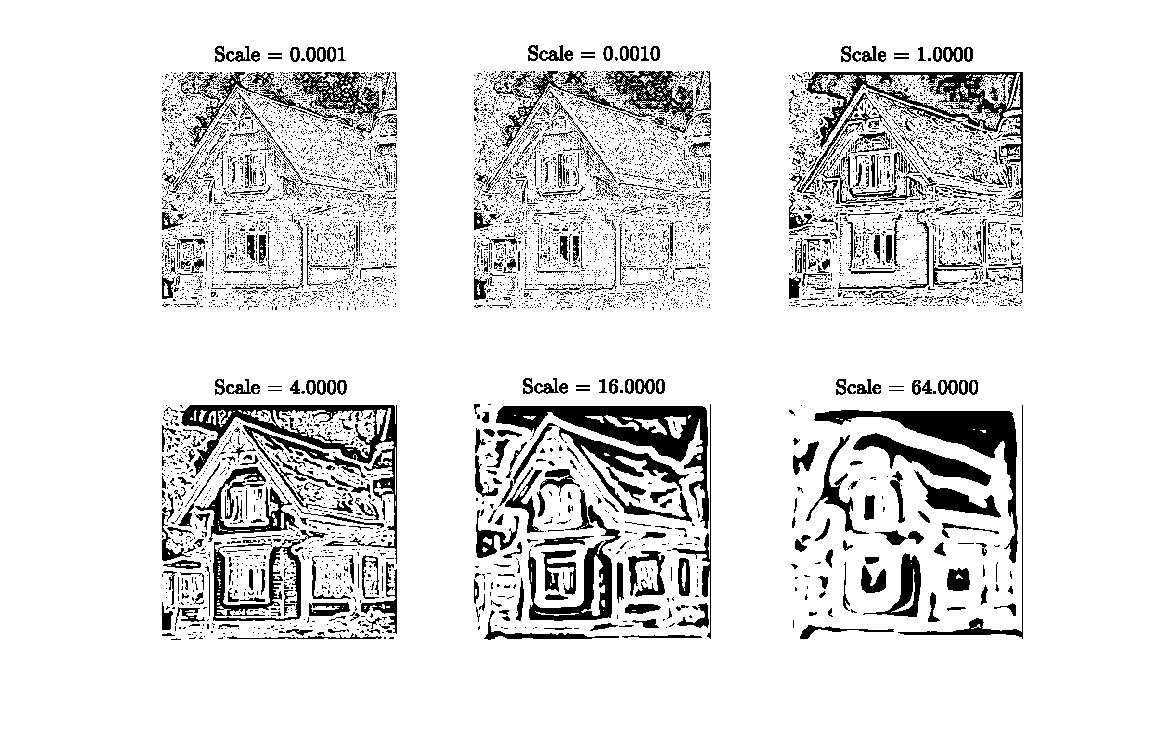
\includegraphics[width=0.9\columnwidth]{Question_4_House_Third_Order.eps}
		%\scalebox{0.9}{\input{Question_4_House_Third_Order.tex}}
		\caption{Third order derivative for \texttt{godthem256} after Gaussian smoothing.}
		\label{fig:Question_4_House_Third_Order}
	\end{figure}
	\begin{figure}[!ht]
		\centering
		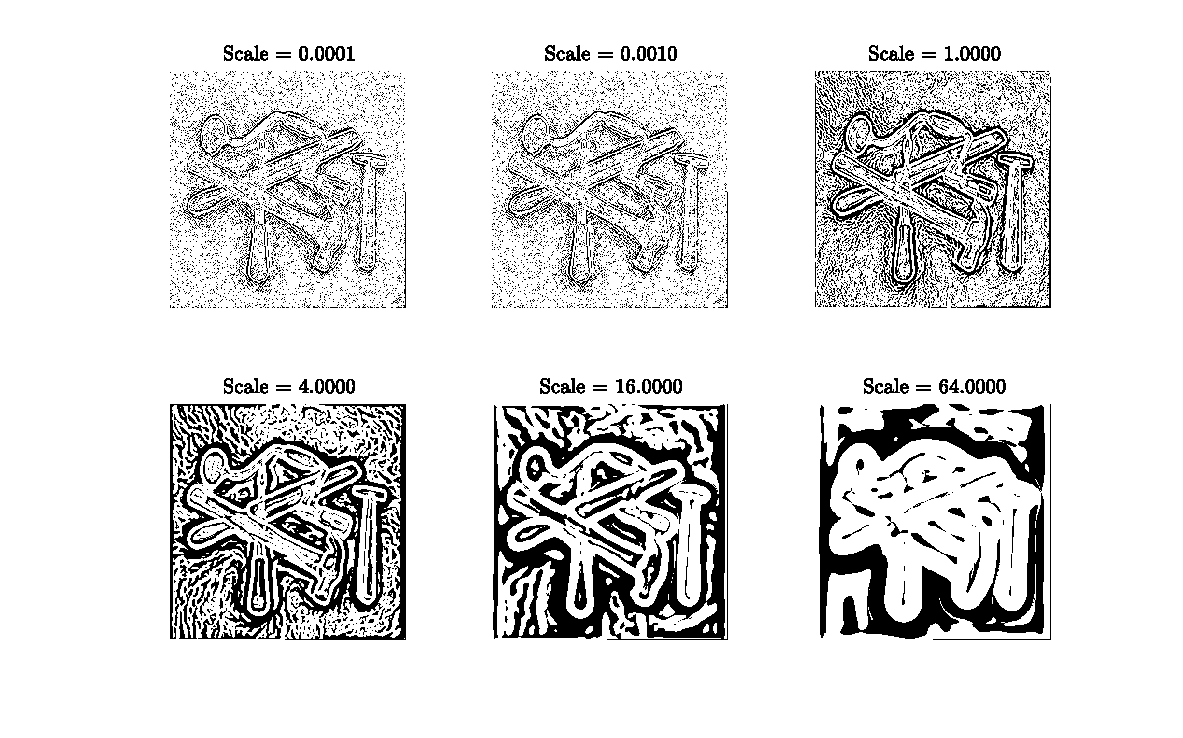
\includegraphics[width=0.9\columnwidth]{Question_4_Tools_Third_Order.eps}
		%\scalebox{0.9}{\input{Question_4_Tools_Third_Order.tex}}
		\caption{Third order derivative for \texttt{few256} after Gaussian smoothing.}
		\label{fig:Question_4_Tools_Third_Order}
	\end{figure}
	\begin{itemize}
		\item\addtocounter{Counter}{1}\textbf{Question \arabic{Counter}:} What can you observe? Provide explanation based on the generated images.
			\par From Figure \ref{fig:Question_4_House_Gaussian}, we can observe that, the larger the scale is (which means the larger the variance of the Gaussian white noise is), the more blurry and the less noisy the image becomes. This is also true when comes to the result of the edge detection. 
			\par However, higher variance of Gaussian filter also blurs the edges and making it harder to determine the real position of the edges. Also, from Figure \ref{fig:Question_4_House_Second_Order}, \ref{fig:Question_4_House_Third_Order}, and \ref{fig:Question_4_Tools_Third_Order}, we can see that Gaussian filter with higher variance would make the edges seem to be thickened thus losing the accuracy.

		\item\addtocounter{Counter}{1}\textbf{Question \arabic{Counter}:} Assemble the results of the experiment above into an illustrative collage with the \texttt{subplot} command. Which are your observations and conclusions?
			\par As stated at the beginning of this section, the images are shown in Figure \ref{fig:Question_4_House_Gaussian}, \ref{fig:Question_4_House_Second_Order}, \ref{fig:Question_4_House_Third_Order}, and \ref{fig:Question_4_Tools_Third_Order}, where the conclusion could be extracted: the bigger the variance of the Gaussian filter applied to the image is, the less noise will appear in the high order derivative while the less accurate the edges are found.

		\item\addtocounter{Counter}{1}\textbf{Question \arabic{Counter}:} How can you use the response from $\widetilde{L}_{vv}$ to detect edges, and how can you improve the result by using $\widetilde{L}_{vvv}$?
			\par The local maximum and local minimum of the gradient magnitude would be reached when $\widetilde{L}_{vv}=0$, however, if we want to find edges more accurately, we only want the local maximum be reserved. So when $(\widetilde{L}_{vv}=0 \cap \widetilde{L}_{vvv}<0)$, the local maximum would be reached. Based on such idea, we can improve the response from $\widetilde{L}_{vv}$ by combining the result of $\widetilde{L}_{vv}$ and $\widetilde{L}_{vvv}$ above. The combining result is shown in Figure \ref{fig:Question_6_House_Lvv_Lvvv} and \ref{fig:Question_6_Tools_Lvv_Lvvv}.
			\begin{figure}[!ht]
				\centering
				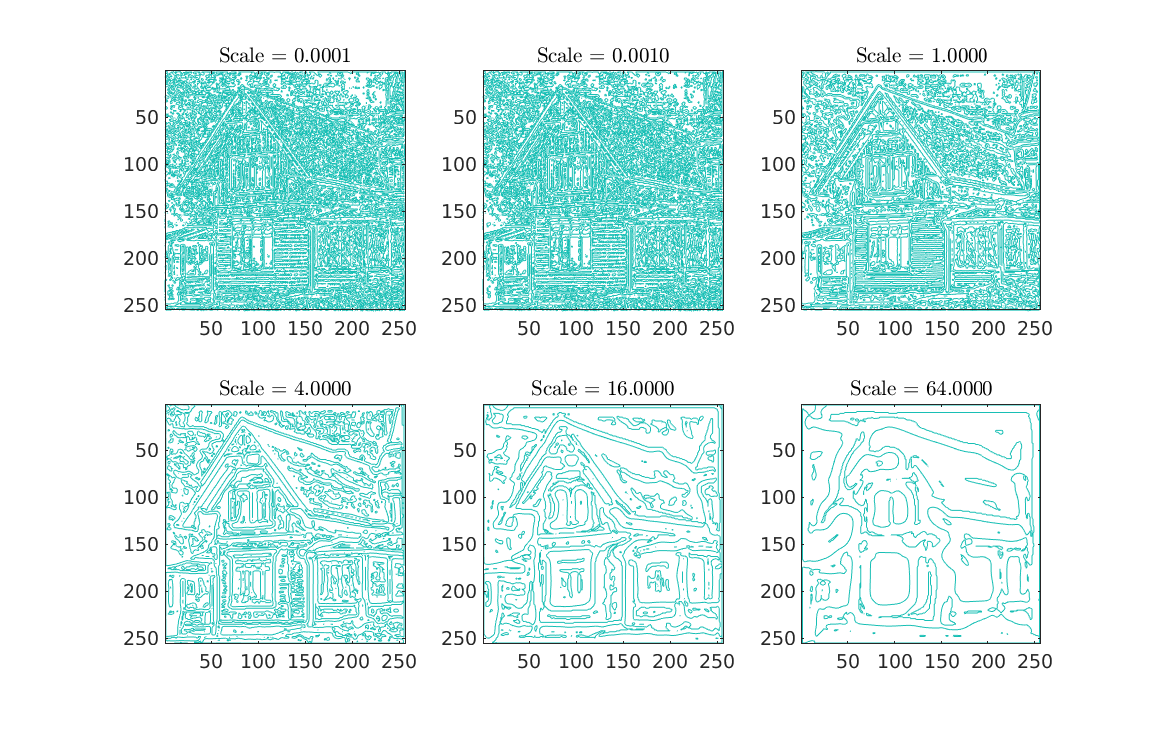
\includegraphics[width=0.9\columnwidth]{Question_6_House_Lvv_Lvvv.eps}
				%\scalebox{0.9}{\input{Question_6_House_Lvv_Lvvv.tex}}
				\caption{Combination of $\widetilde{L}_{vv}=0$ and $\widetilde{L}_{vvv}<0$ of \texttt{godthem256}.}
				\label{fig:Question_6_House_Lvv_Lvvv}
			\end{figure}
			\begin{figure}[!ht]
				\centering
				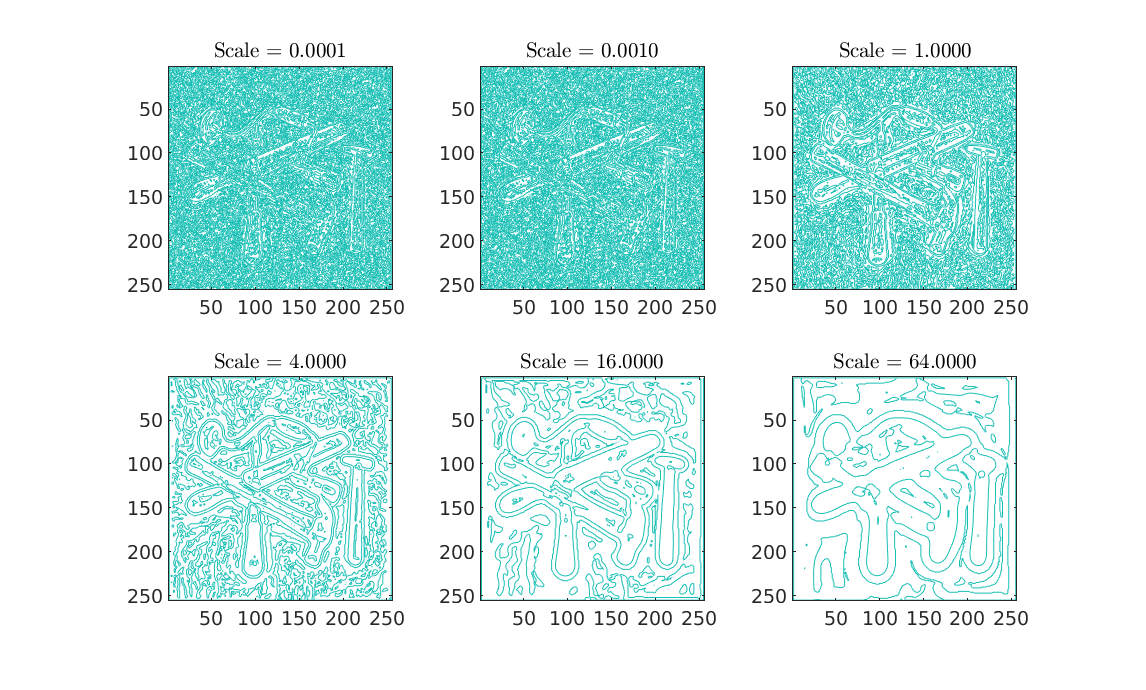
\includegraphics[width=0.9\columnwidth]{Question_6_Tools_Lvv_Lvvv.eps}
				%\scalebox{0.9}{\input{Question_6_House_Lvv_Lvvv.tex}}
				\caption{Combination of $\widetilde{L}_{vv}=0$ and $\widetilde{L}_{vvv}<0$ of \texttt{few256}.}
				\label{fig:Question_6_Tools_Lvv_Lvvv}
			\end{figure}
	\end{itemize}

\section*{5\hspace{0.5cm}Extraction of edge segments}
	\begin{itemize}
		\item\addtocounter{Counter}{1}\textbf{Question \arabic{Counter}:} Present your best results obtained with \texttt{extractedge} for \texttt{house} and \texttt{tools}.
			\par The best results obtained for \texttt{house} and \texttt{tools} are shown in Figure \ref{fig:Question_7_House_Overlay_Curves} and \ref{fig:Question_7_Tools_Overlay_Curves} respectively. The \texttt{godthem256} is applied by Gaussian smoothing with variance $\sigma^{2}=4$ and threshold $4$. The \texttt{few256} is applied by Gaussian smoothing with variance $\sigma^{2}=4$ and threshold $6$.
			\begin{figure}[!ht]
				\centering
				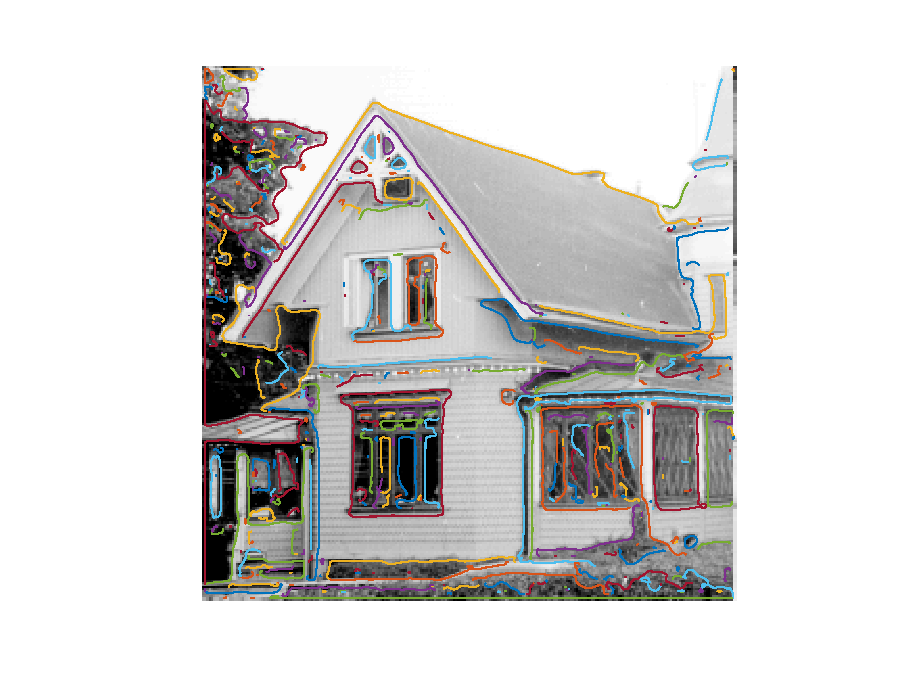
\includegraphics[width=0.9\columnwidth]{Question_7_House_Overlay_Curves.eps}
				%\scalebox{0.9}{\input{Question_6_House_Lvv_Lvvv.tex}}
				\caption{Best result for \texttt{godthem256}.}
				\label{fig:Question_7_House_Overlay_Curves}
			\end{figure}
			\begin{figure}[!ht]
				\centering
				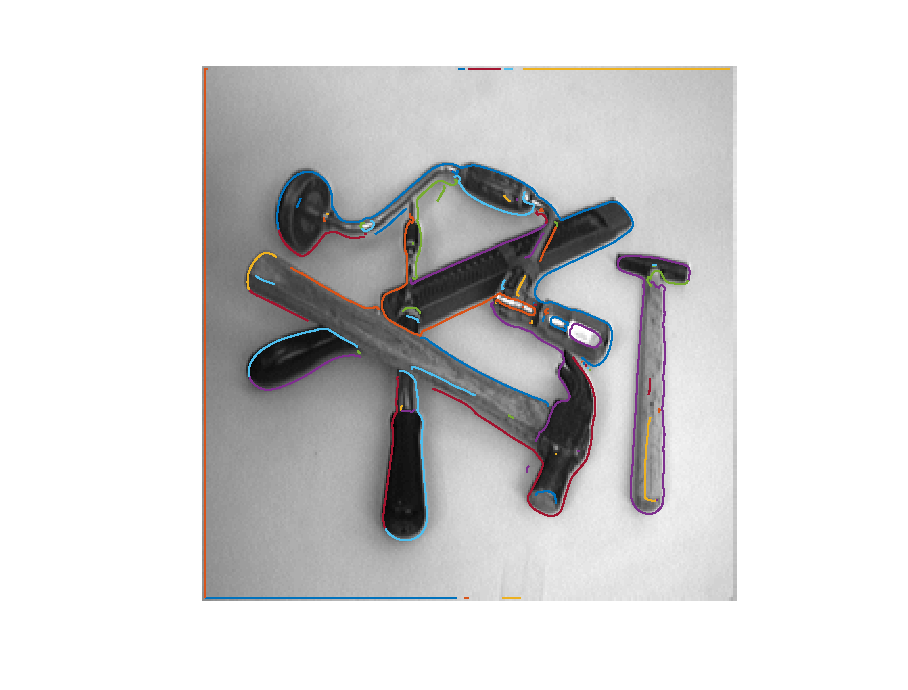
\includegraphics[width=0.9\columnwidth]{Question_7_Tools_Overlay_Curves.eps}
				%\scalebox{0.9}{\input{Question_6_House_Lvv_Lvvv.tex}}
				\caption{Best result for \texttt{few256}.}
				\label{fig:Question_7_Tools_Overlay_Curves}
			\end{figure}
	\end{itemize}

\section*{6\hspace{0.5cm}Hough transform}
\subsection*{6.1\hspace{0.5cm}Hints and practical advice}
	\begin{itemize}
		\item\addtocounter{Counter}{1}\textbf{????? Question \arabic{Counter}:} Identify the correspondences between the strongest peaks in the accumulator and line segments in the output image. Doing so convince yourself that the implementation is correct. Summarize the results in one or more figures.
			\par The strongest peaks in the accumulator should be the longest and the most obvious line segments in the edge plot.
		
		\item\addtocounter{Counter}{1}\textbf{Question \arabic{Counter}:} How do the results and computational time depend on the number of cells in the accumulator?
			\par The accuracy of the results depends on the resolution of the accumulator since the larger of \texttt{ntheta} and \texttt{nrho}, the more accurate the points and curves would be presented in the accumulator thus the intersection points would be easier to find its real position in accumulator thus finding accurate line in spatial domain. However, high resolution could also lead to more local maximum, thus giving multiple lines for a single edge we would like to obtain from the image.
			\par When the resolution is higher, it would take much more computational time. The time complexity could be $O(n^{2})$, where $n$ is the resolution in $x$ or $y$ direction. 
	\end{itemize}

\subsection*{6.2\hspace{0.5cm}Choice of accumulator incrementation function}
	\begin{itemize}
		\item\addtocounter{Counter}{1}\textbf{????? Question \arabic{Counter}:} How do you propose to do this? Try out a function that you would suggest and see if it improves the results. Does it?
			\par I would like to try some monotonically increasing function like $\log$ or square root functions. The increasing rate of such functions becomes smaller when the magnitude becomes larger.
	\end{itemize}

% Template
%%%%%%%%%%%%%%%%%%%%%%%%%%%%%%%%%%%%%%%%
%\begin{figure}[H]
%	\centering
%	\scalebox{0.9}{\input{test.tex}}
%	\caption{Test.}
%	\label{fig:Test}
%\end{figure}
%%%%%%%%%%%%%%%%%%%%%%%%%%%%%%%%%%%%%%%%
%\begin{figure}[!ht]
%	\footnotesize
%	\centering 
%	\begin{subfigure}[t]{.32\linewidth} % .32 for three polts .49 for two plots
%	\includegraphics[width=\columnwidth]{Linearity_F.eps}
%	\caption{Image F}
%	\label{fig:F}
%	\end{subfigure}
%	\begin{subfigure}[t]{.32\linewidth} % .32 for three polts
%	\includegraphics[width=\columnwidth]{Linearity_G.eps}
%	\caption{Image G = F'}
%	\label{fig:G}
%	\end{subfigure}
%	\begin{subfigure}[t]{.32\linewidth} % .32 for three polts
%	\includegraphics[width=\columnwidth]{Linearity_H.eps}
%	\caption{Image H = F + 2 * G}
%	\label{fig:H}
%	\end{subfigure}
%	\caption{Origin images.}
%	\label{fig:origin}
%\end{figure}
%%%%%%%%%%%%%%%%%%%%%%%%%%%%%%%%%%%%%%%%
%\begin{align*}
%	var_{t = 0.1} &= \begin{bmatrix} 0.0133 & 0.0000 \\ 0.0000 & 0.0133 \end{bmatrix} \\
%	var_{t = 0.3} &= \begin{bmatrix} 0.2811 & 0.0000 \\ 0.0000 & 0.2811 \end{bmatrix} \\
%	var_{t = 1.0} &= \begin{bmatrix} 1.0000 & 0.0000 \\ 0.0000 & 1.0000 \end{bmatrix} \\
%	var_{t = 10.0} &= \begin{bmatrix} 10.0000 & 0.0000 \\ 0.0000 & 10.0000 \end{bmatrix} \\
%	var_{t = 100.0} &= \begin{bmatrix} 100.0000 & 0.0000 \\ 0.0000 & 10.0000 \end{bmatrix}
%\end{align*}
%%%%%%%%%%%%%%%%%%%%%%%%%%%%%%%%%%%%%%%%
% \lstinputlisting{x.m}
%%%%%%%%%%%%%%%%%%%%%%%%%%%%%%%%%%%%%%%%
\end{document}